\setcounter{chapter}{3}
\chapter{Algoritmi, Fourier e fattorizzazione}
\phantomsection\label{chapter-4}

La struttura dei problemi guida oracoli, ricerca, stima di fase e aritmetica reversibile, fino a RSA e agli esempi completi di Shor.\par


\clearpage\phantomsection\label{exercise-index-4}
\BookHeading{Percorso degli esercizi guidati}
Quindici esercizi accompagnano lo studio del modulo. Ogni traccia segue le sezioni richieste e rinvia a uno svolgimento completo. Si suggerisce di formulare la previsione e tentare i passaggi prima di consultare la soluzione.
\begin{longtable}{@{}p{13mm}p{75mm}r@{}}\toprule Codice & Argomento & Pagina\\\midrule\endhead
\hyperref[ex-G4.01]{G4.01} & Ricostruire l'interferenza in Deutsch--Jozsa e Bernstein--Vazirani & \pageref{ex-G4.01}\\[3pt]
\hyperref[ex-G4.02]{G4.02} & Recuperare il periodo binario di Simon & \pageref{ex-G4.02}\\[3pt]
\hyperref[ex-G4.03]{G4.03} & Stimare una sovrapposizione mediante SWAP test & \pageref{ex-G4.03}\\[3pt]
\hyperref[ex-G4.04]{G4.04} & Ricostruire Grover come due riflessioni & \pageref{ex-G4.04}\\[3pt]
\hyperref[ex-G4.05]{G4.05} & Seguire una ricerca con budget e soglia variabile & \pageref{ex-G4.05}\\[3pt]
\hyperref[ex-G4.06]{G4.06} & Costruire una Fourier a quattro livelli & \pageref{ex-G4.06}\\[3pt]
\hyperref[ex-G4.07]{G4.07} & Leggere un'autofase esatta & \pageref{ex-G4.07}\\[3pt]
\hyperref[ex-G4.08]{G4.08} & Calcolare una fase non rappresentabile esattamente & \pageref{ex-G4.08}\\[3pt]
\hyperref[ex-G4.09]{G4.09} & Dalle autofasi di Grover al conteggio & \pageref{ex-G4.09}\\[3pt]
\hyperref[ex-G4.10]{G4.10} & Costruire RSA e recuperare la chiave dai fattori & \pageref{ex-G4.10}\\[3pt]
\hyperref[ex-G4.11]{G4.11} & Verificare somma e moltiplicazione modulari reversibili & \pageref{ex-G4.11}\\[3pt]
\hyperref[ex-G4.12]{G4.12} & Costruire gli autostati di un'orbita modulare & \pageref{ex-G4.12}\\[3pt]
\hyperref[ex-G4.13]{G4.13} & Ricostruire e verificare un denominatore & \pageref{ex-G4.13}\\[3pt]
\hyperref[ex-G4.14]{G4.14} & Svolgere Shor per \(N\) \(=\) 15 & \pageref{ex-G4.14}\\[3pt]
\hyperref[ex-G4.15]{G4.15} & Svolgere Shor per \(N\) \(=\) 21 & \pageref{ex-G4.15}\\[3pt]
\bottomrule\end{longtable}
{\small I primi cinque esercizi offrono una guida esplicita; i successivi cinque consolidano il calcolo; gli ultimi cinque collegano più concetti. Tutti conservano uno svolgimento completo.}\par

\Needspace{.43\textheight}
\section{Deutsch--Jozsa}
\phantomsection\label{c4-deutsch-jozsa}

{\sffamily\small\color{Ink!70} Riferimento alle slide: p. 23.\par}

{\sffamily\small\color{Ink!70} Laboratorio locale: \nolinkurl{index.html#capitolo-4/deutsch-jozsa}\par}

\BookHeading{Definizioni e costruzione}
L'ingresso è un oracolo per \(f:\{0{,}1\}^{n}\to \{0{,}1\}\), con la promessa che f sia costante oppure bilanciata, cioè uguale a uno su esattamente metà delle \(N=2^{n}\) parole. L'obiettivo è distinguere i due casi.\par

Prepariamo \(|s\rangle =\sum _{x}|x\rangle /\sqrt{N}\) applicando \(H\) a ciascuno degli n qubit. Come in Deutsch, il bersaglio \(|- \rangle \) converte \(U_{f}\) in una marcatura \(O_{f}|x\rangle =(- 1)^{f(x)}|x\rangle \). La seconda \(H^{\otimes n}\) usa \(H^{\otimes n}|x\rangle =\sum _{y}(- 1)^{x\cdot y}|y\rangle /\sqrt{N}\), dove \(x\cdot y=\oplus _{j}x_{j}y_{j}\) è il prodotto binario modulo due.\par

L'ampiezza della parola nulla è la media dei segni \((- 1)^{f(x)}\). Una funzione costante dà ampiezza +1 oppure \(- 1\) e probabilità uno; una bilanciata ha tanti +1 quanti \(- 1\) e dà probabilità zero. Sotto la promessa, leggere qualunque parola non nulla certifica il caso bilanciato. Fuori dalla promessa questa regola non decide la classe.\par

Gli esempi calcolano direttamente lo stato dopo l'oracolo di fase e applicano Hadamard: il bersaglio separabile \(|- \rangle \) è eliminato algebricamente. Si verifica la distribuzione dell'oracolo assegnato, senza sintetizzare una rete elementare per \(U_{f}\).\par


\MathBlock{0061002800790029003D0032005E00282212006E002903A320930028221200310029005E00280066002800780029002B007800B700790029003B0020005000280030202600300029003D003100200073006500200063006F007300740061006E00740065002C00200030002000730065002000620069006C0061006E00630069006100740061002E}{a(y)=2^{- n}\sum _{x}(- 1)^{f(x)+x\cdot y};\allowbreak \ P(0\ldots 0)=1\ \text{se}\ \text{costante},\allowbreak \ 0\ \text{se}\ \text{bilanciata}.}

\BookHeading{Come leggere le figure}
Le stringhe x,y etichettano la base di \(C^{2^{n}}\). Il prodotto x\(\cdot\)y è binario; la somma delle ampiezze è invece una somma reale con segno. Le barre mostrano probabilità teoriche.\par


\BookHeading{Attività nel laboratorio modificabile}

\BookHeading{Obiettivo dell'esperimento}
Distinguere funzioni costanti e bilanciate sotto la promessa dichiarata.\par

\BookHeading{Percorso operativo}
Scrivere una tabella valida, calcolare le ampiezze e cambiare la disposizione dei valori unitari.\par

\BookHeading{Lettura geometrica}
La somma dei segni determina l'ampiezza dell'uscita nulla.\par

\BookHeading{Controllo del risultato}
Controllare la promessa prima dell'esecuzione e verificare P(0\(\ldots\)0).\par


\Needspace{.36\textheight}\phantomsection\label{c4-deutsch-jozsa-example-1}
{\sffamily\small\color{Accent} ESEMPIO SVOLTO 1\par}
\BookHeading{Esempio 1}
Confrontiamo una funzione costante con una funzione bilanciata non affine.\par


\BookHeading{Geometria e configurazione dell'esempio}
\begin{FigureBlock}\centering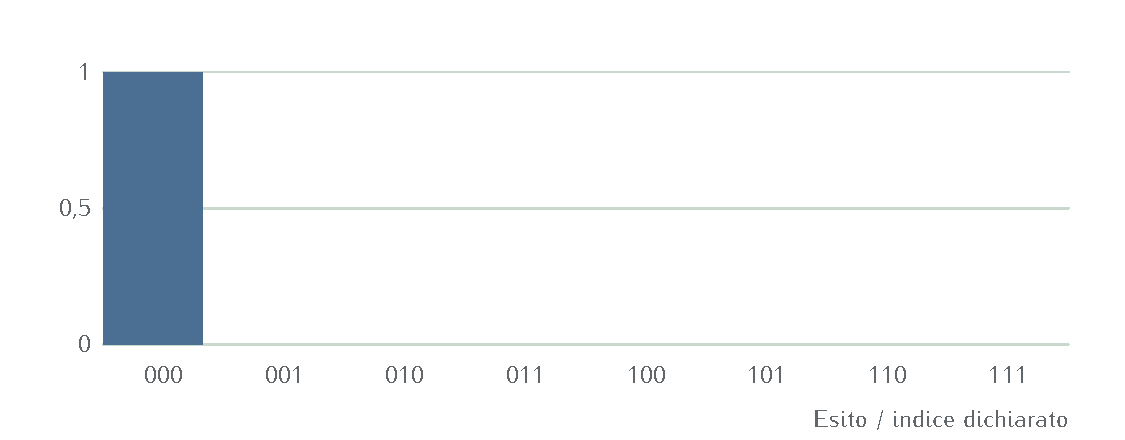
\includegraphics[width=\linewidth,height=94mm,keepaspectratio]{figure/f51a20cde06cd0a7e.pdf}\FigureCaption{4.01 \(\cdot\) esempio 1 \(\cdot\) Probabilità nella base dichiarata}\end{FigureBlock}
\begin{FigureBlock}\begin{minipage}[t]{.485\linewidth}\centering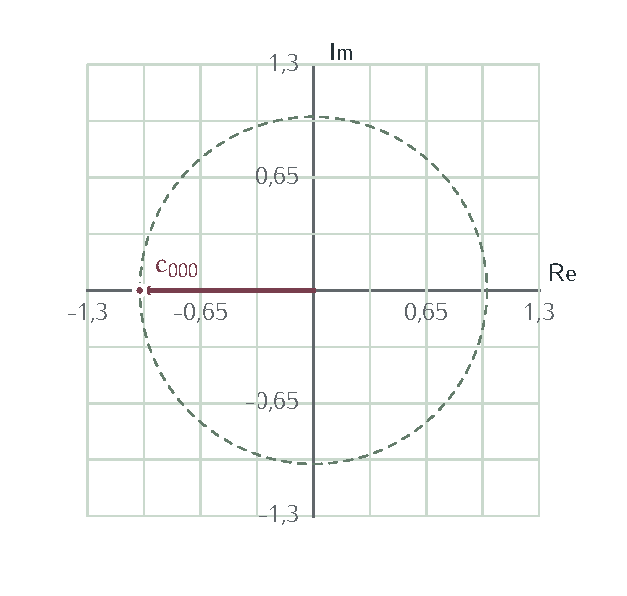
\includegraphics[width=\linewidth,height=63mm,keepaspectratio]{figure/f5aacc05f740ea662.pdf}\par{\sffamily\footnotesize \(c_{000}\)\par}\end{minipage}\hfill\begin{minipage}[t]{.485\linewidth}\centering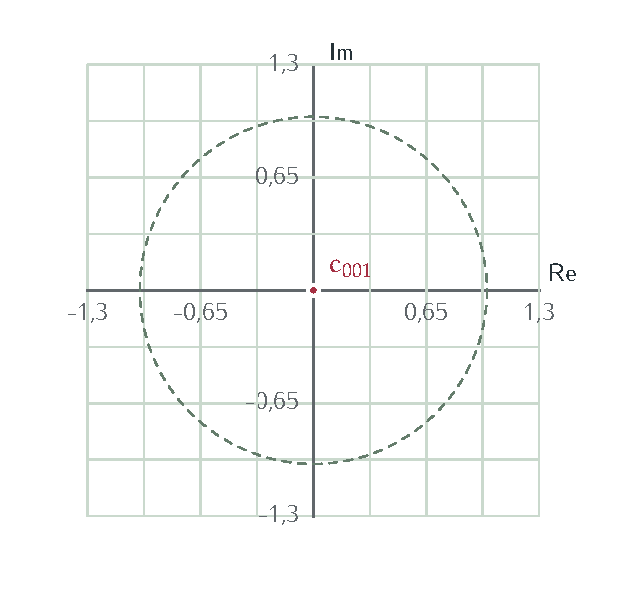
\includegraphics[width=\linewidth,height=63mm,keepaspectratio]{figure/f5b65cd01fa663092.pdf}\par{\sffamily\footnotesize \(c_{001}\)\par}\end{minipage}\FigureCaption{4.01 \(\cdot\) esempio 1 \(\cdot\) Componenti complesse}\end{FigureBlock}
\begin{FigureBlock}\begin{minipage}[t]{.485\linewidth}\centering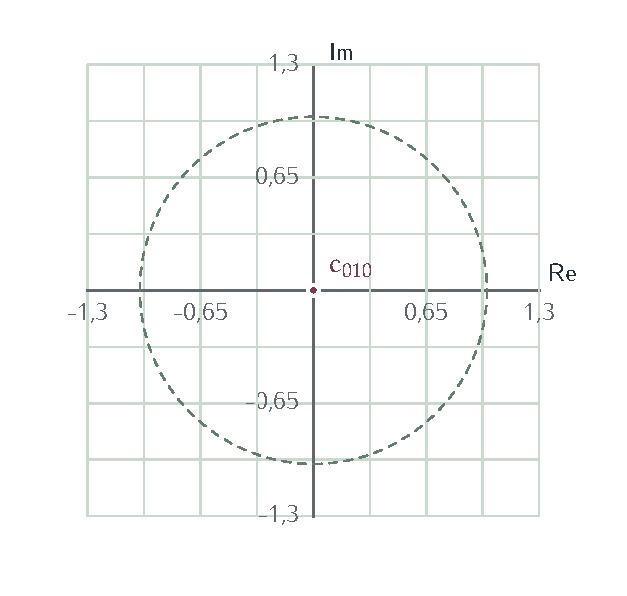
\includegraphics[width=\linewidth,height=63mm,keepaspectratio]{figure/f9c65deac57f27cb1.pdf}\par{\sffamily\footnotesize \(c_{010}\)\par}\end{minipage}\hfill\begin{minipage}[t]{.485\linewidth}\centering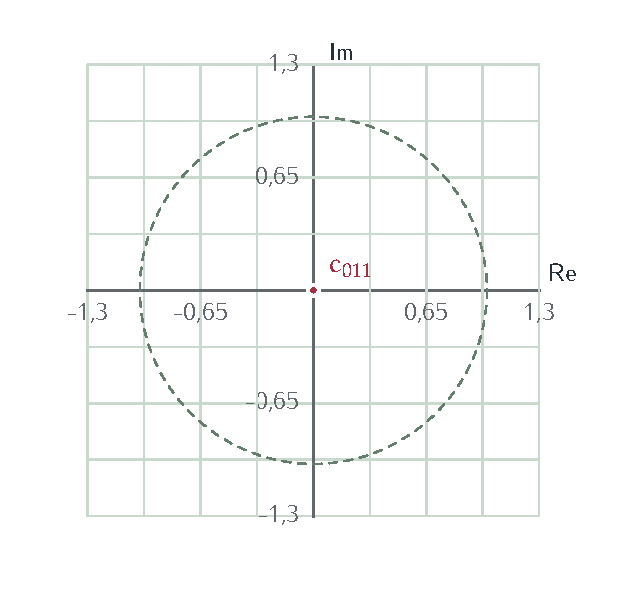
\includegraphics[width=\linewidth,height=63mm,keepaspectratio]{figure/f42a8759258a46448.pdf}\par{\sffamily\footnotesize \(c_{011}\)\par}\end{minipage}\FigureCaption{4.01 \(\cdot\) esempio 1 \(\cdot\) Componenti complesse}\end{FigureBlock}
\begin{FigureBlock}\begin{minipage}[t]{.485\linewidth}\centering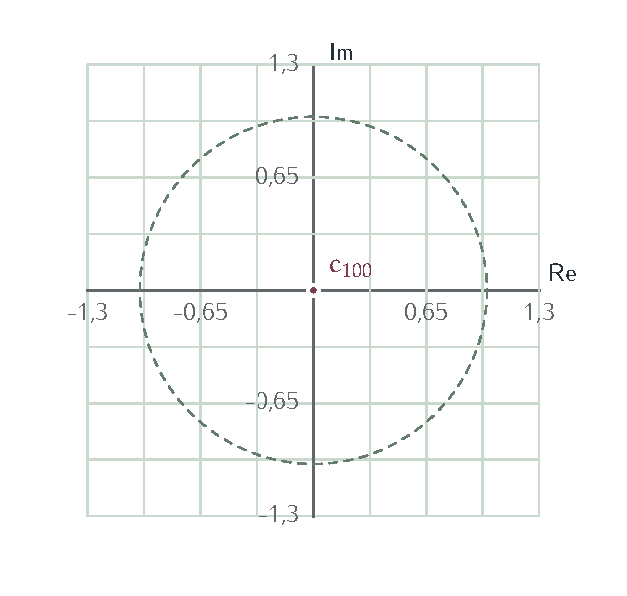
\includegraphics[width=\linewidth,height=63mm,keepaspectratio]{figure/f33d6516a9fe7e390.pdf}\par{\sffamily\footnotesize \(c_{100}\)\par}\end{minipage}\hfill\begin{minipage}[t]{.485\linewidth}\centering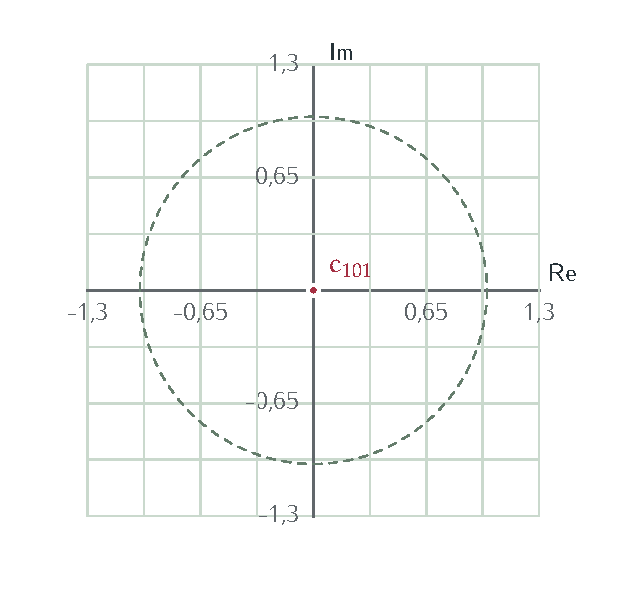
\includegraphics[width=\linewidth,height=63mm,keepaspectratio]{figure/f025182f35323870c.pdf}\par{\sffamily\footnotesize \(c_{101}\)\par}\end{minipage}\FigureCaption{4.01 \(\cdot\) esempio 1 \(\cdot\) Componenti complesse}\end{FigureBlock}
\begin{FigureBlock}\begin{minipage}[t]{.485\linewidth}\centering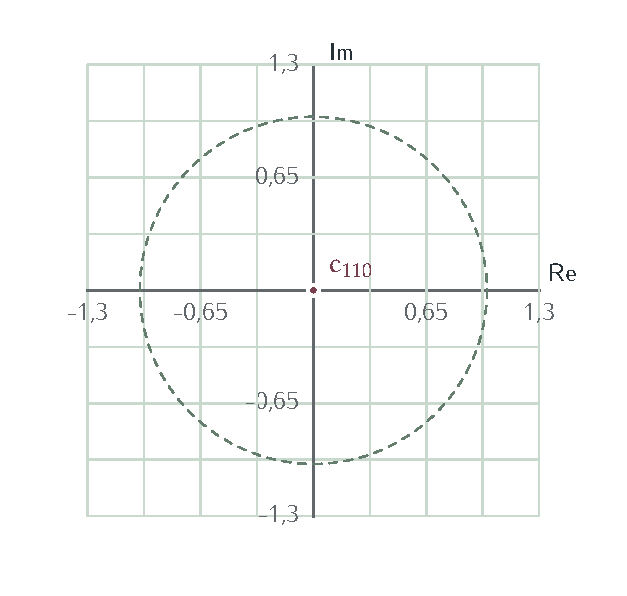
\includegraphics[width=\linewidth,height=63mm,keepaspectratio]{figure/f73c1d792b5e133d8.pdf}\par{\sffamily\footnotesize \(c_{110}\)\par}\end{minipage}\hfill\begin{minipage}[t]{.485\linewidth}\centering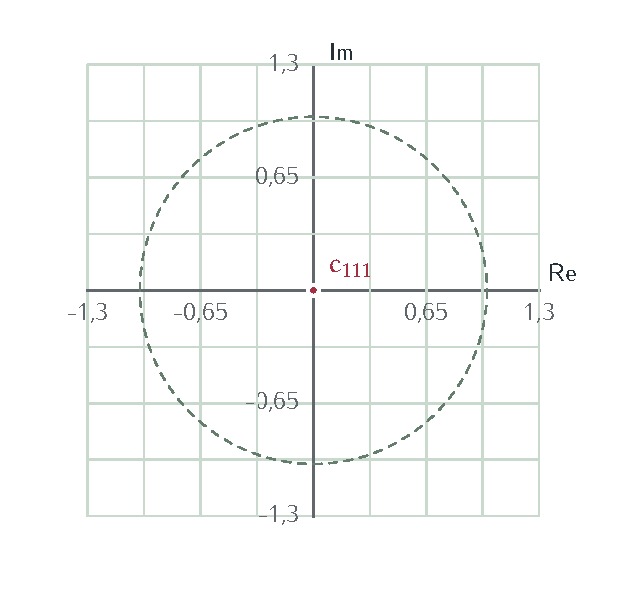
\includegraphics[width=\linewidth,height=63mm,keepaspectratio]{figure/f775f47769e41eab1.pdf}\par{\sffamily\footnotesize \(c_{111}\)\par}\end{minipage}\FigureCaption{4.01 \(\cdot\) esempio 1 \(\cdot\) Componenti complesse}\end{FigureBlock}

\phantomsection\label{c4-deutsch-jozsa-example-1-step-1}
\BookHeading{01 Preparare e interrogare}

\MathBlock{007C007327E9003D03A30078007C007827E9002F221A0038003B00200055005F0066007C007827E9007C221227E9003D0028221200310029005E0066002800780029007C007827E9007C221227E9}{|s\rangle =\sum _{x}|x\rangle /\sqrt{8};\allowbreak \ U_{f}|x\rangle |- \rangle =(- 1)^{f(x)}|x\rangle |- \rangle }

Il bersaglio è autostato di \(X\): la funzione agisce come una fase sul primo registro. Qui si simula direttamente questa riduzione per kickback, senza sintetizzare l'oracolo reversibile a porte.\par


\phantomsection\label{c4-deutsch-jozsa-example-1-step-2}
\BookHeading{02 Uscita 000}

\MathBlock{006100280030003000300029003D0028002D00310020002B0020002D00310020002B0020002D00310020002B0020002D00310020002B0020002D00310020002B0020002D00310020002B0020002D00310020002B0020002D00310029002F0038003D002D0038002F00382248002D0031}{a(000)=(-1\ +\ -1\ +\ -1\ +\ -1\ +\ -1\ +\ -1\ +\ -1\ +\ -1)/8=-8/8\approx -1}
\MathBlock{005022480031}{P\approx 1}

Il prodotto binario x\(\cdot\)y è la parità dei prodotti bit per bit.\par


\phantomsection\label{c4-deutsch-jozsa-example-1-step-3}
\BookHeading{03 Uscita 001}

\MathBlock{006100280030003000310029003D0028002D00310020002B002000310020002B0020002D00310020002B002000310020002B0020002D00310020002B002000310020002B0020002D00310020002B002000310029002F0038003D0030002F003822480030}{a(001)=(-1\ +\ 1\ +\ -1\ +\ 1\ +\ -1\ +\ 1\ +\ -1\ +\ 1)/8=0/8\approx 0}
\MathBlock{005022480030}{P\approx 0}

Il prodotto binario x\(\cdot\)y è la parità dei prodotti bit per bit.\par


\phantomsection\label{c4-deutsch-jozsa-example-1-step-4}
\BookHeading{04 Uscita 010}

\MathBlock{006100280030003100300029003D0028002D00310020002B0020002D00310020002B002000310020002B002000310020002B0020002D00310020002B0020002D00310020002B002000310020002B002000310029002F0038003D0030002F003822480030}{a(010)=(-1\ +\ -1\ +\ 1\ +\ 1\ +\ -1\ +\ -1\ +\ 1\ +\ 1)/8=0/8\approx 0}
\MathBlock{005022480030}{P\approx 0}

Il prodotto binario x\(\cdot\)y è la parità dei prodotti bit per bit.\par


\phantomsection\label{c4-deutsch-jozsa-example-1-step-5}
\BookHeading{05 Uscita 011}

\MathBlock{006100280030003100310029003D0028002D00310020002B002000310020002B002000310020002B0020002D00310020002B0020002D00310020002B002000310020002B002000310020002B0020002D00310029002F0038003D0030002F003822480030}{a(011)=(-1\ +\ 1\ +\ 1\ +\ -1\ +\ -1\ +\ 1\ +\ 1\ +\ -1)/8=0/8\approx 0}
\MathBlock{005022480030}{P\approx 0}

Il prodotto binario x\(\cdot\)y è la parità dei prodotti bit per bit.\par


\phantomsection\label{c4-deutsch-jozsa-example-1-step-6}
\BookHeading{06 Uscita 100}

\MathBlock{006100280031003000300029003D0028002D00310020002B0020002D00310020002B0020002D00310020002B0020002D00310020002B002000310020002B002000310020002B002000310020002B002000310029002F0038003D0030002F003822480030}{a(100)=(-1\ +\ -1\ +\ -1\ +\ -1\ +\ 1\ +\ 1\ +\ 1\ +\ 1)/8=0/8\approx 0}
\MathBlock{005022480030}{P\approx 0}

Il prodotto binario x\(\cdot\)y è la parità dei prodotti bit per bit.\par


\phantomsection\label{c4-deutsch-jozsa-example-1-step-7}
\BookHeading{07 Uscita 101}

\MathBlock{006100280031003000310029003D0028002D00310020002B002000310020002B0020002D00310020002B002000310020002B002000310020002B0020002D00310020002B002000310020002B0020002D00310029002F0038003D0030002F003822480030}{a(101)=(-1\ +\ 1\ +\ -1\ +\ 1\ +\ 1\ +\ -1\ +\ 1\ +\ -1)/8=0/8\approx 0}
\MathBlock{005022480030}{P\approx 0}

Il prodotto binario x\(\cdot\)y è la parità dei prodotti bit per bit.\par


\phantomsection\label{c4-deutsch-jozsa-example-1-step-8}
\BookHeading{08 Uscita 110}

\MathBlock{006100280031003100300029003D0028002D00310020002B0020002D00310020002B002000310020002B002000310020002B002000310020002B002000310020002B0020002D00310020002B0020002D00310029002F0038003D0030002F003822480030}{a(110)=(-1\ +\ -1\ +\ 1\ +\ 1\ +\ 1\ +\ 1\ +\ -1\ +\ -1)/8=0/8\approx 0}
\MathBlock{005022480030}{P\approx 0}

Il prodotto binario x\(\cdot\)y è la parità dei prodotti bit per bit.\par


\phantomsection\label{c4-deutsch-jozsa-example-1-step-9}
\BookHeading{09 Uscita 111}

\MathBlock{006100280031003100310029003D0028002D00310020002B002000310020002B002000310020002B0020002D00310020002B002000310020002B0020002D00310020002B0020002D00310020002B002000310029002F0038003D0030002F003822480030}{a(111)=(-1\ +\ 1\ +\ 1\ +\ -1\ +\ 1\ +\ -1\ +\ -1\ +\ 1)/8=0/8\approx 0}
\MathBlock{005022480030}{P\approx 0}

Il prodotto binario x\(\cdot\)y è la parità dei prodotti bit per bit.\par


\BookHeading{Interpretazione}

Per la funzione bilanciata l'esito 000 è impossibile; possono restare più esiti con probabilità positiva.\par


Risorse dichiarate. Una interrogazione al relativo oracolo; 2n Hadamard sui dati, preparazione del bersaglio e costo di costruzione dell'oracolo.\par


\BookHeading{Tabella completa dei dati (8 righe)}

\begingroup\sffamily\fontsize{8.8}{11}\selectfont\setlength{\tabcolsep}{1.6mm}\renewcommand{\arraystretch}{1.28}
\begin{longtable}{>{\RaggedRight\arraybackslash}p{42.133mm}>{\RaggedRight\arraybackslash}p{42.133mm}>{\RaggedRight\arraybackslash}p{42.133mm}}
\toprule\rowcolor{Accent!7}\BeginAccSupp{method=hex,unicode,ActualText=0078}x\EndAccSupp{} & \BeginAccSupp{method=hex,unicode,ActualText=0066002800780029}f(x)\EndAccSupp{} & \BeginAccSupp{method=hex,unicode,ActualText=0046006100730065}Fase\EndAccSupp{} \\
\midrule\endfirsthead
\toprule\rowcolor{Accent!7}\BeginAccSupp{method=hex,unicode,ActualText=0078}x\EndAccSupp{} & \BeginAccSupp{method=hex,unicode,ActualText=0066002800780029}f(x)\EndAccSupp{} & \BeginAccSupp{method=hex,unicode,ActualText=0046006100730065}Fase\EndAccSupp{} \\
\midrule\endhead\bottomrule\endfoot
\BeginAccSupp{method=hex,unicode,ActualText=003000300030}000\EndAccSupp{} & \BeginAccSupp{method=hex,unicode,ActualText=0031}1\EndAccSupp{} & \BeginAccSupp{method=hex,unicode,ActualText=22120031}\(- 1\)\EndAccSupp{} \\
\BeginAccSupp{method=hex,unicode,ActualText=003000300031}001\EndAccSupp{} & \BeginAccSupp{method=hex,unicode,ActualText=0031}1\EndAccSupp{} & \BeginAccSupp{method=hex,unicode,ActualText=22120031}\(- 1\)\EndAccSupp{} \\
\BeginAccSupp{method=hex,unicode,ActualText=003000310030}010\EndAccSupp{} & \BeginAccSupp{method=hex,unicode,ActualText=0031}1\EndAccSupp{} & \BeginAccSupp{method=hex,unicode,ActualText=22120031}\(- 1\)\EndAccSupp{} \\
\BeginAccSupp{method=hex,unicode,ActualText=003000310031}011\EndAccSupp{} & \BeginAccSupp{method=hex,unicode,ActualText=0031}1\EndAccSupp{} & \BeginAccSupp{method=hex,unicode,ActualText=22120031}\(- 1\)\EndAccSupp{} \\
\BeginAccSupp{method=hex,unicode,ActualText=003100300030}100\EndAccSupp{} & \BeginAccSupp{method=hex,unicode,ActualText=0031}1\EndAccSupp{} & \BeginAccSupp{method=hex,unicode,ActualText=22120031}\(- 1\)\EndAccSupp{} \\
\BeginAccSupp{method=hex,unicode,ActualText=003100300031}101\EndAccSupp{} & \BeginAccSupp{method=hex,unicode,ActualText=0031}1\EndAccSupp{} & \BeginAccSupp{method=hex,unicode,ActualText=22120031}\(- 1\)\EndAccSupp{} \\
\BeginAccSupp{method=hex,unicode,ActualText=003100310030}110\EndAccSupp{} & \BeginAccSupp{method=hex,unicode,ActualText=0031}1\EndAccSupp{} & \BeginAccSupp{method=hex,unicode,ActualText=22120031}\(- 1\)\EndAccSupp{} \\
\BeginAccSupp{method=hex,unicode,ActualText=003100310031}111\EndAccSupp{} & \BeginAccSupp{method=hex,unicode,ActualText=0031}1\EndAccSupp{} & \BeginAccSupp{method=hex,unicode,ActualText=22120031}\(- 1\)\EndAccSupp{} \\
\end{longtable}\endgroup

\Needspace{.36\textheight}\phantomsection\label{c4-deutsch-jozsa-example-2}
{\sffamily\small\color{Accent} ESEMPIO SVOLTO 2\par}
\BookHeading{Esempio 2}
Confrontiamo una funzione costante con una funzione bilanciata non affine.\par


\BookHeading{Geometria e configurazione dell'esempio}
\begin{FigureBlock}\centering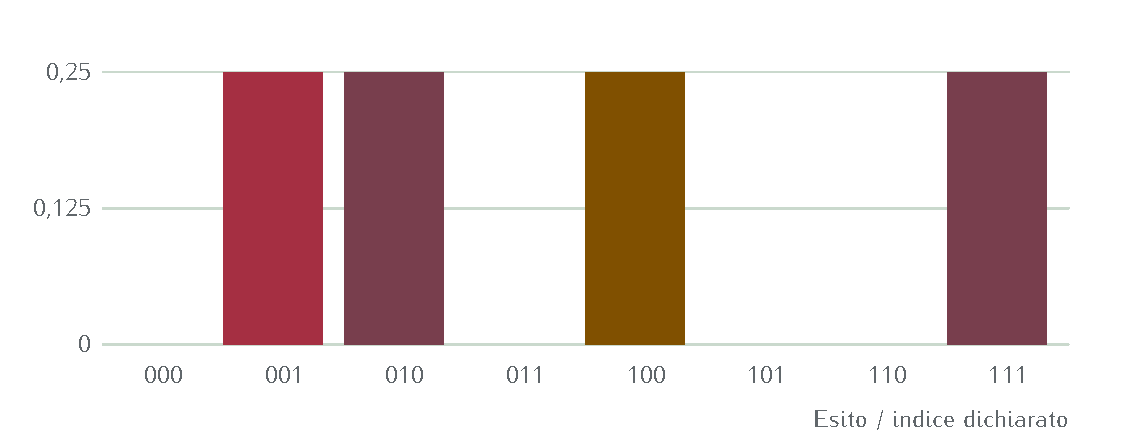
\includegraphics[width=\linewidth,height=94mm,keepaspectratio]{figure/fd9ba918ce660c83b.pdf}\FigureCaption{4.01 \(\cdot\) esempio 2 \(\cdot\) Probabilità nella base dichiarata}\end{FigureBlock}
\begin{FigureBlock}\begin{minipage}[t]{.485\linewidth}\centering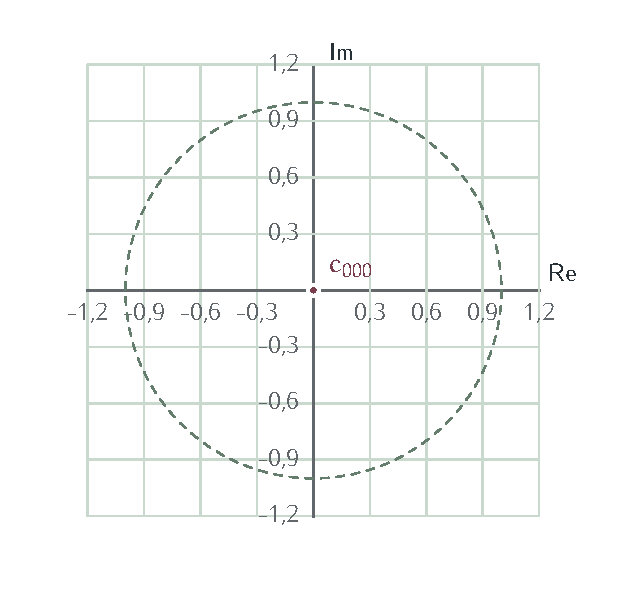
\includegraphics[width=\linewidth,height=63mm,keepaspectratio]{figure/f29ad8f1acd803d6b.pdf}\par{\sffamily\footnotesize \(c_{000}\)\par}\end{minipage}\hfill\begin{minipage}[t]{.485\linewidth}\centering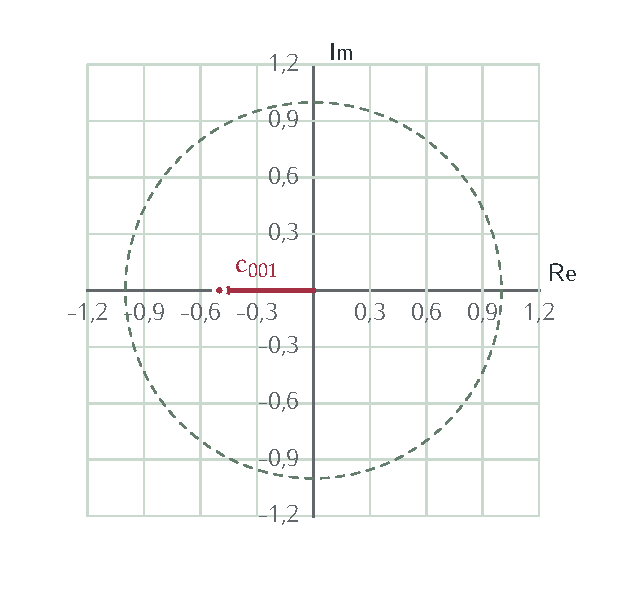
\includegraphics[width=\linewidth,height=63mm,keepaspectratio]{figure/f9d5e1a19965b8ddd.pdf}\par{\sffamily\footnotesize \(c_{001}\)\par}\end{minipage}\FigureCaption{4.01 \(\cdot\) esempio 2 \(\cdot\) Componenti complesse}\end{FigureBlock}
\begin{FigureBlock}\begin{minipage}[t]{.485\linewidth}\centering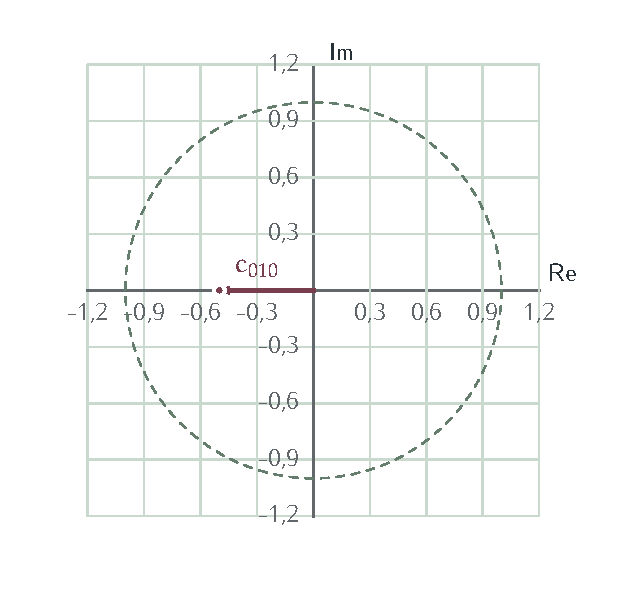
\includegraphics[width=\linewidth,height=63mm,keepaspectratio]{figure/f4dd1e6e04cd20dc8.pdf}\par{\sffamily\footnotesize \(c_{010}\)\par}\end{minipage}\hfill\begin{minipage}[t]{.485\linewidth}\centering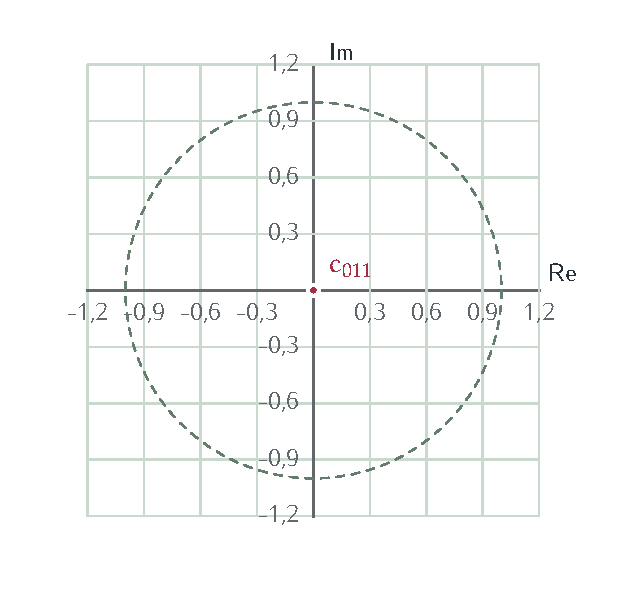
\includegraphics[width=\linewidth,height=63mm,keepaspectratio]{figure/f411c9af29fa7dfb3.pdf}\par{\sffamily\footnotesize \(c_{011}\)\par}\end{minipage}\FigureCaption{4.01 \(\cdot\) esempio 2 \(\cdot\) Componenti complesse}\end{FigureBlock}
\begin{FigureBlock}\begin{minipage}[t]{.485\linewidth}\centering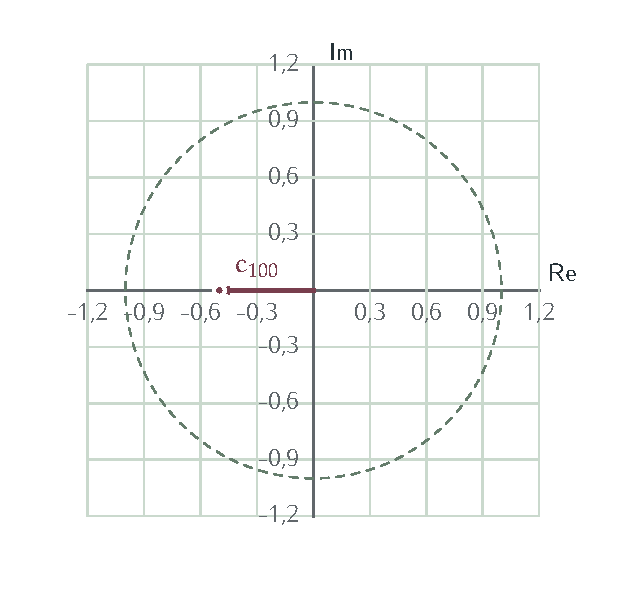
\includegraphics[width=\linewidth,height=63mm,keepaspectratio]{figure/f04507f2e31082e5c.pdf}\par{\sffamily\footnotesize \(c_{100}\)\par}\end{minipage}\hfill\begin{minipage}[t]{.485\linewidth}\centering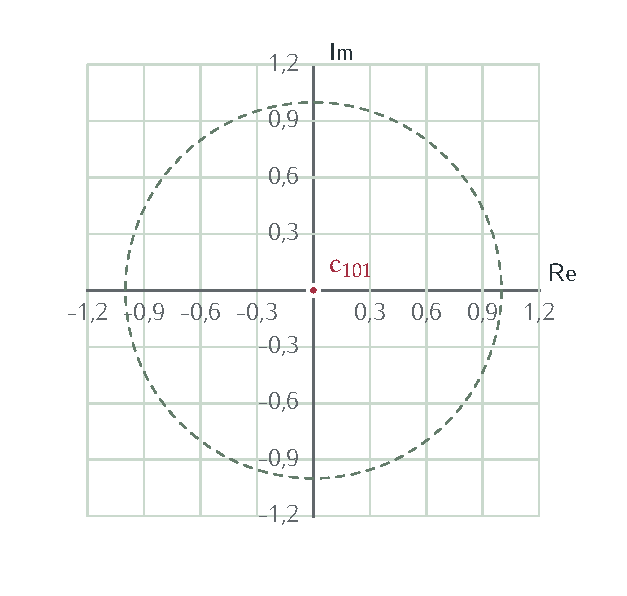
\includegraphics[width=\linewidth,height=63mm,keepaspectratio]{figure/fc1446b014e825f31.pdf}\par{\sffamily\footnotesize \(c_{101}\)\par}\end{minipage}\FigureCaption{4.01 \(\cdot\) esempio 2 \(\cdot\) Componenti complesse}\end{FigureBlock}
\begin{FigureBlock}\begin{minipage}[t]{.485\linewidth}\centering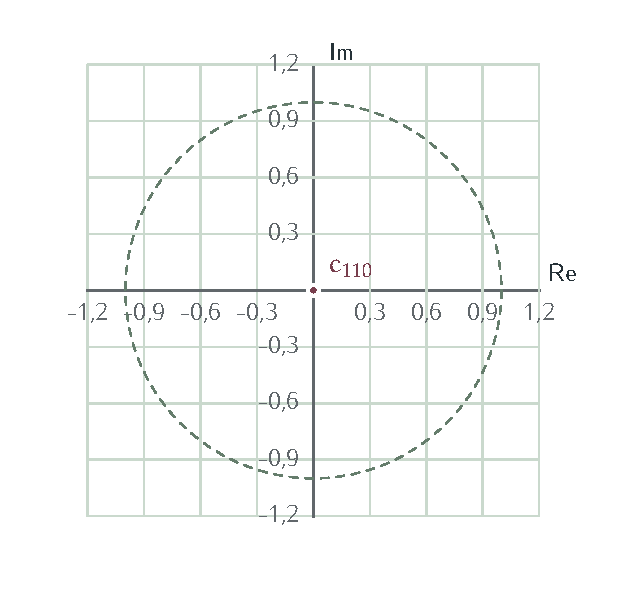
\includegraphics[width=\linewidth,height=63mm,keepaspectratio]{figure/fa990d4afd646b1ad.pdf}\par{\sffamily\footnotesize \(c_{110}\)\par}\end{minipage}\hfill\begin{minipage}[t]{.485\linewidth}\centering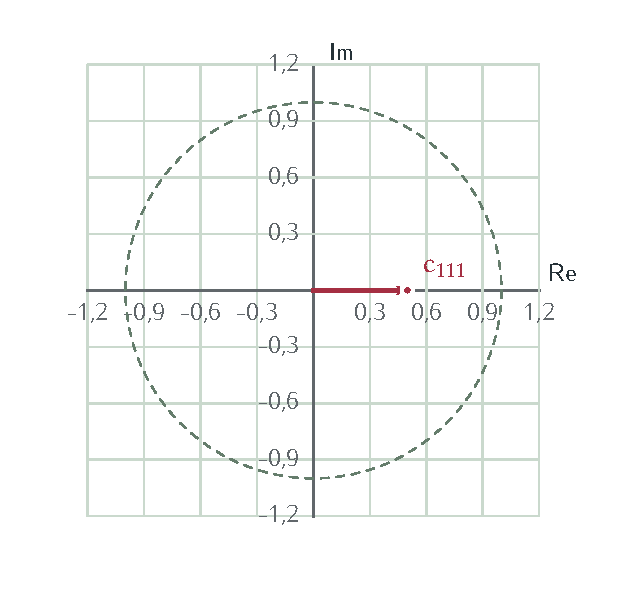
\includegraphics[width=\linewidth,height=63mm,keepaspectratio]{figure/f840bd30ae26cab52.pdf}\par{\sffamily\footnotesize \(c_{111}\)\par}\end{minipage}\FigureCaption{4.01 \(\cdot\) esempio 2 \(\cdot\) Componenti complesse}\end{FigureBlock}

\phantomsection\label{c4-deutsch-jozsa-example-2-step-1}
\BookHeading{01 Preparare e interrogare}

\MathBlock{007C007327E9003D03A30078007C007827E9002F221A0038003B00200055005F0066007C007827E9007C221227E9003D0028221200310029005E0066002800780029007C007827E9007C221227E9}{|s\rangle =\sum _{x}|x\rangle /\sqrt{8};\allowbreak \ U_{f}|x\rangle |- \rangle =(- 1)^{f(x)}|x\rangle |- \rangle }

Il bersaglio è autostato di \(X\): la funzione agisce come una fase sul primo registro. Qui si simula direttamente questa riduzione per kickback, senza sintetizzare l'oracolo reversibile a porte.\par


\phantomsection\label{c4-deutsch-jozsa-example-2-step-2}
\BookHeading{02 Uscita 000}

\MathBlock{006100280030003000300029003D0028002D00310020002B0020002D00310020002B0020002D00310020002B002000310020002B0020002D00310020002B002000310020002B002000310020002B002000310029002F0038003D0030002F003822480030}{a(000)=(-1\ +\ -1\ +\ -1\ +\ 1\ +\ -1\ +\ 1\ +\ 1\ +\ 1)/8=0/8\approx 0}
\MathBlock{005022480030}{P\approx 0}

Il prodotto binario x\(\cdot\)y è la parità dei prodotti bit per bit.\par


\phantomsection\label{c4-deutsch-jozsa-example-2-step-3}
\BookHeading{03 Uscita 001}

\MathBlock{006100280030003000310029003D0028002D00310020002B002000310020002B0020002D00310020002B0020002D00310020002B0020002D00310020002B0020002D00310020002B002000310020002B0020002D00310029002F0038003D002D0034002F00382248002D0030002C0035}{a(001)=(-1\ +\ 1\ +\ -1\ +\ -1\ +\ -1\ +\ -1\ +\ 1\ +\ -1)/8=-4/8\approx -0{,}5}
\MathBlock{005022480030002C00320035}{P\approx 0{,}25}

Il prodotto binario x\(\cdot\)y è la parità dei prodotti bit per bit.\par


\phantomsection\label{c4-deutsch-jozsa-example-2-step-4}
\BookHeading{04 Uscita 010}

\MathBlock{006100280030003100300029003D0028002D00310020002B0020002D00310020002B002000310020002B0020002D00310020002B0020002D00310020002B002000310020002B0020002D00310020002B0020002D00310029002F0038003D002D0034002F00382248002D0030002C0035}{a(010)=(-1\ +\ -1\ +\ 1\ +\ -1\ +\ -1\ +\ 1\ +\ -1\ +\ -1)/8=-4/8\approx -0{,}5}
\MathBlock{005022480030002C00320035}{P\approx 0{,}25}

Il prodotto binario x\(\cdot\)y è la parità dei prodotti bit per bit.\par


\phantomsection\label{c4-deutsch-jozsa-example-2-step-5}
\BookHeading{05 Uscita 011}

\MathBlock{006100280030003100310029003D0028002D00310020002B002000310020002B002000310020002B002000310020002B0020002D00310020002B0020002D00310020002B0020002D00310020002B002000310029002F0038003D0030002F003822480030}{a(011)=(-1\ +\ 1\ +\ 1\ +\ 1\ +\ -1\ +\ -1\ +\ -1\ +\ 1)/8=0/8\approx 0}
\MathBlock{005022480030}{P\approx 0}

Il prodotto binario x\(\cdot\)y è la parità dei prodotti bit per bit.\par


\phantomsection\label{c4-deutsch-jozsa-example-2-step-6}
\BookHeading{06 Uscita 100}

\MathBlock{006100280031003000300029003D0028002D00310020002B0020002D00310020002B0020002D00310020002B002000310020002B002000310020002B0020002D00310020002B0020002D00310020002B0020002D00310029002F0038003D002D0034002F00382248002D0030002C0035}{a(100)=(-1\ +\ -1\ +\ -1\ +\ 1\ +\ 1\ +\ -1\ +\ -1\ +\ -1)/8=-4/8\approx -0{,}5}
\MathBlock{005022480030002C00320035}{P\approx 0{,}25}

Il prodotto binario x\(\cdot\)y è la parità dei prodotti bit per bit.\par


\phantomsection\label{c4-deutsch-jozsa-example-2-step-7}
\BookHeading{07 Uscita 101}

\MathBlock{006100280031003000310029003D0028002D00310020002B002000310020002B0020002D00310020002B0020002D00310020002B002000310020002B002000310020002B0020002D00310020002B002000310029002F0038003D0030002F003822480030}{a(101)=(-1\ +\ 1\ +\ -1\ +\ -1\ +\ 1\ +\ 1\ +\ -1\ +\ 1)/8=0/8\approx 0}
\MathBlock{005022480030}{P\approx 0}

Il prodotto binario x\(\cdot\)y è la parità dei prodotti bit per bit.\par


\phantomsection\label{c4-deutsch-jozsa-example-2-step-8}
\BookHeading{08 Uscita 110}

\MathBlock{006100280031003100300029003D0028002D00310020002B0020002D00310020002B002000310020002B0020002D00310020002B002000310020002B0020002D00310020002B002000310020002B002000310029002F0038003D0030002F003822480030}{a(110)=(-1\ +\ -1\ +\ 1\ +\ -1\ +\ 1\ +\ -1\ +\ 1\ +\ 1)/8=0/8\approx 0}
\MathBlock{005022480030}{P\approx 0}

Il prodotto binario x\(\cdot\)y è la parità dei prodotti bit per bit.\par


\phantomsection\label{c4-deutsch-jozsa-example-2-step-9}
\BookHeading{09 Uscita 111}

\MathBlock{006100280031003100310029003D0028002D00310020002B002000310020002B002000310020002B002000310020002B002000310020002B002000310020002B002000310020002B0020002D00310029002F0038003D0034002F003822480030002C0035}{a(111)=(-1\ +\ 1\ +\ 1\ +\ 1\ +\ 1\ +\ 1\ +\ 1\ +\ -1)/8=4/8\approx 0{,}5}
\MathBlock{005022480030002C00320035}{P\approx 0{,}25}

Il prodotto binario x\(\cdot\)y è la parità dei prodotti bit per bit.\par


\BookHeading{Interpretazione}

Per la funzione bilanciata l'esito 000 è impossibile; possono restare più esiti con probabilità positiva.\par


Risorse dichiarate. Una interrogazione al relativo oracolo; 2n Hadamard sui dati, preparazione del bersaglio e costo di costruzione dell'oracolo.\par


\BookHeading{Tabella completa dei dati (8 righe)}

\begingroup\sffamily\fontsize{8.8}{11}\selectfont\setlength{\tabcolsep}{1.6mm}\renewcommand{\arraystretch}{1.28}
\begin{longtable}{>{\RaggedRight\arraybackslash}p{42.133mm}>{\RaggedRight\arraybackslash}p{42.133mm}>{\RaggedRight\arraybackslash}p{42.133mm}}
\toprule\rowcolor{Accent!7}\BeginAccSupp{method=hex,unicode,ActualText=0078}x\EndAccSupp{} & \BeginAccSupp{method=hex,unicode,ActualText=0066002800780029}f(x)\EndAccSupp{} & \BeginAccSupp{method=hex,unicode,ActualText=0046006100730065}Fase\EndAccSupp{} \\
\midrule\endfirsthead
\toprule\rowcolor{Accent!7}\BeginAccSupp{method=hex,unicode,ActualText=0078}x\EndAccSupp{} & \BeginAccSupp{method=hex,unicode,ActualText=0066002800780029}f(x)\EndAccSupp{} & \BeginAccSupp{method=hex,unicode,ActualText=0046006100730065}Fase\EndAccSupp{} \\
\midrule\endhead\bottomrule\endfoot
\BeginAccSupp{method=hex,unicode,ActualText=003000300030}000\EndAccSupp{} & \BeginAccSupp{method=hex,unicode,ActualText=0031}1\EndAccSupp{} & \BeginAccSupp{method=hex,unicode,ActualText=22120031}\(- 1\)\EndAccSupp{} \\
\BeginAccSupp{method=hex,unicode,ActualText=003000300031}001\EndAccSupp{} & \BeginAccSupp{method=hex,unicode,ActualText=0031}1\EndAccSupp{} & \BeginAccSupp{method=hex,unicode,ActualText=22120031}\(- 1\)\EndAccSupp{} \\
\BeginAccSupp{method=hex,unicode,ActualText=003000310030}010\EndAccSupp{} & \BeginAccSupp{method=hex,unicode,ActualText=0031}1\EndAccSupp{} & \BeginAccSupp{method=hex,unicode,ActualText=22120031}\(- 1\)\EndAccSupp{} \\
\BeginAccSupp{method=hex,unicode,ActualText=003000310031}011\EndAccSupp{} & \BeginAccSupp{method=hex,unicode,ActualText=0030}0\EndAccSupp{} & \BeginAccSupp{method=hex,unicode,ActualText=002B0031}+1\EndAccSupp{} \\
\BeginAccSupp{method=hex,unicode,ActualText=003100300030}100\EndAccSupp{} & \BeginAccSupp{method=hex,unicode,ActualText=0031}1\EndAccSupp{} & \BeginAccSupp{method=hex,unicode,ActualText=22120031}\(- 1\)\EndAccSupp{} \\
\BeginAccSupp{method=hex,unicode,ActualText=003100300031}101\EndAccSupp{} & \BeginAccSupp{method=hex,unicode,ActualText=0030}0\EndAccSupp{} & \BeginAccSupp{method=hex,unicode,ActualText=002B0031}+1\EndAccSupp{} \\
\BeginAccSupp{method=hex,unicode,ActualText=003100310030}110\EndAccSupp{} & \BeginAccSupp{method=hex,unicode,ActualText=0030}0\EndAccSupp{} & \BeginAccSupp{method=hex,unicode,ActualText=002B0031}+1\EndAccSupp{} \\
\BeginAccSupp{method=hex,unicode,ActualText=003100310031}111\EndAccSupp{} & \BeginAccSupp{method=hex,unicode,ActualText=0030}0\EndAccSupp{} & \BeginAccSupp{method=hex,unicode,ActualText=002B0031}+1\EndAccSupp{} \\
\end{longtable}\endgroup

\Needspace{7\baselineskip}
\BookHeading{Il passaggio successivo}
La cancellazione dipende dalla struttura dei segni. Se f nasconde una stringa attraverso un prodotto binario, come in Bernstein--Vazirani, la stessa trasformazione concentra l'uscita proprio su quella stringa.\par


\Needspace{.43\textheight}
\section{Bernstein--Vazirani}
\phantomsection\label{c4-bernstein-vazirani}

{\sffamily\small\color{Ink!70} Riferimento alle slide: p. 51.\par}

{\sffamily\small\color{Ink!70} Laboratorio locale: \nolinkurl{index.html#capitolo-4/bernstein-vazirani}\par}

\BookHeading{Definizioni e costruzione}
La promessa è \(f(x)=s\cdot x\oplus b\), con \(x,\allowbreak s\in \{0{,}1\}^{n}\) e \(b\in \{0{,}1\}\). La stringa s è ignota; b è un termine costante. Per \(b=0\) la funzione è lineare, mentre con \(b=1\) è affine.\par

Dopo preparazione uniforme, oracolo di fase e Hadamard, l'ampiezza di y è \(2^{- n}\sum _{x}(- 1)^{s\cdot x+b+x\cdot y}\). Poiché ogni bit \(x_{j}\) viene sommato indipendentemente su 0 e 1, la somma si fattorizza in \((- 1)^{b}2^{- n}\prod _{j}[1+(- 1)^{s_{j}+y_{j}}]\).\par

Se \(y_{j}\ne s_{j}\) per almeno un bit, quel fattore è \(1- 1=0\). Se \(y=s\), tutti i fattori sono due e compensano \(2^{- n}\). Quindi il vettore finale è \((- 1)^{b}|s\rangle \): la lettura restituisce s con certezza in entrambi i casi, mentre b cambia soltanto la fase globale.\par

Come in Deutsch--Jozsa il modello usa direttamente la marcatura di fase; l'ancilla \(|- \rangle \) e la sintesi elementare di \(U_{f}\) non vengono simulate qui. Il caso affine mantiene il segno nelle ampiezze anche se non cambia le probabilità.\par


\MathBlock{0061002800790029003D0028221200310029005E00620032005E00282212006E0029220F2C7C005B0031002B0028221200310029005E002800732C7C002B00792C7C0029005D003D0028221200310029005E006203B41D67002C209B002E}{a(y)=(- 1)^{b}2^{- n}\prod _{j}[1+(- 1)^{s_{j}+y_{j}}]=(- 1)^{b}\delta _{y},\allowbreak _{s}.}

\BookHeading{Come leggere le figure}
I fattori sono somme sui singoli bit nello spazio binario; \(\delta _{y},\allowbreak _{s}\) vale uno quando \(y=s\) e zero altrimenti. Le coordinate finali sono ampiezze reali con segno, le barre sono i loro quadrati.\par


\BookHeading{Attività nel laboratorio modificabile}

\BookHeading{Obiettivo dell'esperimento}
Recuperare una stringa che definisce una funzione affine binaria.\par

\BookHeading{Percorso operativo}
Cambiare la stringa e il termine affine mantenendo il numero di bit.\par

\BookHeading{Lettura geometrica}
La trasformata degli Hadamard concentra l'ampiezza sull'etichetta della stringa.\par

\BookHeading{Controllo del risultato}
Confrontare i due termini affini: le probabilità coincidono.\par


\Needspace{.36\textheight}\phantomsection\label{c4-bernstein-vazirani-example-1}
{\sffamily\small\color{Accent} ESEMPIO SVOLTO 1\par}
\BookHeading{Esempio 1}
\(s=101\); \(f(x)=s\cdot x\).\par


\BookHeading{Geometria e configurazione dell'esempio}
\begin{FigureBlock}\centering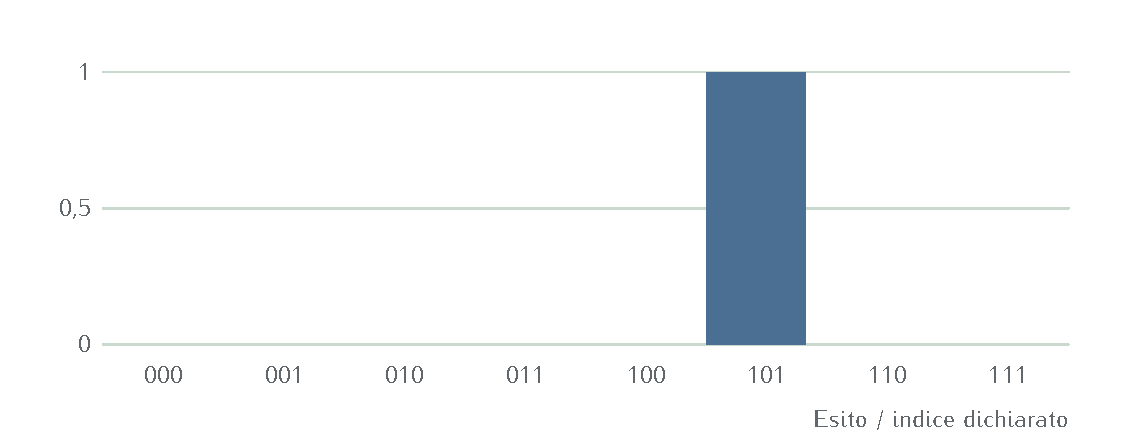
\includegraphics[width=\linewidth,height=94mm,keepaspectratio]{figure/fe070d14e25049305.pdf}\FigureCaption{4.02 \(\cdot\) esempio 1 \(\cdot\) Probabilità nella base dichiarata}\end{FigureBlock}
\begin{FigureBlock}\begin{minipage}[t]{.485\linewidth}\centering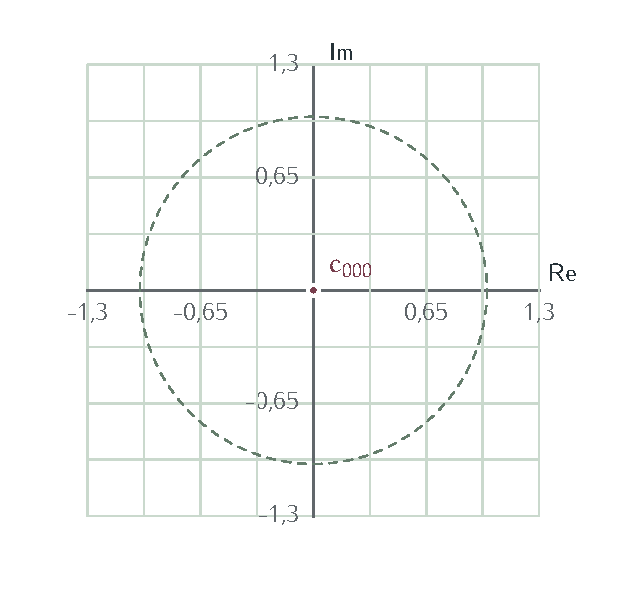
\includegraphics[width=\linewidth,height=63mm,keepaspectratio]{figure/f0fd4770619b1c971.pdf}\par{\sffamily\footnotesize \(c_{000}\)\par}\end{minipage}\hfill\begin{minipage}[t]{.485\linewidth}\centering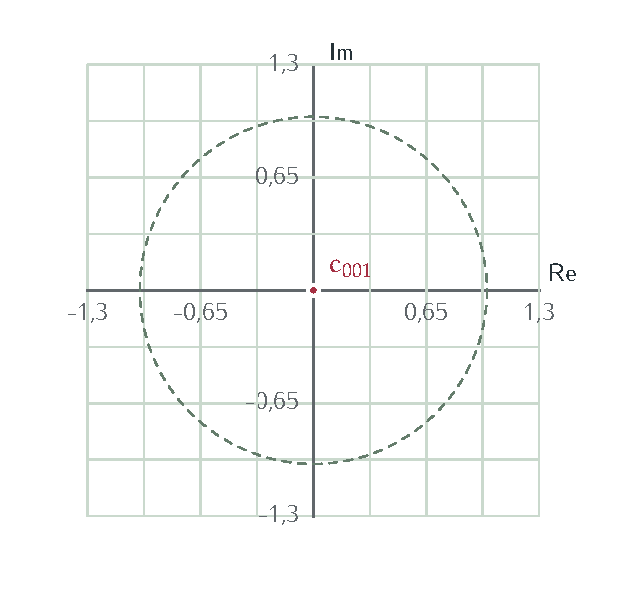
\includegraphics[width=\linewidth,height=63mm,keepaspectratio]{figure/f5b65cd01fa663092.pdf}\par{\sffamily\footnotesize \(c_{001}\)\par}\end{minipage}\FigureCaption{4.02 \(\cdot\) esempio 1 \(\cdot\) Componenti complesse}\end{FigureBlock}
\begin{FigureBlock}\begin{minipage}[t]{.485\linewidth}\centering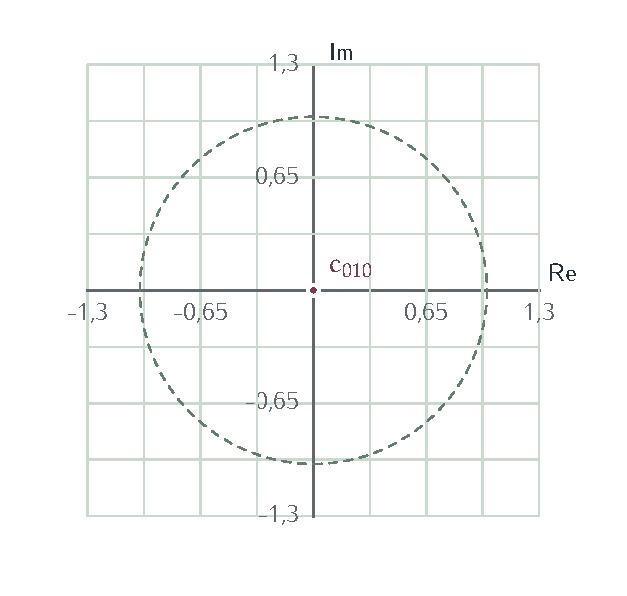
\includegraphics[width=\linewidth,height=63mm,keepaspectratio]{figure/f9c65deac57f27cb1.pdf}\par{\sffamily\footnotesize \(c_{010}\)\par}\end{minipage}\hfill\begin{minipage}[t]{.485\linewidth}\centering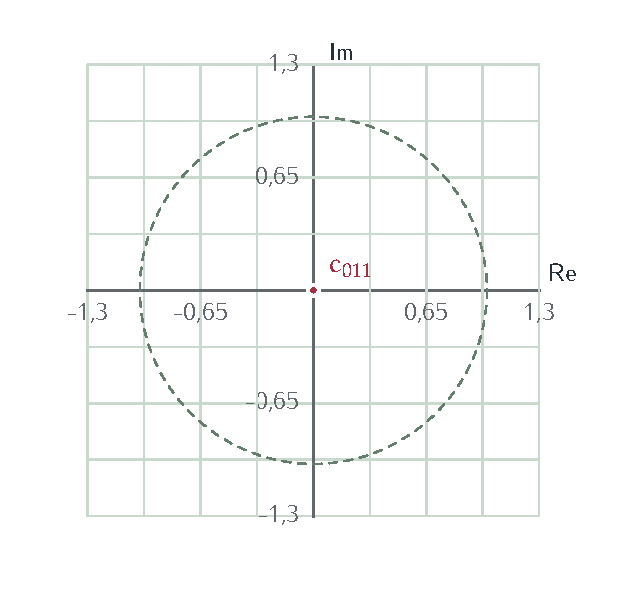
\includegraphics[width=\linewidth,height=63mm,keepaspectratio]{figure/f42a8759258a46448.pdf}\par{\sffamily\footnotesize \(c_{011}\)\par}\end{minipage}\FigureCaption{4.02 \(\cdot\) esempio 1 \(\cdot\) Componenti complesse}\end{FigureBlock}
\begin{FigureBlock}\begin{minipage}[t]{.485\linewidth}\centering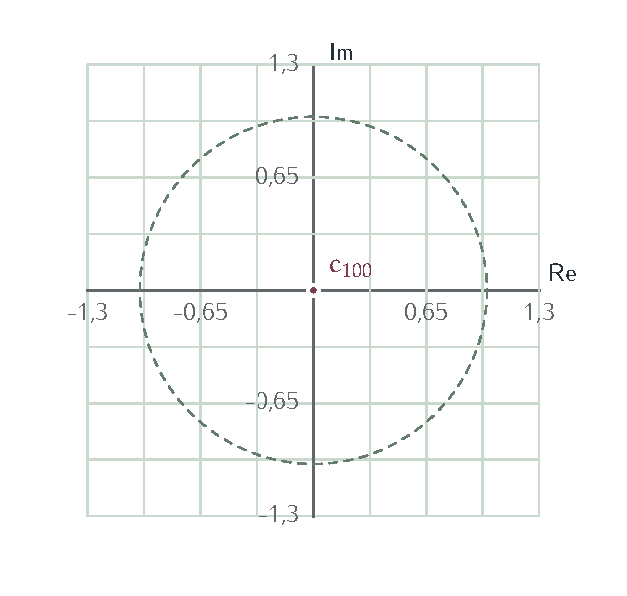
\includegraphics[width=\linewidth,height=63mm,keepaspectratio]{figure/f33d6516a9fe7e390.pdf}\par{\sffamily\footnotesize \(c_{100}\)\par}\end{minipage}\hfill\begin{minipage}[t]{.485\linewidth}\centering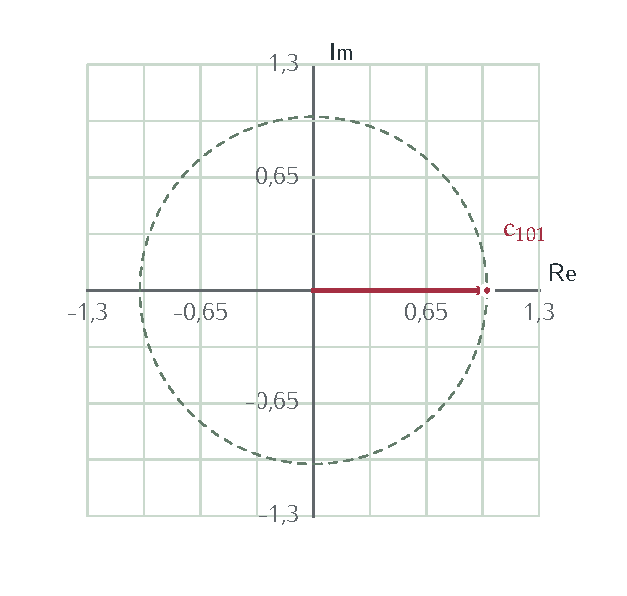
\includegraphics[width=\linewidth,height=63mm,keepaspectratio]{figure/f66f75c2ce0fcede5.pdf}\par{\sffamily\footnotesize \(c_{101}\)\par}\end{minipage}\FigureCaption{4.02 \(\cdot\) esempio 1 \(\cdot\) Componenti complesse}\end{FigureBlock}
\begin{FigureBlock}\begin{minipage}[t]{.485\linewidth}\centering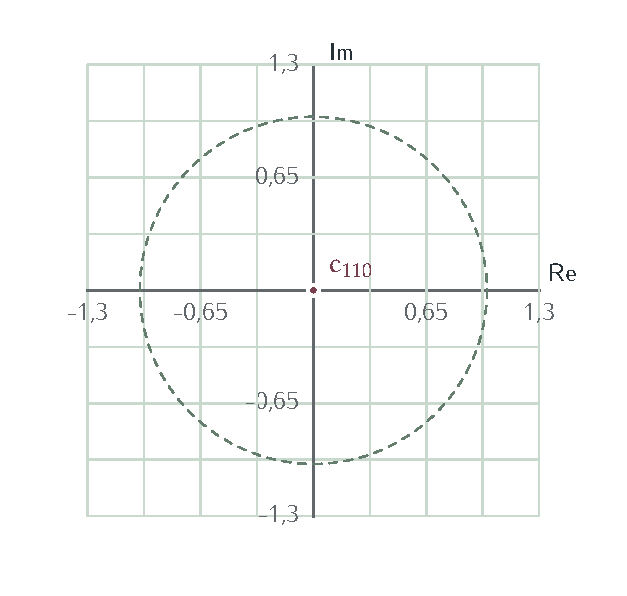
\includegraphics[width=\linewidth,height=63mm,keepaspectratio]{figure/f73c1d792b5e133d8.pdf}\par{\sffamily\footnotesize \(c_{110}\)\par}\end{minipage}\hfill\begin{minipage}[t]{.485\linewidth}\centering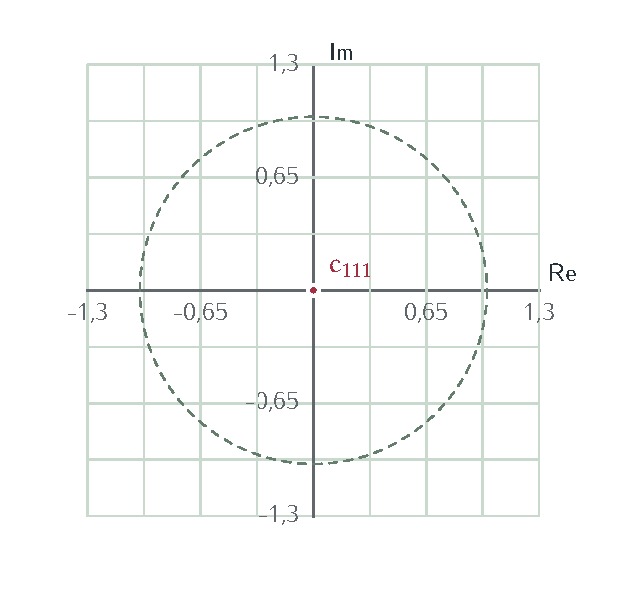
\includegraphics[width=\linewidth,height=63mm,keepaspectratio]{figure/f775f47769e41eab1.pdf}\par{\sffamily\footnotesize \(c_{111}\)\par}\end{minipage}\FigureCaption{4.02 \(\cdot\) esempio 1 \(\cdot\) Componenti complesse}\end{FigureBlock}

\phantomsection\label{c4-bernstein-vazirani-example-1-step-1}
\BookHeading{01 Preparare e interrogare}

\MathBlock{007C007327E9003D03A30078007C007827E9002F221A0038003B00200055005F0066007C007827E9007C221227E9003D0028221200310029005E0066002800780029007C007827E9007C221227E9}{|s\rangle =\sum _{x}|x\rangle /\sqrt{8};\allowbreak \ U_{f}|x\rangle |- \rangle =(- 1)^{f(x)}|x\rangle |- \rangle }

Il bersaglio è autostato di \(X\): la funzione agisce come una fase sul primo registro. Qui si simula direttamente questa riduzione per kickback, senza sintetizzare l'oracolo reversibile a porte.\par


\phantomsection\label{c4-bernstein-vazirani-example-1-step-2}
\BookHeading{02 Uscita 000}

\MathBlock{006100280030003000300029003D002800310020002B0020002D00310020002B002000310020002B0020002D00310020002B0020002D00310020002B002000310020002B0020002D00310020002B002000310029002F0038003D0030002F003822480030}{a(000)=(1\ +\ -1\ +\ 1\ +\ -1\ +\ -1\ +\ 1\ +\ -1\ +\ 1)/8=0/8\approx 0}
\MathBlock{005022480030}{P\approx 0}

Il prodotto binario x\(\cdot\)y è la parità dei prodotti bit per bit.\par


\phantomsection\label{c4-bernstein-vazirani-example-1-step-3}
\BookHeading{03 Uscita 001}

\MathBlock{006100280030003000310029003D002800310020002B002000310020002B002000310020002B002000310020002B0020002D00310020002B0020002D00310020002B0020002D00310020002B0020002D00310029002F0038003D0030002F003822480030}{a(001)=(1\ +\ 1\ +\ 1\ +\ 1\ +\ -1\ +\ -1\ +\ -1\ +\ -1)/8=0/8\approx 0}
\MathBlock{005022480030}{P\approx 0}

Il prodotto binario x\(\cdot\)y è la parità dei prodotti bit per bit.\par


\phantomsection\label{c4-bernstein-vazirani-example-1-step-4}
\BookHeading{04 Uscita 010}

\MathBlock{006100280030003100300029003D002800310020002B0020002D00310020002B0020002D00310020002B002000310020002B0020002D00310020002B002000310020002B002000310020002B0020002D00310029002F0038003D0030002F003822480030}{a(010)=(1\ +\ -1\ +\ -1\ +\ 1\ +\ -1\ +\ 1\ +\ 1\ +\ -1)/8=0/8\approx 0}
\MathBlock{005022480030}{P\approx 0}

Il prodotto binario x\(\cdot\)y è la parità dei prodotti bit per bit.\par


\phantomsection\label{c4-bernstein-vazirani-example-1-step-5}
\BookHeading{05 Uscita 011}

\MathBlock{006100280030003100310029003D002800310020002B002000310020002B0020002D00310020002B0020002D00310020002B0020002D00310020002B0020002D00310020002B002000310020002B002000310029002F0038003D0030002F003822480030}{a(011)=(1\ +\ 1\ +\ -1\ +\ -1\ +\ -1\ +\ -1\ +\ 1\ +\ 1)/8=0/8\approx 0}
\MathBlock{005022480030}{P\approx 0}

Il prodotto binario x\(\cdot\)y è la parità dei prodotti bit per bit.\par


\phantomsection\label{c4-bernstein-vazirani-example-1-step-6}
\BookHeading{06 Uscita 100}

\MathBlock{006100280031003000300029003D002800310020002B0020002D00310020002B002000310020002B0020002D00310020002B002000310020002B0020002D00310020002B002000310020002B0020002D00310029002F0038003D0030002F003822480030}{a(100)=(1\ +\ -1\ +\ 1\ +\ -1\ +\ 1\ +\ -1\ +\ 1\ +\ -1)/8=0/8\approx 0}
\MathBlock{005022480030}{P\approx 0}

Il prodotto binario x\(\cdot\)y è la parità dei prodotti bit per bit.\par


\phantomsection\label{c4-bernstein-vazirani-example-1-step-7}
\BookHeading{07 Uscita 101}

\MathBlock{006100280031003000310029003D002800310020002B002000310020002B002000310020002B002000310020002B002000310020002B002000310020002B002000310020002B002000310029002F0038003D0038002F003822480031}{a(101)=(1\ +\ 1\ +\ 1\ +\ 1\ +\ 1\ +\ 1\ +\ 1\ +\ 1)/8=8/8\approx 1}
\MathBlock{005022480031}{P\approx 1}

Il prodotto binario x\(\cdot\)y è la parità dei prodotti bit per bit.\par


\phantomsection\label{c4-bernstein-vazirani-example-1-step-8}
\BookHeading{08 Uscita 110}

\MathBlock{006100280031003100300029003D002800310020002B0020002D00310020002B0020002D00310020002B002000310020002B002000310020002B0020002D00310020002B0020002D00310020002B002000310029002F0038003D0030002F003822480030}{a(110)=(1\ +\ -1\ +\ -1\ +\ 1\ +\ 1\ +\ -1\ +\ -1\ +\ 1)/8=0/8\approx 0}
\MathBlock{005022480030}{P\approx 0}

Il prodotto binario x\(\cdot\)y è la parità dei prodotti bit per bit.\par


\phantomsection\label{c4-bernstein-vazirani-example-1-step-9}
\BookHeading{09 Uscita 111}

\MathBlock{006100280031003100310029003D002800310020002B002000310020002B0020002D00310020002B0020002D00310020002B002000310020002B002000310020002B0020002D00310020002B0020002D00310029002F0038003D0030002F003822480030}{a(111)=(1\ +\ 1\ +\ -1\ +\ -1\ +\ 1\ +\ 1\ +\ -1\ +\ -1)/8=0/8\approx 0}
\MathBlock{005022480030}{P\approx 0}

Il prodotto binario x\(\cdot\)y è la parità dei prodotti bit per bit.\par


\BookHeading{Interpretazione}

La lettura restituisce la stringa s. Il termine affine cambia una fase globale e conserva la distribuzione.\par


Risorse dichiarate. Una interrogazione al relativo oracolo; 2n Hadamard sui dati, preparazione del bersaglio e costo di costruzione dell'oracolo.\par


\BookHeading{Tabella completa dei dati (8 righe)}

\begingroup\sffamily\fontsize{8.8}{11}\selectfont\setlength{\tabcolsep}{1.6mm}\renewcommand{\arraystretch}{1.28}
\begin{longtable}{>{\RaggedRight\arraybackslash}p{42.133mm}>{\RaggedRight\arraybackslash}p{42.133mm}>{\RaggedRight\arraybackslash}p{42.133mm}}
\toprule\rowcolor{Accent!7}\BeginAccSupp{method=hex,unicode,ActualText=0078}x\EndAccSupp{} & \BeginAccSupp{method=hex,unicode,ActualText=0066002800780029}f(x)\EndAccSupp{} & \BeginAccSupp{method=hex,unicode,ActualText=0046006100730065}Fase\EndAccSupp{} \\
\midrule\endfirsthead
\toprule\rowcolor{Accent!7}\BeginAccSupp{method=hex,unicode,ActualText=0078}x\EndAccSupp{} & \BeginAccSupp{method=hex,unicode,ActualText=0066002800780029}f(x)\EndAccSupp{} & \BeginAccSupp{method=hex,unicode,ActualText=0046006100730065}Fase\EndAccSupp{} \\
\midrule\endhead\bottomrule\endfoot
\BeginAccSupp{method=hex,unicode,ActualText=003000300030}000\EndAccSupp{} & \BeginAccSupp{method=hex,unicode,ActualText=0030}0\EndAccSupp{} & \BeginAccSupp{method=hex,unicode,ActualText=002B0031}+1\EndAccSupp{} \\
\BeginAccSupp{method=hex,unicode,ActualText=003000300031}001\EndAccSupp{} & \BeginAccSupp{method=hex,unicode,ActualText=0031}1\EndAccSupp{} & \BeginAccSupp{method=hex,unicode,ActualText=22120031}\(- 1\)\EndAccSupp{} \\
\BeginAccSupp{method=hex,unicode,ActualText=003000310030}010\EndAccSupp{} & \BeginAccSupp{method=hex,unicode,ActualText=0030}0\EndAccSupp{} & \BeginAccSupp{method=hex,unicode,ActualText=002B0031}+1\EndAccSupp{} \\
\BeginAccSupp{method=hex,unicode,ActualText=003000310031}011\EndAccSupp{} & \BeginAccSupp{method=hex,unicode,ActualText=0031}1\EndAccSupp{} & \BeginAccSupp{method=hex,unicode,ActualText=22120031}\(- 1\)\EndAccSupp{} \\
\BeginAccSupp{method=hex,unicode,ActualText=003100300030}100\EndAccSupp{} & \BeginAccSupp{method=hex,unicode,ActualText=0031}1\EndAccSupp{} & \BeginAccSupp{method=hex,unicode,ActualText=22120031}\(- 1\)\EndAccSupp{} \\
\BeginAccSupp{method=hex,unicode,ActualText=003100300031}101\EndAccSupp{} & \BeginAccSupp{method=hex,unicode,ActualText=0030}0\EndAccSupp{} & \BeginAccSupp{method=hex,unicode,ActualText=002B0031}+1\EndAccSupp{} \\
\BeginAccSupp{method=hex,unicode,ActualText=003100310030}110\EndAccSupp{} & \BeginAccSupp{method=hex,unicode,ActualText=0031}1\EndAccSupp{} & \BeginAccSupp{method=hex,unicode,ActualText=22120031}\(- 1\)\EndAccSupp{} \\
\BeginAccSupp{method=hex,unicode,ActualText=003100310031}111\EndAccSupp{} & \BeginAccSupp{method=hex,unicode,ActualText=0030}0\EndAccSupp{} & \BeginAccSupp{method=hex,unicode,ActualText=002B0031}+1\EndAccSupp{} \\
\end{longtable}\endgroup

\Needspace{.36\textheight}\phantomsection\label{c4-bernstein-vazirani-example-2}
{\sffamily\small\color{Accent} ESEMPIO SVOLTO 2\par}
\BookHeading{Esempio 2}
\(s=011\); \(f(x)=s\cdot x\oplus 1\).\par


\BookHeading{Geometria e configurazione dell'esempio}
\begin{FigureBlock}\centering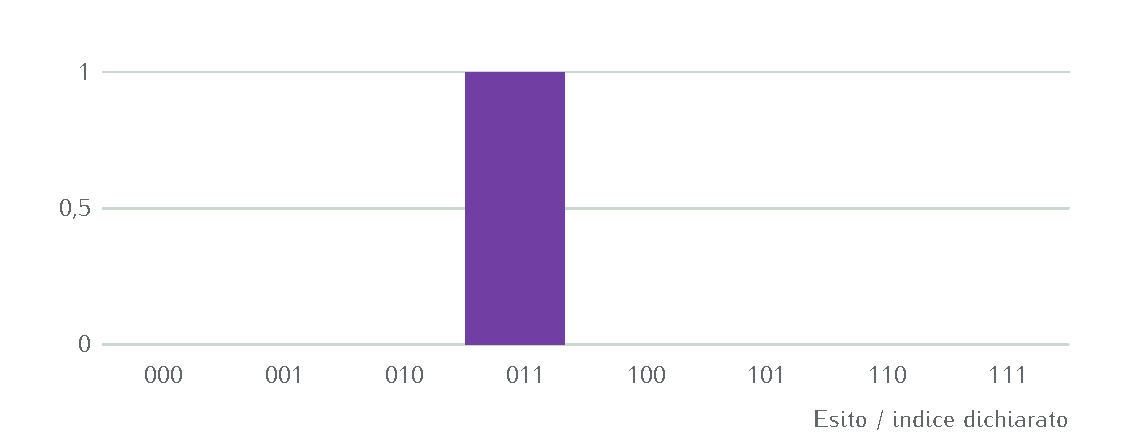
\includegraphics[width=\linewidth,height=94mm,keepaspectratio]{figure/f28bf5309f60bd62e.pdf}\FigureCaption{4.02 \(\cdot\) esempio 2 \(\cdot\) Probabilità nella base dichiarata}\end{FigureBlock}
\begin{FigureBlock}\begin{minipage}[t]{.485\linewidth}\centering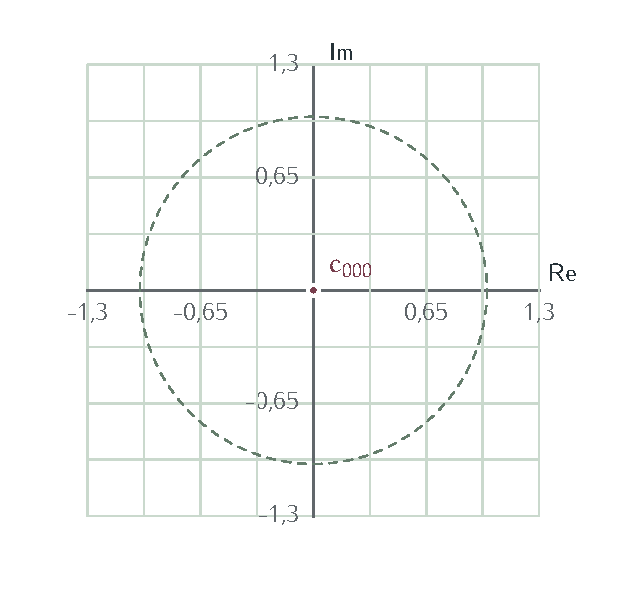
\includegraphics[width=\linewidth,height=63mm,keepaspectratio]{figure/f939e451f9e6ace24.pdf}\par{\sffamily\footnotesize \(c_{000}\)\par}\end{minipage}\hfill\begin{minipage}[t]{.485\linewidth}\centering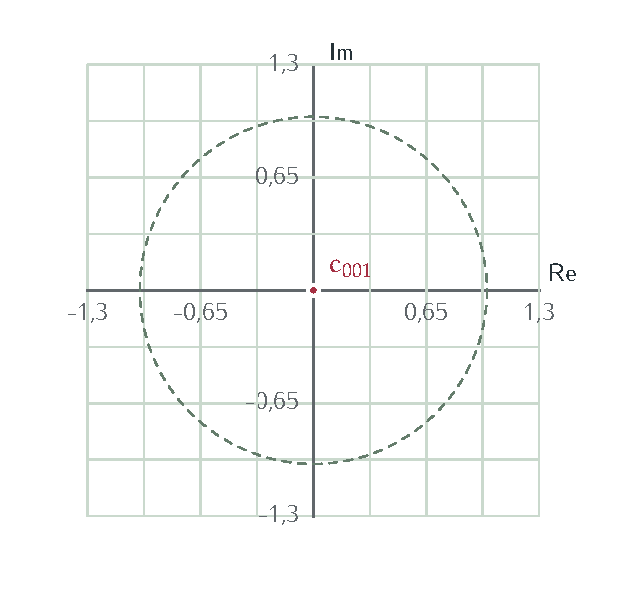
\includegraphics[width=\linewidth,height=63mm,keepaspectratio]{figure/f14c813da6079fd9e.pdf}\par{\sffamily\footnotesize \(c_{001}\)\par}\end{minipage}\FigureCaption{4.02 \(\cdot\) esempio 2 \(\cdot\) Componenti complesse}\end{FigureBlock}
\begin{FigureBlock}\begin{minipage}[t]{.485\linewidth}\centering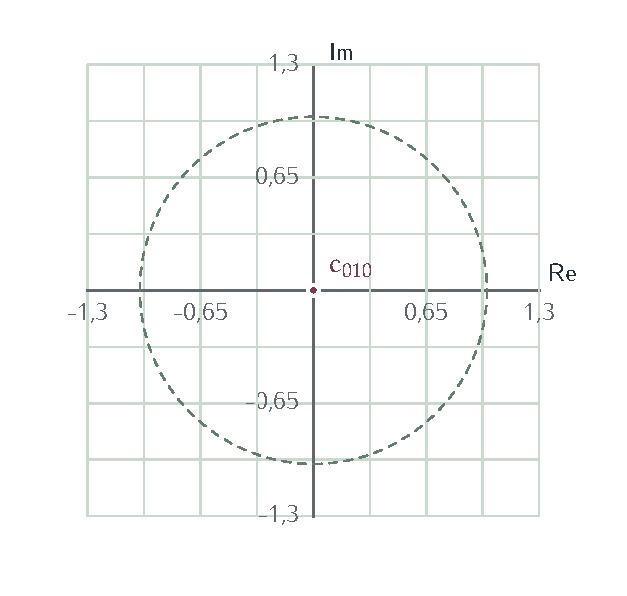
\includegraphics[width=\linewidth,height=63mm,keepaspectratio]{figure/fdd5d560245737335.pdf}\par{\sffamily\footnotesize \(c_{010}\)\par}\end{minipage}\hfill\begin{minipage}[t]{.485\linewidth}\centering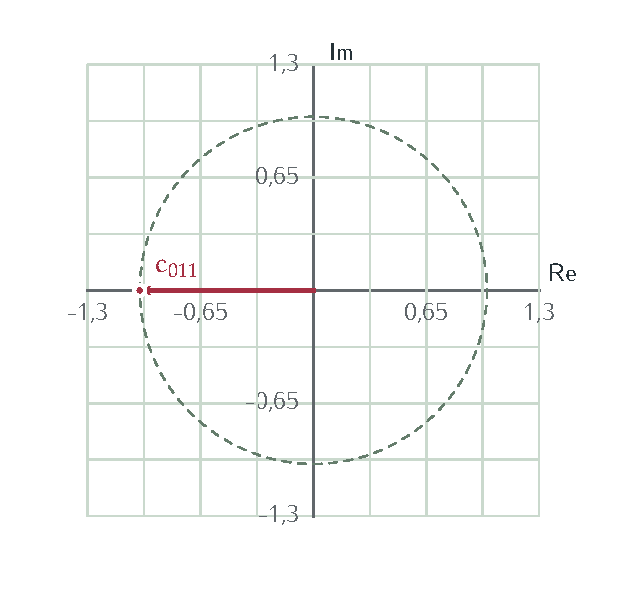
\includegraphics[width=\linewidth,height=63mm,keepaspectratio]{figure/fcf1544bee0b8e299.pdf}\par{\sffamily\footnotesize \(c_{011}\)\par}\end{minipage}\FigureCaption{4.02 \(\cdot\) esempio 2 \(\cdot\) Componenti complesse}\end{FigureBlock}
\begin{FigureBlock}\begin{minipage}[t]{.485\linewidth}\centering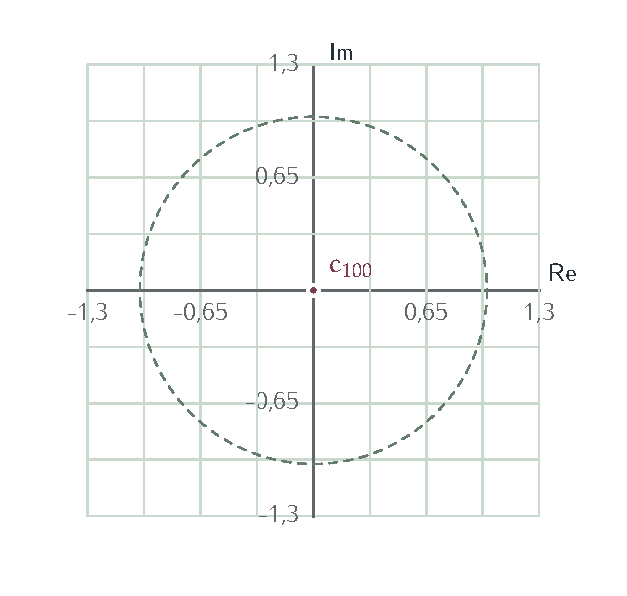
\includegraphics[width=\linewidth,height=63mm,keepaspectratio]{figure/f50bfb6f7766b3911.pdf}\par{\sffamily\footnotesize \(c_{100}\)\par}\end{minipage}\hfill\begin{minipage}[t]{.485\linewidth}\centering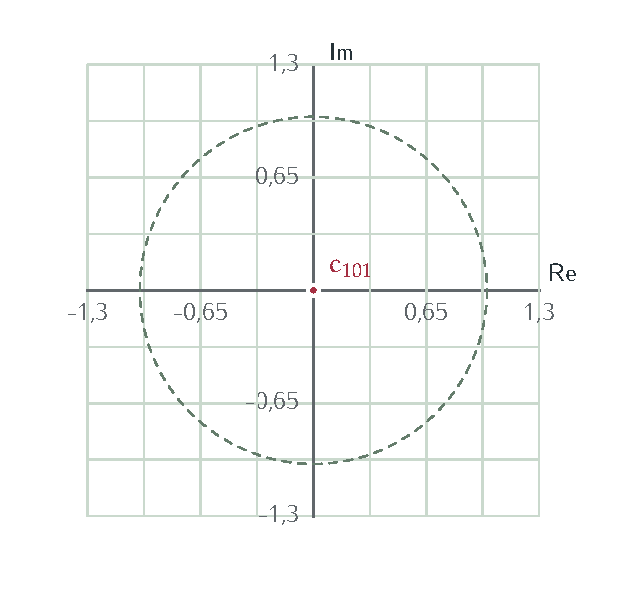
\includegraphics[width=\linewidth,height=63mm,keepaspectratio]{figure/fe61b9bb0f18e82d5.pdf}\par{\sffamily\footnotesize \(c_{101}\)\par}\end{minipage}\FigureCaption{4.02 \(\cdot\) esempio 2 \(\cdot\) Componenti complesse}\end{FigureBlock}
\begin{FigureBlock}\begin{minipage}[t]{.485\linewidth}\centering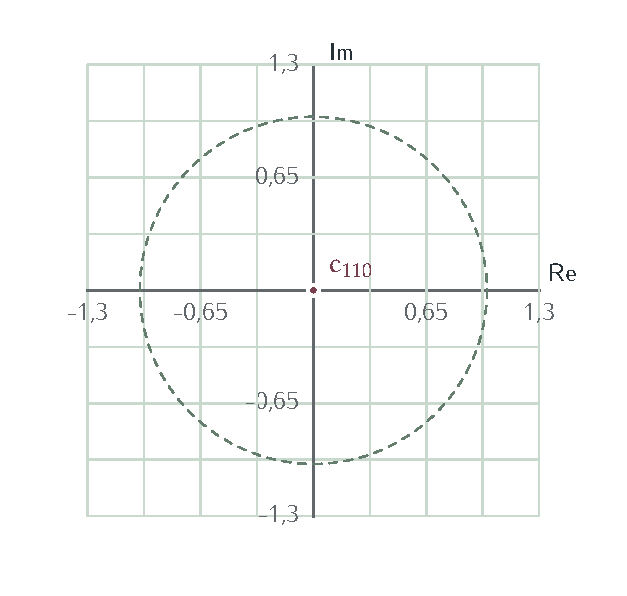
\includegraphics[width=\linewidth,height=63mm,keepaspectratio]{figure/f9b173c0a54982355.pdf}\par{\sffamily\footnotesize \(c_{110}\)\par}\end{minipage}\hfill\begin{minipage}[t]{.485\linewidth}\centering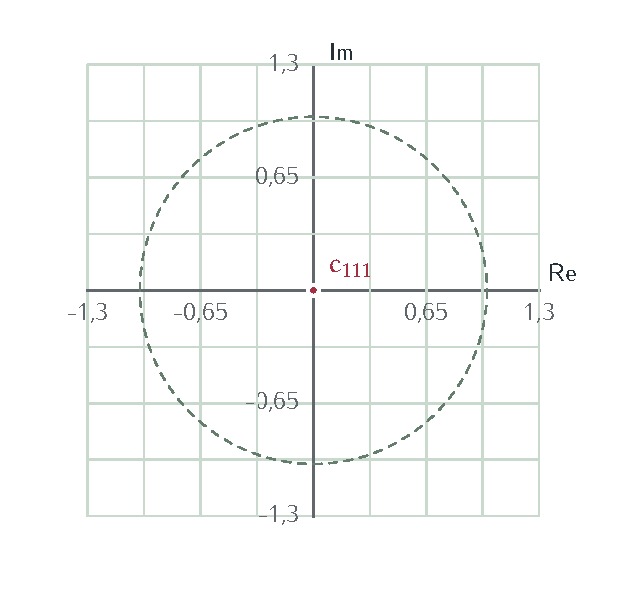
\includegraphics[width=\linewidth,height=63mm,keepaspectratio]{figure/f6771be86f909af57.pdf}\par{\sffamily\footnotesize \(c_{111}\)\par}\end{minipage}\FigureCaption{4.02 \(\cdot\) esempio 2 \(\cdot\) Componenti complesse}\end{FigureBlock}

\phantomsection\label{c4-bernstein-vazirani-example-2-step-1}
\BookHeading{01 Preparare e interrogare}

\MathBlock{007C007327E9003D03A30078007C007827E9002F221A0038003B00200055005F0066007C007827E9007C221227E9003D0028221200310029005E0066002800780029007C007827E9007C221227E9}{|s\rangle =\sum _{x}|x\rangle /\sqrt{8};\allowbreak \ U_{f}|x\rangle |- \rangle =(- 1)^{f(x)}|x\rangle |- \rangle }

Il bersaglio è autostato di \(X\): la funzione agisce come una fase sul primo registro. Qui si simula direttamente questa riduzione per kickback, senza sintetizzare l'oracolo reversibile a porte.\par


\phantomsection\label{c4-bernstein-vazirani-example-2-step-2}
\BookHeading{02 Uscita 000}

\MathBlock{006100280030003000300029003D0028002D00310020002B002000310020002B002000310020002B0020002D00310020002B0020002D00310020002B002000310020002B002000310020002B0020002D00310029002F0038003D0030002F003822480030}{a(000)=(-1\ +\ 1\ +\ 1\ +\ -1\ +\ -1\ +\ 1\ +\ 1\ +\ -1)/8=0/8\approx 0}
\MathBlock{005022480030}{P\approx 0}

Il prodotto binario x\(\cdot\)y è la parità dei prodotti bit per bit.\par


\phantomsection\label{c4-bernstein-vazirani-example-2-step-3}
\BookHeading{03 Uscita 001}

\MathBlock{006100280030003000310029003D0028002D00310020002B0020002D00310020002B002000310020002B002000310020002B0020002D00310020002B0020002D00310020002B002000310020002B002000310029002F0038003D0030002F003822480030}{a(001)=(-1\ +\ -1\ +\ 1\ +\ 1\ +\ -1\ +\ -1\ +\ 1\ +\ 1)/8=0/8\approx 0}
\MathBlock{005022480030}{P\approx 0}

Il prodotto binario x\(\cdot\)y è la parità dei prodotti bit per bit.\par


\phantomsection\label{c4-bernstein-vazirani-example-2-step-4}
\BookHeading{04 Uscita 010}

\MathBlock{006100280030003100300029003D0028002D00310020002B002000310020002B0020002D00310020002B002000310020002B0020002D00310020002B002000310020002B0020002D00310020002B002000310029002F0038003D0030002F003822480030}{a(010)=(-1\ +\ 1\ +\ -1\ +\ 1\ +\ -1\ +\ 1\ +\ -1\ +\ 1)/8=0/8\approx 0}
\MathBlock{005022480030}{P\approx 0}

Il prodotto binario x\(\cdot\)y è la parità dei prodotti bit per bit.\par


\phantomsection\label{c4-bernstein-vazirani-example-2-step-5}
\BookHeading{05 Uscita 011}

\MathBlock{006100280030003100310029003D0028002D00310020002B0020002D00310020002B0020002D00310020002B0020002D00310020002B0020002D00310020002B0020002D00310020002B0020002D00310020002B0020002D00310029002F0038003D002D0038002F00382248002D0031}{a(011)=(-1\ +\ -1\ +\ -1\ +\ -1\ +\ -1\ +\ -1\ +\ -1\ +\ -1)/8=-8/8\approx -1}
\MathBlock{005022480031}{P\approx 1}

Il prodotto binario x\(\cdot\)y è la parità dei prodotti bit per bit.\par


\phantomsection\label{c4-bernstein-vazirani-example-2-step-6}
\BookHeading{06 Uscita 100}

\MathBlock{006100280031003000300029003D0028002D00310020002B002000310020002B002000310020002B0020002D00310020002B002000310020002B0020002D00310020002B0020002D00310020002B002000310029002F0038003D0030002F003822480030}{a(100)=(-1\ +\ 1\ +\ 1\ +\ -1\ +\ 1\ +\ -1\ +\ -1\ +\ 1)/8=0/8\approx 0}
\MathBlock{005022480030}{P\approx 0}

Il prodotto binario x\(\cdot\)y è la parità dei prodotti bit per bit.\par


\phantomsection\label{c4-bernstein-vazirani-example-2-step-7}
\BookHeading{07 Uscita 101}

\MathBlock{006100280031003000310029003D0028002D00310020002B0020002D00310020002B002000310020002B002000310020002B002000310020002B002000310020002B0020002D00310020002B0020002D00310029002F0038003D0030002F003822480030}{a(101)=(-1\ +\ -1\ +\ 1\ +\ 1\ +\ 1\ +\ 1\ +\ -1\ +\ -1)/8=0/8\approx 0}
\MathBlock{005022480030}{P\approx 0}

Il prodotto binario x\(\cdot\)y è la parità dei prodotti bit per bit.\par


\phantomsection\label{c4-bernstein-vazirani-example-2-step-8}
\BookHeading{08 Uscita 110}

\MathBlock{006100280031003100300029003D0028002D00310020002B002000310020002B0020002D00310020002B002000310020002B002000310020002B0020002D00310020002B002000310020002B0020002D00310029002F0038003D0030002F003822480030}{a(110)=(-1\ +\ 1\ +\ -1\ +\ 1\ +\ 1\ +\ -1\ +\ 1\ +\ -1)/8=0/8\approx 0}
\MathBlock{005022480030}{P\approx 0}

Il prodotto binario x\(\cdot\)y è la parità dei prodotti bit per bit.\par


\phantomsection\label{c4-bernstein-vazirani-example-2-step-9}
\BookHeading{09 Uscita 111}

\MathBlock{006100280031003100310029003D0028002D00310020002B0020002D00310020002B0020002D00310020002B0020002D00310020002B002000310020002B002000310020002B002000310020002B002000310029002F0038003D0030002F003822480030}{a(111)=(-1\ +\ -1\ +\ -1\ +\ -1\ +\ 1\ +\ 1\ +\ 1\ +\ 1)/8=0/8\approx 0}
\MathBlock{005022480030}{P\approx 0}

Il prodotto binario x\(\cdot\)y è la parità dei prodotti bit per bit.\par


\BookHeading{Interpretazione}

La lettura restituisce la stringa s. Il termine affine cambia una fase globale e conserva la distribuzione.\par


Risorse dichiarate. Una interrogazione al relativo oracolo; 2n Hadamard sui dati, preparazione del bersaglio e costo di costruzione dell'oracolo.\par


\BookHeading{Tabella completa dei dati (8 righe)}

\begingroup\sffamily\fontsize{8.8}{11}\selectfont\setlength{\tabcolsep}{1.6mm}\renewcommand{\arraystretch}{1.28}
\begin{longtable}{>{\RaggedRight\arraybackslash}p{42.133mm}>{\RaggedRight\arraybackslash}p{42.133mm}>{\RaggedRight\arraybackslash}p{42.133mm}}
\toprule\rowcolor{Accent!7}\BeginAccSupp{method=hex,unicode,ActualText=0078}x\EndAccSupp{} & \BeginAccSupp{method=hex,unicode,ActualText=0066002800780029}f(x)\EndAccSupp{} & \BeginAccSupp{method=hex,unicode,ActualText=0046006100730065}Fase\EndAccSupp{} \\
\midrule\endfirsthead
\toprule\rowcolor{Accent!7}\BeginAccSupp{method=hex,unicode,ActualText=0078}x\EndAccSupp{} & \BeginAccSupp{method=hex,unicode,ActualText=0066002800780029}f(x)\EndAccSupp{} & \BeginAccSupp{method=hex,unicode,ActualText=0046006100730065}Fase\EndAccSupp{} \\
\midrule\endhead\bottomrule\endfoot
\BeginAccSupp{method=hex,unicode,ActualText=003000300030}000\EndAccSupp{} & \BeginAccSupp{method=hex,unicode,ActualText=0031}1\EndAccSupp{} & \BeginAccSupp{method=hex,unicode,ActualText=22120031}\(- 1\)\EndAccSupp{} \\
\BeginAccSupp{method=hex,unicode,ActualText=003000300031}001\EndAccSupp{} & \BeginAccSupp{method=hex,unicode,ActualText=0030}0\EndAccSupp{} & \BeginAccSupp{method=hex,unicode,ActualText=002B0031}+1\EndAccSupp{} \\
\BeginAccSupp{method=hex,unicode,ActualText=003000310030}010\EndAccSupp{} & \BeginAccSupp{method=hex,unicode,ActualText=0030}0\EndAccSupp{} & \BeginAccSupp{method=hex,unicode,ActualText=002B0031}+1\EndAccSupp{} \\
\BeginAccSupp{method=hex,unicode,ActualText=003000310031}011\EndAccSupp{} & \BeginAccSupp{method=hex,unicode,ActualText=0031}1\EndAccSupp{} & \BeginAccSupp{method=hex,unicode,ActualText=22120031}\(- 1\)\EndAccSupp{} \\
\BeginAccSupp{method=hex,unicode,ActualText=003100300030}100\EndAccSupp{} & \BeginAccSupp{method=hex,unicode,ActualText=0031}1\EndAccSupp{} & \BeginAccSupp{method=hex,unicode,ActualText=22120031}\(- 1\)\EndAccSupp{} \\
\BeginAccSupp{method=hex,unicode,ActualText=003100300031}101\EndAccSupp{} & \BeginAccSupp{method=hex,unicode,ActualText=0030}0\EndAccSupp{} & \BeginAccSupp{method=hex,unicode,ActualText=002B0031}+1\EndAccSupp{} \\
\BeginAccSupp{method=hex,unicode,ActualText=003100310030}110\EndAccSupp{} & \BeginAccSupp{method=hex,unicode,ActualText=0030}0\EndAccSupp{} & \BeginAccSupp{method=hex,unicode,ActualText=002B0031}+1\EndAccSupp{} \\
\BeginAccSupp{method=hex,unicode,ActualText=003100310031}111\EndAccSupp{} & \BeginAccSupp{method=hex,unicode,ActualText=0031}1\EndAccSupp{} & \BeginAccSupp{method=hex,unicode,ActualText=22120031}\(- 1\)\EndAccSupp{} \\
\end{longtable}\endgroup

\Needspace{7\baselineskip}
\BookHeading{Il passaggio successivo}
Bernstein--Vazirani legge s in una sola uscita perché tutta la struttura è lineare. In Simon la stringa compare invece come simmetria XOR: ogni misura fornisce un vincolo e serve combinare più equazioni.\par


% Authoritative exercise source. Preserve all derivations and diagrams.

\ExerciseStart{G4.01}{Ricostruire l'interferenza in Deutsch–Jozsa e Bernstein–Vazirani}{Guida esplicita}

\BookHeading{Problema, dati e obiettivo}

Per Deutsch–Jozsa su tre bit confrontare la funzione costante \(f=1\) con \(f(x_0,x_1,x_2)=x_0x_1\oplus x_2\). Per Bernstein–Vazirani usare \(g(x)=x_0\oplus x_2\), associata alla stringa 101. In entrambi i casi preparare l’ausiliario in \(\ket-\) e svolgere tutta l’interferenza.

\ExTheory{\ExRef{c4-deutsch-jozsa}{4.01}; \ExRef{c4-bernstein-vazirani}{4.02}}{L’oracolo reversibile scrive \(y\oplus f(x)\); su \(\ket-\) produce il segno \((-1)^{f(x)}\). La trasformata Hadamard soddisfa \(H^{\otimes3}\ket x=2^{-3/2}\sum_y(-1)^{x\cdot y}\ket y\), dove il prodotto scalare è calcolato modulo due.}

\ExPrediction{La ricombinazione somma segmenti reali di segno opposto. Nel caso bilanciato il coefficiente di 000 deve cancellarsi; la forma affine di Bernstein–Vazirani dovrebbe concentrare l’intera ampiezza sulla stringa cercata.}

\ExFigure{\begin{tikzpicture}[>=Stealth,exlabel]
\node[exbox] (n0) at (0.0,0.0) {prepara $\ket+^{\otimes3}\ket-$};\node[exbox] (n1) at (3.6,0.0) {applica i segni};\draw[exother] (n0)--(n1);\node[exbox] (n2) at (7.2,0.0) {ricombina con $H^{\otimes3}$};\draw[exother] (n1)--(n2);
\end{tikzpicture}}{Due algoritmi condividono la preparazione, mentre la struttura della funzione determina le cancellazioni.}


\begin{ExTasks}

\item Verificare l’equilibrio della prima funzione.

\item Scrivere lo stato dopo il ritorno di fase.

\item Calcolare tutte le otto ampiezze di Deutsch–Jozsa.

\item Confrontare la funzione costante.

\item Fattorizzare la somma di Bernstein–Vazirani sui tre bit.

\item Calcolare la distribuzione e discutere un termine affine costante.

\end{ExTasks}

\ExSolution

\ExStep{Costruire la tabella}

Per \(x=000,001,010,011,100,101,110,111\), i valori di f sono \(0,1,0,1,0,1,1,0\). Ci sono quattro zeri e quattro uni, quindi la promessa di bilanciamento è soddisfatta.

\ExStep{Preparare i segni}

\ExEq{\ket{\Psi}&=\frac1{\sqrt8}\sum_{x=0}^{7}(-1)^{f(x)}\ket x\otimes\ket-,\\
A(y)&=\frac18\sum_{x=0}^{7}(-1)^{f(x)+x\cdot y}.}
Le due normalizzazioni \(1/\sqrt8\) producono il fattore \(1/8\).

\ExStep{Svolgere le otto somme}

\ExEq{A(000)&=(1-1+1-1+1-1-1+1)/8=0\\
A(001)&=(1+1+1+1+1+1-1-1)/8=0.5\\
A(010)&=(1-1-1+1+1-1+1-1)/8=0\\
A(011)&=(1+1-1-1+1+1+1+1)/8=0.5\\
A(100)&=(1-1+1-1-1+1+1-1)/8=0\\
A(101)&=(1+1+1+1-1-1+1+1)/8=0.5\\
A(110)&=(1-1-1+1-1+1-1+1)/8=0\\
A(111)&=(1+1-1-1-1-1-1-1)/8=-0.5}
Gli esiti 001, 011, 101 e 111 hanno probabilità \(1/4\); gli altri hanno probabilità zero. In particolare l’uscita 000 è impossibile.

\ExStep{Confrontare la costante}

Per \(f=1\) ogni segno è \(-1\). Per y=000, \(A(000)=(-1-\cdots-1)/8=-1\). Per ogni y non nullo, le otto parole x contengono quattro prodotti \(x\cdot y=0\) e quattro uguali a uno: la somma è zero. La lettura restituisce 000 con certezza.

\ExStep{Ricostruire la stringa affine}

Per \(g(x)=s\cdot x\), con \(s=101\),
\ExEq{B(y)&=\frac18\sum_x(-1)^{(s\oplus y)\cdot x}\\
&=\prod_{j=0}^{2}\frac{1+(-1)^{s_j\oplus y_j}}2.}
Se \(y_j=s_j\), il fattore j vale \((1+1)/2=1\); se differiscono, vale \((1-1)/2=0\). Quindi \(B(101)=1\) e le altre sette ampiezze sono zero.

\ExStep{Controllare termine affine e risorsa}

Per \(g(x)=s\cdot x\oplus1\), tutte le ampiezze acquistano il fattore \(-1\): la lettura rimane 101. Ciascun circuito usa una interrogazione coerente dell’oracolo, oltre alle porte di preparazione e lettura. Il conteggio è distinto dal costo di costruzione dell’oracolo.

\par\noindent\begin{minipage}{\linewidth}
\ExFigure{\begin{tikzpicture}[>=Stealth,exlabel]
\draw[exaxis] (-.6,0)--(4.4,0) node[right] {esito};\draw[exaxis] (-.6,0)--(-.6,3.6) node[above] {$p$};\node[left] at (-.6,3) {$ 0.3 $};\draw[Ink!15,dashed] (-.6,3)--(3.9000000000000004,3);\filldraw[fill=Accent!25,draw=Accent] (0.0,0) rectangle (0.65,2.5);\node[below] at (0.325,0) {$ 001 $};\node[above] at (0.325,2.5) {$ 0.25 $};\filldraw[fill=Accent!25,draw=Accent] (1.1,0) rectangle (1.75,2.5);\node[below] at (1.425,0) {$ 011 $};\node[above] at (1.425,2.5) {$ 0.25 $};\filldraw[fill=Accent!25,draw=Accent] (2.2,0) rectangle (2.85,2.5);\node[below] at (2.5250000000000004,0) {$ 101 $};\node[above] at (2.5250000000000004,2.5) {$ 0.25 $};\filldraw[fill=Accent!25,draw=Accent] (3.3000000000000003,0) rectangle (3.95,2.5);\node[below] at (3.6250000000000004,0) {$ 111 $};\node[above] at (3.6250000000000004,2.5) {$ 0.25 $};
\end{tikzpicture}}{Esiti di Deutsch–Jozsa per la funzione bilanciata non affine; Bernstein–Vazirani concentra invece tutto il peso su 101.}


\ExInterpret{La distinzione fra funzione costante e bilanciata riguarda il coefficiente 000. L’ipotesi affine più forte permette di recuperare un’intera stringa mediante la stessa somma di caratteri binari.}

\ExLab{Nelle sezioni 4.01 e 4.02 scegliere rispettivamente «Bilanciata non affine su tre bit» e «Stringa 101». Confrontare i segni prima della ricombinazione, poi le distribuzioni finali. Usare anche la variante affine con termine costante per osservare la fase globale.}


\end{minipage}

\Needspace{.43\textheight}
\section{Simon e le equazioni binarie}
\phantomsection\label{c4-simon}

{\sffamily\small\color{Ink!70} Riferimento alle slide: p. 76.\par}

{\sffamily\small\color{Ink!70} Laboratorio locale: \nolinkurl{index.html#capitolo-4/simon}\par}

\BookHeading{Definizioni e costruzione}
Consideriamo \(f:\{0{,}1\}^{n}\to \{0{,}1\}^{n}\) con una stringa segreta non nulla \(s\ne 0\). La promessa completa è \(f(x)=f(x{}^{\prime} )\) se e soltanto se \(x{}^{\prime} =x\) oppure \(x{}^{\prime} =x\oplus s\). Ogni valore raggiunto ha quindi esattamente due preimmagini, e l'obiettivo è ricostruire s.\par

Il circuito ideale prepara \(\sum _{x}|x\rangle |f(x)\rangle /\sqrt{2^{n}}\) usando un oracolo reversibile. Condizionare sul valore \(f(x_{0})\) del secondo registro lascia \((|x_{0}\rangle +|x_{0}\oplus s\rangle )/\sqrt{2}\) nel primo. La sola invarianza \(f(x)=f(x\oplus s)\) sarebbe insufficiente: per \(n>1\) una funzione costante la soddisfa, ma ha fibre più grandi di due e viola la promessa.\par

Dopo \(H^{\otimes n}\), l'ampiezza di y è \((- 1)^{x_{0}\cdot y}[1+(- 1)^{s\cdot y}]/\sqrt{2^{n+1}}\). Se \(s\cdot y=1\) i termini si cancellano; se \(s\cdot y=0\) il modulo quadrato vale \(2/2^{n}\). Per \(n=3\) ci sono quattro y ammessi, ciascuno con probabilità 1/4, indipendentemente dal ramo \(f(x_{0})\).\par

Le uscite danno equazioni \(y\cdot s=0\) su \(F_{2}\), il campo dei bit con somma XOR. Per isolare lo spazio delle soluzioni \(\{0,\allowbreak s\}\) servono \(n- 1\) righe linearmente indipendenti; la promessa \(s\ne 0\) seleziona poi s. Misure eseguite su nuove preparazioni sono probabilisticamente indipendenti, ma possono dare righe ripetute o la riga nulla, che non aumentano il rango.\par

Il modello costruisce la tabella di f e ne raggruppa le fibre: non sintetizza l'oracolo porta per porta. Le sequenze degli esempi sono uscite ammesse prefissate per mostrare l'eliminazione, non estrazioni casuali. Il caso \(s=0\) corrisponderebbe alla promessa iniettiva e richiederebbe un problema distinto; qui è escluso fin dall'inizio.\par


\MathBlock{0066002800780029003D00660028007820320029002021D40020002800782032003D00780020006F00700070007500720065002000782032003D0078229500730029002C0020007322600030003B00200050002800790029003D0032005E002800312212006E00290020007300650020007900B70073003D0030002C00200061006C007400720069006D0065006E0074006900200030002E}{f(x)=f(x{}^{\prime} )\ \Leftrightarrow \ (x{}^{\prime} =x\ \text{oppure}\ x{}^{\prime} =x\oplus s),\allowbreak \ s\ne 0;\allowbreak \ P(y)=2^{1- n}\ \text{se}\ y\cdot s=0,\allowbreak \ \text{altrimenti}\ 0.}

\BookHeading{Come leggere le figure}
XOR e prodotto binario operano sulle stringhe; il rango è calcolato modulo due. Il registro quantistico usa ampiezze complesse, mentre la tabella di eliminazione è un calcolo classico esatto sui bit.\par


\BookHeading{Attività nel laboratorio modificabile}

\BookHeading{Obiettivo dell'esperimento}
Ricavare un segreto mediante vincoli binari osservati.\par

\BookHeading{Percorso operativo}
Generare una funzione con segreto nascosto, calcolare e acquisire una misura alla volta. Mostrare la preparazione quando si vuole studiare l'origine della distribuzione.\par

\BookHeading{Lettura geometrica}
Il diagramma del ramo mostra contributi concordi e opposti; le caselle dei candidati mostrano l'intersezione dei vincoli su \(F_{2}\).\par

\BookHeading{Controllo del risultato}
Registrare il rango dopo ogni misura. Ripetizioni ed esito nullo possono lasciare invariato il numero di candidati.\par


\Needspace{.36\textheight}\phantomsection\label{c4-simon-example-1}
{\sffamily\small\color{Accent} ESEMPIO SVOLTO 1\par}
\BookHeading{Esempio 1}
Esempio guidato: \(n=3\), segreto \(s=101\), funzione \(f(x)=\min (x,\allowbreak x\oplus s)\). Ogni valore della funzione ha esattamente due preimmagini. L'esperimento modificabile permette di generare altre funzioni e raccogliere misure campionate.\par


\BookHeading{Geometria e configurazione dell'esempio}
\begin{FigureBlock}\centering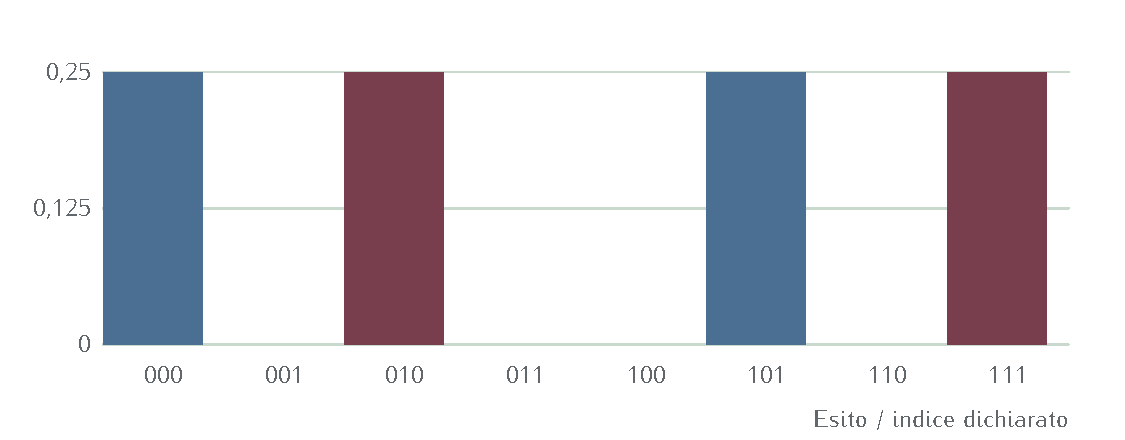
\includegraphics[width=\linewidth,height=94mm,keepaspectratio]{figure/ff1b7eacee5f4b359.pdf}\FigureCaption{4.03 \(\cdot\) esempio 1 \(\cdot\) Probabilità marginale P(y)}\end{FigureBlock}
\begin{FigureBlock}\centering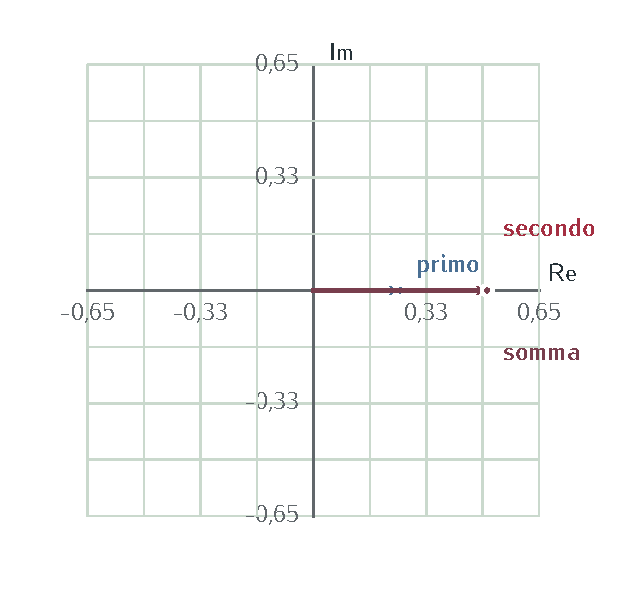
\includegraphics[width=\linewidth,height=94mm,keepaspectratio]{figure/feefd96f4ee9f46fe.pdf}\FigureCaption{4.03 \(\cdot\) esempio 1 \(\cdot\) Somma concorde per \(y=000\) nel ramo \(f=0\)}\end{FigureBlock}
\begin{FigureBlock}\centering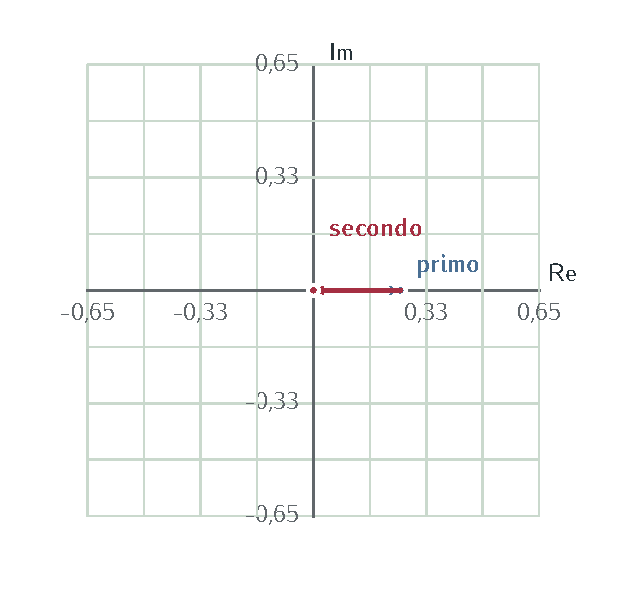
\includegraphics[width=\linewidth,height=94mm,keepaspectratio]{figure/f8a3c5d4b84ffcc42.pdf}\FigureCaption{4.03 \(\cdot\) esempio 1 \(\cdot\) Cancellazione quando \(s\cdot y=1\) nel ramo \(f=0\)}\end{FigureBlock}

\phantomsection\label{c4-simon-example-1-step-1}
\BookHeading{01 Preparare i registri}

\MathBlock{007C03A827E9003D00280031002F221A0038002903A3005F0078007C007827E9007C006600280078002927E9}{|\Psi \rangle =(1/\sqrt{8})\sum _{x}|x\rangle |f(x)\rangle }

Ogni ingresso ha probabilità 1/8. Le parole binarie indicano vettori ortogonali della base; il prodotto binario è calcolato modulo due.\par


\phantomsection\label{c4-simon-example-1-step-2}
\BookHeading{02 Probabilità del ramo \(f=0\)}

\MathBlock{005000280066003D00300029003D007C0031002F221A0038007C00B2002B007C0031002F221A0038007C00B2003D0031002F0038002B0031002F0038003D0031002F0034}{P(f=0)=|1/\sqrt{8}|^{2}+|1/\sqrt{8}|^{2}=1/8+1/8=1/4}

Il valore osservato della funzione seleziona due ingressi. Le loro probabilità si sommano perché gli stati del primo registro sono ortogonali.\par


\phantomsection\label{c4-simon-example-1-step-3}
\BookHeading{03 Normalizzare il ramo 0}

\MathBlock{00280031002F221A00380029002F221A00280031002F00340029003D00280031002F221A00380029002F00280031002F00320029003D0032002F221A0038003D0031002F221A0032}{(1/\sqrt{8})/\sqrt{1/4}=(1/\sqrt{8})/(1/2)=2/\sqrt{8}=1/\sqrt{2}}
\MathBlock{007C03C8005F006627E9003D0028007C00300030003027E9002B007C00310030003127E90029002F221A0032}{|\psi _{f}\rangle =(|000\rangle +|101\rangle )/\sqrt{2}}

Condizionare sul ramo divide entrambe le ampiezze per la radice della sua probabilità. La norma dello stato risultante vale uno.\par


\phantomsection\label{c4-simon-example-1-step-4}
\BookHeading{04 Applicare gli Hadamard al ramo 0}

\MathBlock{0048005E007B22970033007D007C007827E9003D00280031002F221A0038002903A3005F00790028002D00310029005E0028007800B700790029007C007927E9}{H^{\otimes 3}|x\rangle =(1/\sqrt{8})\sum _{y}(-1)^{x\cdot y}|y\rangle }
\MathBlock{0061005F0066002800790029003D00280031002F221A0032002900280031002F221A00380029005B0028002D00310029005E002800300030003000B700790029002B0028002D00310029005E002800310030003100B700790029005D}{a_{f}(y)=(1/\sqrt{2})(1/\sqrt{8})[(-1)^{000\cdot y}+(-1)^{101\cdot y}]}
\MathBlock{003D00280031002F00340029005B0028002D00310029005E002800300030003000B700790029002B0028002D00310029005E002800310030003100B700790029005D}{=(1/4)[(-1)^{000\cdot y}+(-1)^{101\cdot y}]}

I due contributi arrivano nella stessa uscita y. Si sommano le ampiezze con il loro segno e si calcola successivamente il modulo quadro.\par


\phantomsection\label{c4-simon-example-1-step-5}
\BookHeading{05 Leggere il vincolo del ramo 0}

\MathBlock{0061005F0066002800790029003D00280028002D00310029005E002800300030003000B700790029002F00340029005B0031002B0028002D00310029005E002800310030003100B700790029005D}{a_{f}(y)=((-1)^{000\cdot y}/4)[1+(-1)^{101\cdot y}]}
\MathBlock{007300B70079003D0030002021D20020007C0061005F0066002800790029007C003D0031002F0032002021D20020005000280079007C00660029003D0031002F0034}{s\cdot y=0\ \Rightarrow \ |a_{f}(y)|=1/2\ \Rightarrow \ P(y|f)=1/4}
\MathBlock{007300B70079003D0031002021D200200061005F0066002800790029003D0030002021D20020005000280079007C00660029003D0030}{s\cdot y=1\ \Rightarrow \ a_{f}(y)=0\ \Rightarrow \ P(y|f)=0}

Poiché \(b=a\oplus s\), la parità b\(\cdot\)y è la somma modulo due delle parità a\(\cdot\)y e s\(\cdot\)y. Il segno comune può variare fra i rami; il supporto delle probabilità resta lo stesso.\par


\phantomsection\label{c4-simon-example-1-step-6}
\BookHeading{06 Probabilità del ramo \(f=1\)}

\MathBlock{005000280066003D00310029003D007C0031002F221A0038007C00B2002B007C0031002F221A0038007C00B2003D0031002F0038002B0031002F0038003D0031002F0034}{P(f=1)=|1/\sqrt{8}|^{2}+|1/\sqrt{8}|^{2}=1/8+1/8=1/4}

Il valore osservato della funzione seleziona due ingressi. Le loro probabilità si sommano perché gli stati del primo registro sono ortogonali.\par


\phantomsection\label{c4-simon-example-1-step-7}
\BookHeading{07 Normalizzare il ramo 1}

\MathBlock{00280031002F221A00380029002F221A00280031002F00340029003D00280031002F221A00380029002F00280031002F00320029003D0032002F221A0038003D0031002F221A0032}{(1/\sqrt{8})/\sqrt{1/4}=(1/\sqrt{8})/(1/2)=2/\sqrt{8}=1/\sqrt{2}}
\MathBlock{007C03C8005F006627E9003D0028007C00300030003127E9002B007C00310030003027E90029002F221A0032}{|\psi _{f}\rangle =(|001\rangle +|100\rangle )/\sqrt{2}}

Condizionare sul ramo divide entrambe le ampiezze per la radice della sua probabilità. La norma dello stato risultante vale uno.\par


\phantomsection\label{c4-simon-example-1-step-8}
\BookHeading{08 Applicare gli Hadamard al ramo 1}

\MathBlock{0048005E007B22970033007D007C007827E9003D00280031002F221A0038002903A3005F00790028002D00310029005E0028007800B700790029007C007927E9}{H^{\otimes 3}|x\rangle =(1/\sqrt{8})\sum _{y}(-1)^{x\cdot y}|y\rangle }
\MathBlock{0061005F0066002800790029003D00280031002F221A0032002900280031002F221A00380029005B0028002D00310029005E002800300030003100B700790029002B0028002D00310029005E002800310030003000B700790029005D}{a_{f}(y)=(1/\sqrt{2})(1/\sqrt{8})[(-1)^{001\cdot y}+(-1)^{100\cdot y}]}
\MathBlock{003D00280031002F00340029005B0028002D00310029005E002800300030003100B700790029002B0028002D00310029005E002800310030003000B700790029005D}{=(1/4)[(-1)^{001\cdot y}+(-1)^{100\cdot y}]}

I due contributi arrivano nella stessa uscita y. Si sommano le ampiezze con il loro segno e si calcola successivamente il modulo quadro.\par


\phantomsection\label{c4-simon-example-1-step-9}
\BookHeading{09 Leggere il vincolo del ramo 1}

\MathBlock{0061005F0066002800790029003D00280028002D00310029005E002800300030003100B700790029002F00340029005B0031002B0028002D00310029005E002800310030003100B700790029005D}{a_{f}(y)=((-1)^{001\cdot y}/4)[1+(-1)^{101\cdot y}]}
\MathBlock{007300B70079003D0030002021D20020007C0061005F0066002800790029007C003D0031002F0032002021D20020005000280079007C00660029003D0031002F0034}{s\cdot y=0\ \Rightarrow \ |a_{f}(y)|=1/2\ \Rightarrow \ P(y|f)=1/4}
\MathBlock{007300B70079003D0031002021D200200061005F0066002800790029003D0030002021D20020005000280079007C00660029003D0030}{s\cdot y=1\ \Rightarrow \ a_{f}(y)=0\ \Rightarrow \ P(y|f)=0}

Poiché \(b=a\oplus s\), la parità b\(\cdot\)y è la somma modulo due delle parità a\(\cdot\)y e s\(\cdot\)y. Il segno comune può variare fra i rami; il supporto delle probabilità resta lo stesso.\par


\phantomsection\label{c4-simon-example-1-step-10}
\BookHeading{10 Probabilità del ramo \(f=2\)}

\MathBlock{005000280066003D00320029003D007C0031002F221A0038007C00B2002B007C0031002F221A0038007C00B2003D0031002F0038002B0031002F0038003D0031002F0034}{P(f=2)=|1/\sqrt{8}|^{2}+|1/\sqrt{8}|^{2}=1/8+1/8=1/4}

Il valore osservato della funzione seleziona due ingressi. Le loro probabilità si sommano perché gli stati del primo registro sono ortogonali.\par


\phantomsection\label{c4-simon-example-1-step-11}
\BookHeading{11 Normalizzare il ramo 2}

\MathBlock{00280031002F221A00380029002F221A00280031002F00340029003D00280031002F221A00380029002F00280031002F00320029003D0032002F221A0038003D0031002F221A0032}{(1/\sqrt{8})/\sqrt{1/4}=(1/\sqrt{8})/(1/2)=2/\sqrt{8}=1/\sqrt{2}}
\MathBlock{007C03C8005F006627E9003D0028007C00300031003027E9002B007C00310031003127E90029002F221A0032}{|\psi _{f}\rangle =(|010\rangle +|111\rangle )/\sqrt{2}}

Condizionare sul ramo divide entrambe le ampiezze per la radice della sua probabilità. La norma dello stato risultante vale uno.\par


\phantomsection\label{c4-simon-example-1-step-12}
\BookHeading{12 Applicare gli Hadamard al ramo 2}

\MathBlock{0048005E007B22970033007D007C007827E9003D00280031002F221A0038002903A3005F00790028002D00310029005E0028007800B700790029007C007927E9}{H^{\otimes 3}|x\rangle =(1/\sqrt{8})\sum _{y}(-1)^{x\cdot y}|y\rangle }
\MathBlock{0061005F0066002800790029003D00280031002F221A0032002900280031002F221A00380029005B0028002D00310029005E002800300031003000B700790029002B0028002D00310029005E002800310031003100B700790029005D}{a_{f}(y)=(1/\sqrt{2})(1/\sqrt{8})[(-1)^{010\cdot y}+(-1)^{111\cdot y}]}
\MathBlock{003D00280031002F00340029005B0028002D00310029005E002800300031003000B700790029002B0028002D00310029005E002800310031003100B700790029005D}{=(1/4)[(-1)^{010\cdot y}+(-1)^{111\cdot y}]}

I due contributi arrivano nella stessa uscita y. Si sommano le ampiezze con il loro segno e si calcola successivamente il modulo quadro.\par


\phantomsection\label{c4-simon-example-1-step-13}
\BookHeading{13 Leggere il vincolo del ramo 2}

\MathBlock{0061005F0066002800790029003D00280028002D00310029005E002800300031003000B700790029002F00340029005B0031002B0028002D00310029005E002800310030003100B700790029005D}{a_{f}(y)=((-1)^{010\cdot y}/4)[1+(-1)^{101\cdot y}]}
\MathBlock{007300B70079003D0030002021D20020007C0061005F0066002800790029007C003D0031002F0032002021D20020005000280079007C00660029003D0031002F0034}{s\cdot y=0\ \Rightarrow \ |a_{f}(y)|=1/2\ \Rightarrow \ P(y|f)=1/4}
\MathBlock{007300B70079003D0031002021D200200061005F0066002800790029003D0030002021D20020005000280079007C00660029003D0030}{s\cdot y=1\ \Rightarrow \ a_{f}(y)=0\ \Rightarrow \ P(y|f)=0}

Poiché \(b=a\oplus s\), la parità b\(\cdot\)y è la somma modulo due delle parità a\(\cdot\)y e s\(\cdot\)y. Il segno comune può variare fra i rami; il supporto delle probabilità resta lo stesso.\par


\phantomsection\label{c4-simon-example-1-step-14}
\BookHeading{14 Probabilità del ramo \(f=3\)}

\MathBlock{005000280066003D00330029003D007C0031002F221A0038007C00B2002B007C0031002F221A0038007C00B2003D0031002F0038002B0031002F0038003D0031002F0034}{P(f=3)=|1/\sqrt{8}|^{2}+|1/\sqrt{8}|^{2}=1/8+1/8=1/4}

Il valore osservato della funzione seleziona due ingressi. Le loro probabilità si sommano perché gli stati del primo registro sono ortogonali.\par


\phantomsection\label{c4-simon-example-1-step-15}
\BookHeading{15 Normalizzare il ramo 3}

\MathBlock{00280031002F221A00380029002F221A00280031002F00340029003D00280031002F221A00380029002F00280031002F00320029003D0032002F221A0038003D0031002F221A0032}{(1/\sqrt{8})/\sqrt{1/4}=(1/\sqrt{8})/(1/2)=2/\sqrt{8}=1/\sqrt{2}}
\MathBlock{007C03C8005F006627E9003D0028007C00300031003127E9002B007C00310031003027E90029002F221A0032}{|\psi _{f}\rangle =(|011\rangle +|110\rangle )/\sqrt{2}}

Condizionare sul ramo divide entrambe le ampiezze per la radice della sua probabilità. La norma dello stato risultante vale uno.\par


\phantomsection\label{c4-simon-example-1-step-16}
\BookHeading{16 Applicare gli Hadamard al ramo 3}

\MathBlock{0048005E007B22970033007D007C007827E9003D00280031002F221A0038002903A3005F00790028002D00310029005E0028007800B700790029007C007927E9}{H^{\otimes 3}|x\rangle =(1/\sqrt{8})\sum _{y}(-1)^{x\cdot y}|y\rangle }
\MathBlock{0061005F0066002800790029003D00280031002F221A0032002900280031002F221A00380029005B0028002D00310029005E002800300031003100B700790029002B0028002D00310029005E002800310031003000B700790029005D}{a_{f}(y)=(1/\sqrt{2})(1/\sqrt{8})[(-1)^{011\cdot y}+(-1)^{110\cdot y}]}
\MathBlock{003D00280031002F00340029005B0028002D00310029005E002800300031003100B700790029002B0028002D00310029005E002800310031003000B700790029005D}{=(1/4)[(-1)^{011\cdot y}+(-1)^{110\cdot y}]}

I due contributi arrivano nella stessa uscita y. Si sommano le ampiezze con il loro segno e si calcola successivamente il modulo quadro.\par


\phantomsection\label{c4-simon-example-1-step-17}
\BookHeading{17 Leggere il vincolo del ramo 3}

\MathBlock{0061005F0066002800790029003D00280028002D00310029005E002800300031003100B700790029002F00340029005B0031002B0028002D00310029005E002800310030003100B700790029005D}{a_{f}(y)=((-1)^{011\cdot y}/4)[1+(-1)^{101\cdot y}]}
\MathBlock{007300B70079003D0030002021D20020007C0061005F0066002800790029007C003D0031002F0032002021D20020005000280079007C00660029003D0031002F0034}{s\cdot y=0\ \Rightarrow \ |a_{f}(y)|=1/2\ \Rightarrow \ P(y|f)=1/4}
\MathBlock{007300B70079003D0031002021D200200061005F0066002800790029003D0030002021D20020005000280079007C00660029003D0030}{s\cdot y=1\ \Rightarrow \ a_{f}(y)=0\ \Rightarrow \ P(y|f)=0}

Poiché \(b=a\oplus s\), la parità b\(\cdot\)y è la somma modulo due delle parità a\(\cdot\)y e s\(\cdot\)y. Il segno comune può variare fra i rami; il supporto delle probabilità resta lo stesso.\par


\phantomsection\label{c4-simon-example-1-step-18}
\BookHeading{18 Calcolare la marginale delle uscite}

\MathBlock{0050002800790029003D03A3005F006600200050002800660029005000280079007C00660029}{P(y)=\sum _{f}\ P(f)P(y|f)}
\MathBlock{007300B70079003D0030002021D200200050002800790029003D003400B700280031002F0034002900B700280031002F00340029003D0031002F0034}{s\cdot y=0\ \Rightarrow \ P(y)=4\cdot (1/4)\cdot (1/4)=1/4}
\MathBlock{007300B70079003D0031002021D200200050002800790029003D003400B700280031002F0034002900B70030003D0030}{s\cdot y=1\ \Rightarrow \ P(y)=4\cdot (1/4)\cdot 0=0}

La misura della funzione può essere omessa: la marginale sul primo registro coincide con la somma sui bersagli ortogonali.\par


\phantomsection\label{c4-simon-example-1-step-19}
\BookHeading{19 Equazioni del percorso guidato}

\MathBlock{00300031003000B70073003D0030}{010\cdot s=0}
\MathBlock{00310031003100B70073003D0030}{111\cdot s=0}

Queste righe sono scelte per illustrare indipendenza e ripetizione. Nell'area di esperimento ogni nuova riga proviene da una misura campionata dalla distribuzione.\par


\phantomsection\label{c4-simon-example-1-step-20}
\BookHeading{20 Eliminare su \(F_{2}\)}

\MathBlock{005300630061006D00620069006100200072006900670061002000320020006500200031002E}{\text{Scambia}\ \text{riga}\ 2\ e\ 1.}
\MathBlock{0031003100310020229500200030003100300020003D0020003100300031}{111\ \oplus \ 010\ =\ 101}
\MathBlock{00720061006E0067006F003D0032003B002000630061006E006400690064006100740069003D007B003000300030003B0020003100300031007D}{\text{rango}=2;\allowbreak \ \text{candidati}=\{000;\allowbreak \ 101\}}

L'operazione elementare è XOR. Una riga ripetuta si annulla e lascia invariato il rango. La promessa esclude il candidato nullo; rango \(n- 1\) identifica un unico segreto non nullo.\par


\BookHeading{Interpretazione}

Il segreto emerge dall'intersezione dei vincoli binari. Le cancellazioni delle ampiezze determinano quali vincoli possono essere osservati.\par


\BookHeading{Tabella completa dei dati (8 righe)}

\begingroup\sffamily\fontsize{8.8}{11}\selectfont\setlength{\tabcolsep}{1.6mm}\renewcommand{\arraystretch}{1.28}
\begin{longtable}{>{\RaggedRight\arraybackslash}p{42.133mm}>{\RaggedRight\arraybackslash}p{42.133mm}>{\RaggedRight\arraybackslash}p{42.133mm}}
\toprule\rowcolor{Accent!7}\BeginAccSupp{method=hex,unicode,ActualText=0078}x\EndAccSupp{} & \BeginAccSupp{method=hex,unicode,ActualText=007822950073}\(x\oplus s\)\EndAccSupp{} & \BeginAccSupp{method=hex,unicode,ActualText=0066002800780029}f(x)\EndAccSupp{} \\
\midrule\endfirsthead
\toprule\rowcolor{Accent!7}\BeginAccSupp{method=hex,unicode,ActualText=0078}x\EndAccSupp{} & \BeginAccSupp{method=hex,unicode,ActualText=007822950073}\(x\oplus s\)\EndAccSupp{} & \BeginAccSupp{method=hex,unicode,ActualText=0066002800780029}f(x)\EndAccSupp{} \\
\midrule\endhead\bottomrule\endfoot
\BeginAccSupp{method=hex,unicode,ActualText=003000300030}000\EndAccSupp{} & \BeginAccSupp{method=hex,unicode,ActualText=003100300031}101\EndAccSupp{} & \BeginAccSupp{method=hex,unicode,ActualText=0030}0\EndAccSupp{} \\
\BeginAccSupp{method=hex,unicode,ActualText=003000300031}001\EndAccSupp{} & \BeginAccSupp{method=hex,unicode,ActualText=003100300030}100\EndAccSupp{} & \BeginAccSupp{method=hex,unicode,ActualText=0031}1\EndAccSupp{} \\
\BeginAccSupp{method=hex,unicode,ActualText=003000310030}010\EndAccSupp{} & \BeginAccSupp{method=hex,unicode,ActualText=003100310031}111\EndAccSupp{} & \BeginAccSupp{method=hex,unicode,ActualText=0032}2\EndAccSupp{} \\
\BeginAccSupp{method=hex,unicode,ActualText=003000310031}011\EndAccSupp{} & \BeginAccSupp{method=hex,unicode,ActualText=003100310030}110\EndAccSupp{} & \BeginAccSupp{method=hex,unicode,ActualText=0033}3\EndAccSupp{} \\
\BeginAccSupp{method=hex,unicode,ActualText=003100300030}100\EndAccSupp{} & \BeginAccSupp{method=hex,unicode,ActualText=003000300031}001\EndAccSupp{} & \BeginAccSupp{method=hex,unicode,ActualText=0031}1\EndAccSupp{} \\
\BeginAccSupp{method=hex,unicode,ActualText=003100300031}101\EndAccSupp{} & \BeginAccSupp{method=hex,unicode,ActualText=003000300030}000\EndAccSupp{} & \BeginAccSupp{method=hex,unicode,ActualText=0030}0\EndAccSupp{} \\
\BeginAccSupp{method=hex,unicode,ActualText=003100310030}110\EndAccSupp{} & \BeginAccSupp{method=hex,unicode,ActualText=003000310031}011\EndAccSupp{} & \BeginAccSupp{method=hex,unicode,ActualText=0033}3\EndAccSupp{} \\
\BeginAccSupp{method=hex,unicode,ActualText=003100310031}111\EndAccSupp{} & \BeginAccSupp{method=hex,unicode,ActualText=003000310030}010\EndAccSupp{} & \BeginAccSupp{method=hex,unicode,ActualText=0032}2\EndAccSupp{} \\
\end{longtable}\endgroup

\BookHeading{Tutti i contributi del ramo \(f=0\) (8 righe)}

\begingroup\sffamily\fontsize{8.8}{11}\selectfont\setlength{\tabcolsep}{1.6mm}\renewcommand{\arraystretch}{1.28}
\begin{longtable}{>{\RaggedRight\arraybackslash}p{14.600mm}>{\RaggedRight\arraybackslash}p{14.600mm}>{\RaggedRight\arraybackslash}p{14.600mm}>{\RaggedRight\arraybackslash}p{38.933mm}>{\RaggedRight\arraybackslash}p{14.600mm}>{\RaggedRight\arraybackslash}p{19.467mm}}
\toprule\rowcolor{Accent!7}\BeginAccSupp{method=hex,unicode,ActualText=0079}y\EndAccSupp{} & \BeginAccSupp{method=hex,unicode,ActualText=005300650067006E006F0020006400610020003000300030}Segno da 000\EndAccSupp{} & \BeginAccSupp{method=hex,unicode,ActualText=005300650067006E006F0020006400610020003100300031}Segno da 101\EndAccSupp{} & \BeginAccSupp{method=hex,unicode,ActualText=0053006F006D006D00610020002F00200034}Somma / 4\EndAccSupp{} & \BeginAccSupp{method=hex,unicode,ActualText=0061005F0066002800790029}\(a_{f}(y)\)\EndAccSupp{} & \BeginAccSupp{method=hex,unicode,ActualText=005000280079007C00660029}\(P(y|f)\)\EndAccSupp{} \\
\midrule\endfirsthead
\toprule\rowcolor{Accent!7}\BeginAccSupp{method=hex,unicode,ActualText=0079}y\EndAccSupp{} & \BeginAccSupp{method=hex,unicode,ActualText=005300650067006E006F0020006400610020003000300030}Segno da 000\EndAccSupp{} & \BeginAccSupp{method=hex,unicode,ActualText=005300650067006E006F0020006400610020003100300031}Segno da 101\EndAccSupp{} & \BeginAccSupp{method=hex,unicode,ActualText=0053006F006D006D00610020002F00200034}Somma / 4\EndAccSupp{} & \BeginAccSupp{method=hex,unicode,ActualText=0061005F0066002800790029}\(a_{f}(y)\)\EndAccSupp{} & \BeginAccSupp{method=hex,unicode,ActualText=005000280079007C00660029}\(P(y|f)\)\EndAccSupp{} \\
\midrule\endhead\bottomrule\endfoot
\BeginAccSupp{method=hex,unicode,ActualText=003000300030}000\EndAccSupp{} & \BeginAccSupp{method=hex,unicode,ActualText=0031}1\EndAccSupp{} & \BeginAccSupp{method=hex,unicode,ActualText=0031}1\EndAccSupp{} & \BeginAccSupp{method=hex,unicode,ActualText=00280031002B00310029002F0034}(1+1)/4\EndAccSupp{} & \BeginAccSupp{method=hex,unicode,ActualText=0030002C0035}0,5\EndAccSupp{} & \BeginAccSupp{method=hex,unicode,ActualText=0030002C00320035}0,25\EndAccSupp{} \\
\BeginAccSupp{method=hex,unicode,ActualText=003000300031}001\EndAccSupp{} & \BeginAccSupp{method=hex,unicode,ActualText=0031}1\EndAccSupp{} & \BeginAccSupp{method=hex,unicode,ActualText=002D0031}-1\EndAccSupp{} & \BeginAccSupp{method=hex,unicode,ActualText=00280031002B002D00310029002F0034}(1+-1)/4\EndAccSupp{} & \BeginAccSupp{method=hex,unicode,ActualText=0030}0\EndAccSupp{} & \BeginAccSupp{method=hex,unicode,ActualText=0030}0\EndAccSupp{} \\
\BeginAccSupp{method=hex,unicode,ActualText=003000310030}010\EndAccSupp{} & \BeginAccSupp{method=hex,unicode,ActualText=0031}1\EndAccSupp{} & \BeginAccSupp{method=hex,unicode,ActualText=0031}1\EndAccSupp{} & \BeginAccSupp{method=hex,unicode,ActualText=00280031002B00310029002F0034}(1+1)/4\EndAccSupp{} & \BeginAccSupp{method=hex,unicode,ActualText=0030002C0035}0,5\EndAccSupp{} & \BeginAccSupp{method=hex,unicode,ActualText=0030002C00320035}0,25\EndAccSupp{} \\
\BeginAccSupp{method=hex,unicode,ActualText=003000310031}011\EndAccSupp{} & \BeginAccSupp{method=hex,unicode,ActualText=0031}1\EndAccSupp{} & \BeginAccSupp{method=hex,unicode,ActualText=002D0031}-1\EndAccSupp{} & \BeginAccSupp{method=hex,unicode,ActualText=00280031002B002D00310029002F0034}(1+-1)/4\EndAccSupp{} & \BeginAccSupp{method=hex,unicode,ActualText=0030}0\EndAccSupp{} & \BeginAccSupp{method=hex,unicode,ActualText=0030}0\EndAccSupp{} \\
\BeginAccSupp{method=hex,unicode,ActualText=003100300030}100\EndAccSupp{} & \BeginAccSupp{method=hex,unicode,ActualText=0031}1\EndAccSupp{} & \BeginAccSupp{method=hex,unicode,ActualText=002D0031}-1\EndAccSupp{} & \BeginAccSupp{method=hex,unicode,ActualText=00280031002B002D00310029002F0034}(1+-1)/4\EndAccSupp{} & \BeginAccSupp{method=hex,unicode,ActualText=0030}0\EndAccSupp{} & \BeginAccSupp{method=hex,unicode,ActualText=0030}0\EndAccSupp{} \\
\BeginAccSupp{method=hex,unicode,ActualText=003100300031}101\EndAccSupp{} & \BeginAccSupp{method=hex,unicode,ActualText=0031}1\EndAccSupp{} & \BeginAccSupp{method=hex,unicode,ActualText=0031}1\EndAccSupp{} & \BeginAccSupp{method=hex,unicode,ActualText=00280031002B00310029002F0034}(1+1)/4\EndAccSupp{} & \BeginAccSupp{method=hex,unicode,ActualText=0030002C0035}0,5\EndAccSupp{} & \BeginAccSupp{method=hex,unicode,ActualText=0030002C00320035}0,25\EndAccSupp{} \\
\BeginAccSupp{method=hex,unicode,ActualText=003100310030}110\EndAccSupp{} & \BeginAccSupp{method=hex,unicode,ActualText=0031}1\EndAccSupp{} & \BeginAccSupp{method=hex,unicode,ActualText=002D0031}-1\EndAccSupp{} & \BeginAccSupp{method=hex,unicode,ActualText=00280031002B002D00310029002F0034}(1+-1)/4\EndAccSupp{} & \BeginAccSupp{method=hex,unicode,ActualText=0030}0\EndAccSupp{} & \BeginAccSupp{method=hex,unicode,ActualText=0030}0\EndAccSupp{} \\
\BeginAccSupp{method=hex,unicode,ActualText=003100310031}111\EndAccSupp{} & \BeginAccSupp{method=hex,unicode,ActualText=0031}1\EndAccSupp{} & \BeginAccSupp{method=hex,unicode,ActualText=0031}1\EndAccSupp{} & \BeginAccSupp{method=hex,unicode,ActualText=00280031002B00310029002F0034}(1+1)/4\EndAccSupp{} & \BeginAccSupp{method=hex,unicode,ActualText=0030002C0035}0,5\EndAccSupp{} & \BeginAccSupp{method=hex,unicode,ActualText=0030002C00320035}0,25\EndAccSupp{} \\
\end{longtable}\endgroup

\BookHeading{Tutti i contributi del ramo \(f=1\) (8 righe)}

\begingroup\sffamily\fontsize{8.8}{11}\selectfont\setlength{\tabcolsep}{1.6mm}\renewcommand{\arraystretch}{1.28}
\begin{longtable}{>{\RaggedRight\arraybackslash}p{13.477mm}>{\RaggedRight\arraybackslash}p{13.477mm}>{\RaggedRight\arraybackslash}p{13.477mm}>{\RaggedRight\arraybackslash}p{40.431mm}>{\RaggedRight\arraybackslash}p{17.969mm}>{\RaggedRight\arraybackslash}p{17.969mm}}
\toprule\rowcolor{Accent!7}\BeginAccSupp{method=hex,unicode,ActualText=0079}y\EndAccSupp{} & \BeginAccSupp{method=hex,unicode,ActualText=005300650067006E006F0020006400610020003000300031}Segno da 001\EndAccSupp{} & \BeginAccSupp{method=hex,unicode,ActualText=005300650067006E006F0020006400610020003100300030}Segno da 100\EndAccSupp{} & \BeginAccSupp{method=hex,unicode,ActualText=0053006F006D006D00610020002F00200034}Somma / 4\EndAccSupp{} & \BeginAccSupp{method=hex,unicode,ActualText=0061005F0066002800790029}\(a_{f}(y)\)\EndAccSupp{} & \BeginAccSupp{method=hex,unicode,ActualText=005000280079007C00660029}\(P(y|f)\)\EndAccSupp{} \\
\midrule\endfirsthead
\toprule\rowcolor{Accent!7}\BeginAccSupp{method=hex,unicode,ActualText=0079}y\EndAccSupp{} & \BeginAccSupp{method=hex,unicode,ActualText=005300650067006E006F0020006400610020003000300031}Segno da 001\EndAccSupp{} & \BeginAccSupp{method=hex,unicode,ActualText=005300650067006E006F0020006400610020003100300030}Segno da 100\EndAccSupp{} & \BeginAccSupp{method=hex,unicode,ActualText=0053006F006D006D00610020002F00200034}Somma / 4\EndAccSupp{} & \BeginAccSupp{method=hex,unicode,ActualText=0061005F0066002800790029}\(a_{f}(y)\)\EndAccSupp{} & \BeginAccSupp{method=hex,unicode,ActualText=005000280079007C00660029}\(P(y|f)\)\EndAccSupp{} \\
\midrule\endhead\bottomrule\endfoot
\BeginAccSupp{method=hex,unicode,ActualText=003000300030}000\EndAccSupp{} & \BeginAccSupp{method=hex,unicode,ActualText=0031}1\EndAccSupp{} & \BeginAccSupp{method=hex,unicode,ActualText=0031}1\EndAccSupp{} & \BeginAccSupp{method=hex,unicode,ActualText=00280031002B00310029002F0034}(1+1)/4\EndAccSupp{} & \BeginAccSupp{method=hex,unicode,ActualText=0030002C0035}0,5\EndAccSupp{} & \BeginAccSupp{method=hex,unicode,ActualText=0030002C00320035}0,25\EndAccSupp{} \\
\BeginAccSupp{method=hex,unicode,ActualText=003000300031}001\EndAccSupp{} & \BeginAccSupp{method=hex,unicode,ActualText=002D0031}-1\EndAccSupp{} & \BeginAccSupp{method=hex,unicode,ActualText=0031}1\EndAccSupp{} & \BeginAccSupp{method=hex,unicode,ActualText=0028002D0031002B00310029002F0034}(-1+1)/4\EndAccSupp{} & \BeginAccSupp{method=hex,unicode,ActualText=0030}0\EndAccSupp{} & \BeginAccSupp{method=hex,unicode,ActualText=0030}0\EndAccSupp{} \\
\BeginAccSupp{method=hex,unicode,ActualText=003000310030}010\EndAccSupp{} & \BeginAccSupp{method=hex,unicode,ActualText=0031}1\EndAccSupp{} & \BeginAccSupp{method=hex,unicode,ActualText=0031}1\EndAccSupp{} & \BeginAccSupp{method=hex,unicode,ActualText=00280031002B00310029002F0034}(1+1)/4\EndAccSupp{} & \BeginAccSupp{method=hex,unicode,ActualText=0030002C0035}0,5\EndAccSupp{} & \BeginAccSupp{method=hex,unicode,ActualText=0030002C00320035}0,25\EndAccSupp{} \\
\BeginAccSupp{method=hex,unicode,ActualText=003000310031}011\EndAccSupp{} & \BeginAccSupp{method=hex,unicode,ActualText=002D0031}-1\EndAccSupp{} & \BeginAccSupp{method=hex,unicode,ActualText=0031}1\EndAccSupp{} & \BeginAccSupp{method=hex,unicode,ActualText=0028002D0031002B00310029002F0034}(-1+1)/4\EndAccSupp{} & \BeginAccSupp{method=hex,unicode,ActualText=0030}0\EndAccSupp{} & \BeginAccSupp{method=hex,unicode,ActualText=0030}0\EndAccSupp{} \\
\BeginAccSupp{method=hex,unicode,ActualText=003100300030}100\EndAccSupp{} & \BeginAccSupp{method=hex,unicode,ActualText=0031}1\EndAccSupp{} & \BeginAccSupp{method=hex,unicode,ActualText=002D0031}-1\EndAccSupp{} & \BeginAccSupp{method=hex,unicode,ActualText=00280031002B002D00310029002F0034}(1+-1)/4\EndAccSupp{} & \BeginAccSupp{method=hex,unicode,ActualText=0030}0\EndAccSupp{} & \BeginAccSupp{method=hex,unicode,ActualText=0030}0\EndAccSupp{} \\
\BeginAccSupp{method=hex,unicode,ActualText=003100300031}101\EndAccSupp{} & \BeginAccSupp{method=hex,unicode,ActualText=002D0031}-1\EndAccSupp{} & \BeginAccSupp{method=hex,unicode,ActualText=002D0031}-1\EndAccSupp{} & \BeginAccSupp{method=hex,unicode,ActualText=0028002D0031002B002D00310029002F0034}(-1+-1)/4\EndAccSupp{} & \BeginAccSupp{method=hex,unicode,ActualText=002D0030002C0035}-0,5\EndAccSupp{} & \BeginAccSupp{method=hex,unicode,ActualText=0030002C00320035}0,25\EndAccSupp{} \\
\BeginAccSupp{method=hex,unicode,ActualText=003100310030}110\EndAccSupp{} & \BeginAccSupp{method=hex,unicode,ActualText=0031}1\EndAccSupp{} & \BeginAccSupp{method=hex,unicode,ActualText=002D0031}-1\EndAccSupp{} & \BeginAccSupp{method=hex,unicode,ActualText=00280031002B002D00310029002F0034}(1+-1)/4\EndAccSupp{} & \BeginAccSupp{method=hex,unicode,ActualText=0030}0\EndAccSupp{} & \BeginAccSupp{method=hex,unicode,ActualText=0030}0\EndAccSupp{} \\
\BeginAccSupp{method=hex,unicode,ActualText=003100310031}111\EndAccSupp{} & \BeginAccSupp{method=hex,unicode,ActualText=002D0031}-1\EndAccSupp{} & \BeginAccSupp{method=hex,unicode,ActualText=002D0031}-1\EndAccSupp{} & \BeginAccSupp{method=hex,unicode,ActualText=0028002D0031002B002D00310029002F0034}(-1+-1)/4\EndAccSupp{} & \BeginAccSupp{method=hex,unicode,ActualText=002D0030002C0035}-0,5\EndAccSupp{} & \BeginAccSupp{method=hex,unicode,ActualText=0030002C00320035}0,25\EndAccSupp{} \\
\end{longtable}\endgroup

\BookHeading{Tutti i contributi del ramo \(f=2\) (8 righe)}

\begingroup\sffamily\fontsize{8.8}{11}\selectfont\setlength{\tabcolsep}{1.6mm}\renewcommand{\arraystretch}{1.28}
\begin{longtable}{>{\RaggedRight\arraybackslash}p{13.477mm}>{\RaggedRight\arraybackslash}p{13.477mm}>{\RaggedRight\arraybackslash}p{13.477mm}>{\RaggedRight\arraybackslash}p{40.431mm}>{\RaggedRight\arraybackslash}p{17.969mm}>{\RaggedRight\arraybackslash}p{17.969mm}}
\toprule\rowcolor{Accent!7}\BeginAccSupp{method=hex,unicode,ActualText=0079}y\EndAccSupp{} & \BeginAccSupp{method=hex,unicode,ActualText=005300650067006E006F0020006400610020003000310030}Segno da 010\EndAccSupp{} & \BeginAccSupp{method=hex,unicode,ActualText=005300650067006E006F0020006400610020003100310031}Segno da 111\EndAccSupp{} & \BeginAccSupp{method=hex,unicode,ActualText=0053006F006D006D00610020002F00200034}Somma / 4\EndAccSupp{} & \BeginAccSupp{method=hex,unicode,ActualText=0061005F0066002800790029}\(a_{f}(y)\)\EndAccSupp{} & \BeginAccSupp{method=hex,unicode,ActualText=005000280079007C00660029}\(P(y|f)\)\EndAccSupp{} \\
\midrule\endfirsthead
\toprule\rowcolor{Accent!7}\BeginAccSupp{method=hex,unicode,ActualText=0079}y\EndAccSupp{} & \BeginAccSupp{method=hex,unicode,ActualText=005300650067006E006F0020006400610020003000310030}Segno da 010\EndAccSupp{} & \BeginAccSupp{method=hex,unicode,ActualText=005300650067006E006F0020006400610020003100310031}Segno da 111\EndAccSupp{} & \BeginAccSupp{method=hex,unicode,ActualText=0053006F006D006D00610020002F00200034}Somma / 4\EndAccSupp{} & \BeginAccSupp{method=hex,unicode,ActualText=0061005F0066002800790029}\(a_{f}(y)\)\EndAccSupp{} & \BeginAccSupp{method=hex,unicode,ActualText=005000280079007C00660029}\(P(y|f)\)\EndAccSupp{} \\
\midrule\endhead\bottomrule\endfoot
\BeginAccSupp{method=hex,unicode,ActualText=003000300030}000\EndAccSupp{} & \BeginAccSupp{method=hex,unicode,ActualText=0031}1\EndAccSupp{} & \BeginAccSupp{method=hex,unicode,ActualText=0031}1\EndAccSupp{} & \BeginAccSupp{method=hex,unicode,ActualText=00280031002B00310029002F0034}(1+1)/4\EndAccSupp{} & \BeginAccSupp{method=hex,unicode,ActualText=0030002C0035}0,5\EndAccSupp{} & \BeginAccSupp{method=hex,unicode,ActualText=0030002C00320035}0,25\EndAccSupp{} \\
\BeginAccSupp{method=hex,unicode,ActualText=003000300031}001\EndAccSupp{} & \BeginAccSupp{method=hex,unicode,ActualText=0031}1\EndAccSupp{} & \BeginAccSupp{method=hex,unicode,ActualText=002D0031}-1\EndAccSupp{} & \BeginAccSupp{method=hex,unicode,ActualText=00280031002B002D00310029002F0034}(1+-1)/4\EndAccSupp{} & \BeginAccSupp{method=hex,unicode,ActualText=0030}0\EndAccSupp{} & \BeginAccSupp{method=hex,unicode,ActualText=0030}0\EndAccSupp{} \\
\BeginAccSupp{method=hex,unicode,ActualText=003000310030}010\EndAccSupp{} & \BeginAccSupp{method=hex,unicode,ActualText=002D0031}-1\EndAccSupp{} & \BeginAccSupp{method=hex,unicode,ActualText=002D0031}-1\EndAccSupp{} & \BeginAccSupp{method=hex,unicode,ActualText=0028002D0031002B002D00310029002F0034}(-1+-1)/4\EndAccSupp{} & \BeginAccSupp{method=hex,unicode,ActualText=002D0030002C0035}-0,5\EndAccSupp{} & \BeginAccSupp{method=hex,unicode,ActualText=0030002C00320035}0,25\EndAccSupp{} \\
\BeginAccSupp{method=hex,unicode,ActualText=003000310031}011\EndAccSupp{} & \BeginAccSupp{method=hex,unicode,ActualText=002D0031}-1\EndAccSupp{} & \BeginAccSupp{method=hex,unicode,ActualText=0031}1\EndAccSupp{} & \BeginAccSupp{method=hex,unicode,ActualText=0028002D0031002B00310029002F0034}(-1+1)/4\EndAccSupp{} & \BeginAccSupp{method=hex,unicode,ActualText=0030}0\EndAccSupp{} & \BeginAccSupp{method=hex,unicode,ActualText=0030}0\EndAccSupp{} \\
\BeginAccSupp{method=hex,unicode,ActualText=003100300030}100\EndAccSupp{} & \BeginAccSupp{method=hex,unicode,ActualText=0031}1\EndAccSupp{} & \BeginAccSupp{method=hex,unicode,ActualText=002D0031}-1\EndAccSupp{} & \BeginAccSupp{method=hex,unicode,ActualText=00280031002B002D00310029002F0034}(1+-1)/4\EndAccSupp{} & \BeginAccSupp{method=hex,unicode,ActualText=0030}0\EndAccSupp{} & \BeginAccSupp{method=hex,unicode,ActualText=0030}0\EndAccSupp{} \\
\BeginAccSupp{method=hex,unicode,ActualText=003100300031}101\EndAccSupp{} & \BeginAccSupp{method=hex,unicode,ActualText=0031}1\EndAccSupp{} & \BeginAccSupp{method=hex,unicode,ActualText=0031}1\EndAccSupp{} & \BeginAccSupp{method=hex,unicode,ActualText=00280031002B00310029002F0034}(1+1)/4\EndAccSupp{} & \BeginAccSupp{method=hex,unicode,ActualText=0030002C0035}0,5\EndAccSupp{} & \BeginAccSupp{method=hex,unicode,ActualText=0030002C00320035}0,25\EndAccSupp{} \\
\BeginAccSupp{method=hex,unicode,ActualText=003100310030}110\EndAccSupp{} & \BeginAccSupp{method=hex,unicode,ActualText=002D0031}-1\EndAccSupp{} & \BeginAccSupp{method=hex,unicode,ActualText=0031}1\EndAccSupp{} & \BeginAccSupp{method=hex,unicode,ActualText=0028002D0031002B00310029002F0034}(-1+1)/4\EndAccSupp{} & \BeginAccSupp{method=hex,unicode,ActualText=0030}0\EndAccSupp{} & \BeginAccSupp{method=hex,unicode,ActualText=0030}0\EndAccSupp{} \\
\BeginAccSupp{method=hex,unicode,ActualText=003100310031}111\EndAccSupp{} & \BeginAccSupp{method=hex,unicode,ActualText=002D0031}-1\EndAccSupp{} & \BeginAccSupp{method=hex,unicode,ActualText=002D0031}-1\EndAccSupp{} & \BeginAccSupp{method=hex,unicode,ActualText=0028002D0031002B002D00310029002F0034}(-1+-1)/4\EndAccSupp{} & \BeginAccSupp{method=hex,unicode,ActualText=002D0030002C0035}-0,5\EndAccSupp{} & \BeginAccSupp{method=hex,unicode,ActualText=0030002C00320035}0,25\EndAccSupp{} \\
\end{longtable}\endgroup

\BookHeading{Tutti i contributi del ramo \(f=3\) (8 righe)}

\begingroup\sffamily\fontsize{8.8}{11}\selectfont\setlength{\tabcolsep}{1.6mm}\renewcommand{\arraystretch}{1.28}
\begin{longtable}{>{\RaggedRight\arraybackslash}p{13.477mm}>{\RaggedRight\arraybackslash}p{13.477mm}>{\RaggedRight\arraybackslash}p{13.477mm}>{\RaggedRight\arraybackslash}p{40.431mm}>{\RaggedRight\arraybackslash}p{17.969mm}>{\RaggedRight\arraybackslash}p{17.969mm}}
\toprule\rowcolor{Accent!7}\BeginAccSupp{method=hex,unicode,ActualText=0079}y\EndAccSupp{} & \BeginAccSupp{method=hex,unicode,ActualText=005300650067006E006F0020006400610020003000310031}Segno da 011\EndAccSupp{} & \BeginAccSupp{method=hex,unicode,ActualText=005300650067006E006F0020006400610020003100310030}Segno da 110\EndAccSupp{} & \BeginAccSupp{method=hex,unicode,ActualText=0053006F006D006D00610020002F00200034}Somma / 4\EndAccSupp{} & \BeginAccSupp{method=hex,unicode,ActualText=0061005F0066002800790029}\(a_{f}(y)\)\EndAccSupp{} & \BeginAccSupp{method=hex,unicode,ActualText=005000280079007C00660029}\(P(y|f)\)\EndAccSupp{} \\
\midrule\endfirsthead
\toprule\rowcolor{Accent!7}\BeginAccSupp{method=hex,unicode,ActualText=0079}y\EndAccSupp{} & \BeginAccSupp{method=hex,unicode,ActualText=005300650067006E006F0020006400610020003000310031}Segno da 011\EndAccSupp{} & \BeginAccSupp{method=hex,unicode,ActualText=005300650067006E006F0020006400610020003100310030}Segno da 110\EndAccSupp{} & \BeginAccSupp{method=hex,unicode,ActualText=0053006F006D006D00610020002F00200034}Somma / 4\EndAccSupp{} & \BeginAccSupp{method=hex,unicode,ActualText=0061005F0066002800790029}\(a_{f}(y)\)\EndAccSupp{} & \BeginAccSupp{method=hex,unicode,ActualText=005000280079007C00660029}\(P(y|f)\)\EndAccSupp{} \\
\midrule\endhead\bottomrule\endfoot
\BeginAccSupp{method=hex,unicode,ActualText=003000300030}000\EndAccSupp{} & \BeginAccSupp{method=hex,unicode,ActualText=0031}1\EndAccSupp{} & \BeginAccSupp{method=hex,unicode,ActualText=0031}1\EndAccSupp{} & \BeginAccSupp{method=hex,unicode,ActualText=00280031002B00310029002F0034}(1+1)/4\EndAccSupp{} & \BeginAccSupp{method=hex,unicode,ActualText=0030002C0035}0,5\EndAccSupp{} & \BeginAccSupp{method=hex,unicode,ActualText=0030002C00320035}0,25\EndAccSupp{} \\
\BeginAccSupp{method=hex,unicode,ActualText=003000300031}001\EndAccSupp{} & \BeginAccSupp{method=hex,unicode,ActualText=002D0031}-1\EndAccSupp{} & \BeginAccSupp{method=hex,unicode,ActualText=0031}1\EndAccSupp{} & \BeginAccSupp{method=hex,unicode,ActualText=0028002D0031002B00310029002F0034}(-1+1)/4\EndAccSupp{} & \BeginAccSupp{method=hex,unicode,ActualText=0030}0\EndAccSupp{} & \BeginAccSupp{method=hex,unicode,ActualText=0030}0\EndAccSupp{} \\
\BeginAccSupp{method=hex,unicode,ActualText=003000310030}010\EndAccSupp{} & \BeginAccSupp{method=hex,unicode,ActualText=002D0031}-1\EndAccSupp{} & \BeginAccSupp{method=hex,unicode,ActualText=002D0031}-1\EndAccSupp{} & \BeginAccSupp{method=hex,unicode,ActualText=0028002D0031002B002D00310029002F0034}(-1+-1)/4\EndAccSupp{} & \BeginAccSupp{method=hex,unicode,ActualText=002D0030002C0035}-0,5\EndAccSupp{} & \BeginAccSupp{method=hex,unicode,ActualText=0030002C00320035}0,25\EndAccSupp{} \\
\BeginAccSupp{method=hex,unicode,ActualText=003000310031}011\EndAccSupp{} & \BeginAccSupp{method=hex,unicode,ActualText=0031}1\EndAccSupp{} & \BeginAccSupp{method=hex,unicode,ActualText=002D0031}-1\EndAccSupp{} & \BeginAccSupp{method=hex,unicode,ActualText=00280031002B002D00310029002F0034}(1+-1)/4\EndAccSupp{} & \BeginAccSupp{method=hex,unicode,ActualText=0030}0\EndAccSupp{} & \BeginAccSupp{method=hex,unicode,ActualText=0030}0\EndAccSupp{} \\
\BeginAccSupp{method=hex,unicode,ActualText=003100300030}100\EndAccSupp{} & \BeginAccSupp{method=hex,unicode,ActualText=0031}1\EndAccSupp{} & \BeginAccSupp{method=hex,unicode,ActualText=002D0031}-1\EndAccSupp{} & \BeginAccSupp{method=hex,unicode,ActualText=00280031002B002D00310029002F0034}(1+-1)/4\EndAccSupp{} & \BeginAccSupp{method=hex,unicode,ActualText=0030}0\EndAccSupp{} & \BeginAccSupp{method=hex,unicode,ActualText=0030}0\EndAccSupp{} \\
\BeginAccSupp{method=hex,unicode,ActualText=003100300031}101\EndAccSupp{} & \BeginAccSupp{method=hex,unicode,ActualText=002D0031}-1\EndAccSupp{} & \BeginAccSupp{method=hex,unicode,ActualText=002D0031}-1\EndAccSupp{} & \BeginAccSupp{method=hex,unicode,ActualText=0028002D0031002B002D00310029002F0034}(-1+-1)/4\EndAccSupp{} & \BeginAccSupp{method=hex,unicode,ActualText=002D0030002C0035}-0,5\EndAccSupp{} & \BeginAccSupp{method=hex,unicode,ActualText=0030002C00320035}0,25\EndAccSupp{} \\
\BeginAccSupp{method=hex,unicode,ActualText=003100310030}110\EndAccSupp{} & \BeginAccSupp{method=hex,unicode,ActualText=002D0031}-1\EndAccSupp{} & \BeginAccSupp{method=hex,unicode,ActualText=0031}1\EndAccSupp{} & \BeginAccSupp{method=hex,unicode,ActualText=0028002D0031002B00310029002F0034}(-1+1)/4\EndAccSupp{} & \BeginAccSupp{method=hex,unicode,ActualText=0030}0\EndAccSupp{} & \BeginAccSupp{method=hex,unicode,ActualText=0030}0\EndAccSupp{} \\
\BeginAccSupp{method=hex,unicode,ActualText=003100310031}111\EndAccSupp{} & \BeginAccSupp{method=hex,unicode,ActualText=0031}1\EndAccSupp{} & \BeginAccSupp{method=hex,unicode,ActualText=0031}1\EndAccSupp{} & \BeginAccSupp{method=hex,unicode,ActualText=00280031002B00310029002F0034}(1+1)/4\EndAccSupp{} & \BeginAccSupp{method=hex,unicode,ActualText=0030002C0035}0,5\EndAccSupp{} & \BeginAccSupp{method=hex,unicode,ActualText=0030002C00320035}0,25\EndAccSupp{} \\
\end{longtable}\endgroup

\Needspace{.36\textheight}\phantomsection\label{c4-simon-example-2}
{\sffamily\small\color{Accent} ESEMPIO SVOLTO 2\par}
\BookHeading{Esempio 2}
Esempio guidato: \(n=3\), segreto \(s=110\), funzione \(f(x)=\min (x,\allowbreak x\oplus s)\). Ogni valore della funzione ha esattamente due preimmagini. L'esperimento modificabile permette di generare altre funzioni e raccogliere misure campionate.\par


\BookHeading{Geometria e configurazione dell'esempio}
\begin{FigureBlock}\centering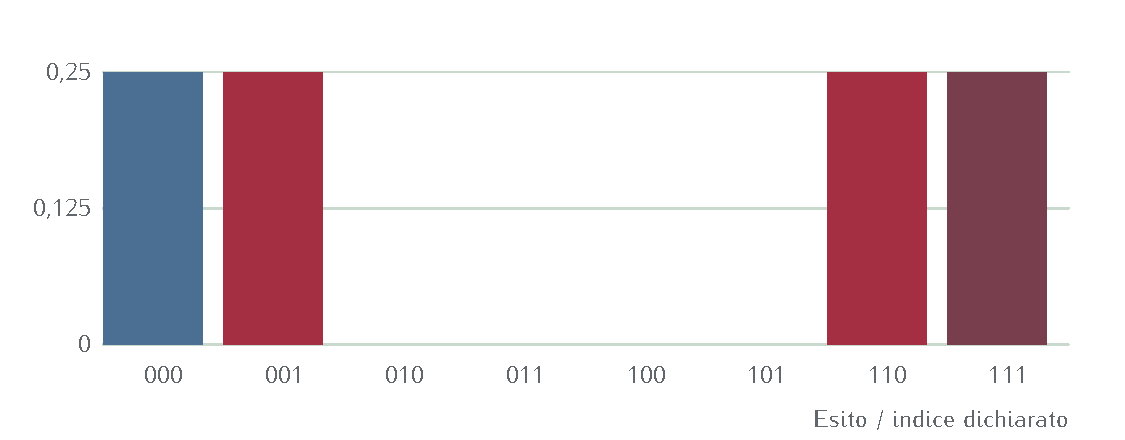
\includegraphics[width=\linewidth,height=94mm,keepaspectratio]{figure/f0e28c8c48319bdc4.pdf}\FigureCaption{4.03 \(\cdot\) esempio 2 \(\cdot\) Probabilità marginale P(y)}\end{FigureBlock}
\begin{FigureBlock}\centering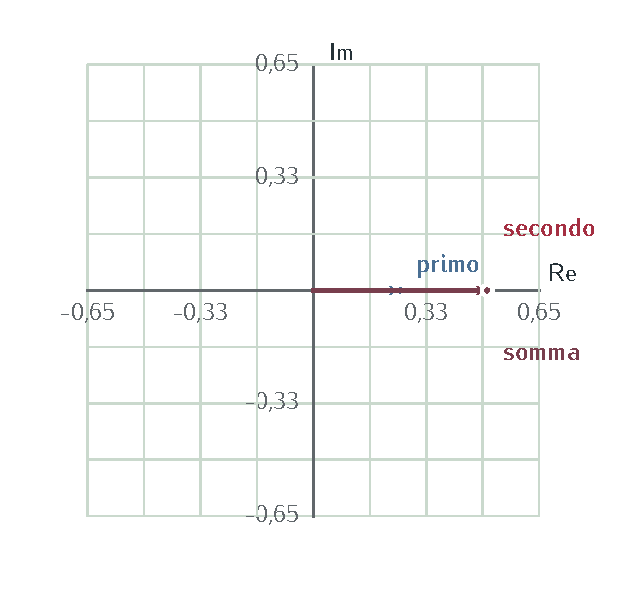
\includegraphics[width=\linewidth,height=94mm,keepaspectratio]{figure/fbf2ebf9efdc71156.pdf}\FigureCaption{4.03 \(\cdot\) esempio 2 \(\cdot\) Somma concorde per \(y=000\) nel ramo \(f=0\)}\end{FigureBlock}
\begin{FigureBlock}\centering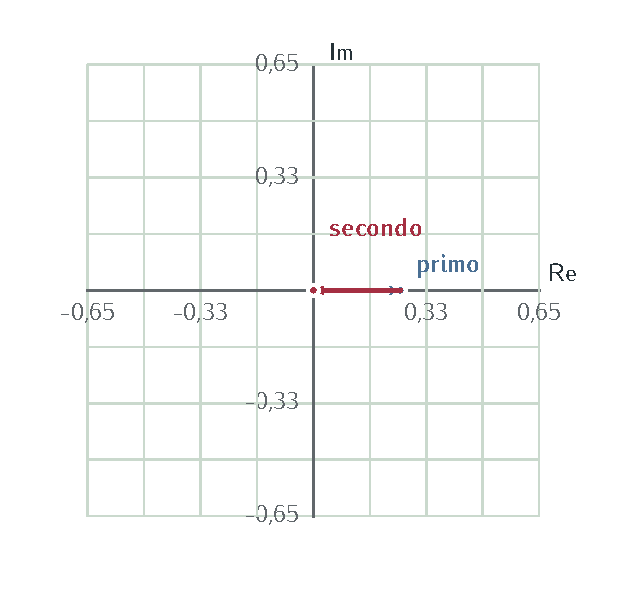
\includegraphics[width=\linewidth,height=94mm,keepaspectratio]{figure/fff7d68c01ede96a1.pdf}\FigureCaption{4.03 \(\cdot\) esempio 2 \(\cdot\) Cancellazione quando \(s\cdot y=1\) nel ramo \(f=0\)}\end{FigureBlock}

\phantomsection\label{c4-simon-example-2-step-1}
\BookHeading{01 Preparare i registri}

\MathBlock{007C03A827E9003D00280031002F221A0038002903A3005F0078007C007827E9007C006600280078002927E9}{|\Psi \rangle =(1/\sqrt{8})\sum _{x}|x\rangle |f(x)\rangle }

Ogni ingresso ha probabilità 1/8. Le parole binarie indicano vettori ortogonali della base; il prodotto binario è calcolato modulo due.\par


\phantomsection\label{c4-simon-example-2-step-2}
\BookHeading{02 Probabilità del ramo \(f=0\)}

\MathBlock{005000280066003D00300029003D007C0031002F221A0038007C00B2002B007C0031002F221A0038007C00B2003D0031002F0038002B0031002F0038003D0031002F0034}{P(f=0)=|1/\sqrt{8}|^{2}+|1/\sqrt{8}|^{2}=1/8+1/8=1/4}

Il valore osservato della funzione seleziona due ingressi. Le loro probabilità si sommano perché gli stati del primo registro sono ortogonali.\par


\phantomsection\label{c4-simon-example-2-step-3}
\BookHeading{03 Normalizzare il ramo 0}

\MathBlock{00280031002F221A00380029002F221A00280031002F00340029003D00280031002F221A00380029002F00280031002F00320029003D0032002F221A0038003D0031002F221A0032}{(1/\sqrt{8})/\sqrt{1/4}=(1/\sqrt{8})/(1/2)=2/\sqrt{8}=1/\sqrt{2}}
\MathBlock{007C03C8005F006627E9003D0028007C00300030003027E9002B007C00310031003027E90029002F221A0032}{|\psi _{f}\rangle =(|000\rangle +|110\rangle )/\sqrt{2}}

Condizionare sul ramo divide entrambe le ampiezze per la radice della sua probabilità. La norma dello stato risultante vale uno.\par


\phantomsection\label{c4-simon-example-2-step-4}
\BookHeading{04 Applicare gli Hadamard al ramo 0}

\MathBlock{0048005E007B22970033007D007C007827E9003D00280031002F221A0038002903A3005F00790028002D00310029005E0028007800B700790029007C007927E9}{H^{\otimes 3}|x\rangle =(1/\sqrt{8})\sum _{y}(-1)^{x\cdot y}|y\rangle }
\MathBlock{0061005F0066002800790029003D00280031002F221A0032002900280031002F221A00380029005B0028002D00310029005E002800300030003000B700790029002B0028002D00310029005E002800310031003000B700790029005D}{a_{f}(y)=(1/\sqrt{2})(1/\sqrt{8})[(-1)^{000\cdot y}+(-1)^{110\cdot y}]}
\MathBlock{003D00280031002F00340029005B0028002D00310029005E002800300030003000B700790029002B0028002D00310029005E002800310031003000B700790029005D}{=(1/4)[(-1)^{000\cdot y}+(-1)^{110\cdot y}]}

I due contributi arrivano nella stessa uscita y. Si sommano le ampiezze con il loro segno e si calcola successivamente il modulo quadro.\par


\phantomsection\label{c4-simon-example-2-step-5}
\BookHeading{05 Leggere il vincolo del ramo 0}

\MathBlock{0061005F0066002800790029003D00280028002D00310029005E002800300030003000B700790029002F00340029005B0031002B0028002D00310029005E002800310031003000B700790029005D}{a_{f}(y)=((-1)^{000\cdot y}/4)[1+(-1)^{110\cdot y}]}
\MathBlock{007300B70079003D0030002021D20020007C0061005F0066002800790029007C003D0031002F0032002021D20020005000280079007C00660029003D0031002F0034}{s\cdot y=0\ \Rightarrow \ |a_{f}(y)|=1/2\ \Rightarrow \ P(y|f)=1/4}
\MathBlock{007300B70079003D0031002021D200200061005F0066002800790029003D0030002021D20020005000280079007C00660029003D0030}{s\cdot y=1\ \Rightarrow \ a_{f}(y)=0\ \Rightarrow \ P(y|f)=0}

Poiché \(b=a\oplus s\), la parità b\(\cdot\)y è la somma modulo due delle parità a\(\cdot\)y e s\(\cdot\)y. Il segno comune può variare fra i rami; il supporto delle probabilità resta lo stesso.\par


\phantomsection\label{c4-simon-example-2-step-6}
\BookHeading{06 Probabilità del ramo \(f=1\)}

\MathBlock{005000280066003D00310029003D007C0031002F221A0038007C00B2002B007C0031002F221A0038007C00B2003D0031002F0038002B0031002F0038003D0031002F0034}{P(f=1)=|1/\sqrt{8}|^{2}+|1/\sqrt{8}|^{2}=1/8+1/8=1/4}

Il valore osservato della funzione seleziona due ingressi. Le loro probabilità si sommano perché gli stati del primo registro sono ortogonali.\par


\phantomsection\label{c4-simon-example-2-step-7}
\BookHeading{07 Normalizzare il ramo 1}

\MathBlock{00280031002F221A00380029002F221A00280031002F00340029003D00280031002F221A00380029002F00280031002F00320029003D0032002F221A0038003D0031002F221A0032}{(1/\sqrt{8})/\sqrt{1/4}=(1/\sqrt{8})/(1/2)=2/\sqrt{8}=1/\sqrt{2}}
\MathBlock{007C03C8005F006627E9003D0028007C00300030003127E9002B007C00310031003127E90029002F221A0032}{|\psi _{f}\rangle =(|001\rangle +|111\rangle )/\sqrt{2}}

Condizionare sul ramo divide entrambe le ampiezze per la radice della sua probabilità. La norma dello stato risultante vale uno.\par


\phantomsection\label{c4-simon-example-2-step-8}
\BookHeading{08 Applicare gli Hadamard al ramo 1}

\MathBlock{0048005E007B22970033007D007C007827E9003D00280031002F221A0038002903A3005F00790028002D00310029005E0028007800B700790029007C007927E9}{H^{\otimes 3}|x\rangle =(1/\sqrt{8})\sum _{y}(-1)^{x\cdot y}|y\rangle }
\MathBlock{0061005F0066002800790029003D00280031002F221A0032002900280031002F221A00380029005B0028002D00310029005E002800300030003100B700790029002B0028002D00310029005E002800310031003100B700790029005D}{a_{f}(y)=(1/\sqrt{2})(1/\sqrt{8})[(-1)^{001\cdot y}+(-1)^{111\cdot y}]}
\MathBlock{003D00280031002F00340029005B0028002D00310029005E002800300030003100B700790029002B0028002D00310029005E002800310031003100B700790029005D}{=(1/4)[(-1)^{001\cdot y}+(-1)^{111\cdot y}]}

I due contributi arrivano nella stessa uscita y. Si sommano le ampiezze con il loro segno e si calcola successivamente il modulo quadro.\par


\phantomsection\label{c4-simon-example-2-step-9}
\BookHeading{09 Leggere il vincolo del ramo 1}

\MathBlock{0061005F0066002800790029003D00280028002D00310029005E002800300030003100B700790029002F00340029005B0031002B0028002D00310029005E002800310031003000B700790029005D}{a_{f}(y)=((-1)^{001\cdot y}/4)[1+(-1)^{110\cdot y}]}
\MathBlock{007300B70079003D0030002021D20020007C0061005F0066002800790029007C003D0031002F0032002021D20020005000280079007C00660029003D0031002F0034}{s\cdot y=0\ \Rightarrow \ |a_{f}(y)|=1/2\ \Rightarrow \ P(y|f)=1/4}
\MathBlock{007300B70079003D0031002021D200200061005F0066002800790029003D0030002021D20020005000280079007C00660029003D0030}{s\cdot y=1\ \Rightarrow \ a_{f}(y)=0\ \Rightarrow \ P(y|f)=0}

Poiché \(b=a\oplus s\), la parità b\(\cdot\)y è la somma modulo due delle parità a\(\cdot\)y e s\(\cdot\)y. Il segno comune può variare fra i rami; il supporto delle probabilità resta lo stesso.\par


\phantomsection\label{c4-simon-example-2-step-10}
\BookHeading{10 Probabilità del ramo \(f=2\)}

\MathBlock{005000280066003D00320029003D007C0031002F221A0038007C00B2002B007C0031002F221A0038007C00B2003D0031002F0038002B0031002F0038003D0031002F0034}{P(f=2)=|1/\sqrt{8}|^{2}+|1/\sqrt{8}|^{2}=1/8+1/8=1/4}

Il valore osservato della funzione seleziona due ingressi. Le loro probabilità si sommano perché gli stati del primo registro sono ortogonali.\par


\phantomsection\label{c4-simon-example-2-step-11}
\BookHeading{11 Normalizzare il ramo 2}

\MathBlock{00280031002F221A00380029002F221A00280031002F00340029003D00280031002F221A00380029002F00280031002F00320029003D0032002F221A0038003D0031002F221A0032}{(1/\sqrt{8})/\sqrt{1/4}=(1/\sqrt{8})/(1/2)=2/\sqrt{8}=1/\sqrt{2}}
\MathBlock{007C03C8005F006627E9003D0028007C00300031003027E9002B007C00310030003027E90029002F221A0032}{|\psi _{f}\rangle =(|010\rangle +|100\rangle )/\sqrt{2}}

Condizionare sul ramo divide entrambe le ampiezze per la radice della sua probabilità. La norma dello stato risultante vale uno.\par


\phantomsection\label{c4-simon-example-2-step-12}
\BookHeading{12 Applicare gli Hadamard al ramo 2}

\MathBlock{0048005E007B22970033007D007C007827E9003D00280031002F221A0038002903A3005F00790028002D00310029005E0028007800B700790029007C007927E9}{H^{\otimes 3}|x\rangle =(1/\sqrt{8})\sum _{y}(-1)^{x\cdot y}|y\rangle }
\MathBlock{0061005F0066002800790029003D00280031002F221A0032002900280031002F221A00380029005B0028002D00310029005E002800300031003000B700790029002B0028002D00310029005E002800310030003000B700790029005D}{a_{f}(y)=(1/\sqrt{2})(1/\sqrt{8})[(-1)^{010\cdot y}+(-1)^{100\cdot y}]}
\MathBlock{003D00280031002F00340029005B0028002D00310029005E002800300031003000B700790029002B0028002D00310029005E002800310030003000B700790029005D}{=(1/4)[(-1)^{010\cdot y}+(-1)^{100\cdot y}]}

I due contributi arrivano nella stessa uscita y. Si sommano le ampiezze con il loro segno e si calcola successivamente il modulo quadro.\par


\phantomsection\label{c4-simon-example-2-step-13}
\BookHeading{13 Leggere il vincolo del ramo 2}

\MathBlock{0061005F0066002800790029003D00280028002D00310029005E002800300031003000B700790029002F00340029005B0031002B0028002D00310029005E002800310031003000B700790029005D}{a_{f}(y)=((-1)^{010\cdot y}/4)[1+(-1)^{110\cdot y}]}
\MathBlock{007300B70079003D0030002021D20020007C0061005F0066002800790029007C003D0031002F0032002021D20020005000280079007C00660029003D0031002F0034}{s\cdot y=0\ \Rightarrow \ |a_{f}(y)|=1/2\ \Rightarrow \ P(y|f)=1/4}
\MathBlock{007300B70079003D0031002021D200200061005F0066002800790029003D0030002021D20020005000280079007C00660029003D0030}{s\cdot y=1\ \Rightarrow \ a_{f}(y)=0\ \Rightarrow \ P(y|f)=0}

Poiché \(b=a\oplus s\), la parità b\(\cdot\)y è la somma modulo due delle parità a\(\cdot\)y e s\(\cdot\)y. Il segno comune può variare fra i rami; il supporto delle probabilità resta lo stesso.\par


\phantomsection\label{c4-simon-example-2-step-14}
\BookHeading{14 Probabilità del ramo \(f=3\)}

\MathBlock{005000280066003D00330029003D007C0031002F221A0038007C00B2002B007C0031002F221A0038007C00B2003D0031002F0038002B0031002F0038003D0031002F0034}{P(f=3)=|1/\sqrt{8}|^{2}+|1/\sqrt{8}|^{2}=1/8+1/8=1/4}

Il valore osservato della funzione seleziona due ingressi. Le loro probabilità si sommano perché gli stati del primo registro sono ortogonali.\par


\phantomsection\label{c4-simon-example-2-step-15}
\BookHeading{15 Normalizzare il ramo 3}

\MathBlock{00280031002F221A00380029002F221A00280031002F00340029003D00280031002F221A00380029002F00280031002F00320029003D0032002F221A0038003D0031002F221A0032}{(1/\sqrt{8})/\sqrt{1/4}=(1/\sqrt{8})/(1/2)=2/\sqrt{8}=1/\sqrt{2}}
\MathBlock{007C03C8005F006627E9003D0028007C00300031003127E9002B007C00310030003127E90029002F221A0032}{|\psi _{f}\rangle =(|011\rangle +|101\rangle )/\sqrt{2}}

Condizionare sul ramo divide entrambe le ampiezze per la radice della sua probabilità. La norma dello stato risultante vale uno.\par


\phantomsection\label{c4-simon-example-2-step-16}
\BookHeading{16 Applicare gli Hadamard al ramo 3}

\MathBlock{0048005E007B22970033007D007C007827E9003D00280031002F221A0038002903A3005F00790028002D00310029005E0028007800B700790029007C007927E9}{H^{\otimes 3}|x\rangle =(1/\sqrt{8})\sum _{y}(-1)^{x\cdot y}|y\rangle }
\MathBlock{0061005F0066002800790029003D00280031002F221A0032002900280031002F221A00380029005B0028002D00310029005E002800300031003100B700790029002B0028002D00310029005E002800310030003100B700790029005D}{a_{f}(y)=(1/\sqrt{2})(1/\sqrt{8})[(-1)^{011\cdot y}+(-1)^{101\cdot y}]}
\MathBlock{003D00280031002F00340029005B0028002D00310029005E002800300031003100B700790029002B0028002D00310029005E002800310030003100B700790029005D}{=(1/4)[(-1)^{011\cdot y}+(-1)^{101\cdot y}]}

I due contributi arrivano nella stessa uscita y. Si sommano le ampiezze con il loro segno e si calcola successivamente il modulo quadro.\par


\phantomsection\label{c4-simon-example-2-step-17}
\BookHeading{17 Leggere il vincolo del ramo 3}

\MathBlock{0061005F0066002800790029003D00280028002D00310029005E002800300031003100B700790029002F00340029005B0031002B0028002D00310029005E002800310031003000B700790029005D}{a_{f}(y)=((-1)^{011\cdot y}/4)[1+(-1)^{110\cdot y}]}
\MathBlock{007300B70079003D0030002021D20020007C0061005F0066002800790029007C003D0031002F0032002021D20020005000280079007C00660029003D0031002F0034}{s\cdot y=0\ \Rightarrow \ |a_{f}(y)|=1/2\ \Rightarrow \ P(y|f)=1/4}
\MathBlock{007300B70079003D0031002021D200200061005F0066002800790029003D0030002021D20020005000280079007C00660029003D0030}{s\cdot y=1\ \Rightarrow \ a_{f}(y)=0\ \Rightarrow \ P(y|f)=0}

Poiché \(b=a\oplus s\), la parità b\(\cdot\)y è la somma modulo due delle parità a\(\cdot\)y e s\(\cdot\)y. Il segno comune può variare fra i rami; il supporto delle probabilità resta lo stesso.\par


\phantomsection\label{c4-simon-example-2-step-18}
\BookHeading{18 Calcolare la marginale delle uscite}

\MathBlock{0050002800790029003D03A3005F006600200050002800660029005000280079007C00660029}{P(y)=\sum _{f}\ P(f)P(y|f)}
\MathBlock{007300B70079003D0030002021D200200050002800790029003D003400B700280031002F0034002900B700280031002F00340029003D0031002F0034}{s\cdot y=0\ \Rightarrow \ P(y)=4\cdot (1/4)\cdot (1/4)=1/4}
\MathBlock{007300B70079003D0031002021D200200050002800790029003D003400B700280031002F0034002900B70030003D0030}{s\cdot y=1\ \Rightarrow \ P(y)=4\cdot (1/4)\cdot 0=0}

La misura della funzione può essere omessa: la marginale sul primo registro coincide con la somma sui bersagli ortogonali.\par


\phantomsection\label{c4-simon-example-2-step-19}
\BookHeading{19 Equazioni del percorso guidato}

\MathBlock{00300030003100B70073003D0030}{001\cdot s=0}
\MathBlock{00300030003100B70073003D0030}{001\cdot s=0}
\MathBlock{00310031003000B70073003D0030}{110\cdot s=0}

Queste righe sono scelte per illustrare indipendenza e ripetizione. Nell'area di esperimento ogni nuova riga proviene da una misura campionata dalla distribuzione.\par


\phantomsection\label{c4-simon-example-2-step-20}
\BookHeading{20 Eliminare su \(F_{2}\)}

\MathBlock{005300630061006D00620069006100200072006900670061002000330020006500200031002E}{\text{Scambia}\ \text{riga}\ 3\ e\ 1.}
\MathBlock{0030003000310020229500200030003000310020003D0020003000300030}{001\ \oplus \ 001\ =\ 000}
\MathBlock{00720061006E0067006F003D0032003B002000630061006E006400690064006100740069003D007B003000300030003B0020003100310030007D}{\text{rango}=2;\allowbreak \ \text{candidati}=\{000;\allowbreak \ 110\}}

L'operazione elementare è XOR. Una riga ripetuta si annulla e lascia invariato il rango. La promessa esclude il candidato nullo; rango \(n- 1\) identifica un unico segreto non nullo.\par


\BookHeading{Interpretazione}

Il segreto emerge dall'intersezione dei vincoli binari. Le cancellazioni delle ampiezze determinano quali vincoli possono essere osservati.\par


\BookHeading{Tabella completa dei dati (8 righe)}

\begingroup\sffamily\fontsize{8.8}{11}\selectfont\setlength{\tabcolsep}{1.6mm}\renewcommand{\arraystretch}{1.28}
\begin{longtable}{>{\RaggedRight\arraybackslash}p{42.133mm}>{\RaggedRight\arraybackslash}p{42.133mm}>{\RaggedRight\arraybackslash}p{42.133mm}}
\toprule\rowcolor{Accent!7}\BeginAccSupp{method=hex,unicode,ActualText=0078}x\EndAccSupp{} & \BeginAccSupp{method=hex,unicode,ActualText=007822950073}\(x\oplus s\)\EndAccSupp{} & \BeginAccSupp{method=hex,unicode,ActualText=0066002800780029}f(x)\EndAccSupp{} \\
\midrule\endfirsthead
\toprule\rowcolor{Accent!7}\BeginAccSupp{method=hex,unicode,ActualText=0078}x\EndAccSupp{} & \BeginAccSupp{method=hex,unicode,ActualText=007822950073}\(x\oplus s\)\EndAccSupp{} & \BeginAccSupp{method=hex,unicode,ActualText=0066002800780029}f(x)\EndAccSupp{} \\
\midrule\endhead\bottomrule\endfoot
\BeginAccSupp{method=hex,unicode,ActualText=003000300030}000\EndAccSupp{} & \BeginAccSupp{method=hex,unicode,ActualText=003100310030}110\EndAccSupp{} & \BeginAccSupp{method=hex,unicode,ActualText=0030}0\EndAccSupp{} \\
\BeginAccSupp{method=hex,unicode,ActualText=003000300031}001\EndAccSupp{} & \BeginAccSupp{method=hex,unicode,ActualText=003100310031}111\EndAccSupp{} & \BeginAccSupp{method=hex,unicode,ActualText=0031}1\EndAccSupp{} \\
\BeginAccSupp{method=hex,unicode,ActualText=003000310030}010\EndAccSupp{} & \BeginAccSupp{method=hex,unicode,ActualText=003100300030}100\EndAccSupp{} & \BeginAccSupp{method=hex,unicode,ActualText=0032}2\EndAccSupp{} \\
\BeginAccSupp{method=hex,unicode,ActualText=003000310031}011\EndAccSupp{} & \BeginAccSupp{method=hex,unicode,ActualText=003100300031}101\EndAccSupp{} & \BeginAccSupp{method=hex,unicode,ActualText=0033}3\EndAccSupp{} \\
\BeginAccSupp{method=hex,unicode,ActualText=003100300030}100\EndAccSupp{} & \BeginAccSupp{method=hex,unicode,ActualText=003000310030}010\EndAccSupp{} & \BeginAccSupp{method=hex,unicode,ActualText=0032}2\EndAccSupp{} \\
\BeginAccSupp{method=hex,unicode,ActualText=003100300031}101\EndAccSupp{} & \BeginAccSupp{method=hex,unicode,ActualText=003000310031}011\EndAccSupp{} & \BeginAccSupp{method=hex,unicode,ActualText=0033}3\EndAccSupp{} \\
\BeginAccSupp{method=hex,unicode,ActualText=003100310030}110\EndAccSupp{} & \BeginAccSupp{method=hex,unicode,ActualText=003000300030}000\EndAccSupp{} & \BeginAccSupp{method=hex,unicode,ActualText=0030}0\EndAccSupp{} \\
\BeginAccSupp{method=hex,unicode,ActualText=003100310031}111\EndAccSupp{} & \BeginAccSupp{method=hex,unicode,ActualText=003000300031}001\EndAccSupp{} & \BeginAccSupp{method=hex,unicode,ActualText=0031}1\EndAccSupp{} \\
\end{longtable}\endgroup

\BookHeading{Tutti i contributi del ramo \(f=0\) (8 righe)}

\begingroup\sffamily\fontsize{8.8}{11}\selectfont\setlength{\tabcolsep}{1.6mm}\renewcommand{\arraystretch}{1.28}
\begin{longtable}{>{\RaggedRight\arraybackslash}p{14.600mm}>{\RaggedRight\arraybackslash}p{14.600mm}>{\RaggedRight\arraybackslash}p{14.600mm}>{\RaggedRight\arraybackslash}p{38.933mm}>{\RaggedRight\arraybackslash}p{14.600mm}>{\RaggedRight\arraybackslash}p{19.467mm}}
\toprule\rowcolor{Accent!7}\BeginAccSupp{method=hex,unicode,ActualText=0079}y\EndAccSupp{} & \BeginAccSupp{method=hex,unicode,ActualText=005300650067006E006F0020006400610020003000300030}Segno da 000\EndAccSupp{} & \BeginAccSupp{method=hex,unicode,ActualText=005300650067006E006F0020006400610020003100310030}Segno da 110\EndAccSupp{} & \BeginAccSupp{method=hex,unicode,ActualText=0053006F006D006D00610020002F00200034}Somma / 4\EndAccSupp{} & \BeginAccSupp{method=hex,unicode,ActualText=0061005F0066002800790029}\(a_{f}(y)\)\EndAccSupp{} & \BeginAccSupp{method=hex,unicode,ActualText=005000280079007C00660029}\(P(y|f)\)\EndAccSupp{} \\
\midrule\endfirsthead
\toprule\rowcolor{Accent!7}\BeginAccSupp{method=hex,unicode,ActualText=0079}y\EndAccSupp{} & \BeginAccSupp{method=hex,unicode,ActualText=005300650067006E006F0020006400610020003000300030}Segno da 000\EndAccSupp{} & \BeginAccSupp{method=hex,unicode,ActualText=005300650067006E006F0020006400610020003100310030}Segno da 110\EndAccSupp{} & \BeginAccSupp{method=hex,unicode,ActualText=0053006F006D006D00610020002F00200034}Somma / 4\EndAccSupp{} & \BeginAccSupp{method=hex,unicode,ActualText=0061005F0066002800790029}\(a_{f}(y)\)\EndAccSupp{} & \BeginAccSupp{method=hex,unicode,ActualText=005000280079007C00660029}\(P(y|f)\)\EndAccSupp{} \\
\midrule\endhead\bottomrule\endfoot
\BeginAccSupp{method=hex,unicode,ActualText=003000300030}000\EndAccSupp{} & \BeginAccSupp{method=hex,unicode,ActualText=0031}1\EndAccSupp{} & \BeginAccSupp{method=hex,unicode,ActualText=0031}1\EndAccSupp{} & \BeginAccSupp{method=hex,unicode,ActualText=00280031002B00310029002F0034}(1+1)/4\EndAccSupp{} & \BeginAccSupp{method=hex,unicode,ActualText=0030002C0035}0,5\EndAccSupp{} & \BeginAccSupp{method=hex,unicode,ActualText=0030002C00320035}0,25\EndAccSupp{} \\
\BeginAccSupp{method=hex,unicode,ActualText=003000300031}001\EndAccSupp{} & \BeginAccSupp{method=hex,unicode,ActualText=0031}1\EndAccSupp{} & \BeginAccSupp{method=hex,unicode,ActualText=0031}1\EndAccSupp{} & \BeginAccSupp{method=hex,unicode,ActualText=00280031002B00310029002F0034}(1+1)/4\EndAccSupp{} & \BeginAccSupp{method=hex,unicode,ActualText=0030002C0035}0,5\EndAccSupp{} & \BeginAccSupp{method=hex,unicode,ActualText=0030002C00320035}0,25\EndAccSupp{} \\
\BeginAccSupp{method=hex,unicode,ActualText=003000310030}010\EndAccSupp{} & \BeginAccSupp{method=hex,unicode,ActualText=0031}1\EndAccSupp{} & \BeginAccSupp{method=hex,unicode,ActualText=002D0031}-1\EndAccSupp{} & \BeginAccSupp{method=hex,unicode,ActualText=00280031002B002D00310029002F0034}(1+-1)/4\EndAccSupp{} & \BeginAccSupp{method=hex,unicode,ActualText=0030}0\EndAccSupp{} & \BeginAccSupp{method=hex,unicode,ActualText=0030}0\EndAccSupp{} \\
\BeginAccSupp{method=hex,unicode,ActualText=003000310031}011\EndAccSupp{} & \BeginAccSupp{method=hex,unicode,ActualText=0031}1\EndAccSupp{} & \BeginAccSupp{method=hex,unicode,ActualText=002D0031}-1\EndAccSupp{} & \BeginAccSupp{method=hex,unicode,ActualText=00280031002B002D00310029002F0034}(1+-1)/4\EndAccSupp{} & \BeginAccSupp{method=hex,unicode,ActualText=0030}0\EndAccSupp{} & \BeginAccSupp{method=hex,unicode,ActualText=0030}0\EndAccSupp{} \\
\BeginAccSupp{method=hex,unicode,ActualText=003100300030}100\EndAccSupp{} & \BeginAccSupp{method=hex,unicode,ActualText=0031}1\EndAccSupp{} & \BeginAccSupp{method=hex,unicode,ActualText=002D0031}-1\EndAccSupp{} & \BeginAccSupp{method=hex,unicode,ActualText=00280031002B002D00310029002F0034}(1+-1)/4\EndAccSupp{} & \BeginAccSupp{method=hex,unicode,ActualText=0030}0\EndAccSupp{} & \BeginAccSupp{method=hex,unicode,ActualText=0030}0\EndAccSupp{} \\
\BeginAccSupp{method=hex,unicode,ActualText=003100300031}101\EndAccSupp{} & \BeginAccSupp{method=hex,unicode,ActualText=0031}1\EndAccSupp{} & \BeginAccSupp{method=hex,unicode,ActualText=002D0031}-1\EndAccSupp{} & \BeginAccSupp{method=hex,unicode,ActualText=00280031002B002D00310029002F0034}(1+-1)/4\EndAccSupp{} & \BeginAccSupp{method=hex,unicode,ActualText=0030}0\EndAccSupp{} & \BeginAccSupp{method=hex,unicode,ActualText=0030}0\EndAccSupp{} \\
\BeginAccSupp{method=hex,unicode,ActualText=003100310030}110\EndAccSupp{} & \BeginAccSupp{method=hex,unicode,ActualText=0031}1\EndAccSupp{} & \BeginAccSupp{method=hex,unicode,ActualText=0031}1\EndAccSupp{} & \BeginAccSupp{method=hex,unicode,ActualText=00280031002B00310029002F0034}(1+1)/4\EndAccSupp{} & \BeginAccSupp{method=hex,unicode,ActualText=0030002C0035}0,5\EndAccSupp{} & \BeginAccSupp{method=hex,unicode,ActualText=0030002C00320035}0,25\EndAccSupp{} \\
\BeginAccSupp{method=hex,unicode,ActualText=003100310031}111\EndAccSupp{} & \BeginAccSupp{method=hex,unicode,ActualText=0031}1\EndAccSupp{} & \BeginAccSupp{method=hex,unicode,ActualText=0031}1\EndAccSupp{} & \BeginAccSupp{method=hex,unicode,ActualText=00280031002B00310029002F0034}(1+1)/4\EndAccSupp{} & \BeginAccSupp{method=hex,unicode,ActualText=0030002C0035}0,5\EndAccSupp{} & \BeginAccSupp{method=hex,unicode,ActualText=0030002C00320035}0,25\EndAccSupp{} \\
\end{longtable}\endgroup

\BookHeading{Tutti i contributi del ramo \(f=1\) (8 righe)}

\begingroup\sffamily\fontsize{8.8}{11}\selectfont\setlength{\tabcolsep}{1.6mm}\renewcommand{\arraystretch}{1.28}
\begin{longtable}{>{\RaggedRight\arraybackslash}p{13.477mm}>{\RaggedRight\arraybackslash}p{13.477mm}>{\RaggedRight\arraybackslash}p{13.477mm}>{\RaggedRight\arraybackslash}p{40.431mm}>{\RaggedRight\arraybackslash}p{17.969mm}>{\RaggedRight\arraybackslash}p{17.969mm}}
\toprule\rowcolor{Accent!7}\BeginAccSupp{method=hex,unicode,ActualText=0079}y\EndAccSupp{} & \BeginAccSupp{method=hex,unicode,ActualText=005300650067006E006F0020006400610020003000300031}Segno da 001\EndAccSupp{} & \BeginAccSupp{method=hex,unicode,ActualText=005300650067006E006F0020006400610020003100310031}Segno da 111\EndAccSupp{} & \BeginAccSupp{method=hex,unicode,ActualText=0053006F006D006D00610020002F00200034}Somma / 4\EndAccSupp{} & \BeginAccSupp{method=hex,unicode,ActualText=0061005F0066002800790029}\(a_{f}(y)\)\EndAccSupp{} & \BeginAccSupp{method=hex,unicode,ActualText=005000280079007C00660029}\(P(y|f)\)\EndAccSupp{} \\
\midrule\endfirsthead
\toprule\rowcolor{Accent!7}\BeginAccSupp{method=hex,unicode,ActualText=0079}y\EndAccSupp{} & \BeginAccSupp{method=hex,unicode,ActualText=005300650067006E006F0020006400610020003000300031}Segno da 001\EndAccSupp{} & \BeginAccSupp{method=hex,unicode,ActualText=005300650067006E006F0020006400610020003100310031}Segno da 111\EndAccSupp{} & \BeginAccSupp{method=hex,unicode,ActualText=0053006F006D006D00610020002F00200034}Somma / 4\EndAccSupp{} & \BeginAccSupp{method=hex,unicode,ActualText=0061005F0066002800790029}\(a_{f}(y)\)\EndAccSupp{} & \BeginAccSupp{method=hex,unicode,ActualText=005000280079007C00660029}\(P(y|f)\)\EndAccSupp{} \\
\midrule\endhead\bottomrule\endfoot
\BeginAccSupp{method=hex,unicode,ActualText=003000300030}000\EndAccSupp{} & \BeginAccSupp{method=hex,unicode,ActualText=0031}1\EndAccSupp{} & \BeginAccSupp{method=hex,unicode,ActualText=0031}1\EndAccSupp{} & \BeginAccSupp{method=hex,unicode,ActualText=00280031002B00310029002F0034}(1+1)/4\EndAccSupp{} & \BeginAccSupp{method=hex,unicode,ActualText=0030002C0035}0,5\EndAccSupp{} & \BeginAccSupp{method=hex,unicode,ActualText=0030002C00320035}0,25\EndAccSupp{} \\
\BeginAccSupp{method=hex,unicode,ActualText=003000300031}001\EndAccSupp{} & \BeginAccSupp{method=hex,unicode,ActualText=002D0031}-1\EndAccSupp{} & \BeginAccSupp{method=hex,unicode,ActualText=002D0031}-1\EndAccSupp{} & \BeginAccSupp{method=hex,unicode,ActualText=0028002D0031002B002D00310029002F0034}(-1+-1)/4\EndAccSupp{} & \BeginAccSupp{method=hex,unicode,ActualText=002D0030002C0035}-0,5\EndAccSupp{} & \BeginAccSupp{method=hex,unicode,ActualText=0030002C00320035}0,25\EndAccSupp{} \\
\BeginAccSupp{method=hex,unicode,ActualText=003000310030}010\EndAccSupp{} & \BeginAccSupp{method=hex,unicode,ActualText=0031}1\EndAccSupp{} & \BeginAccSupp{method=hex,unicode,ActualText=002D0031}-1\EndAccSupp{} & \BeginAccSupp{method=hex,unicode,ActualText=00280031002B002D00310029002F0034}(1+-1)/4\EndAccSupp{} & \BeginAccSupp{method=hex,unicode,ActualText=0030}0\EndAccSupp{} & \BeginAccSupp{method=hex,unicode,ActualText=0030}0\EndAccSupp{} \\
\BeginAccSupp{method=hex,unicode,ActualText=003000310031}011\EndAccSupp{} & \BeginAccSupp{method=hex,unicode,ActualText=002D0031}-1\EndAccSupp{} & \BeginAccSupp{method=hex,unicode,ActualText=0031}1\EndAccSupp{} & \BeginAccSupp{method=hex,unicode,ActualText=0028002D0031002B00310029002F0034}(-1+1)/4\EndAccSupp{} & \BeginAccSupp{method=hex,unicode,ActualText=0030}0\EndAccSupp{} & \BeginAccSupp{method=hex,unicode,ActualText=0030}0\EndAccSupp{} \\
\BeginAccSupp{method=hex,unicode,ActualText=003100300030}100\EndAccSupp{} & \BeginAccSupp{method=hex,unicode,ActualText=0031}1\EndAccSupp{} & \BeginAccSupp{method=hex,unicode,ActualText=002D0031}-1\EndAccSupp{} & \BeginAccSupp{method=hex,unicode,ActualText=00280031002B002D00310029002F0034}(1+-1)/4\EndAccSupp{} & \BeginAccSupp{method=hex,unicode,ActualText=0030}0\EndAccSupp{} & \BeginAccSupp{method=hex,unicode,ActualText=0030}0\EndAccSupp{} \\
\BeginAccSupp{method=hex,unicode,ActualText=003100300031}101\EndAccSupp{} & \BeginAccSupp{method=hex,unicode,ActualText=002D0031}-1\EndAccSupp{} & \BeginAccSupp{method=hex,unicode,ActualText=0031}1\EndAccSupp{} & \BeginAccSupp{method=hex,unicode,ActualText=0028002D0031002B00310029002F0034}(-1+1)/4\EndAccSupp{} & \BeginAccSupp{method=hex,unicode,ActualText=0030}0\EndAccSupp{} & \BeginAccSupp{method=hex,unicode,ActualText=0030}0\EndAccSupp{} \\
\BeginAccSupp{method=hex,unicode,ActualText=003100310030}110\EndAccSupp{} & \BeginAccSupp{method=hex,unicode,ActualText=0031}1\EndAccSupp{} & \BeginAccSupp{method=hex,unicode,ActualText=0031}1\EndAccSupp{} & \BeginAccSupp{method=hex,unicode,ActualText=00280031002B00310029002F0034}(1+1)/4\EndAccSupp{} & \BeginAccSupp{method=hex,unicode,ActualText=0030002C0035}0,5\EndAccSupp{} & \BeginAccSupp{method=hex,unicode,ActualText=0030002C00320035}0,25\EndAccSupp{} \\
\BeginAccSupp{method=hex,unicode,ActualText=003100310031}111\EndAccSupp{} & \BeginAccSupp{method=hex,unicode,ActualText=002D0031}-1\EndAccSupp{} & \BeginAccSupp{method=hex,unicode,ActualText=002D0031}-1\EndAccSupp{} & \BeginAccSupp{method=hex,unicode,ActualText=0028002D0031002B002D00310029002F0034}(-1+-1)/4\EndAccSupp{} & \BeginAccSupp{method=hex,unicode,ActualText=002D0030002C0035}-0,5\EndAccSupp{} & \BeginAccSupp{method=hex,unicode,ActualText=0030002C00320035}0,25\EndAccSupp{} \\
\end{longtable}\endgroup

\BookHeading{Tutti i contributi del ramo \(f=2\) (8 righe)}

\begingroup\sffamily\fontsize{8.8}{11}\selectfont\setlength{\tabcolsep}{1.6mm}\renewcommand{\arraystretch}{1.28}
\begin{longtable}{>{\RaggedRight\arraybackslash}p{13.477mm}>{\RaggedRight\arraybackslash}p{13.477mm}>{\RaggedRight\arraybackslash}p{13.477mm}>{\RaggedRight\arraybackslash}p{40.431mm}>{\RaggedRight\arraybackslash}p{17.969mm}>{\RaggedRight\arraybackslash}p{17.969mm}}
\toprule\rowcolor{Accent!7}\BeginAccSupp{method=hex,unicode,ActualText=0079}y\EndAccSupp{} & \BeginAccSupp{method=hex,unicode,ActualText=005300650067006E006F0020006400610020003000310030}Segno da 010\EndAccSupp{} & \BeginAccSupp{method=hex,unicode,ActualText=005300650067006E006F0020006400610020003100300030}Segno da 100\EndAccSupp{} & \BeginAccSupp{method=hex,unicode,ActualText=0053006F006D006D00610020002F00200034}Somma / 4\EndAccSupp{} & \BeginAccSupp{method=hex,unicode,ActualText=0061005F0066002800790029}\(a_{f}(y)\)\EndAccSupp{} & \BeginAccSupp{method=hex,unicode,ActualText=005000280079007C00660029}\(P(y|f)\)\EndAccSupp{} \\
\midrule\endfirsthead
\toprule\rowcolor{Accent!7}\BeginAccSupp{method=hex,unicode,ActualText=0079}y\EndAccSupp{} & \BeginAccSupp{method=hex,unicode,ActualText=005300650067006E006F0020006400610020003000310030}Segno da 010\EndAccSupp{} & \BeginAccSupp{method=hex,unicode,ActualText=005300650067006E006F0020006400610020003100300030}Segno da 100\EndAccSupp{} & \BeginAccSupp{method=hex,unicode,ActualText=0053006F006D006D00610020002F00200034}Somma / 4\EndAccSupp{} & \BeginAccSupp{method=hex,unicode,ActualText=0061005F0066002800790029}\(a_{f}(y)\)\EndAccSupp{} & \BeginAccSupp{method=hex,unicode,ActualText=005000280079007C00660029}\(P(y|f)\)\EndAccSupp{} \\
\midrule\endhead\bottomrule\endfoot
\BeginAccSupp{method=hex,unicode,ActualText=003000300030}000\EndAccSupp{} & \BeginAccSupp{method=hex,unicode,ActualText=0031}1\EndAccSupp{} & \BeginAccSupp{method=hex,unicode,ActualText=0031}1\EndAccSupp{} & \BeginAccSupp{method=hex,unicode,ActualText=00280031002B00310029002F0034}(1+1)/4\EndAccSupp{} & \BeginAccSupp{method=hex,unicode,ActualText=0030002C0035}0,5\EndAccSupp{} & \BeginAccSupp{method=hex,unicode,ActualText=0030002C00320035}0,25\EndAccSupp{} \\
\BeginAccSupp{method=hex,unicode,ActualText=003000300031}001\EndAccSupp{} & \BeginAccSupp{method=hex,unicode,ActualText=0031}1\EndAccSupp{} & \BeginAccSupp{method=hex,unicode,ActualText=0031}1\EndAccSupp{} & \BeginAccSupp{method=hex,unicode,ActualText=00280031002B00310029002F0034}(1+1)/4\EndAccSupp{} & \BeginAccSupp{method=hex,unicode,ActualText=0030002C0035}0,5\EndAccSupp{} & \BeginAccSupp{method=hex,unicode,ActualText=0030002C00320035}0,25\EndAccSupp{} \\
\BeginAccSupp{method=hex,unicode,ActualText=003000310030}010\EndAccSupp{} & \BeginAccSupp{method=hex,unicode,ActualText=002D0031}-1\EndAccSupp{} & \BeginAccSupp{method=hex,unicode,ActualText=0031}1\EndAccSupp{} & \BeginAccSupp{method=hex,unicode,ActualText=0028002D0031002B00310029002F0034}(-1+1)/4\EndAccSupp{} & \BeginAccSupp{method=hex,unicode,ActualText=0030}0\EndAccSupp{} & \BeginAccSupp{method=hex,unicode,ActualText=0030}0\EndAccSupp{} \\
\BeginAccSupp{method=hex,unicode,ActualText=003000310031}011\EndAccSupp{} & \BeginAccSupp{method=hex,unicode,ActualText=002D0031}-1\EndAccSupp{} & \BeginAccSupp{method=hex,unicode,ActualText=0031}1\EndAccSupp{} & \BeginAccSupp{method=hex,unicode,ActualText=0028002D0031002B00310029002F0034}(-1+1)/4\EndAccSupp{} & \BeginAccSupp{method=hex,unicode,ActualText=0030}0\EndAccSupp{} & \BeginAccSupp{method=hex,unicode,ActualText=0030}0\EndAccSupp{} \\
\BeginAccSupp{method=hex,unicode,ActualText=003100300030}100\EndAccSupp{} & \BeginAccSupp{method=hex,unicode,ActualText=0031}1\EndAccSupp{} & \BeginAccSupp{method=hex,unicode,ActualText=002D0031}-1\EndAccSupp{} & \BeginAccSupp{method=hex,unicode,ActualText=00280031002B002D00310029002F0034}(1+-1)/4\EndAccSupp{} & \BeginAccSupp{method=hex,unicode,ActualText=0030}0\EndAccSupp{} & \BeginAccSupp{method=hex,unicode,ActualText=0030}0\EndAccSupp{} \\
\BeginAccSupp{method=hex,unicode,ActualText=003100300031}101\EndAccSupp{} & \BeginAccSupp{method=hex,unicode,ActualText=0031}1\EndAccSupp{} & \BeginAccSupp{method=hex,unicode,ActualText=002D0031}-1\EndAccSupp{} & \BeginAccSupp{method=hex,unicode,ActualText=00280031002B002D00310029002F0034}(1+-1)/4\EndAccSupp{} & \BeginAccSupp{method=hex,unicode,ActualText=0030}0\EndAccSupp{} & \BeginAccSupp{method=hex,unicode,ActualText=0030}0\EndAccSupp{} \\
\BeginAccSupp{method=hex,unicode,ActualText=003100310030}110\EndAccSupp{} & \BeginAccSupp{method=hex,unicode,ActualText=002D0031}-1\EndAccSupp{} & \BeginAccSupp{method=hex,unicode,ActualText=002D0031}-1\EndAccSupp{} & \BeginAccSupp{method=hex,unicode,ActualText=0028002D0031002B002D00310029002F0034}(-1+-1)/4\EndAccSupp{} & \BeginAccSupp{method=hex,unicode,ActualText=002D0030002C0035}-0,5\EndAccSupp{} & \BeginAccSupp{method=hex,unicode,ActualText=0030002C00320035}0,25\EndAccSupp{} \\
\BeginAccSupp{method=hex,unicode,ActualText=003100310031}111\EndAccSupp{} & \BeginAccSupp{method=hex,unicode,ActualText=002D0031}-1\EndAccSupp{} & \BeginAccSupp{method=hex,unicode,ActualText=002D0031}-1\EndAccSupp{} & \BeginAccSupp{method=hex,unicode,ActualText=0028002D0031002B002D00310029002F0034}(-1+-1)/4\EndAccSupp{} & \BeginAccSupp{method=hex,unicode,ActualText=002D0030002C0035}-0,5\EndAccSupp{} & \BeginAccSupp{method=hex,unicode,ActualText=0030002C00320035}0,25\EndAccSupp{} \\
\end{longtable}\endgroup

\BookHeading{Tutti i contributi del ramo \(f=3\) (8 righe)}

\begingroup\sffamily\fontsize{8.8}{11}\selectfont\setlength{\tabcolsep}{1.6mm}\renewcommand{\arraystretch}{1.28}
\begin{longtable}{>{\RaggedRight\arraybackslash}p{13.477mm}>{\RaggedRight\arraybackslash}p{13.477mm}>{\RaggedRight\arraybackslash}p{13.477mm}>{\RaggedRight\arraybackslash}p{40.431mm}>{\RaggedRight\arraybackslash}p{17.969mm}>{\RaggedRight\arraybackslash}p{17.969mm}}
\toprule\rowcolor{Accent!7}\BeginAccSupp{method=hex,unicode,ActualText=0079}y\EndAccSupp{} & \BeginAccSupp{method=hex,unicode,ActualText=005300650067006E006F0020006400610020003000310031}Segno da 011\EndAccSupp{} & \BeginAccSupp{method=hex,unicode,ActualText=005300650067006E006F0020006400610020003100300031}Segno da 101\EndAccSupp{} & \BeginAccSupp{method=hex,unicode,ActualText=0053006F006D006D00610020002F00200034}Somma / 4\EndAccSupp{} & \BeginAccSupp{method=hex,unicode,ActualText=0061005F0066002800790029}\(a_{f}(y)\)\EndAccSupp{} & \BeginAccSupp{method=hex,unicode,ActualText=005000280079007C00660029}\(P(y|f)\)\EndAccSupp{} \\
\midrule\endfirsthead
\toprule\rowcolor{Accent!7}\BeginAccSupp{method=hex,unicode,ActualText=0079}y\EndAccSupp{} & \BeginAccSupp{method=hex,unicode,ActualText=005300650067006E006F0020006400610020003000310031}Segno da 011\EndAccSupp{} & \BeginAccSupp{method=hex,unicode,ActualText=005300650067006E006F0020006400610020003100300031}Segno da 101\EndAccSupp{} & \BeginAccSupp{method=hex,unicode,ActualText=0053006F006D006D00610020002F00200034}Somma / 4\EndAccSupp{} & \BeginAccSupp{method=hex,unicode,ActualText=0061005F0066002800790029}\(a_{f}(y)\)\EndAccSupp{} & \BeginAccSupp{method=hex,unicode,ActualText=005000280079007C00660029}\(P(y|f)\)\EndAccSupp{} \\
\midrule\endhead\bottomrule\endfoot
\BeginAccSupp{method=hex,unicode,ActualText=003000300030}000\EndAccSupp{} & \BeginAccSupp{method=hex,unicode,ActualText=0031}1\EndAccSupp{} & \BeginAccSupp{method=hex,unicode,ActualText=0031}1\EndAccSupp{} & \BeginAccSupp{method=hex,unicode,ActualText=00280031002B00310029002F0034}(1+1)/4\EndAccSupp{} & \BeginAccSupp{method=hex,unicode,ActualText=0030002C0035}0,5\EndAccSupp{} & \BeginAccSupp{method=hex,unicode,ActualText=0030002C00320035}0,25\EndAccSupp{} \\
\BeginAccSupp{method=hex,unicode,ActualText=003000300031}001\EndAccSupp{} & \BeginAccSupp{method=hex,unicode,ActualText=002D0031}-1\EndAccSupp{} & \BeginAccSupp{method=hex,unicode,ActualText=002D0031}-1\EndAccSupp{} & \BeginAccSupp{method=hex,unicode,ActualText=0028002D0031002B002D00310029002F0034}(-1+-1)/4\EndAccSupp{} & \BeginAccSupp{method=hex,unicode,ActualText=002D0030002C0035}-0,5\EndAccSupp{} & \BeginAccSupp{method=hex,unicode,ActualText=0030002C00320035}0,25\EndAccSupp{} \\
\BeginAccSupp{method=hex,unicode,ActualText=003000310030}010\EndAccSupp{} & \BeginAccSupp{method=hex,unicode,ActualText=002D0031}-1\EndAccSupp{} & \BeginAccSupp{method=hex,unicode,ActualText=0031}1\EndAccSupp{} & \BeginAccSupp{method=hex,unicode,ActualText=0028002D0031002B00310029002F0034}(-1+1)/4\EndAccSupp{} & \BeginAccSupp{method=hex,unicode,ActualText=0030}0\EndAccSupp{} & \BeginAccSupp{method=hex,unicode,ActualText=0030}0\EndAccSupp{} \\
\BeginAccSupp{method=hex,unicode,ActualText=003000310031}011\EndAccSupp{} & \BeginAccSupp{method=hex,unicode,ActualText=0031}1\EndAccSupp{} & \BeginAccSupp{method=hex,unicode,ActualText=002D0031}-1\EndAccSupp{} & \BeginAccSupp{method=hex,unicode,ActualText=00280031002B002D00310029002F0034}(1+-1)/4\EndAccSupp{} & \BeginAccSupp{method=hex,unicode,ActualText=0030}0\EndAccSupp{} & \BeginAccSupp{method=hex,unicode,ActualText=0030}0\EndAccSupp{} \\
\BeginAccSupp{method=hex,unicode,ActualText=003100300030}100\EndAccSupp{} & \BeginAccSupp{method=hex,unicode,ActualText=0031}1\EndAccSupp{} & \BeginAccSupp{method=hex,unicode,ActualText=002D0031}-1\EndAccSupp{} & \BeginAccSupp{method=hex,unicode,ActualText=00280031002B002D00310029002F0034}(1+-1)/4\EndAccSupp{} & \BeginAccSupp{method=hex,unicode,ActualText=0030}0\EndAccSupp{} & \BeginAccSupp{method=hex,unicode,ActualText=0030}0\EndAccSupp{} \\
\BeginAccSupp{method=hex,unicode,ActualText=003100300031}101\EndAccSupp{} & \BeginAccSupp{method=hex,unicode,ActualText=002D0031}-1\EndAccSupp{} & \BeginAccSupp{method=hex,unicode,ActualText=0031}1\EndAccSupp{} & \BeginAccSupp{method=hex,unicode,ActualText=0028002D0031002B00310029002F0034}(-1+1)/4\EndAccSupp{} & \BeginAccSupp{method=hex,unicode,ActualText=0030}0\EndAccSupp{} & \BeginAccSupp{method=hex,unicode,ActualText=0030}0\EndAccSupp{} \\
\BeginAccSupp{method=hex,unicode,ActualText=003100310030}110\EndAccSupp{} & \BeginAccSupp{method=hex,unicode,ActualText=002D0031}-1\EndAccSupp{} & \BeginAccSupp{method=hex,unicode,ActualText=002D0031}-1\EndAccSupp{} & \BeginAccSupp{method=hex,unicode,ActualText=0028002D0031002B002D00310029002F0034}(-1+-1)/4\EndAccSupp{} & \BeginAccSupp{method=hex,unicode,ActualText=002D0030002C0035}-0,5\EndAccSupp{} & \BeginAccSupp{method=hex,unicode,ActualText=0030002C00320035}0,25\EndAccSupp{} \\
\BeginAccSupp{method=hex,unicode,ActualText=003100310031}111\EndAccSupp{} & \BeginAccSupp{method=hex,unicode,ActualText=0031}1\EndAccSupp{} & \BeginAccSupp{method=hex,unicode,ActualText=0031}1\EndAccSupp{} & \BeginAccSupp{method=hex,unicode,ActualText=00280031002B00310029002F0034}(1+1)/4\EndAccSupp{} & \BeginAccSupp{method=hex,unicode,ActualText=0030002C0035}0,5\EndAccSupp{} & \BeginAccSupp{method=hex,unicode,ActualText=0030002C00320035}0,25\EndAccSupp{} \\
\end{longtable}\endgroup

\Needspace{7\baselineskip}
\BookHeading{Il passaggio successivo}
Negli oracoli la struttura della funzione determina quali ampiezze interferiscono. Il test SWAP usa invece uno scambio controllato per trasformare la sovrapposizione di due preparazioni in una probabilità leggibile.\par


% Authoritative exercise source. Preserve all derivations and diagrams.

\ExerciseStart{G4.02}{Recuperare il periodo binario di Simon}{Guida esplicita}

\BookHeading{Problema, dati e obiettivo}

Un oracolo di Simon associa le coppie \(000/101\), \(001/100\), \(010/111\), \(011/110\) agli esiti rispettivi \(000,001,010,011\). Ricostruire il periodo binario a partire dalle letture 010 e 111. Analizzare un ramo con bersaglio osservato 010.

\ExTheory{\ExRef{c4-simon}{4.03}}{La promessa è \(f(x)=f(x\oplus s)\), con un unico \(s\ne0\). Dopo la misura del bersaglio si ottiene una coppia coerente \((\ket x+\ket{x\oplus s})/\sqrt2\). La Hadamard produce soltanto y tali che \(y\cdot s=0\) in \(\mathbb F_2\).}

\ExPrediction{Le coppie dell’oracolo sono traslazioni binarie. La misura individua un sottospazio di equazioni, non direttamente il periodo. Le equazioni indipendenti ne ridurranno lo spazio dei candidati.}

\ExFigure{\begin{tikzpicture}[>=Stealth,exlabel]
\node[exbox] (n0) at (0.0,0.0) {$000\leftrightarrow101$};\node[exbox] (n1) at (3.6,0.0) {$001\leftrightarrow100$};\draw[exother] (n0)--(n1);\node[exbox] (n2) at (7.2,0.0) {$010\leftrightarrow111$};\draw[exother] (n1)--(n2);\node[exbox] (n3) at (0.0,-1.6) {$011\leftrightarrow110$};\draw[exother] (n2.south)--++(0,-.4)-|(n3.north);
\end{tikzpicture}}{Le quattro coppie condividono la traslazione XOR 101.}


\begin{ExTasks}

\item Verificare la traslazione comune delle quattro coppie.

\item Normalizzare il ramo con bersaglio 010.

\item Calcolare l’ampiezza generica dopo Hadamard.

\item Elencare gli esiti possibili e i loro segni.

\item Risolvere il sistema delle due letture e discutere letture nulle o ripetute.

\end{ExTasks}

\ExSolution

\ExStep{Verificare la promessa}

Le quattro somme XOR sono \(000\oplus101=101\), \(001\oplus100=101\), \(010\oplus111=101\), \(011\oplus110=101\). Ogni valore dell’oracolo compare esattamente due volte.

\ExStep{Condizionare il registro}

La preparazione uniforme contiene otto rami di probabilità \(1/8\). Il bersaglio 010 corrisponde a due rami, quindi ha probabilità \(2/8=1/4\). Dividendo le ampiezze \(1/\sqrt8\) per \(\sqrt{1/4}=1/2\), il primo registro diventa \((\ket{010}+\ket{111})/\sqrt2\).

\ExStep{Ricavare la cancellazione}

\ExEq{A(y)&=\frac14\bigl[(-1)^{010\cdot y}+(-1)^{111\cdot y}\bigr]\\
&=\frac{(-1)^{010\cdot y}}4\bigl[1+(-1)^{101\cdot y}\bigr].}
Se \(101\cdot y=1\), il termine tra parentesi vale zero. Se vale zero, il termine è 2.

\ExStep{Calcolare il supporto}

La condizione è \(y_0\oplus y_2=0\). Gli esiti sono \(000,010,101,111\), con ampiezze rispettivamente \(1/2,-1/2,1/2,-1/2\). I quattro quadrati valgono \(1/4\) e sommano a uno.

\ExStep{Risolvere le equazioni binarie}

La lettura 010 impone \(s_1=0\). La lettura 111 impone \(s_0\oplus s_1\oplus s_2=0\). Sostituendo \(s_1=0\), si ottiene \(s_2=s_0\). I candidati sono \(000\) e \(101\); la promessa esclude il vettore nullo e seleziona 101.

\ExStep{Valutare l’informazione raccolta}

La lettura 000 produce \(0=0\) e non aumenta il rango. Una ripetizione di 010 ripropone la stessa equazione. Nel sottospazio a quattro elementi, dopo una prima equazione non nulla, due dei quattro esiti possibili sono indipendenti da essa. La probabilità di rango due dopo due letture è \((3/4)(2/4)=3/8\).

\par\noindent\begin{minipage}{\linewidth}
\ExFigure{\begin{tikzpicture}[>=Stealth,exlabel]
\node[exbox] (a) at (0,1) {$s_1=0$};\node[exbox] (b) at (0,-.5) {$s_0+s_1+s_2=0$};\node[exbox] (c) at (4,.25) {$s=(t,0,t)$\\$t\in\mathbb F_2$};\draw[exother] (a)--(c);\draw[exother] (b)--(c);
\end{tikzpicture}}{Intersezione delle equazioni sul campo binario. Il parametro t distingue il vettore nullo dal periodo non nullo.}


\ExInterpret{La geometria qui è quella di un sottospazio vettoriale su \(\mathbb F_2\); i segmenti dello schema rappresentano dipendenze logiche. Le cancellazioni delle ampiezze producono le equazioni che il calcolo classico risolve.}

\ExLab{Nella sezione 4.03 scegliere «Segreto 101: equazioni indipendenti». Confrontare con il caso di equazioni ripetute: il numero di letture e il rango della matrice raccolta sono quantità differenti.}


\end{minipage}

\Needspace{.43\textheight}
\section{SWAP test}
\phantomsection\label{c4-swap}

{\sffamily\small\color{Ink!70} Riferimento alle slide: p. 115.\par}

{\sffamily\small\color{Ink!70} Laboratorio locale: \nolinkurl{index.html#capitolo-4/swap}\par}

\BookHeading{Definizioni e costruzione}
Dati due stati puri normalizzati \(|u\rangle \) e \(|v\rangle \), vogliamo conoscere \(|\langle u|v\rangle |^{2}\) senza misurare separatamente tutte le loro ampiezze. Un qubit ausiliario controlla lo scambio dei registri che li contengono.\par

Da \(|0\rangle |u\rangle |v\rangle \), una \(H\) sull'ausiliario e lo SWAP controllato producono \((|0\rangle |u\rangle |v\rangle +|1\rangle |v\rangle |u\rangle )/\sqrt{2}\). La \(H\) finale porta nel ramo ausiliario zero il vettore \((|u\rangle |v\rangle +|v\rangle |u\rangle )/2\).\par

La norma quadrata di questo ramo è \([1+1+\langle u|v\rangle \langle v|u\rangle +\langle v|u\rangle \langle u|v\rangle ]/4=(1+|\langle u|v\rangle |^{2})/2\). La marginale si ottiene sommando le probabilità congiunte sui due registri bersaglio. Gli esempi danno rispettivamente \(P(0)=1{,}3/4{,}1/2\) per stati uguali, sovrapposti e ortogonali.\par

Il valore teorico P(0) determina il modulo quadro del prodotto interno tramite \(2P(0)- 1\). In un esperimento occorrerebbero misure ripetute per stimarlo da frequenze; qui sono calcolate le probabilità esatte del modello. Il test non determina la fase del prodotto interno.\par


\MathBlock{005000280061007500730069006C0069006100720069006F003D00300029003D00280031002B007C27E80075007C007627E9007C00B20029002F0032003B00200050002800310029003D003122120050002800300029002E}{P(\text{ausiliario}=0)=(1+|\langle u|v\rangle |^{2})/2;\allowbreak \ P(1)=1- P(0).}

\BookHeading{Come leggere le figure}
I due stati di un qubit e l'ausiliario formano otto ampiezze congiunte. Le due barre marginali descrivono soltanto l'ausiliario. Il prodotto interno misura la sovrapposizione nello spazio degli stati, senza una distanza spaziale fra apparati.\par


\BookHeading{Attività nel laboratorio modificabile}

\BookHeading{Obiettivo dell'esperimento}
Collegare la sovrapposizione di due stati alla lettura dell'ausiliario.\par

\BookHeading{Percorso operativo}
Variare gli angoli di entrambe le preparazioni e confrontare stati uguali, ortogonali e intermedi.\par

\BookHeading{Lettura geometrica}
Le due sfere descrivono le preparazioni; il prodotto interno determina l'interferenza dello scambio.\par

\BookHeading{Controllo del risultato}
Verificare \(P(0)=(1+|\langle u|v\rangle |^{2})/2\) e confrontare probabilità e frequenze.\par


\Needspace{.36\textheight}\phantomsection\label{c4-swap-example-1}
{\sffamily\small\color{Accent} ESEMPIO SVOLTO 1\par}
\BookHeading{Interferenza di uno scambio controllato}
Prepariamo \(|0\rangle |u\rangle |v\rangle \).\par


\BookHeading{Circuito completo}
\begin{FigureBlock}\centering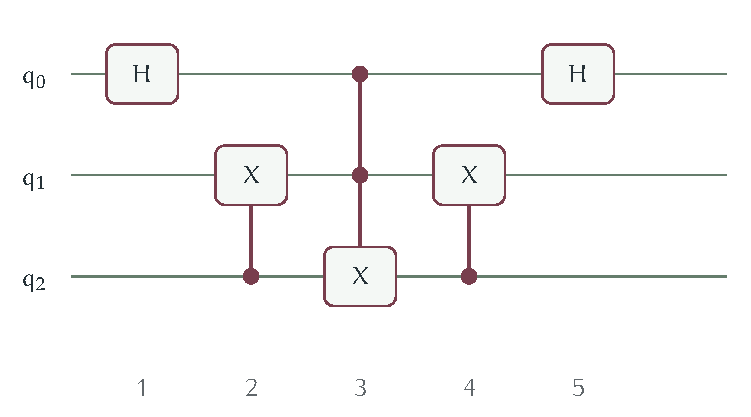
\includegraphics[width=\linewidth,height=94mm,keepaspectratio]{figure/fe6ea44042fe8efc3.pdf}\FigureCaption{4.04 \(\cdot\) esempio 1 \(\cdot\) Circuito: porte 1--5}\end{FigureBlock}

\BookHeading{Geometria e configurazione dell'esempio}
\begin{FigureBlock}\centering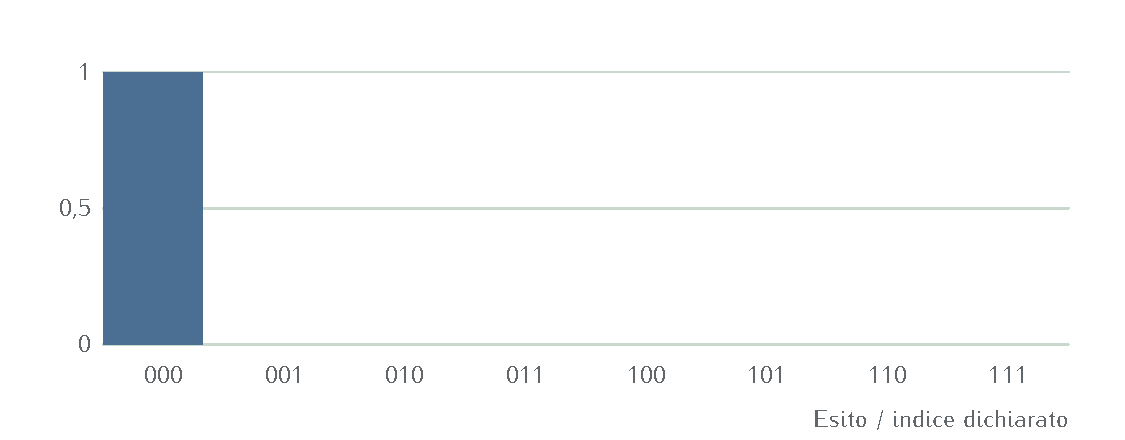
\includegraphics[width=\linewidth,height=94mm,keepaspectratio]{figure/f1f4d259989af1b3b.pdf}\FigureCaption{4.04 \(\cdot\) esempio 1 \(\cdot\) Distribuzione congiunta \(\cdot\) Preparazione}\end{FigureBlock}
\begin{FigureBlock}\begin{minipage}[t]{.485\linewidth}\centering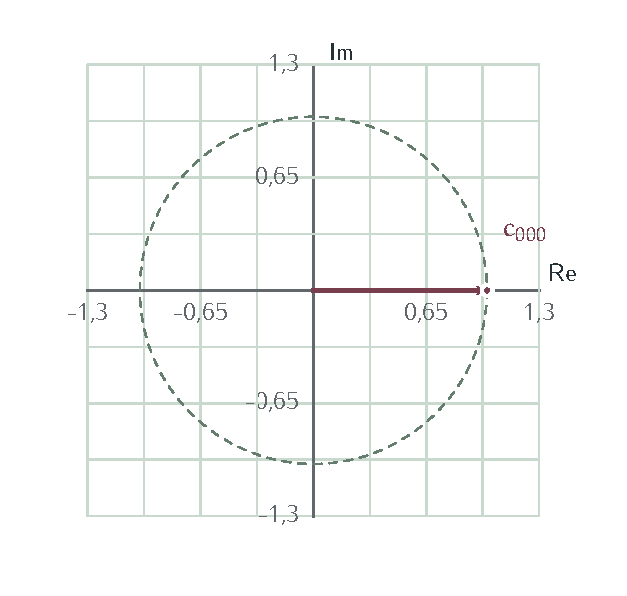
\includegraphics[width=\linewidth,height=63mm,keepaspectratio]{figure/f70dcd37d7a8b80aa.pdf}\par{\sffamily\footnotesize \(c_{000}\)\par}\end{minipage}\hfill\begin{minipage}[t]{.485\linewidth}\centering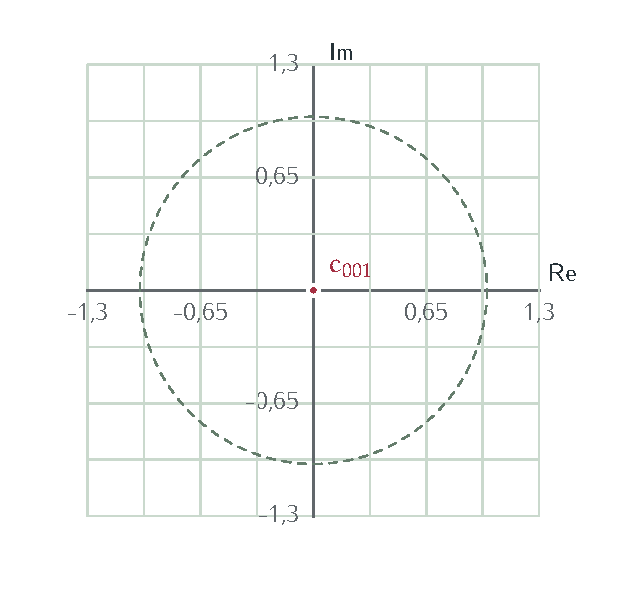
\includegraphics[width=\linewidth,height=63mm,keepaspectratio]{figure/f200b5f4436d864d5.pdf}\par{\sffamily\footnotesize \(c_{001}\)\par}\end{minipage}\FigureCaption{4.04 \(\cdot\) esempio 1 \(\cdot\) Componenti complesse}\end{FigureBlock}
\begin{FigureBlock}\begin{minipage}[t]{.485\linewidth}\centering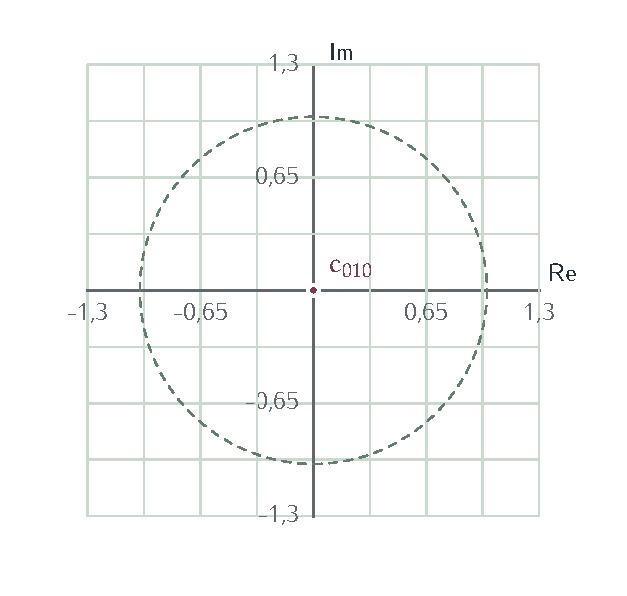
\includegraphics[width=\linewidth,height=63mm,keepaspectratio]{figure/fcba2503abd08f811.pdf}\par{\sffamily\footnotesize \(c_{010}\)\par}\end{minipage}\hfill\begin{minipage}[t]{.485\linewidth}\centering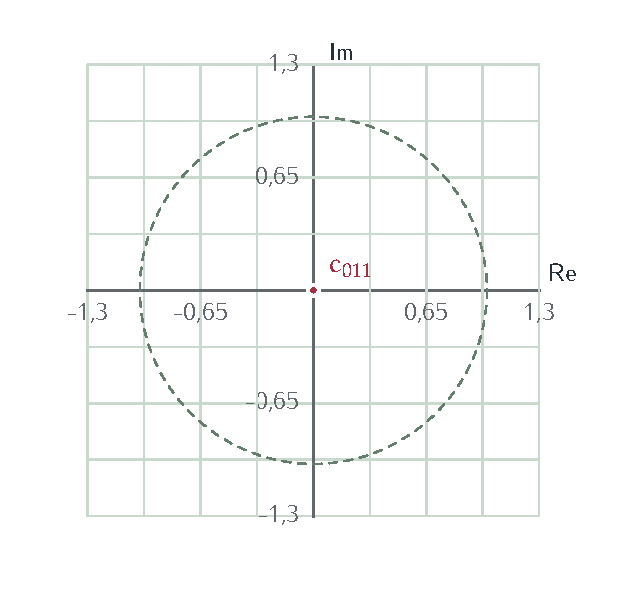
\includegraphics[width=\linewidth,height=63mm,keepaspectratio]{figure/f14fc9ebda1af3074.pdf}\par{\sffamily\footnotesize \(c_{011}\)\par}\end{minipage}\FigureCaption{4.04 \(\cdot\) esempio 1 \(\cdot\) Componenti complesse}\end{FigureBlock}
\begin{FigureBlock}\begin{minipage}[t]{.485\linewidth}\centering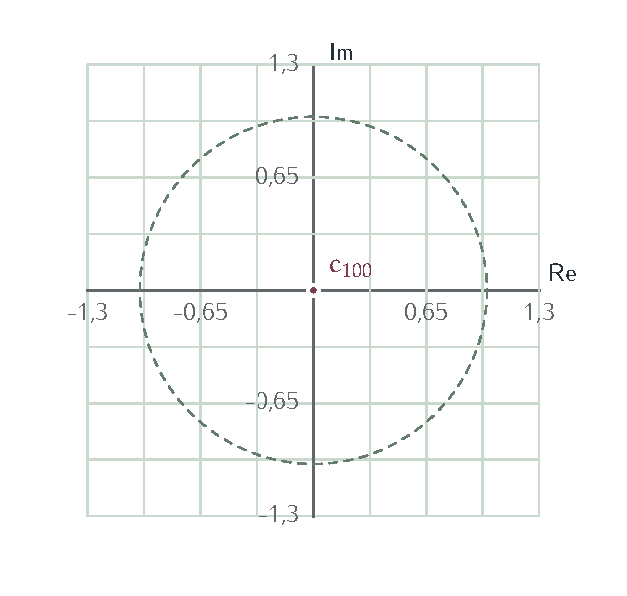
\includegraphics[width=\linewidth,height=63mm,keepaspectratio]{figure/f8bc1e4478e58ad46.pdf}\par{\sffamily\footnotesize \(c_{100}\)\par}\end{minipage}\hfill\begin{minipage}[t]{.485\linewidth}\centering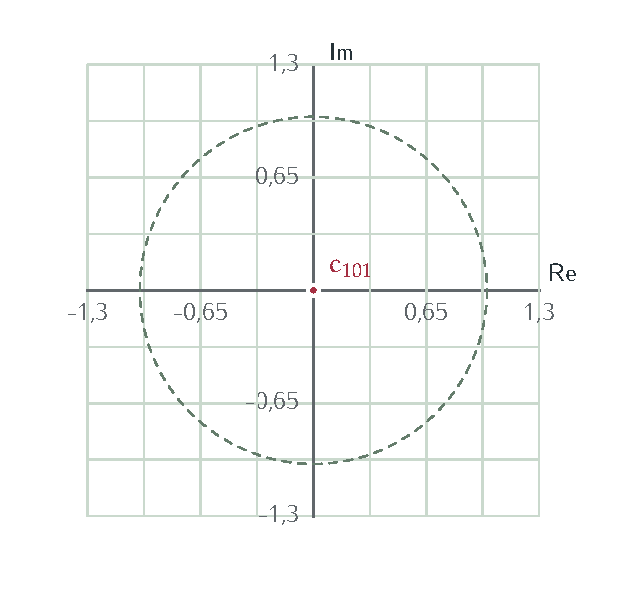
\includegraphics[width=\linewidth,height=63mm,keepaspectratio]{figure/f27146bcb8080b22b.pdf}\par{\sffamily\footnotesize \(c_{101}\)\par}\end{minipage}\FigureCaption{4.04 \(\cdot\) esempio 1 \(\cdot\) Componenti complesse}\end{FigureBlock}
\begin{FigureBlock}\begin{minipage}[t]{.485\linewidth}\centering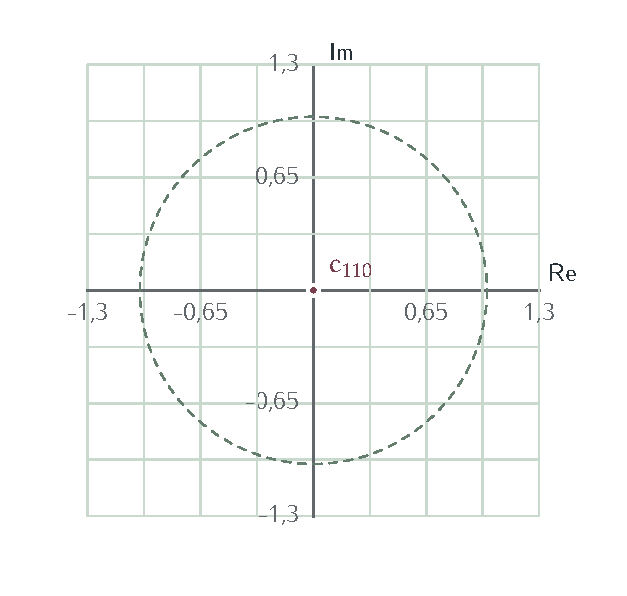
\includegraphics[width=\linewidth,height=63mm,keepaspectratio]{figure/fe613366e53792fd6.pdf}\par{\sffamily\footnotesize \(c_{110}\)\par}\end{minipage}\hfill\begin{minipage}[t]{.485\linewidth}\centering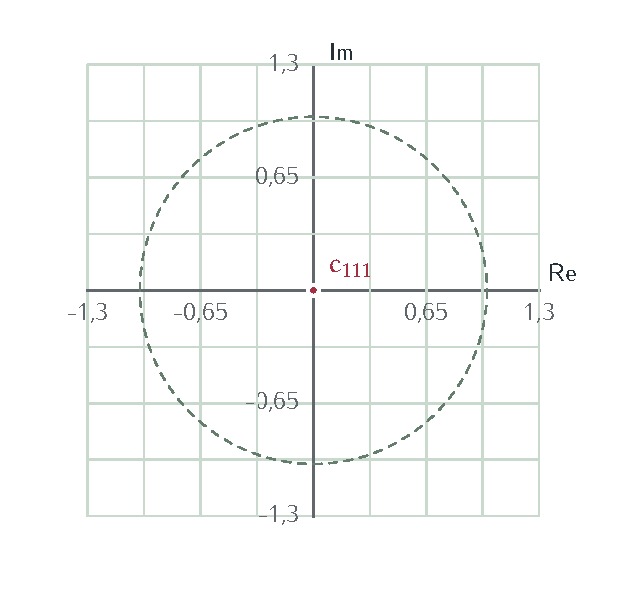
\includegraphics[width=\linewidth,height=63mm,keepaspectratio]{figure/fb0b358447b15cea5.pdf}\par{\sffamily\footnotesize \(c_{111}\)\par}\end{minipage}\FigureCaption{4.04 \(\cdot\) esempio 1 \(\cdot\) Componenti complesse}\end{FigureBlock}

\phantomsection\label{c4-swap-example-1-step-1}
\BookHeading{01 Preparazione}

\MathBlock{03C82080003D00280031003B00200030003B00200030003B00200030003B00200030003B00200030003B00200030003B0020003000291D40003B0020201603C82080201600B222480031}{\psi _{0}=(1;\allowbreak \ 0;\allowbreak \ 0;\allowbreak \ 0;\allowbreak \ 0;\allowbreak \ 0;\allowbreak \ 0;\allowbreak \ 0)^{T};\allowbreak \ \Vert \psi _{0}\Vert ^{2}\approx 1}

Le ampiezze sono ordinate secondo le etichette binarie, con il bit più significativo in alto.\par


\phantomsection\label{c4-swap-example-1-step-2}
\BookHeading{02 Porta 1 \(\cdot\) \(H\)}

\MathBlock{0063002800300030003000290020003D002000280030002C0037003000370031002900B70028003100290020002B002000280030002C0037003000370031002900B70028003000290020224800200030002C0037003000370031}{c(000)\ =\ (0{,}7071)\cdot (1)\ +\ (0{,}7071)\cdot (0)\ \approx \ 0{,}7071}
\MathBlock{0063002800310030003000290020003D002000280030002C0037003000370031002900B70028003100290020002B00200028002D0030002C0037003000370031002900B70028003000290020224800200030002C0037003000370031}{c(100)\ =\ (0{,}7071)\cdot (1)\ +\ (-0{,}7071)\cdot (0)\ \approx \ 0{,}7071}
\MathBlock{03C800202248002000280030002C0037003000370031003B00200030003B00200030003B00200030003B00200030002C0037003000370031003B00200030003B00200030003B0020003000291D40}{\psi \ \approx \ (0{,}7071;\allowbreak \ 0;\allowbreak \ 0;\allowbreak \ 0;\allowbreak \ 0{,}7071;\allowbreak \ 0;\allowbreak \ 0;\allowbreak \ 0)^{T}}

Ogni coppia di ampiezze indicata usa il prodotto riga per colonna della porta. I rami con controllo nullo restano invariati.\par


\phantomsection\label{c4-swap-example-1-step-3}
\BookHeading{03 Porta 2 \(\cdot\) C\(\cdot\)X}

\MathBlock{03C800202248002000280030002C0037003000370031003B00200030003B00200030003B00200030003B00200030002C0037003000370031003B00200030003B00200030003B0020003000291D40}{\psi \ \approx \ (0{,}7071;\allowbreak \ 0;\allowbreak \ 0;\allowbreak \ 0;\allowbreak \ 0{,}7071;\allowbreak \ 0;\allowbreak \ 0;\allowbreak \ 0)^{T}}

Ogni coppia di ampiezze indicata usa il prodotto riga per colonna della porta. I rami con controllo nullo restano invariati.\par


\phantomsection\label{c4-swap-example-1-step-4}
\BookHeading{04 Porta 3 \(\cdot\) C\(\cdot\)X}

\MathBlock{03C800202248002000280030002C0037003000370031003B00200030003B00200030003B00200030003B00200030002C0037003000370031003B00200030003B00200030003B0020003000291D40}{\psi \ \approx \ (0{,}7071;\allowbreak \ 0;\allowbreak \ 0;\allowbreak \ 0;\allowbreak \ 0{,}7071;\allowbreak \ 0;\allowbreak \ 0;\allowbreak \ 0)^{T}}

Ogni coppia di ampiezze indicata usa il prodotto riga per colonna della porta. I rami con controllo nullo restano invariati.\par


\phantomsection\label{c4-swap-example-1-step-5}
\BookHeading{05 Porta 4 \(\cdot\) C\(\cdot\)X}

\MathBlock{03C800202248002000280030002C0037003000370031003B00200030003B00200030003B00200030003B00200030002C0037003000370031003B00200030003B00200030003B0020003000291D40}{\psi \ \approx \ (0{,}7071;\allowbreak \ 0;\allowbreak \ 0;\allowbreak \ 0;\allowbreak \ 0{,}7071;\allowbreak \ 0;\allowbreak \ 0;\allowbreak \ 0)^{T}}

Ogni coppia di ampiezze indicata usa il prodotto riga per colonna della porta. I rami con controllo nullo restano invariati.\par


\phantomsection\label{c4-swap-example-1-step-6}
\BookHeading{06 Porta 5 \(\cdot\) \(H\)}

\MathBlock{0063002800300030003000290020003D002000280030002C0037003000370031002900B700280030002C003700300037003100290020002B002000280030002C0037003000370031002900B700280030002C003700300037003100290020224800200031}{c(000)\ =\ (0{,}7071)\cdot (0{,}7071)\ +\ (0{,}7071)\cdot (0{,}7071)\ \approx \ 1}
\MathBlock{0063002800310030003000290020003D002000280030002C0037003000370031002900B700280030002C003700300037003100290020002B00200028002D0030002C0037003000370031002900B700280030002C003700300037003100290020224800200030}{c(100)\ =\ (0{,}7071)\cdot (0{,}7071)\ +\ (-0{,}7071)\cdot (0{,}7071)\ \approx \ 0}
\MathBlock{03C800202248002000280031003B00200030003B00200030003B00200030003B00200030003B00200030003B00200030003B0020003000291D40}{\psi \ \approx \ (1;\allowbreak \ 0;\allowbreak \ 0;\allowbreak \ 0;\allowbreak \ 0;\allowbreak \ 0;\allowbreak \ 0;\allowbreak \ 0)^{T}}

Ogni coppia di ampiezze indicata usa il prodotto riga per colonna della porta. I rami con controllo nullo restano invariati.\par


\phantomsection\label{c4-swap-example-1-step-7}
\BookHeading{07 Lettura nella base finale}

\MathBlock{005000280030003000300029003D00280031002900B20020002B002000280030002900B222480031}{P(000)=(1)^{2}\ +\ (0)^{2}\approx 1}
\MathBlock{005000280030003000310029003D00280030002900B20020002B002000280030002900B222480030}{P(001)=(0)^{2}\ +\ (0)^{2}\approx 0}
\MathBlock{005000280030003100300029003D00280030002900B20020002B002000280030002900B222480030}{P(010)=(0)^{2}\ +\ (0)^{2}\approx 0}
\MathBlock{005000280030003100310029003D00280030002900B20020002B002000280030002900B222480030}{P(011)=(0)^{2}\ +\ (0)^{2}\approx 0}
\MathBlock{005000280031003000300029003D00280030002900B20020002B002000280030002900B222480030}{P(100)=(0)^{2}\ +\ (0)^{2}\approx 0}
\MathBlock{005000280031003000310029003D00280030002900B20020002B002000280030002900B222480030}{P(101)=(0)^{2}\ +\ (0)^{2}\approx 0}
\MathBlock{005000280031003100300029003D00280030002900B20020002B002000280030002900B222480030}{P(110)=(0)^{2}\ +\ (0)^{2}\approx 0}
\MathBlock{005000280031003100310029003D00280030002900B20020002B002000280030002900B222480030}{P(111)=(0)^{2}\ +\ (0)^{2}\approx 0}

Il modulo quadro di ciascuna ampiezza determina la probabilità. La selezione di una porta nel disegno mostra uno stato intermedio senza effettuare una misura.\par


\phantomsection\label{c4-swap-example-1-step-8}
\BookHeading{08 Verifica con il prodotto interno}

\MathBlock{27E80075007C007627E9003D00280031002900B70028003100290020002B002000280030002900B700280030002922480031}{\langle u|v\rangle =(1)\cdot (1)\ +\ (0)\cdot (0)\approx 1}
\MathBlock{0050002800300029003D00280031002B00310029002F0032003D0031}{P(0)=(1+1)/2=1}

Espandendo la norma della somma dei due prodotti tensoriali si ottengono due termini diagonali e due termini di sovrapposizione.\par


\phantomsection\label{c4-swap-example-1-step-9}
\BookHeading{09 Sommare i rami del bersaglio}

\MathBlock{005000280061003D00300029003D005000280030003000300029002B005000280030003000310029002B005000280030003100300029002B005000280030003100310029}{P(a=0)=P(000)+P(001)+P(010)+P(011)}
\MathBlock{003D0031002B0030002B0030002B0030003D0031002E}{=1+0+0+0=1.}
\MathBlock{005000280061003D00310029003D00312212005000280061003D00300029003D0030002E}{P(a=1)=1- P(a=0)=0.}

La lettura dell'ausiliario somma le quattro alternative ortogonali dei due bersagli.\par


\BookHeading{Stato finale del programma}
\begin{FigureBlock}\centering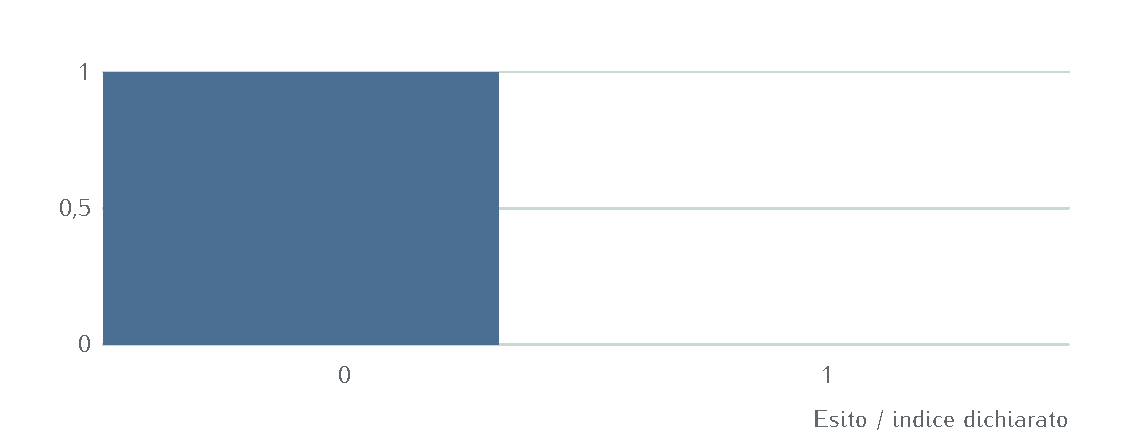
\includegraphics[width=\linewidth,height=94mm,keepaspectratio]{figure/fc772cff2a603ba10.pdf}\FigureCaption{4.04 \(\cdot\) esempio 1 \(\cdot\) Misura dell'ausiliario}\end{FigureBlock}

\BookHeading{Interpretazione}

Il prodotto interno ha modulo quadro 1; la probabilità di leggere 0 sull'ausiliario è 1.\par


Risorse dichiarate. 3 qubit; 5 operazioni alla granularità dichiarata nel circuito.\par


\Needspace{.36\textheight}\phantomsection\label{c4-swap-example-2}
{\sffamily\small\color{Accent} ESEMPIO SVOLTO 2\par}
\BookHeading{Interferenza di uno scambio controllato}
Prepariamo \(|0\rangle |u\rangle |v\rangle \).\par


\BookHeading{Circuito completo}
\begin{FigureBlock}\centering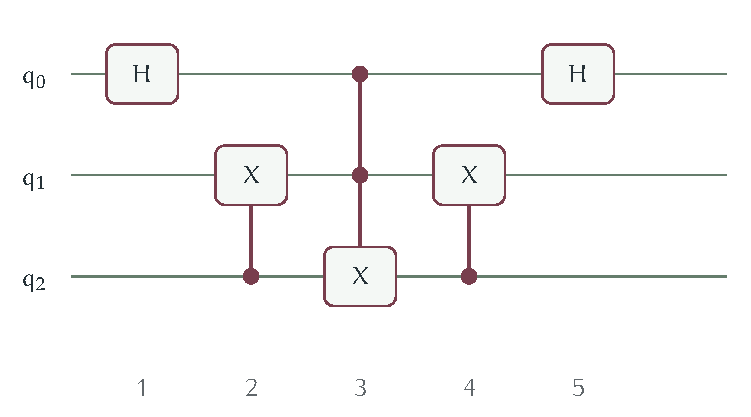
\includegraphics[width=\linewidth,height=94mm,keepaspectratio]{figure/fe6ea44042fe8efc3.pdf}\FigureCaption{4.04 \(\cdot\) esempio 2 \(\cdot\) Circuito: porte 1--5}\end{FigureBlock}

\BookHeading{Geometria e configurazione dell'esempio}
\begin{FigureBlock}\centering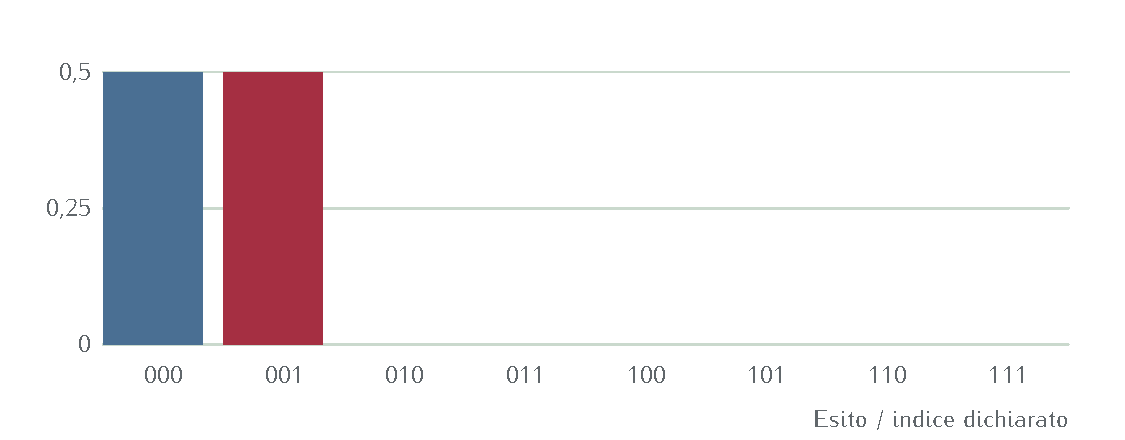
\includegraphics[width=\linewidth,height=94mm,keepaspectratio]{figure/fde2996deeb8bafd6.pdf}\FigureCaption{4.04 \(\cdot\) esempio 2 \(\cdot\) Distribuzione congiunta \(\cdot\) Preparazione}\end{FigureBlock}
\begin{FigureBlock}\begin{minipage}[t]{.485\linewidth}\centering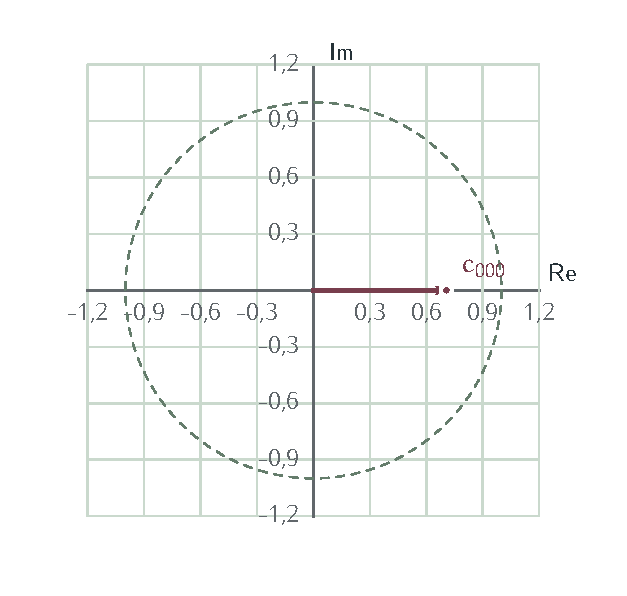
\includegraphics[width=\linewidth,height=63mm,keepaspectratio]{figure/fcc264f59003755e1.pdf}\par{\sffamily\footnotesize \(c_{000}\)\par}\end{minipage}\hfill\begin{minipage}[t]{.485\linewidth}\centering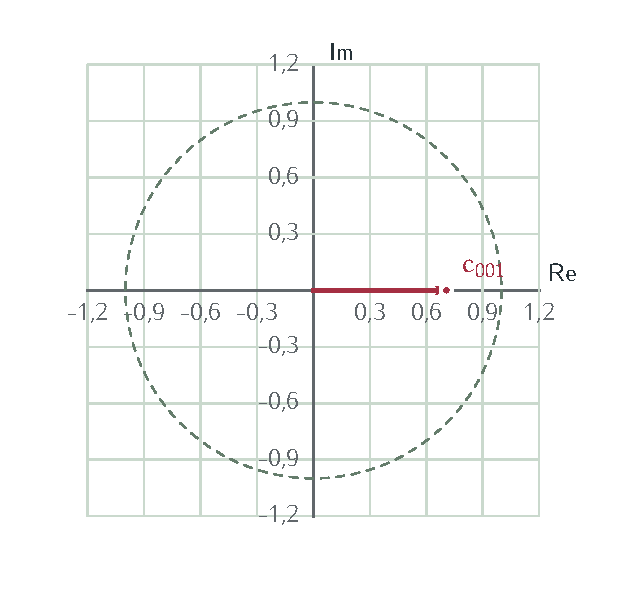
\includegraphics[width=\linewidth,height=63mm,keepaspectratio]{figure/f4a0b8094edbdc209.pdf}\par{\sffamily\footnotesize \(c_{001}\)\par}\end{minipage}\FigureCaption{4.04 \(\cdot\) esempio 2 \(\cdot\) Componenti complesse}\end{FigureBlock}
\begin{FigureBlock}\begin{minipage}[t]{.485\linewidth}\centering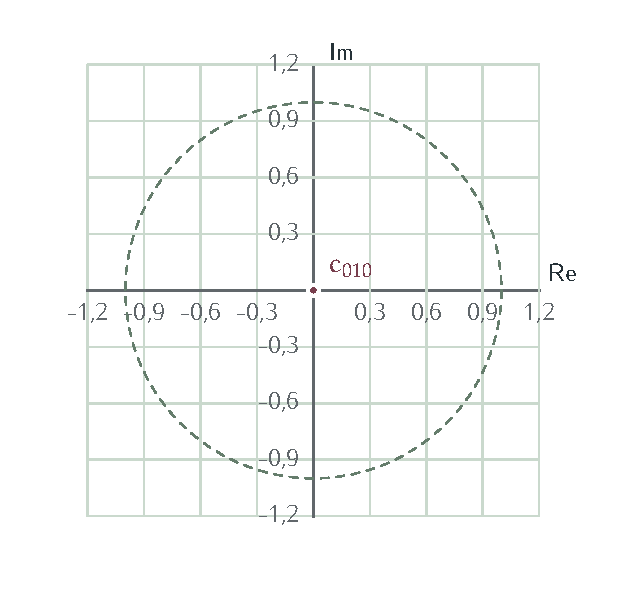
\includegraphics[width=\linewidth,height=63mm,keepaspectratio]{figure/ff25406c9aba18c59.pdf}\par{\sffamily\footnotesize \(c_{010}\)\par}\end{minipage}\hfill\begin{minipage}[t]{.485\linewidth}\centering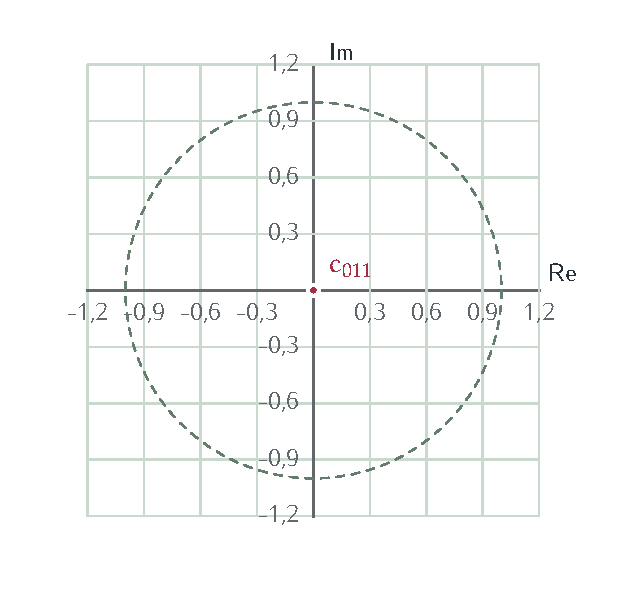
\includegraphics[width=\linewidth,height=63mm,keepaspectratio]{figure/f411c9af29fa7dfb3.pdf}\par{\sffamily\footnotesize \(c_{011}\)\par}\end{minipage}\FigureCaption{4.04 \(\cdot\) esempio 2 \(\cdot\) Componenti complesse}\end{FigureBlock}
\begin{FigureBlock}\begin{minipage}[t]{.485\linewidth}\centering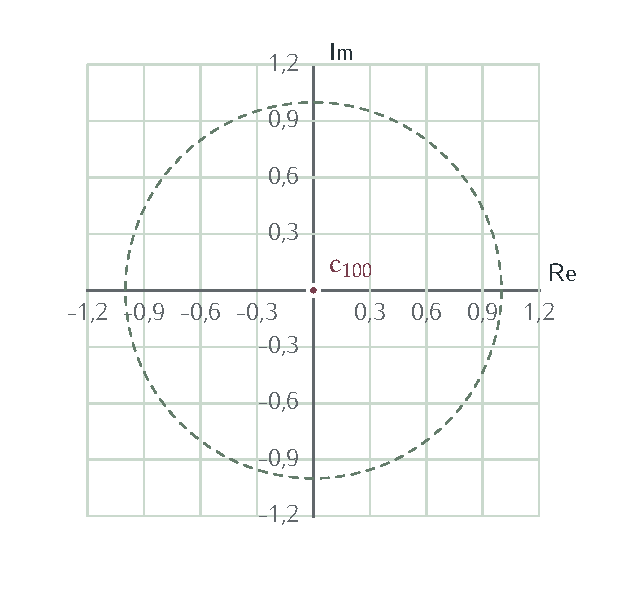
\includegraphics[width=\linewidth,height=63mm,keepaspectratio]{figure/fc83fe12b060b3d25.pdf}\par{\sffamily\footnotesize \(c_{100}\)\par}\end{minipage}\hfill\begin{minipage}[t]{.485\linewidth}\centering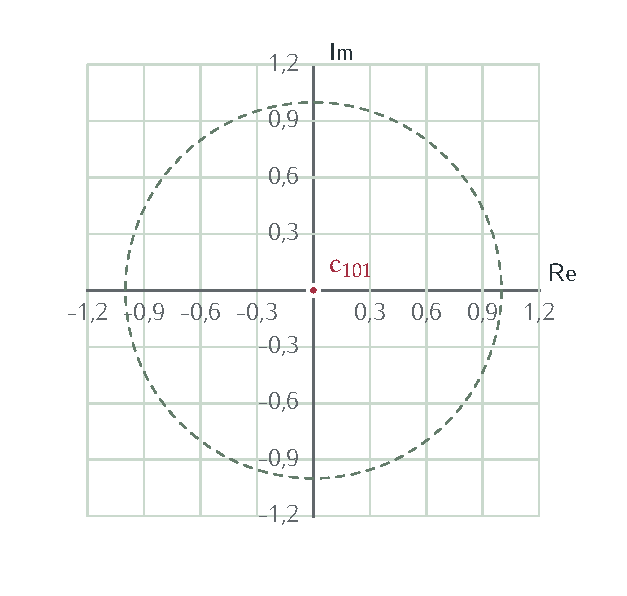
\includegraphics[width=\linewidth,height=63mm,keepaspectratio]{figure/fc1446b014e825f31.pdf}\par{\sffamily\footnotesize \(c_{101}\)\par}\end{minipage}\FigureCaption{4.04 \(\cdot\) esempio 2 \(\cdot\) Componenti complesse}\end{FigureBlock}
\begin{FigureBlock}\begin{minipage}[t]{.485\linewidth}\centering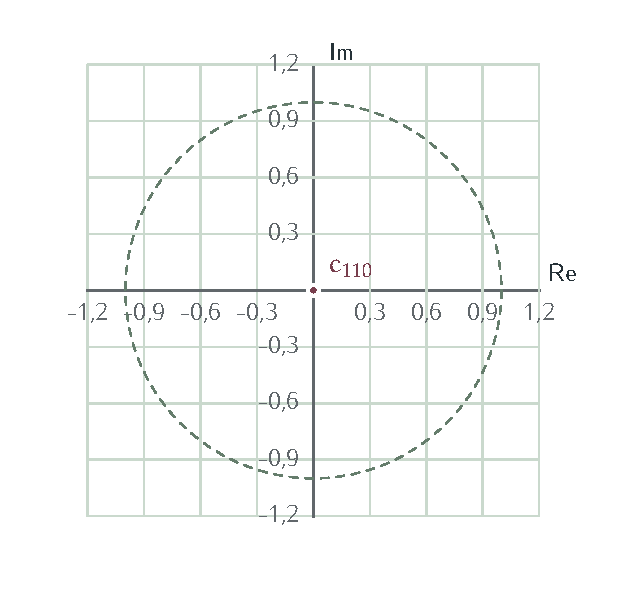
\includegraphics[width=\linewidth,height=63mm,keepaspectratio]{figure/fa990d4afd646b1ad.pdf}\par{\sffamily\footnotesize \(c_{110}\)\par}\end{minipage}\hfill\begin{minipage}[t]{.485\linewidth}\centering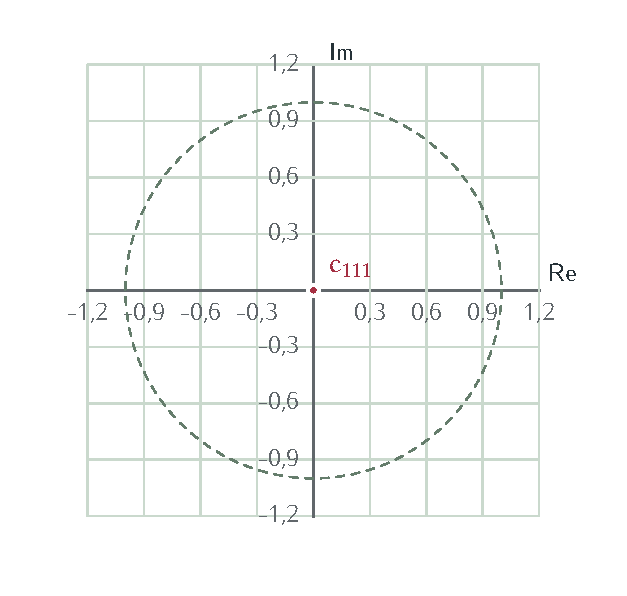
\includegraphics[width=\linewidth,height=63mm,keepaspectratio]{figure/f358c578111671487.pdf}\par{\sffamily\footnotesize \(c_{111}\)\par}\end{minipage}\FigureCaption{4.04 \(\cdot\) esempio 2 \(\cdot\) Componenti complesse}\end{FigureBlock}

\phantomsection\label{c4-swap-example-2-step-1}
\BookHeading{01 Preparazione}

\MathBlock{03C82080003D00280030002C0037003000370031003B00200030002C0037003000370031003B00200030003B00200030003B00200030003B00200030003B00200030003B0020003000291D40003B0020201603C82080201600B222480031}{\psi _{0}=(0{,}7071;\allowbreak \ 0{,}7071;\allowbreak \ 0;\allowbreak \ 0;\allowbreak \ 0;\allowbreak \ 0;\allowbreak \ 0;\allowbreak \ 0)^{T};\allowbreak \ \Vert \psi _{0}\Vert ^{2}\approx 1}

Le ampiezze sono ordinate secondo le etichette binarie, con il bit più significativo in alto.\par


\phantomsection\label{c4-swap-example-2-step-2}
\BookHeading{02 Porta 1 \(\cdot\) \(H\)}

\MathBlock{0063002800300030003000290020003D002000280030002C0037003000370031002900B700280030002C003700300037003100290020002B002000280030002C0037003000370031002900B70028003000290020224800200030002C0035}{c(000)\ =\ (0{,}7071)\cdot (0{,}7071)\ +\ (0{,}7071)\cdot (0)\ \approx \ 0{,}5}
\MathBlock{0063002800310030003000290020003D002000280030002C0037003000370031002900B700280030002C003700300037003100290020002B00200028002D0030002C0037003000370031002900B70028003000290020224800200030002C0035}{c(100)\ =\ (0{,}7071)\cdot (0{,}7071)\ +\ (-0{,}7071)\cdot (0)\ \approx \ 0{,}5}
\MathBlock{0063002800300030003100290020003D002000280030002C0037003000370031002900B700280030002C003700300037003100290020002B002000280030002C0037003000370031002900B70028003000290020224800200030002C0035}{c(001)\ =\ (0{,}7071)\cdot (0{,}7071)\ +\ (0{,}7071)\cdot (0)\ \approx \ 0{,}5}
\MathBlock{0063002800310030003100290020003D002000280030002C0037003000370031002900B700280030002C003700300037003100290020002B00200028002D0030002C0037003000370031002900B70028003000290020224800200030002C0035}{c(101)\ =\ (0{,}7071)\cdot (0{,}7071)\ +\ (-0{,}7071)\cdot (0)\ \approx \ 0{,}5}
\MathBlock{03C800202248002000280030002C0035003B00200030002C0035003B00200030003B00200030003B00200030002C0035003B00200030002C0035003B00200030003B0020003000291D40}{\psi \ \approx \ (0{,}5;\allowbreak \ 0{,}5;\allowbreak \ 0;\allowbreak \ 0;\allowbreak \ 0{,}5;\allowbreak \ 0{,}5;\allowbreak \ 0;\allowbreak \ 0)^{T}}

Ogni coppia di ampiezze indicata usa il prodotto riga per colonna della porta. I rami con controllo nullo restano invariati.\par


\phantomsection\label{c4-swap-example-2-step-3}
\BookHeading{03 Porta 2 \(\cdot\) C\(\cdot\)X}

\MathBlock{0063002800300030003100290020003D002000280030002900B700280030002C003500290020002B002000280031002900B70028003000290020224800200030}{c(001)\ =\ (0)\cdot (0{,}5)\ +\ (1)\cdot (0)\ \approx \ 0}
\MathBlock{0063002800300031003100290020003D002000280031002900B700280030002C003500290020002B002000280030002900B70028003000290020224800200030002C0035}{c(011)\ =\ (1)\cdot (0{,}5)\ +\ (0)\cdot (0)\ \approx \ 0{,}5}
\MathBlock{0063002800310030003100290020003D002000280030002900B700280030002C003500290020002B002000280031002900B70028003000290020224800200030}{c(101)\ =\ (0)\cdot (0{,}5)\ +\ (1)\cdot (0)\ \approx \ 0}
\MathBlock{0063002800310031003100290020003D002000280031002900B700280030002C003500290020002B002000280030002900B70028003000290020224800200030002C0035}{c(111)\ =\ (1)\cdot (0{,}5)\ +\ (0)\cdot (0)\ \approx \ 0{,}5}
\MathBlock{03C800202248002000280030002C0035003B00200030003B00200030003B00200030002C0035003B00200030002C0035003B00200030003B00200030003B00200030002C003500291D40}{\psi \ \approx \ (0{,}5;\allowbreak \ 0;\allowbreak \ 0;\allowbreak \ 0{,}5;\allowbreak \ 0{,}5;\allowbreak \ 0;\allowbreak \ 0;\allowbreak \ 0{,}5)^{T}}

Ogni coppia di ampiezze indicata usa il prodotto riga per colonna della porta. I rami con controllo nullo restano invariati.\par


\phantomsection\label{c4-swap-example-2-step-4}
\BookHeading{04 Porta 3 \(\cdot\) C\(\cdot\)X}

\MathBlock{0063002800310031003000290020003D002000280030002900B70028003000290020002B002000280031002900B700280030002C003500290020224800200030002C0035}{c(110)\ =\ (0)\cdot (0)\ +\ (1)\cdot (0{,}5)\ \approx \ 0{,}5}
\MathBlock{0063002800310031003100290020003D002000280031002900B70028003000290020002B002000280030002900B700280030002C003500290020224800200030}{c(111)\ =\ (1)\cdot (0)\ +\ (0)\cdot (0{,}5)\ \approx \ 0}
\MathBlock{03C800202248002000280030002C0035003B00200030003B00200030003B00200030002C0035003B00200030002C0035003B00200030003B00200030002C0035003B0020003000291D40}{\psi \ \approx \ (0{,}5;\allowbreak \ 0;\allowbreak \ 0;\allowbreak \ 0{,}5;\allowbreak \ 0{,}5;\allowbreak \ 0;\allowbreak \ 0{,}5;\allowbreak \ 0)^{T}}

Ogni coppia di ampiezze indicata usa il prodotto riga per colonna della porta. I rami con controllo nullo restano invariati.\par


\phantomsection\label{c4-swap-example-2-step-5}
\BookHeading{05 Porta 4 \(\cdot\) C\(\cdot\)X}

\MathBlock{0063002800300030003100290020003D002000280030002900B70028003000290020002B002000280031002900B700280030002C003500290020224800200030002C0035}{c(001)\ =\ (0)\cdot (0)\ +\ (1)\cdot (0{,}5)\ \approx \ 0{,}5}
\MathBlock{0063002800300031003100290020003D002000280031002900B70028003000290020002B002000280030002900B700280030002C003500290020224800200030}{c(011)\ =\ (1)\cdot (0)\ +\ (0)\cdot (0{,}5)\ \approx \ 0}
\MathBlock{03C800202248002000280030002C0035003B00200030002C0035003B00200030003B00200030003B00200030002C0035003B00200030003B00200030002C0035003B0020003000291D40}{\psi \ \approx \ (0{,}5;\allowbreak \ 0{,}5;\allowbreak \ 0;\allowbreak \ 0;\allowbreak \ 0{,}5;\allowbreak \ 0;\allowbreak \ 0{,}5;\allowbreak \ 0)^{T}}

Ogni coppia di ampiezze indicata usa il prodotto riga per colonna della porta. I rami con controllo nullo restano invariati.\par


\phantomsection\label{c4-swap-example-2-step-6}
\BookHeading{06 Porta 5 \(\cdot\) \(H\)}

\MathBlock{0063002800300030003000290020003D002000280030002C0037003000370031002900B700280030002C003500290020002B002000280030002C0037003000370031002900B700280030002C003500290020224800200030002C0037003000370031}{c(000)\ =\ (0{,}7071)\cdot (0{,}5)\ +\ (0{,}7071)\cdot (0{,}5)\ \approx \ 0{,}7071}
\MathBlock{0063002800310030003000290020003D002000280030002C0037003000370031002900B700280030002C003500290020002B00200028002D0030002C0037003000370031002900B700280030002C003500290020224800200030}{c(100)\ =\ (0{,}7071)\cdot (0{,}5)\ +\ (-0{,}7071)\cdot (0{,}5)\ \approx \ 0}
\MathBlock{0063002800300030003100290020003D002000280030002C0037003000370031002900B700280030002C003500290020002B002000280030002C0037003000370031002900B70028003000290020224800200030002C0033003500330036}{c(001)\ =\ (0{,}7071)\cdot (0{,}5)\ +\ (0{,}7071)\cdot (0)\ \approx \ 0{,}3536}
\MathBlock{0063002800310030003100290020003D002000280030002C0037003000370031002900B700280030002C003500290020002B00200028002D0030002C0037003000370031002900B70028003000290020224800200030002C0033003500330036}{c(101)\ =\ (0{,}7071)\cdot (0{,}5)\ +\ (-0{,}7071)\cdot (0)\ \approx \ 0{,}3536}
\MathBlock{0063002800300031003000290020003D002000280030002C0037003000370031002900B70028003000290020002B002000280030002C0037003000370031002900B700280030002C003500290020224800200030002C0033003500330036}{c(010)\ =\ (0{,}7071)\cdot (0)\ +\ (0{,}7071)\cdot (0{,}5)\ \approx \ 0{,}3536}
\MathBlock{0063002800310031003000290020003D002000280030002C0037003000370031002900B70028003000290020002B00200028002D0030002C0037003000370031002900B700280030002C00350029002022480020002D0030002C0033003500330036}{c(110)\ =\ (0{,}7071)\cdot (0)\ +\ (-0{,}7071)\cdot (0{,}5)\ \approx \ -0{,}3536}
\MathBlock{03C800202248002000280030002C0037003000370031003B00200030002C0033003500330036003B00200030002C0033003500330036003B00200030003B00200030003B00200030002C0033003500330036003B0020002D0030002C0033003500330036003B0020003000291D40}{\psi \ \approx \ (0{,}7071;\allowbreak \ 0{,}3536;\allowbreak \ 0{,}3536;\allowbreak \ 0;\allowbreak \ 0;\allowbreak \ 0{,}3536;\allowbreak \ -0{,}3536;\allowbreak \ 0)^{T}}

Ogni coppia di ampiezze indicata usa il prodotto riga per colonna della porta. I rami con controllo nullo restano invariati.\par


\phantomsection\label{c4-swap-example-2-step-7}
\BookHeading{07 Lettura nella base finale}

\MathBlock{005000280030003000300029003D00280030002C0037003000370031002900B20020002B002000280030002900B222480030002C0035}{P(000)=(0{,}7071)^{2}\ +\ (0)^{2}\approx 0{,}5}
\MathBlock{005000280030003000310029003D00280030002C0033003500330036002900B20020002B002000280030002900B222480030002C003100320035}{P(001)=(0{,}3536)^{2}\ +\ (0)^{2}\approx 0{,}125}
\MathBlock{005000280030003100300029003D00280030002C0033003500330036002900B20020002B002000280030002900B222480030002C003100320035}{P(010)=(0{,}3536)^{2}\ +\ (0)^{2}\approx 0{,}125}
\MathBlock{005000280030003100310029003D00280030002900B20020002B002000280030002900B222480030}{P(011)=(0)^{2}\ +\ (0)^{2}\approx 0}
\MathBlock{005000280031003000300029003D00280030002900B20020002B002000280030002900B222480030}{P(100)=(0)^{2}\ +\ (0)^{2}\approx 0}
\MathBlock{005000280031003000310029003D00280030002C0033003500330036002900B20020002B002000280030002900B222480030002C003100320035}{P(101)=(0{,}3536)^{2}\ +\ (0)^{2}\approx 0{,}125}
\MathBlock{005000280031003100300029003D0028002D0030002C0033003500330036002900B20020002B002000280030002900B222480030002C003100320035}{P(110)=(-0{,}3536)^{2}\ +\ (0)^{2}\approx 0{,}125}
\MathBlock{005000280031003100310029003D00280030002900B20020002B002000280030002900B222480030}{P(111)=(0)^{2}\ +\ (0)^{2}\approx 0}

Il modulo quadro di ciascuna ampiezza determina la probabilità. La selezione di una porta nel disegno mostra uno stato intermedio senza effettuare una misura.\par


\phantomsection\label{c4-swap-example-2-step-8}
\BookHeading{08 Verifica con il prodotto interno}

\MathBlock{27E80075007C007627E9003D00280031002900B700280030002C003700300037003100290020002B002000280030002900B700280030002C0037003000370031002922480030002C0037003000370031}{\langle u|v\rangle =(1)\cdot (0{,}7071)\ +\ (0)\cdot (0{,}7071)\approx 0{,}7071}
\MathBlock{0050002800300029003D00280031002B0030002C00350029002F0032003D0030002C00370035}{P(0)=(1+0{,}5)/2=0{,}75}

Espandendo la norma della somma dei due prodotti tensoriali si ottengono due termini diagonali e due termini di sovrapposizione.\par


\phantomsection\label{c4-swap-example-2-step-9}
\BookHeading{09 Sommare i rami del bersaglio}

\MathBlock{005000280061003D00300029003D005000280030003000300029002B005000280030003000310029002B005000280030003100300029002B005000280030003100310029}{P(a=0)=P(000)+P(001)+P(010)+P(011)}
\MathBlock{003D0030002C0035002B0030002C003100320035002B0030002C003100320035002B0030003D0030002C00370035002E}{=0{,}5+0{,}125+0{,}125+0=0{,}75.}
\MathBlock{005000280061003D00310029003D00312212005000280061003D00300029003D0030002C00320035002E}{P(a=1)=1- P(a=0)=0{,}25.}

La lettura dell'ausiliario somma le quattro alternative ortogonali dei due bersagli.\par


\BookHeading{Stato finale del programma}
\begin{FigureBlock}\centering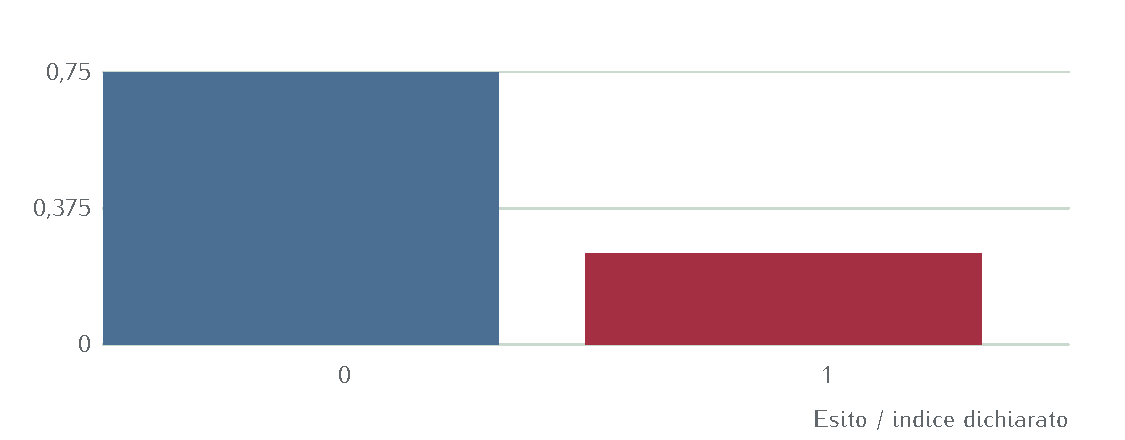
\includegraphics[width=\linewidth,height=94mm,keepaspectratio]{figure/fe5f19996c6bbbf9d.pdf}\FigureCaption{4.04 \(\cdot\) esempio 2 \(\cdot\) Misura dell'ausiliario}\end{FigureBlock}

\BookHeading{Interpretazione}

Il prodotto interno ha modulo quadro 0,5; la probabilità di leggere 0 sull'ausiliario è 0,75.\par


Risorse dichiarate. 3 qubit; 5 operazioni alla granularità dichiarata nel circuito.\par


\Needspace{.36\textheight}\phantomsection\label{c4-swap-example-3}
{\sffamily\small\color{Accent} ESEMPIO SVOLTO 3\par}
\BookHeading{Interferenza di uno scambio controllato}
Prepariamo \(|0\rangle |u\rangle |v\rangle \).\par


\BookHeading{Circuito completo}
\begin{FigureBlock}\centering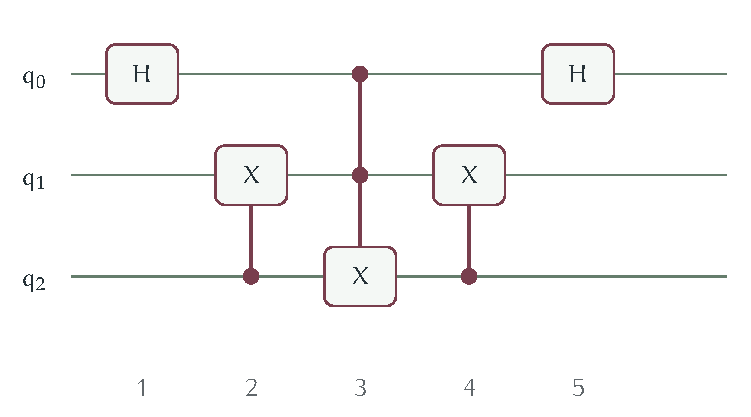
\includegraphics[width=\linewidth,height=94mm,keepaspectratio]{figure/fe6ea44042fe8efc3.pdf}\FigureCaption{4.04 \(\cdot\) esempio 3 \(\cdot\) Circuito: porte 1--5}\end{FigureBlock}

\BookHeading{Geometria e configurazione dell'esempio}
\begin{FigureBlock}\centering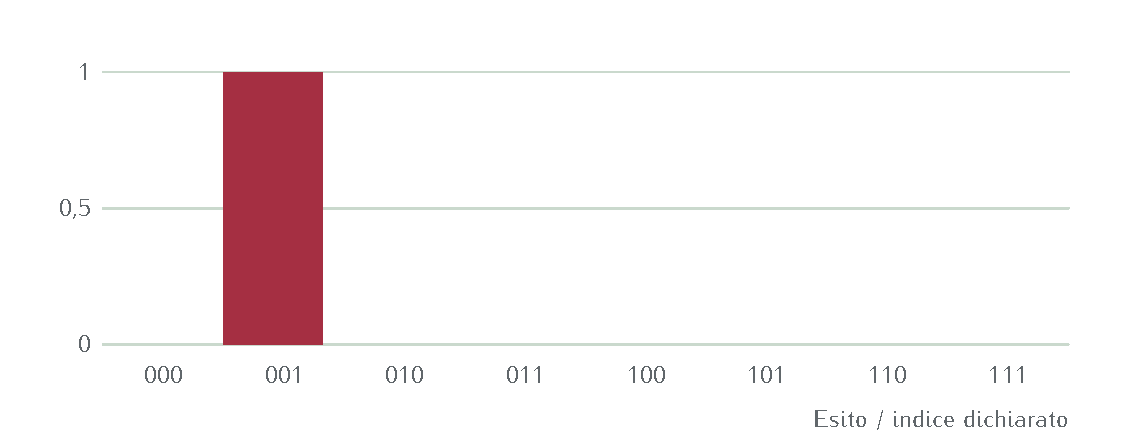
\includegraphics[width=\linewidth,height=94mm,keepaspectratio]{figure/f526224a19c0d9ced.pdf}\FigureCaption{4.04 \(\cdot\) esempio 3 \(\cdot\) Distribuzione congiunta \(\cdot\) Preparazione}\end{FigureBlock}
\begin{FigureBlock}\begin{minipage}[t]{.485\linewidth}\centering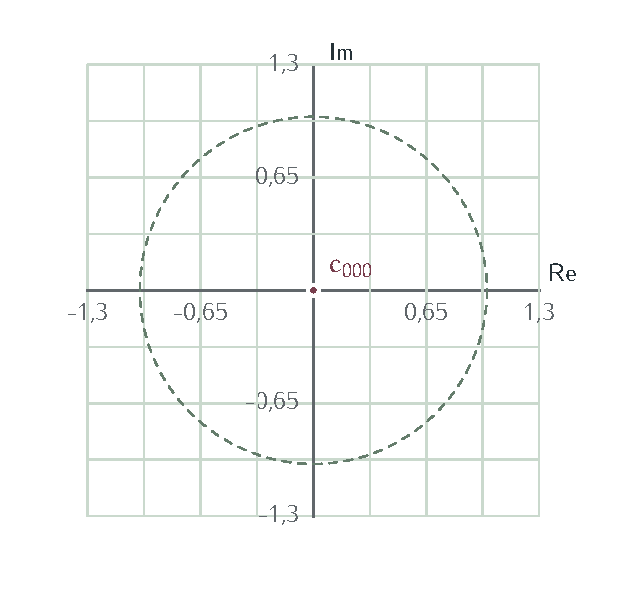
\includegraphics[width=\linewidth,height=63mm,keepaspectratio]{figure/f4f1966be8b9c82f3.pdf}\par{\sffamily\footnotesize \(c_{000}\)\par}\end{minipage}\hfill\begin{minipage}[t]{.485\linewidth}\centering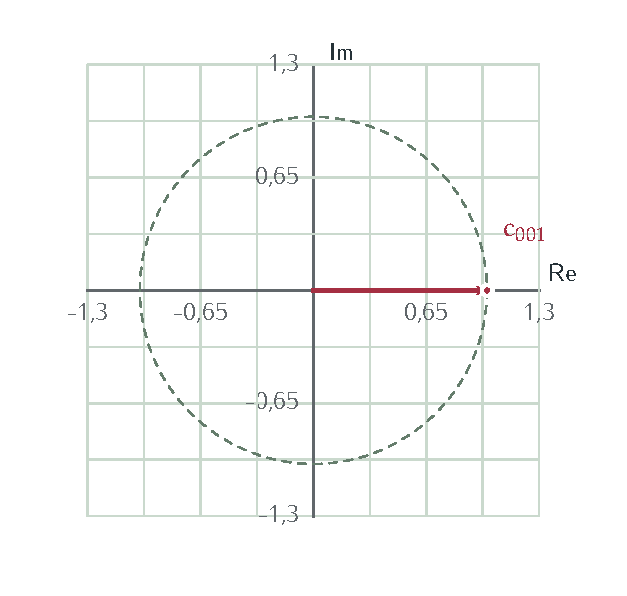
\includegraphics[width=\linewidth,height=63mm,keepaspectratio]{figure/fbe2c6b143853cc14.pdf}\par{\sffamily\footnotesize \(c_{001}\)\par}\end{minipage}\FigureCaption{4.04 \(\cdot\) esempio 3 \(\cdot\) Componenti complesse}\end{FigureBlock}
\begin{FigureBlock}\begin{minipage}[t]{.485\linewidth}\centering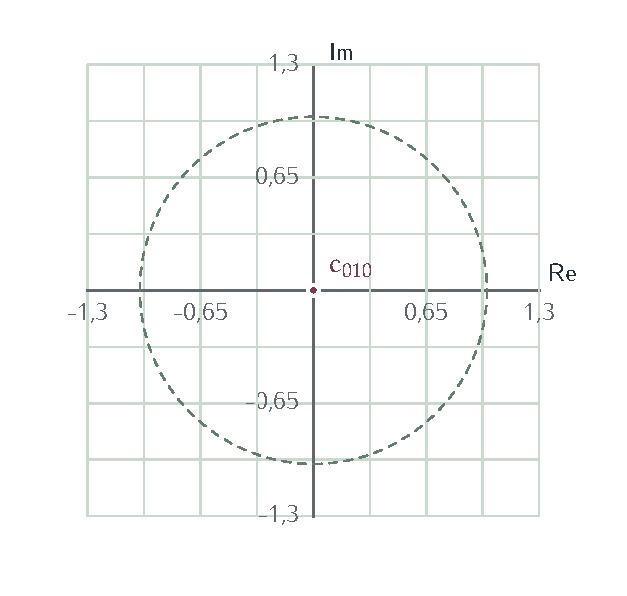
\includegraphics[width=\linewidth,height=63mm,keepaspectratio]{figure/f7c8917f8cfa80807.pdf}\par{\sffamily\footnotesize \(c_{010}\)\par}\end{minipage}\hfill\begin{minipage}[t]{.485\linewidth}\centering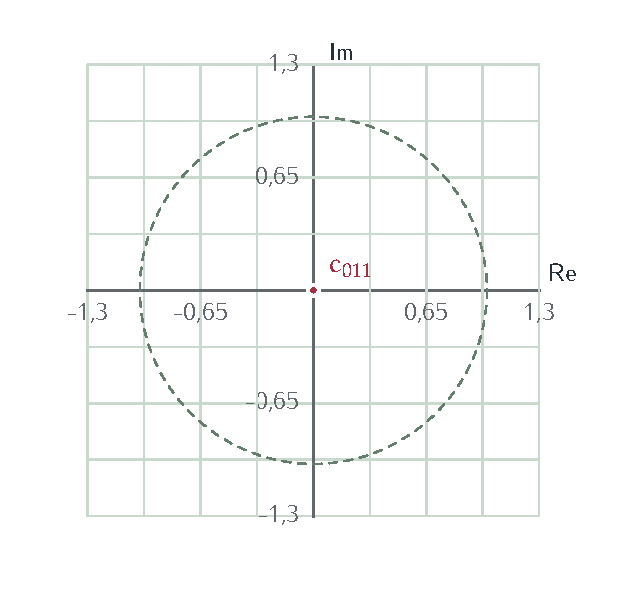
\includegraphics[width=\linewidth,height=63mm,keepaspectratio]{figure/f97fefd54a806db37.pdf}\par{\sffamily\footnotesize \(c_{011}\)\par}\end{minipage}\FigureCaption{4.04 \(\cdot\) esempio 3 \(\cdot\) Componenti complesse}\end{FigureBlock}
\begin{FigureBlock}\begin{minipage}[t]{.485\linewidth}\centering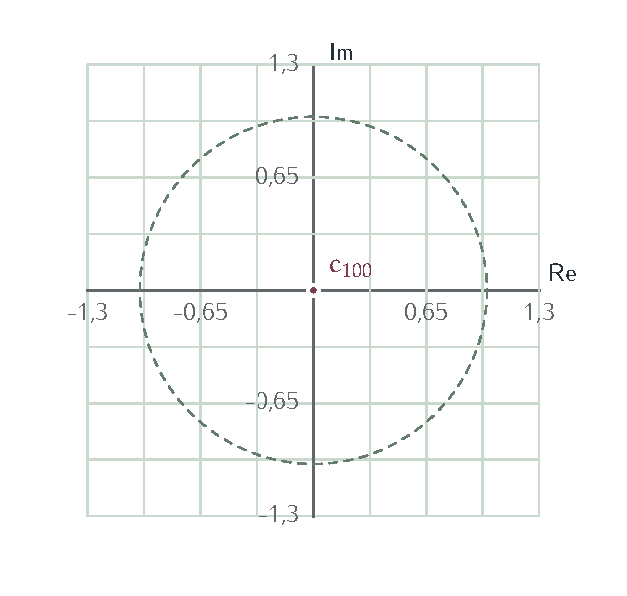
\includegraphics[width=\linewidth,height=63mm,keepaspectratio]{figure/fb7bb520de112a94f.pdf}\par{\sffamily\footnotesize \(c_{100}\)\par}\end{minipage}\hfill\begin{minipage}[t]{.485\linewidth}\centering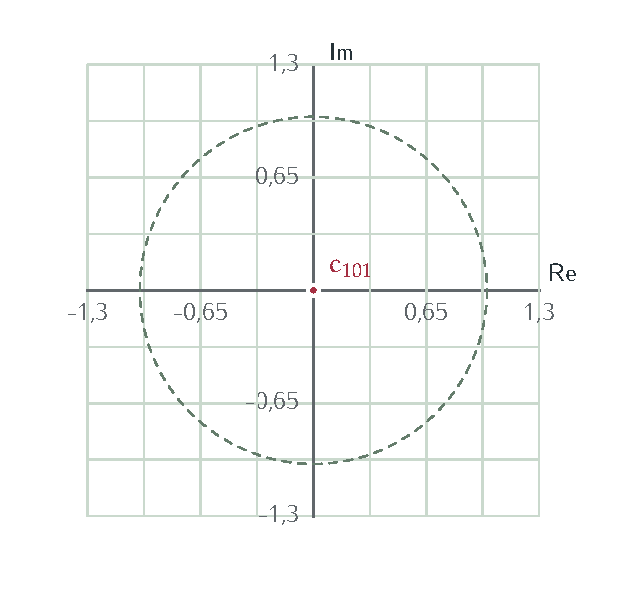
\includegraphics[width=\linewidth,height=63mm,keepaspectratio]{figure/f80c3d629b3b1115f.pdf}\par{\sffamily\footnotesize \(c_{101}\)\par}\end{minipage}\FigureCaption{4.04 \(\cdot\) esempio 3 \(\cdot\) Componenti complesse}\end{FigureBlock}
\begin{FigureBlock}\begin{minipage}[t]{.485\linewidth}\centering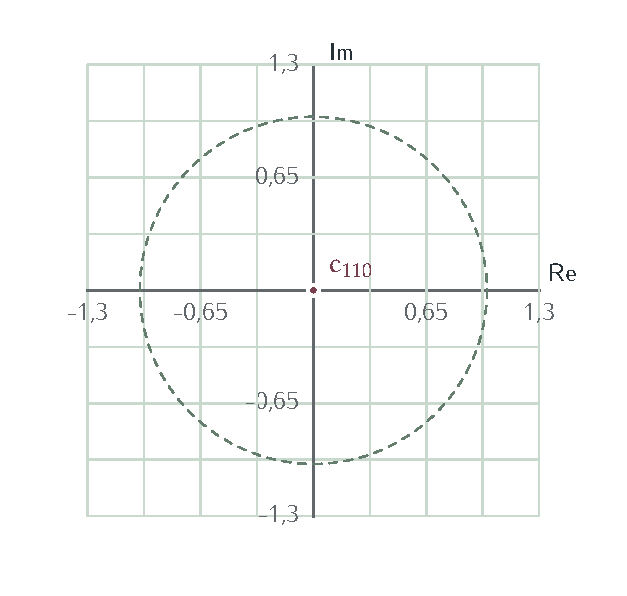
\includegraphics[width=\linewidth,height=63mm,keepaspectratio]{figure/f05a0672d6a4d3b44.pdf}\par{\sffamily\footnotesize \(c_{110}\)\par}\end{minipage}\hfill\begin{minipage}[t]{.485\linewidth}\centering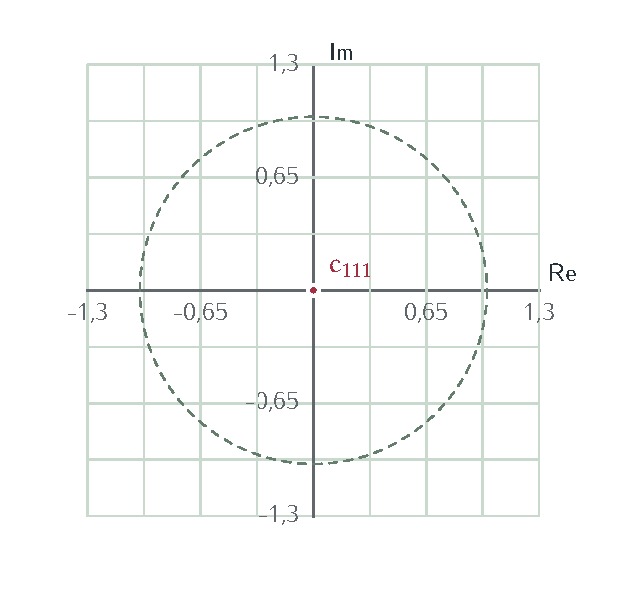
\includegraphics[width=\linewidth,height=63mm,keepaspectratio]{figure/f82da60d62b18d1aa.pdf}\par{\sffamily\footnotesize \(c_{111}\)\par}\end{minipage}\FigureCaption{4.04 \(\cdot\) esempio 3 \(\cdot\) Componenti complesse}\end{FigureBlock}

\phantomsection\label{c4-swap-example-3-step-1}
\BookHeading{01 Preparazione}

\MathBlock{03C82080003D00280030003B00200031003B00200030003B00200030003B00200030003B00200030003B00200030003B0020003000291D40003B0020201603C82080201600B222480031}{\psi _{0}=(0;\allowbreak \ 1;\allowbreak \ 0;\allowbreak \ 0;\allowbreak \ 0;\allowbreak \ 0;\allowbreak \ 0;\allowbreak \ 0)^{T};\allowbreak \ \Vert \psi _{0}\Vert ^{2}\approx 1}

Le ampiezze sono ordinate secondo le etichette binarie, con il bit più significativo in alto.\par


\phantomsection\label{c4-swap-example-3-step-2}
\BookHeading{02 Porta 1 \(\cdot\) \(H\)}

\MathBlock{0063002800300030003100290020003D002000280030002C0037003000370031002900B70028003100290020002B002000280030002C0037003000370031002900B70028003000290020224800200030002C0037003000370031}{c(001)\ =\ (0{,}7071)\cdot (1)\ +\ (0{,}7071)\cdot (0)\ \approx \ 0{,}7071}
\MathBlock{0063002800310030003100290020003D002000280030002C0037003000370031002900B70028003100290020002B00200028002D0030002C0037003000370031002900B70028003000290020224800200030002C0037003000370031}{c(101)\ =\ (0{,}7071)\cdot (1)\ +\ (-0{,}7071)\cdot (0)\ \approx \ 0{,}7071}
\MathBlock{03C800202248002000280030003B00200030002C0037003000370031003B00200030003B00200030003B00200030003B00200030002C0037003000370031003B00200030003B0020003000291D40}{\psi \ \approx \ (0;\allowbreak \ 0{,}7071;\allowbreak \ 0;\allowbreak \ 0;\allowbreak \ 0;\allowbreak \ 0{,}7071;\allowbreak \ 0;\allowbreak \ 0)^{T}}

Ogni coppia di ampiezze indicata usa il prodotto riga per colonna della porta. I rami con controllo nullo restano invariati.\par


\phantomsection\label{c4-swap-example-3-step-3}
\BookHeading{03 Porta 2 \(\cdot\) C\(\cdot\)X}

\MathBlock{0063002800300030003100290020003D002000280030002900B700280030002C003700300037003100290020002B002000280031002900B70028003000290020224800200030}{c(001)\ =\ (0)\cdot (0{,}7071)\ +\ (1)\cdot (0)\ \approx \ 0}
\MathBlock{0063002800300031003100290020003D002000280031002900B700280030002C003700300037003100290020002B002000280030002900B70028003000290020224800200030002C0037003000370031}{c(011)\ =\ (1)\cdot (0{,}7071)\ +\ (0)\cdot (0)\ \approx \ 0{,}7071}
\MathBlock{0063002800310030003100290020003D002000280030002900B700280030002C003700300037003100290020002B002000280031002900B70028003000290020224800200030}{c(101)\ =\ (0)\cdot (0{,}7071)\ +\ (1)\cdot (0)\ \approx \ 0}
\MathBlock{0063002800310031003100290020003D002000280031002900B700280030002C003700300037003100290020002B002000280030002900B70028003000290020224800200030002C0037003000370031}{c(111)\ =\ (1)\cdot (0{,}7071)\ +\ (0)\cdot (0)\ \approx \ 0{,}7071}
\MathBlock{03C800202248002000280030003B00200030003B00200030003B00200030002C0037003000370031003B00200030003B00200030003B00200030003B00200030002C003700300037003100291D40}{\psi \ \approx \ (0;\allowbreak \ 0;\allowbreak \ 0;\allowbreak \ 0{,}7071;\allowbreak \ 0;\allowbreak \ 0;\allowbreak \ 0;\allowbreak \ 0{,}7071)^{T}}

Ogni coppia di ampiezze indicata usa il prodotto riga per colonna della porta. I rami con controllo nullo restano invariati.\par


\phantomsection\label{c4-swap-example-3-step-4}
\BookHeading{04 Porta 3 \(\cdot\) C\(\cdot\)X}

\MathBlock{0063002800310031003000290020003D002000280030002900B70028003000290020002B002000280031002900B700280030002C003700300037003100290020224800200030002C0037003000370031}{c(110)\ =\ (0)\cdot (0)\ +\ (1)\cdot (0{,}7071)\ \approx \ 0{,}7071}
\MathBlock{0063002800310031003100290020003D002000280031002900B70028003000290020002B002000280030002900B700280030002C003700300037003100290020224800200030}{c(111)\ =\ (1)\cdot (0)\ +\ (0)\cdot (0{,}7071)\ \approx \ 0}
\MathBlock{03C800202248002000280030003B00200030003B00200030003B00200030002C0037003000370031003B00200030003B00200030003B00200030002C0037003000370031003B0020003000291D40}{\psi \ \approx \ (0;\allowbreak \ 0;\allowbreak \ 0;\allowbreak \ 0{,}7071;\allowbreak \ 0;\allowbreak \ 0;\allowbreak \ 0{,}7071;\allowbreak \ 0)^{T}}

Ogni coppia di ampiezze indicata usa il prodotto riga per colonna della porta. I rami con controllo nullo restano invariati.\par


\phantomsection\label{c4-swap-example-3-step-5}
\BookHeading{05 Porta 4 \(\cdot\) C\(\cdot\)X}

\MathBlock{0063002800300030003100290020003D002000280030002900B70028003000290020002B002000280031002900B700280030002C003700300037003100290020224800200030002C0037003000370031}{c(001)\ =\ (0)\cdot (0)\ +\ (1)\cdot (0{,}7071)\ \approx \ 0{,}7071}
\MathBlock{0063002800300031003100290020003D002000280031002900B70028003000290020002B002000280030002900B700280030002C003700300037003100290020224800200030}{c(011)\ =\ (1)\cdot (0)\ +\ (0)\cdot (0{,}7071)\ \approx \ 0}
\MathBlock{03C800202248002000280030003B00200030002C0037003000370031003B00200030003B00200030003B00200030003B00200030003B00200030002C0037003000370031003B0020003000291D40}{\psi \ \approx \ (0;\allowbreak \ 0{,}7071;\allowbreak \ 0;\allowbreak \ 0;\allowbreak \ 0;\allowbreak \ 0;\allowbreak \ 0{,}7071;\allowbreak \ 0)^{T}}

Ogni coppia di ampiezze indicata usa il prodotto riga per colonna della porta. I rami con controllo nullo restano invariati.\par


\phantomsection\label{c4-swap-example-3-step-6}
\BookHeading{06 Porta 5 \(\cdot\) \(H\)}

\MathBlock{0063002800300030003100290020003D002000280030002C0037003000370031002900B700280030002C003700300037003100290020002B002000280030002C0037003000370031002900B70028003000290020224800200030002C0035}{c(001)\ =\ (0{,}7071)\cdot (0{,}7071)\ +\ (0{,}7071)\cdot (0)\ \approx \ 0{,}5}
\MathBlock{0063002800310030003100290020003D002000280030002C0037003000370031002900B700280030002C003700300037003100290020002B00200028002D0030002C0037003000370031002900B70028003000290020224800200030002C0035}{c(101)\ =\ (0{,}7071)\cdot (0{,}7071)\ +\ (-0{,}7071)\cdot (0)\ \approx \ 0{,}5}
\MathBlock{0063002800300031003000290020003D002000280030002C0037003000370031002900B70028003000290020002B002000280030002C0037003000370031002900B700280030002C003700300037003100290020224800200030002C0035}{c(010)\ =\ (0{,}7071)\cdot (0)\ +\ (0{,}7071)\cdot (0{,}7071)\ \approx \ 0{,}5}
\MathBlock{0063002800310031003000290020003D002000280030002C0037003000370031002900B70028003000290020002B00200028002D0030002C0037003000370031002900B700280030002C00370030003700310029002022480020002D0030002C0035}{c(110)\ =\ (0{,}7071)\cdot (0)\ +\ (-0{,}7071)\cdot (0{,}7071)\ \approx \ -0{,}5}
\MathBlock{03C800202248002000280030003B00200030002C0035003B00200030002C0035003B00200030003B00200030003B00200030002C0035003B0020002D0030002C0035003B0020003000291D40}{\psi \ \approx \ (0;\allowbreak \ 0{,}5;\allowbreak \ 0{,}5;\allowbreak \ 0;\allowbreak \ 0;\allowbreak \ 0{,}5;\allowbreak \ -0{,}5;\allowbreak \ 0)^{T}}

Ogni coppia di ampiezze indicata usa il prodotto riga per colonna della porta. I rami con controllo nullo restano invariati.\par


\phantomsection\label{c4-swap-example-3-step-7}
\BookHeading{07 Lettura nella base finale}

\MathBlock{005000280030003000300029003D00280030002900B20020002B002000280030002900B222480030}{P(000)=(0)^{2}\ +\ (0)^{2}\approx 0}
\MathBlock{005000280030003000310029003D00280030002C0035002900B20020002B002000280030002900B222480030002C00320035}{P(001)=(0{,}5)^{2}\ +\ (0)^{2}\approx 0{,}25}
\MathBlock{005000280030003100300029003D00280030002C0035002900B20020002B002000280030002900B222480030002C00320035}{P(010)=(0{,}5)^{2}\ +\ (0)^{2}\approx 0{,}25}
\MathBlock{005000280030003100310029003D00280030002900B20020002B002000280030002900B222480030}{P(011)=(0)^{2}\ +\ (0)^{2}\approx 0}
\MathBlock{005000280031003000300029003D00280030002900B20020002B002000280030002900B222480030}{P(100)=(0)^{2}\ +\ (0)^{2}\approx 0}
\MathBlock{005000280031003000310029003D00280030002C0035002900B20020002B002000280030002900B222480030002C00320035}{P(101)=(0{,}5)^{2}\ +\ (0)^{2}\approx 0{,}25}
\MathBlock{005000280031003100300029003D0028002D0030002C0035002900B20020002B002000280030002900B222480030002C00320035}{P(110)=(-0{,}5)^{2}\ +\ (0)^{2}\approx 0{,}25}
\MathBlock{005000280031003100310029003D00280030002900B20020002B002000280030002900B222480030}{P(111)=(0)^{2}\ +\ (0)^{2}\approx 0}

Il modulo quadro di ciascuna ampiezza determina la probabilità. La selezione di una porta nel disegno mostra uno stato intermedio senza effettuare una misura.\par


\phantomsection\label{c4-swap-example-3-step-8}
\BookHeading{08 Verifica con il prodotto interno}

\MathBlock{27E80075007C007627E9003D00280031002900B70028003000290020002B002000280030002900B700280031002922480030}{\langle u|v\rangle =(1)\cdot (0)\ +\ (0)\cdot (1)\approx 0}
\MathBlock{0050002800300029003D00280031002B00300029002F0032003D0030002C0035}{P(0)=(1+0)/2=0{,}5}

Espandendo la norma della somma dei due prodotti tensoriali si ottengono due termini diagonali e due termini di sovrapposizione.\par


\phantomsection\label{c4-swap-example-3-step-9}
\BookHeading{09 Sommare i rami del bersaglio}

\MathBlock{005000280061003D00300029003D005000280030003000300029002B005000280030003000310029002B005000280030003100300029002B005000280030003100310029}{P(a=0)=P(000)+P(001)+P(010)+P(011)}
\MathBlock{003D0030002B0030002C00320035002B0030002C00320035002B0030003D0030002C0035002E}{=0+0{,}25+0{,}25+0=0{,}5.}
\MathBlock{005000280061003D00310029003D00312212005000280061003D00300029003D0030002C0035002E}{P(a=1)=1- P(a=0)=0{,}5.}

La lettura dell'ausiliario somma le quattro alternative ortogonali dei due bersagli.\par


\BookHeading{Stato finale del programma}
\begin{FigureBlock}\centering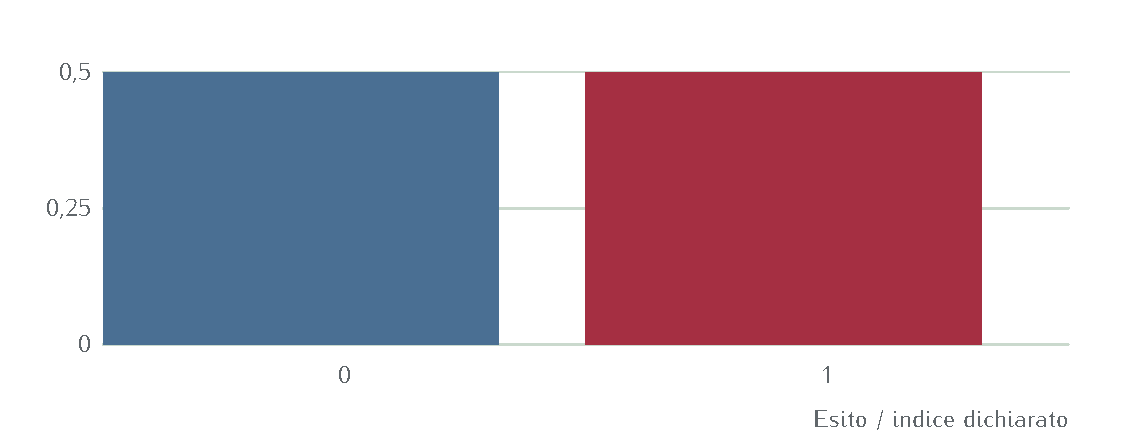
\includegraphics[width=\linewidth,height=94mm,keepaspectratio]{figure/fa54a943484c63f24.pdf}\FigureCaption{4.04 \(\cdot\) esempio 3 \(\cdot\) Misura dell'ausiliario}\end{FigureBlock}

\BookHeading{Interpretazione}

Il prodotto interno ha modulo quadro 0; la probabilità di leggere 0 sull'ausiliario è 0,5.\par


Risorse dichiarate. 3 qubit; 5 operazioni alla granularità dichiarata nel circuito.\par


\Needspace{7\baselineskip}
\BookHeading{Il passaggio successivo}
Il prodotto interno quantifica anche la componente di uno stato lungo una direzione assegnata. Grover usa proiezioni e riflessioni per accrescere la componente nello spazio delle soluzioni.\par


% Authoritative exercise source. Preserve all derivations and diagrams.

\ExerciseStart{G4.03}{Stimare una sovrapposizione mediante SWAP test}{Guida esplicita}

\BookHeading{Problema, dati e obiettivo}

Eseguire lo SWAP test per \(\ket\psi=\ket0\) e \(\ket\phi=\ket+=(\ket0+\ket1)/\sqrt2\). Calcolare lo stato complessivo, le probabilità del controllo e gli stati condizionati dei due dati. Confrontare stati uguali e ortogonali.

\ExTheory{\ExRef{c4-swap}{4.04}}{Il circuito prepara il controllo con H, applica SWAP ai dati quando il controllo vale uno, poi applica H al controllo. Per stati puri normalizzati, \(P(0)=(1+|\langle\psi|\phi\rangle|^2)/2\). Tale formula va ricavata dalla norma dei due vettori simmetrizzati.}

\ExPrediction{I due vettori prodotto \(\psi\otimes\phi\) e \(\phi\otimes\psi\) condividono il contributo 00. La somma dovrebbe avere norma maggiore della differenza.}

\ExFigure{\begin{tikzpicture}[>=Stealth,exlabel]
\node[exbox] (n0) at (0.0,0.0) {$H$ sul controllo};\node[exbox] (n1) at (3.6,0.0) {SWAP controllato};\draw[exother] (n0)--(n1);\node[exbox] (n2) at (7.2,0.0) {$H$ e misura};\draw[exother] (n1)--(n2);
\end{tikzpicture}}{La simmetria dei due dati diventa una probabilità sul controllo.}


\begin{ExTasks}

\item Scrivere i due stati prodotto.

\item Seguire H e SWAP controllato.

\item Applicare l’ultima H e raccogliere i rami.

\item Calcolare e normalizzare ciascun ramo.

\item Verificare la formula generale e i due casi limite.

\end{ExTasks}

\ExSolution

\ExStep{Costruire i dati}

\ExEq{\ket\psi\ket\phi&=(\ket{00}+\ket{01})/\sqrt2,\\
\ket\phi\ket\psi&=(\ket{00}+\ket{10})/\sqrt2.}

\ExStep{Controllare lo scambio}

Dopo la prima H e la porta controllata,
\ExEq{\ket{\Psi_1}&=\frac{\ket0\ket\psi\ket\phi+\ket1\ket\phi\ket\psi}{\sqrt2}.}
Il controllo rimane coerente con i due ordini dei dati.

\ExStep{Ricombinare il controllo}

\ExEq{\ket{\Psi_f}&=\frac{\ket0(\ket\psi\ket\phi+\ket\phi\ket\psi)}2
+\frac{\ket1(\ket\psi\ket\phi-\ket\phi\ket\psi)}2.}
Il ramo 0 dei dati è \((2\ket{00}+\ket{01}+\ket{10})/(2\sqrt2)\); il ramo 1 è \((\ket{01}-\ket{10})/(2\sqrt2)\).

\ExStep{Calcolare i rami}

\ExEq{P(0)&=(4+1+1)/8=3/4,\qquad P(1)=(1+1)/8=1/4.}
Dividendo per le radici delle probabilità si ottengono gli stati condizionati
\ExEq{\ket{\chi_0}&=(2\ket{00}+\ket{01}+\ket{10})/\sqrt6,\\
\ket{\chi_1}&=(\ket{01}-\ket{10})/\sqrt2.}

\ExStep{Ricavare il prodotto interno}

Ponendo \(a=\psi\otimes\phi\), \(b=\phi\otimes\psi\), si ha
\ExEq{\langle a|b\rangle&=\langle\psi|\phi\rangle\langle\phi|\psi\rangle
=|\langle\psi|\phi\rangle|^2,\\
\|a+b\|^2&=1+1+2|\langle\psi|\phi\rangle|^2.}
La divisione per 4 dà la formula di \(P(0)\). Qui \(\langle0|+\rangle=1/\sqrt2\), quindi \(P(0)=(1+1/2)/2=3/4\).

\ExStep{Controllare i limiti}

Per stati uguali il modulo quadro del prodotto interno è uno: \(P(0)=1\). Per stati ortogonali è zero: \(P(0)=1/2\). Un esito 1 certifica che gli stati puri confrontati non coincidono a meno di fase globale; un solo esito 0 non certifica l’uguaglianza.

\par\noindent\begin{minipage}{\linewidth}
\ExFigure{\begin{tikzpicture}[>=Stealth,exlabel]
\draw[exaxis] (-.6,0)--(2.2,0) node[right] {esito};\draw[exaxis] (-.6,0)--(-.6,3.6) node[above] {$p$};\node[left] at (-.6,3) {$ 1 $};\draw[Ink!15,dashed] (-.6,3)--(1.7000000000000002,3);\filldraw[fill=Accent!25,draw=Accent] (0.0,0) rectangle (0.65,2.25);\node[below] at (0.325,0) {$ 0 $};\node[above] at (0.325,2.25) {$ 0.75 $};\filldraw[fill=Accent!25,draw=Accent] (1.1,0) rectangle (1.75,0.75);\node[below] at (1.425,0) {$ 1 $};\node[above] at (1.425,0.75) {$ 0.25 $};
\end{tikzpicture}}{Lettura del controllo per \(\ket0\) e \(\ket+\).}


\ExInterpret{Il test misura una proprietà della coppia senza ricostruire tutte le ampiezze dei due stati. La derivazione mostra quali termini incrociati contengano la sovrapposizione.}

\ExLab{Nella sezione 4.04 confrontare «Stati |0\(\rangle\) e |+\(\rangle\)», «Stati uguali» e «Stati ortogonali |0\(\rangle\) e |1\(\rangle\)». Controllare la marginale del controllo, sommando i rami dei dati.}


\end{minipage}

\Needspace{.43\textheight}
\section{Grover: iterazioni e sovrarotazione}
\phantomsection\label{c4-grover}

{\sffamily\small\color{Ink!70} Riferimento alle slide: p. 132.\par}

{\sffamily\small\color{Ink!70} Laboratorio locale: \nolinkurl{index.html#capitolo-4/grover}\par}

\BookHeading{Definizioni e costruzione}
Sia \(G\) l'insieme delle \(M\) soluzioni fra \(N\) etichette, con \(0<M<N\). La ricerca mantiene lo stato in un piano di dimensione due, anche quando il registro completo possiede \(N\) ampiezze.\par

Definiamo \(|g\rangle =\sum _{x}\in G|x\rangle /\sqrt{M}\) e \(|b\rangle =\sum _{x}\notin G|x\rangle /\sqrt{N- M}\). I supporti disgiunti e le normalizzazioni li rendono ortonormali. Lo stato uniforme è \(|s\rangle =\sqrt{1- M/N}|b\rangle +\sqrt{M/N}|g\rangle \). Scegliamo \(\theta \in (0,\allowbreak \pi /2)\) con \(\sin ^{2}\theta =M/N\): le sue coordinate sono \((\cos \theta ,\allowbreak \sin \theta )\).\par

Il proiettore sui marcati è \(\Pi _{G}=\sum _{x}\in G|x\rangle \langle x|\). L'oracolo \(O=I- 2\Pi _{G}\) ha matrice \(\operatorname{diag}(1,\allowbreak - 1)\) nel piano. La diffusione \(D=2|s\rangle \langle s|- I\) ha matrice \(\begin{pmatrix}\cos 2\theta &\sin 2\theta \\\sin 2\theta &- \cos 2\theta \end{pmatrix}\). Moltiplicando nell'ordine \(Q=DO\) otteniamo \(\begin{pmatrix}\cos 2\theta &- \sin 2\theta \\\sin 2\theta &\cos 2\theta \end{pmatrix}\), una rotazione di \(2\theta \).\par

Dopo k iterazioni le coordinate diventano \((\cos ((2k+1)\theta ),\allowbreak \sin ((2k+1)\theta ))\). Il successo cresce fino alla zona dell'asse g e poi diminuisce: il numero di iterazioni deve essere scelto in funzione di \(\theta \). In termini di query all'oracolo, per \(M\) piccolo rispetto a \(N\) servono circa \((\pi /4)\sqrt{N/M}\) iterazioni; il costo per costruire un oracolo è una questione separata.\par

Se \(M=0\) manca la direzione g e la probabilità buona è sempre zero; se \(M=N\) manca b e vale già uno. Questi casi non richiedono la base bidimensionale. Il primo Grover del modulo 3 è il caso \(\theta =\pi /6\): dopo una iterazione \((2k+1)\theta =\pi /2\).\par


\MathBlock{0051007C007327E9003D0063006F0073003303B8007C006227E9002B00730069006E003303B8007C006727E9003B002000500073007500630063006500730073006F0028006B0029003D00730069006E00B2002800280032006B002B0031002903B80029002E}{Q|s\rangle =\cos 3\theta |b\rangle +\sin 3\theta |g\rangle ;\allowbreak \ \text{Psuccesso}(k)=\sin ^{2}((2k+1)\theta ).}

\BookHeading{Come leggere le figure}
Il piano usa assi ortonormali b e g e coordinate di ampiezza reali adimensionali. La riflessione dell'oracolo attraversa l'asse b; quella della diffusione attraversa la retta di \(|s\rangle \). I quadrati delle proiezioni danno le probabilità dei due gruppi.\par


\BookHeading{Attività nel laboratorio modificabile}

\BookHeading{Obiettivo dell'esperimento}
Studiare amplificazione, sovrarotazione e casi degeneri.\par

\BookHeading{Percorso operativo}
Cambiare numero di qubit, insieme delle soluzioni e iterazioni.\par

\BookHeading{Lettura geometrica}
Le due riflessioni producono una rotazione nel piano generato dalla preparazione e dalla componente favorevole.\par

\BookHeading{Controllo del risultato}
Confrontare la simulazione con la formula geometrica; gestire separatamente probabilità iniziali zero e uno.\par


\Needspace{.36\textheight}\phantomsection\label{c4-grover-example-1}
{\sffamily\small\color{Accent} ESEMPIO SVOLTO 1\par}
\BookHeading{Due riflessioni nel piano della ricerca}
\(N=8\); \(G=\{5\}\); \(k=2\). I blocchi selezionabili sono preparazione, oracolo e diffusione.\par


\BookHeading{Geometria e configurazione dell'esempio}
\begin{FigureBlock}\centering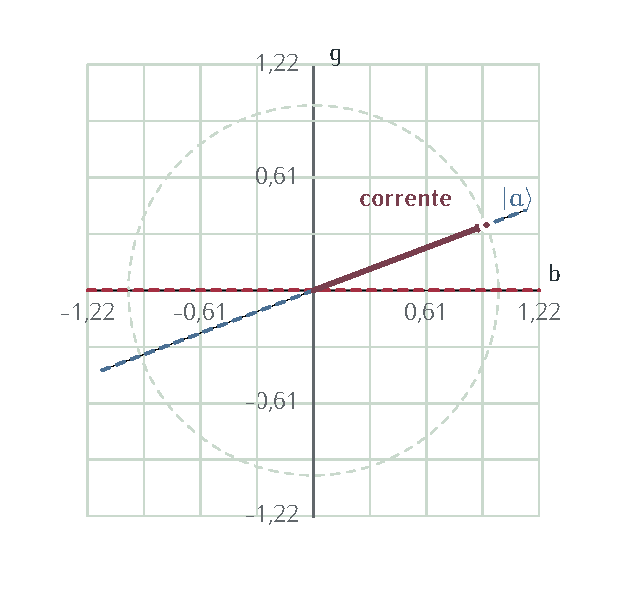
\includegraphics[width=\linewidth,height=94mm,keepaspectratio]{figure/fac8fd60fd5479cf4.pdf}\FigureCaption{4.05 \(\cdot\) esempio 1 \(\cdot\) Piano collettivo \(\cdot\) Preparazione \(A|0\rangle \)}\end{FigureBlock}
\begin{FigureBlock}\centering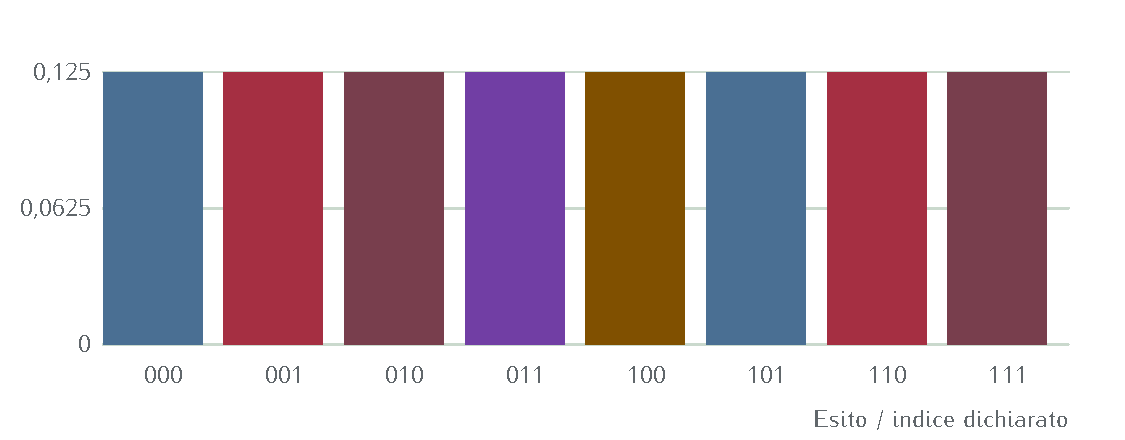
\includegraphics[width=\linewidth,height=94mm,keepaspectratio]{figure/feb3fd36cc710b240.pdf}\FigureCaption{4.05 \(\cdot\) esempio 1 \(\cdot\) Distribuzione congiunta \(\cdot\) Preparazione \(A|0\rangle \)}\end{FigureBlock}
\begin{FigureBlock}\centering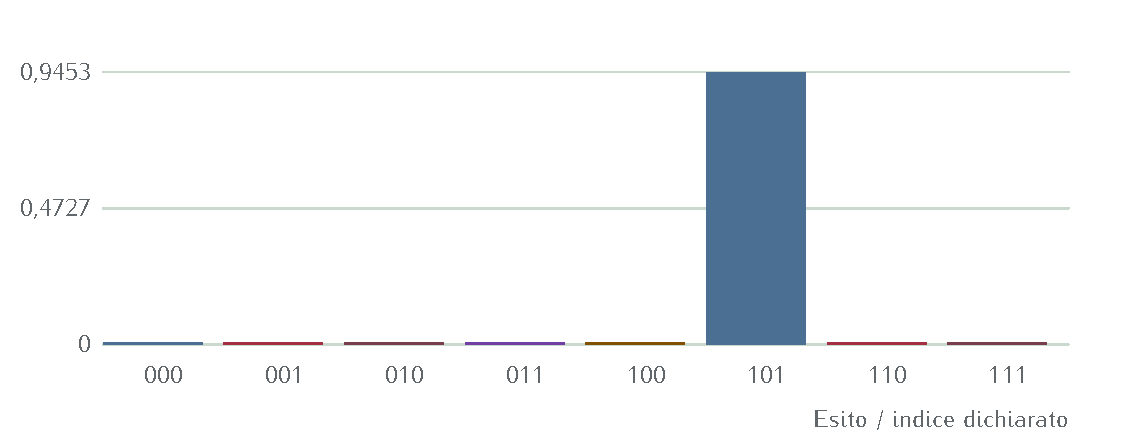
\includegraphics[width=\linewidth,height=94mm,keepaspectratio]{figure/f5f5fd113d8749998.pdf}\FigureCaption{4.05 \(\cdot\) esempio 1 \(\cdot\) Probabilità finali delle singole alternative}\end{FigureBlock}
\begin{FigureBlock}\centering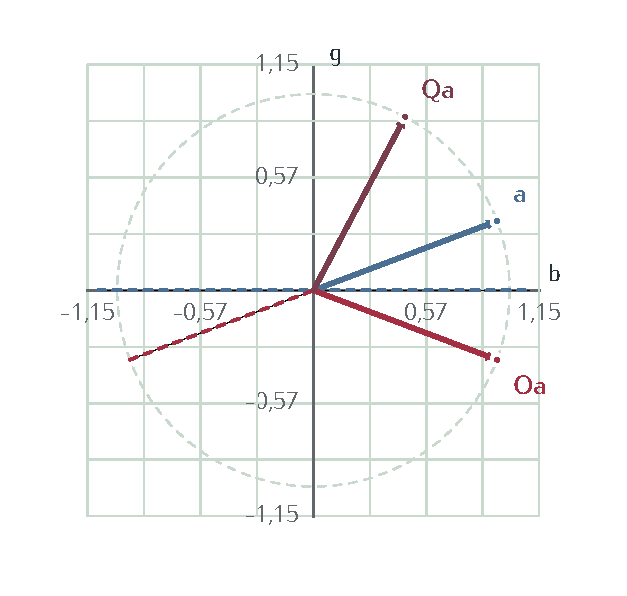
\includegraphics[width=\linewidth,height=94mm,keepaspectratio]{figure/f9ee22fd3ab6b0294.pdf}\FigureCaption{4.05 \(\cdot\) esempio 1 \(\cdot\) Prima iterazione \(\cdot\) una freccia dopo ogni riflessione}\end{FigureBlock}
\begin{FigureBlock}\begin{minipage}[t]{.485\linewidth}\centering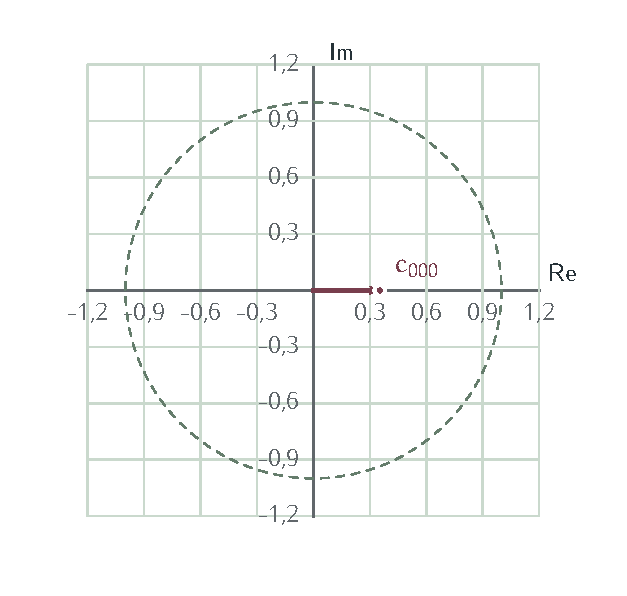
\includegraphics[width=\linewidth,height=63mm,keepaspectratio]{figure/fea83f3dc1c351f0f.pdf}\par{\sffamily\footnotesize \(c_{000}\)\par}\end{minipage}\hfill\begin{minipage}[t]{.485\linewidth}\centering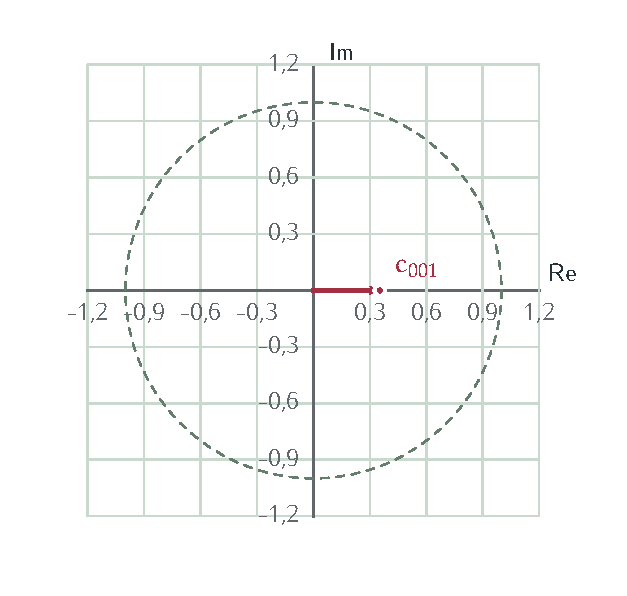
\includegraphics[width=\linewidth,height=63mm,keepaspectratio]{figure/f9a6c8e9369ba8ade.pdf}\par{\sffamily\footnotesize \(c_{001}\)\par}\end{minipage}\FigureCaption{4.05 \(\cdot\) esempio 1 \(\cdot\) Componenti complesse}\end{FigureBlock}
\begin{FigureBlock}\begin{minipage}[t]{.485\linewidth}\centering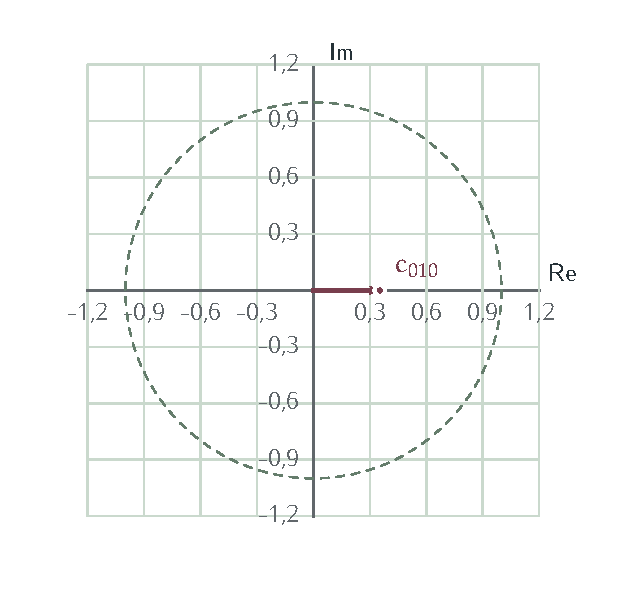
\includegraphics[width=\linewidth,height=63mm,keepaspectratio]{figure/f34431090ae32cc6f.pdf}\par{\sffamily\footnotesize \(c_{010}\)\par}\end{minipage}\hfill\begin{minipage}[t]{.485\linewidth}\centering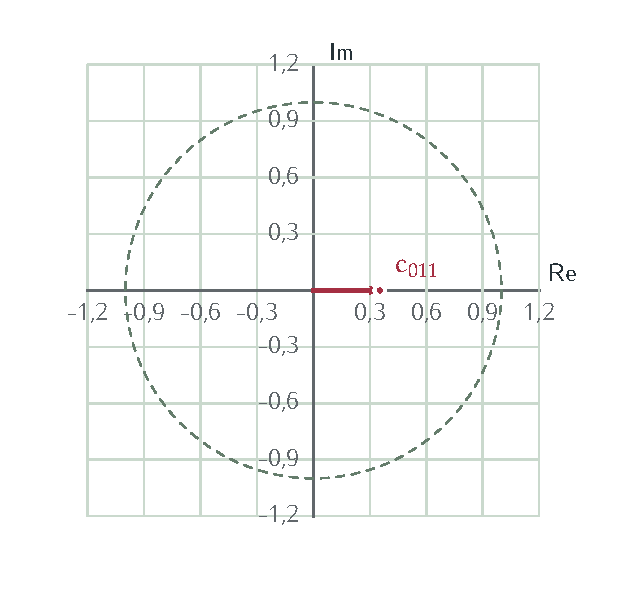
\includegraphics[width=\linewidth,height=63mm,keepaspectratio]{figure/fede21cd43be07a3b.pdf}\par{\sffamily\footnotesize \(c_{011}\)\par}\end{minipage}\FigureCaption{4.05 \(\cdot\) esempio 1 \(\cdot\) Componenti complesse}\end{FigureBlock}
\begin{FigureBlock}\begin{minipage}[t]{.485\linewidth}\centering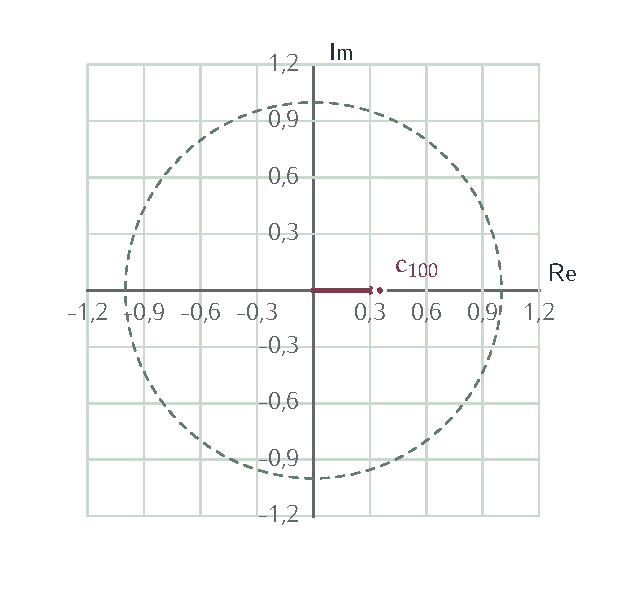
\includegraphics[width=\linewidth,height=63mm,keepaspectratio]{figure/fadada9da0777f61c.pdf}\par{\sffamily\footnotesize \(c_{100}\)\par}\end{minipage}\hfill\begin{minipage}[t]{.485\linewidth}\centering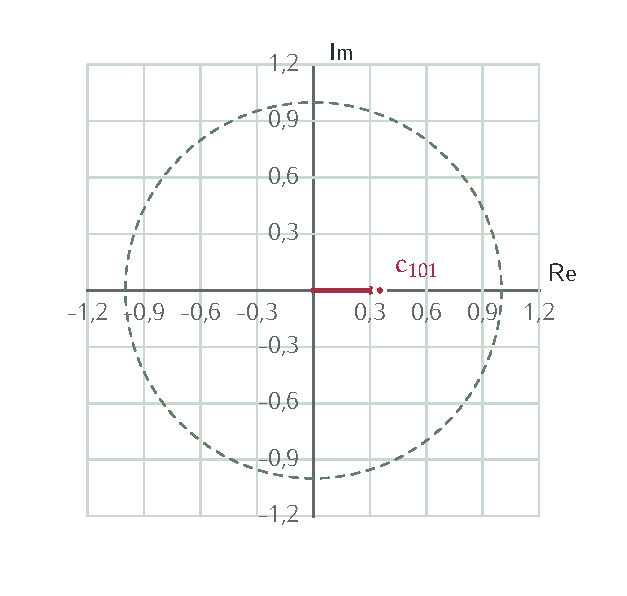
\includegraphics[width=\linewidth,height=63mm,keepaspectratio]{figure/f38e66b3d9670a7b7.pdf}\par{\sffamily\footnotesize \(c_{101}\)\par}\end{minipage}\FigureCaption{4.05 \(\cdot\) esempio 1 \(\cdot\) Componenti complesse}\end{FigureBlock}
\begin{FigureBlock}\begin{minipage}[t]{.485\linewidth}\centering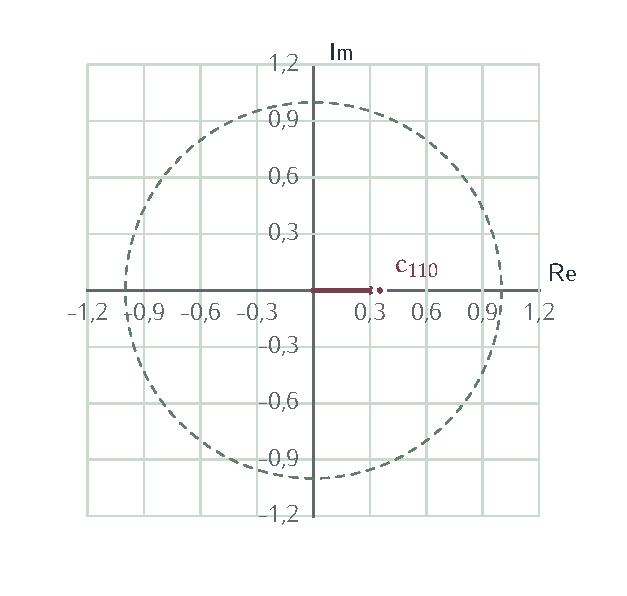
\includegraphics[width=\linewidth,height=63mm,keepaspectratio]{figure/f41086b755ca89910.pdf}\par{\sffamily\footnotesize \(c_{110}\)\par}\end{minipage}\hfill\begin{minipage}[t]{.485\linewidth}\centering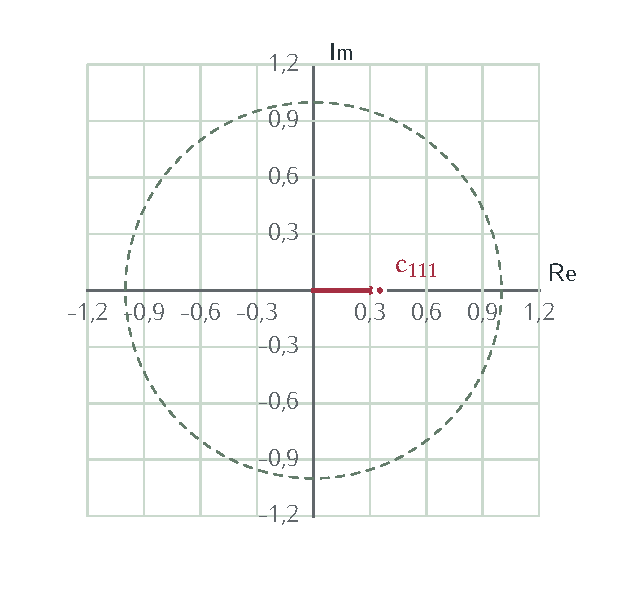
\includegraphics[width=\linewidth,height=63mm,keepaspectratio]{figure/f6600e00a033acb2a.pdf}\par{\sffamily\footnotesize \(c_{111}\)\par}\end{minipage}\FigureCaption{4.05 \(\cdot\) esempio 1 \(\cdot\) Componenti complesse}\end{FigureBlock}

\phantomsection\label{c4-grover-example-1-step-1}
\BookHeading{01 Costruire gli assi dalle proiezioni}

\MathBlock{007C006127E9003D0041007C003027E9003B002003A00047003D03A3007822080047007C007827E927E80078007C003B00200070003D27E80061007C03A00047007C006127E9003D0030002C003100320035002E}{|a\rangle =A|0\rangle ;\allowbreak \ \Pi _{G}=\sum _{x\in G}|x\rangle \langle x|;\allowbreak \ p=\langle a|\Pi _{G}|a\rangle =0{,}125.}
\MathBlock{007C006727E9003D03A00047007C006127E9002F221A0070224800280030003B00200030003B00200030003B00200030003B00200030003B00200031003B00200030003B0020003000291D40}{|g\rangle =\Pi _{G}|a\rangle /\sqrt{p}\approx (0;\allowbreak \ 0;\allowbreak \ 0;\allowbreak \ 0;\allowbreak \ 0;\allowbreak \ 1;\allowbreak \ 0;\allowbreak \ 0)^{T}}
\MathBlock{007C006227E9003D00280049221203A000470029007C006127E9002F221A00280031221200700029224800280030002C003300370038003B00200030002C003300370038003B00200030002C003300370038003B00200030002C003300370038003B00200030002C003300370038003B00200030003B00200030002C003300370038003B00200030002C00330037003800291D40002E}{|b\rangle =(I- \Pi _{G})|a\rangle /\sqrt{1- p}\approx (0{,}378;\allowbreak \ 0{,}378;\allowbreak \ 0{,}378;\allowbreak \ 0{,}378;\allowbreak \ 0{,}378;\allowbreak \ 0;\allowbreak \ 0{,}378;\allowbreak \ 0{,}378)^{T}.}
\MathBlock{27E80062007C006727E9003D0030003B0020201600622016003D201600672016003D0031002E}{\langle b|g\rangle =0;\allowbreak \ \Vert b\Vert =\Vert g\Vert =1.}

I supporti sono disgiunti. Per la preparazione uniforme questi vettori diventano \(\sum _{x\in G}|x\rangle /\sqrt{M}\) e \(\sum x\notin G|x\rangle /\sqrt{N- M}\). Per una preparazione non uniforme conservano i suoi pesi e le sue fasi.\par


\phantomsection\label{c4-grover-example-1-step-2}
\BookHeading{02 Proiettare la preparazione nel piano}

\MathBlock{27E80062007C006127E9003D221A00280031221200700029003D0030002C003900330035003400310034003B002027E80067007C006127E9003D221A0070003D0030002C003300350033003500350033002E}{\langle b|a\rangle =\sqrt{1- p}=0{,}935414;\allowbreak \ \langle g|a\rangle =\sqrt{p}=0{,}353553.}
\MathBlock{007C006127E9003D0063006F007303B8007C006227E9002B00730069006E03B8007C006727E9003B002003B8003D00610072006300730069006E221A007022480030002C0033003600310033003600370020007200610064002E}{|a\rangle =\cos \theta |b\rangle +\sin \theta |g\rangle ;\allowbreak \ \theta =\arcsin \sqrt{p}\approx 0{,}361367\ \text{rad}.}

Gli assi sono stati collettivi, non singoli esiti. Le coordinate qui sono reali perché le fasi della preparazione sono state incluse nella definizione degli assi.\par


\phantomsection\label{c4-grover-example-1-step-3}
\BookHeading{03 Scrivere le due riflessioni}

\MathBlock{004E0065006C006C0061002000620061007300650020006F007200640069006E00610074006100200028007C006227E9002C007C006727E90029003A}{\text{Nella}\ \text{base}\ \text{ordinata}\ (|b\rangle ,\allowbreak |g\rangle ):}
\MathBlock{004F003D00492212003203A00047003D005B005B0031002C0030005D002C005B0030002C22120031005D005D002E}{O=I- 2\Pi _{G}=\begin{pmatrix}1&0\\0&- 1\end{pmatrix}.}
\MathBlock{0044005F0041003D0032007C006127E927E80061007C22120049}{D_{A}=2|a\rangle \langle a|- I}
\MathBlock{003D005B005B00320063006F007300B203B822120031002C00320063006F007303B800730069006E03B8005D002C005B00320063006F007303B800730069006E03B8002C003200730069006E00B203B822120031005D005D}{=\begin{pmatrix}2\cos ^{2}\theta - 1&2\cos \theta \sin \theta \\2\cos \theta \sin \theta &2\sin ^{2}\theta - 1\end{pmatrix}}
\MathBlock{003D005B005B0063006F0073003203B8002C00730069006E003203B8005D002C005B00730069006E003203B8002C22120063006F0073003203B8005D005D002E}{=\begin{pmatrix}\cos 2\theta &\sin 2\theta \\\sin 2\theta &- \cos 2\theta \end{pmatrix}.}

\(O\) riflette rispetto all'asse \(|b\rangle \). \(D_{A}\) riflette rispetto alla retta della preparazione \(|a\rangle \). L'ordine temporale è prima \(O\) e poi \(D_{A}\).\par


\phantomsection\label{c4-grover-example-1-step-4}
\BookHeading{04 Moltiplicare e ottenere la rotazione}

\MathBlock{0051003D0044005F0041004F003D005B005B0063006F0073003203B8002C221200730069006E003203B8005D002C005B00730069006E003203B8002C0063006F0073003203B8005D005D}{Q=D_{AO}=\begin{pmatrix}\cos 2\theta &- \sin 2\theta \\\sin 2\theta &\cos 2\theta \end{pmatrix}}
\MathBlock{2248005B005B0030002C00370035002C002D0030002C003600360031003400330038005D002C005B0030002C003600360031003400330038002C0030002C00370035005D005D002E}{\approx \begin{pmatrix}0{,}75&-0{,}661438\\0{,}661438&0{,}75\end{pmatrix}.}
\MathBlock{004F00280063006F007303B8002C00730069006E03B800291D40003D00280063006F007303B8002C221200730069006E03B800291D40003B}{O(\cos \theta ,\allowbreak \sin \theta )^{T}=(\cos \theta ,\allowbreak - \sin \theta )^{T};\allowbreak }
\MathBlock{005100280063006F007303B8002C00730069006E03B800291D40003D00280063006F0073003303B8002C00730069006E003303B800291D40002E}{Q(\cos \theta ,\allowbreak \sin \theta )^{T}=(\cos 3\theta ,\allowbreak \sin 3\theta )^{T}.}
\MathBlock{00511D4F007C006127E9003D0063006F0073002800280032006B002B0031002903B80029007C006227E9002B00730069006E002800280032006B002B0031002903B80029007C006727E9002E}{Q^{k}|a\rangle =\cos ((2k+1)\theta )|b\rangle +\sin ((2k+1)\theta )|g\rangle .}

Il prodotto riga per colonna dà le formule di addizione del seno e del coseno. Ogni coppia completa di riflessioni ruota di \(2\theta \); dopo il solo oracolo si usa invece la riflessione, non la formula delle iterazioni complete.\par


\phantomsection\label{c4-grover-example-1-step-5}
\BookHeading{05 Ricavare autovettori e autofasi}

\MathBlock{00640065007400280051221203BB00490029003D03BB00B2221200320063006F00730028003203B8002903BB002B0031003D0030002E}{\det (Q- \lambda I)=\lambda ^{2}- 2\cos (2\theta )\lambda +1=0.}
\MathBlock{03BB00B1003D0063006F0073003203B800B10069002000730069006E003203B8003D0065005E002800B10032006903B80029002E}{\lambda \pm =\cos 2\theta \pm i\ \sin 2\theta =e^{\pm 2i\theta }.}
\MathBlock{007C0075002B27E9003D0028007C006227E922120069007C006727E90029002F221A0032003B0020007C0075221227E9003D0028007C006227E9002B0069007C006727E90029002F221A0032002E}{|u+\rangle =(|b\rangle - i|g\rangle )/\sqrt{2};\allowbreak \ |u- \rangle =(|b\rangle +i|g\rangle )/\sqrt{2}.}
\MathBlock{0051007C007500B127E9003D0065005E002800B10032006903B80029007C007500B127E9003B002003C6002B003D03B8002F03C0002C002003C62212003D0031221203B8002F03C000200028006D006F0064002000310029002E}{Q|u\pm \rangle =e^{\pm 2i\theta }|u\pm \rangle ;\allowbreak \ \varphi +=\theta /\pi ,\allowbreak \ \varphi - =1- \theta /\pi \ (\bmod \ 1).}

Gli autovettori hanno coordinate complesse nel piano collettivo; non sono due frecce reali sul piano di Grover. Le autofasi sono frazioni di giro, poiché QPE usa \(e^{2\pi i\varphi }\).\par


\phantomsection\label{c4-grover-example-1-step-6}
\BookHeading{06 Determinare i coefficienti della preparazione}

\MathBlock{03B2002B003D27E80075002B007C006127E9003D00280063006F007303B8002B0069002000730069006E03B80029002F221A0032003D0065005E0028006903B80029002F221A0032002E}{\beta +=\langle u+|a\rangle =(\cos \theta +i\ \sin \theta )/\sqrt{2}=e^{i\theta }/\sqrt{2}.}
\MathBlock{03B22212003D27E800752212007C006127E9003D00280063006F007303B822120069002000730069006E03B80029002F221A0032003D0065005E00282212006903B80029002F221A0032002E}{\beta - =\langle u- |a\rangle =(\cos \theta - i\ \sin \theta )/\sqrt{2}=e^{- i\theta }/\sqrt{2}.}
\MathBlock{007C006127E9003D03B2002B007C0075002B27E9002B03B22212007C0075221227E9003B0020007C03B2002B007C00B2003D007C03B22212007C00B2003D0031002F0032002E}{|a\rangle =\beta +|u+\rangle +\beta - |u- \rangle ;\allowbreak \ |\beta +|^{2}=|\beta - |^{2}=1/2.}

I due pesi uguali derivano dal prodotto interno con la preparazione. Manteniamo anche le fasi dei coefficienti: servono per ricostruire il bersaglio coerente condizionato dopo QPE.\par


\phantomsection\label{c4-grover-example-1-step-7}
\BookHeading{07 Preparazione \(A|0\rangle \)}

\MathBlock{00280030002C0033003500330036003B00200030002C0033003500330036003B00200030002C0033003500330036003B00200030002C0033003500330036003B00200030002C0033003500330036003B00200030002C0033003500330036003B00200030002C0033003500330036003B00200030002C003300350033003600291D40}{(0{,}3536;\allowbreak \ 0{,}3536;\allowbreak \ 0{,}3536;\allowbreak \ 0{,}3536;\allowbreak \ 0{,}3536;\allowbreak \ 0{,}3536;\allowbreak \ 0{,}3536;\allowbreak \ 0{,}3536)^{T}}
\MathBlock{03C8224800280030002C0033003500330036003B00200030002C0033003500330036003B00200030002C0033003500330036003B00200030002C0033003500330036003B00200030002C0033003500330036003B00200030002C0033003500330036003B00200030002C0033003500330036003B00200030002C003300350033003600291D40}{\psi \approx (0{,}3536;\allowbreak \ 0{,}3536;\allowbreak \ 0{,}3536;\allowbreak \ 0{,}3536;\allowbreak \ 0{,}3536;\allowbreak \ 0{,}3536;\allowbreak \ 0{,}3536;\allowbreak \ 0{,}3536)^{T}}
\MathBlock{0043006F006F007200640069006E0061007400650020002827E80062007C03C827E9002C27E80067007C03C827E90029224800280030002C003900330035003400310034003B00200030002C0033003500330035003500330029}{\text{Coordinate}\ (\langle b|\psi \rangle ,\allowbreak \langle g|\psi \rangle )\approx (0{,}935414;\allowbreak \ 0{,}353553)}

La marcatura cambia il segno delle ampiezze buone; la riflessione usa il prodotto interno con la preparazione.\par


\phantomsection\label{c4-grover-example-1-step-8}
\BookHeading{08 Oracolo 1}

\MathBlock{004F007C007827E90020003D00200028221200310029005E005B007822080047005D007C007827E9003B00200047003D007B0035007D}{O|x\rangle \ =\ (- 1)^{x\in G}|x\rangle ;\allowbreak \ G=\{5\}}
\MathBlock{03C8224800280030002C0033003500330036003B00200030002C0033003500330036003B00200030002C0033003500330036003B00200030002C0033003500330036003B00200030002C0033003500330036003B0020002D0030002C0033003500330036003B00200030002C0033003500330036003B00200030002C003300350033003600291D40}{\psi \approx (0{,}3536;\allowbreak \ 0{,}3536;\allowbreak \ 0{,}3536;\allowbreak \ 0{,}3536;\allowbreak \ 0{,}3536;\allowbreak \ -0{,}3536;\allowbreak \ 0{,}3536;\allowbreak \ 0{,}3536)^{T}}
\MathBlock{0043006F006F007200640069006E0061007400650020002827E80062007C03C827E9002C27E80067007C03C827E90029224800280030002C003900330035003400310034003B0020002D0030002C0033003500330035003500330029}{\text{Coordinate}\ (\langle b|\psi \rangle ,\allowbreak \langle g|\psi \rangle )\approx (0{,}935414;\allowbreak \ -0{,}353553)}

La marcatura cambia il segno delle ampiezze buone; la riflessione usa il prodotto interno con la preparazione.\par


\phantomsection\label{c4-grover-example-1-step-9}
\BookHeading{09 Riflessione 1}

\MathBlock{27E80061007C007627E90020003D002000280030002C0033003500330036002900B700280030002C003300350033003600290020002B002000280030002C0033003500330036002900B700280030002C003300350033003600290020002B002000280030002C0033003500330036002900B700280030002C003300350033003600290020002B002000280030002C0033003500330036002900B700280030002C003300350033003600290020002B002000280030002C0033003500330036002900B700280030002C003300350033003600290020002B002000280030002C0033003500330036002900B70028002D0030002C003300350033003600290020002B002000280030002C0033003500330036002900B700280030002C003300350033003600290020002B002000280030002C0033003500330036002900B700280030002C003300350033003600290020224800200030002C00370035}{\langle a|v\rangle \ =\ (0{,}3536)\cdot (0{,}3536)\ +\ (0{,}3536)\cdot (0{,}3536)\ +\ (0{,}3536)\cdot (0{,}3536)\ +\ (0{,}3536)\cdot (0{,}3536)\ +\ (0{,}3536)\cdot (0{,}3536)\ +\ (0{,}3536)\cdot (-0{,}3536)\ +\ (0{,}3536)\cdot (0{,}3536)\ +\ (0{,}3536)\cdot (0{,}3536)\ \approx \ 0{,}75}
\MathBlock{00630028003000290020003D0020003200B700280030002C0033003500330036002900B700280030002C00370035002900202212002000280030002C003300350033003600290020224800200030002C0031003700360038}{c(0)\ =\ 2\cdot (0{,}3536)\cdot (0{,}75)\ - \ (0{,}3536)\ \approx \ 0{,}1768}
\MathBlock{00630028003100290020003D0020003200B700280030002C0033003500330036002900B700280030002C00370035002900202212002000280030002C003300350033003600290020224800200030002C0031003700360038}{c(1)\ =\ 2\cdot (0{,}3536)\cdot (0{,}75)\ - \ (0{,}3536)\ \approx \ 0{,}1768}
\MathBlock{00630028003200290020003D0020003200B700280030002C0033003500330036002900B700280030002C00370035002900202212002000280030002C003300350033003600290020224800200030002C0031003700360038}{c(2)\ =\ 2\cdot (0{,}3536)\cdot (0{,}75)\ - \ (0{,}3536)\ \approx \ 0{,}1768}
\MathBlock{00630028003300290020003D0020003200B700280030002C0033003500330036002900B700280030002C00370035002900202212002000280030002C003300350033003600290020224800200030002C0031003700360038}{c(3)\ =\ 2\cdot (0{,}3536)\cdot (0{,}75)\ - \ (0{,}3536)\ \approx \ 0{,}1768}
\MathBlock{00630028003400290020003D0020003200B700280030002C0033003500330036002900B700280030002C00370035002900202212002000280030002C003300350033003600290020224800200030002C0031003700360038}{c(4)\ =\ 2\cdot (0{,}3536)\cdot (0{,}75)\ - \ (0{,}3536)\ \approx \ 0{,}1768}
\MathBlock{00630028003500290020003D0020003200B700280030002C0033003500330036002900B700280030002C0037003500290020221200200028002D0030002C003300350033003600290020224800200030002C0038003800330039}{c(5)\ =\ 2\cdot (0{,}3536)\cdot (0{,}75)\ - \ (-0{,}3536)\ \approx \ 0{,}8839}
\MathBlock{00630028003600290020003D0020003200B700280030002C0033003500330036002900B700280030002C00370035002900202212002000280030002C003300350033003600290020224800200030002C0031003700360038}{c(6)\ =\ 2\cdot (0{,}3536)\cdot (0{,}75)\ - \ (0{,}3536)\ \approx \ 0{,}1768}
\MathBlock{00630028003700290020003D0020003200B700280030002C0033003500330036002900B700280030002C00370035002900202212002000280030002C003300350033003600290020224800200030002C0031003700360038}{c(7)\ =\ 2\cdot (0{,}3536)\cdot (0{,}75)\ - \ (0{,}3536)\ \approx \ 0{,}1768}
\MathBlock{03C8224800280030002C0031003700360038003B00200030002C0031003700360038003B00200030002C0031003700360038003B00200030002C0031003700360038003B00200030002C0031003700360038003B00200030002C0038003800330039003B00200030002C0031003700360038003B00200030002C003100370036003800291D40}{\psi \approx (0{,}1768;\allowbreak \ 0{,}1768;\allowbreak \ 0{,}1768;\allowbreak \ 0{,}1768;\allowbreak \ 0{,}1768;\allowbreak \ 0{,}8839;\allowbreak \ 0{,}1768;\allowbreak \ 0{,}1768)^{T}}
\MathBlock{0043006F006F007200640069006E0061007400650020002827E80062007C03C827E9002C27E80067007C03C827E90029224800280030002C003400360037003700300037003B00200030002C0038003800330038003800330029}{\text{Coordinate}\ (\langle b|\psi \rangle ,\allowbreak \langle g|\psi \rangle )\approx (0{,}467707;\allowbreak \ 0{,}883883)}

La marcatura cambia il segno delle ampiezze buone; la riflessione usa il prodotto interno con la preparazione.\par


\phantomsection\label{c4-grover-example-1-step-10}
\BookHeading{10 Oracolo 2}

\MathBlock{004F007C007827E90020003D00200028221200310029005E005B007822080047005D007C007827E9003B00200047003D007B0035007D}{O|x\rangle \ =\ (- 1)^{x\in G}|x\rangle ;\allowbreak \ G=\{5\}}
\MathBlock{03C8224800280030002C0031003700360038003B00200030002C0031003700360038003B00200030002C0031003700360038003B00200030002C0031003700360038003B00200030002C0031003700360038003B0020002D0030002C0038003800330039003B00200030002C0031003700360038003B00200030002C003100370036003800291D40}{\psi \approx (0{,}1768;\allowbreak \ 0{,}1768;\allowbreak \ 0{,}1768;\allowbreak \ 0{,}1768;\allowbreak \ 0{,}1768;\allowbreak \ -0{,}8839;\allowbreak \ 0{,}1768;\allowbreak \ 0{,}1768)^{T}}
\MathBlock{0043006F006F007200640069006E0061007400650020002827E80062007C03C827E9002C27E80067007C03C827E90029224800280030002C003400360037003700300037003B0020002D0030002C0038003800330038003800330029}{\text{Coordinate}\ (\langle b|\psi \rangle ,\allowbreak \langle g|\psi \rangle )\approx (0{,}467707;\allowbreak \ -0{,}883883)}

La marcatura cambia il segno delle ampiezze buone; la riflessione usa il prodotto interno con la preparazione.\par


\phantomsection\label{c4-grover-example-1-step-11}
\BookHeading{11 Riflessione 2}

\MathBlock{27E80061007C007627E90020003D002000280030002C0033003500330036002900B700280030002C003100370036003800290020002B002000280030002C0033003500330036002900B700280030002C003100370036003800290020002B002000280030002C0033003500330036002900B700280030002C003100370036003800290020002B002000280030002C0033003500330036002900B700280030002C003100370036003800290020002B002000280030002C0033003500330036002900B700280030002C003100370036003800290020002B002000280030002C0033003500330036002900B70028002D0030002C003800380033003900290020002B002000280030002C0033003500330036002900B700280030002C003100370036003800290020002B002000280030002C0033003500330036002900B700280030002C003100370036003800290020224800200030002C003100320035}{\langle a|v\rangle \ =\ (0{,}3536)\cdot (0{,}1768)\ +\ (0{,}3536)\cdot (0{,}1768)\ +\ (0{,}3536)\cdot (0{,}1768)\ +\ (0{,}3536)\cdot (0{,}1768)\ +\ (0{,}3536)\cdot (0{,}1768)\ +\ (0{,}3536)\cdot (-0{,}8839)\ +\ (0{,}3536)\cdot (0{,}1768)\ +\ (0{,}3536)\cdot (0{,}1768)\ \approx \ 0{,}125}
\MathBlock{00630028003000290020003D0020003200B700280030002C0033003500330036002900B700280030002C003100320035002900202212002000280030002C00310037003600380029002022480020002D0030002C0030003800380034}{c(0)\ =\ 2\cdot (0{,}3536)\cdot (0{,}125)\ - \ (0{,}1768)\ \approx \ -0{,}0884}
\MathBlock{00630028003100290020003D0020003200B700280030002C0033003500330036002900B700280030002C003100320035002900202212002000280030002C00310037003600380029002022480020002D0030002C0030003800380034}{c(1)\ =\ 2\cdot (0{,}3536)\cdot (0{,}125)\ - \ (0{,}1768)\ \approx \ -0{,}0884}
\MathBlock{00630028003200290020003D0020003200B700280030002C0033003500330036002900B700280030002C003100320035002900202212002000280030002C00310037003600380029002022480020002D0030002C0030003800380034}{c(2)\ =\ 2\cdot (0{,}3536)\cdot (0{,}125)\ - \ (0{,}1768)\ \approx \ -0{,}0884}
\MathBlock{00630028003300290020003D0020003200B700280030002C0033003500330036002900B700280030002C003100320035002900202212002000280030002C00310037003600380029002022480020002D0030002C0030003800380034}{c(3)\ =\ 2\cdot (0{,}3536)\cdot (0{,}125)\ - \ (0{,}1768)\ \approx \ -0{,}0884}
\MathBlock{00630028003400290020003D0020003200B700280030002C0033003500330036002900B700280030002C003100320035002900202212002000280030002C00310037003600380029002022480020002D0030002C0030003800380034}{c(4)\ =\ 2\cdot (0{,}3536)\cdot (0{,}125)\ - \ (0{,}1768)\ \approx \ -0{,}0884}
\MathBlock{00630028003500290020003D0020003200B700280030002C0033003500330036002900B700280030002C00310032003500290020221200200028002D0030002C003800380033003900290020224800200030002C0039003700320033}{c(5)\ =\ 2\cdot (0{,}3536)\cdot (0{,}125)\ - \ (-0{,}8839)\ \approx \ 0{,}9723}
\MathBlock{00630028003600290020003D0020003200B700280030002C0033003500330036002900B700280030002C003100320035002900202212002000280030002C00310037003600380029002022480020002D0030002C0030003800380034}{c(6)\ =\ 2\cdot (0{,}3536)\cdot (0{,}125)\ - \ (0{,}1768)\ \approx \ -0{,}0884}
\MathBlock{00630028003700290020003D0020003200B700280030002C0033003500330036002900B700280030002C003100320035002900202212002000280030002C00310037003600380029002022480020002D0030002C0030003800380034}{c(7)\ =\ 2\cdot (0{,}3536)\cdot (0{,}125)\ - \ (0{,}1768)\ \approx \ -0{,}0884}
\MathBlock{03C822480028002D0030002C0030003800380034003B0020002D0030002C0030003800380034003B0020002D0030002C0030003800380034003B0020002D0030002C0030003800380034003B0020002D0030002C0030003800380034003B00200030002C0039003700320033003B0020002D0030002C0030003800380034003B0020002D0030002C003000380038003400291D40}{\psi \approx (-0{,}0884;\allowbreak \ -0{,}0884;\allowbreak \ -0{,}0884;\allowbreak \ -0{,}0884;\allowbreak \ -0{,}0884;\allowbreak \ 0{,}9723;\allowbreak \ -0{,}0884;\allowbreak \ -0{,}0884)^{T}}
\MathBlock{0043006F006F007200640069006E0061007400650020002827E80062007C03C827E9002C27E80067007C03C827E9002922480028002D0030002C003200330033003800350034003B00200030002C0039003700320032003700320029}{\text{Coordinate}\ (\langle b|\psi \rangle ,\allowbreak \langle g|\psi \rangle )\approx (-0{,}233854;\allowbreak \ 0{,}972272)}

La marcatura cambia il segno delle ampiezze buone; la riflessione usa il prodotto interno con la preparazione.\par


\phantomsection\label{c4-grover-example-1-step-12}
\BookHeading{12 Probabilità di successo}

\MathBlock{00702080003D0030002C003100320035003B002003B8003D00610072006300730069006E221A0070208022480030002C00330036003100340020007200610064}{p_{0}=0{,}125;\allowbreak \ \theta =\arcsin \sqrt{p}_{0}\approx 0{,}3614\ \text{rad}}
\MathBlock{00500073007500630063006500730073006F003D03A3007822080047007C00632093007C00B222480030002C0039003400350033}{\text{Psuccesso}=\sum _{x\in G}|c_{x}|^{2}\approx 0{,}9453}
\MathBlock{00730069006E00B2002800280032006B002B0031002903B80029003D00730069006E00B20028003500B70030002C0033003600310034002922480030002C0039003400350033}{\sin ^{2}((2k+1)\theta )=\sin ^{2}(5\cdot 0{,}3614)\approx 0{,}9453}

La formula geometrica verifica la simulazione delle ampiezze.\par


\BookHeading{Stato finale del programma}
\begin{FigureBlock}\centering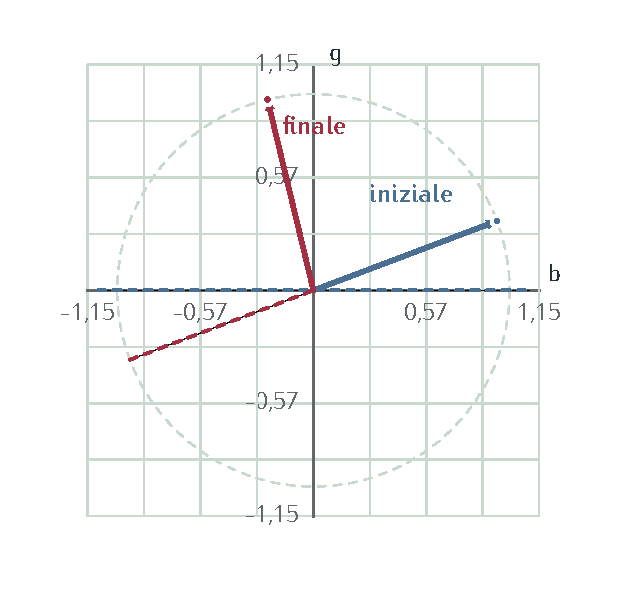
\includegraphics[width=\linewidth,height=94mm,keepaspectratio]{figure/f27d2e711b260338c.pdf}\FigureCaption{4.05 \(\cdot\) esempio 1 \(\cdot\) Piano \(|b\rangle ,\allowbreak |g\rangle \) \(\cdot\) confronto iniziale/finale}\end{FigureBlock}

\BookHeading{Interpretazione}

Il piano ha assi ortonormali ricavati dalla preparazione. Ogni freccia intermedia e le probabilità delle alternative derivano dai medesimi vettori del registro.\par


Risorse dichiarate. 2 interrogazioni all'oracolo; 3 qubit dati. Il costo della preparazione e della riflessione va aggiunto.\par


\Needspace{.36\textheight}\phantomsection\label{c4-grover-example-2}
{\sffamily\small\color{Accent} ESEMPIO SVOLTO 2\par}
\BookHeading{Due riflessioni nel piano della ricerca}
\(N=8\); \(G=\{1{,}5\}\); \(k=2\). I blocchi selezionabili sono preparazione, oracolo e diffusione.\par


\BookHeading{Geometria e configurazione dell'esempio}
\begin{FigureBlock}\centering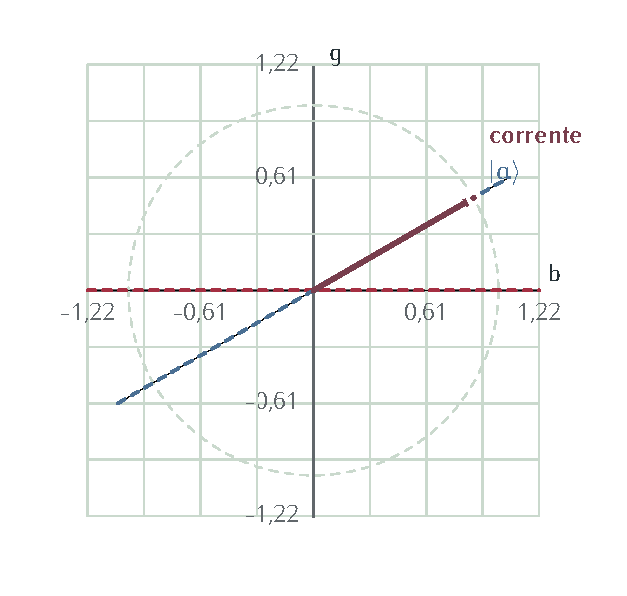
\includegraphics[width=\linewidth,height=94mm,keepaspectratio]{figure/fc8b73794ed7cf4e9.pdf}\FigureCaption{4.05 \(\cdot\) esempio 2 \(\cdot\) Piano collettivo \(\cdot\) Preparazione \(A|0\rangle \)}\end{FigureBlock}
\begin{FigureBlock}\centering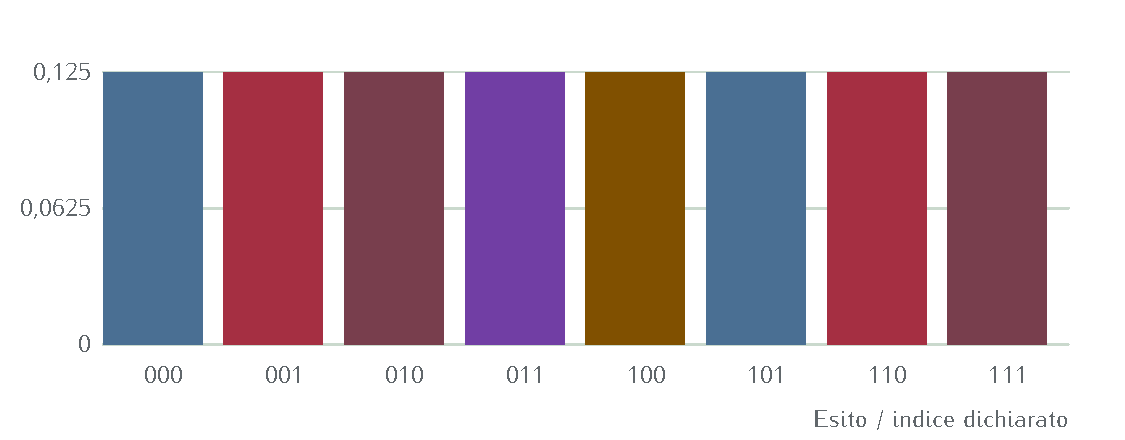
\includegraphics[width=\linewidth,height=94mm,keepaspectratio]{figure/feb3fd36cc710b240.pdf}\FigureCaption{4.05 \(\cdot\) esempio 2 \(\cdot\) Distribuzione congiunta \(\cdot\) Preparazione \(A|0\rangle \)}\end{FigureBlock}
\begin{FigureBlock}\centering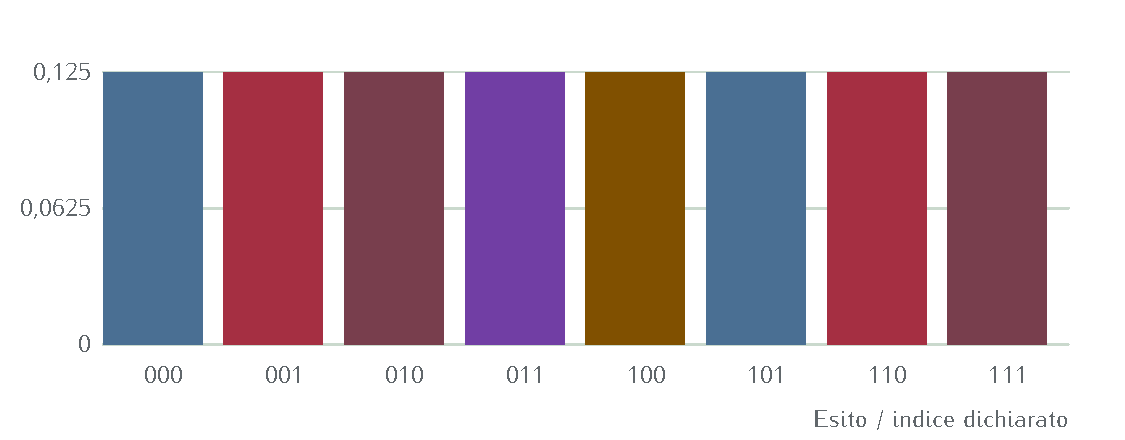
\includegraphics[width=\linewidth,height=94mm,keepaspectratio]{figure/f8b3588567ff9650b.pdf}\FigureCaption{4.05 \(\cdot\) esempio 2 \(\cdot\) Probabilità finali delle singole alternative}\end{FigureBlock}
\begin{FigureBlock}\centering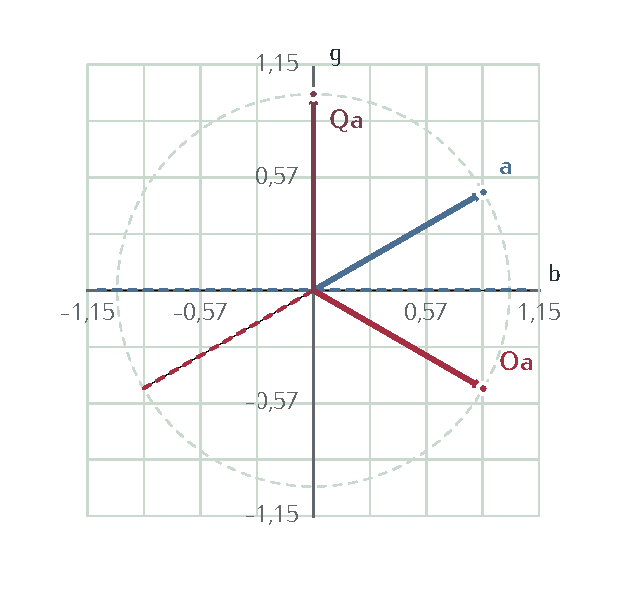
\includegraphics[width=\linewidth,height=94mm,keepaspectratio]{figure/f48c0ed5c3b2452cf.pdf}\FigureCaption{4.05 \(\cdot\) esempio 2 \(\cdot\) Prima iterazione \(\cdot\) una freccia dopo ogni riflessione}\end{FigureBlock}
\begin{FigureBlock}\begin{minipage}[t]{.485\linewidth}\centering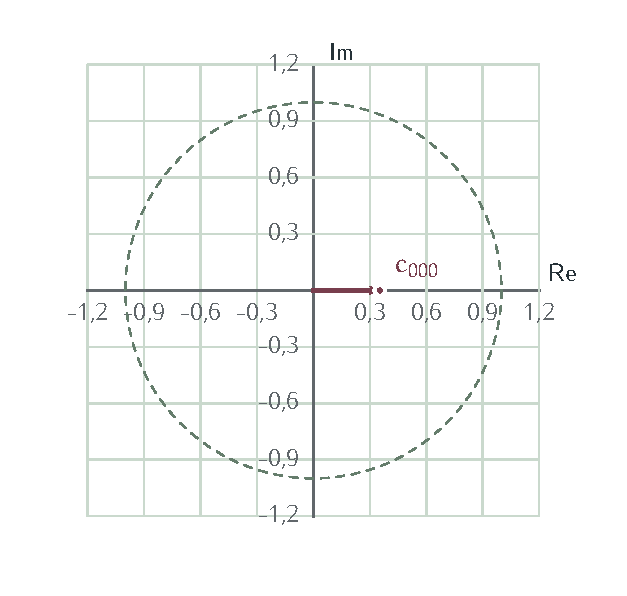
\includegraphics[width=\linewidth,height=63mm,keepaspectratio]{figure/f64e1c87aed811135.pdf}\par{\sffamily\footnotesize \(c_{000}\)\par}\end{minipage}\hfill\begin{minipage}[t]{.485\linewidth}\centering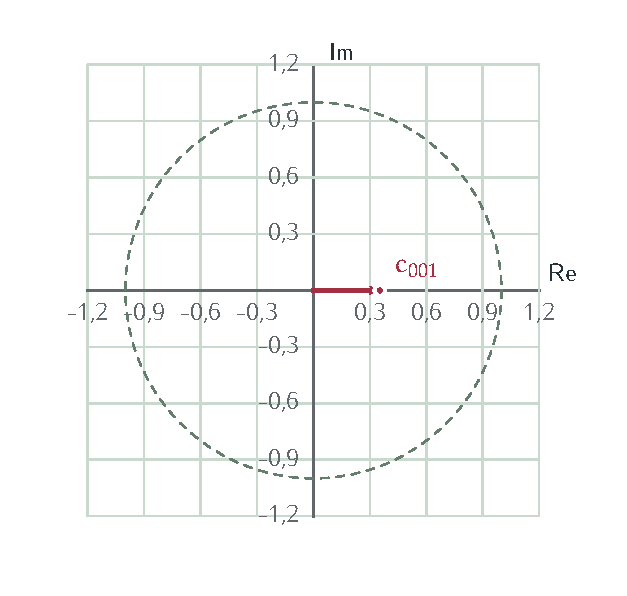
\includegraphics[width=\linewidth,height=63mm,keepaspectratio]{figure/fb63a4b5860b9c21f.pdf}\par{\sffamily\footnotesize \(c_{001}\)\par}\end{minipage}\FigureCaption{4.05 \(\cdot\) esempio 2 \(\cdot\) Componenti complesse}\end{FigureBlock}
\begin{FigureBlock}\begin{minipage}[t]{.485\linewidth}\centering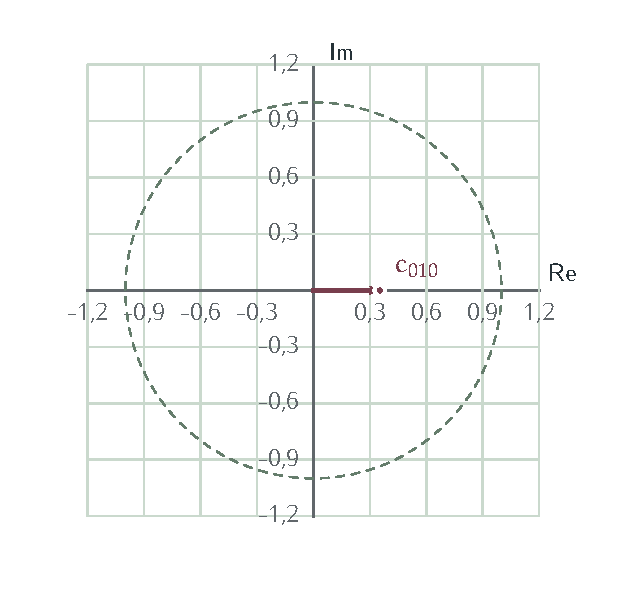
\includegraphics[width=\linewidth,height=63mm,keepaspectratio]{figure/fefc517ecffe9e161.pdf}\par{\sffamily\footnotesize \(c_{010}\)\par}\end{minipage}\hfill\begin{minipage}[t]{.485\linewidth}\centering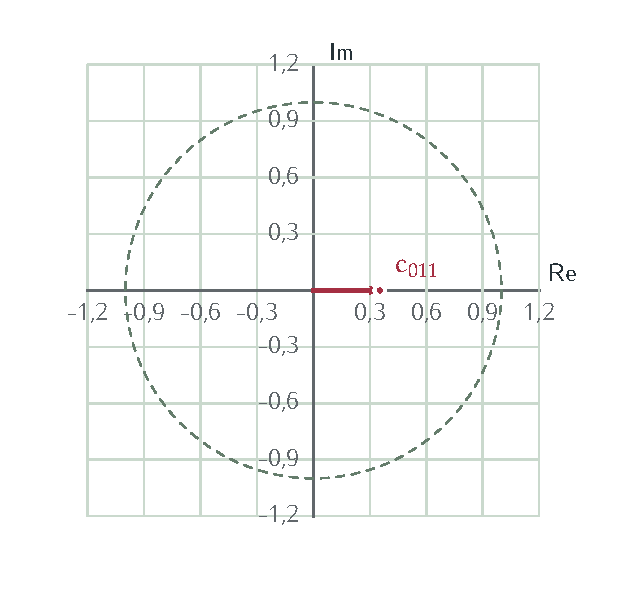
\includegraphics[width=\linewidth,height=63mm,keepaspectratio]{figure/f158b83ce7805e0c7.pdf}\par{\sffamily\footnotesize \(c_{011}\)\par}\end{minipage}\FigureCaption{4.05 \(\cdot\) esempio 2 \(\cdot\) Componenti complesse}\end{FigureBlock}
\begin{FigureBlock}\begin{minipage}[t]{.485\linewidth}\centering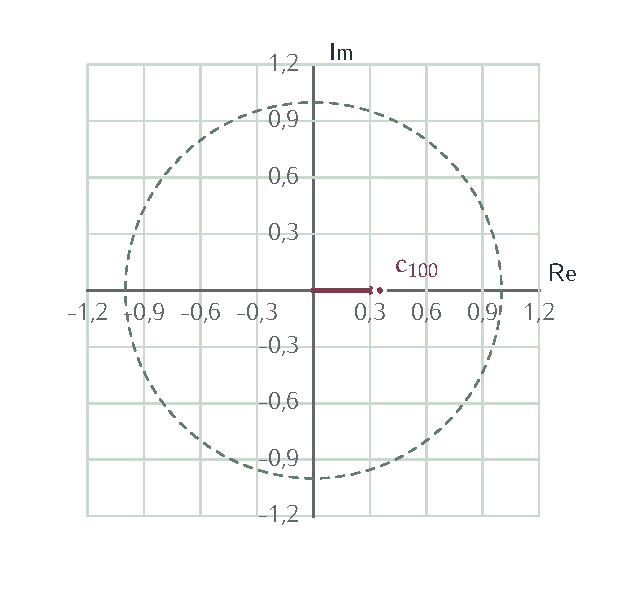
\includegraphics[width=\linewidth,height=63mm,keepaspectratio]{figure/f9da0cc45cd74d43f.pdf}\par{\sffamily\footnotesize \(c_{100}\)\par}\end{minipage}\hfill\begin{minipage}[t]{.485\linewidth}\centering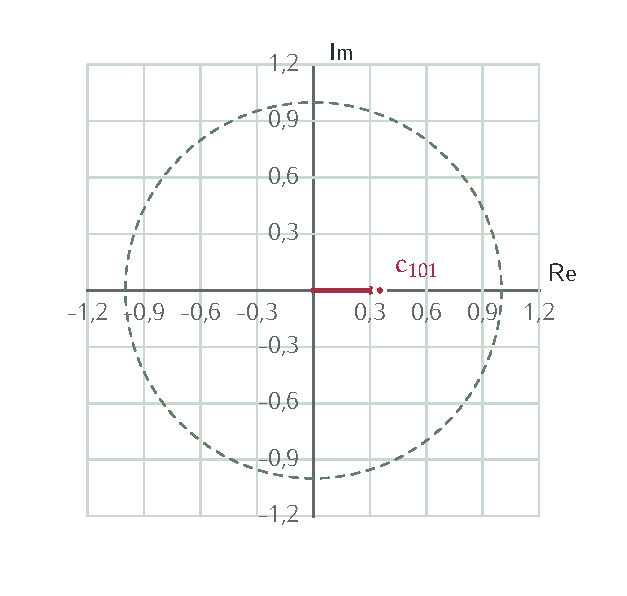
\includegraphics[width=\linewidth,height=63mm,keepaspectratio]{figure/f1b33993df51492af.pdf}\par{\sffamily\footnotesize \(c_{101}\)\par}\end{minipage}\FigureCaption{4.05 \(\cdot\) esempio 2 \(\cdot\) Componenti complesse}\end{FigureBlock}
\begin{FigureBlock}\begin{minipage}[t]{.485\linewidth}\centering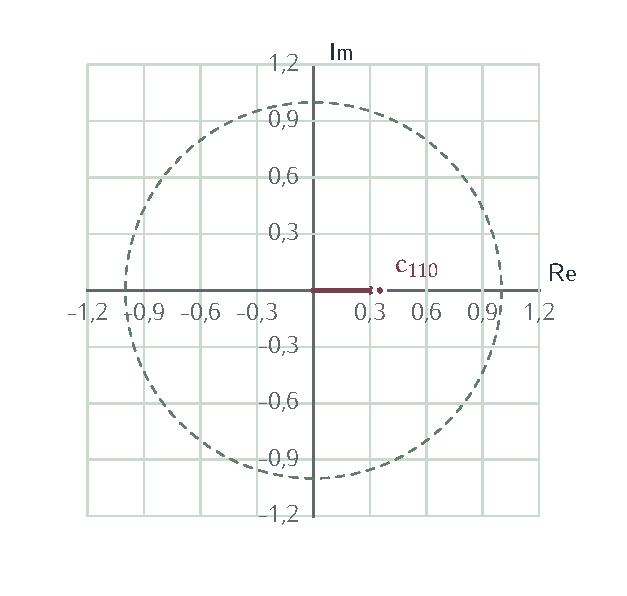
\includegraphics[width=\linewidth,height=63mm,keepaspectratio]{figure/fc1da6dd98525dc26.pdf}\par{\sffamily\footnotesize \(c_{110}\)\par}\end{minipage}\hfill\begin{minipage}[t]{.485\linewidth}\centering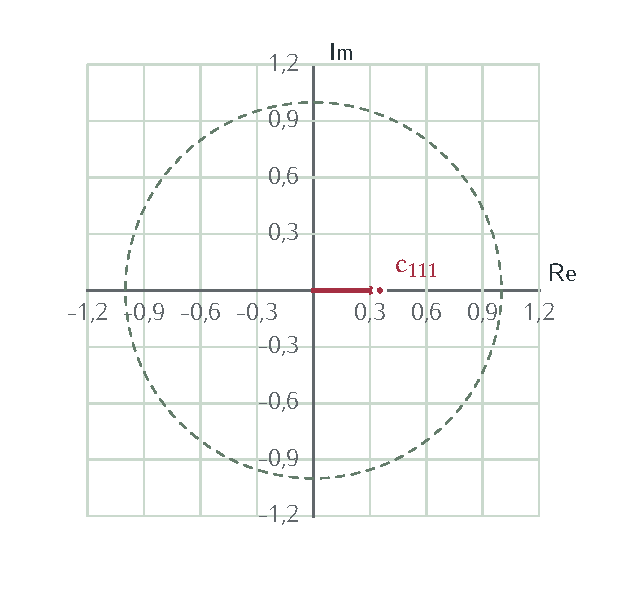
\includegraphics[width=\linewidth,height=63mm,keepaspectratio]{figure/f2ec706b204bf3bfc.pdf}\par{\sffamily\footnotesize \(c_{111}\)\par}\end{minipage}\FigureCaption{4.05 \(\cdot\) esempio 2 \(\cdot\) Componenti complesse}\end{FigureBlock}

\phantomsection\label{c4-grover-example-2-step-1}
\BookHeading{01 Costruire gli assi dalle proiezioni}

\MathBlock{007C006127E9003D0041007C003027E9003B002003A00047003D03A3007822080047007C007827E927E80078007C003B00200070003D27E80061007C03A00047007C006127E9003D0030002C00320035002E}{|a\rangle =A|0\rangle ;\allowbreak \ \Pi _{G}=\sum _{x\in G}|x\rangle \langle x|;\allowbreak \ p=\langle a|\Pi _{G}|a\rangle =0{,}25.}
\MathBlock{007C006727E9003D03A00047007C006127E9002F221A0070224800280030003B00200030002C0037003000370031003B00200030003B00200030003B00200030003B00200030002C0037003000370031003B00200030003B0020003000291D40}{|g\rangle =\Pi _{G}|a\rangle /\sqrt{p}\approx (0;\allowbreak \ 0{,}7071;\allowbreak \ 0;\allowbreak \ 0;\allowbreak \ 0;\allowbreak \ 0{,}7071;\allowbreak \ 0;\allowbreak \ 0)^{T}}
\MathBlock{007C006227E9003D00280049221203A000470029007C006127E9002F221A00280031221200700029224800280030002C0034003000380032003B00200030003B00200030002C0034003000380032003B00200030002C0034003000380032003B00200030002C0034003000380032003B00200030003B00200030002C0034003000380032003B00200030002C003400300038003200291D40002E}{|b\rangle =(I- \Pi _{G})|a\rangle /\sqrt{1- p}\approx (0{,}4082;\allowbreak \ 0;\allowbreak \ 0{,}4082;\allowbreak \ 0{,}4082;\allowbreak \ 0{,}4082;\allowbreak \ 0;\allowbreak \ 0{,}4082;\allowbreak \ 0{,}4082)^{T}.}
\MathBlock{27E80062007C006727E9003D0030003B0020201600622016003D201600672016003D0031002E}{\langle b|g\rangle =0;\allowbreak \ \Vert b\Vert =\Vert g\Vert =1.}

I supporti sono disgiunti. Per la preparazione uniforme questi vettori diventano \(\sum _{x\in G}|x\rangle /\sqrt{M}\) e \(\sum x\notin G|x\rangle /\sqrt{N- M}\). Per una preparazione non uniforme conservano i suoi pesi e le sue fasi.\par


\phantomsection\label{c4-grover-example-2-step-2}
\BookHeading{02 Proiettare la preparazione nel piano}

\MathBlock{27E80062007C006127E9003D221A00280031221200700029003D0030002C003800360036003000320035003B002027E80067007C006127E9003D221A0070003D0030002C0035002E}{\langle b|a\rangle =\sqrt{1- p}=0{,}866025;\allowbreak \ \langle g|a\rangle =\sqrt{p}=0{,}5.}
\MathBlock{007C006127E9003D0063006F007303B8007C006227E9002B00730069006E03B8007C006727E9003B002003B8003D00610072006300730069006E221A007022480030002C0035003200330035003900390020007200610064002E}{|a\rangle =\cos \theta |b\rangle +\sin \theta |g\rangle ;\allowbreak \ \theta =\arcsin \sqrt{p}\approx 0{,}523599\ \text{rad}.}

Gli assi sono stati collettivi, non singoli esiti. Le coordinate qui sono reali perché le fasi della preparazione sono state incluse nella definizione degli assi.\par


\phantomsection\label{c4-grover-example-2-step-3}
\BookHeading{03 Scrivere le due riflessioni}

\MathBlock{004E0065006C006C0061002000620061007300650020006F007200640069006E00610074006100200028007C006227E9002C007C006727E90029003A}{\text{Nella}\ \text{base}\ \text{ordinata}\ (|b\rangle ,\allowbreak |g\rangle ):}
\MathBlock{004F003D00492212003203A00047003D005B005B0031002C0030005D002C005B0030002C22120031005D005D002E}{O=I- 2\Pi _{G}=\begin{pmatrix}1&0\\0&- 1\end{pmatrix}.}
\MathBlock{0044005F0041003D0032007C006127E927E80061007C22120049}{D_{A}=2|a\rangle \langle a|- I}
\MathBlock{003D005B005B00320063006F007300B203B822120031002C00320063006F007303B800730069006E03B8005D002C005B00320063006F007303B800730069006E03B8002C003200730069006E00B203B822120031005D005D}{=\begin{pmatrix}2\cos ^{2}\theta - 1&2\cos \theta \sin \theta \\2\cos \theta \sin \theta &2\sin ^{2}\theta - 1\end{pmatrix}}
\MathBlock{003D005B005B0063006F0073003203B8002C00730069006E003203B8005D002C005B00730069006E003203B8002C22120063006F0073003203B8005D005D002E}{=\begin{pmatrix}\cos 2\theta &\sin 2\theta \\\sin 2\theta &- \cos 2\theta \end{pmatrix}.}

\(O\) riflette rispetto all'asse \(|b\rangle \). \(D_{A}\) riflette rispetto alla retta della preparazione \(|a\rangle \). L'ordine temporale è prima \(O\) e poi \(D_{A}\).\par


\phantomsection\label{c4-grover-example-2-step-4}
\BookHeading{04 Moltiplicare e ottenere la rotazione}

\MathBlock{0051003D0044005F0041004F003D005B005B0063006F0073003203B8002C221200730069006E003203B8005D002C005B00730069006E003203B8002C0063006F0073003203B8005D005D}{Q=D_{AO}=\begin{pmatrix}\cos 2\theta &- \sin 2\theta \\\sin 2\theta &\cos 2\theta \end{pmatrix}}
\MathBlock{2248005B005B0030002C0035002C002D0030002C003800360036003000320035005D002C005B0030002C003800360036003000320035002C0030002C0035005D005D002E}{\approx \begin{pmatrix}0{,}5&-0{,}866025\\0{,}866025&0{,}5\end{pmatrix}.}
\MathBlock{004F00280063006F007303B8002C00730069006E03B800291D40003D00280063006F007303B8002C221200730069006E03B800291D40003B}{O(\cos \theta ,\allowbreak \sin \theta )^{T}=(\cos \theta ,\allowbreak - \sin \theta )^{T};\allowbreak }
\MathBlock{005100280063006F007303B8002C00730069006E03B800291D40003D00280063006F0073003303B8002C00730069006E003303B800291D40002E}{Q(\cos \theta ,\allowbreak \sin \theta )^{T}=(\cos 3\theta ,\allowbreak \sin 3\theta )^{T}.}
\MathBlock{00511D4F007C006127E9003D0063006F0073002800280032006B002B0031002903B80029007C006227E9002B00730069006E002800280032006B002B0031002903B80029007C006727E9002E}{Q^{k}|a\rangle =\cos ((2k+1)\theta )|b\rangle +\sin ((2k+1)\theta )|g\rangle .}

Il prodotto riga per colonna dà le formule di addizione del seno e del coseno. Ogni coppia completa di riflessioni ruota di \(2\theta \); dopo il solo oracolo si usa invece la riflessione, non la formula delle iterazioni complete.\par


\phantomsection\label{c4-grover-example-2-step-5}
\BookHeading{05 Verificare il caso \(p=1/4\)}

\MathBlock{03B8003D03C0002F0036003B0020007C006127E9003D0028221A0033002F0032002C0031002F003200291D40002E}{\theta =\pi /6;\allowbreak \ |a\rangle =(\sqrt{3}/2{,}1/2)^{T}.}
\MathBlock{004F007C006127E9003D0028221A0033002F0032002C22120031002F003200291D40002E}{O|a\rangle =(\sqrt{3}/2,\allowbreak - 1/2)^{T}.}
\MathBlock{0044005F0041003D005B005B0031002F0032002C221A0033002F0032005D002C005B221A0033002F0032002C22120031002F0032005D005D002E}{D_{A}=\begin{pmatrix}1/2&\sqrt{3}/2\\\sqrt{3}/2&- 1/2\end{pmatrix}.}
\MathBlock{0044005F0041004F007C006127E9003D0028221A0033002F00342212221A0033002F0034002C221A003300B7221A0033002F0034002B0031002F003400291D40003D00280030002C003100291D40002E}{D_{AO}|a\rangle =(\sqrt{3}/4- \sqrt{3}/4,\allowbreak \sqrt{3}\cdot \sqrt{3}/4+1/4)^{T}=(0{,}1)^{T}.}

Il medesimo calcolo vale per \(N=4,\allowbreak M=1\) e per \(N=8,\allowbreak M=2\). Una sola coppia di riflessioni porta tutto il peso sul sottospazio buono.\par


\phantomsection\label{c4-grover-example-2-step-6}
\BookHeading{06 Ricavare autovettori e autofasi}

\MathBlock{00640065007400280051221203BB00490029003D03BB00B2221200320063006F00730028003203B8002903BB002B0031003D0030002E}{\det (Q- \lambda I)=\lambda ^{2}- 2\cos (2\theta )\lambda +1=0.}
\MathBlock{03BB00B1003D0063006F0073003203B800B10069002000730069006E003203B8003D0065005E002800B10032006903B80029002E}{\lambda \pm =\cos 2\theta \pm i\ \sin 2\theta =e^{\pm 2i\theta }.}
\MathBlock{007C0075002B27E9003D0028007C006227E922120069007C006727E90029002F221A0032003B0020007C0075221227E9003D0028007C006227E9002B0069007C006727E90029002F221A0032002E}{|u+\rangle =(|b\rangle - i|g\rangle )/\sqrt{2};\allowbreak \ |u- \rangle =(|b\rangle +i|g\rangle )/\sqrt{2}.}
\MathBlock{0051007C007500B127E9003D0065005E002800B10032006903B80029007C007500B127E9003B002003C6002B003D03B8002F03C0002C002003C62212003D0031221203B8002F03C000200028006D006F0064002000310029002E}{Q|u\pm \rangle =e^{\pm 2i\theta }|u\pm \rangle ;\allowbreak \ \varphi +=\theta /\pi ,\allowbreak \ \varphi - =1- \theta /\pi \ (\bmod \ 1).}

Gli autovettori hanno coordinate complesse nel piano collettivo; non sono due frecce reali sul piano di Grover. Le autofasi sono frazioni di giro, poiché QPE usa \(e^{2\pi i\varphi }\).\par


\phantomsection\label{c4-grover-example-2-step-7}
\BookHeading{07 Determinare i coefficienti della preparazione}

\MathBlock{03B2002B003D27E80075002B007C006127E9003D00280063006F007303B8002B0069002000730069006E03B80029002F221A0032003D0065005E0028006903B80029002F221A0032002E}{\beta +=\langle u+|a\rangle =(\cos \theta +i\ \sin \theta )/\sqrt{2}=e^{i\theta }/\sqrt{2}.}
\MathBlock{03B22212003D27E800752212007C006127E9003D00280063006F007303B822120069002000730069006E03B80029002F221A0032003D0065005E00282212006903B80029002F221A0032002E}{\beta - =\langle u- |a\rangle =(\cos \theta - i\ \sin \theta )/\sqrt{2}=e^{- i\theta }/\sqrt{2}.}
\MathBlock{007C006127E9003D03B2002B007C0075002B27E9002B03B22212007C0075221227E9003B0020007C03B2002B007C00B2003D007C03B22212007C00B2003D0031002F0032002E}{|a\rangle =\beta +|u+\rangle +\beta - |u- \rangle ;\allowbreak \ |\beta +|^{2}=|\beta - |^{2}=1/2.}

I due pesi uguali derivano dal prodotto interno con la preparazione. Manteniamo anche le fasi dei coefficienti: servono per ricostruire il bersaglio coerente condizionato dopo QPE.\par


\phantomsection\label{c4-grover-example-2-step-8}
\BookHeading{08 Preparazione \(A|0\rangle \)}

\MathBlock{00280030002C0033003500330036003B00200030002C0033003500330036003B00200030002C0033003500330036003B00200030002C0033003500330036003B00200030002C0033003500330036003B00200030002C0033003500330036003B00200030002C0033003500330036003B00200030002C003300350033003600291D40}{(0{,}3536;\allowbreak \ 0{,}3536;\allowbreak \ 0{,}3536;\allowbreak \ 0{,}3536;\allowbreak \ 0{,}3536;\allowbreak \ 0{,}3536;\allowbreak \ 0{,}3536;\allowbreak \ 0{,}3536)^{T}}
\MathBlock{03C8224800280030002C0033003500330036003B00200030002C0033003500330036003B00200030002C0033003500330036003B00200030002C0033003500330036003B00200030002C0033003500330036003B00200030002C0033003500330036003B00200030002C0033003500330036003B00200030002C003300350033003600291D40}{\psi \approx (0{,}3536;\allowbreak \ 0{,}3536;\allowbreak \ 0{,}3536;\allowbreak \ 0{,}3536;\allowbreak \ 0{,}3536;\allowbreak \ 0{,}3536;\allowbreak \ 0{,}3536;\allowbreak \ 0{,}3536)^{T}}
\MathBlock{0043006F006F007200640069006E0061007400650020002827E80062007C03C827E9002C27E80067007C03C827E90029224800280030002C003800360036003000320035003B00200030002C00350029}{\text{Coordinate}\ (\langle b|\psi \rangle ,\allowbreak \langle g|\psi \rangle )\approx (0{,}866025;\allowbreak \ 0{,}5)}

La marcatura cambia il segno delle ampiezze buone; la riflessione usa il prodotto interno con la preparazione.\par


\phantomsection\label{c4-grover-example-2-step-9}
\BookHeading{09 Oracolo 1}

\MathBlock{004F007C007827E90020003D00200028221200310029005E005B007822080047005D007C007827E9003B00200047003D007B0031002C0035007D}{O|x\rangle \ =\ (- 1)^{x\in G}|x\rangle ;\allowbreak \ G=\{1{,}5\}}
\MathBlock{03C8224800280030002C0033003500330036003B0020002D0030002C0033003500330036003B00200030002C0033003500330036003B00200030002C0033003500330036003B00200030002C0033003500330036003B0020002D0030002C0033003500330036003B00200030002C0033003500330036003B00200030002C003300350033003600291D40}{\psi \approx (0{,}3536;\allowbreak \ -0{,}3536;\allowbreak \ 0{,}3536;\allowbreak \ 0{,}3536;\allowbreak \ 0{,}3536;\allowbreak \ -0{,}3536;\allowbreak \ 0{,}3536;\allowbreak \ 0{,}3536)^{T}}
\MathBlock{0043006F006F007200640069006E0061007400650020002827E80062007C03C827E9002C27E80067007C03C827E90029224800280030002C003800360036003000320035003B0020002D0030002C00350029}{\text{Coordinate}\ (\langle b|\psi \rangle ,\allowbreak \langle g|\psi \rangle )\approx (0{,}866025;\allowbreak \ -0{,}5)}

La marcatura cambia il segno delle ampiezze buone; la riflessione usa il prodotto interno con la preparazione.\par


\phantomsection\label{c4-grover-example-2-step-10}
\BookHeading{10 Riflessione 1}

\MathBlock{27E80061007C007627E90020003D002000280030002C0033003500330036002900B700280030002C003300350033003600290020002B002000280030002C0033003500330036002900B70028002D0030002C003300350033003600290020002B002000280030002C0033003500330036002900B700280030002C003300350033003600290020002B002000280030002C0033003500330036002900B700280030002C003300350033003600290020002B002000280030002C0033003500330036002900B700280030002C003300350033003600290020002B002000280030002C0033003500330036002900B70028002D0030002C003300350033003600290020002B002000280030002C0033003500330036002900B700280030002C003300350033003600290020002B002000280030002C0033003500330036002900B700280030002C003300350033003600290020224800200030002C0035}{\langle a|v\rangle \ =\ (0{,}3536)\cdot (0{,}3536)\ +\ (0{,}3536)\cdot (-0{,}3536)\ +\ (0{,}3536)\cdot (0{,}3536)\ +\ (0{,}3536)\cdot (0{,}3536)\ +\ (0{,}3536)\cdot (0{,}3536)\ +\ (0{,}3536)\cdot (-0{,}3536)\ +\ (0{,}3536)\cdot (0{,}3536)\ +\ (0{,}3536)\cdot (0{,}3536)\ \approx \ 0{,}5}
\MathBlock{00630028003000290020003D0020003200B700280030002C0033003500330036002900B700280030002C0035002900202212002000280030002C003300350033003600290020224800200030}{c(0)\ =\ 2\cdot (0{,}3536)\cdot (0{,}5)\ - \ (0{,}3536)\ \approx \ 0}
\MathBlock{00630028003100290020003D0020003200B700280030002C0033003500330036002900B700280030002C003500290020221200200028002D0030002C003300350033003600290020224800200030002C0037003000370031}{c(1)\ =\ 2\cdot (0{,}3536)\cdot (0{,}5)\ - \ (-0{,}3536)\ \approx \ 0{,}7071}
\MathBlock{00630028003200290020003D0020003200B700280030002C0033003500330036002900B700280030002C0035002900202212002000280030002C003300350033003600290020224800200030}{c(2)\ =\ 2\cdot (0{,}3536)\cdot (0{,}5)\ - \ (0{,}3536)\ \approx \ 0}
\MathBlock{00630028003300290020003D0020003200B700280030002C0033003500330036002900B700280030002C0035002900202212002000280030002C003300350033003600290020224800200030}{c(3)\ =\ 2\cdot (0{,}3536)\cdot (0{,}5)\ - \ (0{,}3536)\ \approx \ 0}
\MathBlock{00630028003400290020003D0020003200B700280030002C0033003500330036002900B700280030002C0035002900202212002000280030002C003300350033003600290020224800200030}{c(4)\ =\ 2\cdot (0{,}3536)\cdot (0{,}5)\ - \ (0{,}3536)\ \approx \ 0}
\MathBlock{00630028003500290020003D0020003200B700280030002C0033003500330036002900B700280030002C003500290020221200200028002D0030002C003300350033003600290020224800200030002C0037003000370031}{c(5)\ =\ 2\cdot (0{,}3536)\cdot (0{,}5)\ - \ (-0{,}3536)\ \approx \ 0{,}7071}
\MathBlock{00630028003600290020003D0020003200B700280030002C0033003500330036002900B700280030002C0035002900202212002000280030002C003300350033003600290020224800200030}{c(6)\ =\ 2\cdot (0{,}3536)\cdot (0{,}5)\ - \ (0{,}3536)\ \approx \ 0}
\MathBlock{00630028003700290020003D0020003200B700280030002C0033003500330036002900B700280030002C0035002900202212002000280030002C003300350033003600290020224800200030}{c(7)\ =\ 2\cdot (0{,}3536)\cdot (0{,}5)\ - \ (0{,}3536)\ \approx \ 0}
\MathBlock{03C8224800280030003B00200030002C0037003000370031003B00200030003B00200030003B00200030003B00200030002C0037003000370031003B00200030003B0020003000291D40}{\psi \approx (0;\allowbreak \ 0{,}7071;\allowbreak \ 0;\allowbreak \ 0;\allowbreak \ 0;\allowbreak \ 0{,}7071;\allowbreak \ 0;\allowbreak \ 0)^{T}}
\MathBlock{0043006F006F007200640069006E0061007400650020002827E80062007C03C827E9002C27E80067007C03C827E90029224800280030003B002000310029}{\text{Coordinate}\ (\langle b|\psi \rangle ,\allowbreak \langle g|\psi \rangle )\approx (0;\allowbreak \ 1)}

La marcatura cambia il segno delle ampiezze buone; la riflessione usa il prodotto interno con la preparazione.\par


\phantomsection\label{c4-grover-example-2-step-11}
\BookHeading{11 Oracolo 2}

\MathBlock{004F007C007827E90020003D00200028221200310029005E005B007822080047005D007C007827E9003B00200047003D007B0031002C0035007D}{O|x\rangle \ =\ (- 1)^{x\in G}|x\rangle ;\allowbreak \ G=\{1{,}5\}}
\MathBlock{03C8224800280030003B0020002D0030002C0037003000370031003B00200030003B00200030003B00200030003B0020002D0030002C0037003000370031003B00200030003B0020003000291D40}{\psi \approx (0;\allowbreak \ -0{,}7071;\allowbreak \ 0;\allowbreak \ 0;\allowbreak \ 0;\allowbreak \ -0{,}7071;\allowbreak \ 0;\allowbreak \ 0)^{T}}
\MathBlock{0043006F006F007200640069006E0061007400650020002827E80062007C03C827E9002C27E80067007C03C827E90029224800280030003B0020002D00310029}{\text{Coordinate}\ (\langle b|\psi \rangle ,\allowbreak \langle g|\psi \rangle )\approx (0;\allowbreak \ -1)}

La marcatura cambia il segno delle ampiezze buone; la riflessione usa il prodotto interno con la preparazione.\par


\phantomsection\label{c4-grover-example-2-step-12}
\BookHeading{12 Riflessione 2}

\MathBlock{27E80061007C007627E90020003D002000280030002C0033003500330036002900B70028003000290020002B002000280030002C0033003500330036002900B70028002D0030002C003700300037003100290020002B002000280030002C0033003500330036002900B70028003000290020002B002000280030002C0033003500330036002900B70028003000290020002B002000280030002C0033003500330036002900B70028003000290020002B002000280030002C0033003500330036002900B70028002D0030002C003700300037003100290020002B002000280030002C0033003500330036002900B70028003000290020002B002000280030002C0033003500330036002900B7002800300029002022480020002D0030002C0035}{\langle a|v\rangle \ =\ (0{,}3536)\cdot (0)\ +\ (0{,}3536)\cdot (-0{,}7071)\ +\ (0{,}3536)\cdot (0)\ +\ (0{,}3536)\cdot (0)\ +\ (0{,}3536)\cdot (0)\ +\ (0{,}3536)\cdot (-0{,}7071)\ +\ (0{,}3536)\cdot (0)\ +\ (0{,}3536)\cdot (0)\ \approx \ -0{,}5}
\MathBlock{00630028003000290020003D0020003200B700280030002C0033003500330036002900B70028002D0030002C00350029002022120020002800300029002022480020002D0030002C0033003500330036}{c(0)\ =\ 2\cdot (0{,}3536)\cdot (-0{,}5)\ - \ (0)\ \approx \ -0{,}3536}
\MathBlock{00630028003100290020003D0020003200B700280030002C0033003500330036002900B70028002D0030002C003500290020221200200028002D0030002C003700300037003100290020224800200030002C0033003500330036}{c(1)\ =\ 2\cdot (0{,}3536)\cdot (-0{,}5)\ - \ (-0{,}7071)\ \approx \ 0{,}3536}
\MathBlock{00630028003200290020003D0020003200B700280030002C0033003500330036002900B70028002D0030002C00350029002022120020002800300029002022480020002D0030002C0033003500330036}{c(2)\ =\ 2\cdot (0{,}3536)\cdot (-0{,}5)\ - \ (0)\ \approx \ -0{,}3536}
\MathBlock{00630028003300290020003D0020003200B700280030002C0033003500330036002900B70028002D0030002C00350029002022120020002800300029002022480020002D0030002C0033003500330036}{c(3)\ =\ 2\cdot (0{,}3536)\cdot (-0{,}5)\ - \ (0)\ \approx \ -0{,}3536}
\MathBlock{00630028003400290020003D0020003200B700280030002C0033003500330036002900B70028002D0030002C00350029002022120020002800300029002022480020002D0030002C0033003500330036}{c(4)\ =\ 2\cdot (0{,}3536)\cdot (-0{,}5)\ - \ (0)\ \approx \ -0{,}3536}
\MathBlock{00630028003500290020003D0020003200B700280030002C0033003500330036002900B70028002D0030002C003500290020221200200028002D0030002C003700300037003100290020224800200030002C0033003500330036}{c(5)\ =\ 2\cdot (0{,}3536)\cdot (-0{,}5)\ - \ (-0{,}7071)\ \approx \ 0{,}3536}
\MathBlock{00630028003600290020003D0020003200B700280030002C0033003500330036002900B70028002D0030002C00350029002022120020002800300029002022480020002D0030002C0033003500330036}{c(6)\ =\ 2\cdot (0{,}3536)\cdot (-0{,}5)\ - \ (0)\ \approx \ -0{,}3536}
\MathBlock{00630028003700290020003D0020003200B700280030002C0033003500330036002900B70028002D0030002C00350029002022120020002800300029002022480020002D0030002C0033003500330036}{c(7)\ =\ 2\cdot (0{,}3536)\cdot (-0{,}5)\ - \ (0)\ \approx \ -0{,}3536}
\MathBlock{03C822480028002D0030002C0033003500330036003B00200030002C0033003500330036003B0020002D0030002C0033003500330036003B0020002D0030002C0033003500330036003B0020002D0030002C0033003500330036003B00200030002C0033003500330036003B0020002D0030002C0033003500330036003B0020002D0030002C003300350033003600291D40}{\psi \approx (-0{,}3536;\allowbreak \ 0{,}3536;\allowbreak \ -0{,}3536;\allowbreak \ -0{,}3536;\allowbreak \ -0{,}3536;\allowbreak \ 0{,}3536;\allowbreak \ -0{,}3536;\allowbreak \ -0{,}3536)^{T}}
\MathBlock{0043006F006F007200640069006E0061007400650020002827E80062007C03C827E9002C27E80067007C03C827E9002922480028002D0030002C003800360036003000320035003B00200030002C00350029}{\text{Coordinate}\ (\langle b|\psi \rangle ,\allowbreak \langle g|\psi \rangle )\approx (-0{,}866025;\allowbreak \ 0{,}5)}

La marcatura cambia il segno delle ampiezze buone; la riflessione usa il prodotto interno con la preparazione.\par


\phantomsection\label{c4-grover-example-2-step-13}
\BookHeading{13 Probabilità di successo}

\MathBlock{00702080003D0030002C00320035003B002003B8003D00610072006300730069006E221A0070208022480030002C00350032003300360020007200610064}{p_{0}=0{,}25;\allowbreak \ \theta =\arcsin \sqrt{p}_{0}\approx 0{,}5236\ \text{rad}}
\MathBlock{00500073007500630063006500730073006F003D03A3007822080047007C00632093007C00B222480030002C00320035}{\text{Psuccesso}=\sum _{x\in G}|c_{x}|^{2}\approx 0{,}25}
\MathBlock{00730069006E00B2002800280032006B002B0031002903B80029003D00730069006E00B20028003500B70030002C0035003200330036002922480030002C00320035}{\sin ^{2}((2k+1)\theta )=\sin ^{2}(5\cdot 0{,}5236)\approx 0{,}25}

La formula geometrica verifica la simulazione delle ampiezze.\par


\BookHeading{Stato finale del programma}
\begin{FigureBlock}\centering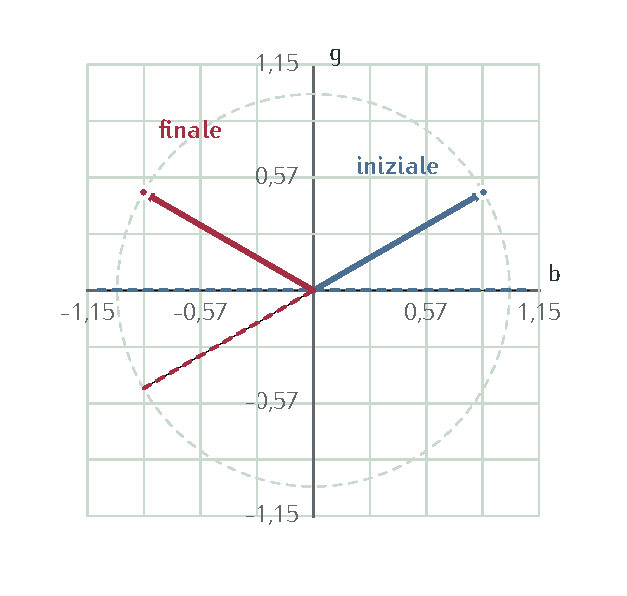
\includegraphics[width=\linewidth,height=94mm,keepaspectratio]{figure/f6789a15f82b50d91.pdf}\FigureCaption{4.05 \(\cdot\) esempio 2 \(\cdot\) Piano \(|b\rangle ,\allowbreak |g\rangle \) \(\cdot\) confronto iniziale/finale}\end{FigureBlock}

\BookHeading{Interpretazione}

Il piano ha assi ortonormali ricavati dalla preparazione. Ogni freccia intermedia e le probabilità delle alternative derivano dai medesimi vettori del registro.\par


Risorse dichiarate. 2 interrogazioni all'oracolo; 3 qubit dati. Il costo della preparazione e della riflessione va aggiunto.\par


\Needspace{7\baselineskip}
\BookHeading{Il passaggio successivo}
La scelta di k richiede una stima di \(M\). Se \(M\) è ignoto, possiamo variare il numero di iterazioni fra i tentativi e verificare ciascun candidato con l'oracolo.\par


\Needspace{.43\textheight}
\section{Ricerca con numero ignoto di soluzioni}
\phantomsection\label{c4-ricerca-ignota}

{\sffamily\small\color{Ink!70} Riferimento alle slide: p. 187.\par}

{\sffamily\small\color{Ink!70} Laboratorio locale: \nolinkurl{index.html#capitolo-4/ricerca-ignota}\par}

\BookHeading{Definizioni e costruzione}
Quando il numero \(M\) di soluzioni è ignoto, una scelta fissa di k può oltrepassare il massimo di Grover. Usiamo tentativi indipendenti con un numero casuale di iterazioni scelto entro una finestra crescente.\par

Poniamo inizialmente \(m=1\). \(A\) ogni tentativo scegliamo uniformemente j fra \(0,\allowbreak \ldots ,\allowbreak \lceil m\rceil - 1\), riprepariamo lo stato uniforme, eseguiamo j iterazioni e leggiamo un candidato x. Il simbolo \(\lceil m\rceil \) è il più piccolo intero almeno pari a m; m può essere non intero.\par

La verifica \(f(x)=1\) decide il successo. Se fallisce, aggiorniamo \(m\leftarrow \min (6m/5,\allowbreak \sqrt{N})\) e ripetiamo entro un budget dichiarato. Nel conteggio didattico un tentativo costa j interrogazioni per le iterazioni e una per verificare x. Per \(M=0\) ogni verifica fallisce: l'esaurimento del budget non dimostra l'assenza di soluzioni.\par

La tabella separa finestra m, iterazioni j, candidato osservato, probabilità teorica buona e costo. Qui una traiettoria è effettivamente campionata con un generatore pseudocasuale e seme dichiarato, così che si possa riprodurre lo stesso esempio; la probabilità del tentativo rimane distinta dall'esito estratto.\par


\MathBlock{006A00200075006E00690066006F0072006D006500200069006E0020007B0030002C2026002C2308006D230922120031007D003B00200063006F00730074006F002000640065006C002000740065006E00740061007400690076006F003D006A002B0031003B0020006D2190006D0069006E00280036006D002F0035002C221A004E0029002E}{j\ \text{uniforme}\ \text{in}\ \{0,\allowbreak \ldots ,\allowbreak \lceil m\rceil - 1\};\allowbreak \ \text{costo}\ \text{del}\ \text{tentativo}=j+1;\allowbreak \ m\leftarrow \min (6m/5,\allowbreak \sqrt{N}).}

\BookHeading{Come leggere le figure}
Le righe sono tentativi successivi, non stati coerenti dello stesso registro. Le probabilità sono quelle previste dal modello e gli indici estratti sono dati classici. Il costo conta interrogazioni, non secondi di esecuzione.\par


\BookHeading{Attività nel laboratorio modificabile}

\BookHeading{Obiettivo dell'esperimento}
Osservare un procedimento che adatta il numero di iterazioni senza ricevere il numero di soluzioni.\par

\BookHeading{Percorso operativo}
Cambiare insieme favorevole, budget e seme dei tentativi.\par

\BookHeading{Lettura geometrica}
Ogni tentativo prepara una nuova distribuzione e campiona un candidato.\par

\BookHeading{Controllo del risultato}
Contare anche l'interrogazione di verifica; l'esaurimento del budget lascia aperta la possibilità di soluzioni.\par


\Needspace{.36\textheight}\phantomsection\label{c4-ricerca-ignota-example-1}
{\sffamily\small\color{Accent} ESEMPIO SVOLTO 1\par}
\BookHeading{Esempio 1}
\(N=8\); al massimo 12 tentativi; generatore pseudocasuale con seme 20260928.\par


\BookHeading{Geometria e configurazione dell'esempio}
\begin{FigureBlock}\centering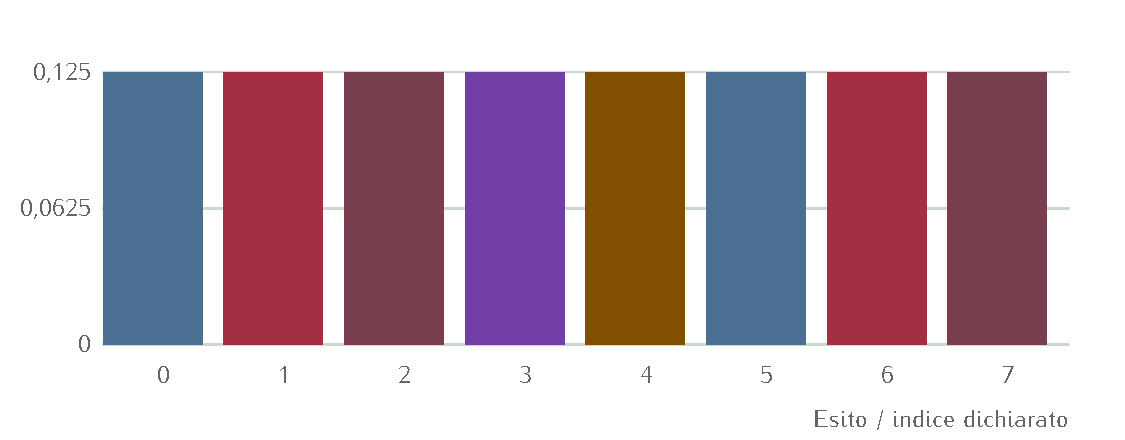
\includegraphics[width=\linewidth,height=94mm,keepaspectratio]{figure/fb06f6bfaa089c265.pdf}\FigureCaption{4.06 \(\cdot\) esempio 1 \(\cdot\) Distribuzione uniforme di partenza}\end{FigureBlock}

\phantomsection\label{c4-ricerca-ignota-example-1-step-1}
\BookHeading{01 Definire il tentativo}

\MathBlock{006D003D0031003B0020006A00200065007300740072006100740074006F00200075006E00690066006F0072006D0065006D0065006E007400650020006600720061002000300020006500202308006D230922120031003B002003C8003D005102B2007C007327E9}{m=1;\allowbreak \ j\ \text{estratto}\ \text{uniformemente}\ \text{fra}\ 0\ e\ \lceil m\rceil - 1;\allowbreak \ \psi =Q^{j}|s\rangle }

La scelta del numero di iterazioni usa una finestra crescente.\par


\phantomsection\label{c4-ricerca-ignota-example-1-step-2}
\BookHeading{02 Calcolare e leggere}

\MathBlock{006320320078003D003203BC22120063007800200064006F0070006F0020006F0067006E00690020006D00610072006300610074007500720061003B002000780020007600690065006E0065002000630061006D00700069006F006E00610074006F0020006400610020007C00630078007C00B2002E}{c{}^{\prime} x=2\mu - cx\ \text{dopo}\ \text{ogni}\ \text{marcatura};\allowbreak \ x\ \text{viene}\ \text{campionato}\ \text{da}\ |cx|^{2}.}
\MathBlock{0043006F00730074006F002000640065006C002000740065006E00740061007400690076006F003D006A002B003100200069006E0074006500720072006F00670061007A0069006F006E0069002E}{\text{Costo}\ \text{del}\ \text{tentativo}=j+1\ \text{interrogazioni}.}

L'ultima interrogazione verifica classicamente il candidato.\par


\phantomsection\label{c4-ricerca-ignota-example-1-step-3}
\BookHeading{03 Aggiornare la procedura}

\TextBlock{0053006500200069006C002000630061006E00640069006400610074006F002000E800200069006E006600720075007400740075006F0073006F003A0020006D2190006D0069006E00280036006D002F0035002C221A00380029002E000A00530065002000E80020007500740069006C0065003A0020006100720072006500730074006F002000640065006C006C006100200072006900630065007200630061002C0020006F007000700075007200650020006E0075006F0076006100200073006F0067006C006900610020006E0065006C006C006100200072006900630065007200630061002000640065006C0020006D0069006E0069006D006F002E}{Se il candidato è infruttuoso: \(m\leftarrow \min (6m/5,\allowbreak \sqrt{8})\). Se è utile: arresto della ricerca, oppure nuova soglia nella ricerca del minimo.}

Il budget impone un arresto eseguibile.\par


\phantomsection\label{c4-ricerca-ignota-example-1-step-4}
\BookHeading{04 Interpretare l'arresto}

\MathBlock{00C800200073007400610074006F0020006F007400740065006E00750074006F002000650020007600650072006900660069006300610074006F00200075006E00200065006C0065006D0065006E0074006F0020006D00610072006300610074006F002E}{\text{È}\ \text{stato}\ \text{ottenuto}\ e\ \text{verificato}\ \text{un}\ \text{elemento}\ \text{marcato}.}

Un fallimento entro il budget non certifica deterministicamente che non esistano soluzioni. La tabella mostra la probabilità esatta di ciascun tentativo.\par


\phantomsection\label{c4-ricerca-ignota-example-1-step-5}
\BookHeading{05 Dichiarare il limite probabilistico}

\MathBlock{00530065002000650073006900730074006500200061006C006D0065006E006F00200075006E006100200073006F006C0075007A0069006F006E0065002C00200069006C002000740065006E00740061007400690076006F00200069006E0063006C0075006400650020006A003D003000200063006F006E002000700072006F0062006100620069006C0069007400E000200061006C006D0065006E006F00200031002F2308221A00382309003D0031002F0033002E0020005100750069006E006400690020005000280073007500630063006500730073006F002922650031002F0028003800B700330029003D0031002F00320034002E}{Se\ \text{esiste}\ \text{almeno}\ \text{una}\ \text{soluzione},\allowbreak \ \text{il}\ \text{tentativo}\ \text{include}\ j=0\ \text{con}\ \text{probabilità}\ \text{almeno}\ 1/\lceil \sqrt{8}\rceil =1/3.\ \text{Quindi}\ P(\text{successo})\ge 1/(8\cdot 3)=1/24.}
\MathBlock{0044006F0070006F00200054003D00310032002000740065006E007400610074006900760069002C00200050002800660061006C006C0069006D0065006E0074006F00292264002800320033002F003200340029005E0031003222480030002C003600300030003000360036002E}{\text{Dopo}\ T=12\ \text{tentativi},\allowbreak \ P(\text{fallimento})\le (23/24)^{12}\approx 0{,}600066.}

È un limite conservativo riferito all'esistenza di almeno una soluzione. Il caso senza soluzioni non consente un certificato deterministico entro il budget.\par


\BookHeading{Interpretazione}

Sono state usate 3 interrogazioni, inclusi i controlli dei candidati.\par


\BookHeading{Tabella completa dei dati (2 righe)}

\begingroup\sffamily\fontsize{8.8}{11}\selectfont\setlength{\tabcolsep}{1.6mm}\renewcommand{\arraystretch}{1.28}
\begin{longtable}{>{\RaggedRight\arraybackslash}p{14.000mm}>{\RaggedRight\arraybackslash}p{12.000mm}>{\RaggedRight\arraybackslash}p{14.000mm}>{\RaggedRight\arraybackslash}p{9.000mm}>{\RaggedRight\arraybackslash}p{19.400mm}>{\RaggedRight\arraybackslash}p{17.000mm}>{\RaggedRight\arraybackslash}p{13.000mm}>{\RaggedRight\arraybackslash}p{12.000mm}}
\toprule\rowcolor{Accent!7}\BeginAccSupp{method=hex,unicode,ActualText=00540065006E00740061007400690076006F}Tentativo\EndAccSupp{} & \BeginAccSupp{method=hex,unicode,ActualText=00460069006E006500730074007200610020006D}Finestra m\EndAccSupp{} & \BeginAccSupp{method=hex,unicode,ActualText=00490074006500720061007A0069006F006E00690020006A}Iterazioni j\EndAccSupp{} & \BeginAccSupp{method=hex,unicode,ActualText=0045007300690074006F00200078}Esito x\EndAccSupp{} & \BeginAccSupp{method=hex,unicode,ActualText=005600650072006900660069006300610020002F00200073006F0067006C00690061}Verifica / soglia\EndAccSupp{} & \BeginAccSupp{method=hex,unicode,ActualText=00500020007500740069006C0065}\(P\) utile\EndAccSupp{} & \BeginAccSupp{method=hex,unicode,ActualText=0043006F00730074006F002000740065006E00740061007400690076006F}Costo tentativo\EndAccSupp{} & \BeginAccSupp{method=hex,unicode,ActualText=0043006F00730074006F002000630075006D0075006C00610074006F}Costo cumulato\EndAccSupp{} \\
\midrule\endfirsthead
\toprule\rowcolor{Accent!7}\BeginAccSupp{method=hex,unicode,ActualText=00540065006E00740061007400690076006F}Tentativo\EndAccSupp{} & \BeginAccSupp{method=hex,unicode,ActualText=00460069006E006500730074007200610020006D}Finestra m\EndAccSupp{} & \BeginAccSupp{method=hex,unicode,ActualText=00490074006500720061007A0069006F006E00690020006A}Iterazioni j\EndAccSupp{} & \BeginAccSupp{method=hex,unicode,ActualText=0045007300690074006F00200078}Esito x\EndAccSupp{} & \BeginAccSupp{method=hex,unicode,ActualText=005600650072006900660069006300610020002F00200073006F0067006C00690061}Verifica / soglia\EndAccSupp{} & \BeginAccSupp{method=hex,unicode,ActualText=00500020007500740069006C0065}\(P\) utile\EndAccSupp{} & \BeginAccSupp{method=hex,unicode,ActualText=0043006F00730074006F002000740065006E00740061007400690076006F}Costo tentativo\EndAccSupp{} & \BeginAccSupp{method=hex,unicode,ActualText=0043006F00730074006F002000630075006D0075006C00610074006F}Costo cumulato\EndAccSupp{} \\
\midrule\endhead\bottomrule\endfoot
\BeginAccSupp{method=hex,unicode,ActualText=0031}1\EndAccSupp{} & \BeginAccSupp{method=hex,unicode,ActualText=0031}1\EndAccSupp{} & \BeginAccSupp{method=hex,unicode,ActualText=0030}0\EndAccSupp{} & \BeginAccSupp{method=hex,unicode,ActualText=0031}1\EndAccSupp{} & \BeginAccSupp{method=hex,unicode,ActualText=006E006F006E0020006D00610072006300610074006F}non marcato\EndAccSupp{} & \BeginAccSupp{method=hex,unicode,ActualText=0030002C003100320035}0,125\EndAccSupp{} & \BeginAccSupp{method=hex,unicode,ActualText=0031}1\EndAccSupp{} & \BeginAccSupp{method=hex,unicode,ActualText=0031}1\EndAccSupp{} \\
\BeginAccSupp{method=hex,unicode,ActualText=0032}2\EndAccSupp{} & \BeginAccSupp{method=hex,unicode,ActualText=0031002C0032}1,2\EndAccSupp{} & \BeginAccSupp{method=hex,unicode,ActualText=0031}1\EndAccSupp{} & \BeginAccSupp{method=hex,unicode,ActualText=0035}5\EndAccSupp{} & \BeginAccSupp{method=hex,unicode,ActualText=00740072006F007600610074006F}trovato\EndAccSupp{} & \BeginAccSupp{method=hex,unicode,ActualText=0030002C00370038003100320035}0,78125\EndAccSupp{} & \BeginAccSupp{method=hex,unicode,ActualText=0032}2\EndAccSupp{} & \BeginAccSupp{method=hex,unicode,ActualText=0033}3\EndAccSupp{} \\
\end{longtable}\endgroup

\Needspace{.36\textheight}\phantomsection\label{c4-ricerca-ignota-example-2}
{\sffamily\small\color{Accent} ESEMPIO SVOLTO 2\par}
\BookHeading{Esempio 2}
\(N=8\); al massimo 12 tentativi; generatore pseudocasuale con seme 20260928.\par


\BookHeading{Geometria e configurazione dell'esempio}
\begin{FigureBlock}\centering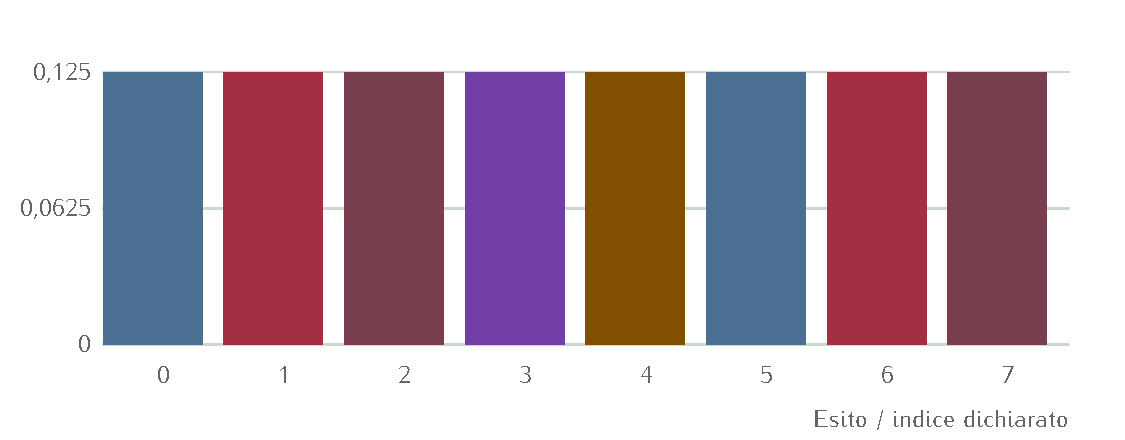
\includegraphics[width=\linewidth,height=94mm,keepaspectratio]{figure/fb06f6bfaa089c265.pdf}\FigureCaption{4.06 \(\cdot\) esempio 2 \(\cdot\) Distribuzione uniforme di partenza}\end{FigureBlock}

\phantomsection\label{c4-ricerca-ignota-example-2-step-1}
\BookHeading{01 Definire il tentativo}

\MathBlock{006D003D0031003B0020006A00200065007300740072006100740074006F00200075006E00690066006F0072006D0065006D0065006E007400650020006600720061002000300020006500202308006D230922120031003B002003C8003D005102B2007C007327E9}{m=1;\allowbreak \ j\ \text{estratto}\ \text{uniformemente}\ \text{fra}\ 0\ e\ \lceil m\rceil - 1;\allowbreak \ \psi =Q^{j}|s\rangle }

La scelta del numero di iterazioni usa una finestra crescente.\par


\phantomsection\label{c4-ricerca-ignota-example-2-step-2}
\BookHeading{02 Calcolare e leggere}

\MathBlock{006320320078003D003203BC22120063007800200064006F0070006F0020006F0067006E00690020006D00610072006300610074007500720061003B002000780020007600690065006E0065002000630061006D00700069006F006E00610074006F0020006400610020007C00630078007C00B2002E}{c{}^{\prime} x=2\mu - cx\ \text{dopo}\ \text{ogni}\ \text{marcatura};\allowbreak \ x\ \text{viene}\ \text{campionato}\ \text{da}\ |cx|^{2}.}
\MathBlock{0043006F00730074006F002000640065006C002000740065006E00740061007400690076006F003D006A002B003100200069006E0074006500720072006F00670061007A0069006F006E0069002E}{\text{Costo}\ \text{del}\ \text{tentativo}=j+1\ \text{interrogazioni}.}

L'ultima interrogazione verifica classicamente il candidato.\par


\phantomsection\label{c4-ricerca-ignota-example-2-step-3}
\BookHeading{03 Aggiornare la procedura}

\TextBlock{0053006500200069006C002000630061006E00640069006400610074006F002000E800200069006E006600720075007400740075006F0073006F003A0020006D2190006D0069006E00280036006D002F0035002C221A00380029002E000A00530065002000E80020007500740069006C0065003A0020006100720072006500730074006F002000640065006C006C006100200072006900630065007200630061002C0020006F007000700075007200650020006E0075006F0076006100200073006F0067006C006900610020006E0065006C006C006100200072006900630065007200630061002000640065006C0020006D0069006E0069006D006F002E}{Se il candidato è infruttuoso: \(m\leftarrow \min (6m/5,\allowbreak \sqrt{8})\). Se è utile: arresto della ricerca, oppure nuova soglia nella ricerca del minimo.}

Il budget impone un arresto eseguibile.\par


\phantomsection\label{c4-ricerca-ignota-example-2-step-4}
\BookHeading{04 Interpretare l'arresto}

\MathBlock{0049006C0020006200750064006700650074002000E800200065007300610075007200690074006F002000730065006E007A006100200075006E00200065006C0065006D0065006E0074006F0020007600650072006900660069006300610074006F002E}{Il\ \text{budget}\ \text{è}\ \text{esaurito}\ \text{senza}\ \text{un}\ \text{elemento}\ \text{verificato}.}

Un fallimento entro il budget non certifica deterministicamente che non esistano soluzioni. La tabella mostra la probabilità esatta di ciascun tentativo.\par


\phantomsection\label{c4-ricerca-ignota-example-2-step-5}
\BookHeading{05 Dichiarare il limite probabilistico}

\MathBlock{00530065002000650073006900730074006500200061006C006D0065006E006F00200075006E006100200073006F006C0075007A0069006F006E0065002C00200069006C002000740065006E00740061007400690076006F00200069006E0063006C0075006400650020006A003D003000200063006F006E002000700072006F0062006100620069006C0069007400E000200061006C006D0065006E006F00200031002F2308221A00382309003D0031002F0033002E0020005100750069006E006400690020005000280073007500630063006500730073006F002922650031002F0028003800B700330029003D0031002F00320034002E}{Se\ \text{esiste}\ \text{almeno}\ \text{una}\ \text{soluzione},\allowbreak \ \text{il}\ \text{tentativo}\ \text{include}\ j=0\ \text{con}\ \text{probabilità}\ \text{almeno}\ 1/\lceil \sqrt{8}\rceil =1/3.\ \text{Quindi}\ P(\text{successo})\ge 1/(8\cdot 3)=1/24.}
\MathBlock{0044006F0070006F00200054003D00310032002000740065006E007400610074006900760069002C00200050002800660061006C006C0069006D0065006E0074006F00292264002800320033002F003200340029005E0031003222480030002C003600300030003000360036002E}{\text{Dopo}\ T=12\ \text{tentativi},\allowbreak \ P(\text{fallimento})\le (23/24)^{12}\approx 0{,}600066.}

È un limite conservativo riferito all'esistenza di almeno una soluzione. Il caso senza soluzioni non consente un certificato deterministico entro il budget.\par


\BookHeading{Interpretazione}

Sono state usate 24 interrogazioni, inclusi i controlli dei candidati.\par


\BookHeading{Tabella completa dei dati (12 righe)}

\begingroup\sffamily\fontsize{8.8}{11}\selectfont\setlength{\tabcolsep}{1.6mm}\renewcommand{\arraystretch}{1.28}
\begin{longtable}{>{\RaggedRight\arraybackslash}p{14.000mm}>{\RaggedRight\arraybackslash}p{12.000mm}>{\RaggedRight\arraybackslash}p{14.000mm}>{\RaggedRight\arraybackslash}p{9.000mm}>{\RaggedRight\arraybackslash}p{19.400mm}>{\RaggedRight\arraybackslash}p{17.000mm}>{\RaggedRight\arraybackslash}p{13.000mm}>{\RaggedRight\arraybackslash}p{12.000mm}}
\toprule\rowcolor{Accent!7}\BeginAccSupp{method=hex,unicode,ActualText=00540065006E00740061007400690076006F}Tentativo\EndAccSupp{} & \BeginAccSupp{method=hex,unicode,ActualText=00460069006E006500730074007200610020006D}Finestra m\EndAccSupp{} & \BeginAccSupp{method=hex,unicode,ActualText=00490074006500720061007A0069006F006E00690020006A}Iterazioni j\EndAccSupp{} & \BeginAccSupp{method=hex,unicode,ActualText=0045007300690074006F00200078}Esito x\EndAccSupp{} & \BeginAccSupp{method=hex,unicode,ActualText=005600650072006900660069006300610020002F00200073006F0067006C00690061}Verifica / soglia\EndAccSupp{} & \BeginAccSupp{method=hex,unicode,ActualText=00500020007500740069006C0065}\(P\) utile\EndAccSupp{} & \BeginAccSupp{method=hex,unicode,ActualText=0043006F00730074006F002000740065006E00740061007400690076006F}Costo tentativo\EndAccSupp{} & \BeginAccSupp{method=hex,unicode,ActualText=0043006F00730074006F002000630075006D0075006C00610074006F}Costo cumulato\EndAccSupp{} \\
\midrule\endfirsthead
\toprule\rowcolor{Accent!7}\BeginAccSupp{method=hex,unicode,ActualText=00540065006E00740061007400690076006F}Tentativo\EndAccSupp{} & \BeginAccSupp{method=hex,unicode,ActualText=00460069006E006500730074007200610020006D}Finestra m\EndAccSupp{} & \BeginAccSupp{method=hex,unicode,ActualText=00490074006500720061007A0069006F006E00690020006A}Iterazioni j\EndAccSupp{} & \BeginAccSupp{method=hex,unicode,ActualText=0045007300690074006F00200078}Esito x\EndAccSupp{} & \BeginAccSupp{method=hex,unicode,ActualText=005600650072006900660069006300610020002F00200073006F0067006C00690061}Verifica / soglia\EndAccSupp{} & \BeginAccSupp{method=hex,unicode,ActualText=00500020007500740069006C0065}\(P\) utile\EndAccSupp{} & \BeginAccSupp{method=hex,unicode,ActualText=0043006F00730074006F002000740065006E00740061007400690076006F}Costo tentativo\EndAccSupp{} & \BeginAccSupp{method=hex,unicode,ActualText=0043006F00730074006F002000630075006D0075006C00610074006F}Costo cumulato\EndAccSupp{} \\
\midrule\endhead\bottomrule\endfoot
\BeginAccSupp{method=hex,unicode,ActualText=0031}1\EndAccSupp{} & \BeginAccSupp{method=hex,unicode,ActualText=0031}1\EndAccSupp{} & \BeginAccSupp{method=hex,unicode,ActualText=0030}0\EndAccSupp{} & \BeginAccSupp{method=hex,unicode,ActualText=0031}1\EndAccSupp{} & \BeginAccSupp{method=hex,unicode,ActualText=006E006F006E0020006D00610072006300610074006F}non marcato\EndAccSupp{} & \BeginAccSupp{method=hex,unicode,ActualText=0030}0\EndAccSupp{} & \BeginAccSupp{method=hex,unicode,ActualText=0031}1\EndAccSupp{} & \BeginAccSupp{method=hex,unicode,ActualText=0031}1\EndAccSupp{} \\
\BeginAccSupp{method=hex,unicode,ActualText=0032}2\EndAccSupp{} & \BeginAccSupp{method=hex,unicode,ActualText=0031002C0032}1,2\EndAccSupp{} & \BeginAccSupp{method=hex,unicode,ActualText=0031}1\EndAccSupp{} & \BeginAccSupp{method=hex,unicode,ActualText=0032}2\EndAccSupp{} & \BeginAccSupp{method=hex,unicode,ActualText=006E006F006E0020006D00610072006300610074006F}non marcato\EndAccSupp{} & \BeginAccSupp{method=hex,unicode,ActualText=0030}0\EndAccSupp{} & \BeginAccSupp{method=hex,unicode,ActualText=0032}2\EndAccSupp{} & \BeginAccSupp{method=hex,unicode,ActualText=0033}3\EndAccSupp{} \\
\BeginAccSupp{method=hex,unicode,ActualText=0033}3\EndAccSupp{} & \BeginAccSupp{method=hex,unicode,ActualText=0031002C00340034}1,44\EndAccSupp{} & \BeginAccSupp{method=hex,unicode,ActualText=0030}0\EndAccSupp{} & \BeginAccSupp{method=hex,unicode,ActualText=0032}2\EndAccSupp{} & \BeginAccSupp{method=hex,unicode,ActualText=006E006F006E0020006D00610072006300610074006F}non marcato\EndAccSupp{} & \BeginAccSupp{method=hex,unicode,ActualText=0030}0\EndAccSupp{} & \BeginAccSupp{method=hex,unicode,ActualText=0031}1\EndAccSupp{} & \BeginAccSupp{method=hex,unicode,ActualText=0034}4\EndAccSupp{} \\
\BeginAccSupp{method=hex,unicode,ActualText=0034}4\EndAccSupp{} & \BeginAccSupp{method=hex,unicode,ActualText=0031002C003700320038}1,728\EndAccSupp{} & \BeginAccSupp{method=hex,unicode,ActualText=0031}1\EndAccSupp{} & \BeginAccSupp{method=hex,unicode,ActualText=0034}4\EndAccSupp{} & \BeginAccSupp{method=hex,unicode,ActualText=006E006F006E0020006D00610072006300610074006F}non marcato\EndAccSupp{} & \BeginAccSupp{method=hex,unicode,ActualText=0030}0\EndAccSupp{} & \BeginAccSupp{method=hex,unicode,ActualText=0032}2\EndAccSupp{} & \BeginAccSupp{method=hex,unicode,ActualText=0036}6\EndAccSupp{} \\
\BeginAccSupp{method=hex,unicode,ActualText=0035}5\EndAccSupp{} & \BeginAccSupp{method=hex,unicode,ActualText=0032002C0030003700330036}2,0736\EndAccSupp{} & \BeginAccSupp{method=hex,unicode,ActualText=0032}2\EndAccSupp{} & \BeginAccSupp{method=hex,unicode,ActualText=0030}0\EndAccSupp{} & \BeginAccSupp{method=hex,unicode,ActualText=006E006F006E0020006D00610072006300610074006F}non marcato\EndAccSupp{} & \BeginAccSupp{method=hex,unicode,ActualText=0030}0\EndAccSupp{} & \BeginAccSupp{method=hex,unicode,ActualText=0033}3\EndAccSupp{} & \BeginAccSupp{method=hex,unicode,ActualText=0039}9\EndAccSupp{} \\
\BeginAccSupp{method=hex,unicode,ActualText=0036}6\EndAccSupp{} & \BeginAccSupp{method=hex,unicode,ActualText=0032002C00340038003800330032}2,48832\EndAccSupp{} & \BeginAccSupp{method=hex,unicode,ActualText=0031}1\EndAccSupp{} & \BeginAccSupp{method=hex,unicode,ActualText=0037}7\EndAccSupp{} & \BeginAccSupp{method=hex,unicode,ActualText=006E006F006E0020006D00610072006300610074006F}non marcato\EndAccSupp{} & \BeginAccSupp{method=hex,unicode,ActualText=0030}0\EndAccSupp{} & \BeginAccSupp{method=hex,unicode,ActualText=0032}2\EndAccSupp{} & \BeginAccSupp{method=hex,unicode,ActualText=00310031}11\EndAccSupp{} \\
\BeginAccSupp{method=hex,unicode,ActualText=0037}7\EndAccSupp{} & \BeginAccSupp{method=hex,unicode,ActualText=0032002C003800320038003400320037}2,828427\EndAccSupp{} & \BeginAccSupp{method=hex,unicode,ActualText=0031}1\EndAccSupp{} & \BeginAccSupp{method=hex,unicode,ActualText=0037}7\EndAccSupp{} & \BeginAccSupp{method=hex,unicode,ActualText=006E006F006E0020006D00610072006300610074006F}non marcato\EndAccSupp{} & \BeginAccSupp{method=hex,unicode,ActualText=0030}0\EndAccSupp{} & \BeginAccSupp{method=hex,unicode,ActualText=0032}2\EndAccSupp{} & \BeginAccSupp{method=hex,unicode,ActualText=00310033}13\EndAccSupp{} \\
\BeginAccSupp{method=hex,unicode,ActualText=0038}8\EndAccSupp{} & \BeginAccSupp{method=hex,unicode,ActualText=0032002C003800320038003400320037}2,828427\EndAccSupp{} & \BeginAccSupp{method=hex,unicode,ActualText=0030}0\EndAccSupp{} & \BeginAccSupp{method=hex,unicode,ActualText=0037}7\EndAccSupp{} & \BeginAccSupp{method=hex,unicode,ActualText=006E006F006E0020006D00610072006300610074006F}non marcato\EndAccSupp{} & \BeginAccSupp{method=hex,unicode,ActualText=0030}0\EndAccSupp{} & \BeginAccSupp{method=hex,unicode,ActualText=0031}1\EndAccSupp{} & \BeginAccSupp{method=hex,unicode,ActualText=00310034}14\EndAccSupp{} \\
\BeginAccSupp{method=hex,unicode,ActualText=0039}9\EndAccSupp{} & \BeginAccSupp{method=hex,unicode,ActualText=0032002C003800320038003400320037}2,828427\EndAccSupp{} & \BeginAccSupp{method=hex,unicode,ActualText=0031}1\EndAccSupp{} & \BeginAccSupp{method=hex,unicode,ActualText=0030}0\EndAccSupp{} & \BeginAccSupp{method=hex,unicode,ActualText=006E006F006E0020006D00610072006300610074006F}non marcato\EndAccSupp{} & \BeginAccSupp{method=hex,unicode,ActualText=0030}0\EndAccSupp{} & \BeginAccSupp{method=hex,unicode,ActualText=0032}2\EndAccSupp{} & \BeginAccSupp{method=hex,unicode,ActualText=00310036}16\EndAccSupp{} \\
\BeginAccSupp{method=hex,unicode,ActualText=00310030}10\EndAccSupp{} & \BeginAccSupp{method=hex,unicode,ActualText=0032002C003800320038003400320037}2,828427\EndAccSupp{} & \BeginAccSupp{method=hex,unicode,ActualText=0031}1\EndAccSupp{} & \BeginAccSupp{method=hex,unicode,ActualText=0033}3\EndAccSupp{} & \BeginAccSupp{method=hex,unicode,ActualText=006E006F006E0020006D00610072006300610074006F}non marcato\EndAccSupp{} & \BeginAccSupp{method=hex,unicode,ActualText=0030}0\EndAccSupp{} & \BeginAccSupp{method=hex,unicode,ActualText=0032}2\EndAccSupp{} & \BeginAccSupp{method=hex,unicode,ActualText=00310038}18\EndAccSupp{} \\
\BeginAccSupp{method=hex,unicode,ActualText=00310031}11\EndAccSupp{} & \BeginAccSupp{method=hex,unicode,ActualText=0032002C003800320038003400320037}2,828427\EndAccSupp{} & \BeginAccSupp{method=hex,unicode,ActualText=0032}2\EndAccSupp{} & \BeginAccSupp{method=hex,unicode,ActualText=0037}7\EndAccSupp{} & \BeginAccSupp{method=hex,unicode,ActualText=006E006F006E0020006D00610072006300610074006F}non marcato\EndAccSupp{} & \BeginAccSupp{method=hex,unicode,ActualText=0030}0\EndAccSupp{} & \BeginAccSupp{method=hex,unicode,ActualText=0033}3\EndAccSupp{} & \BeginAccSupp{method=hex,unicode,ActualText=00320031}21\EndAccSupp{} \\
\BeginAccSupp{method=hex,unicode,ActualText=00310032}12\EndAccSupp{} & \BeginAccSupp{method=hex,unicode,ActualText=0032002C003800320038003400320037}2,828427\EndAccSupp{} & \BeginAccSupp{method=hex,unicode,ActualText=0032}2\EndAccSupp{} & \BeginAccSupp{method=hex,unicode,ActualText=0034}4\EndAccSupp{} & \BeginAccSupp{method=hex,unicode,ActualText=006E006F006E0020006D00610072006300610074006F}non marcato\EndAccSupp{} & \BeginAccSupp{method=hex,unicode,ActualText=0030}0\EndAccSupp{} & \BeginAccSupp{method=hex,unicode,ActualText=0033}3\EndAccSupp{} & \BeginAccSupp{method=hex,unicode,ActualText=00320034}24\EndAccSupp{} \\
\end{longtable}\endgroup

\Needspace{7\baselineskip}
\BookHeading{Il passaggio successivo}
Finora la preparazione è uniforme. La stessa coppia di riflessioni amplifica anche una distribuzione iniziale assegnata, purché possiamo applicare la preparazione \(A\) e la sua inversa.\par


\Needspace{.43\textheight}
\section{Amplificare una preparazione assegnata}
\phantomsection\label{c4-amplificazione}

{\sffamily\small\color{Ink!70} Riferimento alle slide: p. 216.\par}

{\sffamily\small\color{Ink!70} Laboratorio locale: \nolinkurl{index.html#capitolo-4/amplificazione}\par}

\BookHeading{Definizioni e costruzione}
Una matrice unitaria \(A\) prepara \(|a\rangle =A|0\rangle \), con ampiezze anche non uniformi. Il proiettore \(\Pi _{G}\) seleziona il sottospazio buono e \(p=\langle a|\Pi _{G}|a\rangle \) è la probabilità iniziale di successo.\par

Per \(0<p<1\) costruiamo gli assi dalle proiezioni normalizzate: \(|g\rangle =\Pi _{G}|a\rangle /\sqrt{p}\) e \(|b\rangle =(I- \Pi _{G})|a\rangle /\sqrt{1- p}\). Le componenti ereditano tutte le fasi della preparazione; in generale non sono somme uniformi di etichette. Rispetto a questi assi \(|a\rangle =\cos \theta |b\rangle +\sin \theta |g\rangle \), con \(\sin ^{2}\theta =p\).\par

La riflessione \(D_{A}=2|a\rangle \langle a|- I\) si costruisce come \(A(2|0\rangle \langle 0|- I)A{}^{\dagger} \). Applicata a v, dà \(2|a\rangle \langle a|v\rangle - v\), con il prodotto interno coniugato nel primo argomento. Composta con \(O=I- 2\Pi _{G}\) ha nel piano la stessa matrice di Grover e quindi lo stesso angolo \(2\theta \).\par

Dopo k iterazioni la probabilità buona è \(\sin ^{2}((2k+1)\theta )\). Si amplifica il peso complessivo della componente buona mantenendone i rapporti interni; non si uniformano le ampiezze dei marcati. Per \(p=0\) la preparazione non ha componente buona da amplificare, mentre per \(p=1\) ha già successo certo. Negli esempi \(A\) è una preparazione assegnata come primitiva: \(D_{A}\) è applicata direttamente al vettore, senza sintetizzare una rete elementare per \(A\) e \(A{}^{\dagger} \).\par


\MathBlock{0051005F0041003D0044005F0041004F003B00200044005F00410076003D0032006127E80061007C007627E922120076003B00200070003D201603A0004700200061201600B2003D00730069006E00B203B8002E}{Q_{A}=D_{AO};\allowbreak \ D_{A}v=2a\langle a|v\rangle - v;\allowbreak \ p=\Vert \Pi _{G}\ a\Vert ^{2}=\sin ^{2}\theta .}

\BookHeading{Come leggere le figure}
Il piano (b,g) ha coordinate reali perché gli assi incorporano le fasi della preparazione. Il registro completo conserva invece tutte le componenti complesse. Le due descrizioni coincidono nel sottospazio generato dalle proiezioni.\par


\BookHeading{Attività nel laboratorio modificabile}

\BookHeading{Obiettivo dell'esperimento}
Amplificare una preparazione con probabilità iniziale assegnata.\par

\BookHeading{Percorso operativo}
Variare la probabilità e il numero di iterazioni; includere gli estremi zero e uno.\par

\BookHeading{Lettura geometrica}
L'angolo iniziale dipende dalla norma della proiezione sul sottospazio favorevole.\par

\BookHeading{Controllo del risultato}
Confrontare probabilità finale e formula \(\sin ^{2}((2k+1)\theta )\).\par


\Needspace{.36\textheight}\phantomsection\label{c4-amplificazione-example-1}
{\sffamily\small\color{Accent} ESEMPIO SVOLTO 1\par}
\BookHeading{Due riflessioni nel piano della ricerca}
\(N=4\); \(G=\{3\}\); \(k=1\). I blocchi selezionabili sono preparazione, oracolo e diffusione.\par


\BookHeading{Geometria e configurazione dell'esempio}
\begin{FigureBlock}\centering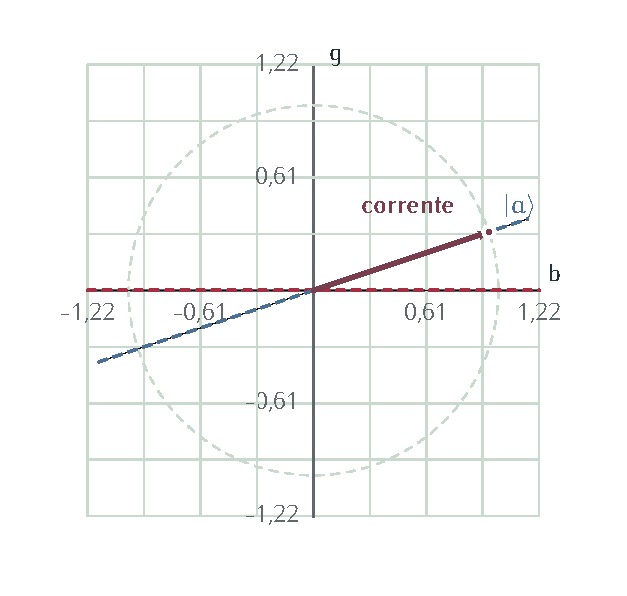
\includegraphics[width=\linewidth,height=94mm,keepaspectratio]{figure/f2b51f7a115f6c83e.pdf}\FigureCaption{4.07 \(\cdot\) esempio 1 \(\cdot\) Piano collettivo \(\cdot\) Preparazione \(A|0\rangle \)}\end{FigureBlock}
\begin{FigureBlock}\centering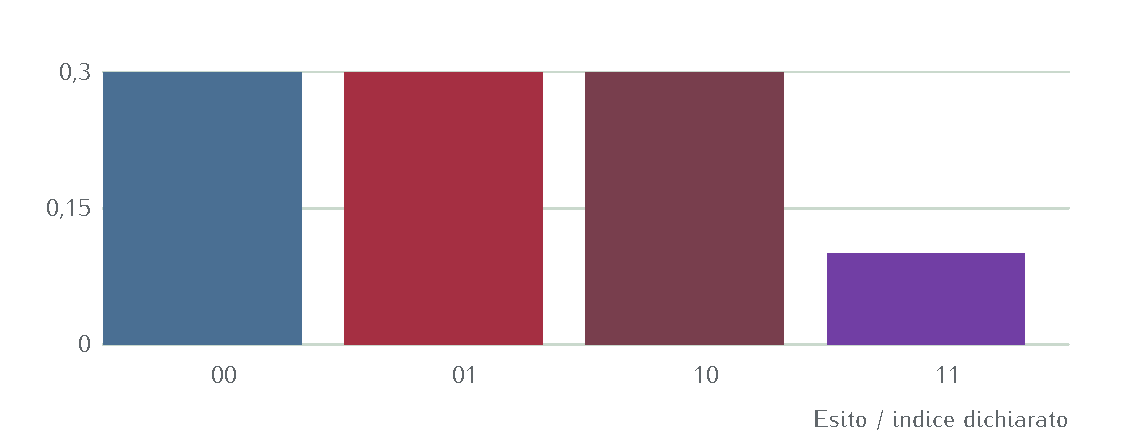
\includegraphics[width=\linewidth,height=94mm,keepaspectratio]{figure/fad48f26b9e30072f.pdf}\FigureCaption{4.07 \(\cdot\) esempio 1 \(\cdot\) Distribuzione congiunta \(\cdot\) Preparazione \(A|0\rangle \)}\end{FigureBlock}
\begin{FigureBlock}\centering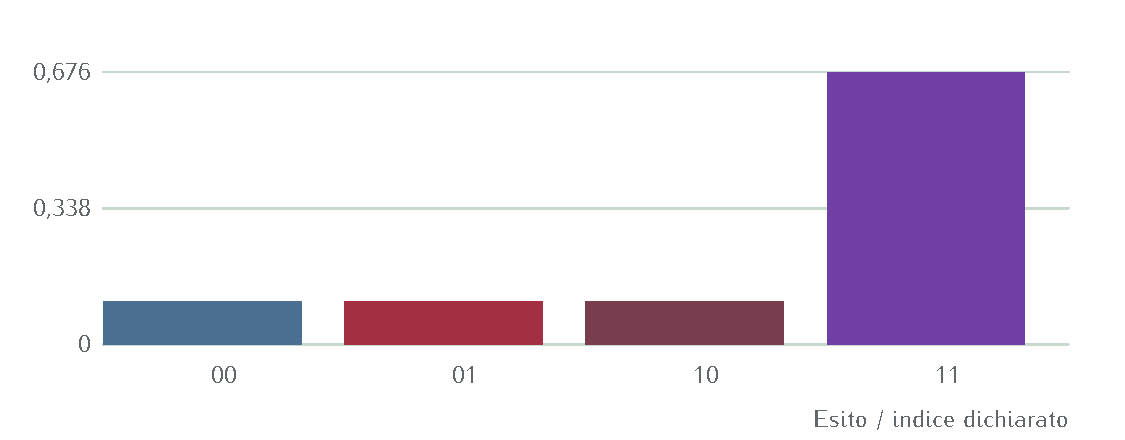
\includegraphics[width=\linewidth,height=94mm,keepaspectratio]{figure/fd6ab797ea2acfcaf.pdf}\FigureCaption{4.07 \(\cdot\) esempio 1 \(\cdot\) Probabilità finali delle singole alternative}\end{FigureBlock}
\begin{FigureBlock}\centering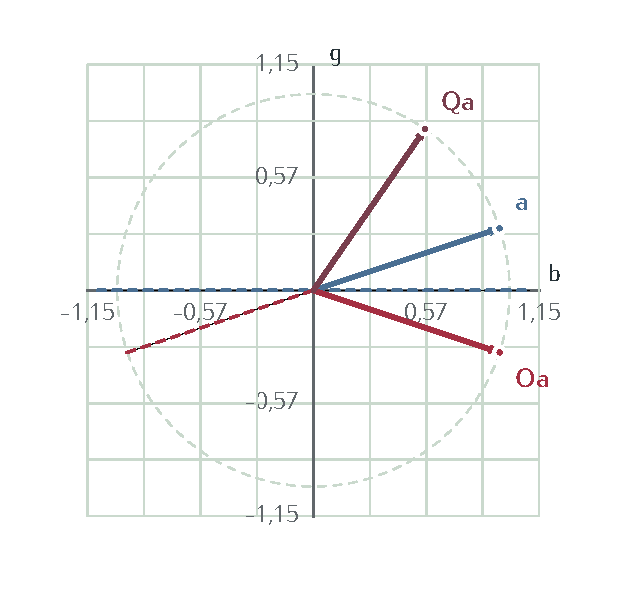
\includegraphics[width=\linewidth,height=94mm,keepaspectratio]{figure/f375edba6fb8e3df2.pdf}\FigureCaption{4.07 \(\cdot\) esempio 1 \(\cdot\) Prima iterazione \(\cdot\) una freccia dopo ogni riflessione}\end{FigureBlock}
\begin{FigureBlock}\begin{minipage}[t]{.485\linewidth}\centering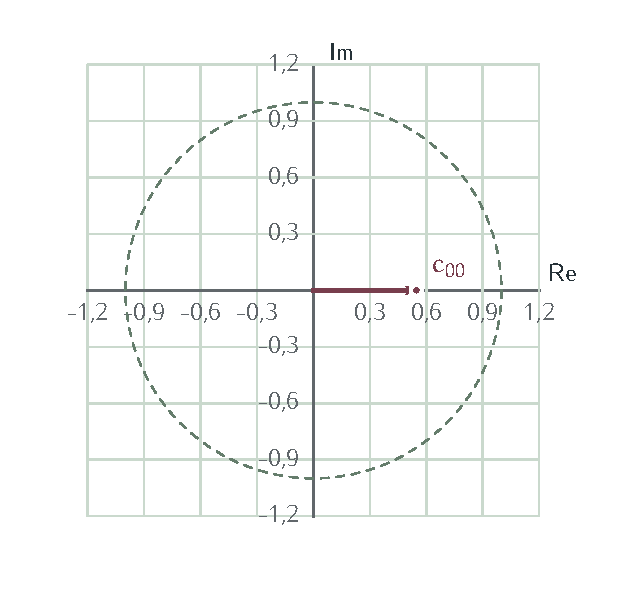
\includegraphics[width=\linewidth,height=63mm,keepaspectratio]{figure/f6271c769ecce36d4.pdf}\par{\sffamily\footnotesize \(c_{00}\)\par}\end{minipage}\hfill\begin{minipage}[t]{.485\linewidth}\centering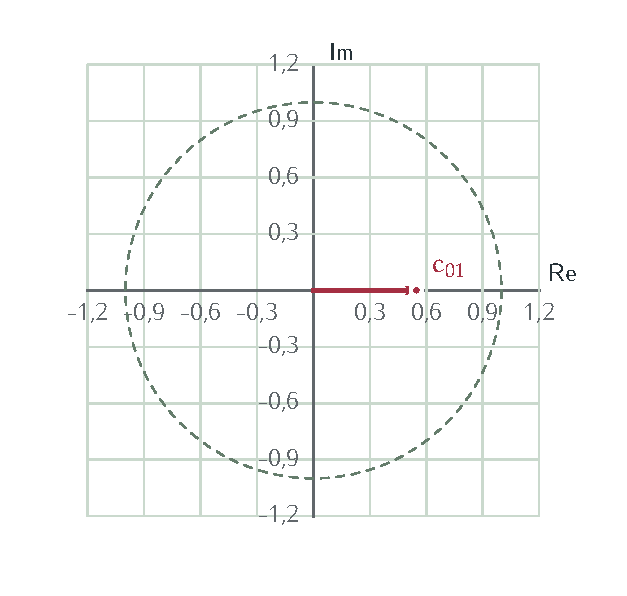
\includegraphics[width=\linewidth,height=63mm,keepaspectratio]{figure/f598ef5bdd9e67b6e.pdf}\par{\sffamily\footnotesize \(c_{01}\)\par}\end{minipage}\FigureCaption{4.07 \(\cdot\) esempio 1 \(\cdot\) Componenti complesse}\end{FigureBlock}
\begin{FigureBlock}\begin{minipage}[t]{.485\linewidth}\centering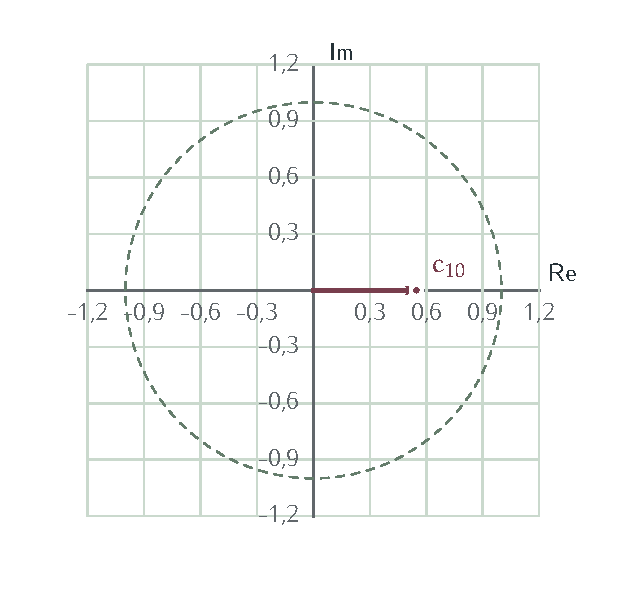
\includegraphics[width=\linewidth,height=63mm,keepaspectratio]{figure/f5b7ec590d08e0b22.pdf}\par{\sffamily\footnotesize \(c_{10}\)\par}\end{minipage}\hfill\begin{minipage}[t]{.485\linewidth}\centering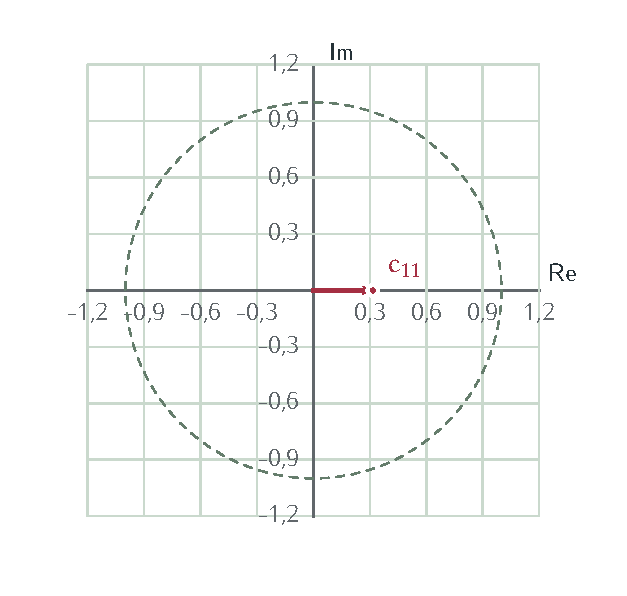
\includegraphics[width=\linewidth,height=63mm,keepaspectratio]{figure/fffc34b473854a204.pdf}\par{\sffamily\footnotesize \(c_{11}\)\par}\end{minipage}\FigureCaption{4.07 \(\cdot\) esempio 1 \(\cdot\) Componenti complesse}\end{FigureBlock}

\phantomsection\label{c4-amplificazione-example-1-step-1}
\BookHeading{01 Dichiarare la preparazione astratta}

\MathBlock{0041007C0030003027E9003D00280030002C0035003400370037003B00200030002C0035003400370037003B00200030002C0035003400370037003B00200030002C003300310036003200291D40003B00200044005F0041003D004100280032007C0030003027E927E800300030007C22120049002900412020003D0032007C006127E927E80061007C22120049002E}{A|00\rangle =(0{,}5477;\allowbreak \ 0{,}5477;\allowbreak \ 0{,}5477;\allowbreak \ 0{,}3162)^{T};\allowbreak \ D_{A}=A(2|00\rangle \langle 00|- I)A{}^{\dagger} =2|a\rangle \langle a|- I.}

In questo esempio \(A\) è una primitiva definita dalla preparazione assegnata; la simulazione applica direttamente la riflessione matriciale. La sintesi di \(A\) e di \(A{}^{\dagger} \) in porte e il loro costo non sono implementati da questi blocchi.\par


\phantomsection\label{c4-amplificazione-example-1-step-2}
\BookHeading{02 Costruire gli assi dalle proiezioni}

\MathBlock{007C006127E9003D0041007C003027E9003B002003A00047003D03A3007822080047007C007827E927E80078007C003B00200070003D27E80061007C03A00047007C006127E9003D0030002C0031002E}{|a\rangle =A|0\rangle ;\allowbreak \ \Pi _{G}=\sum _{x\in G}|x\rangle \langle x|;\allowbreak \ p=\langle a|\Pi _{G}|a\rangle =0{,}1.}
\MathBlock{007C006727E9003D03A00047007C006127E9002F221A0070224800280030003B00200030003B00200030003B0020003100291D40}{|g\rangle =\Pi _{G}|a\rangle /\sqrt{p}\approx (0;\allowbreak \ 0;\allowbreak \ 0;\allowbreak \ 1)^{T}}
\MathBlock{007C006227E9003D00280049221203A000470029007C006127E9002F221A00280031221200700029224800280030002C0035003700370034003B00200030002C0035003700370034003B00200030002C0035003700370034003B0020003000291D40002E}{|b\rangle =(I- \Pi _{G})|a\rangle /\sqrt{1- p}\approx (0{,}5774;\allowbreak \ 0{,}5774;\allowbreak \ 0{,}5774;\allowbreak \ 0)^{T}.}
\MathBlock{27E80062007C006727E9003D0030003B0020201600622016003D201600672016003D0031002E}{\langle b|g\rangle =0;\allowbreak \ \Vert b\Vert =\Vert g\Vert =1.}

I supporti sono disgiunti. Per la preparazione uniforme questi vettori diventano \(\sum _{x\in G}|x\rangle /\sqrt{M}\) e \(\sum x\notin G|x\rangle /\sqrt{N- M}\). Per una preparazione non uniforme conservano i suoi pesi e le sue fasi.\par


\phantomsection\label{c4-amplificazione-example-1-step-3}
\BookHeading{03 Proiettare la preparazione nel piano}

\MathBlock{27E80062007C006127E9003D221A00280031221200700029003D0030002C003900340038003600380033003B002027E80067007C006127E9003D221A0070003D0030002C003300310036003200320038002E}{\langle b|a\rangle =\sqrt{1- p}=0{,}948683;\allowbreak \ \langle g|a\rangle =\sqrt{p}=0{,}316228.}
\MathBlock{007C006127E9003D0063006F007303B8007C006227E9002B00730069006E03B8007C006727E9003B002003B8003D00610072006300730069006E221A007022480030002C0033003200310037003500310020007200610064002E}{|a\rangle =\cos \theta |b\rangle +\sin \theta |g\rangle ;\allowbreak \ \theta =\arcsin \sqrt{p}\approx 0{,}321751\ \text{rad}.}

Gli assi sono stati collettivi, non singoli esiti. Le coordinate qui sono reali perché le fasi della preparazione sono state incluse nella definizione degli assi.\par


\phantomsection\label{c4-amplificazione-example-1-step-4}
\BookHeading{04 Scrivere le due riflessioni}

\MathBlock{004E0065006C006C0061002000620061007300650020006F007200640069006E00610074006100200028007C006227E9002C007C006727E90029003A}{\text{Nella}\ \text{base}\ \text{ordinata}\ (|b\rangle ,\allowbreak |g\rangle ):}
\MathBlock{004F003D00492212003203A00047003D005B005B0031002C0030005D002C005B0030002C22120031005D005D002E}{O=I- 2\Pi _{G}=\begin{pmatrix}1&0\\0&- 1\end{pmatrix}.}
\MathBlock{0044005F0041003D0032007C006127E927E80061007C22120049}{D_{A}=2|a\rangle \langle a|- I}
\MathBlock{003D005B005B00320063006F007300B203B822120031002C00320063006F007303B800730069006E03B8005D002C005B00320063006F007303B800730069006E03B8002C003200730069006E00B203B822120031005D005D}{=\begin{pmatrix}2\cos ^{2}\theta - 1&2\cos \theta \sin \theta \\2\cos \theta \sin \theta &2\sin ^{2}\theta - 1\end{pmatrix}}
\MathBlock{003D005B005B0063006F0073003203B8002C00730069006E003203B8005D002C005B00730069006E003203B8002C22120063006F0073003203B8005D005D002E}{=\begin{pmatrix}\cos 2\theta &\sin 2\theta \\\sin 2\theta &- \cos 2\theta \end{pmatrix}.}

\(O\) riflette rispetto all'asse \(|b\rangle \). \(D_{A}\) riflette rispetto alla retta della preparazione \(|a\rangle \). L'ordine temporale è prima \(O\) e poi \(D_{A}\).\par


\phantomsection\label{c4-amplificazione-example-1-step-5}
\BookHeading{05 Moltiplicare e ottenere la rotazione}

\MathBlock{0051003D0044005F0041004F003D005B005B0063006F0073003203B8002C221200730069006E003203B8005D002C005B00730069006E003203B8002C0063006F0073003203B8005D005D}{Q=D_{AO}=\begin{pmatrix}\cos 2\theta &- \sin 2\theta \\\sin 2\theta &\cos 2\theta \end{pmatrix}}
\MathBlock{2248005B005B0030002C0038002C002D0030002C0036005D002C005B0030002C0036002C0030002C0038005D005D002E}{\approx \begin{pmatrix}0{,}8&-0{,}6\\0{,}6&0{,}8\end{pmatrix}.}
\MathBlock{004F00280063006F007303B8002C00730069006E03B800291D40003D00280063006F007303B8002C221200730069006E03B800291D40003B}{O(\cos \theta ,\allowbreak \sin \theta )^{T}=(\cos \theta ,\allowbreak - \sin \theta )^{T};\allowbreak }
\MathBlock{005100280063006F007303B8002C00730069006E03B800291D40003D00280063006F0073003303B8002C00730069006E003303B800291D40002E}{Q(\cos \theta ,\allowbreak \sin \theta )^{T}=(\cos 3\theta ,\allowbreak \sin 3\theta )^{T}.}
\MathBlock{00511D4F007C006127E9003D0063006F0073002800280032006B002B0031002903B80029007C006227E9002B00730069006E002800280032006B002B0031002903B80029007C006727E9002E}{Q^{k}|a\rangle =\cos ((2k+1)\theta )|b\rangle +\sin ((2k+1)\theta )|g\rangle .}

Il prodotto riga per colonna dà le formule di addizione del seno e del coseno. Ogni coppia completa di riflessioni ruota di \(2\theta \); dopo il solo oracolo si usa invece la riflessione, non la formula delle iterazioni complete.\par


\phantomsection\label{c4-amplificazione-example-1-step-6}
\BookHeading{06 Ricavare autovettori e autofasi}

\MathBlock{00640065007400280051221203BB00490029003D03BB00B2221200320063006F00730028003203B8002903BB002B0031003D0030002E}{\det (Q- \lambda I)=\lambda ^{2}- 2\cos (2\theta )\lambda +1=0.}
\MathBlock{03BB00B1003D0063006F0073003203B800B10069002000730069006E003203B8003D0065005E002800B10032006903B80029002E}{\lambda \pm =\cos 2\theta \pm i\ \sin 2\theta =e^{\pm 2i\theta }.}
\MathBlock{007C0075002B27E9003D0028007C006227E922120069007C006727E90029002F221A0032003B0020007C0075221227E9003D0028007C006227E9002B0069007C006727E90029002F221A0032002E}{|u+\rangle =(|b\rangle - i|g\rangle )/\sqrt{2};\allowbreak \ |u- \rangle =(|b\rangle +i|g\rangle )/\sqrt{2}.}
\MathBlock{0051007C007500B127E9003D0065005E002800B10032006903B80029007C007500B127E9003B002003C6002B003D03B8002F03C0002C002003C62212003D0031221203B8002F03C000200028006D006F0064002000310029002E}{Q|u\pm \rangle =e^{\pm 2i\theta }|u\pm \rangle ;\allowbreak \ \varphi +=\theta /\pi ,\allowbreak \ \varphi - =1- \theta /\pi \ (\bmod \ 1).}

Gli autovettori hanno coordinate complesse nel piano collettivo; non sono due frecce reali sul piano di Grover. Le autofasi sono frazioni di giro, poiché QPE usa \(e^{2\pi i\varphi }\).\par


\phantomsection\label{c4-amplificazione-example-1-step-7}
\BookHeading{07 Determinare i coefficienti della preparazione}

\MathBlock{03B2002B003D27E80075002B007C006127E9003D00280063006F007303B8002B0069002000730069006E03B80029002F221A0032003D0065005E0028006903B80029002F221A0032002E}{\beta +=\langle u+|a\rangle =(\cos \theta +i\ \sin \theta )/\sqrt{2}=e^{i\theta }/\sqrt{2}.}
\MathBlock{03B22212003D27E800752212007C006127E9003D00280063006F007303B822120069002000730069006E03B80029002F221A0032003D0065005E00282212006903B80029002F221A0032002E}{\beta - =\langle u- |a\rangle =(\cos \theta - i\ \sin \theta )/\sqrt{2}=e^{- i\theta }/\sqrt{2}.}
\MathBlock{007C006127E9003D03B2002B007C0075002B27E9002B03B22212007C0075221227E9003B0020007C03B2002B007C00B2003D007C03B22212007C00B2003D0031002F0032002E}{|a\rangle =\beta +|u+\rangle +\beta - |u- \rangle ;\allowbreak \ |\beta +|^{2}=|\beta - |^{2}=1/2.}

I due pesi uguali derivano dal prodotto interno con la preparazione. Manteniamo anche le fasi dei coefficienti: servono per ricostruire il bersaglio coerente condizionato dopo QPE.\par


\phantomsection\label{c4-amplificazione-example-1-step-8}
\BookHeading{08 Preparazione \(A|0\rangle \)}

\MathBlock{00280030002C0035003400370037003B00200030002C0035003400370037003B00200030002C0035003400370037003B00200030002C003300310036003200291D40}{(0{,}5477;\allowbreak \ 0{,}5477;\allowbreak \ 0{,}5477;\allowbreak \ 0{,}3162)^{T}}
\MathBlock{03C8224800280030002C0035003400370037003B00200030002C0035003400370037003B00200030002C0035003400370037003B00200030002C003300310036003200291D40}{\psi \approx (0{,}5477;\allowbreak \ 0{,}5477;\allowbreak \ 0{,}5477;\allowbreak \ 0{,}3162)^{T}}
\MathBlock{0043006F006F007200640069006E0061007400650020002827E80062007C03C827E9002C27E80067007C03C827E90029224800280030002C003900340038003600380033003B00200030002C0033003100360032003200380029}{\text{Coordinate}\ (\langle b|\psi \rangle ,\allowbreak \langle g|\psi \rangle )\approx (0{,}948683;\allowbreak \ 0{,}316228)}

La marcatura cambia il segno delle ampiezze buone; la riflessione usa il prodotto interno con la preparazione.\par


\phantomsection\label{c4-amplificazione-example-1-step-9}
\BookHeading{09 Oracolo 1}

\MathBlock{004F007C007827E90020003D00200028221200310029005E005B007822080047005D007C007827E9003B00200047003D007B0033007D}{O|x\rangle \ =\ (- 1)^{x\in G}|x\rangle ;\allowbreak \ G=\{3\}}
\MathBlock{03C8224800280030002C0035003400370037003B00200030002C0035003400370037003B00200030002C0035003400370037003B0020002D0030002C003300310036003200291D40}{\psi \approx (0{,}5477;\allowbreak \ 0{,}5477;\allowbreak \ 0{,}5477;\allowbreak \ -0{,}3162)^{T}}
\MathBlock{0043006F006F007200640069006E0061007400650020002827E80062007C03C827E9002C27E80067007C03C827E90029224800280030002C003900340038003600380033003B0020002D0030002C0033003100360032003200380029}{\text{Coordinate}\ (\langle b|\psi \rangle ,\allowbreak \langle g|\psi \rangle )\approx (0{,}948683;\allowbreak \ -0{,}316228)}

La marcatura cambia il segno delle ampiezze buone; la riflessione usa il prodotto interno con la preparazione.\par


\phantomsection\label{c4-amplificazione-example-1-step-10}
\BookHeading{10 Riflessione 1}

\MathBlock{27E80061007C007627E90020003D002000280030002C0035003400370037002900B700280030002C003500340037003700290020002B002000280030002C0035003400370037002900B700280030002C003500340037003700290020002B002000280030002C0035003400370037002900B700280030002C003500340037003700290020002B002000280030002C0033003100360032002900B70028002D0030002C003300310036003200290020224800200030002C0038}{\langle a|v\rangle \ =\ (0{,}5477)\cdot (0{,}5477)\ +\ (0{,}5477)\cdot (0{,}5477)\ +\ (0{,}5477)\cdot (0{,}5477)\ +\ (0{,}3162)\cdot (-0{,}3162)\ \approx \ 0{,}8}
\MathBlock{00630028003000290020003D0020003200B700280030002C0035003400370037002900B700280030002C0038002900202212002000280030002C003500340037003700290020224800200030002C0033003200380036}{c(0)\ =\ 2\cdot (0{,}5477)\cdot (0{,}8)\ - \ (0{,}5477)\ \approx \ 0{,}3286}
\MathBlock{00630028003100290020003D0020003200B700280030002C0035003400370037002900B700280030002C0038002900202212002000280030002C003500340037003700290020224800200030002C0033003200380036}{c(1)\ =\ 2\cdot (0{,}5477)\cdot (0{,}8)\ - \ (0{,}5477)\ \approx \ 0{,}3286}
\MathBlock{00630028003200290020003D0020003200B700280030002C0035003400370037002900B700280030002C0038002900202212002000280030002C003500340037003700290020224800200030002C0033003200380036}{c(2)\ =\ 2\cdot (0{,}5477)\cdot (0{,}8)\ - \ (0{,}5477)\ \approx \ 0{,}3286}
\MathBlock{00630028003300290020003D0020003200B700280030002C0033003100360032002900B700280030002C003800290020221200200028002D0030002C003300310036003200290020224800200030002C0038003200320032}{c(3)\ =\ 2\cdot (0{,}3162)\cdot (0{,}8)\ - \ (-0{,}3162)\ \approx \ 0{,}8222}
\MathBlock{03C8224800280030002C0033003200380036003B00200030002C0033003200380036003B00200030002C0033003200380036003B00200030002C003800320032003200291D40}{\psi \approx (0{,}3286;\allowbreak \ 0{,}3286;\allowbreak \ 0{,}3286;\allowbreak \ 0{,}8222)^{T}}
\MathBlock{0043006F006F007200640069006E0061007400650020002827E80062007C03C827E9002C27E80067007C03C827E90029224800280030002C00350036003900320031003B00200030002C0038003200320031003900320029}{\text{Coordinate}\ (\langle b|\psi \rangle ,\allowbreak \langle g|\psi \rangle )\approx (0{,}56921;\allowbreak \ 0{,}822192)}

La marcatura cambia il segno delle ampiezze buone; la riflessione usa il prodotto interno con la preparazione.\par


\phantomsection\label{c4-amplificazione-example-1-step-11}
\BookHeading{11 Probabilità di successo}

\MathBlock{00702080003D0030002C0031003B002003B8003D00610072006300730069006E221A0070208022480030002C00330032003100380020007200610064}{p_{0}=0{,}1;\allowbreak \ \theta =\arcsin \sqrt{p}_{0}\approx 0{,}3218\ \text{rad}}
\MathBlock{00500073007500630063006500730073006F003D03A3007822080047007C00632093007C00B222480030002C003600370036}{\text{Psuccesso}=\sum _{x\in G}|c_{x}|^{2}\approx 0{,}676}
\MathBlock{00730069006E00B2002800280032006B002B0031002903B80029003D00730069006E00B20028003300B70030002C0033003200310038002922480030002C003600370036}{\sin ^{2}((2k+1)\theta )=\sin ^{2}(3\cdot 0{,}3218)\approx 0{,}676}

La formula geometrica verifica la simulazione delle ampiezze.\par


\BookHeading{Stato finale del programma}
\begin{FigureBlock}\centering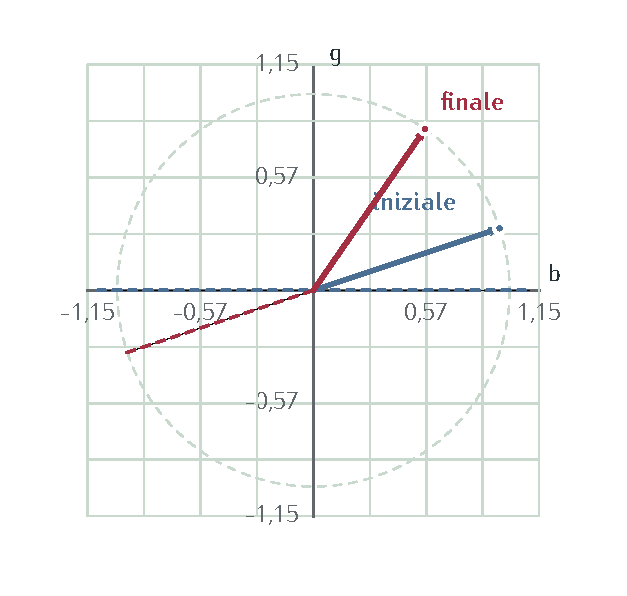
\includegraphics[width=\linewidth,height=94mm,keepaspectratio]{figure/f18c4fc58b8bbafd1.pdf}\FigureCaption{4.07 \(\cdot\) esempio 1 \(\cdot\) Piano \(|b\rangle ,\allowbreak |g\rangle \) \(\cdot\) confronto iniziale/finale}\end{FigureBlock}

\BookHeading{Interpretazione}

Il piano ha assi ortonormali ricavati dalla preparazione. Ogni freccia intermedia e le probabilità delle alternative derivano dai medesimi vettori del registro.\par


Risorse dichiarate. 1 interrogazioni all'oracolo; 2 qubit dati. Il costo della preparazione e della riflessione va aggiunto.\par


\Needspace{.36\textheight}\phantomsection\label{c4-amplificazione-example-2}
{\sffamily\small\color{Accent} ESEMPIO SVOLTO 2\par}
\BookHeading{Due riflessioni nel piano della ricerca}
\(N=4\); \(G=\{3\}\); \(k=1\). I blocchi selezionabili sono preparazione, oracolo e diffusione.\par


\BookHeading{Geometria e configurazione dell'esempio}
\begin{FigureBlock}\centering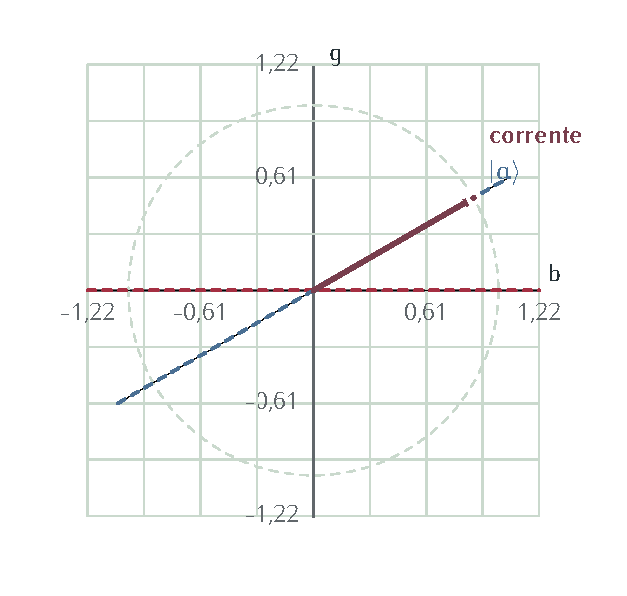
\includegraphics[width=\linewidth,height=94mm,keepaspectratio]{figure/fca2e79b0e025b3cd.pdf}\FigureCaption{4.07 \(\cdot\) esempio 2 \(\cdot\) Piano collettivo \(\cdot\) Preparazione \(A|0\rangle \)}\end{FigureBlock}
\begin{FigureBlock}\centering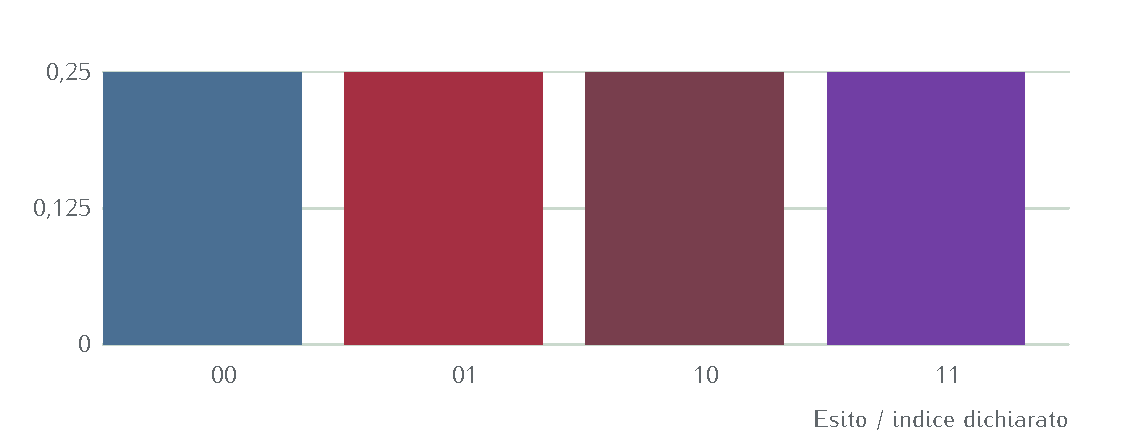
\includegraphics[width=\linewidth,height=94mm,keepaspectratio]{figure/f110b85b4147f43f9.pdf}\FigureCaption{4.07 \(\cdot\) esempio 2 \(\cdot\) Distribuzione congiunta \(\cdot\) Preparazione \(A|0\rangle \)}\end{FigureBlock}
\begin{FigureBlock}\centering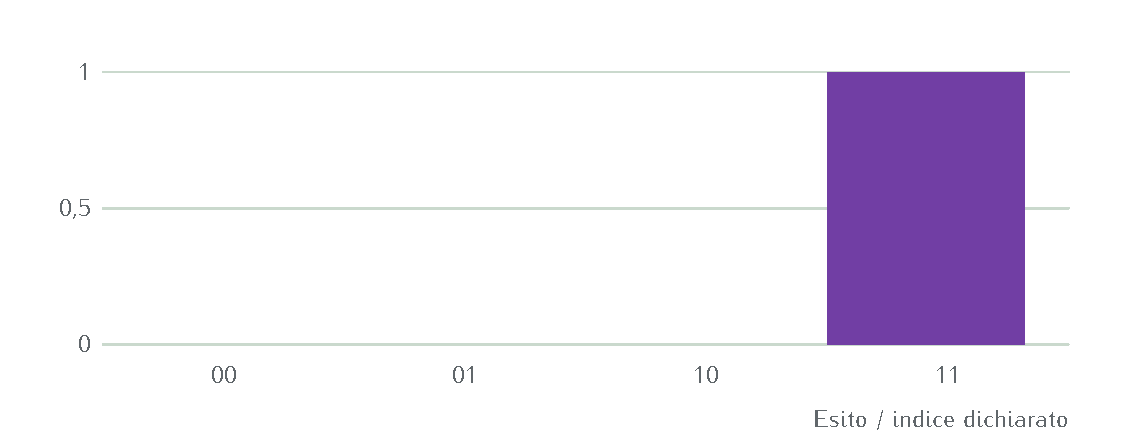
\includegraphics[width=\linewidth,height=94mm,keepaspectratio]{figure/f6d1f8bfe027e2333.pdf}\FigureCaption{4.07 \(\cdot\) esempio 2 \(\cdot\) Probabilità finali delle singole alternative}\end{FigureBlock}
\begin{FigureBlock}\centering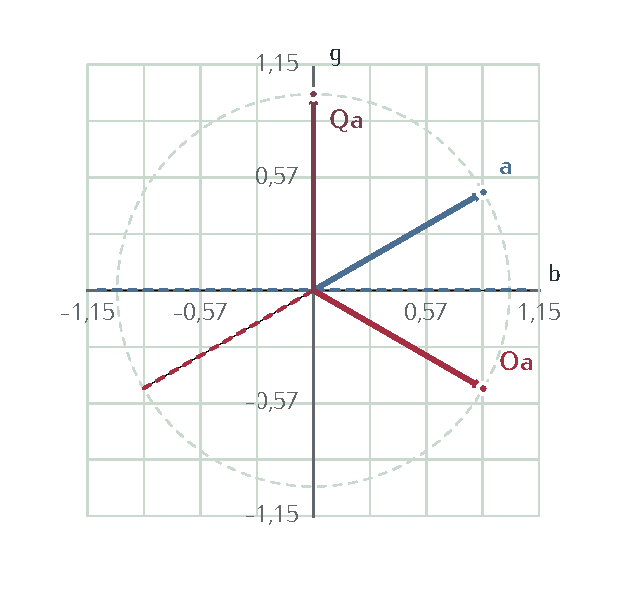
\includegraphics[width=\linewidth,height=94mm,keepaspectratio]{figure/ff1e99ea55984d73e.pdf}\FigureCaption{4.07 \(\cdot\) esempio 2 \(\cdot\) Prima iterazione \(\cdot\) una freccia dopo ogni riflessione}\end{FigureBlock}
\begin{FigureBlock}\begin{minipage}[t]{.485\linewidth}\centering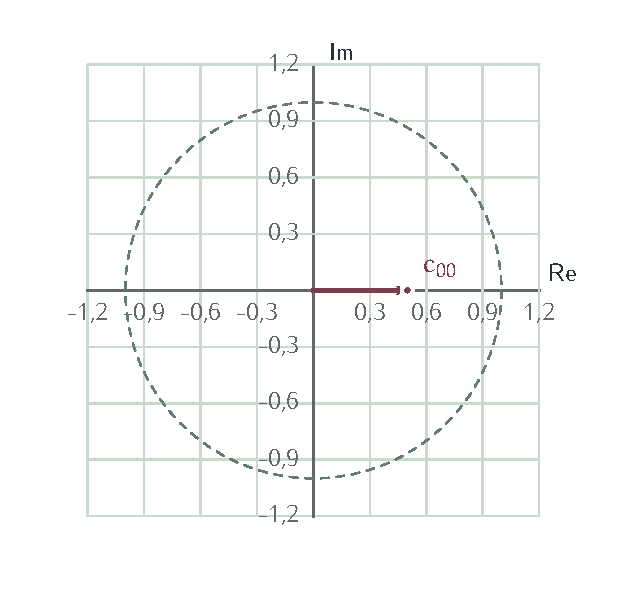
\includegraphics[width=\linewidth,height=63mm,keepaspectratio]{figure/f5be08ea2ba827a32.pdf}\par{\sffamily\footnotesize \(c_{00}\)\par}\end{minipage}\hfill\begin{minipage}[t]{.485\linewidth}\centering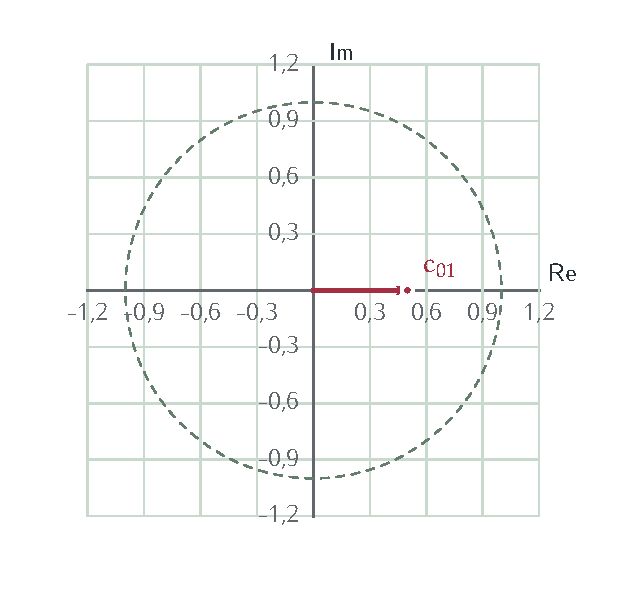
\includegraphics[width=\linewidth,height=63mm,keepaspectratio]{figure/f984c95d46c8fbc7c.pdf}\par{\sffamily\footnotesize \(c_{01}\)\par}\end{minipage}\FigureCaption{4.07 \(\cdot\) esempio 2 \(\cdot\) Componenti complesse}\end{FigureBlock}
\begin{FigureBlock}\begin{minipage}[t]{.485\linewidth}\centering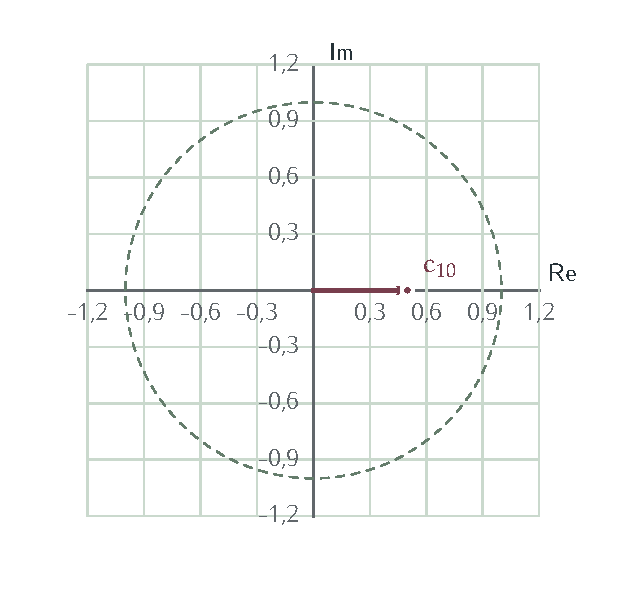
\includegraphics[width=\linewidth,height=63mm,keepaspectratio]{figure/fe4d23d0d1ddac8e4.pdf}\par{\sffamily\footnotesize \(c_{10}\)\par}\end{minipage}\hfill\begin{minipage}[t]{.485\linewidth}\centering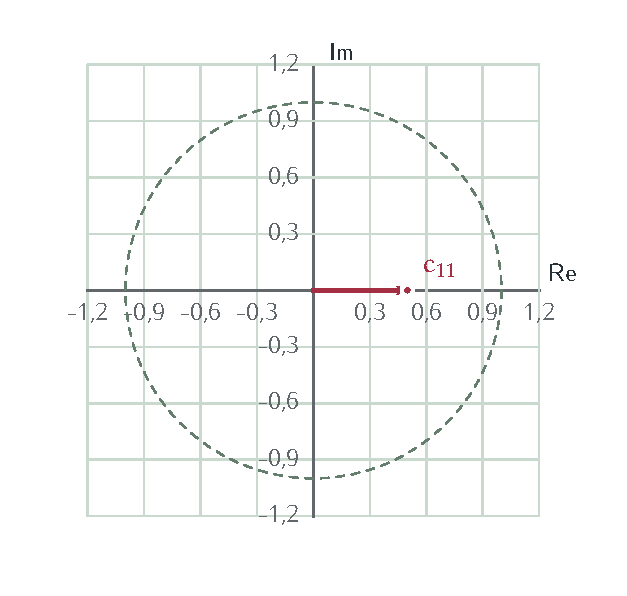
\includegraphics[width=\linewidth,height=63mm,keepaspectratio]{figure/fad87eff0103a78c8.pdf}\par{\sffamily\footnotesize \(c_{11}\)\par}\end{minipage}\FigureCaption{4.07 \(\cdot\) esempio 2 \(\cdot\) Componenti complesse}\end{FigureBlock}

\phantomsection\label{c4-amplificazione-example-2-step-1}
\BookHeading{01 Dichiarare la preparazione astratta}

\MathBlock{0041007C0030003027E9003D00280030002C0035003B00200030002C0035003B00200030002C0035003B00200030002C003500291D40003B00200044005F0041003D004100280032007C0030003027E927E800300030007C22120049002900412020003D0032007C006127E927E80061007C22120049002E}{A|00\rangle =(0{,}5;\allowbreak \ 0{,}5;\allowbreak \ 0{,}5;\allowbreak \ 0{,}5)^{T};\allowbreak \ D_{A}=A(2|00\rangle \langle 00|- I)A{}^{\dagger} =2|a\rangle \langle a|- I.}

In questo esempio \(A\) è una primitiva definita dalla preparazione assegnata; la simulazione applica direttamente la riflessione matriciale. La sintesi di \(A\) e di \(A{}^{\dagger} \) in porte e il loro costo non sono implementati da questi blocchi.\par


\phantomsection\label{c4-amplificazione-example-2-step-2}
\BookHeading{02 Costruire gli assi dalle proiezioni}

\MathBlock{007C006127E9003D0041007C003027E9003B002003A00047003D03A3007822080047007C007827E927E80078007C003B00200070003D27E80061007C03A00047007C006127E9003D0030002C00320035002E}{|a\rangle =A|0\rangle ;\allowbreak \ \Pi _{G}=\sum _{x\in G}|x\rangle \langle x|;\allowbreak \ p=\langle a|\Pi _{G}|a\rangle =0{,}25.}
\MathBlock{007C006727E9003D03A00047007C006127E9002F221A0070224800280030003B00200030003B00200030003B0020003100291D40}{|g\rangle =\Pi _{G}|a\rangle /\sqrt{p}\approx (0;\allowbreak \ 0;\allowbreak \ 0;\allowbreak \ 1)^{T}}
\MathBlock{007C006227E9003D00280049221203A000470029007C006127E9002F221A00280031221200700029224800280030002C0035003700370034003B00200030002C0035003700370034003B00200030002C0035003700370034003B0020003000291D40002E}{|b\rangle =(I- \Pi _{G})|a\rangle /\sqrt{1- p}\approx (0{,}5774;\allowbreak \ 0{,}5774;\allowbreak \ 0{,}5774;\allowbreak \ 0)^{T}.}
\MathBlock{27E80062007C006727E9003D0030003B0020201600622016003D201600672016003D0031002E}{\langle b|g\rangle =0;\allowbreak \ \Vert b\Vert =\Vert g\Vert =1.}

I supporti sono disgiunti. Per la preparazione uniforme questi vettori diventano \(\sum _{x\in G}|x\rangle /\sqrt{M}\) e \(\sum x\notin G|x\rangle /\sqrt{N- M}\). Per una preparazione non uniforme conservano i suoi pesi e le sue fasi.\par


\phantomsection\label{c4-amplificazione-example-2-step-3}
\BookHeading{03 Proiettare la preparazione nel piano}

\MathBlock{27E80062007C006127E9003D221A00280031221200700029003D0030002C003800360036003000320035003B002027E80067007C006127E9003D221A0070003D0030002C0035002E}{\langle b|a\rangle =\sqrt{1- p}=0{,}866025;\allowbreak \ \langle g|a\rangle =\sqrt{p}=0{,}5.}
\MathBlock{007C006127E9003D0063006F007303B8007C006227E9002B00730069006E03B8007C006727E9003B002003B8003D00610072006300730069006E221A007022480030002C0035003200330035003900390020007200610064002E}{|a\rangle =\cos \theta |b\rangle +\sin \theta |g\rangle ;\allowbreak \ \theta =\arcsin \sqrt{p}\approx 0{,}523599\ \text{rad}.}

Gli assi sono stati collettivi, non singoli esiti. Le coordinate qui sono reali perché le fasi della preparazione sono state incluse nella definizione degli assi.\par


\phantomsection\label{c4-amplificazione-example-2-step-4}
\BookHeading{04 Scrivere le due riflessioni}

\MathBlock{004E0065006C006C0061002000620061007300650020006F007200640069006E00610074006100200028007C006227E9002C007C006727E90029003A}{\text{Nella}\ \text{base}\ \text{ordinata}\ (|b\rangle ,\allowbreak |g\rangle ):}
\MathBlock{004F003D00492212003203A00047003D005B005B0031002C0030005D002C005B0030002C22120031005D005D002E}{O=I- 2\Pi _{G}=\begin{pmatrix}1&0\\0&- 1\end{pmatrix}.}
\MathBlock{0044005F0041003D0032007C006127E927E80061007C22120049}{D_{A}=2|a\rangle \langle a|- I}
\MathBlock{003D005B005B00320063006F007300B203B822120031002C00320063006F007303B800730069006E03B8005D002C005B00320063006F007303B800730069006E03B8002C003200730069006E00B203B822120031005D005D}{=\begin{pmatrix}2\cos ^{2}\theta - 1&2\cos \theta \sin \theta \\2\cos \theta \sin \theta &2\sin ^{2}\theta - 1\end{pmatrix}}
\MathBlock{003D005B005B0063006F0073003203B8002C00730069006E003203B8005D002C005B00730069006E003203B8002C22120063006F0073003203B8005D005D002E}{=\begin{pmatrix}\cos 2\theta &\sin 2\theta \\\sin 2\theta &- \cos 2\theta \end{pmatrix}.}

\(O\) riflette rispetto all'asse \(|b\rangle \). \(D_{A}\) riflette rispetto alla retta della preparazione \(|a\rangle \). L'ordine temporale è prima \(O\) e poi \(D_{A}\).\par


\phantomsection\label{c4-amplificazione-example-2-step-5}
\BookHeading{05 Moltiplicare e ottenere la rotazione}

\MathBlock{0051003D0044005F0041004F003D005B005B0063006F0073003203B8002C221200730069006E003203B8005D002C005B00730069006E003203B8002C0063006F0073003203B8005D005D}{Q=D_{AO}=\begin{pmatrix}\cos 2\theta &- \sin 2\theta \\\sin 2\theta &\cos 2\theta \end{pmatrix}}
\MathBlock{2248005B005B0030002C0035002C002D0030002C003800360036003000320035005D002C005B0030002C003800360036003000320035002C0030002C0035005D005D002E}{\approx \begin{pmatrix}0{,}5&-0{,}866025\\0{,}866025&0{,}5\end{pmatrix}.}
\MathBlock{004F00280063006F007303B8002C00730069006E03B800291D40003D00280063006F007303B8002C221200730069006E03B800291D40003B}{O(\cos \theta ,\allowbreak \sin \theta )^{T}=(\cos \theta ,\allowbreak - \sin \theta )^{T};\allowbreak }
\MathBlock{005100280063006F007303B8002C00730069006E03B800291D40003D00280063006F0073003303B8002C00730069006E003303B800291D40002E}{Q(\cos \theta ,\allowbreak \sin \theta )^{T}=(\cos 3\theta ,\allowbreak \sin 3\theta )^{T}.}
\MathBlock{00511D4F007C006127E9003D0063006F0073002800280032006B002B0031002903B80029007C006227E9002B00730069006E002800280032006B002B0031002903B80029007C006727E9002E}{Q^{k}|a\rangle =\cos ((2k+1)\theta )|b\rangle +\sin ((2k+1)\theta )|g\rangle .}

Il prodotto riga per colonna dà le formule di addizione del seno e del coseno. Ogni coppia completa di riflessioni ruota di \(2\theta \); dopo il solo oracolo si usa invece la riflessione, non la formula delle iterazioni complete.\par


\phantomsection\label{c4-amplificazione-example-2-step-6}
\BookHeading{06 Verificare il caso \(p=1/4\)}

\MathBlock{03B8003D03C0002F0036003B0020007C006127E9003D0028221A0033002F0032002C0031002F003200291D40002E}{\theta =\pi /6;\allowbreak \ |a\rangle =(\sqrt{3}/2{,}1/2)^{T}.}
\MathBlock{004F007C006127E9003D0028221A0033002F0032002C22120031002F003200291D40002E}{O|a\rangle =(\sqrt{3}/2,\allowbreak - 1/2)^{T}.}
\MathBlock{0044005F0041003D005B005B0031002F0032002C221A0033002F0032005D002C005B221A0033002F0032002C22120031002F0032005D005D002E}{D_{A}=\begin{pmatrix}1/2&\sqrt{3}/2\\\sqrt{3}/2&- 1/2\end{pmatrix}.}
\MathBlock{0044005F0041004F007C006127E9003D0028221A0033002F00342212221A0033002F0034002C221A003300B7221A0033002F0034002B0031002F003400291D40003D00280030002C003100291D40002E}{D_{AO}|a\rangle =(\sqrt{3}/4- \sqrt{3}/4,\allowbreak \sqrt{3}\cdot \sqrt{3}/4+1/4)^{T}=(0{,}1)^{T}.}

Il medesimo calcolo vale per \(N=4,\allowbreak M=1\) e per \(N=8,\allowbreak M=2\). Una sola coppia di riflessioni porta tutto il peso sul sottospazio buono.\par


\phantomsection\label{c4-amplificazione-example-2-step-7}
\BookHeading{07 Ricavare autovettori e autofasi}

\MathBlock{00640065007400280051221203BB00490029003D03BB00B2221200320063006F00730028003203B8002903BB002B0031003D0030002E}{\det (Q- \lambda I)=\lambda ^{2}- 2\cos (2\theta )\lambda +1=0.}
\MathBlock{03BB00B1003D0063006F0073003203B800B10069002000730069006E003203B8003D0065005E002800B10032006903B80029002E}{\lambda \pm =\cos 2\theta \pm i\ \sin 2\theta =e^{\pm 2i\theta }.}
\MathBlock{007C0075002B27E9003D0028007C006227E922120069007C006727E90029002F221A0032003B0020007C0075221227E9003D0028007C006227E9002B0069007C006727E90029002F221A0032002E}{|u+\rangle =(|b\rangle - i|g\rangle )/\sqrt{2};\allowbreak \ |u- \rangle =(|b\rangle +i|g\rangle )/\sqrt{2}.}
\MathBlock{0051007C007500B127E9003D0065005E002800B10032006903B80029007C007500B127E9003B002003C6002B003D03B8002F03C0002C002003C62212003D0031221203B8002F03C000200028006D006F0064002000310029002E}{Q|u\pm \rangle =e^{\pm 2i\theta }|u\pm \rangle ;\allowbreak \ \varphi +=\theta /\pi ,\allowbreak \ \varphi - =1- \theta /\pi \ (\bmod \ 1).}

Gli autovettori hanno coordinate complesse nel piano collettivo; non sono due frecce reali sul piano di Grover. Le autofasi sono frazioni di giro, poiché QPE usa \(e^{2\pi i\varphi }\).\par


\phantomsection\label{c4-amplificazione-example-2-step-8}
\BookHeading{08 Determinare i coefficienti della preparazione}

\MathBlock{03B2002B003D27E80075002B007C006127E9003D00280063006F007303B8002B0069002000730069006E03B80029002F221A0032003D0065005E0028006903B80029002F221A0032002E}{\beta +=\langle u+|a\rangle =(\cos \theta +i\ \sin \theta )/\sqrt{2}=e^{i\theta }/\sqrt{2}.}
\MathBlock{03B22212003D27E800752212007C006127E9003D00280063006F007303B822120069002000730069006E03B80029002F221A0032003D0065005E00282212006903B80029002F221A0032002E}{\beta - =\langle u- |a\rangle =(\cos \theta - i\ \sin \theta )/\sqrt{2}=e^{- i\theta }/\sqrt{2}.}
\MathBlock{007C006127E9003D03B2002B007C0075002B27E9002B03B22212007C0075221227E9003B0020007C03B2002B007C00B2003D007C03B22212007C00B2003D0031002F0032002E}{|a\rangle =\beta +|u+\rangle +\beta - |u- \rangle ;\allowbreak \ |\beta +|^{2}=|\beta - |^{2}=1/2.}

I due pesi uguali derivano dal prodotto interno con la preparazione. Manteniamo anche le fasi dei coefficienti: servono per ricostruire il bersaglio coerente condizionato dopo QPE.\par


\phantomsection\label{c4-amplificazione-example-2-step-9}
\BookHeading{09 Preparazione \(A|0\rangle \)}

\MathBlock{00280030002C0035003B00200030002C0035003B00200030002C0035003B00200030002C003500291D40}{(0{,}5;\allowbreak \ 0{,}5;\allowbreak \ 0{,}5;\allowbreak \ 0{,}5)^{T}}
\MathBlock{03C8224800280030002C0035003B00200030002C0035003B00200030002C0035003B00200030002C003500291D40}{\psi \approx (0{,}5;\allowbreak \ 0{,}5;\allowbreak \ 0{,}5;\allowbreak \ 0{,}5)^{T}}
\MathBlock{0043006F006F007200640069006E0061007400650020002827E80062007C03C827E9002C27E80067007C03C827E90029224800280030002C003800360036003000320035003B00200030002C00350029}{\text{Coordinate}\ (\langle b|\psi \rangle ,\allowbreak \langle g|\psi \rangle )\approx (0{,}866025;\allowbreak \ 0{,}5)}

La marcatura cambia il segno delle ampiezze buone; la riflessione usa il prodotto interno con la preparazione.\par


\phantomsection\label{c4-amplificazione-example-2-step-10}
\BookHeading{10 Oracolo 1}

\MathBlock{004F007C007827E90020003D00200028221200310029005E005B007822080047005D007C007827E9003B00200047003D007B0033007D}{O|x\rangle \ =\ (- 1)^{x\in G}|x\rangle ;\allowbreak \ G=\{3\}}
\MathBlock{03C8224800280030002C0035003B00200030002C0035003B00200030002C0035003B0020002D0030002C003500291D40}{\psi \approx (0{,}5;\allowbreak \ 0{,}5;\allowbreak \ 0{,}5;\allowbreak \ -0{,}5)^{T}}
\MathBlock{0043006F006F007200640069006E0061007400650020002827E80062007C03C827E9002C27E80067007C03C827E90029224800280030002C003800360036003000320035003B0020002D0030002C00350029}{\text{Coordinate}\ (\langle b|\psi \rangle ,\allowbreak \langle g|\psi \rangle )\approx (0{,}866025;\allowbreak \ -0{,}5)}

La marcatura cambia il segno delle ampiezze buone; la riflessione usa il prodotto interno con la preparazione.\par


\phantomsection\label{c4-amplificazione-example-2-step-11}
\BookHeading{11 Riflessione 1}

\MathBlock{27E80061007C007627E90020003D002000280030002C0035002900B700280030002C003500290020002B002000280030002C0035002900B700280030002C003500290020002B002000280030002C0035002900B700280030002C003500290020002B002000280030002C0035002900B70028002D0030002C003500290020224800200030002C0035}{\langle a|v\rangle \ =\ (0{,}5)\cdot (0{,}5)\ +\ (0{,}5)\cdot (0{,}5)\ +\ (0{,}5)\cdot (0{,}5)\ +\ (0{,}5)\cdot (-0{,}5)\ \approx \ 0{,}5}
\MathBlock{00630028003000290020003D0020003200B700280030002C0035002900B700280030002C0035002900202212002000280030002C003500290020224800200030}{c(0)\ =\ 2\cdot (0{,}5)\cdot (0{,}5)\ - \ (0{,}5)\ \approx \ 0}
\MathBlock{00630028003100290020003D0020003200B700280030002C0035002900B700280030002C0035002900202212002000280030002C003500290020224800200030}{c(1)\ =\ 2\cdot (0{,}5)\cdot (0{,}5)\ - \ (0{,}5)\ \approx \ 0}
\MathBlock{00630028003200290020003D0020003200B700280030002C0035002900B700280030002C0035002900202212002000280030002C003500290020224800200030}{c(2)\ =\ 2\cdot (0{,}5)\cdot (0{,}5)\ - \ (0{,}5)\ \approx \ 0}
\MathBlock{00630028003300290020003D0020003200B700280030002C0035002900B700280030002C003500290020221200200028002D0030002C003500290020224800200031}{c(3)\ =\ 2\cdot (0{,}5)\cdot (0{,}5)\ - \ (-0{,}5)\ \approx \ 1}
\MathBlock{03C8224800280030003B00200030003B00200030003B0020003100291D40}{\psi \approx (0;\allowbreak \ 0;\allowbreak \ 0;\allowbreak \ 1)^{T}}
\MathBlock{0043006F006F007200640069006E0061007400650020002827E80062007C03C827E9002C27E80067007C03C827E90029224800280030003B002000310029}{\text{Coordinate}\ (\langle b|\psi \rangle ,\allowbreak \langle g|\psi \rangle )\approx (0;\allowbreak \ 1)}

La marcatura cambia il segno delle ampiezze buone; la riflessione usa il prodotto interno con la preparazione.\par


\phantomsection\label{c4-amplificazione-example-2-step-12}
\BookHeading{12 Probabilità di successo}

\MathBlock{00702080003D0030002C00320035003B002003B8003D00610072006300730069006E221A0070208022480030002C00350032003300360020007200610064}{p_{0}=0{,}25;\allowbreak \ \theta =\arcsin \sqrt{p}_{0}\approx 0{,}5236\ \text{rad}}
\MathBlock{00500073007500630063006500730073006F003D03A3007822080047007C00632093007C00B222480031}{\text{Psuccesso}=\sum _{x\in G}|c_{x}|^{2}\approx 1}
\MathBlock{00730069006E00B2002800280032006B002B0031002903B80029003D00730069006E00B20028003300B70030002C0035003200330036002922480031}{\sin ^{2}((2k+1)\theta )=\sin ^{2}(3\cdot 0{,}5236)\approx 1}

La formula geometrica verifica la simulazione delle ampiezze.\par


\BookHeading{Stato finale del programma}
\begin{FigureBlock}\centering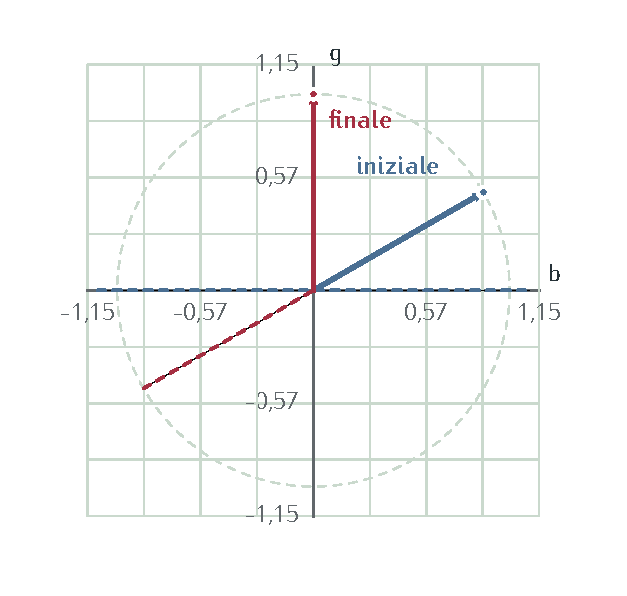
\includegraphics[width=\linewidth,height=94mm,keepaspectratio]{figure/f7e3aad724f826eef.pdf}\FigureCaption{4.07 \(\cdot\) esempio 2 \(\cdot\) Piano \(|b\rangle ,\allowbreak |g\rangle \) \(\cdot\) confronto iniziale/finale}\end{FigureBlock}

\BookHeading{Interpretazione}

Il piano ha assi ortonormali ricavati dalla preparazione. Ogni freccia intermedia e le probabilità delle alternative derivano dai medesimi vettori del registro.\par


Risorse dichiarate. 1 interrogazioni all'oracolo; 2 qubit dati. Il costo della preparazione e della riflessione va aggiunto.\par


\Needspace{7\baselineskip}
\BookHeading{Il passaggio successivo}
La marcatura può dipendere da una proprietà aggiornata durante un algoritmo. Per cercare un minimo marchiamo gli indici il cui valore è inferiore alla migliore soglia trovata finora.\par


% Authoritative exercise source. Preserve all derivations and diagrams.

\ExerciseStart{G4.04}{Ricostruire Grover come due riflessioni}{Guida esplicita}

\BookHeading{Problema, dati e obiettivo}

Cercare la parola 101 fra otto parole, usando Grover a partire dalla sovrapposizione uniforme. Calcolare tre iterazioni e individuare il punto oltre il quale la probabilità di successo diminuisce.

\ExTheory{\ExRef{c4-grover}{4.05}; \ExRef{c4-amplificazione}{4.07}}{Siano \(\ket g=\ket{101}\) e \(\ket b=7^{-1/2}\sum_{x\ne101}\ket x\). Nel piano ortonormale \((b,g)\), \(\ket s=(\sqrt7,1)^T/\sqrt8\), l’oracolo è \(O=\operatorname{diag}(1,-1)\) e la diffusione è \(D=2\ket s\bra s-I\).}

\ExPrediction{Due riflessioni compongono una rotazione. Avvicinandosi all’asse g, la sua proiezione aumenta; superato l’asse, ulteriori rotazioni possono ridurla.}

\ExFigure{\begin{tikzpicture}[>=Stealth,exlabel]
\draw[exaxis] (-0.5838535866733713,0)--(1.55,0) node[right] {$x_1$};\draw[exaxis] (0,-0.35)--(0,1.522271824131503) node[above] {$x_2$};\draw[->,Secondary,line width=1.1pt] (0,0)--(0.9354143466934853,0.3535533905932738) node[anchor=south west] {$ s $};\draw[->,Accent,line width=1.1pt] (0,0)--(-0.23385358667337133,0.9722718241315028) node[anchor=south west] {$ Q^2s $};
\end{tikzpicture}}{Coordinate nel piano collettivo: asse orizzontale b, verticale g. I coefficienti sono ampiezze reali.}


\begin{ExTasks}

\item Costruire le matrici O, D e Q=DO.

\item Applicare Q tre volte, senza rinormalizzazioni intermedie.

\item Calcolare la probabilità del bersaglio dopo ogni iterazione.

\item Interpretare il segno della componente lungo b.

\end{ExTasks}

\ExSolution

\ExStep{Costruire la diffusione}

\ExEq{D&=\frac14\begin{pmatrix}7&\sqrt7\\\sqrt7&1\end{pmatrix}-I
=\begin{pmatrix}3/4&\sqrt7/4\\\sqrt7/4&-3/4\end{pmatrix},\\
Q=DO&=\begin{pmatrix}3/4&-\sqrt7/4\\\sqrt7/4&3/4\end{pmatrix}.}
Ponendo \(\sin\theta=1/\sqrt8\), risulta \(\cos2\theta=3/4\), \(\sin2\theta=\sqrt7/4\). Q ruota di \(2\theta\).

\ExStep{Prima iterazione}

\ExEq{Q\ket s&=\frac1{4\sqrt8}\binom{3\sqrt7-\sqrt7}{7+3}
=\frac1{2\sqrt8}\binom{\sqrt7}{5},\\
P_1&=\frac{25}{32},\qquad \|\psi_1\|^2=\frac{7+25}{32}=1.}
Ogni parola non marcata ha ampiezza \(1/(2\sqrt8)\) e probabilità \(1/32\).

\ExStep{Seconda iterazione}

\ExEq{Q^2\ket s&=\frac1{8\sqrt8}\binom{3\sqrt7-5\sqrt7}{7+15}
=\frac1{4\sqrt8}\binom{-\sqrt7}{11},\\
P_2&=\frac{121}{128},\qquad \|\psi_2\|^2=\frac{7+121}{128}=1.}
L’asse g è stato superato: la componente b è negativa.

\ExStep{Terza iterazione}

\ExEq{Q^3\ket s&=\frac1{16\sqrt8}\binom{-3\sqrt7-11\sqrt7}{-7+33}
=\frac1{8\sqrt8}\binom{-7\sqrt7}{13},\\
P_3&=\frac{169}{512},\qquad \|\psi_3\|^2=\frac{343+169}{512}=1.}

\ExStep{Scegliere il numero di iterazioni}

Le probabilità per \(j=0,1,2,3\) sono \(1/8,25/32,121/128,169/512\). Fra questi quattro valori il massimo si raggiunge con due iterazioni. La formula \(P_j=\sin^2((2j+1)\theta)\) riproduce i quattro calcoli; la periodicità impedisce una crescita monotona.

\par\noindent\begin{minipage}{\linewidth}
\ExFigure{\begin{tikzpicture}[>=Stealth,exlabel]
\draw[exaxis] (-.6,0)--(4.4,0) node[right] {j};\draw[exaxis] (-.6,0)--(-.6,3.6) node[above] {$p$};\node[left] at (-.6,3) {$ 1 $};\draw[Ink!15,dashed] (-.6,3)--(3.9000000000000004,3);\filldraw[fill=Accent!25,draw=Accent] (0.0,0) rectangle (0.65,0.375);\node[below] at (0.325,0) {$ 0 $};\node[above] at (0.325,0.375) {$ 0.125 $};\filldraw[fill=Accent!25,draw=Accent] (1.1,0) rectangle (1.75,2.34375);\node[below] at (1.425,0) {$ 1 $};\node[above] at (1.425,2.34375) {$ 0.7812 $};\filldraw[fill=Accent!25,draw=Accent] (2.2,0) rectangle (2.85,2.8359375);\node[below] at (2.5250000000000004,0) {$ 2 $};\node[above] at (2.5250000000000004,2.8359375) {$ 0.9453 $};\filldraw[fill=Accent!25,draw=Accent] (3.3000000000000003,0) rectangle (3.95,0.990234375);\node[below] at (3.6250000000000004,0) {$ 3 $};\node[above] at (3.6250000000000004,0.990234375) {$ 0.3301 $};
\end{tikzpicture}}{Probabilità di successo dopo j iterazioni.}


\ExInterpret{La diffusione riflette rispetto alla direzione s; l’oracolo riflette rispetto all’asse b. Il quadrato della proiezione su g dà la probabilità di successo e rende visibile la sovrarotazione.}

\ExLab{Nelle sezioni 4.05 e 4.07 impostare otto candidati e una parola marcata. Confrontare le probabilità dopo zero, una, due e tre iterazioni con le frazioni ottenute.}


\end{minipage}

\Needspace{.43\textheight}
\section{Ricercare un minimo}
\phantomsection\label{c4-minimo}

{\sffamily\small\color{Ink!70} Riferimento alle slide: p. 232.\par}

{\sffamily\small\color{Ink!70} Laboratorio locale: \nolinkurl{index.html#capitolo-4/minimo}\par}

\BookHeading{Definizioni e costruzione}
Sia valore(x) una lista indicizzata da \(x=0,\allowbreak \ldots ,\allowbreak N- 1\). Una soglia corrente \(\tau \) definisce un problema di ricerca: trovare un indice con \(\text{valore}(x)<\tau \). Ogni miglioramento verificato permette di abbassare \(\tau \).\par

L'oracolo \(f\tau (x)\) vale uno precisamente quando il confronto è vero. Il numero dei marcati dipende dalla soglia ed è ignoto, quindi ciascuna ricerca interna usa la procedura a finestra crescente e un budget. Un candidato viene accettato solo dopo averne verificato il valore.\par

La sequenza delle soglie è strettamente decrescente quando ci sono miglioramenti. Se la lista contiene minimi uguali, uno qualsiasi dei loro indici è un risultato valido; il confronto stretto non tratta un valore uguale alla soglia come miglioramento.\par

Un tentativo fallito non certifica che la soglia sia minima. In questi piccoli esempi una scansione esaustiva finale confronta tutti i valori e certifica il risultato: il suo costo classico è dichiarato separatamente dalle interrogazioni della ricerca. La traccia con budget e questa verifica non costituiscono da sole una dimostrazione del costo asintotico dell'algoritmo generale.\par


\MathBlock{006603C4002800780029003D0031002021D4002000760061006C006F00720065002800780029003C03C4003B00200064006F0070006F00200075006E002000630061006E00640069006400610074006F0020007600650072006900660069006300610074006F002C002003C4219000760061006C006F00720065002800780029002E}{f\tau (x)=1\ \Leftrightarrow \ \text{valore}(x)<\tau ;\allowbreak \ \text{dopo}\ \text{un}\ \text{candidato}\ \text{verificato},\allowbreak \ \tau \leftarrow \text{valore}(x).}

\BookHeading{Come leggere le figure}
La lista e la soglia sono dati classici. Gli insiemi marcati cambiano fra tentativi; le distribuzioni appartengono a preparazioni diverse. Il controllo finale è una scansione della lista, non una misura quantistica aggiuntiva.\par


\BookHeading{Attività nel laboratorio modificabile}

\BookHeading{Obiettivo dell'esperimento}
Seguire gli aggiornamenti di un candidato minimo.\par

\BookHeading{Percorso operativo}
Assegnare una lista, un budget e un seme; includere valori ripetuti e negativi.\par

\BookHeading{Lettura geometrica}
La retta mostra i valori della lista; la tabella collega ogni misura alla verifica del candidato.\par

\BookHeading{Controllo del risultato}
Distinguere il risultato entro il budget dal controllo esaustivo finale, il cui costo è dichiarato.\par


\Needspace{.36\textheight}\phantomsection\label{c4-minimo-example-1}
{\sffamily\small\color{Accent} ESEMPIO SVOLTO 1\par}
\BookHeading{Esempio 1}
\(N=8\); al massimo 12 tentativi; generatore pseudocasuale con seme 20260928. La soglia iniziale è il primo elemento della lista; è una procedura didattica a soglia con budget di tentativi, non una dimostrazione del costo asintotico di Dürr--Høyer.\par


\BookHeading{Geometria e configurazione dell'esempio}
\begin{FigureBlock}\centering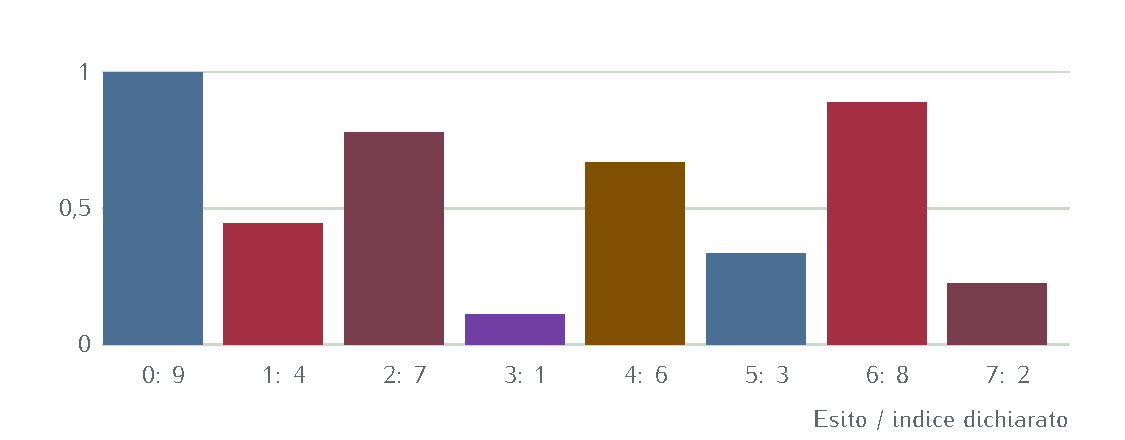
\includegraphics[width=\linewidth,height=94mm,keepaspectratio]{figure/f6c79a16668f6bf28.pdf}\FigureCaption{4.08 \(\cdot\) esempio 1 \(\cdot\) Valori della lista, divisi per il massimo}\end{FigureBlock}

\phantomsection\label{c4-minimo-example-1-step-1}
\BookHeading{01 Definire il tentativo}

\MathBlock{006D003D0031003B0020006A00200065007300740072006100740074006F00200075006E00690066006F0072006D0065006D0065006E007400650020006600720061002000300020006500202308006D230922120031003B002003C8003D005102B2007C007327E9}{m=1;\allowbreak \ j\ \text{estratto}\ \text{uniformemente}\ \text{fra}\ 0\ e\ \lceil m\rceil - 1;\allowbreak \ \psi =Q^{j}|s\rangle }

La scelta del numero di iterazioni usa una finestra crescente.\par


\phantomsection\label{c4-minimo-example-1-step-2}
\BookHeading{02 Calcolare e leggere}

\MathBlock{006320320078003D003203BC22120063007800200064006F0070006F0020006F0067006E00690020006D00610072006300610074007500720061003B002000780020007600690065006E0065002000630061006D00700069006F006E00610074006F0020006400610020007C00630078007C00B2002E}{c{}^{\prime} x=2\mu - cx\ \text{dopo}\ \text{ogni}\ \text{marcatura};\allowbreak \ x\ \text{viene}\ \text{campionato}\ \text{da}\ |cx|^{2}.}
\MathBlock{0043006F00730074006F002000640065006C002000740065006E00740061007400690076006F003D006A002B003100200069006E0074006500720072006F00670061007A0069006F006E0069002E}{\text{Costo}\ \text{del}\ \text{tentativo}=j+1\ \text{interrogazioni}.}

L'ultima interrogazione verifica classicamente il candidato.\par


\phantomsection\label{c4-minimo-example-1-step-3}
\BookHeading{03 Aggiornare la procedura}

\TextBlock{0053006500200069006C002000630061006E00640069006400610074006F002000E800200069006E006600720075007400740075006F0073006F003A0020006D2190006D0069006E00280036006D002F0035002C221A00380029002E000A00530065002000E80020007500740069006C0065003A0020006100720072006500730074006F002000640065006C006C006100200072006900630065007200630061002C0020006F007000700075007200650020006E0075006F0076006100200073006F0067006C006900610020006E0065006C006C006100200072006900630065007200630061002000640065006C0020006D0069006E0069006D006F002E}{Se il candidato è infruttuoso: \(m\leftarrow \min (6m/5,\allowbreak \sqrt{8})\). Se è utile: arresto della ricerca, oppure nuova soglia nella ricerca del minimo.}

Il budget impone un arresto eseguibile.\par


\phantomsection\label{c4-minimo-example-1-step-4}
\BookHeading{04 Verifica della lista finita}

\MathBlock{004C0069007300740061003D005B0039002C0034002C0037002C0031002C0036002C0033002C0038002C0032005D003B00200073006F0067006C00690061002000660069006E0061006C0065003D0031003B0020006D0069006E0069006D006F0020007600650072006900660069006300610074006F00200063006C006100730073006900630061006D0065006E00740065003D0031003B00200069006E00640069006300690020006D0069006E0069006D0069003D007B0033007D003B00200075006C0074006500720069006F0072006900200063006F006E00660072006F006E00740069003D0037}{\text{Lista}=[9{,}4{,}7{,}1{,}6{,}3{,}8{,}2];\allowbreak \ \text{soglia}\ \text{finale}=1;\allowbreak \ \text{minimo}\ \text{verificato}\ \text{classicamente}=1;\allowbreak \ \text{indici}\ \text{minimi}=\{3\};\allowbreak \ \text{ulteriori}\ \text{confronti}=7}

La soglia è un valore della lista, mentre x nella tabella è un indice; più indici possono condividere il minimo. Il limite di tentativi differisce dal costo di query j+1, riportato in ciascuna riga. La verifica esaustiva finale è un costo classico separato.\par


\BookHeading{Interpretazione}

Sono state usate 14 interrogazioni, inclusi i controlli dei candidati.\par


\BookHeading{Tabella completa dei dati (12 righe)}

\begingroup\sffamily\fontsize{8.8}{11}\selectfont\setlength{\tabcolsep}{1.6mm}\renewcommand{\arraystretch}{1.28}
\begin{longtable}{>{\RaggedRight\arraybackslash}p{14.000mm}>{\RaggedRight\arraybackslash}p{12.000mm}>{\RaggedRight\arraybackslash}p{14.000mm}>{\RaggedRight\arraybackslash}p{9.000mm}>{\RaggedRight\arraybackslash}p{19.400mm}>{\RaggedRight\arraybackslash}p{17.000mm}>{\RaggedRight\arraybackslash}p{13.000mm}>{\RaggedRight\arraybackslash}p{12.000mm}}
\toprule\rowcolor{Accent!7}\BeginAccSupp{method=hex,unicode,ActualText=00540065006E00740061007400690076006F}Tentativo\EndAccSupp{} & \BeginAccSupp{method=hex,unicode,ActualText=00460069006E006500730074007200610020006D}Finestra m\EndAccSupp{} & \BeginAccSupp{method=hex,unicode,ActualText=00490074006500720061007A0069006F006E00690020006A}Iterazioni j\EndAccSupp{} & \BeginAccSupp{method=hex,unicode,ActualText=0045007300690074006F00200078}Esito x\EndAccSupp{} & \BeginAccSupp{method=hex,unicode,ActualText=005600650072006900660069006300610020002F00200073006F0067006C00690061}Verifica / soglia\EndAccSupp{} & \BeginAccSupp{method=hex,unicode,ActualText=00500020007500740069006C0065}\(P\) utile\EndAccSupp{} & \BeginAccSupp{method=hex,unicode,ActualText=0043006F00730074006F002000740065006E00740061007400690076006F}Costo tentativo\EndAccSupp{} & \BeginAccSupp{method=hex,unicode,ActualText=0043006F00730074006F002000630075006D0075006C00610074006F}Costo cumulato\EndAccSupp{} \\
\midrule\endfirsthead
\toprule\rowcolor{Accent!7}\BeginAccSupp{method=hex,unicode,ActualText=00540065006E00740061007400690076006F}Tentativo\EndAccSupp{} & \BeginAccSupp{method=hex,unicode,ActualText=00460069006E006500730074007200610020006D}Finestra m\EndAccSupp{} & \BeginAccSupp{method=hex,unicode,ActualText=00490074006500720061007A0069006F006E00690020006A}Iterazioni j\EndAccSupp{} & \BeginAccSupp{method=hex,unicode,ActualText=0045007300690074006F00200078}Esito x\EndAccSupp{} & \BeginAccSupp{method=hex,unicode,ActualText=005600650072006900660069006300610020002F00200073006F0067006C00690061}Verifica / soglia\EndAccSupp{} & \BeginAccSupp{method=hex,unicode,ActualText=00500020007500740069006C0065}\(P\) utile\EndAccSupp{} & \BeginAccSupp{method=hex,unicode,ActualText=0043006F00730074006F002000740065006E00740061007400690076006F}Costo tentativo\EndAccSupp{} & \BeginAccSupp{method=hex,unicode,ActualText=0043006F00730074006F002000630075006D0075006C00610074006F}Costo cumulato\EndAccSupp{} \\
\midrule\endhead\bottomrule\endfoot
\BeginAccSupp{method=hex,unicode,ActualText=0031}1\EndAccSupp{} & \BeginAccSupp{method=hex,unicode,ActualText=0031}1\EndAccSupp{} & \BeginAccSupp{method=hex,unicode,ActualText=0030}0\EndAccSupp{} & \BeginAccSupp{method=hex,unicode,ActualText=0031}1\EndAccSupp{} & \BeginAccSupp{method=hex,unicode,ActualText=003921920034}\(9\to 4\)\EndAccSupp{} & \BeginAccSupp{method=hex,unicode,ActualText=0030002C003800370035}0,875\EndAccSupp{} & \BeginAccSupp{method=hex,unicode,ActualText=0031}1\EndAccSupp{} & \BeginAccSupp{method=hex,unicode,ActualText=0031}1\EndAccSupp{} \\
\BeginAccSupp{method=hex,unicode,ActualText=0032}2\EndAccSupp{} & \BeginAccSupp{method=hex,unicode,ActualText=0031}1\EndAccSupp{} & \BeginAccSupp{method=hex,unicode,ActualText=0030}0\EndAccSupp{} & \BeginAccSupp{method=hex,unicode,ActualText=0032}2\EndAccSupp{} & \BeginAccSupp{method=hex,unicode,ActualText=003421920034}\(4\to 4\)\EndAccSupp{} & \BeginAccSupp{method=hex,unicode,ActualText=0030002C003300370035}0,375\EndAccSupp{} & \BeginAccSupp{method=hex,unicode,ActualText=0031}1\EndAccSupp{} & \BeginAccSupp{method=hex,unicode,ActualText=0032}2\EndAccSupp{} \\
\BeginAccSupp{method=hex,unicode,ActualText=0033}3\EndAccSupp{} & \BeginAccSupp{method=hex,unicode,ActualText=0031002C0032}1,2\EndAccSupp{} & \BeginAccSupp{method=hex,unicode,ActualText=0030}0\EndAccSupp{} & \BeginAccSupp{method=hex,unicode,ActualText=0032}2\EndAccSupp{} & \BeginAccSupp{method=hex,unicode,ActualText=003421920034}\(4\to 4\)\EndAccSupp{} & \BeginAccSupp{method=hex,unicode,ActualText=0030002C003300370035}0,375\EndAccSupp{} & \BeginAccSupp{method=hex,unicode,ActualText=0031}1\EndAccSupp{} & \BeginAccSupp{method=hex,unicode,ActualText=0033}3\EndAccSupp{} \\
\BeginAccSupp{method=hex,unicode,ActualText=0034}4\EndAccSupp{} & \BeginAccSupp{method=hex,unicode,ActualText=0031002C00340034}1,44\EndAccSupp{} & \BeginAccSupp{method=hex,unicode,ActualText=0031}1\EndAccSupp{} & \BeginAccSupp{method=hex,unicode,ActualText=0035}5\EndAccSupp{} & \BeginAccSupp{method=hex,unicode,ActualText=003421920033}\(4\to 3\)\EndAccSupp{} & \BeginAccSupp{method=hex,unicode,ActualText=0030002C00380034003300370035}0,84375\EndAccSupp{} & \BeginAccSupp{method=hex,unicode,ActualText=0032}2\EndAccSupp{} & \BeginAccSupp{method=hex,unicode,ActualText=0035}5\EndAccSupp{} \\
\BeginAccSupp{method=hex,unicode,ActualText=0035}5\EndAccSupp{} & \BeginAccSupp{method=hex,unicode,ActualText=0031}1\EndAccSupp{} & \BeginAccSupp{method=hex,unicode,ActualText=0030}0\EndAccSupp{} & \BeginAccSupp{method=hex,unicode,ActualText=0030}0\EndAccSupp{} & \BeginAccSupp{method=hex,unicode,ActualText=003321920033}\(3\to 3\)\EndAccSupp{} & \BeginAccSupp{method=hex,unicode,ActualText=0030002C00320035}0,25\EndAccSupp{} & \BeginAccSupp{method=hex,unicode,ActualText=0031}1\EndAccSupp{} & \BeginAccSupp{method=hex,unicode,ActualText=0036}6\EndAccSupp{} \\
\BeginAccSupp{method=hex,unicode,ActualText=0036}6\EndAccSupp{} & \BeginAccSupp{method=hex,unicode,ActualText=0031002C0032}1,2\EndAccSupp{} & \BeginAccSupp{method=hex,unicode,ActualText=0030}0\EndAccSupp{} & \BeginAccSupp{method=hex,unicode,ActualText=0037}7\EndAccSupp{} & \BeginAccSupp{method=hex,unicode,ActualText=003321920032}\(3\to 2\)\EndAccSupp{} & \BeginAccSupp{method=hex,unicode,ActualText=0030002C00320035}0,25\EndAccSupp{} & \BeginAccSupp{method=hex,unicode,ActualText=0031}1\EndAccSupp{} & \BeginAccSupp{method=hex,unicode,ActualText=0037}7\EndAccSupp{} \\
\BeginAccSupp{method=hex,unicode,ActualText=0037}7\EndAccSupp{} & \BeginAccSupp{method=hex,unicode,ActualText=0031}1\EndAccSupp{} & \BeginAccSupp{method=hex,unicode,ActualText=0030}0\EndAccSupp{} & \BeginAccSupp{method=hex,unicode,ActualText=0037}7\EndAccSupp{} & \BeginAccSupp{method=hex,unicode,ActualText=003221920032}\(2\to 2\)\EndAccSupp{} & \BeginAccSupp{method=hex,unicode,ActualText=0030002C003100320035}0,125\EndAccSupp{} & \BeginAccSupp{method=hex,unicode,ActualText=0031}1\EndAccSupp{} & \BeginAccSupp{method=hex,unicode,ActualText=0038}8\EndAccSupp{} \\
\BeginAccSupp{method=hex,unicode,ActualText=0038}8\EndAccSupp{} & \BeginAccSupp{method=hex,unicode,ActualText=0031002C0032}1,2\EndAccSupp{} & \BeginAccSupp{method=hex,unicode,ActualText=0030}0\EndAccSupp{} & \BeginAccSupp{method=hex,unicode,ActualText=0037}7\EndAccSupp{} & \BeginAccSupp{method=hex,unicode,ActualText=003221920032}\(2\to 2\)\EndAccSupp{} & \BeginAccSupp{method=hex,unicode,ActualText=0030002C003100320035}0,125\EndAccSupp{} & \BeginAccSupp{method=hex,unicode,ActualText=0031}1\EndAccSupp{} & \BeginAccSupp{method=hex,unicode,ActualText=0039}9\EndAccSupp{} \\
\BeginAccSupp{method=hex,unicode,ActualText=0039}9\EndAccSupp{} & \BeginAccSupp{method=hex,unicode,ActualText=0031002C00340034}1,44\EndAccSupp{} & \BeginAccSupp{method=hex,unicode,ActualText=0030}0\EndAccSupp{} & \BeginAccSupp{method=hex,unicode,ActualText=0030}0\EndAccSupp{} & \BeginAccSupp{method=hex,unicode,ActualText=003221920032}\(2\to 2\)\EndAccSupp{} & \BeginAccSupp{method=hex,unicode,ActualText=0030002C003100320035}0,125\EndAccSupp{} & \BeginAccSupp{method=hex,unicode,ActualText=0031}1\EndAccSupp{} & \BeginAccSupp{method=hex,unicode,ActualText=00310030}10\EndAccSupp{} \\
\BeginAccSupp{method=hex,unicode,ActualText=00310030}10\EndAccSupp{} & \BeginAccSupp{method=hex,unicode,ActualText=0031002C003700320038}1,728\EndAccSupp{} & \BeginAccSupp{method=hex,unicode,ActualText=0030}0\EndAccSupp{} & \BeginAccSupp{method=hex,unicode,ActualText=0033}3\EndAccSupp{} & \BeginAccSupp{method=hex,unicode,ActualText=003221920031}\(2\to 1\)\EndAccSupp{} & \BeginAccSupp{method=hex,unicode,ActualText=0030002C003100320035}0,125\EndAccSupp{} & \BeginAccSupp{method=hex,unicode,ActualText=0031}1\EndAccSupp{} & \BeginAccSupp{method=hex,unicode,ActualText=00310031}11\EndAccSupp{} \\
\BeginAccSupp{method=hex,unicode,ActualText=00310031}11\EndAccSupp{} & \BeginAccSupp{method=hex,unicode,ActualText=0031}1\EndAccSupp{} & \BeginAccSupp{method=hex,unicode,ActualText=0030}0\EndAccSupp{} & \BeginAccSupp{method=hex,unicode,ActualText=0037}7\EndAccSupp{} & \BeginAccSupp{method=hex,unicode,ActualText=003121920031}\(1\to 1\)\EndAccSupp{} & \BeginAccSupp{method=hex,unicode,ActualText=0030}0\EndAccSupp{} & \BeginAccSupp{method=hex,unicode,ActualText=0031}1\EndAccSupp{} & \BeginAccSupp{method=hex,unicode,ActualText=00310032}12\EndAccSupp{} \\
\BeginAccSupp{method=hex,unicode,ActualText=00310032}12\EndAccSupp{} & \BeginAccSupp{method=hex,unicode,ActualText=0031002C0032}1,2\EndAccSupp{} & \BeginAccSupp{method=hex,unicode,ActualText=0031}1\EndAccSupp{} & \BeginAccSupp{method=hex,unicode,ActualText=0034}4\EndAccSupp{} & \BeginAccSupp{method=hex,unicode,ActualText=003121920031}\(1\to 1\)\EndAccSupp{} & \BeginAccSupp{method=hex,unicode,ActualText=0030}0\EndAccSupp{} & \BeginAccSupp{method=hex,unicode,ActualText=0032}2\EndAccSupp{} & \BeginAccSupp{method=hex,unicode,ActualText=00310034}14\EndAccSupp{} \\
\end{longtable}\endgroup

\Needspace{.36\textheight}\phantomsection\label{c4-minimo-example-2}
{\sffamily\small\color{Accent} ESEMPIO SVOLTO 2\par}
\BookHeading{Esempio 2}
\(N=8\); al massimo 12 tentativi; generatore pseudocasuale con seme 20260928. La soglia iniziale è il primo elemento della lista; è una procedura didattica a soglia con budget di tentativi, non una dimostrazione del costo asintotico di Dürr--Høyer.\par


\BookHeading{Geometria e configurazione dell'esempio}
\begin{FigureBlock}\centering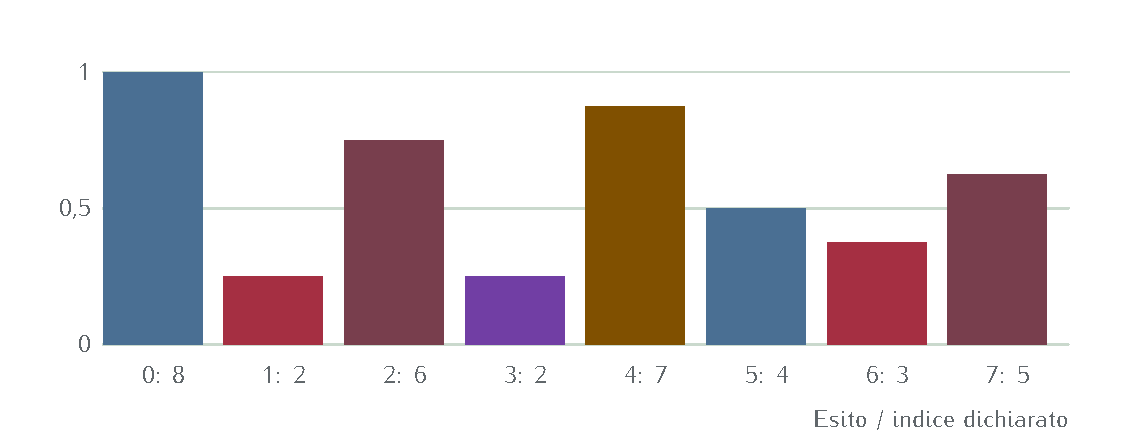
\includegraphics[width=\linewidth,height=94mm,keepaspectratio]{figure/f91b1a4157ebc2f7c.pdf}\FigureCaption{4.08 \(\cdot\) esempio 2 \(\cdot\) Valori della lista, divisi per il massimo}\end{FigureBlock}

\phantomsection\label{c4-minimo-example-2-step-1}
\BookHeading{01 Definire il tentativo}

\MathBlock{006D003D0031003B0020006A00200065007300740072006100740074006F00200075006E00690066006F0072006D0065006D0065006E007400650020006600720061002000300020006500202308006D230922120031003B002003C8003D005102B2007C007327E9}{m=1;\allowbreak \ j\ \text{estratto}\ \text{uniformemente}\ \text{fra}\ 0\ e\ \lceil m\rceil - 1;\allowbreak \ \psi =Q^{j}|s\rangle }

La scelta del numero di iterazioni usa una finestra crescente.\par


\phantomsection\label{c4-minimo-example-2-step-2}
\BookHeading{02 Calcolare e leggere}

\MathBlock{006320320078003D003203BC22120063007800200064006F0070006F0020006F0067006E00690020006D00610072006300610074007500720061003B002000780020007600690065006E0065002000630061006D00700069006F006E00610074006F0020006400610020007C00630078007C00B2002E}{c{}^{\prime} x=2\mu - cx\ \text{dopo}\ \text{ogni}\ \text{marcatura};\allowbreak \ x\ \text{viene}\ \text{campionato}\ \text{da}\ |cx|^{2}.}
\MathBlock{0043006F00730074006F002000640065006C002000740065006E00740061007400690076006F003D006A002B003100200069006E0074006500720072006F00670061007A0069006F006E0069002E}{\text{Costo}\ \text{del}\ \text{tentativo}=j+1\ \text{interrogazioni}.}

L'ultima interrogazione verifica classicamente il candidato.\par


\phantomsection\label{c4-minimo-example-2-step-3}
\BookHeading{03 Aggiornare la procedura}

\TextBlock{0053006500200069006C002000630061006E00640069006400610074006F002000E800200069006E006600720075007400740075006F0073006F003A0020006D2190006D0069006E00280036006D002F0035002C221A00380029002E000A00530065002000E80020007500740069006C0065003A0020006100720072006500730074006F002000640065006C006C006100200072006900630065007200630061002C0020006F007000700075007200650020006E0075006F0076006100200073006F0067006C006900610020006E0065006C006C006100200072006900630065007200630061002000640065006C0020006D0069006E0069006D006F002E}{Se il candidato è infruttuoso: \(m\leftarrow \min (6m/5,\allowbreak \sqrt{8})\). Se è utile: arresto della ricerca, oppure nuova soglia nella ricerca del minimo.}

Il budget impone un arresto eseguibile.\par


\phantomsection\label{c4-minimo-example-2-step-4}
\BookHeading{04 Verifica della lista finita}

\MathBlock{004C0069007300740061003D005B0038002C0032002C0036002C0032002C0037002C0034002C0033002C0035005D003B00200073006F0067006C00690061002000660069006E0061006C0065003D0032003B0020006D0069006E0069006D006F0020007600650072006900660069006300610074006F00200063006C006100730073006900630061006D0065006E00740065003D0032003B00200069006E00640069006300690020006D0069006E0069006D0069003D007B0031002C0033007D003B00200075006C0074006500720069006F0072006900200063006F006E00660072006F006E00740069003D0037}{\text{Lista}=[8{,}2{,}6{,}2{,}7{,}4{,}3{,}5];\allowbreak \ \text{soglia}\ \text{finale}=2;\allowbreak \ \text{minimo}\ \text{verificato}\ \text{classicamente}=2;\allowbreak \ \text{indici}\ \text{minimi}=\{1{,}3\};\allowbreak \ \text{ulteriori}\ \text{confronti}=7}

La soglia è un valore della lista, mentre x nella tabella è un indice; più indici possono condividere il minimo. Il limite di tentativi differisce dal costo di query j+1, riportato in ciascuna riga. La verifica esaustiva finale è un costo classico separato.\par


\BookHeading{Interpretazione}

Sono state usate 22 interrogazioni, inclusi i controlli dei candidati.\par


\BookHeading{Tabella completa dei dati (12 righe)}

\begingroup\sffamily\fontsize{8.8}{11}\selectfont\setlength{\tabcolsep}{1.6mm}\renewcommand{\arraystretch}{1.28}
\begin{longtable}{>{\RaggedRight\arraybackslash}p{14.000mm}>{\RaggedRight\arraybackslash}p{12.000mm}>{\RaggedRight\arraybackslash}p{14.000mm}>{\RaggedRight\arraybackslash}p{9.000mm}>{\RaggedRight\arraybackslash}p{19.400mm}>{\RaggedRight\arraybackslash}p{17.000mm}>{\RaggedRight\arraybackslash}p{13.000mm}>{\RaggedRight\arraybackslash}p{12.000mm}}
\toprule\rowcolor{Accent!7}\BeginAccSupp{method=hex,unicode,ActualText=00540065006E00740061007400690076006F}Tentativo\EndAccSupp{} & \BeginAccSupp{method=hex,unicode,ActualText=00460069006E006500730074007200610020006D}Finestra m\EndAccSupp{} & \BeginAccSupp{method=hex,unicode,ActualText=00490074006500720061007A0069006F006E00690020006A}Iterazioni j\EndAccSupp{} & \BeginAccSupp{method=hex,unicode,ActualText=0045007300690074006F00200078}Esito x\EndAccSupp{} & \BeginAccSupp{method=hex,unicode,ActualText=005600650072006900660069006300610020002F00200073006F0067006C00690061}Verifica / soglia\EndAccSupp{} & \BeginAccSupp{method=hex,unicode,ActualText=00500020007500740069006C0065}\(P\) utile\EndAccSupp{} & \BeginAccSupp{method=hex,unicode,ActualText=0043006F00730074006F002000740065006E00740061007400690076006F}Costo tentativo\EndAccSupp{} & \BeginAccSupp{method=hex,unicode,ActualText=0043006F00730074006F002000630075006D0075006C00610074006F}Costo cumulato\EndAccSupp{} \\
\midrule\endfirsthead
\toprule\rowcolor{Accent!7}\BeginAccSupp{method=hex,unicode,ActualText=00540065006E00740061007400690076006F}Tentativo\EndAccSupp{} & \BeginAccSupp{method=hex,unicode,ActualText=00460069006E006500730074007200610020006D}Finestra m\EndAccSupp{} & \BeginAccSupp{method=hex,unicode,ActualText=00490074006500720061007A0069006F006E00690020006A}Iterazioni j\EndAccSupp{} & \BeginAccSupp{method=hex,unicode,ActualText=0045007300690074006F00200078}Esito x\EndAccSupp{} & \BeginAccSupp{method=hex,unicode,ActualText=005600650072006900660069006300610020002F00200073006F0067006C00690061}Verifica / soglia\EndAccSupp{} & \BeginAccSupp{method=hex,unicode,ActualText=00500020007500740069006C0065}\(P\) utile\EndAccSupp{} & \BeginAccSupp{method=hex,unicode,ActualText=0043006F00730074006F002000740065006E00740061007400690076006F}Costo tentativo\EndAccSupp{} & \BeginAccSupp{method=hex,unicode,ActualText=0043006F00730074006F002000630075006D0075006C00610074006F}Costo cumulato\EndAccSupp{} \\
\midrule\endhead\bottomrule\endfoot
\BeginAccSupp{method=hex,unicode,ActualText=0031}1\EndAccSupp{} & \BeginAccSupp{method=hex,unicode,ActualText=0031}1\EndAccSupp{} & \BeginAccSupp{method=hex,unicode,ActualText=0030}0\EndAccSupp{} & \BeginAccSupp{method=hex,unicode,ActualText=0031}1\EndAccSupp{} & \BeginAccSupp{method=hex,unicode,ActualText=003821920032}\(8\to 2\)\EndAccSupp{} & \BeginAccSupp{method=hex,unicode,ActualText=0030002C003800370035}0,875\EndAccSupp{} & \BeginAccSupp{method=hex,unicode,ActualText=0031}1\EndAccSupp{} & \BeginAccSupp{method=hex,unicode,ActualText=0031}1\EndAccSupp{} \\
\BeginAccSupp{method=hex,unicode,ActualText=0032}2\EndAccSupp{} & \BeginAccSupp{method=hex,unicode,ActualText=0031}1\EndAccSupp{} & \BeginAccSupp{method=hex,unicode,ActualText=0030}0\EndAccSupp{} & \BeginAccSupp{method=hex,unicode,ActualText=0032}2\EndAccSupp{} & \BeginAccSupp{method=hex,unicode,ActualText=003221920032}\(2\to 2\)\EndAccSupp{} & \BeginAccSupp{method=hex,unicode,ActualText=0030}0\EndAccSupp{} & \BeginAccSupp{method=hex,unicode,ActualText=0031}1\EndAccSupp{} & \BeginAccSupp{method=hex,unicode,ActualText=0032}2\EndAccSupp{} \\
\BeginAccSupp{method=hex,unicode,ActualText=0033}3\EndAccSupp{} & \BeginAccSupp{method=hex,unicode,ActualText=0031002C0032}1,2\EndAccSupp{} & \BeginAccSupp{method=hex,unicode,ActualText=0030}0\EndAccSupp{} & \BeginAccSupp{method=hex,unicode,ActualText=0032}2\EndAccSupp{} & \BeginAccSupp{method=hex,unicode,ActualText=003221920032}\(2\to 2\)\EndAccSupp{} & \BeginAccSupp{method=hex,unicode,ActualText=0030}0\EndAccSupp{} & \BeginAccSupp{method=hex,unicode,ActualText=0031}1\EndAccSupp{} & \BeginAccSupp{method=hex,unicode,ActualText=0033}3\EndAccSupp{} \\
\BeginAccSupp{method=hex,unicode,ActualText=0034}4\EndAccSupp{} & \BeginAccSupp{method=hex,unicode,ActualText=0031002C00340034}1,44\EndAccSupp{} & \BeginAccSupp{method=hex,unicode,ActualText=0031}1\EndAccSupp{} & \BeginAccSupp{method=hex,unicode,ActualText=0034}4\EndAccSupp{} & \BeginAccSupp{method=hex,unicode,ActualText=003221920032}\(2\to 2\)\EndAccSupp{} & \BeginAccSupp{method=hex,unicode,ActualText=0030}0\EndAccSupp{} & \BeginAccSupp{method=hex,unicode,ActualText=0032}2\EndAccSupp{} & \BeginAccSupp{method=hex,unicode,ActualText=0035}5\EndAccSupp{} \\
\BeginAccSupp{method=hex,unicode,ActualText=0035}5\EndAccSupp{} & \BeginAccSupp{method=hex,unicode,ActualText=0031002C003700320038}1,728\EndAccSupp{} & \BeginAccSupp{method=hex,unicode,ActualText=0031}1\EndAccSupp{} & \BeginAccSupp{method=hex,unicode,ActualText=0030}0\EndAccSupp{} & \BeginAccSupp{method=hex,unicode,ActualText=003221920032}\(2\to 2\)\EndAccSupp{} & \BeginAccSupp{method=hex,unicode,ActualText=0030}0\EndAccSupp{} & \BeginAccSupp{method=hex,unicode,ActualText=0032}2\EndAccSupp{} & \BeginAccSupp{method=hex,unicode,ActualText=0037}7\EndAccSupp{} \\
\BeginAccSupp{method=hex,unicode,ActualText=0036}6\EndAccSupp{} & \BeginAccSupp{method=hex,unicode,ActualText=0032002C0030003700330036}2,0736\EndAccSupp{} & \BeginAccSupp{method=hex,unicode,ActualText=0031}1\EndAccSupp{} & \BeginAccSupp{method=hex,unicode,ActualText=0037}7\EndAccSupp{} & \BeginAccSupp{method=hex,unicode,ActualText=003221920032}\(2\to 2\)\EndAccSupp{} & \BeginAccSupp{method=hex,unicode,ActualText=0030}0\EndAccSupp{} & \BeginAccSupp{method=hex,unicode,ActualText=0032}2\EndAccSupp{} & \BeginAccSupp{method=hex,unicode,ActualText=0039}9\EndAccSupp{} \\
\BeginAccSupp{method=hex,unicode,ActualText=0037}7\EndAccSupp{} & \BeginAccSupp{method=hex,unicode,ActualText=0032002C00340038003800330032}2,48832\EndAccSupp{} & \BeginAccSupp{method=hex,unicode,ActualText=0031}1\EndAccSupp{} & \BeginAccSupp{method=hex,unicode,ActualText=0037}7\EndAccSupp{} & \BeginAccSupp{method=hex,unicode,ActualText=003221920032}\(2\to 2\)\EndAccSupp{} & \BeginAccSupp{method=hex,unicode,ActualText=0030}0\EndAccSupp{} & \BeginAccSupp{method=hex,unicode,ActualText=0032}2\EndAccSupp{} & \BeginAccSupp{method=hex,unicode,ActualText=00310031}11\EndAccSupp{} \\
\BeginAccSupp{method=hex,unicode,ActualText=0038}8\EndAccSupp{} & \BeginAccSupp{method=hex,unicode,ActualText=0032002C003800320038003400320037}2,828427\EndAccSupp{} & \BeginAccSupp{method=hex,unicode,ActualText=0030}0\EndAccSupp{} & \BeginAccSupp{method=hex,unicode,ActualText=0037}7\EndAccSupp{} & \BeginAccSupp{method=hex,unicode,ActualText=003221920032}\(2\to 2\)\EndAccSupp{} & \BeginAccSupp{method=hex,unicode,ActualText=0030}0\EndAccSupp{} & \BeginAccSupp{method=hex,unicode,ActualText=0031}1\EndAccSupp{} & \BeginAccSupp{method=hex,unicode,ActualText=00310032}12\EndAccSupp{} \\
\BeginAccSupp{method=hex,unicode,ActualText=0039}9\EndAccSupp{} & \BeginAccSupp{method=hex,unicode,ActualText=0032002C003800320038003400320037}2,828427\EndAccSupp{} & \BeginAccSupp{method=hex,unicode,ActualText=0031}1\EndAccSupp{} & \BeginAccSupp{method=hex,unicode,ActualText=0030}0\EndAccSupp{} & \BeginAccSupp{method=hex,unicode,ActualText=003221920032}\(2\to 2\)\EndAccSupp{} & \BeginAccSupp{method=hex,unicode,ActualText=0030}0\EndAccSupp{} & \BeginAccSupp{method=hex,unicode,ActualText=0032}2\EndAccSupp{} & \BeginAccSupp{method=hex,unicode,ActualText=00310034}14\EndAccSupp{} \\
\BeginAccSupp{method=hex,unicode,ActualText=00310030}10\EndAccSupp{} & \BeginAccSupp{method=hex,unicode,ActualText=0032002C003800320038003400320037}2,828427\EndAccSupp{} & \BeginAccSupp{method=hex,unicode,ActualText=0031}1\EndAccSupp{} & \BeginAccSupp{method=hex,unicode,ActualText=0033}3\EndAccSupp{} & \BeginAccSupp{method=hex,unicode,ActualText=003221920032}\(2\to 2\)\EndAccSupp{} & \BeginAccSupp{method=hex,unicode,ActualText=0030}0\EndAccSupp{} & \BeginAccSupp{method=hex,unicode,ActualText=0032}2\EndAccSupp{} & \BeginAccSupp{method=hex,unicode,ActualText=00310036}16\EndAccSupp{} \\
\BeginAccSupp{method=hex,unicode,ActualText=00310031}11\EndAccSupp{} & \BeginAccSupp{method=hex,unicode,ActualText=0032002C003800320038003400320037}2,828427\EndAccSupp{} & \BeginAccSupp{method=hex,unicode,ActualText=0032}2\EndAccSupp{} & \BeginAccSupp{method=hex,unicode,ActualText=0037}7\EndAccSupp{} & \BeginAccSupp{method=hex,unicode,ActualText=003221920032}\(2\to 2\)\EndAccSupp{} & \BeginAccSupp{method=hex,unicode,ActualText=0030}0\EndAccSupp{} & \BeginAccSupp{method=hex,unicode,ActualText=0033}3\EndAccSupp{} & \BeginAccSupp{method=hex,unicode,ActualText=00310039}19\EndAccSupp{} \\
\BeginAccSupp{method=hex,unicode,ActualText=00310032}12\EndAccSupp{} & \BeginAccSupp{method=hex,unicode,ActualText=0032002C003800320038003400320037}2,828427\EndAccSupp{} & \BeginAccSupp{method=hex,unicode,ActualText=0032}2\EndAccSupp{} & \BeginAccSupp{method=hex,unicode,ActualText=0034}4\EndAccSupp{} & \BeginAccSupp{method=hex,unicode,ActualText=003221920032}\(2\to 2\)\EndAccSupp{} & \BeginAccSupp{method=hex,unicode,ActualText=0030}0\EndAccSupp{} & \BeginAccSupp{method=hex,unicode,ActualText=0033}3\EndAccSupp{} & \BeginAccSupp{method=hex,unicode,ActualText=00320032}22\EndAccSupp{} \\
\end{longtable}\endgroup

\Needspace{7\baselineskip}
\BookHeading{Il passaggio successivo}
Le ricerche precedenti sfruttano interferenza in un piano. Fourier organizza invece le fasi di tutte le componenti per rendere leggibili periodicità e autovalori: sarà il secondo strumento del modulo.\par


% Authoritative exercise source. Preserve all derivations and diagrams.

\ExerciseStart{G4.05}{Seguire una ricerca con budget e soglia variabile}{Guida esplicita}

\BookHeading{Problema, dati e obiettivo}

Cercare il minimo della lista \([9,4,7,1,6,3,8,2]\). Partire dall’indice 1, di valore 4, e usare la sequenza prefissata di iterazioni \(j=1,1,1,2\). Analizzare la possibile successione di misure \(5,7,0,3\), accettando un candidato solo quando il suo valore è inferiore alla soglia.

\ExTheory{\ExRef{c4-ricerca-ignota}{4.06}; \ExRef{c4-minimo}{4.08}}{L’oracolo della soglia t marca gli indici con valore minore di t. Se M indici soddisfano il criterio, la probabilità dopo j iterazioni è \(\sin^2((2j+1)\arcsin\sqrt{M/8})\). Quando M è ignoto, questa formula descrive l’analisi del procedimento; il valore di M non è un dato utilizzabile dalla ricerca.}

\ExPrediction{Abbassare la soglia restringe l’insieme marcato. Una misura può fallire e lasciare la soglia invariata; il procedimento deve prevedere tale ramo.}

\ExFigure{\begin{tikzpicture}[>=Stealth,exlabel]
\node[exbox] (n0) at (0.0,0.0) {$t=4,\ M=3$};\node[exbox] (n1) at (3.6,0.0) {$t=3,\ M=2$};\draw[exother] (n0)--(n1);\node[exbox] (n2) at (7.2,0.0) {$t=2,\ M=1$};\draw[exother] (n1)--(n2);\node[exbox] (n3) at (0.0,-1.6) {rifiuta il valore 9};\draw[exother] (n2.south)--++(0,-.4)-|(n3.north);\node[exbox] (n4) at (3.6,-1.6) {$t=2,\ j=2$};\draw[exother] (n3)--(n4);\node[exbox] (n5) at (7.2,-1.6) {$t=1$};\draw[exother] (n4)--(n5);
\end{tikzpicture}}{La soglia cambia solo dopo la verifica classica del candidato. M è indicato per l’analisi.}


\begin{ExTasks}

\item Elencare gli indici marcati a ogni soglia.

\item Calcolare le probabilità della traccia indicata.

\item Aggiornare la soglia soltanto dopo verifica.

\item Distinguere interrogazioni di fase, letture dei valori e certificazione finale.

\end{ExTasks}

\ExSolution

\ExStep{Prima soglia}

Per t=4 gli indici marcati sono 3,5,7: \(p=M/8=3/8\). Dopo una iterazione la probabilità totale è
\ExEq{\sin^2(3\theta)&=p(3-4p)^2=\frac38\left(3-\frac32\right)^2=\frac{27}{32}.}
Ogni indice marcato ha probabilità \(9/32\); ciascuno degli altri cinque ha probabilità \(1/32\). Misurare 5, di valore 3, permette di aggiornare t a 3.

\ExStep{Seconda soglia}

Per t=3 rimangono gli indici 3 e 7. Ora \(p=2/8=1/4\), quindi \(p(3-4p)^2=(1/4)2^2=1\). Ogni indice marcato ha probabilità \(1/2\). La lettura 7 restituisce valore 2 e aggiorna t a 2.

\ExStep{Un tentativo senza miglioramento}

Per t=2 è marcato soltanto l’indice 3. Con una iterazione, \(P_{\mathrm{buono}}=(1/8)(3-1/2)^2=25/32\). Ogni indice non marcato ha probabilità \(1/32\). La lettura 0, di valore 9, è quindi possibile e viene respinta: t rimane 2.

\ExStep{Un secondo tentativo}

Con la stessa soglia e due iterazioni, G4.04 ha calcolato \(P_{\mathrm{buono}}=121/128\). La lettura 3 restituisce valore 1 e aggiorna la soglia. La probabilità dell’intera traccia indicata è
\ExEq{\frac9{32}\frac12\frac1{32}\frac{121}{128}&=\frac{1089}{262144}\simeq0.004154.}
Questa singola traccia illustra rami ammessi e non rappresenta una probabilità complessiva di successo.

\ExStep{Contare le risorse}

Le chiamate all’oracolo di fase sono \(1+1+1+2=5\). Le letture classiche dei valori sono una iniziale e quattro verifiche dei candidati. Gli indici distinti già letti sono 0,1,3,5,7. Una certificazione esaustiva del minimo richiede ancora gli indici 2,4,6: in totale otto letture di valori. Le due categorie sommano a 13 interrogazioni astratte, ma una chiamata di fase può richiedere valutazione reversibile, confronto e uncompute. Questa traccia con certificazione esaustiva non dimostra un vantaggio asintotico.

\ExStep{Gestire una soglia senza soluzioni}

Per t=1 non esiste alcun valore inferiore: M=0, O=I e \(D\ket s=\ket s\). Ogni verifica fallisce. Una procedura con budget finito deve ammettere l’uscita «nessun miglioramento trovato», che da sola non certifica l’assenza di valori migliori.

\par\noindent\begin{minipage}{\linewidth}
\ExFigure{\begin{tikzpicture}[>=Stealth,exlabel]
\draw[exaxis] (-.6,0)--(4.4,0) node[right] {tentativo};\draw[exaxis] (-.6,0)--(-.6,3.6) node[above] {$p$};\node[left] at (-.6,3) {$ 1 $};\draw[Ink!15,dashed] (-.6,3)--(3.9000000000000004,3);\filldraw[fill=Accent!25,draw=Accent] (0.0,0) rectangle (0.65,2.53125);\node[below] at (0.325,0) {$ 1 $};\node[above] at (0.325,2.53125) {$ 0.8438 $};\filldraw[fill=Accent!25,draw=Accent] (1.1,0) rectangle (1.75,3.0);\node[below] at (1.425,0) {$ 2 $};\node[above] at (1.425,3.0) {$ 1 $};\filldraw[fill=Accent!25,draw=Accent] (2.2,0) rectangle (2.85,2.34375);\node[below] at (2.5250000000000004,0) {$ 3 $};\node[above] at (2.5250000000000004,2.34375) {$ 0.7812 $};\filldraw[fill=Accent!25,draw=Accent] (3.3000000000000003,0) rectangle (3.95,2.8359375);\node[below] at (3.6250000000000004,0) {$ 4 $};\node[above] at (3.6250000000000004,2.8359375) {$ 0.9453 $};
\end{tikzpicture}}{Probabilità totale di ottenere un miglioramento nei quattro tentativi.}


\ExInterpret{Il piano collettivo dipende dalla soglia. Il numero di iterazioni prefissato rende possibile analizzare la ricerca senza supporre che il numero di soluzioni sia conosciuto.}

\ExLab{Nelle sezioni 4.06 e 4.08 osservare l’aggiornamento della soglia e le verifiche dei candidati. Riprodurre su carta la lista di questo esercizio; confrontare le categorie di costo con quelle mostrate dal laboratorio, che può usare una diversa traccia di misure.}


\end{minipage}

\Needspace{.43\textheight}
\section{Sommare le fasi di Fourier}
\phantomsection\label{c4-fourier}

{\sffamily\small\color{Ink!70} Riferimento alle slide: p. 260.\par}

{\sffamily\small\color{Ink!70} Laboratorio locale: \nolinkurl{index.html#capitolo-4/fourier}\par}

\BookHeading{Definizioni e costruzione}
La trasformata discreta di Fourier \(F_{N}\) agisce su \(N\) ampiezze complesse. Alla base \(|x\rangle \) associa una progressione di fasi lungo gli indici \(y=0,\allowbreak \ldots ,\allowbreak N- 1\); qui scegliamo sempre il segno positivo nell'esponente.\par

Definiamo \(\omega =\allowbreak\exp (2\pi i/N)\), una radice N-esima dell'unità, e \((F_{N})_{yx}=\omega ^{xy}/\sqrt{N}\). Per un vettore v, l'uscita y è la somma degli \(N\) vettori \(\omega ^{xy}v_{x}/\sqrt{N}\) nel piano complesso. L'inversa \(F_{N}{}^{\dagger} \) cambia il segno dell'esponente.\par

La cancellazione deriva dalla somma geometrica \(S=1+z+\cdots +z^{N- 1}\). Moltiplicando per z, tutti i termini intermedi si cancellano in \(S- zS=1- z^{N}\). Per \(z\ne 1\), \(S=(1- z^{N})/(1- z)\); per \(z=1\), \(S=N\). Se \(z^{N}=1\) e \(z\ne 1\), la somma è zero.\par

Il prodotto interno fra le colonne x e \(x{}^{\prime} \) di \(F_{N}\) è \((1/N)\sum _{y}\omega ^{(x{}^{\prime} - x)y}\). Vale uno se \(x=x{}^{\prime} \) e zero altrimenti per la stessa identità: le colonne sono ortonormali, quindi \(F_{N}\) è unitaria. Una periodicità del vettore fa riapparire queste somme e concentra la probabilità su indici compatibili.\par


\MathBlock{00280046005F004E007600291D67003D00280031002F221A004E002903A320930065007800700028003203C0006900780079002F004E002900762093003B002003A30028006A003D0030002C2026002C004E2212003100290020007A02B2003D00300020007300650020007A1D3A003D0031002000650020007A22600031002E}{(F_{N}v)_{y}=(1/\sqrt{N})\sum _{x}\allowbreak\exp (2\pi \text{ixy}/N)v_{x};\allowbreak \ \sum _{j=0}^{N- 1}\ z^{j}=0\ \text{se}\ z^{N}=1\ e\ z\ne 1.}

\BookHeading{Come leggere le figure}
Il piano Re/Im mostra addendi e risultante di una singola ampiezza. x e y sono etichette discrete, non coordinate fisiche; le fasi sono angoli adimensionali. La trasformata non implica una misura: la misura successiva usa \(|(F_{N}v)_{y}|^{2}\).\par


\BookHeading{Attività nel laboratorio modificabile}

\BookHeading{Obiettivo dell'esperimento}
Collegare periodicità e fasi della preparazione alla trasformata.\par

\BookHeading{Percorso operativo}
Variare passo, indice iniziale e fase fra componenti successive.\par

\BookHeading{Lettura geometrica}
Le frecce nel piano complesso rappresentano i contributi alla stessa uscita.\par

\BookHeading{Controllo del risultato}
Verificare conservazione della norma e ricostruire una componente tramite la somma complessa.\par


\Needspace{.36\textheight}\phantomsection\label{c4-fourier-example-1}
{\sffamily\small\color{Accent} ESEMPIO SVOLTO 1\par}
\BookHeading{La somma di Fourier}
Ogni componente in uscita raccoglie contributi da tutte le componenti in ingresso.\par


\BookHeading{Geometria e configurazione dell'esempio}
\begin{FigureBlock}\begin{minipage}[t]{.485\linewidth}\centering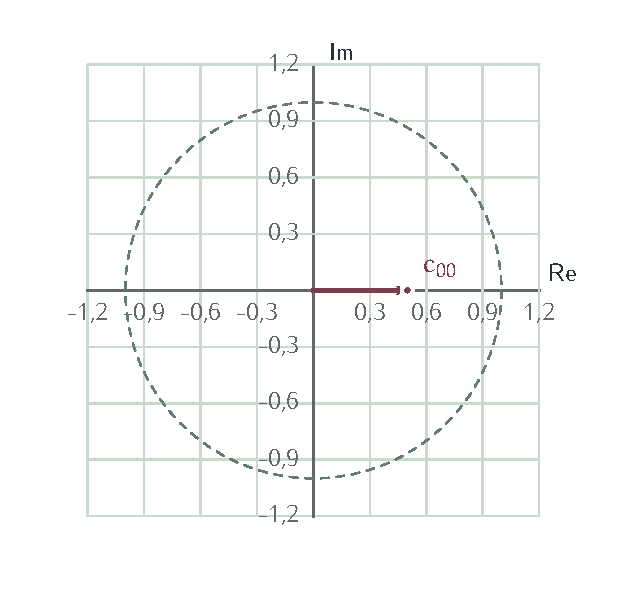
\includegraphics[width=\linewidth,height=63mm,keepaspectratio]{figure/f996c24551d6e0988.pdf}\par{\sffamily\footnotesize \(c_{00}\)\par}\end{minipage}\hfill\begin{minipage}[t]{.485\linewidth}\centering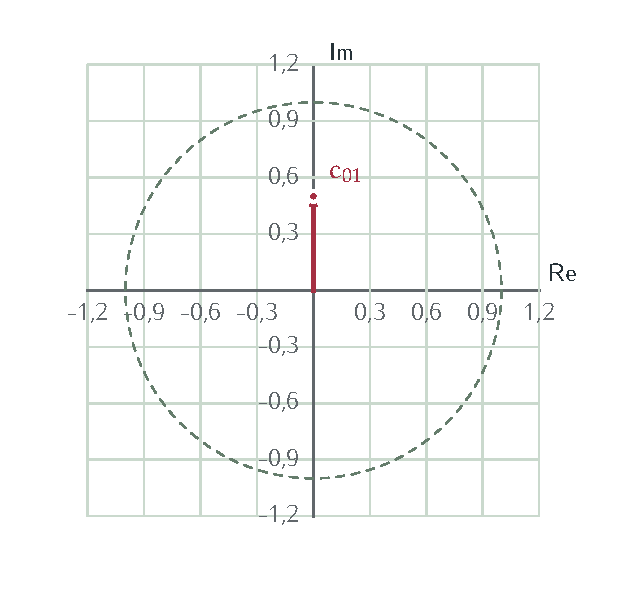
\includegraphics[width=\linewidth,height=63mm,keepaspectratio]{figure/f232fce5f0cfc43fd.pdf}\par{\sffamily\footnotesize \(c_{01}\)\par}\end{minipage}\FigureCaption{4.09 \(\cdot\) esempio 1 \(\cdot\) Ampiezze trasformate}\end{FigureBlock}
\begin{FigureBlock}\begin{minipage}[t]{.485\linewidth}\centering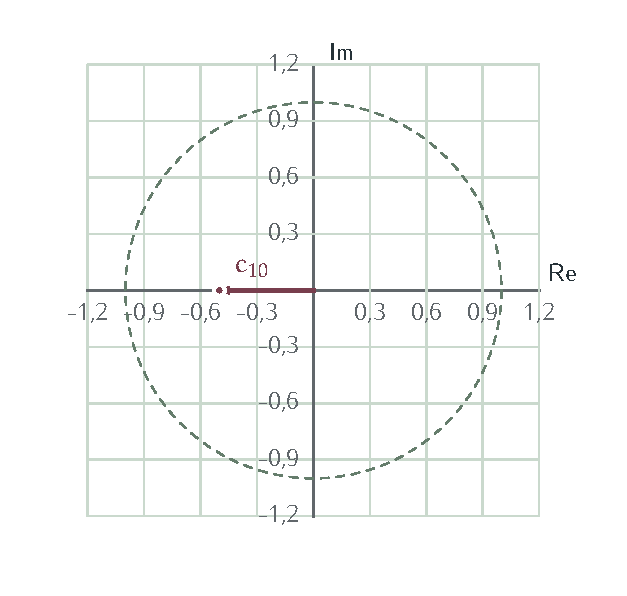
\includegraphics[width=\linewidth,height=63mm,keepaspectratio]{figure/f80bdbf1522c77998.pdf}\par{\sffamily\footnotesize \(c_{10}\)\par}\end{minipage}\hfill\begin{minipage}[t]{.485\linewidth}\centering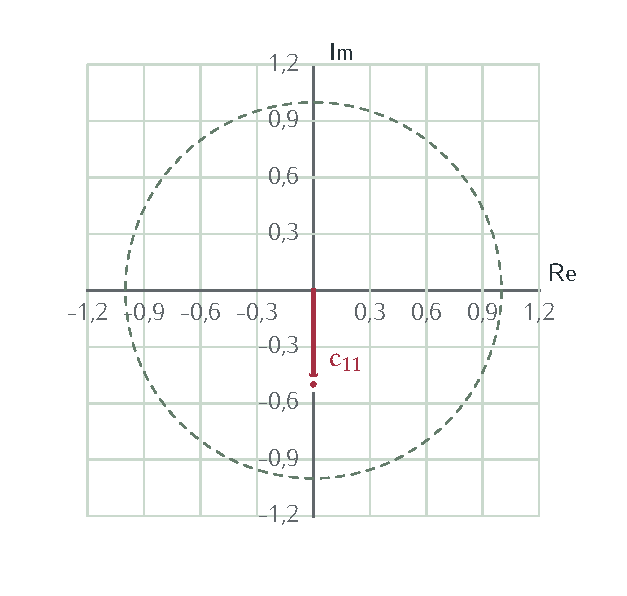
\includegraphics[width=\linewidth,height=63mm,keepaspectratio]{figure/f0eff30a99d2357f1.pdf}\par{\sffamily\footnotesize \(c_{11}\)\par}\end{minipage}\FigureCaption{4.09 \(\cdot\) esempio 1 \(\cdot\) Ampiezze trasformate}\end{FigureBlock}
\begin{FigureBlock}\centering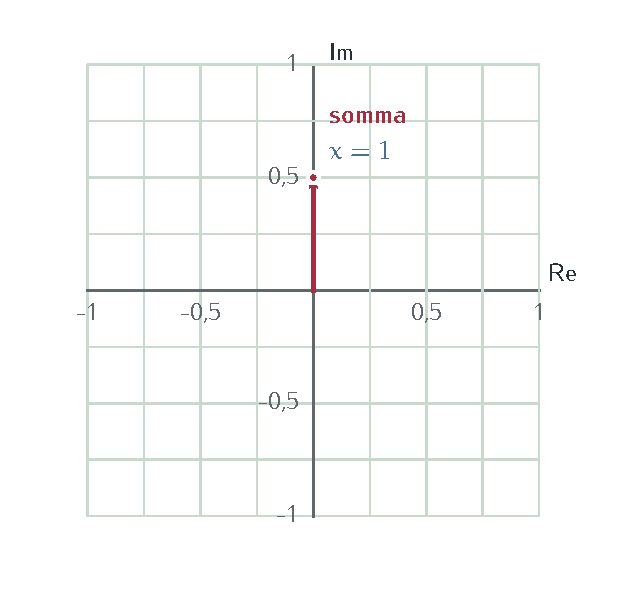
\includegraphics[width=\linewidth,height=94mm,keepaspectratio]{figure/fe95dee834e7edc1b.pdf}\FigureCaption{4.09 \(\cdot\) esempio 1 \(\cdot\) Piano complesso \(\cdot\) somma dei contributi per \(y=1\)}\end{FigureBlock}

\phantomsection\label{c4-fourier-example-1-step-1}
\BookHeading{01 Preparazione}

\MathBlock{0076003D00280030003B00200031003B00200030003B0020003000291D40003B0020004E003D0034}{v=(0;\allowbreak \ 1;\allowbreak \ 0;\allowbreak \ 0)^{T};\allowbreak \ N=4}

Le componenti seguono l'ordine degli interi da zero a \(N- 1\).\par


\phantomsection\label{c4-fourier-example-1-step-2}
\BookHeading{02 Sommare le radici dell'unità}

\MathBlock{0053003D0031002B007A002B22EF002B007A005E00280034002D00310029002E}{S=1+z+\cdots +z^{4-1}.}
\MathBlock{007A0053003D007A002B007A00B2002B22EF002B007A005E0034003B0020002800312212007A00290053003D00312212007A005E0034002E}{zS=z+z^{2}+\cdots +z^{4};\allowbreak \ (1- z)S=1- z^{4}.}
\MathBlock{005300650020007A22600031003A00200053003D002800312212007A005E00340029002F002800312212007A0029002E0020005300650020007A003D0031003A00200053003D0034002E}{Se\ z\ne 1:\ S=(1- z^{4})/(1- z).\ Se\ z=1:\ S=4.}

La sottrazione cancella tutti i termini intermedi. Il caso \(z=1\) va separato prima della divisione.\par


\phantomsection\label{c4-fourier-example-1-step-3}
\BookHeading{03 Dalla cancellazione all'unitarietà}

\MathBlock{007A003D0065005E0028003203C00069002800782212007820320029002F00340029003B0020007A005E0034003D0031002E}{z=e^{2\pi i(x- x{}^{\prime} )/4};\allowbreak \ z^{4}=1.}
\MathBlock{27E80046003400782032007C00460034007827E9003D00280031002F0034002903A300790020007A02B8003D0034002F0034003D003100200073006500200078003D00782032003B0020003000200061006C007400720069006D0065006E00740069002E}{\langle F4x{}^{\prime} |F4x\rangle =(1/4)\sum _{y}\ z^{y}=4/4=1\ \text{se}\ x=x{}^{\prime} ;\allowbreak \ 0\ \text{altrimenti}.}

Per x e \(x{}^{\prime} \) distinti fra 0 e \(N- 1\), \(z\ne 1\): le frecce delle radici si chiudono. Le colonne di Fourier sono quindi ortonormali e la trasformata conserva prodotti interni e norma.\par


\phantomsection\label{c4-fourier-example-1-step-4}
\BookHeading{04 Componente \(y=0\)}

\MathBlock{0061002800300029003D00280031002F221A00340029005B0028003000290065005E0028003203C0006900B7003000B70030002F00340029002B0028003100290065005E0028003203C0006900B7003100B70030002F00340029002B0028003000290065005E0028003203C0006900B7003200B70030002F00340029002B0028003000290065005E0028003203C0006900B7003300B70030002F00340029005D}{a(0)=(1/\sqrt{4})[(0)e^{2\pi i\cdot 0\cdot 0/4}+(1)e^{2\pi i\cdot 1\cdot 0/4}+(0)e^{2\pi i\cdot 2\cdot 0/4}+(0)e^{2\pi i\cdot 3\cdot 0/4}]}
\MathBlock{22480030002C0035003B0020005000280030002922480030002C00320035}{\approx 0{,}5;\allowbreak \ P(0)\approx 0{,}25}

I contributi sono vettori complessi; la loro somma viene calcolata prima del modulo quadro.\par


\phantomsection\label{c4-fourier-example-1-step-5}
\BookHeading{05 Componente \(y=1\)}

\MathBlock{0061002800310029003D00280031002F221A00340029005B0028003000290065005E0028003203C0006900B7003000B70031002F00340029002B0028003100290065005E0028003203C0006900B7003100B70031002F00340029002B0028003000290065005E0028003203C0006900B7003200B70031002F00340029002B0028003000290065005E0028003203C0006900B7003300B70031002F00340029005D}{a(1)=(1/\sqrt{4})[(0)e^{2\pi i\cdot 0\cdot 1/4}+(1)e^{2\pi i\cdot 1\cdot 1/4}+(0)e^{2\pi i\cdot 2\cdot 1/4}+(0)e^{2\pi i\cdot 3\cdot 1/4}]}
\MathBlock{22480030002C00350069003B0020005000280031002922480030002C00320035}{\approx 0{,}5i;\allowbreak \ P(1)\approx 0{,}25}

I contributi sono vettori complessi; la loro somma viene calcolata prima del modulo quadro.\par


\phantomsection\label{c4-fourier-example-1-step-6}
\BookHeading{06 Componente \(y=2\)}

\MathBlock{0061002800320029003D00280031002F221A00340029005B0028003000290065005E0028003203C0006900B7003000B70032002F00340029002B0028003100290065005E0028003203C0006900B7003100B70032002F00340029002B0028003000290065005E0028003203C0006900B7003200B70032002F00340029002B0028003000290065005E0028003203C0006900B7003300B70032002F00340029005D}{a(2)=(1/\sqrt{4})[(0)e^{2\pi i\cdot 0\cdot 2/4}+(1)e^{2\pi i\cdot 1\cdot 2/4}+(0)e^{2\pi i\cdot 2\cdot 2/4}+(0)e^{2\pi i\cdot 3\cdot 2/4}]}
\MathBlock{2248002D0030002C0035003B0020005000280032002922480030002C00320035}{\approx -0{,}5;\allowbreak \ P(2)\approx 0{,}25}

I contributi sono vettori complessi; la loro somma viene calcolata prima del modulo quadro.\par


\phantomsection\label{c4-fourier-example-1-step-7}
\BookHeading{07 Componente \(y=3\)}

\MathBlock{0061002800330029003D00280031002F221A00340029005B0028003000290065005E0028003203C0006900B7003000B70033002F00340029002B0028003100290065005E0028003203C0006900B7003100B70033002F00340029002B0028003000290065005E0028003203C0006900B7003200B70033002F00340029002B0028003000290065005E0028003203C0006900B7003300B70033002F00340029005D}{a(3)=(1/\sqrt{4})[(0)e^{2\pi i\cdot 0\cdot 3/4}+(1)e^{2\pi i\cdot 1\cdot 3/4}+(0)e^{2\pi i\cdot 2\cdot 3/4}+(0)e^{2\pi i\cdot 3\cdot 3/4}]}
\MathBlock{2248002D0030002C00350069003B0020005000280033002922480030002C00320035}{\approx -0{,}5i;\allowbreak \ P(3)\approx 0{,}25}

I contributi sono vettori complessi; la loro somma viene calcolata prima del modulo quadro.\par


\BookHeading{Interpretazione}

La trasformazione unitaria conserva la norma: 1.\par


\Needspace{.36\textheight}\phantomsection\label{c4-fourier-example-2}
{\sffamily\small\color{Accent} ESEMPIO SVOLTO 2\par}
\BookHeading{La somma di Fourier}
Ogni componente in uscita raccoglie contributi da tutte le componenti in ingresso.\par


\BookHeading{Geometria e configurazione dell'esempio}
\begin{FigureBlock}\begin{minipage}[t]{.485\linewidth}\centering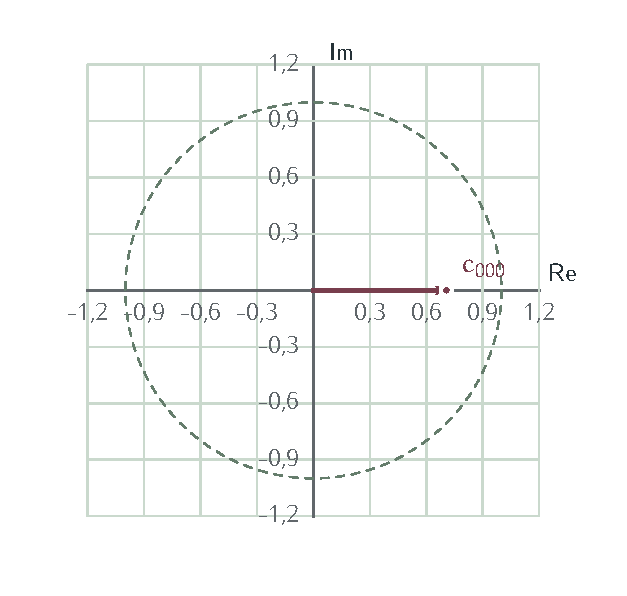
\includegraphics[width=\linewidth,height=63mm,keepaspectratio]{figure/f50c55a0c9422d31e.pdf}\par{\sffamily\footnotesize \(c_{000}\)\par}\end{minipage}\hfill\begin{minipage}[t]{.485\linewidth}\centering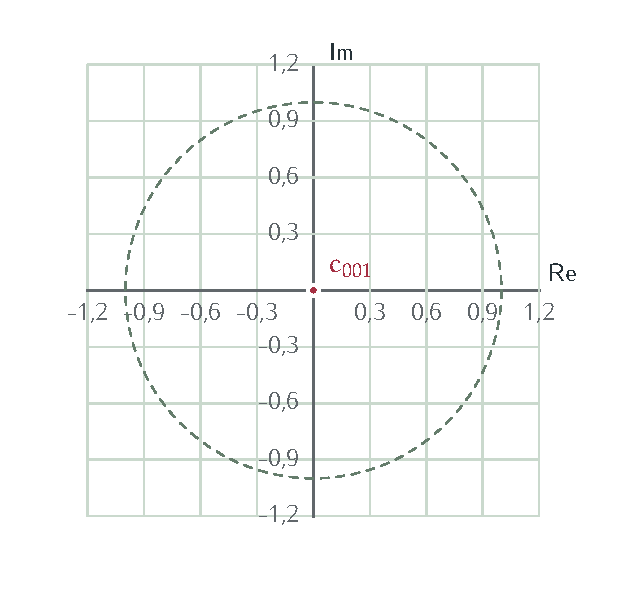
\includegraphics[width=\linewidth,height=63mm,keepaspectratio]{figure/f97b71dbd79be9cdf.pdf}\par{\sffamily\footnotesize \(c_{001}\)\par}\end{minipage}\FigureCaption{4.09 \(\cdot\) esempio 2 \(\cdot\) Ampiezze trasformate}\end{FigureBlock}
\begin{FigureBlock}\begin{minipage}[t]{.485\linewidth}\centering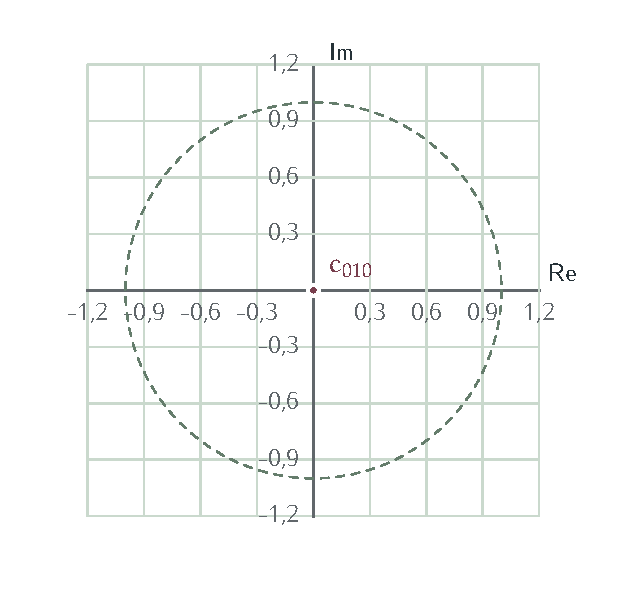
\includegraphics[width=\linewidth,height=63mm,keepaspectratio]{figure/f99bb147208cda245.pdf}\par{\sffamily\footnotesize \(c_{010}\)\par}\end{minipage}\hfill\begin{minipage}[t]{.485\linewidth}\centering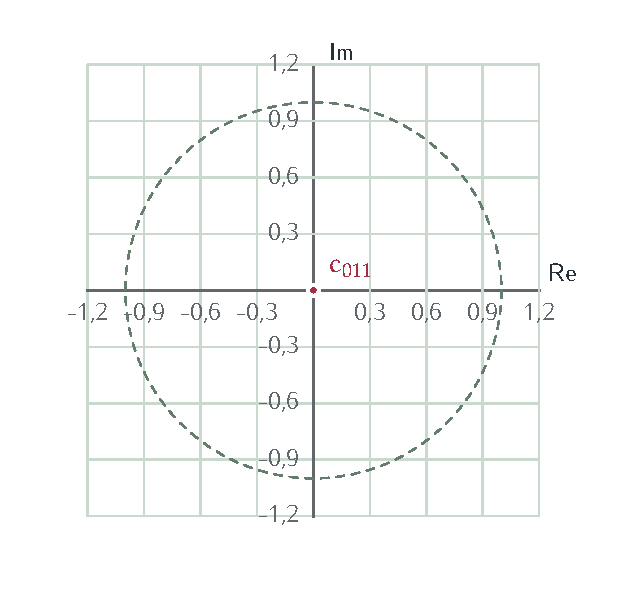
\includegraphics[width=\linewidth,height=63mm,keepaspectratio]{figure/fd798c34968d26957.pdf}\par{\sffamily\footnotesize \(c_{011}\)\par}\end{minipage}\FigureCaption{4.09 \(\cdot\) esempio 2 \(\cdot\) Ampiezze trasformate}\end{FigureBlock}
\begin{FigureBlock}\begin{minipage}[t]{.485\linewidth}\centering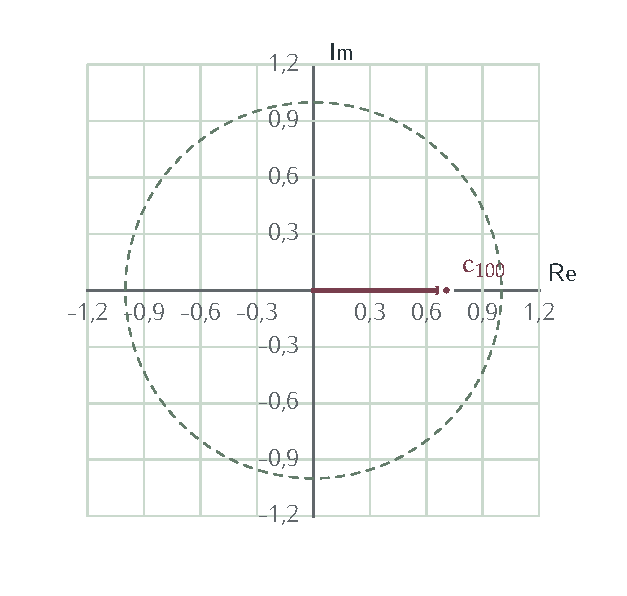
\includegraphics[width=\linewidth,height=63mm,keepaspectratio]{figure/f9e0b30938a68f0ff.pdf}\par{\sffamily\footnotesize \(c_{100}\)\par}\end{minipage}\hfill\begin{minipage}[t]{.485\linewidth}\centering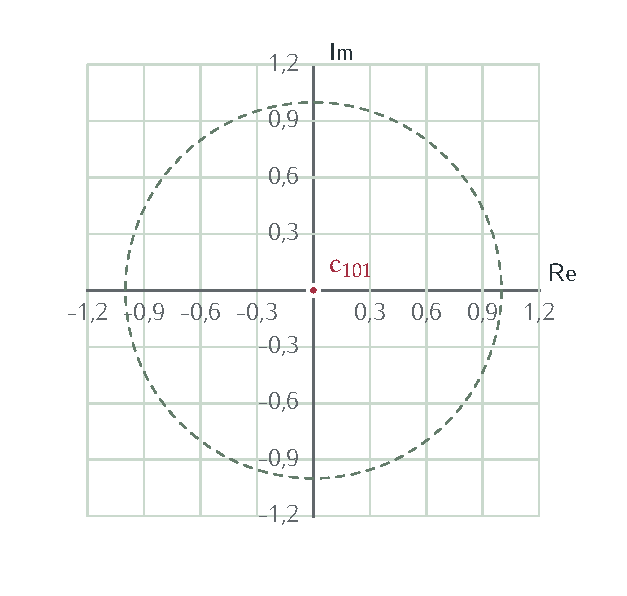
\includegraphics[width=\linewidth,height=63mm,keepaspectratio]{figure/f0d8358d238a207ed.pdf}\par{\sffamily\footnotesize \(c_{101}\)\par}\end{minipage}\FigureCaption{4.09 \(\cdot\) esempio 2 \(\cdot\) Ampiezze trasformate}\end{FigureBlock}
\begin{FigureBlock}\begin{minipage}[t]{.485\linewidth}\centering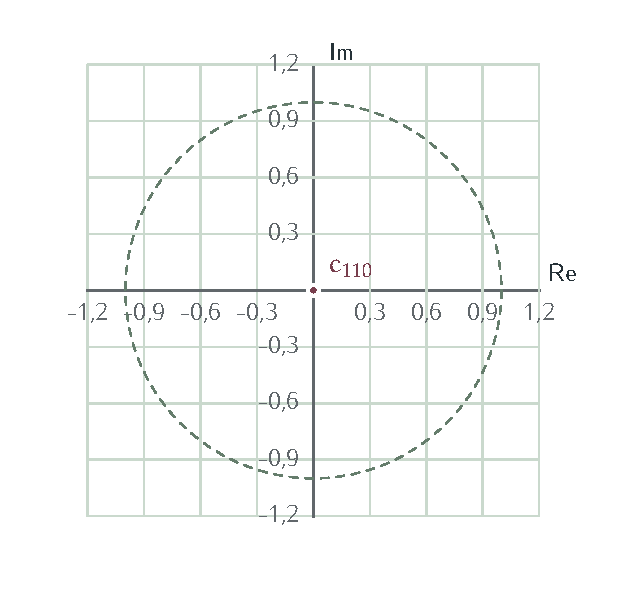
\includegraphics[width=\linewidth,height=63mm,keepaspectratio]{figure/fa74267c43847d3d8.pdf}\par{\sffamily\footnotesize \(c_{110}\)\par}\end{minipage}\hfill\begin{minipage}[t]{.485\linewidth}\centering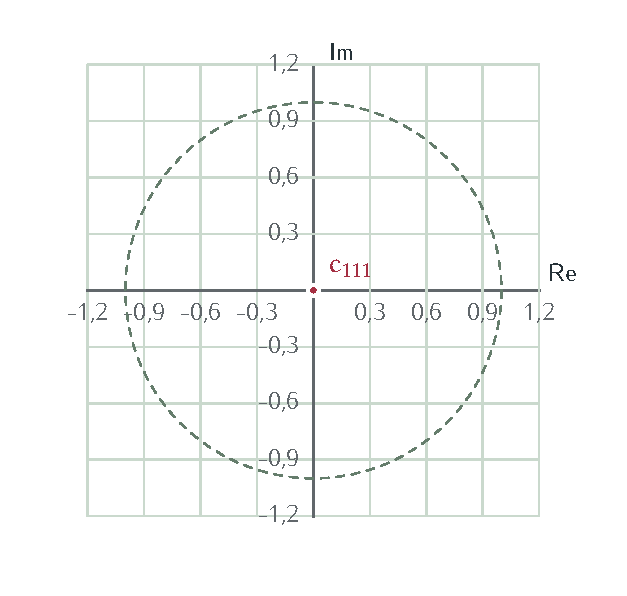
\includegraphics[width=\linewidth,height=63mm,keepaspectratio]{figure/f905787f086d3bbba.pdf}\par{\sffamily\footnotesize \(c_{111}\)\par}\end{minipage}\FigureCaption{4.09 \(\cdot\) esempio 2 \(\cdot\) Ampiezze trasformate}\end{FigureBlock}
\begin{FigureBlock}\centering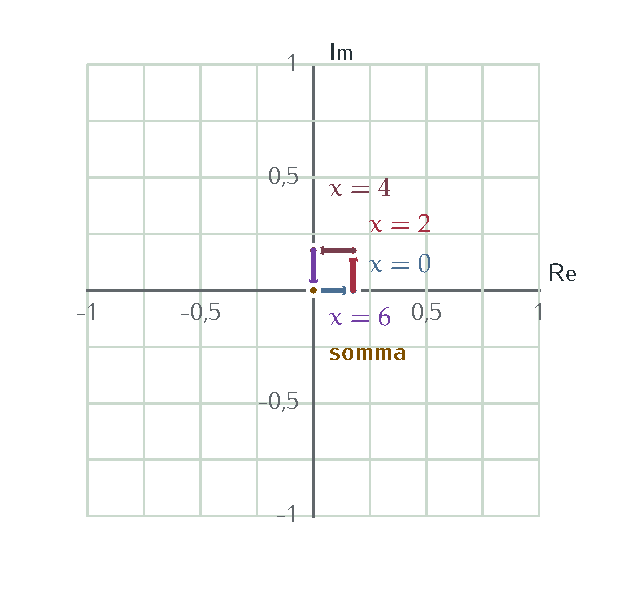
\includegraphics[width=\linewidth,height=94mm,keepaspectratio]{figure/fa08d762a173519e6.pdf}\FigureCaption{4.09 \(\cdot\) esempio 2 \(\cdot\) Piano complesso \(\cdot\) somma dei contributi per \(y=1\)}\end{FigureBlock}

\phantomsection\label{c4-fourier-example-2-step-1}
\BookHeading{01 Preparazione}

\MathBlock{0076003D00280030002C0035003B00200030003B00200030002C0035003B00200030003B00200030002C0035003B00200030003B00200030002C0035003B0020003000291D40003B0020004E003D0038}{v=(0{,}5;\allowbreak \ 0;\allowbreak \ 0{,}5;\allowbreak \ 0;\allowbreak \ 0{,}5;\allowbreak \ 0;\allowbreak \ 0{,}5;\allowbreak \ 0)^{T};\allowbreak \ N=8}

Le componenti seguono l'ordine degli interi da zero a \(N- 1\).\par


\phantomsection\label{c4-fourier-example-2-step-2}
\BookHeading{02 Sommare le radici dell'unità}

\MathBlock{0053003D0031002B007A002B22EF002B007A005E00280038002D00310029002E}{S=1+z+\cdots +z^{8-1}.}
\MathBlock{007A0053003D007A002B007A00B2002B22EF002B007A005E0038003B0020002800312212007A00290053003D00312212007A005E0038002E}{zS=z+z^{2}+\cdots +z^{8};\allowbreak \ (1- z)S=1- z^{8}.}
\MathBlock{005300650020007A22600031003A00200053003D002800312212007A005E00380029002F002800312212007A0029002E0020005300650020007A003D0031003A00200053003D0038002E}{Se\ z\ne 1:\ S=(1- z^{8})/(1- z).\ Se\ z=1:\ S=8.}

La sottrazione cancella tutti i termini intermedi. Il caso \(z=1\) va separato prima della divisione.\par


\phantomsection\label{c4-fourier-example-2-step-3}
\BookHeading{03 Dalla cancellazione all'unitarietà}

\MathBlock{007A003D0065005E0028003203C00069002800782212007820320029002F00380029003B0020007A005E0038003D0031002E}{z=e^{2\pi i(x- x{}^{\prime} )/8};\allowbreak \ z^{8}=1.}
\MathBlock{27E80046003800782032007C00460038007827E9003D00280031002F0038002903A300790020007A02B8003D0038002F0038003D003100200073006500200078003D00782032003B0020003000200061006C007400720069006D0065006E00740069002E}{\langle F8x{}^{\prime} |F8x\rangle =(1/8)\sum _{y}\ z^{y}=8/8=1\ \text{se}\ x=x{}^{\prime} ;\allowbreak \ 0\ \text{altrimenti}.}

Per x e \(x{}^{\prime} \) distinti fra 0 e \(N- 1\), \(z\ne 1\): le frecce delle radici si chiudono. Le colonne di Fourier sono quindi ortonormali e la trasformata conserva prodotti interni e norma.\par


\phantomsection\label{c4-fourier-example-2-step-4}
\BookHeading{04 Componente \(y=0\)}

\MathBlock{0061002800300029003D00280031002F221A00380029005B00280030002C003500290065005E0028003203C0006900B7003000B70030002F00380029002B0028003000290065005E0028003203C0006900B7003100B70030002F00380029002B00280030002C003500290065005E0028003203C0006900B7003200B70030002F00380029002B0028003000290065005E0028003203C0006900B7003300B70030002F00380029002B00280030002C003500290065005E0028003203C0006900B7003400B70030002F00380029002B0028003000290065005E0028003203C0006900B7003500B70030002F00380029002B00280030002C003500290065005E0028003203C0006900B7003600B70030002F00380029002B0028003000290065005E0028003203C0006900B7003700B70030002F00380029005D}{a(0)=(1/\sqrt{8})[(0{,}5)e^{2\pi i\cdot 0\cdot 0/8}+(0)e^{2\pi i\cdot 1\cdot 0/8}+(0{,}5)e^{2\pi i\cdot 2\cdot 0/8}+(0)e^{2\pi i\cdot 3\cdot 0/8}+(0{,}5)e^{2\pi i\cdot 4\cdot 0/8}+(0)e^{2\pi i\cdot 5\cdot 0/8}+(0{,}5)e^{2\pi i\cdot 6\cdot 0/8}+(0)e^{2\pi i\cdot 7\cdot 0/8}]}
\MathBlock{22480030002C0037003000370031003B0020005000280030002922480030002C0035}{\approx 0{,}7071;\allowbreak \ P(0)\approx 0{,}5}

I contributi sono vettori complessi; la loro somma viene calcolata prima del modulo quadro.\par


\phantomsection\label{c4-fourier-example-2-step-5}
\BookHeading{05 Componente \(y=1\)}

\MathBlock{0061002800310029003D00280031002F221A00380029005B00280030002C003500290065005E0028003203C0006900B7003000B70031002F00380029002B0028003000290065005E0028003203C0006900B7003100B70031002F00380029002B00280030002C003500290065005E0028003203C0006900B7003200B70031002F00380029002B0028003000290065005E0028003203C0006900B7003300B70031002F00380029002B00280030002C003500290065005E0028003203C0006900B7003400B70031002F00380029002B0028003000290065005E0028003203C0006900B7003500B70031002F00380029002B00280030002C003500290065005E0028003203C0006900B7003600B70031002F00380029002B0028003000290065005E0028003203C0006900B7003700B70031002F00380029005D}{a(1)=(1/\sqrt{8})[(0{,}5)e^{2\pi i\cdot 0\cdot 1/8}+(0)e^{2\pi i\cdot 1\cdot 1/8}+(0{,}5)e^{2\pi i\cdot 2\cdot 1/8}+(0)e^{2\pi i\cdot 3\cdot 1/8}+(0{,}5)e^{2\pi i\cdot 4\cdot 1/8}+(0)e^{2\pi i\cdot 5\cdot 1/8}+(0{,}5)e^{2\pi i\cdot 6\cdot 1/8}+(0)e^{2\pi i\cdot 7\cdot 1/8}]}
\MathBlock{22480030003B0020005000280031002922480030}{\approx 0;\allowbreak \ P(1)\approx 0}

I contributi sono vettori complessi; la loro somma viene calcolata prima del modulo quadro.\par


\phantomsection\label{c4-fourier-example-2-step-6}
\BookHeading{06 Componente \(y=2\)}

\MathBlock{0061002800320029003D00280031002F221A00380029005B00280030002C003500290065005E0028003203C0006900B7003000B70032002F00380029002B0028003000290065005E0028003203C0006900B7003100B70032002F00380029002B00280030002C003500290065005E0028003203C0006900B7003200B70032002F00380029002B0028003000290065005E0028003203C0006900B7003300B70032002F00380029002B00280030002C003500290065005E0028003203C0006900B7003400B70032002F00380029002B0028003000290065005E0028003203C0006900B7003500B70032002F00380029002B00280030002C003500290065005E0028003203C0006900B7003600B70032002F00380029002B0028003000290065005E0028003203C0006900B7003700B70032002F00380029005D}{a(2)=(1/\sqrt{8})[(0{,}5)e^{2\pi i\cdot 0\cdot 2/8}+(0)e^{2\pi i\cdot 1\cdot 2/8}+(0{,}5)e^{2\pi i\cdot 2\cdot 2/8}+(0)e^{2\pi i\cdot 3\cdot 2/8}+(0{,}5)e^{2\pi i\cdot 4\cdot 2/8}+(0)e^{2\pi i\cdot 5\cdot 2/8}+(0{,}5)e^{2\pi i\cdot 6\cdot 2/8}+(0)e^{2\pi i\cdot 7\cdot 2/8}]}
\MathBlock{22480030003B0020005000280032002922480030}{\approx 0;\allowbreak \ P(2)\approx 0}

I contributi sono vettori complessi; la loro somma viene calcolata prima del modulo quadro.\par


\phantomsection\label{c4-fourier-example-2-step-7}
\BookHeading{07 Componente \(y=3\)}

\MathBlock{0061002800330029003D00280031002F221A00380029005B00280030002C003500290065005E0028003203C0006900B7003000B70033002F00380029002B0028003000290065005E0028003203C0006900B7003100B70033002F00380029002B00280030002C003500290065005E0028003203C0006900B7003200B70033002F00380029002B0028003000290065005E0028003203C0006900B7003300B70033002F00380029002B00280030002C003500290065005E0028003203C0006900B7003400B70033002F00380029002B0028003000290065005E0028003203C0006900B7003500B70033002F00380029002B00280030002C003500290065005E0028003203C0006900B7003600B70033002F00380029002B0028003000290065005E0028003203C0006900B7003700B70033002F00380029005D}{a(3)=(1/\sqrt{8})[(0{,}5)e^{2\pi i\cdot 0\cdot 3/8}+(0)e^{2\pi i\cdot 1\cdot 3/8}+(0{,}5)e^{2\pi i\cdot 2\cdot 3/8}+(0)e^{2\pi i\cdot 3\cdot 3/8}+(0{,}5)e^{2\pi i\cdot 4\cdot 3/8}+(0)e^{2\pi i\cdot 5\cdot 3/8}+(0{,}5)e^{2\pi i\cdot 6\cdot 3/8}+(0)e^{2\pi i\cdot 7\cdot 3/8}]}
\MathBlock{22480030003B0020005000280033002922480030}{\approx 0;\allowbreak \ P(3)\approx 0}

I contributi sono vettori complessi; la loro somma viene calcolata prima del modulo quadro.\par


\phantomsection\label{c4-fourier-example-2-step-8}
\BookHeading{08 Componente \(y=4\)}

\MathBlock{0061002800340029003D00280031002F221A00380029005B00280030002C003500290065005E0028003203C0006900B7003000B70034002F00380029002B0028003000290065005E0028003203C0006900B7003100B70034002F00380029002B00280030002C003500290065005E0028003203C0006900B7003200B70034002F00380029002B0028003000290065005E0028003203C0006900B7003300B70034002F00380029002B00280030002C003500290065005E0028003203C0006900B7003400B70034002F00380029002B0028003000290065005E0028003203C0006900B7003500B70034002F00380029002B00280030002C003500290065005E0028003203C0006900B7003600B70034002F00380029002B0028003000290065005E0028003203C0006900B7003700B70034002F00380029005D}{a(4)=(1/\sqrt{8})[(0{,}5)e^{2\pi i\cdot 0\cdot 4/8}+(0)e^{2\pi i\cdot 1\cdot 4/8}+(0{,}5)e^{2\pi i\cdot 2\cdot 4/8}+(0)e^{2\pi i\cdot 3\cdot 4/8}+(0{,}5)e^{2\pi i\cdot 4\cdot 4/8}+(0)e^{2\pi i\cdot 5\cdot 4/8}+(0{,}5)e^{2\pi i\cdot 6\cdot 4/8}+(0)e^{2\pi i\cdot 7\cdot 4/8}]}
\MathBlock{22480030002C0037003000370031003B0020005000280034002922480030002C0035}{\approx 0{,}7071;\allowbreak \ P(4)\approx 0{,}5}

I contributi sono vettori complessi; la loro somma viene calcolata prima del modulo quadro.\par


\phantomsection\label{c4-fourier-example-2-step-9}
\BookHeading{09 Componente \(y=5\)}

\MathBlock{0061002800350029003D00280031002F221A00380029005B00280030002C003500290065005E0028003203C0006900B7003000B70035002F00380029002B0028003000290065005E0028003203C0006900B7003100B70035002F00380029002B00280030002C003500290065005E0028003203C0006900B7003200B70035002F00380029002B0028003000290065005E0028003203C0006900B7003300B70035002F00380029002B00280030002C003500290065005E0028003203C0006900B7003400B70035002F00380029002B0028003000290065005E0028003203C0006900B7003500B70035002F00380029002B00280030002C003500290065005E0028003203C0006900B7003600B70035002F00380029002B0028003000290065005E0028003203C0006900B7003700B70035002F00380029005D}{a(5)=(1/\sqrt{8})[(0{,}5)e^{2\pi i\cdot 0\cdot 5/8}+(0)e^{2\pi i\cdot 1\cdot 5/8}+(0{,}5)e^{2\pi i\cdot 2\cdot 5/8}+(0)e^{2\pi i\cdot 3\cdot 5/8}+(0{,}5)e^{2\pi i\cdot 4\cdot 5/8}+(0)e^{2\pi i\cdot 5\cdot 5/8}+(0{,}5)e^{2\pi i\cdot 6\cdot 5/8}+(0)e^{2\pi i\cdot 7\cdot 5/8}]}
\MathBlock{22480030003B0020005000280035002922480030}{\approx 0;\allowbreak \ P(5)\approx 0}

I contributi sono vettori complessi; la loro somma viene calcolata prima del modulo quadro.\par


\phantomsection\label{c4-fourier-example-2-step-10}
\BookHeading{10 Componente \(y=6\)}

\MathBlock{0061002800360029003D00280031002F221A00380029005B00280030002C003500290065005E0028003203C0006900B7003000B70036002F00380029002B0028003000290065005E0028003203C0006900B7003100B70036002F00380029002B00280030002C003500290065005E0028003203C0006900B7003200B70036002F00380029002B0028003000290065005E0028003203C0006900B7003300B70036002F00380029002B00280030002C003500290065005E0028003203C0006900B7003400B70036002F00380029002B0028003000290065005E0028003203C0006900B7003500B70036002F00380029002B00280030002C003500290065005E0028003203C0006900B7003600B70036002F00380029002B0028003000290065005E0028003203C0006900B7003700B70036002F00380029005D}{a(6)=(1/\sqrt{8})[(0{,}5)e^{2\pi i\cdot 0\cdot 6/8}+(0)e^{2\pi i\cdot 1\cdot 6/8}+(0{,}5)e^{2\pi i\cdot 2\cdot 6/8}+(0)e^{2\pi i\cdot 3\cdot 6/8}+(0{,}5)e^{2\pi i\cdot 4\cdot 6/8}+(0)e^{2\pi i\cdot 5\cdot 6/8}+(0{,}5)e^{2\pi i\cdot 6\cdot 6/8}+(0)e^{2\pi i\cdot 7\cdot 6/8}]}
\MathBlock{22480030003B0020005000280036002922480030}{\approx 0;\allowbreak \ P(6)\approx 0}

I contributi sono vettori complessi; la loro somma viene calcolata prima del modulo quadro.\par


\phantomsection\label{c4-fourier-example-2-step-11}
\BookHeading{11 Componente \(y=7\)}

\MathBlock{0061002800370029003D00280031002F221A00380029005B00280030002C003500290065005E0028003203C0006900B7003000B70037002F00380029002B0028003000290065005E0028003203C0006900B7003100B70037002F00380029002B00280030002C003500290065005E0028003203C0006900B7003200B70037002F00380029002B0028003000290065005E0028003203C0006900B7003300B70037002F00380029002B00280030002C003500290065005E0028003203C0006900B7003400B70037002F00380029002B0028003000290065005E0028003203C0006900B7003500B70037002F00380029002B00280030002C003500290065005E0028003203C0006900B7003600B70037002F00380029002B0028003000290065005E0028003203C0006900B7003700B70037002F00380029005D}{a(7)=(1/\sqrt{8})[(0{,}5)e^{2\pi i\cdot 0\cdot 7/8}+(0)e^{2\pi i\cdot 1\cdot 7/8}+(0{,}5)e^{2\pi i\cdot 2\cdot 7/8}+(0)e^{2\pi i\cdot 3\cdot 7/8}+(0{,}5)e^{2\pi i\cdot 4\cdot 7/8}+(0)e^{2\pi i\cdot 5\cdot 7/8}+(0{,}5)e^{2\pi i\cdot 6\cdot 7/8}+(0)e^{2\pi i\cdot 7\cdot 7/8}]}
\MathBlock{22480030003B0020005000280037002922480030}{\approx 0;\allowbreak \ P(7)\approx 0}

I contributi sono vettori complessi; la loro somma viene calcolata prima del modulo quadro.\par


\BookHeading{Interpretazione}

La trasformazione unitaria conserva la norma: 1.\par


\Needspace{7\baselineskip}
\BookHeading{Il passaggio successivo}
Quando \(N=2^{n}\), la scrittura binaria separa la fase in n fattori. Questo permette di ricavare una rete di Hadamard e fasi controllate che realizza la stessa \(F_{N}\).\par


\Needspace{.43\textheight}
\section{Costruire il circuito QFT}
\phantomsection\label{c4-qft}

{\sffamily\small\color{Ink!70} Riferimento alle slide: p. 281.\par}

{\sffamily\small\color{Ink!70} Laboratorio locale: \nolinkurl{index.html#capitolo-4/qft}\par}

\BookHeading{Definizioni e costruzione}
La QFT è la trasformata \(F_{2^{n}}\) realizzata su n qubit. Per costruirne il circuito partiamo dalla formula di Fourier e fattorizziamo lo stato in uscita usando i bit della parola, con il più significativo in alto.\par

Scriviamo \(x=\sum _{j=0}^{n- 1}\) \(x_{j}2^{n- 1- j}\) e \(y=\sum _{j=0}^{n- 1}\) \(y_{j}2^{n- 1- j}\). Allora \(\allowbreak\exp (2\pi \text{ixy}/2^{n})=\prod _{j}\allowbreak\exp (2\pi \text{ixy}_{j}/2^{j+1})\). La somma sui bit \(y_{j}\) si separa: \(F_{2^{n}}|x\rangle =\otimes (j=0,\allowbreak \ldots ,\allowbreak n- 1)\) \([(|0\rangle +\allowbreak\exp (2\pi ix/2^{j+1})|1\rangle )/\sqrt{2}]\). In ciascun fattore conta solo la parte frazionaria \(x/2^{j+1}\), perché i giri interi hanno fase uno.\par

Per due qubit \(x=2x_{0}+x_{1}\), i fattori finali sono \((|0\rangle +e^{2\pi i\cdot 0.x_{1}}|1\rangle )/\sqrt{2}\) e \((|0\rangle +e^{2\pi i\cdot 0.x_{0}x_{1}}|1\rangle )/\sqrt{2}\), dove \(0.x_{0}x_{1}=x_{0}/2+x_{1}/4\). Per \(x=01\) otteniamo \((|0\rangle - |1\rangle )\otimes (|0\rangle +i|1\rangle )/2=(|00\rangle +i|01\rangle - |10\rangle - i|11\rangle )/2\).\par

La rete applica \(H\) a \(q_{0}\): il suo \(|1\rangle \) acquista il segno \((- 1)^{x_{0}}\). Una \(P(\pi /2)\) su \(q_{0}\) controllata da \(q_{1}\) aggiunge \(i^{x_{1}}\), formando la fase \(0.x_{0}x_{1}\). Poi \(H\) su \(q_{1}\) forma \(0.x_{1}\). Questi fattori sono nell'ordine opposto a quello dell'uscita Fourier, quindi uno SWAP finale li scambia.\par

In generale, dopo \(H\) sul filo \(q_{j}\), il controllo \(q_{k}\) con \(k>j\) aggiunge una fase \(\pi /2^{k- j}\) sul bersaglio \(q_{j}\): per distanza uno è \(90{}^{\circ} \), per distanza due \(45{}^{\circ} \). Gli scambi finali invertono l'ordine dei fili. L'inversa percorre le porte nell'ordine opposto e cambia segno agli angoli. La fattorizzazione su \(|x\rangle \) dimostra la rete su tutta la base e dunque, per linearità, su ogni stato.\par


\MathBlock{0046005F00280032207F0029007C007827E9003D22970028006A003D0030002C2026002C006E2212003100290020005B0028007C003027E9002B0065005E0028003203C000690078002F0032005E0028006A002B003100290029007C003127E90029002F221A0032005D003B002000712080002000E800200069006C002000620069007400200070006900F90020007300690067006E00690066006900630061007400690076006F002E}{F_{2^{n}}|x\rangle =\otimes (j=0,\allowbreak \ldots ,\allowbreak n- 1)\ [(|0\rangle +e^{2\pi ix/2^{j+1}}|1\rangle )/\sqrt{2}];\allowbreak \ q_{0}\ \text{è}\ \text{il}\ \text{bit}\ \text{più}\ \text{significativo}.}

\BookHeading{Come leggere le figure}
Il circuito usa fili logici big-endian e Fourier positiva. Le fasi binarie \(0.x_{0}x_{1}\ldots \) sono frazioni di giro; le porte riportano angoli in gradi. Gli scambi cambiano l'ordine dei fattori tensoriali, non il segno di Fourier.\par


\BookHeading{Attività nel laboratorio modificabile}

\BookHeading{Obiettivo dell'esperimento}
Verificare la costruzione circuitale della Fourier.\par

\BookHeading{Percorso operativo}
Cambiare dimensione e ingresso di base; seguire le porte e gli scambi finali.\par

\BookHeading{Lettura geometrica}
Le componenti acquistano fasi relative fissate dalle potenze binarie.\par

\BookHeading{Controllo del risultato}
Confrontare tutte le ampiezze del circuito con la trasformata diretta.\par


\Needspace{.36\textheight}\phantomsection\label{c4-qft-example-1}
{\sffamily\small\color{Accent} ESEMPIO SVOLTO 1\par}
\BookHeading{Fourier costruita porta per porta}
Ingresso \(|01\rangle \); gli scambi finali sono decomposti in tre CNOT.\par


\BookHeading{Circuito completo}
\begin{FigureBlock}\centering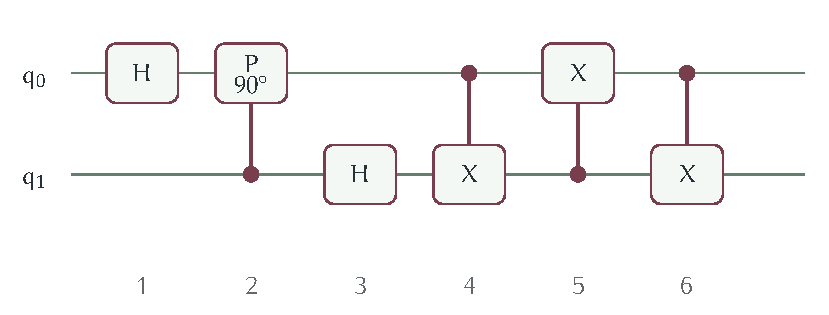
\includegraphics[width=\linewidth,height=94mm,keepaspectratio]{figure/f7322a2f4aff63e08.pdf}\FigureCaption{4.10 \(\cdot\) esempio 1 \(\cdot\) Circuito: porte 1--6}\end{FigureBlock}

\BookHeading{Geometria e configurazione dell'esempio}
\begin{FigureBlock}\centering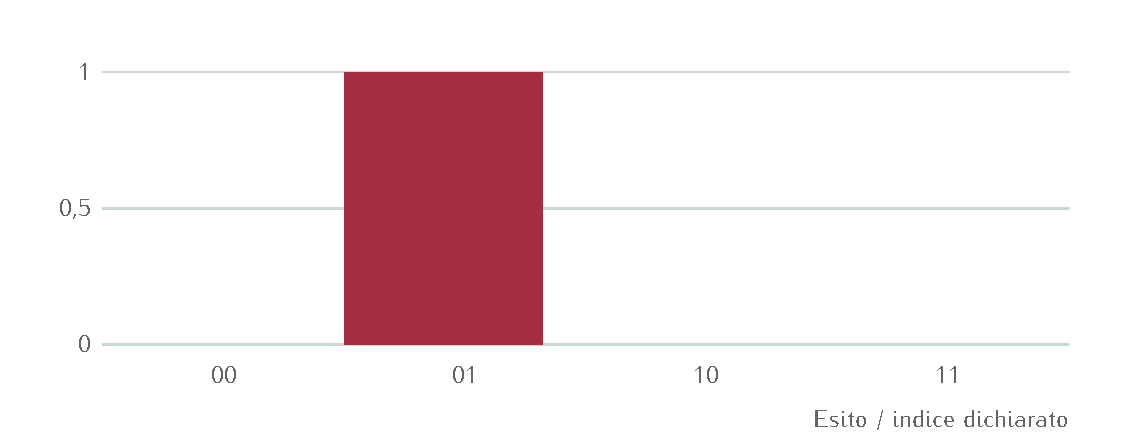
\includegraphics[width=\linewidth,height=94mm,keepaspectratio]{figure/f3bad01d78df274a7.pdf}\FigureCaption{4.10 \(\cdot\) esempio 1 \(\cdot\) Distribuzione congiunta \(\cdot\) Preparazione}\end{FigureBlock}
\begin{FigureBlock}\begin{minipage}[t]{.485\linewidth}\centering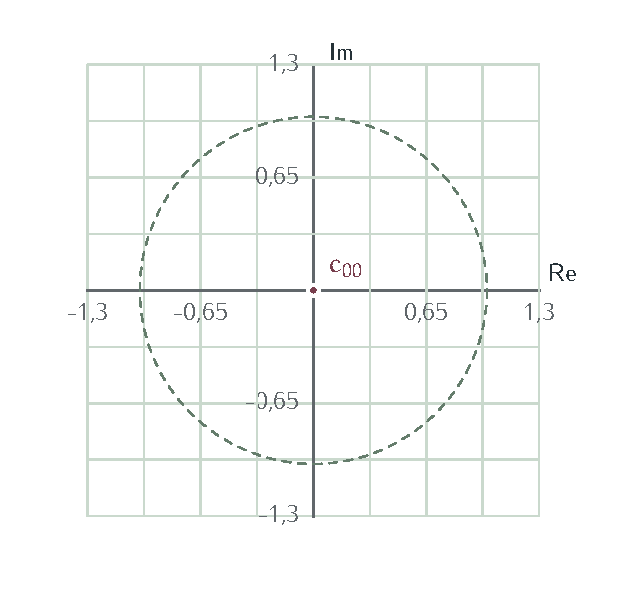
\includegraphics[width=\linewidth,height=63mm,keepaspectratio]{figure/fa7ff8bbd9fb6e4c0.pdf}\par{\sffamily\footnotesize \(c_{00}\)\par}\end{minipage}\hfill\begin{minipage}[t]{.485\linewidth}\centering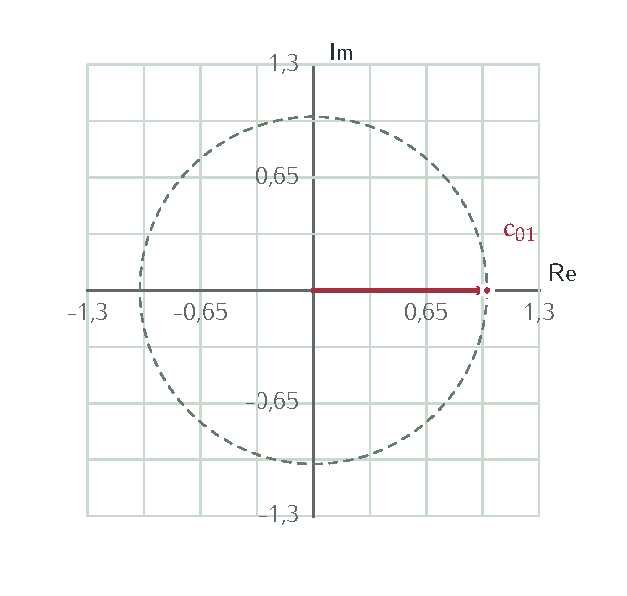
\includegraphics[width=\linewidth,height=63mm,keepaspectratio]{figure/f95ed20638a678d7e.pdf}\par{\sffamily\footnotesize \(c_{01}\)\par}\end{minipage}\FigureCaption{4.10 \(\cdot\) esempio 1 \(\cdot\) Componenti complesse}\end{FigureBlock}
\begin{FigureBlock}\begin{minipage}[t]{.485\linewidth}\centering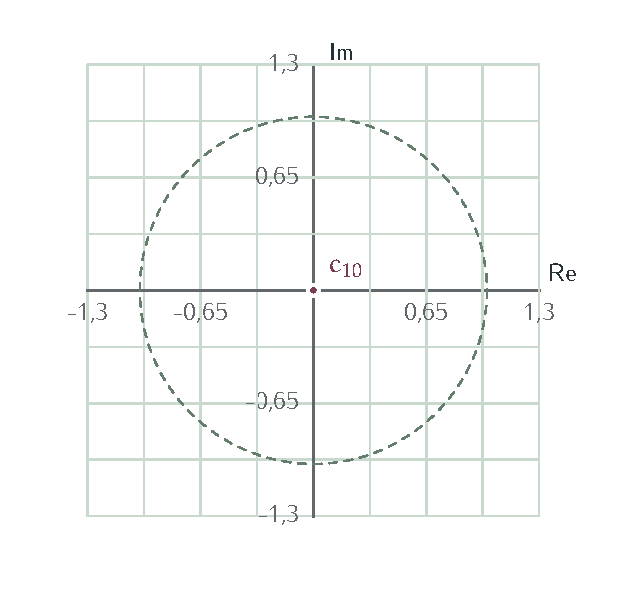
\includegraphics[width=\linewidth,height=63mm,keepaspectratio]{figure/f1b82eb868039f38d.pdf}\par{\sffamily\footnotesize \(c_{10}\)\par}\end{minipage}\hfill\begin{minipage}[t]{.485\linewidth}\centering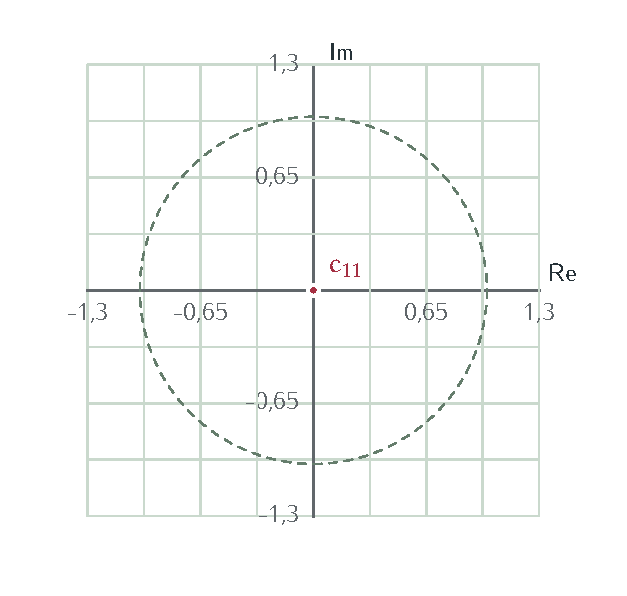
\includegraphics[width=\linewidth,height=63mm,keepaspectratio]{figure/f9ebe26b67537b2e2.pdf}\par{\sffamily\footnotesize \(c_{11}\)\par}\end{minipage}\FigureCaption{4.10 \(\cdot\) esempio 1 \(\cdot\) Componenti complesse}\end{FigureBlock}

\phantomsection\label{c4-qft-example-1-step-1}
\BookHeading{01 Preparazione}

\MathBlock{03C82080003D00280030003B00200031003B00200030003B0020003000291D40003B0020201603C82080201600B222480031}{\psi _{0}=(0;\allowbreak \ 1;\allowbreak \ 0;\allowbreak \ 0)^{T};\allowbreak \ \Vert \psi _{0}\Vert ^{2}\approx 1}

Le ampiezze sono ordinate secondo le etichette binarie, con il bit più significativo in alto.\par


\phantomsection\label{c4-qft-example-1-step-2}
\BookHeading{02 Scomporre la fase secondo i bit}

\MathBlock{0078003D03A3006A002000782C7C0032005E0028006E221200312212006A0029002C00200079003D03A3006A002000792C7C0032005E0028006E221200312212006A0029002E}{x=\sum _{j}\ x_{j}2^{n- 1- j},\allowbreak \ y=\sum _{j}\ y_{j}2^{n- 1- j}.}
\MathBlock{0065005E0028003203C0006900780079002F0032207F0029003D220F006A00200065005E0028003203C0006900792C7C0078002F0032005E0028006A002B003100290029002E}{e^{2\pi \text{ixy}/2^{n}}=\prod _{j}\ e^{2\pi iy_{j}x/2^{j+1}}.}
\MathBlock{0046007C007827E9003D2297006A003D00302026006E2212003100200028007C003027E9002B0065005E0028003203C000690078002F0032005E0028006A002B003100290029007C003127E90029002F221A0032002E}{F|x\rangle =\bigotimes _{j=0}^{n- 1}\ (|0\rangle +e^{2\pi ix/2^{j+1}}|1\rangle )/\sqrt{2}.}
\MathBlock{0051007500690020006E003D0032002C00200078003D0031002E}{\text{Qui}\ n=2,\allowbreak \ x=1.}

L'indice j del prodotto è il filo in uscita in ordine big-endian. Ogni bit \(y_{j}\) sceglie il termine \(|0\rangle \) oppure il termine con fase del proprio fattore.\par


\phantomsection\label{c4-qft-example-1-step-3}
\BookHeading{03 Leggere le frazioni binarie}

\MathBlock{0078003D003200782080002B00782081002021D2002000462084007C007820800078208127E9}{x=2x_{0}+x_{1}\ \Rightarrow \ F_{4}|x_{0}x_{1}\rangle }
\MathBlock{003D0028007C003027E9002B0065005E0028003203C0006900B70030002E007820810029007C003127E90029002F221A00320020229700200028007C003027E9002B0065005E0028003203C0006900B70030002E00782080007820810029007C003127E90029002F221A0032002E}{=(|0\rangle +e^{2\pi i\cdot 0.x_{1}}|1\rangle )/\sqrt{2}\ \otimes \ (|0\rangle +e^{2\pi i\cdot 0.x_{0}x_{1}}|1\rangle )/\sqrt{2}.}
\MathBlock{0030002E00782081003D00782081002F0032003B00200030002E0078208000782081003D00782080002F0032002B00782081002F0034002E}{0.x_{1}=x_{1}/2;\allowbreak \ 0.x_{0}x_{1}=x_{0}/2+x_{1}/4.}

La notazione \(0.x_{0}x_{1}\) indica una frazione in base due, non un numero decimale. I denominatori 2,4,8 determinano fasi di \(180{}^{\circ} ,\allowbreak 90{}^{\circ} ,\allowbreak 45{}^{\circ} \).\par


\phantomsection\label{c4-qft-example-1-step-4}
\BookHeading{04 Ricostruire le porte a due qubit}

\MathBlock{0048002000730075006C002000660069006C006F002000712080002000700072006F00640075006300650020006C00610020006600610073006500200028221200310029005E00782080003D0065005E0028003203C0006900782080002F00320029002E}{H\ \text{sul}\ \text{filo}\ q_{0}\ \text{produce}\ \text{la}\ \text{fase}\ (- 1)^{x_{0}}=e^{2\pi ix_{0}/2}.}
\MathBlock{005000280039003000B0002900200073007500200071208000200063006F006E00740072006F006C006C006100740061002000640061002000712081002000610067006700690075006E0067006500200065005E0028003203C0006900782081002F00340029002E}{P(90{}^{\circ} )\ \text{su}\ q_{0}\ \text{controllata}\ \text{da}\ q_{1}\ \text{aggiunge}\ e^{2\pi ix_{1}/4}.}
\MathBlock{0048002000730075002000712081002000700072006F006400750063006500200065005E0028003203C0006900782081002F00320029002E}{H\ \text{su}\ q_{1}\ \text{produce}\ e^{2\pi ix_{1}/2}.}
\MathBlock{004900200066006100740074006F0072006900200073006F006E006F0020006E0065006C006C2019006F007200640069006E00650020006F00700070006F00730074006F002000610020007100750065006C006C006F002000640069002000462084003A0020006C006F00200053005700410050002000660069006E0061006C00650020007300630061006D00620069006100200071208000200065002000712081002E}{I\ \text{fattori}\ \text{sono}\ \text{nell'ordine}\ \text{opposto}\ a\ \text{quello}\ \text{di}\ F_{4}:\ \text{lo}\ \text{SWAP}\ \text{finale}\ \text{scambia}\ q_{0}\ e\ q_{1}.}

Il controllo è ancora un bit di base quando imposta la fase sul primo filo. Per più qubit ogni bit successivo aggiunge \(P(180{}^{\circ} /2^{k- j})\); gli scambi finali invertono l'ordine dei fili.\par


\phantomsection\label{c4-qft-example-1-step-5}
\BookHeading{05 Espandere e rifattorizzare il caso preliminare}

\MathBlock{00462084007C0030003127E9003D0028007C0030003027E9002B0069007C0030003127E92212007C0031003027E922120069007C0031003127E90029002F0032}{F_{4}|01\rangle =(|00\rangle +i|01\rangle - |10\rangle - i|11\rangle )/2}
\MathBlock{003D00280028007C003027E92212007C003127E90029002F221A00320029229700280028007C003027E9002B0069007C003127E90029002F221A00320029002E}{=((|0\rangle - |1\rangle )/\sqrt{2})\otimes ((|0\rangle +i|1\rangle )/\sqrt{2}).}

Moltiplicando i due fattori si ritrovano tutte e quattro le ampiezze. Il caso a due qubit mostra concretamente il procedimento che si estende al registro assegnato.\par


\phantomsection\label{c4-qft-example-1-step-6}
\BookHeading{06 Costruire i fattori del registro assegnato}

\MathBlock{0046005F0034007C003127E9003D0028007C003027E9002B0065005E0028003203C0006900B70031002F00320029007C003127E90029002F221A00320020229700200028007C003027E9002B0065005E0028003203C0006900B70031002F00340029007C003127E90029002F221A0032}{F_{4}|1\rangle =(|0\rangle +e^{2\pi i\cdot 1/2}|1\rangle )/\sqrt{2}\ \otimes \ (|0\rangle +e^{2\pi i\cdot 1/4}|1\rangle )/\sqrt{2}}
\MathBlock{0046006100730069002000640065006900200066006100740074006F0072006900200069006E0020006F007200640069006E0065002000640069002000660069006C006F003A002000310038003000B0002C00200039003000B0002E}{\text{Fasi}\ \text{dei}\ \text{fattori}\ \text{in}\ \text{ordine}\ \text{di}\ \text{filo}:\ 180{}^{\circ} ,\allowbreak \ 90{}^{\circ} .}

Il circuito successivo realizza \(F_{4}\) su \(|01\rangle \). Il confronto diretto verifica tutti i coefficienti e l'ordine dei fattori.\par


\phantomsection\label{c4-qft-example-1-step-7}
\BookHeading{07 Porta 1 \(\cdot\) \(H\)}

\MathBlock{006300280030003100290020003D002000280030002C0037003000370031002900B70028003100290020002B002000280030002C0037003000370031002900B70028003000290020224800200030002C0037003000370031}{c(01)\ =\ (0{,}7071)\cdot (1)\ +\ (0{,}7071)\cdot (0)\ \approx \ 0{,}7071}
\MathBlock{006300280031003100290020003D002000280030002C0037003000370031002900B70028003100290020002B00200028002D0030002C0037003000370031002900B70028003000290020224800200030002C0037003000370031}{c(11)\ =\ (0{,}7071)\cdot (1)\ +\ (-0{,}7071)\cdot (0)\ \approx \ 0{,}7071}
\MathBlock{03C800202248002000280030003B00200030002C0037003000370031003B00200030003B00200030002C003700300037003100291D40}{\psi \ \approx \ (0;\allowbreak \ 0{,}7071;\allowbreak \ 0;\allowbreak \ 0{,}7071)^{T}}

Ogni coppia di ampiezze indicata usa il prodotto riga per colonna della porta. I rami con controllo nullo restano invariati.\par


\phantomsection\label{c4-qft-example-1-step-8}
\BookHeading{08 Porta 2 \(\cdot\) \(C\cdot P(90{}^{\circ} )\)}

\MathBlock{006300280030003100290020003D002000280031002900B700280030002C003700300037003100290020002B002000280030002900B700280030002C003700300037003100290020224800200030002C0037003000370031}{c(01)\ =\ (1)\cdot (0{,}7071)\ +\ (0)\cdot (0{,}7071)\ \approx \ 0{,}7071}
\MathBlock{006300280031003100290020003D002000280030002900B700280030002C003700300037003100290020002B002000280069002900B700280030002C003700300037003100290020224800200030002C00370030003700310069}{c(11)\ =\ (0)\cdot (0{,}7071)\ +\ (i)\cdot (0{,}7071)\ \approx \ 0{,}7071i}
\MathBlock{03C800202248002000280030003B00200030002C0037003000370031003B00200030003B00200030002C0037003000370031006900291D40}{\psi \ \approx \ (0;\allowbreak \ 0{,}7071;\allowbreak \ 0;\allowbreak \ 0{,}7071i)^{T}}

Ogni coppia di ampiezze indicata usa il prodotto riga per colonna della porta. I rami con controllo nullo restano invariati.\par


\phantomsection\label{c4-qft-example-1-step-9}
\BookHeading{09 Porta 3 \(\cdot\) \(H\)}

\MathBlock{006300280030003000290020003D002000280030002C0037003000370031002900B70028003000290020002B002000280030002C0037003000370031002900B700280030002C003700300037003100290020224800200030002C0035}{c(00)\ =\ (0{,}7071)\cdot (0)\ +\ (0{,}7071)\cdot (0{,}7071)\ \approx \ 0{,}5}
\MathBlock{006300280030003100290020003D002000280030002C0037003000370031002900B70028003000290020002B00200028002D0030002C0037003000370031002900B700280030002C00370030003700310029002022480020002D0030002C0035}{c(01)\ =\ (0{,}7071)\cdot (0)\ +\ (-0{,}7071)\cdot (0{,}7071)\ \approx \ -0{,}5}
\MathBlock{006300280031003000290020003D002000280030002C0037003000370031002900B70028003000290020002B002000280030002C0037003000370031002900B700280030002C0037003000370031006900290020224800200030002C00350069}{c(10)\ =\ (0{,}7071)\cdot (0)\ +\ (0{,}7071)\cdot (0{,}7071i)\ \approx \ 0{,}5i}
\MathBlock{006300280031003100290020003D002000280030002C0037003000370031002900B70028003000290020002B00200028002D0030002C0037003000370031002900B700280030002C003700300037003100690029002022480020002D0030002C00350069}{c(11)\ =\ (0{,}7071)\cdot (0)\ +\ (-0{,}7071)\cdot (0{,}7071i)\ \approx \ -0{,}5i}
\MathBlock{03C800202248002000280030002C0035003B0020002D0030002C0035003B00200030002C00350069003B0020002D0030002C0035006900291D40}{\psi \ \approx \ (0{,}5;\allowbreak \ -0{,}5;\allowbreak \ 0{,}5i;\allowbreak \ -0{,}5i)^{T}}

Ogni coppia di ampiezze indicata usa il prodotto riga per colonna della porta. I rami con controllo nullo restano invariati.\par


\phantomsection\label{c4-qft-example-1-step-10}
\BookHeading{10 Porta 4 \(\cdot\) C\(\cdot\)X}

\MathBlock{006300280031003000290020003D002000280030002900B700280030002C0035006900290020002B002000280031002900B70028002D0030002C003500690029002022480020002D0030002C00350069}{c(10)\ =\ (0)\cdot (0{,}5i)\ +\ (1)\cdot (-0{,}5i)\ \approx \ -0{,}5i}
\MathBlock{006300280031003100290020003D002000280031002900B700280030002C0035006900290020002B002000280030002900B70028002D0030002C0035006900290020224800200030002C00350069}{c(11)\ =\ (1)\cdot (0{,}5i)\ +\ (0)\cdot (-0{,}5i)\ \approx \ 0{,}5i}
\MathBlock{03C800202248002000280030002C0035003B0020002D0030002C0035003B0020002D0030002C00350069003B00200030002C0035006900291D40}{\psi \ \approx \ (0{,}5;\allowbreak \ -0{,}5;\allowbreak \ -0{,}5i;\allowbreak \ 0{,}5i)^{T}}

Ogni coppia di ampiezze indicata usa il prodotto riga per colonna della porta. I rami con controllo nullo restano invariati.\par


\phantomsection\label{c4-qft-example-1-step-11}
\BookHeading{11 Porta 5 \(\cdot\) C\(\cdot\)X}

\MathBlock{006300280030003100290020003D002000280030002900B70028002D0030002C003500290020002B002000280031002900B700280030002C0035006900290020224800200030002C00350069}{c(01)\ =\ (0)\cdot (-0{,}5)\ +\ (1)\cdot (0{,}5i)\ \approx \ 0{,}5i}
\MathBlock{006300280031003100290020003D002000280031002900B70028002D0030002C003500290020002B002000280030002900B700280030002C003500690029002022480020002D0030002C0035}{c(11)\ =\ (1)\cdot (-0{,}5)\ +\ (0)\cdot (0{,}5i)\ \approx \ -0{,}5}
\MathBlock{03C800202248002000280030002C0035003B00200030002C00350069003B0020002D0030002C00350069003B0020002D0030002C003500291D40}{\psi \ \approx \ (0{,}5;\allowbreak \ 0{,}5i;\allowbreak \ -0{,}5i;\allowbreak \ -0{,}5)^{T}}

Ogni coppia di ampiezze indicata usa il prodotto riga per colonna della porta. I rami con controllo nullo restano invariati.\par


\phantomsection\label{c4-qft-example-1-step-12}
\BookHeading{12 Porta 6 \(\cdot\) C\(\cdot\)X}

\MathBlock{006300280031003000290020003D002000280030002900B70028002D0030002C0035006900290020002B002000280031002900B70028002D0030002C00350029002022480020002D0030002C0035}{c(10)\ =\ (0)\cdot (-0{,}5i)\ +\ (1)\cdot (-0{,}5)\ \approx \ -0{,}5}
\MathBlock{006300280031003100290020003D002000280031002900B70028002D0030002C0035006900290020002B002000280030002900B70028002D0030002C00350029002022480020002D0030002C00350069}{c(11)\ =\ (1)\cdot (-0{,}5i)\ +\ (0)\cdot (-0{,}5)\ \approx \ -0{,}5i}
\MathBlock{03C800202248002000280030002C0035003B00200030002C00350069003B0020002D0030002C0035003B0020002D0030002C0035006900291D40}{\psi \ \approx \ (0{,}5;\allowbreak \ 0{,}5i;\allowbreak \ -0{,}5;\allowbreak \ -0{,}5i)^{T}}

Ogni coppia di ampiezze indicata usa il prodotto riga per colonna della porta. I rami con controllo nullo restano invariati.\par


\phantomsection\label{c4-qft-example-1-step-13}
\BookHeading{13 Lettura nella base finale}

\MathBlock{00500028003000300029003D00280030002C0035002900B20020002B002000280030002900B222480030002C00320035}{P(00)=(0{,}5)^{2}\ +\ (0)^{2}\approx 0{,}25}
\MathBlock{00500028003000310029003D00280030002900B20020002B002000280030002C0035002900B222480030002C00320035}{P(01)=(0)^{2}\ +\ (0{,}5)^{2}\approx 0{,}25}
\MathBlock{00500028003100300029003D0028002D0030002C0035002900B20020002B002000280030002900B222480030002C00320035}{P(10)=(-0{,}5)^{2}\ +\ (0)^{2}\approx 0{,}25}
\MathBlock{00500028003100310029003D00280030002900B20020002B00200028002D0030002C0035002900B222480030002C00320035}{P(11)=(0)^{2}\ +\ (-0{,}5)^{2}\approx 0{,}25}

Il modulo quadro di ciascuna ampiezza determina la probabilità. La selezione di una porta nel disegno mostra uno stato intermedio senza effettuare una misura.\par


\phantomsection\label{c4-qft-example-1-step-14}
\BookHeading{14 Controllo indipendente con Fourier}

\MathBlock{0046007C003127E9224800280030002C0035003B00200030002C00350069003B0020002D0030002C0035003B0020002D0030002C0035006900291D40}{F|1\rangle \approx (0{,}5;\allowbreak \ 0{,}5i;\allowbreak \ -0{,}5;\allowbreak \ -0{,}5i)^{T}}
\MathBlock{201603C80063006900720063007500690074006F22120046007C003127E9201622480030}{\Vert \psi \text{circuito}- F|1\rangle \Vert \approx 0}

Il confronto include l'ordine dei bit e tutte le fasi relative.\par


\BookHeading{Stato finale del programma}
\begin{FigureBlock}\centering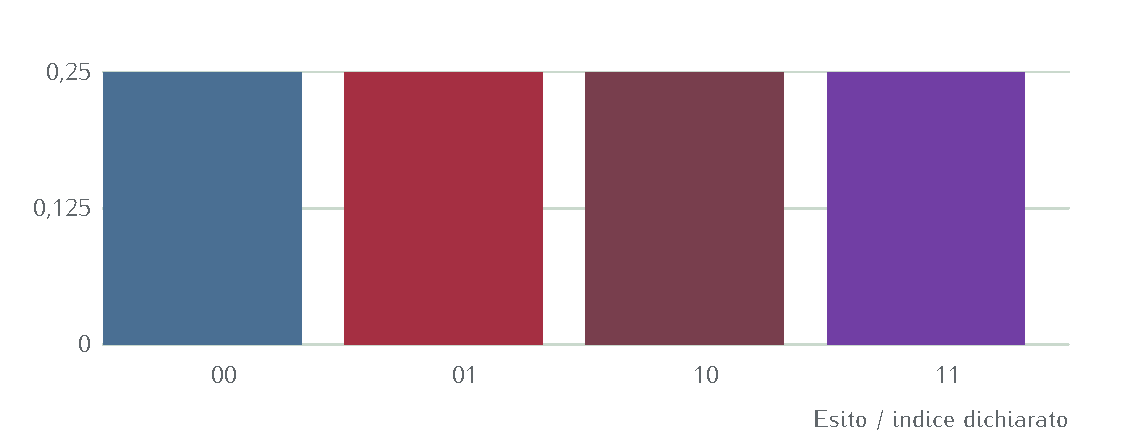
\includegraphics[width=\linewidth,height=94mm,keepaspectratio]{figure/f5a42316de500856a.pdf}\FigureCaption{4.10 \(\cdot\) esempio 1 \(\cdot\) Probabilità nella base dichiarata}\end{FigureBlock}

\BookHeading{Interpretazione}

La fattorizzazione binaria determina \(H\), fasi controllate e scambi; la trasformata diretta conferma tutte le ampiezze del circuito.\par


Risorse dichiarate. 2 qubit; 6 operazioni alla granularità dichiarata nel circuito.\par


\Needspace{.36\textheight}\phantomsection\label{c4-qft-example-2}
{\sffamily\small\color{Accent} ESEMPIO SVOLTO 2\par}
\BookHeading{Fourier costruita porta per porta}
Ingresso \(|011\rangle \); gli scambi finali sono decomposti in tre CNOT.\par


\BookHeading{Circuito completo}
\begin{FigureBlock}\centering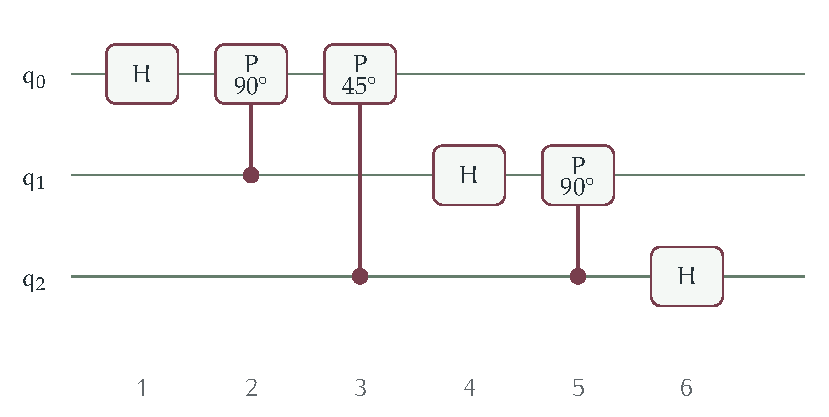
\includegraphics[width=\linewidth,height=94mm,keepaspectratio]{figure/f09af5ef9c8cac387.pdf}\FigureCaption{4.10 \(\cdot\) esempio 2 \(\cdot\) Circuito: porte 1--6}\end{FigureBlock}
\begin{FigureBlock}\centering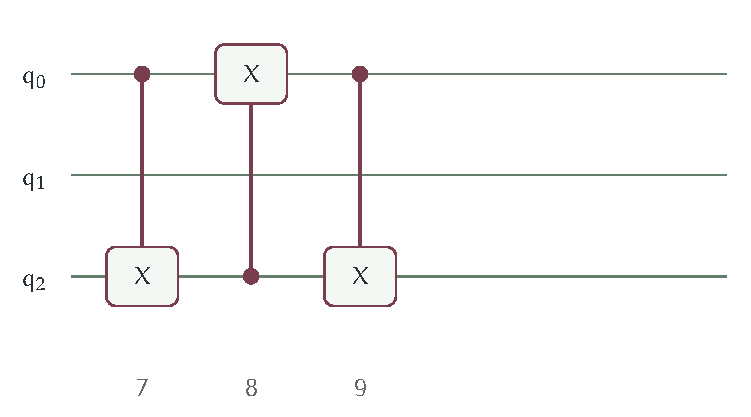
\includegraphics[width=\linewidth,height=94mm,keepaspectratio]{figure/f82280edd4247e792.pdf}\FigureCaption{4.10 \(\cdot\) esempio 2 \(\cdot\) Circuito: porte 7--9}\end{FigureBlock}

\BookHeading{Geometria e configurazione dell'esempio}
\begin{FigureBlock}\centering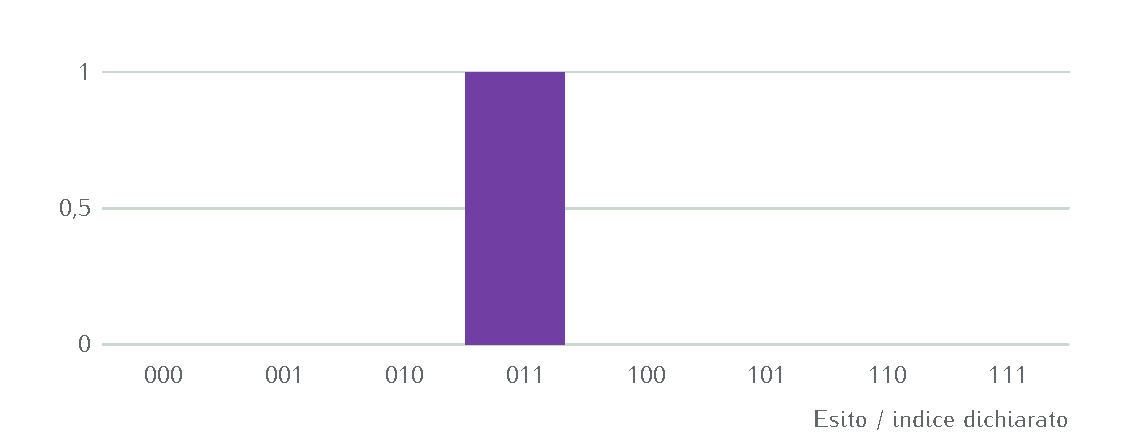
\includegraphics[width=\linewidth,height=94mm,keepaspectratio]{figure/f85de906d5f61d6b7.pdf}\FigureCaption{4.10 \(\cdot\) esempio 2 \(\cdot\) Distribuzione congiunta \(\cdot\) Preparazione}\end{FigureBlock}
\begin{FigureBlock}\begin{minipage}[t]{.485\linewidth}\centering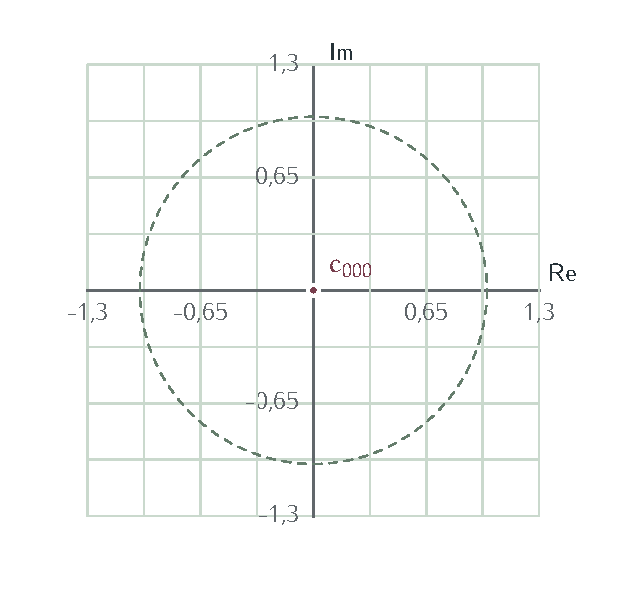
\includegraphics[width=\linewidth,height=63mm,keepaspectratio]{figure/fbb19af4a461c8c36.pdf}\par{\sffamily\footnotesize \(c_{000}\)\par}\end{minipage}\hfill\begin{minipage}[t]{.485\linewidth}\centering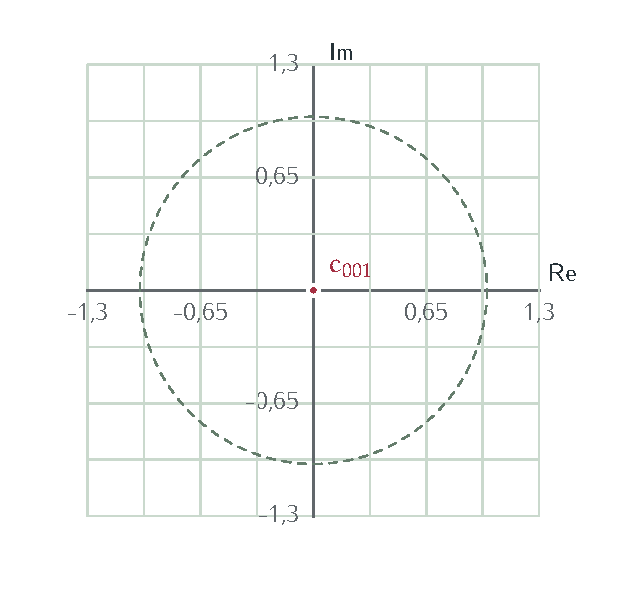
\includegraphics[width=\linewidth,height=63mm,keepaspectratio]{figure/fbbc7091e7d47655c.pdf}\par{\sffamily\footnotesize \(c_{001}\)\par}\end{minipage}\FigureCaption{4.10 \(\cdot\) esempio 2 \(\cdot\) Componenti complesse}\end{FigureBlock}
\begin{FigureBlock}\begin{minipage}[t]{.485\linewidth}\centering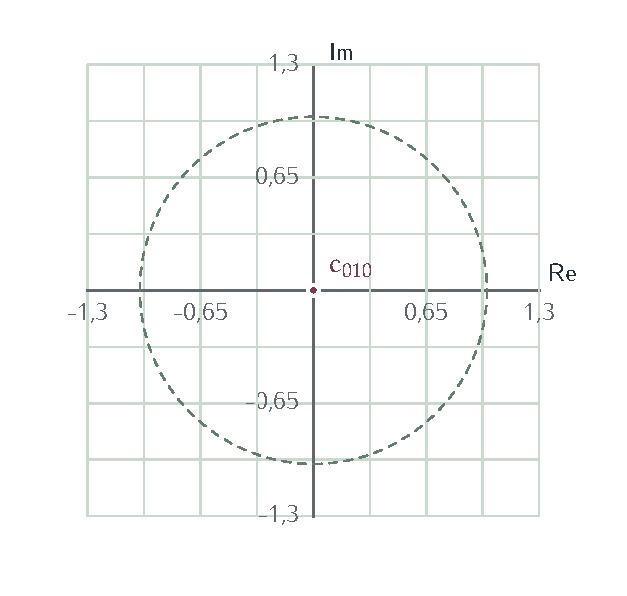
\includegraphics[width=\linewidth,height=63mm,keepaspectratio]{figure/f7628d48d674e1527.pdf}\par{\sffamily\footnotesize \(c_{010}\)\par}\end{minipage}\hfill\begin{minipage}[t]{.485\linewidth}\centering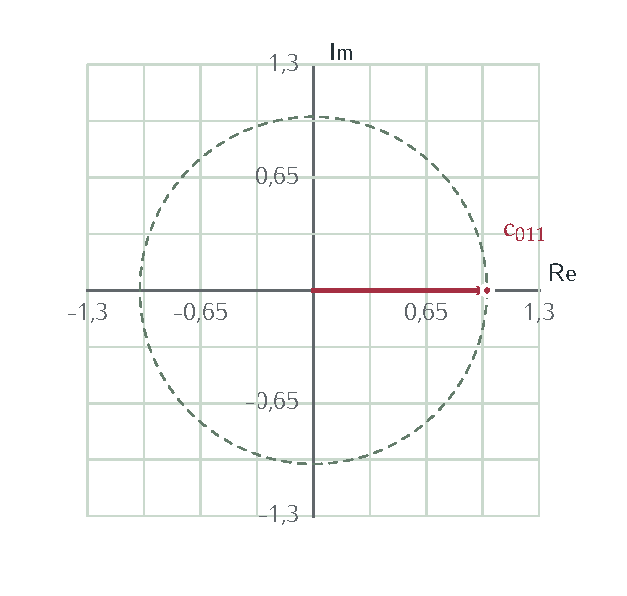
\includegraphics[width=\linewidth,height=63mm,keepaspectratio]{figure/f764a0213e034a628.pdf}\par{\sffamily\footnotesize \(c_{011}\)\par}\end{minipage}\FigureCaption{4.10 \(\cdot\) esempio 2 \(\cdot\) Componenti complesse}\end{FigureBlock}
\begin{FigureBlock}\begin{minipage}[t]{.485\linewidth}\centering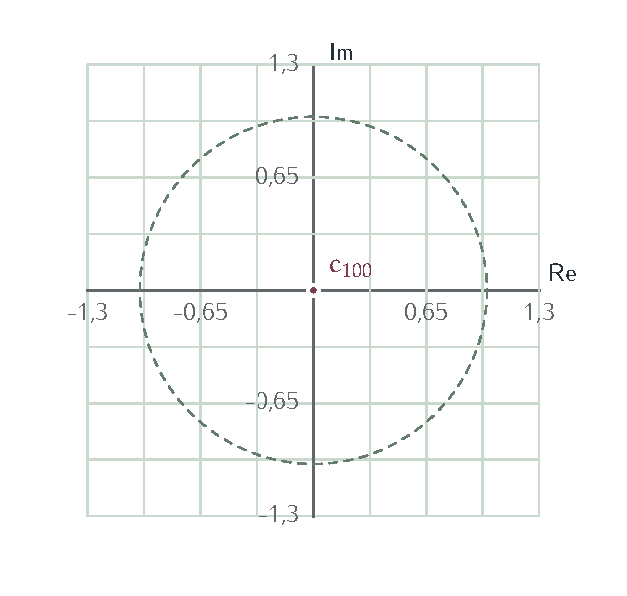
\includegraphics[width=\linewidth,height=63mm,keepaspectratio]{figure/fa5a46da552e27d49.pdf}\par{\sffamily\footnotesize \(c_{100}\)\par}\end{minipage}\hfill\begin{minipage}[t]{.485\linewidth}\centering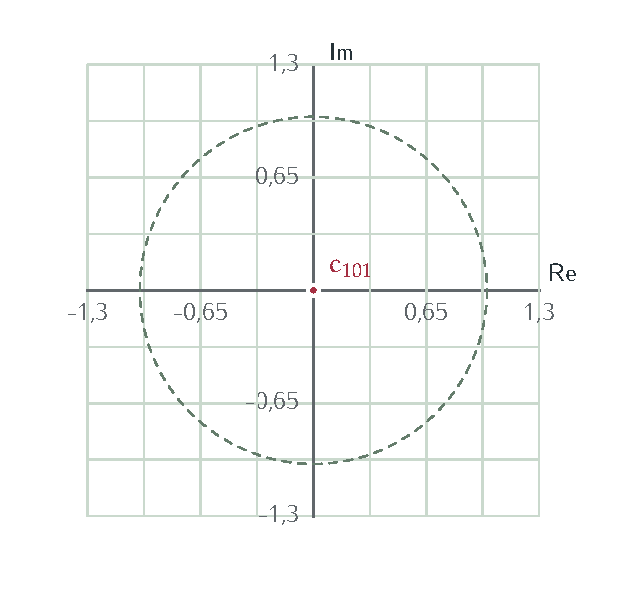
\includegraphics[width=\linewidth,height=63mm,keepaspectratio]{figure/f220ab5c3813c23e0.pdf}\par{\sffamily\footnotesize \(c_{101}\)\par}\end{minipage}\FigureCaption{4.10 \(\cdot\) esempio 2 \(\cdot\) Componenti complesse}\end{FigureBlock}
\begin{FigureBlock}\begin{minipage}[t]{.485\linewidth}\centering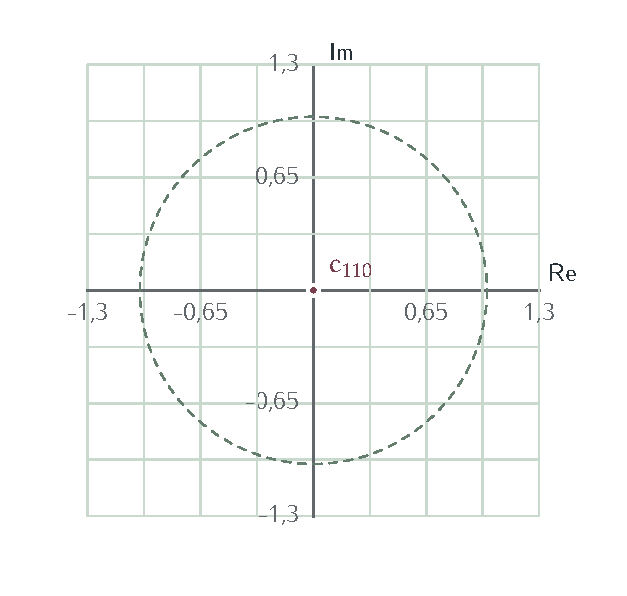
\includegraphics[width=\linewidth,height=63mm,keepaspectratio]{figure/f6434f00b7028d13d.pdf}\par{\sffamily\footnotesize \(c_{110}\)\par}\end{minipage}\hfill\begin{minipage}[t]{.485\linewidth}\centering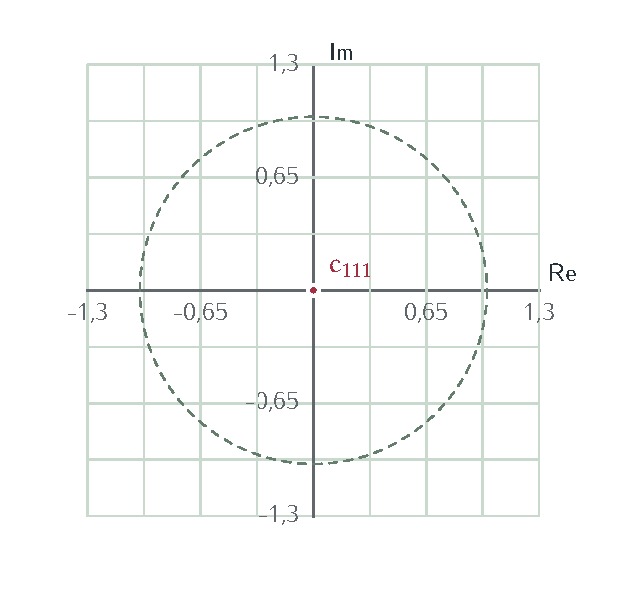
\includegraphics[width=\linewidth,height=63mm,keepaspectratio]{figure/fbae3a20a53c13a13.pdf}\par{\sffamily\footnotesize \(c_{111}\)\par}\end{minipage}\FigureCaption{4.10 \(\cdot\) esempio 2 \(\cdot\) Componenti complesse}\end{FigureBlock}

\phantomsection\label{c4-qft-example-2-step-1}
\BookHeading{01 Preparazione}

\MathBlock{03C82080003D00280030003B00200030003B00200030003B00200031003B00200030003B00200030003B00200030003B0020003000291D40003B0020201603C82080201600B222480031}{\psi _{0}=(0;\allowbreak \ 0;\allowbreak \ 0;\allowbreak \ 1;\allowbreak \ 0;\allowbreak \ 0;\allowbreak \ 0;\allowbreak \ 0)^{T};\allowbreak \ \Vert \psi _{0}\Vert ^{2}\approx 1}

Le ampiezze sono ordinate secondo le etichette binarie, con il bit più significativo in alto.\par


\phantomsection\label{c4-qft-example-2-step-2}
\BookHeading{02 Scomporre la fase secondo i bit}

\MathBlock{0078003D03A3006A002000782C7C0032005E0028006E221200312212006A0029002C00200079003D03A3006A002000792C7C0032005E0028006E221200312212006A0029002E}{x=\sum _{j}\ x_{j}2^{n- 1- j},\allowbreak \ y=\sum _{j}\ y_{j}2^{n- 1- j}.}
\MathBlock{0065005E0028003203C0006900780079002F0032207F0029003D220F006A00200065005E0028003203C0006900792C7C0078002F0032005E0028006A002B003100290029002E}{e^{2\pi \text{ixy}/2^{n}}=\prod _{j}\ e^{2\pi iy_{j}x/2^{j+1}}.}
\MathBlock{0046007C007827E9003D2297006A003D00302026006E2212003100200028007C003027E9002B0065005E0028003203C000690078002F0032005E0028006A002B003100290029007C003127E90029002F221A0032002E}{F|x\rangle =\bigotimes _{j=0}^{n- 1}\ (|0\rangle +e^{2\pi ix/2^{j+1}}|1\rangle )/\sqrt{2}.}
\MathBlock{0051007500690020006E003D0033002C00200078003D0033002E}{\text{Qui}\ n=3,\allowbreak \ x=3.}

L'indice j del prodotto è il filo in uscita in ordine big-endian. Ogni bit \(y_{j}\) sceglie il termine \(|0\rangle \) oppure il termine con fase del proprio fattore.\par


\phantomsection\label{c4-qft-example-2-step-3}
\BookHeading{03 Leggere le frazioni binarie}

\MathBlock{0078003D003200782080002B00782081002021D2002000462084007C007820800078208127E9}{x=2x_{0}+x_{1}\ \Rightarrow \ F_{4}|x_{0}x_{1}\rangle }
\MathBlock{003D0028007C003027E9002B0065005E0028003203C0006900B70030002E007820810029007C003127E90029002F221A00320020229700200028007C003027E9002B0065005E0028003203C0006900B70030002E00782080007820810029007C003127E90029002F221A0032002E}{=(|0\rangle +e^{2\pi i\cdot 0.x_{1}}|1\rangle )/\sqrt{2}\ \otimes \ (|0\rangle +e^{2\pi i\cdot 0.x_{0}x_{1}}|1\rangle )/\sqrt{2}.}
\MathBlock{0030002E00782081003D00782081002F0032003B00200030002E0078208000782081003D00782080002F0032002B00782081002F0034002E}{0.x_{1}=x_{1}/2;\allowbreak \ 0.x_{0}x_{1}=x_{0}/2+x_{1}/4.}

La notazione \(0.x_{0}x_{1}\) indica una frazione in base due, non un numero decimale. I denominatori 2,4,8 determinano fasi di \(180{}^{\circ} ,\allowbreak 90{}^{\circ} ,\allowbreak 45{}^{\circ} \).\par


\phantomsection\label{c4-qft-example-2-step-4}
\BookHeading{04 Ricostruire le porte a due qubit}

\MathBlock{0048002000730075006C002000660069006C006F002000712080002000700072006F00640075006300650020006C00610020006600610073006500200028221200310029005E00782080003D0065005E0028003203C0006900782080002F00320029002E}{H\ \text{sul}\ \text{filo}\ q_{0}\ \text{produce}\ \text{la}\ \text{fase}\ (- 1)^{x_{0}}=e^{2\pi ix_{0}/2}.}
\MathBlock{005000280039003000B0002900200073007500200071208000200063006F006E00740072006F006C006C006100740061002000640061002000712081002000610067006700690075006E0067006500200065005E0028003203C0006900782081002F00340029002E}{P(90{}^{\circ} )\ \text{su}\ q_{0}\ \text{controllata}\ \text{da}\ q_{1}\ \text{aggiunge}\ e^{2\pi ix_{1}/4}.}
\MathBlock{0048002000730075002000712081002000700072006F006400750063006500200065005E0028003203C0006900782081002F00320029002E}{H\ \text{su}\ q_{1}\ \text{produce}\ e^{2\pi ix_{1}/2}.}
\MathBlock{004900200066006100740074006F0072006900200073006F006E006F0020006E0065006C006C2019006F007200640069006E00650020006F00700070006F00730074006F002000610020007100750065006C006C006F002000640069002000462084003A0020006C006F00200053005700410050002000660069006E0061006C00650020007300630061006D00620069006100200071208000200065002000712081002E}{I\ \text{fattori}\ \text{sono}\ \text{nell'ordine}\ \text{opposto}\ a\ \text{quello}\ \text{di}\ F_{4}:\ \text{lo}\ \text{SWAP}\ \text{finale}\ \text{scambia}\ q_{0}\ e\ q_{1}.}

Il controllo è ancora un bit di base quando imposta la fase sul primo filo. Per più qubit ogni bit successivo aggiunge \(P(180{}^{\circ} /2^{k- j})\); gli scambi finali invertono l'ordine dei fili.\par


\phantomsection\label{c4-qft-example-2-step-5}
\BookHeading{05 Espandere e rifattorizzare il caso preliminare}

\MathBlock{00462084007C0030003127E9003D0028007C0030003027E9002B0069007C0030003127E92212007C0031003027E922120069007C0031003127E90029002F0032}{F_{4}|01\rangle =(|00\rangle +i|01\rangle - |10\rangle - i|11\rangle )/2}
\MathBlock{003D00280028007C003027E92212007C003127E90029002F221A00320029229700280028007C003027E9002B0069007C003127E90029002F221A00320029002E}{=((|0\rangle - |1\rangle )/\sqrt{2})\otimes ((|0\rangle +i|1\rangle )/\sqrt{2}).}

Moltiplicando i due fattori si ritrovano tutte e quattro le ampiezze. Il caso a due qubit mostra concretamente il procedimento che si estende al registro assegnato.\par


\phantomsection\label{c4-qft-example-2-step-6}
\BookHeading{06 Costruire i fattori del registro assegnato}

\MathBlock{0046005F0038007C003327E9003D0028007C003027E9002B0065005E0028003203C0006900B70033002F00320029007C003127E90029002F221A00320020229700200028007C003027E9002B0065005E0028003203C0006900B70033002F00340029007C003127E90029002F221A00320020229700200028007C003027E9002B0065005E0028003203C0006900B70033002F00380029007C003127E90029002F221A0032}{F_{8}|3\rangle =(|0\rangle +e^{2\pi i\cdot 3/2}|1\rangle )/\sqrt{2}\ \otimes \ (|0\rangle +e^{2\pi i\cdot 3/4}|1\rangle )/\sqrt{2}\ \otimes \ (|0\rangle +e^{2\pi i\cdot 3/8}|1\rangle )/\sqrt{2}}
\MathBlock{0046006100730069002000640065006900200066006100740074006F0072006900200069006E0020006F007200640069006E0065002000640069002000660069006C006F003A002000310038003000B0002C002000320037003000B0002C002000310033003500B0002E}{\text{Fasi}\ \text{dei}\ \text{fattori}\ \text{in}\ \text{ordine}\ \text{di}\ \text{filo}:\ 180{}^{\circ} ,\allowbreak \ 270{}^{\circ} ,\allowbreak \ 135{}^{\circ} .}

Per \(x=3\) i fattori hanno fasi \(\pi \), \(3\pi /2\), \(3\pi /4\): i coefficienti di \(|1\rangle \) sono \(- 1\), \(- i\), \((- 1+i)/\sqrt{2}\). Il circuito successivo realizza \(F_{8}\) su \(|011\rangle \).\par


\phantomsection\label{c4-qft-example-2-step-7}
\BookHeading{07 Porta 1 \(\cdot\) \(H\)}

\MathBlock{0063002800300031003100290020003D002000280030002C0037003000370031002900B70028003100290020002B002000280030002C0037003000370031002900B70028003000290020224800200030002C0037003000370031}{c(011)\ =\ (0{,}7071)\cdot (1)\ +\ (0{,}7071)\cdot (0)\ \approx \ 0{,}7071}
\MathBlock{0063002800310031003100290020003D002000280030002C0037003000370031002900B70028003100290020002B00200028002D0030002C0037003000370031002900B70028003000290020224800200030002C0037003000370031}{c(111)\ =\ (0{,}7071)\cdot (1)\ +\ (-0{,}7071)\cdot (0)\ \approx \ 0{,}7071}
\MathBlock{03C800202248002000280030003B00200030003B00200030003B00200030002C0037003000370031003B00200030003B00200030003B00200030003B00200030002C003700300037003100291D40}{\psi \ \approx \ (0;\allowbreak \ 0;\allowbreak \ 0;\allowbreak \ 0{,}7071;\allowbreak \ 0;\allowbreak \ 0;\allowbreak \ 0;\allowbreak \ 0{,}7071)^{T}}

Ogni coppia di ampiezze indicata usa il prodotto riga per colonna della porta. I rami con controllo nullo restano invariati.\par


\phantomsection\label{c4-qft-example-2-step-8}
\BookHeading{08 Porta 2 \(\cdot\) \(C\cdot P(90{}^{\circ} )\)}

\MathBlock{0063002800300031003100290020003D002000280031002900B700280030002C003700300037003100290020002B002000280030002900B700280030002C003700300037003100290020224800200030002C0037003000370031}{c(011)\ =\ (1)\cdot (0{,}7071)\ +\ (0)\cdot (0{,}7071)\ \approx \ 0{,}7071}
\MathBlock{0063002800310031003100290020003D002000280030002900B700280030002C003700300037003100290020002B002000280069002900B700280030002C003700300037003100290020224800200030002C00370030003700310069}{c(111)\ =\ (0)\cdot (0{,}7071)\ +\ (i)\cdot (0{,}7071)\ \approx \ 0{,}7071i}
\MathBlock{03C800202248002000280030003B00200030003B00200030003B00200030002C0037003000370031003B00200030003B00200030003B00200030003B00200030002C0037003000370031006900291D40}{\psi \ \approx \ (0;\allowbreak \ 0;\allowbreak \ 0;\allowbreak \ 0{,}7071;\allowbreak \ 0;\allowbreak \ 0;\allowbreak \ 0;\allowbreak \ 0{,}7071i)^{T}}

Ogni coppia di ampiezze indicata usa il prodotto riga per colonna della porta. I rami con controllo nullo restano invariati.\par


\phantomsection\label{c4-qft-example-2-step-9}
\BookHeading{09 Porta 3 \(\cdot\) \(C\cdot P(45{}^{\circ} )\)}

\MathBlock{0063002800300031003100290020003D002000280031002900B700280030002C003700300037003100290020002B002000280030002900B700280030002C0037003000370031006900290020224800200030002C0037003000370031}{c(011)\ =\ (1)\cdot (0{,}7071)\ +\ (0)\cdot (0{,}7071i)\ \approx \ 0{,}7071}
\MathBlock{0063002800310031003100290020003D002000280030002900B700280030002C003700300037003100290020002B002000280030002C00370030003700310020002B00200030002C00370030003700310069002900B700280030002C003700300037003100690029002022480020002D0030002C00350020002B00200030002C00350069}{c(111)\ =\ (0)\cdot (0{,}7071)\ +\ (0{,}7071\ +\ 0{,}7071i)\cdot (0{,}7071i)\ \approx \ -0{,}5\ +\ 0{,}5i}
\MathBlock{03C800202248002000280030003B00200030003B00200030003B00200030002C0037003000370031003B00200030003B00200030003B00200030003B0020002D0030002C00350020002B00200030002C0035006900291D40}{\psi \ \approx \ (0;\allowbreak \ 0;\allowbreak \ 0;\allowbreak \ 0{,}7071;\allowbreak \ 0;\allowbreak \ 0;\allowbreak \ 0;\allowbreak \ -0{,}5\ +\ 0{,}5i)^{T}}

Ogni coppia di ampiezze indicata usa il prodotto riga per colonna della porta. I rami con controllo nullo restano invariati.\par


\phantomsection\label{c4-qft-example-2-step-10}
\BookHeading{10 Porta 4 \(\cdot\) \(H\)}

\MathBlock{0063002800300030003100290020003D002000280030002C0037003000370031002900B70028003000290020002B002000280030002C0037003000370031002900B700280030002C003700300037003100290020224800200030002C0035}{c(001)\ =\ (0{,}7071)\cdot (0)\ +\ (0{,}7071)\cdot (0{,}7071)\ \approx \ 0{,}5}
\MathBlock{0063002800300031003100290020003D002000280030002C0037003000370031002900B70028003000290020002B00200028002D0030002C0037003000370031002900B700280030002C00370030003700310029002022480020002D0030002C0035}{c(011)\ =\ (0{,}7071)\cdot (0)\ +\ (-0{,}7071)\cdot (0{,}7071)\ \approx \ -0{,}5}
\MathBlock{0063002800310030003100290020003D002000280030002C0037003000370031002900B70028003000290020002B002000280030002C0037003000370031002900B70028002D0030002C00350020002B00200030002C003500690029002022480020002D0030002C00330035003300360020002B00200030002C00330035003300360069}{c(101)\ =\ (0{,}7071)\cdot (0)\ +\ (0{,}7071)\cdot (-0{,}5\ +\ 0{,}5i)\ \approx \ -0{,}3536\ +\ 0{,}3536i}
\MathBlock{0063002800310031003100290020003D002000280030002C0037003000370031002900B70028003000290020002B00200028002D0030002C0037003000370031002900B70028002D0030002C00350020002B00200030002C0035006900290020224800200030002C00330035003300360020221200200030002C00330035003300360069}{c(111)\ =\ (0{,}7071)\cdot (0)\ +\ (-0{,}7071)\cdot (-0{,}5\ +\ 0{,}5i)\ \approx \ 0{,}3536\ - \ 0{,}3536i}
\MathBlock{03C800202248002000280030003B00200030002C0035003B00200030003B0020002D0030002C0035003B00200030003B0020002D0030002C00330035003300360020002B00200030002C00330035003300360069003B00200030003B00200030002C00330035003300360020221200200030002C0033003500330036006900291D40}{\psi \ \approx \ (0;\allowbreak \ 0{,}5;\allowbreak \ 0;\allowbreak \ -0{,}5;\allowbreak \ 0;\allowbreak \ -0{,}3536\ +\ 0{,}3536i;\allowbreak \ 0;\allowbreak \ 0{,}3536\ - \ 0{,}3536i)^{T}}

Ogni coppia di ampiezze indicata usa il prodotto riga per colonna della porta. I rami con controllo nullo restano invariati.\par


\phantomsection\label{c4-qft-example-2-step-11}
\BookHeading{11 Porta 5 \(\cdot\) \(C\cdot P(90{}^{\circ} )\)}

\MathBlock{0063002800300030003100290020003D002000280031002900B700280030002C003500290020002B002000280030002900B70028002D0030002C003500290020224800200030002C0035}{c(001)\ =\ (1)\cdot (0{,}5)\ +\ (0)\cdot (-0{,}5)\ \approx \ 0{,}5}
\MathBlock{0063002800300031003100290020003D002000280030002900B700280030002C003500290020002B002000280069002900B70028002D0030002C00350029002022480020002D0030002C00350069}{c(011)\ =\ (0)\cdot (0{,}5)\ +\ (i)\cdot (-0{,}5)\ \approx \ -0{,}5i}
\MathBlock{0063002800310030003100290020003D002000280031002900B70028002D0030002C00330035003300360020002B00200030002C0033003500330036006900290020002B002000280030002900B700280030002C00330035003300360020221200200030002C003300350033003600690029002022480020002D0030002C00330035003300360020002B00200030002C00330035003300360069}{c(101)\ =\ (1)\cdot (-0{,}3536\ +\ 0{,}3536i)\ +\ (0)\cdot (0{,}3536\ - \ 0{,}3536i)\ \approx \ -0{,}3536\ +\ 0{,}3536i}
\MathBlock{0063002800310031003100290020003D002000280030002900B70028002D0030002C00330035003300360020002B00200030002C0033003500330036006900290020002B002000280069002900B700280030002C00330035003300360020221200200030002C0033003500330036006900290020224800200030002C00330035003300360020002B00200030002C00330035003300360069}{c(111)\ =\ (0)\cdot (-0{,}3536\ +\ 0{,}3536i)\ +\ (i)\cdot (0{,}3536\ - \ 0{,}3536i)\ \approx \ 0{,}3536\ +\ 0{,}3536i}
\MathBlock{03C800202248002000280030003B00200030002C0035003B00200030003B0020002D0030002C00350069003B00200030003B0020002D0030002C00330035003300360020002B00200030002C00330035003300360069003B00200030003B00200030002C00330035003300360020002B00200030002C0033003500330036006900291D40}{\psi \ \approx \ (0;\allowbreak \ 0{,}5;\allowbreak \ 0;\allowbreak \ -0{,}5i;\allowbreak \ 0;\allowbreak \ -0{,}3536\ +\ 0{,}3536i;\allowbreak \ 0;\allowbreak \ 0{,}3536\ +\ 0{,}3536i)^{T}}

Ogni coppia di ampiezze indicata usa il prodotto riga per colonna della porta. I rami con controllo nullo restano invariati.\par


\phantomsection\label{c4-qft-example-2-step-12}
\BookHeading{12 Porta 6 \(\cdot\) \(H\)}

\MathBlock{0063002800300030003000290020003D002000280030002C0037003000370031002900B70028003000290020002B002000280030002C0037003000370031002900B700280030002C003500290020224800200030002C0033003500330036}{c(000)\ =\ (0{,}7071)\cdot (0)\ +\ (0{,}7071)\cdot (0{,}5)\ \approx \ 0{,}3536}
\MathBlock{0063002800300030003100290020003D002000280030002C0037003000370031002900B70028003000290020002B00200028002D0030002C0037003000370031002900B700280030002C00350029002022480020002D0030002C0033003500330036}{c(001)\ =\ (0{,}7071)\cdot (0)\ +\ (-0{,}7071)\cdot (0{,}5)\ \approx \ -0{,}3536}
\MathBlock{0063002800300031003000290020003D002000280030002C0037003000370031002900B70028003000290020002B002000280030002C0037003000370031002900B70028002D0030002C003500690029002022480020002D0030002C00330035003300360069}{c(010)\ =\ (0{,}7071)\cdot (0)\ +\ (0{,}7071)\cdot (-0{,}5i)\ \approx \ -0{,}3536i}
\MathBlock{0063002800300031003100290020003D002000280030002C0037003000370031002900B70028003000290020002B00200028002D0030002C0037003000370031002900B70028002D0030002C0035006900290020224800200030002C00330035003300360069}{c(011)\ =\ (0{,}7071)\cdot (0)\ +\ (-0{,}7071)\cdot (-0{,}5i)\ \approx \ 0{,}3536i}
\MathBlock{0063002800310030003000290020003D002000280030002C0037003000370031002900B70028003000290020002B002000280030002C0037003000370031002900B70028002D0030002C00330035003300360020002B00200030002C003300350033003600690029002022480020002D0030002C003200350020002B00200030002C003200350069}{c(100)\ =\ (0{,}7071)\cdot (0)\ +\ (0{,}7071)\cdot (-0{,}3536\ +\ 0{,}3536i)\ \approx \ -0{,}25\ +\ 0{,}25i}
\MathBlock{0063002800310030003100290020003D002000280030002C0037003000370031002900B70028003000290020002B00200028002D0030002C0037003000370031002900B70028002D0030002C00330035003300360020002B00200030002C0033003500330036006900290020224800200030002C003200350020221200200030002C003200350069}{c(101)\ =\ (0{,}7071)\cdot (0)\ +\ (-0{,}7071)\cdot (-0{,}3536\ +\ 0{,}3536i)\ \approx \ 0{,}25\ - \ 0{,}25i}
\MathBlock{0063002800310031003000290020003D002000280030002C0037003000370031002900B70028003000290020002B002000280030002C0037003000370031002900B700280030002C00330035003300360020002B00200030002C0033003500330036006900290020224800200030002C003200350020002B00200030002C003200350069}{c(110)\ =\ (0{,}7071)\cdot (0)\ +\ (0{,}7071)\cdot (0{,}3536\ +\ 0{,}3536i)\ \approx \ 0{,}25\ +\ 0{,}25i}
\MathBlock{0063002800310031003100290020003D002000280030002C0037003000370031002900B70028003000290020002B00200028002D0030002C0037003000370031002900B700280030002C00330035003300360020002B00200030002C003300350033003600690029002022480020002D0030002C003200350020221200200030002C003200350069}{c(111)\ =\ (0{,}7071)\cdot (0)\ +\ (-0{,}7071)\cdot (0{,}3536\ +\ 0{,}3536i)\ \approx \ -0{,}25\ - \ 0{,}25i}
\MathBlock{03C800202248002000280030002C0033003500330036003B0020002D0030002C0033003500330036003B0020002D0030002C00330035003300360069003B00200030002C00330035003300360069003B0020002D0030002C003200350020002B00200030002C003200350069003B00200030002C003200350020221200200030002C003200350069003B00200030002C003200350020002B00200030002C003200350069003B0020002D0030002C003200350020221200200030002C00320035006900291D40}{\psi \ \approx \ (0{,}3536;\allowbreak \ -0{,}3536;\allowbreak \ -0{,}3536i;\allowbreak \ 0{,}3536i;\allowbreak \ -0{,}25\ +\ 0{,}25i;\allowbreak \ 0{,}25\ - \ 0{,}25i;\allowbreak \ 0{,}25\ +\ 0{,}25i;\allowbreak \ -0{,}25\ - \ 0{,}25i)^{T}}

Ogni coppia di ampiezze indicata usa il prodotto riga per colonna della porta. I rami con controllo nullo restano invariati.\par


\phantomsection\label{c4-qft-example-2-step-13}
\BookHeading{13 Porta 7 \(\cdot\) C\(\cdot\)X}

\MathBlock{0063002800310030003000290020003D002000280030002900B70028002D0030002C003200350020002B00200030002C00320035006900290020002B002000280031002900B700280030002C003200350020221200200030002C00320035006900290020224800200030002C003200350020221200200030002C003200350069}{c(100)\ =\ (0)\cdot (-0{,}25\ +\ 0{,}25i)\ +\ (1)\cdot (0{,}25\ - \ 0{,}25i)\ \approx \ 0{,}25\ - \ 0{,}25i}
\MathBlock{0063002800310030003100290020003D002000280031002900B70028002D0030002C003200350020002B00200030002C00320035006900290020002B002000280030002900B700280030002C003200350020221200200030002C0032003500690029002022480020002D0030002C003200350020002B00200030002C003200350069}{c(101)\ =\ (1)\cdot (-0{,}25\ +\ 0{,}25i)\ +\ (0)\cdot (0{,}25\ - \ 0{,}25i)\ \approx \ -0{,}25\ +\ 0{,}25i}
\MathBlock{0063002800310031003000290020003D002000280030002900B700280030002C003200350020002B00200030002C00320035006900290020002B002000280031002900B70028002D0030002C003200350020221200200030002C0032003500690029002022480020002D0030002C003200350020221200200030002C003200350069}{c(110)\ =\ (0)\cdot (0{,}25\ +\ 0{,}25i)\ +\ (1)\cdot (-0{,}25\ - \ 0{,}25i)\ \approx \ -0{,}25\ - \ 0{,}25i}
\MathBlock{0063002800310031003100290020003D002000280031002900B700280030002C003200350020002B00200030002C00320035006900290020002B002000280030002900B70028002D0030002C003200350020221200200030002C00320035006900290020224800200030002C003200350020002B00200030002C003200350069}{c(111)\ =\ (1)\cdot (0{,}25\ +\ 0{,}25i)\ +\ (0)\cdot (-0{,}25\ - \ 0{,}25i)\ \approx \ 0{,}25\ +\ 0{,}25i}
\MathBlock{03C800202248002000280030002C0033003500330036003B0020002D0030002C0033003500330036003B0020002D0030002C00330035003300360069003B00200030002C00330035003300360069003B00200030002C003200350020221200200030002C003200350069003B0020002D0030002C003200350020002B00200030002C003200350069003B0020002D0030002C003200350020221200200030002C003200350069003B00200030002C003200350020002B00200030002C00320035006900291D40}{\psi \ \approx \ (0{,}3536;\allowbreak \ -0{,}3536;\allowbreak \ -0{,}3536i;\allowbreak \ 0{,}3536i;\allowbreak \ 0{,}25\ - \ 0{,}25i;\allowbreak \ -0{,}25\ +\ 0{,}25i;\allowbreak \ -0{,}25\ - \ 0{,}25i;\allowbreak \ 0{,}25\ +\ 0{,}25i)^{T}}

Ogni coppia di ampiezze indicata usa il prodotto riga per colonna della porta. I rami con controllo nullo restano invariati.\par


\phantomsection\label{c4-qft-example-2-step-14}
\BookHeading{14 Porta 8 \(\cdot\) C\(\cdot\)X}

\MathBlock{0063002800300030003100290020003D002000280030002900B70028002D0030002C003300350033003600290020002B002000280031002900B70028002D0030002C003200350020002B00200030002C0032003500690029002022480020002D0030002C003200350020002B00200030002C003200350069}{c(001)\ =\ (0)\cdot (-0{,}3536)\ +\ (1)\cdot (-0{,}25\ +\ 0{,}25i)\ \approx \ -0{,}25\ +\ 0{,}25i}
\MathBlock{0063002800310030003100290020003D002000280031002900B70028002D0030002C003300350033003600290020002B002000280030002900B70028002D0030002C003200350020002B00200030002C0032003500690029002022480020002D0030002C0033003500330036}{c(101)\ =\ (1)\cdot (-0{,}3536)\ +\ (0)\cdot (-0{,}25\ +\ 0{,}25i)\ \approx \ -0{,}3536}
\MathBlock{0063002800300031003100290020003D002000280030002900B700280030002C0033003500330036006900290020002B002000280031002900B700280030002C003200350020002B00200030002C00320035006900290020224800200030002C003200350020002B00200030002C003200350069}{c(011)\ =\ (0)\cdot (0{,}3536i)\ +\ (1)\cdot (0{,}25\ +\ 0{,}25i)\ \approx \ 0{,}25\ +\ 0{,}25i}
\MathBlock{0063002800310031003100290020003D002000280031002900B700280030002C0033003500330036006900290020002B002000280030002900B700280030002C003200350020002B00200030002C00320035006900290020224800200030002C00330035003300360069}{c(111)\ =\ (1)\cdot (0{,}3536i)\ +\ (0)\cdot (0{,}25\ +\ 0{,}25i)\ \approx \ 0{,}3536i}
\MathBlock{03C800202248002000280030002C0033003500330036003B0020002D0030002C003200350020002B00200030002C003200350069003B0020002D0030002C00330035003300360069003B00200030002C003200350020002B00200030002C003200350069003B00200030002C003200350020221200200030002C003200350069003B0020002D0030002C0033003500330036003B0020002D0030002C003200350020221200200030002C003200350069003B00200030002C0033003500330036006900291D40}{\psi \ \approx \ (0{,}3536;\allowbreak \ -0{,}25\ +\ 0{,}25i;\allowbreak \ -0{,}3536i;\allowbreak \ 0{,}25\ +\ 0{,}25i;\allowbreak \ 0{,}25\ - \ 0{,}25i;\allowbreak \ -0{,}3536;\allowbreak \ -0{,}25\ - \ 0{,}25i;\allowbreak \ 0{,}3536i)^{T}}

Ogni coppia di ampiezze indicata usa il prodotto riga per colonna della porta. I rami con controllo nullo restano invariati.\par


\phantomsection\label{c4-qft-example-2-step-15}
\BookHeading{15 Porta 9 \(\cdot\) C\(\cdot\)X}

\MathBlock{0063002800310030003000290020003D002000280030002900B700280030002C003200350020221200200030002C00320035006900290020002B002000280031002900B70028002D0030002C00330035003300360029002022480020002D0030002C0033003500330036}{c(100)\ =\ (0)\cdot (0{,}25\ - \ 0{,}25i)\ +\ (1)\cdot (-0{,}3536)\ \approx \ -0{,}3536}
\MathBlock{0063002800310030003100290020003D002000280031002900B700280030002C003200350020221200200030002C00320035006900290020002B002000280030002900B70028002D0030002C003300350033003600290020224800200030002C003200350020221200200030002C003200350069}{c(101)\ =\ (1)\cdot (0{,}25\ - \ 0{,}25i)\ +\ (0)\cdot (-0{,}3536)\ \approx \ 0{,}25\ - \ 0{,}25i}
\MathBlock{0063002800310031003000290020003D002000280030002900B70028002D0030002C003200350020221200200030002C00320035006900290020002B002000280031002900B700280030002C0033003500330036006900290020224800200030002C00330035003300360069}{c(110)\ =\ (0)\cdot (-0{,}25\ - \ 0{,}25i)\ +\ (1)\cdot (0{,}3536i)\ \approx \ 0{,}3536i}
\MathBlock{0063002800310031003100290020003D002000280031002900B70028002D0030002C003200350020221200200030002C00320035006900290020002B002000280030002900B700280030002C003300350033003600690029002022480020002D0030002C003200350020221200200030002C003200350069}{c(111)\ =\ (1)\cdot (-0{,}25\ - \ 0{,}25i)\ +\ (0)\cdot (0{,}3536i)\ \approx \ -0{,}25\ - \ 0{,}25i}
\MathBlock{03C800202248002000280030002C0033003500330036003B0020002D0030002C003200350020002B00200030002C003200350069003B0020002D0030002C00330035003300360069003B00200030002C003200350020002B00200030002C003200350069003B0020002D0030002C0033003500330036003B00200030002C003200350020221200200030002C003200350069003B00200030002C00330035003300360069003B0020002D0030002C003200350020221200200030002C00320035006900291D40}{\psi \ \approx \ (0{,}3536;\allowbreak \ -0{,}25\ +\ 0{,}25i;\allowbreak \ -0{,}3536i;\allowbreak \ 0{,}25\ +\ 0{,}25i;\allowbreak \ -0{,}3536;\allowbreak \ 0{,}25\ - \ 0{,}25i;\allowbreak \ 0{,}3536i;\allowbreak \ -0{,}25\ - \ 0{,}25i)^{T}}

Ogni coppia di ampiezze indicata usa il prodotto riga per colonna della porta. I rami con controllo nullo restano invariati.\par


\phantomsection\label{c4-qft-example-2-step-16}
\BookHeading{16 Lettura nella base finale}

\MathBlock{005000280030003000300029003D00280030002C0033003500330036002900B20020002B002000280030002900B222480030002C003100320035}{P(000)=(0{,}3536)^{2}\ +\ (0)^{2}\approx 0{,}125}
\MathBlock{005000280030003000310029003D0028002D0030002C00320035002900B20020002B002000280030002C00320035002900B222480030002C003100320035}{P(001)=(-0{,}25)^{2}\ +\ (0{,}25)^{2}\approx 0{,}125}
\MathBlock{005000280030003100300029003D00280030002900B20020002B00200028002D0030002C0033003500330036002900B222480030002C003100320035}{P(010)=(0)^{2}\ +\ (-0{,}3536)^{2}\approx 0{,}125}
\MathBlock{005000280030003100310029003D00280030002C00320035002900B20020002B002000280030002C00320035002900B222480030002C003100320035}{P(011)=(0{,}25)^{2}\ +\ (0{,}25)^{2}\approx 0{,}125}
\MathBlock{005000280031003000300029003D0028002D0030002C0033003500330036002900B20020002B002000280030002900B222480030002C003100320035}{P(100)=(-0{,}3536)^{2}\ +\ (0)^{2}\approx 0{,}125}
\MathBlock{005000280031003000310029003D00280030002C00320035002900B20020002B00200028002D0030002C00320035002900B222480030002C003100320035}{P(101)=(0{,}25)^{2}\ +\ (-0{,}25)^{2}\approx 0{,}125}
\MathBlock{005000280031003100300029003D00280030002900B20020002B002000280030002C0033003500330036002900B222480030002C003100320035}{P(110)=(0)^{2}\ +\ (0{,}3536)^{2}\approx 0{,}125}
\MathBlock{005000280031003100310029003D0028002D0030002C00320035002900B20020002B00200028002D0030002C00320035002900B222480030002C003100320035}{P(111)=(-0{,}25)^{2}\ +\ (-0{,}25)^{2}\approx 0{,}125}

Il modulo quadro di ciascuna ampiezza determina la probabilità. La selezione di una porta nel disegno mostra uno stato intermedio senza effettuare una misura.\par


\phantomsection\label{c4-qft-example-2-step-17}
\BookHeading{17 Controllo indipendente con Fourier}

\MathBlock{0046007C003327E9224800280030002C0033003500330036003B0020002D0030002C003200350020002B00200030002C003200350069003B0020002D0030002C00330035003300360069003B00200030002C003200350020002B00200030002C003200350069003B0020002D0030002C0033003500330036003B00200030002C003200350020221200200030002C003200350069003B00200030002C00330035003300360069003B0020002D0030002C003200350020221200200030002C00320035006900291D40}{F|3\rangle \approx (0{,}3536;\allowbreak \ -0{,}25\ +\ 0{,}25i;\allowbreak \ -0{,}3536i;\allowbreak \ 0{,}25\ +\ 0{,}25i;\allowbreak \ -0{,}3536;\allowbreak \ 0{,}25\ - \ 0{,}25i;\allowbreak \ 0{,}3536i;\allowbreak \ -0{,}25\ - \ 0{,}25i)^{T}}
\MathBlock{201603C80063006900720063007500690074006F22120046007C003327E9201622480030}{\Vert \psi \text{circuito}- F|3\rangle \Vert \approx 0}

Il confronto include l'ordine dei bit e tutte le fasi relative.\par


\BookHeading{Stato finale del programma}
\begin{FigureBlock}\centering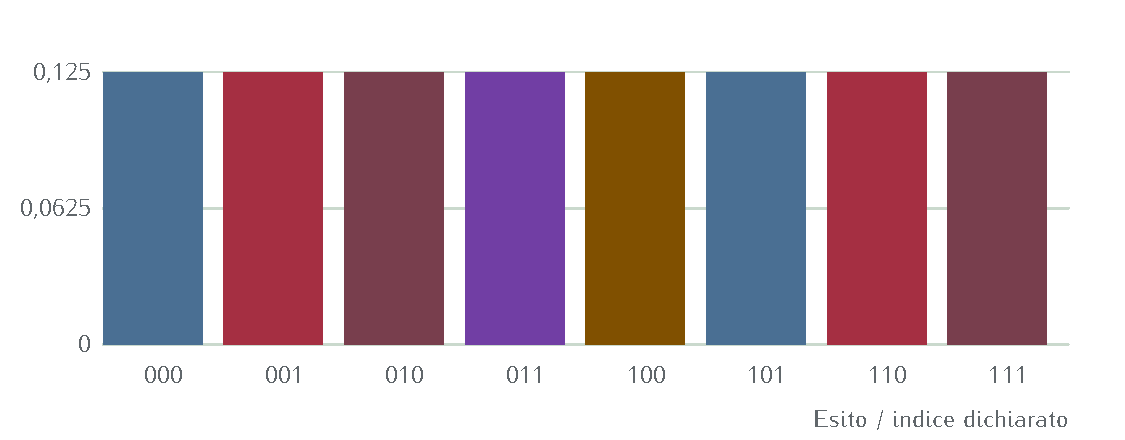
\includegraphics[width=\linewidth,height=94mm,keepaspectratio]{figure/fa518291cc5b76c3e.pdf}\FigureCaption{4.10 \(\cdot\) esempio 2 \(\cdot\) Probabilità nella base dichiarata}\end{FigureBlock}

\BookHeading{Interpretazione}

La fattorizzazione binaria determina \(H\), fasi controllate e scambi; la trasformata diretta conferma tutte le ampiezze del circuito.\par


Risorse dichiarate. 3 qubit; 9 operazioni alla granularità dichiarata nel circuito.\par


\Needspace{7\baselineskip}
\BookHeading{Il passaggio successivo}
Le fasi controllate della QFT mostrano come un controllo coerente trasferisca informazione al registro di lettura. L'Hadamard test usa un solo controllo per leggere una componente di \(\langle \psi |U|\psi \rangle \); QPE userà più controlli per stimare un'autofase.\par


% Authoritative exercise source. Preserve all derivations and diagrams.

\ExerciseStart{G4.06}{Costruire una Fourier a quattro livelli}{Consolidamento}

\BookHeading{Problema, dati e obiettivo}

Applicare la QFT positiva a due qubit nello stato \(\ket{01}\). Usare l’ordine dei bit \(q_0q_1\), con q0 più significativo. Ricostruire il risultato mediante matrice e circuito, poi applicare l’inversa.

\ExTheory{\ExRef{c4-fourier}{4.09}; \ExRef{c4-qft}{4.10}}{La convenzione è \(F_4\ket x=\frac12\sum_{y=0}^3e^{2\pi ixy/4}\ket y\). La trasformata inversa usa il segno negativo. La misura delle sole probabilità finali può nascondere le fasi che distinguono le colonne di Fourier.}

\ExPrediction{Per x=1 le quattro ampiezze dovrebbero percorrere i vertici di un quadrato nel piano complesso, tutte con modulo \(1/2\).}

\ExFigure{\begin{tikzpicture}[>=Stealth,exlabel]
\draw[exaxis] (-1.35,0)--(1.55,0) node[right] {$\operatorname{Re}$};\draw[exaxis] (0,-1.35)--(0,1.55) node[above] {$\operatorname{Im}$};\draw[->,Accent,line width=1.1pt] (0,0)--(1,0) node[anchor=south west] {$ 1 $};\draw[->,Secondary,line width=1.1pt] (0,0)--(0,1) node[anchor=south west] {$ i $};\draw[->,Accent,line width=1.1pt] (0,0)--(-1,0) node[anchor=south west] {$ -1 $};\draw[->,Secondary,line width=1.1pt] (0,0)--(0,-1) node[anchor=north west] {$ -i $};
\end{tikzpicture}}{Radici quarte dell’unità; le ampiezze della QFT sono questi vettori divisi per due.}


\begin{ExTasks}

\item Scrivere F4 e selezionarne la colonna x=1.

\item Seguire H su q0, fase controllata, H su q1 e SWAP.

\item Fattorizzare lo stato finale.

\item Calcolare tutte le quattro somme dell’inversa.

\end{ExTasks}

\ExSolution

\ExStep{Costruire la matrice}

\ExEq{F_4&=\frac12\begin{pmatrix}1&1&1&1\\1&i&-1&-i\\1&-1&1&-1\\1&-i&-1&i\end{pmatrix},\\
F_4\ket1&=\frac12(1,i,-1,-i)^T.}
I quattro moduli quadri sono \(1/4\).

\ExStep{Applicare le prime due porte}

\ExEq{\ket{01}&\xrightarrow{H_0}\frac{\ket{01}+\ket{11}}{\sqrt2}
\xrightarrow{CP(\pi/2)}\frac{\ket{01}+i\ket{11}}{\sqrt2}.}
La fase controllata moltiplica per i soltanto la componente 11.

\ExStep{Completare il circuito}

\ExEq{\frac{\ket{01}+i\ket{11}}{\sqrt2}
&\xrightarrow{H_1}\frac{\ket{00}-\ket{01}+i\ket{10}-i\ket{11}}2\\
&\xrightarrow{\mathrm{SWAP}}\frac{\ket{00}+i\ket{01}-\ket{10}-i\ket{11}}2.}
Lo scambio finale ripristina l’ordine dei bit dichiarato.

\ExStep{Leggere i due fattori}

\ExEq{F_4\ket1&=\frac{\ket0-\ket1}{\sqrt2}\otimes\frac{\ket0+i\ket1}{\sqrt2}.}
Il primo fattore ha fase relativa \(\pi\), il secondo \(\pi/2\). Lo stato è separabile per questo ingresso della base.

\ExStep{Svolgere l’inversa}

\ExEq{B(0)&=(1+i-1-i)/4=0,\\
B(1)&=(1+1+1+1)/4=1,\\
B(2)&=(1-i-1+i)/4=0,\\
B(3)&=(1-1+1-1)/4=0.}
Pertanto \(F_4^\dagger F_4\ket1=\ket1\). Ogni riga dell’inversa confronta la sequenza di fasi con una frequenza candidata.

\par\noindent\begin{minipage}{\linewidth}
\ExFigure{\begin{tikzpicture}[>=Stealth,exlabel]
\draw (0,0)--(6.8,0);\draw (0,-1.4)--(6.8,-1.4);\node[left] at(0,0){$q_0$};\node[left] at(0,-1.4){$q_1$};\node[exbox,minimum width=7mm,text width=7mm] at(1,0){$H$};\fill (2.6,-1.4) circle(2pt);\draw (2.6,-1.4)--(2.6,0);\node[exbox,minimum width=10mm,text width=10mm] at(2.6,0){$P_{\pi/2}$};\node[exbox,minimum width=7mm,text width=7mm] at(4.2,-1.4){$H$};\draw (5.6,0)--(5.6,-1.4);\node at(5.6,0){$\times$};\node at(5.6,-1.4){$\times$};
\end{tikzpicture}}{Circuito per la convenzione positiva e per l’ordine q0q1, inclusa l’inversione finale dei fili.}


\ExInterpret{L’inversa distingue stati con identiche probabilità nella base computazionale attraverso l’allineamento dei fasori. Le cancellazioni delle somme rendono la frequenza un esito leggibile.}

\ExLab{Nelle sezioni 4.09 e 4.10 selezionare QFT positiva su due qubit e ingresso 01. Verificare prima le ampiezze complesse, poi l’ordine dei bit e infine il ritorno con l’inversa.}


\end{minipage}

\Needspace{.43\textheight}
\section{Hadamard test}
\phantomsection\label{c4-hadamard-test}

{\sffamily\small\color{Ink!70} Riferimento alle slide: p. 303.\par}

{\sffamily\small\color{Ink!70} Laboratorio locale: \nolinkurl{index.html#capitolo-4/hadamard-test}\par}

\BookHeading{Definizioni e costruzione}
Sia \(U\) una matrice unitaria sul registro bersaglio preparato nello stato normalizzato \(|\psi \rangle \). Il numero complesso \(z=\langle \psi |U|\psi \rangle \) confronta la preparazione con la sua trasformata; un qubit ausiliario permette di leggerne la parte reale o immaginaria.\par

Dopo \(H\) sull'ausiliario e \(U\) controllata, lo stato è \((|0\rangle |\psi \rangle +|1\rangle U|\psi \rangle )/\sqrt{2}\). Una seconda \(H\) produce nel ramo zero \((|\psi \rangle +U|\psi \rangle )/2\); la sua norma quadrata è (1+Re z)/2.\par

Per la parte immaginaria inseriamo \(S{}^{\dagger} =P(- \pi /2)=\operatorname{diag}(1,\allowbreak - i)\) sull'ausiliario prima dell'ultima \(H\). Il ramo zero diventa \((|\psi \rangle - iU|\psi \rangle )/2\) e la norma dà (1+Im z)/2. Il segno di \(S{}^{\dagger} \) è quindi parte del significato della misura.\par

Nei preset \(|\psi \rangle =|+\rangle \) e \(U=P(\varphi )\). Allora \(z=(1+\allowbreak\exp (i\varphi ))/2\). Il caso reale con \(\varphi =90{}^{\circ} \) dà \(P(0)=3/4\); quello immaginario con \(\varphi =- 90{}^{\circ} \) dà \(P(0)=1/4\) e rende visibile il segno negativo della componente immaginaria. Per leggere l'ausiliario sommiamo sempre sui valori del bersaglio.\par


\MathBlock{0050002800300029003D005B0031002B0052006527E803C8007C0055007C03C827E9005D002F0032003B00200063006F006E002000532020002000730075006C006C20190061007500730069006C0069006100720069006F002C00200050002800300029003D005B0031002B0049006D27E803C8007C0055007C03C827E9005D002F0032002E}{P(0)=[1+\operatorname{Re}\langle \psi |U|\psi \rangle ]/2;\allowbreak \ \text{con}\ S{}^{\dagger} \ \text{sull'ausiliario},\allowbreak \ P(0)=[1+\operatorname{Im}\langle \psi |U|\psi \rangle ]/2.}

\BookHeading{Come leggere le figure}
I piani complessi descrivono lo stato congiunto; le due barre marginali descrivono l'ausiliario letto. \(U\) è una trasformazione del bersaglio, mentre \(S{}^{\dagger} \) agisce sul controllo: sono porte con ruoli distinti.\par


\BookHeading{Attività nel laboratorio modificabile}

\BookHeading{Obiettivo dell'esperimento}
Leggere parte reale o immaginaria di un valore atteso.\par

\BookHeading{Percorso operativo}
Cambiare preparazione, angolo di \(P\) e componente da leggere.\par

\BookHeading{Lettura geometrica}
L'interferenza del controllo combina il ramo trasformato e quello invariato.\par

\BookHeading{Controllo del risultato}
Verificare il segno della parte immaginaria e sommare correttamente sui dati del bersaglio.\par


\Needspace{.36\textheight}\phantomsection\label{c4-hadamard-test-example-1}
{\sffamily\small\color{Accent} ESEMPIO SVOLTO 1\par}
\BookHeading{Leggere una componente del valore atteso}
\(U=P(90{}^{\circ} )\); la lettura dell'ausiliario fornisce la parte reale.\par


\BookHeading{Circuito completo}
\begin{FigureBlock}\centering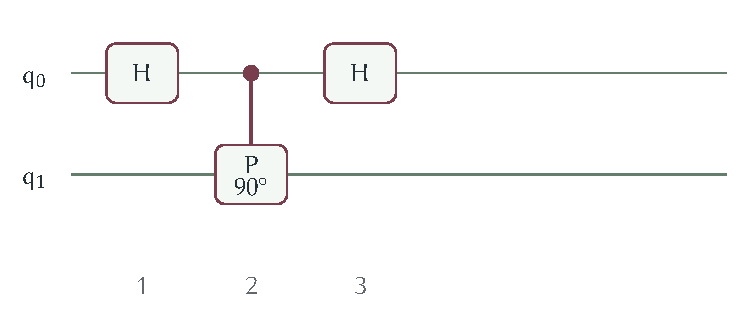
\includegraphics[width=\linewidth,height=94mm,keepaspectratio]{figure/f622af8c5bb2bbc6c.pdf}\FigureCaption{4.11 \(\cdot\) esempio 1 \(\cdot\) Circuito: porte 1--3}\end{FigureBlock}

\BookHeading{Geometria e configurazione dell'esempio}
\begin{FigureBlock}\centering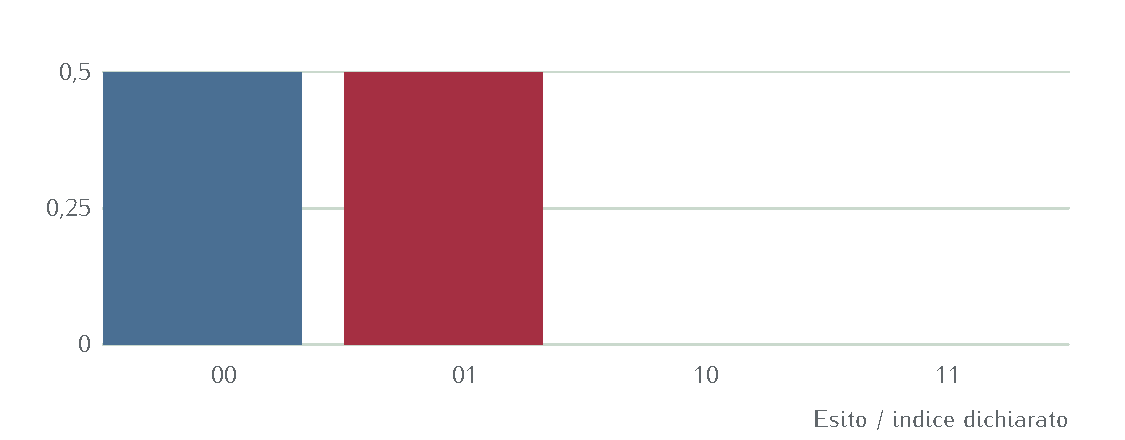
\includegraphics[width=\linewidth,height=94mm,keepaspectratio]{figure/f7dcd82fdbf96b6d3.pdf}\FigureCaption{4.11 \(\cdot\) esempio 1 \(\cdot\) Distribuzione congiunta \(\cdot\) Preparazione}\end{FigureBlock}
\begin{FigureBlock}\begin{minipage}[t]{.485\linewidth}\centering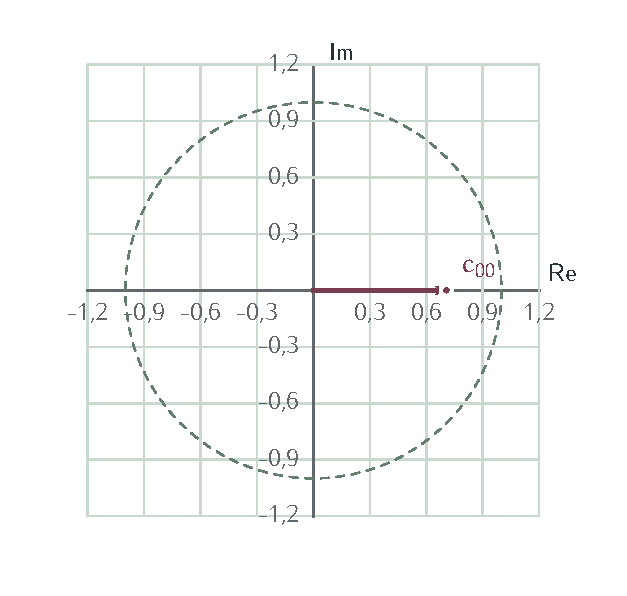
\includegraphics[width=\linewidth,height=63mm,keepaspectratio]{figure/f2ce08e6baf0fbe41.pdf}\par{\sffamily\footnotesize \(c_{00}\)\par}\end{minipage}\hfill\begin{minipage}[t]{.485\linewidth}\centering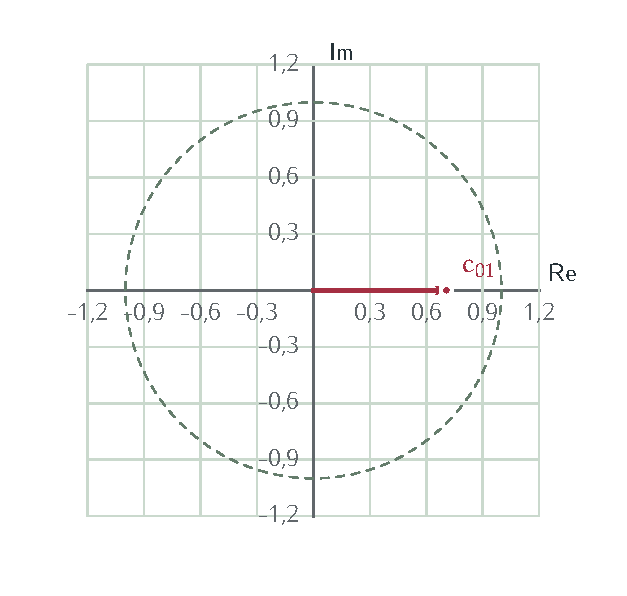
\includegraphics[width=\linewidth,height=63mm,keepaspectratio]{figure/fe4ea432ddca144b2.pdf}\par{\sffamily\footnotesize \(c_{01}\)\par}\end{minipage}\FigureCaption{4.11 \(\cdot\) esempio 1 \(\cdot\) Componenti complesse}\end{FigureBlock}
\begin{FigureBlock}\begin{minipage}[t]{.485\linewidth}\centering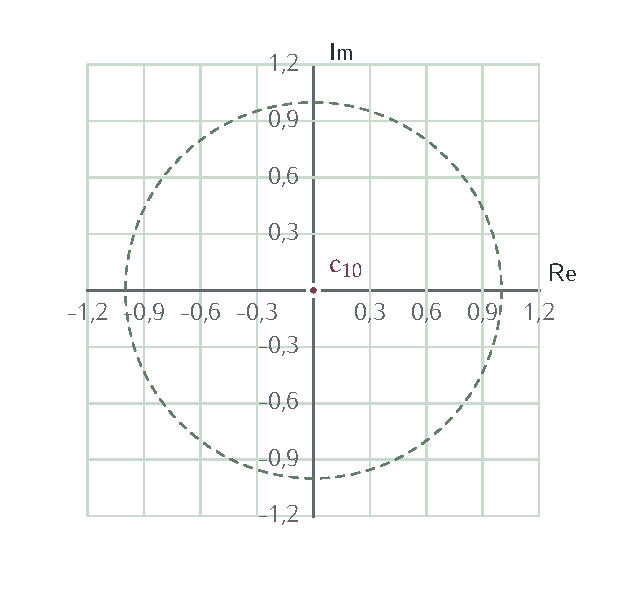
\includegraphics[width=\linewidth,height=63mm,keepaspectratio]{figure/f9a7350f41594f5e1.pdf}\par{\sffamily\footnotesize \(c_{10}\)\par}\end{minipage}\hfill\begin{minipage}[t]{.485\linewidth}\centering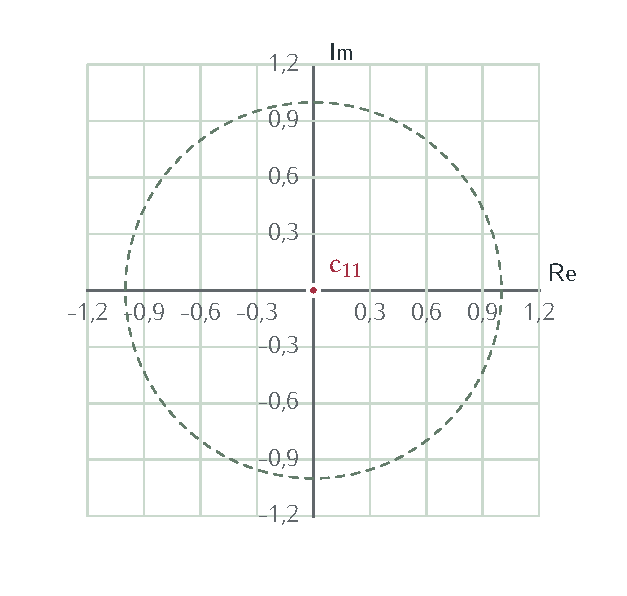
\includegraphics[width=\linewidth,height=63mm,keepaspectratio]{figure/feceda8b33707c496.pdf}\par{\sffamily\footnotesize \(c_{11}\)\par}\end{minipage}\FigureCaption{4.11 \(\cdot\) esempio 1 \(\cdot\) Componenti complesse}\end{FigureBlock}

\phantomsection\label{c4-hadamard-test-example-1-step-1}
\BookHeading{01 Preparazione}

\MathBlock{03C82080003D00280030002C0037003000370031003B00200030002C0037003000370031003B00200030003B0020003000291D40003B0020201603C82080201600B222480031}{\psi _{0}=(0{,}7071;\allowbreak \ 0{,}7071;\allowbreak \ 0;\allowbreak \ 0)^{T};\allowbreak \ \Vert \psi _{0}\Vert ^{2}\approx 1}

Le ampiezze sono ordinate secondo le etichette binarie, con il bit più significativo in alto.\par


\phantomsection\label{c4-hadamard-test-example-1-step-2}
\BookHeading{02 Porta 1 \(\cdot\) \(H\)}

\MathBlock{006300280030003000290020003D002000280030002C0037003000370031002900B700280030002C003700300037003100290020002B002000280030002C0037003000370031002900B70028003000290020224800200030002C0035}{c(00)\ =\ (0{,}7071)\cdot (0{,}7071)\ +\ (0{,}7071)\cdot (0)\ \approx \ 0{,}5}
\MathBlock{006300280031003000290020003D002000280030002C0037003000370031002900B700280030002C003700300037003100290020002B00200028002D0030002C0037003000370031002900B70028003000290020224800200030002C0035}{c(10)\ =\ (0{,}7071)\cdot (0{,}7071)\ +\ (-0{,}7071)\cdot (0)\ \approx \ 0{,}5}
\MathBlock{006300280030003100290020003D002000280030002C0037003000370031002900B700280030002C003700300037003100290020002B002000280030002C0037003000370031002900B70028003000290020224800200030002C0035}{c(01)\ =\ (0{,}7071)\cdot (0{,}7071)\ +\ (0{,}7071)\cdot (0)\ \approx \ 0{,}5}
\MathBlock{006300280031003100290020003D002000280030002C0037003000370031002900B700280030002C003700300037003100290020002B00200028002D0030002C0037003000370031002900B70028003000290020224800200030002C0035}{c(11)\ =\ (0{,}7071)\cdot (0{,}7071)\ +\ (-0{,}7071)\cdot (0)\ \approx \ 0{,}5}
\MathBlock{03C800202248002000280030002C0035003B00200030002C0035003B00200030002C0035003B00200030002C003500291D40}{\psi \ \approx \ (0{,}5;\allowbreak \ 0{,}5;\allowbreak \ 0{,}5;\allowbreak \ 0{,}5)^{T}}

Ogni coppia di ampiezze indicata usa il prodotto riga per colonna della porta. I rami con controllo nullo restano invariati.\par


\phantomsection\label{c4-hadamard-test-example-1-step-3}
\BookHeading{03 Porta 2 \(\cdot\) \(C\cdot P(90{}^{\circ} )\)}

\MathBlock{006300280031003000290020003D002000280031002900B700280030002C003500290020002B002000280030002900B700280030002C003500290020224800200030002C0035}{c(10)\ =\ (1)\cdot (0{,}5)\ +\ (0)\cdot (0{,}5)\ \approx \ 0{,}5}
\MathBlock{006300280031003100290020003D002000280030002900B700280030002C003500290020002B002000280069002900B700280030002C003500290020224800200030002C00350069}{c(11)\ =\ (0)\cdot (0{,}5)\ +\ (i)\cdot (0{,}5)\ \approx \ 0{,}5i}
\MathBlock{03C800202248002000280030002C0035003B00200030002C0035003B00200030002C0035003B00200030002C0035006900291D40}{\psi \ \approx \ (0{,}5;\allowbreak \ 0{,}5;\allowbreak \ 0{,}5;\allowbreak \ 0{,}5i)^{T}}

Ogni coppia di ampiezze indicata usa il prodotto riga per colonna della porta. I rami con controllo nullo restano invariati.\par


\phantomsection\label{c4-hadamard-test-example-1-step-4}
\BookHeading{04 Porta 3 \(\cdot\) \(H\)}

\MathBlock{006300280030003000290020003D002000280030002C0037003000370031002900B700280030002C003500290020002B002000280030002C0037003000370031002900B700280030002C003500290020224800200030002C0037003000370031}{c(00)\ =\ (0{,}7071)\cdot (0{,}5)\ +\ (0{,}7071)\cdot (0{,}5)\ \approx \ 0{,}7071}
\MathBlock{006300280031003000290020003D002000280030002C0037003000370031002900B700280030002C003500290020002B00200028002D0030002C0037003000370031002900B700280030002C003500290020224800200030}{c(10)\ =\ (0{,}7071)\cdot (0{,}5)\ +\ (-0{,}7071)\cdot (0{,}5)\ \approx \ 0}
\MathBlock{006300280030003100290020003D002000280030002C0037003000370031002900B700280030002C003500290020002B002000280030002C0037003000370031002900B700280030002C0035006900290020224800200030002C00330035003300360020002B00200030002C00330035003300360069}{c(01)\ =\ (0{,}7071)\cdot (0{,}5)\ +\ (0{,}7071)\cdot (0{,}5i)\ \approx \ 0{,}3536\ +\ 0{,}3536i}
\MathBlock{006300280031003100290020003D002000280030002C0037003000370031002900B700280030002C003500290020002B00200028002D0030002C0037003000370031002900B700280030002C0035006900290020224800200030002C00330035003300360020221200200030002C00330035003300360069}{c(11)\ =\ (0{,}7071)\cdot (0{,}5)\ +\ (-0{,}7071)\cdot (0{,}5i)\ \approx \ 0{,}3536\ - \ 0{,}3536i}
\MathBlock{03C800202248002000280030002C0037003000370031003B00200030002C00330035003300360020002B00200030002C00330035003300360069003B00200030003B00200030002C00330035003300360020221200200030002C0033003500330036006900291D40}{\psi \ \approx \ (0{,}7071;\allowbreak \ 0{,}3536\ +\ 0{,}3536i;\allowbreak \ 0;\allowbreak \ 0{,}3536\ - \ 0{,}3536i)^{T}}

Ogni coppia di ampiezze indicata usa il prodotto riga per colonna della porta. I rami con controllo nullo restano invariati.\par


\phantomsection\label{c4-hadamard-test-example-1-step-5}
\BookHeading{05 Lettura nella base finale}

\MathBlock{00500028003000300029003D00280030002C0037003000370031002900B20020002B002000280030002900B222480030002C0035}{P(00)=(0{,}7071)^{2}\ +\ (0)^{2}\approx 0{,}5}
\MathBlock{00500028003000310029003D00280030002C0033003500330036002900B20020002B002000280030002C0033003500330036002900B222480030002C00320035}{P(01)=(0{,}3536)^{2}\ +\ (0{,}3536)^{2}\approx 0{,}25}
\MathBlock{00500028003100300029003D00280030002900B20020002B002000280030002900B222480030}{P(10)=(0)^{2}\ +\ (0)^{2}\approx 0}
\MathBlock{00500028003100310029003D00280030002C0033003500330036002900B20020002B00200028002D0030002C0033003500330036002900B222480030002C00320035}{P(11)=(0{,}3536)^{2}\ +\ (-0{,}3536)^{2}\approx 0{,}25}

Il modulo quadro di ciascuna ampiezza determina la probabilità. La selezione di una porta nel disegno mostra uno stato intermedio senza effettuare una misura.\par


\phantomsection\label{c4-hadamard-test-example-1-step-6}
\BookHeading{06 Calcolare il valore atteso}

\MathBlock{27E8002B007C005000280039003000B00029007C002B27E9003D00280031002B00690029002F0032003B002000520065003D0031002F0032003B00200049006D003D0031002F0032002E}{\langle +|P(90{}^{\circ} )|+\rangle =(1+i)/2;\allowbreak \ \operatorname{Re}=1/2;\allowbreak \ \operatorname{Im}=1/2.}
\MathBlock{005000280063006F006E00740072006F006C006C006F003D00300029003D00280031002B0052006527E8005527E90029002F0032003D0033002F0034002E}{P(\text{controllo}=0)=(1+\operatorname{Re}\langle U\rangle )/2=3/4.}

\(S{}^{\dagger} \) moltiplica il ramo 1 del controllo per \(- i\): \(\operatorname{Re}(- i\langle U\rangle )=\operatorname{Im}\langle U\rangle \). Il segno della parte immaginaria cambia quindi il risultato della lettura.\par


\phantomsection\label{c4-hadamard-test-example-1-step-7}
\BookHeading{07 Sommare sui valori del bersaglio}

\MathBlock{0050002800712080003D00300029003D00500028003000300029002B00500028003000310029003D0030002C0035002B0030002C00320035003D0030002C00370035002E}{P(q_{0}=0)=P(00)+P(01)=0{,}5+0{,}25=0{,}75.}
\MathBlock{0050002800712080003D00310029003D00500028003100300029002B00500028003100310029003D0030002C00320035002E}{P(q_{0}=1)=P(10)+P(11)=0{,}25.}

La misura usa il solo controllo; le probabilità congiunte restano disponibili per verificare la somma.\par


\BookHeading{Stato finale del programma}
\begin{FigureBlock}\centering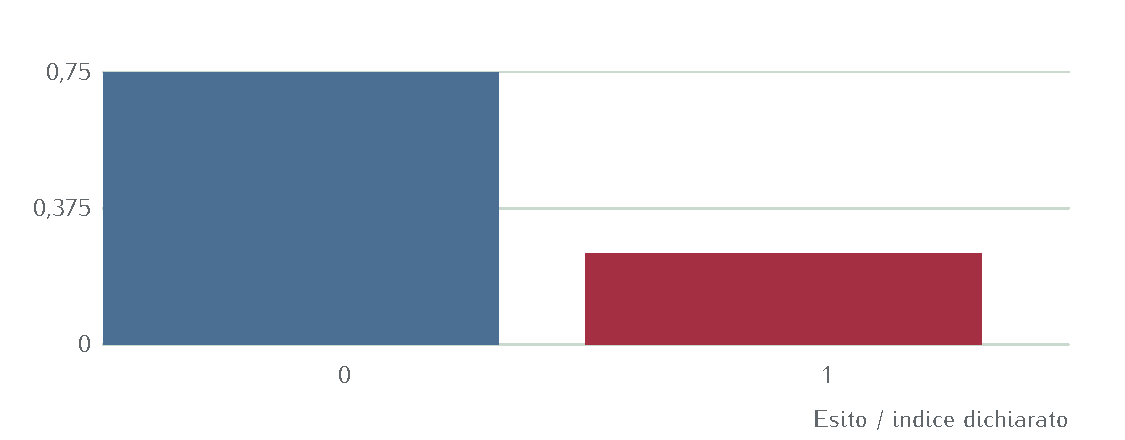
\includegraphics[width=\linewidth,height=94mm,keepaspectratio]{figure/f37d2980ec6c16e6b.pdf}\FigureCaption{4.11 \(\cdot\) esempio 1 \(\cdot\) Lettura del controllo}\end{FigureBlock}

\BookHeading{Interpretazione}

La parte reale 1/2 produce \(P(0)=3/4\).\par


Risorse dichiarate. 2 qubit; 3 operazioni alla granularità dichiarata nel circuito.\par


\Needspace{.36\textheight}\phantomsection\label{c4-hadamard-test-example-2}
{\sffamily\small\color{Accent} ESEMPIO SVOLTO 2\par}
\BookHeading{Leggere una componente del valore atteso}
\(U=P(- 90{}^{\circ} )\); \(S{}^{\dagger} \) sull'ausiliario permette di leggere la parte immaginaria negativa.\par


\BookHeading{Circuito completo}
\begin{FigureBlock}\centering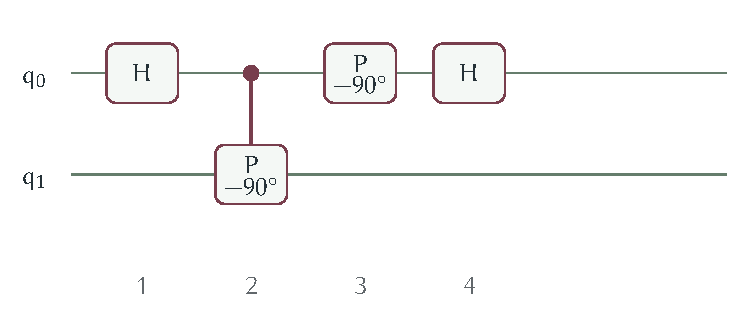
\includegraphics[width=\linewidth,height=94mm,keepaspectratio]{figure/f8ea8d1a1a82705ca.pdf}\FigureCaption{4.11 \(\cdot\) esempio 2 \(\cdot\) Circuito: porte 1--4}\end{FigureBlock}

\BookHeading{Geometria e configurazione dell'esempio}
\begin{FigureBlock}\centering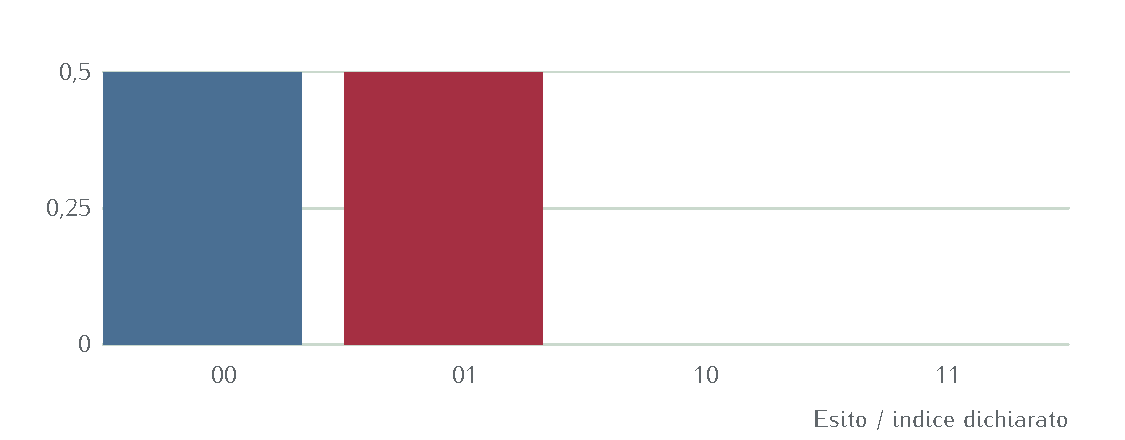
\includegraphics[width=\linewidth,height=94mm,keepaspectratio]{figure/f7dcd82fdbf96b6d3.pdf}\FigureCaption{4.11 \(\cdot\) esempio 2 \(\cdot\) Distribuzione congiunta \(\cdot\) Preparazione}\end{FigureBlock}
\begin{FigureBlock}\begin{minipage}[t]{.485\linewidth}\centering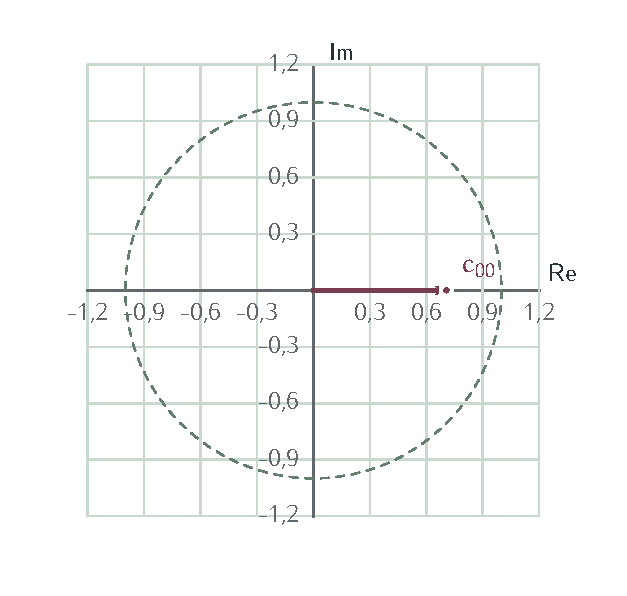
\includegraphics[width=\linewidth,height=63mm,keepaspectratio]{figure/fb07f81b1a177d3b0.pdf}\par{\sffamily\footnotesize \(c_{00}\)\par}\end{minipage}\hfill\begin{minipage}[t]{.485\linewidth}\centering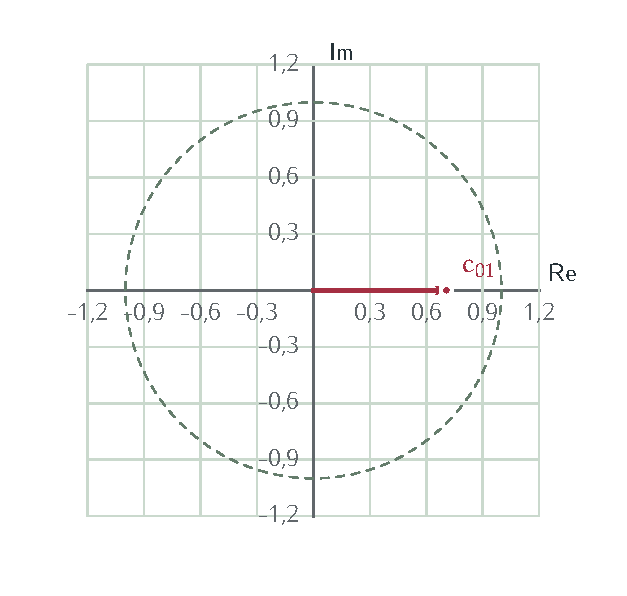
\includegraphics[width=\linewidth,height=63mm,keepaspectratio]{figure/f1577e9c9eb48f2cf.pdf}\par{\sffamily\footnotesize \(c_{01}\)\par}\end{minipage}\FigureCaption{4.11 \(\cdot\) esempio 2 \(\cdot\) Componenti complesse}\end{FigureBlock}
\begin{FigureBlock}\begin{minipage}[t]{.485\linewidth}\centering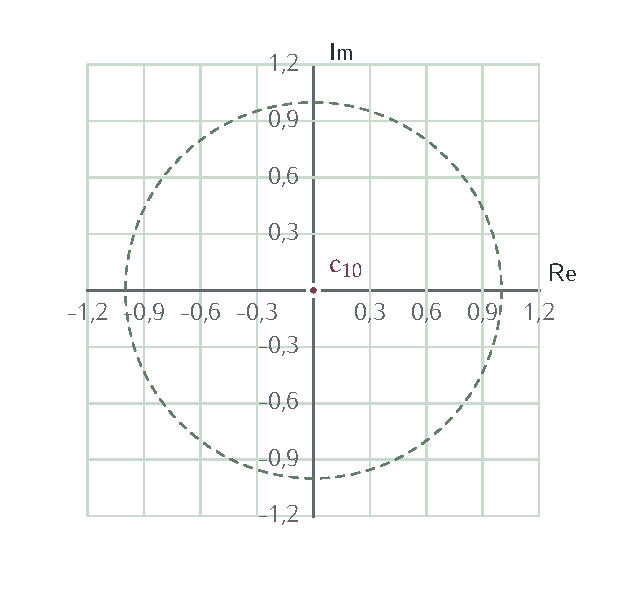
\includegraphics[width=\linewidth,height=63mm,keepaspectratio]{figure/fdea5fbe243afaf90.pdf}\par{\sffamily\footnotesize \(c_{10}\)\par}\end{minipage}\hfill\begin{minipage}[t]{.485\linewidth}\centering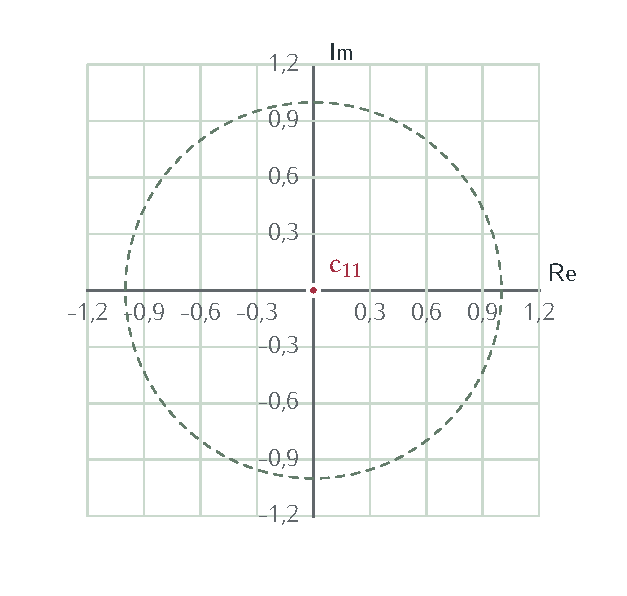
\includegraphics[width=\linewidth,height=63mm,keepaspectratio]{figure/f5c774240b58c6d87.pdf}\par{\sffamily\footnotesize \(c_{11}\)\par}\end{minipage}\FigureCaption{4.11 \(\cdot\) esempio 2 \(\cdot\) Componenti complesse}\end{FigureBlock}

\phantomsection\label{c4-hadamard-test-example-2-step-1}
\BookHeading{01 Preparazione}

\MathBlock{03C82080003D00280030002C0037003000370031003B00200030002C0037003000370031003B00200030003B0020003000291D40003B0020201603C82080201600B222480031}{\psi _{0}=(0{,}7071;\allowbreak \ 0{,}7071;\allowbreak \ 0;\allowbreak \ 0)^{T};\allowbreak \ \Vert \psi _{0}\Vert ^{2}\approx 1}

Le ampiezze sono ordinate secondo le etichette binarie, con il bit più significativo in alto.\par


\phantomsection\label{c4-hadamard-test-example-2-step-2}
\BookHeading{02 Porta 1 \(\cdot\) \(H\)}

\MathBlock{006300280030003000290020003D002000280030002C0037003000370031002900B700280030002C003700300037003100290020002B002000280030002C0037003000370031002900B70028003000290020224800200030002C0035}{c(00)\ =\ (0{,}7071)\cdot (0{,}7071)\ +\ (0{,}7071)\cdot (0)\ \approx \ 0{,}5}
\MathBlock{006300280031003000290020003D002000280030002C0037003000370031002900B700280030002C003700300037003100290020002B00200028002D0030002C0037003000370031002900B70028003000290020224800200030002C0035}{c(10)\ =\ (0{,}7071)\cdot (0{,}7071)\ +\ (-0{,}7071)\cdot (0)\ \approx \ 0{,}5}
\MathBlock{006300280030003100290020003D002000280030002C0037003000370031002900B700280030002C003700300037003100290020002B002000280030002C0037003000370031002900B70028003000290020224800200030002C0035}{c(01)\ =\ (0{,}7071)\cdot (0{,}7071)\ +\ (0{,}7071)\cdot (0)\ \approx \ 0{,}5}
\MathBlock{006300280031003100290020003D002000280030002C0037003000370031002900B700280030002C003700300037003100290020002B00200028002D0030002C0037003000370031002900B70028003000290020224800200030002C0035}{c(11)\ =\ (0{,}7071)\cdot (0{,}7071)\ +\ (-0{,}7071)\cdot (0)\ \approx \ 0{,}5}
\MathBlock{03C800202248002000280030002C0035003B00200030002C0035003B00200030002C0035003B00200030002C003500291D40}{\psi \ \approx \ (0{,}5;\allowbreak \ 0{,}5;\allowbreak \ 0{,}5;\allowbreak \ 0{,}5)^{T}}

Ogni coppia di ampiezze indicata usa il prodotto riga per colonna della porta. I rami con controllo nullo restano invariati.\par


\phantomsection\label{c4-hadamard-test-example-2-step-3}
\BookHeading{03 Porta 2 \(\cdot\) \(C\cdot P(-90{}^{\circ} )\)}

\MathBlock{006300280031003000290020003D002000280031002900B700280030002C003500290020002B002000280030002900B700280030002C003500290020224800200030002C0035}{c(10)\ =\ (1)\cdot (0{,}5)\ +\ (0)\cdot (0{,}5)\ \approx \ 0{,}5}
\MathBlock{006300280031003100290020003D002000280030002900B700280030002C003500290020002B0020002822120069002900B700280030002C00350029002022480020002D0030002C00350069}{c(11)\ =\ (0)\cdot (0{,}5)\ +\ (- i)\cdot (0{,}5)\ \approx \ -0{,}5i}
\MathBlock{03C800202248002000280030002C0035003B00200030002C0035003B00200030002C0035003B0020002D0030002C0035006900291D40}{\psi \ \approx \ (0{,}5;\allowbreak \ 0{,}5;\allowbreak \ 0{,}5;\allowbreak \ -0{,}5i)^{T}}

Ogni coppia di ampiezze indicata usa il prodotto riga per colonna della porta. I rami con controllo nullo restano invariati.\par


\phantomsection\label{c4-hadamard-test-example-2-step-4}
\BookHeading{04 Porta 3 \(\cdot\) \(P(-90{}^{\circ} )\)}

\MathBlock{006300280030003000290020003D002000280031002900B700280030002C003500290020002B002000280030002900B700280030002C003500290020224800200030002C0035}{c(00)\ =\ (1)\cdot (0{,}5)\ +\ (0)\cdot (0{,}5)\ \approx \ 0{,}5}
\MathBlock{006300280031003000290020003D002000280030002900B700280030002C003500290020002B0020002822120069002900B700280030002C00350029002022480020002D0030002C00350069}{c(10)\ =\ (0)\cdot (0{,}5)\ +\ (- i)\cdot (0{,}5)\ \approx \ -0{,}5i}
\MathBlock{006300280030003100290020003D002000280031002900B700280030002C003500290020002B002000280030002900B70028002D0030002C0035006900290020224800200030002C0035}{c(01)\ =\ (1)\cdot (0{,}5)\ +\ (0)\cdot (-0{,}5i)\ \approx \ 0{,}5}
\MathBlock{006300280031003100290020003D002000280030002900B700280030002C003500290020002B0020002822120069002900B70028002D0030002C003500690029002022480020002D0030002C0035}{c(11)\ =\ (0)\cdot (0{,}5)\ +\ (- i)\cdot (-0{,}5i)\ \approx \ -0{,}5}
\MathBlock{03C800202248002000280030002C0035003B00200030002C0035003B0020002D0030002C00350069003B0020002D0030002C003500291D40}{\psi \ \approx \ (0{,}5;\allowbreak \ 0{,}5;\allowbreak \ -0{,}5i;\allowbreak \ -0{,}5)^{T}}

Ogni coppia di ampiezze indicata usa il prodotto riga per colonna della porta. I rami con controllo nullo restano invariati.\par


\phantomsection\label{c4-hadamard-test-example-2-step-5}
\BookHeading{05 Porta 4 \(\cdot\) \(H\)}

\MathBlock{006300280030003000290020003D002000280030002C0037003000370031002900B700280030002C003500290020002B002000280030002C0037003000370031002900B70028002D0030002C0035006900290020224800200030002C00330035003300360020221200200030002C00330035003300360069}{c(00)\ =\ (0{,}7071)\cdot (0{,}5)\ +\ (0{,}7071)\cdot (-0{,}5i)\ \approx \ 0{,}3536\ - \ 0{,}3536i}
\MathBlock{006300280031003000290020003D002000280030002C0037003000370031002900B700280030002C003500290020002B00200028002D0030002C0037003000370031002900B70028002D0030002C0035006900290020224800200030002C00330035003300360020002B00200030002C00330035003300360069}{c(10)\ =\ (0{,}7071)\cdot (0{,}5)\ +\ (-0{,}7071)\cdot (-0{,}5i)\ \approx \ 0{,}3536\ +\ 0{,}3536i}
\MathBlock{006300280030003100290020003D002000280030002C0037003000370031002900B700280030002C003500290020002B002000280030002C0037003000370031002900B70028002D0030002C003500290020224800200030}{c(01)\ =\ (0{,}7071)\cdot (0{,}5)\ +\ (0{,}7071)\cdot (-0{,}5)\ \approx \ 0}
\MathBlock{006300280031003100290020003D002000280030002C0037003000370031002900B700280030002C003500290020002B00200028002D0030002C0037003000370031002900B70028002D0030002C003500290020224800200030002C0037003000370031}{c(11)\ =\ (0{,}7071)\cdot (0{,}5)\ +\ (-0{,}7071)\cdot (-0{,}5)\ \approx \ 0{,}7071}
\MathBlock{03C800202248002000280030002C00330035003300360020221200200030002C00330035003300360069003B00200030003B00200030002C00330035003300360020002B00200030002C00330035003300360069003B00200030002C003700300037003100291D40}{\psi \ \approx \ (0{,}3536\ - \ 0{,}3536i;\allowbreak \ 0;\allowbreak \ 0{,}3536\ +\ 0{,}3536i;\allowbreak \ 0{,}7071)^{T}}

Ogni coppia di ampiezze indicata usa il prodotto riga per colonna della porta. I rami con controllo nullo restano invariati.\par


\phantomsection\label{c4-hadamard-test-example-2-step-6}
\BookHeading{06 Lettura nella base finale}

\MathBlock{00500028003000300029003D00280030002C0033003500330036002900B20020002B00200028002D0030002C0033003500330036002900B222480030002C00320035}{P(00)=(0{,}3536)^{2}\ +\ (-0{,}3536)^{2}\approx 0{,}25}
\MathBlock{00500028003000310029003D00280030002900B20020002B002000280030002900B222480030}{P(01)=(0)^{2}\ +\ (0)^{2}\approx 0}
\MathBlock{00500028003100300029003D00280030002C0033003500330036002900B20020002B002000280030002C0033003500330036002900B222480030002C00320035}{P(10)=(0{,}3536)^{2}\ +\ (0{,}3536)^{2}\approx 0{,}25}
\MathBlock{00500028003100310029003D00280030002C0037003000370031002900B20020002B002000280030002900B222480030002C0035}{P(11)=(0{,}7071)^{2}\ +\ (0)^{2}\approx 0{,}5}

Il modulo quadro di ciascuna ampiezza determina la probabilità. La selezione di una porta nel disegno mostra uno stato intermedio senza effettuare una misura.\par


\phantomsection\label{c4-hadamard-test-example-2-step-7}
\BookHeading{07 Calcolare il valore atteso}

\MathBlock{27E8002B007C00500028002D0039003000B00029007C002B27E9003D00280031221200690029002F0032003B002000520065003D0031002F0032003B00200049006D003D22120031002F0032002E}{\langle +|P(-90{}^{\circ} )|+\rangle =(1- i)/2;\allowbreak \ \operatorname{Re}=1/2;\allowbreak \ \operatorname{Im}=- 1/2.}
\MathBlock{005000280063006F006E00740072006F006C006C006F003D00300029003D00280031002B0049006D27E8005527E90029002F0032003D0031002F0034002E}{P(\text{controllo}=0)=(1+\operatorname{Im}\langle U\rangle )/2=1/4.}

\(S{}^{\dagger} \) moltiplica il ramo 1 del controllo per \(- i\): \(\operatorname{Re}(- i\langle U\rangle )=\operatorname{Im}\langle U\rangle \). Il segno della parte immaginaria cambia quindi il risultato della lettura.\par


\phantomsection\label{c4-hadamard-test-example-2-step-8}
\BookHeading{08 Sommare sui valori del bersaglio}

\MathBlock{0050002800712080003D00300029003D00500028003000300029002B00500028003000310029003D0030002C00320035002B0030003D0030002C00320035002E}{P(q_{0}=0)=P(00)+P(01)=0{,}25+0=0{,}25.}
\MathBlock{0050002800712080003D00310029003D00500028003100300029002B00500028003100310029003D0030002C00370035002E}{P(q_{0}=1)=P(10)+P(11)=0{,}75.}

La misura usa il solo controllo; le probabilità congiunte restano disponibili per verificare la somma.\par


\BookHeading{Stato finale del programma}
\begin{FigureBlock}\centering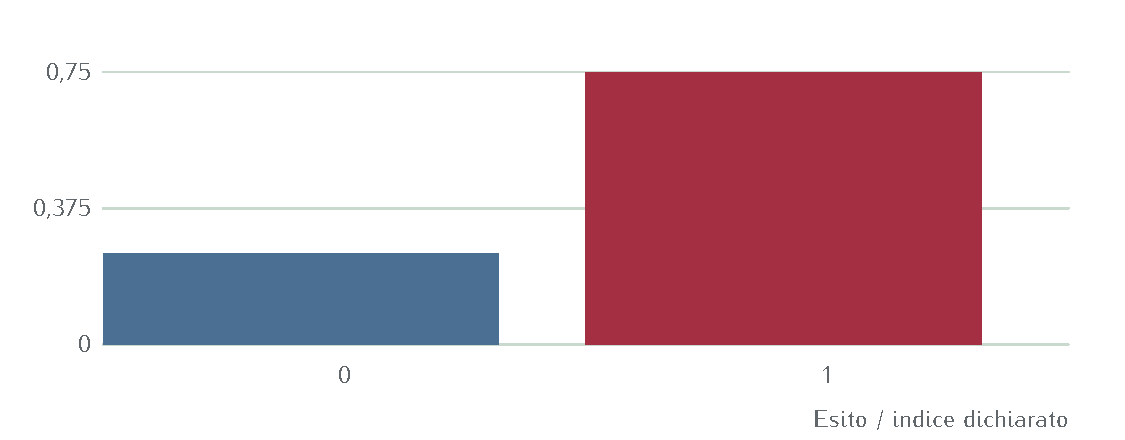
\includegraphics[width=\linewidth,height=94mm,keepaspectratio]{figure/f4433098f7ab22775.pdf}\FigureCaption{4.11 \(\cdot\) esempio 2 \(\cdot\) Lettura del controllo}\end{FigureBlock}

\BookHeading{Interpretazione}

La parte immaginaria \(- 1/2\) produce \(P(0)=1/4\); il confronto con la parte reale positiva rende visibile il segno di \(S{}^{\dagger} \).\par


Risorse dichiarate. 2 qubit; 4 operazioni alla granularità dichiarata nel circuito.\par


\Needspace{7\baselineskip}
\BookHeading{Il passaggio successivo}
Se \(|\psi \rangle \) è autostato di \(U\), il confronto contiene una sola fase e il bersaglio resta invariato a meno di quel fattore. Usando potenze controllate di \(U\) possiamo scrivere questa fase su più qubit e ricombinarla con Fourier inversa.\par


\Needspace{.43\textheight}
\section{Stima di fase esatta}
\phantomsection\label{c4-qpe-esatta}

{\sffamily\small\color{Ink!70} Riferimento alle slide: p. 319.\par}

{\sffamily\small\color{Ink!70} Laboratorio locale: \nolinkurl{index.html#capitolo-4/qpe-esatta}\par}

\BookHeading{Definizioni e costruzione}
La stima di fase quantistica, QPE, riceve un'unitaria \(U\) e un suo autostato normalizzato \(|u\rangle \): \(U|u\rangle =\allowbreak\exp (2\pi i\varphi )|u\rangle \). L'autofase \(\varphi \in [0{,}1)\) è una frazione di giro, cioè un angolo \(2\pi \varphi \) radianti; l'obiettivo è leggerne una rappresentazione binaria.\par

Il registro di lettura ha m qubit e \(Q=2^{m}\) etichette. Prepariamo \((1/\sqrt{Q})\sum _{x}|x\rangle |u\rangle \). In ordine big-endian il filo \(q_{j}\) ha peso \(2^{m- 1- j}\) e controlla \(U\) elevata a quella potenza: per \(m=3\), dall'alto, \(U^{4},\allowbreak U^{2},\allowbreak U\). Un ramo con etichetta x applica \(U^{x}\) e acquisisce \(\allowbreak\exp (2\pi ix\varphi )\), mentre il bersaglio rimane \(|u\rangle \).\par

Dopo Fourier inversa, l'ampiezza dell'esito \(c\in \{0,\allowbreak \ldots ,\allowbreak Q- 1\}\) è \(a\varphi (c)=Q^{-1}\sum _{x}\allowbreak\exp (2\pi ix(\varphi - c/Q))\). Se \(\varphi =\ell /Q\) per un intero \(\ell \), per \(c=\ell \) tutti i termini valgono uno; per \(c\ne \ell \) la loro ragione z è una radice Q-esima diversa da uno. La somma geometrica di Fourier dà dunque \(a\varphi (c)=\delta c,\allowbreak \ell \). Per \(Q=8\) e \(\varphi =3/8\) la sola uscita è \(c=3\), parola 011.\par

Per un bersaglio \(\sum _{s}\beta _{s}|u_{s}\rangle \), gli \(|u_{s}\rangle \) sono autostati ortonormali di \(U\) e \(\beta _{s}\) sono ampiezze complesse con \(\sum _{s}|\beta _{s}|^{2}=1\). Lo stato finale è \(\sum _{c,\allowbreak s}\) \(\beta _{s}a\varphi _{s}(c)|c\rangle |u_{s}\rangle \). La marginale somma probabilità di bersagli ortogonali: \(P(c)=\sum _{s}|\beta _{s}|^{2}|a\varphi _{s}(c)|^{2}\). Le fasi dei \(\beta _{s}\) restano invece nello stato condizionato.\par

Nei casi elementari si può scegliere \(U\) diagonale nella base \(|0\rangle ,\allowbreak |1\rangle \), assegnandone gli autovalori alle autofasi indicate. Lo stato preparato e i coefficienti \(\beta _{s}\) sono esplicitati negli svolgimenti. Se \(P(c)=0\) nel modello esatto, il ramo è impossibile e non ammette un bersaglio normalizzato.\par


\MathBlock{006103C6002800630029003D0051207B00B903A300280078003D0030002C2026002C005122120031002900200065007800700028003203C000690078002803C622120063002F005100290029003B00200050002800630029003D03A3209B007C03B2209B007C00B2007C006103C6209B002800630029007C00B2003B00200051003D00321D50002E}{a\varphi (c)=Q^{-1}\sum _{x=0}^{Q- 1}\ \allowbreak\exp (2\pi ix(\varphi - c/Q));\allowbreak \ P(c)=\sum _{s}|\beta _{s}|^{2}|a\varphi _{s}(c)|^{2};\allowbreak \ Q=2^{m}.}

\BookHeading{Come leggere le figure}
Il registro di lettura contiene etichette intere c, interpretate come frazioni di giro c/Q. I poligoni nel piano Re/Im sommano le ampiezze di ciascun autostato separatamente; le barre della marginale sommano i loro moduli quadrati pesati.\par


\BookHeading{Attività nel laboratorio modificabile}

\BookHeading{Obiettivo dell'esperimento}
Osservare la stima di autofasi rappresentabili sulla griglia binaria.\par

\BookHeading{Percorso operativo}
Scegliere le due autofasi, il peso della preparazione e la precisione; misurare il controllo.\par

\BookHeading{Lettura geometrica}
La Fourier inversa somma contributi complessi; il bersaglio condizionato conserva i coefficienti coerenti.\par

\BookHeading{Controllo del risultato}
Confrontare le letture con la griglia \(c/2^{m}\) e distinguere probabilità dei rami e ampiezze.\par


\Needspace{.36\textheight}\phantomsection\label{c4-qpe-esatta-example-1}
{\sffamily\small\color{Accent} ESEMPIO SVOLTO 1\par}
\BookHeading{Esempio 1}
\(m=3\); \(Q=2^{m}=8\); autofasi (frazioni di giro) 0,375; pesi 1.\par


\BookHeading{Geometria e configurazione dell'esempio}
\begin{FigureBlock}\centering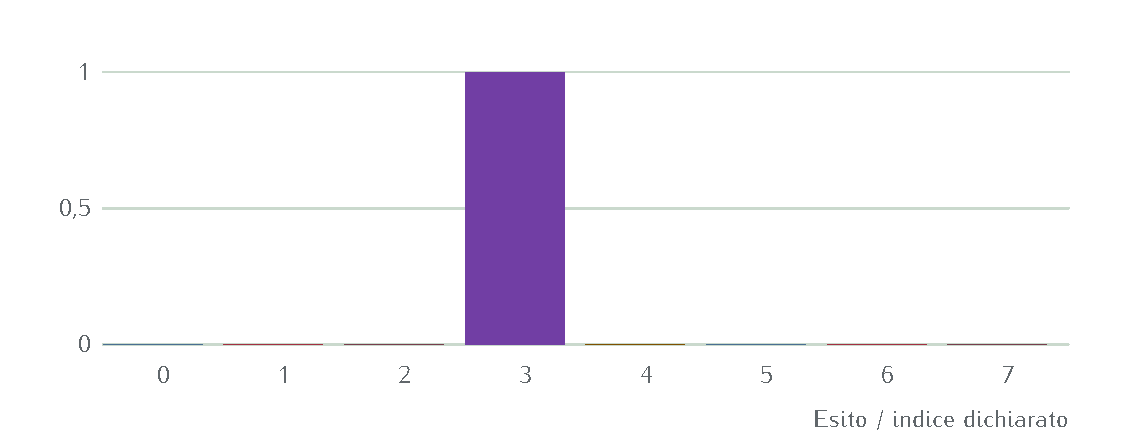
\includegraphics[width=\linewidth,height=94mm,keepaspectratio]{figure/f0444772575b01885.pdf}\FigureCaption{4.12 \(\cdot\) esempio 1 \(\cdot\) Distribuzione completa della lettura}\end{FigureBlock}
\begin{FigureBlock}\centering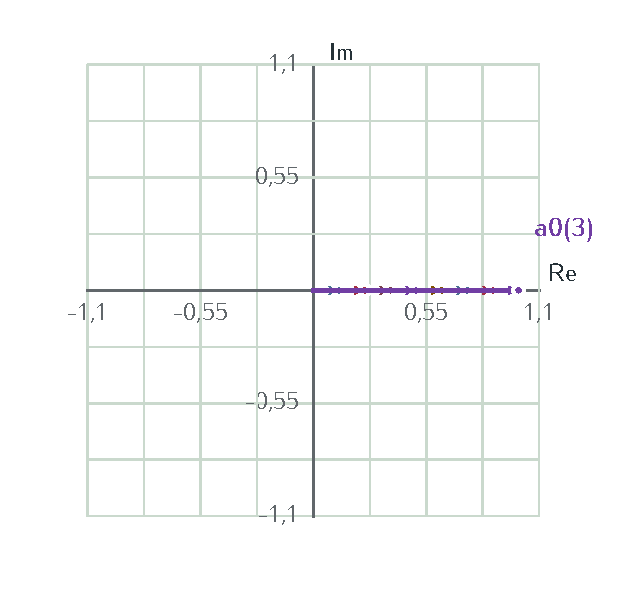
\includegraphics[width=\linewidth,height=94mm,keepaspectratio]{figure/f27cfe98acf2fbfa2.pdf}\FigureCaption{4.12 \(\cdot\) esempio 1 \(\cdot\) Somma punta-coda, x crescente \(\cdot\) \(s=0\), \(c=3\), peso 1}\end{FigureBlock}
\begin{FigureBlock}\begin{minipage}[t]{.485\linewidth}\centering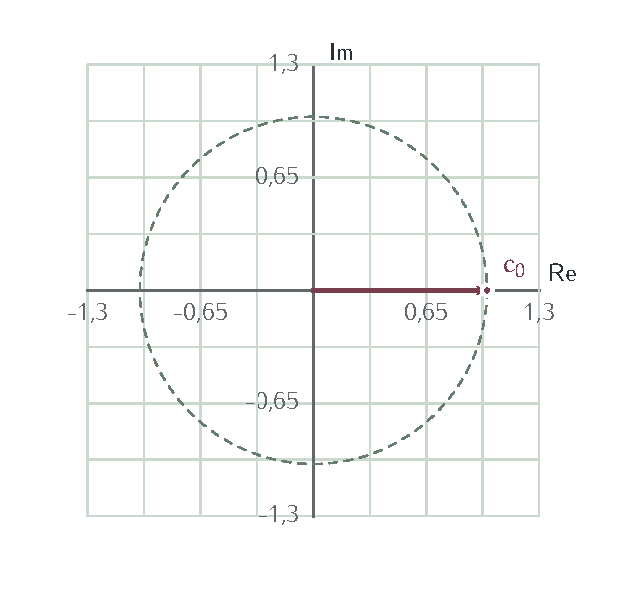
\includegraphics[width=\linewidth,height=63mm,keepaspectratio]{figure/f18b7dde72ee10bb9.pdf}\par{\sffamily\footnotesize \(c_{0}\)\par}\end{minipage}\FigureCaption{4.12 \(\cdot\) esempio 1 \(\cdot\) Bersaglio condizionato \(\cdot\) coefficienti \(\beta {}^{\prime} s\) nella base propria dichiarata}\end{FigureBlock}

\phantomsection\label{c4-qpe-esatta-example-1-step-1}
\BookHeading{01 Definire operatore, autostati e coefficienti}

\MathBlock{0055007C0075005F007327E9003D0065005E0028003203C0006903C6005F00730029007C0075005F007327E9003B002027E80075005F0073007C0075005F007427E9003D03B40073002C0074002E}{U|u_{s}\rangle =e^{2\pi i\varphi _{s}}|u_{s}\rangle ;\allowbreak \ \langle u_{s}|u_{t}\rangle =\delta s,\allowbreak t.}
\MathBlock{007C03C827E9003D03A30073002003B2005F0073007C0075005F007327E9003B002003A30073007C03B2005F0073007C00B2003D0031003B00200051003D0032005E006D002E}{|\psi \rangle =\sum _{s}\ \beta _{s}|u_{s}\rangle ;\allowbreak \ \sum _{s}|\beta _{s}|^{2}=1;\allowbreak \ Q=2^{m}.}

Il registro di lettura contiene m qubit; \(\varphi \) è una frazione di giro modulo uno. L'indice s distingue gli autostati del bersaglio e \(\beta _{s}\) è un'ampiezza complessa, mentre \(|\beta _{s}|^{2}\) è un peso probabilistico.\par


\phantomsection\label{c4-qpe-esatta-example-1-step-2}
\BookHeading{02 Assegnare \(U\) e la preparazione}

\MathBlock{0055003D006400690061006700280031002C0065005E0028003203C0006900B70030002C00330037003500290029003D0050002800310033003500B00029002E}{U=\operatorname{diag}(1,\allowbreak e^{2\pi i\cdot 0{,}375})=P(135{}^{\circ} ).}
\MathBlock{007C0075208027E9003D007C003127E9003B002003B22080003D0031003B0020007C03C827E9003D0058007C003027E9003D007C003127E9002E}{|u_{0}\rangle =|1\rangle ;\allowbreak \ \beta _{0}=1;\allowbreak \ |\psi \rangle =X|0\rangle =|1\rangle .}

Sono specificati matrice, autostato e preparazione. Le potenze controllate moltiplicano questo bersaglio per le fasi indicate senza cambiarne l'autodirezione.\par


\phantomsection\label{c4-qpe-esatta-example-1-step-3}
\BookHeading{03 Preparare il controllo}

\MathBlock{007C003027E922970033007C03C827E900202192002000280031002F221A0038002903A30078007C007827E903A30073002003B2005F0073007C0075005F007327E9002E}{|0\rangle ^{\otimes 3}|\psi \rangle \ \to \ (1/\sqrt{8})\sum _{x}|x\rangle \sum _{s}\ \beta _{s}|u_{s}\rangle .}

Le Hadamard agiscono soltanto sui qubit di lettura. Il bersaglio mantiene i coefficienti appena assegnati.\par


\phantomsection\label{c4-qpe-esatta-example-1-step-4}
\BookHeading{04 Costruire le potenze e il kickback}

\MathBlock{00660069006C006F002000710030002C0020007000650073006F00200032005E0032003A00200063006F006E00740072006F006C006C006F00200064006900200055005E0034}{\text{filo}\ q_{0},\allowbreak \ \text{peso}\ 2^{2}:\ \text{controllo}\ \text{di}\ U^{4}}
\MathBlock{00660069006C006F002000710031002C0020007000650073006F00200032005E0031003A00200063006F006E00740072006F006C006C006F00200064006900200055005E0032}{\text{filo}\ q_{1},\allowbreak \ \text{peso}\ 2^{1}:\ \text{controllo}\ \text{di}\ U^{2}}
\MathBlock{00660069006C006F002000710032002C0020007000650073006F00200032005E0030003A00200063006F006E00740072006F006C006C006F00200064006900200055005E0031}{\text{filo}\ q_{2},\allowbreak \ \text{peso}\ 2^{0}:\ \text{controllo}\ \text{di}\ U^{1}}
\MathBlock{0078003D03A3007100200078005F00710032005E0028006D22120031221200710029002021D20020220F007100200065005E0028003203C0006900200078005F00710032005E0028006D2212003122120071002903C6005F00730029003D0065005E0028003203C00069007803C6005F00730029002E}{x=\sum _{q}\ x_{q}2^{m- 1- q}\ \Rightarrow \ \prod _{q}\ e^{2\pi i\ x_{q}2^{m- 1- q}\varphi _{s}}=e^{2\pi ix\varphi _{s}}.}
\MathBlock{007C03A827E9003D00280031002F221A0051002903A30078002C0073002003B2005F007300200065005E0028003203C00069007803C6005F00730029007C007827E9007C0075005F007327E9002E}{|\Psi \rangle =(1/\sqrt{Q})\sum _{x,\allowbreak s}\ \beta _{s}\ e^{2\pi ix\varphi _{s}}|x\rangle |u_{s}\rangle .}

\(q_{0}\) è il filo superiore e il bit più significativo. Per tre qubit le potenze sono \(U^{4},\allowbreak U^{2},\allowbreak U\); l'esponente j di \(2^{j}\) non va confuso con l'indice del filo \(q_{j}\).\par


\phantomsection\label{c4-qpe-esatta-example-1-step-5}
\BookHeading{05 Sommare le radici dell'unità}

\MathBlock{0053003D0031002B007A002B22EF002B007A005E00280038002D00310029002E}{S=1+z+\cdots +z^{8-1}.}
\MathBlock{007A0053003D007A002B007A00B2002B22EF002B007A005E0038003B0020002800312212007A00290053003D00312212007A005E0038002E}{zS=z+z^{2}+\cdots +z^{8};\allowbreak \ (1- z)S=1- z^{8}.}
\MathBlock{005300650020007A22600031003A00200053003D002800312212007A005E00380029002F002800312212007A0029002E0020005300650020007A003D0031003A00200053003D0038002E}{Se\ z\ne 1:\ S=(1- z^{8})/(1- z).\ Se\ z=1:\ S=8.}

La sottrazione cancella tutti i termini intermedi. Il caso \(z=1\) va separato prima della divisione.\par


\phantomsection\label{c4-qpe-esatta-example-1-step-6}
\BookHeading{06 Dalla cancellazione all'unitarietà}

\MathBlock{007A003D0065005E0028003203C00069002800782212007820320029002F00380029003B0020007A005E0038003D0031002E}{z=e^{2\pi i(x- x{}^{\prime} )/8};\allowbreak \ z^{8}=1.}
\MathBlock{27E80046003800782032007C00460038007827E9003D00280031002F0038002903A300790020007A02B8003D0038002F0038003D003100200073006500200078003D00782032003B0020003000200061006C007400720069006D0065006E00740069002E}{\langle F8x{}^{\prime} |F8x\rangle =(1/8)\sum _{y}\ z^{y}=8/8=1\ \text{se}\ x=x{}^{\prime} ;\allowbreak \ 0\ \text{altrimenti}.}

Per x e \(x{}^{\prime} \) distinti fra 0 e \(N- 1\), \(z\ne 1\): le frecce delle radici si chiudono. Le colonne di Fourier sono quindi ortonormali e la trasformata conserva prodotti interni e norma.\par


\phantomsection\label{c4-qpe-esatta-example-1-step-7}
\BookHeading{07 Applicare la cancellazione alla QPE}

\MathBlock{0044006F0070006F00200046005F00512020003A0020007C03A8006F0075007427E9003D03A30063002C0073002003B2005F007300200061005F0073002800630029007C006327E9007C0075005F007327E9002E}{\text{Dopo}\ F_{Q}{}^{\dagger} :\ |\Psi \text{out}\rangle =\sum _{c,\allowbreak s}\ \beta _{s}\ a_{s}(c)|c\rangle |u_{s}\rangle .}
\MathBlock{0061005F0073002800630029003D00280031002F0051002903A300780020007A02E3002C0020007A003D0065005E0028003203C00069002803C6005F007322120063002F005100290029002E}{a_{s}(c)=(1/Q)\sum _{x}\ z^{x},\allowbreak \ z=e^{2\pi i(\varphi _{s}- c/Q)}.}
\MathBlock{005300650020005103C6005F0073003D004C00200069006E007400650072006F003A0020007A005E0051003D0031003B00200061005F00730028004C0029003D0031002C00200061005F0073002800630029003D00300020007000650072002000632260004C002E}{Se\ Q\varphi _{s}=L\ \text{intero}:\ z^{Q}=1;\allowbreak \ a_{s}(L)=1,\allowbreak \ a_{s}(c)=0\ \text{per}\ c\ne L.}
\MathBlock{00460075006F0072006900200067007200690067006C00690061003A00200061005F0073002800630029003D002800312212007A005E00510029002F00280051002800312212007A00290029002C002000730061006C0076006F0020007A003D0031002E}{\text{Fuori}\ \text{griglia}:\ a_{s}(c)=(1- z^{Q})/(Q(1- z)),\allowbreak \ \text{salvo}\ z=1.}

Per \(Q=8\), \(\varphi =3/8\): \(a(3)=8/8=1\). Per ogni altro c, \(z=e^{2\pi i(3- c)/8}\ne 1\) e il numeratore è zero. Fuori griglia la cancellazione è incompleta e più esiti restano possibili.\par


\phantomsection\label{c4-qpe-esatta-example-1-step-8}
\BookHeading{08 Potenze controllate \(\cdot\) autostato 0}

\MathBlock{00660069006C006F002000710030003A00200032005E003203C60020006D006F00640020003122480030002C0035}{\text{filo}\ q_{0}:\ 2^{2}\varphi \ \bmod \ 1\approx 0{,}5}
\MathBlock{00660069006C006F002000710031003A00200032005E003103C60020006D006F00640020003122480030002C00370035}{\text{filo}\ q_{1}:\ 2^{1}\varphi \ \bmod \ 1\approx 0{,}75}
\MathBlock{00660069006C006F002000710032003A00200032005E003003C60020006D006F00640020003122480030002C003300370035}{\text{filo}\ q_{2}:\ 2^{0}\varphi \ \bmod \ 1\approx 0{,}375}
\MathBlock{0063005F0073002800780029003D0065005E0028003203C00069007800B70030002C0033003700350029002F221A0038}{c_{s}(x)=e^{2\pi ix\cdot 0{,}375}/\sqrt{8}}

Queste fasi moltiplicano il ramo di autostato s; il suo coefficiente \(\beta _{s}\) rimane esplicito nello stato congiunto.\par


\phantomsection\label{c4-qpe-esatta-example-1-step-9}
\BookHeading{09 Fourier inversa \(\cdot\) \(s=0\), \(c=0\)}

\MathBlock{0061005F0073002800300029003D00280031002F00380029005B0065005E0028003203C0006900B7003000B700280030002C00330037003522120030002F003800290029002B0065005E0028003203C0006900B7003100B700280030002C00330037003522120030002F003800290029002B0065005E0028003203C0006900B7003200B700280030002C00330037003522120030002F003800290029002B0065005E0028003203C0006900B7003300B700280030002C00330037003522120030002F003800290029002B0065005E0028003203C0006900B7003400B700280030002C00330037003522120030002F003800290029002B0065005E0028003203C0006900B7003500B700280030002C00330037003522120030002F003800290029002B0065005E0028003203C0006900B7003600B700280030002C00330037003522120030002F003800290029002B0065005E0028003203C0006900B7003700B700280030002C00330037003522120030002F003800290029005D}{a_{s}(0)=(1/8)[e^{2\pi i\cdot 0\cdot (0{,}375- 0/8)}+e^{2\pi i\cdot 1\cdot (0{,}375- 0/8)}+e^{2\pi i\cdot 2\cdot (0{,}375- 0/8)}+e^{2\pi i\cdot 3\cdot (0{,}375- 0/8)}+e^{2\pi i\cdot 4\cdot (0{,}375- 0/8)}+e^{2\pi i\cdot 5\cdot (0{,}375- 0/8)}+e^{2\pi i\cdot 6\cdot (0{,}375- 0/8)}+e^{2\pi i\cdot 7\cdot (0{,}375- 0/8)}]}
\MathBlock{22480030003B0020007C0061007C00B222480030}{\approx 0;\allowbreak \ |a|^{2}\approx 0}

La somma complessa precede il modulo quadro. Le fasi nel calcolo mantengono precisione completa; i decimali stampati sono arrotondati.\par


\phantomsection\label{c4-qpe-esatta-example-1-step-10}
\BookHeading{10 Fourier inversa \(\cdot\) \(s=0\), \(c=1\)}

\MathBlock{0061005F0073002800310029003D00280031002F00380029005B0065005E0028003203C0006900B7003000B700280030002C00330037003522120031002F003800290029002B0065005E0028003203C0006900B7003100B700280030002C00330037003522120031002F003800290029002B0065005E0028003203C0006900B7003200B700280030002C00330037003522120031002F003800290029002B0065005E0028003203C0006900B7003300B700280030002C00330037003522120031002F003800290029002B0065005E0028003203C0006900B7003400B700280030002C00330037003522120031002F003800290029002B0065005E0028003203C0006900B7003500B700280030002C00330037003522120031002F003800290029002B0065005E0028003203C0006900B7003600B700280030002C00330037003522120031002F003800290029002B0065005E0028003203C0006900B7003700B700280030002C00330037003522120031002F003800290029005D}{a_{s}(1)=(1/8)[e^{2\pi i\cdot 0\cdot (0{,}375- 1/8)}+e^{2\pi i\cdot 1\cdot (0{,}375- 1/8)}+e^{2\pi i\cdot 2\cdot (0{,}375- 1/8)}+e^{2\pi i\cdot 3\cdot (0{,}375- 1/8)}+e^{2\pi i\cdot 4\cdot (0{,}375- 1/8)}+e^{2\pi i\cdot 5\cdot (0{,}375- 1/8)}+e^{2\pi i\cdot 6\cdot (0{,}375- 1/8)}+e^{2\pi i\cdot 7\cdot (0{,}375- 1/8)}]}
\MathBlock{22480030003B0020007C0061007C00B222480030}{\approx 0;\allowbreak \ |a|^{2}\approx 0}

La somma complessa precede il modulo quadro. Le fasi nel calcolo mantengono precisione completa; i decimali stampati sono arrotondati.\par


\phantomsection\label{c4-qpe-esatta-example-1-step-11}
\BookHeading{11 Fourier inversa \(\cdot\) \(s=0\), \(c=2\)}

\MathBlock{0061005F0073002800320029003D00280031002F00380029005B0065005E0028003203C0006900B7003000B700280030002C00330037003522120032002F003800290029002B0065005E0028003203C0006900B7003100B700280030002C00330037003522120032002F003800290029002B0065005E0028003203C0006900B7003200B700280030002C00330037003522120032002F003800290029002B0065005E0028003203C0006900B7003300B700280030002C00330037003522120032002F003800290029002B0065005E0028003203C0006900B7003400B700280030002C00330037003522120032002F003800290029002B0065005E0028003203C0006900B7003500B700280030002C00330037003522120032002F003800290029002B0065005E0028003203C0006900B7003600B700280030002C00330037003522120032002F003800290029002B0065005E0028003203C0006900B7003700B700280030002C00330037003522120032002F003800290029005D}{a_{s}(2)=(1/8)[e^{2\pi i\cdot 0\cdot (0{,}375- 2/8)}+e^{2\pi i\cdot 1\cdot (0{,}375- 2/8)}+e^{2\pi i\cdot 2\cdot (0{,}375- 2/8)}+e^{2\pi i\cdot 3\cdot (0{,}375- 2/8)}+e^{2\pi i\cdot 4\cdot (0{,}375- 2/8)}+e^{2\pi i\cdot 5\cdot (0{,}375- 2/8)}+e^{2\pi i\cdot 6\cdot (0{,}375- 2/8)}+e^{2\pi i\cdot 7\cdot (0{,}375- 2/8)}]}
\MathBlock{22480030003B0020007C0061007C00B222480030}{\approx 0;\allowbreak \ |a|^{2}\approx 0}

La somma complessa precede il modulo quadro. Le fasi nel calcolo mantengono precisione completa; i decimali stampati sono arrotondati.\par


\phantomsection\label{c4-qpe-esatta-example-1-step-12}
\BookHeading{12 Fourier inversa \(\cdot\) \(s=0\), \(c=3\)}

\MathBlock{0061005F0073002800330029003D00280031002F00380029005B0065005E0028003203C0006900B7003000B700280030002C00330037003522120033002F003800290029002B0065005E0028003203C0006900B7003100B700280030002C00330037003522120033002F003800290029002B0065005E0028003203C0006900B7003200B700280030002C00330037003522120033002F003800290029002B0065005E0028003203C0006900B7003300B700280030002C00330037003522120033002F003800290029002B0065005E0028003203C0006900B7003400B700280030002C00330037003522120033002F003800290029002B0065005E0028003203C0006900B7003500B700280030002C00330037003522120033002F003800290029002B0065005E0028003203C0006900B7003600B700280030002C00330037003522120033002F003800290029002B0065005E0028003203C0006900B7003700B700280030002C00330037003522120033002F003800290029005D}{a_{s}(3)=(1/8)[e^{2\pi i\cdot 0\cdot (0{,}375- 3/8)}+e^{2\pi i\cdot 1\cdot (0{,}375- 3/8)}+e^{2\pi i\cdot 2\cdot (0{,}375- 3/8)}+e^{2\pi i\cdot 3\cdot (0{,}375- 3/8)}+e^{2\pi i\cdot 4\cdot (0{,}375- 3/8)}+e^{2\pi i\cdot 5\cdot (0{,}375- 3/8)}+e^{2\pi i\cdot 6\cdot (0{,}375- 3/8)}+e^{2\pi i\cdot 7\cdot (0{,}375- 3/8)}]}
\MathBlock{22480031003B0020007C0061007C00B222480031}{\approx 1;\allowbreak \ |a|^{2}\approx 1}

La somma complessa precede il modulo quadro. Le fasi nel calcolo mantengono precisione completa; i decimali stampati sono arrotondati.\par


\phantomsection\label{c4-qpe-esatta-example-1-step-13}
\BookHeading{13 Fourier inversa \(\cdot\) \(s=0\), \(c=4\)}

\MathBlock{0061005F0073002800340029003D00280031002F00380029005B0065005E0028003203C0006900B7003000B700280030002C00330037003522120034002F003800290029002B0065005E0028003203C0006900B7003100B700280030002C00330037003522120034002F003800290029002B0065005E0028003203C0006900B7003200B700280030002C00330037003522120034002F003800290029002B0065005E0028003203C0006900B7003300B700280030002C00330037003522120034002F003800290029002B0065005E0028003203C0006900B7003400B700280030002C00330037003522120034002F003800290029002B0065005E0028003203C0006900B7003500B700280030002C00330037003522120034002F003800290029002B0065005E0028003203C0006900B7003600B700280030002C00330037003522120034002F003800290029002B0065005E0028003203C0006900B7003700B700280030002C00330037003522120034002F003800290029005D}{a_{s}(4)=(1/8)[e^{2\pi i\cdot 0\cdot (0{,}375- 4/8)}+e^{2\pi i\cdot 1\cdot (0{,}375- 4/8)}+e^{2\pi i\cdot 2\cdot (0{,}375- 4/8)}+e^{2\pi i\cdot 3\cdot (0{,}375- 4/8)}+e^{2\pi i\cdot 4\cdot (0{,}375- 4/8)}+e^{2\pi i\cdot 5\cdot (0{,}375- 4/8)}+e^{2\pi i\cdot 6\cdot (0{,}375- 4/8)}+e^{2\pi i\cdot 7\cdot (0{,}375- 4/8)}]}
\MathBlock{22480030003B0020007C0061007C00B222480030}{\approx 0;\allowbreak \ |a|^{2}\approx 0}

La somma complessa precede il modulo quadro. Le fasi nel calcolo mantengono precisione completa; i decimali stampati sono arrotondati.\par


\phantomsection\label{c4-qpe-esatta-example-1-step-14}
\BookHeading{14 Fourier inversa \(\cdot\) \(s=0\), \(c=5\)}

\MathBlock{0061005F0073002800350029003D00280031002F00380029005B0065005E0028003203C0006900B7003000B700280030002C00330037003522120035002F003800290029002B0065005E0028003203C0006900B7003100B700280030002C00330037003522120035002F003800290029002B0065005E0028003203C0006900B7003200B700280030002C00330037003522120035002F003800290029002B0065005E0028003203C0006900B7003300B700280030002C00330037003522120035002F003800290029002B0065005E0028003203C0006900B7003400B700280030002C00330037003522120035002F003800290029002B0065005E0028003203C0006900B7003500B700280030002C00330037003522120035002F003800290029002B0065005E0028003203C0006900B7003600B700280030002C00330037003522120035002F003800290029002B0065005E0028003203C0006900B7003700B700280030002C00330037003522120035002F003800290029005D}{a_{s}(5)=(1/8)[e^{2\pi i\cdot 0\cdot (0{,}375- 5/8)}+e^{2\pi i\cdot 1\cdot (0{,}375- 5/8)}+e^{2\pi i\cdot 2\cdot (0{,}375- 5/8)}+e^{2\pi i\cdot 3\cdot (0{,}375- 5/8)}+e^{2\pi i\cdot 4\cdot (0{,}375- 5/8)}+e^{2\pi i\cdot 5\cdot (0{,}375- 5/8)}+e^{2\pi i\cdot 6\cdot (0{,}375- 5/8)}+e^{2\pi i\cdot 7\cdot (0{,}375- 5/8)}]}
\MathBlock{22480030003B0020007C0061007C00B222480030}{\approx 0;\allowbreak \ |a|^{2}\approx 0}

La somma complessa precede il modulo quadro. Le fasi nel calcolo mantengono precisione completa; i decimali stampati sono arrotondati.\par


\phantomsection\label{c4-qpe-esatta-example-1-step-15}
\BookHeading{15 Fourier inversa \(\cdot\) \(s=0\), \(c=6\)}

\MathBlock{0061005F0073002800360029003D00280031002F00380029005B0065005E0028003203C0006900B7003000B700280030002C00330037003522120036002F003800290029002B0065005E0028003203C0006900B7003100B700280030002C00330037003522120036002F003800290029002B0065005E0028003203C0006900B7003200B700280030002C00330037003522120036002F003800290029002B0065005E0028003203C0006900B7003300B700280030002C00330037003522120036002F003800290029002B0065005E0028003203C0006900B7003400B700280030002C00330037003522120036002F003800290029002B0065005E0028003203C0006900B7003500B700280030002C00330037003522120036002F003800290029002B0065005E0028003203C0006900B7003600B700280030002C00330037003522120036002F003800290029002B0065005E0028003203C0006900B7003700B700280030002C00330037003522120036002F003800290029005D}{a_{s}(6)=(1/8)[e^{2\pi i\cdot 0\cdot (0{,}375- 6/8)}+e^{2\pi i\cdot 1\cdot (0{,}375- 6/8)}+e^{2\pi i\cdot 2\cdot (0{,}375- 6/8)}+e^{2\pi i\cdot 3\cdot (0{,}375- 6/8)}+e^{2\pi i\cdot 4\cdot (0{,}375- 6/8)}+e^{2\pi i\cdot 5\cdot (0{,}375- 6/8)}+e^{2\pi i\cdot 6\cdot (0{,}375- 6/8)}+e^{2\pi i\cdot 7\cdot (0{,}375- 6/8)}]}
\MathBlock{22480030003B0020007C0061007C00B222480030}{\approx 0;\allowbreak \ |a|^{2}\approx 0}

La somma complessa precede il modulo quadro. Le fasi nel calcolo mantengono precisione completa; i decimali stampati sono arrotondati.\par


\phantomsection\label{c4-qpe-esatta-example-1-step-16}
\BookHeading{16 Fourier inversa \(\cdot\) \(s=0\), \(c=7\)}

\MathBlock{0061005F0073002800370029003D00280031002F00380029005B0065005E0028003203C0006900B7003000B700280030002C00330037003522120037002F003800290029002B0065005E0028003203C0006900B7003100B700280030002C00330037003522120037002F003800290029002B0065005E0028003203C0006900B7003200B700280030002C00330037003522120037002F003800290029002B0065005E0028003203C0006900B7003300B700280030002C00330037003522120037002F003800290029002B0065005E0028003203C0006900B7003400B700280030002C00330037003522120037002F003800290029002B0065005E0028003203C0006900B7003500B700280030002C00330037003522120037002F003800290029002B0065005E0028003203C0006900B7003600B700280030002C00330037003522120037002F003800290029002B0065005E0028003203C0006900B7003700B700280030002C00330037003522120037002F003800290029005D}{a_{s}(7)=(1/8)[e^{2\pi i\cdot 0\cdot (0{,}375- 7/8)}+e^{2\pi i\cdot 1\cdot (0{,}375- 7/8)}+e^{2\pi i\cdot 2\cdot (0{,}375- 7/8)}+e^{2\pi i\cdot 3\cdot (0{,}375- 7/8)}+e^{2\pi i\cdot 4\cdot (0{,}375- 7/8)}+e^{2\pi i\cdot 5\cdot (0{,}375- 7/8)}+e^{2\pi i\cdot 6\cdot (0{,}375- 7/8)}+e^{2\pi i\cdot 7\cdot (0{,}375- 7/8)}]}
\MathBlock{22480030003B0020007C0061007C00B222480030}{\approx 0;\allowbreak \ |a|^{2}\approx 0}

La somma complessa precede il modulo quadro. Le fasi nel calcolo mantengono precisione completa; i decimali stampati sono arrotondati.\par


\phantomsection\label{c4-qpe-esatta-example-1-step-17}
\BookHeading{17 Sommare la marginale}

\MathBlock{0050002800330029003D03A300730020007C03B2005F0073007C00B2007C0061005F0073002800330029007C00B2}{P(3)=\sum _{s}\ |\beta _{s}|^{2}|a_{s}(3)|^{2}}
\MathBlock{003D003100B7003122480031}{=1\cdot 1\approx 1}

Gli autostati del bersaglio sono ortogonali: la marginale somma le probabilità dei rami, mentre il bersaglio condizionato conserva le ampiezze complesse.\par


\phantomsection\label{c4-qpe-esatta-example-1-step-18}
\BookHeading{18 Condizionare il bersaglio}

\MathBlock{03B220320030003D00280031002900B7002800310029002F221A003122480031}{\beta {}^{\prime} 0=(1)\cdot (1)/\sqrt{1}\approx 1}

Nella QPE approssimata più coefficienti possono restare non nulli. Si divide l'intera combinazione coerente per \(\sqrt{P}(c)\); i \(\beta \) iniziali mantengono la convenzione di fase dichiarata.\par


\BookHeading{Interpretazione}

La distribuzione e il bersaglio condizionato derivano da \(U\), autostati e coefficienti complessi esplicitamente assegnati.\par


Risorse dichiarate. 3 qubit di lettura; 7 applicazioni di \(U\) se le potenze sono realizzate per ripetizione; la sintesi delle potenze può avere un costo diverso.\par


\BookHeading{Tabella completa dei dati (8 righe)}

\begingroup\sffamily\fontsize{8.8}{11}\selectfont\setlength{\tabcolsep}{1.6mm}\renewcommand{\arraystretch}{1.28}
\begin{longtable}{>{\RaggedRight\arraybackslash}p{34.473mm}>{\RaggedRight\arraybackslash}p{57.455mm}>{\RaggedRight\arraybackslash}p{34.473mm}}
\toprule\rowcolor{Accent!7}\BeginAccSupp{method=hex,unicode,ActualText=0063}c\EndAccSupp{} & \BeginAccSupp{method=hex,unicode,ActualText=0063002F0051}c/Q\EndAccSupp{} & \BeginAccSupp{method=hex,unicode,ActualText=0050002800630029}P(c)\EndAccSupp{} \\
\midrule\endfirsthead
\toprule\rowcolor{Accent!7}\BeginAccSupp{method=hex,unicode,ActualText=0063}c\EndAccSupp{} & \BeginAccSupp{method=hex,unicode,ActualText=0063002F0051}c/Q\EndAccSupp{} & \BeginAccSupp{method=hex,unicode,ActualText=0050002800630029}P(c)\EndAccSupp{} \\
\midrule\endhead\bottomrule\endfoot
\BeginAccSupp{method=hex,unicode,ActualText=0030}0\EndAccSupp{} & \BeginAccSupp{method=hex,unicode,ActualText=0030}0\EndAccSupp{} & \BeginAccSupp{method=hex,unicode,ActualText=0030}0\EndAccSupp{} \\
\BeginAccSupp{method=hex,unicode,ActualText=0031}1\EndAccSupp{} & \BeginAccSupp{method=hex,unicode,ActualText=0030002C003100320035}0,125\EndAccSupp{} & \BeginAccSupp{method=hex,unicode,ActualText=0030}0\EndAccSupp{} \\
\BeginAccSupp{method=hex,unicode,ActualText=0032}2\EndAccSupp{} & \BeginAccSupp{method=hex,unicode,ActualText=0030002C00320035}0,25\EndAccSupp{} & \BeginAccSupp{method=hex,unicode,ActualText=0030}0\EndAccSupp{} \\
\BeginAccSupp{method=hex,unicode,ActualText=0033}3\EndAccSupp{} & \BeginAccSupp{method=hex,unicode,ActualText=0030002C003300370035}0,375\EndAccSupp{} & \BeginAccSupp{method=hex,unicode,ActualText=0031}1\EndAccSupp{} \\
\BeginAccSupp{method=hex,unicode,ActualText=0034}4\EndAccSupp{} & \BeginAccSupp{method=hex,unicode,ActualText=0030002C0035}0,5\EndAccSupp{} & \BeginAccSupp{method=hex,unicode,ActualText=0030}0\EndAccSupp{} \\
\BeginAccSupp{method=hex,unicode,ActualText=0035}5\EndAccSupp{} & \BeginAccSupp{method=hex,unicode,ActualText=0030002C003600320035}0,625\EndAccSupp{} & \BeginAccSupp{method=hex,unicode,ActualText=0030}0\EndAccSupp{} \\
\BeginAccSupp{method=hex,unicode,ActualText=0036}6\EndAccSupp{} & \BeginAccSupp{method=hex,unicode,ActualText=0030002C00370035}0,75\EndAccSupp{} & \BeginAccSupp{method=hex,unicode,ActualText=0030}0\EndAccSupp{} \\
\BeginAccSupp{method=hex,unicode,ActualText=0037}7\EndAccSupp{} & \BeginAccSupp{method=hex,unicode,ActualText=0030002C003800370035}0,875\EndAccSupp{} & \BeginAccSupp{method=hex,unicode,ActualText=0030}0\EndAccSupp{} \\
\end{longtable}\endgroup

\Needspace{.36\textheight}\phantomsection\label{c4-qpe-esatta-example-2}
{\sffamily\small\color{Accent} ESEMPIO SVOLTO 2\par}
\BookHeading{Esempio 2}
\(m=3\); \(Q=2^{m}=8\); autofasi (frazioni di giro) 0,125, 0,625; pesi 0,5, 0,5.\par


\BookHeading{Geometria e configurazione dell'esempio}
\begin{FigureBlock}\centering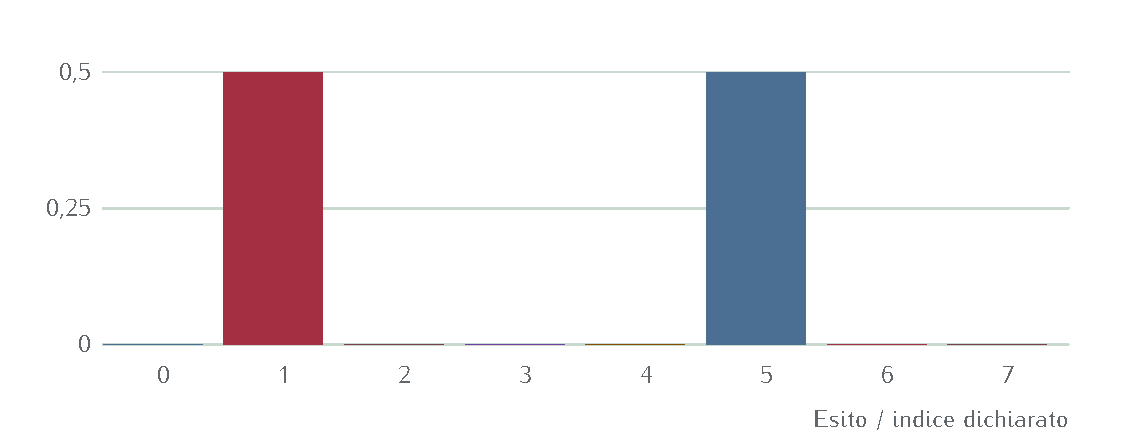
\includegraphics[width=\linewidth,height=94mm,keepaspectratio]{figure/fa2cbdd2a08bf8252.pdf}\FigureCaption{4.12 \(\cdot\) esempio 2 \(\cdot\) Distribuzione completa della lettura}\end{FigureBlock}
\begin{FigureBlock}\centering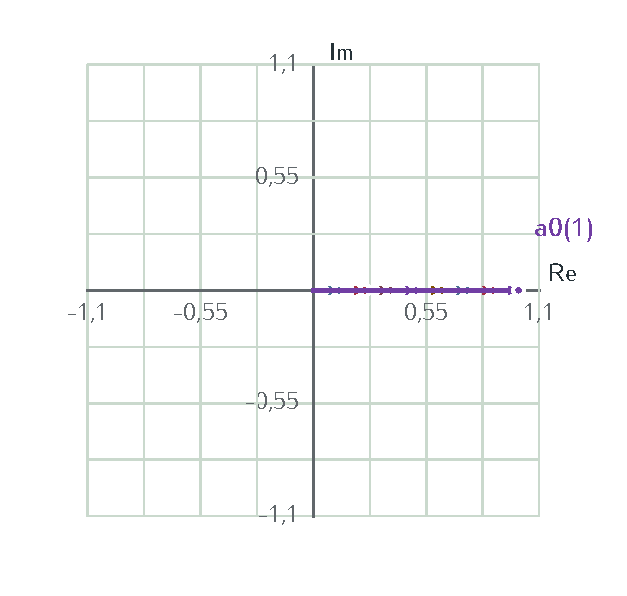
\includegraphics[width=\linewidth,height=94mm,keepaspectratio]{figure/f3497101626326650.pdf}\FigureCaption{4.12 \(\cdot\) esempio 2 \(\cdot\) Somma punta-coda, x crescente \(\cdot\) \(s=0\), \(c=1\), peso 0,5}\end{FigureBlock}
\begin{FigureBlock}\centering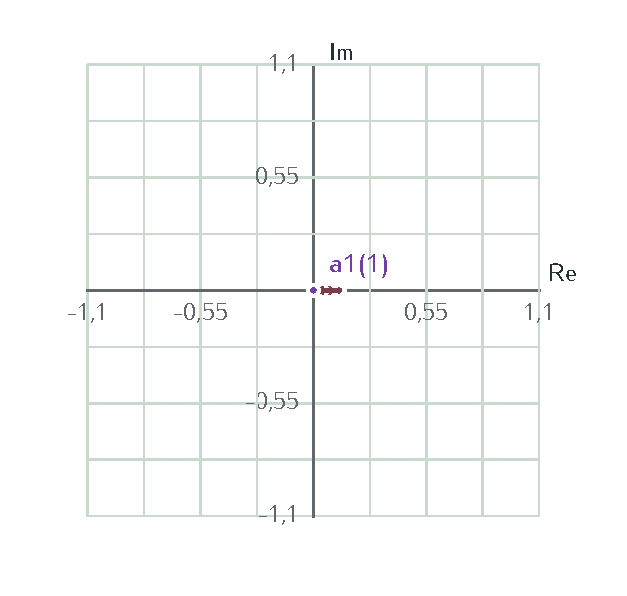
\includegraphics[width=\linewidth,height=94mm,keepaspectratio]{figure/f1f46e1eed087fb88.pdf}\FigureCaption{4.12 \(\cdot\) esempio 2 \(\cdot\) Somma punta-coda, x crescente \(\cdot\) \(s=1\), \(c=1\), peso 0,5}\end{FigureBlock}
\begin{FigureBlock}\begin{minipage}[t]{.485\linewidth}\centering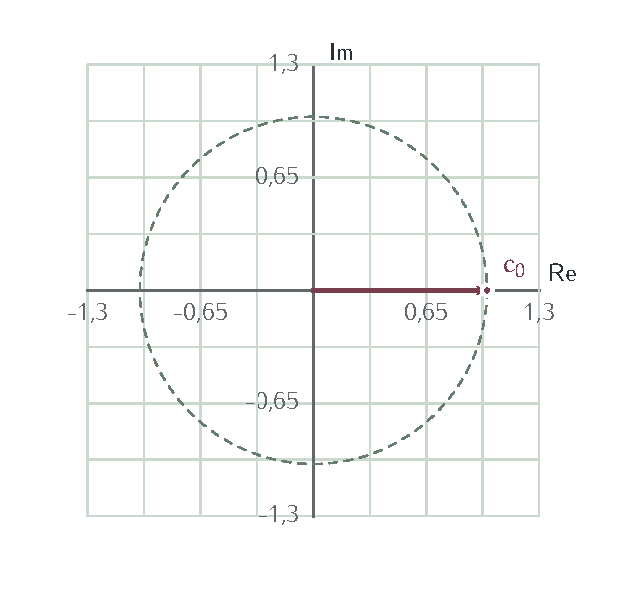
\includegraphics[width=\linewidth,height=63mm,keepaspectratio]{figure/f3373cf988dd6a5ce.pdf}\par{\sffamily\footnotesize \(c_{0}\)\par}\end{minipage}\hfill\begin{minipage}[t]{.485\linewidth}\centering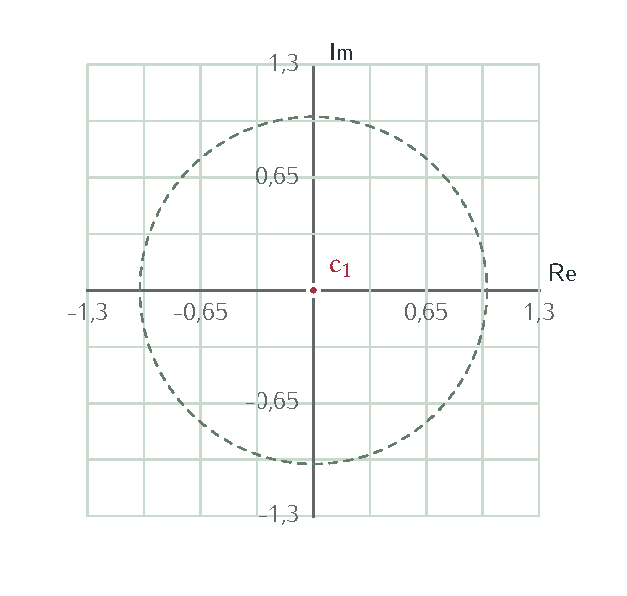
\includegraphics[width=\linewidth,height=63mm,keepaspectratio]{figure/f68c66282b90bee1b.pdf}\par{\sffamily\footnotesize \(c_{1}\)\par}\end{minipage}\FigureCaption{4.12 \(\cdot\) esempio 2 \(\cdot\) Bersaglio condizionato \(\cdot\) coefficienti \(\beta {}^{\prime} s\) nella base propria dichiarata}\end{FigureBlock}

\phantomsection\label{c4-qpe-esatta-example-2-step-1}
\BookHeading{01 Definire operatore, autostati e coefficienti}

\MathBlock{0055007C0075005F007327E9003D0065005E0028003203C0006903C6005F00730029007C0075005F007327E9003B002027E80075005F0073007C0075005F007427E9003D03B40073002C0074002E}{U|u_{s}\rangle =e^{2\pi i\varphi _{s}}|u_{s}\rangle ;\allowbreak \ \langle u_{s}|u_{t}\rangle =\delta s,\allowbreak t.}
\MathBlock{007C03C827E9003D03A30073002003B2005F0073007C0075005F007327E9003B002003A30073007C03B2005F0073007C00B2003D0031003B00200051003D0032005E006D002E}{|\psi \rangle =\sum _{s}\ \beta _{s}|u_{s}\rangle ;\allowbreak \ \sum _{s}|\beta _{s}|^{2}=1;\allowbreak \ Q=2^{m}.}

Il registro di lettura contiene m qubit; \(\varphi \) è una frazione di giro modulo uno. L'indice s distingue gli autostati del bersaglio e \(\beta _{s}\) è un'ampiezza complessa, mentre \(|\beta _{s}|^{2}\) è un peso probabilistico.\par


\phantomsection\label{c4-qpe-esatta-example-2-step-2}
\BookHeading{02 Assegnare \(U\) e la preparazione}

\MathBlock{0055003D006400690061006700280065005E0028003203C0006900B70030002C0031003200350029002C0065005E0028003203C0006900B70030002C00360032003500290029002E}{U=\operatorname{diag}(e^{2\pi i\cdot 0{,}125},\allowbreak e^{2\pi i\cdot 0{,}625}).}
\MathBlock{007C0075208027E9003D007C003027E9003B0020007C0075208127E9003D007C003127E9003B002003B22080003D03B22081003D0031002F221A0032003B0020007C03C827E9003D0048007C003027E9003D007C002B27E9002E}{|u_{0}\rangle =|0\rangle ;\allowbreak \ |u_{1}\rangle =|1\rangle ;\allowbreak \ \beta _{0}=\beta _{1}=1/\sqrt{2};\allowbreak \ |\psi \rangle =H|0\rangle =|+\rangle .}

La matrice diagonale e la fase reale positiva della preparazione fissano lo stato congiunto. Una fase globale di \(U\) diventa relativa quando \(U\) è controllata, perciò viene conservata.\par


\phantomsection\label{c4-qpe-esatta-example-2-step-3}
\BookHeading{03 Preparare il controllo}

\MathBlock{007C003027E922970033007C03C827E900202192002000280031002F221A0038002903A30078007C007827E903A30073002003B2005F0073007C0075005F007327E9002E}{|0\rangle ^{\otimes 3}|\psi \rangle \ \to \ (1/\sqrt{8})\sum _{x}|x\rangle \sum _{s}\ \beta _{s}|u_{s}\rangle .}

Le Hadamard agiscono soltanto sui qubit di lettura. Il bersaglio mantiene i coefficienti appena assegnati.\par


\phantomsection\label{c4-qpe-esatta-example-2-step-4}
\BookHeading{04 Costruire le potenze e il kickback}

\MathBlock{00660069006C006F002000710030002C0020007000650073006F00200032005E0032003A00200063006F006E00740072006F006C006C006F00200064006900200055005E0034}{\text{filo}\ q_{0},\allowbreak \ \text{peso}\ 2^{2}:\ \text{controllo}\ \text{di}\ U^{4}}
\MathBlock{00660069006C006F002000710031002C0020007000650073006F00200032005E0031003A00200063006F006E00740072006F006C006C006F00200064006900200055005E0032}{\text{filo}\ q_{1},\allowbreak \ \text{peso}\ 2^{1}:\ \text{controllo}\ \text{di}\ U^{2}}
\MathBlock{00660069006C006F002000710032002C0020007000650073006F00200032005E0030003A00200063006F006E00740072006F006C006C006F00200064006900200055005E0031}{\text{filo}\ q_{2},\allowbreak \ \text{peso}\ 2^{0}:\ \text{controllo}\ \text{di}\ U^{1}}
\MathBlock{0078003D03A3007100200078005F00710032005E0028006D22120031221200710029002021D20020220F007100200065005E0028003203C0006900200078005F00710032005E0028006D2212003122120071002903C6005F00730029003D0065005E0028003203C00069007803C6005F00730029002E}{x=\sum _{q}\ x_{q}2^{m- 1- q}\ \Rightarrow \ \prod _{q}\ e^{2\pi i\ x_{q}2^{m- 1- q}\varphi _{s}}=e^{2\pi ix\varphi _{s}}.}
\MathBlock{007C03A827E9003D00280031002F221A0051002903A30078002C0073002003B2005F007300200065005E0028003203C00069007803C6005F00730029007C007827E9007C0075005F007327E9002E}{|\Psi \rangle =(1/\sqrt{Q})\sum _{x,\allowbreak s}\ \beta _{s}\ e^{2\pi ix\varphi _{s}}|x\rangle |u_{s}\rangle .}

\(q_{0}\) è il filo superiore e il bit più significativo. Per tre qubit le potenze sono \(U^{4},\allowbreak U^{2},\allowbreak U\); l'esponente j di \(2^{j}\) non va confuso con l'indice del filo \(q_{j}\).\par


\phantomsection\label{c4-qpe-esatta-example-2-step-5}
\BookHeading{05 Sommare le radici dell'unità}

\MathBlock{0053003D0031002B007A002B22EF002B007A005E00280038002D00310029002E}{S=1+z+\cdots +z^{8-1}.}
\MathBlock{007A0053003D007A002B007A00B2002B22EF002B007A005E0038003B0020002800312212007A00290053003D00312212007A005E0038002E}{zS=z+z^{2}+\cdots +z^{8};\allowbreak \ (1- z)S=1- z^{8}.}
\MathBlock{005300650020007A22600031003A00200053003D002800312212007A005E00380029002F002800312212007A0029002E0020005300650020007A003D0031003A00200053003D0038002E}{Se\ z\ne 1:\ S=(1- z^{8})/(1- z).\ Se\ z=1:\ S=8.}

La sottrazione cancella tutti i termini intermedi. Il caso \(z=1\) va separato prima della divisione.\par


\phantomsection\label{c4-qpe-esatta-example-2-step-6}
\BookHeading{06 Dalla cancellazione all'unitarietà}

\MathBlock{007A003D0065005E0028003203C00069002800782212007820320029002F00380029003B0020007A005E0038003D0031002E}{z=e^{2\pi i(x- x{}^{\prime} )/8};\allowbreak \ z^{8}=1.}
\MathBlock{27E80046003800782032007C00460038007827E9003D00280031002F0038002903A300790020007A02B8003D0038002F0038003D003100200073006500200078003D00782032003B0020003000200061006C007400720069006D0065006E00740069002E}{\langle F8x{}^{\prime} |F8x\rangle =(1/8)\sum _{y}\ z^{y}=8/8=1\ \text{se}\ x=x{}^{\prime} ;\allowbreak \ 0\ \text{altrimenti}.}

Per x e \(x{}^{\prime} \) distinti fra 0 e \(N- 1\), \(z\ne 1\): le frecce delle radici si chiudono. Le colonne di Fourier sono quindi ortonormali e la trasformata conserva prodotti interni e norma.\par


\phantomsection\label{c4-qpe-esatta-example-2-step-7}
\BookHeading{07 Applicare la cancellazione alla QPE}

\MathBlock{0044006F0070006F00200046005F00512020003A0020007C03A8006F0075007427E9003D03A30063002C0073002003B2005F007300200061005F0073002800630029007C006327E9007C0075005F007327E9002E}{\text{Dopo}\ F_{Q}{}^{\dagger} :\ |\Psi \text{out}\rangle =\sum _{c,\allowbreak s}\ \beta _{s}\ a_{s}(c)|c\rangle |u_{s}\rangle .}
\MathBlock{0061005F0073002800630029003D00280031002F0051002903A300780020007A02E3002C0020007A003D0065005E0028003203C00069002803C6005F007322120063002F005100290029002E}{a_{s}(c)=(1/Q)\sum _{x}\ z^{x},\allowbreak \ z=e^{2\pi i(\varphi _{s}- c/Q)}.}
\MathBlock{005300650020005103C6005F0073003D004C00200069006E007400650072006F003A0020007A005E0051003D0031003B00200061005F00730028004C0029003D0031002C00200061005F0073002800630029003D00300020007000650072002000632260004C002E}{Se\ Q\varphi _{s}=L\ \text{intero}:\ z^{Q}=1;\allowbreak \ a_{s}(L)=1,\allowbreak \ a_{s}(c)=0\ \text{per}\ c\ne L.}
\MathBlock{00460075006F0072006900200067007200690067006C00690061003A00200061005F0073002800630029003D002800312212007A005E00510029002F00280051002800312212007A00290029002C002000730061006C0076006F0020007A003D0031002E}{\text{Fuori}\ \text{griglia}:\ a_{s}(c)=(1- z^{Q})/(Q(1- z)),\allowbreak \ \text{salvo}\ z=1.}

Per \(Q=8\), \(\varphi =3/8\): \(a(3)=8/8=1\). Per ogni altro c, \(z=e^{2\pi i(3- c)/8}\ne 1\) e il numeratore è zero. Fuori griglia la cancellazione è incompleta e più esiti restano possibili.\par


\phantomsection\label{c4-qpe-esatta-example-2-step-8}
\BookHeading{08 Potenze controllate \(\cdot\) autostato 0}

\MathBlock{00660069006C006F002000710030003A00200032005E003203C60020006D006F00640020003122480030002C0035}{\text{filo}\ q_{0}:\ 2^{2}\varphi \ \bmod \ 1\approx 0{,}5}
\MathBlock{00660069006C006F002000710031003A00200032005E003103C60020006D006F00640020003122480030002C00320035}{\text{filo}\ q_{1}:\ 2^{1}\varphi \ \bmod \ 1\approx 0{,}25}
\MathBlock{00660069006C006F002000710032003A00200032005E003003C60020006D006F00640020003122480030002C003100320035}{\text{filo}\ q_{2}:\ 2^{0}\varphi \ \bmod \ 1\approx 0{,}125}
\MathBlock{0063005F0073002800780029003D0065005E0028003203C00069007800B70030002C0031003200350029002F221A0038}{c_{s}(x)=e^{2\pi ix\cdot 0{,}125}/\sqrt{8}}

Queste fasi moltiplicano il ramo di autostato s; il suo coefficiente \(\beta _{s}\) rimane esplicito nello stato congiunto.\par


\phantomsection\label{c4-qpe-esatta-example-2-step-9}
\BookHeading{09 Fourier inversa \(\cdot\) \(s=0\), \(c=0\)}

\MathBlock{0061005F0073002800300029003D00280031002F00380029005B0065005E0028003203C0006900B7003000B700280030002C00310032003522120030002F003800290029002B0065005E0028003203C0006900B7003100B700280030002C00310032003522120030002F003800290029002B0065005E0028003203C0006900B7003200B700280030002C00310032003522120030002F003800290029002B0065005E0028003203C0006900B7003300B700280030002C00310032003522120030002F003800290029002B0065005E0028003203C0006900B7003400B700280030002C00310032003522120030002F003800290029002B0065005E0028003203C0006900B7003500B700280030002C00310032003522120030002F003800290029002B0065005E0028003203C0006900B7003600B700280030002C00310032003522120030002F003800290029002B0065005E0028003203C0006900B7003700B700280030002C00310032003522120030002F003800290029005D}{a_{s}(0)=(1/8)[e^{2\pi i\cdot 0\cdot (0{,}125- 0/8)}+e^{2\pi i\cdot 1\cdot (0{,}125- 0/8)}+e^{2\pi i\cdot 2\cdot (0{,}125- 0/8)}+e^{2\pi i\cdot 3\cdot (0{,}125- 0/8)}+e^{2\pi i\cdot 4\cdot (0{,}125- 0/8)}+e^{2\pi i\cdot 5\cdot (0{,}125- 0/8)}+e^{2\pi i\cdot 6\cdot (0{,}125- 0/8)}+e^{2\pi i\cdot 7\cdot (0{,}125- 0/8)}]}
\MathBlock{22480030003B0020007C0061007C00B222480030}{\approx 0;\allowbreak \ |a|^{2}\approx 0}

La somma complessa precede il modulo quadro. Le fasi nel calcolo mantengono precisione completa; i decimali stampati sono arrotondati.\par


\phantomsection\label{c4-qpe-esatta-example-2-step-10}
\BookHeading{10 Fourier inversa \(\cdot\) \(s=0\), \(c=1\)}

\MathBlock{0061005F0073002800310029003D00280031002F00380029005B0065005E0028003203C0006900B7003000B700280030002C00310032003522120031002F003800290029002B0065005E0028003203C0006900B7003100B700280030002C00310032003522120031002F003800290029002B0065005E0028003203C0006900B7003200B700280030002C00310032003522120031002F003800290029002B0065005E0028003203C0006900B7003300B700280030002C00310032003522120031002F003800290029002B0065005E0028003203C0006900B7003400B700280030002C00310032003522120031002F003800290029002B0065005E0028003203C0006900B7003500B700280030002C00310032003522120031002F003800290029002B0065005E0028003203C0006900B7003600B700280030002C00310032003522120031002F003800290029002B0065005E0028003203C0006900B7003700B700280030002C00310032003522120031002F003800290029005D}{a_{s}(1)=(1/8)[e^{2\pi i\cdot 0\cdot (0{,}125- 1/8)}+e^{2\pi i\cdot 1\cdot (0{,}125- 1/8)}+e^{2\pi i\cdot 2\cdot (0{,}125- 1/8)}+e^{2\pi i\cdot 3\cdot (0{,}125- 1/8)}+e^{2\pi i\cdot 4\cdot (0{,}125- 1/8)}+e^{2\pi i\cdot 5\cdot (0{,}125- 1/8)}+e^{2\pi i\cdot 6\cdot (0{,}125- 1/8)}+e^{2\pi i\cdot 7\cdot (0{,}125- 1/8)}]}
\MathBlock{22480031003B0020007C0061007C00B222480031}{\approx 1;\allowbreak \ |a|^{2}\approx 1}

La somma complessa precede il modulo quadro. Le fasi nel calcolo mantengono precisione completa; i decimali stampati sono arrotondati.\par


\phantomsection\label{c4-qpe-esatta-example-2-step-11}
\BookHeading{11 Fourier inversa \(\cdot\) \(s=0\), \(c=2\)}

\MathBlock{0061005F0073002800320029003D00280031002F00380029005B0065005E0028003203C0006900B7003000B700280030002C00310032003522120032002F003800290029002B0065005E0028003203C0006900B7003100B700280030002C00310032003522120032002F003800290029002B0065005E0028003203C0006900B7003200B700280030002C00310032003522120032002F003800290029002B0065005E0028003203C0006900B7003300B700280030002C00310032003522120032002F003800290029002B0065005E0028003203C0006900B7003400B700280030002C00310032003522120032002F003800290029002B0065005E0028003203C0006900B7003500B700280030002C00310032003522120032002F003800290029002B0065005E0028003203C0006900B7003600B700280030002C00310032003522120032002F003800290029002B0065005E0028003203C0006900B7003700B700280030002C00310032003522120032002F003800290029005D}{a_{s}(2)=(1/8)[e^{2\pi i\cdot 0\cdot (0{,}125- 2/8)}+e^{2\pi i\cdot 1\cdot (0{,}125- 2/8)}+e^{2\pi i\cdot 2\cdot (0{,}125- 2/8)}+e^{2\pi i\cdot 3\cdot (0{,}125- 2/8)}+e^{2\pi i\cdot 4\cdot (0{,}125- 2/8)}+e^{2\pi i\cdot 5\cdot (0{,}125- 2/8)}+e^{2\pi i\cdot 6\cdot (0{,}125- 2/8)}+e^{2\pi i\cdot 7\cdot (0{,}125- 2/8)}]}
\MathBlock{22480030003B0020007C0061007C00B222480030}{\approx 0;\allowbreak \ |a|^{2}\approx 0}

La somma complessa precede il modulo quadro. Le fasi nel calcolo mantengono precisione completa; i decimali stampati sono arrotondati.\par


\phantomsection\label{c4-qpe-esatta-example-2-step-12}
\BookHeading{12 Fourier inversa \(\cdot\) \(s=0\), \(c=3\)}

\MathBlock{0061005F0073002800330029003D00280031002F00380029005B0065005E0028003203C0006900B7003000B700280030002C00310032003522120033002F003800290029002B0065005E0028003203C0006900B7003100B700280030002C00310032003522120033002F003800290029002B0065005E0028003203C0006900B7003200B700280030002C00310032003522120033002F003800290029002B0065005E0028003203C0006900B7003300B700280030002C00310032003522120033002F003800290029002B0065005E0028003203C0006900B7003400B700280030002C00310032003522120033002F003800290029002B0065005E0028003203C0006900B7003500B700280030002C00310032003522120033002F003800290029002B0065005E0028003203C0006900B7003600B700280030002C00310032003522120033002F003800290029002B0065005E0028003203C0006900B7003700B700280030002C00310032003522120033002F003800290029005D}{a_{s}(3)=(1/8)[e^{2\pi i\cdot 0\cdot (0{,}125- 3/8)}+e^{2\pi i\cdot 1\cdot (0{,}125- 3/8)}+e^{2\pi i\cdot 2\cdot (0{,}125- 3/8)}+e^{2\pi i\cdot 3\cdot (0{,}125- 3/8)}+e^{2\pi i\cdot 4\cdot (0{,}125- 3/8)}+e^{2\pi i\cdot 5\cdot (0{,}125- 3/8)}+e^{2\pi i\cdot 6\cdot (0{,}125- 3/8)}+e^{2\pi i\cdot 7\cdot (0{,}125- 3/8)}]}
\MathBlock{22480030003B0020007C0061007C00B222480030}{\approx 0;\allowbreak \ |a|^{2}\approx 0}

La somma complessa precede il modulo quadro. Le fasi nel calcolo mantengono precisione completa; i decimali stampati sono arrotondati.\par


\phantomsection\label{c4-qpe-esatta-example-2-step-13}
\BookHeading{13 Fourier inversa \(\cdot\) \(s=0\), \(c=4\)}

\MathBlock{0061005F0073002800340029003D00280031002F00380029005B0065005E0028003203C0006900B7003000B700280030002C00310032003522120034002F003800290029002B0065005E0028003203C0006900B7003100B700280030002C00310032003522120034002F003800290029002B0065005E0028003203C0006900B7003200B700280030002C00310032003522120034002F003800290029002B0065005E0028003203C0006900B7003300B700280030002C00310032003522120034002F003800290029002B0065005E0028003203C0006900B7003400B700280030002C00310032003522120034002F003800290029002B0065005E0028003203C0006900B7003500B700280030002C00310032003522120034002F003800290029002B0065005E0028003203C0006900B7003600B700280030002C00310032003522120034002F003800290029002B0065005E0028003203C0006900B7003700B700280030002C00310032003522120034002F003800290029005D}{a_{s}(4)=(1/8)[e^{2\pi i\cdot 0\cdot (0{,}125- 4/8)}+e^{2\pi i\cdot 1\cdot (0{,}125- 4/8)}+e^{2\pi i\cdot 2\cdot (0{,}125- 4/8)}+e^{2\pi i\cdot 3\cdot (0{,}125- 4/8)}+e^{2\pi i\cdot 4\cdot (0{,}125- 4/8)}+e^{2\pi i\cdot 5\cdot (0{,}125- 4/8)}+e^{2\pi i\cdot 6\cdot (0{,}125- 4/8)}+e^{2\pi i\cdot 7\cdot (0{,}125- 4/8)}]}
\MathBlock{22480030003B0020007C0061007C00B222480030}{\approx 0;\allowbreak \ |a|^{2}\approx 0}

La somma complessa precede il modulo quadro. Le fasi nel calcolo mantengono precisione completa; i decimali stampati sono arrotondati.\par


\phantomsection\label{c4-qpe-esatta-example-2-step-14}
\BookHeading{14 Fourier inversa \(\cdot\) \(s=0\), \(c=5\)}

\MathBlock{0061005F0073002800350029003D00280031002F00380029005B0065005E0028003203C0006900B7003000B700280030002C00310032003522120035002F003800290029002B0065005E0028003203C0006900B7003100B700280030002C00310032003522120035002F003800290029002B0065005E0028003203C0006900B7003200B700280030002C00310032003522120035002F003800290029002B0065005E0028003203C0006900B7003300B700280030002C00310032003522120035002F003800290029002B0065005E0028003203C0006900B7003400B700280030002C00310032003522120035002F003800290029002B0065005E0028003203C0006900B7003500B700280030002C00310032003522120035002F003800290029002B0065005E0028003203C0006900B7003600B700280030002C00310032003522120035002F003800290029002B0065005E0028003203C0006900B7003700B700280030002C00310032003522120035002F003800290029005D}{a_{s}(5)=(1/8)[e^{2\pi i\cdot 0\cdot (0{,}125- 5/8)}+e^{2\pi i\cdot 1\cdot (0{,}125- 5/8)}+e^{2\pi i\cdot 2\cdot (0{,}125- 5/8)}+e^{2\pi i\cdot 3\cdot (0{,}125- 5/8)}+e^{2\pi i\cdot 4\cdot (0{,}125- 5/8)}+e^{2\pi i\cdot 5\cdot (0{,}125- 5/8)}+e^{2\pi i\cdot 6\cdot (0{,}125- 5/8)}+e^{2\pi i\cdot 7\cdot (0{,}125- 5/8)}]}
\MathBlock{22480030003B0020007C0061007C00B222480030}{\approx 0;\allowbreak \ |a|^{2}\approx 0}

La somma complessa precede il modulo quadro. Le fasi nel calcolo mantengono precisione completa; i decimali stampati sono arrotondati.\par


\phantomsection\label{c4-qpe-esatta-example-2-step-15}
\BookHeading{15 Fourier inversa \(\cdot\) \(s=0\), \(c=6\)}

\MathBlock{0061005F0073002800360029003D00280031002F00380029005B0065005E0028003203C0006900B7003000B700280030002C00310032003522120036002F003800290029002B0065005E0028003203C0006900B7003100B700280030002C00310032003522120036002F003800290029002B0065005E0028003203C0006900B7003200B700280030002C00310032003522120036002F003800290029002B0065005E0028003203C0006900B7003300B700280030002C00310032003522120036002F003800290029002B0065005E0028003203C0006900B7003400B700280030002C00310032003522120036002F003800290029002B0065005E0028003203C0006900B7003500B700280030002C00310032003522120036002F003800290029002B0065005E0028003203C0006900B7003600B700280030002C00310032003522120036002F003800290029002B0065005E0028003203C0006900B7003700B700280030002C00310032003522120036002F003800290029005D}{a_{s}(6)=(1/8)[e^{2\pi i\cdot 0\cdot (0{,}125- 6/8)}+e^{2\pi i\cdot 1\cdot (0{,}125- 6/8)}+e^{2\pi i\cdot 2\cdot (0{,}125- 6/8)}+e^{2\pi i\cdot 3\cdot (0{,}125- 6/8)}+e^{2\pi i\cdot 4\cdot (0{,}125- 6/8)}+e^{2\pi i\cdot 5\cdot (0{,}125- 6/8)}+e^{2\pi i\cdot 6\cdot (0{,}125- 6/8)}+e^{2\pi i\cdot 7\cdot (0{,}125- 6/8)}]}
\MathBlock{22480030003B0020007C0061007C00B222480030}{\approx 0;\allowbreak \ |a|^{2}\approx 0}

La somma complessa precede il modulo quadro. Le fasi nel calcolo mantengono precisione completa; i decimali stampati sono arrotondati.\par


\phantomsection\label{c4-qpe-esatta-example-2-step-16}
\BookHeading{16 Fourier inversa \(\cdot\) \(s=0\), \(c=7\)}

\MathBlock{0061005F0073002800370029003D00280031002F00380029005B0065005E0028003203C0006900B7003000B700280030002C00310032003522120037002F003800290029002B0065005E0028003203C0006900B7003100B700280030002C00310032003522120037002F003800290029002B0065005E0028003203C0006900B7003200B700280030002C00310032003522120037002F003800290029002B0065005E0028003203C0006900B7003300B700280030002C00310032003522120037002F003800290029002B0065005E0028003203C0006900B7003400B700280030002C00310032003522120037002F003800290029002B0065005E0028003203C0006900B7003500B700280030002C00310032003522120037002F003800290029002B0065005E0028003203C0006900B7003600B700280030002C00310032003522120037002F003800290029002B0065005E0028003203C0006900B7003700B700280030002C00310032003522120037002F003800290029005D}{a_{s}(7)=(1/8)[e^{2\pi i\cdot 0\cdot (0{,}125- 7/8)}+e^{2\pi i\cdot 1\cdot (0{,}125- 7/8)}+e^{2\pi i\cdot 2\cdot (0{,}125- 7/8)}+e^{2\pi i\cdot 3\cdot (0{,}125- 7/8)}+e^{2\pi i\cdot 4\cdot (0{,}125- 7/8)}+e^{2\pi i\cdot 5\cdot (0{,}125- 7/8)}+e^{2\pi i\cdot 6\cdot (0{,}125- 7/8)}+e^{2\pi i\cdot 7\cdot (0{,}125- 7/8)}]}
\MathBlock{22480030003B0020007C0061007C00B222480030}{\approx 0;\allowbreak \ |a|^{2}\approx 0}

La somma complessa precede il modulo quadro. Le fasi nel calcolo mantengono precisione completa; i decimali stampati sono arrotondati.\par


\phantomsection\label{c4-qpe-esatta-example-2-step-17}
\BookHeading{17 Potenze controllate \(\cdot\) autostato 1}

\MathBlock{00660069006C006F002000710030003A00200032005E003203C60020006D006F00640020003122480030002C0035}{\text{filo}\ q_{0}:\ 2^{2}\varphi \ \bmod \ 1\approx 0{,}5}
\MathBlock{00660069006C006F002000710031003A00200032005E003103C60020006D006F00640020003122480030002C00320035}{\text{filo}\ q_{1}:\ 2^{1}\varphi \ \bmod \ 1\approx 0{,}25}
\MathBlock{00660069006C006F002000710032003A00200032005E003003C60020006D006F00640020003122480030002C003600320035}{\text{filo}\ q_{2}:\ 2^{0}\varphi \ \bmod \ 1\approx 0{,}625}
\MathBlock{0063005F0073002800780029003D0065005E0028003203C00069007800B70030002C0036003200350029002F221A0038}{c_{s}(x)=e^{2\pi ix\cdot 0{,}625}/\sqrt{8}}

Queste fasi moltiplicano il ramo di autostato s; il suo coefficiente \(\beta _{s}\) rimane esplicito nello stato congiunto.\par


\phantomsection\label{c4-qpe-esatta-example-2-step-18}
\BookHeading{18 Fourier inversa \(\cdot\) \(s=1\), \(c=0\)}

\MathBlock{0061005F0073002800300029003D00280031002F00380029005B0065005E0028003203C0006900B7003000B700280030002C00360032003522120030002F003800290029002B0065005E0028003203C0006900B7003100B700280030002C00360032003522120030002F003800290029002B0065005E0028003203C0006900B7003200B700280030002C00360032003522120030002F003800290029002B0065005E0028003203C0006900B7003300B700280030002C00360032003522120030002F003800290029002B0065005E0028003203C0006900B7003400B700280030002C00360032003522120030002F003800290029002B0065005E0028003203C0006900B7003500B700280030002C00360032003522120030002F003800290029002B0065005E0028003203C0006900B7003600B700280030002C00360032003522120030002F003800290029002B0065005E0028003203C0006900B7003700B700280030002C00360032003522120030002F003800290029005D}{a_{s}(0)=(1/8)[e^{2\pi i\cdot 0\cdot (0{,}625- 0/8)}+e^{2\pi i\cdot 1\cdot (0{,}625- 0/8)}+e^{2\pi i\cdot 2\cdot (0{,}625- 0/8)}+e^{2\pi i\cdot 3\cdot (0{,}625- 0/8)}+e^{2\pi i\cdot 4\cdot (0{,}625- 0/8)}+e^{2\pi i\cdot 5\cdot (0{,}625- 0/8)}+e^{2\pi i\cdot 6\cdot (0{,}625- 0/8)}+e^{2\pi i\cdot 7\cdot (0{,}625- 0/8)}]}
\MathBlock{22480030003B0020007C0061007C00B222480030}{\approx 0;\allowbreak \ |a|^{2}\approx 0}

La somma complessa precede il modulo quadro. Le fasi nel calcolo mantengono precisione completa; i decimali stampati sono arrotondati.\par


\phantomsection\label{c4-qpe-esatta-example-2-step-19}
\BookHeading{19 Fourier inversa \(\cdot\) \(s=1\), \(c=1\)}

\MathBlock{0061005F0073002800310029003D00280031002F00380029005B0065005E0028003203C0006900B7003000B700280030002C00360032003522120031002F003800290029002B0065005E0028003203C0006900B7003100B700280030002C00360032003522120031002F003800290029002B0065005E0028003203C0006900B7003200B700280030002C00360032003522120031002F003800290029002B0065005E0028003203C0006900B7003300B700280030002C00360032003522120031002F003800290029002B0065005E0028003203C0006900B7003400B700280030002C00360032003522120031002F003800290029002B0065005E0028003203C0006900B7003500B700280030002C00360032003522120031002F003800290029002B0065005E0028003203C0006900B7003600B700280030002C00360032003522120031002F003800290029002B0065005E0028003203C0006900B7003700B700280030002C00360032003522120031002F003800290029005D}{a_{s}(1)=(1/8)[e^{2\pi i\cdot 0\cdot (0{,}625- 1/8)}+e^{2\pi i\cdot 1\cdot (0{,}625- 1/8)}+e^{2\pi i\cdot 2\cdot (0{,}625- 1/8)}+e^{2\pi i\cdot 3\cdot (0{,}625- 1/8)}+e^{2\pi i\cdot 4\cdot (0{,}625- 1/8)}+e^{2\pi i\cdot 5\cdot (0{,}625- 1/8)}+e^{2\pi i\cdot 6\cdot (0{,}625- 1/8)}+e^{2\pi i\cdot 7\cdot (0{,}625- 1/8)}]}
\MathBlock{22480030003B0020007C0061007C00B222480030}{\approx 0;\allowbreak \ |a|^{2}\approx 0}

La somma complessa precede il modulo quadro. Le fasi nel calcolo mantengono precisione completa; i decimali stampati sono arrotondati.\par


\phantomsection\label{c4-qpe-esatta-example-2-step-20}
\BookHeading{20 Fourier inversa \(\cdot\) \(s=1\), \(c=2\)}

\MathBlock{0061005F0073002800320029003D00280031002F00380029005B0065005E0028003203C0006900B7003000B700280030002C00360032003522120032002F003800290029002B0065005E0028003203C0006900B7003100B700280030002C00360032003522120032002F003800290029002B0065005E0028003203C0006900B7003200B700280030002C00360032003522120032002F003800290029002B0065005E0028003203C0006900B7003300B700280030002C00360032003522120032002F003800290029002B0065005E0028003203C0006900B7003400B700280030002C00360032003522120032002F003800290029002B0065005E0028003203C0006900B7003500B700280030002C00360032003522120032002F003800290029002B0065005E0028003203C0006900B7003600B700280030002C00360032003522120032002F003800290029002B0065005E0028003203C0006900B7003700B700280030002C00360032003522120032002F003800290029005D}{a_{s}(2)=(1/8)[e^{2\pi i\cdot 0\cdot (0{,}625- 2/8)}+e^{2\pi i\cdot 1\cdot (0{,}625- 2/8)}+e^{2\pi i\cdot 2\cdot (0{,}625- 2/8)}+e^{2\pi i\cdot 3\cdot (0{,}625- 2/8)}+e^{2\pi i\cdot 4\cdot (0{,}625- 2/8)}+e^{2\pi i\cdot 5\cdot (0{,}625- 2/8)}+e^{2\pi i\cdot 6\cdot (0{,}625- 2/8)}+e^{2\pi i\cdot 7\cdot (0{,}625- 2/8)}]}
\MathBlock{22480030003B0020007C0061007C00B222480030}{\approx 0;\allowbreak \ |a|^{2}\approx 0}

La somma complessa precede il modulo quadro. Le fasi nel calcolo mantengono precisione completa; i decimali stampati sono arrotondati.\par


\phantomsection\label{c4-qpe-esatta-example-2-step-21}
\BookHeading{21 Fourier inversa \(\cdot\) \(s=1\), \(c=3\)}

\MathBlock{0061005F0073002800330029003D00280031002F00380029005B0065005E0028003203C0006900B7003000B700280030002C00360032003522120033002F003800290029002B0065005E0028003203C0006900B7003100B700280030002C00360032003522120033002F003800290029002B0065005E0028003203C0006900B7003200B700280030002C00360032003522120033002F003800290029002B0065005E0028003203C0006900B7003300B700280030002C00360032003522120033002F003800290029002B0065005E0028003203C0006900B7003400B700280030002C00360032003522120033002F003800290029002B0065005E0028003203C0006900B7003500B700280030002C00360032003522120033002F003800290029002B0065005E0028003203C0006900B7003600B700280030002C00360032003522120033002F003800290029002B0065005E0028003203C0006900B7003700B700280030002C00360032003522120033002F003800290029005D}{a_{s}(3)=(1/8)[e^{2\pi i\cdot 0\cdot (0{,}625- 3/8)}+e^{2\pi i\cdot 1\cdot (0{,}625- 3/8)}+e^{2\pi i\cdot 2\cdot (0{,}625- 3/8)}+e^{2\pi i\cdot 3\cdot (0{,}625- 3/8)}+e^{2\pi i\cdot 4\cdot (0{,}625- 3/8)}+e^{2\pi i\cdot 5\cdot (0{,}625- 3/8)}+e^{2\pi i\cdot 6\cdot (0{,}625- 3/8)}+e^{2\pi i\cdot 7\cdot (0{,}625- 3/8)}]}
\MathBlock{22480030003B0020007C0061007C00B222480030}{\approx 0;\allowbreak \ |a|^{2}\approx 0}

La somma complessa precede il modulo quadro. Le fasi nel calcolo mantengono precisione completa; i decimali stampati sono arrotondati.\par


\phantomsection\label{c4-qpe-esatta-example-2-step-22}
\BookHeading{22 Fourier inversa \(\cdot\) \(s=1\), \(c=4\)}

\MathBlock{0061005F0073002800340029003D00280031002F00380029005B0065005E0028003203C0006900B7003000B700280030002C00360032003522120034002F003800290029002B0065005E0028003203C0006900B7003100B700280030002C00360032003522120034002F003800290029002B0065005E0028003203C0006900B7003200B700280030002C00360032003522120034002F003800290029002B0065005E0028003203C0006900B7003300B700280030002C00360032003522120034002F003800290029002B0065005E0028003203C0006900B7003400B700280030002C00360032003522120034002F003800290029002B0065005E0028003203C0006900B7003500B700280030002C00360032003522120034002F003800290029002B0065005E0028003203C0006900B7003600B700280030002C00360032003522120034002F003800290029002B0065005E0028003203C0006900B7003700B700280030002C00360032003522120034002F003800290029005D}{a_{s}(4)=(1/8)[e^{2\pi i\cdot 0\cdot (0{,}625- 4/8)}+e^{2\pi i\cdot 1\cdot (0{,}625- 4/8)}+e^{2\pi i\cdot 2\cdot (0{,}625- 4/8)}+e^{2\pi i\cdot 3\cdot (0{,}625- 4/8)}+e^{2\pi i\cdot 4\cdot (0{,}625- 4/8)}+e^{2\pi i\cdot 5\cdot (0{,}625- 4/8)}+e^{2\pi i\cdot 6\cdot (0{,}625- 4/8)}+e^{2\pi i\cdot 7\cdot (0{,}625- 4/8)}]}
\MathBlock{22480030003B0020007C0061007C00B222480030}{\approx 0;\allowbreak \ |a|^{2}\approx 0}

La somma complessa precede il modulo quadro. Le fasi nel calcolo mantengono precisione completa; i decimali stampati sono arrotondati.\par


\phantomsection\label{c4-qpe-esatta-example-2-step-23}
\BookHeading{23 Fourier inversa \(\cdot\) \(s=1\), \(c=5\)}

\MathBlock{0061005F0073002800350029003D00280031002F00380029005B0065005E0028003203C0006900B7003000B700280030002C00360032003522120035002F003800290029002B0065005E0028003203C0006900B7003100B700280030002C00360032003522120035002F003800290029002B0065005E0028003203C0006900B7003200B700280030002C00360032003522120035002F003800290029002B0065005E0028003203C0006900B7003300B700280030002C00360032003522120035002F003800290029002B0065005E0028003203C0006900B7003400B700280030002C00360032003522120035002F003800290029002B0065005E0028003203C0006900B7003500B700280030002C00360032003522120035002F003800290029002B0065005E0028003203C0006900B7003600B700280030002C00360032003522120035002F003800290029002B0065005E0028003203C0006900B7003700B700280030002C00360032003522120035002F003800290029005D}{a_{s}(5)=(1/8)[e^{2\pi i\cdot 0\cdot (0{,}625- 5/8)}+e^{2\pi i\cdot 1\cdot (0{,}625- 5/8)}+e^{2\pi i\cdot 2\cdot (0{,}625- 5/8)}+e^{2\pi i\cdot 3\cdot (0{,}625- 5/8)}+e^{2\pi i\cdot 4\cdot (0{,}625- 5/8)}+e^{2\pi i\cdot 5\cdot (0{,}625- 5/8)}+e^{2\pi i\cdot 6\cdot (0{,}625- 5/8)}+e^{2\pi i\cdot 7\cdot (0{,}625- 5/8)}]}
\MathBlock{22480031003B0020007C0061007C00B222480031}{\approx 1;\allowbreak \ |a|^{2}\approx 1}

La somma complessa precede il modulo quadro. Le fasi nel calcolo mantengono precisione completa; i decimali stampati sono arrotondati.\par


\phantomsection\label{c4-qpe-esatta-example-2-step-24}
\BookHeading{24 Fourier inversa \(\cdot\) \(s=1\), \(c=6\)}

\MathBlock{0061005F0073002800360029003D00280031002F00380029005B0065005E0028003203C0006900B7003000B700280030002C00360032003522120036002F003800290029002B0065005E0028003203C0006900B7003100B700280030002C00360032003522120036002F003800290029002B0065005E0028003203C0006900B7003200B700280030002C00360032003522120036002F003800290029002B0065005E0028003203C0006900B7003300B700280030002C00360032003522120036002F003800290029002B0065005E0028003203C0006900B7003400B700280030002C00360032003522120036002F003800290029002B0065005E0028003203C0006900B7003500B700280030002C00360032003522120036002F003800290029002B0065005E0028003203C0006900B7003600B700280030002C00360032003522120036002F003800290029002B0065005E0028003203C0006900B7003700B700280030002C00360032003522120036002F003800290029005D}{a_{s}(6)=(1/8)[e^{2\pi i\cdot 0\cdot (0{,}625- 6/8)}+e^{2\pi i\cdot 1\cdot (0{,}625- 6/8)}+e^{2\pi i\cdot 2\cdot (0{,}625- 6/8)}+e^{2\pi i\cdot 3\cdot (0{,}625- 6/8)}+e^{2\pi i\cdot 4\cdot (0{,}625- 6/8)}+e^{2\pi i\cdot 5\cdot (0{,}625- 6/8)}+e^{2\pi i\cdot 6\cdot (0{,}625- 6/8)}+e^{2\pi i\cdot 7\cdot (0{,}625- 6/8)}]}
\MathBlock{22480030003B0020007C0061007C00B222480030}{\approx 0;\allowbreak \ |a|^{2}\approx 0}

La somma complessa precede il modulo quadro. Le fasi nel calcolo mantengono precisione completa; i decimali stampati sono arrotondati.\par


\phantomsection\label{c4-qpe-esatta-example-2-step-25}
\BookHeading{25 Fourier inversa \(\cdot\) \(s=1\), \(c=7\)}

\MathBlock{0061005F0073002800370029003D00280031002F00380029005B0065005E0028003203C0006900B7003000B700280030002C00360032003522120037002F003800290029002B0065005E0028003203C0006900B7003100B700280030002C00360032003522120037002F003800290029002B0065005E0028003203C0006900B7003200B700280030002C00360032003522120037002F003800290029002B0065005E0028003203C0006900B7003300B700280030002C00360032003522120037002F003800290029002B0065005E0028003203C0006900B7003400B700280030002C00360032003522120037002F003800290029002B0065005E0028003203C0006900B7003500B700280030002C00360032003522120037002F003800290029002B0065005E0028003203C0006900B7003600B700280030002C00360032003522120037002F003800290029002B0065005E0028003203C0006900B7003700B700280030002C00360032003522120037002F003800290029005D}{a_{s}(7)=(1/8)[e^{2\pi i\cdot 0\cdot (0{,}625- 7/8)}+e^{2\pi i\cdot 1\cdot (0{,}625- 7/8)}+e^{2\pi i\cdot 2\cdot (0{,}625- 7/8)}+e^{2\pi i\cdot 3\cdot (0{,}625- 7/8)}+e^{2\pi i\cdot 4\cdot (0{,}625- 7/8)}+e^{2\pi i\cdot 5\cdot (0{,}625- 7/8)}+e^{2\pi i\cdot 6\cdot (0{,}625- 7/8)}+e^{2\pi i\cdot 7\cdot (0{,}625- 7/8)}]}
\MathBlock{22480030003B0020007C0061007C00B222480030}{\approx 0;\allowbreak \ |a|^{2}\approx 0}

La somma complessa precede il modulo quadro. Le fasi nel calcolo mantengono precisione completa; i decimali stampati sono arrotondati.\par


\phantomsection\label{c4-qpe-esatta-example-2-step-26}
\BookHeading{26 Sommare la marginale}

\MathBlock{0050002800310029003D03A300730020007C03B2005F0073007C00B2007C0061005F0073002800310029007C00B2}{P(1)=\sum _{s}\ |\beta _{s}|^{2}|a_{s}(1)|^{2}}
\MathBlock{003D0030002C003500B70031002B0030002C003500B7003022480030002C0035}{=0{,}5\cdot 1+0{,}5\cdot 0\approx 0{,}5}

Gli autostati del bersaglio sono ortogonali: la marginale somma le probabilità dei rami, mentre il bersaglio condizionato conserva le ampiezze complesse.\par


\phantomsection\label{c4-qpe-esatta-example-2-step-27}
\BookHeading{27 Condizionare il bersaglio}

\MathBlock{03B220320030003D00280030002C0037003000370031003000360038002900B7002800310029002F221A0030002C003522480031}{\beta {}^{\prime} 0=(0{,}7071068)\cdot (1)/\sqrt{0{,}5}\approx 1}
\MathBlock{03B220320031003D00280030002C0037003000370031003000360038002900B7002800300029002F221A0030002C003522480030}{\beta {}^{\prime} 1=(0{,}7071068)\cdot (0)/\sqrt{0{,}5}\approx 0}

Nella QPE approssimata più coefficienti possono restare non nulli. Si divide l'intera combinazione coerente per \(\sqrt{P}(c)\); i \(\beta \) iniziali mantengono la convenzione di fase dichiarata.\par


\BookHeading{Interpretazione}

La distribuzione e il bersaglio condizionato derivano da \(U\), autostati e coefficienti complessi esplicitamente assegnati.\par


Risorse dichiarate. 3 qubit di lettura; 7 applicazioni di \(U\) se le potenze sono realizzate per ripetizione; la sintesi delle potenze può avere un costo diverso.\par


\BookHeading{Tabella completa dei dati (8 righe)}

\begingroup\sffamily\fontsize{8.8}{11}\selectfont\setlength{\tabcolsep}{1.6mm}\renewcommand{\arraystretch}{1.28}
\begin{longtable}{>{\RaggedRight\arraybackslash}p{34.473mm}>{\RaggedRight\arraybackslash}p{57.455mm}>{\RaggedRight\arraybackslash}p{34.473mm}}
\toprule\rowcolor{Accent!7}\BeginAccSupp{method=hex,unicode,ActualText=0063}c\EndAccSupp{} & \BeginAccSupp{method=hex,unicode,ActualText=0063002F0051}c/Q\EndAccSupp{} & \BeginAccSupp{method=hex,unicode,ActualText=0050002800630029}P(c)\EndAccSupp{} \\
\midrule\endfirsthead
\toprule\rowcolor{Accent!7}\BeginAccSupp{method=hex,unicode,ActualText=0063}c\EndAccSupp{} & \BeginAccSupp{method=hex,unicode,ActualText=0063002F0051}c/Q\EndAccSupp{} & \BeginAccSupp{method=hex,unicode,ActualText=0050002800630029}P(c)\EndAccSupp{} \\
\midrule\endhead\bottomrule\endfoot
\BeginAccSupp{method=hex,unicode,ActualText=0030}0\EndAccSupp{} & \BeginAccSupp{method=hex,unicode,ActualText=0030}0\EndAccSupp{} & \BeginAccSupp{method=hex,unicode,ActualText=0030}0\EndAccSupp{} \\
\BeginAccSupp{method=hex,unicode,ActualText=0031}1\EndAccSupp{} & \BeginAccSupp{method=hex,unicode,ActualText=0030002C003100320035}0,125\EndAccSupp{} & \BeginAccSupp{method=hex,unicode,ActualText=0030002C0035}0,5\EndAccSupp{} \\
\BeginAccSupp{method=hex,unicode,ActualText=0032}2\EndAccSupp{} & \BeginAccSupp{method=hex,unicode,ActualText=0030002C00320035}0,25\EndAccSupp{} & \BeginAccSupp{method=hex,unicode,ActualText=0030}0\EndAccSupp{} \\
\BeginAccSupp{method=hex,unicode,ActualText=0033}3\EndAccSupp{} & \BeginAccSupp{method=hex,unicode,ActualText=0030002C003300370035}0,375\EndAccSupp{} & \BeginAccSupp{method=hex,unicode,ActualText=0030}0\EndAccSupp{} \\
\BeginAccSupp{method=hex,unicode,ActualText=0034}4\EndAccSupp{} & \BeginAccSupp{method=hex,unicode,ActualText=0030002C0035}0,5\EndAccSupp{} & \BeginAccSupp{method=hex,unicode,ActualText=0030}0\EndAccSupp{} \\
\BeginAccSupp{method=hex,unicode,ActualText=0035}5\EndAccSupp{} & \BeginAccSupp{method=hex,unicode,ActualText=0030002C003600320035}0,625\EndAccSupp{} & \BeginAccSupp{method=hex,unicode,ActualText=0030002C0035}0,5\EndAccSupp{} \\
\BeginAccSupp{method=hex,unicode,ActualText=0036}6\EndAccSupp{} & \BeginAccSupp{method=hex,unicode,ActualText=0030002C00370035}0,75\EndAccSupp{} & \BeginAccSupp{method=hex,unicode,ActualText=0030}0\EndAccSupp{} \\
\BeginAccSupp{method=hex,unicode,ActualText=0037}7\EndAccSupp{} & \BeginAccSupp{method=hex,unicode,ActualText=0030002C003800370035}0,875\EndAccSupp{} & \BeginAccSupp{method=hex,unicode,ActualText=0030}0\EndAccSupp{} \\
\end{longtable}\endgroup

\Needspace{7\baselineskip}
\BookHeading{Il passaggio successivo}
L'annullamento esatto richiede \(\varphi \) sulla griglia c/Q. Se la fase cade fra due punti della griglia, la stessa somma geometrica distribuisce la probabilità su più esiti e modifica il condizionamento del bersaglio.\par


% Authoritative exercise source. Preserve all derivations and diagrams.

\ExerciseStart{G4.07}{Leggere un'autofase esatta}{Consolidamento}

\BookHeading{Problema, dati e obiettivo}

Stimare la fase dell’autostato \(\ket1\) per \(U=\operatorname{diag}(1,e^{3\pi i/4})\), usando tre qubit di controllo. Ricostruire la preparazione, il ritorno di fase e l’interferenza finale.

\ExTheory{\ExRef{c4-hadamard-test}{4.11}; \ExRef{c4-qpe-esatta}{4.12}}{Se \(U\ket u=e^{2\pi i\phi}\ket u\), le potenze controllate preparano \(\frac1{\sqrt Q}\sum_xe^{2\pi ix\phi}\ket x\otimes\ket u\). L’inversa di Fourier concentra esattamente la lettura su \(Q\phi\) quando questo numero è intero.}

\ExPrediction{Qui \(\phi=3/8\) e Q=8. Le fasi dovrebbero coincidere con quelle della colonna 3 di F8, permettendo la cancellazione di tutte le altre uscite.}

\ExFigure{\begin{tikzpicture}[>=Stealth,exlabel]
\node[exbox] (n0) at (0.0,0.0) {$U^4:\ -1$};\node[exbox] (n1) at (3.6,0.0) {$U^2:\ -i$};\draw[exother] (n0)--(n1);\node[exbox] (n2) at (7.2,0.0) {$U:\ e^{3\pi i/4}$};\draw[exother] (n1)--(n2);
\end{tikzpicture}}{Le potenze rendono la fase visibile su tre scale binarie.}


\begin{ExTasks}

\item Calcolare gli autovalori di \(U\), \(U^2\) e \(U^4\).

\item Elencare gli otto coefficienti del controllo.

\item Applicare la somma geometrica dell’inversa.

\item Descrivere lo stato del bersaglio dopo la misura.

\end{ExTasks}

\ExSolution

\ExStep{Associare i bit alle potenze}

L’ordine è \(q_0q_1q_2\), con pesi 4,2,1. Gli autovalori sono
\ExEq{U:\ e^{3\pi i/4}&=(-1+i)/\sqrt2,\\
U^2:\ e^{3\pi i/2}&=-i,\qquad U^4:\ e^{3\pi i}=-1.}
Il controllo q0 riceve quindi fase \(\pi\), q1 fase \(3\pi/2\), q2 fase \(3\pi/4\).

\ExStep{Preparare i fattori}

\ExEq{\ket C&=\frac{\ket0-\ket1}{\sqrt2}\otimes
\frac{\ket0-i\ket1}{\sqrt2}\otimes
\frac{\ket0+e^{3\pi i/4}\ket1}{\sqrt2}.}
Per \(x=4x_0+2x_1+x_2\), il prodotto dei tre fattori di fase è \(e^{3\pi ix/4}\).

\ExStep{Elencare le componenti}

I coefficienti, prima del fattore comune \(1/\sqrt8\), sono
\ExEq{x=0,1:&\quad 1,\ (-1+i)/\sqrt2,\\
x=2,3:&\quad -i,\ (1+i)/\sqrt2,\\
x=4,5:&\quad -1,\ (1-i)/\sqrt2,\\
x=6,7:&\quad i,\ (-1-i)/\sqrt2.}
Tutti hanno modulo uno, quindi la norma del controllo è \(\sqrt{8/8}=1\).

\ExStep{Sommare l’inversa}

\ExEq{A(c)&=\frac18\sum_{x=0}^7e^{2\pi i(3-c)x/8}.}
Per c=3 ogni termine vale uno: \(A(3)=8/8=1\). Per gli altri sette valori, ponendo \(z=e^{2\pi i(3-c)/8}\), si ha \(z\ne1\), \(z^8=1\) e
\ExEq{(1-z)\sum_{x=0}^7z^x&=1-z^8=0,\qquad A(c)=0.}

\ExStep{Interpretare la lettura}

Lo stato finale è \(\ket{011}\otimes\ket1\). La misura dà \(c=3\), da cui \(c/8=3/8\). Il bersaglio rimane nel proprio autostato: le operazioni controllate ne hanno trasferito l’autovalore in fasi relative del controllo.

\ExStep{Confrontare una sola interferenza}

Con un solo controllo e una sola U, dopo l’ultima H le ampiezze sono \((1+e^{3\pi i/4})/2\) e \((1-e^{3\pi i/4})/2\). Perciò
\ExEq{P(0)&=\frac{2+2\cos(3\pi/4)}4=\frac{2-\sqrt2}{4}.}
Questo singolo test fornisce una probabilità dipendente dalla fase. Le tre potenze e l’inversa di Fourier ricostruiscono qui tutti i suoi tre bit.

\par\noindent\begin{minipage}{\linewidth}
\ExFigure{\begin{tikzpicture}[>=Stealth,exlabel]
\draw[exaxis] (-.6,0)--(8.8,0) node[right] {esito};\draw[exaxis] (-.6,0)--(-.6,3.6) node[above] {$p$};\node[left] at (-.6,3) {$ 1 $};\draw[Ink!15,dashed] (-.6,3)--(8.3,3);\filldraw[fill=Accent!25,draw=Accent] (0.0,0) rectangle (0.65,0.0);\node[below] at (0.325,0) {$ 0 $};\node[above] at (0.325,0.0) {$ 0 $};\filldraw[fill=Accent!25,draw=Accent] (1.1,0) rectangle (1.75,0.0);\node[below] at (1.425,0) {$ 1 $};\node[above] at (1.425,0.0) {$ 0 $};\filldraw[fill=Accent!25,draw=Accent] (2.2,0) rectangle (2.85,0.0);\node[below] at (2.5250000000000004,0) {$ 2 $};\node[above] at (2.5250000000000004,0.0) {$ 0 $};\filldraw[fill=Accent!25,draw=Accent] (3.3000000000000003,0) rectangle (3.95,3.0);\node[below] at (3.6250000000000004,0) {$ 3 $};\node[above] at (3.6250000000000004,3.0) {$ 1 $};\filldraw[fill=Accent!25,draw=Accent] (4.4,0) rectangle (5.050000000000001,0.0);\node[below] at (4.7250000000000005,0) {$ 4 $};\node[above] at (4.7250000000000005,0.0) {$ 0 $};\filldraw[fill=Accent!25,draw=Accent] (5.5,0) rectangle (6.15,0.0);\node[below] at (5.825,0) {$ 5 $};\node[above] at (5.825,0.0) {$ 0 $};\filldraw[fill=Accent!25,draw=Accent] (6.6000000000000005,0) rectangle (7.250000000000001,0.0);\node[below] at (6.925000000000001,0) {$ 6 $};\node[above] at (6.925000000000001,0.0) {$ 0 $};\filldraw[fill=Accent!25,draw=Accent] (7.700000000000001,0) rectangle (8.350000000000001,0.0);\node[below] at (8.025,0) {$ 7 $};\node[above] at (8.025,0.0) {$ 0 $};
\end{tikzpicture}}{La fase esatta 3/8 produce un unico picco, in c=3.}


\ExInterpret{La preparazione mantiene separati controllo e bersaglio perché il bersaglio è un autostato. La geometria dei fasori spiega l’uscita esatta senza attribuire una misura intermedia alle potenze controllate.}

\ExLab{Nelle sezioni 4.11 e 4.12 confrontare il test di Hadamard con la stima di fase. Impostare fase 3/8 e tre qubit di controllo; controllare l’associazione fra potenze e bit.}


\end{minipage}

\Needspace{.43\textheight}
\section{Stima di fase a precisione finita}
\phantomsection\label{c4-qpe-approssimata}

{\sffamily\small\color{Ink!70} Riferimento alle slide: p. 350.\par}

{\sffamily\small\color{Ink!70} Laboratorio locale: \nolinkurl{index.html#capitolo-4/qpe-approssimata}\par}

\BookHeading{Definizioni e costruzione}
Manteniamo un'unitaria \(U\) con autostati ortonormali \(|u_{s}\rangle \) e autofasi \(\varphi _{s}\), ma queste frazioni di giro non sono rappresentabili esattamente con m bit. La lettura ha risoluzione 1/Q, dove \(Q=2^{m}\), e produce una distribuzione completa di stime c/Q.\par

Per un singolo autostato poniamo \(\delta =\varphi - c/Q\). Se \(\delta \) non è intero, la somma geometrica dà \(a\varphi (c)=[1- \allowbreak\exp (2\pi iQ\delta )]/[Q(1- \allowbreak\exp (2\pi i\delta ))]\). Passando ai moduli si ricava \(P\varphi (c)=\sin ^{2}(\pi Q\delta )/(Q^{2}\sin ^{2}(\pi \delta ))\); per \(\delta \) intero la somma originaria vale uno e si usa il limite. Gli esiti più vicini alla fase hanno in genere peso maggiore, ma la distribuzione non coincide con un arrotondamento deterministico.\par

Per il bersaglio \(\sum _{s}\beta _{s}|u_{s}\rangle \) la marginale è \(P(c)=\sum _{s}|\beta _{s}|^{2}|a\varphi _{s}(c)|^{2}\). Se \(P(c)>0\), il bersaglio condizionato è \(\sum _{s}\beta _{s}a\varphi _{s}(c)|u_{s}\rangle /\sqrt{P}(c)\). Più coefficienti possono restare non nulli: osservare c non seleziona necessariamente un singolo autostato.\par

La scelta di un esito nel laboratorio analizza quel ramo e non estrae una misura casuale. Il denominatore P(c) va verificato prima di normalizzare; uno zero teorico può apparire come un piccolo residuo numerico. Le fasi dei coefficienti complessi contano nel bersaglio, anche quando spariscono dalla marginale.\par


\MathBlock{005003C6002800630029003D00730069006E00B2002803C0005103B40029002F0028005100B200730069006E00B2002803C003B400290029002C002003B4003D03C622120063002F0051003B0020007C03C8006327E9003D03A3209B03B2209B006103C6209B002800630029007C0075209B27E9002F221A005000280063002900200073006500200050002800630029003E0030002E}{P\varphi (c)=\sin ^{2}(\pi Q\delta )/(Q^{2}\sin ^{2}(\pi \delta )),\allowbreak \ \delta =\varphi - c/Q;\allowbreak \ |\psi c\rangle =\sum _{s}\beta _{s}a\varphi _{s}(c)|u_{s}\rangle /\sqrt{P}(c)\ \text{se}\ P(c)>0.}

\BookHeading{Come leggere le figure}
Le barre hanno ascissa c e ordinata P(c); c/Q è una fase modulo un giro. I piani complessi dei diversi autostati vanno letti separatamente. Il bersaglio condizionato è uno stato coerente, mentre il registro non condizionato può avere una descrizione ridotta mista.\par


\BookHeading{Attività nel laboratorio modificabile}

\BookHeading{Obiettivo dell'esperimento}
Studiare una fase che cade fra due punti della griglia.\par

\BookHeading{Percorso operativo}
Mantenere la fase e aumentare i qubit di lettura; ripetere le misure.\par

\BookHeading{Lettura geometrica}
La cancellazione incompleta distribuisce la probabilità su più uscite.\par

\BookHeading{Controllo del risultato}
Confrontare frequenze, distribuzione teorica e stato condizionato sull'ultimo esito.\par


\Needspace{.36\textheight}\phantomsection\label{c4-qpe-approssimata-example-1}
{\sffamily\small\color{Accent} ESEMPIO SVOLTO 1\par}
\BookHeading{Esempio 1}
\(m=3\); \(Q=2^{m}=8\); autofasi (frazioni di giro) 0,333333; pesi 1.\par


\BookHeading{Geometria e configurazione dell'esempio}
\begin{FigureBlock}\centering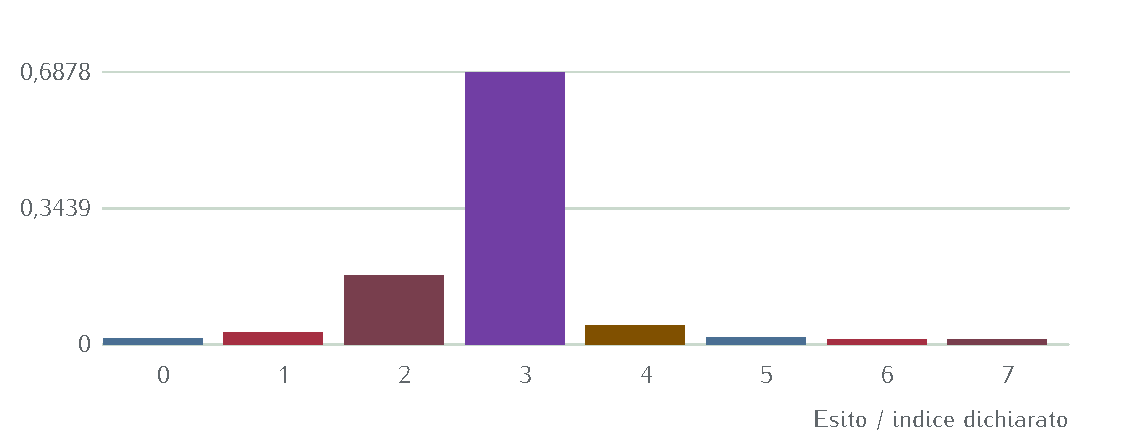
\includegraphics[width=\linewidth,height=94mm,keepaspectratio]{figure/fda04708fba5b7a77.pdf}\FigureCaption{4.13 \(\cdot\) esempio 1 \(\cdot\) Distribuzione completa della lettura}\end{FigureBlock}
\begin{FigureBlock}\centering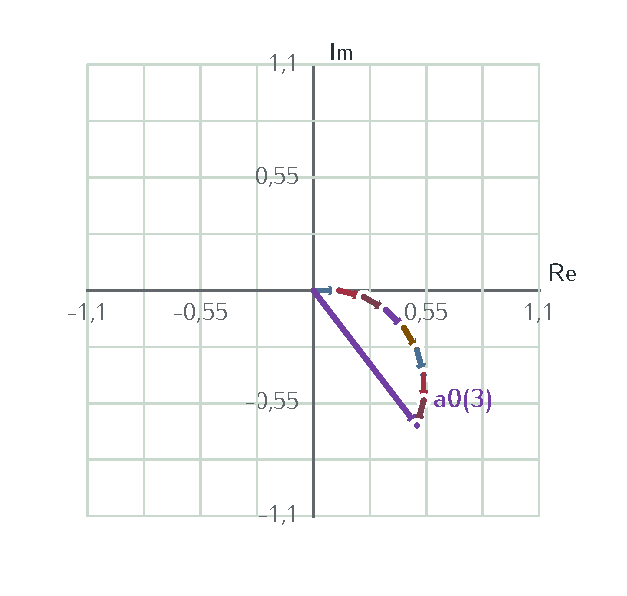
\includegraphics[width=\linewidth,height=94mm,keepaspectratio]{figure/f01f80c7e9d3dd5bd.pdf}\FigureCaption{4.13 \(\cdot\) esempio 1 \(\cdot\) Somma punta-coda, x crescente \(\cdot\) \(s=0\), \(c=3\), peso 1}\end{FigureBlock}
\begin{FigureBlock}\begin{minipage}[t]{.485\linewidth}\centering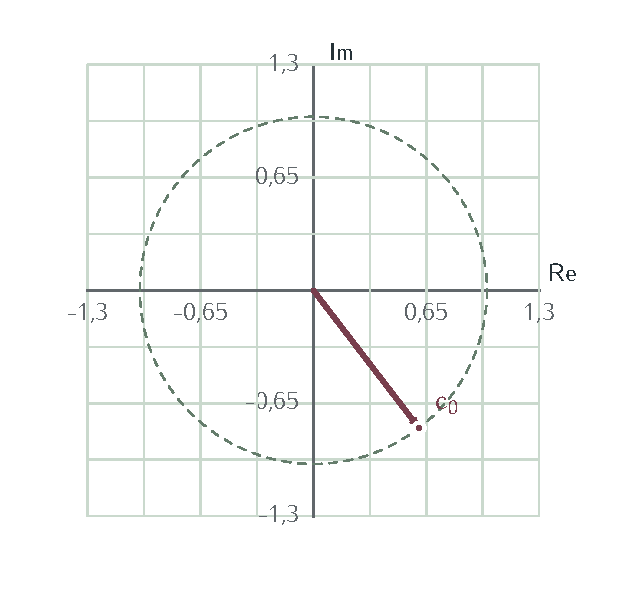
\includegraphics[width=\linewidth,height=63mm,keepaspectratio]{figure/fc7c8153a52e6550e.pdf}\par{\sffamily\footnotesize \(c_{0}\)\par}\end{minipage}\FigureCaption{4.13 \(\cdot\) esempio 1 \(\cdot\) Bersaglio condizionato \(\cdot\) coefficienti \(\beta {}^{\prime} s\) nella base propria dichiarata}\end{FigureBlock}

\phantomsection\label{c4-qpe-approssimata-example-1-step-1}
\BookHeading{01 Definire operatore, autostati e coefficienti}

\MathBlock{0055007C0075005F007327E9003D0065005E0028003203C0006903C6005F00730029007C0075005F007327E9003B002027E80075005F0073007C0075005F007427E9003D03B40073002C0074002E}{U|u_{s}\rangle =e^{2\pi i\varphi _{s}}|u_{s}\rangle ;\allowbreak \ \langle u_{s}|u_{t}\rangle =\delta s,\allowbreak t.}
\MathBlock{007C03C827E9003D03A30073002003B2005F0073007C0075005F007327E9003B002003A30073007C03B2005F0073007C00B2003D0031003B00200051003D0032005E006D002E}{|\psi \rangle =\sum _{s}\ \beta _{s}|u_{s}\rangle ;\allowbreak \ \sum _{s}|\beta _{s}|^{2}=1;\allowbreak \ Q=2^{m}.}

Il registro di lettura contiene m qubit; \(\varphi \) è una frazione di giro modulo uno. L'indice s distingue gli autostati del bersaglio e \(\beta _{s}\) è un'ampiezza complessa, mentre \(|\beta _{s}|^{2}\) è un peso probabilistico.\par


\phantomsection\label{c4-qpe-approssimata-example-1-step-2}
\BookHeading{02 Assegnare \(U\) e la preparazione}

\MathBlock{0055003D006400690061006700280031002C0065005E0028003203C0006900B70030002C0033003300330033003300330033003300290029003D0050002800310032003000B00029002E}{U=\operatorname{diag}(1,\allowbreak e^{2\pi i\cdot 0{,}33333333})=P(120{}^{\circ} ).}
\MathBlock{007C0075208027E9003D007C003127E9003B002003B22080003D0031003B0020007C03C827E9003D0058007C003027E9003D007C003127E9002E}{|u_{0}\rangle =|1\rangle ;\allowbreak \ \beta _{0}=1;\allowbreak \ |\psi \rangle =X|0\rangle =|1\rangle .}

Sono specificati matrice, autostato e preparazione. Le potenze controllate moltiplicano questo bersaglio per le fasi indicate senza cambiarne l'autodirezione.\par


\phantomsection\label{c4-qpe-approssimata-example-1-step-3}
\BookHeading{03 Preparare il controllo}

\MathBlock{007C003027E922970033007C03C827E900202192002000280031002F221A0038002903A30078007C007827E903A30073002003B2005F0073007C0075005F007327E9002E}{|0\rangle ^{\otimes 3}|\psi \rangle \ \to \ (1/\sqrt{8})\sum _{x}|x\rangle \sum _{s}\ \beta _{s}|u_{s}\rangle .}

Le Hadamard agiscono soltanto sui qubit di lettura. Il bersaglio mantiene i coefficienti appena assegnati.\par


\phantomsection\label{c4-qpe-approssimata-example-1-step-4}
\BookHeading{04 Costruire le potenze e il kickback}

\MathBlock{00660069006C006F002000710030002C0020007000650073006F00200032005E0032003A00200063006F006E00740072006F006C006C006F00200064006900200055005E0034}{\text{filo}\ q_{0},\allowbreak \ \text{peso}\ 2^{2}:\ \text{controllo}\ \text{di}\ U^{4}}
\MathBlock{00660069006C006F002000710031002C0020007000650073006F00200032005E0031003A00200063006F006E00740072006F006C006C006F00200064006900200055005E0032}{\text{filo}\ q_{1},\allowbreak \ \text{peso}\ 2^{1}:\ \text{controllo}\ \text{di}\ U^{2}}
\MathBlock{00660069006C006F002000710032002C0020007000650073006F00200032005E0030003A00200063006F006E00740072006F006C006C006F00200064006900200055005E0031}{\text{filo}\ q_{2},\allowbreak \ \text{peso}\ 2^{0}:\ \text{controllo}\ \text{di}\ U^{1}}
\MathBlock{0078003D03A3007100200078005F00710032005E0028006D22120031221200710029002021D20020220F007100200065005E0028003203C0006900200078005F00710032005E0028006D2212003122120071002903C6005F00730029003D0065005E0028003203C00069007803C6005F00730029002E}{x=\sum _{q}\ x_{q}2^{m- 1- q}\ \Rightarrow \ \prod _{q}\ e^{2\pi i\ x_{q}2^{m- 1- q}\varphi _{s}}=e^{2\pi ix\varphi _{s}}.}
\MathBlock{007C03A827E9003D00280031002F221A0051002903A30078002C0073002003B2005F007300200065005E0028003203C00069007803C6005F00730029007C007827E9007C0075005F007327E9002E}{|\Psi \rangle =(1/\sqrt{Q})\sum _{x,\allowbreak s}\ \beta _{s}\ e^{2\pi ix\varphi _{s}}|x\rangle |u_{s}\rangle .}

\(q_{0}\) è il filo superiore e il bit più significativo. Per tre qubit le potenze sono \(U^{4},\allowbreak U^{2},\allowbreak U\); l'esponente j di \(2^{j}\) non va confuso con l'indice del filo \(q_{j}\).\par


\phantomsection\label{c4-qpe-approssimata-example-1-step-5}
\BookHeading{05 Sommare le radici dell'unità}

\MathBlock{0053003D0031002B007A002B22EF002B007A005E00280038002D00310029002E}{S=1+z+\cdots +z^{8-1}.}
\MathBlock{007A0053003D007A002B007A00B2002B22EF002B007A005E0038003B0020002800312212007A00290053003D00312212007A005E0038002E}{zS=z+z^{2}+\cdots +z^{8};\allowbreak \ (1- z)S=1- z^{8}.}
\MathBlock{005300650020007A22600031003A00200053003D002800312212007A005E00380029002F002800312212007A0029002E0020005300650020007A003D0031003A00200053003D0038002E}{Se\ z\ne 1:\ S=(1- z^{8})/(1- z).\ Se\ z=1:\ S=8.}

La sottrazione cancella tutti i termini intermedi. Il caso \(z=1\) va separato prima della divisione.\par


\phantomsection\label{c4-qpe-approssimata-example-1-step-6}
\BookHeading{06 Dalla cancellazione all'unitarietà}

\MathBlock{007A003D0065005E0028003203C00069002800782212007820320029002F00380029003B0020007A005E0038003D0031002E}{z=e^{2\pi i(x- x{}^{\prime} )/8};\allowbreak \ z^{8}=1.}
\MathBlock{27E80046003800782032007C00460038007827E9003D00280031002F0038002903A300790020007A02B8003D0038002F0038003D003100200073006500200078003D00782032003B0020003000200061006C007400720069006D0065006E00740069002E}{\langle F8x{}^{\prime} |F8x\rangle =(1/8)\sum _{y}\ z^{y}=8/8=1\ \text{se}\ x=x{}^{\prime} ;\allowbreak \ 0\ \text{altrimenti}.}

Per x e \(x{}^{\prime} \) distinti fra 0 e \(N- 1\), \(z\ne 1\): le frecce delle radici si chiudono. Le colonne di Fourier sono quindi ortonormali e la trasformata conserva prodotti interni e norma.\par


\phantomsection\label{c4-qpe-approssimata-example-1-step-7}
\BookHeading{07 Applicare la cancellazione alla QPE}

\MathBlock{0044006F0070006F00200046005F00512020003A0020007C03A8006F0075007427E9003D03A30063002C0073002003B2005F007300200061005F0073002800630029007C006327E9007C0075005F007327E9002E}{\text{Dopo}\ F_{Q}{}^{\dagger} :\ |\Psi \text{out}\rangle =\sum _{c,\allowbreak s}\ \beta _{s}\ a_{s}(c)|c\rangle |u_{s}\rangle .}
\MathBlock{0061005F0073002800630029003D00280031002F0051002903A300780020007A02E3002C0020007A003D0065005E0028003203C00069002803C6005F007322120063002F005100290029002E}{a_{s}(c)=(1/Q)\sum _{x}\ z^{x},\allowbreak \ z=e^{2\pi i(\varphi _{s}- c/Q)}.}
\MathBlock{005300650020005103C6005F0073003D004C00200069006E007400650072006F003A0020007A005E0051003D0031003B00200061005F00730028004C0029003D0031002C00200061005F0073002800630029003D00300020007000650072002000632260004C002E}{Se\ Q\varphi _{s}=L\ \text{intero}:\ z^{Q}=1;\allowbreak \ a_{s}(L)=1,\allowbreak \ a_{s}(c)=0\ \text{per}\ c\ne L.}
\MathBlock{00460075006F0072006900200067007200690067006C00690061003A00200061005F0073002800630029003D002800312212007A005E00510029002F00280051002800312212007A00290029002C002000730061006C0076006F0020007A003D0031002E}{\text{Fuori}\ \text{griglia}:\ a_{s}(c)=(1- z^{Q})/(Q(1- z)),\allowbreak \ \text{salvo}\ z=1.}

Per \(Q=8\), \(\varphi =3/8\): \(a(3)=8/8=1\). Per ogni altro c, \(z=e^{2\pi i(3- c)/8}\ne 1\) e il numeratore è zero. Fuori griglia la cancellazione è incompleta e più esiti restano possibili.\par


\phantomsection\label{c4-qpe-approssimata-example-1-step-8}
\BookHeading{08 Potenze controllate \(\cdot\) autostato 0}

\MathBlock{00660069006C006F002000710030003A00200032005E003203C60020006D006F00640020003122480030002C003300330033003300330033}{\text{filo}\ q_{0}:\ 2^{2}\varphi \ \bmod \ 1\approx 0{,}333333}
\MathBlock{00660069006C006F002000710031003A00200032005E003103C60020006D006F00640020003122480030002C003600360036003600360037}{\text{filo}\ q_{1}:\ 2^{1}\varphi \ \bmod \ 1\approx 0{,}666667}
\MathBlock{00660069006C006F002000710032003A00200032005E003003C60020006D006F00640020003122480030002C003300330033003300330033}{\text{filo}\ q_{2}:\ 2^{0}\varphi \ \bmod \ 1\approx 0{,}333333}
\MathBlock{0063005F0073002800780029003D0065005E0028003203C00069007800B70030002C003300330033003300330033003300330029002F221A0038}{c_{s}(x)=e^{2\pi ix\cdot 0{,}33333333}/\sqrt{8}}

Queste fasi moltiplicano il ramo di autostato s; il suo coefficiente \(\beta _{s}\) rimane esplicito nello stato congiunto.\par


\phantomsection\label{c4-qpe-approssimata-example-1-step-9}
\BookHeading{09 Fourier inversa \(\cdot\) \(s=0\), \(c=0\)}

\MathBlock{0061005F0073002800300029003D00280031002F00380029005B0065005E0028003203C0006900B7003000B700280030002C0033003300330033003300330033003322120030002F003800290029002B0065005E0028003203C0006900B7003100B700280030002C0033003300330033003300330033003322120030002F003800290029002B0065005E0028003203C0006900B7003200B700280030002C0033003300330033003300330033003322120030002F003800290029002B0065005E0028003203C0006900B7003300B700280030002C0033003300330033003300330033003322120030002F003800290029002B0065005E0028003203C0006900B7003400B700280030002C0033003300330033003300330033003322120030002F003800290029002B0065005E0028003203C0006900B7003500B700280030002C0033003300330033003300330033003322120030002F003800290029002B0065005E0028003203C0006900B7003600B700280030002C0033003300330033003300330033003322120030002F003800290029002B0065005E0028003203C0006900B7003700B700280030002C0033003300330033003300330033003322120030002F003800290029005D}{a_{s}(0)=(1/8)[e^{2\pi i\cdot 0\cdot (0{,}33333333- 0/8)}+e^{2\pi i\cdot 1\cdot (0{,}33333333- 0/8)}+e^{2\pi i\cdot 2\cdot (0{,}33333333- 0/8)}+e^{2\pi i\cdot 3\cdot (0{,}33333333- 0/8)}+e^{2\pi i\cdot 4\cdot (0{,}33333333- 0/8)}+e^{2\pi i\cdot 5\cdot (0{,}33333333- 0/8)}+e^{2\pi i\cdot 6\cdot (0{,}33333333- 0/8)}+e^{2\pi i\cdot 7\cdot (0{,}33333333- 0/8)}]}
\MathBlock{22480030002C00300036003200350020002B00200030002C00310030003800320035003300320069003B0020007C0061007C00B222480030002C003000310035003600320035}{\approx 0{,}0625\ +\ 0{,}1082532i;\allowbreak \ |a|^{2}\approx 0{,}015625}

La somma complessa precede il modulo quadro. Le fasi nel calcolo mantengono precisione completa; i decimali stampati sono arrotondati.\par


\phantomsection\label{c4-qpe-approssimata-example-1-step-10}
\BookHeading{10 Fourier inversa \(\cdot\) \(s=0\), \(c=1\)}

\MathBlock{0061005F0073002800310029003D00280031002F00380029005B0065005E0028003203C0006900B7003000B700280030002C0033003300330033003300330033003322120031002F003800290029002B0065005E0028003203C0006900B7003100B700280030002C0033003300330033003300330033003322120031002F003800290029002B0065005E0028003203C0006900B7003200B700280030002C0033003300330033003300330033003322120031002F003800290029002B0065005E0028003203C0006900B7003300B700280030002C0033003300330033003300330033003322120031002F003800290029002B0065005E0028003203C0006900B7003400B700280030002C0033003300330033003300330033003322120031002F003800290029002B0065005E0028003203C0006900B7003500B700280030002C0033003300330033003300330033003322120031002F003800290029002B0065005E0028003203C0006900B7003600B700280030002C0033003300330033003300330033003322120031002F003800290029002B0065005E0028003203C0006900B7003700B700280030002C0033003300330033003300330033003322120031002F003800290029005D}{a_{s}(1)=(1/8)[e^{2\pi i\cdot 0\cdot (0{,}33333333- 1/8)}+e^{2\pi i\cdot 1\cdot (0{,}33333333- 1/8)}+e^{2\pi i\cdot 2\cdot (0{,}33333333- 1/8)}+e^{2\pi i\cdot 3\cdot (0{,}33333333- 1/8)}+e^{2\pi i\cdot 4\cdot (0{,}33333333- 1/8)}+e^{2\pi i\cdot 5\cdot (0{,}33333333- 1/8)}+e^{2\pi i\cdot 6\cdot (0{,}33333333- 1/8)}+e^{2\pi i\cdot 7\cdot (0{,}33333333- 1/8)}]}
\MathBlock{22480030002C00300032003300320031003000390020002B00200030002C0031003700360033003000340069003B0020007C0061007C00B222480030002C0030003300310036003200310038}{\approx 0{,}0232109\ +\ 0{,}176304i;\allowbreak \ |a|^{2}\approx 0{,}0316218}

La somma complessa precede il modulo quadro. Le fasi nel calcolo mantengono precisione completa; i decimali stampati sono arrotondati.\par


\phantomsection\label{c4-qpe-approssimata-example-1-step-11}
\BookHeading{11 Fourier inversa \(\cdot\) \(s=0\), \(c=2\)}

\MathBlock{0061005F0073002800320029003D00280031002F00380029005B0065005E0028003203C0006900B7003000B700280030002C0033003300330033003300330033003322120032002F003800290029002B0065005E0028003203C0006900B7003100B700280030002C0033003300330033003300330033003322120032002F003800290029002B0065005E0028003203C0006900B7003200B700280030002C0033003300330033003300330033003322120032002F003800290029002B0065005E0028003203C0006900B7003300B700280030002C0033003300330033003300330033003322120032002F003800290029002B0065005E0028003203C0006900B7003400B700280030002C0033003300330033003300330033003322120032002F003800290029002B0065005E0028003203C0006900B7003500B700280030002C0033003300330033003300330033003322120032002F003800290029002B0065005E0028003203C0006900B7003600B700280030002C0033003300330033003300330033003322120032002F003800290029002B0065005E0028003203C0006900B7003700B700280030002C0033003300330033003300330033003322120032002F003800290029005D}{a_{s}(2)=(1/8)[e^{2\pi i\cdot 0\cdot (0{,}33333333- 2/8)}+e^{2\pi i\cdot 1\cdot (0{,}33333333- 2/8)}+e^{2\pi i\cdot 2\cdot (0{,}33333333- 2/8)}+e^{2\pi i\cdot 3\cdot (0{,}33333333- 2/8)}+e^{2\pi i\cdot 4\cdot (0{,}33333333- 2/8)}+e^{2\pi i\cdot 5\cdot (0{,}33333333- 2/8)}+e^{2\pi i\cdot 6\cdot (0{,}33333333- 2/8)}+e^{2\pi i\cdot 7\cdot (0{,}33333333- 2/8)}]}
\MathBlock{2248002D0030002C00310030003800320035003300320020002B00200030002C00340030003400300030003600340069003B0020007C0061007C00B222480030002C0031003700340039003300390039}{\approx -0{,}1082532\ +\ 0{,}4040064i;\allowbreak \ |a|^{2}\approx 0{,}1749399}

La somma complessa precede il modulo quadro. Le fasi nel calcolo mantengono precisione completa; i decimali stampati sono arrotondati.\par


\phantomsection\label{c4-qpe-approssimata-example-1-step-12}
\BookHeading{12 Fourier inversa \(\cdot\) \(s=0\), \(c=3\)}

\MathBlock{0061005F0073002800330029003D00280031002F00380029005B0065005E0028003203C0006900B7003000B700280030002C0033003300330033003300330033003322120033002F003800290029002B0065005E0028003203C0006900B7003100B700280030002C0033003300330033003300330033003322120033002F003800290029002B0065005E0028003203C0006900B7003200B700280030002C0033003300330033003300330033003322120033002F003800290029002B0065005E0028003203C0006900B7003300B700280030002C0033003300330033003300330033003322120033002F003800290029002B0065005E0028003203C0006900B7003400B700280030002C0033003300330033003300330033003322120033002F003800290029002B0065005E0028003203C0006900B7003500B700280030002C0033003300330033003300330033003322120033002F003800290029002B0065005E0028003203C0006900B7003600B700280030002C0033003300330033003300330033003322120033002F003800290029002B0065005E0028003203C0006900B7003700B700280030002C0033003300330033003300330033003322120033002F003800290029005D}{a_{s}(3)=(1/8)[e^{2\pi i\cdot 0\cdot (0{,}33333333- 3/8)}+e^{2\pi i\cdot 1\cdot (0{,}33333333- 3/8)}+e^{2\pi i\cdot 2\cdot (0{,}33333333- 3/8)}+e^{2\pi i\cdot 3\cdot (0{,}33333333- 3/8)}+e^{2\pi i\cdot 4\cdot (0{,}33333333- 3/8)}+e^{2\pi i\cdot 5\cdot (0{,}33333333- 3/8)}+e^{2\pi i\cdot 6\cdot (0{,}33333333- 3/8)}+e^{2\pi i\cdot 7\cdot (0{,}33333333- 3/8)}]}
\MathBlock{22480030002C00350030003400380038003200330020221200200030002C00360035003700390037003500340069003B0020007C0061007C00B222480030002C0036003800370038003300370037}{\approx 0{,}5048823\ - \ 0{,}6579754i;\allowbreak \ |a|^{2}\approx 0{,}6878377}

La somma complessa precede il modulo quadro. Le fasi nel calcolo mantengono precisione completa; i decimali stampati sono arrotondati.\par


\phantomsection\label{c4-qpe-approssimata-example-1-step-13}
\BookHeading{13 Fourier inversa \(\cdot\) \(s=0\), \(c=4\)}

\MathBlock{0061005F0073002800340029003D00280031002F00380029005B0065005E0028003203C0006900B7003000B700280030002C0033003300330033003300330033003322120034002F003800290029002B0065005E0028003203C0006900B7003100B700280030002C0033003300330033003300330033003322120034002F003800290029002B0065005E0028003203C0006900B7003200B700280030002C0033003300330033003300330033003322120034002F003800290029002B0065005E0028003203C0006900B7003300B700280030002C0033003300330033003300330033003322120034002F003800290029002B0065005E0028003203C0006900B7003400B700280030002C0033003300330033003300330033003322120034002F003800290029002B0065005E0028003203C0006900B7003500B700280030002C0033003300330033003300330033003322120034002F003800290029002B0065005E0028003203C0006900B7003600B700280030002C0033003300330033003300330033003322120034002F003800290029002B0065005E0028003203C0006900B7003700B700280030002C0033003300330033003300330033003322120034002F003800290029005D}{a_{s}(4)=(1/8)[e^{2\pi i\cdot 0\cdot (0{,}33333333- 4/8)}+e^{2\pi i\cdot 1\cdot (0{,}33333333- 4/8)}+e^{2\pi i\cdot 2\cdot (0{,}33333333- 4/8)}+e^{2\pi i\cdot 3\cdot (0{,}33333333- 4/8)}+e^{2\pi i\cdot 4\cdot (0{,}33333333- 4/8)}+e^{2\pi i\cdot 5\cdot (0{,}33333333- 4/8)}+e^{2\pi i\cdot 6\cdot (0{,}33333333- 4/8)}+e^{2\pi i\cdot 7\cdot (0{,}33333333- 4/8)}]}
\MathBlock{22480030002C00310038003700350020221200200030002C00310030003800320035003300320069003B0020007C0061007C00B222480030002C003000340036003800370035}{\approx 0{,}1875\ - \ 0{,}1082532i;\allowbreak \ |a|^{2}\approx 0{,}046875}

La somma complessa precede il modulo quadro. Le fasi nel calcolo mantengono precisione completa; i decimali stampati sono arrotondati.\par


\phantomsection\label{c4-qpe-approssimata-example-1-step-14}
\BookHeading{14 Fourier inversa \(\cdot\) \(s=0\), \(c=5\)}

\MathBlock{0061005F0073002800350029003D00280031002F00380029005B0065005E0028003203C0006900B7003000B700280030002C0033003300330033003300330033003322120035002F003800290029002B0065005E0028003203C0006900B7003100B700280030002C0033003300330033003300330033003322120035002F003800290029002B0065005E0028003203C0006900B7003200B700280030002C0033003300330033003300330033003322120035002F003800290029002B0065005E0028003203C0006900B7003300B700280030002C0033003300330033003300330033003322120035002F003800290029002B0065005E0028003203C0006900B7003400B700280030002C0033003300330033003300330033003322120035002F003800290029002B0065005E0028003203C0006900B7003500B700280030002C0033003300330033003300330033003322120035002F003800290029002B0065005E0028003203C0006900B7003600B700280030002C0033003300330033003300330033003322120035002F003800290029002B0065005E0028003203C0006900B7003700B700280030002C0033003300330033003300330033003322120035002F003800290029005D}{a_{s}(5)=(1/8)[e^{2\pi i\cdot 0\cdot (0{,}33333333- 5/8)}+e^{2\pi i\cdot 1\cdot (0{,}33333333- 5/8)}+e^{2\pi i\cdot 2\cdot (0{,}33333333- 5/8)}+e^{2\pi i\cdot 3\cdot (0{,}33333333- 5/8)}+e^{2\pi i\cdot 4\cdot (0{,}33333333- 5/8)}+e^{2\pi i\cdot 5\cdot (0{,}33333333- 5/8)}+e^{2\pi i\cdot 6\cdot (0{,}33333333- 5/8)}+e^{2\pi i\cdot 7\cdot (0{,}33333333- 5/8)}]}
\MathBlock{22480030002C00310033003500320038003200380020221200200030002C00300031003700380031003000330069003B0020007C0061007C00B222480030002C0030003100380036003100380036}{\approx 0{,}1352828\ - \ 0{,}0178103i;\allowbreak \ |a|^{2}\approx 0{,}0186186}

La somma complessa precede il modulo quadro. Le fasi nel calcolo mantengono precisione completa; i decimali stampati sono arrotondati.\par


\phantomsection\label{c4-qpe-approssimata-example-1-step-15}
\BookHeading{15 Fourier inversa \(\cdot\) \(s=0\), \(c=6\)}

\MathBlock{0061005F0073002800360029003D00280031002F00380029005B0065005E0028003203C0006900B7003000B700280030002C0033003300330033003300330033003322120036002F003800290029002B0065005E0028003203C0006900B7003100B700280030002C0033003300330033003300330033003322120036002F003800290029002B0065005E0028003203C0006900B7003200B700280030002C0033003300330033003300330033003322120036002F003800290029002B0065005E0028003203C0006900B7003300B700280030002C0033003300330033003300330033003322120036002F003800290029002B0065005E0028003203C0006900B7003400B700280030002C0033003300330033003300330033003322120036002F003800290029002B0065005E0028003203C0006900B7003500B700280030002C0033003300330033003300330033003322120036002F003800290029002B0065005E0028003203C0006900B7003600B700280030002C0033003300330033003300330033003322120036002F003800290029002B0065005E0028003203C0006900B7003700B700280030002C0033003300330033003300330033003322120036002F003800290029005D}{a_{s}(6)=(1/8)[e^{2\pi i\cdot 0\cdot (0{,}33333333- 6/8)}+e^{2\pi i\cdot 1\cdot (0{,}33333333- 6/8)}+e^{2\pi i\cdot 2\cdot (0{,}33333333- 6/8)}+e^{2\pi i\cdot 3\cdot (0{,}33333333- 6/8)}+e^{2\pi i\cdot 4\cdot (0{,}33333333- 6/8)}+e^{2\pi i\cdot 5\cdot (0{,}33333333- 6/8)}+e^{2\pi i\cdot 6\cdot (0{,}33333333- 6/8)}+e^{2\pi i\cdot 7\cdot (0{,}33333333- 6/8)}]}
\MathBlock{22480030002C00310030003800320035003300320020002B00200030002C00300032003900300030003600340069003B0020007C0061007C00B222480030002C0030003100320035003600300031}{\approx 0{,}1082532\ +\ 0{,}0290064i;\allowbreak \ |a|^{2}\approx 0{,}0125601}

La somma complessa precede il modulo quadro. Le fasi nel calcolo mantengono precisione completa; i decimali stampati sono arrotondati.\par


\phantomsection\label{c4-qpe-approssimata-example-1-step-16}
\BookHeading{16 Fourier inversa \(\cdot\) \(s=0\), \(c=7\)}

\MathBlock{0061005F0073002800370029003D00280031002F00380029005B0065005E0028003203C0006900B7003000B700280030002C0033003300330033003300330033003322120037002F003800290029002B0065005E0028003203C0006900B7003100B700280030002C0033003300330033003300330033003322120037002F003800290029002B0065005E0028003203C0006900B7003200B700280030002C0033003300330033003300330033003322120037002F003800290029002B0065005E0028003203C0006900B7003300B700280030002C0033003300330033003300330033003322120037002F003800290029002B0065005E0028003203C0006900B7003400B700280030002C0033003300330033003300330033003322120037002F003800290029002B0065005E0028003203C0006900B7003500B700280030002C0033003300330033003300330033003322120037002F003800290029002B0065005E0028003203C0006900B7003600B700280030002C0033003300330033003300330033003322120037002F003800290029002B0065005E0028003203C0006900B7003700B700280030002C0033003300330033003300330033003322120037002F003800290029005D}{a_{s}(7)=(1/8)[e^{2\pi i\cdot 0\cdot (0{,}33333333- 7/8)}+e^{2\pi i\cdot 1\cdot (0{,}33333333- 7/8)}+e^{2\pi i\cdot 2\cdot (0{,}33333333- 7/8)}+e^{2\pi i\cdot 3\cdot (0{,}33333333- 7/8)}+e^{2\pi i\cdot 4\cdot (0{,}33333333- 7/8)}+e^{2\pi i\cdot 5\cdot (0{,}33333333- 7/8)}+e^{2\pi i\cdot 6\cdot (0{,}33333333- 7/8)}+e^{2\pi i\cdot 7\cdot (0{,}33333333- 7/8)}]}
\MathBlock{22480030002C00300038003600360032003400310020002B00200030002C0030003600360034003600390069003B0020007C0061007C00B222480030002C0030003100310039003200310039}{\approx 0{,}0866241\ +\ 0{,}066469i;\allowbreak \ |a|^{2}\approx 0{,}0119219}

La somma complessa precede il modulo quadro. Le fasi nel calcolo mantengono precisione completa; i decimali stampati sono arrotondati.\par


\phantomsection\label{c4-qpe-approssimata-example-1-step-17}
\BookHeading{17 Sommare la marginale}

\MathBlock{0050002800330029003D03A300730020007C03B2005F0073007C00B2007C0061005F0073002800330029007C00B2}{P(3)=\sum _{s}\ |\beta _{s}|^{2}|a_{s}(3)|^{2}}
\MathBlock{003D003100B70030002C0036003800370038003300370036003622480030002C00360038003700380033003700360036}{=1\cdot 0{,}68783766\approx 0{,}68783766}

Gli autostati del bersaglio sono ortogonali: la marginale somma le probabilità dei rami, mentre il bersaglio condizionato conserva le ampiezze complesse.\par


\phantomsection\label{c4-qpe-approssimata-example-1-step-18}
\BookHeading{18 Condizionare il bersaglio}

\MathBlock{03B220320030003D00280031002900B700280030002C00350030003400380038003200330020221200200030002C003600350037003900370035003400690029002F221A0030002C0036003800370038003300370036003622480030002C00360030003800370036003100340020221200200030002C00370039003300330035003300330069}{\beta {}^{\prime} 0=(1)\cdot (0{,}5048823\ - \ 0{,}6579754i)/\sqrt{0{,}68783766}\approx 0{,}6087614\ - \ 0{,}7933533i}

Nella QPE approssimata più coefficienti possono restare non nulli. Si divide l'intera combinazione coerente per \(\sqrt{P}(c)\); i \(\beta \) iniziali mantengono la convenzione di fase dichiarata.\par


\BookHeading{Interpretazione}

La distribuzione e il bersaglio condizionato derivano da \(U\), autostati e coefficienti complessi esplicitamente assegnati.\par


Risorse dichiarate. 3 qubit di lettura; 7 applicazioni di \(U\) se le potenze sono realizzate per ripetizione; la sintesi delle potenze può avere un costo diverso.\par


\BookHeading{Tabella completa dei dati (8 righe)}

\begingroup\sffamily\fontsize{8.8}{11}\selectfont\setlength{\tabcolsep}{1.6mm}\renewcommand{\arraystretch}{1.28}
\begin{longtable}{>{\RaggedRight\arraybackslash}p{19.958mm}>{\RaggedRight\arraybackslash}p{33.263mm}>{\RaggedRight\arraybackslash}p{73.179mm}}
\toprule\rowcolor{Accent!7}\BeginAccSupp{method=hex,unicode,ActualText=0063}c\EndAccSupp{} & \BeginAccSupp{method=hex,unicode,ActualText=0063002F0051}c/Q\EndAccSupp{} & \BeginAccSupp{method=hex,unicode,ActualText=0050002800630029}P(c)\EndAccSupp{} \\
\midrule\endfirsthead
\toprule\rowcolor{Accent!7}\BeginAccSupp{method=hex,unicode,ActualText=0063}c\EndAccSupp{} & \BeginAccSupp{method=hex,unicode,ActualText=0063002F0051}c/Q\EndAccSupp{} & \BeginAccSupp{method=hex,unicode,ActualText=0050002800630029}P(c)\EndAccSupp{} \\
\midrule\endhead\bottomrule\endfoot
\BeginAccSupp{method=hex,unicode,ActualText=0030}0\EndAccSupp{} & \BeginAccSupp{method=hex,unicode,ActualText=0030}0\EndAccSupp{} & \BeginAccSupp{method=hex,unicode,ActualText=0030002C003000310035003600320035}0,015625\EndAccSupp{} \\
\BeginAccSupp{method=hex,unicode,ActualText=0031}1\EndAccSupp{} & \BeginAccSupp{method=hex,unicode,ActualText=0030002C003100320035}0,125\EndAccSupp{} & \BeginAccSupp{method=hex,unicode,ActualText=0030002C003000330031003600320031003800330032}0,031621832\EndAccSupp{} \\
\BeginAccSupp{method=hex,unicode,ActualText=0032}2\EndAccSupp{} & \BeginAccSupp{method=hex,unicode,ActualText=0030002C00320035}0,25\EndAccSupp{} & \BeginAccSupp{method=hex,unicode,ActualText=0030002C003100370034003900330039003800380032}0,174939882\EndAccSupp{} \\
\BeginAccSupp{method=hex,unicode,ActualText=0033}3\EndAccSupp{} & \BeginAccSupp{method=hex,unicode,ActualText=0030002C003300370035}0,375\EndAccSupp{} & \BeginAccSupp{method=hex,unicode,ActualText=0030002C003600380037003800330037003600360033}0,687837663\EndAccSupp{} \\
\BeginAccSupp{method=hex,unicode,ActualText=0034}4\EndAccSupp{} & \BeginAccSupp{method=hex,unicode,ActualText=0030002C0035}0,5\EndAccSupp{} & \BeginAccSupp{method=hex,unicode,ActualText=0030002C003000340036003800370035}0,046875\EndAccSupp{} \\
\BeginAccSupp{method=hex,unicode,ActualText=0035}5\EndAccSupp{} & \BeginAccSupp{method=hex,unicode,ActualText=0030002C003600320035}0,625\EndAccSupp{} & \BeginAccSupp{method=hex,unicode,ActualText=0030002C003000310038003600310038003600340031}0,018618641\EndAccSupp{} \\
\BeginAccSupp{method=hex,unicode,ActualText=0036}6\EndAccSupp{} & \BeginAccSupp{method=hex,unicode,ActualText=0030002C00370035}0,75\EndAccSupp{} & \BeginAccSupp{method=hex,unicode,ActualText=0030002C003000310032003500360030003100310038}0,012560118\EndAccSupp{} \\
\BeginAccSupp{method=hex,unicode,ActualText=0037}7\EndAccSupp{} & \BeginAccSupp{method=hex,unicode,ActualText=0030002C003800370035}0,875\EndAccSupp{} & \BeginAccSupp{method=hex,unicode,ActualText=0030002C003000310031003900320031003800360034}0,011921864\EndAccSupp{} \\
\end{longtable}\endgroup

\Needspace{.36\textheight}\phantomsection\label{c4-qpe-approssimata-example-2}
{\sffamily\small\color{Accent} ESEMPIO SVOLTO 2\par}
\BookHeading{Esempio 2}
\(m=3\); \(Q=2^{m}=8\); autofasi (frazioni di giro) 0,333333, 0,666667; pesi 0,5, 0,5.\par


\BookHeading{Geometria e configurazione dell'esempio}
\begin{FigureBlock}\centering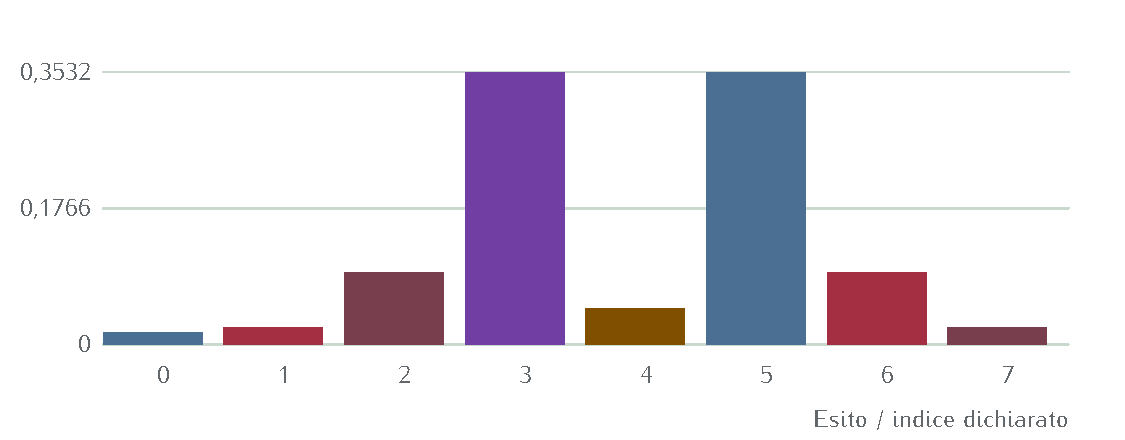
\includegraphics[width=\linewidth,height=94mm,keepaspectratio]{figure/fd46667541786b27a.pdf}\FigureCaption{4.13 \(\cdot\) esempio 2 \(\cdot\) Distribuzione completa della lettura}\end{FigureBlock}
\begin{FigureBlock}\centering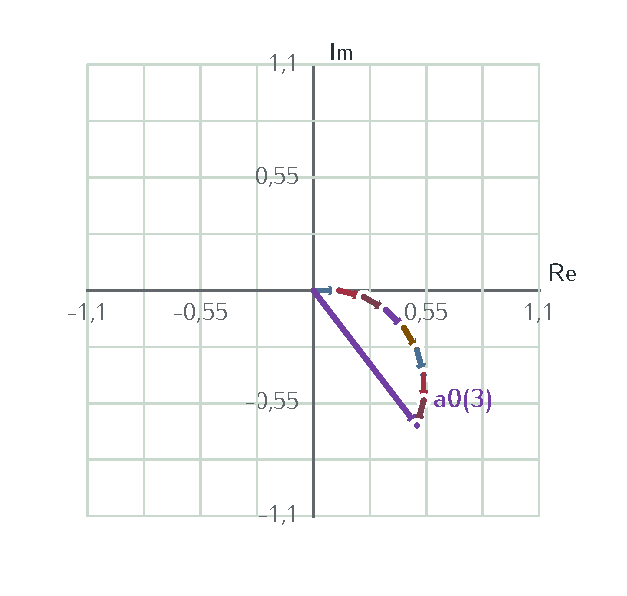
\includegraphics[width=\linewidth,height=94mm,keepaspectratio]{figure/f0568b5af96a11a31.pdf}\FigureCaption{4.13 \(\cdot\) esempio 2 \(\cdot\) Somma punta-coda, x crescente \(\cdot\) \(s=0\), \(c=3\), peso 0,5}\end{FigureBlock}
\begin{FigureBlock}\centering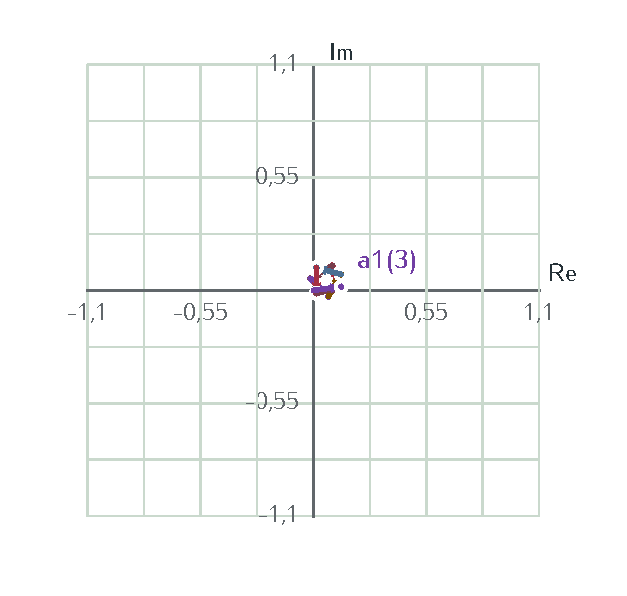
\includegraphics[width=\linewidth,height=94mm,keepaspectratio]{figure/f3d38acc394271201.pdf}\FigureCaption{4.13 \(\cdot\) esempio 2 \(\cdot\) Somma punta-coda, x crescente \(\cdot\) \(s=1\), \(c=3\), peso 0,5}\end{FigureBlock}
\begin{FigureBlock}\begin{minipage}[t]{.485\linewidth}\centering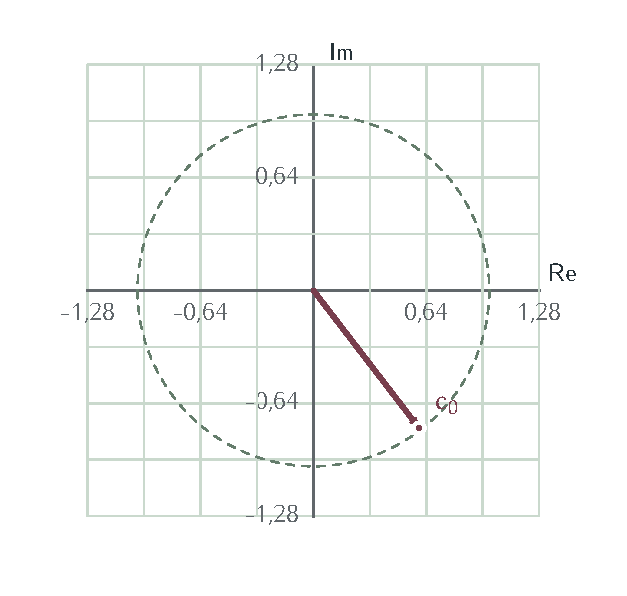
\includegraphics[width=\linewidth,height=63mm,keepaspectratio]{figure/f3ff2161f8989c0f0.pdf}\par{\sffamily\footnotesize \(c_{0}\)\par}\end{minipage}\hfill\begin{minipage}[t]{.485\linewidth}\centering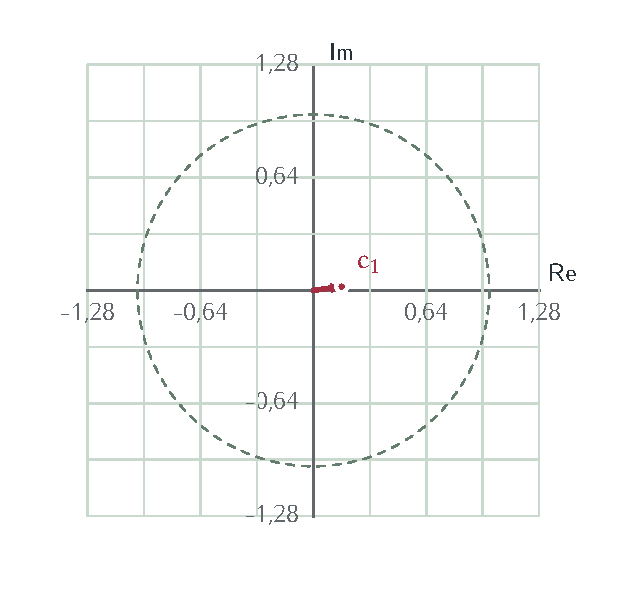
\includegraphics[width=\linewidth,height=63mm,keepaspectratio]{figure/f25387f412c596ab9.pdf}\par{\sffamily\footnotesize \(c_{1}\)\par}\end{minipage}\FigureCaption{4.13 \(\cdot\) esempio 2 \(\cdot\) Bersaglio condizionato \(\cdot\) coefficienti \(\beta {}^{\prime} s\) nella base propria dichiarata}\end{FigureBlock}

\phantomsection\label{c4-qpe-approssimata-example-2-step-1}
\BookHeading{01 Definire operatore, autostati e coefficienti}

\MathBlock{0055007C0075005F007327E9003D0065005E0028003203C0006903C6005F00730029007C0075005F007327E9003B002027E80075005F0073007C0075005F007427E9003D03B40073002C0074002E}{U|u_{s}\rangle =e^{2\pi i\varphi _{s}}|u_{s}\rangle ;\allowbreak \ \langle u_{s}|u_{t}\rangle =\delta s,\allowbreak t.}
\MathBlock{007C03C827E9003D03A30073002003B2005F0073007C0075005F007327E9003B002003A30073007C03B2005F0073007C00B2003D0031003B00200051003D0032005E006D002E}{|\psi \rangle =\sum _{s}\ \beta _{s}|u_{s}\rangle ;\allowbreak \ \sum _{s}|\beta _{s}|^{2}=1;\allowbreak \ Q=2^{m}.}

Il registro di lettura contiene m qubit; \(\varphi \) è una frazione di giro modulo uno. L'indice s distingue gli autostati del bersaglio e \(\beta _{s}\) è un'ampiezza complessa, mentre \(|\beta _{s}|^{2}\) è un peso probabilistico.\par


\phantomsection\label{c4-qpe-approssimata-example-2-step-2}
\BookHeading{02 Assegnare \(U\) e la preparazione}

\MathBlock{0055003D006400690061006700280065005E0028003203C0006900B70030002C003300330033003300330033003300330029002C0065005E0028003203C0006900B70030002C0036003600360036003600360036003700290029002E}{U=\operatorname{diag}(e^{2\pi i\cdot 0{,}33333333},\allowbreak e^{2\pi i\cdot 0{,}66666667}).}
\MathBlock{007C0075208027E9003D007C003027E9003B0020007C0075208127E9003D007C003127E9003B002003B22080003D03B22081003D0031002F221A0032003B0020007C03C827E9003D0048007C003027E9003D007C002B27E9002E}{|u_{0}\rangle =|0\rangle ;\allowbreak \ |u_{1}\rangle =|1\rangle ;\allowbreak \ \beta _{0}=\beta _{1}=1/\sqrt{2};\allowbreak \ |\psi \rangle =H|0\rangle =|+\rangle .}

La matrice diagonale e la fase reale positiva della preparazione fissano lo stato congiunto. Una fase globale di \(U\) diventa relativa quando \(U\) è controllata, perciò viene conservata.\par


\phantomsection\label{c4-qpe-approssimata-example-2-step-3}
\BookHeading{03 Preparare il controllo}

\MathBlock{007C003027E922970033007C03C827E900202192002000280031002F221A0038002903A30078007C007827E903A30073002003B2005F0073007C0075005F007327E9002E}{|0\rangle ^{\otimes 3}|\psi \rangle \ \to \ (1/\sqrt{8})\sum _{x}|x\rangle \sum _{s}\ \beta _{s}|u_{s}\rangle .}

Le Hadamard agiscono soltanto sui qubit di lettura. Il bersaglio mantiene i coefficienti appena assegnati.\par


\phantomsection\label{c4-qpe-approssimata-example-2-step-4}
\BookHeading{04 Costruire le potenze e il kickback}

\MathBlock{00660069006C006F002000710030002C0020007000650073006F00200032005E0032003A00200063006F006E00740072006F006C006C006F00200064006900200055005E0034}{\text{filo}\ q_{0},\allowbreak \ \text{peso}\ 2^{2}:\ \text{controllo}\ \text{di}\ U^{4}}
\MathBlock{00660069006C006F002000710031002C0020007000650073006F00200032005E0031003A00200063006F006E00740072006F006C006C006F00200064006900200055005E0032}{\text{filo}\ q_{1},\allowbreak \ \text{peso}\ 2^{1}:\ \text{controllo}\ \text{di}\ U^{2}}
\MathBlock{00660069006C006F002000710032002C0020007000650073006F00200032005E0030003A00200063006F006E00740072006F006C006C006F00200064006900200055005E0031}{\text{filo}\ q_{2},\allowbreak \ \text{peso}\ 2^{0}:\ \text{controllo}\ \text{di}\ U^{1}}
\MathBlock{0078003D03A3007100200078005F00710032005E0028006D22120031221200710029002021D20020220F007100200065005E0028003203C0006900200078005F00710032005E0028006D2212003122120071002903C6005F00730029003D0065005E0028003203C00069007803C6005F00730029002E}{x=\sum _{q}\ x_{q}2^{m- 1- q}\ \Rightarrow \ \prod _{q}\ e^{2\pi i\ x_{q}2^{m- 1- q}\varphi _{s}}=e^{2\pi ix\varphi _{s}}.}
\MathBlock{007C03A827E9003D00280031002F221A0051002903A30078002C0073002003B2005F007300200065005E0028003203C00069007803C6005F00730029007C007827E9007C0075005F007327E9002E}{|\Psi \rangle =(1/\sqrt{Q})\sum _{x,\allowbreak s}\ \beta _{s}\ e^{2\pi ix\varphi _{s}}|x\rangle |u_{s}\rangle .}

\(q_{0}\) è il filo superiore e il bit più significativo. Per tre qubit le potenze sono \(U^{4},\allowbreak U^{2},\allowbreak U\); l'esponente j di \(2^{j}\) non va confuso con l'indice del filo \(q_{j}\).\par


\phantomsection\label{c4-qpe-approssimata-example-2-step-5}
\BookHeading{05 Sommare le radici dell'unità}

\MathBlock{0053003D0031002B007A002B22EF002B007A005E00280038002D00310029002E}{S=1+z+\cdots +z^{8-1}.}
\MathBlock{007A0053003D007A002B007A00B2002B22EF002B007A005E0038003B0020002800312212007A00290053003D00312212007A005E0038002E}{zS=z+z^{2}+\cdots +z^{8};\allowbreak \ (1- z)S=1- z^{8}.}
\MathBlock{005300650020007A22600031003A00200053003D002800312212007A005E00380029002F002800312212007A0029002E0020005300650020007A003D0031003A00200053003D0038002E}{Se\ z\ne 1:\ S=(1- z^{8})/(1- z).\ Se\ z=1:\ S=8.}

La sottrazione cancella tutti i termini intermedi. Il caso \(z=1\) va separato prima della divisione.\par


\phantomsection\label{c4-qpe-approssimata-example-2-step-6}
\BookHeading{06 Dalla cancellazione all'unitarietà}

\MathBlock{007A003D0065005E0028003203C00069002800782212007820320029002F00380029003B0020007A005E0038003D0031002E}{z=e^{2\pi i(x- x{}^{\prime} )/8};\allowbreak \ z^{8}=1.}
\MathBlock{27E80046003800782032007C00460038007827E9003D00280031002F0038002903A300790020007A02B8003D0038002F0038003D003100200073006500200078003D00782032003B0020003000200061006C007400720069006D0065006E00740069002E}{\langle F8x{}^{\prime} |F8x\rangle =(1/8)\sum _{y}\ z^{y}=8/8=1\ \text{se}\ x=x{}^{\prime} ;\allowbreak \ 0\ \text{altrimenti}.}

Per x e \(x{}^{\prime} \) distinti fra 0 e \(N- 1\), \(z\ne 1\): le frecce delle radici si chiudono. Le colonne di Fourier sono quindi ortonormali e la trasformata conserva prodotti interni e norma.\par


\phantomsection\label{c4-qpe-approssimata-example-2-step-7}
\BookHeading{07 Applicare la cancellazione alla QPE}

\MathBlock{0044006F0070006F00200046005F00512020003A0020007C03A8006F0075007427E9003D03A30063002C0073002003B2005F007300200061005F0073002800630029007C006327E9007C0075005F007327E9002E}{\text{Dopo}\ F_{Q}{}^{\dagger} :\ |\Psi \text{out}\rangle =\sum _{c,\allowbreak s}\ \beta _{s}\ a_{s}(c)|c\rangle |u_{s}\rangle .}
\MathBlock{0061005F0073002800630029003D00280031002F0051002903A300780020007A02E3002C0020007A003D0065005E0028003203C00069002803C6005F007322120063002F005100290029002E}{a_{s}(c)=(1/Q)\sum _{x}\ z^{x},\allowbreak \ z=e^{2\pi i(\varphi _{s}- c/Q)}.}
\MathBlock{005300650020005103C6005F0073003D004C00200069006E007400650072006F003A0020007A005E0051003D0031003B00200061005F00730028004C0029003D0031002C00200061005F0073002800630029003D00300020007000650072002000632260004C002E}{Se\ Q\varphi _{s}=L\ \text{intero}:\ z^{Q}=1;\allowbreak \ a_{s}(L)=1,\allowbreak \ a_{s}(c)=0\ \text{per}\ c\ne L.}
\MathBlock{00460075006F0072006900200067007200690067006C00690061003A00200061005F0073002800630029003D002800312212007A005E00510029002F00280051002800312212007A00290029002C002000730061006C0076006F0020007A003D0031002E}{\text{Fuori}\ \text{griglia}:\ a_{s}(c)=(1- z^{Q})/(Q(1- z)),\allowbreak \ \text{salvo}\ z=1.}

Per \(Q=8\), \(\varphi =3/8\): \(a(3)=8/8=1\). Per ogni altro c, \(z=e^{2\pi i(3- c)/8}\ne 1\) e il numeratore è zero. Fuori griglia la cancellazione è incompleta e più esiti restano possibili.\par


\phantomsection\label{c4-qpe-approssimata-example-2-step-8}
\BookHeading{08 Potenze controllate \(\cdot\) autostato 0}

\MathBlock{00660069006C006F002000710030003A00200032005E003203C60020006D006F00640020003122480030002C003300330033003300330033}{\text{filo}\ q_{0}:\ 2^{2}\varphi \ \bmod \ 1\approx 0{,}333333}
\MathBlock{00660069006C006F002000710031003A00200032005E003103C60020006D006F00640020003122480030002C003600360036003600360037}{\text{filo}\ q_{1}:\ 2^{1}\varphi \ \bmod \ 1\approx 0{,}666667}
\MathBlock{00660069006C006F002000710032003A00200032005E003003C60020006D006F00640020003122480030002C003300330033003300330033}{\text{filo}\ q_{2}:\ 2^{0}\varphi \ \bmod \ 1\approx 0{,}333333}
\MathBlock{0063005F0073002800780029003D0065005E0028003203C00069007800B70030002C003300330033003300330033003300330029002F221A0038}{c_{s}(x)=e^{2\pi ix\cdot 0{,}33333333}/\sqrt{8}}

Queste fasi moltiplicano il ramo di autostato s; il suo coefficiente \(\beta _{s}\) rimane esplicito nello stato congiunto.\par


\phantomsection\label{c4-qpe-approssimata-example-2-step-9}
\BookHeading{09 Fourier inversa \(\cdot\) \(s=0\), \(c=0\)}

\MathBlock{0061005F0073002800300029003D00280031002F00380029005B0065005E0028003203C0006900B7003000B700280030002C0033003300330033003300330033003322120030002F003800290029002B0065005E0028003203C0006900B7003100B700280030002C0033003300330033003300330033003322120030002F003800290029002B0065005E0028003203C0006900B7003200B700280030002C0033003300330033003300330033003322120030002F003800290029002B0065005E0028003203C0006900B7003300B700280030002C0033003300330033003300330033003322120030002F003800290029002B0065005E0028003203C0006900B7003400B700280030002C0033003300330033003300330033003322120030002F003800290029002B0065005E0028003203C0006900B7003500B700280030002C0033003300330033003300330033003322120030002F003800290029002B0065005E0028003203C0006900B7003600B700280030002C0033003300330033003300330033003322120030002F003800290029002B0065005E0028003203C0006900B7003700B700280030002C0033003300330033003300330033003322120030002F003800290029005D}{a_{s}(0)=(1/8)[e^{2\pi i\cdot 0\cdot (0{,}33333333- 0/8)}+e^{2\pi i\cdot 1\cdot (0{,}33333333- 0/8)}+e^{2\pi i\cdot 2\cdot (0{,}33333333- 0/8)}+e^{2\pi i\cdot 3\cdot (0{,}33333333- 0/8)}+e^{2\pi i\cdot 4\cdot (0{,}33333333- 0/8)}+e^{2\pi i\cdot 5\cdot (0{,}33333333- 0/8)}+e^{2\pi i\cdot 6\cdot (0{,}33333333- 0/8)}+e^{2\pi i\cdot 7\cdot (0{,}33333333- 0/8)}]}
\MathBlock{22480030002C00300036003200350020002B00200030002C00310030003800320035003300320069003B0020007C0061007C00B222480030002C003000310035003600320035}{\approx 0{,}0625\ +\ 0{,}1082532i;\allowbreak \ |a|^{2}\approx 0{,}015625}

La somma complessa precede il modulo quadro. Le fasi nel calcolo mantengono precisione completa; i decimali stampati sono arrotondati.\par


\phantomsection\label{c4-qpe-approssimata-example-2-step-10}
\BookHeading{10 Fourier inversa \(\cdot\) \(s=0\), \(c=1\)}

\MathBlock{0061005F0073002800310029003D00280031002F00380029005B0065005E0028003203C0006900B7003000B700280030002C0033003300330033003300330033003322120031002F003800290029002B0065005E0028003203C0006900B7003100B700280030002C0033003300330033003300330033003322120031002F003800290029002B0065005E0028003203C0006900B7003200B700280030002C0033003300330033003300330033003322120031002F003800290029002B0065005E0028003203C0006900B7003300B700280030002C0033003300330033003300330033003322120031002F003800290029002B0065005E0028003203C0006900B7003400B700280030002C0033003300330033003300330033003322120031002F003800290029002B0065005E0028003203C0006900B7003500B700280030002C0033003300330033003300330033003322120031002F003800290029002B0065005E0028003203C0006900B7003600B700280030002C0033003300330033003300330033003322120031002F003800290029002B0065005E0028003203C0006900B7003700B700280030002C0033003300330033003300330033003322120031002F003800290029005D}{a_{s}(1)=(1/8)[e^{2\pi i\cdot 0\cdot (0{,}33333333- 1/8)}+e^{2\pi i\cdot 1\cdot (0{,}33333333- 1/8)}+e^{2\pi i\cdot 2\cdot (0{,}33333333- 1/8)}+e^{2\pi i\cdot 3\cdot (0{,}33333333- 1/8)}+e^{2\pi i\cdot 4\cdot (0{,}33333333- 1/8)}+e^{2\pi i\cdot 5\cdot (0{,}33333333- 1/8)}+e^{2\pi i\cdot 6\cdot (0{,}33333333- 1/8)}+e^{2\pi i\cdot 7\cdot (0{,}33333333- 1/8)}]}
\MathBlock{22480030002C00300032003300320031003000390020002B00200030002C0031003700360033003000340069003B0020007C0061007C00B222480030002C0030003300310036003200310038}{\approx 0{,}0232109\ +\ 0{,}176304i;\allowbreak \ |a|^{2}\approx 0{,}0316218}

La somma complessa precede il modulo quadro. Le fasi nel calcolo mantengono precisione completa; i decimali stampati sono arrotondati.\par


\phantomsection\label{c4-qpe-approssimata-example-2-step-11}
\BookHeading{11 Fourier inversa \(\cdot\) \(s=0\), \(c=2\)}

\MathBlock{0061005F0073002800320029003D00280031002F00380029005B0065005E0028003203C0006900B7003000B700280030002C0033003300330033003300330033003322120032002F003800290029002B0065005E0028003203C0006900B7003100B700280030002C0033003300330033003300330033003322120032002F003800290029002B0065005E0028003203C0006900B7003200B700280030002C0033003300330033003300330033003322120032002F003800290029002B0065005E0028003203C0006900B7003300B700280030002C0033003300330033003300330033003322120032002F003800290029002B0065005E0028003203C0006900B7003400B700280030002C0033003300330033003300330033003322120032002F003800290029002B0065005E0028003203C0006900B7003500B700280030002C0033003300330033003300330033003322120032002F003800290029002B0065005E0028003203C0006900B7003600B700280030002C0033003300330033003300330033003322120032002F003800290029002B0065005E0028003203C0006900B7003700B700280030002C0033003300330033003300330033003322120032002F003800290029005D}{a_{s}(2)=(1/8)[e^{2\pi i\cdot 0\cdot (0{,}33333333- 2/8)}+e^{2\pi i\cdot 1\cdot (0{,}33333333- 2/8)}+e^{2\pi i\cdot 2\cdot (0{,}33333333- 2/8)}+e^{2\pi i\cdot 3\cdot (0{,}33333333- 2/8)}+e^{2\pi i\cdot 4\cdot (0{,}33333333- 2/8)}+e^{2\pi i\cdot 5\cdot (0{,}33333333- 2/8)}+e^{2\pi i\cdot 6\cdot (0{,}33333333- 2/8)}+e^{2\pi i\cdot 7\cdot (0{,}33333333- 2/8)}]}
\MathBlock{2248002D0030002C00310030003800320035003300320020002B00200030002C00340030003400300030003600340069003B0020007C0061007C00B222480030002C0031003700340039003300390039}{\approx -0{,}1082532\ +\ 0{,}4040064i;\allowbreak \ |a|^{2}\approx 0{,}1749399}

La somma complessa precede il modulo quadro. Le fasi nel calcolo mantengono precisione completa; i decimali stampati sono arrotondati.\par


\phantomsection\label{c4-qpe-approssimata-example-2-step-12}
\BookHeading{12 Fourier inversa \(\cdot\) \(s=0\), \(c=3\)}

\MathBlock{0061005F0073002800330029003D00280031002F00380029005B0065005E0028003203C0006900B7003000B700280030002C0033003300330033003300330033003322120033002F003800290029002B0065005E0028003203C0006900B7003100B700280030002C0033003300330033003300330033003322120033002F003800290029002B0065005E0028003203C0006900B7003200B700280030002C0033003300330033003300330033003322120033002F003800290029002B0065005E0028003203C0006900B7003300B700280030002C0033003300330033003300330033003322120033002F003800290029002B0065005E0028003203C0006900B7003400B700280030002C0033003300330033003300330033003322120033002F003800290029002B0065005E0028003203C0006900B7003500B700280030002C0033003300330033003300330033003322120033002F003800290029002B0065005E0028003203C0006900B7003600B700280030002C0033003300330033003300330033003322120033002F003800290029002B0065005E0028003203C0006900B7003700B700280030002C0033003300330033003300330033003322120033002F003800290029005D}{a_{s}(3)=(1/8)[e^{2\pi i\cdot 0\cdot (0{,}33333333- 3/8)}+e^{2\pi i\cdot 1\cdot (0{,}33333333- 3/8)}+e^{2\pi i\cdot 2\cdot (0{,}33333333- 3/8)}+e^{2\pi i\cdot 3\cdot (0{,}33333333- 3/8)}+e^{2\pi i\cdot 4\cdot (0{,}33333333- 3/8)}+e^{2\pi i\cdot 5\cdot (0{,}33333333- 3/8)}+e^{2\pi i\cdot 6\cdot (0{,}33333333- 3/8)}+e^{2\pi i\cdot 7\cdot (0{,}33333333- 3/8)}]}
\MathBlock{22480030002C00350030003400380038003200330020221200200030002C00360035003700390037003500340069003B0020007C0061007C00B222480030002C0036003800370038003300370037}{\approx 0{,}5048823\ - \ 0{,}6579754i;\allowbreak \ |a|^{2}\approx 0{,}6878377}

La somma complessa precede il modulo quadro. Le fasi nel calcolo mantengono precisione completa; i decimali stampati sono arrotondati.\par


\phantomsection\label{c4-qpe-approssimata-example-2-step-13}
\BookHeading{13 Fourier inversa \(\cdot\) \(s=0\), \(c=4\)}

\MathBlock{0061005F0073002800340029003D00280031002F00380029005B0065005E0028003203C0006900B7003000B700280030002C0033003300330033003300330033003322120034002F003800290029002B0065005E0028003203C0006900B7003100B700280030002C0033003300330033003300330033003322120034002F003800290029002B0065005E0028003203C0006900B7003200B700280030002C0033003300330033003300330033003322120034002F003800290029002B0065005E0028003203C0006900B7003300B700280030002C0033003300330033003300330033003322120034002F003800290029002B0065005E0028003203C0006900B7003400B700280030002C0033003300330033003300330033003322120034002F003800290029002B0065005E0028003203C0006900B7003500B700280030002C0033003300330033003300330033003322120034002F003800290029002B0065005E0028003203C0006900B7003600B700280030002C0033003300330033003300330033003322120034002F003800290029002B0065005E0028003203C0006900B7003700B700280030002C0033003300330033003300330033003322120034002F003800290029005D}{a_{s}(4)=(1/8)[e^{2\pi i\cdot 0\cdot (0{,}33333333- 4/8)}+e^{2\pi i\cdot 1\cdot (0{,}33333333- 4/8)}+e^{2\pi i\cdot 2\cdot (0{,}33333333- 4/8)}+e^{2\pi i\cdot 3\cdot (0{,}33333333- 4/8)}+e^{2\pi i\cdot 4\cdot (0{,}33333333- 4/8)}+e^{2\pi i\cdot 5\cdot (0{,}33333333- 4/8)}+e^{2\pi i\cdot 6\cdot (0{,}33333333- 4/8)}+e^{2\pi i\cdot 7\cdot (0{,}33333333- 4/8)}]}
\MathBlock{22480030002C00310038003700350020221200200030002C00310030003800320035003300320069003B0020007C0061007C00B222480030002C003000340036003800370035}{\approx 0{,}1875\ - \ 0{,}1082532i;\allowbreak \ |a|^{2}\approx 0{,}046875}

La somma complessa precede il modulo quadro. Le fasi nel calcolo mantengono precisione completa; i decimali stampati sono arrotondati.\par


\phantomsection\label{c4-qpe-approssimata-example-2-step-14}
\BookHeading{14 Fourier inversa \(\cdot\) \(s=0\), \(c=5\)}

\MathBlock{0061005F0073002800350029003D00280031002F00380029005B0065005E0028003203C0006900B7003000B700280030002C0033003300330033003300330033003322120035002F003800290029002B0065005E0028003203C0006900B7003100B700280030002C0033003300330033003300330033003322120035002F003800290029002B0065005E0028003203C0006900B7003200B700280030002C0033003300330033003300330033003322120035002F003800290029002B0065005E0028003203C0006900B7003300B700280030002C0033003300330033003300330033003322120035002F003800290029002B0065005E0028003203C0006900B7003400B700280030002C0033003300330033003300330033003322120035002F003800290029002B0065005E0028003203C0006900B7003500B700280030002C0033003300330033003300330033003322120035002F003800290029002B0065005E0028003203C0006900B7003600B700280030002C0033003300330033003300330033003322120035002F003800290029002B0065005E0028003203C0006900B7003700B700280030002C0033003300330033003300330033003322120035002F003800290029005D}{a_{s}(5)=(1/8)[e^{2\pi i\cdot 0\cdot (0{,}33333333- 5/8)}+e^{2\pi i\cdot 1\cdot (0{,}33333333- 5/8)}+e^{2\pi i\cdot 2\cdot (0{,}33333333- 5/8)}+e^{2\pi i\cdot 3\cdot (0{,}33333333- 5/8)}+e^{2\pi i\cdot 4\cdot (0{,}33333333- 5/8)}+e^{2\pi i\cdot 5\cdot (0{,}33333333- 5/8)}+e^{2\pi i\cdot 6\cdot (0{,}33333333- 5/8)}+e^{2\pi i\cdot 7\cdot (0{,}33333333- 5/8)}]}
\MathBlock{22480030002C00310033003500320038003200380020221200200030002C00300031003700380031003000330069003B0020007C0061007C00B222480030002C0030003100380036003100380036}{\approx 0{,}1352828\ - \ 0{,}0178103i;\allowbreak \ |a|^{2}\approx 0{,}0186186}

La somma complessa precede il modulo quadro. Le fasi nel calcolo mantengono precisione completa; i decimali stampati sono arrotondati.\par


\phantomsection\label{c4-qpe-approssimata-example-2-step-15}
\BookHeading{15 Fourier inversa \(\cdot\) \(s=0\), \(c=6\)}

\MathBlock{0061005F0073002800360029003D00280031002F00380029005B0065005E0028003203C0006900B7003000B700280030002C0033003300330033003300330033003322120036002F003800290029002B0065005E0028003203C0006900B7003100B700280030002C0033003300330033003300330033003322120036002F003800290029002B0065005E0028003203C0006900B7003200B700280030002C0033003300330033003300330033003322120036002F003800290029002B0065005E0028003203C0006900B7003300B700280030002C0033003300330033003300330033003322120036002F003800290029002B0065005E0028003203C0006900B7003400B700280030002C0033003300330033003300330033003322120036002F003800290029002B0065005E0028003203C0006900B7003500B700280030002C0033003300330033003300330033003322120036002F003800290029002B0065005E0028003203C0006900B7003600B700280030002C0033003300330033003300330033003322120036002F003800290029002B0065005E0028003203C0006900B7003700B700280030002C0033003300330033003300330033003322120036002F003800290029005D}{a_{s}(6)=(1/8)[e^{2\pi i\cdot 0\cdot (0{,}33333333- 6/8)}+e^{2\pi i\cdot 1\cdot (0{,}33333333- 6/8)}+e^{2\pi i\cdot 2\cdot (0{,}33333333- 6/8)}+e^{2\pi i\cdot 3\cdot (0{,}33333333- 6/8)}+e^{2\pi i\cdot 4\cdot (0{,}33333333- 6/8)}+e^{2\pi i\cdot 5\cdot (0{,}33333333- 6/8)}+e^{2\pi i\cdot 6\cdot (0{,}33333333- 6/8)}+e^{2\pi i\cdot 7\cdot (0{,}33333333- 6/8)}]}
\MathBlock{22480030002C00310030003800320035003300320020002B00200030002C00300032003900300030003600340069003B0020007C0061007C00B222480030002C0030003100320035003600300031}{\approx 0{,}1082532\ +\ 0{,}0290064i;\allowbreak \ |a|^{2}\approx 0{,}0125601}

La somma complessa precede il modulo quadro. Le fasi nel calcolo mantengono precisione completa; i decimali stampati sono arrotondati.\par


\phantomsection\label{c4-qpe-approssimata-example-2-step-16}
\BookHeading{16 Fourier inversa \(\cdot\) \(s=0\), \(c=7\)}

\MathBlock{0061005F0073002800370029003D00280031002F00380029005B0065005E0028003203C0006900B7003000B700280030002C0033003300330033003300330033003322120037002F003800290029002B0065005E0028003203C0006900B7003100B700280030002C0033003300330033003300330033003322120037002F003800290029002B0065005E0028003203C0006900B7003200B700280030002C0033003300330033003300330033003322120037002F003800290029002B0065005E0028003203C0006900B7003300B700280030002C0033003300330033003300330033003322120037002F003800290029002B0065005E0028003203C0006900B7003400B700280030002C0033003300330033003300330033003322120037002F003800290029002B0065005E0028003203C0006900B7003500B700280030002C0033003300330033003300330033003322120037002F003800290029002B0065005E0028003203C0006900B7003600B700280030002C0033003300330033003300330033003322120037002F003800290029002B0065005E0028003203C0006900B7003700B700280030002C0033003300330033003300330033003322120037002F003800290029005D}{a_{s}(7)=(1/8)[e^{2\pi i\cdot 0\cdot (0{,}33333333- 7/8)}+e^{2\pi i\cdot 1\cdot (0{,}33333333- 7/8)}+e^{2\pi i\cdot 2\cdot (0{,}33333333- 7/8)}+e^{2\pi i\cdot 3\cdot (0{,}33333333- 7/8)}+e^{2\pi i\cdot 4\cdot (0{,}33333333- 7/8)}+e^{2\pi i\cdot 5\cdot (0{,}33333333- 7/8)}+e^{2\pi i\cdot 6\cdot (0{,}33333333- 7/8)}+e^{2\pi i\cdot 7\cdot (0{,}33333333- 7/8)}]}
\MathBlock{22480030002C00300038003600360032003400310020002B00200030002C0030003600360034003600390069003B0020007C0061007C00B222480030002C0030003100310039003200310039}{\approx 0{,}0866241\ +\ 0{,}066469i;\allowbreak \ |a|^{2}\approx 0{,}0119219}

La somma complessa precede il modulo quadro. Le fasi nel calcolo mantengono precisione completa; i decimali stampati sono arrotondati.\par


\phantomsection\label{c4-qpe-approssimata-example-2-step-17}
\BookHeading{17 Potenze controllate \(\cdot\) autostato 1}

\MathBlock{00660069006C006F002000710030003A00200032005E003203C60020006D006F00640020003122480030002C003600360036003600360037}{\text{filo}\ q_{0}:\ 2^{2}\varphi \ \bmod \ 1\approx 0{,}666667}
\MathBlock{00660069006C006F002000710031003A00200032005E003103C60020006D006F00640020003122480030002C003300330033003300330033}{\text{filo}\ q_{1}:\ 2^{1}\varphi \ \bmod \ 1\approx 0{,}333333}
\MathBlock{00660069006C006F002000710032003A00200032005E003003C60020006D006F00640020003122480030002C003600360036003600360037}{\text{filo}\ q_{2}:\ 2^{0}\varphi \ \bmod \ 1\approx 0{,}666667}
\MathBlock{0063005F0073002800780029003D0065005E0028003203C00069007800B70030002C003600360036003600360036003600370029002F221A0038}{c_{s}(x)=e^{2\pi ix\cdot 0{,}66666667}/\sqrt{8}}

Queste fasi moltiplicano il ramo di autostato s; il suo coefficiente \(\beta _{s}\) rimane esplicito nello stato congiunto.\par


\phantomsection\label{c4-qpe-approssimata-example-2-step-18}
\BookHeading{18 Fourier inversa \(\cdot\) \(s=1\), \(c=0\)}

\MathBlock{0061005F0073002800300029003D00280031002F00380029005B0065005E0028003203C0006900B7003000B700280030002C0036003600360036003600360036003722120030002F003800290029002B0065005E0028003203C0006900B7003100B700280030002C0036003600360036003600360036003722120030002F003800290029002B0065005E0028003203C0006900B7003200B700280030002C0036003600360036003600360036003722120030002F003800290029002B0065005E0028003203C0006900B7003300B700280030002C0036003600360036003600360036003722120030002F003800290029002B0065005E0028003203C0006900B7003400B700280030002C0036003600360036003600360036003722120030002F003800290029002B0065005E0028003203C0006900B7003500B700280030002C0036003600360036003600360036003722120030002F003800290029002B0065005E0028003203C0006900B7003600B700280030002C0036003600360036003600360036003722120030002F003800290029002B0065005E0028003203C0006900B7003700B700280030002C0036003600360036003600360036003722120030002F003800290029005D}{a_{s}(0)=(1/8)[e^{2\pi i\cdot 0\cdot (0{,}66666667- 0/8)}+e^{2\pi i\cdot 1\cdot (0{,}66666667- 0/8)}+e^{2\pi i\cdot 2\cdot (0{,}66666667- 0/8)}+e^{2\pi i\cdot 3\cdot (0{,}66666667- 0/8)}+e^{2\pi i\cdot 4\cdot (0{,}66666667- 0/8)}+e^{2\pi i\cdot 5\cdot (0{,}66666667- 0/8)}+e^{2\pi i\cdot 6\cdot (0{,}66666667- 0/8)}+e^{2\pi i\cdot 7\cdot (0{,}66666667- 0/8)}]}
\MathBlock{22480030002C00300036003200350020221200200030002C00310030003800320035003300320069003B0020007C0061007C00B222480030002C003000310035003600320035}{\approx 0{,}0625\ - \ 0{,}1082532i;\allowbreak \ |a|^{2}\approx 0{,}015625}

La somma complessa precede il modulo quadro. Le fasi nel calcolo mantengono precisione completa; i decimali stampati sono arrotondati.\par


\phantomsection\label{c4-qpe-approssimata-example-2-step-19}
\BookHeading{19 Fourier inversa \(\cdot\) \(s=1\), \(c=1\)}

\MathBlock{0061005F0073002800310029003D00280031002F00380029005B0065005E0028003203C0006900B7003000B700280030002C0036003600360036003600360036003722120031002F003800290029002B0065005E0028003203C0006900B7003100B700280030002C0036003600360036003600360036003722120031002F003800290029002B0065005E0028003203C0006900B7003200B700280030002C0036003600360036003600360036003722120031002F003800290029002B0065005E0028003203C0006900B7003300B700280030002C0036003600360036003600360036003722120031002F003800290029002B0065005E0028003203C0006900B7003400B700280030002C0036003600360036003600360036003722120031002F003800290029002B0065005E0028003203C0006900B7003500B700280030002C0036003600360036003600360036003722120031002F003800290029002B0065005E0028003203C0006900B7003600B700280030002C0036003600360036003600360036003722120031002F003800290029002B0065005E0028003203C0006900B7003700B700280030002C0036003600360036003600360036003722120031002F003800290029005D}{a_{s}(1)=(1/8)[e^{2\pi i\cdot 0\cdot (0{,}66666667- 1/8)}+e^{2\pi i\cdot 1\cdot (0{,}66666667- 1/8)}+e^{2\pi i\cdot 2\cdot (0{,}66666667- 1/8)}+e^{2\pi i\cdot 3\cdot (0{,}66666667- 1/8)}+e^{2\pi i\cdot 4\cdot (0{,}66666667- 1/8)}+e^{2\pi i\cdot 5\cdot (0{,}66666667- 1/8)}+e^{2\pi i\cdot 6\cdot (0{,}66666667- 1/8)}+e^{2\pi i\cdot 7\cdot (0{,}66666667- 1/8)}]}
\MathBlock{22480030002C00300038003600360032003400310020221200200030002C0030003600360034003600390069003B0020007C0061007C00B222480030002C0030003100310039003200310039}{\approx 0{,}0866241\ - \ 0{,}066469i;\allowbreak \ |a|^{2}\approx 0{,}0119219}

La somma complessa precede il modulo quadro. Le fasi nel calcolo mantengono precisione completa; i decimali stampati sono arrotondati.\par


\phantomsection\label{c4-qpe-approssimata-example-2-step-20}
\BookHeading{20 Fourier inversa \(\cdot\) \(s=1\), \(c=2\)}

\MathBlock{0061005F0073002800320029003D00280031002F00380029005B0065005E0028003203C0006900B7003000B700280030002C0036003600360036003600360036003722120032002F003800290029002B0065005E0028003203C0006900B7003100B700280030002C0036003600360036003600360036003722120032002F003800290029002B0065005E0028003203C0006900B7003200B700280030002C0036003600360036003600360036003722120032002F003800290029002B0065005E0028003203C0006900B7003300B700280030002C0036003600360036003600360036003722120032002F003800290029002B0065005E0028003203C0006900B7003400B700280030002C0036003600360036003600360036003722120032002F003800290029002B0065005E0028003203C0006900B7003500B700280030002C0036003600360036003600360036003722120032002F003800290029002B0065005E0028003203C0006900B7003600B700280030002C0036003600360036003600360036003722120032002F003800290029002B0065005E0028003203C0006900B7003700B700280030002C0036003600360036003600360036003722120032002F003800290029005D}{a_{s}(2)=(1/8)[e^{2\pi i\cdot 0\cdot (0{,}66666667- 2/8)}+e^{2\pi i\cdot 1\cdot (0{,}66666667- 2/8)}+e^{2\pi i\cdot 2\cdot (0{,}66666667- 2/8)}+e^{2\pi i\cdot 3\cdot (0{,}66666667- 2/8)}+e^{2\pi i\cdot 4\cdot (0{,}66666667- 2/8)}+e^{2\pi i\cdot 5\cdot (0{,}66666667- 2/8)}+e^{2\pi i\cdot 6\cdot (0{,}66666667- 2/8)}+e^{2\pi i\cdot 7\cdot (0{,}66666667- 2/8)}]}
\MathBlock{22480030002C00310030003800320035003300320020221200200030002C00300032003900300030003600340069003B0020007C0061007C00B222480030002C0030003100320035003600300031}{\approx 0{,}1082532\ - \ 0{,}0290064i;\allowbreak \ |a|^{2}\approx 0{,}0125601}

La somma complessa precede il modulo quadro. Le fasi nel calcolo mantengono precisione completa; i decimali stampati sono arrotondati.\par


\phantomsection\label{c4-qpe-approssimata-example-2-step-21}
\BookHeading{21 Fourier inversa \(\cdot\) \(s=1\), \(c=3\)}

\MathBlock{0061005F0073002800330029003D00280031002F00380029005B0065005E0028003203C0006900B7003000B700280030002C0036003600360036003600360036003722120033002F003800290029002B0065005E0028003203C0006900B7003100B700280030002C0036003600360036003600360036003722120033002F003800290029002B0065005E0028003203C0006900B7003200B700280030002C0036003600360036003600360036003722120033002F003800290029002B0065005E0028003203C0006900B7003300B700280030002C0036003600360036003600360036003722120033002F003800290029002B0065005E0028003203C0006900B7003400B700280030002C0036003600360036003600360036003722120033002F003800290029002B0065005E0028003203C0006900B7003500B700280030002C0036003600360036003600360036003722120033002F003800290029002B0065005E0028003203C0006900B7003600B700280030002C0036003600360036003600360036003722120033002F003800290029002B0065005E0028003203C0006900B7003700B700280030002C0036003600360036003600360036003722120033002F003800290029005D}{a_{s}(3)=(1/8)[e^{2\pi i\cdot 0\cdot (0{,}66666667- 3/8)}+e^{2\pi i\cdot 1\cdot (0{,}66666667- 3/8)}+e^{2\pi i\cdot 2\cdot (0{,}66666667- 3/8)}+e^{2\pi i\cdot 3\cdot (0{,}66666667- 3/8)}+e^{2\pi i\cdot 4\cdot (0{,}66666667- 3/8)}+e^{2\pi i\cdot 5\cdot (0{,}66666667- 3/8)}+e^{2\pi i\cdot 6\cdot (0{,}66666667- 3/8)}+e^{2\pi i\cdot 7\cdot (0{,}66666667- 3/8)}]}
\MathBlock{22480030002C00310033003500320038003200380020002B00200030002C00300031003700380031003000330069003B0020007C0061007C00B222480030002C0030003100380036003100380036}{\approx 0{,}1352828\ +\ 0{,}0178103i;\allowbreak \ |a|^{2}\approx 0{,}0186186}

La somma complessa precede il modulo quadro. Le fasi nel calcolo mantengono precisione completa; i decimali stampati sono arrotondati.\par


\phantomsection\label{c4-qpe-approssimata-example-2-step-22}
\BookHeading{22 Fourier inversa \(\cdot\) \(s=1\), \(c=4\)}

\MathBlock{0061005F0073002800340029003D00280031002F00380029005B0065005E0028003203C0006900B7003000B700280030002C0036003600360036003600360036003722120034002F003800290029002B0065005E0028003203C0006900B7003100B700280030002C0036003600360036003600360036003722120034002F003800290029002B0065005E0028003203C0006900B7003200B700280030002C0036003600360036003600360036003722120034002F003800290029002B0065005E0028003203C0006900B7003300B700280030002C0036003600360036003600360036003722120034002F003800290029002B0065005E0028003203C0006900B7003400B700280030002C0036003600360036003600360036003722120034002F003800290029002B0065005E0028003203C0006900B7003500B700280030002C0036003600360036003600360036003722120034002F003800290029002B0065005E0028003203C0006900B7003600B700280030002C0036003600360036003600360036003722120034002F003800290029002B0065005E0028003203C0006900B7003700B700280030002C0036003600360036003600360036003722120034002F003800290029005D}{a_{s}(4)=(1/8)[e^{2\pi i\cdot 0\cdot (0{,}66666667- 4/8)}+e^{2\pi i\cdot 1\cdot (0{,}66666667- 4/8)}+e^{2\pi i\cdot 2\cdot (0{,}66666667- 4/8)}+e^{2\pi i\cdot 3\cdot (0{,}66666667- 4/8)}+e^{2\pi i\cdot 4\cdot (0{,}66666667- 4/8)}+e^{2\pi i\cdot 5\cdot (0{,}66666667- 4/8)}+e^{2\pi i\cdot 6\cdot (0{,}66666667- 4/8)}+e^{2\pi i\cdot 7\cdot (0{,}66666667- 4/8)}]}
\MathBlock{22480030002C00310038003700350020002B00200030002C00310030003800320035003300320069003B0020007C0061007C00B222480030002C003000340036003800370035}{\approx 0{,}1875\ +\ 0{,}1082532i;\allowbreak \ |a|^{2}\approx 0{,}046875}

La somma complessa precede il modulo quadro. Le fasi nel calcolo mantengono precisione completa; i decimali stampati sono arrotondati.\par


\phantomsection\label{c4-qpe-approssimata-example-2-step-23}
\BookHeading{23 Fourier inversa \(\cdot\) \(s=1\), \(c=5\)}

\MathBlock{0061005F0073002800350029003D00280031002F00380029005B0065005E0028003203C0006900B7003000B700280030002C0036003600360036003600360036003722120035002F003800290029002B0065005E0028003203C0006900B7003100B700280030002C0036003600360036003600360036003722120035002F003800290029002B0065005E0028003203C0006900B7003200B700280030002C0036003600360036003600360036003722120035002F003800290029002B0065005E0028003203C0006900B7003300B700280030002C0036003600360036003600360036003722120035002F003800290029002B0065005E0028003203C0006900B7003400B700280030002C0036003600360036003600360036003722120035002F003800290029002B0065005E0028003203C0006900B7003500B700280030002C0036003600360036003600360036003722120035002F003800290029002B0065005E0028003203C0006900B7003600B700280030002C0036003600360036003600360036003722120035002F003800290029002B0065005E0028003203C0006900B7003700B700280030002C0036003600360036003600360036003722120035002F003800290029005D}{a_{s}(5)=(1/8)[e^{2\pi i\cdot 0\cdot (0{,}66666667- 5/8)}+e^{2\pi i\cdot 1\cdot (0{,}66666667- 5/8)}+e^{2\pi i\cdot 2\cdot (0{,}66666667- 5/8)}+e^{2\pi i\cdot 3\cdot (0{,}66666667- 5/8)}+e^{2\pi i\cdot 4\cdot (0{,}66666667- 5/8)}+e^{2\pi i\cdot 5\cdot (0{,}66666667- 5/8)}+e^{2\pi i\cdot 6\cdot (0{,}66666667- 5/8)}+e^{2\pi i\cdot 7\cdot (0{,}66666667- 5/8)}]}
\MathBlock{22480030002C00350030003400380038003200330020002B00200030002C00360035003700390037003500340069003B0020007C0061007C00B222480030002C0036003800370038003300370037}{\approx 0{,}5048823\ +\ 0{,}6579754i;\allowbreak \ |a|^{2}\approx 0{,}6878377}

La somma complessa precede il modulo quadro. Le fasi nel calcolo mantengono precisione completa; i decimali stampati sono arrotondati.\par


\phantomsection\label{c4-qpe-approssimata-example-2-step-24}
\BookHeading{24 Fourier inversa \(\cdot\) \(s=1\), \(c=6\)}

\MathBlock{0061005F0073002800360029003D00280031002F00380029005B0065005E0028003203C0006900B7003000B700280030002C0036003600360036003600360036003722120036002F003800290029002B0065005E0028003203C0006900B7003100B700280030002C0036003600360036003600360036003722120036002F003800290029002B0065005E0028003203C0006900B7003200B700280030002C0036003600360036003600360036003722120036002F003800290029002B0065005E0028003203C0006900B7003300B700280030002C0036003600360036003600360036003722120036002F003800290029002B0065005E0028003203C0006900B7003400B700280030002C0036003600360036003600360036003722120036002F003800290029002B0065005E0028003203C0006900B7003500B700280030002C0036003600360036003600360036003722120036002F003800290029002B0065005E0028003203C0006900B7003600B700280030002C0036003600360036003600360036003722120036002F003800290029002B0065005E0028003203C0006900B7003700B700280030002C0036003600360036003600360036003722120036002F003800290029005D}{a_{s}(6)=(1/8)[e^{2\pi i\cdot 0\cdot (0{,}66666667- 6/8)}+e^{2\pi i\cdot 1\cdot (0{,}66666667- 6/8)}+e^{2\pi i\cdot 2\cdot (0{,}66666667- 6/8)}+e^{2\pi i\cdot 3\cdot (0{,}66666667- 6/8)}+e^{2\pi i\cdot 4\cdot (0{,}66666667- 6/8)}+e^{2\pi i\cdot 5\cdot (0{,}66666667- 6/8)}+e^{2\pi i\cdot 6\cdot (0{,}66666667- 6/8)}+e^{2\pi i\cdot 7\cdot (0{,}66666667- 6/8)}]}
\MathBlock{2248002D0030002C00310030003800320035003300320020221200200030002C00340030003400300030003600340069003B0020007C0061007C00B222480030002C0031003700340039003300390039}{\approx -0{,}1082532\ - \ 0{,}4040064i;\allowbreak \ |a|^{2}\approx 0{,}1749399}

La somma complessa precede il modulo quadro. Le fasi nel calcolo mantengono precisione completa; i decimali stampati sono arrotondati.\par


\phantomsection\label{c4-qpe-approssimata-example-2-step-25}
\BookHeading{25 Fourier inversa \(\cdot\) \(s=1\), \(c=7\)}

\MathBlock{0061005F0073002800370029003D00280031002F00380029005B0065005E0028003203C0006900B7003000B700280030002C0036003600360036003600360036003722120037002F003800290029002B0065005E0028003203C0006900B7003100B700280030002C0036003600360036003600360036003722120037002F003800290029002B0065005E0028003203C0006900B7003200B700280030002C0036003600360036003600360036003722120037002F003800290029002B0065005E0028003203C0006900B7003300B700280030002C0036003600360036003600360036003722120037002F003800290029002B0065005E0028003203C0006900B7003400B700280030002C0036003600360036003600360036003722120037002F003800290029002B0065005E0028003203C0006900B7003500B700280030002C0036003600360036003600360036003722120037002F003800290029002B0065005E0028003203C0006900B7003600B700280030002C0036003600360036003600360036003722120037002F003800290029002B0065005E0028003203C0006900B7003700B700280030002C0036003600360036003600360036003722120037002F003800290029005D}{a_{s}(7)=(1/8)[e^{2\pi i\cdot 0\cdot (0{,}66666667- 7/8)}+e^{2\pi i\cdot 1\cdot (0{,}66666667- 7/8)}+e^{2\pi i\cdot 2\cdot (0{,}66666667- 7/8)}+e^{2\pi i\cdot 3\cdot (0{,}66666667- 7/8)}+e^{2\pi i\cdot 4\cdot (0{,}66666667- 7/8)}+e^{2\pi i\cdot 5\cdot (0{,}66666667- 7/8)}+e^{2\pi i\cdot 6\cdot (0{,}66666667- 7/8)}+e^{2\pi i\cdot 7\cdot (0{,}66666667- 7/8)}]}
\MathBlock{22480030002C00300032003300320031003000390020221200200030002C0031003700360033003000340069003B0020007C0061007C00B222480030002C0030003300310036003200310038}{\approx 0{,}0232109\ - \ 0{,}176304i;\allowbreak \ |a|^{2}\approx 0{,}0316218}

La somma complessa precede il modulo quadro. Le fasi nel calcolo mantengono precisione completa; i decimali stampati sono arrotondati.\par


\phantomsection\label{c4-qpe-approssimata-example-2-step-26}
\BookHeading{26 Sommare la marginale}

\MathBlock{0050002800330029003D03A300730020007C03B2005F0073007C00B2007C0061005F0073002800330029007C00B2}{P(3)=\sum _{s}\ |\beta _{s}|^{2}|a_{s}(3)|^{2}}
\MathBlock{003D0030002C003500B70030002C00360038003700380033003700360036002B0030002C003500B70030002C0030003100380036003100380036003422480030002C00330035003300320032003800310035}{=0{,}5\cdot 0{,}68783766+0{,}5\cdot 0{,}01861864\approx 0{,}35322815}

Gli autostati del bersaglio sono ortogonali: la marginale somma le probabilità dei rami, mentre il bersaglio condizionato conserva le ampiezze complesse.\par


\phantomsection\label{c4-qpe-approssimata-example-2-step-27}
\BookHeading{27 Condizionare il bersaglio}

\MathBlock{03B220320030003D00280030002C0037003000370031003000360038002900B700280030002C00350030003400380038003200330020221200200030002C003600350037003900370035003400690029002F221A0030002C0033003500330032003200380031003522480030002C00360030003000360038003500390020221200200030002C00370038003200380032003900310069}{\beta {}^{\prime} 0=(0{,}7071068)\cdot (0{,}5048823\ - \ 0{,}6579754i)/\sqrt{0{,}35322815}\approx 0{,}6006859\ - \ 0{,}7828291i}
\MathBlock{03B220320031003D00280030002C0037003000370031003000360038002900B700280030002C00310033003500320038003200380020002B00200030002C003000310037003800310030003300690029002F221A0030002C0033003500330032003200380031003522480030002C00310036003000390035003300330020002B00200030002C00300032003100310038003900390069}{\beta {}^{\prime} 1=(0{,}7071068)\cdot (0{,}1352828\ +\ 0{,}0178103i)/\sqrt{0{,}35322815}\approx 0{,}1609533\ +\ 0{,}0211899i}

Nella QPE approssimata più coefficienti possono restare non nulli. Si divide l'intera combinazione coerente per \(\sqrt{P}(c)\); i \(\beta \) iniziali mantengono la convenzione di fase dichiarata.\par


\BookHeading{Interpretazione}

La distribuzione e il bersaglio condizionato derivano da \(U\), autostati e coefficienti complessi esplicitamente assegnati.\par


Risorse dichiarate. 3 qubit di lettura; 7 applicazioni di \(U\) se le potenze sono realizzate per ripetizione; la sintesi delle potenze può avere un costo diverso.\par


\BookHeading{Tabella completa dei dati (8 righe)}

\begingroup\sffamily\fontsize{8.8}{11}\selectfont\setlength{\tabcolsep}{1.6mm}\renewcommand{\arraystretch}{1.28}
\begin{longtable}{>{\RaggedRight\arraybackslash}p{19.958mm}>{\RaggedRight\arraybackslash}p{33.263mm}>{\RaggedRight\arraybackslash}p{73.179mm}}
\toprule\rowcolor{Accent!7}\BeginAccSupp{method=hex,unicode,ActualText=0063}c\EndAccSupp{} & \BeginAccSupp{method=hex,unicode,ActualText=0063002F0051}c/Q\EndAccSupp{} & \BeginAccSupp{method=hex,unicode,ActualText=0050002800630029}P(c)\EndAccSupp{} \\
\midrule\endfirsthead
\toprule\rowcolor{Accent!7}\BeginAccSupp{method=hex,unicode,ActualText=0063}c\EndAccSupp{} & \BeginAccSupp{method=hex,unicode,ActualText=0063002F0051}c/Q\EndAccSupp{} & \BeginAccSupp{method=hex,unicode,ActualText=0050002800630029}P(c)\EndAccSupp{} \\
\midrule\endhead\bottomrule\endfoot
\BeginAccSupp{method=hex,unicode,ActualText=0030}0\EndAccSupp{} & \BeginAccSupp{method=hex,unicode,ActualText=0030}0\EndAccSupp{} & \BeginAccSupp{method=hex,unicode,ActualText=0030002C003000310035003600320035}0,015625\EndAccSupp{} \\
\BeginAccSupp{method=hex,unicode,ActualText=0031}1\EndAccSupp{} & \BeginAccSupp{method=hex,unicode,ActualText=0030002C003100320035}0,125\EndAccSupp{} & \BeginAccSupp{method=hex,unicode,ActualText=0030002C003000320031003700370031003800340038}0,021771848\EndAccSupp{} \\
\BeginAccSupp{method=hex,unicode,ActualText=0032}2\EndAccSupp{} & \BeginAccSupp{method=hex,unicode,ActualText=0030002C00320035}0,25\EndAccSupp{} & \BeginAccSupp{method=hex,unicode,ActualText=0030002C00300039003300370035}0,09375\EndAccSupp{} \\
\BeginAccSupp{method=hex,unicode,ActualText=0033}3\EndAccSupp{} & \BeginAccSupp{method=hex,unicode,ActualText=0030002C003300370035}0,375\EndAccSupp{} & \BeginAccSupp{method=hex,unicode,ActualText=0030002C003300350033003200320038003100350032}0,353228152\EndAccSupp{} \\
\BeginAccSupp{method=hex,unicode,ActualText=0034}4\EndAccSupp{} & \BeginAccSupp{method=hex,unicode,ActualText=0030002C0035}0,5\EndAccSupp{} & \BeginAccSupp{method=hex,unicode,ActualText=0030002C003000340036003800370035}0,046875\EndAccSupp{} \\
\BeginAccSupp{method=hex,unicode,ActualText=0035}5\EndAccSupp{} & \BeginAccSupp{method=hex,unicode,ActualText=0030002C003600320035}0,625\EndAccSupp{} & \BeginAccSupp{method=hex,unicode,ActualText=0030002C003300350033003200320038003100350032}0,353228152\EndAccSupp{} \\
\BeginAccSupp{method=hex,unicode,ActualText=0036}6\EndAccSupp{} & \BeginAccSupp{method=hex,unicode,ActualText=0030002C00370035}0,75\EndAccSupp{} & \BeginAccSupp{method=hex,unicode,ActualText=0030002C00300039003300370035}0,09375\EndAccSupp{} \\
\BeginAccSupp{method=hex,unicode,ActualText=0037}7\EndAccSupp{} & \BeginAccSupp{method=hex,unicode,ActualText=0030002C003800370035}0,875\EndAccSupp{} & \BeginAccSupp{method=hex,unicode,ActualText=0030002C003000320031003700370031003800340038}0,021771848\EndAccSupp{} \\
\end{longtable}\endgroup

\Needspace{7\baselineskip}
\BookHeading{Il passaggio successivo}
QPE stima le autofasi di qualunque unitaria di cui sappiamo costruire le potenze controllate. L'iterazione di Grover ha autofasi legate all'angolo \(\theta \): ricavandole possiamo risalire al numero dei marcati.\par


% Authoritative exercise source. Preserve all derivations and diagrams.

\ExerciseStart{G4.08}{Calcolare una fase non rappresentabile esattamente}{Consolidamento}

\BookHeading{Problema, dati e obiettivo}

Stimare \(\phi=1/3\) con tre qubit, Q=8, partendo da un autostato. Calcolare la distribuzione completa, l’esito più probabile e il suo errore.

\ExTheory{\ExRef{c4-qpe-approssimata}{4.13}}{Quando \(Q\phi\) non è intero, i fasori della trasformata inversa non si allineano perfettamente. L’ampiezza è \(A(c)=Q^{-1}\sum_{x=0}^{Q-1}e^{2\pi ix(\phi-c/Q)}\); occorre sommare le ampiezze prima di prendere il modulo quadro.}

\ExPrediction{La fase cade fra 2/8 e 3/8, più vicina a 3/8. Si prevede un picco vicino a c=3, accompagnato da probabilità residue sugli altri esiti.}

\ExFigure{\begin{tikzpicture}[>=Stealth,exlabel]
\draw[exother] (0.00000,0.00000)--(1.00000,0.00000);\draw[exother] (1.00000,0.00000)--(1.96593,-0.25882);\draw[exother] (1.96593,-0.25882)--(2.83195,-0.75882);\draw[exother] (2.83195,-0.75882)--(3.53906,-1.46593);\draw[exother] (3.53906,-1.46593)--(4.03906,-2.33195);\draw[exother] (4.03906,-2.33195)--(4.29788,-3.29788);\draw[exother] (4.29788,-3.29788)--(4.29788,-4.29788);\draw[exother] (4.29788,-4.29788)--(4.03906,-5.26380);
\end{tikzpicture}}{Somma punta-coda degli otto fasori per c=3; l’ampiezza è il vettore risultante diviso per otto.}


\begin{ExTasks}

\item Ricavare la formula della somma finita.

\item Semplificare il numeratore per Q=8 e fase 1/3.

\item Calcolare tutti gli otto esiti.

\item Quantificare l’errore della lettura più probabile.

\end{ExTasks}

\ExSolution

\ExStep{Sommare i fasori}

Pongo \(\delta_c=1/3-c/8=(8-3c)/24\), \(z=e^{2\pi i\delta_c}\). Nessun c intero fra 0 e 7 rende z=1. Dalla sottrazione
\ExEq{S-zS&=(1+z+\cdots+z^7)-(z+\cdots+z^8)=1-z^8}
si ricava \(S=(1-z^8)/(1-z)\) e \(A(c)=S/8\).

\ExStep{Calcolare il modulo}

\ExEq{|1-e^{it}|^2&=(1-\cos t)^2+\sin^2t=2-2\cos t=4\sin^2(t/2),\\
P(c)&=\frac{\sin^2(8\pi\delta_c)}{64\sin^2(\pi\delta_c)}.}
Poiché \(8\delta_c=8/3-c\), il numeratore è \(\sin^2(8\pi/3-\pi c)=3/4\). Quindi
\ExEq{P(c)&=\frac3{256\sin^2(\pi(8-3c)/24)}.}

\ExStep{Sostituire tutti i valori}

I numeratori \(8-3c\) sono \(8,5,2,-1,-4,-7,-10,-13\). Sostituendoli nella formula si ottiene la tabella seguente, arrotondata a sei decimali. Le ampiezze derivano dalla formula complessa della somma finita.\begin{center}\begin{tabular}{rrrr}\toprule c&$\delta_c$&$A(c)$&$P(c)$\\\midrule
0&0.333333&0.062500+0.108253i&0.015625\\
1&0.208333&0.023211+0.176304i&0.031622\\
2&0.083333&-0.108253+0.404006i&0.174940\\
3&-0.041667&0.504882-0.657975i&0.687838\\
4&-0.166667&0.187500-0.108253i&0.046875\\
5&-0.291667&0.135283-0.017810i&0.018619\\
6&-0.416667&0.108253+0.029006i&0.012560\\
7&-0.541667&0.086624+0.066469i&0.011922\\
\bottomrule\end{tabular}\end{center}

\ExStep{Esaminare il picco}

\ExEq{\delta_3&=-1/24,\quad
A(3)=\frac{3/2+i\sqrt3/2}{8[1-\cos(\pi/12)+i\sin(\pi/12)]},\\
P(3)&=\frac3{256[(\sqrt6-\sqrt2)/4]^2}\simeq0.687838.}
Il denominatore ha modulo minimo in c=3, che fornisce quindi il massimo della distribuzione.

\ExStep{Controllare normalizzazione ed errore}

La somma degli otto valori non arrotondati è uno, come segue anche dall’unitarietà dell’inversa. Se si legge 3, la stima è \(3/8\) e
\ExEq{\frac38-\frac13&=\frac9{24}-\frac8{24}=\frac1{24}.}
Questo errore riguarda quel ramo. Altre misure danno altri errori; la probabilità del ramo migliore è circa 0.688.

\ExStep{Descrivere il bersaglio}

Per un singolo autostato iniziale, lo stato complessivo finale è \(\sum_cA(c)\ket c\otimes\ket u\). Condizionando su qualunque c di probabilità positiva, il bersaglio resta \(\ket u\), a meno di fase globale.

\par\noindent\begin{minipage}{\linewidth}
\ExFigure{\begin{tikzpicture}[>=Stealth,exlabel]
\draw[exaxis] (-.6,0)--(8.8,0) node[right] {esito};\draw[exaxis] (-.6,0)--(-.6,3.6) node[above] {$p$};\node[left] at (-.6,3) {$ 0.8 $};\draw[Ink!15,dashed] (-.6,3)--(8.3,3);\filldraw[fill=Accent!25,draw=Accent] (0.0,0) rectangle (0.65,0.05859375000000015);\node[below] at (0.325,0) {$ 0 $};\node[above] at (0.325,0.05859375000000015) {$ 0.016 $};\filldraw[fill=Accent!25,draw=Accent] (1.1,0) rectangle (1.75,0.11858187183473612);\node[below] at (1.425,0) {$ 1 $};\node[above] at (1.425,0.11858187183473612) {$ 0.032 $};\filldraw[fill=Accent!25,draw=Accent] (2.2,0) rectangle (2.85,0.656024556017967);\node[below] at (2.5250000000000004,0) {$ 2 $};\node[above] at (2.5250000000000004,0.656024556017967) {$ 0.175 $};\filldraw[fill=Accent!25,draw=Accent] (3.3000000000000003,0) rectangle (3.95,2.5793912347110792);\node[below] at (3.6250000000000004,0) {$ 3 $};\node[above] at (3.6250000000000004,2.5793912347110792) {$ 0.688 $};\filldraw[fill=Accent!25,draw=Accent] (4.4,0) rectangle (5.050000000000001,0.17578125000000006);\node[below] at (4.7250000000000005,0) {$ 4 $};\node[above] at (4.7250000000000005,0.17578125000000006) {$ 0.047 $};\filldraw[fill=Accent!25,draw=Accent] (5.5,0) rectangle (6.15,0.06981990409339718);\node[below] at (5.825,0) {$ 5 $};\node[above] at (5.825,0.06981990409339718) {$ 0.019 $};\filldraw[fill=Accent!25,draw=Accent] (6.6000000000000005,0) rectangle (7.250000000000001,0.04710044398203328);\node[below] at (6.925000000000001,0) {$ 6 $};\node[above] at (6.925000000000001,0.04710044398203328) {$ 0.013 $};\filldraw[fill=Accent!25,draw=Accent] (7.700000000000001,0) rectangle (8.350000000000001,0.044706989360786265);\node[below] at (8.025,0) {$ 7 $};\node[above] at (8.025,0.044706989360786265) {$ 0.012 $};
\end{tikzpicture}}{Distribuzione con tre bit; valori arrotondati a tre decimali.}


\ExInterpret{La precisione finita lascia una dispersione sulle frequenze della griglia. Il picco ha una spiegazione geometrica nell’allineamento quasi completo dei fasori.}

\ExLab{Nella sezione 4.13 impostare fase 1/3 e tre qubit. Confrontare tutti gli otto valori, evitando di arrotondare la fase prima della trasformata.}


\end{minipage}

\Needspace{.43\textheight}
\section{Conteggio quantistico}
\phantomsection\label{c4-conteggio}

{\sffamily\small\color{Ink!70} Riferimento alle slide: p. 378.\par}

{\sffamily\small\color{Ink!70} Laboratorio locale: \nolinkurl{index.html#capitolo-4/conteggio}\par}

\BookHeading{Definizioni e costruzione}
Per \(N\) etichette e \(M\) soluzioni, Grover ha preparazione \(|s\rangle =\cos \theta |b\rangle +\sin \theta |g\rangle \) con \(\sin ^{2}\theta =M/N\). Il conteggio quantistico applica QPE all'unitaria \(Q_{G}=DO\) per stimare \(\theta \) e quindi \(M\).\par

Nella base (b,g), \(Q_{G}=\)\(\begin{pmatrix}\cos 2\theta &- \sin 2\theta \\\sin 2\theta &\cos 2\theta \end{pmatrix}\). Moltiplicando questa matrice per \(u_{+}=(b- ig)/\sqrt{2}\) e \(u_{-}=(b+ig)/\sqrt{2}\) si ottengono gli autovalori \(\allowbreak\exp (+2i\theta )\) ed \(\allowbreak\exp (- 2i\theta )\). Le autofasi, espresse in giri, sono \(\varphi _{+}=\theta /\pi \) e \(\varphi _{-}=1- \theta /\pi \).\par

La preparazione si decompone come \(|s\rangle =\allowbreak\exp (i\theta )|u_{+}\rangle /\sqrt{2}+\allowbreak\exp (- i\theta )|u_{-}\rangle /\sqrt{2}\). I due pesi sono quindi entrambi 1/2, mentre le ampiezze hanno fasi opposte. Per \(N=8,\allowbreak M=2\), \(\theta =\pi /6\): le autofasi sono 1/6 e 5/6. La distribuzione QPE è la media delle due distribuzioni, e conserva entrambe le famiglie di picchi.\par

Dato un esito c su un registro di m qubit, con \(Q=2^{m}\) qui inteso come dimensione della lettura, la stima è \(\hat{M}=\text{Nsin}^{2}(\pi c/Q)\). Le fasi coniugate producono lo stesso valore. \(A\) precisione finita \(\hat{M}\) può essere non intero e ogni ramo mantiene la propria probabilità.\par

Questa lezione usa un modello spettrale: il valore noto \(p=M/N\) costruisce \(\theta \), le due autofasi e la distribuzione. Gli svolgimenti dimostrano il legame con \(Q_{G}\), ma non eseguono una rete controllata derivata da un oracolo ignoto. Il valore esatto serve sia a generare l'istanza sia a confrontare le stime.\par


\MathBlock{0051005F0047007500B1003D0065005E002800B10032006903B80029007500B1003B002003B200B1003D0065005E002800B1006903B80029002F221A0032003B0020004D0302002800630029003D004E00730069006E00B2002803C00063002F00510029002E}{Q_{G}u\pm =e^{\pm 2i\theta }u\pm ;\allowbreak \ \beta \pm =e^{\pm i\theta }/\sqrt{2};\allowbreak \ \hat{M}(c)=\text{Nsin}^{2}(\pi c/Q).}

\BookHeading{Come leggere le figure}
Il piano (b,g) mostra ampiezze collettive reali della ricerca; gli autostati \(u\pm \) sono vettori complessi dello stesso sottospazio. Le barre mostrano la marginale QPE; c/Q è una frazione di giro, \(\hat{M}\) un conteggio stimato senza unità fisiche.\par


\BookHeading{Attività nel laboratorio modificabile}

\BookHeading{Obiettivo dell'esperimento}
Stimare il numero di elementi favorevoli da preparazione e oracolo.\par

\BookHeading{Percorso operativo}
Definire l'insieme delle soluzioni e la precisione; eseguire il calcolo operativo e misurare.\par

\BookHeading{Lettura geometrica}
Le potenze dell'operatore di Grover producono le fasi che la Fourier inversa rende leggibili.\par

\BookHeading{Controllo del risultato}
Confrontare \(\hat{M}=N\) \(\sin ^{2}(\pi c/2^{m})\) con la cardinalità calcolata separatamente per verifica.\par


\Needspace{.36\textheight}\phantomsection\label{c4-conteggio-example-1}
{\sffamily\small\color{Accent} ESEMPIO SVOLTO 1\par}
\BookHeading{Esempio 1}
Modello spettrale con probabilità nota \(p=0.25\). \(m=4\); \(Q=2^{m}=16\); autofasi (frazioni di giro) 0,166667, 0,833333; pesi 0,5, 0,5.\par


\BookHeading{Geometria e configurazione dell'esempio}
\begin{FigureBlock}\centering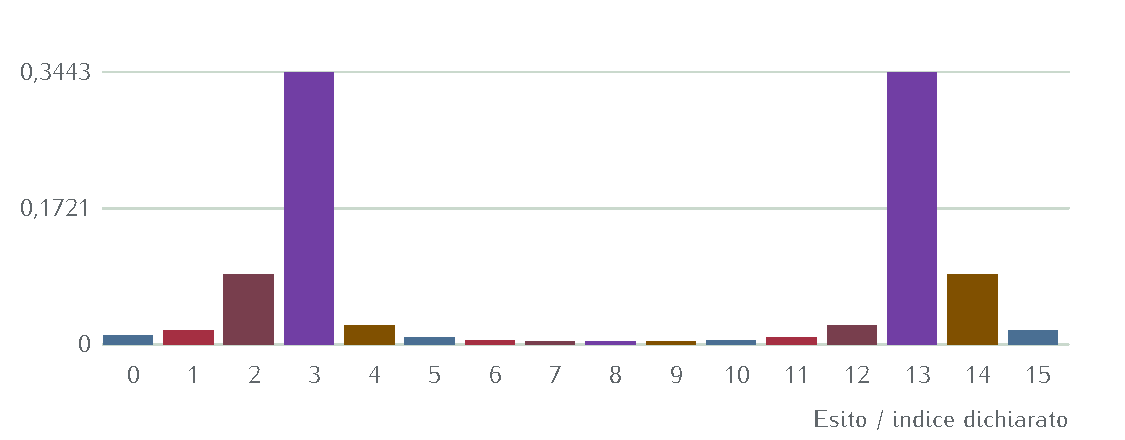
\includegraphics[width=\linewidth,height=94mm,keepaspectratio]{figure/f518d0a79c0256a44.pdf}\FigureCaption{4.14 \(\cdot\) esempio 1 \(\cdot\) Distribuzione completa della lettura}\end{FigureBlock}
\begin{FigureBlock}\centering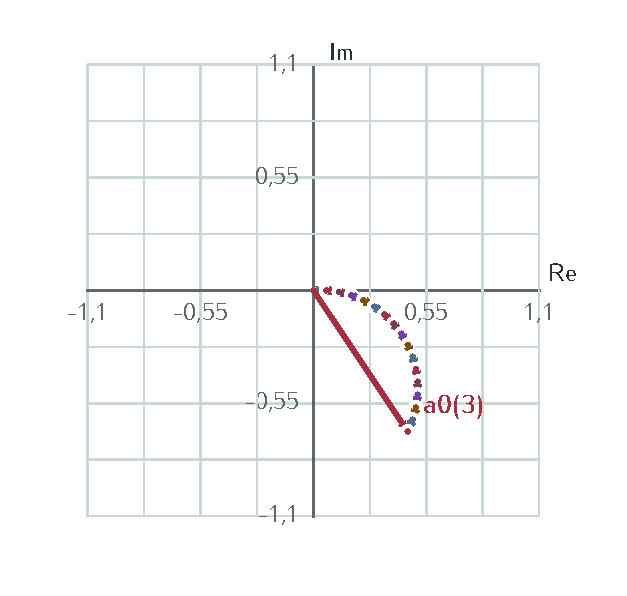
\includegraphics[width=\linewidth,height=94mm,keepaspectratio]{figure/f64131a77ae8870e9.pdf}\FigureCaption{4.14 \(\cdot\) esempio 1 \(\cdot\) Somma punta-coda, x crescente \(\cdot\) \(s=0\), \(c=3\), peso 0,5}\end{FigureBlock}
\begin{FigureBlock}\centering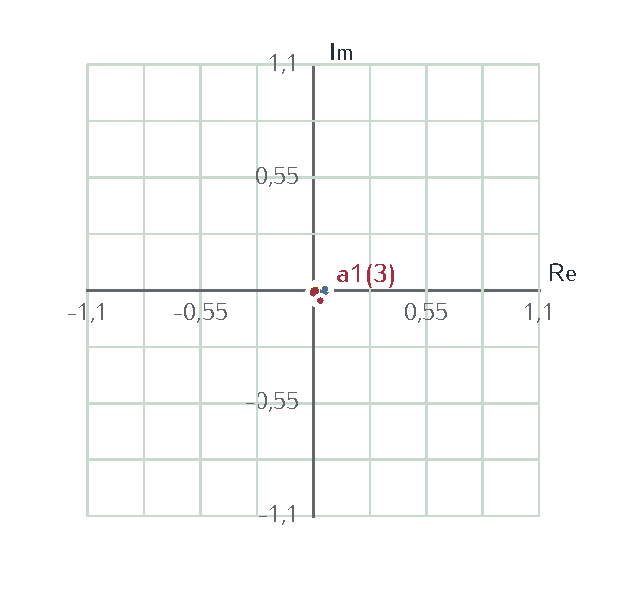
\includegraphics[width=\linewidth,height=94mm,keepaspectratio]{figure/fd82fce957599ad6b.pdf}\FigureCaption{4.14 \(\cdot\) esempio 1 \(\cdot\) Somma punta-coda, x crescente \(\cdot\) \(s=1\), \(c=3\), peso 0,5}\end{FigureBlock}
\begin{FigureBlock}\begin{minipage}[t]{.485\linewidth}\centering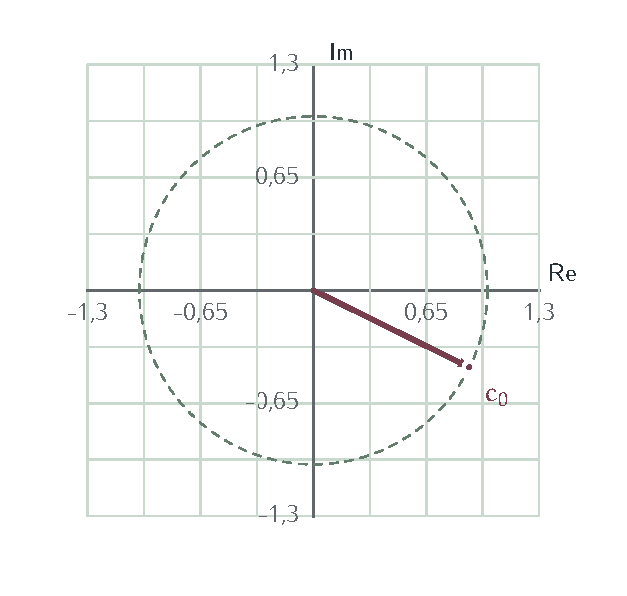
\includegraphics[width=\linewidth,height=63mm,keepaspectratio]{figure/f1e7f28e6280a5656.pdf}\par{\sffamily\footnotesize \(c_{0}\)\par}\end{minipage}\hfill\begin{minipage}[t]{.485\linewidth}\centering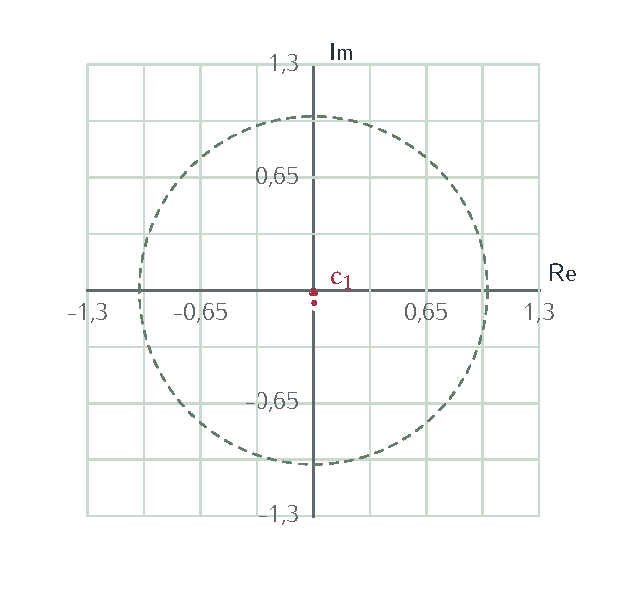
\includegraphics[width=\linewidth,height=63mm,keepaspectratio]{figure/f8c36152dc1206d3b.pdf}\par{\sffamily\footnotesize \(c_{1}\)\par}\end{minipage}\FigureCaption{4.14 \(\cdot\) esempio 1 \(\cdot\) Bersaglio condizionato \(\cdot\) coefficienti \(\beta {}^{\prime} s\) nella base propria dichiarata}\end{FigureBlock}
\begin{FigureBlock}\centering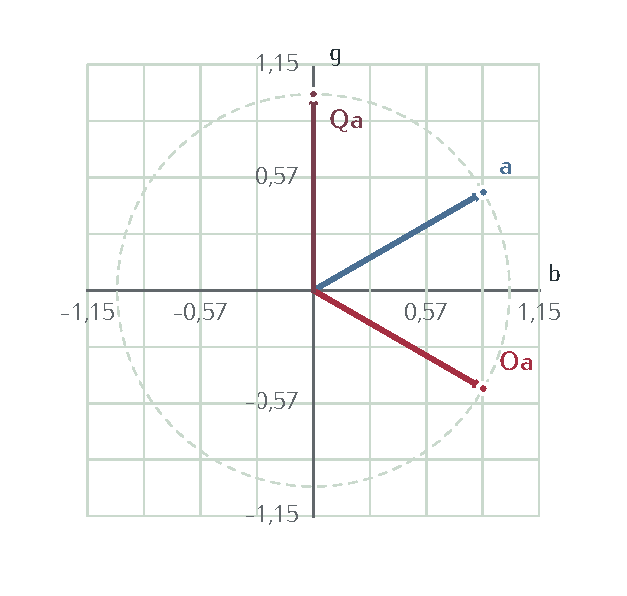
\includegraphics[width=\linewidth,height=94mm,keepaspectratio]{figure/f5d6c0954d66de915.pdf}\FigureCaption{4.14 \(\cdot\) esempio 1 \(\cdot\) Piano di Grover \(\cdot\) preparazione e prima rotazione}\end{FigureBlock}
\begin{FigureBlock}\begin{minipage}[t]{.485\linewidth}\centering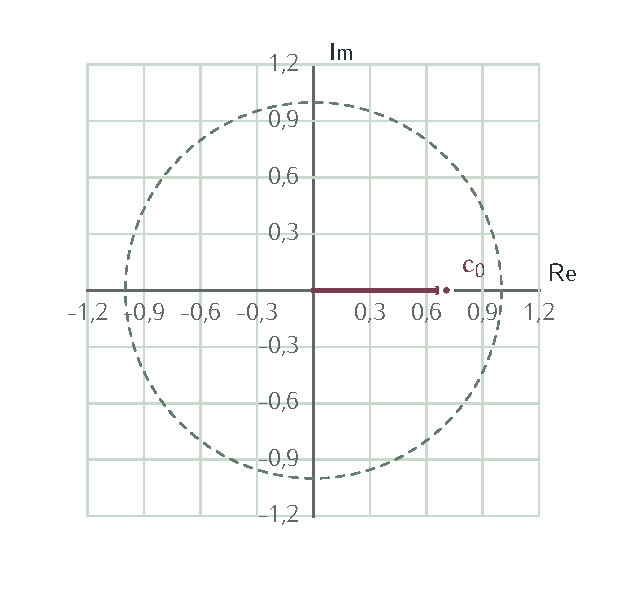
\includegraphics[width=\linewidth,height=63mm,keepaspectratio]{figure/f89bbaffdfa57651c.pdf}\par{\sffamily\footnotesize \(c_{0}\)\par}\end{minipage}\hfill\begin{minipage}[t]{.485\linewidth}\centering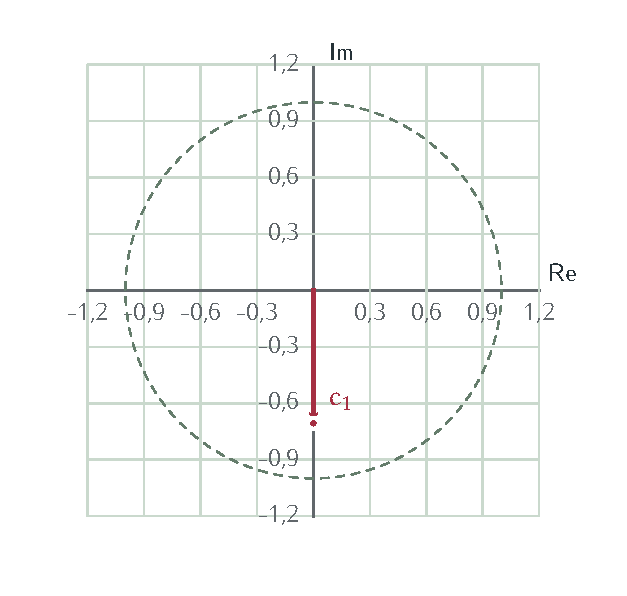
\includegraphics[width=\linewidth,height=63mm,keepaspectratio]{figure/f12fc3de1eef5eb3a.pdf}\par{\sffamily\footnotesize \(c_{1}\)\par}\end{minipage}\FigureCaption{4.14 \(\cdot\) esempio 1 \(\cdot\) Coordinate di u+ nella base \((|b\rangle ,\allowbreak |g\rangle )\)}\end{FigureBlock}
\begin{FigureBlock}\begin{minipage}[t]{.485\linewidth}\centering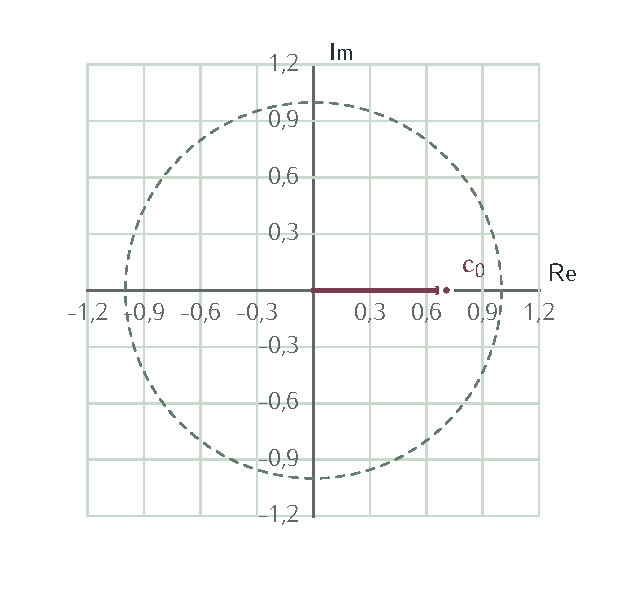
\includegraphics[width=\linewidth,height=63mm,keepaspectratio]{figure/f4cbcc347cbac6017.pdf}\par{\sffamily\footnotesize \(c_{0}\)\par}\end{minipage}\hfill\begin{minipage}[t]{.485\linewidth}\centering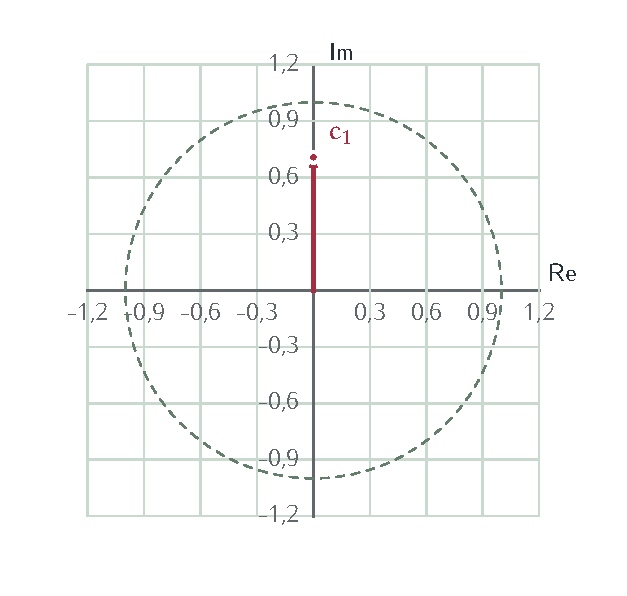
\includegraphics[width=\linewidth,height=63mm,keepaspectratio]{figure/fe5d99495c58204c3.pdf}\par{\sffamily\footnotesize \(c_{1}\)\par}\end{minipage}\FigureCaption{4.14 \(\cdot\) esempio 1 \(\cdot\) Coordinate di \(u- \) nella base \((|b\rangle ,\allowbreak |g\rangle )\)}\end{FigureBlock}

\phantomsection\label{c4-conteggio-example-1-step-1}
\BookHeading{01 Definire operatore, autostati e coefficienti}

\MathBlock{0055007C0075005F007327E9003D0065005E0028003203C0006903C6005F00730029007C0075005F007327E9003B002027E80075005F0073007C0075005F007427E9003D03B40073002C0074002E}{U|u_{s}\rangle =e^{2\pi i\varphi _{s}}|u_{s}\rangle ;\allowbreak \ \langle u_{s}|u_{t}\rangle =\delta s,\allowbreak t.}
\MathBlock{007C03C827E9003D03A30073002003B2005F0073007C0075005F007327E9003B002003A30073007C03B2005F0073007C00B2003D0031003B00200051003D0032005E006D002E}{|\psi \rangle =\sum _{s}\ \beta _{s}|u_{s}\rangle ;\allowbreak \ \sum _{s}|\beta _{s}|^{2}=1;\allowbreak \ Q=2^{m}.}

Il registro di lettura contiene m qubit; \(\varphi \) è una frazione di giro modulo uno. L'indice s distingue gli autostati del bersaglio e \(\beta _{s}\) è un'ampiezza complessa, mentre \(|\beta _{s}|^{2}\) è un peso probabilistico.\par


\phantomsection\label{c4-conteggio-example-1-step-2}
\BookHeading{02 Delimitare il modello spettrale}

\MathBlock{004E003D0038003B00200047003D007B0031002C0035007D003B0020007C006127E9224800280030002C0033003500330036003B00200030002C0033003500330036003B00200030002C0033003500330036003B00200030002C0033003500330036003B00200030002C0033003500330036003B00200030002C0033003500330036003B00200030002C0033003500330036003B00200030002C003300350033003600291D40003B00200070003D0030002E00320035002E}{N=8;\allowbreak \ G=\{1{,}5\};\allowbreak \ |a\rangle \approx (0{,}3536;\allowbreak \ 0{,}3536;\allowbreak \ 0{,}3536;\allowbreak \ 0{,}3536;\allowbreak \ 0{,}3536;\allowbreak \ 0{,}3536;\allowbreak \ 0{,}3536;\allowbreak \ 0{,}3536)^{T};\allowbreak \ p=0.25.}
\MathBlock{0049006C0020006D006F00640065006C006C006F0020007200690063006100760061002003B8003D00610072006300730069006E221A0070002000650020006C00650020006100750074006F006600610073006900200064006900200051005F0047003D0044005F0041004F002C00200070006F0069002000760061006C00750074006100200061006E0061006C00690074006900630061006D0065006E00740065002000510050004500200069006E00200062006100730065002000700072006F0070007200690061002E}{Il\ \text{modello}\ \text{ricava}\ \theta =\arcsin \sqrt{p}\ e\ \text{le}\ \text{autofasi}\ \text{di}\ Q_{G}=D_{AO},\allowbreak \ \text{poi}\ \text{valuta}\ \text{analiticamente}\ \text{QPE}\ \text{in}\ \text{base}\ \text{propria}.}

La probabilità nota costruisce la distribuzione di questo esempio. Qui non si esegue una rete controllata che ricavi p da una preparazione e da un oracolo ignoti; il conteggio operativo richiederebbe costruire e controllare \(Q_{G}\). La derivazione seguente rende verificabile il raccordo con Grover.\par


\phantomsection\label{c4-conteggio-example-1-step-3}
\BookHeading{03 Costruire gli assi dalle proiezioni}

\MathBlock{007C006127E9003D0041007C003027E9003B002003A00047003D03A3007822080047007C007827E927E80078007C003B00200070003D27E80061007C03A00047007C006127E9003D0030002C00320035002E}{|a\rangle =A|0\rangle ;\allowbreak \ \Pi _{G}=\sum _{x\in G}|x\rangle \langle x|;\allowbreak \ p=\langle a|\Pi _{G}|a\rangle =0{,}25.}
\MathBlock{007C006727E9003D03A00047007C006127E9002F221A0070224800280030003B00200030002C0037003000370031003B00200030003B00200030003B00200030003B00200030002C0037003000370031003B00200030003B0020003000291D40}{|g\rangle =\Pi _{G}|a\rangle /\sqrt{p}\approx (0;\allowbreak \ 0{,}7071;\allowbreak \ 0;\allowbreak \ 0;\allowbreak \ 0;\allowbreak \ 0{,}7071;\allowbreak \ 0;\allowbreak \ 0)^{T}}
\MathBlock{007C006227E9003D00280049221203A000470029007C006127E9002F221A00280031221200700029224800280030002C0034003000380032003B00200030003B00200030002C0034003000380032003B00200030002C0034003000380032003B00200030002C0034003000380032003B00200030003B00200030002C0034003000380032003B00200030002C003400300038003200291D40002E}{|b\rangle =(I- \Pi _{G})|a\rangle /\sqrt{1- p}\approx (0{,}4082;\allowbreak \ 0;\allowbreak \ 0{,}4082;\allowbreak \ 0{,}4082;\allowbreak \ 0{,}4082;\allowbreak \ 0;\allowbreak \ 0{,}4082;\allowbreak \ 0{,}4082)^{T}.}
\MathBlock{27E80062007C006727E9003D0030003B0020201600622016003D201600672016003D0031002E}{\langle b|g\rangle =0;\allowbreak \ \Vert b\Vert =\Vert g\Vert =1.}

I supporti sono disgiunti. Per la preparazione uniforme questi vettori diventano \(\sum _{x\in G}|x\rangle /\sqrt{M}\) e \(\sum x\notin G|x\rangle /\sqrt{N- M}\). Per una preparazione non uniforme conservano i suoi pesi e le sue fasi.\par


\phantomsection\label{c4-conteggio-example-1-step-4}
\BookHeading{04 Proiettare la preparazione nel piano}

\MathBlock{27E80062007C006127E9003D221A00280031221200700029003D0030002C003800360036003000320035003B002027E80067007C006127E9003D221A0070003D0030002C0035002E}{\langle b|a\rangle =\sqrt{1- p}=0{,}866025;\allowbreak \ \langle g|a\rangle =\sqrt{p}=0{,}5.}
\MathBlock{007C006127E9003D0063006F007303B8007C006227E9002B00730069006E03B8007C006727E9003B002003B8003D00610072006300730069006E221A007022480030002C0035003200330035003900390020007200610064002E}{|a\rangle =\cos \theta |b\rangle +\sin \theta |g\rangle ;\allowbreak \ \theta =\arcsin \sqrt{p}\approx 0{,}523599\ \text{rad}.}

Gli assi sono stati collettivi, non singoli esiti. Le coordinate qui sono reali perché le fasi della preparazione sono state incluse nella definizione degli assi.\par


\phantomsection\label{c4-conteggio-example-1-step-5}
\BookHeading{05 Scrivere le due riflessioni}

\MathBlock{004E0065006C006C0061002000620061007300650020006F007200640069006E00610074006100200028007C006227E9002C007C006727E90029003A}{\text{Nella}\ \text{base}\ \text{ordinata}\ (|b\rangle ,\allowbreak |g\rangle ):}
\MathBlock{004F003D00492212003203A00047003D005B005B0031002C0030005D002C005B0030002C22120031005D005D002E}{O=I- 2\Pi _{G}=\begin{pmatrix}1&0\\0&- 1\end{pmatrix}.}
\MathBlock{0044005F0041003D0032007C006127E927E80061007C22120049}{D_{A}=2|a\rangle \langle a|- I}
\MathBlock{003D005B005B00320063006F007300B203B822120031002C00320063006F007303B800730069006E03B8005D002C005B00320063006F007303B800730069006E03B8002C003200730069006E00B203B822120031005D005D}{=\begin{pmatrix}2\cos ^{2}\theta - 1&2\cos \theta \sin \theta \\2\cos \theta \sin \theta &2\sin ^{2}\theta - 1\end{pmatrix}}
\MathBlock{003D005B005B0063006F0073003203B8002C00730069006E003203B8005D002C005B00730069006E003203B8002C22120063006F0073003203B8005D005D002E}{=\begin{pmatrix}\cos 2\theta &\sin 2\theta \\\sin 2\theta &- \cos 2\theta \end{pmatrix}.}

\(O\) riflette rispetto all'asse \(|b\rangle \). \(D_{A}\) riflette rispetto alla retta della preparazione \(|a\rangle \). L'ordine temporale è prima \(O\) e poi \(D_{A}\).\par


\phantomsection\label{c4-conteggio-example-1-step-6}
\BookHeading{06 Moltiplicare e ottenere la rotazione}

\MathBlock{0051003D0044005F0041004F003D005B005B0063006F0073003203B8002C221200730069006E003203B8005D002C005B00730069006E003203B8002C0063006F0073003203B8005D005D}{Q=D_{AO}=\begin{pmatrix}\cos 2\theta &- \sin 2\theta \\\sin 2\theta &\cos 2\theta \end{pmatrix}}
\MathBlock{2248005B005B0030002C0035002C002D0030002C003800360036003000320035005D002C005B0030002C003800360036003000320035002C0030002C0035005D005D002E}{\approx \begin{pmatrix}0{,}5&-0{,}866025\\0{,}866025&0{,}5\end{pmatrix}.}
\MathBlock{004F00280063006F007303B8002C00730069006E03B800291D40003D00280063006F007303B8002C221200730069006E03B800291D40003B}{O(\cos \theta ,\allowbreak \sin \theta )^{T}=(\cos \theta ,\allowbreak - \sin \theta )^{T};\allowbreak }
\MathBlock{005100280063006F007303B8002C00730069006E03B800291D40003D00280063006F0073003303B8002C00730069006E003303B800291D40002E}{Q(\cos \theta ,\allowbreak \sin \theta )^{T}=(\cos 3\theta ,\allowbreak \sin 3\theta )^{T}.}
\MathBlock{00511D4F007C006127E9003D0063006F0073002800280032006B002B0031002903B80029007C006227E9002B00730069006E002800280032006B002B0031002903B80029007C006727E9002E}{Q^{k}|a\rangle =\cos ((2k+1)\theta )|b\rangle +\sin ((2k+1)\theta )|g\rangle .}

Il prodotto riga per colonna dà le formule di addizione del seno e del coseno. Ogni coppia completa di riflessioni ruota di \(2\theta \); dopo il solo oracolo si usa invece la riflessione, non la formula delle iterazioni complete.\par


\phantomsection\label{c4-conteggio-example-1-step-7}
\BookHeading{07 Verificare il caso \(p=1/4\)}

\MathBlock{03B8003D03C0002F0036003B0020007C006127E9003D0028221A0033002F0032002C0031002F003200291D40002E}{\theta =\pi /6;\allowbreak \ |a\rangle =(\sqrt{3}/2{,}1/2)^{T}.}
\MathBlock{004F007C006127E9003D0028221A0033002F0032002C22120031002F003200291D40002E}{O|a\rangle =(\sqrt{3}/2,\allowbreak - 1/2)^{T}.}
\MathBlock{0044005F0041003D005B005B0031002F0032002C221A0033002F0032005D002C005B221A0033002F0032002C22120031002F0032005D005D002E}{D_{A}=\begin{pmatrix}1/2&\sqrt{3}/2\\\sqrt{3}/2&- 1/2\end{pmatrix}.}
\MathBlock{0044005F0041004F007C006127E9003D0028221A0033002F00342212221A0033002F0034002C221A003300B7221A0033002F0034002B0031002F003400291D40003D00280030002C003100291D40002E}{D_{AO}|a\rangle =(\sqrt{3}/4- \sqrt{3}/4,\allowbreak \sqrt{3}\cdot \sqrt{3}/4+1/4)^{T}=(0{,}1)^{T}.}

Il medesimo calcolo vale per \(N=4,\allowbreak M=1\) e per \(N=8,\allowbreak M=2\). Una sola coppia di riflessioni porta tutto il peso sul sottospazio buono.\par


\phantomsection\label{c4-conteggio-example-1-step-8}
\BookHeading{08 Ricavare autovettori e autofasi}

\MathBlock{00640065007400280051221203BB00490029003D03BB00B2221200320063006F00730028003203B8002903BB002B0031003D0030002E}{\det (Q- \lambda I)=\lambda ^{2}- 2\cos (2\theta )\lambda +1=0.}
\MathBlock{03BB00B1003D0063006F0073003203B800B10069002000730069006E003203B8003D0065005E002800B10032006903B80029002E}{\lambda \pm =\cos 2\theta \pm i\ \sin 2\theta =e^{\pm 2i\theta }.}
\MathBlock{007C0075002B27E9003D0028007C006227E922120069007C006727E90029002F221A0032003B0020007C0075221227E9003D0028007C006227E9002B0069007C006727E90029002F221A0032002E}{|u+\rangle =(|b\rangle - i|g\rangle )/\sqrt{2};\allowbreak \ |u- \rangle =(|b\rangle +i|g\rangle )/\sqrt{2}.}
\MathBlock{0051007C007500B127E9003D0065005E002800B10032006903B80029007C007500B127E9003B002003C6002B003D03B8002F03C0002C002003C62212003D0031221203B8002F03C000200028006D006F0064002000310029002E}{Q|u\pm \rangle =e^{\pm 2i\theta }|u\pm \rangle ;\allowbreak \ \varphi +=\theta /\pi ,\allowbreak \ \varphi - =1- \theta /\pi \ (\bmod \ 1).}

Gli autovettori hanno coordinate complesse nel piano collettivo; non sono due frecce reali sul piano di Grover. Le autofasi sono frazioni di giro, poiché QPE usa \(e^{2\pi i\varphi }\).\par


\phantomsection\label{c4-conteggio-example-1-step-9}
\BookHeading{09 Determinare i coefficienti della preparazione}

\MathBlock{03B2002B003D27E80075002B007C006127E9003D00280063006F007303B8002B0069002000730069006E03B80029002F221A0032003D0065005E0028006903B80029002F221A0032002E}{\beta +=\langle u+|a\rangle =(\cos \theta +i\ \sin \theta )/\sqrt{2}=e^{i\theta }/\sqrt{2}.}
\MathBlock{03B22212003D27E800752212007C006127E9003D00280063006F007303B822120069002000730069006E03B80029002F221A0032003D0065005E00282212006903B80029002F221A0032002E}{\beta - =\langle u- |a\rangle =(\cos \theta - i\ \sin \theta )/\sqrt{2}=e^{- i\theta }/\sqrt{2}.}
\MathBlock{007C006127E9003D03B2002B007C0075002B27E9002B03B22212007C0075221227E9003B0020007C03B2002B007C00B2003D007C03B22212007C00B2003D0031002F0032002E}{|a\rangle =\beta +|u+\rangle +\beta - |u- \rangle ;\allowbreak \ |\beta +|^{2}=|\beta - |^{2}=1/2.}

I due pesi uguali derivano dal prodotto interno con la preparazione. Manteniamo anche le fasi dei coefficienti: servono per ricostruire il bersaglio coerente condizionato dopo QPE.\par


\phantomsection\label{c4-conteggio-example-1-step-10}
\BookHeading{10 Fissare le fasi della base propria}

\MathBlock{00752080003D0075002B003D0028007C006227E922120069007C006727E90029002F221A0032003B002000752081003D00752212003D0028007C006227E9002B0069007C006727E90029002F221A0032002E}{u_{0}=u+=(|b\rangle - i|g\rangle )/\sqrt{2};\allowbreak \ u_{1}=u- =(|b\rangle +i|g\rangle )/\sqrt{2}.}
\MathBlock{03B22080003D0065005E0028006903B80029002F221A003222480030002C00360031003200330037003200340020002B00200030002C00330035003300350035003300340069003B002003B22081003D0065005E00282212006903B80029002F221A003222480030002C00360031003200330037003200340020221200200030002C00330035003300350035003300340069002E}{\beta _{0}=e^{i\theta }/\sqrt{2}\approx 0{,}6123724\ +\ 0{,}3535534i;\allowbreak \ \beta _{1}=e^{- i\theta }/\sqrt{2}\approx 0{,}6123724\ - \ 0{,}3535534i.}
\MathBlock{03B2208000752080002B03B2208100752081003D0063006F007303B8007C006227E9002B00730069006E03B8007C006727E9002E}{\beta _{0}u_{0}+\beta _{1}u_{1}=\cos \theta |b\rangle +\sin \theta |g\rangle .}

Questa convenzione fissa univocamente i coefficienti complessi. I pesi sono uguali, ma le fasi dei \(\beta \) restano nel bersaglio condizionato.\par


\phantomsection\label{c4-conteggio-example-1-step-11}
\BookHeading{11 Preparare il controllo}

\MathBlock{007C003027E922970034007C03C827E900202192002000280031002F221A00310036002903A30078007C007827E903A30073002003B2005F0073007C0075005F007327E9002E}{|0\rangle ^{\otimes 4}|\psi \rangle \ \to \ (1/\sqrt{16})\sum _{x}|x\rangle \sum _{s}\ \beta _{s}|u_{s}\rangle .}

Le Hadamard agiscono soltanto sui qubit di lettura. Il bersaglio mantiene i coefficienti appena assegnati.\par


\phantomsection\label{c4-conteggio-example-1-step-12}
\BookHeading{12 Costruire le potenze e il kickback}

\MathBlock{00660069006C006F002000710030002C0020007000650073006F00200032005E0033003A00200063006F006E00740072006F006C006C006F00200064006900200055005E0038}{\text{filo}\ q_{0},\allowbreak \ \text{peso}\ 2^{3}:\ \text{controllo}\ \text{di}\ U^{8}}
\MathBlock{00660069006C006F002000710031002C0020007000650073006F00200032005E0032003A00200063006F006E00740072006F006C006C006F00200064006900200055005E0034}{\text{filo}\ q_{1},\allowbreak \ \text{peso}\ 2^{2}:\ \text{controllo}\ \text{di}\ U^{4}}
\MathBlock{00660069006C006F002000710032002C0020007000650073006F00200032005E0031003A00200063006F006E00740072006F006C006C006F00200064006900200055005E0032}{\text{filo}\ q_{2},\allowbreak \ \text{peso}\ 2^{1}:\ \text{controllo}\ \text{di}\ U^{2}}
\MathBlock{00660069006C006F002000710033002C0020007000650073006F00200032005E0030003A00200063006F006E00740072006F006C006C006F00200064006900200055005E0031}{\text{filo}\ q_{3},\allowbreak \ \text{peso}\ 2^{0}:\ \text{controllo}\ \text{di}\ U^{1}}
\MathBlock{0078003D03A3007100200078005F00710032005E0028006D22120031221200710029002021D20020220F007100200065005E0028003203C0006900200078005F00710032005E0028006D2212003122120071002903C6005F00730029003D0065005E0028003203C00069007803C6005F00730029002E}{x=\sum _{q}\ x_{q}2^{m- 1- q}\ \Rightarrow \ \prod _{q}\ e^{2\pi i\ x_{q}2^{m- 1- q}\varphi _{s}}=e^{2\pi ix\varphi _{s}}.}
\MathBlock{007C03A827E9003D00280031002F221A0051002903A30078002C0073002003B2005F007300200065005E0028003203C00069007803C6005F00730029007C007827E9007C0075005F007327E9002E}{|\Psi \rangle =(1/\sqrt{Q})\sum _{x,\allowbreak s}\ \beta _{s}\ e^{2\pi ix\varphi _{s}}|x\rangle |u_{s}\rangle .}

\(q_{0}\) è il filo superiore e il bit più significativo. Per tre qubit le potenze sono \(U^{4},\allowbreak U^{2},\allowbreak U\); l'esponente j di \(2^{j}\) non va confuso con l'indice del filo \(q_{j}\).\par


\phantomsection\label{c4-conteggio-example-1-step-13}
\BookHeading{13 Sommare le radici dell'unità}

\MathBlock{0053003D0031002B007A002B22EF002B007A005E002800310036002D00310029002E}{S=1+z+\cdots +z^{16-1}.}
\MathBlock{007A0053003D007A002B007A00B2002B22EF002B007A005E00310036003B0020002800312212007A00290053003D00312212007A005E00310036002E}{zS=z+z^{2}+\cdots +z^{16};\allowbreak \ (1- z)S=1- z^{16}.}
\MathBlock{005300650020007A22600031003A00200053003D002800312212007A005E003100360029002F002800312212007A0029002E0020005300650020007A003D0031003A00200053003D00310036002E}{Se\ z\ne 1:\ S=(1- z^{16})/(1- z).\ Se\ z=1:\ S=16.}

La sottrazione cancella tutti i termini intermedi. Il caso \(z=1\) va separato prima della divisione.\par


\phantomsection\label{c4-conteggio-example-1-step-14}
\BookHeading{14 Dalla cancellazione all'unitarietà}

\MathBlock{007A003D0065005E0028003203C00069002800782212007820320029002F003100360029003B0020007A005E00310036003D0031002E}{z=e^{2\pi i(x- x{}^{\prime} )/16};\allowbreak \ z^{16}=1.}
\MathBlock{27E800460031003600782032007C004600310036007827E9003D00280031002F00310036002903A300790020007A02B8003D00310036002F00310036003D003100200073006500200078003D00782032003B0020003000200061006C007400720069006D0065006E00740069002E}{\langle F16x{}^{\prime} |F16x\rangle =(1/16)\sum _{y}\ z^{y}=16/16=1\ \text{se}\ x=x{}^{\prime} ;\allowbreak \ 0\ \text{altrimenti}.}

Per x e \(x{}^{\prime} \) distinti fra 0 e \(N- 1\), \(z\ne 1\): le frecce delle radici si chiudono. Le colonne di Fourier sono quindi ortonormali e la trasformata conserva prodotti interni e norma.\par


\phantomsection\label{c4-conteggio-example-1-step-15}
\BookHeading{15 Applicare la cancellazione alla QPE}

\MathBlock{0044006F0070006F00200046005F00512020003A0020007C03A8006F0075007427E9003D03A30063002C0073002003B2005F007300200061005F0073002800630029007C006327E9007C0075005F007327E9002E}{\text{Dopo}\ F_{Q}{}^{\dagger} :\ |\Psi \text{out}\rangle =\sum _{c,\allowbreak s}\ \beta _{s}\ a_{s}(c)|c\rangle |u_{s}\rangle .}
\MathBlock{0061005F0073002800630029003D00280031002F0051002903A300780020007A02E3002C0020007A003D0065005E0028003203C00069002803C6005F007322120063002F005100290029002E}{a_{s}(c)=(1/Q)\sum _{x}\ z^{x},\allowbreak \ z=e^{2\pi i(\varphi _{s}- c/Q)}.}
\MathBlock{005300650020005103C6005F0073003D004C00200069006E007400650072006F003A0020007A005E0051003D0031003B00200061005F00730028004C0029003D0031002C00200061005F0073002800630029003D00300020007000650072002000632260004C002E}{Se\ Q\varphi _{s}=L\ \text{intero}:\ z^{Q}=1;\allowbreak \ a_{s}(L)=1,\allowbreak \ a_{s}(c)=0\ \text{per}\ c\ne L.}
\MathBlock{00460075006F0072006900200067007200690067006C00690061003A00200061005F0073002800630029003D002800312212007A005E00510029002F00280051002800312212007A00290029002C002000730061006C0076006F0020007A003D0031002E}{\text{Fuori}\ \text{griglia}:\ a_{s}(c)=(1- z^{Q})/(Q(1- z)),\allowbreak \ \text{salvo}\ z=1.}

Per \(Q=8\), \(\varphi =3/8\): \(a(3)=8/8=1\). Per ogni altro c, \(z=e^{2\pi i(3- c)/8}\ne 1\) e il numeratore è zero. Fuori griglia la cancellazione è incompleta e più esiti restano possibili.\par


\phantomsection\label{c4-conteggio-example-1-step-16}
\BookHeading{16 Potenze controllate \(\cdot\) autostato 0}

\MathBlock{00660069006C006F002000710030003A00200032005E003303C60020006D006F00640020003122480030002C003300330033003300330033}{\text{filo}\ q_{0}:\ 2^{3}\varphi \ \bmod \ 1\approx 0{,}333333}
\MathBlock{00660069006C006F002000710031003A00200032005E003203C60020006D006F00640020003122480030002C003600360036003600360037}{\text{filo}\ q_{1}:\ 2^{2}\varphi \ \bmod \ 1\approx 0{,}666667}
\MathBlock{00660069006C006F002000710032003A00200032005E003103C60020006D006F00640020003122480030002C003300330033003300330033}{\text{filo}\ q_{2}:\ 2^{1}\varphi \ \bmod \ 1\approx 0{,}333333}
\MathBlock{00660069006C006F002000710033003A00200032005E003003C60020006D006F00640020003122480030002C003100360036003600360037}{\text{filo}\ q_{3}:\ 2^{0}\varphi \ \bmod \ 1\approx 0{,}166667}
\MathBlock{0063005F0073002800780029003D0065005E0028003203C00069007800B70030002C003100360036003600360036003600370029002F221A00310036}{c_{s}(x)=e^{2\pi ix\cdot 0{,}16666667}/\sqrt{16}}

Queste fasi moltiplicano il ramo di autostato s; il suo coefficiente \(\beta _{s}\) rimane esplicito nello stato congiunto.\par


\phantomsection\label{c4-conteggio-example-1-step-17}
\BookHeading{17 Fourier inversa \(\cdot\) \(s=0\), \(c=0\)}

\MathBlock{0061005F0073002800300029003D00280031002F003100360029005B0065005E0028003203C0006900B7003000B700280030002C0031003600360036003600360036003722120030002F0031003600290029002B0065005E0028003203C0006900B7003100B700280030002C0031003600360036003600360036003722120030002F0031003600290029002B0065005E0028003203C0006900B7003200B700280030002C0031003600360036003600360036003722120030002F0031003600290029002B0065005E0028003203C0006900B7003300B700280030002C0031003600360036003600360036003722120030002F0031003600290029002B0065005E0028003203C0006900B7003400B700280030002C0031003600360036003600360036003722120030002F0031003600290029002B0065005E0028003203C0006900B7003500B700280030002C0031003600360036003600360036003722120030002F0031003600290029002B0065005E0028003203C0006900B7003600B700280030002C0031003600360036003600360036003722120030002F0031003600290029002B0065005E0028003203C0006900B7003700B700280030002C0031003600360036003600360036003722120030002F0031003600290029002B}{a_{s}(0)=(1/16)[e^{2\pi i\cdot 0\cdot (0{,}16666667- 0/16)}+e^{2\pi i\cdot 1\cdot (0{,}16666667- 0/16)}+e^{2\pi i\cdot 2\cdot (0{,}16666667- 0/16)}+e^{2\pi i\cdot 3\cdot (0{,}16666667- 0/16)}+e^{2\pi i\cdot 4\cdot (0{,}16666667- 0/16)}+e^{2\pi i\cdot 5\cdot (0{,}16666667- 0/16)}+e^{2\pi i\cdot 6\cdot (0{,}16666667- 0/16)}+e^{2\pi i\cdot 7\cdot (0{,}16666667- 0/16)}+}
\MathBlock{0065005E0028003203C0006900B7003800B700280030002C0031003600360036003600360036003722120030002F0031003600290029002B0065005E0028003203C0006900B7003900B700280030002C0031003600360036003600360036003722120030002F0031003600290029002B0065005E0028003203C0006900B70031003000B700280030002C0031003600360036003600360036003722120030002F0031003600290029002B0065005E0028003203C0006900B70031003100B700280030002C0031003600360036003600360036003722120030002F0031003600290029002B0065005E0028003203C0006900B70031003200B700280030002C0031003600360036003600360036003722120030002F0031003600290029002B0065005E0028003203C0006900B70031003300B700280030002C0031003600360036003600360036003722120030002F0031003600290029002B0065005E0028003203C0006900B70031003400B700280030002C0031003600360036003600360036003722120030002F0031003600290029002B0065005E0028003203C0006900B70031003500B700280030002C0031003600360036003600360036003722120030002F0031003600290029005D}{e^{2\pi i\cdot 8\cdot (0{,}16666667- 0/16)}+e^{2\pi i\cdot 9\cdot (0{,}16666667- 0/16)}+e^{2\pi i\cdot 10\cdot (0{,}16666667- 0/16)}+e^{2\pi i\cdot 11\cdot (0{,}16666667- 0/16)}+e^{2\pi i\cdot 12\cdot (0{,}16666667- 0/16)}+e^{2\pi i\cdot 13\cdot (0{,}16666667- 0/16)}+e^{2\pi i\cdot 14\cdot (0{,}16666667- 0/16)}+e^{2\pi i\cdot 15\cdot (0{,}16666667- 0/16)}]}
\MathBlock{22480030002C00310030003800320035003300320069003B0020007C0061007C00B222480030002C0030003100310037003100380038}{\approx 0{,}1082532i;\allowbreak \ |a|^{2}\approx 0{,}0117188}

La somma complessa precede il modulo quadro. Le fasi nel calcolo mantengono precisione completa; i decimali stampati sono arrotondati.\par


\phantomsection\label{c4-conteggio-example-1-step-18}
\BookHeading{18 Fourier inversa \(\cdot\) \(s=0\), \(c=1\)}

\MathBlock{0061005F0073002800310029003D00280031002F003100360029005B0065005E0028003203C0006900B7003000B700280030002C0031003600360036003600360036003722120031002F0031003600290029002B0065005E0028003203C0006900B7003100B700280030002C0031003600360036003600360036003722120031002F0031003600290029002B0065005E0028003203C0006900B7003200B700280030002C0031003600360036003600360036003722120031002F0031003600290029002B0065005E0028003203C0006900B7003300B700280030002C0031003600360036003600360036003722120031002F0031003600290029002B0065005E0028003203C0006900B7003400B700280030002C0031003600360036003600360036003722120031002F0031003600290029002B0065005E0028003203C0006900B7003500B700280030002C0031003600360036003600360036003722120031002F0031003600290029002B0065005E0028003203C0006900B7003600B700280030002C0031003600360036003600360036003722120031002F0031003600290029002B0065005E0028003203C0006900B7003700B700280030002C0031003600360036003600360036003722120031002F0031003600290029002B}{a_{s}(1)=(1/16)[e^{2\pi i\cdot 0\cdot (0{,}16666667- 1/16)}+e^{2\pi i\cdot 1\cdot (0{,}16666667- 1/16)}+e^{2\pi i\cdot 2\cdot (0{,}16666667- 1/16)}+e^{2\pi i\cdot 3\cdot (0{,}16666667- 1/16)}+e^{2\pi i\cdot 4\cdot (0{,}16666667- 1/16)}+e^{2\pi i\cdot 5\cdot (0{,}16666667- 1/16)}+e^{2\pi i\cdot 6\cdot (0{,}16666667- 1/16)}+e^{2\pi i\cdot 7\cdot (0{,}16666667- 1/16)}+}
\MathBlock{0065005E0028003203C0006900B7003800B700280030002C0031003600360036003600360036003722120031002F0031003600290029002B0065005E0028003203C0006900B7003900B700280030002C0031003600360036003600360036003722120031002F0031003600290029002B0065005E0028003203C0006900B70031003000B700280030002C0031003600360036003600360036003722120031002F0031003600290029002B0065005E0028003203C0006900B70031003100B700280030002C0031003600360036003600360036003722120031002F0031003600290029002B0065005E0028003203C0006900B70031003200B700280030002C0031003600360036003600360036003722120031002F0031003600290029002B0065005E0028003203C0006900B70031003300B700280030002C0031003600360036003600360036003722120031002F0031003600290029002B0065005E0028003203C0006900B70031003400B700280030002C0031003600360036003600360036003722120031002F0031003600290029002B0065005E0028003203C0006900B70031003500B700280030002C0031003600360036003600360036003722120031002F0031003600290029005D}{e^{2\pi i\cdot 8\cdot (0{,}16666667- 1/16)}+e^{2\pi i\cdot 9\cdot (0{,}16666667- 1/16)}+e^{2\pi i\cdot 10\cdot (0{,}16666667- 1/16)}+e^{2\pi i\cdot 11\cdot (0{,}16666667- 1/16)}+e^{2\pi i\cdot 12\cdot (0{,}16666667- 1/16)}+e^{2\pi i\cdot 13\cdot (0{,}16666667- 1/16)}+e^{2\pi i\cdot 14\cdot (0{,}16666667- 1/16)}+e^{2\pi i\cdot 15\cdot (0{,}16666667- 1/16)}]}
\MathBlock{2248002D0030002C00300033003200380035003000390020002B00200030002C00310036003500310035003200360069003B0020007C0061007C00B222480030002C0030003200380033003500340036}{\approx -0{,}0328509\ +\ 0{,}1651526i;\allowbreak \ |a|^{2}\approx 0{,}0283546}

La somma complessa precede il modulo quadro. Le fasi nel calcolo mantengono precisione completa; i decimali stampati sono arrotondati.\par


\phantomsection\label{c4-conteggio-example-1-step-19}
\BookHeading{19 Fourier inversa \(\cdot\) \(s=0\), \(c=2\)}

\MathBlock{0061005F0073002800320029003D00280031002F003100360029005B0065005E0028003203C0006900B7003000B700280030002C0031003600360036003600360036003722120032002F0031003600290029002B0065005E0028003203C0006900B7003100B700280030002C0031003600360036003600360036003722120032002F0031003600290029002B0065005E0028003203C0006900B7003200B700280030002C0031003600360036003600360036003722120032002F0031003600290029002B0065005E0028003203C0006900B7003300B700280030002C0031003600360036003600360036003722120032002F0031003600290029002B0065005E0028003203C0006900B7003400B700280030002C0031003600360036003600360036003722120032002F0031003600290029002B0065005E0028003203C0006900B7003500B700280030002C0031003600360036003600360036003722120032002F0031003600290029002B0065005E0028003203C0006900B7003600B700280030002C0031003600360036003600360036003722120032002F0031003600290029002B0065005E0028003203C0006900B7003700B700280030002C0031003600360036003600360036003722120032002F0031003600290029002B}{a_{s}(2)=(1/16)[e^{2\pi i\cdot 0\cdot (0{,}16666667- 2/16)}+e^{2\pi i\cdot 1\cdot (0{,}16666667- 2/16)}+e^{2\pi i\cdot 2\cdot (0{,}16666667- 2/16)}+e^{2\pi i\cdot 3\cdot (0{,}16666667- 2/16)}+e^{2\pi i\cdot 4\cdot (0{,}16666667- 2/16)}+e^{2\pi i\cdot 5\cdot (0{,}16666667- 2/16)}+e^{2\pi i\cdot 6\cdot (0{,}16666667- 2/16)}+e^{2\pi i\cdot 7\cdot (0{,}16666667- 2/16)}+}
\MathBlock{0065005E0028003203C0006900B7003800B700280030002C0031003600360036003600360036003722120032002F0031003600290029002B0065005E0028003203C0006900B7003900B700280030002C0031003600360036003600360036003722120032002F0031003600290029002B0065005E0028003203C0006900B70031003000B700280030002C0031003600360036003600360036003722120032002F0031003600290029002B0065005E0028003203C0006900B70031003100B700280030002C0031003600360036003600360036003722120032002F0031003600290029002B0065005E0028003203C0006900B70031003200B700280030002C0031003600360036003600360036003722120032002F0031003600290029002B0065005E0028003203C0006900B70031003300B700280030002C0031003600360036003600360036003722120032002F0031003600290029002B0065005E0028003203C0006900B70031003400B700280030002C0031003600360036003600360036003722120032002F0031003600290029002B0065005E0028003203C0006900B70031003500B700280030002C0031003600360036003600360036003722120032002F0031003600290029005D}{e^{2\pi i\cdot 8\cdot (0{,}16666667- 2/16)}+e^{2\pi i\cdot 9\cdot (0{,}16666667- 2/16)}+e^{2\pi i\cdot 10\cdot (0{,}16666667- 2/16)}+e^{2\pi i\cdot 11\cdot (0{,}16666667- 2/16)}+e^{2\pi i\cdot 12\cdot (0{,}16666667- 2/16)}+e^{2\pi i\cdot 13\cdot (0{,}16666667- 2/16)}+e^{2\pi i\cdot 14\cdot (0{,}16666667- 2/16)}+e^{2\pi i\cdot 15\cdot (0{,}16666667- 2/16)}]}
\MathBlock{2248002D0030002C00310035003800360039003100310020002B00200030002C00330038003300310031003400330069003B0020007C0061007C00B222480030002C0031003700310039003500390034}{\approx -0{,}1586911\ +\ 0{,}3831143i;\allowbreak \ |a|^{2}\approx 0{,}1719594}

La somma complessa precede il modulo quadro. Le fasi nel calcolo mantengono precisione completa; i decimali stampati sono arrotondati.\par


\phantomsection\label{c4-conteggio-example-1-step-20}
\BookHeading{20 Fourier inversa \(\cdot\) \(s=0\), \(c=3\)}

\MathBlock{0061005F0073002800330029003D00280031002F003100360029005B0065005E0028003203C0006900B7003000B700280030002C0031003600360036003600360036003722120033002F0031003600290029002B0065005E0028003203C0006900B7003100B700280030002C0031003600360036003600360036003722120033002F0031003600290029002B0065005E0028003203C0006900B7003200B700280030002C0031003600360036003600360036003722120033002F0031003600290029002B0065005E0028003203C0006900B7003300B700280030002C0031003600360036003600360036003722120033002F0031003600290029002B0065005E0028003203C0006900B7003400B700280030002C0031003600360036003600360036003722120033002F0031003600290029002B0065005E0028003203C0006900B7003500B700280030002C0031003600360036003600360036003722120033002F0031003600290029002B0065005E0028003203C0006900B7003600B700280030002C0031003600360036003600360036003722120033002F0031003600290029002B0065005E0028003203C0006900B7003700B700280030002C0031003600360036003600360036003722120033002F0031003600290029002B}{a_{s}(3)=(1/16)[e^{2\pi i\cdot 0\cdot (0{,}16666667- 3/16)}+e^{2\pi i\cdot 1\cdot (0{,}16666667- 3/16)}+e^{2\pi i\cdot 2\cdot (0{,}16666667- 3/16)}+e^{2\pi i\cdot 3\cdot (0{,}16666667- 3/16)}+e^{2\pi i\cdot 4\cdot (0{,}16666667- 3/16)}+e^{2\pi i\cdot 5\cdot (0{,}16666667- 3/16)}+e^{2\pi i\cdot 6\cdot (0{,}16666667- 3/16)}+e^{2\pi i\cdot 7\cdot (0{,}16666667- 3/16)}+}
\MathBlock{0065005E0028003203C0006900B7003800B700280030002C0031003600360036003600360036003722120033002F0031003600290029002B0065005E0028003203C0006900B7003900B700280030002C0031003600360036003600360036003722120033002F0031003600290029002B0065005E0028003203C0006900B70031003000B700280030002C0031003600360036003600360036003722120033002F0031003600290029002B0065005E0028003203C0006900B70031003100B700280030002C0031003600360036003600360036003722120033002F0031003600290029002B0065005E0028003203C0006900B70031003200B700280030002C0031003600360036003600360036003722120033002F0031003600290029002B0065005E0028003203C0006900B70031003300B700280030002C0031003600360036003600360036003722120033002F0031003600290029002B0065005E0028003203C0006900B70031003400B700280030002C0031003600360036003600360036003722120033002F0031003600290029002B0065005E0028003203C0006900B70031003500B700280030002C0031003600360036003600360036003722120033002F0031003600290029005D}{e^{2\pi i\cdot 8\cdot (0{,}16666667- 3/16)}+e^{2\pi i\cdot 9\cdot (0{,}16666667- 3/16)}+e^{2\pi i\cdot 10\cdot (0{,}16666667- 3/16)}+e^{2\pi i\cdot 11\cdot (0{,}16666667- 3/16)}+e^{2\pi i\cdot 12\cdot (0{,}16666667- 3/16)}+e^{2\pi i\cdot 13\cdot (0{,}16666667- 3/16)}+e^{2\pi i\cdot 14\cdot (0{,}16666667- 3/16)}+e^{2\pi i\cdot 15\cdot (0{,}16666667- 3/16)}]}
\MathBlock{22480030002C00340035003900370038003100310020221200200030002C0036003800380031003100310069003B0020007C0061007C00B222480030002C0036003800340038003900350034}{\approx 0{,}4597811\ - \ 0{,}688111i;\allowbreak \ |a|^{2}\approx 0{,}6848954}

La somma complessa precede il modulo quadro. Le fasi nel calcolo mantengono precisione completa; i decimali stampati sono arrotondati.\par


\phantomsection\label{c4-conteggio-example-1-step-21}
\BookHeading{21 Fourier inversa \(\cdot\) \(s=0\), \(c=4\)}

\MathBlock{0061005F0073002800340029003D00280031002F003100360029005B0065005E0028003203C0006900B7003000B700280030002C0031003600360036003600360036003722120034002F0031003600290029002B0065005E0028003203C0006900B7003100B700280030002C0031003600360036003600360036003722120034002F0031003600290029002B0065005E0028003203C0006900B7003200B700280030002C0031003600360036003600360036003722120034002F0031003600290029002B0065005E0028003203C0006900B7003300B700280030002C0031003600360036003600360036003722120034002F0031003600290029002B0065005E0028003203C0006900B7003400B700280030002C0031003600360036003600360036003722120034002F0031003600290029002B0065005E0028003203C0006900B7003500B700280030002C0031003600360036003600360036003722120034002F0031003600290029002B0065005E0028003203C0006900B7003600B700280030002C0031003600360036003600360036003722120034002F0031003600290029002B0065005E0028003203C0006900B7003700B700280030002C0031003600360036003600360036003722120034002F0031003600290029002B}{a_{s}(4)=(1/16)[e^{2\pi i\cdot 0\cdot (0{,}16666667- 4/16)}+e^{2\pi i\cdot 1\cdot (0{,}16666667- 4/16)}+e^{2\pi i\cdot 2\cdot (0{,}16666667- 4/16)}+e^{2\pi i\cdot 3\cdot (0{,}16666667- 4/16)}+e^{2\pi i\cdot 4\cdot (0{,}16666667- 4/16)}+e^{2\pi i\cdot 5\cdot (0{,}16666667- 4/16)}+e^{2\pi i\cdot 6\cdot (0{,}16666667- 4/16)}+e^{2\pi i\cdot 7\cdot (0{,}16666667- 4/16)}+}
\MathBlock{0065005E0028003203C0006900B7003800B700280030002C0031003600360036003600360036003722120034002F0031003600290029002B0065005E0028003203C0006900B7003900B700280030002C0031003600360036003600360036003722120034002F0031003600290029002B0065005E0028003203C0006900B70031003000B700280030002C0031003600360036003600360036003722120034002F0031003600290029002B0065005E0028003203C0006900B70031003100B700280030002C0031003600360036003600360036003722120034002F0031003600290029002B0065005E0028003203C0006900B70031003200B700280030002C0031003600360036003600360036003722120034002F0031003600290029002B0065005E0028003203C0006900B70031003300B700280030002C0031003600360036003600360036003722120034002F0031003600290029002B0065005E0028003203C0006900B70031003400B700280030002C0031003600360036003600360036003722120034002F0031003600290029002B0065005E0028003203C0006900B70031003500B700280030002C0031003600360036003600360036003722120034002F0031003600290029005D}{e^{2\pi i\cdot 8\cdot (0{,}16666667- 4/16)}+e^{2\pi i\cdot 9\cdot (0{,}16666667- 4/16)}+e^{2\pi i\cdot 10\cdot (0{,}16666667- 4/16)}+e^{2\pi i\cdot 11\cdot (0{,}16666667- 4/16)}+e^{2\pi i\cdot 12\cdot (0{,}16666667- 4/16)}+e^{2\pi i\cdot 13\cdot (0{,}16666667- 4/16)}+e^{2\pi i\cdot 14\cdot (0{,}16666667- 4/16)}+e^{2\pi i\cdot 15\cdot (0{,}16666667- 4/16)}]}
\MathBlock{22480030002C00310034003700380037003600360020221200200030002C00310034003700380037003600360069003B0020007C0061007C00B222480030002C003000340033003700330035}{\approx 0{,}1478766\ - \ 0{,}1478766i;\allowbreak \ |a|^{2}\approx 0{,}043735}

La somma complessa precede il modulo quadro. Le fasi nel calcolo mantengono precisione completa; i decimali stampati sono arrotondati.\par


\phantomsection\label{c4-conteggio-example-1-step-22}
\BookHeading{22 Fourier inversa \(\cdot\) \(s=0\), \(c=5\)}

\MathBlock{0061005F0073002800350029003D00280031002F003100360029005B0065005E0028003203C0006900B7003000B700280030002C0031003600360036003600360036003722120035002F0031003600290029002B0065005E0028003203C0006900B7003100B700280030002C0031003600360036003600360036003722120035002F0031003600290029002B0065005E0028003203C0006900B7003200B700280030002C0031003600360036003600360036003722120035002F0031003600290029002B0065005E0028003203C0006900B7003300B700280030002C0031003600360036003600360036003722120035002F0031003600290029002B0065005E0028003203C0006900B7003400B700280030002C0031003600360036003600360036003722120035002F0031003600290029002B0065005E0028003203C0006900B7003500B700280030002C0031003600360036003600360036003722120035002F0031003600290029002B0065005E0028003203C0006900B7003600B700280030002C0031003600360036003600360036003722120035002F0031003600290029002B0065005E0028003203C0006900B7003700B700280030002C0031003600360036003600360036003722120035002F0031003600290029002B}{a_{s}(5)=(1/16)[e^{2\pi i\cdot 0\cdot (0{,}16666667- 5/16)}+e^{2\pi i\cdot 1\cdot (0{,}16666667- 5/16)}+e^{2\pi i\cdot 2\cdot (0{,}16666667- 5/16)}+e^{2\pi i\cdot 3\cdot (0{,}16666667- 5/16)}+e^{2\pi i\cdot 4\cdot (0{,}16666667- 5/16)}+e^{2\pi i\cdot 5\cdot (0{,}16666667- 5/16)}+e^{2\pi i\cdot 6\cdot (0{,}16666667- 5/16)}+e^{2\pi i\cdot 7\cdot (0{,}16666667- 5/16)}+}
\MathBlock{0065005E0028003203C0006900B7003800B700280030002C0031003600360036003600360036003722120035002F0031003600290029002B0065005E0028003203C0006900B7003900B700280030002C0031003600360036003600360036003722120035002F0031003600290029002B0065005E0028003203C0006900B70031003000B700280030002C0031003600360036003600360036003722120035002F0031003600290029002B0065005E0028003203C0006900B70031003100B700280030002C0031003600360036003600360036003722120035002F0031003600290029002B0065005E0028003203C0006900B70031003200B700280030002C0031003600360036003600360036003722120035002F0031003600290029002B0065005E0028003203C0006900B70031003300B700280030002C0031003600360036003600360036003722120035002F0031003600290029002B0065005E0028003203C0006900B70031003400B700280030002C0031003600360036003600360036003722120035002F0031003600290029002B0065005E0028003203C0006900B70031003500B700280030002C0031003600360036003600360036003722120035002F0031003600290029005D}{e^{2\pi i\cdot 8\cdot (0{,}16666667- 5/16)}+e^{2\pi i\cdot 9\cdot (0{,}16666667- 5/16)}+e^{2\pi i\cdot 10\cdot (0{,}16666667- 5/16)}+e^{2\pi i\cdot 11\cdot (0{,}16666667- 5/16)}+e^{2\pi i\cdot 12\cdot (0{,}16666667- 5/16)}+e^{2\pi i\cdot 13\cdot (0{,}16666667- 5/16)}+e^{2\pi i\cdot 14\cdot (0{,}16666667- 5/16)}+e^{2\pi i\cdot 15\cdot (0{,}16666667- 5/16)}]}
\MathBlock{22480030002C00310030003100370035003300390020221200200030002C00300036003700390038003900380069003B0020007C0061007C00B222480030002C0030003100340039003700360035}{\approx 0{,}1017539\ - \ 0{,}0679898i;\allowbreak \ |a|^{2}\approx 0{,}0149765}

La somma complessa precede il modulo quadro. Le fasi nel calcolo mantengono precisione completa; i decimali stampati sono arrotondati.\par


\phantomsection\label{c4-conteggio-example-1-step-23}
\BookHeading{23 Fourier inversa \(\cdot\) \(s=0\), \(c=6\)}

\MathBlock{0061005F0073002800360029003D00280031002F003100360029005B0065005E0028003203C0006900B7003000B700280030002C0031003600360036003600360036003722120036002F0031003600290029002B0065005E0028003203C0006900B7003100B700280030002C0031003600360036003600360036003722120036002F0031003600290029002B0065005E0028003203C0006900B7003200B700280030002C0031003600360036003600360036003722120036002F0031003600290029002B0065005E0028003203C0006900B7003300B700280030002C0031003600360036003600360036003722120036002F0031003600290029002B0065005E0028003203C0006900B7003400B700280030002C0031003600360036003600360036003722120036002F0031003600290029002B0065005E0028003203C0006900B7003500B700280030002C0031003600360036003600360036003722120036002F0031003600290029002B0065005E0028003203C0006900B7003600B700280030002C0031003600360036003600360036003722120036002F0031003600290029002B0065005E0028003203C0006900B7003700B700280030002C0031003600360036003600360036003722120036002F0031003600290029002B}{a_{s}(6)=(1/16)[e^{2\pi i\cdot 0\cdot (0{,}16666667- 6/16)}+e^{2\pi i\cdot 1\cdot (0{,}16666667- 6/16)}+e^{2\pi i\cdot 2\cdot (0{,}16666667- 6/16)}+e^{2\pi i\cdot 3\cdot (0{,}16666667- 6/16)}+e^{2\pi i\cdot 4\cdot (0{,}16666667- 6/16)}+e^{2\pi i\cdot 5\cdot (0{,}16666667- 6/16)}+e^{2\pi i\cdot 6\cdot (0{,}16666667- 6/16)}+e^{2\pi i\cdot 7\cdot (0{,}16666667- 6/16)}+}
\MathBlock{0065005E0028003203C0006900B7003800B700280030002C0031003600360036003600360036003722120036002F0031003600290029002B0065005E0028003203C0006900B7003900B700280030002C0031003600360036003600360036003722120036002F0031003600290029002B0065005E0028003203C0006900B70031003000B700280030002C0031003600360036003600360036003722120036002F0031003600290029002B0065005E0028003203C0006900B70031003100B700280030002C0031003600360036003600360036003722120036002F0031003600290029002B0065005E0028003203C0006900B70031003200B700280030002C0031003600360036003600360036003722120036002F0031003600290029002B0065005E0028003203C0006900B70031003300B700280030002C0031003600360036003600360036003722120036002F0031003600290029002B0065005E0028003203C0006900B70031003400B700280030002C0031003600360036003600360036003722120036002F0031003600290029002B0065005E0028003203C0006900B70031003500B700280030002C0031003600360036003600360036003722120036002F0031003600290029005D}{e^{2\pi i\cdot 8\cdot (0{,}16666667- 6/16)}+e^{2\pi i\cdot 9\cdot (0{,}16666667- 6/16)}+e^{2\pi i\cdot 10\cdot (0{,}16666667- 6/16)}+e^{2\pi i\cdot 11\cdot (0{,}16666667- 6/16)}+e^{2\pi i\cdot 12\cdot (0{,}16666667- 6/16)}+e^{2\pi i\cdot 13\cdot (0{,}16666667- 6/16)}+e^{2\pi i\cdot 14\cdot (0{,}16666667- 6/16)}+e^{2\pi i\cdot 15\cdot (0{,}16666667- 6/16)}]}
\MathBlock{22480030002C00300038003200310034003400360020221200200030002C00300033003400300032003500340069003B0020007C0061007C00B222480030002C0030003000370039003000350035}{\approx 0{,}0821446\ - \ 0{,}0340254i;\allowbreak \ |a|^{2}\approx 0{,}0079055}

La somma complessa precede il modulo quadro. Le fasi nel calcolo mantengono precisione completa; i decimali stampati sono arrotondati.\par


\phantomsection\label{c4-conteggio-example-1-step-24}
\BookHeading{24 Fourier inversa \(\cdot\) \(s=0\), \(c=7\)}

\MathBlock{0061005F0073002800370029003D00280031002F003100360029005B0065005E0028003203C0006900B7003000B700280030002C0031003600360036003600360036003722120037002F0031003600290029002B0065005E0028003203C0006900B7003100B700280030002C0031003600360036003600360036003722120037002F0031003600290029002B0065005E0028003203C0006900B7003200B700280030002C0031003600360036003600360036003722120037002F0031003600290029002B0065005E0028003203C0006900B7003300B700280030002C0031003600360036003600360036003722120037002F0031003600290029002B0065005E0028003203C0006900B7003400B700280030002C0031003600360036003600360036003722120037002F0031003600290029002B0065005E0028003203C0006900B7003500B700280030002C0031003600360036003600360036003722120037002F0031003600290029002B0065005E0028003203C0006900B7003600B700280030002C0031003600360036003600360036003722120037002F0031003600290029002B0065005E0028003203C0006900B7003700B700280030002C0031003600360036003600360036003722120037002F0031003600290029002B}{a_{s}(7)=(1/16)[e^{2\pi i\cdot 0\cdot (0{,}16666667- 7/16)}+e^{2\pi i\cdot 1\cdot (0{,}16666667- 7/16)}+e^{2\pi i\cdot 2\cdot (0{,}16666667- 7/16)}+e^{2\pi i\cdot 3\cdot (0{,}16666667- 7/16)}+e^{2\pi i\cdot 4\cdot (0{,}16666667- 7/16)}+e^{2\pi i\cdot 5\cdot (0{,}16666667- 7/16)}+e^{2\pi i\cdot 6\cdot (0{,}16666667- 7/16)}+e^{2\pi i\cdot 7\cdot (0{,}16666667- 7/16)}+}
\MathBlock{0065005E0028003203C0006900B7003800B700280030002C0031003600360036003600360036003722120037002F0031003600290029002B0065005E0028003203C0006900B7003900B700280030002C0031003600360036003600360036003722120037002F0031003600290029002B0065005E0028003203C0006900B70031003000B700280030002C0031003600360036003600360036003722120037002F0031003600290029002B0065005E0028003203C0006900B70031003100B700280030002C0031003600360036003600360036003722120037002F0031003600290029002B0065005E0028003203C0006900B70031003200B700280030002C0031003600360036003600360036003722120037002F0031003600290029002B0065005E0028003203C0006900B70031003300B700280030002C0031003600360036003600360036003722120037002F0031003600290029002B0065005E0028003203C0006900B70031003400B700280030002C0031003600360036003600360036003722120037002F0031003600290029002B0065005E0028003203C0006900B70031003500B700280030002C0031003600360036003600360036003722120037002F0031003600290029005D}{e^{2\pi i\cdot 8\cdot (0{,}16666667- 7/16)}+e^{2\pi i\cdot 9\cdot (0{,}16666667- 7/16)}+e^{2\pi i\cdot 10\cdot (0{,}16666667- 7/16)}+e^{2\pi i\cdot 11\cdot (0{,}16666667- 7/16)}+e^{2\pi i\cdot 12\cdot (0{,}16666667- 7/16)}+e^{2\pi i\cdot 13\cdot (0{,}16666667- 7/16)}+e^{2\pi i\cdot 14\cdot (0{,}16666667- 7/16)}+e^{2\pi i\cdot 15\cdot (0{,}16666667- 7/16)}]}
\MathBlock{22480030002C00300037003000360030003800390020221200200030002C0030003100340030003400350069003B0020007C0061007C00B222480030002C0030003000350031003800320039}{\approx 0{,}0706089\ - \ 0{,}014045i;\allowbreak \ |a|^{2}\approx 0{,}0051829}

La somma complessa precede il modulo quadro. Le fasi nel calcolo mantengono precisione completa; i decimali stampati sono arrotondati.\par


\phantomsection\label{c4-conteggio-example-1-step-25}
\BookHeading{25 Fourier inversa \(\cdot\) \(s=0\), \(c=8\)}

\MathBlock{0061005F0073002800380029003D00280031002F003100360029005B0065005E0028003203C0006900B7003000B700280030002C0031003600360036003600360036003722120038002F0031003600290029002B0065005E0028003203C0006900B7003100B700280030002C0031003600360036003600360036003722120038002F0031003600290029002B0065005E0028003203C0006900B7003200B700280030002C0031003600360036003600360036003722120038002F0031003600290029002B0065005E0028003203C0006900B7003300B700280030002C0031003600360036003600360036003722120038002F0031003600290029002B0065005E0028003203C0006900B7003400B700280030002C0031003600360036003600360036003722120038002F0031003600290029002B0065005E0028003203C0006900B7003500B700280030002C0031003600360036003600360036003722120038002F0031003600290029002B0065005E0028003203C0006900B7003600B700280030002C0031003600360036003600360036003722120038002F0031003600290029002B0065005E0028003203C0006900B7003700B700280030002C0031003600360036003600360036003722120038002F0031003600290029002B}{a_{s}(8)=(1/16)[e^{2\pi i\cdot 0\cdot (0{,}16666667- 8/16)}+e^{2\pi i\cdot 1\cdot (0{,}16666667- 8/16)}+e^{2\pi i\cdot 2\cdot (0{,}16666667- 8/16)}+e^{2\pi i\cdot 3\cdot (0{,}16666667- 8/16)}+e^{2\pi i\cdot 4\cdot (0{,}16666667- 8/16)}+e^{2\pi i\cdot 5\cdot (0{,}16666667- 8/16)}+e^{2\pi i\cdot 6\cdot (0{,}16666667- 8/16)}+e^{2\pi i\cdot 7\cdot (0{,}16666667- 8/16)}+}
\MathBlock{0065005E0028003203C0006900B7003800B700280030002C0031003600360036003600360036003722120038002F0031003600290029002B0065005E0028003203C0006900B7003900B700280030002C0031003600360036003600360036003722120038002F0031003600290029002B0065005E0028003203C0006900B70031003000B700280030002C0031003600360036003600360036003722120038002F0031003600290029002B0065005E0028003203C0006900B70031003100B700280030002C0031003600360036003600360036003722120038002F0031003600290029002B0065005E0028003203C0006900B70031003200B700280030002C0031003600360036003600360036003722120038002F0031003600290029002B0065005E0028003203C0006900B70031003300B700280030002C0031003600360036003600360036003722120038002F0031003600290029002B0065005E0028003203C0006900B70031003400B700280030002C0031003600360036003600360036003722120038002F0031003600290029002B0065005E0028003203C0006900B70031003500B700280030002C0031003600360036003600360036003722120038002F0031003600290029005D}{e^{2\pi i\cdot 8\cdot (0{,}16666667- 8/16)}+e^{2\pi i\cdot 9\cdot (0{,}16666667- 8/16)}+e^{2\pi i\cdot 10\cdot (0{,}16666667- 8/16)}+e^{2\pi i\cdot 11\cdot (0{,}16666667- 8/16)}+e^{2\pi i\cdot 12\cdot (0{,}16666667- 8/16)}+e^{2\pi i\cdot 13\cdot (0{,}16666667- 8/16)}+e^{2\pi i\cdot 14\cdot (0{,}16666667- 8/16)}+e^{2\pi i\cdot 15\cdot (0{,}16666667- 8/16)}]}
\MathBlock{22480030002C0030003600320035003B0020007C0061007C00B222480030002C0030003000330039003000360033}{\approx 0{,}0625;\allowbreak \ |a|^{2}\approx 0{,}0039063}

La somma complessa precede il modulo quadro. Le fasi nel calcolo mantengono precisione completa; i decimali stampati sono arrotondati.\par


\phantomsection\label{c4-conteggio-example-1-step-26}
\BookHeading{26 Fourier inversa \(\cdot\) \(s=0\), \(c=9\)}

\MathBlock{0061005F0073002800390029003D00280031002F003100360029005B0065005E0028003203C0006900B7003000B700280030002C0031003600360036003600360036003722120039002F0031003600290029002B0065005E0028003203C0006900B7003100B700280030002C0031003600360036003600360036003722120039002F0031003600290029002B0065005E0028003203C0006900B7003200B700280030002C0031003600360036003600360036003722120039002F0031003600290029002B0065005E0028003203C0006900B7003300B700280030002C0031003600360036003600360036003722120039002F0031003600290029002B0065005E0028003203C0006900B7003400B700280030002C0031003600360036003600360036003722120039002F0031003600290029002B0065005E0028003203C0006900B7003500B700280030002C0031003600360036003600360036003722120039002F0031003600290029002B0065005E0028003203C0006900B7003600B700280030002C0031003600360036003600360036003722120039002F0031003600290029002B0065005E0028003203C0006900B7003700B700280030002C0031003600360036003600360036003722120039002F0031003600290029002B}{a_{s}(9)=(1/16)[e^{2\pi i\cdot 0\cdot (0{,}16666667- 9/16)}+e^{2\pi i\cdot 1\cdot (0{,}16666667- 9/16)}+e^{2\pi i\cdot 2\cdot (0{,}16666667- 9/16)}+e^{2\pi i\cdot 3\cdot (0{,}16666667- 9/16)}+e^{2\pi i\cdot 4\cdot (0{,}16666667- 9/16)}+e^{2\pi i\cdot 5\cdot (0{,}16666667- 9/16)}+e^{2\pi i\cdot 6\cdot (0{,}16666667- 9/16)}+e^{2\pi i\cdot 7\cdot (0{,}16666667- 9/16)}+}
\MathBlock{0065005E0028003203C0006900B7003800B700280030002C0031003600360036003600360036003722120039002F0031003600290029002B0065005E0028003203C0006900B7003900B700280030002C0031003600360036003600360036003722120039002F0031003600290029002B0065005E0028003203C0006900B70031003000B700280030002C0031003600360036003600360036003722120039002F0031003600290029002B0065005E0028003203C0006900B70031003100B700280030002C0031003600360036003600360036003722120039002F0031003600290029002B0065005E0028003203C0006900B70031003200B700280030002C0031003600360036003600360036003722120039002F0031003600290029002B0065005E0028003203C0006900B70031003300B700280030002C0031003600360036003600360036003722120039002F0031003600290029002B0065005E0028003203C0006900B70031003400B700280030002C0031003600360036003600360036003722120039002F0031003600290029002B0065005E0028003203C0006900B70031003500B700280030002C0031003600360036003600360036003722120039002F0031003600290029005D}{e^{2\pi i\cdot 8\cdot (0{,}16666667- 9/16)}+e^{2\pi i\cdot 9\cdot (0{,}16666667- 9/16)}+e^{2\pi i\cdot 10\cdot (0{,}16666667- 9/16)}+e^{2\pi i\cdot 11\cdot (0{,}16666667- 9/16)}+e^{2\pi i\cdot 12\cdot (0{,}16666667- 9/16)}+e^{2\pi i\cdot 13\cdot (0{,}16666667- 9/16)}+e^{2\pi i\cdot 14\cdot (0{,}16666667- 9/16)}+e^{2\pi i\cdot 15\cdot (0{,}16666667- 9/16)}]}
\MathBlock{22480030002C00300035003600300036003100380020002B00200030002C00300031003100310035003100340069003B0020007C0061007C00B222480030002C0030003000330032003600370033}{\approx 0{,}0560618\ +\ 0{,}0111514i;\allowbreak \ |a|^{2}\approx 0{,}0032673}

La somma complessa precede il modulo quadro. Le fasi nel calcolo mantengono precisione completa; i decimali stampati sono arrotondati.\par


\phantomsection\label{c4-conteggio-example-1-step-27}
\BookHeading{27 Fourier inversa \(\cdot\) \(s=0\), \(c=10\)}

\MathBlock{0061005F00730028003100300029003D00280031002F003100360029005B0065005E0028003203C0006900B7003000B700280030002C00310036003600360036003600360037221200310030002F0031003600290029002B0065005E0028003203C0006900B7003100B700280030002C00310036003600360036003600360037221200310030002F0031003600290029002B0065005E0028003203C0006900B7003200B700280030002C00310036003600360036003600360037221200310030002F0031003600290029002B0065005E0028003203C0006900B7003300B700280030002C00310036003600360036003600360037221200310030002F0031003600290029002B0065005E0028003203C0006900B7003400B700280030002C00310036003600360036003600360037221200310030002F0031003600290029002B0065005E0028003203C0006900B7003500B700280030002C00310036003600360036003600360037221200310030002F0031003600290029002B0065005E0028003203C0006900B7003600B700280030002C00310036003600360036003600360037221200310030002F0031003600290029002B}{a_{s}(10)=(1/16)[e^{2\pi i\cdot 0\cdot (0{,}16666667- 10/16)}+e^{2\pi i\cdot 1\cdot (0{,}16666667- 10/16)}+e^{2\pi i\cdot 2\cdot (0{,}16666667- 10/16)}+e^{2\pi i\cdot 3\cdot (0{,}16666667- 10/16)}+e^{2\pi i\cdot 4\cdot (0{,}16666667- 10/16)}+e^{2\pi i\cdot 5\cdot (0{,}16666667- 10/16)}+e^{2\pi i\cdot 6\cdot (0{,}16666667- 10/16)}+}
\MathBlock{0065005E0028003203C0006900B7003700B700280030002C00310036003600360036003600360037221200310030002F0031003600290029002B0065005E0028003203C0006900B7003800B700280030002C00310036003600360036003600360037221200310030002F0031003600290029002B0065005E0028003203C0006900B7003900B700280030002C00310036003600360036003600360037221200310030002F0031003600290029002B0065005E0028003203C0006900B70031003000B700280030002C00310036003600360036003600360037221200310030002F0031003600290029002B0065005E0028003203C0006900B70031003100B700280030002C00310036003600360036003600360037221200310030002F0031003600290029002B0065005E0028003203C0006900B70031003200B700280030002C00310036003600360036003600360037221200310030002F0031003600290029002B0065005E0028003203C0006900B70031003300B700280030002C00310036003600360036003600360037221200310030002F0031003600290029002B0065005E0028003203C0006900B70031003400B700280030002C00310036003600360036003600360037221200310030002F0031003600290029002B}{e^{2\pi i\cdot 7\cdot (0{,}16666667- 10/16)}+e^{2\pi i\cdot 8\cdot (0{,}16666667- 10/16)}+e^{2\pi i\cdot 9\cdot (0{,}16666667- 10/16)}+e^{2\pi i\cdot 10\cdot (0{,}16666667- 10/16)}+e^{2\pi i\cdot 11\cdot (0{,}16666667- 10/16)}+e^{2\pi i\cdot 12\cdot (0{,}16666667- 10/16)}+e^{2\pi i\cdot 13\cdot (0{,}16666667- 10/16)}+e^{2\pi i\cdot 14\cdot (0{,}16666667- 10/16)}+}
\MathBlock{0065005E0028003203C0006900B70031003500B700280030002C00310036003600360036003600360037221200310030002F0031003600290029005D}{e^{2\pi i\cdot 15\cdot (0{,}16666667- 10/16)}]}
\MathBlock{22480030002C0030003500300034003300380020002B00200030002C00300032003000380039003200310069003B0020007C0061007C00B222480030002C0030003000320039003800300035}{\approx 0{,}050438\ +\ 0{,}0208921i;\allowbreak \ |a|^{2}\approx 0{,}0029805}

La somma complessa precede il modulo quadro. Le fasi nel calcolo mantengono precisione completa; i decimali stampati sono arrotondati.\par


\phantomsection\label{c4-conteggio-example-1-step-28}
\BookHeading{28 Fourier inversa \(\cdot\) \(s=0\), \(c=11\)}

\MathBlock{0061005F00730028003100310029003D00280031002F003100360029005B0065005E0028003203C0006900B7003000B700280030002C00310036003600360036003600360037221200310031002F0031003600290029002B0065005E0028003203C0006900B7003100B700280030002C00310036003600360036003600360037221200310031002F0031003600290029002B0065005E0028003203C0006900B7003200B700280030002C00310036003600360036003600360037221200310031002F0031003600290029002B0065005E0028003203C0006900B7003300B700280030002C00310036003600360036003600360037221200310031002F0031003600290029002B0065005E0028003203C0006900B7003400B700280030002C00310036003600360036003600360037221200310031002F0031003600290029002B0065005E0028003203C0006900B7003500B700280030002C00310036003600360036003600360037221200310031002F0031003600290029002B0065005E0028003203C0006900B7003600B700280030002C00310036003600360036003600360037221200310031002F0031003600290029002B}{a_{s}(11)=(1/16)[e^{2\pi i\cdot 0\cdot (0{,}16666667- 11/16)}+e^{2\pi i\cdot 1\cdot (0{,}16666667- 11/16)}+e^{2\pi i\cdot 2\cdot (0{,}16666667- 11/16)}+e^{2\pi i\cdot 3\cdot (0{,}16666667- 11/16)}+e^{2\pi i\cdot 4\cdot (0{,}16666667- 11/16)}+e^{2\pi i\cdot 5\cdot (0{,}16666667- 11/16)}+e^{2\pi i\cdot 6\cdot (0{,}16666667- 11/16)}+}
\MathBlock{0065005E0028003203C0006900B7003700B700280030002C00310036003600360036003600360037221200310031002F0031003600290029002B0065005E0028003203C0006900B7003800B700280030002C00310036003600360036003600360037221200310031002F0031003600290029002B0065005E0028003203C0006900B7003900B700280030002C00310036003600360036003600360037221200310031002F0031003600290029002B0065005E0028003203C0006900B70031003000B700280030002C00310036003600360036003600360037221200310031002F0031003600290029002B0065005E0028003203C0006900B70031003100B700280030002C00310036003600360036003600360037221200310031002F0031003600290029002B0065005E0028003203C0006900B70031003200B700280030002C00310036003600360036003600360037221200310031002F0031003600290029002B0065005E0028003203C0006900B70031003300B700280030002C00310036003600360036003600360037221200310031002F0031003600290029002B0065005E0028003203C0006900B70031003400B700280030002C00310036003600360036003600360037221200310031002F0031003600290029002B}{e^{2\pi i\cdot 7\cdot (0{,}16666667- 11/16)}+e^{2\pi i\cdot 8\cdot (0{,}16666667- 11/16)}+e^{2\pi i\cdot 9\cdot (0{,}16666667- 11/16)}+e^{2\pi i\cdot 10\cdot (0{,}16666667- 11/16)}+e^{2\pi i\cdot 11\cdot (0{,}16666667- 11/16)}+e^{2\pi i\cdot 12\cdot (0{,}16666667- 11/16)}+e^{2\pi i\cdot 13\cdot (0{,}16666667- 11/16)}+e^{2\pi i\cdot 14\cdot (0{,}16666667- 11/16)}+}
\MathBlock{0065005E0028003203C0006900B70031003500B700280030002C00310036003600360036003600360037221200310031002F0031003600290029005D}{e^{2\pi i\cdot 15\cdot (0{,}16666667- 11/16)}]}
\MathBlock{22480030002C00300034003500310030003100320020002B00200030002C00300033003000310033003500360069003B0020007C0061007C00B222480030002C0030003000320039003400320033}{\approx 0{,}0451012\ +\ 0{,}0301356i;\allowbreak \ |a|^{2}\approx 0{,}0029423}

La somma complessa precede il modulo quadro. Le fasi nel calcolo mantengono precisione completa; i decimali stampati sono arrotondati.\par


\phantomsection\label{c4-conteggio-example-1-step-29}
\BookHeading{29 Fourier inversa \(\cdot\) \(s=0\), \(c=12\)}

\MathBlock{0061005F00730028003100320029003D00280031002F003100360029005B0065005E0028003203C0006900B7003000B700280030002C00310036003600360036003600360037221200310032002F0031003600290029002B0065005E0028003203C0006900B7003100B700280030002C00310036003600360036003600360037221200310032002F0031003600290029002B0065005E0028003203C0006900B7003200B700280030002C00310036003600360036003600360037221200310032002F0031003600290029002B0065005E0028003203C0006900B7003300B700280030002C00310036003600360036003600360037221200310032002F0031003600290029002B0065005E0028003203C0006900B7003400B700280030002C00310036003600360036003600360037221200310032002F0031003600290029002B0065005E0028003203C0006900B7003500B700280030002C00310036003600360036003600360037221200310032002F0031003600290029002B0065005E0028003203C0006900B7003600B700280030002C00310036003600360036003600360037221200310032002F0031003600290029002B}{a_{s}(12)=(1/16)[e^{2\pi i\cdot 0\cdot (0{,}16666667- 12/16)}+e^{2\pi i\cdot 1\cdot (0{,}16666667- 12/16)}+e^{2\pi i\cdot 2\cdot (0{,}16666667- 12/16)}+e^{2\pi i\cdot 3\cdot (0{,}16666667- 12/16)}+e^{2\pi i\cdot 4\cdot (0{,}16666667- 12/16)}+e^{2\pi i\cdot 5\cdot (0{,}16666667- 12/16)}+e^{2\pi i\cdot 6\cdot (0{,}16666667- 12/16)}+}
\MathBlock{0065005E0028003203C0006900B7003700B700280030002C00310036003600360036003600360037221200310032002F0031003600290029002B0065005E0028003203C0006900B7003800B700280030002C00310036003600360036003600360037221200310032002F0031003600290029002B0065005E0028003203C0006900B7003900B700280030002C00310036003600360036003600360037221200310032002F0031003600290029002B0065005E0028003203C0006900B70031003000B700280030002C00310036003600360036003600360037221200310032002F0031003600290029002B0065005E0028003203C0006900B70031003100B700280030002C00310036003600360036003600360037221200310032002F0031003600290029002B0065005E0028003203C0006900B70031003200B700280030002C00310036003600360036003600360037221200310032002F0031003600290029002B0065005E0028003203C0006900B70031003300B700280030002C00310036003600360036003600360037221200310032002F0031003600290029002B0065005E0028003203C0006900B70031003400B700280030002C00310036003600360036003600360037221200310032002F0031003600290029002B}{e^{2\pi i\cdot 7\cdot (0{,}16666667- 12/16)}+e^{2\pi i\cdot 8\cdot (0{,}16666667- 12/16)}+e^{2\pi i\cdot 9\cdot (0{,}16666667- 12/16)}+e^{2\pi i\cdot 10\cdot (0{,}16666667- 12/16)}+e^{2\pi i\cdot 11\cdot (0{,}16666667- 12/16)}+e^{2\pi i\cdot 12\cdot (0{,}16666667- 12/16)}+e^{2\pi i\cdot 13\cdot (0{,}16666667- 12/16)}+e^{2\pi i\cdot 14\cdot (0{,}16666667- 12/16)}+}
\MathBlock{0065005E0028003203C0006900B70031003500B700280030002C00310036003600360036003600360037221200310032002F0031003600290029005D}{e^{2\pi i\cdot 15\cdot (0{,}16666667- 12/16)}]}
\MathBlock{22480030002C00300033003900360032003300340020002B00200030002C00300033003900360032003300340069003B0020007C0061007C00B222480030002C00300030003300310034}{\approx 0{,}0396234\ +\ 0{,}0396234i;\allowbreak \ |a|^{2}\approx 0{,}00314}

La somma complessa precede il modulo quadro. Le fasi nel calcolo mantengono precisione completa; i decimali stampati sono arrotondati.\par


\phantomsection\label{c4-conteggio-example-1-step-30}
\BookHeading{30 Fourier inversa \(\cdot\) \(s=0\), \(c=13\)}

\MathBlock{0061005F00730028003100330029003D00280031002F003100360029005B0065005E0028003203C0006900B7003000B700280030002C00310036003600360036003600360037221200310033002F0031003600290029002B0065005E0028003203C0006900B7003100B700280030002C00310036003600360036003600360037221200310033002F0031003600290029002B0065005E0028003203C0006900B7003200B700280030002C00310036003600360036003600360037221200310033002F0031003600290029002B0065005E0028003203C0006900B7003300B700280030002C00310036003600360036003600360037221200310033002F0031003600290029002B0065005E0028003203C0006900B7003400B700280030002C00310036003600360036003600360037221200310033002F0031003600290029002B0065005E0028003203C0006900B7003500B700280030002C00310036003600360036003600360037221200310033002F0031003600290029002B0065005E0028003203C0006900B7003600B700280030002C00310036003600360036003600360037221200310033002F0031003600290029002B}{a_{s}(13)=(1/16)[e^{2\pi i\cdot 0\cdot (0{,}16666667- 13/16)}+e^{2\pi i\cdot 1\cdot (0{,}16666667- 13/16)}+e^{2\pi i\cdot 2\cdot (0{,}16666667- 13/16)}+e^{2\pi i\cdot 3\cdot (0{,}16666667- 13/16)}+e^{2\pi i\cdot 4\cdot (0{,}16666667- 13/16)}+e^{2\pi i\cdot 5\cdot (0{,}16666667- 13/16)}+e^{2\pi i\cdot 6\cdot (0{,}16666667- 13/16)}+}
\MathBlock{0065005E0028003203C0006900B7003700B700280030002C00310036003600360036003600360037221200310033002F0031003600290029002B0065005E0028003203C0006900B7003800B700280030002C00310036003600360036003600360037221200310033002F0031003600290029002B0065005E0028003203C0006900B7003900B700280030002C00310036003600360036003600360037221200310033002F0031003600290029002B0065005E0028003203C0006900B70031003000B700280030002C00310036003600360036003600360037221200310033002F0031003600290029002B0065005E0028003203C0006900B70031003100B700280030002C00310036003600360036003600360037221200310033002F0031003600290029002B0065005E0028003203C0006900B70031003200B700280030002C00310036003600360036003600360037221200310033002F0031003600290029002B0065005E0028003203C0006900B70031003300B700280030002C00310036003600360036003600360037221200310033002F0031003600290029002B0065005E0028003203C0006900B70031003400B700280030002C00310036003600360036003600360037221200310033002F0031003600290029002B}{e^{2\pi i\cdot 7\cdot (0{,}16666667- 13/16)}+e^{2\pi i\cdot 8\cdot (0{,}16666667- 13/16)}+e^{2\pi i\cdot 9\cdot (0{,}16666667- 13/16)}+e^{2\pi i\cdot 10\cdot (0{,}16666667- 13/16)}+e^{2\pi i\cdot 11\cdot (0{,}16666667- 13/16)}+e^{2\pi i\cdot 12\cdot (0{,}16666667- 13/16)}+e^{2\pi i\cdot 13\cdot (0{,}16666667- 13/16)}+e^{2\pi i\cdot 14\cdot (0{,}16666667- 13/16)}+}
\MathBlock{0065005E0028003203C0006900B70031003500B700280030002C00310036003600360036003600360037221200310033002F0031003600290029005D}{e^{2\pi i\cdot 15\cdot (0{,}16666667- 13/16)}]}
\MathBlock{22480030002C00300033003300350032003800390020002B00200030002C00300035003000310037003900350069003B0020007C0061007C00B222480030002C0030003000330036003400320032}{\approx 0{,}0335289\ +\ 0{,}0501795i;\allowbreak \ |a|^{2}\approx 0{,}0036422}

La somma complessa precede il modulo quadro. Le fasi nel calcolo mantengono precisione completa; i decimali stampati sono arrotondati.\par


\phantomsection\label{c4-conteggio-example-1-step-31}
\BookHeading{31 Fourier inversa \(\cdot\) \(s=0\), \(c=14\)}

\MathBlock{0061005F00730028003100340029003D00280031002F003100360029005B0065005E0028003203C0006900B7003000B700280030002C00310036003600360036003600360037221200310034002F0031003600290029002B0065005E0028003203C0006900B7003100B700280030002C00310036003600360036003600360037221200310034002F0031003600290029002B0065005E0028003203C0006900B7003200B700280030002C00310036003600360036003600360037221200310034002F0031003600290029002B0065005E0028003203C0006900B7003300B700280030002C00310036003600360036003600360037221200310034002F0031003600290029002B0065005E0028003203C0006900B7003400B700280030002C00310036003600360036003600360037221200310034002F0031003600290029002B0065005E0028003203C0006900B7003500B700280030002C00310036003600360036003600360037221200310034002F0031003600290029002B0065005E0028003203C0006900B7003600B700280030002C00310036003600360036003600360037221200310034002F0031003600290029002B}{a_{s}(14)=(1/16)[e^{2\pi i\cdot 0\cdot (0{,}16666667- 14/16)}+e^{2\pi i\cdot 1\cdot (0{,}16666667- 14/16)}+e^{2\pi i\cdot 2\cdot (0{,}16666667- 14/16)}+e^{2\pi i\cdot 3\cdot (0{,}16666667- 14/16)}+e^{2\pi i\cdot 4\cdot (0{,}16666667- 14/16)}+e^{2\pi i\cdot 5\cdot (0{,}16666667- 14/16)}+e^{2\pi i\cdot 6\cdot (0{,}16666667- 14/16)}+}
\MathBlock{0065005E0028003203C0006900B7003700B700280030002C00310036003600360036003600360037221200310034002F0031003600290029002B0065005E0028003203C0006900B7003800B700280030002C00310036003600360036003600360037221200310034002F0031003600290029002B0065005E0028003203C0006900B7003900B700280030002C00310036003600360036003600360037221200310034002F0031003600290029002B0065005E0028003203C0006900B70031003000B700280030002C00310036003600360036003600360037221200310034002F0031003600290029002B0065005E0028003203C0006900B70031003100B700280030002C00310036003600360036003600360037221200310034002F0031003600290029002B0065005E0028003203C0006900B70031003200B700280030002C00310036003600360036003600360037221200310034002F0031003600290029002B0065005E0028003203C0006900B70031003300B700280030002C00310036003600360036003600360037221200310034002F0031003600290029002B0065005E0028003203C0006900B70031003400B700280030002C00310036003600360036003600360037221200310034002F0031003600290029002B}{e^{2\pi i\cdot 7\cdot (0{,}16666667- 14/16)}+e^{2\pi i\cdot 8\cdot (0{,}16666667- 14/16)}+e^{2\pi i\cdot 9\cdot (0{,}16666667- 14/16)}+e^{2\pi i\cdot 10\cdot (0{,}16666667- 14/16)}+e^{2\pi i\cdot 11\cdot (0{,}16666667- 14/16)}+e^{2\pi i\cdot 12\cdot (0{,}16666667- 14/16)}+e^{2\pi i\cdot 13\cdot (0{,}16666667- 14/16)}+e^{2\pi i\cdot 14\cdot (0{,}16666667- 14/16)}+}
\MathBlock{0065005E0028003203C0006900B70031003500B700280030002C00310036003600360036003600360037221200310034002F0031003600290029005D}{e^{2\pi i\cdot 15\cdot (0{,}16666667- 14/16)}]}
\MathBlock{22480030002C00300032003600310030003800360020002B00200030002C00300036003300300033003100370069003B0020007C0061007C00B222480030002C0030003000340036003500340037}{\approx 0{,}0261086\ +\ 0{,}0630317i;\allowbreak \ |a|^{2}\approx 0{,}0046547}

La somma complessa precede il modulo quadro. Le fasi nel calcolo mantengono precisione completa; i decimali stampati sono arrotondati.\par


\phantomsection\label{c4-conteggio-example-1-step-32}
\BookHeading{32 Fourier inversa \(\cdot\) \(s=0\), \(c=15\)}

\MathBlock{0061005F00730028003100350029003D00280031002F003100360029005B0065005E0028003203C0006900B7003000B700280030002C00310036003600360036003600360037221200310035002F0031003600290029002B0065005E0028003203C0006900B7003100B700280030002C00310036003600360036003600360037221200310035002F0031003600290029002B0065005E0028003203C0006900B7003200B700280030002C00310036003600360036003600360037221200310035002F0031003600290029002B0065005E0028003203C0006900B7003300B700280030002C00310036003600360036003600360037221200310035002F0031003600290029002B0065005E0028003203C0006900B7003400B700280030002C00310036003600360036003600360037221200310035002F0031003600290029002B0065005E0028003203C0006900B7003500B700280030002C00310036003600360036003600360037221200310035002F0031003600290029002B0065005E0028003203C0006900B7003600B700280030002C00310036003600360036003600360037221200310035002F0031003600290029002B}{a_{s}(15)=(1/16)[e^{2\pi i\cdot 0\cdot (0{,}16666667- 15/16)}+e^{2\pi i\cdot 1\cdot (0{,}16666667- 15/16)}+e^{2\pi i\cdot 2\cdot (0{,}16666667- 15/16)}+e^{2\pi i\cdot 3\cdot (0{,}16666667- 15/16)}+e^{2\pi i\cdot 4\cdot (0{,}16666667- 15/16)}+e^{2\pi i\cdot 5\cdot (0{,}16666667- 15/16)}+e^{2\pi i\cdot 6\cdot (0{,}16666667- 15/16)}+}
\MathBlock{0065005E0028003203C0006900B7003700B700280030002C00310036003600360036003600360037221200310035002F0031003600290029002B0065005E0028003203C0006900B7003800B700280030002C00310036003600360036003600360037221200310035002F0031003600290029002B0065005E0028003203C0006900B7003900B700280030002C00310036003600360036003600360037221200310035002F0031003600290029002B0065005E0028003203C0006900B70031003000B700280030002C00310036003600360036003600360037221200310035002F0031003600290029002B0065005E0028003203C0006900B70031003100B700280030002C00310036003600360036003600360037221200310035002F0031003600290029002B0065005E0028003203C0006900B70031003200B700280030002C00310036003600360036003600360037221200310035002F0031003600290029002B0065005E0028003203C0006900B70031003300B700280030002C00310036003600360036003600360037221200310035002F0031003600290029002B0065005E0028003203C0006900B70031003400B700280030002C00310036003600360036003600360037221200310035002F0031003600290029002B}{e^{2\pi i\cdot 7\cdot (0{,}16666667- 15/16)}+e^{2\pi i\cdot 8\cdot (0{,}16666667- 15/16)}+e^{2\pi i\cdot 9\cdot (0{,}16666667- 15/16)}+e^{2\pi i\cdot 10\cdot (0{,}16666667- 15/16)}+e^{2\pi i\cdot 11\cdot (0{,}16666667- 15/16)}+e^{2\pi i\cdot 12\cdot (0{,}16666667- 15/16)}+e^{2\pi i\cdot 13\cdot (0{,}16666667- 15/16)}+e^{2\pi i\cdot 14\cdot (0{,}16666667- 15/16)}+}
\MathBlock{0065005E0028003203C0006900B70031003500B700280030002C00310036003600360036003600360037221200310035002F0031003600290029005D}{e^{2\pi i\cdot 15\cdot (0{,}16666667- 15/16)}]}
\MathBlock{22480030002C00300031003600300031003500320020002B00200030002C0030003800300035003100340069003B0020007C0061007C00B222480030002C003000300036003700330039}{\approx 0{,}0160152\ +\ 0{,}080514i;\allowbreak \ |a|^{2}\approx 0{,}006739}

La somma complessa precede il modulo quadro. Le fasi nel calcolo mantengono precisione completa; i decimali stampati sono arrotondati.\par


\phantomsection\label{c4-conteggio-example-1-step-33}
\BookHeading{33 Potenze controllate \(\cdot\) autostato 1}

\MathBlock{00660069006C006F002000710030003A00200032005E003303C60020006D006F00640020003122480030002C003600360036003600360037}{\text{filo}\ q_{0}:\ 2^{3}\varphi \ \bmod \ 1\approx 0{,}666667}
\MathBlock{00660069006C006F002000710031003A00200032005E003203C60020006D006F00640020003122480030002C003300330033003300330033}{\text{filo}\ q_{1}:\ 2^{2}\varphi \ \bmod \ 1\approx 0{,}333333}
\MathBlock{00660069006C006F002000710032003A00200032005E003103C60020006D006F00640020003122480030002C003600360036003600360037}{\text{filo}\ q_{2}:\ 2^{1}\varphi \ \bmod \ 1\approx 0{,}666667}
\MathBlock{00660069006C006F002000710033003A00200032005E003003C60020006D006F00640020003122480030002C003800330033003300330033}{\text{filo}\ q_{3}:\ 2^{0}\varphi \ \bmod \ 1\approx 0{,}833333}
\MathBlock{0063005F0073002800780029003D0065005E0028003203C00069007800B70030002C003800330033003300330033003300330029002F221A00310036}{c_{s}(x)=e^{2\pi ix\cdot 0{,}83333333}/\sqrt{16}}

Queste fasi moltiplicano il ramo di autostato s; il suo coefficiente \(\beta _{s}\) rimane esplicito nello stato congiunto.\par


\phantomsection\label{c4-conteggio-example-1-step-34}
\BookHeading{34 Fourier inversa \(\cdot\) \(s=1\), \(c=0\)}

\MathBlock{0061005F0073002800300029003D00280031002F003100360029005B0065005E0028003203C0006900B7003000B700280030002C0038003300330033003300330033003322120030002F0031003600290029002B0065005E0028003203C0006900B7003100B700280030002C0038003300330033003300330033003322120030002F0031003600290029002B0065005E0028003203C0006900B7003200B700280030002C0038003300330033003300330033003322120030002F0031003600290029002B0065005E0028003203C0006900B7003300B700280030002C0038003300330033003300330033003322120030002F0031003600290029002B0065005E0028003203C0006900B7003400B700280030002C0038003300330033003300330033003322120030002F0031003600290029002B0065005E0028003203C0006900B7003500B700280030002C0038003300330033003300330033003322120030002F0031003600290029002B0065005E0028003203C0006900B7003600B700280030002C0038003300330033003300330033003322120030002F0031003600290029002B0065005E0028003203C0006900B7003700B700280030002C0038003300330033003300330033003322120030002F0031003600290029002B}{a_{s}(0)=(1/16)[e^{2\pi i\cdot 0\cdot (0{,}83333333- 0/16)}+e^{2\pi i\cdot 1\cdot (0{,}83333333- 0/16)}+e^{2\pi i\cdot 2\cdot (0{,}83333333- 0/16)}+e^{2\pi i\cdot 3\cdot (0{,}83333333- 0/16)}+e^{2\pi i\cdot 4\cdot (0{,}83333333- 0/16)}+e^{2\pi i\cdot 5\cdot (0{,}83333333- 0/16)}+e^{2\pi i\cdot 6\cdot (0{,}83333333- 0/16)}+e^{2\pi i\cdot 7\cdot (0{,}83333333- 0/16)}+}
\MathBlock{0065005E0028003203C0006900B7003800B700280030002C0038003300330033003300330033003322120030002F0031003600290029002B0065005E0028003203C0006900B7003900B700280030002C0038003300330033003300330033003322120030002F0031003600290029002B0065005E0028003203C0006900B70031003000B700280030002C0038003300330033003300330033003322120030002F0031003600290029002B0065005E0028003203C0006900B70031003100B700280030002C0038003300330033003300330033003322120030002F0031003600290029002B0065005E0028003203C0006900B70031003200B700280030002C0038003300330033003300330033003322120030002F0031003600290029002B0065005E0028003203C0006900B70031003300B700280030002C0038003300330033003300330033003322120030002F0031003600290029002B0065005E0028003203C0006900B70031003400B700280030002C0038003300330033003300330033003322120030002F0031003600290029002B0065005E0028003203C0006900B70031003500B700280030002C0038003300330033003300330033003322120030002F0031003600290029005D}{e^{2\pi i\cdot 8\cdot (0{,}83333333- 0/16)}+e^{2\pi i\cdot 9\cdot (0{,}83333333- 0/16)}+e^{2\pi i\cdot 10\cdot (0{,}83333333- 0/16)}+e^{2\pi i\cdot 11\cdot (0{,}83333333- 0/16)}+e^{2\pi i\cdot 12\cdot (0{,}83333333- 0/16)}+e^{2\pi i\cdot 13\cdot (0{,}83333333- 0/16)}+e^{2\pi i\cdot 14\cdot (0{,}83333333- 0/16)}+e^{2\pi i\cdot 15\cdot (0{,}83333333- 0/16)}]}
\MathBlock{2248002D0030002C00310030003800320035003300320069003B0020007C0061007C00B222480030002C0030003100310037003100380037}{\approx -0{,}1082532i;\allowbreak \ |a|^{2}\approx 0{,}0117187}

La somma complessa precede il modulo quadro. Le fasi nel calcolo mantengono precisione completa; i decimali stampati sono arrotondati.\par


\phantomsection\label{c4-conteggio-example-1-step-35}
\BookHeading{35 Fourier inversa \(\cdot\) \(s=1\), \(c=1\)}

\MathBlock{0061005F0073002800310029003D00280031002F003100360029005B0065005E0028003203C0006900B7003000B700280030002C0038003300330033003300330033003322120031002F0031003600290029002B0065005E0028003203C0006900B7003100B700280030002C0038003300330033003300330033003322120031002F0031003600290029002B0065005E0028003203C0006900B7003200B700280030002C0038003300330033003300330033003322120031002F0031003600290029002B0065005E0028003203C0006900B7003300B700280030002C0038003300330033003300330033003322120031002F0031003600290029002B0065005E0028003203C0006900B7003400B700280030002C0038003300330033003300330033003322120031002F0031003600290029002B0065005E0028003203C0006900B7003500B700280030002C0038003300330033003300330033003322120031002F0031003600290029002B0065005E0028003203C0006900B7003600B700280030002C0038003300330033003300330033003322120031002F0031003600290029002B0065005E0028003203C0006900B7003700B700280030002C0038003300330033003300330033003322120031002F0031003600290029002B}{a_{s}(1)=(1/16)[e^{2\pi i\cdot 0\cdot (0{,}83333333- 1/16)}+e^{2\pi i\cdot 1\cdot (0{,}83333333- 1/16)}+e^{2\pi i\cdot 2\cdot (0{,}83333333- 1/16)}+e^{2\pi i\cdot 3\cdot (0{,}83333333- 1/16)}+e^{2\pi i\cdot 4\cdot (0{,}83333333- 1/16)}+e^{2\pi i\cdot 5\cdot (0{,}83333333- 1/16)}+e^{2\pi i\cdot 6\cdot (0{,}83333333- 1/16)}+e^{2\pi i\cdot 7\cdot (0{,}83333333- 1/16)}+}
\MathBlock{0065005E0028003203C0006900B7003800B700280030002C0038003300330033003300330033003322120031002F0031003600290029002B0065005E0028003203C0006900B7003900B700280030002C0038003300330033003300330033003322120031002F0031003600290029002B0065005E0028003203C0006900B70031003000B700280030002C0038003300330033003300330033003322120031002F0031003600290029002B0065005E0028003203C0006900B70031003100B700280030002C0038003300330033003300330033003322120031002F0031003600290029002B0065005E0028003203C0006900B70031003200B700280030002C0038003300330033003300330033003322120031002F0031003600290029002B0065005E0028003203C0006900B70031003300B700280030002C0038003300330033003300330033003322120031002F0031003600290029002B0065005E0028003203C0006900B70031003400B700280030002C0038003300330033003300330033003322120031002F0031003600290029002B0065005E0028003203C0006900B70031003500B700280030002C0038003300330033003300330033003322120031002F0031003600290029005D}{e^{2\pi i\cdot 8\cdot (0{,}83333333- 1/16)}+e^{2\pi i\cdot 9\cdot (0{,}83333333- 1/16)}+e^{2\pi i\cdot 10\cdot (0{,}83333333- 1/16)}+e^{2\pi i\cdot 11\cdot (0{,}83333333- 1/16)}+e^{2\pi i\cdot 12\cdot (0{,}83333333- 1/16)}+e^{2\pi i\cdot 13\cdot (0{,}83333333- 1/16)}+e^{2\pi i\cdot 14\cdot (0{,}83333333- 1/16)}+e^{2\pi i\cdot 15\cdot (0{,}83333333- 1/16)}]}
\MathBlock{22480030002C00300031003600300031003500320020221200200030002C0030003800300035003100340069003B0020007C0061007C00B222480030002C003000300036003700330039}{\approx 0{,}0160152\ - \ 0{,}080514i;\allowbreak \ |a|^{2}\approx 0{,}006739}

La somma complessa precede il modulo quadro. Le fasi nel calcolo mantengono precisione completa; i decimali stampati sono arrotondati.\par


\phantomsection\label{c4-conteggio-example-1-step-36}
\BookHeading{36 Fourier inversa \(\cdot\) \(s=1\), \(c=2\)}

\MathBlock{0061005F0073002800320029003D00280031002F003100360029005B0065005E0028003203C0006900B7003000B700280030002C0038003300330033003300330033003322120032002F0031003600290029002B0065005E0028003203C0006900B7003100B700280030002C0038003300330033003300330033003322120032002F0031003600290029002B0065005E0028003203C0006900B7003200B700280030002C0038003300330033003300330033003322120032002F0031003600290029002B0065005E0028003203C0006900B7003300B700280030002C0038003300330033003300330033003322120032002F0031003600290029002B0065005E0028003203C0006900B7003400B700280030002C0038003300330033003300330033003322120032002F0031003600290029002B0065005E0028003203C0006900B7003500B700280030002C0038003300330033003300330033003322120032002F0031003600290029002B0065005E0028003203C0006900B7003600B700280030002C0038003300330033003300330033003322120032002F0031003600290029002B0065005E0028003203C0006900B7003700B700280030002C0038003300330033003300330033003322120032002F0031003600290029002B}{a_{s}(2)=(1/16)[e^{2\pi i\cdot 0\cdot (0{,}83333333- 2/16)}+e^{2\pi i\cdot 1\cdot (0{,}83333333- 2/16)}+e^{2\pi i\cdot 2\cdot (0{,}83333333- 2/16)}+e^{2\pi i\cdot 3\cdot (0{,}83333333- 2/16)}+e^{2\pi i\cdot 4\cdot (0{,}83333333- 2/16)}+e^{2\pi i\cdot 5\cdot (0{,}83333333- 2/16)}+e^{2\pi i\cdot 6\cdot (0{,}83333333- 2/16)}+e^{2\pi i\cdot 7\cdot (0{,}83333333- 2/16)}+}
\MathBlock{0065005E0028003203C0006900B7003800B700280030002C0038003300330033003300330033003322120032002F0031003600290029002B0065005E0028003203C0006900B7003900B700280030002C0038003300330033003300330033003322120032002F0031003600290029002B0065005E0028003203C0006900B70031003000B700280030002C0038003300330033003300330033003322120032002F0031003600290029002B0065005E0028003203C0006900B70031003100B700280030002C0038003300330033003300330033003322120032002F0031003600290029002B0065005E0028003203C0006900B70031003200B700280030002C0038003300330033003300330033003322120032002F0031003600290029002B0065005E0028003203C0006900B70031003300B700280030002C0038003300330033003300330033003322120032002F0031003600290029002B0065005E0028003203C0006900B70031003400B700280030002C0038003300330033003300330033003322120032002F0031003600290029002B0065005E0028003203C0006900B70031003500B700280030002C0038003300330033003300330033003322120032002F0031003600290029005D}{e^{2\pi i\cdot 8\cdot (0{,}83333333- 2/16)}+e^{2\pi i\cdot 9\cdot (0{,}83333333- 2/16)}+e^{2\pi i\cdot 10\cdot (0{,}83333333- 2/16)}+e^{2\pi i\cdot 11\cdot (0{,}83333333- 2/16)}+e^{2\pi i\cdot 12\cdot (0{,}83333333- 2/16)}+e^{2\pi i\cdot 13\cdot (0{,}83333333- 2/16)}+e^{2\pi i\cdot 14\cdot (0{,}83333333- 2/16)}+e^{2\pi i\cdot 15\cdot (0{,}83333333- 2/16)}]}
\MathBlock{22480030002C00300032003600310030003800360020221200200030002C00300036003300300033003100370069003B0020007C0061007C00B222480030002C0030003000340036003500340037}{\approx 0{,}0261086\ - \ 0{,}0630317i;\allowbreak \ |a|^{2}\approx 0{,}0046547}

La somma complessa precede il modulo quadro. Le fasi nel calcolo mantengono precisione completa; i decimali stampati sono arrotondati.\par


\phantomsection\label{c4-conteggio-example-1-step-37}
\BookHeading{37 Fourier inversa \(\cdot\) \(s=1\), \(c=3\)}

\MathBlock{0061005F0073002800330029003D00280031002F003100360029005B0065005E0028003203C0006900B7003000B700280030002C0038003300330033003300330033003322120033002F0031003600290029002B0065005E0028003203C0006900B7003100B700280030002C0038003300330033003300330033003322120033002F0031003600290029002B0065005E0028003203C0006900B7003200B700280030002C0038003300330033003300330033003322120033002F0031003600290029002B0065005E0028003203C0006900B7003300B700280030002C0038003300330033003300330033003322120033002F0031003600290029002B0065005E0028003203C0006900B7003400B700280030002C0038003300330033003300330033003322120033002F0031003600290029002B0065005E0028003203C0006900B7003500B700280030002C0038003300330033003300330033003322120033002F0031003600290029002B0065005E0028003203C0006900B7003600B700280030002C0038003300330033003300330033003322120033002F0031003600290029002B0065005E0028003203C0006900B7003700B700280030002C0038003300330033003300330033003322120033002F0031003600290029002B}{a_{s}(3)=(1/16)[e^{2\pi i\cdot 0\cdot (0{,}83333333- 3/16)}+e^{2\pi i\cdot 1\cdot (0{,}83333333- 3/16)}+e^{2\pi i\cdot 2\cdot (0{,}83333333- 3/16)}+e^{2\pi i\cdot 3\cdot (0{,}83333333- 3/16)}+e^{2\pi i\cdot 4\cdot (0{,}83333333- 3/16)}+e^{2\pi i\cdot 5\cdot (0{,}83333333- 3/16)}+e^{2\pi i\cdot 6\cdot (0{,}83333333- 3/16)}+e^{2\pi i\cdot 7\cdot (0{,}83333333- 3/16)}+}
\MathBlock{0065005E0028003203C0006900B7003800B700280030002C0038003300330033003300330033003322120033002F0031003600290029002B0065005E0028003203C0006900B7003900B700280030002C0038003300330033003300330033003322120033002F0031003600290029002B0065005E0028003203C0006900B70031003000B700280030002C0038003300330033003300330033003322120033002F0031003600290029002B0065005E0028003203C0006900B70031003100B700280030002C0038003300330033003300330033003322120033002F0031003600290029002B0065005E0028003203C0006900B70031003200B700280030002C0038003300330033003300330033003322120033002F0031003600290029002B0065005E0028003203C0006900B70031003300B700280030002C0038003300330033003300330033003322120033002F0031003600290029002B0065005E0028003203C0006900B70031003400B700280030002C0038003300330033003300330033003322120033002F0031003600290029002B0065005E0028003203C0006900B70031003500B700280030002C0038003300330033003300330033003322120033002F0031003600290029005D}{e^{2\pi i\cdot 8\cdot (0{,}83333333- 3/16)}+e^{2\pi i\cdot 9\cdot (0{,}83333333- 3/16)}+e^{2\pi i\cdot 10\cdot (0{,}83333333- 3/16)}+e^{2\pi i\cdot 11\cdot (0{,}83333333- 3/16)}+e^{2\pi i\cdot 12\cdot (0{,}83333333- 3/16)}+e^{2\pi i\cdot 13\cdot (0{,}83333333- 3/16)}+e^{2\pi i\cdot 14\cdot (0{,}83333333- 3/16)}+e^{2\pi i\cdot 15\cdot (0{,}83333333- 3/16)}]}
\MathBlock{22480030002C00300033003300350032003800390020221200200030002C00300035003000310037003900350069003B0020007C0061007C00B222480030002C0030003000330036003400320032}{\approx 0{,}0335289\ - \ 0{,}0501795i;\allowbreak \ |a|^{2}\approx 0{,}0036422}

La somma complessa precede il modulo quadro. Le fasi nel calcolo mantengono precisione completa; i decimali stampati sono arrotondati.\par


\phantomsection\label{c4-conteggio-example-1-step-38}
\BookHeading{38 Fourier inversa \(\cdot\) \(s=1\), \(c=4\)}

\MathBlock{0061005F0073002800340029003D00280031002F003100360029005B0065005E0028003203C0006900B7003000B700280030002C0038003300330033003300330033003322120034002F0031003600290029002B0065005E0028003203C0006900B7003100B700280030002C0038003300330033003300330033003322120034002F0031003600290029002B0065005E0028003203C0006900B7003200B700280030002C0038003300330033003300330033003322120034002F0031003600290029002B0065005E0028003203C0006900B7003300B700280030002C0038003300330033003300330033003322120034002F0031003600290029002B0065005E0028003203C0006900B7003400B700280030002C0038003300330033003300330033003322120034002F0031003600290029002B0065005E0028003203C0006900B7003500B700280030002C0038003300330033003300330033003322120034002F0031003600290029002B0065005E0028003203C0006900B7003600B700280030002C0038003300330033003300330033003322120034002F0031003600290029002B0065005E0028003203C0006900B7003700B700280030002C0038003300330033003300330033003322120034002F0031003600290029002B}{a_{s}(4)=(1/16)[e^{2\pi i\cdot 0\cdot (0{,}83333333- 4/16)}+e^{2\pi i\cdot 1\cdot (0{,}83333333- 4/16)}+e^{2\pi i\cdot 2\cdot (0{,}83333333- 4/16)}+e^{2\pi i\cdot 3\cdot (0{,}83333333- 4/16)}+e^{2\pi i\cdot 4\cdot (0{,}83333333- 4/16)}+e^{2\pi i\cdot 5\cdot (0{,}83333333- 4/16)}+e^{2\pi i\cdot 6\cdot (0{,}83333333- 4/16)}+e^{2\pi i\cdot 7\cdot (0{,}83333333- 4/16)}+}
\MathBlock{0065005E0028003203C0006900B7003800B700280030002C0038003300330033003300330033003322120034002F0031003600290029002B0065005E0028003203C0006900B7003900B700280030002C0038003300330033003300330033003322120034002F0031003600290029002B0065005E0028003203C0006900B70031003000B700280030002C0038003300330033003300330033003322120034002F0031003600290029002B0065005E0028003203C0006900B70031003100B700280030002C0038003300330033003300330033003322120034002F0031003600290029002B0065005E0028003203C0006900B70031003200B700280030002C0038003300330033003300330033003322120034002F0031003600290029002B0065005E0028003203C0006900B70031003300B700280030002C0038003300330033003300330033003322120034002F0031003600290029002B0065005E0028003203C0006900B70031003400B700280030002C0038003300330033003300330033003322120034002F0031003600290029002B0065005E0028003203C0006900B70031003500B700280030002C0038003300330033003300330033003322120034002F0031003600290029005D}{e^{2\pi i\cdot 8\cdot (0{,}83333333- 4/16)}+e^{2\pi i\cdot 9\cdot (0{,}83333333- 4/16)}+e^{2\pi i\cdot 10\cdot (0{,}83333333- 4/16)}+e^{2\pi i\cdot 11\cdot (0{,}83333333- 4/16)}+e^{2\pi i\cdot 12\cdot (0{,}83333333- 4/16)}+e^{2\pi i\cdot 13\cdot (0{,}83333333- 4/16)}+e^{2\pi i\cdot 14\cdot (0{,}83333333- 4/16)}+e^{2\pi i\cdot 15\cdot (0{,}83333333- 4/16)}]}
\MathBlock{22480030002C00300033003900360032003300340020221200200030002C00300033003900360032003300340069003B0020007C0061007C00B222480030002C00300030003300310034}{\approx 0{,}0396234\ - \ 0{,}0396234i;\allowbreak \ |a|^{2}\approx 0{,}00314}

La somma complessa precede il modulo quadro. Le fasi nel calcolo mantengono precisione completa; i decimali stampati sono arrotondati.\par


\phantomsection\label{c4-conteggio-example-1-step-39}
\BookHeading{39 Fourier inversa \(\cdot\) \(s=1\), \(c=5\)}

\MathBlock{0061005F0073002800350029003D00280031002F003100360029005B0065005E0028003203C0006900B7003000B700280030002C0038003300330033003300330033003322120035002F0031003600290029002B0065005E0028003203C0006900B7003100B700280030002C0038003300330033003300330033003322120035002F0031003600290029002B0065005E0028003203C0006900B7003200B700280030002C0038003300330033003300330033003322120035002F0031003600290029002B0065005E0028003203C0006900B7003300B700280030002C0038003300330033003300330033003322120035002F0031003600290029002B0065005E0028003203C0006900B7003400B700280030002C0038003300330033003300330033003322120035002F0031003600290029002B0065005E0028003203C0006900B7003500B700280030002C0038003300330033003300330033003322120035002F0031003600290029002B0065005E0028003203C0006900B7003600B700280030002C0038003300330033003300330033003322120035002F0031003600290029002B0065005E0028003203C0006900B7003700B700280030002C0038003300330033003300330033003322120035002F0031003600290029002B}{a_{s}(5)=(1/16)[e^{2\pi i\cdot 0\cdot (0{,}83333333- 5/16)}+e^{2\pi i\cdot 1\cdot (0{,}83333333- 5/16)}+e^{2\pi i\cdot 2\cdot (0{,}83333333- 5/16)}+e^{2\pi i\cdot 3\cdot (0{,}83333333- 5/16)}+e^{2\pi i\cdot 4\cdot (0{,}83333333- 5/16)}+e^{2\pi i\cdot 5\cdot (0{,}83333333- 5/16)}+e^{2\pi i\cdot 6\cdot (0{,}83333333- 5/16)}+e^{2\pi i\cdot 7\cdot (0{,}83333333- 5/16)}+}
\MathBlock{0065005E0028003203C0006900B7003800B700280030002C0038003300330033003300330033003322120035002F0031003600290029002B0065005E0028003203C0006900B7003900B700280030002C0038003300330033003300330033003322120035002F0031003600290029002B0065005E0028003203C0006900B70031003000B700280030002C0038003300330033003300330033003322120035002F0031003600290029002B0065005E0028003203C0006900B70031003100B700280030002C0038003300330033003300330033003322120035002F0031003600290029002B0065005E0028003203C0006900B70031003200B700280030002C0038003300330033003300330033003322120035002F0031003600290029002B0065005E0028003203C0006900B70031003300B700280030002C0038003300330033003300330033003322120035002F0031003600290029002B0065005E0028003203C0006900B70031003400B700280030002C0038003300330033003300330033003322120035002F0031003600290029002B0065005E0028003203C0006900B70031003500B700280030002C0038003300330033003300330033003322120035002F0031003600290029005D}{e^{2\pi i\cdot 8\cdot (0{,}83333333- 5/16)}+e^{2\pi i\cdot 9\cdot (0{,}83333333- 5/16)}+e^{2\pi i\cdot 10\cdot (0{,}83333333- 5/16)}+e^{2\pi i\cdot 11\cdot (0{,}83333333- 5/16)}+e^{2\pi i\cdot 12\cdot (0{,}83333333- 5/16)}+e^{2\pi i\cdot 13\cdot (0{,}83333333- 5/16)}+e^{2\pi i\cdot 14\cdot (0{,}83333333- 5/16)}+e^{2\pi i\cdot 15\cdot (0{,}83333333- 5/16)}]}
\MathBlock{22480030002C00300034003500310030003100320020221200200030002C00300033003000310033003500360069003B0020007C0061007C00B222480030002C0030003000320039003400320033}{\approx 0{,}0451012\ - \ 0{,}0301356i;\allowbreak \ |a|^{2}\approx 0{,}0029423}

La somma complessa precede il modulo quadro. Le fasi nel calcolo mantengono precisione completa; i decimali stampati sono arrotondati.\par


\phantomsection\label{c4-conteggio-example-1-step-40}
\BookHeading{40 Fourier inversa \(\cdot\) \(s=1\), \(c=6\)}

\MathBlock{0061005F0073002800360029003D00280031002F003100360029005B0065005E0028003203C0006900B7003000B700280030002C0038003300330033003300330033003322120036002F0031003600290029002B0065005E0028003203C0006900B7003100B700280030002C0038003300330033003300330033003322120036002F0031003600290029002B0065005E0028003203C0006900B7003200B700280030002C0038003300330033003300330033003322120036002F0031003600290029002B0065005E0028003203C0006900B7003300B700280030002C0038003300330033003300330033003322120036002F0031003600290029002B0065005E0028003203C0006900B7003400B700280030002C0038003300330033003300330033003322120036002F0031003600290029002B0065005E0028003203C0006900B7003500B700280030002C0038003300330033003300330033003322120036002F0031003600290029002B0065005E0028003203C0006900B7003600B700280030002C0038003300330033003300330033003322120036002F0031003600290029002B0065005E0028003203C0006900B7003700B700280030002C0038003300330033003300330033003322120036002F0031003600290029002B}{a_{s}(6)=(1/16)[e^{2\pi i\cdot 0\cdot (0{,}83333333- 6/16)}+e^{2\pi i\cdot 1\cdot (0{,}83333333- 6/16)}+e^{2\pi i\cdot 2\cdot (0{,}83333333- 6/16)}+e^{2\pi i\cdot 3\cdot (0{,}83333333- 6/16)}+e^{2\pi i\cdot 4\cdot (0{,}83333333- 6/16)}+e^{2\pi i\cdot 5\cdot (0{,}83333333- 6/16)}+e^{2\pi i\cdot 6\cdot (0{,}83333333- 6/16)}+e^{2\pi i\cdot 7\cdot (0{,}83333333- 6/16)}+}
\MathBlock{0065005E0028003203C0006900B7003800B700280030002C0038003300330033003300330033003322120036002F0031003600290029002B0065005E0028003203C0006900B7003900B700280030002C0038003300330033003300330033003322120036002F0031003600290029002B0065005E0028003203C0006900B70031003000B700280030002C0038003300330033003300330033003322120036002F0031003600290029002B0065005E0028003203C0006900B70031003100B700280030002C0038003300330033003300330033003322120036002F0031003600290029002B0065005E0028003203C0006900B70031003200B700280030002C0038003300330033003300330033003322120036002F0031003600290029002B0065005E0028003203C0006900B70031003300B700280030002C0038003300330033003300330033003322120036002F0031003600290029002B0065005E0028003203C0006900B70031003400B700280030002C0038003300330033003300330033003322120036002F0031003600290029002B0065005E0028003203C0006900B70031003500B700280030002C0038003300330033003300330033003322120036002F0031003600290029005D}{e^{2\pi i\cdot 8\cdot (0{,}83333333- 6/16)}+e^{2\pi i\cdot 9\cdot (0{,}83333333- 6/16)}+e^{2\pi i\cdot 10\cdot (0{,}83333333- 6/16)}+e^{2\pi i\cdot 11\cdot (0{,}83333333- 6/16)}+e^{2\pi i\cdot 12\cdot (0{,}83333333- 6/16)}+e^{2\pi i\cdot 13\cdot (0{,}83333333- 6/16)}+e^{2\pi i\cdot 14\cdot (0{,}83333333- 6/16)}+e^{2\pi i\cdot 15\cdot (0{,}83333333- 6/16)}]}
\MathBlock{22480030002C0030003500300034003300380020221200200030002C00300032003000380039003200310069003B0020007C0061007C00B222480030002C0030003000320039003800300035}{\approx 0{,}050438\ - \ 0{,}0208921i;\allowbreak \ |a|^{2}\approx 0{,}0029805}

La somma complessa precede il modulo quadro. Le fasi nel calcolo mantengono precisione completa; i decimali stampati sono arrotondati.\par


\phantomsection\label{c4-conteggio-example-1-step-41}
\BookHeading{41 Fourier inversa \(\cdot\) \(s=1\), \(c=7\)}

\MathBlock{0061005F0073002800370029003D00280031002F003100360029005B0065005E0028003203C0006900B7003000B700280030002C0038003300330033003300330033003322120037002F0031003600290029002B0065005E0028003203C0006900B7003100B700280030002C0038003300330033003300330033003322120037002F0031003600290029002B0065005E0028003203C0006900B7003200B700280030002C0038003300330033003300330033003322120037002F0031003600290029002B0065005E0028003203C0006900B7003300B700280030002C0038003300330033003300330033003322120037002F0031003600290029002B0065005E0028003203C0006900B7003400B700280030002C0038003300330033003300330033003322120037002F0031003600290029002B0065005E0028003203C0006900B7003500B700280030002C0038003300330033003300330033003322120037002F0031003600290029002B0065005E0028003203C0006900B7003600B700280030002C0038003300330033003300330033003322120037002F0031003600290029002B0065005E0028003203C0006900B7003700B700280030002C0038003300330033003300330033003322120037002F0031003600290029002B}{a_{s}(7)=(1/16)[e^{2\pi i\cdot 0\cdot (0{,}83333333- 7/16)}+e^{2\pi i\cdot 1\cdot (0{,}83333333- 7/16)}+e^{2\pi i\cdot 2\cdot (0{,}83333333- 7/16)}+e^{2\pi i\cdot 3\cdot (0{,}83333333- 7/16)}+e^{2\pi i\cdot 4\cdot (0{,}83333333- 7/16)}+e^{2\pi i\cdot 5\cdot (0{,}83333333- 7/16)}+e^{2\pi i\cdot 6\cdot (0{,}83333333- 7/16)}+e^{2\pi i\cdot 7\cdot (0{,}83333333- 7/16)}+}
\MathBlock{0065005E0028003203C0006900B7003800B700280030002C0038003300330033003300330033003322120037002F0031003600290029002B0065005E0028003203C0006900B7003900B700280030002C0038003300330033003300330033003322120037002F0031003600290029002B0065005E0028003203C0006900B70031003000B700280030002C0038003300330033003300330033003322120037002F0031003600290029002B0065005E0028003203C0006900B70031003100B700280030002C0038003300330033003300330033003322120037002F0031003600290029002B0065005E0028003203C0006900B70031003200B700280030002C0038003300330033003300330033003322120037002F0031003600290029002B0065005E0028003203C0006900B70031003300B700280030002C0038003300330033003300330033003322120037002F0031003600290029002B0065005E0028003203C0006900B70031003400B700280030002C0038003300330033003300330033003322120037002F0031003600290029002B0065005E0028003203C0006900B70031003500B700280030002C0038003300330033003300330033003322120037002F0031003600290029005D}{e^{2\pi i\cdot 8\cdot (0{,}83333333- 7/16)}+e^{2\pi i\cdot 9\cdot (0{,}83333333- 7/16)}+e^{2\pi i\cdot 10\cdot (0{,}83333333- 7/16)}+e^{2\pi i\cdot 11\cdot (0{,}83333333- 7/16)}+e^{2\pi i\cdot 12\cdot (0{,}83333333- 7/16)}+e^{2\pi i\cdot 13\cdot (0{,}83333333- 7/16)}+e^{2\pi i\cdot 14\cdot (0{,}83333333- 7/16)}+e^{2\pi i\cdot 15\cdot (0{,}83333333- 7/16)}]}
\MathBlock{22480030002C00300035003600300036003100380020221200200030002C00300031003100310035003100340069003B0020007C0061007C00B222480030002C0030003000330032003600370033}{\approx 0{,}0560618\ - \ 0{,}0111514i;\allowbreak \ |a|^{2}\approx 0{,}0032673}

La somma complessa precede il modulo quadro. Le fasi nel calcolo mantengono precisione completa; i decimali stampati sono arrotondati.\par


\phantomsection\label{c4-conteggio-example-1-step-42}
\BookHeading{42 Fourier inversa \(\cdot\) \(s=1\), \(c=8\)}

\MathBlock{0061005F0073002800380029003D00280031002F003100360029005B0065005E0028003203C0006900B7003000B700280030002C0038003300330033003300330033003322120038002F0031003600290029002B0065005E0028003203C0006900B7003100B700280030002C0038003300330033003300330033003322120038002F0031003600290029002B0065005E0028003203C0006900B7003200B700280030002C0038003300330033003300330033003322120038002F0031003600290029002B0065005E0028003203C0006900B7003300B700280030002C0038003300330033003300330033003322120038002F0031003600290029002B0065005E0028003203C0006900B7003400B700280030002C0038003300330033003300330033003322120038002F0031003600290029002B0065005E0028003203C0006900B7003500B700280030002C0038003300330033003300330033003322120038002F0031003600290029002B0065005E0028003203C0006900B7003600B700280030002C0038003300330033003300330033003322120038002F0031003600290029002B0065005E0028003203C0006900B7003700B700280030002C0038003300330033003300330033003322120038002F0031003600290029002B}{a_{s}(8)=(1/16)[e^{2\pi i\cdot 0\cdot (0{,}83333333- 8/16)}+e^{2\pi i\cdot 1\cdot (0{,}83333333- 8/16)}+e^{2\pi i\cdot 2\cdot (0{,}83333333- 8/16)}+e^{2\pi i\cdot 3\cdot (0{,}83333333- 8/16)}+e^{2\pi i\cdot 4\cdot (0{,}83333333- 8/16)}+e^{2\pi i\cdot 5\cdot (0{,}83333333- 8/16)}+e^{2\pi i\cdot 6\cdot (0{,}83333333- 8/16)}+e^{2\pi i\cdot 7\cdot (0{,}83333333- 8/16)}+}
\MathBlock{0065005E0028003203C0006900B7003800B700280030002C0038003300330033003300330033003322120038002F0031003600290029002B0065005E0028003203C0006900B7003900B700280030002C0038003300330033003300330033003322120038002F0031003600290029002B0065005E0028003203C0006900B70031003000B700280030002C0038003300330033003300330033003322120038002F0031003600290029002B0065005E0028003203C0006900B70031003100B700280030002C0038003300330033003300330033003322120038002F0031003600290029002B0065005E0028003203C0006900B70031003200B700280030002C0038003300330033003300330033003322120038002F0031003600290029002B0065005E0028003203C0006900B70031003300B700280030002C0038003300330033003300330033003322120038002F0031003600290029002B0065005E0028003203C0006900B70031003400B700280030002C0038003300330033003300330033003322120038002F0031003600290029002B0065005E0028003203C0006900B70031003500B700280030002C0038003300330033003300330033003322120038002F0031003600290029005D}{e^{2\pi i\cdot 8\cdot (0{,}83333333- 8/16)}+e^{2\pi i\cdot 9\cdot (0{,}83333333- 8/16)}+e^{2\pi i\cdot 10\cdot (0{,}83333333- 8/16)}+e^{2\pi i\cdot 11\cdot (0{,}83333333- 8/16)}+e^{2\pi i\cdot 12\cdot (0{,}83333333- 8/16)}+e^{2\pi i\cdot 13\cdot (0{,}83333333- 8/16)}+e^{2\pi i\cdot 14\cdot (0{,}83333333- 8/16)}+e^{2\pi i\cdot 15\cdot (0{,}83333333- 8/16)}]}
\MathBlock{22480030002C0030003600320035003B0020007C0061007C00B222480030002C0030003000330039003000360032}{\approx 0{,}0625;\allowbreak \ |a|^{2}\approx 0{,}0039062}

La somma complessa precede il modulo quadro. Le fasi nel calcolo mantengono precisione completa; i decimali stampati sono arrotondati.\par


\phantomsection\label{c4-conteggio-example-1-step-43}
\BookHeading{43 Fourier inversa \(\cdot\) \(s=1\), \(c=9\)}

\MathBlock{0061005F0073002800390029003D00280031002F003100360029005B0065005E0028003203C0006900B7003000B700280030002C0038003300330033003300330033003322120039002F0031003600290029002B0065005E0028003203C0006900B7003100B700280030002C0038003300330033003300330033003322120039002F0031003600290029002B0065005E0028003203C0006900B7003200B700280030002C0038003300330033003300330033003322120039002F0031003600290029002B0065005E0028003203C0006900B7003300B700280030002C0038003300330033003300330033003322120039002F0031003600290029002B0065005E0028003203C0006900B7003400B700280030002C0038003300330033003300330033003322120039002F0031003600290029002B0065005E0028003203C0006900B7003500B700280030002C0038003300330033003300330033003322120039002F0031003600290029002B0065005E0028003203C0006900B7003600B700280030002C0038003300330033003300330033003322120039002F0031003600290029002B0065005E0028003203C0006900B7003700B700280030002C0038003300330033003300330033003322120039002F0031003600290029002B}{a_{s}(9)=(1/16)[e^{2\pi i\cdot 0\cdot (0{,}83333333- 9/16)}+e^{2\pi i\cdot 1\cdot (0{,}83333333- 9/16)}+e^{2\pi i\cdot 2\cdot (0{,}83333333- 9/16)}+e^{2\pi i\cdot 3\cdot (0{,}83333333- 9/16)}+e^{2\pi i\cdot 4\cdot (0{,}83333333- 9/16)}+e^{2\pi i\cdot 5\cdot (0{,}83333333- 9/16)}+e^{2\pi i\cdot 6\cdot (0{,}83333333- 9/16)}+e^{2\pi i\cdot 7\cdot (0{,}83333333- 9/16)}+}
\MathBlock{0065005E0028003203C0006900B7003800B700280030002C0038003300330033003300330033003322120039002F0031003600290029002B0065005E0028003203C0006900B7003900B700280030002C0038003300330033003300330033003322120039002F0031003600290029002B0065005E0028003203C0006900B70031003000B700280030002C0038003300330033003300330033003322120039002F0031003600290029002B0065005E0028003203C0006900B70031003100B700280030002C0038003300330033003300330033003322120039002F0031003600290029002B0065005E0028003203C0006900B70031003200B700280030002C0038003300330033003300330033003322120039002F0031003600290029002B0065005E0028003203C0006900B70031003300B700280030002C0038003300330033003300330033003322120039002F0031003600290029002B0065005E0028003203C0006900B70031003400B700280030002C0038003300330033003300330033003322120039002F0031003600290029002B0065005E0028003203C0006900B70031003500B700280030002C0038003300330033003300330033003322120039002F0031003600290029005D}{e^{2\pi i\cdot 8\cdot (0{,}83333333- 9/16)}+e^{2\pi i\cdot 9\cdot (0{,}83333333- 9/16)}+e^{2\pi i\cdot 10\cdot (0{,}83333333- 9/16)}+e^{2\pi i\cdot 11\cdot (0{,}83333333- 9/16)}+e^{2\pi i\cdot 12\cdot (0{,}83333333- 9/16)}+e^{2\pi i\cdot 13\cdot (0{,}83333333- 9/16)}+e^{2\pi i\cdot 14\cdot (0{,}83333333- 9/16)}+e^{2\pi i\cdot 15\cdot (0{,}83333333- 9/16)}]}
\MathBlock{22480030002C00300037003000360030003800390020002B00200030002C0030003100340030003400350069003B0020007C0061007C00B222480030002C0030003000350031003800320039}{\approx 0{,}0706089\ +\ 0{,}014045i;\allowbreak \ |a|^{2}\approx 0{,}0051829}

La somma complessa precede il modulo quadro. Le fasi nel calcolo mantengono precisione completa; i decimali stampati sono arrotondati.\par


\phantomsection\label{c4-conteggio-example-1-step-44}
\BookHeading{44 Fourier inversa \(\cdot\) \(s=1\), \(c=10\)}

\MathBlock{0061005F00730028003100300029003D00280031002F003100360029005B0065005E0028003203C0006900B7003000B700280030002C00380033003300330033003300330033221200310030002F0031003600290029002B0065005E0028003203C0006900B7003100B700280030002C00380033003300330033003300330033221200310030002F0031003600290029002B0065005E0028003203C0006900B7003200B700280030002C00380033003300330033003300330033221200310030002F0031003600290029002B0065005E0028003203C0006900B7003300B700280030002C00380033003300330033003300330033221200310030002F0031003600290029002B0065005E0028003203C0006900B7003400B700280030002C00380033003300330033003300330033221200310030002F0031003600290029002B0065005E0028003203C0006900B7003500B700280030002C00380033003300330033003300330033221200310030002F0031003600290029002B0065005E0028003203C0006900B7003600B700280030002C00380033003300330033003300330033221200310030002F0031003600290029002B}{a_{s}(10)=(1/16)[e^{2\pi i\cdot 0\cdot (0{,}83333333- 10/16)}+e^{2\pi i\cdot 1\cdot (0{,}83333333- 10/16)}+e^{2\pi i\cdot 2\cdot (0{,}83333333- 10/16)}+e^{2\pi i\cdot 3\cdot (0{,}83333333- 10/16)}+e^{2\pi i\cdot 4\cdot (0{,}83333333- 10/16)}+e^{2\pi i\cdot 5\cdot (0{,}83333333- 10/16)}+e^{2\pi i\cdot 6\cdot (0{,}83333333- 10/16)}+}
\MathBlock{0065005E0028003203C0006900B7003700B700280030002C00380033003300330033003300330033221200310030002F0031003600290029002B0065005E0028003203C0006900B7003800B700280030002C00380033003300330033003300330033221200310030002F0031003600290029002B0065005E0028003203C0006900B7003900B700280030002C00380033003300330033003300330033221200310030002F0031003600290029002B0065005E0028003203C0006900B70031003000B700280030002C00380033003300330033003300330033221200310030002F0031003600290029002B0065005E0028003203C0006900B70031003100B700280030002C00380033003300330033003300330033221200310030002F0031003600290029002B0065005E0028003203C0006900B70031003200B700280030002C00380033003300330033003300330033221200310030002F0031003600290029002B0065005E0028003203C0006900B70031003300B700280030002C00380033003300330033003300330033221200310030002F0031003600290029002B0065005E0028003203C0006900B70031003400B700280030002C00380033003300330033003300330033221200310030002F0031003600290029002B}{e^{2\pi i\cdot 7\cdot (0{,}83333333- 10/16)}+e^{2\pi i\cdot 8\cdot (0{,}83333333- 10/16)}+e^{2\pi i\cdot 9\cdot (0{,}83333333- 10/16)}+e^{2\pi i\cdot 10\cdot (0{,}83333333- 10/16)}+e^{2\pi i\cdot 11\cdot (0{,}83333333- 10/16)}+e^{2\pi i\cdot 12\cdot (0{,}83333333- 10/16)}+e^{2\pi i\cdot 13\cdot (0{,}83333333- 10/16)}+e^{2\pi i\cdot 14\cdot (0{,}83333333- 10/16)}+}
\MathBlock{0065005E0028003203C0006900B70031003500B700280030002C00380033003300330033003300330033221200310030002F0031003600290029005D}{e^{2\pi i\cdot 15\cdot (0{,}83333333- 10/16)}]}
\MathBlock{22480030002C00300038003200310034003400360020002B00200030002C00300033003400300032003500340069003B0020007C0061007C00B222480030002C0030003000370039003000350035}{\approx 0{,}0821446\ +\ 0{,}0340254i;\allowbreak \ |a|^{2}\approx 0{,}0079055}

La somma complessa precede il modulo quadro. Le fasi nel calcolo mantengono precisione completa; i decimali stampati sono arrotondati.\par


\phantomsection\label{c4-conteggio-example-1-step-45}
\BookHeading{45 Fourier inversa \(\cdot\) \(s=1\), \(c=11\)}

\MathBlock{0061005F00730028003100310029003D00280031002F003100360029005B0065005E0028003203C0006900B7003000B700280030002C00380033003300330033003300330033221200310031002F0031003600290029002B0065005E0028003203C0006900B7003100B700280030002C00380033003300330033003300330033221200310031002F0031003600290029002B0065005E0028003203C0006900B7003200B700280030002C00380033003300330033003300330033221200310031002F0031003600290029002B0065005E0028003203C0006900B7003300B700280030002C00380033003300330033003300330033221200310031002F0031003600290029002B0065005E0028003203C0006900B7003400B700280030002C00380033003300330033003300330033221200310031002F0031003600290029002B0065005E0028003203C0006900B7003500B700280030002C00380033003300330033003300330033221200310031002F0031003600290029002B0065005E0028003203C0006900B7003600B700280030002C00380033003300330033003300330033221200310031002F0031003600290029002B}{a_{s}(11)=(1/16)[e^{2\pi i\cdot 0\cdot (0{,}83333333- 11/16)}+e^{2\pi i\cdot 1\cdot (0{,}83333333- 11/16)}+e^{2\pi i\cdot 2\cdot (0{,}83333333- 11/16)}+e^{2\pi i\cdot 3\cdot (0{,}83333333- 11/16)}+e^{2\pi i\cdot 4\cdot (0{,}83333333- 11/16)}+e^{2\pi i\cdot 5\cdot (0{,}83333333- 11/16)}+e^{2\pi i\cdot 6\cdot (0{,}83333333- 11/16)}+}
\MathBlock{0065005E0028003203C0006900B7003700B700280030002C00380033003300330033003300330033221200310031002F0031003600290029002B0065005E0028003203C0006900B7003800B700280030002C00380033003300330033003300330033221200310031002F0031003600290029002B0065005E0028003203C0006900B7003900B700280030002C00380033003300330033003300330033221200310031002F0031003600290029002B0065005E0028003203C0006900B70031003000B700280030002C00380033003300330033003300330033221200310031002F0031003600290029002B0065005E0028003203C0006900B70031003100B700280030002C00380033003300330033003300330033221200310031002F0031003600290029002B0065005E0028003203C0006900B70031003200B700280030002C00380033003300330033003300330033221200310031002F0031003600290029002B0065005E0028003203C0006900B70031003300B700280030002C00380033003300330033003300330033221200310031002F0031003600290029002B0065005E0028003203C0006900B70031003400B700280030002C00380033003300330033003300330033221200310031002F0031003600290029002B}{e^{2\pi i\cdot 7\cdot (0{,}83333333- 11/16)}+e^{2\pi i\cdot 8\cdot (0{,}83333333- 11/16)}+e^{2\pi i\cdot 9\cdot (0{,}83333333- 11/16)}+e^{2\pi i\cdot 10\cdot (0{,}83333333- 11/16)}+e^{2\pi i\cdot 11\cdot (0{,}83333333- 11/16)}+e^{2\pi i\cdot 12\cdot (0{,}83333333- 11/16)}+e^{2\pi i\cdot 13\cdot (0{,}83333333- 11/16)}+e^{2\pi i\cdot 14\cdot (0{,}83333333- 11/16)}+}
\MathBlock{0065005E0028003203C0006900B70031003500B700280030002C00380033003300330033003300330033221200310031002F0031003600290029005D}{e^{2\pi i\cdot 15\cdot (0{,}83333333- 11/16)}]}
\MathBlock{22480030002C00310030003100370035003300390020002B00200030002C00300036003700390038003900380069003B0020007C0061007C00B222480030002C0030003100340039003700360035}{\approx 0{,}1017539\ +\ 0{,}0679898i;\allowbreak \ |a|^{2}\approx 0{,}0149765}

La somma complessa precede il modulo quadro. Le fasi nel calcolo mantengono precisione completa; i decimali stampati sono arrotondati.\par


\phantomsection\label{c4-conteggio-example-1-step-46}
\BookHeading{46 Fourier inversa \(\cdot\) \(s=1\), \(c=12\)}

\MathBlock{0061005F00730028003100320029003D00280031002F003100360029005B0065005E0028003203C0006900B7003000B700280030002C00380033003300330033003300330033221200310032002F0031003600290029002B0065005E0028003203C0006900B7003100B700280030002C00380033003300330033003300330033221200310032002F0031003600290029002B0065005E0028003203C0006900B7003200B700280030002C00380033003300330033003300330033221200310032002F0031003600290029002B0065005E0028003203C0006900B7003300B700280030002C00380033003300330033003300330033221200310032002F0031003600290029002B0065005E0028003203C0006900B7003400B700280030002C00380033003300330033003300330033221200310032002F0031003600290029002B0065005E0028003203C0006900B7003500B700280030002C00380033003300330033003300330033221200310032002F0031003600290029002B0065005E0028003203C0006900B7003600B700280030002C00380033003300330033003300330033221200310032002F0031003600290029002B}{a_{s}(12)=(1/16)[e^{2\pi i\cdot 0\cdot (0{,}83333333- 12/16)}+e^{2\pi i\cdot 1\cdot (0{,}83333333- 12/16)}+e^{2\pi i\cdot 2\cdot (0{,}83333333- 12/16)}+e^{2\pi i\cdot 3\cdot (0{,}83333333- 12/16)}+e^{2\pi i\cdot 4\cdot (0{,}83333333- 12/16)}+e^{2\pi i\cdot 5\cdot (0{,}83333333- 12/16)}+e^{2\pi i\cdot 6\cdot (0{,}83333333- 12/16)}+}
\MathBlock{0065005E0028003203C0006900B7003700B700280030002C00380033003300330033003300330033221200310032002F0031003600290029002B0065005E0028003203C0006900B7003800B700280030002C00380033003300330033003300330033221200310032002F0031003600290029002B0065005E0028003203C0006900B7003900B700280030002C00380033003300330033003300330033221200310032002F0031003600290029002B0065005E0028003203C0006900B70031003000B700280030002C00380033003300330033003300330033221200310032002F0031003600290029002B0065005E0028003203C0006900B70031003100B700280030002C00380033003300330033003300330033221200310032002F0031003600290029002B0065005E0028003203C0006900B70031003200B700280030002C00380033003300330033003300330033221200310032002F0031003600290029002B0065005E0028003203C0006900B70031003300B700280030002C00380033003300330033003300330033221200310032002F0031003600290029002B0065005E0028003203C0006900B70031003400B700280030002C00380033003300330033003300330033221200310032002F0031003600290029002B}{e^{2\pi i\cdot 7\cdot (0{,}83333333- 12/16)}+e^{2\pi i\cdot 8\cdot (0{,}83333333- 12/16)}+e^{2\pi i\cdot 9\cdot (0{,}83333333- 12/16)}+e^{2\pi i\cdot 10\cdot (0{,}83333333- 12/16)}+e^{2\pi i\cdot 11\cdot (0{,}83333333- 12/16)}+e^{2\pi i\cdot 12\cdot (0{,}83333333- 12/16)}+e^{2\pi i\cdot 13\cdot (0{,}83333333- 12/16)}+e^{2\pi i\cdot 14\cdot (0{,}83333333- 12/16)}+}
\MathBlock{0065005E0028003203C0006900B70031003500B700280030002C00380033003300330033003300330033221200310032002F0031003600290029005D}{e^{2\pi i\cdot 15\cdot (0{,}83333333- 12/16)}]}
\MathBlock{22480030002C00310034003700380037003600360020002B00200030002C00310034003700380037003600360069003B0020007C0061007C00B222480030002C003000340033003700330035}{\approx 0{,}1478766\ +\ 0{,}1478766i;\allowbreak \ |a|^{2}\approx 0{,}043735}

La somma complessa precede il modulo quadro. Le fasi nel calcolo mantengono precisione completa; i decimali stampati sono arrotondati.\par


\phantomsection\label{c4-conteggio-example-1-step-47}
\BookHeading{47 Fourier inversa \(\cdot\) \(s=1\), \(c=13\)}

\MathBlock{0061005F00730028003100330029003D00280031002F003100360029005B0065005E0028003203C0006900B7003000B700280030002C00380033003300330033003300330033221200310033002F0031003600290029002B0065005E0028003203C0006900B7003100B700280030002C00380033003300330033003300330033221200310033002F0031003600290029002B0065005E0028003203C0006900B7003200B700280030002C00380033003300330033003300330033221200310033002F0031003600290029002B0065005E0028003203C0006900B7003300B700280030002C00380033003300330033003300330033221200310033002F0031003600290029002B0065005E0028003203C0006900B7003400B700280030002C00380033003300330033003300330033221200310033002F0031003600290029002B0065005E0028003203C0006900B7003500B700280030002C00380033003300330033003300330033221200310033002F0031003600290029002B0065005E0028003203C0006900B7003600B700280030002C00380033003300330033003300330033221200310033002F0031003600290029002B}{a_{s}(13)=(1/16)[e^{2\pi i\cdot 0\cdot (0{,}83333333- 13/16)}+e^{2\pi i\cdot 1\cdot (0{,}83333333- 13/16)}+e^{2\pi i\cdot 2\cdot (0{,}83333333- 13/16)}+e^{2\pi i\cdot 3\cdot (0{,}83333333- 13/16)}+e^{2\pi i\cdot 4\cdot (0{,}83333333- 13/16)}+e^{2\pi i\cdot 5\cdot (0{,}83333333- 13/16)}+e^{2\pi i\cdot 6\cdot (0{,}83333333- 13/16)}+}
\MathBlock{0065005E0028003203C0006900B7003700B700280030002C00380033003300330033003300330033221200310033002F0031003600290029002B0065005E0028003203C0006900B7003800B700280030002C00380033003300330033003300330033221200310033002F0031003600290029002B0065005E0028003203C0006900B7003900B700280030002C00380033003300330033003300330033221200310033002F0031003600290029002B0065005E0028003203C0006900B70031003000B700280030002C00380033003300330033003300330033221200310033002F0031003600290029002B0065005E0028003203C0006900B70031003100B700280030002C00380033003300330033003300330033221200310033002F0031003600290029002B0065005E0028003203C0006900B70031003200B700280030002C00380033003300330033003300330033221200310033002F0031003600290029002B0065005E0028003203C0006900B70031003300B700280030002C00380033003300330033003300330033221200310033002F0031003600290029002B0065005E0028003203C0006900B70031003400B700280030002C00380033003300330033003300330033221200310033002F0031003600290029002B}{e^{2\pi i\cdot 7\cdot (0{,}83333333- 13/16)}+e^{2\pi i\cdot 8\cdot (0{,}83333333- 13/16)}+e^{2\pi i\cdot 9\cdot (0{,}83333333- 13/16)}+e^{2\pi i\cdot 10\cdot (0{,}83333333- 13/16)}+e^{2\pi i\cdot 11\cdot (0{,}83333333- 13/16)}+e^{2\pi i\cdot 12\cdot (0{,}83333333- 13/16)}+e^{2\pi i\cdot 13\cdot (0{,}83333333- 13/16)}+e^{2\pi i\cdot 14\cdot (0{,}83333333- 13/16)}+}
\MathBlock{0065005E0028003203C0006900B70031003500B700280030002C00380033003300330033003300330033221200310033002F0031003600290029005D}{e^{2\pi i\cdot 15\cdot (0{,}83333333- 13/16)}]}
\MathBlock{22480030002C00340035003900370038003100310020002B00200030002C0036003800380031003100310069003B0020007C0061007C00B222480030002C0036003800340038003900350034}{\approx 0{,}4597811\ +\ 0{,}688111i;\allowbreak \ |a|^{2}\approx 0{,}6848954}

La somma complessa precede il modulo quadro. Le fasi nel calcolo mantengono precisione completa; i decimali stampati sono arrotondati.\par


\phantomsection\label{c4-conteggio-example-1-step-48}
\BookHeading{48 Fourier inversa \(\cdot\) \(s=1\), \(c=14\)}

\MathBlock{0061005F00730028003100340029003D00280031002F003100360029005B0065005E0028003203C0006900B7003000B700280030002C00380033003300330033003300330033221200310034002F0031003600290029002B0065005E0028003203C0006900B7003100B700280030002C00380033003300330033003300330033221200310034002F0031003600290029002B0065005E0028003203C0006900B7003200B700280030002C00380033003300330033003300330033221200310034002F0031003600290029002B0065005E0028003203C0006900B7003300B700280030002C00380033003300330033003300330033221200310034002F0031003600290029002B0065005E0028003203C0006900B7003400B700280030002C00380033003300330033003300330033221200310034002F0031003600290029002B0065005E0028003203C0006900B7003500B700280030002C00380033003300330033003300330033221200310034002F0031003600290029002B0065005E0028003203C0006900B7003600B700280030002C00380033003300330033003300330033221200310034002F0031003600290029002B}{a_{s}(14)=(1/16)[e^{2\pi i\cdot 0\cdot (0{,}83333333- 14/16)}+e^{2\pi i\cdot 1\cdot (0{,}83333333- 14/16)}+e^{2\pi i\cdot 2\cdot (0{,}83333333- 14/16)}+e^{2\pi i\cdot 3\cdot (0{,}83333333- 14/16)}+e^{2\pi i\cdot 4\cdot (0{,}83333333- 14/16)}+e^{2\pi i\cdot 5\cdot (0{,}83333333- 14/16)}+e^{2\pi i\cdot 6\cdot (0{,}83333333- 14/16)}+}
\MathBlock{0065005E0028003203C0006900B7003700B700280030002C00380033003300330033003300330033221200310034002F0031003600290029002B0065005E0028003203C0006900B7003800B700280030002C00380033003300330033003300330033221200310034002F0031003600290029002B0065005E0028003203C0006900B7003900B700280030002C00380033003300330033003300330033221200310034002F0031003600290029002B0065005E0028003203C0006900B70031003000B700280030002C00380033003300330033003300330033221200310034002F0031003600290029002B0065005E0028003203C0006900B70031003100B700280030002C00380033003300330033003300330033221200310034002F0031003600290029002B0065005E0028003203C0006900B70031003200B700280030002C00380033003300330033003300330033221200310034002F0031003600290029002B0065005E0028003203C0006900B70031003300B700280030002C00380033003300330033003300330033221200310034002F0031003600290029002B0065005E0028003203C0006900B70031003400B700280030002C00380033003300330033003300330033221200310034002F0031003600290029002B}{e^{2\pi i\cdot 7\cdot (0{,}83333333- 14/16)}+e^{2\pi i\cdot 8\cdot (0{,}83333333- 14/16)}+e^{2\pi i\cdot 9\cdot (0{,}83333333- 14/16)}+e^{2\pi i\cdot 10\cdot (0{,}83333333- 14/16)}+e^{2\pi i\cdot 11\cdot (0{,}83333333- 14/16)}+e^{2\pi i\cdot 12\cdot (0{,}83333333- 14/16)}+e^{2\pi i\cdot 13\cdot (0{,}83333333- 14/16)}+e^{2\pi i\cdot 14\cdot (0{,}83333333- 14/16)}+}
\MathBlock{0065005E0028003203C0006900B70031003500B700280030002C00380033003300330033003300330033221200310034002F0031003600290029005D}{e^{2\pi i\cdot 15\cdot (0{,}83333333- 14/16)}]}
\MathBlock{2248002D0030002C00310035003800360039003100310020221200200030002C00330038003300310031003400330069003B0020007C0061007C00B222480030002C0031003700310039003500390034}{\approx -0{,}1586911\ - \ 0{,}3831143i;\allowbreak \ |a|^{2}\approx 0{,}1719594}

La somma complessa precede il modulo quadro. Le fasi nel calcolo mantengono precisione completa; i decimali stampati sono arrotondati.\par


\phantomsection\label{c4-conteggio-example-1-step-49}
\BookHeading{49 Fourier inversa \(\cdot\) \(s=1\), \(c=15\)}

\MathBlock{0061005F00730028003100350029003D00280031002F003100360029005B0065005E0028003203C0006900B7003000B700280030002C00380033003300330033003300330033221200310035002F0031003600290029002B0065005E0028003203C0006900B7003100B700280030002C00380033003300330033003300330033221200310035002F0031003600290029002B0065005E0028003203C0006900B7003200B700280030002C00380033003300330033003300330033221200310035002F0031003600290029002B0065005E0028003203C0006900B7003300B700280030002C00380033003300330033003300330033221200310035002F0031003600290029002B0065005E0028003203C0006900B7003400B700280030002C00380033003300330033003300330033221200310035002F0031003600290029002B0065005E0028003203C0006900B7003500B700280030002C00380033003300330033003300330033221200310035002F0031003600290029002B0065005E0028003203C0006900B7003600B700280030002C00380033003300330033003300330033221200310035002F0031003600290029002B}{a_{s}(15)=(1/16)[e^{2\pi i\cdot 0\cdot (0{,}83333333- 15/16)}+e^{2\pi i\cdot 1\cdot (0{,}83333333- 15/16)}+e^{2\pi i\cdot 2\cdot (0{,}83333333- 15/16)}+e^{2\pi i\cdot 3\cdot (0{,}83333333- 15/16)}+e^{2\pi i\cdot 4\cdot (0{,}83333333- 15/16)}+e^{2\pi i\cdot 5\cdot (0{,}83333333- 15/16)}+e^{2\pi i\cdot 6\cdot (0{,}83333333- 15/16)}+}
\MathBlock{0065005E0028003203C0006900B7003700B700280030002C00380033003300330033003300330033221200310035002F0031003600290029002B0065005E0028003203C0006900B7003800B700280030002C00380033003300330033003300330033221200310035002F0031003600290029002B0065005E0028003203C0006900B7003900B700280030002C00380033003300330033003300330033221200310035002F0031003600290029002B0065005E0028003203C0006900B70031003000B700280030002C00380033003300330033003300330033221200310035002F0031003600290029002B0065005E0028003203C0006900B70031003100B700280030002C00380033003300330033003300330033221200310035002F0031003600290029002B0065005E0028003203C0006900B70031003200B700280030002C00380033003300330033003300330033221200310035002F0031003600290029002B0065005E0028003203C0006900B70031003300B700280030002C00380033003300330033003300330033221200310035002F0031003600290029002B0065005E0028003203C0006900B70031003400B700280030002C00380033003300330033003300330033221200310035002F0031003600290029002B}{e^{2\pi i\cdot 7\cdot (0{,}83333333- 15/16)}+e^{2\pi i\cdot 8\cdot (0{,}83333333- 15/16)}+e^{2\pi i\cdot 9\cdot (0{,}83333333- 15/16)}+e^{2\pi i\cdot 10\cdot (0{,}83333333- 15/16)}+e^{2\pi i\cdot 11\cdot (0{,}83333333- 15/16)}+e^{2\pi i\cdot 12\cdot (0{,}83333333- 15/16)}+e^{2\pi i\cdot 13\cdot (0{,}83333333- 15/16)}+e^{2\pi i\cdot 14\cdot (0{,}83333333- 15/16)}+}
\MathBlock{0065005E0028003203C0006900B70031003500B700280030002C00380033003300330033003300330033221200310035002F0031003600290029005D}{e^{2\pi i\cdot 15\cdot (0{,}83333333- 15/16)}]}
\MathBlock{2248002D0030002C00300033003200380035003000390020221200200030002C00310036003500310035003200360069003B0020007C0061007C00B222480030002C0030003200380033003500340036}{\approx -0{,}0328509\ - \ 0{,}1651526i;\allowbreak \ |a|^{2}\approx 0{,}0283546}

La somma complessa precede il modulo quadro. Le fasi nel calcolo mantengono precisione completa; i decimali stampati sono arrotondati.\par


\phantomsection\label{c4-conteggio-example-1-step-50}
\BookHeading{50 Sommare la marginale}

\MathBlock{0050002800330029003D03A300730020007C03B2005F0073007C00B2007C0061005F0073002800330029007C00B2}{P(3)=\sum _{s}\ |\beta _{s}|^{2}|a_{s}(3)|^{2}}
\MathBlock{003D0030002C003500B70030002C00360038003400380039003500330039002B0030002C003500B70030002C0030003000330036003400320031003722480030002C00330034003400320036003800370038}{=0{,}5\cdot 0{,}68489539+0{,}5\cdot 0{,}00364217\approx 0{,}34426878}

Gli autostati del bersaglio sono ortogonali: la marginale somma le probabilità dei rami, mentre il bersaglio condizionato conserva le ampiezze complesse.\par


\phantomsection\label{c4-conteggio-example-1-step-51}
\BookHeading{51 Condizionare il bersaglio}

\MathBlock{03B220320030003D00280030002C00360031003200330037003200340020002B00200030002C00330035003300350035003300340069002900B700280030002C00340035003900370038003100310020221200200030002C00360038003800310031003100690029002F221A0030002C0033003400340032003600380037003822480030002C00380039003400340039003700350020221200200030002C00340034003100310031003700330069}{\beta {}^{\prime} 0=(0{,}6123724\ +\ 0{,}3535534i)\cdot (0{,}4597811\ - \ 0{,}688111i)/\sqrt{0{,}34426878}\approx 0{,}8944975\ - \ 0{,}4411173i}
\MathBlock{03B220320031003D00280030002C00360031003200330037003200340020221200200030002C00330035003300350035003300340069002900B700280030002C00300033003300350032003800390020221200200030002C003000350030003100370039003500690029002F221A0030002C0033003400340032003600380037003822480030002C00300030003400370035003600380020221200200030002C00300037003200350037003400370069}{\beta {}^{\prime} 1=(0{,}6123724\ - \ 0{,}3535534i)\cdot (0{,}0335289\ - \ 0{,}0501795i)/\sqrt{0{,}34426878}\approx 0{,}0047568\ - \ 0{,}0725747i}

Nella QPE approssimata più coefficienti possono restare non nulli. Si divide l'intera combinazione coerente per \(\sqrt{P}(c)\); i \(\beta \) iniziali mantengono la convenzione di fase dichiarata.\par


\phantomsection\label{c4-conteggio-example-1-step-52}
\BookHeading{52 Convertire la fase in una stima}

\MathBlock{00700302003D00730069006E00B2002803C000B70033002F00310036002922480030002C003300300038003600350038003B0020004D0302003D00380070030222480032002C003400360039003200360036}{\hat{p}=\sin ^{2}(\pi \cdot 3/16)\approx 0{,}308658;\allowbreak \ \hat{M}=8\hat{p}\approx 2{,}469266}
\MathBlock{00500072006F0062006100620069006C0069007400E00020006E006F00740061002000630068006500200063006F00730074007200750069007300630065002000710075006500730074006F0020006D006F00640065006C006C006F00200073007000650074007400720061006C0065003A00200070003D0030002E00320035002E}{\text{Probabilità}\ \text{nota}\ \text{che}\ \text{costruisce}\ \text{questo}\ \text{modello}\ \text{spettrale}:\ p=0.25.}

Le due autofasi coniugate producono la stessa probabilità; la griglia finita dà una distribuzione di stime. Un valore non intero di \(\hat{M}\) è una stima, non il numero esatto di elementi.\par


\BookHeading{Interpretazione}

Il modello spettrale mostra la distribuzione della stima a partire da p noto e conserva il bersaglio coerente condizionato.\par


Risorse dichiarate. 4 qubit di lettura; 15 applicazioni di \(U\) se le potenze sono realizzate per ripetizione; la sintesi delle potenze può avere un costo diverso. Il calcolo mostrato è spettrale; la rete controllata di \(Q_{G}\) non è sintetizzata.\par


\BookHeading{Tabella completa dei dati (16 righe)}

\begingroup\sffamily\fontsize{8.8}{11}\selectfont\setlength{\tabcolsep}{1.6mm}\renewcommand{\arraystretch}{1.28}
\begin{longtable}{>{\RaggedRight\arraybackslash}p{18.960mm}>{\RaggedRight\arraybackslash}p{37.920mm}>{\RaggedRight\arraybackslash}p{69.520mm}}
\toprule\rowcolor{Accent!7}\BeginAccSupp{method=hex,unicode,ActualText=0063}c\EndAccSupp{} & \BeginAccSupp{method=hex,unicode,ActualText=0063002F0051}c/Q\EndAccSupp{} & \BeginAccSupp{method=hex,unicode,ActualText=0050002800630029}P(c)\EndAccSupp{} \\
\midrule\endfirsthead
\toprule\rowcolor{Accent!7}\BeginAccSupp{method=hex,unicode,ActualText=0063}c\EndAccSupp{} & \BeginAccSupp{method=hex,unicode,ActualText=0063002F0051}c/Q\EndAccSupp{} & \BeginAccSupp{method=hex,unicode,ActualText=0050002800630029}P(c)\EndAccSupp{} \\
\midrule\endhead\bottomrule\endfoot
\BeginAccSupp{method=hex,unicode,ActualText=0030}0\EndAccSupp{} & \BeginAccSupp{method=hex,unicode,ActualText=0030}0\EndAccSupp{} & \BeginAccSupp{method=hex,unicode,ActualText=0030002C00300031003100370031003800370035}0,01171875\EndAccSupp{} \\
\BeginAccSupp{method=hex,unicode,ActualText=0031}1\EndAccSupp{} & \BeginAccSupp{method=hex,unicode,ActualText=0030002C0030003600320035}0,0625\EndAccSupp{} & \BeginAccSupp{method=hex,unicode,ActualText=0030002C003000310037003500340036003700370035}0,017546775\EndAccSupp{} \\
\BeginAccSupp{method=hex,unicode,ActualText=0032}2\EndAccSupp{} & \BeginAccSupp{method=hex,unicode,ActualText=0030002C003100320035}0,125\EndAccSupp{} & \BeginAccSupp{method=hex,unicode,ActualText=0030002C003000380038003300300037003000330038}0,088307038\EndAccSupp{} \\
\BeginAccSupp{method=hex,unicode,ActualText=0033}3\EndAccSupp{} & \BeginAccSupp{method=hex,unicode,ActualText=0030002C0031003800370035}0,1875\EndAccSupp{} & \BeginAccSupp{method=hex,unicode,ActualText=0030002C003300340034003200360038003700370037}0,344268777\EndAccSupp{} \\
\BeginAccSupp{method=hex,unicode,ActualText=0034}4\EndAccSupp{} & \BeginAccSupp{method=hex,unicode,ActualText=0030002C00320035}0,25\EndAccSupp{} & \BeginAccSupp{method=hex,unicode,ActualText=0030002C0030003200330034003300370035}0,0234375\EndAccSupp{} \\
\BeginAccSupp{method=hex,unicode,ActualText=0035}5\EndAccSupp{} & \BeginAccSupp{method=hex,unicode,ActualText=0030002C0033003100320035}0,3125\EndAccSupp{} & \BeginAccSupp{method=hex,unicode,ActualText=0030002C003000300038003900350039003300370035}0,008959375\EndAccSupp{} \\
\BeginAccSupp{method=hex,unicode,ActualText=0036}6\EndAccSupp{} & \BeginAccSupp{method=hex,unicode,ActualText=0030002C003300370035}0,375\EndAccSupp{} & \BeginAccSupp{method=hex,unicode,ActualText=0030002C003000300035003400340032003900360032}0,005442962\EndAccSupp{} \\
\BeginAccSupp{method=hex,unicode,ActualText=0037}7\EndAccSupp{} & \BeginAccSupp{method=hex,unicode,ActualText=0030002C0034003300370035}0,4375\EndAccSupp{} & \BeginAccSupp{method=hex,unicode,ActualText=0030002C003000300034003200320035003000370034}0,004225074\EndAccSupp{} \\
\BeginAccSupp{method=hex,unicode,ActualText=0038}8\EndAccSupp{} & \BeginAccSupp{method=hex,unicode,ActualText=0030002C0035}0,5\EndAccSupp{} & \BeginAccSupp{method=hex,unicode,ActualText=0030002C00300030003300390030003600320035}0,00390625\EndAccSupp{} \\
\BeginAccSupp{method=hex,unicode,ActualText=0039}9\EndAccSupp{} & \BeginAccSupp{method=hex,unicode,ActualText=0030002C0035003600320035}0,5625\EndAccSupp{} & \BeginAccSupp{method=hex,unicode,ActualText=0030002C003000300034003200320035003000370034}0,004225074\EndAccSupp{} \\
\BeginAccSupp{method=hex,unicode,ActualText=00310030}10\EndAccSupp{} & \BeginAccSupp{method=hex,unicode,ActualText=0030002C003600320035}0,625\EndAccSupp{} & \BeginAccSupp{method=hex,unicode,ActualText=0030002C003000300035003400340032003900360032}0,005442962\EndAccSupp{} \\
\BeginAccSupp{method=hex,unicode,ActualText=00310031}11\EndAccSupp{} & \BeginAccSupp{method=hex,unicode,ActualText=0030002C0036003800370035}0,6875\EndAccSupp{} & \BeginAccSupp{method=hex,unicode,ActualText=0030002C003000300038003900350039003300370035}0,008959375\EndAccSupp{} \\
\BeginAccSupp{method=hex,unicode,ActualText=00310032}12\EndAccSupp{} & \BeginAccSupp{method=hex,unicode,ActualText=0030002C00370035}0,75\EndAccSupp{} & \BeginAccSupp{method=hex,unicode,ActualText=0030002C0030003200330034003300370035}0,0234375\EndAccSupp{} \\
\BeginAccSupp{method=hex,unicode,ActualText=00310033}13\EndAccSupp{} & \BeginAccSupp{method=hex,unicode,ActualText=0030002C0038003100320035}0,8125\EndAccSupp{} & \BeginAccSupp{method=hex,unicode,ActualText=0030002C003300340034003200360038003700370037}0,344268777\EndAccSupp{} \\
\BeginAccSupp{method=hex,unicode,ActualText=00310034}14\EndAccSupp{} & \BeginAccSupp{method=hex,unicode,ActualText=0030002C003800370035}0,875\EndAccSupp{} & \BeginAccSupp{method=hex,unicode,ActualText=0030002C003000380038003300300037003000330038}0,088307038\EndAccSupp{} \\
\BeginAccSupp{method=hex,unicode,ActualText=00310035}15\EndAccSupp{} & \BeginAccSupp{method=hex,unicode,ActualText=0030002C0039003300370035}0,9375\EndAccSupp{} & \BeginAccSupp{method=hex,unicode,ActualText=0030002C003000310037003500340036003700370035}0,017546775\EndAccSupp{} \\
\end{longtable}\endgroup

\Needspace{.36\textheight}\phantomsection\label{c4-conteggio-example-2}
{\sffamily\small\color{Accent} ESEMPIO SVOLTO 2\par}
\BookHeading{Esempio 2}
Modello spettrale con probabilità nota \(p=0.125\). \(m=4\); \(Q=2^{m}=16\); autofasi (frazioni di giro) 0,115027, 0,884973; pesi 0,5, 0,5.\par


\BookHeading{Geometria e configurazione dell'esempio}
\begin{FigureBlock}\centering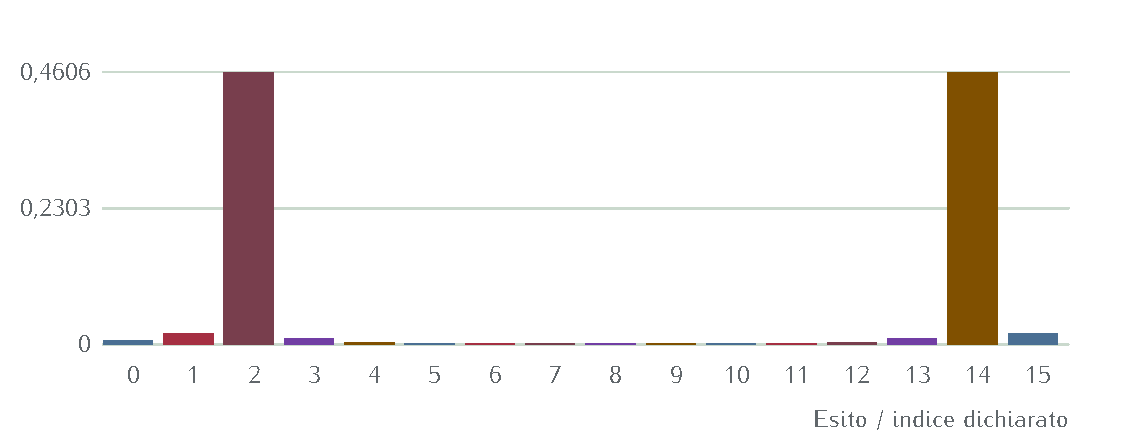
\includegraphics[width=\linewidth,height=94mm,keepaspectratio]{figure/f07da0dfd9e197c34.pdf}\FigureCaption{4.14 \(\cdot\) esempio 2 \(\cdot\) Distribuzione completa della lettura}\end{FigureBlock}
\begin{FigureBlock}\centering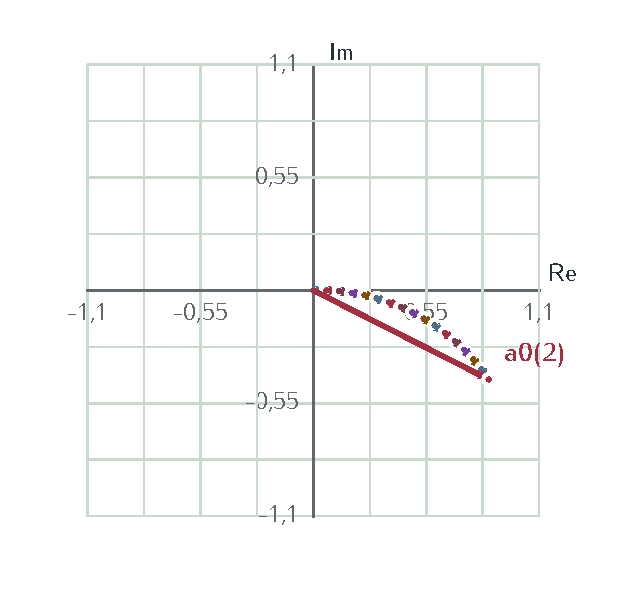
\includegraphics[width=\linewidth,height=94mm,keepaspectratio]{figure/f356cade96ee144ad.pdf}\FigureCaption{4.14 \(\cdot\) esempio 2 \(\cdot\) Somma punta-coda, x crescente \(\cdot\) \(s=0\), \(c=2\), peso 0,5}\end{FigureBlock}
\begin{FigureBlock}\centering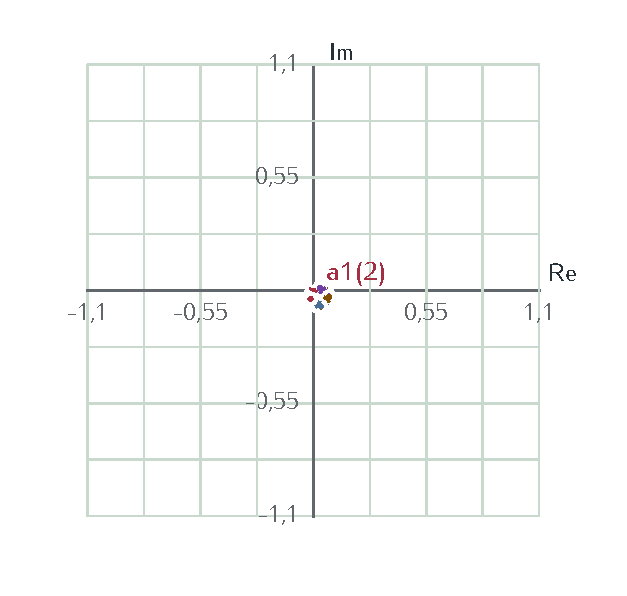
\includegraphics[width=\linewidth,height=94mm,keepaspectratio]{figure/fd597b4cc533433e9.pdf}\FigureCaption{4.14 \(\cdot\) esempio 2 \(\cdot\) Somma punta-coda, x crescente \(\cdot\) \(s=1\), \(c=2\), peso 0,5}\end{FigureBlock}
\begin{FigureBlock}\begin{minipage}[t]{.485\linewidth}\centering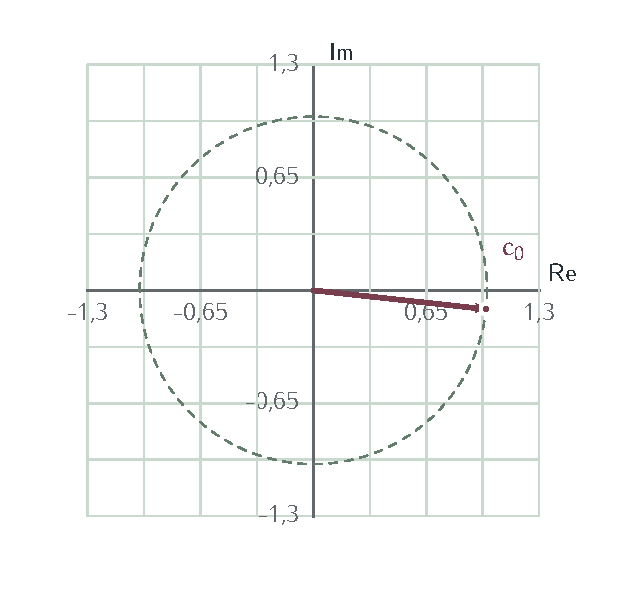
\includegraphics[width=\linewidth,height=63mm,keepaspectratio]{figure/f00742289f6402125.pdf}\par{\sffamily\footnotesize \(c_{0}\)\par}\end{minipage}\hfill\begin{minipage}[t]{.485\linewidth}\centering\includegraphics[width=\linewidth,height=63mm,keepaspectratio]{figure/f6238514f0c2cb55e.pdf}\par{\sffamily\footnotesize \(c_{1}\)\par}\end{minipage}\FigureCaption{4.14 \(\cdot\) esempio 2 \(\cdot\) Bersaglio condizionato \(\cdot\) coefficienti \(\beta {}^{\prime} s\) nella base propria dichiarata}\end{FigureBlock}
\begin{FigureBlock}\centering\includegraphics[width=\linewidth,height=94mm,keepaspectratio]{figure/f528206d3d9d56081.pdf}\FigureCaption{4.14 \(\cdot\) esempio 2 \(\cdot\) Piano di Grover \(\cdot\) preparazione e prima rotazione}\end{FigureBlock}
\begin{FigureBlock}\begin{minipage}[t]{.485\linewidth}\centering\includegraphics[width=\linewidth,height=63mm,keepaspectratio]{figure/fd4d3d4c50ab9a9d2.pdf}\par{\sffamily\footnotesize \(c_{0}\)\par}\end{minipage}\hfill\begin{minipage}[t]{.485\linewidth}\centering\includegraphics[width=\linewidth,height=63mm,keepaspectratio]{figure/f66fc837380a5591f.pdf}\par{\sffamily\footnotesize \(c_{1}\)\par}\end{minipage}\FigureCaption{4.14 \(\cdot\) esempio 2 \(\cdot\) Coordinate di u+ nella base \((|b\rangle ,\allowbreak |g\rangle )\)}\end{FigureBlock}
\begin{FigureBlock}\begin{minipage}[t]{.485\linewidth}\centering\includegraphics[width=\linewidth,height=63mm,keepaspectratio]{figure/fa2cd67ff0ef73e6c.pdf}\par{\sffamily\footnotesize \(c_{0}\)\par}\end{minipage}\hfill\begin{minipage}[t]{.485\linewidth}\centering\includegraphics[width=\linewidth,height=63mm,keepaspectratio]{figure/f8b9e76727a7ec90d.pdf}\par{\sffamily\footnotesize \(c_{1}\)\par}\end{minipage}\FigureCaption{4.14 \(\cdot\) esempio 2 \(\cdot\) Coordinate di \(u- \) nella base \((|b\rangle ,\allowbreak |g\rangle )\)}\end{FigureBlock}

\phantomsection\label{c4-conteggio-example-2-step-1}
\BookHeading{01 Definire operatore, autostati e coefficienti}

\MathBlock{0055007C0075005F007327E9003D0065005E0028003203C0006903C6005F00730029007C0075005F007327E9003B002027E80075005F0073007C0075005F007427E9003D03B40073002C0074002E}{U|u_{s}\rangle =e^{2\pi i\varphi _{s}}|u_{s}\rangle ;\allowbreak \ \langle u_{s}|u_{t}\rangle =\delta s,\allowbreak t.}
\MathBlock{007C03C827E9003D03A30073002003B2005F0073007C0075005F007327E9003B002003A30073007C03B2005F0073007C00B2003D0031003B00200051003D0032005E006D002E}{|\psi \rangle =\sum _{s}\ \beta _{s}|u_{s}\rangle ;\allowbreak \ \sum _{s}|\beta _{s}|^{2}=1;\allowbreak \ Q=2^{m}.}

Il registro di lettura contiene m qubit; \(\varphi \) è una frazione di giro modulo uno. L'indice s distingue gli autostati del bersaglio e \(\beta _{s}\) è un'ampiezza complessa, mentre \(|\beta _{s}|^{2}\) è un peso probabilistico.\par


\phantomsection\label{c4-conteggio-example-2-step-2}
\BookHeading{02 Delimitare il modello spettrale}

\MathBlock{004E003D0038003B00200047003D007B0035007D003B0020007C006127E9224800280030002C0033003500330036003B00200030002C0033003500330036003B00200030002C0033003500330036003B00200030002C0033003500330036003B00200030002C0033003500330036003B00200030002C0033003500330036003B00200030002C0033003500330036003B00200030002C003300350033003600291D40003B00200070003D0030002E003100320035002E}{N=8;\allowbreak \ G=\{5\};\allowbreak \ |a\rangle \approx (0{,}3536;\allowbreak \ 0{,}3536;\allowbreak \ 0{,}3536;\allowbreak \ 0{,}3536;\allowbreak \ 0{,}3536;\allowbreak \ 0{,}3536;\allowbreak \ 0{,}3536;\allowbreak \ 0{,}3536)^{T};\allowbreak \ p=0.125.}
\MathBlock{0049006C0020006D006F00640065006C006C006F0020007200690063006100760061002003B8003D00610072006300730069006E221A0070002000650020006C00650020006100750074006F006600610073006900200064006900200051005F0047003D0044005F0041004F002C00200070006F0069002000760061006C00750074006100200061006E0061006C00690074006900630061006D0065006E00740065002000510050004500200069006E00200062006100730065002000700072006F0070007200690061002E}{Il\ \text{modello}\ \text{ricava}\ \theta =\arcsin \sqrt{p}\ e\ \text{le}\ \text{autofasi}\ \text{di}\ Q_{G}=D_{AO},\allowbreak \ \text{poi}\ \text{valuta}\ \text{analiticamente}\ \text{QPE}\ \text{in}\ \text{base}\ \text{propria}.}

La probabilità nota costruisce la distribuzione di questo esempio. Qui non si esegue una rete controllata che ricavi p da una preparazione e da un oracolo ignoti; il conteggio operativo richiederebbe costruire e controllare \(Q_{G}\). La derivazione seguente rende verificabile il raccordo con Grover.\par


\phantomsection\label{c4-conteggio-example-2-step-3}
\BookHeading{03 Costruire gli assi dalle proiezioni}

\MathBlock{007C006127E9003D0041007C003027E9003B002003A00047003D03A3007822080047007C007827E927E80078007C003B00200070003D27E80061007C03A00047007C006127E9003D0030002C003100320035002E}{|a\rangle =A|0\rangle ;\allowbreak \ \Pi _{G}=\sum _{x\in G}|x\rangle \langle x|;\allowbreak \ p=\langle a|\Pi _{G}|a\rangle =0{,}125.}
\MathBlock{007C006727E9003D03A00047007C006127E9002F221A0070224800280030003B00200030003B00200030003B00200030003B00200030003B00200031003B00200030003B0020003000291D40}{|g\rangle =\Pi _{G}|a\rangle /\sqrt{p}\approx (0;\allowbreak \ 0;\allowbreak \ 0;\allowbreak \ 0;\allowbreak \ 0;\allowbreak \ 1;\allowbreak \ 0;\allowbreak \ 0)^{T}}
\MathBlock{007C006227E9003D00280049221203A000470029007C006127E9002F221A00280031221200700029224800280030002C003300370038003B00200030002C003300370038003B00200030002C003300370038003B00200030002C003300370038003B00200030002C003300370038003B00200030003B00200030002C003300370038003B00200030002C00330037003800291D40002E}{|b\rangle =(I- \Pi _{G})|a\rangle /\sqrt{1- p}\approx (0{,}378;\allowbreak \ 0{,}378;\allowbreak \ 0{,}378;\allowbreak \ 0{,}378;\allowbreak \ 0{,}378;\allowbreak \ 0;\allowbreak \ 0{,}378;\allowbreak \ 0{,}378)^{T}.}
\MathBlock{27E80062007C006727E9003D0030003B0020201600622016003D201600672016003D0031002E}{\langle b|g\rangle =0;\allowbreak \ \Vert b\Vert =\Vert g\Vert =1.}

I supporti sono disgiunti. Per la preparazione uniforme questi vettori diventano \(\sum _{x\in G}|x\rangle /\sqrt{M}\) e \(\sum x\notin G|x\rangle /\sqrt{N- M}\). Per una preparazione non uniforme conservano i suoi pesi e le sue fasi.\par


\phantomsection\label{c4-conteggio-example-2-step-4}
\BookHeading{04 Proiettare la preparazione nel piano}

\MathBlock{27E80062007C006127E9003D221A00280031221200700029003D0030002C003900330035003400310034003B002027E80067007C006127E9003D221A0070003D0030002C003300350033003500350033002E}{\langle b|a\rangle =\sqrt{1- p}=0{,}935414;\allowbreak \ \langle g|a\rangle =\sqrt{p}=0{,}353553.}
\MathBlock{007C006127E9003D0063006F007303B8007C006227E9002B00730069006E03B8007C006727E9003B002003B8003D00610072006300730069006E221A007022480030002C0033003600310033003600370020007200610064002E}{|a\rangle =\cos \theta |b\rangle +\sin \theta |g\rangle ;\allowbreak \ \theta =\arcsin \sqrt{p}\approx 0{,}361367\ \text{rad}.}

Gli assi sono stati collettivi, non singoli esiti. Le coordinate qui sono reali perché le fasi della preparazione sono state incluse nella definizione degli assi.\par


\phantomsection\label{c4-conteggio-example-2-step-5}
\BookHeading{05 Scrivere le due riflessioni}

\MathBlock{004E0065006C006C0061002000620061007300650020006F007200640069006E00610074006100200028007C006227E9002C007C006727E90029003A}{\text{Nella}\ \text{base}\ \text{ordinata}\ (|b\rangle ,\allowbreak |g\rangle ):}
\MathBlock{004F003D00492212003203A00047003D005B005B0031002C0030005D002C005B0030002C22120031005D005D002E}{O=I- 2\Pi _{G}=\begin{pmatrix}1&0\\0&- 1\end{pmatrix}.}
\MathBlock{0044005F0041003D0032007C006127E927E80061007C22120049}{D_{A}=2|a\rangle \langle a|- I}
\MathBlock{003D005B005B00320063006F007300B203B822120031002C00320063006F007303B800730069006E03B8005D002C005B00320063006F007303B800730069006E03B8002C003200730069006E00B203B822120031005D005D}{=\begin{pmatrix}2\cos ^{2}\theta - 1&2\cos \theta \sin \theta \\2\cos \theta \sin \theta &2\sin ^{2}\theta - 1\end{pmatrix}}
\MathBlock{003D005B005B0063006F0073003203B8002C00730069006E003203B8005D002C005B00730069006E003203B8002C22120063006F0073003203B8005D005D002E}{=\begin{pmatrix}\cos 2\theta &\sin 2\theta \\\sin 2\theta &- \cos 2\theta \end{pmatrix}.}

\(O\) riflette rispetto all'asse \(|b\rangle \). \(D_{A}\) riflette rispetto alla retta della preparazione \(|a\rangle \). L'ordine temporale è prima \(O\) e poi \(D_{A}\).\par


\phantomsection\label{c4-conteggio-example-2-step-6}
\BookHeading{06 Moltiplicare e ottenere la rotazione}

\MathBlock{0051003D0044005F0041004F003D005B005B0063006F0073003203B8002C221200730069006E003203B8005D002C005B00730069006E003203B8002C0063006F0073003203B8005D005D}{Q=D_{AO}=\begin{pmatrix}\cos 2\theta &- \sin 2\theta \\\sin 2\theta &\cos 2\theta \end{pmatrix}}
\MathBlock{2248005B005B0030002C00370035002C002D0030002C003600360031003400330038005D002C005B0030002C003600360031003400330038002C0030002C00370035005D005D002E}{\approx \begin{pmatrix}0{,}75&-0{,}661438\\0{,}661438&0{,}75\end{pmatrix}.}
\MathBlock{004F00280063006F007303B8002C00730069006E03B800291D40003D00280063006F007303B8002C221200730069006E03B800291D40003B}{O(\cos \theta ,\allowbreak \sin \theta )^{T}=(\cos \theta ,\allowbreak - \sin \theta )^{T};\allowbreak }
\MathBlock{005100280063006F007303B8002C00730069006E03B800291D40003D00280063006F0073003303B8002C00730069006E003303B800291D40002E}{Q(\cos \theta ,\allowbreak \sin \theta )^{T}=(\cos 3\theta ,\allowbreak \sin 3\theta )^{T}.}
\MathBlock{00511D4F007C006127E9003D0063006F0073002800280032006B002B0031002903B80029007C006227E9002B00730069006E002800280032006B002B0031002903B80029007C006727E9002E}{Q^{k}|a\rangle =\cos ((2k+1)\theta )|b\rangle +\sin ((2k+1)\theta )|g\rangle .}

Il prodotto riga per colonna dà le formule di addizione del seno e del coseno. Ogni coppia completa di riflessioni ruota di \(2\theta \); dopo il solo oracolo si usa invece la riflessione, non la formula delle iterazioni complete.\par


\phantomsection\label{c4-conteggio-example-2-step-7}
\BookHeading{07 Ricavare autovettori e autofasi}

\MathBlock{00640065007400280051221203BB00490029003D03BB00B2221200320063006F00730028003203B8002903BB002B0031003D0030002E}{\det (Q- \lambda I)=\lambda ^{2}- 2\cos (2\theta )\lambda +1=0.}
\MathBlock{03BB00B1003D0063006F0073003203B800B10069002000730069006E003203B8003D0065005E002800B10032006903B80029002E}{\lambda \pm =\cos 2\theta \pm i\ \sin 2\theta =e^{\pm 2i\theta }.}
\MathBlock{007C0075002B27E9003D0028007C006227E922120069007C006727E90029002F221A0032003B0020007C0075221227E9003D0028007C006227E9002B0069007C006727E90029002F221A0032002E}{|u+\rangle =(|b\rangle - i|g\rangle )/\sqrt{2};\allowbreak \ |u- \rangle =(|b\rangle +i|g\rangle )/\sqrt{2}.}
\MathBlock{0051007C007500B127E9003D0065005E002800B10032006903B80029007C007500B127E9003B002003C6002B003D03B8002F03C0002C002003C62212003D0031221203B8002F03C000200028006D006F0064002000310029002E}{Q|u\pm \rangle =e^{\pm 2i\theta }|u\pm \rangle ;\allowbreak \ \varphi +=\theta /\pi ,\allowbreak \ \varphi - =1- \theta /\pi \ (\bmod \ 1).}

Gli autovettori hanno coordinate complesse nel piano collettivo; non sono due frecce reali sul piano di Grover. Le autofasi sono frazioni di giro, poiché QPE usa \(e^{2\pi i\varphi }\).\par


\phantomsection\label{c4-conteggio-example-2-step-8}
\BookHeading{08 Determinare i coefficienti della preparazione}

\MathBlock{03B2002B003D27E80075002B007C006127E9003D00280063006F007303B8002B0069002000730069006E03B80029002F221A0032003D0065005E0028006903B80029002F221A0032002E}{\beta +=\langle u+|a\rangle =(\cos \theta +i\ \sin \theta )/\sqrt{2}=e^{i\theta }/\sqrt{2}.}
\MathBlock{03B22212003D27E800752212007C006127E9003D00280063006F007303B822120069002000730069006E03B80029002F221A0032003D0065005E00282212006903B80029002F221A0032002E}{\beta - =\langle u- |a\rangle =(\cos \theta - i\ \sin \theta )/\sqrt{2}=e^{- i\theta }/\sqrt{2}.}
\MathBlock{007C006127E9003D03B2002B007C0075002B27E9002B03B22212007C0075221227E9003B0020007C03B2002B007C00B2003D007C03B22212007C00B2003D0031002F0032002E}{|a\rangle =\beta +|u+\rangle +\beta - |u- \rangle ;\allowbreak \ |\beta +|^{2}=|\beta - |^{2}=1/2.}

I due pesi uguali derivano dal prodotto interno con la preparazione. Manteniamo anche le fasi dei coefficienti: servono per ricostruire il bersaglio coerente condizionato dopo QPE.\par


\phantomsection\label{c4-conteggio-example-2-step-9}
\BookHeading{09 Fissare le fasi della base propria}

\MathBlock{00752080003D0075002B003D0028007C006227E922120069007C006727E90029002F221A0032003B002000752081003D00752212003D0028007C006227E9002B0069007C006727E90029002F221A0032002E}{u_{0}=u+=(|b\rangle - i|g\rangle )/\sqrt{2};\allowbreak \ u_{1}=u- =(|b\rangle +i|g\rangle )/\sqrt{2}.}
\MathBlock{03B22080003D0065005E0028006903B80029002F221A003222480030002C00360036003100340033003700380020002B00200030002C003200350069003B002003B22081003D0065005E00282212006903B80029002F221A003222480030002C00360036003100340033003700380020221200200030002C003200350069002E}{\beta _{0}=e^{i\theta }/\sqrt{2}\approx 0{,}6614378\ +\ 0{,}25i;\allowbreak \ \beta _{1}=e^{- i\theta }/\sqrt{2}\approx 0{,}6614378\ - \ 0{,}25i.}
\MathBlock{03B2208000752080002B03B2208100752081003D0063006F007303B8007C006227E9002B00730069006E03B8007C006727E9002E}{\beta _{0}u_{0}+\beta _{1}u_{1}=\cos \theta |b\rangle +\sin \theta |g\rangle .}

Questa convenzione fissa univocamente i coefficienti complessi. I pesi sono uguali, ma le fasi dei \(\beta \) restano nel bersaglio condizionato.\par


\phantomsection\label{c4-conteggio-example-2-step-10}
\BookHeading{10 Preparare il controllo}

\MathBlock{007C003027E922970034007C03C827E900202192002000280031002F221A00310036002903A30078007C007827E903A30073002003B2005F0073007C0075005F007327E9002E}{|0\rangle ^{\otimes 4}|\psi \rangle \ \to \ (1/\sqrt{16})\sum _{x}|x\rangle \sum _{s}\ \beta _{s}|u_{s}\rangle .}

Le Hadamard agiscono soltanto sui qubit di lettura. Il bersaglio mantiene i coefficienti appena assegnati.\par


\phantomsection\label{c4-conteggio-example-2-step-11}
\BookHeading{11 Costruire le potenze e il kickback}

\MathBlock{00660069006C006F002000710030002C0020007000650073006F00200032005E0033003A00200063006F006E00740072006F006C006C006F00200064006900200055005E0038}{\text{filo}\ q_{0},\allowbreak \ \text{peso}\ 2^{3}:\ \text{controllo}\ \text{di}\ U^{8}}
\MathBlock{00660069006C006F002000710031002C0020007000650073006F00200032005E0032003A00200063006F006E00740072006F006C006C006F00200064006900200055005E0034}{\text{filo}\ q_{1},\allowbreak \ \text{peso}\ 2^{2}:\ \text{controllo}\ \text{di}\ U^{4}}
\MathBlock{00660069006C006F002000710032002C0020007000650073006F00200032005E0031003A00200063006F006E00740072006F006C006C006F00200064006900200055005E0032}{\text{filo}\ q_{2},\allowbreak \ \text{peso}\ 2^{1}:\ \text{controllo}\ \text{di}\ U^{2}}
\MathBlock{00660069006C006F002000710033002C0020007000650073006F00200032005E0030003A00200063006F006E00740072006F006C006C006F00200064006900200055005E0031}{\text{filo}\ q_{3},\allowbreak \ \text{peso}\ 2^{0}:\ \text{controllo}\ \text{di}\ U^{1}}
\MathBlock{0078003D03A3007100200078005F00710032005E0028006D22120031221200710029002021D20020220F007100200065005E0028003203C0006900200078005F00710032005E0028006D2212003122120071002903C6005F00730029003D0065005E0028003203C00069007803C6005F00730029002E}{x=\sum _{q}\ x_{q}2^{m- 1- q}\ \Rightarrow \ \prod _{q}\ e^{2\pi i\ x_{q}2^{m- 1- q}\varphi _{s}}=e^{2\pi ix\varphi _{s}}.}
\MathBlock{007C03A827E9003D00280031002F221A0051002903A30078002C0073002003B2005F007300200065005E0028003203C00069007803C6005F00730029007C007827E9007C0075005F007327E9002E}{|\Psi \rangle =(1/\sqrt{Q})\sum _{x,\allowbreak s}\ \beta _{s}\ e^{2\pi ix\varphi _{s}}|x\rangle |u_{s}\rangle .}

\(q_{0}\) è il filo superiore e il bit più significativo. Per tre qubit le potenze sono \(U^{4},\allowbreak U^{2},\allowbreak U\); l'esponente j di \(2^{j}\) non va confuso con l'indice del filo \(q_{j}\).\par


\phantomsection\label{c4-conteggio-example-2-step-12}
\BookHeading{12 Sommare le radici dell'unità}

\MathBlock{0053003D0031002B007A002B22EF002B007A005E002800310036002D00310029002E}{S=1+z+\cdots +z^{16-1}.}
\MathBlock{007A0053003D007A002B007A00B2002B22EF002B007A005E00310036003B0020002800312212007A00290053003D00312212007A005E00310036002E}{zS=z+z^{2}+\cdots +z^{16};\allowbreak \ (1- z)S=1- z^{16}.}
\MathBlock{005300650020007A22600031003A00200053003D002800312212007A005E003100360029002F002800312212007A0029002E0020005300650020007A003D0031003A00200053003D00310036002E}{Se\ z\ne 1:\ S=(1- z^{16})/(1- z).\ Se\ z=1:\ S=16.}

La sottrazione cancella tutti i termini intermedi. Il caso \(z=1\) va separato prima della divisione.\par


\phantomsection\label{c4-conteggio-example-2-step-13}
\BookHeading{13 Dalla cancellazione all'unitarietà}

\MathBlock{007A003D0065005E0028003203C00069002800782212007820320029002F003100360029003B0020007A005E00310036003D0031002E}{z=e^{2\pi i(x- x{}^{\prime} )/16};\allowbreak \ z^{16}=1.}
\MathBlock{27E800460031003600782032007C004600310036007827E9003D00280031002F00310036002903A300790020007A02B8003D00310036002F00310036003D003100200073006500200078003D00782032003B0020003000200061006C007400720069006D0065006E00740069002E}{\langle F16x{}^{\prime} |F16x\rangle =(1/16)\sum _{y}\ z^{y}=16/16=1\ \text{se}\ x=x{}^{\prime} ;\allowbreak \ 0\ \text{altrimenti}.}

Per x e \(x{}^{\prime} \) distinti fra 0 e \(N- 1\), \(z\ne 1\): le frecce delle radici si chiudono. Le colonne di Fourier sono quindi ortonormali e la trasformata conserva prodotti interni e norma.\par


\phantomsection\label{c4-conteggio-example-2-step-14}
\BookHeading{14 Applicare la cancellazione alla QPE}

\MathBlock{0044006F0070006F00200046005F00512020003A0020007C03A8006F0075007427E9003D03A30063002C0073002003B2005F007300200061005F0073002800630029007C006327E9007C0075005F007327E9002E}{\text{Dopo}\ F_{Q}{}^{\dagger} :\ |\Psi \text{out}\rangle =\sum _{c,\allowbreak s}\ \beta _{s}\ a_{s}(c)|c\rangle |u_{s}\rangle .}
\MathBlock{0061005F0073002800630029003D00280031002F0051002903A300780020007A02E3002C0020007A003D0065005E0028003203C00069002803C6005F007322120063002F005100290029002E}{a_{s}(c)=(1/Q)\sum _{x}\ z^{x},\allowbreak \ z=e^{2\pi i(\varphi _{s}- c/Q)}.}
\MathBlock{005300650020005103C6005F0073003D004C00200069006E007400650072006F003A0020007A005E0051003D0031003B00200061005F00730028004C0029003D0031002C00200061005F0073002800630029003D00300020007000650072002000632260004C002E}{Se\ Q\varphi _{s}=L\ \text{intero}:\ z^{Q}=1;\allowbreak \ a_{s}(L)=1,\allowbreak \ a_{s}(c)=0\ \text{per}\ c\ne L.}
\MathBlock{00460075006F0072006900200067007200690067006C00690061003A00200061005F0073002800630029003D002800312212007A005E00510029002F00280051002800312212007A00290029002C002000730061006C0076006F0020007A003D0031002E}{\text{Fuori}\ \text{griglia}:\ a_{s}(c)=(1- z^{Q})/(Q(1- z)),\allowbreak \ \text{salvo}\ z=1.}

Per \(Q=8\), \(\varphi =3/8\): \(a(3)=8/8=1\). Per ogni altro c, \(z=e^{2\pi i(3- c)/8}\ne 1\) e il numeratore è zero. Fuori griglia la cancellazione è incompleta e più esiti restano possibili.\par


\phantomsection\label{c4-conteggio-example-2-step-15}
\BookHeading{15 Potenze controllate \(\cdot\) autostato 0}

\MathBlock{00660069006C006F002000710030003A00200032005E003303C60020006D006F00640020003122480030002C003900320030003200310034}{\text{filo}\ q_{0}:\ 2^{3}\varphi \ \bmod \ 1\approx 0{,}920214}
\MathBlock{00660069006C006F002000710031003A00200032005E003203C60020006D006F00640020003122480030002C003400360030003100300037}{\text{filo}\ q_{1}:\ 2^{2}\varphi \ \bmod \ 1\approx 0{,}460107}
\MathBlock{00660069006C006F002000710032003A00200032005E003103C60020006D006F00640020003122480030002C003200330030003000350033}{\text{filo}\ q_{2}:\ 2^{1}\varphi \ \bmod \ 1\approx 0{,}230053}
\MathBlock{00660069006C006F002000710033003A00200032005E003003C60020006D006F00640020003122480030002C003100310035003000320037}{\text{filo}\ q_{3}:\ 2^{0}\varphi \ \bmod \ 1\approx 0{,}115027}
\MathBlock{0063005F0073002800780029003D0065005E0028003203C00069007800B70030002C003100310035003000320036003700330029002F221A00310036}{c_{s}(x)=e^{2\pi ix\cdot 0{,}11502673}/\sqrt{16}}

Queste fasi moltiplicano il ramo di autostato s; il suo coefficiente \(\beta _{s}\) rimane esplicito nello stato congiunto.\par


\phantomsection\label{c4-conteggio-example-2-step-16}
\BookHeading{16 Fourier inversa \(\cdot\) \(s=0\), \(c=0\)}

\MathBlock{0061005F0073002800300029003D00280031002F003100360029005B0065005E0028003203C0006900B7003000B700280030002C0031003100350030003200360037003322120030002F0031003600290029002B0065005E0028003203C0006900B7003100B700280030002C0031003100350030003200360037003322120030002F0031003600290029002B0065005E0028003203C0006900B7003200B700280030002C0031003100350030003200360037003322120030002F0031003600290029002B0065005E0028003203C0006900B7003300B700280030002C0031003100350030003200360037003322120030002F0031003600290029002B0065005E0028003203C0006900B7003400B700280030002C0031003100350030003200360037003322120030002F0031003600290029002B0065005E0028003203C0006900B7003500B700280030002C0031003100350030003200360037003322120030002F0031003600290029002B0065005E0028003203C0006900B7003600B700280030002C0031003100350030003200360037003322120030002F0031003600290029002B0065005E0028003203C0006900B7003700B700280030002C0031003100350030003200360037003322120030002F0031003600290029002B}{a_{s}(0)=(1/16)[e^{2\pi i\cdot 0\cdot (0{,}11502673- 0/16)}+e^{2\pi i\cdot 1\cdot (0{,}11502673- 0/16)}+e^{2\pi i\cdot 2\cdot (0{,}11502673- 0/16)}+e^{2\pi i\cdot 3\cdot (0{,}11502673- 0/16)}+e^{2\pi i\cdot 4\cdot (0{,}11502673- 0/16)}+e^{2\pi i\cdot 5\cdot (0{,}11502673- 0/16)}+e^{2\pi i\cdot 6\cdot (0{,}11502673- 0/16)}+e^{2\pi i\cdot 7\cdot (0{,}11502673- 0/16)}+}
\MathBlock{0065005E0028003203C0006900B7003800B700280030002C0031003100350030003200360037003322120030002F0031003600290029002B0065005E0028003203C0006900B7003900B700280030002C0031003100350030003200360037003322120030002F0031003600290029002B0065005E0028003203C0006900B70031003000B700280030002C0031003100350030003200360037003322120030002F0031003600290029002B0065005E0028003203C0006900B70031003100B700280030002C0031003100350030003200360037003322120030002F0031003600290029002B0065005E0028003203C0006900B70031003200B700280030002C0031003100350030003200360037003322120030002F0031003600290029002B0065005E0028003203C0006900B70031003300B700280030002C0031003100350030003200360037003322120030002F0031003600290029002B0065005E0028003203C0006900B70031003400B700280030002C0031003100350030003200360037003322120030002F0031003600290029002B0065005E0028003203C0006900B70031003500B700280030002C0031003100350030003200360037003322120030002F0031003600290029005D}{e^{2\pi i\cdot 8\cdot (0{,}11502673- 0/16)}+e^{2\pi i\cdot 9\cdot (0{,}11502673- 0/16)}+e^{2\pi i\cdot 10\cdot (0{,}11502673- 0/16)}+e^{2\pi i\cdot 11\cdot (0{,}11502673- 0/16)}+e^{2\pi i\cdot 12\cdot (0{,}11502673- 0/16)}+e^{2\pi i\cdot 13\cdot (0{,}11502673- 0/16)}+e^{2\pi i\cdot 14\cdot (0{,}11502673- 0/16)}+e^{2\pi i\cdot 15\cdot (0{,}11502673- 0/16)}]}
\MathBlock{2248002D0030002C00300035003500320035003400390020002B00200030002C00300036003400350033003000350069003B0020007C0061007C00B222480030002C0030003000370032003100370033}{\approx -0{,}0552549\ +\ 0{,}0645305i;\allowbreak \ |a|^{2}\approx 0{,}0072173}

La somma complessa precede il modulo quadro. Le fasi nel calcolo mantengono precisione completa; i decimali stampati sono arrotondati.\par


\phantomsection\label{c4-conteggio-example-2-step-17}
\BookHeading{17 Fourier inversa \(\cdot\) \(s=0\), \(c=1\)}

\MathBlock{0061005F0073002800310029003D00280031002F003100360029005B0065005E0028003203C0006900B7003000B700280030002C0031003100350030003200360037003322120031002F0031003600290029002B0065005E0028003203C0006900B7003100B700280030002C0031003100350030003200360037003322120031002F0031003600290029002B0065005E0028003203C0006900B7003200B700280030002C0031003100350030003200360037003322120031002F0031003600290029002B0065005E0028003203C0006900B7003300B700280030002C0031003100350030003200360037003322120031002F0031003600290029002B0065005E0028003203C0006900B7003400B700280030002C0031003100350030003200360037003322120031002F0031003600290029002B0065005E0028003203C0006900B7003500B700280030002C0031003100350030003200360037003322120031002F0031003600290029002B0065005E0028003203C0006900B7003600B700280030002C0031003100350030003200360037003322120031002F0031003600290029002B0065005E0028003203C0006900B7003700B700280030002C0031003100350030003200360037003322120031002F0031003600290029002B}{a_{s}(1)=(1/16)[e^{2\pi i\cdot 0\cdot (0{,}11502673- 1/16)}+e^{2\pi i\cdot 1\cdot (0{,}11502673- 1/16)}+e^{2\pi i\cdot 2\cdot (0{,}11502673- 1/16)}+e^{2\pi i\cdot 3\cdot (0{,}11502673- 1/16)}+e^{2\pi i\cdot 4\cdot (0{,}11502673- 1/16)}+e^{2\pi i\cdot 5\cdot (0{,}11502673- 1/16)}+e^{2\pi i\cdot 6\cdot (0{,}11502673- 1/16)}+e^{2\pi i\cdot 7\cdot (0{,}11502673- 1/16)}+}
\MathBlock{0065005E0028003203C0006900B7003800B700280030002C0031003100350030003200360037003322120031002F0031003600290029002B0065005E0028003203C0006900B7003900B700280030002C0031003100350030003200360037003322120031002F0031003600290029002B0065005E0028003203C0006900B70031003000B700280030002C0031003100350030003200360037003322120031002F0031003600290029002B0065005E0028003203C0006900B70031003100B700280030002C0031003100350030003200360037003322120031002F0031003600290029002B0065005E0028003203C0006900B70031003200B700280030002C0031003100350030003200360037003322120031002F0031003600290029002B0065005E0028003203C0006900B70031003300B700280030002C0031003100350030003200360037003322120031002F0031003600290029002B0065005E0028003203C0006900B70031003400B700280030002C0031003100350030003200360037003322120031002F0031003600290029002B0065005E0028003203C0006900B70031003500B700280030002C0031003100350030003200360037003322120031002F0031003600290029005D}{e^{2\pi i\cdot 8\cdot (0{,}11502673- 1/16)}+e^{2\pi i\cdot 9\cdot (0{,}11502673- 1/16)}+e^{2\pi i\cdot 10\cdot (0{,}11502673- 1/16)}+e^{2\pi i\cdot 11\cdot (0{,}11502673- 1/16)}+e^{2\pi i\cdot 12\cdot (0{,}11502673- 1/16)}+e^{2\pi i\cdot 13\cdot (0{,}11502673- 1/16)}+e^{2\pi i\cdot 14\cdot (0{,}11502673- 1/16)}+e^{2\pi i\cdot 15\cdot (0{,}11502673- 1/16)}]}
\MathBlock{2248002D0030002C00310034003300370033003400320020002B00200030002C00310031003300300031003700370069003B0020007C0061007C00B222480030002C0030003300330034003300320035}{\approx -0{,}1437342\ +\ 0{,}1130177i;\allowbreak \ |a|^{2}\approx 0{,}0334325}

La somma complessa precede il modulo quadro. Le fasi nel calcolo mantengono precisione completa; i decimali stampati sono arrotondati.\par


\phantomsection\label{c4-conteggio-example-2-step-18}
\BookHeading{18 Fourier inversa \(\cdot\) \(s=0\), \(c=2\)}

\MathBlock{0061005F0073002800320029003D00280031002F003100360029005B0065005E0028003203C0006900B7003000B700280030002C0031003100350030003200360037003322120032002F0031003600290029002B0065005E0028003203C0006900B7003100B700280030002C0031003100350030003200360037003322120032002F0031003600290029002B0065005E0028003203C0006900B7003200B700280030002C0031003100350030003200360037003322120032002F0031003600290029002B0065005E0028003203C0006900B7003300B700280030002C0031003100350030003200360037003322120032002F0031003600290029002B0065005E0028003203C0006900B7003400B700280030002C0031003100350030003200360037003322120032002F0031003600290029002B0065005E0028003203C0006900B7003500B700280030002C0031003100350030003200360037003322120032002F0031003600290029002B0065005E0028003203C0006900B7003600B700280030002C0031003100350030003200360037003322120032002F0031003600290029002B0065005E0028003203C0006900B7003700B700280030002C0031003100350030003200360037003322120032002F0031003600290029002B}{a_{s}(2)=(1/16)[e^{2\pi i\cdot 0\cdot (0{,}11502673- 2/16)}+e^{2\pi i\cdot 1\cdot (0{,}11502673- 2/16)}+e^{2\pi i\cdot 2\cdot (0{,}11502673- 2/16)}+e^{2\pi i\cdot 3\cdot (0{,}11502673- 2/16)}+e^{2\pi i\cdot 4\cdot (0{,}11502673- 2/16)}+e^{2\pi i\cdot 5\cdot (0{,}11502673- 2/16)}+e^{2\pi i\cdot 6\cdot (0{,}11502673- 2/16)}+e^{2\pi i\cdot 7\cdot (0{,}11502673- 2/16)}+}
\MathBlock{0065005E0028003203C0006900B7003800B700280030002C0031003100350030003200360037003322120032002F0031003600290029002B0065005E0028003203C0006900B7003900B700280030002C0031003100350030003200360037003322120032002F0031003600290029002B0065005E0028003203C0006900B70031003000B700280030002C0031003100350030003200360037003322120032002F0031003600290029002B0065005E0028003203C0006900B70031003100B700280030002C0031003100350030003200360037003322120032002F0031003600290029002B0065005E0028003203C0006900B70031003200B700280030002C0031003100350030003200360037003322120032002F0031003600290029002B0065005E0028003203C0006900B70031003300B700280030002C0031003100350030003200360037003322120032002F0031003600290029002B0065005E0028003203C0006900B70031003400B700280030002C0031003100350030003200360037003322120032002F0031003600290029002B0065005E0028003203C0006900B70031003500B700280030002C0031003100350030003200360037003322120032002F0031003600290029005D}{e^{2\pi i\cdot 8\cdot (0{,}11502673- 2/16)}+e^{2\pi i\cdot 9\cdot (0{,}11502673- 2/16)}+e^{2\pi i\cdot 10\cdot (0{,}11502673- 2/16)}+e^{2\pi i\cdot 11\cdot (0{,}11502673- 2/16)}+e^{2\pi i\cdot 12\cdot (0{,}11502673- 2/16)}+e^{2\pi i\cdot 13\cdot (0{,}11502673- 2/16)}+e^{2\pi i\cdot 14\cdot (0{,}11502673- 2/16)}+e^{2\pi i\cdot 15\cdot (0{,}11502673- 2/16)}]}
\MathBlock{22480030002C00380035003400380033003900380020221200200030002C00340033003400320030003700330069003B0020007C0061007C00B222480030002C003900310039003200380037}{\approx 0{,}8548398\ - \ 0{,}4342073i;\allowbreak \ |a|^{2}\approx 0{,}919287}

La somma complessa precede il modulo quadro. Le fasi nel calcolo mantengono precisione completa; i decimali stampati sono arrotondati.\par


\phantomsection\label{c4-conteggio-example-2-step-19}
\BookHeading{19 Fourier inversa \(\cdot\) \(s=0\), \(c=3\)}

\MathBlock{0061005F0073002800330029003D00280031002F003100360029005B0065005E0028003203C0006900B7003000B700280030002C0031003100350030003200360037003322120033002F0031003600290029002B0065005E0028003203C0006900B7003100B700280030002C0031003100350030003200360037003322120033002F0031003600290029002B0065005E0028003203C0006900B7003200B700280030002C0031003100350030003200360037003322120033002F0031003600290029002B0065005E0028003203C0006900B7003300B700280030002C0031003100350030003200360037003322120033002F0031003600290029002B0065005E0028003203C0006900B7003400B700280030002C0031003100350030003200360037003322120033002F0031003600290029002B0065005E0028003203C0006900B7003500B700280030002C0031003100350030003200360037003322120033002F0031003600290029002B0065005E0028003203C0006900B7003600B700280030002C0031003100350030003200360037003322120033002F0031003600290029002B0065005E0028003203C0006900B7003700B700280030002C0031003100350030003200360037003322120033002F0031003600290029002B}{a_{s}(3)=(1/16)[e^{2\pi i\cdot 0\cdot (0{,}11502673- 3/16)}+e^{2\pi i\cdot 1\cdot (0{,}11502673- 3/16)}+e^{2\pi i\cdot 2\cdot (0{,}11502673- 3/16)}+e^{2\pi i\cdot 3\cdot (0{,}11502673- 3/16)}+e^{2\pi i\cdot 4\cdot (0{,}11502673- 3/16)}+e^{2\pi i\cdot 5\cdot (0{,}11502673- 3/16)}+e^{2\pi i\cdot 6\cdot (0{,}11502673- 3/16)}+e^{2\pi i\cdot 7\cdot (0{,}11502673- 3/16)}+}
\MathBlock{0065005E0028003203C0006900B7003800B700280030002C0031003100350030003200360037003322120033002F0031003600290029002B0065005E0028003203C0006900B7003900B700280030002C0031003100350030003200360037003322120033002F0031003600290029002B0065005E0028003203C0006900B70031003000B700280030002C0031003100350030003200360037003322120033002F0031003600290029002B0065005E0028003203C0006900B70031003100B700280030002C0031003100350030003200360037003322120033002F0031003600290029002B0065005E0028003203C0006900B70031003200B700280030002C0031003100350030003200360037003322120033002F0031003600290029002B0065005E0028003203C0006900B70031003300B700280030002C0031003100350030003200360037003322120033002F0031003600290029002B0065005E0028003203C0006900B70031003400B700280030002C0031003100350030003200360037003322120033002F0031003600290029002B0065005E0028003203C0006900B70031003500B700280030002C0031003100350030003200360037003322120033002F0031003600290029005D}{e^{2\pi i\cdot 8\cdot (0{,}11502673- 3/16)}+e^{2\pi i\cdot 9\cdot (0{,}11502673- 3/16)}+e^{2\pi i\cdot 10\cdot (0{,}11502673- 3/16)}+e^{2\pi i\cdot 11\cdot (0{,}11502673- 3/16)}+e^{2\pi i\cdot 12\cdot (0{,}11502673- 3/16)}+e^{2\pi i\cdot 13\cdot (0{,}11502673- 3/16)}+e^{2\pi i\cdot 14\cdot (0{,}11502673- 3/16)}+e^{2\pi i\cdot 15\cdot (0{,}11502673- 3/16)}]}
\MathBlock{22480030002C00310032003800310031003700320020221200200030002C00300033003500390035003800360069003B0020007C0061007C00B222480030002C003000310037003700300037}{\approx 0{,}1281172\ - \ 0{,}0359586i;\allowbreak \ |a|^{2}\approx 0{,}017707}

La somma complessa precede il modulo quadro. Le fasi nel calcolo mantengono precisione completa; i decimali stampati sono arrotondati.\par


\phantomsection\label{c4-conteggio-example-2-step-20}
\BookHeading{20 Fourier inversa \(\cdot\) \(s=0\), \(c=4\)}

\MathBlock{0061005F0073002800340029003D00280031002F003100360029005B0065005E0028003203C0006900B7003000B700280030002C0031003100350030003200360037003322120034002F0031003600290029002B0065005E0028003203C0006900B7003100B700280030002C0031003100350030003200360037003322120034002F0031003600290029002B0065005E0028003203C0006900B7003200B700280030002C0031003100350030003200360037003322120034002F0031003600290029002B0065005E0028003203C0006900B7003300B700280030002C0031003100350030003200360037003322120034002F0031003600290029002B0065005E0028003203C0006900B7003400B700280030002C0031003100350030003200360037003322120034002F0031003600290029002B0065005E0028003203C0006900B7003500B700280030002C0031003100350030003200360037003322120034002F0031003600290029002B0065005E0028003203C0006900B7003600B700280030002C0031003100350030003200360037003322120034002F0031003600290029002B0065005E0028003203C0006900B7003700B700280030002C0031003100350030003200360037003322120034002F0031003600290029002B}{a_{s}(4)=(1/16)[e^{2\pi i\cdot 0\cdot (0{,}11502673- 4/16)}+e^{2\pi i\cdot 1\cdot (0{,}11502673- 4/16)}+e^{2\pi i\cdot 2\cdot (0{,}11502673- 4/16)}+e^{2\pi i\cdot 3\cdot (0{,}11502673- 4/16)}+e^{2\pi i\cdot 4\cdot (0{,}11502673- 4/16)}+e^{2\pi i\cdot 5\cdot (0{,}11502673- 4/16)}+e^{2\pi i\cdot 6\cdot (0{,}11502673- 4/16)}+e^{2\pi i\cdot 7\cdot (0{,}11502673- 4/16)}+}
\MathBlock{0065005E0028003203C0006900B7003800B700280030002C0031003100350030003200360037003322120034002F0031003600290029002B0065005E0028003203C0006900B7003900B700280030002C0031003100350030003200360037003322120034002F0031003600290029002B0065005E0028003203C0006900B70031003000B700280030002C0031003100350030003200360037003322120034002F0031003600290029002B0065005E0028003203C0006900B70031003100B700280030002C0031003100350030003200360037003322120034002F0031003600290029002B0065005E0028003203C0006900B70031003200B700280030002C0031003100350030003200360037003322120034002F0031003600290029002B0065005E0028003203C0006900B70031003300B700280030002C0031003100350030003200360037003322120034002F0031003600290029002B0065005E0028003203C0006900B70031003400B700280030002C0031003100350030003200360037003322120034002F0031003600290029002B0065005E0028003203C0006900B70031003500B700280030002C0031003100350030003200360037003322120034002F0031003600290029005D}{e^{2\pi i\cdot 8\cdot (0{,}11502673- 4/16)}+e^{2\pi i\cdot 9\cdot (0{,}11502673- 4/16)}+e^{2\pi i\cdot 10\cdot (0{,}11502673- 4/16)}+e^{2\pi i\cdot 11\cdot (0{,}11502673- 4/16)}+e^{2\pi i\cdot 12\cdot (0{,}11502673- 4/16)}+e^{2\pi i\cdot 13\cdot (0{,}11502673- 4/16)}+e^{2\pi i\cdot 14\cdot (0{,}11502673- 4/16)}+e^{2\pi i\cdot 15\cdot (0{,}11502673- 4/16)}]}
\MathBlock{22480030002C00300037003200370038003400360020221200200030002C0030003000350036003300360069003B0020007C0061007C00B222480030002C0030003000350033003200390034}{\approx 0{,}0727846\ - \ 0{,}005636i;\allowbreak \ |a|^{2}\approx 0{,}0053294}

La somma complessa precede il modulo quadro. Le fasi nel calcolo mantengono precisione completa; i decimali stampati sono arrotondati.\par


\phantomsection\label{c4-conteggio-example-2-step-21}
\BookHeading{21 Fourier inversa \(\cdot\) \(s=0\), \(c=5\)}

\MathBlock{0061005F0073002800350029003D00280031002F003100360029005B0065005E0028003203C0006900B7003000B700280030002C0031003100350030003200360037003322120035002F0031003600290029002B0065005E0028003203C0006900B7003100B700280030002C0031003100350030003200360037003322120035002F0031003600290029002B0065005E0028003203C0006900B7003200B700280030002C0031003100350030003200360037003322120035002F0031003600290029002B0065005E0028003203C0006900B7003300B700280030002C0031003100350030003200360037003322120035002F0031003600290029002B0065005E0028003203C0006900B7003400B700280030002C0031003100350030003200360037003322120035002F0031003600290029002B0065005E0028003203C0006900B7003500B700280030002C0031003100350030003200360037003322120035002F0031003600290029002B0065005E0028003203C0006900B7003600B700280030002C0031003100350030003200360037003322120035002F0031003600290029002B0065005E0028003203C0006900B7003700B700280030002C0031003100350030003200360037003322120035002F0031003600290029002B}{a_{s}(5)=(1/16)[e^{2\pi i\cdot 0\cdot (0{,}11502673- 5/16)}+e^{2\pi i\cdot 1\cdot (0{,}11502673- 5/16)}+e^{2\pi i\cdot 2\cdot (0{,}11502673- 5/16)}+e^{2\pi i\cdot 3\cdot (0{,}11502673- 5/16)}+e^{2\pi i\cdot 4\cdot (0{,}11502673- 5/16)}+e^{2\pi i\cdot 5\cdot (0{,}11502673- 5/16)}+e^{2\pi i\cdot 6\cdot (0{,}11502673- 5/16)}+e^{2\pi i\cdot 7\cdot (0{,}11502673- 5/16)}+}
\MathBlock{0065005E0028003203C0006900B7003800B700280030002C0031003100350030003200360037003322120035002F0031003600290029002B0065005E0028003203C0006900B7003900B700280030002C0031003100350030003200360037003322120035002F0031003600290029002B0065005E0028003203C0006900B70031003000B700280030002C0031003100350030003200360037003322120035002F0031003600290029002B0065005E0028003203C0006900B70031003100B700280030002C0031003100350030003200360037003322120035002F0031003600290029002B0065005E0028003203C0006900B70031003200B700280030002C0031003100350030003200360037003322120035002F0031003600290029002B0065005E0028003203C0006900B70031003300B700280030002C0031003100350030003200360037003322120035002F0031003600290029002B0065005E0028003203C0006900B70031003400B700280030002C0031003100350030003200360037003322120035002F0031003600290029002B0065005E0028003203C0006900B70031003500B700280030002C0031003100350030003200360037003322120035002F0031003600290029005D}{e^{2\pi i\cdot 8\cdot (0{,}11502673- 5/16)}+e^{2\pi i\cdot 9\cdot (0{,}11502673- 5/16)}+e^{2\pi i\cdot 10\cdot (0{,}11502673- 5/16)}+e^{2\pi i\cdot 11\cdot (0{,}11502673- 5/16)}+e^{2\pi i\cdot 12\cdot (0{,}11502673- 5/16)}+e^{2\pi i\cdot 13\cdot (0{,}11502673- 5/16)}+e^{2\pi i\cdot 14\cdot (0{,}11502673- 5/16)}+e^{2\pi i\cdot 15\cdot (0{,}11502673- 5/16)}]}
\MathBlock{22480030002C00300035003100330030003000360020002B00200030002C00300030003600310033003700340069003B0020007C0061007C00B222480030002C0030003000320036003600390034}{\approx 0{,}0513006\ +\ 0{,}0061374i;\allowbreak \ |a|^{2}\approx 0{,}0026694}

La somma complessa precede il modulo quadro. Le fasi nel calcolo mantengono precisione completa; i decimali stampati sono arrotondati.\par


\phantomsection\label{c4-conteggio-example-2-step-22}
\BookHeading{22 Fourier inversa \(\cdot\) \(s=0\), \(c=6\)}

\MathBlock{0061005F0073002800360029003D00280031002F003100360029005B0065005E0028003203C0006900B7003000B700280030002C0031003100350030003200360037003322120036002F0031003600290029002B0065005E0028003203C0006900B7003100B700280030002C0031003100350030003200360037003322120036002F0031003600290029002B0065005E0028003203C0006900B7003200B700280030002C0031003100350030003200360037003322120036002F0031003600290029002B0065005E0028003203C0006900B7003300B700280030002C0031003100350030003200360037003322120036002F0031003600290029002B0065005E0028003203C0006900B7003400B700280030002C0031003100350030003200360037003322120036002F0031003600290029002B0065005E0028003203C0006900B7003500B700280030002C0031003100350030003200360037003322120036002F0031003600290029002B0065005E0028003203C0006900B7003600B700280030002C0031003100350030003200360037003322120036002F0031003600290029002B0065005E0028003203C0006900B7003700B700280030002C0031003100350030003200360037003322120036002F0031003600290029002B}{a_{s}(6)=(1/16)[e^{2\pi i\cdot 0\cdot (0{,}11502673- 6/16)}+e^{2\pi i\cdot 1\cdot (0{,}11502673- 6/16)}+e^{2\pi i\cdot 2\cdot (0{,}11502673- 6/16)}+e^{2\pi i\cdot 3\cdot (0{,}11502673- 6/16)}+e^{2\pi i\cdot 4\cdot (0{,}11502673- 6/16)}+e^{2\pi i\cdot 5\cdot (0{,}11502673- 6/16)}+e^{2\pi i\cdot 6\cdot (0{,}11502673- 6/16)}+e^{2\pi i\cdot 7\cdot (0{,}11502673- 6/16)}+}
\MathBlock{0065005E0028003203C0006900B7003800B700280030002C0031003100350030003200360037003322120036002F0031003600290029002B0065005E0028003203C0006900B7003900B700280030002C0031003100350030003200360037003322120036002F0031003600290029002B0065005E0028003203C0006900B70031003000B700280030002C0031003100350030003200360037003322120036002F0031003600290029002B0065005E0028003203C0006900B70031003100B700280030002C0031003100350030003200360037003322120036002F0031003600290029002B0065005E0028003203C0006900B70031003200B700280030002C0031003100350030003200360037003322120036002F0031003600290029002B0065005E0028003203C0006900B70031003300B700280030002C0031003100350030003200360037003322120036002F0031003600290029002B0065005E0028003203C0006900B70031003400B700280030002C0031003100350030003200360037003322120036002F0031003600290029002B0065005E0028003203C0006900B70031003500B700280030002C0031003100350030003200360037003322120036002F0031003600290029005D}{e^{2\pi i\cdot 8\cdot (0{,}11502673- 6/16)}+e^{2\pi i\cdot 9\cdot (0{,}11502673- 6/16)}+e^{2\pi i\cdot 10\cdot (0{,}11502673- 6/16)}+e^{2\pi i\cdot 11\cdot (0{,}11502673- 6/16)}+e^{2\pi i\cdot 12\cdot (0{,}11502673- 6/16)}+e^{2\pi i\cdot 13\cdot (0{,}11502673- 6/16)}+e^{2\pi i\cdot 14\cdot (0{,}11502673- 6/16)}+e^{2\pi i\cdot 15\cdot (0{,}11502673- 6/16)}]}
\MathBlock{22480030002C00300033003900310037003300380020002B00200030002C00300031003200370038003200390069003B0020007C0061007C00B222480030002C003000300031003600390038}{\approx 0{,}0391738\ +\ 0{,}0127829i;\allowbreak \ |a|^{2}\approx 0{,}001698}

La somma complessa precede il modulo quadro. Le fasi nel calcolo mantengono precisione completa; i decimali stampati sono arrotondati.\par


\phantomsection\label{c4-conteggio-example-2-step-23}
\BookHeading{23 Fourier inversa \(\cdot\) \(s=0\), \(c=7\)}

\MathBlock{0061005F0073002800370029003D00280031002F003100360029005B0065005E0028003203C0006900B7003000B700280030002C0031003100350030003200360037003322120037002F0031003600290029002B0065005E0028003203C0006900B7003100B700280030002C0031003100350030003200360037003322120037002F0031003600290029002B0065005E0028003203C0006900B7003200B700280030002C0031003100350030003200360037003322120037002F0031003600290029002B0065005E0028003203C0006900B7003300B700280030002C0031003100350030003200360037003322120037002F0031003600290029002B0065005E0028003203C0006900B7003400B700280030002C0031003100350030003200360037003322120037002F0031003600290029002B0065005E0028003203C0006900B7003500B700280030002C0031003100350030003200360037003322120037002F0031003600290029002B0065005E0028003203C0006900B7003600B700280030002C0031003100350030003200360037003322120037002F0031003600290029002B0065005E0028003203C0006900B7003700B700280030002C0031003100350030003200360037003322120037002F0031003600290029002B}{a_{s}(7)=(1/16)[e^{2\pi i\cdot 0\cdot (0{,}11502673- 7/16)}+e^{2\pi i\cdot 1\cdot (0{,}11502673- 7/16)}+e^{2\pi i\cdot 2\cdot (0{,}11502673- 7/16)}+e^{2\pi i\cdot 3\cdot (0{,}11502673- 7/16)}+e^{2\pi i\cdot 4\cdot (0{,}11502673- 7/16)}+e^{2\pi i\cdot 5\cdot (0{,}11502673- 7/16)}+e^{2\pi i\cdot 6\cdot (0{,}11502673- 7/16)}+e^{2\pi i\cdot 7\cdot (0{,}11502673- 7/16)}+}
\MathBlock{0065005E0028003203C0006900B7003800B700280030002C0031003100350030003200360037003322120037002F0031003600290029002B0065005E0028003203C0006900B7003900B700280030002C0031003100350030003200360037003322120037002F0031003600290029002B0065005E0028003203C0006900B70031003000B700280030002C0031003100350030003200360037003322120037002F0031003600290029002B0065005E0028003203C0006900B70031003100B700280030002C0031003100350030003200360037003322120037002F0031003600290029002B0065005E0028003203C0006900B70031003200B700280030002C0031003100350030003200360037003322120037002F0031003600290029002B0065005E0028003203C0006900B70031003300B700280030002C0031003100350030003200360037003322120037002F0031003600290029002B0065005E0028003203C0006900B70031003400B700280030002C0031003100350030003200360037003322120037002F0031003600290029002B0065005E0028003203C0006900B70031003500B700280030002C0031003100350030003200360037003322120037002F0031003600290029005D}{e^{2\pi i\cdot 8\cdot (0{,}11502673- 7/16)}+e^{2\pi i\cdot 9\cdot (0{,}11502673- 7/16)}+e^{2\pi i\cdot 10\cdot (0{,}11502673- 7/16)}+e^{2\pi i\cdot 11\cdot (0{,}11502673- 7/16)}+e^{2\pi i\cdot 12\cdot (0{,}11502673- 7/16)}+e^{2\pi i\cdot 13\cdot (0{,}11502673- 7/16)}+e^{2\pi i\cdot 14\cdot (0{,}11502673- 7/16)}+e^{2\pi i\cdot 15\cdot (0{,}11502673- 7/16)}]}
\MathBlock{22480030002C00300033003000380036003400390020002B00200030002C00300031003700330033003600330069003B0020007C0061007C00B222480030002C0030003000310032003500330032}{\approx 0{,}0308649\ +\ 0{,}0173363i;\allowbreak \ |a|^{2}\approx 0{,}0012532}

La somma complessa precede il modulo quadro. Le fasi nel calcolo mantengono precisione completa; i decimali stampati sono arrotondati.\par


\phantomsection\label{c4-conteggio-example-2-step-24}
\BookHeading{24 Fourier inversa \(\cdot\) \(s=0\), \(c=8\)}

\MathBlock{0061005F0073002800380029003D00280031002F003100360029005B0065005E0028003203C0006900B7003000B700280030002C0031003100350030003200360037003322120038002F0031003600290029002B0065005E0028003203C0006900B7003100B700280030002C0031003100350030003200360037003322120038002F0031003600290029002B0065005E0028003203C0006900B7003200B700280030002C0031003100350030003200360037003322120038002F0031003600290029002B0065005E0028003203C0006900B7003300B700280030002C0031003100350030003200360037003322120038002F0031003600290029002B0065005E0028003203C0006900B7003400B700280030002C0031003100350030003200360037003322120038002F0031003600290029002B0065005E0028003203C0006900B7003500B700280030002C0031003100350030003200360037003322120038002F0031003600290029002B0065005E0028003203C0006900B7003600B700280030002C0031003100350030003200360037003322120038002F0031003600290029002B0065005E0028003203C0006900B7003700B700280030002C0031003100350030003200360037003322120038002F0031003600290029002B}{a_{s}(8)=(1/16)[e^{2\pi i\cdot 0\cdot (0{,}11502673- 8/16)}+e^{2\pi i\cdot 1\cdot (0{,}11502673- 8/16)}+e^{2\pi i\cdot 2\cdot (0{,}11502673- 8/16)}+e^{2\pi i\cdot 3\cdot (0{,}11502673- 8/16)}+e^{2\pi i\cdot 4\cdot (0{,}11502673- 8/16)}+e^{2\pi i\cdot 5\cdot (0{,}11502673- 8/16)}+e^{2\pi i\cdot 6\cdot (0{,}11502673- 8/16)}+e^{2\pi i\cdot 7\cdot (0{,}11502673- 8/16)}+}
\MathBlock{0065005E0028003203C0006900B7003800B700280030002C0031003100350030003200360037003322120038002F0031003600290029002B0065005E0028003203C0006900B7003900B700280030002C0031003100350030003200360037003322120038002F0031003600290029002B0065005E0028003203C0006900B70031003000B700280030002C0031003100350030003200360037003322120038002F0031003600290029002B0065005E0028003203C0006900B70031003100B700280030002C0031003100350030003200360037003322120038002F0031003600290029002B0065005E0028003203C0006900B70031003200B700280030002C0031003100350030003200360037003322120038002F0031003600290029002B0065005E0028003203C0006900B70031003300B700280030002C0031003100350030003200360037003322120038002F0031003600290029002B0065005E0028003203C0006900B70031003400B700280030002C0031003100350030003200360037003322120038002F0031003600290029002B0065005E0028003203C0006900B70031003500B700280030002C0031003100350030003200360037003322120038002F0031003600290029005D}{e^{2\pi i\cdot 8\cdot (0{,}11502673- 8/16)}+e^{2\pi i\cdot 9\cdot (0{,}11502673- 8/16)}+e^{2\pi i\cdot 10\cdot (0{,}11502673- 8/16)}+e^{2\pi i\cdot 11\cdot (0{,}11502673- 8/16)}+e^{2\pi i\cdot 12\cdot (0{,}11502673- 8/16)}+e^{2\pi i\cdot 13\cdot (0{,}11502673- 8/16)}+e^{2\pi i\cdot 14\cdot (0{,}11502673- 8/16)}+e^{2\pi i\cdot 15\cdot (0{,}11502673- 8/16)}]}
\MathBlock{22480030002C00300032003400330039003000320020002B00200030002C00300032003000380038003400340069003B0020007C0061007C00B222480030002C003000300031003000330031}{\approx 0{,}0243902\ +\ 0{,}0208844i;\allowbreak \ |a|^{2}\approx 0{,}001031}

La somma complessa precede il modulo quadro. Le fasi nel calcolo mantengono precisione completa; i decimali stampati sono arrotondati.\par


\phantomsection\label{c4-conteggio-example-2-step-25}
\BookHeading{25 Fourier inversa \(\cdot\) \(s=0\), \(c=9\)}

\MathBlock{0061005F0073002800390029003D00280031002F003100360029005B0065005E0028003203C0006900B7003000B700280030002C0031003100350030003200360037003322120039002F0031003600290029002B0065005E0028003203C0006900B7003100B700280030002C0031003100350030003200360037003322120039002F0031003600290029002B0065005E0028003203C0006900B7003200B700280030002C0031003100350030003200360037003322120039002F0031003600290029002B0065005E0028003203C0006900B7003300B700280030002C0031003100350030003200360037003322120039002F0031003600290029002B0065005E0028003203C0006900B7003400B700280030002C0031003100350030003200360037003322120039002F0031003600290029002B0065005E0028003203C0006900B7003500B700280030002C0031003100350030003200360037003322120039002F0031003600290029002B0065005E0028003203C0006900B7003600B700280030002C0031003100350030003200360037003322120039002F0031003600290029002B0065005E0028003203C0006900B7003700B700280030002C0031003100350030003200360037003322120039002F0031003600290029002B}{a_{s}(9)=(1/16)[e^{2\pi i\cdot 0\cdot (0{,}11502673- 9/16)}+e^{2\pi i\cdot 1\cdot (0{,}11502673- 9/16)}+e^{2\pi i\cdot 2\cdot (0{,}11502673- 9/16)}+e^{2\pi i\cdot 3\cdot (0{,}11502673- 9/16)}+e^{2\pi i\cdot 4\cdot (0{,}11502673- 9/16)}+e^{2\pi i\cdot 5\cdot (0{,}11502673- 9/16)}+e^{2\pi i\cdot 6\cdot (0{,}11502673- 9/16)}+e^{2\pi i\cdot 7\cdot (0{,}11502673- 9/16)}+}
\MathBlock{0065005E0028003203C0006900B7003800B700280030002C0031003100350030003200360037003322120039002F0031003600290029002B0065005E0028003203C0006900B7003900B700280030002C0031003100350030003200360037003322120039002F0031003600290029002B0065005E0028003203C0006900B70031003000B700280030002C0031003100350030003200360037003322120039002F0031003600290029002B0065005E0028003203C0006900B70031003100B700280030002C0031003100350030003200360037003322120039002F0031003600290029002B0065005E0028003203C0006900B70031003200B700280030002C0031003100350030003200360037003322120039002F0031003600290029002B0065005E0028003203C0006900B70031003300B700280030002C0031003100350030003200360037003322120039002F0031003600290029002B0065005E0028003203C0006900B70031003400B700280030002C0031003100350030003200360037003322120039002F0031003600290029002B0065005E0028003203C0006900B70031003500B700280030002C0031003100350030003200360037003322120039002F0031003600290029005D}{e^{2\pi i\cdot 8\cdot (0{,}11502673- 9/16)}+e^{2\pi i\cdot 9\cdot (0{,}11502673- 9/16)}+e^{2\pi i\cdot 10\cdot (0{,}11502673- 9/16)}+e^{2\pi i\cdot 11\cdot (0{,}11502673- 9/16)}+e^{2\pi i\cdot 12\cdot (0{,}11502673- 9/16)}+e^{2\pi i\cdot 13\cdot (0{,}11502673- 9/16)}+e^{2\pi i\cdot 14\cdot (0{,}11502673- 9/16)}+e^{2\pi i\cdot 15\cdot (0{,}11502673- 9/16)}]}
\MathBlock{22480030002C00300031003800380032003100310020002B00200030002C00300032003300390033003600330069003B0020007C0061007C00B222480030002C0030003000300039003200370032}{\approx 0{,}0188211\ +\ 0{,}0239363i;\allowbreak \ |a|^{2}\approx 0{,}0009272}

La somma complessa precede il modulo quadro. Le fasi nel calcolo mantengono precisione completa; i decimali stampati sono arrotondati.\par


\phantomsection\label{c4-conteggio-example-2-step-26}
\BookHeading{26 Fourier inversa \(\cdot\) \(s=0\), \(c=10\)}

\MathBlock{0061005F00730028003100300029003D00280031002F003100360029005B0065005E0028003203C0006900B7003000B700280030002C00310031003500300032003600370033221200310030002F0031003600290029002B0065005E0028003203C0006900B7003100B700280030002C00310031003500300032003600370033221200310030002F0031003600290029002B0065005E0028003203C0006900B7003200B700280030002C00310031003500300032003600370033221200310030002F0031003600290029002B0065005E0028003203C0006900B7003300B700280030002C00310031003500300032003600370033221200310030002F0031003600290029002B0065005E0028003203C0006900B7003400B700280030002C00310031003500300032003600370033221200310030002F0031003600290029002B0065005E0028003203C0006900B7003500B700280030002C00310031003500300032003600370033221200310030002F0031003600290029002B0065005E0028003203C0006900B7003600B700280030002C00310031003500300032003600370033221200310030002F0031003600290029002B}{a_{s}(10)=(1/16)[e^{2\pi i\cdot 0\cdot (0{,}11502673- 10/16)}+e^{2\pi i\cdot 1\cdot (0{,}11502673- 10/16)}+e^{2\pi i\cdot 2\cdot (0{,}11502673- 10/16)}+e^{2\pi i\cdot 3\cdot (0{,}11502673- 10/16)}+e^{2\pi i\cdot 4\cdot (0{,}11502673- 10/16)}+e^{2\pi i\cdot 5\cdot (0{,}11502673- 10/16)}+e^{2\pi i\cdot 6\cdot (0{,}11502673- 10/16)}+}
\MathBlock{0065005E0028003203C0006900B7003700B700280030002C00310031003500300032003600370033221200310030002F0031003600290029002B0065005E0028003203C0006900B7003800B700280030002C00310031003500300032003600370033221200310030002F0031003600290029002B0065005E0028003203C0006900B7003900B700280030002C00310031003500300032003600370033221200310030002F0031003600290029002B0065005E0028003203C0006900B70031003000B700280030002C00310031003500300032003600370033221200310030002F0031003600290029002B0065005E0028003203C0006900B70031003100B700280030002C00310031003500300032003600370033221200310030002F0031003600290029002B0065005E0028003203C0006900B70031003200B700280030002C00310031003500300032003600370033221200310030002F0031003600290029002B0065005E0028003203C0006900B70031003300B700280030002C00310031003500300032003600370033221200310030002F0031003600290029002B0065005E0028003203C0006900B70031003400B700280030002C00310031003500300032003600370033221200310030002F0031003600290029002B}{e^{2\pi i\cdot 7\cdot (0{,}11502673- 10/16)}+e^{2\pi i\cdot 8\cdot (0{,}11502673- 10/16)}+e^{2\pi i\cdot 9\cdot (0{,}11502673- 10/16)}+e^{2\pi i\cdot 10\cdot (0{,}11502673- 10/16)}+e^{2\pi i\cdot 11\cdot (0{,}11502673- 10/16)}+e^{2\pi i\cdot 12\cdot (0{,}11502673- 10/16)}+e^{2\pi i\cdot 13\cdot (0{,}11502673- 10/16)}+e^{2\pi i\cdot 14\cdot (0{,}11502673- 10/16)}+}
\MathBlock{0065005E0028003203C0006900B70031003500B700280030002C00310031003500300032003600370033221200310030002F0031003600290029005D}{e^{2\pi i\cdot 15\cdot (0{,}11502673- 10/16)}]}
\MathBlock{22480030002C0030003100330036003000390020002B00200030002C00300032003600370039003200360069003B0020007C0061007C00B222480030002C003000300030003900300033}{\approx 0{,}013609\ +\ 0{,}0267926i;\allowbreak \ |a|^{2}\approx 0{,}000903}

La somma complessa precede il modulo quadro. Le fasi nel calcolo mantengono precisione completa; i decimali stampati sono arrotondati.\par


\phantomsection\label{c4-conteggio-example-2-step-27}
\BookHeading{27 Fourier inversa \(\cdot\) \(s=0\), \(c=11\)}

\MathBlock{0061005F00730028003100310029003D00280031002F003100360029005B0065005E0028003203C0006900B7003000B700280030002C00310031003500300032003600370033221200310031002F0031003600290029002B0065005E0028003203C0006900B7003100B700280030002C00310031003500300032003600370033221200310031002F0031003600290029002B0065005E0028003203C0006900B7003200B700280030002C00310031003500300032003600370033221200310031002F0031003600290029002B0065005E0028003203C0006900B7003300B700280030002C00310031003500300032003600370033221200310031002F0031003600290029002B0065005E0028003203C0006900B7003400B700280030002C00310031003500300032003600370033221200310031002F0031003600290029002B0065005E0028003203C0006900B7003500B700280030002C00310031003500300032003600370033221200310031002F0031003600290029002B0065005E0028003203C0006900B7003600B700280030002C00310031003500300032003600370033221200310031002F0031003600290029002B}{a_{s}(11)=(1/16)[e^{2\pi i\cdot 0\cdot (0{,}11502673- 11/16)}+e^{2\pi i\cdot 1\cdot (0{,}11502673- 11/16)}+e^{2\pi i\cdot 2\cdot (0{,}11502673- 11/16)}+e^{2\pi i\cdot 3\cdot (0{,}11502673- 11/16)}+e^{2\pi i\cdot 4\cdot (0{,}11502673- 11/16)}+e^{2\pi i\cdot 5\cdot (0{,}11502673- 11/16)}+e^{2\pi i\cdot 6\cdot (0{,}11502673- 11/16)}+}
\MathBlock{0065005E0028003203C0006900B7003700B700280030002C00310031003500300032003600370033221200310031002F0031003600290029002B0065005E0028003203C0006900B7003800B700280030002C00310031003500300032003600370033221200310031002F0031003600290029002B0065005E0028003203C0006900B7003900B700280030002C00310031003500300032003600370033221200310031002F0031003600290029002B0065005E0028003203C0006900B70031003000B700280030002C00310031003500300032003600370033221200310031002F0031003600290029002B0065005E0028003203C0006900B70031003100B700280030002C00310031003500300032003600370033221200310031002F0031003600290029002B0065005E0028003203C0006900B70031003200B700280030002C00310031003500300032003600370033221200310031002F0031003600290029002B0065005E0028003203C0006900B70031003300B700280030002C00310031003500300032003600370033221200310031002F0031003600290029002B0065005E0028003203C0006900B70031003400B700280030002C00310031003500300032003600370033221200310031002F0031003600290029002B}{e^{2\pi i\cdot 7\cdot (0{,}11502673- 11/16)}+e^{2\pi i\cdot 8\cdot (0{,}11502673- 11/16)}+e^{2\pi i\cdot 9\cdot (0{,}11502673- 11/16)}+e^{2\pi i\cdot 10\cdot (0{,}11502673- 11/16)}+e^{2\pi i\cdot 11\cdot (0{,}11502673- 11/16)}+e^{2\pi i\cdot 12\cdot (0{,}11502673- 11/16)}+e^{2\pi i\cdot 13\cdot (0{,}11502673- 11/16)}+e^{2\pi i\cdot 14\cdot (0{,}11502673- 11/16)}+}
\MathBlock{0065005E0028003203C0006900B70031003500B700280030002C00310031003500300032003600370033221200310031002F0031003600290029005D}{e^{2\pi i\cdot 15\cdot (0{,}11502673- 11/16)}]}
\MathBlock{22480030002C00300030003800330033003100360020002B00200030002C00300032003900360038003400360069003B0020007C0061007C00B222480030002C0030003000300039003500300036}{\approx 0{,}0083316\ +\ 0{,}0296846i;\allowbreak \ |a|^{2}\approx 0{,}0009506}

La somma complessa precede il modulo quadro. Le fasi nel calcolo mantengono precisione completa; i decimali stampati sono arrotondati.\par


\phantomsection\label{c4-conteggio-example-2-step-28}
\BookHeading{28 Fourier inversa \(\cdot\) \(s=0\), \(c=12\)}

\MathBlock{0061005F00730028003100320029003D00280031002F003100360029005B0065005E0028003203C0006900B7003000B700280030002C00310031003500300032003600370033221200310032002F0031003600290029002B0065005E0028003203C0006900B7003100B700280030002C00310031003500300032003600370033221200310032002F0031003600290029002B0065005E0028003203C0006900B7003200B700280030002C00310031003500300032003600370033221200310032002F0031003600290029002B0065005E0028003203C0006900B7003300B700280030002C00310031003500300032003600370033221200310032002F0031003600290029002B0065005E0028003203C0006900B7003400B700280030002C00310031003500300032003600370033221200310032002F0031003600290029002B0065005E0028003203C0006900B7003500B700280030002C00310031003500300032003600370033221200310032002F0031003600290029002B0065005E0028003203C0006900B7003600B700280030002C00310031003500300032003600370033221200310032002F0031003600290029002B}{a_{s}(12)=(1/16)[e^{2\pi i\cdot 0\cdot (0{,}11502673- 12/16)}+e^{2\pi i\cdot 1\cdot (0{,}11502673- 12/16)}+e^{2\pi i\cdot 2\cdot (0{,}11502673- 12/16)}+e^{2\pi i\cdot 3\cdot (0{,}11502673- 12/16)}+e^{2\pi i\cdot 4\cdot (0{,}11502673- 12/16)}+e^{2\pi i\cdot 5\cdot (0{,}11502673- 12/16)}+e^{2\pi i\cdot 6\cdot (0{,}11502673- 12/16)}+}
\MathBlock{0065005E0028003203C0006900B7003700B700280030002C00310031003500300032003600370033221200310032002F0031003600290029002B0065005E0028003203C0006900B7003800B700280030002C00310031003500300032003600370033221200310032002F0031003600290029002B0065005E0028003203C0006900B7003900B700280030002C00310031003500300032003600370033221200310032002F0031003600290029002B0065005E0028003203C0006900B70031003000B700280030002C00310031003500300032003600370033221200310032002F0031003600290029002B0065005E0028003203C0006900B70031003100B700280030002C00310031003500300032003600370033221200310032002F0031003600290029002B0065005E0028003203C0006900B70031003200B700280030002C00310031003500300032003600370033221200310032002F0031003600290029002B0065005E0028003203C0006900B70031003300B700280030002C00310031003500300032003600370033221200310032002F0031003600290029002B0065005E0028003203C0006900B70031003400B700280030002C00310031003500300032003600370033221200310032002F0031003600290029002B}{e^{2\pi i\cdot 7\cdot (0{,}11502673- 12/16)}+e^{2\pi i\cdot 8\cdot (0{,}11502673- 12/16)}+e^{2\pi i\cdot 9\cdot (0{,}11502673- 12/16)}+e^{2\pi i\cdot 10\cdot (0{,}11502673- 12/16)}+e^{2\pi i\cdot 11\cdot (0{,}11502673- 12/16)}+e^{2\pi i\cdot 12\cdot (0{,}11502673- 12/16)}+e^{2\pi i\cdot 13\cdot (0{,}11502673- 12/16)}+e^{2\pi i\cdot 14\cdot (0{,}11502673- 12/16)}+}
\MathBlock{0065005E0028003203C0006900B70031003500B700280030002C00310031003500300032003600370033221200310032002F0031003600290029005D}{e^{2\pi i\cdot 15\cdot (0{,}11502673- 12/16)}]}
\MathBlock{22480030002C00300030003200350034003400320020002B00200030002C00300033003200380035003600320069003B0020007C0061007C00B222480030002C003000300031003000380036}{\approx 0{,}0025442\ +\ 0{,}0328562i;\allowbreak \ |a|^{2}\approx 0{,}001086}

La somma complessa precede il modulo quadro. Le fasi nel calcolo mantengono precisione completa; i decimali stampati sono arrotondati.\par


\phantomsection\label{c4-conteggio-example-2-step-29}
\BookHeading{29 Fourier inversa \(\cdot\) \(s=0\), \(c=13\)}

\MathBlock{0061005F00730028003100330029003D00280031002F003100360029005B0065005E0028003203C0006900B7003000B700280030002C00310031003500300032003600370033221200310033002F0031003600290029002B0065005E0028003203C0006900B7003100B700280030002C00310031003500300032003600370033221200310033002F0031003600290029002B0065005E0028003203C0006900B7003200B700280030002C00310031003500300032003600370033221200310033002F0031003600290029002B0065005E0028003203C0006900B7003300B700280030002C00310031003500300032003600370033221200310033002F0031003600290029002B0065005E0028003203C0006900B7003400B700280030002C00310031003500300032003600370033221200310033002F0031003600290029002B0065005E0028003203C0006900B7003500B700280030002C00310031003500300032003600370033221200310033002F0031003600290029002B0065005E0028003203C0006900B7003600B700280030002C00310031003500300032003600370033221200310033002F0031003600290029002B}{a_{s}(13)=(1/16)[e^{2\pi i\cdot 0\cdot (0{,}11502673- 13/16)}+e^{2\pi i\cdot 1\cdot (0{,}11502673- 13/16)}+e^{2\pi i\cdot 2\cdot (0{,}11502673- 13/16)}+e^{2\pi i\cdot 3\cdot (0{,}11502673- 13/16)}+e^{2\pi i\cdot 4\cdot (0{,}11502673- 13/16)}+e^{2\pi i\cdot 5\cdot (0{,}11502673- 13/16)}+e^{2\pi i\cdot 6\cdot (0{,}11502673- 13/16)}+}
\MathBlock{0065005E0028003203C0006900B7003700B700280030002C00310031003500300032003600370033221200310033002F0031003600290029002B0065005E0028003203C0006900B7003800B700280030002C00310031003500300032003600370033221200310033002F0031003600290029002B0065005E0028003203C0006900B7003900B700280030002C00310031003500300032003600370033221200310033002F0031003600290029002B0065005E0028003203C0006900B70031003000B700280030002C00310031003500300032003600370033221200310033002F0031003600290029002B0065005E0028003203C0006900B70031003100B700280030002C00310031003500300032003600370033221200310033002F0031003600290029002B0065005E0028003203C0006900B70031003200B700280030002C00310031003500300032003600370033221200310033002F0031003600290029002B0065005E0028003203C0006900B70031003300B700280030002C00310031003500300032003600370033221200310033002F0031003600290029002B0065005E0028003203C0006900B70031003400B700280030002C00310031003500300032003600370033221200310033002F0031003600290029002B}{e^{2\pi i\cdot 7\cdot (0{,}11502673- 13/16)}+e^{2\pi i\cdot 8\cdot (0{,}11502673- 13/16)}+e^{2\pi i\cdot 9\cdot (0{,}11502673- 13/16)}+e^{2\pi i\cdot 10\cdot (0{,}11502673- 13/16)}+e^{2\pi i\cdot 11\cdot (0{,}11502673- 13/16)}+e^{2\pi i\cdot 12\cdot (0{,}11502673- 13/16)}+e^{2\pi i\cdot 13\cdot (0{,}11502673- 13/16)}+e^{2\pi i\cdot 14\cdot (0{,}11502673- 13/16)}+}
\MathBlock{0065005E0028003203C0006900B70031003500B700280030002C00310031003500300032003600370033221200310033002F0031003600290029005D}{e^{2\pi i\cdot 15\cdot (0{,}11502673- 13/16)}]}
\MathBlock{2248002D0030002C0030003000340033003800350020002B00200030002C00300033003600360035003300340069003B0020007C0061007C00B222480030002C0030003000310033003600320037}{\approx -0{,}004385\ +\ 0{,}0366534i;\allowbreak \ |a|^{2}\approx 0{,}0013627}

La somma complessa precede il modulo quadro. Le fasi nel calcolo mantengono precisione completa; i decimali stampati sono arrotondati.\par


\phantomsection\label{c4-conteggio-example-2-step-30}
\BookHeading{30 Fourier inversa \(\cdot\) \(s=0\), \(c=14\)}

\MathBlock{0061005F00730028003100340029003D00280031002F003100360029005B0065005E0028003203C0006900B7003000B700280030002C00310031003500300032003600370033221200310034002F0031003600290029002B0065005E0028003203C0006900B7003100B700280030002C00310031003500300032003600370033221200310034002F0031003600290029002B0065005E0028003203C0006900B7003200B700280030002C00310031003500300032003600370033221200310034002F0031003600290029002B0065005E0028003203C0006900B7003300B700280030002C00310031003500300032003600370033221200310034002F0031003600290029002B0065005E0028003203C0006900B7003400B700280030002C00310031003500300032003600370033221200310034002F0031003600290029002B0065005E0028003203C0006900B7003500B700280030002C00310031003500300032003600370033221200310034002F0031003600290029002B0065005E0028003203C0006900B7003600B700280030002C00310031003500300032003600370033221200310034002F0031003600290029002B}{a_{s}(14)=(1/16)[e^{2\pi i\cdot 0\cdot (0{,}11502673- 14/16)}+e^{2\pi i\cdot 1\cdot (0{,}11502673- 14/16)}+e^{2\pi i\cdot 2\cdot (0{,}11502673- 14/16)}+e^{2\pi i\cdot 3\cdot (0{,}11502673- 14/16)}+e^{2\pi i\cdot 4\cdot (0{,}11502673- 14/16)}+e^{2\pi i\cdot 5\cdot (0{,}11502673- 14/16)}+e^{2\pi i\cdot 6\cdot (0{,}11502673- 14/16)}+}
\MathBlock{0065005E0028003203C0006900B7003700B700280030002C00310031003500300032003600370033221200310034002F0031003600290029002B0065005E0028003203C0006900B7003800B700280030002C00310031003500300032003600370033221200310034002F0031003600290029002B0065005E0028003203C0006900B7003900B700280030002C00310031003500300032003600370033221200310034002F0031003600290029002B0065005E0028003203C0006900B70031003000B700280030002C00310031003500300032003600370033221200310034002F0031003600290029002B0065005E0028003203C0006900B70031003100B700280030002C00310031003500300032003600370033221200310034002F0031003600290029002B0065005E0028003203C0006900B70031003200B700280030002C00310031003500300032003600370033221200310034002F0031003600290029002B0065005E0028003203C0006900B70031003300B700280030002C00310031003500300032003600370033221200310034002F0031003600290029002B0065005E0028003203C0006900B70031003400B700280030002C00310031003500300032003600370033221200310034002F0031003600290029002B}{e^{2\pi i\cdot 7\cdot (0{,}11502673- 14/16)}+e^{2\pi i\cdot 8\cdot (0{,}11502673- 14/16)}+e^{2\pi i\cdot 9\cdot (0{,}11502673- 14/16)}+e^{2\pi i\cdot 10\cdot (0{,}11502673- 14/16)}+e^{2\pi i\cdot 11\cdot (0{,}11502673- 14/16)}+e^{2\pi i\cdot 12\cdot (0{,}11502673- 14/16)}+e^{2\pi i\cdot 13\cdot (0{,}11502673- 14/16)}+e^{2\pi i\cdot 14\cdot (0{,}11502673- 14/16)}+}
\MathBlock{0065005E0028003203C0006900B70031003500B700280030002C00310031003500300032003600370033221200310034002F0031003600290029005D}{e^{2\pi i\cdot 15\cdot (0{,}11502673- 14/16)}]}
\MathBlock{2248002D0030002C00300031003300360031003000310020002B00200030002C00300034003100370030003800380069003B0020007C0061007C00B222480030002C0030003000310039003200340039}{\approx -0{,}0136101\ +\ 0{,}0417088i;\allowbreak \ |a|^{2}\approx 0{,}0019249}

La somma complessa precede il modulo quadro. Le fasi nel calcolo mantengono precisione completa; i decimali stampati sono arrotondati.\par


\phantomsection\label{c4-conteggio-example-2-step-31}
\BookHeading{31 Fourier inversa \(\cdot\) \(s=0\), \(c=15\)}

\MathBlock{0061005F00730028003100350029003D00280031002F003100360029005B0065005E0028003203C0006900B7003000B700280030002C00310031003500300032003600370033221200310035002F0031003600290029002B0065005E0028003203C0006900B7003100B700280030002C00310031003500300032003600370033221200310035002F0031003600290029002B0065005E0028003203C0006900B7003200B700280030002C00310031003500300032003600370033221200310035002F0031003600290029002B0065005E0028003203C0006900B7003300B700280030002C00310031003500300032003600370033221200310035002F0031003600290029002B0065005E0028003203C0006900B7003400B700280030002C00310031003500300032003600370033221200310035002F0031003600290029002B0065005E0028003203C0006900B7003500B700280030002C00310031003500300032003600370033221200310035002F0031003600290029002B0065005E0028003203C0006900B7003600B700280030002C00310031003500300032003600370033221200310035002F0031003600290029002B}{a_{s}(15)=(1/16)[e^{2\pi i\cdot 0\cdot (0{,}11502673- 15/16)}+e^{2\pi i\cdot 1\cdot (0{,}11502673- 15/16)}+e^{2\pi i\cdot 2\cdot (0{,}11502673- 15/16)}+e^{2\pi i\cdot 3\cdot (0{,}11502673- 15/16)}+e^{2\pi i\cdot 4\cdot (0{,}11502673- 15/16)}+e^{2\pi i\cdot 5\cdot (0{,}11502673- 15/16)}+e^{2\pi i\cdot 6\cdot (0{,}11502673- 15/16)}+}
\MathBlock{0065005E0028003203C0006900B7003700B700280030002C00310031003500300032003600370033221200310035002F0031003600290029002B0065005E0028003203C0006900B7003800B700280030002C00310031003500300032003600370033221200310035002F0031003600290029002B0065005E0028003203C0006900B7003900B700280030002C00310031003500300032003600370033221200310035002F0031003600290029002B0065005E0028003203C0006900B70031003000B700280030002C00310031003500300032003600370033221200310035002F0031003600290029002B0065005E0028003203C0006900B70031003100B700280030002C00310031003500300032003600370033221200310035002F0031003600290029002B0065005E0028003203C0006900B70031003200B700280030002C00310031003500300032003600370033221200310035002F0031003600290029002B0065005E0028003203C0006900B70031003300B700280030002C00310031003500300032003600370033221200310035002F0031003600290029002B0065005E0028003203C0006900B70031003400B700280030002C00310031003500300032003600370033221200310035002F0031003600290029002B}{e^{2\pi i\cdot 7\cdot (0{,}11502673- 15/16)}+e^{2\pi i\cdot 8\cdot (0{,}11502673- 15/16)}+e^{2\pi i\cdot 9\cdot (0{,}11502673- 15/16)}+e^{2\pi i\cdot 10\cdot (0{,}11502673- 15/16)}+e^{2\pi i\cdot 11\cdot (0{,}11502673- 15/16)}+e^{2\pi i\cdot 12\cdot (0{,}11502673- 15/16)}+e^{2\pi i\cdot 13\cdot (0{,}11502673- 15/16)}+e^{2\pi i\cdot 14\cdot (0{,}11502673- 15/16)}+}
\MathBlock{0065005E0028003203C0006900B70031003500B700280030002C00310031003500300032003600370033221200310035002F0031003600290029005D}{e^{2\pi i\cdot 15\cdot (0{,}11502673- 15/16)}]}
\MathBlock{2248002D0030002C00300032003700370039003200360020002B00200030002C00300034003900340038003000390069003B0020007C0061007C00B222480030002C0030003000330032003200300038}{\approx -0{,}0277926\ +\ 0{,}0494809i;\allowbreak \ |a|^{2}\approx 0{,}0032208}

La somma complessa precede il modulo quadro. Le fasi nel calcolo mantengono precisione completa; i decimali stampati sono arrotondati.\par


\phantomsection\label{c4-conteggio-example-2-step-32}
\BookHeading{32 Potenze controllate \(\cdot\) autostato 1}

\MathBlock{00660069006C006F002000710030003A00200032005E003303C60020006D006F00640020003122480030002C003000370039003700380036}{\text{filo}\ q_{0}:\ 2^{3}\varphi \ \bmod \ 1\approx 0{,}079786}
\MathBlock{00660069006C006F002000710031003A00200032005E003203C60020006D006F00640020003122480030002C003500330039003800390033}{\text{filo}\ q_{1}:\ 2^{2}\varphi \ \bmod \ 1\approx 0{,}539893}
\MathBlock{00660069006C006F002000710032003A00200032005E003103C60020006D006F00640020003122480030002C003700360039003900340037}{\text{filo}\ q_{2}:\ 2^{1}\varphi \ \bmod \ 1\approx 0{,}769947}
\MathBlock{00660069006C006F002000710033003A00200032005E003003C60020006D006F00640020003122480030002C003800380034003900370033}{\text{filo}\ q_{3}:\ 2^{0}\varphi \ \bmod \ 1\approx 0{,}884973}
\MathBlock{0063005F0073002800780029003D0065005E0028003203C00069007800B70030002C003800380034003900370033003200370029002F221A00310036}{c_{s}(x)=e^{2\pi ix\cdot 0{,}88497327}/\sqrt{16}}

Queste fasi moltiplicano il ramo di autostato s; il suo coefficiente \(\beta _{s}\) rimane esplicito nello stato congiunto.\par


\phantomsection\label{c4-conteggio-example-2-step-33}
\BookHeading{33 Fourier inversa \(\cdot\) \(s=1\), \(c=0\)}

\MathBlock{0061005F0073002800300029003D00280031002F003100360029005B0065005E0028003203C0006900B7003000B700280030002C0038003800340039003700330032003722120030002F0031003600290029002B0065005E0028003203C0006900B7003100B700280030002C0038003800340039003700330032003722120030002F0031003600290029002B0065005E0028003203C0006900B7003200B700280030002C0038003800340039003700330032003722120030002F0031003600290029002B0065005E0028003203C0006900B7003300B700280030002C0038003800340039003700330032003722120030002F0031003600290029002B0065005E0028003203C0006900B7003400B700280030002C0038003800340039003700330032003722120030002F0031003600290029002B0065005E0028003203C0006900B7003500B700280030002C0038003800340039003700330032003722120030002F0031003600290029002B0065005E0028003203C0006900B7003600B700280030002C0038003800340039003700330032003722120030002F0031003600290029002B0065005E0028003203C0006900B7003700B700280030002C0038003800340039003700330032003722120030002F0031003600290029002B}{a_{s}(0)=(1/16)[e^{2\pi i\cdot 0\cdot (0{,}88497327- 0/16)}+e^{2\pi i\cdot 1\cdot (0{,}88497327- 0/16)}+e^{2\pi i\cdot 2\cdot (0{,}88497327- 0/16)}+e^{2\pi i\cdot 3\cdot (0{,}88497327- 0/16)}+e^{2\pi i\cdot 4\cdot (0{,}88497327- 0/16)}+e^{2\pi i\cdot 5\cdot (0{,}88497327- 0/16)}+e^{2\pi i\cdot 6\cdot (0{,}88497327- 0/16)}+e^{2\pi i\cdot 7\cdot (0{,}88497327- 0/16)}+}
\MathBlock{0065005E0028003203C0006900B7003800B700280030002C0038003800340039003700330032003722120030002F0031003600290029002B0065005E0028003203C0006900B7003900B700280030002C0038003800340039003700330032003722120030002F0031003600290029002B0065005E0028003203C0006900B70031003000B700280030002C0038003800340039003700330032003722120030002F0031003600290029002B0065005E0028003203C0006900B70031003100B700280030002C0038003800340039003700330032003722120030002F0031003600290029002B0065005E0028003203C0006900B70031003200B700280030002C0038003800340039003700330032003722120030002F0031003600290029002B0065005E0028003203C0006900B70031003300B700280030002C0038003800340039003700330032003722120030002F0031003600290029002B0065005E0028003203C0006900B70031003400B700280030002C0038003800340039003700330032003722120030002F0031003600290029002B0065005E0028003203C0006900B70031003500B700280030002C0038003800340039003700330032003722120030002F0031003600290029005D}{e^{2\pi i\cdot 8\cdot (0{,}88497327- 0/16)}+e^{2\pi i\cdot 9\cdot (0{,}88497327- 0/16)}+e^{2\pi i\cdot 10\cdot (0{,}88497327- 0/16)}+e^{2\pi i\cdot 11\cdot (0{,}88497327- 0/16)}+e^{2\pi i\cdot 12\cdot (0{,}88497327- 0/16)}+e^{2\pi i\cdot 13\cdot (0{,}88497327- 0/16)}+e^{2\pi i\cdot 14\cdot (0{,}88497327- 0/16)}+e^{2\pi i\cdot 15\cdot (0{,}88497327- 0/16)}]}
\MathBlock{2248002D0030002C00300035003500320035003400390020221200200030002C00300036003400350033003000350069003B0020007C0061007C00B222480030002C0030003000370032003100370033}{\approx -0{,}0552549\ - \ 0{,}0645305i;\allowbreak \ |a|^{2}\approx 0{,}0072173}

La somma complessa precede il modulo quadro. Le fasi nel calcolo mantengono precisione completa; i decimali stampati sono arrotondati.\par


\phantomsection\label{c4-conteggio-example-2-step-34}
\BookHeading{34 Fourier inversa \(\cdot\) \(s=1\), \(c=1\)}

\MathBlock{0061005F0073002800310029003D00280031002F003100360029005B0065005E0028003203C0006900B7003000B700280030002C0038003800340039003700330032003722120031002F0031003600290029002B0065005E0028003203C0006900B7003100B700280030002C0038003800340039003700330032003722120031002F0031003600290029002B0065005E0028003203C0006900B7003200B700280030002C0038003800340039003700330032003722120031002F0031003600290029002B0065005E0028003203C0006900B7003300B700280030002C0038003800340039003700330032003722120031002F0031003600290029002B0065005E0028003203C0006900B7003400B700280030002C0038003800340039003700330032003722120031002F0031003600290029002B0065005E0028003203C0006900B7003500B700280030002C0038003800340039003700330032003722120031002F0031003600290029002B0065005E0028003203C0006900B7003600B700280030002C0038003800340039003700330032003722120031002F0031003600290029002B0065005E0028003203C0006900B7003700B700280030002C0038003800340039003700330032003722120031002F0031003600290029002B}{a_{s}(1)=(1/16)[e^{2\pi i\cdot 0\cdot (0{,}88497327- 1/16)}+e^{2\pi i\cdot 1\cdot (0{,}88497327- 1/16)}+e^{2\pi i\cdot 2\cdot (0{,}88497327- 1/16)}+e^{2\pi i\cdot 3\cdot (0{,}88497327- 1/16)}+e^{2\pi i\cdot 4\cdot (0{,}88497327- 1/16)}+e^{2\pi i\cdot 5\cdot (0{,}88497327- 1/16)}+e^{2\pi i\cdot 6\cdot (0{,}88497327- 1/16)}+e^{2\pi i\cdot 7\cdot (0{,}88497327- 1/16)}+}
\MathBlock{0065005E0028003203C0006900B7003800B700280030002C0038003800340039003700330032003722120031002F0031003600290029002B0065005E0028003203C0006900B7003900B700280030002C0038003800340039003700330032003722120031002F0031003600290029002B0065005E0028003203C0006900B70031003000B700280030002C0038003800340039003700330032003722120031002F0031003600290029002B0065005E0028003203C0006900B70031003100B700280030002C0038003800340039003700330032003722120031002F0031003600290029002B0065005E0028003203C0006900B70031003200B700280030002C0038003800340039003700330032003722120031002F0031003600290029002B0065005E0028003203C0006900B70031003300B700280030002C0038003800340039003700330032003722120031002F0031003600290029002B0065005E0028003203C0006900B70031003400B700280030002C0038003800340039003700330032003722120031002F0031003600290029002B0065005E0028003203C0006900B70031003500B700280030002C0038003800340039003700330032003722120031002F0031003600290029005D}{e^{2\pi i\cdot 8\cdot (0{,}88497327- 1/16)}+e^{2\pi i\cdot 9\cdot (0{,}88497327- 1/16)}+e^{2\pi i\cdot 10\cdot (0{,}88497327- 1/16)}+e^{2\pi i\cdot 11\cdot (0{,}88497327- 1/16)}+e^{2\pi i\cdot 12\cdot (0{,}88497327- 1/16)}+e^{2\pi i\cdot 13\cdot (0{,}88497327- 1/16)}+e^{2\pi i\cdot 14\cdot (0{,}88497327- 1/16)}+e^{2\pi i\cdot 15\cdot (0{,}88497327- 1/16)}]}
\MathBlock{2248002D0030002C00300032003700370039003200360020221200200030002C00300034003900340038003000390069003B0020007C0061007C00B222480030002C0030003000330032003200300038}{\approx -0{,}0277926\ - \ 0{,}0494809i;\allowbreak \ |a|^{2}\approx 0{,}0032208}

La somma complessa precede il modulo quadro. Le fasi nel calcolo mantengono precisione completa; i decimali stampati sono arrotondati.\par


\phantomsection\label{c4-conteggio-example-2-step-35}
\BookHeading{35 Fourier inversa \(\cdot\) \(s=1\), \(c=2\)}

\MathBlock{0061005F0073002800320029003D00280031002F003100360029005B0065005E0028003203C0006900B7003000B700280030002C0038003800340039003700330032003722120032002F0031003600290029002B0065005E0028003203C0006900B7003100B700280030002C0038003800340039003700330032003722120032002F0031003600290029002B0065005E0028003203C0006900B7003200B700280030002C0038003800340039003700330032003722120032002F0031003600290029002B0065005E0028003203C0006900B7003300B700280030002C0038003800340039003700330032003722120032002F0031003600290029002B0065005E0028003203C0006900B7003400B700280030002C0038003800340039003700330032003722120032002F0031003600290029002B0065005E0028003203C0006900B7003500B700280030002C0038003800340039003700330032003722120032002F0031003600290029002B0065005E0028003203C0006900B7003600B700280030002C0038003800340039003700330032003722120032002F0031003600290029002B0065005E0028003203C0006900B7003700B700280030002C0038003800340039003700330032003722120032002F0031003600290029002B}{a_{s}(2)=(1/16)[e^{2\pi i\cdot 0\cdot (0{,}88497327- 2/16)}+e^{2\pi i\cdot 1\cdot (0{,}88497327- 2/16)}+e^{2\pi i\cdot 2\cdot (0{,}88497327- 2/16)}+e^{2\pi i\cdot 3\cdot (0{,}88497327- 2/16)}+e^{2\pi i\cdot 4\cdot (0{,}88497327- 2/16)}+e^{2\pi i\cdot 5\cdot (0{,}88497327- 2/16)}+e^{2\pi i\cdot 6\cdot (0{,}88497327- 2/16)}+e^{2\pi i\cdot 7\cdot (0{,}88497327- 2/16)}+}
\MathBlock{0065005E0028003203C0006900B7003800B700280030002C0038003800340039003700330032003722120032002F0031003600290029002B0065005E0028003203C0006900B7003900B700280030002C0038003800340039003700330032003722120032002F0031003600290029002B0065005E0028003203C0006900B70031003000B700280030002C0038003800340039003700330032003722120032002F0031003600290029002B0065005E0028003203C0006900B70031003100B700280030002C0038003800340039003700330032003722120032002F0031003600290029002B0065005E0028003203C0006900B70031003200B700280030002C0038003800340039003700330032003722120032002F0031003600290029002B0065005E0028003203C0006900B70031003300B700280030002C0038003800340039003700330032003722120032002F0031003600290029002B0065005E0028003203C0006900B70031003400B700280030002C0038003800340039003700330032003722120032002F0031003600290029002B0065005E0028003203C0006900B70031003500B700280030002C0038003800340039003700330032003722120032002F0031003600290029005D}{e^{2\pi i\cdot 8\cdot (0{,}88497327- 2/16)}+e^{2\pi i\cdot 9\cdot (0{,}88497327- 2/16)}+e^{2\pi i\cdot 10\cdot (0{,}88497327- 2/16)}+e^{2\pi i\cdot 11\cdot (0{,}88497327- 2/16)}+e^{2\pi i\cdot 12\cdot (0{,}88497327- 2/16)}+e^{2\pi i\cdot 13\cdot (0{,}88497327- 2/16)}+e^{2\pi i\cdot 14\cdot (0{,}88497327- 2/16)}+e^{2\pi i\cdot 15\cdot (0{,}88497327- 2/16)}]}
\MathBlock{2248002D0030002C00300031003300360031003000310020221200200030002C00300034003100370030003800380069003B0020007C0061007C00B222480030002C0030003000310039003200340039}{\approx -0{,}0136101\ - \ 0{,}0417088i;\allowbreak \ |a|^{2}\approx 0{,}0019249}

La somma complessa precede il modulo quadro. Le fasi nel calcolo mantengono precisione completa; i decimali stampati sono arrotondati.\par


\phantomsection\label{c4-conteggio-example-2-step-36}
\BookHeading{36 Fourier inversa \(\cdot\) \(s=1\), \(c=3\)}

\MathBlock{0061005F0073002800330029003D00280031002F003100360029005B0065005E0028003203C0006900B7003000B700280030002C0038003800340039003700330032003722120033002F0031003600290029002B0065005E0028003203C0006900B7003100B700280030002C0038003800340039003700330032003722120033002F0031003600290029002B0065005E0028003203C0006900B7003200B700280030002C0038003800340039003700330032003722120033002F0031003600290029002B0065005E0028003203C0006900B7003300B700280030002C0038003800340039003700330032003722120033002F0031003600290029002B0065005E0028003203C0006900B7003400B700280030002C0038003800340039003700330032003722120033002F0031003600290029002B0065005E0028003203C0006900B7003500B700280030002C0038003800340039003700330032003722120033002F0031003600290029002B0065005E0028003203C0006900B7003600B700280030002C0038003800340039003700330032003722120033002F0031003600290029002B0065005E0028003203C0006900B7003700B700280030002C0038003800340039003700330032003722120033002F0031003600290029002B}{a_{s}(3)=(1/16)[e^{2\pi i\cdot 0\cdot (0{,}88497327- 3/16)}+e^{2\pi i\cdot 1\cdot (0{,}88497327- 3/16)}+e^{2\pi i\cdot 2\cdot (0{,}88497327- 3/16)}+e^{2\pi i\cdot 3\cdot (0{,}88497327- 3/16)}+e^{2\pi i\cdot 4\cdot (0{,}88497327- 3/16)}+e^{2\pi i\cdot 5\cdot (0{,}88497327- 3/16)}+e^{2\pi i\cdot 6\cdot (0{,}88497327- 3/16)}+e^{2\pi i\cdot 7\cdot (0{,}88497327- 3/16)}+}
\MathBlock{0065005E0028003203C0006900B7003800B700280030002C0038003800340039003700330032003722120033002F0031003600290029002B0065005E0028003203C0006900B7003900B700280030002C0038003800340039003700330032003722120033002F0031003600290029002B0065005E0028003203C0006900B70031003000B700280030002C0038003800340039003700330032003722120033002F0031003600290029002B0065005E0028003203C0006900B70031003100B700280030002C0038003800340039003700330032003722120033002F0031003600290029002B0065005E0028003203C0006900B70031003200B700280030002C0038003800340039003700330032003722120033002F0031003600290029002B0065005E0028003203C0006900B70031003300B700280030002C0038003800340039003700330032003722120033002F0031003600290029002B0065005E0028003203C0006900B70031003400B700280030002C0038003800340039003700330032003722120033002F0031003600290029002B0065005E0028003203C0006900B70031003500B700280030002C0038003800340039003700330032003722120033002F0031003600290029005D}{e^{2\pi i\cdot 8\cdot (0{,}88497327- 3/16)}+e^{2\pi i\cdot 9\cdot (0{,}88497327- 3/16)}+e^{2\pi i\cdot 10\cdot (0{,}88497327- 3/16)}+e^{2\pi i\cdot 11\cdot (0{,}88497327- 3/16)}+e^{2\pi i\cdot 12\cdot (0{,}88497327- 3/16)}+e^{2\pi i\cdot 13\cdot (0{,}88497327- 3/16)}+e^{2\pi i\cdot 14\cdot (0{,}88497327- 3/16)}+e^{2\pi i\cdot 15\cdot (0{,}88497327- 3/16)}]}
\MathBlock{2248002D0030002C0030003000340033003800350020221200200030002C00300033003600360035003300340069003B0020007C0061007C00B222480030002C0030003000310033003600320037}{\approx -0{,}004385\ - \ 0{,}0366534i;\allowbreak \ |a|^{2}\approx 0{,}0013627}

La somma complessa precede il modulo quadro. Le fasi nel calcolo mantengono precisione completa; i decimali stampati sono arrotondati.\par


\phantomsection\label{c4-conteggio-example-2-step-37}
\BookHeading{37 Fourier inversa \(\cdot\) \(s=1\), \(c=4\)}

\MathBlock{0061005F0073002800340029003D00280031002F003100360029005B0065005E0028003203C0006900B7003000B700280030002C0038003800340039003700330032003722120034002F0031003600290029002B0065005E0028003203C0006900B7003100B700280030002C0038003800340039003700330032003722120034002F0031003600290029002B0065005E0028003203C0006900B7003200B700280030002C0038003800340039003700330032003722120034002F0031003600290029002B0065005E0028003203C0006900B7003300B700280030002C0038003800340039003700330032003722120034002F0031003600290029002B0065005E0028003203C0006900B7003400B700280030002C0038003800340039003700330032003722120034002F0031003600290029002B0065005E0028003203C0006900B7003500B700280030002C0038003800340039003700330032003722120034002F0031003600290029002B0065005E0028003203C0006900B7003600B700280030002C0038003800340039003700330032003722120034002F0031003600290029002B0065005E0028003203C0006900B7003700B700280030002C0038003800340039003700330032003722120034002F0031003600290029002B}{a_{s}(4)=(1/16)[e^{2\pi i\cdot 0\cdot (0{,}88497327- 4/16)}+e^{2\pi i\cdot 1\cdot (0{,}88497327- 4/16)}+e^{2\pi i\cdot 2\cdot (0{,}88497327- 4/16)}+e^{2\pi i\cdot 3\cdot (0{,}88497327- 4/16)}+e^{2\pi i\cdot 4\cdot (0{,}88497327- 4/16)}+e^{2\pi i\cdot 5\cdot (0{,}88497327- 4/16)}+e^{2\pi i\cdot 6\cdot (0{,}88497327- 4/16)}+e^{2\pi i\cdot 7\cdot (0{,}88497327- 4/16)}+}
\MathBlock{0065005E0028003203C0006900B7003800B700280030002C0038003800340039003700330032003722120034002F0031003600290029002B0065005E0028003203C0006900B7003900B700280030002C0038003800340039003700330032003722120034002F0031003600290029002B0065005E0028003203C0006900B70031003000B700280030002C0038003800340039003700330032003722120034002F0031003600290029002B0065005E0028003203C0006900B70031003100B700280030002C0038003800340039003700330032003722120034002F0031003600290029002B0065005E0028003203C0006900B70031003200B700280030002C0038003800340039003700330032003722120034002F0031003600290029002B0065005E0028003203C0006900B70031003300B700280030002C0038003800340039003700330032003722120034002F0031003600290029002B0065005E0028003203C0006900B70031003400B700280030002C0038003800340039003700330032003722120034002F0031003600290029002B0065005E0028003203C0006900B70031003500B700280030002C0038003800340039003700330032003722120034002F0031003600290029005D}{e^{2\pi i\cdot 8\cdot (0{,}88497327- 4/16)}+e^{2\pi i\cdot 9\cdot (0{,}88497327- 4/16)}+e^{2\pi i\cdot 10\cdot (0{,}88497327- 4/16)}+e^{2\pi i\cdot 11\cdot (0{,}88497327- 4/16)}+e^{2\pi i\cdot 12\cdot (0{,}88497327- 4/16)}+e^{2\pi i\cdot 13\cdot (0{,}88497327- 4/16)}+e^{2\pi i\cdot 14\cdot (0{,}88497327- 4/16)}+e^{2\pi i\cdot 15\cdot (0{,}88497327- 4/16)}]}
\MathBlock{22480030002C00300030003200350034003400320020221200200030002C00300033003200380035003600320069003B0020007C0061007C00B222480030002C003000300031003000380036}{\approx 0{,}0025442\ - \ 0{,}0328562i;\allowbreak \ |a|^{2}\approx 0{,}001086}

La somma complessa precede il modulo quadro. Le fasi nel calcolo mantengono precisione completa; i decimali stampati sono arrotondati.\par


\phantomsection\label{c4-conteggio-example-2-step-38}
\BookHeading{38 Fourier inversa \(\cdot\) \(s=1\), \(c=5\)}

\MathBlock{0061005F0073002800350029003D00280031002F003100360029005B0065005E0028003203C0006900B7003000B700280030002C0038003800340039003700330032003722120035002F0031003600290029002B0065005E0028003203C0006900B7003100B700280030002C0038003800340039003700330032003722120035002F0031003600290029002B0065005E0028003203C0006900B7003200B700280030002C0038003800340039003700330032003722120035002F0031003600290029002B0065005E0028003203C0006900B7003300B700280030002C0038003800340039003700330032003722120035002F0031003600290029002B0065005E0028003203C0006900B7003400B700280030002C0038003800340039003700330032003722120035002F0031003600290029002B0065005E0028003203C0006900B7003500B700280030002C0038003800340039003700330032003722120035002F0031003600290029002B0065005E0028003203C0006900B7003600B700280030002C0038003800340039003700330032003722120035002F0031003600290029002B0065005E0028003203C0006900B7003700B700280030002C0038003800340039003700330032003722120035002F0031003600290029002B}{a_{s}(5)=(1/16)[e^{2\pi i\cdot 0\cdot (0{,}88497327- 5/16)}+e^{2\pi i\cdot 1\cdot (0{,}88497327- 5/16)}+e^{2\pi i\cdot 2\cdot (0{,}88497327- 5/16)}+e^{2\pi i\cdot 3\cdot (0{,}88497327- 5/16)}+e^{2\pi i\cdot 4\cdot (0{,}88497327- 5/16)}+e^{2\pi i\cdot 5\cdot (0{,}88497327- 5/16)}+e^{2\pi i\cdot 6\cdot (0{,}88497327- 5/16)}+e^{2\pi i\cdot 7\cdot (0{,}88497327- 5/16)}+}
\MathBlock{0065005E0028003203C0006900B7003800B700280030002C0038003800340039003700330032003722120035002F0031003600290029002B0065005E0028003203C0006900B7003900B700280030002C0038003800340039003700330032003722120035002F0031003600290029002B0065005E0028003203C0006900B70031003000B700280030002C0038003800340039003700330032003722120035002F0031003600290029002B0065005E0028003203C0006900B70031003100B700280030002C0038003800340039003700330032003722120035002F0031003600290029002B0065005E0028003203C0006900B70031003200B700280030002C0038003800340039003700330032003722120035002F0031003600290029002B0065005E0028003203C0006900B70031003300B700280030002C0038003800340039003700330032003722120035002F0031003600290029002B0065005E0028003203C0006900B70031003400B700280030002C0038003800340039003700330032003722120035002F0031003600290029002B0065005E0028003203C0006900B70031003500B700280030002C0038003800340039003700330032003722120035002F0031003600290029005D}{e^{2\pi i\cdot 8\cdot (0{,}88497327- 5/16)}+e^{2\pi i\cdot 9\cdot (0{,}88497327- 5/16)}+e^{2\pi i\cdot 10\cdot (0{,}88497327- 5/16)}+e^{2\pi i\cdot 11\cdot (0{,}88497327- 5/16)}+e^{2\pi i\cdot 12\cdot (0{,}88497327- 5/16)}+e^{2\pi i\cdot 13\cdot (0{,}88497327- 5/16)}+e^{2\pi i\cdot 14\cdot (0{,}88497327- 5/16)}+e^{2\pi i\cdot 15\cdot (0{,}88497327- 5/16)}]}
\MathBlock{22480030002C00300030003800330033003100360020221200200030002C00300032003900360038003400360069003B0020007C0061007C00B222480030002C0030003000300039003500300036}{\approx 0{,}0083316\ - \ 0{,}0296846i;\allowbreak \ |a|^{2}\approx 0{,}0009506}

La somma complessa precede il modulo quadro. Le fasi nel calcolo mantengono precisione completa; i decimali stampati sono arrotondati.\par


\phantomsection\label{c4-conteggio-example-2-step-39}
\BookHeading{39 Fourier inversa \(\cdot\) \(s=1\), \(c=6\)}

\MathBlock{0061005F0073002800360029003D00280031002F003100360029005B0065005E0028003203C0006900B7003000B700280030002C0038003800340039003700330032003722120036002F0031003600290029002B0065005E0028003203C0006900B7003100B700280030002C0038003800340039003700330032003722120036002F0031003600290029002B0065005E0028003203C0006900B7003200B700280030002C0038003800340039003700330032003722120036002F0031003600290029002B0065005E0028003203C0006900B7003300B700280030002C0038003800340039003700330032003722120036002F0031003600290029002B0065005E0028003203C0006900B7003400B700280030002C0038003800340039003700330032003722120036002F0031003600290029002B0065005E0028003203C0006900B7003500B700280030002C0038003800340039003700330032003722120036002F0031003600290029002B0065005E0028003203C0006900B7003600B700280030002C0038003800340039003700330032003722120036002F0031003600290029002B0065005E0028003203C0006900B7003700B700280030002C0038003800340039003700330032003722120036002F0031003600290029002B}{a_{s}(6)=(1/16)[e^{2\pi i\cdot 0\cdot (0{,}88497327- 6/16)}+e^{2\pi i\cdot 1\cdot (0{,}88497327- 6/16)}+e^{2\pi i\cdot 2\cdot (0{,}88497327- 6/16)}+e^{2\pi i\cdot 3\cdot (0{,}88497327- 6/16)}+e^{2\pi i\cdot 4\cdot (0{,}88497327- 6/16)}+e^{2\pi i\cdot 5\cdot (0{,}88497327- 6/16)}+e^{2\pi i\cdot 6\cdot (0{,}88497327- 6/16)}+e^{2\pi i\cdot 7\cdot (0{,}88497327- 6/16)}+}
\MathBlock{0065005E0028003203C0006900B7003800B700280030002C0038003800340039003700330032003722120036002F0031003600290029002B0065005E0028003203C0006900B7003900B700280030002C0038003800340039003700330032003722120036002F0031003600290029002B0065005E0028003203C0006900B70031003000B700280030002C0038003800340039003700330032003722120036002F0031003600290029002B0065005E0028003203C0006900B70031003100B700280030002C0038003800340039003700330032003722120036002F0031003600290029002B0065005E0028003203C0006900B70031003200B700280030002C0038003800340039003700330032003722120036002F0031003600290029002B0065005E0028003203C0006900B70031003300B700280030002C0038003800340039003700330032003722120036002F0031003600290029002B0065005E0028003203C0006900B70031003400B700280030002C0038003800340039003700330032003722120036002F0031003600290029002B0065005E0028003203C0006900B70031003500B700280030002C0038003800340039003700330032003722120036002F0031003600290029005D}{e^{2\pi i\cdot 8\cdot (0{,}88497327- 6/16)}+e^{2\pi i\cdot 9\cdot (0{,}88497327- 6/16)}+e^{2\pi i\cdot 10\cdot (0{,}88497327- 6/16)}+e^{2\pi i\cdot 11\cdot (0{,}88497327- 6/16)}+e^{2\pi i\cdot 12\cdot (0{,}88497327- 6/16)}+e^{2\pi i\cdot 13\cdot (0{,}88497327- 6/16)}+e^{2\pi i\cdot 14\cdot (0{,}88497327- 6/16)}+e^{2\pi i\cdot 15\cdot (0{,}88497327- 6/16)}]}
\MathBlock{22480030002C0030003100330036003000390020221200200030002C00300032003600370039003200360069003B0020007C0061007C00B222480030002C003000300030003900300033}{\approx 0{,}013609\ - \ 0{,}0267926i;\allowbreak \ |a|^{2}\approx 0{,}000903}

La somma complessa precede il modulo quadro. Le fasi nel calcolo mantengono precisione completa; i decimali stampati sono arrotondati.\par


\phantomsection\label{c4-conteggio-example-2-step-40}
\BookHeading{40 Fourier inversa \(\cdot\) \(s=1\), \(c=7\)}

\MathBlock{0061005F0073002800370029003D00280031002F003100360029005B0065005E0028003203C0006900B7003000B700280030002C0038003800340039003700330032003722120037002F0031003600290029002B0065005E0028003203C0006900B7003100B700280030002C0038003800340039003700330032003722120037002F0031003600290029002B0065005E0028003203C0006900B7003200B700280030002C0038003800340039003700330032003722120037002F0031003600290029002B0065005E0028003203C0006900B7003300B700280030002C0038003800340039003700330032003722120037002F0031003600290029002B0065005E0028003203C0006900B7003400B700280030002C0038003800340039003700330032003722120037002F0031003600290029002B0065005E0028003203C0006900B7003500B700280030002C0038003800340039003700330032003722120037002F0031003600290029002B0065005E0028003203C0006900B7003600B700280030002C0038003800340039003700330032003722120037002F0031003600290029002B0065005E0028003203C0006900B7003700B700280030002C0038003800340039003700330032003722120037002F0031003600290029002B}{a_{s}(7)=(1/16)[e^{2\pi i\cdot 0\cdot (0{,}88497327- 7/16)}+e^{2\pi i\cdot 1\cdot (0{,}88497327- 7/16)}+e^{2\pi i\cdot 2\cdot (0{,}88497327- 7/16)}+e^{2\pi i\cdot 3\cdot (0{,}88497327- 7/16)}+e^{2\pi i\cdot 4\cdot (0{,}88497327- 7/16)}+e^{2\pi i\cdot 5\cdot (0{,}88497327- 7/16)}+e^{2\pi i\cdot 6\cdot (0{,}88497327- 7/16)}+e^{2\pi i\cdot 7\cdot (0{,}88497327- 7/16)}+}
\MathBlock{0065005E0028003203C0006900B7003800B700280030002C0038003800340039003700330032003722120037002F0031003600290029002B0065005E0028003203C0006900B7003900B700280030002C0038003800340039003700330032003722120037002F0031003600290029002B0065005E0028003203C0006900B70031003000B700280030002C0038003800340039003700330032003722120037002F0031003600290029002B0065005E0028003203C0006900B70031003100B700280030002C0038003800340039003700330032003722120037002F0031003600290029002B0065005E0028003203C0006900B70031003200B700280030002C0038003800340039003700330032003722120037002F0031003600290029002B0065005E0028003203C0006900B70031003300B700280030002C0038003800340039003700330032003722120037002F0031003600290029002B0065005E0028003203C0006900B70031003400B700280030002C0038003800340039003700330032003722120037002F0031003600290029002B0065005E0028003203C0006900B70031003500B700280030002C0038003800340039003700330032003722120037002F0031003600290029005D}{e^{2\pi i\cdot 8\cdot (0{,}88497327- 7/16)}+e^{2\pi i\cdot 9\cdot (0{,}88497327- 7/16)}+e^{2\pi i\cdot 10\cdot (0{,}88497327- 7/16)}+e^{2\pi i\cdot 11\cdot (0{,}88497327- 7/16)}+e^{2\pi i\cdot 12\cdot (0{,}88497327- 7/16)}+e^{2\pi i\cdot 13\cdot (0{,}88497327- 7/16)}+e^{2\pi i\cdot 14\cdot (0{,}88497327- 7/16)}+e^{2\pi i\cdot 15\cdot (0{,}88497327- 7/16)}]}
\MathBlock{22480030002C00300031003800380032003100310020221200200030002C00300032003300390033003600330069003B0020007C0061007C00B222480030002C0030003000300039003200370032}{\approx 0{,}0188211\ - \ 0{,}0239363i;\allowbreak \ |a|^{2}\approx 0{,}0009272}

La somma complessa precede il modulo quadro. Le fasi nel calcolo mantengono precisione completa; i decimali stampati sono arrotondati.\par


\phantomsection\label{c4-conteggio-example-2-step-41}
\BookHeading{41 Fourier inversa \(\cdot\) \(s=1\), \(c=8\)}

\MathBlock{0061005F0073002800380029003D00280031002F003100360029005B0065005E0028003203C0006900B7003000B700280030002C0038003800340039003700330032003722120038002F0031003600290029002B0065005E0028003203C0006900B7003100B700280030002C0038003800340039003700330032003722120038002F0031003600290029002B0065005E0028003203C0006900B7003200B700280030002C0038003800340039003700330032003722120038002F0031003600290029002B0065005E0028003203C0006900B7003300B700280030002C0038003800340039003700330032003722120038002F0031003600290029002B0065005E0028003203C0006900B7003400B700280030002C0038003800340039003700330032003722120038002F0031003600290029002B0065005E0028003203C0006900B7003500B700280030002C0038003800340039003700330032003722120038002F0031003600290029002B0065005E0028003203C0006900B7003600B700280030002C0038003800340039003700330032003722120038002F0031003600290029002B0065005E0028003203C0006900B7003700B700280030002C0038003800340039003700330032003722120038002F0031003600290029002B}{a_{s}(8)=(1/16)[e^{2\pi i\cdot 0\cdot (0{,}88497327- 8/16)}+e^{2\pi i\cdot 1\cdot (0{,}88497327- 8/16)}+e^{2\pi i\cdot 2\cdot (0{,}88497327- 8/16)}+e^{2\pi i\cdot 3\cdot (0{,}88497327- 8/16)}+e^{2\pi i\cdot 4\cdot (0{,}88497327- 8/16)}+e^{2\pi i\cdot 5\cdot (0{,}88497327- 8/16)}+e^{2\pi i\cdot 6\cdot (0{,}88497327- 8/16)}+e^{2\pi i\cdot 7\cdot (0{,}88497327- 8/16)}+}
\MathBlock{0065005E0028003203C0006900B7003800B700280030002C0038003800340039003700330032003722120038002F0031003600290029002B0065005E0028003203C0006900B7003900B700280030002C0038003800340039003700330032003722120038002F0031003600290029002B0065005E0028003203C0006900B70031003000B700280030002C0038003800340039003700330032003722120038002F0031003600290029002B0065005E0028003203C0006900B70031003100B700280030002C0038003800340039003700330032003722120038002F0031003600290029002B0065005E0028003203C0006900B70031003200B700280030002C0038003800340039003700330032003722120038002F0031003600290029002B0065005E0028003203C0006900B70031003300B700280030002C0038003800340039003700330032003722120038002F0031003600290029002B0065005E0028003203C0006900B70031003400B700280030002C0038003800340039003700330032003722120038002F0031003600290029002B0065005E0028003203C0006900B70031003500B700280030002C0038003800340039003700330032003722120038002F0031003600290029005D}{e^{2\pi i\cdot 8\cdot (0{,}88497327- 8/16)}+e^{2\pi i\cdot 9\cdot (0{,}88497327- 8/16)}+e^{2\pi i\cdot 10\cdot (0{,}88497327- 8/16)}+e^{2\pi i\cdot 11\cdot (0{,}88497327- 8/16)}+e^{2\pi i\cdot 12\cdot (0{,}88497327- 8/16)}+e^{2\pi i\cdot 13\cdot (0{,}88497327- 8/16)}+e^{2\pi i\cdot 14\cdot (0{,}88497327- 8/16)}+e^{2\pi i\cdot 15\cdot (0{,}88497327- 8/16)}]}
\MathBlock{22480030002C00300032003400330039003000320020221200200030002C00300032003000380038003400340069003B0020007C0061007C00B222480030002C003000300031003000330031}{\approx 0{,}0243902\ - \ 0{,}0208844i;\allowbreak \ |a|^{2}\approx 0{,}001031}

La somma complessa precede il modulo quadro. Le fasi nel calcolo mantengono precisione completa; i decimali stampati sono arrotondati.\par


\phantomsection\label{c4-conteggio-example-2-step-42}
\BookHeading{42 Fourier inversa \(\cdot\) \(s=1\), \(c=9\)}

\MathBlock{0061005F0073002800390029003D00280031002F003100360029005B0065005E0028003203C0006900B7003000B700280030002C0038003800340039003700330032003722120039002F0031003600290029002B0065005E0028003203C0006900B7003100B700280030002C0038003800340039003700330032003722120039002F0031003600290029002B0065005E0028003203C0006900B7003200B700280030002C0038003800340039003700330032003722120039002F0031003600290029002B0065005E0028003203C0006900B7003300B700280030002C0038003800340039003700330032003722120039002F0031003600290029002B0065005E0028003203C0006900B7003400B700280030002C0038003800340039003700330032003722120039002F0031003600290029002B0065005E0028003203C0006900B7003500B700280030002C0038003800340039003700330032003722120039002F0031003600290029002B0065005E0028003203C0006900B7003600B700280030002C0038003800340039003700330032003722120039002F0031003600290029002B0065005E0028003203C0006900B7003700B700280030002C0038003800340039003700330032003722120039002F0031003600290029002B}{a_{s}(9)=(1/16)[e^{2\pi i\cdot 0\cdot (0{,}88497327- 9/16)}+e^{2\pi i\cdot 1\cdot (0{,}88497327- 9/16)}+e^{2\pi i\cdot 2\cdot (0{,}88497327- 9/16)}+e^{2\pi i\cdot 3\cdot (0{,}88497327- 9/16)}+e^{2\pi i\cdot 4\cdot (0{,}88497327- 9/16)}+e^{2\pi i\cdot 5\cdot (0{,}88497327- 9/16)}+e^{2\pi i\cdot 6\cdot (0{,}88497327- 9/16)}+e^{2\pi i\cdot 7\cdot (0{,}88497327- 9/16)}+}
\MathBlock{0065005E0028003203C0006900B7003800B700280030002C0038003800340039003700330032003722120039002F0031003600290029002B0065005E0028003203C0006900B7003900B700280030002C0038003800340039003700330032003722120039002F0031003600290029002B0065005E0028003203C0006900B70031003000B700280030002C0038003800340039003700330032003722120039002F0031003600290029002B0065005E0028003203C0006900B70031003100B700280030002C0038003800340039003700330032003722120039002F0031003600290029002B0065005E0028003203C0006900B70031003200B700280030002C0038003800340039003700330032003722120039002F0031003600290029002B0065005E0028003203C0006900B70031003300B700280030002C0038003800340039003700330032003722120039002F0031003600290029002B0065005E0028003203C0006900B70031003400B700280030002C0038003800340039003700330032003722120039002F0031003600290029002B0065005E0028003203C0006900B70031003500B700280030002C0038003800340039003700330032003722120039002F0031003600290029005D}{e^{2\pi i\cdot 8\cdot (0{,}88497327- 9/16)}+e^{2\pi i\cdot 9\cdot (0{,}88497327- 9/16)}+e^{2\pi i\cdot 10\cdot (0{,}88497327- 9/16)}+e^{2\pi i\cdot 11\cdot (0{,}88497327- 9/16)}+e^{2\pi i\cdot 12\cdot (0{,}88497327- 9/16)}+e^{2\pi i\cdot 13\cdot (0{,}88497327- 9/16)}+e^{2\pi i\cdot 14\cdot (0{,}88497327- 9/16)}+e^{2\pi i\cdot 15\cdot (0{,}88497327- 9/16)}]}
\MathBlock{22480030002C00300033003000380036003400390020221200200030002C00300031003700330033003600330069003B0020007C0061007C00B222480030002C0030003000310032003500330032}{\approx 0{,}0308649\ - \ 0{,}0173363i;\allowbreak \ |a|^{2}\approx 0{,}0012532}

La somma complessa precede il modulo quadro. Le fasi nel calcolo mantengono precisione completa; i decimali stampati sono arrotondati.\par


\phantomsection\label{c4-conteggio-example-2-step-43}
\BookHeading{43 Fourier inversa \(\cdot\) \(s=1\), \(c=10\)}

\MathBlock{0061005F00730028003100300029003D00280031002F003100360029005B0065005E0028003203C0006900B7003000B700280030002C00380038003400390037003300320037221200310030002F0031003600290029002B0065005E0028003203C0006900B7003100B700280030002C00380038003400390037003300320037221200310030002F0031003600290029002B0065005E0028003203C0006900B7003200B700280030002C00380038003400390037003300320037221200310030002F0031003600290029002B0065005E0028003203C0006900B7003300B700280030002C00380038003400390037003300320037221200310030002F0031003600290029002B0065005E0028003203C0006900B7003400B700280030002C00380038003400390037003300320037221200310030002F0031003600290029002B0065005E0028003203C0006900B7003500B700280030002C00380038003400390037003300320037221200310030002F0031003600290029002B0065005E0028003203C0006900B7003600B700280030002C00380038003400390037003300320037221200310030002F0031003600290029002B}{a_{s}(10)=(1/16)[e^{2\pi i\cdot 0\cdot (0{,}88497327- 10/16)}+e^{2\pi i\cdot 1\cdot (0{,}88497327- 10/16)}+e^{2\pi i\cdot 2\cdot (0{,}88497327- 10/16)}+e^{2\pi i\cdot 3\cdot (0{,}88497327- 10/16)}+e^{2\pi i\cdot 4\cdot (0{,}88497327- 10/16)}+e^{2\pi i\cdot 5\cdot (0{,}88497327- 10/16)}+e^{2\pi i\cdot 6\cdot (0{,}88497327- 10/16)}+}
\MathBlock{0065005E0028003203C0006900B7003700B700280030002C00380038003400390037003300320037221200310030002F0031003600290029002B0065005E0028003203C0006900B7003800B700280030002C00380038003400390037003300320037221200310030002F0031003600290029002B0065005E0028003203C0006900B7003900B700280030002C00380038003400390037003300320037221200310030002F0031003600290029002B0065005E0028003203C0006900B70031003000B700280030002C00380038003400390037003300320037221200310030002F0031003600290029002B0065005E0028003203C0006900B70031003100B700280030002C00380038003400390037003300320037221200310030002F0031003600290029002B0065005E0028003203C0006900B70031003200B700280030002C00380038003400390037003300320037221200310030002F0031003600290029002B0065005E0028003203C0006900B70031003300B700280030002C00380038003400390037003300320037221200310030002F0031003600290029002B0065005E0028003203C0006900B70031003400B700280030002C00380038003400390037003300320037221200310030002F0031003600290029002B}{e^{2\pi i\cdot 7\cdot (0{,}88497327- 10/16)}+e^{2\pi i\cdot 8\cdot (0{,}88497327- 10/16)}+e^{2\pi i\cdot 9\cdot (0{,}88497327- 10/16)}+e^{2\pi i\cdot 10\cdot (0{,}88497327- 10/16)}+e^{2\pi i\cdot 11\cdot (0{,}88497327- 10/16)}+e^{2\pi i\cdot 12\cdot (0{,}88497327- 10/16)}+e^{2\pi i\cdot 13\cdot (0{,}88497327- 10/16)}+e^{2\pi i\cdot 14\cdot (0{,}88497327- 10/16)}+}
\MathBlock{0065005E0028003203C0006900B70031003500B700280030002C00380038003400390037003300320037221200310030002F0031003600290029005D}{e^{2\pi i\cdot 15\cdot (0{,}88497327- 10/16)}]}
\MathBlock{22480030002C00300033003900310037003300380020221200200030002C00300031003200370038003200390069003B0020007C0061007C00B222480030002C003000300031003600390038}{\approx 0{,}0391738\ - \ 0{,}0127829i;\allowbreak \ |a|^{2}\approx 0{,}001698}

La somma complessa precede il modulo quadro. Le fasi nel calcolo mantengono precisione completa; i decimali stampati sono arrotondati.\par


\phantomsection\label{c4-conteggio-example-2-step-44}
\BookHeading{44 Fourier inversa \(\cdot\) \(s=1\), \(c=11\)}

\MathBlock{0061005F00730028003100310029003D00280031002F003100360029005B0065005E0028003203C0006900B7003000B700280030002C00380038003400390037003300320037221200310031002F0031003600290029002B0065005E0028003203C0006900B7003100B700280030002C00380038003400390037003300320037221200310031002F0031003600290029002B0065005E0028003203C0006900B7003200B700280030002C00380038003400390037003300320037221200310031002F0031003600290029002B0065005E0028003203C0006900B7003300B700280030002C00380038003400390037003300320037221200310031002F0031003600290029002B0065005E0028003203C0006900B7003400B700280030002C00380038003400390037003300320037221200310031002F0031003600290029002B0065005E0028003203C0006900B7003500B700280030002C00380038003400390037003300320037221200310031002F0031003600290029002B0065005E0028003203C0006900B7003600B700280030002C00380038003400390037003300320037221200310031002F0031003600290029002B}{a_{s}(11)=(1/16)[e^{2\pi i\cdot 0\cdot (0{,}88497327- 11/16)}+e^{2\pi i\cdot 1\cdot (0{,}88497327- 11/16)}+e^{2\pi i\cdot 2\cdot (0{,}88497327- 11/16)}+e^{2\pi i\cdot 3\cdot (0{,}88497327- 11/16)}+e^{2\pi i\cdot 4\cdot (0{,}88497327- 11/16)}+e^{2\pi i\cdot 5\cdot (0{,}88497327- 11/16)}+e^{2\pi i\cdot 6\cdot (0{,}88497327- 11/16)}+}
\MathBlock{0065005E0028003203C0006900B7003700B700280030002C00380038003400390037003300320037221200310031002F0031003600290029002B0065005E0028003203C0006900B7003800B700280030002C00380038003400390037003300320037221200310031002F0031003600290029002B0065005E0028003203C0006900B7003900B700280030002C00380038003400390037003300320037221200310031002F0031003600290029002B0065005E0028003203C0006900B70031003000B700280030002C00380038003400390037003300320037221200310031002F0031003600290029002B0065005E0028003203C0006900B70031003100B700280030002C00380038003400390037003300320037221200310031002F0031003600290029002B0065005E0028003203C0006900B70031003200B700280030002C00380038003400390037003300320037221200310031002F0031003600290029002B0065005E0028003203C0006900B70031003300B700280030002C00380038003400390037003300320037221200310031002F0031003600290029002B0065005E0028003203C0006900B70031003400B700280030002C00380038003400390037003300320037221200310031002F0031003600290029002B}{e^{2\pi i\cdot 7\cdot (0{,}88497327- 11/16)}+e^{2\pi i\cdot 8\cdot (0{,}88497327- 11/16)}+e^{2\pi i\cdot 9\cdot (0{,}88497327- 11/16)}+e^{2\pi i\cdot 10\cdot (0{,}88497327- 11/16)}+e^{2\pi i\cdot 11\cdot (0{,}88497327- 11/16)}+e^{2\pi i\cdot 12\cdot (0{,}88497327- 11/16)}+e^{2\pi i\cdot 13\cdot (0{,}88497327- 11/16)}+e^{2\pi i\cdot 14\cdot (0{,}88497327- 11/16)}+}
\MathBlock{0065005E0028003203C0006900B70031003500B700280030002C00380038003400390037003300320037221200310031002F0031003600290029005D}{e^{2\pi i\cdot 15\cdot (0{,}88497327- 11/16)}]}
\MathBlock{22480030002C00300035003100330030003000360020221200200030002C00300030003600310033003700340069003B0020007C0061007C00B222480030002C0030003000320036003600390034}{\approx 0{,}0513006\ - \ 0{,}0061374i;\allowbreak \ |a|^{2}\approx 0{,}0026694}

La somma complessa precede il modulo quadro. Le fasi nel calcolo mantengono precisione completa; i decimali stampati sono arrotondati.\par


\phantomsection\label{c4-conteggio-example-2-step-45}
\BookHeading{45 Fourier inversa \(\cdot\) \(s=1\), \(c=12\)}

\MathBlock{0061005F00730028003100320029003D00280031002F003100360029005B0065005E0028003203C0006900B7003000B700280030002C00380038003400390037003300320037221200310032002F0031003600290029002B0065005E0028003203C0006900B7003100B700280030002C00380038003400390037003300320037221200310032002F0031003600290029002B0065005E0028003203C0006900B7003200B700280030002C00380038003400390037003300320037221200310032002F0031003600290029002B0065005E0028003203C0006900B7003300B700280030002C00380038003400390037003300320037221200310032002F0031003600290029002B0065005E0028003203C0006900B7003400B700280030002C00380038003400390037003300320037221200310032002F0031003600290029002B0065005E0028003203C0006900B7003500B700280030002C00380038003400390037003300320037221200310032002F0031003600290029002B0065005E0028003203C0006900B7003600B700280030002C00380038003400390037003300320037221200310032002F0031003600290029002B}{a_{s}(12)=(1/16)[e^{2\pi i\cdot 0\cdot (0{,}88497327- 12/16)}+e^{2\pi i\cdot 1\cdot (0{,}88497327- 12/16)}+e^{2\pi i\cdot 2\cdot (0{,}88497327- 12/16)}+e^{2\pi i\cdot 3\cdot (0{,}88497327- 12/16)}+e^{2\pi i\cdot 4\cdot (0{,}88497327- 12/16)}+e^{2\pi i\cdot 5\cdot (0{,}88497327- 12/16)}+e^{2\pi i\cdot 6\cdot (0{,}88497327- 12/16)}+}
\MathBlock{0065005E0028003203C0006900B7003700B700280030002C00380038003400390037003300320037221200310032002F0031003600290029002B0065005E0028003203C0006900B7003800B700280030002C00380038003400390037003300320037221200310032002F0031003600290029002B0065005E0028003203C0006900B7003900B700280030002C00380038003400390037003300320037221200310032002F0031003600290029002B0065005E0028003203C0006900B70031003000B700280030002C00380038003400390037003300320037221200310032002F0031003600290029002B0065005E0028003203C0006900B70031003100B700280030002C00380038003400390037003300320037221200310032002F0031003600290029002B0065005E0028003203C0006900B70031003200B700280030002C00380038003400390037003300320037221200310032002F0031003600290029002B0065005E0028003203C0006900B70031003300B700280030002C00380038003400390037003300320037221200310032002F0031003600290029002B0065005E0028003203C0006900B70031003400B700280030002C00380038003400390037003300320037221200310032002F0031003600290029002B}{e^{2\pi i\cdot 7\cdot (0{,}88497327- 12/16)}+e^{2\pi i\cdot 8\cdot (0{,}88497327- 12/16)}+e^{2\pi i\cdot 9\cdot (0{,}88497327- 12/16)}+e^{2\pi i\cdot 10\cdot (0{,}88497327- 12/16)}+e^{2\pi i\cdot 11\cdot (0{,}88497327- 12/16)}+e^{2\pi i\cdot 12\cdot (0{,}88497327- 12/16)}+e^{2\pi i\cdot 13\cdot (0{,}88497327- 12/16)}+e^{2\pi i\cdot 14\cdot (0{,}88497327- 12/16)}+}
\MathBlock{0065005E0028003203C0006900B70031003500B700280030002C00380038003400390037003300320037221200310032002F0031003600290029005D}{e^{2\pi i\cdot 15\cdot (0{,}88497327- 12/16)}]}
\MathBlock{22480030002C00300037003200370038003400360020002B00200030002C0030003000350036003300360069003B0020007C0061007C00B222480030002C0030003000350033003200390034}{\approx 0{,}0727846\ +\ 0{,}005636i;\allowbreak \ |a|^{2}\approx 0{,}0053294}

La somma complessa precede il modulo quadro. Le fasi nel calcolo mantengono precisione completa; i decimali stampati sono arrotondati.\par


\phantomsection\label{c4-conteggio-example-2-step-46}
\BookHeading{46 Fourier inversa \(\cdot\) \(s=1\), \(c=13\)}

\MathBlock{0061005F00730028003100330029003D00280031002F003100360029005B0065005E0028003203C0006900B7003000B700280030002C00380038003400390037003300320037221200310033002F0031003600290029002B0065005E0028003203C0006900B7003100B700280030002C00380038003400390037003300320037221200310033002F0031003600290029002B0065005E0028003203C0006900B7003200B700280030002C00380038003400390037003300320037221200310033002F0031003600290029002B0065005E0028003203C0006900B7003300B700280030002C00380038003400390037003300320037221200310033002F0031003600290029002B0065005E0028003203C0006900B7003400B700280030002C00380038003400390037003300320037221200310033002F0031003600290029002B0065005E0028003203C0006900B7003500B700280030002C00380038003400390037003300320037221200310033002F0031003600290029002B0065005E0028003203C0006900B7003600B700280030002C00380038003400390037003300320037221200310033002F0031003600290029002B}{a_{s}(13)=(1/16)[e^{2\pi i\cdot 0\cdot (0{,}88497327- 13/16)}+e^{2\pi i\cdot 1\cdot (0{,}88497327- 13/16)}+e^{2\pi i\cdot 2\cdot (0{,}88497327- 13/16)}+e^{2\pi i\cdot 3\cdot (0{,}88497327- 13/16)}+e^{2\pi i\cdot 4\cdot (0{,}88497327- 13/16)}+e^{2\pi i\cdot 5\cdot (0{,}88497327- 13/16)}+e^{2\pi i\cdot 6\cdot (0{,}88497327- 13/16)}+}
\MathBlock{0065005E0028003203C0006900B7003700B700280030002C00380038003400390037003300320037221200310033002F0031003600290029002B0065005E0028003203C0006900B7003800B700280030002C00380038003400390037003300320037221200310033002F0031003600290029002B0065005E0028003203C0006900B7003900B700280030002C00380038003400390037003300320037221200310033002F0031003600290029002B0065005E0028003203C0006900B70031003000B700280030002C00380038003400390037003300320037221200310033002F0031003600290029002B0065005E0028003203C0006900B70031003100B700280030002C00380038003400390037003300320037221200310033002F0031003600290029002B0065005E0028003203C0006900B70031003200B700280030002C00380038003400390037003300320037221200310033002F0031003600290029002B0065005E0028003203C0006900B70031003300B700280030002C00380038003400390037003300320037221200310033002F0031003600290029002B0065005E0028003203C0006900B70031003400B700280030002C00380038003400390037003300320037221200310033002F0031003600290029002B}{e^{2\pi i\cdot 7\cdot (0{,}88497327- 13/16)}+e^{2\pi i\cdot 8\cdot (0{,}88497327- 13/16)}+e^{2\pi i\cdot 9\cdot (0{,}88497327- 13/16)}+e^{2\pi i\cdot 10\cdot (0{,}88497327- 13/16)}+e^{2\pi i\cdot 11\cdot (0{,}88497327- 13/16)}+e^{2\pi i\cdot 12\cdot (0{,}88497327- 13/16)}+e^{2\pi i\cdot 13\cdot (0{,}88497327- 13/16)}+e^{2\pi i\cdot 14\cdot (0{,}88497327- 13/16)}+}
\MathBlock{0065005E0028003203C0006900B70031003500B700280030002C00380038003400390037003300320037221200310033002F0031003600290029005D}{e^{2\pi i\cdot 15\cdot (0{,}88497327- 13/16)}]}
\MathBlock{22480030002C00310032003800310031003700320020002B00200030002C00300033003500390035003800360069003B0020007C0061007C00B222480030002C003000310037003700300037}{\approx 0{,}1281172\ +\ 0{,}0359586i;\allowbreak \ |a|^{2}\approx 0{,}017707}

La somma complessa precede il modulo quadro. Le fasi nel calcolo mantengono precisione completa; i decimali stampati sono arrotondati.\par


\phantomsection\label{c4-conteggio-example-2-step-47}
\BookHeading{47 Fourier inversa \(\cdot\) \(s=1\), \(c=14\)}

\MathBlock{0061005F00730028003100340029003D00280031002F003100360029005B0065005E0028003203C0006900B7003000B700280030002C00380038003400390037003300320037221200310034002F0031003600290029002B0065005E0028003203C0006900B7003100B700280030002C00380038003400390037003300320037221200310034002F0031003600290029002B0065005E0028003203C0006900B7003200B700280030002C00380038003400390037003300320037221200310034002F0031003600290029002B0065005E0028003203C0006900B7003300B700280030002C00380038003400390037003300320037221200310034002F0031003600290029002B0065005E0028003203C0006900B7003400B700280030002C00380038003400390037003300320037221200310034002F0031003600290029002B0065005E0028003203C0006900B7003500B700280030002C00380038003400390037003300320037221200310034002F0031003600290029002B0065005E0028003203C0006900B7003600B700280030002C00380038003400390037003300320037221200310034002F0031003600290029002B}{a_{s}(14)=(1/16)[e^{2\pi i\cdot 0\cdot (0{,}88497327- 14/16)}+e^{2\pi i\cdot 1\cdot (0{,}88497327- 14/16)}+e^{2\pi i\cdot 2\cdot (0{,}88497327- 14/16)}+e^{2\pi i\cdot 3\cdot (0{,}88497327- 14/16)}+e^{2\pi i\cdot 4\cdot (0{,}88497327- 14/16)}+e^{2\pi i\cdot 5\cdot (0{,}88497327- 14/16)}+e^{2\pi i\cdot 6\cdot (0{,}88497327- 14/16)}+}
\MathBlock{0065005E0028003203C0006900B7003700B700280030002C00380038003400390037003300320037221200310034002F0031003600290029002B0065005E0028003203C0006900B7003800B700280030002C00380038003400390037003300320037221200310034002F0031003600290029002B0065005E0028003203C0006900B7003900B700280030002C00380038003400390037003300320037221200310034002F0031003600290029002B0065005E0028003203C0006900B70031003000B700280030002C00380038003400390037003300320037221200310034002F0031003600290029002B0065005E0028003203C0006900B70031003100B700280030002C00380038003400390037003300320037221200310034002F0031003600290029002B0065005E0028003203C0006900B70031003200B700280030002C00380038003400390037003300320037221200310034002F0031003600290029002B0065005E0028003203C0006900B70031003300B700280030002C00380038003400390037003300320037221200310034002F0031003600290029002B0065005E0028003203C0006900B70031003400B700280030002C00380038003400390037003300320037221200310034002F0031003600290029002B}{e^{2\pi i\cdot 7\cdot (0{,}88497327- 14/16)}+e^{2\pi i\cdot 8\cdot (0{,}88497327- 14/16)}+e^{2\pi i\cdot 9\cdot (0{,}88497327- 14/16)}+e^{2\pi i\cdot 10\cdot (0{,}88497327- 14/16)}+e^{2\pi i\cdot 11\cdot (0{,}88497327- 14/16)}+e^{2\pi i\cdot 12\cdot (0{,}88497327- 14/16)}+e^{2\pi i\cdot 13\cdot (0{,}88497327- 14/16)}+e^{2\pi i\cdot 14\cdot (0{,}88497327- 14/16)}+}
\MathBlock{0065005E0028003203C0006900B70031003500B700280030002C00380038003400390037003300320037221200310034002F0031003600290029005D}{e^{2\pi i\cdot 15\cdot (0{,}88497327- 14/16)}]}
\MathBlock{22480030002C00380035003400380033003900380020002B00200030002C00340033003400320030003700330069003B0020007C0061007C00B222480030002C003900310039003200380037}{\approx 0{,}8548398\ +\ 0{,}4342073i;\allowbreak \ |a|^{2}\approx 0{,}919287}

La somma complessa precede il modulo quadro. Le fasi nel calcolo mantengono precisione completa; i decimali stampati sono arrotondati.\par


\phantomsection\label{c4-conteggio-example-2-step-48}
\BookHeading{48 Fourier inversa \(\cdot\) \(s=1\), \(c=15\)}

\MathBlock{0061005F00730028003100350029003D00280031002F003100360029005B0065005E0028003203C0006900B7003000B700280030002C00380038003400390037003300320037221200310035002F0031003600290029002B0065005E0028003203C0006900B7003100B700280030002C00380038003400390037003300320037221200310035002F0031003600290029002B0065005E0028003203C0006900B7003200B700280030002C00380038003400390037003300320037221200310035002F0031003600290029002B0065005E0028003203C0006900B7003300B700280030002C00380038003400390037003300320037221200310035002F0031003600290029002B0065005E0028003203C0006900B7003400B700280030002C00380038003400390037003300320037221200310035002F0031003600290029002B0065005E0028003203C0006900B7003500B700280030002C00380038003400390037003300320037221200310035002F0031003600290029002B0065005E0028003203C0006900B7003600B700280030002C00380038003400390037003300320037221200310035002F0031003600290029002B}{a_{s}(15)=(1/16)[e^{2\pi i\cdot 0\cdot (0{,}88497327- 15/16)}+e^{2\pi i\cdot 1\cdot (0{,}88497327- 15/16)}+e^{2\pi i\cdot 2\cdot (0{,}88497327- 15/16)}+e^{2\pi i\cdot 3\cdot (0{,}88497327- 15/16)}+e^{2\pi i\cdot 4\cdot (0{,}88497327- 15/16)}+e^{2\pi i\cdot 5\cdot (0{,}88497327- 15/16)}+e^{2\pi i\cdot 6\cdot (0{,}88497327- 15/16)}+}
\MathBlock{0065005E0028003203C0006900B7003700B700280030002C00380038003400390037003300320037221200310035002F0031003600290029002B0065005E0028003203C0006900B7003800B700280030002C00380038003400390037003300320037221200310035002F0031003600290029002B0065005E0028003203C0006900B7003900B700280030002C00380038003400390037003300320037221200310035002F0031003600290029002B0065005E0028003203C0006900B70031003000B700280030002C00380038003400390037003300320037221200310035002F0031003600290029002B0065005E0028003203C0006900B70031003100B700280030002C00380038003400390037003300320037221200310035002F0031003600290029002B0065005E0028003203C0006900B70031003200B700280030002C00380038003400390037003300320037221200310035002F0031003600290029002B0065005E0028003203C0006900B70031003300B700280030002C00380038003400390037003300320037221200310035002F0031003600290029002B0065005E0028003203C0006900B70031003400B700280030002C00380038003400390037003300320037221200310035002F0031003600290029002B}{e^{2\pi i\cdot 7\cdot (0{,}88497327- 15/16)}+e^{2\pi i\cdot 8\cdot (0{,}88497327- 15/16)}+e^{2\pi i\cdot 9\cdot (0{,}88497327- 15/16)}+e^{2\pi i\cdot 10\cdot (0{,}88497327- 15/16)}+e^{2\pi i\cdot 11\cdot (0{,}88497327- 15/16)}+e^{2\pi i\cdot 12\cdot (0{,}88497327- 15/16)}+e^{2\pi i\cdot 13\cdot (0{,}88497327- 15/16)}+e^{2\pi i\cdot 14\cdot (0{,}88497327- 15/16)}+}
\MathBlock{0065005E0028003203C0006900B70031003500B700280030002C00380038003400390037003300320037221200310035002F0031003600290029005D}{e^{2\pi i\cdot 15\cdot (0{,}88497327- 15/16)}]}
\MathBlock{2248002D0030002C00310034003300370033003400320020221200200030002C00310031003300300031003700370069003B0020007C0061007C00B222480030002C0030003300330034003300320035}{\approx -0{,}1437342\ - \ 0{,}1130177i;\allowbreak \ |a|^{2}\approx 0{,}0334325}

La somma complessa precede il modulo quadro. Le fasi nel calcolo mantengono precisione completa; i decimali stampati sono arrotondati.\par


\phantomsection\label{c4-conteggio-example-2-step-49}
\BookHeading{49 Sommare la marginale}

\MathBlock{0050002800320029003D03A300730020007C03B2005F0073007C00B2007C0061005F0073002800320029007C00B2}{P(2)=\sum _{s}\ |\beta _{s}|^{2}|a_{s}(2)|^{2}}
\MathBlock{003D0030002C003500B70030002C00390031003900320038003600390037002B0030002C003500B70030002C0030003000310039003200340038003622480030002C00340036003000360030003500390031}{=0{,}5\cdot 0{,}91928697+0{,}5\cdot 0{,}00192486\approx 0{,}46060591}

Gli autostati del bersaglio sono ortogonali: la marginale somma le probabilità dei rami, mentre il bersaglio condizionato conserva le ampiezze complesse.\par


\phantomsection\label{c4-conteggio-example-2-step-50}
\BookHeading{50 Condizionare il bersaglio}

\MathBlock{03B220320030003D00280030002C00360036003100340033003700380020002B00200030002C003200350069002900B700280030002C00380035003400380033003900380020221200200030002C003400330034003200300037003300690029002F221A0030002C0034003600300036003000350039003122480030002C00390039003300300036003800340020221200200030002C00310030003800320038003500350069}{\beta {}^{\prime} 0=(0{,}6614378\ +\ 0{,}25i)\cdot (0{,}8548398\ - \ 0{,}4342073i)/\sqrt{0{,}46060591}\approx 0{,}9930684\ - \ 0{,}1082855i}
\MathBlock{03B220320031003D00280030002C00360036003100340033003700380020221200200030002C003200350069002900B70028002D0030002C00300031003300360031003000310020221200200030002C003000340031003700300038003800690029002F221A0030002C003400360030003600300035003900312248002D0030002C00300032003800360032003800330020221200200030002C00300033003500360033003500380069}{\beta {}^{\prime} 1=(0{,}6614378\ - \ 0{,}25i)\cdot (-0{,}0136101\ - \ 0{,}0417088i)/\sqrt{0{,}46060591}\approx -0{,}0286283\ - \ 0{,}0356358i}

Nella QPE approssimata più coefficienti possono restare non nulli. Si divide l'intera combinazione coerente per \(\sqrt{P}(c)\); i \(\beta \) iniziali mantengono la convenzione di fase dichiarata.\par


\phantomsection\label{c4-conteggio-example-2-step-51}
\BookHeading{51 Convertire la fase in una stima}

\MathBlock{00700302003D00730069006E00B2002803C000B70032002F00310036002922480030002C003100340036003400340037003B0020004D0302003D00380070030222480031002C003100370031003500370033}{\hat{p}=\sin ^{2}(\pi \cdot 2/16)\approx 0{,}146447;\allowbreak \ \hat{M}=8\hat{p}\approx 1{,}171573}
\MathBlock{00500072006F0062006100620069006C0069007400E00020006E006F00740061002000630068006500200063006F00730074007200750069007300630065002000710075006500730074006F0020006D006F00640065006C006C006F00200073007000650074007400720061006C0065003A00200070003D0030002E003100320035002E}{\text{Probabilità}\ \text{nota}\ \text{che}\ \text{costruisce}\ \text{questo}\ \text{modello}\ \text{spettrale}:\ p=0.125.}

Le due autofasi coniugate producono la stessa probabilità; la griglia finita dà una distribuzione di stime. Un valore non intero di \(\hat{M}\) è una stima, non il numero esatto di elementi.\par


\BookHeading{Interpretazione}

Il modello spettrale mostra la distribuzione della stima a partire da p noto e conserva il bersaglio coerente condizionato.\par


Risorse dichiarate. 4 qubit di lettura; 15 applicazioni di \(U\) se le potenze sono realizzate per ripetizione; la sintesi delle potenze può avere un costo diverso. Il calcolo mostrato è spettrale; la rete controllata di \(Q_{G}\) non è sintetizzata.\par


\BookHeading{Tabella completa dei dati (16 righe)}

\begingroup\sffamily\fontsize{8.8}{11}\selectfont\setlength{\tabcolsep}{1.6mm}\renewcommand{\arraystretch}{1.28}
\begin{longtable}{>{\RaggedRight\arraybackslash}p{18.960mm}>{\RaggedRight\arraybackslash}p{37.920mm}>{\RaggedRight\arraybackslash}p{69.520mm}}
\toprule\rowcolor{Accent!7}\BeginAccSupp{method=hex,unicode,ActualText=0063}c\EndAccSupp{} & \BeginAccSupp{method=hex,unicode,ActualText=0063002F0051}c/Q\EndAccSupp{} & \BeginAccSupp{method=hex,unicode,ActualText=0050002800630029}P(c)\EndAccSupp{} \\
\midrule\endfirsthead
\toprule\rowcolor{Accent!7}\BeginAccSupp{method=hex,unicode,ActualText=0063}c\EndAccSupp{} & \BeginAccSupp{method=hex,unicode,ActualText=0063002F0051}c/Q\EndAccSupp{} & \BeginAccSupp{method=hex,unicode,ActualText=0050002800630029}P(c)\EndAccSupp{} \\
\midrule\endhead\bottomrule\endfoot
\BeginAccSupp{method=hex,unicode,ActualText=0030}0\EndAccSupp{} & \BeginAccSupp{method=hex,unicode,ActualText=0030}0\EndAccSupp{} & \BeginAccSupp{method=hex,unicode,ActualText=0030002C003000300037003200310037003200380038}0,007217288\EndAccSupp{} \\
\BeginAccSupp{method=hex,unicode,ActualText=0031}1\EndAccSupp{} & \BeginAccSupp{method=hex,unicode,ActualText=0030002C0030003600320035}0,0625\EndAccSupp{} & \BeginAccSupp{method=hex,unicode,ActualText=0030002C003000310038003300320036003600350039}0,018326659\EndAccSupp{} \\
\BeginAccSupp{method=hex,unicode,ActualText=0032}2\EndAccSupp{} & \BeginAccSupp{method=hex,unicode,ActualText=0030002C003100320035}0,125\EndAccSupp{} & \BeginAccSupp{method=hex,unicode,ActualText=0030002C003400360030003600300035003900310035}0,460605915\EndAccSupp{} \\
\BeginAccSupp{method=hex,unicode,ActualText=0033}3\EndAccSupp{} & \BeginAccSupp{method=hex,unicode,ActualText=0030002C0031003800370035}0,1875\EndAccSupp{} & \BeginAccSupp{method=hex,unicode,ActualText=0030002C003000300039003500330034003800370032}0,009534872\EndAccSupp{} \\
\BeginAccSupp{method=hex,unicode,ActualText=0034}4\EndAccSupp{} & \BeginAccSupp{method=hex,unicode,ActualText=0030002C00320035}0,25\EndAccSupp{} & \BeginAccSupp{method=hex,unicode,ActualText=0030002C003000300033003200300037003600380034}0,003207684\EndAccSupp{} \\
\BeginAccSupp{method=hex,unicode,ActualText=0035}5\EndAccSupp{} & \BeginAccSupp{method=hex,unicode,ActualText=0030002C0033003100320035}0,3125\EndAccSupp{} & \BeginAccSupp{method=hex,unicode,ActualText=0030002C003000300031003800310030003000300035}0,001810005\EndAccSupp{} \\
\BeginAccSupp{method=hex,unicode,ActualText=0036}6\EndAccSupp{} & \BeginAccSupp{method=hex,unicode,ActualText=0030002C003300370035}0,375\EndAccSupp{} & \BeginAccSupp{method=hex,unicode,ActualText=0030002C003000300031003300300030003500310038}0,001300518\EndAccSupp{} \\
\BeginAccSupp{method=hex,unicode,ActualText=0037}7\EndAccSupp{} & \BeginAccSupp{method=hex,unicode,ActualText=0030002C0034003300370035}0,4375\EndAccSupp{} & \BeginAccSupp{method=hex,unicode,ActualText=0030002C003000300031003000390030003100380033}0,001090183\EndAccSupp{} \\
\BeginAccSupp{method=hex,unicode,ActualText=0038}8\EndAccSupp{} & \BeginAccSupp{method=hex,unicode,ActualText=0030002C0035}0,5\EndAccSupp{} & \BeginAccSupp{method=hex,unicode,ActualText=0030002C003000300031003000330031003000340031}0,001031041\EndAccSupp{} \\
\BeginAccSupp{method=hex,unicode,ActualText=0039}9\EndAccSupp{} & \BeginAccSupp{method=hex,unicode,ActualText=0030002C0035003600320035}0,5625\EndAccSupp{} & \BeginAccSupp{method=hex,unicode,ActualText=0030002C003000300031003000390030003100380033}0,001090183\EndAccSupp{} \\
\BeginAccSupp{method=hex,unicode,ActualText=00310030}10\EndAccSupp{} & \BeginAccSupp{method=hex,unicode,ActualText=0030002C003600320035}0,625\EndAccSupp{} & \BeginAccSupp{method=hex,unicode,ActualText=0030002C003000300031003300300030003500310038}0,001300518\EndAccSupp{} \\
\BeginAccSupp{method=hex,unicode,ActualText=00310031}11\EndAccSupp{} & \BeginAccSupp{method=hex,unicode,ActualText=0030002C0036003800370035}0,6875\EndAccSupp{} & \BeginAccSupp{method=hex,unicode,ActualText=0030002C003000300031003800310030003000300035}0,001810005\EndAccSupp{} \\
\BeginAccSupp{method=hex,unicode,ActualText=00310032}12\EndAccSupp{} & \BeginAccSupp{method=hex,unicode,ActualText=0030002C00370035}0,75\EndAccSupp{} & \BeginAccSupp{method=hex,unicode,ActualText=0030002C003000300033003200300037003600380034}0,003207684\EndAccSupp{} \\
\BeginAccSupp{method=hex,unicode,ActualText=00310033}13\EndAccSupp{} & \BeginAccSupp{method=hex,unicode,ActualText=0030002C0038003100320035}0,8125\EndAccSupp{} & \BeginAccSupp{method=hex,unicode,ActualText=0030002C003000300039003500330034003800370032}0,009534872\EndAccSupp{} \\
\BeginAccSupp{method=hex,unicode,ActualText=00310034}14\EndAccSupp{} & \BeginAccSupp{method=hex,unicode,ActualText=0030002C003800370035}0,875\EndAccSupp{} & \BeginAccSupp{method=hex,unicode,ActualText=0030002C003400360030003600300035003900310035}0,460605915\EndAccSupp{} \\
\BeginAccSupp{method=hex,unicode,ActualText=00310035}15\EndAccSupp{} & \BeginAccSupp{method=hex,unicode,ActualText=0030002C0039003300370035}0,9375\EndAccSupp{} & \BeginAccSupp{method=hex,unicode,ActualText=0030002C003000310038003300320036003600350039}0,018326659\EndAccSupp{} \\
\end{longtable}\endgroup

\Needspace{7\baselineskip}
\BookHeading{Il passaggio successivo}
Il calcolo dello spettro dipende dalle proiezioni della preparazione, non dalla sua uniformità. Sostituendo \(|s\rangle \) con \(A|0\rangle \) otteniamo una stima della probabilità buona p invece che del solo rapporto M/N.\par


\Needspace{.43\textheight}
\section{Stimare una probabilità}
\phantomsection\label{c4-stima-ampiezze}

{\sffamily\small\color{Ink!70} Riferimento alle slide: p. 399.\par}

{\sffamily\small\color{Ink!70} Laboratorio locale: \nolinkurl{index.html#capitolo-4/stima-ampiezze}\par}

\BookHeading{Definizioni e costruzione}
Sia \(|a\rangle =A|0\rangle \) una preparazione e \(\Pi _{G}\) il proiettore sull'esito considerato buono. Vogliamo stimare \(p=\langle a|\Pi _{G}|a\rangle \) attraverso le autofasi dell'operatore di amplificazione \(Q_{A}=(2|a\rangle \langle a|- I)(I- 2\Pi _{G})\).\par

Per \(0<p<1\) definiamo \(|g\rangle =\Pi _{G}|a\rangle /\sqrt{p}\) e \(|b\rangle =(I- \Pi _{G})|a\rangle /\sqrt{1- p}\). Ponendo \(\sin ^{2}\theta =p\), nel piano (b,g) \(Q_{A}\) è la rotazione di \(2\theta \) già ricavata. Gli autostati \((b\mp ig)/\sqrt{2}\) hanno autofasi \(\pm \theta /\pi \) modulo uno e la preparazione ha coefficienti \(e^{\pm i\theta }/\sqrt{2}\).\par

QPE su m qubit produce c con la somma pesata dei due rami spettrali. Con \(Q=2^{m}\), trasformiamo ciascun esito in \(\hat{p}(c)=\sin ^{2}(\pi c/Q)\). La probabilità p è un numero fra zero e uno: non è l'ampiezza \(\sqrt{p}\) né l'angolo \(\theta \). Le due autofasi coniugate restituiscono la stessa stima.\par

Anche qui il simulatore è un modello spettrale con p noto, da cui vengono costruiti \(\theta \) e i rami QPE; non costruisce un circuito controllato di \(Q_{A}\) a partire da \(A\) e dall'oracolo. La distribuzione illustra la risoluzione della stima e il condizionamento coerente. Una procedura operativa dovrebbe ricevere \(A\) e \(\Pi _{G}\), realizzarne le riflessioni e le potenze controllate senza ricevere p.\par


\MathBlock{0070003D00730069006E00B203B8003B002003C600B1003D00B103B8002F03C00020006D006F006400200031003B002000700302002800630029003D00730069006E00B2002803C00063002F00510029002C00200051003D00321D50002E}{p=\sin ^{2}\theta ;\allowbreak \ \varphi \pm =\pm \theta /\pi \ \bmod \ 1;\allowbreak \ \hat{p}(c)=\sin ^{2}(\pi c/Q),\allowbreak \ Q=2^{m}.}

\BookHeading{Come leggere le figure}
Gli assi b,g sono proiezioni normalizzate della preparazione, comprensive delle sue fasi. La distribuzione è su etichette c; la mappa \(c/Q\to \hat{p}\) converte una fase in probabilità e non in una posizione fisica.\par


\BookHeading{Attività nel laboratorio modificabile}

\BookHeading{Obiettivo dell'esperimento}
Stimare la probabilità favorevole di una preparazione Ry.\par

\BookHeading{Percorso operativo}
Cambiare angolo e precisione; misurare e analizzare le stime ottenute.\par

\BookHeading{Lettura geometrica}
La riflessione rispetto alla preparazione e l'oracolo costruiscono la rotazione effettivamente simulata.\par

\BookHeading{Controllo del risultato}
La distribuzione deve derivare dall'operatore; confrontare solo dopo la stima con \(\sin ^{2}(\theta /2)\).\par


\Needspace{.36\textheight}\phantomsection\label{c4-stima-ampiezze-example-1}
{\sffamily\small\color{Accent} ESEMPIO SVOLTO 1\par}
\BookHeading{Esempio 1}
Modello spettrale con probabilità nota \(p=0.25\). \(m=4\); \(Q=2^{m}=16\); autofasi (frazioni di giro) 0,166667, 0,833333; pesi 0,5, 0,5.\par


\BookHeading{Geometria e configurazione dell'esempio}
\begin{FigureBlock}\centering\includegraphics[width=\linewidth,height=94mm,keepaspectratio]{figure/f518d0a79c0256a44.pdf}\FigureCaption{4.15 \(\cdot\) esempio 1 \(\cdot\) Distribuzione completa della lettura}\end{FigureBlock}
\begin{FigureBlock}\centering\includegraphics[width=\linewidth,height=94mm,keepaspectratio]{figure/f64131a77ae8870e9.pdf}\FigureCaption{4.15 \(\cdot\) esempio 1 \(\cdot\) Somma punta-coda, x crescente \(\cdot\) \(s=0\), \(c=3\), peso 0,5}\end{FigureBlock}
\begin{FigureBlock}\centering\includegraphics[width=\linewidth,height=94mm,keepaspectratio]{figure/fd82fce957599ad6b.pdf}\FigureCaption{4.15 \(\cdot\) esempio 1 \(\cdot\) Somma punta-coda, x crescente \(\cdot\) \(s=1\), \(c=3\), peso 0,5}\end{FigureBlock}
\begin{FigureBlock}\begin{minipage}[t]{.485\linewidth}\centering\includegraphics[width=\linewidth,height=63mm,keepaspectratio]{figure/f1e7f28e6280a5656.pdf}\par{\sffamily\footnotesize \(c_{0}\)\par}\end{minipage}\hfill\begin{minipage}[t]{.485\linewidth}\centering\includegraphics[width=\linewidth,height=63mm,keepaspectratio]{figure/f8c36152dc1206d3b.pdf}\par{\sffamily\footnotesize \(c_{1}\)\par}\end{minipage}\FigureCaption{4.15 \(\cdot\) esempio 1 \(\cdot\) Bersaglio condizionato \(\cdot\) coefficienti \(\beta {}^{\prime} s\) nella base propria dichiarata}\end{FigureBlock}
\begin{FigureBlock}\centering\includegraphics[width=\linewidth,height=94mm,keepaspectratio]{figure/f5d6c0954d66de915.pdf}\FigureCaption{4.15 \(\cdot\) esempio 1 \(\cdot\) Piano di Grover \(\cdot\) preparazione e prima rotazione}\end{FigureBlock}
\begin{FigureBlock}\begin{minipage}[t]{.485\linewidth}\centering\includegraphics[width=\linewidth,height=63mm,keepaspectratio]{figure/f89bbaffdfa57651c.pdf}\par{\sffamily\footnotesize \(c_{0}\)\par}\end{minipage}\hfill\begin{minipage}[t]{.485\linewidth}\centering\includegraphics[width=\linewidth,height=63mm,keepaspectratio]{figure/f12fc3de1eef5eb3a.pdf}\par{\sffamily\footnotesize \(c_{1}\)\par}\end{minipage}\FigureCaption{4.15 \(\cdot\) esempio 1 \(\cdot\) Coordinate di u+ nella base \((|b\rangle ,\allowbreak |g\rangle )\)}\end{FigureBlock}
\begin{FigureBlock}\begin{minipage}[t]{.485\linewidth}\centering\includegraphics[width=\linewidth,height=63mm,keepaspectratio]{figure/f4cbcc347cbac6017.pdf}\par{\sffamily\footnotesize \(c_{0}\)\par}\end{minipage}\hfill\begin{minipage}[t]{.485\linewidth}\centering\includegraphics[width=\linewidth,height=63mm,keepaspectratio]{figure/fe5d99495c58204c3.pdf}\par{\sffamily\footnotesize \(c_{1}\)\par}\end{minipage}\FigureCaption{4.15 \(\cdot\) esempio 1 \(\cdot\) Coordinate di \(u- \) nella base \((|b\rangle ,\allowbreak |g\rangle )\)}\end{FigureBlock}

\phantomsection\label{c4-stima-ampiezze-example-1-step-1}
\BookHeading{01 Definire operatore, autostati e coefficienti}

\MathBlock{0055007C0075005F007327E9003D0065005E0028003203C0006903C6005F00730029007C0075005F007327E9003B002027E80075005F0073007C0075005F007427E9003D03B40073002C0074002E}{U|u_{s}\rangle =e^{2\pi i\varphi _{s}}|u_{s}\rangle ;\allowbreak \ \langle u_{s}|u_{t}\rangle =\delta s,\allowbreak t.}
\MathBlock{007C03C827E9003D03A30073002003B2005F0073007C0075005F007327E9003B002003A30073007C03B2005F0073007C00B2003D0031003B00200051003D0032005E006D002E}{|\psi \rangle =\sum _{s}\ \beta _{s}|u_{s}\rangle ;\allowbreak \ \sum _{s}|\beta _{s}|^{2}=1;\allowbreak \ Q=2^{m}.}

Il registro di lettura contiene m qubit; \(\varphi \) è una frazione di giro modulo uno. L'indice s distingue gli autostati del bersaglio e \(\beta _{s}\) è un'ampiezza complessa, mentre \(|\beta _{s}|^{2}\) è un peso probabilistico.\par


\phantomsection\label{c4-stima-ampiezze-example-1-step-2}
\BookHeading{02 Delimitare il modello spettrale}

\MathBlock{004E003D0034003B00200047003D007B0033007D003B0020007C006127E9224800280030002C0035003B00200030002C0035003B00200030002C0035003B00200030002C003500291D40003B00200070003D0030002E00320035002E}{N=4;\allowbreak \ G=\{3\};\allowbreak \ |a\rangle \approx (0{,}5;\allowbreak \ 0{,}5;\allowbreak \ 0{,}5;\allowbreak \ 0{,}5)^{T};\allowbreak \ p=0.25.}
\MathBlock{0049006C0020006D006F00640065006C006C006F0020007200690063006100760061002003B8003D00610072006300730069006E221A0070002000650020006C00650020006100750074006F006600610073006900200064006900200051005F0047003D0044005F0041004F002C00200070006F0069002000760061006C00750074006100200061006E0061006C00690074006900630061006D0065006E00740065002000510050004500200069006E00200062006100730065002000700072006F0070007200690061002E}{Il\ \text{modello}\ \text{ricava}\ \theta =\arcsin \sqrt{p}\ e\ \text{le}\ \text{autofasi}\ \text{di}\ Q_{G}=D_{AO},\allowbreak \ \text{poi}\ \text{valuta}\ \text{analiticamente}\ \text{QPE}\ \text{in}\ \text{base}\ \text{propria}.}

La probabilità nota costruisce la distribuzione di questo esempio. Qui non si esegue una rete controllata che ricavi p da una preparazione e da un oracolo ignoti; il conteggio operativo richiederebbe costruire e controllare \(Q_{G}\). La derivazione seguente rende verificabile il raccordo con Grover.\par


\phantomsection\label{c4-stima-ampiezze-example-1-step-3}
\BookHeading{03 Costruire gli assi dalle proiezioni}

\MathBlock{007C006127E9003D0041007C003027E9003B002003A00047003D03A3007822080047007C007827E927E80078007C003B00200070003D27E80061007C03A00047007C006127E9003D0030002C00320035002E}{|a\rangle =A|0\rangle ;\allowbreak \ \Pi _{G}=\sum _{x\in G}|x\rangle \langle x|;\allowbreak \ p=\langle a|\Pi _{G}|a\rangle =0{,}25.}
\MathBlock{007C006727E9003D03A00047007C006127E9002F221A0070224800280030003B00200030003B00200030003B0020003100291D40}{|g\rangle =\Pi _{G}|a\rangle /\sqrt{p}\approx (0;\allowbreak \ 0;\allowbreak \ 0;\allowbreak \ 1)^{T}}
\MathBlock{007C006227E9003D00280049221203A000470029007C006127E9002F221A00280031221200700029224800280030002C0035003700370034003B00200030002C0035003700370034003B00200030002C0035003700370034003B0020003000291D40002E}{|b\rangle =(I- \Pi _{G})|a\rangle /\sqrt{1- p}\approx (0{,}5774;\allowbreak \ 0{,}5774;\allowbreak \ 0{,}5774;\allowbreak \ 0)^{T}.}
\MathBlock{27E80062007C006727E9003D0030003B0020201600622016003D201600672016003D0031002E}{\langle b|g\rangle =0;\allowbreak \ \Vert b\Vert =\Vert g\Vert =1.}

I supporti sono disgiunti. Per la preparazione uniforme questi vettori diventano \(\sum _{x\in G}|x\rangle /\sqrt{M}\) e \(\sum x\notin G|x\rangle /\sqrt{N- M}\). Per una preparazione non uniforme conservano i suoi pesi e le sue fasi.\par


\phantomsection\label{c4-stima-ampiezze-example-1-step-4}
\BookHeading{04 Proiettare la preparazione nel piano}

\MathBlock{27E80062007C006127E9003D221A00280031221200700029003D0030002C003800360036003000320035003B002027E80067007C006127E9003D221A0070003D0030002C0035002E}{\langle b|a\rangle =\sqrt{1- p}=0{,}866025;\allowbreak \ \langle g|a\rangle =\sqrt{p}=0{,}5.}
\MathBlock{007C006127E9003D0063006F007303B8007C006227E9002B00730069006E03B8007C006727E9003B002003B8003D00610072006300730069006E221A007022480030002C0035003200330035003900390020007200610064002E}{|a\rangle =\cos \theta |b\rangle +\sin \theta |g\rangle ;\allowbreak \ \theta =\arcsin \sqrt{p}\approx 0{,}523599\ \text{rad}.}

Gli assi sono stati collettivi, non singoli esiti. Le coordinate qui sono reali perché le fasi della preparazione sono state incluse nella definizione degli assi.\par


\phantomsection\label{c4-stima-ampiezze-example-1-step-5}
\BookHeading{05 Scrivere le due riflessioni}

\MathBlock{004E0065006C006C0061002000620061007300650020006F007200640069006E00610074006100200028007C006227E9002C007C006727E90029003A}{\text{Nella}\ \text{base}\ \text{ordinata}\ (|b\rangle ,\allowbreak |g\rangle ):}
\MathBlock{004F003D00492212003203A00047003D005B005B0031002C0030005D002C005B0030002C22120031005D005D002E}{O=I- 2\Pi _{G}=\begin{pmatrix}1&0\\0&- 1\end{pmatrix}.}
\MathBlock{0044005F0041003D0032007C006127E927E80061007C22120049}{D_{A}=2|a\rangle \langle a|- I}
\MathBlock{003D005B005B00320063006F007300B203B822120031002C00320063006F007303B800730069006E03B8005D002C005B00320063006F007303B800730069006E03B8002C003200730069006E00B203B822120031005D005D}{=\begin{pmatrix}2\cos ^{2}\theta - 1&2\cos \theta \sin \theta \\2\cos \theta \sin \theta &2\sin ^{2}\theta - 1\end{pmatrix}}
\MathBlock{003D005B005B0063006F0073003203B8002C00730069006E003203B8005D002C005B00730069006E003203B8002C22120063006F0073003203B8005D005D002E}{=\begin{pmatrix}\cos 2\theta &\sin 2\theta \\\sin 2\theta &- \cos 2\theta \end{pmatrix}.}

\(O\) riflette rispetto all'asse \(|b\rangle \). \(D_{A}\) riflette rispetto alla retta della preparazione \(|a\rangle \). L'ordine temporale è prima \(O\) e poi \(D_{A}\).\par


\phantomsection\label{c4-stima-ampiezze-example-1-step-6}
\BookHeading{06 Moltiplicare e ottenere la rotazione}

\MathBlock{0051003D0044005F0041004F003D005B005B0063006F0073003203B8002C221200730069006E003203B8005D002C005B00730069006E003203B8002C0063006F0073003203B8005D005D}{Q=D_{AO}=\begin{pmatrix}\cos 2\theta &- \sin 2\theta \\\sin 2\theta &\cos 2\theta \end{pmatrix}}
\MathBlock{2248005B005B0030002C0035002C002D0030002C003800360036003000320035005D002C005B0030002C003800360036003000320035002C0030002C0035005D005D002E}{\approx \begin{pmatrix}0{,}5&-0{,}866025\\0{,}866025&0{,}5\end{pmatrix}.}
\MathBlock{004F00280063006F007303B8002C00730069006E03B800291D40003D00280063006F007303B8002C221200730069006E03B800291D40003B}{O(\cos \theta ,\allowbreak \sin \theta )^{T}=(\cos \theta ,\allowbreak - \sin \theta )^{T};\allowbreak }
\MathBlock{005100280063006F007303B8002C00730069006E03B800291D40003D00280063006F0073003303B8002C00730069006E003303B800291D40002E}{Q(\cos \theta ,\allowbreak \sin \theta )^{T}=(\cos 3\theta ,\allowbreak \sin 3\theta )^{T}.}
\MathBlock{00511D4F007C006127E9003D0063006F0073002800280032006B002B0031002903B80029007C006227E9002B00730069006E002800280032006B002B0031002903B80029007C006727E9002E}{Q^{k}|a\rangle =\cos ((2k+1)\theta )|b\rangle +\sin ((2k+1)\theta )|g\rangle .}

Il prodotto riga per colonna dà le formule di addizione del seno e del coseno. Ogni coppia completa di riflessioni ruota di \(2\theta \); dopo il solo oracolo si usa invece la riflessione, non la formula delle iterazioni complete.\par


\phantomsection\label{c4-stima-ampiezze-example-1-step-7}
\BookHeading{07 Verificare il caso \(p=1/4\)}

\MathBlock{03B8003D03C0002F0036003B0020007C006127E9003D0028221A0033002F0032002C0031002F003200291D40002E}{\theta =\pi /6;\allowbreak \ |a\rangle =(\sqrt{3}/2{,}1/2)^{T}.}
\MathBlock{004F007C006127E9003D0028221A0033002F0032002C22120031002F003200291D40002E}{O|a\rangle =(\sqrt{3}/2,\allowbreak - 1/2)^{T}.}
\MathBlock{0044005F0041003D005B005B0031002F0032002C221A0033002F0032005D002C005B221A0033002F0032002C22120031002F0032005D005D002E}{D_{A}=\begin{pmatrix}1/2&\sqrt{3}/2\\\sqrt{3}/2&- 1/2\end{pmatrix}.}
\MathBlock{0044005F0041004F007C006127E9003D0028221A0033002F00342212221A0033002F0034002C221A003300B7221A0033002F0034002B0031002F003400291D40003D00280030002C003100291D40002E}{D_{AO}|a\rangle =(\sqrt{3}/4- \sqrt{3}/4,\allowbreak \sqrt{3}\cdot \sqrt{3}/4+1/4)^{T}=(0{,}1)^{T}.}

Il medesimo calcolo vale per \(N=4,\allowbreak M=1\) e per \(N=8,\allowbreak M=2\). Una sola coppia di riflessioni porta tutto il peso sul sottospazio buono.\par


\phantomsection\label{c4-stima-ampiezze-example-1-step-8}
\BookHeading{08 Ricavare autovettori e autofasi}

\MathBlock{00640065007400280051221203BB00490029003D03BB00B2221200320063006F00730028003203B8002903BB002B0031003D0030002E}{\det (Q- \lambda I)=\lambda ^{2}- 2\cos (2\theta )\lambda +1=0.}
\MathBlock{03BB00B1003D0063006F0073003203B800B10069002000730069006E003203B8003D0065005E002800B10032006903B80029002E}{\lambda \pm =\cos 2\theta \pm i\ \sin 2\theta =e^{\pm 2i\theta }.}
\MathBlock{007C0075002B27E9003D0028007C006227E922120069007C006727E90029002F221A0032003B0020007C0075221227E9003D0028007C006227E9002B0069007C006727E90029002F221A0032002E}{|u+\rangle =(|b\rangle - i|g\rangle )/\sqrt{2};\allowbreak \ |u- \rangle =(|b\rangle +i|g\rangle )/\sqrt{2}.}
\MathBlock{0051007C007500B127E9003D0065005E002800B10032006903B80029007C007500B127E9003B002003C6002B003D03B8002F03C0002C002003C62212003D0031221203B8002F03C000200028006D006F0064002000310029002E}{Q|u\pm \rangle =e^{\pm 2i\theta }|u\pm \rangle ;\allowbreak \ \varphi +=\theta /\pi ,\allowbreak \ \varphi - =1- \theta /\pi \ (\bmod \ 1).}

Gli autovettori hanno coordinate complesse nel piano collettivo; non sono due frecce reali sul piano di Grover. Le autofasi sono frazioni di giro, poiché QPE usa \(e^{2\pi i\varphi }\).\par


\phantomsection\label{c4-stima-ampiezze-example-1-step-9}
\BookHeading{09 Determinare i coefficienti della preparazione}

\MathBlock{03B2002B003D27E80075002B007C006127E9003D00280063006F007303B8002B0069002000730069006E03B80029002F221A0032003D0065005E0028006903B80029002F221A0032002E}{\beta +=\langle u+|a\rangle =(\cos \theta +i\ \sin \theta )/\sqrt{2}=e^{i\theta }/\sqrt{2}.}
\MathBlock{03B22212003D27E800752212007C006127E9003D00280063006F007303B822120069002000730069006E03B80029002F221A0032003D0065005E00282212006903B80029002F221A0032002E}{\beta - =\langle u- |a\rangle =(\cos \theta - i\ \sin \theta )/\sqrt{2}=e^{- i\theta }/\sqrt{2}.}
\MathBlock{007C006127E9003D03B2002B007C0075002B27E9002B03B22212007C0075221227E9003B0020007C03B2002B007C00B2003D007C03B22212007C00B2003D0031002F0032002E}{|a\rangle =\beta +|u+\rangle +\beta - |u- \rangle ;\allowbreak \ |\beta +|^{2}=|\beta - |^{2}=1/2.}

I due pesi uguali derivano dal prodotto interno con la preparazione. Manteniamo anche le fasi dei coefficienti: servono per ricostruire il bersaglio coerente condizionato dopo QPE.\par


\phantomsection\label{c4-stima-ampiezze-example-1-step-10}
\BookHeading{10 Fissare le fasi della base propria}

\MathBlock{00752080003D0075002B003D0028007C006227E922120069007C006727E90029002F221A0032003B002000752081003D00752212003D0028007C006227E9002B0069007C006727E90029002F221A0032002E}{u_{0}=u+=(|b\rangle - i|g\rangle )/\sqrt{2};\allowbreak \ u_{1}=u- =(|b\rangle +i|g\rangle )/\sqrt{2}.}
\MathBlock{03B22080003D0065005E0028006903B80029002F221A003222480030002C00360031003200330037003200340020002B00200030002C00330035003300350035003300340069003B002003B22081003D0065005E00282212006903B80029002F221A003222480030002C00360031003200330037003200340020221200200030002C00330035003300350035003300340069002E}{\beta _{0}=e^{i\theta }/\sqrt{2}\approx 0{,}6123724\ +\ 0{,}3535534i;\allowbreak \ \beta _{1}=e^{- i\theta }/\sqrt{2}\approx 0{,}6123724\ - \ 0{,}3535534i.}
\MathBlock{03B2208000752080002B03B2208100752081003D0063006F007303B8007C006227E9002B00730069006E03B8007C006727E9002E}{\beta _{0}u_{0}+\beta _{1}u_{1}=\cos \theta |b\rangle +\sin \theta |g\rangle .}

Questa convenzione fissa univocamente i coefficienti complessi. I pesi sono uguali, ma le fasi dei \(\beta \) restano nel bersaglio condizionato.\par


\phantomsection\label{c4-stima-ampiezze-example-1-step-11}
\BookHeading{11 Preparare il controllo}

\MathBlock{007C003027E922970034007C03C827E900202192002000280031002F221A00310036002903A30078007C007827E903A30073002003B2005F0073007C0075005F007327E9002E}{|0\rangle ^{\otimes 4}|\psi \rangle \ \to \ (1/\sqrt{16})\sum _{x}|x\rangle \sum _{s}\ \beta _{s}|u_{s}\rangle .}

Le Hadamard agiscono soltanto sui qubit di lettura. Il bersaglio mantiene i coefficienti appena assegnati.\par


\phantomsection\label{c4-stima-ampiezze-example-1-step-12}
\BookHeading{12 Costruire le potenze e il kickback}

\MathBlock{00660069006C006F002000710030002C0020007000650073006F00200032005E0033003A00200063006F006E00740072006F006C006C006F00200064006900200055005E0038}{\text{filo}\ q_{0},\allowbreak \ \text{peso}\ 2^{3}:\ \text{controllo}\ \text{di}\ U^{8}}
\MathBlock{00660069006C006F002000710031002C0020007000650073006F00200032005E0032003A00200063006F006E00740072006F006C006C006F00200064006900200055005E0034}{\text{filo}\ q_{1},\allowbreak \ \text{peso}\ 2^{2}:\ \text{controllo}\ \text{di}\ U^{4}}
\MathBlock{00660069006C006F002000710032002C0020007000650073006F00200032005E0031003A00200063006F006E00740072006F006C006C006F00200064006900200055005E0032}{\text{filo}\ q_{2},\allowbreak \ \text{peso}\ 2^{1}:\ \text{controllo}\ \text{di}\ U^{2}}
\MathBlock{00660069006C006F002000710033002C0020007000650073006F00200032005E0030003A00200063006F006E00740072006F006C006C006F00200064006900200055005E0031}{\text{filo}\ q_{3},\allowbreak \ \text{peso}\ 2^{0}:\ \text{controllo}\ \text{di}\ U^{1}}
\MathBlock{0078003D03A3007100200078005F00710032005E0028006D22120031221200710029002021D20020220F007100200065005E0028003203C0006900200078005F00710032005E0028006D2212003122120071002903C6005F00730029003D0065005E0028003203C00069007803C6005F00730029002E}{x=\sum _{q}\ x_{q}2^{m- 1- q}\ \Rightarrow \ \prod _{q}\ e^{2\pi i\ x_{q}2^{m- 1- q}\varphi _{s}}=e^{2\pi ix\varphi _{s}}.}
\MathBlock{007C03A827E9003D00280031002F221A0051002903A30078002C0073002003B2005F007300200065005E0028003203C00069007803C6005F00730029007C007827E9007C0075005F007327E9002E}{|\Psi \rangle =(1/\sqrt{Q})\sum _{x,\allowbreak s}\ \beta _{s}\ e^{2\pi ix\varphi _{s}}|x\rangle |u_{s}\rangle .}

\(q_{0}\) è il filo superiore e il bit più significativo. Per tre qubit le potenze sono \(U^{4},\allowbreak U^{2},\allowbreak U\); l'esponente j di \(2^{j}\) non va confuso con l'indice del filo \(q_{j}\).\par


\phantomsection\label{c4-stima-ampiezze-example-1-step-13}
\BookHeading{13 Sommare le radici dell'unità}

\MathBlock{0053003D0031002B007A002B22EF002B007A005E002800310036002D00310029002E}{S=1+z+\cdots +z^{16-1}.}
\MathBlock{007A0053003D007A002B007A00B2002B22EF002B007A005E00310036003B0020002800312212007A00290053003D00312212007A005E00310036002E}{zS=z+z^{2}+\cdots +z^{16};\allowbreak \ (1- z)S=1- z^{16}.}
\MathBlock{005300650020007A22600031003A00200053003D002800312212007A005E003100360029002F002800312212007A0029002E0020005300650020007A003D0031003A00200053003D00310036002E}{Se\ z\ne 1:\ S=(1- z^{16})/(1- z).\ Se\ z=1:\ S=16.}

La sottrazione cancella tutti i termini intermedi. Il caso \(z=1\) va separato prima della divisione.\par


\phantomsection\label{c4-stima-ampiezze-example-1-step-14}
\BookHeading{14 Dalla cancellazione all'unitarietà}

\MathBlock{007A003D0065005E0028003203C00069002800782212007820320029002F003100360029003B0020007A005E00310036003D0031002E}{z=e^{2\pi i(x- x{}^{\prime} )/16};\allowbreak \ z^{16}=1.}
\MathBlock{27E800460031003600782032007C004600310036007827E9003D00280031002F00310036002903A300790020007A02B8003D00310036002F00310036003D003100200073006500200078003D00782032003B0020003000200061006C007400720069006D0065006E00740069002E}{\langle F16x{}^{\prime} |F16x\rangle =(1/16)\sum _{y}\ z^{y}=16/16=1\ \text{se}\ x=x{}^{\prime} ;\allowbreak \ 0\ \text{altrimenti}.}

Per x e \(x{}^{\prime} \) distinti fra 0 e \(N- 1\), \(z\ne 1\): le frecce delle radici si chiudono. Le colonne di Fourier sono quindi ortonormali e la trasformata conserva prodotti interni e norma.\par


\phantomsection\label{c4-stima-ampiezze-example-1-step-15}
\BookHeading{15 Applicare la cancellazione alla QPE}

\MathBlock{0044006F0070006F00200046005F00512020003A0020007C03A8006F0075007427E9003D03A30063002C0073002003B2005F007300200061005F0073002800630029007C006327E9007C0075005F007327E9002E}{\text{Dopo}\ F_{Q}{}^{\dagger} :\ |\Psi \text{out}\rangle =\sum _{c,\allowbreak s}\ \beta _{s}\ a_{s}(c)|c\rangle |u_{s}\rangle .}
\MathBlock{0061005F0073002800630029003D00280031002F0051002903A300780020007A02E3002C0020007A003D0065005E0028003203C00069002803C6005F007322120063002F005100290029002E}{a_{s}(c)=(1/Q)\sum _{x}\ z^{x},\allowbreak \ z=e^{2\pi i(\varphi _{s}- c/Q)}.}
\MathBlock{005300650020005103C6005F0073003D004C00200069006E007400650072006F003A0020007A005E0051003D0031003B00200061005F00730028004C0029003D0031002C00200061005F0073002800630029003D00300020007000650072002000632260004C002E}{Se\ Q\varphi _{s}=L\ \text{intero}:\ z^{Q}=1;\allowbreak \ a_{s}(L)=1,\allowbreak \ a_{s}(c)=0\ \text{per}\ c\ne L.}
\MathBlock{00460075006F0072006900200067007200690067006C00690061003A00200061005F0073002800630029003D002800312212007A005E00510029002F00280051002800312212007A00290029002C002000730061006C0076006F0020007A003D0031002E}{\text{Fuori}\ \text{griglia}:\ a_{s}(c)=(1- z^{Q})/(Q(1- z)),\allowbreak \ \text{salvo}\ z=1.}

Per \(Q=8\), \(\varphi =3/8\): \(a(3)=8/8=1\). Per ogni altro c, \(z=e^{2\pi i(3- c)/8}\ne 1\) e il numeratore è zero. Fuori griglia la cancellazione è incompleta e più esiti restano possibili.\par


\phantomsection\label{c4-stima-ampiezze-example-1-step-16}
\BookHeading{16 Potenze controllate \(\cdot\) autostato 0}

\MathBlock{00660069006C006F002000710030003A00200032005E003303C60020006D006F00640020003122480030002C003300330033003300330033}{\text{filo}\ q_{0}:\ 2^{3}\varphi \ \bmod \ 1\approx 0{,}333333}
\MathBlock{00660069006C006F002000710031003A00200032005E003203C60020006D006F00640020003122480030002C003600360036003600360037}{\text{filo}\ q_{1}:\ 2^{2}\varphi \ \bmod \ 1\approx 0{,}666667}
\MathBlock{00660069006C006F002000710032003A00200032005E003103C60020006D006F00640020003122480030002C003300330033003300330033}{\text{filo}\ q_{2}:\ 2^{1}\varphi \ \bmod \ 1\approx 0{,}333333}
\MathBlock{00660069006C006F002000710033003A00200032005E003003C60020006D006F00640020003122480030002C003100360036003600360037}{\text{filo}\ q_{3}:\ 2^{0}\varphi \ \bmod \ 1\approx 0{,}166667}
\MathBlock{0063005F0073002800780029003D0065005E0028003203C00069007800B70030002C003100360036003600360036003600370029002F221A00310036}{c_{s}(x)=e^{2\pi ix\cdot 0{,}16666667}/\sqrt{16}}

Queste fasi moltiplicano il ramo di autostato s; il suo coefficiente \(\beta _{s}\) rimane esplicito nello stato congiunto.\par


\phantomsection\label{c4-stima-ampiezze-example-1-step-17}
\BookHeading{17 Fourier inversa \(\cdot\) \(s=0\), \(c=0\)}

\MathBlock{0061005F0073002800300029003D00280031002F003100360029005B0065005E0028003203C0006900B7003000B700280030002C0031003600360036003600360036003722120030002F0031003600290029002B0065005E0028003203C0006900B7003100B700280030002C0031003600360036003600360036003722120030002F0031003600290029002B0065005E0028003203C0006900B7003200B700280030002C0031003600360036003600360036003722120030002F0031003600290029002B0065005E0028003203C0006900B7003300B700280030002C0031003600360036003600360036003722120030002F0031003600290029002B0065005E0028003203C0006900B7003400B700280030002C0031003600360036003600360036003722120030002F0031003600290029002B0065005E0028003203C0006900B7003500B700280030002C0031003600360036003600360036003722120030002F0031003600290029002B0065005E0028003203C0006900B7003600B700280030002C0031003600360036003600360036003722120030002F0031003600290029002B0065005E0028003203C0006900B7003700B700280030002C0031003600360036003600360036003722120030002F0031003600290029002B}{a_{s}(0)=(1/16)[e^{2\pi i\cdot 0\cdot (0{,}16666667- 0/16)}+e^{2\pi i\cdot 1\cdot (0{,}16666667- 0/16)}+e^{2\pi i\cdot 2\cdot (0{,}16666667- 0/16)}+e^{2\pi i\cdot 3\cdot (0{,}16666667- 0/16)}+e^{2\pi i\cdot 4\cdot (0{,}16666667- 0/16)}+e^{2\pi i\cdot 5\cdot (0{,}16666667- 0/16)}+e^{2\pi i\cdot 6\cdot (0{,}16666667- 0/16)}+e^{2\pi i\cdot 7\cdot (0{,}16666667- 0/16)}+}
\MathBlock{0065005E0028003203C0006900B7003800B700280030002C0031003600360036003600360036003722120030002F0031003600290029002B0065005E0028003203C0006900B7003900B700280030002C0031003600360036003600360036003722120030002F0031003600290029002B0065005E0028003203C0006900B70031003000B700280030002C0031003600360036003600360036003722120030002F0031003600290029002B0065005E0028003203C0006900B70031003100B700280030002C0031003600360036003600360036003722120030002F0031003600290029002B0065005E0028003203C0006900B70031003200B700280030002C0031003600360036003600360036003722120030002F0031003600290029002B0065005E0028003203C0006900B70031003300B700280030002C0031003600360036003600360036003722120030002F0031003600290029002B0065005E0028003203C0006900B70031003400B700280030002C0031003600360036003600360036003722120030002F0031003600290029002B0065005E0028003203C0006900B70031003500B700280030002C0031003600360036003600360036003722120030002F0031003600290029005D}{e^{2\pi i\cdot 8\cdot (0{,}16666667- 0/16)}+e^{2\pi i\cdot 9\cdot (0{,}16666667- 0/16)}+e^{2\pi i\cdot 10\cdot (0{,}16666667- 0/16)}+e^{2\pi i\cdot 11\cdot (0{,}16666667- 0/16)}+e^{2\pi i\cdot 12\cdot (0{,}16666667- 0/16)}+e^{2\pi i\cdot 13\cdot (0{,}16666667- 0/16)}+e^{2\pi i\cdot 14\cdot (0{,}16666667- 0/16)}+e^{2\pi i\cdot 15\cdot (0{,}16666667- 0/16)}]}
\MathBlock{22480030002C00310030003800320035003300320069003B0020007C0061007C00B222480030002C0030003100310037003100380038}{\approx 0{,}1082532i;\allowbreak \ |a|^{2}\approx 0{,}0117188}

La somma complessa precede il modulo quadro. Le fasi nel calcolo mantengono precisione completa; i decimali stampati sono arrotondati.\par


\phantomsection\label{c4-stima-ampiezze-example-1-step-18}
\BookHeading{18 Fourier inversa \(\cdot\) \(s=0\), \(c=1\)}

\MathBlock{0061005F0073002800310029003D00280031002F003100360029005B0065005E0028003203C0006900B7003000B700280030002C0031003600360036003600360036003722120031002F0031003600290029002B0065005E0028003203C0006900B7003100B700280030002C0031003600360036003600360036003722120031002F0031003600290029002B0065005E0028003203C0006900B7003200B700280030002C0031003600360036003600360036003722120031002F0031003600290029002B0065005E0028003203C0006900B7003300B700280030002C0031003600360036003600360036003722120031002F0031003600290029002B0065005E0028003203C0006900B7003400B700280030002C0031003600360036003600360036003722120031002F0031003600290029002B0065005E0028003203C0006900B7003500B700280030002C0031003600360036003600360036003722120031002F0031003600290029002B0065005E0028003203C0006900B7003600B700280030002C0031003600360036003600360036003722120031002F0031003600290029002B0065005E0028003203C0006900B7003700B700280030002C0031003600360036003600360036003722120031002F0031003600290029002B}{a_{s}(1)=(1/16)[e^{2\pi i\cdot 0\cdot (0{,}16666667- 1/16)}+e^{2\pi i\cdot 1\cdot (0{,}16666667- 1/16)}+e^{2\pi i\cdot 2\cdot (0{,}16666667- 1/16)}+e^{2\pi i\cdot 3\cdot (0{,}16666667- 1/16)}+e^{2\pi i\cdot 4\cdot (0{,}16666667- 1/16)}+e^{2\pi i\cdot 5\cdot (0{,}16666667- 1/16)}+e^{2\pi i\cdot 6\cdot (0{,}16666667- 1/16)}+e^{2\pi i\cdot 7\cdot (0{,}16666667- 1/16)}+}
\MathBlock{0065005E0028003203C0006900B7003800B700280030002C0031003600360036003600360036003722120031002F0031003600290029002B0065005E0028003203C0006900B7003900B700280030002C0031003600360036003600360036003722120031002F0031003600290029002B0065005E0028003203C0006900B70031003000B700280030002C0031003600360036003600360036003722120031002F0031003600290029002B0065005E0028003203C0006900B70031003100B700280030002C0031003600360036003600360036003722120031002F0031003600290029002B0065005E0028003203C0006900B70031003200B700280030002C0031003600360036003600360036003722120031002F0031003600290029002B0065005E0028003203C0006900B70031003300B700280030002C0031003600360036003600360036003722120031002F0031003600290029002B0065005E0028003203C0006900B70031003400B700280030002C0031003600360036003600360036003722120031002F0031003600290029002B0065005E0028003203C0006900B70031003500B700280030002C0031003600360036003600360036003722120031002F0031003600290029005D}{e^{2\pi i\cdot 8\cdot (0{,}16666667- 1/16)}+e^{2\pi i\cdot 9\cdot (0{,}16666667- 1/16)}+e^{2\pi i\cdot 10\cdot (0{,}16666667- 1/16)}+e^{2\pi i\cdot 11\cdot (0{,}16666667- 1/16)}+e^{2\pi i\cdot 12\cdot (0{,}16666667- 1/16)}+e^{2\pi i\cdot 13\cdot (0{,}16666667- 1/16)}+e^{2\pi i\cdot 14\cdot (0{,}16666667- 1/16)}+e^{2\pi i\cdot 15\cdot (0{,}16666667- 1/16)}]}
\MathBlock{2248002D0030002C00300033003200380035003000390020002B00200030002C00310036003500310035003200360069003B0020007C0061007C00B222480030002C0030003200380033003500340036}{\approx -0{,}0328509\ +\ 0{,}1651526i;\allowbreak \ |a|^{2}\approx 0{,}0283546}

La somma complessa precede il modulo quadro. Le fasi nel calcolo mantengono precisione completa; i decimali stampati sono arrotondati.\par


\phantomsection\label{c4-stima-ampiezze-example-1-step-19}
\BookHeading{19 Fourier inversa \(\cdot\) \(s=0\), \(c=2\)}

\MathBlock{0061005F0073002800320029003D00280031002F003100360029005B0065005E0028003203C0006900B7003000B700280030002C0031003600360036003600360036003722120032002F0031003600290029002B0065005E0028003203C0006900B7003100B700280030002C0031003600360036003600360036003722120032002F0031003600290029002B0065005E0028003203C0006900B7003200B700280030002C0031003600360036003600360036003722120032002F0031003600290029002B0065005E0028003203C0006900B7003300B700280030002C0031003600360036003600360036003722120032002F0031003600290029002B0065005E0028003203C0006900B7003400B700280030002C0031003600360036003600360036003722120032002F0031003600290029002B0065005E0028003203C0006900B7003500B700280030002C0031003600360036003600360036003722120032002F0031003600290029002B0065005E0028003203C0006900B7003600B700280030002C0031003600360036003600360036003722120032002F0031003600290029002B0065005E0028003203C0006900B7003700B700280030002C0031003600360036003600360036003722120032002F0031003600290029002B}{a_{s}(2)=(1/16)[e^{2\pi i\cdot 0\cdot (0{,}16666667- 2/16)}+e^{2\pi i\cdot 1\cdot (0{,}16666667- 2/16)}+e^{2\pi i\cdot 2\cdot (0{,}16666667- 2/16)}+e^{2\pi i\cdot 3\cdot (0{,}16666667- 2/16)}+e^{2\pi i\cdot 4\cdot (0{,}16666667- 2/16)}+e^{2\pi i\cdot 5\cdot (0{,}16666667- 2/16)}+e^{2\pi i\cdot 6\cdot (0{,}16666667- 2/16)}+e^{2\pi i\cdot 7\cdot (0{,}16666667- 2/16)}+}
\MathBlock{0065005E0028003203C0006900B7003800B700280030002C0031003600360036003600360036003722120032002F0031003600290029002B0065005E0028003203C0006900B7003900B700280030002C0031003600360036003600360036003722120032002F0031003600290029002B0065005E0028003203C0006900B70031003000B700280030002C0031003600360036003600360036003722120032002F0031003600290029002B0065005E0028003203C0006900B70031003100B700280030002C0031003600360036003600360036003722120032002F0031003600290029002B0065005E0028003203C0006900B70031003200B700280030002C0031003600360036003600360036003722120032002F0031003600290029002B0065005E0028003203C0006900B70031003300B700280030002C0031003600360036003600360036003722120032002F0031003600290029002B0065005E0028003203C0006900B70031003400B700280030002C0031003600360036003600360036003722120032002F0031003600290029002B0065005E0028003203C0006900B70031003500B700280030002C0031003600360036003600360036003722120032002F0031003600290029005D}{e^{2\pi i\cdot 8\cdot (0{,}16666667- 2/16)}+e^{2\pi i\cdot 9\cdot (0{,}16666667- 2/16)}+e^{2\pi i\cdot 10\cdot (0{,}16666667- 2/16)}+e^{2\pi i\cdot 11\cdot (0{,}16666667- 2/16)}+e^{2\pi i\cdot 12\cdot (0{,}16666667- 2/16)}+e^{2\pi i\cdot 13\cdot (0{,}16666667- 2/16)}+e^{2\pi i\cdot 14\cdot (0{,}16666667- 2/16)}+e^{2\pi i\cdot 15\cdot (0{,}16666667- 2/16)}]}
\MathBlock{2248002D0030002C00310035003800360039003100310020002B00200030002C00330038003300310031003400330069003B0020007C0061007C00B222480030002C0031003700310039003500390034}{\approx -0{,}1586911\ +\ 0{,}3831143i;\allowbreak \ |a|^{2}\approx 0{,}1719594}

La somma complessa precede il modulo quadro. Le fasi nel calcolo mantengono precisione completa; i decimali stampati sono arrotondati.\par


\phantomsection\label{c4-stima-ampiezze-example-1-step-20}
\BookHeading{20 Fourier inversa \(\cdot\) \(s=0\), \(c=3\)}

\MathBlock{0061005F0073002800330029003D00280031002F003100360029005B0065005E0028003203C0006900B7003000B700280030002C0031003600360036003600360036003722120033002F0031003600290029002B0065005E0028003203C0006900B7003100B700280030002C0031003600360036003600360036003722120033002F0031003600290029002B0065005E0028003203C0006900B7003200B700280030002C0031003600360036003600360036003722120033002F0031003600290029002B0065005E0028003203C0006900B7003300B700280030002C0031003600360036003600360036003722120033002F0031003600290029002B0065005E0028003203C0006900B7003400B700280030002C0031003600360036003600360036003722120033002F0031003600290029002B0065005E0028003203C0006900B7003500B700280030002C0031003600360036003600360036003722120033002F0031003600290029002B0065005E0028003203C0006900B7003600B700280030002C0031003600360036003600360036003722120033002F0031003600290029002B0065005E0028003203C0006900B7003700B700280030002C0031003600360036003600360036003722120033002F0031003600290029002B}{a_{s}(3)=(1/16)[e^{2\pi i\cdot 0\cdot (0{,}16666667- 3/16)}+e^{2\pi i\cdot 1\cdot (0{,}16666667- 3/16)}+e^{2\pi i\cdot 2\cdot (0{,}16666667- 3/16)}+e^{2\pi i\cdot 3\cdot (0{,}16666667- 3/16)}+e^{2\pi i\cdot 4\cdot (0{,}16666667- 3/16)}+e^{2\pi i\cdot 5\cdot (0{,}16666667- 3/16)}+e^{2\pi i\cdot 6\cdot (0{,}16666667- 3/16)}+e^{2\pi i\cdot 7\cdot (0{,}16666667- 3/16)}+}
\MathBlock{0065005E0028003203C0006900B7003800B700280030002C0031003600360036003600360036003722120033002F0031003600290029002B0065005E0028003203C0006900B7003900B700280030002C0031003600360036003600360036003722120033002F0031003600290029002B0065005E0028003203C0006900B70031003000B700280030002C0031003600360036003600360036003722120033002F0031003600290029002B0065005E0028003203C0006900B70031003100B700280030002C0031003600360036003600360036003722120033002F0031003600290029002B0065005E0028003203C0006900B70031003200B700280030002C0031003600360036003600360036003722120033002F0031003600290029002B0065005E0028003203C0006900B70031003300B700280030002C0031003600360036003600360036003722120033002F0031003600290029002B0065005E0028003203C0006900B70031003400B700280030002C0031003600360036003600360036003722120033002F0031003600290029002B0065005E0028003203C0006900B70031003500B700280030002C0031003600360036003600360036003722120033002F0031003600290029005D}{e^{2\pi i\cdot 8\cdot (0{,}16666667- 3/16)}+e^{2\pi i\cdot 9\cdot (0{,}16666667- 3/16)}+e^{2\pi i\cdot 10\cdot (0{,}16666667- 3/16)}+e^{2\pi i\cdot 11\cdot (0{,}16666667- 3/16)}+e^{2\pi i\cdot 12\cdot (0{,}16666667- 3/16)}+e^{2\pi i\cdot 13\cdot (0{,}16666667- 3/16)}+e^{2\pi i\cdot 14\cdot (0{,}16666667- 3/16)}+e^{2\pi i\cdot 15\cdot (0{,}16666667- 3/16)}]}
\MathBlock{22480030002C00340035003900370038003100310020221200200030002C0036003800380031003100310069003B0020007C0061007C00B222480030002C0036003800340038003900350034}{\approx 0{,}4597811\ - \ 0{,}688111i;\allowbreak \ |a|^{2}\approx 0{,}6848954}

La somma complessa precede il modulo quadro. Le fasi nel calcolo mantengono precisione completa; i decimali stampati sono arrotondati.\par


\phantomsection\label{c4-stima-ampiezze-example-1-step-21}
\BookHeading{21 Fourier inversa \(\cdot\) \(s=0\), \(c=4\)}

\MathBlock{0061005F0073002800340029003D00280031002F003100360029005B0065005E0028003203C0006900B7003000B700280030002C0031003600360036003600360036003722120034002F0031003600290029002B0065005E0028003203C0006900B7003100B700280030002C0031003600360036003600360036003722120034002F0031003600290029002B0065005E0028003203C0006900B7003200B700280030002C0031003600360036003600360036003722120034002F0031003600290029002B0065005E0028003203C0006900B7003300B700280030002C0031003600360036003600360036003722120034002F0031003600290029002B0065005E0028003203C0006900B7003400B700280030002C0031003600360036003600360036003722120034002F0031003600290029002B0065005E0028003203C0006900B7003500B700280030002C0031003600360036003600360036003722120034002F0031003600290029002B0065005E0028003203C0006900B7003600B700280030002C0031003600360036003600360036003722120034002F0031003600290029002B0065005E0028003203C0006900B7003700B700280030002C0031003600360036003600360036003722120034002F0031003600290029002B}{a_{s}(4)=(1/16)[e^{2\pi i\cdot 0\cdot (0{,}16666667- 4/16)}+e^{2\pi i\cdot 1\cdot (0{,}16666667- 4/16)}+e^{2\pi i\cdot 2\cdot (0{,}16666667- 4/16)}+e^{2\pi i\cdot 3\cdot (0{,}16666667- 4/16)}+e^{2\pi i\cdot 4\cdot (0{,}16666667- 4/16)}+e^{2\pi i\cdot 5\cdot (0{,}16666667- 4/16)}+e^{2\pi i\cdot 6\cdot (0{,}16666667- 4/16)}+e^{2\pi i\cdot 7\cdot (0{,}16666667- 4/16)}+}
\MathBlock{0065005E0028003203C0006900B7003800B700280030002C0031003600360036003600360036003722120034002F0031003600290029002B0065005E0028003203C0006900B7003900B700280030002C0031003600360036003600360036003722120034002F0031003600290029002B0065005E0028003203C0006900B70031003000B700280030002C0031003600360036003600360036003722120034002F0031003600290029002B0065005E0028003203C0006900B70031003100B700280030002C0031003600360036003600360036003722120034002F0031003600290029002B0065005E0028003203C0006900B70031003200B700280030002C0031003600360036003600360036003722120034002F0031003600290029002B0065005E0028003203C0006900B70031003300B700280030002C0031003600360036003600360036003722120034002F0031003600290029002B0065005E0028003203C0006900B70031003400B700280030002C0031003600360036003600360036003722120034002F0031003600290029002B0065005E0028003203C0006900B70031003500B700280030002C0031003600360036003600360036003722120034002F0031003600290029005D}{e^{2\pi i\cdot 8\cdot (0{,}16666667- 4/16)}+e^{2\pi i\cdot 9\cdot (0{,}16666667- 4/16)}+e^{2\pi i\cdot 10\cdot (0{,}16666667- 4/16)}+e^{2\pi i\cdot 11\cdot (0{,}16666667- 4/16)}+e^{2\pi i\cdot 12\cdot (0{,}16666667- 4/16)}+e^{2\pi i\cdot 13\cdot (0{,}16666667- 4/16)}+e^{2\pi i\cdot 14\cdot (0{,}16666667- 4/16)}+e^{2\pi i\cdot 15\cdot (0{,}16666667- 4/16)}]}
\MathBlock{22480030002C00310034003700380037003600360020221200200030002C00310034003700380037003600360069003B0020007C0061007C00B222480030002C003000340033003700330035}{\approx 0{,}1478766\ - \ 0{,}1478766i;\allowbreak \ |a|^{2}\approx 0{,}043735}

La somma complessa precede il modulo quadro. Le fasi nel calcolo mantengono precisione completa; i decimali stampati sono arrotondati.\par


\phantomsection\label{c4-stima-ampiezze-example-1-step-22}
\BookHeading{22 Fourier inversa \(\cdot\) \(s=0\), \(c=5\)}

\MathBlock{0061005F0073002800350029003D00280031002F003100360029005B0065005E0028003203C0006900B7003000B700280030002C0031003600360036003600360036003722120035002F0031003600290029002B0065005E0028003203C0006900B7003100B700280030002C0031003600360036003600360036003722120035002F0031003600290029002B0065005E0028003203C0006900B7003200B700280030002C0031003600360036003600360036003722120035002F0031003600290029002B0065005E0028003203C0006900B7003300B700280030002C0031003600360036003600360036003722120035002F0031003600290029002B0065005E0028003203C0006900B7003400B700280030002C0031003600360036003600360036003722120035002F0031003600290029002B0065005E0028003203C0006900B7003500B700280030002C0031003600360036003600360036003722120035002F0031003600290029002B0065005E0028003203C0006900B7003600B700280030002C0031003600360036003600360036003722120035002F0031003600290029002B0065005E0028003203C0006900B7003700B700280030002C0031003600360036003600360036003722120035002F0031003600290029002B}{a_{s}(5)=(1/16)[e^{2\pi i\cdot 0\cdot (0{,}16666667- 5/16)}+e^{2\pi i\cdot 1\cdot (0{,}16666667- 5/16)}+e^{2\pi i\cdot 2\cdot (0{,}16666667- 5/16)}+e^{2\pi i\cdot 3\cdot (0{,}16666667- 5/16)}+e^{2\pi i\cdot 4\cdot (0{,}16666667- 5/16)}+e^{2\pi i\cdot 5\cdot (0{,}16666667- 5/16)}+e^{2\pi i\cdot 6\cdot (0{,}16666667- 5/16)}+e^{2\pi i\cdot 7\cdot (0{,}16666667- 5/16)}+}
\MathBlock{0065005E0028003203C0006900B7003800B700280030002C0031003600360036003600360036003722120035002F0031003600290029002B0065005E0028003203C0006900B7003900B700280030002C0031003600360036003600360036003722120035002F0031003600290029002B0065005E0028003203C0006900B70031003000B700280030002C0031003600360036003600360036003722120035002F0031003600290029002B0065005E0028003203C0006900B70031003100B700280030002C0031003600360036003600360036003722120035002F0031003600290029002B0065005E0028003203C0006900B70031003200B700280030002C0031003600360036003600360036003722120035002F0031003600290029002B0065005E0028003203C0006900B70031003300B700280030002C0031003600360036003600360036003722120035002F0031003600290029002B0065005E0028003203C0006900B70031003400B700280030002C0031003600360036003600360036003722120035002F0031003600290029002B0065005E0028003203C0006900B70031003500B700280030002C0031003600360036003600360036003722120035002F0031003600290029005D}{e^{2\pi i\cdot 8\cdot (0{,}16666667- 5/16)}+e^{2\pi i\cdot 9\cdot (0{,}16666667- 5/16)}+e^{2\pi i\cdot 10\cdot (0{,}16666667- 5/16)}+e^{2\pi i\cdot 11\cdot (0{,}16666667- 5/16)}+e^{2\pi i\cdot 12\cdot (0{,}16666667- 5/16)}+e^{2\pi i\cdot 13\cdot (0{,}16666667- 5/16)}+e^{2\pi i\cdot 14\cdot (0{,}16666667- 5/16)}+e^{2\pi i\cdot 15\cdot (0{,}16666667- 5/16)}]}
\MathBlock{22480030002C00310030003100370035003300390020221200200030002C00300036003700390038003900380069003B0020007C0061007C00B222480030002C0030003100340039003700360035}{\approx 0{,}1017539\ - \ 0{,}0679898i;\allowbreak \ |a|^{2}\approx 0{,}0149765}

La somma complessa precede il modulo quadro. Le fasi nel calcolo mantengono precisione completa; i decimali stampati sono arrotondati.\par


\phantomsection\label{c4-stima-ampiezze-example-1-step-23}
\BookHeading{23 Fourier inversa \(\cdot\) \(s=0\), \(c=6\)}

\MathBlock{0061005F0073002800360029003D00280031002F003100360029005B0065005E0028003203C0006900B7003000B700280030002C0031003600360036003600360036003722120036002F0031003600290029002B0065005E0028003203C0006900B7003100B700280030002C0031003600360036003600360036003722120036002F0031003600290029002B0065005E0028003203C0006900B7003200B700280030002C0031003600360036003600360036003722120036002F0031003600290029002B0065005E0028003203C0006900B7003300B700280030002C0031003600360036003600360036003722120036002F0031003600290029002B0065005E0028003203C0006900B7003400B700280030002C0031003600360036003600360036003722120036002F0031003600290029002B0065005E0028003203C0006900B7003500B700280030002C0031003600360036003600360036003722120036002F0031003600290029002B0065005E0028003203C0006900B7003600B700280030002C0031003600360036003600360036003722120036002F0031003600290029002B0065005E0028003203C0006900B7003700B700280030002C0031003600360036003600360036003722120036002F0031003600290029002B}{a_{s}(6)=(1/16)[e^{2\pi i\cdot 0\cdot (0{,}16666667- 6/16)}+e^{2\pi i\cdot 1\cdot (0{,}16666667- 6/16)}+e^{2\pi i\cdot 2\cdot (0{,}16666667- 6/16)}+e^{2\pi i\cdot 3\cdot (0{,}16666667- 6/16)}+e^{2\pi i\cdot 4\cdot (0{,}16666667- 6/16)}+e^{2\pi i\cdot 5\cdot (0{,}16666667- 6/16)}+e^{2\pi i\cdot 6\cdot (0{,}16666667- 6/16)}+e^{2\pi i\cdot 7\cdot (0{,}16666667- 6/16)}+}
\MathBlock{0065005E0028003203C0006900B7003800B700280030002C0031003600360036003600360036003722120036002F0031003600290029002B0065005E0028003203C0006900B7003900B700280030002C0031003600360036003600360036003722120036002F0031003600290029002B0065005E0028003203C0006900B70031003000B700280030002C0031003600360036003600360036003722120036002F0031003600290029002B0065005E0028003203C0006900B70031003100B700280030002C0031003600360036003600360036003722120036002F0031003600290029002B0065005E0028003203C0006900B70031003200B700280030002C0031003600360036003600360036003722120036002F0031003600290029002B0065005E0028003203C0006900B70031003300B700280030002C0031003600360036003600360036003722120036002F0031003600290029002B0065005E0028003203C0006900B70031003400B700280030002C0031003600360036003600360036003722120036002F0031003600290029002B0065005E0028003203C0006900B70031003500B700280030002C0031003600360036003600360036003722120036002F0031003600290029005D}{e^{2\pi i\cdot 8\cdot (0{,}16666667- 6/16)}+e^{2\pi i\cdot 9\cdot (0{,}16666667- 6/16)}+e^{2\pi i\cdot 10\cdot (0{,}16666667- 6/16)}+e^{2\pi i\cdot 11\cdot (0{,}16666667- 6/16)}+e^{2\pi i\cdot 12\cdot (0{,}16666667- 6/16)}+e^{2\pi i\cdot 13\cdot (0{,}16666667- 6/16)}+e^{2\pi i\cdot 14\cdot (0{,}16666667- 6/16)}+e^{2\pi i\cdot 15\cdot (0{,}16666667- 6/16)}]}
\MathBlock{22480030002C00300038003200310034003400360020221200200030002C00300033003400300032003500340069003B0020007C0061007C00B222480030002C0030003000370039003000350035}{\approx 0{,}0821446\ - \ 0{,}0340254i;\allowbreak \ |a|^{2}\approx 0{,}0079055}

La somma complessa precede il modulo quadro. Le fasi nel calcolo mantengono precisione completa; i decimali stampati sono arrotondati.\par


\phantomsection\label{c4-stima-ampiezze-example-1-step-24}
\BookHeading{24 Fourier inversa \(\cdot\) \(s=0\), \(c=7\)}

\MathBlock{0061005F0073002800370029003D00280031002F003100360029005B0065005E0028003203C0006900B7003000B700280030002C0031003600360036003600360036003722120037002F0031003600290029002B0065005E0028003203C0006900B7003100B700280030002C0031003600360036003600360036003722120037002F0031003600290029002B0065005E0028003203C0006900B7003200B700280030002C0031003600360036003600360036003722120037002F0031003600290029002B0065005E0028003203C0006900B7003300B700280030002C0031003600360036003600360036003722120037002F0031003600290029002B0065005E0028003203C0006900B7003400B700280030002C0031003600360036003600360036003722120037002F0031003600290029002B0065005E0028003203C0006900B7003500B700280030002C0031003600360036003600360036003722120037002F0031003600290029002B0065005E0028003203C0006900B7003600B700280030002C0031003600360036003600360036003722120037002F0031003600290029002B0065005E0028003203C0006900B7003700B700280030002C0031003600360036003600360036003722120037002F0031003600290029002B}{a_{s}(7)=(1/16)[e^{2\pi i\cdot 0\cdot (0{,}16666667- 7/16)}+e^{2\pi i\cdot 1\cdot (0{,}16666667- 7/16)}+e^{2\pi i\cdot 2\cdot (0{,}16666667- 7/16)}+e^{2\pi i\cdot 3\cdot (0{,}16666667- 7/16)}+e^{2\pi i\cdot 4\cdot (0{,}16666667- 7/16)}+e^{2\pi i\cdot 5\cdot (0{,}16666667- 7/16)}+e^{2\pi i\cdot 6\cdot (0{,}16666667- 7/16)}+e^{2\pi i\cdot 7\cdot (0{,}16666667- 7/16)}+}
\MathBlock{0065005E0028003203C0006900B7003800B700280030002C0031003600360036003600360036003722120037002F0031003600290029002B0065005E0028003203C0006900B7003900B700280030002C0031003600360036003600360036003722120037002F0031003600290029002B0065005E0028003203C0006900B70031003000B700280030002C0031003600360036003600360036003722120037002F0031003600290029002B0065005E0028003203C0006900B70031003100B700280030002C0031003600360036003600360036003722120037002F0031003600290029002B0065005E0028003203C0006900B70031003200B700280030002C0031003600360036003600360036003722120037002F0031003600290029002B0065005E0028003203C0006900B70031003300B700280030002C0031003600360036003600360036003722120037002F0031003600290029002B0065005E0028003203C0006900B70031003400B700280030002C0031003600360036003600360036003722120037002F0031003600290029002B0065005E0028003203C0006900B70031003500B700280030002C0031003600360036003600360036003722120037002F0031003600290029005D}{e^{2\pi i\cdot 8\cdot (0{,}16666667- 7/16)}+e^{2\pi i\cdot 9\cdot (0{,}16666667- 7/16)}+e^{2\pi i\cdot 10\cdot (0{,}16666667- 7/16)}+e^{2\pi i\cdot 11\cdot (0{,}16666667- 7/16)}+e^{2\pi i\cdot 12\cdot (0{,}16666667- 7/16)}+e^{2\pi i\cdot 13\cdot (0{,}16666667- 7/16)}+e^{2\pi i\cdot 14\cdot (0{,}16666667- 7/16)}+e^{2\pi i\cdot 15\cdot (0{,}16666667- 7/16)}]}
\MathBlock{22480030002C00300037003000360030003800390020221200200030002C0030003100340030003400350069003B0020007C0061007C00B222480030002C0030003000350031003800320039}{\approx 0{,}0706089\ - \ 0{,}014045i;\allowbreak \ |a|^{2}\approx 0{,}0051829}

La somma complessa precede il modulo quadro. Le fasi nel calcolo mantengono precisione completa; i decimali stampati sono arrotondati.\par


\phantomsection\label{c4-stima-ampiezze-example-1-step-25}
\BookHeading{25 Fourier inversa \(\cdot\) \(s=0\), \(c=8\)}

\MathBlock{0061005F0073002800380029003D00280031002F003100360029005B0065005E0028003203C0006900B7003000B700280030002C0031003600360036003600360036003722120038002F0031003600290029002B0065005E0028003203C0006900B7003100B700280030002C0031003600360036003600360036003722120038002F0031003600290029002B0065005E0028003203C0006900B7003200B700280030002C0031003600360036003600360036003722120038002F0031003600290029002B0065005E0028003203C0006900B7003300B700280030002C0031003600360036003600360036003722120038002F0031003600290029002B0065005E0028003203C0006900B7003400B700280030002C0031003600360036003600360036003722120038002F0031003600290029002B0065005E0028003203C0006900B7003500B700280030002C0031003600360036003600360036003722120038002F0031003600290029002B0065005E0028003203C0006900B7003600B700280030002C0031003600360036003600360036003722120038002F0031003600290029002B0065005E0028003203C0006900B7003700B700280030002C0031003600360036003600360036003722120038002F0031003600290029002B}{a_{s}(8)=(1/16)[e^{2\pi i\cdot 0\cdot (0{,}16666667- 8/16)}+e^{2\pi i\cdot 1\cdot (0{,}16666667- 8/16)}+e^{2\pi i\cdot 2\cdot (0{,}16666667- 8/16)}+e^{2\pi i\cdot 3\cdot (0{,}16666667- 8/16)}+e^{2\pi i\cdot 4\cdot (0{,}16666667- 8/16)}+e^{2\pi i\cdot 5\cdot (0{,}16666667- 8/16)}+e^{2\pi i\cdot 6\cdot (0{,}16666667- 8/16)}+e^{2\pi i\cdot 7\cdot (0{,}16666667- 8/16)}+}
\MathBlock{0065005E0028003203C0006900B7003800B700280030002C0031003600360036003600360036003722120038002F0031003600290029002B0065005E0028003203C0006900B7003900B700280030002C0031003600360036003600360036003722120038002F0031003600290029002B0065005E0028003203C0006900B70031003000B700280030002C0031003600360036003600360036003722120038002F0031003600290029002B0065005E0028003203C0006900B70031003100B700280030002C0031003600360036003600360036003722120038002F0031003600290029002B0065005E0028003203C0006900B70031003200B700280030002C0031003600360036003600360036003722120038002F0031003600290029002B0065005E0028003203C0006900B70031003300B700280030002C0031003600360036003600360036003722120038002F0031003600290029002B0065005E0028003203C0006900B70031003400B700280030002C0031003600360036003600360036003722120038002F0031003600290029002B0065005E0028003203C0006900B70031003500B700280030002C0031003600360036003600360036003722120038002F0031003600290029005D}{e^{2\pi i\cdot 8\cdot (0{,}16666667- 8/16)}+e^{2\pi i\cdot 9\cdot (0{,}16666667- 8/16)}+e^{2\pi i\cdot 10\cdot (0{,}16666667- 8/16)}+e^{2\pi i\cdot 11\cdot (0{,}16666667- 8/16)}+e^{2\pi i\cdot 12\cdot (0{,}16666667- 8/16)}+e^{2\pi i\cdot 13\cdot (0{,}16666667- 8/16)}+e^{2\pi i\cdot 14\cdot (0{,}16666667- 8/16)}+e^{2\pi i\cdot 15\cdot (0{,}16666667- 8/16)}]}
\MathBlock{22480030002C0030003600320035003B0020007C0061007C00B222480030002C0030003000330039003000360033}{\approx 0{,}0625;\allowbreak \ |a|^{2}\approx 0{,}0039063}

La somma complessa precede il modulo quadro. Le fasi nel calcolo mantengono precisione completa; i decimali stampati sono arrotondati.\par


\phantomsection\label{c4-stima-ampiezze-example-1-step-26}
\BookHeading{26 Fourier inversa \(\cdot\) \(s=0\), \(c=9\)}

\MathBlock{0061005F0073002800390029003D00280031002F003100360029005B0065005E0028003203C0006900B7003000B700280030002C0031003600360036003600360036003722120039002F0031003600290029002B0065005E0028003203C0006900B7003100B700280030002C0031003600360036003600360036003722120039002F0031003600290029002B0065005E0028003203C0006900B7003200B700280030002C0031003600360036003600360036003722120039002F0031003600290029002B0065005E0028003203C0006900B7003300B700280030002C0031003600360036003600360036003722120039002F0031003600290029002B0065005E0028003203C0006900B7003400B700280030002C0031003600360036003600360036003722120039002F0031003600290029002B0065005E0028003203C0006900B7003500B700280030002C0031003600360036003600360036003722120039002F0031003600290029002B0065005E0028003203C0006900B7003600B700280030002C0031003600360036003600360036003722120039002F0031003600290029002B0065005E0028003203C0006900B7003700B700280030002C0031003600360036003600360036003722120039002F0031003600290029002B}{a_{s}(9)=(1/16)[e^{2\pi i\cdot 0\cdot (0{,}16666667- 9/16)}+e^{2\pi i\cdot 1\cdot (0{,}16666667- 9/16)}+e^{2\pi i\cdot 2\cdot (0{,}16666667- 9/16)}+e^{2\pi i\cdot 3\cdot (0{,}16666667- 9/16)}+e^{2\pi i\cdot 4\cdot (0{,}16666667- 9/16)}+e^{2\pi i\cdot 5\cdot (0{,}16666667- 9/16)}+e^{2\pi i\cdot 6\cdot (0{,}16666667- 9/16)}+e^{2\pi i\cdot 7\cdot (0{,}16666667- 9/16)}+}
\MathBlock{0065005E0028003203C0006900B7003800B700280030002C0031003600360036003600360036003722120039002F0031003600290029002B0065005E0028003203C0006900B7003900B700280030002C0031003600360036003600360036003722120039002F0031003600290029002B0065005E0028003203C0006900B70031003000B700280030002C0031003600360036003600360036003722120039002F0031003600290029002B0065005E0028003203C0006900B70031003100B700280030002C0031003600360036003600360036003722120039002F0031003600290029002B0065005E0028003203C0006900B70031003200B700280030002C0031003600360036003600360036003722120039002F0031003600290029002B0065005E0028003203C0006900B70031003300B700280030002C0031003600360036003600360036003722120039002F0031003600290029002B0065005E0028003203C0006900B70031003400B700280030002C0031003600360036003600360036003722120039002F0031003600290029002B0065005E0028003203C0006900B70031003500B700280030002C0031003600360036003600360036003722120039002F0031003600290029005D}{e^{2\pi i\cdot 8\cdot (0{,}16666667- 9/16)}+e^{2\pi i\cdot 9\cdot (0{,}16666667- 9/16)}+e^{2\pi i\cdot 10\cdot (0{,}16666667- 9/16)}+e^{2\pi i\cdot 11\cdot (0{,}16666667- 9/16)}+e^{2\pi i\cdot 12\cdot (0{,}16666667- 9/16)}+e^{2\pi i\cdot 13\cdot (0{,}16666667- 9/16)}+e^{2\pi i\cdot 14\cdot (0{,}16666667- 9/16)}+e^{2\pi i\cdot 15\cdot (0{,}16666667- 9/16)}]}
\MathBlock{22480030002C00300035003600300036003100380020002B00200030002C00300031003100310035003100340069003B0020007C0061007C00B222480030002C0030003000330032003600370033}{\approx 0{,}0560618\ +\ 0{,}0111514i;\allowbreak \ |a|^{2}\approx 0{,}0032673}

La somma complessa precede il modulo quadro. Le fasi nel calcolo mantengono precisione completa; i decimali stampati sono arrotondati.\par


\phantomsection\label{c4-stima-ampiezze-example-1-step-27}
\BookHeading{27 Fourier inversa \(\cdot\) \(s=0\), \(c=10\)}

\MathBlock{0061005F00730028003100300029003D00280031002F003100360029005B0065005E0028003203C0006900B7003000B700280030002C00310036003600360036003600360037221200310030002F0031003600290029002B0065005E0028003203C0006900B7003100B700280030002C00310036003600360036003600360037221200310030002F0031003600290029002B0065005E0028003203C0006900B7003200B700280030002C00310036003600360036003600360037221200310030002F0031003600290029002B0065005E0028003203C0006900B7003300B700280030002C00310036003600360036003600360037221200310030002F0031003600290029002B0065005E0028003203C0006900B7003400B700280030002C00310036003600360036003600360037221200310030002F0031003600290029002B0065005E0028003203C0006900B7003500B700280030002C00310036003600360036003600360037221200310030002F0031003600290029002B0065005E0028003203C0006900B7003600B700280030002C00310036003600360036003600360037221200310030002F0031003600290029002B}{a_{s}(10)=(1/16)[e^{2\pi i\cdot 0\cdot (0{,}16666667- 10/16)}+e^{2\pi i\cdot 1\cdot (0{,}16666667- 10/16)}+e^{2\pi i\cdot 2\cdot (0{,}16666667- 10/16)}+e^{2\pi i\cdot 3\cdot (0{,}16666667- 10/16)}+e^{2\pi i\cdot 4\cdot (0{,}16666667- 10/16)}+e^{2\pi i\cdot 5\cdot (0{,}16666667- 10/16)}+e^{2\pi i\cdot 6\cdot (0{,}16666667- 10/16)}+}
\MathBlock{0065005E0028003203C0006900B7003700B700280030002C00310036003600360036003600360037221200310030002F0031003600290029002B0065005E0028003203C0006900B7003800B700280030002C00310036003600360036003600360037221200310030002F0031003600290029002B0065005E0028003203C0006900B7003900B700280030002C00310036003600360036003600360037221200310030002F0031003600290029002B0065005E0028003203C0006900B70031003000B700280030002C00310036003600360036003600360037221200310030002F0031003600290029002B0065005E0028003203C0006900B70031003100B700280030002C00310036003600360036003600360037221200310030002F0031003600290029002B0065005E0028003203C0006900B70031003200B700280030002C00310036003600360036003600360037221200310030002F0031003600290029002B0065005E0028003203C0006900B70031003300B700280030002C00310036003600360036003600360037221200310030002F0031003600290029002B0065005E0028003203C0006900B70031003400B700280030002C00310036003600360036003600360037221200310030002F0031003600290029002B}{e^{2\pi i\cdot 7\cdot (0{,}16666667- 10/16)}+e^{2\pi i\cdot 8\cdot (0{,}16666667- 10/16)}+e^{2\pi i\cdot 9\cdot (0{,}16666667- 10/16)}+e^{2\pi i\cdot 10\cdot (0{,}16666667- 10/16)}+e^{2\pi i\cdot 11\cdot (0{,}16666667- 10/16)}+e^{2\pi i\cdot 12\cdot (0{,}16666667- 10/16)}+e^{2\pi i\cdot 13\cdot (0{,}16666667- 10/16)}+e^{2\pi i\cdot 14\cdot (0{,}16666667- 10/16)}+}
\MathBlock{0065005E0028003203C0006900B70031003500B700280030002C00310036003600360036003600360037221200310030002F0031003600290029005D}{e^{2\pi i\cdot 15\cdot (0{,}16666667- 10/16)}]}
\MathBlock{22480030002C0030003500300034003300380020002B00200030002C00300032003000380039003200310069003B0020007C0061007C00B222480030002C0030003000320039003800300035}{\approx 0{,}050438\ +\ 0{,}0208921i;\allowbreak \ |a|^{2}\approx 0{,}0029805}

La somma complessa precede il modulo quadro. Le fasi nel calcolo mantengono precisione completa; i decimali stampati sono arrotondati.\par


\phantomsection\label{c4-stima-ampiezze-example-1-step-28}
\BookHeading{28 Fourier inversa \(\cdot\) \(s=0\), \(c=11\)}

\MathBlock{0061005F00730028003100310029003D00280031002F003100360029005B0065005E0028003203C0006900B7003000B700280030002C00310036003600360036003600360037221200310031002F0031003600290029002B0065005E0028003203C0006900B7003100B700280030002C00310036003600360036003600360037221200310031002F0031003600290029002B0065005E0028003203C0006900B7003200B700280030002C00310036003600360036003600360037221200310031002F0031003600290029002B0065005E0028003203C0006900B7003300B700280030002C00310036003600360036003600360037221200310031002F0031003600290029002B0065005E0028003203C0006900B7003400B700280030002C00310036003600360036003600360037221200310031002F0031003600290029002B0065005E0028003203C0006900B7003500B700280030002C00310036003600360036003600360037221200310031002F0031003600290029002B0065005E0028003203C0006900B7003600B700280030002C00310036003600360036003600360037221200310031002F0031003600290029002B}{a_{s}(11)=(1/16)[e^{2\pi i\cdot 0\cdot (0{,}16666667- 11/16)}+e^{2\pi i\cdot 1\cdot (0{,}16666667- 11/16)}+e^{2\pi i\cdot 2\cdot (0{,}16666667- 11/16)}+e^{2\pi i\cdot 3\cdot (0{,}16666667- 11/16)}+e^{2\pi i\cdot 4\cdot (0{,}16666667- 11/16)}+e^{2\pi i\cdot 5\cdot (0{,}16666667- 11/16)}+e^{2\pi i\cdot 6\cdot (0{,}16666667- 11/16)}+}
\MathBlock{0065005E0028003203C0006900B7003700B700280030002C00310036003600360036003600360037221200310031002F0031003600290029002B0065005E0028003203C0006900B7003800B700280030002C00310036003600360036003600360037221200310031002F0031003600290029002B0065005E0028003203C0006900B7003900B700280030002C00310036003600360036003600360037221200310031002F0031003600290029002B0065005E0028003203C0006900B70031003000B700280030002C00310036003600360036003600360037221200310031002F0031003600290029002B0065005E0028003203C0006900B70031003100B700280030002C00310036003600360036003600360037221200310031002F0031003600290029002B0065005E0028003203C0006900B70031003200B700280030002C00310036003600360036003600360037221200310031002F0031003600290029002B0065005E0028003203C0006900B70031003300B700280030002C00310036003600360036003600360037221200310031002F0031003600290029002B0065005E0028003203C0006900B70031003400B700280030002C00310036003600360036003600360037221200310031002F0031003600290029002B}{e^{2\pi i\cdot 7\cdot (0{,}16666667- 11/16)}+e^{2\pi i\cdot 8\cdot (0{,}16666667- 11/16)}+e^{2\pi i\cdot 9\cdot (0{,}16666667- 11/16)}+e^{2\pi i\cdot 10\cdot (0{,}16666667- 11/16)}+e^{2\pi i\cdot 11\cdot (0{,}16666667- 11/16)}+e^{2\pi i\cdot 12\cdot (0{,}16666667- 11/16)}+e^{2\pi i\cdot 13\cdot (0{,}16666667- 11/16)}+e^{2\pi i\cdot 14\cdot (0{,}16666667- 11/16)}+}
\MathBlock{0065005E0028003203C0006900B70031003500B700280030002C00310036003600360036003600360037221200310031002F0031003600290029005D}{e^{2\pi i\cdot 15\cdot (0{,}16666667- 11/16)}]}
\MathBlock{22480030002C00300034003500310030003100320020002B00200030002C00300033003000310033003500360069003B0020007C0061007C00B222480030002C0030003000320039003400320033}{\approx 0{,}0451012\ +\ 0{,}0301356i;\allowbreak \ |a|^{2}\approx 0{,}0029423}

La somma complessa precede il modulo quadro. Le fasi nel calcolo mantengono precisione completa; i decimali stampati sono arrotondati.\par


\phantomsection\label{c4-stima-ampiezze-example-1-step-29}
\BookHeading{29 Fourier inversa \(\cdot\) \(s=0\), \(c=12\)}

\MathBlock{0061005F00730028003100320029003D00280031002F003100360029005B0065005E0028003203C0006900B7003000B700280030002C00310036003600360036003600360037221200310032002F0031003600290029002B0065005E0028003203C0006900B7003100B700280030002C00310036003600360036003600360037221200310032002F0031003600290029002B0065005E0028003203C0006900B7003200B700280030002C00310036003600360036003600360037221200310032002F0031003600290029002B0065005E0028003203C0006900B7003300B700280030002C00310036003600360036003600360037221200310032002F0031003600290029002B0065005E0028003203C0006900B7003400B700280030002C00310036003600360036003600360037221200310032002F0031003600290029002B0065005E0028003203C0006900B7003500B700280030002C00310036003600360036003600360037221200310032002F0031003600290029002B0065005E0028003203C0006900B7003600B700280030002C00310036003600360036003600360037221200310032002F0031003600290029002B}{a_{s}(12)=(1/16)[e^{2\pi i\cdot 0\cdot (0{,}16666667- 12/16)}+e^{2\pi i\cdot 1\cdot (0{,}16666667- 12/16)}+e^{2\pi i\cdot 2\cdot (0{,}16666667- 12/16)}+e^{2\pi i\cdot 3\cdot (0{,}16666667- 12/16)}+e^{2\pi i\cdot 4\cdot (0{,}16666667- 12/16)}+e^{2\pi i\cdot 5\cdot (0{,}16666667- 12/16)}+e^{2\pi i\cdot 6\cdot (0{,}16666667- 12/16)}+}
\MathBlock{0065005E0028003203C0006900B7003700B700280030002C00310036003600360036003600360037221200310032002F0031003600290029002B0065005E0028003203C0006900B7003800B700280030002C00310036003600360036003600360037221200310032002F0031003600290029002B0065005E0028003203C0006900B7003900B700280030002C00310036003600360036003600360037221200310032002F0031003600290029002B0065005E0028003203C0006900B70031003000B700280030002C00310036003600360036003600360037221200310032002F0031003600290029002B0065005E0028003203C0006900B70031003100B700280030002C00310036003600360036003600360037221200310032002F0031003600290029002B0065005E0028003203C0006900B70031003200B700280030002C00310036003600360036003600360037221200310032002F0031003600290029002B0065005E0028003203C0006900B70031003300B700280030002C00310036003600360036003600360037221200310032002F0031003600290029002B0065005E0028003203C0006900B70031003400B700280030002C00310036003600360036003600360037221200310032002F0031003600290029002B}{e^{2\pi i\cdot 7\cdot (0{,}16666667- 12/16)}+e^{2\pi i\cdot 8\cdot (0{,}16666667- 12/16)}+e^{2\pi i\cdot 9\cdot (0{,}16666667- 12/16)}+e^{2\pi i\cdot 10\cdot (0{,}16666667- 12/16)}+e^{2\pi i\cdot 11\cdot (0{,}16666667- 12/16)}+e^{2\pi i\cdot 12\cdot (0{,}16666667- 12/16)}+e^{2\pi i\cdot 13\cdot (0{,}16666667- 12/16)}+e^{2\pi i\cdot 14\cdot (0{,}16666667- 12/16)}+}
\MathBlock{0065005E0028003203C0006900B70031003500B700280030002C00310036003600360036003600360037221200310032002F0031003600290029005D}{e^{2\pi i\cdot 15\cdot (0{,}16666667- 12/16)}]}
\MathBlock{22480030002C00300033003900360032003300340020002B00200030002C00300033003900360032003300340069003B0020007C0061007C00B222480030002C00300030003300310034}{\approx 0{,}0396234\ +\ 0{,}0396234i;\allowbreak \ |a|^{2}\approx 0{,}00314}

La somma complessa precede il modulo quadro. Le fasi nel calcolo mantengono precisione completa; i decimali stampati sono arrotondati.\par


\phantomsection\label{c4-stima-ampiezze-example-1-step-30}
\BookHeading{30 Fourier inversa \(\cdot\) \(s=0\), \(c=13\)}

\MathBlock{0061005F00730028003100330029003D00280031002F003100360029005B0065005E0028003203C0006900B7003000B700280030002C00310036003600360036003600360037221200310033002F0031003600290029002B0065005E0028003203C0006900B7003100B700280030002C00310036003600360036003600360037221200310033002F0031003600290029002B0065005E0028003203C0006900B7003200B700280030002C00310036003600360036003600360037221200310033002F0031003600290029002B0065005E0028003203C0006900B7003300B700280030002C00310036003600360036003600360037221200310033002F0031003600290029002B0065005E0028003203C0006900B7003400B700280030002C00310036003600360036003600360037221200310033002F0031003600290029002B0065005E0028003203C0006900B7003500B700280030002C00310036003600360036003600360037221200310033002F0031003600290029002B0065005E0028003203C0006900B7003600B700280030002C00310036003600360036003600360037221200310033002F0031003600290029002B}{a_{s}(13)=(1/16)[e^{2\pi i\cdot 0\cdot (0{,}16666667- 13/16)}+e^{2\pi i\cdot 1\cdot (0{,}16666667- 13/16)}+e^{2\pi i\cdot 2\cdot (0{,}16666667- 13/16)}+e^{2\pi i\cdot 3\cdot (0{,}16666667- 13/16)}+e^{2\pi i\cdot 4\cdot (0{,}16666667- 13/16)}+e^{2\pi i\cdot 5\cdot (0{,}16666667- 13/16)}+e^{2\pi i\cdot 6\cdot (0{,}16666667- 13/16)}+}
\MathBlock{0065005E0028003203C0006900B7003700B700280030002C00310036003600360036003600360037221200310033002F0031003600290029002B0065005E0028003203C0006900B7003800B700280030002C00310036003600360036003600360037221200310033002F0031003600290029002B0065005E0028003203C0006900B7003900B700280030002C00310036003600360036003600360037221200310033002F0031003600290029002B0065005E0028003203C0006900B70031003000B700280030002C00310036003600360036003600360037221200310033002F0031003600290029002B0065005E0028003203C0006900B70031003100B700280030002C00310036003600360036003600360037221200310033002F0031003600290029002B0065005E0028003203C0006900B70031003200B700280030002C00310036003600360036003600360037221200310033002F0031003600290029002B0065005E0028003203C0006900B70031003300B700280030002C00310036003600360036003600360037221200310033002F0031003600290029002B0065005E0028003203C0006900B70031003400B700280030002C00310036003600360036003600360037221200310033002F0031003600290029002B}{e^{2\pi i\cdot 7\cdot (0{,}16666667- 13/16)}+e^{2\pi i\cdot 8\cdot (0{,}16666667- 13/16)}+e^{2\pi i\cdot 9\cdot (0{,}16666667- 13/16)}+e^{2\pi i\cdot 10\cdot (0{,}16666667- 13/16)}+e^{2\pi i\cdot 11\cdot (0{,}16666667- 13/16)}+e^{2\pi i\cdot 12\cdot (0{,}16666667- 13/16)}+e^{2\pi i\cdot 13\cdot (0{,}16666667- 13/16)}+e^{2\pi i\cdot 14\cdot (0{,}16666667- 13/16)}+}
\MathBlock{0065005E0028003203C0006900B70031003500B700280030002C00310036003600360036003600360037221200310033002F0031003600290029005D}{e^{2\pi i\cdot 15\cdot (0{,}16666667- 13/16)}]}
\MathBlock{22480030002C00300033003300350032003800390020002B00200030002C00300035003000310037003900350069003B0020007C0061007C00B222480030002C0030003000330036003400320032}{\approx 0{,}0335289\ +\ 0{,}0501795i;\allowbreak \ |a|^{2}\approx 0{,}0036422}

La somma complessa precede il modulo quadro. Le fasi nel calcolo mantengono precisione completa; i decimali stampati sono arrotondati.\par


\phantomsection\label{c4-stima-ampiezze-example-1-step-31}
\BookHeading{31 Fourier inversa \(\cdot\) \(s=0\), \(c=14\)}

\MathBlock{0061005F00730028003100340029003D00280031002F003100360029005B0065005E0028003203C0006900B7003000B700280030002C00310036003600360036003600360037221200310034002F0031003600290029002B0065005E0028003203C0006900B7003100B700280030002C00310036003600360036003600360037221200310034002F0031003600290029002B0065005E0028003203C0006900B7003200B700280030002C00310036003600360036003600360037221200310034002F0031003600290029002B0065005E0028003203C0006900B7003300B700280030002C00310036003600360036003600360037221200310034002F0031003600290029002B0065005E0028003203C0006900B7003400B700280030002C00310036003600360036003600360037221200310034002F0031003600290029002B0065005E0028003203C0006900B7003500B700280030002C00310036003600360036003600360037221200310034002F0031003600290029002B0065005E0028003203C0006900B7003600B700280030002C00310036003600360036003600360037221200310034002F0031003600290029002B}{a_{s}(14)=(1/16)[e^{2\pi i\cdot 0\cdot (0{,}16666667- 14/16)}+e^{2\pi i\cdot 1\cdot (0{,}16666667- 14/16)}+e^{2\pi i\cdot 2\cdot (0{,}16666667- 14/16)}+e^{2\pi i\cdot 3\cdot (0{,}16666667- 14/16)}+e^{2\pi i\cdot 4\cdot (0{,}16666667- 14/16)}+e^{2\pi i\cdot 5\cdot (0{,}16666667- 14/16)}+e^{2\pi i\cdot 6\cdot (0{,}16666667- 14/16)}+}
\MathBlock{0065005E0028003203C0006900B7003700B700280030002C00310036003600360036003600360037221200310034002F0031003600290029002B0065005E0028003203C0006900B7003800B700280030002C00310036003600360036003600360037221200310034002F0031003600290029002B0065005E0028003203C0006900B7003900B700280030002C00310036003600360036003600360037221200310034002F0031003600290029002B0065005E0028003203C0006900B70031003000B700280030002C00310036003600360036003600360037221200310034002F0031003600290029002B0065005E0028003203C0006900B70031003100B700280030002C00310036003600360036003600360037221200310034002F0031003600290029002B0065005E0028003203C0006900B70031003200B700280030002C00310036003600360036003600360037221200310034002F0031003600290029002B0065005E0028003203C0006900B70031003300B700280030002C00310036003600360036003600360037221200310034002F0031003600290029002B0065005E0028003203C0006900B70031003400B700280030002C00310036003600360036003600360037221200310034002F0031003600290029002B}{e^{2\pi i\cdot 7\cdot (0{,}16666667- 14/16)}+e^{2\pi i\cdot 8\cdot (0{,}16666667- 14/16)}+e^{2\pi i\cdot 9\cdot (0{,}16666667- 14/16)}+e^{2\pi i\cdot 10\cdot (0{,}16666667- 14/16)}+e^{2\pi i\cdot 11\cdot (0{,}16666667- 14/16)}+e^{2\pi i\cdot 12\cdot (0{,}16666667- 14/16)}+e^{2\pi i\cdot 13\cdot (0{,}16666667- 14/16)}+e^{2\pi i\cdot 14\cdot (0{,}16666667- 14/16)}+}
\MathBlock{0065005E0028003203C0006900B70031003500B700280030002C00310036003600360036003600360037221200310034002F0031003600290029005D}{e^{2\pi i\cdot 15\cdot (0{,}16666667- 14/16)}]}
\MathBlock{22480030002C00300032003600310030003800360020002B00200030002C00300036003300300033003100370069003B0020007C0061007C00B222480030002C0030003000340036003500340037}{\approx 0{,}0261086\ +\ 0{,}0630317i;\allowbreak \ |a|^{2}\approx 0{,}0046547}

La somma complessa precede il modulo quadro. Le fasi nel calcolo mantengono precisione completa; i decimali stampati sono arrotondati.\par


\phantomsection\label{c4-stima-ampiezze-example-1-step-32}
\BookHeading{32 Fourier inversa \(\cdot\) \(s=0\), \(c=15\)}

\MathBlock{0061005F00730028003100350029003D00280031002F003100360029005B0065005E0028003203C0006900B7003000B700280030002C00310036003600360036003600360037221200310035002F0031003600290029002B0065005E0028003203C0006900B7003100B700280030002C00310036003600360036003600360037221200310035002F0031003600290029002B0065005E0028003203C0006900B7003200B700280030002C00310036003600360036003600360037221200310035002F0031003600290029002B0065005E0028003203C0006900B7003300B700280030002C00310036003600360036003600360037221200310035002F0031003600290029002B0065005E0028003203C0006900B7003400B700280030002C00310036003600360036003600360037221200310035002F0031003600290029002B0065005E0028003203C0006900B7003500B700280030002C00310036003600360036003600360037221200310035002F0031003600290029002B0065005E0028003203C0006900B7003600B700280030002C00310036003600360036003600360037221200310035002F0031003600290029002B}{a_{s}(15)=(1/16)[e^{2\pi i\cdot 0\cdot (0{,}16666667- 15/16)}+e^{2\pi i\cdot 1\cdot (0{,}16666667- 15/16)}+e^{2\pi i\cdot 2\cdot (0{,}16666667- 15/16)}+e^{2\pi i\cdot 3\cdot (0{,}16666667- 15/16)}+e^{2\pi i\cdot 4\cdot (0{,}16666667- 15/16)}+e^{2\pi i\cdot 5\cdot (0{,}16666667- 15/16)}+e^{2\pi i\cdot 6\cdot (0{,}16666667- 15/16)}+}
\MathBlock{0065005E0028003203C0006900B7003700B700280030002C00310036003600360036003600360037221200310035002F0031003600290029002B0065005E0028003203C0006900B7003800B700280030002C00310036003600360036003600360037221200310035002F0031003600290029002B0065005E0028003203C0006900B7003900B700280030002C00310036003600360036003600360037221200310035002F0031003600290029002B0065005E0028003203C0006900B70031003000B700280030002C00310036003600360036003600360037221200310035002F0031003600290029002B0065005E0028003203C0006900B70031003100B700280030002C00310036003600360036003600360037221200310035002F0031003600290029002B0065005E0028003203C0006900B70031003200B700280030002C00310036003600360036003600360037221200310035002F0031003600290029002B0065005E0028003203C0006900B70031003300B700280030002C00310036003600360036003600360037221200310035002F0031003600290029002B0065005E0028003203C0006900B70031003400B700280030002C00310036003600360036003600360037221200310035002F0031003600290029002B}{e^{2\pi i\cdot 7\cdot (0{,}16666667- 15/16)}+e^{2\pi i\cdot 8\cdot (0{,}16666667- 15/16)}+e^{2\pi i\cdot 9\cdot (0{,}16666667- 15/16)}+e^{2\pi i\cdot 10\cdot (0{,}16666667- 15/16)}+e^{2\pi i\cdot 11\cdot (0{,}16666667- 15/16)}+e^{2\pi i\cdot 12\cdot (0{,}16666667- 15/16)}+e^{2\pi i\cdot 13\cdot (0{,}16666667- 15/16)}+e^{2\pi i\cdot 14\cdot (0{,}16666667- 15/16)}+}
\MathBlock{0065005E0028003203C0006900B70031003500B700280030002C00310036003600360036003600360037221200310035002F0031003600290029005D}{e^{2\pi i\cdot 15\cdot (0{,}16666667- 15/16)}]}
\MathBlock{22480030002C00300031003600300031003500320020002B00200030002C0030003800300035003100340069003B0020007C0061007C00B222480030002C003000300036003700330039}{\approx 0{,}0160152\ +\ 0{,}080514i;\allowbreak \ |a|^{2}\approx 0{,}006739}

La somma complessa precede il modulo quadro. Le fasi nel calcolo mantengono precisione completa; i decimali stampati sono arrotondati.\par


\phantomsection\label{c4-stima-ampiezze-example-1-step-33}
\BookHeading{33 Potenze controllate \(\cdot\) autostato 1}

\MathBlock{00660069006C006F002000710030003A00200032005E003303C60020006D006F00640020003122480030002C003600360036003600360037}{\text{filo}\ q_{0}:\ 2^{3}\varphi \ \bmod \ 1\approx 0{,}666667}
\MathBlock{00660069006C006F002000710031003A00200032005E003203C60020006D006F00640020003122480030002C003300330033003300330033}{\text{filo}\ q_{1}:\ 2^{2}\varphi \ \bmod \ 1\approx 0{,}333333}
\MathBlock{00660069006C006F002000710032003A00200032005E003103C60020006D006F00640020003122480030002C003600360036003600360037}{\text{filo}\ q_{2}:\ 2^{1}\varphi \ \bmod \ 1\approx 0{,}666667}
\MathBlock{00660069006C006F002000710033003A00200032005E003003C60020006D006F00640020003122480030002C003800330033003300330033}{\text{filo}\ q_{3}:\ 2^{0}\varphi \ \bmod \ 1\approx 0{,}833333}
\MathBlock{0063005F0073002800780029003D0065005E0028003203C00069007800B70030002C003800330033003300330033003300330029002F221A00310036}{c_{s}(x)=e^{2\pi ix\cdot 0{,}83333333}/\sqrt{16}}

Queste fasi moltiplicano il ramo di autostato s; il suo coefficiente \(\beta _{s}\) rimane esplicito nello stato congiunto.\par


\phantomsection\label{c4-stima-ampiezze-example-1-step-34}
\BookHeading{34 Fourier inversa \(\cdot\) \(s=1\), \(c=0\)}

\MathBlock{0061005F0073002800300029003D00280031002F003100360029005B0065005E0028003203C0006900B7003000B700280030002C0038003300330033003300330033003322120030002F0031003600290029002B0065005E0028003203C0006900B7003100B700280030002C0038003300330033003300330033003322120030002F0031003600290029002B0065005E0028003203C0006900B7003200B700280030002C0038003300330033003300330033003322120030002F0031003600290029002B0065005E0028003203C0006900B7003300B700280030002C0038003300330033003300330033003322120030002F0031003600290029002B0065005E0028003203C0006900B7003400B700280030002C0038003300330033003300330033003322120030002F0031003600290029002B0065005E0028003203C0006900B7003500B700280030002C0038003300330033003300330033003322120030002F0031003600290029002B0065005E0028003203C0006900B7003600B700280030002C0038003300330033003300330033003322120030002F0031003600290029002B0065005E0028003203C0006900B7003700B700280030002C0038003300330033003300330033003322120030002F0031003600290029002B}{a_{s}(0)=(1/16)[e^{2\pi i\cdot 0\cdot (0{,}83333333- 0/16)}+e^{2\pi i\cdot 1\cdot (0{,}83333333- 0/16)}+e^{2\pi i\cdot 2\cdot (0{,}83333333- 0/16)}+e^{2\pi i\cdot 3\cdot (0{,}83333333- 0/16)}+e^{2\pi i\cdot 4\cdot (0{,}83333333- 0/16)}+e^{2\pi i\cdot 5\cdot (0{,}83333333- 0/16)}+e^{2\pi i\cdot 6\cdot (0{,}83333333- 0/16)}+e^{2\pi i\cdot 7\cdot (0{,}83333333- 0/16)}+}
\MathBlock{0065005E0028003203C0006900B7003800B700280030002C0038003300330033003300330033003322120030002F0031003600290029002B0065005E0028003203C0006900B7003900B700280030002C0038003300330033003300330033003322120030002F0031003600290029002B0065005E0028003203C0006900B70031003000B700280030002C0038003300330033003300330033003322120030002F0031003600290029002B0065005E0028003203C0006900B70031003100B700280030002C0038003300330033003300330033003322120030002F0031003600290029002B0065005E0028003203C0006900B70031003200B700280030002C0038003300330033003300330033003322120030002F0031003600290029002B0065005E0028003203C0006900B70031003300B700280030002C0038003300330033003300330033003322120030002F0031003600290029002B0065005E0028003203C0006900B70031003400B700280030002C0038003300330033003300330033003322120030002F0031003600290029002B0065005E0028003203C0006900B70031003500B700280030002C0038003300330033003300330033003322120030002F0031003600290029005D}{e^{2\pi i\cdot 8\cdot (0{,}83333333- 0/16)}+e^{2\pi i\cdot 9\cdot (0{,}83333333- 0/16)}+e^{2\pi i\cdot 10\cdot (0{,}83333333- 0/16)}+e^{2\pi i\cdot 11\cdot (0{,}83333333- 0/16)}+e^{2\pi i\cdot 12\cdot (0{,}83333333- 0/16)}+e^{2\pi i\cdot 13\cdot (0{,}83333333- 0/16)}+e^{2\pi i\cdot 14\cdot (0{,}83333333- 0/16)}+e^{2\pi i\cdot 15\cdot (0{,}83333333- 0/16)}]}
\MathBlock{2248002D0030002C00310030003800320035003300320069003B0020007C0061007C00B222480030002C0030003100310037003100380037}{\approx -0{,}1082532i;\allowbreak \ |a|^{2}\approx 0{,}0117187}

La somma complessa precede il modulo quadro. Le fasi nel calcolo mantengono precisione completa; i decimali stampati sono arrotondati.\par


\phantomsection\label{c4-stima-ampiezze-example-1-step-35}
\BookHeading{35 Fourier inversa \(\cdot\) \(s=1\), \(c=1\)}

\MathBlock{0061005F0073002800310029003D00280031002F003100360029005B0065005E0028003203C0006900B7003000B700280030002C0038003300330033003300330033003322120031002F0031003600290029002B0065005E0028003203C0006900B7003100B700280030002C0038003300330033003300330033003322120031002F0031003600290029002B0065005E0028003203C0006900B7003200B700280030002C0038003300330033003300330033003322120031002F0031003600290029002B0065005E0028003203C0006900B7003300B700280030002C0038003300330033003300330033003322120031002F0031003600290029002B0065005E0028003203C0006900B7003400B700280030002C0038003300330033003300330033003322120031002F0031003600290029002B0065005E0028003203C0006900B7003500B700280030002C0038003300330033003300330033003322120031002F0031003600290029002B0065005E0028003203C0006900B7003600B700280030002C0038003300330033003300330033003322120031002F0031003600290029002B0065005E0028003203C0006900B7003700B700280030002C0038003300330033003300330033003322120031002F0031003600290029002B}{a_{s}(1)=(1/16)[e^{2\pi i\cdot 0\cdot (0{,}83333333- 1/16)}+e^{2\pi i\cdot 1\cdot (0{,}83333333- 1/16)}+e^{2\pi i\cdot 2\cdot (0{,}83333333- 1/16)}+e^{2\pi i\cdot 3\cdot (0{,}83333333- 1/16)}+e^{2\pi i\cdot 4\cdot (0{,}83333333- 1/16)}+e^{2\pi i\cdot 5\cdot (0{,}83333333- 1/16)}+e^{2\pi i\cdot 6\cdot (0{,}83333333- 1/16)}+e^{2\pi i\cdot 7\cdot (0{,}83333333- 1/16)}+}
\MathBlock{0065005E0028003203C0006900B7003800B700280030002C0038003300330033003300330033003322120031002F0031003600290029002B0065005E0028003203C0006900B7003900B700280030002C0038003300330033003300330033003322120031002F0031003600290029002B0065005E0028003203C0006900B70031003000B700280030002C0038003300330033003300330033003322120031002F0031003600290029002B0065005E0028003203C0006900B70031003100B700280030002C0038003300330033003300330033003322120031002F0031003600290029002B0065005E0028003203C0006900B70031003200B700280030002C0038003300330033003300330033003322120031002F0031003600290029002B0065005E0028003203C0006900B70031003300B700280030002C0038003300330033003300330033003322120031002F0031003600290029002B0065005E0028003203C0006900B70031003400B700280030002C0038003300330033003300330033003322120031002F0031003600290029002B0065005E0028003203C0006900B70031003500B700280030002C0038003300330033003300330033003322120031002F0031003600290029005D}{e^{2\pi i\cdot 8\cdot (0{,}83333333- 1/16)}+e^{2\pi i\cdot 9\cdot (0{,}83333333- 1/16)}+e^{2\pi i\cdot 10\cdot (0{,}83333333- 1/16)}+e^{2\pi i\cdot 11\cdot (0{,}83333333- 1/16)}+e^{2\pi i\cdot 12\cdot (0{,}83333333- 1/16)}+e^{2\pi i\cdot 13\cdot (0{,}83333333- 1/16)}+e^{2\pi i\cdot 14\cdot (0{,}83333333- 1/16)}+e^{2\pi i\cdot 15\cdot (0{,}83333333- 1/16)}]}
\MathBlock{22480030002C00300031003600300031003500320020221200200030002C0030003800300035003100340069003B0020007C0061007C00B222480030002C003000300036003700330039}{\approx 0{,}0160152\ - \ 0{,}080514i;\allowbreak \ |a|^{2}\approx 0{,}006739}

La somma complessa precede il modulo quadro. Le fasi nel calcolo mantengono precisione completa; i decimali stampati sono arrotondati.\par


\phantomsection\label{c4-stima-ampiezze-example-1-step-36}
\BookHeading{36 Fourier inversa \(\cdot\) \(s=1\), \(c=2\)}

\MathBlock{0061005F0073002800320029003D00280031002F003100360029005B0065005E0028003203C0006900B7003000B700280030002C0038003300330033003300330033003322120032002F0031003600290029002B0065005E0028003203C0006900B7003100B700280030002C0038003300330033003300330033003322120032002F0031003600290029002B0065005E0028003203C0006900B7003200B700280030002C0038003300330033003300330033003322120032002F0031003600290029002B0065005E0028003203C0006900B7003300B700280030002C0038003300330033003300330033003322120032002F0031003600290029002B0065005E0028003203C0006900B7003400B700280030002C0038003300330033003300330033003322120032002F0031003600290029002B0065005E0028003203C0006900B7003500B700280030002C0038003300330033003300330033003322120032002F0031003600290029002B0065005E0028003203C0006900B7003600B700280030002C0038003300330033003300330033003322120032002F0031003600290029002B0065005E0028003203C0006900B7003700B700280030002C0038003300330033003300330033003322120032002F0031003600290029002B}{a_{s}(2)=(1/16)[e^{2\pi i\cdot 0\cdot (0{,}83333333- 2/16)}+e^{2\pi i\cdot 1\cdot (0{,}83333333- 2/16)}+e^{2\pi i\cdot 2\cdot (0{,}83333333- 2/16)}+e^{2\pi i\cdot 3\cdot (0{,}83333333- 2/16)}+e^{2\pi i\cdot 4\cdot (0{,}83333333- 2/16)}+e^{2\pi i\cdot 5\cdot (0{,}83333333- 2/16)}+e^{2\pi i\cdot 6\cdot (0{,}83333333- 2/16)}+e^{2\pi i\cdot 7\cdot (0{,}83333333- 2/16)}+}
\MathBlock{0065005E0028003203C0006900B7003800B700280030002C0038003300330033003300330033003322120032002F0031003600290029002B0065005E0028003203C0006900B7003900B700280030002C0038003300330033003300330033003322120032002F0031003600290029002B0065005E0028003203C0006900B70031003000B700280030002C0038003300330033003300330033003322120032002F0031003600290029002B0065005E0028003203C0006900B70031003100B700280030002C0038003300330033003300330033003322120032002F0031003600290029002B0065005E0028003203C0006900B70031003200B700280030002C0038003300330033003300330033003322120032002F0031003600290029002B0065005E0028003203C0006900B70031003300B700280030002C0038003300330033003300330033003322120032002F0031003600290029002B0065005E0028003203C0006900B70031003400B700280030002C0038003300330033003300330033003322120032002F0031003600290029002B0065005E0028003203C0006900B70031003500B700280030002C0038003300330033003300330033003322120032002F0031003600290029005D}{e^{2\pi i\cdot 8\cdot (0{,}83333333- 2/16)}+e^{2\pi i\cdot 9\cdot (0{,}83333333- 2/16)}+e^{2\pi i\cdot 10\cdot (0{,}83333333- 2/16)}+e^{2\pi i\cdot 11\cdot (0{,}83333333- 2/16)}+e^{2\pi i\cdot 12\cdot (0{,}83333333- 2/16)}+e^{2\pi i\cdot 13\cdot (0{,}83333333- 2/16)}+e^{2\pi i\cdot 14\cdot (0{,}83333333- 2/16)}+e^{2\pi i\cdot 15\cdot (0{,}83333333- 2/16)}]}
\MathBlock{22480030002C00300032003600310030003800360020221200200030002C00300036003300300033003100370069003B0020007C0061007C00B222480030002C0030003000340036003500340037}{\approx 0{,}0261086\ - \ 0{,}0630317i;\allowbreak \ |a|^{2}\approx 0{,}0046547}

La somma complessa precede il modulo quadro. Le fasi nel calcolo mantengono precisione completa; i decimali stampati sono arrotondati.\par


\phantomsection\label{c4-stima-ampiezze-example-1-step-37}
\BookHeading{37 Fourier inversa \(\cdot\) \(s=1\), \(c=3\)}

\MathBlock{0061005F0073002800330029003D00280031002F003100360029005B0065005E0028003203C0006900B7003000B700280030002C0038003300330033003300330033003322120033002F0031003600290029002B0065005E0028003203C0006900B7003100B700280030002C0038003300330033003300330033003322120033002F0031003600290029002B0065005E0028003203C0006900B7003200B700280030002C0038003300330033003300330033003322120033002F0031003600290029002B0065005E0028003203C0006900B7003300B700280030002C0038003300330033003300330033003322120033002F0031003600290029002B0065005E0028003203C0006900B7003400B700280030002C0038003300330033003300330033003322120033002F0031003600290029002B0065005E0028003203C0006900B7003500B700280030002C0038003300330033003300330033003322120033002F0031003600290029002B0065005E0028003203C0006900B7003600B700280030002C0038003300330033003300330033003322120033002F0031003600290029002B0065005E0028003203C0006900B7003700B700280030002C0038003300330033003300330033003322120033002F0031003600290029002B}{a_{s}(3)=(1/16)[e^{2\pi i\cdot 0\cdot (0{,}83333333- 3/16)}+e^{2\pi i\cdot 1\cdot (0{,}83333333- 3/16)}+e^{2\pi i\cdot 2\cdot (0{,}83333333- 3/16)}+e^{2\pi i\cdot 3\cdot (0{,}83333333- 3/16)}+e^{2\pi i\cdot 4\cdot (0{,}83333333- 3/16)}+e^{2\pi i\cdot 5\cdot (0{,}83333333- 3/16)}+e^{2\pi i\cdot 6\cdot (0{,}83333333- 3/16)}+e^{2\pi i\cdot 7\cdot (0{,}83333333- 3/16)}+}
\MathBlock{0065005E0028003203C0006900B7003800B700280030002C0038003300330033003300330033003322120033002F0031003600290029002B0065005E0028003203C0006900B7003900B700280030002C0038003300330033003300330033003322120033002F0031003600290029002B0065005E0028003203C0006900B70031003000B700280030002C0038003300330033003300330033003322120033002F0031003600290029002B0065005E0028003203C0006900B70031003100B700280030002C0038003300330033003300330033003322120033002F0031003600290029002B0065005E0028003203C0006900B70031003200B700280030002C0038003300330033003300330033003322120033002F0031003600290029002B0065005E0028003203C0006900B70031003300B700280030002C0038003300330033003300330033003322120033002F0031003600290029002B0065005E0028003203C0006900B70031003400B700280030002C0038003300330033003300330033003322120033002F0031003600290029002B0065005E0028003203C0006900B70031003500B700280030002C0038003300330033003300330033003322120033002F0031003600290029005D}{e^{2\pi i\cdot 8\cdot (0{,}83333333- 3/16)}+e^{2\pi i\cdot 9\cdot (0{,}83333333- 3/16)}+e^{2\pi i\cdot 10\cdot (0{,}83333333- 3/16)}+e^{2\pi i\cdot 11\cdot (0{,}83333333- 3/16)}+e^{2\pi i\cdot 12\cdot (0{,}83333333- 3/16)}+e^{2\pi i\cdot 13\cdot (0{,}83333333- 3/16)}+e^{2\pi i\cdot 14\cdot (0{,}83333333- 3/16)}+e^{2\pi i\cdot 15\cdot (0{,}83333333- 3/16)}]}
\MathBlock{22480030002C00300033003300350032003800390020221200200030002C00300035003000310037003900350069003B0020007C0061007C00B222480030002C0030003000330036003400320032}{\approx 0{,}0335289\ - \ 0{,}0501795i;\allowbreak \ |a|^{2}\approx 0{,}0036422}

La somma complessa precede il modulo quadro. Le fasi nel calcolo mantengono precisione completa; i decimali stampati sono arrotondati.\par


\phantomsection\label{c4-stima-ampiezze-example-1-step-38}
\BookHeading{38 Fourier inversa \(\cdot\) \(s=1\), \(c=4\)}

\MathBlock{0061005F0073002800340029003D00280031002F003100360029005B0065005E0028003203C0006900B7003000B700280030002C0038003300330033003300330033003322120034002F0031003600290029002B0065005E0028003203C0006900B7003100B700280030002C0038003300330033003300330033003322120034002F0031003600290029002B0065005E0028003203C0006900B7003200B700280030002C0038003300330033003300330033003322120034002F0031003600290029002B0065005E0028003203C0006900B7003300B700280030002C0038003300330033003300330033003322120034002F0031003600290029002B0065005E0028003203C0006900B7003400B700280030002C0038003300330033003300330033003322120034002F0031003600290029002B0065005E0028003203C0006900B7003500B700280030002C0038003300330033003300330033003322120034002F0031003600290029002B0065005E0028003203C0006900B7003600B700280030002C0038003300330033003300330033003322120034002F0031003600290029002B0065005E0028003203C0006900B7003700B700280030002C0038003300330033003300330033003322120034002F0031003600290029002B}{a_{s}(4)=(1/16)[e^{2\pi i\cdot 0\cdot (0{,}83333333- 4/16)}+e^{2\pi i\cdot 1\cdot (0{,}83333333- 4/16)}+e^{2\pi i\cdot 2\cdot (0{,}83333333- 4/16)}+e^{2\pi i\cdot 3\cdot (0{,}83333333- 4/16)}+e^{2\pi i\cdot 4\cdot (0{,}83333333- 4/16)}+e^{2\pi i\cdot 5\cdot (0{,}83333333- 4/16)}+e^{2\pi i\cdot 6\cdot (0{,}83333333- 4/16)}+e^{2\pi i\cdot 7\cdot (0{,}83333333- 4/16)}+}
\MathBlock{0065005E0028003203C0006900B7003800B700280030002C0038003300330033003300330033003322120034002F0031003600290029002B0065005E0028003203C0006900B7003900B700280030002C0038003300330033003300330033003322120034002F0031003600290029002B0065005E0028003203C0006900B70031003000B700280030002C0038003300330033003300330033003322120034002F0031003600290029002B0065005E0028003203C0006900B70031003100B700280030002C0038003300330033003300330033003322120034002F0031003600290029002B0065005E0028003203C0006900B70031003200B700280030002C0038003300330033003300330033003322120034002F0031003600290029002B0065005E0028003203C0006900B70031003300B700280030002C0038003300330033003300330033003322120034002F0031003600290029002B0065005E0028003203C0006900B70031003400B700280030002C0038003300330033003300330033003322120034002F0031003600290029002B0065005E0028003203C0006900B70031003500B700280030002C0038003300330033003300330033003322120034002F0031003600290029005D}{e^{2\pi i\cdot 8\cdot (0{,}83333333- 4/16)}+e^{2\pi i\cdot 9\cdot (0{,}83333333- 4/16)}+e^{2\pi i\cdot 10\cdot (0{,}83333333- 4/16)}+e^{2\pi i\cdot 11\cdot (0{,}83333333- 4/16)}+e^{2\pi i\cdot 12\cdot (0{,}83333333- 4/16)}+e^{2\pi i\cdot 13\cdot (0{,}83333333- 4/16)}+e^{2\pi i\cdot 14\cdot (0{,}83333333- 4/16)}+e^{2\pi i\cdot 15\cdot (0{,}83333333- 4/16)}]}
\MathBlock{22480030002C00300033003900360032003300340020221200200030002C00300033003900360032003300340069003B0020007C0061007C00B222480030002C00300030003300310034}{\approx 0{,}0396234\ - \ 0{,}0396234i;\allowbreak \ |a|^{2}\approx 0{,}00314}

La somma complessa precede il modulo quadro. Le fasi nel calcolo mantengono precisione completa; i decimali stampati sono arrotondati.\par


\phantomsection\label{c4-stima-ampiezze-example-1-step-39}
\BookHeading{39 Fourier inversa \(\cdot\) \(s=1\), \(c=5\)}

\MathBlock{0061005F0073002800350029003D00280031002F003100360029005B0065005E0028003203C0006900B7003000B700280030002C0038003300330033003300330033003322120035002F0031003600290029002B0065005E0028003203C0006900B7003100B700280030002C0038003300330033003300330033003322120035002F0031003600290029002B0065005E0028003203C0006900B7003200B700280030002C0038003300330033003300330033003322120035002F0031003600290029002B0065005E0028003203C0006900B7003300B700280030002C0038003300330033003300330033003322120035002F0031003600290029002B0065005E0028003203C0006900B7003400B700280030002C0038003300330033003300330033003322120035002F0031003600290029002B0065005E0028003203C0006900B7003500B700280030002C0038003300330033003300330033003322120035002F0031003600290029002B0065005E0028003203C0006900B7003600B700280030002C0038003300330033003300330033003322120035002F0031003600290029002B0065005E0028003203C0006900B7003700B700280030002C0038003300330033003300330033003322120035002F0031003600290029002B}{a_{s}(5)=(1/16)[e^{2\pi i\cdot 0\cdot (0{,}83333333- 5/16)}+e^{2\pi i\cdot 1\cdot (0{,}83333333- 5/16)}+e^{2\pi i\cdot 2\cdot (0{,}83333333- 5/16)}+e^{2\pi i\cdot 3\cdot (0{,}83333333- 5/16)}+e^{2\pi i\cdot 4\cdot (0{,}83333333- 5/16)}+e^{2\pi i\cdot 5\cdot (0{,}83333333- 5/16)}+e^{2\pi i\cdot 6\cdot (0{,}83333333- 5/16)}+e^{2\pi i\cdot 7\cdot (0{,}83333333- 5/16)}+}
\MathBlock{0065005E0028003203C0006900B7003800B700280030002C0038003300330033003300330033003322120035002F0031003600290029002B0065005E0028003203C0006900B7003900B700280030002C0038003300330033003300330033003322120035002F0031003600290029002B0065005E0028003203C0006900B70031003000B700280030002C0038003300330033003300330033003322120035002F0031003600290029002B0065005E0028003203C0006900B70031003100B700280030002C0038003300330033003300330033003322120035002F0031003600290029002B0065005E0028003203C0006900B70031003200B700280030002C0038003300330033003300330033003322120035002F0031003600290029002B0065005E0028003203C0006900B70031003300B700280030002C0038003300330033003300330033003322120035002F0031003600290029002B0065005E0028003203C0006900B70031003400B700280030002C0038003300330033003300330033003322120035002F0031003600290029002B0065005E0028003203C0006900B70031003500B700280030002C0038003300330033003300330033003322120035002F0031003600290029005D}{e^{2\pi i\cdot 8\cdot (0{,}83333333- 5/16)}+e^{2\pi i\cdot 9\cdot (0{,}83333333- 5/16)}+e^{2\pi i\cdot 10\cdot (0{,}83333333- 5/16)}+e^{2\pi i\cdot 11\cdot (0{,}83333333- 5/16)}+e^{2\pi i\cdot 12\cdot (0{,}83333333- 5/16)}+e^{2\pi i\cdot 13\cdot (0{,}83333333- 5/16)}+e^{2\pi i\cdot 14\cdot (0{,}83333333- 5/16)}+e^{2\pi i\cdot 15\cdot (0{,}83333333- 5/16)}]}
\MathBlock{22480030002C00300034003500310030003100320020221200200030002C00300033003000310033003500360069003B0020007C0061007C00B222480030002C0030003000320039003400320033}{\approx 0{,}0451012\ - \ 0{,}0301356i;\allowbreak \ |a|^{2}\approx 0{,}0029423}

La somma complessa precede il modulo quadro. Le fasi nel calcolo mantengono precisione completa; i decimali stampati sono arrotondati.\par


\phantomsection\label{c4-stima-ampiezze-example-1-step-40}
\BookHeading{40 Fourier inversa \(\cdot\) \(s=1\), \(c=6\)}

\MathBlock{0061005F0073002800360029003D00280031002F003100360029005B0065005E0028003203C0006900B7003000B700280030002C0038003300330033003300330033003322120036002F0031003600290029002B0065005E0028003203C0006900B7003100B700280030002C0038003300330033003300330033003322120036002F0031003600290029002B0065005E0028003203C0006900B7003200B700280030002C0038003300330033003300330033003322120036002F0031003600290029002B0065005E0028003203C0006900B7003300B700280030002C0038003300330033003300330033003322120036002F0031003600290029002B0065005E0028003203C0006900B7003400B700280030002C0038003300330033003300330033003322120036002F0031003600290029002B0065005E0028003203C0006900B7003500B700280030002C0038003300330033003300330033003322120036002F0031003600290029002B0065005E0028003203C0006900B7003600B700280030002C0038003300330033003300330033003322120036002F0031003600290029002B0065005E0028003203C0006900B7003700B700280030002C0038003300330033003300330033003322120036002F0031003600290029002B}{a_{s}(6)=(1/16)[e^{2\pi i\cdot 0\cdot (0{,}83333333- 6/16)}+e^{2\pi i\cdot 1\cdot (0{,}83333333- 6/16)}+e^{2\pi i\cdot 2\cdot (0{,}83333333- 6/16)}+e^{2\pi i\cdot 3\cdot (0{,}83333333- 6/16)}+e^{2\pi i\cdot 4\cdot (0{,}83333333- 6/16)}+e^{2\pi i\cdot 5\cdot (0{,}83333333- 6/16)}+e^{2\pi i\cdot 6\cdot (0{,}83333333- 6/16)}+e^{2\pi i\cdot 7\cdot (0{,}83333333- 6/16)}+}
\MathBlock{0065005E0028003203C0006900B7003800B700280030002C0038003300330033003300330033003322120036002F0031003600290029002B0065005E0028003203C0006900B7003900B700280030002C0038003300330033003300330033003322120036002F0031003600290029002B0065005E0028003203C0006900B70031003000B700280030002C0038003300330033003300330033003322120036002F0031003600290029002B0065005E0028003203C0006900B70031003100B700280030002C0038003300330033003300330033003322120036002F0031003600290029002B0065005E0028003203C0006900B70031003200B700280030002C0038003300330033003300330033003322120036002F0031003600290029002B0065005E0028003203C0006900B70031003300B700280030002C0038003300330033003300330033003322120036002F0031003600290029002B0065005E0028003203C0006900B70031003400B700280030002C0038003300330033003300330033003322120036002F0031003600290029002B0065005E0028003203C0006900B70031003500B700280030002C0038003300330033003300330033003322120036002F0031003600290029005D}{e^{2\pi i\cdot 8\cdot (0{,}83333333- 6/16)}+e^{2\pi i\cdot 9\cdot (0{,}83333333- 6/16)}+e^{2\pi i\cdot 10\cdot (0{,}83333333- 6/16)}+e^{2\pi i\cdot 11\cdot (0{,}83333333- 6/16)}+e^{2\pi i\cdot 12\cdot (0{,}83333333- 6/16)}+e^{2\pi i\cdot 13\cdot (0{,}83333333- 6/16)}+e^{2\pi i\cdot 14\cdot (0{,}83333333- 6/16)}+e^{2\pi i\cdot 15\cdot (0{,}83333333- 6/16)}]}
\MathBlock{22480030002C0030003500300034003300380020221200200030002C00300032003000380039003200310069003B0020007C0061007C00B222480030002C0030003000320039003800300035}{\approx 0{,}050438\ - \ 0{,}0208921i;\allowbreak \ |a|^{2}\approx 0{,}0029805}

La somma complessa precede il modulo quadro. Le fasi nel calcolo mantengono precisione completa; i decimali stampati sono arrotondati.\par


\phantomsection\label{c4-stima-ampiezze-example-1-step-41}
\BookHeading{41 Fourier inversa \(\cdot\) \(s=1\), \(c=7\)}

\MathBlock{0061005F0073002800370029003D00280031002F003100360029005B0065005E0028003203C0006900B7003000B700280030002C0038003300330033003300330033003322120037002F0031003600290029002B0065005E0028003203C0006900B7003100B700280030002C0038003300330033003300330033003322120037002F0031003600290029002B0065005E0028003203C0006900B7003200B700280030002C0038003300330033003300330033003322120037002F0031003600290029002B0065005E0028003203C0006900B7003300B700280030002C0038003300330033003300330033003322120037002F0031003600290029002B0065005E0028003203C0006900B7003400B700280030002C0038003300330033003300330033003322120037002F0031003600290029002B0065005E0028003203C0006900B7003500B700280030002C0038003300330033003300330033003322120037002F0031003600290029002B0065005E0028003203C0006900B7003600B700280030002C0038003300330033003300330033003322120037002F0031003600290029002B0065005E0028003203C0006900B7003700B700280030002C0038003300330033003300330033003322120037002F0031003600290029002B}{a_{s}(7)=(1/16)[e^{2\pi i\cdot 0\cdot (0{,}83333333- 7/16)}+e^{2\pi i\cdot 1\cdot (0{,}83333333- 7/16)}+e^{2\pi i\cdot 2\cdot (0{,}83333333- 7/16)}+e^{2\pi i\cdot 3\cdot (0{,}83333333- 7/16)}+e^{2\pi i\cdot 4\cdot (0{,}83333333- 7/16)}+e^{2\pi i\cdot 5\cdot (0{,}83333333- 7/16)}+e^{2\pi i\cdot 6\cdot (0{,}83333333- 7/16)}+e^{2\pi i\cdot 7\cdot (0{,}83333333- 7/16)}+}
\MathBlock{0065005E0028003203C0006900B7003800B700280030002C0038003300330033003300330033003322120037002F0031003600290029002B0065005E0028003203C0006900B7003900B700280030002C0038003300330033003300330033003322120037002F0031003600290029002B0065005E0028003203C0006900B70031003000B700280030002C0038003300330033003300330033003322120037002F0031003600290029002B0065005E0028003203C0006900B70031003100B700280030002C0038003300330033003300330033003322120037002F0031003600290029002B0065005E0028003203C0006900B70031003200B700280030002C0038003300330033003300330033003322120037002F0031003600290029002B0065005E0028003203C0006900B70031003300B700280030002C0038003300330033003300330033003322120037002F0031003600290029002B0065005E0028003203C0006900B70031003400B700280030002C0038003300330033003300330033003322120037002F0031003600290029002B0065005E0028003203C0006900B70031003500B700280030002C0038003300330033003300330033003322120037002F0031003600290029005D}{e^{2\pi i\cdot 8\cdot (0{,}83333333- 7/16)}+e^{2\pi i\cdot 9\cdot (0{,}83333333- 7/16)}+e^{2\pi i\cdot 10\cdot (0{,}83333333- 7/16)}+e^{2\pi i\cdot 11\cdot (0{,}83333333- 7/16)}+e^{2\pi i\cdot 12\cdot (0{,}83333333- 7/16)}+e^{2\pi i\cdot 13\cdot (0{,}83333333- 7/16)}+e^{2\pi i\cdot 14\cdot (0{,}83333333- 7/16)}+e^{2\pi i\cdot 15\cdot (0{,}83333333- 7/16)}]}
\MathBlock{22480030002C00300035003600300036003100380020221200200030002C00300031003100310035003100340069003B0020007C0061007C00B222480030002C0030003000330032003600370033}{\approx 0{,}0560618\ - \ 0{,}0111514i;\allowbreak \ |a|^{2}\approx 0{,}0032673}

La somma complessa precede il modulo quadro. Le fasi nel calcolo mantengono precisione completa; i decimali stampati sono arrotondati.\par


\phantomsection\label{c4-stima-ampiezze-example-1-step-42}
\BookHeading{42 Fourier inversa \(\cdot\) \(s=1\), \(c=8\)}

\MathBlock{0061005F0073002800380029003D00280031002F003100360029005B0065005E0028003203C0006900B7003000B700280030002C0038003300330033003300330033003322120038002F0031003600290029002B0065005E0028003203C0006900B7003100B700280030002C0038003300330033003300330033003322120038002F0031003600290029002B0065005E0028003203C0006900B7003200B700280030002C0038003300330033003300330033003322120038002F0031003600290029002B0065005E0028003203C0006900B7003300B700280030002C0038003300330033003300330033003322120038002F0031003600290029002B0065005E0028003203C0006900B7003400B700280030002C0038003300330033003300330033003322120038002F0031003600290029002B0065005E0028003203C0006900B7003500B700280030002C0038003300330033003300330033003322120038002F0031003600290029002B0065005E0028003203C0006900B7003600B700280030002C0038003300330033003300330033003322120038002F0031003600290029002B0065005E0028003203C0006900B7003700B700280030002C0038003300330033003300330033003322120038002F0031003600290029002B}{a_{s}(8)=(1/16)[e^{2\pi i\cdot 0\cdot (0{,}83333333- 8/16)}+e^{2\pi i\cdot 1\cdot (0{,}83333333- 8/16)}+e^{2\pi i\cdot 2\cdot (0{,}83333333- 8/16)}+e^{2\pi i\cdot 3\cdot (0{,}83333333- 8/16)}+e^{2\pi i\cdot 4\cdot (0{,}83333333- 8/16)}+e^{2\pi i\cdot 5\cdot (0{,}83333333- 8/16)}+e^{2\pi i\cdot 6\cdot (0{,}83333333- 8/16)}+e^{2\pi i\cdot 7\cdot (0{,}83333333- 8/16)}+}
\MathBlock{0065005E0028003203C0006900B7003800B700280030002C0038003300330033003300330033003322120038002F0031003600290029002B0065005E0028003203C0006900B7003900B700280030002C0038003300330033003300330033003322120038002F0031003600290029002B0065005E0028003203C0006900B70031003000B700280030002C0038003300330033003300330033003322120038002F0031003600290029002B0065005E0028003203C0006900B70031003100B700280030002C0038003300330033003300330033003322120038002F0031003600290029002B0065005E0028003203C0006900B70031003200B700280030002C0038003300330033003300330033003322120038002F0031003600290029002B0065005E0028003203C0006900B70031003300B700280030002C0038003300330033003300330033003322120038002F0031003600290029002B0065005E0028003203C0006900B70031003400B700280030002C0038003300330033003300330033003322120038002F0031003600290029002B0065005E0028003203C0006900B70031003500B700280030002C0038003300330033003300330033003322120038002F0031003600290029005D}{e^{2\pi i\cdot 8\cdot (0{,}83333333- 8/16)}+e^{2\pi i\cdot 9\cdot (0{,}83333333- 8/16)}+e^{2\pi i\cdot 10\cdot (0{,}83333333- 8/16)}+e^{2\pi i\cdot 11\cdot (0{,}83333333- 8/16)}+e^{2\pi i\cdot 12\cdot (0{,}83333333- 8/16)}+e^{2\pi i\cdot 13\cdot (0{,}83333333- 8/16)}+e^{2\pi i\cdot 14\cdot (0{,}83333333- 8/16)}+e^{2\pi i\cdot 15\cdot (0{,}83333333- 8/16)}]}
\MathBlock{22480030002C0030003600320035003B0020007C0061007C00B222480030002C0030003000330039003000360032}{\approx 0{,}0625;\allowbreak \ |a|^{2}\approx 0{,}0039062}

La somma complessa precede il modulo quadro. Le fasi nel calcolo mantengono precisione completa; i decimali stampati sono arrotondati.\par


\phantomsection\label{c4-stima-ampiezze-example-1-step-43}
\BookHeading{43 Fourier inversa \(\cdot\) \(s=1\), \(c=9\)}

\MathBlock{0061005F0073002800390029003D00280031002F003100360029005B0065005E0028003203C0006900B7003000B700280030002C0038003300330033003300330033003322120039002F0031003600290029002B0065005E0028003203C0006900B7003100B700280030002C0038003300330033003300330033003322120039002F0031003600290029002B0065005E0028003203C0006900B7003200B700280030002C0038003300330033003300330033003322120039002F0031003600290029002B0065005E0028003203C0006900B7003300B700280030002C0038003300330033003300330033003322120039002F0031003600290029002B0065005E0028003203C0006900B7003400B700280030002C0038003300330033003300330033003322120039002F0031003600290029002B0065005E0028003203C0006900B7003500B700280030002C0038003300330033003300330033003322120039002F0031003600290029002B0065005E0028003203C0006900B7003600B700280030002C0038003300330033003300330033003322120039002F0031003600290029002B0065005E0028003203C0006900B7003700B700280030002C0038003300330033003300330033003322120039002F0031003600290029002B}{a_{s}(9)=(1/16)[e^{2\pi i\cdot 0\cdot (0{,}83333333- 9/16)}+e^{2\pi i\cdot 1\cdot (0{,}83333333- 9/16)}+e^{2\pi i\cdot 2\cdot (0{,}83333333- 9/16)}+e^{2\pi i\cdot 3\cdot (0{,}83333333- 9/16)}+e^{2\pi i\cdot 4\cdot (0{,}83333333- 9/16)}+e^{2\pi i\cdot 5\cdot (0{,}83333333- 9/16)}+e^{2\pi i\cdot 6\cdot (0{,}83333333- 9/16)}+e^{2\pi i\cdot 7\cdot (0{,}83333333- 9/16)}+}
\MathBlock{0065005E0028003203C0006900B7003800B700280030002C0038003300330033003300330033003322120039002F0031003600290029002B0065005E0028003203C0006900B7003900B700280030002C0038003300330033003300330033003322120039002F0031003600290029002B0065005E0028003203C0006900B70031003000B700280030002C0038003300330033003300330033003322120039002F0031003600290029002B0065005E0028003203C0006900B70031003100B700280030002C0038003300330033003300330033003322120039002F0031003600290029002B0065005E0028003203C0006900B70031003200B700280030002C0038003300330033003300330033003322120039002F0031003600290029002B0065005E0028003203C0006900B70031003300B700280030002C0038003300330033003300330033003322120039002F0031003600290029002B0065005E0028003203C0006900B70031003400B700280030002C0038003300330033003300330033003322120039002F0031003600290029002B0065005E0028003203C0006900B70031003500B700280030002C0038003300330033003300330033003322120039002F0031003600290029005D}{e^{2\pi i\cdot 8\cdot (0{,}83333333- 9/16)}+e^{2\pi i\cdot 9\cdot (0{,}83333333- 9/16)}+e^{2\pi i\cdot 10\cdot (0{,}83333333- 9/16)}+e^{2\pi i\cdot 11\cdot (0{,}83333333- 9/16)}+e^{2\pi i\cdot 12\cdot (0{,}83333333- 9/16)}+e^{2\pi i\cdot 13\cdot (0{,}83333333- 9/16)}+e^{2\pi i\cdot 14\cdot (0{,}83333333- 9/16)}+e^{2\pi i\cdot 15\cdot (0{,}83333333- 9/16)}]}
\MathBlock{22480030002C00300037003000360030003800390020002B00200030002C0030003100340030003400350069003B0020007C0061007C00B222480030002C0030003000350031003800320039}{\approx 0{,}0706089\ +\ 0{,}014045i;\allowbreak \ |a|^{2}\approx 0{,}0051829}

La somma complessa precede il modulo quadro. Le fasi nel calcolo mantengono precisione completa; i decimali stampati sono arrotondati.\par


\phantomsection\label{c4-stima-ampiezze-example-1-step-44}
\BookHeading{44 Fourier inversa \(\cdot\) \(s=1\), \(c=10\)}

\MathBlock{0061005F00730028003100300029003D00280031002F003100360029005B0065005E0028003203C0006900B7003000B700280030002C00380033003300330033003300330033221200310030002F0031003600290029002B0065005E0028003203C0006900B7003100B700280030002C00380033003300330033003300330033221200310030002F0031003600290029002B0065005E0028003203C0006900B7003200B700280030002C00380033003300330033003300330033221200310030002F0031003600290029002B0065005E0028003203C0006900B7003300B700280030002C00380033003300330033003300330033221200310030002F0031003600290029002B0065005E0028003203C0006900B7003400B700280030002C00380033003300330033003300330033221200310030002F0031003600290029002B0065005E0028003203C0006900B7003500B700280030002C00380033003300330033003300330033221200310030002F0031003600290029002B0065005E0028003203C0006900B7003600B700280030002C00380033003300330033003300330033221200310030002F0031003600290029002B}{a_{s}(10)=(1/16)[e^{2\pi i\cdot 0\cdot (0{,}83333333- 10/16)}+e^{2\pi i\cdot 1\cdot (0{,}83333333- 10/16)}+e^{2\pi i\cdot 2\cdot (0{,}83333333- 10/16)}+e^{2\pi i\cdot 3\cdot (0{,}83333333- 10/16)}+e^{2\pi i\cdot 4\cdot (0{,}83333333- 10/16)}+e^{2\pi i\cdot 5\cdot (0{,}83333333- 10/16)}+e^{2\pi i\cdot 6\cdot (0{,}83333333- 10/16)}+}
\MathBlock{0065005E0028003203C0006900B7003700B700280030002C00380033003300330033003300330033221200310030002F0031003600290029002B0065005E0028003203C0006900B7003800B700280030002C00380033003300330033003300330033221200310030002F0031003600290029002B0065005E0028003203C0006900B7003900B700280030002C00380033003300330033003300330033221200310030002F0031003600290029002B0065005E0028003203C0006900B70031003000B700280030002C00380033003300330033003300330033221200310030002F0031003600290029002B0065005E0028003203C0006900B70031003100B700280030002C00380033003300330033003300330033221200310030002F0031003600290029002B0065005E0028003203C0006900B70031003200B700280030002C00380033003300330033003300330033221200310030002F0031003600290029002B0065005E0028003203C0006900B70031003300B700280030002C00380033003300330033003300330033221200310030002F0031003600290029002B0065005E0028003203C0006900B70031003400B700280030002C00380033003300330033003300330033221200310030002F0031003600290029002B}{e^{2\pi i\cdot 7\cdot (0{,}83333333- 10/16)}+e^{2\pi i\cdot 8\cdot (0{,}83333333- 10/16)}+e^{2\pi i\cdot 9\cdot (0{,}83333333- 10/16)}+e^{2\pi i\cdot 10\cdot (0{,}83333333- 10/16)}+e^{2\pi i\cdot 11\cdot (0{,}83333333- 10/16)}+e^{2\pi i\cdot 12\cdot (0{,}83333333- 10/16)}+e^{2\pi i\cdot 13\cdot (0{,}83333333- 10/16)}+e^{2\pi i\cdot 14\cdot (0{,}83333333- 10/16)}+}
\MathBlock{0065005E0028003203C0006900B70031003500B700280030002C00380033003300330033003300330033221200310030002F0031003600290029005D}{e^{2\pi i\cdot 15\cdot (0{,}83333333- 10/16)}]}
\MathBlock{22480030002C00300038003200310034003400360020002B00200030002C00300033003400300032003500340069003B0020007C0061007C00B222480030002C0030003000370039003000350035}{\approx 0{,}0821446\ +\ 0{,}0340254i;\allowbreak \ |a|^{2}\approx 0{,}0079055}

La somma complessa precede il modulo quadro. Le fasi nel calcolo mantengono precisione completa; i decimali stampati sono arrotondati.\par


\phantomsection\label{c4-stima-ampiezze-example-1-step-45}
\BookHeading{45 Fourier inversa \(\cdot\) \(s=1\), \(c=11\)}

\MathBlock{0061005F00730028003100310029003D00280031002F003100360029005B0065005E0028003203C0006900B7003000B700280030002C00380033003300330033003300330033221200310031002F0031003600290029002B0065005E0028003203C0006900B7003100B700280030002C00380033003300330033003300330033221200310031002F0031003600290029002B0065005E0028003203C0006900B7003200B700280030002C00380033003300330033003300330033221200310031002F0031003600290029002B0065005E0028003203C0006900B7003300B700280030002C00380033003300330033003300330033221200310031002F0031003600290029002B0065005E0028003203C0006900B7003400B700280030002C00380033003300330033003300330033221200310031002F0031003600290029002B0065005E0028003203C0006900B7003500B700280030002C00380033003300330033003300330033221200310031002F0031003600290029002B0065005E0028003203C0006900B7003600B700280030002C00380033003300330033003300330033221200310031002F0031003600290029002B}{a_{s}(11)=(1/16)[e^{2\pi i\cdot 0\cdot (0{,}83333333- 11/16)}+e^{2\pi i\cdot 1\cdot (0{,}83333333- 11/16)}+e^{2\pi i\cdot 2\cdot (0{,}83333333- 11/16)}+e^{2\pi i\cdot 3\cdot (0{,}83333333- 11/16)}+e^{2\pi i\cdot 4\cdot (0{,}83333333- 11/16)}+e^{2\pi i\cdot 5\cdot (0{,}83333333- 11/16)}+e^{2\pi i\cdot 6\cdot (0{,}83333333- 11/16)}+}
\MathBlock{0065005E0028003203C0006900B7003700B700280030002C00380033003300330033003300330033221200310031002F0031003600290029002B0065005E0028003203C0006900B7003800B700280030002C00380033003300330033003300330033221200310031002F0031003600290029002B0065005E0028003203C0006900B7003900B700280030002C00380033003300330033003300330033221200310031002F0031003600290029002B0065005E0028003203C0006900B70031003000B700280030002C00380033003300330033003300330033221200310031002F0031003600290029002B0065005E0028003203C0006900B70031003100B700280030002C00380033003300330033003300330033221200310031002F0031003600290029002B0065005E0028003203C0006900B70031003200B700280030002C00380033003300330033003300330033221200310031002F0031003600290029002B0065005E0028003203C0006900B70031003300B700280030002C00380033003300330033003300330033221200310031002F0031003600290029002B0065005E0028003203C0006900B70031003400B700280030002C00380033003300330033003300330033221200310031002F0031003600290029002B}{e^{2\pi i\cdot 7\cdot (0{,}83333333- 11/16)}+e^{2\pi i\cdot 8\cdot (0{,}83333333- 11/16)}+e^{2\pi i\cdot 9\cdot (0{,}83333333- 11/16)}+e^{2\pi i\cdot 10\cdot (0{,}83333333- 11/16)}+e^{2\pi i\cdot 11\cdot (0{,}83333333- 11/16)}+e^{2\pi i\cdot 12\cdot (0{,}83333333- 11/16)}+e^{2\pi i\cdot 13\cdot (0{,}83333333- 11/16)}+e^{2\pi i\cdot 14\cdot (0{,}83333333- 11/16)}+}
\MathBlock{0065005E0028003203C0006900B70031003500B700280030002C00380033003300330033003300330033221200310031002F0031003600290029005D}{e^{2\pi i\cdot 15\cdot (0{,}83333333- 11/16)}]}
\MathBlock{22480030002C00310030003100370035003300390020002B00200030002C00300036003700390038003900380069003B0020007C0061007C00B222480030002C0030003100340039003700360035}{\approx 0{,}1017539\ +\ 0{,}0679898i;\allowbreak \ |a|^{2}\approx 0{,}0149765}

La somma complessa precede il modulo quadro. Le fasi nel calcolo mantengono precisione completa; i decimali stampati sono arrotondati.\par


\phantomsection\label{c4-stima-ampiezze-example-1-step-46}
\BookHeading{46 Fourier inversa \(\cdot\) \(s=1\), \(c=12\)}

\MathBlock{0061005F00730028003100320029003D00280031002F003100360029005B0065005E0028003203C0006900B7003000B700280030002C00380033003300330033003300330033221200310032002F0031003600290029002B0065005E0028003203C0006900B7003100B700280030002C00380033003300330033003300330033221200310032002F0031003600290029002B0065005E0028003203C0006900B7003200B700280030002C00380033003300330033003300330033221200310032002F0031003600290029002B0065005E0028003203C0006900B7003300B700280030002C00380033003300330033003300330033221200310032002F0031003600290029002B0065005E0028003203C0006900B7003400B700280030002C00380033003300330033003300330033221200310032002F0031003600290029002B0065005E0028003203C0006900B7003500B700280030002C00380033003300330033003300330033221200310032002F0031003600290029002B0065005E0028003203C0006900B7003600B700280030002C00380033003300330033003300330033221200310032002F0031003600290029002B}{a_{s}(12)=(1/16)[e^{2\pi i\cdot 0\cdot (0{,}83333333- 12/16)}+e^{2\pi i\cdot 1\cdot (0{,}83333333- 12/16)}+e^{2\pi i\cdot 2\cdot (0{,}83333333- 12/16)}+e^{2\pi i\cdot 3\cdot (0{,}83333333- 12/16)}+e^{2\pi i\cdot 4\cdot (0{,}83333333- 12/16)}+e^{2\pi i\cdot 5\cdot (0{,}83333333- 12/16)}+e^{2\pi i\cdot 6\cdot (0{,}83333333- 12/16)}+}
\MathBlock{0065005E0028003203C0006900B7003700B700280030002C00380033003300330033003300330033221200310032002F0031003600290029002B0065005E0028003203C0006900B7003800B700280030002C00380033003300330033003300330033221200310032002F0031003600290029002B0065005E0028003203C0006900B7003900B700280030002C00380033003300330033003300330033221200310032002F0031003600290029002B0065005E0028003203C0006900B70031003000B700280030002C00380033003300330033003300330033221200310032002F0031003600290029002B0065005E0028003203C0006900B70031003100B700280030002C00380033003300330033003300330033221200310032002F0031003600290029002B0065005E0028003203C0006900B70031003200B700280030002C00380033003300330033003300330033221200310032002F0031003600290029002B0065005E0028003203C0006900B70031003300B700280030002C00380033003300330033003300330033221200310032002F0031003600290029002B0065005E0028003203C0006900B70031003400B700280030002C00380033003300330033003300330033221200310032002F0031003600290029002B}{e^{2\pi i\cdot 7\cdot (0{,}83333333- 12/16)}+e^{2\pi i\cdot 8\cdot (0{,}83333333- 12/16)}+e^{2\pi i\cdot 9\cdot (0{,}83333333- 12/16)}+e^{2\pi i\cdot 10\cdot (0{,}83333333- 12/16)}+e^{2\pi i\cdot 11\cdot (0{,}83333333- 12/16)}+e^{2\pi i\cdot 12\cdot (0{,}83333333- 12/16)}+e^{2\pi i\cdot 13\cdot (0{,}83333333- 12/16)}+e^{2\pi i\cdot 14\cdot (0{,}83333333- 12/16)}+}
\MathBlock{0065005E0028003203C0006900B70031003500B700280030002C00380033003300330033003300330033221200310032002F0031003600290029005D}{e^{2\pi i\cdot 15\cdot (0{,}83333333- 12/16)}]}
\MathBlock{22480030002C00310034003700380037003600360020002B00200030002C00310034003700380037003600360069003B0020007C0061007C00B222480030002C003000340033003700330035}{\approx 0{,}1478766\ +\ 0{,}1478766i;\allowbreak \ |a|^{2}\approx 0{,}043735}

La somma complessa precede il modulo quadro. Le fasi nel calcolo mantengono precisione completa; i decimali stampati sono arrotondati.\par


\phantomsection\label{c4-stima-ampiezze-example-1-step-47}
\BookHeading{47 Fourier inversa \(\cdot\) \(s=1\), \(c=13\)}

\MathBlock{0061005F00730028003100330029003D00280031002F003100360029005B0065005E0028003203C0006900B7003000B700280030002C00380033003300330033003300330033221200310033002F0031003600290029002B0065005E0028003203C0006900B7003100B700280030002C00380033003300330033003300330033221200310033002F0031003600290029002B0065005E0028003203C0006900B7003200B700280030002C00380033003300330033003300330033221200310033002F0031003600290029002B0065005E0028003203C0006900B7003300B700280030002C00380033003300330033003300330033221200310033002F0031003600290029002B0065005E0028003203C0006900B7003400B700280030002C00380033003300330033003300330033221200310033002F0031003600290029002B0065005E0028003203C0006900B7003500B700280030002C00380033003300330033003300330033221200310033002F0031003600290029002B0065005E0028003203C0006900B7003600B700280030002C00380033003300330033003300330033221200310033002F0031003600290029002B}{a_{s}(13)=(1/16)[e^{2\pi i\cdot 0\cdot (0{,}83333333- 13/16)}+e^{2\pi i\cdot 1\cdot (0{,}83333333- 13/16)}+e^{2\pi i\cdot 2\cdot (0{,}83333333- 13/16)}+e^{2\pi i\cdot 3\cdot (0{,}83333333- 13/16)}+e^{2\pi i\cdot 4\cdot (0{,}83333333- 13/16)}+e^{2\pi i\cdot 5\cdot (0{,}83333333- 13/16)}+e^{2\pi i\cdot 6\cdot (0{,}83333333- 13/16)}+}
\MathBlock{0065005E0028003203C0006900B7003700B700280030002C00380033003300330033003300330033221200310033002F0031003600290029002B0065005E0028003203C0006900B7003800B700280030002C00380033003300330033003300330033221200310033002F0031003600290029002B0065005E0028003203C0006900B7003900B700280030002C00380033003300330033003300330033221200310033002F0031003600290029002B0065005E0028003203C0006900B70031003000B700280030002C00380033003300330033003300330033221200310033002F0031003600290029002B0065005E0028003203C0006900B70031003100B700280030002C00380033003300330033003300330033221200310033002F0031003600290029002B0065005E0028003203C0006900B70031003200B700280030002C00380033003300330033003300330033221200310033002F0031003600290029002B0065005E0028003203C0006900B70031003300B700280030002C00380033003300330033003300330033221200310033002F0031003600290029002B0065005E0028003203C0006900B70031003400B700280030002C00380033003300330033003300330033221200310033002F0031003600290029002B}{e^{2\pi i\cdot 7\cdot (0{,}83333333- 13/16)}+e^{2\pi i\cdot 8\cdot (0{,}83333333- 13/16)}+e^{2\pi i\cdot 9\cdot (0{,}83333333- 13/16)}+e^{2\pi i\cdot 10\cdot (0{,}83333333- 13/16)}+e^{2\pi i\cdot 11\cdot (0{,}83333333- 13/16)}+e^{2\pi i\cdot 12\cdot (0{,}83333333- 13/16)}+e^{2\pi i\cdot 13\cdot (0{,}83333333- 13/16)}+e^{2\pi i\cdot 14\cdot (0{,}83333333- 13/16)}+}
\MathBlock{0065005E0028003203C0006900B70031003500B700280030002C00380033003300330033003300330033221200310033002F0031003600290029005D}{e^{2\pi i\cdot 15\cdot (0{,}83333333- 13/16)}]}
\MathBlock{22480030002C00340035003900370038003100310020002B00200030002C0036003800380031003100310069003B0020007C0061007C00B222480030002C0036003800340038003900350034}{\approx 0{,}4597811\ +\ 0{,}688111i;\allowbreak \ |a|^{2}\approx 0{,}6848954}

La somma complessa precede il modulo quadro. Le fasi nel calcolo mantengono precisione completa; i decimali stampati sono arrotondati.\par


\phantomsection\label{c4-stima-ampiezze-example-1-step-48}
\BookHeading{48 Fourier inversa \(\cdot\) \(s=1\), \(c=14\)}

\MathBlock{0061005F00730028003100340029003D00280031002F003100360029005B0065005E0028003203C0006900B7003000B700280030002C00380033003300330033003300330033221200310034002F0031003600290029002B0065005E0028003203C0006900B7003100B700280030002C00380033003300330033003300330033221200310034002F0031003600290029002B0065005E0028003203C0006900B7003200B700280030002C00380033003300330033003300330033221200310034002F0031003600290029002B0065005E0028003203C0006900B7003300B700280030002C00380033003300330033003300330033221200310034002F0031003600290029002B0065005E0028003203C0006900B7003400B700280030002C00380033003300330033003300330033221200310034002F0031003600290029002B0065005E0028003203C0006900B7003500B700280030002C00380033003300330033003300330033221200310034002F0031003600290029002B0065005E0028003203C0006900B7003600B700280030002C00380033003300330033003300330033221200310034002F0031003600290029002B}{a_{s}(14)=(1/16)[e^{2\pi i\cdot 0\cdot (0{,}83333333- 14/16)}+e^{2\pi i\cdot 1\cdot (0{,}83333333- 14/16)}+e^{2\pi i\cdot 2\cdot (0{,}83333333- 14/16)}+e^{2\pi i\cdot 3\cdot (0{,}83333333- 14/16)}+e^{2\pi i\cdot 4\cdot (0{,}83333333- 14/16)}+e^{2\pi i\cdot 5\cdot (0{,}83333333- 14/16)}+e^{2\pi i\cdot 6\cdot (0{,}83333333- 14/16)}+}
\MathBlock{0065005E0028003203C0006900B7003700B700280030002C00380033003300330033003300330033221200310034002F0031003600290029002B0065005E0028003203C0006900B7003800B700280030002C00380033003300330033003300330033221200310034002F0031003600290029002B0065005E0028003203C0006900B7003900B700280030002C00380033003300330033003300330033221200310034002F0031003600290029002B0065005E0028003203C0006900B70031003000B700280030002C00380033003300330033003300330033221200310034002F0031003600290029002B0065005E0028003203C0006900B70031003100B700280030002C00380033003300330033003300330033221200310034002F0031003600290029002B0065005E0028003203C0006900B70031003200B700280030002C00380033003300330033003300330033221200310034002F0031003600290029002B0065005E0028003203C0006900B70031003300B700280030002C00380033003300330033003300330033221200310034002F0031003600290029002B0065005E0028003203C0006900B70031003400B700280030002C00380033003300330033003300330033221200310034002F0031003600290029002B}{e^{2\pi i\cdot 7\cdot (0{,}83333333- 14/16)}+e^{2\pi i\cdot 8\cdot (0{,}83333333- 14/16)}+e^{2\pi i\cdot 9\cdot (0{,}83333333- 14/16)}+e^{2\pi i\cdot 10\cdot (0{,}83333333- 14/16)}+e^{2\pi i\cdot 11\cdot (0{,}83333333- 14/16)}+e^{2\pi i\cdot 12\cdot (0{,}83333333- 14/16)}+e^{2\pi i\cdot 13\cdot (0{,}83333333- 14/16)}+e^{2\pi i\cdot 14\cdot (0{,}83333333- 14/16)}+}
\MathBlock{0065005E0028003203C0006900B70031003500B700280030002C00380033003300330033003300330033221200310034002F0031003600290029005D}{e^{2\pi i\cdot 15\cdot (0{,}83333333- 14/16)}]}
\MathBlock{2248002D0030002C00310035003800360039003100310020221200200030002C00330038003300310031003400330069003B0020007C0061007C00B222480030002C0031003700310039003500390034}{\approx -0{,}1586911\ - \ 0{,}3831143i;\allowbreak \ |a|^{2}\approx 0{,}1719594}

La somma complessa precede il modulo quadro. Le fasi nel calcolo mantengono precisione completa; i decimali stampati sono arrotondati.\par


\phantomsection\label{c4-stima-ampiezze-example-1-step-49}
\BookHeading{49 Fourier inversa \(\cdot\) \(s=1\), \(c=15\)}

\MathBlock{0061005F00730028003100350029003D00280031002F003100360029005B0065005E0028003203C0006900B7003000B700280030002C00380033003300330033003300330033221200310035002F0031003600290029002B0065005E0028003203C0006900B7003100B700280030002C00380033003300330033003300330033221200310035002F0031003600290029002B0065005E0028003203C0006900B7003200B700280030002C00380033003300330033003300330033221200310035002F0031003600290029002B0065005E0028003203C0006900B7003300B700280030002C00380033003300330033003300330033221200310035002F0031003600290029002B0065005E0028003203C0006900B7003400B700280030002C00380033003300330033003300330033221200310035002F0031003600290029002B0065005E0028003203C0006900B7003500B700280030002C00380033003300330033003300330033221200310035002F0031003600290029002B0065005E0028003203C0006900B7003600B700280030002C00380033003300330033003300330033221200310035002F0031003600290029002B}{a_{s}(15)=(1/16)[e^{2\pi i\cdot 0\cdot (0{,}83333333- 15/16)}+e^{2\pi i\cdot 1\cdot (0{,}83333333- 15/16)}+e^{2\pi i\cdot 2\cdot (0{,}83333333- 15/16)}+e^{2\pi i\cdot 3\cdot (0{,}83333333- 15/16)}+e^{2\pi i\cdot 4\cdot (0{,}83333333- 15/16)}+e^{2\pi i\cdot 5\cdot (0{,}83333333- 15/16)}+e^{2\pi i\cdot 6\cdot (0{,}83333333- 15/16)}+}
\MathBlock{0065005E0028003203C0006900B7003700B700280030002C00380033003300330033003300330033221200310035002F0031003600290029002B0065005E0028003203C0006900B7003800B700280030002C00380033003300330033003300330033221200310035002F0031003600290029002B0065005E0028003203C0006900B7003900B700280030002C00380033003300330033003300330033221200310035002F0031003600290029002B0065005E0028003203C0006900B70031003000B700280030002C00380033003300330033003300330033221200310035002F0031003600290029002B0065005E0028003203C0006900B70031003100B700280030002C00380033003300330033003300330033221200310035002F0031003600290029002B0065005E0028003203C0006900B70031003200B700280030002C00380033003300330033003300330033221200310035002F0031003600290029002B0065005E0028003203C0006900B70031003300B700280030002C00380033003300330033003300330033221200310035002F0031003600290029002B0065005E0028003203C0006900B70031003400B700280030002C00380033003300330033003300330033221200310035002F0031003600290029002B}{e^{2\pi i\cdot 7\cdot (0{,}83333333- 15/16)}+e^{2\pi i\cdot 8\cdot (0{,}83333333- 15/16)}+e^{2\pi i\cdot 9\cdot (0{,}83333333- 15/16)}+e^{2\pi i\cdot 10\cdot (0{,}83333333- 15/16)}+e^{2\pi i\cdot 11\cdot (0{,}83333333- 15/16)}+e^{2\pi i\cdot 12\cdot (0{,}83333333- 15/16)}+e^{2\pi i\cdot 13\cdot (0{,}83333333- 15/16)}+e^{2\pi i\cdot 14\cdot (0{,}83333333- 15/16)}+}
\MathBlock{0065005E0028003203C0006900B70031003500B700280030002C00380033003300330033003300330033221200310035002F0031003600290029005D}{e^{2\pi i\cdot 15\cdot (0{,}83333333- 15/16)}]}
\MathBlock{2248002D0030002C00300033003200380035003000390020221200200030002C00310036003500310035003200360069003B0020007C0061007C00B222480030002C0030003200380033003500340036}{\approx -0{,}0328509\ - \ 0{,}1651526i;\allowbreak \ |a|^{2}\approx 0{,}0283546}

La somma complessa precede il modulo quadro. Le fasi nel calcolo mantengono precisione completa; i decimali stampati sono arrotondati.\par


\phantomsection\label{c4-stima-ampiezze-example-1-step-50}
\BookHeading{50 Sommare la marginale}

\MathBlock{0050002800330029003D03A300730020007C03B2005F0073007C00B2007C0061005F0073002800330029007C00B2}{P(3)=\sum _{s}\ |\beta _{s}|^{2}|a_{s}(3)|^{2}}
\MathBlock{003D0030002C003500B70030002C00360038003400380039003500330039002B0030002C003500B70030002C0030003000330036003400320031003722480030002C00330034003400320036003800370038}{=0{,}5\cdot 0{,}68489539+0{,}5\cdot 0{,}00364217\approx 0{,}34426878}

Gli autostati del bersaglio sono ortogonali: la marginale somma le probabilità dei rami, mentre il bersaglio condizionato conserva le ampiezze complesse.\par


\phantomsection\label{c4-stima-ampiezze-example-1-step-51}
\BookHeading{51 Condizionare il bersaglio}

\MathBlock{03B220320030003D00280030002C00360031003200330037003200340020002B00200030002C00330035003300350035003300340069002900B700280030002C00340035003900370038003100310020221200200030002C00360038003800310031003100690029002F221A0030002C0033003400340032003600380037003822480030002C00380039003400340039003700350020221200200030002C00340034003100310031003700330069}{\beta {}^{\prime} 0=(0{,}6123724\ +\ 0{,}3535534i)\cdot (0{,}4597811\ - \ 0{,}688111i)/\sqrt{0{,}34426878}\approx 0{,}8944975\ - \ 0{,}4411173i}
\MathBlock{03B220320031003D00280030002C00360031003200330037003200340020221200200030002C00330035003300350035003300340069002900B700280030002C00300033003300350032003800390020221200200030002C003000350030003100370039003500690029002F221A0030002C0033003400340032003600380037003822480030002C00300030003400370035003600380020221200200030002C00300037003200350037003400370069}{\beta {}^{\prime} 1=(0{,}6123724\ - \ 0{,}3535534i)\cdot (0{,}0335289\ - \ 0{,}0501795i)/\sqrt{0{,}34426878}\approx 0{,}0047568\ - \ 0{,}0725747i}

Nella QPE approssimata più coefficienti possono restare non nulli. Si divide l'intera combinazione coerente per \(\sqrt{P}(c)\); i \(\beta \) iniziali mantengono la convenzione di fase dichiarata.\par


\phantomsection\label{c4-stima-ampiezze-example-1-step-52}
\BookHeading{52 Convertire la fase in una stima}

\MathBlock{00700302003D00730069006E00B2002803C000B70033002F00310036002922480030002C003300300038003600350038}{\hat{p}=\sin ^{2}(\pi \cdot 3/16)\approx 0{,}308658}
\MathBlock{00500072006F0062006100620069006C0069007400E00020006E006F00740061002000630068006500200063006F00730074007200750069007300630065002000710075006500730074006F0020006D006F00640065006C006C006F00200073007000650074007400720061006C0065003A00200070003D0030002E00320035002E}{\text{Probabilità}\ \text{nota}\ \text{che}\ \text{costruisce}\ \text{questo}\ \text{modello}\ \text{spettrale}:\ p=0.25.}

Le due autofasi coniugate producono la stessa probabilità; la griglia finita dà una distribuzione di stime. Un valore non intero di \(\hat{M}\) è una stima, non il numero esatto di elementi.\par


\BookHeading{Interpretazione}

Il modello spettrale mostra la distribuzione della stima a partire da p noto e conserva il bersaglio coerente condizionato.\par


Risorse dichiarate. 4 qubit di lettura; 15 applicazioni di \(U\) se le potenze sono realizzate per ripetizione; la sintesi delle potenze può avere un costo diverso. Il calcolo mostrato è spettrale; la rete controllata di \(Q_{G}\) non è sintetizzata.\par


\BookHeading{Tabella completa dei dati (16 righe)}

\begingroup\sffamily\fontsize{8.8}{11}\selectfont\setlength{\tabcolsep}{1.6mm}\renewcommand{\arraystretch}{1.28}
\begin{longtable}{>{\RaggedRight\arraybackslash}p{18.960mm}>{\RaggedRight\arraybackslash}p{37.920mm}>{\RaggedRight\arraybackslash}p{69.520mm}}
\toprule\rowcolor{Accent!7}\BeginAccSupp{method=hex,unicode,ActualText=0063}c\EndAccSupp{} & \BeginAccSupp{method=hex,unicode,ActualText=0063002F0051}c/Q\EndAccSupp{} & \BeginAccSupp{method=hex,unicode,ActualText=0050002800630029}P(c)\EndAccSupp{} \\
\midrule\endfirsthead
\toprule\rowcolor{Accent!7}\BeginAccSupp{method=hex,unicode,ActualText=0063}c\EndAccSupp{} & \BeginAccSupp{method=hex,unicode,ActualText=0063002F0051}c/Q\EndAccSupp{} & \BeginAccSupp{method=hex,unicode,ActualText=0050002800630029}P(c)\EndAccSupp{} \\
\midrule\endhead\bottomrule\endfoot
\BeginAccSupp{method=hex,unicode,ActualText=0030}0\EndAccSupp{} & \BeginAccSupp{method=hex,unicode,ActualText=0030}0\EndAccSupp{} & \BeginAccSupp{method=hex,unicode,ActualText=0030002C00300031003100370031003800370035}0,01171875\EndAccSupp{} \\
\BeginAccSupp{method=hex,unicode,ActualText=0031}1\EndAccSupp{} & \BeginAccSupp{method=hex,unicode,ActualText=0030002C0030003600320035}0,0625\EndAccSupp{} & \BeginAccSupp{method=hex,unicode,ActualText=0030002C003000310037003500340036003700370035}0,017546775\EndAccSupp{} \\
\BeginAccSupp{method=hex,unicode,ActualText=0032}2\EndAccSupp{} & \BeginAccSupp{method=hex,unicode,ActualText=0030002C003100320035}0,125\EndAccSupp{} & \BeginAccSupp{method=hex,unicode,ActualText=0030002C003000380038003300300037003000330038}0,088307038\EndAccSupp{} \\
\BeginAccSupp{method=hex,unicode,ActualText=0033}3\EndAccSupp{} & \BeginAccSupp{method=hex,unicode,ActualText=0030002C0031003800370035}0,1875\EndAccSupp{} & \BeginAccSupp{method=hex,unicode,ActualText=0030002C003300340034003200360038003700370037}0,344268777\EndAccSupp{} \\
\BeginAccSupp{method=hex,unicode,ActualText=0034}4\EndAccSupp{} & \BeginAccSupp{method=hex,unicode,ActualText=0030002C00320035}0,25\EndAccSupp{} & \BeginAccSupp{method=hex,unicode,ActualText=0030002C0030003200330034003300370035}0,0234375\EndAccSupp{} \\
\BeginAccSupp{method=hex,unicode,ActualText=0035}5\EndAccSupp{} & \BeginAccSupp{method=hex,unicode,ActualText=0030002C0033003100320035}0,3125\EndAccSupp{} & \BeginAccSupp{method=hex,unicode,ActualText=0030002C003000300038003900350039003300370035}0,008959375\EndAccSupp{} \\
\BeginAccSupp{method=hex,unicode,ActualText=0036}6\EndAccSupp{} & \BeginAccSupp{method=hex,unicode,ActualText=0030002C003300370035}0,375\EndAccSupp{} & \BeginAccSupp{method=hex,unicode,ActualText=0030002C003000300035003400340032003900360032}0,005442962\EndAccSupp{} \\
\BeginAccSupp{method=hex,unicode,ActualText=0037}7\EndAccSupp{} & \BeginAccSupp{method=hex,unicode,ActualText=0030002C0034003300370035}0,4375\EndAccSupp{} & \BeginAccSupp{method=hex,unicode,ActualText=0030002C003000300034003200320035003000370034}0,004225074\EndAccSupp{} \\
\BeginAccSupp{method=hex,unicode,ActualText=0038}8\EndAccSupp{} & \BeginAccSupp{method=hex,unicode,ActualText=0030002C0035}0,5\EndAccSupp{} & \BeginAccSupp{method=hex,unicode,ActualText=0030002C00300030003300390030003600320035}0,00390625\EndAccSupp{} \\
\BeginAccSupp{method=hex,unicode,ActualText=0039}9\EndAccSupp{} & \BeginAccSupp{method=hex,unicode,ActualText=0030002C0035003600320035}0,5625\EndAccSupp{} & \BeginAccSupp{method=hex,unicode,ActualText=0030002C003000300034003200320035003000370034}0,004225074\EndAccSupp{} \\
\BeginAccSupp{method=hex,unicode,ActualText=00310030}10\EndAccSupp{} & \BeginAccSupp{method=hex,unicode,ActualText=0030002C003600320035}0,625\EndAccSupp{} & \BeginAccSupp{method=hex,unicode,ActualText=0030002C003000300035003400340032003900360032}0,005442962\EndAccSupp{} \\
\BeginAccSupp{method=hex,unicode,ActualText=00310031}11\EndAccSupp{} & \BeginAccSupp{method=hex,unicode,ActualText=0030002C0036003800370035}0,6875\EndAccSupp{} & \BeginAccSupp{method=hex,unicode,ActualText=0030002C003000300038003900350039003300370035}0,008959375\EndAccSupp{} \\
\BeginAccSupp{method=hex,unicode,ActualText=00310032}12\EndAccSupp{} & \BeginAccSupp{method=hex,unicode,ActualText=0030002C00370035}0,75\EndAccSupp{} & \BeginAccSupp{method=hex,unicode,ActualText=0030002C0030003200330034003300370035}0,0234375\EndAccSupp{} \\
\BeginAccSupp{method=hex,unicode,ActualText=00310033}13\EndAccSupp{} & \BeginAccSupp{method=hex,unicode,ActualText=0030002C0038003100320035}0,8125\EndAccSupp{} & \BeginAccSupp{method=hex,unicode,ActualText=0030002C003300340034003200360038003700370037}0,344268777\EndAccSupp{} \\
\BeginAccSupp{method=hex,unicode,ActualText=00310034}14\EndAccSupp{} & \BeginAccSupp{method=hex,unicode,ActualText=0030002C003800370035}0,875\EndAccSupp{} & \BeginAccSupp{method=hex,unicode,ActualText=0030002C003000380038003300300037003000330038}0,088307038\EndAccSupp{} \\
\BeginAccSupp{method=hex,unicode,ActualText=00310035}15\EndAccSupp{} & \BeginAccSupp{method=hex,unicode,ActualText=0030002C0039003300370035}0,9375\EndAccSupp{} & \BeginAccSupp{method=hex,unicode,ActualText=0030002C003000310037003500340036003700370035}0,017546775\EndAccSupp{} \\
\end{longtable}\endgroup

\Needspace{.36\textheight}\phantomsection\label{c4-stima-ampiezze-example-2}
{\sffamily\small\color{Accent} ESEMPIO SVOLTO 2\par}
\BookHeading{Esempio 2}
Modello spettrale con probabilità nota \(p=0.1\). \(m=4\); \(Q=2^{m}=16\); autofasi (frazioni di giro) 0,102416, 0,897584; pesi 0,5, 0,5.\par


\BookHeading{Geometria e configurazione dell'esempio}
\begin{FigureBlock}\centering\includegraphics[width=\linewidth,height=94mm,keepaspectratio]{figure/f13c10fb744ad7163.pdf}\FigureCaption{4.15 \(\cdot\) esempio 2 \(\cdot\) Distribuzione completa della lettura}\end{FigureBlock}
\begin{FigureBlock}\centering\includegraphics[width=\linewidth,height=94mm,keepaspectratio]{figure/fe8e6090be4205530.pdf}\FigureCaption{4.15 \(\cdot\) esempio 2 \(\cdot\) Somma punta-coda, x crescente \(\cdot\) \(s=0\), \(c=2\), peso 0,5}\end{FigureBlock}
\begin{FigureBlock}\centering\includegraphics[width=\linewidth,height=94mm,keepaspectratio]{figure/fe6843edf50e9d53c.pdf}\FigureCaption{4.15 \(\cdot\) esempio 2 \(\cdot\) Somma punta-coda, x crescente \(\cdot\) \(s=1\), \(c=2\), peso 0,5}\end{FigureBlock}
\begin{FigureBlock}\begin{minipage}[t]{.485\linewidth}\centering\includegraphics[width=\linewidth,height=63mm,keepaspectratio]{figure/fc1e07ecf28faacb4.pdf}\par{\sffamily\footnotesize \(c_{0}\)\par}\end{minipage}\hfill\begin{minipage}[t]{.485\linewidth}\centering\includegraphics[width=\linewidth,height=63mm,keepaspectratio]{figure/fcae419417a123866.pdf}\par{\sffamily\footnotesize \(c_{1}\)\par}\end{minipage}\FigureCaption{4.15 \(\cdot\) esempio 2 \(\cdot\) Bersaglio condizionato \(\cdot\) coefficienti \(\beta {}^{\prime} s\) nella base propria dichiarata}\end{FigureBlock}
\begin{FigureBlock}\centering\includegraphics[width=\linewidth,height=94mm,keepaspectratio]{figure/fe9a2d58376b473a6.pdf}\FigureCaption{4.15 \(\cdot\) esempio 2 \(\cdot\) Piano di Grover \(\cdot\) preparazione e prima rotazione}\end{FigureBlock}
\begin{FigureBlock}\begin{minipage}[t]{.485\linewidth}\centering\includegraphics[width=\linewidth,height=63mm,keepaspectratio]{figure/fd4d3d4c50ab9a9d2.pdf}\par{\sffamily\footnotesize \(c_{0}\)\par}\end{minipage}\hfill\begin{minipage}[t]{.485\linewidth}\centering\includegraphics[width=\linewidth,height=63mm,keepaspectratio]{figure/f66fc837380a5591f.pdf}\par{\sffamily\footnotesize \(c_{1}\)\par}\end{minipage}\FigureCaption{4.15 \(\cdot\) esempio 2 \(\cdot\) Coordinate di u+ nella base \((|b\rangle ,\allowbreak |g\rangle )\)}\end{FigureBlock}
\begin{FigureBlock}\begin{minipage}[t]{.485\linewidth}\centering\includegraphics[width=\linewidth,height=63mm,keepaspectratio]{figure/fa2cd67ff0ef73e6c.pdf}\par{\sffamily\footnotesize \(c_{0}\)\par}\end{minipage}\hfill\begin{minipage}[t]{.485\linewidth}\centering\includegraphics[width=\linewidth,height=63mm,keepaspectratio]{figure/f8b9e76727a7ec90d.pdf}\par{\sffamily\footnotesize \(c_{1}\)\par}\end{minipage}\FigureCaption{4.15 \(\cdot\) esempio 2 \(\cdot\) Coordinate di \(u- \) nella base \((|b\rangle ,\allowbreak |g\rangle )\)}\end{FigureBlock}

\phantomsection\label{c4-stima-ampiezze-example-2-step-1}
\BookHeading{01 Definire operatore, autostati e coefficienti}

\MathBlock{0055007C0075005F007327E9003D0065005E0028003203C0006903C6005F00730029007C0075005F007327E9003B002027E80075005F0073007C0075005F007427E9003D03B40073002C0074002E}{U|u_{s}\rangle =e^{2\pi i\varphi _{s}}|u_{s}\rangle ;\allowbreak \ \langle u_{s}|u_{t}\rangle =\delta s,\allowbreak t.}
\MathBlock{007C03C827E9003D03A30073002003B2005F0073007C0075005F007327E9003B002003A30073007C03B2005F0073007C00B2003D0031003B00200051003D0032005E006D002E}{|\psi \rangle =\sum _{s}\ \beta _{s}|u_{s}\rangle ;\allowbreak \ \sum _{s}|\beta _{s}|^{2}=1;\allowbreak \ Q=2^{m}.}

Il registro di lettura contiene m qubit; \(\varphi \) è una frazione di giro modulo uno. L'indice s distingue gli autostati del bersaglio e \(\beta _{s}\) è un'ampiezza complessa, mentre \(|\beta _{s}|^{2}\) è un peso probabilistico.\par


\phantomsection\label{c4-stima-ampiezze-example-2-step-2}
\BookHeading{02 Delimitare il modello spettrale}

\MathBlock{004E003D0034003B00200047003D007B0033007D003B0020007C006127E9224800280030002C0035003400370037003B00200030002C0035003400370037003B00200030002C0035003400370037003B00200030002C003300310036003200291D40003B00200070003D0030002E0031002E}{N=4;\allowbreak \ G=\{3\};\allowbreak \ |a\rangle \approx (0{,}5477;\allowbreak \ 0{,}5477;\allowbreak \ 0{,}5477;\allowbreak \ 0{,}3162)^{T};\allowbreak \ p=0.1.}
\MathBlock{0049006C0020006D006F00640065006C006C006F0020007200690063006100760061002003B8003D00610072006300730069006E221A0070002000650020006C00650020006100750074006F006600610073006900200064006900200051005F0047003D0044005F0041004F002C00200070006F0069002000760061006C00750074006100200061006E0061006C00690074006900630061006D0065006E00740065002000510050004500200069006E00200062006100730065002000700072006F0070007200690061002E}{Il\ \text{modello}\ \text{ricava}\ \theta =\arcsin \sqrt{p}\ e\ \text{le}\ \text{autofasi}\ \text{di}\ Q_{G}=D_{AO},\allowbreak \ \text{poi}\ \text{valuta}\ \text{analiticamente}\ \text{QPE}\ \text{in}\ \text{base}\ \text{propria}.}

La probabilità nota costruisce la distribuzione di questo esempio. Qui non si esegue una rete controllata che ricavi p da una preparazione e da un oracolo ignoti; il conteggio operativo richiederebbe costruire e controllare \(Q_{G}\). La derivazione seguente rende verificabile il raccordo con Grover.\par


\phantomsection\label{c4-stima-ampiezze-example-2-step-3}
\BookHeading{03 Costruire gli assi dalle proiezioni}

\MathBlock{007C006127E9003D0041007C003027E9003B002003A00047003D03A3007822080047007C007827E927E80078007C003B00200070003D27E80061007C03A00047007C006127E9003D0030002C0031002E}{|a\rangle =A|0\rangle ;\allowbreak \ \Pi _{G}=\sum _{x\in G}|x\rangle \langle x|;\allowbreak \ p=\langle a|\Pi _{G}|a\rangle =0{,}1.}
\MathBlock{007C006727E9003D03A00047007C006127E9002F221A0070224800280030003B00200030003B00200030003B0020003100291D40}{|g\rangle =\Pi _{G}|a\rangle /\sqrt{p}\approx (0;\allowbreak \ 0;\allowbreak \ 0;\allowbreak \ 1)^{T}}
\MathBlock{007C006227E9003D00280049221203A000470029007C006127E9002F221A00280031221200700029224800280030002C0035003700370034003B00200030002C0035003700370034003B00200030002C0035003700370034003B0020003000291D40002E}{|b\rangle =(I- \Pi _{G})|a\rangle /\sqrt{1- p}\approx (0{,}5774;\allowbreak \ 0{,}5774;\allowbreak \ 0{,}5774;\allowbreak \ 0)^{T}.}
\MathBlock{27E80062007C006727E9003D0030003B0020201600622016003D201600672016003D0031002E}{\langle b|g\rangle =0;\allowbreak \ \Vert b\Vert =\Vert g\Vert =1.}

I supporti sono disgiunti. Per la preparazione uniforme questi vettori diventano \(\sum _{x\in G}|x\rangle /\sqrt{M}\) e \(\sum x\notin G|x\rangle /\sqrt{N- M}\). Per una preparazione non uniforme conservano i suoi pesi e le sue fasi.\par


\phantomsection\label{c4-stima-ampiezze-example-2-step-4}
\BookHeading{04 Proiettare la preparazione nel piano}

\MathBlock{27E80062007C006127E9003D221A00280031221200700029003D0030002C003900340038003600380033003B002027E80067007C006127E9003D221A0070003D0030002C003300310036003200320038002E}{\langle b|a\rangle =\sqrt{1- p}=0{,}948683;\allowbreak \ \langle g|a\rangle =\sqrt{p}=0{,}316228.}
\MathBlock{007C006127E9003D0063006F007303B8007C006227E9002B00730069006E03B8007C006727E9003B002003B8003D00610072006300730069006E221A007022480030002C0033003200310037003500310020007200610064002E}{|a\rangle =\cos \theta |b\rangle +\sin \theta |g\rangle ;\allowbreak \ \theta =\arcsin \sqrt{p}\approx 0{,}321751\ \text{rad}.}

Gli assi sono stati collettivi, non singoli esiti. Le coordinate qui sono reali perché le fasi della preparazione sono state incluse nella definizione degli assi.\par


\phantomsection\label{c4-stima-ampiezze-example-2-step-5}
\BookHeading{05 Scrivere le due riflessioni}

\MathBlock{004E0065006C006C0061002000620061007300650020006F007200640069006E00610074006100200028007C006227E9002C007C006727E90029003A}{\text{Nella}\ \text{base}\ \text{ordinata}\ (|b\rangle ,\allowbreak |g\rangle ):}
\MathBlock{004F003D00492212003203A00047003D005B005B0031002C0030005D002C005B0030002C22120031005D005D002E}{O=I- 2\Pi _{G}=\begin{pmatrix}1&0\\0&- 1\end{pmatrix}.}
\MathBlock{0044005F0041003D0032007C006127E927E80061007C22120049}{D_{A}=2|a\rangle \langle a|- I}
\MathBlock{003D005B005B00320063006F007300B203B822120031002C00320063006F007303B800730069006E03B8005D002C005B00320063006F007303B800730069006E03B8002C003200730069006E00B203B822120031005D005D}{=\begin{pmatrix}2\cos ^{2}\theta - 1&2\cos \theta \sin \theta \\2\cos \theta \sin \theta &2\sin ^{2}\theta - 1\end{pmatrix}}
\MathBlock{003D005B005B0063006F0073003203B8002C00730069006E003203B8005D002C005B00730069006E003203B8002C22120063006F0073003203B8005D005D002E}{=\begin{pmatrix}\cos 2\theta &\sin 2\theta \\\sin 2\theta &- \cos 2\theta \end{pmatrix}.}

\(O\) riflette rispetto all'asse \(|b\rangle \). \(D_{A}\) riflette rispetto alla retta della preparazione \(|a\rangle \). L'ordine temporale è prima \(O\) e poi \(D_{A}\).\par


\phantomsection\label{c4-stima-ampiezze-example-2-step-6}
\BookHeading{06 Moltiplicare e ottenere la rotazione}

\MathBlock{0051003D0044005F0041004F003D005B005B0063006F0073003203B8002C221200730069006E003203B8005D002C005B00730069006E003203B8002C0063006F0073003203B8005D005D}{Q=D_{AO}=\begin{pmatrix}\cos 2\theta &- \sin 2\theta \\\sin 2\theta &\cos 2\theta \end{pmatrix}}
\MathBlock{2248005B005B0030002C0038002C002D0030002C0036005D002C005B0030002C0036002C0030002C0038005D005D002E}{\approx \begin{pmatrix}0{,}8&-0{,}6\\0{,}6&0{,}8\end{pmatrix}.}
\MathBlock{004F00280063006F007303B8002C00730069006E03B800291D40003D00280063006F007303B8002C221200730069006E03B800291D40003B}{O(\cos \theta ,\allowbreak \sin \theta )^{T}=(\cos \theta ,\allowbreak - \sin \theta )^{T};\allowbreak }
\MathBlock{005100280063006F007303B8002C00730069006E03B800291D40003D00280063006F0073003303B8002C00730069006E003303B800291D40002E}{Q(\cos \theta ,\allowbreak \sin \theta )^{T}=(\cos 3\theta ,\allowbreak \sin 3\theta )^{T}.}
\MathBlock{00511D4F007C006127E9003D0063006F0073002800280032006B002B0031002903B80029007C006227E9002B00730069006E002800280032006B002B0031002903B80029007C006727E9002E}{Q^{k}|a\rangle =\cos ((2k+1)\theta )|b\rangle +\sin ((2k+1)\theta )|g\rangle .}

Il prodotto riga per colonna dà le formule di addizione del seno e del coseno. Ogni coppia completa di riflessioni ruota di \(2\theta \); dopo il solo oracolo si usa invece la riflessione, non la formula delle iterazioni complete.\par


\phantomsection\label{c4-stima-ampiezze-example-2-step-7}
\BookHeading{07 Ricavare autovettori e autofasi}

\MathBlock{00640065007400280051221203BB00490029003D03BB00B2221200320063006F00730028003203B8002903BB002B0031003D0030002E}{\det (Q- \lambda I)=\lambda ^{2}- 2\cos (2\theta )\lambda +1=0.}
\MathBlock{03BB00B1003D0063006F0073003203B800B10069002000730069006E003203B8003D0065005E002800B10032006903B80029002E}{\lambda \pm =\cos 2\theta \pm i\ \sin 2\theta =e^{\pm 2i\theta }.}
\MathBlock{007C0075002B27E9003D0028007C006227E922120069007C006727E90029002F221A0032003B0020007C0075221227E9003D0028007C006227E9002B0069007C006727E90029002F221A0032002E}{|u+\rangle =(|b\rangle - i|g\rangle )/\sqrt{2};\allowbreak \ |u- \rangle =(|b\rangle +i|g\rangle )/\sqrt{2}.}
\MathBlock{0051007C007500B127E9003D0065005E002800B10032006903B80029007C007500B127E9003B002003C6002B003D03B8002F03C0002C002003C62212003D0031221203B8002F03C000200028006D006F0064002000310029002E}{Q|u\pm \rangle =e^{\pm 2i\theta }|u\pm \rangle ;\allowbreak \ \varphi +=\theta /\pi ,\allowbreak \ \varphi - =1- \theta /\pi \ (\bmod \ 1).}

Gli autovettori hanno coordinate complesse nel piano collettivo; non sono due frecce reali sul piano di Grover. Le autofasi sono frazioni di giro, poiché QPE usa \(e^{2\pi i\varphi }\).\par


\phantomsection\label{c4-stima-ampiezze-example-2-step-8}
\BookHeading{08 Determinare i coefficienti della preparazione}

\MathBlock{03B2002B003D27E80075002B007C006127E9003D00280063006F007303B8002B0069002000730069006E03B80029002F221A0032003D0065005E0028006903B80029002F221A0032002E}{\beta +=\langle u+|a\rangle =(\cos \theta +i\ \sin \theta )/\sqrt{2}=e^{i\theta }/\sqrt{2}.}
\MathBlock{03B22212003D27E800752212007C006127E9003D00280063006F007303B822120069002000730069006E03B80029002F221A0032003D0065005E00282212006903B80029002F221A0032002E}{\beta - =\langle u- |a\rangle =(\cos \theta - i\ \sin \theta )/\sqrt{2}=e^{- i\theta }/\sqrt{2}.}
\MathBlock{007C006127E9003D03B2002B007C0075002B27E9002B03B22212007C0075221227E9003B0020007C03B2002B007C00B2003D007C03B22212007C00B2003D0031002F0032002E}{|a\rangle =\beta +|u+\rangle +\beta - |u- \rangle ;\allowbreak \ |\beta +|^{2}=|\beta - |^{2}=1/2.}

I due pesi uguali derivano dal prodotto interno con la preparazione. Manteniamo anche le fasi dei coefficienti: servono per ricostruire il bersaglio coerente condizionato dopo QPE.\par


\phantomsection\label{c4-stima-ampiezze-example-2-step-9}
\BookHeading{09 Fissare le fasi della base propria}

\MathBlock{00752080003D0075002B003D0028007C006227E922120069007C006727E90029002F221A0032003B002000752081003D00752212003D0028007C006227E9002B0069007C006727E90029002F221A0032002E}{u_{0}=u+=(|b\rangle - i|g\rangle )/\sqrt{2};\allowbreak \ u_{1}=u- =(|b\rangle +i|g\rangle )/\sqrt{2}.}
\MathBlock{03B22080003D0065005E0028006903B80029002F221A003222480030002C00360037003000380032003000340020002B00200030002C00320032003300360030003600380069003B002003B22081003D0065005E00282212006903B80029002F221A003222480030002C00360037003000380032003000340020221200200030002C00320032003300360030003600380069002E}{\beta _{0}=e^{i\theta }/\sqrt{2}\approx 0{,}6708204\ +\ 0{,}2236068i;\allowbreak \ \beta _{1}=e^{- i\theta }/\sqrt{2}\approx 0{,}6708204\ - \ 0{,}2236068i.}
\MathBlock{03B2208000752080002B03B2208100752081003D0063006F007303B8007C006227E9002B00730069006E03B8007C006727E9002E}{\beta _{0}u_{0}+\beta _{1}u_{1}=\cos \theta |b\rangle +\sin \theta |g\rangle .}

Questa convenzione fissa univocamente i coefficienti complessi. I pesi sono uguali, ma le fasi dei \(\beta \) restano nel bersaglio condizionato.\par


\phantomsection\label{c4-stima-ampiezze-example-2-step-10}
\BookHeading{10 Preparare il controllo}

\MathBlock{007C003027E922970034007C03C827E900202192002000280031002F221A00310036002903A30078007C007827E903A30073002003B2005F0073007C0075005F007327E9002E}{|0\rangle ^{\otimes 4}|\psi \rangle \ \to \ (1/\sqrt{16})\sum _{x}|x\rangle \sum _{s}\ \beta _{s}|u_{s}\rangle .}

Le Hadamard agiscono soltanto sui qubit di lettura. Il bersaglio mantiene i coefficienti appena assegnati.\par


\phantomsection\label{c4-stima-ampiezze-example-2-step-11}
\BookHeading{11 Costruire le potenze e il kickback}

\MathBlock{00660069006C006F002000710030002C0020007000650073006F00200032005E0033003A00200063006F006E00740072006F006C006C006F00200064006900200055005E0038}{\text{filo}\ q_{0},\allowbreak \ \text{peso}\ 2^{3}:\ \text{controllo}\ \text{di}\ U^{8}}
\MathBlock{00660069006C006F002000710031002C0020007000650073006F00200032005E0032003A00200063006F006E00740072006F006C006C006F00200064006900200055005E0034}{\text{filo}\ q_{1},\allowbreak \ \text{peso}\ 2^{2}:\ \text{controllo}\ \text{di}\ U^{4}}
\MathBlock{00660069006C006F002000710032002C0020007000650073006F00200032005E0031003A00200063006F006E00740072006F006C006C006F00200064006900200055005E0032}{\text{filo}\ q_{2},\allowbreak \ \text{peso}\ 2^{1}:\ \text{controllo}\ \text{di}\ U^{2}}
\MathBlock{00660069006C006F002000710033002C0020007000650073006F00200032005E0030003A00200063006F006E00740072006F006C006C006F00200064006900200055005E0031}{\text{filo}\ q_{3},\allowbreak \ \text{peso}\ 2^{0}:\ \text{controllo}\ \text{di}\ U^{1}}
\MathBlock{0078003D03A3007100200078005F00710032005E0028006D22120031221200710029002021D20020220F007100200065005E0028003203C0006900200078005F00710032005E0028006D2212003122120071002903C6005F00730029003D0065005E0028003203C00069007803C6005F00730029002E}{x=\sum _{q}\ x_{q}2^{m- 1- q}\ \Rightarrow \ \prod _{q}\ e^{2\pi i\ x_{q}2^{m- 1- q}\varphi _{s}}=e^{2\pi ix\varphi _{s}}.}
\MathBlock{007C03A827E9003D00280031002F221A0051002903A30078002C0073002003B2005F007300200065005E0028003203C00069007803C6005F00730029007C007827E9007C0075005F007327E9002E}{|\Psi \rangle =(1/\sqrt{Q})\sum _{x,\allowbreak s}\ \beta _{s}\ e^{2\pi ix\varphi _{s}}|x\rangle |u_{s}\rangle .}

\(q_{0}\) è il filo superiore e il bit più significativo. Per tre qubit le potenze sono \(U^{4},\allowbreak U^{2},\allowbreak U\); l'esponente j di \(2^{j}\) non va confuso con l'indice del filo \(q_{j}\).\par


\phantomsection\label{c4-stima-ampiezze-example-2-step-12}
\BookHeading{12 Sommare le radici dell'unità}

\MathBlock{0053003D0031002B007A002B22EF002B007A005E002800310036002D00310029002E}{S=1+z+\cdots +z^{16-1}.}
\MathBlock{007A0053003D007A002B007A00B2002B22EF002B007A005E00310036003B0020002800312212007A00290053003D00312212007A005E00310036002E}{zS=z+z^{2}+\cdots +z^{16};\allowbreak \ (1- z)S=1- z^{16}.}
\MathBlock{005300650020007A22600031003A00200053003D002800312212007A005E003100360029002F002800312212007A0029002E0020005300650020007A003D0031003A00200053003D00310036002E}{Se\ z\ne 1:\ S=(1- z^{16})/(1- z).\ Se\ z=1:\ S=16.}

La sottrazione cancella tutti i termini intermedi. Il caso \(z=1\) va separato prima della divisione.\par


\phantomsection\label{c4-stima-ampiezze-example-2-step-13}
\BookHeading{13 Dalla cancellazione all'unitarietà}

\MathBlock{007A003D0065005E0028003203C00069002800782212007820320029002F003100360029003B0020007A005E00310036003D0031002E}{z=e^{2\pi i(x- x{}^{\prime} )/16};\allowbreak \ z^{16}=1.}
\MathBlock{27E800460031003600782032007C004600310036007827E9003D00280031002F00310036002903A300790020007A02B8003D00310036002F00310036003D003100200073006500200078003D00782032003B0020003000200061006C007400720069006D0065006E00740069002E}{\langle F16x{}^{\prime} |F16x\rangle =(1/16)\sum _{y}\ z^{y}=16/16=1\ \text{se}\ x=x{}^{\prime} ;\allowbreak \ 0\ \text{altrimenti}.}

Per x e \(x{}^{\prime} \) distinti fra 0 e \(N- 1\), \(z\ne 1\): le frecce delle radici si chiudono. Le colonne di Fourier sono quindi ortonormali e la trasformata conserva prodotti interni e norma.\par


\phantomsection\label{c4-stima-ampiezze-example-2-step-14}
\BookHeading{14 Applicare la cancellazione alla QPE}

\MathBlock{0044006F0070006F00200046005F00512020003A0020007C03A8006F0075007427E9003D03A30063002C0073002003B2005F007300200061005F0073002800630029007C006327E9007C0075005F007327E9002E}{\text{Dopo}\ F_{Q}{}^{\dagger} :\ |\Psi \text{out}\rangle =\sum _{c,\allowbreak s}\ \beta _{s}\ a_{s}(c)|c\rangle |u_{s}\rangle .}
\MathBlock{0061005F0073002800630029003D00280031002F0051002903A300780020007A02E3002C0020007A003D0065005E0028003203C00069002803C6005F007322120063002F005100290029002E}{a_{s}(c)=(1/Q)\sum _{x}\ z^{x},\allowbreak \ z=e^{2\pi i(\varphi _{s}- c/Q)}.}
\MathBlock{005300650020005103C6005F0073003D004C00200069006E007400650072006F003A0020007A005E0051003D0031003B00200061005F00730028004C0029003D0031002C00200061005F0073002800630029003D00300020007000650072002000632260004C002E}{Se\ Q\varphi _{s}=L\ \text{intero}:\ z^{Q}=1;\allowbreak \ a_{s}(L)=1,\allowbreak \ a_{s}(c)=0\ \text{per}\ c\ne L.}
\MathBlock{00460075006F0072006900200067007200690067006C00690061003A00200061005F0073002800630029003D002800312212007A005E00510029002F00280051002800312212007A00290029002C002000730061006C0076006F0020007A003D0031002E}{\text{Fuori}\ \text{griglia}:\ a_{s}(c)=(1- z^{Q})/(Q(1- z)),\allowbreak \ \text{salvo}\ z=1.}

Per \(Q=8\), \(\varphi =3/8\): \(a(3)=8/8=1\). Per ogni altro c, \(z=e^{2\pi i(3- c)/8}\ne 1\) e il numeratore è zero. Fuori griglia la cancellazione è incompleta e più esiti restano possibili.\par


\phantomsection\label{c4-stima-ampiezze-example-2-step-15}
\BookHeading{15 Potenze controllate \(\cdot\) autostato 0}

\MathBlock{00660069006C006F002000710030003A00200032005E003303C60020006D006F00640020003122480030002C003800310039003300330031}{\text{filo}\ q_{0}:\ 2^{3}\varphi \ \bmod \ 1\approx 0{,}819331}
\MathBlock{00660069006C006F002000710031003A00200032005E003203C60020006D006F00640020003122480030002C003400300039003600360036}{\text{filo}\ q_{1}:\ 2^{2}\varphi \ \bmod \ 1\approx 0{,}409666}
\MathBlock{00660069006C006F002000710032003A00200032005E003103C60020006D006F00640020003122480030002C003200300034003800330033}{\text{filo}\ q_{2}:\ 2^{1}\varphi \ \bmod \ 1\approx 0{,}204833}
\MathBlock{00660069006C006F002000710033003A00200032005E003003C60020006D006F00640020003122480030002C003100300032003400310036}{\text{filo}\ q_{3}:\ 2^{0}\varphi \ \bmod \ 1\approx 0{,}102416}
\MathBlock{0063005F0073002800780029003D0065005E0028003203C00069007800B70030002C003100300032003400310036003300380029002F221A00310036}{c_{s}(x)=e^{2\pi ix\cdot 0{,}10241638}/\sqrt{16}}

Queste fasi moltiplicano il ramo di autostato s; il suo coefficiente \(\beta _{s}\) rimane esplicito nello stato congiunto.\par


\phantomsection\label{c4-stima-ampiezze-example-2-step-16}
\BookHeading{16 Fourier inversa \(\cdot\) \(s=0\), \(c=0\)}

\MathBlock{0061005F0073002800300029003D00280031002F003100360029005B0065005E0028003203C0006900B7003000B700280030002C0031003000320034003100360033003822120030002F0031003600290029002B0065005E0028003203C0006900B7003100B700280030002C0031003000320034003100360033003822120030002F0031003600290029002B0065005E0028003203C0006900B7003200B700280030002C0031003000320034003100360033003822120030002F0031003600290029002B0065005E0028003203C0006900B7003300B700280030002C0031003000320034003100360033003822120030002F0031003600290029002B0065005E0028003203C0006900B7003400B700280030002C0031003000320034003100360033003822120030002F0031003600290029002B0065005E0028003203C0006900B7003500B700280030002C0031003000320034003100360033003822120030002F0031003600290029002B0065005E0028003203C0006900B7003600B700280030002C0031003000320034003100360033003822120030002F0031003600290029002B0065005E0028003203C0006900B7003700B700280030002C0031003000320034003100360033003822120030002F0031003600290029002B}{a_{s}(0)=(1/16)[e^{2\pi i\cdot 0\cdot (0{,}10241638- 0/16)}+e^{2\pi i\cdot 1\cdot (0{,}10241638- 0/16)}+e^{2\pi i\cdot 2\cdot (0{,}10241638- 0/16)}+e^{2\pi i\cdot 3\cdot (0{,}10241638- 0/16)}+e^{2\pi i\cdot 4\cdot (0{,}10241638- 0/16)}+e^{2\pi i\cdot 5\cdot (0{,}10241638- 0/16)}+e^{2\pi i\cdot 6\cdot (0{,}10241638- 0/16)}+e^{2\pi i\cdot 7\cdot (0{,}10241638- 0/16)}+}
\MathBlock{0065005E0028003203C0006900B7003800B700280030002C0031003000320034003100360033003822120030002F0031003600290029002B0065005E0028003203C0006900B7003900B700280030002C0031003000320034003100360033003822120030002F0031003600290029002B0065005E0028003203C0006900B70031003000B700280030002C0031003000320034003100360033003822120030002F0031003600290029002B0065005E0028003203C0006900B70031003100B700280030002C0031003000320034003100360033003822120030002F0031003600290029002B0065005E0028003203C0006900B70031003200B700280030002C0031003000320034003100360033003822120030002F0031003600290029002B0065005E0028003203C0006900B70031003300B700280030002C0031003000320034003100360033003822120030002F0031003600290029002B0065005E0028003203C0006900B70031003400B700280030002C0031003000320034003100360033003822120030002F0031003600290029002B0065005E0028003203C0006900B70031003500B700280030002C0031003000320034003100360033003822120030002F0031003600290029005D}{e^{2\pi i\cdot 8\cdot (0{,}10241638- 0/16)}+e^{2\pi i\cdot 9\cdot (0{,}10241638- 0/16)}+e^{2\pi i\cdot 10\cdot (0{,}10241638- 0/16)}+e^{2\pi i\cdot 11\cdot (0{,}10241638- 0/16)}+e^{2\pi i\cdot 12\cdot (0{,}10241638- 0/16)}+e^{2\pi i\cdot 13\cdot (0{,}10241638- 0/16)}+e^{2\pi i\cdot 14\cdot (0{,}10241638- 0/16)}+e^{2\pi i\cdot 15\cdot (0{,}10241638- 0/16)}]}
\MathBlock{2248002D0030002C00300032003000330035003900350020002B00200030002C00310037003800300032003300380069003B0020007C0061007C00B222480030002C003000330032003100300037}{\approx -0{,}0203595\ +\ 0{,}1780238i;\allowbreak \ |a|^{2}\approx 0{,}032107}

La somma complessa precede il modulo quadro. Le fasi nel calcolo mantengono precisione completa; i decimali stampati sono arrotondati.\par


\phantomsection\label{c4-stima-ampiezze-example-2-step-17}
\BookHeading{17 Fourier inversa \(\cdot\) \(s=0\), \(c=1\)}

\MathBlock{0061005F0073002800310029003D00280031002F003100360029005B0065005E0028003203C0006900B7003000B700280030002C0031003000320034003100360033003822120031002F0031003600290029002B0065005E0028003203C0006900B7003100B700280030002C0031003000320034003100360033003822120031002F0031003600290029002B0065005E0028003203C0006900B7003200B700280030002C0031003000320034003100360033003822120031002F0031003600290029002B0065005E0028003203C0006900B7003300B700280030002C0031003000320034003100360033003822120031002F0031003600290029002B0065005E0028003203C0006900B7003400B700280030002C0031003000320034003100360033003822120031002F0031003600290029002B0065005E0028003203C0006900B7003500B700280030002C0031003000320034003100360033003822120031002F0031003600290029002B0065005E0028003203C0006900B7003600B700280030002C0031003000320034003100360033003822120031002F0031003600290029002B0065005E0028003203C0006900B7003700B700280030002C0031003000320034003100360033003822120031002F0031003600290029002B}{a_{s}(1)=(1/16)[e^{2\pi i\cdot 0\cdot (0{,}10241638- 1/16)}+e^{2\pi i\cdot 1\cdot (0{,}10241638- 1/16)}+e^{2\pi i\cdot 2\cdot (0{,}10241638- 1/16)}+e^{2\pi i\cdot 3\cdot (0{,}10241638- 1/16)}+e^{2\pi i\cdot 4\cdot (0{,}10241638- 1/16)}+e^{2\pi i\cdot 5\cdot (0{,}10241638- 1/16)}+e^{2\pi i\cdot 6\cdot (0{,}10241638- 1/16)}+e^{2\pi i\cdot 7\cdot (0{,}10241638- 1/16)}+}
\MathBlock{0065005E0028003203C0006900B7003800B700280030002C0031003000320034003100360033003822120031002F0031003600290029002B0065005E0028003203C0006900B7003900B700280030002C0031003000320034003100360033003822120031002F0031003600290029002B0065005E0028003203C0006900B70031003000B700280030002C0031003000320034003100360033003822120031002F0031003600290029002B0065005E0028003203C0006900B70031003100B700280030002C0031003000320034003100360033003822120031002F0031003600290029002B0065005E0028003203C0006900B70031003200B700280030002C0031003000320034003100360033003822120031002F0031003600290029002B0065005E0028003203C0006900B70031003300B700280030002C0031003000320034003100360033003822120031002F0031003600290029002B0065005E0028003203C0006900B70031003400B700280030002C0031003000320034003100360033003822120031002F0031003600290029002B0065005E0028003203C0006900B70031003500B700280030002C0031003000320034003100360033003822120031002F0031003600290029005D}{e^{2\pi i\cdot 8\cdot (0{,}10241638- 1/16)}+e^{2\pi i\cdot 9\cdot (0{,}10241638- 1/16)}+e^{2\pi i\cdot 10\cdot (0{,}10241638- 1/16)}+e^{2\pi i\cdot 11\cdot (0{,}10241638- 1/16)}+e^{2\pi i\cdot 12\cdot (0{,}10241638- 1/16)}+e^{2\pi i\cdot 13\cdot (0{,}10241638- 1/16)}+e^{2\pi i\cdot 14\cdot (0{,}10241638- 1/16)}+e^{2\pi i\cdot 15\cdot (0{,}10241638- 1/16)}]}
\MathBlock{2248002D0030002C00310033003800320039003800360020002B00200030002C0034003300310034003100360069003B0020007C0061007C00B222480030002C0032003000350032003400360033}{\approx -0{,}1382986\ +\ 0{,}431416i;\allowbreak \ |a|^{2}\approx 0{,}2052463}

La somma complessa precede il modulo quadro. Le fasi nel calcolo mantengono precisione completa; i decimali stampati sono arrotondati.\par


\phantomsection\label{c4-stima-ampiezze-example-2-step-18}
\BookHeading{18 Fourier inversa \(\cdot\) \(s=0\), \(c=2\)}

\MathBlock{0061005F0073002800320029003D00280031002F003100360029005B0065005E0028003203C0006900B7003000B700280030002C0031003000320034003100360033003822120032002F0031003600290029002B0065005E0028003203C0006900B7003100B700280030002C0031003000320034003100360033003822120032002F0031003600290029002B0065005E0028003203C0006900B7003200B700280030002C0031003000320034003100360033003822120032002F0031003600290029002B0065005E0028003203C0006900B7003300B700280030002C0031003000320034003100360033003822120032002F0031003600290029002B0065005E0028003203C0006900B7003400B700280030002C0031003000320034003100360033003822120032002F0031003600290029002B0065005E0028003203C0006900B7003500B700280030002C0031003000320034003100360033003822120032002F0031003600290029002B0065005E0028003203C0006900B7003600B700280030002C0031003000320034003100360033003822120032002F0031003600290029002B0065005E0028003203C0006900B7003700B700280030002C0031003000320034003100360033003822120032002F0031003600290029002B}{a_{s}(2)=(1/16)[e^{2\pi i\cdot 0\cdot (0{,}10241638- 2/16)}+e^{2\pi i\cdot 1\cdot (0{,}10241638- 2/16)}+e^{2\pi i\cdot 2\cdot (0{,}10241638- 2/16)}+e^{2\pi i\cdot 3\cdot (0{,}10241638- 2/16)}+e^{2\pi i\cdot 4\cdot (0{,}10241638- 2/16)}+e^{2\pi i\cdot 5\cdot (0{,}10241638- 2/16)}+e^{2\pi i\cdot 6\cdot (0{,}10241638- 2/16)}+e^{2\pi i\cdot 7\cdot (0{,}10241638- 2/16)}+}
\MathBlock{0065005E0028003203C0006900B7003800B700280030002C0031003000320034003100360033003822120032002F0031003600290029002B0065005E0028003203C0006900B7003900B700280030002C0031003000320034003100360033003822120032002F0031003600290029002B0065005E0028003203C0006900B70031003000B700280030002C0031003000320034003100360033003822120032002F0031003600290029002B0065005E0028003203C0006900B70031003100B700280030002C0031003000320034003100360033003822120032002F0031003600290029002B0065005E0028003203C0006900B70031003200B700280030002C0031003000320034003100360033003822120032002F0031003600290029002B0065005E0028003203C0006900B70031003300B700280030002C0031003000320034003100360033003822120032002F0031003600290029002B0065005E0028003203C0006900B70031003400B700280030002C0031003000320034003100360033003822120032002F0031003600290029002B0065005E0028003203C0006900B70031003500B700280030002C0031003000320034003100360033003822120032002F0031003600290029005D}{e^{2\pi i\cdot 8\cdot (0{,}10241638- 2/16)}+e^{2\pi i\cdot 9\cdot (0{,}10241638- 2/16)}+e^{2\pi i\cdot 10\cdot (0{,}10241638- 2/16)}+e^{2\pi i\cdot 11\cdot (0{,}10241638- 2/16)}+e^{2\pi i\cdot 12\cdot (0{,}10241638- 2/16)}+e^{2\pi i\cdot 13\cdot (0{,}10241638- 2/16)}+e^{2\pi i\cdot 14\cdot (0{,}10241638- 2/16)}+e^{2\pi i\cdot 15\cdot (0{,}10241638- 2/16)}]}
\MathBlock{22480030002C00330038003700380031003300390020221200200030002C00360039003800390033003700340069003B0020007C0061007C00B222480030002C0036003300380039003100330031}{\approx 0{,}3878139\ - \ 0{,}6989374i;\allowbreak \ |a|^{2}\approx 0{,}6389131}

La somma complessa precede il modulo quadro. Le fasi nel calcolo mantengono precisione completa; i decimali stampati sono arrotondati.\par


\phantomsection\label{c4-stima-ampiezze-example-2-step-19}
\BookHeading{19 Fourier inversa \(\cdot\) \(s=0\), \(c=3\)}

\MathBlock{0061005F0073002800330029003D00280031002F003100360029005B0065005E0028003203C0006900B7003000B700280030002C0031003000320034003100360033003822120033002F0031003600290029002B0065005E0028003203C0006900B7003100B700280030002C0031003000320034003100360033003822120033002F0031003600290029002B0065005E0028003203C0006900B7003200B700280030002C0031003000320034003100360033003822120033002F0031003600290029002B0065005E0028003203C0006900B7003300B700280030002C0031003000320034003100360033003822120033002F0031003600290029002B0065005E0028003203C0006900B7003400B700280030002C0031003000320034003100360033003822120033002F0031003600290029002B0065005E0028003203C0006900B7003500B700280030002C0031003000320034003100360033003822120033002F0031003600290029002B0065005E0028003203C0006900B7003600B700280030002C0031003000320034003100360033003822120033002F0031003600290029002B0065005E0028003203C0006900B7003700B700280030002C0031003000320034003100360033003822120033002F0031003600290029002B}{a_{s}(3)=(1/16)[e^{2\pi i\cdot 0\cdot (0{,}10241638- 3/16)}+e^{2\pi i\cdot 1\cdot (0{,}10241638- 3/16)}+e^{2\pi i\cdot 2\cdot (0{,}10241638- 3/16)}+e^{2\pi i\cdot 3\cdot (0{,}10241638- 3/16)}+e^{2\pi i\cdot 4\cdot (0{,}10241638- 3/16)}+e^{2\pi i\cdot 5\cdot (0{,}10241638- 3/16)}+e^{2\pi i\cdot 6\cdot (0{,}10241638- 3/16)}+e^{2\pi i\cdot 7\cdot (0{,}10241638- 3/16)}+}
\MathBlock{0065005E0028003203C0006900B7003800B700280030002C0031003000320034003100360033003822120033002F0031003600290029002B0065005E0028003203C0006900B7003900B700280030002C0031003000320034003100360033003822120033002F0031003600290029002B0065005E0028003203C0006900B70031003000B700280030002C0031003000320034003100360033003822120033002F0031003600290029002B0065005E0028003203C0006900B70031003100B700280030002C0031003000320034003100360033003822120033002F0031003600290029002B0065005E0028003203C0006900B70031003200B700280030002C0031003000320034003100360033003822120033002F0031003600290029002B0065005E0028003203C0006900B70031003300B700280030002C0031003000320034003100360033003822120033002F0031003600290029002B0065005E0028003203C0006900B70031003400B700280030002C0031003000320034003100360033003822120033002F0031003600290029002B0065005E0028003203C0006900B70031003500B700280030002C0031003000320034003100360033003822120033002F0031003600290029005D}{e^{2\pi i\cdot 8\cdot (0{,}10241638- 3/16)}+e^{2\pi i\cdot 9\cdot (0{,}10241638- 3/16)}+e^{2\pi i\cdot 10\cdot (0{,}10241638- 3/16)}+e^{2\pi i\cdot 11\cdot (0{,}10241638- 3/16)}+e^{2\pi i\cdot 12\cdot (0{,}10241638- 3/16)}+e^{2\pi i\cdot 13\cdot (0{,}10241638- 3/16)}+e^{2\pi i\cdot 14\cdot (0{,}10241638- 3/16)}+e^{2\pi i\cdot 15\cdot (0{,}10241638- 3/16)}]}
\MathBlock{22480030002C00310033003800360038003200320020221200200030002C00310036003300360037003700360069003B0020007C0061007C00B222480030002C0030003400360030003200330031}{\approx 0{,}1386822\ - \ 0{,}1636776i;\allowbreak \ |a|^{2}\approx 0{,}0460231}

La somma complessa precede il modulo quadro. Le fasi nel calcolo mantengono precisione completa; i decimali stampati sono arrotondati.\par


\phantomsection\label{c4-stima-ampiezze-example-2-step-20}
\BookHeading{20 Fourier inversa \(\cdot\) \(s=0\), \(c=4\)}

\MathBlock{0061005F0073002800340029003D00280031002F003100360029005B0065005E0028003203C0006900B7003000B700280030002C0031003000320034003100360033003822120034002F0031003600290029002B0065005E0028003203C0006900B7003100B700280030002C0031003000320034003100360033003822120034002F0031003600290029002B0065005E0028003203C0006900B7003200B700280030002C0031003000320034003100360033003822120034002F0031003600290029002B0065005E0028003203C0006900B7003300B700280030002C0031003000320034003100360033003822120034002F0031003600290029002B0065005E0028003203C0006900B7003400B700280030002C0031003000320034003100360033003822120034002F0031003600290029002B0065005E0028003203C0006900B7003500B700280030002C0031003000320034003100360033003822120034002F0031003600290029002B0065005E0028003203C0006900B7003600B700280030002C0031003000320034003100360033003822120034002F0031003600290029002B0065005E0028003203C0006900B7003700B700280030002C0031003000320034003100360033003822120034002F0031003600290029002B}{a_{s}(4)=(1/16)[e^{2\pi i\cdot 0\cdot (0{,}10241638- 4/16)}+e^{2\pi i\cdot 1\cdot (0{,}10241638- 4/16)}+e^{2\pi i\cdot 2\cdot (0{,}10241638- 4/16)}+e^{2\pi i\cdot 3\cdot (0{,}10241638- 4/16)}+e^{2\pi i\cdot 4\cdot (0{,}10241638- 4/16)}+e^{2\pi i\cdot 5\cdot (0{,}10241638- 4/16)}+e^{2\pi i\cdot 6\cdot (0{,}10241638- 4/16)}+e^{2\pi i\cdot 7\cdot (0{,}10241638- 4/16)}+}
\MathBlock{0065005E0028003203C0006900B7003800B700280030002C0031003000320034003100360033003822120034002F0031003600290029002B0065005E0028003203C0006900B7003900B700280030002C0031003000320034003100360033003822120034002F0031003600290029002B0065005E0028003203C0006900B70031003000B700280030002C0031003000320034003100360033003822120034002F0031003600290029002B0065005E0028003203C0006900B70031003100B700280030002C0031003000320034003100360033003822120034002F0031003600290029002B0065005E0028003203C0006900B70031003200B700280030002C0031003000320034003100360033003822120034002F0031003600290029002B0065005E0028003203C0006900B70031003300B700280030002C0031003000320034003100360033003822120034002F0031003600290029002B0065005E0028003203C0006900B70031003400B700280030002C0031003000320034003100360033003822120034002F0031003600290029002B0065005E0028003203C0006900B70031003500B700280030002C0031003000320034003100360033003822120034002F0031003600290029005D}{e^{2\pi i\cdot 8\cdot (0{,}10241638- 4/16)}+e^{2\pi i\cdot 9\cdot (0{,}10241638- 4/16)}+e^{2\pi i\cdot 10\cdot (0{,}10241638- 4/16)}+e^{2\pi i\cdot 11\cdot (0{,}10241638- 4/16)}+e^{2\pi i\cdot 12\cdot (0{,}10241638- 4/16)}+e^{2\pi i\cdot 13\cdot (0{,}10241638- 4/16)}+e^{2\pi i\cdot 14\cdot (0{,}10241638- 4/16)}+e^{2\pi i\cdot 15\cdot (0{,}10241638- 4/16)}]}
\MathBlock{22480030002C00300039003900310039003100370020221200200030002C00300037003800380033003200320069003B0020007C0061007C00B222480030002C0030003100360030003500330035}{\approx 0{,}0991917\ - \ 0{,}0788322i;\allowbreak \ |a|^{2}\approx 0{,}0160535}

La somma complessa precede il modulo quadro. Le fasi nel calcolo mantengono precisione completa; i decimali stampati sono arrotondati.\par


\phantomsection\label{c4-stima-ampiezze-example-2-step-21}
\BookHeading{21 Fourier inversa \(\cdot\) \(s=0\), \(c=5\)}

\MathBlock{0061005F0073002800350029003D00280031002F003100360029005B0065005E0028003203C0006900B7003000B700280030002C0031003000320034003100360033003822120035002F0031003600290029002B0065005E0028003203C0006900B7003100B700280030002C0031003000320034003100360033003822120035002F0031003600290029002B0065005E0028003203C0006900B7003200B700280030002C0031003000320034003100360033003822120035002F0031003600290029002B0065005E0028003203C0006900B7003300B700280030002C0031003000320034003100360033003822120035002F0031003600290029002B0065005E0028003203C0006900B7003400B700280030002C0031003000320034003100360033003822120035002F0031003600290029002B0065005E0028003203C0006900B7003500B700280030002C0031003000320034003100360033003822120035002F0031003600290029002B0065005E0028003203C0006900B7003600B700280030002C0031003000320034003100360033003822120035002F0031003600290029002B0065005E0028003203C0006900B7003700B700280030002C0031003000320034003100360033003822120035002F0031003600290029002B}{a_{s}(5)=(1/16)[e^{2\pi i\cdot 0\cdot (0{,}10241638- 5/16)}+e^{2\pi i\cdot 1\cdot (0{,}10241638- 5/16)}+e^{2\pi i\cdot 2\cdot (0{,}10241638- 5/16)}+e^{2\pi i\cdot 3\cdot (0{,}10241638- 5/16)}+e^{2\pi i\cdot 4\cdot (0{,}10241638- 5/16)}+e^{2\pi i\cdot 5\cdot (0{,}10241638- 5/16)}+e^{2\pi i\cdot 6\cdot (0{,}10241638- 5/16)}+e^{2\pi i\cdot 7\cdot (0{,}10241638- 5/16)}+}
\MathBlock{0065005E0028003203C0006900B7003800B700280030002C0031003000320034003100360033003822120035002F0031003600290029002B0065005E0028003203C0006900B7003900B700280030002C0031003000320034003100360033003822120035002F0031003600290029002B0065005E0028003203C0006900B70031003000B700280030002C0031003000320034003100360033003822120035002F0031003600290029002B0065005E0028003203C0006900B70031003100B700280030002C0031003000320034003100360033003822120035002F0031003600290029002B0065005E0028003203C0006900B70031003200B700280030002C0031003000320034003100360033003822120035002F0031003600290029002B0065005E0028003203C0006900B70031003300B700280030002C0031003000320034003100360033003822120035002F0031003600290029002B0065005E0028003203C0006900B70031003400B700280030002C0031003000320034003100360033003822120035002F0031003600290029002B0065005E0028003203C0006900B70031003500B700280030002C0031003000320034003100360033003822120035002F0031003600290029005D}{e^{2\pi i\cdot 8\cdot (0{,}10241638- 5/16)}+e^{2\pi i\cdot 9\cdot (0{,}10241638- 5/16)}+e^{2\pi i\cdot 10\cdot (0{,}10241638- 5/16)}+e^{2\pi i\cdot 11\cdot (0{,}10241638- 5/16)}+e^{2\pi i\cdot 12\cdot (0{,}10241638- 5/16)}+e^{2\pi i\cdot 13\cdot (0{,}10241638- 5/16)}+e^{2\pi i\cdot 14\cdot (0{,}10241638- 5/16)}+e^{2\pi i\cdot 15\cdot (0{,}10241638- 5/16)}]}
\MathBlock{22480030002C00300038003200310037003900340020221200200030002C00300034003200320038003100320069003B0020007C0061007C00B222480030002C0030003000380035003400310032}{\approx 0{,}0821794\ - \ 0{,}0422812i;\allowbreak \ |a|^{2}\approx 0{,}0085412}

La somma complessa precede il modulo quadro. Le fasi nel calcolo mantengono precisione completa; i decimali stampati sono arrotondati.\par


\phantomsection\label{c4-stima-ampiezze-example-2-step-22}
\BookHeading{22 Fourier inversa \(\cdot\) \(s=0\), \(c=6\)}

\MathBlock{0061005F0073002800360029003D00280031002F003100360029005B0065005E0028003203C0006900B7003000B700280030002C0031003000320034003100360033003822120036002F0031003600290029002B0065005E0028003203C0006900B7003100B700280030002C0031003000320034003100360033003822120036002F0031003600290029002B0065005E0028003203C0006900B7003200B700280030002C0031003000320034003100360033003822120036002F0031003600290029002B0065005E0028003203C0006900B7003300B700280030002C0031003000320034003100360033003822120036002F0031003600290029002B0065005E0028003203C0006900B7003400B700280030002C0031003000320034003100360033003822120036002F0031003600290029002B0065005E0028003203C0006900B7003500B700280030002C0031003000320034003100360033003822120036002F0031003600290029002B0065005E0028003203C0006900B7003600B700280030002C0031003000320034003100360033003822120036002F0031003600290029002B0065005E0028003203C0006900B7003700B700280030002C0031003000320034003100360033003822120036002F0031003600290029002B}{a_{s}(6)=(1/16)[e^{2\pi i\cdot 0\cdot (0{,}10241638- 6/16)}+e^{2\pi i\cdot 1\cdot (0{,}10241638- 6/16)}+e^{2\pi i\cdot 2\cdot (0{,}10241638- 6/16)}+e^{2\pi i\cdot 3\cdot (0{,}10241638- 6/16)}+e^{2\pi i\cdot 4\cdot (0{,}10241638- 6/16)}+e^{2\pi i\cdot 5\cdot (0{,}10241638- 6/16)}+e^{2\pi i\cdot 6\cdot (0{,}10241638- 6/16)}+e^{2\pi i\cdot 7\cdot (0{,}10241638- 6/16)}+}
\MathBlock{0065005E0028003203C0006900B7003800B700280030002C0031003000320034003100360033003822120036002F0031003600290029002B0065005E0028003203C0006900B7003900B700280030002C0031003000320034003100360033003822120036002F0031003600290029002B0065005E0028003203C0006900B70031003000B700280030002C0031003000320034003100360033003822120036002F0031003600290029002B0065005E0028003203C0006900B70031003100B700280030002C0031003000320034003100360033003822120036002F0031003600290029002B0065005E0028003203C0006900B70031003200B700280030002C0031003000320034003100360033003822120036002F0031003600290029002B0065005E0028003203C0006900B70031003300B700280030002C0031003000320034003100360033003822120036002F0031003600290029002B0065005E0028003203C0006900B70031003400B700280030002C0031003000320034003100360033003822120036002F0031003600290029002B0065005E0028003203C0006900B70031003500B700280030002C0031003000320034003100360033003822120036002F0031003600290029005D}{e^{2\pi i\cdot 8\cdot (0{,}10241638- 6/16)}+e^{2\pi i\cdot 9\cdot (0{,}10241638- 6/16)}+e^{2\pi i\cdot 10\cdot (0{,}10241638- 6/16)}+e^{2\pi i\cdot 11\cdot (0{,}10241638- 6/16)}+e^{2\pi i\cdot 12\cdot (0{,}10241638- 6/16)}+e^{2\pi i\cdot 13\cdot (0{,}10241638- 6/16)}+e^{2\pi i\cdot 14\cdot (0{,}10241638- 6/16)}+e^{2\pi i\cdot 15\cdot (0{,}10241638- 6/16)}]}
\MathBlock{22480030002C00300037003200310030003800340020221200200030002C00300032003000360034003300380069003B0020007C0061007C00B222480030002C0030003000350036003200350038}{\approx 0{,}0721084\ - \ 0{,}0206438i;\allowbreak \ |a|^{2}\approx 0{,}0056258}

La somma complessa precede il modulo quadro. Le fasi nel calcolo mantengono precisione completa; i decimali stampati sono arrotondati.\par


\phantomsection\label{c4-stima-ampiezze-example-2-step-23}
\BookHeading{23 Fourier inversa \(\cdot\) \(s=0\), \(c=7\)}

\MathBlock{0061005F0073002800370029003D00280031002F003100360029005B0065005E0028003203C0006900B7003000B700280030002C0031003000320034003100360033003822120037002F0031003600290029002B0065005E0028003203C0006900B7003100B700280030002C0031003000320034003100360033003822120037002F0031003600290029002B0065005E0028003203C0006900B7003200B700280030002C0031003000320034003100360033003822120037002F0031003600290029002B0065005E0028003203C0006900B7003300B700280030002C0031003000320034003100360033003822120037002F0031003600290029002B0065005E0028003203C0006900B7003400B700280030002C0031003000320034003100360033003822120037002F0031003600290029002B0065005E0028003203C0006900B7003500B700280030002C0031003000320034003100360033003822120037002F0031003600290029002B0065005E0028003203C0006900B7003600B700280030002C0031003000320034003100360033003822120037002F0031003600290029002B0065005E0028003203C0006900B7003700B700280030002C0031003000320034003100360033003822120037002F0031003600290029002B}{a_{s}(7)=(1/16)[e^{2\pi i\cdot 0\cdot (0{,}10241638- 7/16)}+e^{2\pi i\cdot 1\cdot (0{,}10241638- 7/16)}+e^{2\pi i\cdot 2\cdot (0{,}10241638- 7/16)}+e^{2\pi i\cdot 3\cdot (0{,}10241638- 7/16)}+e^{2\pi i\cdot 4\cdot (0{,}10241638- 7/16)}+e^{2\pi i\cdot 5\cdot (0{,}10241638- 7/16)}+e^{2\pi i\cdot 6\cdot (0{,}10241638- 7/16)}+e^{2\pi i\cdot 7\cdot (0{,}10241638- 7/16)}+}
\MathBlock{0065005E0028003203C0006900B7003800B700280030002C0031003000320034003100360033003822120037002F0031003600290029002B0065005E0028003203C0006900B7003900B700280030002C0031003000320034003100360033003822120037002F0031003600290029002B0065005E0028003203C0006900B70031003000B700280030002C0031003000320034003100360033003822120037002F0031003600290029002B0065005E0028003203C0006900B70031003100B700280030002C0031003000320034003100360033003822120037002F0031003600290029002B0065005E0028003203C0006900B70031003200B700280030002C0031003000320034003100360033003822120037002F0031003600290029002B0065005E0028003203C0006900B70031003300B700280030002C0031003000320034003100360033003822120037002F0031003600290029002B0065005E0028003203C0006900B70031003400B700280030002C0031003000320034003100360033003822120037002F0031003600290029002B0065005E0028003203C0006900B70031003500B700280030002C0031003000320034003100360033003822120037002F0031003600290029005D}{e^{2\pi i\cdot 8\cdot (0{,}10241638- 7/16)}+e^{2\pi i\cdot 9\cdot (0{,}10241638- 7/16)}+e^{2\pi i\cdot 10\cdot (0{,}10241638- 7/16)}+e^{2\pi i\cdot 11\cdot (0{,}10241638- 7/16)}+e^{2\pi i\cdot 12\cdot (0{,}10241638- 7/16)}+e^{2\pi i\cdot 13\cdot (0{,}10241638- 7/16)}+e^{2\pi i\cdot 14\cdot (0{,}10241638- 7/16)}+e^{2\pi i\cdot 15\cdot (0{,}10241638- 7/16)}]}
\MathBlock{22480030002C0030003600350030003000310020221200200030002C00300030003500330037003300350069003B0020007C0061007C00B222480030002C003000300034003200350034}{\approx 0{,}065001\ - \ 0{,}0053735i;\allowbreak \ |a|^{2}\approx 0{,}004254}

La somma complessa precede il modulo quadro. Le fasi nel calcolo mantengono precisione completa; i decimali stampati sono arrotondati.\par


\phantomsection\label{c4-stima-ampiezze-example-2-step-24}
\BookHeading{24 Fourier inversa \(\cdot\) \(s=0\), \(c=8\)}

\MathBlock{0061005F0073002800380029003D00280031002F003100360029005B0065005E0028003203C0006900B7003000B700280030002C0031003000320034003100360033003822120038002F0031003600290029002B0065005E0028003203C0006900B7003100B700280030002C0031003000320034003100360033003822120038002F0031003600290029002B0065005E0028003203C0006900B7003200B700280030002C0031003000320034003100360033003822120038002F0031003600290029002B0065005E0028003203C0006900B7003300B700280030002C0031003000320034003100360033003822120038002F0031003600290029002B0065005E0028003203C0006900B7003400B700280030002C0031003000320034003100360033003822120038002F0031003600290029002B0065005E0028003203C0006900B7003500B700280030002C0031003000320034003100360033003822120038002F0031003600290029002B0065005E0028003203C0006900B7003600B700280030002C0031003000320034003100360033003822120038002F0031003600290029002B0065005E0028003203C0006900B7003700B700280030002C0031003000320034003100360033003822120038002F0031003600290029002B}{a_{s}(8)=(1/16)[e^{2\pi i\cdot 0\cdot (0{,}10241638- 8/16)}+e^{2\pi i\cdot 1\cdot (0{,}10241638- 8/16)}+e^{2\pi i\cdot 2\cdot (0{,}10241638- 8/16)}+e^{2\pi i\cdot 3\cdot (0{,}10241638- 8/16)}+e^{2\pi i\cdot 4\cdot (0{,}10241638- 8/16)}+e^{2\pi i\cdot 5\cdot (0{,}10241638- 8/16)}+e^{2\pi i\cdot 6\cdot (0{,}10241638- 8/16)}+e^{2\pi i\cdot 7\cdot (0{,}10241638- 8/16)}+}
\MathBlock{0065005E0028003203C0006900B7003800B700280030002C0031003000320034003100360033003822120038002F0031003600290029002B0065005E0028003203C0006900B7003900B700280030002C0031003000320034003100360033003822120038002F0031003600290029002B0065005E0028003203C0006900B70031003000B700280030002C0031003000320034003100360033003822120038002F0031003600290029002B0065005E0028003203C0006900B70031003100B700280030002C0031003000320034003100360033003822120038002F0031003600290029002B0065005E0028003203C0006900B70031003200B700280030002C0031003000320034003100360033003822120038002F0031003600290029002B0065005E0028003203C0006900B70031003300B700280030002C0031003000320034003100360033003822120038002F0031003600290029002B0065005E0028003203C0006900B70031003400B700280030002C0031003000320034003100360033003822120038002F0031003600290029002B0065005E0028003203C0006900B70031003500B700280030002C0031003000320034003100360033003822120038002F0031003600290029005D}{e^{2\pi i\cdot 8\cdot (0{,}10241638- 8/16)}+e^{2\pi i\cdot 9\cdot (0{,}10241638- 8/16)}+e^{2\pi i\cdot 10\cdot (0{,}10241638- 8/16)}+e^{2\pi i\cdot 11\cdot (0{,}10241638- 8/16)}+e^{2\pi i\cdot 12\cdot (0{,}10241638- 8/16)}+e^{2\pi i\cdot 13\cdot (0{,}10241638- 8/16)}+e^{2\pi i\cdot 14\cdot (0{,}10241638- 8/16)}+e^{2\pi i\cdot 15\cdot (0{,}10241638- 8/16)}]}
\MathBlock{22480030002C00300035003900330034003100330020002B00200030002C00300030003600370038003600350069003B0020007C0061007C00B222480030002C0030003000330035003600370034}{\approx 0{,}0593413\ +\ 0{,}0067865i;\allowbreak \ |a|^{2}\approx 0{,}0035674}

La somma complessa precede il modulo quadro. Le fasi nel calcolo mantengono precisione completa; i decimali stampati sono arrotondati.\par


\phantomsection\label{c4-stima-ampiezze-example-2-step-25}
\BookHeading{25 Fourier inversa \(\cdot\) \(s=0\), \(c=9\)}

\MathBlock{0061005F0073002800390029003D00280031002F003100360029005B0065005E0028003203C0006900B7003000B700280030002C0031003000320034003100360033003822120039002F0031003600290029002B0065005E0028003203C0006900B7003100B700280030002C0031003000320034003100360033003822120039002F0031003600290029002B0065005E0028003203C0006900B7003200B700280030002C0031003000320034003100360033003822120039002F0031003600290029002B0065005E0028003203C0006900B7003300B700280030002C0031003000320034003100360033003822120039002F0031003600290029002B0065005E0028003203C0006900B7003400B700280030002C0031003000320034003100360033003822120039002F0031003600290029002B0065005E0028003203C0006900B7003500B700280030002C0031003000320034003100360033003822120039002F0031003600290029002B0065005E0028003203C0006900B7003600B700280030002C0031003000320034003100360033003822120039002F0031003600290029002B0065005E0028003203C0006900B7003700B700280030002C0031003000320034003100360033003822120039002F0031003600290029002B}{a_{s}(9)=(1/16)[e^{2\pi i\cdot 0\cdot (0{,}10241638- 9/16)}+e^{2\pi i\cdot 1\cdot (0{,}10241638- 9/16)}+e^{2\pi i\cdot 2\cdot (0{,}10241638- 9/16)}+e^{2\pi i\cdot 3\cdot (0{,}10241638- 9/16)}+e^{2\pi i\cdot 4\cdot (0{,}10241638- 9/16)}+e^{2\pi i\cdot 5\cdot (0{,}10241638- 9/16)}+e^{2\pi i\cdot 6\cdot (0{,}10241638- 9/16)}+e^{2\pi i\cdot 7\cdot (0{,}10241638- 9/16)}+}
\MathBlock{0065005E0028003203C0006900B7003800B700280030002C0031003000320034003100360033003822120039002F0031003600290029002B0065005E0028003203C0006900B7003900B700280030002C0031003000320034003100360033003822120039002F0031003600290029002B0065005E0028003203C0006900B70031003000B700280030002C0031003000320034003100360033003822120039002F0031003600290029002B0065005E0028003203C0006900B70031003100B700280030002C0031003000320034003100360033003822120039002F0031003600290029002B0065005E0028003203C0006900B70031003200B700280030002C0031003000320034003100360033003822120039002F0031003600290029002B0065005E0028003203C0006900B70031003300B700280030002C0031003000320034003100360033003822120039002F0031003600290029002B0065005E0028003203C0006900B70031003400B700280030002C0031003000320034003100360033003822120039002F0031003600290029002B0065005E0028003203C0006900B70031003500B700280030002C0031003000320034003100360033003822120039002F0031003600290029005D}{e^{2\pi i\cdot 8\cdot (0{,}10241638- 9/16)}+e^{2\pi i\cdot 9\cdot (0{,}10241638- 9/16)}+e^{2\pi i\cdot 10\cdot (0{,}10241638- 9/16)}+e^{2\pi i\cdot 11\cdot (0{,}10241638- 9/16)}+e^{2\pi i\cdot 12\cdot (0{,}10241638- 9/16)}+e^{2\pi i\cdot 13\cdot (0{,}10241638- 9/16)}+e^{2\pi i\cdot 14\cdot (0{,}10241638- 9/16)}+e^{2\pi i\cdot 15\cdot (0{,}10241638- 9/16)}]}
\MathBlock{22480030002C00300035003400330038003500340020002B00200030002C00300031003700340033003400330069003B0020007C0061007C00B222480030002C0030003000330032003600310037}{\approx 0{,}0543854\ +\ 0{,}0174343i;\allowbreak \ |a|^{2}\approx 0{,}0032617}

La somma complessa precede il modulo quadro. Le fasi nel calcolo mantengono precisione completa; i decimali stampati sono arrotondati.\par


\phantomsection\label{c4-stima-ampiezze-example-2-step-26}
\BookHeading{26 Fourier inversa \(\cdot\) \(s=0\), \(c=10\)}

\MathBlock{0061005F00730028003100300029003D00280031002F003100360029005B0065005E0028003203C0006900B7003000B700280030002C00310030003200340031003600330038221200310030002F0031003600290029002B0065005E0028003203C0006900B7003100B700280030002C00310030003200340031003600330038221200310030002F0031003600290029002B0065005E0028003203C0006900B7003200B700280030002C00310030003200340031003600330038221200310030002F0031003600290029002B0065005E0028003203C0006900B7003300B700280030002C00310030003200340031003600330038221200310030002F0031003600290029002B0065005E0028003203C0006900B7003400B700280030002C00310030003200340031003600330038221200310030002F0031003600290029002B0065005E0028003203C0006900B7003500B700280030002C00310030003200340031003600330038221200310030002F0031003600290029002B0065005E0028003203C0006900B7003600B700280030002C00310030003200340031003600330038221200310030002F0031003600290029002B}{a_{s}(10)=(1/16)[e^{2\pi i\cdot 0\cdot (0{,}10241638- 10/16)}+e^{2\pi i\cdot 1\cdot (0{,}10241638- 10/16)}+e^{2\pi i\cdot 2\cdot (0{,}10241638- 10/16)}+e^{2\pi i\cdot 3\cdot (0{,}10241638- 10/16)}+e^{2\pi i\cdot 4\cdot (0{,}10241638- 10/16)}+e^{2\pi i\cdot 5\cdot (0{,}10241638- 10/16)}+e^{2\pi i\cdot 6\cdot (0{,}10241638- 10/16)}+}
\MathBlock{0065005E0028003203C0006900B7003700B700280030002C00310030003200340031003600330038221200310030002F0031003600290029002B0065005E0028003203C0006900B7003800B700280030002C00310030003200340031003600330038221200310030002F0031003600290029002B0065005E0028003203C0006900B7003900B700280030002C00310030003200340031003600330038221200310030002F0031003600290029002B0065005E0028003203C0006900B70031003000B700280030002C00310030003200340031003600330038221200310030002F0031003600290029002B0065005E0028003203C0006900B70031003100B700280030002C00310030003200340031003600330038221200310030002F0031003600290029002B0065005E0028003203C0006900B70031003200B700280030002C00310030003200340031003600330038221200310030002F0031003600290029002B0065005E0028003203C0006900B70031003300B700280030002C00310030003200340031003600330038221200310030002F0031003600290029002B0065005E0028003203C0006900B70031003400B700280030002C00310030003200340031003600330038221200310030002F0031003600290029002B}{e^{2\pi i\cdot 7\cdot (0{,}10241638- 10/16)}+e^{2\pi i\cdot 8\cdot (0{,}10241638- 10/16)}+e^{2\pi i\cdot 9\cdot (0{,}10241638- 10/16)}+e^{2\pi i\cdot 10\cdot (0{,}10241638- 10/16)}+e^{2\pi i\cdot 11\cdot (0{,}10241638- 10/16)}+e^{2\pi i\cdot 12\cdot (0{,}10241638- 10/16)}+e^{2\pi i\cdot 13\cdot (0{,}10241638- 10/16)}+e^{2\pi i\cdot 14\cdot (0{,}10241638- 10/16)}+}
\MathBlock{0065005E0028003203C0006900B70031003500B700280030002C00310030003200340031003600330038221200310030002F0031003600290029005D}{e^{2\pi i\cdot 15\cdot (0{,}10241638- 10/16)}]}
\MathBlock{22480030002C0030003400390036003700320020002B00200030002C00300032003700350036003100310069003B0020007C0061007C00B222480030002C0030003000330032003200360039}{\approx 0{,}049672\ +\ 0{,}0275611i;\allowbreak \ |a|^{2}\approx 0{,}0032269}

La somma complessa precede il modulo quadro. Le fasi nel calcolo mantengono precisione completa; i decimali stampati sono arrotondati.\par


\phantomsection\label{c4-stima-ampiezze-example-2-step-27}
\BookHeading{27 Fourier inversa \(\cdot\) \(s=0\), \(c=11\)}

\MathBlock{0061005F00730028003100310029003D00280031002F003100360029005B0065005E0028003203C0006900B7003000B700280030002C00310030003200340031003600330038221200310031002F0031003600290029002B0065005E0028003203C0006900B7003100B700280030002C00310030003200340031003600330038221200310031002F0031003600290029002B0065005E0028003203C0006900B7003200B700280030002C00310030003200340031003600330038221200310031002F0031003600290029002B0065005E0028003203C0006900B7003300B700280030002C00310030003200340031003600330038221200310031002F0031003600290029002B0065005E0028003203C0006900B7003400B700280030002C00310030003200340031003600330038221200310031002F0031003600290029002B0065005E0028003203C0006900B7003500B700280030002C00310030003200340031003600330038221200310031002F0031003600290029002B0065005E0028003203C0006900B7003600B700280030002C00310030003200340031003600330038221200310031002F0031003600290029002B}{a_{s}(11)=(1/16)[e^{2\pi i\cdot 0\cdot (0{,}10241638- 11/16)}+e^{2\pi i\cdot 1\cdot (0{,}10241638- 11/16)}+e^{2\pi i\cdot 2\cdot (0{,}10241638- 11/16)}+e^{2\pi i\cdot 3\cdot (0{,}10241638- 11/16)}+e^{2\pi i\cdot 4\cdot (0{,}10241638- 11/16)}+e^{2\pi i\cdot 5\cdot (0{,}10241638- 11/16)}+e^{2\pi i\cdot 6\cdot (0{,}10241638- 11/16)}+}
\MathBlock{0065005E0028003203C0006900B7003700B700280030002C00310030003200340031003600330038221200310031002F0031003600290029002B0065005E0028003203C0006900B7003800B700280030002C00310030003200340031003600330038221200310031002F0031003600290029002B0065005E0028003203C0006900B7003900B700280030002C00310030003200340031003600330038221200310031002F0031003600290029002B0065005E0028003203C0006900B70031003000B700280030002C00310030003200340031003600330038221200310031002F0031003600290029002B0065005E0028003203C0006900B70031003100B700280030002C00310030003200340031003600330038221200310031002F0031003600290029002B0065005E0028003203C0006900B70031003200B700280030002C00310030003200340031003600330038221200310031002F0031003600290029002B0065005E0028003203C0006900B70031003300B700280030002C00310030003200340031003600330038221200310031002F0031003600290029002B0065005E0028003203C0006900B70031003400B700280030002C00310030003200340031003600330038221200310031002F0031003600290029002B}{e^{2\pi i\cdot 7\cdot (0{,}10241638- 11/16)}+e^{2\pi i\cdot 8\cdot (0{,}10241638- 11/16)}+e^{2\pi i\cdot 9\cdot (0{,}10241638- 11/16)}+e^{2\pi i\cdot 10\cdot (0{,}10241638- 11/16)}+e^{2\pi i\cdot 11\cdot (0{,}10241638- 11/16)}+e^{2\pi i\cdot 12\cdot (0{,}10241638- 11/16)}+e^{2\pi i\cdot 13\cdot (0{,}10241638- 11/16)}+e^{2\pi i\cdot 14\cdot (0{,}10241638- 11/16)}+}
\MathBlock{0065005E0028003203C0006900B70031003500B700280030002C00310030003200340031003600330038221200310031002F0031003600290029005D}{e^{2\pi i\cdot 15\cdot (0{,}10241638- 11/16)}]}
\MathBlock{22480030002C00300034003400380032003300330020002B00200030002C00300033003700390037003800330069003B0020007C0061007C00B222480030002C0030003000330034003500310035}{\approx 0{,}0448233\ +\ 0{,}0379783i;\allowbreak \ |a|^{2}\approx 0{,}0034515}

La somma complessa precede il modulo quadro. Le fasi nel calcolo mantengono precisione completa; i decimali stampati sono arrotondati.\par


\phantomsection\label{c4-stima-ampiezze-example-2-step-28}
\BookHeading{28 Fourier inversa \(\cdot\) \(s=0\), \(c=12\)}

\MathBlock{0061005F00730028003100320029003D00280031002F003100360029005B0065005E0028003203C0006900B7003000B700280030002C00310030003200340031003600330038221200310032002F0031003600290029002B0065005E0028003203C0006900B7003100B700280030002C00310030003200340031003600330038221200310032002F0031003600290029002B0065005E0028003203C0006900B7003200B700280030002C00310030003200340031003600330038221200310032002F0031003600290029002B0065005E0028003203C0006900B7003300B700280030002C00310030003200340031003600330038221200310032002F0031003600290029002B0065005E0028003203C0006900B7003400B700280030002C00310030003200340031003600330038221200310032002F0031003600290029002B0065005E0028003203C0006900B7003500B700280030002C00310030003200340031003600330038221200310032002F0031003600290029002B0065005E0028003203C0006900B7003600B700280030002C00310030003200340031003600330038221200310032002F0031003600290029002B}{a_{s}(12)=(1/16)[e^{2\pi i\cdot 0\cdot (0{,}10241638- 12/16)}+e^{2\pi i\cdot 1\cdot (0{,}10241638- 12/16)}+e^{2\pi i\cdot 2\cdot (0{,}10241638- 12/16)}+e^{2\pi i\cdot 3\cdot (0{,}10241638- 12/16)}+e^{2\pi i\cdot 4\cdot (0{,}10241638- 12/16)}+e^{2\pi i\cdot 5\cdot (0{,}10241638- 12/16)}+e^{2\pi i\cdot 6\cdot (0{,}10241638- 12/16)}+}
\MathBlock{0065005E0028003203C0006900B7003700B700280030002C00310030003200340031003600330038221200310032002F0031003600290029002B0065005E0028003203C0006900B7003800B700280030002C00310030003200340031003600330038221200310032002F0031003600290029002B0065005E0028003203C0006900B7003900B700280030002C00310030003200340031003600330038221200310032002F0031003600290029002B0065005E0028003203C0006900B70031003000B700280030002C00310030003200340031003600330038221200310032002F0031003600290029002B0065005E0028003203C0006900B70031003100B700280030002C00310030003200340031003600330038221200310032002F0031003600290029002B0065005E0028003203C0006900B70031003200B700280030002C00310030003200340031003600330038221200310032002F0031003600290029002B0065005E0028003203C0006900B70031003300B700280030002C00310030003200340031003600330038221200310032002F0031003600290029002B0065005E0028003203C0006900B70031003400B700280030002C00310030003200340031003600330038221200310032002F0031003600290029002B}{e^{2\pi i\cdot 7\cdot (0{,}10241638- 12/16)}+e^{2\pi i\cdot 8\cdot (0{,}10241638- 12/16)}+e^{2\pi i\cdot 9\cdot (0{,}10241638- 12/16)}+e^{2\pi i\cdot 10\cdot (0{,}10241638- 12/16)}+e^{2\pi i\cdot 11\cdot (0{,}10241638- 12/16)}+e^{2\pi i\cdot 12\cdot (0{,}10241638- 12/16)}+e^{2\pi i\cdot 13\cdot (0{,}10241638- 12/16)}+e^{2\pi i\cdot 14\cdot (0{,}10241638- 12/16)}+}
\MathBlock{0065005E0028003203C0006900B70031003500B700280030002C00310030003200340031003600330038221200310032002F0031003600290029005D}{e^{2\pi i\cdot 15\cdot (0{,}10241638- 12/16)}]}
\MathBlock{22480030002C00300033003900340031003600310020002B00200030002C00300034003900350039003500380069003B0020007C0061007C00B222480030002C0030003000340030003100330034}{\approx 0{,}0394161\ +\ 0{,}0495958i;\allowbreak \ |a|^{2}\approx 0{,}0040134}

La somma complessa precede il modulo quadro. Le fasi nel calcolo mantengono precisione completa; i decimali stampati sono arrotondati.\par


\phantomsection\label{c4-stima-ampiezze-example-2-step-29}
\BookHeading{29 Fourier inversa \(\cdot\) \(s=0\), \(c=13\)}

\MathBlock{0061005F00730028003100330029003D00280031002F003100360029005B0065005E0028003203C0006900B7003000B700280030002C00310030003200340031003600330038221200310033002F0031003600290029002B0065005E0028003203C0006900B7003100B700280030002C00310030003200340031003600330038221200310033002F0031003600290029002B0065005E0028003203C0006900B7003200B700280030002C00310030003200340031003600330038221200310033002F0031003600290029002B0065005E0028003203C0006900B7003300B700280030002C00310030003200340031003600330038221200310033002F0031003600290029002B0065005E0028003203C0006900B7003400B700280030002C00310030003200340031003600330038221200310033002F0031003600290029002B0065005E0028003203C0006900B7003500B700280030002C00310030003200340031003600330038221200310033002F0031003600290029002B0065005E0028003203C0006900B7003600B700280030002C00310030003200340031003600330038221200310033002F0031003600290029002B}{a_{s}(13)=(1/16)[e^{2\pi i\cdot 0\cdot (0{,}10241638- 13/16)}+e^{2\pi i\cdot 1\cdot (0{,}10241638- 13/16)}+e^{2\pi i\cdot 2\cdot (0{,}10241638- 13/16)}+e^{2\pi i\cdot 3\cdot (0{,}10241638- 13/16)}+e^{2\pi i\cdot 4\cdot (0{,}10241638- 13/16)}+e^{2\pi i\cdot 5\cdot (0{,}10241638- 13/16)}+e^{2\pi i\cdot 6\cdot (0{,}10241638- 13/16)}+}
\MathBlock{0065005E0028003203C0006900B7003700B700280030002C00310030003200340031003600330038221200310033002F0031003600290029002B0065005E0028003203C0006900B7003800B700280030002C00310030003200340031003600330038221200310033002F0031003600290029002B0065005E0028003203C0006900B7003900B700280030002C00310030003200340031003600330038221200310033002F0031003600290029002B0065005E0028003203C0006900B70031003000B700280030002C00310030003200340031003600330038221200310033002F0031003600290029002B0065005E0028003203C0006900B70031003100B700280030002C00310030003200340031003600330038221200310033002F0031003600290029002B0065005E0028003203C0006900B70031003200B700280030002C00310030003200340031003600330038221200310033002F0031003600290029002B0065005E0028003203C0006900B70031003300B700280030002C00310030003200340031003600330038221200310033002F0031003600290029002B0065005E0028003203C0006900B70031003400B700280030002C00310030003200340031003600330038221200310033002F0031003600290029002B}{e^{2\pi i\cdot 7\cdot (0{,}10241638- 13/16)}+e^{2\pi i\cdot 8\cdot (0{,}10241638- 13/16)}+e^{2\pi i\cdot 9\cdot (0{,}10241638- 13/16)}+e^{2\pi i\cdot 10\cdot (0{,}10241638- 13/16)}+e^{2\pi i\cdot 11\cdot (0{,}10241638- 13/16)}+e^{2\pi i\cdot 12\cdot (0{,}10241638- 13/16)}+e^{2\pi i\cdot 13\cdot (0{,}10241638- 13/16)}+e^{2\pi i\cdot 14\cdot (0{,}10241638- 13/16)}+}
\MathBlock{0065005E0028003203C0006900B70031003500B700280030002C00310030003200340031003600330038221200310033002F0031003600290029005D}{e^{2\pi i\cdot 15\cdot (0{,}10241638- 13/16)}]}
\MathBlock{22480030002C00300033003200380031003400350020002B00200030002C00300036003300370037003900350069003B0020007C0061007C00B222480030002C0030003000350031003400340036}{\approx 0{,}0328145\ +\ 0{,}0637795i;\allowbreak \ |a|^{2}\approx 0{,}0051446}

La somma complessa precede il modulo quadro. Le fasi nel calcolo mantengono precisione completa; i decimali stampati sono arrotondati.\par


\phantomsection\label{c4-stima-ampiezze-example-2-step-30}
\BookHeading{30 Fourier inversa \(\cdot\) \(s=0\), \(c=14\)}

\MathBlock{0061005F00730028003100340029003D00280031002F003100360029005B0065005E0028003203C0006900B7003000B700280030002C00310030003200340031003600330038221200310034002F0031003600290029002B0065005E0028003203C0006900B7003100B700280030002C00310030003200340031003600330038221200310034002F0031003600290029002B0065005E0028003203C0006900B7003200B700280030002C00310030003200340031003600330038221200310034002F0031003600290029002B0065005E0028003203C0006900B7003300B700280030002C00310030003200340031003600330038221200310034002F0031003600290029002B0065005E0028003203C0006900B7003400B700280030002C00310030003200340031003600330038221200310034002F0031003600290029002B0065005E0028003203C0006900B7003500B700280030002C00310030003200340031003600330038221200310034002F0031003600290029002B0065005E0028003203C0006900B7003600B700280030002C00310030003200340031003600330038221200310034002F0031003600290029002B}{a_{s}(14)=(1/16)[e^{2\pi i\cdot 0\cdot (0{,}10241638- 14/16)}+e^{2\pi i\cdot 1\cdot (0{,}10241638- 14/16)}+e^{2\pi i\cdot 2\cdot (0{,}10241638- 14/16)}+e^{2\pi i\cdot 3\cdot (0{,}10241638- 14/16)}+e^{2\pi i\cdot 4\cdot (0{,}10241638- 14/16)}+e^{2\pi i\cdot 5\cdot (0{,}10241638- 14/16)}+e^{2\pi i\cdot 6\cdot (0{,}10241638- 14/16)}+}
\MathBlock{0065005E0028003203C0006900B7003700B700280030002C00310030003200340031003600330038221200310034002F0031003600290029002B0065005E0028003203C0006900B7003800B700280030002C00310030003200340031003600330038221200310034002F0031003600290029002B0065005E0028003203C0006900B7003900B700280030002C00310030003200340031003600330038221200310034002F0031003600290029002B0065005E0028003203C0006900B70031003000B700280030002C00310030003200340031003600330038221200310034002F0031003600290029002B0065005E0028003203C0006900B70031003100B700280030002C00310030003200340031003600330038221200310034002F0031003600290029002B0065005E0028003203C0006900B70031003200B700280030002C00310030003200340031003600330038221200310034002F0031003600290029002B0065005E0028003203C0006900B70031003300B700280030002C00310030003200340031003600330038221200310034002F0031003600290029002B0065005E0028003203C0006900B70031003400B700280030002C00310030003200340031003600330038221200310034002F0031003600290029002B}{e^{2\pi i\cdot 7\cdot (0{,}10241638- 14/16)}+e^{2\pi i\cdot 8\cdot (0{,}10241638- 14/16)}+e^{2\pi i\cdot 9\cdot (0{,}10241638- 14/16)}+e^{2\pi i\cdot 10\cdot (0{,}10241638- 14/16)}+e^{2\pi i\cdot 11\cdot (0{,}10241638- 14/16)}+e^{2\pi i\cdot 12\cdot (0{,}10241638- 14/16)}+e^{2\pi i\cdot 13\cdot (0{,}10241638- 14/16)}+e^{2\pi i\cdot 14\cdot (0{,}10241638- 14/16)}+}
\MathBlock{0065005E0028003203C0006900B70031003500B700280030002C00310030003200340031003600330038221200310034002F0031003600290029005D}{e^{2\pi i\cdot 15\cdot (0{,}10241638- 14/16)}]}
\MathBlock{22480030002C00300032003300380030003200350020002B00200030002C00300038003300310034003100370069003B0020007C0061007C00B222480030002C0030003000370034003700390031}{\approx 0{,}0238025\ +\ 0{,}0831417i;\allowbreak \ |a|^{2}\approx 0{,}0074791}

La somma complessa precede il modulo quadro. Le fasi nel calcolo mantengono precisione completa; i decimali stampati sono arrotondati.\par


\phantomsection\label{c4-stima-ampiezze-example-2-step-31}
\BookHeading{31 Fourier inversa \(\cdot\) \(s=0\), \(c=15\)}

\MathBlock{0061005F00730028003100350029003D00280031002F003100360029005B0065005E0028003203C0006900B7003000B700280030002C00310030003200340031003600330038221200310035002F0031003600290029002B0065005E0028003203C0006900B7003100B700280030002C00310030003200340031003600330038221200310035002F0031003600290029002B0065005E0028003203C0006900B7003200B700280030002C00310030003200340031003600330038221200310035002F0031003600290029002B0065005E0028003203C0006900B7003300B700280030002C00310030003200340031003600330038221200310035002F0031003600290029002B0065005E0028003203C0006900B7003400B700280030002C00310030003200340031003600330038221200310035002F0031003600290029002B0065005E0028003203C0006900B7003500B700280030002C00310030003200340031003600330038221200310035002F0031003600290029002B0065005E0028003203C0006900B7003600B700280030002C00310030003200340031003600330038221200310035002F0031003600290029002B}{a_{s}(15)=(1/16)[e^{2\pi i\cdot 0\cdot (0{,}10241638- 15/16)}+e^{2\pi i\cdot 1\cdot (0{,}10241638- 15/16)}+e^{2\pi i\cdot 2\cdot (0{,}10241638- 15/16)}+e^{2\pi i\cdot 3\cdot (0{,}10241638- 15/16)}+e^{2\pi i\cdot 4\cdot (0{,}10241638- 15/16)}+e^{2\pi i\cdot 5\cdot (0{,}10241638- 15/16)}+e^{2\pi i\cdot 6\cdot (0{,}10241638- 15/16)}+}
\MathBlock{0065005E0028003203C0006900B7003700B700280030002C00310030003200340031003600330038221200310035002F0031003600290029002B0065005E0028003203C0006900B7003800B700280030002C00310030003200340031003600330038221200310035002F0031003600290029002B0065005E0028003203C0006900B7003900B700280030002C00310030003200340031003600330038221200310035002F0031003600290029002B0065005E0028003203C0006900B70031003000B700280030002C00310030003200340031003600330038221200310035002F0031003600290029002B0065005E0028003203C0006900B70031003100B700280030002C00310030003200340031003600330038221200310035002F0031003600290029002B0065005E0028003203C0006900B70031003200B700280030002C00310030003200340031003600330038221200310035002F0031003600290029002B0065005E0028003203C0006900B70031003300B700280030002C00310030003200340031003600330038221200310035002F0031003600290029002B0065005E0028003203C0006900B70031003400B700280030002C00310030003200340031003600330038221200310035002F0031003600290029002B}{e^{2\pi i\cdot 7\cdot (0{,}10241638- 15/16)}+e^{2\pi i\cdot 8\cdot (0{,}10241638- 15/16)}+e^{2\pi i\cdot 9\cdot (0{,}10241638- 15/16)}+e^{2\pi i\cdot 10\cdot (0{,}10241638- 15/16)}+e^{2\pi i\cdot 11\cdot (0{,}10241638- 15/16)}+e^{2\pi i\cdot 12\cdot (0{,}10241638- 15/16)}+e^{2\pi i\cdot 13\cdot (0{,}10241638- 15/16)}+e^{2\pi i\cdot 14\cdot (0{,}10241638- 15/16)}+}
\MathBlock{0065005E0028003203C0006900B70031003500B700280030002C00310030003200340031003600330038221200310035002F0031003600290029005D}{e^{2\pi i\cdot 15\cdot (0{,}10241638- 15/16)}]}
\MathBlock{22480030002C00300030003900340032003600350020002B00200030002C00310031003400300032003800350069003B0020007C0061007C00B222480030002C0030003100330030003900310034}{\approx 0{,}0094265\ +\ 0{,}1140285i;\allowbreak \ |a|^{2}\approx 0{,}0130914}

La somma complessa precede il modulo quadro. Le fasi nel calcolo mantengono precisione completa; i decimali stampati sono arrotondati.\par


\phantomsection\label{c4-stima-ampiezze-example-2-step-32}
\BookHeading{32 Potenze controllate \(\cdot\) autostato 1}

\MathBlock{00660069006C006F002000710030003A00200032005E003303C60020006D006F00640020003122480030002C003100380030003600360039}{\text{filo}\ q_{0}:\ 2^{3}\varphi \ \bmod \ 1\approx 0{,}180669}
\MathBlock{00660069006C006F002000710031003A00200032005E003203C60020006D006F00640020003122480030002C003500390030003300330034}{\text{filo}\ q_{1}:\ 2^{2}\varphi \ \bmod \ 1\approx 0{,}590334}
\MathBlock{00660069006C006F002000710032003A00200032005E003103C60020006D006F00640020003122480030002C003700390035003100360037}{\text{filo}\ q_{2}:\ 2^{1}\varphi \ \bmod \ 1\approx 0{,}795167}
\MathBlock{00660069006C006F002000710033003A00200032005E003003C60020006D006F00640020003122480030002C003800390037003500380034}{\text{filo}\ q_{3}:\ 2^{0}\varphi \ \bmod \ 1\approx 0{,}897584}
\MathBlock{0063005F0073002800780029003D0065005E0028003203C00069007800B70030002C003800390037003500380033003600320029002F221A00310036}{c_{s}(x)=e^{2\pi ix\cdot 0{,}89758362}/\sqrt{16}}

Queste fasi moltiplicano il ramo di autostato s; il suo coefficiente \(\beta _{s}\) rimane esplicito nello stato congiunto.\par


\phantomsection\label{c4-stima-ampiezze-example-2-step-33}
\BookHeading{33 Fourier inversa \(\cdot\) \(s=1\), \(c=0\)}

\MathBlock{0061005F0073002800300029003D00280031002F003100360029005B0065005E0028003203C0006900B7003000B700280030002C0038003900370035003800330036003222120030002F0031003600290029002B0065005E0028003203C0006900B7003100B700280030002C0038003900370035003800330036003222120030002F0031003600290029002B0065005E0028003203C0006900B7003200B700280030002C0038003900370035003800330036003222120030002F0031003600290029002B0065005E0028003203C0006900B7003300B700280030002C0038003900370035003800330036003222120030002F0031003600290029002B0065005E0028003203C0006900B7003400B700280030002C0038003900370035003800330036003222120030002F0031003600290029002B0065005E0028003203C0006900B7003500B700280030002C0038003900370035003800330036003222120030002F0031003600290029002B0065005E0028003203C0006900B7003600B700280030002C0038003900370035003800330036003222120030002F0031003600290029002B0065005E0028003203C0006900B7003700B700280030002C0038003900370035003800330036003222120030002F0031003600290029002B}{a_{s}(0)=(1/16)[e^{2\pi i\cdot 0\cdot (0{,}89758362- 0/16)}+e^{2\pi i\cdot 1\cdot (0{,}89758362- 0/16)}+e^{2\pi i\cdot 2\cdot (0{,}89758362- 0/16)}+e^{2\pi i\cdot 3\cdot (0{,}89758362- 0/16)}+e^{2\pi i\cdot 4\cdot (0{,}89758362- 0/16)}+e^{2\pi i\cdot 5\cdot (0{,}89758362- 0/16)}+e^{2\pi i\cdot 6\cdot (0{,}89758362- 0/16)}+e^{2\pi i\cdot 7\cdot (0{,}89758362- 0/16)}+}
\MathBlock{0065005E0028003203C0006900B7003800B700280030002C0038003900370035003800330036003222120030002F0031003600290029002B0065005E0028003203C0006900B7003900B700280030002C0038003900370035003800330036003222120030002F0031003600290029002B0065005E0028003203C0006900B70031003000B700280030002C0038003900370035003800330036003222120030002F0031003600290029002B0065005E0028003203C0006900B70031003100B700280030002C0038003900370035003800330036003222120030002F0031003600290029002B0065005E0028003203C0006900B70031003200B700280030002C0038003900370035003800330036003222120030002F0031003600290029002B0065005E0028003203C0006900B70031003300B700280030002C0038003900370035003800330036003222120030002F0031003600290029002B0065005E0028003203C0006900B70031003400B700280030002C0038003900370035003800330036003222120030002F0031003600290029002B0065005E0028003203C0006900B70031003500B700280030002C0038003900370035003800330036003222120030002F0031003600290029005D}{e^{2\pi i\cdot 8\cdot (0{,}89758362- 0/16)}+e^{2\pi i\cdot 9\cdot (0{,}89758362- 0/16)}+e^{2\pi i\cdot 10\cdot (0{,}89758362- 0/16)}+e^{2\pi i\cdot 11\cdot (0{,}89758362- 0/16)}+e^{2\pi i\cdot 12\cdot (0{,}89758362- 0/16)}+e^{2\pi i\cdot 13\cdot (0{,}89758362- 0/16)}+e^{2\pi i\cdot 14\cdot (0{,}89758362- 0/16)}+e^{2\pi i\cdot 15\cdot (0{,}89758362- 0/16)}]}
\MathBlock{2248002D0030002C00300032003000330035003900350020221200200030002C00310037003800300032003300380069003B0020007C0061007C00B222480030002C003000330032003100300037}{\approx -0{,}0203595\ - \ 0{,}1780238i;\allowbreak \ |a|^{2}\approx 0{,}032107}

La somma complessa precede il modulo quadro. Le fasi nel calcolo mantengono precisione completa; i decimali stampati sono arrotondati.\par


\phantomsection\label{c4-stima-ampiezze-example-2-step-34}
\BookHeading{34 Fourier inversa \(\cdot\) \(s=1\), \(c=1\)}

\MathBlock{0061005F0073002800310029003D00280031002F003100360029005B0065005E0028003203C0006900B7003000B700280030002C0038003900370035003800330036003222120031002F0031003600290029002B0065005E0028003203C0006900B7003100B700280030002C0038003900370035003800330036003222120031002F0031003600290029002B0065005E0028003203C0006900B7003200B700280030002C0038003900370035003800330036003222120031002F0031003600290029002B0065005E0028003203C0006900B7003300B700280030002C0038003900370035003800330036003222120031002F0031003600290029002B0065005E0028003203C0006900B7003400B700280030002C0038003900370035003800330036003222120031002F0031003600290029002B0065005E0028003203C0006900B7003500B700280030002C0038003900370035003800330036003222120031002F0031003600290029002B0065005E0028003203C0006900B7003600B700280030002C0038003900370035003800330036003222120031002F0031003600290029002B0065005E0028003203C0006900B7003700B700280030002C0038003900370035003800330036003222120031002F0031003600290029002B}{a_{s}(1)=(1/16)[e^{2\pi i\cdot 0\cdot (0{,}89758362- 1/16)}+e^{2\pi i\cdot 1\cdot (0{,}89758362- 1/16)}+e^{2\pi i\cdot 2\cdot (0{,}89758362- 1/16)}+e^{2\pi i\cdot 3\cdot (0{,}89758362- 1/16)}+e^{2\pi i\cdot 4\cdot (0{,}89758362- 1/16)}+e^{2\pi i\cdot 5\cdot (0{,}89758362- 1/16)}+e^{2\pi i\cdot 6\cdot (0{,}89758362- 1/16)}+e^{2\pi i\cdot 7\cdot (0{,}89758362- 1/16)}+}
\MathBlock{0065005E0028003203C0006900B7003800B700280030002C0038003900370035003800330036003222120031002F0031003600290029002B0065005E0028003203C0006900B7003900B700280030002C0038003900370035003800330036003222120031002F0031003600290029002B0065005E0028003203C0006900B70031003000B700280030002C0038003900370035003800330036003222120031002F0031003600290029002B0065005E0028003203C0006900B70031003100B700280030002C0038003900370035003800330036003222120031002F0031003600290029002B0065005E0028003203C0006900B70031003200B700280030002C0038003900370035003800330036003222120031002F0031003600290029002B0065005E0028003203C0006900B70031003300B700280030002C0038003900370035003800330036003222120031002F0031003600290029002B0065005E0028003203C0006900B70031003400B700280030002C0038003900370035003800330036003222120031002F0031003600290029002B0065005E0028003203C0006900B70031003500B700280030002C0038003900370035003800330036003222120031002F0031003600290029005D}{e^{2\pi i\cdot 8\cdot (0{,}89758362- 1/16)}+e^{2\pi i\cdot 9\cdot (0{,}89758362- 1/16)}+e^{2\pi i\cdot 10\cdot (0{,}89758362- 1/16)}+e^{2\pi i\cdot 11\cdot (0{,}89758362- 1/16)}+e^{2\pi i\cdot 12\cdot (0{,}89758362- 1/16)}+e^{2\pi i\cdot 13\cdot (0{,}89758362- 1/16)}+e^{2\pi i\cdot 14\cdot (0{,}89758362- 1/16)}+e^{2\pi i\cdot 15\cdot (0{,}89758362- 1/16)}]}
\MathBlock{22480030002C00300030003900340032003600350020221200200030002C00310031003400300032003800350069003B0020007C0061007C00B222480030002C0030003100330030003900310034}{\approx 0{,}0094265\ - \ 0{,}1140285i;\allowbreak \ |a|^{2}\approx 0{,}0130914}

La somma complessa precede il modulo quadro. Le fasi nel calcolo mantengono precisione completa; i decimali stampati sono arrotondati.\par


\phantomsection\label{c4-stima-ampiezze-example-2-step-35}
\BookHeading{35 Fourier inversa \(\cdot\) \(s=1\), \(c=2\)}

\MathBlock{0061005F0073002800320029003D00280031002F003100360029005B0065005E0028003203C0006900B7003000B700280030002C0038003900370035003800330036003222120032002F0031003600290029002B0065005E0028003203C0006900B7003100B700280030002C0038003900370035003800330036003222120032002F0031003600290029002B0065005E0028003203C0006900B7003200B700280030002C0038003900370035003800330036003222120032002F0031003600290029002B0065005E0028003203C0006900B7003300B700280030002C0038003900370035003800330036003222120032002F0031003600290029002B0065005E0028003203C0006900B7003400B700280030002C0038003900370035003800330036003222120032002F0031003600290029002B0065005E0028003203C0006900B7003500B700280030002C0038003900370035003800330036003222120032002F0031003600290029002B0065005E0028003203C0006900B7003600B700280030002C0038003900370035003800330036003222120032002F0031003600290029002B0065005E0028003203C0006900B7003700B700280030002C0038003900370035003800330036003222120032002F0031003600290029002B}{a_{s}(2)=(1/16)[e^{2\pi i\cdot 0\cdot (0{,}89758362- 2/16)}+e^{2\pi i\cdot 1\cdot (0{,}89758362- 2/16)}+e^{2\pi i\cdot 2\cdot (0{,}89758362- 2/16)}+e^{2\pi i\cdot 3\cdot (0{,}89758362- 2/16)}+e^{2\pi i\cdot 4\cdot (0{,}89758362- 2/16)}+e^{2\pi i\cdot 5\cdot (0{,}89758362- 2/16)}+e^{2\pi i\cdot 6\cdot (0{,}89758362- 2/16)}+e^{2\pi i\cdot 7\cdot (0{,}89758362- 2/16)}+}
\MathBlock{0065005E0028003203C0006900B7003800B700280030002C0038003900370035003800330036003222120032002F0031003600290029002B0065005E0028003203C0006900B7003900B700280030002C0038003900370035003800330036003222120032002F0031003600290029002B0065005E0028003203C0006900B70031003000B700280030002C0038003900370035003800330036003222120032002F0031003600290029002B0065005E0028003203C0006900B70031003100B700280030002C0038003900370035003800330036003222120032002F0031003600290029002B0065005E0028003203C0006900B70031003200B700280030002C0038003900370035003800330036003222120032002F0031003600290029002B0065005E0028003203C0006900B70031003300B700280030002C0038003900370035003800330036003222120032002F0031003600290029002B0065005E0028003203C0006900B70031003400B700280030002C0038003900370035003800330036003222120032002F0031003600290029002B0065005E0028003203C0006900B70031003500B700280030002C0038003900370035003800330036003222120032002F0031003600290029005D}{e^{2\pi i\cdot 8\cdot (0{,}89758362- 2/16)}+e^{2\pi i\cdot 9\cdot (0{,}89758362- 2/16)}+e^{2\pi i\cdot 10\cdot (0{,}89758362- 2/16)}+e^{2\pi i\cdot 11\cdot (0{,}89758362- 2/16)}+e^{2\pi i\cdot 12\cdot (0{,}89758362- 2/16)}+e^{2\pi i\cdot 13\cdot (0{,}89758362- 2/16)}+e^{2\pi i\cdot 14\cdot (0{,}89758362- 2/16)}+e^{2\pi i\cdot 15\cdot (0{,}89758362- 2/16)}]}
\MathBlock{22480030002C00300032003300380030003200350020221200200030002C00300038003300310034003100370069003B0020007C0061007C00B222480030002C0030003000370034003700390031}{\approx 0{,}0238025\ - \ 0{,}0831417i;\allowbreak \ |a|^{2}\approx 0{,}0074791}

La somma complessa precede il modulo quadro. Le fasi nel calcolo mantengono precisione completa; i decimali stampati sono arrotondati.\par


\phantomsection\label{c4-stima-ampiezze-example-2-step-36}
\BookHeading{36 Fourier inversa \(\cdot\) \(s=1\), \(c=3\)}

\MathBlock{0061005F0073002800330029003D00280031002F003100360029005B0065005E0028003203C0006900B7003000B700280030002C0038003900370035003800330036003222120033002F0031003600290029002B0065005E0028003203C0006900B7003100B700280030002C0038003900370035003800330036003222120033002F0031003600290029002B0065005E0028003203C0006900B7003200B700280030002C0038003900370035003800330036003222120033002F0031003600290029002B0065005E0028003203C0006900B7003300B700280030002C0038003900370035003800330036003222120033002F0031003600290029002B0065005E0028003203C0006900B7003400B700280030002C0038003900370035003800330036003222120033002F0031003600290029002B0065005E0028003203C0006900B7003500B700280030002C0038003900370035003800330036003222120033002F0031003600290029002B0065005E0028003203C0006900B7003600B700280030002C0038003900370035003800330036003222120033002F0031003600290029002B0065005E0028003203C0006900B7003700B700280030002C0038003900370035003800330036003222120033002F0031003600290029002B}{a_{s}(3)=(1/16)[e^{2\pi i\cdot 0\cdot (0{,}89758362- 3/16)}+e^{2\pi i\cdot 1\cdot (0{,}89758362- 3/16)}+e^{2\pi i\cdot 2\cdot (0{,}89758362- 3/16)}+e^{2\pi i\cdot 3\cdot (0{,}89758362- 3/16)}+e^{2\pi i\cdot 4\cdot (0{,}89758362- 3/16)}+e^{2\pi i\cdot 5\cdot (0{,}89758362- 3/16)}+e^{2\pi i\cdot 6\cdot (0{,}89758362- 3/16)}+e^{2\pi i\cdot 7\cdot (0{,}89758362- 3/16)}+}
\MathBlock{0065005E0028003203C0006900B7003800B700280030002C0038003900370035003800330036003222120033002F0031003600290029002B0065005E0028003203C0006900B7003900B700280030002C0038003900370035003800330036003222120033002F0031003600290029002B0065005E0028003203C0006900B70031003000B700280030002C0038003900370035003800330036003222120033002F0031003600290029002B0065005E0028003203C0006900B70031003100B700280030002C0038003900370035003800330036003222120033002F0031003600290029002B0065005E0028003203C0006900B70031003200B700280030002C0038003900370035003800330036003222120033002F0031003600290029002B0065005E0028003203C0006900B70031003300B700280030002C0038003900370035003800330036003222120033002F0031003600290029002B0065005E0028003203C0006900B70031003400B700280030002C0038003900370035003800330036003222120033002F0031003600290029002B0065005E0028003203C0006900B70031003500B700280030002C0038003900370035003800330036003222120033002F0031003600290029005D}{e^{2\pi i\cdot 8\cdot (0{,}89758362- 3/16)}+e^{2\pi i\cdot 9\cdot (0{,}89758362- 3/16)}+e^{2\pi i\cdot 10\cdot (0{,}89758362- 3/16)}+e^{2\pi i\cdot 11\cdot (0{,}89758362- 3/16)}+e^{2\pi i\cdot 12\cdot (0{,}89758362- 3/16)}+e^{2\pi i\cdot 13\cdot (0{,}89758362- 3/16)}+e^{2\pi i\cdot 14\cdot (0{,}89758362- 3/16)}+e^{2\pi i\cdot 15\cdot (0{,}89758362- 3/16)}]}
\MathBlock{22480030002C00300033003200380031003400350020221200200030002C00300036003300370037003900350069003B0020007C0061007C00B222480030002C0030003000350031003400340036}{\approx 0{,}0328145\ - \ 0{,}0637795i;\allowbreak \ |a|^{2}\approx 0{,}0051446}

La somma complessa precede il modulo quadro. Le fasi nel calcolo mantengono precisione completa; i decimali stampati sono arrotondati.\par


\phantomsection\label{c4-stima-ampiezze-example-2-step-37}
\BookHeading{37 Fourier inversa \(\cdot\) \(s=1\), \(c=4\)}

\MathBlock{0061005F0073002800340029003D00280031002F003100360029005B0065005E0028003203C0006900B7003000B700280030002C0038003900370035003800330036003222120034002F0031003600290029002B0065005E0028003203C0006900B7003100B700280030002C0038003900370035003800330036003222120034002F0031003600290029002B0065005E0028003203C0006900B7003200B700280030002C0038003900370035003800330036003222120034002F0031003600290029002B0065005E0028003203C0006900B7003300B700280030002C0038003900370035003800330036003222120034002F0031003600290029002B0065005E0028003203C0006900B7003400B700280030002C0038003900370035003800330036003222120034002F0031003600290029002B0065005E0028003203C0006900B7003500B700280030002C0038003900370035003800330036003222120034002F0031003600290029002B0065005E0028003203C0006900B7003600B700280030002C0038003900370035003800330036003222120034002F0031003600290029002B0065005E0028003203C0006900B7003700B700280030002C0038003900370035003800330036003222120034002F0031003600290029002B}{a_{s}(4)=(1/16)[e^{2\pi i\cdot 0\cdot (0{,}89758362- 4/16)}+e^{2\pi i\cdot 1\cdot (0{,}89758362- 4/16)}+e^{2\pi i\cdot 2\cdot (0{,}89758362- 4/16)}+e^{2\pi i\cdot 3\cdot (0{,}89758362- 4/16)}+e^{2\pi i\cdot 4\cdot (0{,}89758362- 4/16)}+e^{2\pi i\cdot 5\cdot (0{,}89758362- 4/16)}+e^{2\pi i\cdot 6\cdot (0{,}89758362- 4/16)}+e^{2\pi i\cdot 7\cdot (0{,}89758362- 4/16)}+}
\MathBlock{0065005E0028003203C0006900B7003800B700280030002C0038003900370035003800330036003222120034002F0031003600290029002B0065005E0028003203C0006900B7003900B700280030002C0038003900370035003800330036003222120034002F0031003600290029002B0065005E0028003203C0006900B70031003000B700280030002C0038003900370035003800330036003222120034002F0031003600290029002B0065005E0028003203C0006900B70031003100B700280030002C0038003900370035003800330036003222120034002F0031003600290029002B0065005E0028003203C0006900B70031003200B700280030002C0038003900370035003800330036003222120034002F0031003600290029002B0065005E0028003203C0006900B70031003300B700280030002C0038003900370035003800330036003222120034002F0031003600290029002B0065005E0028003203C0006900B70031003400B700280030002C0038003900370035003800330036003222120034002F0031003600290029002B0065005E0028003203C0006900B70031003500B700280030002C0038003900370035003800330036003222120034002F0031003600290029005D}{e^{2\pi i\cdot 8\cdot (0{,}89758362- 4/16)}+e^{2\pi i\cdot 9\cdot (0{,}89758362- 4/16)}+e^{2\pi i\cdot 10\cdot (0{,}89758362- 4/16)}+e^{2\pi i\cdot 11\cdot (0{,}89758362- 4/16)}+e^{2\pi i\cdot 12\cdot (0{,}89758362- 4/16)}+e^{2\pi i\cdot 13\cdot (0{,}89758362- 4/16)}+e^{2\pi i\cdot 14\cdot (0{,}89758362- 4/16)}+e^{2\pi i\cdot 15\cdot (0{,}89758362- 4/16)}]}
\MathBlock{22480030002C00300033003900340031003600310020221200200030002C00300034003900350039003500380069003B0020007C0061007C00B222480030002C0030003000340030003100330034}{\approx 0{,}0394161\ - \ 0{,}0495958i;\allowbreak \ |a|^{2}\approx 0{,}0040134}

La somma complessa precede il modulo quadro. Le fasi nel calcolo mantengono precisione completa; i decimali stampati sono arrotondati.\par


\phantomsection\label{c4-stima-ampiezze-example-2-step-38}
\BookHeading{38 Fourier inversa \(\cdot\) \(s=1\), \(c=5\)}

\MathBlock{0061005F0073002800350029003D00280031002F003100360029005B0065005E0028003203C0006900B7003000B700280030002C0038003900370035003800330036003222120035002F0031003600290029002B0065005E0028003203C0006900B7003100B700280030002C0038003900370035003800330036003222120035002F0031003600290029002B0065005E0028003203C0006900B7003200B700280030002C0038003900370035003800330036003222120035002F0031003600290029002B0065005E0028003203C0006900B7003300B700280030002C0038003900370035003800330036003222120035002F0031003600290029002B0065005E0028003203C0006900B7003400B700280030002C0038003900370035003800330036003222120035002F0031003600290029002B0065005E0028003203C0006900B7003500B700280030002C0038003900370035003800330036003222120035002F0031003600290029002B0065005E0028003203C0006900B7003600B700280030002C0038003900370035003800330036003222120035002F0031003600290029002B0065005E0028003203C0006900B7003700B700280030002C0038003900370035003800330036003222120035002F0031003600290029002B}{a_{s}(5)=(1/16)[e^{2\pi i\cdot 0\cdot (0{,}89758362- 5/16)}+e^{2\pi i\cdot 1\cdot (0{,}89758362- 5/16)}+e^{2\pi i\cdot 2\cdot (0{,}89758362- 5/16)}+e^{2\pi i\cdot 3\cdot (0{,}89758362- 5/16)}+e^{2\pi i\cdot 4\cdot (0{,}89758362- 5/16)}+e^{2\pi i\cdot 5\cdot (0{,}89758362- 5/16)}+e^{2\pi i\cdot 6\cdot (0{,}89758362- 5/16)}+e^{2\pi i\cdot 7\cdot (0{,}89758362- 5/16)}+}
\MathBlock{0065005E0028003203C0006900B7003800B700280030002C0038003900370035003800330036003222120035002F0031003600290029002B0065005E0028003203C0006900B7003900B700280030002C0038003900370035003800330036003222120035002F0031003600290029002B0065005E0028003203C0006900B70031003000B700280030002C0038003900370035003800330036003222120035002F0031003600290029002B0065005E0028003203C0006900B70031003100B700280030002C0038003900370035003800330036003222120035002F0031003600290029002B0065005E0028003203C0006900B70031003200B700280030002C0038003900370035003800330036003222120035002F0031003600290029002B0065005E0028003203C0006900B70031003300B700280030002C0038003900370035003800330036003222120035002F0031003600290029002B0065005E0028003203C0006900B70031003400B700280030002C0038003900370035003800330036003222120035002F0031003600290029002B0065005E0028003203C0006900B70031003500B700280030002C0038003900370035003800330036003222120035002F0031003600290029005D}{e^{2\pi i\cdot 8\cdot (0{,}89758362- 5/16)}+e^{2\pi i\cdot 9\cdot (0{,}89758362- 5/16)}+e^{2\pi i\cdot 10\cdot (0{,}89758362- 5/16)}+e^{2\pi i\cdot 11\cdot (0{,}89758362- 5/16)}+e^{2\pi i\cdot 12\cdot (0{,}89758362- 5/16)}+e^{2\pi i\cdot 13\cdot (0{,}89758362- 5/16)}+e^{2\pi i\cdot 14\cdot (0{,}89758362- 5/16)}+e^{2\pi i\cdot 15\cdot (0{,}89758362- 5/16)}]}
\MathBlock{22480030002C00300034003400380032003300330020221200200030002C00300033003700390037003800330069003B0020007C0061007C00B222480030002C0030003000330034003500310035}{\approx 0{,}0448233\ - \ 0{,}0379783i;\allowbreak \ |a|^{2}\approx 0{,}0034515}

La somma complessa precede il modulo quadro. Le fasi nel calcolo mantengono precisione completa; i decimali stampati sono arrotondati.\par


\phantomsection\label{c4-stima-ampiezze-example-2-step-39}
\BookHeading{39 Fourier inversa \(\cdot\) \(s=1\), \(c=6\)}

\MathBlock{0061005F0073002800360029003D00280031002F003100360029005B0065005E0028003203C0006900B7003000B700280030002C0038003900370035003800330036003222120036002F0031003600290029002B0065005E0028003203C0006900B7003100B700280030002C0038003900370035003800330036003222120036002F0031003600290029002B0065005E0028003203C0006900B7003200B700280030002C0038003900370035003800330036003222120036002F0031003600290029002B0065005E0028003203C0006900B7003300B700280030002C0038003900370035003800330036003222120036002F0031003600290029002B0065005E0028003203C0006900B7003400B700280030002C0038003900370035003800330036003222120036002F0031003600290029002B0065005E0028003203C0006900B7003500B700280030002C0038003900370035003800330036003222120036002F0031003600290029002B0065005E0028003203C0006900B7003600B700280030002C0038003900370035003800330036003222120036002F0031003600290029002B0065005E0028003203C0006900B7003700B700280030002C0038003900370035003800330036003222120036002F0031003600290029002B}{a_{s}(6)=(1/16)[e^{2\pi i\cdot 0\cdot (0{,}89758362- 6/16)}+e^{2\pi i\cdot 1\cdot (0{,}89758362- 6/16)}+e^{2\pi i\cdot 2\cdot (0{,}89758362- 6/16)}+e^{2\pi i\cdot 3\cdot (0{,}89758362- 6/16)}+e^{2\pi i\cdot 4\cdot (0{,}89758362- 6/16)}+e^{2\pi i\cdot 5\cdot (0{,}89758362- 6/16)}+e^{2\pi i\cdot 6\cdot (0{,}89758362- 6/16)}+e^{2\pi i\cdot 7\cdot (0{,}89758362- 6/16)}+}
\MathBlock{0065005E0028003203C0006900B7003800B700280030002C0038003900370035003800330036003222120036002F0031003600290029002B0065005E0028003203C0006900B7003900B700280030002C0038003900370035003800330036003222120036002F0031003600290029002B0065005E0028003203C0006900B70031003000B700280030002C0038003900370035003800330036003222120036002F0031003600290029002B0065005E0028003203C0006900B70031003100B700280030002C0038003900370035003800330036003222120036002F0031003600290029002B0065005E0028003203C0006900B70031003200B700280030002C0038003900370035003800330036003222120036002F0031003600290029002B0065005E0028003203C0006900B70031003300B700280030002C0038003900370035003800330036003222120036002F0031003600290029002B0065005E0028003203C0006900B70031003400B700280030002C0038003900370035003800330036003222120036002F0031003600290029002B0065005E0028003203C0006900B70031003500B700280030002C0038003900370035003800330036003222120036002F0031003600290029005D}{e^{2\pi i\cdot 8\cdot (0{,}89758362- 6/16)}+e^{2\pi i\cdot 9\cdot (0{,}89758362- 6/16)}+e^{2\pi i\cdot 10\cdot (0{,}89758362- 6/16)}+e^{2\pi i\cdot 11\cdot (0{,}89758362- 6/16)}+e^{2\pi i\cdot 12\cdot (0{,}89758362- 6/16)}+e^{2\pi i\cdot 13\cdot (0{,}89758362- 6/16)}+e^{2\pi i\cdot 14\cdot (0{,}89758362- 6/16)}+e^{2\pi i\cdot 15\cdot (0{,}89758362- 6/16)}]}
\MathBlock{22480030002C0030003400390036003700320020221200200030002C00300032003700350036003100310069003B0020007C0061007C00B222480030002C0030003000330032003200360039}{\approx 0{,}049672\ - \ 0{,}0275611i;\allowbreak \ |a|^{2}\approx 0{,}0032269}

La somma complessa precede il modulo quadro. Le fasi nel calcolo mantengono precisione completa; i decimali stampati sono arrotondati.\par


\phantomsection\label{c4-stima-ampiezze-example-2-step-40}
\BookHeading{40 Fourier inversa \(\cdot\) \(s=1\), \(c=7\)}

\MathBlock{0061005F0073002800370029003D00280031002F003100360029005B0065005E0028003203C0006900B7003000B700280030002C0038003900370035003800330036003222120037002F0031003600290029002B0065005E0028003203C0006900B7003100B700280030002C0038003900370035003800330036003222120037002F0031003600290029002B0065005E0028003203C0006900B7003200B700280030002C0038003900370035003800330036003222120037002F0031003600290029002B0065005E0028003203C0006900B7003300B700280030002C0038003900370035003800330036003222120037002F0031003600290029002B0065005E0028003203C0006900B7003400B700280030002C0038003900370035003800330036003222120037002F0031003600290029002B0065005E0028003203C0006900B7003500B700280030002C0038003900370035003800330036003222120037002F0031003600290029002B0065005E0028003203C0006900B7003600B700280030002C0038003900370035003800330036003222120037002F0031003600290029002B0065005E0028003203C0006900B7003700B700280030002C0038003900370035003800330036003222120037002F0031003600290029002B}{a_{s}(7)=(1/16)[e^{2\pi i\cdot 0\cdot (0{,}89758362- 7/16)}+e^{2\pi i\cdot 1\cdot (0{,}89758362- 7/16)}+e^{2\pi i\cdot 2\cdot (0{,}89758362- 7/16)}+e^{2\pi i\cdot 3\cdot (0{,}89758362- 7/16)}+e^{2\pi i\cdot 4\cdot (0{,}89758362- 7/16)}+e^{2\pi i\cdot 5\cdot (0{,}89758362- 7/16)}+e^{2\pi i\cdot 6\cdot (0{,}89758362- 7/16)}+e^{2\pi i\cdot 7\cdot (0{,}89758362- 7/16)}+}
\MathBlock{0065005E0028003203C0006900B7003800B700280030002C0038003900370035003800330036003222120037002F0031003600290029002B0065005E0028003203C0006900B7003900B700280030002C0038003900370035003800330036003222120037002F0031003600290029002B0065005E0028003203C0006900B70031003000B700280030002C0038003900370035003800330036003222120037002F0031003600290029002B0065005E0028003203C0006900B70031003100B700280030002C0038003900370035003800330036003222120037002F0031003600290029002B0065005E0028003203C0006900B70031003200B700280030002C0038003900370035003800330036003222120037002F0031003600290029002B0065005E0028003203C0006900B70031003300B700280030002C0038003900370035003800330036003222120037002F0031003600290029002B0065005E0028003203C0006900B70031003400B700280030002C0038003900370035003800330036003222120037002F0031003600290029002B0065005E0028003203C0006900B70031003500B700280030002C0038003900370035003800330036003222120037002F0031003600290029005D}{e^{2\pi i\cdot 8\cdot (0{,}89758362- 7/16)}+e^{2\pi i\cdot 9\cdot (0{,}89758362- 7/16)}+e^{2\pi i\cdot 10\cdot (0{,}89758362- 7/16)}+e^{2\pi i\cdot 11\cdot (0{,}89758362- 7/16)}+e^{2\pi i\cdot 12\cdot (0{,}89758362- 7/16)}+e^{2\pi i\cdot 13\cdot (0{,}89758362- 7/16)}+e^{2\pi i\cdot 14\cdot (0{,}89758362- 7/16)}+e^{2\pi i\cdot 15\cdot (0{,}89758362- 7/16)}]}
\MathBlock{22480030002C00300035003400330038003500340020221200200030002C00300031003700340033003400330069003B0020007C0061007C00B222480030002C0030003000330032003600310037}{\approx 0{,}0543854\ - \ 0{,}0174343i;\allowbreak \ |a|^{2}\approx 0{,}0032617}

La somma complessa precede il modulo quadro. Le fasi nel calcolo mantengono precisione completa; i decimali stampati sono arrotondati.\par


\phantomsection\label{c4-stima-ampiezze-example-2-step-41}
\BookHeading{41 Fourier inversa \(\cdot\) \(s=1\), \(c=8\)}

\MathBlock{0061005F0073002800380029003D00280031002F003100360029005B0065005E0028003203C0006900B7003000B700280030002C0038003900370035003800330036003222120038002F0031003600290029002B0065005E0028003203C0006900B7003100B700280030002C0038003900370035003800330036003222120038002F0031003600290029002B0065005E0028003203C0006900B7003200B700280030002C0038003900370035003800330036003222120038002F0031003600290029002B0065005E0028003203C0006900B7003300B700280030002C0038003900370035003800330036003222120038002F0031003600290029002B0065005E0028003203C0006900B7003400B700280030002C0038003900370035003800330036003222120038002F0031003600290029002B0065005E0028003203C0006900B7003500B700280030002C0038003900370035003800330036003222120038002F0031003600290029002B0065005E0028003203C0006900B7003600B700280030002C0038003900370035003800330036003222120038002F0031003600290029002B0065005E0028003203C0006900B7003700B700280030002C0038003900370035003800330036003222120038002F0031003600290029002B}{a_{s}(8)=(1/16)[e^{2\pi i\cdot 0\cdot (0{,}89758362- 8/16)}+e^{2\pi i\cdot 1\cdot (0{,}89758362- 8/16)}+e^{2\pi i\cdot 2\cdot (0{,}89758362- 8/16)}+e^{2\pi i\cdot 3\cdot (0{,}89758362- 8/16)}+e^{2\pi i\cdot 4\cdot (0{,}89758362- 8/16)}+e^{2\pi i\cdot 5\cdot (0{,}89758362- 8/16)}+e^{2\pi i\cdot 6\cdot (0{,}89758362- 8/16)}+e^{2\pi i\cdot 7\cdot (0{,}89758362- 8/16)}+}
\MathBlock{0065005E0028003203C0006900B7003800B700280030002C0038003900370035003800330036003222120038002F0031003600290029002B0065005E0028003203C0006900B7003900B700280030002C0038003900370035003800330036003222120038002F0031003600290029002B0065005E0028003203C0006900B70031003000B700280030002C0038003900370035003800330036003222120038002F0031003600290029002B0065005E0028003203C0006900B70031003100B700280030002C0038003900370035003800330036003222120038002F0031003600290029002B0065005E0028003203C0006900B70031003200B700280030002C0038003900370035003800330036003222120038002F0031003600290029002B0065005E0028003203C0006900B70031003300B700280030002C0038003900370035003800330036003222120038002F0031003600290029002B0065005E0028003203C0006900B70031003400B700280030002C0038003900370035003800330036003222120038002F0031003600290029002B0065005E0028003203C0006900B70031003500B700280030002C0038003900370035003800330036003222120038002F0031003600290029005D}{e^{2\pi i\cdot 8\cdot (0{,}89758362- 8/16)}+e^{2\pi i\cdot 9\cdot (0{,}89758362- 8/16)}+e^{2\pi i\cdot 10\cdot (0{,}89758362- 8/16)}+e^{2\pi i\cdot 11\cdot (0{,}89758362- 8/16)}+e^{2\pi i\cdot 12\cdot (0{,}89758362- 8/16)}+e^{2\pi i\cdot 13\cdot (0{,}89758362- 8/16)}+e^{2\pi i\cdot 14\cdot (0{,}89758362- 8/16)}+e^{2\pi i\cdot 15\cdot (0{,}89758362- 8/16)}]}
\MathBlock{22480030002C00300035003900330034003100330020221200200030002C00300030003600370038003600350069003B0020007C0061007C00B222480030002C0030003000330035003600370034}{\approx 0{,}0593413\ - \ 0{,}0067865i;\allowbreak \ |a|^{2}\approx 0{,}0035674}

La somma complessa precede il modulo quadro. Le fasi nel calcolo mantengono precisione completa; i decimali stampati sono arrotondati.\par


\phantomsection\label{c4-stima-ampiezze-example-2-step-42}
\BookHeading{42 Fourier inversa \(\cdot\) \(s=1\), \(c=9\)}

\MathBlock{0061005F0073002800390029003D00280031002F003100360029005B0065005E0028003203C0006900B7003000B700280030002C0038003900370035003800330036003222120039002F0031003600290029002B0065005E0028003203C0006900B7003100B700280030002C0038003900370035003800330036003222120039002F0031003600290029002B0065005E0028003203C0006900B7003200B700280030002C0038003900370035003800330036003222120039002F0031003600290029002B0065005E0028003203C0006900B7003300B700280030002C0038003900370035003800330036003222120039002F0031003600290029002B0065005E0028003203C0006900B7003400B700280030002C0038003900370035003800330036003222120039002F0031003600290029002B0065005E0028003203C0006900B7003500B700280030002C0038003900370035003800330036003222120039002F0031003600290029002B0065005E0028003203C0006900B7003600B700280030002C0038003900370035003800330036003222120039002F0031003600290029002B0065005E0028003203C0006900B7003700B700280030002C0038003900370035003800330036003222120039002F0031003600290029002B}{a_{s}(9)=(1/16)[e^{2\pi i\cdot 0\cdot (0{,}89758362- 9/16)}+e^{2\pi i\cdot 1\cdot (0{,}89758362- 9/16)}+e^{2\pi i\cdot 2\cdot (0{,}89758362- 9/16)}+e^{2\pi i\cdot 3\cdot (0{,}89758362- 9/16)}+e^{2\pi i\cdot 4\cdot (0{,}89758362- 9/16)}+e^{2\pi i\cdot 5\cdot (0{,}89758362- 9/16)}+e^{2\pi i\cdot 6\cdot (0{,}89758362- 9/16)}+e^{2\pi i\cdot 7\cdot (0{,}89758362- 9/16)}+}
\MathBlock{0065005E0028003203C0006900B7003800B700280030002C0038003900370035003800330036003222120039002F0031003600290029002B0065005E0028003203C0006900B7003900B700280030002C0038003900370035003800330036003222120039002F0031003600290029002B0065005E0028003203C0006900B70031003000B700280030002C0038003900370035003800330036003222120039002F0031003600290029002B0065005E0028003203C0006900B70031003100B700280030002C0038003900370035003800330036003222120039002F0031003600290029002B0065005E0028003203C0006900B70031003200B700280030002C0038003900370035003800330036003222120039002F0031003600290029002B0065005E0028003203C0006900B70031003300B700280030002C0038003900370035003800330036003222120039002F0031003600290029002B0065005E0028003203C0006900B70031003400B700280030002C0038003900370035003800330036003222120039002F0031003600290029002B0065005E0028003203C0006900B70031003500B700280030002C0038003900370035003800330036003222120039002F0031003600290029005D}{e^{2\pi i\cdot 8\cdot (0{,}89758362- 9/16)}+e^{2\pi i\cdot 9\cdot (0{,}89758362- 9/16)}+e^{2\pi i\cdot 10\cdot (0{,}89758362- 9/16)}+e^{2\pi i\cdot 11\cdot (0{,}89758362- 9/16)}+e^{2\pi i\cdot 12\cdot (0{,}89758362- 9/16)}+e^{2\pi i\cdot 13\cdot (0{,}89758362- 9/16)}+e^{2\pi i\cdot 14\cdot (0{,}89758362- 9/16)}+e^{2\pi i\cdot 15\cdot (0{,}89758362- 9/16)}]}
\MathBlock{22480030002C0030003600350030003000310020002B00200030002C00300030003500330037003300350069003B0020007C0061007C00B222480030002C003000300034003200350034}{\approx 0{,}065001\ +\ 0{,}0053735i;\allowbreak \ |a|^{2}\approx 0{,}004254}

La somma complessa precede il modulo quadro. Le fasi nel calcolo mantengono precisione completa; i decimali stampati sono arrotondati.\par


\phantomsection\label{c4-stima-ampiezze-example-2-step-43}
\BookHeading{43 Fourier inversa \(\cdot\) \(s=1\), \(c=10\)}

\MathBlock{0061005F00730028003100300029003D00280031002F003100360029005B0065005E0028003203C0006900B7003000B700280030002C00380039003700350038003300360032221200310030002F0031003600290029002B0065005E0028003203C0006900B7003100B700280030002C00380039003700350038003300360032221200310030002F0031003600290029002B0065005E0028003203C0006900B7003200B700280030002C00380039003700350038003300360032221200310030002F0031003600290029002B0065005E0028003203C0006900B7003300B700280030002C00380039003700350038003300360032221200310030002F0031003600290029002B0065005E0028003203C0006900B7003400B700280030002C00380039003700350038003300360032221200310030002F0031003600290029002B0065005E0028003203C0006900B7003500B700280030002C00380039003700350038003300360032221200310030002F0031003600290029002B0065005E0028003203C0006900B7003600B700280030002C00380039003700350038003300360032221200310030002F0031003600290029002B}{a_{s}(10)=(1/16)[e^{2\pi i\cdot 0\cdot (0{,}89758362- 10/16)}+e^{2\pi i\cdot 1\cdot (0{,}89758362- 10/16)}+e^{2\pi i\cdot 2\cdot (0{,}89758362- 10/16)}+e^{2\pi i\cdot 3\cdot (0{,}89758362- 10/16)}+e^{2\pi i\cdot 4\cdot (0{,}89758362- 10/16)}+e^{2\pi i\cdot 5\cdot (0{,}89758362- 10/16)}+e^{2\pi i\cdot 6\cdot (0{,}89758362- 10/16)}+}
\MathBlock{0065005E0028003203C0006900B7003700B700280030002C00380039003700350038003300360032221200310030002F0031003600290029002B0065005E0028003203C0006900B7003800B700280030002C00380039003700350038003300360032221200310030002F0031003600290029002B0065005E0028003203C0006900B7003900B700280030002C00380039003700350038003300360032221200310030002F0031003600290029002B0065005E0028003203C0006900B70031003000B700280030002C00380039003700350038003300360032221200310030002F0031003600290029002B0065005E0028003203C0006900B70031003100B700280030002C00380039003700350038003300360032221200310030002F0031003600290029002B0065005E0028003203C0006900B70031003200B700280030002C00380039003700350038003300360032221200310030002F0031003600290029002B0065005E0028003203C0006900B70031003300B700280030002C00380039003700350038003300360032221200310030002F0031003600290029002B0065005E0028003203C0006900B70031003400B700280030002C00380039003700350038003300360032221200310030002F0031003600290029002B}{e^{2\pi i\cdot 7\cdot (0{,}89758362- 10/16)}+e^{2\pi i\cdot 8\cdot (0{,}89758362- 10/16)}+e^{2\pi i\cdot 9\cdot (0{,}89758362- 10/16)}+e^{2\pi i\cdot 10\cdot (0{,}89758362- 10/16)}+e^{2\pi i\cdot 11\cdot (0{,}89758362- 10/16)}+e^{2\pi i\cdot 12\cdot (0{,}89758362- 10/16)}+e^{2\pi i\cdot 13\cdot (0{,}89758362- 10/16)}+e^{2\pi i\cdot 14\cdot (0{,}89758362- 10/16)}+}
\MathBlock{0065005E0028003203C0006900B70031003500B700280030002C00380039003700350038003300360032221200310030002F0031003600290029005D}{e^{2\pi i\cdot 15\cdot (0{,}89758362- 10/16)}]}
\MathBlock{22480030002C00300037003200310030003800340020002B00200030002C00300032003000360034003300380069003B0020007C0061007C00B222480030002C0030003000350036003200350038}{\approx 0{,}0721084\ +\ 0{,}0206438i;\allowbreak \ |a|^{2}\approx 0{,}0056258}

La somma complessa precede il modulo quadro. Le fasi nel calcolo mantengono precisione completa; i decimali stampati sono arrotondati.\par


\phantomsection\label{c4-stima-ampiezze-example-2-step-44}
\BookHeading{44 Fourier inversa \(\cdot\) \(s=1\), \(c=11\)}

\MathBlock{0061005F00730028003100310029003D00280031002F003100360029005B0065005E0028003203C0006900B7003000B700280030002C00380039003700350038003300360032221200310031002F0031003600290029002B0065005E0028003203C0006900B7003100B700280030002C00380039003700350038003300360032221200310031002F0031003600290029002B0065005E0028003203C0006900B7003200B700280030002C00380039003700350038003300360032221200310031002F0031003600290029002B0065005E0028003203C0006900B7003300B700280030002C00380039003700350038003300360032221200310031002F0031003600290029002B0065005E0028003203C0006900B7003400B700280030002C00380039003700350038003300360032221200310031002F0031003600290029002B0065005E0028003203C0006900B7003500B700280030002C00380039003700350038003300360032221200310031002F0031003600290029002B0065005E0028003203C0006900B7003600B700280030002C00380039003700350038003300360032221200310031002F0031003600290029002B}{a_{s}(11)=(1/16)[e^{2\pi i\cdot 0\cdot (0{,}89758362- 11/16)}+e^{2\pi i\cdot 1\cdot (0{,}89758362- 11/16)}+e^{2\pi i\cdot 2\cdot (0{,}89758362- 11/16)}+e^{2\pi i\cdot 3\cdot (0{,}89758362- 11/16)}+e^{2\pi i\cdot 4\cdot (0{,}89758362- 11/16)}+e^{2\pi i\cdot 5\cdot (0{,}89758362- 11/16)}+e^{2\pi i\cdot 6\cdot (0{,}89758362- 11/16)}+}
\MathBlock{0065005E0028003203C0006900B7003700B700280030002C00380039003700350038003300360032221200310031002F0031003600290029002B0065005E0028003203C0006900B7003800B700280030002C00380039003700350038003300360032221200310031002F0031003600290029002B0065005E0028003203C0006900B7003900B700280030002C00380039003700350038003300360032221200310031002F0031003600290029002B0065005E0028003203C0006900B70031003000B700280030002C00380039003700350038003300360032221200310031002F0031003600290029002B0065005E0028003203C0006900B70031003100B700280030002C00380039003700350038003300360032221200310031002F0031003600290029002B0065005E0028003203C0006900B70031003200B700280030002C00380039003700350038003300360032221200310031002F0031003600290029002B0065005E0028003203C0006900B70031003300B700280030002C00380039003700350038003300360032221200310031002F0031003600290029002B0065005E0028003203C0006900B70031003400B700280030002C00380039003700350038003300360032221200310031002F0031003600290029002B}{e^{2\pi i\cdot 7\cdot (0{,}89758362- 11/16)}+e^{2\pi i\cdot 8\cdot (0{,}89758362- 11/16)}+e^{2\pi i\cdot 9\cdot (0{,}89758362- 11/16)}+e^{2\pi i\cdot 10\cdot (0{,}89758362- 11/16)}+e^{2\pi i\cdot 11\cdot (0{,}89758362- 11/16)}+e^{2\pi i\cdot 12\cdot (0{,}89758362- 11/16)}+e^{2\pi i\cdot 13\cdot (0{,}89758362- 11/16)}+e^{2\pi i\cdot 14\cdot (0{,}89758362- 11/16)}+}
\MathBlock{0065005E0028003203C0006900B70031003500B700280030002C00380039003700350038003300360032221200310031002F0031003600290029005D}{e^{2\pi i\cdot 15\cdot (0{,}89758362- 11/16)}]}
\MathBlock{22480030002C00300038003200310037003900340020002B00200030002C00300034003200320038003100320069003B0020007C0061007C00B222480030002C0030003000380035003400310032}{\approx 0{,}0821794\ +\ 0{,}0422812i;\allowbreak \ |a|^{2}\approx 0{,}0085412}

La somma complessa precede il modulo quadro. Le fasi nel calcolo mantengono precisione completa; i decimali stampati sono arrotondati.\par


\phantomsection\label{c4-stima-ampiezze-example-2-step-45}
\BookHeading{45 Fourier inversa \(\cdot\) \(s=1\), \(c=12\)}

\MathBlock{0061005F00730028003100320029003D00280031002F003100360029005B0065005E0028003203C0006900B7003000B700280030002C00380039003700350038003300360032221200310032002F0031003600290029002B0065005E0028003203C0006900B7003100B700280030002C00380039003700350038003300360032221200310032002F0031003600290029002B0065005E0028003203C0006900B7003200B700280030002C00380039003700350038003300360032221200310032002F0031003600290029002B0065005E0028003203C0006900B7003300B700280030002C00380039003700350038003300360032221200310032002F0031003600290029002B0065005E0028003203C0006900B7003400B700280030002C00380039003700350038003300360032221200310032002F0031003600290029002B0065005E0028003203C0006900B7003500B700280030002C00380039003700350038003300360032221200310032002F0031003600290029002B0065005E0028003203C0006900B7003600B700280030002C00380039003700350038003300360032221200310032002F0031003600290029002B}{a_{s}(12)=(1/16)[e^{2\pi i\cdot 0\cdot (0{,}89758362- 12/16)}+e^{2\pi i\cdot 1\cdot (0{,}89758362- 12/16)}+e^{2\pi i\cdot 2\cdot (0{,}89758362- 12/16)}+e^{2\pi i\cdot 3\cdot (0{,}89758362- 12/16)}+e^{2\pi i\cdot 4\cdot (0{,}89758362- 12/16)}+e^{2\pi i\cdot 5\cdot (0{,}89758362- 12/16)}+e^{2\pi i\cdot 6\cdot (0{,}89758362- 12/16)}+}
\MathBlock{0065005E0028003203C0006900B7003700B700280030002C00380039003700350038003300360032221200310032002F0031003600290029002B0065005E0028003203C0006900B7003800B700280030002C00380039003700350038003300360032221200310032002F0031003600290029002B0065005E0028003203C0006900B7003900B700280030002C00380039003700350038003300360032221200310032002F0031003600290029002B0065005E0028003203C0006900B70031003000B700280030002C00380039003700350038003300360032221200310032002F0031003600290029002B0065005E0028003203C0006900B70031003100B700280030002C00380039003700350038003300360032221200310032002F0031003600290029002B0065005E0028003203C0006900B70031003200B700280030002C00380039003700350038003300360032221200310032002F0031003600290029002B0065005E0028003203C0006900B70031003300B700280030002C00380039003700350038003300360032221200310032002F0031003600290029002B0065005E0028003203C0006900B70031003400B700280030002C00380039003700350038003300360032221200310032002F0031003600290029002B}{e^{2\pi i\cdot 7\cdot (0{,}89758362- 12/16)}+e^{2\pi i\cdot 8\cdot (0{,}89758362- 12/16)}+e^{2\pi i\cdot 9\cdot (0{,}89758362- 12/16)}+e^{2\pi i\cdot 10\cdot (0{,}89758362- 12/16)}+e^{2\pi i\cdot 11\cdot (0{,}89758362- 12/16)}+e^{2\pi i\cdot 12\cdot (0{,}89758362- 12/16)}+e^{2\pi i\cdot 13\cdot (0{,}89758362- 12/16)}+e^{2\pi i\cdot 14\cdot (0{,}89758362- 12/16)}+}
\MathBlock{0065005E0028003203C0006900B70031003500B700280030002C00380039003700350038003300360032221200310032002F0031003600290029005D}{e^{2\pi i\cdot 15\cdot (0{,}89758362- 12/16)}]}
\MathBlock{22480030002C00300039003900310039003100370020002B00200030002C00300037003800380033003200320069003B0020007C0061007C00B222480030002C0030003100360030003500330035}{\approx 0{,}0991917\ +\ 0{,}0788322i;\allowbreak \ |a|^{2}\approx 0{,}0160535}

La somma complessa precede il modulo quadro. Le fasi nel calcolo mantengono precisione completa; i decimali stampati sono arrotondati.\par


\phantomsection\label{c4-stima-ampiezze-example-2-step-46}
\BookHeading{46 Fourier inversa \(\cdot\) \(s=1\), \(c=13\)}

\MathBlock{0061005F00730028003100330029003D00280031002F003100360029005B0065005E0028003203C0006900B7003000B700280030002C00380039003700350038003300360032221200310033002F0031003600290029002B0065005E0028003203C0006900B7003100B700280030002C00380039003700350038003300360032221200310033002F0031003600290029002B0065005E0028003203C0006900B7003200B700280030002C00380039003700350038003300360032221200310033002F0031003600290029002B0065005E0028003203C0006900B7003300B700280030002C00380039003700350038003300360032221200310033002F0031003600290029002B0065005E0028003203C0006900B7003400B700280030002C00380039003700350038003300360032221200310033002F0031003600290029002B0065005E0028003203C0006900B7003500B700280030002C00380039003700350038003300360032221200310033002F0031003600290029002B0065005E0028003203C0006900B7003600B700280030002C00380039003700350038003300360032221200310033002F0031003600290029002B}{a_{s}(13)=(1/16)[e^{2\pi i\cdot 0\cdot (0{,}89758362- 13/16)}+e^{2\pi i\cdot 1\cdot (0{,}89758362- 13/16)}+e^{2\pi i\cdot 2\cdot (0{,}89758362- 13/16)}+e^{2\pi i\cdot 3\cdot (0{,}89758362- 13/16)}+e^{2\pi i\cdot 4\cdot (0{,}89758362- 13/16)}+e^{2\pi i\cdot 5\cdot (0{,}89758362- 13/16)}+e^{2\pi i\cdot 6\cdot (0{,}89758362- 13/16)}+}
\MathBlock{0065005E0028003203C0006900B7003700B700280030002C00380039003700350038003300360032221200310033002F0031003600290029002B0065005E0028003203C0006900B7003800B700280030002C00380039003700350038003300360032221200310033002F0031003600290029002B0065005E0028003203C0006900B7003900B700280030002C00380039003700350038003300360032221200310033002F0031003600290029002B0065005E0028003203C0006900B70031003000B700280030002C00380039003700350038003300360032221200310033002F0031003600290029002B0065005E0028003203C0006900B70031003100B700280030002C00380039003700350038003300360032221200310033002F0031003600290029002B0065005E0028003203C0006900B70031003200B700280030002C00380039003700350038003300360032221200310033002F0031003600290029002B0065005E0028003203C0006900B70031003300B700280030002C00380039003700350038003300360032221200310033002F0031003600290029002B0065005E0028003203C0006900B70031003400B700280030002C00380039003700350038003300360032221200310033002F0031003600290029002B}{e^{2\pi i\cdot 7\cdot (0{,}89758362- 13/16)}+e^{2\pi i\cdot 8\cdot (0{,}89758362- 13/16)}+e^{2\pi i\cdot 9\cdot (0{,}89758362- 13/16)}+e^{2\pi i\cdot 10\cdot (0{,}89758362- 13/16)}+e^{2\pi i\cdot 11\cdot (0{,}89758362- 13/16)}+e^{2\pi i\cdot 12\cdot (0{,}89758362- 13/16)}+e^{2\pi i\cdot 13\cdot (0{,}89758362- 13/16)}+e^{2\pi i\cdot 14\cdot (0{,}89758362- 13/16)}+}
\MathBlock{0065005E0028003203C0006900B70031003500B700280030002C00380039003700350038003300360032221200310033002F0031003600290029005D}{e^{2\pi i\cdot 15\cdot (0{,}89758362- 13/16)}]}
\MathBlock{22480030002C00310033003800360038003200320020002B00200030002C00310036003300360037003700360069003B0020007C0061007C00B222480030002C0030003400360030003200330031}{\approx 0{,}1386822\ +\ 0{,}1636776i;\allowbreak \ |a|^{2}\approx 0{,}0460231}

La somma complessa precede il modulo quadro. Le fasi nel calcolo mantengono precisione completa; i decimali stampati sono arrotondati.\par


\phantomsection\label{c4-stima-ampiezze-example-2-step-47}
\BookHeading{47 Fourier inversa \(\cdot\) \(s=1\), \(c=14\)}

\MathBlock{0061005F00730028003100340029003D00280031002F003100360029005B0065005E0028003203C0006900B7003000B700280030002C00380039003700350038003300360032221200310034002F0031003600290029002B0065005E0028003203C0006900B7003100B700280030002C00380039003700350038003300360032221200310034002F0031003600290029002B0065005E0028003203C0006900B7003200B700280030002C00380039003700350038003300360032221200310034002F0031003600290029002B0065005E0028003203C0006900B7003300B700280030002C00380039003700350038003300360032221200310034002F0031003600290029002B0065005E0028003203C0006900B7003400B700280030002C00380039003700350038003300360032221200310034002F0031003600290029002B0065005E0028003203C0006900B7003500B700280030002C00380039003700350038003300360032221200310034002F0031003600290029002B0065005E0028003203C0006900B7003600B700280030002C00380039003700350038003300360032221200310034002F0031003600290029002B}{a_{s}(14)=(1/16)[e^{2\pi i\cdot 0\cdot (0{,}89758362- 14/16)}+e^{2\pi i\cdot 1\cdot (0{,}89758362- 14/16)}+e^{2\pi i\cdot 2\cdot (0{,}89758362- 14/16)}+e^{2\pi i\cdot 3\cdot (0{,}89758362- 14/16)}+e^{2\pi i\cdot 4\cdot (0{,}89758362- 14/16)}+e^{2\pi i\cdot 5\cdot (0{,}89758362- 14/16)}+e^{2\pi i\cdot 6\cdot (0{,}89758362- 14/16)}+}
\MathBlock{0065005E0028003203C0006900B7003700B700280030002C00380039003700350038003300360032221200310034002F0031003600290029002B0065005E0028003203C0006900B7003800B700280030002C00380039003700350038003300360032221200310034002F0031003600290029002B0065005E0028003203C0006900B7003900B700280030002C00380039003700350038003300360032221200310034002F0031003600290029002B0065005E0028003203C0006900B70031003000B700280030002C00380039003700350038003300360032221200310034002F0031003600290029002B0065005E0028003203C0006900B70031003100B700280030002C00380039003700350038003300360032221200310034002F0031003600290029002B0065005E0028003203C0006900B70031003200B700280030002C00380039003700350038003300360032221200310034002F0031003600290029002B0065005E0028003203C0006900B70031003300B700280030002C00380039003700350038003300360032221200310034002F0031003600290029002B0065005E0028003203C0006900B70031003400B700280030002C00380039003700350038003300360032221200310034002F0031003600290029002B}{e^{2\pi i\cdot 7\cdot (0{,}89758362- 14/16)}+e^{2\pi i\cdot 8\cdot (0{,}89758362- 14/16)}+e^{2\pi i\cdot 9\cdot (0{,}89758362- 14/16)}+e^{2\pi i\cdot 10\cdot (0{,}89758362- 14/16)}+e^{2\pi i\cdot 11\cdot (0{,}89758362- 14/16)}+e^{2\pi i\cdot 12\cdot (0{,}89758362- 14/16)}+e^{2\pi i\cdot 13\cdot (0{,}89758362- 14/16)}+e^{2\pi i\cdot 14\cdot (0{,}89758362- 14/16)}+}
\MathBlock{0065005E0028003203C0006900B70031003500B700280030002C00380039003700350038003300360032221200310034002F0031003600290029005D}{e^{2\pi i\cdot 15\cdot (0{,}89758362- 14/16)}]}
\MathBlock{22480030002C00330038003700380031003300390020002B00200030002C00360039003800390033003700340069003B0020007C0061007C00B222480030002C0036003300380039003100330031}{\approx 0{,}3878139\ +\ 0{,}6989374i;\allowbreak \ |a|^{2}\approx 0{,}6389131}

La somma complessa precede il modulo quadro. Le fasi nel calcolo mantengono precisione completa; i decimali stampati sono arrotondati.\par


\phantomsection\label{c4-stima-ampiezze-example-2-step-48}
\BookHeading{48 Fourier inversa \(\cdot\) \(s=1\), \(c=15\)}

\MathBlock{0061005F00730028003100350029003D00280031002F003100360029005B0065005E0028003203C0006900B7003000B700280030002C00380039003700350038003300360032221200310035002F0031003600290029002B0065005E0028003203C0006900B7003100B700280030002C00380039003700350038003300360032221200310035002F0031003600290029002B0065005E0028003203C0006900B7003200B700280030002C00380039003700350038003300360032221200310035002F0031003600290029002B0065005E0028003203C0006900B7003300B700280030002C00380039003700350038003300360032221200310035002F0031003600290029002B0065005E0028003203C0006900B7003400B700280030002C00380039003700350038003300360032221200310035002F0031003600290029002B0065005E0028003203C0006900B7003500B700280030002C00380039003700350038003300360032221200310035002F0031003600290029002B0065005E0028003203C0006900B7003600B700280030002C00380039003700350038003300360032221200310035002F0031003600290029002B}{a_{s}(15)=(1/16)[e^{2\pi i\cdot 0\cdot (0{,}89758362- 15/16)}+e^{2\pi i\cdot 1\cdot (0{,}89758362- 15/16)}+e^{2\pi i\cdot 2\cdot (0{,}89758362- 15/16)}+e^{2\pi i\cdot 3\cdot (0{,}89758362- 15/16)}+e^{2\pi i\cdot 4\cdot (0{,}89758362- 15/16)}+e^{2\pi i\cdot 5\cdot (0{,}89758362- 15/16)}+e^{2\pi i\cdot 6\cdot (0{,}89758362- 15/16)}+}
\MathBlock{0065005E0028003203C0006900B7003700B700280030002C00380039003700350038003300360032221200310035002F0031003600290029002B0065005E0028003203C0006900B7003800B700280030002C00380039003700350038003300360032221200310035002F0031003600290029002B0065005E0028003203C0006900B7003900B700280030002C00380039003700350038003300360032221200310035002F0031003600290029002B0065005E0028003203C0006900B70031003000B700280030002C00380039003700350038003300360032221200310035002F0031003600290029002B0065005E0028003203C0006900B70031003100B700280030002C00380039003700350038003300360032221200310035002F0031003600290029002B0065005E0028003203C0006900B70031003200B700280030002C00380039003700350038003300360032221200310035002F0031003600290029002B0065005E0028003203C0006900B70031003300B700280030002C00380039003700350038003300360032221200310035002F0031003600290029002B0065005E0028003203C0006900B70031003400B700280030002C00380039003700350038003300360032221200310035002F0031003600290029002B}{e^{2\pi i\cdot 7\cdot (0{,}89758362- 15/16)}+e^{2\pi i\cdot 8\cdot (0{,}89758362- 15/16)}+e^{2\pi i\cdot 9\cdot (0{,}89758362- 15/16)}+e^{2\pi i\cdot 10\cdot (0{,}89758362- 15/16)}+e^{2\pi i\cdot 11\cdot (0{,}89758362- 15/16)}+e^{2\pi i\cdot 12\cdot (0{,}89758362- 15/16)}+e^{2\pi i\cdot 13\cdot (0{,}89758362- 15/16)}+e^{2\pi i\cdot 14\cdot (0{,}89758362- 15/16)}+}
\MathBlock{0065005E0028003203C0006900B70031003500B700280030002C00380039003700350038003300360032221200310035002F0031003600290029005D}{e^{2\pi i\cdot 15\cdot (0{,}89758362- 15/16)}]}
\MathBlock{2248002D0030002C00310033003800320039003800360020221200200030002C0034003300310034003100360069003B0020007C0061007C00B222480030002C0032003000350032003400360033}{\approx -0{,}1382986\ - \ 0{,}431416i;\allowbreak \ |a|^{2}\approx 0{,}2052463}

La somma complessa precede il modulo quadro. Le fasi nel calcolo mantengono precisione completa; i decimali stampati sono arrotondati.\par


\phantomsection\label{c4-stima-ampiezze-example-2-step-49}
\BookHeading{49 Sommare la marginale}

\MathBlock{0050002800320029003D03A300730020007C03B2005F0073007C00B2007C0061005F0073002800320029007C00B2}{P(2)=\sum _{s}\ |\beta _{s}|^{2}|a_{s}(2)|^{2}}
\MathBlock{003D0030002C003500B70030002C0036003300380039003100330031002B0030002C003500B70030002C0030003000370034003700390031003122480030002C0033003200330031003900360031}{=0{,}5\cdot 0{,}6389131+0{,}5\cdot 0{,}00747911\approx 0{,}3231961}

Gli autostati del bersaglio sono ortogonali: la marginale somma le probabilità dei rami, mentre il bersaglio condizionato conserva le ampiezze complesse.\par


\phantomsection\label{c4-stima-ampiezze-example-2-step-50}
\BookHeading{50 Condizionare il bersaglio}

\MathBlock{03B220320030003D00280030002C00360037003000380032003000340020002B00200030002C00320032003300360030003600380069002900B700280030002C00330038003700380031003300390020221200200030002C003600390038003900330037003400690029002F221A0030002C003300320033003100390036003122480030002C00370033003200350032003000390020221200200030002C00360037003200310039003200340069}{\beta {}^{\prime} 0=(0{,}6708204\ +\ 0{,}2236068i)\cdot (0{,}3878139\ - \ 0{,}6989374i)/\sqrt{0{,}3231961}\approx 0{,}7325209\ - \ 0{,}6721924i}
\MathBlock{03B220320031003D00280030002C00360037003000380032003000340020221200200030002C00320032003300360030003600380069002900B700280030002C00300032003300380030003200350020221200200030002C003000380033003100340031003700690029002F221A0030002C00330032003300310039003600312248002D0030002C00300030003400360031003500340020221200200030002C00310030003700340036003700340069}{\beta {}^{\prime} 1=(0{,}6708204\ - \ 0{,}2236068i)\cdot (0{,}0238025\ - \ 0{,}0831417i)/\sqrt{0{,}3231961}\approx -0{,}0046154\ - \ 0{,}1074674i}

Nella QPE approssimata più coefficienti possono restare non nulli. Si divide l'intera combinazione coerente per \(\sqrt{P}(c)\); i \(\beta \) iniziali mantengono la convenzione di fase dichiarata.\par


\phantomsection\label{c4-stima-ampiezze-example-2-step-51}
\BookHeading{51 Convertire la fase in una stima}

\MathBlock{00700302003D00730069006E00B2002803C000B70032002F00310036002922480030002C003100340036003400340037}{\hat{p}=\sin ^{2}(\pi \cdot 2/16)\approx 0{,}146447}
\MathBlock{00500072006F0062006100620069006C0069007400E00020006E006F00740061002000630068006500200063006F00730074007200750069007300630065002000710075006500730074006F0020006D006F00640065006C006C006F00200073007000650074007400720061006C0065003A00200070003D0030002E0031002E}{\text{Probabilità}\ \text{nota}\ \text{che}\ \text{costruisce}\ \text{questo}\ \text{modello}\ \text{spettrale}:\ p=0.1.}

Le due autofasi coniugate producono la stessa probabilità; la griglia finita dà una distribuzione di stime. Un valore non intero di \(\hat{M}\) è una stima, non il numero esatto di elementi.\par


\BookHeading{Interpretazione}

Il modello spettrale mostra la distribuzione della stima a partire da p noto e conserva il bersaglio coerente condizionato.\par


Risorse dichiarate. 4 qubit di lettura; 15 applicazioni di \(U\) se le potenze sono realizzate per ripetizione; la sintesi delle potenze può avere un costo diverso. Il calcolo mostrato è spettrale; la rete controllata di \(Q_{G}\) non è sintetizzata.\par


\BookHeading{Tabella completa dei dati (16 righe)}

\begingroup\sffamily\fontsize{8.8}{11}\selectfont\setlength{\tabcolsep}{1.6mm}\renewcommand{\arraystretch}{1.28}
\begin{longtable}{>{\RaggedRight\arraybackslash}p{18.960mm}>{\RaggedRight\arraybackslash}p{37.920mm}>{\RaggedRight\arraybackslash}p{69.520mm}}
\toprule\rowcolor{Accent!7}\BeginAccSupp{method=hex,unicode,ActualText=0063}c\EndAccSupp{} & \BeginAccSupp{method=hex,unicode,ActualText=0063002F0051}c/Q\EndAccSupp{} & \BeginAccSupp{method=hex,unicode,ActualText=0050002800630029}P(c)\EndAccSupp{} \\
\midrule\endfirsthead
\toprule\rowcolor{Accent!7}\BeginAccSupp{method=hex,unicode,ActualText=0063}c\EndAccSupp{} & \BeginAccSupp{method=hex,unicode,ActualText=0063002F0051}c/Q\EndAccSupp{} & \BeginAccSupp{method=hex,unicode,ActualText=0050002800630029}P(c)\EndAccSupp{} \\
\midrule\endhead\bottomrule\endfoot
\BeginAccSupp{method=hex,unicode,ActualText=0030}0\EndAccSupp{} & \BeginAccSupp{method=hex,unicode,ActualText=0030}0\EndAccSupp{} & \BeginAccSupp{method=hex,unicode,ActualText=0030002C003000330032003100300037003000300031}0,032107001\EndAccSupp{} \\
\BeginAccSupp{method=hex,unicode,ActualText=0031}1\EndAccSupp{} & \BeginAccSupp{method=hex,unicode,ActualText=0030002C0030003600320035}0,0625\EndAccSupp{} & \BeginAccSupp{method=hex,unicode,ActualText=0030002C003100300039003100360038003800330032}0,109168832\EndAccSupp{} \\
\BeginAccSupp{method=hex,unicode,ActualText=0032}2\EndAccSupp{} & \BeginAccSupp{method=hex,unicode,ActualText=0030002C003100320035}0,125\EndAccSupp{} & \BeginAccSupp{method=hex,unicode,ActualText=0030002C003300320033003100390036003100300035}0,323196105\EndAccSupp{} \\
\BeginAccSupp{method=hex,unicode,ActualText=0033}3\EndAccSupp{} & \BeginAccSupp{method=hex,unicode,ActualText=0030002C0031003800370035}0,1875\EndAccSupp{} & \BeginAccSupp{method=hex,unicode,ActualText=0030002C003000320035003500380033003800360033}0,025583863\EndAccSupp{} \\
\BeginAccSupp{method=hex,unicode,ActualText=0034}4\EndAccSupp{} & \BeginAccSupp{method=hex,unicode,ActualText=0030002C00320035}0,25\EndAccSupp{} & \BeginAccSupp{method=hex,unicode,ActualText=0030002C003000310030003000330033003400330038}0,010033438\EndAccSupp{} \\
\BeginAccSupp{method=hex,unicode,ActualText=0035}5\EndAccSupp{} & \BeginAccSupp{method=hex,unicode,ActualText=0030002C0033003100320035}0,3125\EndAccSupp{} & \BeginAccSupp{method=hex,unicode,ActualText=0030002C003000300035003900390036003300310038}0,005996318\EndAccSupp{} \\
\BeginAccSupp{method=hex,unicode,ActualText=0036}6\EndAccSupp{} & \BeginAccSupp{method=hex,unicode,ActualText=0030002C003300370035}0,375\EndAccSupp{} & \BeginAccSupp{method=hex,unicode,ActualText=0030002C003000300034003400320036003300350035}0,004426355\EndAccSupp{} \\
\BeginAccSupp{method=hex,unicode,ActualText=0037}7\EndAccSupp{} & \BeginAccSupp{method=hex,unicode,ActualText=0030002C0034003300370035}0,4375\EndAccSupp{} & \BeginAccSupp{method=hex,unicode,ActualText=0030002C003000300033003700350037003800360037}0,003757867\EndAccSupp{} \\
\BeginAccSupp{method=hex,unicode,ActualText=0038}8\EndAccSupp{} & \BeginAccSupp{method=hex,unicode,ActualText=0030002C0035}0,5\EndAccSupp{} & \BeginAccSupp{method=hex,unicode,ActualText=0030002C003000300033003500360037003400340035}0,003567445\EndAccSupp{} \\
\BeginAccSupp{method=hex,unicode,ActualText=0039}9\EndAccSupp{} & \BeginAccSupp{method=hex,unicode,ActualText=0030002C0035003600320035}0,5625\EndAccSupp{} & \BeginAccSupp{method=hex,unicode,ActualText=0030002C003000300033003700350037003800360037}0,003757867\EndAccSupp{} \\
\BeginAccSupp{method=hex,unicode,ActualText=00310030}10\EndAccSupp{} & \BeginAccSupp{method=hex,unicode,ActualText=0030002C003600320035}0,625\EndAccSupp{} & \BeginAccSupp{method=hex,unicode,ActualText=0030002C003000300034003400320036003300350035}0,004426355\EndAccSupp{} \\
\BeginAccSupp{method=hex,unicode,ActualText=00310031}11\EndAccSupp{} & \BeginAccSupp{method=hex,unicode,ActualText=0030002C0036003800370035}0,6875\EndAccSupp{} & \BeginAccSupp{method=hex,unicode,ActualText=0030002C003000300035003900390036003300310038}0,005996318\EndAccSupp{} \\
\BeginAccSupp{method=hex,unicode,ActualText=00310032}12\EndAccSupp{} & \BeginAccSupp{method=hex,unicode,ActualText=0030002C00370035}0,75\EndAccSupp{} & \BeginAccSupp{method=hex,unicode,ActualText=0030002C003000310030003000330033003400330038}0,010033438\EndAccSupp{} \\
\BeginAccSupp{method=hex,unicode,ActualText=00310033}13\EndAccSupp{} & \BeginAccSupp{method=hex,unicode,ActualText=0030002C0038003100320035}0,8125\EndAccSupp{} & \BeginAccSupp{method=hex,unicode,ActualText=0030002C003000320035003500380033003800360033}0,025583863\EndAccSupp{} \\
\BeginAccSupp{method=hex,unicode,ActualText=00310034}14\EndAccSupp{} & \BeginAccSupp{method=hex,unicode,ActualText=0030002C003800370035}0,875\EndAccSupp{} & \BeginAccSupp{method=hex,unicode,ActualText=0030002C003300320033003100390036003100300035}0,323196105\EndAccSupp{} \\
\BeginAccSupp{method=hex,unicode,ActualText=00310035}15\EndAccSupp{} & \BeginAccSupp{method=hex,unicode,ActualText=0030002C0039003300370035}0,9375\EndAccSupp{} & \BeginAccSupp{method=hex,unicode,ActualText=0030002C003100300039003100360038003800330032}0,109168832\EndAccSupp{} \\
\end{longtable}\endgroup

\Needspace{7\baselineskip}
\BookHeading{Il passaggio successivo}
Fourier e QPE forniscono una lettura di fasi; per usarle su un problema aritmetico servono trasformazioni unitarie definite sugli interi modulari. Introduciamo prima gli strumenti classici per costruirle e verificarne gli esiti.\par


% Authoritative exercise source. Preserve all derivations and diagrams.

\ExerciseStart{G4.09}{Dalle autofasi di Grover al conteggio}{Consolidamento}

\BookHeading{Problema, dati e obiettivo}

Fra otto indici sono marcati 1 e 5. Costruire l’iteratore di Grover e stimarne le due fasi con quattro qubit di controllo. Convertire gli esiti 3 e 13 in stime della probabilità marcata e del numero di soluzioni.

\ExTheory{\ExRef{c4-conteggio}{4.14}; \ExRef{c4-stima-ampiezze}{4.15}}{L’operazione fisica è definita dall’oracolo O e dalla diffusione D. Nel piano collettivo, l’iteratore ha autovalori \(e^{\pm2i\theta}\), con \(\sin^2\theta=M/N\). La stima di fase applicata alla sovrapposizione iniziale produce una miscela delle distribuzioni dei due autostati.}

\ExPrediction{Le due fasi complementari dovrebbero produrre picchi simmetrici. Entrambe codificano lo stesso valore di \(\sin^2\theta\).}

\ExFigure{\begin{tikzpicture}[>=Stealth,exlabel]
\draw[exaxis] (-0.35,0)--(1.55,0) node[right] {$\operatorname{Re}$};\draw[exaxis] (0,-1.2160254037844385)--(0,1.4160254037844386) node[above] {$\operatorname{Im}$};\draw[->,Accent,line width=1.1pt] (0,0)--(0.5,0.8660254037844386) node[anchor=south west] {$ e^{i\pi/3} $};\draw[->,Secondary,line width=1.1pt] (0,0)--(0.5,-0.8660254037844386) node[anchor=north west] {$ e^{-i\pi/3} $};
\end{tikzpicture}}{I due autovalori sono punti coniugati sulla circonferenza unitaria.}


\begin{ExTasks}

\item Definire le matrici operative senza usare M come parametro di ingresso.

\item Diagonalizzare la restrizione al piano collettivo.

\item Decomporre lo stato iniziale nei due autostati.

\item Calcolare la distribuzione finita e convertire due letture.

\end{ExTasks}

\ExSolution

\ExStep{Definire le operazioni}

Nella base degli otto indici, O è diagonale: vale \(-1\) nelle posizioni 1 e 5, \(+1\) nelle altre. \(D=J_8/4-I_8\), con J matrice di tutti uno. Il circuito applica \(Q_G=DO\). Per l’analisi si definiscono b uniforme sui sei indici non marcati e g uniforme sui due marcati.

\ExStep{Ricavare la rotazione}

\ExEq{\ket s&=\frac{\sqrt3}2\ket b+\frac12\ket g,\qquad \theta=\pi/6,\\
Q_G&=\begin{pmatrix}1/2&-\sqrt3/2\\\sqrt3/2&1/2\end{pmatrix}.}
La moltiplicazione dà \(Q_G(1,-i)^T=e^{i\pi/3}(1,-i)^T\), poiché la prima componente è \(1/2+i\sqrt3/2\) e la seconda è \(\sqrt3/2-i/2=-i e^{i\pi/3}\). La coniugata fornisce l’altro autovettore.

\ExStep{Decomporre la preparazione}

\ExEq{\ket{u_+}&=(\ket b-i\ket g)/\sqrt2,\quad
\ket{u_-}=(\ket b+i\ket g)/\sqrt2,\\
\ket s&=\frac{e^{i\theta}}{\sqrt2}\ket{u_+}
+\frac{e^{-i\theta}}{\sqrt2}\ket{u_-}.}
Infatti il coefficiente di b è \((e^{i\theta}+e^{-i\theta})/2=\cos\theta\), quello di g è \((-ie^{i\theta}+ie^{-i\theta})/2=\sin\theta\). Le fasi normalizzate sono \(1/6\) e \(5/6\), ciascuna con peso \(1/2\).

\ExStep{Calcolare la distribuzione}

Con R=16 definisco \(a_\phi(c)=16^{-1}\sum_{x=0}^{15}e^{2\pi ix(\phi-c/16)}\). Gli autostati sono ortogonali, quindi
\ExEq{P(c)&=\frac12|a_{1/6}(c)|^2+\frac12|a_{5/6}(c)|^2,\\
|a_\phi(c)|^2&=\frac{\sin^2(16\pi(\phi-c/16))}{256\sin^2(\pi(\phi-c/16))}.}
La sostituzione dei sedici valori dà:\begin{center}\begin{tabular}{rrrr}\toprule c&P(c)&c&P(c)\\\midrule
0&0.011719&8&0.003906\\
1&0.017547&9&0.004225\\
2&0.088307&10&0.005443\\
3&0.344269&11&0.008959\\
4&0.023437&12&0.023438\\
5&0.008959&13&0.344269\\
6&0.005443&14&0.088307\\
7&0.004225&15&0.017547\\
\bottomrule\end{tabular}\end{center}

\ExStep{Convertire la lettura}

\ExEq{\widehat p(3)&=\sin^2(3\pi/16)\simeq0.308658,\\
\widehat p(13)&=\sin^2(13\pi/16)=\sin^2(3\pi/16),\\
\widehat M&=8\widehat p\simeq2.469266.}
La precisione finita non restituisce qui il conteggio esatto. Con fase esatta \(1/6\), si avrebbe \(p=\sin^2(\pi/6)=1/4\) e M=2. Arrotondare \(\widehat M\) a due richiede di dichiarare la regola e il rischio di errore.

\ExStep{Contare le potenze}

Le potenze controllate 1,2,4,8 richiedono 15 applicazioni di \(Q_G\), se costruite per ripetizione. Si aggiungono preparazione, inversa di Fourier e realizzazione dell’oracolo; il solo numero di qubit di controllo non esprime il costo totale.

\par\noindent\begin{minipage}{\linewidth}
\ExFigure{\begin{tikzpicture}[>=Stealth,exlabel,x=.63cm]
\draw[exaxis] (-.6,0)--(17.6,0) node[right] {esito};\draw[exaxis] (-.6,0)--(-.6,3.6) node[above] {$p$};\node[left] at (-.6,3) {$ 0.4 $};\draw[Ink!15,dashed] (-.6,3)--(17.1,3);\filldraw[fill=Accent!25,draw=Accent] (0.0,0) rectangle (0.65,0.08789062500000017);\node[below] at (0.325,0) {$ 0 $};\filldraw[fill=Accent!25,draw=Accent] (1.1,0) rectangle (1.75,0.13160080920024084);\node[below] at (1.425,0) {$ 1 $};\filldraw[fill=Accent!25,draw=Accent] (2.2,0) rectangle (2.85,0.66230278470112);\node[below] at (2.5250000000000004,0) {$ 2 $};\filldraw[fill=Accent!25,draw=Accent] (3.3000000000000003,0) rectangle (3.95,2.582015829671138);\node[below] at (3.6250000000000004,0) {$ 3 $};\filldraw[fill=Accent!25,draw=Accent] (4.4,0) rectangle (5.050000000000001,0.17578124999999994);\node[below] at (4.7250000000000005,0) {$ 4 $};\filldraw[fill=Accent!25,draw=Accent] (5.5,0) rectangle (6.15,0.06719530913333883);\node[below] at (5.825,0) {$ 5 $};\filldraw[fill=Accent!25,draw=Accent] (6.6000000000000005,0) rectangle (7.250000000000001,0.040822215298880825);\node[below] at (6.925000000000001,0) {$ 6 $};\filldraw[fill=Accent!25,draw=Accent] (7.700000000000001,0) rectangle (8.350000000000001,0.031688051995280665);\node[below] at (8.025,0) {$ 7 $};\filldraw[fill=Accent!25,draw=Accent] (8.8,0) rectangle (9.450000000000001,0.029296874999999778);\node[below] at (9.125,0) {$ 8 $};\filldraw[fill=Accent!25,draw=Accent] (9.9,0) rectangle (10.55,0.031688051995280665);\node[below] at (10.225,0) {$ 9 $};\filldraw[fill=Accent!25,draw=Accent] (11.0,0) rectangle (11.65,0.04082221529888084);\node[below] at (11.325,0) {$ 10 $};\filldraw[fill=Accent!25,draw=Accent] (12.100000000000001,0) rectangle (12.750000000000002,0.06719530913333889);\node[below] at (12.425,0) {$ 11 $};\filldraw[fill=Accent!25,draw=Accent] (13.200000000000001,0) rectangle (13.850000000000001,0.17578125000000014);\node[below] at (13.525,0) {$ 12 $};\filldraw[fill=Accent!25,draw=Accent] (14.3,0) rectangle (14.950000000000001,2.5820158296711364);\node[below] at (14.625,0) {$ 13 $};\filldraw[fill=Accent!25,draw=Accent] (15.400000000000002,0) rectangle (16.05,0.6623027847011217);\node[below] at (15.725000000000001,0) {$ 14 $};\filldraw[fill=Accent!25,draw=Accent] (16.5,0) rectangle (17.15,0.13160080920024098);\node[below] at (16.825,0) {$ 15 $};
\end{tikzpicture}}{I due picchi principali sono vicini a 16/6 e 80/6.}


\ExInterpret{Il conteggio emerge dalla relazione tra una rotazione determinata dall’oracolo e la sua fase spettrale. La trasformazione \(\phi\mapsto\sin^2(\pi\phi)\) identifica le due fasi complementari.}

\ExLab{Le sezioni 4.14 e 4.15 visualizzano il modello spettrale a partire dalla probabilità impostata. Questo esercizio esplicita anche la costruzione operativa da O e D; la visualizzazione del laboratorio non va interpretata come acquisizione autonoma di un conteggio ignoto.}


\end{minipage}

\Needspace{.43\textheight}
\section{Euclide, inversi e potenze modulari}
\phantomsection\label{c4-aritmetica}

{\sffamily\small\color{Ink!70} Riferimento alle slide: p. 421.\par}

{\sffamily\small\color{Ink!70} Laboratorio locale: \nolinkurl{index.html#capitolo-4/aritmetica}\par}

\BookHeading{Definizioni e costruzione}
L'aritmetica modulare identifica interi che hanno lo stesso resto nella divisione per un intero \(N\ge 2\). Serve sia a costruire le operazioni reversibili sia a controllare classicamente le risposte degli algoritmi quantistici.\par

Scriviamo \(a\equiv b\) mod \(N\) quando \(N\) divide \(a- b\), e scegliamo come residui le etichette \(0,\allowbreak \ldots ,\allowbreak N- 1\). Il massimo comune divisore gcd(a,N) è il maggiore intero positivo che divide entrambi; a e \(N\) sono coprimi se \(\gcd (a,\allowbreak N)=1\). Euclide ripete divisioni \(r_{k-1}=q_{k}r_{k}+r_{k+1}\) finché il resto diventa zero: l'ultimo resto non nullo è il gcd.\par

L'algoritmo esteso mantiene ogni resto come combinazione lineare di a e \(N\). Alla fine fornisce interi s,t con \(as+Nt=\gcd (a,\allowbreak N)\), l'identità di Bézout. Se il gcd è uno, ridurre questa uguaglianza modulo \(N\) dà \(as\equiv 1\): s mod \(N\) è l'inverso moltiplicativo \(a^{-1}\). Se il gcd non è uno, tale inverso non esiste.\par

Per una potenza \(a^{e}\), scriviamo l'esponente non negativo \(e=\sum _{j}e_{j}2^{j}\). Si formano \(a,\allowbreak a^{2},\allowbreak a^{4},\allowbreak \ldots \) tramite quadrati successivi e si moltiplicano soltanto le potenze con \(e_{j}=1\), riducendo modulo \(N\) a ogni passo. Il lavoro cresce con il numero di bit dell'esponente; non occorre formare prima l'enorme intero \(a^{e}\).\par


\MathBlock{00610073002B004E0074003D00670063006400280061002C004E0029003B00200061207B00B9003D00730020006D006F00640020004E002000730065002000670063006400280061002C004E0029003D0031003B002000611D492261220F2C7C00280061005E00280032005E006A00290029005E002800652C7C00290020006D006F00640020004E002E}{as+Nt=\gcd (a,\allowbreak N);\allowbreak \ a^{-1}=s\ \bmod \ N\ \text{se}\ \gcd (a,\allowbreak N)=1;\allowbreak \ a^{e}\equiv \prod _{j}(a^{2^{j}})^{e_{j}}\ \bmod \ N.}

\BookHeading{Come leggere le figure}
Le tabelle contengono interi esatti: quozienti, resti, coefficienti e bit. Le riduzioni modulari sono operazioni su etichette discrete, non riduzioni della norma di uno stato quantistico.\par


\BookHeading{Attività nel laboratorio modificabile}

\BookHeading{Obiettivo dell'esperimento}
Svolgere Euclide esteso e potenze modulari su nuovi interi.\par

\BookHeading{Percorso operativo}
Cambiare modulo, intero, base ed esponente; includere un caso senza inverso.\par

\BookHeading{Lettura geometrica}
L'orbita mostra etichette di residui e ritorni.\par

\BookHeading{Controllo del risultato}
Verificare Bézout e ogni riduzione; l'inverso esiste soltanto se il massimo comune divisore vale uno.\par


\Needspace{.36\textheight}\phantomsection\label{c4-aritmetica-example-1}
{\sffamily\small\color{Accent} ESEMPIO SVOLTO 1\par}
\BookHeading{Esempio 1}
Cerchiamo l'inverso di 7 modulo 40.\par


\BookHeading{Geometria e configurazione dell'esempio}
\begin{FigureBlock}\centering\includegraphics[width=\linewidth,height=94mm,keepaspectratio]{figure/fe23497caf83681ba.pdf}\FigureCaption{4.16 \(\cdot\) esempio 1 \(\cdot\) Residui delle potenze successive}\end{FigureBlock}

\phantomsection\label{c4-aritmetica-example-1-step-1}
\BookHeading{01 Divisione euclidea 1}

\MathBlock{0037003D003000B700340030002B0037003B0020006E0075006F0076006F00200072006500730074006F003D003700B7002800310029002B0034003000B7002800300029}{7=0\cdot 40+7;\allowbreak \ \text{nuovo}\ \text{resto}=7\cdot (1)+40\cdot (0)}

Le combinazioni lineari vengono aggiornate con la stessa sottrazione dei resti.\par


\phantomsection\label{c4-aritmetica-example-1-step-2}
\BookHeading{02 Divisione euclidea 2}

\MathBlock{00340030003D003500B70037002B0035003B0020006E0075006F0076006F00200072006500730074006F003D003700B70028002D00350029002B0034003000B7002800310029}{40=5\cdot 7+5;\allowbreak \ \text{nuovo}\ \text{resto}=7\cdot (-5)+40\cdot (1)}

Le combinazioni lineari vengono aggiornate con la stessa sottrazione dei resti.\par


\phantomsection\label{c4-aritmetica-example-1-step-3}
\BookHeading{03 Divisione euclidea 3}

\MathBlock{0037003D003100B70035002B0032003B0020006E0075006F0076006F00200072006500730074006F003D003700B7002800360029002B0034003000B70028002D00310029}{7=1\cdot 5+2;\allowbreak \ \text{nuovo}\ \text{resto}=7\cdot (6)+40\cdot (-1)}

Le combinazioni lineari vengono aggiornate con la stessa sottrazione dei resti.\par


\phantomsection\label{c4-aritmetica-example-1-step-4}
\BookHeading{04 Divisione euclidea 4}

\MathBlock{0035003D003200B70032002B0031003B0020006E0075006F0076006F00200072006500730074006F003D003700B70028002D003100370029002B0034003000B7002800330029}{5=2\cdot 2+1;\allowbreak \ \text{nuovo}\ \text{resto}=7\cdot (-17)+40\cdot (3)}

Le combinazioni lineari vengono aggiornate con la stessa sottrazione dei resti.\par


\phantomsection\label{c4-aritmetica-example-1-step-5}
\BookHeading{05 Divisione euclidea 5}

\MathBlock{0032003D003200B70031002B0030003B0020006E0075006F0076006F00200072006500730074006F003D003700B70028003400300029002B0034003000B70028002D00370029}{2=2\cdot 1+0;\allowbreak \ \text{nuovo}\ \text{resto}=7\cdot (40)+40\cdot (-7)}

Le combinazioni lineari vengono aggiornate con la stessa sottrazione dei resti.\par


\phantomsection\label{c4-aritmetica-example-1-step-6}
\BookHeading{06 Leggere e verificare l'inverso}

\MathBlock{003700B70028002D003100370029002B0034003000B7002800330029003D0031003B00200069006E0076006500720073006F003D00320033}{7\cdot (-17)+40\cdot (3)=1;\allowbreak \ \text{inverso}=23}
\MathBlock{003700B700320033003D003100360031226100310020006D006F0064002000340030}{7\cdot 23=161\equiv 1\ \bmod \ 40}

Il coefficiente dell'ingresso viene ridotto modulo il modulo.\par


\phantomsection\label{c4-aritmetica-example-1-step-7}
\BookHeading{07 Quadrati successivi \(\cdot\) 1}

\MathBlock{006500730070006F006E0065006E007400650020007200650073006900640075006F003D00310033003B0020006200690074003D0031003B00200061006300630075006D0075006C00610074006F00720065003D0031003B00200070006F00740065006E007A0061003D0039}{\text{esponente}\ \text{residuo}=13;\allowbreak \ \text{bit}=1;\allowbreak \ \text{accumulatore}=1;\allowbreak \ \text{potenza}=9}
\MathBlock{00700072006F0064006F00740074006F003D003100B70039003D0039003B00200072006900640075007A0069006F006E0065003A002000390020006D006F0064002000340030003D0039}{\text{prodotto}=1\cdot 9=9;\allowbreak \ \text{riduzione}:\ 9\ \bmod \ 40=9}
\MathBlock{0070006F00740065006E007A006100200073007500630063006500730073006900760061003D003900B20020006D006F0064002000340030003D0031}{\text{potenza}\ \text{successiva}=9^{2}\ \bmod \ 40=1}

Il bit meno significativo decide se incorporare la potenza. Il quadrato prepara il bit seguente.\par


\phantomsection\label{c4-aritmetica-example-1-step-8}
\BookHeading{08 Quadrati successivi \(\cdot\) 2}

\MathBlock{006500730070006F006E0065006E007400650020007200650073006900640075006F003D0036003B0020006200690074003D0030003B00200061006300630075006D0075006C00610074006F00720065003D0039003B00200070006F00740065006E007A0061003D0031}{\text{esponente}\ \text{residuo}=6;\allowbreak \ \text{bit}=0;\allowbreak \ \text{accumulatore}=9;\allowbreak \ \text{potenza}=1}
\MathBlock{00700072006F0064006F00740074006F003D003900B70031003D0039003B00200062006900740020006E0075006C006C006F003A00200061006300630075006D0075006C00610074006F0072006500200069006E007600610072006900610074006F}{\text{prodotto}=9\cdot 1=9;\allowbreak \ \text{bit}\ \text{nullo}:\ \text{accumulatore}\ \text{invariato}}
\MathBlock{0070006F00740065006E007A006100200073007500630063006500730073006900760061003D003100B20020006D006F0064002000340030003D0031}{\text{potenza}\ \text{successiva}=1^{2}\ \bmod \ 40=1}

Il bit meno significativo decide se incorporare la potenza. Il quadrato prepara il bit seguente.\par


\phantomsection\label{c4-aritmetica-example-1-step-9}
\BookHeading{09 Quadrati successivi \(\cdot\) 3}

\MathBlock{006500730070006F006E0065006E007400650020007200650073006900640075006F003D0033003B0020006200690074003D0031003B00200061006300630075006D0075006C00610074006F00720065003D0039003B00200070006F00740065006E007A0061003D0031}{\text{esponente}\ \text{residuo}=3;\allowbreak \ \text{bit}=1;\allowbreak \ \text{accumulatore}=9;\allowbreak \ \text{potenza}=1}
\MathBlock{00700072006F0064006F00740074006F003D003900B70031003D0039003B00200072006900640075007A0069006F006E0065003A002000390020006D006F0064002000340030003D0039}{\text{prodotto}=9\cdot 1=9;\allowbreak \ \text{riduzione}:\ 9\ \bmod \ 40=9}
\MathBlock{0070006F00740065006E007A006100200073007500630063006500730073006900760061003D003100B20020006D006F0064002000340030003D0031}{\text{potenza}\ \text{successiva}=1^{2}\ \bmod \ 40=1}

Il bit meno significativo decide se incorporare la potenza. Il quadrato prepara il bit seguente.\par


\phantomsection\label{c4-aritmetica-example-1-step-10}
\BookHeading{10 Quadrati successivi \(\cdot\) 4}

\MathBlock{006500730070006F006E0065006E007400650020007200650073006900640075006F003D0031003B0020006200690074003D0031003B00200061006300630075006D0075006C00610074006F00720065003D0039003B00200070006F00740065006E007A0061003D0031}{\text{esponente}\ \text{residuo}=1;\allowbreak \ \text{bit}=1;\allowbreak \ \text{accumulatore}=9;\allowbreak \ \text{potenza}=1}
\MathBlock{00700072006F0064006F00740074006F003D003900B70031003D0039003B00200072006900640075007A0069006F006E0065003A002000390020006D006F0064002000340030003D0039}{\text{prodotto}=9\cdot 1=9;\allowbreak \ \text{riduzione}:\ 9\ \bmod \ 40=9}
\MathBlock{0070006F00740065006E007A006100200073007500630063006500730073006900760061003D003100B20020006D006F0064002000340030003D0031}{\text{potenza}\ \text{successiva}=1^{2}\ \bmod \ 40=1}

Il bit meno significativo decide se incorporare la potenza. Il quadrato prepara il bit seguente.\par


\phantomsection\label{c4-aritmetica-example-1-step-11}
\BookHeading{11 Risultato della potenza}

\MathBlock{0039005E003100330020006D006F0064002000340030003D0039}{9^{13}\ \bmod \ 40=9}

Tutte le moltiplicazioni sono ridotte modulo \(N\).\par


\BookHeading{Interpretazione}

Il calcolo classico è completamente verificabile con divisioni e prodotti fra interi.\par


\Needspace{.36\textheight}\phantomsection\label{c4-aritmetica-example-2}
{\sffamily\small\color{Accent} ESEMPIO SVOLTO 2\par}
\BookHeading{Esempio 2}
Cerchiamo l'inverso di 5 modulo 12.\par


\BookHeading{Geometria e configurazione dell'esempio}
\begin{FigureBlock}\centering\includegraphics[width=\linewidth,height=94mm,keepaspectratio]{figure/fb894e8fc88194801.pdf}\FigureCaption{4.16 \(\cdot\) esempio 2 \(\cdot\) Residui delle potenze successive}\end{FigureBlock}

\phantomsection\label{c4-aritmetica-example-2-step-1}
\BookHeading{01 Divisione euclidea 1}

\MathBlock{0035003D003000B700310032002B0035003B0020006E0075006F0076006F00200072006500730074006F003D003500B7002800310029002B0031003200B7002800300029}{5=0\cdot 12+5;\allowbreak \ \text{nuovo}\ \text{resto}=5\cdot (1)+12\cdot (0)}

Le combinazioni lineari vengono aggiornate con la stessa sottrazione dei resti.\par


\phantomsection\label{c4-aritmetica-example-2-step-2}
\BookHeading{02 Divisione euclidea 2}

\MathBlock{00310032003D003200B70035002B0032003B0020006E0075006F0076006F00200072006500730074006F003D003500B70028002D00320029002B0031003200B7002800310029}{12=2\cdot 5+2;\allowbreak \ \text{nuovo}\ \text{resto}=5\cdot (-2)+12\cdot (1)}

Le combinazioni lineari vengono aggiornate con la stessa sottrazione dei resti.\par


\phantomsection\label{c4-aritmetica-example-2-step-3}
\BookHeading{03 Divisione euclidea 3}

\MathBlock{0035003D003200B70032002B0031003B0020006E0075006F0076006F00200072006500730074006F003D003500B7002800350029002B0031003200B70028002D00320029}{5=2\cdot 2+1;\allowbreak \ \text{nuovo}\ \text{resto}=5\cdot (5)+12\cdot (-2)}

Le combinazioni lineari vengono aggiornate con la stessa sottrazione dei resti.\par


\phantomsection\label{c4-aritmetica-example-2-step-4}
\BookHeading{04 Divisione euclidea 4}

\MathBlock{0032003D003200B70031002B0030003B0020006E0075006F0076006F00200072006500730074006F003D003500B70028002D003100320029002B0031003200B7002800350029}{2=2\cdot 1+0;\allowbreak \ \text{nuovo}\ \text{resto}=5\cdot (-12)+12\cdot (5)}

Le combinazioni lineari vengono aggiornate con la stessa sottrazione dei resti.\par


\phantomsection\label{c4-aritmetica-example-2-step-5}
\BookHeading{05 Leggere e verificare l'inverso}

\MathBlock{003500B7002800350029002B0031003200B70028002D00320029003D0031003B00200069006E0076006500720073006F003D0035}{5\cdot (5)+12\cdot (-2)=1;\allowbreak \ \text{inverso}=5}
\MathBlock{003500B70035003D00320035226100310020006D006F0064002000310032}{5\cdot 5=25\equiv 1\ \bmod \ 12}

Il coefficiente dell'ingresso viene ridotto modulo il modulo.\par


\phantomsection\label{c4-aritmetica-example-2-step-6}
\BookHeading{06 Quadrati successivi \(\cdot\) 1}

\MathBlock{006500730070006F006E0065006E007400650020007200650073006900640075006F003D00310033003B0020006200690074003D0031003B00200061006300630075006D0075006C00610074006F00720065003D0031003B00200070006F00740065006E007A0061003D0037}{\text{esponente}\ \text{residuo}=13;\allowbreak \ \text{bit}=1;\allowbreak \ \text{accumulatore}=1;\allowbreak \ \text{potenza}=7}
\MathBlock{00700072006F0064006F00740074006F003D003100B70037003D0037003B00200072006900640075007A0069006F006E0065003A002000370020006D006F0064002000310032003D0037}{\text{prodotto}=1\cdot 7=7;\allowbreak \ \text{riduzione}:\ 7\ \bmod \ 12=7}
\MathBlock{0070006F00740065006E007A006100200073007500630063006500730073006900760061003D003700B20020006D006F0064002000310032003D0031}{\text{potenza}\ \text{successiva}=7^{2}\ \bmod \ 12=1}

Il bit meno significativo decide se incorporare la potenza. Il quadrato prepara il bit seguente.\par


\phantomsection\label{c4-aritmetica-example-2-step-7}
\BookHeading{07 Quadrati successivi \(\cdot\) 2}

\MathBlock{006500730070006F006E0065006E007400650020007200650073006900640075006F003D0036003B0020006200690074003D0030003B00200061006300630075006D0075006C00610074006F00720065003D0037003B00200070006F00740065006E007A0061003D0031}{\text{esponente}\ \text{residuo}=6;\allowbreak \ \text{bit}=0;\allowbreak \ \text{accumulatore}=7;\allowbreak \ \text{potenza}=1}
\MathBlock{00700072006F0064006F00740074006F003D003700B70031003D0037003B00200062006900740020006E0075006C006C006F003A00200061006300630075006D0075006C00610074006F0072006500200069006E007600610072006900610074006F}{\text{prodotto}=7\cdot 1=7;\allowbreak \ \text{bit}\ \text{nullo}:\ \text{accumulatore}\ \text{invariato}}
\MathBlock{0070006F00740065006E007A006100200073007500630063006500730073006900760061003D003100B20020006D006F0064002000310032003D0031}{\text{potenza}\ \text{successiva}=1^{2}\ \bmod \ 12=1}

Il bit meno significativo decide se incorporare la potenza. Il quadrato prepara il bit seguente.\par


\phantomsection\label{c4-aritmetica-example-2-step-8}
\BookHeading{08 Quadrati successivi \(\cdot\) 3}

\MathBlock{006500730070006F006E0065006E007400650020007200650073006900640075006F003D0033003B0020006200690074003D0031003B00200061006300630075006D0075006C00610074006F00720065003D0037003B00200070006F00740065006E007A0061003D0031}{\text{esponente}\ \text{residuo}=3;\allowbreak \ \text{bit}=1;\allowbreak \ \text{accumulatore}=7;\allowbreak \ \text{potenza}=1}
\MathBlock{00700072006F0064006F00740074006F003D003700B70031003D0037003B00200072006900640075007A0069006F006E0065003A002000370020006D006F0064002000310032003D0037}{\text{prodotto}=7\cdot 1=7;\allowbreak \ \text{riduzione}:\ 7\ \bmod \ 12=7}
\MathBlock{0070006F00740065006E007A006100200073007500630063006500730073006900760061003D003100B20020006D006F0064002000310032003D0031}{\text{potenza}\ \text{successiva}=1^{2}\ \bmod \ 12=1}

Il bit meno significativo decide se incorporare la potenza. Il quadrato prepara il bit seguente.\par


\phantomsection\label{c4-aritmetica-example-2-step-9}
\BookHeading{09 Quadrati successivi \(\cdot\) 4}

\MathBlock{006500730070006F006E0065006E007400650020007200650073006900640075006F003D0031003B0020006200690074003D0031003B00200061006300630075006D0075006C00610074006F00720065003D0037003B00200070006F00740065006E007A0061003D0031}{\text{esponente}\ \text{residuo}=1;\allowbreak \ \text{bit}=1;\allowbreak \ \text{accumulatore}=7;\allowbreak \ \text{potenza}=1}
\MathBlock{00700072006F0064006F00740074006F003D003700B70031003D0037003B00200072006900640075007A0069006F006E0065003A002000370020006D006F0064002000310032003D0037}{\text{prodotto}=7\cdot 1=7;\allowbreak \ \text{riduzione}:\ 7\ \bmod \ 12=7}
\MathBlock{0070006F00740065006E007A006100200073007500630063006500730073006900760061003D003100B20020006D006F0064002000310032003D0031}{\text{potenza}\ \text{successiva}=1^{2}\ \bmod \ 12=1}

Il bit meno significativo decide se incorporare la potenza. Il quadrato prepara il bit seguente.\par


\phantomsection\label{c4-aritmetica-example-2-step-10}
\BookHeading{10 Risultato della potenza}

\MathBlock{0037005E003100330020006D006F0064002000310032003D0037}{7^{13}\ \bmod \ 12=7}

Tutte le moltiplicazioni sono ridotte modulo \(N\).\par


\BookHeading{Interpretazione}

Il calcolo classico è completamente verificabile con divisioni e prodotti fra interi.\par


\Needspace{7\baselineskip}
\BookHeading{Il passaggio successivo}
L'inverso modulare permette di costruire la coppia di esponenti RSA. La fattorizzazione del modulo fornisce il numero rispetto al quale calcolare quell'inverso.\par


\Needspace{.43\textheight}
\section{RSA e recupero della chiave dai fattori}
\phantomsection\label{c4-rsa}

{\sffamily\small\color{Ink!70} Riferimento alle slide: p. 445.\par}

{\sffamily\small\color{Ink!70} Laboratorio locale: \nolinkurl{index.html#capitolo-4/rsa}\par}

\BookHeading{Definizioni e costruzione}
RSA usa un modulo \(N=pq\) con p e q primi distinti. La chiave pubblica contiene \(N\) e un esponente e; conoscere i fattori permette di ricavare un esponente privato d. Usiamo interi piccoli per rendere visibile ogni passaggio.\par

Definiamo \(\lambda (N)=\text{mcm}(p- 1,\allowbreak q- 1)\), il minimo comune multiplo dei due numeri. Scegliamo e coprimo con \(\lambda (N)\) e calcoliamo \(d=e^{-1}\) mod \(\lambda (N)\) mediante Euclide esteso. Per un messaggio intero \(0\le m<N\) la primitiva cifra \(c=m^{e}\) mod \(N\) e decifra \(c^{d}\) mod \(N\).\par

La correttezza si verifica separatamente modulo i primi. Il piccolo teorema di Fermat dice che \(m^{p- 1}\equiv 1\) mod p quando m non è divisibile per p. Poiché \(ed- 1\) è multiplo di \(p- 1\), allora \(m^{ed}\equiv m\) mod p. Se m è divisibile per p, entrambi i membri sono zero; lo stesso ragionamento vale per q. Il teorema cinese del resto, CRT, garantisce un unico residuo modulo pq compatibile con i due risultati.\par

Negli esempi \(p=5,\allowbreak q=11,\allowbreak N=55\), \(\lambda (N)=20\), \(e=3\) e \(d=7\) perché \(3\cdot 7=1+20\). I messaggi 7 e 5 distinguono il caso coprimo dal caso divisibile per un primo. La ricomposizione CRT mostrata verifica la correttezza dai residui ottenuti; non è una distinta implementazione ottimizzata della decifratura.\par

Il collegamento è fattori \(\to \) \(\lambda (N)\) \(\to \) d \(\to \) decifratura. Non assumiamo l'equivalenza generale fra inversione di RSA e fattorizzazione. Si studia la primitiva su interi, senza le codifiche OAEP o PSS di schemi completi; gli esempi Shor successivi usano \(N=15\) e 21 e illustrano separatamente il passaggio della fattorizzazione.\par


\MathBlock{03BB0028007000710029003D006D0063006D0028007022120031002C0071221200310029003B002000650064226100310020006D006F0064002003BB0028004E0029003B00200063003D006D1D490020006D006F00640020004E003B002000631D482261006D0020006D006F00640020004E002E}{\lambda (pq)=\text{mcm}(p- 1,\allowbreak q- 1);\allowbreak \ ed\equiv 1\ \bmod \ \lambda (N);\allowbreak \ c=m^{e}\ \bmod \ N;\allowbreak \ c^{d}\equiv m\ \bmod \ N.}

\BookHeading{Come leggere le figure}
Messaggi, cifrati, esponenti e residui sono interi. Le tabelle mostrano divisioni e congruenze, senza ampiezze o probabilità. Le dimensioni ridotte servono al calcolo didattico e non rappresentano parametri di sicurezza.\par


\BookHeading{Attività nel laboratorio modificabile}

\BookHeading{Obiettivo dell'esperimento}
Ricostruire cifratura, decifratura e recupero della chiave dai fattori.\par

\BookHeading{Percorso operativo}
Scegliere due primi distinti, un esponente valido e un messaggio anche non coprimo con \(N\).\par

\BookHeading{Lettura geometrica}
I cicli dei residui accompagnano i quadrati successivi; la correttezza si verifica modulo ciascun primo.\par

\BookHeading{Controllo del risultato}
Verificare il messaggio recuperato e spiegare perché conoscere i fattori permette di ricavare l'esponente privato.\par


\Needspace{.36\textheight}\phantomsection\label{c4-rsa-example-1}
{\sffamily\small\color{Accent} ESEMPIO SVOLTO 1\par}
\BookHeading{Esempio 1}
\(p=5\) e \(q=11\) sono primi distinti; \(N=55\); \(\lambda (N)=\text{mcm}(4{,}10)=20\); \(e=3\).\par


\BookHeading{Geometria e configurazione dell'esempio}
\begin{FigureBlock}\centering\includegraphics[width=\linewidth,height=94mm,keepaspectratio]{figure/f5934672b8bffbf0d.pdf}\FigureCaption{4.17 \(\cdot\) esempio 1 \(\cdot\) Residui delle potenze successive}\end{FigureBlock}

\phantomsection\label{c4-rsa-example-1-step-1}
\BookHeading{01 Costruire il modulo e il gruppo degli esponenti}

\MathBlock{004E003D003500B700310031003D00350035003B002000670063006400280034002C003100300029003D0032003B002003BB0028004E0029003D003400B700310030002F0032003D00320030003B002000670063006400280033002C003200300029003D0031}{N=5\cdot 11=55;\allowbreak \ \gcd (4{,}10)=2;\allowbreak \ \lambda (N)=4\cdot 10/2=20;\allowbreak \ \gcd (3{,}20)=1}

L'inverso dell'esponente pubblico esiste perché il massimo comune divisore vale uno.\par


\phantomsection\label{c4-rsa-example-1-step-2}
\BookHeading{02 Divisione euclidea 1}

\MathBlock{0033003D003000B700320030002B0033003B0020006E0075006F0076006F00200072006500730074006F003D003300B7002800310029002B0032003000B7002800300029}{3=0\cdot 20+3;\allowbreak \ \text{nuovo}\ \text{resto}=3\cdot (1)+20\cdot (0)}

Le combinazioni lineari vengono aggiornate con la stessa sottrazione dei resti.\par


\phantomsection\label{c4-rsa-example-1-step-3}
\BookHeading{03 Divisione euclidea 2}

\MathBlock{00320030003D003600B70033002B0032003B0020006E0075006F0076006F00200072006500730074006F003D003300B70028002D00360029002B0032003000B7002800310029}{20=6\cdot 3+2;\allowbreak \ \text{nuovo}\ \text{resto}=3\cdot (-6)+20\cdot (1)}

Le combinazioni lineari vengono aggiornate con la stessa sottrazione dei resti.\par


\phantomsection\label{c4-rsa-example-1-step-4}
\BookHeading{04 Divisione euclidea 3}

\MathBlock{0033003D003100B70032002B0031003B0020006E0075006F0076006F00200072006500730074006F003D003300B7002800370029002B0032003000B70028002D00310029}{3=1\cdot 2+1;\allowbreak \ \text{nuovo}\ \text{resto}=3\cdot (7)+20\cdot (-1)}

Le combinazioni lineari vengono aggiornate con la stessa sottrazione dei resti.\par


\phantomsection\label{c4-rsa-example-1-step-5}
\BookHeading{05 Divisione euclidea 4}

\MathBlock{0032003D003200B70031002B0030003B0020006E0075006F0076006F00200072006500730074006F003D003300B70028002D003200300029002B0032003000B7002800330029}{2=2\cdot 1+0;\allowbreak \ \text{nuovo}\ \text{resto}=3\cdot (-20)+20\cdot (3)}

Le combinazioni lineari vengono aggiornate con la stessa sottrazione dei resti.\par


\phantomsection\label{c4-rsa-example-1-step-6}
\BookHeading{06 Leggere e verificare l'inverso}

\MathBlock{003300B7002800370029002B0032003000B70028002D00310029003D0031003B00200069006E0076006500720073006F003D0037}{3\cdot (7)+20\cdot (-1)=1;\allowbreak \ \text{inverso}=7}
\MathBlock{003300B70037003D00320031226100310020006D006F0064002000320030}{3\cdot 7=21\equiv 1\ \bmod \ 20}

Il coefficiente dell'ingresso viene ridotto modulo il modulo.\par


\phantomsection\label{c4-rsa-example-1-step-7}
\BookHeading{07 Quadrati successivi \(\cdot\) 1}

\MathBlock{006500730070006F006E0065006E007400650020007200650073006900640075006F003D0033003B0020006200690074003D0031003B00200061006300630075006D0075006C00610074006F00720065003D0031003B00200070006F00740065006E007A0061003D0037}{\text{esponente}\ \text{residuo}=3;\allowbreak \ \text{bit}=1;\allowbreak \ \text{accumulatore}=1;\allowbreak \ \text{potenza}=7}
\MathBlock{00700072006F0064006F00740074006F003D003100B70037003D0037003B00200072006900640075007A0069006F006E0065003A002000370020006D006F0064002000350035003D0037}{\text{prodotto}=1\cdot 7=7;\allowbreak \ \text{riduzione}:\ 7\ \bmod \ 55=7}
\MathBlock{0070006F00740065006E007A006100200073007500630063006500730073006900760061003D003700B20020006D006F0064002000350035003D00340039}{\text{potenza}\ \text{successiva}=7^{2}\ \bmod \ 55=49}

Il bit meno significativo decide se incorporare la potenza. Il quadrato prepara il bit seguente.\par


\phantomsection\label{c4-rsa-example-1-step-8}
\BookHeading{08 Quadrati successivi \(\cdot\) 2}

\MathBlock{006500730070006F006E0065006E007400650020007200650073006900640075006F003D0031003B0020006200690074003D0031003B00200061006300630075006D0075006C00610074006F00720065003D0037003B00200070006F00740065006E007A0061003D00340039}{\text{esponente}\ \text{residuo}=1;\allowbreak \ \text{bit}=1;\allowbreak \ \text{accumulatore}=7;\allowbreak \ \text{potenza}=49}
\MathBlock{00700072006F0064006F00740074006F003D003700B700340039003D003300340033003B00200072006900640075007A0069006F006E0065003A00200033003400330020006D006F0064002000350035003D00310033}{\text{prodotto}=7\cdot 49=343;\allowbreak \ \text{riduzione}:\ 343\ \bmod \ 55=13}
\MathBlock{0070006F00740065006E007A006100200073007500630063006500730073006900760061003D0034003900B20020006D006F0064002000350035003D00330036}{\text{potenza}\ \text{successiva}=49^{2}\ \bmod \ 55=36}

Il bit meno significativo decide se incorporare la potenza. Il quadrato prepara il bit seguente.\par


\phantomsection\label{c4-rsa-example-1-step-9}
\BookHeading{09 Risultato della potenza}

\MathBlock{0037005E00330020006D006F0064002000350035003D00310033}{7^{3}\ \bmod \ 55=13}

Tutte le moltiplicazioni sono ridotte modulo \(N\).\par


\phantomsection\label{c4-rsa-example-1-step-10}
\BookHeading{10 Decifrare \(\cdot\) bit 0}

\MathBlock{006200690074003D0031003B00200072003D0031003B00200062003D00310033003B002000722032003D00310033003B002000622032003D0034}{\text{bit}=1;\allowbreak \ r=1;\allowbreak \ b=13;\allowbreak \ r{}^{\prime} =13;\allowbreak \ b{}^{\prime} =4}

Si applica lo stesso algoritmo al testo cifrato con l'esponente privato d.\par


\phantomsection\label{c4-rsa-example-1-step-11}
\BookHeading{11 Decifrare \(\cdot\) bit 1}

\MathBlock{006200690074003D0031003B00200072003D00310033003B00200062003D0034003B002000722032003D00350032003B002000622032003D00310036}{\text{bit}=1;\allowbreak \ r=13;\allowbreak \ b=4;\allowbreak \ r{}^{\prime} =52;\allowbreak \ b{}^{\prime} =16}

Si applica lo stesso algoritmo al testo cifrato con l'esponente privato d.\par


\phantomsection\label{c4-rsa-example-1-step-12}
\BookHeading{12 Decifrare \(\cdot\) bit 2}

\MathBlock{006200690074003D0031003B00200072003D00350032003B00200062003D00310036003B002000722032003D0037003B002000622032003D00330036}{\text{bit}=1;\allowbreak \ r=52;\allowbreak \ b=16;\allowbreak \ r{}^{\prime} =7;\allowbreak \ b{}^{\prime} =36}

Si applica lo stesso algoritmo al testo cifrato con l'esponente privato d.\par


\phantomsection\label{c4-rsa-example-1-step-13}
\BookHeading{13 Verificare il messaggio}

\MathBlock{0063003D00310033003B00200064003D0037003B002000631D480020006D006F0064002000350035003D0037003D0037}{c=13;\allowbreak \ d=7;\allowbreak \ c^{d}\ \bmod \ 55=7=7}

I due esponenti sono distinti: \(e=3\) e \(d=7\).\par


\phantomsection\label{c4-rsa-example-1-step-14}
\BookHeading{14 Correttezza modulo i primi}

\MathBlock{00650064003D00320031003D0031002B00320030002E}{ed=21=1+20.}
\MathBlock{004D006F00640075006C006F00200035003A0020006D207422610031002021D20020006D00B200B9003D006D0028006D2074002920752261006D002E}{\text{Modulo}\ 5:\ m^{4}\equiv 1\ \Rightarrow \ m^{21}=m(m^{4})^{5}\equiv m.}
\MathBlock{004D006F00640075006C006F002000310031003A0020006D00B9207022610031002021D20020006D00B200B9003D006D0028006D00B92070002900B22261006D002E}{\text{Modulo}\ 11:\ m^{10}\equiv 1\ \Rightarrow \ m^{21}=m(m^{10})^{2}\equiv m.}
\MathBlock{00490020007200650073006900640075006900200073006F006E006F002000320020006D006F00640020003500200065002000370020006D006F0064002000310031002E}{I\ \text{residui}\ \text{sono}\ 2\ \bmod \ 5\ e\ 7\ \bmod \ 11.}

Il piccolo teorema di Fermat dà \(m^{p- 1}\equiv 1\) mod p se p è primo e m non è divisibile da p. Nel ramo divisibile si usa invece direttamente il residuo zero.\par


\phantomsection\label{c4-rsa-example-1-step-15}
\BookHeading{15 Ricostruzione CRT}

\MathBlock{006D003D0032002B00350074003B002000350074226100350020006D006F0064002000310031003B00200035207B00B922610039}{m=2+5t;\allowbreak \ 5t\equiv 5\ \bmod \ 11;\allowbreak \ 5^{-1}\equiv 9}
\MathBlock{00742261003900B7002800350029226100310020006D006F0064002000310031003B0020006D22610032002B003500B70031003D00370020006D006F0064002000350035}{t\equiv 9\cdot (5)\equiv 1\ \bmod \ 11;\allowbreak \ m\equiv 2+5\cdot 1=7\ \bmod \ 55}

\(5\cdot 9=45=4\cdot 11+1\) verifica l'inverso. La ricomposizione illustra la correttezza dai residui del messaggio noto; un'implementazione CRT della decifratura calcolerebbe i residui dal cifrato. L'unicità segue dalla coprimalità di 5 e 11.\par


\phantomsection\label{c4-rsa-example-1-step-16}
\BookHeading{16 Dalla fattorizzazione alla chiave}

\MathBlock{0046006100740074006F0072006900200035002C0031003100202192002003BB0028004E0029003D003200300020219200200064003D0033207B00B90020006D006F0064002000320030003D003700202192002000640065006300690066007200610074007500720061}{\text{Fattori}\ 5{,}11\ \to \ \lambda (N)=20\ \to \ d=3^{-1}\ \bmod \ 20=7\ \to \ \text{decifratura}}

Shor fornisce una via alla fattorizzazione. Conoscere i fattori è sufficiente a ricostruire la chiave; l'equivalenza generale con l'inversione di RSA non viene assunta. RSA qui usa \(N=55\), mentre i tentativi Shor successivi usano 15 e 21: il collegamento è concettuale, non un attacco allo stesso modulo.\par


\BookHeading{Interpretazione}

Il calcolo classico è completamente verificabile con divisioni e prodotti fra interi.\par


\Needspace{.36\textheight}\phantomsection\label{c4-rsa-example-2}
{\sffamily\small\color{Accent} ESEMPIO SVOLTO 2\par}
\BookHeading{Esempio 2}
\(p=5\) e \(q=11\) sono primi distinti; \(N=55\); \(\lambda (N)=\text{mcm}(4{,}10)=20\); \(e=3\).\par


\BookHeading{Geometria e configurazione dell'esempio}
\begin{FigureBlock}\centering\includegraphics[width=\linewidth,height=94mm,keepaspectratio]{figure/f39d173d918af1841.pdf}\FigureCaption{4.17 \(\cdot\) esempio 2 \(\cdot\) Residui delle potenze successive}\end{FigureBlock}

\phantomsection\label{c4-rsa-example-2-step-1}
\BookHeading{01 Costruire il modulo e il gruppo degli esponenti}

\MathBlock{004E003D003500B700310031003D00350035003B002000670063006400280034002C003100300029003D0032003B002003BB0028004E0029003D003400B700310030002F0032003D00320030003B002000670063006400280033002C003200300029003D0031}{N=5\cdot 11=55;\allowbreak \ \gcd (4{,}10)=2;\allowbreak \ \lambda (N)=4\cdot 10/2=20;\allowbreak \ \gcd (3{,}20)=1}

L'inverso dell'esponente pubblico esiste perché il massimo comune divisore vale uno.\par


\phantomsection\label{c4-rsa-example-2-step-2}
\BookHeading{02 Divisione euclidea 1}

\MathBlock{0033003D003000B700320030002B0033003B0020006E0075006F0076006F00200072006500730074006F003D003300B7002800310029002B0032003000B7002800300029}{3=0\cdot 20+3;\allowbreak \ \text{nuovo}\ \text{resto}=3\cdot (1)+20\cdot (0)}

Le combinazioni lineari vengono aggiornate con la stessa sottrazione dei resti.\par


\phantomsection\label{c4-rsa-example-2-step-3}
\BookHeading{03 Divisione euclidea 2}

\MathBlock{00320030003D003600B70033002B0032003B0020006E0075006F0076006F00200072006500730074006F003D003300B70028002D00360029002B0032003000B7002800310029}{20=6\cdot 3+2;\allowbreak \ \text{nuovo}\ \text{resto}=3\cdot (-6)+20\cdot (1)}

Le combinazioni lineari vengono aggiornate con la stessa sottrazione dei resti.\par


\phantomsection\label{c4-rsa-example-2-step-4}
\BookHeading{04 Divisione euclidea 3}

\MathBlock{0033003D003100B70032002B0031003B0020006E0075006F0076006F00200072006500730074006F003D003300B7002800370029002B0032003000B70028002D00310029}{3=1\cdot 2+1;\allowbreak \ \text{nuovo}\ \text{resto}=3\cdot (7)+20\cdot (-1)}

Le combinazioni lineari vengono aggiornate con la stessa sottrazione dei resti.\par


\phantomsection\label{c4-rsa-example-2-step-5}
\BookHeading{05 Divisione euclidea 4}

\MathBlock{0032003D003200B70031002B0030003B0020006E0075006F0076006F00200072006500730074006F003D003300B70028002D003200300029002B0032003000B7002800330029}{2=2\cdot 1+0;\allowbreak \ \text{nuovo}\ \text{resto}=3\cdot (-20)+20\cdot (3)}

Le combinazioni lineari vengono aggiornate con la stessa sottrazione dei resti.\par


\phantomsection\label{c4-rsa-example-2-step-6}
\BookHeading{06 Leggere e verificare l'inverso}

\MathBlock{003300B7002800370029002B0032003000B70028002D00310029003D0031003B00200069006E0076006500720073006F003D0037}{3\cdot (7)+20\cdot (-1)=1;\allowbreak \ \text{inverso}=7}
\MathBlock{003300B70037003D00320031226100310020006D006F0064002000320030}{3\cdot 7=21\equiv 1\ \bmod \ 20}

Il coefficiente dell'ingresso viene ridotto modulo il modulo.\par


\phantomsection\label{c4-rsa-example-2-step-7}
\BookHeading{07 Quadrati successivi \(\cdot\) 1}

\MathBlock{006500730070006F006E0065006E007400650020007200650073006900640075006F003D0033003B0020006200690074003D0031003B00200061006300630075006D0075006C00610074006F00720065003D0031003B00200070006F00740065006E007A0061003D0035}{\text{esponente}\ \text{residuo}=3;\allowbreak \ \text{bit}=1;\allowbreak \ \text{accumulatore}=1;\allowbreak \ \text{potenza}=5}
\MathBlock{00700072006F0064006F00740074006F003D003100B70035003D0035003B00200072006900640075007A0069006F006E0065003A002000350020006D006F0064002000350035003D0035}{\text{prodotto}=1\cdot 5=5;\allowbreak \ \text{riduzione}:\ 5\ \bmod \ 55=5}
\MathBlock{0070006F00740065006E007A006100200073007500630063006500730073006900760061003D003500B20020006D006F0064002000350035003D00320035}{\text{potenza}\ \text{successiva}=5^{2}\ \bmod \ 55=25}

Il bit meno significativo decide se incorporare la potenza. Il quadrato prepara il bit seguente.\par


\phantomsection\label{c4-rsa-example-2-step-8}
\BookHeading{08 Quadrati successivi \(\cdot\) 2}

\MathBlock{006500730070006F006E0065006E007400650020007200650073006900640075006F003D0031003B0020006200690074003D0031003B00200061006300630075006D0075006C00610074006F00720065003D0035003B00200070006F00740065006E007A0061003D00320035}{\text{esponente}\ \text{residuo}=1;\allowbreak \ \text{bit}=1;\allowbreak \ \text{accumulatore}=5;\allowbreak \ \text{potenza}=25}
\MathBlock{00700072006F0064006F00740074006F003D003500B700320035003D003100320035003B00200072006900640075007A0069006F006E0065003A00200031003200350020006D006F0064002000350035003D00310035}{\text{prodotto}=5\cdot 25=125;\allowbreak \ \text{riduzione}:\ 125\ \bmod \ 55=15}
\MathBlock{0070006F00740065006E007A006100200073007500630063006500730073006900760061003D0032003500B20020006D006F0064002000350035003D00320030}{\text{potenza}\ \text{successiva}=25^{2}\ \bmod \ 55=20}

Il bit meno significativo decide se incorporare la potenza. Il quadrato prepara il bit seguente.\par


\phantomsection\label{c4-rsa-example-2-step-9}
\BookHeading{09 Risultato della potenza}

\MathBlock{0035005E00330020006D006F0064002000350035003D00310035}{5^{3}\ \bmod \ 55=15}

Tutte le moltiplicazioni sono ridotte modulo \(N\).\par


\phantomsection\label{c4-rsa-example-2-step-10}
\BookHeading{10 Decifrare \(\cdot\) bit 0}

\MathBlock{006200690074003D0031003B00200072003D0031003B00200062003D00310035003B002000722032003D00310035003B002000622032003D0035}{\text{bit}=1;\allowbreak \ r=1;\allowbreak \ b=15;\allowbreak \ r{}^{\prime} =15;\allowbreak \ b{}^{\prime} =5}

Si applica lo stesso algoritmo al testo cifrato con l'esponente privato d.\par


\phantomsection\label{c4-rsa-example-2-step-11}
\BookHeading{11 Decifrare \(\cdot\) bit 1}

\MathBlock{006200690074003D0031003B00200072003D00310035003B00200062003D0035003B002000722032003D00320030003B002000622032003D00320035}{\text{bit}=1;\allowbreak \ r=15;\allowbreak \ b=5;\allowbreak \ r{}^{\prime} =20;\allowbreak \ b{}^{\prime} =25}

Si applica lo stesso algoritmo al testo cifrato con l'esponente privato d.\par


\phantomsection\label{c4-rsa-example-2-step-12}
\BookHeading{12 Decifrare \(\cdot\) bit 2}

\MathBlock{006200690074003D0031003B00200072003D00320030003B00200062003D00320035003B002000722032003D0035003B002000622032003D00320030}{\text{bit}=1;\allowbreak \ r=20;\allowbreak \ b=25;\allowbreak \ r{}^{\prime} =5;\allowbreak \ b{}^{\prime} =20}

Si applica lo stesso algoritmo al testo cifrato con l'esponente privato d.\par


\phantomsection\label{c4-rsa-example-2-step-13}
\BookHeading{13 Verificare il messaggio}

\MathBlock{0063003D00310035003B00200064003D0037003B002000631D480020006D006F0064002000350035003D0035003D0035}{c=15;\allowbreak \ d=7;\allowbreak \ c^{d}\ \bmod \ 55=5=5}

I due esponenti sono distinti: \(e=3\) e \(d=7\).\par


\phantomsection\label{c4-rsa-example-2-step-14}
\BookHeading{14 Correttezza modulo i primi}

\MathBlock{00650064003D00320031003D0031002B00320030002E}{ed=21=1+20.}
\MathBlock{004D006F00640075006C006F00200035003A0020006D22610030002021D20020006D00B200B922610030002E}{\text{Modulo}\ 5:\ m\equiv 0\ \Rightarrow \ m^{21}\equiv 0.}
\MathBlock{004D006F00640075006C006F002000310031003A0020006D00B9207022610031002021D20020006D00B200B9003D006D0028006D00B92070002900B22261006D002E}{\text{Modulo}\ 11:\ m^{10}\equiv 1\ \Rightarrow \ m^{21}=m(m^{10})^{2}\equiv m.}
\MathBlock{00490020007200650073006900640075006900200073006F006E006F002000300020006D006F00640020003500200065002000350020006D006F0064002000310031002E}{I\ \text{residui}\ \text{sono}\ 0\ \bmod \ 5\ e\ 5\ \bmod \ 11.}

Il piccolo teorema di Fermat dà \(m^{p- 1}\equiv 1\) mod p se p è primo e m non è divisibile da p. Nel ramo divisibile si usa invece direttamente il residuo zero.\par


\phantomsection\label{c4-rsa-example-2-step-15}
\BookHeading{15 Ricostruzione CRT}

\MathBlock{006D003D0030002B00350074003B002000350074226100350020006D006F0064002000310031003B00200035207B00B922610039}{m=0+5t;\allowbreak \ 5t\equiv 5\ \bmod \ 11;\allowbreak \ 5^{-1}\equiv 9}
\MathBlock{00742261003900B7002800350029226100310020006D006F0064002000310031003B0020006D22610030002B003500B70031003D00350020006D006F0064002000350035}{t\equiv 9\cdot (5)\equiv 1\ \bmod \ 11;\allowbreak \ m\equiv 0+5\cdot 1=5\ \bmod \ 55}

\(5\cdot 9=45=4\cdot 11+1\) verifica l'inverso. La ricomposizione illustra la correttezza dai residui del messaggio noto; un'implementazione CRT della decifratura calcolerebbe i residui dal cifrato. L'unicità segue dalla coprimalità di 5 e 11.\par


\phantomsection\label{c4-rsa-example-2-step-16}
\BookHeading{16 Dalla fattorizzazione alla chiave}

\MathBlock{0046006100740074006F0072006900200035002C0031003100202192002003BB0028004E0029003D003200300020219200200064003D0033207B00B90020006D006F0064002000320030003D003700202192002000640065006300690066007200610074007500720061}{\text{Fattori}\ 5{,}11\ \to \ \lambda (N)=20\ \to \ d=3^{-1}\ \bmod \ 20=7\ \to \ \text{decifratura}}

Shor fornisce una via alla fattorizzazione. Conoscere i fattori è sufficiente a ricostruire la chiave; l'equivalenza generale con l'inversione di RSA non viene assunta. RSA qui usa \(N=55\), mentre i tentativi Shor successivi usano 15 e 21: il collegamento è concettuale, non un attacco allo stesso modulo.\par


\BookHeading{Interpretazione}

Il calcolo classico è completamente verificabile con divisioni e prodotti fra interi.\par


\Needspace{7\baselineskip}
\BookHeading{Il passaggio successivo}
Per recuperare i fattori attraverso Shor cerchiamo una periodicità delle potenze modulari. Il passo classico seguente spiega quando conoscere l'ordine di a basta a ricavare divisori di \(N\).\par


\Needspace{.43\textheight}
\section{Dall'ordine ai fattori}
\phantomsection\label{c4-ordine-fattori}

{\sffamily\small\color{Ink!70} Riferimento alle slide: p. 475.\par}

{\sffamily\small\color{Ink!70} Laboratorio locale: \nolinkurl{index.html#capitolo-4/ordine-fattori}\par}

\BookHeading{Definizioni e costruzione}
Per un intero a coprimo con \(N\), l'ordine r è il più piccolo intero positivo con \(a^{r}\equiv 1\) mod \(N\). Le potenze \(1,\allowbreak a,\allowbreak a^{2},\allowbreak \ldots \) formano un ciclo; da un ordine pari possiamo tentare di estrarre fattori di \(N\).\par

Se r è pari, poniamo \(t=a^{r/2}\) mod \(N\). Allora \(t^{2}\equiv 1\) mod \(N\) e \((t- 1)(t+1)\) è divisibile per \(N\). Se t non è congruo a \(\pm 1\), i gcd di \(t- 1\) e t+1 con \(N\) forniscono divisori non banali, da verificare dividendo \(N\).\par

Per un ordine minimo pari, \(t=1\) è escluso perché produrrebbe un ritorno anticipato; \(t=- 1\) può invece verificarsi e rende il tentativo infruttuoso. Se si dispone soltanto di un periodo \(R\) verificato ma non minimo, si controllano entrambe le possibilità \(\pm 1\). Un ordine dispari non consente di formare la potenza intera r/2 richiesta.\par

Prima di cercare l'ordine si calcola gcd(a,N): se è strettamente fra uno e \(N\) abbiamo già un fattore classico. Gli esempi qui enumerano l'orbita per spiegare l'implicazione \(\text{ordine}\to \text{fattori}\); questa enumerazione non costituisce il metodo quantistico per trovare un ordine ignoto.\par


\MathBlock{0072003D006D0069006E007B006B22650031003A00611D4F226100310020006D006F00640020004E007D003B00200074003D0061005E00280072002F003200290020006D006F00640020004E003B00200066006100740074006F00720069002000630061006E00640069006400610074006900200067006300640028007422120031002C004E0029002C002000670063006400280074002B0031002C004E0029002E}{r=\min \{k\ge 1:a^{k}\equiv 1\ \bmod \ N\};\allowbreak \ t=a^{r/2}\ \bmod \ N;\allowbreak \ \text{fattori}\ \text{candidati}\ \gcd (t- 1,\allowbreak N),\allowbreak \ \gcd (t+1,\allowbreak N).}

\BookHeading{Come leggere le figure}
I nodi dell'orbita sono residui modulari distinti fino al primo ritorno a uno. La loro disposizione circolare indica l'ordine delle transizioni; angoli e distanze nel disegno non rappresentano fasi quantistiche.\par


\BookHeading{Attività nel laboratorio modificabile}

\BookHeading{Obiettivo dell'esperimento}
Distinguere ritorno periodico e fattorizzazione utile.\par

\BookHeading{Percorso operativo}
Cambiare modulo e base coprima; confrontare ordini pari, dispari e radici \(\pm 1\).\par

\BookHeading{Lettura geometrica}
Il ciclo dei residui mostra il primo ritorno a uno.\par

\BookHeading{Controllo del risultato}
Accettare soltanto divisori propri e verificare la divisione di \(N\).\par


\Needspace{.36\textheight}\phantomsection\label{c4-ordine-fattori-example-1}
{\sffamily\small\color{Accent} ESEMPIO SVOLTO 1\par}
\BookHeading{Esempio 1}
\(N=15\), \(a=2\). L'orbita è calcolata per analizzare l'operatore.\par


\BookHeading{Geometria e configurazione dell'esempio}
\begin{FigureBlock}\centering\includegraphics[width=\linewidth,height=94mm,keepaspectratio]{figure/f62982bfd6e818862.pdf}\FigureCaption{4.18 \(\cdot\) esempio 1 \(\cdot\) Orbita della moltiplicazione}\end{FigureBlock}

\phantomsection\label{c4-ordine-fattori-example-1-step-1}
\BookHeading{01 Transizione 0}

\MathBlock{003200B70031003D0032003D003000B700310035002B0032}{2\cdot 1=2=0\cdot 15+2}

La divisione esplicita il residuo che identifica il nodo seguente.\par


\phantomsection\label{c4-ordine-fattori-example-1-step-2}
\BookHeading{02 Transizione 1}

\MathBlock{003200B70032003D0034003D003000B700310035002B0034}{2\cdot 2=4=0\cdot 15+4}

La divisione esplicita il residuo che identifica il nodo seguente.\par


\phantomsection\label{c4-ordine-fattori-example-1-step-3}
\BookHeading{03 Transizione 2}

\MathBlock{003200B70034003D0038003D003000B700310035002B0038}{2\cdot 4=8=0\cdot 15+8}

La divisione esplicita il residuo che identifica il nodo seguente.\par


\phantomsection\label{c4-ordine-fattori-example-1-step-4}
\BookHeading{04 Transizione 3}

\MathBlock{003200B70038003D00310036003D003100B700310035002B0031}{2\cdot 8=16=1\cdot 15+1}

La divisione esplicita il residuo che identifica il nodo seguente.\par


\phantomsection\label{c4-ordine-fattori-example-1-step-5}
\BookHeading{05 Verificare il ritorno}

\MathBlock{0032005E0034226100310020006D006F0064002000310035003B0020006F00720062006900740061003D00280031002C0032002C0034002C00380029003B00200072003D0034}{2^{4}\equiv 1\ \bmod \ 15;\allowbreak \ \text{orbita}=(1{,}2{,}4{,}8);\allowbreak \ r=4}

Il primo ritorno a uno determina l'ordine minimo nell'analisi classica di questo piccolo esempio.\par


\phantomsection\label{c4-ordine-fattori-example-1-step-6}
\BookHeading{06 Esaminare la parità}

\MathBlock{0072003D0034002000E800200070006100720069003B00200074003D0032005E00320020006D006F0064002000310035003D0034}{r=4\ \text{è}\ \text{pari};\allowbreak \ t=2^{2}\ \bmod \ 15=4}

Un ordine dispari non permette questo passaggio.\par


\phantomsection\label{c4-ordine-fattori-example-1-step-7}
\BookHeading{07 Estrarre i divisori}

\MathBlock{0067006300640028003422120031002C003100350029003D0033003B002000670063006400280034002B0031002C003100350029003D0035}{\gcd (4- 1{,}15)=3;\allowbreak \ \gcd (4+1{,}15)=5}

I risultati utili devono essere strettamente compresi fra uno e \(N\) e dividere \(N\).\par


\BookHeading{Interpretazione}

I divisori ottenuti vengono verificati direttamente sul modulo.\par


\Needspace{.36\textheight}\phantomsection\label{c4-ordine-fattori-example-2}
{\sffamily\small\color{Accent} ESEMPIO SVOLTO 2\par}
\BookHeading{Esempio 2}
\(N=21\), \(a=5\). L'orbita è calcolata per analizzare l'operatore.\par


\BookHeading{Geometria e configurazione dell'esempio}
\begin{FigureBlock}\centering\includegraphics[width=\linewidth,height=94mm,keepaspectratio]{figure/f7d0732d0c512ff4f.pdf}\FigureCaption{4.18 \(\cdot\) esempio 2 \(\cdot\) Orbita della moltiplicazione}\end{FigureBlock}

\phantomsection\label{c4-ordine-fattori-example-2-step-1}
\BookHeading{01 Transizione 0}

\MathBlock{003500B70031003D0035003D003000B700320031002B0035}{5\cdot 1=5=0\cdot 21+5}

La divisione esplicita il residuo che identifica il nodo seguente.\par


\phantomsection\label{c4-ordine-fattori-example-2-step-2}
\BookHeading{02 Transizione 1}

\MathBlock{003500B70035003D00320035003D003100B700320031002B0034}{5\cdot 5=25=1\cdot 21+4}

La divisione esplicita il residuo che identifica il nodo seguente.\par


\phantomsection\label{c4-ordine-fattori-example-2-step-3}
\BookHeading{03 Transizione 2}

\MathBlock{003500B70034003D00320030003D003000B700320031002B00320030}{5\cdot 4=20=0\cdot 21+20}

La divisione esplicita il residuo che identifica il nodo seguente.\par


\phantomsection\label{c4-ordine-fattori-example-2-step-4}
\BookHeading{04 Transizione 3}

\MathBlock{003500B700320030003D003100300030003D003400B700320031002B00310036}{5\cdot 20=100=4\cdot 21+16}

La divisione esplicita il residuo che identifica il nodo seguente.\par


\phantomsection\label{c4-ordine-fattori-example-2-step-5}
\BookHeading{05 Transizione 4}

\MathBlock{003500B700310036003D00380030003D003300B700320031002B00310037}{5\cdot 16=80=3\cdot 21+17}

La divisione esplicita il residuo che identifica il nodo seguente.\par


\phantomsection\label{c4-ordine-fattori-example-2-step-6}
\BookHeading{06 Transizione 5}

\MathBlock{003500B700310037003D00380035003D003400B700320031002B0031}{5\cdot 17=85=4\cdot 21+1}

La divisione esplicita il residuo che identifica il nodo seguente.\par


\phantomsection\label{c4-ordine-fattori-example-2-step-7}
\BookHeading{07 Verificare il ritorno}

\MathBlock{0035005E0036226100310020006D006F0064002000320031003B0020006F00720062006900740061003D00280031002C0035002C0034002C00320030002C00310036002C003100370029003B00200072003D0036}{5^{6}\equiv 1\ \bmod \ 21;\allowbreak \ \text{orbita}=(1{,}5{,}4{,}20{,}16{,}17);\allowbreak \ r=6}

Il primo ritorno a uno determina l'ordine minimo nell'analisi classica di questo piccolo esempio.\par


\phantomsection\label{c4-ordine-fattori-example-2-step-8}
\BookHeading{08 Esaminare la parità}

\MathBlock{0072003D0036002000E800200070006100720069003B00200074003D0035005E00330020006D006F0064002000320031003D00320030}{r=6\ \text{è}\ \text{pari};\allowbreak \ t=5^{3}\ \bmod \ 21=20}

Un ordine dispari non permette questo passaggio.\par


\phantomsection\label{c4-ordine-fattori-example-2-step-9}
\BookHeading{09 Estrarre i divisori}

\MathBlock{00670063006400280032003022120031002C003200310029003D0031003B0020006700630064002800320030002B0031002C003200310029003D00320031}{\gcd (20- 1{,}21)=1;\allowbreak \ \gcd (20+1{,}21)=21}

I risultati utili devono essere strettamente compresi fra uno e \(N\) e dividere \(N\).\par


\BookHeading{Interpretazione}

La radice è \(- 1\): il tentativo non fornisce fattori non banali.\par


\Needspace{7\baselineskip}
\BookHeading{Il passaggio successivo}
Il circuito che stimerà l'ordine deve applicare moltiplicazioni modulari in sovrapposizione. Partiamo dalla somma reversibile, conservando ingressi e riporti per poter ripulire il lavoro.\par


% Authoritative exercise source. Preserve all derivations and diagrams.

\ExerciseStart{G4.10}{Costruire RSA e recuperare la chiave dai fattori}{Consolidamento}

\BookHeading{Problema, dati e obiettivo}

Costruire un esempio RSA con \(p=5\), \(q=11\), \(N=55\), esponente pubblico e=3. Ricavare la chiave privata e cifrare/decifrare i messaggi 7 e 5, mostrando anche il caso non coprimo con N.

\ExTheory{\ExRef{c4-aritmetica}{4.16}; \ExRef{c4-rsa}{4.17}; \ExRef{c4-ordine-fattori}{4.18}}{Per due primi distinti si può scegliere d con \(ed\equiv1\pmod{\lambda(N)}\), dove \(\lambda(N)=\operatorname{lcm}(p-1,q-1)\). Cifratura e decifratura sono \(c=m^e\bmod N\), \(m=c^d\bmod N\). La fattorizzazione permette di calcolare \(\lambda(N)\) e quindi d.}

\ExPrediction{Il messaggio 5 è nullo modulo uno dei fattori. La verifica della decifratura dovrà trattare esplicitamente anche questo ramo.}

\ExFigure{\begin{tikzpicture}[>=Stealth,exlabel]
\node[exbox] (n0) at (0.0,0.0) {$N=55$};\node[exbox] (n1) at (3.6,0.0) {$5\cdot11$};\draw[exother] (n0)--(n1);\node[exbox] (n2) at (7.2,0.0) {$\lambda=20$};\draw[exother] (n1)--(n2);\node[exbox] (n3) at (0.0,-1.6) {$e=3$};\draw[exother] (n2.south)--++(0,-.4)-|(n3.north);\node[exbox] (n4) at (3.6,-1.6) {$d=7$};\draw[exother] (n3)--(n4);\node[exbox] (n5) at (7.2,-1.6) {$c^7\bmod55$};\draw[exother] (n4)--(n5);
\end{tikzpicture}}{Dai fattori si ricava l’esponente di decifratura.}


\begin{ExTasks}

\item Calcolare lambda e l’inverso di e.

\item Cifrare e decifrare 7 mediante quadrati ripetuti.

\item Ripetere il calcolo per 5.

\item Ricostruire i risultati tramite i resti modulo 5 e 11.

\item Spiegare quale informazione la fattorizzazione renda disponibile.

\end{ExTasks}

\ExSolution

\ExStep{Ricavare la chiave}

\ExEq{\lambda(55)&=\operatorname{lcm}(4,10)=20,\\
20&=6\cdot3+2,\quad 3=1\cdot2+1,\\
1&=3-(20-6\cdot3)=7\cdot3-20.}
Dunque d=7 ed \(ed=21=1+20\).

\ExStep{Cifrare 7}

\ExEq{7^2&=49,\quad 7^3=343=6\cdot55+13.}
Il cifrato è 13.

\ExStep{Decifrare 13}

\ExEq{13^2&=169=3\cdot55+4,\\
13^4&\equiv4^2=16\pmod{55},\\
13^7&\equiv16\cdot4\cdot13=832=15\cdot55+7.}
La scomposizione \(7=4+2+1\) giustifica il prodotto delle tre potenze.

\ExStep{Trattare un messaggio non coprimo}

\ExEq{5^3&=125=2\cdot55+15,\\
15^2&=225=4\cdot55+5,\\
15^4&\equiv25,\quad
15^7\equiv25\cdot5\cdot15=1875=34\cdot55+5.}
Si recupera 5 benché \(\gcd(5,55)=5\).

\ExStep{Controllare con i resti}

Per il cifrato 13, modulo 5 si ha \(3^2=9\equiv4\), \(3^4\equiv1\), \(3^7\equiv1\cdot4\cdot3=12\equiv2\). Modulo 11, \(2^2=4\), \(2^4=16\equiv5\), \(2^7\equiv5\cdot4\cdot2=40\equiv7\). Quindi \(m=2+5t\) e \(5t\equiv5\pmod{11}\). Poiché \(5^{-1}\equiv9\), \(t\equiv45\equiv1\), da cui m=7.
Per il cifrato 15, il resto modulo 5 è zero. Modulo 11, \(4^2\equiv5\), \(4^4\equiv3\), \(4^7\equiv3\cdot5\cdot4=60\equiv5\). Scrivendo \(m=5t\), si ricava ancora \(t\equiv1\pmod{11}\), dunque m=5.

\ExStep{Giustificare la decifratura generale}

Poiché ed=21, per un resto non nullo modulo 5 vale \(m^{21}=m(m^4)^5\equiv m\); modulo 11 vale \(m^{21}=m(m^{10})^2\equiv m\). Se un resto è zero, l’uguaglianza è immediata. Il teorema cinese dei resti identifica un unico messaggio modulo 55.

\ExStep{Collegare RSA a Shor}

Conoscendo i fattori di N si calcolano lambda e d con aritmetica classica. Shor fornisce una procedura quantistica di fattorizzazione, rendendo disponibile questa via di recupero della chiave privata. Questa implicazione è sufficiente per il collegamento; non richiede di affermare un’equivalenza generale fra inversione RSA e fattorizzazione. I numeri scelti sono esclusivamente didattici.

\par\noindent\begin{minipage}{\linewidth}
\ExFigure{\begin{tikzpicture}[>=Stealth,exlabel]
\node[exbox] (a) at(0,0){$m\bmod55$};\node[exbox] (b) at(4,1){$m\bmod5$};\node[exbox] (c) at(4,-1){$m\bmod11$};\draw[exother] (a)--(b);\draw[exother] (a)--(c);\node at(4,-2){$7\longleftrightarrow(2,7)$};
\end{tikzpicture}}{La coppia di resti determina un unico punto fra i 55 residui.}


\ExInterpret{La struttura dei resti rende comprensibile la decifratura anche quando il messaggio non è invertibile. Il ruolo della fattorizzazione è rendere calcolabile l’esponente privato.}

\ExLab{Nelle sezioni 4.16–4.18 confrontare i passaggi su esponenziazione, inverso modulare e RSA. Riprodurre i due messaggi di questo esercizio e controllare separatamente i resti modulo ciascun primo.}


\end{minipage}

\Needspace{.43\textheight}
\section{Sommare conservando i riporti}
\phantomsection\label{c4-somma}

{\sffamily\small\color{Ink!70} Riferimento alle slide: p. 494.\par}

{\sffamily\small\color{Ink!70} Laboratorio locale: \nolinkurl{index.html#capitolo-4/somma}\par}

\BookHeading{Definizioni e costruzione}
Un sommatore reversibile conserva gli addendi e scrive il risultato in un registro inizialmente nullo. I riporti intermedi sono informazione di lavoro: dopo aver copiato il risultato occorre cancellarli invertendo il calcolo.\par

Nelle formule indichiamo con \(a_{i}\) e \(b_{i}\) i bit di peso \(2^{i}\), quindi \(i=0\) è il meno significativo. Il riporto in ingresso è \(c_{i}\), con \(c_{0}=0\). La somma nella colonna è \(s_{i}=a_{i}\oplus b_{i}\oplus c_{i}\); il riporto successivo vale uno quando almeno due dei tre bit valgono uno.\par

La maggioranza si scrive \(c_{i+1}=a_{i}b_{i}\oplus a_{i}c_{i}\oplus b_{i}c_{i}\). Tre Toffoli aggiungono con XOR i tre prodotti a un'ancilla nulla. Tre CNOT copiano la parità nel bit \(s_{i}\). Una volta scritti tutti i bit di somma, l'inversa delle Toffoli cancella i riporti usando gli addendi conservati.\par

La rete mostrata conserva la somma modulo \(2^{n}\). Se \(A+B\ge 2^{n}\), il riporto finale segnala il trabocco durante il calcolo ma viene ripulito; per conservarlo come uscita bisogna copiarlo in un altro bit prima dell'inversione. La relazione intera rimane \(A+B=S+2^{n}c_{n}\).\par


\MathBlock{00631D62208A2081003D00611D6200621D62229500611D6200631D62229500621D6200631D62003B002000731D62003D00611D62229500621D62229500631D62003B00200053003D00280041002B004200290020006D006F006400200032207F002E}{c_{i+1}=a_{i}b_{i}\oplus a_{i}c_{i}\oplus b_{i}c_{i};\allowbreak \ s_{i}=a_{i}\oplus b_{i}\oplus c_{i};\allowbreak \ S=(A+B)\ \bmod \ 2^{n}.}

\BookHeading{Come leggere le figure}
I bit nelle formule del riporto sono numerati dal meno significativo; le etichette dei registri esplicitano questa convenzione locale. Ogni riga della rete è una parola di base dopo una porta; la linearità estende la stessa rete alle sovrapposizioni.\par


\BookHeading{Attività nel laboratorio modificabile}

\BookHeading{Obiettivo dell'esperimento}
Seguire una somma reversibile con riporti.\par

\BookHeading{Percorso operativo}
Cambiare numero di bit e addendi; includere un trabocco.\par

\BookHeading{Lettura geometrica}
I bit della somma e il registro completo collegano colonne binarie e rete reversibile.\par

\BookHeading{Controllo del risultato}
Verificare somma modulo \(2^{n}\), trabocco intermedio e pulizia dei riporti.\par


\Needspace{.36\textheight}\phantomsection\label{c4-somma-example-1}
{\sffamily\small\color{Accent} ESEMPIO SVOLTO 1\par}
\BookHeading{Esempio 1}
\(A=3=011\), \(B=2=010\); riporti e uscita inizialmente nulli.\par


\BookHeading{Geometria e configurazione dell'esempio}
\begin{FigureBlock}\centering\includegraphics[width=\linewidth,height=94mm,keepaspectratio]{figure/f1b9edbf5c65ae9af.pdf}\FigureCaption{4.19 \(\cdot\) esempio 1 \(\cdot\) Bit della somma dal meno significativo}\end{FigureBlock}

\phantomsection\label{c4-somma-example-1-step-1}
\BookHeading{01 Definire i registri}

\MathBlock{0041005B0030002E002E0032005D002C00200042005B0030002E002E0032005D002C00200063005B0030002E002E0033005D002C00200073005B0030002E002E0032005D003B002000632080003D0030}{A[0..2],\allowbreak \ B[0..2],\allowbreak \ c[0..3],\allowbreak \ s[0..2];\allowbreak \ c_{0}=0}

Nelle formule i bit sono elencati dal meno significativo. I valori interi restano quelli indicati.\par


\phantomsection\label{c4-somma-example-1-step-2}
\BookHeading{02 Somma nella colonna 0}

\MathBlock{00610030003D0031002C002000620030003D0030002C002000630030003D0030}{a_{0}=1,\allowbreak \ b_{0}=0,\allowbreak \ c_{0}=0}
\MathBlock{00630031003D0028003100B70030002922950028003100B70030002922950028003000B700300029003D0030}{c_{1}=(1\cdot 0)\oplus (1\cdot 0)\oplus (0\cdot 0)=0}
\MathBlock{00730030003D00312295003022950030003D0031}{s0=1\oplus 0\oplus 0=1}

Le tre Toffoli calcolano il riporto; le tre CNOT copiano la parità nella somma.\par


\phantomsection\label{c4-somma-example-1-step-3}
\BookHeading{03 Somma nella colonna 1}

\MathBlock{00610031003D0031002C002000620031003D0031002C002000630031003D0030}{a_{1}=1,\allowbreak \ b_{1}=1,\allowbreak \ c_{1}=0}
\MathBlock{00630032003D0028003100B70031002922950028003100B70030002922950028003100B700300029003D0031}{c_{2}=(1\cdot 1)\oplus (1\cdot 0)\oplus (1\cdot 0)=1}
\MathBlock{00730031003D00312295003122950030003D0030}{s1=1\oplus 1\oplus 0=0}

Le tre Toffoli calcolano il riporto; le tre CNOT copiano la parità nella somma.\par


\phantomsection\label{c4-somma-example-1-step-4}
\BookHeading{04 Somma nella colonna 2}

\MathBlock{00610032003D0030002C002000620032003D0030002C002000630032003D0031}{a_{2}=0,\allowbreak \ b_{2}=0,\allowbreak \ c_{2}=1}
\MathBlock{00630033003D0028003000B70030002922950028003000B70031002922950028003000B700310029003D0030}{c_{3}=(0\cdot 0)\oplus (0\cdot 1)\oplus (0\cdot 1)=0}
\MathBlock{00730032003D00302295003022950031003D0031}{s2=0\oplus 0\oplus 1=1}

Le tre Toffoli calcolano il riporto; le tre CNOT copiano la parità nella somma.\par


\phantomsection\label{c4-somma-example-1-step-5}
\BookHeading{05 Cancellare la storia}

\TextBlock{0053006900200070006500720063006F00720072006F006E006F00200069006E0020006F007200640069006E006500200069006E0076006500720073006F0020006C006500200054006F00660066006F006C006900200064006500690020007200690070006F007200740069002E00200047006C006900200069006E006700720065007300730069002000410020006500200042002000720065007300740061006E006F00200064006900730070006F006E006900620069006C0069002000650020006C006100200073006F006D006D006100200067006900E000200063006F007000690061007400610020007200650073007400610020006E0065006C00200072006500670069007300740072006F00200053002E}{Si percorrono in ordine inverso le Toffoli dei riporti. Gli ingressi \(A\) e \(B\) restano disponibili e la somma già copiata resta nel registro \(S\).}

La stessa rete inversa vale su ogni vettore della base e quindi, per linearità, sulle sovrapposizioni.\par


\phantomsection\label{c4-somma-example-1-step-6}
\BookHeading{06 Leggere il risultato}

\MathBlock{0053003D003100300031003D0035003B0020007200690070006F00720074006F002000660069006E0061006C00650020007000720069006D0061002000640065006C002000720069007000720069007300740069006E006F003D0030}{S=101=5;\allowbreak \ \text{riporto}\ \text{finale}\ \text{prima}\ \text{del}\ \text{ripristino}=0}
\MathBlock{0033002B0032003D0035002B003800B70030003B0020007200690070006F007200740069002000660069006E0061006C00690020007400750074007400690020007A00650072006F003A0020007300EC}{3+2=5+8\cdot 0;\allowbreak \ \text{riporti}\ \text{finali}\ \text{tutti}\ \text{zero}:\ \text{sì}}

La rete qui implementata conserva la somma modulo 8. Il riporto di trabocco viene mostrato durante il calcolo; per conservarlo in uscita occorre copiarlo prima del ripristino.\par


\BookHeading{Interpretazione}

La tabella conserva lo stato dopo ogni porta, compreso il ripristino di tutti i riporti.\par


Risorse dichiarate. 18 Toffoli e 9 CNOT; 13 fili per la costruzione didattica con storia.\par


\phantomsection\label{c4-somma-example-1-data-1}
\BookHeading{Tabella completa dei dati (27 righe)}

\par\hyperref[appendix-T4.19.1.1]{Appendice T4.19.1.1 · 4.19 \(\cdot\) esempio 1 \(\cdot\) Tabella completa dei dati (27 righe) (p.\,\pageref*{appendix-T4.19.1.1})}\par

\Needspace{.36\textheight}\phantomsection\label{c4-somma-example-2}
{\sffamily\small\color{Accent} ESEMPIO SVOLTO 2\par}
\BookHeading{Esempio 2}
\(A=5=101\), \(B=5=101\); riporti e uscita inizialmente nulli.\par


\BookHeading{Geometria e configurazione dell'esempio}
\begin{FigureBlock}\centering\includegraphics[width=\linewidth,height=94mm,keepaspectratio]{figure/f78311259ddae4911.pdf}\FigureCaption{4.19 \(\cdot\) esempio 2 \(\cdot\) Bit della somma dal meno significativo}\end{FigureBlock}

\phantomsection\label{c4-somma-example-2-step-1}
\BookHeading{01 Definire i registri}

\MathBlock{0041005B0030002E002E0032005D002C00200042005B0030002E002E0032005D002C00200063005B0030002E002E0033005D002C00200073005B0030002E002E0032005D003B002000632080003D0030}{A[0..2],\allowbreak \ B[0..2],\allowbreak \ c[0..3],\allowbreak \ s[0..2];\allowbreak \ c_{0}=0}

Nelle formule i bit sono elencati dal meno significativo. I valori interi restano quelli indicati.\par


\phantomsection\label{c4-somma-example-2-step-2}
\BookHeading{02 Somma nella colonna 0}

\MathBlock{00610030003D0031002C002000620030003D0031002C002000630030003D0030}{a_{0}=1,\allowbreak \ b_{0}=1,\allowbreak \ c_{0}=0}
\MathBlock{00630031003D0028003100B70031002922950028003100B70030002922950028003100B700300029003D0031}{c_{1}=(1\cdot 1)\oplus (1\cdot 0)\oplus (1\cdot 0)=1}
\MathBlock{00730030003D00312295003122950030003D0030}{s0=1\oplus 1\oplus 0=0}

Le tre Toffoli calcolano il riporto; le tre CNOT copiano la parità nella somma.\par


\phantomsection\label{c4-somma-example-2-step-3}
\BookHeading{03 Somma nella colonna 1}

\MathBlock{00610031003D0030002C002000620031003D0030002C002000630031003D0031}{a_{1}=0,\allowbreak \ b_{1}=0,\allowbreak \ c_{1}=1}
\MathBlock{00630032003D0028003000B70030002922950028003000B70031002922950028003000B700310029003D0030}{c_{2}=(0\cdot 0)\oplus (0\cdot 1)\oplus (0\cdot 1)=0}
\MathBlock{00730031003D00302295003022950031003D0031}{s1=0\oplus 0\oplus 1=1}

Le tre Toffoli calcolano il riporto; le tre CNOT copiano la parità nella somma.\par


\phantomsection\label{c4-somma-example-2-step-4}
\BookHeading{04 Somma nella colonna 2}

\MathBlock{00610032003D0031002C002000620032003D0031002C002000630032003D0030}{a_{2}=1,\allowbreak \ b_{2}=1,\allowbreak \ c_{2}=0}
\MathBlock{00630033003D0028003100B70031002922950028003100B70030002922950028003100B700300029003D0031}{c_{3}=(1\cdot 1)\oplus (1\cdot 0)\oplus (1\cdot 0)=1}
\MathBlock{00730032003D00312295003122950030003D0030}{s2=1\oplus 1\oplus 0=0}

Le tre Toffoli calcolano il riporto; le tre CNOT copiano la parità nella somma.\par


\phantomsection\label{c4-somma-example-2-step-5}
\BookHeading{05 Cancellare la storia}

\TextBlock{0053006900200070006500720063006F00720072006F006E006F00200069006E0020006F007200640069006E006500200069006E0076006500720073006F0020006C006500200054006F00660066006F006C006900200064006500690020007200690070006F007200740069002E00200047006C006900200069006E006700720065007300730069002000410020006500200042002000720065007300740061006E006F00200064006900730070006F006E006900620069006C0069002000650020006C006100200073006F006D006D006100200067006900E000200063006F007000690061007400610020007200650073007400610020006E0065006C00200072006500670069007300740072006F00200053002E}{Si percorrono in ordine inverso le Toffoli dei riporti. Gli ingressi \(A\) e \(B\) restano disponibili e la somma già copiata resta nel registro \(S\).}

La stessa rete inversa vale su ogni vettore della base e quindi, per linearità, sulle sovrapposizioni.\par


\phantomsection\label{c4-somma-example-2-step-6}
\BookHeading{06 Leggere il risultato}

\MathBlock{0053003D003000310030003D0032003B0020007200690070006F00720074006F002000660069006E0061006C00650020007000720069006D0061002000640065006C002000720069007000720069007300740069006E006F003D0031}{S=010=2;\allowbreak \ \text{riporto}\ \text{finale}\ \text{prima}\ \text{del}\ \text{ripristino}=1}
\MathBlock{0035002B0035003D0032002B003800B70031003B0020007200690070006F007200740069002000660069006E0061006C00690020007400750074007400690020007A00650072006F003A0020007300EC}{5+5=2+8\cdot 1;\allowbreak \ \text{riporti}\ \text{finali}\ \text{tutti}\ \text{zero}:\ \text{sì}}

La rete qui implementata conserva la somma modulo 8. Il riporto di trabocco viene mostrato durante il calcolo; per conservarlo in uscita occorre copiarlo prima del ripristino.\par


\BookHeading{Interpretazione}

La tabella conserva lo stato dopo ogni porta, compreso il ripristino di tutti i riporti.\par


Risorse dichiarate. 18 Toffoli e 9 CNOT; 13 fili per la costruzione didattica con storia.\par


\phantomsection\label{c4-somma-example-2-data-1}
\BookHeading{Tabella completa dei dati (27 righe)}

\par\hyperref[appendix-T4.19.2.1]{Appendice T4.19.2.1 · 4.19 \(\cdot\) esempio 2 \(\cdot\) Tabella completa dei dati (27 righe) (p.\,\pageref*{appendix-T4.19.2.1})}\par

\Needspace{7\baselineskip}
\BookHeading{Il passaggio successivo}
La somma modulo \(2^{n}\) non basta per un modulo generico \(N\). Una moltiplicazione modulare accumula contributi controllati e deve ridurre modulo \(N\); distinguiamo questa costruzione aritmetica dalla rete di verifica usata sui piccoli registri.\par


\Needspace{.43\textheight}
\section{Moltiplicare ed esponenziare modulo \(N\)}
\phantomsection\label{c4-moltiplicazione}

{\sffamily\small\color{Ink!70} Riferimento alle slide: p. 550.\par}

{\sffamily\small\color{Ink!70} Laboratorio locale: \nolinkurl{index.html#capitolo-4/moltiplicazione}\par}

\BookHeading{Definizioni e costruzione}
Per \(x=\sum _{j}x_{j}2^{j}\), il prodotto ax modulo \(N\) si ottiene sommando i contributi \(x_{j}(a\cdot 2^{j}\) mod N). Quando \(\gcd (a,\allowbreak N)=1\), la moltiplicazione per a permuta i residui e può quindi essere realizzata da un'unitaria.\par

Una costruzione aritmetica accumula una costante \(k=a\cdot 2^{j}\) mod \(N\) soltanto se \(x_{j}=1\). Se accumulatore e k sono fra 0 e \(N- 1\), la somma è minore di 2N: basta confrontarla con \(N\) e sottrarre \(N\) quando necessario. Per rendere reversibile il blocco occorrono un flag del confronto, registri per somma e sottrazione e un ripristino coerente dei flag; il solo comando classico ``mod N'' non specifica queste porte.\par

Nei piccoli esempi il calcolo dell'accumulatore mostra i risultati aritmetici. La rete effettivamente eseguita è una costruzione alternativa: sintetizza mediante mintermini la tabella della permutazione \(P(y)=ay\) mod \(N\) per \(y<N\) e \(P(y)=y\) sulle parole \(N\le y<2^{n}\), con \(n=\lceil \log _{2}N\rceil \). Il costo di questa sintesi cresce esponenzialmente e non rappresenta un moltiplicatore scalabile ottenuto dal sommatore precedente.\par

L'inverso è \(P^{-1}(y)=a^{-1}y\) mod \(N\) nel dominio valido. Un oracolo XOR scrive P(x) in un registro nullo; dopo uno scambio, l'oracolo inverso cancella il vecchio ingresso: \(|x,\allowbreak 0\rangle \to |x,\allowbreak P(x)\rangle \to |P(x),\allowbreak x\rangle \to |P(x),\allowbreak 0\rangle \). Gli ausiliari sono verificati su tutta la base ammessa, anche con controllo esterno zero o uno.\par

Per esponenziare \(a^{x}\), il bit \(x_{j}\) controlla invece una moltiplicazione per \(a^{2^{j}}\) mod \(N\). Queste costanti si ottengono per quadrati successivi senza conoscere l'ordine. Vanno distinte da \(a\cdot 2^{j}\) mod \(N\), che erano gli addendi del prodotto ax.\par


\MathBlock{006100780020006D006F00640020004E003D03A32C7C00782C7C0028006100B7003202B20020006D006F00640020004E00290020006D006F00640020004E003B0020006102E30020006D006F00640020004E003D220F2C7C00280061005E00280032005E006A00290020006D006F00640020004E0029005E002800782C7C00290020006D006F00640020004E002E}{ax\ \bmod \ N=\sum _{j}x_{j}(a\cdot 2^{j}\ \bmod \ N)\ \bmod \ N;\allowbreak \ a^{x}\ \bmod \ N=\prod _{j}(a^{2^{j}}\ \bmod \ N)^{x_{j}}\ \bmod \ N.}

\BookHeading{Come leggere le figure}
Le etichette del registro rappresentano residui o parole fuori dominio lasciate fisse. Le tabelle dell'accumulatore sono calcoli classici; le tracce elementari verificano la permutazione reversibile e il ritorno a zero degli ausiliari.\par


\BookHeading{Attività nel laboratorio modificabile}

\BookHeading{Obiettivo dell'esperimento}
Ricostruire il prodotto modulare bit per bit.\par

\BookHeading{Percorso operativo}
Cambiare modulo, moltiplicatore coprimo e dato.\par

\BookHeading{Lettura geometrica}
L'orbita dell'accumulatore registra l'effetto di ogni somma controllata.\par

\BookHeading{Controllo del risultato}
Controllare il prodotto intero e la permutazione inversa usata per ripulire il lavoro.\par


\Needspace{.36\textheight}\phantomsection\label{c4-moltiplicazione-example-1}
{\sffamily\small\color{Accent} ESEMPIO SVOLTO 1\par}
\BookHeading{Esempio 1}
\(N=15\), \(a=2\), \(x=7=0111\).\par


\BookHeading{Geometria e configurazione dell'esempio}
\begin{FigureBlock}\centering\includegraphics[width=\linewidth,height=94mm,keepaspectratio]{figure/fd84c04735b14001d.pdf}\FigureCaption{4.20 \(\cdot\) esempio 1 \(\cdot\) Evoluzione dell'accumulatore per il prodotto assegnato}\end{FigureBlock}

\phantomsection\label{c4-moltiplicazione-example-1-step-1}
\BookHeading{01 Collegare somma binaria e somma modulo \(N\)}

\MathBlock{0042003D0032002C0020004E003D00310035003B0020003022640078002C0042003C004E003B0020006E003D2308006C006F00672082004E2309003D0034002E}{B=2,\allowbreak \ N=15;\allowbreak \ 0\le x,\allowbreak B<N;\allowbreak \ n=\lceil \log _{2}N\rceil =4.}
\MathBlock{0052006500670069007300740072006F002000530020006400690020006E002B0031003D00350020006200690074003A0020005321900078002B0042003B00200066006C00610067002000662190005B00532265004E005D003B002000532190005322120066004E002E}{\text{Registro}\ S\ \text{di}\ n+1=5\ \text{bit}:\ S\leftarrow x+B;\allowbreak \ \text{flag}\ f\leftarrow [S\ge N];\allowbreak \ S\leftarrow S- fN.}
\MathBlock{004300610073006F00200078003D0030003A00200053003D0032002C00200066003D0030002C00200072006900730075006C007400610074006F00200079003D0032002E}{\text{Caso}\ x=0:\ S=2,\allowbreak \ f=0,\allowbreak \ \text{risultato}\ y=2.}

Il bit supplementare conserva il trabocco della somma ordinaria. Una sola sottrazione basta perché \(x+B<2N\). Confronto e sottrazione sono calcoli reversibili: le reti di riporti del sommatore si eseguono e poi si ripercorrono all'indietro. Per una somma controllata, il controllo c abilita il blocco: \(c=0\) dà l'identità, \(c=1\) dà \(T_{B}\); c resta disponibile anche durante il ripristino.\par


\phantomsection\label{c4-moltiplicazione-example-1-step-2}
\BookHeading{02 Ripulire il flag della riduzione}

\MathBlock{0050006500720020004200200066006900730073006F002000650020003022640078003C004E003A00200066003D005B0078002B00422265004E005D003D005B0079003C0042005D002E}{\text{Per}\ B\ \text{fisso}\ e\ 0\le x<N:\ f=[x+B\ge N]=[y<B].}
\MathBlock{00430061006C0063006F006C00610020007200650076006500720073006900620069006C006D0065006E007400650020005B0079003C0042005D00200069006E00200075006E00200061007500730069006C0069006100720069006F002000700075006C00690074006F003B0020006100700070006C00690063006100200043004E004F005400200076006500720073006F00200066003B00200064006900730066006100200069006C00200063006F006E00660072006F006E0074006F002E}{\text{Calcola}\ \text{reversibilmente}\ [y<B]\ \text{in}\ \text{un}\ \text{ausiliario}\ \text{pulito};\allowbreak \ \text{applica}\ \text{CNOT}\ \text{verso}\ f;\allowbreak \ \text{disfa}\ \text{il}\ \text{confronto}.}
\MathBlock{0066219000662295005B0079003C0042005D003D0030003B00200067006C006900200061007500730069006C0069006100720069002000640065006C00200063006F006E00660072006F006E0074006F00200074006F0072006E0061006E006F002000610020007A00650072006F002E}{f\leftarrow f\oplus [y<B]=0;\allowbreak \ \text{gli}\ \text{ausiliari}\ \text{del}\ \text{confronto}\ \text{tornano}\ a\ \text{zero}.}

Se non c'è riduzione, \(y=x+B\ge B\); se c'è riduzione, \(y=x+B- N<B\). Questa equivalenza permette di cancellare il flag dal risultato, evitando di scartare informazione in modo irreversibile.\par


\phantomsection\label{c4-moltiplicazione-example-1-step-3}
\BookHeading{03 Definire la permutazione sull'intero registro}

\MathBlock{0054005F0042002800780029003D00280078002B003200290020006D006F0064002000310035002000700065007200200078003C00310035003B00200054005F0042002800780029003D0078002000700065007200200078226500310035002E}{T_{B}(x)=(x+2)\ \bmod \ 15\ \text{per}\ x<15;\allowbreak \ T_{B}(x)=x\ \text{per}\ x\ge 15.}
\MathBlock{0054005F0042207B00B9002800790029003D002800792212003200290020006D006F00640020003100350020006E0065006C00200064006F006D0069006E0069006F002000760061006C00690064006F003B0020006900640065006E00740069007400E0002000660075006F0072006900200064006F006D0069006E0069006F002E}{T_{B}^{-1}(y)=(y- 2)\ \bmod \ 15\ \text{nel}\ \text{dominio}\ \text{valido};\allowbreak \ \text{identità}\ \text{fuori}\ \text{dominio}.}
\MathBlock{007C007827E9007C003027E9002021920020007C007827E9007C0054005F004200280078002927E9002021920020007C0054005F004200280078002927E9007C007827E9}{|x\rangle |0\rangle \ \to \ |x\rangle |T_{B}(x)\rangle \ \to \ |T_{B}(x)\rangle |x\rangle }
\MathBlock{21920020007C0054005F004200280078002927E9007C007822950054005F0042207B00B900280054005F0042002800780029002927E9003D007C0054005F004200280078002927E9007C003027E9002E}{\to \ |T_{B}(x)\rangle |x\oplus T_{B}^{-1}(T_{B}(x))\rangle =|T_{B}(x)\rangle |0\rangle .}

Il confronto \(x<N\) conserva un flag di dominio durante il calcolo; dopo lo scambio lo si cancella ricomputando \(y<N\), che è invariato dalla permutazione. Gli oracoli XOR conservano l'ingresso: calcolano somma, confronto e riduzione in lavoro, copiano il risultato, poi disfano la storia. Questa è una costruzione aritmetica a blocchi; la rete effettivamente verificata nei piccoli esempi usa invece i mintermini dichiarati.\par


\phantomsection\label{c4-moltiplicazione-example-1-step-4}
\BookHeading{04 Bit 0}

\MathBlock{006B0030003D003200B70032005E00300020006D006F0064002000310035003D0032003B002000780030003D0031}{k0=2\cdot 2^{0}\ \bmod \ 15=2;\allowbreak \ x_{0}=1}
\MathBlock{0030002B003100B70032003D0032003B00200073006F006D006D00610020003C0020004E002021D200200032}{0+1\cdot 2=2;\allowbreak \ \text{somma}\ <\ N\ \Rightarrow \ 2}

L'accumulatore resta fra zero e \(N- 1\). Poiché i due addendi sono minori di \(N\), è sufficiente al massimo una sottrazione.\par


\phantomsection\label{c4-moltiplicazione-example-1-step-5}
\BookHeading{05 Bit 1}

\MathBlock{006B0031003D003200B70032005E00310020006D006F0064002000310035003D0034003B002000780031003D0031}{k1=2\cdot 2^{1}\ \bmod \ 15=4;\allowbreak \ x_{1}=1}
\MathBlock{0032002B003100B70034003D0036003B00200073006F006D006D00610020003C0020004E002021D200200036}{2+1\cdot 4=6;\allowbreak \ \text{somma}\ <\ N\ \Rightarrow \ 6}

L'accumulatore resta fra zero e \(N- 1\). Poiché i due addendi sono minori di \(N\), è sufficiente al massimo una sottrazione.\par


\phantomsection\label{c4-moltiplicazione-example-1-step-6}
\BookHeading{06 Bit 2}

\MathBlock{006B0032003D003200B70032005E00320020006D006F0064002000310035003D0038003B002000780032003D0031}{k2=2\cdot 2^{2}\ \bmod \ 15=8;\allowbreak \ x_{2}=1}
\MathBlock{0036002B003100B70038003D00310034003B00200073006F006D006D00610020003C0020004E002021D2002000310034}{6+1\cdot 8=14;\allowbreak \ \text{somma}\ <\ N\ \Rightarrow \ 14}

L'accumulatore resta fra zero e \(N- 1\). Poiché i due addendi sono minori di \(N\), è sufficiente al massimo una sottrazione.\par


\phantomsection\label{c4-moltiplicazione-example-1-step-7}
\BookHeading{07 Bit 3}

\MathBlock{006B0033003D003200B70032005E00330020006D006F0064002000310035003D0031003B002000780033003D0030}{k3=2\cdot 2^{3}\ \bmod \ 15=1;\allowbreak \ x_{3}=0}
\MathBlock{00310034002B003000B70031003D00310034003B00200073006F006D006D00610020003C0020004E002021D2002000310034}{14+0\cdot 1=14;\allowbreak \ \text{somma}\ <\ N\ \Rightarrow \ 14}

L'accumulatore resta fra zero e \(N- 1\). Poiché i due addendi sono minori di \(N\), è sufficiente al massimo una sottrazione.\par


\phantomsection\label{c4-moltiplicazione-example-1-step-8}
\BookHeading{08 Verificare il prodotto}

\MathBlock{003200B70037003D00310034003D003000B700310035002B00310034}{2\cdot 7=14=0\cdot 15+14}

La divisione intera verifica tutte le riduzioni della somma controllata.\par


\phantomsection\label{c4-moltiplicazione-example-1-step-9}
\BookHeading{09 Estendere la permutazione}

\MathBlock{0050002800790029003D003200790020006D006F0064002000310035002000700065007200200079003C00310035003B00200050002800790029003D0079002000700065007200200031003522640079003C00310036002E}{P(y)=2y\ \bmod \ 15\ \text{per}\ y<15;\allowbreak \ P(y)=y\ \text{per}\ 15\le y<16.}
\MathBlock{0050207B00B9002800790029003D003800790020006D006F00640020003100350020006E0065006C00200064006F006D0069006E0069006F002000760061006C00690064006F002E}{P^{-1}(y)=8y\ \bmod \ 15\ \text{nel}\ \text{dominio}\ \text{valido}.}

La definizione sulle parole fuori dominio rende l'operazione una permutazione dell'intera base binaria.\par


\phantomsection\label{c4-moltiplicazione-example-1-step-10}
\BookHeading{10 Costruire e ripulire i registri}

\MathBlock{007C007827E9007C003027E9002021920020007C007827E9007C005000280078002927E9002021920020007C005000280078002927E9007C007827E9002021920020007C005000280078002927E9007C007822950050207B00B900280050002800780029002927E9003D007C005000280078002927E9007C003027E9}{|x\rangle |0\rangle \ \to \ |x\rangle |P(x)\rangle \ \to \ |P(x)\rangle |x\rangle \ \to \ |P(x)\rangle |x\oplus P^{-1}(P(x))\rangle =|P(x)\rangle |0\rangle }

Un oracolo XOR calcola il valore, lo scambio lo porta nel registro dati, l'oracolo inverso cancella il vecchio ingresso.\par


\phantomsection\label{c4-moltiplicazione-example-1-step-11}
\BookHeading{11 Preparare l'esponenziazione}

\MathBlock{0061005E00280032005E00300029003D0032}{a^{2^{0}}=2}
\MathBlock{0061005E00280032005E003100290020003D002000280032002900B20020006D006F0064002000310035003D0034}{a^{2^{1}}\ =\ (2)^{2}\ \bmod \ 15=4}
\MathBlock{0061005E00280032005E003200290020003D002000280034002900B20020006D006F0064002000310035003D0031}{a^{2^{2}}\ =\ (4)^{2}\ \bmod \ 15=1}
\MathBlock{0061005E00280032005E003300290020003D002000280031002900B20020006D006F0064002000310035003D0031}{a^{2^{3}}\ =\ (1)^{2}\ \bmod \ 15=1}
\MathBlock{0061005E00280032005E003400290020003D002000280031002900B20020006D006F0064002000310035003D0031}{a^{2^{4}}\ =\ (1)^{2}\ \bmod \ 15=1}
\MathBlock{0061005E00280032005E003500290020003D002000280031002900B20020006D006F0064002000310035003D0031}{a^{2^{5}}\ =\ (1)^{2}\ \bmod \ 15=1}
\MathBlock{0061005E00280032005E003600290020003D002000280031002900B20020006D006F0064002000310035003D0031}{a^{2^{6}}\ =\ (1)^{2}\ \bmod \ 15=1}
\MathBlock{0061005E00280032005E003700290020003D002000280031002900B20020006D006F0064002000310035003D0031}{a^{2^{7}}\ =\ (1)^{2}\ \bmod \ 15=1}

Le costanti sono calcolate senza conoscere l'ordine. Ogni bit dell'esponente controlla una moltiplicazione.\par


\phantomsection\label{c4-moltiplicazione-example-1-step-12}
\BookHeading{12 Verifica a porte elementari del piccolo registro}

\MathBlock{00460069006C0069003A00200063006F006E00740072006F006C006C006F00200030003B002000640061007400690020003120260034003B0020006C00610076006F0072006F0020003520260038003B002000730074006F00720069006100200039202600310031002E}{\text{Fili}:\ \text{controllo}\ 0;\allowbreak \ \text{dati}\ 1\ldots 4;\allowbreak \ \text{lavoro}\ 5\ldots 8;\allowbreak \ \text{storia}\ 9\ldots 11.}
\MathBlock{0050006F007200740065003A00200058003D003100310032002C00200043004E004F0054003D0030002C00200054006F00660066006F006C0069003D003400360030002E}{\text{Porte}:\ X=112,\allowbreak \ \text{CNOT}=0,\allowbreak \ \text{Toffoli}=460.}
\MathBlock{0054007500740074006900200067006C006900200061007500730069006C006900610072006900200073006F006E006F0020006E0075006C006C00690020007300750020006300690061007300630075006E006F002000640065006900200031003600200069006E006700720065007300730069002C002000700065007200200063006F006E00740072006F006C006C006F002000300020006500200031002E}{\text{Tutti}\ \text{gli}\ \text{ausiliari}\ \text{sono}\ \text{nulli}\ \text{su}\ \text{ciascuno}\ \text{dei}\ 16\ \text{ingressi},\allowbreak \ \text{per}\ \text{controllo}\ 0\ e\ 1.}

Per questi piccoli esempi viene anche compilato un oracolo XOR mediante i mintermini della tabella: si riconosce ciascuna parola con controlli positivi, si scrivono i bit del risultato e si ripristinano le inversioni. Ogni controllo multiplo viene scomposto in una catena di Toffoli e nella sua inversa. Questa rete di verifica ha costo esponenziale e non fornisce una stima della rete aritmetica scalabile.\par


\BookHeading{Interpretazione}

La somma con riporti fornisce il blocco aritmetico; il registro dei risultati intermedi viene cancellato mediante la rete inversa.\par


\BookHeading{Tabella completa dei dati (16 righe)}

\begingroup\sffamily\fontsize{8.8}{11}\selectfont\setlength{\tabcolsep}{1.6mm}\renewcommand{\arraystretch}{1.28}
\begin{longtable}{>{\RaggedRight\arraybackslash}p{42.133mm}>{\RaggedRight\arraybackslash}p{42.133mm}>{\RaggedRight\arraybackslash}p{42.133mm}}
\toprule\rowcolor{Accent!7}\BeginAccSupp{method=hex,unicode,ActualText=0079}y\EndAccSupp{} & \BeginAccSupp{method=hex,unicode,ActualText=0050002800790029}P(y)\EndAccSupp{} & \BeginAccSupp{method=hex,unicode,ActualText=0050207B00B9002800500028007900290029}\(P^{-1}(P(y))\)\EndAccSupp{} \\
\midrule\endfirsthead
\toprule\rowcolor{Accent!7}\BeginAccSupp{method=hex,unicode,ActualText=0079}y\EndAccSupp{} & \BeginAccSupp{method=hex,unicode,ActualText=0050002800790029}P(y)\EndAccSupp{} & \BeginAccSupp{method=hex,unicode,ActualText=0050207B00B9002800500028007900290029}\(P^{-1}(P(y))\)\EndAccSupp{} \\
\midrule\endhead\bottomrule\endfoot
\BeginAccSupp{method=hex,unicode,ActualText=0030}0\EndAccSupp{} & \BeginAccSupp{method=hex,unicode,ActualText=0030}0\EndAccSupp{} & \BeginAccSupp{method=hex,unicode,ActualText=0030}0\EndAccSupp{} \\
\BeginAccSupp{method=hex,unicode,ActualText=0031}1\EndAccSupp{} & \BeginAccSupp{method=hex,unicode,ActualText=0032}2\EndAccSupp{} & \BeginAccSupp{method=hex,unicode,ActualText=0031}1\EndAccSupp{} \\
\BeginAccSupp{method=hex,unicode,ActualText=0032}2\EndAccSupp{} & \BeginAccSupp{method=hex,unicode,ActualText=0034}4\EndAccSupp{} & \BeginAccSupp{method=hex,unicode,ActualText=0032}2\EndAccSupp{} \\
\BeginAccSupp{method=hex,unicode,ActualText=0033}3\EndAccSupp{} & \BeginAccSupp{method=hex,unicode,ActualText=0036}6\EndAccSupp{} & \BeginAccSupp{method=hex,unicode,ActualText=0033}3\EndAccSupp{} \\
\BeginAccSupp{method=hex,unicode,ActualText=0034}4\EndAccSupp{} & \BeginAccSupp{method=hex,unicode,ActualText=0038}8\EndAccSupp{} & \BeginAccSupp{method=hex,unicode,ActualText=0034}4\EndAccSupp{} \\
\BeginAccSupp{method=hex,unicode,ActualText=0035}5\EndAccSupp{} & \BeginAccSupp{method=hex,unicode,ActualText=00310030}10\EndAccSupp{} & \BeginAccSupp{method=hex,unicode,ActualText=0035}5\EndAccSupp{} \\
\BeginAccSupp{method=hex,unicode,ActualText=0036}6\EndAccSupp{} & \BeginAccSupp{method=hex,unicode,ActualText=00310032}12\EndAccSupp{} & \BeginAccSupp{method=hex,unicode,ActualText=0036}6\EndAccSupp{} \\
\BeginAccSupp{method=hex,unicode,ActualText=0037}7\EndAccSupp{} & \BeginAccSupp{method=hex,unicode,ActualText=00310034}14\EndAccSupp{} & \BeginAccSupp{method=hex,unicode,ActualText=0037}7\EndAccSupp{} \\
\BeginAccSupp{method=hex,unicode,ActualText=0038}8\EndAccSupp{} & \BeginAccSupp{method=hex,unicode,ActualText=0031}1\EndAccSupp{} & \BeginAccSupp{method=hex,unicode,ActualText=0038}8\EndAccSupp{} \\
\BeginAccSupp{method=hex,unicode,ActualText=0039}9\EndAccSupp{} & \BeginAccSupp{method=hex,unicode,ActualText=0033}3\EndAccSupp{} & \BeginAccSupp{method=hex,unicode,ActualText=0039}9\EndAccSupp{} \\
\BeginAccSupp{method=hex,unicode,ActualText=00310030}10\EndAccSupp{} & \BeginAccSupp{method=hex,unicode,ActualText=0035}5\EndAccSupp{} & \BeginAccSupp{method=hex,unicode,ActualText=00310030}10\EndAccSupp{} \\
\BeginAccSupp{method=hex,unicode,ActualText=00310031}11\EndAccSupp{} & \BeginAccSupp{method=hex,unicode,ActualText=0037}7\EndAccSupp{} & \BeginAccSupp{method=hex,unicode,ActualText=00310031}11\EndAccSupp{} \\
\BeginAccSupp{method=hex,unicode,ActualText=00310032}12\EndAccSupp{} & \BeginAccSupp{method=hex,unicode,ActualText=0039}9\EndAccSupp{} & \BeginAccSupp{method=hex,unicode,ActualText=00310032}12\EndAccSupp{} \\
\BeginAccSupp{method=hex,unicode,ActualText=00310033}13\EndAccSupp{} & \BeginAccSupp{method=hex,unicode,ActualText=00310031}11\EndAccSupp{} & \BeginAccSupp{method=hex,unicode,ActualText=00310033}13\EndAccSupp{} \\
\BeginAccSupp{method=hex,unicode,ActualText=00310034}14\EndAccSupp{} & \BeginAccSupp{method=hex,unicode,ActualText=00310033}13\EndAccSupp{} & \BeginAccSupp{method=hex,unicode,ActualText=00310034}14\EndAccSupp{} \\
\BeginAccSupp{method=hex,unicode,ActualText=00310035}15\EndAccSupp{} & \BeginAccSupp{method=hex,unicode,ActualText=00310035}15\EndAccSupp{} & \BeginAccSupp{method=hex,unicode,ActualText=00310035}15\EndAccSupp{} \\
\end{longtable}\endgroup

\phantomsection\label{c4-moltiplicazione-example-1-data-2}
\BookHeading{Rete completa \(X\), CNOT e Toffoli del moltiplicatore (572 righe)}

\par\hyperref[appendix-R4.20.1.2]{Appendice R4.20.1.2 · 4.20 \(\cdot\) esempio 1 \(\cdot\) Rete completa \(X\), CNOT e Toffoli del moltiplicatore (572 righe) (p.\,\pageref*{appendix-R4.20.1.2})}\par

\Needspace{.36\textheight}\phantomsection\label{c4-moltiplicazione-example-2}
{\sffamily\small\color{Accent} ESEMPIO SVOLTO 2\par}
\BookHeading{Esempio 2}
\(N=21\), \(a=5\), \(x=8=01000\).\par


\BookHeading{Geometria e configurazione dell'esempio}
\begin{FigureBlock}\centering\includegraphics[width=\linewidth,height=94mm,keepaspectratio]{figure/f88bd136a43ffcf4a.pdf}\FigureCaption{4.20 \(\cdot\) esempio 2 \(\cdot\) Evoluzione dell'accumulatore per il prodotto assegnato}\end{FigureBlock}

\phantomsection\label{c4-moltiplicazione-example-2-step-1}
\BookHeading{01 Collegare somma binaria e somma modulo \(N\)}

\MathBlock{0042003D00310039002C0020004E003D00320031003B0020003022640078002C0042003C004E003B0020006E003D2308006C006F00672082004E2309003D0035002E}{B=19,\allowbreak \ N=21;\allowbreak \ 0\le x,\allowbreak B<N;\allowbreak \ n=\lceil \log _{2}N\rceil =5.}
\MathBlock{0052006500670069007300740072006F002000530020006400690020006E002B0031003D00360020006200690074003A0020005321900078002B0042003B00200066006C00610067002000662190005B00532265004E005D003B002000532190005322120066004E002E}{\text{Registro}\ S\ \text{di}\ n+1=6\ \text{bit}:\ S\leftarrow x+B;\allowbreak \ \text{flag}\ f\leftarrow [S\ge N];\allowbreak \ S\leftarrow S- fN.}
\MathBlock{004300610073006F00200078003D0030003A00200053003D00310039002C00200066003D0030002C00200072006900730075006C007400610074006F00200079003D00310039002E}{\text{Caso}\ x=0:\ S=19,\allowbreak \ f=0,\allowbreak \ \text{risultato}\ y=19.}

Il bit supplementare conserva il trabocco della somma ordinaria. Una sola sottrazione basta perché \(x+B<2N\). Confronto e sottrazione sono calcoli reversibili: le reti di riporti del sommatore si eseguono e poi si ripercorrono all'indietro. Per una somma controllata, il controllo c abilita il blocco: \(c=0\) dà l'identità, \(c=1\) dà \(T_{B}\); c resta disponibile anche durante il ripristino.\par


\phantomsection\label{c4-moltiplicazione-example-2-step-2}
\BookHeading{02 Ripulire il flag della riduzione}

\MathBlock{0050006500720020004200200066006900730073006F002000650020003022640078003C004E003A00200066003D005B0078002B00422265004E005D003D005B0079003C0042005D002E}{\text{Per}\ B\ \text{fisso}\ e\ 0\le x<N:\ f=[x+B\ge N]=[y<B].}
\MathBlock{00430061006C0063006F006C00610020007200650076006500720073006900620069006C006D0065006E007400650020005B0079003C0042005D00200069006E00200075006E00200061007500730069006C0069006100720069006F002000700075006C00690074006F003B0020006100700070006C00690063006100200043004E004F005400200076006500720073006F00200066003B00200064006900730066006100200069006C00200063006F006E00660072006F006E0074006F002E}{\text{Calcola}\ \text{reversibilmente}\ [y<B]\ \text{in}\ \text{un}\ \text{ausiliario}\ \text{pulito};\allowbreak \ \text{applica}\ \text{CNOT}\ \text{verso}\ f;\allowbreak \ \text{disfa}\ \text{il}\ \text{confronto}.}
\MathBlock{0066219000662295005B0079003C0042005D003D0030003B00200067006C006900200061007500730069006C0069006100720069002000640065006C00200063006F006E00660072006F006E0074006F00200074006F0072006E0061006E006F002000610020007A00650072006F002E}{f\leftarrow f\oplus [y<B]=0;\allowbreak \ \text{gli}\ \text{ausiliari}\ \text{del}\ \text{confronto}\ \text{tornano}\ a\ \text{zero}.}

Se non c'è riduzione, \(y=x+B\ge B\); se c'è riduzione, \(y=x+B- N<B\). Questa equivalenza permette di cancellare il flag dal risultato, evitando di scartare informazione in modo irreversibile.\par


\phantomsection\label{c4-moltiplicazione-example-2-step-3}
\BookHeading{03 Definire la permutazione sull'intero registro}

\MathBlock{0054005F0042002800780029003D00280078002B0031003900290020006D006F0064002000320031002000700065007200200078003C00320031003B00200054005F0042002800780029003D0078002000700065007200200078226500320031002E}{T_{B}(x)=(x+19)\ \bmod \ 21\ \text{per}\ x<21;\allowbreak \ T_{B}(x)=x\ \text{per}\ x\ge 21.}
\MathBlock{0054005F0042207B00B9002800790029003D0028007922120031003900290020006D006F00640020003200310020006E0065006C00200064006F006D0069006E0069006F002000760061006C00690064006F003B0020006900640065006E00740069007400E0002000660075006F0072006900200064006F006D0069006E0069006F002E}{T_{B}^{-1}(y)=(y- 19)\ \bmod \ 21\ \text{nel}\ \text{dominio}\ \text{valido};\allowbreak \ \text{identità}\ \text{fuori}\ \text{dominio}.}
\MathBlock{007C007827E9007C003027E9002021920020007C007827E9007C0054005F004200280078002927E9002021920020007C0054005F004200280078002927E9007C007827E9}{|x\rangle |0\rangle \ \to \ |x\rangle |T_{B}(x)\rangle \ \to \ |T_{B}(x)\rangle |x\rangle }
\MathBlock{21920020007C0054005F004200280078002927E9007C007822950054005F0042207B00B900280054005F0042002800780029002927E9003D007C0054005F004200280078002927E9007C003027E9002E}{\to \ |T_{B}(x)\rangle |x\oplus T_{B}^{-1}(T_{B}(x))\rangle =|T_{B}(x)\rangle |0\rangle .}

Il confronto \(x<N\) conserva un flag di dominio durante il calcolo; dopo lo scambio lo si cancella ricomputando \(y<N\), che è invariato dalla permutazione. Gli oracoli XOR conservano l'ingresso: calcolano somma, confronto e riduzione in lavoro, copiano il risultato, poi disfano la storia. Questa è una costruzione aritmetica a blocchi; la rete effettivamente verificata nei piccoli esempi usa invece i mintermini dichiarati.\par


\phantomsection\label{c4-moltiplicazione-example-2-step-4}
\BookHeading{04 Bit 0}

\MathBlock{006B0030003D003500B70032005E00300020006D006F0064002000320031003D0035003B002000780030003D0030}{k0=5\cdot 2^{0}\ \bmod \ 21=5;\allowbreak \ x_{0}=0}
\MathBlock{0030002B003000B70035003D0030003B00200073006F006D006D00610020003C0020004E002021D200200030}{0+0\cdot 5=0;\allowbreak \ \text{somma}\ <\ N\ \Rightarrow \ 0}

L'accumulatore resta fra zero e \(N- 1\). Poiché i due addendi sono minori di \(N\), è sufficiente al massimo una sottrazione.\par


\phantomsection\label{c4-moltiplicazione-example-2-step-5}
\BookHeading{05 Bit 1}

\MathBlock{006B0031003D003500B70032005E00310020006D006F0064002000320031003D00310030003B002000780031003D0030}{k1=5\cdot 2^{1}\ \bmod \ 21=10;\allowbreak \ x_{1}=0}
\MathBlock{0030002B003000B700310030003D0030003B00200073006F006D006D00610020003C0020004E002021D200200030}{0+0\cdot 10=0;\allowbreak \ \text{somma}\ <\ N\ \Rightarrow \ 0}

L'accumulatore resta fra zero e \(N- 1\). Poiché i due addendi sono minori di \(N\), è sufficiente al massimo una sottrazione.\par


\phantomsection\label{c4-moltiplicazione-example-2-step-6}
\BookHeading{06 Bit 2}

\MathBlock{006B0032003D003500B70032005E00320020006D006F0064002000320031003D00320030003B002000780032003D0030}{k2=5\cdot 2^{2}\ \bmod \ 21=20;\allowbreak \ x_{2}=0}
\MathBlock{0030002B003000B700320030003D0030003B00200073006F006D006D00610020003C0020004E002021D200200030}{0+0\cdot 20=0;\allowbreak \ \text{somma}\ <\ N\ \Rightarrow \ 0}

L'accumulatore resta fra zero e \(N- 1\). Poiché i due addendi sono minori di \(N\), è sufficiente al massimo una sottrazione.\par


\phantomsection\label{c4-moltiplicazione-example-2-step-7}
\BookHeading{07 Bit 3}

\MathBlock{006B0033003D003500B70032005E00330020006D006F0064002000320031003D00310039003B002000780033003D0031}{k3=5\cdot 2^{3}\ \bmod \ 21=19;\allowbreak \ x_{3}=1}
\MathBlock{0030002B003100B700310039003D00310039003B00200073006F006D006D00610020003C0020004E002021D2002000310039}{0+1\cdot 19=19;\allowbreak \ \text{somma}\ <\ N\ \Rightarrow \ 19}

L'accumulatore resta fra zero e \(N- 1\). Poiché i due addendi sono minori di \(N\), è sufficiente al massimo una sottrazione.\par


\phantomsection\label{c4-moltiplicazione-example-2-step-8}
\BookHeading{08 Bit 4}

\MathBlock{006B0034003D003500B70032005E00340020006D006F0064002000320031003D00310037003B002000780034003D0030}{k4=5\cdot 2^{4}\ \bmod \ 21=17;\allowbreak \ x_{4}=0}
\MathBlock{00310039002B003000B700310037003D00310039003B00200073006F006D006D00610020003C0020004E002021D2002000310039}{19+0\cdot 17=19;\allowbreak \ \text{somma}\ <\ N\ \Rightarrow \ 19}

L'accumulatore resta fra zero e \(N- 1\). Poiché i due addendi sono minori di \(N\), è sufficiente al massimo una sottrazione.\par


\phantomsection\label{c4-moltiplicazione-example-2-step-9}
\BookHeading{09 Verificare il prodotto}

\MathBlock{003500B70038003D00340030003D003100B700320031002B00310039}{5\cdot 8=40=1\cdot 21+19}

La divisione intera verifica tutte le riduzioni della somma controllata.\par


\phantomsection\label{c4-moltiplicazione-example-2-step-10}
\BookHeading{10 Estendere la permutazione}

\MathBlock{0050002800790029003D003500790020006D006F0064002000320031002000700065007200200079003C00320031003B00200050002800790029003D0079002000700065007200200032003122640079003C00330032002E}{P(y)=5y\ \bmod \ 21\ \text{per}\ y<21;\allowbreak \ P(y)=y\ \text{per}\ 21\le y<32.}
\MathBlock{0050207B00B9002800790029003D0031003700790020006D006F00640020003200310020006E0065006C00200064006F006D0069006E0069006F002000760061006C00690064006F002E}{P^{-1}(y)=17y\ \bmod \ 21\ \text{nel}\ \text{dominio}\ \text{valido}.}

La definizione sulle parole fuori dominio rende l'operazione una permutazione dell'intera base binaria.\par


\phantomsection\label{c4-moltiplicazione-example-2-step-11}
\BookHeading{11 Costruire e ripulire i registri}

\MathBlock{007C007827E9007C003027E9002021920020007C007827E9007C005000280078002927E9002021920020007C005000280078002927E9007C007827E9002021920020007C005000280078002927E9007C007822950050207B00B900280050002800780029002927E9003D007C005000280078002927E9007C003027E9}{|x\rangle |0\rangle \ \to \ |x\rangle |P(x)\rangle \ \to \ |P(x)\rangle |x\rangle \ \to \ |P(x)\rangle |x\oplus P^{-1}(P(x))\rangle =|P(x)\rangle |0\rangle }

Un oracolo XOR calcola il valore, lo scambio lo porta nel registro dati, l'oracolo inverso cancella il vecchio ingresso.\par


\phantomsection\label{c4-moltiplicazione-example-2-step-12}
\BookHeading{12 Preparare l'esponenziazione}

\MathBlock{0061005E00280032005E00300029003D0035}{a^{2^{0}}=5}
\MathBlock{0061005E00280032005E003100290020003D002000280035002900B20020006D006F0064002000320031003D0034}{a^{2^{1}}\ =\ (5)^{2}\ \bmod \ 21=4}
\MathBlock{0061005E00280032005E003200290020003D002000280034002900B20020006D006F0064002000320031003D00310036}{a^{2^{2}}\ =\ (4)^{2}\ \bmod \ 21=16}
\MathBlock{0061005E00280032005E003300290020003D0020002800310036002900B20020006D006F0064002000320031003D0034}{a^{2^{3}}\ =\ (16)^{2}\ \bmod \ 21=4}
\MathBlock{0061005E00280032005E003400290020003D002000280034002900B20020006D006F0064002000320031003D00310036}{a^{2^{4}}\ =\ (4)^{2}\ \bmod \ 21=16}
\MathBlock{0061005E00280032005E003500290020003D0020002800310036002900B20020006D006F0064002000320031003D0034}{a^{2^{5}}\ =\ (16)^{2}\ \bmod \ 21=4}
\MathBlock{0061005E00280032005E003600290020003D002000280034002900B20020006D006F0064002000320031003D00310036}{a^{2^{6}}\ =\ (4)^{2}\ \bmod \ 21=16}
\MathBlock{0061005E00280032005E003700290020003D0020002800310036002900B20020006D006F0064002000320031003D0034}{a^{2^{7}}\ =\ (16)^{2}\ \bmod \ 21=4}
\MathBlock{0061005E00280032005E003800290020003D002000280034002900B20020006D006F0064002000320031003D00310036}{a^{2^{8}}\ =\ (4)^{2}\ \bmod \ 21=16}
\MathBlock{0061005E00280032005E003900290020003D0020002800310036002900B20020006D006F0064002000320031003D0034}{a^{2^{9}}\ =\ (16)^{2}\ \bmod \ 21=4}

Le costanti sono calcolate senza conoscere l'ordine. Ogni bit dell'esponente controlla una moltiplicazione.\par


\phantomsection\label{c4-moltiplicazione-example-2-step-13}
\BookHeading{13 Verifica a porte elementari del piccolo registro}

\MathBlock{00460069006C0069003A00200063006F006E00740072006F006C006C006F00200030003B002000640061007400690020003120260035003B0020006C00610076006F0072006F00200036202600310030003B002000730074006F007200690061002000310031202600310034002E}{\text{Fili}:\ \text{controllo}\ 0;\allowbreak \ \text{dati}\ 1\ldots 5;\allowbreak \ \text{lavoro}\ 6\ldots 10;\allowbreak \ \text{storia}\ 11\ldots 14.}
\MathBlock{0050006F007200740065003A00200058003D003300300030002C00200043004E004F0054003D0030002C00200054006F00660066006F006C0069003D0031003400350035002E}{\text{Porte}:\ X=300,\allowbreak \ \text{CNOT}=0,\allowbreak \ \text{Toffoli}=1455.}
\MathBlock{0054007500740074006900200067006C006900200061007500730069006C006900610072006900200073006F006E006F0020006E0075006C006C00690020007300750020006300690061007300630075006E006F002000640065006900200033003200200069006E006700720065007300730069002C002000700065007200200063006F006E00740072006F006C006C006F002000300020006500200031002E}{\text{Tutti}\ \text{gli}\ \text{ausiliari}\ \text{sono}\ \text{nulli}\ \text{su}\ \text{ciascuno}\ \text{dei}\ 32\ \text{ingressi},\allowbreak \ \text{per}\ \text{controllo}\ 0\ e\ 1.}

Per questi piccoli esempi viene anche compilato un oracolo XOR mediante i mintermini della tabella: si riconosce ciascuna parola con controlli positivi, si scrivono i bit del risultato e si ripristinano le inversioni. Ogni controllo multiplo viene scomposto in una catena di Toffoli e nella sua inversa. Questa rete di verifica ha costo esponenziale e non fornisce una stima della rete aritmetica scalabile.\par


\BookHeading{Interpretazione}

La somma con riporti fornisce il blocco aritmetico; il registro dei risultati intermedi viene cancellato mediante la rete inversa.\par


\phantomsection\label{c4-moltiplicazione-example-2-data-1}
\BookHeading{Tabella completa dei dati (32 righe)}

\par\hyperref[appendix-T4.20.2.1]{Appendice T4.20.2.1 · 4.20 \(\cdot\) esempio 2 \(\cdot\) Tabella completa dei dati (32 righe) (p.\,\pageref*{appendix-T4.20.2.1})}\par

\phantomsection\label{c4-moltiplicazione-example-2-data-2}
\BookHeading{Rete completa \(X\), CNOT e Toffoli del moltiplicatore (1755 righe)}

\par\hyperref[appendix-R4.20.2.2]{Appendice R4.20.2.2 · 4.20 \(\cdot\) esempio 2 \(\cdot\) Rete completa \(X\), CNOT e Toffoli del moltiplicatore (1755 righe) (p.\,\pageref*{appendix-R4.20.2.2})}\par

\Needspace{7\baselineskip}
\BookHeading{Il passaggio successivo}
La moltiplicazione per a è ora un'unitaria \(U_{a}\) definita senza ricevere l'ordine. Per capire che cosa QPE ne leggerà, analizziamo gli autostati sul ciclo che parte dal residuo uno.\par


% Authoritative exercise source. Preserve all derivations and diagrams.

\ExerciseStart{G4.11}{Verificare somma e moltiplicazione modulari reversibili}{Collegamento}

\BookHeading{Problema, dati e obiettivo}

Seguire i riporti di \(3+2\) e \(5+5\) su tre bit. Definire poi l’addizione reversibile di 3 modulo 5 e la moltiplicazione per 2 modulo 15, includendo gli ingressi non validi dei registri binari.

\ExTheory{\ExRef{c4-somma}{4.19}; \ExRef{c4-moltiplicazione}{4.20}}{Una porta reversibile deve essere una permutazione dell’intera base del registro. Le informazioni temporanee, come riporti e confronti, devono essere conservate oppure cancellate mediante uncompute, senza eliminare informazione sul dato.}

\ExPrediction{Una riduzione modulare può apparire molti-a-uno se si osserva soltanto una sottrazione. La mappa completa sui residui, estesa ai codici inutilizzati, dovrà invece avere un’uscita distinta per ogni ingresso.}

\ExFigure{\begin{tikzpicture}[>=Stealth,exlabel]
\node[exbox] (n0) at (0.0,0.0) {bit 0: somma e riporto};\node[exbox] (n1) at (3.6,0.0) {bit 1: usa il riporto};\draw[exother] (n0)--(n1);\node[exbox] (n2) at (7.2,0.0) {bit 2: usa il riporto};\draw[exother] (n1)--(n2);
\end{tikzpicture}}{I riporti collegano il significato aritmetico alle dipendenze fra bit.}


\begin{ExTasks}

\item Svolgere i due addendi dal bit meno significativo.

\item Dichiarare quali registri conserva un sommatore reversibile.

\item Elencare la permutazione modulo 5 e ripulire i flag.

\item Costruire la moltiplicazione modulo 15 come rotazione dei bit.

\end{ExTasks}

\ExSolution

\ExStep{Seguire i riporti}

Per \(3=011\), \(2=010\), dal bit meno significativo:
\ExEq{1+0+0&=1:\ s_0=1,\ c_1=0,\\
1+1+0&=2:\ s_1=0,\ c_2=1,\\
0+0+1&=1:\ s_2=1,\ c_3=0.}
La somma è 101. Per \(5=101\) e \(5=101\):
\ExEq{1+1+0&=2:\ s_0=0,\ c_1=1,\\
0+0+1&=1:\ s_1=1,\ c_2=0,\\
1+1+0&=2:\ s_2=0,\ c_3=1.}
Il risultato completo è 1010; sui soli tre bit di somma compare 010.

\ExStep{Dichiarare la mappa reversibile}

La trasformazione \(\ket a\ket b\mapsto\ket a\ket{a+b\bmod8}\) è invertita dalla sottrazione di a modulo 8. Il registro a viene conservato. Per ottenere anche la somma intera occorre rendere disponibile il riporto finale in un registro aggiuntivo, ripulendo gli eventuali riporti di lavoro mediante una rete reversibile.

\ExStep{Estendere l’addizione modulo 5}

Sugli ingressi 0–4 si applica \(r=(y+3)\bmod5\); gli ingressi 5–7 rimangono fissi. Un confronto produce \(v=[y<5]\). Per v=1, il flag di riduzione è \(q=[y\ge2]\). La tabella descrive la funzione logica dei registri di lavoro:\begin{center}\begin{tabular}{rrrrrr}\toprule y&v&somma&q&r&q finale\\\midrule
0&1&3&0&3&0\\
1&1&4&0&4&0\\
2&1&5&1&0&0\\
3&1&6&1&1&0\\
4&1&7&1&2&0\\
5&0&5&0&5&0\\
6&0&6&0&6&0\\
7&0&7&0&7&0\\
\bottomrule\end{tabular}\end{center}Le uscite sono 3,4,0,1,2,5,6,7: tutti i codici compaiono una volta. La tabella specifica una permutazione implementabile; non sostituisce una decomposizione in porte elementari.

\ExStep{Ripulire i confronti}

Per gli ingressi validi si ha \(q=[r<3]\): gli ingressi 0,1 producono 3,4 con q=0; gli ingressi 2,3,4 producono 0,1,2 con q=1. L’operazione \(q\leftarrow q\oplus(v\land[r<3])\) riporta q a zero. La validità è preservata, dunque \(v\leftarrow v\oplus[r<5]\) riporta v a zero anche sugli ingressi invalidi. L’ordine delle due pulizie è necessario perché la prima usa v.

\ExStep{Moltiplicare modulo 15}

Per quattro bit \(y=8b_3+4b_2+2b_1+b_0\), la rotazione a sinistra produce \(r=8b_2+4b_1+2b_0+b_3\). Poiché \(2y=16b_3+8b_2+4b_1+2b_0\), risulta \(2y-r=15b_3\). Quindi r è \(2y\bmod15\) per y<15, mentre 15 resta fisso.\begin{center}\begin{tabular}{rrrr}\toprule y&uscita&y&uscita\\\midrule
0&0&8&1\\
1&2&9&3\\
2&4&10&5\\
3&6&11&7\\
4&8&12&9\\
5&10&13&11\\
6&12&14&13\\
7&14&15&15\\
\bottomrule\end{tabular}\end{center}

\ExStep{Costruire circuito e inversa}

Tre SWAP adiacenti sui fili, in ordine \((q_0,q_1)\), \((q_1,q_2)\), \((q_2,q_3)\), trasformano \(b_3b_2b_1b_0\) in \(b_2b_1b_0b_3\). Ogni SWAP usa tre CNOT, quindi questa realizzazione richiede nove CNOT. L’inversa ruota a destra e corrisponde a moltiplicare per 8 modulo 15, perché \(2\cdot8\equiv1\). Questa semplificazione sfrutta la forma particolare di 15 e non descrive il costo di un moltiplicatore modulare generale.

\par\noindent\begin{minipage}{\linewidth}
\ExFigure{\begin{tikzpicture}[>=Stealth,exlabel]
\node[circle,draw=Accent,fill=white,minimum size=8mm] (n0) at (0.00000,2.00000) {$ 1 $};\node[circle,draw=Accent,fill=white,minimum size=8mm] (n1) at (2.00000,0.00000) {$ 2 $};\node[circle,draw=Accent,fill=white,minimum size=8mm] (n2) at (0.00000,-2.00000) {$ 4 $};\node[circle,draw=Accent,fill=white,minimum size=8mm] (n3) at (-2.00000,-0.00000) {$ 8 $};\draw[exother,bend right=12] (n0) to (n1);\draw[exother,bend right=12] (n1) to (n2);\draw[exother,bend right=12] (n2) to (n3);\draw[exother,bend right=12] (n3) to (n0);
\end{tikzpicture}}{La rotazione dei bit percorre il ciclo 0001, 0010, 0100, 1000.}


\ExInterpret{La reversibilità riguarda tutti i codici binari e tutti i registri ausiliari. La descrizione delle permutazioni e la pulizia dei flag rendono verificabile questo requisito prima della sintesi del circuito.}

\ExLab{Nelle sezioni 4.19 e 4.20 confrontare somma, riduzione e moltiplicazione reversibile. Controllare anche i codici fuori intervallo e lo stato finale degli ausiliari; la loro omissione impedirebbe di verificare l’unitarietà della mappa completa.}


\end{minipage}

\Needspace{.43\textheight}
\section{Autostati della moltiplicazione modulare}
\phantomsection\label{c4-autostati}

{\sffamily\small\color{Ink!70} Riferimento alle slide: p. 611.\par}

{\sffamily\small\color{Ink!70} Laboratorio locale: \nolinkurl{index.html#capitolo-4/autostati}\par}

\BookHeading{Definizioni e costruzione}
Sia \(U_{a}|y\rangle =|ay\) mod \(N\rangle \) sui residui validi, estesa con identità fuori dominio, e sia \(\gcd (a,\allowbreak N)=1\). L'orbita di \(|1\rangle \) ha lunghezza r, l'ordine di a. Qui analizziamo il suo spettro; nell'esecuzione di Shor r non viene fornito al circuito.\par

Per \(s=0,\allowbreak \ldots ,\allowbreak r- 1\) definiamo \(|u_{s}\rangle =(1/\sqrt{r})\sum _{k=0}^{r- 1}\) \(\allowbreak\exp (- 2\pi isk/r)|a^{k}\) mod \(N\rangle \). Il segno negativo nei coefficienti è scelto perché \(U_{a}\) sposta k in k+1. Sostituendo \(j=k+1\) modulo r, il coefficiente diventa \(\allowbreak\exp (- 2\pi is(j- 1)/r)=\allowbreak\exp (2\pi is/r)\allowbreak\exp (- 2\pi isj/r)\): dunque \(U_{a}|u_{s}\rangle =\allowbreak\exp (2\pi is/r)|u_{s}\rangle \).\par

I residui dell'orbita sono distinti prima del ritorno, perciò \(\langle u_{s}|u_{t}\rangle =(1/r)\sum _{k}\allowbreak\exp (2\pi i(s- t)k/r)\). La somma geometrica vale uno per \(s=t\) e zero per \(s\ne t\): in quest'ultimo caso la ragione è una radice r-esima diversa da uno. Gli autostati costituiscono una base ortonormale del sottospazio dell'orbita.\par

Sommando gli autostati con coefficiente \(1/\sqrt{r}\), il coefficiente di \(|a^{k}\rangle \) è \((1/r)\sum _{s}\allowbreak\exp (- 2\pi isk/r)\): vale uno per \(k=0\) e zero altrimenti. Ne segue \(|1\rangle =\sum _{s}|u_{s}\rangle /\sqrt{r}\). La preparazione operativa \(|1\rangle \) contiene quindi tutte le autofasi s/r con peso 1/r, senza dover costruire separatamente gli autostati.\par


\MathBlock{007C0075209B27E9003D00280031002F221A0072002903A3209600650078007000282212003203C000690073006B002F00720029007C00611D4F0020006D006F00640020004E27E9003B00200055005F0061007C0075209B27E9003D0065005E0028003203C000690073002F00720029007C0075209B27E9003B0020007C003127E9003D03A3209B007C0075209B27E9002F221A0072002E}{|u_{s}\rangle =(1/\sqrt{r})\sum _{k}\allowbreak\exp (- 2\pi isk/r)|a^{k}\ \bmod \ N\rangle ;\allowbreak \ U_{a}|u_{s}\rangle =e^{2\pi is/r}|u_{s}\rangle ;\allowbreak \ |1\rangle =\sum _{s}|u_{s}\rangle /\sqrt{r}.}

\BookHeading{Come leggere le figure}
L'orbita dispone residui discreti su un ciclo. Il piano complesso dei coefficienti descrive invece vere fasi di ampiezza; l'angolo geometrico di un nodo nel disegno dell'orbita non è la sua autofase. Gli autostati vivono nello spazio del registro dati.\par


\BookHeading{Attività nel laboratorio modificabile}

\BookHeading{Obiettivo dell'esperimento}
Costruire gli autostati della moltiplicazione lungo un'orbita.\par

\BookHeading{Percorso operativo}
Cambiare modulo, base e indice dell'autostato entro l'ordine calcolato.\par

\BookHeading{Lettura geometrica}
I coefficienti sono frecce equispaziate; lo spostamento ciclico produce una rotazione comune.\par

\BookHeading{Controllo del risultato}
Verificare ogni componente di \(Uu=\lambda u\). L'ordine di questa analisi non entra nel simulatore operativo di Shor.\par


\Needspace{.36\textheight}\phantomsection\label{c4-autostati-example-1}
{\sffamily\small\color{Accent} ESEMPIO SVOLTO 1\par}
\BookHeading{Esempio 1}
\(N=15\), \(a=2\). L'orbita è calcolata per analizzare l'operatore.\par


\BookHeading{Geometria e configurazione dell'esempio}
\begin{FigureBlock}\centering\includegraphics[width=\linewidth,height=94mm,keepaspectratio]{figure/f62982bfd6e818862.pdf}\FigureCaption{4.21 \(\cdot\) esempio 1 \(\cdot\) Orbita della moltiplicazione}\end{FigureBlock}
\begin{FigureBlock}\centering\includegraphics[width=\linewidth,height=94mm,keepaspectratio]{figure/fb0b3d80172686a16.pdf}\FigureCaption{4.21 \(\cdot\) esempio 1 \(\cdot\) Autostato \(s=1\) \(\cdot\) residui sulle ampiezze prima di \(U\)}\end{FigureBlock}
\begin{FigureBlock}\centering\includegraphics[width=\linewidth,height=94mm,keepaspectratio]{figure/fd22d75453e16090d.pdf}\FigureCaption{4.21 \(\cdot\) esempio 1 \(\cdot\) Autostato \(s=1\) \(\cdot\) residui sulle ampiezze dopo \(U\)}\end{FigureBlock}

\phantomsection\label{c4-autostati-example-1-step-1}
\BookHeading{01 Transizione 0}

\MathBlock{003200B70031003D0032003D003000B700310035002B0032}{2\cdot 1=2=0\cdot 15+2}

La divisione esplicita il residuo che identifica il nodo seguente.\par


\phantomsection\label{c4-autostati-example-1-step-2}
\BookHeading{02 Transizione 1}

\MathBlock{003200B70032003D0034003D003000B700310035002B0034}{2\cdot 2=4=0\cdot 15+4}

La divisione esplicita il residuo che identifica il nodo seguente.\par


\phantomsection\label{c4-autostati-example-1-step-3}
\BookHeading{03 Transizione 2}

\MathBlock{003200B70034003D0038003D003000B700310035002B0038}{2\cdot 4=8=0\cdot 15+8}

La divisione esplicita il residuo che identifica il nodo seguente.\par


\phantomsection\label{c4-autostati-example-1-step-4}
\BookHeading{04 Transizione 3}

\MathBlock{003200B70038003D00310036003D003100B700310035002B0031}{2\cdot 8=16=1\cdot 15+1}

La divisione esplicita il residuo che identifica il nodo seguente.\par


\phantomsection\label{c4-autostati-example-1-step-5}
\BookHeading{05 Verificare il ritorno}

\MathBlock{0032005E0034226100310020006D006F0064002000310035003B0020006F00720062006900740061003D00280031002C0032002C0034002C00380029003B00200072003D0034}{2^{4}\equiv 1\ \bmod \ 15;\allowbreak \ \text{orbita}=(1{,}2{,}4{,}8);\allowbreak \ r=4}

Il primo ritorno a uno determina l'ordine minimo nell'analisi classica di questo piccolo esempio.\par


\phantomsection\label{c4-autostati-example-1-step-6}
\BookHeading{06 Sommare le radici dell'unità}

\MathBlock{0053003D0031002B007A002B22EF002B007A005E00280034002D00310029002E}{S=1+z+\cdots +z^{4-1}.}
\MathBlock{007A0053003D007A002B007A00B2002B22EF002B007A005E0034003B0020002800312212007A00290053003D00312212007A005E0034002E}{zS=z+z^{2}+\cdots +z^{4};\allowbreak \ (1- z)S=1- z^{4}.}
\MathBlock{005300650020007A22600031003A00200053003D002800312212007A005E00340029002F002800312212007A0029002E0020005300650020007A003D0031003A00200053003D0034002E}{Se\ z\ne 1:\ S=(1- z^{4})/(1- z).\ Se\ z=1:\ S=4.}

La sottrazione cancella tutti i termini intermedi. Il caso \(z=1\) va separato prima della divisione.\par


\phantomsection\label{c4-autostati-example-1-step-7}
\BookHeading{07 Dalla cancellazione all'unitarietà}

\MathBlock{007A003D0065005E0028003203C00069002800782212007820320029002F00340029003B0020007A005E0034003D0031002E}{z=e^{2\pi i(x- x{}^{\prime} )/4};\allowbreak \ z^{4}=1.}
\MathBlock{27E80046003400782032007C00460034007827E9003D00280031002F0034002903A300790020007A02B8003D0034002F0034003D003100200073006500200078003D00782032003B0020003000200061006C007400720069006D0065006E00740069002E}{\langle F4x{}^{\prime} |F4x\rangle =(1/4)\sum _{y}\ z^{y}=4/4=1\ \text{se}\ x=x{}^{\prime} ;\allowbreak \ 0\ \text{altrimenti}.}

Per x e \(x{}^{\prime} \) distinti fra 0 e \(N- 1\), \(z\ne 1\): le frecce delle radici si chiudono. Le colonne di Fourier sono quindi ortonormali e la trasformata conserva prodotti interni e norma.\par


\phantomsection\label{c4-autostati-example-1-step-8}
\BookHeading{08 Autostato \(s=0\)}

\MathBlock{00750030003D00280031002F221A00340029005B0065005E00282212003203C0006900B7003000B70030002F00340029007C003127E9002B0065005E00282212003203C0006900B7003000B70031002F00340029007C003227E9002B0065005E00282212003203C0006900B7003000B70032002F00340029007C003427E9002B0065005E00282212003203C0006900B7003000B70033002F00340029007C003827E9005D}{u0=(1/\sqrt{4})[e^{- 2\pi i\cdot 0\cdot 0/4}|1\rangle +e^{- 2\pi i\cdot 0\cdot 1/4}|2\rangle +e^{- 2\pi i\cdot 0\cdot 2/4}|4\rangle +e^{- 2\pi i\cdot 0\cdot 3/4}|8\rangle ]}

Tutte le componenti hanno modulo \(1/\sqrt{r}\); la norma quadra è \(r\cdot (1/r)=1\).\par


\phantomsection\label{c4-autostati-example-1-step-9}
\BookHeading{09 Azione della permutazione}

\MathBlock{005500750030003D00280031002F221A0034002903A3006B00200065005E00282212003203C0006900B70030006B002F00340029007C0061005E0028006B002B0031002927E9}{Uu0=(1/\sqrt{4})\sum _{k}\ e^{- 2\pi i\cdot 0k/4}|a^{k+1}\rangle }
\MathBlock{006A003D006B002B0031002021D20020005500750030003D0065005E0028003203C0006900B70030002F0034002900750030}{j=k+1\ \Rightarrow \ Uu0=e^{2\pi i\cdot 0/4}u0}

La sostituzione dell'indice produce l'autovalore. Il termine che attraversa la fine del ciclo coincide col primo perché \(e^{- 2\pi is}=1\).\par


\phantomsection\label{c4-autostati-example-1-step-10}
\BookHeading{10 Autostato \(s=1\)}

\MathBlock{00750031003D00280031002F221A00340029005B0065005E00282212003203C0006900B7003100B70030002F00340029007C003127E9002B0065005E00282212003203C0006900B7003100B70031002F00340029007C003227E9002B0065005E00282212003203C0006900B7003100B70032002F00340029007C003427E9002B0065005E00282212003203C0006900B7003100B70033002F00340029007C003827E9005D}{u1=(1/\sqrt{4})[e^{- 2\pi i\cdot 1\cdot 0/4}|1\rangle +e^{- 2\pi i\cdot 1\cdot 1/4}|2\rangle +e^{- 2\pi i\cdot 1\cdot 2/4}|4\rangle +e^{- 2\pi i\cdot 1\cdot 3/4}|8\rangle ]}

Tutte le componenti hanno modulo \(1/\sqrt{r}\); la norma quadra è \(r\cdot (1/r)=1\).\par


\phantomsection\label{c4-autostati-example-1-step-11}
\BookHeading{11 Azione della permutazione}

\MathBlock{005500750031003D00280031002F221A0034002903A3006B00200065005E00282212003203C0006900B70031006B002F00340029007C0061005E0028006B002B0031002927E9}{Uu1=(1/\sqrt{4})\sum _{k}\ e^{- 2\pi i\cdot 1k/4}|a^{k+1}\rangle }
\MathBlock{006A003D006B002B0031002021D20020005500750031003D0065005E0028003203C0006900B70031002F0034002900750031}{j=k+1\ \Rightarrow \ Uu1=e^{2\pi i\cdot 1/4}u1}

La sostituzione dell'indice produce l'autovalore. Il termine che attraversa la fine del ciclo coincide col primo perché \(e^{- 2\pi is}=1\).\par


\phantomsection\label{c4-autostati-example-1-step-12}
\BookHeading{12 Autostato \(s=2\)}

\MathBlock{00750032003D00280031002F221A00340029005B0065005E00282212003203C0006900B7003200B70030002F00340029007C003127E9002B0065005E00282212003203C0006900B7003200B70031002F00340029007C003227E9002B0065005E00282212003203C0006900B7003200B70032002F00340029007C003427E9002B0065005E00282212003203C0006900B7003200B70033002F00340029007C003827E9005D}{u2=(1/\sqrt{4})[e^{- 2\pi i\cdot 2\cdot 0/4}|1\rangle +e^{- 2\pi i\cdot 2\cdot 1/4}|2\rangle +e^{- 2\pi i\cdot 2\cdot 2/4}|4\rangle +e^{- 2\pi i\cdot 2\cdot 3/4}|8\rangle ]}

Tutte le componenti hanno modulo \(1/\sqrt{r}\); la norma quadra è \(r\cdot (1/r)=1\).\par


\phantomsection\label{c4-autostati-example-1-step-13}
\BookHeading{13 Azione della permutazione}

\MathBlock{005500750032003D00280031002F221A0034002903A3006B00200065005E00282212003203C0006900B70032006B002F00340029007C0061005E0028006B002B0031002927E9}{Uu2=(1/\sqrt{4})\sum _{k}\ e^{- 2\pi i\cdot 2k/4}|a^{k+1}\rangle }
\MathBlock{006A003D006B002B0031002021D20020005500750032003D0065005E0028003203C0006900B70032002F0034002900750032}{j=k+1\ \Rightarrow \ Uu2=e^{2\pi i\cdot 2/4}u2}

La sostituzione dell'indice produce l'autovalore. Il termine che attraversa la fine del ciclo coincide col primo perché \(e^{- 2\pi is}=1\).\par


\phantomsection\label{c4-autostati-example-1-step-14}
\BookHeading{14 Autostato \(s=3\)}

\MathBlock{00750033003D00280031002F221A00340029005B0065005E00282212003203C0006900B7003300B70030002F00340029007C003127E9002B0065005E00282212003203C0006900B7003300B70031002F00340029007C003227E9002B0065005E00282212003203C0006900B7003300B70032002F00340029007C003427E9002B0065005E00282212003203C0006900B7003300B70033002F00340029007C003827E9005D}{u3=(1/\sqrt{4})[e^{- 2\pi i\cdot 3\cdot 0/4}|1\rangle +e^{- 2\pi i\cdot 3\cdot 1/4}|2\rangle +e^{- 2\pi i\cdot 3\cdot 2/4}|4\rangle +e^{- 2\pi i\cdot 3\cdot 3/4}|8\rangle ]}

Tutte le componenti hanno modulo \(1/\sqrt{r}\); la norma quadra è \(r\cdot (1/r)=1\).\par


\phantomsection\label{c4-autostati-example-1-step-15}
\BookHeading{15 Azione della permutazione}

\MathBlock{005500750033003D00280031002F221A0034002903A3006B00200065005E00282212003203C0006900B70033006B002F00340029007C0061005E0028006B002B0031002927E9}{Uu3=(1/\sqrt{4})\sum _{k}\ e^{- 2\pi i\cdot 3k/4}|a^{k+1}\rangle }
\MathBlock{006A003D006B002B0031002021D20020005500750033003D0065005E0028003203C0006900B70033002F0034002900750033}{j=k+1\ \Rightarrow \ Uu3=e^{2\pi i\cdot 3/4}u3}

La sostituzione dell'indice produce l'autovalore. Il termine che attraversa la fine del ciclo coincide col primo perché \(e^{- 2\pi is}=1\).\par


\phantomsection\label{c4-autostati-example-1-step-16}
\BookHeading{16 Ortogonalità e preparazione}

\MathBlock{27E80075005F0073007C0075005F007427E9003D00280031002F0072002903A3006B00200065005E0028003203C0006900280073221200740029006B002F00720029002E}{\langle u_{s}|u_{t}\rangle =(1/r)\sum _{k}\ e^{2\pi i(s- t)k/r}.}
\MathBlock{0053006500200073003D00740020006C006100200072006100670069006F006E00650020007A003D0031002000650020006C006100200073006F006D006D0061002000760061006C006500200072003B0020007300650020007322600074002C0020007A22600031002C0020007A02B3003D0031002000650020006C006100200073006F006D006D0061002000760061006C00650020007A00650072006F002E}{Se\ s=t\ \text{la}\ \text{ragione}\ z=1\ e\ \text{la}\ \text{somma}\ \text{vale}\ r;\allowbreak \ \text{se}\ s\ne t,\allowbreak \ z\ne 1,\allowbreak \ z^{r}=1\ e\ \text{la}\ \text{somma}\ \text{vale}\ \text{zero}.}
\MathBlock{00280031002F221A0072002903A30073007C0075005F007327E9003D00280031002F0072002903A3006B002803A3007300200065005E00282212003203C000690073006B002F007200290029007C00611D4F27E9003D007C0061207027E9003D007C003127E9002E}{(1/\sqrt{r})\sum _{s}|u_{s}\rangle =(1/r)\sum _{k}(\sum _{s}\ e^{- 2\pi isk/r})|a^{k}\rangle =|a^{0}\rangle =|1\rangle .}

La stessa identità geometrica di Fourier isola \(k=0\) nella preparazione. L'intervallo \(s,\allowbreak t=0,\allowbreak \ldots ,\allowbreak r- 1\) evita di contare due volte la stessa radice. I coefficienti di \(|1\rangle \) nella base propria sono \(\beta _{s}=1/\sqrt{r}\), con pesi 1/r.\par


\phantomsection\label{c4-autostati-example-1-step-17}
\BookHeading{17 Seguire le fasi di \(s=1\)}

\MathBlock{004F007200640069006E0065002000640065006900200072006500730069006400750069003A002000280031002C0032002C0034002C00380029002E}{\text{Ordine}\ \text{dei}\ \text{residui}:\ (1{,}2{,}4{,}8).}
\MathBlock{00752081224800280030002C0035003B0020002D0030002C00350069003B0020002D0030002C0035003B00200030002C0035006900291D40}{u_{1}\approx (0{,}5;\allowbreak \ -0{,}5i;\allowbreak \ -0{,}5;\allowbreak \ 0{,}5i)^{T}}
\MathBlock{005500752081224800280030002C00350069003B00200030002C0035003B0020002D0030002C00350069003B0020002D0030002C003500291D40}{Uu_{1}\approx (0{,}5i;\allowbreak \ 0{,}5;\allowbreak \ -0{,}5i;\allowbreak \ -0{,}5)^{T}}
\MathBlock{0065005E0028003203C00069002F0034002900752081224800280030002C00350069003B00200030002C0035003B0020002D0030002C00350069003B0020002D0030002C003500291D40}{e^{2\pi i/4}u_{1}\approx (0{,}5i;\allowbreak \ 0{,}5;\allowbreak \ -0{,}5i;\allowbreak \ -0{,}5)^{T}}

La permutazione sposta il coefficiente del residuo precedente al residuo successivo. Nel piano complesso tutte le frecce ruotano dello stesso angolo \(2\pi /r\): è la fase globale dell'autostato, che diventa una fase leggibile sul controllo in QPE.\par


\BookHeading{Interpretazione}

Shor prepara \(|1\rangle \) senza conoscere l'ordine. La decomposizione ricavata in questa analisi spiega i pesi uniformi; non viene usata come ingresso del circuito operativo.\par


\Needspace{.36\textheight}\phantomsection\label{c4-autostati-example-2}
{\sffamily\small\color{Accent} ESEMPIO SVOLTO 2\par}
\BookHeading{Esempio 2}
\(N=21\), \(a=2\). L'orbita è calcolata per analizzare l'operatore.\par


\BookHeading{Geometria e configurazione dell'esempio}
\begin{FigureBlock}\centering\includegraphics[width=\linewidth,height=94mm,keepaspectratio]{figure/f92baf43972d79ea3.pdf}\FigureCaption{4.21 \(\cdot\) esempio 2 \(\cdot\) Orbita della moltiplicazione}\end{FigureBlock}
\begin{FigureBlock}\centering\includegraphics[width=\linewidth,height=94mm,keepaspectratio]{figure/f95c3da3f356ba794.pdf}\FigureCaption{4.21 \(\cdot\) esempio 2 \(\cdot\) Autostato \(s=1\) \(\cdot\) residui sulle ampiezze prima di \(U\)}\end{FigureBlock}
\begin{FigureBlock}\centering\includegraphics[width=\linewidth,height=94mm,keepaspectratio]{figure/f74b0785dcbea0ae2.pdf}\FigureCaption{4.21 \(\cdot\) esempio 2 \(\cdot\) Autostato \(s=1\) \(\cdot\) residui sulle ampiezze dopo \(U\)}\end{FigureBlock}

\phantomsection\label{c4-autostati-example-2-step-1}
\BookHeading{01 Transizione 0}

\MathBlock{003200B70031003D0032003D003000B700320031002B0032}{2\cdot 1=2=0\cdot 21+2}

La divisione esplicita il residuo che identifica il nodo seguente.\par


\phantomsection\label{c4-autostati-example-2-step-2}
\BookHeading{02 Transizione 1}

\MathBlock{003200B70032003D0034003D003000B700320031002B0034}{2\cdot 2=4=0\cdot 21+4}

La divisione esplicita il residuo che identifica il nodo seguente.\par


\phantomsection\label{c4-autostati-example-2-step-3}
\BookHeading{03 Transizione 2}

\MathBlock{003200B70034003D0038003D003000B700320031002B0038}{2\cdot 4=8=0\cdot 21+8}

La divisione esplicita il residuo che identifica il nodo seguente.\par


\phantomsection\label{c4-autostati-example-2-step-4}
\BookHeading{04 Transizione 3}

\MathBlock{003200B70038003D00310036003D003000B700320031002B00310036}{2\cdot 8=16=0\cdot 21+16}

La divisione esplicita il residuo che identifica il nodo seguente.\par


\phantomsection\label{c4-autostati-example-2-step-5}
\BookHeading{05 Transizione 4}

\MathBlock{003200B700310036003D00330032003D003100B700320031002B00310031}{2\cdot 16=32=1\cdot 21+11}

La divisione esplicita il residuo che identifica il nodo seguente.\par


\phantomsection\label{c4-autostati-example-2-step-6}
\BookHeading{06 Transizione 5}

\MathBlock{003200B700310031003D00320032003D003100B700320031002B0031}{2\cdot 11=22=1\cdot 21+1}

La divisione esplicita il residuo che identifica il nodo seguente.\par


\phantomsection\label{c4-autostati-example-2-step-7}
\BookHeading{07 Verificare il ritorno}

\MathBlock{0032005E0036226100310020006D006F0064002000320031003B0020006F00720062006900740061003D00280031002C0032002C0034002C0038002C00310036002C003100310029003B00200072003D0036}{2^{6}\equiv 1\ \bmod \ 21;\allowbreak \ \text{orbita}=(1{,}2{,}4{,}8{,}16{,}11);\allowbreak \ r=6}

Il primo ritorno a uno determina l'ordine minimo nell'analisi classica di questo piccolo esempio.\par


\phantomsection\label{c4-autostati-example-2-step-8}
\BookHeading{08 Sommare le radici dell'unità}

\MathBlock{0053003D0031002B007A002B22EF002B007A005E00280036002D00310029002E}{S=1+z+\cdots +z^{6-1}.}
\MathBlock{007A0053003D007A002B007A00B2002B22EF002B007A005E0036003B0020002800312212007A00290053003D00312212007A005E0036002E}{zS=z+z^{2}+\cdots +z^{6};\allowbreak \ (1- z)S=1- z^{6}.}
\MathBlock{005300650020007A22600031003A00200053003D002800312212007A005E00360029002F002800312212007A0029002E0020005300650020007A003D0031003A00200053003D0036002E}{Se\ z\ne 1:\ S=(1- z^{6})/(1- z).\ Se\ z=1:\ S=6.}

La sottrazione cancella tutti i termini intermedi. Il caso \(z=1\) va separato prima della divisione.\par


\phantomsection\label{c4-autostati-example-2-step-9}
\BookHeading{09 Dalla cancellazione all'unitarietà}

\MathBlock{007A003D0065005E0028003203C00069002800782212007820320029002F00360029003B0020007A005E0036003D0031002E}{z=e^{2\pi i(x- x{}^{\prime} )/6};\allowbreak \ z^{6}=1.}
\MathBlock{27E80046003600782032007C00460036007827E9003D00280031002F0036002903A300790020007A02B8003D0036002F0036003D003100200073006500200078003D00782032003B0020003000200061006C007400720069006D0065006E00740069002E}{\langle F6x{}^{\prime} |F6x\rangle =(1/6)\sum _{y}\ z^{y}=6/6=1\ \text{se}\ x=x{}^{\prime} ;\allowbreak \ 0\ \text{altrimenti}.}

Per x e \(x{}^{\prime} \) distinti fra 0 e \(N- 1\), \(z\ne 1\): le frecce delle radici si chiudono. Le colonne di Fourier sono quindi ortonormali e la trasformata conserva prodotti interni e norma.\par


\phantomsection\label{c4-autostati-example-2-step-10}
\BookHeading{10 Autostato \(s=0\)}

\MathBlock{00750030003D00280031002F221A00360029005B0065005E00282212003203C0006900B7003000B70030002F00360029007C003127E9002B0065005E00282212003203C0006900B7003000B70031002F00360029007C003227E9002B0065005E00282212003203C0006900B7003000B70032002F00360029007C003427E9002B0065005E00282212003203C0006900B7003000B70033002F00360029007C003827E9002B0065005E00282212003203C0006900B7003000B70034002F00360029007C0031003627E9002B0065005E00282212003203C0006900B7003000B70035002F00360029007C0031003127E9005D}{u0=(1/\sqrt{6})[e^{- 2\pi i\cdot 0\cdot 0/6}|1\rangle +e^{- 2\pi i\cdot 0\cdot 1/6}|2\rangle +e^{- 2\pi i\cdot 0\cdot 2/6}|4\rangle +e^{- 2\pi i\cdot 0\cdot 3/6}|8\rangle +e^{- 2\pi i\cdot 0\cdot 4/6}|16\rangle +e^{- 2\pi i\cdot 0\cdot 5/6}|11\rangle ]}

Tutte le componenti hanno modulo \(1/\sqrt{r}\); la norma quadra è \(r\cdot (1/r)=1\).\par


\phantomsection\label{c4-autostati-example-2-step-11}
\BookHeading{11 Azione della permutazione}

\MathBlock{005500750030003D00280031002F221A0036002903A3006B00200065005E00282212003203C0006900B70030006B002F00360029007C0061005E0028006B002B0031002927E9}{Uu0=(1/\sqrt{6})\sum _{k}\ e^{- 2\pi i\cdot 0k/6}|a^{k+1}\rangle }
\MathBlock{006A003D006B002B0031002021D20020005500750030003D0065005E0028003203C0006900B70030002F0036002900750030}{j=k+1\ \Rightarrow \ Uu0=e^{2\pi i\cdot 0/6}u0}

La sostituzione dell'indice produce l'autovalore. Il termine che attraversa la fine del ciclo coincide col primo perché \(e^{- 2\pi is}=1\).\par


\phantomsection\label{c4-autostati-example-2-step-12}
\BookHeading{12 Autostato \(s=1\)}

\MathBlock{00750031003D00280031002F221A00360029005B0065005E00282212003203C0006900B7003100B70030002F00360029007C003127E9002B0065005E00282212003203C0006900B7003100B70031002F00360029007C003227E9002B0065005E00282212003203C0006900B7003100B70032002F00360029007C003427E9002B0065005E00282212003203C0006900B7003100B70033002F00360029007C003827E9002B0065005E00282212003203C0006900B7003100B70034002F00360029007C0031003627E9002B0065005E00282212003203C0006900B7003100B70035002F00360029007C0031003127E9005D}{u1=(1/\sqrt{6})[e^{- 2\pi i\cdot 1\cdot 0/6}|1\rangle +e^{- 2\pi i\cdot 1\cdot 1/6}|2\rangle +e^{- 2\pi i\cdot 1\cdot 2/6}|4\rangle +e^{- 2\pi i\cdot 1\cdot 3/6}|8\rangle +e^{- 2\pi i\cdot 1\cdot 4/6}|16\rangle +e^{- 2\pi i\cdot 1\cdot 5/6}|11\rangle ]}

Tutte le componenti hanno modulo \(1/\sqrt{r}\); la norma quadra è \(r\cdot (1/r)=1\).\par


\phantomsection\label{c4-autostati-example-2-step-13}
\BookHeading{13 Azione della permutazione}

\MathBlock{005500750031003D00280031002F221A0036002903A3006B00200065005E00282212003203C0006900B70031006B002F00360029007C0061005E0028006B002B0031002927E9}{Uu1=(1/\sqrt{6})\sum _{k}\ e^{- 2\pi i\cdot 1k/6}|a^{k+1}\rangle }
\MathBlock{006A003D006B002B0031002021D20020005500750031003D0065005E0028003203C0006900B70031002F0036002900750031}{j=k+1\ \Rightarrow \ Uu1=e^{2\pi i\cdot 1/6}u1}

La sostituzione dell'indice produce l'autovalore. Il termine che attraversa la fine del ciclo coincide col primo perché \(e^{- 2\pi is}=1\).\par


\phantomsection\label{c4-autostati-example-2-step-14}
\BookHeading{14 Autostato \(s=2\)}

\MathBlock{00750032003D00280031002F221A00360029005B0065005E00282212003203C0006900B7003200B70030002F00360029007C003127E9002B0065005E00282212003203C0006900B7003200B70031002F00360029007C003227E9002B0065005E00282212003203C0006900B7003200B70032002F00360029007C003427E9002B0065005E00282212003203C0006900B7003200B70033002F00360029007C003827E9002B0065005E00282212003203C0006900B7003200B70034002F00360029007C0031003627E9002B0065005E00282212003203C0006900B7003200B70035002F00360029007C0031003127E9005D}{u2=(1/\sqrt{6})[e^{- 2\pi i\cdot 2\cdot 0/6}|1\rangle +e^{- 2\pi i\cdot 2\cdot 1/6}|2\rangle +e^{- 2\pi i\cdot 2\cdot 2/6}|4\rangle +e^{- 2\pi i\cdot 2\cdot 3/6}|8\rangle +e^{- 2\pi i\cdot 2\cdot 4/6}|16\rangle +e^{- 2\pi i\cdot 2\cdot 5/6}|11\rangle ]}

Tutte le componenti hanno modulo \(1/\sqrt{r}\); la norma quadra è \(r\cdot (1/r)=1\).\par


\phantomsection\label{c4-autostati-example-2-step-15}
\BookHeading{15 Azione della permutazione}

\MathBlock{005500750032003D00280031002F221A0036002903A3006B00200065005E00282212003203C0006900B70032006B002F00360029007C0061005E0028006B002B0031002927E9}{Uu2=(1/\sqrt{6})\sum _{k}\ e^{- 2\pi i\cdot 2k/6}|a^{k+1}\rangle }
\MathBlock{006A003D006B002B0031002021D20020005500750032003D0065005E0028003203C0006900B70032002F0036002900750032}{j=k+1\ \Rightarrow \ Uu2=e^{2\pi i\cdot 2/6}u2}

La sostituzione dell'indice produce l'autovalore. Il termine che attraversa la fine del ciclo coincide col primo perché \(e^{- 2\pi is}=1\).\par


\phantomsection\label{c4-autostati-example-2-step-16}
\BookHeading{16 Autostato \(s=3\)}

\MathBlock{00750033003D00280031002F221A00360029005B0065005E00282212003203C0006900B7003300B70030002F00360029007C003127E9002B0065005E00282212003203C0006900B7003300B70031002F00360029007C003227E9002B0065005E00282212003203C0006900B7003300B70032002F00360029007C003427E9002B0065005E00282212003203C0006900B7003300B70033002F00360029007C003827E9002B0065005E00282212003203C0006900B7003300B70034002F00360029007C0031003627E9002B0065005E00282212003203C0006900B7003300B70035002F00360029007C0031003127E9005D}{u3=(1/\sqrt{6})[e^{- 2\pi i\cdot 3\cdot 0/6}|1\rangle +e^{- 2\pi i\cdot 3\cdot 1/6}|2\rangle +e^{- 2\pi i\cdot 3\cdot 2/6}|4\rangle +e^{- 2\pi i\cdot 3\cdot 3/6}|8\rangle +e^{- 2\pi i\cdot 3\cdot 4/6}|16\rangle +e^{- 2\pi i\cdot 3\cdot 5/6}|11\rangle ]}

Tutte le componenti hanno modulo \(1/\sqrt{r}\); la norma quadra è \(r\cdot (1/r)=1\).\par


\phantomsection\label{c4-autostati-example-2-step-17}
\BookHeading{17 Azione della permutazione}

\MathBlock{005500750033003D00280031002F221A0036002903A3006B00200065005E00282212003203C0006900B70033006B002F00360029007C0061005E0028006B002B0031002927E9}{Uu3=(1/\sqrt{6})\sum _{k}\ e^{- 2\pi i\cdot 3k/6}|a^{k+1}\rangle }
\MathBlock{006A003D006B002B0031002021D20020005500750033003D0065005E0028003203C0006900B70033002F0036002900750033}{j=k+1\ \Rightarrow \ Uu3=e^{2\pi i\cdot 3/6}u3}

La sostituzione dell'indice produce l'autovalore. Il termine che attraversa la fine del ciclo coincide col primo perché \(e^{- 2\pi is}=1\).\par


\phantomsection\label{c4-autostati-example-2-step-18}
\BookHeading{18 Autostato \(s=4\)}

\MathBlock{00750034003D00280031002F221A00360029005B0065005E00282212003203C0006900B7003400B70030002F00360029007C003127E9002B0065005E00282212003203C0006900B7003400B70031002F00360029007C003227E9002B0065005E00282212003203C0006900B7003400B70032002F00360029007C003427E9002B0065005E00282212003203C0006900B7003400B70033002F00360029007C003827E9002B0065005E00282212003203C0006900B7003400B70034002F00360029007C0031003627E9002B0065005E00282212003203C0006900B7003400B70035002F00360029007C0031003127E9005D}{u4=(1/\sqrt{6})[e^{- 2\pi i\cdot 4\cdot 0/6}|1\rangle +e^{- 2\pi i\cdot 4\cdot 1/6}|2\rangle +e^{- 2\pi i\cdot 4\cdot 2/6}|4\rangle +e^{- 2\pi i\cdot 4\cdot 3/6}|8\rangle +e^{- 2\pi i\cdot 4\cdot 4/6}|16\rangle +e^{- 2\pi i\cdot 4\cdot 5/6}|11\rangle ]}

Tutte le componenti hanno modulo \(1/\sqrt{r}\); la norma quadra è \(r\cdot (1/r)=1\).\par


\phantomsection\label{c4-autostati-example-2-step-19}
\BookHeading{19 Azione della permutazione}

\MathBlock{005500750034003D00280031002F221A0036002903A3006B00200065005E00282212003203C0006900B70034006B002F00360029007C0061005E0028006B002B0031002927E9}{Uu4=(1/\sqrt{6})\sum _{k}\ e^{- 2\pi i\cdot 4k/6}|a^{k+1}\rangle }
\MathBlock{006A003D006B002B0031002021D20020005500750034003D0065005E0028003203C0006900B70034002F0036002900750034}{j=k+1\ \Rightarrow \ Uu4=e^{2\pi i\cdot 4/6}u4}

La sostituzione dell'indice produce l'autovalore. Il termine che attraversa la fine del ciclo coincide col primo perché \(e^{- 2\pi is}=1\).\par


\phantomsection\label{c4-autostati-example-2-step-20}
\BookHeading{20 Autostato \(s=5\)}

\MathBlock{00750035003D00280031002F221A00360029005B0065005E00282212003203C0006900B7003500B70030002F00360029007C003127E9002B0065005E00282212003203C0006900B7003500B70031002F00360029007C003227E9002B0065005E00282212003203C0006900B7003500B70032002F00360029007C003427E9002B0065005E00282212003203C0006900B7003500B70033002F00360029007C003827E9002B0065005E00282212003203C0006900B7003500B70034002F00360029007C0031003627E9002B0065005E00282212003203C0006900B7003500B70035002F00360029007C0031003127E9005D}{u5=(1/\sqrt{6})[e^{- 2\pi i\cdot 5\cdot 0/6}|1\rangle +e^{- 2\pi i\cdot 5\cdot 1/6}|2\rangle +e^{- 2\pi i\cdot 5\cdot 2/6}|4\rangle +e^{- 2\pi i\cdot 5\cdot 3/6}|8\rangle +e^{- 2\pi i\cdot 5\cdot 4/6}|16\rangle +e^{- 2\pi i\cdot 5\cdot 5/6}|11\rangle ]}

Tutte le componenti hanno modulo \(1/\sqrt{r}\); la norma quadra è \(r\cdot (1/r)=1\).\par


\phantomsection\label{c4-autostati-example-2-step-21}
\BookHeading{21 Azione della permutazione}

\MathBlock{005500750035003D00280031002F221A0036002903A3006B00200065005E00282212003203C0006900B70035006B002F00360029007C0061005E0028006B002B0031002927E9}{Uu5=(1/\sqrt{6})\sum _{k}\ e^{- 2\pi i\cdot 5k/6}|a^{k+1}\rangle }
\MathBlock{006A003D006B002B0031002021D20020005500750035003D0065005E0028003203C0006900B70035002F0036002900750035}{j=k+1\ \Rightarrow \ Uu5=e^{2\pi i\cdot 5/6}u5}

La sostituzione dell'indice produce l'autovalore. Il termine che attraversa la fine del ciclo coincide col primo perché \(e^{- 2\pi is}=1\).\par


\phantomsection\label{c4-autostati-example-2-step-22}
\BookHeading{22 Ortogonalità e preparazione}

\MathBlock{27E80075005F0073007C0075005F007427E9003D00280031002F0072002903A3006B00200065005E0028003203C0006900280073221200740029006B002F00720029002E}{\langle u_{s}|u_{t}\rangle =(1/r)\sum _{k}\ e^{2\pi i(s- t)k/r}.}
\MathBlock{0053006500200073003D00740020006C006100200072006100670069006F006E00650020007A003D0031002000650020006C006100200073006F006D006D0061002000760061006C006500200072003B0020007300650020007322600074002C0020007A22600031002C0020007A02B3003D0031002000650020006C006100200073006F006D006D0061002000760061006C00650020007A00650072006F002E}{Se\ s=t\ \text{la}\ \text{ragione}\ z=1\ e\ \text{la}\ \text{somma}\ \text{vale}\ r;\allowbreak \ \text{se}\ s\ne t,\allowbreak \ z\ne 1,\allowbreak \ z^{r}=1\ e\ \text{la}\ \text{somma}\ \text{vale}\ \text{zero}.}
\MathBlock{00280031002F221A0072002903A30073007C0075005F007327E9003D00280031002F0072002903A3006B002803A3007300200065005E00282212003203C000690073006B002F007200290029007C00611D4F27E9003D007C0061207027E9003D007C003127E9002E}{(1/\sqrt{r})\sum _{s}|u_{s}\rangle =(1/r)\sum _{k}(\sum _{s}\ e^{- 2\pi isk/r})|a^{k}\rangle =|a^{0}\rangle =|1\rangle .}

La stessa identità geometrica di Fourier isola \(k=0\) nella preparazione. L'intervallo \(s,\allowbreak t=0,\allowbreak \ldots ,\allowbreak r- 1\) evita di contare due volte la stessa radice. I coefficienti di \(|1\rangle \) nella base propria sono \(\beta _{s}=1/\sqrt{r}\), con pesi 1/r.\par


\phantomsection\label{c4-autostati-example-2-step-23}
\BookHeading{23 Seguire le fasi di \(s=1\)}

\MathBlock{004F007200640069006E0065002000640065006900200072006500730069006400750069003A002000280031002C0032002C0034002C0038002C00310036002C003100310029002E}{\text{Ordine}\ \text{dei}\ \text{residui}:\ (1{,}2{,}4{,}8{,}16{,}11).}
\MathBlock{00752081224800280030002C0034003000380032003B00200030002C00320030003400310020221200200030002C00330035003300360069003B0020002D0030002C00320030003400310020221200200030002C00330035003300360069003B0020002D0030002C0034003000380032003B0020002D0030002C00320030003400310020002B00200030002C00330035003300360069003B00200030002C00320030003400310020002B00200030002C0033003500330036006900291D40}{u_{1}\approx (0{,}4082;\allowbreak \ 0{,}2041\ - \ 0{,}3536i;\allowbreak \ -0{,}2041\ - \ 0{,}3536i;\allowbreak \ -0{,}4082;\allowbreak \ -0{,}2041\ +\ 0{,}3536i;\allowbreak \ 0{,}2041\ +\ 0{,}3536i)^{T}}
\MathBlock{005500752081224800280030002C00320030003400310020002B00200030002C00330035003300360069003B00200030002C0034003000380032003B00200030002C00320030003400310020221200200030002C00330035003300360069003B0020002D0030002C00320030003400310020221200200030002C00330035003300360069003B0020002D0030002C0034003000380032003B0020002D0030002C00320030003400310020002B00200030002C0033003500330036006900291D40}{Uu_{1}\approx (0{,}2041\ +\ 0{,}3536i;\allowbreak \ 0{,}4082;\allowbreak \ 0{,}2041\ - \ 0{,}3536i;\allowbreak \ -0{,}2041\ - \ 0{,}3536i;\allowbreak \ -0{,}4082;\allowbreak \ -0{,}2041\ +\ 0{,}3536i)^{T}}
\MathBlock{0065005E0028003203C00069002F0036002900752081224800280030002C00320030003400310020002B00200030002C00330035003300360069003B00200030002C0034003000380032003B00200030002C00320030003400310020221200200030002C00330035003300360069003B0020002D0030002C00320030003400310020221200200030002C00330035003300360069003B0020002D0030002C0034003000380032003B0020002D0030002C00320030003400310020002B00200030002C0033003500330036006900291D40}{e^{2\pi i/6}u_{1}\approx (0{,}2041\ +\ 0{,}3536i;\allowbreak \ 0{,}4082;\allowbreak \ 0{,}2041\ - \ 0{,}3536i;\allowbreak \ -0{,}2041\ - \ 0{,}3536i;\allowbreak \ -0{,}4082;\allowbreak \ -0{,}2041\ +\ 0{,}3536i)^{T}}

La permutazione sposta il coefficiente del residuo precedente al residuo successivo. Nel piano complesso tutte le frecce ruotano dello stesso angolo \(2\pi /r\): è la fase globale dell'autostato, che diventa una fase leggibile sul controllo in QPE.\par


\BookHeading{Interpretazione}

Shor prepara \(|1\rangle \) senza conoscere l'ordine. La decomposizione ricavata in questa analisi spiega i pesi uniformi; non viene usata come ingresso del circuito operativo.\par


\Needspace{7\baselineskip}
\BookHeading{Il passaggio successivo}
QPE applicata a \(|1\rangle \) fornirà approssimazioni di s/r. Il denominatore letto può essere ridotto quando s e r hanno un divisore comune: le frazioni continue generano candidati che devono essere verificati con aritmetica modulare.\par


% Authoritative exercise source. Preserve all derivations and diagrams.

\ExerciseStart{G4.12}{Costruire gli autostati di un'orbita modulare}{Collegamento}

\BookHeading{Problema, dati e obiettivo}

Studiare l’operatore \(U_2\ket y=\ket{2y\bmod15}\) sul ciclo che parte da 1. Costruire i quattro autostati e decomporre la preparazione \(\ket1\). Estendere il ragionamento al ciclo modulo 21.

\ExTheory{\ExRef{c4-autostati}{4.21}}{Una permutazione ciclica di lunghezza r è diagonalizzata dalle fasi di Fourier. Sul ciclo \(\ket{a^j\bmod N}\), gli stati \(r^{-1/2}\sum_je^{-2\pi ikj/r}\ket{a^j\bmod N}\) hanno autovalore \(e^{2\pi ik/r}\).}

\ExPrediction{L’operatore sposta ogni coefficiente al vertice successivo del ciclo. Una progressione uniforme di fase dovrebbe riprodurre lo stesso vettore moltiplicato per una fase comune.}

\ExFigure{\begin{tikzpicture}[>=Stealth,exlabel]
\node[circle,draw=Accent,fill=white,minimum size=8mm] (n0) at (0.00000,2.00000) {$ 1 $};\node[circle,draw=Accent,fill=white,minimum size=8mm] (n1) at (2.00000,0.00000) {$ 2 $};\node[circle,draw=Accent,fill=white,minimum size=8mm] (n2) at (0.00000,-2.00000) {$ 4 $};\node[circle,draw=Accent,fill=white,minimum size=8mm] (n3) at (-2.00000,-0.00000) {$ 8 $};\draw[exother,bend right=12] (n0) to (n1);\draw[exother,bend right=12] (n1) to (n2);\draw[exother,bend right=12] (n2) to (n3);\draw[exother,bend right=12] (n3) to (n0);
\end{tikzpicture}}{La moltiplicazione modulare è una traslazione lungo l’orbita.}


\begin{ExTasks}

\item Calcolare il ciclo modulo 15.

\item Dimostrare l’autovalore mediante cambio di indice.

\item Elencare e normalizzare i quattro autostati.

\item Ricostruire ket 1 senza supporre una preparazione dei singoli autostati.

\item Ripetere il ciclo modulo 21.

\end{ExTasks}

\ExSolution

\ExStep{Calcolare l’orbita}

\ExEq{2\cdot1&=2,\quad2\cdot2=4,\quad2\cdot4=8,\\
2\cdot8&=16=15+1.}
Il primo ritorno a 1 avviene dopo quattro passi, dunque r=4.

\ExStep{Dimostrare la relazione spettrale}

\ExEq{U_a\ket{u_k}
&=\frac1{\sqrt r}\sum_{j=0}^{r-1}e^{-2\pi ikj/r}\ket{a^{j+1}\bmod N}\\
&=\frac1{\sqrt r}\sum_{\ell=0}^{r-1}e^{-2\pi ik(\ell-1)/r}\ket{a^\ell\bmod N}\\
&=e^{2\pi ik/r}\ket{u_k}.}
Il termine che attraversa il bordo del ciclo è coerente perché \(e^{-2\pi ik}=1\).

\ExStep{Elencare i quattro vettori}

Nell’ordine della base orbitale \((1,2,4,8)\):
\ExEq{u_0&=(1,1,1,1)^T/2,&\lambda_0&=1,\\
u_1&=(1,-i,-1,i)^T/2,&\lambda_1&=i,\\
u_2&=(1,-1,1,-1)^T/2,&\lambda_2&=-1,\\
u_3&=(1,i,-1,-i)^T/2,&\lambda_3&=-i.}
Per esempio \(U_2u_1=(i,1,-i,-1)^T/2=i u_1\).

\ExStep{Verificare ortonormalità}

Ogni norma al quadrato è \((1+1+1+1)/4=1\). Per k diverso da l, il prodotto interno è \(\frac14\sum_{j=0}^3e^{2\pi i(k-l)j/4}\). Le tre somme possibili sono \(1+i-1-i=0\), \(1-1+1-1=0\), \(1-i-1+i=0\).

\ExStep{Decomporre la preparazione semplice}

\ExEq{\frac{u_0+u_1+u_2+u_3}{2}
&=\frac14(4,\,1-i-1+i,\,1-1+1-1,\,1+i-1-i)^T\\
&=(1,0,0,0)^T=\ket1.}
I quattro coefficienti nella base degli autostati sono \(1/2\), dunque i pesi spettrali sono \(1/4\). Preparare \(\ket1\) richiede soltanto fissare un bit del registro; non richiede di conoscere r.

\ExStep{Estendere a modulo 21}

\ExEq{1&\to2\to4\to8\to16\to11\to1,\\
2\cdot16&=32=21+11,\quad2\cdot11=22=21+1.}
Qui r=6, \(\ket{u_k}=6^{-1/2}\sum_{j=0}^5e^{-2\pi ikj/6}\ket{2^j\bmod21}\) e \(\ket1=6^{-1/2}\sum_{k=0}^5\ket{u_k}\). La stessa somma di radici dell’unità prova norma, ortogonalità e ricostruzione.

\par\noindent\begin{minipage}{\linewidth}
\ExFigure{\begin{tikzpicture}[>=Stealth,exlabel]
\draw[exaxis] (-1.35,0)--(1.55,0) node[right] {$\operatorname{Re}$};\draw[exaxis] (0,-1.35)--(0,1.55) node[above] {$\operatorname{Im}$};\draw[->,Accent,line width=1.1pt] (0,0)--(1,0) node[anchor=south west] {$ 1 $};\draw[->,Secondary,line width=1.1pt] (0,0)--(0,1) node[anchor=south west] {$ i $};\draw[->,Accent,line width=1.1pt] (0,0)--(-1,0) node[anchor=south west] {$ -1 $};\draw[->,Secondary,line width=1.1pt] (0,0)--(0,-1) node[anchor=north west] {$ -i $};
\end{tikzpicture}}{I quattro autovalori corrispondono alle frequenze ammesse dal ciclo di lunghezza quattro.}


\ExInterpret{La decomposizione spettrale spiega perché una preparazione elementare contenga tutte le fasi utili. Gli autostati sono lo strumento di analisi della procedura; l’esecuzione può iniziare direttamente da \(\ket1\).}

\ExLab{Nella sezione 4.21 confrontare l’orbita, i coefficienti complessi e l’effetto di una moltiplicazione. Verificare il fattore comune i per u1 prima di passare al ciclo di lunghezza sei.}


\end{minipage}

\Needspace{.43\textheight}
\section{Ricostruire un denominatore}
\phantomsection\label{c4-frazioni-continue}

{\sffamily\small\color{Ink!70} Riferimento alle slide: p. 635.\par}

{\sffamily\small\color{Ink!70} Laboratorio locale: \nolinkurl{index.html#capitolo-4/frazioni-continue}\par}

\BookHeading{Definizioni e costruzione}
Una lettura di fase c su \(Q=2^{m}\) etichette suggerisce il rapporto \(c/Q\approx s/r\). Le frazioni continue costruiscono approssimazioni razionali dette convergenti; ciascun loro denominatore è soltanto un candidato da controllare.\par

Le divisioni euclidee di c e \(Q\) producono i quozienti parziali \(a_{0},\allowbreak a_{1},\allowbreak \ldots \) della frazione continua. Poniamo \(p_{-2}=0,\allowbreak p_{-1}=1\) e \(q_{-2}=1,\allowbreak q_{-1}=0\). Le ricorrenze \(p_{j}=a_{j}p_{j-1}+p_{j-2}\) e \(q_{j}=a_{j}q_{j-1}+q_{j-2}\) danno il convergente \(p_{j}/q_{j}\) senza arrotondamenti.\par

Se s/r è ridotta e \(|c/Q- s/r|<1/(2r^{2})\), allora s/r compare fra i convergenti. La condizione è sufficiente, non una garanzia per ogni misura. Se \(\gcd (s,\allowbreak r)>1\), la frazione ridotta ha denominatore r/gcd(s,r), che può non essere un periodo di a.\par

Per ogni candidato \(R\) controlliamo \(a^{R}\) mod \(N\). Il risultato uno verifica un periodo, quindi un multiplo dell'ordine; non dimostra da solo che \(R\) sia minimo. L'estrazione dei fattori richiede poi \(R\) pari, \(t=a^{R/2}\) diverso da \(\pm 1\) e gcd non banali. Per \(N=21,\allowbreak a=2\), il convergente 1/3 suggerito da 171/512 fallisce perché \(2^{3}\equiv 8\); 1/6 suggerito da 85/512 passa perché \(2^{6}\equiv 1\).\par

La sezione analizza rapporti assegnati. Nelle lezioni Shor il post-processing viene collegato soltanto a esiti di probabilità non nulla del circuito. Un rapporto formalmente vicino a s/r non certifica che una misura possa produrlo.\par


\MathBlock{00702C7C003D00612C7C00702C7C208B2081002B00702C7C208B2082003B002000712C7C003D00612C7C00712C7C208B2081002B00712C7C208B2082003B00200052002000630061006E00640069006400610074006F00202192002000760065007200690066006900630061002000611D3F226100310020006D006F00640020004E002E}{p_{j}=a_{j}p_{j-1}+p_{j-2};\allowbreak \ q_{j}=a_{j}q_{j-1}+q_{j-2};\allowbreak \ R\ \text{candidato}\ \to \ \text{verifica}\ a^{R}\equiv 1\ \bmod \ N.}

\BookHeading{Come leggere le figure}
Rapporti e convergenti sono numeri razionali esatti; gli errori assoluti hanno unità di frazione di giro. La tabella separa approssimazione razionale, periodo verificato e fattori utili.\par


\BookHeading{Attività nel laboratorio modificabile}

\BookHeading{Obiettivo dell'esperimento}
Ricavare e verificare candidati da un rapporto razionale.\par

\BookHeading{Percorso operativo}
Cambiare numeratore, denominatore, modulo e base.\par

\BookHeading{Lettura geometrica}
La retta confronta rapporto osservato e convergenti.\par

\BookHeading{Controllo del risultato}
Verificare le ricorrenze intere e il test \(a^{R}\) mod \(N\); un denominatore vicino può essere soltanto parziale.\par


\Needspace{.36\textheight}\phantomsection\label{c4-frazioni-continue-example-1}
{\sffamily\small\color{Accent} ESEMPIO SVOLTO 1\par}
\BookHeading{Esempio 1}
\(N=21\), \(a=2\), \(m=9\), \(Q=512\); esito selezionato per l'analisi \(c=85\).\par


\BookHeading{Geometria e configurazione dell'esempio}
\begin{FigureBlock}\centering\includegraphics[width=\linewidth,height=94mm,keepaspectratio]{figure/f3aabfad557a595c5.pdf}\FigureCaption{4.22 \(\cdot\) esempio 1 \(\cdot\) Errore assoluto dei convergenti}\end{FigureBlock}
\begin{FigureBlock}\centering\includegraphics[width=\linewidth,height=94mm,keepaspectratio]{figure/f15a8949c98865c7a.pdf}\FigureCaption{4.22 \(\cdot\) esempio 1 \(\cdot\) Rapporti razionali \(\cdot\) ingrandimento della finestra di approssimazione}\end{FigureBlock}

\phantomsection\label{c4-frazioni-continue-example-1-step-1}
\BookHeading{01 Avviare le frazioni continue}

\MathBlock{00380035002F00350031003222480030002C003100360036003000310035003600320035003B00200070208B2082003D0030002C0070208B2081003D0031003B00200071208B2082003D0031002C0071208B2081003D0030}{85/512\approx 0{,}166015625;\allowbreak \ p_{-2}=0,\allowbreak p_{-1}=1;\allowbreak \ q_{-2}=1,\allowbreak q_{-1}=0}

Le divisioni euclidee del numeratore e del denominatore generano i quozienti parziali.\par


\phantomsection\label{c4-frazioni-continue-example-1-step-2}
\BookHeading{02 Convergente 0}

\MathBlock{00380035003D003000B7003500310032002B00380035}{85=0\cdot 512+85}
\MathBlock{00700030003D003000B70031002B0030003D0030}{p_{0}=0\cdot 1+0=0}
\MathBlock{00710030003D003000B70030002B0031003D0031003B00200063006F006E00760065007200670065006E00740065003D0030002F0031}{q_{0}=0\cdot 0+1=1;\allowbreak \ \text{convergente}=0/1}

La ricorrenza costruisce numeratore e denominatore senza arrotondamenti.\par


\phantomsection\label{c4-frazioni-continue-example-1-step-3}
\BookHeading{03 Convergente 1}

\MathBlock{003500310032003D003600B700380035002B0032}{512=6\cdot 85+2}
\MathBlock{00700031003D003600B70030002B0031003D0031}{p_{1}=6\cdot 0+1=1}
\MathBlock{00710031003D003600B70031002B0030003D0036003B00200063006F006E00760065007200670065006E00740065003D0031002F0036}{q_{1}=6\cdot 1+0=6;\allowbreak \ \text{convergente}=1/6}

La ricorrenza costruisce numeratore e denominatore senza arrotondamenti.\par


\phantomsection\label{c4-frazioni-continue-example-1-step-4}
\BookHeading{04 Convergente 2}

\MathBlock{00380035003D0034003200B70032002B0031}{85=42\cdot 2+1}
\MathBlock{00700032003D0034003200B70031002B0030003D00340032}{p_{2}=42\cdot 1+0=42}
\MathBlock{00710032003D0034003200B70036002B0031003D003200350033003B00200063006F006E00760065007200670065006E00740065003D00340032002F003200350033}{q_{2}=42\cdot 6+1=253;\allowbreak \ \text{convergente}=42/253}

La ricorrenza costruisce numeratore e denominatore senza arrotondamenti.\par


\phantomsection\label{c4-frazioni-continue-example-1-step-5}
\BookHeading{05 Convergente 3}

\MathBlock{0032003D003200B70031002B0030}{2=2\cdot 1+0}
\MathBlock{00700033003D003200B700340032002B0031003D00380035}{p_{3}=2\cdot 42+1=85}
\MathBlock{00710033003D003200B7003200350033002B0036003D003500310032003B00200063006F006E00760065007200670065006E00740065003D00380035002F003500310032}{q_{3}=2\cdot 253+6=512;\allowbreak \ \text{convergente}=85/512}

La ricorrenza costruisce numeratore e denominatore senza arrotondamenti.\par


\phantomsection\label{c4-frazioni-continue-example-1-step-6}
\BookHeading{06 Collocare l'approssimazione sulla retta}

\MathBlock{0063002F0051003D00380035002F00350031003222480030002C003100360036003000310035003600320035003B00200070002F0071003D0031002F003622480030002C003100360036003600360036003600360037002E}{c/Q=85/512\approx 0{,}166015625;\allowbreak \ p/q=1/6\approx 0{,}166666667.}
\MathBlock{004500720072006F0072006500200063006F006E0020007300650067006E006F00200063002F005122120070002F00712248002D0030002C0030003000300036003500310030003400310037002E}{\text{Errore}\ \text{con}\ \text{segno}\ c/Q- p/q\approx -0{,}0006510417.}
\MathBlock{00460069006E0065007300740072006100200070002F007100B10031002F00280032007100B20029003A0020005B0030002C003100350032003700370037003700370038002C00200030002C003100380030003500350035003500350036005D002E}{\text{Finestra}\ p/q\pm 1/(2q^{2}):\ [0{,}152777778,\allowbreak \ 0{,}180555556].}

La retta è un ingrandimento attorno al convergente con denominatore al più \(N\) più vicino al dato. Per p/q ridotto, \(|c/Q- p/q|<1/(2q^{2})\) garantisce che p/q sia un convergente, ma non dimostra che q sia il periodo: serve il test modulare.\par


\phantomsection\label{c4-frazioni-continue-example-1-step-7}
\BookHeading{07 Verificare \(R=1\)}

\MathBlock{0032005E00310020006D006F0064002000320031003D0032003B00200070006500720069006F0064006F0020006E006F006E0020007600650072006900660069006300610074006F}{2^{1}\ \bmod \ 21=2;\allowbreak \ \text{periodo}\ \text{non}\ \text{verificato}}
\MathBlock{007C0063002F005122120030002F0031007C22480030002C003100360036003000310035003600320035003B00200031002F00280032005200B2002922480030002C0035}{|c/Q- 0/1|\approx 0{,}166015625;\allowbreak \ 1/(2R^{2})\approx 0{,}5}

La vicinanza razionale fornisce un candidato; il test modulare verifica il periodo.\par


\phantomsection\label{c4-frazioni-continue-example-1-step-8}
\BookHeading{08 Verificare \(R=6\)}

\MathBlock{0032005E00360020006D006F0064002000320031003D0031003B00200070006500720069006F0064006F0020007600650072006900660069006300610074006F}{2^{6}\ \bmod \ 21=1;\allowbreak \ \text{periodo}\ \text{verificato}}
\MathBlock{007C0063002F005122120031002F0036007C22480030002C0030003000300036003500310030003400310037003B00200031002F00280032005200B2002922480030002C0030003100330038003800380038003800380039}{|c/Q- 1/6|\approx 0{,}0006510417;\allowbreak \ 1/(2R^{2})\approx 0{,}0138888889}

La vicinanza razionale fornisce un candidato; il test modulare verifica il periodo.\par


\phantomsection\label{c4-frazioni-continue-example-1-step-9}
\BookHeading{09 Estrarre i fattori}

\MathBlock{0074003D0032005E00330020006D006F0064002000320031003D0038}{t=2^{3}\ \bmod \ 21=8}
\MathBlock{0067006300640028007422120031002C004E0029003D0037003B002000670063006400280074002B0031002C004E0029003D0033}{\gcd (t- 1,\allowbreak N)=7;\allowbreak \ \gcd (t+1,\allowbreak N)=3}

Si accettano soltanto divisori strettamente fra uno e \(N\). La radice \(\pm 1\) non fornisce la coppia utile.\par


\BookHeading{Interpretazione}

Fattori verificati: 7, 3. Il risultato è controllato dividendo \(N\).\par


\BookHeading{Tabella completa dei dati (2 righe)}

\begingroup\sffamily\fontsize{8.8}{11}\selectfont\setlength{\tabcolsep}{1.6mm}\renewcommand{\arraystretch}{1.28}
\begin{longtable}{>{\RaggedRight\arraybackslash}p{29.169mm}>{\RaggedRight\arraybackslash}p{29.169mm}>{\RaggedRight\arraybackslash}p{68.062mm}}
\toprule\rowcolor{Accent!7}\BeginAccSupp{method=hex,unicode,ActualText=0043006F006E00760065007200670065006E00740065}Convergente\EndAccSupp{} & \BeginAccSupp{method=hex,unicode,ActualText=00611D3F0020006D006F00640020004E}\(a^{R}\) mod \(N\)\EndAccSupp{} & \BeginAccSupp{method=hex,unicode,ActualText=0046006100740074006F007200690020007500740069006C0069}Fattori utili\EndAccSupp{} \\
\midrule\endfirsthead
\toprule\rowcolor{Accent!7}\BeginAccSupp{method=hex,unicode,ActualText=0043006F006E00760065007200670065006E00740065}Convergente\EndAccSupp{} & \BeginAccSupp{method=hex,unicode,ActualText=00611D3F0020006D006F00640020004E}\(a^{R}\) mod \(N\)\EndAccSupp{} & \BeginAccSupp{method=hex,unicode,ActualText=0046006100740074006F007200690020007500740069006C0069}Fattori utili\EndAccSupp{} \\
\midrule\endhead\bottomrule\endfoot
\BeginAccSupp{method=hex,unicode,ActualText=0030002F0031}0/1\EndAccSupp{} & \BeginAccSupp{method=hex,unicode,ActualText=0032}2\EndAccSupp{} & \BeginAccSupp{method=hex,unicode,ActualText=006E0065007300730075006E006F}nessuno\EndAccSupp{} \\
\BeginAccSupp{method=hex,unicode,ActualText=0031002F0036}1/6\EndAccSupp{} & \BeginAccSupp{method=hex,unicode,ActualText=0031}1\EndAccSupp{} & \BeginAccSupp{method=hex,unicode,ActualText=0037002C0033}7,3\EndAccSupp{} \\
\end{longtable}\endgroup

\Needspace{.36\textheight}\phantomsection\label{c4-frazioni-continue-example-2}
{\sffamily\small\color{Accent} ESEMPIO SVOLTO 2\par}
\BookHeading{Esempio 2}
\(N=21\), \(a=2\), \(m=9\), \(Q=512\); esito selezionato per l'analisi \(c=171\).\par


\BookHeading{Geometria e configurazione dell'esempio}
\begin{FigureBlock}\centering\includegraphics[width=\linewidth,height=94mm,keepaspectratio]{figure/f2cee66ad9588077d.pdf}\FigureCaption{4.22 \(\cdot\) esempio 2 \(\cdot\) Errore assoluto dei convergenti}\end{FigureBlock}
\begin{FigureBlock}\centering\includegraphics[width=\linewidth,height=94mm,keepaspectratio]{figure/f0c8fb1ac727fa916.pdf}\FigureCaption{4.22 \(\cdot\) esempio 2 \(\cdot\) Rapporti razionali \(\cdot\) ingrandimento della finestra di approssimazione}\end{FigureBlock}

\phantomsection\label{c4-frazioni-continue-example-2-step-1}
\BookHeading{01 Avviare le frazioni continue}

\MathBlock{003100370031002F00350031003222480030002C003300330033003900380034003300370035003B00200070208B2082003D0030002C0070208B2081003D0031003B00200071208B2082003D0031002C0071208B2081003D0030}{171/512\approx 0{,}333984375;\allowbreak \ p_{-2}=0,\allowbreak p_{-1}=1;\allowbreak \ q_{-2}=1,\allowbreak q_{-1}=0}

Le divisioni euclidee del numeratore e del denominatore generano i quozienti parziali.\par


\phantomsection\label{c4-frazioni-continue-example-2-step-2}
\BookHeading{02 Convergente 0}

\MathBlock{003100370031003D003000B7003500310032002B003100370031}{171=0\cdot 512+171}
\MathBlock{00700030003D003000B70031002B0030003D0030}{p_{0}=0\cdot 1+0=0}
\MathBlock{00710030003D003000B70030002B0031003D0031003B00200063006F006E00760065007200670065006E00740065003D0030002F0031}{q_{0}=0\cdot 0+1=1;\allowbreak \ \text{convergente}=0/1}

La ricorrenza costruisce numeratore e denominatore senza arrotondamenti.\par


\phantomsection\label{c4-frazioni-continue-example-2-step-3}
\BookHeading{03 Convergente 1}

\MathBlock{003500310032003D003200B7003100370031002B003100370030}{512=2\cdot 171+170}
\MathBlock{00700031003D003200B70030002B0031003D0031}{p_{1}=2\cdot 0+1=1}
\MathBlock{00710031003D003200B70031002B0030003D0032003B00200063006F006E00760065007200670065006E00740065003D0031002F0032}{q_{1}=2\cdot 1+0=2;\allowbreak \ \text{convergente}=1/2}

La ricorrenza costruisce numeratore e denominatore senza arrotondamenti.\par


\phantomsection\label{c4-frazioni-continue-example-2-step-4}
\BookHeading{04 Convergente 2}

\MathBlock{003100370031003D003100B7003100370030002B0031}{171=1\cdot 170+1}
\MathBlock{00700032003D003100B70031002B0030003D0031}{p_{2}=1\cdot 1+0=1}
\MathBlock{00710032003D003100B70032002B0031003D0033003B00200063006F006E00760065007200670065006E00740065003D0031002F0033}{q_{2}=1\cdot 2+1=3;\allowbreak \ \text{convergente}=1/3}

La ricorrenza costruisce numeratore e denominatore senza arrotondamenti.\par


\phantomsection\label{c4-frazioni-continue-example-2-step-5}
\BookHeading{05 Convergente 3}

\MathBlock{003100370030003D00310037003000B70031002B0030}{170=170\cdot 1+0}
\MathBlock{00700033003D00310037003000B70031002B0031003D003100370031}{p_{3}=170\cdot 1+1=171}
\MathBlock{00710033003D00310037003000B70033002B0032003D003500310032003B00200063006F006E00760065007200670065006E00740065003D003100370031002F003500310032}{q_{3}=170\cdot 3+2=512;\allowbreak \ \text{convergente}=171/512}

La ricorrenza costruisce numeratore e denominatore senza arrotondamenti.\par


\phantomsection\label{c4-frazioni-continue-example-2-step-6}
\BookHeading{06 Collocare l'approssimazione sulla retta}

\MathBlock{0063002F0051003D003100370031002F00350031003222480030002C003300330033003900380034003300370035003B00200070002F0071003D0031002F003322480030002C003300330033003300330033003300330033002E}{c/Q=171/512\approx 0{,}333984375;\allowbreak \ p/q=1/3\approx 0{,}333333333.}
\MathBlock{004500720072006F0072006500200063006F006E0020007300650067006E006F00200063002F005122120070002F007122480030002C0030003000300036003500310030003400310037002E}{\text{Errore}\ \text{con}\ \text{segno}\ c/Q- p/q\approx 0{,}0006510417.}
\MathBlock{00460069006E0065007300740072006100200070002F007100B10031002F00280032007100B20029003A0020005B0030002C003200370037003700370037003700370038002C00200030002C003300380038003800380038003800380039005D002E}{\text{Finestra}\ p/q\pm 1/(2q^{2}):\ [0{,}277777778,\allowbreak \ 0{,}388888889].}

La retta è un ingrandimento attorno al convergente con denominatore al più \(N\) più vicino al dato. Per p/q ridotto, \(|c/Q- p/q|<1/(2q^{2})\) garantisce che p/q sia un convergente, ma non dimostra che q sia il periodo: serve il test modulare.\par


\phantomsection\label{c4-frazioni-continue-example-2-step-7}
\BookHeading{07 Verificare \(R=1\)}

\MathBlock{0032005E00310020006D006F0064002000320031003D0032003B00200070006500720069006F0064006F0020006E006F006E0020007600650072006900660069006300610074006F}{2^{1}\ \bmod \ 21=2;\allowbreak \ \text{periodo}\ \text{non}\ \text{verificato}}
\MathBlock{007C0063002F005122120030002F0031007C22480030002C003300330033003900380034003300370035003B00200031002F00280032005200B2002922480030002C0035}{|c/Q- 0/1|\approx 0{,}333984375;\allowbreak \ 1/(2R^{2})\approx 0{,}5}

La vicinanza razionale fornisce un candidato; il test modulare verifica il periodo.\par


\phantomsection\label{c4-frazioni-continue-example-2-step-8}
\BookHeading{08 Verificare \(R=2\)}

\MathBlock{0032005E00320020006D006F0064002000320031003D0034003B00200070006500720069006F0064006F0020006E006F006E0020007600650072006900660069006300610074006F}{2^{2}\ \bmod \ 21=4;\allowbreak \ \text{periodo}\ \text{non}\ \text{verificato}}
\MathBlock{007C0063002F005122120031002F0032007C22480030002C003100360036003000310035003600320035003B00200031002F00280032005200B2002922480030002C003100320035}{|c/Q- 1/2|\approx 0{,}166015625;\allowbreak \ 1/(2R^{2})\approx 0{,}125}

La vicinanza razionale fornisce un candidato; il test modulare verifica il periodo.\par


\phantomsection\label{c4-frazioni-continue-example-2-step-9}
\BookHeading{09 Verificare \(R=3\)}

\MathBlock{0032005E00330020006D006F0064002000320031003D0038003B00200070006500720069006F0064006F0020006E006F006E0020007600650072006900660069006300610074006F}{2^{3}\ \bmod \ 21=8;\allowbreak \ \text{periodo}\ \text{non}\ \text{verificato}}
\MathBlock{007C0063002F005122120031002F0033007C22480030002C0030003000300036003500310030003400310037003B00200031002F00280032005200B2002922480030002C0030003500350035003500350035003500350036}{|c/Q- 1/3|\approx 0{,}0006510417;\allowbreak \ 1/(2R^{2})\approx 0{,}0555555556}

La vicinanza razionale fornisce un candidato; il test modulare verifica il periodo.\par


\BookHeading{Interpretazione}

Questo esito non ha prodotto fattori utili attraverso i convergenti verificati. Occorre una nuova misura o, quando necessario, una nuova base.\par


\BookHeading{Tabella completa dei dati (3 righe)}

\begingroup\sffamily\fontsize{8.8}{11}\selectfont\setlength{\tabcolsep}{1.6mm}\renewcommand{\arraystretch}{1.28}
\begin{longtable}{>{\RaggedRight\arraybackslash}p{29.169mm}>{\RaggedRight\arraybackslash}p{29.169mm}>{\RaggedRight\arraybackslash}p{68.062mm}}
\toprule\rowcolor{Accent!7}\BeginAccSupp{method=hex,unicode,ActualText=0043006F006E00760065007200670065006E00740065}Convergente\EndAccSupp{} & \BeginAccSupp{method=hex,unicode,ActualText=00611D3F0020006D006F00640020004E}\(a^{R}\) mod \(N\)\EndAccSupp{} & \BeginAccSupp{method=hex,unicode,ActualText=0046006100740074006F007200690020007500740069006C0069}Fattori utili\EndAccSupp{} \\
\midrule\endfirsthead
\toprule\rowcolor{Accent!7}\BeginAccSupp{method=hex,unicode,ActualText=0043006F006E00760065007200670065006E00740065}Convergente\EndAccSupp{} & \BeginAccSupp{method=hex,unicode,ActualText=00611D3F0020006D006F00640020004E}\(a^{R}\) mod \(N\)\EndAccSupp{} & \BeginAccSupp{method=hex,unicode,ActualText=0046006100740074006F007200690020007500740069006C0069}Fattori utili\EndAccSupp{} \\
\midrule\endhead\bottomrule\endfoot
\BeginAccSupp{method=hex,unicode,ActualText=0030002F0031}0/1\EndAccSupp{} & \BeginAccSupp{method=hex,unicode,ActualText=0032}2\EndAccSupp{} & \BeginAccSupp{method=hex,unicode,ActualText=006E0065007300730075006E006F}nessuno\EndAccSupp{} \\
\BeginAccSupp{method=hex,unicode,ActualText=0031002F0032}1/2\EndAccSupp{} & \BeginAccSupp{method=hex,unicode,ActualText=0034}4\EndAccSupp{} & \BeginAccSupp{method=hex,unicode,ActualText=006E0065007300730075006E006F}nessuno\EndAccSupp{} \\
\BeginAccSupp{method=hex,unicode,ActualText=0031002F0033}1/3\EndAccSupp{} & \BeginAccSupp{method=hex,unicode,ActualText=0038}8\EndAccSupp{} & \BeginAccSupp{method=hex,unicode,ActualText=006E0065007300730075006E006F}nessuno\EndAccSupp{} \\
\end{longtable}\endgroup

\Needspace{7\baselineskip}
\BookHeading{Il passaggio successivo}
Abbiamo ora i tre passaggi di un tentativo Shor: esponenziazione modulare da \(N\) e a, lettura di fase e verifica dei convergenti. Li eseguiamo insieme iniziando da un modulo il cui ordine divide la griglia di lettura.\par


% Authoritative exercise source. Preserve all derivations and diagrams.

\ExerciseStart{G4.13}{Ricostruire e verificare un denominatore}{Collegamento}

\BookHeading{Problema, dati e obiettivo}

Usare le frazioni continue per interpretare due letture, 85 e 171, su un registro di dimensione Q=512. L’operatore è la moltiplicazione per 2 modulo 21. Stabilire quali denominatori siano ordini verificati.

\ExTheory{\ExRef{c4-frazioni-continue}{4.22}}{Le frazioni continue producono razionali candidati vicini a c/Q. Un denominatore q deve essere verificato calcolando \(a^q\bmod N\); anche quando restituisce uno, occorre distinguere un ordine minimo da un suo multiplo.}

\ExPrediction{Le due letture approssimano 1/6 e 1/3. La seconda frazione potrebbe aver perso un fattore del denominatore perché la fase campionata ha numeratore non coprimo con l’ordine.}

\ExFigure{\begin{tikzpicture}[>=Stealth,exlabel]
\draw[exaxis](0,0)--(7,0);\draw[Accent](2,-.15)--(2,.15) node[above]{$85/512$};\draw[Secondary](4,-.15)--(4,.15) node[above]{$1/6$};\draw[<->](2,-.7)--(4,-.7) node[midway,below]{$1/1536$};
\end{tikzpicture}}{Ingrandimento locale della retta dei razionali: il primo errore è negativo.}


\begin{ExTasks}

\item Eseguire Euclide per 85/512.

\item Costruire tutti i convergenti con la ricorrenza.

\item Verificare il denominatore 6 e la sua minimalità.

\item Ripetere per 171/512 e spiegare il fallimento del denominatore 3.

\end{ExTasks}

\ExSolution

\ExStep{Espandere la prima frazione}

\ExEq{512&=6\cdot85+2,\quad85=42\cdot2+1,\quad2=2\cdot1.}
Quindi \(85/512=[0;6,42,2]\).

\ExStep{Costruire i convergenti}

Con \(p_{-2}=0,p_{-1}=1,q_{-2}=1,q_{-1}=0\), si usa \(p_j=a_jp_{j-1}+p_{j-2}\), analogamente per q:
\ExEq{a_0=0:\quad&p_0=0,\ q_0=1;\\
a_1=6:\quad&p_1=6\cdot0+1=1,\ q_1=6\cdot1+0=6;\\
a_2=42:\quad&p_2=42\cdot1+0=42,\ q_2=42\cdot6+1=253;\\
a_3=2:\quad&p_3=2\cdot42+1=85,\ q_3=2\cdot253+6=512.}
I convergenti sono \(0/1,1/6,42/253,85/512\).

\ExStep{Controllare precisione e ordine}

\ExEq{\frac{85}{512}-\frac16&=\frac{510-512}{3072}=-\frac1{1536},\\
2^6&=64=3\cdot21+1.}
Il candidato 6 supera il test. I divisori propri 1,2,3 danno rispettivamente \(2,4,8\pmod{21}\), tutti diversi da uno; quindi l’ordine è proprio 6. La disuguaglianza \(1/1536<1/(2\cdot6^2)=1/72\) garantisce che 1/6 compaia fra i convergenti, mentre il test modulare ne verifica il significato aritmetico.

\ExStep{Espandere la seconda frazione}

\ExEq{512&=2\cdot171+170,\quad171=1\cdot170+1,\quad170=170\cdot1.}
Quindi \(171/512=[0;2,1,170]\). Le ricorrenze danno
\ExEq{(p_0,q_0)&=(0,1),\\
(p_1,q_1)&=(2\cdot0+1,2\cdot1+0)=(1,2),\\
(p_2,q_2)&=(1\cdot1+0,1\cdot2+1)=(1,3),\\
(p_3,q_3)&=(170\cdot1+1,170\cdot3+2)=(171,512).}

\ExStep{Verificare il candidato ridotto}

\ExEq{\frac{171}{512}-\frac13&=\frac{513-512}{1536}=\frac1{1536},\\
2^2\bmod21&=4,\qquad2^3\bmod21=8.}
Né 2 né 3 è l’ordine. La fase \(2/6=1/3\) può avere denominatore ridotto. Una strategia aggiuntiva può provare multipli del candidato, come 6, oppure raccogliere altre letture; tale passo deve essere dichiarato e verificato.

\par\noindent\begin{minipage}{\linewidth}
\ExFigure{\begin{tikzpicture}[>=Stealth,exlabel]
\draw[exaxis](0,0)--(7,0);\draw[Secondary](2,-.15)--(2,.15) node[above]{$1/3$};\draw[Accent](4,-.15)--(4,.15) node[above]{$171/512$};\draw[<->](2,-.7)--(4,-.7) node[midway,below]{$1/1536$};
\end{tikzpicture}}{Il secondo errore è positivo e ha lo stesso modulo; la qualità dell’approssimazione non certifica l’ordine.}


\ExInterpret{Le frazioni continue collegano una misura su una griglia binaria a un rapporto di piccoli interi. La verifica modulare distingue una buona approssimazione numerica da un periodo effettivo.}

\ExLab{Nella sezione 4.22 confrontare i candidati prodotti dalle due letture. Annotare separatamente frazione approssimante, denominatore e risultato del test \(2^q\bmod21\).}


\end{minipage}

\Needspace{.43\textheight}
\section{Shor completo: fattorizzare 15}
\phantomsection\label{c4-shor-15}

{\sffamily\small\color{Ink!70} Riferimento alle slide: p. 666.\par}

{\sffamily\small\color{Ink!70} Laboratorio locale: \nolinkurl{index.html#capitolo-4/shor-15}\par}

\BookHeading{Definizioni e costruzione}
Costruiamo un tentativo completo di Shor per \(N=15\), con base \(a=2\) oppure \(a=7\). Il circuito riceve \(N\), a e la precisione \(m=8\); l'ordine è un risultato da ricostruire e non un ingresso della simulazione.\par

Il registro di lettura ha \(Q=2^{m}=256\) etichette, con \(Q\ge N^{2}\); il registro dati ha \(n=\lceil \log _{2}N\rceil =4\) qubit e parte da \(|1\rangle \). Le Hadamard preparano \(\sum _{x}|x\rangle |1\rangle /\sqrt{Q}\). Le moltiplicazioni per \(a^{2^{j}}\) mod \(N\), controllate dal bit di peso \(2^{j}\), producono \(\sum _{x}|x\rangle |a^{x}\) mod \(N\rangle /\sqrt{Q}\). Le costanti sono calcolate per quadrati successivi.\par

Fourier inversa sul registro di lettura dà ampiezza \(A(c,\allowbreak y)=Q^{-1}\sum _{x}:a^{x}\) mod \(N=y\) \(\allowbreak\exp (- 2\pi \text{icx}/Q)\). Per leggere soltanto c sommiamo \(|A(c,\allowbreak y)|^{2}\) sui valori ortogonali y del bersaglio. Se \(P(c)>0\), il bersaglio condizionato ha coefficienti \(A(c,\allowbreak y)/\sqrt{P}(c)\); per \(P(c)=0\) il ramo è impossibile.\par

Le frazioni continue di c/Q e i test modulari ricostruiscono un periodo candidato, poi i gcd estraggono divisori da verificare. La spiegazione in autostati mostra perché emergono rapporti s/r, ma la distribuzione operativa è costruita dalle potenze modulari effettive a partire da \(|1\rangle \).\par

``Completo'' significa un tentativo sull'istanza scelta, inclusa la sua verifica classica. La selezione manuale di c analizza un ramo senza campionarlo; il programma non ripete automaticamente basi e misure fino al successo. Le reti elementari per mintermini verificano piccoli registri con costo esponenziale e non sono l'aritmetica scalabile di Shor.\par


\MathBlock{007C03A827E9003D00280031002F221A0051002903A32093007C007827E9007C006102E30020006D006F00640020004E27E9003B00200050002800630029003D03A31D67007C004100280063002C00790029007C00B2003B0020004100280063002C00790029003D0051207B00B903A32093003A006102E30020006D006F00640020004E003D007900200065005E00282212003203C0006900630078002F00510029002E}{|\Psi \rangle =(1/\sqrt{Q})\sum _{x}|x\rangle |a^{x}\ \bmod \ N\rangle ;\allowbreak \ P(c)=\sum _{y}|A(c,\allowbreak y)|^{2};\allowbreak \ A(c,\allowbreak y)=Q^{-1}\sum _{x}:a^{x}\ \bmod \ N=y\ e^{- 2\pi \text{icx}/Q}.}

\BookHeading{Come leggere le figure}
Lo stato congiunto contiene \(Q\cdot 2^{n}\) ampiezze. Le barre mostrano la marginale della lettura, l'indice c è un intero big-endian e c/Q una frazione di giro. I residui y sono etichette del registro dati; le loro probabilità si sommano senza interferenza reciproca.\par


\BookHeading{Attività nel laboratorio modificabile}

\BookHeading{Obiettivo dell'esperimento}
Eseguire un tentativo completo su un piccolo intero composto.\par

\BookHeading{Percorso operativo}
Scegliere \(N\), base e precisione; calcolare la distribuzione e acquisire un esito.\par

\BookHeading{Lettura geometrica}
I rami dell'esponenziazione producono interferenze nella Fourier inversa; i convergenti si confrontano sulla retta.\par

\BookHeading{Controllo del risultato}
Controllare prima gcd(a,N), poi candidati di periodo e divisori. Il periodo non è un dato di ingresso.\par


\Needspace{.36\textheight}\phantomsection\label{c4-shor-15-example-1}
{\sffamily\small\color{Accent} ESEMPIO SVOLTO 1\par}
\BookHeading{Esempio 1}
Un tentativo completo su un piccolo modulo. \(N=15\), \(a=2\), \(m=8\), \(Q=256\); esito selezionato per l'analisi \(c=64\).\par


\BookHeading{Geometria e configurazione dell'esempio}
\begin{FigureBlock}\centering\includegraphics[width=\linewidth,height=94mm,keepaspectratio]{figure/fee2fe83225890ed7.pdf}\FigureCaption{4.23 \(\cdot\) esempio 1 \(\cdot\) Distribuzione completa del registro di lettura}\end{FigureBlock}
\begin{FigureBlock}\centering\includegraphics[width=\linewidth,height=94mm,keepaspectratio]{figure/fcc3aacdcf980e0df.pdf}\FigureCaption{4.23 \(\cdot\) esempio 1 \(\cdot\) Rapporti razionali \(\cdot\) ingrandimento della finestra di approssimazione}\end{FigureBlock}

\phantomsection\label{c4-shor-15-example-1-step-1}
\BookHeading{01 Scegliere la precisione}

\MathBlock{0031003500B2003D00320032003522640051003D003200350036003C003400350030003B0020006D003D2308006C006F006720820028004E00B200292309003D0038}{15^{2}=225\le Q=256<450;\allowbreak \ m=\lceil \log _{2}(N^{2})\rceil =8}

La precisione è scelta dal modulo, senza utilizzare l'ordine.\par


\phantomsection\label{c4-shor-15-example-1-step-2}
\BookHeading{02 Preparare i registri}

\MathBlock{007C003027E922970038007C003127E900202192002000280031002F221A003200350036002903A30078003D00302026003200350035007C007827E9007C003127E9}{|0\rangle ^{\otimes 8}|1\rangle \ \to \ (1/\sqrt{256})\sum _{x=0}^{255}|x\rangle |1\rangle }

Le Hadamard preparano il registro uniforme; il bersaglio viene effettivamente posto in \(|1\rangle \).\par


\phantomsection\label{c4-shor-15-example-1-step-3}
\BookHeading{03 Associare pesi binari e fili}

\MathBlock{0078003D03A3006A003D003020260037002000782C7C003202B2003B002000782C7C002000E800200069006C00200062006900740020006400690020007000650073006F0020003202B2002E}{x=\sum _{j=0}^{7}\ x_{j}2^{j};\allowbreak \ x_{j}\ \text{è}\ \text{il}\ \text{bit}\ \text{di}\ \text{peso}\ 2^{j}.}
\MathBlock{00782C7C002000610070007000610072007400690065006E006500200061006C002000660069006C006F00200071005F0028006D221200312212006A0029003A002000782080002000E8002000730075006C002000660069006C006F002000710037002C002000780037002000730075006C002000660069006C006F002000712080002E}{x_{j}\ \text{appartiene}\ \text{al}\ \text{filo}\ q_{m- 1- j}:\ x_{0}\ \text{è}\ \text{sul}\ \text{filo}\ q_{7},\allowbreak \ x_{7}\ \text{sul}\ \text{filo}\ q_{0}.}
\MathBlock{004C006500200073007400720069006E006700680065002000640065006C006C006100200074006100620065006C006C0061002000720065007300740061006E006F00200069006E0020006F007200640069006E00650020006200690067002D0065006E006400690061006E002000712080202600710037002E}{Le\ \text{stringhe}\ \text{della}\ \text{tabella}\ \text{restano}\ \text{in}\ \text{ordine}\ \text{big}-\text{endian}\ q_{0}\ldots q_{7}.}

Le potenze modulari sono elencate dal peso \(2^{0}\) crescente. L'indice di peso j non è l'indice del filo \(q_{j}\); \(b_{j}\) nella formula successiva indica invece la costante modulare \(a^{2^{j}}\).\par


\phantomsection\label{c4-shor-15-example-1-step-4}
\BookHeading{04 Potenza controllata 0}

\MathBlock{00622080003D00320020006D006F0064002000310035003D0032}{b_{0}=2\ \bmod \ 15=2}
\MathBlock{005000650073006F00200032005E0030002C002000660069006C006F002000710037003A002000730065002000780030003D0031002C0020007C007927E921A6007C003200790020006D006F006400200031003527E9003B002000730065002000780030003D003000200069006C0020006200650072007300610067006C0069006F00200072006500730074006100200069006E007600610072006900610074006F002E}{\text{Peso}\ 2^{0},\allowbreak \ \text{filo}\ q_{7}:\ \text{se}\ x_{0}=1,\allowbreak \ |y\rangle \mapsto |2y\ \bmod \ 15\rangle ;\allowbreak \ \text{se}\ x_{0}=0\ \text{il}\ \text{bersaglio}\ \text{resta}\ \text{invariato}.}

Ogni moltiplicazione è una permutazione reversibile; le parole \(y\ge N\) restano fisse.\par


\phantomsection\label{c4-shor-15-example-1-step-5}
\BookHeading{05 Potenza controllata 1}

\MathBlock{00620031003D0062003000B20020006D006F0064002000310035003D00280032002900B20020006D006F0064002000310035003D0034}{b_{1}=b_{0}^{2}\ \bmod \ 15=(2)^{2}\ \bmod \ 15=4}
\MathBlock{005000650073006F00200032005E0031002C002000660069006C006F002000710036003A002000730065002000780031003D0031002C0020007C007927E921A6007C003400790020006D006F006400200031003527E9003B002000730065002000780031003D003000200069006C0020006200650072007300610067006C0069006F00200072006500730074006100200069006E007600610072006900610074006F002E}{\text{Peso}\ 2^{1},\allowbreak \ \text{filo}\ q_{6}:\ \text{se}\ x_{1}=1,\allowbreak \ |y\rangle \mapsto |4y\ \bmod \ 15\rangle ;\allowbreak \ \text{se}\ x_{1}=0\ \text{il}\ \text{bersaglio}\ \text{resta}\ \text{invariato}.}

Ogni moltiplicazione è una permutazione reversibile; le parole \(y\ge N\) restano fisse.\par


\phantomsection\label{c4-shor-15-example-1-step-6}
\BookHeading{06 Potenza controllata 2}

\MathBlock{00620032003D0062003100B20020006D006F0064002000310035003D00280034002900B20020006D006F0064002000310035003D0031}{b_{2}=b_{1}^{2}\ \bmod \ 15=(4)^{2}\ \bmod \ 15=1}
\MathBlock{005000650073006F00200032005E0032002C002000660069006C006F002000710035003A002000730065002000780032003D0031002C0020007C007927E921A6007C003100790020006D006F006400200031003527E9003B002000730065002000780032003D003000200069006C0020006200650072007300610067006C0069006F00200072006500730074006100200069006E007600610072006900610074006F002E}{\text{Peso}\ 2^{2},\allowbreak \ \text{filo}\ q_{5}:\ \text{se}\ x_{2}=1,\allowbreak \ |y\rangle \mapsto |1y\ \bmod \ 15\rangle ;\allowbreak \ \text{se}\ x_{2}=0\ \text{il}\ \text{bersaglio}\ \text{resta}\ \text{invariato}.}

Ogni moltiplicazione è una permutazione reversibile; le parole \(y\ge N\) restano fisse.\par


\phantomsection\label{c4-shor-15-example-1-step-7}
\BookHeading{07 Potenza controllata 3}

\MathBlock{00620033003D0062003200B20020006D006F0064002000310035003D00280031002900B20020006D006F0064002000310035003D0031}{b_{3}=b_{2}^{2}\ \bmod \ 15=(1)^{2}\ \bmod \ 15=1}
\MathBlock{005000650073006F00200032005E0033002C002000660069006C006F002000710034003A002000730065002000780033003D0031002C0020007C007927E921A6007C003100790020006D006F006400200031003527E9003B002000730065002000780033003D003000200069006C0020006200650072007300610067006C0069006F00200072006500730074006100200069006E007600610072006900610074006F002E}{\text{Peso}\ 2^{3},\allowbreak \ \text{filo}\ q_{4}:\ \text{se}\ x_{3}=1,\allowbreak \ |y\rangle \mapsto |1y\ \bmod \ 15\rangle ;\allowbreak \ \text{se}\ x_{3}=0\ \text{il}\ \text{bersaglio}\ \text{resta}\ \text{invariato}.}

Ogni moltiplicazione è una permutazione reversibile; le parole \(y\ge N\) restano fisse.\par


\phantomsection\label{c4-shor-15-example-1-step-8}
\BookHeading{08 Potenza controllata 4}

\MathBlock{00620034003D0062003300B20020006D006F0064002000310035003D00280031002900B20020006D006F0064002000310035003D0031}{b_{4}=b_{3}^{2}\ \bmod \ 15=(1)^{2}\ \bmod \ 15=1}
\MathBlock{005000650073006F00200032005E0034002C002000660069006C006F002000710033003A002000730065002000780034003D0031002C0020007C007927E921A6007C003100790020006D006F006400200031003527E9003B002000730065002000780034003D003000200069006C0020006200650072007300610067006C0069006F00200072006500730074006100200069006E007600610072006900610074006F002E}{\text{Peso}\ 2^{4},\allowbreak \ \text{filo}\ q_{3}:\ \text{se}\ x_{4}=1,\allowbreak \ |y\rangle \mapsto |1y\ \bmod \ 15\rangle ;\allowbreak \ \text{se}\ x_{4}=0\ \text{il}\ \text{bersaglio}\ \text{resta}\ \text{invariato}.}

Ogni moltiplicazione è una permutazione reversibile; le parole \(y\ge N\) restano fisse.\par


\phantomsection\label{c4-shor-15-example-1-step-9}
\BookHeading{09 Potenza controllata 5}

\MathBlock{00620035003D0062003400B20020006D006F0064002000310035003D00280031002900B20020006D006F0064002000310035003D0031}{b_{5}=b_{4}^{2}\ \bmod \ 15=(1)^{2}\ \bmod \ 15=1}
\MathBlock{005000650073006F00200032005E0035002C002000660069006C006F002000710032003A002000730065002000780035003D0031002C0020007C007927E921A6007C003100790020006D006F006400200031003527E9003B002000730065002000780035003D003000200069006C0020006200650072007300610067006C0069006F00200072006500730074006100200069006E007600610072006900610074006F002E}{\text{Peso}\ 2^{5},\allowbreak \ \text{filo}\ q_{2}:\ \text{se}\ x_{5}=1,\allowbreak \ |y\rangle \mapsto |1y\ \bmod \ 15\rangle ;\allowbreak \ \text{se}\ x_{5}=0\ \text{il}\ \text{bersaglio}\ \text{resta}\ \text{invariato}.}

Ogni moltiplicazione è una permutazione reversibile; le parole \(y\ge N\) restano fisse.\par


\phantomsection\label{c4-shor-15-example-1-step-10}
\BookHeading{10 Potenza controllata 6}

\MathBlock{00620036003D0062003500B20020006D006F0064002000310035003D00280031002900B20020006D006F0064002000310035003D0031}{b_{6}=b_{5}^{2}\ \bmod \ 15=(1)^{2}\ \bmod \ 15=1}
\MathBlock{005000650073006F00200032005E0036002C002000660069006C006F002000710031003A002000730065002000780036003D0031002C0020007C007927E921A6007C003100790020006D006F006400200031003527E9003B002000730065002000780036003D003000200069006C0020006200650072007300610067006C0069006F00200072006500730074006100200069006E007600610072006900610074006F002E}{\text{Peso}\ 2^{6},\allowbreak \ \text{filo}\ q_{1}:\ \text{se}\ x_{6}=1,\allowbreak \ |y\rangle \mapsto |1y\ \bmod \ 15\rangle ;\allowbreak \ \text{se}\ x_{6}=0\ \text{il}\ \text{bersaglio}\ \text{resta}\ \text{invariato}.}

Ogni moltiplicazione è una permutazione reversibile; le parole \(y\ge N\) restano fisse.\par


\phantomsection\label{c4-shor-15-example-1-step-11}
\BookHeading{11 Potenza controllata 7}

\MathBlock{00620037003D0062003600B20020006D006F0064002000310035003D00280031002900B20020006D006F0064002000310035003D0031}{b_{7}=b_{6}^{2}\ \bmod \ 15=(1)^{2}\ \bmod \ 15=1}
\MathBlock{005000650073006F00200032005E0037002C002000660069006C006F002000710030003A002000730065002000780037003D0031002C0020007C007927E921A6007C003100790020006D006F006400200031003527E9003B002000730065002000780037003D003000200069006C0020006200650072007300610067006C0069006F00200072006500730074006100200069006E007600610072006900610074006F002E}{\text{Peso}\ 2^{7},\allowbreak \ \text{filo}\ q_{0}:\ \text{se}\ x_{7}=1,\allowbreak \ |y\rangle \mapsto |1y\ \bmod \ 15\rangle ;\allowbreak \ \text{se}\ x_{7}=0\ \text{il}\ \text{bersaglio}\ \text{resta}\ \text{invariato}.}

Ogni moltiplicazione è una permutazione reversibile; le parole \(y\ge N\) restano fisse.\par


\phantomsection\label{c4-shor-15-example-1-step-12}
\BookHeading{12 Verificare la rete reversibile}

\MathBlock{00620069007400200030003A0020006D006F006C007400690070006C0069006300610074006F0072006500200032003B00200058003D003100310032003B00200043004E004F0054003D0030003B00200054006F00660066006F006C0069003D003400360030003B00200061007500730069006C0069006100720069002000700075006C006900740069003D007300EC}{\text{bit}\ 0:\ \text{moltiplicatore}\ 2;\allowbreak \ X=112;\allowbreak \ \text{CNOT}=0;\allowbreak \ \text{Toffoli}=460;\allowbreak \ \text{ausiliari}\ \text{puliti}=\text{sì}}
\MathBlock{00620069007400200031003A0020006D006F006C007400690070006C0069006300610074006F0072006500200034003B00200058003D003100310032003B00200043004E004F0054003D0030003B00200054006F00660066006F006C0069003D003400360030003B00200061007500730069006C0069006100720069002000700075006C006900740069003D007300EC}{\text{bit}\ 1:\ \text{moltiplicatore}\ 4;\allowbreak \ X=112;\allowbreak \ \text{CNOT}=0;\allowbreak \ \text{Toffoli}=460;\allowbreak \ \text{ausiliari}\ \text{puliti}=\text{sì}}
\MathBlock{00620069007400200032003A0020006D006F006C007400690070006C0069006300610074006F0072006500200031003B00200058003D0030003B00200043004E004F0054003D0030003B00200054006F00660066006F006C0069003D0030003B00200061007500730069006C0069006100720069002000700075006C006900740069003D007300EC}{\text{bit}\ 2:\ \text{moltiplicatore}\ 1;\allowbreak \ X=0;\allowbreak \ \text{CNOT}=0;\allowbreak \ \text{Toffoli}=0;\allowbreak \ \text{ausiliari}\ \text{puliti}=\text{sì}}
\MathBlock{00620069007400200033003A0020006D006F006C007400690070006C0069006300610074006F0072006500200031003B00200058003D0030003B00200043004E004F0054003D0030003B00200054006F00660066006F006C0069003D0030003B00200061007500730069006C0069006100720069002000700075006C006900740069003D007300EC}{\text{bit}\ 3:\ \text{moltiplicatore}\ 1;\allowbreak \ X=0;\allowbreak \ \text{CNOT}=0;\allowbreak \ \text{Toffoli}=0;\allowbreak \ \text{ausiliari}\ \text{puliti}=\text{sì}}
\MathBlock{00620069007400200034003A0020006D006F006C007400690070006C0069006300610074006F0072006500200031003B00200058003D0030003B00200043004E004F0054003D0030003B00200054006F00660066006F006C0069003D0030003B00200061007500730069006C0069006100720069002000700075006C006900740069003D007300EC}{\text{bit}\ 4:\ \text{moltiplicatore}\ 1;\allowbreak \ X=0;\allowbreak \ \text{CNOT}=0;\allowbreak \ \text{Toffoli}=0;\allowbreak \ \text{ausiliari}\ \text{puliti}=\text{sì}}
\MathBlock{00620069007400200035003A0020006D006F006C007400690070006C0069006300610074006F0072006500200031003B00200058003D0030003B00200043004E004F0054003D0030003B00200054006F00660066006F006C0069003D0030003B00200061007500730069006C0069006100720069002000700075006C006900740069003D007300EC}{\text{bit}\ 5:\ \text{moltiplicatore}\ 1;\allowbreak \ X=0;\allowbreak \ \text{CNOT}=0;\allowbreak \ \text{Toffoli}=0;\allowbreak \ \text{ausiliari}\ \text{puliti}=\text{sì}}
\MathBlock{00620069007400200036003A0020006D006F006C007400690070006C0069006300610074006F0072006500200031003B00200058003D0030003B00200043004E004F0054003D0030003B00200054006F00660066006F006C0069003D0030003B00200061007500730069006C0069006100720069002000700075006C006900740069003D007300EC}{\text{bit}\ 6:\ \text{moltiplicatore}\ 1;\allowbreak \ X=0;\allowbreak \ \text{CNOT}=0;\allowbreak \ \text{Toffoli}=0;\allowbreak \ \text{ausiliari}\ \text{puliti}=\text{sì}}
\MathBlock{00620069007400200037003A0020006D006F006C007400690070006C0069006300610074006F0072006500200031003B00200058003D0030003B00200043004E004F0054003D0030003B00200054006F00660066006F006C0069003D0030003B00200061007500730069006C0069006100720069002000700075006C006900740069003D007300EC}{\text{bit}\ 7:\ \text{moltiplicatore}\ 1;\allowbreak \ X=0;\allowbreak \ \text{CNOT}=0;\allowbreak \ \text{Toffoli}=0;\allowbreak \ \text{ausiliari}\ \text{puliti}=\text{sì}}

Ogni permutazione usata dalla simulazione proviene dall'esecuzione di una rete X/CNOT/Toffoli verificata su tutta la base, compresi gli ingressi fuori dominio. Per questi piccoli registri la rete di verifica usa mintermini; il suo costo esponenziale non rappresenta il costo asintotico di Shor.\par


\phantomsection\label{c4-shor-15-example-1-step-13}
\BookHeading{13 Stato dopo l'esponenziazione}

\MathBlock{007C03A827E9003D00280031002F221A003200350036002903A30078007C007827E9007C003202E30020006D006F006400200031003527E9}{|\Psi \rangle =(1/\sqrt{256})\sum _{x}|x\rangle |2^{x}\ \bmod \ 15\rangle }

La tabella dei rami riporta i valori ottenuti applicando in ordine le potenze controllate.\par


\phantomsection\label{c4-shor-15-example-1-step-14}
\BookHeading{14 Fourier inversa \(\cdot\) bersaglio 1}

L'espansione completa di questo passaggio è riportata nel rimando seguente; tutti i termini sono conservati nell'ordine del calcolo.\par


\par\hyperref[appendix-F4.23.1.14]{Appendice F4.23.1.14 · 4.23 \(\cdot\) esempio 1 \(\cdot\) 14 Fourier inversa \(\cdot\) bersaglio 1 (p.\,\pageref*{appendix-F4.23.1.14})}\par

\MathBlock{22480030002C00320035003B0020007C0041007C00B222480030002C0030003600320035}{\approx 0{,}25;\allowbreak \ |A|^{2}\approx 0{,}0625}

Ogni termine corrisponde a un ramo della tabella. Il fattore 1/Q proviene dalle due normalizzazioni \(1/\sqrt{Q}\).\par


\phantomsection\label{c4-shor-15-example-1-step-15}
\BookHeading{15 Fourier inversa \(\cdot\) bersaglio 2}

L'espansione completa di questo passaggio è riportata nel rimando seguente; tutti i termini sono conservati nell'ordine del calcolo.\par


\par\hyperref[appendix-F4.23.1.15]{Appendice F4.23.1.15 · 4.23 \(\cdot\) esempio 1 \(\cdot\) 15 Fourier inversa \(\cdot\) bersaglio 2 (p.\,\pageref*{appendix-F4.23.1.15})}\par

\MathBlock{2248002D0030002C003200350069003B0020007C0041007C00B222480030002C0030003600320035}{\approx -0{,}25i;\allowbreak \ |A|^{2}\approx 0{,}0625}

Ogni termine corrisponde a un ramo della tabella. Il fattore 1/Q proviene dalle due normalizzazioni \(1/\sqrt{Q}\).\par


\phantomsection\label{c4-shor-15-example-1-step-16}
\BookHeading{16 Fourier inversa \(\cdot\) bersaglio 4}

L'espansione completa di questo passaggio è riportata nel rimando seguente; tutti i termini sono conservati nell'ordine del calcolo.\par


\par\hyperref[appendix-F4.23.1.16]{Appendice F4.23.1.16 · 4.23 \(\cdot\) esempio 1 \(\cdot\) 16 Fourier inversa \(\cdot\) bersaglio 4 (p.\,\pageref*{appendix-F4.23.1.16})}\par

\MathBlock{2248002D0030002C00320035003B0020007C0041007C00B222480030002C0030003600320035}{\approx -0{,}25;\allowbreak \ |A|^{2}\approx 0{,}0625}

Ogni termine corrisponde a un ramo della tabella. Il fattore 1/Q proviene dalle due normalizzazioni \(1/\sqrt{Q}\).\par


\phantomsection\label{c4-shor-15-example-1-step-17}
\BookHeading{17 Fourier inversa \(\cdot\) bersaglio 8}

L'espansione completa di questo passaggio è riportata nel rimando seguente; tutti i termini sono conservati nell'ordine del calcolo.\par


\par\hyperref[appendix-F4.23.1.17]{Appendice F4.23.1.17 · 4.23 \(\cdot\) esempio 1 \(\cdot\) 17 Fourier inversa \(\cdot\) bersaglio 8 (p.\,\pageref*{appendix-F4.23.1.17})}\par

\MathBlock{22480030002C003200350069003B0020007C0041007C00B222480030002C0030003600320035}{\approx 0{,}25i;\allowbreak \ |A|^{2}\approx 0{,}0625}

Ogni termine corrisponde a un ramo della tabella. Il fattore 1/Q proviene dalle due normalizzazioni \(1/\sqrt{Q}\).\par


\phantomsection\label{c4-shor-15-example-1-step-18}
\BookHeading{18 Calcolare la marginale}

\MathBlock{00500028003600340029003D0030002C0030003600320035002B0030002C0030003600320035002B0030002C0030003600320035002B0030002C003000360032003522480030002C00320035}{P(64)=0{,}0625+0{,}0625+0{,}0625+0{,}0625\approx 0{,}25}

I diversi valori del bersaglio sono ortogonali, perciò si sommano le probabilità.\par


\phantomsection\label{c4-shor-15-example-1-step-19}
\BookHeading{19 Bersaglio condizionato}

\MathBlock{03B200280031007C003600340029003D0041002800360034002C00310029002F221A0050002800360034002922480030002C0035}{\beta (1|64)=A(64{,}1)/\sqrt{P}(64)\approx 0{,}5}
\MathBlock{03B200280032007C003600340029003D0041002800360034002C00320029002F221A005000280036003400292248002D0030002C00350069}{\beta (2|64)=A(64{,}2)/\sqrt{P}(64)\approx -0{,}5i}
\MathBlock{03B200280034007C003600340029003D0041002800360034002C00340029002F221A005000280036003400292248002D0030002C0035}{\beta (4|64)=A(64{,}4)/\sqrt{P}(64)\approx -0{,}5}
\MathBlock{03B200280038007C003600340029003D0041002800360034002C00380029002F221A0050002800360034002922480030002C00350069}{\beta (8|64)=A(64{,}8)/\sqrt{P}(64)\approx 0{,}5i}

La selezione dell'esito rinormalizza l'intero bersaglio, che può conservare più componenti.\par


\phantomsection\label{c4-shor-15-example-1-step-20}
\BookHeading{20 Avviare le frazioni continue}

\MathBlock{00360034002F00320035003622480030002C00320035003B00200070208B2082003D0030002C0070208B2081003D0031003B00200071208B2082003D0031002C0071208B2081003D0030}{64/256\approx 0{,}25;\allowbreak \ p_{-2}=0,\allowbreak p_{-1}=1;\allowbreak \ q_{-2}=1,\allowbreak q_{-1}=0}

Le divisioni euclidee del numeratore e del denominatore generano i quozienti parziali.\par


\phantomsection\label{c4-shor-15-example-1-step-21}
\BookHeading{21 Convergente 0}

\MathBlock{00360034003D003000B7003200350036002B00360034}{64=0\cdot 256+64}
\MathBlock{00700030003D003000B70031002B0030003D0030}{p_{0}=0\cdot 1+0=0}
\MathBlock{00710030003D003000B70030002B0031003D0031003B00200063006F006E00760065007200670065006E00740065003D0030002F0031}{q_{0}=0\cdot 0+1=1;\allowbreak \ \text{convergente}=0/1}

La ricorrenza costruisce numeratore e denominatore senza arrotondamenti.\par


\phantomsection\label{c4-shor-15-example-1-step-22}
\BookHeading{22 Convergente 1}

\MathBlock{003200350036003D003400B700360034002B0030}{256=4\cdot 64+0}
\MathBlock{00700031003D003400B70030002B0031003D0031}{p_{1}=4\cdot 0+1=1}
\MathBlock{00710031003D003400B70031002B0030003D0034003B00200063006F006E00760065007200670065006E00740065003D0031002F0034}{q_{1}=4\cdot 1+0=4;\allowbreak \ \text{convergente}=1/4}

La ricorrenza costruisce numeratore e denominatore senza arrotondamenti.\par


\phantomsection\label{c4-shor-15-example-1-step-23}
\BookHeading{23 Collocare l'approssimazione sulla retta}

\MathBlock{0063002F0051003D00360034002F00320035003622480030002C00320035003B00200070002F0071003D0031002F003422480030002C00320035002E}{c/Q=64/256\approx 0{,}25;\allowbreak \ p/q=1/4\approx 0{,}25.}
\MathBlock{004500720072006F0072006500200063006F006E0020007300650067006E006F00200063002F005122120070002F007122480030002E}{\text{Errore}\ \text{con}\ \text{segno}\ c/Q- p/q\approx 0.}
\MathBlock{00460069006E0065007300740072006100200070002F007100B10031002F00280032007100B20029003A0020005B0030002C00320031003800370035002C00200030002C00320038003100320035005D002E}{\text{Finestra}\ p/q\pm 1/(2q^{2}):\ [0{,}21875,\allowbreak \ 0{,}28125].}

La retta è un ingrandimento attorno al convergente con denominatore al più \(N\) più vicino al dato. Per p/q ridotto, \(|c/Q- p/q|<1/(2q^{2})\) garantisce che p/q sia un convergente, ma non dimostra che q sia il periodo: serve il test modulare.\par


\phantomsection\label{c4-shor-15-example-1-step-24}
\BookHeading{24 Verificare \(R=1\)}

\MathBlock{0032005E00310020006D006F0064002000310035003D0032003B00200070006500720069006F0064006F0020006E006F006E0020007600650072006900660069006300610074006F}{2^{1}\ \bmod \ 15=2;\allowbreak \ \text{periodo}\ \text{non}\ \text{verificato}}
\MathBlock{007C0063002F005122120030002F0031007C22480030002C00320035003B00200031002F00280032005200B2002922480030002C0035}{|c/Q- 0/1|\approx 0{,}25;\allowbreak \ 1/(2R^{2})\approx 0{,}5}

La vicinanza razionale fornisce un candidato; il test modulare verifica il periodo.\par


\phantomsection\label{c4-shor-15-example-1-step-25}
\BookHeading{25 Verificare \(R=4\)}

\MathBlock{0032005E00340020006D006F0064002000310035003D0031003B00200070006500720069006F0064006F0020007600650072006900660069006300610074006F}{2^{4}\ \bmod \ 15=1;\allowbreak \ \text{periodo}\ \text{verificato}}
\MathBlock{007C0063002F005122120031002F0034007C22480030003B00200031002F00280032005200B2002922480030002C00300033003100320035}{|c/Q- 1/4|\approx 0;\allowbreak \ 1/(2R^{2})\approx 0{,}03125}

La vicinanza razionale fornisce un candidato; il test modulare verifica il periodo.\par


\phantomsection\label{c4-shor-15-example-1-step-26}
\BookHeading{26 Estrarre i fattori}

\MathBlock{0074003D0032005E00320020006D006F0064002000310035003D0034}{t=2^{2}\ \bmod \ 15=4}
\MathBlock{0067006300640028007422120031002C004E0029003D0033003B002000670063006400280074002B0031002C004E0029003D0035}{\gcd (t- 1,\allowbreak N)=3;\allowbreak \ \gcd (t+1,\allowbreak N)=5}

Si accettano soltanto divisori strettamente fra uno e \(N\). La radice \(\pm 1\) non fornisce la coppia utile.\par


\BookHeading{Interpretazione}

Fattori verificati: 3, 5. Il risultato è controllato dividendo \(N\).\par


Risorse dichiarate. 8 qubit di lettura e 4 qubit dati, più i registri ausiliari della costruzione aritmetica. La simulazione usa le permutazioni ottenute dalle reti elementari verificate e Fourier inversa. La sintesi per mintermini verifica i piccoli registri; per il costo scalabile si considera la costruzione aritmetica gerarchica delle slide.\par


\phantomsection\label{c4-shor-15-example-1-data-1}
\BookHeading{Tabella completa dei dati (256 righe)}

\par\hyperref[appendix-T4.23.1.1]{Appendice T4.23.1.1 · 4.23 \(\cdot\) esempio 1 \(\cdot\) Tabella completa dei dati (256 righe) (p.\,\pageref*{appendix-T4.23.1.1})}\par

\phantomsection\label{c4-shor-15-example-1-data-2}
\BookHeading{Tutti i rami dell'esponenziazione (256 righe)}

\par\hyperref[appendix-T4.23.1.2]{Appendice T4.23.1.2 · 4.23 \(\cdot\) esempio 1 \(\cdot\) Tutti i rami dell'esponenziazione (256 righe) (p.\,\pageref*{appendix-T4.23.1.2})}\par

\Needspace{.36\textheight}\phantomsection\label{c4-shor-15-example-2}
{\sffamily\small\color{Accent} ESEMPIO SVOLTO 2\par}
\BookHeading{Esempio 2}
Un tentativo completo su un piccolo modulo. \(N=15\), \(a=7\), \(m=8\), \(Q=256\); esito selezionato per l'analisi \(c=64\).\par


\BookHeading{Geometria e configurazione dell'esempio}
\begin{FigureBlock}\centering\includegraphics[width=\linewidth,height=94mm,keepaspectratio]{figure/fee2fe83225890ed7.pdf}\FigureCaption{4.23 \(\cdot\) esempio 2 \(\cdot\) Distribuzione completa del registro di lettura}\end{FigureBlock}
\begin{FigureBlock}\centering\includegraphics[width=\linewidth,height=94mm,keepaspectratio]{figure/fcc3aacdcf980e0df.pdf}\FigureCaption{4.23 \(\cdot\) esempio 2 \(\cdot\) Rapporti razionali \(\cdot\) ingrandimento della finestra di approssimazione}\end{FigureBlock}

\phantomsection\label{c4-shor-15-example-2-step-1}
\BookHeading{01 Scegliere la precisione}

\MathBlock{0031003500B2003D00320032003522640051003D003200350036003C003400350030003B0020006D003D2308006C006F006720820028004E00B200292309003D0038}{15^{2}=225\le Q=256<450;\allowbreak \ m=\lceil \log _{2}(N^{2})\rceil =8}

La precisione è scelta dal modulo, senza utilizzare l'ordine.\par


\phantomsection\label{c4-shor-15-example-2-step-2}
\BookHeading{02 Preparare i registri}

\MathBlock{007C003027E922970038007C003127E900202192002000280031002F221A003200350036002903A30078003D00302026003200350035007C007827E9007C003127E9}{|0\rangle ^{\otimes 8}|1\rangle \ \to \ (1/\sqrt{256})\sum _{x=0}^{255}|x\rangle |1\rangle }

Le Hadamard preparano il registro uniforme; il bersaglio viene effettivamente posto in \(|1\rangle \).\par


\phantomsection\label{c4-shor-15-example-2-step-3}
\BookHeading{03 Associare pesi binari e fili}

\MathBlock{0078003D03A3006A003D003020260037002000782C7C003202B2003B002000782C7C002000E800200069006C00200062006900740020006400690020007000650073006F0020003202B2002E}{x=\sum _{j=0}^{7}\ x_{j}2^{j};\allowbreak \ x_{j}\ \text{è}\ \text{il}\ \text{bit}\ \text{di}\ \text{peso}\ 2^{j}.}
\MathBlock{00782C7C002000610070007000610072007400690065006E006500200061006C002000660069006C006F00200071005F0028006D221200312212006A0029003A002000782080002000E8002000730075006C002000660069006C006F002000710037002C002000780037002000730075006C002000660069006C006F002000712080002E}{x_{j}\ \text{appartiene}\ \text{al}\ \text{filo}\ q_{m- 1- j}:\ x_{0}\ \text{è}\ \text{sul}\ \text{filo}\ q_{7},\allowbreak \ x_{7}\ \text{sul}\ \text{filo}\ q_{0}.}
\MathBlock{004C006500200073007400720069006E006700680065002000640065006C006C006100200074006100620065006C006C0061002000720065007300740061006E006F00200069006E0020006F007200640069006E00650020006200690067002D0065006E006400690061006E002000712080202600710037002E}{Le\ \text{stringhe}\ \text{della}\ \text{tabella}\ \text{restano}\ \text{in}\ \text{ordine}\ \text{big}-\text{endian}\ q_{0}\ldots q_{7}.}

Le potenze modulari sono elencate dal peso \(2^{0}\) crescente. L'indice di peso j non è l'indice del filo \(q_{j}\); \(b_{j}\) nella formula successiva indica invece la costante modulare \(a^{2^{j}}\).\par


\phantomsection\label{c4-shor-15-example-2-step-4}
\BookHeading{04 Potenza controllata 0}

\MathBlock{00622080003D00370020006D006F0064002000310035003D0037}{b_{0}=7\ \bmod \ 15=7}
\MathBlock{005000650073006F00200032005E0030002C002000660069006C006F002000710037003A002000730065002000780030003D0031002C0020007C007927E921A6007C003700790020006D006F006400200031003527E9003B002000730065002000780030003D003000200069006C0020006200650072007300610067006C0069006F00200072006500730074006100200069006E007600610072006900610074006F002E}{\text{Peso}\ 2^{0},\allowbreak \ \text{filo}\ q_{7}:\ \text{se}\ x_{0}=1,\allowbreak \ |y\rangle \mapsto |7y\ \bmod \ 15\rangle ;\allowbreak \ \text{se}\ x_{0}=0\ \text{il}\ \text{bersaglio}\ \text{resta}\ \text{invariato}.}

Ogni moltiplicazione è una permutazione reversibile; le parole \(y\ge N\) restano fisse.\par


\phantomsection\label{c4-shor-15-example-2-step-5}
\BookHeading{05 Potenza controllata 1}

\MathBlock{00620031003D0062003000B20020006D006F0064002000310035003D00280037002900B20020006D006F0064002000310035003D0034}{b_{1}=b_{0}^{2}\ \bmod \ 15=(7)^{2}\ \bmod \ 15=4}
\MathBlock{005000650073006F00200032005E0031002C002000660069006C006F002000710036003A002000730065002000780031003D0031002C0020007C007927E921A6007C003400790020006D006F006400200031003527E9003B002000730065002000780031003D003000200069006C0020006200650072007300610067006C0069006F00200072006500730074006100200069006E007600610072006900610074006F002E}{\text{Peso}\ 2^{1},\allowbreak \ \text{filo}\ q_{6}:\ \text{se}\ x_{1}=1,\allowbreak \ |y\rangle \mapsto |4y\ \bmod \ 15\rangle ;\allowbreak \ \text{se}\ x_{1}=0\ \text{il}\ \text{bersaglio}\ \text{resta}\ \text{invariato}.}

Ogni moltiplicazione è una permutazione reversibile; le parole \(y\ge N\) restano fisse.\par


\phantomsection\label{c4-shor-15-example-2-step-6}
\BookHeading{06 Potenza controllata 2}

\MathBlock{00620032003D0062003100B20020006D006F0064002000310035003D00280034002900B20020006D006F0064002000310035003D0031}{b_{2}=b_{1}^{2}\ \bmod \ 15=(4)^{2}\ \bmod \ 15=1}
\MathBlock{005000650073006F00200032005E0032002C002000660069006C006F002000710035003A002000730065002000780032003D0031002C0020007C007927E921A6007C003100790020006D006F006400200031003527E9003B002000730065002000780032003D003000200069006C0020006200650072007300610067006C0069006F00200072006500730074006100200069006E007600610072006900610074006F002E}{\text{Peso}\ 2^{2},\allowbreak \ \text{filo}\ q_{5}:\ \text{se}\ x_{2}=1,\allowbreak \ |y\rangle \mapsto |1y\ \bmod \ 15\rangle ;\allowbreak \ \text{se}\ x_{2}=0\ \text{il}\ \text{bersaglio}\ \text{resta}\ \text{invariato}.}

Ogni moltiplicazione è una permutazione reversibile; le parole \(y\ge N\) restano fisse.\par


\phantomsection\label{c4-shor-15-example-2-step-7}
\BookHeading{07 Potenza controllata 3}

\MathBlock{00620033003D0062003200B20020006D006F0064002000310035003D00280031002900B20020006D006F0064002000310035003D0031}{b_{3}=b_{2}^{2}\ \bmod \ 15=(1)^{2}\ \bmod \ 15=1}
\MathBlock{005000650073006F00200032005E0033002C002000660069006C006F002000710034003A002000730065002000780033003D0031002C0020007C007927E921A6007C003100790020006D006F006400200031003527E9003B002000730065002000780033003D003000200069006C0020006200650072007300610067006C0069006F00200072006500730074006100200069006E007600610072006900610074006F002E}{\text{Peso}\ 2^{3},\allowbreak \ \text{filo}\ q_{4}:\ \text{se}\ x_{3}=1,\allowbreak \ |y\rangle \mapsto |1y\ \bmod \ 15\rangle ;\allowbreak \ \text{se}\ x_{3}=0\ \text{il}\ \text{bersaglio}\ \text{resta}\ \text{invariato}.}

Ogni moltiplicazione è una permutazione reversibile; le parole \(y\ge N\) restano fisse.\par


\phantomsection\label{c4-shor-15-example-2-step-8}
\BookHeading{08 Potenza controllata 4}

\MathBlock{00620034003D0062003300B20020006D006F0064002000310035003D00280031002900B20020006D006F0064002000310035003D0031}{b_{4}=b_{3}^{2}\ \bmod \ 15=(1)^{2}\ \bmod \ 15=1}
\MathBlock{005000650073006F00200032005E0034002C002000660069006C006F002000710033003A002000730065002000780034003D0031002C0020007C007927E921A6007C003100790020006D006F006400200031003527E9003B002000730065002000780034003D003000200069006C0020006200650072007300610067006C0069006F00200072006500730074006100200069006E007600610072006900610074006F002E}{\text{Peso}\ 2^{4},\allowbreak \ \text{filo}\ q_{3}:\ \text{se}\ x_{4}=1,\allowbreak \ |y\rangle \mapsto |1y\ \bmod \ 15\rangle ;\allowbreak \ \text{se}\ x_{4}=0\ \text{il}\ \text{bersaglio}\ \text{resta}\ \text{invariato}.}

Ogni moltiplicazione è una permutazione reversibile; le parole \(y\ge N\) restano fisse.\par


\phantomsection\label{c4-shor-15-example-2-step-9}
\BookHeading{09 Potenza controllata 5}

\MathBlock{00620035003D0062003400B20020006D006F0064002000310035003D00280031002900B20020006D006F0064002000310035003D0031}{b_{5}=b_{4}^{2}\ \bmod \ 15=(1)^{2}\ \bmod \ 15=1}
\MathBlock{005000650073006F00200032005E0035002C002000660069006C006F002000710032003A002000730065002000780035003D0031002C0020007C007927E921A6007C003100790020006D006F006400200031003527E9003B002000730065002000780035003D003000200069006C0020006200650072007300610067006C0069006F00200072006500730074006100200069006E007600610072006900610074006F002E}{\text{Peso}\ 2^{5},\allowbreak \ \text{filo}\ q_{2}:\ \text{se}\ x_{5}=1,\allowbreak \ |y\rangle \mapsto |1y\ \bmod \ 15\rangle ;\allowbreak \ \text{se}\ x_{5}=0\ \text{il}\ \text{bersaglio}\ \text{resta}\ \text{invariato}.}

Ogni moltiplicazione è una permutazione reversibile; le parole \(y\ge N\) restano fisse.\par


\phantomsection\label{c4-shor-15-example-2-step-10}
\BookHeading{10 Potenza controllata 6}

\MathBlock{00620036003D0062003500B20020006D006F0064002000310035003D00280031002900B20020006D006F0064002000310035003D0031}{b_{6}=b_{5}^{2}\ \bmod \ 15=(1)^{2}\ \bmod \ 15=1}
\MathBlock{005000650073006F00200032005E0036002C002000660069006C006F002000710031003A002000730065002000780036003D0031002C0020007C007927E921A6007C003100790020006D006F006400200031003527E9003B002000730065002000780036003D003000200069006C0020006200650072007300610067006C0069006F00200072006500730074006100200069006E007600610072006900610074006F002E}{\text{Peso}\ 2^{6},\allowbreak \ \text{filo}\ q_{1}:\ \text{se}\ x_{6}=1,\allowbreak \ |y\rangle \mapsto |1y\ \bmod \ 15\rangle ;\allowbreak \ \text{se}\ x_{6}=0\ \text{il}\ \text{bersaglio}\ \text{resta}\ \text{invariato}.}

Ogni moltiplicazione è una permutazione reversibile; le parole \(y\ge N\) restano fisse.\par


\phantomsection\label{c4-shor-15-example-2-step-11}
\BookHeading{11 Potenza controllata 7}

\MathBlock{00620037003D0062003600B20020006D006F0064002000310035003D00280031002900B20020006D006F0064002000310035003D0031}{b_{7}=b_{6}^{2}\ \bmod \ 15=(1)^{2}\ \bmod \ 15=1}
\MathBlock{005000650073006F00200032005E0037002C002000660069006C006F002000710030003A002000730065002000780037003D0031002C0020007C007927E921A6007C003100790020006D006F006400200031003527E9003B002000730065002000780037003D003000200069006C0020006200650072007300610067006C0069006F00200072006500730074006100200069006E007600610072006900610074006F002E}{\text{Peso}\ 2^{7},\allowbreak \ \text{filo}\ q_{0}:\ \text{se}\ x_{7}=1,\allowbreak \ |y\rangle \mapsto |1y\ \bmod \ 15\rangle ;\allowbreak \ \text{se}\ x_{7}=0\ \text{il}\ \text{bersaglio}\ \text{resta}\ \text{invariato}.}

Ogni moltiplicazione è una permutazione reversibile; le parole \(y\ge N\) restano fisse.\par


\phantomsection\label{c4-shor-15-example-2-step-12}
\BookHeading{12 Verificare la rete reversibile}

\MathBlock{00620069007400200030003A0020006D006F006C007400690070006C0069006300610074006F0072006500200037003B00200058003D003100310032003B00200043004E004F0054003D0030003B00200054006F00660066006F006C0069003D003400360030003B00200061007500730069006C0069006100720069002000700075006C006900740069003D007300EC}{\text{bit}\ 0:\ \text{moltiplicatore}\ 7;\allowbreak \ X=112;\allowbreak \ \text{CNOT}=0;\allowbreak \ \text{Toffoli}=460;\allowbreak \ \text{ausiliari}\ \text{puliti}=\text{sì}}
\MathBlock{00620069007400200031003A0020006D006F006C007400690070006C0069006300610074006F0072006500200034003B00200058003D003100310032003B00200043004E004F0054003D0030003B00200054006F00660066006F006C0069003D003400360030003B00200061007500730069006C0069006100720069002000700075006C006900740069003D007300EC}{\text{bit}\ 1:\ \text{moltiplicatore}\ 4;\allowbreak \ X=112;\allowbreak \ \text{CNOT}=0;\allowbreak \ \text{Toffoli}=460;\allowbreak \ \text{ausiliari}\ \text{puliti}=\text{sì}}
\MathBlock{00620069007400200032003A0020006D006F006C007400690070006C0069006300610074006F0072006500200031003B00200058003D0030003B00200043004E004F0054003D0030003B00200054006F00660066006F006C0069003D0030003B00200061007500730069006C0069006100720069002000700075006C006900740069003D007300EC}{\text{bit}\ 2:\ \text{moltiplicatore}\ 1;\allowbreak \ X=0;\allowbreak \ \text{CNOT}=0;\allowbreak \ \text{Toffoli}=0;\allowbreak \ \text{ausiliari}\ \text{puliti}=\text{sì}}
\MathBlock{00620069007400200033003A0020006D006F006C007400690070006C0069006300610074006F0072006500200031003B00200058003D0030003B00200043004E004F0054003D0030003B00200054006F00660066006F006C0069003D0030003B00200061007500730069006C0069006100720069002000700075006C006900740069003D007300EC}{\text{bit}\ 3:\ \text{moltiplicatore}\ 1;\allowbreak \ X=0;\allowbreak \ \text{CNOT}=0;\allowbreak \ \text{Toffoli}=0;\allowbreak \ \text{ausiliari}\ \text{puliti}=\text{sì}}
\MathBlock{00620069007400200034003A0020006D006F006C007400690070006C0069006300610074006F0072006500200031003B00200058003D0030003B00200043004E004F0054003D0030003B00200054006F00660066006F006C0069003D0030003B00200061007500730069006C0069006100720069002000700075006C006900740069003D007300EC}{\text{bit}\ 4:\ \text{moltiplicatore}\ 1;\allowbreak \ X=0;\allowbreak \ \text{CNOT}=0;\allowbreak \ \text{Toffoli}=0;\allowbreak \ \text{ausiliari}\ \text{puliti}=\text{sì}}
\MathBlock{00620069007400200035003A0020006D006F006C007400690070006C0069006300610074006F0072006500200031003B00200058003D0030003B00200043004E004F0054003D0030003B00200054006F00660066006F006C0069003D0030003B00200061007500730069006C0069006100720069002000700075006C006900740069003D007300EC}{\text{bit}\ 5:\ \text{moltiplicatore}\ 1;\allowbreak \ X=0;\allowbreak \ \text{CNOT}=0;\allowbreak \ \text{Toffoli}=0;\allowbreak \ \text{ausiliari}\ \text{puliti}=\text{sì}}
\MathBlock{00620069007400200036003A0020006D006F006C007400690070006C0069006300610074006F0072006500200031003B00200058003D0030003B00200043004E004F0054003D0030003B00200054006F00660066006F006C0069003D0030003B00200061007500730069006C0069006100720069002000700075006C006900740069003D007300EC}{\text{bit}\ 6:\ \text{moltiplicatore}\ 1;\allowbreak \ X=0;\allowbreak \ \text{CNOT}=0;\allowbreak \ \text{Toffoli}=0;\allowbreak \ \text{ausiliari}\ \text{puliti}=\text{sì}}
\MathBlock{00620069007400200037003A0020006D006F006C007400690070006C0069006300610074006F0072006500200031003B00200058003D0030003B00200043004E004F0054003D0030003B00200054006F00660066006F006C0069003D0030003B00200061007500730069006C0069006100720069002000700075006C006900740069003D007300EC}{\text{bit}\ 7:\ \text{moltiplicatore}\ 1;\allowbreak \ X=0;\allowbreak \ \text{CNOT}=0;\allowbreak \ \text{Toffoli}=0;\allowbreak \ \text{ausiliari}\ \text{puliti}=\text{sì}}

Ogni permutazione usata dalla simulazione proviene dall'esecuzione di una rete X/CNOT/Toffoli verificata su tutta la base, compresi gli ingressi fuori dominio. Per questi piccoli registri la rete di verifica usa mintermini; il suo costo esponenziale non rappresenta il costo asintotico di Shor.\par


\phantomsection\label{c4-shor-15-example-2-step-13}
\BookHeading{13 Stato dopo l'esponenziazione}

\MathBlock{007C03A827E9003D00280031002F221A003200350036002903A30078007C007827E9007C003702E30020006D006F006400200031003527E9}{|\Psi \rangle =(1/\sqrt{256})\sum _{x}|x\rangle |7^{x}\ \bmod \ 15\rangle }

La tabella dei rami riporta i valori ottenuti applicando in ordine le potenze controllate.\par


\phantomsection\label{c4-shor-15-example-2-step-14}
\BookHeading{14 Fourier inversa \(\cdot\) bersaglio 1}

L'espansione completa di questo passaggio è riportata nel rimando seguente; tutti i termini sono conservati nell'ordine del calcolo.\par


\par\hyperref[appendix-F4.23.2.14]{Appendice F4.23.2.14 · 4.23 \(\cdot\) esempio 2 \(\cdot\) 14 Fourier inversa \(\cdot\) bersaglio 1 (p.\,\pageref*{appendix-F4.23.2.14})}\par

\MathBlock{22480030002C00320035003B0020007C0041007C00B222480030002C0030003600320035}{\approx 0{,}25;\allowbreak \ |A|^{2}\approx 0{,}0625}

Ogni termine corrisponde a un ramo della tabella. Il fattore 1/Q proviene dalle due normalizzazioni \(1/\sqrt{Q}\).\par


\phantomsection\label{c4-shor-15-example-2-step-15}
\BookHeading{15 Fourier inversa \(\cdot\) bersaglio 4}

L'espansione completa di questo passaggio è riportata nel rimando seguente; tutti i termini sono conservati nell'ordine del calcolo.\par


\par\hyperref[appendix-F4.23.2.15]{Appendice F4.23.2.15 · 4.23 \(\cdot\) esempio 2 \(\cdot\) 15 Fourier inversa \(\cdot\) bersaglio 4 (p.\,\pageref*{appendix-F4.23.2.15})}\par

\MathBlock{2248002D0030002C00320035003B0020007C0041007C00B222480030002C0030003600320035}{\approx -0{,}25;\allowbreak \ |A|^{2}\approx 0{,}0625}

Ogni termine corrisponde a un ramo della tabella. Il fattore 1/Q proviene dalle due normalizzazioni \(1/\sqrt{Q}\).\par


\phantomsection\label{c4-shor-15-example-2-step-16}
\BookHeading{16 Fourier inversa \(\cdot\) bersaglio 7}

L'espansione completa di questo passaggio è riportata nel rimando seguente; tutti i termini sono conservati nell'ordine del calcolo.\par


\par\hyperref[appendix-F4.23.2.16]{Appendice F4.23.2.16 · 4.23 \(\cdot\) esempio 2 \(\cdot\) 16 Fourier inversa \(\cdot\) bersaglio 7 (p.\,\pageref*{appendix-F4.23.2.16})}\par

\MathBlock{2248002D0030002C003200350069003B0020007C0041007C00B222480030002C0030003600320035}{\approx -0{,}25i;\allowbreak \ |A|^{2}\approx 0{,}0625}

Ogni termine corrisponde a un ramo della tabella. Il fattore 1/Q proviene dalle due normalizzazioni \(1/\sqrt{Q}\).\par


\phantomsection\label{c4-shor-15-example-2-step-17}
\BookHeading{17 Fourier inversa \(\cdot\) bersaglio 13}

L'espansione completa di questo passaggio è riportata nel rimando seguente; tutti i termini sono conservati nell'ordine del calcolo.\par


\par\hyperref[appendix-F4.23.2.17]{Appendice F4.23.2.17 · 4.23 \(\cdot\) esempio 2 \(\cdot\) 17 Fourier inversa \(\cdot\) bersaglio 13 (p.\,\pageref*{appendix-F4.23.2.17})}\par

\MathBlock{22480030002C003200350069003B0020007C0041007C00B222480030002C0030003600320035}{\approx 0{,}25i;\allowbreak \ |A|^{2}\approx 0{,}0625}

Ogni termine corrisponde a un ramo della tabella. Il fattore 1/Q proviene dalle due normalizzazioni \(1/\sqrt{Q}\).\par


\phantomsection\label{c4-shor-15-example-2-step-18}
\BookHeading{18 Calcolare la marginale}

\MathBlock{00500028003600340029003D0030002C0030003600320035002B0030002C0030003600320035002B0030002C0030003600320035002B0030002C003000360032003522480030002C00320035}{P(64)=0{,}0625+0{,}0625+0{,}0625+0{,}0625\approx 0{,}25}

I diversi valori del bersaglio sono ortogonali, perciò si sommano le probabilità.\par


\phantomsection\label{c4-shor-15-example-2-step-19}
\BookHeading{19 Bersaglio condizionato}

\MathBlock{03B200280031007C003600340029003D0041002800360034002C00310029002F221A0050002800360034002922480030002C0035}{\beta (1|64)=A(64{,}1)/\sqrt{P}(64)\approx 0{,}5}
\MathBlock{03B200280034007C003600340029003D0041002800360034002C00340029002F221A005000280036003400292248002D0030002C0035}{\beta (4|64)=A(64{,}4)/\sqrt{P}(64)\approx -0{,}5}
\MathBlock{03B200280037007C003600340029003D0041002800360034002C00370029002F221A005000280036003400292248002D0030002C00350069}{\beta (7|64)=A(64{,}7)/\sqrt{P}(64)\approx -0{,}5i}
\MathBlock{03B2002800310033007C003600340029003D0041002800360034002C003100330029002F221A0050002800360034002922480030002C00350069}{\beta (13|64)=A(64{,}13)/\sqrt{P}(64)\approx 0{,}5i}

La selezione dell'esito rinormalizza l'intero bersaglio, che può conservare più componenti.\par


\phantomsection\label{c4-shor-15-example-2-step-20}
\BookHeading{20 Avviare le frazioni continue}

\MathBlock{00360034002F00320035003622480030002C00320035003B00200070208B2082003D0030002C0070208B2081003D0031003B00200071208B2082003D0031002C0071208B2081003D0030}{64/256\approx 0{,}25;\allowbreak \ p_{-2}=0,\allowbreak p_{-1}=1;\allowbreak \ q_{-2}=1,\allowbreak q_{-1}=0}

Le divisioni euclidee del numeratore e del denominatore generano i quozienti parziali.\par


\phantomsection\label{c4-shor-15-example-2-step-21}
\BookHeading{21 Convergente 0}

\MathBlock{00360034003D003000B7003200350036002B00360034}{64=0\cdot 256+64}
\MathBlock{00700030003D003000B70031002B0030003D0030}{p_{0}=0\cdot 1+0=0}
\MathBlock{00710030003D003000B70030002B0031003D0031003B00200063006F006E00760065007200670065006E00740065003D0030002F0031}{q_{0}=0\cdot 0+1=1;\allowbreak \ \text{convergente}=0/1}

La ricorrenza costruisce numeratore e denominatore senza arrotondamenti.\par


\phantomsection\label{c4-shor-15-example-2-step-22}
\BookHeading{22 Convergente 1}

\MathBlock{003200350036003D003400B700360034002B0030}{256=4\cdot 64+0}
\MathBlock{00700031003D003400B70030002B0031003D0031}{p_{1}=4\cdot 0+1=1}
\MathBlock{00710031003D003400B70031002B0030003D0034003B00200063006F006E00760065007200670065006E00740065003D0031002F0034}{q_{1}=4\cdot 1+0=4;\allowbreak \ \text{convergente}=1/4}

La ricorrenza costruisce numeratore e denominatore senza arrotondamenti.\par


\phantomsection\label{c4-shor-15-example-2-step-23}
\BookHeading{23 Collocare l'approssimazione sulla retta}

\MathBlock{0063002F0051003D00360034002F00320035003622480030002C00320035003B00200070002F0071003D0031002F003422480030002C00320035002E}{c/Q=64/256\approx 0{,}25;\allowbreak \ p/q=1/4\approx 0{,}25.}
\MathBlock{004500720072006F0072006500200063006F006E0020007300650067006E006F00200063002F005122120070002F007122480030002E}{\text{Errore}\ \text{con}\ \text{segno}\ c/Q- p/q\approx 0.}
\MathBlock{00460069006E0065007300740072006100200070002F007100B10031002F00280032007100B20029003A0020005B0030002C00320031003800370035002C00200030002C00320038003100320035005D002E}{\text{Finestra}\ p/q\pm 1/(2q^{2}):\ [0{,}21875,\allowbreak \ 0{,}28125].}

La retta è un ingrandimento attorno al convergente con denominatore al più \(N\) più vicino al dato. Per p/q ridotto, \(|c/Q- p/q|<1/(2q^{2})\) garantisce che p/q sia un convergente, ma non dimostra che q sia il periodo: serve il test modulare.\par


\phantomsection\label{c4-shor-15-example-2-step-24}
\BookHeading{24 Verificare \(R=1\)}

\MathBlock{0037005E00310020006D006F0064002000310035003D0037003B00200070006500720069006F0064006F0020006E006F006E0020007600650072006900660069006300610074006F}{7^{1}\ \bmod \ 15=7;\allowbreak \ \text{periodo}\ \text{non}\ \text{verificato}}
\MathBlock{007C0063002F005122120030002F0031007C22480030002C00320035003B00200031002F00280032005200B2002922480030002C0035}{|c/Q- 0/1|\approx 0{,}25;\allowbreak \ 1/(2R^{2})\approx 0{,}5}

La vicinanza razionale fornisce un candidato; il test modulare verifica il periodo.\par


\phantomsection\label{c4-shor-15-example-2-step-25}
\BookHeading{25 Verificare \(R=4\)}

\MathBlock{0037005E00340020006D006F0064002000310035003D0031003B00200070006500720069006F0064006F0020007600650072006900660069006300610074006F}{7^{4}\ \bmod \ 15=1;\allowbreak \ \text{periodo}\ \text{verificato}}
\MathBlock{007C0063002F005122120031002F0034007C22480030003B00200031002F00280032005200B2002922480030002C00300033003100320035}{|c/Q- 1/4|\approx 0;\allowbreak \ 1/(2R^{2})\approx 0{,}03125}

La vicinanza razionale fornisce un candidato; il test modulare verifica il periodo.\par


\phantomsection\label{c4-shor-15-example-2-step-26}
\BookHeading{26 Estrarre i fattori}

\MathBlock{0074003D0037005E00320020006D006F0064002000310035003D0034}{t=7^{2}\ \bmod \ 15=4}
\MathBlock{0067006300640028007422120031002C004E0029003D0033003B002000670063006400280074002B0031002C004E0029003D0035}{\gcd (t- 1,\allowbreak N)=3;\allowbreak \ \gcd (t+1,\allowbreak N)=5}

Si accettano soltanto divisori strettamente fra uno e \(N\). La radice \(\pm 1\) non fornisce la coppia utile.\par


\BookHeading{Interpretazione}

Fattori verificati: 3, 5. Il risultato è controllato dividendo \(N\).\par


Risorse dichiarate. 8 qubit di lettura e 4 qubit dati, più i registri ausiliari della costruzione aritmetica. La simulazione usa le permutazioni ottenute dalle reti elementari verificate e Fourier inversa. La sintesi per mintermini verifica i piccoli registri; per il costo scalabile si considera la costruzione aritmetica gerarchica delle slide.\par


\phantomsection\label{c4-shor-15-example-2-data-1}
\BookHeading{Tabella completa dei dati (256 righe)}

\par\hyperref[appendix-T4.23.2.1]{Appendice T4.23.2.1 · 4.23 \(\cdot\) esempio 2 \(\cdot\) Tabella completa dei dati (256 righe) (p.\,\pageref*{appendix-T4.23.2.1})}\par

\phantomsection\label{c4-shor-15-example-2-data-2}
\BookHeading{Tutti i rami dell'esponenziazione (256 righe)}

\par\hyperref[appendix-T4.23.2.2]{Appendice T4.23.2.2 · 4.23 \(\cdot\) esempio 2 \(\cdot\) Tutti i rami dell'esponenziazione (256 righe) (p.\,\pageref*{appendix-T4.23.2.2})}\par

\Needspace{7\baselineskip}
\BookHeading{Il passaggio successivo}
Per \(N=15\) gli ordini dei preset dividono \(Q\) e la somma geometrica dà picchi esatti. Con \(N=21\) incontriamo un ordine che non divide una potenza di due: la lettura si distribuisce e il post-processing può fallire anche su un esito possibile.\par


% Authoritative exercise source. Preserve all derivations and diagrams.

\ExerciseStart{G4.14}{Svolgere Shor per \(N=15\)}{Collegamento}

\BookHeading{Problema, dati e obiettivo}

Fattorizzare \(N=15\) scegliendo \(a=2\). Il registro di lettura ha \(m=8\) qubit, quindi \(Q=256\); il registro dati ha quattro qubit e parte da \(\ket1\). Analizzare il ramo con \(c=64\), poi analizzare gli esiti \(c=0\), \(128\) e \(192\). L’ordine di 2 modulo 15 deve essere ricostruito e verificato.

\ExTheory{\ExRef{c4-shor-15}{4.23}}{La moltiplicazione modulare agisce come \(U_a\ket y=\ket{ay\bmod N}\) sui residui validi; le parole \(y\geq N\) restano fisse. La Fourier inversa usa \(Q^{-1/2}e^{-2\pi icx/Q}\). Un candidato ordine \(r\) si verifica mediante \(a^r\equiv1\pmod N\); se \(r\) è pari e \(a^{r/2}\not\equiv\pm1\), i fattori si cercano con \(\gcd(a^{r/2}\pm1,N)\). Si vedano anche \ExRef{c4-autostati}{4.21} e \ExRef{c4-frazioni-continue}{4.22}.}

\ExPrediction{Il registro dati seguirà un ciclo finito di residui. Una periodicità esatta compatibile con la griglia di Fourier produrrà picchi stretti. Individuare prima le operazioni consentite dai dati \(N,a,m\), senza usare un periodo come parametro del circuito.}

\ExFigure{\begin{tikzpicture}[>=Stealth,exlabel,y=.85cm]
\node[exbox] (n0) at (0.0,0.0) {$\ket0^{\otimes8}\ket1$};\node[exbox] (n1) at (3.6,0.0) {$H^{\otimes8}$};\draw[exother] (n0)--(n1);\node[exbox] (n2) at (7.2,0.0) {$2^x\bmod15$};\draw[exother] (n1)--(n2);\node[exbox] (n3) at (0.0,-1.6) {$F_{256}^{\dagger}$};\draw[exother] (n2.south)--++(0,-.4)-|(n3.north);\node[exbox] (n4) at (3.6,-1.6) {$c/256$};\draw[exother] (n3)--(n4);\node[exbox] (n5) at (7.2,-1.6) {ordine e gcd};\draw[exother] (n4)--(n5);
\end{tikzpicture}}{Preparazione operativa e trattamento classico. Le potenze modulari dipendono da \(N,a,m\); l’ordine viene verificato dopo la lettura.}


\begin{ExTasks}\setlength{\itemsep}{0pt}

\item Verificare la coprimalità e costruire le otto potenze modulari controllate.

\item Scrivere lo stato dopo le Hadamard e dopo l’esponenziazione.

\item Ricavare l’orbita dai residui calcolati e raggruppare i termini dello stato.

\item Applicare la Fourier inversa, distinguendo ampiezze congiunte e probabilità marginali.

\item Per \(c=64\), costruire la frazione continua e verificare il candidato ordine.

\item Calcolare entrambi i massimi comuni divisori e controllare il prodotto dei fattori.

\item Classificare gli altri esiti e calcolare la probabilità di successo.

\end{ExTasks}

\ExSolution

\ExStep{Costruire i dati classici del circuito}

L’algoritmo di Euclide dà \(15=7\cdot2+1\) e \(2=2\cdot1+0\), dunque \(\gcd(2,15)=1\). La precisione soddisfa \(15^2=225\leq256<450=2\cdot15^2\).
\ExEq{b_0&=2\bmod15=2,\\b_1&=b_0^2\bmod15=4,\\b_2&=b_1^2\bmod15=16\bmod15=1,\\b_3&=1^2\bmod15=1,\quad b_4=b_5=b_6=b_7=1.}
Il bit \(x_j\) di peso \(2^j\) controlla la moltiplicazione per \(b_j\); nella convenzione big-endian appartiene al filo \(q_{7-j}\). I controlli con moltiplicatore uno sono identità. Queste potenze si ottengono per quadrature, senza conoscere l’ordine.

\ExStep{Preparare e trasformare i registri}

Le otto Hadamard producono
\ExEq{\ket{\Psi_0}&=\ket0^{\otimes8}\ket1,\\
\ket{\Psi_1}&=\frac1{\sqrt{256}}\sum_{x=0}^{255}\ket x\ket1
=\frac1{16}\sum_{x=0}^{255}\ket x\ket1.}
Scrivendo \(x=\sum_{j=0}^{7}x_j2^j\), le moltiplicazioni controllate danno
\ExEq{\prod_{j=0}^{7}b_j^{x_j}&\equiv\prod_{j=0}^{7}2^{x_j2^j}
=2^{\sum_jx_j2^j}=2^x\pmod{15},\\
\ket{\Psi_2}&=\frac1{16}\sum_{x=0}^{255}\ket x\ket{2^x\bmod15}.}
La norma è \(256\cdot(1/16)^2=1\), perché i 256 valori del primo registro sono ortogonali.

\ExStep{Riconoscere la struttura dei residui}

Calcolando in successione si ottiene \(1\mapsto2\mapsto4\mapsto8\mapsto16\bmod15=1\). Questo controllo permette di interpretare lo stato già costruito. I gruppi sono
\ExEq{x=4k&\Rightarrow y=1,\qquad x=4k+1\Rightarrow y=2,\\
x=4k+2&\Rightarrow y=4,\qquad x=4k+3\Rightarrow y=8,}
con \(k=0,\ldots,63\). Quindi
\ExEq{\ket{\Psi_2}&=\frac1{16}\sum_{j=0}^{3}\sum_{k=0}^{63}\ket{4k+j}\ket{2^j\bmod15}.}
Non occorre misurare il bersaglio: i quattro gruppi rimangono nello stato congiunto.

\ExStep{Calcolare le ampiezze dopo Fourier}

Per l’esito di lettura \(c\) e il residuo del gruppo \(j\),
\ExEq{A(c,j)&=\frac1{256}\sum_{k=0}^{63}e^{-2\pi ic(4k+j)/256}\\
&=\frac{e^{-2\pi icj/256}}{256}\sum_{k=0}^{63}z^k,\qquad z=e^{-2\pi ic/64}.}
Per \(z\ne1\), moltiplicando la somma per \(1-z\) si cancellano i termini intermedi:
\ExEq{(1-z)(1+z+\cdots+z^{63})&=1-z^{64},\\
\sum_{k=0}^{63}z^k&=\frac{1-z^{64}}{1-z}=0,}
poiché \(z^{64}=e^{-2\pi ic}=1\) per \(c\) intero. Se \(z=1\), ciascun addendo vale uno e la somma è 64. Ciò accade per \(c=0,64,128,192\). In tali casi \(A(c,j)=e^{-2\pi icj/256}/4\), quindi
\ExEq{P(c)&=\sum_{j=0}^{3}|A(c,j)|^2=4\cdot\frac1{16}=\frac14.}
Si sommano i moduli quadri dei quattro residui ortogonali. La distribuzione completa ha somma \(4\cdot1/4=1\).

\ExStep{Seguire il ramo selezionato}

Dato \(c=64\), la probabilità del ramo è \(1/4\). Il bersaglio normalizzato è
\ExEq{\ket{u_1}&=\frac12\left(\ket1-i\ket2-\ket4+i\ket8\right),}
perché \(e^{-2\pi ij/4}\) assume i valori \(1,-i,-1,i\). Il fattore \(1/2\) deriva dalla divisione delle ampiezze \(1/4\) per \(\sqrt{1/4}=1/2\). La sua norma è \(4\cdot(1/2)^2=1\).
La lettura fornisce \(c/Q=64/256=1/4\). Le divisioni \(256=4\cdot64+0\) danno la frazione continua \([0;4]\), con convergenti \(0/1\) e \(1/4\). Il candidato denominatore è 4.

\ExStep{Verificare l’ordine e ottenere i fattori}

La verifica modulare dà \(2^4=16=1+15\), dunque il candidato soddisfa il test. I divisori propri positivi di 4 sono 1 e 2: \(2^1\equiv2\), \(2^2\equiv4\); nessuno restituisce uno. L’ordine è quindi 4.
\ExEq{z&=2^{4/2}\bmod15=4,\\
d_-&=\gcd(4-1,15)=\gcd(3,15)=3,\\
d_+&=\gcd(4+1,15)=\gcd(5,15)=5.}
Le divisioni \(15=5\cdot3\) e \(15=3\cdot5\) verificano i due gcd. Infine \(3\cdot5=15\). La radice 4 è diversa sia da 1 sia da \(-1\equiv14\).

\ExStep{Analizzare successo e ripetizione}

Per \(c=0\), la frazione è zero e non fornisce un denominatore utile. Per \(c=128\), \(128/256=1/2\) suggerisce 2, ma \(2^2\equiv4\ne1\): il candidato viene rifiutato. Per \(c=192\), \(192/256=3/4=[0;1,3]\) restituisce 4: infatti \(4=1\cdot3+1\), \(3=3\cdot1\). Si recuperano gli stessi fattori.
Con la procedura qui adottata, che ripete dopo un denominatore rifiutato, gli esiti utili sono 64 e 192. La probabilità di successo del tentativo è \(1/4+1/4=1/2\). Dopo \(t\) tentativi indipendenti con la stessa base, la probabilità di almeno un successo è \(1-(1/2)^t\); per \(t=3\) vale \(7/8\).

\par\noindent\begin{minipage}{\linewidth}
\ExFigure{\begin{tikzpicture}[>=Stealth,exlabel]
\draw[exaxis] (-.6,0)--(4.4,0) node[right] {esito};\draw[exaxis] (-.6,0)--(-.6,3.6) node[above] {$p$};\node[left] at (-.6,3) {$ 0.3 $};\draw[Ink!15,dashed] (-.6,3)--(3.9000000000000004,3);\filldraw[fill=Accent!25,draw=Accent] (0.0,0) rectangle (0.65,2.5);\node[below] at (0.325,0) {$ 0 $};\node[above] at (0.325,2.5) {$ 0.25 $};\filldraw[fill=Accent!25,draw=Accent] (1.1,0) rectangle (1.75,2.5);\node[below] at (1.425,0) {$ 64 $};\node[above] at (1.425,2.5) {$ 0.25 $};\filldraw[fill=Accent!25,draw=Accent] (2.2,0) rectangle (2.85,2.5);\node[below] at (2.5250000000000004,0) {$ 128 $};\node[above] at (2.5250000000000004,2.5) {$ 0.25 $};\filldraw[fill=Accent!25,draw=Accent] (3.3000000000000003,0) rectangle (3.95,2.5);\node[below] at (3.6250000000000004,0) {$ 192 $};\node[above] at (3.6250000000000004,2.5) {$ 0.25 $};
\end{tikzpicture}}{Probabilità marginali del registro di lettura. Tutti gli altri 252 esiti hanno probabilità esattamente nulla.}


\ExInterpret{La periodicità calcolata dai residui induce cancellazioni esatte nella Fourier. Gli autostati spiegano il bersaglio condizionato, mentre la preparazione del circuito rimane \(\ket1\). Il vantaggio asintotico di Shor richiede aritmetica reversibile scalabile; la rete per mintermini del piccolo laboratorio serve a verificare questa istanza e ha costo esponenziale.}

\ExLab{Aprire 4.23 e scegliere «Base a=2». Seguire preparazione, potenze controllate e Fourier inversa. Analizzare separatamente gli esiti 64, 128, 0 e 192; confrontare probabilità, denominatore proposto, verifica modulare e gcd. Le tabelle complete della sezione riportano tutti i 256 rami. Il comando di selezione studia un ramo e non simula una scelta controllabile dell’esito fisico. La tabella completa è raggiungibile a p.\,\pageref{appendix-T4.23.1.1}.}


\end{minipage}

\Needspace{.43\textheight}
\section{Shor completo: fattorizzare 21}
\phantomsection\label{c4-shor-21}

{\sffamily\small\color{Ink!70} Riferimento alle slide: p. 689.\par}

{\sffamily\small\color{Ink!70} Laboratorio locale: \nolinkurl{index.html#capitolo-4/shor-21}\par}

\BookHeading{Definizioni e costruzione}
Ripetiamo il tentativo completo per \(N=21\) con \(a=2\) oppure \(a=5\), precisione \(m=9\) e \(Q=512\ge 21^{2}\). In questi esempi l'ordine non divide \(Q\): i picchi hanno larghezza finita e la lettura non restituisce esattamente ogni frazione s/r.\par

La preparazione e l'esponenziazione sono le stesse di Shor per 15, con \(n=\lceil \log _{2}21\rceil =5\) qubit dati. Il simulatore costruisce \(a^{x}\) mod 21 dai bit dell'esponente e dalle costanti \(a^{2^{j}}\) mod 21, senza ricevere r. Fourier inversa viene applicata alle ampiezze congiunte e la marginale si ottiene sommando sui residui bersaglio.\par

Per \(a=2\), l'analisi successiva verifica \(r=6\). L'esito 85 dà \(85/512\approx 1/6\) e il denominatore 6 supera il test \(2^{6}\equiv 1\) mod 21. L'esito 171 suggerisce 1/3, ma \(2^{3}\equiv 8\): il denominatore parziale non è un periodo e va rifiutato. Un nuovo esito può fornire l'informazione mancante.\par

Per \(a=5\), anche un ordine corretto può essere inutile ai fattori: \(r=6\) dà \(5^{3}\equiv 20\equiv - 1\) mod 21. I gcd producono soltanto divisori banali e occorre una nuova base. Sono tre controlli distinti: esito possibile, periodo verificato, fattorizzazione riuscita.\par

La distribuzione completa resta esposta mentre un esito selezionato determina i calcoli del ramo. La rete elementare rimane una verifica per piccoli registri a costo esponenziale; il tentativo non include una scelta automatica delle basi o una ripetizione fino al successo.\par


\MathBlock{0050002800630029003D03A31D67007C0051207B00B903A32093003A006102E30020006D006F00640020004E003D007900200065005E00282212003203C0006900630078002F00510029007C00B2003B00200063002F00510020219200200063006F006E00760065007200670065006E007400690020219200200070006500720069006F0064006F0020007600650072006900660069006300610074006F002021920020006700630064002E}{P(c)=\sum _{y}|Q^{-1}\sum _{x}:a^{x}\ \bmod \ N=y\ e^{- 2\pi \text{icx}/Q}|^{2};\allowbreak \ c/Q\ \to \ \text{convergenti}\ \to \ \text{periodo}\ \text{verificato}\ \to \ \gcd .}

\BookHeading{Come leggere le figure}
Il grafico mostra una distribuzione discreta a risoluzione 1/512 di giro. La larghezza dei picchi nasce dalla griglia finita, non da rumore aggiunto. I rami del bersaglio conservano ampiezze complesse anche dopo il condizionamento.\par


\BookHeading{Attività nel laboratorio modificabile}

\BookHeading{Obiettivo dell'esperimento}
Studiare successi e fallimenti del recupero dei fattori.\par

\BookHeading{Percorso operativo}
Confrontare basi differenti e precisioni; ripetere le misure senza selezionare a priori un esito favorevole.\par

\BookHeading{Lettura geometrica}
Le somme di fase spiegano la probabilità dell'esito effettivamente ottenuto.\par

\BookHeading{Controllo del risultato}
Distinguere denominatore parziale, esponente di ritorno verificato e fattore proprio.\par


\Needspace{.36\textheight}\phantomsection\label{c4-shor-21-example-1}
{\sffamily\small\color{Accent} ESEMPIO SVOLTO 1\par}
\BookHeading{Esempio 1}
Un tentativo completo su un piccolo modulo. \(N=21\), \(a=2\), \(m=9\), \(Q=512\); esito selezionato per l'analisi \(c=85\).\par


\BookHeading{Geometria e configurazione dell'esempio}
\begin{FigureBlock}\centering\includegraphics[width=\linewidth,height=94mm,keepaspectratio]{figure/f7c90175fec7de6bd.pdf}\FigureCaption{4.24 \(\cdot\) esempio 1 \(\cdot\) Distribuzione completa del registro di lettura}\end{FigureBlock}
\begin{FigureBlock}\centering\includegraphics[width=\linewidth,height=94mm,keepaspectratio]{figure/f15a8949c98865c7a.pdf}\FigureCaption{4.24 \(\cdot\) esempio 1 \(\cdot\) Rapporti razionali \(\cdot\) ingrandimento della finestra di approssimazione}\end{FigureBlock}

\phantomsection\label{c4-shor-21-example-1-step-1}
\BookHeading{01 Scegliere la precisione}

\MathBlock{0032003100B2003D00340034003122640051003D003500310032003C003800380032003B0020006D003D2308006C006F006720820028004E00B200292309003D0039}{21^{2}=441\le Q=512<882;\allowbreak \ m=\lceil \log _{2}(N^{2})\rceil =9}

La precisione è scelta dal modulo, senza utilizzare l'ordine.\par


\phantomsection\label{c4-shor-21-example-1-step-2}
\BookHeading{02 Preparare i registri}

\MathBlock{007C003027E922970039007C003127E900202192002000280031002F221A003500310032002903A30078003D00302026003500310031007C007827E9007C003127E9}{|0\rangle ^{\otimes 9}|1\rangle \ \to \ (1/\sqrt{512})\sum _{x=0}^{511}|x\rangle |1\rangle }

Le Hadamard preparano il registro uniforme; il bersaglio viene effettivamente posto in \(|1\rangle \).\par


\phantomsection\label{c4-shor-21-example-1-step-3}
\BookHeading{03 Associare pesi binari e fili}

\MathBlock{0078003D03A3006A003D003020260038002000782C7C003202B2003B002000782C7C002000E800200069006C00200062006900740020006400690020007000650073006F0020003202B2002E}{x=\sum _{j=0}^{8}\ x_{j}2^{j};\allowbreak \ x_{j}\ \text{è}\ \text{il}\ \text{bit}\ \text{di}\ \text{peso}\ 2^{j}.}
\MathBlock{00782C7C002000610070007000610072007400690065006E006500200061006C002000660069006C006F00200071005F0028006D221200312212006A0029003A002000782080002000E8002000730075006C002000660069006C006F002000710038002C002000780038002000730075006C002000660069006C006F002000712080002E}{x_{j}\ \text{appartiene}\ \text{al}\ \text{filo}\ q_{m- 1- j}:\ x_{0}\ \text{è}\ \text{sul}\ \text{filo}\ q_{8},\allowbreak \ x_{8}\ \text{sul}\ \text{filo}\ q_{0}.}
\MathBlock{004C006500200073007400720069006E006700680065002000640065006C006C006100200074006100620065006C006C0061002000720065007300740061006E006F00200069006E0020006F007200640069006E00650020006200690067002D0065006E006400690061006E002000712080202600710038002E}{Le\ \text{stringhe}\ \text{della}\ \text{tabella}\ \text{restano}\ \text{in}\ \text{ordine}\ \text{big}-\text{endian}\ q_{0}\ldots q_{8}.}

Le potenze modulari sono elencate dal peso \(2^{0}\) crescente. L'indice di peso j non è l'indice del filo \(q_{j}\); \(b_{j}\) nella formula successiva indica invece la costante modulare \(a^{2^{j}}\).\par


\phantomsection\label{c4-shor-21-example-1-step-4}
\BookHeading{04 Potenza controllata 0}

\MathBlock{00622080003D00320020006D006F0064002000320031003D0032}{b_{0}=2\ \bmod \ 21=2}
\MathBlock{005000650073006F00200032005E0030002C002000660069006C006F002000710038003A002000730065002000780030003D0031002C0020007C007927E921A6007C003200790020006D006F006400200032003127E9003B002000730065002000780030003D003000200069006C0020006200650072007300610067006C0069006F00200072006500730074006100200069006E007600610072006900610074006F002E}{\text{Peso}\ 2^{0},\allowbreak \ \text{filo}\ q_{8}:\ \text{se}\ x_{0}=1,\allowbreak \ |y\rangle \mapsto |2y\ \bmod \ 21\rangle ;\allowbreak \ \text{se}\ x_{0}=0\ \text{il}\ \text{bersaglio}\ \text{resta}\ \text{invariato}.}

Ogni moltiplicazione è una permutazione reversibile; le parole \(y\ge N\) restano fisse.\par


\phantomsection\label{c4-shor-21-example-1-step-5}
\BookHeading{05 Potenza controllata 1}

\MathBlock{00620031003D0062003000B20020006D006F0064002000320031003D00280032002900B20020006D006F0064002000320031003D0034}{b_{1}=b_{0}^{2}\ \bmod \ 21=(2)^{2}\ \bmod \ 21=4}
\MathBlock{005000650073006F00200032005E0031002C002000660069006C006F002000710037003A002000730065002000780031003D0031002C0020007C007927E921A6007C003400790020006D006F006400200032003127E9003B002000730065002000780031003D003000200069006C0020006200650072007300610067006C0069006F00200072006500730074006100200069006E007600610072006900610074006F002E}{\text{Peso}\ 2^{1},\allowbreak \ \text{filo}\ q_{7}:\ \text{se}\ x_{1}=1,\allowbreak \ |y\rangle \mapsto |4y\ \bmod \ 21\rangle ;\allowbreak \ \text{se}\ x_{1}=0\ \text{il}\ \text{bersaglio}\ \text{resta}\ \text{invariato}.}

Ogni moltiplicazione è una permutazione reversibile; le parole \(y\ge N\) restano fisse.\par


\phantomsection\label{c4-shor-21-example-1-step-6}
\BookHeading{06 Potenza controllata 2}

\MathBlock{00620032003D0062003100B20020006D006F0064002000320031003D00280034002900B20020006D006F0064002000320031003D00310036}{b_{2}=b_{1}^{2}\ \bmod \ 21=(4)^{2}\ \bmod \ 21=16}
\MathBlock{005000650073006F00200032005E0032002C002000660069006C006F002000710036003A002000730065002000780032003D0031002C0020007C007927E921A6007C0031003600790020006D006F006400200032003127E9003B002000730065002000780032003D003000200069006C0020006200650072007300610067006C0069006F00200072006500730074006100200069006E007600610072006900610074006F002E}{\text{Peso}\ 2^{2},\allowbreak \ \text{filo}\ q_{6}:\ \text{se}\ x_{2}=1,\allowbreak \ |y\rangle \mapsto |16y\ \bmod \ 21\rangle ;\allowbreak \ \text{se}\ x_{2}=0\ \text{il}\ \text{bersaglio}\ \text{resta}\ \text{invariato}.}

Ogni moltiplicazione è una permutazione reversibile; le parole \(y\ge N\) restano fisse.\par


\phantomsection\label{c4-shor-21-example-1-step-7}
\BookHeading{07 Potenza controllata 3}

\MathBlock{00620033003D0062003200B20020006D006F0064002000320031003D002800310036002900B20020006D006F0064002000320031003D0034}{b_{3}=b_{2}^{2}\ \bmod \ 21=(16)^{2}\ \bmod \ 21=4}
\MathBlock{005000650073006F00200032005E0033002C002000660069006C006F002000710035003A002000730065002000780033003D0031002C0020007C007927E921A6007C003400790020006D006F006400200032003127E9003B002000730065002000780033003D003000200069006C0020006200650072007300610067006C0069006F00200072006500730074006100200069006E007600610072006900610074006F002E}{\text{Peso}\ 2^{3},\allowbreak \ \text{filo}\ q_{5}:\ \text{se}\ x_{3}=1,\allowbreak \ |y\rangle \mapsto |4y\ \bmod \ 21\rangle ;\allowbreak \ \text{se}\ x_{3}=0\ \text{il}\ \text{bersaglio}\ \text{resta}\ \text{invariato}.}

Ogni moltiplicazione è una permutazione reversibile; le parole \(y\ge N\) restano fisse.\par


\phantomsection\label{c4-shor-21-example-1-step-8}
\BookHeading{08 Potenza controllata 4}

\MathBlock{00620034003D0062003300B20020006D006F0064002000320031003D00280034002900B20020006D006F0064002000320031003D00310036}{b_{4}=b_{3}^{2}\ \bmod \ 21=(4)^{2}\ \bmod \ 21=16}
\MathBlock{005000650073006F00200032005E0034002C002000660069006C006F002000710034003A002000730065002000780034003D0031002C0020007C007927E921A6007C0031003600790020006D006F006400200032003127E9003B002000730065002000780034003D003000200069006C0020006200650072007300610067006C0069006F00200072006500730074006100200069006E007600610072006900610074006F002E}{\text{Peso}\ 2^{4},\allowbreak \ \text{filo}\ q_{4}:\ \text{se}\ x_{4}=1,\allowbreak \ |y\rangle \mapsto |16y\ \bmod \ 21\rangle ;\allowbreak \ \text{se}\ x_{4}=0\ \text{il}\ \text{bersaglio}\ \text{resta}\ \text{invariato}.}

Ogni moltiplicazione è una permutazione reversibile; le parole \(y\ge N\) restano fisse.\par


\phantomsection\label{c4-shor-21-example-1-step-9}
\BookHeading{09 Potenza controllata 5}

\MathBlock{00620035003D0062003400B20020006D006F0064002000320031003D002800310036002900B20020006D006F0064002000320031003D0034}{b_{5}=b_{4}^{2}\ \bmod \ 21=(16)^{2}\ \bmod \ 21=4}
\MathBlock{005000650073006F00200032005E0035002C002000660069006C006F002000710033003A002000730065002000780035003D0031002C0020007C007927E921A6007C003400790020006D006F006400200032003127E9003B002000730065002000780035003D003000200069006C0020006200650072007300610067006C0069006F00200072006500730074006100200069006E007600610072006900610074006F002E}{\text{Peso}\ 2^{5},\allowbreak \ \text{filo}\ q_{3}:\ \text{se}\ x_{5}=1,\allowbreak \ |y\rangle \mapsto |4y\ \bmod \ 21\rangle ;\allowbreak \ \text{se}\ x_{5}=0\ \text{il}\ \text{bersaglio}\ \text{resta}\ \text{invariato}.}

Ogni moltiplicazione è una permutazione reversibile; le parole \(y\ge N\) restano fisse.\par


\phantomsection\label{c4-shor-21-example-1-step-10}
\BookHeading{10 Potenza controllata 6}

\MathBlock{00620036003D0062003500B20020006D006F0064002000320031003D00280034002900B20020006D006F0064002000320031003D00310036}{b_{6}=b_{5}^{2}\ \bmod \ 21=(4)^{2}\ \bmod \ 21=16}
\MathBlock{005000650073006F00200032005E0036002C002000660069006C006F002000710032003A002000730065002000780036003D0031002C0020007C007927E921A6007C0031003600790020006D006F006400200032003127E9003B002000730065002000780036003D003000200069006C0020006200650072007300610067006C0069006F00200072006500730074006100200069006E007600610072006900610074006F002E}{\text{Peso}\ 2^{6},\allowbreak \ \text{filo}\ q_{2}:\ \text{se}\ x_{6}=1,\allowbreak \ |y\rangle \mapsto |16y\ \bmod \ 21\rangle ;\allowbreak \ \text{se}\ x_{6}=0\ \text{il}\ \text{bersaglio}\ \text{resta}\ \text{invariato}.}

Ogni moltiplicazione è una permutazione reversibile; le parole \(y\ge N\) restano fisse.\par


\phantomsection\label{c4-shor-21-example-1-step-11}
\BookHeading{11 Potenza controllata 7}

\MathBlock{00620037003D0062003600B20020006D006F0064002000320031003D002800310036002900B20020006D006F0064002000320031003D0034}{b_{7}=b_{6}^{2}\ \bmod \ 21=(16)^{2}\ \bmod \ 21=4}
\MathBlock{005000650073006F00200032005E0037002C002000660069006C006F002000710031003A002000730065002000780037003D0031002C0020007C007927E921A6007C003400790020006D006F006400200032003127E9003B002000730065002000780037003D003000200069006C0020006200650072007300610067006C0069006F00200072006500730074006100200069006E007600610072006900610074006F002E}{\text{Peso}\ 2^{7},\allowbreak \ \text{filo}\ q_{1}:\ \text{se}\ x_{7}=1,\allowbreak \ |y\rangle \mapsto |4y\ \bmod \ 21\rangle ;\allowbreak \ \text{se}\ x_{7}=0\ \text{il}\ \text{bersaglio}\ \text{resta}\ \text{invariato}.}

Ogni moltiplicazione è una permutazione reversibile; le parole \(y\ge N\) restano fisse.\par


\phantomsection\label{c4-shor-21-example-1-step-12}
\BookHeading{12 Potenza controllata 8}

\MathBlock{00620038003D0062003700B20020006D006F0064002000320031003D00280034002900B20020006D006F0064002000320031003D00310036}{b_{8}=b_{7}^{2}\ \bmod \ 21=(4)^{2}\ \bmod \ 21=16}
\MathBlock{005000650073006F00200032005E0038002C002000660069006C006F002000710030003A002000730065002000780038003D0031002C0020007C007927E921A6007C0031003600790020006D006F006400200032003127E9003B002000730065002000780038003D003000200069006C0020006200650072007300610067006C0069006F00200072006500730074006100200069006E007600610072006900610074006F002E}{\text{Peso}\ 2^{8},\allowbreak \ \text{filo}\ q_{0}:\ \text{se}\ x_{8}=1,\allowbreak \ |y\rangle \mapsto |16y\ \bmod \ 21\rangle ;\allowbreak \ \text{se}\ x_{8}=0\ \text{il}\ \text{bersaglio}\ \text{resta}\ \text{invariato}.}

Ogni moltiplicazione è una permutazione reversibile; le parole \(y\ge N\) restano fisse.\par


\phantomsection\label{c4-shor-21-example-1-step-13}
\BookHeading{13 Verificare la rete reversibile}

\MathBlock{00620069007400200030003A0020006D006F006C007400690070006C0069006300610074006F0072006500200032003B00200058003D003300300030003B00200043004E004F0054003D0030003B00200054006F00660066006F006C0069003D0031003400350035003B00200061007500730069006C0069006100720069002000700075006C006900740069003D007300EC}{\text{bit}\ 0:\ \text{moltiplicatore}\ 2;\allowbreak \ X=300;\allowbreak \ \text{CNOT}=0;\allowbreak \ \text{Toffoli}=1455;\allowbreak \ \text{ausiliari}\ \text{puliti}=\text{sì}}
\MathBlock{00620069007400200031003A0020006D006F006C007400690070006C0069006300610074006F0072006500200034003B00200058003D003300300030003B00200043004E004F0054003D0030003B00200054006F00660066006F006C0069003D0031003400350035003B00200061007500730069006C0069006100720069002000700075006C006900740069003D007300EC}{\text{bit}\ 1:\ \text{moltiplicatore}\ 4;\allowbreak \ X=300;\allowbreak \ \text{CNOT}=0;\allowbreak \ \text{Toffoli}=1455;\allowbreak \ \text{ausiliari}\ \text{puliti}=\text{sì}}
\MathBlock{00620069007400200032003A0020006D006F006C007400690070006C0069006300610074006F00720065002000310036003B00200058003D003300300030003B00200043004E004F0054003D0030003B00200054006F00660066006F006C0069003D0031003400350035003B00200061007500730069006C0069006100720069002000700075006C006900740069003D007300EC}{\text{bit}\ 2:\ \text{moltiplicatore}\ 16;\allowbreak \ X=300;\allowbreak \ \text{CNOT}=0;\allowbreak \ \text{Toffoli}=1455;\allowbreak \ \text{ausiliari}\ \text{puliti}=\text{sì}}
\MathBlock{00620069007400200033003A0020006D006F006C007400690070006C0069006300610074006F0072006500200034003B00200058003D003300300030003B00200043004E004F0054003D0030003B00200054006F00660066006F006C0069003D0031003400350035003B00200061007500730069006C0069006100720069002000700075006C006900740069003D007300EC}{\text{bit}\ 3:\ \text{moltiplicatore}\ 4;\allowbreak \ X=300;\allowbreak \ \text{CNOT}=0;\allowbreak \ \text{Toffoli}=1455;\allowbreak \ \text{ausiliari}\ \text{puliti}=\text{sì}}
\MathBlock{00620069007400200034003A0020006D006F006C007400690070006C0069006300610074006F00720065002000310036003B00200058003D003300300030003B00200043004E004F0054003D0030003B00200054006F00660066006F006C0069003D0031003400350035003B00200061007500730069006C0069006100720069002000700075006C006900740069003D007300EC}{\text{bit}\ 4:\ \text{moltiplicatore}\ 16;\allowbreak \ X=300;\allowbreak \ \text{CNOT}=0;\allowbreak \ \text{Toffoli}=1455;\allowbreak \ \text{ausiliari}\ \text{puliti}=\text{sì}}
\MathBlock{00620069007400200035003A0020006D006F006C007400690070006C0069006300610074006F0072006500200034003B00200058003D003300300030003B00200043004E004F0054003D0030003B00200054006F00660066006F006C0069003D0031003400350035003B00200061007500730069006C0069006100720069002000700075006C006900740069003D007300EC}{\text{bit}\ 5:\ \text{moltiplicatore}\ 4;\allowbreak \ X=300;\allowbreak \ \text{CNOT}=0;\allowbreak \ \text{Toffoli}=1455;\allowbreak \ \text{ausiliari}\ \text{puliti}=\text{sì}}
\MathBlock{00620069007400200036003A0020006D006F006C007400690070006C0069006300610074006F00720065002000310036003B00200058003D003300300030003B00200043004E004F0054003D0030003B00200054006F00660066006F006C0069003D0031003400350035003B00200061007500730069006C0069006100720069002000700075006C006900740069003D007300EC}{\text{bit}\ 6:\ \text{moltiplicatore}\ 16;\allowbreak \ X=300;\allowbreak \ \text{CNOT}=0;\allowbreak \ \text{Toffoli}=1455;\allowbreak \ \text{ausiliari}\ \text{puliti}=\text{sì}}
\MathBlock{00620069007400200037003A0020006D006F006C007400690070006C0069006300610074006F0072006500200034003B00200058003D003300300030003B00200043004E004F0054003D0030003B00200054006F00660066006F006C0069003D0031003400350035003B00200061007500730069006C0069006100720069002000700075006C006900740069003D007300EC}{\text{bit}\ 7:\ \text{moltiplicatore}\ 4;\allowbreak \ X=300;\allowbreak \ \text{CNOT}=0;\allowbreak \ \text{Toffoli}=1455;\allowbreak \ \text{ausiliari}\ \text{puliti}=\text{sì}}
\MathBlock{00620069007400200038003A0020006D006F006C007400690070006C0069006300610074006F00720065002000310036003B00200058003D003300300030003B00200043004E004F0054003D0030003B00200054006F00660066006F006C0069003D0031003400350035003B00200061007500730069006C0069006100720069002000700075006C006900740069003D007300EC}{\text{bit}\ 8:\ \text{moltiplicatore}\ 16;\allowbreak \ X=300;\allowbreak \ \text{CNOT}=0;\allowbreak \ \text{Toffoli}=1455;\allowbreak \ \text{ausiliari}\ \text{puliti}=\text{sì}}

Ogni permutazione usata dalla simulazione proviene dall'esecuzione di una rete X/CNOT/Toffoli verificata su tutta la base, compresi gli ingressi fuori dominio. Per questi piccoli registri la rete di verifica usa mintermini; il suo costo esponenziale non rappresenta il costo asintotico di Shor.\par


\phantomsection\label{c4-shor-21-example-1-step-14}
\BookHeading{14 Stato dopo l'esponenziazione}

\MathBlock{007C03A827E9003D00280031002F221A003500310032002903A30078007C007827E9007C003202E30020006D006F006400200032003127E9}{|\Psi \rangle =(1/\sqrt{512})\sum _{x}|x\rangle |2^{x}\ \bmod \ 21\rangle }

La tabella dei rami riporta i valori ottenuti applicando in ordine le potenze controllate.\par


\phantomsection\label{c4-shor-21-example-1-step-15}
\BookHeading{15 Fourier inversa \(\cdot\) bersaglio 1}

L'espansione completa di questo passaggio è riportata nel rimando seguente; tutti i termini sono conservati nell'ordine del calcolo.\par


\par\hyperref[appendix-F4.24.1.15]{Appendice F4.24.1.15 · 4.24 \(\cdot\) esempio 1 \(\cdot\) 15 Fourier inversa \(\cdot\) bersaglio 1 (p.\,\pageref*{appendix-F4.24.1.15})}\par

\MathBlock{22480030002C0030003600390037003300310030003600340020002B00200030002C0031003100390036003400340037003900340069003B0020007C0041007C00B222480030002C0030003100390031003700370032003900370039}{\approx 0{,}069731064\ +\ 0{,}119644794i;\allowbreak \ |A|^{2}\approx 0{,}0191772979}

Ogni termine corrisponde a un ramo della tabella. Il fattore 1/Q proviene dalle due normalizzazioni \(1/\sqrt{Q}\).\par


\phantomsection\label{c4-shor-21-example-1-step-16}
\BookHeading{16 Fourier inversa \(\cdot\) bersaglio 2}

L'espansione completa di questo passaggio è riportata nel rimando seguente; tutti i termini sono conservati nell'ordine del calcolo.\par


\par\hyperref[appendix-F4.24.1.16]{Appendice F4.24.1.16 · 4.24 \(\cdot\) esempio 1 \(\cdot\) 16 Fourier inversa \(\cdot\) bersaglio 2 (p.\,\pageref*{appendix-F4.24.1.16})}\par

\MathBlock{22480030002C003100330038003400380032003100320031003B0020007C0041007C00B222480030002C0030003100390031003700370032003900370039}{\approx 0{,}138482121;\allowbreak \ |A|^{2}\approx 0{,}0191772979}

Ogni termine corrisponde a un ramo della tabella. Il fattore 1/Q proviene dalle due normalizzazioni \(1/\sqrt{Q}\).\par


\phantomsection\label{c4-shor-21-example-1-step-17}
\BookHeading{17 Fourier inversa \(\cdot\) bersaglio 4}

L'espansione completa di questo passaggio è riportata nel rimando seguente; tutti i termini sono conservati nell'ordine del calcolo.\par


\par\hyperref[appendix-F4.24.1.17]{Appendice F4.24.1.17 · 4.24 \(\cdot\) esempio 1 \(\cdot\) 17 Fourier inversa \(\cdot\) bersaglio 4 (p.\,\pageref*{appendix-F4.24.1.17})}\par

\MathBlock{22480030002C0030003600370037003700370039003300390020221200200030002C0031003100390036003400340037003900340069003B0020007C0041007C00B222480030002C0030003100380039003000380037003200350037}{\approx 0{,}067777939\ - \ 0{,}119644794i;\allowbreak \ |A|^{2}\approx 0{,}0189087257}

Ogni termine corrisponde a un ramo della tabella. Il fattore 1/Q proviene dalle due normalizzazioni \(1/\sqrt{Q}\).\par


\phantomsection\label{c4-shor-21-example-1-step-18}
\BookHeading{18 Fourier inversa \(\cdot\) bersaglio 8}

L'espansione completa di questo passaggio è riportata nel rimando seguente; tutti i termini sono conservati nell'ordine del calcolo.\par


\par\hyperref[appendix-F4.24.1.18]{Appendice F4.24.1.18 · 4.24 \(\cdot\) esempio 1 \(\cdot\) 18 Fourier inversa \(\cdot\) bersaglio 8 (p.\,\pageref*{appendix-F4.24.1.18})}\par

\MathBlock{2248002D0030002C0030003600390032003400310030003600310020221200200030002C0031003100380038003000340030003400350069003B0020007C0041007C00B222480030002C0030003100380039003000380037003200350037}{\approx -0{,}069241061\ - \ 0{,}118804045i;\allowbreak \ |A|^{2}\approx 0{,}0189087257}

Ogni termine corrisponde a un ramo della tabella. Il fattore 1/Q proviene dalle due normalizzazioni \(1/\sqrt{Q}\).\par


\phantomsection\label{c4-shor-21-example-1-step-19}
\BookHeading{19 Fourier inversa \(\cdot\) bersaglio 11}

L'espansione completa di questo passaggio è riportata nel rimando seguente; tutti i termini sono conservati nell'ordine del calcolo.\par


\par\hyperref[appendix-F4.24.1.19]{Appendice F4.24.1.19 · 4.24 \(\cdot\) esempio 1 \(\cdot\) 19 Fourier inversa \(\cdot\) bersaglio 11 (p.\,\pageref*{appendix-F4.24.1.19})}\par

\MathBlock{2248002D0030002C0030003600390032003400310030003600310020002B00200030002C0031003100380038003000340030003400350069003B0020007C0041007C00B222480030002C0030003100380039003000380037003200350037}{\approx -0{,}069241061\ +\ 0{,}118804045i;\allowbreak \ |A|^{2}\approx 0{,}0189087257}

Ogni termine corrisponde a un ramo della tabella. Il fattore 1/Q proviene dalle due normalizzazioni \(1/\sqrt{Q}\).\par


\phantomsection\label{c4-shor-21-example-1-step-20}
\BookHeading{20 Fourier inversa \(\cdot\) bersaglio 16}

L'espansione completa di questo passaggio è riportata nel rimando seguente; tutti i termini sono conservati nell'ordine del calcolo.\par


\par\hyperref[appendix-F4.24.1.20]{Appendice F4.24.1.20 · 4.24 \(\cdot\) esempio 1 \(\cdot\) 20 Fourier inversa \(\cdot\) bersaglio 16 (p.\,\pageref*{appendix-F4.24.1.20})}\par

\MathBlock{2248002D0030002C003100330037003500300039003000300032003B0020007C0041007C00B222480030002C0030003100380039003000380037003200350037}{\approx -0{,}137509002;\allowbreak \ |A|^{2}\approx 0{,}0189087257}

Ogni termine corrisponde a un ramo della tabella. Il fattore 1/Q proviene dalle due normalizzazioni \(1/\sqrt{Q}\).\par


\phantomsection\label{c4-shor-21-example-1-step-21}
\BookHeading{21 Calcolare la marginale}

\MathBlock{00500028003800350029003D0030002C0030003100390031003700370032003900370039002B0030002C0030003100390031003700370032003900370039002B0030002C0030003100380039003000380037003200350037002B0030002C0030003100380039003000380037003200350037002B0030002C0030003100380039003000380037003200350037002B0030002C003000310038003900300038003700320035003722480030002C0031003100330039003800390034003900380036}{P(85)=0{,}0191772979+0{,}0191772979+0{,}0189087257+0{,}0189087257+0{,}0189087257+0{,}0189087257\approx 0{,}1139894986}

I diversi valori del bersaglio sono ortogonali, perciò si sommano le probabilità.\par


\phantomsection\label{c4-shor-21-example-1-step-22}
\BookHeading{22 Bersaglio condizionato}

\MathBlock{03B200280031007C003800350029003D0041002800380035002C00310029002F221A0050002800380035002922480030002C00320030003600350033003500310020002B00200030002C003300350034003300370033003600320069}{\beta (1|85)=A(85{,}1)/\sqrt{P}(85)\approx 0{,}2065351\ +\ 0{,}35437362i}
\MathBlock{03B200280032007C003800350029003D0041002800380035002C00320029002F221A0050002800380035002922480030002C00340031003000310036003700350034}{\beta (2|85)=A(85{,}2)/\sqrt{P}(85)\approx 0{,}41016754}
\MathBlock{03B200280034007C003800350029003D0041002800380035002C00340029002F221A0050002800380035002922480030002C003200300030003700350030003100380020221200200030002C003300350034003300370033003600320069}{\beta (4|85)=A(85{,}4)/\sqrt{P}(85)\approx 0{,}20075018\ - \ 0{,}35437362i}
\MathBlock{03B200280038007C003800350029003D0041002800380035002C00380029002F221A005000280038003500292248002D0030002C003200300035003000380033003700370020221200200030002C003300350031003800380033003400320069}{\beta (8|85)=A(85{,}8)/\sqrt{P}(85)\approx -0{,}20508377\ - \ 0{,}35188342i}
\MathBlock{03B2002800310031007C003800350029003D0041002800380035002C003100310029002F221A005000280038003500292248002D0030002C003200300035003000380033003700370020002B00200030002C003300350031003800380033003400320069}{\beta (11|85)=A(85{,}11)/\sqrt{P}(85)\approx -0{,}20508377\ +\ 0{,}35188342i}
\MathBlock{03B2002800310036007C003800350029003D0041002800380035002C003100360029002F221A005000280038003500292248002D0030002C00340030003700320038003500320038}{\beta (16|85)=A(85{,}16)/\sqrt{P}(85)\approx -0{,}40728528}

La selezione dell'esito rinormalizza l'intero bersaglio, che può conservare più componenti.\par


\phantomsection\label{c4-shor-21-example-1-step-23}
\BookHeading{23 Avviare le frazioni continue}

\MathBlock{00380035002F00350031003222480030002C003100360036003000310035003600320035003B00200070208B2082003D0030002C0070208B2081003D0031003B00200071208B2082003D0031002C0071208B2081003D0030}{85/512\approx 0{,}166015625;\allowbreak \ p_{-2}=0,\allowbreak p_{-1}=1;\allowbreak \ q_{-2}=1,\allowbreak q_{-1}=0}

Le divisioni euclidee del numeratore e del denominatore generano i quozienti parziali.\par


\phantomsection\label{c4-shor-21-example-1-step-24}
\BookHeading{24 Convergente 0}

\MathBlock{00380035003D003000B7003500310032002B00380035}{85=0\cdot 512+85}
\MathBlock{00700030003D003000B70031002B0030003D0030}{p_{0}=0\cdot 1+0=0}
\MathBlock{00710030003D003000B70030002B0031003D0031003B00200063006F006E00760065007200670065006E00740065003D0030002F0031}{q_{0}=0\cdot 0+1=1;\allowbreak \ \text{convergente}=0/1}

La ricorrenza costruisce numeratore e denominatore senza arrotondamenti.\par


\phantomsection\label{c4-shor-21-example-1-step-25}
\BookHeading{25 Convergente 1}

\MathBlock{003500310032003D003600B700380035002B0032}{512=6\cdot 85+2}
\MathBlock{00700031003D003600B70030002B0031003D0031}{p_{1}=6\cdot 0+1=1}
\MathBlock{00710031003D003600B70031002B0030003D0036003B00200063006F006E00760065007200670065006E00740065003D0031002F0036}{q_{1}=6\cdot 1+0=6;\allowbreak \ \text{convergente}=1/6}

La ricorrenza costruisce numeratore e denominatore senza arrotondamenti.\par


\phantomsection\label{c4-shor-21-example-1-step-26}
\BookHeading{26 Convergente 2}

\MathBlock{00380035003D0034003200B70032002B0031}{85=42\cdot 2+1}
\MathBlock{00700032003D0034003200B70031002B0030003D00340032}{p_{2}=42\cdot 1+0=42}
\MathBlock{00710032003D0034003200B70036002B0031003D003200350033003B00200063006F006E00760065007200670065006E00740065003D00340032002F003200350033}{q_{2}=42\cdot 6+1=253;\allowbreak \ \text{convergente}=42/253}

La ricorrenza costruisce numeratore e denominatore senza arrotondamenti.\par


\phantomsection\label{c4-shor-21-example-1-step-27}
\BookHeading{27 Convergente 3}

\MathBlock{0032003D003200B70031002B0030}{2=2\cdot 1+0}
\MathBlock{00700033003D003200B700340032002B0031003D00380035}{p_{3}=2\cdot 42+1=85}
\MathBlock{00710033003D003200B7003200350033002B0036003D003500310032003B00200063006F006E00760065007200670065006E00740065003D00380035002F003500310032}{q_{3}=2\cdot 253+6=512;\allowbreak \ \text{convergente}=85/512}

La ricorrenza costruisce numeratore e denominatore senza arrotondamenti.\par


\phantomsection\label{c4-shor-21-example-1-step-28}
\BookHeading{28 Collocare l'approssimazione sulla retta}

\MathBlock{0063002F0051003D00380035002F00350031003222480030002C003100360036003000310035003600320035003B00200070002F0071003D0031002F003622480030002C003100360036003600360036003600360037002E}{c/Q=85/512\approx 0{,}166015625;\allowbreak \ p/q=1/6\approx 0{,}166666667.}
\MathBlock{004500720072006F0072006500200063006F006E0020007300650067006E006F00200063002F005122120070002F00712248002D0030002C0030003000300036003500310030003400310037002E}{\text{Errore}\ \text{con}\ \text{segno}\ c/Q- p/q\approx -0{,}0006510417.}
\MathBlock{00460069006E0065007300740072006100200070002F007100B10031002F00280032007100B20029003A0020005B0030002C003100350032003700370037003700370038002C00200030002C003100380030003500350035003500350036005D002E}{\text{Finestra}\ p/q\pm 1/(2q^{2}):\ [0{,}152777778,\allowbreak \ 0{,}180555556].}

La retta è un ingrandimento attorno al convergente con denominatore al più \(N\) più vicino al dato. Per p/q ridotto, \(|c/Q- p/q|<1/(2q^{2})\) garantisce che p/q sia un convergente, ma non dimostra che q sia il periodo: serve il test modulare.\par


\phantomsection\label{c4-shor-21-example-1-step-29}
\BookHeading{29 Verificare \(R=1\)}

\MathBlock{0032005E00310020006D006F0064002000320031003D0032003B00200070006500720069006F0064006F0020006E006F006E0020007600650072006900660069006300610074006F}{2^{1}\ \bmod \ 21=2;\allowbreak \ \text{periodo}\ \text{non}\ \text{verificato}}
\MathBlock{007C0063002F005122120030002F0031007C22480030002C003100360036003000310035003600320035003B00200031002F00280032005200B2002922480030002C0035}{|c/Q- 0/1|\approx 0{,}166015625;\allowbreak \ 1/(2R^{2})\approx 0{,}5}

La vicinanza razionale fornisce un candidato; il test modulare verifica il periodo.\par


\phantomsection\label{c4-shor-21-example-1-step-30}
\BookHeading{30 Verificare \(R=6\)}

\MathBlock{0032005E00360020006D006F0064002000320031003D0031003B00200070006500720069006F0064006F0020007600650072006900660069006300610074006F}{2^{6}\ \bmod \ 21=1;\allowbreak \ \text{periodo}\ \text{verificato}}
\MathBlock{007C0063002F005122120031002F0036007C22480030002C0030003000300036003500310030003400310037003B00200031002F00280032005200B2002922480030002C0030003100330038003800380038003800380039}{|c/Q- 1/6|\approx 0{,}0006510417;\allowbreak \ 1/(2R^{2})\approx 0{,}0138888889}

La vicinanza razionale fornisce un candidato; il test modulare verifica il periodo.\par


\phantomsection\label{c4-shor-21-example-1-step-31}
\BookHeading{31 Estrarre i fattori}

\MathBlock{0074003D0032005E00330020006D006F0064002000320031003D0038}{t=2^{3}\ \bmod \ 21=8}
\MathBlock{0067006300640028007422120031002C004E0029003D0037003B002000670063006400280074002B0031002C004E0029003D0033}{\gcd (t- 1,\allowbreak N)=7;\allowbreak \ \gcd (t+1,\allowbreak N)=3}

Si accettano soltanto divisori strettamente fra uno e \(N\). La radice \(\pm 1\) non fornisce la coppia utile.\par


\BookHeading{Interpretazione}

Fattori verificati: 7, 3. Il risultato è controllato dividendo \(N\).\par


Risorse dichiarate. 9 qubit di lettura e 5 qubit dati, più i registri ausiliari della costruzione aritmetica. La simulazione usa le permutazioni ottenute dalle reti elementari verificate e Fourier inversa. La sintesi per mintermini verifica i piccoli registri; per il costo scalabile si considera la costruzione aritmetica gerarchica delle slide.\par


\phantomsection\label{c4-shor-21-example-1-data-1}
\BookHeading{Tabella completa dei dati (512 righe)}

\par\hyperref[appendix-T4.24.1.1]{Appendice T4.24.1.1 · 4.24 \(\cdot\) esempio 1 \(\cdot\) Tabella completa dei dati (512 righe) (p.\,\pageref*{appendix-T4.24.1.1})}\par

\phantomsection\label{c4-shor-21-example-1-data-2}
\BookHeading{Tutti i rami dell'esponenziazione (512 righe)}

\par\hyperref[appendix-T4.24.1.2]{Appendice T4.24.1.2 · 4.24 \(\cdot\) esempio 1 \(\cdot\) Tutti i rami dell'esponenziazione (512 righe) (p.\,\pageref*{appendix-T4.24.1.2})}\par

\Needspace{.36\textheight}\phantomsection\label{c4-shor-21-example-2}
{\sffamily\small\color{Accent} ESEMPIO SVOLTO 2\par}
\BookHeading{Esempio 2}
Un tentativo completo su un piccolo modulo. \(N=21\), \(a=5\), \(m=9\), \(Q=512\); esito selezionato per l'analisi \(c=85\).\par


\BookHeading{Geometria e configurazione dell'esempio}
\begin{FigureBlock}\centering\includegraphics[width=\linewidth,height=94mm,keepaspectratio]{figure/f0dc91813b309e673.pdf}\FigureCaption{4.24 \(\cdot\) esempio 2 \(\cdot\) Distribuzione completa del registro di lettura}\end{FigureBlock}
\begin{FigureBlock}\centering\includegraphics[width=\linewidth,height=94mm,keepaspectratio]{figure/f15a8949c98865c7a.pdf}\FigureCaption{4.24 \(\cdot\) esempio 2 \(\cdot\) Rapporti razionali \(\cdot\) ingrandimento della finestra di approssimazione}\end{FigureBlock}

\phantomsection\label{c4-shor-21-example-2-step-1}
\BookHeading{01 Scegliere la precisione}

\MathBlock{0032003100B2003D00340034003122640051003D003500310032003C003800380032003B0020006D003D2308006C006F006720820028004E00B200292309003D0039}{21^{2}=441\le Q=512<882;\allowbreak \ m=\lceil \log _{2}(N^{2})\rceil =9}

La precisione è scelta dal modulo, senza utilizzare l'ordine.\par


\phantomsection\label{c4-shor-21-example-2-step-2}
\BookHeading{02 Preparare i registri}

\MathBlock{007C003027E922970039007C003127E900202192002000280031002F221A003500310032002903A30078003D00302026003500310031007C007827E9007C003127E9}{|0\rangle ^{\otimes 9}|1\rangle \ \to \ (1/\sqrt{512})\sum _{x=0}^{511}|x\rangle |1\rangle }

Le Hadamard preparano il registro uniforme; il bersaglio viene effettivamente posto in \(|1\rangle \).\par


\phantomsection\label{c4-shor-21-example-2-step-3}
\BookHeading{03 Associare pesi binari e fili}

\MathBlock{0078003D03A3006A003D003020260038002000782C7C003202B2003B002000782C7C002000E800200069006C00200062006900740020006400690020007000650073006F0020003202B2002E}{x=\sum _{j=0}^{8}\ x_{j}2^{j};\allowbreak \ x_{j}\ \text{è}\ \text{il}\ \text{bit}\ \text{di}\ \text{peso}\ 2^{j}.}
\MathBlock{00782C7C002000610070007000610072007400690065006E006500200061006C002000660069006C006F00200071005F0028006D221200312212006A0029003A002000782080002000E8002000730075006C002000660069006C006F002000710038002C002000780038002000730075006C002000660069006C006F002000712080002E}{x_{j}\ \text{appartiene}\ \text{al}\ \text{filo}\ q_{m- 1- j}:\ x_{0}\ \text{è}\ \text{sul}\ \text{filo}\ q_{8},\allowbreak \ x_{8}\ \text{sul}\ \text{filo}\ q_{0}.}
\MathBlock{004C006500200073007400720069006E006700680065002000640065006C006C006100200074006100620065006C006C0061002000720065007300740061006E006F00200069006E0020006F007200640069006E00650020006200690067002D0065006E006400690061006E002000712080202600710038002E}{Le\ \text{stringhe}\ \text{della}\ \text{tabella}\ \text{restano}\ \text{in}\ \text{ordine}\ \text{big}-\text{endian}\ q_{0}\ldots q_{8}.}

Le potenze modulari sono elencate dal peso \(2^{0}\) crescente. L'indice di peso j non è l'indice del filo \(q_{j}\); \(b_{j}\) nella formula successiva indica invece la costante modulare \(a^{2^{j}}\).\par


\phantomsection\label{c4-shor-21-example-2-step-4}
\BookHeading{04 Potenza controllata 0}

\MathBlock{00622080003D00350020006D006F0064002000320031003D0035}{b_{0}=5\ \bmod \ 21=5}
\MathBlock{005000650073006F00200032005E0030002C002000660069006C006F002000710038003A002000730065002000780030003D0031002C0020007C007927E921A6007C003500790020006D006F006400200032003127E9003B002000730065002000780030003D003000200069006C0020006200650072007300610067006C0069006F00200072006500730074006100200069006E007600610072006900610074006F002E}{\text{Peso}\ 2^{0},\allowbreak \ \text{filo}\ q_{8}:\ \text{se}\ x_{0}=1,\allowbreak \ |y\rangle \mapsto |5y\ \bmod \ 21\rangle ;\allowbreak \ \text{se}\ x_{0}=0\ \text{il}\ \text{bersaglio}\ \text{resta}\ \text{invariato}.}

Ogni moltiplicazione è una permutazione reversibile; le parole \(y\ge N\) restano fisse.\par


\phantomsection\label{c4-shor-21-example-2-step-5}
\BookHeading{05 Potenza controllata 1}

\MathBlock{00620031003D0062003000B20020006D006F0064002000320031003D00280035002900B20020006D006F0064002000320031003D0034}{b_{1}=b_{0}^{2}\ \bmod \ 21=(5)^{2}\ \bmod \ 21=4}
\MathBlock{005000650073006F00200032005E0031002C002000660069006C006F002000710037003A002000730065002000780031003D0031002C0020007C007927E921A6007C003400790020006D006F006400200032003127E9003B002000730065002000780031003D003000200069006C0020006200650072007300610067006C0069006F00200072006500730074006100200069006E007600610072006900610074006F002E}{\text{Peso}\ 2^{1},\allowbreak \ \text{filo}\ q_{7}:\ \text{se}\ x_{1}=1,\allowbreak \ |y\rangle \mapsto |4y\ \bmod \ 21\rangle ;\allowbreak \ \text{se}\ x_{1}=0\ \text{il}\ \text{bersaglio}\ \text{resta}\ \text{invariato}.}

Ogni moltiplicazione è una permutazione reversibile; le parole \(y\ge N\) restano fisse.\par


\phantomsection\label{c4-shor-21-example-2-step-6}
\BookHeading{06 Potenza controllata 2}

\MathBlock{00620032003D0062003100B20020006D006F0064002000320031003D00280034002900B20020006D006F0064002000320031003D00310036}{b_{2}=b_{1}^{2}\ \bmod \ 21=(4)^{2}\ \bmod \ 21=16}
\MathBlock{005000650073006F00200032005E0032002C002000660069006C006F002000710036003A002000730065002000780032003D0031002C0020007C007927E921A6007C0031003600790020006D006F006400200032003127E9003B002000730065002000780032003D003000200069006C0020006200650072007300610067006C0069006F00200072006500730074006100200069006E007600610072006900610074006F002E}{\text{Peso}\ 2^{2},\allowbreak \ \text{filo}\ q_{6}:\ \text{se}\ x_{2}=1,\allowbreak \ |y\rangle \mapsto |16y\ \bmod \ 21\rangle ;\allowbreak \ \text{se}\ x_{2}=0\ \text{il}\ \text{bersaglio}\ \text{resta}\ \text{invariato}.}

Ogni moltiplicazione è una permutazione reversibile; le parole \(y\ge N\) restano fisse.\par


\phantomsection\label{c4-shor-21-example-2-step-7}
\BookHeading{07 Potenza controllata 3}

\MathBlock{00620033003D0062003200B20020006D006F0064002000320031003D002800310036002900B20020006D006F0064002000320031003D0034}{b_{3}=b_{2}^{2}\ \bmod \ 21=(16)^{2}\ \bmod \ 21=4}
\MathBlock{005000650073006F00200032005E0033002C002000660069006C006F002000710035003A002000730065002000780033003D0031002C0020007C007927E921A6007C003400790020006D006F006400200032003127E9003B002000730065002000780033003D003000200069006C0020006200650072007300610067006C0069006F00200072006500730074006100200069006E007600610072006900610074006F002E}{\text{Peso}\ 2^{3},\allowbreak \ \text{filo}\ q_{5}:\ \text{se}\ x_{3}=1,\allowbreak \ |y\rangle \mapsto |4y\ \bmod \ 21\rangle ;\allowbreak \ \text{se}\ x_{3}=0\ \text{il}\ \text{bersaglio}\ \text{resta}\ \text{invariato}.}

Ogni moltiplicazione è una permutazione reversibile; le parole \(y\ge N\) restano fisse.\par


\phantomsection\label{c4-shor-21-example-2-step-8}
\BookHeading{08 Potenza controllata 4}

\MathBlock{00620034003D0062003300B20020006D006F0064002000320031003D00280034002900B20020006D006F0064002000320031003D00310036}{b_{4}=b_{3}^{2}\ \bmod \ 21=(4)^{2}\ \bmod \ 21=16}
\MathBlock{005000650073006F00200032005E0034002C002000660069006C006F002000710034003A002000730065002000780034003D0031002C0020007C007927E921A6007C0031003600790020006D006F006400200032003127E9003B002000730065002000780034003D003000200069006C0020006200650072007300610067006C0069006F00200072006500730074006100200069006E007600610072006900610074006F002E}{\text{Peso}\ 2^{4},\allowbreak \ \text{filo}\ q_{4}:\ \text{se}\ x_{4}=1,\allowbreak \ |y\rangle \mapsto |16y\ \bmod \ 21\rangle ;\allowbreak \ \text{se}\ x_{4}=0\ \text{il}\ \text{bersaglio}\ \text{resta}\ \text{invariato}.}

Ogni moltiplicazione è una permutazione reversibile; le parole \(y\ge N\) restano fisse.\par


\phantomsection\label{c4-shor-21-example-2-step-9}
\BookHeading{09 Potenza controllata 5}

\MathBlock{00620035003D0062003400B20020006D006F0064002000320031003D002800310036002900B20020006D006F0064002000320031003D0034}{b_{5}=b_{4}^{2}\ \bmod \ 21=(16)^{2}\ \bmod \ 21=4}
\MathBlock{005000650073006F00200032005E0035002C002000660069006C006F002000710033003A002000730065002000780035003D0031002C0020007C007927E921A6007C003400790020006D006F006400200032003127E9003B002000730065002000780035003D003000200069006C0020006200650072007300610067006C0069006F00200072006500730074006100200069006E007600610072006900610074006F002E}{\text{Peso}\ 2^{5},\allowbreak \ \text{filo}\ q_{3}:\ \text{se}\ x_{5}=1,\allowbreak \ |y\rangle \mapsto |4y\ \bmod \ 21\rangle ;\allowbreak \ \text{se}\ x_{5}=0\ \text{il}\ \text{bersaglio}\ \text{resta}\ \text{invariato}.}

Ogni moltiplicazione è una permutazione reversibile; le parole \(y\ge N\) restano fisse.\par


\phantomsection\label{c4-shor-21-example-2-step-10}
\BookHeading{10 Potenza controllata 6}

\MathBlock{00620036003D0062003500B20020006D006F0064002000320031003D00280034002900B20020006D006F0064002000320031003D00310036}{b_{6}=b_{5}^{2}\ \bmod \ 21=(4)^{2}\ \bmod \ 21=16}
\MathBlock{005000650073006F00200032005E0036002C002000660069006C006F002000710032003A002000730065002000780036003D0031002C0020007C007927E921A6007C0031003600790020006D006F006400200032003127E9003B002000730065002000780036003D003000200069006C0020006200650072007300610067006C0069006F00200072006500730074006100200069006E007600610072006900610074006F002E}{\text{Peso}\ 2^{6},\allowbreak \ \text{filo}\ q_{2}:\ \text{se}\ x_{6}=1,\allowbreak \ |y\rangle \mapsto |16y\ \bmod \ 21\rangle ;\allowbreak \ \text{se}\ x_{6}=0\ \text{il}\ \text{bersaglio}\ \text{resta}\ \text{invariato}.}

Ogni moltiplicazione è una permutazione reversibile; le parole \(y\ge N\) restano fisse.\par


\phantomsection\label{c4-shor-21-example-2-step-11}
\BookHeading{11 Potenza controllata 7}

\MathBlock{00620037003D0062003600B20020006D006F0064002000320031003D002800310036002900B20020006D006F0064002000320031003D0034}{b_{7}=b_{6}^{2}\ \bmod \ 21=(16)^{2}\ \bmod \ 21=4}
\MathBlock{005000650073006F00200032005E0037002C002000660069006C006F002000710031003A002000730065002000780037003D0031002C0020007C007927E921A6007C003400790020006D006F006400200032003127E9003B002000730065002000780037003D003000200069006C0020006200650072007300610067006C0069006F00200072006500730074006100200069006E007600610072006900610074006F002E}{\text{Peso}\ 2^{7},\allowbreak \ \text{filo}\ q_{1}:\ \text{se}\ x_{7}=1,\allowbreak \ |y\rangle \mapsto |4y\ \bmod \ 21\rangle ;\allowbreak \ \text{se}\ x_{7}=0\ \text{il}\ \text{bersaglio}\ \text{resta}\ \text{invariato}.}

Ogni moltiplicazione è una permutazione reversibile; le parole \(y\ge N\) restano fisse.\par


\phantomsection\label{c4-shor-21-example-2-step-12}
\BookHeading{12 Potenza controllata 8}

\MathBlock{00620038003D0062003700B20020006D006F0064002000320031003D00280034002900B20020006D006F0064002000320031003D00310036}{b_{8}=b_{7}^{2}\ \bmod \ 21=(4)^{2}\ \bmod \ 21=16}
\MathBlock{005000650073006F00200032005E0038002C002000660069006C006F002000710030003A002000730065002000780038003D0031002C0020007C007927E921A6007C0031003600790020006D006F006400200032003127E9003B002000730065002000780038003D003000200069006C0020006200650072007300610067006C0069006F00200072006500730074006100200069006E007600610072006900610074006F002E}{\text{Peso}\ 2^{8},\allowbreak \ \text{filo}\ q_{0}:\ \text{se}\ x_{8}=1,\allowbreak \ |y\rangle \mapsto |16y\ \bmod \ 21\rangle ;\allowbreak \ \text{se}\ x_{8}=0\ \text{il}\ \text{bersaglio}\ \text{resta}\ \text{invariato}.}

Ogni moltiplicazione è una permutazione reversibile; le parole \(y\ge N\) restano fisse.\par


\phantomsection\label{c4-shor-21-example-2-step-13}
\BookHeading{13 Verificare la rete reversibile}

\MathBlock{00620069007400200030003A0020006D006F006C007400690070006C0069006300610074006F0072006500200035003B00200058003D003300300030003B00200043004E004F0054003D0030003B00200054006F00660066006F006C0069003D0031003400350035003B00200061007500730069006C0069006100720069002000700075006C006900740069003D007300EC}{\text{bit}\ 0:\ \text{moltiplicatore}\ 5;\allowbreak \ X=300;\allowbreak \ \text{CNOT}=0;\allowbreak \ \text{Toffoli}=1455;\allowbreak \ \text{ausiliari}\ \text{puliti}=\text{sì}}
\MathBlock{00620069007400200031003A0020006D006F006C007400690070006C0069006300610074006F0072006500200034003B00200058003D003300300030003B00200043004E004F0054003D0030003B00200054006F00660066006F006C0069003D0031003400350035003B00200061007500730069006C0069006100720069002000700075006C006900740069003D007300EC}{\text{bit}\ 1:\ \text{moltiplicatore}\ 4;\allowbreak \ X=300;\allowbreak \ \text{CNOT}=0;\allowbreak \ \text{Toffoli}=1455;\allowbreak \ \text{ausiliari}\ \text{puliti}=\text{sì}}
\MathBlock{00620069007400200032003A0020006D006F006C007400690070006C0069006300610074006F00720065002000310036003B00200058003D003300300030003B00200043004E004F0054003D0030003B00200054006F00660066006F006C0069003D0031003400350035003B00200061007500730069006C0069006100720069002000700075006C006900740069003D007300EC}{\text{bit}\ 2:\ \text{moltiplicatore}\ 16;\allowbreak \ X=300;\allowbreak \ \text{CNOT}=0;\allowbreak \ \text{Toffoli}=1455;\allowbreak \ \text{ausiliari}\ \text{puliti}=\text{sì}}
\MathBlock{00620069007400200033003A0020006D006F006C007400690070006C0069006300610074006F0072006500200034003B00200058003D003300300030003B00200043004E004F0054003D0030003B00200054006F00660066006F006C0069003D0031003400350035003B00200061007500730069006C0069006100720069002000700075006C006900740069003D007300EC}{\text{bit}\ 3:\ \text{moltiplicatore}\ 4;\allowbreak \ X=300;\allowbreak \ \text{CNOT}=0;\allowbreak \ \text{Toffoli}=1455;\allowbreak \ \text{ausiliari}\ \text{puliti}=\text{sì}}
\MathBlock{00620069007400200034003A0020006D006F006C007400690070006C0069006300610074006F00720065002000310036003B00200058003D003300300030003B00200043004E004F0054003D0030003B00200054006F00660066006F006C0069003D0031003400350035003B00200061007500730069006C0069006100720069002000700075006C006900740069003D007300EC}{\text{bit}\ 4:\ \text{moltiplicatore}\ 16;\allowbreak \ X=300;\allowbreak \ \text{CNOT}=0;\allowbreak \ \text{Toffoli}=1455;\allowbreak \ \text{ausiliari}\ \text{puliti}=\text{sì}}
\MathBlock{00620069007400200035003A0020006D006F006C007400690070006C0069006300610074006F0072006500200034003B00200058003D003300300030003B00200043004E004F0054003D0030003B00200054006F00660066006F006C0069003D0031003400350035003B00200061007500730069006C0069006100720069002000700075006C006900740069003D007300EC}{\text{bit}\ 5:\ \text{moltiplicatore}\ 4;\allowbreak \ X=300;\allowbreak \ \text{CNOT}=0;\allowbreak \ \text{Toffoli}=1455;\allowbreak \ \text{ausiliari}\ \text{puliti}=\text{sì}}
\MathBlock{00620069007400200036003A0020006D006F006C007400690070006C0069006300610074006F00720065002000310036003B00200058003D003300300030003B00200043004E004F0054003D0030003B00200054006F00660066006F006C0069003D0031003400350035003B00200061007500730069006C0069006100720069002000700075006C006900740069003D007300EC}{\text{bit}\ 6:\ \text{moltiplicatore}\ 16;\allowbreak \ X=300;\allowbreak \ \text{CNOT}=0;\allowbreak \ \text{Toffoli}=1455;\allowbreak \ \text{ausiliari}\ \text{puliti}=\text{sì}}
\MathBlock{00620069007400200037003A0020006D006F006C007400690070006C0069006300610074006F0072006500200034003B00200058003D003300300030003B00200043004E004F0054003D0030003B00200054006F00660066006F006C0069003D0031003400350035003B00200061007500730069006C0069006100720069002000700075006C006900740069003D007300EC}{\text{bit}\ 7:\ \text{moltiplicatore}\ 4;\allowbreak \ X=300;\allowbreak \ \text{CNOT}=0;\allowbreak \ \text{Toffoli}=1455;\allowbreak \ \text{ausiliari}\ \text{puliti}=\text{sì}}
\MathBlock{00620069007400200038003A0020006D006F006C007400690070006C0069006300610074006F00720065002000310036003B00200058003D003300300030003B00200043004E004F0054003D0030003B00200054006F00660066006F006C0069003D0031003400350035003B00200061007500730069006C0069006100720069002000700075006C006900740069003D007300EC}{\text{bit}\ 8:\ \text{moltiplicatore}\ 16;\allowbreak \ X=300;\allowbreak \ \text{CNOT}=0;\allowbreak \ \text{Toffoli}=1455;\allowbreak \ \text{ausiliari}\ \text{puliti}=\text{sì}}

Ogni permutazione usata dalla simulazione proviene dall'esecuzione di una rete X/CNOT/Toffoli verificata su tutta la base, compresi gli ingressi fuori dominio. Per questi piccoli registri la rete di verifica usa mintermini; il suo costo esponenziale non rappresenta il costo asintotico di Shor.\par


\phantomsection\label{c4-shor-21-example-2-step-14}
\BookHeading{14 Stato dopo l'esponenziazione}

\MathBlock{007C03A827E9003D00280031002F221A003500310032002903A30078007C007827E9007C003502E30020006D006F006400200032003127E9}{|\Psi \rangle =(1/\sqrt{512})\sum _{x}|x\rangle |5^{x}\ \bmod \ 21\rangle }

La tabella dei rami riporta i valori ottenuti applicando in ordine le potenze controllate.\par


\phantomsection\label{c4-shor-21-example-2-step-15}
\BookHeading{15 Fourier inversa \(\cdot\) bersaglio 1}

L'espansione completa di questo passaggio è riportata nel rimando seguente; tutti i termini sono conservati nell'ordine del calcolo.\par


\par\hyperref[appendix-F4.24.2.15]{Appendice F4.24.2.15 · 4.24 \(\cdot\) esempio 2 \(\cdot\) 15 Fourier inversa \(\cdot\) bersaglio 1 (p.\,\pageref*{appendix-F4.24.2.15})}\par

\MathBlock{22480030002C0030003600390037003300310030003600340020002B00200030002C0031003100390036003400340037003900340069003B0020007C0041007C00B222480030002C0030003100390031003700370032003900370039}{\approx 0{,}069731064\ +\ 0{,}119644794i;\allowbreak \ |A|^{2}\approx 0{,}0191772979}

Ogni termine corrisponde a un ramo della tabella. Il fattore 1/Q proviene dalle due normalizzazioni \(1/\sqrt{Q}\).\par


\phantomsection\label{c4-shor-21-example-2-step-16}
\BookHeading{16 Fourier inversa \(\cdot\) bersaglio 4}

L'espansione completa di questo passaggio è riportata nel rimando seguente; tutti i termini sono conservati nell'ordine del calcolo.\par


\par\hyperref[appendix-F4.24.2.16]{Appendice F4.24.2.16 · 4.24 \(\cdot\) esempio 2 \(\cdot\) 16 Fourier inversa \(\cdot\) bersaglio 4 (p.\,\pageref*{appendix-F4.24.2.16})}\par

\MathBlock{22480030002C0030003600370037003700370039003300390020221200200030002C0031003100390036003400340037003900340069003B0020007C0041007C00B222480030002C0030003100380039003000380037003200350037}{\approx 0{,}067777939\ - \ 0{,}119644794i;\allowbreak \ |A|^{2}\approx 0{,}0189087257}

Ogni termine corrisponde a un ramo della tabella. Il fattore 1/Q proviene dalle due normalizzazioni \(1/\sqrt{Q}\).\par


\phantomsection\label{c4-shor-21-example-2-step-17}
\BookHeading{17 Fourier inversa \(\cdot\) bersaglio 5}

L'espansione completa di questo passaggio è riportata nel rimando seguente; tutti i termini sono conservati nell'ordine del calcolo.\par


\par\hyperref[appendix-F4.24.2.17]{Appendice F4.24.2.17 · 4.24 \(\cdot\) esempio 2 \(\cdot\) 17 Fourier inversa \(\cdot\) bersaglio 5 (p.\,\pageref*{appendix-F4.24.2.17})}\par

\MathBlock{22480030002C003100330038003400380032003100320031003B0020007C0041007C00B222480030002C0030003100390031003700370032003900370039}{\approx 0{,}138482121;\allowbreak \ |A|^{2}\approx 0{,}0191772979}

Ogni termine corrisponde a un ramo della tabella. Il fattore 1/Q proviene dalle due normalizzazioni \(1/\sqrt{Q}\).\par


\phantomsection\label{c4-shor-21-example-2-step-18}
\BookHeading{18 Fourier inversa \(\cdot\) bersaglio 16}

L'espansione completa di questo passaggio è riportata nel rimando seguente; tutti i termini sono conservati nell'ordine del calcolo.\par


\par\hyperref[appendix-F4.24.2.18]{Appendice F4.24.2.18 · 4.24 \(\cdot\) esempio 2 \(\cdot\) 18 Fourier inversa \(\cdot\) bersaglio 16 (p.\,\pageref*{appendix-F4.24.2.18})}\par

\MathBlock{2248002D0030002C003100330037003500300039003000300032003B0020007C0041007C00B222480030002C0030003100380039003000380037003200350037}{\approx -0{,}137509002;\allowbreak \ |A|^{2}\approx 0{,}0189087257}

Ogni termine corrisponde a un ramo della tabella. Il fattore 1/Q proviene dalle due normalizzazioni \(1/\sqrt{Q}\).\par


\phantomsection\label{c4-shor-21-example-2-step-19}
\BookHeading{19 Fourier inversa \(\cdot\) bersaglio 17}

L'espansione completa di questo passaggio è riportata nel rimando seguente; tutti i termini sono conservati nell'ordine del calcolo.\par


\par\hyperref[appendix-F4.24.2.19]{Appendice F4.24.2.19 · 4.24 \(\cdot\) esempio 2 \(\cdot\) 19 Fourier inversa \(\cdot\) bersaglio 17 (p.\,\pageref*{appendix-F4.24.2.19})}\par

\MathBlock{2248002D0030002C0030003600390032003400310030003600310020002B00200030002C0031003100380038003000340030003400350069003B0020007C0041007C00B222480030002C0030003100380039003000380037003200350037}{\approx -0{,}069241061\ +\ 0{,}118804045i;\allowbreak \ |A|^{2}\approx 0{,}0189087257}

Ogni termine corrisponde a un ramo della tabella. Il fattore 1/Q proviene dalle due normalizzazioni \(1/\sqrt{Q}\).\par


\phantomsection\label{c4-shor-21-example-2-step-20}
\BookHeading{20 Fourier inversa \(\cdot\) bersaglio 20}

L'espansione completa di questo passaggio è riportata nel rimando seguente; tutti i termini sono conservati nell'ordine del calcolo.\par


\par\hyperref[appendix-F4.24.2.20]{Appendice F4.24.2.20 · 4.24 \(\cdot\) esempio 2 \(\cdot\) 20 Fourier inversa \(\cdot\) bersaglio 20 (p.\,\pageref*{appendix-F4.24.2.20})}\par

\MathBlock{2248002D0030002C0030003600390032003400310030003600310020221200200030002C0031003100380038003000340030003400350069003B0020007C0041007C00B222480030002C0030003100380039003000380037003200350037}{\approx -0{,}069241061\ - \ 0{,}118804045i;\allowbreak \ |A|^{2}\approx 0{,}0189087257}

Ogni termine corrisponde a un ramo della tabella. Il fattore 1/Q proviene dalle due normalizzazioni \(1/\sqrt{Q}\).\par


\phantomsection\label{c4-shor-21-example-2-step-21}
\BookHeading{21 Calcolare la marginale}

\MathBlock{00500028003800350029003D0030002C0030003100390031003700370032003900370039002B0030002C0030003100380039003000380037003200350037002B0030002C0030003100390031003700370032003900370039002B0030002C0030003100380039003000380037003200350037002B0030002C0030003100380039003000380037003200350037002B0030002C003000310038003900300038003700320035003722480030002C0031003100330039003800390034003900380036}{P(85)=0{,}0191772979+0{,}0189087257+0{,}0191772979+0{,}0189087257+0{,}0189087257+0{,}0189087257\approx 0{,}1139894986}

I diversi valori del bersaglio sono ortogonali, perciò si sommano le probabilità.\par


\phantomsection\label{c4-shor-21-example-2-step-22}
\BookHeading{22 Bersaglio condizionato}

\MathBlock{03B200280031007C003800350029003D0041002800380035002C00310029002F221A0050002800380035002922480030002C00320030003600350033003500310020002B00200030002C003300350034003300370033003600320069}{\beta (1|85)=A(85{,}1)/\sqrt{P}(85)\approx 0{,}2065351\ +\ 0{,}35437362i}
\MathBlock{03B200280034007C003800350029003D0041002800380035002C00340029002F221A0050002800380035002922480030002C003200300030003700350030003100380020221200200030002C003300350034003300370033003600320069}{\beta (4|85)=A(85{,}4)/\sqrt{P}(85)\approx 0{,}20075018\ - \ 0{,}35437362i}
\MathBlock{03B200280035007C003800350029003D0041002800380035002C00350029002F221A0050002800380035002922480030002C00340031003000310036003700350034}{\beta (5|85)=A(85{,}5)/\sqrt{P}(85)\approx 0{,}41016754}
\MathBlock{03B2002800310036007C003800350029003D0041002800380035002C003100360029002F221A005000280038003500292248002D0030002C00340030003700320038003500320038}{\beta (16|85)=A(85{,}16)/\sqrt{P}(85)\approx -0{,}40728528}
\MathBlock{03B2002800310037007C003800350029003D0041002800380035002C003100370029002F221A005000280038003500292248002D0030002C003200300035003000380033003700370020002B00200030002C003300350031003800380033003400320069}{\beta (17|85)=A(85{,}17)/\sqrt{P}(85)\approx -0{,}20508377\ +\ 0{,}35188342i}
\MathBlock{03B2002800320030007C003800350029003D0041002800380035002C003200300029002F221A005000280038003500292248002D0030002C003200300035003000380033003700370020221200200030002C003300350031003800380033003400320069}{\beta (20|85)=A(85{,}20)/\sqrt{P}(85)\approx -0{,}20508377\ - \ 0{,}35188342i}

La selezione dell'esito rinormalizza l'intero bersaglio, che può conservare più componenti.\par


\phantomsection\label{c4-shor-21-example-2-step-23}
\BookHeading{23 Avviare le frazioni continue}

\MathBlock{00380035002F00350031003222480030002C003100360036003000310035003600320035003B00200070208B2082003D0030002C0070208B2081003D0031003B00200071208B2082003D0031002C0071208B2081003D0030}{85/512\approx 0{,}166015625;\allowbreak \ p_{-2}=0,\allowbreak p_{-1}=1;\allowbreak \ q_{-2}=1,\allowbreak q_{-1}=0}

Le divisioni euclidee del numeratore e del denominatore generano i quozienti parziali.\par


\phantomsection\label{c4-shor-21-example-2-step-24}
\BookHeading{24 Convergente 0}

\MathBlock{00380035003D003000B7003500310032002B00380035}{85=0\cdot 512+85}
\MathBlock{00700030003D003000B70031002B0030003D0030}{p_{0}=0\cdot 1+0=0}
\MathBlock{00710030003D003000B70030002B0031003D0031003B00200063006F006E00760065007200670065006E00740065003D0030002F0031}{q_{0}=0\cdot 0+1=1;\allowbreak \ \text{convergente}=0/1}

La ricorrenza costruisce numeratore e denominatore senza arrotondamenti.\par


\phantomsection\label{c4-shor-21-example-2-step-25}
\BookHeading{25 Convergente 1}

\MathBlock{003500310032003D003600B700380035002B0032}{512=6\cdot 85+2}
\MathBlock{00700031003D003600B70030002B0031003D0031}{p_{1}=6\cdot 0+1=1}
\MathBlock{00710031003D003600B70031002B0030003D0036003B00200063006F006E00760065007200670065006E00740065003D0031002F0036}{q_{1}=6\cdot 1+0=6;\allowbreak \ \text{convergente}=1/6}

La ricorrenza costruisce numeratore e denominatore senza arrotondamenti.\par


\phantomsection\label{c4-shor-21-example-2-step-26}
\BookHeading{26 Convergente 2}

\MathBlock{00380035003D0034003200B70032002B0031}{85=42\cdot 2+1}
\MathBlock{00700032003D0034003200B70031002B0030003D00340032}{p_{2}=42\cdot 1+0=42}
\MathBlock{00710032003D0034003200B70036002B0031003D003200350033003B00200063006F006E00760065007200670065006E00740065003D00340032002F003200350033}{q_{2}=42\cdot 6+1=253;\allowbreak \ \text{convergente}=42/253}

La ricorrenza costruisce numeratore e denominatore senza arrotondamenti.\par


\phantomsection\label{c4-shor-21-example-2-step-27}
\BookHeading{27 Convergente 3}

\MathBlock{0032003D003200B70031002B0030}{2=2\cdot 1+0}
\MathBlock{00700033003D003200B700340032002B0031003D00380035}{p_{3}=2\cdot 42+1=85}
\MathBlock{00710033003D003200B7003200350033002B0036003D003500310032003B00200063006F006E00760065007200670065006E00740065003D00380035002F003500310032}{q_{3}=2\cdot 253+6=512;\allowbreak \ \text{convergente}=85/512}

La ricorrenza costruisce numeratore e denominatore senza arrotondamenti.\par


\phantomsection\label{c4-shor-21-example-2-step-28}
\BookHeading{28 Collocare l'approssimazione sulla retta}

\MathBlock{0063002F0051003D00380035002F00350031003222480030002C003100360036003000310035003600320035003B00200070002F0071003D0031002F003622480030002C003100360036003600360036003600360037002E}{c/Q=85/512\approx 0{,}166015625;\allowbreak \ p/q=1/6\approx 0{,}166666667.}
\MathBlock{004500720072006F0072006500200063006F006E0020007300650067006E006F00200063002F005122120070002F00712248002D0030002C0030003000300036003500310030003400310037002E}{\text{Errore}\ \text{con}\ \text{segno}\ c/Q- p/q\approx -0{,}0006510417.}
\MathBlock{00460069006E0065007300740072006100200070002F007100B10031002F00280032007100B20029003A0020005B0030002C003100350032003700370037003700370038002C00200030002C003100380030003500350035003500350036005D002E}{\text{Finestra}\ p/q\pm 1/(2q^{2}):\ [0{,}152777778,\allowbreak \ 0{,}180555556].}

La retta è un ingrandimento attorno al convergente con denominatore al più \(N\) più vicino al dato. Per p/q ridotto, \(|c/Q- p/q|<1/(2q^{2})\) garantisce che p/q sia un convergente, ma non dimostra che q sia il periodo: serve il test modulare.\par


\phantomsection\label{c4-shor-21-example-2-step-29}
\BookHeading{29 Verificare \(R=1\)}

\MathBlock{0035005E00310020006D006F0064002000320031003D0035003B00200070006500720069006F0064006F0020006E006F006E0020007600650072006900660069006300610074006F}{5^{1}\ \bmod \ 21=5;\allowbreak \ \text{periodo}\ \text{non}\ \text{verificato}}
\MathBlock{007C0063002F005122120030002F0031007C22480030002C003100360036003000310035003600320035003B00200031002F00280032005200B2002922480030002C0035}{|c/Q- 0/1|\approx 0{,}166015625;\allowbreak \ 1/(2R^{2})\approx 0{,}5}

La vicinanza razionale fornisce un candidato; il test modulare verifica il periodo.\par


\phantomsection\label{c4-shor-21-example-2-step-30}
\BookHeading{30 Verificare \(R=6\)}

\MathBlock{0035005E00360020006D006F0064002000320031003D0031003B00200070006500720069006F0064006F0020007600650072006900660069006300610074006F}{5^{6}\ \bmod \ 21=1;\allowbreak \ \text{periodo}\ \text{verificato}}
\MathBlock{007C0063002F005122120031002F0036007C22480030002C0030003000300036003500310030003400310037003B00200031002F00280032005200B2002922480030002C0030003100330038003800380038003800380039}{|c/Q- 1/6|\approx 0{,}0006510417;\allowbreak \ 1/(2R^{2})\approx 0{,}0138888889}

La vicinanza razionale fornisce un candidato; il test modulare verifica il periodo.\par


\phantomsection\label{c4-shor-21-example-2-step-31}
\BookHeading{31 Estrarre i fattori}

\MathBlock{0074003D0035005E00330020006D006F0064002000320031003D00320030}{t=5^{3}\ \bmod \ 21=20}
\MathBlock{0067006300640028007422120031002C004E0029003D0031003B002000670063006400280074002B0031002C004E0029003D00320031}{\gcd (t- 1,\allowbreak N)=1;\allowbreak \ \gcd (t+1,\allowbreak N)=21}

Si accettano soltanto divisori strettamente fra uno e \(N\). La radice \(\pm 1\) non fornisce la coppia utile.\par


\BookHeading{Interpretazione}

Questo esito non ha prodotto fattori utili attraverso i convergenti verificati. Occorre una nuova misura o, quando necessario, una nuova base.\par


Risorse dichiarate. 9 qubit di lettura e 5 qubit dati, più i registri ausiliari della costruzione aritmetica. La simulazione usa le permutazioni ottenute dalle reti elementari verificate e Fourier inversa. La sintesi per mintermini verifica i piccoli registri; per il costo scalabile si considera la costruzione aritmetica gerarchica delle slide.\par


\phantomsection\label{c4-shor-21-example-2-data-1}
\BookHeading{Tabella completa dei dati (512 righe)}

\par\hyperref[appendix-T4.24.2.1]{Appendice T4.24.2.1 · 4.24 \(\cdot\) esempio 2 \(\cdot\) Tabella completa dei dati (512 righe) (p.\,\pageref*{appendix-T4.24.2.1})}\par

\phantomsection\label{c4-shor-21-example-2-data-2}
\BookHeading{Tutti i rami dell'esponenziazione (512 righe)}

\par\hyperref[appendix-T4.24.2.2]{Appendice T4.24.2.2 · 4.24 \(\cdot\) esempio 2 \(\cdot\) Tutti i rami dell'esponenziazione (512 righe) (p.\,\pageref*{appendix-T4.24.2.2})}\par

\Needspace{7\baselineskip}
\BookHeading{Il passaggio successivo}
Shor usa una periodicità di un solo esponente. Il logaritmo discreto nasconde invece una relazione fra due esponenti: una Fourier su ciascun registro trasforma questa relazione in congruenze classiche.\par


% Authoritative exercise source. Preserve all derivations and diagrams.

\ExerciseStart{G4.15}{Svolgere Shor per \(N=21\)}{Collegamento}

\BookHeading{Problema, dati e obiettivo}

Eseguire la ricostruzione di Shor per N=21, base a=2, nove qubit di controllo e cinque qubit di dati. Analizzare la lettura c=85, confrontarla con c=171 e verificare anche un caso in cui l’ordine pari non produce fattori utili.

\ExTheory{\ExRef{c4-shor-21}{4.24}}{La preparazione usa l’esponenziazione modulare reversibile, seguita dall’inversa di Fourier sul controllo. Il periodo serve nell’analisi dello stato prodotto; non viene fornito come dato alla costruzione delle potenze modulari.}

\ExPrediction{Il periodo sei non divide 512. I picchi avranno quindi larghezza finita, e una lettura dovrà essere interpretata con frazioni continue e controlli aritmetici.}

\ExFigure{\begin{tikzpicture}[>=Stealth,exlabel]
\node[circle,draw=Accent,fill=white,minimum size=8mm] (n0) at (0.00000,2.00000) {$ 1 $};\node[circle,draw=Accent,fill=white,minimum size=8mm] (n1) at (1.73205,1.00000) {$ 2 $};\node[circle,draw=Accent,fill=white,minimum size=8mm] (n2) at (1.73205,-1.00000) {$ 4 $};\node[circle,draw=Accent,fill=white,minimum size=8mm] (n3) at (0.00000,-2.00000) {$ 8 $};\node[circle,draw=Accent,fill=white,minimum size=8mm] (n4) at (-1.73205,-1.00000) {$ 16 $};\node[circle,draw=Accent,fill=white,minimum size=8mm] (n5) at (-1.73205,1.00000) {$ 11 $};\draw[exother,bend right=12] (n0) to (n1);\draw[exother,bend right=12] (n1) to (n2);\draw[exother,bend right=12] (n2) to (n3);\draw[exother,bend right=12] (n3) to (n4);\draw[exother,bend right=12] (n4) to (n5);\draw[exother,bend right=12] (n5) to (n0);
\end{tikzpicture}}{Il ciclo modulo 21 produce sei famiglie di rami, con lunghezze 86 o 85 nel controllo finito.}


\begin{ExTasks}

\item Calcolare le costanti delle potenze controllate.

\item Raggruppare lo stato per residui del periodo.

\item Ricavare la probabilità della lettura 85 mediante somme finite.

\item Verificare ordine e fattori.

\item Confrontare una lettura con denominatore ridotto e una base sfavorevole.

\end{ExTasks}

\ExSolution

\ExStep{Preparare l’esponenziazione}

\ExEq{b_0&=2,\quad b_1=2^2=4,\quad b_2=4^2=16,\\
b_3&=16^2\bmod21=256-12\cdot21=4.}
Le quadrature successive alternano 16 e 4: \(b_4,\ldots,b_8=16,4,16,4,16\). Per \(x=\sum_{j=0}^8x_j2^j\), il prodotto delle costanti selezionate è \(2^x\bmod21\). Lo stato diventa
\ExEq{\ket\Psi&=\frac1{\sqrt{512}}\sum_{x=0}^{511}\ket x\ket{2^x\bmod21}.}

\ExStep{Raggruppare i rami}

L’orbita è \(1,2,4,8,16,11\), con ritorno a 1. Poiché \(512=6\cdot85+2\), i residui j=0,1 compaiono 86 volte; i residui j=2,3,4,5 compaiono 85 volte. Scrivendo \(y_j=2^j\bmod21\), si ha
\ExEq{\ket\Psi&=\frac1{\sqrt{512}}\sum_{j=0}^5\sum_{k=0}^{L_j-1}\ket{6k+j}\ket{y_j}.}

\ExStep{Applicare Fourier inversa}

\ExEq{A(c,j)&=\frac{e^{-2\pi icj/512}}{512}
\sum_{k=0}^{L_j-1}z_c^k,\quad z_c=e^{-2\pi i6c/512},\\
P(c)&=\sum_{j=0}^5|A(c,j)|^2.}
I sei stati dei dati sono ortogonali, quindi si sommano le probabilità dei sei rami. Per \(z_c\ne1\), la somma è \((1-z_c^{L_j})/(1-z_c)\); per \(z_c=1\), vale \(L_j\).

\ExStep{Calcolare il picco in 85}

\ExEq{6\cdot85&=510,\quad z_{85}=e^{i\pi/128},\\
P(85)&=\frac{2\sin^2(86\pi/256)+4\sin^2(85\pi/256)}
{512^2\sin^2(\pi/256)}\\
&\simeq 0.113989499.}
Le molteplicità 2 e 4 derivano dai due gruppi di lunghezza 86 e dai quattro di lunghezza 85. Per c=171 il rapporto è coniugato e la probabilità coincide. Per c=0 o 256,
\ExEq{P(c)&=\frac{2\cdot86^2+4\cdot85^2}{512^2}=\frac{43692}{262144}.}

\ExStep{Ricostruire l’ordine e i fattori}

G4.13 ricava \(85/512=[0;6,42,2]\) e verifica l’ordine r=6. Dunque
\ExEq{z&=2^{r/2}\bmod21=2^3=8,\\
\gcd(z-1,21)&=\gcd(7,21)=7,\\
\gcd(z+1,21)&=\gcd(9,21)=3.}
L’ultimo MCD si ottiene da \(21=2\cdot9+3\), \(9=3\cdot3\). I due fattori non banali hanno prodotto 21.

\ExStep{Distinguere gli altri rami}

La lettura 171 suggerisce 1/3: il denominatore 3 fallisce perché \(2^3\bmod21=8\). Il ramo c=0 non fornisce una frazione informativa. La distribuzione ha probabilità positiva su tutti i 512 esiti: per \(z_c\ne1\), l’ordine di \(z_c\) è una potenza di due maggiore di uno, che non divide 85; perciò il gruppo di lunghezza 85 ha somma non nulla. Per \(z_c=1\) la somma è direttamente positiva.

\ExStep{Descrivere i dati condizionati}

\ExEq{\ket{\chi_{85}}&=\frac1{\sqrt{P(85)}}\sum_{j=0}^5A(85,j)\ket{y_j}.}
Questo vettore è normalizzato dalla probabilità del ramo. Poiché la precisione è finita, non coincide esattamente con un singolo autostato della moltiplicazione. Nella decomposizione spettrale sopravvivono più fasi compatibili con la finestra di misura.

\ExStep{Esaminare una base sfavorevole}

Per a=5, l’orbita è \(1,5,4,20,16,17\): \(25=21+4\), \(5\cdot4=20\), \(100=4\cdot21+16\), \(80=3\cdot21+17\), \(85=4\cdot21+1\). L’ordine è sei, ma \(5^3\bmod21=20=-1\bmod21\). Si ottengono \(\gcd(19,21)=1\) e \(\gcd(21,21)=21\), entrambi inutili. È necessario cambiare base. L’ordine pari da solo non basta.

\ExStep{Dichiarare il modello di costo}

Le costanti modulari sono calcolate classicamente senza conoscere l’ordine. Una realizzazione didattica mediante tabelle o mintermini verifica i piccoli esempi, ma non dimostra il costo polinomiale della sintesi generale: quest’ultimo richiede circuiti aritmetici reversibili scalabili.

\par\noindent\begin{minipage}{\linewidth}
\ExFigure{\begin{tikzpicture}[>=Stealth,exlabel,x=.63cm]
\draw[exaxis] (-.6,0)--(12.100000000000001,0) node[right] {esito};\draw[exaxis] (-.6,0)--(-.6,3.6) node[above] {$p$};\node[left] at (-.6,3) {$ 0.12 $};\draw[Ink!15,dashed] (-.6,3)--(11.600000000000001,3);\filldraw[fill=Accent!25,draw=Accent] (0.0,0) rectangle (0.65,0.011206665927392659);\node[below] at (0.325,0) {$ 80 $};\filldraw[fill=Accent!25,draw=Accent] (1.1,0) rectangle (1.75,0.016937800114436644);\node[below] at (1.425,0) {$ 81 $};\filldraw[fill=Accent!25,draw=Accent] (2.2,0) rectangle (2.85,0.028573261214600406);\node[below] at (2.5250000000000004,0) {$ 82 $};\filldraw[fill=Accent!25,draw=Accent] (3.3000000000000003,0) rectangle (3.95,0.058233765873313754);\node[below] at (3.6250000000000004,0) {$ 83 $};\filldraw[fill=Accent!25,draw=Accent] (4.4,0) rectangle (5.050000000000001,0.1781819490136379);\node[below] at (4.7250000000000005,0) {$ 84 $};\filldraw[fill=Accent!25,draw=Accent] (5.5,0) rectangle (6.15,2.84973746466339);\node[below] at (5.825,0) {$ 85 $};\filldraw[fill=Accent!25,draw=Accent] (6.6000000000000005,0) rectangle (7.250000000000001,0.7124946547657598);\node[below] at (6.925000000000001,0) {$ 86 $};\filldraw[fill=Accent!25,draw=Accent] (7.700000000000001,0) rectangle (8.350000000000001,0.11406736180944128);\node[below] at (8.025,0) {$ 87 $};\filldraw[fill=Accent!25,draw=Accent] (8.8,0) rectangle (9.450000000000001,0.04460793104762214);\node[below] at (9.125,0) {$ 88 $};\filldraw[fill=Accent!25,draw=Accent] (9.9,0) rectangle (10.55,0.023633949268719055);\node[below] at (10.225,0) {$ 89 $};\filldraw[fill=Accent!25,draw=Accent] (11.0,0) rectangle (11.65,0.01462320723374083);\node[below] at (11.325,0) {$ 90 $};
\end{tikzpicture}}{Ingrandimento del picco vicino a 512/6. Sono rappresentati solo gli esiti da 80 a 90.}


\ExInterpret{L’orbita modulare determina le frequenze; Fourier le rende osservabili con precisione finita; le frazioni continue propongono un denominatore; i test modulari e i MCD ne completano l’interpretazione aritmetica.}

\ExLab{Nelle sezioni 4.23 e 4.24 confrontare N=15 e N=21. Per N=21 leggere la distribuzione completa e i rami condizionati; controllare che c=85 e c=171 abbiano la stessa probabilità pur producendo candidati diversi. Consultare le tabelle complete della sezione 4.24 per gli esiti non mostrati nell’ingrandimento. La tabella completa è raggiungibile a p.\,\pageref{appendix-T4.24.1.1}.}


\end{minipage}

\Needspace{.43\textheight}
\section{Logaritmo discreto}
\phantomsection\label{c4-logaritmo}

{\sffamily\small\color{Ink!70} Riferimento alle slide: p. 756.\par}

{\sffamily\small\color{Ink!70} Laboratorio locale: \nolinkurl{index.html#capitolo-4/logaritmo}\par}

\BookHeading{Definizioni e costruzione}
In un gruppo moltiplicativo ciclico, g è un generatore di ordine r e h è un elemento noto della forma \(h=g^{d}\). Il logaritmo discreto consiste nel ricostruire l'esponente d modulo r; gli esempi usano residui non nulli modulo un primo.\par

Prepariamo uniformemente \(a,\allowbreak b\in \{0,\allowbreak \ldots ,\allowbreak r- 1\}\) e calcoliamo \(f(a,\allowbreak b)=g^{a}h^{-b}\). Poiché \(h=g^{d}\), vale \(f(a,\allowbreak b)=g^{a- db}\). Condizionare su un valore del registro funzione seleziona una classe \(a- db=t\) mod r, ossia le coppie (t+db,b) per tutti i b.\par

Applicando Fourier positiva a entrambi i registri, l'ampiezza dell'uscita (u,v) contiene la somma \(\sum _{b}\allowbreak\exp (2\pi i[u(t+db)+vb]/r)=\allowbreak\exp (2\pi \text{iut}/r)\sum _{b}\allowbreak\exp (2\pi ib(du+v)/r)\). Per la somma geometrica questa è nulla salvo \(du+v\equiv 0\) mod r. Una misura fornisce quindi una congruenza lineare sull'incognita d.\par

Se \(\gcd (u,\allowbreak r)=1\), l'inverso di u dà \(d\equiv - vu^{-1}\) mod r. Se \(q=\gcd (u,\allowbreak r)>1\), esistono soluzioni solo quando q divide v; dividendo la congruenza per q si ottiene d modulo r/q e restano q candidati modulo r. Altre coppie ammesse o la verifica \(g^{d}=h\) permettono di selezionare il candidato corretto. Le coppie degli svolgimenti sono scelte per mostrare questi calcoli.\par

Il primo esempio usa \(r=4\) e una Fourier binaria; il secondo usa \(r=6\), con preparazione uniforme su sei livelli e \(F_{6}\) astratta. Non viene fornita una sintesi binaria di questa trasformata né una rete reversibile completa dell'oracolo: la distribuzione è calcolata direttamente sulle classi della funzione.\par


\MathBlock{00640075002B0076226100300020006D006F006400200072003B002000730065002000670063006400280075002C00720029003D0031002C002000642261221200760075207B00B90020006D006F006400200072003B00200076006500720069006600690063006100720065002000671D48003D0068002E}{du+v\equiv 0\ \bmod \ r;\allowbreak \ \text{se}\ \gcd (u,\allowbreak r)=1,\allowbreak \ d\equiv - vu^{-1}\ \bmod \ r;\allowbreak \ \text{verificare}\ g^{d}=h.}

\BookHeading{Come leggere le figure}
Il reticolo rappresenta coppie di residui (a,b) oppure (u,v); le distanze geometriche non hanno significato fisico. La distribuzione vive su \(r^{2}\) etichette e Fourier somma fasi nello spazio delle ampiezze.\par


\BookHeading{Attività nel laboratorio modificabile}

\BookHeading{Obiettivo dell'esperimento}
Recuperare un esponente da congruenze misurate.\par

\BookHeading{Percorso operativo}
Scegliere primo, generatore ed elemento h; acquisire coppie di indici Fourier.\par

\BookHeading{Lettura geometrica}
Il reticolo mostra le fibre della funzione; le coppie osservate impongono rette nel dominio duale.\par

\BookHeading{Controllo del risultato}
Intersecare tutti i candidati delle congruenze e verificare \(g^{d}=h\). La Fourier su r livelli resta un'operazione astratta.\par


\Needspace{.36\textheight}\phantomsection\label{c4-logaritmo-example-1}
{\sffamily\small\color{Accent} ESEMPIO SVOLTO 1\par}
\BookHeading{Esempio 1}
Gruppo moltiplicativo modulo 5; dati \(g=2\), ordine \(r=4\), \(h=3\). Cerchiamo d con \(g^{d}=h\). La funzione e le Fourier ricevono questi dati, senza un valore assegnato a d.\par


\BookHeading{Geometria e configurazione dell'esempio}
\begin{FigureBlock}\centering\includegraphics[width=\linewidth,height=94mm,keepaspectratio]{figure/f9ea963b7fc1f9e9e.pdf}\FigureCaption{4.25 \(\cdot\) esempio 1 \(\cdot\) Esiti congiunti di Fourier}\end{FigureBlock}
\begin{FigureBlock}\centering\includegraphics[width=\linewidth,height=94mm,keepaspectratio]{figure/f7e56e5b31c070ddd.pdf}\FigureCaption{4.25 \(\cdot\) esempio 1 \(\cdot\) Reticolo degli esponenti \(\cdot\) ramo \(f(a,\allowbreak b)=1\)}\end{FigureBlock}
\begin{FigureBlock}\centering\includegraphics[width=\linewidth,height=94mm,keepaspectratio]{figure/fd49234f21f1441c5.pdf}\FigureCaption{4.25 \(\cdot\) esempio 1 \(\cdot\) Reticolo duale \(\cdot\) esiti (u,v) di probabilità positiva}\end{FigureBlock}

\phantomsection\label{c4-logaritmo-example-1-step-1}
\BookHeading{01 Preparare la funzione}

\MathBlock{006600280061002C00620029003D00671D430068005E00282212006200290020006D006F006400200035003B00200068207B00B9003D0032003B0020003300B70032226100310020006D006F006400200035002E}{f(a,\allowbreak b)=g^{a}h^{- b}\ \bmod \ 5;\allowbreak \ h^{-1}=2;\allowbreak \ 3\cdot 2\equiv 1\ \bmod \ 5.}
\MathBlock{007C03A827E9003D00280031002F0034002903A30061002C0062007C0061002C006227E9007C006600280061002C0062002927E9}{|\Psi \rangle =(1/4)\sum _{a,\allowbreak b}|a,\allowbreak b\rangle |f(a,\allowbreak b)\rangle }

La preparazione è uniforme su \(r^{2}\) coppie. Per \(r=6\) si usa un sottospazio di sei residui per ciascun registro.\par


\phantomsection\label{c4-logaritmo-example-1-step-2}
\BookHeading{02 Identificare le rette modulari}

\MathBlock{0053006500200068003D00671D48002C00200061006C006C006F007200610020006600280061002C00620029003D0067005E002800612212006400620029002E00200055006E002000720061006D006F00200066003D00671D4F00200063006F006E007400690065006E006500200061003D006B002B006400620020006D006F00640075006C006F00200072002E}{Se\ h=g^{d},\allowbreak \ \text{allora}\ f(a,\allowbreak b)=g^{a- db}.\ Un\ \text{ramo}\ f=g^{k}\ \text{contiene}\ a=k+db\ \text{modulo}\ r.}

Questa identità contiene l'incognita d ed è usata per interpretare la trasformata. La tabella della funzione è calcolata direttamente con g e h; il valore di d verrà ricavato dagli esiti.\par


\phantomsection\label{c4-logaritmo-example-1-step-3}
\BookHeading{03 Normalizzare un ramo della funzione}

\MathBlock{004F0067006E0069002000760061006C006F0072006500200066003D00671D4F00200063006F006D00700061007200650020003400200076006F006C00740065003A0020005000280066003D00671D4F0029003D003400B700280031002F0034002900B2003D0031002F0034002E}{\text{Ogni}\ \text{valore}\ f=g^{k}\ \text{compare}\ 4\ \text{volte}:\ P(f=g^{k})=4\cdot (1/4)^{2}=1/4.}
\MathBlock{007C03C8005F006B27E9003D00280031002F221A0034002903A30062007C006B002B006400620020006D006F006400200034002C006227E9002E}{|\psi _{k}\rangle =(1/\sqrt{4})\sum _{b}|k+db\ \bmod \ 4,\allowbreak b\rangle .}

Condizionare sulla funzione divide l'ampiezza 1/r per \(\sqrt{1/r}\), ottenendo \(1/\sqrt{r}\). Si può anche omettere questa misura e sommare alla fine le probabilità dei bersagli ortogonali, come fa la simulazione.\par


\phantomsection\label{c4-logaritmo-example-1-step-4}
\BookHeading{04 Sommare le radici dell'unità}

\MathBlock{0053003D0031002B007A002B22EF002B007A005E00280034002D00310029002E}{S=1+z+\cdots +z^{4-1}.}
\MathBlock{007A0053003D007A002B007A00B2002B22EF002B007A005E0034003B0020002800312212007A00290053003D00312212007A005E0034002E}{zS=z+z^{2}+\cdots +z^{4};\allowbreak \ (1- z)S=1- z^{4}.}
\MathBlock{005300650020007A22600031003A00200053003D002800312212007A005E00340029002F002800312212007A0029002E0020005300650020007A003D0031003A00200053003D0034002E}{Se\ z\ne 1:\ S=(1- z^{4})/(1- z).\ Se\ z=1:\ S=4.}

La sottrazione cancella tutti i termini intermedi. Il caso \(z=1\) va separato prima della divisione.\par


\phantomsection\label{c4-logaritmo-example-1-step-5}
\BookHeading{05 Dalla cancellazione all'unitarietà}

\MathBlock{007A003D0065005E0028003203C00069002800782212007820320029002F00340029003B0020007A005E0034003D0031002E}{z=e^{2\pi i(x- x{}^{\prime} )/4};\allowbreak \ z^{4}=1.}
\MathBlock{27E80046003400782032007C00460034007827E9003D00280031002F0034002903A300790020007A02B8003D0034002F0034003D003100200073006500200078003D00782032003B0020003000200061006C007400720069006D0065006E00740069002E}{\langle F4x{}^{\prime} |F4x\rangle =(1/4)\sum _{y}\ z^{y}=4/4=1\ \text{se}\ x=x{}^{\prime} ;\allowbreak \ 0\ \text{altrimenti}.}

Per x e \(x{}^{\prime} \) distinti fra 0 e \(N- 1\), \(z\ne 1\): le frecce delle radici si chiudono. Le colonne di Fourier sono quindi ortonormali e la trasformata conserva prodotti interni e norma.\par


\phantomsection\label{c4-logaritmo-example-1-step-6}
\BookHeading{06 Applicare Fourier positiva}

\MathBlock{006100280075002C0076007C006B0029003D00280031002F00280072221A00720029002903A3006200200065005E005B003203C0006900280028006B002B0064006200290075002B006200760029002F0072005D}{a(u,\allowbreak v|k)=(1/(r\sqrt{r}))\sum _{b}\ e^{2\pi i((k+db)u+bv)/r}}
\MathBlock{003D0065005E0028003203C00069006B0075002F00720029002F00280072221A00720029002003A3006200200065005E005B003203C000690062002800640075002B00760029002F0072005D002E}{=e^{2\pi \text{iku}/r}/(r\sqrt{r})\ \sum _{b}\ e^{2\pi ib(du+v)/r}.}

Le due Fourier contribuiscono ciascuna \(1/\sqrt{r}\). La somma geometrica vale r quando \(du+v\equiv 0\) mod r e zero negli altri casi.\par


\phantomsection\label{c4-logaritmo-example-1-step-7}
\BookHeading{07 Leggere il vincolo}

\MathBlock{00640075002B0076226100300020006D006F006400200034002E}{du+v\equiv 0\ \bmod \ 4.}
\MathBlock{00530075006C00200073007500700070006F00720074006F003A0020006100280075002C0076007C006B0029003D0065005E0028003203C00069006B0075002F00340029002F221A0034003B0020005000280075002C0076007C006B0029003D0031002F0034002E}{\text{Sul}\ \text{supporto}:\ a(u,\allowbreak v|k)=e^{2\pi \text{iku}/4}/\sqrt{4};\allowbreak \ P(u,\allowbreak v|k)=1/4.}
\MathBlock{005000280075002C00760029003D03A3006B002000500028006B0029005000280075002C0076007C006B0029003D003400B700280031002F0034002900B700280031002F00340029003D0031002F0034002E}{P(u,\allowbreak v)=\sum _{k}\ P(k)P(u,\allowbreak v|k)=4\cdot (1/4)\cdot (1/4)=1/4.}

La fase del ramo k scompare nel modulo quadro. La distribuzione è stata ottenuta trasformando la funzione; il vincolo permette ora di recuperare l'incognita.\par


\phantomsection\label{c4-logaritmo-example-1-step-8}
\BookHeading{08 Selezionare esiti osservabili}

\MathBlock{004C00650074007400750072006100200031003A002000280075002C00760029003D00280032002C00320029003B00200050003D0030002C00320035002E}{\text{Lettura}\ 1:\ (u,\allowbreak v)=(2{,}2);\allowbreak \ P=0{,}25.}
\MathBlock{004C00650074007400750072006100200032003A002000280075002C00760029003D00280033002C00330029003B00200050003D0030002C00320035002E}{\text{Lettura}\ 2:\ (u,\allowbreak v)=(3{,}3);\allowbreak \ P=0{,}25.}

Sono due esiti selezionati tra quelli di probabilità positiva, rappresentativi di ripetizioni della preparazione; non sono estrazioni casuali effettuate dai comandi di questo esempio.\par


\phantomsection\label{c4-logaritmo-example-1-step-9}
\BookHeading{09 Risolvere la congruenza della lettura 1}

\MathBlock{00320064002B0032226100300020006D006F006400200034002021D2002000320064226100320020006D006F006400200034002E}{2d+2\equiv 0\ \bmod \ 4\ \Rightarrow \ 2d\equiv 2\ \bmod \ 4.}
\MathBlock{00670063006400280032002C00340029003D0032003B002000630061006E006400690064006100740069003D007B0031002C0033007D002E}{\gcd (2{,}4)=2;\allowbreak \ \text{candidati}=\{1{,}3\}.}

Si conservano tutti i residui che soddisfano l'equazione. Quando il coefficiente non è invertibile, una singola misura può lasciare più candidati.\par


\phantomsection\label{c4-logaritmo-example-1-step-10}
\BookHeading{10 Intersecare i candidati}

\MathBlock{007B0030002C0031002C0032002C0033007D002022290020007B0031002C0033007D0020003D0020007B0031002C0033007D002E}{\{0{,}1{,}2{,}3\}\ \cap \ \{1{,}3\}\ =\ \{1{,}3\}.}

L'intersezione usa soltanto le congruenze delle coppie selezionate. Nessuna soluzione preassegnata entra in questo recupero.\par


\phantomsection\label{c4-logaritmo-example-1-step-11}
\BookHeading{11 Risolvere la congruenza della lettura 2}

\MathBlock{00330064002B0033226100300020006D006F006400200034002021D2002000330064226100310020006D006F006400200034002E}{3d+3\equiv 0\ \bmod \ 4\ \Rightarrow \ 3d\equiv 1\ \bmod \ 4.}
\MathBlock{00670063006400280033002C00340029003D0031003B002000630061006E006400690064006100740069003D007B0033007D002E}{\gcd (3{,}4)=1;\allowbreak \ \text{candidati}=\{3\}.}

Si conservano tutti i residui che soddisfano l'equazione. Quando il coefficiente non è invertibile, una singola misura può lasciare più candidati.\par


\phantomsection\label{c4-logaritmo-example-1-step-12}
\BookHeading{12 Ricavare l'inverso del coefficiente}

\MathBlock{0033003D003000B70034002B0033}{3=0\cdot 4+3}
\MathBlock{0034003D003100B70033002B0031}{4=1\cdot 3+1}
\MathBlock{0033003D003300B70031002B0030}{3=3\cdot 1+0}
\MathBlock{003300B70028002D00310029002B003400B7002800310029003D0031002021D200200033207B00B9226100330020006D006F006400200034002E}{3\cdot (-1)+4\cdot (1)=1\ \Rightarrow \ 3^{-1}\equiv 3\ \bmod \ 4.}
\MathBlock{00642261003300B70031226100330020006D006F006400200034002E}{d\equiv 3\cdot 1\equiv 3\ \bmod \ 4.}

Il coefficiente di u nell'identità di Bézout è l'inverso modulare. Questo calcolo classico conclude direttamente il caso coprimo.\par


\phantomsection\label{c4-logaritmo-example-1-step-13}
\BookHeading{13 Intersecare i candidati}

\MathBlock{007B0031002C0033007D002022290020007B0033007D0020003D0020007B0033007D002E}{\{1{,}3\}\ \cap \ \{3\}\ =\ \{3\}.}

L'intersezione usa soltanto le congruenze delle coppie selezionate. Nessuna soluzione preassegnata entra in questo recupero.\par


\phantomsection\label{c4-logaritmo-example-1-step-14}
\BookHeading{14 Verificare i candidati ricavati}

\MathBlock{0032005E00330020006D006F006400200035003D0033003B00200068003D0033003B002000760065007200690066006900630061002000730075007000650072006100740061002E}{2^{3}\ \bmod \ 5=3;\allowbreak \ h=3;\allowbreak \ \text{verifica}\ \text{superata}.}

La verifica finale usa il candidato effettivamente ricavato dall'intersezione e i dati di ingresso g,h.\par


\phantomsection\label{c4-logaritmo-example-1-step-15}
\BookHeading{15 Dichiarare la trasformata}

\MathBlock{00462084002000E80020007200650061006C0069007A007A006100620069006C006500200063006F006E00200069006C00200063006900720063007500690074006F00200051004600540020007300750020006400750065002000710075006200690074002E}{F_{4}\ \text{è}\ \text{realizzabile}\ \text{con}\ \text{il}\ \text{circuito}\ \text{QFT}\ \text{su}\ \text{due}\ \text{qubit}.}

La simulazione del caso di ordine sei è a livello di trasformata unitaria astratta. La sintesi binaria approssimata richiede un progetto aggiuntivo e un errore dichiarato.\par


\phantomsection\label{c4-logaritmo-example-1-step-16}
\BookHeading{16 Interpretare i due reticoli}

\MathBlock{0043006F006F007200640069006E0061007400650020006400690073006300720065007400650020006D006F00640075006C006F00200034003B00200069006C0020007000720069006D006F002000720065007400690063006F006C006F0020006D006F00730074007200610020006C006500200063006F0070007000690065002000640065006C006C006100200074006100620065006C006C006100200063006F006E00200066003D0031002C00200069006C0020007300650063006F006E0064006F00200069006C00200073007500700070006F00720074006F0020006F007400740065006E00750074006F002000640061006C006C006500200046006F00750072006900650072002E}{\text{Coordinate}\ \text{discrete}\ \text{modulo}\ 4;\allowbreak \ \text{il}\ \text{primo}\ \text{reticolo}\ \text{mostra}\ \text{le}\ \text{coppie}\ \text{della}\ \text{tabella}\ \text{con}\ f=1,\allowbreak \ \text{il}\ \text{secondo}\ \text{il}\ \text{supporto}\ \text{ottenuto}\ \text{dalle}\ \text{Fourier}.}

Le coordinate sono esponenti e indici di Fourier, non posizioni fisiche. I punti di una retta modulare ritornano al bordo opposto quando si supera \(r- 1\); il vincolo duale si legge sulle coppie (u,v).\par


\BookHeading{Interpretazione}

Dalle coppie osservabili si ricava \(d=3\); \(2^{3}\) mod \(5=3\) verifica il risultato.\par


\BookHeading{Tabella completa dei dati (4 righe)}

\begingroup\sffamily\fontsize{8.8}{11}\selectfont\setlength{\tabcolsep}{1.6mm}\renewcommand{\arraystretch}{1.28}
\begin{longtable}{>{\RaggedRight\arraybackslash}p{21.741mm}>{\RaggedRight\arraybackslash}p{21.741mm}>{\RaggedRight\arraybackslash}p{28.988mm}>{\RaggedRight\arraybackslash}p{50.729mm}}
\toprule\rowcolor{Accent!7}\BeginAccSupp{method=hex,unicode,ActualText=0075}u\EndAccSupp{} & \BeginAccSupp{method=hex,unicode,ActualText=0076}v\EndAccSupp{} & \BeginAccSupp{method=hex,unicode,ActualText=005000280075002C00760029}P(u,v)\EndAccSupp{} & \BeginAccSupp{method=hex,unicode,ActualText=00430061006E00640069006400610074006900200064}Candidati d\EndAccSupp{} \\
\midrule\endfirsthead
\toprule\rowcolor{Accent!7}\BeginAccSupp{method=hex,unicode,ActualText=0075}u\EndAccSupp{} & \BeginAccSupp{method=hex,unicode,ActualText=0076}v\EndAccSupp{} & \BeginAccSupp{method=hex,unicode,ActualText=005000280075002C00760029}P(u,v)\EndAccSupp{} & \BeginAccSupp{method=hex,unicode,ActualText=00430061006E00640069006400610074006900200064}Candidati d\EndAccSupp{} \\
\midrule\endhead\bottomrule\endfoot
\BeginAccSupp{method=hex,unicode,ActualText=0030}0\EndAccSupp{} & \BeginAccSupp{method=hex,unicode,ActualText=0030}0\EndAccSupp{} & \BeginAccSupp{method=hex,unicode,ActualText=0030002C00320035}0,25\EndAccSupp{} & \BeginAccSupp{method=hex,unicode,ActualText=0030002C0031002C0032002C0033}0,1,2,3\EndAccSupp{} \\
\BeginAccSupp{method=hex,unicode,ActualText=0031}1\EndAccSupp{} & \BeginAccSupp{method=hex,unicode,ActualText=0031}1\EndAccSupp{} & \BeginAccSupp{method=hex,unicode,ActualText=0030002C00320035}0,25\EndAccSupp{} & \BeginAccSupp{method=hex,unicode,ActualText=0033}3\EndAccSupp{} \\
\BeginAccSupp{method=hex,unicode,ActualText=0032}2\EndAccSupp{} & \BeginAccSupp{method=hex,unicode,ActualText=0032}2\EndAccSupp{} & \BeginAccSupp{method=hex,unicode,ActualText=0030002C00320035}0,25\EndAccSupp{} & \BeginAccSupp{method=hex,unicode,ActualText=0031002C0033}1,3\EndAccSupp{} \\
\BeginAccSupp{method=hex,unicode,ActualText=0033}3\EndAccSupp{} & \BeginAccSupp{method=hex,unicode,ActualText=0033}3\EndAccSupp{} & \BeginAccSupp{method=hex,unicode,ActualText=0030002C00320035}0,25\EndAccSupp{} & \BeginAccSupp{method=hex,unicode,ActualText=0033}3\EndAccSupp{} \\
\end{longtable}\endgroup

\Needspace{.36\textheight}\phantomsection\label{c4-logaritmo-example-2}
{\sffamily\small\color{Accent} ESEMPIO SVOLTO 2\par}
\BookHeading{Esempio 2}
Gruppo moltiplicativo modulo 7; dati \(g=3\), ordine \(r=6\), \(h=2\). Cerchiamo d con \(g^{d}=h\). La funzione e le Fourier ricevono questi dati, senza un valore assegnato a d.\par


\BookHeading{Geometria e configurazione dell'esempio}
\begin{FigureBlock}\centering\includegraphics[width=\linewidth,height=94mm,keepaspectratio]{figure/f84a355ef29b872e6.pdf}\FigureCaption{4.25 \(\cdot\) esempio 2 \(\cdot\) Esiti congiunti di Fourier}\end{FigureBlock}
\begin{FigureBlock}\centering\includegraphics[width=\linewidth,height=94mm,keepaspectratio]{figure/f4a76935725d58db6.pdf}\FigureCaption{4.25 \(\cdot\) esempio 2 \(\cdot\) Reticolo degli esponenti \(\cdot\) ramo \(f(a,\allowbreak b)=1\)}\end{FigureBlock}
\begin{FigureBlock}\centering\includegraphics[width=\linewidth,height=94mm,keepaspectratio]{figure/fb3062c814fd6e5b2.pdf}\FigureCaption{4.25 \(\cdot\) esempio 2 \(\cdot\) Reticolo duale \(\cdot\) esiti (u,v) di probabilità positiva}\end{FigureBlock}

\phantomsection\label{c4-logaritmo-example-2-step-1}
\BookHeading{01 Preparare la funzione}

\MathBlock{006600280061002C00620029003D00671D430068005E00282212006200290020006D006F006400200037003B00200068207B00B9003D0034003B0020003200B70034226100310020006D006F006400200037002E}{f(a,\allowbreak b)=g^{a}h^{- b}\ \bmod \ 7;\allowbreak \ h^{-1}=4;\allowbreak \ 2\cdot 4\equiv 1\ \bmod \ 7.}
\MathBlock{007C03A827E9003D00280031002F0036002903A30061002C0062007C0061002C006227E9007C006600280061002C0062002927E9}{|\Psi \rangle =(1/6)\sum _{a,\allowbreak b}|a,\allowbreak b\rangle |f(a,\allowbreak b)\rangle }

La preparazione è uniforme su \(r^{2}\) coppie. Per \(r=6\) si usa un sottospazio di sei residui per ciascun registro.\par


\phantomsection\label{c4-logaritmo-example-2-step-2}
\BookHeading{02 Identificare le rette modulari}

\MathBlock{0053006500200068003D00671D48002C00200061006C006C006F007200610020006600280061002C00620029003D0067005E002800612212006400620029002E00200055006E002000720061006D006F00200066003D00671D4F00200063006F006E007400690065006E006500200061003D006B002B006400620020006D006F00640075006C006F00200072002E}{Se\ h=g^{d},\allowbreak \ \text{allora}\ f(a,\allowbreak b)=g^{a- db}.\ Un\ \text{ramo}\ f=g^{k}\ \text{contiene}\ a=k+db\ \text{modulo}\ r.}

Questa identità contiene l'incognita d ed è usata per interpretare la trasformata. La tabella della funzione è calcolata direttamente con g e h; il valore di d verrà ricavato dagli esiti.\par


\phantomsection\label{c4-logaritmo-example-2-step-3}
\BookHeading{03 Normalizzare un ramo della funzione}

\MathBlock{004F0067006E0069002000760061006C006F0072006500200066003D00671D4F00200063006F006D00700061007200650020003600200076006F006C00740065003A0020005000280066003D00671D4F0029003D003600B700280031002F0036002900B2003D0031002F0036002E}{\text{Ogni}\ \text{valore}\ f=g^{k}\ \text{compare}\ 6\ \text{volte}:\ P(f=g^{k})=6\cdot (1/6)^{2}=1/6.}
\MathBlock{007C03C8005F006B27E9003D00280031002F221A0036002903A30062007C006B002B006400620020006D006F006400200036002C006227E9002E}{|\psi _{k}\rangle =(1/\sqrt{6})\sum _{b}|k+db\ \bmod \ 6,\allowbreak b\rangle .}

Condizionare sulla funzione divide l'ampiezza 1/r per \(\sqrt{1/r}\), ottenendo \(1/\sqrt{r}\). Si può anche omettere questa misura e sommare alla fine le probabilità dei bersagli ortogonali, come fa la simulazione.\par


\phantomsection\label{c4-logaritmo-example-2-step-4}
\BookHeading{04 Sommare le radici dell'unità}

\MathBlock{0053003D0031002B007A002B22EF002B007A005E00280036002D00310029002E}{S=1+z+\cdots +z^{6-1}.}
\MathBlock{007A0053003D007A002B007A00B2002B22EF002B007A005E0036003B0020002800312212007A00290053003D00312212007A005E0036002E}{zS=z+z^{2}+\cdots +z^{6};\allowbreak \ (1- z)S=1- z^{6}.}
\MathBlock{005300650020007A22600031003A00200053003D002800312212007A005E00360029002F002800312212007A0029002E0020005300650020007A003D0031003A00200053003D0036002E}{Se\ z\ne 1:\ S=(1- z^{6})/(1- z).\ Se\ z=1:\ S=6.}

La sottrazione cancella tutti i termini intermedi. Il caso \(z=1\) va separato prima della divisione.\par


\phantomsection\label{c4-logaritmo-example-2-step-5}
\BookHeading{05 Dalla cancellazione all'unitarietà}

\MathBlock{007A003D0065005E0028003203C00069002800782212007820320029002F00360029003B0020007A005E0036003D0031002E}{z=e^{2\pi i(x- x{}^{\prime} )/6};\allowbreak \ z^{6}=1.}
\MathBlock{27E80046003600782032007C00460036007827E9003D00280031002F0036002903A300790020007A02B8003D0036002F0036003D003100200073006500200078003D00782032003B0020003000200061006C007400720069006D0065006E00740069002E}{\langle F6x{}^{\prime} |F6x\rangle =(1/6)\sum _{y}\ z^{y}=6/6=1\ \text{se}\ x=x{}^{\prime} ;\allowbreak \ 0\ \text{altrimenti}.}

Per x e \(x{}^{\prime} \) distinti fra 0 e \(N- 1\), \(z\ne 1\): le frecce delle radici si chiudono. Le colonne di Fourier sono quindi ortonormali e la trasformata conserva prodotti interni e norma.\par


\phantomsection\label{c4-logaritmo-example-2-step-6}
\BookHeading{06 Applicare Fourier positiva}

\MathBlock{006100280075002C0076007C006B0029003D00280031002F00280072221A00720029002903A3006200200065005E005B003203C0006900280028006B002B0064006200290075002B006200760029002F0072005D}{a(u,\allowbreak v|k)=(1/(r\sqrt{r}))\sum _{b}\ e^{2\pi i((k+db)u+bv)/r}}
\MathBlock{003D0065005E0028003203C00069006B0075002F00720029002F00280072221A00720029002003A3006200200065005E005B003203C000690062002800640075002B00760029002F0072005D002E}{=e^{2\pi \text{iku}/r}/(r\sqrt{r})\ \sum _{b}\ e^{2\pi ib(du+v)/r}.}

Le due Fourier contribuiscono ciascuna \(1/\sqrt{r}\). La somma geometrica vale r quando \(du+v\equiv 0\) mod r e zero negli altri casi.\par


\phantomsection\label{c4-logaritmo-example-2-step-7}
\BookHeading{07 Leggere il vincolo}

\MathBlock{00640075002B0076226100300020006D006F006400200036002E}{du+v\equiv 0\ \bmod \ 6.}
\MathBlock{00530075006C00200073007500700070006F00720074006F003A0020006100280075002C0076007C006B0029003D0065005E0028003203C00069006B0075002F00360029002F221A0036003B0020005000280075002C0076007C006B0029003D0031002F0036002E}{\text{Sul}\ \text{supporto}:\ a(u,\allowbreak v|k)=e^{2\pi \text{iku}/6}/\sqrt{6};\allowbreak \ P(u,\allowbreak v|k)=1/6.}
\MathBlock{005000280075002C00760029003D03A3006B002000500028006B0029005000280075002C0076007C006B0029003D003600B700280031002F0036002900B700280031002F00360029003D0031002F0036002E}{P(u,\allowbreak v)=\sum _{k}\ P(k)P(u,\allowbreak v|k)=6\cdot (1/6)\cdot (1/6)=1/6.}

La fase del ramo k scompare nel modulo quadro. La distribuzione è stata ottenuta trasformando la funzione; il vincolo permette ora di recuperare l'incognita.\par


\phantomsection\label{c4-logaritmo-example-2-step-8}
\BookHeading{08 Selezionare esiti osservabili}

\MathBlock{004C00650074007400750072006100200031003A002000280075002C00760029003D00280032002C00320029003B00200050003D0030002C00310036003600360036003600360037002E}{\text{Lettura}\ 1:\ (u,\allowbreak v)=(2{,}2);\allowbreak \ P=0{,}16666667.}
\MathBlock{004C00650074007400750072006100200032003A002000280075002C00760029003D00280033002C00300029003B00200050003D0030002C00310036003600360036003600360037002E}{\text{Lettura}\ 2:\ (u,\allowbreak v)=(3{,}0);\allowbreak \ P=0{,}16666667.}

Sono due esiti selezionati tra quelli di probabilità positiva, rappresentativi di ripetizioni della preparazione; non sono estrazioni casuali effettuate dai comandi di questo esempio.\par


\phantomsection\label{c4-logaritmo-example-2-step-9}
\BookHeading{09 Risolvere la congruenza della lettura 1}

\MathBlock{00320064002B0032226100300020006D006F006400200036002021D2002000320064226100340020006D006F006400200036002E}{2d+2\equiv 0\ \bmod \ 6\ \Rightarrow \ 2d\equiv 4\ \bmod \ 6.}
\MathBlock{00670063006400280032002C00360029003D0032003B002000630061006E006400690064006100740069003D007B0032002C0035007D002E}{\gcd (2{,}6)=2;\allowbreak \ \text{candidati}=\{2{,}5\}.}

Si conservano tutti i residui che soddisfano l'equazione. Quando il coefficiente non è invertibile, una singola misura può lasciare più candidati.\par


\phantomsection\label{c4-logaritmo-example-2-step-10}
\BookHeading{10 Intersecare i candidati}

\MathBlock{007B0030002C0031002C0032002C0033002C0034002C0035007D002022290020007B0032002C0035007D0020003D0020007B0032002C0035007D002E}{\{0{,}1{,}2{,}3{,}4{,}5\}\ \cap \ \{2{,}5\}\ =\ \{2{,}5\}.}

L'intersezione usa soltanto le congruenze delle coppie selezionate. Nessuna soluzione preassegnata entra in questo recupero.\par


\phantomsection\label{c4-logaritmo-example-2-step-11}
\BookHeading{11 Risolvere la congruenza della lettura 2}

\MathBlock{00330064002B0030226100300020006D006F006400200036002021D2002000330064226100300020006D006F006400200036002E}{3d+0\equiv 0\ \bmod \ 6\ \Rightarrow \ 3d\equiv 0\ \bmod \ 6.}
\MathBlock{00670063006400280033002C00360029003D0033003B002000630061006E006400690064006100740069003D007B0030002C0032002C0034007D002E}{\gcd (3{,}6)=3;\allowbreak \ \text{candidati}=\{0{,}2{,}4\}.}

Si conservano tutti i residui che soddisfano l'equazione. Quando il coefficiente non è invertibile, una singola misura può lasciare più candidati.\par


\phantomsection\label{c4-logaritmo-example-2-step-12}
\BookHeading{12 Intersecare i candidati}

\MathBlock{007B0032002C0035007D002022290020007B0030002C0032002C0034007D0020003D0020007B0032007D002E}{\{2{,}5\}\ \cap \ \{0{,}2{,}4\}\ =\ \{2\}.}

L'intersezione usa soltanto le congruenze delle coppie selezionate. Nessuna soluzione preassegnata entra in questo recupero.\par


\phantomsection\label{c4-logaritmo-example-2-step-13}
\BookHeading{13 Verificare i candidati ricavati}

\MathBlock{0033005E00320020006D006F006400200037003D0032003B00200068003D0032003B002000760065007200690066006900630061002000730075007000650072006100740061002E}{3^{2}\ \bmod \ 7=2;\allowbreak \ h=2;\allowbreak \ \text{verifica}\ \text{superata}.}

La verifica finale usa il candidato effettivamente ricavato dall'intersezione e i dati di ingresso g,h.\par


\phantomsection\label{c4-logaritmo-example-2-step-14}
\BookHeading{14 Dichiarare la trasformata}

\TextBlock{00462086002000750073006100200067006C006900200065006C0065006D0065006E0074006900200065005E0028003203C0006900780079002F00360029002F221A0036002E0020004C0061002000730069006D0075006C0061007A0069006F006E00650020006100700070006C00690063006100200071007500650073007400610020006D00610074007200690063006500200061006C00200073006F00740074006F007300700061007A0069006F00200030002C2026002C0035003B0020006E006F006E0020006100740074007200690062007500690073006300650020006100200046208600200069006C00200063006900720063007500690074006F002000620069006E006100720069006F002000462088002E}{\(F_{6}\) usa gli elementi \(e^{2\pi \text{ixy}/6}/\sqrt{6}\). La simulazione applica questa matrice al sottospazio 0,\(\ldots\),5; non attribuisce a \(F_{6}\) il circuito binario \(F_{8}\).}

La simulazione del caso di ordine sei è a livello di trasformata unitaria astratta. La sintesi binaria approssimata richiede un progetto aggiuntivo e un errore dichiarato.\par


\phantomsection\label{c4-logaritmo-example-2-step-15}
\BookHeading{15 Interpretare i due reticoli}

\MathBlock{0043006F006F007200640069006E0061007400650020006400690073006300720065007400650020006D006F00640075006C006F00200036003B00200069006C0020007000720069006D006F002000720065007400690063006F006C006F0020006D006F00730074007200610020006C006500200063006F0070007000690065002000640065006C006C006100200074006100620065006C006C006100200063006F006E00200066003D0031002C00200069006C0020007300650063006F006E0064006F00200069006C00200073007500700070006F00720074006F0020006F007400740065006E00750074006F002000640061006C006C006500200046006F00750072006900650072002E}{\text{Coordinate}\ \text{discrete}\ \text{modulo}\ 6;\allowbreak \ \text{il}\ \text{primo}\ \text{reticolo}\ \text{mostra}\ \text{le}\ \text{coppie}\ \text{della}\ \text{tabella}\ \text{con}\ f=1,\allowbreak \ \text{il}\ \text{secondo}\ \text{il}\ \text{supporto}\ \text{ottenuto}\ \text{dalle}\ \text{Fourier}.}

Le coordinate sono esponenti e indici di Fourier, non posizioni fisiche. I punti di una retta modulare ritornano al bordo opposto quando si supera \(r- 1\); il vincolo duale si legge sulle coppie (u,v).\par


\BookHeading{Interpretazione}

Dalle coppie osservabili si ricava \(d=2\); \(3^{2}\) mod \(7=2\) verifica il risultato.\par


\BookHeading{Tabella completa dei dati (6 righe)}

\begingroup\sffamily\fontsize{8.8}{11}\selectfont\setlength{\tabcolsep}{1.6mm}\renewcommand{\arraystretch}{1.28}
\begin{longtable}{>{\RaggedRight\arraybackslash}p{13.689mm}>{\RaggedRight\arraybackslash}p{13.689mm}>{\RaggedRight\arraybackslash}p{45.630mm}>{\RaggedRight\arraybackslash}p{50.193mm}}
\toprule\rowcolor{Accent!7}\BeginAccSupp{method=hex,unicode,ActualText=0075}u\EndAccSupp{} & \BeginAccSupp{method=hex,unicode,ActualText=0076}v\EndAccSupp{} & \BeginAccSupp{method=hex,unicode,ActualText=005000280075002C00760029}P(u,v)\EndAccSupp{} & \BeginAccSupp{method=hex,unicode,ActualText=00430061006E00640069006400610074006900200064}Candidati d\EndAccSupp{} \\
\midrule\endfirsthead
\toprule\rowcolor{Accent!7}\BeginAccSupp{method=hex,unicode,ActualText=0075}u\EndAccSupp{} & \BeginAccSupp{method=hex,unicode,ActualText=0076}v\EndAccSupp{} & \BeginAccSupp{method=hex,unicode,ActualText=005000280075002C00760029}P(u,v)\EndAccSupp{} & \BeginAccSupp{method=hex,unicode,ActualText=00430061006E00640069006400610074006900200064}Candidati d\EndAccSupp{} \\
\midrule\endhead\bottomrule\endfoot
\BeginAccSupp{method=hex,unicode,ActualText=0030}0\EndAccSupp{} & \BeginAccSupp{method=hex,unicode,ActualText=0030}0\EndAccSupp{} & \BeginAccSupp{method=hex,unicode,ActualText=0030002C00310036003600360036003600360037}0,16666667\EndAccSupp{} & \BeginAccSupp{method=hex,unicode,ActualText=0030002C0031002C0032002C0033002C0034002C0035}0,1,2,3,4,5\EndAccSupp{} \\
\BeginAccSupp{method=hex,unicode,ActualText=0031}1\EndAccSupp{} & \BeginAccSupp{method=hex,unicode,ActualText=0034}4\EndAccSupp{} & \BeginAccSupp{method=hex,unicode,ActualText=0030002C00310036003600360036003600360037}0,16666667\EndAccSupp{} & \BeginAccSupp{method=hex,unicode,ActualText=0032}2\EndAccSupp{} \\
\BeginAccSupp{method=hex,unicode,ActualText=0032}2\EndAccSupp{} & \BeginAccSupp{method=hex,unicode,ActualText=0032}2\EndAccSupp{} & \BeginAccSupp{method=hex,unicode,ActualText=0030002C00310036003600360036003600360037}0,16666667\EndAccSupp{} & \BeginAccSupp{method=hex,unicode,ActualText=0032002C0035}2,5\EndAccSupp{} \\
\BeginAccSupp{method=hex,unicode,ActualText=0033}3\EndAccSupp{} & \BeginAccSupp{method=hex,unicode,ActualText=0030}0\EndAccSupp{} & \BeginAccSupp{method=hex,unicode,ActualText=0030002C00310036003600360036003600360037}0,16666667\EndAccSupp{} & \BeginAccSupp{method=hex,unicode,ActualText=0030002C0032002C0034}0,2,4\EndAccSupp{} \\
\BeginAccSupp{method=hex,unicode,ActualText=0034}4\EndAccSupp{} & \BeginAccSupp{method=hex,unicode,ActualText=0034}4\EndAccSupp{} & \BeginAccSupp{method=hex,unicode,ActualText=0030002C00310036003600360036003600360037}0,16666667\EndAccSupp{} & \BeginAccSupp{method=hex,unicode,ActualText=0032002C0035}2,5\EndAccSupp{} \\
\BeginAccSupp{method=hex,unicode,ActualText=0035}5\EndAccSupp{} & \BeginAccSupp{method=hex,unicode,ActualText=0032}2\EndAccSupp{} & \BeginAccSupp{method=hex,unicode,ActualText=0030002C00310036003600360036003600360037}0,16666667\EndAccSupp{} & \BeginAccSupp{method=hex,unicode,ActualText=0032}2\EndAccSupp{} \\
\end{longtable}\endgroup

\Needspace{7\baselineskip}
\BookHeading{Il passaggio successivo}
La costruzione conclude il percorso: una struttura classica definisce l'oracolo, l'interferenza la traduce in probabilità e la verifica aritmetica decide quali letture risolvono il problema. Le astrazioni dichiarate distinguono il principio dell'algoritmo dalla sintesi delle sue risorse.\par


\clearpage\section*{Appendici del capitolo 4}
\phantomsection\addcontentsline{toc}{section}{Appendici del capitolo 4}
Le espansioni e le tabelle seguenti conservano tutti i termini e tutte le righe delle configurazioni predefinite. Ogni codice identifica capitolo, sezione, esempio e passaggio o tabella. Il collegamento di ritorno conduce alla dimostrazione.\par


\BookHeading{Espansioni complete dei calcoli}

{\small\hyperref[appendix-F4.23.1.14]{F4.23.1.14 · 14 Fourier inversa \(\cdot\) bersaglio 1}\par}

{\small\hyperref[appendix-F4.23.1.15]{F4.23.1.15 · 15 Fourier inversa \(\cdot\) bersaglio 2}\par}

{\small\hyperref[appendix-F4.23.1.16]{F4.23.1.16 · 16 Fourier inversa \(\cdot\) bersaglio 4}\par}

{\small\hyperref[appendix-F4.23.1.17]{F4.23.1.17 · 17 Fourier inversa \(\cdot\) bersaglio 8}\par}

{\small\hyperref[appendix-F4.23.2.14]{F4.23.2.14 · 14 Fourier inversa \(\cdot\) bersaglio 1}\par}

{\small\hyperref[appendix-F4.23.2.15]{F4.23.2.15 · 15 Fourier inversa \(\cdot\) bersaglio 4}\par}

{\small\hyperref[appendix-F4.23.2.16]{F4.23.2.16 · 16 Fourier inversa \(\cdot\) bersaglio 7}\par}

{\small\hyperref[appendix-F4.23.2.17]{F4.23.2.17 · 17 Fourier inversa \(\cdot\) bersaglio 13}\par}

{\small\hyperref[appendix-F4.24.1.15]{F4.24.1.15 · 15 Fourier inversa \(\cdot\) bersaglio 1}\par}

{\small\hyperref[appendix-F4.24.1.16]{F4.24.1.16 · 16 Fourier inversa \(\cdot\) bersaglio 2}\par}

{\small\hyperref[appendix-F4.24.1.17]{F4.24.1.17 · 17 Fourier inversa \(\cdot\) bersaglio 4}\par}

{\small\hyperref[appendix-F4.24.1.18]{F4.24.1.18 · 18 Fourier inversa \(\cdot\) bersaglio 8}\par}

{\small\hyperref[appendix-F4.24.1.19]{F4.24.1.19 · 19 Fourier inversa \(\cdot\) bersaglio 11}\par}

{\small\hyperref[appendix-F4.24.1.20]{F4.24.1.20 · 20 Fourier inversa \(\cdot\) bersaglio 16}\par}

{\small\hyperref[appendix-F4.24.2.15]{F4.24.2.15 · 15 Fourier inversa \(\cdot\) bersaglio 1}\par}

{\small\hyperref[appendix-F4.24.2.16]{F4.24.2.16 · 16 Fourier inversa \(\cdot\) bersaglio 4}\par}

{\small\hyperref[appendix-F4.24.2.17]{F4.24.2.17 · 17 Fourier inversa \(\cdot\) bersaglio 5}\par}

{\small\hyperref[appendix-F4.24.2.18]{F4.24.2.18 · 18 Fourier inversa \(\cdot\) bersaglio 16}\par}

{\small\hyperref[appendix-F4.24.2.19]{F4.24.2.19 · 19 Fourier inversa \(\cdot\) bersaglio 17}\par}

{\small\hyperref[appendix-F4.24.2.20]{F4.24.2.20 · 20 Fourier inversa \(\cdot\) bersaglio 20}\par}

\BookHeading{Registri, distribuzioni e dati completi}

{\small\hyperref[appendix-T4.19.1.1]{T4.19.1.1 · Tabella completa dei dati (27 righe)}\par}

{\small\hyperref[appendix-T4.19.2.1]{T4.19.2.1 · Tabella completa dei dati (27 righe)}\par}

{\small\hyperref[appendix-T4.20.2.1]{T4.20.2.1 · Tabella completa dei dati (32 righe)}\par}

{\small\hyperref[appendix-T4.23.1.1]{T4.23.1.1 · Tabella completa dei dati (256 righe)}\par}

{\small\hyperref[appendix-T4.23.1.2]{T4.23.1.2 · Tutti i rami dell'esponenziazione (256 righe)}\par}

{\small\hyperref[appendix-T4.23.2.1]{T4.23.2.1 · Tabella completa dei dati (256 righe)}\par}

{\small\hyperref[appendix-T4.23.2.2]{T4.23.2.2 · Tutti i rami dell'esponenziazione (256 righe)}\par}

{\small\hyperref[appendix-T4.24.1.1]{T4.24.1.1 · Tabella completa dei dati (512 righe)}\par}

{\small\hyperref[appendix-T4.24.1.2]{T4.24.1.2 · Tutti i rami dell'esponenziazione (512 righe)}\par}

{\small\hyperref[appendix-T4.24.2.1]{T4.24.2.1 · Tabella completa dei dati (512 righe)}\par}

{\small\hyperref[appendix-T4.24.2.2]{T4.24.2.2 · Tutti i rami dell'esponenziazione (512 righe)}\par}

\BookHeading{Reti elementari e verifiche delle porte}

{\small\hyperref[appendix-R4.20.1.2]{R4.20.1.2 · Rete completa \(X\), CNOT e Toffoli del moltiplicatore (572 righe)}\par}

{\small\hyperref[appendix-R4.20.2.2]{R4.20.2.2 · Rete completa \(X\), CNOT e Toffoli del moltiplicatore (1755 righe)}\par}

\clearpage
\phantomsection\label{appendix-T4.19.1.1}
\BookHeading{T4.19.1.1 \(\cdot\) 4.19 \(\cdot\) esempio 1 \(\cdot\) Tabella completa dei dati (27 righe)}

{\small\hyperref[c4-somma-example-1-data-1]{Torna a 4.19 \(\cdot\) esempio 1 \(\cdot\) Tabella completa dei dati (27 righe) (p.\,\pageref*{c4-somma-example-1-data-1})}\par}
\begingroup\sffamily\fontsize{8.8}{11}\selectfont\setlength{\tabcolsep}{1.6mm}\renewcommand{\arraystretch}{1.28}
\begin{longtable}{>{\RaggedRight\arraybackslash}p{8.595mm}>{\RaggedRight\arraybackslash}p{63.033mm}>{\RaggedRight\arraybackslash}p{14.326mm}>{\RaggedRight\arraybackslash}p{37.247mm}}
\toprule\rowcolor{Accent!7}\BeginAccSupp{method=hex,unicode,ActualText=0050006100730073006F}Passo\EndAccSupp{} & \BeginAccSupp{method=hex,unicode,ActualText=0050006F007200740061}Porta\EndAccSupp{} & \BeginAccSupp{method=hex,unicode,ActualText=00460069006C0069}Fili\EndAccSupp{} & \BeginAccSupp{method=hex,unicode,ActualText=0053007400610074006F00200063006F006D0070006C00650074006F}Stato completo\EndAccSupp{} \\
\midrule\endfirsthead
\multicolumn{4}{@{}p{\linewidth}@{}}{\footnotesize 4.19 \(\cdot\) esempio 1 \(\cdot\) Tabella completa dei dati (27 righe) (segue)}\\
\toprule\rowcolor{Accent!7}\BeginAccSupp{method=hex,unicode,ActualText=0050006100730073006F}Passo\EndAccSupp{} & \BeginAccSupp{method=hex,unicode,ActualText=0050006F007200740061}Porta\EndAccSupp{} & \BeginAccSupp{method=hex,unicode,ActualText=00460069006C0069}Fili\EndAccSupp{} & \BeginAccSupp{method=hex,unicode,ActualText=0053007400610074006F00200063006F006D0070006C00650074006F}Stato completo\EndAccSupp{} \\
\midrule\endhead\bottomrule\endfoot
\BeginAccSupp{method=hex,unicode,ActualText=0031}1\EndAccSupp{} & \BeginAccSupp{method=hex,unicode,ActualText=004300430058002000B70020006300310020005E003D00200061003000B700620030}CCX \(\cdot\) \(c_{1}\) \(^{=}\) a0\(\cdot\)b0\EndAccSupp{} & \BeginAccSupp{method=hex,unicode,ActualText=0030002C0033002C0037}0,3,7\EndAccSupp{} & \BeginAccSupp{method=hex,unicode,ActualText=0031003100300030003100300030003000300030003000300030}1100100000000\EndAccSupp{} \\
\BeginAccSupp{method=hex,unicode,ActualText=0032}2\EndAccSupp{} & \BeginAccSupp{method=hex,unicode,ActualText=004300430058002000B70020006300310020005E003D00200061003000B700630030}CCX \(\cdot\) \(c_{1}\) \(^{=}\) a0\(\cdot\)c0\EndAccSupp{} & \BeginAccSupp{method=hex,unicode,ActualText=0030002C0036002C0037}0,6,7\EndAccSupp{} & \BeginAccSupp{method=hex,unicode,ActualText=0031003100300030003100300030003000300030003000300030}1100100000000\EndAccSupp{} \\
\BeginAccSupp{method=hex,unicode,ActualText=0033}3\EndAccSupp{} & \BeginAccSupp{method=hex,unicode,ActualText=004300430058002000B70020006300310020005E003D00200062003000B700630030}CCX \(\cdot\) \(c_{1}\) \(^{=}\) b0\(\cdot\)c0\EndAccSupp{} & \BeginAccSupp{method=hex,unicode,ActualText=0033002C0036002C0037}3,6,7\EndAccSupp{} & \BeginAccSupp{method=hex,unicode,ActualText=0031003100300030003100300030003000300030003000300030}1100100000000\EndAccSupp{} \\
\BeginAccSupp{method=hex,unicode,ActualText=0034}4\EndAccSupp{} & \BeginAccSupp{method=hex,unicode,ActualText=004300430058002000B70020006300320020005E003D00200061003100B700620031}CCX \(\cdot\) \(c_{2}\) \(^{=}\) a1\(\cdot\)b1\EndAccSupp{} & \BeginAccSupp{method=hex,unicode,ActualText=0031002C0034002C0038}1,4,8\EndAccSupp{} & \BeginAccSupp{method=hex,unicode,ActualText=0031003100300030003100300030003000310030003000300030}1100100010000\EndAccSupp{} \\
\BeginAccSupp{method=hex,unicode,ActualText=0035}5\EndAccSupp{} & \BeginAccSupp{method=hex,unicode,ActualText=004300430058002000B70020006300320020005E003D00200061003100B700630031}CCX \(\cdot\) \(c_{2}\) \(^{=}\) a1\(\cdot\)c1\EndAccSupp{} & \BeginAccSupp{method=hex,unicode,ActualText=0031002C0037002C0038}1,7,8\EndAccSupp{} & \BeginAccSupp{method=hex,unicode,ActualText=0031003100300030003100300030003000310030003000300030}1100100010000\EndAccSupp{} \\
\BeginAccSupp{method=hex,unicode,ActualText=0036}6\EndAccSupp{} & \BeginAccSupp{method=hex,unicode,ActualText=004300430058002000B70020006300320020005E003D00200062003100B700630031}CCX \(\cdot\) \(c_{2}\) \(^{=}\) b1\(\cdot\)c1\EndAccSupp{} & \BeginAccSupp{method=hex,unicode,ActualText=0034002C0037002C0038}4,7,8\EndAccSupp{} & \BeginAccSupp{method=hex,unicode,ActualText=0031003100300030003100300030003000310030003000300030}1100100010000\EndAccSupp{} \\
\BeginAccSupp{method=hex,unicode,ActualText=0037}7\EndAccSupp{} & \BeginAccSupp{method=hex,unicode,ActualText=004300430058002000B70020006300330020005E003D00200061003200B700620032}CCX \(\cdot\) \(c_{3}\) \(^{=}\) a2\(\cdot\)b2\EndAccSupp{} & \BeginAccSupp{method=hex,unicode,ActualText=0032002C0035002C0039}2,5,9\EndAccSupp{} & \BeginAccSupp{method=hex,unicode,ActualText=0031003100300030003100300030003000310030003000300030}1100100010000\EndAccSupp{} \\
\BeginAccSupp{method=hex,unicode,ActualText=0038}8\EndAccSupp{} & \BeginAccSupp{method=hex,unicode,ActualText=004300430058002000B70020006300330020005E003D00200061003200B700630032}CCX \(\cdot\) \(c_{3}\) \(^{=}\) a2\(\cdot\)c2\EndAccSupp{} & \BeginAccSupp{method=hex,unicode,ActualText=0032002C0038002C0039}2,8,9\EndAccSupp{} & \BeginAccSupp{method=hex,unicode,ActualText=0031003100300030003100300030003000310030003000300030}1100100010000\EndAccSupp{} \\
\BeginAccSupp{method=hex,unicode,ActualText=0039}9\EndAccSupp{} & \BeginAccSupp{method=hex,unicode,ActualText=004300430058002000B70020006300330020005E003D00200062003200B700630032}CCX \(\cdot\) \(c_{3}\) \(^{=}\) b2\(\cdot\)c2\EndAccSupp{} & \BeginAccSupp{method=hex,unicode,ActualText=0035002C0038002C0039}5,8,9\EndAccSupp{} & \BeginAccSupp{method=hex,unicode,ActualText=0031003100300030003100300030003000310030003000300030}1100100010000\EndAccSupp{} \\
\BeginAccSupp{method=hex,unicode,ActualText=00310030}10\EndAccSupp{} & \BeginAccSupp{method=hex,unicode,ActualText=00430058002000B70020007300300020005E003D002000610030}CX \(\cdot\) s0 \(^{=}\) \(a_{0}\)\EndAccSupp{} & \BeginAccSupp{method=hex,unicode,ActualText=0030002C00310030}0,10\EndAccSupp{} & \BeginAccSupp{method=hex,unicode,ActualText=0031003100300030003100300030003000310030003100300030}1100100010100\EndAccSupp{} \\
\BeginAccSupp{method=hex,unicode,ActualText=00310031}11\EndAccSupp{} & \BeginAccSupp{method=hex,unicode,ActualText=00430058002000B70020007300300020005E003D002000620030}CX \(\cdot\) s0 \(^{=}\) \(b_{0}\)\EndAccSupp{} & \BeginAccSupp{method=hex,unicode,ActualText=0033002C00310030}3,10\EndAccSupp{} & \BeginAccSupp{method=hex,unicode,ActualText=0031003100300030003100300030003000310030003100300030}1100100010100\EndAccSupp{} \\
\BeginAccSupp{method=hex,unicode,ActualText=00310032}12\EndAccSupp{} & \BeginAccSupp{method=hex,unicode,ActualText=00430058002000B70020007300300020005E003D002000630030}CX \(\cdot\) s0 \(^{=}\) \(c_{0}\)\EndAccSupp{} & \BeginAccSupp{method=hex,unicode,ActualText=0036002C00310030}6,10\EndAccSupp{} & \BeginAccSupp{method=hex,unicode,ActualText=0031003100300030003100300030003000310030003100300030}1100100010100\EndAccSupp{} \\
\BeginAccSupp{method=hex,unicode,ActualText=00310033}13\EndAccSupp{} & \BeginAccSupp{method=hex,unicode,ActualText=00430058002000B70020007300310020005E003D002000610031}CX \(\cdot\) s1 \(^{=}\) \(a_{1}\)\EndAccSupp{} & \BeginAccSupp{method=hex,unicode,ActualText=0031002C00310031}1,11\EndAccSupp{} & \BeginAccSupp{method=hex,unicode,ActualText=0031003100300030003100300030003000310030003100310030}1100100010110\EndAccSupp{} \\
\BeginAccSupp{method=hex,unicode,ActualText=00310034}14\EndAccSupp{} & \BeginAccSupp{method=hex,unicode,ActualText=00430058002000B70020007300310020005E003D002000620031}CX \(\cdot\) s1 \(^{=}\) \(b_{1}\)\EndAccSupp{} & \BeginAccSupp{method=hex,unicode,ActualText=0034002C00310031}4,11\EndAccSupp{} & \BeginAccSupp{method=hex,unicode,ActualText=0031003100300030003100300030003000310030003100300030}1100100010100\EndAccSupp{} \\
\BeginAccSupp{method=hex,unicode,ActualText=00310035}15\EndAccSupp{} & \BeginAccSupp{method=hex,unicode,ActualText=00430058002000B70020007300310020005E003D002000630031}CX \(\cdot\) s1 \(^{=}\) \(c_{1}\)\EndAccSupp{} & \BeginAccSupp{method=hex,unicode,ActualText=0037002C00310031}7,11\EndAccSupp{} & \BeginAccSupp{method=hex,unicode,ActualText=0031003100300030003100300030003000310030003100300030}1100100010100\EndAccSupp{} \\
\BeginAccSupp{method=hex,unicode,ActualText=00310036}16\EndAccSupp{} & \BeginAccSupp{method=hex,unicode,ActualText=00430058002000B70020007300320020005E003D002000610032}CX \(\cdot\) s2 \(^{=}\) \(a_{2}\)\EndAccSupp{} & \BeginAccSupp{method=hex,unicode,ActualText=0032002C00310032}2,12\EndAccSupp{} & \BeginAccSupp{method=hex,unicode,ActualText=0031003100300030003100300030003000310030003100300030}1100100010100\EndAccSupp{} \\
\BeginAccSupp{method=hex,unicode,ActualText=00310037}17\EndAccSupp{} & \BeginAccSupp{method=hex,unicode,ActualText=00430058002000B70020007300320020005E003D002000620032}CX \(\cdot\) s2 \(^{=}\) \(b_{2}\)\EndAccSupp{} & \BeginAccSupp{method=hex,unicode,ActualText=0035002C00310032}5,12\EndAccSupp{} & \BeginAccSupp{method=hex,unicode,ActualText=0031003100300030003100300030003000310030003100300030}1100100010100\EndAccSupp{} \\
\BeginAccSupp{method=hex,unicode,ActualText=00310038}18\EndAccSupp{} & \BeginAccSupp{method=hex,unicode,ActualText=00430058002000B70020007300320020005E003D002000630032}CX \(\cdot\) s2 \(^{=}\) \(c_{2}\)\EndAccSupp{} & \BeginAccSupp{method=hex,unicode,ActualText=0038002C00310032}8,12\EndAccSupp{} & \BeginAccSupp{method=hex,unicode,ActualText=0031003100300030003100300030003000310030003100300031}1100100010101\EndAccSupp{} \\
\BeginAccSupp{method=hex,unicode,ActualText=00310039}19\EndAccSupp{} & \BeginAccSupp{method=hex,unicode,ActualText=004300430058002000B7002000520069007000720069007300740069006E006F003A0020006300330020005E003D00200062003200B700630032}CCX \(\cdot\) Ripristino: \(c_{3}\) \(^{=}\) b2\(\cdot\)c2\EndAccSupp{} & \BeginAccSupp{method=hex,unicode,ActualText=0035002C0038002C0039}5,8,9\EndAccSupp{} & \BeginAccSupp{method=hex,unicode,ActualText=0031003100300030003100300030003000310030003100300031}1100100010101\EndAccSupp{} \\
\BeginAccSupp{method=hex,unicode,ActualText=00320030}20\EndAccSupp{} & \BeginAccSupp{method=hex,unicode,ActualText=004300430058002000B7002000520069007000720069007300740069006E006F003A0020006300330020005E003D00200061003200B700630032}CCX \(\cdot\) Ripristino: \(c_{3}\) \(^{=}\) a2\(\cdot\)c2\EndAccSupp{} & \BeginAccSupp{method=hex,unicode,ActualText=0032002C0038002C0039}2,8,9\EndAccSupp{} & \BeginAccSupp{method=hex,unicode,ActualText=0031003100300030003100300030003000310030003100300031}1100100010101\EndAccSupp{} \\
\BeginAccSupp{method=hex,unicode,ActualText=00320031}21\EndAccSupp{} & \BeginAccSupp{method=hex,unicode,ActualText=004300430058002000B7002000520069007000720069007300740069006E006F003A0020006300330020005E003D00200061003200B700620032}CCX \(\cdot\) Ripristino: \(c_{3}\) \(^{=}\) a2\(\cdot\)b2\EndAccSupp{} & \BeginAccSupp{method=hex,unicode,ActualText=0032002C0035002C0039}2,5,9\EndAccSupp{} & \BeginAccSupp{method=hex,unicode,ActualText=0031003100300030003100300030003000310030003100300031}1100100010101\EndAccSupp{} \\
\BeginAccSupp{method=hex,unicode,ActualText=00320032}22\EndAccSupp{} & \BeginAccSupp{method=hex,unicode,ActualText=004300430058002000B7002000520069007000720069007300740069006E006F003A0020006300320020005E003D00200062003100B700630031}CCX \(\cdot\) Ripristino: \(c_{2}\) \(^{=}\) b1\(\cdot\)c1\EndAccSupp{} & \BeginAccSupp{method=hex,unicode,ActualText=0034002C0037002C0038}4,7,8\EndAccSupp{} & \BeginAccSupp{method=hex,unicode,ActualText=0031003100300030003100300030003000310030003100300031}1100100010101\EndAccSupp{} \\
\BeginAccSupp{method=hex,unicode,ActualText=00320033}23\EndAccSupp{} & \BeginAccSupp{method=hex,unicode,ActualText=004300430058002000B7002000520069007000720069007300740069006E006F003A0020006300320020005E003D00200061003100B700630031}CCX \(\cdot\) Ripristino: \(c_{2}\) \(^{=}\) a1\(\cdot\)c1\EndAccSupp{} & \BeginAccSupp{method=hex,unicode,ActualText=0031002C0037002C0038}1,7,8\EndAccSupp{} & \BeginAccSupp{method=hex,unicode,ActualText=0031003100300030003100300030003000310030003100300031}1100100010101\EndAccSupp{} \\
\BeginAccSupp{method=hex,unicode,ActualText=00320034}24\EndAccSupp{} & \BeginAccSupp{method=hex,unicode,ActualText=004300430058002000B7002000520069007000720069007300740069006E006F003A0020006300320020005E003D00200061003100B700620031}CCX \(\cdot\) Ripristino: \(c_{2}\) \(^{=}\) a1\(\cdot\)b1\EndAccSupp{} & \BeginAccSupp{method=hex,unicode,ActualText=0031002C0034002C0038}1,4,8\EndAccSupp{} & \BeginAccSupp{method=hex,unicode,ActualText=0031003100300030003100300030003000300030003100300031}1100100000101\EndAccSupp{} \\
\BeginAccSupp{method=hex,unicode,ActualText=00320035}25\EndAccSupp{} & \BeginAccSupp{method=hex,unicode,ActualText=004300430058002000B7002000520069007000720069007300740069006E006F003A0020006300310020005E003D00200062003000B700630030}CCX \(\cdot\) Ripristino: \(c_{1}\) \(^{=}\) b0\(\cdot\)c0\EndAccSupp{} & \BeginAccSupp{method=hex,unicode,ActualText=0033002C0036002C0037}3,6,7\EndAccSupp{} & \BeginAccSupp{method=hex,unicode,ActualText=0031003100300030003100300030003000300030003100300031}1100100000101\EndAccSupp{} \\
\BeginAccSupp{method=hex,unicode,ActualText=00320036}26\EndAccSupp{} & \BeginAccSupp{method=hex,unicode,ActualText=004300430058002000B7002000520069007000720069007300740069006E006F003A0020006300310020005E003D00200061003000B700630030}CCX \(\cdot\) Ripristino: \(c_{1}\) \(^{=}\) a0\(\cdot\)c0\EndAccSupp{} & \BeginAccSupp{method=hex,unicode,ActualText=0030002C0036002C0037}0,6,7\EndAccSupp{} & \BeginAccSupp{method=hex,unicode,ActualText=0031003100300030003100300030003000300030003100300031}1100100000101\EndAccSupp{} \\
\BeginAccSupp{method=hex,unicode,ActualText=00320037}27\EndAccSupp{} & \BeginAccSupp{method=hex,unicode,ActualText=004300430058002000B7002000520069007000720069007300740069006E006F003A0020006300310020005E003D00200061003000B700620030}CCX \(\cdot\) Ripristino: \(c_{1}\) \(^{=}\) a0\(\cdot\)b0\EndAccSupp{} & \BeginAccSupp{method=hex,unicode,ActualText=0030002C0033002C0037}0,3,7\EndAccSupp{} & \BeginAccSupp{method=hex,unicode,ActualText=0031003100300030003100300030003000300030003100300031}1100100000101\EndAccSupp{} \\
\end{longtable}\endgroup

\clearpage
\phantomsection\label{appendix-T4.19.2.1}
\BookHeading{T4.19.2.1 \(\cdot\) 4.19 \(\cdot\) esempio 2 \(\cdot\) Tabella completa dei dati (27 righe)}

{\small\hyperref[c4-somma-example-2-data-1]{Torna a 4.19 \(\cdot\) esempio 2 \(\cdot\) Tabella completa dei dati (27 righe) (p.\,\pageref*{c4-somma-example-2-data-1})}\par}
\begingroup\sffamily\fontsize{8.8}{11}\selectfont\setlength{\tabcolsep}{1.6mm}\renewcommand{\arraystretch}{1.28}
\begin{longtable}{>{\RaggedRight\arraybackslash}p{8.595mm}>{\RaggedRight\arraybackslash}p{63.033mm}>{\RaggedRight\arraybackslash}p{14.326mm}>{\RaggedRight\arraybackslash}p{37.247mm}}
\toprule\rowcolor{Accent!7}\BeginAccSupp{method=hex,unicode,ActualText=0050006100730073006F}Passo\EndAccSupp{} & \BeginAccSupp{method=hex,unicode,ActualText=0050006F007200740061}Porta\EndAccSupp{} & \BeginAccSupp{method=hex,unicode,ActualText=00460069006C0069}Fili\EndAccSupp{} & \BeginAccSupp{method=hex,unicode,ActualText=0053007400610074006F00200063006F006D0070006C00650074006F}Stato completo\EndAccSupp{} \\
\midrule\endfirsthead
\multicolumn{4}{@{}p{\linewidth}@{}}{\footnotesize 4.19 \(\cdot\) esempio 2 \(\cdot\) Tabella completa dei dati (27 righe) (segue)}\\
\toprule\rowcolor{Accent!7}\BeginAccSupp{method=hex,unicode,ActualText=0050006100730073006F}Passo\EndAccSupp{} & \BeginAccSupp{method=hex,unicode,ActualText=0050006F007200740061}Porta\EndAccSupp{} & \BeginAccSupp{method=hex,unicode,ActualText=00460069006C0069}Fili\EndAccSupp{} & \BeginAccSupp{method=hex,unicode,ActualText=0053007400610074006F00200063006F006D0070006C00650074006F}Stato completo\EndAccSupp{} \\
\midrule\endhead\bottomrule\endfoot
\BeginAccSupp{method=hex,unicode,ActualText=0031}1\EndAccSupp{} & \BeginAccSupp{method=hex,unicode,ActualText=004300430058002000B70020006300310020005E003D00200061003000B700620030}CCX \(\cdot\) \(c_{1}\) \(^{=}\) a0\(\cdot\)b0\EndAccSupp{} & \BeginAccSupp{method=hex,unicode,ActualText=0030002C0033002C0037}0,3,7\EndAccSupp{} & \BeginAccSupp{method=hex,unicode,ActualText=0031003000310031003000310030003100300030003000300030}1011010100000\EndAccSupp{} \\
\BeginAccSupp{method=hex,unicode,ActualText=0032}2\EndAccSupp{} & \BeginAccSupp{method=hex,unicode,ActualText=004300430058002000B70020006300310020005E003D00200061003000B700630030}CCX \(\cdot\) \(c_{1}\) \(^{=}\) a0\(\cdot\)c0\EndAccSupp{} & \BeginAccSupp{method=hex,unicode,ActualText=0030002C0036002C0037}0,6,7\EndAccSupp{} & \BeginAccSupp{method=hex,unicode,ActualText=0031003000310031003000310030003100300030003000300030}1011010100000\EndAccSupp{} \\
\BeginAccSupp{method=hex,unicode,ActualText=0033}3\EndAccSupp{} & \BeginAccSupp{method=hex,unicode,ActualText=004300430058002000B70020006300310020005E003D00200062003000B700630030}CCX \(\cdot\) \(c_{1}\) \(^{=}\) b0\(\cdot\)c0\EndAccSupp{} & \BeginAccSupp{method=hex,unicode,ActualText=0033002C0036002C0037}3,6,7\EndAccSupp{} & \BeginAccSupp{method=hex,unicode,ActualText=0031003000310031003000310030003100300030003000300030}1011010100000\EndAccSupp{} \\
\BeginAccSupp{method=hex,unicode,ActualText=0034}4\EndAccSupp{} & \BeginAccSupp{method=hex,unicode,ActualText=004300430058002000B70020006300320020005E003D00200061003100B700620031}CCX \(\cdot\) \(c_{2}\) \(^{=}\) a1\(\cdot\)b1\EndAccSupp{} & \BeginAccSupp{method=hex,unicode,ActualText=0031002C0034002C0038}1,4,8\EndAccSupp{} & \BeginAccSupp{method=hex,unicode,ActualText=0031003000310031003000310030003100300030003000300030}1011010100000\EndAccSupp{} \\
\BeginAccSupp{method=hex,unicode,ActualText=0035}5\EndAccSupp{} & \BeginAccSupp{method=hex,unicode,ActualText=004300430058002000B70020006300320020005E003D00200061003100B700630031}CCX \(\cdot\) \(c_{2}\) \(^{=}\) a1\(\cdot\)c1\EndAccSupp{} & \BeginAccSupp{method=hex,unicode,ActualText=0031002C0037002C0038}1,7,8\EndAccSupp{} & \BeginAccSupp{method=hex,unicode,ActualText=0031003000310031003000310030003100300030003000300030}1011010100000\EndAccSupp{} \\
\BeginAccSupp{method=hex,unicode,ActualText=0036}6\EndAccSupp{} & \BeginAccSupp{method=hex,unicode,ActualText=004300430058002000B70020006300320020005E003D00200062003100B700630031}CCX \(\cdot\) \(c_{2}\) \(^{=}\) b1\(\cdot\)c1\EndAccSupp{} & \BeginAccSupp{method=hex,unicode,ActualText=0034002C0037002C0038}4,7,8\EndAccSupp{} & \BeginAccSupp{method=hex,unicode,ActualText=0031003000310031003000310030003100300030003000300030}1011010100000\EndAccSupp{} \\
\BeginAccSupp{method=hex,unicode,ActualText=0037}7\EndAccSupp{} & \BeginAccSupp{method=hex,unicode,ActualText=004300430058002000B70020006300330020005E003D00200061003200B700620032}CCX \(\cdot\) \(c_{3}\) \(^{=}\) a2\(\cdot\)b2\EndAccSupp{} & \BeginAccSupp{method=hex,unicode,ActualText=0032002C0035002C0039}2,5,9\EndAccSupp{} & \BeginAccSupp{method=hex,unicode,ActualText=0031003000310031003000310030003100300031003000300030}1011010101000\EndAccSupp{} \\
\BeginAccSupp{method=hex,unicode,ActualText=0038}8\EndAccSupp{} & \BeginAccSupp{method=hex,unicode,ActualText=004300430058002000B70020006300330020005E003D00200061003200B700630032}CCX \(\cdot\) \(c_{3}\) \(^{=}\) a2\(\cdot\)c2\EndAccSupp{} & \BeginAccSupp{method=hex,unicode,ActualText=0032002C0038002C0039}2,8,9\EndAccSupp{} & \BeginAccSupp{method=hex,unicode,ActualText=0031003000310031003000310030003100300031003000300030}1011010101000\EndAccSupp{} \\
\BeginAccSupp{method=hex,unicode,ActualText=0039}9\EndAccSupp{} & \BeginAccSupp{method=hex,unicode,ActualText=004300430058002000B70020006300330020005E003D00200062003200B700630032}CCX \(\cdot\) \(c_{3}\) \(^{=}\) b2\(\cdot\)c2\EndAccSupp{} & \BeginAccSupp{method=hex,unicode,ActualText=0035002C0038002C0039}5,8,9\EndAccSupp{} & \BeginAccSupp{method=hex,unicode,ActualText=0031003000310031003000310030003100300031003000300030}1011010101000\EndAccSupp{} \\
\BeginAccSupp{method=hex,unicode,ActualText=00310030}10\EndAccSupp{} & \BeginAccSupp{method=hex,unicode,ActualText=00430058002000B70020007300300020005E003D002000610030}CX \(\cdot\) s0 \(^{=}\) \(a_{0}\)\EndAccSupp{} & \BeginAccSupp{method=hex,unicode,ActualText=0030002C00310030}0,10\EndAccSupp{} & \BeginAccSupp{method=hex,unicode,ActualText=0031003000310031003000310030003100300031003100300030}1011010101100\EndAccSupp{} \\
\BeginAccSupp{method=hex,unicode,ActualText=00310031}11\EndAccSupp{} & \BeginAccSupp{method=hex,unicode,ActualText=00430058002000B70020007300300020005E003D002000620030}CX \(\cdot\) s0 \(^{=}\) \(b_{0}\)\EndAccSupp{} & \BeginAccSupp{method=hex,unicode,ActualText=0033002C00310030}3,10\EndAccSupp{} & \BeginAccSupp{method=hex,unicode,ActualText=0031003000310031003000310030003100300031003000300030}1011010101000\EndAccSupp{} \\
\BeginAccSupp{method=hex,unicode,ActualText=00310032}12\EndAccSupp{} & \BeginAccSupp{method=hex,unicode,ActualText=00430058002000B70020007300300020005E003D002000630030}CX \(\cdot\) s0 \(^{=}\) \(c_{0}\)\EndAccSupp{} & \BeginAccSupp{method=hex,unicode,ActualText=0036002C00310030}6,10\EndAccSupp{} & \BeginAccSupp{method=hex,unicode,ActualText=0031003000310031003000310030003100300031003000300030}1011010101000\EndAccSupp{} \\
\BeginAccSupp{method=hex,unicode,ActualText=00310033}13\EndAccSupp{} & \BeginAccSupp{method=hex,unicode,ActualText=00430058002000B70020007300310020005E003D002000610031}CX \(\cdot\) s1 \(^{=}\) \(a_{1}\)\EndAccSupp{} & \BeginAccSupp{method=hex,unicode,ActualText=0031002C00310031}1,11\EndAccSupp{} & \BeginAccSupp{method=hex,unicode,ActualText=0031003000310031003000310030003100300031003000300030}1011010101000\EndAccSupp{} \\
\BeginAccSupp{method=hex,unicode,ActualText=00310034}14\EndAccSupp{} & \BeginAccSupp{method=hex,unicode,ActualText=00430058002000B70020007300310020005E003D002000620031}CX \(\cdot\) s1 \(^{=}\) \(b_{1}\)\EndAccSupp{} & \BeginAccSupp{method=hex,unicode,ActualText=0034002C00310031}4,11\EndAccSupp{} & \BeginAccSupp{method=hex,unicode,ActualText=0031003000310031003000310030003100300031003000300030}1011010101000\EndAccSupp{} \\
\BeginAccSupp{method=hex,unicode,ActualText=00310035}15\EndAccSupp{} & \BeginAccSupp{method=hex,unicode,ActualText=00430058002000B70020007300310020005E003D002000630031}CX \(\cdot\) s1 \(^{=}\) \(c_{1}\)\EndAccSupp{} & \BeginAccSupp{method=hex,unicode,ActualText=0037002C00310031}7,11\EndAccSupp{} & \BeginAccSupp{method=hex,unicode,ActualText=0031003000310031003000310030003100300031003000310030}1011010101010\EndAccSupp{} \\
\BeginAccSupp{method=hex,unicode,ActualText=00310036}16\EndAccSupp{} & \BeginAccSupp{method=hex,unicode,ActualText=00430058002000B70020007300320020005E003D002000610032}CX \(\cdot\) s2 \(^{=}\) \(a_{2}\)\EndAccSupp{} & \BeginAccSupp{method=hex,unicode,ActualText=0032002C00310032}2,12\EndAccSupp{} & \BeginAccSupp{method=hex,unicode,ActualText=0031003000310031003000310030003100300031003000310031}1011010101011\EndAccSupp{} \\
\BeginAccSupp{method=hex,unicode,ActualText=00310037}17\EndAccSupp{} & \BeginAccSupp{method=hex,unicode,ActualText=00430058002000B70020007300320020005E003D002000620032}CX \(\cdot\) s2 \(^{=}\) \(b_{2}\)\EndAccSupp{} & \BeginAccSupp{method=hex,unicode,ActualText=0035002C00310032}5,12\EndAccSupp{} & \BeginAccSupp{method=hex,unicode,ActualText=0031003000310031003000310030003100300031003000310030}1011010101010\EndAccSupp{} \\
\BeginAccSupp{method=hex,unicode,ActualText=00310038}18\EndAccSupp{} & \BeginAccSupp{method=hex,unicode,ActualText=00430058002000B70020007300320020005E003D002000630032}CX \(\cdot\) s2 \(^{=}\) \(c_{2}\)\EndAccSupp{} & \BeginAccSupp{method=hex,unicode,ActualText=0038002C00310032}8,12\EndAccSupp{} & \BeginAccSupp{method=hex,unicode,ActualText=0031003000310031003000310030003100300031003000310030}1011010101010\EndAccSupp{} \\
\BeginAccSupp{method=hex,unicode,ActualText=00310039}19\EndAccSupp{} & \BeginAccSupp{method=hex,unicode,ActualText=004300430058002000B7002000520069007000720069007300740069006E006F003A0020006300330020005E003D00200062003200B700630032}CCX \(\cdot\) Ripristino: \(c_{3}\) \(^{=}\) b2\(\cdot\)c2\EndAccSupp{} & \BeginAccSupp{method=hex,unicode,ActualText=0035002C0038002C0039}5,8,9\EndAccSupp{} & \BeginAccSupp{method=hex,unicode,ActualText=0031003000310031003000310030003100300031003000310030}1011010101010\EndAccSupp{} \\
\BeginAccSupp{method=hex,unicode,ActualText=00320030}20\EndAccSupp{} & \BeginAccSupp{method=hex,unicode,ActualText=004300430058002000B7002000520069007000720069007300740069006E006F003A0020006300330020005E003D00200061003200B700630032}CCX \(\cdot\) Ripristino: \(c_{3}\) \(^{=}\) a2\(\cdot\)c2\EndAccSupp{} & \BeginAccSupp{method=hex,unicode,ActualText=0032002C0038002C0039}2,8,9\EndAccSupp{} & \BeginAccSupp{method=hex,unicode,ActualText=0031003000310031003000310030003100300031003000310030}1011010101010\EndAccSupp{} \\
\BeginAccSupp{method=hex,unicode,ActualText=00320031}21\EndAccSupp{} & \BeginAccSupp{method=hex,unicode,ActualText=004300430058002000B7002000520069007000720069007300740069006E006F003A0020006300330020005E003D00200061003200B700620032}CCX \(\cdot\) Ripristino: \(c_{3}\) \(^{=}\) a2\(\cdot\)b2\EndAccSupp{} & \BeginAccSupp{method=hex,unicode,ActualText=0032002C0035002C0039}2,5,9\EndAccSupp{} & \BeginAccSupp{method=hex,unicode,ActualText=0031003000310031003000310030003100300030003000310030}1011010100010\EndAccSupp{} \\
\BeginAccSupp{method=hex,unicode,ActualText=00320032}22\EndAccSupp{} & \BeginAccSupp{method=hex,unicode,ActualText=004300430058002000B7002000520069007000720069007300740069006E006F003A0020006300320020005E003D00200062003100B700630031}CCX \(\cdot\) Ripristino: \(c_{2}\) \(^{=}\) b1\(\cdot\)c1\EndAccSupp{} & \BeginAccSupp{method=hex,unicode,ActualText=0034002C0037002C0038}4,7,8\EndAccSupp{} & \BeginAccSupp{method=hex,unicode,ActualText=0031003000310031003000310030003100300030003000310030}1011010100010\EndAccSupp{} \\
\BeginAccSupp{method=hex,unicode,ActualText=00320033}23\EndAccSupp{} & \BeginAccSupp{method=hex,unicode,ActualText=004300430058002000B7002000520069007000720069007300740069006E006F003A0020006300320020005E003D00200061003100B700630031}CCX \(\cdot\) Ripristino: \(c_{2}\) \(^{=}\) a1\(\cdot\)c1\EndAccSupp{} & \BeginAccSupp{method=hex,unicode,ActualText=0031002C0037002C0038}1,7,8\EndAccSupp{} & \BeginAccSupp{method=hex,unicode,ActualText=0031003000310031003000310030003100300030003000310030}1011010100010\EndAccSupp{} \\
\BeginAccSupp{method=hex,unicode,ActualText=00320034}24\EndAccSupp{} & \BeginAccSupp{method=hex,unicode,ActualText=004300430058002000B7002000520069007000720069007300740069006E006F003A0020006300320020005E003D00200061003100B700620031}CCX \(\cdot\) Ripristino: \(c_{2}\) \(^{=}\) a1\(\cdot\)b1\EndAccSupp{} & \BeginAccSupp{method=hex,unicode,ActualText=0031002C0034002C0038}1,4,8\EndAccSupp{} & \BeginAccSupp{method=hex,unicode,ActualText=0031003000310031003000310030003100300030003000310030}1011010100010\EndAccSupp{} \\
\BeginAccSupp{method=hex,unicode,ActualText=00320035}25\EndAccSupp{} & \BeginAccSupp{method=hex,unicode,ActualText=004300430058002000B7002000520069007000720069007300740069006E006F003A0020006300310020005E003D00200062003000B700630030}CCX \(\cdot\) Ripristino: \(c_{1}\) \(^{=}\) b0\(\cdot\)c0\EndAccSupp{} & \BeginAccSupp{method=hex,unicode,ActualText=0033002C0036002C0037}3,6,7\EndAccSupp{} & \BeginAccSupp{method=hex,unicode,ActualText=0031003000310031003000310030003100300030003000310030}1011010100010\EndAccSupp{} \\
\BeginAccSupp{method=hex,unicode,ActualText=00320036}26\EndAccSupp{} & \BeginAccSupp{method=hex,unicode,ActualText=004300430058002000B7002000520069007000720069007300740069006E006F003A0020006300310020005E003D00200061003000B700630030}CCX \(\cdot\) Ripristino: \(c_{1}\) \(^{=}\) a0\(\cdot\)c0\EndAccSupp{} & \BeginAccSupp{method=hex,unicode,ActualText=0030002C0036002C0037}0,6,7\EndAccSupp{} & \BeginAccSupp{method=hex,unicode,ActualText=0031003000310031003000310030003100300030003000310030}1011010100010\EndAccSupp{} \\
\BeginAccSupp{method=hex,unicode,ActualText=00320037}27\EndAccSupp{} & \BeginAccSupp{method=hex,unicode,ActualText=004300430058002000B7002000520069007000720069007300740069006E006F003A0020006300310020005E003D00200061003000B700620030}CCX \(\cdot\) Ripristino: \(c_{1}\) \(^{=}\) a0\(\cdot\)b0\EndAccSupp{} & \BeginAccSupp{method=hex,unicode,ActualText=0030002C0033002C0037}0,3,7\EndAccSupp{} & \BeginAccSupp{method=hex,unicode,ActualText=0031003000310031003000310030003000300030003000310030}1011010000010\EndAccSupp{} \\
\end{longtable}\endgroup

\clearpage
\phantomsection\label{appendix-R4.20.1.2}
\BookHeading{R4.20.1.2 \(\cdot\) 4.20 \(\cdot\) esempio 1 \(\cdot\) Rete completa \(X\), CNOT e Toffoli del moltiplicatore (572 righe)}

{\small\hyperref[c4-moltiplicazione-example-1-data-2]{Torna a 4.20 \(\cdot\) esempio 1 \(\cdot\) Rete completa \(X\), CNOT e Toffoli del moltiplicatore (572 righe) (p.\,\pageref*{c4-moltiplicazione-example-1-data-2})}\par}
\begingroup\sffamily\fontsize{8.8}{11}\selectfont\setlength{\tabcolsep}{1.6mm}\renewcommand{\arraystretch}{1.28}
\begin{longtable}{>{\RaggedRight\arraybackslash}p{10.560mm}>{\RaggedRight\arraybackslash}p{77.440mm}>{\RaggedRight\arraybackslash}p{10.560mm}>{\RaggedRight\arraybackslash}p{24.640mm}}
\toprule\rowcolor{Accent!7}\BeginAccSupp{method=hex,unicode,ActualText=0050006100730073006F}Passo\EndAccSupp{} & \BeginAccSupp{method=hex,unicode,ActualText=0042006C006F00630063006F}Blocco\EndAccSupp{} & \BeginAccSupp{method=hex,unicode,ActualText=0050006F007200740061}Porta\EndAccSupp{} & \BeginAccSupp{method=hex,unicode,ActualText=00460069006C0069}Fili\EndAccSupp{} \\
\midrule\endfirsthead
\multicolumn{4}{@{}p{\linewidth}@{}}{\footnotesize 4.20 \(\cdot\) esempio 1 \(\cdot\) Rete completa \(X\), CNOT e Toffoli del moltiplicatore (572 righe) (segue)}\\
\toprule\rowcolor{Accent!7}\BeginAccSupp{method=hex,unicode,ActualText=0050006100730073006F}Passo\EndAccSupp{} & \BeginAccSupp{method=hex,unicode,ActualText=0042006C006F00630063006F}Blocco\EndAccSupp{} & \BeginAccSupp{method=hex,unicode,ActualText=0050006F007200740061}Porta\EndAccSupp{} & \BeginAccSupp{method=hex,unicode,ActualText=00460069006C0069}Fili\EndAccSupp{} \\
\midrule\endhead\bottomrule\endfoot
\BeginAccSupp{method=hex,unicode,ActualText=0031}1\EndAccSupp{} & \BeginAccSupp{method=hex,unicode,ActualText=00630061006C0063006F006C006100200050}calcola \(P\)\EndAccSupp{} & \BeginAccSupp{method=hex,unicode,ActualText=0058}\(X\)\EndAccSupp{} & \BeginAccSupp{method=hex,unicode,ActualText=0031}1\EndAccSupp{} \\
\BeginAccSupp{method=hex,unicode,ActualText=0032}2\EndAccSupp{} & \BeginAccSupp{method=hex,unicode,ActualText=00630061006C0063006F006C006100200050}calcola \(P\)\EndAccSupp{} & \BeginAccSupp{method=hex,unicode,ActualText=0058}\(X\)\EndAccSupp{} & \BeginAccSupp{method=hex,unicode,ActualText=0032}2\EndAccSupp{} \\
\BeginAccSupp{method=hex,unicode,ActualText=0033}3\EndAccSupp{} & \BeginAccSupp{method=hex,unicode,ActualText=00630061006C0063006F006C006100200050}calcola \(P\)\EndAccSupp{} & \BeginAccSupp{method=hex,unicode,ActualText=0058}\(X\)\EndAccSupp{} & \BeginAccSupp{method=hex,unicode,ActualText=0033}3\EndAccSupp{} \\
\BeginAccSupp{method=hex,unicode,ActualText=0034}4\EndAccSupp{} & \BeginAccSupp{method=hex,unicode,ActualText=00630061006C0063006F006C006100200050}calcola \(P\)\EndAccSupp{} & \BeginAccSupp{method=hex,unicode,ActualText=004300430058}CCX\EndAccSupp{} & \BeginAccSupp{method=hex,unicode,ActualText=0030002C0031002C0039}0,1,9\EndAccSupp{} \\
\BeginAccSupp{method=hex,unicode,ActualText=0035}5\EndAccSupp{} & \BeginAccSupp{method=hex,unicode,ActualText=00630061006C0063006F006C006100200050}calcola \(P\)\EndAccSupp{} & \BeginAccSupp{method=hex,unicode,ActualText=004300430058}CCX\EndAccSupp{} & \BeginAccSupp{method=hex,unicode,ActualText=0039002C0032002C00310030}9,2,10\EndAccSupp{} \\
\BeginAccSupp{method=hex,unicode,ActualText=0036}6\EndAccSupp{} & \BeginAccSupp{method=hex,unicode,ActualText=00630061006C0063006F006C006100200050}calcola \(P\)\EndAccSupp{} & \BeginAccSupp{method=hex,unicode,ActualText=004300430058}CCX\EndAccSupp{} & \BeginAccSupp{method=hex,unicode,ActualText=00310030002C0033002C00310031}10,3,11\EndAccSupp{} \\
\BeginAccSupp{method=hex,unicode,ActualText=0037}7\EndAccSupp{} & \BeginAccSupp{method=hex,unicode,ActualText=00630061006C0063006F006C006100200050}calcola \(P\)\EndAccSupp{} & \BeginAccSupp{method=hex,unicode,ActualText=004300430058}CCX\EndAccSupp{} & \BeginAccSupp{method=hex,unicode,ActualText=00310031002C0034002C0037}11,4,7\EndAccSupp{} \\
\BeginAccSupp{method=hex,unicode,ActualText=0038}8\EndAccSupp{} & \BeginAccSupp{method=hex,unicode,ActualText=00630061006C0063006F006C006100200050}calcola \(P\)\EndAccSupp{} & \BeginAccSupp{method=hex,unicode,ActualText=004300430058}CCX\EndAccSupp{} & \BeginAccSupp{method=hex,unicode,ActualText=00310030002C0033002C00310031}10,3,11\EndAccSupp{} \\
\BeginAccSupp{method=hex,unicode,ActualText=0039}9\EndAccSupp{} & \BeginAccSupp{method=hex,unicode,ActualText=00630061006C0063006F006C006100200050}calcola \(P\)\EndAccSupp{} & \BeginAccSupp{method=hex,unicode,ActualText=004300430058}CCX\EndAccSupp{} & \BeginAccSupp{method=hex,unicode,ActualText=0039002C0032002C00310030}9,2,10\EndAccSupp{} \\
\BeginAccSupp{method=hex,unicode,ActualText=00310030}10\EndAccSupp{} & \BeginAccSupp{method=hex,unicode,ActualText=00630061006C0063006F006C006100200050}calcola \(P\)\EndAccSupp{} & \BeginAccSupp{method=hex,unicode,ActualText=004300430058}CCX\EndAccSupp{} & \BeginAccSupp{method=hex,unicode,ActualText=0030002C0031002C0039}0,1,9\EndAccSupp{} \\
\BeginAccSupp{method=hex,unicode,ActualText=00310031}11\EndAccSupp{} & \BeginAccSupp{method=hex,unicode,ActualText=00630061006C0063006F006C006100200050}calcola \(P\)\EndAccSupp{} & \BeginAccSupp{method=hex,unicode,ActualText=0058}\(X\)\EndAccSupp{} & \BeginAccSupp{method=hex,unicode,ActualText=0031}1\EndAccSupp{} \\
\BeginAccSupp{method=hex,unicode,ActualText=00310032}12\EndAccSupp{} & \BeginAccSupp{method=hex,unicode,ActualText=00630061006C0063006F006C006100200050}calcola \(P\)\EndAccSupp{} & \BeginAccSupp{method=hex,unicode,ActualText=0058}\(X\)\EndAccSupp{} & \BeginAccSupp{method=hex,unicode,ActualText=0032}2\EndAccSupp{} \\
\BeginAccSupp{method=hex,unicode,ActualText=00310033}13\EndAccSupp{} & \BeginAccSupp{method=hex,unicode,ActualText=00630061006C0063006F006C006100200050}calcola \(P\)\EndAccSupp{} & \BeginAccSupp{method=hex,unicode,ActualText=0058}\(X\)\EndAccSupp{} & \BeginAccSupp{method=hex,unicode,ActualText=0033}3\EndAccSupp{} \\
\BeginAccSupp{method=hex,unicode,ActualText=00310034}14\EndAccSupp{} & \BeginAccSupp{method=hex,unicode,ActualText=00630061006C0063006F006C006100200050}calcola \(P\)\EndAccSupp{} & \BeginAccSupp{method=hex,unicode,ActualText=0058}\(X\)\EndAccSupp{} & \BeginAccSupp{method=hex,unicode,ActualText=0031}1\EndAccSupp{} \\
\BeginAccSupp{method=hex,unicode,ActualText=00310035}15\EndAccSupp{} & \BeginAccSupp{method=hex,unicode,ActualText=00630061006C0063006F006C006100200050}calcola \(P\)\EndAccSupp{} & \BeginAccSupp{method=hex,unicode,ActualText=0058}\(X\)\EndAccSupp{} & \BeginAccSupp{method=hex,unicode,ActualText=0032}2\EndAccSupp{} \\
\BeginAccSupp{method=hex,unicode,ActualText=00310036}16\EndAccSupp{} & \BeginAccSupp{method=hex,unicode,ActualText=00630061006C0063006F006C006100200050}calcola \(P\)\EndAccSupp{} & \BeginAccSupp{method=hex,unicode,ActualText=0058}\(X\)\EndAccSupp{} & \BeginAccSupp{method=hex,unicode,ActualText=0034}4\EndAccSupp{} \\
\BeginAccSupp{method=hex,unicode,ActualText=00310037}17\EndAccSupp{} & \BeginAccSupp{method=hex,unicode,ActualText=00630061006C0063006F006C006100200050}calcola \(P\)\EndAccSupp{} & \BeginAccSupp{method=hex,unicode,ActualText=004300430058}CCX\EndAccSupp{} & \BeginAccSupp{method=hex,unicode,ActualText=0030002C0031002C0039}0,1,9\EndAccSupp{} \\
\BeginAccSupp{method=hex,unicode,ActualText=00310038}18\EndAccSupp{} & \BeginAccSupp{method=hex,unicode,ActualText=00630061006C0063006F006C006100200050}calcola \(P\)\EndAccSupp{} & \BeginAccSupp{method=hex,unicode,ActualText=004300430058}CCX\EndAccSupp{} & \BeginAccSupp{method=hex,unicode,ActualText=0039002C0032002C00310030}9,2,10\EndAccSupp{} \\
\BeginAccSupp{method=hex,unicode,ActualText=00310039}19\EndAccSupp{} & \BeginAccSupp{method=hex,unicode,ActualText=00630061006C0063006F006C006100200050}calcola \(P\)\EndAccSupp{} & \BeginAccSupp{method=hex,unicode,ActualText=004300430058}CCX\EndAccSupp{} & \BeginAccSupp{method=hex,unicode,ActualText=00310030002C0033002C00310031}10,3,11\EndAccSupp{} \\
\BeginAccSupp{method=hex,unicode,ActualText=00320030}20\EndAccSupp{} & \BeginAccSupp{method=hex,unicode,ActualText=00630061006C0063006F006C006100200050}calcola \(P\)\EndAccSupp{} & \BeginAccSupp{method=hex,unicode,ActualText=004300430058}CCX\EndAccSupp{} & \BeginAccSupp{method=hex,unicode,ActualText=00310031002C0034002C0036}11,4,6\EndAccSupp{} \\
\BeginAccSupp{method=hex,unicode,ActualText=00320031}21\EndAccSupp{} & \BeginAccSupp{method=hex,unicode,ActualText=00630061006C0063006F006C006100200050}calcola \(P\)\EndAccSupp{} & \BeginAccSupp{method=hex,unicode,ActualText=004300430058}CCX\EndAccSupp{} & \BeginAccSupp{method=hex,unicode,ActualText=00310030002C0033002C00310031}10,3,11\EndAccSupp{} \\
\BeginAccSupp{method=hex,unicode,ActualText=00320032}22\EndAccSupp{} & \BeginAccSupp{method=hex,unicode,ActualText=00630061006C0063006F006C006100200050}calcola \(P\)\EndAccSupp{} & \BeginAccSupp{method=hex,unicode,ActualText=004300430058}CCX\EndAccSupp{} & \BeginAccSupp{method=hex,unicode,ActualText=0039002C0032002C00310030}9,2,10\EndAccSupp{} \\
\BeginAccSupp{method=hex,unicode,ActualText=00320033}23\EndAccSupp{} & \BeginAccSupp{method=hex,unicode,ActualText=00630061006C0063006F006C006100200050}calcola \(P\)\EndAccSupp{} & \BeginAccSupp{method=hex,unicode,ActualText=004300430058}CCX\EndAccSupp{} & \BeginAccSupp{method=hex,unicode,ActualText=0030002C0031002C0039}0,1,9\EndAccSupp{} \\
\BeginAccSupp{method=hex,unicode,ActualText=00320034}24\EndAccSupp{} & \BeginAccSupp{method=hex,unicode,ActualText=00630061006C0063006F006C006100200050}calcola \(P\)\EndAccSupp{} & \BeginAccSupp{method=hex,unicode,ActualText=0058}\(X\)\EndAccSupp{} & \BeginAccSupp{method=hex,unicode,ActualText=0031}1\EndAccSupp{} \\
\BeginAccSupp{method=hex,unicode,ActualText=00320035}25\EndAccSupp{} & \BeginAccSupp{method=hex,unicode,ActualText=00630061006C0063006F006C006100200050}calcola \(P\)\EndAccSupp{} & \BeginAccSupp{method=hex,unicode,ActualText=0058}\(X\)\EndAccSupp{} & \BeginAccSupp{method=hex,unicode,ActualText=0032}2\EndAccSupp{} \\
\BeginAccSupp{method=hex,unicode,ActualText=00320036}26\EndAccSupp{} & \BeginAccSupp{method=hex,unicode,ActualText=00630061006C0063006F006C006100200050}calcola \(P\)\EndAccSupp{} & \BeginAccSupp{method=hex,unicode,ActualText=0058}\(X\)\EndAccSupp{} & \BeginAccSupp{method=hex,unicode,ActualText=0034}4\EndAccSupp{} \\
\BeginAccSupp{method=hex,unicode,ActualText=00320037}27\EndAccSupp{} & \BeginAccSupp{method=hex,unicode,ActualText=00630061006C0063006F006C006100200050}calcola \(P\)\EndAccSupp{} & \BeginAccSupp{method=hex,unicode,ActualText=0058}\(X\)\EndAccSupp{} & \BeginAccSupp{method=hex,unicode,ActualText=0031}1\EndAccSupp{} \\
\BeginAccSupp{method=hex,unicode,ActualText=00320038}28\EndAccSupp{} & \BeginAccSupp{method=hex,unicode,ActualText=00630061006C0063006F006C006100200050}calcola \(P\)\EndAccSupp{} & \BeginAccSupp{method=hex,unicode,ActualText=0058}\(X\)\EndAccSupp{} & \BeginAccSupp{method=hex,unicode,ActualText=0032}2\EndAccSupp{} \\
\BeginAccSupp{method=hex,unicode,ActualText=00320039}29\EndAccSupp{} & \BeginAccSupp{method=hex,unicode,ActualText=00630061006C0063006F006C006100200050}calcola \(P\)\EndAccSupp{} & \BeginAccSupp{method=hex,unicode,ActualText=004300430058}CCX\EndAccSupp{} & \BeginAccSupp{method=hex,unicode,ActualText=0030002C0031002C0039}0,1,9\EndAccSupp{} \\
\BeginAccSupp{method=hex,unicode,ActualText=00330030}30\EndAccSupp{} & \BeginAccSupp{method=hex,unicode,ActualText=00630061006C0063006F006C006100200050}calcola \(P\)\EndAccSupp{} & \BeginAccSupp{method=hex,unicode,ActualText=004300430058}CCX\EndAccSupp{} & \BeginAccSupp{method=hex,unicode,ActualText=0039002C0032002C00310030}9,2,10\EndAccSupp{} \\
\BeginAccSupp{method=hex,unicode,ActualText=00330031}31\EndAccSupp{} & \BeginAccSupp{method=hex,unicode,ActualText=00630061006C0063006F006C006100200050}calcola \(P\)\EndAccSupp{} & \BeginAccSupp{method=hex,unicode,ActualText=004300430058}CCX\EndAccSupp{} & \BeginAccSupp{method=hex,unicode,ActualText=00310030002C0033002C00310031}10,3,11\EndAccSupp{} \\
\BeginAccSupp{method=hex,unicode,ActualText=00330032}32\EndAccSupp{} & \BeginAccSupp{method=hex,unicode,ActualText=00630061006C0063006F006C006100200050}calcola \(P\)\EndAccSupp{} & \BeginAccSupp{method=hex,unicode,ActualText=004300430058}CCX\EndAccSupp{} & \BeginAccSupp{method=hex,unicode,ActualText=00310031002C0034002C0036}11,4,6\EndAccSupp{} \\
\BeginAccSupp{method=hex,unicode,ActualText=00330033}33\EndAccSupp{} & \BeginAccSupp{method=hex,unicode,ActualText=00630061006C0063006F006C006100200050}calcola \(P\)\EndAccSupp{} & \BeginAccSupp{method=hex,unicode,ActualText=004300430058}CCX\EndAccSupp{} & \BeginAccSupp{method=hex,unicode,ActualText=00310030002C0033002C00310031}10,3,11\EndAccSupp{} \\
\BeginAccSupp{method=hex,unicode,ActualText=00330034}34\EndAccSupp{} & \BeginAccSupp{method=hex,unicode,ActualText=00630061006C0063006F006C006100200050}calcola \(P\)\EndAccSupp{} & \BeginAccSupp{method=hex,unicode,ActualText=004300430058}CCX\EndAccSupp{} & \BeginAccSupp{method=hex,unicode,ActualText=0039002C0032002C00310030}9,2,10\EndAccSupp{} \\
\BeginAccSupp{method=hex,unicode,ActualText=00330035}35\EndAccSupp{} & \BeginAccSupp{method=hex,unicode,ActualText=00630061006C0063006F006C006100200050}calcola \(P\)\EndAccSupp{} & \BeginAccSupp{method=hex,unicode,ActualText=004300430058}CCX\EndAccSupp{} & \BeginAccSupp{method=hex,unicode,ActualText=0030002C0031002C0039}0,1,9\EndAccSupp{} \\
\BeginAccSupp{method=hex,unicode,ActualText=00330036}36\EndAccSupp{} & \BeginAccSupp{method=hex,unicode,ActualText=00630061006C0063006F006C006100200050}calcola \(P\)\EndAccSupp{} & \BeginAccSupp{method=hex,unicode,ActualText=004300430058}CCX\EndAccSupp{} & \BeginAccSupp{method=hex,unicode,ActualText=0030002C0031002C0039}0,1,9\EndAccSupp{} \\
\BeginAccSupp{method=hex,unicode,ActualText=00330037}37\EndAccSupp{} & \BeginAccSupp{method=hex,unicode,ActualText=00630061006C0063006F006C006100200050}calcola \(P\)\EndAccSupp{} & \BeginAccSupp{method=hex,unicode,ActualText=004300430058}CCX\EndAccSupp{} & \BeginAccSupp{method=hex,unicode,ActualText=0039002C0032002C00310030}9,2,10\EndAccSupp{} \\
\BeginAccSupp{method=hex,unicode,ActualText=00330038}38\EndAccSupp{} & \BeginAccSupp{method=hex,unicode,ActualText=00630061006C0063006F006C006100200050}calcola \(P\)\EndAccSupp{} & \BeginAccSupp{method=hex,unicode,ActualText=004300430058}CCX\EndAccSupp{} & \BeginAccSupp{method=hex,unicode,ActualText=00310030002C0033002C00310031}10,3,11\EndAccSupp{} \\
\BeginAccSupp{method=hex,unicode,ActualText=00330039}39\EndAccSupp{} & \BeginAccSupp{method=hex,unicode,ActualText=00630061006C0063006F006C006100200050}calcola \(P\)\EndAccSupp{} & \BeginAccSupp{method=hex,unicode,ActualText=004300430058}CCX\EndAccSupp{} & \BeginAccSupp{method=hex,unicode,ActualText=00310031002C0034002C0037}11,4,7\EndAccSupp{} \\
\BeginAccSupp{method=hex,unicode,ActualText=00340030}40\EndAccSupp{} & \BeginAccSupp{method=hex,unicode,ActualText=00630061006C0063006F006C006100200050}calcola \(P\)\EndAccSupp{} & \BeginAccSupp{method=hex,unicode,ActualText=004300430058}CCX\EndAccSupp{} & \BeginAccSupp{method=hex,unicode,ActualText=00310030002C0033002C00310031}10,3,11\EndAccSupp{} \\
\BeginAccSupp{method=hex,unicode,ActualText=00340031}41\EndAccSupp{} & \BeginAccSupp{method=hex,unicode,ActualText=00630061006C0063006F006C006100200050}calcola \(P\)\EndAccSupp{} & \BeginAccSupp{method=hex,unicode,ActualText=004300430058}CCX\EndAccSupp{} & \BeginAccSupp{method=hex,unicode,ActualText=0039002C0032002C00310030}9,2,10\EndAccSupp{} \\
\BeginAccSupp{method=hex,unicode,ActualText=00340032}42\EndAccSupp{} & \BeginAccSupp{method=hex,unicode,ActualText=00630061006C0063006F006C006100200050}calcola \(P\)\EndAccSupp{} & \BeginAccSupp{method=hex,unicode,ActualText=004300430058}CCX\EndAccSupp{} & \BeginAccSupp{method=hex,unicode,ActualText=0030002C0031002C0039}0,1,9\EndAccSupp{} \\
\BeginAccSupp{method=hex,unicode,ActualText=00340033}43\EndAccSupp{} & \BeginAccSupp{method=hex,unicode,ActualText=00630061006C0063006F006C006100200050}calcola \(P\)\EndAccSupp{} & \BeginAccSupp{method=hex,unicode,ActualText=0058}\(X\)\EndAccSupp{} & \BeginAccSupp{method=hex,unicode,ActualText=0031}1\EndAccSupp{} \\
\BeginAccSupp{method=hex,unicode,ActualText=00340034}44\EndAccSupp{} & \BeginAccSupp{method=hex,unicode,ActualText=00630061006C0063006F006C006100200050}calcola \(P\)\EndAccSupp{} & \BeginAccSupp{method=hex,unicode,ActualText=0058}\(X\)\EndAccSupp{} & \BeginAccSupp{method=hex,unicode,ActualText=0032}2\EndAccSupp{} \\
\BeginAccSupp{method=hex,unicode,ActualText=00340035}45\EndAccSupp{} & \BeginAccSupp{method=hex,unicode,ActualText=00630061006C0063006F006C006100200050}calcola \(P\)\EndAccSupp{} & \BeginAccSupp{method=hex,unicode,ActualText=0058}\(X\)\EndAccSupp{} & \BeginAccSupp{method=hex,unicode,ActualText=0031}1\EndAccSupp{} \\
\BeginAccSupp{method=hex,unicode,ActualText=00340036}46\EndAccSupp{} & \BeginAccSupp{method=hex,unicode,ActualText=00630061006C0063006F006C006100200050}calcola \(P\)\EndAccSupp{} & \BeginAccSupp{method=hex,unicode,ActualText=0058}\(X\)\EndAccSupp{} & \BeginAccSupp{method=hex,unicode,ActualText=0033}3\EndAccSupp{} \\
\BeginAccSupp{method=hex,unicode,ActualText=00340037}47\EndAccSupp{} & \BeginAccSupp{method=hex,unicode,ActualText=00630061006C0063006F006C006100200050}calcola \(P\)\EndAccSupp{} & \BeginAccSupp{method=hex,unicode,ActualText=0058}\(X\)\EndAccSupp{} & \BeginAccSupp{method=hex,unicode,ActualText=0034}4\EndAccSupp{} \\
\BeginAccSupp{method=hex,unicode,ActualText=00340038}48\EndAccSupp{} & \BeginAccSupp{method=hex,unicode,ActualText=00630061006C0063006F006C006100200050}calcola \(P\)\EndAccSupp{} & \BeginAccSupp{method=hex,unicode,ActualText=004300430058}CCX\EndAccSupp{} & \BeginAccSupp{method=hex,unicode,ActualText=0030002C0031002C0039}0,1,9\EndAccSupp{} \\
\BeginAccSupp{method=hex,unicode,ActualText=00340039}49\EndAccSupp{} & \BeginAccSupp{method=hex,unicode,ActualText=00630061006C0063006F006C006100200050}calcola \(P\)\EndAccSupp{} & \BeginAccSupp{method=hex,unicode,ActualText=004300430058}CCX\EndAccSupp{} & \BeginAccSupp{method=hex,unicode,ActualText=0039002C0032002C00310030}9,2,10\EndAccSupp{} \\
\BeginAccSupp{method=hex,unicode,ActualText=00350030}50\EndAccSupp{} & \BeginAccSupp{method=hex,unicode,ActualText=00630061006C0063006F006C006100200050}calcola \(P\)\EndAccSupp{} & \BeginAccSupp{method=hex,unicode,ActualText=004300430058}CCX\EndAccSupp{} & \BeginAccSupp{method=hex,unicode,ActualText=00310030002C0033002C00310031}10,3,11\EndAccSupp{} \\
\BeginAccSupp{method=hex,unicode,ActualText=00350031}51\EndAccSupp{} & \BeginAccSupp{method=hex,unicode,ActualText=00630061006C0063006F006C006100200050}calcola \(P\)\EndAccSupp{} & \BeginAccSupp{method=hex,unicode,ActualText=004300430058}CCX\EndAccSupp{} & \BeginAccSupp{method=hex,unicode,ActualText=00310031002C0034002C0035}11,4,5\EndAccSupp{} \\
\BeginAccSupp{method=hex,unicode,ActualText=00350032}52\EndAccSupp{} & \BeginAccSupp{method=hex,unicode,ActualText=00630061006C0063006F006C006100200050}calcola \(P\)\EndAccSupp{} & \BeginAccSupp{method=hex,unicode,ActualText=004300430058}CCX\EndAccSupp{} & \BeginAccSupp{method=hex,unicode,ActualText=00310030002C0033002C00310031}10,3,11\EndAccSupp{} \\
\BeginAccSupp{method=hex,unicode,ActualText=00350033}53\EndAccSupp{} & \BeginAccSupp{method=hex,unicode,ActualText=00630061006C0063006F006C006100200050}calcola \(P\)\EndAccSupp{} & \BeginAccSupp{method=hex,unicode,ActualText=004300430058}CCX\EndAccSupp{} & \BeginAccSupp{method=hex,unicode,ActualText=0039002C0032002C00310030}9,2,10\EndAccSupp{} \\
\BeginAccSupp{method=hex,unicode,ActualText=00350034}54\EndAccSupp{} & \BeginAccSupp{method=hex,unicode,ActualText=00630061006C0063006F006C006100200050}calcola \(P\)\EndAccSupp{} & \BeginAccSupp{method=hex,unicode,ActualText=004300430058}CCX\EndAccSupp{} & \BeginAccSupp{method=hex,unicode,ActualText=0030002C0031002C0039}0,1,9\EndAccSupp{} \\
\BeginAccSupp{method=hex,unicode,ActualText=00350035}55\EndAccSupp{} & \BeginAccSupp{method=hex,unicode,ActualText=00630061006C0063006F006C006100200050}calcola \(P\)\EndAccSupp{} & \BeginAccSupp{method=hex,unicode,ActualText=0058}\(X\)\EndAccSupp{} & \BeginAccSupp{method=hex,unicode,ActualText=0031}1\EndAccSupp{} \\
\BeginAccSupp{method=hex,unicode,ActualText=00350036}56\EndAccSupp{} & \BeginAccSupp{method=hex,unicode,ActualText=00630061006C0063006F006C006100200050}calcola \(P\)\EndAccSupp{} & \BeginAccSupp{method=hex,unicode,ActualText=0058}\(X\)\EndAccSupp{} & \BeginAccSupp{method=hex,unicode,ActualText=0033}3\EndAccSupp{} \\
\BeginAccSupp{method=hex,unicode,ActualText=00350037}57\EndAccSupp{} & \BeginAccSupp{method=hex,unicode,ActualText=00630061006C0063006F006C006100200050}calcola \(P\)\EndAccSupp{} & \BeginAccSupp{method=hex,unicode,ActualText=0058}\(X\)\EndAccSupp{} & \BeginAccSupp{method=hex,unicode,ActualText=0034}4\EndAccSupp{} \\
\BeginAccSupp{method=hex,unicode,ActualText=00350038}58\EndAccSupp{} & \BeginAccSupp{method=hex,unicode,ActualText=00630061006C0063006F006C006100200050}calcola \(P\)\EndAccSupp{} & \BeginAccSupp{method=hex,unicode,ActualText=0058}\(X\)\EndAccSupp{} & \BeginAccSupp{method=hex,unicode,ActualText=0031}1\EndAccSupp{} \\
\BeginAccSupp{method=hex,unicode,ActualText=00350039}59\EndAccSupp{} & \BeginAccSupp{method=hex,unicode,ActualText=00630061006C0063006F006C006100200050}calcola \(P\)\EndAccSupp{} & \BeginAccSupp{method=hex,unicode,ActualText=0058}\(X\)\EndAccSupp{} & \BeginAccSupp{method=hex,unicode,ActualText=0033}3\EndAccSupp{} \\
\BeginAccSupp{method=hex,unicode,ActualText=00360030}60\EndAccSupp{} & \BeginAccSupp{method=hex,unicode,ActualText=00630061006C0063006F006C006100200050}calcola \(P\)\EndAccSupp{} & \BeginAccSupp{method=hex,unicode,ActualText=004300430058}CCX\EndAccSupp{} & \BeginAccSupp{method=hex,unicode,ActualText=0030002C0031002C0039}0,1,9\EndAccSupp{} \\
\BeginAccSupp{method=hex,unicode,ActualText=00360031}61\EndAccSupp{} & \BeginAccSupp{method=hex,unicode,ActualText=00630061006C0063006F006C006100200050}calcola \(P\)\EndAccSupp{} & \BeginAccSupp{method=hex,unicode,ActualText=004300430058}CCX\EndAccSupp{} & \BeginAccSupp{method=hex,unicode,ActualText=0039002C0032002C00310030}9,2,10\EndAccSupp{} \\
\BeginAccSupp{method=hex,unicode,ActualText=00360032}62\EndAccSupp{} & \BeginAccSupp{method=hex,unicode,ActualText=00630061006C0063006F006C006100200050}calcola \(P\)\EndAccSupp{} & \BeginAccSupp{method=hex,unicode,ActualText=004300430058}CCX\EndAccSupp{} & \BeginAccSupp{method=hex,unicode,ActualText=00310030002C0033002C00310031}10,3,11\EndAccSupp{} \\
\BeginAccSupp{method=hex,unicode,ActualText=00360033}63\EndAccSupp{} & \BeginAccSupp{method=hex,unicode,ActualText=00630061006C0063006F006C006100200050}calcola \(P\)\EndAccSupp{} & \BeginAccSupp{method=hex,unicode,ActualText=004300430058}CCX\EndAccSupp{} & \BeginAccSupp{method=hex,unicode,ActualText=00310031002C0034002C0035}11,4,5\EndAccSupp{} \\
\BeginAccSupp{method=hex,unicode,ActualText=00360034}64\EndAccSupp{} & \BeginAccSupp{method=hex,unicode,ActualText=00630061006C0063006F006C006100200050}calcola \(P\)\EndAccSupp{} & \BeginAccSupp{method=hex,unicode,ActualText=004300430058}CCX\EndAccSupp{} & \BeginAccSupp{method=hex,unicode,ActualText=00310030002C0033002C00310031}10,3,11\EndAccSupp{} \\
\BeginAccSupp{method=hex,unicode,ActualText=00360035}65\EndAccSupp{} & \BeginAccSupp{method=hex,unicode,ActualText=00630061006C0063006F006C006100200050}calcola \(P\)\EndAccSupp{} & \BeginAccSupp{method=hex,unicode,ActualText=004300430058}CCX\EndAccSupp{} & \BeginAccSupp{method=hex,unicode,ActualText=0039002C0032002C00310030}9,2,10\EndAccSupp{} \\
\BeginAccSupp{method=hex,unicode,ActualText=00360036}66\EndAccSupp{} & \BeginAccSupp{method=hex,unicode,ActualText=00630061006C0063006F006C006100200050}calcola \(P\)\EndAccSupp{} & \BeginAccSupp{method=hex,unicode,ActualText=004300430058}CCX\EndAccSupp{} & \BeginAccSupp{method=hex,unicode,ActualText=0030002C0031002C0039}0,1,9\EndAccSupp{} \\
\BeginAccSupp{method=hex,unicode,ActualText=00360037}67\EndAccSupp{} & \BeginAccSupp{method=hex,unicode,ActualText=00630061006C0063006F006C006100200050}calcola \(P\)\EndAccSupp{} & \BeginAccSupp{method=hex,unicode,ActualText=004300430058}CCX\EndAccSupp{} & \BeginAccSupp{method=hex,unicode,ActualText=0030002C0031002C0039}0,1,9\EndAccSupp{} \\
\BeginAccSupp{method=hex,unicode,ActualText=00360038}68\EndAccSupp{} & \BeginAccSupp{method=hex,unicode,ActualText=00630061006C0063006F006C006100200050}calcola \(P\)\EndAccSupp{} & \BeginAccSupp{method=hex,unicode,ActualText=004300430058}CCX\EndAccSupp{} & \BeginAccSupp{method=hex,unicode,ActualText=0039002C0032002C00310030}9,2,10\EndAccSupp{} \\
\BeginAccSupp{method=hex,unicode,ActualText=00360039}69\EndAccSupp{} & \BeginAccSupp{method=hex,unicode,ActualText=00630061006C0063006F006C006100200050}calcola \(P\)\EndAccSupp{} & \BeginAccSupp{method=hex,unicode,ActualText=004300430058}CCX\EndAccSupp{} & \BeginAccSupp{method=hex,unicode,ActualText=00310030002C0033002C00310031}10,3,11\EndAccSupp{} \\
\BeginAccSupp{method=hex,unicode,ActualText=00370030}70\EndAccSupp{} & \BeginAccSupp{method=hex,unicode,ActualText=00630061006C0063006F006C006100200050}calcola \(P\)\EndAccSupp{} & \BeginAccSupp{method=hex,unicode,ActualText=004300430058}CCX\EndAccSupp{} & \BeginAccSupp{method=hex,unicode,ActualText=00310031002C0034002C0037}11,4,7\EndAccSupp{} \\
\BeginAccSupp{method=hex,unicode,ActualText=00370031}71\EndAccSupp{} & \BeginAccSupp{method=hex,unicode,ActualText=00630061006C0063006F006C006100200050}calcola \(P\)\EndAccSupp{} & \BeginAccSupp{method=hex,unicode,ActualText=004300430058}CCX\EndAccSupp{} & \BeginAccSupp{method=hex,unicode,ActualText=00310030002C0033002C00310031}10,3,11\EndAccSupp{} \\
\BeginAccSupp{method=hex,unicode,ActualText=00370032}72\EndAccSupp{} & \BeginAccSupp{method=hex,unicode,ActualText=00630061006C0063006F006C006100200050}calcola \(P\)\EndAccSupp{} & \BeginAccSupp{method=hex,unicode,ActualText=004300430058}CCX\EndAccSupp{} & \BeginAccSupp{method=hex,unicode,ActualText=0039002C0032002C00310030}9,2,10\EndAccSupp{} \\
\BeginAccSupp{method=hex,unicode,ActualText=00370033}73\EndAccSupp{} & \BeginAccSupp{method=hex,unicode,ActualText=00630061006C0063006F006C006100200050}calcola \(P\)\EndAccSupp{} & \BeginAccSupp{method=hex,unicode,ActualText=004300430058}CCX\EndAccSupp{} & \BeginAccSupp{method=hex,unicode,ActualText=0030002C0031002C0039}0,1,9\EndAccSupp{} \\
\BeginAccSupp{method=hex,unicode,ActualText=00370034}74\EndAccSupp{} & \BeginAccSupp{method=hex,unicode,ActualText=00630061006C0063006F006C006100200050}calcola \(P\)\EndAccSupp{} & \BeginAccSupp{method=hex,unicode,ActualText=0058}\(X\)\EndAccSupp{} & \BeginAccSupp{method=hex,unicode,ActualText=0031}1\EndAccSupp{} \\
\BeginAccSupp{method=hex,unicode,ActualText=00370035}75\EndAccSupp{} & \BeginAccSupp{method=hex,unicode,ActualText=00630061006C0063006F006C006100200050}calcola \(P\)\EndAccSupp{} & \BeginAccSupp{method=hex,unicode,ActualText=0058}\(X\)\EndAccSupp{} & \BeginAccSupp{method=hex,unicode,ActualText=0033}3\EndAccSupp{} \\
\BeginAccSupp{method=hex,unicode,ActualText=00370036}76\EndAccSupp{} & \BeginAccSupp{method=hex,unicode,ActualText=00630061006C0063006F006C006100200050}calcola \(P\)\EndAccSupp{} & \BeginAccSupp{method=hex,unicode,ActualText=0058}\(X\)\EndAccSupp{} & \BeginAccSupp{method=hex,unicode,ActualText=0031}1\EndAccSupp{} \\
\BeginAccSupp{method=hex,unicode,ActualText=00370037}77\EndAccSupp{} & \BeginAccSupp{method=hex,unicode,ActualText=00630061006C0063006F006C006100200050}calcola \(P\)\EndAccSupp{} & \BeginAccSupp{method=hex,unicode,ActualText=0058}\(X\)\EndAccSupp{} & \BeginAccSupp{method=hex,unicode,ActualText=0034}4\EndAccSupp{} \\
\BeginAccSupp{method=hex,unicode,ActualText=00370038}78\EndAccSupp{} & \BeginAccSupp{method=hex,unicode,ActualText=00630061006C0063006F006C006100200050}calcola \(P\)\EndAccSupp{} & \BeginAccSupp{method=hex,unicode,ActualText=004300430058}CCX\EndAccSupp{} & \BeginAccSupp{method=hex,unicode,ActualText=0030002C0031002C0039}0,1,9\EndAccSupp{} \\
\BeginAccSupp{method=hex,unicode,ActualText=00370039}79\EndAccSupp{} & \BeginAccSupp{method=hex,unicode,ActualText=00630061006C0063006F006C006100200050}calcola \(P\)\EndAccSupp{} & \BeginAccSupp{method=hex,unicode,ActualText=004300430058}CCX\EndAccSupp{} & \BeginAccSupp{method=hex,unicode,ActualText=0039002C0032002C00310030}9,2,10\EndAccSupp{} \\
\BeginAccSupp{method=hex,unicode,ActualText=00380030}80\EndAccSupp{} & \BeginAccSupp{method=hex,unicode,ActualText=00630061006C0063006F006C006100200050}calcola \(P\)\EndAccSupp{} & \BeginAccSupp{method=hex,unicode,ActualText=004300430058}CCX\EndAccSupp{} & \BeginAccSupp{method=hex,unicode,ActualText=00310030002C0033002C00310031}10,3,11\EndAccSupp{} \\
\BeginAccSupp{method=hex,unicode,ActualText=00380031}81\EndAccSupp{} & \BeginAccSupp{method=hex,unicode,ActualText=00630061006C0063006F006C006100200050}calcola \(P\)\EndAccSupp{} & \BeginAccSupp{method=hex,unicode,ActualText=004300430058}CCX\EndAccSupp{} & \BeginAccSupp{method=hex,unicode,ActualText=00310031002C0034002C0035}11,4,5\EndAccSupp{} \\
\BeginAccSupp{method=hex,unicode,ActualText=00380032}82\EndAccSupp{} & \BeginAccSupp{method=hex,unicode,ActualText=00630061006C0063006F006C006100200050}calcola \(P\)\EndAccSupp{} & \BeginAccSupp{method=hex,unicode,ActualText=004300430058}CCX\EndAccSupp{} & \BeginAccSupp{method=hex,unicode,ActualText=00310030002C0033002C00310031}10,3,11\EndAccSupp{} \\
\BeginAccSupp{method=hex,unicode,ActualText=00380033}83\EndAccSupp{} & \BeginAccSupp{method=hex,unicode,ActualText=00630061006C0063006F006C006100200050}calcola \(P\)\EndAccSupp{} & \BeginAccSupp{method=hex,unicode,ActualText=004300430058}CCX\EndAccSupp{} & \BeginAccSupp{method=hex,unicode,ActualText=0039002C0032002C00310030}9,2,10\EndAccSupp{} \\
\BeginAccSupp{method=hex,unicode,ActualText=00380034}84\EndAccSupp{} & \BeginAccSupp{method=hex,unicode,ActualText=00630061006C0063006F006C006100200050}calcola \(P\)\EndAccSupp{} & \BeginAccSupp{method=hex,unicode,ActualText=004300430058}CCX\EndAccSupp{} & \BeginAccSupp{method=hex,unicode,ActualText=0030002C0031002C0039}0,1,9\EndAccSupp{} \\
\BeginAccSupp{method=hex,unicode,ActualText=00380035}85\EndAccSupp{} & \BeginAccSupp{method=hex,unicode,ActualText=00630061006C0063006F006C006100200050}calcola \(P\)\EndAccSupp{} & \BeginAccSupp{method=hex,unicode,ActualText=004300430058}CCX\EndAccSupp{} & \BeginAccSupp{method=hex,unicode,ActualText=0030002C0031002C0039}0,1,9\EndAccSupp{} \\
\BeginAccSupp{method=hex,unicode,ActualText=00380036}86\EndAccSupp{} & \BeginAccSupp{method=hex,unicode,ActualText=00630061006C0063006F006C006100200050}calcola \(P\)\EndAccSupp{} & \BeginAccSupp{method=hex,unicode,ActualText=004300430058}CCX\EndAccSupp{} & \BeginAccSupp{method=hex,unicode,ActualText=0039002C0032002C00310030}9,2,10\EndAccSupp{} \\
\BeginAccSupp{method=hex,unicode,ActualText=00380037}87\EndAccSupp{} & \BeginAccSupp{method=hex,unicode,ActualText=00630061006C0063006F006C006100200050}calcola \(P\)\EndAccSupp{} & \BeginAccSupp{method=hex,unicode,ActualText=004300430058}CCX\EndAccSupp{} & \BeginAccSupp{method=hex,unicode,ActualText=00310030002C0033002C00310031}10,3,11\EndAccSupp{} \\
\BeginAccSupp{method=hex,unicode,ActualText=00380038}88\EndAccSupp{} & \BeginAccSupp{method=hex,unicode,ActualText=00630061006C0063006F006C006100200050}calcola \(P\)\EndAccSupp{} & \BeginAccSupp{method=hex,unicode,ActualText=004300430058}CCX\EndAccSupp{} & \BeginAccSupp{method=hex,unicode,ActualText=00310031002C0034002C0036}11,4,6\EndAccSupp{} \\
\BeginAccSupp{method=hex,unicode,ActualText=00380039}89\EndAccSupp{} & \BeginAccSupp{method=hex,unicode,ActualText=00630061006C0063006F006C006100200050}calcola \(P\)\EndAccSupp{} & \BeginAccSupp{method=hex,unicode,ActualText=004300430058}CCX\EndAccSupp{} & \BeginAccSupp{method=hex,unicode,ActualText=00310030002C0033002C00310031}10,3,11\EndAccSupp{} \\
\BeginAccSupp{method=hex,unicode,ActualText=00390030}90\EndAccSupp{} & \BeginAccSupp{method=hex,unicode,ActualText=00630061006C0063006F006C006100200050}calcola \(P\)\EndAccSupp{} & \BeginAccSupp{method=hex,unicode,ActualText=004300430058}CCX\EndAccSupp{} & \BeginAccSupp{method=hex,unicode,ActualText=0039002C0032002C00310030}9,2,10\EndAccSupp{} \\
\BeginAccSupp{method=hex,unicode,ActualText=00390031}91\EndAccSupp{} & \BeginAccSupp{method=hex,unicode,ActualText=00630061006C0063006F006C006100200050}calcola \(P\)\EndAccSupp{} & \BeginAccSupp{method=hex,unicode,ActualText=004300430058}CCX\EndAccSupp{} & \BeginAccSupp{method=hex,unicode,ActualText=0030002C0031002C0039}0,1,9\EndAccSupp{} \\
\BeginAccSupp{method=hex,unicode,ActualText=00390032}92\EndAccSupp{} & \BeginAccSupp{method=hex,unicode,ActualText=00630061006C0063006F006C006100200050}calcola \(P\)\EndAccSupp{} & \BeginAccSupp{method=hex,unicode,ActualText=0058}\(X\)\EndAccSupp{} & \BeginAccSupp{method=hex,unicode,ActualText=0031}1\EndAccSupp{} \\
\BeginAccSupp{method=hex,unicode,ActualText=00390033}93\EndAccSupp{} & \BeginAccSupp{method=hex,unicode,ActualText=00630061006C0063006F006C006100200050}calcola \(P\)\EndAccSupp{} & \BeginAccSupp{method=hex,unicode,ActualText=0058}\(X\)\EndAccSupp{} & \BeginAccSupp{method=hex,unicode,ActualText=0034}4\EndAccSupp{} \\
\BeginAccSupp{method=hex,unicode,ActualText=00390034}94\EndAccSupp{} & \BeginAccSupp{method=hex,unicode,ActualText=00630061006C0063006F006C006100200050}calcola \(P\)\EndAccSupp{} & \BeginAccSupp{method=hex,unicode,ActualText=0058}\(X\)\EndAccSupp{} & \BeginAccSupp{method=hex,unicode,ActualText=0031}1\EndAccSupp{} \\
\BeginAccSupp{method=hex,unicode,ActualText=00390035}95\EndAccSupp{} & \BeginAccSupp{method=hex,unicode,ActualText=00630061006C0063006F006C006100200050}calcola \(P\)\EndAccSupp{} & \BeginAccSupp{method=hex,unicode,ActualText=004300430058}CCX\EndAccSupp{} & \BeginAccSupp{method=hex,unicode,ActualText=0030002C0031002C0039}0,1,9\EndAccSupp{} \\
\BeginAccSupp{method=hex,unicode,ActualText=00390036}96\EndAccSupp{} & \BeginAccSupp{method=hex,unicode,ActualText=00630061006C0063006F006C006100200050}calcola \(P\)\EndAccSupp{} & \BeginAccSupp{method=hex,unicode,ActualText=004300430058}CCX\EndAccSupp{} & \BeginAccSupp{method=hex,unicode,ActualText=0039002C0032002C00310030}9,2,10\EndAccSupp{} \\
\BeginAccSupp{method=hex,unicode,ActualText=00390037}97\EndAccSupp{} & \BeginAccSupp{method=hex,unicode,ActualText=00630061006C0063006F006C006100200050}calcola \(P\)\EndAccSupp{} & \BeginAccSupp{method=hex,unicode,ActualText=004300430058}CCX\EndAccSupp{} & \BeginAccSupp{method=hex,unicode,ActualText=00310030002C0033002C00310031}10,3,11\EndAccSupp{} \\
\BeginAccSupp{method=hex,unicode,ActualText=00390038}98\EndAccSupp{} & \BeginAccSupp{method=hex,unicode,ActualText=00630061006C0063006F006C006100200050}calcola \(P\)\EndAccSupp{} & \BeginAccSupp{method=hex,unicode,ActualText=004300430058}CCX\EndAccSupp{} & \BeginAccSupp{method=hex,unicode,ActualText=00310031002C0034002C0035}11,4,5\EndAccSupp{} \\
\BeginAccSupp{method=hex,unicode,ActualText=00390039}99\EndAccSupp{} & \BeginAccSupp{method=hex,unicode,ActualText=00630061006C0063006F006C006100200050}calcola \(P\)\EndAccSupp{} & \BeginAccSupp{method=hex,unicode,ActualText=004300430058}CCX\EndAccSupp{} & \BeginAccSupp{method=hex,unicode,ActualText=00310030002C0033002C00310031}10,3,11\EndAccSupp{} \\
\BeginAccSupp{method=hex,unicode,ActualText=003100300030}100\EndAccSupp{} & \BeginAccSupp{method=hex,unicode,ActualText=00630061006C0063006F006C006100200050}calcola \(P\)\EndAccSupp{} & \BeginAccSupp{method=hex,unicode,ActualText=004300430058}CCX\EndAccSupp{} & \BeginAccSupp{method=hex,unicode,ActualText=0039002C0032002C00310030}9,2,10\EndAccSupp{} \\
\BeginAccSupp{method=hex,unicode,ActualText=003100300031}101\EndAccSupp{} & \BeginAccSupp{method=hex,unicode,ActualText=00630061006C0063006F006C006100200050}calcola \(P\)\EndAccSupp{} & \BeginAccSupp{method=hex,unicode,ActualText=004300430058}CCX\EndAccSupp{} & \BeginAccSupp{method=hex,unicode,ActualText=0030002C0031002C0039}0,1,9\EndAccSupp{} \\
\BeginAccSupp{method=hex,unicode,ActualText=003100300032}102\EndAccSupp{} & \BeginAccSupp{method=hex,unicode,ActualText=00630061006C0063006F006C006100200050}calcola \(P\)\EndAccSupp{} & \BeginAccSupp{method=hex,unicode,ActualText=004300430058}CCX\EndAccSupp{} & \BeginAccSupp{method=hex,unicode,ActualText=0030002C0031002C0039}0,1,9\EndAccSupp{} \\
\BeginAccSupp{method=hex,unicode,ActualText=003100300033}103\EndAccSupp{} & \BeginAccSupp{method=hex,unicode,ActualText=00630061006C0063006F006C006100200050}calcola \(P\)\EndAccSupp{} & \BeginAccSupp{method=hex,unicode,ActualText=004300430058}CCX\EndAccSupp{} & \BeginAccSupp{method=hex,unicode,ActualText=0039002C0032002C00310030}9,2,10\EndAccSupp{} \\
\BeginAccSupp{method=hex,unicode,ActualText=003100300034}104\EndAccSupp{} & \BeginAccSupp{method=hex,unicode,ActualText=00630061006C0063006F006C006100200050}calcola \(P\)\EndAccSupp{} & \BeginAccSupp{method=hex,unicode,ActualText=004300430058}CCX\EndAccSupp{} & \BeginAccSupp{method=hex,unicode,ActualText=00310030002C0033002C00310031}10,3,11\EndAccSupp{} \\
\BeginAccSupp{method=hex,unicode,ActualText=003100300035}105\EndAccSupp{} & \BeginAccSupp{method=hex,unicode,ActualText=00630061006C0063006F006C006100200050}calcola \(P\)\EndAccSupp{} & \BeginAccSupp{method=hex,unicode,ActualText=004300430058}CCX\EndAccSupp{} & \BeginAccSupp{method=hex,unicode,ActualText=00310031002C0034002C0036}11,4,6\EndAccSupp{} \\
\BeginAccSupp{method=hex,unicode,ActualText=003100300036}106\EndAccSupp{} & \BeginAccSupp{method=hex,unicode,ActualText=00630061006C0063006F006C006100200050}calcola \(P\)\EndAccSupp{} & \BeginAccSupp{method=hex,unicode,ActualText=004300430058}CCX\EndAccSupp{} & \BeginAccSupp{method=hex,unicode,ActualText=00310030002C0033002C00310031}10,3,11\EndAccSupp{} \\
\BeginAccSupp{method=hex,unicode,ActualText=003100300037}107\EndAccSupp{} & \BeginAccSupp{method=hex,unicode,ActualText=00630061006C0063006F006C006100200050}calcola \(P\)\EndAccSupp{} & \BeginAccSupp{method=hex,unicode,ActualText=004300430058}CCX\EndAccSupp{} & \BeginAccSupp{method=hex,unicode,ActualText=0039002C0032002C00310030}9,2,10\EndAccSupp{} \\
\BeginAccSupp{method=hex,unicode,ActualText=003100300038}108\EndAccSupp{} & \BeginAccSupp{method=hex,unicode,ActualText=00630061006C0063006F006C006100200050}calcola \(P\)\EndAccSupp{} & \BeginAccSupp{method=hex,unicode,ActualText=004300430058}CCX\EndAccSupp{} & \BeginAccSupp{method=hex,unicode,ActualText=0030002C0031002C0039}0,1,9\EndAccSupp{} \\
\BeginAccSupp{method=hex,unicode,ActualText=003100300039}109\EndAccSupp{} & \BeginAccSupp{method=hex,unicode,ActualText=00630061006C0063006F006C006100200050}calcola \(P\)\EndAccSupp{} & \BeginAccSupp{method=hex,unicode,ActualText=004300430058}CCX\EndAccSupp{} & \BeginAccSupp{method=hex,unicode,ActualText=0030002C0031002C0039}0,1,9\EndAccSupp{} \\
\BeginAccSupp{method=hex,unicode,ActualText=003100310030}110\EndAccSupp{} & \BeginAccSupp{method=hex,unicode,ActualText=00630061006C0063006F006C006100200050}calcola \(P\)\EndAccSupp{} & \BeginAccSupp{method=hex,unicode,ActualText=004300430058}CCX\EndAccSupp{} & \BeginAccSupp{method=hex,unicode,ActualText=0039002C0032002C00310030}9,2,10\EndAccSupp{} \\
\BeginAccSupp{method=hex,unicode,ActualText=003100310031}111\EndAccSupp{} & \BeginAccSupp{method=hex,unicode,ActualText=00630061006C0063006F006C006100200050}calcola \(P\)\EndAccSupp{} & \BeginAccSupp{method=hex,unicode,ActualText=004300430058}CCX\EndAccSupp{} & \BeginAccSupp{method=hex,unicode,ActualText=00310030002C0033002C00310031}10,3,11\EndAccSupp{} \\
\BeginAccSupp{method=hex,unicode,ActualText=003100310032}112\EndAccSupp{} & \BeginAccSupp{method=hex,unicode,ActualText=00630061006C0063006F006C006100200050}calcola \(P\)\EndAccSupp{} & \BeginAccSupp{method=hex,unicode,ActualText=004300430058}CCX\EndAccSupp{} & \BeginAccSupp{method=hex,unicode,ActualText=00310031002C0034002C0037}11,4,7\EndAccSupp{} \\
\BeginAccSupp{method=hex,unicode,ActualText=003100310033}113\EndAccSupp{} & \BeginAccSupp{method=hex,unicode,ActualText=00630061006C0063006F006C006100200050}calcola \(P\)\EndAccSupp{} & \BeginAccSupp{method=hex,unicode,ActualText=004300430058}CCX\EndAccSupp{} & \BeginAccSupp{method=hex,unicode,ActualText=00310030002C0033002C00310031}10,3,11\EndAccSupp{} \\
\BeginAccSupp{method=hex,unicode,ActualText=003100310034}114\EndAccSupp{} & \BeginAccSupp{method=hex,unicode,ActualText=00630061006C0063006F006C006100200050}calcola \(P\)\EndAccSupp{} & \BeginAccSupp{method=hex,unicode,ActualText=004300430058}CCX\EndAccSupp{} & \BeginAccSupp{method=hex,unicode,ActualText=0039002C0032002C00310030}9,2,10\EndAccSupp{} \\
\BeginAccSupp{method=hex,unicode,ActualText=003100310035}115\EndAccSupp{} & \BeginAccSupp{method=hex,unicode,ActualText=00630061006C0063006F006C006100200050}calcola \(P\)\EndAccSupp{} & \BeginAccSupp{method=hex,unicode,ActualText=004300430058}CCX\EndAccSupp{} & \BeginAccSupp{method=hex,unicode,ActualText=0030002C0031002C0039}0,1,9\EndAccSupp{} \\
\BeginAccSupp{method=hex,unicode,ActualText=003100310036}116\EndAccSupp{} & \BeginAccSupp{method=hex,unicode,ActualText=00630061006C0063006F006C006100200050}calcola \(P\)\EndAccSupp{} & \BeginAccSupp{method=hex,unicode,ActualText=0058}\(X\)\EndAccSupp{} & \BeginAccSupp{method=hex,unicode,ActualText=0031}1\EndAccSupp{} \\
\BeginAccSupp{method=hex,unicode,ActualText=003100310037}117\EndAccSupp{} & \BeginAccSupp{method=hex,unicode,ActualText=00630061006C0063006F006C006100200050}calcola \(P\)\EndAccSupp{} & \BeginAccSupp{method=hex,unicode,ActualText=0058}\(X\)\EndAccSupp{} & \BeginAccSupp{method=hex,unicode,ActualText=0032}2\EndAccSupp{} \\
\BeginAccSupp{method=hex,unicode,ActualText=003100310038}118\EndAccSupp{} & \BeginAccSupp{method=hex,unicode,ActualText=00630061006C0063006F006C006100200050}calcola \(P\)\EndAccSupp{} & \BeginAccSupp{method=hex,unicode,ActualText=0058}\(X\)\EndAccSupp{} & \BeginAccSupp{method=hex,unicode,ActualText=0033}3\EndAccSupp{} \\
\BeginAccSupp{method=hex,unicode,ActualText=003100310039}119\EndAccSupp{} & \BeginAccSupp{method=hex,unicode,ActualText=00630061006C0063006F006C006100200050}calcola \(P\)\EndAccSupp{} & \BeginAccSupp{method=hex,unicode,ActualText=0058}\(X\)\EndAccSupp{} & \BeginAccSupp{method=hex,unicode,ActualText=0034}4\EndAccSupp{} \\
\BeginAccSupp{method=hex,unicode,ActualText=003100320030}120\EndAccSupp{} & \BeginAccSupp{method=hex,unicode,ActualText=00630061006C0063006F006C006100200050}calcola \(P\)\EndAccSupp{} & \BeginAccSupp{method=hex,unicode,ActualText=004300430058}CCX\EndAccSupp{} & \BeginAccSupp{method=hex,unicode,ActualText=0030002C0031002C0039}0,1,9\EndAccSupp{} \\
\BeginAccSupp{method=hex,unicode,ActualText=003100320031}121\EndAccSupp{} & \BeginAccSupp{method=hex,unicode,ActualText=00630061006C0063006F006C006100200050}calcola \(P\)\EndAccSupp{} & \BeginAccSupp{method=hex,unicode,ActualText=004300430058}CCX\EndAccSupp{} & \BeginAccSupp{method=hex,unicode,ActualText=0039002C0032002C00310030}9,2,10\EndAccSupp{} \\
\BeginAccSupp{method=hex,unicode,ActualText=003100320032}122\EndAccSupp{} & \BeginAccSupp{method=hex,unicode,ActualText=00630061006C0063006F006C006100200050}calcola \(P\)\EndAccSupp{} & \BeginAccSupp{method=hex,unicode,ActualText=004300430058}CCX\EndAccSupp{} & \BeginAccSupp{method=hex,unicode,ActualText=00310030002C0033002C00310031}10,3,11\EndAccSupp{} \\
\BeginAccSupp{method=hex,unicode,ActualText=003100320033}123\EndAccSupp{} & \BeginAccSupp{method=hex,unicode,ActualText=00630061006C0063006F006C006100200050}calcola \(P\)\EndAccSupp{} & \BeginAccSupp{method=hex,unicode,ActualText=004300430058}CCX\EndAccSupp{} & \BeginAccSupp{method=hex,unicode,ActualText=00310031002C0034002C0038}11,4,8\EndAccSupp{} \\
\BeginAccSupp{method=hex,unicode,ActualText=003100320034}124\EndAccSupp{} & \BeginAccSupp{method=hex,unicode,ActualText=00630061006C0063006F006C006100200050}calcola \(P\)\EndAccSupp{} & \BeginAccSupp{method=hex,unicode,ActualText=004300430058}CCX\EndAccSupp{} & \BeginAccSupp{method=hex,unicode,ActualText=00310030002C0033002C00310031}10,3,11\EndAccSupp{} \\
\BeginAccSupp{method=hex,unicode,ActualText=003100320035}125\EndAccSupp{} & \BeginAccSupp{method=hex,unicode,ActualText=00630061006C0063006F006C006100200050}calcola \(P\)\EndAccSupp{} & \BeginAccSupp{method=hex,unicode,ActualText=004300430058}CCX\EndAccSupp{} & \BeginAccSupp{method=hex,unicode,ActualText=0039002C0032002C00310030}9,2,10\EndAccSupp{} \\
\BeginAccSupp{method=hex,unicode,ActualText=003100320036}126\EndAccSupp{} & \BeginAccSupp{method=hex,unicode,ActualText=00630061006C0063006F006C006100200050}calcola \(P\)\EndAccSupp{} & \BeginAccSupp{method=hex,unicode,ActualText=004300430058}CCX\EndAccSupp{} & \BeginAccSupp{method=hex,unicode,ActualText=0030002C0031002C0039}0,1,9\EndAccSupp{} \\
\BeginAccSupp{method=hex,unicode,ActualText=003100320037}127\EndAccSupp{} & \BeginAccSupp{method=hex,unicode,ActualText=00630061006C0063006F006C006100200050}calcola \(P\)\EndAccSupp{} & \BeginAccSupp{method=hex,unicode,ActualText=0058}\(X\)\EndAccSupp{} & \BeginAccSupp{method=hex,unicode,ActualText=0032}2\EndAccSupp{} \\
\BeginAccSupp{method=hex,unicode,ActualText=003100320038}128\EndAccSupp{} & \BeginAccSupp{method=hex,unicode,ActualText=00630061006C0063006F006C006100200050}calcola \(P\)\EndAccSupp{} & \BeginAccSupp{method=hex,unicode,ActualText=0058}\(X\)\EndAccSupp{} & \BeginAccSupp{method=hex,unicode,ActualText=0033}3\EndAccSupp{} \\
\BeginAccSupp{method=hex,unicode,ActualText=003100320039}129\EndAccSupp{} & \BeginAccSupp{method=hex,unicode,ActualText=00630061006C0063006F006C006100200050}calcola \(P\)\EndAccSupp{} & \BeginAccSupp{method=hex,unicode,ActualText=0058}\(X\)\EndAccSupp{} & \BeginAccSupp{method=hex,unicode,ActualText=0034}4\EndAccSupp{} \\
\BeginAccSupp{method=hex,unicode,ActualText=003100330030}130\EndAccSupp{} & \BeginAccSupp{method=hex,unicode,ActualText=00630061006C0063006F006C006100200050}calcola \(P\)\EndAccSupp{} & \BeginAccSupp{method=hex,unicode,ActualText=0058}\(X\)\EndAccSupp{} & \BeginAccSupp{method=hex,unicode,ActualText=0032}2\EndAccSupp{} \\
\BeginAccSupp{method=hex,unicode,ActualText=003100330031}131\EndAccSupp{} & \BeginAccSupp{method=hex,unicode,ActualText=00630061006C0063006F006C006100200050}calcola \(P\)\EndAccSupp{} & \BeginAccSupp{method=hex,unicode,ActualText=0058}\(X\)\EndAccSupp{} & \BeginAccSupp{method=hex,unicode,ActualText=0033}3\EndAccSupp{} \\
\BeginAccSupp{method=hex,unicode,ActualText=003100330032}132\EndAccSupp{} & \BeginAccSupp{method=hex,unicode,ActualText=00630061006C0063006F006C006100200050}calcola \(P\)\EndAccSupp{} & \BeginAccSupp{method=hex,unicode,ActualText=004300430058}CCX\EndAccSupp{} & \BeginAccSupp{method=hex,unicode,ActualText=0030002C0031002C0039}0,1,9\EndAccSupp{} \\
\BeginAccSupp{method=hex,unicode,ActualText=003100330033}133\EndAccSupp{} & \BeginAccSupp{method=hex,unicode,ActualText=00630061006C0063006F006C006100200050}calcola \(P\)\EndAccSupp{} & \BeginAccSupp{method=hex,unicode,ActualText=004300430058}CCX\EndAccSupp{} & \BeginAccSupp{method=hex,unicode,ActualText=0039002C0032002C00310030}9,2,10\EndAccSupp{} \\
\BeginAccSupp{method=hex,unicode,ActualText=003100330034}134\EndAccSupp{} & \BeginAccSupp{method=hex,unicode,ActualText=00630061006C0063006F006C006100200050}calcola \(P\)\EndAccSupp{} & \BeginAccSupp{method=hex,unicode,ActualText=004300430058}CCX\EndAccSupp{} & \BeginAccSupp{method=hex,unicode,ActualText=00310030002C0033002C00310031}10,3,11\EndAccSupp{} \\
\BeginAccSupp{method=hex,unicode,ActualText=003100330035}135\EndAccSupp{} & \BeginAccSupp{method=hex,unicode,ActualText=00630061006C0063006F006C006100200050}calcola \(P\)\EndAccSupp{} & \BeginAccSupp{method=hex,unicode,ActualText=004300430058}CCX\EndAccSupp{} & \BeginAccSupp{method=hex,unicode,ActualText=00310031002C0034002C0037}11,4,7\EndAccSupp{} \\
\BeginAccSupp{method=hex,unicode,ActualText=003100330036}136\EndAccSupp{} & \BeginAccSupp{method=hex,unicode,ActualText=00630061006C0063006F006C006100200050}calcola \(P\)\EndAccSupp{} & \BeginAccSupp{method=hex,unicode,ActualText=004300430058}CCX\EndAccSupp{} & \BeginAccSupp{method=hex,unicode,ActualText=00310030002C0033002C00310031}10,3,11\EndAccSupp{} \\
\BeginAccSupp{method=hex,unicode,ActualText=003100330037}137\EndAccSupp{} & \BeginAccSupp{method=hex,unicode,ActualText=00630061006C0063006F006C006100200050}calcola \(P\)\EndAccSupp{} & \BeginAccSupp{method=hex,unicode,ActualText=004300430058}CCX\EndAccSupp{} & \BeginAccSupp{method=hex,unicode,ActualText=0039002C0032002C00310030}9,2,10\EndAccSupp{} \\
\BeginAccSupp{method=hex,unicode,ActualText=003100330038}138\EndAccSupp{} & \BeginAccSupp{method=hex,unicode,ActualText=00630061006C0063006F006C006100200050}calcola \(P\)\EndAccSupp{} & \BeginAccSupp{method=hex,unicode,ActualText=004300430058}CCX\EndAccSupp{} & \BeginAccSupp{method=hex,unicode,ActualText=0030002C0031002C0039}0,1,9\EndAccSupp{} \\
\BeginAccSupp{method=hex,unicode,ActualText=003100330039}139\EndAccSupp{} & \BeginAccSupp{method=hex,unicode,ActualText=00630061006C0063006F006C006100200050}calcola \(P\)\EndAccSupp{} & \BeginAccSupp{method=hex,unicode,ActualText=004300430058}CCX\EndAccSupp{} & \BeginAccSupp{method=hex,unicode,ActualText=0030002C0031002C0039}0,1,9\EndAccSupp{} \\
\BeginAccSupp{method=hex,unicode,ActualText=003100340030}140\EndAccSupp{} & \BeginAccSupp{method=hex,unicode,ActualText=00630061006C0063006F006C006100200050}calcola \(P\)\EndAccSupp{} & \BeginAccSupp{method=hex,unicode,ActualText=004300430058}CCX\EndAccSupp{} & \BeginAccSupp{method=hex,unicode,ActualText=0039002C0032002C00310030}9,2,10\EndAccSupp{} \\
\BeginAccSupp{method=hex,unicode,ActualText=003100340031}141\EndAccSupp{} & \BeginAccSupp{method=hex,unicode,ActualText=00630061006C0063006F006C006100200050}calcola \(P\)\EndAccSupp{} & \BeginAccSupp{method=hex,unicode,ActualText=004300430058}CCX\EndAccSupp{} & \BeginAccSupp{method=hex,unicode,ActualText=00310030002C0033002C00310031}10,3,11\EndAccSupp{} \\
\BeginAccSupp{method=hex,unicode,ActualText=003100340032}142\EndAccSupp{} & \BeginAccSupp{method=hex,unicode,ActualText=00630061006C0063006F006C006100200050}calcola \(P\)\EndAccSupp{} & \BeginAccSupp{method=hex,unicode,ActualText=004300430058}CCX\EndAccSupp{} & \BeginAccSupp{method=hex,unicode,ActualText=00310031002C0034002C0038}11,4,8\EndAccSupp{} \\
\BeginAccSupp{method=hex,unicode,ActualText=003100340033}143\EndAccSupp{} & \BeginAccSupp{method=hex,unicode,ActualText=00630061006C0063006F006C006100200050}calcola \(P\)\EndAccSupp{} & \BeginAccSupp{method=hex,unicode,ActualText=004300430058}CCX\EndAccSupp{} & \BeginAccSupp{method=hex,unicode,ActualText=00310030002C0033002C00310031}10,3,11\EndAccSupp{} \\
\BeginAccSupp{method=hex,unicode,ActualText=003100340034}144\EndAccSupp{} & \BeginAccSupp{method=hex,unicode,ActualText=00630061006C0063006F006C006100200050}calcola \(P\)\EndAccSupp{} & \BeginAccSupp{method=hex,unicode,ActualText=004300430058}CCX\EndAccSupp{} & \BeginAccSupp{method=hex,unicode,ActualText=0039002C0032002C00310030}9,2,10\EndAccSupp{} \\
\BeginAccSupp{method=hex,unicode,ActualText=003100340035}145\EndAccSupp{} & \BeginAccSupp{method=hex,unicode,ActualText=00630061006C0063006F006C006100200050}calcola \(P\)\EndAccSupp{} & \BeginAccSupp{method=hex,unicode,ActualText=004300430058}CCX\EndAccSupp{} & \BeginAccSupp{method=hex,unicode,ActualText=0030002C0031002C0039}0,1,9\EndAccSupp{} \\
\BeginAccSupp{method=hex,unicode,ActualText=003100340036}146\EndAccSupp{} & \BeginAccSupp{method=hex,unicode,ActualText=00630061006C0063006F006C006100200050}calcola \(P\)\EndAccSupp{} & \BeginAccSupp{method=hex,unicode,ActualText=0058}\(X\)\EndAccSupp{} & \BeginAccSupp{method=hex,unicode,ActualText=0032}2\EndAccSupp{} \\
\BeginAccSupp{method=hex,unicode,ActualText=003100340037}147\EndAccSupp{} & \BeginAccSupp{method=hex,unicode,ActualText=00630061006C0063006F006C006100200050}calcola \(P\)\EndAccSupp{} & \BeginAccSupp{method=hex,unicode,ActualText=0058}\(X\)\EndAccSupp{} & \BeginAccSupp{method=hex,unicode,ActualText=0033}3\EndAccSupp{} \\
\BeginAccSupp{method=hex,unicode,ActualText=003100340038}148\EndAccSupp{} & \BeginAccSupp{method=hex,unicode,ActualText=00630061006C0063006F006C006100200050}calcola \(P\)\EndAccSupp{} & \BeginAccSupp{method=hex,unicode,ActualText=0058}\(X\)\EndAccSupp{} & \BeginAccSupp{method=hex,unicode,ActualText=0032}2\EndAccSupp{} \\
\BeginAccSupp{method=hex,unicode,ActualText=003100340039}149\EndAccSupp{} & \BeginAccSupp{method=hex,unicode,ActualText=00630061006C0063006F006C006100200050}calcola \(P\)\EndAccSupp{} & \BeginAccSupp{method=hex,unicode,ActualText=0058}\(X\)\EndAccSupp{} & \BeginAccSupp{method=hex,unicode,ActualText=0034}4\EndAccSupp{} \\
\BeginAccSupp{method=hex,unicode,ActualText=003100350030}150\EndAccSupp{} & \BeginAccSupp{method=hex,unicode,ActualText=00630061006C0063006F006C006100200050}calcola \(P\)\EndAccSupp{} & \BeginAccSupp{method=hex,unicode,ActualText=004300430058}CCX\EndAccSupp{} & \BeginAccSupp{method=hex,unicode,ActualText=0030002C0031002C0039}0,1,9\EndAccSupp{} \\
\BeginAccSupp{method=hex,unicode,ActualText=003100350031}151\EndAccSupp{} & \BeginAccSupp{method=hex,unicode,ActualText=00630061006C0063006F006C006100200050}calcola \(P\)\EndAccSupp{} & \BeginAccSupp{method=hex,unicode,ActualText=004300430058}CCX\EndAccSupp{} & \BeginAccSupp{method=hex,unicode,ActualText=0039002C0032002C00310030}9,2,10\EndAccSupp{} \\
\BeginAccSupp{method=hex,unicode,ActualText=003100350032}152\EndAccSupp{} & \BeginAccSupp{method=hex,unicode,ActualText=00630061006C0063006F006C006100200050}calcola \(P\)\EndAccSupp{} & \BeginAccSupp{method=hex,unicode,ActualText=004300430058}CCX\EndAccSupp{} & \BeginAccSupp{method=hex,unicode,ActualText=00310030002C0033002C00310031}10,3,11\EndAccSupp{} \\
\BeginAccSupp{method=hex,unicode,ActualText=003100350033}153\EndAccSupp{} & \BeginAccSupp{method=hex,unicode,ActualText=00630061006C0063006F006C006100200050}calcola \(P\)\EndAccSupp{} & \BeginAccSupp{method=hex,unicode,ActualText=004300430058}CCX\EndAccSupp{} & \BeginAccSupp{method=hex,unicode,ActualText=00310031002C0034002C0036}11,4,6\EndAccSupp{} \\
\BeginAccSupp{method=hex,unicode,ActualText=003100350034}154\EndAccSupp{} & \BeginAccSupp{method=hex,unicode,ActualText=00630061006C0063006F006C006100200050}calcola \(P\)\EndAccSupp{} & \BeginAccSupp{method=hex,unicode,ActualText=004300430058}CCX\EndAccSupp{} & \BeginAccSupp{method=hex,unicode,ActualText=00310030002C0033002C00310031}10,3,11\EndAccSupp{} \\
\BeginAccSupp{method=hex,unicode,ActualText=003100350035}155\EndAccSupp{} & \BeginAccSupp{method=hex,unicode,ActualText=00630061006C0063006F006C006100200050}calcola \(P\)\EndAccSupp{} & \BeginAccSupp{method=hex,unicode,ActualText=004300430058}CCX\EndAccSupp{} & \BeginAccSupp{method=hex,unicode,ActualText=0039002C0032002C00310030}9,2,10\EndAccSupp{} \\
\BeginAccSupp{method=hex,unicode,ActualText=003100350036}156\EndAccSupp{} & \BeginAccSupp{method=hex,unicode,ActualText=00630061006C0063006F006C006100200050}calcola \(P\)\EndAccSupp{} & \BeginAccSupp{method=hex,unicode,ActualText=004300430058}CCX\EndAccSupp{} & \BeginAccSupp{method=hex,unicode,ActualText=0030002C0031002C0039}0,1,9\EndAccSupp{} \\
\BeginAccSupp{method=hex,unicode,ActualText=003100350037}157\EndAccSupp{} & \BeginAccSupp{method=hex,unicode,ActualText=00630061006C0063006F006C006100200050}calcola \(P\)\EndAccSupp{} & \BeginAccSupp{method=hex,unicode,ActualText=004300430058}CCX\EndAccSupp{} & \BeginAccSupp{method=hex,unicode,ActualText=0030002C0031002C0039}0,1,9\EndAccSupp{} \\
\BeginAccSupp{method=hex,unicode,ActualText=003100350038}158\EndAccSupp{} & \BeginAccSupp{method=hex,unicode,ActualText=00630061006C0063006F006C006100200050}calcola \(P\)\EndAccSupp{} & \BeginAccSupp{method=hex,unicode,ActualText=004300430058}CCX\EndAccSupp{} & \BeginAccSupp{method=hex,unicode,ActualText=0039002C0032002C00310030}9,2,10\EndAccSupp{} \\
\BeginAccSupp{method=hex,unicode,ActualText=003100350039}159\EndAccSupp{} & \BeginAccSupp{method=hex,unicode,ActualText=00630061006C0063006F006C006100200050}calcola \(P\)\EndAccSupp{} & \BeginAccSupp{method=hex,unicode,ActualText=004300430058}CCX\EndAccSupp{} & \BeginAccSupp{method=hex,unicode,ActualText=00310030002C0033002C00310031}10,3,11\EndAccSupp{} \\
\BeginAccSupp{method=hex,unicode,ActualText=003100360030}160\EndAccSupp{} & \BeginAccSupp{method=hex,unicode,ActualText=00630061006C0063006F006C006100200050}calcola \(P\)\EndAccSupp{} & \BeginAccSupp{method=hex,unicode,ActualText=004300430058}CCX\EndAccSupp{} & \BeginAccSupp{method=hex,unicode,ActualText=00310031002C0034002C0038}11,4,8\EndAccSupp{} \\
\BeginAccSupp{method=hex,unicode,ActualText=003100360031}161\EndAccSupp{} & \BeginAccSupp{method=hex,unicode,ActualText=00630061006C0063006F006C006100200050}calcola \(P\)\EndAccSupp{} & \BeginAccSupp{method=hex,unicode,ActualText=004300430058}CCX\EndAccSupp{} & \BeginAccSupp{method=hex,unicode,ActualText=00310030002C0033002C00310031}10,3,11\EndAccSupp{} \\
\BeginAccSupp{method=hex,unicode,ActualText=003100360032}162\EndAccSupp{} & \BeginAccSupp{method=hex,unicode,ActualText=00630061006C0063006F006C006100200050}calcola \(P\)\EndAccSupp{} & \BeginAccSupp{method=hex,unicode,ActualText=004300430058}CCX\EndAccSupp{} & \BeginAccSupp{method=hex,unicode,ActualText=0039002C0032002C00310030}9,2,10\EndAccSupp{} \\
\BeginAccSupp{method=hex,unicode,ActualText=003100360033}163\EndAccSupp{} & \BeginAccSupp{method=hex,unicode,ActualText=00630061006C0063006F006C006100200050}calcola \(P\)\EndAccSupp{} & \BeginAccSupp{method=hex,unicode,ActualText=004300430058}CCX\EndAccSupp{} & \BeginAccSupp{method=hex,unicode,ActualText=0030002C0031002C0039}0,1,9\EndAccSupp{} \\
\BeginAccSupp{method=hex,unicode,ActualText=003100360034}164\EndAccSupp{} & \BeginAccSupp{method=hex,unicode,ActualText=00630061006C0063006F006C006100200050}calcola \(P\)\EndAccSupp{} & \BeginAccSupp{method=hex,unicode,ActualText=0058}\(X\)\EndAccSupp{} & \BeginAccSupp{method=hex,unicode,ActualText=0032}2\EndAccSupp{} \\
\BeginAccSupp{method=hex,unicode,ActualText=003100360035}165\EndAccSupp{} & \BeginAccSupp{method=hex,unicode,ActualText=00630061006C0063006F006C006100200050}calcola \(P\)\EndAccSupp{} & \BeginAccSupp{method=hex,unicode,ActualText=0058}\(X\)\EndAccSupp{} & \BeginAccSupp{method=hex,unicode,ActualText=0034}4\EndAccSupp{} \\
\BeginAccSupp{method=hex,unicode,ActualText=003100360036}166\EndAccSupp{} & \BeginAccSupp{method=hex,unicode,ActualText=00630061006C0063006F006C006100200050}calcola \(P\)\EndAccSupp{} & \BeginAccSupp{method=hex,unicode,ActualText=0058}\(X\)\EndAccSupp{} & \BeginAccSupp{method=hex,unicode,ActualText=0032}2\EndAccSupp{} \\
\BeginAccSupp{method=hex,unicode,ActualText=003100360037}167\EndAccSupp{} & \BeginAccSupp{method=hex,unicode,ActualText=00630061006C0063006F006C006100200050}calcola \(P\)\EndAccSupp{} & \BeginAccSupp{method=hex,unicode,ActualText=004300430058}CCX\EndAccSupp{} & \BeginAccSupp{method=hex,unicode,ActualText=0030002C0031002C0039}0,1,9\EndAccSupp{} \\
\BeginAccSupp{method=hex,unicode,ActualText=003100360038}168\EndAccSupp{} & \BeginAccSupp{method=hex,unicode,ActualText=00630061006C0063006F006C006100200050}calcola \(P\)\EndAccSupp{} & \BeginAccSupp{method=hex,unicode,ActualText=004300430058}CCX\EndAccSupp{} & \BeginAccSupp{method=hex,unicode,ActualText=0039002C0032002C00310030}9,2,10\EndAccSupp{} \\
\BeginAccSupp{method=hex,unicode,ActualText=003100360039}169\EndAccSupp{} & \BeginAccSupp{method=hex,unicode,ActualText=00630061006C0063006F006C006100200050}calcola \(P\)\EndAccSupp{} & \BeginAccSupp{method=hex,unicode,ActualText=004300430058}CCX\EndAccSupp{} & \BeginAccSupp{method=hex,unicode,ActualText=00310030002C0033002C00310031}10,3,11\EndAccSupp{} \\
\BeginAccSupp{method=hex,unicode,ActualText=003100370030}170\EndAccSupp{} & \BeginAccSupp{method=hex,unicode,ActualText=00630061006C0063006F006C006100200050}calcola \(P\)\EndAccSupp{} & \BeginAccSupp{method=hex,unicode,ActualText=004300430058}CCX\EndAccSupp{} & \BeginAccSupp{method=hex,unicode,ActualText=00310031002C0034002C0036}11,4,6\EndAccSupp{} \\
\BeginAccSupp{method=hex,unicode,ActualText=003100370031}171\EndAccSupp{} & \BeginAccSupp{method=hex,unicode,ActualText=00630061006C0063006F006C006100200050}calcola \(P\)\EndAccSupp{} & \BeginAccSupp{method=hex,unicode,ActualText=004300430058}CCX\EndAccSupp{} & \BeginAccSupp{method=hex,unicode,ActualText=00310030002C0033002C00310031}10,3,11\EndAccSupp{} \\
\BeginAccSupp{method=hex,unicode,ActualText=003100370032}172\EndAccSupp{} & \BeginAccSupp{method=hex,unicode,ActualText=00630061006C0063006F006C006100200050}calcola \(P\)\EndAccSupp{} & \BeginAccSupp{method=hex,unicode,ActualText=004300430058}CCX\EndAccSupp{} & \BeginAccSupp{method=hex,unicode,ActualText=0039002C0032002C00310030}9,2,10\EndAccSupp{} \\
\BeginAccSupp{method=hex,unicode,ActualText=003100370033}173\EndAccSupp{} & \BeginAccSupp{method=hex,unicode,ActualText=00630061006C0063006F006C006100200050}calcola \(P\)\EndAccSupp{} & \BeginAccSupp{method=hex,unicode,ActualText=004300430058}CCX\EndAccSupp{} & \BeginAccSupp{method=hex,unicode,ActualText=0030002C0031002C0039}0,1,9\EndAccSupp{} \\
\BeginAccSupp{method=hex,unicode,ActualText=003100370034}174\EndAccSupp{} & \BeginAccSupp{method=hex,unicode,ActualText=00630061006C0063006F006C006100200050}calcola \(P\)\EndAccSupp{} & \BeginAccSupp{method=hex,unicode,ActualText=004300430058}CCX\EndAccSupp{} & \BeginAccSupp{method=hex,unicode,ActualText=0030002C0031002C0039}0,1,9\EndAccSupp{} \\
\BeginAccSupp{method=hex,unicode,ActualText=003100370035}175\EndAccSupp{} & \BeginAccSupp{method=hex,unicode,ActualText=00630061006C0063006F006C006100200050}calcola \(P\)\EndAccSupp{} & \BeginAccSupp{method=hex,unicode,ActualText=004300430058}CCX\EndAccSupp{} & \BeginAccSupp{method=hex,unicode,ActualText=0039002C0032002C00310030}9,2,10\EndAccSupp{} \\
\BeginAccSupp{method=hex,unicode,ActualText=003100370036}176\EndAccSupp{} & \BeginAccSupp{method=hex,unicode,ActualText=00630061006C0063006F006C006100200050}calcola \(P\)\EndAccSupp{} & \BeginAccSupp{method=hex,unicode,ActualText=004300430058}CCX\EndAccSupp{} & \BeginAccSupp{method=hex,unicode,ActualText=00310030002C0033002C00310031}10,3,11\EndAccSupp{} \\
\BeginAccSupp{method=hex,unicode,ActualText=003100370037}177\EndAccSupp{} & \BeginAccSupp{method=hex,unicode,ActualText=00630061006C0063006F006C006100200050}calcola \(P\)\EndAccSupp{} & \BeginAccSupp{method=hex,unicode,ActualText=004300430058}CCX\EndAccSupp{} & \BeginAccSupp{method=hex,unicode,ActualText=00310031002C0034002C0037}11,4,7\EndAccSupp{} \\
\BeginAccSupp{method=hex,unicode,ActualText=003100370038}178\EndAccSupp{} & \BeginAccSupp{method=hex,unicode,ActualText=00630061006C0063006F006C006100200050}calcola \(P\)\EndAccSupp{} & \BeginAccSupp{method=hex,unicode,ActualText=004300430058}CCX\EndAccSupp{} & \BeginAccSupp{method=hex,unicode,ActualText=00310030002C0033002C00310031}10,3,11\EndAccSupp{} \\
\BeginAccSupp{method=hex,unicode,ActualText=003100370039}179\EndAccSupp{} & \BeginAccSupp{method=hex,unicode,ActualText=00630061006C0063006F006C006100200050}calcola \(P\)\EndAccSupp{} & \BeginAccSupp{method=hex,unicode,ActualText=004300430058}CCX\EndAccSupp{} & \BeginAccSupp{method=hex,unicode,ActualText=0039002C0032002C00310030}9,2,10\EndAccSupp{} \\
\BeginAccSupp{method=hex,unicode,ActualText=003100380030}180\EndAccSupp{} & \BeginAccSupp{method=hex,unicode,ActualText=00630061006C0063006F006C006100200050}calcola \(P\)\EndAccSupp{} & \BeginAccSupp{method=hex,unicode,ActualText=004300430058}CCX\EndAccSupp{} & \BeginAccSupp{method=hex,unicode,ActualText=0030002C0031002C0039}0,1,9\EndAccSupp{} \\
\BeginAccSupp{method=hex,unicode,ActualText=003100380031}181\EndAccSupp{} & \BeginAccSupp{method=hex,unicode,ActualText=00630061006C0063006F006C006100200050}calcola \(P\)\EndAccSupp{} & \BeginAccSupp{method=hex,unicode,ActualText=004300430058}CCX\EndAccSupp{} & \BeginAccSupp{method=hex,unicode,ActualText=0030002C0031002C0039}0,1,9\EndAccSupp{} \\
\BeginAccSupp{method=hex,unicode,ActualText=003100380032}182\EndAccSupp{} & \BeginAccSupp{method=hex,unicode,ActualText=00630061006C0063006F006C006100200050}calcola \(P\)\EndAccSupp{} & \BeginAccSupp{method=hex,unicode,ActualText=004300430058}CCX\EndAccSupp{} & \BeginAccSupp{method=hex,unicode,ActualText=0039002C0032002C00310030}9,2,10\EndAccSupp{} \\
\BeginAccSupp{method=hex,unicode,ActualText=003100380033}183\EndAccSupp{} & \BeginAccSupp{method=hex,unicode,ActualText=00630061006C0063006F006C006100200050}calcola \(P\)\EndAccSupp{} & \BeginAccSupp{method=hex,unicode,ActualText=004300430058}CCX\EndAccSupp{} & \BeginAccSupp{method=hex,unicode,ActualText=00310030002C0033002C00310031}10,3,11\EndAccSupp{} \\
\BeginAccSupp{method=hex,unicode,ActualText=003100380034}184\EndAccSupp{} & \BeginAccSupp{method=hex,unicode,ActualText=00630061006C0063006F006C006100200050}calcola \(P\)\EndAccSupp{} & \BeginAccSupp{method=hex,unicode,ActualText=004300430058}CCX\EndAccSupp{} & \BeginAccSupp{method=hex,unicode,ActualText=00310031002C0034002C0038}11,4,8\EndAccSupp{} \\
\BeginAccSupp{method=hex,unicode,ActualText=003100380035}185\EndAccSupp{} & \BeginAccSupp{method=hex,unicode,ActualText=00630061006C0063006F006C006100200050}calcola \(P\)\EndAccSupp{} & \BeginAccSupp{method=hex,unicode,ActualText=004300430058}CCX\EndAccSupp{} & \BeginAccSupp{method=hex,unicode,ActualText=00310030002C0033002C00310031}10,3,11\EndAccSupp{} \\
\BeginAccSupp{method=hex,unicode,ActualText=003100380036}186\EndAccSupp{} & \BeginAccSupp{method=hex,unicode,ActualText=00630061006C0063006F006C006100200050}calcola \(P\)\EndAccSupp{} & \BeginAccSupp{method=hex,unicode,ActualText=004300430058}CCX\EndAccSupp{} & \BeginAccSupp{method=hex,unicode,ActualText=0039002C0032002C00310030}9,2,10\EndAccSupp{} \\
\BeginAccSupp{method=hex,unicode,ActualText=003100380037}187\EndAccSupp{} & \BeginAccSupp{method=hex,unicode,ActualText=00630061006C0063006F006C006100200050}calcola \(P\)\EndAccSupp{} & \BeginAccSupp{method=hex,unicode,ActualText=004300430058}CCX\EndAccSupp{} & \BeginAccSupp{method=hex,unicode,ActualText=0030002C0031002C0039}0,1,9\EndAccSupp{} \\
\BeginAccSupp{method=hex,unicode,ActualText=003100380038}188\EndAccSupp{} & \BeginAccSupp{method=hex,unicode,ActualText=00630061006C0063006F006C006100200050}calcola \(P\)\EndAccSupp{} & \BeginAccSupp{method=hex,unicode,ActualText=0058}\(X\)\EndAccSupp{} & \BeginAccSupp{method=hex,unicode,ActualText=0032}2\EndAccSupp{} \\
\BeginAccSupp{method=hex,unicode,ActualText=003100380039}189\EndAccSupp{} & \BeginAccSupp{method=hex,unicode,ActualText=00630061006C0063006F006C006100200050}calcola \(P\)\EndAccSupp{} & \BeginAccSupp{method=hex,unicode,ActualText=0058}\(X\)\EndAccSupp{} & \BeginAccSupp{method=hex,unicode,ActualText=0033}3\EndAccSupp{} \\
\BeginAccSupp{method=hex,unicode,ActualText=003100390030}190\EndAccSupp{} & \BeginAccSupp{method=hex,unicode,ActualText=00630061006C0063006F006C006100200050}calcola \(P\)\EndAccSupp{} & \BeginAccSupp{method=hex,unicode,ActualText=0058}\(X\)\EndAccSupp{} & \BeginAccSupp{method=hex,unicode,ActualText=0034}4\EndAccSupp{} \\
\BeginAccSupp{method=hex,unicode,ActualText=003100390031}191\EndAccSupp{} & \BeginAccSupp{method=hex,unicode,ActualText=00630061006C0063006F006C006100200050}calcola \(P\)\EndAccSupp{} & \BeginAccSupp{method=hex,unicode,ActualText=004300430058}CCX\EndAccSupp{} & \BeginAccSupp{method=hex,unicode,ActualText=0030002C0031002C0039}0,1,9\EndAccSupp{} \\
\BeginAccSupp{method=hex,unicode,ActualText=003100390032}192\EndAccSupp{} & \BeginAccSupp{method=hex,unicode,ActualText=00630061006C0063006F006C006100200050}calcola \(P\)\EndAccSupp{} & \BeginAccSupp{method=hex,unicode,ActualText=004300430058}CCX\EndAccSupp{} & \BeginAccSupp{method=hex,unicode,ActualText=0039002C0032002C00310030}9,2,10\EndAccSupp{} \\
\BeginAccSupp{method=hex,unicode,ActualText=003100390033}193\EndAccSupp{} & \BeginAccSupp{method=hex,unicode,ActualText=00630061006C0063006F006C006100200050}calcola \(P\)\EndAccSupp{} & \BeginAccSupp{method=hex,unicode,ActualText=004300430058}CCX\EndAccSupp{} & \BeginAccSupp{method=hex,unicode,ActualText=00310030002C0033002C00310031}10,3,11\EndAccSupp{} \\
\BeginAccSupp{method=hex,unicode,ActualText=003100390034}194\EndAccSupp{} & \BeginAccSupp{method=hex,unicode,ActualText=00630061006C0063006F006C006100200050}calcola \(P\)\EndAccSupp{} & \BeginAccSupp{method=hex,unicode,ActualText=004300430058}CCX\EndAccSupp{} & \BeginAccSupp{method=hex,unicode,ActualText=00310031002C0034002C0035}11,4,5\EndAccSupp{} \\
\BeginAccSupp{method=hex,unicode,ActualText=003100390035}195\EndAccSupp{} & \BeginAccSupp{method=hex,unicode,ActualText=00630061006C0063006F006C006100200050}calcola \(P\)\EndAccSupp{} & \BeginAccSupp{method=hex,unicode,ActualText=004300430058}CCX\EndAccSupp{} & \BeginAccSupp{method=hex,unicode,ActualText=00310030002C0033002C00310031}10,3,11\EndAccSupp{} \\
\BeginAccSupp{method=hex,unicode,ActualText=003100390036}196\EndAccSupp{} & \BeginAccSupp{method=hex,unicode,ActualText=00630061006C0063006F006C006100200050}calcola \(P\)\EndAccSupp{} & \BeginAccSupp{method=hex,unicode,ActualText=004300430058}CCX\EndAccSupp{} & \BeginAccSupp{method=hex,unicode,ActualText=0039002C0032002C00310030}9,2,10\EndAccSupp{} \\
\BeginAccSupp{method=hex,unicode,ActualText=003100390037}197\EndAccSupp{} & \BeginAccSupp{method=hex,unicode,ActualText=00630061006C0063006F006C006100200050}calcola \(P\)\EndAccSupp{} & \BeginAccSupp{method=hex,unicode,ActualText=004300430058}CCX\EndAccSupp{} & \BeginAccSupp{method=hex,unicode,ActualText=0030002C0031002C0039}0,1,9\EndAccSupp{} \\
\BeginAccSupp{method=hex,unicode,ActualText=003100390038}198\EndAccSupp{} & \BeginAccSupp{method=hex,unicode,ActualText=00630061006C0063006F006C006100200050}calcola \(P\)\EndAccSupp{} & \BeginAccSupp{method=hex,unicode,ActualText=004300430058}CCX\EndAccSupp{} & \BeginAccSupp{method=hex,unicode,ActualText=0030002C0031002C0039}0,1,9\EndAccSupp{} \\
\BeginAccSupp{method=hex,unicode,ActualText=003100390039}199\EndAccSupp{} & \BeginAccSupp{method=hex,unicode,ActualText=00630061006C0063006F006C006100200050}calcola \(P\)\EndAccSupp{} & \BeginAccSupp{method=hex,unicode,ActualText=004300430058}CCX\EndAccSupp{} & \BeginAccSupp{method=hex,unicode,ActualText=0039002C0032002C00310030}9,2,10\EndAccSupp{} \\
\BeginAccSupp{method=hex,unicode,ActualText=003200300030}200\EndAccSupp{} & \BeginAccSupp{method=hex,unicode,ActualText=00630061006C0063006F006C006100200050}calcola \(P\)\EndAccSupp{} & \BeginAccSupp{method=hex,unicode,ActualText=004300430058}CCX\EndAccSupp{} & \BeginAccSupp{method=hex,unicode,ActualText=00310030002C0033002C00310031}10,3,11\EndAccSupp{} \\
\BeginAccSupp{method=hex,unicode,ActualText=003200300031}201\EndAccSupp{} & \BeginAccSupp{method=hex,unicode,ActualText=00630061006C0063006F006C006100200050}calcola \(P\)\EndAccSupp{} & \BeginAccSupp{method=hex,unicode,ActualText=004300430058}CCX\EndAccSupp{} & \BeginAccSupp{method=hex,unicode,ActualText=00310031002C0034002C0038}11,4,8\EndAccSupp{} \\
\BeginAccSupp{method=hex,unicode,ActualText=003200300032}202\EndAccSupp{} & \BeginAccSupp{method=hex,unicode,ActualText=00630061006C0063006F006C006100200050}calcola \(P\)\EndAccSupp{} & \BeginAccSupp{method=hex,unicode,ActualText=004300430058}CCX\EndAccSupp{} & \BeginAccSupp{method=hex,unicode,ActualText=00310030002C0033002C00310031}10,3,11\EndAccSupp{} \\
\BeginAccSupp{method=hex,unicode,ActualText=003200300033}203\EndAccSupp{} & \BeginAccSupp{method=hex,unicode,ActualText=00630061006C0063006F006C006100200050}calcola \(P\)\EndAccSupp{} & \BeginAccSupp{method=hex,unicode,ActualText=004300430058}CCX\EndAccSupp{} & \BeginAccSupp{method=hex,unicode,ActualText=0039002C0032002C00310030}9,2,10\EndAccSupp{} \\
\BeginAccSupp{method=hex,unicode,ActualText=003200300034}204\EndAccSupp{} & \BeginAccSupp{method=hex,unicode,ActualText=00630061006C0063006F006C006100200050}calcola \(P\)\EndAccSupp{} & \BeginAccSupp{method=hex,unicode,ActualText=004300430058}CCX\EndAccSupp{} & \BeginAccSupp{method=hex,unicode,ActualText=0030002C0031002C0039}0,1,9\EndAccSupp{} \\
\BeginAccSupp{method=hex,unicode,ActualText=003200300035}205\EndAccSupp{} & \BeginAccSupp{method=hex,unicode,ActualText=00630061006C0063006F006C006100200050}calcola \(P\)\EndAccSupp{} & \BeginAccSupp{method=hex,unicode,ActualText=0058}\(X\)\EndAccSupp{} & \BeginAccSupp{method=hex,unicode,ActualText=0033}3\EndAccSupp{} \\
\BeginAccSupp{method=hex,unicode,ActualText=003200300036}206\EndAccSupp{} & \BeginAccSupp{method=hex,unicode,ActualText=00630061006C0063006F006C006100200050}calcola \(P\)\EndAccSupp{} & \BeginAccSupp{method=hex,unicode,ActualText=0058}\(X\)\EndAccSupp{} & \BeginAccSupp{method=hex,unicode,ActualText=0034}4\EndAccSupp{} \\
\BeginAccSupp{method=hex,unicode,ActualText=003200300037}207\EndAccSupp{} & \BeginAccSupp{method=hex,unicode,ActualText=00630061006C0063006F006C006100200050}calcola \(P\)\EndAccSupp{} & \BeginAccSupp{method=hex,unicode,ActualText=0058}\(X\)\EndAccSupp{} & \BeginAccSupp{method=hex,unicode,ActualText=0033}3\EndAccSupp{} \\
\BeginAccSupp{method=hex,unicode,ActualText=003200300038}208\EndAccSupp{} & \BeginAccSupp{method=hex,unicode,ActualText=00630061006C0063006F006C006100200050}calcola \(P\)\EndAccSupp{} & \BeginAccSupp{method=hex,unicode,ActualText=004300430058}CCX\EndAccSupp{} & \BeginAccSupp{method=hex,unicode,ActualText=0030002C0031002C0039}0,1,9\EndAccSupp{} \\
\BeginAccSupp{method=hex,unicode,ActualText=003200300039}209\EndAccSupp{} & \BeginAccSupp{method=hex,unicode,ActualText=00630061006C0063006F006C006100200050}calcola \(P\)\EndAccSupp{} & \BeginAccSupp{method=hex,unicode,ActualText=004300430058}CCX\EndAccSupp{} & \BeginAccSupp{method=hex,unicode,ActualText=0039002C0032002C00310030}9,2,10\EndAccSupp{} \\
\BeginAccSupp{method=hex,unicode,ActualText=003200310030}210\EndAccSupp{} & \BeginAccSupp{method=hex,unicode,ActualText=00630061006C0063006F006C006100200050}calcola \(P\)\EndAccSupp{} & \BeginAccSupp{method=hex,unicode,ActualText=004300430058}CCX\EndAccSupp{} & \BeginAccSupp{method=hex,unicode,ActualText=00310030002C0033002C00310031}10,3,11\EndAccSupp{} \\
\BeginAccSupp{method=hex,unicode,ActualText=003200310031}211\EndAccSupp{} & \BeginAccSupp{method=hex,unicode,ActualText=00630061006C0063006F006C006100200050}calcola \(P\)\EndAccSupp{} & \BeginAccSupp{method=hex,unicode,ActualText=004300430058}CCX\EndAccSupp{} & \BeginAccSupp{method=hex,unicode,ActualText=00310031002C0034002C0035}11,4,5\EndAccSupp{} \\
\BeginAccSupp{method=hex,unicode,ActualText=003200310032}212\EndAccSupp{} & \BeginAccSupp{method=hex,unicode,ActualText=00630061006C0063006F006C006100200050}calcola \(P\)\EndAccSupp{} & \BeginAccSupp{method=hex,unicode,ActualText=004300430058}CCX\EndAccSupp{} & \BeginAccSupp{method=hex,unicode,ActualText=00310030002C0033002C00310031}10,3,11\EndAccSupp{} \\
\BeginAccSupp{method=hex,unicode,ActualText=003200310033}213\EndAccSupp{} & \BeginAccSupp{method=hex,unicode,ActualText=00630061006C0063006F006C006100200050}calcola \(P\)\EndAccSupp{} & \BeginAccSupp{method=hex,unicode,ActualText=004300430058}CCX\EndAccSupp{} & \BeginAccSupp{method=hex,unicode,ActualText=0039002C0032002C00310030}9,2,10\EndAccSupp{} \\
\BeginAccSupp{method=hex,unicode,ActualText=003200310034}214\EndAccSupp{} & \BeginAccSupp{method=hex,unicode,ActualText=00630061006C0063006F006C006100200050}calcola \(P\)\EndAccSupp{} & \BeginAccSupp{method=hex,unicode,ActualText=004300430058}CCX\EndAccSupp{} & \BeginAccSupp{method=hex,unicode,ActualText=0030002C0031002C0039}0,1,9\EndAccSupp{} \\
\BeginAccSupp{method=hex,unicode,ActualText=003200310035}215\EndAccSupp{} & \BeginAccSupp{method=hex,unicode,ActualText=00630061006C0063006F006C006100200050}calcola \(P\)\EndAccSupp{} & \BeginAccSupp{method=hex,unicode,ActualText=004300430058}CCX\EndAccSupp{} & \BeginAccSupp{method=hex,unicode,ActualText=0030002C0031002C0039}0,1,9\EndAccSupp{} \\
\BeginAccSupp{method=hex,unicode,ActualText=003200310036}216\EndAccSupp{} & \BeginAccSupp{method=hex,unicode,ActualText=00630061006C0063006F006C006100200050}calcola \(P\)\EndAccSupp{} & \BeginAccSupp{method=hex,unicode,ActualText=004300430058}CCX\EndAccSupp{} & \BeginAccSupp{method=hex,unicode,ActualText=0039002C0032002C00310030}9,2,10\EndAccSupp{} \\
\BeginAccSupp{method=hex,unicode,ActualText=003200310037}217\EndAccSupp{} & \BeginAccSupp{method=hex,unicode,ActualText=00630061006C0063006F006C006100200050}calcola \(P\)\EndAccSupp{} & \BeginAccSupp{method=hex,unicode,ActualText=004300430058}CCX\EndAccSupp{} & \BeginAccSupp{method=hex,unicode,ActualText=00310030002C0033002C00310031}10,3,11\EndAccSupp{} \\
\BeginAccSupp{method=hex,unicode,ActualText=003200310038}218\EndAccSupp{} & \BeginAccSupp{method=hex,unicode,ActualText=00630061006C0063006F006C006100200050}calcola \(P\)\EndAccSupp{} & \BeginAccSupp{method=hex,unicode,ActualText=004300430058}CCX\EndAccSupp{} & \BeginAccSupp{method=hex,unicode,ActualText=00310031002C0034002C0037}11,4,7\EndAccSupp{} \\
\BeginAccSupp{method=hex,unicode,ActualText=003200310039}219\EndAccSupp{} & \BeginAccSupp{method=hex,unicode,ActualText=00630061006C0063006F006C006100200050}calcola \(P\)\EndAccSupp{} & \BeginAccSupp{method=hex,unicode,ActualText=004300430058}CCX\EndAccSupp{} & \BeginAccSupp{method=hex,unicode,ActualText=00310030002C0033002C00310031}10,3,11\EndAccSupp{} \\
\BeginAccSupp{method=hex,unicode,ActualText=003200320030}220\EndAccSupp{} & \BeginAccSupp{method=hex,unicode,ActualText=00630061006C0063006F006C006100200050}calcola \(P\)\EndAccSupp{} & \BeginAccSupp{method=hex,unicode,ActualText=004300430058}CCX\EndAccSupp{} & \BeginAccSupp{method=hex,unicode,ActualText=0039002C0032002C00310030}9,2,10\EndAccSupp{} \\
\BeginAccSupp{method=hex,unicode,ActualText=003200320031}221\EndAccSupp{} & \BeginAccSupp{method=hex,unicode,ActualText=00630061006C0063006F006C006100200050}calcola \(P\)\EndAccSupp{} & \BeginAccSupp{method=hex,unicode,ActualText=004300430058}CCX\EndAccSupp{} & \BeginAccSupp{method=hex,unicode,ActualText=0030002C0031002C0039}0,1,9\EndAccSupp{} \\
\BeginAccSupp{method=hex,unicode,ActualText=003200320032}222\EndAccSupp{} & \BeginAccSupp{method=hex,unicode,ActualText=00630061006C0063006F006C006100200050}calcola \(P\)\EndAccSupp{} & \BeginAccSupp{method=hex,unicode,ActualText=004300430058}CCX\EndAccSupp{} & \BeginAccSupp{method=hex,unicode,ActualText=0030002C0031002C0039}0,1,9\EndAccSupp{} \\
\BeginAccSupp{method=hex,unicode,ActualText=003200320033}223\EndAccSupp{} & \BeginAccSupp{method=hex,unicode,ActualText=00630061006C0063006F006C006100200050}calcola \(P\)\EndAccSupp{} & \BeginAccSupp{method=hex,unicode,ActualText=004300430058}CCX\EndAccSupp{} & \BeginAccSupp{method=hex,unicode,ActualText=0039002C0032002C00310030}9,2,10\EndAccSupp{} \\
\BeginAccSupp{method=hex,unicode,ActualText=003200320034}224\EndAccSupp{} & \BeginAccSupp{method=hex,unicode,ActualText=00630061006C0063006F006C006100200050}calcola \(P\)\EndAccSupp{} & \BeginAccSupp{method=hex,unicode,ActualText=004300430058}CCX\EndAccSupp{} & \BeginAccSupp{method=hex,unicode,ActualText=00310030002C0033002C00310031}10,3,11\EndAccSupp{} \\
\BeginAccSupp{method=hex,unicode,ActualText=003200320035}225\EndAccSupp{} & \BeginAccSupp{method=hex,unicode,ActualText=00630061006C0063006F006C006100200050}calcola \(P\)\EndAccSupp{} & \BeginAccSupp{method=hex,unicode,ActualText=004300430058}CCX\EndAccSupp{} & \BeginAccSupp{method=hex,unicode,ActualText=00310031002C0034002C0038}11,4,8\EndAccSupp{} \\
\BeginAccSupp{method=hex,unicode,ActualText=003200320036}226\EndAccSupp{} & \BeginAccSupp{method=hex,unicode,ActualText=00630061006C0063006F006C006100200050}calcola \(P\)\EndAccSupp{} & \BeginAccSupp{method=hex,unicode,ActualText=004300430058}CCX\EndAccSupp{} & \BeginAccSupp{method=hex,unicode,ActualText=00310030002C0033002C00310031}10,3,11\EndAccSupp{} \\
\BeginAccSupp{method=hex,unicode,ActualText=003200320037}227\EndAccSupp{} & \BeginAccSupp{method=hex,unicode,ActualText=00630061006C0063006F006C006100200050}calcola \(P\)\EndAccSupp{} & \BeginAccSupp{method=hex,unicode,ActualText=004300430058}CCX\EndAccSupp{} & \BeginAccSupp{method=hex,unicode,ActualText=0039002C0032002C00310030}9,2,10\EndAccSupp{} \\
\BeginAccSupp{method=hex,unicode,ActualText=003200320038}228\EndAccSupp{} & \BeginAccSupp{method=hex,unicode,ActualText=00630061006C0063006F006C006100200050}calcola \(P\)\EndAccSupp{} & \BeginAccSupp{method=hex,unicode,ActualText=004300430058}CCX\EndAccSupp{} & \BeginAccSupp{method=hex,unicode,ActualText=0030002C0031002C0039}0,1,9\EndAccSupp{} \\
\BeginAccSupp{method=hex,unicode,ActualText=003200320039}229\EndAccSupp{} & \BeginAccSupp{method=hex,unicode,ActualText=00630061006C0063006F006C006100200050}calcola \(P\)\EndAccSupp{} & \BeginAccSupp{method=hex,unicode,ActualText=0058}\(X\)\EndAccSupp{} & \BeginAccSupp{method=hex,unicode,ActualText=0033}3\EndAccSupp{} \\
\BeginAccSupp{method=hex,unicode,ActualText=003200330030}230\EndAccSupp{} & \BeginAccSupp{method=hex,unicode,ActualText=00630061006C0063006F006C006100200050}calcola \(P\)\EndAccSupp{} & \BeginAccSupp{method=hex,unicode,ActualText=0058}\(X\)\EndAccSupp{} & \BeginAccSupp{method=hex,unicode,ActualText=0034}4\EndAccSupp{} \\
\BeginAccSupp{method=hex,unicode,ActualText=003200330031}231\EndAccSupp{} & \BeginAccSupp{method=hex,unicode,ActualText=00630061006C0063006F006C006100200050}calcola \(P\)\EndAccSupp{} & \BeginAccSupp{method=hex,unicode,ActualText=004300430058}CCX\EndAccSupp{} & \BeginAccSupp{method=hex,unicode,ActualText=0030002C0031002C0039}0,1,9\EndAccSupp{} \\
\BeginAccSupp{method=hex,unicode,ActualText=003200330032}232\EndAccSupp{} & \BeginAccSupp{method=hex,unicode,ActualText=00630061006C0063006F006C006100200050}calcola \(P\)\EndAccSupp{} & \BeginAccSupp{method=hex,unicode,ActualText=004300430058}CCX\EndAccSupp{} & \BeginAccSupp{method=hex,unicode,ActualText=0039002C0032002C00310030}9,2,10\EndAccSupp{} \\
\BeginAccSupp{method=hex,unicode,ActualText=003200330033}233\EndAccSupp{} & \BeginAccSupp{method=hex,unicode,ActualText=00630061006C0063006F006C006100200050}calcola \(P\)\EndAccSupp{} & \BeginAccSupp{method=hex,unicode,ActualText=004300430058}CCX\EndAccSupp{} & \BeginAccSupp{method=hex,unicode,ActualText=00310030002C0033002C00310031}10,3,11\EndAccSupp{} \\
\BeginAccSupp{method=hex,unicode,ActualText=003200330034}234\EndAccSupp{} & \BeginAccSupp{method=hex,unicode,ActualText=00630061006C0063006F006C006100200050}calcola \(P\)\EndAccSupp{} & \BeginAccSupp{method=hex,unicode,ActualText=004300430058}CCX\EndAccSupp{} & \BeginAccSupp{method=hex,unicode,ActualText=00310031002C0034002C0035}11,4,5\EndAccSupp{} \\
\BeginAccSupp{method=hex,unicode,ActualText=003200330035}235\EndAccSupp{} & \BeginAccSupp{method=hex,unicode,ActualText=00630061006C0063006F006C006100200050}calcola \(P\)\EndAccSupp{} & \BeginAccSupp{method=hex,unicode,ActualText=004300430058}CCX\EndAccSupp{} & \BeginAccSupp{method=hex,unicode,ActualText=00310030002C0033002C00310031}10,3,11\EndAccSupp{} \\
\BeginAccSupp{method=hex,unicode,ActualText=003200330036}236\EndAccSupp{} & \BeginAccSupp{method=hex,unicode,ActualText=00630061006C0063006F006C006100200050}calcola \(P\)\EndAccSupp{} & \BeginAccSupp{method=hex,unicode,ActualText=004300430058}CCX\EndAccSupp{} & \BeginAccSupp{method=hex,unicode,ActualText=0039002C0032002C00310030}9,2,10\EndAccSupp{} \\
\BeginAccSupp{method=hex,unicode,ActualText=003200330037}237\EndAccSupp{} & \BeginAccSupp{method=hex,unicode,ActualText=00630061006C0063006F006C006100200050}calcola \(P\)\EndAccSupp{} & \BeginAccSupp{method=hex,unicode,ActualText=004300430058}CCX\EndAccSupp{} & \BeginAccSupp{method=hex,unicode,ActualText=0030002C0031002C0039}0,1,9\EndAccSupp{} \\
\BeginAccSupp{method=hex,unicode,ActualText=003200330038}238\EndAccSupp{} & \BeginAccSupp{method=hex,unicode,ActualText=00630061006C0063006F006C006100200050}calcola \(P\)\EndAccSupp{} & \BeginAccSupp{method=hex,unicode,ActualText=004300430058}CCX\EndAccSupp{} & \BeginAccSupp{method=hex,unicode,ActualText=0030002C0031002C0039}0,1,9\EndAccSupp{} \\
\BeginAccSupp{method=hex,unicode,ActualText=003200330039}239\EndAccSupp{} & \BeginAccSupp{method=hex,unicode,ActualText=00630061006C0063006F006C006100200050}calcola \(P\)\EndAccSupp{} & \BeginAccSupp{method=hex,unicode,ActualText=004300430058}CCX\EndAccSupp{} & \BeginAccSupp{method=hex,unicode,ActualText=0039002C0032002C00310030}9,2,10\EndAccSupp{} \\
\BeginAccSupp{method=hex,unicode,ActualText=003200340030}240\EndAccSupp{} & \BeginAccSupp{method=hex,unicode,ActualText=00630061006C0063006F006C006100200050}calcola \(P\)\EndAccSupp{} & \BeginAccSupp{method=hex,unicode,ActualText=004300430058}CCX\EndAccSupp{} & \BeginAccSupp{method=hex,unicode,ActualText=00310030002C0033002C00310031}10,3,11\EndAccSupp{} \\
\BeginAccSupp{method=hex,unicode,ActualText=003200340031}241\EndAccSupp{} & \BeginAccSupp{method=hex,unicode,ActualText=00630061006C0063006F006C006100200050}calcola \(P\)\EndAccSupp{} & \BeginAccSupp{method=hex,unicode,ActualText=004300430058}CCX\EndAccSupp{} & \BeginAccSupp{method=hex,unicode,ActualText=00310031002C0034002C0036}11,4,6\EndAccSupp{} \\
\BeginAccSupp{method=hex,unicode,ActualText=003200340032}242\EndAccSupp{} & \BeginAccSupp{method=hex,unicode,ActualText=00630061006C0063006F006C006100200050}calcola \(P\)\EndAccSupp{} & \BeginAccSupp{method=hex,unicode,ActualText=004300430058}CCX\EndAccSupp{} & \BeginAccSupp{method=hex,unicode,ActualText=00310030002C0033002C00310031}10,3,11\EndAccSupp{} \\
\BeginAccSupp{method=hex,unicode,ActualText=003200340033}243\EndAccSupp{} & \BeginAccSupp{method=hex,unicode,ActualText=00630061006C0063006F006C006100200050}calcola \(P\)\EndAccSupp{} & \BeginAccSupp{method=hex,unicode,ActualText=004300430058}CCX\EndAccSupp{} & \BeginAccSupp{method=hex,unicode,ActualText=0039002C0032002C00310030}9,2,10\EndAccSupp{} \\
\BeginAccSupp{method=hex,unicode,ActualText=003200340034}244\EndAccSupp{} & \BeginAccSupp{method=hex,unicode,ActualText=00630061006C0063006F006C006100200050}calcola \(P\)\EndAccSupp{} & \BeginAccSupp{method=hex,unicode,ActualText=004300430058}CCX\EndAccSupp{} & \BeginAccSupp{method=hex,unicode,ActualText=0030002C0031002C0039}0,1,9\EndAccSupp{} \\
\BeginAccSupp{method=hex,unicode,ActualText=003200340035}245\EndAccSupp{} & \BeginAccSupp{method=hex,unicode,ActualText=00630061006C0063006F006C006100200050}calcola \(P\)\EndAccSupp{} & \BeginAccSupp{method=hex,unicode,ActualText=004300430058}CCX\EndAccSupp{} & \BeginAccSupp{method=hex,unicode,ActualText=0030002C0031002C0039}0,1,9\EndAccSupp{} \\
\BeginAccSupp{method=hex,unicode,ActualText=003200340036}246\EndAccSupp{} & \BeginAccSupp{method=hex,unicode,ActualText=00630061006C0063006F006C006100200050}calcola \(P\)\EndAccSupp{} & \BeginAccSupp{method=hex,unicode,ActualText=004300430058}CCX\EndAccSupp{} & \BeginAccSupp{method=hex,unicode,ActualText=0039002C0032002C00310030}9,2,10\EndAccSupp{} \\
\BeginAccSupp{method=hex,unicode,ActualText=003200340037}247\EndAccSupp{} & \BeginAccSupp{method=hex,unicode,ActualText=00630061006C0063006F006C006100200050}calcola \(P\)\EndAccSupp{} & \BeginAccSupp{method=hex,unicode,ActualText=004300430058}CCX\EndAccSupp{} & \BeginAccSupp{method=hex,unicode,ActualText=00310030002C0033002C00310031}10,3,11\EndAccSupp{} \\
\BeginAccSupp{method=hex,unicode,ActualText=003200340038}248\EndAccSupp{} & \BeginAccSupp{method=hex,unicode,ActualText=00630061006C0063006F006C006100200050}calcola \(P\)\EndAccSupp{} & \BeginAccSupp{method=hex,unicode,ActualText=004300430058}CCX\EndAccSupp{} & \BeginAccSupp{method=hex,unicode,ActualText=00310031002C0034002C0038}11,4,8\EndAccSupp{} \\
\BeginAccSupp{method=hex,unicode,ActualText=003200340039}249\EndAccSupp{} & \BeginAccSupp{method=hex,unicode,ActualText=00630061006C0063006F006C006100200050}calcola \(P\)\EndAccSupp{} & \BeginAccSupp{method=hex,unicode,ActualText=004300430058}CCX\EndAccSupp{} & \BeginAccSupp{method=hex,unicode,ActualText=00310030002C0033002C00310031}10,3,11\EndAccSupp{} \\
\BeginAccSupp{method=hex,unicode,ActualText=003200350030}250\EndAccSupp{} & \BeginAccSupp{method=hex,unicode,ActualText=00630061006C0063006F006C006100200050}calcola \(P\)\EndAccSupp{} & \BeginAccSupp{method=hex,unicode,ActualText=004300430058}CCX\EndAccSupp{} & \BeginAccSupp{method=hex,unicode,ActualText=0039002C0032002C00310030}9,2,10\EndAccSupp{} \\
\BeginAccSupp{method=hex,unicode,ActualText=003200350031}251\EndAccSupp{} & \BeginAccSupp{method=hex,unicode,ActualText=00630061006C0063006F006C006100200050}calcola \(P\)\EndAccSupp{} & \BeginAccSupp{method=hex,unicode,ActualText=004300430058}CCX\EndAccSupp{} & \BeginAccSupp{method=hex,unicode,ActualText=0030002C0031002C0039}0,1,9\EndAccSupp{} \\
\BeginAccSupp{method=hex,unicode,ActualText=003200350032}252\EndAccSupp{} & \BeginAccSupp{method=hex,unicode,ActualText=00630061006C0063006F006C006100200050}calcola \(P\)\EndAccSupp{} & \BeginAccSupp{method=hex,unicode,ActualText=0058}\(X\)\EndAccSupp{} & \BeginAccSupp{method=hex,unicode,ActualText=0034}4\EndAccSupp{} \\
\BeginAccSupp{method=hex,unicode,ActualText=003200350033}253\EndAccSupp{} & \BeginAccSupp{method=hex,unicode,ActualText=00630061006C0063006F006C006100200050}calcola \(P\)\EndAccSupp{} & \BeginAccSupp{method=hex,unicode,ActualText=004300430058}CCX\EndAccSupp{} & \BeginAccSupp{method=hex,unicode,ActualText=0030002C0031002C0039}0,1,9\EndAccSupp{} \\
\BeginAccSupp{method=hex,unicode,ActualText=003200350034}254\EndAccSupp{} & \BeginAccSupp{method=hex,unicode,ActualText=00630061006C0063006F006C006100200050}calcola \(P\)\EndAccSupp{} & \BeginAccSupp{method=hex,unicode,ActualText=004300430058}CCX\EndAccSupp{} & \BeginAccSupp{method=hex,unicode,ActualText=0039002C0032002C00310030}9,2,10\EndAccSupp{} \\
\BeginAccSupp{method=hex,unicode,ActualText=003200350035}255\EndAccSupp{} & \BeginAccSupp{method=hex,unicode,ActualText=00630061006C0063006F006C006100200050}calcola \(P\)\EndAccSupp{} & \BeginAccSupp{method=hex,unicode,ActualText=004300430058}CCX\EndAccSupp{} & \BeginAccSupp{method=hex,unicode,ActualText=00310030002C0033002C00310031}10,3,11\EndAccSupp{} \\
\BeginAccSupp{method=hex,unicode,ActualText=003200350036}256\EndAccSupp{} & \BeginAccSupp{method=hex,unicode,ActualText=00630061006C0063006F006C006100200050}calcola \(P\)\EndAccSupp{} & \BeginAccSupp{method=hex,unicode,ActualText=004300430058}CCX\EndAccSupp{} & \BeginAccSupp{method=hex,unicode,ActualText=00310031002C0034002C0035}11,4,5\EndAccSupp{} \\
\BeginAccSupp{method=hex,unicode,ActualText=003200350037}257\EndAccSupp{} & \BeginAccSupp{method=hex,unicode,ActualText=00630061006C0063006F006C006100200050}calcola \(P\)\EndAccSupp{} & \BeginAccSupp{method=hex,unicode,ActualText=004300430058}CCX\EndAccSupp{} & \BeginAccSupp{method=hex,unicode,ActualText=00310030002C0033002C00310031}10,3,11\EndAccSupp{} \\
\BeginAccSupp{method=hex,unicode,ActualText=003200350038}258\EndAccSupp{} & \BeginAccSupp{method=hex,unicode,ActualText=00630061006C0063006F006C006100200050}calcola \(P\)\EndAccSupp{} & \BeginAccSupp{method=hex,unicode,ActualText=004300430058}CCX\EndAccSupp{} & \BeginAccSupp{method=hex,unicode,ActualText=0039002C0032002C00310030}9,2,10\EndAccSupp{} \\
\BeginAccSupp{method=hex,unicode,ActualText=003200350039}259\EndAccSupp{} & \BeginAccSupp{method=hex,unicode,ActualText=00630061006C0063006F006C006100200050}calcola \(P\)\EndAccSupp{} & \BeginAccSupp{method=hex,unicode,ActualText=004300430058}CCX\EndAccSupp{} & \BeginAccSupp{method=hex,unicode,ActualText=0030002C0031002C0039}0,1,9\EndAccSupp{} \\
\BeginAccSupp{method=hex,unicode,ActualText=003200360030}260\EndAccSupp{} & \BeginAccSupp{method=hex,unicode,ActualText=00630061006C0063006F006C006100200050}calcola \(P\)\EndAccSupp{} & \BeginAccSupp{method=hex,unicode,ActualText=004300430058}CCX\EndAccSupp{} & \BeginAccSupp{method=hex,unicode,ActualText=0030002C0031002C0039}0,1,9\EndAccSupp{} \\
\BeginAccSupp{method=hex,unicode,ActualText=003200360031}261\EndAccSupp{} & \BeginAccSupp{method=hex,unicode,ActualText=00630061006C0063006F006C006100200050}calcola \(P\)\EndAccSupp{} & \BeginAccSupp{method=hex,unicode,ActualText=004300430058}CCX\EndAccSupp{} & \BeginAccSupp{method=hex,unicode,ActualText=0039002C0032002C00310030}9,2,10\EndAccSupp{} \\
\BeginAccSupp{method=hex,unicode,ActualText=003200360032}262\EndAccSupp{} & \BeginAccSupp{method=hex,unicode,ActualText=00630061006C0063006F006C006100200050}calcola \(P\)\EndAccSupp{} & \BeginAccSupp{method=hex,unicode,ActualText=004300430058}CCX\EndAccSupp{} & \BeginAccSupp{method=hex,unicode,ActualText=00310030002C0033002C00310031}10,3,11\EndAccSupp{} \\
\BeginAccSupp{method=hex,unicode,ActualText=003200360033}263\EndAccSupp{} & \BeginAccSupp{method=hex,unicode,ActualText=00630061006C0063006F006C006100200050}calcola \(P\)\EndAccSupp{} & \BeginAccSupp{method=hex,unicode,ActualText=004300430058}CCX\EndAccSupp{} & \BeginAccSupp{method=hex,unicode,ActualText=00310031002C0034002C0036}11,4,6\EndAccSupp{} \\
\BeginAccSupp{method=hex,unicode,ActualText=003200360034}264\EndAccSupp{} & \BeginAccSupp{method=hex,unicode,ActualText=00630061006C0063006F006C006100200050}calcola \(P\)\EndAccSupp{} & \BeginAccSupp{method=hex,unicode,ActualText=004300430058}CCX\EndAccSupp{} & \BeginAccSupp{method=hex,unicode,ActualText=00310030002C0033002C00310031}10,3,11\EndAccSupp{} \\
\BeginAccSupp{method=hex,unicode,ActualText=003200360035}265\EndAccSupp{} & \BeginAccSupp{method=hex,unicode,ActualText=00630061006C0063006F006C006100200050}calcola \(P\)\EndAccSupp{} & \BeginAccSupp{method=hex,unicode,ActualText=004300430058}CCX\EndAccSupp{} & \BeginAccSupp{method=hex,unicode,ActualText=0039002C0032002C00310030}9,2,10\EndAccSupp{} \\
\BeginAccSupp{method=hex,unicode,ActualText=003200360036}266\EndAccSupp{} & \BeginAccSupp{method=hex,unicode,ActualText=00630061006C0063006F006C006100200050}calcola \(P\)\EndAccSupp{} & \BeginAccSupp{method=hex,unicode,ActualText=004300430058}CCX\EndAccSupp{} & \BeginAccSupp{method=hex,unicode,ActualText=0030002C0031002C0039}0,1,9\EndAccSupp{} \\
\BeginAccSupp{method=hex,unicode,ActualText=003200360037}267\EndAccSupp{} & \BeginAccSupp{method=hex,unicode,ActualText=00630061006C0063006F006C006100200050}calcola \(P\)\EndAccSupp{} & \BeginAccSupp{method=hex,unicode,ActualText=004300430058}CCX\EndAccSupp{} & \BeginAccSupp{method=hex,unicode,ActualText=0030002C0031002C0039}0,1,9\EndAccSupp{} \\
\BeginAccSupp{method=hex,unicode,ActualText=003200360038}268\EndAccSupp{} & \BeginAccSupp{method=hex,unicode,ActualText=00630061006C0063006F006C006100200050}calcola \(P\)\EndAccSupp{} & \BeginAccSupp{method=hex,unicode,ActualText=004300430058}CCX\EndAccSupp{} & \BeginAccSupp{method=hex,unicode,ActualText=0039002C0032002C00310030}9,2,10\EndAccSupp{} \\
\BeginAccSupp{method=hex,unicode,ActualText=003200360039}269\EndAccSupp{} & \BeginAccSupp{method=hex,unicode,ActualText=00630061006C0063006F006C006100200050}calcola \(P\)\EndAccSupp{} & \BeginAccSupp{method=hex,unicode,ActualText=004300430058}CCX\EndAccSupp{} & \BeginAccSupp{method=hex,unicode,ActualText=00310030002C0033002C00310031}10,3,11\EndAccSupp{} \\
\BeginAccSupp{method=hex,unicode,ActualText=003200370030}270\EndAccSupp{} & \BeginAccSupp{method=hex,unicode,ActualText=00630061006C0063006F006C006100200050}calcola \(P\)\EndAccSupp{} & \BeginAccSupp{method=hex,unicode,ActualText=004300430058}CCX\EndAccSupp{} & \BeginAccSupp{method=hex,unicode,ActualText=00310031002C0034002C0037}11,4,7\EndAccSupp{} \\
\BeginAccSupp{method=hex,unicode,ActualText=003200370031}271\EndAccSupp{} & \BeginAccSupp{method=hex,unicode,ActualText=00630061006C0063006F006C006100200050}calcola \(P\)\EndAccSupp{} & \BeginAccSupp{method=hex,unicode,ActualText=004300430058}CCX\EndAccSupp{} & \BeginAccSupp{method=hex,unicode,ActualText=00310030002C0033002C00310031}10,3,11\EndAccSupp{} \\
\BeginAccSupp{method=hex,unicode,ActualText=003200370032}272\EndAccSupp{} & \BeginAccSupp{method=hex,unicode,ActualText=00630061006C0063006F006C006100200050}calcola \(P\)\EndAccSupp{} & \BeginAccSupp{method=hex,unicode,ActualText=004300430058}CCX\EndAccSupp{} & \BeginAccSupp{method=hex,unicode,ActualText=0039002C0032002C00310030}9,2,10\EndAccSupp{} \\
\BeginAccSupp{method=hex,unicode,ActualText=003200370033}273\EndAccSupp{} & \BeginAccSupp{method=hex,unicode,ActualText=00630061006C0063006F006C006100200050}calcola \(P\)\EndAccSupp{} & \BeginAccSupp{method=hex,unicode,ActualText=004300430058}CCX\EndAccSupp{} & \BeginAccSupp{method=hex,unicode,ActualText=0030002C0031002C0039}0,1,9\EndAccSupp{} \\
\BeginAccSupp{method=hex,unicode,ActualText=003200370034}274\EndAccSupp{} & \BeginAccSupp{method=hex,unicode,ActualText=00630061006C0063006F006C006100200050}calcola \(P\)\EndAccSupp{} & \BeginAccSupp{method=hex,unicode,ActualText=004300430058}CCX\EndAccSupp{} & \BeginAccSupp{method=hex,unicode,ActualText=0030002C0031002C0039}0,1,9\EndAccSupp{} \\
\BeginAccSupp{method=hex,unicode,ActualText=003200370035}275\EndAccSupp{} & \BeginAccSupp{method=hex,unicode,ActualText=00630061006C0063006F006C006100200050}calcola \(P\)\EndAccSupp{} & \BeginAccSupp{method=hex,unicode,ActualText=004300430058}CCX\EndAccSupp{} & \BeginAccSupp{method=hex,unicode,ActualText=0039002C0032002C00310030}9,2,10\EndAccSupp{} \\
\BeginAccSupp{method=hex,unicode,ActualText=003200370036}276\EndAccSupp{} & \BeginAccSupp{method=hex,unicode,ActualText=00630061006C0063006F006C006100200050}calcola \(P\)\EndAccSupp{} & \BeginAccSupp{method=hex,unicode,ActualText=004300430058}CCX\EndAccSupp{} & \BeginAccSupp{method=hex,unicode,ActualText=00310030002C0033002C00310031}10,3,11\EndAccSupp{} \\
\BeginAccSupp{method=hex,unicode,ActualText=003200370037}277\EndAccSupp{} & \BeginAccSupp{method=hex,unicode,ActualText=00630061006C0063006F006C006100200050}calcola \(P\)\EndAccSupp{} & \BeginAccSupp{method=hex,unicode,ActualText=004300430058}CCX\EndAccSupp{} & \BeginAccSupp{method=hex,unicode,ActualText=00310031002C0034002C0038}11,4,8\EndAccSupp{} \\
\BeginAccSupp{method=hex,unicode,ActualText=003200370038}278\EndAccSupp{} & \BeginAccSupp{method=hex,unicode,ActualText=00630061006C0063006F006C006100200050}calcola \(P\)\EndAccSupp{} & \BeginAccSupp{method=hex,unicode,ActualText=004300430058}CCX\EndAccSupp{} & \BeginAccSupp{method=hex,unicode,ActualText=00310030002C0033002C00310031}10,3,11\EndAccSupp{} \\
\BeginAccSupp{method=hex,unicode,ActualText=003200370039}279\EndAccSupp{} & \BeginAccSupp{method=hex,unicode,ActualText=00630061006C0063006F006C006100200050}calcola \(P\)\EndAccSupp{} & \BeginAccSupp{method=hex,unicode,ActualText=004300430058}CCX\EndAccSupp{} & \BeginAccSupp{method=hex,unicode,ActualText=0039002C0032002C00310030}9,2,10\EndAccSupp{} \\
\BeginAccSupp{method=hex,unicode,ActualText=003200380030}280\EndAccSupp{} & \BeginAccSupp{method=hex,unicode,ActualText=00630061006C0063006F006C006100200050}calcola \(P\)\EndAccSupp{} & \BeginAccSupp{method=hex,unicode,ActualText=004300430058}CCX\EndAccSupp{} & \BeginAccSupp{method=hex,unicode,ActualText=0030002C0031002C0039}0,1,9\EndAccSupp{} \\
\BeginAccSupp{method=hex,unicode,ActualText=003200380031}281\EndAccSupp{} & \BeginAccSupp{method=hex,unicode,ActualText=007300630061006D006200690061}scambia\EndAccSupp{} & \BeginAccSupp{method=hex,unicode,ActualText=004300430058}CCX\EndAccSupp{} & \BeginAccSupp{method=hex,unicode,ActualText=0030002C0031002C0035}0,1,5\EndAccSupp{} \\
\BeginAccSupp{method=hex,unicode,ActualText=003200380032}282\EndAccSupp{} & \BeginAccSupp{method=hex,unicode,ActualText=007300630061006D006200690061}scambia\EndAccSupp{} & \BeginAccSupp{method=hex,unicode,ActualText=004300430058}CCX\EndAccSupp{} & \BeginAccSupp{method=hex,unicode,ActualText=0030002C0035002C0031}0,5,1\EndAccSupp{} \\
\BeginAccSupp{method=hex,unicode,ActualText=003200380033}283\EndAccSupp{} & \BeginAccSupp{method=hex,unicode,ActualText=007300630061006D006200690061}scambia\EndAccSupp{} & \BeginAccSupp{method=hex,unicode,ActualText=004300430058}CCX\EndAccSupp{} & \BeginAccSupp{method=hex,unicode,ActualText=0030002C0031002C0035}0,1,5\EndAccSupp{} \\
\BeginAccSupp{method=hex,unicode,ActualText=003200380034}284\EndAccSupp{} & \BeginAccSupp{method=hex,unicode,ActualText=007300630061006D006200690061}scambia\EndAccSupp{} & \BeginAccSupp{method=hex,unicode,ActualText=004300430058}CCX\EndAccSupp{} & \BeginAccSupp{method=hex,unicode,ActualText=0030002C0032002C0036}0,2,6\EndAccSupp{} \\
\BeginAccSupp{method=hex,unicode,ActualText=003200380035}285\EndAccSupp{} & \BeginAccSupp{method=hex,unicode,ActualText=007300630061006D006200690061}scambia\EndAccSupp{} & \BeginAccSupp{method=hex,unicode,ActualText=004300430058}CCX\EndAccSupp{} & \BeginAccSupp{method=hex,unicode,ActualText=0030002C0036002C0032}0,6,2\EndAccSupp{} \\
\BeginAccSupp{method=hex,unicode,ActualText=003200380036}286\EndAccSupp{} & \BeginAccSupp{method=hex,unicode,ActualText=007300630061006D006200690061}scambia\EndAccSupp{} & \BeginAccSupp{method=hex,unicode,ActualText=004300430058}CCX\EndAccSupp{} & \BeginAccSupp{method=hex,unicode,ActualText=0030002C0032002C0036}0,2,6\EndAccSupp{} \\
\BeginAccSupp{method=hex,unicode,ActualText=003200380037}287\EndAccSupp{} & \BeginAccSupp{method=hex,unicode,ActualText=007300630061006D006200690061}scambia\EndAccSupp{} & \BeginAccSupp{method=hex,unicode,ActualText=004300430058}CCX\EndAccSupp{} & \BeginAccSupp{method=hex,unicode,ActualText=0030002C0033002C0037}0,3,7\EndAccSupp{} \\
\BeginAccSupp{method=hex,unicode,ActualText=003200380038}288\EndAccSupp{} & \BeginAccSupp{method=hex,unicode,ActualText=007300630061006D006200690061}scambia\EndAccSupp{} & \BeginAccSupp{method=hex,unicode,ActualText=004300430058}CCX\EndAccSupp{} & \BeginAccSupp{method=hex,unicode,ActualText=0030002C0037002C0033}0,7,3\EndAccSupp{} \\
\BeginAccSupp{method=hex,unicode,ActualText=003200380039}289\EndAccSupp{} & \BeginAccSupp{method=hex,unicode,ActualText=007300630061006D006200690061}scambia\EndAccSupp{} & \BeginAccSupp{method=hex,unicode,ActualText=004300430058}CCX\EndAccSupp{} & \BeginAccSupp{method=hex,unicode,ActualText=0030002C0033002C0037}0,3,7\EndAccSupp{} \\
\BeginAccSupp{method=hex,unicode,ActualText=003200390030}290\EndAccSupp{} & \BeginAccSupp{method=hex,unicode,ActualText=007300630061006D006200690061}scambia\EndAccSupp{} & \BeginAccSupp{method=hex,unicode,ActualText=004300430058}CCX\EndAccSupp{} & \BeginAccSupp{method=hex,unicode,ActualText=0030002C0034002C0038}0,4,8\EndAccSupp{} \\
\BeginAccSupp{method=hex,unicode,ActualText=003200390031}291\EndAccSupp{} & \BeginAccSupp{method=hex,unicode,ActualText=007300630061006D006200690061}scambia\EndAccSupp{} & \BeginAccSupp{method=hex,unicode,ActualText=004300430058}CCX\EndAccSupp{} & \BeginAccSupp{method=hex,unicode,ActualText=0030002C0038002C0034}0,8,4\EndAccSupp{} \\
\BeginAccSupp{method=hex,unicode,ActualText=003200390032}292\EndAccSupp{} & \BeginAccSupp{method=hex,unicode,ActualText=007300630061006D006200690061}scambia\EndAccSupp{} & \BeginAccSupp{method=hex,unicode,ActualText=004300430058}CCX\EndAccSupp{} & \BeginAccSupp{method=hex,unicode,ActualText=0030002C0034002C0038}0,4,8\EndAccSupp{} \\
\BeginAccSupp{method=hex,unicode,ActualText=003200390033}293\EndAccSupp{} & \BeginAccSupp{method=hex,unicode,ActualText=00630061006E00630065006C006C006100200063006F006E0020005000200069006E00760065007200730061}cancella con \(P\) inversa\EndAccSupp{} & \BeginAccSupp{method=hex,unicode,ActualText=0058}\(X\)\EndAccSupp{} & \BeginAccSupp{method=hex,unicode,ActualText=0031}1\EndAccSupp{} \\
\BeginAccSupp{method=hex,unicode,ActualText=003200390034}294\EndAccSupp{} & \BeginAccSupp{method=hex,unicode,ActualText=00630061006E00630065006C006C006100200063006F006E0020005000200069006E00760065007200730061}cancella con \(P\) inversa\EndAccSupp{} & \BeginAccSupp{method=hex,unicode,ActualText=0058}\(X\)\EndAccSupp{} & \BeginAccSupp{method=hex,unicode,ActualText=0032}2\EndAccSupp{} \\
\BeginAccSupp{method=hex,unicode,ActualText=003200390035}295\EndAccSupp{} & \BeginAccSupp{method=hex,unicode,ActualText=00630061006E00630065006C006C006100200063006F006E0020005000200069006E00760065007200730061}cancella con \(P\) inversa\EndAccSupp{} & \BeginAccSupp{method=hex,unicode,ActualText=0058}\(X\)\EndAccSupp{} & \BeginAccSupp{method=hex,unicode,ActualText=0033}3\EndAccSupp{} \\
\BeginAccSupp{method=hex,unicode,ActualText=003200390036}296\EndAccSupp{} & \BeginAccSupp{method=hex,unicode,ActualText=00630061006E00630065006C006C006100200063006F006E0020005000200069006E00760065007200730061}cancella con \(P\) inversa\EndAccSupp{} & \BeginAccSupp{method=hex,unicode,ActualText=004300430058}CCX\EndAccSupp{} & \BeginAccSupp{method=hex,unicode,ActualText=0030002C0031002C0039}0,1,9\EndAccSupp{} \\
\BeginAccSupp{method=hex,unicode,ActualText=003200390037}297\EndAccSupp{} & \BeginAccSupp{method=hex,unicode,ActualText=00630061006E00630065006C006C006100200063006F006E0020005000200069006E00760065007200730061}cancella con \(P\) inversa\EndAccSupp{} & \BeginAccSupp{method=hex,unicode,ActualText=004300430058}CCX\EndAccSupp{} & \BeginAccSupp{method=hex,unicode,ActualText=0039002C0032002C00310030}9,2,10\EndAccSupp{} \\
\BeginAccSupp{method=hex,unicode,ActualText=003200390038}298\EndAccSupp{} & \BeginAccSupp{method=hex,unicode,ActualText=00630061006E00630065006C006C006100200063006F006E0020005000200069006E00760065007200730061}cancella con \(P\) inversa\EndAccSupp{} & \BeginAccSupp{method=hex,unicode,ActualText=004300430058}CCX\EndAccSupp{} & \BeginAccSupp{method=hex,unicode,ActualText=00310030002C0033002C00310031}10,3,11\EndAccSupp{} \\
\BeginAccSupp{method=hex,unicode,ActualText=003200390039}299\EndAccSupp{} & \BeginAccSupp{method=hex,unicode,ActualText=00630061006E00630065006C006C006100200063006F006E0020005000200069006E00760065007200730061}cancella con \(P\) inversa\EndAccSupp{} & \BeginAccSupp{method=hex,unicode,ActualText=004300430058}CCX\EndAccSupp{} & \BeginAccSupp{method=hex,unicode,ActualText=00310031002C0034002C0035}11,4,5\EndAccSupp{} \\
\BeginAccSupp{method=hex,unicode,ActualText=003300300030}300\EndAccSupp{} & \BeginAccSupp{method=hex,unicode,ActualText=00630061006E00630065006C006C006100200063006F006E0020005000200069006E00760065007200730061}cancella con \(P\) inversa\EndAccSupp{} & \BeginAccSupp{method=hex,unicode,ActualText=004300430058}CCX\EndAccSupp{} & \BeginAccSupp{method=hex,unicode,ActualText=00310030002C0033002C00310031}10,3,11\EndAccSupp{} \\
\BeginAccSupp{method=hex,unicode,ActualText=003300300031}301\EndAccSupp{} & \BeginAccSupp{method=hex,unicode,ActualText=00630061006E00630065006C006C006100200063006F006E0020005000200069006E00760065007200730061}cancella con \(P\) inversa\EndAccSupp{} & \BeginAccSupp{method=hex,unicode,ActualText=004300430058}CCX\EndAccSupp{} & \BeginAccSupp{method=hex,unicode,ActualText=0039002C0032002C00310030}9,2,10\EndAccSupp{} \\
\BeginAccSupp{method=hex,unicode,ActualText=003300300032}302\EndAccSupp{} & \BeginAccSupp{method=hex,unicode,ActualText=00630061006E00630065006C006C006100200063006F006E0020005000200069006E00760065007200730061}cancella con \(P\) inversa\EndAccSupp{} & \BeginAccSupp{method=hex,unicode,ActualText=004300430058}CCX\EndAccSupp{} & \BeginAccSupp{method=hex,unicode,ActualText=0030002C0031002C0039}0,1,9\EndAccSupp{} \\
\BeginAccSupp{method=hex,unicode,ActualText=003300300033}303\EndAccSupp{} & \BeginAccSupp{method=hex,unicode,ActualText=00630061006E00630065006C006C006100200063006F006E0020005000200069006E00760065007200730061}cancella con \(P\) inversa\EndAccSupp{} & \BeginAccSupp{method=hex,unicode,ActualText=0058}\(X\)\EndAccSupp{} & \BeginAccSupp{method=hex,unicode,ActualText=0031}1\EndAccSupp{} \\
\BeginAccSupp{method=hex,unicode,ActualText=003300300034}304\EndAccSupp{} & \BeginAccSupp{method=hex,unicode,ActualText=00630061006E00630065006C006C006100200063006F006E0020005000200069006E00760065007200730061}cancella con \(P\) inversa\EndAccSupp{} & \BeginAccSupp{method=hex,unicode,ActualText=0058}\(X\)\EndAccSupp{} & \BeginAccSupp{method=hex,unicode,ActualText=0032}2\EndAccSupp{} \\
\BeginAccSupp{method=hex,unicode,ActualText=003300300035}305\EndAccSupp{} & \BeginAccSupp{method=hex,unicode,ActualText=00630061006E00630065006C006C006100200063006F006E0020005000200069006E00760065007200730061}cancella con \(P\) inversa\EndAccSupp{} & \BeginAccSupp{method=hex,unicode,ActualText=0058}\(X\)\EndAccSupp{} & \BeginAccSupp{method=hex,unicode,ActualText=0033}3\EndAccSupp{} \\
\BeginAccSupp{method=hex,unicode,ActualText=003300300036}306\EndAccSupp{} & \BeginAccSupp{method=hex,unicode,ActualText=00630061006E00630065006C006C006100200063006F006E0020005000200069006E00760065007200730061}cancella con \(P\) inversa\EndAccSupp{} & \BeginAccSupp{method=hex,unicode,ActualText=0058}\(X\)\EndAccSupp{} & \BeginAccSupp{method=hex,unicode,ActualText=0031}1\EndAccSupp{} \\
\BeginAccSupp{method=hex,unicode,ActualText=003300300037}307\EndAccSupp{} & \BeginAccSupp{method=hex,unicode,ActualText=00630061006E00630065006C006C006100200063006F006E0020005000200069006E00760065007200730061}cancella con \(P\) inversa\EndAccSupp{} & \BeginAccSupp{method=hex,unicode,ActualText=0058}\(X\)\EndAccSupp{} & \BeginAccSupp{method=hex,unicode,ActualText=0032}2\EndAccSupp{} \\
\BeginAccSupp{method=hex,unicode,ActualText=003300300038}308\EndAccSupp{} & \BeginAccSupp{method=hex,unicode,ActualText=00630061006E00630065006C006C006100200063006F006E0020005000200069006E00760065007200730061}cancella con \(P\) inversa\EndAccSupp{} & \BeginAccSupp{method=hex,unicode,ActualText=0058}\(X\)\EndAccSupp{} & \BeginAccSupp{method=hex,unicode,ActualText=0034}4\EndAccSupp{} \\
\BeginAccSupp{method=hex,unicode,ActualText=003300300039}309\EndAccSupp{} & \BeginAccSupp{method=hex,unicode,ActualText=00630061006E00630065006C006C006100200063006F006E0020005000200069006E00760065007200730061}cancella con \(P\) inversa\EndAccSupp{} & \BeginAccSupp{method=hex,unicode,ActualText=004300430058}CCX\EndAccSupp{} & \BeginAccSupp{method=hex,unicode,ActualText=0030002C0031002C0039}0,1,9\EndAccSupp{} \\
\BeginAccSupp{method=hex,unicode,ActualText=003300310030}310\EndAccSupp{} & \BeginAccSupp{method=hex,unicode,ActualText=00630061006E00630065006C006C006100200063006F006E0020005000200069006E00760065007200730061}cancella con \(P\) inversa\EndAccSupp{} & \BeginAccSupp{method=hex,unicode,ActualText=004300430058}CCX\EndAccSupp{} & \BeginAccSupp{method=hex,unicode,ActualText=0039002C0032002C00310030}9,2,10\EndAccSupp{} \\
\BeginAccSupp{method=hex,unicode,ActualText=003300310031}311\EndAccSupp{} & \BeginAccSupp{method=hex,unicode,ActualText=00630061006E00630065006C006C006100200063006F006E0020005000200069006E00760065007200730061}cancella con \(P\) inversa\EndAccSupp{} & \BeginAccSupp{method=hex,unicode,ActualText=004300430058}CCX\EndAccSupp{} & \BeginAccSupp{method=hex,unicode,ActualText=00310030002C0033002C00310031}10,3,11\EndAccSupp{} \\
\BeginAccSupp{method=hex,unicode,ActualText=003300310032}312\EndAccSupp{} & \BeginAccSupp{method=hex,unicode,ActualText=00630061006E00630065006C006C006100200063006F006E0020005000200069006E00760065007200730061}cancella con \(P\) inversa\EndAccSupp{} & \BeginAccSupp{method=hex,unicode,ActualText=004300430058}CCX\EndAccSupp{} & \BeginAccSupp{method=hex,unicode,ActualText=00310031002C0034002C0038}11,4,8\EndAccSupp{} \\
\BeginAccSupp{method=hex,unicode,ActualText=003300310033}313\EndAccSupp{} & \BeginAccSupp{method=hex,unicode,ActualText=00630061006E00630065006C006C006100200063006F006E0020005000200069006E00760065007200730061}cancella con \(P\) inversa\EndAccSupp{} & \BeginAccSupp{method=hex,unicode,ActualText=004300430058}CCX\EndAccSupp{} & \BeginAccSupp{method=hex,unicode,ActualText=00310030002C0033002C00310031}10,3,11\EndAccSupp{} \\
\BeginAccSupp{method=hex,unicode,ActualText=003300310034}314\EndAccSupp{} & \BeginAccSupp{method=hex,unicode,ActualText=00630061006E00630065006C006C006100200063006F006E0020005000200069006E00760065007200730061}cancella con \(P\) inversa\EndAccSupp{} & \BeginAccSupp{method=hex,unicode,ActualText=004300430058}CCX\EndAccSupp{} & \BeginAccSupp{method=hex,unicode,ActualText=0039002C0032002C00310030}9,2,10\EndAccSupp{} \\
\BeginAccSupp{method=hex,unicode,ActualText=003300310035}315\EndAccSupp{} & \BeginAccSupp{method=hex,unicode,ActualText=00630061006E00630065006C006C006100200063006F006E0020005000200069006E00760065007200730061}cancella con \(P\) inversa\EndAccSupp{} & \BeginAccSupp{method=hex,unicode,ActualText=004300430058}CCX\EndAccSupp{} & \BeginAccSupp{method=hex,unicode,ActualText=0030002C0031002C0039}0,1,9\EndAccSupp{} \\
\BeginAccSupp{method=hex,unicode,ActualText=003300310036}316\EndAccSupp{} & \BeginAccSupp{method=hex,unicode,ActualText=00630061006E00630065006C006C006100200063006F006E0020005000200069006E00760065007200730061}cancella con \(P\) inversa\EndAccSupp{} & \BeginAccSupp{method=hex,unicode,ActualText=0058}\(X\)\EndAccSupp{} & \BeginAccSupp{method=hex,unicode,ActualText=0031}1\EndAccSupp{} \\
\BeginAccSupp{method=hex,unicode,ActualText=003300310037}317\EndAccSupp{} & \BeginAccSupp{method=hex,unicode,ActualText=00630061006E00630065006C006C006100200063006F006E0020005000200069006E00760065007200730061}cancella con \(P\) inversa\EndAccSupp{} & \BeginAccSupp{method=hex,unicode,ActualText=0058}\(X\)\EndAccSupp{} & \BeginAccSupp{method=hex,unicode,ActualText=0032}2\EndAccSupp{} \\
\BeginAccSupp{method=hex,unicode,ActualText=003300310038}318\EndAccSupp{} & \BeginAccSupp{method=hex,unicode,ActualText=00630061006E00630065006C006C006100200063006F006E0020005000200069006E00760065007200730061}cancella con \(P\) inversa\EndAccSupp{} & \BeginAccSupp{method=hex,unicode,ActualText=0058}\(X\)\EndAccSupp{} & \BeginAccSupp{method=hex,unicode,ActualText=0034}4\EndAccSupp{} \\
\BeginAccSupp{method=hex,unicode,ActualText=003300310039}319\EndAccSupp{} & \BeginAccSupp{method=hex,unicode,ActualText=00630061006E00630065006C006C006100200063006F006E0020005000200069006E00760065007200730061}cancella con \(P\) inversa\EndAccSupp{} & \BeginAccSupp{method=hex,unicode,ActualText=0058}\(X\)\EndAccSupp{} & \BeginAccSupp{method=hex,unicode,ActualText=0031}1\EndAccSupp{} \\
\BeginAccSupp{method=hex,unicode,ActualText=003300320030}320\EndAccSupp{} & \BeginAccSupp{method=hex,unicode,ActualText=00630061006E00630065006C006C006100200063006F006E0020005000200069006E00760065007200730061}cancella con \(P\) inversa\EndAccSupp{} & \BeginAccSupp{method=hex,unicode,ActualText=0058}\(X\)\EndAccSupp{} & \BeginAccSupp{method=hex,unicode,ActualText=0032}2\EndAccSupp{} \\
\BeginAccSupp{method=hex,unicode,ActualText=003300320031}321\EndAccSupp{} & \BeginAccSupp{method=hex,unicode,ActualText=00630061006E00630065006C006C006100200063006F006E0020005000200069006E00760065007200730061}cancella con \(P\) inversa\EndAccSupp{} & \BeginAccSupp{method=hex,unicode,ActualText=004300430058}CCX\EndAccSupp{} & \BeginAccSupp{method=hex,unicode,ActualText=0030002C0031002C0039}0,1,9\EndAccSupp{} \\
\BeginAccSupp{method=hex,unicode,ActualText=003300320032}322\EndAccSupp{} & \BeginAccSupp{method=hex,unicode,ActualText=00630061006E00630065006C006C006100200063006F006E0020005000200069006E00760065007200730061}cancella con \(P\) inversa\EndAccSupp{} & \BeginAccSupp{method=hex,unicode,ActualText=004300430058}CCX\EndAccSupp{} & \BeginAccSupp{method=hex,unicode,ActualText=0039002C0032002C00310030}9,2,10\EndAccSupp{} \\
\BeginAccSupp{method=hex,unicode,ActualText=003300320033}323\EndAccSupp{} & \BeginAccSupp{method=hex,unicode,ActualText=00630061006E00630065006C006C006100200063006F006E0020005000200069006E00760065007200730061}cancella con \(P\) inversa\EndAccSupp{} & \BeginAccSupp{method=hex,unicode,ActualText=004300430058}CCX\EndAccSupp{} & \BeginAccSupp{method=hex,unicode,ActualText=00310030002C0033002C00310031}10,3,11\EndAccSupp{} \\
\BeginAccSupp{method=hex,unicode,ActualText=003300320034}324\EndAccSupp{} & \BeginAccSupp{method=hex,unicode,ActualText=00630061006E00630065006C006C006100200063006F006E0020005000200069006E00760065007200730061}cancella con \(P\) inversa\EndAccSupp{} & \BeginAccSupp{method=hex,unicode,ActualText=004300430058}CCX\EndAccSupp{} & \BeginAccSupp{method=hex,unicode,ActualText=00310031002C0034002C0035}11,4,5\EndAccSupp{} \\
\BeginAccSupp{method=hex,unicode,ActualText=003300320035}325\EndAccSupp{} & \BeginAccSupp{method=hex,unicode,ActualText=00630061006E00630065006C006C006100200063006F006E0020005000200069006E00760065007200730061}cancella con \(P\) inversa\EndAccSupp{} & \BeginAccSupp{method=hex,unicode,ActualText=004300430058}CCX\EndAccSupp{} & \BeginAccSupp{method=hex,unicode,ActualText=00310030002C0033002C00310031}10,3,11\EndAccSupp{} \\
\BeginAccSupp{method=hex,unicode,ActualText=003300320036}326\EndAccSupp{} & \BeginAccSupp{method=hex,unicode,ActualText=00630061006E00630065006C006C006100200063006F006E0020005000200069006E00760065007200730061}cancella con \(P\) inversa\EndAccSupp{} & \BeginAccSupp{method=hex,unicode,ActualText=004300430058}CCX\EndAccSupp{} & \BeginAccSupp{method=hex,unicode,ActualText=0039002C0032002C00310030}9,2,10\EndAccSupp{} \\
\BeginAccSupp{method=hex,unicode,ActualText=003300320037}327\EndAccSupp{} & \BeginAccSupp{method=hex,unicode,ActualText=00630061006E00630065006C006C006100200063006F006E0020005000200069006E00760065007200730061}cancella con \(P\) inversa\EndAccSupp{} & \BeginAccSupp{method=hex,unicode,ActualText=004300430058}CCX\EndAccSupp{} & \BeginAccSupp{method=hex,unicode,ActualText=0030002C0031002C0039}0,1,9\EndAccSupp{} \\
\BeginAccSupp{method=hex,unicode,ActualText=003300320038}328\EndAccSupp{} & \BeginAccSupp{method=hex,unicode,ActualText=00630061006E00630065006C006C006100200063006F006E0020005000200069006E00760065007200730061}cancella con \(P\) inversa\EndAccSupp{} & \BeginAccSupp{method=hex,unicode,ActualText=004300430058}CCX\EndAccSupp{} & \BeginAccSupp{method=hex,unicode,ActualText=0030002C0031002C0039}0,1,9\EndAccSupp{} \\
\BeginAccSupp{method=hex,unicode,ActualText=003300320039}329\EndAccSupp{} & \BeginAccSupp{method=hex,unicode,ActualText=00630061006E00630065006C006C006100200063006F006E0020005000200069006E00760065007200730061}cancella con \(P\) inversa\EndAccSupp{} & \BeginAccSupp{method=hex,unicode,ActualText=004300430058}CCX\EndAccSupp{} & \BeginAccSupp{method=hex,unicode,ActualText=0039002C0032002C00310030}9,2,10\EndAccSupp{} \\
\BeginAccSupp{method=hex,unicode,ActualText=003300330030}330\EndAccSupp{} & \BeginAccSupp{method=hex,unicode,ActualText=00630061006E00630065006C006C006100200063006F006E0020005000200069006E00760065007200730061}cancella con \(P\) inversa\EndAccSupp{} & \BeginAccSupp{method=hex,unicode,ActualText=004300430058}CCX\EndAccSupp{} & \BeginAccSupp{method=hex,unicode,ActualText=00310030002C0033002C00310031}10,3,11\EndAccSupp{} \\
\BeginAccSupp{method=hex,unicode,ActualText=003300330031}331\EndAccSupp{} & \BeginAccSupp{method=hex,unicode,ActualText=00630061006E00630065006C006C006100200063006F006E0020005000200069006E00760065007200730061}cancella con \(P\) inversa\EndAccSupp{} & \BeginAccSupp{method=hex,unicode,ActualText=004300430058}CCX\EndAccSupp{} & \BeginAccSupp{method=hex,unicode,ActualText=00310031002C0034002C0038}11,4,8\EndAccSupp{} \\
\BeginAccSupp{method=hex,unicode,ActualText=003300330032}332\EndAccSupp{} & \BeginAccSupp{method=hex,unicode,ActualText=00630061006E00630065006C006C006100200063006F006E0020005000200069006E00760065007200730061}cancella con \(P\) inversa\EndAccSupp{} & \BeginAccSupp{method=hex,unicode,ActualText=004300430058}CCX\EndAccSupp{} & \BeginAccSupp{method=hex,unicode,ActualText=00310030002C0033002C00310031}10,3,11\EndAccSupp{} \\
\BeginAccSupp{method=hex,unicode,ActualText=003300330033}333\EndAccSupp{} & \BeginAccSupp{method=hex,unicode,ActualText=00630061006E00630065006C006C006100200063006F006E0020005000200069006E00760065007200730061}cancella con \(P\) inversa\EndAccSupp{} & \BeginAccSupp{method=hex,unicode,ActualText=004300430058}CCX\EndAccSupp{} & \BeginAccSupp{method=hex,unicode,ActualText=0039002C0032002C00310030}9,2,10\EndAccSupp{} \\
\BeginAccSupp{method=hex,unicode,ActualText=003300330034}334\EndAccSupp{} & \BeginAccSupp{method=hex,unicode,ActualText=00630061006E00630065006C006C006100200063006F006E0020005000200069006E00760065007200730061}cancella con \(P\) inversa\EndAccSupp{} & \BeginAccSupp{method=hex,unicode,ActualText=004300430058}CCX\EndAccSupp{} & \BeginAccSupp{method=hex,unicode,ActualText=0030002C0031002C0039}0,1,9\EndAccSupp{} \\
\BeginAccSupp{method=hex,unicode,ActualText=003300330035}335\EndAccSupp{} & \BeginAccSupp{method=hex,unicode,ActualText=00630061006E00630065006C006C006100200063006F006E0020005000200069006E00760065007200730061}cancella con \(P\) inversa\EndAccSupp{} & \BeginAccSupp{method=hex,unicode,ActualText=0058}\(X\)\EndAccSupp{} & \BeginAccSupp{method=hex,unicode,ActualText=0031}1\EndAccSupp{} \\
\BeginAccSupp{method=hex,unicode,ActualText=003300330036}336\EndAccSupp{} & \BeginAccSupp{method=hex,unicode,ActualText=00630061006E00630065006C006C006100200063006F006E0020005000200069006E00760065007200730061}cancella con \(P\) inversa\EndAccSupp{} & \BeginAccSupp{method=hex,unicode,ActualText=0058}\(X\)\EndAccSupp{} & \BeginAccSupp{method=hex,unicode,ActualText=0032}2\EndAccSupp{} \\
\BeginAccSupp{method=hex,unicode,ActualText=003300330037}337\EndAccSupp{} & \BeginAccSupp{method=hex,unicode,ActualText=00630061006E00630065006C006C006100200063006F006E0020005000200069006E00760065007200730061}cancella con \(P\) inversa\EndAccSupp{} & \BeginAccSupp{method=hex,unicode,ActualText=0058}\(X\)\EndAccSupp{} & \BeginAccSupp{method=hex,unicode,ActualText=0031}1\EndAccSupp{} \\
\BeginAccSupp{method=hex,unicode,ActualText=003300330038}338\EndAccSupp{} & \BeginAccSupp{method=hex,unicode,ActualText=00630061006E00630065006C006C006100200063006F006E0020005000200069006E00760065007200730061}cancella con \(P\) inversa\EndAccSupp{} & \BeginAccSupp{method=hex,unicode,ActualText=0058}\(X\)\EndAccSupp{} & \BeginAccSupp{method=hex,unicode,ActualText=0033}3\EndAccSupp{} \\
\BeginAccSupp{method=hex,unicode,ActualText=003300330039}339\EndAccSupp{} & \BeginAccSupp{method=hex,unicode,ActualText=00630061006E00630065006C006C006100200063006F006E0020005000200069006E00760065007200730061}cancella con \(P\) inversa\EndAccSupp{} & \BeginAccSupp{method=hex,unicode,ActualText=0058}\(X\)\EndAccSupp{} & \BeginAccSupp{method=hex,unicode,ActualText=0034}4\EndAccSupp{} \\
\BeginAccSupp{method=hex,unicode,ActualText=003300340030}340\EndAccSupp{} & \BeginAccSupp{method=hex,unicode,ActualText=00630061006E00630065006C006C006100200063006F006E0020005000200069006E00760065007200730061}cancella con \(P\) inversa\EndAccSupp{} & \BeginAccSupp{method=hex,unicode,ActualText=004300430058}CCX\EndAccSupp{} & \BeginAccSupp{method=hex,unicode,ActualText=0030002C0031002C0039}0,1,9\EndAccSupp{} \\
\BeginAccSupp{method=hex,unicode,ActualText=003300340031}341\EndAccSupp{} & \BeginAccSupp{method=hex,unicode,ActualText=00630061006E00630065006C006C006100200063006F006E0020005000200069006E00760065007200730061}cancella con \(P\) inversa\EndAccSupp{} & \BeginAccSupp{method=hex,unicode,ActualText=004300430058}CCX\EndAccSupp{} & \BeginAccSupp{method=hex,unicode,ActualText=0039002C0032002C00310030}9,2,10\EndAccSupp{} \\
\BeginAccSupp{method=hex,unicode,ActualText=003300340032}342\EndAccSupp{} & \BeginAccSupp{method=hex,unicode,ActualText=00630061006E00630065006C006C006100200063006F006E0020005000200069006E00760065007200730061}cancella con \(P\) inversa\EndAccSupp{} & \BeginAccSupp{method=hex,unicode,ActualText=004300430058}CCX\EndAccSupp{} & \BeginAccSupp{method=hex,unicode,ActualText=00310030002C0033002C00310031}10,3,11\EndAccSupp{} \\
\BeginAccSupp{method=hex,unicode,ActualText=003300340033}343\EndAccSupp{} & \BeginAccSupp{method=hex,unicode,ActualText=00630061006E00630065006C006C006100200063006F006E0020005000200069006E00760065007200730061}cancella con \(P\) inversa\EndAccSupp{} & \BeginAccSupp{method=hex,unicode,ActualText=004300430058}CCX\EndAccSupp{} & \BeginAccSupp{method=hex,unicode,ActualText=00310031002C0034002C0037}11,4,7\EndAccSupp{} \\
\BeginAccSupp{method=hex,unicode,ActualText=003300340034}344\EndAccSupp{} & \BeginAccSupp{method=hex,unicode,ActualText=00630061006E00630065006C006C006100200063006F006E0020005000200069006E00760065007200730061}cancella con \(P\) inversa\EndAccSupp{} & \BeginAccSupp{method=hex,unicode,ActualText=004300430058}CCX\EndAccSupp{} & \BeginAccSupp{method=hex,unicode,ActualText=00310030002C0033002C00310031}10,3,11\EndAccSupp{} \\
\BeginAccSupp{method=hex,unicode,ActualText=003300340035}345\EndAccSupp{} & \BeginAccSupp{method=hex,unicode,ActualText=00630061006E00630065006C006C006100200063006F006E0020005000200069006E00760065007200730061}cancella con \(P\) inversa\EndAccSupp{} & \BeginAccSupp{method=hex,unicode,ActualText=004300430058}CCX\EndAccSupp{} & \BeginAccSupp{method=hex,unicode,ActualText=0039002C0032002C00310030}9,2,10\EndAccSupp{} \\
\BeginAccSupp{method=hex,unicode,ActualText=003300340036}346\EndAccSupp{} & \BeginAccSupp{method=hex,unicode,ActualText=00630061006E00630065006C006C006100200063006F006E0020005000200069006E00760065007200730061}cancella con \(P\) inversa\EndAccSupp{} & \BeginAccSupp{method=hex,unicode,ActualText=004300430058}CCX\EndAccSupp{} & \BeginAccSupp{method=hex,unicode,ActualText=0030002C0031002C0039}0,1,9\EndAccSupp{} \\
\BeginAccSupp{method=hex,unicode,ActualText=003300340037}347\EndAccSupp{} & \BeginAccSupp{method=hex,unicode,ActualText=00630061006E00630065006C006C006100200063006F006E0020005000200069006E00760065007200730061}cancella con \(P\) inversa\EndAccSupp{} & \BeginAccSupp{method=hex,unicode,ActualText=0058}\(X\)\EndAccSupp{} & \BeginAccSupp{method=hex,unicode,ActualText=0031}1\EndAccSupp{} \\
\BeginAccSupp{method=hex,unicode,ActualText=003300340038}348\EndAccSupp{} & \BeginAccSupp{method=hex,unicode,ActualText=00630061006E00630065006C006C006100200063006F006E0020005000200069006E00760065007200730061}cancella con \(P\) inversa\EndAccSupp{} & \BeginAccSupp{method=hex,unicode,ActualText=0058}\(X\)\EndAccSupp{} & \BeginAccSupp{method=hex,unicode,ActualText=0033}3\EndAccSupp{} \\
\BeginAccSupp{method=hex,unicode,ActualText=003300340039}349\EndAccSupp{} & \BeginAccSupp{method=hex,unicode,ActualText=00630061006E00630065006C006C006100200063006F006E0020005000200069006E00760065007200730061}cancella con \(P\) inversa\EndAccSupp{} & \BeginAccSupp{method=hex,unicode,ActualText=0058}\(X\)\EndAccSupp{} & \BeginAccSupp{method=hex,unicode,ActualText=0034}4\EndAccSupp{} \\
\BeginAccSupp{method=hex,unicode,ActualText=003300350030}350\EndAccSupp{} & \BeginAccSupp{method=hex,unicode,ActualText=00630061006E00630065006C006C006100200063006F006E0020005000200069006E00760065007200730061}cancella con \(P\) inversa\EndAccSupp{} & \BeginAccSupp{method=hex,unicode,ActualText=0058}\(X\)\EndAccSupp{} & \BeginAccSupp{method=hex,unicode,ActualText=0031}1\EndAccSupp{} \\
\BeginAccSupp{method=hex,unicode,ActualText=003300350031}351\EndAccSupp{} & \BeginAccSupp{method=hex,unicode,ActualText=00630061006E00630065006C006C006100200063006F006E0020005000200069006E00760065007200730061}cancella con \(P\) inversa\EndAccSupp{} & \BeginAccSupp{method=hex,unicode,ActualText=0058}\(X\)\EndAccSupp{} & \BeginAccSupp{method=hex,unicode,ActualText=0033}3\EndAccSupp{} \\
\BeginAccSupp{method=hex,unicode,ActualText=003300350032}352\EndAccSupp{} & \BeginAccSupp{method=hex,unicode,ActualText=00630061006E00630065006C006C006100200063006F006E0020005000200069006E00760065007200730061}cancella con \(P\) inversa\EndAccSupp{} & \BeginAccSupp{method=hex,unicode,ActualText=004300430058}CCX\EndAccSupp{} & \BeginAccSupp{method=hex,unicode,ActualText=0030002C0031002C0039}0,1,9\EndAccSupp{} \\
\BeginAccSupp{method=hex,unicode,ActualText=003300350033}353\EndAccSupp{} & \BeginAccSupp{method=hex,unicode,ActualText=00630061006E00630065006C006C006100200063006F006E0020005000200069006E00760065007200730061}cancella con \(P\) inversa\EndAccSupp{} & \BeginAccSupp{method=hex,unicode,ActualText=004300430058}CCX\EndAccSupp{} & \BeginAccSupp{method=hex,unicode,ActualText=0039002C0032002C00310030}9,2,10\EndAccSupp{} \\
\BeginAccSupp{method=hex,unicode,ActualText=003300350034}354\EndAccSupp{} & \BeginAccSupp{method=hex,unicode,ActualText=00630061006E00630065006C006C006100200063006F006E0020005000200069006E00760065007200730061}cancella con \(P\) inversa\EndAccSupp{} & \BeginAccSupp{method=hex,unicode,ActualText=004300430058}CCX\EndAccSupp{} & \BeginAccSupp{method=hex,unicode,ActualText=00310030002C0033002C00310031}10,3,11\EndAccSupp{} \\
\BeginAccSupp{method=hex,unicode,ActualText=003300350035}355\EndAccSupp{} & \BeginAccSupp{method=hex,unicode,ActualText=00630061006E00630065006C006C006100200063006F006E0020005000200069006E00760065007200730061}cancella con \(P\) inversa\EndAccSupp{} & \BeginAccSupp{method=hex,unicode,ActualText=004300430058}CCX\EndAccSupp{} & \BeginAccSupp{method=hex,unicode,ActualText=00310031002C0034002C0035}11,4,5\EndAccSupp{} \\
\BeginAccSupp{method=hex,unicode,ActualText=003300350036}356\EndAccSupp{} & \BeginAccSupp{method=hex,unicode,ActualText=00630061006E00630065006C006C006100200063006F006E0020005000200069006E00760065007200730061}cancella con \(P\) inversa\EndAccSupp{} & \BeginAccSupp{method=hex,unicode,ActualText=004300430058}CCX\EndAccSupp{} & \BeginAccSupp{method=hex,unicode,ActualText=00310030002C0033002C00310031}10,3,11\EndAccSupp{} \\
\BeginAccSupp{method=hex,unicode,ActualText=003300350037}357\EndAccSupp{} & \BeginAccSupp{method=hex,unicode,ActualText=00630061006E00630065006C006C006100200063006F006E0020005000200069006E00760065007200730061}cancella con \(P\) inversa\EndAccSupp{} & \BeginAccSupp{method=hex,unicode,ActualText=004300430058}CCX\EndAccSupp{} & \BeginAccSupp{method=hex,unicode,ActualText=0039002C0032002C00310030}9,2,10\EndAccSupp{} \\
\BeginAccSupp{method=hex,unicode,ActualText=003300350038}358\EndAccSupp{} & \BeginAccSupp{method=hex,unicode,ActualText=00630061006E00630065006C006C006100200063006F006E0020005000200069006E00760065007200730061}cancella con \(P\) inversa\EndAccSupp{} & \BeginAccSupp{method=hex,unicode,ActualText=004300430058}CCX\EndAccSupp{} & \BeginAccSupp{method=hex,unicode,ActualText=0030002C0031002C0039}0,1,9\EndAccSupp{} \\
\BeginAccSupp{method=hex,unicode,ActualText=003300350039}359\EndAccSupp{} & \BeginAccSupp{method=hex,unicode,ActualText=00630061006E00630065006C006C006100200063006F006E0020005000200069006E00760065007200730061}cancella con \(P\) inversa\EndAccSupp{} & \BeginAccSupp{method=hex,unicode,ActualText=004300430058}CCX\EndAccSupp{} & \BeginAccSupp{method=hex,unicode,ActualText=0030002C0031002C0039}0,1,9\EndAccSupp{} \\
\BeginAccSupp{method=hex,unicode,ActualText=003300360030}360\EndAccSupp{} & \BeginAccSupp{method=hex,unicode,ActualText=00630061006E00630065006C006C006100200063006F006E0020005000200069006E00760065007200730061}cancella con \(P\) inversa\EndAccSupp{} & \BeginAccSupp{method=hex,unicode,ActualText=004300430058}CCX\EndAccSupp{} & \BeginAccSupp{method=hex,unicode,ActualText=0039002C0032002C00310030}9,2,10\EndAccSupp{} \\
\BeginAccSupp{method=hex,unicode,ActualText=003300360031}361\EndAccSupp{} & \BeginAccSupp{method=hex,unicode,ActualText=00630061006E00630065006C006C006100200063006F006E0020005000200069006E00760065007200730061}cancella con \(P\) inversa\EndAccSupp{} & \BeginAccSupp{method=hex,unicode,ActualText=004300430058}CCX\EndAccSupp{} & \BeginAccSupp{method=hex,unicode,ActualText=00310030002C0033002C00310031}10,3,11\EndAccSupp{} \\
\BeginAccSupp{method=hex,unicode,ActualText=003300360032}362\EndAccSupp{} & \BeginAccSupp{method=hex,unicode,ActualText=00630061006E00630065006C006C006100200063006F006E0020005000200069006E00760065007200730061}cancella con \(P\) inversa\EndAccSupp{} & \BeginAccSupp{method=hex,unicode,ActualText=004300430058}CCX\EndAccSupp{} & \BeginAccSupp{method=hex,unicode,ActualText=00310031002C0034002C0037}11,4,7\EndAccSupp{} \\
\BeginAccSupp{method=hex,unicode,ActualText=003300360033}363\EndAccSupp{} & \BeginAccSupp{method=hex,unicode,ActualText=00630061006E00630065006C006C006100200063006F006E0020005000200069006E00760065007200730061}cancella con \(P\) inversa\EndAccSupp{} & \BeginAccSupp{method=hex,unicode,ActualText=004300430058}CCX\EndAccSupp{} & \BeginAccSupp{method=hex,unicode,ActualText=00310030002C0033002C00310031}10,3,11\EndAccSupp{} \\
\BeginAccSupp{method=hex,unicode,ActualText=003300360034}364\EndAccSupp{} & \BeginAccSupp{method=hex,unicode,ActualText=00630061006E00630065006C006C006100200063006F006E0020005000200069006E00760065007200730061}cancella con \(P\) inversa\EndAccSupp{} & \BeginAccSupp{method=hex,unicode,ActualText=004300430058}CCX\EndAccSupp{} & \BeginAccSupp{method=hex,unicode,ActualText=0039002C0032002C00310030}9,2,10\EndAccSupp{} \\
\BeginAccSupp{method=hex,unicode,ActualText=003300360035}365\EndAccSupp{} & \BeginAccSupp{method=hex,unicode,ActualText=00630061006E00630065006C006C006100200063006F006E0020005000200069006E00760065007200730061}cancella con \(P\) inversa\EndAccSupp{} & \BeginAccSupp{method=hex,unicode,ActualText=004300430058}CCX\EndAccSupp{} & \BeginAccSupp{method=hex,unicode,ActualText=0030002C0031002C0039}0,1,9\EndAccSupp{} \\
\BeginAccSupp{method=hex,unicode,ActualText=003300360036}366\EndAccSupp{} & \BeginAccSupp{method=hex,unicode,ActualText=00630061006E00630065006C006C006100200063006F006E0020005000200069006E00760065007200730061}cancella con \(P\) inversa\EndAccSupp{} & \BeginAccSupp{method=hex,unicode,ActualText=0058}\(X\)\EndAccSupp{} & \BeginAccSupp{method=hex,unicode,ActualText=0031}1\EndAccSupp{} \\
\BeginAccSupp{method=hex,unicode,ActualText=003300360037}367\EndAccSupp{} & \BeginAccSupp{method=hex,unicode,ActualText=00630061006E00630065006C006C006100200063006F006E0020005000200069006E00760065007200730061}cancella con \(P\) inversa\EndAccSupp{} & \BeginAccSupp{method=hex,unicode,ActualText=0058}\(X\)\EndAccSupp{} & \BeginAccSupp{method=hex,unicode,ActualText=0033}3\EndAccSupp{} \\
\BeginAccSupp{method=hex,unicode,ActualText=003300360038}368\EndAccSupp{} & \BeginAccSupp{method=hex,unicode,ActualText=00630061006E00630065006C006C006100200063006F006E0020005000200069006E00760065007200730061}cancella con \(P\) inversa\EndAccSupp{} & \BeginAccSupp{method=hex,unicode,ActualText=0058}\(X\)\EndAccSupp{} & \BeginAccSupp{method=hex,unicode,ActualText=0031}1\EndAccSupp{} \\
\BeginAccSupp{method=hex,unicode,ActualText=003300360039}369\EndAccSupp{} & \BeginAccSupp{method=hex,unicode,ActualText=00630061006E00630065006C006C006100200063006F006E0020005000200069006E00760065007200730061}cancella con \(P\) inversa\EndAccSupp{} & \BeginAccSupp{method=hex,unicode,ActualText=0058}\(X\)\EndAccSupp{} & \BeginAccSupp{method=hex,unicode,ActualText=0034}4\EndAccSupp{} \\
\BeginAccSupp{method=hex,unicode,ActualText=003300370030}370\EndAccSupp{} & \BeginAccSupp{method=hex,unicode,ActualText=00630061006E00630065006C006C006100200063006F006E0020005000200069006E00760065007200730061}cancella con \(P\) inversa\EndAccSupp{} & \BeginAccSupp{method=hex,unicode,ActualText=004300430058}CCX\EndAccSupp{} & \BeginAccSupp{method=hex,unicode,ActualText=0030002C0031002C0039}0,1,9\EndAccSupp{} \\
\BeginAccSupp{method=hex,unicode,ActualText=003300370031}371\EndAccSupp{} & \BeginAccSupp{method=hex,unicode,ActualText=00630061006E00630065006C006C006100200063006F006E0020005000200069006E00760065007200730061}cancella con \(P\) inversa\EndAccSupp{} & \BeginAccSupp{method=hex,unicode,ActualText=004300430058}CCX\EndAccSupp{} & \BeginAccSupp{method=hex,unicode,ActualText=0039002C0032002C00310030}9,2,10\EndAccSupp{} \\
\BeginAccSupp{method=hex,unicode,ActualText=003300370032}372\EndAccSupp{} & \BeginAccSupp{method=hex,unicode,ActualText=00630061006E00630065006C006C006100200063006F006E0020005000200069006E00760065007200730061}cancella con \(P\) inversa\EndAccSupp{} & \BeginAccSupp{method=hex,unicode,ActualText=004300430058}CCX\EndAccSupp{} & \BeginAccSupp{method=hex,unicode,ActualText=00310030002C0033002C00310031}10,3,11\EndAccSupp{} \\
\BeginAccSupp{method=hex,unicode,ActualText=003300370033}373\EndAccSupp{} & \BeginAccSupp{method=hex,unicode,ActualText=00630061006E00630065006C006C006100200063006F006E0020005000200069006E00760065007200730061}cancella con \(P\) inversa\EndAccSupp{} & \BeginAccSupp{method=hex,unicode,ActualText=004300430058}CCX\EndAccSupp{} & \BeginAccSupp{method=hex,unicode,ActualText=00310031002C0034002C0037}11,4,7\EndAccSupp{} \\
\BeginAccSupp{method=hex,unicode,ActualText=003300370034}374\EndAccSupp{} & \BeginAccSupp{method=hex,unicode,ActualText=00630061006E00630065006C006C006100200063006F006E0020005000200069006E00760065007200730061}cancella con \(P\) inversa\EndAccSupp{} & \BeginAccSupp{method=hex,unicode,ActualText=004300430058}CCX\EndAccSupp{} & \BeginAccSupp{method=hex,unicode,ActualText=00310030002C0033002C00310031}10,3,11\EndAccSupp{} \\
\BeginAccSupp{method=hex,unicode,ActualText=003300370035}375\EndAccSupp{} & \BeginAccSupp{method=hex,unicode,ActualText=00630061006E00630065006C006C006100200063006F006E0020005000200069006E00760065007200730061}cancella con \(P\) inversa\EndAccSupp{} & \BeginAccSupp{method=hex,unicode,ActualText=004300430058}CCX\EndAccSupp{} & \BeginAccSupp{method=hex,unicode,ActualText=0039002C0032002C00310030}9,2,10\EndAccSupp{} \\
\BeginAccSupp{method=hex,unicode,ActualText=003300370036}376\EndAccSupp{} & \BeginAccSupp{method=hex,unicode,ActualText=00630061006E00630065006C006C006100200063006F006E0020005000200069006E00760065007200730061}cancella con \(P\) inversa\EndAccSupp{} & \BeginAccSupp{method=hex,unicode,ActualText=004300430058}CCX\EndAccSupp{} & \BeginAccSupp{method=hex,unicode,ActualText=0030002C0031002C0039}0,1,9\EndAccSupp{} \\
\BeginAccSupp{method=hex,unicode,ActualText=003300370037}377\EndAccSupp{} & \BeginAccSupp{method=hex,unicode,ActualText=00630061006E00630065006C006C006100200063006F006E0020005000200069006E00760065007200730061}cancella con \(P\) inversa\EndAccSupp{} & \BeginAccSupp{method=hex,unicode,ActualText=004300430058}CCX\EndAccSupp{} & \BeginAccSupp{method=hex,unicode,ActualText=0030002C0031002C0039}0,1,9\EndAccSupp{} \\
\BeginAccSupp{method=hex,unicode,ActualText=003300370038}378\EndAccSupp{} & \BeginAccSupp{method=hex,unicode,ActualText=00630061006E00630065006C006C006100200063006F006E0020005000200069006E00760065007200730061}cancella con \(P\) inversa\EndAccSupp{} & \BeginAccSupp{method=hex,unicode,ActualText=004300430058}CCX\EndAccSupp{} & \BeginAccSupp{method=hex,unicode,ActualText=0039002C0032002C00310030}9,2,10\EndAccSupp{} \\
\BeginAccSupp{method=hex,unicode,ActualText=003300370039}379\EndAccSupp{} & \BeginAccSupp{method=hex,unicode,ActualText=00630061006E00630065006C006C006100200063006F006E0020005000200069006E00760065007200730061}cancella con \(P\) inversa\EndAccSupp{} & \BeginAccSupp{method=hex,unicode,ActualText=004300430058}CCX\EndAccSupp{} & \BeginAccSupp{method=hex,unicode,ActualText=00310030002C0033002C00310031}10,3,11\EndAccSupp{} \\
\BeginAccSupp{method=hex,unicode,ActualText=003300380030}380\EndAccSupp{} & \BeginAccSupp{method=hex,unicode,ActualText=00630061006E00630065006C006C006100200063006F006E0020005000200069006E00760065007200730061}cancella con \(P\) inversa\EndAccSupp{} & \BeginAccSupp{method=hex,unicode,ActualText=004300430058}CCX\EndAccSupp{} & \BeginAccSupp{method=hex,unicode,ActualText=00310031002C0034002C0038}11,4,8\EndAccSupp{} \\
\BeginAccSupp{method=hex,unicode,ActualText=003300380031}381\EndAccSupp{} & \BeginAccSupp{method=hex,unicode,ActualText=00630061006E00630065006C006C006100200063006F006E0020005000200069006E00760065007200730061}cancella con \(P\) inversa\EndAccSupp{} & \BeginAccSupp{method=hex,unicode,ActualText=004300430058}CCX\EndAccSupp{} & \BeginAccSupp{method=hex,unicode,ActualText=00310030002C0033002C00310031}10,3,11\EndAccSupp{} \\
\BeginAccSupp{method=hex,unicode,ActualText=003300380032}382\EndAccSupp{} & \BeginAccSupp{method=hex,unicode,ActualText=00630061006E00630065006C006C006100200063006F006E0020005000200069006E00760065007200730061}cancella con \(P\) inversa\EndAccSupp{} & \BeginAccSupp{method=hex,unicode,ActualText=004300430058}CCX\EndAccSupp{} & \BeginAccSupp{method=hex,unicode,ActualText=0039002C0032002C00310030}9,2,10\EndAccSupp{} \\
\BeginAccSupp{method=hex,unicode,ActualText=003300380033}383\EndAccSupp{} & \BeginAccSupp{method=hex,unicode,ActualText=00630061006E00630065006C006C006100200063006F006E0020005000200069006E00760065007200730061}cancella con \(P\) inversa\EndAccSupp{} & \BeginAccSupp{method=hex,unicode,ActualText=004300430058}CCX\EndAccSupp{} & \BeginAccSupp{method=hex,unicode,ActualText=0030002C0031002C0039}0,1,9\EndAccSupp{} \\
\BeginAccSupp{method=hex,unicode,ActualText=003300380034}384\EndAccSupp{} & \BeginAccSupp{method=hex,unicode,ActualText=00630061006E00630065006C006C006100200063006F006E0020005000200069006E00760065007200730061}cancella con \(P\) inversa\EndAccSupp{} & \BeginAccSupp{method=hex,unicode,ActualText=0058}\(X\)\EndAccSupp{} & \BeginAccSupp{method=hex,unicode,ActualText=0031}1\EndAccSupp{} \\
\BeginAccSupp{method=hex,unicode,ActualText=003300380035}385\EndAccSupp{} & \BeginAccSupp{method=hex,unicode,ActualText=00630061006E00630065006C006C006100200063006F006E0020005000200069006E00760065007200730061}cancella con \(P\) inversa\EndAccSupp{} & \BeginAccSupp{method=hex,unicode,ActualText=0058}\(X\)\EndAccSupp{} & \BeginAccSupp{method=hex,unicode,ActualText=0034}4\EndAccSupp{} \\
\BeginAccSupp{method=hex,unicode,ActualText=003300380036}386\EndAccSupp{} & \BeginAccSupp{method=hex,unicode,ActualText=00630061006E00630065006C006C006100200063006F006E0020005000200069006E00760065007200730061}cancella con \(P\) inversa\EndAccSupp{} & \BeginAccSupp{method=hex,unicode,ActualText=0058}\(X\)\EndAccSupp{} & \BeginAccSupp{method=hex,unicode,ActualText=0031}1\EndAccSupp{} \\
\BeginAccSupp{method=hex,unicode,ActualText=003300380037}387\EndAccSupp{} & \BeginAccSupp{method=hex,unicode,ActualText=00630061006E00630065006C006C006100200063006F006E0020005000200069006E00760065007200730061}cancella con \(P\) inversa\EndAccSupp{} & \BeginAccSupp{method=hex,unicode,ActualText=004300430058}CCX\EndAccSupp{} & \BeginAccSupp{method=hex,unicode,ActualText=0030002C0031002C0039}0,1,9\EndAccSupp{} \\
\BeginAccSupp{method=hex,unicode,ActualText=003300380038}388\EndAccSupp{} & \BeginAccSupp{method=hex,unicode,ActualText=00630061006E00630065006C006C006100200063006F006E0020005000200069006E00760065007200730061}cancella con \(P\) inversa\EndAccSupp{} & \BeginAccSupp{method=hex,unicode,ActualText=004300430058}CCX\EndAccSupp{} & \BeginAccSupp{method=hex,unicode,ActualText=0039002C0032002C00310030}9,2,10\EndAccSupp{} \\
\BeginAccSupp{method=hex,unicode,ActualText=003300380039}389\EndAccSupp{} & \BeginAccSupp{method=hex,unicode,ActualText=00630061006E00630065006C006C006100200063006F006E0020005000200069006E00760065007200730061}cancella con \(P\) inversa\EndAccSupp{} & \BeginAccSupp{method=hex,unicode,ActualText=004300430058}CCX\EndAccSupp{} & \BeginAccSupp{method=hex,unicode,ActualText=00310030002C0033002C00310031}10,3,11\EndAccSupp{} \\
\BeginAccSupp{method=hex,unicode,ActualText=003300390030}390\EndAccSupp{} & \BeginAccSupp{method=hex,unicode,ActualText=00630061006E00630065006C006C006100200063006F006E0020005000200069006E00760065007200730061}cancella con \(P\) inversa\EndAccSupp{} & \BeginAccSupp{method=hex,unicode,ActualText=004300430058}CCX\EndAccSupp{} & \BeginAccSupp{method=hex,unicode,ActualText=00310031002C0034002C0035}11,4,5\EndAccSupp{} \\
\BeginAccSupp{method=hex,unicode,ActualText=003300390031}391\EndAccSupp{} & \BeginAccSupp{method=hex,unicode,ActualText=00630061006E00630065006C006C006100200063006F006E0020005000200069006E00760065007200730061}cancella con \(P\) inversa\EndAccSupp{} & \BeginAccSupp{method=hex,unicode,ActualText=004300430058}CCX\EndAccSupp{} & \BeginAccSupp{method=hex,unicode,ActualText=00310030002C0033002C00310031}10,3,11\EndAccSupp{} \\
\BeginAccSupp{method=hex,unicode,ActualText=003300390032}392\EndAccSupp{} & \BeginAccSupp{method=hex,unicode,ActualText=00630061006E00630065006C006C006100200063006F006E0020005000200069006E00760065007200730061}cancella con \(P\) inversa\EndAccSupp{} & \BeginAccSupp{method=hex,unicode,ActualText=004300430058}CCX\EndAccSupp{} & \BeginAccSupp{method=hex,unicode,ActualText=0039002C0032002C00310030}9,2,10\EndAccSupp{} \\
\BeginAccSupp{method=hex,unicode,ActualText=003300390033}393\EndAccSupp{} & \BeginAccSupp{method=hex,unicode,ActualText=00630061006E00630065006C006C006100200063006F006E0020005000200069006E00760065007200730061}cancella con \(P\) inversa\EndAccSupp{} & \BeginAccSupp{method=hex,unicode,ActualText=004300430058}CCX\EndAccSupp{} & \BeginAccSupp{method=hex,unicode,ActualText=0030002C0031002C0039}0,1,9\EndAccSupp{} \\
\BeginAccSupp{method=hex,unicode,ActualText=003300390034}394\EndAccSupp{} & \BeginAccSupp{method=hex,unicode,ActualText=00630061006E00630065006C006C006100200063006F006E0020005000200069006E00760065007200730061}cancella con \(P\) inversa\EndAccSupp{} & \BeginAccSupp{method=hex,unicode,ActualText=004300430058}CCX\EndAccSupp{} & \BeginAccSupp{method=hex,unicode,ActualText=0030002C0031002C0039}0,1,9\EndAccSupp{} \\
\BeginAccSupp{method=hex,unicode,ActualText=003300390035}395\EndAccSupp{} & \BeginAccSupp{method=hex,unicode,ActualText=00630061006E00630065006C006C006100200063006F006E0020005000200069006E00760065007200730061}cancella con \(P\) inversa\EndAccSupp{} & \BeginAccSupp{method=hex,unicode,ActualText=004300430058}CCX\EndAccSupp{} & \BeginAccSupp{method=hex,unicode,ActualText=0039002C0032002C00310030}9,2,10\EndAccSupp{} \\
\BeginAccSupp{method=hex,unicode,ActualText=003300390036}396\EndAccSupp{} & \BeginAccSupp{method=hex,unicode,ActualText=00630061006E00630065006C006C006100200063006F006E0020005000200069006E00760065007200730061}cancella con \(P\) inversa\EndAccSupp{} & \BeginAccSupp{method=hex,unicode,ActualText=004300430058}CCX\EndAccSupp{} & \BeginAccSupp{method=hex,unicode,ActualText=00310030002C0033002C00310031}10,3,11\EndAccSupp{} \\
\BeginAccSupp{method=hex,unicode,ActualText=003300390037}397\EndAccSupp{} & \BeginAccSupp{method=hex,unicode,ActualText=00630061006E00630065006C006C006100200063006F006E0020005000200069006E00760065007200730061}cancella con \(P\) inversa\EndAccSupp{} & \BeginAccSupp{method=hex,unicode,ActualText=004300430058}CCX\EndAccSupp{} & \BeginAccSupp{method=hex,unicode,ActualText=00310031002C0034002C0037}11,4,7\EndAccSupp{} \\
\BeginAccSupp{method=hex,unicode,ActualText=003300390038}398\EndAccSupp{} & \BeginAccSupp{method=hex,unicode,ActualText=00630061006E00630065006C006C006100200063006F006E0020005000200069006E00760065007200730061}cancella con \(P\) inversa\EndAccSupp{} & \BeginAccSupp{method=hex,unicode,ActualText=004300430058}CCX\EndAccSupp{} & \BeginAccSupp{method=hex,unicode,ActualText=00310030002C0033002C00310031}10,3,11\EndAccSupp{} \\
\BeginAccSupp{method=hex,unicode,ActualText=003300390039}399\EndAccSupp{} & \BeginAccSupp{method=hex,unicode,ActualText=00630061006E00630065006C006C006100200063006F006E0020005000200069006E00760065007200730061}cancella con \(P\) inversa\EndAccSupp{} & \BeginAccSupp{method=hex,unicode,ActualText=004300430058}CCX\EndAccSupp{} & \BeginAccSupp{method=hex,unicode,ActualText=0039002C0032002C00310030}9,2,10\EndAccSupp{} \\
\BeginAccSupp{method=hex,unicode,ActualText=003400300030}400\EndAccSupp{} & \BeginAccSupp{method=hex,unicode,ActualText=00630061006E00630065006C006C006100200063006F006E0020005000200069006E00760065007200730061}cancella con \(P\) inversa\EndAccSupp{} & \BeginAccSupp{method=hex,unicode,ActualText=004300430058}CCX\EndAccSupp{} & \BeginAccSupp{method=hex,unicode,ActualText=0030002C0031002C0039}0,1,9\EndAccSupp{} \\
\BeginAccSupp{method=hex,unicode,ActualText=003400300031}401\EndAccSupp{} & \BeginAccSupp{method=hex,unicode,ActualText=00630061006E00630065006C006C006100200063006F006E0020005000200069006E00760065007200730061}cancella con \(P\) inversa\EndAccSupp{} & \BeginAccSupp{method=hex,unicode,ActualText=004300430058}CCX\EndAccSupp{} & \BeginAccSupp{method=hex,unicode,ActualText=0030002C0031002C0039}0,1,9\EndAccSupp{} \\
\BeginAccSupp{method=hex,unicode,ActualText=003400300032}402\EndAccSupp{} & \BeginAccSupp{method=hex,unicode,ActualText=00630061006E00630065006C006C006100200063006F006E0020005000200069006E00760065007200730061}cancella con \(P\) inversa\EndAccSupp{} & \BeginAccSupp{method=hex,unicode,ActualText=004300430058}CCX\EndAccSupp{} & \BeginAccSupp{method=hex,unicode,ActualText=0039002C0032002C00310030}9,2,10\EndAccSupp{} \\
\BeginAccSupp{method=hex,unicode,ActualText=003400300033}403\EndAccSupp{} & \BeginAccSupp{method=hex,unicode,ActualText=00630061006E00630065006C006C006100200063006F006E0020005000200069006E00760065007200730061}cancella con \(P\) inversa\EndAccSupp{} & \BeginAccSupp{method=hex,unicode,ActualText=004300430058}CCX\EndAccSupp{} & \BeginAccSupp{method=hex,unicode,ActualText=00310030002C0033002C00310031}10,3,11\EndAccSupp{} \\
\BeginAccSupp{method=hex,unicode,ActualText=003400300034}404\EndAccSupp{} & \BeginAccSupp{method=hex,unicode,ActualText=00630061006E00630065006C006C006100200063006F006E0020005000200069006E00760065007200730061}cancella con \(P\) inversa\EndAccSupp{} & \BeginAccSupp{method=hex,unicode,ActualText=004300430058}CCX\EndAccSupp{} & \BeginAccSupp{method=hex,unicode,ActualText=00310031002C0034002C0038}11,4,8\EndAccSupp{} \\
\BeginAccSupp{method=hex,unicode,ActualText=003400300035}405\EndAccSupp{} & \BeginAccSupp{method=hex,unicode,ActualText=00630061006E00630065006C006C006100200063006F006E0020005000200069006E00760065007200730061}cancella con \(P\) inversa\EndAccSupp{} & \BeginAccSupp{method=hex,unicode,ActualText=004300430058}CCX\EndAccSupp{} & \BeginAccSupp{method=hex,unicode,ActualText=00310030002C0033002C00310031}10,3,11\EndAccSupp{} \\
\BeginAccSupp{method=hex,unicode,ActualText=003400300036}406\EndAccSupp{} & \BeginAccSupp{method=hex,unicode,ActualText=00630061006E00630065006C006C006100200063006F006E0020005000200069006E00760065007200730061}cancella con \(P\) inversa\EndAccSupp{} & \BeginAccSupp{method=hex,unicode,ActualText=004300430058}CCX\EndAccSupp{} & \BeginAccSupp{method=hex,unicode,ActualText=0039002C0032002C00310030}9,2,10\EndAccSupp{} \\
\BeginAccSupp{method=hex,unicode,ActualText=003400300037}407\EndAccSupp{} & \BeginAccSupp{method=hex,unicode,ActualText=00630061006E00630065006C006C006100200063006F006E0020005000200069006E00760065007200730061}cancella con \(P\) inversa\EndAccSupp{} & \BeginAccSupp{method=hex,unicode,ActualText=004300430058}CCX\EndAccSupp{} & \BeginAccSupp{method=hex,unicode,ActualText=0030002C0031002C0039}0,1,9\EndAccSupp{} \\
\BeginAccSupp{method=hex,unicode,ActualText=003400300038}408\EndAccSupp{} & \BeginAccSupp{method=hex,unicode,ActualText=00630061006E00630065006C006C006100200063006F006E0020005000200069006E00760065007200730061}cancella con \(P\) inversa\EndAccSupp{} & \BeginAccSupp{method=hex,unicode,ActualText=0058}\(X\)\EndAccSupp{} & \BeginAccSupp{method=hex,unicode,ActualText=0031}1\EndAccSupp{} \\
\BeginAccSupp{method=hex,unicode,ActualText=003400300039}409\EndAccSupp{} & \BeginAccSupp{method=hex,unicode,ActualText=00630061006E00630065006C006C006100200063006F006E0020005000200069006E00760065007200730061}cancella con \(P\) inversa\EndAccSupp{} & \BeginAccSupp{method=hex,unicode,ActualText=0058}\(X\)\EndAccSupp{} & \BeginAccSupp{method=hex,unicode,ActualText=0032}2\EndAccSupp{} \\
\BeginAccSupp{method=hex,unicode,ActualText=003400310030}410\EndAccSupp{} & \BeginAccSupp{method=hex,unicode,ActualText=00630061006E00630065006C006C006100200063006F006E0020005000200069006E00760065007200730061}cancella con \(P\) inversa\EndAccSupp{} & \BeginAccSupp{method=hex,unicode,ActualText=0058}\(X\)\EndAccSupp{} & \BeginAccSupp{method=hex,unicode,ActualText=0033}3\EndAccSupp{} \\
\BeginAccSupp{method=hex,unicode,ActualText=003400310031}411\EndAccSupp{} & \BeginAccSupp{method=hex,unicode,ActualText=00630061006E00630065006C006C006100200063006F006E0020005000200069006E00760065007200730061}cancella con \(P\) inversa\EndAccSupp{} & \BeginAccSupp{method=hex,unicode,ActualText=0058}\(X\)\EndAccSupp{} & \BeginAccSupp{method=hex,unicode,ActualText=0034}4\EndAccSupp{} \\
\BeginAccSupp{method=hex,unicode,ActualText=003400310032}412\EndAccSupp{} & \BeginAccSupp{method=hex,unicode,ActualText=00630061006E00630065006C006C006100200063006F006E0020005000200069006E00760065007200730061}cancella con \(P\) inversa\EndAccSupp{} & \BeginAccSupp{method=hex,unicode,ActualText=004300430058}CCX\EndAccSupp{} & \BeginAccSupp{method=hex,unicode,ActualText=0030002C0031002C0039}0,1,9\EndAccSupp{} \\
\BeginAccSupp{method=hex,unicode,ActualText=003400310033}413\EndAccSupp{} & \BeginAccSupp{method=hex,unicode,ActualText=00630061006E00630065006C006C006100200063006F006E0020005000200069006E00760065007200730061}cancella con \(P\) inversa\EndAccSupp{} & \BeginAccSupp{method=hex,unicode,ActualText=004300430058}CCX\EndAccSupp{} & \BeginAccSupp{method=hex,unicode,ActualText=0039002C0032002C00310030}9,2,10\EndAccSupp{} \\
\BeginAccSupp{method=hex,unicode,ActualText=003400310034}414\EndAccSupp{} & \BeginAccSupp{method=hex,unicode,ActualText=00630061006E00630065006C006C006100200063006F006E0020005000200069006E00760065007200730061}cancella con \(P\) inversa\EndAccSupp{} & \BeginAccSupp{method=hex,unicode,ActualText=004300430058}CCX\EndAccSupp{} & \BeginAccSupp{method=hex,unicode,ActualText=00310030002C0033002C00310031}10,3,11\EndAccSupp{} \\
\BeginAccSupp{method=hex,unicode,ActualText=003400310035}415\EndAccSupp{} & \BeginAccSupp{method=hex,unicode,ActualText=00630061006E00630065006C006C006100200063006F006E0020005000200069006E00760065007200730061}cancella con \(P\) inversa\EndAccSupp{} & \BeginAccSupp{method=hex,unicode,ActualText=004300430058}CCX\EndAccSupp{} & \BeginAccSupp{method=hex,unicode,ActualText=00310031002C0034002C0036}11,4,6\EndAccSupp{} \\
\BeginAccSupp{method=hex,unicode,ActualText=003400310036}416\EndAccSupp{} & \BeginAccSupp{method=hex,unicode,ActualText=00630061006E00630065006C006C006100200063006F006E0020005000200069006E00760065007200730061}cancella con \(P\) inversa\EndAccSupp{} & \BeginAccSupp{method=hex,unicode,ActualText=004300430058}CCX\EndAccSupp{} & \BeginAccSupp{method=hex,unicode,ActualText=00310030002C0033002C00310031}10,3,11\EndAccSupp{} \\
\BeginAccSupp{method=hex,unicode,ActualText=003400310037}417\EndAccSupp{} & \BeginAccSupp{method=hex,unicode,ActualText=00630061006E00630065006C006C006100200063006F006E0020005000200069006E00760065007200730061}cancella con \(P\) inversa\EndAccSupp{} & \BeginAccSupp{method=hex,unicode,ActualText=004300430058}CCX\EndAccSupp{} & \BeginAccSupp{method=hex,unicode,ActualText=0039002C0032002C00310030}9,2,10\EndAccSupp{} \\
\BeginAccSupp{method=hex,unicode,ActualText=003400310038}418\EndAccSupp{} & \BeginAccSupp{method=hex,unicode,ActualText=00630061006E00630065006C006C006100200063006F006E0020005000200069006E00760065007200730061}cancella con \(P\) inversa\EndAccSupp{} & \BeginAccSupp{method=hex,unicode,ActualText=004300430058}CCX\EndAccSupp{} & \BeginAccSupp{method=hex,unicode,ActualText=0030002C0031002C0039}0,1,9\EndAccSupp{} \\
\BeginAccSupp{method=hex,unicode,ActualText=003400310039}419\EndAccSupp{} & \BeginAccSupp{method=hex,unicode,ActualText=00630061006E00630065006C006C006100200063006F006E0020005000200069006E00760065007200730061}cancella con \(P\) inversa\EndAccSupp{} & \BeginAccSupp{method=hex,unicode,ActualText=0058}\(X\)\EndAccSupp{} & \BeginAccSupp{method=hex,unicode,ActualText=0032}2\EndAccSupp{} \\
\BeginAccSupp{method=hex,unicode,ActualText=003400320030}420\EndAccSupp{} & \BeginAccSupp{method=hex,unicode,ActualText=00630061006E00630065006C006C006100200063006F006E0020005000200069006E00760065007200730061}cancella con \(P\) inversa\EndAccSupp{} & \BeginAccSupp{method=hex,unicode,ActualText=0058}\(X\)\EndAccSupp{} & \BeginAccSupp{method=hex,unicode,ActualText=0033}3\EndAccSupp{} \\
\BeginAccSupp{method=hex,unicode,ActualText=003400320031}421\EndAccSupp{} & \BeginAccSupp{method=hex,unicode,ActualText=00630061006E00630065006C006C006100200063006F006E0020005000200069006E00760065007200730061}cancella con \(P\) inversa\EndAccSupp{} & \BeginAccSupp{method=hex,unicode,ActualText=0058}\(X\)\EndAccSupp{} & \BeginAccSupp{method=hex,unicode,ActualText=0034}4\EndAccSupp{} \\
\BeginAccSupp{method=hex,unicode,ActualText=003400320032}422\EndAccSupp{} & \BeginAccSupp{method=hex,unicode,ActualText=00630061006E00630065006C006C006100200063006F006E0020005000200069006E00760065007200730061}cancella con \(P\) inversa\EndAccSupp{} & \BeginAccSupp{method=hex,unicode,ActualText=0058}\(X\)\EndAccSupp{} & \BeginAccSupp{method=hex,unicode,ActualText=0032}2\EndAccSupp{} \\
\BeginAccSupp{method=hex,unicode,ActualText=003400320033}423\EndAccSupp{} & \BeginAccSupp{method=hex,unicode,ActualText=00630061006E00630065006C006C006100200063006F006E0020005000200069006E00760065007200730061}cancella con \(P\) inversa\EndAccSupp{} & \BeginAccSupp{method=hex,unicode,ActualText=0058}\(X\)\EndAccSupp{} & \BeginAccSupp{method=hex,unicode,ActualText=0033}3\EndAccSupp{} \\
\BeginAccSupp{method=hex,unicode,ActualText=003400320034}424\EndAccSupp{} & \BeginAccSupp{method=hex,unicode,ActualText=00630061006E00630065006C006C006100200063006F006E0020005000200069006E00760065007200730061}cancella con \(P\) inversa\EndAccSupp{} & \BeginAccSupp{method=hex,unicode,ActualText=004300430058}CCX\EndAccSupp{} & \BeginAccSupp{method=hex,unicode,ActualText=0030002C0031002C0039}0,1,9\EndAccSupp{} \\
\BeginAccSupp{method=hex,unicode,ActualText=003400320035}425\EndAccSupp{} & \BeginAccSupp{method=hex,unicode,ActualText=00630061006E00630065006C006C006100200063006F006E0020005000200069006E00760065007200730061}cancella con \(P\) inversa\EndAccSupp{} & \BeginAccSupp{method=hex,unicode,ActualText=004300430058}CCX\EndAccSupp{} & \BeginAccSupp{method=hex,unicode,ActualText=0039002C0032002C00310030}9,2,10\EndAccSupp{} \\
\BeginAccSupp{method=hex,unicode,ActualText=003400320036}426\EndAccSupp{} & \BeginAccSupp{method=hex,unicode,ActualText=00630061006E00630065006C006C006100200063006F006E0020005000200069006E00760065007200730061}cancella con \(P\) inversa\EndAccSupp{} & \BeginAccSupp{method=hex,unicode,ActualText=004300430058}CCX\EndAccSupp{} & \BeginAccSupp{method=hex,unicode,ActualText=00310030002C0033002C00310031}10,3,11\EndAccSupp{} \\
\BeginAccSupp{method=hex,unicode,ActualText=003400320037}427\EndAccSupp{} & \BeginAccSupp{method=hex,unicode,ActualText=00630061006E00630065006C006C006100200063006F006E0020005000200069006E00760065007200730061}cancella con \(P\) inversa\EndAccSupp{} & \BeginAccSupp{method=hex,unicode,ActualText=004300430058}CCX\EndAccSupp{} & \BeginAccSupp{method=hex,unicode,ActualText=00310031002C0034002C0035}11,4,5\EndAccSupp{} \\
\BeginAccSupp{method=hex,unicode,ActualText=003400320038}428\EndAccSupp{} & \BeginAccSupp{method=hex,unicode,ActualText=00630061006E00630065006C006C006100200063006F006E0020005000200069006E00760065007200730061}cancella con \(P\) inversa\EndAccSupp{} & \BeginAccSupp{method=hex,unicode,ActualText=004300430058}CCX\EndAccSupp{} & \BeginAccSupp{method=hex,unicode,ActualText=00310030002C0033002C00310031}10,3,11\EndAccSupp{} \\
\BeginAccSupp{method=hex,unicode,ActualText=003400320039}429\EndAccSupp{} & \BeginAccSupp{method=hex,unicode,ActualText=00630061006E00630065006C006C006100200063006F006E0020005000200069006E00760065007200730061}cancella con \(P\) inversa\EndAccSupp{} & \BeginAccSupp{method=hex,unicode,ActualText=004300430058}CCX\EndAccSupp{} & \BeginAccSupp{method=hex,unicode,ActualText=0039002C0032002C00310030}9,2,10\EndAccSupp{} \\
\BeginAccSupp{method=hex,unicode,ActualText=003400330030}430\EndAccSupp{} & \BeginAccSupp{method=hex,unicode,ActualText=00630061006E00630065006C006C006100200063006F006E0020005000200069006E00760065007200730061}cancella con \(P\) inversa\EndAccSupp{} & \BeginAccSupp{method=hex,unicode,ActualText=004300430058}CCX\EndAccSupp{} & \BeginAccSupp{method=hex,unicode,ActualText=0030002C0031002C0039}0,1,9\EndAccSupp{} \\
\BeginAccSupp{method=hex,unicode,ActualText=003400330031}431\EndAccSupp{} & \BeginAccSupp{method=hex,unicode,ActualText=00630061006E00630065006C006C006100200063006F006E0020005000200069006E00760065007200730061}cancella con \(P\) inversa\EndAccSupp{} & \BeginAccSupp{method=hex,unicode,ActualText=004300430058}CCX\EndAccSupp{} & \BeginAccSupp{method=hex,unicode,ActualText=0030002C0031002C0039}0,1,9\EndAccSupp{} \\
\BeginAccSupp{method=hex,unicode,ActualText=003400330032}432\EndAccSupp{} & \BeginAccSupp{method=hex,unicode,ActualText=00630061006E00630065006C006C006100200063006F006E0020005000200069006E00760065007200730061}cancella con \(P\) inversa\EndAccSupp{} & \BeginAccSupp{method=hex,unicode,ActualText=004300430058}CCX\EndAccSupp{} & \BeginAccSupp{method=hex,unicode,ActualText=0039002C0032002C00310030}9,2,10\EndAccSupp{} \\
\BeginAccSupp{method=hex,unicode,ActualText=003400330033}433\EndAccSupp{} & \BeginAccSupp{method=hex,unicode,ActualText=00630061006E00630065006C006C006100200063006F006E0020005000200069006E00760065007200730061}cancella con \(P\) inversa\EndAccSupp{} & \BeginAccSupp{method=hex,unicode,ActualText=004300430058}CCX\EndAccSupp{} & \BeginAccSupp{method=hex,unicode,ActualText=00310030002C0033002C00310031}10,3,11\EndAccSupp{} \\
\BeginAccSupp{method=hex,unicode,ActualText=003400330034}434\EndAccSupp{} & \BeginAccSupp{method=hex,unicode,ActualText=00630061006E00630065006C006C006100200063006F006E0020005000200069006E00760065007200730061}cancella con \(P\) inversa\EndAccSupp{} & \BeginAccSupp{method=hex,unicode,ActualText=004300430058}CCX\EndAccSupp{} & \BeginAccSupp{method=hex,unicode,ActualText=00310031002C0034002C0036}11,4,6\EndAccSupp{} \\
\BeginAccSupp{method=hex,unicode,ActualText=003400330035}435\EndAccSupp{} & \BeginAccSupp{method=hex,unicode,ActualText=00630061006E00630065006C006C006100200063006F006E0020005000200069006E00760065007200730061}cancella con \(P\) inversa\EndAccSupp{} & \BeginAccSupp{method=hex,unicode,ActualText=004300430058}CCX\EndAccSupp{} & \BeginAccSupp{method=hex,unicode,ActualText=00310030002C0033002C00310031}10,3,11\EndAccSupp{} \\
\BeginAccSupp{method=hex,unicode,ActualText=003400330036}436\EndAccSupp{} & \BeginAccSupp{method=hex,unicode,ActualText=00630061006E00630065006C006C006100200063006F006E0020005000200069006E00760065007200730061}cancella con \(P\) inversa\EndAccSupp{} & \BeginAccSupp{method=hex,unicode,ActualText=004300430058}CCX\EndAccSupp{} & \BeginAccSupp{method=hex,unicode,ActualText=0039002C0032002C00310030}9,2,10\EndAccSupp{} \\
\BeginAccSupp{method=hex,unicode,ActualText=003400330037}437\EndAccSupp{} & \BeginAccSupp{method=hex,unicode,ActualText=00630061006E00630065006C006C006100200063006F006E0020005000200069006E00760065007200730061}cancella con \(P\) inversa\EndAccSupp{} & \BeginAccSupp{method=hex,unicode,ActualText=004300430058}CCX\EndAccSupp{} & \BeginAccSupp{method=hex,unicode,ActualText=0030002C0031002C0039}0,1,9\EndAccSupp{} \\
\BeginAccSupp{method=hex,unicode,ActualText=003400330038}438\EndAccSupp{} & \BeginAccSupp{method=hex,unicode,ActualText=00630061006E00630065006C006C006100200063006F006E0020005000200069006E00760065007200730061}cancella con \(P\) inversa\EndAccSupp{} & \BeginAccSupp{method=hex,unicode,ActualText=0058}\(X\)\EndAccSupp{} & \BeginAccSupp{method=hex,unicode,ActualText=0032}2\EndAccSupp{} \\
\BeginAccSupp{method=hex,unicode,ActualText=003400330039}439\EndAccSupp{} & \BeginAccSupp{method=hex,unicode,ActualText=00630061006E00630065006C006C006100200063006F006E0020005000200069006E00760065007200730061}cancella con \(P\) inversa\EndAccSupp{} & \BeginAccSupp{method=hex,unicode,ActualText=0058}\(X\)\EndAccSupp{} & \BeginAccSupp{method=hex,unicode,ActualText=0033}3\EndAccSupp{} \\
\BeginAccSupp{method=hex,unicode,ActualText=003400340030}440\EndAccSupp{} & \BeginAccSupp{method=hex,unicode,ActualText=00630061006E00630065006C006C006100200063006F006E0020005000200069006E00760065007200730061}cancella con \(P\) inversa\EndAccSupp{} & \BeginAccSupp{method=hex,unicode,ActualText=0058}\(X\)\EndAccSupp{} & \BeginAccSupp{method=hex,unicode,ActualText=0032}2\EndAccSupp{} \\
\BeginAccSupp{method=hex,unicode,ActualText=003400340031}441\EndAccSupp{} & \BeginAccSupp{method=hex,unicode,ActualText=00630061006E00630065006C006C006100200063006F006E0020005000200069006E00760065007200730061}cancella con \(P\) inversa\EndAccSupp{} & \BeginAccSupp{method=hex,unicode,ActualText=0058}\(X\)\EndAccSupp{} & \BeginAccSupp{method=hex,unicode,ActualText=0034}4\EndAccSupp{} \\
\BeginAccSupp{method=hex,unicode,ActualText=003400340032}442\EndAccSupp{} & \BeginAccSupp{method=hex,unicode,ActualText=00630061006E00630065006C006C006100200063006F006E0020005000200069006E00760065007200730061}cancella con \(P\) inversa\EndAccSupp{} & \BeginAccSupp{method=hex,unicode,ActualText=004300430058}CCX\EndAccSupp{} & \BeginAccSupp{method=hex,unicode,ActualText=0030002C0031002C0039}0,1,9\EndAccSupp{} \\
\BeginAccSupp{method=hex,unicode,ActualText=003400340033}443\EndAccSupp{} & \BeginAccSupp{method=hex,unicode,ActualText=00630061006E00630065006C006C006100200063006F006E0020005000200069006E00760065007200730061}cancella con \(P\) inversa\EndAccSupp{} & \BeginAccSupp{method=hex,unicode,ActualText=004300430058}CCX\EndAccSupp{} & \BeginAccSupp{method=hex,unicode,ActualText=0039002C0032002C00310030}9,2,10\EndAccSupp{} \\
\BeginAccSupp{method=hex,unicode,ActualText=003400340034}444\EndAccSupp{} & \BeginAccSupp{method=hex,unicode,ActualText=00630061006E00630065006C006C006100200063006F006E0020005000200069006E00760065007200730061}cancella con \(P\) inversa\EndAccSupp{} & \BeginAccSupp{method=hex,unicode,ActualText=004300430058}CCX\EndAccSupp{} & \BeginAccSupp{method=hex,unicode,ActualText=00310030002C0033002C00310031}10,3,11\EndAccSupp{} \\
\BeginAccSupp{method=hex,unicode,ActualText=003400340035}445\EndAccSupp{} & \BeginAccSupp{method=hex,unicode,ActualText=00630061006E00630065006C006C006100200063006F006E0020005000200069006E00760065007200730061}cancella con \(P\) inversa\EndAccSupp{} & \BeginAccSupp{method=hex,unicode,ActualText=004300430058}CCX\EndAccSupp{} & \BeginAccSupp{method=hex,unicode,ActualText=00310031002C0034002C0036}11,4,6\EndAccSupp{} \\
\BeginAccSupp{method=hex,unicode,ActualText=003400340036}446\EndAccSupp{} & \BeginAccSupp{method=hex,unicode,ActualText=00630061006E00630065006C006C006100200063006F006E0020005000200069006E00760065007200730061}cancella con \(P\) inversa\EndAccSupp{} & \BeginAccSupp{method=hex,unicode,ActualText=004300430058}CCX\EndAccSupp{} & \BeginAccSupp{method=hex,unicode,ActualText=00310030002C0033002C00310031}10,3,11\EndAccSupp{} \\
\BeginAccSupp{method=hex,unicode,ActualText=003400340037}447\EndAccSupp{} & \BeginAccSupp{method=hex,unicode,ActualText=00630061006E00630065006C006C006100200063006F006E0020005000200069006E00760065007200730061}cancella con \(P\) inversa\EndAccSupp{} & \BeginAccSupp{method=hex,unicode,ActualText=004300430058}CCX\EndAccSupp{} & \BeginAccSupp{method=hex,unicode,ActualText=0039002C0032002C00310030}9,2,10\EndAccSupp{} \\
\BeginAccSupp{method=hex,unicode,ActualText=003400340038}448\EndAccSupp{} & \BeginAccSupp{method=hex,unicode,ActualText=00630061006E00630065006C006C006100200063006F006E0020005000200069006E00760065007200730061}cancella con \(P\) inversa\EndAccSupp{} & \BeginAccSupp{method=hex,unicode,ActualText=004300430058}CCX\EndAccSupp{} & \BeginAccSupp{method=hex,unicode,ActualText=0030002C0031002C0039}0,1,9\EndAccSupp{} \\
\BeginAccSupp{method=hex,unicode,ActualText=003400340039}449\EndAccSupp{} & \BeginAccSupp{method=hex,unicode,ActualText=00630061006E00630065006C006C006100200063006F006E0020005000200069006E00760065007200730061}cancella con \(P\) inversa\EndAccSupp{} & \BeginAccSupp{method=hex,unicode,ActualText=004300430058}CCX\EndAccSupp{} & \BeginAccSupp{method=hex,unicode,ActualText=0030002C0031002C0039}0,1,9\EndAccSupp{} \\
\BeginAccSupp{method=hex,unicode,ActualText=003400350030}450\EndAccSupp{} & \BeginAccSupp{method=hex,unicode,ActualText=00630061006E00630065006C006C006100200063006F006E0020005000200069006E00760065007200730061}cancella con \(P\) inversa\EndAccSupp{} & \BeginAccSupp{method=hex,unicode,ActualText=004300430058}CCX\EndAccSupp{} & \BeginAccSupp{method=hex,unicode,ActualText=0039002C0032002C00310030}9,2,10\EndAccSupp{} \\
\BeginAccSupp{method=hex,unicode,ActualText=003400350031}451\EndAccSupp{} & \BeginAccSupp{method=hex,unicode,ActualText=00630061006E00630065006C006C006100200063006F006E0020005000200069006E00760065007200730061}cancella con \(P\) inversa\EndAccSupp{} & \BeginAccSupp{method=hex,unicode,ActualText=004300430058}CCX\EndAccSupp{} & \BeginAccSupp{method=hex,unicode,ActualText=00310030002C0033002C00310031}10,3,11\EndAccSupp{} \\
\BeginAccSupp{method=hex,unicode,ActualText=003400350032}452\EndAccSupp{} & \BeginAccSupp{method=hex,unicode,ActualText=00630061006E00630065006C006C006100200063006F006E0020005000200069006E00760065007200730061}cancella con \(P\) inversa\EndAccSupp{} & \BeginAccSupp{method=hex,unicode,ActualText=004300430058}CCX\EndAccSupp{} & \BeginAccSupp{method=hex,unicode,ActualText=00310031002C0034002C0038}11,4,8\EndAccSupp{} \\
\BeginAccSupp{method=hex,unicode,ActualText=003400350033}453\EndAccSupp{} & \BeginAccSupp{method=hex,unicode,ActualText=00630061006E00630065006C006C006100200063006F006E0020005000200069006E00760065007200730061}cancella con \(P\) inversa\EndAccSupp{} & \BeginAccSupp{method=hex,unicode,ActualText=004300430058}CCX\EndAccSupp{} & \BeginAccSupp{method=hex,unicode,ActualText=00310030002C0033002C00310031}10,3,11\EndAccSupp{} \\
\BeginAccSupp{method=hex,unicode,ActualText=003400350034}454\EndAccSupp{} & \BeginAccSupp{method=hex,unicode,ActualText=00630061006E00630065006C006C006100200063006F006E0020005000200069006E00760065007200730061}cancella con \(P\) inversa\EndAccSupp{} & \BeginAccSupp{method=hex,unicode,ActualText=004300430058}CCX\EndAccSupp{} & \BeginAccSupp{method=hex,unicode,ActualText=0039002C0032002C00310030}9,2,10\EndAccSupp{} \\
\BeginAccSupp{method=hex,unicode,ActualText=003400350035}455\EndAccSupp{} & \BeginAccSupp{method=hex,unicode,ActualText=00630061006E00630065006C006C006100200063006F006E0020005000200069006E00760065007200730061}cancella con \(P\) inversa\EndAccSupp{} & \BeginAccSupp{method=hex,unicode,ActualText=004300430058}CCX\EndAccSupp{} & \BeginAccSupp{method=hex,unicode,ActualText=0030002C0031002C0039}0,1,9\EndAccSupp{} \\
\BeginAccSupp{method=hex,unicode,ActualText=003400350036}456\EndAccSupp{} & \BeginAccSupp{method=hex,unicode,ActualText=00630061006E00630065006C006C006100200063006F006E0020005000200069006E00760065007200730061}cancella con \(P\) inversa\EndAccSupp{} & \BeginAccSupp{method=hex,unicode,ActualText=0058}\(X\)\EndAccSupp{} & \BeginAccSupp{method=hex,unicode,ActualText=0032}2\EndAccSupp{} \\
\BeginAccSupp{method=hex,unicode,ActualText=003400350037}457\EndAccSupp{} & \BeginAccSupp{method=hex,unicode,ActualText=00630061006E00630065006C006C006100200063006F006E0020005000200069006E00760065007200730061}cancella con \(P\) inversa\EndAccSupp{} & \BeginAccSupp{method=hex,unicode,ActualText=0058}\(X\)\EndAccSupp{} & \BeginAccSupp{method=hex,unicode,ActualText=0034}4\EndAccSupp{} \\
\BeginAccSupp{method=hex,unicode,ActualText=003400350038}458\EndAccSupp{} & \BeginAccSupp{method=hex,unicode,ActualText=00630061006E00630065006C006C006100200063006F006E0020005000200069006E00760065007200730061}cancella con \(P\) inversa\EndAccSupp{} & \BeginAccSupp{method=hex,unicode,ActualText=0058}\(X\)\EndAccSupp{} & \BeginAccSupp{method=hex,unicode,ActualText=0032}2\EndAccSupp{} \\
\BeginAccSupp{method=hex,unicode,ActualText=003400350039}459\EndAccSupp{} & \BeginAccSupp{method=hex,unicode,ActualText=00630061006E00630065006C006C006100200063006F006E0020005000200069006E00760065007200730061}cancella con \(P\) inversa\EndAccSupp{} & \BeginAccSupp{method=hex,unicode,ActualText=004300430058}CCX\EndAccSupp{} & \BeginAccSupp{method=hex,unicode,ActualText=0030002C0031002C0039}0,1,9\EndAccSupp{} \\
\BeginAccSupp{method=hex,unicode,ActualText=003400360030}460\EndAccSupp{} & \BeginAccSupp{method=hex,unicode,ActualText=00630061006E00630065006C006C006100200063006F006E0020005000200069006E00760065007200730061}cancella con \(P\) inversa\EndAccSupp{} & \BeginAccSupp{method=hex,unicode,ActualText=004300430058}CCX\EndAccSupp{} & \BeginAccSupp{method=hex,unicode,ActualText=0039002C0032002C00310030}9,2,10\EndAccSupp{} \\
\BeginAccSupp{method=hex,unicode,ActualText=003400360031}461\EndAccSupp{} & \BeginAccSupp{method=hex,unicode,ActualText=00630061006E00630065006C006C006100200063006F006E0020005000200069006E00760065007200730061}cancella con \(P\) inversa\EndAccSupp{} & \BeginAccSupp{method=hex,unicode,ActualText=004300430058}CCX\EndAccSupp{} & \BeginAccSupp{method=hex,unicode,ActualText=00310030002C0033002C00310031}10,3,11\EndAccSupp{} \\
\BeginAccSupp{method=hex,unicode,ActualText=003400360032}462\EndAccSupp{} & \BeginAccSupp{method=hex,unicode,ActualText=00630061006E00630065006C006C006100200063006F006E0020005000200069006E00760065007200730061}cancella con \(P\) inversa\EndAccSupp{} & \BeginAccSupp{method=hex,unicode,ActualText=004300430058}CCX\EndAccSupp{} & \BeginAccSupp{method=hex,unicode,ActualText=00310031002C0034002C0035}11,4,5\EndAccSupp{} \\
\BeginAccSupp{method=hex,unicode,ActualText=003400360033}463\EndAccSupp{} & \BeginAccSupp{method=hex,unicode,ActualText=00630061006E00630065006C006C006100200063006F006E0020005000200069006E00760065007200730061}cancella con \(P\) inversa\EndAccSupp{} & \BeginAccSupp{method=hex,unicode,ActualText=004300430058}CCX\EndAccSupp{} & \BeginAccSupp{method=hex,unicode,ActualText=00310030002C0033002C00310031}10,3,11\EndAccSupp{} \\
\BeginAccSupp{method=hex,unicode,ActualText=003400360034}464\EndAccSupp{} & \BeginAccSupp{method=hex,unicode,ActualText=00630061006E00630065006C006C006100200063006F006E0020005000200069006E00760065007200730061}cancella con \(P\) inversa\EndAccSupp{} & \BeginAccSupp{method=hex,unicode,ActualText=004300430058}CCX\EndAccSupp{} & \BeginAccSupp{method=hex,unicode,ActualText=0039002C0032002C00310030}9,2,10\EndAccSupp{} \\
\BeginAccSupp{method=hex,unicode,ActualText=003400360035}465\EndAccSupp{} & \BeginAccSupp{method=hex,unicode,ActualText=00630061006E00630065006C006C006100200063006F006E0020005000200069006E00760065007200730061}cancella con \(P\) inversa\EndAccSupp{} & \BeginAccSupp{method=hex,unicode,ActualText=004300430058}CCX\EndAccSupp{} & \BeginAccSupp{method=hex,unicode,ActualText=0030002C0031002C0039}0,1,9\EndAccSupp{} \\
\BeginAccSupp{method=hex,unicode,ActualText=003400360036}466\EndAccSupp{} & \BeginAccSupp{method=hex,unicode,ActualText=00630061006E00630065006C006C006100200063006F006E0020005000200069006E00760065007200730061}cancella con \(P\) inversa\EndAccSupp{} & \BeginAccSupp{method=hex,unicode,ActualText=004300430058}CCX\EndAccSupp{} & \BeginAccSupp{method=hex,unicode,ActualText=0030002C0031002C0039}0,1,9\EndAccSupp{} \\
\BeginAccSupp{method=hex,unicode,ActualText=003400360037}467\EndAccSupp{} & \BeginAccSupp{method=hex,unicode,ActualText=00630061006E00630065006C006C006100200063006F006E0020005000200069006E00760065007200730061}cancella con \(P\) inversa\EndAccSupp{} & \BeginAccSupp{method=hex,unicode,ActualText=004300430058}CCX\EndAccSupp{} & \BeginAccSupp{method=hex,unicode,ActualText=0039002C0032002C00310030}9,2,10\EndAccSupp{} \\
\BeginAccSupp{method=hex,unicode,ActualText=003400360038}468\EndAccSupp{} & \BeginAccSupp{method=hex,unicode,ActualText=00630061006E00630065006C006C006100200063006F006E0020005000200069006E00760065007200730061}cancella con \(P\) inversa\EndAccSupp{} & \BeginAccSupp{method=hex,unicode,ActualText=004300430058}CCX\EndAccSupp{} & \BeginAccSupp{method=hex,unicode,ActualText=00310030002C0033002C00310031}10,3,11\EndAccSupp{} \\
\BeginAccSupp{method=hex,unicode,ActualText=003400360039}469\EndAccSupp{} & \BeginAccSupp{method=hex,unicode,ActualText=00630061006E00630065006C006C006100200063006F006E0020005000200069006E00760065007200730061}cancella con \(P\) inversa\EndAccSupp{} & \BeginAccSupp{method=hex,unicode,ActualText=004300430058}CCX\EndAccSupp{} & \BeginAccSupp{method=hex,unicode,ActualText=00310031002C0034002C0036}11,4,6\EndAccSupp{} \\
\BeginAccSupp{method=hex,unicode,ActualText=003400370030}470\EndAccSupp{} & \BeginAccSupp{method=hex,unicode,ActualText=00630061006E00630065006C006C006100200063006F006E0020005000200069006E00760065007200730061}cancella con \(P\) inversa\EndAccSupp{} & \BeginAccSupp{method=hex,unicode,ActualText=004300430058}CCX\EndAccSupp{} & \BeginAccSupp{method=hex,unicode,ActualText=00310030002C0033002C00310031}10,3,11\EndAccSupp{} \\
\BeginAccSupp{method=hex,unicode,ActualText=003400370031}471\EndAccSupp{} & \BeginAccSupp{method=hex,unicode,ActualText=00630061006E00630065006C006C006100200063006F006E0020005000200069006E00760065007200730061}cancella con \(P\) inversa\EndAccSupp{} & \BeginAccSupp{method=hex,unicode,ActualText=004300430058}CCX\EndAccSupp{} & \BeginAccSupp{method=hex,unicode,ActualText=0039002C0032002C00310030}9,2,10\EndAccSupp{} \\
\BeginAccSupp{method=hex,unicode,ActualText=003400370032}472\EndAccSupp{} & \BeginAccSupp{method=hex,unicode,ActualText=00630061006E00630065006C006C006100200063006F006E0020005000200069006E00760065007200730061}cancella con \(P\) inversa\EndAccSupp{} & \BeginAccSupp{method=hex,unicode,ActualText=004300430058}CCX\EndAccSupp{} & \BeginAccSupp{method=hex,unicode,ActualText=0030002C0031002C0039}0,1,9\EndAccSupp{} \\
\BeginAccSupp{method=hex,unicode,ActualText=003400370033}473\EndAccSupp{} & \BeginAccSupp{method=hex,unicode,ActualText=00630061006E00630065006C006C006100200063006F006E0020005000200069006E00760065007200730061}cancella con \(P\) inversa\EndAccSupp{} & \BeginAccSupp{method=hex,unicode,ActualText=004300430058}CCX\EndAccSupp{} & \BeginAccSupp{method=hex,unicode,ActualText=0030002C0031002C0039}0,1,9\EndAccSupp{} \\
\BeginAccSupp{method=hex,unicode,ActualText=003400370034}474\EndAccSupp{} & \BeginAccSupp{method=hex,unicode,ActualText=00630061006E00630065006C006C006100200063006F006E0020005000200069006E00760065007200730061}cancella con \(P\) inversa\EndAccSupp{} & \BeginAccSupp{method=hex,unicode,ActualText=004300430058}CCX\EndAccSupp{} & \BeginAccSupp{method=hex,unicode,ActualText=0039002C0032002C00310030}9,2,10\EndAccSupp{} \\
\BeginAccSupp{method=hex,unicode,ActualText=003400370035}475\EndAccSupp{} & \BeginAccSupp{method=hex,unicode,ActualText=00630061006E00630065006C006C006100200063006F006E0020005000200069006E00760065007200730061}cancella con \(P\) inversa\EndAccSupp{} & \BeginAccSupp{method=hex,unicode,ActualText=004300430058}CCX\EndAccSupp{} & \BeginAccSupp{method=hex,unicode,ActualText=00310030002C0033002C00310031}10,3,11\EndAccSupp{} \\
\BeginAccSupp{method=hex,unicode,ActualText=003400370036}476\EndAccSupp{} & \BeginAccSupp{method=hex,unicode,ActualText=00630061006E00630065006C006C006100200063006F006E0020005000200069006E00760065007200730061}cancella con \(P\) inversa\EndAccSupp{} & \BeginAccSupp{method=hex,unicode,ActualText=004300430058}CCX\EndAccSupp{} & \BeginAccSupp{method=hex,unicode,ActualText=00310031002C0034002C0038}11,4,8\EndAccSupp{} \\
\BeginAccSupp{method=hex,unicode,ActualText=003400370037}477\EndAccSupp{} & \BeginAccSupp{method=hex,unicode,ActualText=00630061006E00630065006C006C006100200063006F006E0020005000200069006E00760065007200730061}cancella con \(P\) inversa\EndAccSupp{} & \BeginAccSupp{method=hex,unicode,ActualText=004300430058}CCX\EndAccSupp{} & \BeginAccSupp{method=hex,unicode,ActualText=00310030002C0033002C00310031}10,3,11\EndAccSupp{} \\
\BeginAccSupp{method=hex,unicode,ActualText=003400370038}478\EndAccSupp{} & \BeginAccSupp{method=hex,unicode,ActualText=00630061006E00630065006C006C006100200063006F006E0020005000200069006E00760065007200730061}cancella con \(P\) inversa\EndAccSupp{} & \BeginAccSupp{method=hex,unicode,ActualText=004300430058}CCX\EndAccSupp{} & \BeginAccSupp{method=hex,unicode,ActualText=0039002C0032002C00310030}9,2,10\EndAccSupp{} \\
\BeginAccSupp{method=hex,unicode,ActualText=003400370039}479\EndAccSupp{} & \BeginAccSupp{method=hex,unicode,ActualText=00630061006E00630065006C006C006100200063006F006E0020005000200069006E00760065007200730061}cancella con \(P\) inversa\EndAccSupp{} & \BeginAccSupp{method=hex,unicode,ActualText=004300430058}CCX\EndAccSupp{} & \BeginAccSupp{method=hex,unicode,ActualText=0030002C0031002C0039}0,1,9\EndAccSupp{} \\
\BeginAccSupp{method=hex,unicode,ActualText=003400380030}480\EndAccSupp{} & \BeginAccSupp{method=hex,unicode,ActualText=00630061006E00630065006C006C006100200063006F006E0020005000200069006E00760065007200730061}cancella con \(P\) inversa\EndAccSupp{} & \BeginAccSupp{method=hex,unicode,ActualText=0058}\(X\)\EndAccSupp{} & \BeginAccSupp{method=hex,unicode,ActualText=0032}2\EndAccSupp{} \\
\BeginAccSupp{method=hex,unicode,ActualText=003400380031}481\EndAccSupp{} & \BeginAccSupp{method=hex,unicode,ActualText=00630061006E00630065006C006C006100200063006F006E0020005000200069006E00760065007200730061}cancella con \(P\) inversa\EndAccSupp{} & \BeginAccSupp{method=hex,unicode,ActualText=0058}\(X\)\EndAccSupp{} & \BeginAccSupp{method=hex,unicode,ActualText=0033}3\EndAccSupp{} \\
\BeginAccSupp{method=hex,unicode,ActualText=003400380032}482\EndAccSupp{} & \BeginAccSupp{method=hex,unicode,ActualText=00630061006E00630065006C006C006100200063006F006E0020005000200069006E00760065007200730061}cancella con \(P\) inversa\EndAccSupp{} & \BeginAccSupp{method=hex,unicode,ActualText=0058}\(X\)\EndAccSupp{} & \BeginAccSupp{method=hex,unicode,ActualText=0034}4\EndAccSupp{} \\
\BeginAccSupp{method=hex,unicode,ActualText=003400380033}483\EndAccSupp{} & \BeginAccSupp{method=hex,unicode,ActualText=00630061006E00630065006C006C006100200063006F006E0020005000200069006E00760065007200730061}cancella con \(P\) inversa\EndAccSupp{} & \BeginAccSupp{method=hex,unicode,ActualText=004300430058}CCX\EndAccSupp{} & \BeginAccSupp{method=hex,unicode,ActualText=0030002C0031002C0039}0,1,9\EndAccSupp{} \\
\BeginAccSupp{method=hex,unicode,ActualText=003400380034}484\EndAccSupp{} & \BeginAccSupp{method=hex,unicode,ActualText=00630061006E00630065006C006C006100200063006F006E0020005000200069006E00760065007200730061}cancella con \(P\) inversa\EndAccSupp{} & \BeginAccSupp{method=hex,unicode,ActualText=004300430058}CCX\EndAccSupp{} & \BeginAccSupp{method=hex,unicode,ActualText=0039002C0032002C00310030}9,2,10\EndAccSupp{} \\
\BeginAccSupp{method=hex,unicode,ActualText=003400380035}485\EndAccSupp{} & \BeginAccSupp{method=hex,unicode,ActualText=00630061006E00630065006C006C006100200063006F006E0020005000200069006E00760065007200730061}cancella con \(P\) inversa\EndAccSupp{} & \BeginAccSupp{method=hex,unicode,ActualText=004300430058}CCX\EndAccSupp{} & \BeginAccSupp{method=hex,unicode,ActualText=00310030002C0033002C00310031}10,3,11\EndAccSupp{} \\
\BeginAccSupp{method=hex,unicode,ActualText=003400380036}486\EndAccSupp{} & \BeginAccSupp{method=hex,unicode,ActualText=00630061006E00630065006C006C006100200063006F006E0020005000200069006E00760065007200730061}cancella con \(P\) inversa\EndAccSupp{} & \BeginAccSupp{method=hex,unicode,ActualText=004300430058}CCX\EndAccSupp{} & \BeginAccSupp{method=hex,unicode,ActualText=00310031002C0034002C0036}11,4,6\EndAccSupp{} \\
\BeginAccSupp{method=hex,unicode,ActualText=003400380037}487\EndAccSupp{} & \BeginAccSupp{method=hex,unicode,ActualText=00630061006E00630065006C006C006100200063006F006E0020005000200069006E00760065007200730061}cancella con \(P\) inversa\EndAccSupp{} & \BeginAccSupp{method=hex,unicode,ActualText=004300430058}CCX\EndAccSupp{} & \BeginAccSupp{method=hex,unicode,ActualText=00310030002C0033002C00310031}10,3,11\EndAccSupp{} \\
\BeginAccSupp{method=hex,unicode,ActualText=003400380038}488\EndAccSupp{} & \BeginAccSupp{method=hex,unicode,ActualText=00630061006E00630065006C006C006100200063006F006E0020005000200069006E00760065007200730061}cancella con \(P\) inversa\EndAccSupp{} & \BeginAccSupp{method=hex,unicode,ActualText=004300430058}CCX\EndAccSupp{} & \BeginAccSupp{method=hex,unicode,ActualText=0039002C0032002C00310030}9,2,10\EndAccSupp{} \\
\BeginAccSupp{method=hex,unicode,ActualText=003400380039}489\EndAccSupp{} & \BeginAccSupp{method=hex,unicode,ActualText=00630061006E00630065006C006C006100200063006F006E0020005000200069006E00760065007200730061}cancella con \(P\) inversa\EndAccSupp{} & \BeginAccSupp{method=hex,unicode,ActualText=004300430058}CCX\EndAccSupp{} & \BeginAccSupp{method=hex,unicode,ActualText=0030002C0031002C0039}0,1,9\EndAccSupp{} \\
\BeginAccSupp{method=hex,unicode,ActualText=003400390030}490\EndAccSupp{} & \BeginAccSupp{method=hex,unicode,ActualText=00630061006E00630065006C006C006100200063006F006E0020005000200069006E00760065007200730061}cancella con \(P\) inversa\EndAccSupp{} & \BeginAccSupp{method=hex,unicode,ActualText=004300430058}CCX\EndAccSupp{} & \BeginAccSupp{method=hex,unicode,ActualText=0030002C0031002C0039}0,1,9\EndAccSupp{} \\
\BeginAccSupp{method=hex,unicode,ActualText=003400390031}491\EndAccSupp{} & \BeginAccSupp{method=hex,unicode,ActualText=00630061006E00630065006C006C006100200063006F006E0020005000200069006E00760065007200730061}cancella con \(P\) inversa\EndAccSupp{} & \BeginAccSupp{method=hex,unicode,ActualText=004300430058}CCX\EndAccSupp{} & \BeginAccSupp{method=hex,unicode,ActualText=0039002C0032002C00310030}9,2,10\EndAccSupp{} \\
\BeginAccSupp{method=hex,unicode,ActualText=003400390032}492\EndAccSupp{} & \BeginAccSupp{method=hex,unicode,ActualText=00630061006E00630065006C006C006100200063006F006E0020005000200069006E00760065007200730061}cancella con \(P\) inversa\EndAccSupp{} & \BeginAccSupp{method=hex,unicode,ActualText=004300430058}CCX\EndAccSupp{} & \BeginAccSupp{method=hex,unicode,ActualText=00310030002C0033002C00310031}10,3,11\EndAccSupp{} \\
\BeginAccSupp{method=hex,unicode,ActualText=003400390033}493\EndAccSupp{} & \BeginAccSupp{method=hex,unicode,ActualText=00630061006E00630065006C006C006100200063006F006E0020005000200069006E00760065007200730061}cancella con \(P\) inversa\EndAccSupp{} & \BeginAccSupp{method=hex,unicode,ActualText=004300430058}CCX\EndAccSupp{} & \BeginAccSupp{method=hex,unicode,ActualText=00310031002C0034002C0037}11,4,7\EndAccSupp{} \\
\BeginAccSupp{method=hex,unicode,ActualText=003400390034}494\EndAccSupp{} & \BeginAccSupp{method=hex,unicode,ActualText=00630061006E00630065006C006C006100200063006F006E0020005000200069006E00760065007200730061}cancella con \(P\) inversa\EndAccSupp{} & \BeginAccSupp{method=hex,unicode,ActualText=004300430058}CCX\EndAccSupp{} & \BeginAccSupp{method=hex,unicode,ActualText=00310030002C0033002C00310031}10,3,11\EndAccSupp{} \\
\BeginAccSupp{method=hex,unicode,ActualText=003400390035}495\EndAccSupp{} & \BeginAccSupp{method=hex,unicode,ActualText=00630061006E00630065006C006C006100200063006F006E0020005000200069006E00760065007200730061}cancella con \(P\) inversa\EndAccSupp{} & \BeginAccSupp{method=hex,unicode,ActualText=004300430058}CCX\EndAccSupp{} & \BeginAccSupp{method=hex,unicode,ActualText=0039002C0032002C00310030}9,2,10\EndAccSupp{} \\
\BeginAccSupp{method=hex,unicode,ActualText=003400390036}496\EndAccSupp{} & \BeginAccSupp{method=hex,unicode,ActualText=00630061006E00630065006C006C006100200063006F006E0020005000200069006E00760065007200730061}cancella con \(P\) inversa\EndAccSupp{} & \BeginAccSupp{method=hex,unicode,ActualText=004300430058}CCX\EndAccSupp{} & \BeginAccSupp{method=hex,unicode,ActualText=0030002C0031002C0039}0,1,9\EndAccSupp{} \\
\BeginAccSupp{method=hex,unicode,ActualText=003400390037}497\EndAccSupp{} & \BeginAccSupp{method=hex,unicode,ActualText=00630061006E00630065006C006C006100200063006F006E0020005000200069006E00760065007200730061}cancella con \(P\) inversa\EndAccSupp{} & \BeginAccSupp{method=hex,unicode,ActualText=0058}\(X\)\EndAccSupp{} & \BeginAccSupp{method=hex,unicode,ActualText=0033}3\EndAccSupp{} \\
\BeginAccSupp{method=hex,unicode,ActualText=003400390038}498\EndAccSupp{} & \BeginAccSupp{method=hex,unicode,ActualText=00630061006E00630065006C006C006100200063006F006E0020005000200069006E00760065007200730061}cancella con \(P\) inversa\EndAccSupp{} & \BeginAccSupp{method=hex,unicode,ActualText=0058}\(X\)\EndAccSupp{} & \BeginAccSupp{method=hex,unicode,ActualText=0034}4\EndAccSupp{} \\
\BeginAccSupp{method=hex,unicode,ActualText=003400390039}499\EndAccSupp{} & \BeginAccSupp{method=hex,unicode,ActualText=00630061006E00630065006C006C006100200063006F006E0020005000200069006E00760065007200730061}cancella con \(P\) inversa\EndAccSupp{} & \BeginAccSupp{method=hex,unicode,ActualText=0058}\(X\)\EndAccSupp{} & \BeginAccSupp{method=hex,unicode,ActualText=0033}3\EndAccSupp{} \\
\BeginAccSupp{method=hex,unicode,ActualText=003500300030}500\EndAccSupp{} & \BeginAccSupp{method=hex,unicode,ActualText=00630061006E00630065006C006C006100200063006F006E0020005000200069006E00760065007200730061}cancella con \(P\) inversa\EndAccSupp{} & \BeginAccSupp{method=hex,unicode,ActualText=004300430058}CCX\EndAccSupp{} & \BeginAccSupp{method=hex,unicode,ActualText=0030002C0031002C0039}0,1,9\EndAccSupp{} \\
\BeginAccSupp{method=hex,unicode,ActualText=003500300031}501\EndAccSupp{} & \BeginAccSupp{method=hex,unicode,ActualText=00630061006E00630065006C006C006100200063006F006E0020005000200069006E00760065007200730061}cancella con \(P\) inversa\EndAccSupp{} & \BeginAccSupp{method=hex,unicode,ActualText=004300430058}CCX\EndAccSupp{} & \BeginAccSupp{method=hex,unicode,ActualText=0039002C0032002C00310030}9,2,10\EndAccSupp{} \\
\BeginAccSupp{method=hex,unicode,ActualText=003500300032}502\EndAccSupp{} & \BeginAccSupp{method=hex,unicode,ActualText=00630061006E00630065006C006C006100200063006F006E0020005000200069006E00760065007200730061}cancella con \(P\) inversa\EndAccSupp{} & \BeginAccSupp{method=hex,unicode,ActualText=004300430058}CCX\EndAccSupp{} & \BeginAccSupp{method=hex,unicode,ActualText=00310030002C0033002C00310031}10,3,11\EndAccSupp{} \\
\BeginAccSupp{method=hex,unicode,ActualText=003500300033}503\EndAccSupp{} & \BeginAccSupp{method=hex,unicode,ActualText=00630061006E00630065006C006C006100200063006F006E0020005000200069006E00760065007200730061}cancella con \(P\) inversa\EndAccSupp{} & \BeginAccSupp{method=hex,unicode,ActualText=004300430058}CCX\EndAccSupp{} & \BeginAccSupp{method=hex,unicode,ActualText=00310031002C0034002C0035}11,4,5\EndAccSupp{} \\
\BeginAccSupp{method=hex,unicode,ActualText=003500300034}504\EndAccSupp{} & \BeginAccSupp{method=hex,unicode,ActualText=00630061006E00630065006C006C006100200063006F006E0020005000200069006E00760065007200730061}cancella con \(P\) inversa\EndAccSupp{} & \BeginAccSupp{method=hex,unicode,ActualText=004300430058}CCX\EndAccSupp{} & \BeginAccSupp{method=hex,unicode,ActualText=00310030002C0033002C00310031}10,3,11\EndAccSupp{} \\
\BeginAccSupp{method=hex,unicode,ActualText=003500300035}505\EndAccSupp{} & \BeginAccSupp{method=hex,unicode,ActualText=00630061006E00630065006C006C006100200063006F006E0020005000200069006E00760065007200730061}cancella con \(P\) inversa\EndAccSupp{} & \BeginAccSupp{method=hex,unicode,ActualText=004300430058}CCX\EndAccSupp{} & \BeginAccSupp{method=hex,unicode,ActualText=0039002C0032002C00310030}9,2,10\EndAccSupp{} \\
\BeginAccSupp{method=hex,unicode,ActualText=003500300036}506\EndAccSupp{} & \BeginAccSupp{method=hex,unicode,ActualText=00630061006E00630065006C006C006100200063006F006E0020005000200069006E00760065007200730061}cancella con \(P\) inversa\EndAccSupp{} & \BeginAccSupp{method=hex,unicode,ActualText=004300430058}CCX\EndAccSupp{} & \BeginAccSupp{method=hex,unicode,ActualText=0030002C0031002C0039}0,1,9\EndAccSupp{} \\
\BeginAccSupp{method=hex,unicode,ActualText=003500300037}507\EndAccSupp{} & \BeginAccSupp{method=hex,unicode,ActualText=00630061006E00630065006C006C006100200063006F006E0020005000200069006E00760065007200730061}cancella con \(P\) inversa\EndAccSupp{} & \BeginAccSupp{method=hex,unicode,ActualText=004300430058}CCX\EndAccSupp{} & \BeginAccSupp{method=hex,unicode,ActualText=0030002C0031002C0039}0,1,9\EndAccSupp{} \\
\BeginAccSupp{method=hex,unicode,ActualText=003500300038}508\EndAccSupp{} & \BeginAccSupp{method=hex,unicode,ActualText=00630061006E00630065006C006C006100200063006F006E0020005000200069006E00760065007200730061}cancella con \(P\) inversa\EndAccSupp{} & \BeginAccSupp{method=hex,unicode,ActualText=004300430058}CCX\EndAccSupp{} & \BeginAccSupp{method=hex,unicode,ActualText=0039002C0032002C00310030}9,2,10\EndAccSupp{} \\
\BeginAccSupp{method=hex,unicode,ActualText=003500300039}509\EndAccSupp{} & \BeginAccSupp{method=hex,unicode,ActualText=00630061006E00630065006C006C006100200063006F006E0020005000200069006E00760065007200730061}cancella con \(P\) inversa\EndAccSupp{} & \BeginAccSupp{method=hex,unicode,ActualText=004300430058}CCX\EndAccSupp{} & \BeginAccSupp{method=hex,unicode,ActualText=00310030002C0033002C00310031}10,3,11\EndAccSupp{} \\
\BeginAccSupp{method=hex,unicode,ActualText=003500310030}510\EndAccSupp{} & \BeginAccSupp{method=hex,unicode,ActualText=00630061006E00630065006C006C006100200063006F006E0020005000200069006E00760065007200730061}cancella con \(P\) inversa\EndAccSupp{} & \BeginAccSupp{method=hex,unicode,ActualText=004300430058}CCX\EndAccSupp{} & \BeginAccSupp{method=hex,unicode,ActualText=00310031002C0034002C0036}11,4,6\EndAccSupp{} \\
\BeginAccSupp{method=hex,unicode,ActualText=003500310031}511\EndAccSupp{} & \BeginAccSupp{method=hex,unicode,ActualText=00630061006E00630065006C006C006100200063006F006E0020005000200069006E00760065007200730061}cancella con \(P\) inversa\EndAccSupp{} & \BeginAccSupp{method=hex,unicode,ActualText=004300430058}CCX\EndAccSupp{} & \BeginAccSupp{method=hex,unicode,ActualText=00310030002C0033002C00310031}10,3,11\EndAccSupp{} \\
\BeginAccSupp{method=hex,unicode,ActualText=003500310032}512\EndAccSupp{} & \BeginAccSupp{method=hex,unicode,ActualText=00630061006E00630065006C006C006100200063006F006E0020005000200069006E00760065007200730061}cancella con \(P\) inversa\EndAccSupp{} & \BeginAccSupp{method=hex,unicode,ActualText=004300430058}CCX\EndAccSupp{} & \BeginAccSupp{method=hex,unicode,ActualText=0039002C0032002C00310030}9,2,10\EndAccSupp{} \\
\BeginAccSupp{method=hex,unicode,ActualText=003500310033}513\EndAccSupp{} & \BeginAccSupp{method=hex,unicode,ActualText=00630061006E00630065006C006C006100200063006F006E0020005000200069006E00760065007200730061}cancella con \(P\) inversa\EndAccSupp{} & \BeginAccSupp{method=hex,unicode,ActualText=004300430058}CCX\EndAccSupp{} & \BeginAccSupp{method=hex,unicode,ActualText=0030002C0031002C0039}0,1,9\EndAccSupp{} \\
\BeginAccSupp{method=hex,unicode,ActualText=003500310034}514\EndAccSupp{} & \BeginAccSupp{method=hex,unicode,ActualText=00630061006E00630065006C006C006100200063006F006E0020005000200069006E00760065007200730061}cancella con \(P\) inversa\EndAccSupp{} & \BeginAccSupp{method=hex,unicode,ActualText=004300430058}CCX\EndAccSupp{} & \BeginAccSupp{method=hex,unicode,ActualText=0030002C0031002C0039}0,1,9\EndAccSupp{} \\
\BeginAccSupp{method=hex,unicode,ActualText=003500310035}515\EndAccSupp{} & \BeginAccSupp{method=hex,unicode,ActualText=00630061006E00630065006C006C006100200063006F006E0020005000200069006E00760065007200730061}cancella con \(P\) inversa\EndAccSupp{} & \BeginAccSupp{method=hex,unicode,ActualText=004300430058}CCX\EndAccSupp{} & \BeginAccSupp{method=hex,unicode,ActualText=0039002C0032002C00310030}9,2,10\EndAccSupp{} \\
\BeginAccSupp{method=hex,unicode,ActualText=003500310036}516\EndAccSupp{} & \BeginAccSupp{method=hex,unicode,ActualText=00630061006E00630065006C006C006100200063006F006E0020005000200069006E00760065007200730061}cancella con \(P\) inversa\EndAccSupp{} & \BeginAccSupp{method=hex,unicode,ActualText=004300430058}CCX\EndAccSupp{} & \BeginAccSupp{method=hex,unicode,ActualText=00310030002C0033002C00310031}10,3,11\EndAccSupp{} \\
\BeginAccSupp{method=hex,unicode,ActualText=003500310037}517\EndAccSupp{} & \BeginAccSupp{method=hex,unicode,ActualText=00630061006E00630065006C006C006100200063006F006E0020005000200069006E00760065007200730061}cancella con \(P\) inversa\EndAccSupp{} & \BeginAccSupp{method=hex,unicode,ActualText=004300430058}CCX\EndAccSupp{} & \BeginAccSupp{method=hex,unicode,ActualText=00310031002C0034002C0037}11,4,7\EndAccSupp{} \\
\BeginAccSupp{method=hex,unicode,ActualText=003500310038}518\EndAccSupp{} & \BeginAccSupp{method=hex,unicode,ActualText=00630061006E00630065006C006C006100200063006F006E0020005000200069006E00760065007200730061}cancella con \(P\) inversa\EndAccSupp{} & \BeginAccSupp{method=hex,unicode,ActualText=004300430058}CCX\EndAccSupp{} & \BeginAccSupp{method=hex,unicode,ActualText=00310030002C0033002C00310031}10,3,11\EndAccSupp{} \\
\BeginAccSupp{method=hex,unicode,ActualText=003500310039}519\EndAccSupp{} & \BeginAccSupp{method=hex,unicode,ActualText=00630061006E00630065006C006C006100200063006F006E0020005000200069006E00760065007200730061}cancella con \(P\) inversa\EndAccSupp{} & \BeginAccSupp{method=hex,unicode,ActualText=004300430058}CCX\EndAccSupp{} & \BeginAccSupp{method=hex,unicode,ActualText=0039002C0032002C00310030}9,2,10\EndAccSupp{} \\
\BeginAccSupp{method=hex,unicode,ActualText=003500320030}520\EndAccSupp{} & \BeginAccSupp{method=hex,unicode,ActualText=00630061006E00630065006C006C006100200063006F006E0020005000200069006E00760065007200730061}cancella con \(P\) inversa\EndAccSupp{} & \BeginAccSupp{method=hex,unicode,ActualText=004300430058}CCX\EndAccSupp{} & \BeginAccSupp{method=hex,unicode,ActualText=0030002C0031002C0039}0,1,9\EndAccSupp{} \\
\BeginAccSupp{method=hex,unicode,ActualText=003500320031}521\EndAccSupp{} & \BeginAccSupp{method=hex,unicode,ActualText=00630061006E00630065006C006C006100200063006F006E0020005000200069006E00760065007200730061}cancella con \(P\) inversa\EndAccSupp{} & \BeginAccSupp{method=hex,unicode,ActualText=0058}\(X\)\EndAccSupp{} & \BeginAccSupp{method=hex,unicode,ActualText=0033}3\EndAccSupp{} \\
\BeginAccSupp{method=hex,unicode,ActualText=003500320032}522\EndAccSupp{} & \BeginAccSupp{method=hex,unicode,ActualText=00630061006E00630065006C006C006100200063006F006E0020005000200069006E00760065007200730061}cancella con \(P\) inversa\EndAccSupp{} & \BeginAccSupp{method=hex,unicode,ActualText=0058}\(X\)\EndAccSupp{} & \BeginAccSupp{method=hex,unicode,ActualText=0034}4\EndAccSupp{} \\
\BeginAccSupp{method=hex,unicode,ActualText=003500320033}523\EndAccSupp{} & \BeginAccSupp{method=hex,unicode,ActualText=00630061006E00630065006C006C006100200063006F006E0020005000200069006E00760065007200730061}cancella con \(P\) inversa\EndAccSupp{} & \BeginAccSupp{method=hex,unicode,ActualText=004300430058}CCX\EndAccSupp{} & \BeginAccSupp{method=hex,unicode,ActualText=0030002C0031002C0039}0,1,9\EndAccSupp{} \\
\BeginAccSupp{method=hex,unicode,ActualText=003500320034}524\EndAccSupp{} & \BeginAccSupp{method=hex,unicode,ActualText=00630061006E00630065006C006C006100200063006F006E0020005000200069006E00760065007200730061}cancella con \(P\) inversa\EndAccSupp{} & \BeginAccSupp{method=hex,unicode,ActualText=004300430058}CCX\EndAccSupp{} & \BeginAccSupp{method=hex,unicode,ActualText=0039002C0032002C00310030}9,2,10\EndAccSupp{} \\
\BeginAccSupp{method=hex,unicode,ActualText=003500320035}525\EndAccSupp{} & \BeginAccSupp{method=hex,unicode,ActualText=00630061006E00630065006C006C006100200063006F006E0020005000200069006E00760065007200730061}cancella con \(P\) inversa\EndAccSupp{} & \BeginAccSupp{method=hex,unicode,ActualText=004300430058}CCX\EndAccSupp{} & \BeginAccSupp{method=hex,unicode,ActualText=00310030002C0033002C00310031}10,3,11\EndAccSupp{} \\
\BeginAccSupp{method=hex,unicode,ActualText=003500320036}526\EndAccSupp{} & \BeginAccSupp{method=hex,unicode,ActualText=00630061006E00630065006C006C006100200063006F006E0020005000200069006E00760065007200730061}cancella con \(P\) inversa\EndAccSupp{} & \BeginAccSupp{method=hex,unicode,ActualText=004300430058}CCX\EndAccSupp{} & \BeginAccSupp{method=hex,unicode,ActualText=00310031002C0034002C0036}11,4,6\EndAccSupp{} \\
\BeginAccSupp{method=hex,unicode,ActualText=003500320037}527\EndAccSupp{} & \BeginAccSupp{method=hex,unicode,ActualText=00630061006E00630065006C006C006100200063006F006E0020005000200069006E00760065007200730061}cancella con \(P\) inversa\EndAccSupp{} & \BeginAccSupp{method=hex,unicode,ActualText=004300430058}CCX\EndAccSupp{} & \BeginAccSupp{method=hex,unicode,ActualText=00310030002C0033002C00310031}10,3,11\EndAccSupp{} \\
\BeginAccSupp{method=hex,unicode,ActualText=003500320038}528\EndAccSupp{} & \BeginAccSupp{method=hex,unicode,ActualText=00630061006E00630065006C006C006100200063006F006E0020005000200069006E00760065007200730061}cancella con \(P\) inversa\EndAccSupp{} & \BeginAccSupp{method=hex,unicode,ActualText=004300430058}CCX\EndAccSupp{} & \BeginAccSupp{method=hex,unicode,ActualText=0039002C0032002C00310030}9,2,10\EndAccSupp{} \\
\BeginAccSupp{method=hex,unicode,ActualText=003500320039}529\EndAccSupp{} & \BeginAccSupp{method=hex,unicode,ActualText=00630061006E00630065006C006C006100200063006F006E0020005000200069006E00760065007200730061}cancella con \(P\) inversa\EndAccSupp{} & \BeginAccSupp{method=hex,unicode,ActualText=004300430058}CCX\EndAccSupp{} & \BeginAccSupp{method=hex,unicode,ActualText=0030002C0031002C0039}0,1,9\EndAccSupp{} \\
\BeginAccSupp{method=hex,unicode,ActualText=003500330030}530\EndAccSupp{} & \BeginAccSupp{method=hex,unicode,ActualText=00630061006E00630065006C006C006100200063006F006E0020005000200069006E00760065007200730061}cancella con \(P\) inversa\EndAccSupp{} & \BeginAccSupp{method=hex,unicode,ActualText=004300430058}CCX\EndAccSupp{} & \BeginAccSupp{method=hex,unicode,ActualText=0030002C0031002C0039}0,1,9\EndAccSupp{} \\
\BeginAccSupp{method=hex,unicode,ActualText=003500330031}531\EndAccSupp{} & \BeginAccSupp{method=hex,unicode,ActualText=00630061006E00630065006C006C006100200063006F006E0020005000200069006E00760065007200730061}cancella con \(P\) inversa\EndAccSupp{} & \BeginAccSupp{method=hex,unicode,ActualText=004300430058}CCX\EndAccSupp{} & \BeginAccSupp{method=hex,unicode,ActualText=0039002C0032002C00310030}9,2,10\EndAccSupp{} \\
\BeginAccSupp{method=hex,unicode,ActualText=003500330032}532\EndAccSupp{} & \BeginAccSupp{method=hex,unicode,ActualText=00630061006E00630065006C006C006100200063006F006E0020005000200069006E00760065007200730061}cancella con \(P\) inversa\EndAccSupp{} & \BeginAccSupp{method=hex,unicode,ActualText=004300430058}CCX\EndAccSupp{} & \BeginAccSupp{method=hex,unicode,ActualText=00310030002C0033002C00310031}10,3,11\EndAccSupp{} \\
\BeginAccSupp{method=hex,unicode,ActualText=003500330033}533\EndAccSupp{} & \BeginAccSupp{method=hex,unicode,ActualText=00630061006E00630065006C006C006100200063006F006E0020005000200069006E00760065007200730061}cancella con \(P\) inversa\EndAccSupp{} & \BeginAccSupp{method=hex,unicode,ActualText=004300430058}CCX\EndAccSupp{} & \BeginAccSupp{method=hex,unicode,ActualText=00310031002C0034002C0037}11,4,7\EndAccSupp{} \\
\BeginAccSupp{method=hex,unicode,ActualText=003500330034}534\EndAccSupp{} & \BeginAccSupp{method=hex,unicode,ActualText=00630061006E00630065006C006C006100200063006F006E0020005000200069006E00760065007200730061}cancella con \(P\) inversa\EndAccSupp{} & \BeginAccSupp{method=hex,unicode,ActualText=004300430058}CCX\EndAccSupp{} & \BeginAccSupp{method=hex,unicode,ActualText=00310030002C0033002C00310031}10,3,11\EndAccSupp{} \\
\BeginAccSupp{method=hex,unicode,ActualText=003500330035}535\EndAccSupp{} & \BeginAccSupp{method=hex,unicode,ActualText=00630061006E00630065006C006C006100200063006F006E0020005000200069006E00760065007200730061}cancella con \(P\) inversa\EndAccSupp{} & \BeginAccSupp{method=hex,unicode,ActualText=004300430058}CCX\EndAccSupp{} & \BeginAccSupp{method=hex,unicode,ActualText=0039002C0032002C00310030}9,2,10\EndAccSupp{} \\
\BeginAccSupp{method=hex,unicode,ActualText=003500330036}536\EndAccSupp{} & \BeginAccSupp{method=hex,unicode,ActualText=00630061006E00630065006C006C006100200063006F006E0020005000200069006E00760065007200730061}cancella con \(P\) inversa\EndAccSupp{} & \BeginAccSupp{method=hex,unicode,ActualText=004300430058}CCX\EndAccSupp{} & \BeginAccSupp{method=hex,unicode,ActualText=0030002C0031002C0039}0,1,9\EndAccSupp{} \\
\BeginAccSupp{method=hex,unicode,ActualText=003500330037}537\EndAccSupp{} & \BeginAccSupp{method=hex,unicode,ActualText=00630061006E00630065006C006C006100200063006F006E0020005000200069006E00760065007200730061}cancella con \(P\) inversa\EndAccSupp{} & \BeginAccSupp{method=hex,unicode,ActualText=004300430058}CCX\EndAccSupp{} & \BeginAccSupp{method=hex,unicode,ActualText=0030002C0031002C0039}0,1,9\EndAccSupp{} \\
\BeginAccSupp{method=hex,unicode,ActualText=003500330038}538\EndAccSupp{} & \BeginAccSupp{method=hex,unicode,ActualText=00630061006E00630065006C006C006100200063006F006E0020005000200069006E00760065007200730061}cancella con \(P\) inversa\EndAccSupp{} & \BeginAccSupp{method=hex,unicode,ActualText=004300430058}CCX\EndAccSupp{} & \BeginAccSupp{method=hex,unicode,ActualText=0039002C0032002C00310030}9,2,10\EndAccSupp{} \\
\BeginAccSupp{method=hex,unicode,ActualText=003500330039}539\EndAccSupp{} & \BeginAccSupp{method=hex,unicode,ActualText=00630061006E00630065006C006C006100200063006F006E0020005000200069006E00760065007200730061}cancella con \(P\) inversa\EndAccSupp{} & \BeginAccSupp{method=hex,unicode,ActualText=004300430058}CCX\EndAccSupp{} & \BeginAccSupp{method=hex,unicode,ActualText=00310030002C0033002C00310031}10,3,11\EndAccSupp{} \\
\BeginAccSupp{method=hex,unicode,ActualText=003500340030}540\EndAccSupp{} & \BeginAccSupp{method=hex,unicode,ActualText=00630061006E00630065006C006C006100200063006F006E0020005000200069006E00760065007200730061}cancella con \(P\) inversa\EndAccSupp{} & \BeginAccSupp{method=hex,unicode,ActualText=004300430058}CCX\EndAccSupp{} & \BeginAccSupp{method=hex,unicode,ActualText=00310031002C0034002C0038}11,4,8\EndAccSupp{} \\
\BeginAccSupp{method=hex,unicode,ActualText=003500340031}541\EndAccSupp{} & \BeginAccSupp{method=hex,unicode,ActualText=00630061006E00630065006C006C006100200063006F006E0020005000200069006E00760065007200730061}cancella con \(P\) inversa\EndAccSupp{} & \BeginAccSupp{method=hex,unicode,ActualText=004300430058}CCX\EndAccSupp{} & \BeginAccSupp{method=hex,unicode,ActualText=00310030002C0033002C00310031}10,3,11\EndAccSupp{} \\
\BeginAccSupp{method=hex,unicode,ActualText=003500340032}542\EndAccSupp{} & \BeginAccSupp{method=hex,unicode,ActualText=00630061006E00630065006C006C006100200063006F006E0020005000200069006E00760065007200730061}cancella con \(P\) inversa\EndAccSupp{} & \BeginAccSupp{method=hex,unicode,ActualText=004300430058}CCX\EndAccSupp{} & \BeginAccSupp{method=hex,unicode,ActualText=0039002C0032002C00310030}9,2,10\EndAccSupp{} \\
\BeginAccSupp{method=hex,unicode,ActualText=003500340033}543\EndAccSupp{} & \BeginAccSupp{method=hex,unicode,ActualText=00630061006E00630065006C006C006100200063006F006E0020005000200069006E00760065007200730061}cancella con \(P\) inversa\EndAccSupp{} & \BeginAccSupp{method=hex,unicode,ActualText=004300430058}CCX\EndAccSupp{} & \BeginAccSupp{method=hex,unicode,ActualText=0030002C0031002C0039}0,1,9\EndAccSupp{} \\
\BeginAccSupp{method=hex,unicode,ActualText=003500340034}544\EndAccSupp{} & \BeginAccSupp{method=hex,unicode,ActualText=00630061006E00630065006C006C006100200063006F006E0020005000200069006E00760065007200730061}cancella con \(P\) inversa\EndAccSupp{} & \BeginAccSupp{method=hex,unicode,ActualText=0058}\(X\)\EndAccSupp{} & \BeginAccSupp{method=hex,unicode,ActualText=0034}4\EndAccSupp{} \\
\BeginAccSupp{method=hex,unicode,ActualText=003500340035}545\EndAccSupp{} & \BeginAccSupp{method=hex,unicode,ActualText=00630061006E00630065006C006C006100200063006F006E0020005000200069006E00760065007200730061}cancella con \(P\) inversa\EndAccSupp{} & \BeginAccSupp{method=hex,unicode,ActualText=004300430058}CCX\EndAccSupp{} & \BeginAccSupp{method=hex,unicode,ActualText=0030002C0031002C0039}0,1,9\EndAccSupp{} \\
\BeginAccSupp{method=hex,unicode,ActualText=003500340036}546\EndAccSupp{} & \BeginAccSupp{method=hex,unicode,ActualText=00630061006E00630065006C006C006100200063006F006E0020005000200069006E00760065007200730061}cancella con \(P\) inversa\EndAccSupp{} & \BeginAccSupp{method=hex,unicode,ActualText=004300430058}CCX\EndAccSupp{} & \BeginAccSupp{method=hex,unicode,ActualText=0039002C0032002C00310030}9,2,10\EndAccSupp{} \\
\BeginAccSupp{method=hex,unicode,ActualText=003500340037}547\EndAccSupp{} & \BeginAccSupp{method=hex,unicode,ActualText=00630061006E00630065006C006C006100200063006F006E0020005000200069006E00760065007200730061}cancella con \(P\) inversa\EndAccSupp{} & \BeginAccSupp{method=hex,unicode,ActualText=004300430058}CCX\EndAccSupp{} & \BeginAccSupp{method=hex,unicode,ActualText=00310030002C0033002C00310031}10,3,11\EndAccSupp{} \\
\BeginAccSupp{method=hex,unicode,ActualText=003500340038}548\EndAccSupp{} & \BeginAccSupp{method=hex,unicode,ActualText=00630061006E00630065006C006C006100200063006F006E0020005000200069006E00760065007200730061}cancella con \(P\) inversa\EndAccSupp{} & \BeginAccSupp{method=hex,unicode,ActualText=004300430058}CCX\EndAccSupp{} & \BeginAccSupp{method=hex,unicode,ActualText=00310031002C0034002C0035}11,4,5\EndAccSupp{} \\
\BeginAccSupp{method=hex,unicode,ActualText=003500340039}549\EndAccSupp{} & \BeginAccSupp{method=hex,unicode,ActualText=00630061006E00630065006C006C006100200063006F006E0020005000200069006E00760065007200730061}cancella con \(P\) inversa\EndAccSupp{} & \BeginAccSupp{method=hex,unicode,ActualText=004300430058}CCX\EndAccSupp{} & \BeginAccSupp{method=hex,unicode,ActualText=00310030002C0033002C00310031}10,3,11\EndAccSupp{} \\
\BeginAccSupp{method=hex,unicode,ActualText=003500350030}550\EndAccSupp{} & \BeginAccSupp{method=hex,unicode,ActualText=00630061006E00630065006C006C006100200063006F006E0020005000200069006E00760065007200730061}cancella con \(P\) inversa\EndAccSupp{} & \BeginAccSupp{method=hex,unicode,ActualText=004300430058}CCX\EndAccSupp{} & \BeginAccSupp{method=hex,unicode,ActualText=0039002C0032002C00310030}9,2,10\EndAccSupp{} \\
\BeginAccSupp{method=hex,unicode,ActualText=003500350031}551\EndAccSupp{} & \BeginAccSupp{method=hex,unicode,ActualText=00630061006E00630065006C006C006100200063006F006E0020005000200069006E00760065007200730061}cancella con \(P\) inversa\EndAccSupp{} & \BeginAccSupp{method=hex,unicode,ActualText=004300430058}CCX\EndAccSupp{} & \BeginAccSupp{method=hex,unicode,ActualText=0030002C0031002C0039}0,1,9\EndAccSupp{} \\
\BeginAccSupp{method=hex,unicode,ActualText=003500350032}552\EndAccSupp{} & \BeginAccSupp{method=hex,unicode,ActualText=00630061006E00630065006C006C006100200063006F006E0020005000200069006E00760065007200730061}cancella con \(P\) inversa\EndAccSupp{} & \BeginAccSupp{method=hex,unicode,ActualText=004300430058}CCX\EndAccSupp{} & \BeginAccSupp{method=hex,unicode,ActualText=0030002C0031002C0039}0,1,9\EndAccSupp{} \\
\BeginAccSupp{method=hex,unicode,ActualText=003500350033}553\EndAccSupp{} & \BeginAccSupp{method=hex,unicode,ActualText=00630061006E00630065006C006C006100200063006F006E0020005000200069006E00760065007200730061}cancella con \(P\) inversa\EndAccSupp{} & \BeginAccSupp{method=hex,unicode,ActualText=004300430058}CCX\EndAccSupp{} & \BeginAccSupp{method=hex,unicode,ActualText=0039002C0032002C00310030}9,2,10\EndAccSupp{} \\
\BeginAccSupp{method=hex,unicode,ActualText=003500350034}554\EndAccSupp{} & \BeginAccSupp{method=hex,unicode,ActualText=00630061006E00630065006C006C006100200063006F006E0020005000200069006E00760065007200730061}cancella con \(P\) inversa\EndAccSupp{} & \BeginAccSupp{method=hex,unicode,ActualText=004300430058}CCX\EndAccSupp{} & \BeginAccSupp{method=hex,unicode,ActualText=00310030002C0033002C00310031}10,3,11\EndAccSupp{} \\
\BeginAccSupp{method=hex,unicode,ActualText=003500350035}555\EndAccSupp{} & \BeginAccSupp{method=hex,unicode,ActualText=00630061006E00630065006C006C006100200063006F006E0020005000200069006E00760065007200730061}cancella con \(P\) inversa\EndAccSupp{} & \BeginAccSupp{method=hex,unicode,ActualText=004300430058}CCX\EndAccSupp{} & \BeginAccSupp{method=hex,unicode,ActualText=00310031002C0034002C0036}11,4,6\EndAccSupp{} \\
\BeginAccSupp{method=hex,unicode,ActualText=003500350036}556\EndAccSupp{} & \BeginAccSupp{method=hex,unicode,ActualText=00630061006E00630065006C006C006100200063006F006E0020005000200069006E00760065007200730061}cancella con \(P\) inversa\EndAccSupp{} & \BeginAccSupp{method=hex,unicode,ActualText=004300430058}CCX\EndAccSupp{} & \BeginAccSupp{method=hex,unicode,ActualText=00310030002C0033002C00310031}10,3,11\EndAccSupp{} \\
\BeginAccSupp{method=hex,unicode,ActualText=003500350037}557\EndAccSupp{} & \BeginAccSupp{method=hex,unicode,ActualText=00630061006E00630065006C006C006100200063006F006E0020005000200069006E00760065007200730061}cancella con \(P\) inversa\EndAccSupp{} & \BeginAccSupp{method=hex,unicode,ActualText=004300430058}CCX\EndAccSupp{} & \BeginAccSupp{method=hex,unicode,ActualText=0039002C0032002C00310030}9,2,10\EndAccSupp{} \\
\BeginAccSupp{method=hex,unicode,ActualText=003500350038}558\EndAccSupp{} & \BeginAccSupp{method=hex,unicode,ActualText=00630061006E00630065006C006C006100200063006F006E0020005000200069006E00760065007200730061}cancella con \(P\) inversa\EndAccSupp{} & \BeginAccSupp{method=hex,unicode,ActualText=004300430058}CCX\EndAccSupp{} & \BeginAccSupp{method=hex,unicode,ActualText=0030002C0031002C0039}0,1,9\EndAccSupp{} \\
\BeginAccSupp{method=hex,unicode,ActualText=003500350039}559\EndAccSupp{} & \BeginAccSupp{method=hex,unicode,ActualText=00630061006E00630065006C006C006100200063006F006E0020005000200069006E00760065007200730061}cancella con \(P\) inversa\EndAccSupp{} & \BeginAccSupp{method=hex,unicode,ActualText=004300430058}CCX\EndAccSupp{} & \BeginAccSupp{method=hex,unicode,ActualText=0030002C0031002C0039}0,1,9\EndAccSupp{} \\
\BeginAccSupp{method=hex,unicode,ActualText=003500360030}560\EndAccSupp{} & \BeginAccSupp{method=hex,unicode,ActualText=00630061006E00630065006C006C006100200063006F006E0020005000200069006E00760065007200730061}cancella con \(P\) inversa\EndAccSupp{} & \BeginAccSupp{method=hex,unicode,ActualText=004300430058}CCX\EndAccSupp{} & \BeginAccSupp{method=hex,unicode,ActualText=0039002C0032002C00310030}9,2,10\EndAccSupp{} \\
\BeginAccSupp{method=hex,unicode,ActualText=003500360031}561\EndAccSupp{} & \BeginAccSupp{method=hex,unicode,ActualText=00630061006E00630065006C006C006100200063006F006E0020005000200069006E00760065007200730061}cancella con \(P\) inversa\EndAccSupp{} & \BeginAccSupp{method=hex,unicode,ActualText=004300430058}CCX\EndAccSupp{} & \BeginAccSupp{method=hex,unicode,ActualText=00310030002C0033002C00310031}10,3,11\EndAccSupp{} \\
\BeginAccSupp{method=hex,unicode,ActualText=003500360032}562\EndAccSupp{} & \BeginAccSupp{method=hex,unicode,ActualText=00630061006E00630065006C006C006100200063006F006E0020005000200069006E00760065007200730061}cancella con \(P\) inversa\EndAccSupp{} & \BeginAccSupp{method=hex,unicode,ActualText=004300430058}CCX\EndAccSupp{} & \BeginAccSupp{method=hex,unicode,ActualText=00310031002C0034002C0037}11,4,7\EndAccSupp{} \\
\BeginAccSupp{method=hex,unicode,ActualText=003500360033}563\EndAccSupp{} & \BeginAccSupp{method=hex,unicode,ActualText=00630061006E00630065006C006C006100200063006F006E0020005000200069006E00760065007200730061}cancella con \(P\) inversa\EndAccSupp{} & \BeginAccSupp{method=hex,unicode,ActualText=004300430058}CCX\EndAccSupp{} & \BeginAccSupp{method=hex,unicode,ActualText=00310030002C0033002C00310031}10,3,11\EndAccSupp{} \\
\BeginAccSupp{method=hex,unicode,ActualText=003500360034}564\EndAccSupp{} & \BeginAccSupp{method=hex,unicode,ActualText=00630061006E00630065006C006C006100200063006F006E0020005000200069006E00760065007200730061}cancella con \(P\) inversa\EndAccSupp{} & \BeginAccSupp{method=hex,unicode,ActualText=004300430058}CCX\EndAccSupp{} & \BeginAccSupp{method=hex,unicode,ActualText=0039002C0032002C00310030}9,2,10\EndAccSupp{} \\
\BeginAccSupp{method=hex,unicode,ActualText=003500360035}565\EndAccSupp{} & \BeginAccSupp{method=hex,unicode,ActualText=00630061006E00630065006C006C006100200063006F006E0020005000200069006E00760065007200730061}cancella con \(P\) inversa\EndAccSupp{} & \BeginAccSupp{method=hex,unicode,ActualText=004300430058}CCX\EndAccSupp{} & \BeginAccSupp{method=hex,unicode,ActualText=0030002C0031002C0039}0,1,9\EndAccSupp{} \\
\BeginAccSupp{method=hex,unicode,ActualText=003500360036}566\EndAccSupp{} & \BeginAccSupp{method=hex,unicode,ActualText=00630061006E00630065006C006C006100200063006F006E0020005000200069006E00760065007200730061}cancella con \(P\) inversa\EndAccSupp{} & \BeginAccSupp{method=hex,unicode,ActualText=004300430058}CCX\EndAccSupp{} & \BeginAccSupp{method=hex,unicode,ActualText=0030002C0031002C0039}0,1,9\EndAccSupp{} \\
\BeginAccSupp{method=hex,unicode,ActualText=003500360037}567\EndAccSupp{} & \BeginAccSupp{method=hex,unicode,ActualText=00630061006E00630065006C006C006100200063006F006E0020005000200069006E00760065007200730061}cancella con \(P\) inversa\EndAccSupp{} & \BeginAccSupp{method=hex,unicode,ActualText=004300430058}CCX\EndAccSupp{} & \BeginAccSupp{method=hex,unicode,ActualText=0039002C0032002C00310030}9,2,10\EndAccSupp{} \\
\BeginAccSupp{method=hex,unicode,ActualText=003500360038}568\EndAccSupp{} & \BeginAccSupp{method=hex,unicode,ActualText=00630061006E00630065006C006C006100200063006F006E0020005000200069006E00760065007200730061}cancella con \(P\) inversa\EndAccSupp{} & \BeginAccSupp{method=hex,unicode,ActualText=004300430058}CCX\EndAccSupp{} & \BeginAccSupp{method=hex,unicode,ActualText=00310030002C0033002C00310031}10,3,11\EndAccSupp{} \\
\BeginAccSupp{method=hex,unicode,ActualText=003500360039}569\EndAccSupp{} & \BeginAccSupp{method=hex,unicode,ActualText=00630061006E00630065006C006C006100200063006F006E0020005000200069006E00760065007200730061}cancella con \(P\) inversa\EndAccSupp{} & \BeginAccSupp{method=hex,unicode,ActualText=004300430058}CCX\EndAccSupp{} & \BeginAccSupp{method=hex,unicode,ActualText=00310031002C0034002C0038}11,4,8\EndAccSupp{} \\
\BeginAccSupp{method=hex,unicode,ActualText=003500370030}570\EndAccSupp{} & \BeginAccSupp{method=hex,unicode,ActualText=00630061006E00630065006C006C006100200063006F006E0020005000200069006E00760065007200730061}cancella con \(P\) inversa\EndAccSupp{} & \BeginAccSupp{method=hex,unicode,ActualText=004300430058}CCX\EndAccSupp{} & \BeginAccSupp{method=hex,unicode,ActualText=00310030002C0033002C00310031}10,3,11\EndAccSupp{} \\
\BeginAccSupp{method=hex,unicode,ActualText=003500370031}571\EndAccSupp{} & \BeginAccSupp{method=hex,unicode,ActualText=00630061006E00630065006C006C006100200063006F006E0020005000200069006E00760065007200730061}cancella con \(P\) inversa\EndAccSupp{} & \BeginAccSupp{method=hex,unicode,ActualText=004300430058}CCX\EndAccSupp{} & \BeginAccSupp{method=hex,unicode,ActualText=0039002C0032002C00310030}9,2,10\EndAccSupp{} \\
\BeginAccSupp{method=hex,unicode,ActualText=003500370032}572\EndAccSupp{} & \BeginAccSupp{method=hex,unicode,ActualText=00630061006E00630065006C006C006100200063006F006E0020005000200069006E00760065007200730061}cancella con \(P\) inversa\EndAccSupp{} & \BeginAccSupp{method=hex,unicode,ActualText=004300430058}CCX\EndAccSupp{} & \BeginAccSupp{method=hex,unicode,ActualText=0030002C0031002C0039}0,1,9\EndAccSupp{} \\
\end{longtable}\endgroup

\clearpage
\phantomsection\label{appendix-T4.20.2.1}
\BookHeading{T4.20.2.1 \(\cdot\) 4.20 \(\cdot\) esempio 2 \(\cdot\) Tabella completa dei dati (32 righe)}

{\small\hyperref[c4-moltiplicazione-example-2-data-1]{Torna a 4.20 \(\cdot\) esempio 2 \(\cdot\) Tabella completa dei dati (32 righe) (p.\,\pageref*{c4-moltiplicazione-example-2-data-1})}\par}
\begingroup\sffamily\fontsize{8.8}{11}\selectfont\setlength{\tabcolsep}{1.6mm}\renewcommand{\arraystretch}{1.28}
\begin{longtable}{>{\RaggedRight\arraybackslash}p{42.133mm}>{\RaggedRight\arraybackslash}p{42.133mm}>{\RaggedRight\arraybackslash}p{42.133mm}}
\toprule\rowcolor{Accent!7}\BeginAccSupp{method=hex,unicode,ActualText=0079}y\EndAccSupp{} & \BeginAccSupp{method=hex,unicode,ActualText=0050002800790029}P(y)\EndAccSupp{} & \BeginAccSupp{method=hex,unicode,ActualText=0050207B00B9002800500028007900290029}\(P^{-1}(P(y))\)\EndAccSupp{} \\
\midrule\endfirsthead
\multicolumn{3}{@{}p{\linewidth}@{}}{\footnotesize 4.20 \(\cdot\) esempio 2 \(\cdot\) Tabella completa dei dati (32 righe) (segue)}\\
\toprule\rowcolor{Accent!7}\BeginAccSupp{method=hex,unicode,ActualText=0079}y\EndAccSupp{} & \BeginAccSupp{method=hex,unicode,ActualText=0050002800790029}P(y)\EndAccSupp{} & \BeginAccSupp{method=hex,unicode,ActualText=0050207B00B9002800500028007900290029}\(P^{-1}(P(y))\)\EndAccSupp{} \\
\midrule\endhead\bottomrule\endfoot
\BeginAccSupp{method=hex,unicode,ActualText=0030}0\EndAccSupp{} & \BeginAccSupp{method=hex,unicode,ActualText=0030}0\EndAccSupp{} & \BeginAccSupp{method=hex,unicode,ActualText=0030}0\EndAccSupp{} \\
\BeginAccSupp{method=hex,unicode,ActualText=0031}1\EndAccSupp{} & \BeginAccSupp{method=hex,unicode,ActualText=0035}5\EndAccSupp{} & \BeginAccSupp{method=hex,unicode,ActualText=0031}1\EndAccSupp{} \\
\BeginAccSupp{method=hex,unicode,ActualText=0032}2\EndAccSupp{} & \BeginAccSupp{method=hex,unicode,ActualText=00310030}10\EndAccSupp{} & \BeginAccSupp{method=hex,unicode,ActualText=0032}2\EndAccSupp{} \\
\BeginAccSupp{method=hex,unicode,ActualText=0033}3\EndAccSupp{} & \BeginAccSupp{method=hex,unicode,ActualText=00310035}15\EndAccSupp{} & \BeginAccSupp{method=hex,unicode,ActualText=0033}3\EndAccSupp{} \\
\BeginAccSupp{method=hex,unicode,ActualText=0034}4\EndAccSupp{} & \BeginAccSupp{method=hex,unicode,ActualText=00320030}20\EndAccSupp{} & \BeginAccSupp{method=hex,unicode,ActualText=0034}4\EndAccSupp{} \\
\BeginAccSupp{method=hex,unicode,ActualText=0035}5\EndAccSupp{} & \BeginAccSupp{method=hex,unicode,ActualText=0034}4\EndAccSupp{} & \BeginAccSupp{method=hex,unicode,ActualText=0035}5\EndAccSupp{} \\
\BeginAccSupp{method=hex,unicode,ActualText=0036}6\EndAccSupp{} & \BeginAccSupp{method=hex,unicode,ActualText=0039}9\EndAccSupp{} & \BeginAccSupp{method=hex,unicode,ActualText=0036}6\EndAccSupp{} \\
\BeginAccSupp{method=hex,unicode,ActualText=0037}7\EndAccSupp{} & \BeginAccSupp{method=hex,unicode,ActualText=00310034}14\EndAccSupp{} & \BeginAccSupp{method=hex,unicode,ActualText=0037}7\EndAccSupp{} \\
\BeginAccSupp{method=hex,unicode,ActualText=0038}8\EndAccSupp{} & \BeginAccSupp{method=hex,unicode,ActualText=00310039}19\EndAccSupp{} & \BeginAccSupp{method=hex,unicode,ActualText=0038}8\EndAccSupp{} \\
\BeginAccSupp{method=hex,unicode,ActualText=0039}9\EndAccSupp{} & \BeginAccSupp{method=hex,unicode,ActualText=0033}3\EndAccSupp{} & \BeginAccSupp{method=hex,unicode,ActualText=0039}9\EndAccSupp{} \\
\BeginAccSupp{method=hex,unicode,ActualText=00310030}10\EndAccSupp{} & \BeginAccSupp{method=hex,unicode,ActualText=0038}8\EndAccSupp{} & \BeginAccSupp{method=hex,unicode,ActualText=00310030}10\EndAccSupp{} \\
\BeginAccSupp{method=hex,unicode,ActualText=00310031}11\EndAccSupp{} & \BeginAccSupp{method=hex,unicode,ActualText=00310033}13\EndAccSupp{} & \BeginAccSupp{method=hex,unicode,ActualText=00310031}11\EndAccSupp{} \\
\BeginAccSupp{method=hex,unicode,ActualText=00310032}12\EndAccSupp{} & \BeginAccSupp{method=hex,unicode,ActualText=00310038}18\EndAccSupp{} & \BeginAccSupp{method=hex,unicode,ActualText=00310032}12\EndAccSupp{} \\
\BeginAccSupp{method=hex,unicode,ActualText=00310033}13\EndAccSupp{} & \BeginAccSupp{method=hex,unicode,ActualText=0032}2\EndAccSupp{} & \BeginAccSupp{method=hex,unicode,ActualText=00310033}13\EndAccSupp{} \\
\BeginAccSupp{method=hex,unicode,ActualText=00310034}14\EndAccSupp{} & \BeginAccSupp{method=hex,unicode,ActualText=0037}7\EndAccSupp{} & \BeginAccSupp{method=hex,unicode,ActualText=00310034}14\EndAccSupp{} \\
\BeginAccSupp{method=hex,unicode,ActualText=00310035}15\EndAccSupp{} & \BeginAccSupp{method=hex,unicode,ActualText=00310032}12\EndAccSupp{} & \BeginAccSupp{method=hex,unicode,ActualText=00310035}15\EndAccSupp{} \\
\BeginAccSupp{method=hex,unicode,ActualText=00310036}16\EndAccSupp{} & \BeginAccSupp{method=hex,unicode,ActualText=00310037}17\EndAccSupp{} & \BeginAccSupp{method=hex,unicode,ActualText=00310036}16\EndAccSupp{} \\
\BeginAccSupp{method=hex,unicode,ActualText=00310037}17\EndAccSupp{} & \BeginAccSupp{method=hex,unicode,ActualText=0031}1\EndAccSupp{} & \BeginAccSupp{method=hex,unicode,ActualText=00310037}17\EndAccSupp{} \\
\BeginAccSupp{method=hex,unicode,ActualText=00310038}18\EndAccSupp{} & \BeginAccSupp{method=hex,unicode,ActualText=0036}6\EndAccSupp{} & \BeginAccSupp{method=hex,unicode,ActualText=00310038}18\EndAccSupp{} \\
\BeginAccSupp{method=hex,unicode,ActualText=00310039}19\EndAccSupp{} & \BeginAccSupp{method=hex,unicode,ActualText=00310031}11\EndAccSupp{} & \BeginAccSupp{method=hex,unicode,ActualText=00310039}19\EndAccSupp{} \\
\BeginAccSupp{method=hex,unicode,ActualText=00320030}20\EndAccSupp{} & \BeginAccSupp{method=hex,unicode,ActualText=00310036}16\EndAccSupp{} & \BeginAccSupp{method=hex,unicode,ActualText=00320030}20\EndAccSupp{} \\
\BeginAccSupp{method=hex,unicode,ActualText=00320031}21\EndAccSupp{} & \BeginAccSupp{method=hex,unicode,ActualText=00320031}21\EndAccSupp{} & \BeginAccSupp{method=hex,unicode,ActualText=00320031}21\EndAccSupp{} \\
\BeginAccSupp{method=hex,unicode,ActualText=00320032}22\EndAccSupp{} & \BeginAccSupp{method=hex,unicode,ActualText=00320032}22\EndAccSupp{} & \BeginAccSupp{method=hex,unicode,ActualText=00320032}22\EndAccSupp{} \\
\BeginAccSupp{method=hex,unicode,ActualText=00320033}23\EndAccSupp{} & \BeginAccSupp{method=hex,unicode,ActualText=00320033}23\EndAccSupp{} & \BeginAccSupp{method=hex,unicode,ActualText=00320033}23\EndAccSupp{} \\
\BeginAccSupp{method=hex,unicode,ActualText=00320034}24\EndAccSupp{} & \BeginAccSupp{method=hex,unicode,ActualText=00320034}24\EndAccSupp{} & \BeginAccSupp{method=hex,unicode,ActualText=00320034}24\EndAccSupp{} \\
\BeginAccSupp{method=hex,unicode,ActualText=00320035}25\EndAccSupp{} & \BeginAccSupp{method=hex,unicode,ActualText=00320035}25\EndAccSupp{} & \BeginAccSupp{method=hex,unicode,ActualText=00320035}25\EndAccSupp{} \\
\BeginAccSupp{method=hex,unicode,ActualText=00320036}26\EndAccSupp{} & \BeginAccSupp{method=hex,unicode,ActualText=00320036}26\EndAccSupp{} & \BeginAccSupp{method=hex,unicode,ActualText=00320036}26\EndAccSupp{} \\
\BeginAccSupp{method=hex,unicode,ActualText=00320037}27\EndAccSupp{} & \BeginAccSupp{method=hex,unicode,ActualText=00320037}27\EndAccSupp{} & \BeginAccSupp{method=hex,unicode,ActualText=00320037}27\EndAccSupp{} \\
\BeginAccSupp{method=hex,unicode,ActualText=00320038}28\EndAccSupp{} & \BeginAccSupp{method=hex,unicode,ActualText=00320038}28\EndAccSupp{} & \BeginAccSupp{method=hex,unicode,ActualText=00320038}28\EndAccSupp{} \\
\BeginAccSupp{method=hex,unicode,ActualText=00320039}29\EndAccSupp{} & \BeginAccSupp{method=hex,unicode,ActualText=00320039}29\EndAccSupp{} & \BeginAccSupp{method=hex,unicode,ActualText=00320039}29\EndAccSupp{} \\
\BeginAccSupp{method=hex,unicode,ActualText=00330030}30\EndAccSupp{} & \BeginAccSupp{method=hex,unicode,ActualText=00330030}30\EndAccSupp{} & \BeginAccSupp{method=hex,unicode,ActualText=00330030}30\EndAccSupp{} \\
\BeginAccSupp{method=hex,unicode,ActualText=00330031}31\EndAccSupp{} & \BeginAccSupp{method=hex,unicode,ActualText=00330031}31\EndAccSupp{} & \BeginAccSupp{method=hex,unicode,ActualText=00330031}31\EndAccSupp{} \\
\end{longtable}\endgroup

\clearpage
\phantomsection\label{appendix-R4.20.2.2}
\BookHeading{R4.20.2.2 \(\cdot\) 4.20 \(\cdot\) esempio 2 \(\cdot\) Rete completa \(X\), CNOT e Toffoli del moltiplicatore (1755 righe)}

{\small\hyperref[c4-moltiplicazione-example-2-data-2]{Torna a 4.20 \(\cdot\) esempio 2 \(\cdot\) Rete completa \(X\), CNOT e Toffoli del moltiplicatore (1755 righe) (p.\,\pageref*{c4-moltiplicazione-example-2-data-2})}\par}
\begingroup\sffamily\fontsize{8.8}{11}\selectfont\setlength{\tabcolsep}{1.6mm}\renewcommand{\arraystretch}{1.28}
\begin{longtable}{>{\RaggedRight\arraybackslash}p{13.689mm}>{\RaggedRight\arraybackslash}p{75.289mm}>{\RaggedRight\arraybackslash}p{10.267mm}>{\RaggedRight\arraybackslash}p{23.956mm}}
\toprule\rowcolor{Accent!7}\BeginAccSupp{method=hex,unicode,ActualText=0050006100730073006F}Passo\EndAccSupp{} & \BeginAccSupp{method=hex,unicode,ActualText=0042006C006F00630063006F}Blocco\EndAccSupp{} & \BeginAccSupp{method=hex,unicode,ActualText=0050006F007200740061}Porta\EndAccSupp{} & \BeginAccSupp{method=hex,unicode,ActualText=00460069006C0069}Fili\EndAccSupp{} \\
\midrule\endfirsthead
\multicolumn{4}{@{}p{\linewidth}@{}}{\footnotesize 4.20 \(\cdot\) esempio 2 \(\cdot\) Rete completa \(X\), CNOT e Toffoli del moltiplicatore (1755 righe) (segue)}\\
\toprule\rowcolor{Accent!7}\BeginAccSupp{method=hex,unicode,ActualText=0050006100730073006F}Passo\EndAccSupp{} & \BeginAccSupp{method=hex,unicode,ActualText=0042006C006F00630063006F}Blocco\EndAccSupp{} & \BeginAccSupp{method=hex,unicode,ActualText=0050006F007200740061}Porta\EndAccSupp{} & \BeginAccSupp{method=hex,unicode,ActualText=00460069006C0069}Fili\EndAccSupp{} \\
\midrule\endhead\bottomrule\endfoot
\BeginAccSupp{method=hex,unicode,ActualText=0031}1\EndAccSupp{} & \BeginAccSupp{method=hex,unicode,ActualText=00630061006C0063006F006C006100200050}calcola \(P\)\EndAccSupp{} & \BeginAccSupp{method=hex,unicode,ActualText=0058}\(X\)\EndAccSupp{} & \BeginAccSupp{method=hex,unicode,ActualText=0031}1\EndAccSupp{} \\
\BeginAccSupp{method=hex,unicode,ActualText=0032}2\EndAccSupp{} & \BeginAccSupp{method=hex,unicode,ActualText=00630061006C0063006F006C006100200050}calcola \(P\)\EndAccSupp{} & \BeginAccSupp{method=hex,unicode,ActualText=0058}\(X\)\EndAccSupp{} & \BeginAccSupp{method=hex,unicode,ActualText=0032}2\EndAccSupp{} \\
\BeginAccSupp{method=hex,unicode,ActualText=0033}3\EndAccSupp{} & \BeginAccSupp{method=hex,unicode,ActualText=00630061006C0063006F006C006100200050}calcola \(P\)\EndAccSupp{} & \BeginAccSupp{method=hex,unicode,ActualText=0058}\(X\)\EndAccSupp{} & \BeginAccSupp{method=hex,unicode,ActualText=0033}3\EndAccSupp{} \\
\BeginAccSupp{method=hex,unicode,ActualText=0034}4\EndAccSupp{} & \BeginAccSupp{method=hex,unicode,ActualText=00630061006C0063006F006C006100200050}calcola \(P\)\EndAccSupp{} & \BeginAccSupp{method=hex,unicode,ActualText=0058}\(X\)\EndAccSupp{} & \BeginAccSupp{method=hex,unicode,ActualText=0034}4\EndAccSupp{} \\
\BeginAccSupp{method=hex,unicode,ActualText=0035}5\EndAccSupp{} & \BeginAccSupp{method=hex,unicode,ActualText=00630061006C0063006F006C006100200050}calcola \(P\)\EndAccSupp{} & \BeginAccSupp{method=hex,unicode,ActualText=004300430058}CCX\EndAccSupp{} & \BeginAccSupp{method=hex,unicode,ActualText=0030002C0031002C00310031}0,1,11\EndAccSupp{} \\
\BeginAccSupp{method=hex,unicode,ActualText=0036}6\EndAccSupp{} & \BeginAccSupp{method=hex,unicode,ActualText=00630061006C0063006F006C006100200050}calcola \(P\)\EndAccSupp{} & \BeginAccSupp{method=hex,unicode,ActualText=004300430058}CCX\EndAccSupp{} & \BeginAccSupp{method=hex,unicode,ActualText=00310031002C0032002C00310032}11,2,12\EndAccSupp{} \\
\BeginAccSupp{method=hex,unicode,ActualText=0037}7\EndAccSupp{} & \BeginAccSupp{method=hex,unicode,ActualText=00630061006C0063006F006C006100200050}calcola \(P\)\EndAccSupp{} & \BeginAccSupp{method=hex,unicode,ActualText=004300430058}CCX\EndAccSupp{} & \BeginAccSupp{method=hex,unicode,ActualText=00310032002C0033002C00310033}12,3,13\EndAccSupp{} \\
\BeginAccSupp{method=hex,unicode,ActualText=0038}8\EndAccSupp{} & \BeginAccSupp{method=hex,unicode,ActualText=00630061006C0063006F006C006100200050}calcola \(P\)\EndAccSupp{} & \BeginAccSupp{method=hex,unicode,ActualText=004300430058}CCX\EndAccSupp{} & \BeginAccSupp{method=hex,unicode,ActualText=00310033002C0034002C00310034}13,4,14\EndAccSupp{} \\
\BeginAccSupp{method=hex,unicode,ActualText=0039}9\EndAccSupp{} & \BeginAccSupp{method=hex,unicode,ActualText=00630061006C0063006F006C006100200050}calcola \(P\)\EndAccSupp{} & \BeginAccSupp{method=hex,unicode,ActualText=004300430058}CCX\EndAccSupp{} & \BeginAccSupp{method=hex,unicode,ActualText=00310034002C0035002C0038}14,5,8\EndAccSupp{} \\
\BeginAccSupp{method=hex,unicode,ActualText=00310030}10\EndAccSupp{} & \BeginAccSupp{method=hex,unicode,ActualText=00630061006C0063006F006C006100200050}calcola \(P\)\EndAccSupp{} & \BeginAccSupp{method=hex,unicode,ActualText=004300430058}CCX\EndAccSupp{} & \BeginAccSupp{method=hex,unicode,ActualText=00310033002C0034002C00310034}13,4,14\EndAccSupp{} \\
\BeginAccSupp{method=hex,unicode,ActualText=00310031}11\EndAccSupp{} & \BeginAccSupp{method=hex,unicode,ActualText=00630061006C0063006F006C006100200050}calcola \(P\)\EndAccSupp{} & \BeginAccSupp{method=hex,unicode,ActualText=004300430058}CCX\EndAccSupp{} & \BeginAccSupp{method=hex,unicode,ActualText=00310032002C0033002C00310033}12,3,13\EndAccSupp{} \\
\BeginAccSupp{method=hex,unicode,ActualText=00310032}12\EndAccSupp{} & \BeginAccSupp{method=hex,unicode,ActualText=00630061006C0063006F006C006100200050}calcola \(P\)\EndAccSupp{} & \BeginAccSupp{method=hex,unicode,ActualText=004300430058}CCX\EndAccSupp{} & \BeginAccSupp{method=hex,unicode,ActualText=00310031002C0032002C00310032}11,2,12\EndAccSupp{} \\
\BeginAccSupp{method=hex,unicode,ActualText=00310033}13\EndAccSupp{} & \BeginAccSupp{method=hex,unicode,ActualText=00630061006C0063006F006C006100200050}calcola \(P\)\EndAccSupp{} & \BeginAccSupp{method=hex,unicode,ActualText=004300430058}CCX\EndAccSupp{} & \BeginAccSupp{method=hex,unicode,ActualText=0030002C0031002C00310031}0,1,11\EndAccSupp{} \\
\BeginAccSupp{method=hex,unicode,ActualText=00310034}14\EndAccSupp{} & \BeginAccSupp{method=hex,unicode,ActualText=00630061006C0063006F006C006100200050}calcola \(P\)\EndAccSupp{} & \BeginAccSupp{method=hex,unicode,ActualText=004300430058}CCX\EndAccSupp{} & \BeginAccSupp{method=hex,unicode,ActualText=0030002C0031002C00310031}0,1,11\EndAccSupp{} \\
\BeginAccSupp{method=hex,unicode,ActualText=00310035}15\EndAccSupp{} & \BeginAccSupp{method=hex,unicode,ActualText=00630061006C0063006F006C006100200050}calcola \(P\)\EndAccSupp{} & \BeginAccSupp{method=hex,unicode,ActualText=004300430058}CCX\EndAccSupp{} & \BeginAccSupp{method=hex,unicode,ActualText=00310031002C0032002C00310032}11,2,12\EndAccSupp{} \\
\BeginAccSupp{method=hex,unicode,ActualText=00310036}16\EndAccSupp{} & \BeginAccSupp{method=hex,unicode,ActualText=00630061006C0063006F006C006100200050}calcola \(P\)\EndAccSupp{} & \BeginAccSupp{method=hex,unicode,ActualText=004300430058}CCX\EndAccSupp{} & \BeginAccSupp{method=hex,unicode,ActualText=00310032002C0033002C00310033}12,3,13\EndAccSupp{} \\
\BeginAccSupp{method=hex,unicode,ActualText=00310037}17\EndAccSupp{} & \BeginAccSupp{method=hex,unicode,ActualText=00630061006C0063006F006C006100200050}calcola \(P\)\EndAccSupp{} & \BeginAccSupp{method=hex,unicode,ActualText=004300430058}CCX\EndAccSupp{} & \BeginAccSupp{method=hex,unicode,ActualText=00310033002C0034002C00310034}13,4,14\EndAccSupp{} \\
\BeginAccSupp{method=hex,unicode,ActualText=00310038}18\EndAccSupp{} & \BeginAccSupp{method=hex,unicode,ActualText=00630061006C0063006F006C006100200050}calcola \(P\)\EndAccSupp{} & \BeginAccSupp{method=hex,unicode,ActualText=004300430058}CCX\EndAccSupp{} & \BeginAccSupp{method=hex,unicode,ActualText=00310034002C0035002C00310030}14,5,10\EndAccSupp{} \\
\BeginAccSupp{method=hex,unicode,ActualText=00310039}19\EndAccSupp{} & \BeginAccSupp{method=hex,unicode,ActualText=00630061006C0063006F006C006100200050}calcola \(P\)\EndAccSupp{} & \BeginAccSupp{method=hex,unicode,ActualText=004300430058}CCX\EndAccSupp{} & \BeginAccSupp{method=hex,unicode,ActualText=00310033002C0034002C00310034}13,4,14\EndAccSupp{} \\
\BeginAccSupp{method=hex,unicode,ActualText=00320030}20\EndAccSupp{} & \BeginAccSupp{method=hex,unicode,ActualText=00630061006C0063006F006C006100200050}calcola \(P\)\EndAccSupp{} & \BeginAccSupp{method=hex,unicode,ActualText=004300430058}CCX\EndAccSupp{} & \BeginAccSupp{method=hex,unicode,ActualText=00310032002C0033002C00310033}12,3,13\EndAccSupp{} \\
\BeginAccSupp{method=hex,unicode,ActualText=00320031}21\EndAccSupp{} & \BeginAccSupp{method=hex,unicode,ActualText=00630061006C0063006F006C006100200050}calcola \(P\)\EndAccSupp{} & \BeginAccSupp{method=hex,unicode,ActualText=004300430058}CCX\EndAccSupp{} & \BeginAccSupp{method=hex,unicode,ActualText=00310031002C0032002C00310032}11,2,12\EndAccSupp{} \\
\BeginAccSupp{method=hex,unicode,ActualText=00320032}22\EndAccSupp{} & \BeginAccSupp{method=hex,unicode,ActualText=00630061006C0063006F006C006100200050}calcola \(P\)\EndAccSupp{} & \BeginAccSupp{method=hex,unicode,ActualText=004300430058}CCX\EndAccSupp{} & \BeginAccSupp{method=hex,unicode,ActualText=0030002C0031002C00310031}0,1,11\EndAccSupp{} \\
\BeginAccSupp{method=hex,unicode,ActualText=00320033}23\EndAccSupp{} & \BeginAccSupp{method=hex,unicode,ActualText=00630061006C0063006F006C006100200050}calcola \(P\)\EndAccSupp{} & \BeginAccSupp{method=hex,unicode,ActualText=0058}\(X\)\EndAccSupp{} & \BeginAccSupp{method=hex,unicode,ActualText=0031}1\EndAccSupp{} \\
\BeginAccSupp{method=hex,unicode,ActualText=00320034}24\EndAccSupp{} & \BeginAccSupp{method=hex,unicode,ActualText=00630061006C0063006F006C006100200050}calcola \(P\)\EndAccSupp{} & \BeginAccSupp{method=hex,unicode,ActualText=0058}\(X\)\EndAccSupp{} & \BeginAccSupp{method=hex,unicode,ActualText=0032}2\EndAccSupp{} \\
\BeginAccSupp{method=hex,unicode,ActualText=00320035}25\EndAccSupp{} & \BeginAccSupp{method=hex,unicode,ActualText=00630061006C0063006F006C006100200050}calcola \(P\)\EndAccSupp{} & \BeginAccSupp{method=hex,unicode,ActualText=0058}\(X\)\EndAccSupp{} & \BeginAccSupp{method=hex,unicode,ActualText=0033}3\EndAccSupp{} \\
\BeginAccSupp{method=hex,unicode,ActualText=00320036}26\EndAccSupp{} & \BeginAccSupp{method=hex,unicode,ActualText=00630061006C0063006F006C006100200050}calcola \(P\)\EndAccSupp{} & \BeginAccSupp{method=hex,unicode,ActualText=0058}\(X\)\EndAccSupp{} & \BeginAccSupp{method=hex,unicode,ActualText=0034}4\EndAccSupp{} \\
\BeginAccSupp{method=hex,unicode,ActualText=00320037}27\EndAccSupp{} & \BeginAccSupp{method=hex,unicode,ActualText=00630061006C0063006F006C006100200050}calcola \(P\)\EndAccSupp{} & \BeginAccSupp{method=hex,unicode,ActualText=0058}\(X\)\EndAccSupp{} & \BeginAccSupp{method=hex,unicode,ActualText=0031}1\EndAccSupp{} \\
\BeginAccSupp{method=hex,unicode,ActualText=00320038}28\EndAccSupp{} & \BeginAccSupp{method=hex,unicode,ActualText=00630061006C0063006F006C006100200050}calcola \(P\)\EndAccSupp{} & \BeginAccSupp{method=hex,unicode,ActualText=0058}\(X\)\EndAccSupp{} & \BeginAccSupp{method=hex,unicode,ActualText=0032}2\EndAccSupp{} \\
\BeginAccSupp{method=hex,unicode,ActualText=00320039}29\EndAccSupp{} & \BeginAccSupp{method=hex,unicode,ActualText=00630061006C0063006F006C006100200050}calcola \(P\)\EndAccSupp{} & \BeginAccSupp{method=hex,unicode,ActualText=0058}\(X\)\EndAccSupp{} & \BeginAccSupp{method=hex,unicode,ActualText=0033}3\EndAccSupp{} \\
\BeginAccSupp{method=hex,unicode,ActualText=00330030}30\EndAccSupp{} & \BeginAccSupp{method=hex,unicode,ActualText=00630061006C0063006F006C006100200050}calcola \(P\)\EndAccSupp{} & \BeginAccSupp{method=hex,unicode,ActualText=0058}\(X\)\EndAccSupp{} & \BeginAccSupp{method=hex,unicode,ActualText=0035}5\EndAccSupp{} \\
\BeginAccSupp{method=hex,unicode,ActualText=00330031}31\EndAccSupp{} & \BeginAccSupp{method=hex,unicode,ActualText=00630061006C0063006F006C006100200050}calcola \(P\)\EndAccSupp{} & \BeginAccSupp{method=hex,unicode,ActualText=004300430058}CCX\EndAccSupp{} & \BeginAccSupp{method=hex,unicode,ActualText=0030002C0031002C00310031}0,1,11\EndAccSupp{} \\
\BeginAccSupp{method=hex,unicode,ActualText=00330032}32\EndAccSupp{} & \BeginAccSupp{method=hex,unicode,ActualText=00630061006C0063006F006C006100200050}calcola \(P\)\EndAccSupp{} & \BeginAccSupp{method=hex,unicode,ActualText=004300430058}CCX\EndAccSupp{} & \BeginAccSupp{method=hex,unicode,ActualText=00310031002C0032002C00310032}11,2,12\EndAccSupp{} \\
\BeginAccSupp{method=hex,unicode,ActualText=00330033}33\EndAccSupp{} & \BeginAccSupp{method=hex,unicode,ActualText=00630061006C0063006F006C006100200050}calcola \(P\)\EndAccSupp{} & \BeginAccSupp{method=hex,unicode,ActualText=004300430058}CCX\EndAccSupp{} & \BeginAccSupp{method=hex,unicode,ActualText=00310032002C0033002C00310033}12,3,13\EndAccSupp{} \\
\BeginAccSupp{method=hex,unicode,ActualText=00330034}34\EndAccSupp{} & \BeginAccSupp{method=hex,unicode,ActualText=00630061006C0063006F006C006100200050}calcola \(P\)\EndAccSupp{} & \BeginAccSupp{method=hex,unicode,ActualText=004300430058}CCX\EndAccSupp{} & \BeginAccSupp{method=hex,unicode,ActualText=00310033002C0034002C00310034}13,4,14\EndAccSupp{} \\
\BeginAccSupp{method=hex,unicode,ActualText=00330035}35\EndAccSupp{} & \BeginAccSupp{method=hex,unicode,ActualText=00630061006C0063006F006C006100200050}calcola \(P\)\EndAccSupp{} & \BeginAccSupp{method=hex,unicode,ActualText=004300430058}CCX\EndAccSupp{} & \BeginAccSupp{method=hex,unicode,ActualText=00310034002C0035002C0037}14,5,7\EndAccSupp{} \\
\BeginAccSupp{method=hex,unicode,ActualText=00330036}36\EndAccSupp{} & \BeginAccSupp{method=hex,unicode,ActualText=00630061006C0063006F006C006100200050}calcola \(P\)\EndAccSupp{} & \BeginAccSupp{method=hex,unicode,ActualText=004300430058}CCX\EndAccSupp{} & \BeginAccSupp{method=hex,unicode,ActualText=00310033002C0034002C00310034}13,4,14\EndAccSupp{} \\
\BeginAccSupp{method=hex,unicode,ActualText=00330037}37\EndAccSupp{} & \BeginAccSupp{method=hex,unicode,ActualText=00630061006C0063006F006C006100200050}calcola \(P\)\EndAccSupp{} & \BeginAccSupp{method=hex,unicode,ActualText=004300430058}CCX\EndAccSupp{} & \BeginAccSupp{method=hex,unicode,ActualText=00310032002C0033002C00310033}12,3,13\EndAccSupp{} \\
\BeginAccSupp{method=hex,unicode,ActualText=00330038}38\EndAccSupp{} & \BeginAccSupp{method=hex,unicode,ActualText=00630061006C0063006F006C006100200050}calcola \(P\)\EndAccSupp{} & \BeginAccSupp{method=hex,unicode,ActualText=004300430058}CCX\EndAccSupp{} & \BeginAccSupp{method=hex,unicode,ActualText=00310031002C0032002C00310032}11,2,12\EndAccSupp{} \\
\BeginAccSupp{method=hex,unicode,ActualText=00330039}39\EndAccSupp{} & \BeginAccSupp{method=hex,unicode,ActualText=00630061006C0063006F006C006100200050}calcola \(P\)\EndAccSupp{} & \BeginAccSupp{method=hex,unicode,ActualText=004300430058}CCX\EndAccSupp{} & \BeginAccSupp{method=hex,unicode,ActualText=0030002C0031002C00310031}0,1,11\EndAccSupp{} \\
\BeginAccSupp{method=hex,unicode,ActualText=00340030}40\EndAccSupp{} & \BeginAccSupp{method=hex,unicode,ActualText=00630061006C0063006F006C006100200050}calcola \(P\)\EndAccSupp{} & \BeginAccSupp{method=hex,unicode,ActualText=004300430058}CCX\EndAccSupp{} & \BeginAccSupp{method=hex,unicode,ActualText=0030002C0031002C00310031}0,1,11\EndAccSupp{} \\
\BeginAccSupp{method=hex,unicode,ActualText=00340031}41\EndAccSupp{} & \BeginAccSupp{method=hex,unicode,ActualText=00630061006C0063006F006C006100200050}calcola \(P\)\EndAccSupp{} & \BeginAccSupp{method=hex,unicode,ActualText=004300430058}CCX\EndAccSupp{} & \BeginAccSupp{method=hex,unicode,ActualText=00310031002C0032002C00310032}11,2,12\EndAccSupp{} \\
\BeginAccSupp{method=hex,unicode,ActualText=00340032}42\EndAccSupp{} & \BeginAccSupp{method=hex,unicode,ActualText=00630061006C0063006F006C006100200050}calcola \(P\)\EndAccSupp{} & \BeginAccSupp{method=hex,unicode,ActualText=004300430058}CCX\EndAccSupp{} & \BeginAccSupp{method=hex,unicode,ActualText=00310032002C0033002C00310033}12,3,13\EndAccSupp{} \\
\BeginAccSupp{method=hex,unicode,ActualText=00340033}43\EndAccSupp{} & \BeginAccSupp{method=hex,unicode,ActualText=00630061006C0063006F006C006100200050}calcola \(P\)\EndAccSupp{} & \BeginAccSupp{method=hex,unicode,ActualText=004300430058}CCX\EndAccSupp{} & \BeginAccSupp{method=hex,unicode,ActualText=00310033002C0034002C00310034}13,4,14\EndAccSupp{} \\
\BeginAccSupp{method=hex,unicode,ActualText=00340034}44\EndAccSupp{} & \BeginAccSupp{method=hex,unicode,ActualText=00630061006C0063006F006C006100200050}calcola \(P\)\EndAccSupp{} & \BeginAccSupp{method=hex,unicode,ActualText=004300430058}CCX\EndAccSupp{} & \BeginAccSupp{method=hex,unicode,ActualText=00310034002C0035002C0039}14,5,9\EndAccSupp{} \\
\BeginAccSupp{method=hex,unicode,ActualText=00340035}45\EndAccSupp{} & \BeginAccSupp{method=hex,unicode,ActualText=00630061006C0063006F006C006100200050}calcola \(P\)\EndAccSupp{} & \BeginAccSupp{method=hex,unicode,ActualText=004300430058}CCX\EndAccSupp{} & \BeginAccSupp{method=hex,unicode,ActualText=00310033002C0034002C00310034}13,4,14\EndAccSupp{} \\
\BeginAccSupp{method=hex,unicode,ActualText=00340036}46\EndAccSupp{} & \BeginAccSupp{method=hex,unicode,ActualText=00630061006C0063006F006C006100200050}calcola \(P\)\EndAccSupp{} & \BeginAccSupp{method=hex,unicode,ActualText=004300430058}CCX\EndAccSupp{} & \BeginAccSupp{method=hex,unicode,ActualText=00310032002C0033002C00310033}12,3,13\EndAccSupp{} \\
\BeginAccSupp{method=hex,unicode,ActualText=00340037}47\EndAccSupp{} & \BeginAccSupp{method=hex,unicode,ActualText=00630061006C0063006F006C006100200050}calcola \(P\)\EndAccSupp{} & \BeginAccSupp{method=hex,unicode,ActualText=004300430058}CCX\EndAccSupp{} & \BeginAccSupp{method=hex,unicode,ActualText=00310031002C0032002C00310032}11,2,12\EndAccSupp{} \\
\BeginAccSupp{method=hex,unicode,ActualText=00340038}48\EndAccSupp{} & \BeginAccSupp{method=hex,unicode,ActualText=00630061006C0063006F006C006100200050}calcola \(P\)\EndAccSupp{} & \BeginAccSupp{method=hex,unicode,ActualText=004300430058}CCX\EndAccSupp{} & \BeginAccSupp{method=hex,unicode,ActualText=0030002C0031002C00310031}0,1,11\EndAccSupp{} \\
\BeginAccSupp{method=hex,unicode,ActualText=00340039}49\EndAccSupp{} & \BeginAccSupp{method=hex,unicode,ActualText=00630061006C0063006F006C006100200050}calcola \(P\)\EndAccSupp{} & \BeginAccSupp{method=hex,unicode,ActualText=0058}\(X\)\EndAccSupp{} & \BeginAccSupp{method=hex,unicode,ActualText=0031}1\EndAccSupp{} \\
\BeginAccSupp{method=hex,unicode,ActualText=00350030}50\EndAccSupp{} & \BeginAccSupp{method=hex,unicode,ActualText=00630061006C0063006F006C006100200050}calcola \(P\)\EndAccSupp{} & \BeginAccSupp{method=hex,unicode,ActualText=0058}\(X\)\EndAccSupp{} & \BeginAccSupp{method=hex,unicode,ActualText=0032}2\EndAccSupp{} \\
\BeginAccSupp{method=hex,unicode,ActualText=00350031}51\EndAccSupp{} & \BeginAccSupp{method=hex,unicode,ActualText=00630061006C0063006F006C006100200050}calcola \(P\)\EndAccSupp{} & \BeginAccSupp{method=hex,unicode,ActualText=0058}\(X\)\EndAccSupp{} & \BeginAccSupp{method=hex,unicode,ActualText=0033}3\EndAccSupp{} \\
\BeginAccSupp{method=hex,unicode,ActualText=00350032}52\EndAccSupp{} & \BeginAccSupp{method=hex,unicode,ActualText=00630061006C0063006F006C006100200050}calcola \(P\)\EndAccSupp{} & \BeginAccSupp{method=hex,unicode,ActualText=0058}\(X\)\EndAccSupp{} & \BeginAccSupp{method=hex,unicode,ActualText=0035}5\EndAccSupp{} \\
\BeginAccSupp{method=hex,unicode,ActualText=00350033}53\EndAccSupp{} & \BeginAccSupp{method=hex,unicode,ActualText=00630061006C0063006F006C006100200050}calcola \(P\)\EndAccSupp{} & \BeginAccSupp{method=hex,unicode,ActualText=0058}\(X\)\EndAccSupp{} & \BeginAccSupp{method=hex,unicode,ActualText=0031}1\EndAccSupp{} \\
\BeginAccSupp{method=hex,unicode,ActualText=00350034}54\EndAccSupp{} & \BeginAccSupp{method=hex,unicode,ActualText=00630061006C0063006F006C006100200050}calcola \(P\)\EndAccSupp{} & \BeginAccSupp{method=hex,unicode,ActualText=0058}\(X\)\EndAccSupp{} & \BeginAccSupp{method=hex,unicode,ActualText=0032}2\EndAccSupp{} \\
\BeginAccSupp{method=hex,unicode,ActualText=00350035}55\EndAccSupp{} & \BeginAccSupp{method=hex,unicode,ActualText=00630061006C0063006F006C006100200050}calcola \(P\)\EndAccSupp{} & \BeginAccSupp{method=hex,unicode,ActualText=0058}\(X\)\EndAccSupp{} & \BeginAccSupp{method=hex,unicode,ActualText=0033}3\EndAccSupp{} \\
\BeginAccSupp{method=hex,unicode,ActualText=00350036}56\EndAccSupp{} & \BeginAccSupp{method=hex,unicode,ActualText=00630061006C0063006F006C006100200050}calcola \(P\)\EndAccSupp{} & \BeginAccSupp{method=hex,unicode,ActualText=004300430058}CCX\EndAccSupp{} & \BeginAccSupp{method=hex,unicode,ActualText=0030002C0031002C00310031}0,1,11\EndAccSupp{} \\
\BeginAccSupp{method=hex,unicode,ActualText=00350037}57\EndAccSupp{} & \BeginAccSupp{method=hex,unicode,ActualText=00630061006C0063006F006C006100200050}calcola \(P\)\EndAccSupp{} & \BeginAccSupp{method=hex,unicode,ActualText=004300430058}CCX\EndAccSupp{} & \BeginAccSupp{method=hex,unicode,ActualText=00310031002C0032002C00310032}11,2,12\EndAccSupp{} \\
\BeginAccSupp{method=hex,unicode,ActualText=00350038}58\EndAccSupp{} & \BeginAccSupp{method=hex,unicode,ActualText=00630061006C0063006F006C006100200050}calcola \(P\)\EndAccSupp{} & \BeginAccSupp{method=hex,unicode,ActualText=004300430058}CCX\EndAccSupp{} & \BeginAccSupp{method=hex,unicode,ActualText=00310032002C0033002C00310033}12,3,13\EndAccSupp{} \\
\BeginAccSupp{method=hex,unicode,ActualText=00350039}59\EndAccSupp{} & \BeginAccSupp{method=hex,unicode,ActualText=00630061006C0063006F006C006100200050}calcola \(P\)\EndAccSupp{} & \BeginAccSupp{method=hex,unicode,ActualText=004300430058}CCX\EndAccSupp{} & \BeginAccSupp{method=hex,unicode,ActualText=00310033002C0034002C00310034}13,4,14\EndAccSupp{} \\
\BeginAccSupp{method=hex,unicode,ActualText=00360030}60\EndAccSupp{} & \BeginAccSupp{method=hex,unicode,ActualText=00630061006C0063006F006C006100200050}calcola \(P\)\EndAccSupp{} & \BeginAccSupp{method=hex,unicode,ActualText=004300430058}CCX\EndAccSupp{} & \BeginAccSupp{method=hex,unicode,ActualText=00310034002C0035002C0037}14,5,7\EndAccSupp{} \\
\BeginAccSupp{method=hex,unicode,ActualText=00360031}61\EndAccSupp{} & \BeginAccSupp{method=hex,unicode,ActualText=00630061006C0063006F006C006100200050}calcola \(P\)\EndAccSupp{} & \BeginAccSupp{method=hex,unicode,ActualText=004300430058}CCX\EndAccSupp{} & \BeginAccSupp{method=hex,unicode,ActualText=00310033002C0034002C00310034}13,4,14\EndAccSupp{} \\
\BeginAccSupp{method=hex,unicode,ActualText=00360032}62\EndAccSupp{} & \BeginAccSupp{method=hex,unicode,ActualText=00630061006C0063006F006C006100200050}calcola \(P\)\EndAccSupp{} & \BeginAccSupp{method=hex,unicode,ActualText=004300430058}CCX\EndAccSupp{} & \BeginAccSupp{method=hex,unicode,ActualText=00310032002C0033002C00310033}12,3,13\EndAccSupp{} \\
\BeginAccSupp{method=hex,unicode,ActualText=00360033}63\EndAccSupp{} & \BeginAccSupp{method=hex,unicode,ActualText=00630061006C0063006F006C006100200050}calcola \(P\)\EndAccSupp{} & \BeginAccSupp{method=hex,unicode,ActualText=004300430058}CCX\EndAccSupp{} & \BeginAccSupp{method=hex,unicode,ActualText=00310031002C0032002C00310032}11,2,12\EndAccSupp{} \\
\BeginAccSupp{method=hex,unicode,ActualText=00360034}64\EndAccSupp{} & \BeginAccSupp{method=hex,unicode,ActualText=00630061006C0063006F006C006100200050}calcola \(P\)\EndAccSupp{} & \BeginAccSupp{method=hex,unicode,ActualText=004300430058}CCX\EndAccSupp{} & \BeginAccSupp{method=hex,unicode,ActualText=0030002C0031002C00310031}0,1,11\EndAccSupp{} \\
\BeginAccSupp{method=hex,unicode,ActualText=00360035}65\EndAccSupp{} & \BeginAccSupp{method=hex,unicode,ActualText=00630061006C0063006F006C006100200050}calcola \(P\)\EndAccSupp{} & \BeginAccSupp{method=hex,unicode,ActualText=004300430058}CCX\EndAccSupp{} & \BeginAccSupp{method=hex,unicode,ActualText=0030002C0031002C00310031}0,1,11\EndAccSupp{} \\
\BeginAccSupp{method=hex,unicode,ActualText=00360036}66\EndAccSupp{} & \BeginAccSupp{method=hex,unicode,ActualText=00630061006C0063006F006C006100200050}calcola \(P\)\EndAccSupp{} & \BeginAccSupp{method=hex,unicode,ActualText=004300430058}CCX\EndAccSupp{} & \BeginAccSupp{method=hex,unicode,ActualText=00310031002C0032002C00310032}11,2,12\EndAccSupp{} \\
\BeginAccSupp{method=hex,unicode,ActualText=00360037}67\EndAccSupp{} & \BeginAccSupp{method=hex,unicode,ActualText=00630061006C0063006F006C006100200050}calcola \(P\)\EndAccSupp{} & \BeginAccSupp{method=hex,unicode,ActualText=004300430058}CCX\EndAccSupp{} & \BeginAccSupp{method=hex,unicode,ActualText=00310032002C0033002C00310033}12,3,13\EndAccSupp{} \\
\BeginAccSupp{method=hex,unicode,ActualText=00360038}68\EndAccSupp{} & \BeginAccSupp{method=hex,unicode,ActualText=00630061006C0063006F006C006100200050}calcola \(P\)\EndAccSupp{} & \BeginAccSupp{method=hex,unicode,ActualText=004300430058}CCX\EndAccSupp{} & \BeginAccSupp{method=hex,unicode,ActualText=00310033002C0034002C00310034}13,4,14\EndAccSupp{} \\
\BeginAccSupp{method=hex,unicode,ActualText=00360039}69\EndAccSupp{} & \BeginAccSupp{method=hex,unicode,ActualText=00630061006C0063006F006C006100200050}calcola \(P\)\EndAccSupp{} & \BeginAccSupp{method=hex,unicode,ActualText=004300430058}CCX\EndAccSupp{} & \BeginAccSupp{method=hex,unicode,ActualText=00310034002C0035002C0038}14,5,8\EndAccSupp{} \\
\BeginAccSupp{method=hex,unicode,ActualText=00370030}70\EndAccSupp{} & \BeginAccSupp{method=hex,unicode,ActualText=00630061006C0063006F006C006100200050}calcola \(P\)\EndAccSupp{} & \BeginAccSupp{method=hex,unicode,ActualText=004300430058}CCX\EndAccSupp{} & \BeginAccSupp{method=hex,unicode,ActualText=00310033002C0034002C00310034}13,4,14\EndAccSupp{} \\
\BeginAccSupp{method=hex,unicode,ActualText=00370031}71\EndAccSupp{} & \BeginAccSupp{method=hex,unicode,ActualText=00630061006C0063006F006C006100200050}calcola \(P\)\EndAccSupp{} & \BeginAccSupp{method=hex,unicode,ActualText=004300430058}CCX\EndAccSupp{} & \BeginAccSupp{method=hex,unicode,ActualText=00310032002C0033002C00310033}12,3,13\EndAccSupp{} \\
\BeginAccSupp{method=hex,unicode,ActualText=00370032}72\EndAccSupp{} & \BeginAccSupp{method=hex,unicode,ActualText=00630061006C0063006F006C006100200050}calcola \(P\)\EndAccSupp{} & \BeginAccSupp{method=hex,unicode,ActualText=004300430058}CCX\EndAccSupp{} & \BeginAccSupp{method=hex,unicode,ActualText=00310031002C0032002C00310032}11,2,12\EndAccSupp{} \\
\BeginAccSupp{method=hex,unicode,ActualText=00370033}73\EndAccSupp{} & \BeginAccSupp{method=hex,unicode,ActualText=00630061006C0063006F006C006100200050}calcola \(P\)\EndAccSupp{} & \BeginAccSupp{method=hex,unicode,ActualText=004300430058}CCX\EndAccSupp{} & \BeginAccSupp{method=hex,unicode,ActualText=0030002C0031002C00310031}0,1,11\EndAccSupp{} \\
\BeginAccSupp{method=hex,unicode,ActualText=00370034}74\EndAccSupp{} & \BeginAccSupp{method=hex,unicode,ActualText=00630061006C0063006F006C006100200050}calcola \(P\)\EndAccSupp{} & \BeginAccSupp{method=hex,unicode,ActualText=004300430058}CCX\EndAccSupp{} & \BeginAccSupp{method=hex,unicode,ActualText=0030002C0031002C00310031}0,1,11\EndAccSupp{} \\
\BeginAccSupp{method=hex,unicode,ActualText=00370035}75\EndAccSupp{} & \BeginAccSupp{method=hex,unicode,ActualText=00630061006C0063006F006C006100200050}calcola \(P\)\EndAccSupp{} & \BeginAccSupp{method=hex,unicode,ActualText=004300430058}CCX\EndAccSupp{} & \BeginAccSupp{method=hex,unicode,ActualText=00310031002C0032002C00310032}11,2,12\EndAccSupp{} \\
\BeginAccSupp{method=hex,unicode,ActualText=00370036}76\EndAccSupp{} & \BeginAccSupp{method=hex,unicode,ActualText=00630061006C0063006F006C006100200050}calcola \(P\)\EndAccSupp{} & \BeginAccSupp{method=hex,unicode,ActualText=004300430058}CCX\EndAccSupp{} & \BeginAccSupp{method=hex,unicode,ActualText=00310032002C0033002C00310033}12,3,13\EndAccSupp{} \\
\BeginAccSupp{method=hex,unicode,ActualText=00370037}77\EndAccSupp{} & \BeginAccSupp{method=hex,unicode,ActualText=00630061006C0063006F006C006100200050}calcola \(P\)\EndAccSupp{} & \BeginAccSupp{method=hex,unicode,ActualText=004300430058}CCX\EndAccSupp{} & \BeginAccSupp{method=hex,unicode,ActualText=00310033002C0034002C00310034}13,4,14\EndAccSupp{} \\
\BeginAccSupp{method=hex,unicode,ActualText=00370038}78\EndAccSupp{} & \BeginAccSupp{method=hex,unicode,ActualText=00630061006C0063006F006C006100200050}calcola \(P\)\EndAccSupp{} & \BeginAccSupp{method=hex,unicode,ActualText=004300430058}CCX\EndAccSupp{} & \BeginAccSupp{method=hex,unicode,ActualText=00310034002C0035002C0039}14,5,9\EndAccSupp{} \\
\BeginAccSupp{method=hex,unicode,ActualText=00370039}79\EndAccSupp{} & \BeginAccSupp{method=hex,unicode,ActualText=00630061006C0063006F006C006100200050}calcola \(P\)\EndAccSupp{} & \BeginAccSupp{method=hex,unicode,ActualText=004300430058}CCX\EndAccSupp{} & \BeginAccSupp{method=hex,unicode,ActualText=00310033002C0034002C00310034}13,4,14\EndAccSupp{} \\
\BeginAccSupp{method=hex,unicode,ActualText=00380030}80\EndAccSupp{} & \BeginAccSupp{method=hex,unicode,ActualText=00630061006C0063006F006C006100200050}calcola \(P\)\EndAccSupp{} & \BeginAccSupp{method=hex,unicode,ActualText=004300430058}CCX\EndAccSupp{} & \BeginAccSupp{method=hex,unicode,ActualText=00310032002C0033002C00310033}12,3,13\EndAccSupp{} \\
\BeginAccSupp{method=hex,unicode,ActualText=00380031}81\EndAccSupp{} & \BeginAccSupp{method=hex,unicode,ActualText=00630061006C0063006F006C006100200050}calcola \(P\)\EndAccSupp{} & \BeginAccSupp{method=hex,unicode,ActualText=004300430058}CCX\EndAccSupp{} & \BeginAccSupp{method=hex,unicode,ActualText=00310031002C0032002C00310032}11,2,12\EndAccSupp{} \\
\BeginAccSupp{method=hex,unicode,ActualText=00380032}82\EndAccSupp{} & \BeginAccSupp{method=hex,unicode,ActualText=00630061006C0063006F006C006100200050}calcola \(P\)\EndAccSupp{} & \BeginAccSupp{method=hex,unicode,ActualText=004300430058}CCX\EndAccSupp{} & \BeginAccSupp{method=hex,unicode,ActualText=0030002C0031002C00310031}0,1,11\EndAccSupp{} \\
\BeginAccSupp{method=hex,unicode,ActualText=00380033}83\EndAccSupp{} & \BeginAccSupp{method=hex,unicode,ActualText=00630061006C0063006F006C006100200050}calcola \(P\)\EndAccSupp{} & \BeginAccSupp{method=hex,unicode,ActualText=004300430058}CCX\EndAccSupp{} & \BeginAccSupp{method=hex,unicode,ActualText=0030002C0031002C00310031}0,1,11\EndAccSupp{} \\
\BeginAccSupp{method=hex,unicode,ActualText=00380034}84\EndAccSupp{} & \BeginAccSupp{method=hex,unicode,ActualText=00630061006C0063006F006C006100200050}calcola \(P\)\EndAccSupp{} & \BeginAccSupp{method=hex,unicode,ActualText=004300430058}CCX\EndAccSupp{} & \BeginAccSupp{method=hex,unicode,ActualText=00310031002C0032002C00310032}11,2,12\EndAccSupp{} \\
\BeginAccSupp{method=hex,unicode,ActualText=00380035}85\EndAccSupp{} & \BeginAccSupp{method=hex,unicode,ActualText=00630061006C0063006F006C006100200050}calcola \(P\)\EndAccSupp{} & \BeginAccSupp{method=hex,unicode,ActualText=004300430058}CCX\EndAccSupp{} & \BeginAccSupp{method=hex,unicode,ActualText=00310032002C0033002C00310033}12,3,13\EndAccSupp{} \\
\BeginAccSupp{method=hex,unicode,ActualText=00380036}86\EndAccSupp{} & \BeginAccSupp{method=hex,unicode,ActualText=00630061006C0063006F006C006100200050}calcola \(P\)\EndAccSupp{} & \BeginAccSupp{method=hex,unicode,ActualText=004300430058}CCX\EndAccSupp{} & \BeginAccSupp{method=hex,unicode,ActualText=00310033002C0034002C00310034}13,4,14\EndAccSupp{} \\
\BeginAccSupp{method=hex,unicode,ActualText=00380037}87\EndAccSupp{} & \BeginAccSupp{method=hex,unicode,ActualText=00630061006C0063006F006C006100200050}calcola \(P\)\EndAccSupp{} & \BeginAccSupp{method=hex,unicode,ActualText=004300430058}CCX\EndAccSupp{} & \BeginAccSupp{method=hex,unicode,ActualText=00310034002C0035002C00310030}14,5,10\EndAccSupp{} \\
\BeginAccSupp{method=hex,unicode,ActualText=00380038}88\EndAccSupp{} & \BeginAccSupp{method=hex,unicode,ActualText=00630061006C0063006F006C006100200050}calcola \(P\)\EndAccSupp{} & \BeginAccSupp{method=hex,unicode,ActualText=004300430058}CCX\EndAccSupp{} & \BeginAccSupp{method=hex,unicode,ActualText=00310033002C0034002C00310034}13,4,14\EndAccSupp{} \\
\BeginAccSupp{method=hex,unicode,ActualText=00380039}89\EndAccSupp{} & \BeginAccSupp{method=hex,unicode,ActualText=00630061006C0063006F006C006100200050}calcola \(P\)\EndAccSupp{} & \BeginAccSupp{method=hex,unicode,ActualText=004300430058}CCX\EndAccSupp{} & \BeginAccSupp{method=hex,unicode,ActualText=00310032002C0033002C00310033}12,3,13\EndAccSupp{} \\
\BeginAccSupp{method=hex,unicode,ActualText=00390030}90\EndAccSupp{} & \BeginAccSupp{method=hex,unicode,ActualText=00630061006C0063006F006C006100200050}calcola \(P\)\EndAccSupp{} & \BeginAccSupp{method=hex,unicode,ActualText=004300430058}CCX\EndAccSupp{} & \BeginAccSupp{method=hex,unicode,ActualText=00310031002C0032002C00310032}11,2,12\EndAccSupp{} \\
\BeginAccSupp{method=hex,unicode,ActualText=00390031}91\EndAccSupp{} & \BeginAccSupp{method=hex,unicode,ActualText=00630061006C0063006F006C006100200050}calcola \(P\)\EndAccSupp{} & \BeginAccSupp{method=hex,unicode,ActualText=004300430058}CCX\EndAccSupp{} & \BeginAccSupp{method=hex,unicode,ActualText=0030002C0031002C00310031}0,1,11\EndAccSupp{} \\
\BeginAccSupp{method=hex,unicode,ActualText=00390032}92\EndAccSupp{} & \BeginAccSupp{method=hex,unicode,ActualText=00630061006C0063006F006C006100200050}calcola \(P\)\EndAccSupp{} & \BeginAccSupp{method=hex,unicode,ActualText=0058}\(X\)\EndAccSupp{} & \BeginAccSupp{method=hex,unicode,ActualText=0031}1\EndAccSupp{} \\
\BeginAccSupp{method=hex,unicode,ActualText=00390033}93\EndAccSupp{} & \BeginAccSupp{method=hex,unicode,ActualText=00630061006C0063006F006C006100200050}calcola \(P\)\EndAccSupp{} & \BeginAccSupp{method=hex,unicode,ActualText=0058}\(X\)\EndAccSupp{} & \BeginAccSupp{method=hex,unicode,ActualText=0032}2\EndAccSupp{} \\
\BeginAccSupp{method=hex,unicode,ActualText=00390034}94\EndAccSupp{} & \BeginAccSupp{method=hex,unicode,ActualText=00630061006C0063006F006C006100200050}calcola \(P\)\EndAccSupp{} & \BeginAccSupp{method=hex,unicode,ActualText=0058}\(X\)\EndAccSupp{} & \BeginAccSupp{method=hex,unicode,ActualText=0033}3\EndAccSupp{} \\
\BeginAccSupp{method=hex,unicode,ActualText=00390035}95\EndAccSupp{} & \BeginAccSupp{method=hex,unicode,ActualText=00630061006C0063006F006C006100200050}calcola \(P\)\EndAccSupp{} & \BeginAccSupp{method=hex,unicode,ActualText=0058}\(X\)\EndAccSupp{} & \BeginAccSupp{method=hex,unicode,ActualText=0031}1\EndAccSupp{} \\
\BeginAccSupp{method=hex,unicode,ActualText=00390036}96\EndAccSupp{} & \BeginAccSupp{method=hex,unicode,ActualText=00630061006C0063006F006C006100200050}calcola \(P\)\EndAccSupp{} & \BeginAccSupp{method=hex,unicode,ActualText=0058}\(X\)\EndAccSupp{} & \BeginAccSupp{method=hex,unicode,ActualText=0032}2\EndAccSupp{} \\
\BeginAccSupp{method=hex,unicode,ActualText=00390037}97\EndAccSupp{} & \BeginAccSupp{method=hex,unicode,ActualText=00630061006C0063006F006C006100200050}calcola \(P\)\EndAccSupp{} & \BeginAccSupp{method=hex,unicode,ActualText=0058}\(X\)\EndAccSupp{} & \BeginAccSupp{method=hex,unicode,ActualText=0034}4\EndAccSupp{} \\
\BeginAccSupp{method=hex,unicode,ActualText=00390038}98\EndAccSupp{} & \BeginAccSupp{method=hex,unicode,ActualText=00630061006C0063006F006C006100200050}calcola \(P\)\EndAccSupp{} & \BeginAccSupp{method=hex,unicode,ActualText=0058}\(X\)\EndAccSupp{} & \BeginAccSupp{method=hex,unicode,ActualText=0035}5\EndAccSupp{} \\
\BeginAccSupp{method=hex,unicode,ActualText=00390039}99\EndAccSupp{} & \BeginAccSupp{method=hex,unicode,ActualText=00630061006C0063006F006C006100200050}calcola \(P\)\EndAccSupp{} & \BeginAccSupp{method=hex,unicode,ActualText=004300430058}CCX\EndAccSupp{} & \BeginAccSupp{method=hex,unicode,ActualText=0030002C0031002C00310031}0,1,11\EndAccSupp{} \\
\BeginAccSupp{method=hex,unicode,ActualText=003100300030}100\EndAccSupp{} & \BeginAccSupp{method=hex,unicode,ActualText=00630061006C0063006F006C006100200050}calcola \(P\)\EndAccSupp{} & \BeginAccSupp{method=hex,unicode,ActualText=004300430058}CCX\EndAccSupp{} & \BeginAccSupp{method=hex,unicode,ActualText=00310031002C0032002C00310032}11,2,12\EndAccSupp{} \\
\BeginAccSupp{method=hex,unicode,ActualText=003100300031}101\EndAccSupp{} & \BeginAccSupp{method=hex,unicode,ActualText=00630061006C0063006F006C006100200050}calcola \(P\)\EndAccSupp{} & \BeginAccSupp{method=hex,unicode,ActualText=004300430058}CCX\EndAccSupp{} & \BeginAccSupp{method=hex,unicode,ActualText=00310032002C0033002C00310033}12,3,13\EndAccSupp{} \\
\BeginAccSupp{method=hex,unicode,ActualText=003100300032}102\EndAccSupp{} & \BeginAccSupp{method=hex,unicode,ActualText=00630061006C0063006F006C006100200050}calcola \(P\)\EndAccSupp{} & \BeginAccSupp{method=hex,unicode,ActualText=004300430058}CCX\EndAccSupp{} & \BeginAccSupp{method=hex,unicode,ActualText=00310033002C0034002C00310034}13,4,14\EndAccSupp{} \\
\BeginAccSupp{method=hex,unicode,ActualText=003100300033}103\EndAccSupp{} & \BeginAccSupp{method=hex,unicode,ActualText=00630061006C0063006F006C006100200050}calcola \(P\)\EndAccSupp{} & \BeginAccSupp{method=hex,unicode,ActualText=004300430058}CCX\EndAccSupp{} & \BeginAccSupp{method=hex,unicode,ActualText=00310034002C0035002C0036}14,5,6\EndAccSupp{} \\
\BeginAccSupp{method=hex,unicode,ActualText=003100300034}104\EndAccSupp{} & \BeginAccSupp{method=hex,unicode,ActualText=00630061006C0063006F006C006100200050}calcola \(P\)\EndAccSupp{} & \BeginAccSupp{method=hex,unicode,ActualText=004300430058}CCX\EndAccSupp{} & \BeginAccSupp{method=hex,unicode,ActualText=00310033002C0034002C00310034}13,4,14\EndAccSupp{} \\
\BeginAccSupp{method=hex,unicode,ActualText=003100300035}105\EndAccSupp{} & \BeginAccSupp{method=hex,unicode,ActualText=00630061006C0063006F006C006100200050}calcola \(P\)\EndAccSupp{} & \BeginAccSupp{method=hex,unicode,ActualText=004300430058}CCX\EndAccSupp{} & \BeginAccSupp{method=hex,unicode,ActualText=00310032002C0033002C00310033}12,3,13\EndAccSupp{} \\
\BeginAccSupp{method=hex,unicode,ActualText=003100300036}106\EndAccSupp{} & \BeginAccSupp{method=hex,unicode,ActualText=00630061006C0063006F006C006100200050}calcola \(P\)\EndAccSupp{} & \BeginAccSupp{method=hex,unicode,ActualText=004300430058}CCX\EndAccSupp{} & \BeginAccSupp{method=hex,unicode,ActualText=00310031002C0032002C00310032}11,2,12\EndAccSupp{} \\
\BeginAccSupp{method=hex,unicode,ActualText=003100300037}107\EndAccSupp{} & \BeginAccSupp{method=hex,unicode,ActualText=00630061006C0063006F006C006100200050}calcola \(P\)\EndAccSupp{} & \BeginAccSupp{method=hex,unicode,ActualText=004300430058}CCX\EndAccSupp{} & \BeginAccSupp{method=hex,unicode,ActualText=0030002C0031002C00310031}0,1,11\EndAccSupp{} \\
\BeginAccSupp{method=hex,unicode,ActualText=003100300038}108\EndAccSupp{} & \BeginAccSupp{method=hex,unicode,ActualText=00630061006C0063006F006C006100200050}calcola \(P\)\EndAccSupp{} & \BeginAccSupp{method=hex,unicode,ActualText=004300430058}CCX\EndAccSupp{} & \BeginAccSupp{method=hex,unicode,ActualText=0030002C0031002C00310031}0,1,11\EndAccSupp{} \\
\BeginAccSupp{method=hex,unicode,ActualText=003100300039}109\EndAccSupp{} & \BeginAccSupp{method=hex,unicode,ActualText=00630061006C0063006F006C006100200050}calcola \(P\)\EndAccSupp{} & \BeginAccSupp{method=hex,unicode,ActualText=004300430058}CCX\EndAccSupp{} & \BeginAccSupp{method=hex,unicode,ActualText=00310031002C0032002C00310032}11,2,12\EndAccSupp{} \\
\BeginAccSupp{method=hex,unicode,ActualText=003100310030}110\EndAccSupp{} & \BeginAccSupp{method=hex,unicode,ActualText=00630061006C0063006F006C006100200050}calcola \(P\)\EndAccSupp{} & \BeginAccSupp{method=hex,unicode,ActualText=004300430058}CCX\EndAccSupp{} & \BeginAccSupp{method=hex,unicode,ActualText=00310032002C0033002C00310033}12,3,13\EndAccSupp{} \\
\BeginAccSupp{method=hex,unicode,ActualText=003100310031}111\EndAccSupp{} & \BeginAccSupp{method=hex,unicode,ActualText=00630061006C0063006F006C006100200050}calcola \(P\)\EndAccSupp{} & \BeginAccSupp{method=hex,unicode,ActualText=004300430058}CCX\EndAccSupp{} & \BeginAccSupp{method=hex,unicode,ActualText=00310033002C0034002C00310034}13,4,14\EndAccSupp{} \\
\BeginAccSupp{method=hex,unicode,ActualText=003100310032}112\EndAccSupp{} & \BeginAccSupp{method=hex,unicode,ActualText=00630061006C0063006F006C006100200050}calcola \(P\)\EndAccSupp{} & \BeginAccSupp{method=hex,unicode,ActualText=004300430058}CCX\EndAccSupp{} & \BeginAccSupp{method=hex,unicode,ActualText=00310034002C0035002C0038}14,5,8\EndAccSupp{} \\
\BeginAccSupp{method=hex,unicode,ActualText=003100310033}113\EndAccSupp{} & \BeginAccSupp{method=hex,unicode,ActualText=00630061006C0063006F006C006100200050}calcola \(P\)\EndAccSupp{} & \BeginAccSupp{method=hex,unicode,ActualText=004300430058}CCX\EndAccSupp{} & \BeginAccSupp{method=hex,unicode,ActualText=00310033002C0034002C00310034}13,4,14\EndAccSupp{} \\
\BeginAccSupp{method=hex,unicode,ActualText=003100310034}114\EndAccSupp{} & \BeginAccSupp{method=hex,unicode,ActualText=00630061006C0063006F006C006100200050}calcola \(P\)\EndAccSupp{} & \BeginAccSupp{method=hex,unicode,ActualText=004300430058}CCX\EndAccSupp{} & \BeginAccSupp{method=hex,unicode,ActualText=00310032002C0033002C00310033}12,3,13\EndAccSupp{} \\
\BeginAccSupp{method=hex,unicode,ActualText=003100310035}115\EndAccSupp{} & \BeginAccSupp{method=hex,unicode,ActualText=00630061006C0063006F006C006100200050}calcola \(P\)\EndAccSupp{} & \BeginAccSupp{method=hex,unicode,ActualText=004300430058}CCX\EndAccSupp{} & \BeginAccSupp{method=hex,unicode,ActualText=00310031002C0032002C00310032}11,2,12\EndAccSupp{} \\
\BeginAccSupp{method=hex,unicode,ActualText=003100310036}116\EndAccSupp{} & \BeginAccSupp{method=hex,unicode,ActualText=00630061006C0063006F006C006100200050}calcola \(P\)\EndAccSupp{} & \BeginAccSupp{method=hex,unicode,ActualText=004300430058}CCX\EndAccSupp{} & \BeginAccSupp{method=hex,unicode,ActualText=0030002C0031002C00310031}0,1,11\EndAccSupp{} \\
\BeginAccSupp{method=hex,unicode,ActualText=003100310037}117\EndAccSupp{} & \BeginAccSupp{method=hex,unicode,ActualText=00630061006C0063006F006C006100200050}calcola \(P\)\EndAccSupp{} & \BeginAccSupp{method=hex,unicode,ActualText=0058}\(X\)\EndAccSupp{} & \BeginAccSupp{method=hex,unicode,ActualText=0031}1\EndAccSupp{} \\
\BeginAccSupp{method=hex,unicode,ActualText=003100310038}118\EndAccSupp{} & \BeginAccSupp{method=hex,unicode,ActualText=00630061006C0063006F006C006100200050}calcola \(P\)\EndAccSupp{} & \BeginAccSupp{method=hex,unicode,ActualText=0058}\(X\)\EndAccSupp{} & \BeginAccSupp{method=hex,unicode,ActualText=0032}2\EndAccSupp{} \\
\BeginAccSupp{method=hex,unicode,ActualText=003100310039}119\EndAccSupp{} & \BeginAccSupp{method=hex,unicode,ActualText=00630061006C0063006F006C006100200050}calcola \(P\)\EndAccSupp{} & \BeginAccSupp{method=hex,unicode,ActualText=0058}\(X\)\EndAccSupp{} & \BeginAccSupp{method=hex,unicode,ActualText=0034}4\EndAccSupp{} \\
\BeginAccSupp{method=hex,unicode,ActualText=003100320030}120\EndAccSupp{} & \BeginAccSupp{method=hex,unicode,ActualText=00630061006C0063006F006C006100200050}calcola \(P\)\EndAccSupp{} & \BeginAccSupp{method=hex,unicode,ActualText=0058}\(X\)\EndAccSupp{} & \BeginAccSupp{method=hex,unicode,ActualText=0035}5\EndAccSupp{} \\
\BeginAccSupp{method=hex,unicode,ActualText=003100320031}121\EndAccSupp{} & \BeginAccSupp{method=hex,unicode,ActualText=00630061006C0063006F006C006100200050}calcola \(P\)\EndAccSupp{} & \BeginAccSupp{method=hex,unicode,ActualText=0058}\(X\)\EndAccSupp{} & \BeginAccSupp{method=hex,unicode,ActualText=0031}1\EndAccSupp{} \\
\BeginAccSupp{method=hex,unicode,ActualText=003100320032}122\EndAccSupp{} & \BeginAccSupp{method=hex,unicode,ActualText=00630061006C0063006F006C006100200050}calcola \(P\)\EndAccSupp{} & \BeginAccSupp{method=hex,unicode,ActualText=0058}\(X\)\EndAccSupp{} & \BeginAccSupp{method=hex,unicode,ActualText=0032}2\EndAccSupp{} \\
\BeginAccSupp{method=hex,unicode,ActualText=003100320033}123\EndAccSupp{} & \BeginAccSupp{method=hex,unicode,ActualText=00630061006C0063006F006C006100200050}calcola \(P\)\EndAccSupp{} & \BeginAccSupp{method=hex,unicode,ActualText=0058}\(X\)\EndAccSupp{} & \BeginAccSupp{method=hex,unicode,ActualText=0034}4\EndAccSupp{} \\
\BeginAccSupp{method=hex,unicode,ActualText=003100320034}124\EndAccSupp{} & \BeginAccSupp{method=hex,unicode,ActualText=00630061006C0063006F006C006100200050}calcola \(P\)\EndAccSupp{} & \BeginAccSupp{method=hex,unicode,ActualText=004300430058}CCX\EndAccSupp{} & \BeginAccSupp{method=hex,unicode,ActualText=0030002C0031002C00310031}0,1,11\EndAccSupp{} \\
\BeginAccSupp{method=hex,unicode,ActualText=003100320035}125\EndAccSupp{} & \BeginAccSupp{method=hex,unicode,ActualText=00630061006C0063006F006C006100200050}calcola \(P\)\EndAccSupp{} & \BeginAccSupp{method=hex,unicode,ActualText=004300430058}CCX\EndAccSupp{} & \BeginAccSupp{method=hex,unicode,ActualText=00310031002C0032002C00310032}11,2,12\EndAccSupp{} \\
\BeginAccSupp{method=hex,unicode,ActualText=003100320036}126\EndAccSupp{} & \BeginAccSupp{method=hex,unicode,ActualText=00630061006C0063006F006C006100200050}calcola \(P\)\EndAccSupp{} & \BeginAccSupp{method=hex,unicode,ActualText=004300430058}CCX\EndAccSupp{} & \BeginAccSupp{method=hex,unicode,ActualText=00310032002C0033002C00310033}12,3,13\EndAccSupp{} \\
\BeginAccSupp{method=hex,unicode,ActualText=003100320037}127\EndAccSupp{} & \BeginAccSupp{method=hex,unicode,ActualText=00630061006C0063006F006C006100200050}calcola \(P\)\EndAccSupp{} & \BeginAccSupp{method=hex,unicode,ActualText=004300430058}CCX\EndAccSupp{} & \BeginAccSupp{method=hex,unicode,ActualText=00310033002C0034002C00310034}13,4,14\EndAccSupp{} \\
\BeginAccSupp{method=hex,unicode,ActualText=003100320038}128\EndAccSupp{} & \BeginAccSupp{method=hex,unicode,ActualText=00630061006C0063006F006C006100200050}calcola \(P\)\EndAccSupp{} & \BeginAccSupp{method=hex,unicode,ActualText=004300430058}CCX\EndAccSupp{} & \BeginAccSupp{method=hex,unicode,ActualText=00310034002C0035002C0038}14,5,8\EndAccSupp{} \\
\BeginAccSupp{method=hex,unicode,ActualText=003100320039}129\EndAccSupp{} & \BeginAccSupp{method=hex,unicode,ActualText=00630061006C0063006F006C006100200050}calcola \(P\)\EndAccSupp{} & \BeginAccSupp{method=hex,unicode,ActualText=004300430058}CCX\EndAccSupp{} & \BeginAccSupp{method=hex,unicode,ActualText=00310033002C0034002C00310034}13,4,14\EndAccSupp{} \\
\BeginAccSupp{method=hex,unicode,ActualText=003100330030}130\EndAccSupp{} & \BeginAccSupp{method=hex,unicode,ActualText=00630061006C0063006F006C006100200050}calcola \(P\)\EndAccSupp{} & \BeginAccSupp{method=hex,unicode,ActualText=004300430058}CCX\EndAccSupp{} & \BeginAccSupp{method=hex,unicode,ActualText=00310032002C0033002C00310033}12,3,13\EndAccSupp{} \\
\BeginAccSupp{method=hex,unicode,ActualText=003100330031}131\EndAccSupp{} & \BeginAccSupp{method=hex,unicode,ActualText=00630061006C0063006F006C006100200050}calcola \(P\)\EndAccSupp{} & \BeginAccSupp{method=hex,unicode,ActualText=004300430058}CCX\EndAccSupp{} & \BeginAccSupp{method=hex,unicode,ActualText=00310031002C0032002C00310032}11,2,12\EndAccSupp{} \\
\BeginAccSupp{method=hex,unicode,ActualText=003100330032}132\EndAccSupp{} & \BeginAccSupp{method=hex,unicode,ActualText=00630061006C0063006F006C006100200050}calcola \(P\)\EndAccSupp{} & \BeginAccSupp{method=hex,unicode,ActualText=004300430058}CCX\EndAccSupp{} & \BeginAccSupp{method=hex,unicode,ActualText=0030002C0031002C00310031}0,1,11\EndAccSupp{} \\
\BeginAccSupp{method=hex,unicode,ActualText=003100330033}133\EndAccSupp{} & \BeginAccSupp{method=hex,unicode,ActualText=00630061006C0063006F006C006100200050}calcola \(P\)\EndAccSupp{} & \BeginAccSupp{method=hex,unicode,ActualText=0058}\(X\)\EndAccSupp{} & \BeginAccSupp{method=hex,unicode,ActualText=0031}1\EndAccSupp{} \\
\BeginAccSupp{method=hex,unicode,ActualText=003100330034}134\EndAccSupp{} & \BeginAccSupp{method=hex,unicode,ActualText=00630061006C0063006F006C006100200050}calcola \(P\)\EndAccSupp{} & \BeginAccSupp{method=hex,unicode,ActualText=0058}\(X\)\EndAccSupp{} & \BeginAccSupp{method=hex,unicode,ActualText=0032}2\EndAccSupp{} \\
\BeginAccSupp{method=hex,unicode,ActualText=003100330035}135\EndAccSupp{} & \BeginAccSupp{method=hex,unicode,ActualText=00630061006C0063006F006C006100200050}calcola \(P\)\EndAccSupp{} & \BeginAccSupp{method=hex,unicode,ActualText=0058}\(X\)\EndAccSupp{} & \BeginAccSupp{method=hex,unicode,ActualText=0034}4\EndAccSupp{} \\
\BeginAccSupp{method=hex,unicode,ActualText=003100330036}136\EndAccSupp{} & \BeginAccSupp{method=hex,unicode,ActualText=00630061006C0063006F006C006100200050}calcola \(P\)\EndAccSupp{} & \BeginAccSupp{method=hex,unicode,ActualText=0058}\(X\)\EndAccSupp{} & \BeginAccSupp{method=hex,unicode,ActualText=0031}1\EndAccSupp{} \\
\BeginAccSupp{method=hex,unicode,ActualText=003100330037}137\EndAccSupp{} & \BeginAccSupp{method=hex,unicode,ActualText=00630061006C0063006F006C006100200050}calcola \(P\)\EndAccSupp{} & \BeginAccSupp{method=hex,unicode,ActualText=0058}\(X\)\EndAccSupp{} & \BeginAccSupp{method=hex,unicode,ActualText=0032}2\EndAccSupp{} \\
\BeginAccSupp{method=hex,unicode,ActualText=003100330038}138\EndAccSupp{} & \BeginAccSupp{method=hex,unicode,ActualText=00630061006C0063006F006C006100200050}calcola \(P\)\EndAccSupp{} & \BeginAccSupp{method=hex,unicode,ActualText=0058}\(X\)\EndAccSupp{} & \BeginAccSupp{method=hex,unicode,ActualText=0035}5\EndAccSupp{} \\
\BeginAccSupp{method=hex,unicode,ActualText=003100330039}139\EndAccSupp{} & \BeginAccSupp{method=hex,unicode,ActualText=00630061006C0063006F006C006100200050}calcola \(P\)\EndAccSupp{} & \BeginAccSupp{method=hex,unicode,ActualText=004300430058}CCX\EndAccSupp{} & \BeginAccSupp{method=hex,unicode,ActualText=0030002C0031002C00310031}0,1,11\EndAccSupp{} \\
\BeginAccSupp{method=hex,unicode,ActualText=003100340030}140\EndAccSupp{} & \BeginAccSupp{method=hex,unicode,ActualText=00630061006C0063006F006C006100200050}calcola \(P\)\EndAccSupp{} & \BeginAccSupp{method=hex,unicode,ActualText=004300430058}CCX\EndAccSupp{} & \BeginAccSupp{method=hex,unicode,ActualText=00310031002C0032002C00310032}11,2,12\EndAccSupp{} \\
\BeginAccSupp{method=hex,unicode,ActualText=003100340031}141\EndAccSupp{} & \BeginAccSupp{method=hex,unicode,ActualText=00630061006C0063006F006C006100200050}calcola \(P\)\EndAccSupp{} & \BeginAccSupp{method=hex,unicode,ActualText=004300430058}CCX\EndAccSupp{} & \BeginAccSupp{method=hex,unicode,ActualText=00310032002C0033002C00310033}12,3,13\EndAccSupp{} \\
\BeginAccSupp{method=hex,unicode,ActualText=003100340032}142\EndAccSupp{} & \BeginAccSupp{method=hex,unicode,ActualText=00630061006C0063006F006C006100200050}calcola \(P\)\EndAccSupp{} & \BeginAccSupp{method=hex,unicode,ActualText=004300430058}CCX\EndAccSupp{} & \BeginAccSupp{method=hex,unicode,ActualText=00310033002C0034002C00310034}13,4,14\EndAccSupp{} \\
\BeginAccSupp{method=hex,unicode,ActualText=003100340033}143\EndAccSupp{} & \BeginAccSupp{method=hex,unicode,ActualText=00630061006C0063006F006C006100200050}calcola \(P\)\EndAccSupp{} & \BeginAccSupp{method=hex,unicode,ActualText=004300430058}CCX\EndAccSupp{} & \BeginAccSupp{method=hex,unicode,ActualText=00310034002C0035002C0037}14,5,7\EndAccSupp{} \\
\BeginAccSupp{method=hex,unicode,ActualText=003100340034}144\EndAccSupp{} & \BeginAccSupp{method=hex,unicode,ActualText=00630061006C0063006F006C006100200050}calcola \(P\)\EndAccSupp{} & \BeginAccSupp{method=hex,unicode,ActualText=004300430058}CCX\EndAccSupp{} & \BeginAccSupp{method=hex,unicode,ActualText=00310033002C0034002C00310034}13,4,14\EndAccSupp{} \\
\BeginAccSupp{method=hex,unicode,ActualText=003100340035}145\EndAccSupp{} & \BeginAccSupp{method=hex,unicode,ActualText=00630061006C0063006F006C006100200050}calcola \(P\)\EndAccSupp{} & \BeginAccSupp{method=hex,unicode,ActualText=004300430058}CCX\EndAccSupp{} & \BeginAccSupp{method=hex,unicode,ActualText=00310032002C0033002C00310033}12,3,13\EndAccSupp{} \\
\BeginAccSupp{method=hex,unicode,ActualText=003100340036}146\EndAccSupp{} & \BeginAccSupp{method=hex,unicode,ActualText=00630061006C0063006F006C006100200050}calcola \(P\)\EndAccSupp{} & \BeginAccSupp{method=hex,unicode,ActualText=004300430058}CCX\EndAccSupp{} & \BeginAccSupp{method=hex,unicode,ActualText=00310031002C0032002C00310032}11,2,12\EndAccSupp{} \\
\BeginAccSupp{method=hex,unicode,ActualText=003100340037}147\EndAccSupp{} & \BeginAccSupp{method=hex,unicode,ActualText=00630061006C0063006F006C006100200050}calcola \(P\)\EndAccSupp{} & \BeginAccSupp{method=hex,unicode,ActualText=004300430058}CCX\EndAccSupp{} & \BeginAccSupp{method=hex,unicode,ActualText=0030002C0031002C00310031}0,1,11\EndAccSupp{} \\
\BeginAccSupp{method=hex,unicode,ActualText=003100340038}148\EndAccSupp{} & \BeginAccSupp{method=hex,unicode,ActualText=00630061006C0063006F006C006100200050}calcola \(P\)\EndAccSupp{} & \BeginAccSupp{method=hex,unicode,ActualText=004300430058}CCX\EndAccSupp{} & \BeginAccSupp{method=hex,unicode,ActualText=0030002C0031002C00310031}0,1,11\EndAccSupp{} \\
\BeginAccSupp{method=hex,unicode,ActualText=003100340039}149\EndAccSupp{} & \BeginAccSupp{method=hex,unicode,ActualText=00630061006C0063006F006C006100200050}calcola \(P\)\EndAccSupp{} & \BeginAccSupp{method=hex,unicode,ActualText=004300430058}CCX\EndAccSupp{} & \BeginAccSupp{method=hex,unicode,ActualText=00310031002C0032002C00310032}11,2,12\EndAccSupp{} \\
\BeginAccSupp{method=hex,unicode,ActualText=003100350030}150\EndAccSupp{} & \BeginAccSupp{method=hex,unicode,ActualText=00630061006C0063006F006C006100200050}calcola \(P\)\EndAccSupp{} & \BeginAccSupp{method=hex,unicode,ActualText=004300430058}CCX\EndAccSupp{} & \BeginAccSupp{method=hex,unicode,ActualText=00310032002C0033002C00310033}12,3,13\EndAccSupp{} \\
\BeginAccSupp{method=hex,unicode,ActualText=003100350031}151\EndAccSupp{} & \BeginAccSupp{method=hex,unicode,ActualText=00630061006C0063006F006C006100200050}calcola \(P\)\EndAccSupp{} & \BeginAccSupp{method=hex,unicode,ActualText=004300430058}CCX\EndAccSupp{} & \BeginAccSupp{method=hex,unicode,ActualText=00310033002C0034002C00310034}13,4,14\EndAccSupp{} \\
\BeginAccSupp{method=hex,unicode,ActualText=003100350032}152\EndAccSupp{} & \BeginAccSupp{method=hex,unicode,ActualText=00630061006C0063006F006C006100200050}calcola \(P\)\EndAccSupp{} & \BeginAccSupp{method=hex,unicode,ActualText=004300430058}CCX\EndAccSupp{} & \BeginAccSupp{method=hex,unicode,ActualText=00310034002C0035002C00310030}14,5,10\EndAccSupp{} \\
\BeginAccSupp{method=hex,unicode,ActualText=003100350033}153\EndAccSupp{} & \BeginAccSupp{method=hex,unicode,ActualText=00630061006C0063006F006C006100200050}calcola \(P\)\EndAccSupp{} & \BeginAccSupp{method=hex,unicode,ActualText=004300430058}CCX\EndAccSupp{} & \BeginAccSupp{method=hex,unicode,ActualText=00310033002C0034002C00310034}13,4,14\EndAccSupp{} \\
\BeginAccSupp{method=hex,unicode,ActualText=003100350034}154\EndAccSupp{} & \BeginAccSupp{method=hex,unicode,ActualText=00630061006C0063006F006C006100200050}calcola \(P\)\EndAccSupp{} & \BeginAccSupp{method=hex,unicode,ActualText=004300430058}CCX\EndAccSupp{} & \BeginAccSupp{method=hex,unicode,ActualText=00310032002C0033002C00310033}12,3,13\EndAccSupp{} \\
\BeginAccSupp{method=hex,unicode,ActualText=003100350035}155\EndAccSupp{} & \BeginAccSupp{method=hex,unicode,ActualText=00630061006C0063006F006C006100200050}calcola \(P\)\EndAccSupp{} & \BeginAccSupp{method=hex,unicode,ActualText=004300430058}CCX\EndAccSupp{} & \BeginAccSupp{method=hex,unicode,ActualText=00310031002C0032002C00310032}11,2,12\EndAccSupp{} \\
\BeginAccSupp{method=hex,unicode,ActualText=003100350036}156\EndAccSupp{} & \BeginAccSupp{method=hex,unicode,ActualText=00630061006C0063006F006C006100200050}calcola \(P\)\EndAccSupp{} & \BeginAccSupp{method=hex,unicode,ActualText=004300430058}CCX\EndAccSupp{} & \BeginAccSupp{method=hex,unicode,ActualText=0030002C0031002C00310031}0,1,11\EndAccSupp{} \\
\BeginAccSupp{method=hex,unicode,ActualText=003100350037}157\EndAccSupp{} & \BeginAccSupp{method=hex,unicode,ActualText=00630061006C0063006F006C006100200050}calcola \(P\)\EndAccSupp{} & \BeginAccSupp{method=hex,unicode,ActualText=0058}\(X\)\EndAccSupp{} & \BeginAccSupp{method=hex,unicode,ActualText=0031}1\EndAccSupp{} \\
\BeginAccSupp{method=hex,unicode,ActualText=003100350038}158\EndAccSupp{} & \BeginAccSupp{method=hex,unicode,ActualText=00630061006C0063006F006C006100200050}calcola \(P\)\EndAccSupp{} & \BeginAccSupp{method=hex,unicode,ActualText=0058}\(X\)\EndAccSupp{} & \BeginAccSupp{method=hex,unicode,ActualText=0032}2\EndAccSupp{} \\
\BeginAccSupp{method=hex,unicode,ActualText=003100350039}159\EndAccSupp{} & \BeginAccSupp{method=hex,unicode,ActualText=00630061006C0063006F006C006100200050}calcola \(P\)\EndAccSupp{} & \BeginAccSupp{method=hex,unicode,ActualText=0058}\(X\)\EndAccSupp{} & \BeginAccSupp{method=hex,unicode,ActualText=0035}5\EndAccSupp{} \\
\BeginAccSupp{method=hex,unicode,ActualText=003100360030}160\EndAccSupp{} & \BeginAccSupp{method=hex,unicode,ActualText=00630061006C0063006F006C006100200050}calcola \(P\)\EndAccSupp{} & \BeginAccSupp{method=hex,unicode,ActualText=0058}\(X\)\EndAccSupp{} & \BeginAccSupp{method=hex,unicode,ActualText=0031}1\EndAccSupp{} \\
\BeginAccSupp{method=hex,unicode,ActualText=003100360031}161\EndAccSupp{} & \BeginAccSupp{method=hex,unicode,ActualText=00630061006C0063006F006C006100200050}calcola \(P\)\EndAccSupp{} & \BeginAccSupp{method=hex,unicode,ActualText=0058}\(X\)\EndAccSupp{} & \BeginAccSupp{method=hex,unicode,ActualText=0032}2\EndAccSupp{} \\
\BeginAccSupp{method=hex,unicode,ActualText=003100360032}162\EndAccSupp{} & \BeginAccSupp{method=hex,unicode,ActualText=00630061006C0063006F006C006100200050}calcola \(P\)\EndAccSupp{} & \BeginAccSupp{method=hex,unicode,ActualText=004300430058}CCX\EndAccSupp{} & \BeginAccSupp{method=hex,unicode,ActualText=0030002C0031002C00310031}0,1,11\EndAccSupp{} \\
\BeginAccSupp{method=hex,unicode,ActualText=003100360033}163\EndAccSupp{} & \BeginAccSupp{method=hex,unicode,ActualText=00630061006C0063006F006C006100200050}calcola \(P\)\EndAccSupp{} & \BeginAccSupp{method=hex,unicode,ActualText=004300430058}CCX\EndAccSupp{} & \BeginAccSupp{method=hex,unicode,ActualText=00310031002C0032002C00310032}11,2,12\EndAccSupp{} \\
\BeginAccSupp{method=hex,unicode,ActualText=003100360034}164\EndAccSupp{} & \BeginAccSupp{method=hex,unicode,ActualText=00630061006C0063006F006C006100200050}calcola \(P\)\EndAccSupp{} & \BeginAccSupp{method=hex,unicode,ActualText=004300430058}CCX\EndAccSupp{} & \BeginAccSupp{method=hex,unicode,ActualText=00310032002C0033002C00310033}12,3,13\EndAccSupp{} \\
\BeginAccSupp{method=hex,unicode,ActualText=003100360035}165\EndAccSupp{} & \BeginAccSupp{method=hex,unicode,ActualText=00630061006C0063006F006C006100200050}calcola \(P\)\EndAccSupp{} & \BeginAccSupp{method=hex,unicode,ActualText=004300430058}CCX\EndAccSupp{} & \BeginAccSupp{method=hex,unicode,ActualText=00310033002C0034002C00310034}13,4,14\EndAccSupp{} \\
\BeginAccSupp{method=hex,unicode,ActualText=003100360036}166\EndAccSupp{} & \BeginAccSupp{method=hex,unicode,ActualText=00630061006C0063006F006C006100200050}calcola \(P\)\EndAccSupp{} & \BeginAccSupp{method=hex,unicode,ActualText=004300430058}CCX\EndAccSupp{} & \BeginAccSupp{method=hex,unicode,ActualText=00310034002C0035002C0037}14,5,7\EndAccSupp{} \\
\BeginAccSupp{method=hex,unicode,ActualText=003100360037}167\EndAccSupp{} & \BeginAccSupp{method=hex,unicode,ActualText=00630061006C0063006F006C006100200050}calcola \(P\)\EndAccSupp{} & \BeginAccSupp{method=hex,unicode,ActualText=004300430058}CCX\EndAccSupp{} & \BeginAccSupp{method=hex,unicode,ActualText=00310033002C0034002C00310034}13,4,14\EndAccSupp{} \\
\BeginAccSupp{method=hex,unicode,ActualText=003100360038}168\EndAccSupp{} & \BeginAccSupp{method=hex,unicode,ActualText=00630061006C0063006F006C006100200050}calcola \(P\)\EndAccSupp{} & \BeginAccSupp{method=hex,unicode,ActualText=004300430058}CCX\EndAccSupp{} & \BeginAccSupp{method=hex,unicode,ActualText=00310032002C0033002C00310033}12,3,13\EndAccSupp{} \\
\BeginAccSupp{method=hex,unicode,ActualText=003100360039}169\EndAccSupp{} & \BeginAccSupp{method=hex,unicode,ActualText=00630061006C0063006F006C006100200050}calcola \(P\)\EndAccSupp{} & \BeginAccSupp{method=hex,unicode,ActualText=004300430058}CCX\EndAccSupp{} & \BeginAccSupp{method=hex,unicode,ActualText=00310031002C0032002C00310032}11,2,12\EndAccSupp{} \\
\BeginAccSupp{method=hex,unicode,ActualText=003100370030}170\EndAccSupp{} & \BeginAccSupp{method=hex,unicode,ActualText=00630061006C0063006F006C006100200050}calcola \(P\)\EndAccSupp{} & \BeginAccSupp{method=hex,unicode,ActualText=004300430058}CCX\EndAccSupp{} & \BeginAccSupp{method=hex,unicode,ActualText=0030002C0031002C00310031}0,1,11\EndAccSupp{} \\
\BeginAccSupp{method=hex,unicode,ActualText=003100370031}171\EndAccSupp{} & \BeginAccSupp{method=hex,unicode,ActualText=00630061006C0063006F006C006100200050}calcola \(P\)\EndAccSupp{} & \BeginAccSupp{method=hex,unicode,ActualText=004300430058}CCX\EndAccSupp{} & \BeginAccSupp{method=hex,unicode,ActualText=0030002C0031002C00310031}0,1,11\EndAccSupp{} \\
\BeginAccSupp{method=hex,unicode,ActualText=003100370032}172\EndAccSupp{} & \BeginAccSupp{method=hex,unicode,ActualText=00630061006C0063006F006C006100200050}calcola \(P\)\EndAccSupp{} & \BeginAccSupp{method=hex,unicode,ActualText=004300430058}CCX\EndAccSupp{} & \BeginAccSupp{method=hex,unicode,ActualText=00310031002C0032002C00310032}11,2,12\EndAccSupp{} \\
\BeginAccSupp{method=hex,unicode,ActualText=003100370033}173\EndAccSupp{} & \BeginAccSupp{method=hex,unicode,ActualText=00630061006C0063006F006C006100200050}calcola \(P\)\EndAccSupp{} & \BeginAccSupp{method=hex,unicode,ActualText=004300430058}CCX\EndAccSupp{} & \BeginAccSupp{method=hex,unicode,ActualText=00310032002C0033002C00310033}12,3,13\EndAccSupp{} \\
\BeginAccSupp{method=hex,unicode,ActualText=003100370034}174\EndAccSupp{} & \BeginAccSupp{method=hex,unicode,ActualText=00630061006C0063006F006C006100200050}calcola \(P\)\EndAccSupp{} & \BeginAccSupp{method=hex,unicode,ActualText=004300430058}CCX\EndAccSupp{} & \BeginAccSupp{method=hex,unicode,ActualText=00310033002C0034002C00310034}13,4,14\EndAccSupp{} \\
\BeginAccSupp{method=hex,unicode,ActualText=003100370035}175\EndAccSupp{} & \BeginAccSupp{method=hex,unicode,ActualText=00630061006C0063006F006C006100200050}calcola \(P\)\EndAccSupp{} & \BeginAccSupp{method=hex,unicode,ActualText=004300430058}CCX\EndAccSupp{} & \BeginAccSupp{method=hex,unicode,ActualText=00310034002C0035002C0038}14,5,8\EndAccSupp{} \\
\BeginAccSupp{method=hex,unicode,ActualText=003100370036}176\EndAccSupp{} & \BeginAccSupp{method=hex,unicode,ActualText=00630061006C0063006F006C006100200050}calcola \(P\)\EndAccSupp{} & \BeginAccSupp{method=hex,unicode,ActualText=004300430058}CCX\EndAccSupp{} & \BeginAccSupp{method=hex,unicode,ActualText=00310033002C0034002C00310034}13,4,14\EndAccSupp{} \\
\BeginAccSupp{method=hex,unicode,ActualText=003100370037}177\EndAccSupp{} & \BeginAccSupp{method=hex,unicode,ActualText=00630061006C0063006F006C006100200050}calcola \(P\)\EndAccSupp{} & \BeginAccSupp{method=hex,unicode,ActualText=004300430058}CCX\EndAccSupp{} & \BeginAccSupp{method=hex,unicode,ActualText=00310032002C0033002C00310033}12,3,13\EndAccSupp{} \\
\BeginAccSupp{method=hex,unicode,ActualText=003100370038}178\EndAccSupp{} & \BeginAccSupp{method=hex,unicode,ActualText=00630061006C0063006F006C006100200050}calcola \(P\)\EndAccSupp{} & \BeginAccSupp{method=hex,unicode,ActualText=004300430058}CCX\EndAccSupp{} & \BeginAccSupp{method=hex,unicode,ActualText=00310031002C0032002C00310032}11,2,12\EndAccSupp{} \\
\BeginAccSupp{method=hex,unicode,ActualText=003100370039}179\EndAccSupp{} & \BeginAccSupp{method=hex,unicode,ActualText=00630061006C0063006F006C006100200050}calcola \(P\)\EndAccSupp{} & \BeginAccSupp{method=hex,unicode,ActualText=004300430058}CCX\EndAccSupp{} & \BeginAccSupp{method=hex,unicode,ActualText=0030002C0031002C00310031}0,1,11\EndAccSupp{} \\
\BeginAccSupp{method=hex,unicode,ActualText=003100380030}180\EndAccSupp{} & \BeginAccSupp{method=hex,unicode,ActualText=00630061006C0063006F006C006100200050}calcola \(P\)\EndAccSupp{} & \BeginAccSupp{method=hex,unicode,ActualText=004300430058}CCX\EndAccSupp{} & \BeginAccSupp{method=hex,unicode,ActualText=0030002C0031002C00310031}0,1,11\EndAccSupp{} \\
\BeginAccSupp{method=hex,unicode,ActualText=003100380031}181\EndAccSupp{} & \BeginAccSupp{method=hex,unicode,ActualText=00630061006C0063006F006C006100200050}calcola \(P\)\EndAccSupp{} & \BeginAccSupp{method=hex,unicode,ActualText=004300430058}CCX\EndAccSupp{} & \BeginAccSupp{method=hex,unicode,ActualText=00310031002C0032002C00310032}11,2,12\EndAccSupp{} \\
\BeginAccSupp{method=hex,unicode,ActualText=003100380032}182\EndAccSupp{} & \BeginAccSupp{method=hex,unicode,ActualText=00630061006C0063006F006C006100200050}calcola \(P\)\EndAccSupp{} & \BeginAccSupp{method=hex,unicode,ActualText=004300430058}CCX\EndAccSupp{} & \BeginAccSupp{method=hex,unicode,ActualText=00310032002C0033002C00310033}12,3,13\EndAccSupp{} \\
\BeginAccSupp{method=hex,unicode,ActualText=003100380033}183\EndAccSupp{} & \BeginAccSupp{method=hex,unicode,ActualText=00630061006C0063006F006C006100200050}calcola \(P\)\EndAccSupp{} & \BeginAccSupp{method=hex,unicode,ActualText=004300430058}CCX\EndAccSupp{} & \BeginAccSupp{method=hex,unicode,ActualText=00310033002C0034002C00310034}13,4,14\EndAccSupp{} \\
\BeginAccSupp{method=hex,unicode,ActualText=003100380034}184\EndAccSupp{} & \BeginAccSupp{method=hex,unicode,ActualText=00630061006C0063006F006C006100200050}calcola \(P\)\EndAccSupp{} & \BeginAccSupp{method=hex,unicode,ActualText=004300430058}CCX\EndAccSupp{} & \BeginAccSupp{method=hex,unicode,ActualText=00310034002C0035002C0039}14,5,9\EndAccSupp{} \\
\BeginAccSupp{method=hex,unicode,ActualText=003100380035}185\EndAccSupp{} & \BeginAccSupp{method=hex,unicode,ActualText=00630061006C0063006F006C006100200050}calcola \(P\)\EndAccSupp{} & \BeginAccSupp{method=hex,unicode,ActualText=004300430058}CCX\EndAccSupp{} & \BeginAccSupp{method=hex,unicode,ActualText=00310033002C0034002C00310034}13,4,14\EndAccSupp{} \\
\BeginAccSupp{method=hex,unicode,ActualText=003100380036}186\EndAccSupp{} & \BeginAccSupp{method=hex,unicode,ActualText=00630061006C0063006F006C006100200050}calcola \(P\)\EndAccSupp{} & \BeginAccSupp{method=hex,unicode,ActualText=004300430058}CCX\EndAccSupp{} & \BeginAccSupp{method=hex,unicode,ActualText=00310032002C0033002C00310033}12,3,13\EndAccSupp{} \\
\BeginAccSupp{method=hex,unicode,ActualText=003100380037}187\EndAccSupp{} & \BeginAccSupp{method=hex,unicode,ActualText=00630061006C0063006F006C006100200050}calcola \(P\)\EndAccSupp{} & \BeginAccSupp{method=hex,unicode,ActualText=004300430058}CCX\EndAccSupp{} & \BeginAccSupp{method=hex,unicode,ActualText=00310031002C0032002C00310032}11,2,12\EndAccSupp{} \\
\BeginAccSupp{method=hex,unicode,ActualText=003100380038}188\EndAccSupp{} & \BeginAccSupp{method=hex,unicode,ActualText=00630061006C0063006F006C006100200050}calcola \(P\)\EndAccSupp{} & \BeginAccSupp{method=hex,unicode,ActualText=004300430058}CCX\EndAccSupp{} & \BeginAccSupp{method=hex,unicode,ActualText=0030002C0031002C00310031}0,1,11\EndAccSupp{} \\
\BeginAccSupp{method=hex,unicode,ActualText=003100380039}189\EndAccSupp{} & \BeginAccSupp{method=hex,unicode,ActualText=00630061006C0063006F006C006100200050}calcola \(P\)\EndAccSupp{} & \BeginAccSupp{method=hex,unicode,ActualText=0058}\(X\)\EndAccSupp{} & \BeginAccSupp{method=hex,unicode,ActualText=0031}1\EndAccSupp{} \\
\BeginAccSupp{method=hex,unicode,ActualText=003100390030}190\EndAccSupp{} & \BeginAccSupp{method=hex,unicode,ActualText=00630061006C0063006F006C006100200050}calcola \(P\)\EndAccSupp{} & \BeginAccSupp{method=hex,unicode,ActualText=0058}\(X\)\EndAccSupp{} & \BeginAccSupp{method=hex,unicode,ActualText=0032}2\EndAccSupp{} \\
\BeginAccSupp{method=hex,unicode,ActualText=003100390031}191\EndAccSupp{} & \BeginAccSupp{method=hex,unicode,ActualText=00630061006C0063006F006C006100200050}calcola \(P\)\EndAccSupp{} & \BeginAccSupp{method=hex,unicode,ActualText=0058}\(X\)\EndAccSupp{} & \BeginAccSupp{method=hex,unicode,ActualText=0031}1\EndAccSupp{} \\
\BeginAccSupp{method=hex,unicode,ActualText=003100390032}192\EndAccSupp{} & \BeginAccSupp{method=hex,unicode,ActualText=00630061006C0063006F006C006100200050}calcola \(P\)\EndAccSupp{} & \BeginAccSupp{method=hex,unicode,ActualText=0058}\(X\)\EndAccSupp{} & \BeginAccSupp{method=hex,unicode,ActualText=0033}3\EndAccSupp{} \\
\BeginAccSupp{method=hex,unicode,ActualText=003100390033}193\EndAccSupp{} & \BeginAccSupp{method=hex,unicode,ActualText=00630061006C0063006F006C006100200050}calcola \(P\)\EndAccSupp{} & \BeginAccSupp{method=hex,unicode,ActualText=0058}\(X\)\EndAccSupp{} & \BeginAccSupp{method=hex,unicode,ActualText=0034}4\EndAccSupp{} \\
\BeginAccSupp{method=hex,unicode,ActualText=003100390034}194\EndAccSupp{} & \BeginAccSupp{method=hex,unicode,ActualText=00630061006C0063006F006C006100200050}calcola \(P\)\EndAccSupp{} & \BeginAccSupp{method=hex,unicode,ActualText=0058}\(X\)\EndAccSupp{} & \BeginAccSupp{method=hex,unicode,ActualText=0035}5\EndAccSupp{} \\
\BeginAccSupp{method=hex,unicode,ActualText=003100390035}195\EndAccSupp{} & \BeginAccSupp{method=hex,unicode,ActualText=00630061006C0063006F006C006100200050}calcola \(P\)\EndAccSupp{} & \BeginAccSupp{method=hex,unicode,ActualText=004300430058}CCX\EndAccSupp{} & \BeginAccSupp{method=hex,unicode,ActualText=0030002C0031002C00310031}0,1,11\EndAccSupp{} \\
\BeginAccSupp{method=hex,unicode,ActualText=003100390036}196\EndAccSupp{} & \BeginAccSupp{method=hex,unicode,ActualText=00630061006C0063006F006C006100200050}calcola \(P\)\EndAccSupp{} & \BeginAccSupp{method=hex,unicode,ActualText=004300430058}CCX\EndAccSupp{} & \BeginAccSupp{method=hex,unicode,ActualText=00310031002C0032002C00310032}11,2,12\EndAccSupp{} \\
\BeginAccSupp{method=hex,unicode,ActualText=003100390037}197\EndAccSupp{} & \BeginAccSupp{method=hex,unicode,ActualText=00630061006C0063006F006C006100200050}calcola \(P\)\EndAccSupp{} & \BeginAccSupp{method=hex,unicode,ActualText=004300430058}CCX\EndAccSupp{} & \BeginAccSupp{method=hex,unicode,ActualText=00310032002C0033002C00310033}12,3,13\EndAccSupp{} \\
\BeginAccSupp{method=hex,unicode,ActualText=003100390038}198\EndAccSupp{} & \BeginAccSupp{method=hex,unicode,ActualText=00630061006C0063006F006C006100200050}calcola \(P\)\EndAccSupp{} & \BeginAccSupp{method=hex,unicode,ActualText=004300430058}CCX\EndAccSupp{} & \BeginAccSupp{method=hex,unicode,ActualText=00310033002C0034002C00310034}13,4,14\EndAccSupp{} \\
\BeginAccSupp{method=hex,unicode,ActualText=003100390039}199\EndAccSupp{} & \BeginAccSupp{method=hex,unicode,ActualText=00630061006C0063006F006C006100200050}calcola \(P\)\EndAccSupp{} & \BeginAccSupp{method=hex,unicode,ActualText=004300430058}CCX\EndAccSupp{} & \BeginAccSupp{method=hex,unicode,ActualText=00310034002C0035002C0036}14,5,6\EndAccSupp{} \\
\BeginAccSupp{method=hex,unicode,ActualText=003200300030}200\EndAccSupp{} & \BeginAccSupp{method=hex,unicode,ActualText=00630061006C0063006F006C006100200050}calcola \(P\)\EndAccSupp{} & \BeginAccSupp{method=hex,unicode,ActualText=004300430058}CCX\EndAccSupp{} & \BeginAccSupp{method=hex,unicode,ActualText=00310033002C0034002C00310034}13,4,14\EndAccSupp{} \\
\BeginAccSupp{method=hex,unicode,ActualText=003200300031}201\EndAccSupp{} & \BeginAccSupp{method=hex,unicode,ActualText=00630061006C0063006F006C006100200050}calcola \(P\)\EndAccSupp{} & \BeginAccSupp{method=hex,unicode,ActualText=004300430058}CCX\EndAccSupp{} & \BeginAccSupp{method=hex,unicode,ActualText=00310032002C0033002C00310033}12,3,13\EndAccSupp{} \\
\BeginAccSupp{method=hex,unicode,ActualText=003200300032}202\EndAccSupp{} & \BeginAccSupp{method=hex,unicode,ActualText=00630061006C0063006F006C006100200050}calcola \(P\)\EndAccSupp{} & \BeginAccSupp{method=hex,unicode,ActualText=004300430058}CCX\EndAccSupp{} & \BeginAccSupp{method=hex,unicode,ActualText=00310031002C0032002C00310032}11,2,12\EndAccSupp{} \\
\BeginAccSupp{method=hex,unicode,ActualText=003200300033}203\EndAccSupp{} & \BeginAccSupp{method=hex,unicode,ActualText=00630061006C0063006F006C006100200050}calcola \(P\)\EndAccSupp{} & \BeginAccSupp{method=hex,unicode,ActualText=004300430058}CCX\EndAccSupp{} & \BeginAccSupp{method=hex,unicode,ActualText=0030002C0031002C00310031}0,1,11\EndAccSupp{} \\
\BeginAccSupp{method=hex,unicode,ActualText=003200300034}204\EndAccSupp{} & \BeginAccSupp{method=hex,unicode,ActualText=00630061006C0063006F006C006100200050}calcola \(P\)\EndAccSupp{} & \BeginAccSupp{method=hex,unicode,ActualText=004300430058}CCX\EndAccSupp{} & \BeginAccSupp{method=hex,unicode,ActualText=0030002C0031002C00310031}0,1,11\EndAccSupp{} \\
\BeginAccSupp{method=hex,unicode,ActualText=003200300035}205\EndAccSupp{} & \BeginAccSupp{method=hex,unicode,ActualText=00630061006C0063006F006C006100200050}calcola \(P\)\EndAccSupp{} & \BeginAccSupp{method=hex,unicode,ActualText=004300430058}CCX\EndAccSupp{} & \BeginAccSupp{method=hex,unicode,ActualText=00310031002C0032002C00310032}11,2,12\EndAccSupp{} \\
\BeginAccSupp{method=hex,unicode,ActualText=003200300036}206\EndAccSupp{} & \BeginAccSupp{method=hex,unicode,ActualText=00630061006C0063006F006C006100200050}calcola \(P\)\EndAccSupp{} & \BeginAccSupp{method=hex,unicode,ActualText=004300430058}CCX\EndAccSupp{} & \BeginAccSupp{method=hex,unicode,ActualText=00310032002C0033002C00310033}12,3,13\EndAccSupp{} \\
\BeginAccSupp{method=hex,unicode,ActualText=003200300037}207\EndAccSupp{} & \BeginAccSupp{method=hex,unicode,ActualText=00630061006C0063006F006C006100200050}calcola \(P\)\EndAccSupp{} & \BeginAccSupp{method=hex,unicode,ActualText=004300430058}CCX\EndAccSupp{} & \BeginAccSupp{method=hex,unicode,ActualText=00310033002C0034002C00310034}13,4,14\EndAccSupp{} \\
\BeginAccSupp{method=hex,unicode,ActualText=003200300038}208\EndAccSupp{} & \BeginAccSupp{method=hex,unicode,ActualText=00630061006C0063006F006C006100200050}calcola \(P\)\EndAccSupp{} & \BeginAccSupp{method=hex,unicode,ActualText=004300430058}CCX\EndAccSupp{} & \BeginAccSupp{method=hex,unicode,ActualText=00310034002C0035002C0039}14,5,9\EndAccSupp{} \\
\BeginAccSupp{method=hex,unicode,ActualText=003200300039}209\EndAccSupp{} & \BeginAccSupp{method=hex,unicode,ActualText=00630061006C0063006F006C006100200050}calcola \(P\)\EndAccSupp{} & \BeginAccSupp{method=hex,unicode,ActualText=004300430058}CCX\EndAccSupp{} & \BeginAccSupp{method=hex,unicode,ActualText=00310033002C0034002C00310034}13,4,14\EndAccSupp{} \\
\BeginAccSupp{method=hex,unicode,ActualText=003200310030}210\EndAccSupp{} & \BeginAccSupp{method=hex,unicode,ActualText=00630061006C0063006F006C006100200050}calcola \(P\)\EndAccSupp{} & \BeginAccSupp{method=hex,unicode,ActualText=004300430058}CCX\EndAccSupp{} & \BeginAccSupp{method=hex,unicode,ActualText=00310032002C0033002C00310033}12,3,13\EndAccSupp{} \\
\BeginAccSupp{method=hex,unicode,ActualText=003200310031}211\EndAccSupp{} & \BeginAccSupp{method=hex,unicode,ActualText=00630061006C0063006F006C006100200050}calcola \(P\)\EndAccSupp{} & \BeginAccSupp{method=hex,unicode,ActualText=004300430058}CCX\EndAccSupp{} & \BeginAccSupp{method=hex,unicode,ActualText=00310031002C0032002C00310032}11,2,12\EndAccSupp{} \\
\BeginAccSupp{method=hex,unicode,ActualText=003200310032}212\EndAccSupp{} & \BeginAccSupp{method=hex,unicode,ActualText=00630061006C0063006F006C006100200050}calcola \(P\)\EndAccSupp{} & \BeginAccSupp{method=hex,unicode,ActualText=004300430058}CCX\EndAccSupp{} & \BeginAccSupp{method=hex,unicode,ActualText=0030002C0031002C00310031}0,1,11\EndAccSupp{} \\
\BeginAccSupp{method=hex,unicode,ActualText=003200310033}213\EndAccSupp{} & \BeginAccSupp{method=hex,unicode,ActualText=00630061006C0063006F006C006100200050}calcola \(P\)\EndAccSupp{} & \BeginAccSupp{method=hex,unicode,ActualText=004300430058}CCX\EndAccSupp{} & \BeginAccSupp{method=hex,unicode,ActualText=0030002C0031002C00310031}0,1,11\EndAccSupp{} \\
\BeginAccSupp{method=hex,unicode,ActualText=003200310034}214\EndAccSupp{} & \BeginAccSupp{method=hex,unicode,ActualText=00630061006C0063006F006C006100200050}calcola \(P\)\EndAccSupp{} & \BeginAccSupp{method=hex,unicode,ActualText=004300430058}CCX\EndAccSupp{} & \BeginAccSupp{method=hex,unicode,ActualText=00310031002C0032002C00310032}11,2,12\EndAccSupp{} \\
\BeginAccSupp{method=hex,unicode,ActualText=003200310035}215\EndAccSupp{} & \BeginAccSupp{method=hex,unicode,ActualText=00630061006C0063006F006C006100200050}calcola \(P\)\EndAccSupp{} & \BeginAccSupp{method=hex,unicode,ActualText=004300430058}CCX\EndAccSupp{} & \BeginAccSupp{method=hex,unicode,ActualText=00310032002C0033002C00310033}12,3,13\EndAccSupp{} \\
\BeginAccSupp{method=hex,unicode,ActualText=003200310036}216\EndAccSupp{} & \BeginAccSupp{method=hex,unicode,ActualText=00630061006C0063006F006C006100200050}calcola \(P\)\EndAccSupp{} & \BeginAccSupp{method=hex,unicode,ActualText=004300430058}CCX\EndAccSupp{} & \BeginAccSupp{method=hex,unicode,ActualText=00310033002C0034002C00310034}13,4,14\EndAccSupp{} \\
\BeginAccSupp{method=hex,unicode,ActualText=003200310037}217\EndAccSupp{} & \BeginAccSupp{method=hex,unicode,ActualText=00630061006C0063006F006C006100200050}calcola \(P\)\EndAccSupp{} & \BeginAccSupp{method=hex,unicode,ActualText=004300430058}CCX\EndAccSupp{} & \BeginAccSupp{method=hex,unicode,ActualText=00310034002C0035002C00310030}14,5,10\EndAccSupp{} \\
\BeginAccSupp{method=hex,unicode,ActualText=003200310038}218\EndAccSupp{} & \BeginAccSupp{method=hex,unicode,ActualText=00630061006C0063006F006C006100200050}calcola \(P\)\EndAccSupp{} & \BeginAccSupp{method=hex,unicode,ActualText=004300430058}CCX\EndAccSupp{} & \BeginAccSupp{method=hex,unicode,ActualText=00310033002C0034002C00310034}13,4,14\EndAccSupp{} \\
\BeginAccSupp{method=hex,unicode,ActualText=003200310039}219\EndAccSupp{} & \BeginAccSupp{method=hex,unicode,ActualText=00630061006C0063006F006C006100200050}calcola \(P\)\EndAccSupp{} & \BeginAccSupp{method=hex,unicode,ActualText=004300430058}CCX\EndAccSupp{} & \BeginAccSupp{method=hex,unicode,ActualText=00310032002C0033002C00310033}12,3,13\EndAccSupp{} \\
\BeginAccSupp{method=hex,unicode,ActualText=003200320030}220\EndAccSupp{} & \BeginAccSupp{method=hex,unicode,ActualText=00630061006C0063006F006C006100200050}calcola \(P\)\EndAccSupp{} & \BeginAccSupp{method=hex,unicode,ActualText=004300430058}CCX\EndAccSupp{} & \BeginAccSupp{method=hex,unicode,ActualText=00310031002C0032002C00310032}11,2,12\EndAccSupp{} \\
\BeginAccSupp{method=hex,unicode,ActualText=003200320031}221\EndAccSupp{} & \BeginAccSupp{method=hex,unicode,ActualText=00630061006C0063006F006C006100200050}calcola \(P\)\EndAccSupp{} & \BeginAccSupp{method=hex,unicode,ActualText=004300430058}CCX\EndAccSupp{} & \BeginAccSupp{method=hex,unicode,ActualText=0030002C0031002C00310031}0,1,11\EndAccSupp{} \\
\BeginAccSupp{method=hex,unicode,ActualText=003200320032}222\EndAccSupp{} & \BeginAccSupp{method=hex,unicode,ActualText=00630061006C0063006F006C006100200050}calcola \(P\)\EndAccSupp{} & \BeginAccSupp{method=hex,unicode,ActualText=0058}\(X\)\EndAccSupp{} & \BeginAccSupp{method=hex,unicode,ActualText=0031}1\EndAccSupp{} \\
\BeginAccSupp{method=hex,unicode,ActualText=003200320033}223\EndAccSupp{} & \BeginAccSupp{method=hex,unicode,ActualText=00630061006C0063006F006C006100200050}calcola \(P\)\EndAccSupp{} & \BeginAccSupp{method=hex,unicode,ActualText=0058}\(X\)\EndAccSupp{} & \BeginAccSupp{method=hex,unicode,ActualText=0033}3\EndAccSupp{} \\
\BeginAccSupp{method=hex,unicode,ActualText=003200320034}224\EndAccSupp{} & \BeginAccSupp{method=hex,unicode,ActualText=00630061006C0063006F006C006100200050}calcola \(P\)\EndAccSupp{} & \BeginAccSupp{method=hex,unicode,ActualText=0058}\(X\)\EndAccSupp{} & \BeginAccSupp{method=hex,unicode,ActualText=0034}4\EndAccSupp{} \\
\BeginAccSupp{method=hex,unicode,ActualText=003200320035}225\EndAccSupp{} & \BeginAccSupp{method=hex,unicode,ActualText=00630061006C0063006F006C006100200050}calcola \(P\)\EndAccSupp{} & \BeginAccSupp{method=hex,unicode,ActualText=0058}\(X\)\EndAccSupp{} & \BeginAccSupp{method=hex,unicode,ActualText=0035}5\EndAccSupp{} \\
\BeginAccSupp{method=hex,unicode,ActualText=003200320036}226\EndAccSupp{} & \BeginAccSupp{method=hex,unicode,ActualText=00630061006C0063006F006C006100200050}calcola \(P\)\EndAccSupp{} & \BeginAccSupp{method=hex,unicode,ActualText=0058}\(X\)\EndAccSupp{} & \BeginAccSupp{method=hex,unicode,ActualText=0031}1\EndAccSupp{} \\
\BeginAccSupp{method=hex,unicode,ActualText=003200320037}227\EndAccSupp{} & \BeginAccSupp{method=hex,unicode,ActualText=00630061006C0063006F006C006100200050}calcola \(P\)\EndAccSupp{} & \BeginAccSupp{method=hex,unicode,ActualText=0058}\(X\)\EndAccSupp{} & \BeginAccSupp{method=hex,unicode,ActualText=0033}3\EndAccSupp{} \\
\BeginAccSupp{method=hex,unicode,ActualText=003200320038}228\EndAccSupp{} & \BeginAccSupp{method=hex,unicode,ActualText=00630061006C0063006F006C006100200050}calcola \(P\)\EndAccSupp{} & \BeginAccSupp{method=hex,unicode,ActualText=0058}\(X\)\EndAccSupp{} & \BeginAccSupp{method=hex,unicode,ActualText=0034}4\EndAccSupp{} \\
\BeginAccSupp{method=hex,unicode,ActualText=003200320039}229\EndAccSupp{} & \BeginAccSupp{method=hex,unicode,ActualText=00630061006C0063006F006C006100200050}calcola \(P\)\EndAccSupp{} & \BeginAccSupp{method=hex,unicode,ActualText=004300430058}CCX\EndAccSupp{} & \BeginAccSupp{method=hex,unicode,ActualText=0030002C0031002C00310031}0,1,11\EndAccSupp{} \\
\BeginAccSupp{method=hex,unicode,ActualText=003200330030}230\EndAccSupp{} & \BeginAccSupp{method=hex,unicode,ActualText=00630061006C0063006F006C006100200050}calcola \(P\)\EndAccSupp{} & \BeginAccSupp{method=hex,unicode,ActualText=004300430058}CCX\EndAccSupp{} & \BeginAccSupp{method=hex,unicode,ActualText=00310031002C0032002C00310032}11,2,12\EndAccSupp{} \\
\BeginAccSupp{method=hex,unicode,ActualText=003200330031}231\EndAccSupp{} & \BeginAccSupp{method=hex,unicode,ActualText=00630061006C0063006F006C006100200050}calcola \(P\)\EndAccSupp{} & \BeginAccSupp{method=hex,unicode,ActualText=004300430058}CCX\EndAccSupp{} & \BeginAccSupp{method=hex,unicode,ActualText=00310032002C0033002C00310033}12,3,13\EndAccSupp{} \\
\BeginAccSupp{method=hex,unicode,ActualText=003200330032}232\EndAccSupp{} & \BeginAccSupp{method=hex,unicode,ActualText=00630061006C0063006F006C006100200050}calcola \(P\)\EndAccSupp{} & \BeginAccSupp{method=hex,unicode,ActualText=004300430058}CCX\EndAccSupp{} & \BeginAccSupp{method=hex,unicode,ActualText=00310033002C0034002C00310034}13,4,14\EndAccSupp{} \\
\BeginAccSupp{method=hex,unicode,ActualText=003200330033}233\EndAccSupp{} & \BeginAccSupp{method=hex,unicode,ActualText=00630061006C0063006F006C006100200050}calcola \(P\)\EndAccSupp{} & \BeginAccSupp{method=hex,unicode,ActualText=004300430058}CCX\EndAccSupp{} & \BeginAccSupp{method=hex,unicode,ActualText=00310034002C0035002C0039}14,5,9\EndAccSupp{} \\
\BeginAccSupp{method=hex,unicode,ActualText=003200330034}234\EndAccSupp{} & \BeginAccSupp{method=hex,unicode,ActualText=00630061006C0063006F006C006100200050}calcola \(P\)\EndAccSupp{} & \BeginAccSupp{method=hex,unicode,ActualText=004300430058}CCX\EndAccSupp{} & \BeginAccSupp{method=hex,unicode,ActualText=00310033002C0034002C00310034}13,4,14\EndAccSupp{} \\
\BeginAccSupp{method=hex,unicode,ActualText=003200330035}235\EndAccSupp{} & \BeginAccSupp{method=hex,unicode,ActualText=00630061006C0063006F006C006100200050}calcola \(P\)\EndAccSupp{} & \BeginAccSupp{method=hex,unicode,ActualText=004300430058}CCX\EndAccSupp{} & \BeginAccSupp{method=hex,unicode,ActualText=00310032002C0033002C00310033}12,3,13\EndAccSupp{} \\
\BeginAccSupp{method=hex,unicode,ActualText=003200330036}236\EndAccSupp{} & \BeginAccSupp{method=hex,unicode,ActualText=00630061006C0063006F006C006100200050}calcola \(P\)\EndAccSupp{} & \BeginAccSupp{method=hex,unicode,ActualText=004300430058}CCX\EndAccSupp{} & \BeginAccSupp{method=hex,unicode,ActualText=00310031002C0032002C00310032}11,2,12\EndAccSupp{} \\
\BeginAccSupp{method=hex,unicode,ActualText=003200330037}237\EndAccSupp{} & \BeginAccSupp{method=hex,unicode,ActualText=00630061006C0063006F006C006100200050}calcola \(P\)\EndAccSupp{} & \BeginAccSupp{method=hex,unicode,ActualText=004300430058}CCX\EndAccSupp{} & \BeginAccSupp{method=hex,unicode,ActualText=0030002C0031002C00310031}0,1,11\EndAccSupp{} \\
\BeginAccSupp{method=hex,unicode,ActualText=003200330038}238\EndAccSupp{} & \BeginAccSupp{method=hex,unicode,ActualText=00630061006C0063006F006C006100200050}calcola \(P\)\EndAccSupp{} & \BeginAccSupp{method=hex,unicode,ActualText=004300430058}CCX\EndAccSupp{} & \BeginAccSupp{method=hex,unicode,ActualText=0030002C0031002C00310031}0,1,11\EndAccSupp{} \\
\BeginAccSupp{method=hex,unicode,ActualText=003200330039}239\EndAccSupp{} & \BeginAccSupp{method=hex,unicode,ActualText=00630061006C0063006F006C006100200050}calcola \(P\)\EndAccSupp{} & \BeginAccSupp{method=hex,unicode,ActualText=004300430058}CCX\EndAccSupp{} & \BeginAccSupp{method=hex,unicode,ActualText=00310031002C0032002C00310032}11,2,12\EndAccSupp{} \\
\BeginAccSupp{method=hex,unicode,ActualText=003200340030}240\EndAccSupp{} & \BeginAccSupp{method=hex,unicode,ActualText=00630061006C0063006F006C006100200050}calcola \(P\)\EndAccSupp{} & \BeginAccSupp{method=hex,unicode,ActualText=004300430058}CCX\EndAccSupp{} & \BeginAccSupp{method=hex,unicode,ActualText=00310032002C0033002C00310033}12,3,13\EndAccSupp{} \\
\BeginAccSupp{method=hex,unicode,ActualText=003200340031}241\EndAccSupp{} & \BeginAccSupp{method=hex,unicode,ActualText=00630061006C0063006F006C006100200050}calcola \(P\)\EndAccSupp{} & \BeginAccSupp{method=hex,unicode,ActualText=004300430058}CCX\EndAccSupp{} & \BeginAccSupp{method=hex,unicode,ActualText=00310033002C0034002C00310034}13,4,14\EndAccSupp{} \\
\BeginAccSupp{method=hex,unicode,ActualText=003200340032}242\EndAccSupp{} & \BeginAccSupp{method=hex,unicode,ActualText=00630061006C0063006F006C006100200050}calcola \(P\)\EndAccSupp{} & \BeginAccSupp{method=hex,unicode,ActualText=004300430058}CCX\EndAccSupp{} & \BeginAccSupp{method=hex,unicode,ActualText=00310034002C0035002C00310030}14,5,10\EndAccSupp{} \\
\BeginAccSupp{method=hex,unicode,ActualText=003200340033}243\EndAccSupp{} & \BeginAccSupp{method=hex,unicode,ActualText=00630061006C0063006F006C006100200050}calcola \(P\)\EndAccSupp{} & \BeginAccSupp{method=hex,unicode,ActualText=004300430058}CCX\EndAccSupp{} & \BeginAccSupp{method=hex,unicode,ActualText=00310033002C0034002C00310034}13,4,14\EndAccSupp{} \\
\BeginAccSupp{method=hex,unicode,ActualText=003200340034}244\EndAccSupp{} & \BeginAccSupp{method=hex,unicode,ActualText=00630061006C0063006F006C006100200050}calcola \(P\)\EndAccSupp{} & \BeginAccSupp{method=hex,unicode,ActualText=004300430058}CCX\EndAccSupp{} & \BeginAccSupp{method=hex,unicode,ActualText=00310032002C0033002C00310033}12,3,13\EndAccSupp{} \\
\BeginAccSupp{method=hex,unicode,ActualText=003200340035}245\EndAccSupp{} & \BeginAccSupp{method=hex,unicode,ActualText=00630061006C0063006F006C006100200050}calcola \(P\)\EndAccSupp{} & \BeginAccSupp{method=hex,unicode,ActualText=004300430058}CCX\EndAccSupp{} & \BeginAccSupp{method=hex,unicode,ActualText=00310031002C0032002C00310032}11,2,12\EndAccSupp{} \\
\BeginAccSupp{method=hex,unicode,ActualText=003200340036}246\EndAccSupp{} & \BeginAccSupp{method=hex,unicode,ActualText=00630061006C0063006F006C006100200050}calcola \(P\)\EndAccSupp{} & \BeginAccSupp{method=hex,unicode,ActualText=004300430058}CCX\EndAccSupp{} & \BeginAccSupp{method=hex,unicode,ActualText=0030002C0031002C00310031}0,1,11\EndAccSupp{} \\
\BeginAccSupp{method=hex,unicode,ActualText=003200340037}247\EndAccSupp{} & \BeginAccSupp{method=hex,unicode,ActualText=00630061006C0063006F006C006100200050}calcola \(P\)\EndAccSupp{} & \BeginAccSupp{method=hex,unicode,ActualText=0058}\(X\)\EndAccSupp{} & \BeginAccSupp{method=hex,unicode,ActualText=0031}1\EndAccSupp{} \\
\BeginAccSupp{method=hex,unicode,ActualText=003200340038}248\EndAccSupp{} & \BeginAccSupp{method=hex,unicode,ActualText=00630061006C0063006F006C006100200050}calcola \(P\)\EndAccSupp{} & \BeginAccSupp{method=hex,unicode,ActualText=0058}\(X\)\EndAccSupp{} & \BeginAccSupp{method=hex,unicode,ActualText=0033}3\EndAccSupp{} \\
\BeginAccSupp{method=hex,unicode,ActualText=003200340039}249\EndAccSupp{} & \BeginAccSupp{method=hex,unicode,ActualText=00630061006C0063006F006C006100200050}calcola \(P\)\EndAccSupp{} & \BeginAccSupp{method=hex,unicode,ActualText=0058}\(X\)\EndAccSupp{} & \BeginAccSupp{method=hex,unicode,ActualText=0034}4\EndAccSupp{} \\
\BeginAccSupp{method=hex,unicode,ActualText=003200350030}250\EndAccSupp{} & \BeginAccSupp{method=hex,unicode,ActualText=00630061006C0063006F006C006100200050}calcola \(P\)\EndAccSupp{} & \BeginAccSupp{method=hex,unicode,ActualText=0058}\(X\)\EndAccSupp{} & \BeginAccSupp{method=hex,unicode,ActualText=0031}1\EndAccSupp{} \\
\BeginAccSupp{method=hex,unicode,ActualText=003200350031}251\EndAccSupp{} & \BeginAccSupp{method=hex,unicode,ActualText=00630061006C0063006F006C006100200050}calcola \(P\)\EndAccSupp{} & \BeginAccSupp{method=hex,unicode,ActualText=0058}\(X\)\EndAccSupp{} & \BeginAccSupp{method=hex,unicode,ActualText=0033}3\EndAccSupp{} \\
\BeginAccSupp{method=hex,unicode,ActualText=003200350032}252\EndAccSupp{} & \BeginAccSupp{method=hex,unicode,ActualText=00630061006C0063006F006C006100200050}calcola \(P\)\EndAccSupp{} & \BeginAccSupp{method=hex,unicode,ActualText=0058}\(X\)\EndAccSupp{} & \BeginAccSupp{method=hex,unicode,ActualText=0035}5\EndAccSupp{} \\
\BeginAccSupp{method=hex,unicode,ActualText=003200350033}253\EndAccSupp{} & \BeginAccSupp{method=hex,unicode,ActualText=00630061006C0063006F006C006100200050}calcola \(P\)\EndAccSupp{} & \BeginAccSupp{method=hex,unicode,ActualText=004300430058}CCX\EndAccSupp{} & \BeginAccSupp{method=hex,unicode,ActualText=0030002C0031002C00310031}0,1,11\EndAccSupp{} \\
\BeginAccSupp{method=hex,unicode,ActualText=003200350034}254\EndAccSupp{} & \BeginAccSupp{method=hex,unicode,ActualText=00630061006C0063006F006C006100200050}calcola \(P\)\EndAccSupp{} & \BeginAccSupp{method=hex,unicode,ActualText=004300430058}CCX\EndAccSupp{} & \BeginAccSupp{method=hex,unicode,ActualText=00310031002C0032002C00310032}11,2,12\EndAccSupp{} \\
\BeginAccSupp{method=hex,unicode,ActualText=003200350035}255\EndAccSupp{} & \BeginAccSupp{method=hex,unicode,ActualText=00630061006C0063006F006C006100200050}calcola \(P\)\EndAccSupp{} & \BeginAccSupp{method=hex,unicode,ActualText=004300430058}CCX\EndAccSupp{} & \BeginAccSupp{method=hex,unicode,ActualText=00310032002C0033002C00310033}12,3,13\EndAccSupp{} \\
\BeginAccSupp{method=hex,unicode,ActualText=003200350036}256\EndAccSupp{} & \BeginAccSupp{method=hex,unicode,ActualText=00630061006C0063006F006C006100200050}calcola \(P\)\EndAccSupp{} & \BeginAccSupp{method=hex,unicode,ActualText=004300430058}CCX\EndAccSupp{} & \BeginAccSupp{method=hex,unicode,ActualText=00310033002C0034002C00310034}13,4,14\EndAccSupp{} \\
\BeginAccSupp{method=hex,unicode,ActualText=003200350037}257\EndAccSupp{} & \BeginAccSupp{method=hex,unicode,ActualText=00630061006C0063006F006C006100200050}calcola \(P\)\EndAccSupp{} & \BeginAccSupp{method=hex,unicode,ActualText=004300430058}CCX\EndAccSupp{} & \BeginAccSupp{method=hex,unicode,ActualText=00310034002C0035002C0037}14,5,7\EndAccSupp{} \\
\BeginAccSupp{method=hex,unicode,ActualText=003200350038}258\EndAccSupp{} & \BeginAccSupp{method=hex,unicode,ActualText=00630061006C0063006F006C006100200050}calcola \(P\)\EndAccSupp{} & \BeginAccSupp{method=hex,unicode,ActualText=004300430058}CCX\EndAccSupp{} & \BeginAccSupp{method=hex,unicode,ActualText=00310033002C0034002C00310034}13,4,14\EndAccSupp{} \\
\BeginAccSupp{method=hex,unicode,ActualText=003200350039}259\EndAccSupp{} & \BeginAccSupp{method=hex,unicode,ActualText=00630061006C0063006F006C006100200050}calcola \(P\)\EndAccSupp{} & \BeginAccSupp{method=hex,unicode,ActualText=004300430058}CCX\EndAccSupp{} & \BeginAccSupp{method=hex,unicode,ActualText=00310032002C0033002C00310033}12,3,13\EndAccSupp{} \\
\BeginAccSupp{method=hex,unicode,ActualText=003200360030}260\EndAccSupp{} & \BeginAccSupp{method=hex,unicode,ActualText=00630061006C0063006F006C006100200050}calcola \(P\)\EndAccSupp{} & \BeginAccSupp{method=hex,unicode,ActualText=004300430058}CCX\EndAccSupp{} & \BeginAccSupp{method=hex,unicode,ActualText=00310031002C0032002C00310032}11,2,12\EndAccSupp{} \\
\BeginAccSupp{method=hex,unicode,ActualText=003200360031}261\EndAccSupp{} & \BeginAccSupp{method=hex,unicode,ActualText=00630061006C0063006F006C006100200050}calcola \(P\)\EndAccSupp{} & \BeginAccSupp{method=hex,unicode,ActualText=004300430058}CCX\EndAccSupp{} & \BeginAccSupp{method=hex,unicode,ActualText=0030002C0031002C00310031}0,1,11\EndAccSupp{} \\
\BeginAccSupp{method=hex,unicode,ActualText=003200360032}262\EndAccSupp{} & \BeginAccSupp{method=hex,unicode,ActualText=00630061006C0063006F006C006100200050}calcola \(P\)\EndAccSupp{} & \BeginAccSupp{method=hex,unicode,ActualText=0058}\(X\)\EndAccSupp{} & \BeginAccSupp{method=hex,unicode,ActualText=0031}1\EndAccSupp{} \\
\BeginAccSupp{method=hex,unicode,ActualText=003200360033}263\EndAccSupp{} & \BeginAccSupp{method=hex,unicode,ActualText=00630061006C0063006F006C006100200050}calcola \(P\)\EndAccSupp{} & \BeginAccSupp{method=hex,unicode,ActualText=0058}\(X\)\EndAccSupp{} & \BeginAccSupp{method=hex,unicode,ActualText=0033}3\EndAccSupp{} \\
\BeginAccSupp{method=hex,unicode,ActualText=003200360034}264\EndAccSupp{} & \BeginAccSupp{method=hex,unicode,ActualText=00630061006C0063006F006C006100200050}calcola \(P\)\EndAccSupp{} & \BeginAccSupp{method=hex,unicode,ActualText=0058}\(X\)\EndAccSupp{} & \BeginAccSupp{method=hex,unicode,ActualText=0035}5\EndAccSupp{} \\
\BeginAccSupp{method=hex,unicode,ActualText=003200360035}265\EndAccSupp{} & \BeginAccSupp{method=hex,unicode,ActualText=00630061006C0063006F006C006100200050}calcola \(P\)\EndAccSupp{} & \BeginAccSupp{method=hex,unicode,ActualText=0058}\(X\)\EndAccSupp{} & \BeginAccSupp{method=hex,unicode,ActualText=0031}1\EndAccSupp{} \\
\BeginAccSupp{method=hex,unicode,ActualText=003200360036}266\EndAccSupp{} & \BeginAccSupp{method=hex,unicode,ActualText=00630061006C0063006F006C006100200050}calcola \(P\)\EndAccSupp{} & \BeginAccSupp{method=hex,unicode,ActualText=0058}\(X\)\EndAccSupp{} & \BeginAccSupp{method=hex,unicode,ActualText=0033}3\EndAccSupp{} \\
\BeginAccSupp{method=hex,unicode,ActualText=003200360037}267\EndAccSupp{} & \BeginAccSupp{method=hex,unicode,ActualText=00630061006C0063006F006C006100200050}calcola \(P\)\EndAccSupp{} & \BeginAccSupp{method=hex,unicode,ActualText=004300430058}CCX\EndAccSupp{} & \BeginAccSupp{method=hex,unicode,ActualText=0030002C0031002C00310031}0,1,11\EndAccSupp{} \\
\BeginAccSupp{method=hex,unicode,ActualText=003200360038}268\EndAccSupp{} & \BeginAccSupp{method=hex,unicode,ActualText=00630061006C0063006F006C006100200050}calcola \(P\)\EndAccSupp{} & \BeginAccSupp{method=hex,unicode,ActualText=004300430058}CCX\EndAccSupp{} & \BeginAccSupp{method=hex,unicode,ActualText=00310031002C0032002C00310032}11,2,12\EndAccSupp{} \\
\BeginAccSupp{method=hex,unicode,ActualText=003200360039}269\EndAccSupp{} & \BeginAccSupp{method=hex,unicode,ActualText=00630061006C0063006F006C006100200050}calcola \(P\)\EndAccSupp{} & \BeginAccSupp{method=hex,unicode,ActualText=004300430058}CCX\EndAccSupp{} & \BeginAccSupp{method=hex,unicode,ActualText=00310032002C0033002C00310033}12,3,13\EndAccSupp{} \\
\BeginAccSupp{method=hex,unicode,ActualText=003200370030}270\EndAccSupp{} & \BeginAccSupp{method=hex,unicode,ActualText=00630061006C0063006F006C006100200050}calcola \(P\)\EndAccSupp{} & \BeginAccSupp{method=hex,unicode,ActualText=004300430058}CCX\EndAccSupp{} & \BeginAccSupp{method=hex,unicode,ActualText=00310033002C0034002C00310034}13,4,14\EndAccSupp{} \\
\BeginAccSupp{method=hex,unicode,ActualText=003200370031}271\EndAccSupp{} & \BeginAccSupp{method=hex,unicode,ActualText=00630061006C0063006F006C006100200050}calcola \(P\)\EndAccSupp{} & \BeginAccSupp{method=hex,unicode,ActualText=004300430058}CCX\EndAccSupp{} & \BeginAccSupp{method=hex,unicode,ActualText=00310034002C0035002C0037}14,5,7\EndAccSupp{} \\
\BeginAccSupp{method=hex,unicode,ActualText=003200370032}272\EndAccSupp{} & \BeginAccSupp{method=hex,unicode,ActualText=00630061006C0063006F006C006100200050}calcola \(P\)\EndAccSupp{} & \BeginAccSupp{method=hex,unicode,ActualText=004300430058}CCX\EndAccSupp{} & \BeginAccSupp{method=hex,unicode,ActualText=00310033002C0034002C00310034}13,4,14\EndAccSupp{} \\
\BeginAccSupp{method=hex,unicode,ActualText=003200370033}273\EndAccSupp{} & \BeginAccSupp{method=hex,unicode,ActualText=00630061006C0063006F006C006100200050}calcola \(P\)\EndAccSupp{} & \BeginAccSupp{method=hex,unicode,ActualText=004300430058}CCX\EndAccSupp{} & \BeginAccSupp{method=hex,unicode,ActualText=00310032002C0033002C00310033}12,3,13\EndAccSupp{} \\
\BeginAccSupp{method=hex,unicode,ActualText=003200370034}274\EndAccSupp{} & \BeginAccSupp{method=hex,unicode,ActualText=00630061006C0063006F006C006100200050}calcola \(P\)\EndAccSupp{} & \BeginAccSupp{method=hex,unicode,ActualText=004300430058}CCX\EndAccSupp{} & \BeginAccSupp{method=hex,unicode,ActualText=00310031002C0032002C00310032}11,2,12\EndAccSupp{} \\
\BeginAccSupp{method=hex,unicode,ActualText=003200370035}275\EndAccSupp{} & \BeginAccSupp{method=hex,unicode,ActualText=00630061006C0063006F006C006100200050}calcola \(P\)\EndAccSupp{} & \BeginAccSupp{method=hex,unicode,ActualText=004300430058}CCX\EndAccSupp{} & \BeginAccSupp{method=hex,unicode,ActualText=0030002C0031002C00310031}0,1,11\EndAccSupp{} \\
\BeginAccSupp{method=hex,unicode,ActualText=003200370036}276\EndAccSupp{} & \BeginAccSupp{method=hex,unicode,ActualText=00630061006C0063006F006C006100200050}calcola \(P\)\EndAccSupp{} & \BeginAccSupp{method=hex,unicode,ActualText=004300430058}CCX\EndAccSupp{} & \BeginAccSupp{method=hex,unicode,ActualText=0030002C0031002C00310031}0,1,11\EndAccSupp{} \\
\BeginAccSupp{method=hex,unicode,ActualText=003200370037}277\EndAccSupp{} & \BeginAccSupp{method=hex,unicode,ActualText=00630061006C0063006F006C006100200050}calcola \(P\)\EndAccSupp{} & \BeginAccSupp{method=hex,unicode,ActualText=004300430058}CCX\EndAccSupp{} & \BeginAccSupp{method=hex,unicode,ActualText=00310031002C0032002C00310032}11,2,12\EndAccSupp{} \\
\BeginAccSupp{method=hex,unicode,ActualText=003200370038}278\EndAccSupp{} & \BeginAccSupp{method=hex,unicode,ActualText=00630061006C0063006F006C006100200050}calcola \(P\)\EndAccSupp{} & \BeginAccSupp{method=hex,unicode,ActualText=004300430058}CCX\EndAccSupp{} & \BeginAccSupp{method=hex,unicode,ActualText=00310032002C0033002C00310033}12,3,13\EndAccSupp{} \\
\BeginAccSupp{method=hex,unicode,ActualText=003200370039}279\EndAccSupp{} & \BeginAccSupp{method=hex,unicode,ActualText=00630061006C0063006F006C006100200050}calcola \(P\)\EndAccSupp{} & \BeginAccSupp{method=hex,unicode,ActualText=004300430058}CCX\EndAccSupp{} & \BeginAccSupp{method=hex,unicode,ActualText=00310033002C0034002C00310034}13,4,14\EndAccSupp{} \\
\BeginAccSupp{method=hex,unicode,ActualText=003200380030}280\EndAccSupp{} & \BeginAccSupp{method=hex,unicode,ActualText=00630061006C0063006F006C006100200050}calcola \(P\)\EndAccSupp{} & \BeginAccSupp{method=hex,unicode,ActualText=004300430058}CCX\EndAccSupp{} & \BeginAccSupp{method=hex,unicode,ActualText=00310034002C0035002C0038}14,5,8\EndAccSupp{} \\
\BeginAccSupp{method=hex,unicode,ActualText=003200380031}281\EndAccSupp{} & \BeginAccSupp{method=hex,unicode,ActualText=00630061006C0063006F006C006100200050}calcola \(P\)\EndAccSupp{} & \BeginAccSupp{method=hex,unicode,ActualText=004300430058}CCX\EndAccSupp{} & \BeginAccSupp{method=hex,unicode,ActualText=00310033002C0034002C00310034}13,4,14\EndAccSupp{} \\
\BeginAccSupp{method=hex,unicode,ActualText=003200380032}282\EndAccSupp{} & \BeginAccSupp{method=hex,unicode,ActualText=00630061006C0063006F006C006100200050}calcola \(P\)\EndAccSupp{} & \BeginAccSupp{method=hex,unicode,ActualText=004300430058}CCX\EndAccSupp{} & \BeginAccSupp{method=hex,unicode,ActualText=00310032002C0033002C00310033}12,3,13\EndAccSupp{} \\
\BeginAccSupp{method=hex,unicode,ActualText=003200380033}283\EndAccSupp{} & \BeginAccSupp{method=hex,unicode,ActualText=00630061006C0063006F006C006100200050}calcola \(P\)\EndAccSupp{} & \BeginAccSupp{method=hex,unicode,ActualText=004300430058}CCX\EndAccSupp{} & \BeginAccSupp{method=hex,unicode,ActualText=00310031002C0032002C00310032}11,2,12\EndAccSupp{} \\
\BeginAccSupp{method=hex,unicode,ActualText=003200380034}284\EndAccSupp{} & \BeginAccSupp{method=hex,unicode,ActualText=00630061006C0063006F006C006100200050}calcola \(P\)\EndAccSupp{} & \BeginAccSupp{method=hex,unicode,ActualText=004300430058}CCX\EndAccSupp{} & \BeginAccSupp{method=hex,unicode,ActualText=0030002C0031002C00310031}0,1,11\EndAccSupp{} \\
\BeginAccSupp{method=hex,unicode,ActualText=003200380035}285\EndAccSupp{} & \BeginAccSupp{method=hex,unicode,ActualText=00630061006C0063006F006C006100200050}calcola \(P\)\EndAccSupp{} & \BeginAccSupp{method=hex,unicode,ActualText=004300430058}CCX\EndAccSupp{} & \BeginAccSupp{method=hex,unicode,ActualText=0030002C0031002C00310031}0,1,11\EndAccSupp{} \\
\BeginAccSupp{method=hex,unicode,ActualText=003200380036}286\EndAccSupp{} & \BeginAccSupp{method=hex,unicode,ActualText=00630061006C0063006F006C006100200050}calcola \(P\)\EndAccSupp{} & \BeginAccSupp{method=hex,unicode,ActualText=004300430058}CCX\EndAccSupp{} & \BeginAccSupp{method=hex,unicode,ActualText=00310031002C0032002C00310032}11,2,12\EndAccSupp{} \\
\BeginAccSupp{method=hex,unicode,ActualText=003200380037}287\EndAccSupp{} & \BeginAccSupp{method=hex,unicode,ActualText=00630061006C0063006F006C006100200050}calcola \(P\)\EndAccSupp{} & \BeginAccSupp{method=hex,unicode,ActualText=004300430058}CCX\EndAccSupp{} & \BeginAccSupp{method=hex,unicode,ActualText=00310032002C0033002C00310033}12,3,13\EndAccSupp{} \\
\BeginAccSupp{method=hex,unicode,ActualText=003200380038}288\EndAccSupp{} & \BeginAccSupp{method=hex,unicode,ActualText=00630061006C0063006F006C006100200050}calcola \(P\)\EndAccSupp{} & \BeginAccSupp{method=hex,unicode,ActualText=004300430058}CCX\EndAccSupp{} & \BeginAccSupp{method=hex,unicode,ActualText=00310033002C0034002C00310034}13,4,14\EndAccSupp{} \\
\BeginAccSupp{method=hex,unicode,ActualText=003200380039}289\EndAccSupp{} & \BeginAccSupp{method=hex,unicode,ActualText=00630061006C0063006F006C006100200050}calcola \(P\)\EndAccSupp{} & \BeginAccSupp{method=hex,unicode,ActualText=004300430058}CCX\EndAccSupp{} & \BeginAccSupp{method=hex,unicode,ActualText=00310034002C0035002C00310030}14,5,10\EndAccSupp{} \\
\BeginAccSupp{method=hex,unicode,ActualText=003200390030}290\EndAccSupp{} & \BeginAccSupp{method=hex,unicode,ActualText=00630061006C0063006F006C006100200050}calcola \(P\)\EndAccSupp{} & \BeginAccSupp{method=hex,unicode,ActualText=004300430058}CCX\EndAccSupp{} & \BeginAccSupp{method=hex,unicode,ActualText=00310033002C0034002C00310034}13,4,14\EndAccSupp{} \\
\BeginAccSupp{method=hex,unicode,ActualText=003200390031}291\EndAccSupp{} & \BeginAccSupp{method=hex,unicode,ActualText=00630061006C0063006F006C006100200050}calcola \(P\)\EndAccSupp{} & \BeginAccSupp{method=hex,unicode,ActualText=004300430058}CCX\EndAccSupp{} & \BeginAccSupp{method=hex,unicode,ActualText=00310032002C0033002C00310033}12,3,13\EndAccSupp{} \\
\BeginAccSupp{method=hex,unicode,ActualText=003200390032}292\EndAccSupp{} & \BeginAccSupp{method=hex,unicode,ActualText=00630061006C0063006F006C006100200050}calcola \(P\)\EndAccSupp{} & \BeginAccSupp{method=hex,unicode,ActualText=004300430058}CCX\EndAccSupp{} & \BeginAccSupp{method=hex,unicode,ActualText=00310031002C0032002C00310032}11,2,12\EndAccSupp{} \\
\BeginAccSupp{method=hex,unicode,ActualText=003200390033}293\EndAccSupp{} & \BeginAccSupp{method=hex,unicode,ActualText=00630061006C0063006F006C006100200050}calcola \(P\)\EndAccSupp{} & \BeginAccSupp{method=hex,unicode,ActualText=004300430058}CCX\EndAccSupp{} & \BeginAccSupp{method=hex,unicode,ActualText=0030002C0031002C00310031}0,1,11\EndAccSupp{} \\
\BeginAccSupp{method=hex,unicode,ActualText=003200390034}294\EndAccSupp{} & \BeginAccSupp{method=hex,unicode,ActualText=00630061006C0063006F006C006100200050}calcola \(P\)\EndAccSupp{} & \BeginAccSupp{method=hex,unicode,ActualText=0058}\(X\)\EndAccSupp{} & \BeginAccSupp{method=hex,unicode,ActualText=0031}1\EndAccSupp{} \\
\BeginAccSupp{method=hex,unicode,ActualText=003200390035}295\EndAccSupp{} & \BeginAccSupp{method=hex,unicode,ActualText=00630061006C0063006F006C006100200050}calcola \(P\)\EndAccSupp{} & \BeginAccSupp{method=hex,unicode,ActualText=0058}\(X\)\EndAccSupp{} & \BeginAccSupp{method=hex,unicode,ActualText=0033}3\EndAccSupp{} \\
\BeginAccSupp{method=hex,unicode,ActualText=003200390036}296\EndAccSupp{} & \BeginAccSupp{method=hex,unicode,ActualText=00630061006C0063006F006C006100200050}calcola \(P\)\EndAccSupp{} & \BeginAccSupp{method=hex,unicode,ActualText=0058}\(X\)\EndAccSupp{} & \BeginAccSupp{method=hex,unicode,ActualText=0031}1\EndAccSupp{} \\
\BeginAccSupp{method=hex,unicode,ActualText=003200390037}297\EndAccSupp{} & \BeginAccSupp{method=hex,unicode,ActualText=00630061006C0063006F006C006100200050}calcola \(P\)\EndAccSupp{} & \BeginAccSupp{method=hex,unicode,ActualText=0058}\(X\)\EndAccSupp{} & \BeginAccSupp{method=hex,unicode,ActualText=0034}4\EndAccSupp{} \\
\BeginAccSupp{method=hex,unicode,ActualText=003200390038}298\EndAccSupp{} & \BeginAccSupp{method=hex,unicode,ActualText=00630061006C0063006F006C006100200050}calcola \(P\)\EndAccSupp{} & \BeginAccSupp{method=hex,unicode,ActualText=0058}\(X\)\EndAccSupp{} & \BeginAccSupp{method=hex,unicode,ActualText=0035}5\EndAccSupp{} \\
\BeginAccSupp{method=hex,unicode,ActualText=003200390039}299\EndAccSupp{} & \BeginAccSupp{method=hex,unicode,ActualText=00630061006C0063006F006C006100200050}calcola \(P\)\EndAccSupp{} & \BeginAccSupp{method=hex,unicode,ActualText=004300430058}CCX\EndAccSupp{} & \BeginAccSupp{method=hex,unicode,ActualText=0030002C0031002C00310031}0,1,11\EndAccSupp{} \\
\BeginAccSupp{method=hex,unicode,ActualText=003300300030}300\EndAccSupp{} & \BeginAccSupp{method=hex,unicode,ActualText=00630061006C0063006F006C006100200050}calcola \(P\)\EndAccSupp{} & \BeginAccSupp{method=hex,unicode,ActualText=004300430058}CCX\EndAccSupp{} & \BeginAccSupp{method=hex,unicode,ActualText=00310031002C0032002C00310032}11,2,12\EndAccSupp{} \\
\BeginAccSupp{method=hex,unicode,ActualText=003300300031}301\EndAccSupp{} & \BeginAccSupp{method=hex,unicode,ActualText=00630061006C0063006F006C006100200050}calcola \(P\)\EndAccSupp{} & \BeginAccSupp{method=hex,unicode,ActualText=004300430058}CCX\EndAccSupp{} & \BeginAccSupp{method=hex,unicode,ActualText=00310032002C0033002C00310033}12,3,13\EndAccSupp{} \\
\BeginAccSupp{method=hex,unicode,ActualText=003300300032}302\EndAccSupp{} & \BeginAccSupp{method=hex,unicode,ActualText=00630061006C0063006F006C006100200050}calcola \(P\)\EndAccSupp{} & \BeginAccSupp{method=hex,unicode,ActualText=004300430058}CCX\EndAccSupp{} & \BeginAccSupp{method=hex,unicode,ActualText=00310033002C0034002C00310034}13,4,14\EndAccSupp{} \\
\BeginAccSupp{method=hex,unicode,ActualText=003300300033}303\EndAccSupp{} & \BeginAccSupp{method=hex,unicode,ActualText=00630061006C0063006F006C006100200050}calcola \(P\)\EndAccSupp{} & \BeginAccSupp{method=hex,unicode,ActualText=004300430058}CCX\EndAccSupp{} & \BeginAccSupp{method=hex,unicode,ActualText=00310034002C0035002C0036}14,5,6\EndAccSupp{} \\
\BeginAccSupp{method=hex,unicode,ActualText=003300300034}304\EndAccSupp{} & \BeginAccSupp{method=hex,unicode,ActualText=00630061006C0063006F006C006100200050}calcola \(P\)\EndAccSupp{} & \BeginAccSupp{method=hex,unicode,ActualText=004300430058}CCX\EndAccSupp{} & \BeginAccSupp{method=hex,unicode,ActualText=00310033002C0034002C00310034}13,4,14\EndAccSupp{} \\
\BeginAccSupp{method=hex,unicode,ActualText=003300300035}305\EndAccSupp{} & \BeginAccSupp{method=hex,unicode,ActualText=00630061006C0063006F006C006100200050}calcola \(P\)\EndAccSupp{} & \BeginAccSupp{method=hex,unicode,ActualText=004300430058}CCX\EndAccSupp{} & \BeginAccSupp{method=hex,unicode,ActualText=00310032002C0033002C00310033}12,3,13\EndAccSupp{} \\
\BeginAccSupp{method=hex,unicode,ActualText=003300300036}306\EndAccSupp{} & \BeginAccSupp{method=hex,unicode,ActualText=00630061006C0063006F006C006100200050}calcola \(P\)\EndAccSupp{} & \BeginAccSupp{method=hex,unicode,ActualText=004300430058}CCX\EndAccSupp{} & \BeginAccSupp{method=hex,unicode,ActualText=00310031002C0032002C00310032}11,2,12\EndAccSupp{} \\
\BeginAccSupp{method=hex,unicode,ActualText=003300300037}307\EndAccSupp{} & \BeginAccSupp{method=hex,unicode,ActualText=00630061006C0063006F006C006100200050}calcola \(P\)\EndAccSupp{} & \BeginAccSupp{method=hex,unicode,ActualText=004300430058}CCX\EndAccSupp{} & \BeginAccSupp{method=hex,unicode,ActualText=0030002C0031002C00310031}0,1,11\EndAccSupp{} \\
\BeginAccSupp{method=hex,unicode,ActualText=003300300038}308\EndAccSupp{} & \BeginAccSupp{method=hex,unicode,ActualText=00630061006C0063006F006C006100200050}calcola \(P\)\EndAccSupp{} & \BeginAccSupp{method=hex,unicode,ActualText=004300430058}CCX\EndAccSupp{} & \BeginAccSupp{method=hex,unicode,ActualText=0030002C0031002C00310031}0,1,11\EndAccSupp{} \\
\BeginAccSupp{method=hex,unicode,ActualText=003300300039}309\EndAccSupp{} & \BeginAccSupp{method=hex,unicode,ActualText=00630061006C0063006F006C006100200050}calcola \(P\)\EndAccSupp{} & \BeginAccSupp{method=hex,unicode,ActualText=004300430058}CCX\EndAccSupp{} & \BeginAccSupp{method=hex,unicode,ActualText=00310031002C0032002C00310032}11,2,12\EndAccSupp{} \\
\BeginAccSupp{method=hex,unicode,ActualText=003300310030}310\EndAccSupp{} & \BeginAccSupp{method=hex,unicode,ActualText=00630061006C0063006F006C006100200050}calcola \(P\)\EndAccSupp{} & \BeginAccSupp{method=hex,unicode,ActualText=004300430058}CCX\EndAccSupp{} & \BeginAccSupp{method=hex,unicode,ActualText=00310032002C0033002C00310033}12,3,13\EndAccSupp{} \\
\BeginAccSupp{method=hex,unicode,ActualText=003300310031}311\EndAccSupp{} & \BeginAccSupp{method=hex,unicode,ActualText=00630061006C0063006F006C006100200050}calcola \(P\)\EndAccSupp{} & \BeginAccSupp{method=hex,unicode,ActualText=004300430058}CCX\EndAccSupp{} & \BeginAccSupp{method=hex,unicode,ActualText=00310033002C0034002C00310034}13,4,14\EndAccSupp{} \\
\BeginAccSupp{method=hex,unicode,ActualText=003300310032}312\EndAccSupp{} & \BeginAccSupp{method=hex,unicode,ActualText=00630061006C0063006F006C006100200050}calcola \(P\)\EndAccSupp{} & \BeginAccSupp{method=hex,unicode,ActualText=004300430058}CCX\EndAccSupp{} & \BeginAccSupp{method=hex,unicode,ActualText=00310034002C0035002C0039}14,5,9\EndAccSupp{} \\
\BeginAccSupp{method=hex,unicode,ActualText=003300310033}313\EndAccSupp{} & \BeginAccSupp{method=hex,unicode,ActualText=00630061006C0063006F006C006100200050}calcola \(P\)\EndAccSupp{} & \BeginAccSupp{method=hex,unicode,ActualText=004300430058}CCX\EndAccSupp{} & \BeginAccSupp{method=hex,unicode,ActualText=00310033002C0034002C00310034}13,4,14\EndAccSupp{} \\
\BeginAccSupp{method=hex,unicode,ActualText=003300310034}314\EndAccSupp{} & \BeginAccSupp{method=hex,unicode,ActualText=00630061006C0063006F006C006100200050}calcola \(P\)\EndAccSupp{} & \BeginAccSupp{method=hex,unicode,ActualText=004300430058}CCX\EndAccSupp{} & \BeginAccSupp{method=hex,unicode,ActualText=00310032002C0033002C00310033}12,3,13\EndAccSupp{} \\
\BeginAccSupp{method=hex,unicode,ActualText=003300310035}315\EndAccSupp{} & \BeginAccSupp{method=hex,unicode,ActualText=00630061006C0063006F006C006100200050}calcola \(P\)\EndAccSupp{} & \BeginAccSupp{method=hex,unicode,ActualText=004300430058}CCX\EndAccSupp{} & \BeginAccSupp{method=hex,unicode,ActualText=00310031002C0032002C00310032}11,2,12\EndAccSupp{} \\
\BeginAccSupp{method=hex,unicode,ActualText=003300310036}316\EndAccSupp{} & \BeginAccSupp{method=hex,unicode,ActualText=00630061006C0063006F006C006100200050}calcola \(P\)\EndAccSupp{} & \BeginAccSupp{method=hex,unicode,ActualText=004300430058}CCX\EndAccSupp{} & \BeginAccSupp{method=hex,unicode,ActualText=0030002C0031002C00310031}0,1,11\EndAccSupp{} \\
\BeginAccSupp{method=hex,unicode,ActualText=003300310037}317\EndAccSupp{} & \BeginAccSupp{method=hex,unicode,ActualText=00630061006C0063006F006C006100200050}calcola \(P\)\EndAccSupp{} & \BeginAccSupp{method=hex,unicode,ActualText=0058}\(X\)\EndAccSupp{} & \BeginAccSupp{method=hex,unicode,ActualText=0031}1\EndAccSupp{} \\
\BeginAccSupp{method=hex,unicode,ActualText=003300310038}318\EndAccSupp{} & \BeginAccSupp{method=hex,unicode,ActualText=00630061006C0063006F006C006100200050}calcola \(P\)\EndAccSupp{} & \BeginAccSupp{method=hex,unicode,ActualText=0058}\(X\)\EndAccSupp{} & \BeginAccSupp{method=hex,unicode,ActualText=0034}4\EndAccSupp{} \\
\BeginAccSupp{method=hex,unicode,ActualText=003300310039}319\EndAccSupp{} & \BeginAccSupp{method=hex,unicode,ActualText=00630061006C0063006F006C006100200050}calcola \(P\)\EndAccSupp{} & \BeginAccSupp{method=hex,unicode,ActualText=0058}\(X\)\EndAccSupp{} & \BeginAccSupp{method=hex,unicode,ActualText=0035}5\EndAccSupp{} \\
\BeginAccSupp{method=hex,unicode,ActualText=003300320030}320\EndAccSupp{} & \BeginAccSupp{method=hex,unicode,ActualText=00630061006C0063006F006C006100200050}calcola \(P\)\EndAccSupp{} & \BeginAccSupp{method=hex,unicode,ActualText=0058}\(X\)\EndAccSupp{} & \BeginAccSupp{method=hex,unicode,ActualText=0031}1\EndAccSupp{} \\
\BeginAccSupp{method=hex,unicode,ActualText=003300320031}321\EndAccSupp{} & \BeginAccSupp{method=hex,unicode,ActualText=00630061006C0063006F006C006100200050}calcola \(P\)\EndAccSupp{} & \BeginAccSupp{method=hex,unicode,ActualText=0058}\(X\)\EndAccSupp{} & \BeginAccSupp{method=hex,unicode,ActualText=0034}4\EndAccSupp{} \\
\BeginAccSupp{method=hex,unicode,ActualText=003300320032}322\EndAccSupp{} & \BeginAccSupp{method=hex,unicode,ActualText=00630061006C0063006F006C006100200050}calcola \(P\)\EndAccSupp{} & \BeginAccSupp{method=hex,unicode,ActualText=004300430058}CCX\EndAccSupp{} & \BeginAccSupp{method=hex,unicode,ActualText=0030002C0031002C00310031}0,1,11\EndAccSupp{} \\
\BeginAccSupp{method=hex,unicode,ActualText=003300320033}323\EndAccSupp{} & \BeginAccSupp{method=hex,unicode,ActualText=00630061006C0063006F006C006100200050}calcola \(P\)\EndAccSupp{} & \BeginAccSupp{method=hex,unicode,ActualText=004300430058}CCX\EndAccSupp{} & \BeginAccSupp{method=hex,unicode,ActualText=00310031002C0032002C00310032}11,2,12\EndAccSupp{} \\
\BeginAccSupp{method=hex,unicode,ActualText=003300320034}324\EndAccSupp{} & \BeginAccSupp{method=hex,unicode,ActualText=00630061006C0063006F006C006100200050}calcola \(P\)\EndAccSupp{} & \BeginAccSupp{method=hex,unicode,ActualText=004300430058}CCX\EndAccSupp{} & \BeginAccSupp{method=hex,unicode,ActualText=00310032002C0033002C00310033}12,3,13\EndAccSupp{} \\
\BeginAccSupp{method=hex,unicode,ActualText=003300320035}325\EndAccSupp{} & \BeginAccSupp{method=hex,unicode,ActualText=00630061006C0063006F006C006100200050}calcola \(P\)\EndAccSupp{} & \BeginAccSupp{method=hex,unicode,ActualText=004300430058}CCX\EndAccSupp{} & \BeginAccSupp{method=hex,unicode,ActualText=00310033002C0034002C00310034}13,4,14\EndAccSupp{} \\
\BeginAccSupp{method=hex,unicode,ActualText=003300320036}326\EndAccSupp{} & \BeginAccSupp{method=hex,unicode,ActualText=00630061006C0063006F006C006100200050}calcola \(P\)\EndAccSupp{} & \BeginAccSupp{method=hex,unicode,ActualText=004300430058}CCX\EndAccSupp{} & \BeginAccSupp{method=hex,unicode,ActualText=00310034002C0035002C0039}14,5,9\EndAccSupp{} \\
\BeginAccSupp{method=hex,unicode,ActualText=003300320037}327\EndAccSupp{} & \BeginAccSupp{method=hex,unicode,ActualText=00630061006C0063006F006C006100200050}calcola \(P\)\EndAccSupp{} & \BeginAccSupp{method=hex,unicode,ActualText=004300430058}CCX\EndAccSupp{} & \BeginAccSupp{method=hex,unicode,ActualText=00310033002C0034002C00310034}13,4,14\EndAccSupp{} \\
\BeginAccSupp{method=hex,unicode,ActualText=003300320038}328\EndAccSupp{} & \BeginAccSupp{method=hex,unicode,ActualText=00630061006C0063006F006C006100200050}calcola \(P\)\EndAccSupp{} & \BeginAccSupp{method=hex,unicode,ActualText=004300430058}CCX\EndAccSupp{} & \BeginAccSupp{method=hex,unicode,ActualText=00310032002C0033002C00310033}12,3,13\EndAccSupp{} \\
\BeginAccSupp{method=hex,unicode,ActualText=003300320039}329\EndAccSupp{} & \BeginAccSupp{method=hex,unicode,ActualText=00630061006C0063006F006C006100200050}calcola \(P\)\EndAccSupp{} & \BeginAccSupp{method=hex,unicode,ActualText=004300430058}CCX\EndAccSupp{} & \BeginAccSupp{method=hex,unicode,ActualText=00310031002C0032002C00310032}11,2,12\EndAccSupp{} \\
\BeginAccSupp{method=hex,unicode,ActualText=003300330030}330\EndAccSupp{} & \BeginAccSupp{method=hex,unicode,ActualText=00630061006C0063006F006C006100200050}calcola \(P\)\EndAccSupp{} & \BeginAccSupp{method=hex,unicode,ActualText=004300430058}CCX\EndAccSupp{} & \BeginAccSupp{method=hex,unicode,ActualText=0030002C0031002C00310031}0,1,11\EndAccSupp{} \\
\BeginAccSupp{method=hex,unicode,ActualText=003300330031}331\EndAccSupp{} & \BeginAccSupp{method=hex,unicode,ActualText=00630061006C0063006F006C006100200050}calcola \(P\)\EndAccSupp{} & \BeginAccSupp{method=hex,unicode,ActualText=0058}\(X\)\EndAccSupp{} & \BeginAccSupp{method=hex,unicode,ActualText=0031}1\EndAccSupp{} \\
\BeginAccSupp{method=hex,unicode,ActualText=003300330032}332\EndAccSupp{} & \BeginAccSupp{method=hex,unicode,ActualText=00630061006C0063006F006C006100200050}calcola \(P\)\EndAccSupp{} & \BeginAccSupp{method=hex,unicode,ActualText=0058}\(X\)\EndAccSupp{} & \BeginAccSupp{method=hex,unicode,ActualText=0034}4\EndAccSupp{} \\
\BeginAccSupp{method=hex,unicode,ActualText=003300330033}333\EndAccSupp{} & \BeginAccSupp{method=hex,unicode,ActualText=00630061006C0063006F006C006100200050}calcola \(P\)\EndAccSupp{} & \BeginAccSupp{method=hex,unicode,ActualText=0058}\(X\)\EndAccSupp{} & \BeginAccSupp{method=hex,unicode,ActualText=0031}1\EndAccSupp{} \\
\BeginAccSupp{method=hex,unicode,ActualText=003300330034}334\EndAccSupp{} & \BeginAccSupp{method=hex,unicode,ActualText=00630061006C0063006F006C006100200050}calcola \(P\)\EndAccSupp{} & \BeginAccSupp{method=hex,unicode,ActualText=0058}\(X\)\EndAccSupp{} & \BeginAccSupp{method=hex,unicode,ActualText=0035}5\EndAccSupp{} \\
\BeginAccSupp{method=hex,unicode,ActualText=003300330035}335\EndAccSupp{} & \BeginAccSupp{method=hex,unicode,ActualText=00630061006C0063006F006C006100200050}calcola \(P\)\EndAccSupp{} & \BeginAccSupp{method=hex,unicode,ActualText=004300430058}CCX\EndAccSupp{} & \BeginAccSupp{method=hex,unicode,ActualText=0030002C0031002C00310031}0,1,11\EndAccSupp{} \\
\BeginAccSupp{method=hex,unicode,ActualText=003300330036}336\EndAccSupp{} & \BeginAccSupp{method=hex,unicode,ActualText=00630061006C0063006F006C006100200050}calcola \(P\)\EndAccSupp{} & \BeginAccSupp{method=hex,unicode,ActualText=004300430058}CCX\EndAccSupp{} & \BeginAccSupp{method=hex,unicode,ActualText=00310031002C0032002C00310032}11,2,12\EndAccSupp{} \\
\BeginAccSupp{method=hex,unicode,ActualText=003300330037}337\EndAccSupp{} & \BeginAccSupp{method=hex,unicode,ActualText=00630061006C0063006F006C006100200050}calcola \(P\)\EndAccSupp{} & \BeginAccSupp{method=hex,unicode,ActualText=004300430058}CCX\EndAccSupp{} & \BeginAccSupp{method=hex,unicode,ActualText=00310032002C0033002C00310033}12,3,13\EndAccSupp{} \\
\BeginAccSupp{method=hex,unicode,ActualText=003300330038}338\EndAccSupp{} & \BeginAccSupp{method=hex,unicode,ActualText=00630061006C0063006F006C006100200050}calcola \(P\)\EndAccSupp{} & \BeginAccSupp{method=hex,unicode,ActualText=004300430058}CCX\EndAccSupp{} & \BeginAccSupp{method=hex,unicode,ActualText=00310033002C0034002C00310034}13,4,14\EndAccSupp{} \\
\BeginAccSupp{method=hex,unicode,ActualText=003300330039}339\EndAccSupp{} & \BeginAccSupp{method=hex,unicode,ActualText=00630061006C0063006F006C006100200050}calcola \(P\)\EndAccSupp{} & \BeginAccSupp{method=hex,unicode,ActualText=004300430058}CCX\EndAccSupp{} & \BeginAccSupp{method=hex,unicode,ActualText=00310034002C0035002C0038}14,5,8\EndAccSupp{} \\
\BeginAccSupp{method=hex,unicode,ActualText=003300340030}340\EndAccSupp{} & \BeginAccSupp{method=hex,unicode,ActualText=00630061006C0063006F006C006100200050}calcola \(P\)\EndAccSupp{} & \BeginAccSupp{method=hex,unicode,ActualText=004300430058}CCX\EndAccSupp{} & \BeginAccSupp{method=hex,unicode,ActualText=00310033002C0034002C00310034}13,4,14\EndAccSupp{} \\
\BeginAccSupp{method=hex,unicode,ActualText=003300340031}341\EndAccSupp{} & \BeginAccSupp{method=hex,unicode,ActualText=00630061006C0063006F006C006100200050}calcola \(P\)\EndAccSupp{} & \BeginAccSupp{method=hex,unicode,ActualText=004300430058}CCX\EndAccSupp{} & \BeginAccSupp{method=hex,unicode,ActualText=00310032002C0033002C00310033}12,3,13\EndAccSupp{} \\
\BeginAccSupp{method=hex,unicode,ActualText=003300340032}342\EndAccSupp{} & \BeginAccSupp{method=hex,unicode,ActualText=00630061006C0063006F006C006100200050}calcola \(P\)\EndAccSupp{} & \BeginAccSupp{method=hex,unicode,ActualText=004300430058}CCX\EndAccSupp{} & \BeginAccSupp{method=hex,unicode,ActualText=00310031002C0032002C00310032}11,2,12\EndAccSupp{} \\
\BeginAccSupp{method=hex,unicode,ActualText=003300340033}343\EndAccSupp{} & \BeginAccSupp{method=hex,unicode,ActualText=00630061006C0063006F006C006100200050}calcola \(P\)\EndAccSupp{} & \BeginAccSupp{method=hex,unicode,ActualText=004300430058}CCX\EndAccSupp{} & \BeginAccSupp{method=hex,unicode,ActualText=0030002C0031002C00310031}0,1,11\EndAccSupp{} \\
\BeginAccSupp{method=hex,unicode,ActualText=003300340034}344\EndAccSupp{} & \BeginAccSupp{method=hex,unicode,ActualText=00630061006C0063006F006C006100200050}calcola \(P\)\EndAccSupp{} & \BeginAccSupp{method=hex,unicode,ActualText=004300430058}CCX\EndAccSupp{} & \BeginAccSupp{method=hex,unicode,ActualText=0030002C0031002C00310031}0,1,11\EndAccSupp{} \\
\BeginAccSupp{method=hex,unicode,ActualText=003300340035}345\EndAccSupp{} & \BeginAccSupp{method=hex,unicode,ActualText=00630061006C0063006F006C006100200050}calcola \(P\)\EndAccSupp{} & \BeginAccSupp{method=hex,unicode,ActualText=004300430058}CCX\EndAccSupp{} & \BeginAccSupp{method=hex,unicode,ActualText=00310031002C0032002C00310032}11,2,12\EndAccSupp{} \\
\BeginAccSupp{method=hex,unicode,ActualText=003300340036}346\EndAccSupp{} & \BeginAccSupp{method=hex,unicode,ActualText=00630061006C0063006F006C006100200050}calcola \(P\)\EndAccSupp{} & \BeginAccSupp{method=hex,unicode,ActualText=004300430058}CCX\EndAccSupp{} & \BeginAccSupp{method=hex,unicode,ActualText=00310032002C0033002C00310033}12,3,13\EndAccSupp{} \\
\BeginAccSupp{method=hex,unicode,ActualText=003300340037}347\EndAccSupp{} & \BeginAccSupp{method=hex,unicode,ActualText=00630061006C0063006F006C006100200050}calcola \(P\)\EndAccSupp{} & \BeginAccSupp{method=hex,unicode,ActualText=004300430058}CCX\EndAccSupp{} & \BeginAccSupp{method=hex,unicode,ActualText=00310033002C0034002C00310034}13,4,14\EndAccSupp{} \\
\BeginAccSupp{method=hex,unicode,ActualText=003300340038}348\EndAccSupp{} & \BeginAccSupp{method=hex,unicode,ActualText=00630061006C0063006F006C006100200050}calcola \(P\)\EndAccSupp{} & \BeginAccSupp{method=hex,unicode,ActualText=004300430058}CCX\EndAccSupp{} & \BeginAccSupp{method=hex,unicode,ActualText=00310034002C0035002C0039}14,5,9\EndAccSupp{} \\
\BeginAccSupp{method=hex,unicode,ActualText=003300340039}349\EndAccSupp{} & \BeginAccSupp{method=hex,unicode,ActualText=00630061006C0063006F006C006100200050}calcola \(P\)\EndAccSupp{} & \BeginAccSupp{method=hex,unicode,ActualText=004300430058}CCX\EndAccSupp{} & \BeginAccSupp{method=hex,unicode,ActualText=00310033002C0034002C00310034}13,4,14\EndAccSupp{} \\
\BeginAccSupp{method=hex,unicode,ActualText=003300350030}350\EndAccSupp{} & \BeginAccSupp{method=hex,unicode,ActualText=00630061006C0063006F006C006100200050}calcola \(P\)\EndAccSupp{} & \BeginAccSupp{method=hex,unicode,ActualText=004300430058}CCX\EndAccSupp{} & \BeginAccSupp{method=hex,unicode,ActualText=00310032002C0033002C00310033}12,3,13\EndAccSupp{} \\
\BeginAccSupp{method=hex,unicode,ActualText=003300350031}351\EndAccSupp{} & \BeginAccSupp{method=hex,unicode,ActualText=00630061006C0063006F006C006100200050}calcola \(P\)\EndAccSupp{} & \BeginAccSupp{method=hex,unicode,ActualText=004300430058}CCX\EndAccSupp{} & \BeginAccSupp{method=hex,unicode,ActualText=00310031002C0032002C00310032}11,2,12\EndAccSupp{} \\
\BeginAccSupp{method=hex,unicode,ActualText=003300350032}352\EndAccSupp{} & \BeginAccSupp{method=hex,unicode,ActualText=00630061006C0063006F006C006100200050}calcola \(P\)\EndAccSupp{} & \BeginAccSupp{method=hex,unicode,ActualText=004300430058}CCX\EndAccSupp{} & \BeginAccSupp{method=hex,unicode,ActualText=0030002C0031002C00310031}0,1,11\EndAccSupp{} \\
\BeginAccSupp{method=hex,unicode,ActualText=003300350033}353\EndAccSupp{} & \BeginAccSupp{method=hex,unicode,ActualText=00630061006C0063006F006C006100200050}calcola \(P\)\EndAccSupp{} & \BeginAccSupp{method=hex,unicode,ActualText=004300430058}CCX\EndAccSupp{} & \BeginAccSupp{method=hex,unicode,ActualText=0030002C0031002C00310031}0,1,11\EndAccSupp{} \\
\BeginAccSupp{method=hex,unicode,ActualText=003300350034}354\EndAccSupp{} & \BeginAccSupp{method=hex,unicode,ActualText=00630061006C0063006F006C006100200050}calcola \(P\)\EndAccSupp{} & \BeginAccSupp{method=hex,unicode,ActualText=004300430058}CCX\EndAccSupp{} & \BeginAccSupp{method=hex,unicode,ActualText=00310031002C0032002C00310032}11,2,12\EndAccSupp{} \\
\BeginAccSupp{method=hex,unicode,ActualText=003300350035}355\EndAccSupp{} & \BeginAccSupp{method=hex,unicode,ActualText=00630061006C0063006F006C006100200050}calcola \(P\)\EndAccSupp{} & \BeginAccSupp{method=hex,unicode,ActualText=004300430058}CCX\EndAccSupp{} & \BeginAccSupp{method=hex,unicode,ActualText=00310032002C0033002C00310033}12,3,13\EndAccSupp{} \\
\BeginAccSupp{method=hex,unicode,ActualText=003300350036}356\EndAccSupp{} & \BeginAccSupp{method=hex,unicode,ActualText=00630061006C0063006F006C006100200050}calcola \(P\)\EndAccSupp{} & \BeginAccSupp{method=hex,unicode,ActualText=004300430058}CCX\EndAccSupp{} & \BeginAccSupp{method=hex,unicode,ActualText=00310033002C0034002C00310034}13,4,14\EndAccSupp{} \\
\BeginAccSupp{method=hex,unicode,ActualText=003300350037}357\EndAccSupp{} & \BeginAccSupp{method=hex,unicode,ActualText=00630061006C0063006F006C006100200050}calcola \(P\)\EndAccSupp{} & \BeginAccSupp{method=hex,unicode,ActualText=004300430058}CCX\EndAccSupp{} & \BeginAccSupp{method=hex,unicode,ActualText=00310034002C0035002C00310030}14,5,10\EndAccSupp{} \\
\BeginAccSupp{method=hex,unicode,ActualText=003300350038}358\EndAccSupp{} & \BeginAccSupp{method=hex,unicode,ActualText=00630061006C0063006F006C006100200050}calcola \(P\)\EndAccSupp{} & \BeginAccSupp{method=hex,unicode,ActualText=004300430058}CCX\EndAccSupp{} & \BeginAccSupp{method=hex,unicode,ActualText=00310033002C0034002C00310034}13,4,14\EndAccSupp{} \\
\BeginAccSupp{method=hex,unicode,ActualText=003300350039}359\EndAccSupp{} & \BeginAccSupp{method=hex,unicode,ActualText=00630061006C0063006F006C006100200050}calcola \(P\)\EndAccSupp{} & \BeginAccSupp{method=hex,unicode,ActualText=004300430058}CCX\EndAccSupp{} & \BeginAccSupp{method=hex,unicode,ActualText=00310032002C0033002C00310033}12,3,13\EndAccSupp{} \\
\BeginAccSupp{method=hex,unicode,ActualText=003300360030}360\EndAccSupp{} & \BeginAccSupp{method=hex,unicode,ActualText=00630061006C0063006F006C006100200050}calcola \(P\)\EndAccSupp{} & \BeginAccSupp{method=hex,unicode,ActualText=004300430058}CCX\EndAccSupp{} & \BeginAccSupp{method=hex,unicode,ActualText=00310031002C0032002C00310032}11,2,12\EndAccSupp{} \\
\BeginAccSupp{method=hex,unicode,ActualText=003300360031}361\EndAccSupp{} & \BeginAccSupp{method=hex,unicode,ActualText=00630061006C0063006F006C006100200050}calcola \(P\)\EndAccSupp{} & \BeginAccSupp{method=hex,unicode,ActualText=004300430058}CCX\EndAccSupp{} & \BeginAccSupp{method=hex,unicode,ActualText=0030002C0031002C00310031}0,1,11\EndAccSupp{} \\
\BeginAccSupp{method=hex,unicode,ActualText=003300360032}362\EndAccSupp{} & \BeginAccSupp{method=hex,unicode,ActualText=00630061006C0063006F006C006100200050}calcola \(P\)\EndAccSupp{} & \BeginAccSupp{method=hex,unicode,ActualText=0058}\(X\)\EndAccSupp{} & \BeginAccSupp{method=hex,unicode,ActualText=0031}1\EndAccSupp{} \\
\BeginAccSupp{method=hex,unicode,ActualText=003300360033}363\EndAccSupp{} & \BeginAccSupp{method=hex,unicode,ActualText=00630061006C0063006F006C006100200050}calcola \(P\)\EndAccSupp{} & \BeginAccSupp{method=hex,unicode,ActualText=0058}\(X\)\EndAccSupp{} & \BeginAccSupp{method=hex,unicode,ActualText=0035}5\EndAccSupp{} \\
\BeginAccSupp{method=hex,unicode,ActualText=003300360034}364\EndAccSupp{} & \BeginAccSupp{method=hex,unicode,ActualText=00630061006C0063006F006C006100200050}calcola \(P\)\EndAccSupp{} & \BeginAccSupp{method=hex,unicode,ActualText=0058}\(X\)\EndAccSupp{} & \BeginAccSupp{method=hex,unicode,ActualText=0031}1\EndAccSupp{} \\
\BeginAccSupp{method=hex,unicode,ActualText=003300360035}365\EndAccSupp{} & \BeginAccSupp{method=hex,unicode,ActualText=00630061006C0063006F006C006100200050}calcola \(P\)\EndAccSupp{} & \BeginAccSupp{method=hex,unicode,ActualText=004300430058}CCX\EndAccSupp{} & \BeginAccSupp{method=hex,unicode,ActualText=0030002C0031002C00310031}0,1,11\EndAccSupp{} \\
\BeginAccSupp{method=hex,unicode,ActualText=003300360036}366\EndAccSupp{} & \BeginAccSupp{method=hex,unicode,ActualText=00630061006C0063006F006C006100200050}calcola \(P\)\EndAccSupp{} & \BeginAccSupp{method=hex,unicode,ActualText=004300430058}CCX\EndAccSupp{} & \BeginAccSupp{method=hex,unicode,ActualText=00310031002C0032002C00310032}11,2,12\EndAccSupp{} \\
\BeginAccSupp{method=hex,unicode,ActualText=003300360037}367\EndAccSupp{} & \BeginAccSupp{method=hex,unicode,ActualText=00630061006C0063006F006C006100200050}calcola \(P\)\EndAccSupp{} & \BeginAccSupp{method=hex,unicode,ActualText=004300430058}CCX\EndAccSupp{} & \BeginAccSupp{method=hex,unicode,ActualText=00310032002C0033002C00310033}12,3,13\EndAccSupp{} \\
\BeginAccSupp{method=hex,unicode,ActualText=003300360038}368\EndAccSupp{} & \BeginAccSupp{method=hex,unicode,ActualText=00630061006C0063006F006C006100200050}calcola \(P\)\EndAccSupp{} & \BeginAccSupp{method=hex,unicode,ActualText=004300430058}CCX\EndAccSupp{} & \BeginAccSupp{method=hex,unicode,ActualText=00310033002C0034002C00310034}13,4,14\EndAccSupp{} \\
\BeginAccSupp{method=hex,unicode,ActualText=003300360039}369\EndAccSupp{} & \BeginAccSupp{method=hex,unicode,ActualText=00630061006C0063006F006C006100200050}calcola \(P\)\EndAccSupp{} & \BeginAccSupp{method=hex,unicode,ActualText=004300430058}CCX\EndAccSupp{} & \BeginAccSupp{method=hex,unicode,ActualText=00310034002C0035002C0037}14,5,7\EndAccSupp{} \\
\BeginAccSupp{method=hex,unicode,ActualText=003300370030}370\EndAccSupp{} & \BeginAccSupp{method=hex,unicode,ActualText=00630061006C0063006F006C006100200050}calcola \(P\)\EndAccSupp{} & \BeginAccSupp{method=hex,unicode,ActualText=004300430058}CCX\EndAccSupp{} & \BeginAccSupp{method=hex,unicode,ActualText=00310033002C0034002C00310034}13,4,14\EndAccSupp{} \\
\BeginAccSupp{method=hex,unicode,ActualText=003300370031}371\EndAccSupp{} & \BeginAccSupp{method=hex,unicode,ActualText=00630061006C0063006F006C006100200050}calcola \(P\)\EndAccSupp{} & \BeginAccSupp{method=hex,unicode,ActualText=004300430058}CCX\EndAccSupp{} & \BeginAccSupp{method=hex,unicode,ActualText=00310032002C0033002C00310033}12,3,13\EndAccSupp{} \\
\BeginAccSupp{method=hex,unicode,ActualText=003300370032}372\EndAccSupp{} & \BeginAccSupp{method=hex,unicode,ActualText=00630061006C0063006F006C006100200050}calcola \(P\)\EndAccSupp{} & \BeginAccSupp{method=hex,unicode,ActualText=004300430058}CCX\EndAccSupp{} & \BeginAccSupp{method=hex,unicode,ActualText=00310031002C0032002C00310032}11,2,12\EndAccSupp{} \\
\BeginAccSupp{method=hex,unicode,ActualText=003300370033}373\EndAccSupp{} & \BeginAccSupp{method=hex,unicode,ActualText=00630061006C0063006F006C006100200050}calcola \(P\)\EndAccSupp{} & \BeginAccSupp{method=hex,unicode,ActualText=004300430058}CCX\EndAccSupp{} & \BeginAccSupp{method=hex,unicode,ActualText=0030002C0031002C00310031}0,1,11\EndAccSupp{} \\
\BeginAccSupp{method=hex,unicode,ActualText=003300370034}374\EndAccSupp{} & \BeginAccSupp{method=hex,unicode,ActualText=00630061006C0063006F006C006100200050}calcola \(P\)\EndAccSupp{} & \BeginAccSupp{method=hex,unicode,ActualText=004300430058}CCX\EndAccSupp{} & \BeginAccSupp{method=hex,unicode,ActualText=0030002C0031002C00310031}0,1,11\EndAccSupp{} \\
\BeginAccSupp{method=hex,unicode,ActualText=003300370035}375\EndAccSupp{} & \BeginAccSupp{method=hex,unicode,ActualText=00630061006C0063006F006C006100200050}calcola \(P\)\EndAccSupp{} & \BeginAccSupp{method=hex,unicode,ActualText=004300430058}CCX\EndAccSupp{} & \BeginAccSupp{method=hex,unicode,ActualText=00310031002C0032002C00310032}11,2,12\EndAccSupp{} \\
\BeginAccSupp{method=hex,unicode,ActualText=003300370036}376\EndAccSupp{} & \BeginAccSupp{method=hex,unicode,ActualText=00630061006C0063006F006C006100200050}calcola \(P\)\EndAccSupp{} & \BeginAccSupp{method=hex,unicode,ActualText=004300430058}CCX\EndAccSupp{} & \BeginAccSupp{method=hex,unicode,ActualText=00310032002C0033002C00310033}12,3,13\EndAccSupp{} \\
\BeginAccSupp{method=hex,unicode,ActualText=003300370037}377\EndAccSupp{} & \BeginAccSupp{method=hex,unicode,ActualText=00630061006C0063006F006C006100200050}calcola \(P\)\EndAccSupp{} & \BeginAccSupp{method=hex,unicode,ActualText=004300430058}CCX\EndAccSupp{} & \BeginAccSupp{method=hex,unicode,ActualText=00310033002C0034002C00310034}13,4,14\EndAccSupp{} \\
\BeginAccSupp{method=hex,unicode,ActualText=003300370038}378\EndAccSupp{} & \BeginAccSupp{method=hex,unicode,ActualText=00630061006C0063006F006C006100200050}calcola \(P\)\EndAccSupp{} & \BeginAccSupp{method=hex,unicode,ActualText=004300430058}CCX\EndAccSupp{} & \BeginAccSupp{method=hex,unicode,ActualText=00310034002C0035002C0038}14,5,8\EndAccSupp{} \\
\BeginAccSupp{method=hex,unicode,ActualText=003300370039}379\EndAccSupp{} & \BeginAccSupp{method=hex,unicode,ActualText=00630061006C0063006F006C006100200050}calcola \(P\)\EndAccSupp{} & \BeginAccSupp{method=hex,unicode,ActualText=004300430058}CCX\EndAccSupp{} & \BeginAccSupp{method=hex,unicode,ActualText=00310033002C0034002C00310034}13,4,14\EndAccSupp{} \\
\BeginAccSupp{method=hex,unicode,ActualText=003300380030}380\EndAccSupp{} & \BeginAccSupp{method=hex,unicode,ActualText=00630061006C0063006F006C006100200050}calcola \(P\)\EndAccSupp{} & \BeginAccSupp{method=hex,unicode,ActualText=004300430058}CCX\EndAccSupp{} & \BeginAccSupp{method=hex,unicode,ActualText=00310032002C0033002C00310033}12,3,13\EndAccSupp{} \\
\BeginAccSupp{method=hex,unicode,ActualText=003300380031}381\EndAccSupp{} & \BeginAccSupp{method=hex,unicode,ActualText=00630061006C0063006F006C006100200050}calcola \(P\)\EndAccSupp{} & \BeginAccSupp{method=hex,unicode,ActualText=004300430058}CCX\EndAccSupp{} & \BeginAccSupp{method=hex,unicode,ActualText=00310031002C0032002C00310032}11,2,12\EndAccSupp{} \\
\BeginAccSupp{method=hex,unicode,ActualText=003300380032}382\EndAccSupp{} & \BeginAccSupp{method=hex,unicode,ActualText=00630061006C0063006F006C006100200050}calcola \(P\)\EndAccSupp{} & \BeginAccSupp{method=hex,unicode,ActualText=004300430058}CCX\EndAccSupp{} & \BeginAccSupp{method=hex,unicode,ActualText=0030002C0031002C00310031}0,1,11\EndAccSupp{} \\
\BeginAccSupp{method=hex,unicode,ActualText=003300380033}383\EndAccSupp{} & \BeginAccSupp{method=hex,unicode,ActualText=00630061006C0063006F006C006100200050}calcola \(P\)\EndAccSupp{} & \BeginAccSupp{method=hex,unicode,ActualText=0058}\(X\)\EndAccSupp{} & \BeginAccSupp{method=hex,unicode,ActualText=0031}1\EndAccSupp{} \\
\BeginAccSupp{method=hex,unicode,ActualText=003300380034}384\EndAccSupp{} & \BeginAccSupp{method=hex,unicode,ActualText=00630061006C0063006F006C006100200050}calcola \(P\)\EndAccSupp{} & \BeginAccSupp{method=hex,unicode,ActualText=0058}\(X\)\EndAccSupp{} & \BeginAccSupp{method=hex,unicode,ActualText=0032}2\EndAccSupp{} \\
\BeginAccSupp{method=hex,unicode,ActualText=003300380035}385\EndAccSupp{} & \BeginAccSupp{method=hex,unicode,ActualText=00630061006C0063006F006C006100200050}calcola \(P\)\EndAccSupp{} & \BeginAccSupp{method=hex,unicode,ActualText=0058}\(X\)\EndAccSupp{} & \BeginAccSupp{method=hex,unicode,ActualText=0033}3\EndAccSupp{} \\
\BeginAccSupp{method=hex,unicode,ActualText=003300380036}386\EndAccSupp{} & \BeginAccSupp{method=hex,unicode,ActualText=00630061006C0063006F006C006100200050}calcola \(P\)\EndAccSupp{} & \BeginAccSupp{method=hex,unicode,ActualText=0058}\(X\)\EndAccSupp{} & \BeginAccSupp{method=hex,unicode,ActualText=0034}4\EndAccSupp{} \\
\BeginAccSupp{method=hex,unicode,ActualText=003300380037}387\EndAccSupp{} & \BeginAccSupp{method=hex,unicode,ActualText=00630061006C0063006F006C006100200050}calcola \(P\)\EndAccSupp{} & \BeginAccSupp{method=hex,unicode,ActualText=0058}\(X\)\EndAccSupp{} & \BeginAccSupp{method=hex,unicode,ActualText=0035}5\EndAccSupp{} \\
\BeginAccSupp{method=hex,unicode,ActualText=003300380038}388\EndAccSupp{} & \BeginAccSupp{method=hex,unicode,ActualText=00630061006C0063006F006C006100200050}calcola \(P\)\EndAccSupp{} & \BeginAccSupp{method=hex,unicode,ActualText=004300430058}CCX\EndAccSupp{} & \BeginAccSupp{method=hex,unicode,ActualText=0030002C0031002C00310031}0,1,11\EndAccSupp{} \\
\BeginAccSupp{method=hex,unicode,ActualText=003300380039}389\EndAccSupp{} & \BeginAccSupp{method=hex,unicode,ActualText=00630061006C0063006F006C006100200050}calcola \(P\)\EndAccSupp{} & \BeginAccSupp{method=hex,unicode,ActualText=004300430058}CCX\EndAccSupp{} & \BeginAccSupp{method=hex,unicode,ActualText=00310031002C0032002C00310032}11,2,12\EndAccSupp{} \\
\BeginAccSupp{method=hex,unicode,ActualText=003300390030}390\EndAccSupp{} & \BeginAccSupp{method=hex,unicode,ActualText=00630061006C0063006F006C006100200050}calcola \(P\)\EndAccSupp{} & \BeginAccSupp{method=hex,unicode,ActualText=004300430058}CCX\EndAccSupp{} & \BeginAccSupp{method=hex,unicode,ActualText=00310032002C0033002C00310033}12,3,13\EndAccSupp{} \\
\BeginAccSupp{method=hex,unicode,ActualText=003300390031}391\EndAccSupp{} & \BeginAccSupp{method=hex,unicode,ActualText=00630061006C0063006F006C006100200050}calcola \(P\)\EndAccSupp{} & \BeginAccSupp{method=hex,unicode,ActualText=004300430058}CCX\EndAccSupp{} & \BeginAccSupp{method=hex,unicode,ActualText=00310033002C0034002C00310034}13,4,14\EndAccSupp{} \\
\BeginAccSupp{method=hex,unicode,ActualText=003300390032}392\EndAccSupp{} & \BeginAccSupp{method=hex,unicode,ActualText=00630061006C0063006F006C006100200050}calcola \(P\)\EndAccSupp{} & \BeginAccSupp{method=hex,unicode,ActualText=004300430058}CCX\EndAccSupp{} & \BeginAccSupp{method=hex,unicode,ActualText=00310034002C0035002C0036}14,5,6\EndAccSupp{} \\
\BeginAccSupp{method=hex,unicode,ActualText=003300390033}393\EndAccSupp{} & \BeginAccSupp{method=hex,unicode,ActualText=00630061006C0063006F006C006100200050}calcola \(P\)\EndAccSupp{} & \BeginAccSupp{method=hex,unicode,ActualText=004300430058}CCX\EndAccSupp{} & \BeginAccSupp{method=hex,unicode,ActualText=00310033002C0034002C00310034}13,4,14\EndAccSupp{} \\
\BeginAccSupp{method=hex,unicode,ActualText=003300390034}394\EndAccSupp{} & \BeginAccSupp{method=hex,unicode,ActualText=00630061006C0063006F006C006100200050}calcola \(P\)\EndAccSupp{} & \BeginAccSupp{method=hex,unicode,ActualText=004300430058}CCX\EndAccSupp{} & \BeginAccSupp{method=hex,unicode,ActualText=00310032002C0033002C00310033}12,3,13\EndAccSupp{} \\
\BeginAccSupp{method=hex,unicode,ActualText=003300390035}395\EndAccSupp{} & \BeginAccSupp{method=hex,unicode,ActualText=00630061006C0063006F006C006100200050}calcola \(P\)\EndAccSupp{} & \BeginAccSupp{method=hex,unicode,ActualText=004300430058}CCX\EndAccSupp{} & \BeginAccSupp{method=hex,unicode,ActualText=00310031002C0032002C00310032}11,2,12\EndAccSupp{} \\
\BeginAccSupp{method=hex,unicode,ActualText=003300390036}396\EndAccSupp{} & \BeginAccSupp{method=hex,unicode,ActualText=00630061006C0063006F006C006100200050}calcola \(P\)\EndAccSupp{} & \BeginAccSupp{method=hex,unicode,ActualText=004300430058}CCX\EndAccSupp{} & \BeginAccSupp{method=hex,unicode,ActualText=0030002C0031002C00310031}0,1,11\EndAccSupp{} \\
\BeginAccSupp{method=hex,unicode,ActualText=003300390037}397\EndAccSupp{} & \BeginAccSupp{method=hex,unicode,ActualText=00630061006C0063006F006C006100200050}calcola \(P\)\EndAccSupp{} & \BeginAccSupp{method=hex,unicode,ActualText=004300430058}CCX\EndAccSupp{} & \BeginAccSupp{method=hex,unicode,ActualText=0030002C0031002C00310031}0,1,11\EndAccSupp{} \\
\BeginAccSupp{method=hex,unicode,ActualText=003300390038}398\EndAccSupp{} & \BeginAccSupp{method=hex,unicode,ActualText=00630061006C0063006F006C006100200050}calcola \(P\)\EndAccSupp{} & \BeginAccSupp{method=hex,unicode,ActualText=004300430058}CCX\EndAccSupp{} & \BeginAccSupp{method=hex,unicode,ActualText=00310031002C0032002C00310032}11,2,12\EndAccSupp{} \\
\BeginAccSupp{method=hex,unicode,ActualText=003300390039}399\EndAccSupp{} & \BeginAccSupp{method=hex,unicode,ActualText=00630061006C0063006F006C006100200050}calcola \(P\)\EndAccSupp{} & \BeginAccSupp{method=hex,unicode,ActualText=004300430058}CCX\EndAccSupp{} & \BeginAccSupp{method=hex,unicode,ActualText=00310032002C0033002C00310033}12,3,13\EndAccSupp{} \\
\BeginAccSupp{method=hex,unicode,ActualText=003400300030}400\EndAccSupp{} & \BeginAccSupp{method=hex,unicode,ActualText=00630061006C0063006F006C006100200050}calcola \(P\)\EndAccSupp{} & \BeginAccSupp{method=hex,unicode,ActualText=004300430058}CCX\EndAccSupp{} & \BeginAccSupp{method=hex,unicode,ActualText=00310033002C0034002C00310034}13,4,14\EndAccSupp{} \\
\BeginAccSupp{method=hex,unicode,ActualText=003400300031}401\EndAccSupp{} & \BeginAccSupp{method=hex,unicode,ActualText=00630061006C0063006F006C006100200050}calcola \(P\)\EndAccSupp{} & \BeginAccSupp{method=hex,unicode,ActualText=004300430058}CCX\EndAccSupp{} & \BeginAccSupp{method=hex,unicode,ActualText=00310034002C0035002C00310030}14,5,10\EndAccSupp{} \\
\BeginAccSupp{method=hex,unicode,ActualText=003400300032}402\EndAccSupp{} & \BeginAccSupp{method=hex,unicode,ActualText=00630061006C0063006F006C006100200050}calcola \(P\)\EndAccSupp{} & \BeginAccSupp{method=hex,unicode,ActualText=004300430058}CCX\EndAccSupp{} & \BeginAccSupp{method=hex,unicode,ActualText=00310033002C0034002C00310034}13,4,14\EndAccSupp{} \\
\BeginAccSupp{method=hex,unicode,ActualText=003400300033}403\EndAccSupp{} & \BeginAccSupp{method=hex,unicode,ActualText=00630061006C0063006F006C006100200050}calcola \(P\)\EndAccSupp{} & \BeginAccSupp{method=hex,unicode,ActualText=004300430058}CCX\EndAccSupp{} & \BeginAccSupp{method=hex,unicode,ActualText=00310032002C0033002C00310033}12,3,13\EndAccSupp{} \\
\BeginAccSupp{method=hex,unicode,ActualText=003400300034}404\EndAccSupp{} & \BeginAccSupp{method=hex,unicode,ActualText=00630061006C0063006F006C006100200050}calcola \(P\)\EndAccSupp{} & \BeginAccSupp{method=hex,unicode,ActualText=004300430058}CCX\EndAccSupp{} & \BeginAccSupp{method=hex,unicode,ActualText=00310031002C0032002C00310032}11,2,12\EndAccSupp{} \\
\BeginAccSupp{method=hex,unicode,ActualText=003400300035}405\EndAccSupp{} & \BeginAccSupp{method=hex,unicode,ActualText=00630061006C0063006F006C006100200050}calcola \(P\)\EndAccSupp{} & \BeginAccSupp{method=hex,unicode,ActualText=004300430058}CCX\EndAccSupp{} & \BeginAccSupp{method=hex,unicode,ActualText=0030002C0031002C00310031}0,1,11\EndAccSupp{} \\
\BeginAccSupp{method=hex,unicode,ActualText=003400300036}406\EndAccSupp{} & \BeginAccSupp{method=hex,unicode,ActualText=00630061006C0063006F006C006100200050}calcola \(P\)\EndAccSupp{} & \BeginAccSupp{method=hex,unicode,ActualText=0058}\(X\)\EndAccSupp{} & \BeginAccSupp{method=hex,unicode,ActualText=0032}2\EndAccSupp{} \\
\BeginAccSupp{method=hex,unicode,ActualText=003400300037}407\EndAccSupp{} & \BeginAccSupp{method=hex,unicode,ActualText=00630061006C0063006F006C006100200050}calcola \(P\)\EndAccSupp{} & \BeginAccSupp{method=hex,unicode,ActualText=0058}\(X\)\EndAccSupp{} & \BeginAccSupp{method=hex,unicode,ActualText=0033}3\EndAccSupp{} \\
\BeginAccSupp{method=hex,unicode,ActualText=003400300038}408\EndAccSupp{} & \BeginAccSupp{method=hex,unicode,ActualText=00630061006C0063006F006C006100200050}calcola \(P\)\EndAccSupp{} & \BeginAccSupp{method=hex,unicode,ActualText=0058}\(X\)\EndAccSupp{} & \BeginAccSupp{method=hex,unicode,ActualText=0034}4\EndAccSupp{} \\
\BeginAccSupp{method=hex,unicode,ActualText=003400300039}409\EndAccSupp{} & \BeginAccSupp{method=hex,unicode,ActualText=00630061006C0063006F006C006100200050}calcola \(P\)\EndAccSupp{} & \BeginAccSupp{method=hex,unicode,ActualText=0058}\(X\)\EndAccSupp{} & \BeginAccSupp{method=hex,unicode,ActualText=0035}5\EndAccSupp{} \\
\BeginAccSupp{method=hex,unicode,ActualText=003400310030}410\EndAccSupp{} & \BeginAccSupp{method=hex,unicode,ActualText=00630061006C0063006F006C006100200050}calcola \(P\)\EndAccSupp{} & \BeginAccSupp{method=hex,unicode,ActualText=0058}\(X\)\EndAccSupp{} & \BeginAccSupp{method=hex,unicode,ActualText=0032}2\EndAccSupp{} \\
\BeginAccSupp{method=hex,unicode,ActualText=003400310031}411\EndAccSupp{} & \BeginAccSupp{method=hex,unicode,ActualText=00630061006C0063006F006C006100200050}calcola \(P\)\EndAccSupp{} & \BeginAccSupp{method=hex,unicode,ActualText=0058}\(X\)\EndAccSupp{} & \BeginAccSupp{method=hex,unicode,ActualText=0033}3\EndAccSupp{} \\
\BeginAccSupp{method=hex,unicode,ActualText=003400310032}412\EndAccSupp{} & \BeginAccSupp{method=hex,unicode,ActualText=00630061006C0063006F006C006100200050}calcola \(P\)\EndAccSupp{} & \BeginAccSupp{method=hex,unicode,ActualText=0058}\(X\)\EndAccSupp{} & \BeginAccSupp{method=hex,unicode,ActualText=0034}4\EndAccSupp{} \\
\BeginAccSupp{method=hex,unicode,ActualText=003400310033}413\EndAccSupp{} & \BeginAccSupp{method=hex,unicode,ActualText=00630061006C0063006F006C006100200050}calcola \(P\)\EndAccSupp{} & \BeginAccSupp{method=hex,unicode,ActualText=004300430058}CCX\EndAccSupp{} & \BeginAccSupp{method=hex,unicode,ActualText=0030002C0031002C00310031}0,1,11\EndAccSupp{} \\
\BeginAccSupp{method=hex,unicode,ActualText=003400310034}414\EndAccSupp{} & \BeginAccSupp{method=hex,unicode,ActualText=00630061006C0063006F006C006100200050}calcola \(P\)\EndAccSupp{} & \BeginAccSupp{method=hex,unicode,ActualText=004300430058}CCX\EndAccSupp{} & \BeginAccSupp{method=hex,unicode,ActualText=00310031002C0032002C00310032}11,2,12\EndAccSupp{} \\
\BeginAccSupp{method=hex,unicode,ActualText=003400310035}415\EndAccSupp{} & \BeginAccSupp{method=hex,unicode,ActualText=00630061006C0063006F006C006100200050}calcola \(P\)\EndAccSupp{} & \BeginAccSupp{method=hex,unicode,ActualText=004300430058}CCX\EndAccSupp{} & \BeginAccSupp{method=hex,unicode,ActualText=00310032002C0033002C00310033}12,3,13\EndAccSupp{} \\
\BeginAccSupp{method=hex,unicode,ActualText=003400310036}416\EndAccSupp{} & \BeginAccSupp{method=hex,unicode,ActualText=00630061006C0063006F006C006100200050}calcola \(P\)\EndAccSupp{} & \BeginAccSupp{method=hex,unicode,ActualText=004300430058}CCX\EndAccSupp{} & \BeginAccSupp{method=hex,unicode,ActualText=00310033002C0034002C00310034}13,4,14\EndAccSupp{} \\
\BeginAccSupp{method=hex,unicode,ActualText=003400310037}417\EndAccSupp{} & \BeginAccSupp{method=hex,unicode,ActualText=00630061006C0063006F006C006100200050}calcola \(P\)\EndAccSupp{} & \BeginAccSupp{method=hex,unicode,ActualText=004300430058}CCX\EndAccSupp{} & \BeginAccSupp{method=hex,unicode,ActualText=00310034002C0035002C00310030}14,5,10\EndAccSupp{} \\
\BeginAccSupp{method=hex,unicode,ActualText=003400310038}418\EndAccSupp{} & \BeginAccSupp{method=hex,unicode,ActualText=00630061006C0063006F006C006100200050}calcola \(P\)\EndAccSupp{} & \BeginAccSupp{method=hex,unicode,ActualText=004300430058}CCX\EndAccSupp{} & \BeginAccSupp{method=hex,unicode,ActualText=00310033002C0034002C00310034}13,4,14\EndAccSupp{} \\
\BeginAccSupp{method=hex,unicode,ActualText=003400310039}419\EndAccSupp{} & \BeginAccSupp{method=hex,unicode,ActualText=00630061006C0063006F006C006100200050}calcola \(P\)\EndAccSupp{} & \BeginAccSupp{method=hex,unicode,ActualText=004300430058}CCX\EndAccSupp{} & \BeginAccSupp{method=hex,unicode,ActualText=00310032002C0033002C00310033}12,3,13\EndAccSupp{} \\
\BeginAccSupp{method=hex,unicode,ActualText=003400320030}420\EndAccSupp{} & \BeginAccSupp{method=hex,unicode,ActualText=00630061006C0063006F006C006100200050}calcola \(P\)\EndAccSupp{} & \BeginAccSupp{method=hex,unicode,ActualText=004300430058}CCX\EndAccSupp{} & \BeginAccSupp{method=hex,unicode,ActualText=00310031002C0032002C00310032}11,2,12\EndAccSupp{} \\
\BeginAccSupp{method=hex,unicode,ActualText=003400320031}421\EndAccSupp{} & \BeginAccSupp{method=hex,unicode,ActualText=00630061006C0063006F006C006100200050}calcola \(P\)\EndAccSupp{} & \BeginAccSupp{method=hex,unicode,ActualText=004300430058}CCX\EndAccSupp{} & \BeginAccSupp{method=hex,unicode,ActualText=0030002C0031002C00310031}0,1,11\EndAccSupp{} \\
\BeginAccSupp{method=hex,unicode,ActualText=003400320032}422\EndAccSupp{} & \BeginAccSupp{method=hex,unicode,ActualText=00630061006C0063006F006C006100200050}calcola \(P\)\EndAccSupp{} & \BeginAccSupp{method=hex,unicode,ActualText=0058}\(X\)\EndAccSupp{} & \BeginAccSupp{method=hex,unicode,ActualText=0032}2\EndAccSupp{} \\
\BeginAccSupp{method=hex,unicode,ActualText=003400320033}423\EndAccSupp{} & \BeginAccSupp{method=hex,unicode,ActualText=00630061006C0063006F006C006100200050}calcola \(P\)\EndAccSupp{} & \BeginAccSupp{method=hex,unicode,ActualText=0058}\(X\)\EndAccSupp{} & \BeginAccSupp{method=hex,unicode,ActualText=0033}3\EndAccSupp{} \\
\BeginAccSupp{method=hex,unicode,ActualText=003400320034}424\EndAccSupp{} & \BeginAccSupp{method=hex,unicode,ActualText=00630061006C0063006F006C006100200050}calcola \(P\)\EndAccSupp{} & \BeginAccSupp{method=hex,unicode,ActualText=0058}\(X\)\EndAccSupp{} & \BeginAccSupp{method=hex,unicode,ActualText=0034}4\EndAccSupp{} \\
\BeginAccSupp{method=hex,unicode,ActualText=003400320035}425\EndAccSupp{} & \BeginAccSupp{method=hex,unicode,ActualText=00630061006C0063006F006C006100200050}calcola \(P\)\EndAccSupp{} & \BeginAccSupp{method=hex,unicode,ActualText=0058}\(X\)\EndAccSupp{} & \BeginAccSupp{method=hex,unicode,ActualText=0032}2\EndAccSupp{} \\
\BeginAccSupp{method=hex,unicode,ActualText=003400320036}426\EndAccSupp{} & \BeginAccSupp{method=hex,unicode,ActualText=00630061006C0063006F006C006100200050}calcola \(P\)\EndAccSupp{} & \BeginAccSupp{method=hex,unicode,ActualText=0058}\(X\)\EndAccSupp{} & \BeginAccSupp{method=hex,unicode,ActualText=0033}3\EndAccSupp{} \\
\BeginAccSupp{method=hex,unicode,ActualText=003400320037}427\EndAccSupp{} & \BeginAccSupp{method=hex,unicode,ActualText=00630061006C0063006F006C006100200050}calcola \(P\)\EndAccSupp{} & \BeginAccSupp{method=hex,unicode,ActualText=0058}\(X\)\EndAccSupp{} & \BeginAccSupp{method=hex,unicode,ActualText=0035}5\EndAccSupp{} \\
\BeginAccSupp{method=hex,unicode,ActualText=003400320038}428\EndAccSupp{} & \BeginAccSupp{method=hex,unicode,ActualText=00630061006C0063006F006C006100200050}calcola \(P\)\EndAccSupp{} & \BeginAccSupp{method=hex,unicode,ActualText=004300430058}CCX\EndAccSupp{} & \BeginAccSupp{method=hex,unicode,ActualText=0030002C0031002C00310031}0,1,11\EndAccSupp{} \\
\BeginAccSupp{method=hex,unicode,ActualText=003400320039}429\EndAccSupp{} & \BeginAccSupp{method=hex,unicode,ActualText=00630061006C0063006F006C006100200050}calcola \(P\)\EndAccSupp{} & \BeginAccSupp{method=hex,unicode,ActualText=004300430058}CCX\EndAccSupp{} & \BeginAccSupp{method=hex,unicode,ActualText=00310031002C0032002C00310032}11,2,12\EndAccSupp{} \\
\BeginAccSupp{method=hex,unicode,ActualText=003400330030}430\EndAccSupp{} & \BeginAccSupp{method=hex,unicode,ActualText=00630061006C0063006F006C006100200050}calcola \(P\)\EndAccSupp{} & \BeginAccSupp{method=hex,unicode,ActualText=004300430058}CCX\EndAccSupp{} & \BeginAccSupp{method=hex,unicode,ActualText=00310032002C0033002C00310033}12,3,13\EndAccSupp{} \\
\BeginAccSupp{method=hex,unicode,ActualText=003400330031}431\EndAccSupp{} & \BeginAccSupp{method=hex,unicode,ActualText=00630061006C0063006F006C006100200050}calcola \(P\)\EndAccSupp{} & \BeginAccSupp{method=hex,unicode,ActualText=004300430058}CCX\EndAccSupp{} & \BeginAccSupp{method=hex,unicode,ActualText=00310033002C0034002C00310034}13,4,14\EndAccSupp{} \\
\BeginAccSupp{method=hex,unicode,ActualText=003400330032}432\EndAccSupp{} & \BeginAccSupp{method=hex,unicode,ActualText=00630061006C0063006F006C006100200050}calcola \(P\)\EndAccSupp{} & \BeginAccSupp{method=hex,unicode,ActualText=004300430058}CCX\EndAccSupp{} & \BeginAccSupp{method=hex,unicode,ActualText=00310034002C0035002C0038}14,5,8\EndAccSupp{} \\
\BeginAccSupp{method=hex,unicode,ActualText=003400330033}433\EndAccSupp{} & \BeginAccSupp{method=hex,unicode,ActualText=00630061006C0063006F006C006100200050}calcola \(P\)\EndAccSupp{} & \BeginAccSupp{method=hex,unicode,ActualText=004300430058}CCX\EndAccSupp{} & \BeginAccSupp{method=hex,unicode,ActualText=00310033002C0034002C00310034}13,4,14\EndAccSupp{} \\
\BeginAccSupp{method=hex,unicode,ActualText=003400330034}434\EndAccSupp{} & \BeginAccSupp{method=hex,unicode,ActualText=00630061006C0063006F006C006100200050}calcola \(P\)\EndAccSupp{} & \BeginAccSupp{method=hex,unicode,ActualText=004300430058}CCX\EndAccSupp{} & \BeginAccSupp{method=hex,unicode,ActualText=00310032002C0033002C00310033}12,3,13\EndAccSupp{} \\
\BeginAccSupp{method=hex,unicode,ActualText=003400330035}435\EndAccSupp{} & \BeginAccSupp{method=hex,unicode,ActualText=00630061006C0063006F006C006100200050}calcola \(P\)\EndAccSupp{} & \BeginAccSupp{method=hex,unicode,ActualText=004300430058}CCX\EndAccSupp{} & \BeginAccSupp{method=hex,unicode,ActualText=00310031002C0032002C00310032}11,2,12\EndAccSupp{} \\
\BeginAccSupp{method=hex,unicode,ActualText=003400330036}436\EndAccSupp{} & \BeginAccSupp{method=hex,unicode,ActualText=00630061006C0063006F006C006100200050}calcola \(P\)\EndAccSupp{} & \BeginAccSupp{method=hex,unicode,ActualText=004300430058}CCX\EndAccSupp{} & \BeginAccSupp{method=hex,unicode,ActualText=0030002C0031002C00310031}0,1,11\EndAccSupp{} \\
\BeginAccSupp{method=hex,unicode,ActualText=003400330037}437\EndAccSupp{} & \BeginAccSupp{method=hex,unicode,ActualText=00630061006C0063006F006C006100200050}calcola \(P\)\EndAccSupp{} & \BeginAccSupp{method=hex,unicode,ActualText=004300430058}CCX\EndAccSupp{} & \BeginAccSupp{method=hex,unicode,ActualText=0030002C0031002C00310031}0,1,11\EndAccSupp{} \\
\BeginAccSupp{method=hex,unicode,ActualText=003400330038}438\EndAccSupp{} & \BeginAccSupp{method=hex,unicode,ActualText=00630061006C0063006F006C006100200050}calcola \(P\)\EndAccSupp{} & \BeginAccSupp{method=hex,unicode,ActualText=004300430058}CCX\EndAccSupp{} & \BeginAccSupp{method=hex,unicode,ActualText=00310031002C0032002C00310032}11,2,12\EndAccSupp{} \\
\BeginAccSupp{method=hex,unicode,ActualText=003400330039}439\EndAccSupp{} & \BeginAccSupp{method=hex,unicode,ActualText=00630061006C0063006F006C006100200050}calcola \(P\)\EndAccSupp{} & \BeginAccSupp{method=hex,unicode,ActualText=004300430058}CCX\EndAccSupp{} & \BeginAccSupp{method=hex,unicode,ActualText=00310032002C0033002C00310033}12,3,13\EndAccSupp{} \\
\BeginAccSupp{method=hex,unicode,ActualText=003400340030}440\EndAccSupp{} & \BeginAccSupp{method=hex,unicode,ActualText=00630061006C0063006F006C006100200050}calcola \(P\)\EndAccSupp{} & \BeginAccSupp{method=hex,unicode,ActualText=004300430058}CCX\EndAccSupp{} & \BeginAccSupp{method=hex,unicode,ActualText=00310033002C0034002C00310034}13,4,14\EndAccSupp{} \\
\BeginAccSupp{method=hex,unicode,ActualText=003400340031}441\EndAccSupp{} & \BeginAccSupp{method=hex,unicode,ActualText=00630061006C0063006F006C006100200050}calcola \(P\)\EndAccSupp{} & \BeginAccSupp{method=hex,unicode,ActualText=004300430058}CCX\EndAccSupp{} & \BeginAccSupp{method=hex,unicode,ActualText=00310034002C0035002C0039}14,5,9\EndAccSupp{} \\
\BeginAccSupp{method=hex,unicode,ActualText=003400340032}442\EndAccSupp{} & \BeginAccSupp{method=hex,unicode,ActualText=00630061006C0063006F006C006100200050}calcola \(P\)\EndAccSupp{} & \BeginAccSupp{method=hex,unicode,ActualText=004300430058}CCX\EndAccSupp{} & \BeginAccSupp{method=hex,unicode,ActualText=00310033002C0034002C00310034}13,4,14\EndAccSupp{} \\
\BeginAccSupp{method=hex,unicode,ActualText=003400340033}443\EndAccSupp{} & \BeginAccSupp{method=hex,unicode,ActualText=00630061006C0063006F006C006100200050}calcola \(P\)\EndAccSupp{} & \BeginAccSupp{method=hex,unicode,ActualText=004300430058}CCX\EndAccSupp{} & \BeginAccSupp{method=hex,unicode,ActualText=00310032002C0033002C00310033}12,3,13\EndAccSupp{} \\
\BeginAccSupp{method=hex,unicode,ActualText=003400340034}444\EndAccSupp{} & \BeginAccSupp{method=hex,unicode,ActualText=00630061006C0063006F006C006100200050}calcola \(P\)\EndAccSupp{} & \BeginAccSupp{method=hex,unicode,ActualText=004300430058}CCX\EndAccSupp{} & \BeginAccSupp{method=hex,unicode,ActualText=00310031002C0032002C00310032}11,2,12\EndAccSupp{} \\
\BeginAccSupp{method=hex,unicode,ActualText=003400340035}445\EndAccSupp{} & \BeginAccSupp{method=hex,unicode,ActualText=00630061006C0063006F006C006100200050}calcola \(P\)\EndAccSupp{} & \BeginAccSupp{method=hex,unicode,ActualText=004300430058}CCX\EndAccSupp{} & \BeginAccSupp{method=hex,unicode,ActualText=0030002C0031002C00310031}0,1,11\EndAccSupp{} \\
\BeginAccSupp{method=hex,unicode,ActualText=003400340036}446\EndAccSupp{} & \BeginAccSupp{method=hex,unicode,ActualText=00630061006C0063006F006C006100200050}calcola \(P\)\EndAccSupp{} & \BeginAccSupp{method=hex,unicode,ActualText=0058}\(X\)\EndAccSupp{} & \BeginAccSupp{method=hex,unicode,ActualText=0032}2\EndAccSupp{} \\
\BeginAccSupp{method=hex,unicode,ActualText=003400340037}447\EndAccSupp{} & \BeginAccSupp{method=hex,unicode,ActualText=00630061006C0063006F006C006100200050}calcola \(P\)\EndAccSupp{} & \BeginAccSupp{method=hex,unicode,ActualText=0058}\(X\)\EndAccSupp{} & \BeginAccSupp{method=hex,unicode,ActualText=0033}3\EndAccSupp{} \\
\BeginAccSupp{method=hex,unicode,ActualText=003400340038}448\EndAccSupp{} & \BeginAccSupp{method=hex,unicode,ActualText=00630061006C0063006F006C006100200050}calcola \(P\)\EndAccSupp{} & \BeginAccSupp{method=hex,unicode,ActualText=0058}\(X\)\EndAccSupp{} & \BeginAccSupp{method=hex,unicode,ActualText=0035}5\EndAccSupp{} \\
\BeginAccSupp{method=hex,unicode,ActualText=003400340039}449\EndAccSupp{} & \BeginAccSupp{method=hex,unicode,ActualText=00630061006C0063006F006C006100200050}calcola \(P\)\EndAccSupp{} & \BeginAccSupp{method=hex,unicode,ActualText=0058}\(X\)\EndAccSupp{} & \BeginAccSupp{method=hex,unicode,ActualText=0032}2\EndAccSupp{} \\
\BeginAccSupp{method=hex,unicode,ActualText=003400350030}450\EndAccSupp{} & \BeginAccSupp{method=hex,unicode,ActualText=00630061006C0063006F006C006100200050}calcola \(P\)\EndAccSupp{} & \BeginAccSupp{method=hex,unicode,ActualText=0058}\(X\)\EndAccSupp{} & \BeginAccSupp{method=hex,unicode,ActualText=0033}3\EndAccSupp{} \\
\BeginAccSupp{method=hex,unicode,ActualText=003400350031}451\EndAccSupp{} & \BeginAccSupp{method=hex,unicode,ActualText=00630061006C0063006F006C006100200050}calcola \(P\)\EndAccSupp{} & \BeginAccSupp{method=hex,unicode,ActualText=004300430058}CCX\EndAccSupp{} & \BeginAccSupp{method=hex,unicode,ActualText=0030002C0031002C00310031}0,1,11\EndAccSupp{} \\
\BeginAccSupp{method=hex,unicode,ActualText=003400350032}452\EndAccSupp{} & \BeginAccSupp{method=hex,unicode,ActualText=00630061006C0063006F006C006100200050}calcola \(P\)\EndAccSupp{} & \BeginAccSupp{method=hex,unicode,ActualText=004300430058}CCX\EndAccSupp{} & \BeginAccSupp{method=hex,unicode,ActualText=00310031002C0032002C00310032}11,2,12\EndAccSupp{} \\
\BeginAccSupp{method=hex,unicode,ActualText=003400350033}453\EndAccSupp{} & \BeginAccSupp{method=hex,unicode,ActualText=00630061006C0063006F006C006100200050}calcola \(P\)\EndAccSupp{} & \BeginAccSupp{method=hex,unicode,ActualText=004300430058}CCX\EndAccSupp{} & \BeginAccSupp{method=hex,unicode,ActualText=00310032002C0033002C00310033}12,3,13\EndAccSupp{} \\
\BeginAccSupp{method=hex,unicode,ActualText=003400350034}454\EndAccSupp{} & \BeginAccSupp{method=hex,unicode,ActualText=00630061006C0063006F006C006100200050}calcola \(P\)\EndAccSupp{} & \BeginAccSupp{method=hex,unicode,ActualText=004300430058}CCX\EndAccSupp{} & \BeginAccSupp{method=hex,unicode,ActualText=00310033002C0034002C00310034}13,4,14\EndAccSupp{} \\
\BeginAccSupp{method=hex,unicode,ActualText=003400350035}455\EndAccSupp{} & \BeginAccSupp{method=hex,unicode,ActualText=00630061006C0063006F006C006100200050}calcola \(P\)\EndAccSupp{} & \BeginAccSupp{method=hex,unicode,ActualText=004300430058}CCX\EndAccSupp{} & \BeginAccSupp{method=hex,unicode,ActualText=00310034002C0035002C0037}14,5,7\EndAccSupp{} \\
\BeginAccSupp{method=hex,unicode,ActualText=003400350036}456\EndAccSupp{} & \BeginAccSupp{method=hex,unicode,ActualText=00630061006C0063006F006C006100200050}calcola \(P\)\EndAccSupp{} & \BeginAccSupp{method=hex,unicode,ActualText=004300430058}CCX\EndAccSupp{} & \BeginAccSupp{method=hex,unicode,ActualText=00310033002C0034002C00310034}13,4,14\EndAccSupp{} \\
\BeginAccSupp{method=hex,unicode,ActualText=003400350037}457\EndAccSupp{} & \BeginAccSupp{method=hex,unicode,ActualText=00630061006C0063006F006C006100200050}calcola \(P\)\EndAccSupp{} & \BeginAccSupp{method=hex,unicode,ActualText=004300430058}CCX\EndAccSupp{} & \BeginAccSupp{method=hex,unicode,ActualText=00310032002C0033002C00310033}12,3,13\EndAccSupp{} \\
\BeginAccSupp{method=hex,unicode,ActualText=003400350038}458\EndAccSupp{} & \BeginAccSupp{method=hex,unicode,ActualText=00630061006C0063006F006C006100200050}calcola \(P\)\EndAccSupp{} & \BeginAccSupp{method=hex,unicode,ActualText=004300430058}CCX\EndAccSupp{} & \BeginAccSupp{method=hex,unicode,ActualText=00310031002C0032002C00310032}11,2,12\EndAccSupp{} \\
\BeginAccSupp{method=hex,unicode,ActualText=003400350039}459\EndAccSupp{} & \BeginAccSupp{method=hex,unicode,ActualText=00630061006C0063006F006C006100200050}calcola \(P\)\EndAccSupp{} & \BeginAccSupp{method=hex,unicode,ActualText=004300430058}CCX\EndAccSupp{} & \BeginAccSupp{method=hex,unicode,ActualText=0030002C0031002C00310031}0,1,11\EndAccSupp{} \\
\BeginAccSupp{method=hex,unicode,ActualText=003400360030}460\EndAccSupp{} & \BeginAccSupp{method=hex,unicode,ActualText=00630061006C0063006F006C006100200050}calcola \(P\)\EndAccSupp{} & \BeginAccSupp{method=hex,unicode,ActualText=004300430058}CCX\EndAccSupp{} & \BeginAccSupp{method=hex,unicode,ActualText=0030002C0031002C00310031}0,1,11\EndAccSupp{} \\
\BeginAccSupp{method=hex,unicode,ActualText=003400360031}461\EndAccSupp{} & \BeginAccSupp{method=hex,unicode,ActualText=00630061006C0063006F006C006100200050}calcola \(P\)\EndAccSupp{} & \BeginAccSupp{method=hex,unicode,ActualText=004300430058}CCX\EndAccSupp{} & \BeginAccSupp{method=hex,unicode,ActualText=00310031002C0032002C00310032}11,2,12\EndAccSupp{} \\
\BeginAccSupp{method=hex,unicode,ActualText=003400360032}462\EndAccSupp{} & \BeginAccSupp{method=hex,unicode,ActualText=00630061006C0063006F006C006100200050}calcola \(P\)\EndAccSupp{} & \BeginAccSupp{method=hex,unicode,ActualText=004300430058}CCX\EndAccSupp{} & \BeginAccSupp{method=hex,unicode,ActualText=00310032002C0033002C00310033}12,3,13\EndAccSupp{} \\
\BeginAccSupp{method=hex,unicode,ActualText=003400360033}463\EndAccSupp{} & \BeginAccSupp{method=hex,unicode,ActualText=00630061006C0063006F006C006100200050}calcola \(P\)\EndAccSupp{} & \BeginAccSupp{method=hex,unicode,ActualText=004300430058}CCX\EndAccSupp{} & \BeginAccSupp{method=hex,unicode,ActualText=00310033002C0034002C00310034}13,4,14\EndAccSupp{} \\
\BeginAccSupp{method=hex,unicode,ActualText=003400360034}464\EndAccSupp{} & \BeginAccSupp{method=hex,unicode,ActualText=00630061006C0063006F006C006100200050}calcola \(P\)\EndAccSupp{} & \BeginAccSupp{method=hex,unicode,ActualText=004300430058}CCX\EndAccSupp{} & \BeginAccSupp{method=hex,unicode,ActualText=00310034002C0035002C0039}14,5,9\EndAccSupp{} \\
\BeginAccSupp{method=hex,unicode,ActualText=003400360035}465\EndAccSupp{} & \BeginAccSupp{method=hex,unicode,ActualText=00630061006C0063006F006C006100200050}calcola \(P\)\EndAccSupp{} & \BeginAccSupp{method=hex,unicode,ActualText=004300430058}CCX\EndAccSupp{} & \BeginAccSupp{method=hex,unicode,ActualText=00310033002C0034002C00310034}13,4,14\EndAccSupp{} \\
\BeginAccSupp{method=hex,unicode,ActualText=003400360036}466\EndAccSupp{} & \BeginAccSupp{method=hex,unicode,ActualText=00630061006C0063006F006C006100200050}calcola \(P\)\EndAccSupp{} & \BeginAccSupp{method=hex,unicode,ActualText=004300430058}CCX\EndAccSupp{} & \BeginAccSupp{method=hex,unicode,ActualText=00310032002C0033002C00310033}12,3,13\EndAccSupp{} \\
\BeginAccSupp{method=hex,unicode,ActualText=003400360037}467\EndAccSupp{} & \BeginAccSupp{method=hex,unicode,ActualText=00630061006C0063006F006C006100200050}calcola \(P\)\EndAccSupp{} & \BeginAccSupp{method=hex,unicode,ActualText=004300430058}CCX\EndAccSupp{} & \BeginAccSupp{method=hex,unicode,ActualText=00310031002C0032002C00310032}11,2,12\EndAccSupp{} \\
\BeginAccSupp{method=hex,unicode,ActualText=003400360038}468\EndAccSupp{} & \BeginAccSupp{method=hex,unicode,ActualText=00630061006C0063006F006C006100200050}calcola \(P\)\EndAccSupp{} & \BeginAccSupp{method=hex,unicode,ActualText=004300430058}CCX\EndAccSupp{} & \BeginAccSupp{method=hex,unicode,ActualText=0030002C0031002C00310031}0,1,11\EndAccSupp{} \\
\BeginAccSupp{method=hex,unicode,ActualText=003400360039}469\EndAccSupp{} & \BeginAccSupp{method=hex,unicode,ActualText=00630061006C0063006F006C006100200050}calcola \(P\)\EndAccSupp{} & \BeginAccSupp{method=hex,unicode,ActualText=004300430058}CCX\EndAccSupp{} & \BeginAccSupp{method=hex,unicode,ActualText=0030002C0031002C00310031}0,1,11\EndAccSupp{} \\
\BeginAccSupp{method=hex,unicode,ActualText=003400370030}470\EndAccSupp{} & \BeginAccSupp{method=hex,unicode,ActualText=00630061006C0063006F006C006100200050}calcola \(P\)\EndAccSupp{} & \BeginAccSupp{method=hex,unicode,ActualText=004300430058}CCX\EndAccSupp{} & \BeginAccSupp{method=hex,unicode,ActualText=00310031002C0032002C00310032}11,2,12\EndAccSupp{} \\
\BeginAccSupp{method=hex,unicode,ActualText=003400370031}471\EndAccSupp{} & \BeginAccSupp{method=hex,unicode,ActualText=00630061006C0063006F006C006100200050}calcola \(P\)\EndAccSupp{} & \BeginAccSupp{method=hex,unicode,ActualText=004300430058}CCX\EndAccSupp{} & \BeginAccSupp{method=hex,unicode,ActualText=00310032002C0033002C00310033}12,3,13\EndAccSupp{} \\
\BeginAccSupp{method=hex,unicode,ActualText=003400370032}472\EndAccSupp{} & \BeginAccSupp{method=hex,unicode,ActualText=00630061006C0063006F006C006100200050}calcola \(P\)\EndAccSupp{} & \BeginAccSupp{method=hex,unicode,ActualText=004300430058}CCX\EndAccSupp{} & \BeginAccSupp{method=hex,unicode,ActualText=00310033002C0034002C00310034}13,4,14\EndAccSupp{} \\
\BeginAccSupp{method=hex,unicode,ActualText=003400370033}473\EndAccSupp{} & \BeginAccSupp{method=hex,unicode,ActualText=00630061006C0063006F006C006100200050}calcola \(P\)\EndAccSupp{} & \BeginAccSupp{method=hex,unicode,ActualText=004300430058}CCX\EndAccSupp{} & \BeginAccSupp{method=hex,unicode,ActualText=00310034002C0035002C00310030}14,5,10\EndAccSupp{} \\
\BeginAccSupp{method=hex,unicode,ActualText=003400370034}474\EndAccSupp{} & \BeginAccSupp{method=hex,unicode,ActualText=00630061006C0063006F006C006100200050}calcola \(P\)\EndAccSupp{} & \BeginAccSupp{method=hex,unicode,ActualText=004300430058}CCX\EndAccSupp{} & \BeginAccSupp{method=hex,unicode,ActualText=00310033002C0034002C00310034}13,4,14\EndAccSupp{} \\
\BeginAccSupp{method=hex,unicode,ActualText=003400370035}475\EndAccSupp{} & \BeginAccSupp{method=hex,unicode,ActualText=00630061006C0063006F006C006100200050}calcola \(P\)\EndAccSupp{} & \BeginAccSupp{method=hex,unicode,ActualText=004300430058}CCX\EndAccSupp{} & \BeginAccSupp{method=hex,unicode,ActualText=00310032002C0033002C00310033}12,3,13\EndAccSupp{} \\
\BeginAccSupp{method=hex,unicode,ActualText=003400370036}476\EndAccSupp{} & \BeginAccSupp{method=hex,unicode,ActualText=00630061006C0063006F006C006100200050}calcola \(P\)\EndAccSupp{} & \BeginAccSupp{method=hex,unicode,ActualText=004300430058}CCX\EndAccSupp{} & \BeginAccSupp{method=hex,unicode,ActualText=00310031002C0032002C00310032}11,2,12\EndAccSupp{} \\
\BeginAccSupp{method=hex,unicode,ActualText=003400370037}477\EndAccSupp{} & \BeginAccSupp{method=hex,unicode,ActualText=00630061006C0063006F006C006100200050}calcola \(P\)\EndAccSupp{} & \BeginAccSupp{method=hex,unicode,ActualText=004300430058}CCX\EndAccSupp{} & \BeginAccSupp{method=hex,unicode,ActualText=0030002C0031002C00310031}0,1,11\EndAccSupp{} \\
\BeginAccSupp{method=hex,unicode,ActualText=003400370038}478\EndAccSupp{} & \BeginAccSupp{method=hex,unicode,ActualText=00630061006C0063006F006C006100200050}calcola \(P\)\EndAccSupp{} & \BeginAccSupp{method=hex,unicode,ActualText=0058}\(X\)\EndAccSupp{} & \BeginAccSupp{method=hex,unicode,ActualText=0032}2\EndAccSupp{} \\
\BeginAccSupp{method=hex,unicode,ActualText=003400370039}479\EndAccSupp{} & \BeginAccSupp{method=hex,unicode,ActualText=00630061006C0063006F006C006100200050}calcola \(P\)\EndAccSupp{} & \BeginAccSupp{method=hex,unicode,ActualText=0058}\(X\)\EndAccSupp{} & \BeginAccSupp{method=hex,unicode,ActualText=0033}3\EndAccSupp{} \\
\BeginAccSupp{method=hex,unicode,ActualText=003400380030}480\EndAccSupp{} & \BeginAccSupp{method=hex,unicode,ActualText=00630061006C0063006F006C006100200050}calcola \(P\)\EndAccSupp{} & \BeginAccSupp{method=hex,unicode,ActualText=0058}\(X\)\EndAccSupp{} & \BeginAccSupp{method=hex,unicode,ActualText=0032}2\EndAccSupp{} \\
\BeginAccSupp{method=hex,unicode,ActualText=003400380031}481\EndAccSupp{} & \BeginAccSupp{method=hex,unicode,ActualText=00630061006C0063006F006C006100200050}calcola \(P\)\EndAccSupp{} & \BeginAccSupp{method=hex,unicode,ActualText=0058}\(X\)\EndAccSupp{} & \BeginAccSupp{method=hex,unicode,ActualText=0034}4\EndAccSupp{} \\
\BeginAccSupp{method=hex,unicode,ActualText=003400380032}482\EndAccSupp{} & \BeginAccSupp{method=hex,unicode,ActualText=00630061006C0063006F006C006100200050}calcola \(P\)\EndAccSupp{} & \BeginAccSupp{method=hex,unicode,ActualText=0058}\(X\)\EndAccSupp{} & \BeginAccSupp{method=hex,unicode,ActualText=0035}5\EndAccSupp{} \\
\BeginAccSupp{method=hex,unicode,ActualText=003400380033}483\EndAccSupp{} & \BeginAccSupp{method=hex,unicode,ActualText=00630061006C0063006F006C006100200050}calcola \(P\)\EndAccSupp{} & \BeginAccSupp{method=hex,unicode,ActualText=004300430058}CCX\EndAccSupp{} & \BeginAccSupp{method=hex,unicode,ActualText=0030002C0031002C00310031}0,1,11\EndAccSupp{} \\
\BeginAccSupp{method=hex,unicode,ActualText=003400380034}484\EndAccSupp{} & \BeginAccSupp{method=hex,unicode,ActualText=00630061006C0063006F006C006100200050}calcola \(P\)\EndAccSupp{} & \BeginAccSupp{method=hex,unicode,ActualText=004300430058}CCX\EndAccSupp{} & \BeginAccSupp{method=hex,unicode,ActualText=00310031002C0032002C00310032}11,2,12\EndAccSupp{} \\
\BeginAccSupp{method=hex,unicode,ActualText=003400380035}485\EndAccSupp{} & \BeginAccSupp{method=hex,unicode,ActualText=00630061006C0063006F006C006100200050}calcola \(P\)\EndAccSupp{} & \BeginAccSupp{method=hex,unicode,ActualText=004300430058}CCX\EndAccSupp{} & \BeginAccSupp{method=hex,unicode,ActualText=00310032002C0033002C00310033}12,3,13\EndAccSupp{} \\
\BeginAccSupp{method=hex,unicode,ActualText=003400380036}486\EndAccSupp{} & \BeginAccSupp{method=hex,unicode,ActualText=00630061006C0063006F006C006100200050}calcola \(P\)\EndAccSupp{} & \BeginAccSupp{method=hex,unicode,ActualText=004300430058}CCX\EndAccSupp{} & \BeginAccSupp{method=hex,unicode,ActualText=00310033002C0034002C00310034}13,4,14\EndAccSupp{} \\
\BeginAccSupp{method=hex,unicode,ActualText=003400380037}487\EndAccSupp{} & \BeginAccSupp{method=hex,unicode,ActualText=00630061006C0063006F006C006100200050}calcola \(P\)\EndAccSupp{} & \BeginAccSupp{method=hex,unicode,ActualText=004300430058}CCX\EndAccSupp{} & \BeginAccSupp{method=hex,unicode,ActualText=00310034002C0035002C0036}14,5,6\EndAccSupp{} \\
\BeginAccSupp{method=hex,unicode,ActualText=003400380038}488\EndAccSupp{} & \BeginAccSupp{method=hex,unicode,ActualText=00630061006C0063006F006C006100200050}calcola \(P\)\EndAccSupp{} & \BeginAccSupp{method=hex,unicode,ActualText=004300430058}CCX\EndAccSupp{} & \BeginAccSupp{method=hex,unicode,ActualText=00310033002C0034002C00310034}13,4,14\EndAccSupp{} \\
\BeginAccSupp{method=hex,unicode,ActualText=003400380039}489\EndAccSupp{} & \BeginAccSupp{method=hex,unicode,ActualText=00630061006C0063006F006C006100200050}calcola \(P\)\EndAccSupp{} & \BeginAccSupp{method=hex,unicode,ActualText=004300430058}CCX\EndAccSupp{} & \BeginAccSupp{method=hex,unicode,ActualText=00310032002C0033002C00310033}12,3,13\EndAccSupp{} \\
\BeginAccSupp{method=hex,unicode,ActualText=003400390030}490\EndAccSupp{} & \BeginAccSupp{method=hex,unicode,ActualText=00630061006C0063006F006C006100200050}calcola \(P\)\EndAccSupp{} & \BeginAccSupp{method=hex,unicode,ActualText=004300430058}CCX\EndAccSupp{} & \BeginAccSupp{method=hex,unicode,ActualText=00310031002C0032002C00310032}11,2,12\EndAccSupp{} \\
\BeginAccSupp{method=hex,unicode,ActualText=003400390031}491\EndAccSupp{} & \BeginAccSupp{method=hex,unicode,ActualText=00630061006C0063006F006C006100200050}calcola \(P\)\EndAccSupp{} & \BeginAccSupp{method=hex,unicode,ActualText=004300430058}CCX\EndAccSupp{} & \BeginAccSupp{method=hex,unicode,ActualText=0030002C0031002C00310031}0,1,11\EndAccSupp{} \\
\BeginAccSupp{method=hex,unicode,ActualText=003400390032}492\EndAccSupp{} & \BeginAccSupp{method=hex,unicode,ActualText=00630061006C0063006F006C006100200050}calcola \(P\)\EndAccSupp{} & \BeginAccSupp{method=hex,unicode,ActualText=0058}\(X\)\EndAccSupp{} & \BeginAccSupp{method=hex,unicode,ActualText=0032}2\EndAccSupp{} \\
\BeginAccSupp{method=hex,unicode,ActualText=003400390033}493\EndAccSupp{} & \BeginAccSupp{method=hex,unicode,ActualText=00630061006C0063006F006C006100200050}calcola \(P\)\EndAccSupp{} & \BeginAccSupp{method=hex,unicode,ActualText=0058}\(X\)\EndAccSupp{} & \BeginAccSupp{method=hex,unicode,ActualText=0034}4\EndAccSupp{} \\
\BeginAccSupp{method=hex,unicode,ActualText=003400390034}494\EndAccSupp{} & \BeginAccSupp{method=hex,unicode,ActualText=00630061006C0063006F006C006100200050}calcola \(P\)\EndAccSupp{} & \BeginAccSupp{method=hex,unicode,ActualText=0058}\(X\)\EndAccSupp{} & \BeginAccSupp{method=hex,unicode,ActualText=0035}5\EndAccSupp{} \\
\BeginAccSupp{method=hex,unicode,ActualText=003400390035}495\EndAccSupp{} & \BeginAccSupp{method=hex,unicode,ActualText=00630061006C0063006F006C006100200050}calcola \(P\)\EndAccSupp{} & \BeginAccSupp{method=hex,unicode,ActualText=0058}\(X\)\EndAccSupp{} & \BeginAccSupp{method=hex,unicode,ActualText=0032}2\EndAccSupp{} \\
\BeginAccSupp{method=hex,unicode,ActualText=003400390036}496\EndAccSupp{} & \BeginAccSupp{method=hex,unicode,ActualText=00630061006C0063006F006C006100200050}calcola \(P\)\EndAccSupp{} & \BeginAccSupp{method=hex,unicode,ActualText=0058}\(X\)\EndAccSupp{} & \BeginAccSupp{method=hex,unicode,ActualText=0034}4\EndAccSupp{} \\
\BeginAccSupp{method=hex,unicode,ActualText=003400390037}497\EndAccSupp{} & \BeginAccSupp{method=hex,unicode,ActualText=00630061006C0063006F006C006100200050}calcola \(P\)\EndAccSupp{} & \BeginAccSupp{method=hex,unicode,ActualText=004300430058}CCX\EndAccSupp{} & \BeginAccSupp{method=hex,unicode,ActualText=0030002C0031002C00310031}0,1,11\EndAccSupp{} \\
\BeginAccSupp{method=hex,unicode,ActualText=003400390038}498\EndAccSupp{} & \BeginAccSupp{method=hex,unicode,ActualText=00630061006C0063006F006C006100200050}calcola \(P\)\EndAccSupp{} & \BeginAccSupp{method=hex,unicode,ActualText=004300430058}CCX\EndAccSupp{} & \BeginAccSupp{method=hex,unicode,ActualText=00310031002C0032002C00310032}11,2,12\EndAccSupp{} \\
\BeginAccSupp{method=hex,unicode,ActualText=003400390039}499\EndAccSupp{} & \BeginAccSupp{method=hex,unicode,ActualText=00630061006C0063006F006C006100200050}calcola \(P\)\EndAccSupp{} & \BeginAccSupp{method=hex,unicode,ActualText=004300430058}CCX\EndAccSupp{} & \BeginAccSupp{method=hex,unicode,ActualText=00310032002C0033002C00310033}12,3,13\EndAccSupp{} \\
\BeginAccSupp{method=hex,unicode,ActualText=003500300030}500\EndAccSupp{} & \BeginAccSupp{method=hex,unicode,ActualText=00630061006C0063006F006C006100200050}calcola \(P\)\EndAccSupp{} & \BeginAccSupp{method=hex,unicode,ActualText=004300430058}CCX\EndAccSupp{} & \BeginAccSupp{method=hex,unicode,ActualText=00310033002C0034002C00310034}13,4,14\EndAccSupp{} \\
\BeginAccSupp{method=hex,unicode,ActualText=003500300031}501\EndAccSupp{} & \BeginAccSupp{method=hex,unicode,ActualText=00630061006C0063006F006C006100200050}calcola \(P\)\EndAccSupp{} & \BeginAccSupp{method=hex,unicode,ActualText=004300430058}CCX\EndAccSupp{} & \BeginAccSupp{method=hex,unicode,ActualText=00310034002C0035002C0036}14,5,6\EndAccSupp{} \\
\BeginAccSupp{method=hex,unicode,ActualText=003500300032}502\EndAccSupp{} & \BeginAccSupp{method=hex,unicode,ActualText=00630061006C0063006F006C006100200050}calcola \(P\)\EndAccSupp{} & \BeginAccSupp{method=hex,unicode,ActualText=004300430058}CCX\EndAccSupp{} & \BeginAccSupp{method=hex,unicode,ActualText=00310033002C0034002C00310034}13,4,14\EndAccSupp{} \\
\BeginAccSupp{method=hex,unicode,ActualText=003500300033}503\EndAccSupp{} & \BeginAccSupp{method=hex,unicode,ActualText=00630061006C0063006F006C006100200050}calcola \(P\)\EndAccSupp{} & \BeginAccSupp{method=hex,unicode,ActualText=004300430058}CCX\EndAccSupp{} & \BeginAccSupp{method=hex,unicode,ActualText=00310032002C0033002C00310033}12,3,13\EndAccSupp{} \\
\BeginAccSupp{method=hex,unicode,ActualText=003500300034}504\EndAccSupp{} & \BeginAccSupp{method=hex,unicode,ActualText=00630061006C0063006F006C006100200050}calcola \(P\)\EndAccSupp{} & \BeginAccSupp{method=hex,unicode,ActualText=004300430058}CCX\EndAccSupp{} & \BeginAccSupp{method=hex,unicode,ActualText=00310031002C0032002C00310032}11,2,12\EndAccSupp{} \\
\BeginAccSupp{method=hex,unicode,ActualText=003500300035}505\EndAccSupp{} & \BeginAccSupp{method=hex,unicode,ActualText=00630061006C0063006F006C006100200050}calcola \(P\)\EndAccSupp{} & \BeginAccSupp{method=hex,unicode,ActualText=004300430058}CCX\EndAccSupp{} & \BeginAccSupp{method=hex,unicode,ActualText=0030002C0031002C00310031}0,1,11\EndAccSupp{} \\
\BeginAccSupp{method=hex,unicode,ActualText=003500300036}506\EndAccSupp{} & \BeginAccSupp{method=hex,unicode,ActualText=00630061006C0063006F006C006100200050}calcola \(P\)\EndAccSupp{} & \BeginAccSupp{method=hex,unicode,ActualText=004300430058}CCX\EndAccSupp{} & \BeginAccSupp{method=hex,unicode,ActualText=0030002C0031002C00310031}0,1,11\EndAccSupp{} \\
\BeginAccSupp{method=hex,unicode,ActualText=003500300037}507\EndAccSupp{} & \BeginAccSupp{method=hex,unicode,ActualText=00630061006C0063006F006C006100200050}calcola \(P\)\EndAccSupp{} & \BeginAccSupp{method=hex,unicode,ActualText=004300430058}CCX\EndAccSupp{} & \BeginAccSupp{method=hex,unicode,ActualText=00310031002C0032002C00310032}11,2,12\EndAccSupp{} \\
\BeginAccSupp{method=hex,unicode,ActualText=003500300038}508\EndAccSupp{} & \BeginAccSupp{method=hex,unicode,ActualText=00630061006C0063006F006C006100200050}calcola \(P\)\EndAccSupp{} & \BeginAccSupp{method=hex,unicode,ActualText=004300430058}CCX\EndAccSupp{} & \BeginAccSupp{method=hex,unicode,ActualText=00310032002C0033002C00310033}12,3,13\EndAccSupp{} \\
\BeginAccSupp{method=hex,unicode,ActualText=003500300039}509\EndAccSupp{} & \BeginAccSupp{method=hex,unicode,ActualText=00630061006C0063006F006C006100200050}calcola \(P\)\EndAccSupp{} & \BeginAccSupp{method=hex,unicode,ActualText=004300430058}CCX\EndAccSupp{} & \BeginAccSupp{method=hex,unicode,ActualText=00310033002C0034002C00310034}13,4,14\EndAccSupp{} \\
\BeginAccSupp{method=hex,unicode,ActualText=003500310030}510\EndAccSupp{} & \BeginAccSupp{method=hex,unicode,ActualText=00630061006C0063006F006C006100200050}calcola \(P\)\EndAccSupp{} & \BeginAccSupp{method=hex,unicode,ActualText=004300430058}CCX\EndAccSupp{} & \BeginAccSupp{method=hex,unicode,ActualText=00310034002C0035002C0038}14,5,8\EndAccSupp{} \\
\BeginAccSupp{method=hex,unicode,ActualText=003500310031}511\EndAccSupp{} & \BeginAccSupp{method=hex,unicode,ActualText=00630061006C0063006F006C006100200050}calcola \(P\)\EndAccSupp{} & \BeginAccSupp{method=hex,unicode,ActualText=004300430058}CCX\EndAccSupp{} & \BeginAccSupp{method=hex,unicode,ActualText=00310033002C0034002C00310034}13,4,14\EndAccSupp{} \\
\BeginAccSupp{method=hex,unicode,ActualText=003500310032}512\EndAccSupp{} & \BeginAccSupp{method=hex,unicode,ActualText=00630061006C0063006F006C006100200050}calcola \(P\)\EndAccSupp{} & \BeginAccSupp{method=hex,unicode,ActualText=004300430058}CCX\EndAccSupp{} & \BeginAccSupp{method=hex,unicode,ActualText=00310032002C0033002C00310033}12,3,13\EndAccSupp{} \\
\BeginAccSupp{method=hex,unicode,ActualText=003500310033}513\EndAccSupp{} & \BeginAccSupp{method=hex,unicode,ActualText=00630061006C0063006F006C006100200050}calcola \(P\)\EndAccSupp{} & \BeginAccSupp{method=hex,unicode,ActualText=004300430058}CCX\EndAccSupp{} & \BeginAccSupp{method=hex,unicode,ActualText=00310031002C0032002C00310032}11,2,12\EndAccSupp{} \\
\BeginAccSupp{method=hex,unicode,ActualText=003500310034}514\EndAccSupp{} & \BeginAccSupp{method=hex,unicode,ActualText=00630061006C0063006F006C006100200050}calcola \(P\)\EndAccSupp{} & \BeginAccSupp{method=hex,unicode,ActualText=004300430058}CCX\EndAccSupp{} & \BeginAccSupp{method=hex,unicode,ActualText=0030002C0031002C00310031}0,1,11\EndAccSupp{} \\
\BeginAccSupp{method=hex,unicode,ActualText=003500310035}515\EndAccSupp{} & \BeginAccSupp{method=hex,unicode,ActualText=00630061006C0063006F006C006100200050}calcola \(P\)\EndAccSupp{} & \BeginAccSupp{method=hex,unicode,ActualText=004300430058}CCX\EndAccSupp{} & \BeginAccSupp{method=hex,unicode,ActualText=0030002C0031002C00310031}0,1,11\EndAccSupp{} \\
\BeginAccSupp{method=hex,unicode,ActualText=003500310036}516\EndAccSupp{} & \BeginAccSupp{method=hex,unicode,ActualText=00630061006C0063006F006C006100200050}calcola \(P\)\EndAccSupp{} & \BeginAccSupp{method=hex,unicode,ActualText=004300430058}CCX\EndAccSupp{} & \BeginAccSupp{method=hex,unicode,ActualText=00310031002C0032002C00310032}11,2,12\EndAccSupp{} \\
\BeginAccSupp{method=hex,unicode,ActualText=003500310037}517\EndAccSupp{} & \BeginAccSupp{method=hex,unicode,ActualText=00630061006C0063006F006C006100200050}calcola \(P\)\EndAccSupp{} & \BeginAccSupp{method=hex,unicode,ActualText=004300430058}CCX\EndAccSupp{} & \BeginAccSupp{method=hex,unicode,ActualText=00310032002C0033002C00310033}12,3,13\EndAccSupp{} \\
\BeginAccSupp{method=hex,unicode,ActualText=003500310038}518\EndAccSupp{} & \BeginAccSupp{method=hex,unicode,ActualText=00630061006C0063006F006C006100200050}calcola \(P\)\EndAccSupp{} & \BeginAccSupp{method=hex,unicode,ActualText=004300430058}CCX\EndAccSupp{} & \BeginAccSupp{method=hex,unicode,ActualText=00310033002C0034002C00310034}13,4,14\EndAccSupp{} \\
\BeginAccSupp{method=hex,unicode,ActualText=003500310039}519\EndAccSupp{} & \BeginAccSupp{method=hex,unicode,ActualText=00630061006C0063006F006C006100200050}calcola \(P\)\EndAccSupp{} & \BeginAccSupp{method=hex,unicode,ActualText=004300430058}CCX\EndAccSupp{} & \BeginAccSupp{method=hex,unicode,ActualText=00310034002C0035002C00310030}14,5,10\EndAccSupp{} \\
\BeginAccSupp{method=hex,unicode,ActualText=003500320030}520\EndAccSupp{} & \BeginAccSupp{method=hex,unicode,ActualText=00630061006C0063006F006C006100200050}calcola \(P\)\EndAccSupp{} & \BeginAccSupp{method=hex,unicode,ActualText=004300430058}CCX\EndAccSupp{} & \BeginAccSupp{method=hex,unicode,ActualText=00310033002C0034002C00310034}13,4,14\EndAccSupp{} \\
\BeginAccSupp{method=hex,unicode,ActualText=003500320031}521\EndAccSupp{} & \BeginAccSupp{method=hex,unicode,ActualText=00630061006C0063006F006C006100200050}calcola \(P\)\EndAccSupp{} & \BeginAccSupp{method=hex,unicode,ActualText=004300430058}CCX\EndAccSupp{} & \BeginAccSupp{method=hex,unicode,ActualText=00310032002C0033002C00310033}12,3,13\EndAccSupp{} \\
\BeginAccSupp{method=hex,unicode,ActualText=003500320032}522\EndAccSupp{} & \BeginAccSupp{method=hex,unicode,ActualText=00630061006C0063006F006C006100200050}calcola \(P\)\EndAccSupp{} & \BeginAccSupp{method=hex,unicode,ActualText=004300430058}CCX\EndAccSupp{} & \BeginAccSupp{method=hex,unicode,ActualText=00310031002C0032002C00310032}11,2,12\EndAccSupp{} \\
\BeginAccSupp{method=hex,unicode,ActualText=003500320033}523\EndAccSupp{} & \BeginAccSupp{method=hex,unicode,ActualText=00630061006C0063006F006C006100200050}calcola \(P\)\EndAccSupp{} & \BeginAccSupp{method=hex,unicode,ActualText=004300430058}CCX\EndAccSupp{} & \BeginAccSupp{method=hex,unicode,ActualText=0030002C0031002C00310031}0,1,11\EndAccSupp{} \\
\BeginAccSupp{method=hex,unicode,ActualText=003500320034}524\EndAccSupp{} & \BeginAccSupp{method=hex,unicode,ActualText=00630061006C0063006F006C006100200050}calcola \(P\)\EndAccSupp{} & \BeginAccSupp{method=hex,unicode,ActualText=0058}\(X\)\EndAccSupp{} & \BeginAccSupp{method=hex,unicode,ActualText=0032}2\EndAccSupp{} \\
\BeginAccSupp{method=hex,unicode,ActualText=003500320035}525\EndAccSupp{} & \BeginAccSupp{method=hex,unicode,ActualText=00630061006C0063006F006C006100200050}calcola \(P\)\EndAccSupp{} & \BeginAccSupp{method=hex,unicode,ActualText=0058}\(X\)\EndAccSupp{} & \BeginAccSupp{method=hex,unicode,ActualText=0034}4\EndAccSupp{} \\
\BeginAccSupp{method=hex,unicode,ActualText=003500320036}526\EndAccSupp{} & \BeginAccSupp{method=hex,unicode,ActualText=00630061006C0063006F006C006100200050}calcola \(P\)\EndAccSupp{} & \BeginAccSupp{method=hex,unicode,ActualText=0058}\(X\)\EndAccSupp{} & \BeginAccSupp{method=hex,unicode,ActualText=0032}2\EndAccSupp{} \\
\BeginAccSupp{method=hex,unicode,ActualText=003500320037}527\EndAccSupp{} & \BeginAccSupp{method=hex,unicode,ActualText=00630061006C0063006F006C006100200050}calcola \(P\)\EndAccSupp{} & \BeginAccSupp{method=hex,unicode,ActualText=0058}\(X\)\EndAccSupp{} & \BeginAccSupp{method=hex,unicode,ActualText=0035}5\EndAccSupp{} \\
\BeginAccSupp{method=hex,unicode,ActualText=003500320038}528\EndAccSupp{} & \BeginAccSupp{method=hex,unicode,ActualText=00630061006C0063006F006C006100200050}calcola \(P\)\EndAccSupp{} & \BeginAccSupp{method=hex,unicode,ActualText=004300430058}CCX\EndAccSupp{} & \BeginAccSupp{method=hex,unicode,ActualText=0030002C0031002C00310031}0,1,11\EndAccSupp{} \\
\BeginAccSupp{method=hex,unicode,ActualText=003500320039}529\EndAccSupp{} & \BeginAccSupp{method=hex,unicode,ActualText=00630061006C0063006F006C006100200050}calcola \(P\)\EndAccSupp{} & \BeginAccSupp{method=hex,unicode,ActualText=004300430058}CCX\EndAccSupp{} & \BeginAccSupp{method=hex,unicode,ActualText=00310031002C0032002C00310032}11,2,12\EndAccSupp{} \\
\BeginAccSupp{method=hex,unicode,ActualText=003500330030}530\EndAccSupp{} & \BeginAccSupp{method=hex,unicode,ActualText=00630061006C0063006F006C006100200050}calcola \(P\)\EndAccSupp{} & \BeginAccSupp{method=hex,unicode,ActualText=004300430058}CCX\EndAccSupp{} & \BeginAccSupp{method=hex,unicode,ActualText=00310032002C0033002C00310033}12,3,13\EndAccSupp{} \\
\BeginAccSupp{method=hex,unicode,ActualText=003500330031}531\EndAccSupp{} & \BeginAccSupp{method=hex,unicode,ActualText=00630061006C0063006F006C006100200050}calcola \(P\)\EndAccSupp{} & \BeginAccSupp{method=hex,unicode,ActualText=004300430058}CCX\EndAccSupp{} & \BeginAccSupp{method=hex,unicode,ActualText=00310033002C0034002C00310034}13,4,14\EndAccSupp{} \\
\BeginAccSupp{method=hex,unicode,ActualText=003500330032}532\EndAccSupp{} & \BeginAccSupp{method=hex,unicode,ActualText=00630061006C0063006F006C006100200050}calcola \(P\)\EndAccSupp{} & \BeginAccSupp{method=hex,unicode,ActualText=004300430058}CCX\EndAccSupp{} & \BeginAccSupp{method=hex,unicode,ActualText=00310034002C0035002C0036}14,5,6\EndAccSupp{} \\
\BeginAccSupp{method=hex,unicode,ActualText=003500330033}533\EndAccSupp{} & \BeginAccSupp{method=hex,unicode,ActualText=00630061006C0063006F006C006100200050}calcola \(P\)\EndAccSupp{} & \BeginAccSupp{method=hex,unicode,ActualText=004300430058}CCX\EndAccSupp{} & \BeginAccSupp{method=hex,unicode,ActualText=00310033002C0034002C00310034}13,4,14\EndAccSupp{} \\
\BeginAccSupp{method=hex,unicode,ActualText=003500330034}534\EndAccSupp{} & \BeginAccSupp{method=hex,unicode,ActualText=00630061006C0063006F006C006100200050}calcola \(P\)\EndAccSupp{} & \BeginAccSupp{method=hex,unicode,ActualText=004300430058}CCX\EndAccSupp{} & \BeginAccSupp{method=hex,unicode,ActualText=00310032002C0033002C00310033}12,3,13\EndAccSupp{} \\
\BeginAccSupp{method=hex,unicode,ActualText=003500330035}535\EndAccSupp{} & \BeginAccSupp{method=hex,unicode,ActualText=00630061006C0063006F006C006100200050}calcola \(P\)\EndAccSupp{} & \BeginAccSupp{method=hex,unicode,ActualText=004300430058}CCX\EndAccSupp{} & \BeginAccSupp{method=hex,unicode,ActualText=00310031002C0032002C00310032}11,2,12\EndAccSupp{} \\
\BeginAccSupp{method=hex,unicode,ActualText=003500330036}536\EndAccSupp{} & \BeginAccSupp{method=hex,unicode,ActualText=00630061006C0063006F006C006100200050}calcola \(P\)\EndAccSupp{} & \BeginAccSupp{method=hex,unicode,ActualText=004300430058}CCX\EndAccSupp{} & \BeginAccSupp{method=hex,unicode,ActualText=0030002C0031002C00310031}0,1,11\EndAccSupp{} \\
\BeginAccSupp{method=hex,unicode,ActualText=003500330037}537\EndAccSupp{} & \BeginAccSupp{method=hex,unicode,ActualText=00630061006C0063006F006C006100200050}calcola \(P\)\EndAccSupp{} & \BeginAccSupp{method=hex,unicode,ActualText=004300430058}CCX\EndAccSupp{} & \BeginAccSupp{method=hex,unicode,ActualText=0030002C0031002C00310031}0,1,11\EndAccSupp{} \\
\BeginAccSupp{method=hex,unicode,ActualText=003500330038}538\EndAccSupp{} & \BeginAccSupp{method=hex,unicode,ActualText=00630061006C0063006F006C006100200050}calcola \(P\)\EndAccSupp{} & \BeginAccSupp{method=hex,unicode,ActualText=004300430058}CCX\EndAccSupp{} & \BeginAccSupp{method=hex,unicode,ActualText=00310031002C0032002C00310032}11,2,12\EndAccSupp{} \\
\BeginAccSupp{method=hex,unicode,ActualText=003500330039}539\EndAccSupp{} & \BeginAccSupp{method=hex,unicode,ActualText=00630061006C0063006F006C006100200050}calcola \(P\)\EndAccSupp{} & \BeginAccSupp{method=hex,unicode,ActualText=004300430058}CCX\EndAccSupp{} & \BeginAccSupp{method=hex,unicode,ActualText=00310032002C0033002C00310033}12,3,13\EndAccSupp{} \\
\BeginAccSupp{method=hex,unicode,ActualText=003500340030}540\EndAccSupp{} & \BeginAccSupp{method=hex,unicode,ActualText=00630061006C0063006F006C006100200050}calcola \(P\)\EndAccSupp{} & \BeginAccSupp{method=hex,unicode,ActualText=004300430058}CCX\EndAccSupp{} & \BeginAccSupp{method=hex,unicode,ActualText=00310033002C0034002C00310034}13,4,14\EndAccSupp{} \\
\BeginAccSupp{method=hex,unicode,ActualText=003500340031}541\EndAccSupp{} & \BeginAccSupp{method=hex,unicode,ActualText=00630061006C0063006F006C006100200050}calcola \(P\)\EndAccSupp{} & \BeginAccSupp{method=hex,unicode,ActualText=004300430058}CCX\EndAccSupp{} & \BeginAccSupp{method=hex,unicode,ActualText=00310034002C0035002C0038}14,5,8\EndAccSupp{} \\
\BeginAccSupp{method=hex,unicode,ActualText=003500340032}542\EndAccSupp{} & \BeginAccSupp{method=hex,unicode,ActualText=00630061006C0063006F006C006100200050}calcola \(P\)\EndAccSupp{} & \BeginAccSupp{method=hex,unicode,ActualText=004300430058}CCX\EndAccSupp{} & \BeginAccSupp{method=hex,unicode,ActualText=00310033002C0034002C00310034}13,4,14\EndAccSupp{} \\
\BeginAccSupp{method=hex,unicode,ActualText=003500340033}543\EndAccSupp{} & \BeginAccSupp{method=hex,unicode,ActualText=00630061006C0063006F006C006100200050}calcola \(P\)\EndAccSupp{} & \BeginAccSupp{method=hex,unicode,ActualText=004300430058}CCX\EndAccSupp{} & \BeginAccSupp{method=hex,unicode,ActualText=00310032002C0033002C00310033}12,3,13\EndAccSupp{} \\
\BeginAccSupp{method=hex,unicode,ActualText=003500340034}544\EndAccSupp{} & \BeginAccSupp{method=hex,unicode,ActualText=00630061006C0063006F006C006100200050}calcola \(P\)\EndAccSupp{} & \BeginAccSupp{method=hex,unicode,ActualText=004300430058}CCX\EndAccSupp{} & \BeginAccSupp{method=hex,unicode,ActualText=00310031002C0032002C00310032}11,2,12\EndAccSupp{} \\
\BeginAccSupp{method=hex,unicode,ActualText=003500340035}545\EndAccSupp{} & \BeginAccSupp{method=hex,unicode,ActualText=00630061006C0063006F006C006100200050}calcola \(P\)\EndAccSupp{} & \BeginAccSupp{method=hex,unicode,ActualText=004300430058}CCX\EndAccSupp{} & \BeginAccSupp{method=hex,unicode,ActualText=0030002C0031002C00310031}0,1,11\EndAccSupp{} \\
\BeginAccSupp{method=hex,unicode,ActualText=003500340036}546\EndAccSupp{} & \BeginAccSupp{method=hex,unicode,ActualText=00630061006C0063006F006C006100200050}calcola \(P\)\EndAccSupp{} & \BeginAccSupp{method=hex,unicode,ActualText=004300430058}CCX\EndAccSupp{} & \BeginAccSupp{method=hex,unicode,ActualText=0030002C0031002C00310031}0,1,11\EndAccSupp{} \\
\BeginAccSupp{method=hex,unicode,ActualText=003500340037}547\EndAccSupp{} & \BeginAccSupp{method=hex,unicode,ActualText=00630061006C0063006F006C006100200050}calcola \(P\)\EndAccSupp{} & \BeginAccSupp{method=hex,unicode,ActualText=004300430058}CCX\EndAccSupp{} & \BeginAccSupp{method=hex,unicode,ActualText=00310031002C0032002C00310032}11,2,12\EndAccSupp{} \\
\BeginAccSupp{method=hex,unicode,ActualText=003500340038}548\EndAccSupp{} & \BeginAccSupp{method=hex,unicode,ActualText=00630061006C0063006F006C006100200050}calcola \(P\)\EndAccSupp{} & \BeginAccSupp{method=hex,unicode,ActualText=004300430058}CCX\EndAccSupp{} & \BeginAccSupp{method=hex,unicode,ActualText=00310032002C0033002C00310033}12,3,13\EndAccSupp{} \\
\BeginAccSupp{method=hex,unicode,ActualText=003500340039}549\EndAccSupp{} & \BeginAccSupp{method=hex,unicode,ActualText=00630061006C0063006F006C006100200050}calcola \(P\)\EndAccSupp{} & \BeginAccSupp{method=hex,unicode,ActualText=004300430058}CCX\EndAccSupp{} & \BeginAccSupp{method=hex,unicode,ActualText=00310033002C0034002C00310034}13,4,14\EndAccSupp{} \\
\BeginAccSupp{method=hex,unicode,ActualText=003500350030}550\EndAccSupp{} & \BeginAccSupp{method=hex,unicode,ActualText=00630061006C0063006F006C006100200050}calcola \(P\)\EndAccSupp{} & \BeginAccSupp{method=hex,unicode,ActualText=004300430058}CCX\EndAccSupp{} & \BeginAccSupp{method=hex,unicode,ActualText=00310034002C0035002C0039}14,5,9\EndAccSupp{} \\
\BeginAccSupp{method=hex,unicode,ActualText=003500350031}551\EndAccSupp{} & \BeginAccSupp{method=hex,unicode,ActualText=00630061006C0063006F006C006100200050}calcola \(P\)\EndAccSupp{} & \BeginAccSupp{method=hex,unicode,ActualText=004300430058}CCX\EndAccSupp{} & \BeginAccSupp{method=hex,unicode,ActualText=00310033002C0034002C00310034}13,4,14\EndAccSupp{} \\
\BeginAccSupp{method=hex,unicode,ActualText=003500350032}552\EndAccSupp{} & \BeginAccSupp{method=hex,unicode,ActualText=00630061006C0063006F006C006100200050}calcola \(P\)\EndAccSupp{} & \BeginAccSupp{method=hex,unicode,ActualText=004300430058}CCX\EndAccSupp{} & \BeginAccSupp{method=hex,unicode,ActualText=00310032002C0033002C00310033}12,3,13\EndAccSupp{} \\
\BeginAccSupp{method=hex,unicode,ActualText=003500350033}553\EndAccSupp{} & \BeginAccSupp{method=hex,unicode,ActualText=00630061006C0063006F006C006100200050}calcola \(P\)\EndAccSupp{} & \BeginAccSupp{method=hex,unicode,ActualText=004300430058}CCX\EndAccSupp{} & \BeginAccSupp{method=hex,unicode,ActualText=00310031002C0032002C00310032}11,2,12\EndAccSupp{} \\
\BeginAccSupp{method=hex,unicode,ActualText=003500350034}554\EndAccSupp{} & \BeginAccSupp{method=hex,unicode,ActualText=00630061006C0063006F006C006100200050}calcola \(P\)\EndAccSupp{} & \BeginAccSupp{method=hex,unicode,ActualText=004300430058}CCX\EndAccSupp{} & \BeginAccSupp{method=hex,unicode,ActualText=0030002C0031002C00310031}0,1,11\EndAccSupp{} \\
\BeginAccSupp{method=hex,unicode,ActualText=003500350035}555\EndAccSupp{} & \BeginAccSupp{method=hex,unicode,ActualText=00630061006C0063006F006C006100200050}calcola \(P\)\EndAccSupp{} & \BeginAccSupp{method=hex,unicode,ActualText=0058}\(X\)\EndAccSupp{} & \BeginAccSupp{method=hex,unicode,ActualText=0032}2\EndAccSupp{} \\
\BeginAccSupp{method=hex,unicode,ActualText=003500350036}556\EndAccSupp{} & \BeginAccSupp{method=hex,unicode,ActualText=00630061006C0063006F006C006100200050}calcola \(P\)\EndAccSupp{} & \BeginAccSupp{method=hex,unicode,ActualText=0058}\(X\)\EndAccSupp{} & \BeginAccSupp{method=hex,unicode,ActualText=0035}5\EndAccSupp{} \\
\BeginAccSupp{method=hex,unicode,ActualText=003500350037}557\EndAccSupp{} & \BeginAccSupp{method=hex,unicode,ActualText=00630061006C0063006F006C006100200050}calcola \(P\)\EndAccSupp{} & \BeginAccSupp{method=hex,unicode,ActualText=0058}\(X\)\EndAccSupp{} & \BeginAccSupp{method=hex,unicode,ActualText=0032}2\EndAccSupp{} \\
\BeginAccSupp{method=hex,unicode,ActualText=003500350038}558\EndAccSupp{} & \BeginAccSupp{method=hex,unicode,ActualText=00630061006C0063006F006C006100200050}calcola \(P\)\EndAccSupp{} & \BeginAccSupp{method=hex,unicode,ActualText=004300430058}CCX\EndAccSupp{} & \BeginAccSupp{method=hex,unicode,ActualText=0030002C0031002C00310031}0,1,11\EndAccSupp{} \\
\BeginAccSupp{method=hex,unicode,ActualText=003500350039}559\EndAccSupp{} & \BeginAccSupp{method=hex,unicode,ActualText=00630061006C0063006F006C006100200050}calcola \(P\)\EndAccSupp{} & \BeginAccSupp{method=hex,unicode,ActualText=004300430058}CCX\EndAccSupp{} & \BeginAccSupp{method=hex,unicode,ActualText=00310031002C0032002C00310032}11,2,12\EndAccSupp{} \\
\BeginAccSupp{method=hex,unicode,ActualText=003500360030}560\EndAccSupp{} & \BeginAccSupp{method=hex,unicode,ActualText=00630061006C0063006F006C006100200050}calcola \(P\)\EndAccSupp{} & \BeginAccSupp{method=hex,unicode,ActualText=004300430058}CCX\EndAccSupp{} & \BeginAccSupp{method=hex,unicode,ActualText=00310032002C0033002C00310033}12,3,13\EndAccSupp{} \\
\BeginAccSupp{method=hex,unicode,ActualText=003500360031}561\EndAccSupp{} & \BeginAccSupp{method=hex,unicode,ActualText=00630061006C0063006F006C006100200050}calcola \(P\)\EndAccSupp{} & \BeginAccSupp{method=hex,unicode,ActualText=004300430058}CCX\EndAccSupp{} & \BeginAccSupp{method=hex,unicode,ActualText=00310033002C0034002C00310034}13,4,14\EndAccSupp{} \\
\BeginAccSupp{method=hex,unicode,ActualText=003500360032}562\EndAccSupp{} & \BeginAccSupp{method=hex,unicode,ActualText=00630061006C0063006F006C006100200050}calcola \(P\)\EndAccSupp{} & \BeginAccSupp{method=hex,unicode,ActualText=004300430058}CCX\EndAccSupp{} & \BeginAccSupp{method=hex,unicode,ActualText=00310034002C0035002C0036}14,5,6\EndAccSupp{} \\
\BeginAccSupp{method=hex,unicode,ActualText=003500360033}563\EndAccSupp{} & \BeginAccSupp{method=hex,unicode,ActualText=00630061006C0063006F006C006100200050}calcola \(P\)\EndAccSupp{} & \BeginAccSupp{method=hex,unicode,ActualText=004300430058}CCX\EndAccSupp{} & \BeginAccSupp{method=hex,unicode,ActualText=00310033002C0034002C00310034}13,4,14\EndAccSupp{} \\
\BeginAccSupp{method=hex,unicode,ActualText=003500360034}564\EndAccSupp{} & \BeginAccSupp{method=hex,unicode,ActualText=00630061006C0063006F006C006100200050}calcola \(P\)\EndAccSupp{} & \BeginAccSupp{method=hex,unicode,ActualText=004300430058}CCX\EndAccSupp{} & \BeginAccSupp{method=hex,unicode,ActualText=00310032002C0033002C00310033}12,3,13\EndAccSupp{} \\
\BeginAccSupp{method=hex,unicode,ActualText=003500360035}565\EndAccSupp{} & \BeginAccSupp{method=hex,unicode,ActualText=00630061006C0063006F006C006100200050}calcola \(P\)\EndAccSupp{} & \BeginAccSupp{method=hex,unicode,ActualText=004300430058}CCX\EndAccSupp{} & \BeginAccSupp{method=hex,unicode,ActualText=00310031002C0032002C00310032}11,2,12\EndAccSupp{} \\
\BeginAccSupp{method=hex,unicode,ActualText=003500360036}566\EndAccSupp{} & \BeginAccSupp{method=hex,unicode,ActualText=00630061006C0063006F006C006100200050}calcola \(P\)\EndAccSupp{} & \BeginAccSupp{method=hex,unicode,ActualText=004300430058}CCX\EndAccSupp{} & \BeginAccSupp{method=hex,unicode,ActualText=0030002C0031002C00310031}0,1,11\EndAccSupp{} \\
\BeginAccSupp{method=hex,unicode,ActualText=003500360037}567\EndAccSupp{} & \BeginAccSupp{method=hex,unicode,ActualText=00630061006C0063006F006C006100200050}calcola \(P\)\EndAccSupp{} & \BeginAccSupp{method=hex,unicode,ActualText=004300430058}CCX\EndAccSupp{} & \BeginAccSupp{method=hex,unicode,ActualText=0030002C0031002C00310031}0,1,11\EndAccSupp{} \\
\BeginAccSupp{method=hex,unicode,ActualText=003500360038}568\EndAccSupp{} & \BeginAccSupp{method=hex,unicode,ActualText=00630061006C0063006F006C006100200050}calcola \(P\)\EndAccSupp{} & \BeginAccSupp{method=hex,unicode,ActualText=004300430058}CCX\EndAccSupp{} & \BeginAccSupp{method=hex,unicode,ActualText=00310031002C0032002C00310032}11,2,12\EndAccSupp{} \\
\BeginAccSupp{method=hex,unicode,ActualText=003500360039}569\EndAccSupp{} & \BeginAccSupp{method=hex,unicode,ActualText=00630061006C0063006F006C006100200050}calcola \(P\)\EndAccSupp{} & \BeginAccSupp{method=hex,unicode,ActualText=004300430058}CCX\EndAccSupp{} & \BeginAccSupp{method=hex,unicode,ActualText=00310032002C0033002C00310033}12,3,13\EndAccSupp{} \\
\BeginAccSupp{method=hex,unicode,ActualText=003500370030}570\EndAccSupp{} & \BeginAccSupp{method=hex,unicode,ActualText=00630061006C0063006F006C006100200050}calcola \(P\)\EndAccSupp{} & \BeginAccSupp{method=hex,unicode,ActualText=004300430058}CCX\EndAccSupp{} & \BeginAccSupp{method=hex,unicode,ActualText=00310033002C0034002C00310034}13,4,14\EndAccSupp{} \\
\BeginAccSupp{method=hex,unicode,ActualText=003500370031}571\EndAccSupp{} & \BeginAccSupp{method=hex,unicode,ActualText=00630061006C0063006F006C006100200050}calcola \(P\)\EndAccSupp{} & \BeginAccSupp{method=hex,unicode,ActualText=004300430058}CCX\EndAccSupp{} & \BeginAccSupp{method=hex,unicode,ActualText=00310034002C0035002C0038}14,5,8\EndAccSupp{} \\
\BeginAccSupp{method=hex,unicode,ActualText=003500370032}572\EndAccSupp{} & \BeginAccSupp{method=hex,unicode,ActualText=00630061006C0063006F006C006100200050}calcola \(P\)\EndAccSupp{} & \BeginAccSupp{method=hex,unicode,ActualText=004300430058}CCX\EndAccSupp{} & \BeginAccSupp{method=hex,unicode,ActualText=00310033002C0034002C00310034}13,4,14\EndAccSupp{} \\
\BeginAccSupp{method=hex,unicode,ActualText=003500370033}573\EndAccSupp{} & \BeginAccSupp{method=hex,unicode,ActualText=00630061006C0063006F006C006100200050}calcola \(P\)\EndAccSupp{} & \BeginAccSupp{method=hex,unicode,ActualText=004300430058}CCX\EndAccSupp{} & \BeginAccSupp{method=hex,unicode,ActualText=00310032002C0033002C00310033}12,3,13\EndAccSupp{} \\
\BeginAccSupp{method=hex,unicode,ActualText=003500370034}574\EndAccSupp{} & \BeginAccSupp{method=hex,unicode,ActualText=00630061006C0063006F006C006100200050}calcola \(P\)\EndAccSupp{} & \BeginAccSupp{method=hex,unicode,ActualText=004300430058}CCX\EndAccSupp{} & \BeginAccSupp{method=hex,unicode,ActualText=00310031002C0032002C00310032}11,2,12\EndAccSupp{} \\
\BeginAccSupp{method=hex,unicode,ActualText=003500370035}575\EndAccSupp{} & \BeginAccSupp{method=hex,unicode,ActualText=00630061006C0063006F006C006100200050}calcola \(P\)\EndAccSupp{} & \BeginAccSupp{method=hex,unicode,ActualText=004300430058}CCX\EndAccSupp{} & \BeginAccSupp{method=hex,unicode,ActualText=0030002C0031002C00310031}0,1,11\EndAccSupp{} \\
\BeginAccSupp{method=hex,unicode,ActualText=003500370036}576\EndAccSupp{} & \BeginAccSupp{method=hex,unicode,ActualText=00630061006C0063006F006C006100200050}calcola \(P\)\EndAccSupp{} & \BeginAccSupp{method=hex,unicode,ActualText=004300430058}CCX\EndAccSupp{} & \BeginAccSupp{method=hex,unicode,ActualText=0030002C0031002C00310031}0,1,11\EndAccSupp{} \\
\BeginAccSupp{method=hex,unicode,ActualText=003500370037}577\EndAccSupp{} & \BeginAccSupp{method=hex,unicode,ActualText=00630061006C0063006F006C006100200050}calcola \(P\)\EndAccSupp{} & \BeginAccSupp{method=hex,unicode,ActualText=004300430058}CCX\EndAccSupp{} & \BeginAccSupp{method=hex,unicode,ActualText=00310031002C0032002C00310032}11,2,12\EndAccSupp{} \\
\BeginAccSupp{method=hex,unicode,ActualText=003500370038}578\EndAccSupp{} & \BeginAccSupp{method=hex,unicode,ActualText=00630061006C0063006F006C006100200050}calcola \(P\)\EndAccSupp{} & \BeginAccSupp{method=hex,unicode,ActualText=004300430058}CCX\EndAccSupp{} & \BeginAccSupp{method=hex,unicode,ActualText=00310032002C0033002C00310033}12,3,13\EndAccSupp{} \\
\BeginAccSupp{method=hex,unicode,ActualText=003500370039}579\EndAccSupp{} & \BeginAccSupp{method=hex,unicode,ActualText=00630061006C0063006F006C006100200050}calcola \(P\)\EndAccSupp{} & \BeginAccSupp{method=hex,unicode,ActualText=004300430058}CCX\EndAccSupp{} & \BeginAccSupp{method=hex,unicode,ActualText=00310033002C0034002C00310034}13,4,14\EndAccSupp{} \\
\BeginAccSupp{method=hex,unicode,ActualText=003500380030}580\EndAccSupp{} & \BeginAccSupp{method=hex,unicode,ActualText=00630061006C0063006F006C006100200050}calcola \(P\)\EndAccSupp{} & \BeginAccSupp{method=hex,unicode,ActualText=004300430058}CCX\EndAccSupp{} & \BeginAccSupp{method=hex,unicode,ActualText=00310034002C0035002C0039}14,5,9\EndAccSupp{} \\
\BeginAccSupp{method=hex,unicode,ActualText=003500380031}581\EndAccSupp{} & \BeginAccSupp{method=hex,unicode,ActualText=00630061006C0063006F006C006100200050}calcola \(P\)\EndAccSupp{} & \BeginAccSupp{method=hex,unicode,ActualText=004300430058}CCX\EndAccSupp{} & \BeginAccSupp{method=hex,unicode,ActualText=00310033002C0034002C00310034}13,4,14\EndAccSupp{} \\
\BeginAccSupp{method=hex,unicode,ActualText=003500380032}582\EndAccSupp{} & \BeginAccSupp{method=hex,unicode,ActualText=00630061006C0063006F006C006100200050}calcola \(P\)\EndAccSupp{} & \BeginAccSupp{method=hex,unicode,ActualText=004300430058}CCX\EndAccSupp{} & \BeginAccSupp{method=hex,unicode,ActualText=00310032002C0033002C00310033}12,3,13\EndAccSupp{} \\
\BeginAccSupp{method=hex,unicode,ActualText=003500380033}583\EndAccSupp{} & \BeginAccSupp{method=hex,unicode,ActualText=00630061006C0063006F006C006100200050}calcola \(P\)\EndAccSupp{} & \BeginAccSupp{method=hex,unicode,ActualText=004300430058}CCX\EndAccSupp{} & \BeginAccSupp{method=hex,unicode,ActualText=00310031002C0032002C00310032}11,2,12\EndAccSupp{} \\
\BeginAccSupp{method=hex,unicode,ActualText=003500380034}584\EndAccSupp{} & \BeginAccSupp{method=hex,unicode,ActualText=00630061006C0063006F006C006100200050}calcola \(P\)\EndAccSupp{} & \BeginAccSupp{method=hex,unicode,ActualText=004300430058}CCX\EndAccSupp{} & \BeginAccSupp{method=hex,unicode,ActualText=0030002C0031002C00310031}0,1,11\EndAccSupp{} \\
\BeginAccSupp{method=hex,unicode,ActualText=003500380035}585\EndAccSupp{} & \BeginAccSupp{method=hex,unicode,ActualText=00630061006C0063006F006C006100200050}calcola \(P\)\EndAccSupp{} & \BeginAccSupp{method=hex,unicode,ActualText=004300430058}CCX\EndAccSupp{} & \BeginAccSupp{method=hex,unicode,ActualText=0030002C0031002C00310031}0,1,11\EndAccSupp{} \\
\BeginAccSupp{method=hex,unicode,ActualText=003500380036}586\EndAccSupp{} & \BeginAccSupp{method=hex,unicode,ActualText=00630061006C0063006F006C006100200050}calcola \(P\)\EndAccSupp{} & \BeginAccSupp{method=hex,unicode,ActualText=004300430058}CCX\EndAccSupp{} & \BeginAccSupp{method=hex,unicode,ActualText=00310031002C0032002C00310032}11,2,12\EndAccSupp{} \\
\BeginAccSupp{method=hex,unicode,ActualText=003500380037}587\EndAccSupp{} & \BeginAccSupp{method=hex,unicode,ActualText=00630061006C0063006F006C006100200050}calcola \(P\)\EndAccSupp{} & \BeginAccSupp{method=hex,unicode,ActualText=004300430058}CCX\EndAccSupp{} & \BeginAccSupp{method=hex,unicode,ActualText=00310032002C0033002C00310033}12,3,13\EndAccSupp{} \\
\BeginAccSupp{method=hex,unicode,ActualText=003500380038}588\EndAccSupp{} & \BeginAccSupp{method=hex,unicode,ActualText=00630061006C0063006F006C006100200050}calcola \(P\)\EndAccSupp{} & \BeginAccSupp{method=hex,unicode,ActualText=004300430058}CCX\EndAccSupp{} & \BeginAccSupp{method=hex,unicode,ActualText=00310033002C0034002C00310034}13,4,14\EndAccSupp{} \\
\BeginAccSupp{method=hex,unicode,ActualText=003500380039}589\EndAccSupp{} & \BeginAccSupp{method=hex,unicode,ActualText=00630061006C0063006F006C006100200050}calcola \(P\)\EndAccSupp{} & \BeginAccSupp{method=hex,unicode,ActualText=004300430058}CCX\EndAccSupp{} & \BeginAccSupp{method=hex,unicode,ActualText=00310034002C0035002C00310030}14,5,10\EndAccSupp{} \\
\BeginAccSupp{method=hex,unicode,ActualText=003500390030}590\EndAccSupp{} & \BeginAccSupp{method=hex,unicode,ActualText=00630061006C0063006F006C006100200050}calcola \(P\)\EndAccSupp{} & \BeginAccSupp{method=hex,unicode,ActualText=004300430058}CCX\EndAccSupp{} & \BeginAccSupp{method=hex,unicode,ActualText=00310033002C0034002C00310034}13,4,14\EndAccSupp{} \\
\BeginAccSupp{method=hex,unicode,ActualText=003500390031}591\EndAccSupp{} & \BeginAccSupp{method=hex,unicode,ActualText=00630061006C0063006F006C006100200050}calcola \(P\)\EndAccSupp{} & \BeginAccSupp{method=hex,unicode,ActualText=004300430058}CCX\EndAccSupp{} & \BeginAccSupp{method=hex,unicode,ActualText=00310032002C0033002C00310033}12,3,13\EndAccSupp{} \\
\BeginAccSupp{method=hex,unicode,ActualText=003500390032}592\EndAccSupp{} & \BeginAccSupp{method=hex,unicode,ActualText=00630061006C0063006F006C006100200050}calcola \(P\)\EndAccSupp{} & \BeginAccSupp{method=hex,unicode,ActualText=004300430058}CCX\EndAccSupp{} & \BeginAccSupp{method=hex,unicode,ActualText=00310031002C0032002C00310032}11,2,12\EndAccSupp{} \\
\BeginAccSupp{method=hex,unicode,ActualText=003500390033}593\EndAccSupp{} & \BeginAccSupp{method=hex,unicode,ActualText=00630061006C0063006F006C006100200050}calcola \(P\)\EndAccSupp{} & \BeginAccSupp{method=hex,unicode,ActualText=004300430058}CCX\EndAccSupp{} & \BeginAccSupp{method=hex,unicode,ActualText=0030002C0031002C00310031}0,1,11\EndAccSupp{} \\
\BeginAccSupp{method=hex,unicode,ActualText=003500390034}594\EndAccSupp{} & \BeginAccSupp{method=hex,unicode,ActualText=00630061006C0063006F006C006100200050}calcola \(P\)\EndAccSupp{} & \BeginAccSupp{method=hex,unicode,ActualText=0058}\(X\)\EndAccSupp{} & \BeginAccSupp{method=hex,unicode,ActualText=0032}2\EndAccSupp{} \\
\BeginAccSupp{method=hex,unicode,ActualText=003500390035}595\EndAccSupp{} & \BeginAccSupp{method=hex,unicode,ActualText=00630061006C0063006F006C006100200050}calcola \(P\)\EndAccSupp{} & \BeginAccSupp{method=hex,unicode,ActualText=0058}\(X\)\EndAccSupp{} & \BeginAccSupp{method=hex,unicode,ActualText=0033}3\EndAccSupp{} \\
\BeginAccSupp{method=hex,unicode,ActualText=003500390036}596\EndAccSupp{} & \BeginAccSupp{method=hex,unicode,ActualText=00630061006C0063006F006C006100200050}calcola \(P\)\EndAccSupp{} & \BeginAccSupp{method=hex,unicode,ActualText=0058}\(X\)\EndAccSupp{} & \BeginAccSupp{method=hex,unicode,ActualText=0034}4\EndAccSupp{} \\
\BeginAccSupp{method=hex,unicode,ActualText=003500390037}597\EndAccSupp{} & \BeginAccSupp{method=hex,unicode,ActualText=00630061006C0063006F006C006100200050}calcola \(P\)\EndAccSupp{} & \BeginAccSupp{method=hex,unicode,ActualText=0058}\(X\)\EndAccSupp{} & \BeginAccSupp{method=hex,unicode,ActualText=0035}5\EndAccSupp{} \\
\BeginAccSupp{method=hex,unicode,ActualText=003500390038}598\EndAccSupp{} & \BeginAccSupp{method=hex,unicode,ActualText=00630061006C0063006F006C006100200050}calcola \(P\)\EndAccSupp{} & \BeginAccSupp{method=hex,unicode,ActualText=004300430058}CCX\EndAccSupp{} & \BeginAccSupp{method=hex,unicode,ActualText=0030002C0031002C00310031}0,1,11\EndAccSupp{} \\
\BeginAccSupp{method=hex,unicode,ActualText=003500390039}599\EndAccSupp{} & \BeginAccSupp{method=hex,unicode,ActualText=00630061006C0063006F006C006100200050}calcola \(P\)\EndAccSupp{} & \BeginAccSupp{method=hex,unicode,ActualText=004300430058}CCX\EndAccSupp{} & \BeginAccSupp{method=hex,unicode,ActualText=00310031002C0032002C00310032}11,2,12\EndAccSupp{} \\
\BeginAccSupp{method=hex,unicode,ActualText=003600300030}600\EndAccSupp{} & \BeginAccSupp{method=hex,unicode,ActualText=00630061006C0063006F006C006100200050}calcola \(P\)\EndAccSupp{} & \BeginAccSupp{method=hex,unicode,ActualText=004300430058}CCX\EndAccSupp{} & \BeginAccSupp{method=hex,unicode,ActualText=00310032002C0033002C00310033}12,3,13\EndAccSupp{} \\
\BeginAccSupp{method=hex,unicode,ActualText=003600300031}601\EndAccSupp{} & \BeginAccSupp{method=hex,unicode,ActualText=00630061006C0063006F006C006100200050}calcola \(P\)\EndAccSupp{} & \BeginAccSupp{method=hex,unicode,ActualText=004300430058}CCX\EndAccSupp{} & \BeginAccSupp{method=hex,unicode,ActualText=00310033002C0034002C00310034}13,4,14\EndAccSupp{} \\
\BeginAccSupp{method=hex,unicode,ActualText=003600300032}602\EndAccSupp{} & \BeginAccSupp{method=hex,unicode,ActualText=00630061006C0063006F006C006100200050}calcola \(P\)\EndAccSupp{} & \BeginAccSupp{method=hex,unicode,ActualText=004300430058}CCX\EndAccSupp{} & \BeginAccSupp{method=hex,unicode,ActualText=00310034002C0035002C0036}14,5,6\EndAccSupp{} \\
\BeginAccSupp{method=hex,unicode,ActualText=003600300033}603\EndAccSupp{} & \BeginAccSupp{method=hex,unicode,ActualText=00630061006C0063006F006C006100200050}calcola \(P\)\EndAccSupp{} & \BeginAccSupp{method=hex,unicode,ActualText=004300430058}CCX\EndAccSupp{} & \BeginAccSupp{method=hex,unicode,ActualText=00310033002C0034002C00310034}13,4,14\EndAccSupp{} \\
\BeginAccSupp{method=hex,unicode,ActualText=003600300034}604\EndAccSupp{} & \BeginAccSupp{method=hex,unicode,ActualText=00630061006C0063006F006C006100200050}calcola \(P\)\EndAccSupp{} & \BeginAccSupp{method=hex,unicode,ActualText=004300430058}CCX\EndAccSupp{} & \BeginAccSupp{method=hex,unicode,ActualText=00310032002C0033002C00310033}12,3,13\EndAccSupp{} \\
\BeginAccSupp{method=hex,unicode,ActualText=003600300035}605\EndAccSupp{} & \BeginAccSupp{method=hex,unicode,ActualText=00630061006C0063006F006C006100200050}calcola \(P\)\EndAccSupp{} & \BeginAccSupp{method=hex,unicode,ActualText=004300430058}CCX\EndAccSupp{} & \BeginAccSupp{method=hex,unicode,ActualText=00310031002C0032002C00310032}11,2,12\EndAccSupp{} \\
\BeginAccSupp{method=hex,unicode,ActualText=003600300036}606\EndAccSupp{} & \BeginAccSupp{method=hex,unicode,ActualText=00630061006C0063006F006C006100200050}calcola \(P\)\EndAccSupp{} & \BeginAccSupp{method=hex,unicode,ActualText=004300430058}CCX\EndAccSupp{} & \BeginAccSupp{method=hex,unicode,ActualText=0030002C0031002C00310031}0,1,11\EndAccSupp{} \\
\BeginAccSupp{method=hex,unicode,ActualText=003600300037}607\EndAccSupp{} & \BeginAccSupp{method=hex,unicode,ActualText=00630061006C0063006F006C006100200050}calcola \(P\)\EndAccSupp{} & \BeginAccSupp{method=hex,unicode,ActualText=004300430058}CCX\EndAccSupp{} & \BeginAccSupp{method=hex,unicode,ActualText=0030002C0031002C00310031}0,1,11\EndAccSupp{} \\
\BeginAccSupp{method=hex,unicode,ActualText=003600300038}608\EndAccSupp{} & \BeginAccSupp{method=hex,unicode,ActualText=00630061006C0063006F006C006100200050}calcola \(P\)\EndAccSupp{} & \BeginAccSupp{method=hex,unicode,ActualText=004300430058}CCX\EndAccSupp{} & \BeginAccSupp{method=hex,unicode,ActualText=00310031002C0032002C00310032}11,2,12\EndAccSupp{} \\
\BeginAccSupp{method=hex,unicode,ActualText=003600300039}609\EndAccSupp{} & \BeginAccSupp{method=hex,unicode,ActualText=00630061006C0063006F006C006100200050}calcola \(P\)\EndAccSupp{} & \BeginAccSupp{method=hex,unicode,ActualText=004300430058}CCX\EndAccSupp{} & \BeginAccSupp{method=hex,unicode,ActualText=00310032002C0033002C00310033}12,3,13\EndAccSupp{} \\
\BeginAccSupp{method=hex,unicode,ActualText=003600310030}610\EndAccSupp{} & \BeginAccSupp{method=hex,unicode,ActualText=00630061006C0063006F006C006100200050}calcola \(P\)\EndAccSupp{} & \BeginAccSupp{method=hex,unicode,ActualText=004300430058}CCX\EndAccSupp{} & \BeginAccSupp{method=hex,unicode,ActualText=00310033002C0034002C00310034}13,4,14\EndAccSupp{} \\
\BeginAccSupp{method=hex,unicode,ActualText=003600310031}611\EndAccSupp{} & \BeginAccSupp{method=hex,unicode,ActualText=00630061006C0063006F006C006100200050}calcola \(P\)\EndAccSupp{} & \BeginAccSupp{method=hex,unicode,ActualText=004300430058}CCX\EndAccSupp{} & \BeginAccSupp{method=hex,unicode,ActualText=00310034002C0035002C0037}14,5,7\EndAccSupp{} \\
\BeginAccSupp{method=hex,unicode,ActualText=003600310032}612\EndAccSupp{} & \BeginAccSupp{method=hex,unicode,ActualText=00630061006C0063006F006C006100200050}calcola \(P\)\EndAccSupp{} & \BeginAccSupp{method=hex,unicode,ActualText=004300430058}CCX\EndAccSupp{} & \BeginAccSupp{method=hex,unicode,ActualText=00310033002C0034002C00310034}13,4,14\EndAccSupp{} \\
\BeginAccSupp{method=hex,unicode,ActualText=003600310033}613\EndAccSupp{} & \BeginAccSupp{method=hex,unicode,ActualText=00630061006C0063006F006C006100200050}calcola \(P\)\EndAccSupp{} & \BeginAccSupp{method=hex,unicode,ActualText=004300430058}CCX\EndAccSupp{} & \BeginAccSupp{method=hex,unicode,ActualText=00310032002C0033002C00310033}12,3,13\EndAccSupp{} \\
\BeginAccSupp{method=hex,unicode,ActualText=003600310034}614\EndAccSupp{} & \BeginAccSupp{method=hex,unicode,ActualText=00630061006C0063006F006C006100200050}calcola \(P\)\EndAccSupp{} & \BeginAccSupp{method=hex,unicode,ActualText=004300430058}CCX\EndAccSupp{} & \BeginAccSupp{method=hex,unicode,ActualText=00310031002C0032002C00310032}11,2,12\EndAccSupp{} \\
\BeginAccSupp{method=hex,unicode,ActualText=003600310035}615\EndAccSupp{} & \BeginAccSupp{method=hex,unicode,ActualText=00630061006C0063006F006C006100200050}calcola \(P\)\EndAccSupp{} & \BeginAccSupp{method=hex,unicode,ActualText=004300430058}CCX\EndAccSupp{} & \BeginAccSupp{method=hex,unicode,ActualText=0030002C0031002C00310031}0,1,11\EndAccSupp{} \\
\BeginAccSupp{method=hex,unicode,ActualText=003600310036}616\EndAccSupp{} & \BeginAccSupp{method=hex,unicode,ActualText=00630061006C0063006F006C006100200050}calcola \(P\)\EndAccSupp{} & \BeginAccSupp{method=hex,unicode,ActualText=0058}\(X\)\EndAccSupp{} & \BeginAccSupp{method=hex,unicode,ActualText=0033}3\EndAccSupp{} \\
\BeginAccSupp{method=hex,unicode,ActualText=003600310037}617\EndAccSupp{} & \BeginAccSupp{method=hex,unicode,ActualText=00630061006C0063006F006C006100200050}calcola \(P\)\EndAccSupp{} & \BeginAccSupp{method=hex,unicode,ActualText=0058}\(X\)\EndAccSupp{} & \BeginAccSupp{method=hex,unicode,ActualText=0034}4\EndAccSupp{} \\
\BeginAccSupp{method=hex,unicode,ActualText=003600310038}618\EndAccSupp{} & \BeginAccSupp{method=hex,unicode,ActualText=00630061006C0063006F006C006100200050}calcola \(P\)\EndAccSupp{} & \BeginAccSupp{method=hex,unicode,ActualText=0058}\(X\)\EndAccSupp{} & \BeginAccSupp{method=hex,unicode,ActualText=0035}5\EndAccSupp{} \\
\BeginAccSupp{method=hex,unicode,ActualText=003600310039}619\EndAccSupp{} & \BeginAccSupp{method=hex,unicode,ActualText=00630061006C0063006F006C006100200050}calcola \(P\)\EndAccSupp{} & \BeginAccSupp{method=hex,unicode,ActualText=0058}\(X\)\EndAccSupp{} & \BeginAccSupp{method=hex,unicode,ActualText=0033}3\EndAccSupp{} \\
\BeginAccSupp{method=hex,unicode,ActualText=003600320030}620\EndAccSupp{} & \BeginAccSupp{method=hex,unicode,ActualText=00630061006C0063006F006C006100200050}calcola \(P\)\EndAccSupp{} & \BeginAccSupp{method=hex,unicode,ActualText=0058}\(X\)\EndAccSupp{} & \BeginAccSupp{method=hex,unicode,ActualText=0034}4\EndAccSupp{} \\
\BeginAccSupp{method=hex,unicode,ActualText=003600320031}621\EndAccSupp{} & \BeginAccSupp{method=hex,unicode,ActualText=00630061006C0063006F006C006100200050}calcola \(P\)\EndAccSupp{} & \BeginAccSupp{method=hex,unicode,ActualText=004300430058}CCX\EndAccSupp{} & \BeginAccSupp{method=hex,unicode,ActualText=0030002C0031002C00310031}0,1,11\EndAccSupp{} \\
\BeginAccSupp{method=hex,unicode,ActualText=003600320032}622\EndAccSupp{} & \BeginAccSupp{method=hex,unicode,ActualText=00630061006C0063006F006C006100200050}calcola \(P\)\EndAccSupp{} & \BeginAccSupp{method=hex,unicode,ActualText=004300430058}CCX\EndAccSupp{} & \BeginAccSupp{method=hex,unicode,ActualText=00310031002C0032002C00310032}11,2,12\EndAccSupp{} \\
\BeginAccSupp{method=hex,unicode,ActualText=003600320033}623\EndAccSupp{} & \BeginAccSupp{method=hex,unicode,ActualText=00630061006C0063006F006C006100200050}calcola \(P\)\EndAccSupp{} & \BeginAccSupp{method=hex,unicode,ActualText=004300430058}CCX\EndAccSupp{} & \BeginAccSupp{method=hex,unicode,ActualText=00310032002C0033002C00310033}12,3,13\EndAccSupp{} \\
\BeginAccSupp{method=hex,unicode,ActualText=003600320034}624\EndAccSupp{} & \BeginAccSupp{method=hex,unicode,ActualText=00630061006C0063006F006C006100200050}calcola \(P\)\EndAccSupp{} & \BeginAccSupp{method=hex,unicode,ActualText=004300430058}CCX\EndAccSupp{} & \BeginAccSupp{method=hex,unicode,ActualText=00310033002C0034002C00310034}13,4,14\EndAccSupp{} \\
\BeginAccSupp{method=hex,unicode,ActualText=003600320035}625\EndAccSupp{} & \BeginAccSupp{method=hex,unicode,ActualText=00630061006C0063006F006C006100200050}calcola \(P\)\EndAccSupp{} & \BeginAccSupp{method=hex,unicode,ActualText=004300430058}CCX\EndAccSupp{} & \BeginAccSupp{method=hex,unicode,ActualText=00310034002C0035002C0036}14,5,6\EndAccSupp{} \\
\BeginAccSupp{method=hex,unicode,ActualText=003600320036}626\EndAccSupp{} & \BeginAccSupp{method=hex,unicode,ActualText=00630061006C0063006F006C006100200050}calcola \(P\)\EndAccSupp{} & \BeginAccSupp{method=hex,unicode,ActualText=004300430058}CCX\EndAccSupp{} & \BeginAccSupp{method=hex,unicode,ActualText=00310033002C0034002C00310034}13,4,14\EndAccSupp{} \\
\BeginAccSupp{method=hex,unicode,ActualText=003600320037}627\EndAccSupp{} & \BeginAccSupp{method=hex,unicode,ActualText=00630061006C0063006F006C006100200050}calcola \(P\)\EndAccSupp{} & \BeginAccSupp{method=hex,unicode,ActualText=004300430058}CCX\EndAccSupp{} & \BeginAccSupp{method=hex,unicode,ActualText=00310032002C0033002C00310033}12,3,13\EndAccSupp{} \\
\BeginAccSupp{method=hex,unicode,ActualText=003600320038}628\EndAccSupp{} & \BeginAccSupp{method=hex,unicode,ActualText=00630061006C0063006F006C006100200050}calcola \(P\)\EndAccSupp{} & \BeginAccSupp{method=hex,unicode,ActualText=004300430058}CCX\EndAccSupp{} & \BeginAccSupp{method=hex,unicode,ActualText=00310031002C0032002C00310032}11,2,12\EndAccSupp{} \\
\BeginAccSupp{method=hex,unicode,ActualText=003600320039}629\EndAccSupp{} & \BeginAccSupp{method=hex,unicode,ActualText=00630061006C0063006F006C006100200050}calcola \(P\)\EndAccSupp{} & \BeginAccSupp{method=hex,unicode,ActualText=004300430058}CCX\EndAccSupp{} & \BeginAccSupp{method=hex,unicode,ActualText=0030002C0031002C00310031}0,1,11\EndAccSupp{} \\
\BeginAccSupp{method=hex,unicode,ActualText=003600330030}630\EndAccSupp{} & \BeginAccSupp{method=hex,unicode,ActualText=00630061006C0063006F006C006100200050}calcola \(P\)\EndAccSupp{} & \BeginAccSupp{method=hex,unicode,ActualText=004300430058}CCX\EndAccSupp{} & \BeginAccSupp{method=hex,unicode,ActualText=0030002C0031002C00310031}0,1,11\EndAccSupp{} \\
\BeginAccSupp{method=hex,unicode,ActualText=003600330031}631\EndAccSupp{} & \BeginAccSupp{method=hex,unicode,ActualText=00630061006C0063006F006C006100200050}calcola \(P\)\EndAccSupp{} & \BeginAccSupp{method=hex,unicode,ActualText=004300430058}CCX\EndAccSupp{} & \BeginAccSupp{method=hex,unicode,ActualText=00310031002C0032002C00310032}11,2,12\EndAccSupp{} \\
\BeginAccSupp{method=hex,unicode,ActualText=003600330032}632\EndAccSupp{} & \BeginAccSupp{method=hex,unicode,ActualText=00630061006C0063006F006C006100200050}calcola \(P\)\EndAccSupp{} & \BeginAccSupp{method=hex,unicode,ActualText=004300430058}CCX\EndAccSupp{} & \BeginAccSupp{method=hex,unicode,ActualText=00310032002C0033002C00310033}12,3,13\EndAccSupp{} \\
\BeginAccSupp{method=hex,unicode,ActualText=003600330033}633\EndAccSupp{} & \BeginAccSupp{method=hex,unicode,ActualText=00630061006C0063006F006C006100200050}calcola \(P\)\EndAccSupp{} & \BeginAccSupp{method=hex,unicode,ActualText=004300430058}CCX\EndAccSupp{} & \BeginAccSupp{method=hex,unicode,ActualText=00310033002C0034002C00310034}13,4,14\EndAccSupp{} \\
\BeginAccSupp{method=hex,unicode,ActualText=003600330034}634\EndAccSupp{} & \BeginAccSupp{method=hex,unicode,ActualText=00630061006C0063006F006C006100200050}calcola \(P\)\EndAccSupp{} & \BeginAccSupp{method=hex,unicode,ActualText=004300430058}CCX\EndAccSupp{} & \BeginAccSupp{method=hex,unicode,ActualText=00310034002C0035002C0037}14,5,7\EndAccSupp{} \\
\BeginAccSupp{method=hex,unicode,ActualText=003600330035}635\EndAccSupp{} & \BeginAccSupp{method=hex,unicode,ActualText=00630061006C0063006F006C006100200050}calcola \(P\)\EndAccSupp{} & \BeginAccSupp{method=hex,unicode,ActualText=004300430058}CCX\EndAccSupp{} & \BeginAccSupp{method=hex,unicode,ActualText=00310033002C0034002C00310034}13,4,14\EndAccSupp{} \\
\BeginAccSupp{method=hex,unicode,ActualText=003600330036}636\EndAccSupp{} & \BeginAccSupp{method=hex,unicode,ActualText=00630061006C0063006F006C006100200050}calcola \(P\)\EndAccSupp{} & \BeginAccSupp{method=hex,unicode,ActualText=004300430058}CCX\EndAccSupp{} & \BeginAccSupp{method=hex,unicode,ActualText=00310032002C0033002C00310033}12,3,13\EndAccSupp{} \\
\BeginAccSupp{method=hex,unicode,ActualText=003600330037}637\EndAccSupp{} & \BeginAccSupp{method=hex,unicode,ActualText=00630061006C0063006F006C006100200050}calcola \(P\)\EndAccSupp{} & \BeginAccSupp{method=hex,unicode,ActualText=004300430058}CCX\EndAccSupp{} & \BeginAccSupp{method=hex,unicode,ActualText=00310031002C0032002C00310032}11,2,12\EndAccSupp{} \\
\BeginAccSupp{method=hex,unicode,ActualText=003600330038}638\EndAccSupp{} & \BeginAccSupp{method=hex,unicode,ActualText=00630061006C0063006F006C006100200050}calcola \(P\)\EndAccSupp{} & \BeginAccSupp{method=hex,unicode,ActualText=004300430058}CCX\EndAccSupp{} & \BeginAccSupp{method=hex,unicode,ActualText=0030002C0031002C00310031}0,1,11\EndAccSupp{} \\
\BeginAccSupp{method=hex,unicode,ActualText=003600330039}639\EndAccSupp{} & \BeginAccSupp{method=hex,unicode,ActualText=00630061006C0063006F006C006100200050}calcola \(P\)\EndAccSupp{} & \BeginAccSupp{method=hex,unicode,ActualText=004300430058}CCX\EndAccSupp{} & \BeginAccSupp{method=hex,unicode,ActualText=0030002C0031002C00310031}0,1,11\EndAccSupp{} \\
\BeginAccSupp{method=hex,unicode,ActualText=003600340030}640\EndAccSupp{} & \BeginAccSupp{method=hex,unicode,ActualText=00630061006C0063006F006C006100200050}calcola \(P\)\EndAccSupp{} & \BeginAccSupp{method=hex,unicode,ActualText=004300430058}CCX\EndAccSupp{} & \BeginAccSupp{method=hex,unicode,ActualText=00310031002C0032002C00310032}11,2,12\EndAccSupp{} \\
\BeginAccSupp{method=hex,unicode,ActualText=003600340031}641\EndAccSupp{} & \BeginAccSupp{method=hex,unicode,ActualText=00630061006C0063006F006C006100200050}calcola \(P\)\EndAccSupp{} & \BeginAccSupp{method=hex,unicode,ActualText=004300430058}CCX\EndAccSupp{} & \BeginAccSupp{method=hex,unicode,ActualText=00310032002C0033002C00310033}12,3,13\EndAccSupp{} \\
\BeginAccSupp{method=hex,unicode,ActualText=003600340032}642\EndAccSupp{} & \BeginAccSupp{method=hex,unicode,ActualText=00630061006C0063006F006C006100200050}calcola \(P\)\EndAccSupp{} & \BeginAccSupp{method=hex,unicode,ActualText=004300430058}CCX\EndAccSupp{} & \BeginAccSupp{method=hex,unicode,ActualText=00310033002C0034002C00310034}13,4,14\EndAccSupp{} \\
\BeginAccSupp{method=hex,unicode,ActualText=003600340033}643\EndAccSupp{} & \BeginAccSupp{method=hex,unicode,ActualText=00630061006C0063006F006C006100200050}calcola \(P\)\EndAccSupp{} & \BeginAccSupp{method=hex,unicode,ActualText=004300430058}CCX\EndAccSupp{} & \BeginAccSupp{method=hex,unicode,ActualText=00310034002C0035002C00310030}14,5,10\EndAccSupp{} \\
\BeginAccSupp{method=hex,unicode,ActualText=003600340034}644\EndAccSupp{} & \BeginAccSupp{method=hex,unicode,ActualText=00630061006C0063006F006C006100200050}calcola \(P\)\EndAccSupp{} & \BeginAccSupp{method=hex,unicode,ActualText=004300430058}CCX\EndAccSupp{} & \BeginAccSupp{method=hex,unicode,ActualText=00310033002C0034002C00310034}13,4,14\EndAccSupp{} \\
\BeginAccSupp{method=hex,unicode,ActualText=003600340035}645\EndAccSupp{} & \BeginAccSupp{method=hex,unicode,ActualText=00630061006C0063006F006C006100200050}calcola \(P\)\EndAccSupp{} & \BeginAccSupp{method=hex,unicode,ActualText=004300430058}CCX\EndAccSupp{} & \BeginAccSupp{method=hex,unicode,ActualText=00310032002C0033002C00310033}12,3,13\EndAccSupp{} \\
\BeginAccSupp{method=hex,unicode,ActualText=003600340036}646\EndAccSupp{} & \BeginAccSupp{method=hex,unicode,ActualText=00630061006C0063006F006C006100200050}calcola \(P\)\EndAccSupp{} & \BeginAccSupp{method=hex,unicode,ActualText=004300430058}CCX\EndAccSupp{} & \BeginAccSupp{method=hex,unicode,ActualText=00310031002C0032002C00310032}11,2,12\EndAccSupp{} \\
\BeginAccSupp{method=hex,unicode,ActualText=003600340037}647\EndAccSupp{} & \BeginAccSupp{method=hex,unicode,ActualText=00630061006C0063006F006C006100200050}calcola \(P\)\EndAccSupp{} & \BeginAccSupp{method=hex,unicode,ActualText=004300430058}CCX\EndAccSupp{} & \BeginAccSupp{method=hex,unicode,ActualText=0030002C0031002C00310031}0,1,11\EndAccSupp{} \\
\BeginAccSupp{method=hex,unicode,ActualText=003600340038}648\EndAccSupp{} & \BeginAccSupp{method=hex,unicode,ActualText=00630061006C0063006F006C006100200050}calcola \(P\)\EndAccSupp{} & \BeginAccSupp{method=hex,unicode,ActualText=0058}\(X\)\EndAccSupp{} & \BeginAccSupp{method=hex,unicode,ActualText=0033}3\EndAccSupp{} \\
\BeginAccSupp{method=hex,unicode,ActualText=003600340039}649\EndAccSupp{} & \BeginAccSupp{method=hex,unicode,ActualText=00630061006C0063006F006C006100200050}calcola \(P\)\EndAccSupp{} & \BeginAccSupp{method=hex,unicode,ActualText=0058}\(X\)\EndAccSupp{} & \BeginAccSupp{method=hex,unicode,ActualText=0034}4\EndAccSupp{} \\
\BeginAccSupp{method=hex,unicode,ActualText=003600350030}650\EndAccSupp{} & \BeginAccSupp{method=hex,unicode,ActualText=00630061006C0063006F006C006100200050}calcola \(P\)\EndAccSupp{} & \BeginAccSupp{method=hex,unicode,ActualText=0058}\(X\)\EndAccSupp{} & \BeginAccSupp{method=hex,unicode,ActualText=0033}3\EndAccSupp{} \\
\BeginAccSupp{method=hex,unicode,ActualText=003600350031}651\EndAccSupp{} & \BeginAccSupp{method=hex,unicode,ActualText=00630061006C0063006F006C006100200050}calcola \(P\)\EndAccSupp{} & \BeginAccSupp{method=hex,unicode,ActualText=0058}\(X\)\EndAccSupp{} & \BeginAccSupp{method=hex,unicode,ActualText=0035}5\EndAccSupp{} \\
\BeginAccSupp{method=hex,unicode,ActualText=003600350032}652\EndAccSupp{} & \BeginAccSupp{method=hex,unicode,ActualText=00630061006C0063006F006C006100200050}calcola \(P\)\EndAccSupp{} & \BeginAccSupp{method=hex,unicode,ActualText=004300430058}CCX\EndAccSupp{} & \BeginAccSupp{method=hex,unicode,ActualText=0030002C0031002C00310031}0,1,11\EndAccSupp{} \\
\BeginAccSupp{method=hex,unicode,ActualText=003600350033}653\EndAccSupp{} & \BeginAccSupp{method=hex,unicode,ActualText=00630061006C0063006F006C006100200050}calcola \(P\)\EndAccSupp{} & \BeginAccSupp{method=hex,unicode,ActualText=004300430058}CCX\EndAccSupp{} & \BeginAccSupp{method=hex,unicode,ActualText=00310031002C0032002C00310032}11,2,12\EndAccSupp{} \\
\BeginAccSupp{method=hex,unicode,ActualText=003600350034}654\EndAccSupp{} & \BeginAccSupp{method=hex,unicode,ActualText=00630061006C0063006F006C006100200050}calcola \(P\)\EndAccSupp{} & \BeginAccSupp{method=hex,unicode,ActualText=004300430058}CCX\EndAccSupp{} & \BeginAccSupp{method=hex,unicode,ActualText=00310032002C0033002C00310033}12,3,13\EndAccSupp{} \\
\BeginAccSupp{method=hex,unicode,ActualText=003600350035}655\EndAccSupp{} & \BeginAccSupp{method=hex,unicode,ActualText=00630061006C0063006F006C006100200050}calcola \(P\)\EndAccSupp{} & \BeginAccSupp{method=hex,unicode,ActualText=004300430058}CCX\EndAccSupp{} & \BeginAccSupp{method=hex,unicode,ActualText=00310033002C0034002C00310034}13,4,14\EndAccSupp{} \\
\BeginAccSupp{method=hex,unicode,ActualText=003600350036}656\EndAccSupp{} & \BeginAccSupp{method=hex,unicode,ActualText=00630061006C0063006F006C006100200050}calcola \(P\)\EndAccSupp{} & \BeginAccSupp{method=hex,unicode,ActualText=004300430058}CCX\EndAccSupp{} & \BeginAccSupp{method=hex,unicode,ActualText=00310034002C0035002C0036}14,5,6\EndAccSupp{} \\
\BeginAccSupp{method=hex,unicode,ActualText=003600350037}657\EndAccSupp{} & \BeginAccSupp{method=hex,unicode,ActualText=00630061006C0063006F006C006100200050}calcola \(P\)\EndAccSupp{} & \BeginAccSupp{method=hex,unicode,ActualText=004300430058}CCX\EndAccSupp{} & \BeginAccSupp{method=hex,unicode,ActualText=00310033002C0034002C00310034}13,4,14\EndAccSupp{} \\
\BeginAccSupp{method=hex,unicode,ActualText=003600350038}658\EndAccSupp{} & \BeginAccSupp{method=hex,unicode,ActualText=00630061006C0063006F006C006100200050}calcola \(P\)\EndAccSupp{} & \BeginAccSupp{method=hex,unicode,ActualText=004300430058}CCX\EndAccSupp{} & \BeginAccSupp{method=hex,unicode,ActualText=00310032002C0033002C00310033}12,3,13\EndAccSupp{} \\
\BeginAccSupp{method=hex,unicode,ActualText=003600350039}659\EndAccSupp{} & \BeginAccSupp{method=hex,unicode,ActualText=00630061006C0063006F006C006100200050}calcola \(P\)\EndAccSupp{} & \BeginAccSupp{method=hex,unicode,ActualText=004300430058}CCX\EndAccSupp{} & \BeginAccSupp{method=hex,unicode,ActualText=00310031002C0032002C00310032}11,2,12\EndAccSupp{} \\
\BeginAccSupp{method=hex,unicode,ActualText=003600360030}660\EndAccSupp{} & \BeginAccSupp{method=hex,unicode,ActualText=00630061006C0063006F006C006100200050}calcola \(P\)\EndAccSupp{} & \BeginAccSupp{method=hex,unicode,ActualText=004300430058}CCX\EndAccSupp{} & \BeginAccSupp{method=hex,unicode,ActualText=0030002C0031002C00310031}0,1,11\EndAccSupp{} \\
\BeginAccSupp{method=hex,unicode,ActualText=003600360031}661\EndAccSupp{} & \BeginAccSupp{method=hex,unicode,ActualText=00630061006C0063006F006C006100200050}calcola \(P\)\EndAccSupp{} & \BeginAccSupp{method=hex,unicode,ActualText=004300430058}CCX\EndAccSupp{} & \BeginAccSupp{method=hex,unicode,ActualText=0030002C0031002C00310031}0,1,11\EndAccSupp{} \\
\BeginAccSupp{method=hex,unicode,ActualText=003600360032}662\EndAccSupp{} & \BeginAccSupp{method=hex,unicode,ActualText=00630061006C0063006F006C006100200050}calcola \(P\)\EndAccSupp{} & \BeginAccSupp{method=hex,unicode,ActualText=004300430058}CCX\EndAccSupp{} & \BeginAccSupp{method=hex,unicode,ActualText=00310031002C0032002C00310032}11,2,12\EndAccSupp{} \\
\BeginAccSupp{method=hex,unicode,ActualText=003600360033}663\EndAccSupp{} & \BeginAccSupp{method=hex,unicode,ActualText=00630061006C0063006F006C006100200050}calcola \(P\)\EndAccSupp{} & \BeginAccSupp{method=hex,unicode,ActualText=004300430058}CCX\EndAccSupp{} & \BeginAccSupp{method=hex,unicode,ActualText=00310032002C0033002C00310033}12,3,13\EndAccSupp{} \\
\BeginAccSupp{method=hex,unicode,ActualText=003600360034}664\EndAccSupp{} & \BeginAccSupp{method=hex,unicode,ActualText=00630061006C0063006F006C006100200050}calcola \(P\)\EndAccSupp{} & \BeginAccSupp{method=hex,unicode,ActualText=004300430058}CCX\EndAccSupp{} & \BeginAccSupp{method=hex,unicode,ActualText=00310033002C0034002C00310034}13,4,14\EndAccSupp{} \\
\BeginAccSupp{method=hex,unicode,ActualText=003600360035}665\EndAccSupp{} & \BeginAccSupp{method=hex,unicode,ActualText=00630061006C0063006F006C006100200050}calcola \(P\)\EndAccSupp{} & \BeginAccSupp{method=hex,unicode,ActualText=004300430058}CCX\EndAccSupp{} & \BeginAccSupp{method=hex,unicode,ActualText=00310034002C0035002C0037}14,5,7\EndAccSupp{} \\
\BeginAccSupp{method=hex,unicode,ActualText=003600360036}666\EndAccSupp{} & \BeginAccSupp{method=hex,unicode,ActualText=00630061006C0063006F006C006100200050}calcola \(P\)\EndAccSupp{} & \BeginAccSupp{method=hex,unicode,ActualText=004300430058}CCX\EndAccSupp{} & \BeginAccSupp{method=hex,unicode,ActualText=00310033002C0034002C00310034}13,4,14\EndAccSupp{} \\
\BeginAccSupp{method=hex,unicode,ActualText=003600360037}667\EndAccSupp{} & \BeginAccSupp{method=hex,unicode,ActualText=00630061006C0063006F006C006100200050}calcola \(P\)\EndAccSupp{} & \BeginAccSupp{method=hex,unicode,ActualText=004300430058}CCX\EndAccSupp{} & \BeginAccSupp{method=hex,unicode,ActualText=00310032002C0033002C00310033}12,3,13\EndAccSupp{} \\
\BeginAccSupp{method=hex,unicode,ActualText=003600360038}668\EndAccSupp{} & \BeginAccSupp{method=hex,unicode,ActualText=00630061006C0063006F006C006100200050}calcola \(P\)\EndAccSupp{} & \BeginAccSupp{method=hex,unicode,ActualText=004300430058}CCX\EndAccSupp{} & \BeginAccSupp{method=hex,unicode,ActualText=00310031002C0032002C00310032}11,2,12\EndAccSupp{} \\
\BeginAccSupp{method=hex,unicode,ActualText=003600360039}669\EndAccSupp{} & \BeginAccSupp{method=hex,unicode,ActualText=00630061006C0063006F006C006100200050}calcola \(P\)\EndAccSupp{} & \BeginAccSupp{method=hex,unicode,ActualText=004300430058}CCX\EndAccSupp{} & \BeginAccSupp{method=hex,unicode,ActualText=0030002C0031002C00310031}0,1,11\EndAccSupp{} \\
\BeginAccSupp{method=hex,unicode,ActualText=003600370030}670\EndAccSupp{} & \BeginAccSupp{method=hex,unicode,ActualText=00630061006C0063006F006C006100200050}calcola \(P\)\EndAccSupp{} & \BeginAccSupp{method=hex,unicode,ActualText=004300430058}CCX\EndAccSupp{} & \BeginAccSupp{method=hex,unicode,ActualText=0030002C0031002C00310031}0,1,11\EndAccSupp{} \\
\BeginAccSupp{method=hex,unicode,ActualText=003600370031}671\EndAccSupp{} & \BeginAccSupp{method=hex,unicode,ActualText=00630061006C0063006F006C006100200050}calcola \(P\)\EndAccSupp{} & \BeginAccSupp{method=hex,unicode,ActualText=004300430058}CCX\EndAccSupp{} & \BeginAccSupp{method=hex,unicode,ActualText=00310031002C0032002C00310032}11,2,12\EndAccSupp{} \\
\BeginAccSupp{method=hex,unicode,ActualText=003600370032}672\EndAccSupp{} & \BeginAccSupp{method=hex,unicode,ActualText=00630061006C0063006F006C006100200050}calcola \(P\)\EndAccSupp{} & \BeginAccSupp{method=hex,unicode,ActualText=004300430058}CCX\EndAccSupp{} & \BeginAccSupp{method=hex,unicode,ActualText=00310032002C0033002C00310033}12,3,13\EndAccSupp{} \\
\BeginAccSupp{method=hex,unicode,ActualText=003600370033}673\EndAccSupp{} & \BeginAccSupp{method=hex,unicode,ActualText=00630061006C0063006F006C006100200050}calcola \(P\)\EndAccSupp{} & \BeginAccSupp{method=hex,unicode,ActualText=004300430058}CCX\EndAccSupp{} & \BeginAccSupp{method=hex,unicode,ActualText=00310033002C0034002C00310034}13,4,14\EndAccSupp{} \\
\BeginAccSupp{method=hex,unicode,ActualText=003600370034}674\EndAccSupp{} & \BeginAccSupp{method=hex,unicode,ActualText=00630061006C0063006F006C006100200050}calcola \(P\)\EndAccSupp{} & \BeginAccSupp{method=hex,unicode,ActualText=004300430058}CCX\EndAccSupp{} & \BeginAccSupp{method=hex,unicode,ActualText=00310034002C0035002C0039}14,5,9\EndAccSupp{} \\
\BeginAccSupp{method=hex,unicode,ActualText=003600370035}675\EndAccSupp{} & \BeginAccSupp{method=hex,unicode,ActualText=00630061006C0063006F006C006100200050}calcola \(P\)\EndAccSupp{} & \BeginAccSupp{method=hex,unicode,ActualText=004300430058}CCX\EndAccSupp{} & \BeginAccSupp{method=hex,unicode,ActualText=00310033002C0034002C00310034}13,4,14\EndAccSupp{} \\
\BeginAccSupp{method=hex,unicode,ActualText=003600370036}676\EndAccSupp{} & \BeginAccSupp{method=hex,unicode,ActualText=00630061006C0063006F006C006100200050}calcola \(P\)\EndAccSupp{} & \BeginAccSupp{method=hex,unicode,ActualText=004300430058}CCX\EndAccSupp{} & \BeginAccSupp{method=hex,unicode,ActualText=00310032002C0033002C00310033}12,3,13\EndAccSupp{} \\
\BeginAccSupp{method=hex,unicode,ActualText=003600370037}677\EndAccSupp{} & \BeginAccSupp{method=hex,unicode,ActualText=00630061006C0063006F006C006100200050}calcola \(P\)\EndAccSupp{} & \BeginAccSupp{method=hex,unicode,ActualText=004300430058}CCX\EndAccSupp{} & \BeginAccSupp{method=hex,unicode,ActualText=00310031002C0032002C00310032}11,2,12\EndAccSupp{} \\
\BeginAccSupp{method=hex,unicode,ActualText=003600370038}678\EndAccSupp{} & \BeginAccSupp{method=hex,unicode,ActualText=00630061006C0063006F006C006100200050}calcola \(P\)\EndAccSupp{} & \BeginAccSupp{method=hex,unicode,ActualText=004300430058}CCX\EndAccSupp{} & \BeginAccSupp{method=hex,unicode,ActualText=0030002C0031002C00310031}0,1,11\EndAccSupp{} \\
\BeginAccSupp{method=hex,unicode,ActualText=003600370039}679\EndAccSupp{} & \BeginAccSupp{method=hex,unicode,ActualText=00630061006C0063006F006C006100200050}calcola \(P\)\EndAccSupp{} & \BeginAccSupp{method=hex,unicode,ActualText=0058}\(X\)\EndAccSupp{} & \BeginAccSupp{method=hex,unicode,ActualText=0033}3\EndAccSupp{} \\
\BeginAccSupp{method=hex,unicode,ActualText=003600380030}680\EndAccSupp{} & \BeginAccSupp{method=hex,unicode,ActualText=00630061006C0063006F006C006100200050}calcola \(P\)\EndAccSupp{} & \BeginAccSupp{method=hex,unicode,ActualText=0058}\(X\)\EndAccSupp{} & \BeginAccSupp{method=hex,unicode,ActualText=0035}5\EndAccSupp{} \\
\BeginAccSupp{method=hex,unicode,ActualText=003600380031}681\EndAccSupp{} & \BeginAccSupp{method=hex,unicode,ActualText=00630061006C0063006F006C006100200050}calcola \(P\)\EndAccSupp{} & \BeginAccSupp{method=hex,unicode,ActualText=0058}\(X\)\EndAccSupp{} & \BeginAccSupp{method=hex,unicode,ActualText=0033}3\EndAccSupp{} \\
\BeginAccSupp{method=hex,unicode,ActualText=003600380032}682\EndAccSupp{} & \BeginAccSupp{method=hex,unicode,ActualText=00630061006C0063006F006C006100200050}calcola \(P\)\EndAccSupp{} & \BeginAccSupp{method=hex,unicode,ActualText=004300430058}CCX\EndAccSupp{} & \BeginAccSupp{method=hex,unicode,ActualText=0030002C0031002C00310031}0,1,11\EndAccSupp{} \\
\BeginAccSupp{method=hex,unicode,ActualText=003600380033}683\EndAccSupp{} & \BeginAccSupp{method=hex,unicode,ActualText=00630061006C0063006F006C006100200050}calcola \(P\)\EndAccSupp{} & \BeginAccSupp{method=hex,unicode,ActualText=004300430058}CCX\EndAccSupp{} & \BeginAccSupp{method=hex,unicode,ActualText=00310031002C0032002C00310032}11,2,12\EndAccSupp{} \\
\BeginAccSupp{method=hex,unicode,ActualText=003600380034}684\EndAccSupp{} & \BeginAccSupp{method=hex,unicode,ActualText=00630061006C0063006F006C006100200050}calcola \(P\)\EndAccSupp{} & \BeginAccSupp{method=hex,unicode,ActualText=004300430058}CCX\EndAccSupp{} & \BeginAccSupp{method=hex,unicode,ActualText=00310032002C0033002C00310033}12,3,13\EndAccSupp{} \\
\BeginAccSupp{method=hex,unicode,ActualText=003600380035}685\EndAccSupp{} & \BeginAccSupp{method=hex,unicode,ActualText=00630061006C0063006F006C006100200050}calcola \(P\)\EndAccSupp{} & \BeginAccSupp{method=hex,unicode,ActualText=004300430058}CCX\EndAccSupp{} & \BeginAccSupp{method=hex,unicode,ActualText=00310033002C0034002C00310034}13,4,14\EndAccSupp{} \\
\BeginAccSupp{method=hex,unicode,ActualText=003600380036}686\EndAccSupp{} & \BeginAccSupp{method=hex,unicode,ActualText=00630061006C0063006F006C006100200050}calcola \(P\)\EndAccSupp{} & \BeginAccSupp{method=hex,unicode,ActualText=004300430058}CCX\EndAccSupp{} & \BeginAccSupp{method=hex,unicode,ActualText=00310034002C0035002C0036}14,5,6\EndAccSupp{} \\
\BeginAccSupp{method=hex,unicode,ActualText=003600380037}687\EndAccSupp{} & \BeginAccSupp{method=hex,unicode,ActualText=00630061006C0063006F006C006100200050}calcola \(P\)\EndAccSupp{} & \BeginAccSupp{method=hex,unicode,ActualText=004300430058}CCX\EndAccSupp{} & \BeginAccSupp{method=hex,unicode,ActualText=00310033002C0034002C00310034}13,4,14\EndAccSupp{} \\
\BeginAccSupp{method=hex,unicode,ActualText=003600380038}688\EndAccSupp{} & \BeginAccSupp{method=hex,unicode,ActualText=00630061006C0063006F006C006100200050}calcola \(P\)\EndAccSupp{} & \BeginAccSupp{method=hex,unicode,ActualText=004300430058}CCX\EndAccSupp{} & \BeginAccSupp{method=hex,unicode,ActualText=00310032002C0033002C00310033}12,3,13\EndAccSupp{} \\
\BeginAccSupp{method=hex,unicode,ActualText=003600380039}689\EndAccSupp{} & \BeginAccSupp{method=hex,unicode,ActualText=00630061006C0063006F006C006100200050}calcola \(P\)\EndAccSupp{} & \BeginAccSupp{method=hex,unicode,ActualText=004300430058}CCX\EndAccSupp{} & \BeginAccSupp{method=hex,unicode,ActualText=00310031002C0032002C00310032}11,2,12\EndAccSupp{} \\
\BeginAccSupp{method=hex,unicode,ActualText=003600390030}690\EndAccSupp{} & \BeginAccSupp{method=hex,unicode,ActualText=00630061006C0063006F006C006100200050}calcola \(P\)\EndAccSupp{} & \BeginAccSupp{method=hex,unicode,ActualText=004300430058}CCX\EndAccSupp{} & \BeginAccSupp{method=hex,unicode,ActualText=0030002C0031002C00310031}0,1,11\EndAccSupp{} \\
\BeginAccSupp{method=hex,unicode,ActualText=003600390031}691\EndAccSupp{} & \BeginAccSupp{method=hex,unicode,ActualText=00630061006C0063006F006C006100200050}calcola \(P\)\EndAccSupp{} & \BeginAccSupp{method=hex,unicode,ActualText=004300430058}CCX\EndAccSupp{} & \BeginAccSupp{method=hex,unicode,ActualText=0030002C0031002C00310031}0,1,11\EndAccSupp{} \\
\BeginAccSupp{method=hex,unicode,ActualText=003600390032}692\EndAccSupp{} & \BeginAccSupp{method=hex,unicode,ActualText=00630061006C0063006F006C006100200050}calcola \(P\)\EndAccSupp{} & \BeginAccSupp{method=hex,unicode,ActualText=004300430058}CCX\EndAccSupp{} & \BeginAccSupp{method=hex,unicode,ActualText=00310031002C0032002C00310032}11,2,12\EndAccSupp{} \\
\BeginAccSupp{method=hex,unicode,ActualText=003600390033}693\EndAccSupp{} & \BeginAccSupp{method=hex,unicode,ActualText=00630061006C0063006F006C006100200050}calcola \(P\)\EndAccSupp{} & \BeginAccSupp{method=hex,unicode,ActualText=004300430058}CCX\EndAccSupp{} & \BeginAccSupp{method=hex,unicode,ActualText=00310032002C0033002C00310033}12,3,13\EndAccSupp{} \\
\BeginAccSupp{method=hex,unicode,ActualText=003600390034}694\EndAccSupp{} & \BeginAccSupp{method=hex,unicode,ActualText=00630061006C0063006F006C006100200050}calcola \(P\)\EndAccSupp{} & \BeginAccSupp{method=hex,unicode,ActualText=004300430058}CCX\EndAccSupp{} & \BeginAccSupp{method=hex,unicode,ActualText=00310033002C0034002C00310034}13,4,14\EndAccSupp{} \\
\BeginAccSupp{method=hex,unicode,ActualText=003600390035}695\EndAccSupp{} & \BeginAccSupp{method=hex,unicode,ActualText=00630061006C0063006F006C006100200050}calcola \(P\)\EndAccSupp{} & \BeginAccSupp{method=hex,unicode,ActualText=004300430058}CCX\EndAccSupp{} & \BeginAccSupp{method=hex,unicode,ActualText=00310034002C0035002C0037}14,5,7\EndAccSupp{} \\
\BeginAccSupp{method=hex,unicode,ActualText=003600390036}696\EndAccSupp{} & \BeginAccSupp{method=hex,unicode,ActualText=00630061006C0063006F006C006100200050}calcola \(P\)\EndAccSupp{} & \BeginAccSupp{method=hex,unicode,ActualText=004300430058}CCX\EndAccSupp{} & \BeginAccSupp{method=hex,unicode,ActualText=00310033002C0034002C00310034}13,4,14\EndAccSupp{} \\
\BeginAccSupp{method=hex,unicode,ActualText=003600390037}697\EndAccSupp{} & \BeginAccSupp{method=hex,unicode,ActualText=00630061006C0063006F006C006100200050}calcola \(P\)\EndAccSupp{} & \BeginAccSupp{method=hex,unicode,ActualText=004300430058}CCX\EndAccSupp{} & \BeginAccSupp{method=hex,unicode,ActualText=00310032002C0033002C00310033}12,3,13\EndAccSupp{} \\
\BeginAccSupp{method=hex,unicode,ActualText=003600390038}698\EndAccSupp{} & \BeginAccSupp{method=hex,unicode,ActualText=00630061006C0063006F006C006100200050}calcola \(P\)\EndAccSupp{} & \BeginAccSupp{method=hex,unicode,ActualText=004300430058}CCX\EndAccSupp{} & \BeginAccSupp{method=hex,unicode,ActualText=00310031002C0032002C00310032}11,2,12\EndAccSupp{} \\
\BeginAccSupp{method=hex,unicode,ActualText=003600390039}699\EndAccSupp{} & \BeginAccSupp{method=hex,unicode,ActualText=00630061006C0063006F006C006100200050}calcola \(P\)\EndAccSupp{} & \BeginAccSupp{method=hex,unicode,ActualText=004300430058}CCX\EndAccSupp{} & \BeginAccSupp{method=hex,unicode,ActualText=0030002C0031002C00310031}0,1,11\EndAccSupp{} \\
\BeginAccSupp{method=hex,unicode,ActualText=003700300030}700\EndAccSupp{} & \BeginAccSupp{method=hex,unicode,ActualText=00630061006C0063006F006C006100200050}calcola \(P\)\EndAccSupp{} & \BeginAccSupp{method=hex,unicode,ActualText=004300430058}CCX\EndAccSupp{} & \BeginAccSupp{method=hex,unicode,ActualText=0030002C0031002C00310031}0,1,11\EndAccSupp{} \\
\BeginAccSupp{method=hex,unicode,ActualText=003700300031}701\EndAccSupp{} & \BeginAccSupp{method=hex,unicode,ActualText=00630061006C0063006F006C006100200050}calcola \(P\)\EndAccSupp{} & \BeginAccSupp{method=hex,unicode,ActualText=004300430058}CCX\EndAccSupp{} & \BeginAccSupp{method=hex,unicode,ActualText=00310031002C0032002C00310032}11,2,12\EndAccSupp{} \\
\BeginAccSupp{method=hex,unicode,ActualText=003700300032}702\EndAccSupp{} & \BeginAccSupp{method=hex,unicode,ActualText=00630061006C0063006F006C006100200050}calcola \(P\)\EndAccSupp{} & \BeginAccSupp{method=hex,unicode,ActualText=004300430058}CCX\EndAccSupp{} & \BeginAccSupp{method=hex,unicode,ActualText=00310032002C0033002C00310033}12,3,13\EndAccSupp{} \\
\BeginAccSupp{method=hex,unicode,ActualText=003700300033}703\EndAccSupp{} & \BeginAccSupp{method=hex,unicode,ActualText=00630061006C0063006F006C006100200050}calcola \(P\)\EndAccSupp{} & \BeginAccSupp{method=hex,unicode,ActualText=004300430058}CCX\EndAccSupp{} & \BeginAccSupp{method=hex,unicode,ActualText=00310033002C0034002C00310034}13,4,14\EndAccSupp{} \\
\BeginAccSupp{method=hex,unicode,ActualText=003700300034}704\EndAccSupp{} & \BeginAccSupp{method=hex,unicode,ActualText=00630061006C0063006F006C006100200050}calcola \(P\)\EndAccSupp{} & \BeginAccSupp{method=hex,unicode,ActualText=004300430058}CCX\EndAccSupp{} & \BeginAccSupp{method=hex,unicode,ActualText=00310034002C0035002C0039}14,5,9\EndAccSupp{} \\
\BeginAccSupp{method=hex,unicode,ActualText=003700300035}705\EndAccSupp{} & \BeginAccSupp{method=hex,unicode,ActualText=00630061006C0063006F006C006100200050}calcola \(P\)\EndAccSupp{} & \BeginAccSupp{method=hex,unicode,ActualText=004300430058}CCX\EndAccSupp{} & \BeginAccSupp{method=hex,unicode,ActualText=00310033002C0034002C00310034}13,4,14\EndAccSupp{} \\
\BeginAccSupp{method=hex,unicode,ActualText=003700300036}706\EndAccSupp{} & \BeginAccSupp{method=hex,unicode,ActualText=00630061006C0063006F006C006100200050}calcola \(P\)\EndAccSupp{} & \BeginAccSupp{method=hex,unicode,ActualText=004300430058}CCX\EndAccSupp{} & \BeginAccSupp{method=hex,unicode,ActualText=00310032002C0033002C00310033}12,3,13\EndAccSupp{} \\
\BeginAccSupp{method=hex,unicode,ActualText=003700300037}707\EndAccSupp{} & \BeginAccSupp{method=hex,unicode,ActualText=00630061006C0063006F006C006100200050}calcola \(P\)\EndAccSupp{} & \BeginAccSupp{method=hex,unicode,ActualText=004300430058}CCX\EndAccSupp{} & \BeginAccSupp{method=hex,unicode,ActualText=00310031002C0032002C00310032}11,2,12\EndAccSupp{} \\
\BeginAccSupp{method=hex,unicode,ActualText=003700300038}708\EndAccSupp{} & \BeginAccSupp{method=hex,unicode,ActualText=00630061006C0063006F006C006100200050}calcola \(P\)\EndAccSupp{} & \BeginAccSupp{method=hex,unicode,ActualText=004300430058}CCX\EndAccSupp{} & \BeginAccSupp{method=hex,unicode,ActualText=0030002C0031002C00310031}0,1,11\EndAccSupp{} \\
\BeginAccSupp{method=hex,unicode,ActualText=003700300039}709\EndAccSupp{} & \BeginAccSupp{method=hex,unicode,ActualText=00630061006C0063006F006C006100200050}calcola \(P\)\EndAccSupp{} & \BeginAccSupp{method=hex,unicode,ActualText=004300430058}CCX\EndAccSupp{} & \BeginAccSupp{method=hex,unicode,ActualText=0030002C0031002C00310031}0,1,11\EndAccSupp{} \\
\BeginAccSupp{method=hex,unicode,ActualText=003700310030}710\EndAccSupp{} & \BeginAccSupp{method=hex,unicode,ActualText=00630061006C0063006F006C006100200050}calcola \(P\)\EndAccSupp{} & \BeginAccSupp{method=hex,unicode,ActualText=004300430058}CCX\EndAccSupp{} & \BeginAccSupp{method=hex,unicode,ActualText=00310031002C0032002C00310032}11,2,12\EndAccSupp{} \\
\BeginAccSupp{method=hex,unicode,ActualText=003700310031}711\EndAccSupp{} & \BeginAccSupp{method=hex,unicode,ActualText=00630061006C0063006F006C006100200050}calcola \(P\)\EndAccSupp{} & \BeginAccSupp{method=hex,unicode,ActualText=004300430058}CCX\EndAccSupp{} & \BeginAccSupp{method=hex,unicode,ActualText=00310032002C0033002C00310033}12,3,13\EndAccSupp{} \\
\BeginAccSupp{method=hex,unicode,ActualText=003700310032}712\EndAccSupp{} & \BeginAccSupp{method=hex,unicode,ActualText=00630061006C0063006F006C006100200050}calcola \(P\)\EndAccSupp{} & \BeginAccSupp{method=hex,unicode,ActualText=004300430058}CCX\EndAccSupp{} & \BeginAccSupp{method=hex,unicode,ActualText=00310033002C0034002C00310034}13,4,14\EndAccSupp{} \\
\BeginAccSupp{method=hex,unicode,ActualText=003700310033}713\EndAccSupp{} & \BeginAccSupp{method=hex,unicode,ActualText=00630061006C0063006F006C006100200050}calcola \(P\)\EndAccSupp{} & \BeginAccSupp{method=hex,unicode,ActualText=004300430058}CCX\EndAccSupp{} & \BeginAccSupp{method=hex,unicode,ActualText=00310034002C0035002C00310030}14,5,10\EndAccSupp{} \\
\BeginAccSupp{method=hex,unicode,ActualText=003700310034}714\EndAccSupp{} & \BeginAccSupp{method=hex,unicode,ActualText=00630061006C0063006F006C006100200050}calcola \(P\)\EndAccSupp{} & \BeginAccSupp{method=hex,unicode,ActualText=004300430058}CCX\EndAccSupp{} & \BeginAccSupp{method=hex,unicode,ActualText=00310033002C0034002C00310034}13,4,14\EndAccSupp{} \\
\BeginAccSupp{method=hex,unicode,ActualText=003700310035}715\EndAccSupp{} & \BeginAccSupp{method=hex,unicode,ActualText=00630061006C0063006F006C006100200050}calcola \(P\)\EndAccSupp{} & \BeginAccSupp{method=hex,unicode,ActualText=004300430058}CCX\EndAccSupp{} & \BeginAccSupp{method=hex,unicode,ActualText=00310032002C0033002C00310033}12,3,13\EndAccSupp{} \\
\BeginAccSupp{method=hex,unicode,ActualText=003700310036}716\EndAccSupp{} & \BeginAccSupp{method=hex,unicode,ActualText=00630061006C0063006F006C006100200050}calcola \(P\)\EndAccSupp{} & \BeginAccSupp{method=hex,unicode,ActualText=004300430058}CCX\EndAccSupp{} & \BeginAccSupp{method=hex,unicode,ActualText=00310031002C0032002C00310032}11,2,12\EndAccSupp{} \\
\BeginAccSupp{method=hex,unicode,ActualText=003700310037}717\EndAccSupp{} & \BeginAccSupp{method=hex,unicode,ActualText=00630061006C0063006F006C006100200050}calcola \(P\)\EndAccSupp{} & \BeginAccSupp{method=hex,unicode,ActualText=004300430058}CCX\EndAccSupp{} & \BeginAccSupp{method=hex,unicode,ActualText=0030002C0031002C00310031}0,1,11\EndAccSupp{} \\
\BeginAccSupp{method=hex,unicode,ActualText=003700310038}718\EndAccSupp{} & \BeginAccSupp{method=hex,unicode,ActualText=00630061006C0063006F006C006100200050}calcola \(P\)\EndAccSupp{} & \BeginAccSupp{method=hex,unicode,ActualText=0058}\(X\)\EndAccSupp{} & \BeginAccSupp{method=hex,unicode,ActualText=0033}3\EndAccSupp{} \\
\BeginAccSupp{method=hex,unicode,ActualText=003700310039}719\EndAccSupp{} & \BeginAccSupp{method=hex,unicode,ActualText=00630061006C0063006F006C006100200050}calcola \(P\)\EndAccSupp{} & \BeginAccSupp{method=hex,unicode,ActualText=0058}\(X\)\EndAccSupp{} & \BeginAccSupp{method=hex,unicode,ActualText=0034}4\EndAccSupp{} \\
\BeginAccSupp{method=hex,unicode,ActualText=003700320030}720\EndAccSupp{} & \BeginAccSupp{method=hex,unicode,ActualText=00630061006C0063006F006C006100200050}calcola \(P\)\EndAccSupp{} & \BeginAccSupp{method=hex,unicode,ActualText=0058}\(X\)\EndAccSupp{} & \BeginAccSupp{method=hex,unicode,ActualText=0035}5\EndAccSupp{} \\
\BeginAccSupp{method=hex,unicode,ActualText=003700320031}721\EndAccSupp{} & \BeginAccSupp{method=hex,unicode,ActualText=00630061006C0063006F006C006100200050}calcola \(P\)\EndAccSupp{} & \BeginAccSupp{method=hex,unicode,ActualText=004300430058}CCX\EndAccSupp{} & \BeginAccSupp{method=hex,unicode,ActualText=0030002C0031002C00310031}0,1,11\EndAccSupp{} \\
\BeginAccSupp{method=hex,unicode,ActualText=003700320032}722\EndAccSupp{} & \BeginAccSupp{method=hex,unicode,ActualText=00630061006C0063006F006C006100200050}calcola \(P\)\EndAccSupp{} & \BeginAccSupp{method=hex,unicode,ActualText=004300430058}CCX\EndAccSupp{} & \BeginAccSupp{method=hex,unicode,ActualText=00310031002C0032002C00310032}11,2,12\EndAccSupp{} \\
\BeginAccSupp{method=hex,unicode,ActualText=003700320033}723\EndAccSupp{} & \BeginAccSupp{method=hex,unicode,ActualText=00630061006C0063006F006C006100200050}calcola \(P\)\EndAccSupp{} & \BeginAccSupp{method=hex,unicode,ActualText=004300430058}CCX\EndAccSupp{} & \BeginAccSupp{method=hex,unicode,ActualText=00310032002C0033002C00310033}12,3,13\EndAccSupp{} \\
\BeginAccSupp{method=hex,unicode,ActualText=003700320034}724\EndAccSupp{} & \BeginAccSupp{method=hex,unicode,ActualText=00630061006C0063006F006C006100200050}calcola \(P\)\EndAccSupp{} & \BeginAccSupp{method=hex,unicode,ActualText=004300430058}CCX\EndAccSupp{} & \BeginAccSupp{method=hex,unicode,ActualText=00310033002C0034002C00310034}13,4,14\EndAccSupp{} \\
\BeginAccSupp{method=hex,unicode,ActualText=003700320035}725\EndAccSupp{} & \BeginAccSupp{method=hex,unicode,ActualText=00630061006C0063006F006C006100200050}calcola \(P\)\EndAccSupp{} & \BeginAccSupp{method=hex,unicode,ActualText=004300430058}CCX\EndAccSupp{} & \BeginAccSupp{method=hex,unicode,ActualText=00310034002C0035002C0036}14,5,6\EndAccSupp{} \\
\BeginAccSupp{method=hex,unicode,ActualText=003700320036}726\EndAccSupp{} & \BeginAccSupp{method=hex,unicode,ActualText=00630061006C0063006F006C006100200050}calcola \(P\)\EndAccSupp{} & \BeginAccSupp{method=hex,unicode,ActualText=004300430058}CCX\EndAccSupp{} & \BeginAccSupp{method=hex,unicode,ActualText=00310033002C0034002C00310034}13,4,14\EndAccSupp{} \\
\BeginAccSupp{method=hex,unicode,ActualText=003700320037}727\EndAccSupp{} & \BeginAccSupp{method=hex,unicode,ActualText=00630061006C0063006F006C006100200050}calcola \(P\)\EndAccSupp{} & \BeginAccSupp{method=hex,unicode,ActualText=004300430058}CCX\EndAccSupp{} & \BeginAccSupp{method=hex,unicode,ActualText=00310032002C0033002C00310033}12,3,13\EndAccSupp{} \\
\BeginAccSupp{method=hex,unicode,ActualText=003700320038}728\EndAccSupp{} & \BeginAccSupp{method=hex,unicode,ActualText=00630061006C0063006F006C006100200050}calcola \(P\)\EndAccSupp{} & \BeginAccSupp{method=hex,unicode,ActualText=004300430058}CCX\EndAccSupp{} & \BeginAccSupp{method=hex,unicode,ActualText=00310031002C0032002C00310032}11,2,12\EndAccSupp{} \\
\BeginAccSupp{method=hex,unicode,ActualText=003700320039}729\EndAccSupp{} & \BeginAccSupp{method=hex,unicode,ActualText=00630061006C0063006F006C006100200050}calcola \(P\)\EndAccSupp{} & \BeginAccSupp{method=hex,unicode,ActualText=004300430058}CCX\EndAccSupp{} & \BeginAccSupp{method=hex,unicode,ActualText=0030002C0031002C00310031}0,1,11\EndAccSupp{} \\
\BeginAccSupp{method=hex,unicode,ActualText=003700330030}730\EndAccSupp{} & \BeginAccSupp{method=hex,unicode,ActualText=00630061006C0063006F006C006100200050}calcola \(P\)\EndAccSupp{} & \BeginAccSupp{method=hex,unicode,ActualText=004300430058}CCX\EndAccSupp{} & \BeginAccSupp{method=hex,unicode,ActualText=0030002C0031002C00310031}0,1,11\EndAccSupp{} \\
\BeginAccSupp{method=hex,unicode,ActualText=003700330031}731\EndAccSupp{} & \BeginAccSupp{method=hex,unicode,ActualText=00630061006C0063006F006C006100200050}calcola \(P\)\EndAccSupp{} & \BeginAccSupp{method=hex,unicode,ActualText=004300430058}CCX\EndAccSupp{} & \BeginAccSupp{method=hex,unicode,ActualText=00310031002C0032002C00310032}11,2,12\EndAccSupp{} \\
\BeginAccSupp{method=hex,unicode,ActualText=003700330032}732\EndAccSupp{} & \BeginAccSupp{method=hex,unicode,ActualText=00630061006C0063006F006C006100200050}calcola \(P\)\EndAccSupp{} & \BeginAccSupp{method=hex,unicode,ActualText=004300430058}CCX\EndAccSupp{} & \BeginAccSupp{method=hex,unicode,ActualText=00310032002C0033002C00310033}12,3,13\EndAccSupp{} \\
\BeginAccSupp{method=hex,unicode,ActualText=003700330033}733\EndAccSupp{} & \BeginAccSupp{method=hex,unicode,ActualText=00630061006C0063006F006C006100200050}calcola \(P\)\EndAccSupp{} & \BeginAccSupp{method=hex,unicode,ActualText=004300430058}CCX\EndAccSupp{} & \BeginAccSupp{method=hex,unicode,ActualText=00310033002C0034002C00310034}13,4,14\EndAccSupp{} \\
\BeginAccSupp{method=hex,unicode,ActualText=003700330034}734\EndAccSupp{} & \BeginAccSupp{method=hex,unicode,ActualText=00630061006C0063006F006C006100200050}calcola \(P\)\EndAccSupp{} & \BeginAccSupp{method=hex,unicode,ActualText=004300430058}CCX\EndAccSupp{} & \BeginAccSupp{method=hex,unicode,ActualText=00310034002C0035002C0037}14,5,7\EndAccSupp{} \\
\BeginAccSupp{method=hex,unicode,ActualText=003700330035}735\EndAccSupp{} & \BeginAccSupp{method=hex,unicode,ActualText=00630061006C0063006F006C006100200050}calcola \(P\)\EndAccSupp{} & \BeginAccSupp{method=hex,unicode,ActualText=004300430058}CCX\EndAccSupp{} & \BeginAccSupp{method=hex,unicode,ActualText=00310033002C0034002C00310034}13,4,14\EndAccSupp{} \\
\BeginAccSupp{method=hex,unicode,ActualText=003700330036}736\EndAccSupp{} & \BeginAccSupp{method=hex,unicode,ActualText=00630061006C0063006F006C006100200050}calcola \(P\)\EndAccSupp{} & \BeginAccSupp{method=hex,unicode,ActualText=004300430058}CCX\EndAccSupp{} & \BeginAccSupp{method=hex,unicode,ActualText=00310032002C0033002C00310033}12,3,13\EndAccSupp{} \\
\BeginAccSupp{method=hex,unicode,ActualText=003700330037}737\EndAccSupp{} & \BeginAccSupp{method=hex,unicode,ActualText=00630061006C0063006F006C006100200050}calcola \(P\)\EndAccSupp{} & \BeginAccSupp{method=hex,unicode,ActualText=004300430058}CCX\EndAccSupp{} & \BeginAccSupp{method=hex,unicode,ActualText=00310031002C0032002C00310032}11,2,12\EndAccSupp{} \\
\BeginAccSupp{method=hex,unicode,ActualText=003700330038}738\EndAccSupp{} & \BeginAccSupp{method=hex,unicode,ActualText=00630061006C0063006F006C006100200050}calcola \(P\)\EndAccSupp{} & \BeginAccSupp{method=hex,unicode,ActualText=004300430058}CCX\EndAccSupp{} & \BeginAccSupp{method=hex,unicode,ActualText=0030002C0031002C00310031}0,1,11\EndAccSupp{} \\
\BeginAccSupp{method=hex,unicode,ActualText=003700330039}739\EndAccSupp{} & \BeginAccSupp{method=hex,unicode,ActualText=00630061006C0063006F006C006100200050}calcola \(P\)\EndAccSupp{} & \BeginAccSupp{method=hex,unicode,ActualText=004300430058}CCX\EndAccSupp{} & \BeginAccSupp{method=hex,unicode,ActualText=0030002C0031002C00310031}0,1,11\EndAccSupp{} \\
\BeginAccSupp{method=hex,unicode,ActualText=003700340030}740\EndAccSupp{} & \BeginAccSupp{method=hex,unicode,ActualText=00630061006C0063006F006C006100200050}calcola \(P\)\EndAccSupp{} & \BeginAccSupp{method=hex,unicode,ActualText=004300430058}CCX\EndAccSupp{} & \BeginAccSupp{method=hex,unicode,ActualText=00310031002C0032002C00310032}11,2,12\EndAccSupp{} \\
\BeginAccSupp{method=hex,unicode,ActualText=003700340031}741\EndAccSupp{} & \BeginAccSupp{method=hex,unicode,ActualText=00630061006C0063006F006C006100200050}calcola \(P\)\EndAccSupp{} & \BeginAccSupp{method=hex,unicode,ActualText=004300430058}CCX\EndAccSupp{} & \BeginAccSupp{method=hex,unicode,ActualText=00310032002C0033002C00310033}12,3,13\EndAccSupp{} \\
\BeginAccSupp{method=hex,unicode,ActualText=003700340032}742\EndAccSupp{} & \BeginAccSupp{method=hex,unicode,ActualText=00630061006C0063006F006C006100200050}calcola \(P\)\EndAccSupp{} & \BeginAccSupp{method=hex,unicode,ActualText=004300430058}CCX\EndAccSupp{} & \BeginAccSupp{method=hex,unicode,ActualText=00310033002C0034002C00310034}13,4,14\EndAccSupp{} \\
\BeginAccSupp{method=hex,unicode,ActualText=003700340033}743\EndAccSupp{} & \BeginAccSupp{method=hex,unicode,ActualText=00630061006C0063006F006C006100200050}calcola \(P\)\EndAccSupp{} & \BeginAccSupp{method=hex,unicode,ActualText=004300430058}CCX\EndAccSupp{} & \BeginAccSupp{method=hex,unicode,ActualText=00310034002C0035002C0038}14,5,8\EndAccSupp{} \\
\BeginAccSupp{method=hex,unicode,ActualText=003700340034}744\EndAccSupp{} & \BeginAccSupp{method=hex,unicode,ActualText=00630061006C0063006F006C006100200050}calcola \(P\)\EndAccSupp{} & \BeginAccSupp{method=hex,unicode,ActualText=004300430058}CCX\EndAccSupp{} & \BeginAccSupp{method=hex,unicode,ActualText=00310033002C0034002C00310034}13,4,14\EndAccSupp{} \\
\BeginAccSupp{method=hex,unicode,ActualText=003700340035}745\EndAccSupp{} & \BeginAccSupp{method=hex,unicode,ActualText=00630061006C0063006F006C006100200050}calcola \(P\)\EndAccSupp{} & \BeginAccSupp{method=hex,unicode,ActualText=004300430058}CCX\EndAccSupp{} & \BeginAccSupp{method=hex,unicode,ActualText=00310032002C0033002C00310033}12,3,13\EndAccSupp{} \\
\BeginAccSupp{method=hex,unicode,ActualText=003700340036}746\EndAccSupp{} & \BeginAccSupp{method=hex,unicode,ActualText=00630061006C0063006F006C006100200050}calcola \(P\)\EndAccSupp{} & \BeginAccSupp{method=hex,unicode,ActualText=004300430058}CCX\EndAccSupp{} & \BeginAccSupp{method=hex,unicode,ActualText=00310031002C0032002C00310032}11,2,12\EndAccSupp{} \\
\BeginAccSupp{method=hex,unicode,ActualText=003700340037}747\EndAccSupp{} & \BeginAccSupp{method=hex,unicode,ActualText=00630061006C0063006F006C006100200050}calcola \(P\)\EndAccSupp{} & \BeginAccSupp{method=hex,unicode,ActualText=004300430058}CCX\EndAccSupp{} & \BeginAccSupp{method=hex,unicode,ActualText=0030002C0031002C00310031}0,1,11\EndAccSupp{} \\
\BeginAccSupp{method=hex,unicode,ActualText=003700340038}748\EndAccSupp{} & \BeginAccSupp{method=hex,unicode,ActualText=00630061006C0063006F006C006100200050}calcola \(P\)\EndAccSupp{} & \BeginAccSupp{method=hex,unicode,ActualText=0058}\(X\)\EndAccSupp{} & \BeginAccSupp{method=hex,unicode,ActualText=0034}4\EndAccSupp{} \\
\BeginAccSupp{method=hex,unicode,ActualText=003700340039}749\EndAccSupp{} & \BeginAccSupp{method=hex,unicode,ActualText=00630061006C0063006F006C006100200050}calcola \(P\)\EndAccSupp{} & \BeginAccSupp{method=hex,unicode,ActualText=0058}\(X\)\EndAccSupp{} & \BeginAccSupp{method=hex,unicode,ActualText=0035}5\EndAccSupp{} \\
\BeginAccSupp{method=hex,unicode,ActualText=003700350030}750\EndAccSupp{} & \BeginAccSupp{method=hex,unicode,ActualText=00630061006C0063006F006C006100200050}calcola \(P\)\EndAccSupp{} & \BeginAccSupp{method=hex,unicode,ActualText=0058}\(X\)\EndAccSupp{} & \BeginAccSupp{method=hex,unicode,ActualText=0034}4\EndAccSupp{} \\
\BeginAccSupp{method=hex,unicode,ActualText=003700350031}751\EndAccSupp{} & \BeginAccSupp{method=hex,unicode,ActualText=00630061006C0063006F006C006100200050}calcola \(P\)\EndAccSupp{} & \BeginAccSupp{method=hex,unicode,ActualText=004300430058}CCX\EndAccSupp{} & \BeginAccSupp{method=hex,unicode,ActualText=0030002C0031002C00310031}0,1,11\EndAccSupp{} \\
\BeginAccSupp{method=hex,unicode,ActualText=003700350032}752\EndAccSupp{} & \BeginAccSupp{method=hex,unicode,ActualText=00630061006C0063006F006C006100200050}calcola \(P\)\EndAccSupp{} & \BeginAccSupp{method=hex,unicode,ActualText=004300430058}CCX\EndAccSupp{} & \BeginAccSupp{method=hex,unicode,ActualText=00310031002C0032002C00310032}11,2,12\EndAccSupp{} \\
\BeginAccSupp{method=hex,unicode,ActualText=003700350033}753\EndAccSupp{} & \BeginAccSupp{method=hex,unicode,ActualText=00630061006C0063006F006C006100200050}calcola \(P\)\EndAccSupp{} & \BeginAccSupp{method=hex,unicode,ActualText=004300430058}CCX\EndAccSupp{} & \BeginAccSupp{method=hex,unicode,ActualText=00310032002C0033002C00310033}12,3,13\EndAccSupp{} \\
\BeginAccSupp{method=hex,unicode,ActualText=003700350034}754\EndAccSupp{} & \BeginAccSupp{method=hex,unicode,ActualText=00630061006C0063006F006C006100200050}calcola \(P\)\EndAccSupp{} & \BeginAccSupp{method=hex,unicode,ActualText=004300430058}CCX\EndAccSupp{} & \BeginAccSupp{method=hex,unicode,ActualText=00310033002C0034002C00310034}13,4,14\EndAccSupp{} \\
\BeginAccSupp{method=hex,unicode,ActualText=003700350035}755\EndAccSupp{} & \BeginAccSupp{method=hex,unicode,ActualText=00630061006C0063006F006C006100200050}calcola \(P\)\EndAccSupp{} & \BeginAccSupp{method=hex,unicode,ActualText=004300430058}CCX\EndAccSupp{} & \BeginAccSupp{method=hex,unicode,ActualText=00310034002C0035002C0036}14,5,6\EndAccSupp{} \\
\BeginAccSupp{method=hex,unicode,ActualText=003700350036}756\EndAccSupp{} & \BeginAccSupp{method=hex,unicode,ActualText=00630061006C0063006F006C006100200050}calcola \(P\)\EndAccSupp{} & \BeginAccSupp{method=hex,unicode,ActualText=004300430058}CCX\EndAccSupp{} & \BeginAccSupp{method=hex,unicode,ActualText=00310033002C0034002C00310034}13,4,14\EndAccSupp{} \\
\BeginAccSupp{method=hex,unicode,ActualText=003700350037}757\EndAccSupp{} & \BeginAccSupp{method=hex,unicode,ActualText=00630061006C0063006F006C006100200050}calcola \(P\)\EndAccSupp{} & \BeginAccSupp{method=hex,unicode,ActualText=004300430058}CCX\EndAccSupp{} & \BeginAccSupp{method=hex,unicode,ActualText=00310032002C0033002C00310033}12,3,13\EndAccSupp{} \\
\BeginAccSupp{method=hex,unicode,ActualText=003700350038}758\EndAccSupp{} & \BeginAccSupp{method=hex,unicode,ActualText=00630061006C0063006F006C006100200050}calcola \(P\)\EndAccSupp{} & \BeginAccSupp{method=hex,unicode,ActualText=004300430058}CCX\EndAccSupp{} & \BeginAccSupp{method=hex,unicode,ActualText=00310031002C0032002C00310032}11,2,12\EndAccSupp{} \\
\BeginAccSupp{method=hex,unicode,ActualText=003700350039}759\EndAccSupp{} & \BeginAccSupp{method=hex,unicode,ActualText=00630061006C0063006F006C006100200050}calcola \(P\)\EndAccSupp{} & \BeginAccSupp{method=hex,unicode,ActualText=004300430058}CCX\EndAccSupp{} & \BeginAccSupp{method=hex,unicode,ActualText=0030002C0031002C00310031}0,1,11\EndAccSupp{} \\
\BeginAccSupp{method=hex,unicode,ActualText=003700360030}760\EndAccSupp{} & \BeginAccSupp{method=hex,unicode,ActualText=00630061006C0063006F006C006100200050}calcola \(P\)\EndAccSupp{} & \BeginAccSupp{method=hex,unicode,ActualText=004300430058}CCX\EndAccSupp{} & \BeginAccSupp{method=hex,unicode,ActualText=0030002C0031002C00310031}0,1,11\EndAccSupp{} \\
\BeginAccSupp{method=hex,unicode,ActualText=003700360031}761\EndAccSupp{} & \BeginAccSupp{method=hex,unicode,ActualText=00630061006C0063006F006C006100200050}calcola \(P\)\EndAccSupp{} & \BeginAccSupp{method=hex,unicode,ActualText=004300430058}CCX\EndAccSupp{} & \BeginAccSupp{method=hex,unicode,ActualText=00310031002C0032002C00310032}11,2,12\EndAccSupp{} \\
\BeginAccSupp{method=hex,unicode,ActualText=003700360032}762\EndAccSupp{} & \BeginAccSupp{method=hex,unicode,ActualText=00630061006C0063006F006C006100200050}calcola \(P\)\EndAccSupp{} & \BeginAccSupp{method=hex,unicode,ActualText=004300430058}CCX\EndAccSupp{} & \BeginAccSupp{method=hex,unicode,ActualText=00310032002C0033002C00310033}12,3,13\EndAccSupp{} \\
\BeginAccSupp{method=hex,unicode,ActualText=003700360033}763\EndAccSupp{} & \BeginAccSupp{method=hex,unicode,ActualText=00630061006C0063006F006C006100200050}calcola \(P\)\EndAccSupp{} & \BeginAccSupp{method=hex,unicode,ActualText=004300430058}CCX\EndAccSupp{} & \BeginAccSupp{method=hex,unicode,ActualText=00310033002C0034002C00310034}13,4,14\EndAccSupp{} \\
\BeginAccSupp{method=hex,unicode,ActualText=003700360034}764\EndAccSupp{} & \BeginAccSupp{method=hex,unicode,ActualText=00630061006C0063006F006C006100200050}calcola \(P\)\EndAccSupp{} & \BeginAccSupp{method=hex,unicode,ActualText=004300430058}CCX\EndAccSupp{} & \BeginAccSupp{method=hex,unicode,ActualText=00310034002C0035002C0037}14,5,7\EndAccSupp{} \\
\BeginAccSupp{method=hex,unicode,ActualText=003700360035}765\EndAccSupp{} & \BeginAccSupp{method=hex,unicode,ActualText=00630061006C0063006F006C006100200050}calcola \(P\)\EndAccSupp{} & \BeginAccSupp{method=hex,unicode,ActualText=004300430058}CCX\EndAccSupp{} & \BeginAccSupp{method=hex,unicode,ActualText=00310033002C0034002C00310034}13,4,14\EndAccSupp{} \\
\BeginAccSupp{method=hex,unicode,ActualText=003700360036}766\EndAccSupp{} & \BeginAccSupp{method=hex,unicode,ActualText=00630061006C0063006F006C006100200050}calcola \(P\)\EndAccSupp{} & \BeginAccSupp{method=hex,unicode,ActualText=004300430058}CCX\EndAccSupp{} & \BeginAccSupp{method=hex,unicode,ActualText=00310032002C0033002C00310033}12,3,13\EndAccSupp{} \\
\BeginAccSupp{method=hex,unicode,ActualText=003700360037}767\EndAccSupp{} & \BeginAccSupp{method=hex,unicode,ActualText=00630061006C0063006F006C006100200050}calcola \(P\)\EndAccSupp{} & \BeginAccSupp{method=hex,unicode,ActualText=004300430058}CCX\EndAccSupp{} & \BeginAccSupp{method=hex,unicode,ActualText=00310031002C0032002C00310032}11,2,12\EndAccSupp{} \\
\BeginAccSupp{method=hex,unicode,ActualText=003700360038}768\EndAccSupp{} & \BeginAccSupp{method=hex,unicode,ActualText=00630061006C0063006F006C006100200050}calcola \(P\)\EndAccSupp{} & \BeginAccSupp{method=hex,unicode,ActualText=004300430058}CCX\EndAccSupp{} & \BeginAccSupp{method=hex,unicode,ActualText=0030002C0031002C00310031}0,1,11\EndAccSupp{} \\
\BeginAccSupp{method=hex,unicode,ActualText=003700360039}769\EndAccSupp{} & \BeginAccSupp{method=hex,unicode,ActualText=00630061006C0063006F006C006100200050}calcola \(P\)\EndAccSupp{} & \BeginAccSupp{method=hex,unicode,ActualText=004300430058}CCX\EndAccSupp{} & \BeginAccSupp{method=hex,unicode,ActualText=0030002C0031002C00310031}0,1,11\EndAccSupp{} \\
\BeginAccSupp{method=hex,unicode,ActualText=003700370030}770\EndAccSupp{} & \BeginAccSupp{method=hex,unicode,ActualText=00630061006C0063006F006C006100200050}calcola \(P\)\EndAccSupp{} & \BeginAccSupp{method=hex,unicode,ActualText=004300430058}CCX\EndAccSupp{} & \BeginAccSupp{method=hex,unicode,ActualText=00310031002C0032002C00310032}11,2,12\EndAccSupp{} \\
\BeginAccSupp{method=hex,unicode,ActualText=003700370031}771\EndAccSupp{} & \BeginAccSupp{method=hex,unicode,ActualText=00630061006C0063006F006C006100200050}calcola \(P\)\EndAccSupp{} & \BeginAccSupp{method=hex,unicode,ActualText=004300430058}CCX\EndAccSupp{} & \BeginAccSupp{method=hex,unicode,ActualText=00310032002C0033002C00310033}12,3,13\EndAccSupp{} \\
\BeginAccSupp{method=hex,unicode,ActualText=003700370032}772\EndAccSupp{} & \BeginAccSupp{method=hex,unicode,ActualText=00630061006C0063006F006C006100200050}calcola \(P\)\EndAccSupp{} & \BeginAccSupp{method=hex,unicode,ActualText=004300430058}CCX\EndAccSupp{} & \BeginAccSupp{method=hex,unicode,ActualText=00310033002C0034002C00310034}13,4,14\EndAccSupp{} \\
\BeginAccSupp{method=hex,unicode,ActualText=003700370033}773\EndAccSupp{} & \BeginAccSupp{method=hex,unicode,ActualText=00630061006C0063006F006C006100200050}calcola \(P\)\EndAccSupp{} & \BeginAccSupp{method=hex,unicode,ActualText=004300430058}CCX\EndAccSupp{} & \BeginAccSupp{method=hex,unicode,ActualText=00310034002C0035002C0038}14,5,8\EndAccSupp{} \\
\BeginAccSupp{method=hex,unicode,ActualText=003700370034}774\EndAccSupp{} & \BeginAccSupp{method=hex,unicode,ActualText=00630061006C0063006F006C006100200050}calcola \(P\)\EndAccSupp{} & \BeginAccSupp{method=hex,unicode,ActualText=004300430058}CCX\EndAccSupp{} & \BeginAccSupp{method=hex,unicode,ActualText=00310033002C0034002C00310034}13,4,14\EndAccSupp{} \\
\BeginAccSupp{method=hex,unicode,ActualText=003700370035}775\EndAccSupp{} & \BeginAccSupp{method=hex,unicode,ActualText=00630061006C0063006F006C006100200050}calcola \(P\)\EndAccSupp{} & \BeginAccSupp{method=hex,unicode,ActualText=004300430058}CCX\EndAccSupp{} & \BeginAccSupp{method=hex,unicode,ActualText=00310032002C0033002C00310033}12,3,13\EndAccSupp{} \\
\BeginAccSupp{method=hex,unicode,ActualText=003700370036}776\EndAccSupp{} & \BeginAccSupp{method=hex,unicode,ActualText=00630061006C0063006F006C006100200050}calcola \(P\)\EndAccSupp{} & \BeginAccSupp{method=hex,unicode,ActualText=004300430058}CCX\EndAccSupp{} & \BeginAccSupp{method=hex,unicode,ActualText=00310031002C0032002C00310032}11,2,12\EndAccSupp{} \\
\BeginAccSupp{method=hex,unicode,ActualText=003700370037}777\EndAccSupp{} & \BeginAccSupp{method=hex,unicode,ActualText=00630061006C0063006F006C006100200050}calcola \(P\)\EndAccSupp{} & \BeginAccSupp{method=hex,unicode,ActualText=004300430058}CCX\EndAccSupp{} & \BeginAccSupp{method=hex,unicode,ActualText=0030002C0031002C00310031}0,1,11\EndAccSupp{} \\
\BeginAccSupp{method=hex,unicode,ActualText=003700370038}778\EndAccSupp{} & \BeginAccSupp{method=hex,unicode,ActualText=00630061006C0063006F006C006100200050}calcola \(P\)\EndAccSupp{} & \BeginAccSupp{method=hex,unicode,ActualText=004300430058}CCX\EndAccSupp{} & \BeginAccSupp{method=hex,unicode,ActualText=0030002C0031002C00310031}0,1,11\EndAccSupp{} \\
\BeginAccSupp{method=hex,unicode,ActualText=003700370039}779\EndAccSupp{} & \BeginAccSupp{method=hex,unicode,ActualText=00630061006C0063006F006C006100200050}calcola \(P\)\EndAccSupp{} & \BeginAccSupp{method=hex,unicode,ActualText=004300430058}CCX\EndAccSupp{} & \BeginAccSupp{method=hex,unicode,ActualText=00310031002C0032002C00310032}11,2,12\EndAccSupp{} \\
\BeginAccSupp{method=hex,unicode,ActualText=003700380030}780\EndAccSupp{} & \BeginAccSupp{method=hex,unicode,ActualText=00630061006C0063006F006C006100200050}calcola \(P\)\EndAccSupp{} & \BeginAccSupp{method=hex,unicode,ActualText=004300430058}CCX\EndAccSupp{} & \BeginAccSupp{method=hex,unicode,ActualText=00310032002C0033002C00310033}12,3,13\EndAccSupp{} \\
\BeginAccSupp{method=hex,unicode,ActualText=003700380031}781\EndAccSupp{} & \BeginAccSupp{method=hex,unicode,ActualText=00630061006C0063006F006C006100200050}calcola \(P\)\EndAccSupp{} & \BeginAccSupp{method=hex,unicode,ActualText=004300430058}CCX\EndAccSupp{} & \BeginAccSupp{method=hex,unicode,ActualText=00310033002C0034002C00310034}13,4,14\EndAccSupp{} \\
\BeginAccSupp{method=hex,unicode,ActualText=003700380032}782\EndAccSupp{} & \BeginAccSupp{method=hex,unicode,ActualText=00630061006C0063006F006C006100200050}calcola \(P\)\EndAccSupp{} & \BeginAccSupp{method=hex,unicode,ActualText=004300430058}CCX\EndAccSupp{} & \BeginAccSupp{method=hex,unicode,ActualText=00310034002C0035002C00310030}14,5,10\EndAccSupp{} \\
\BeginAccSupp{method=hex,unicode,ActualText=003700380033}783\EndAccSupp{} & \BeginAccSupp{method=hex,unicode,ActualText=00630061006C0063006F006C006100200050}calcola \(P\)\EndAccSupp{} & \BeginAccSupp{method=hex,unicode,ActualText=004300430058}CCX\EndAccSupp{} & \BeginAccSupp{method=hex,unicode,ActualText=00310033002C0034002C00310034}13,4,14\EndAccSupp{} \\
\BeginAccSupp{method=hex,unicode,ActualText=003700380034}784\EndAccSupp{} & \BeginAccSupp{method=hex,unicode,ActualText=00630061006C0063006F006C006100200050}calcola \(P\)\EndAccSupp{} & \BeginAccSupp{method=hex,unicode,ActualText=004300430058}CCX\EndAccSupp{} & \BeginAccSupp{method=hex,unicode,ActualText=00310032002C0033002C00310033}12,3,13\EndAccSupp{} \\
\BeginAccSupp{method=hex,unicode,ActualText=003700380035}785\EndAccSupp{} & \BeginAccSupp{method=hex,unicode,ActualText=00630061006C0063006F006C006100200050}calcola \(P\)\EndAccSupp{} & \BeginAccSupp{method=hex,unicode,ActualText=004300430058}CCX\EndAccSupp{} & \BeginAccSupp{method=hex,unicode,ActualText=00310031002C0032002C00310032}11,2,12\EndAccSupp{} \\
\BeginAccSupp{method=hex,unicode,ActualText=003700380036}786\EndAccSupp{} & \BeginAccSupp{method=hex,unicode,ActualText=00630061006C0063006F006C006100200050}calcola \(P\)\EndAccSupp{} & \BeginAccSupp{method=hex,unicode,ActualText=004300430058}CCX\EndAccSupp{} & \BeginAccSupp{method=hex,unicode,ActualText=0030002C0031002C00310031}0,1,11\EndAccSupp{} \\
\BeginAccSupp{method=hex,unicode,ActualText=003700380037}787\EndAccSupp{} & \BeginAccSupp{method=hex,unicode,ActualText=00630061006C0063006F006C006100200050}calcola \(P\)\EndAccSupp{} & \BeginAccSupp{method=hex,unicode,ActualText=0058}\(X\)\EndAccSupp{} & \BeginAccSupp{method=hex,unicode,ActualText=0034}4\EndAccSupp{} \\
\BeginAccSupp{method=hex,unicode,ActualText=003700380038}788\EndAccSupp{} & \BeginAccSupp{method=hex,unicode,ActualText=00630061006C0063006F006C006100200050}calcola \(P\)\EndAccSupp{} & \BeginAccSupp{method=hex,unicode,ActualText=0058}\(X\)\EndAccSupp{} & \BeginAccSupp{method=hex,unicode,ActualText=0035}5\EndAccSupp{} \\
\BeginAccSupp{method=hex,unicode,ActualText=003700380039}789\EndAccSupp{} & \BeginAccSupp{method=hex,unicode,ActualText=00630061006C0063006F006C006100200050}calcola \(P\)\EndAccSupp{} & \BeginAccSupp{method=hex,unicode,ActualText=004300430058}CCX\EndAccSupp{} & \BeginAccSupp{method=hex,unicode,ActualText=0030002C0031002C00310031}0,1,11\EndAccSupp{} \\
\BeginAccSupp{method=hex,unicode,ActualText=003700390030}790\EndAccSupp{} & \BeginAccSupp{method=hex,unicode,ActualText=00630061006C0063006F006C006100200050}calcola \(P\)\EndAccSupp{} & \BeginAccSupp{method=hex,unicode,ActualText=004300430058}CCX\EndAccSupp{} & \BeginAccSupp{method=hex,unicode,ActualText=00310031002C0032002C00310032}11,2,12\EndAccSupp{} \\
\BeginAccSupp{method=hex,unicode,ActualText=003700390031}791\EndAccSupp{} & \BeginAccSupp{method=hex,unicode,ActualText=00630061006C0063006F006C006100200050}calcola \(P\)\EndAccSupp{} & \BeginAccSupp{method=hex,unicode,ActualText=004300430058}CCX\EndAccSupp{} & \BeginAccSupp{method=hex,unicode,ActualText=00310032002C0033002C00310033}12,3,13\EndAccSupp{} \\
\BeginAccSupp{method=hex,unicode,ActualText=003700390032}792\EndAccSupp{} & \BeginAccSupp{method=hex,unicode,ActualText=00630061006C0063006F006C006100200050}calcola \(P\)\EndAccSupp{} & \BeginAccSupp{method=hex,unicode,ActualText=004300430058}CCX\EndAccSupp{} & \BeginAccSupp{method=hex,unicode,ActualText=00310033002C0034002C00310034}13,4,14\EndAccSupp{} \\
\BeginAccSupp{method=hex,unicode,ActualText=003700390033}793\EndAccSupp{} & \BeginAccSupp{method=hex,unicode,ActualText=00630061006C0063006F006C006100200050}calcola \(P\)\EndAccSupp{} & \BeginAccSupp{method=hex,unicode,ActualText=004300430058}CCX\EndAccSupp{} & \BeginAccSupp{method=hex,unicode,ActualText=00310034002C0035002C0036}14,5,6\EndAccSupp{} \\
\BeginAccSupp{method=hex,unicode,ActualText=003700390034}794\EndAccSupp{} & \BeginAccSupp{method=hex,unicode,ActualText=00630061006C0063006F006C006100200050}calcola \(P\)\EndAccSupp{} & \BeginAccSupp{method=hex,unicode,ActualText=004300430058}CCX\EndAccSupp{} & \BeginAccSupp{method=hex,unicode,ActualText=00310033002C0034002C00310034}13,4,14\EndAccSupp{} \\
\BeginAccSupp{method=hex,unicode,ActualText=003700390035}795\EndAccSupp{} & \BeginAccSupp{method=hex,unicode,ActualText=00630061006C0063006F006C006100200050}calcola \(P\)\EndAccSupp{} & \BeginAccSupp{method=hex,unicode,ActualText=004300430058}CCX\EndAccSupp{} & \BeginAccSupp{method=hex,unicode,ActualText=00310032002C0033002C00310033}12,3,13\EndAccSupp{} \\
\BeginAccSupp{method=hex,unicode,ActualText=003700390036}796\EndAccSupp{} & \BeginAccSupp{method=hex,unicode,ActualText=00630061006C0063006F006C006100200050}calcola \(P\)\EndAccSupp{} & \BeginAccSupp{method=hex,unicode,ActualText=004300430058}CCX\EndAccSupp{} & \BeginAccSupp{method=hex,unicode,ActualText=00310031002C0032002C00310032}11,2,12\EndAccSupp{} \\
\BeginAccSupp{method=hex,unicode,ActualText=003700390037}797\EndAccSupp{} & \BeginAccSupp{method=hex,unicode,ActualText=00630061006C0063006F006C006100200050}calcola \(P\)\EndAccSupp{} & \BeginAccSupp{method=hex,unicode,ActualText=004300430058}CCX\EndAccSupp{} & \BeginAccSupp{method=hex,unicode,ActualText=0030002C0031002C00310031}0,1,11\EndAccSupp{} \\
\BeginAccSupp{method=hex,unicode,ActualText=003700390038}798\EndAccSupp{} & \BeginAccSupp{method=hex,unicode,ActualText=00630061006C0063006F006C006100200050}calcola \(P\)\EndAccSupp{} & \BeginAccSupp{method=hex,unicode,ActualText=004300430058}CCX\EndAccSupp{} & \BeginAccSupp{method=hex,unicode,ActualText=0030002C0031002C00310031}0,1,11\EndAccSupp{} \\
\BeginAccSupp{method=hex,unicode,ActualText=003700390039}799\EndAccSupp{} & \BeginAccSupp{method=hex,unicode,ActualText=00630061006C0063006F006C006100200050}calcola \(P\)\EndAccSupp{} & \BeginAccSupp{method=hex,unicode,ActualText=004300430058}CCX\EndAccSupp{} & \BeginAccSupp{method=hex,unicode,ActualText=00310031002C0032002C00310032}11,2,12\EndAccSupp{} \\
\BeginAccSupp{method=hex,unicode,ActualText=003800300030}800\EndAccSupp{} & \BeginAccSupp{method=hex,unicode,ActualText=00630061006C0063006F006C006100200050}calcola \(P\)\EndAccSupp{} & \BeginAccSupp{method=hex,unicode,ActualText=004300430058}CCX\EndAccSupp{} & \BeginAccSupp{method=hex,unicode,ActualText=00310032002C0033002C00310033}12,3,13\EndAccSupp{} \\
\BeginAccSupp{method=hex,unicode,ActualText=003800300031}801\EndAccSupp{} & \BeginAccSupp{method=hex,unicode,ActualText=00630061006C0063006F006C006100200050}calcola \(P\)\EndAccSupp{} & \BeginAccSupp{method=hex,unicode,ActualText=004300430058}CCX\EndAccSupp{} & \BeginAccSupp{method=hex,unicode,ActualText=00310033002C0034002C00310034}13,4,14\EndAccSupp{} \\
\BeginAccSupp{method=hex,unicode,ActualText=003800300032}802\EndAccSupp{} & \BeginAccSupp{method=hex,unicode,ActualText=00630061006C0063006F006C006100200050}calcola \(P\)\EndAccSupp{} & \BeginAccSupp{method=hex,unicode,ActualText=004300430058}CCX\EndAccSupp{} & \BeginAccSupp{method=hex,unicode,ActualText=00310034002C0035002C0037}14,5,7\EndAccSupp{} \\
\BeginAccSupp{method=hex,unicode,ActualText=003800300033}803\EndAccSupp{} & \BeginAccSupp{method=hex,unicode,ActualText=00630061006C0063006F006C006100200050}calcola \(P\)\EndAccSupp{} & \BeginAccSupp{method=hex,unicode,ActualText=004300430058}CCX\EndAccSupp{} & \BeginAccSupp{method=hex,unicode,ActualText=00310033002C0034002C00310034}13,4,14\EndAccSupp{} \\
\BeginAccSupp{method=hex,unicode,ActualText=003800300034}804\EndAccSupp{} & \BeginAccSupp{method=hex,unicode,ActualText=00630061006C0063006F006C006100200050}calcola \(P\)\EndAccSupp{} & \BeginAccSupp{method=hex,unicode,ActualText=004300430058}CCX\EndAccSupp{} & \BeginAccSupp{method=hex,unicode,ActualText=00310032002C0033002C00310033}12,3,13\EndAccSupp{} \\
\BeginAccSupp{method=hex,unicode,ActualText=003800300035}805\EndAccSupp{} & \BeginAccSupp{method=hex,unicode,ActualText=00630061006C0063006F006C006100200050}calcola \(P\)\EndAccSupp{} & \BeginAccSupp{method=hex,unicode,ActualText=004300430058}CCX\EndAccSupp{} & \BeginAccSupp{method=hex,unicode,ActualText=00310031002C0032002C00310032}11,2,12\EndAccSupp{} \\
\BeginAccSupp{method=hex,unicode,ActualText=003800300036}806\EndAccSupp{} & \BeginAccSupp{method=hex,unicode,ActualText=00630061006C0063006F006C006100200050}calcola \(P\)\EndAccSupp{} & \BeginAccSupp{method=hex,unicode,ActualText=004300430058}CCX\EndAccSupp{} & \BeginAccSupp{method=hex,unicode,ActualText=0030002C0031002C00310031}0,1,11\EndAccSupp{} \\
\BeginAccSupp{method=hex,unicode,ActualText=003800300037}807\EndAccSupp{} & \BeginAccSupp{method=hex,unicode,ActualText=00630061006C0063006F006C006100200050}calcola \(P\)\EndAccSupp{} & \BeginAccSupp{method=hex,unicode,ActualText=004300430058}CCX\EndAccSupp{} & \BeginAccSupp{method=hex,unicode,ActualText=0030002C0031002C00310031}0,1,11\EndAccSupp{} \\
\BeginAccSupp{method=hex,unicode,ActualText=003800300038}808\EndAccSupp{} & \BeginAccSupp{method=hex,unicode,ActualText=00630061006C0063006F006C006100200050}calcola \(P\)\EndAccSupp{} & \BeginAccSupp{method=hex,unicode,ActualText=004300430058}CCX\EndAccSupp{} & \BeginAccSupp{method=hex,unicode,ActualText=00310031002C0032002C00310032}11,2,12\EndAccSupp{} \\
\BeginAccSupp{method=hex,unicode,ActualText=003800300039}809\EndAccSupp{} & \BeginAccSupp{method=hex,unicode,ActualText=00630061006C0063006F006C006100200050}calcola \(P\)\EndAccSupp{} & \BeginAccSupp{method=hex,unicode,ActualText=004300430058}CCX\EndAccSupp{} & \BeginAccSupp{method=hex,unicode,ActualText=00310032002C0033002C00310033}12,3,13\EndAccSupp{} \\
\BeginAccSupp{method=hex,unicode,ActualText=003800310030}810\EndAccSupp{} & \BeginAccSupp{method=hex,unicode,ActualText=00630061006C0063006F006C006100200050}calcola \(P\)\EndAccSupp{} & \BeginAccSupp{method=hex,unicode,ActualText=004300430058}CCX\EndAccSupp{} & \BeginAccSupp{method=hex,unicode,ActualText=00310033002C0034002C00310034}13,4,14\EndAccSupp{} \\
\BeginAccSupp{method=hex,unicode,ActualText=003800310031}811\EndAccSupp{} & \BeginAccSupp{method=hex,unicode,ActualText=00630061006C0063006F006C006100200050}calcola \(P\)\EndAccSupp{} & \BeginAccSupp{method=hex,unicode,ActualText=004300430058}CCX\EndAccSupp{} & \BeginAccSupp{method=hex,unicode,ActualText=00310034002C0035002C0038}14,5,8\EndAccSupp{} \\
\BeginAccSupp{method=hex,unicode,ActualText=003800310032}812\EndAccSupp{} & \BeginAccSupp{method=hex,unicode,ActualText=00630061006C0063006F006C006100200050}calcola \(P\)\EndAccSupp{} & \BeginAccSupp{method=hex,unicode,ActualText=004300430058}CCX\EndAccSupp{} & \BeginAccSupp{method=hex,unicode,ActualText=00310033002C0034002C00310034}13,4,14\EndAccSupp{} \\
\BeginAccSupp{method=hex,unicode,ActualText=003800310033}813\EndAccSupp{} & \BeginAccSupp{method=hex,unicode,ActualText=00630061006C0063006F006C006100200050}calcola \(P\)\EndAccSupp{} & \BeginAccSupp{method=hex,unicode,ActualText=004300430058}CCX\EndAccSupp{} & \BeginAccSupp{method=hex,unicode,ActualText=00310032002C0033002C00310033}12,3,13\EndAccSupp{} \\
\BeginAccSupp{method=hex,unicode,ActualText=003800310034}814\EndAccSupp{} & \BeginAccSupp{method=hex,unicode,ActualText=00630061006C0063006F006C006100200050}calcola \(P\)\EndAccSupp{} & \BeginAccSupp{method=hex,unicode,ActualText=004300430058}CCX\EndAccSupp{} & \BeginAccSupp{method=hex,unicode,ActualText=00310031002C0032002C00310032}11,2,12\EndAccSupp{} \\
\BeginAccSupp{method=hex,unicode,ActualText=003800310035}815\EndAccSupp{} & \BeginAccSupp{method=hex,unicode,ActualText=00630061006C0063006F006C006100200050}calcola \(P\)\EndAccSupp{} & \BeginAccSupp{method=hex,unicode,ActualText=004300430058}CCX\EndAccSupp{} & \BeginAccSupp{method=hex,unicode,ActualText=0030002C0031002C00310031}0,1,11\EndAccSupp{} \\
\BeginAccSupp{method=hex,unicode,ActualText=003800310036}816\EndAccSupp{} & \BeginAccSupp{method=hex,unicode,ActualText=00630061006C0063006F006C006100200050}calcola \(P\)\EndAccSupp{} & \BeginAccSupp{method=hex,unicode,ActualText=004300430058}CCX\EndAccSupp{} & \BeginAccSupp{method=hex,unicode,ActualText=0030002C0031002C00310031}0,1,11\EndAccSupp{} \\
\BeginAccSupp{method=hex,unicode,ActualText=003800310037}817\EndAccSupp{} & \BeginAccSupp{method=hex,unicode,ActualText=00630061006C0063006F006C006100200050}calcola \(P\)\EndAccSupp{} & \BeginAccSupp{method=hex,unicode,ActualText=004300430058}CCX\EndAccSupp{} & \BeginAccSupp{method=hex,unicode,ActualText=00310031002C0032002C00310032}11,2,12\EndAccSupp{} \\
\BeginAccSupp{method=hex,unicode,ActualText=003800310038}818\EndAccSupp{} & \BeginAccSupp{method=hex,unicode,ActualText=00630061006C0063006F006C006100200050}calcola \(P\)\EndAccSupp{} & \BeginAccSupp{method=hex,unicode,ActualText=004300430058}CCX\EndAccSupp{} & \BeginAccSupp{method=hex,unicode,ActualText=00310032002C0033002C00310033}12,3,13\EndAccSupp{} \\
\BeginAccSupp{method=hex,unicode,ActualText=003800310039}819\EndAccSupp{} & \BeginAccSupp{method=hex,unicode,ActualText=00630061006C0063006F006C006100200050}calcola \(P\)\EndAccSupp{} & \BeginAccSupp{method=hex,unicode,ActualText=004300430058}CCX\EndAccSupp{} & \BeginAccSupp{method=hex,unicode,ActualText=00310033002C0034002C00310034}13,4,14\EndAccSupp{} \\
\BeginAccSupp{method=hex,unicode,ActualText=003800320030}820\EndAccSupp{} & \BeginAccSupp{method=hex,unicode,ActualText=00630061006C0063006F006C006100200050}calcola \(P\)\EndAccSupp{} & \BeginAccSupp{method=hex,unicode,ActualText=004300430058}CCX\EndAccSupp{} & \BeginAccSupp{method=hex,unicode,ActualText=00310034002C0035002C0039}14,5,9\EndAccSupp{} \\
\BeginAccSupp{method=hex,unicode,ActualText=003800320031}821\EndAccSupp{} & \BeginAccSupp{method=hex,unicode,ActualText=00630061006C0063006F006C006100200050}calcola \(P\)\EndAccSupp{} & \BeginAccSupp{method=hex,unicode,ActualText=004300430058}CCX\EndAccSupp{} & \BeginAccSupp{method=hex,unicode,ActualText=00310033002C0034002C00310034}13,4,14\EndAccSupp{} \\
\BeginAccSupp{method=hex,unicode,ActualText=003800320032}822\EndAccSupp{} & \BeginAccSupp{method=hex,unicode,ActualText=00630061006C0063006F006C006100200050}calcola \(P\)\EndAccSupp{} & \BeginAccSupp{method=hex,unicode,ActualText=004300430058}CCX\EndAccSupp{} & \BeginAccSupp{method=hex,unicode,ActualText=00310032002C0033002C00310033}12,3,13\EndAccSupp{} \\
\BeginAccSupp{method=hex,unicode,ActualText=003800320033}823\EndAccSupp{} & \BeginAccSupp{method=hex,unicode,ActualText=00630061006C0063006F006C006100200050}calcola \(P\)\EndAccSupp{} & \BeginAccSupp{method=hex,unicode,ActualText=004300430058}CCX\EndAccSupp{} & \BeginAccSupp{method=hex,unicode,ActualText=00310031002C0032002C00310032}11,2,12\EndAccSupp{} \\
\BeginAccSupp{method=hex,unicode,ActualText=003800320034}824\EndAccSupp{} & \BeginAccSupp{method=hex,unicode,ActualText=00630061006C0063006F006C006100200050}calcola \(P\)\EndAccSupp{} & \BeginAccSupp{method=hex,unicode,ActualText=004300430058}CCX\EndAccSupp{} & \BeginAccSupp{method=hex,unicode,ActualText=0030002C0031002C00310031}0,1,11\EndAccSupp{} \\
\BeginAccSupp{method=hex,unicode,ActualText=003800320035}825\EndAccSupp{} & \BeginAccSupp{method=hex,unicode,ActualText=00630061006C0063006F006C006100200050}calcola \(P\)\EndAccSupp{} & \BeginAccSupp{method=hex,unicode,ActualText=0058}\(X\)\EndAccSupp{} & \BeginAccSupp{method=hex,unicode,ActualText=0035}5\EndAccSupp{} \\
\BeginAccSupp{method=hex,unicode,ActualText=003800320036}826\EndAccSupp{} & \BeginAccSupp{method=hex,unicode,ActualText=00630061006C0063006F006C006100200050}calcola \(P\)\EndAccSupp{} & \BeginAccSupp{method=hex,unicode,ActualText=004300430058}CCX\EndAccSupp{} & \BeginAccSupp{method=hex,unicode,ActualText=0030002C0031002C00310031}0,1,11\EndAccSupp{} \\
\BeginAccSupp{method=hex,unicode,ActualText=003800320037}827\EndAccSupp{} & \BeginAccSupp{method=hex,unicode,ActualText=00630061006C0063006F006C006100200050}calcola \(P\)\EndAccSupp{} & \BeginAccSupp{method=hex,unicode,ActualText=004300430058}CCX\EndAccSupp{} & \BeginAccSupp{method=hex,unicode,ActualText=00310031002C0032002C00310032}11,2,12\EndAccSupp{} \\
\BeginAccSupp{method=hex,unicode,ActualText=003800320038}828\EndAccSupp{} & \BeginAccSupp{method=hex,unicode,ActualText=00630061006C0063006F006C006100200050}calcola \(P\)\EndAccSupp{} & \BeginAccSupp{method=hex,unicode,ActualText=004300430058}CCX\EndAccSupp{} & \BeginAccSupp{method=hex,unicode,ActualText=00310032002C0033002C00310033}12,3,13\EndAccSupp{} \\
\BeginAccSupp{method=hex,unicode,ActualText=003800320039}829\EndAccSupp{} & \BeginAccSupp{method=hex,unicode,ActualText=00630061006C0063006F006C006100200050}calcola \(P\)\EndAccSupp{} & \BeginAccSupp{method=hex,unicode,ActualText=004300430058}CCX\EndAccSupp{} & \BeginAccSupp{method=hex,unicode,ActualText=00310033002C0034002C00310034}13,4,14\EndAccSupp{} \\
\BeginAccSupp{method=hex,unicode,ActualText=003800330030}830\EndAccSupp{} & \BeginAccSupp{method=hex,unicode,ActualText=00630061006C0063006F006C006100200050}calcola \(P\)\EndAccSupp{} & \BeginAccSupp{method=hex,unicode,ActualText=004300430058}CCX\EndAccSupp{} & \BeginAccSupp{method=hex,unicode,ActualText=00310034002C0035002C0036}14,5,6\EndAccSupp{} \\
\BeginAccSupp{method=hex,unicode,ActualText=003800330031}831\EndAccSupp{} & \BeginAccSupp{method=hex,unicode,ActualText=00630061006C0063006F006C006100200050}calcola \(P\)\EndAccSupp{} & \BeginAccSupp{method=hex,unicode,ActualText=004300430058}CCX\EndAccSupp{} & \BeginAccSupp{method=hex,unicode,ActualText=00310033002C0034002C00310034}13,4,14\EndAccSupp{} \\
\BeginAccSupp{method=hex,unicode,ActualText=003800330032}832\EndAccSupp{} & \BeginAccSupp{method=hex,unicode,ActualText=00630061006C0063006F006C006100200050}calcola \(P\)\EndAccSupp{} & \BeginAccSupp{method=hex,unicode,ActualText=004300430058}CCX\EndAccSupp{} & \BeginAccSupp{method=hex,unicode,ActualText=00310032002C0033002C00310033}12,3,13\EndAccSupp{} \\
\BeginAccSupp{method=hex,unicode,ActualText=003800330033}833\EndAccSupp{} & \BeginAccSupp{method=hex,unicode,ActualText=00630061006C0063006F006C006100200050}calcola \(P\)\EndAccSupp{} & \BeginAccSupp{method=hex,unicode,ActualText=004300430058}CCX\EndAccSupp{} & \BeginAccSupp{method=hex,unicode,ActualText=00310031002C0032002C00310032}11,2,12\EndAccSupp{} \\
\BeginAccSupp{method=hex,unicode,ActualText=003800330034}834\EndAccSupp{} & \BeginAccSupp{method=hex,unicode,ActualText=00630061006C0063006F006C006100200050}calcola \(P\)\EndAccSupp{} & \BeginAccSupp{method=hex,unicode,ActualText=004300430058}CCX\EndAccSupp{} & \BeginAccSupp{method=hex,unicode,ActualText=0030002C0031002C00310031}0,1,11\EndAccSupp{} \\
\BeginAccSupp{method=hex,unicode,ActualText=003800330035}835\EndAccSupp{} & \BeginAccSupp{method=hex,unicode,ActualText=00630061006C0063006F006C006100200050}calcola \(P\)\EndAccSupp{} & \BeginAccSupp{method=hex,unicode,ActualText=004300430058}CCX\EndAccSupp{} & \BeginAccSupp{method=hex,unicode,ActualText=0030002C0031002C00310031}0,1,11\EndAccSupp{} \\
\BeginAccSupp{method=hex,unicode,ActualText=003800330036}836\EndAccSupp{} & \BeginAccSupp{method=hex,unicode,ActualText=00630061006C0063006F006C006100200050}calcola \(P\)\EndAccSupp{} & \BeginAccSupp{method=hex,unicode,ActualText=004300430058}CCX\EndAccSupp{} & \BeginAccSupp{method=hex,unicode,ActualText=00310031002C0032002C00310032}11,2,12\EndAccSupp{} \\
\BeginAccSupp{method=hex,unicode,ActualText=003800330037}837\EndAccSupp{} & \BeginAccSupp{method=hex,unicode,ActualText=00630061006C0063006F006C006100200050}calcola \(P\)\EndAccSupp{} & \BeginAccSupp{method=hex,unicode,ActualText=004300430058}CCX\EndAccSupp{} & \BeginAccSupp{method=hex,unicode,ActualText=00310032002C0033002C00310033}12,3,13\EndAccSupp{} \\
\BeginAccSupp{method=hex,unicode,ActualText=003800330038}838\EndAccSupp{} & \BeginAccSupp{method=hex,unicode,ActualText=00630061006C0063006F006C006100200050}calcola \(P\)\EndAccSupp{} & \BeginAccSupp{method=hex,unicode,ActualText=004300430058}CCX\EndAccSupp{} & \BeginAccSupp{method=hex,unicode,ActualText=00310033002C0034002C00310034}13,4,14\EndAccSupp{} \\
\BeginAccSupp{method=hex,unicode,ActualText=003800330039}839\EndAccSupp{} & \BeginAccSupp{method=hex,unicode,ActualText=00630061006C0063006F006C006100200050}calcola \(P\)\EndAccSupp{} & \BeginAccSupp{method=hex,unicode,ActualText=004300430058}CCX\EndAccSupp{} & \BeginAccSupp{method=hex,unicode,ActualText=00310034002C0035002C0037}14,5,7\EndAccSupp{} \\
\BeginAccSupp{method=hex,unicode,ActualText=003800340030}840\EndAccSupp{} & \BeginAccSupp{method=hex,unicode,ActualText=00630061006C0063006F006C006100200050}calcola \(P\)\EndAccSupp{} & \BeginAccSupp{method=hex,unicode,ActualText=004300430058}CCX\EndAccSupp{} & \BeginAccSupp{method=hex,unicode,ActualText=00310033002C0034002C00310034}13,4,14\EndAccSupp{} \\
\BeginAccSupp{method=hex,unicode,ActualText=003800340031}841\EndAccSupp{} & \BeginAccSupp{method=hex,unicode,ActualText=00630061006C0063006F006C006100200050}calcola \(P\)\EndAccSupp{} & \BeginAccSupp{method=hex,unicode,ActualText=004300430058}CCX\EndAccSupp{} & \BeginAccSupp{method=hex,unicode,ActualText=00310032002C0033002C00310033}12,3,13\EndAccSupp{} \\
\BeginAccSupp{method=hex,unicode,ActualText=003800340032}842\EndAccSupp{} & \BeginAccSupp{method=hex,unicode,ActualText=00630061006C0063006F006C006100200050}calcola \(P\)\EndAccSupp{} & \BeginAccSupp{method=hex,unicode,ActualText=004300430058}CCX\EndAccSupp{} & \BeginAccSupp{method=hex,unicode,ActualText=00310031002C0032002C00310032}11,2,12\EndAccSupp{} \\
\BeginAccSupp{method=hex,unicode,ActualText=003800340033}843\EndAccSupp{} & \BeginAccSupp{method=hex,unicode,ActualText=00630061006C0063006F006C006100200050}calcola \(P\)\EndAccSupp{} & \BeginAccSupp{method=hex,unicode,ActualText=004300430058}CCX\EndAccSupp{} & \BeginAccSupp{method=hex,unicode,ActualText=0030002C0031002C00310031}0,1,11\EndAccSupp{} \\
\BeginAccSupp{method=hex,unicode,ActualText=003800340034}844\EndAccSupp{} & \BeginAccSupp{method=hex,unicode,ActualText=00630061006C0063006F006C006100200050}calcola \(P\)\EndAccSupp{} & \BeginAccSupp{method=hex,unicode,ActualText=004300430058}CCX\EndAccSupp{} & \BeginAccSupp{method=hex,unicode,ActualText=0030002C0031002C00310031}0,1,11\EndAccSupp{} \\
\BeginAccSupp{method=hex,unicode,ActualText=003800340035}845\EndAccSupp{} & \BeginAccSupp{method=hex,unicode,ActualText=00630061006C0063006F006C006100200050}calcola \(P\)\EndAccSupp{} & \BeginAccSupp{method=hex,unicode,ActualText=004300430058}CCX\EndAccSupp{} & \BeginAccSupp{method=hex,unicode,ActualText=00310031002C0032002C00310032}11,2,12\EndAccSupp{} \\
\BeginAccSupp{method=hex,unicode,ActualText=003800340036}846\EndAccSupp{} & \BeginAccSupp{method=hex,unicode,ActualText=00630061006C0063006F006C006100200050}calcola \(P\)\EndAccSupp{} & \BeginAccSupp{method=hex,unicode,ActualText=004300430058}CCX\EndAccSupp{} & \BeginAccSupp{method=hex,unicode,ActualText=00310032002C0033002C00310033}12,3,13\EndAccSupp{} \\
\BeginAccSupp{method=hex,unicode,ActualText=003800340037}847\EndAccSupp{} & \BeginAccSupp{method=hex,unicode,ActualText=00630061006C0063006F006C006100200050}calcola \(P\)\EndAccSupp{} & \BeginAccSupp{method=hex,unicode,ActualText=004300430058}CCX\EndAccSupp{} & \BeginAccSupp{method=hex,unicode,ActualText=00310033002C0034002C00310034}13,4,14\EndAccSupp{} \\
\BeginAccSupp{method=hex,unicode,ActualText=003800340038}848\EndAccSupp{} & \BeginAccSupp{method=hex,unicode,ActualText=00630061006C0063006F006C006100200050}calcola \(P\)\EndAccSupp{} & \BeginAccSupp{method=hex,unicode,ActualText=004300430058}CCX\EndAccSupp{} & \BeginAccSupp{method=hex,unicode,ActualText=00310034002C0035002C0038}14,5,8\EndAccSupp{} \\
\BeginAccSupp{method=hex,unicode,ActualText=003800340039}849\EndAccSupp{} & \BeginAccSupp{method=hex,unicode,ActualText=00630061006C0063006F006C006100200050}calcola \(P\)\EndAccSupp{} & \BeginAccSupp{method=hex,unicode,ActualText=004300430058}CCX\EndAccSupp{} & \BeginAccSupp{method=hex,unicode,ActualText=00310033002C0034002C00310034}13,4,14\EndAccSupp{} \\
\BeginAccSupp{method=hex,unicode,ActualText=003800350030}850\EndAccSupp{} & \BeginAccSupp{method=hex,unicode,ActualText=00630061006C0063006F006C006100200050}calcola \(P\)\EndAccSupp{} & \BeginAccSupp{method=hex,unicode,ActualText=004300430058}CCX\EndAccSupp{} & \BeginAccSupp{method=hex,unicode,ActualText=00310032002C0033002C00310033}12,3,13\EndAccSupp{} \\
\BeginAccSupp{method=hex,unicode,ActualText=003800350031}851\EndAccSupp{} & \BeginAccSupp{method=hex,unicode,ActualText=00630061006C0063006F006C006100200050}calcola \(P\)\EndAccSupp{} & \BeginAccSupp{method=hex,unicode,ActualText=004300430058}CCX\EndAccSupp{} & \BeginAccSupp{method=hex,unicode,ActualText=00310031002C0032002C00310032}11,2,12\EndAccSupp{} \\
\BeginAccSupp{method=hex,unicode,ActualText=003800350032}852\EndAccSupp{} & \BeginAccSupp{method=hex,unicode,ActualText=00630061006C0063006F006C006100200050}calcola \(P\)\EndAccSupp{} & \BeginAccSupp{method=hex,unicode,ActualText=004300430058}CCX\EndAccSupp{} & \BeginAccSupp{method=hex,unicode,ActualText=0030002C0031002C00310031}0,1,11\EndAccSupp{} \\
\BeginAccSupp{method=hex,unicode,ActualText=003800350033}853\EndAccSupp{} & \BeginAccSupp{method=hex,unicode,ActualText=00630061006C0063006F006C006100200050}calcola \(P\)\EndAccSupp{} & \BeginAccSupp{method=hex,unicode,ActualText=004300430058}CCX\EndAccSupp{} & \BeginAccSupp{method=hex,unicode,ActualText=0030002C0031002C00310031}0,1,11\EndAccSupp{} \\
\BeginAccSupp{method=hex,unicode,ActualText=003800350034}854\EndAccSupp{} & \BeginAccSupp{method=hex,unicode,ActualText=00630061006C0063006F006C006100200050}calcola \(P\)\EndAccSupp{} & \BeginAccSupp{method=hex,unicode,ActualText=004300430058}CCX\EndAccSupp{} & \BeginAccSupp{method=hex,unicode,ActualText=00310031002C0032002C00310032}11,2,12\EndAccSupp{} \\
\BeginAccSupp{method=hex,unicode,ActualText=003800350035}855\EndAccSupp{} & \BeginAccSupp{method=hex,unicode,ActualText=00630061006C0063006F006C006100200050}calcola \(P\)\EndAccSupp{} & \BeginAccSupp{method=hex,unicode,ActualText=004300430058}CCX\EndAccSupp{} & \BeginAccSupp{method=hex,unicode,ActualText=00310032002C0033002C00310033}12,3,13\EndAccSupp{} \\
\BeginAccSupp{method=hex,unicode,ActualText=003800350036}856\EndAccSupp{} & \BeginAccSupp{method=hex,unicode,ActualText=00630061006C0063006F006C006100200050}calcola \(P\)\EndAccSupp{} & \BeginAccSupp{method=hex,unicode,ActualText=004300430058}CCX\EndAccSupp{} & \BeginAccSupp{method=hex,unicode,ActualText=00310033002C0034002C00310034}13,4,14\EndAccSupp{} \\
\BeginAccSupp{method=hex,unicode,ActualText=003800350037}857\EndAccSupp{} & \BeginAccSupp{method=hex,unicode,ActualText=00630061006C0063006F006C006100200050}calcola \(P\)\EndAccSupp{} & \BeginAccSupp{method=hex,unicode,ActualText=004300430058}CCX\EndAccSupp{} & \BeginAccSupp{method=hex,unicode,ActualText=00310034002C0035002C0039}14,5,9\EndAccSupp{} \\
\BeginAccSupp{method=hex,unicode,ActualText=003800350038}858\EndAccSupp{} & \BeginAccSupp{method=hex,unicode,ActualText=00630061006C0063006F006C006100200050}calcola \(P\)\EndAccSupp{} & \BeginAccSupp{method=hex,unicode,ActualText=004300430058}CCX\EndAccSupp{} & \BeginAccSupp{method=hex,unicode,ActualText=00310033002C0034002C00310034}13,4,14\EndAccSupp{} \\
\BeginAccSupp{method=hex,unicode,ActualText=003800350039}859\EndAccSupp{} & \BeginAccSupp{method=hex,unicode,ActualText=00630061006C0063006F006C006100200050}calcola \(P\)\EndAccSupp{} & \BeginAccSupp{method=hex,unicode,ActualText=004300430058}CCX\EndAccSupp{} & \BeginAccSupp{method=hex,unicode,ActualText=00310032002C0033002C00310033}12,3,13\EndAccSupp{} \\
\BeginAccSupp{method=hex,unicode,ActualText=003800360030}860\EndAccSupp{} & \BeginAccSupp{method=hex,unicode,ActualText=00630061006C0063006F006C006100200050}calcola \(P\)\EndAccSupp{} & \BeginAccSupp{method=hex,unicode,ActualText=004300430058}CCX\EndAccSupp{} & \BeginAccSupp{method=hex,unicode,ActualText=00310031002C0032002C00310032}11,2,12\EndAccSupp{} \\
\BeginAccSupp{method=hex,unicode,ActualText=003800360031}861\EndAccSupp{} & \BeginAccSupp{method=hex,unicode,ActualText=00630061006C0063006F006C006100200050}calcola \(P\)\EndAccSupp{} & \BeginAccSupp{method=hex,unicode,ActualText=004300430058}CCX\EndAccSupp{} & \BeginAccSupp{method=hex,unicode,ActualText=0030002C0031002C00310031}0,1,11\EndAccSupp{} \\
\BeginAccSupp{method=hex,unicode,ActualText=003800360032}862\EndAccSupp{} & \BeginAccSupp{method=hex,unicode,ActualText=00630061006C0063006F006C006100200050}calcola \(P\)\EndAccSupp{} & \BeginAccSupp{method=hex,unicode,ActualText=004300430058}CCX\EndAccSupp{} & \BeginAccSupp{method=hex,unicode,ActualText=0030002C0031002C00310031}0,1,11\EndAccSupp{} \\
\BeginAccSupp{method=hex,unicode,ActualText=003800360033}863\EndAccSupp{} & \BeginAccSupp{method=hex,unicode,ActualText=00630061006C0063006F006C006100200050}calcola \(P\)\EndAccSupp{} & \BeginAccSupp{method=hex,unicode,ActualText=004300430058}CCX\EndAccSupp{} & \BeginAccSupp{method=hex,unicode,ActualText=00310031002C0032002C00310032}11,2,12\EndAccSupp{} \\
\BeginAccSupp{method=hex,unicode,ActualText=003800360034}864\EndAccSupp{} & \BeginAccSupp{method=hex,unicode,ActualText=00630061006C0063006F006C006100200050}calcola \(P\)\EndAccSupp{} & \BeginAccSupp{method=hex,unicode,ActualText=004300430058}CCX\EndAccSupp{} & \BeginAccSupp{method=hex,unicode,ActualText=00310032002C0033002C00310033}12,3,13\EndAccSupp{} \\
\BeginAccSupp{method=hex,unicode,ActualText=003800360035}865\EndAccSupp{} & \BeginAccSupp{method=hex,unicode,ActualText=00630061006C0063006F006C006100200050}calcola \(P\)\EndAccSupp{} & \BeginAccSupp{method=hex,unicode,ActualText=004300430058}CCX\EndAccSupp{} & \BeginAccSupp{method=hex,unicode,ActualText=00310033002C0034002C00310034}13,4,14\EndAccSupp{} \\
\BeginAccSupp{method=hex,unicode,ActualText=003800360036}866\EndAccSupp{} & \BeginAccSupp{method=hex,unicode,ActualText=00630061006C0063006F006C006100200050}calcola \(P\)\EndAccSupp{} & \BeginAccSupp{method=hex,unicode,ActualText=004300430058}CCX\EndAccSupp{} & \BeginAccSupp{method=hex,unicode,ActualText=00310034002C0035002C00310030}14,5,10\EndAccSupp{} \\
\BeginAccSupp{method=hex,unicode,ActualText=003800360037}867\EndAccSupp{} & \BeginAccSupp{method=hex,unicode,ActualText=00630061006C0063006F006C006100200050}calcola \(P\)\EndAccSupp{} & \BeginAccSupp{method=hex,unicode,ActualText=004300430058}CCX\EndAccSupp{} & \BeginAccSupp{method=hex,unicode,ActualText=00310033002C0034002C00310034}13,4,14\EndAccSupp{} \\
\BeginAccSupp{method=hex,unicode,ActualText=003800360038}868\EndAccSupp{} & \BeginAccSupp{method=hex,unicode,ActualText=00630061006C0063006F006C006100200050}calcola \(P\)\EndAccSupp{} & \BeginAccSupp{method=hex,unicode,ActualText=004300430058}CCX\EndAccSupp{} & \BeginAccSupp{method=hex,unicode,ActualText=00310032002C0033002C00310033}12,3,13\EndAccSupp{} \\
\BeginAccSupp{method=hex,unicode,ActualText=003800360039}869\EndAccSupp{} & \BeginAccSupp{method=hex,unicode,ActualText=00630061006C0063006F006C006100200050}calcola \(P\)\EndAccSupp{} & \BeginAccSupp{method=hex,unicode,ActualText=004300430058}CCX\EndAccSupp{} & \BeginAccSupp{method=hex,unicode,ActualText=00310031002C0032002C00310032}11,2,12\EndAccSupp{} \\
\BeginAccSupp{method=hex,unicode,ActualText=003800370030}870\EndAccSupp{} & \BeginAccSupp{method=hex,unicode,ActualText=00630061006C0063006F006C006100200050}calcola \(P\)\EndAccSupp{} & \BeginAccSupp{method=hex,unicode,ActualText=004300430058}CCX\EndAccSupp{} & \BeginAccSupp{method=hex,unicode,ActualText=0030002C0031002C00310031}0,1,11\EndAccSupp{} \\
\BeginAccSupp{method=hex,unicode,ActualText=003800370031}871\EndAccSupp{} & \BeginAccSupp{method=hex,unicode,ActualText=007300630061006D006200690061}scambia\EndAccSupp{} & \BeginAccSupp{method=hex,unicode,ActualText=004300430058}CCX\EndAccSupp{} & \BeginAccSupp{method=hex,unicode,ActualText=0030002C0031002C0036}0,1,6\EndAccSupp{} \\
\BeginAccSupp{method=hex,unicode,ActualText=003800370032}872\EndAccSupp{} & \BeginAccSupp{method=hex,unicode,ActualText=007300630061006D006200690061}scambia\EndAccSupp{} & \BeginAccSupp{method=hex,unicode,ActualText=004300430058}CCX\EndAccSupp{} & \BeginAccSupp{method=hex,unicode,ActualText=0030002C0036002C0031}0,6,1\EndAccSupp{} \\
\BeginAccSupp{method=hex,unicode,ActualText=003800370033}873\EndAccSupp{} & \BeginAccSupp{method=hex,unicode,ActualText=007300630061006D006200690061}scambia\EndAccSupp{} & \BeginAccSupp{method=hex,unicode,ActualText=004300430058}CCX\EndAccSupp{} & \BeginAccSupp{method=hex,unicode,ActualText=0030002C0031002C0036}0,1,6\EndAccSupp{} \\
\BeginAccSupp{method=hex,unicode,ActualText=003800370034}874\EndAccSupp{} & \BeginAccSupp{method=hex,unicode,ActualText=007300630061006D006200690061}scambia\EndAccSupp{} & \BeginAccSupp{method=hex,unicode,ActualText=004300430058}CCX\EndAccSupp{} & \BeginAccSupp{method=hex,unicode,ActualText=0030002C0032002C0037}0,2,7\EndAccSupp{} \\
\BeginAccSupp{method=hex,unicode,ActualText=003800370035}875\EndAccSupp{} & \BeginAccSupp{method=hex,unicode,ActualText=007300630061006D006200690061}scambia\EndAccSupp{} & \BeginAccSupp{method=hex,unicode,ActualText=004300430058}CCX\EndAccSupp{} & \BeginAccSupp{method=hex,unicode,ActualText=0030002C0037002C0032}0,7,2\EndAccSupp{} \\
\BeginAccSupp{method=hex,unicode,ActualText=003800370036}876\EndAccSupp{} & \BeginAccSupp{method=hex,unicode,ActualText=007300630061006D006200690061}scambia\EndAccSupp{} & \BeginAccSupp{method=hex,unicode,ActualText=004300430058}CCX\EndAccSupp{} & \BeginAccSupp{method=hex,unicode,ActualText=0030002C0032002C0037}0,2,7\EndAccSupp{} \\
\BeginAccSupp{method=hex,unicode,ActualText=003800370037}877\EndAccSupp{} & \BeginAccSupp{method=hex,unicode,ActualText=007300630061006D006200690061}scambia\EndAccSupp{} & \BeginAccSupp{method=hex,unicode,ActualText=004300430058}CCX\EndAccSupp{} & \BeginAccSupp{method=hex,unicode,ActualText=0030002C0033002C0038}0,3,8\EndAccSupp{} \\
\BeginAccSupp{method=hex,unicode,ActualText=003800370038}878\EndAccSupp{} & \BeginAccSupp{method=hex,unicode,ActualText=007300630061006D006200690061}scambia\EndAccSupp{} & \BeginAccSupp{method=hex,unicode,ActualText=004300430058}CCX\EndAccSupp{} & \BeginAccSupp{method=hex,unicode,ActualText=0030002C0038002C0033}0,8,3\EndAccSupp{} \\
\BeginAccSupp{method=hex,unicode,ActualText=003800370039}879\EndAccSupp{} & \BeginAccSupp{method=hex,unicode,ActualText=007300630061006D006200690061}scambia\EndAccSupp{} & \BeginAccSupp{method=hex,unicode,ActualText=004300430058}CCX\EndAccSupp{} & \BeginAccSupp{method=hex,unicode,ActualText=0030002C0033002C0038}0,3,8\EndAccSupp{} \\
\BeginAccSupp{method=hex,unicode,ActualText=003800380030}880\EndAccSupp{} & \BeginAccSupp{method=hex,unicode,ActualText=007300630061006D006200690061}scambia\EndAccSupp{} & \BeginAccSupp{method=hex,unicode,ActualText=004300430058}CCX\EndAccSupp{} & \BeginAccSupp{method=hex,unicode,ActualText=0030002C0034002C0039}0,4,9\EndAccSupp{} \\
\BeginAccSupp{method=hex,unicode,ActualText=003800380031}881\EndAccSupp{} & \BeginAccSupp{method=hex,unicode,ActualText=007300630061006D006200690061}scambia\EndAccSupp{} & \BeginAccSupp{method=hex,unicode,ActualText=004300430058}CCX\EndAccSupp{} & \BeginAccSupp{method=hex,unicode,ActualText=0030002C0039002C0034}0,9,4\EndAccSupp{} \\
\BeginAccSupp{method=hex,unicode,ActualText=003800380032}882\EndAccSupp{} & \BeginAccSupp{method=hex,unicode,ActualText=007300630061006D006200690061}scambia\EndAccSupp{} & \BeginAccSupp{method=hex,unicode,ActualText=004300430058}CCX\EndAccSupp{} & \BeginAccSupp{method=hex,unicode,ActualText=0030002C0034002C0039}0,4,9\EndAccSupp{} \\
\BeginAccSupp{method=hex,unicode,ActualText=003800380033}883\EndAccSupp{} & \BeginAccSupp{method=hex,unicode,ActualText=007300630061006D006200690061}scambia\EndAccSupp{} & \BeginAccSupp{method=hex,unicode,ActualText=004300430058}CCX\EndAccSupp{} & \BeginAccSupp{method=hex,unicode,ActualText=0030002C0035002C00310030}0,5,10\EndAccSupp{} \\
\BeginAccSupp{method=hex,unicode,ActualText=003800380034}884\EndAccSupp{} & \BeginAccSupp{method=hex,unicode,ActualText=007300630061006D006200690061}scambia\EndAccSupp{} & \BeginAccSupp{method=hex,unicode,ActualText=004300430058}CCX\EndAccSupp{} & \BeginAccSupp{method=hex,unicode,ActualText=0030002C00310030002C0035}0,10,5\EndAccSupp{} \\
\BeginAccSupp{method=hex,unicode,ActualText=003800380035}885\EndAccSupp{} & \BeginAccSupp{method=hex,unicode,ActualText=007300630061006D006200690061}scambia\EndAccSupp{} & \BeginAccSupp{method=hex,unicode,ActualText=004300430058}CCX\EndAccSupp{} & \BeginAccSupp{method=hex,unicode,ActualText=0030002C0035002C00310030}0,5,10\EndAccSupp{} \\
\BeginAccSupp{method=hex,unicode,ActualText=003800380036}886\EndAccSupp{} & \BeginAccSupp{method=hex,unicode,ActualText=00630061006E00630065006C006C006100200063006F006E0020005000200069006E00760065007200730061}cancella con \(P\) inversa\EndAccSupp{} & \BeginAccSupp{method=hex,unicode,ActualText=0058}\(X\)\EndAccSupp{} & \BeginAccSupp{method=hex,unicode,ActualText=0031}1\EndAccSupp{} \\
\BeginAccSupp{method=hex,unicode,ActualText=003800380037}887\EndAccSupp{} & \BeginAccSupp{method=hex,unicode,ActualText=00630061006E00630065006C006C006100200063006F006E0020005000200069006E00760065007200730061}cancella con \(P\) inversa\EndAccSupp{} & \BeginAccSupp{method=hex,unicode,ActualText=0058}\(X\)\EndAccSupp{} & \BeginAccSupp{method=hex,unicode,ActualText=0032}2\EndAccSupp{} \\
\BeginAccSupp{method=hex,unicode,ActualText=003800380038}888\EndAccSupp{} & \BeginAccSupp{method=hex,unicode,ActualText=00630061006E00630065006C006C006100200063006F006E0020005000200069006E00760065007200730061}cancella con \(P\) inversa\EndAccSupp{} & \BeginAccSupp{method=hex,unicode,ActualText=0058}\(X\)\EndAccSupp{} & \BeginAccSupp{method=hex,unicode,ActualText=0033}3\EndAccSupp{} \\
\BeginAccSupp{method=hex,unicode,ActualText=003800380039}889\EndAccSupp{} & \BeginAccSupp{method=hex,unicode,ActualText=00630061006E00630065006C006C006100200063006F006E0020005000200069006E00760065007200730061}cancella con \(P\) inversa\EndAccSupp{} & \BeginAccSupp{method=hex,unicode,ActualText=0058}\(X\)\EndAccSupp{} & \BeginAccSupp{method=hex,unicode,ActualText=0034}4\EndAccSupp{} \\
\BeginAccSupp{method=hex,unicode,ActualText=003800390030}890\EndAccSupp{} & \BeginAccSupp{method=hex,unicode,ActualText=00630061006E00630065006C006C006100200063006F006E0020005000200069006E00760065007200730061}cancella con \(P\) inversa\EndAccSupp{} & \BeginAccSupp{method=hex,unicode,ActualText=004300430058}CCX\EndAccSupp{} & \BeginAccSupp{method=hex,unicode,ActualText=0030002C0031002C00310031}0,1,11\EndAccSupp{} \\
\BeginAccSupp{method=hex,unicode,ActualText=003800390031}891\EndAccSupp{} & \BeginAccSupp{method=hex,unicode,ActualText=00630061006E00630065006C006C006100200063006F006E0020005000200069006E00760065007200730061}cancella con \(P\) inversa\EndAccSupp{} & \BeginAccSupp{method=hex,unicode,ActualText=004300430058}CCX\EndAccSupp{} & \BeginAccSupp{method=hex,unicode,ActualText=00310031002C0032002C00310032}11,2,12\EndAccSupp{} \\
\BeginAccSupp{method=hex,unicode,ActualText=003800390032}892\EndAccSupp{} & \BeginAccSupp{method=hex,unicode,ActualText=00630061006E00630065006C006C006100200063006F006E0020005000200069006E00760065007200730061}cancella con \(P\) inversa\EndAccSupp{} & \BeginAccSupp{method=hex,unicode,ActualText=004300430058}CCX\EndAccSupp{} & \BeginAccSupp{method=hex,unicode,ActualText=00310032002C0033002C00310033}12,3,13\EndAccSupp{} \\
\BeginAccSupp{method=hex,unicode,ActualText=003800390033}893\EndAccSupp{} & \BeginAccSupp{method=hex,unicode,ActualText=00630061006E00630065006C006C006100200063006F006E0020005000200069006E00760065007200730061}cancella con \(P\) inversa\EndAccSupp{} & \BeginAccSupp{method=hex,unicode,ActualText=004300430058}CCX\EndAccSupp{} & \BeginAccSupp{method=hex,unicode,ActualText=00310033002C0034002C00310034}13,4,14\EndAccSupp{} \\
\BeginAccSupp{method=hex,unicode,ActualText=003800390034}894\EndAccSupp{} & \BeginAccSupp{method=hex,unicode,ActualText=00630061006E00630065006C006C006100200063006F006E0020005000200069006E00760065007200730061}cancella con \(P\) inversa\EndAccSupp{} & \BeginAccSupp{method=hex,unicode,ActualText=004300430058}CCX\EndAccSupp{} & \BeginAccSupp{method=hex,unicode,ActualText=00310034002C0035002C0036}14,5,6\EndAccSupp{} \\
\BeginAccSupp{method=hex,unicode,ActualText=003800390035}895\EndAccSupp{} & \BeginAccSupp{method=hex,unicode,ActualText=00630061006E00630065006C006C006100200063006F006E0020005000200069006E00760065007200730061}cancella con \(P\) inversa\EndAccSupp{} & \BeginAccSupp{method=hex,unicode,ActualText=004300430058}CCX\EndAccSupp{} & \BeginAccSupp{method=hex,unicode,ActualText=00310033002C0034002C00310034}13,4,14\EndAccSupp{} \\
\BeginAccSupp{method=hex,unicode,ActualText=003800390036}896\EndAccSupp{} & \BeginAccSupp{method=hex,unicode,ActualText=00630061006E00630065006C006C006100200063006F006E0020005000200069006E00760065007200730061}cancella con \(P\) inversa\EndAccSupp{} & \BeginAccSupp{method=hex,unicode,ActualText=004300430058}CCX\EndAccSupp{} & \BeginAccSupp{method=hex,unicode,ActualText=00310032002C0033002C00310033}12,3,13\EndAccSupp{} \\
\BeginAccSupp{method=hex,unicode,ActualText=003800390037}897\EndAccSupp{} & \BeginAccSupp{method=hex,unicode,ActualText=00630061006E00630065006C006C006100200063006F006E0020005000200069006E00760065007200730061}cancella con \(P\) inversa\EndAccSupp{} & \BeginAccSupp{method=hex,unicode,ActualText=004300430058}CCX\EndAccSupp{} & \BeginAccSupp{method=hex,unicode,ActualText=00310031002C0032002C00310032}11,2,12\EndAccSupp{} \\
\BeginAccSupp{method=hex,unicode,ActualText=003800390038}898\EndAccSupp{} & \BeginAccSupp{method=hex,unicode,ActualText=00630061006E00630065006C006C006100200063006F006E0020005000200069006E00760065007200730061}cancella con \(P\) inversa\EndAccSupp{} & \BeginAccSupp{method=hex,unicode,ActualText=004300430058}CCX\EndAccSupp{} & \BeginAccSupp{method=hex,unicode,ActualText=0030002C0031002C00310031}0,1,11\EndAccSupp{} \\
\BeginAccSupp{method=hex,unicode,ActualText=003800390039}899\EndAccSupp{} & \BeginAccSupp{method=hex,unicode,ActualText=00630061006E00630065006C006C006100200063006F006E0020005000200069006E00760065007200730061}cancella con \(P\) inversa\EndAccSupp{} & \BeginAccSupp{method=hex,unicode,ActualText=004300430058}CCX\EndAccSupp{} & \BeginAccSupp{method=hex,unicode,ActualText=0030002C0031002C00310031}0,1,11\EndAccSupp{} \\
\BeginAccSupp{method=hex,unicode,ActualText=003900300030}900\EndAccSupp{} & \BeginAccSupp{method=hex,unicode,ActualText=00630061006E00630065006C006C006100200063006F006E0020005000200069006E00760065007200730061}cancella con \(P\) inversa\EndAccSupp{} & \BeginAccSupp{method=hex,unicode,ActualText=004300430058}CCX\EndAccSupp{} & \BeginAccSupp{method=hex,unicode,ActualText=00310031002C0032002C00310032}11,2,12\EndAccSupp{} \\
\BeginAccSupp{method=hex,unicode,ActualText=003900300031}901\EndAccSupp{} & \BeginAccSupp{method=hex,unicode,ActualText=00630061006E00630065006C006C006100200063006F006E0020005000200069006E00760065007200730061}cancella con \(P\) inversa\EndAccSupp{} & \BeginAccSupp{method=hex,unicode,ActualText=004300430058}CCX\EndAccSupp{} & \BeginAccSupp{method=hex,unicode,ActualText=00310032002C0033002C00310033}12,3,13\EndAccSupp{} \\
\BeginAccSupp{method=hex,unicode,ActualText=003900300032}902\EndAccSupp{} & \BeginAccSupp{method=hex,unicode,ActualText=00630061006E00630065006C006C006100200063006F006E0020005000200069006E00760065007200730061}cancella con \(P\) inversa\EndAccSupp{} & \BeginAccSupp{method=hex,unicode,ActualText=004300430058}CCX\EndAccSupp{} & \BeginAccSupp{method=hex,unicode,ActualText=00310033002C0034002C00310034}13,4,14\EndAccSupp{} \\
\BeginAccSupp{method=hex,unicode,ActualText=003900300033}903\EndAccSupp{} & \BeginAccSupp{method=hex,unicode,ActualText=00630061006E00630065006C006C006100200063006F006E0020005000200069006E00760065007200730061}cancella con \(P\) inversa\EndAccSupp{} & \BeginAccSupp{method=hex,unicode,ActualText=004300430058}CCX\EndAccSupp{} & \BeginAccSupp{method=hex,unicode,ActualText=00310034002C0035002C00310030}14,5,10\EndAccSupp{} \\
\BeginAccSupp{method=hex,unicode,ActualText=003900300034}904\EndAccSupp{} & \BeginAccSupp{method=hex,unicode,ActualText=00630061006E00630065006C006C006100200063006F006E0020005000200069006E00760065007200730061}cancella con \(P\) inversa\EndAccSupp{} & \BeginAccSupp{method=hex,unicode,ActualText=004300430058}CCX\EndAccSupp{} & \BeginAccSupp{method=hex,unicode,ActualText=00310033002C0034002C00310034}13,4,14\EndAccSupp{} \\
\BeginAccSupp{method=hex,unicode,ActualText=003900300035}905\EndAccSupp{} & \BeginAccSupp{method=hex,unicode,ActualText=00630061006E00630065006C006C006100200063006F006E0020005000200069006E00760065007200730061}cancella con \(P\) inversa\EndAccSupp{} & \BeginAccSupp{method=hex,unicode,ActualText=004300430058}CCX\EndAccSupp{} & \BeginAccSupp{method=hex,unicode,ActualText=00310032002C0033002C00310033}12,3,13\EndAccSupp{} \\
\BeginAccSupp{method=hex,unicode,ActualText=003900300036}906\EndAccSupp{} & \BeginAccSupp{method=hex,unicode,ActualText=00630061006E00630065006C006C006100200063006F006E0020005000200069006E00760065007200730061}cancella con \(P\) inversa\EndAccSupp{} & \BeginAccSupp{method=hex,unicode,ActualText=004300430058}CCX\EndAccSupp{} & \BeginAccSupp{method=hex,unicode,ActualText=00310031002C0032002C00310032}11,2,12\EndAccSupp{} \\
\BeginAccSupp{method=hex,unicode,ActualText=003900300037}907\EndAccSupp{} & \BeginAccSupp{method=hex,unicode,ActualText=00630061006E00630065006C006C006100200063006F006E0020005000200069006E00760065007200730061}cancella con \(P\) inversa\EndAccSupp{} & \BeginAccSupp{method=hex,unicode,ActualText=004300430058}CCX\EndAccSupp{} & \BeginAccSupp{method=hex,unicode,ActualText=0030002C0031002C00310031}0,1,11\EndAccSupp{} \\
\BeginAccSupp{method=hex,unicode,ActualText=003900300038}908\EndAccSupp{} & \BeginAccSupp{method=hex,unicode,ActualText=00630061006E00630065006C006C006100200063006F006E0020005000200069006E00760065007200730061}cancella con \(P\) inversa\EndAccSupp{} & \BeginAccSupp{method=hex,unicode,ActualText=0058}\(X\)\EndAccSupp{} & \BeginAccSupp{method=hex,unicode,ActualText=0031}1\EndAccSupp{} \\
\BeginAccSupp{method=hex,unicode,ActualText=003900300039}909\EndAccSupp{} & \BeginAccSupp{method=hex,unicode,ActualText=00630061006E00630065006C006C006100200063006F006E0020005000200069006E00760065007200730061}cancella con \(P\) inversa\EndAccSupp{} & \BeginAccSupp{method=hex,unicode,ActualText=0058}\(X\)\EndAccSupp{} & \BeginAccSupp{method=hex,unicode,ActualText=0032}2\EndAccSupp{} \\
\BeginAccSupp{method=hex,unicode,ActualText=003900310030}910\EndAccSupp{} & \BeginAccSupp{method=hex,unicode,ActualText=00630061006E00630065006C006C006100200063006F006E0020005000200069006E00760065007200730061}cancella con \(P\) inversa\EndAccSupp{} & \BeginAccSupp{method=hex,unicode,ActualText=0058}\(X\)\EndAccSupp{} & \BeginAccSupp{method=hex,unicode,ActualText=0033}3\EndAccSupp{} \\
\BeginAccSupp{method=hex,unicode,ActualText=003900310031}911\EndAccSupp{} & \BeginAccSupp{method=hex,unicode,ActualText=00630061006E00630065006C006C006100200063006F006E0020005000200069006E00760065007200730061}cancella con \(P\) inversa\EndAccSupp{} & \BeginAccSupp{method=hex,unicode,ActualText=0058}\(X\)\EndAccSupp{} & \BeginAccSupp{method=hex,unicode,ActualText=0034}4\EndAccSupp{} \\
\BeginAccSupp{method=hex,unicode,ActualText=003900310032}912\EndAccSupp{} & \BeginAccSupp{method=hex,unicode,ActualText=00630061006E00630065006C006C006100200063006F006E0020005000200069006E00760065007200730061}cancella con \(P\) inversa\EndAccSupp{} & \BeginAccSupp{method=hex,unicode,ActualText=0058}\(X\)\EndAccSupp{} & \BeginAccSupp{method=hex,unicode,ActualText=0031}1\EndAccSupp{} \\
\BeginAccSupp{method=hex,unicode,ActualText=003900310033}913\EndAccSupp{} & \BeginAccSupp{method=hex,unicode,ActualText=00630061006E00630065006C006C006100200063006F006E0020005000200069006E00760065007200730061}cancella con \(P\) inversa\EndAccSupp{} & \BeginAccSupp{method=hex,unicode,ActualText=0058}\(X\)\EndAccSupp{} & \BeginAccSupp{method=hex,unicode,ActualText=0032}2\EndAccSupp{} \\
\BeginAccSupp{method=hex,unicode,ActualText=003900310034}914\EndAccSupp{} & \BeginAccSupp{method=hex,unicode,ActualText=00630061006E00630065006C006C006100200063006F006E0020005000200069006E00760065007200730061}cancella con \(P\) inversa\EndAccSupp{} & \BeginAccSupp{method=hex,unicode,ActualText=0058}\(X\)\EndAccSupp{} & \BeginAccSupp{method=hex,unicode,ActualText=0033}3\EndAccSupp{} \\
\BeginAccSupp{method=hex,unicode,ActualText=003900310035}915\EndAccSupp{} & \BeginAccSupp{method=hex,unicode,ActualText=00630061006E00630065006C006C006100200063006F006E0020005000200069006E00760065007200730061}cancella con \(P\) inversa\EndAccSupp{} & \BeginAccSupp{method=hex,unicode,ActualText=0058}\(X\)\EndAccSupp{} & \BeginAccSupp{method=hex,unicode,ActualText=0035}5\EndAccSupp{} \\
\BeginAccSupp{method=hex,unicode,ActualText=003900310036}916\EndAccSupp{} & \BeginAccSupp{method=hex,unicode,ActualText=00630061006E00630065006C006C006100200063006F006E0020005000200069006E00760065007200730061}cancella con \(P\) inversa\EndAccSupp{} & \BeginAccSupp{method=hex,unicode,ActualText=004300430058}CCX\EndAccSupp{} & \BeginAccSupp{method=hex,unicode,ActualText=0030002C0031002C00310031}0,1,11\EndAccSupp{} \\
\BeginAccSupp{method=hex,unicode,ActualText=003900310037}917\EndAccSupp{} & \BeginAccSupp{method=hex,unicode,ActualText=00630061006E00630065006C006C006100200063006F006E0020005000200069006E00760065007200730061}cancella con \(P\) inversa\EndAccSupp{} & \BeginAccSupp{method=hex,unicode,ActualText=004300430058}CCX\EndAccSupp{} & \BeginAccSupp{method=hex,unicode,ActualText=00310031002C0032002C00310032}11,2,12\EndAccSupp{} \\
\BeginAccSupp{method=hex,unicode,ActualText=003900310038}918\EndAccSupp{} & \BeginAccSupp{method=hex,unicode,ActualText=00630061006E00630065006C006C006100200063006F006E0020005000200069006E00760065007200730061}cancella con \(P\) inversa\EndAccSupp{} & \BeginAccSupp{method=hex,unicode,ActualText=004300430058}CCX\EndAccSupp{} & \BeginAccSupp{method=hex,unicode,ActualText=00310032002C0033002C00310033}12,3,13\EndAccSupp{} \\
\BeginAccSupp{method=hex,unicode,ActualText=003900310039}919\EndAccSupp{} & \BeginAccSupp{method=hex,unicode,ActualText=00630061006E00630065006C006C006100200063006F006E0020005000200069006E00760065007200730061}cancella con \(P\) inversa\EndAccSupp{} & \BeginAccSupp{method=hex,unicode,ActualText=004300430058}CCX\EndAccSupp{} & \BeginAccSupp{method=hex,unicode,ActualText=00310033002C0034002C00310034}13,4,14\EndAccSupp{} \\
\BeginAccSupp{method=hex,unicode,ActualText=003900320030}920\EndAccSupp{} & \BeginAccSupp{method=hex,unicode,ActualText=00630061006E00630065006C006C006100200063006F006E0020005000200069006E00760065007200730061}cancella con \(P\) inversa\EndAccSupp{} & \BeginAccSupp{method=hex,unicode,ActualText=004300430058}CCX\EndAccSupp{} & \BeginAccSupp{method=hex,unicode,ActualText=00310034002C0035002C0037}14,5,7\EndAccSupp{} \\
\BeginAccSupp{method=hex,unicode,ActualText=003900320031}921\EndAccSupp{} & \BeginAccSupp{method=hex,unicode,ActualText=00630061006E00630065006C006C006100200063006F006E0020005000200069006E00760065007200730061}cancella con \(P\) inversa\EndAccSupp{} & \BeginAccSupp{method=hex,unicode,ActualText=004300430058}CCX\EndAccSupp{} & \BeginAccSupp{method=hex,unicode,ActualText=00310033002C0034002C00310034}13,4,14\EndAccSupp{} \\
\BeginAccSupp{method=hex,unicode,ActualText=003900320032}922\EndAccSupp{} & \BeginAccSupp{method=hex,unicode,ActualText=00630061006E00630065006C006C006100200063006F006E0020005000200069006E00760065007200730061}cancella con \(P\) inversa\EndAccSupp{} & \BeginAccSupp{method=hex,unicode,ActualText=004300430058}CCX\EndAccSupp{} & \BeginAccSupp{method=hex,unicode,ActualText=00310032002C0033002C00310033}12,3,13\EndAccSupp{} \\
\BeginAccSupp{method=hex,unicode,ActualText=003900320033}923\EndAccSupp{} & \BeginAccSupp{method=hex,unicode,ActualText=00630061006E00630065006C006C006100200063006F006E0020005000200069006E00760065007200730061}cancella con \(P\) inversa\EndAccSupp{} & \BeginAccSupp{method=hex,unicode,ActualText=004300430058}CCX\EndAccSupp{} & \BeginAccSupp{method=hex,unicode,ActualText=00310031002C0032002C00310032}11,2,12\EndAccSupp{} \\
\BeginAccSupp{method=hex,unicode,ActualText=003900320034}924\EndAccSupp{} & \BeginAccSupp{method=hex,unicode,ActualText=00630061006E00630065006C006C006100200063006F006E0020005000200069006E00760065007200730061}cancella con \(P\) inversa\EndAccSupp{} & \BeginAccSupp{method=hex,unicode,ActualText=004300430058}CCX\EndAccSupp{} & \BeginAccSupp{method=hex,unicode,ActualText=0030002C0031002C00310031}0,1,11\EndAccSupp{} \\
\BeginAccSupp{method=hex,unicode,ActualText=003900320035}925\EndAccSupp{} & \BeginAccSupp{method=hex,unicode,ActualText=00630061006E00630065006C006C006100200063006F006E0020005000200069006E00760065007200730061}cancella con \(P\) inversa\EndAccSupp{} & \BeginAccSupp{method=hex,unicode,ActualText=004300430058}CCX\EndAccSupp{} & \BeginAccSupp{method=hex,unicode,ActualText=0030002C0031002C00310031}0,1,11\EndAccSupp{} \\
\BeginAccSupp{method=hex,unicode,ActualText=003900320036}926\EndAccSupp{} & \BeginAccSupp{method=hex,unicode,ActualText=00630061006E00630065006C006C006100200063006F006E0020005000200069006E00760065007200730061}cancella con \(P\) inversa\EndAccSupp{} & \BeginAccSupp{method=hex,unicode,ActualText=004300430058}CCX\EndAccSupp{} & \BeginAccSupp{method=hex,unicode,ActualText=00310031002C0032002C00310032}11,2,12\EndAccSupp{} \\
\BeginAccSupp{method=hex,unicode,ActualText=003900320037}927\EndAccSupp{} & \BeginAccSupp{method=hex,unicode,ActualText=00630061006E00630065006C006C006100200063006F006E0020005000200069006E00760065007200730061}cancella con \(P\) inversa\EndAccSupp{} & \BeginAccSupp{method=hex,unicode,ActualText=004300430058}CCX\EndAccSupp{} & \BeginAccSupp{method=hex,unicode,ActualText=00310032002C0033002C00310033}12,3,13\EndAccSupp{} \\
\BeginAccSupp{method=hex,unicode,ActualText=003900320038}928\EndAccSupp{} & \BeginAccSupp{method=hex,unicode,ActualText=00630061006E00630065006C006C006100200063006F006E0020005000200069006E00760065007200730061}cancella con \(P\) inversa\EndAccSupp{} & \BeginAccSupp{method=hex,unicode,ActualText=004300430058}CCX\EndAccSupp{} & \BeginAccSupp{method=hex,unicode,ActualText=00310033002C0034002C00310034}13,4,14\EndAccSupp{} \\
\BeginAccSupp{method=hex,unicode,ActualText=003900320039}929\EndAccSupp{} & \BeginAccSupp{method=hex,unicode,ActualText=00630061006E00630065006C006C006100200063006F006E0020005000200069006E00760065007200730061}cancella con \(P\) inversa\EndAccSupp{} & \BeginAccSupp{method=hex,unicode,ActualText=004300430058}CCX\EndAccSupp{} & \BeginAccSupp{method=hex,unicode,ActualText=00310034002C0035002C0038}14,5,8\EndAccSupp{} \\
\BeginAccSupp{method=hex,unicode,ActualText=003900330030}930\EndAccSupp{} & \BeginAccSupp{method=hex,unicode,ActualText=00630061006E00630065006C006C006100200063006F006E0020005000200069006E00760065007200730061}cancella con \(P\) inversa\EndAccSupp{} & \BeginAccSupp{method=hex,unicode,ActualText=004300430058}CCX\EndAccSupp{} & \BeginAccSupp{method=hex,unicode,ActualText=00310033002C0034002C00310034}13,4,14\EndAccSupp{} \\
\BeginAccSupp{method=hex,unicode,ActualText=003900330031}931\EndAccSupp{} & \BeginAccSupp{method=hex,unicode,ActualText=00630061006E00630065006C006C006100200063006F006E0020005000200069006E00760065007200730061}cancella con \(P\) inversa\EndAccSupp{} & \BeginAccSupp{method=hex,unicode,ActualText=004300430058}CCX\EndAccSupp{} & \BeginAccSupp{method=hex,unicode,ActualText=00310032002C0033002C00310033}12,3,13\EndAccSupp{} \\
\BeginAccSupp{method=hex,unicode,ActualText=003900330032}932\EndAccSupp{} & \BeginAccSupp{method=hex,unicode,ActualText=00630061006E00630065006C006C006100200063006F006E0020005000200069006E00760065007200730061}cancella con \(P\) inversa\EndAccSupp{} & \BeginAccSupp{method=hex,unicode,ActualText=004300430058}CCX\EndAccSupp{} & \BeginAccSupp{method=hex,unicode,ActualText=00310031002C0032002C00310032}11,2,12\EndAccSupp{} \\
\BeginAccSupp{method=hex,unicode,ActualText=003900330033}933\EndAccSupp{} & \BeginAccSupp{method=hex,unicode,ActualText=00630061006E00630065006C006C006100200063006F006E0020005000200069006E00760065007200730061}cancella con \(P\) inversa\EndAccSupp{} & \BeginAccSupp{method=hex,unicode,ActualText=004300430058}CCX\EndAccSupp{} & \BeginAccSupp{method=hex,unicode,ActualText=0030002C0031002C00310031}0,1,11\EndAccSupp{} \\
\BeginAccSupp{method=hex,unicode,ActualText=003900330034}934\EndAccSupp{} & \BeginAccSupp{method=hex,unicode,ActualText=00630061006E00630065006C006C006100200063006F006E0020005000200069006E00760065007200730061}cancella con \(P\) inversa\EndAccSupp{} & \BeginAccSupp{method=hex,unicode,ActualText=004300430058}CCX\EndAccSupp{} & \BeginAccSupp{method=hex,unicode,ActualText=0030002C0031002C00310031}0,1,11\EndAccSupp{} \\
\BeginAccSupp{method=hex,unicode,ActualText=003900330035}935\EndAccSupp{} & \BeginAccSupp{method=hex,unicode,ActualText=00630061006E00630065006C006C006100200063006F006E0020005000200069006E00760065007200730061}cancella con \(P\) inversa\EndAccSupp{} & \BeginAccSupp{method=hex,unicode,ActualText=004300430058}CCX\EndAccSupp{} & \BeginAccSupp{method=hex,unicode,ActualText=00310031002C0032002C00310032}11,2,12\EndAccSupp{} \\
\BeginAccSupp{method=hex,unicode,ActualText=003900330036}936\EndAccSupp{} & \BeginAccSupp{method=hex,unicode,ActualText=00630061006E00630065006C006C006100200063006F006E0020005000200069006E00760065007200730061}cancella con \(P\) inversa\EndAccSupp{} & \BeginAccSupp{method=hex,unicode,ActualText=004300430058}CCX\EndAccSupp{} & \BeginAccSupp{method=hex,unicode,ActualText=00310032002C0033002C00310033}12,3,13\EndAccSupp{} \\
\BeginAccSupp{method=hex,unicode,ActualText=003900330037}937\EndAccSupp{} & \BeginAccSupp{method=hex,unicode,ActualText=00630061006E00630065006C006C006100200063006F006E0020005000200069006E00760065007200730061}cancella con \(P\) inversa\EndAccSupp{} & \BeginAccSupp{method=hex,unicode,ActualText=004300430058}CCX\EndAccSupp{} & \BeginAccSupp{method=hex,unicode,ActualText=00310033002C0034002C00310034}13,4,14\EndAccSupp{} \\
\BeginAccSupp{method=hex,unicode,ActualText=003900330038}938\EndAccSupp{} & \BeginAccSupp{method=hex,unicode,ActualText=00630061006E00630065006C006C006100200063006F006E0020005000200069006E00760065007200730061}cancella con \(P\) inversa\EndAccSupp{} & \BeginAccSupp{method=hex,unicode,ActualText=004300430058}CCX\EndAccSupp{} & \BeginAccSupp{method=hex,unicode,ActualText=00310034002C0035002C00310030}14,5,10\EndAccSupp{} \\
\BeginAccSupp{method=hex,unicode,ActualText=003900330039}939\EndAccSupp{} & \BeginAccSupp{method=hex,unicode,ActualText=00630061006E00630065006C006C006100200063006F006E0020005000200069006E00760065007200730061}cancella con \(P\) inversa\EndAccSupp{} & \BeginAccSupp{method=hex,unicode,ActualText=004300430058}CCX\EndAccSupp{} & \BeginAccSupp{method=hex,unicode,ActualText=00310033002C0034002C00310034}13,4,14\EndAccSupp{} \\
\BeginAccSupp{method=hex,unicode,ActualText=003900340030}940\EndAccSupp{} & \BeginAccSupp{method=hex,unicode,ActualText=00630061006E00630065006C006C006100200063006F006E0020005000200069006E00760065007200730061}cancella con \(P\) inversa\EndAccSupp{} & \BeginAccSupp{method=hex,unicode,ActualText=004300430058}CCX\EndAccSupp{} & \BeginAccSupp{method=hex,unicode,ActualText=00310032002C0033002C00310033}12,3,13\EndAccSupp{} \\
\BeginAccSupp{method=hex,unicode,ActualText=003900340031}941\EndAccSupp{} & \BeginAccSupp{method=hex,unicode,ActualText=00630061006E00630065006C006C006100200063006F006E0020005000200069006E00760065007200730061}cancella con \(P\) inversa\EndAccSupp{} & \BeginAccSupp{method=hex,unicode,ActualText=004300430058}CCX\EndAccSupp{} & \BeginAccSupp{method=hex,unicode,ActualText=00310031002C0032002C00310032}11,2,12\EndAccSupp{} \\
\BeginAccSupp{method=hex,unicode,ActualText=003900340032}942\EndAccSupp{} & \BeginAccSupp{method=hex,unicode,ActualText=00630061006E00630065006C006C006100200063006F006E0020005000200069006E00760065007200730061}cancella con \(P\) inversa\EndAccSupp{} & \BeginAccSupp{method=hex,unicode,ActualText=004300430058}CCX\EndAccSupp{} & \BeginAccSupp{method=hex,unicode,ActualText=0030002C0031002C00310031}0,1,11\EndAccSupp{} \\
\BeginAccSupp{method=hex,unicode,ActualText=003900340033}943\EndAccSupp{} & \BeginAccSupp{method=hex,unicode,ActualText=00630061006E00630065006C006C006100200063006F006E0020005000200069006E00760065007200730061}cancella con \(P\) inversa\EndAccSupp{} & \BeginAccSupp{method=hex,unicode,ActualText=0058}\(X\)\EndAccSupp{} & \BeginAccSupp{method=hex,unicode,ActualText=0031}1\EndAccSupp{} \\
\BeginAccSupp{method=hex,unicode,ActualText=003900340034}944\EndAccSupp{} & \BeginAccSupp{method=hex,unicode,ActualText=00630061006E00630065006C006C006100200063006F006E0020005000200069006E00760065007200730061}cancella con \(P\) inversa\EndAccSupp{} & \BeginAccSupp{method=hex,unicode,ActualText=0058}\(X\)\EndAccSupp{} & \BeginAccSupp{method=hex,unicode,ActualText=0032}2\EndAccSupp{} \\
\BeginAccSupp{method=hex,unicode,ActualText=003900340035}945\EndAccSupp{} & \BeginAccSupp{method=hex,unicode,ActualText=00630061006E00630065006C006C006100200063006F006E0020005000200069006E00760065007200730061}cancella con \(P\) inversa\EndAccSupp{} & \BeginAccSupp{method=hex,unicode,ActualText=0058}\(X\)\EndAccSupp{} & \BeginAccSupp{method=hex,unicode,ActualText=0033}3\EndAccSupp{} \\
\BeginAccSupp{method=hex,unicode,ActualText=003900340036}946\EndAccSupp{} & \BeginAccSupp{method=hex,unicode,ActualText=00630061006E00630065006C006C006100200063006F006E0020005000200069006E00760065007200730061}cancella con \(P\) inversa\EndAccSupp{} & \BeginAccSupp{method=hex,unicode,ActualText=0058}\(X\)\EndAccSupp{} & \BeginAccSupp{method=hex,unicode,ActualText=0035}5\EndAccSupp{} \\
\BeginAccSupp{method=hex,unicode,ActualText=003900340037}947\EndAccSupp{} & \BeginAccSupp{method=hex,unicode,ActualText=00630061006E00630065006C006C006100200063006F006E0020005000200069006E00760065007200730061}cancella con \(P\) inversa\EndAccSupp{} & \BeginAccSupp{method=hex,unicode,ActualText=0058}\(X\)\EndAccSupp{} & \BeginAccSupp{method=hex,unicode,ActualText=0031}1\EndAccSupp{} \\
\BeginAccSupp{method=hex,unicode,ActualText=003900340038}948\EndAccSupp{} & \BeginAccSupp{method=hex,unicode,ActualText=00630061006E00630065006C006C006100200063006F006E0020005000200069006E00760065007200730061}cancella con \(P\) inversa\EndAccSupp{} & \BeginAccSupp{method=hex,unicode,ActualText=0058}\(X\)\EndAccSupp{} & \BeginAccSupp{method=hex,unicode,ActualText=0032}2\EndAccSupp{} \\
\BeginAccSupp{method=hex,unicode,ActualText=003900340039}949\EndAccSupp{} & \BeginAccSupp{method=hex,unicode,ActualText=00630061006E00630065006C006C006100200063006F006E0020005000200069006E00760065007200730061}cancella con \(P\) inversa\EndAccSupp{} & \BeginAccSupp{method=hex,unicode,ActualText=0058}\(X\)\EndAccSupp{} & \BeginAccSupp{method=hex,unicode,ActualText=0033}3\EndAccSupp{} \\
\BeginAccSupp{method=hex,unicode,ActualText=003900350030}950\EndAccSupp{} & \BeginAccSupp{method=hex,unicode,ActualText=00630061006E00630065006C006C006100200063006F006E0020005000200069006E00760065007200730061}cancella con \(P\) inversa\EndAccSupp{} & \BeginAccSupp{method=hex,unicode,ActualText=004300430058}CCX\EndAccSupp{} & \BeginAccSupp{method=hex,unicode,ActualText=0030002C0031002C00310031}0,1,11\EndAccSupp{} \\
\BeginAccSupp{method=hex,unicode,ActualText=003900350031}951\EndAccSupp{} & \BeginAccSupp{method=hex,unicode,ActualText=00630061006E00630065006C006C006100200063006F006E0020005000200069006E00760065007200730061}cancella con \(P\) inversa\EndAccSupp{} & \BeginAccSupp{method=hex,unicode,ActualText=004300430058}CCX\EndAccSupp{} & \BeginAccSupp{method=hex,unicode,ActualText=00310031002C0032002C00310032}11,2,12\EndAccSupp{} \\
\BeginAccSupp{method=hex,unicode,ActualText=003900350032}952\EndAccSupp{} & \BeginAccSupp{method=hex,unicode,ActualText=00630061006E00630065006C006C006100200063006F006E0020005000200069006E00760065007200730061}cancella con \(P\) inversa\EndAccSupp{} & \BeginAccSupp{method=hex,unicode,ActualText=004300430058}CCX\EndAccSupp{} & \BeginAccSupp{method=hex,unicode,ActualText=00310032002C0033002C00310033}12,3,13\EndAccSupp{} \\
\BeginAccSupp{method=hex,unicode,ActualText=003900350033}953\EndAccSupp{} & \BeginAccSupp{method=hex,unicode,ActualText=00630061006E00630065006C006C006100200063006F006E0020005000200069006E00760065007200730061}cancella con \(P\) inversa\EndAccSupp{} & \BeginAccSupp{method=hex,unicode,ActualText=004300430058}CCX\EndAccSupp{} & \BeginAccSupp{method=hex,unicode,ActualText=00310033002C0034002C00310034}13,4,14\EndAccSupp{} \\
\BeginAccSupp{method=hex,unicode,ActualText=003900350034}954\EndAccSupp{} & \BeginAccSupp{method=hex,unicode,ActualText=00630061006E00630065006C006C006100200063006F006E0020005000200069006E00760065007200730061}cancella con \(P\) inversa\EndAccSupp{} & \BeginAccSupp{method=hex,unicode,ActualText=004300430058}CCX\EndAccSupp{} & \BeginAccSupp{method=hex,unicode,ActualText=00310034002C0035002C0037}14,5,7\EndAccSupp{} \\
\BeginAccSupp{method=hex,unicode,ActualText=003900350035}955\EndAccSupp{} & \BeginAccSupp{method=hex,unicode,ActualText=00630061006E00630065006C006C006100200063006F006E0020005000200069006E00760065007200730061}cancella con \(P\) inversa\EndAccSupp{} & \BeginAccSupp{method=hex,unicode,ActualText=004300430058}CCX\EndAccSupp{} & \BeginAccSupp{method=hex,unicode,ActualText=00310033002C0034002C00310034}13,4,14\EndAccSupp{} \\
\BeginAccSupp{method=hex,unicode,ActualText=003900350036}956\EndAccSupp{} & \BeginAccSupp{method=hex,unicode,ActualText=00630061006E00630065006C006C006100200063006F006E0020005000200069006E00760065007200730061}cancella con \(P\) inversa\EndAccSupp{} & \BeginAccSupp{method=hex,unicode,ActualText=004300430058}CCX\EndAccSupp{} & \BeginAccSupp{method=hex,unicode,ActualText=00310032002C0033002C00310033}12,3,13\EndAccSupp{} \\
\BeginAccSupp{method=hex,unicode,ActualText=003900350037}957\EndAccSupp{} & \BeginAccSupp{method=hex,unicode,ActualText=00630061006E00630065006C006C006100200063006F006E0020005000200069006E00760065007200730061}cancella con \(P\) inversa\EndAccSupp{} & \BeginAccSupp{method=hex,unicode,ActualText=004300430058}CCX\EndAccSupp{} & \BeginAccSupp{method=hex,unicode,ActualText=00310031002C0032002C00310032}11,2,12\EndAccSupp{} \\
\BeginAccSupp{method=hex,unicode,ActualText=003900350038}958\EndAccSupp{} & \BeginAccSupp{method=hex,unicode,ActualText=00630061006E00630065006C006C006100200063006F006E0020005000200069006E00760065007200730061}cancella con \(P\) inversa\EndAccSupp{} & \BeginAccSupp{method=hex,unicode,ActualText=004300430058}CCX\EndAccSupp{} & \BeginAccSupp{method=hex,unicode,ActualText=0030002C0031002C00310031}0,1,11\EndAccSupp{} \\
\BeginAccSupp{method=hex,unicode,ActualText=003900350039}959\EndAccSupp{} & \BeginAccSupp{method=hex,unicode,ActualText=00630061006E00630065006C006C006100200063006F006E0020005000200069006E00760065007200730061}cancella con \(P\) inversa\EndAccSupp{} & \BeginAccSupp{method=hex,unicode,ActualText=004300430058}CCX\EndAccSupp{} & \BeginAccSupp{method=hex,unicode,ActualText=0030002C0031002C00310031}0,1,11\EndAccSupp{} \\
\BeginAccSupp{method=hex,unicode,ActualText=003900360030}960\EndAccSupp{} & \BeginAccSupp{method=hex,unicode,ActualText=00630061006E00630065006C006C006100200063006F006E0020005000200069006E00760065007200730061}cancella con \(P\) inversa\EndAccSupp{} & \BeginAccSupp{method=hex,unicode,ActualText=004300430058}CCX\EndAccSupp{} & \BeginAccSupp{method=hex,unicode,ActualText=00310031002C0032002C00310032}11,2,12\EndAccSupp{} \\
\BeginAccSupp{method=hex,unicode,ActualText=003900360031}961\EndAccSupp{} & \BeginAccSupp{method=hex,unicode,ActualText=00630061006E00630065006C006C006100200063006F006E0020005000200069006E00760065007200730061}cancella con \(P\) inversa\EndAccSupp{} & \BeginAccSupp{method=hex,unicode,ActualText=004300430058}CCX\EndAccSupp{} & \BeginAccSupp{method=hex,unicode,ActualText=00310032002C0033002C00310033}12,3,13\EndAccSupp{} \\
\BeginAccSupp{method=hex,unicode,ActualText=003900360032}962\EndAccSupp{} & \BeginAccSupp{method=hex,unicode,ActualText=00630061006E00630065006C006C006100200063006F006E0020005000200069006E00760065007200730061}cancella con \(P\) inversa\EndAccSupp{} & \BeginAccSupp{method=hex,unicode,ActualText=004300430058}CCX\EndAccSupp{} & \BeginAccSupp{method=hex,unicode,ActualText=00310033002C0034002C00310034}13,4,14\EndAccSupp{} \\
\BeginAccSupp{method=hex,unicode,ActualText=003900360033}963\EndAccSupp{} & \BeginAccSupp{method=hex,unicode,ActualText=00630061006E00630065006C006C006100200063006F006E0020005000200069006E00760065007200730061}cancella con \(P\) inversa\EndAccSupp{} & \BeginAccSupp{method=hex,unicode,ActualText=004300430058}CCX\EndAccSupp{} & \BeginAccSupp{method=hex,unicode,ActualText=00310034002C0035002C00310030}14,5,10\EndAccSupp{} \\
\BeginAccSupp{method=hex,unicode,ActualText=003900360034}964\EndAccSupp{} & \BeginAccSupp{method=hex,unicode,ActualText=00630061006E00630065006C006C006100200063006F006E0020005000200069006E00760065007200730061}cancella con \(P\) inversa\EndAccSupp{} & \BeginAccSupp{method=hex,unicode,ActualText=004300430058}CCX\EndAccSupp{} & \BeginAccSupp{method=hex,unicode,ActualText=00310033002C0034002C00310034}13,4,14\EndAccSupp{} \\
\BeginAccSupp{method=hex,unicode,ActualText=003900360035}965\EndAccSupp{} & \BeginAccSupp{method=hex,unicode,ActualText=00630061006E00630065006C006C006100200063006F006E0020005000200069006E00760065007200730061}cancella con \(P\) inversa\EndAccSupp{} & \BeginAccSupp{method=hex,unicode,ActualText=004300430058}CCX\EndAccSupp{} & \BeginAccSupp{method=hex,unicode,ActualText=00310032002C0033002C00310033}12,3,13\EndAccSupp{} \\
\BeginAccSupp{method=hex,unicode,ActualText=003900360036}966\EndAccSupp{} & \BeginAccSupp{method=hex,unicode,ActualText=00630061006E00630065006C006C006100200063006F006E0020005000200069006E00760065007200730061}cancella con \(P\) inversa\EndAccSupp{} & \BeginAccSupp{method=hex,unicode,ActualText=004300430058}CCX\EndAccSupp{} & \BeginAccSupp{method=hex,unicode,ActualText=00310031002C0032002C00310032}11,2,12\EndAccSupp{} \\
\BeginAccSupp{method=hex,unicode,ActualText=003900360037}967\EndAccSupp{} & \BeginAccSupp{method=hex,unicode,ActualText=00630061006E00630065006C006C006100200063006F006E0020005000200069006E00760065007200730061}cancella con \(P\) inversa\EndAccSupp{} & \BeginAccSupp{method=hex,unicode,ActualText=004300430058}CCX\EndAccSupp{} & \BeginAccSupp{method=hex,unicode,ActualText=0030002C0031002C00310031}0,1,11\EndAccSupp{} \\
\BeginAccSupp{method=hex,unicode,ActualText=003900360038}968\EndAccSupp{} & \BeginAccSupp{method=hex,unicode,ActualText=00630061006E00630065006C006C006100200063006F006E0020005000200069006E00760065007200730061}cancella con \(P\) inversa\EndAccSupp{} & \BeginAccSupp{method=hex,unicode,ActualText=0058}\(X\)\EndAccSupp{} & \BeginAccSupp{method=hex,unicode,ActualText=0031}1\EndAccSupp{} \\
\BeginAccSupp{method=hex,unicode,ActualText=003900360039}969\EndAccSupp{} & \BeginAccSupp{method=hex,unicode,ActualText=00630061006E00630065006C006C006100200063006F006E0020005000200069006E00760065007200730061}cancella con \(P\) inversa\EndAccSupp{} & \BeginAccSupp{method=hex,unicode,ActualText=0058}\(X\)\EndAccSupp{} & \BeginAccSupp{method=hex,unicode,ActualText=0032}2\EndAccSupp{} \\
\BeginAccSupp{method=hex,unicode,ActualText=003900370030}970\EndAccSupp{} & \BeginAccSupp{method=hex,unicode,ActualText=00630061006E00630065006C006C006100200063006F006E0020005000200069006E00760065007200730061}cancella con \(P\) inversa\EndAccSupp{} & \BeginAccSupp{method=hex,unicode,ActualText=0058}\(X\)\EndAccSupp{} & \BeginAccSupp{method=hex,unicode,ActualText=0033}3\EndAccSupp{} \\
\BeginAccSupp{method=hex,unicode,ActualText=003900370031}971\EndAccSupp{} & \BeginAccSupp{method=hex,unicode,ActualText=00630061006E00630065006C006C006100200063006F006E0020005000200069006E00760065007200730061}cancella con \(P\) inversa\EndAccSupp{} & \BeginAccSupp{method=hex,unicode,ActualText=0058}\(X\)\EndAccSupp{} & \BeginAccSupp{method=hex,unicode,ActualText=0031}1\EndAccSupp{} \\
\BeginAccSupp{method=hex,unicode,ActualText=003900370032}972\EndAccSupp{} & \BeginAccSupp{method=hex,unicode,ActualText=00630061006E00630065006C006C006100200063006F006E0020005000200069006E00760065007200730061}cancella con \(P\) inversa\EndAccSupp{} & \BeginAccSupp{method=hex,unicode,ActualText=0058}\(X\)\EndAccSupp{} & \BeginAccSupp{method=hex,unicode,ActualText=0032}2\EndAccSupp{} \\
\BeginAccSupp{method=hex,unicode,ActualText=003900370033}973\EndAccSupp{} & \BeginAccSupp{method=hex,unicode,ActualText=00630061006E00630065006C006C006100200063006F006E0020005000200069006E00760065007200730061}cancella con \(P\) inversa\EndAccSupp{} & \BeginAccSupp{method=hex,unicode,ActualText=0058}\(X\)\EndAccSupp{} & \BeginAccSupp{method=hex,unicode,ActualText=0034}4\EndAccSupp{} \\
\BeginAccSupp{method=hex,unicode,ActualText=003900370034}974\EndAccSupp{} & \BeginAccSupp{method=hex,unicode,ActualText=00630061006E00630065006C006C006100200063006F006E0020005000200069006E00760065007200730061}cancella con \(P\) inversa\EndAccSupp{} & \BeginAccSupp{method=hex,unicode,ActualText=0058}\(X\)\EndAccSupp{} & \BeginAccSupp{method=hex,unicode,ActualText=0035}5\EndAccSupp{} \\
\BeginAccSupp{method=hex,unicode,ActualText=003900370035}975\EndAccSupp{} & \BeginAccSupp{method=hex,unicode,ActualText=00630061006E00630065006C006C006100200063006F006E0020005000200069006E00760065007200730061}cancella con \(P\) inversa\EndAccSupp{} & \BeginAccSupp{method=hex,unicode,ActualText=004300430058}CCX\EndAccSupp{} & \BeginAccSupp{method=hex,unicode,ActualText=0030002C0031002C00310031}0,1,11\EndAccSupp{} \\
\BeginAccSupp{method=hex,unicode,ActualText=003900370036}976\EndAccSupp{} & \BeginAccSupp{method=hex,unicode,ActualText=00630061006E00630065006C006C006100200063006F006E0020005000200069006E00760065007200730061}cancella con \(P\) inversa\EndAccSupp{} & \BeginAccSupp{method=hex,unicode,ActualText=004300430058}CCX\EndAccSupp{} & \BeginAccSupp{method=hex,unicode,ActualText=00310031002C0032002C00310032}11,2,12\EndAccSupp{} \\
\BeginAccSupp{method=hex,unicode,ActualText=003900370037}977\EndAccSupp{} & \BeginAccSupp{method=hex,unicode,ActualText=00630061006E00630065006C006C006100200063006F006E0020005000200069006E00760065007200730061}cancella con \(P\) inversa\EndAccSupp{} & \BeginAccSupp{method=hex,unicode,ActualText=004300430058}CCX\EndAccSupp{} & \BeginAccSupp{method=hex,unicode,ActualText=00310032002C0033002C00310033}12,3,13\EndAccSupp{} \\
\BeginAccSupp{method=hex,unicode,ActualText=003900370038}978\EndAccSupp{} & \BeginAccSupp{method=hex,unicode,ActualText=00630061006E00630065006C006C006100200063006F006E0020005000200069006E00760065007200730061}cancella con \(P\) inversa\EndAccSupp{} & \BeginAccSupp{method=hex,unicode,ActualText=004300430058}CCX\EndAccSupp{} & \BeginAccSupp{method=hex,unicode,ActualText=00310033002C0034002C00310034}13,4,14\EndAccSupp{} \\
\BeginAccSupp{method=hex,unicode,ActualText=003900370039}979\EndAccSupp{} & \BeginAccSupp{method=hex,unicode,ActualText=00630061006E00630065006C006C006100200063006F006E0020005000200069006E00760065007200730061}cancella con \(P\) inversa\EndAccSupp{} & \BeginAccSupp{method=hex,unicode,ActualText=004300430058}CCX\EndAccSupp{} & \BeginAccSupp{method=hex,unicode,ActualText=00310034002C0035002C0038}14,5,8\EndAccSupp{} \\
\BeginAccSupp{method=hex,unicode,ActualText=003900380030}980\EndAccSupp{} & \BeginAccSupp{method=hex,unicode,ActualText=00630061006E00630065006C006C006100200063006F006E0020005000200069006E00760065007200730061}cancella con \(P\) inversa\EndAccSupp{} & \BeginAccSupp{method=hex,unicode,ActualText=004300430058}CCX\EndAccSupp{} & \BeginAccSupp{method=hex,unicode,ActualText=00310033002C0034002C00310034}13,4,14\EndAccSupp{} \\
\BeginAccSupp{method=hex,unicode,ActualText=003900380031}981\EndAccSupp{} & \BeginAccSupp{method=hex,unicode,ActualText=00630061006E00630065006C006C006100200063006F006E0020005000200069006E00760065007200730061}cancella con \(P\) inversa\EndAccSupp{} & \BeginAccSupp{method=hex,unicode,ActualText=004300430058}CCX\EndAccSupp{} & \BeginAccSupp{method=hex,unicode,ActualText=00310032002C0033002C00310033}12,3,13\EndAccSupp{} \\
\BeginAccSupp{method=hex,unicode,ActualText=003900380032}982\EndAccSupp{} & \BeginAccSupp{method=hex,unicode,ActualText=00630061006E00630065006C006C006100200063006F006E0020005000200069006E00760065007200730061}cancella con \(P\) inversa\EndAccSupp{} & \BeginAccSupp{method=hex,unicode,ActualText=004300430058}CCX\EndAccSupp{} & \BeginAccSupp{method=hex,unicode,ActualText=00310031002C0032002C00310032}11,2,12\EndAccSupp{} \\
\BeginAccSupp{method=hex,unicode,ActualText=003900380033}983\EndAccSupp{} & \BeginAccSupp{method=hex,unicode,ActualText=00630061006E00630065006C006C006100200063006F006E0020005000200069006E00760065007200730061}cancella con \(P\) inversa\EndAccSupp{} & \BeginAccSupp{method=hex,unicode,ActualText=004300430058}CCX\EndAccSupp{} & \BeginAccSupp{method=hex,unicode,ActualText=0030002C0031002C00310031}0,1,11\EndAccSupp{} \\
\BeginAccSupp{method=hex,unicode,ActualText=003900380034}984\EndAccSupp{} & \BeginAccSupp{method=hex,unicode,ActualText=00630061006E00630065006C006C006100200063006F006E0020005000200069006E00760065007200730061}cancella con \(P\) inversa\EndAccSupp{} & \BeginAccSupp{method=hex,unicode,ActualText=004300430058}CCX\EndAccSupp{} & \BeginAccSupp{method=hex,unicode,ActualText=0030002C0031002C00310031}0,1,11\EndAccSupp{} \\
\BeginAccSupp{method=hex,unicode,ActualText=003900380035}985\EndAccSupp{} & \BeginAccSupp{method=hex,unicode,ActualText=00630061006E00630065006C006C006100200063006F006E0020005000200069006E00760065007200730061}cancella con \(P\) inversa\EndAccSupp{} & \BeginAccSupp{method=hex,unicode,ActualText=004300430058}CCX\EndAccSupp{} & \BeginAccSupp{method=hex,unicode,ActualText=00310031002C0032002C00310032}11,2,12\EndAccSupp{} \\
\BeginAccSupp{method=hex,unicode,ActualText=003900380036}986\EndAccSupp{} & \BeginAccSupp{method=hex,unicode,ActualText=00630061006E00630065006C006C006100200063006F006E0020005000200069006E00760065007200730061}cancella con \(P\) inversa\EndAccSupp{} & \BeginAccSupp{method=hex,unicode,ActualText=004300430058}CCX\EndAccSupp{} & \BeginAccSupp{method=hex,unicode,ActualText=00310032002C0033002C00310033}12,3,13\EndAccSupp{} \\
\BeginAccSupp{method=hex,unicode,ActualText=003900380037}987\EndAccSupp{} & \BeginAccSupp{method=hex,unicode,ActualText=00630061006E00630065006C006C006100200063006F006E0020005000200069006E00760065007200730061}cancella con \(P\) inversa\EndAccSupp{} & \BeginAccSupp{method=hex,unicode,ActualText=004300430058}CCX\EndAccSupp{} & \BeginAccSupp{method=hex,unicode,ActualText=00310033002C0034002C00310034}13,4,14\EndAccSupp{} \\
\BeginAccSupp{method=hex,unicode,ActualText=003900380038}988\EndAccSupp{} & \BeginAccSupp{method=hex,unicode,ActualText=00630061006E00630065006C006C006100200063006F006E0020005000200069006E00760065007200730061}cancella con \(P\) inversa\EndAccSupp{} & \BeginAccSupp{method=hex,unicode,ActualText=004300430058}CCX\EndAccSupp{} & \BeginAccSupp{method=hex,unicode,ActualText=00310034002C0035002C00310030}14,5,10\EndAccSupp{} \\
\BeginAccSupp{method=hex,unicode,ActualText=003900380039}989\EndAccSupp{} & \BeginAccSupp{method=hex,unicode,ActualText=00630061006E00630065006C006C006100200063006F006E0020005000200069006E00760065007200730061}cancella con \(P\) inversa\EndAccSupp{} & \BeginAccSupp{method=hex,unicode,ActualText=004300430058}CCX\EndAccSupp{} & \BeginAccSupp{method=hex,unicode,ActualText=00310033002C0034002C00310034}13,4,14\EndAccSupp{} \\
\BeginAccSupp{method=hex,unicode,ActualText=003900390030}990\EndAccSupp{} & \BeginAccSupp{method=hex,unicode,ActualText=00630061006E00630065006C006C006100200063006F006E0020005000200069006E00760065007200730061}cancella con \(P\) inversa\EndAccSupp{} & \BeginAccSupp{method=hex,unicode,ActualText=004300430058}CCX\EndAccSupp{} & \BeginAccSupp{method=hex,unicode,ActualText=00310032002C0033002C00310033}12,3,13\EndAccSupp{} \\
\BeginAccSupp{method=hex,unicode,ActualText=003900390031}991\EndAccSupp{} & \BeginAccSupp{method=hex,unicode,ActualText=00630061006E00630065006C006C006100200063006F006E0020005000200069006E00760065007200730061}cancella con \(P\) inversa\EndAccSupp{} & \BeginAccSupp{method=hex,unicode,ActualText=004300430058}CCX\EndAccSupp{} & \BeginAccSupp{method=hex,unicode,ActualText=00310031002C0032002C00310032}11,2,12\EndAccSupp{} \\
\BeginAccSupp{method=hex,unicode,ActualText=003900390032}992\EndAccSupp{} & \BeginAccSupp{method=hex,unicode,ActualText=00630061006E00630065006C006C006100200063006F006E0020005000200069006E00760065007200730061}cancella con \(P\) inversa\EndAccSupp{} & \BeginAccSupp{method=hex,unicode,ActualText=004300430058}CCX\EndAccSupp{} & \BeginAccSupp{method=hex,unicode,ActualText=0030002C0031002C00310031}0,1,11\EndAccSupp{} \\
\BeginAccSupp{method=hex,unicode,ActualText=003900390033}993\EndAccSupp{} & \BeginAccSupp{method=hex,unicode,ActualText=00630061006E00630065006C006C006100200063006F006E0020005000200069006E00760065007200730061}cancella con \(P\) inversa\EndAccSupp{} & \BeginAccSupp{method=hex,unicode,ActualText=0058}\(X\)\EndAccSupp{} & \BeginAccSupp{method=hex,unicode,ActualText=0031}1\EndAccSupp{} \\
\BeginAccSupp{method=hex,unicode,ActualText=003900390034}994\EndAccSupp{} & \BeginAccSupp{method=hex,unicode,ActualText=00630061006E00630065006C006C006100200063006F006E0020005000200069006E00760065007200730061}cancella con \(P\) inversa\EndAccSupp{} & \BeginAccSupp{method=hex,unicode,ActualText=0058}\(X\)\EndAccSupp{} & \BeginAccSupp{method=hex,unicode,ActualText=0032}2\EndAccSupp{} \\
\BeginAccSupp{method=hex,unicode,ActualText=003900390035}995\EndAccSupp{} & \BeginAccSupp{method=hex,unicode,ActualText=00630061006E00630065006C006C006100200063006F006E0020005000200069006E00760065007200730061}cancella con \(P\) inversa\EndAccSupp{} & \BeginAccSupp{method=hex,unicode,ActualText=0058}\(X\)\EndAccSupp{} & \BeginAccSupp{method=hex,unicode,ActualText=0034}4\EndAccSupp{} \\
\BeginAccSupp{method=hex,unicode,ActualText=003900390036}996\EndAccSupp{} & \BeginAccSupp{method=hex,unicode,ActualText=00630061006E00630065006C006C006100200063006F006E0020005000200069006E00760065007200730061}cancella con \(P\) inversa\EndAccSupp{} & \BeginAccSupp{method=hex,unicode,ActualText=0058}\(X\)\EndAccSupp{} & \BeginAccSupp{method=hex,unicode,ActualText=0035}5\EndAccSupp{} \\
\BeginAccSupp{method=hex,unicode,ActualText=003900390037}997\EndAccSupp{} & \BeginAccSupp{method=hex,unicode,ActualText=00630061006E00630065006C006C006100200063006F006E0020005000200069006E00760065007200730061}cancella con \(P\) inversa\EndAccSupp{} & \BeginAccSupp{method=hex,unicode,ActualText=0058}\(X\)\EndAccSupp{} & \BeginAccSupp{method=hex,unicode,ActualText=0031}1\EndAccSupp{} \\
\BeginAccSupp{method=hex,unicode,ActualText=003900390038}998\EndAccSupp{} & \BeginAccSupp{method=hex,unicode,ActualText=00630061006E00630065006C006C006100200063006F006E0020005000200069006E00760065007200730061}cancella con \(P\) inversa\EndAccSupp{} & \BeginAccSupp{method=hex,unicode,ActualText=0058}\(X\)\EndAccSupp{} & \BeginAccSupp{method=hex,unicode,ActualText=0032}2\EndAccSupp{} \\
\BeginAccSupp{method=hex,unicode,ActualText=003900390039}999\EndAccSupp{} & \BeginAccSupp{method=hex,unicode,ActualText=00630061006E00630065006C006C006100200063006F006E0020005000200069006E00760065007200730061}cancella con \(P\) inversa\EndAccSupp{} & \BeginAccSupp{method=hex,unicode,ActualText=0058}\(X\)\EndAccSupp{} & \BeginAccSupp{method=hex,unicode,ActualText=0034}4\EndAccSupp{} \\
\BeginAccSupp{method=hex,unicode,ActualText=0031003000300030}1000\EndAccSupp{} & \BeginAccSupp{method=hex,unicode,ActualText=00630061006E00630065006C006C006100200063006F006E0020005000200069006E00760065007200730061}cancella con \(P\) inversa\EndAccSupp{} & \BeginAccSupp{method=hex,unicode,ActualText=004300430058}CCX\EndAccSupp{} & \BeginAccSupp{method=hex,unicode,ActualText=0030002C0031002C00310031}0,1,11\EndAccSupp{} \\
\BeginAccSupp{method=hex,unicode,ActualText=0031003000300031}1001\EndAccSupp{} & \BeginAccSupp{method=hex,unicode,ActualText=00630061006E00630065006C006C006100200063006F006E0020005000200069006E00760065007200730061}cancella con \(P\) inversa\EndAccSupp{} & \BeginAccSupp{method=hex,unicode,ActualText=004300430058}CCX\EndAccSupp{} & \BeginAccSupp{method=hex,unicode,ActualText=00310031002C0032002C00310032}11,2,12\EndAccSupp{} \\
\BeginAccSupp{method=hex,unicode,ActualText=0031003000300032}1002\EndAccSupp{} & \BeginAccSupp{method=hex,unicode,ActualText=00630061006E00630065006C006C006100200063006F006E0020005000200069006E00760065007200730061}cancella con \(P\) inversa\EndAccSupp{} & \BeginAccSupp{method=hex,unicode,ActualText=004300430058}CCX\EndAccSupp{} & \BeginAccSupp{method=hex,unicode,ActualText=00310032002C0033002C00310033}12,3,13\EndAccSupp{} \\
\BeginAccSupp{method=hex,unicode,ActualText=0031003000300033}1003\EndAccSupp{} & \BeginAccSupp{method=hex,unicode,ActualText=00630061006E00630065006C006C006100200063006F006E0020005000200069006E00760065007200730061}cancella con \(P\) inversa\EndAccSupp{} & \BeginAccSupp{method=hex,unicode,ActualText=004300430058}CCX\EndAccSupp{} & \BeginAccSupp{method=hex,unicode,ActualText=00310033002C0034002C00310034}13,4,14\EndAccSupp{} \\
\BeginAccSupp{method=hex,unicode,ActualText=0031003000300034}1004\EndAccSupp{} & \BeginAccSupp{method=hex,unicode,ActualText=00630061006E00630065006C006C006100200063006F006E0020005000200069006E00760065007200730061}cancella con \(P\) inversa\EndAccSupp{} & \BeginAccSupp{method=hex,unicode,ActualText=004300430058}CCX\EndAccSupp{} & \BeginAccSupp{method=hex,unicode,ActualText=00310034002C0035002C00310030}14,5,10\EndAccSupp{} \\
\BeginAccSupp{method=hex,unicode,ActualText=0031003000300035}1005\EndAccSupp{} & \BeginAccSupp{method=hex,unicode,ActualText=00630061006E00630065006C006C006100200063006F006E0020005000200069006E00760065007200730061}cancella con \(P\) inversa\EndAccSupp{} & \BeginAccSupp{method=hex,unicode,ActualText=004300430058}CCX\EndAccSupp{} & \BeginAccSupp{method=hex,unicode,ActualText=00310033002C0034002C00310034}13,4,14\EndAccSupp{} \\
\BeginAccSupp{method=hex,unicode,ActualText=0031003000300036}1006\EndAccSupp{} & \BeginAccSupp{method=hex,unicode,ActualText=00630061006E00630065006C006C006100200063006F006E0020005000200069006E00760065007200730061}cancella con \(P\) inversa\EndAccSupp{} & \BeginAccSupp{method=hex,unicode,ActualText=004300430058}CCX\EndAccSupp{} & \BeginAccSupp{method=hex,unicode,ActualText=00310032002C0033002C00310033}12,3,13\EndAccSupp{} \\
\BeginAccSupp{method=hex,unicode,ActualText=0031003000300037}1007\EndAccSupp{} & \BeginAccSupp{method=hex,unicode,ActualText=00630061006E00630065006C006C006100200063006F006E0020005000200069006E00760065007200730061}cancella con \(P\) inversa\EndAccSupp{} & \BeginAccSupp{method=hex,unicode,ActualText=004300430058}CCX\EndAccSupp{} & \BeginAccSupp{method=hex,unicode,ActualText=00310031002C0032002C00310032}11,2,12\EndAccSupp{} \\
\BeginAccSupp{method=hex,unicode,ActualText=0031003000300038}1008\EndAccSupp{} & \BeginAccSupp{method=hex,unicode,ActualText=00630061006E00630065006C006C006100200063006F006E0020005000200069006E00760065007200730061}cancella con \(P\) inversa\EndAccSupp{} & \BeginAccSupp{method=hex,unicode,ActualText=004300430058}CCX\EndAccSupp{} & \BeginAccSupp{method=hex,unicode,ActualText=0030002C0031002C00310031}0,1,11\EndAccSupp{} \\
\BeginAccSupp{method=hex,unicode,ActualText=0031003000300039}1009\EndAccSupp{} & \BeginAccSupp{method=hex,unicode,ActualText=00630061006E00630065006C006C006100200063006F006E0020005000200069006E00760065007200730061}cancella con \(P\) inversa\EndAccSupp{} & \BeginAccSupp{method=hex,unicode,ActualText=0058}\(X\)\EndAccSupp{} & \BeginAccSupp{method=hex,unicode,ActualText=0031}1\EndAccSupp{} \\
\BeginAccSupp{method=hex,unicode,ActualText=0031003000310030}1010\EndAccSupp{} & \BeginAccSupp{method=hex,unicode,ActualText=00630061006E00630065006C006C006100200063006F006E0020005000200069006E00760065007200730061}cancella con \(P\) inversa\EndAccSupp{} & \BeginAccSupp{method=hex,unicode,ActualText=0058}\(X\)\EndAccSupp{} & \BeginAccSupp{method=hex,unicode,ActualText=0032}2\EndAccSupp{} \\
\BeginAccSupp{method=hex,unicode,ActualText=0031003000310031}1011\EndAccSupp{} & \BeginAccSupp{method=hex,unicode,ActualText=00630061006E00630065006C006C006100200063006F006E0020005000200069006E00760065007200730061}cancella con \(P\) inversa\EndAccSupp{} & \BeginAccSupp{method=hex,unicode,ActualText=0058}\(X\)\EndAccSupp{} & \BeginAccSupp{method=hex,unicode,ActualText=0034}4\EndAccSupp{} \\
\BeginAccSupp{method=hex,unicode,ActualText=0031003000310032}1012\EndAccSupp{} & \BeginAccSupp{method=hex,unicode,ActualText=00630061006E00630065006C006C006100200063006F006E0020005000200069006E00760065007200730061}cancella con \(P\) inversa\EndAccSupp{} & \BeginAccSupp{method=hex,unicode,ActualText=0058}\(X\)\EndAccSupp{} & \BeginAccSupp{method=hex,unicode,ActualText=0031}1\EndAccSupp{} \\
\BeginAccSupp{method=hex,unicode,ActualText=0031003000310033}1013\EndAccSupp{} & \BeginAccSupp{method=hex,unicode,ActualText=00630061006E00630065006C006C006100200063006F006E0020005000200069006E00760065007200730061}cancella con \(P\) inversa\EndAccSupp{} & \BeginAccSupp{method=hex,unicode,ActualText=0058}\(X\)\EndAccSupp{} & \BeginAccSupp{method=hex,unicode,ActualText=0032}2\EndAccSupp{} \\
\BeginAccSupp{method=hex,unicode,ActualText=0031003000310034}1014\EndAccSupp{} & \BeginAccSupp{method=hex,unicode,ActualText=00630061006E00630065006C006C006100200063006F006E0020005000200069006E00760065007200730061}cancella con \(P\) inversa\EndAccSupp{} & \BeginAccSupp{method=hex,unicode,ActualText=0058}\(X\)\EndAccSupp{} & \BeginAccSupp{method=hex,unicode,ActualText=0035}5\EndAccSupp{} \\
\BeginAccSupp{method=hex,unicode,ActualText=0031003000310035}1015\EndAccSupp{} & \BeginAccSupp{method=hex,unicode,ActualText=00630061006E00630065006C006C006100200063006F006E0020005000200069006E00760065007200730061}cancella con \(P\) inversa\EndAccSupp{} & \BeginAccSupp{method=hex,unicode,ActualText=004300430058}CCX\EndAccSupp{} & \BeginAccSupp{method=hex,unicode,ActualText=0030002C0031002C00310031}0,1,11\EndAccSupp{} \\
\BeginAccSupp{method=hex,unicode,ActualText=0031003000310036}1016\EndAccSupp{} & \BeginAccSupp{method=hex,unicode,ActualText=00630061006E00630065006C006C006100200063006F006E0020005000200069006E00760065007200730061}cancella con \(P\) inversa\EndAccSupp{} & \BeginAccSupp{method=hex,unicode,ActualText=004300430058}CCX\EndAccSupp{} & \BeginAccSupp{method=hex,unicode,ActualText=00310031002C0032002C00310032}11,2,12\EndAccSupp{} \\
\BeginAccSupp{method=hex,unicode,ActualText=0031003000310037}1017\EndAccSupp{} & \BeginAccSupp{method=hex,unicode,ActualText=00630061006E00630065006C006C006100200063006F006E0020005000200069006E00760065007200730061}cancella con \(P\) inversa\EndAccSupp{} & \BeginAccSupp{method=hex,unicode,ActualText=004300430058}CCX\EndAccSupp{} & \BeginAccSupp{method=hex,unicode,ActualText=00310032002C0033002C00310033}12,3,13\EndAccSupp{} \\
\BeginAccSupp{method=hex,unicode,ActualText=0031003000310038}1018\EndAccSupp{} & \BeginAccSupp{method=hex,unicode,ActualText=00630061006E00630065006C006C006100200063006F006E0020005000200069006E00760065007200730061}cancella con \(P\) inversa\EndAccSupp{} & \BeginAccSupp{method=hex,unicode,ActualText=004300430058}CCX\EndAccSupp{} & \BeginAccSupp{method=hex,unicode,ActualText=00310033002C0034002C00310034}13,4,14\EndAccSupp{} \\
\BeginAccSupp{method=hex,unicode,ActualText=0031003000310039}1019\EndAccSupp{} & \BeginAccSupp{method=hex,unicode,ActualText=00630061006E00630065006C006C006100200063006F006E0020005000200069006E00760065007200730061}cancella con \(P\) inversa\EndAccSupp{} & \BeginAccSupp{method=hex,unicode,ActualText=004300430058}CCX\EndAccSupp{} & \BeginAccSupp{method=hex,unicode,ActualText=00310034002C0035002C0036}14,5,6\EndAccSupp{} \\
\BeginAccSupp{method=hex,unicode,ActualText=0031003000320030}1020\EndAccSupp{} & \BeginAccSupp{method=hex,unicode,ActualText=00630061006E00630065006C006C006100200063006F006E0020005000200069006E00760065007200730061}cancella con \(P\) inversa\EndAccSupp{} & \BeginAccSupp{method=hex,unicode,ActualText=004300430058}CCX\EndAccSupp{} & \BeginAccSupp{method=hex,unicode,ActualText=00310033002C0034002C00310034}13,4,14\EndAccSupp{} \\
\BeginAccSupp{method=hex,unicode,ActualText=0031003000320031}1021\EndAccSupp{} & \BeginAccSupp{method=hex,unicode,ActualText=00630061006E00630065006C006C006100200063006F006E0020005000200069006E00760065007200730061}cancella con \(P\) inversa\EndAccSupp{} & \BeginAccSupp{method=hex,unicode,ActualText=004300430058}CCX\EndAccSupp{} & \BeginAccSupp{method=hex,unicode,ActualText=00310032002C0033002C00310033}12,3,13\EndAccSupp{} \\
\BeginAccSupp{method=hex,unicode,ActualText=0031003000320032}1022\EndAccSupp{} & \BeginAccSupp{method=hex,unicode,ActualText=00630061006E00630065006C006C006100200063006F006E0020005000200069006E00760065007200730061}cancella con \(P\) inversa\EndAccSupp{} & \BeginAccSupp{method=hex,unicode,ActualText=004300430058}CCX\EndAccSupp{} & \BeginAccSupp{method=hex,unicode,ActualText=00310031002C0032002C00310032}11,2,12\EndAccSupp{} \\
\BeginAccSupp{method=hex,unicode,ActualText=0031003000320033}1023\EndAccSupp{} & \BeginAccSupp{method=hex,unicode,ActualText=00630061006E00630065006C006C006100200063006F006E0020005000200069006E00760065007200730061}cancella con \(P\) inversa\EndAccSupp{} & \BeginAccSupp{method=hex,unicode,ActualText=004300430058}CCX\EndAccSupp{} & \BeginAccSupp{method=hex,unicode,ActualText=0030002C0031002C00310031}0,1,11\EndAccSupp{} \\
\BeginAccSupp{method=hex,unicode,ActualText=0031003000320034}1024\EndAccSupp{} & \BeginAccSupp{method=hex,unicode,ActualText=00630061006E00630065006C006C006100200063006F006E0020005000200069006E00760065007200730061}cancella con \(P\) inversa\EndAccSupp{} & \BeginAccSupp{method=hex,unicode,ActualText=004300430058}CCX\EndAccSupp{} & \BeginAccSupp{method=hex,unicode,ActualText=0030002C0031002C00310031}0,1,11\EndAccSupp{} \\
\BeginAccSupp{method=hex,unicode,ActualText=0031003000320035}1025\EndAccSupp{} & \BeginAccSupp{method=hex,unicode,ActualText=00630061006E00630065006C006C006100200063006F006E0020005000200069006E00760065007200730061}cancella con \(P\) inversa\EndAccSupp{} & \BeginAccSupp{method=hex,unicode,ActualText=004300430058}CCX\EndAccSupp{} & \BeginAccSupp{method=hex,unicode,ActualText=00310031002C0032002C00310032}11,2,12\EndAccSupp{} \\
\BeginAccSupp{method=hex,unicode,ActualText=0031003000320036}1026\EndAccSupp{} & \BeginAccSupp{method=hex,unicode,ActualText=00630061006E00630065006C006C006100200063006F006E0020005000200069006E00760065007200730061}cancella con \(P\) inversa\EndAccSupp{} & \BeginAccSupp{method=hex,unicode,ActualText=004300430058}CCX\EndAccSupp{} & \BeginAccSupp{method=hex,unicode,ActualText=00310032002C0033002C00310033}12,3,13\EndAccSupp{} \\
\BeginAccSupp{method=hex,unicode,ActualText=0031003000320037}1027\EndAccSupp{} & \BeginAccSupp{method=hex,unicode,ActualText=00630061006E00630065006C006C006100200063006F006E0020005000200069006E00760065007200730061}cancella con \(P\) inversa\EndAccSupp{} & \BeginAccSupp{method=hex,unicode,ActualText=004300430058}CCX\EndAccSupp{} & \BeginAccSupp{method=hex,unicode,ActualText=00310033002C0034002C00310034}13,4,14\EndAccSupp{} \\
\BeginAccSupp{method=hex,unicode,ActualText=0031003000320038}1028\EndAccSupp{} & \BeginAccSupp{method=hex,unicode,ActualText=00630061006E00630065006C006C006100200063006F006E0020005000200069006E00760065007200730061}cancella con \(P\) inversa\EndAccSupp{} & \BeginAccSupp{method=hex,unicode,ActualText=004300430058}CCX\EndAccSupp{} & \BeginAccSupp{method=hex,unicode,ActualText=00310034002C0035002C0039}14,5,9\EndAccSupp{} \\
\BeginAccSupp{method=hex,unicode,ActualText=0031003000320039}1029\EndAccSupp{} & \BeginAccSupp{method=hex,unicode,ActualText=00630061006E00630065006C006C006100200063006F006E0020005000200069006E00760065007200730061}cancella con \(P\) inversa\EndAccSupp{} & \BeginAccSupp{method=hex,unicode,ActualText=004300430058}CCX\EndAccSupp{} & \BeginAccSupp{method=hex,unicode,ActualText=00310033002C0034002C00310034}13,4,14\EndAccSupp{} \\
\BeginAccSupp{method=hex,unicode,ActualText=0031003000330030}1030\EndAccSupp{} & \BeginAccSupp{method=hex,unicode,ActualText=00630061006E00630065006C006C006100200063006F006E0020005000200069006E00760065007200730061}cancella con \(P\) inversa\EndAccSupp{} & \BeginAccSupp{method=hex,unicode,ActualText=004300430058}CCX\EndAccSupp{} & \BeginAccSupp{method=hex,unicode,ActualText=00310032002C0033002C00310033}12,3,13\EndAccSupp{} \\
\BeginAccSupp{method=hex,unicode,ActualText=0031003000330031}1031\EndAccSupp{} & \BeginAccSupp{method=hex,unicode,ActualText=00630061006E00630065006C006C006100200063006F006E0020005000200069006E00760065007200730061}cancella con \(P\) inversa\EndAccSupp{} & \BeginAccSupp{method=hex,unicode,ActualText=004300430058}CCX\EndAccSupp{} & \BeginAccSupp{method=hex,unicode,ActualText=00310031002C0032002C00310032}11,2,12\EndAccSupp{} \\
\BeginAccSupp{method=hex,unicode,ActualText=0031003000330032}1032\EndAccSupp{} & \BeginAccSupp{method=hex,unicode,ActualText=00630061006E00630065006C006C006100200063006F006E0020005000200069006E00760065007200730061}cancella con \(P\) inversa\EndAccSupp{} & \BeginAccSupp{method=hex,unicode,ActualText=004300430058}CCX\EndAccSupp{} & \BeginAccSupp{method=hex,unicode,ActualText=0030002C0031002C00310031}0,1,11\EndAccSupp{} \\
\BeginAccSupp{method=hex,unicode,ActualText=0031003000330033}1033\EndAccSupp{} & \BeginAccSupp{method=hex,unicode,ActualText=00630061006E00630065006C006C006100200063006F006E0020005000200069006E00760065007200730061}cancella con \(P\) inversa\EndAccSupp{} & \BeginAccSupp{method=hex,unicode,ActualText=0058}\(X\)\EndAccSupp{} & \BeginAccSupp{method=hex,unicode,ActualText=0031}1\EndAccSupp{} \\
\BeginAccSupp{method=hex,unicode,ActualText=0031003000330034}1034\EndAccSupp{} & \BeginAccSupp{method=hex,unicode,ActualText=00630061006E00630065006C006C006100200063006F006E0020005000200069006E00760065007200730061}cancella con \(P\) inversa\EndAccSupp{} & \BeginAccSupp{method=hex,unicode,ActualText=0058}\(X\)\EndAccSupp{} & \BeginAccSupp{method=hex,unicode,ActualText=0032}2\EndAccSupp{} \\
\BeginAccSupp{method=hex,unicode,ActualText=0031003000330035}1035\EndAccSupp{} & \BeginAccSupp{method=hex,unicode,ActualText=00630061006E00630065006C006C006100200063006F006E0020005000200069006E00760065007200730061}cancella con \(P\) inversa\EndAccSupp{} & \BeginAccSupp{method=hex,unicode,ActualText=0058}\(X\)\EndAccSupp{} & \BeginAccSupp{method=hex,unicode,ActualText=0035}5\EndAccSupp{} \\
\BeginAccSupp{method=hex,unicode,ActualText=0031003000330036}1036\EndAccSupp{} & \BeginAccSupp{method=hex,unicode,ActualText=00630061006E00630065006C006C006100200063006F006E0020005000200069006E00760065007200730061}cancella con \(P\) inversa\EndAccSupp{} & \BeginAccSupp{method=hex,unicode,ActualText=0058}\(X\)\EndAccSupp{} & \BeginAccSupp{method=hex,unicode,ActualText=0031}1\EndAccSupp{} \\
\BeginAccSupp{method=hex,unicode,ActualText=0031003000330037}1037\EndAccSupp{} & \BeginAccSupp{method=hex,unicode,ActualText=00630061006E00630065006C006C006100200063006F006E0020005000200069006E00760065007200730061}cancella con \(P\) inversa\EndAccSupp{} & \BeginAccSupp{method=hex,unicode,ActualText=0058}\(X\)\EndAccSupp{} & \BeginAccSupp{method=hex,unicode,ActualText=0032}2\EndAccSupp{} \\
\BeginAccSupp{method=hex,unicode,ActualText=0031003000330038}1038\EndAccSupp{} & \BeginAccSupp{method=hex,unicode,ActualText=00630061006E00630065006C006C006100200063006F006E0020005000200069006E00760065007200730061}cancella con \(P\) inversa\EndAccSupp{} & \BeginAccSupp{method=hex,unicode,ActualText=004300430058}CCX\EndAccSupp{} & \BeginAccSupp{method=hex,unicode,ActualText=0030002C0031002C00310031}0,1,11\EndAccSupp{} \\
\BeginAccSupp{method=hex,unicode,ActualText=0031003000330039}1039\EndAccSupp{} & \BeginAccSupp{method=hex,unicode,ActualText=00630061006E00630065006C006C006100200063006F006E0020005000200069006E00760065007200730061}cancella con \(P\) inversa\EndAccSupp{} & \BeginAccSupp{method=hex,unicode,ActualText=004300430058}CCX\EndAccSupp{} & \BeginAccSupp{method=hex,unicode,ActualText=00310031002C0032002C00310032}11,2,12\EndAccSupp{} \\
\BeginAccSupp{method=hex,unicode,ActualText=0031003000340030}1040\EndAccSupp{} & \BeginAccSupp{method=hex,unicode,ActualText=00630061006E00630065006C006C006100200063006F006E0020005000200069006E00760065007200730061}cancella con \(P\) inversa\EndAccSupp{} & \BeginAccSupp{method=hex,unicode,ActualText=004300430058}CCX\EndAccSupp{} & \BeginAccSupp{method=hex,unicode,ActualText=00310032002C0033002C00310033}12,3,13\EndAccSupp{} \\
\BeginAccSupp{method=hex,unicode,ActualText=0031003000340031}1041\EndAccSupp{} & \BeginAccSupp{method=hex,unicode,ActualText=00630061006E00630065006C006C006100200063006F006E0020005000200069006E00760065007200730061}cancella con \(P\) inversa\EndAccSupp{} & \BeginAccSupp{method=hex,unicode,ActualText=004300430058}CCX\EndAccSupp{} & \BeginAccSupp{method=hex,unicode,ActualText=00310033002C0034002C00310034}13,4,14\EndAccSupp{} \\
\BeginAccSupp{method=hex,unicode,ActualText=0031003000340032}1042\EndAccSupp{} & \BeginAccSupp{method=hex,unicode,ActualText=00630061006E00630065006C006C006100200063006F006E0020005000200069006E00760065007200730061}cancella con \(P\) inversa\EndAccSupp{} & \BeginAccSupp{method=hex,unicode,ActualText=004300430058}CCX\EndAccSupp{} & \BeginAccSupp{method=hex,unicode,ActualText=00310034002C0035002C0037}14,5,7\EndAccSupp{} \\
\BeginAccSupp{method=hex,unicode,ActualText=0031003000340033}1043\EndAccSupp{} & \BeginAccSupp{method=hex,unicode,ActualText=00630061006E00630065006C006C006100200063006F006E0020005000200069006E00760065007200730061}cancella con \(P\) inversa\EndAccSupp{} & \BeginAccSupp{method=hex,unicode,ActualText=004300430058}CCX\EndAccSupp{} & \BeginAccSupp{method=hex,unicode,ActualText=00310033002C0034002C00310034}13,4,14\EndAccSupp{} \\
\BeginAccSupp{method=hex,unicode,ActualText=0031003000340034}1044\EndAccSupp{} & \BeginAccSupp{method=hex,unicode,ActualText=00630061006E00630065006C006C006100200063006F006E0020005000200069006E00760065007200730061}cancella con \(P\) inversa\EndAccSupp{} & \BeginAccSupp{method=hex,unicode,ActualText=004300430058}CCX\EndAccSupp{} & \BeginAccSupp{method=hex,unicode,ActualText=00310032002C0033002C00310033}12,3,13\EndAccSupp{} \\
\BeginAccSupp{method=hex,unicode,ActualText=0031003000340035}1045\EndAccSupp{} & \BeginAccSupp{method=hex,unicode,ActualText=00630061006E00630065006C006C006100200063006F006E0020005000200069006E00760065007200730061}cancella con \(P\) inversa\EndAccSupp{} & \BeginAccSupp{method=hex,unicode,ActualText=004300430058}CCX\EndAccSupp{} & \BeginAccSupp{method=hex,unicode,ActualText=00310031002C0032002C00310032}11,2,12\EndAccSupp{} \\
\BeginAccSupp{method=hex,unicode,ActualText=0031003000340036}1046\EndAccSupp{} & \BeginAccSupp{method=hex,unicode,ActualText=00630061006E00630065006C006C006100200063006F006E0020005000200069006E00760065007200730061}cancella con \(P\) inversa\EndAccSupp{} & \BeginAccSupp{method=hex,unicode,ActualText=004300430058}CCX\EndAccSupp{} & \BeginAccSupp{method=hex,unicode,ActualText=0030002C0031002C00310031}0,1,11\EndAccSupp{} \\
\BeginAccSupp{method=hex,unicode,ActualText=0031003000340037}1047\EndAccSupp{} & \BeginAccSupp{method=hex,unicode,ActualText=00630061006E00630065006C006C006100200063006F006E0020005000200069006E00760065007200730061}cancella con \(P\) inversa\EndAccSupp{} & \BeginAccSupp{method=hex,unicode,ActualText=004300430058}CCX\EndAccSupp{} & \BeginAccSupp{method=hex,unicode,ActualText=0030002C0031002C00310031}0,1,11\EndAccSupp{} \\
\BeginAccSupp{method=hex,unicode,ActualText=0031003000340038}1048\EndAccSupp{} & \BeginAccSupp{method=hex,unicode,ActualText=00630061006E00630065006C006C006100200063006F006E0020005000200069006E00760065007200730061}cancella con \(P\) inversa\EndAccSupp{} & \BeginAccSupp{method=hex,unicode,ActualText=004300430058}CCX\EndAccSupp{} & \BeginAccSupp{method=hex,unicode,ActualText=00310031002C0032002C00310032}11,2,12\EndAccSupp{} \\
\BeginAccSupp{method=hex,unicode,ActualText=0031003000340039}1049\EndAccSupp{} & \BeginAccSupp{method=hex,unicode,ActualText=00630061006E00630065006C006C006100200063006F006E0020005000200069006E00760065007200730061}cancella con \(P\) inversa\EndAccSupp{} & \BeginAccSupp{method=hex,unicode,ActualText=004300430058}CCX\EndAccSupp{} & \BeginAccSupp{method=hex,unicode,ActualText=00310032002C0033002C00310033}12,3,13\EndAccSupp{} \\
\BeginAccSupp{method=hex,unicode,ActualText=0031003000350030}1050\EndAccSupp{} & \BeginAccSupp{method=hex,unicode,ActualText=00630061006E00630065006C006C006100200063006F006E0020005000200069006E00760065007200730061}cancella con \(P\) inversa\EndAccSupp{} & \BeginAccSupp{method=hex,unicode,ActualText=004300430058}CCX\EndAccSupp{} & \BeginAccSupp{method=hex,unicode,ActualText=00310033002C0034002C00310034}13,4,14\EndAccSupp{} \\
\BeginAccSupp{method=hex,unicode,ActualText=0031003000350031}1051\EndAccSupp{} & \BeginAccSupp{method=hex,unicode,ActualText=00630061006E00630065006C006C006100200063006F006E0020005000200069006E00760065007200730061}cancella con \(P\) inversa\EndAccSupp{} & \BeginAccSupp{method=hex,unicode,ActualText=004300430058}CCX\EndAccSupp{} & \BeginAccSupp{method=hex,unicode,ActualText=00310034002C0035002C0038}14,5,8\EndAccSupp{} \\
\BeginAccSupp{method=hex,unicode,ActualText=0031003000350032}1052\EndAccSupp{} & \BeginAccSupp{method=hex,unicode,ActualText=00630061006E00630065006C006C006100200063006F006E0020005000200069006E00760065007200730061}cancella con \(P\) inversa\EndAccSupp{} & \BeginAccSupp{method=hex,unicode,ActualText=004300430058}CCX\EndAccSupp{} & \BeginAccSupp{method=hex,unicode,ActualText=00310033002C0034002C00310034}13,4,14\EndAccSupp{} \\
\BeginAccSupp{method=hex,unicode,ActualText=0031003000350033}1053\EndAccSupp{} & \BeginAccSupp{method=hex,unicode,ActualText=00630061006E00630065006C006C006100200063006F006E0020005000200069006E00760065007200730061}cancella con \(P\) inversa\EndAccSupp{} & \BeginAccSupp{method=hex,unicode,ActualText=004300430058}CCX\EndAccSupp{} & \BeginAccSupp{method=hex,unicode,ActualText=00310032002C0033002C00310033}12,3,13\EndAccSupp{} \\
\BeginAccSupp{method=hex,unicode,ActualText=0031003000350034}1054\EndAccSupp{} & \BeginAccSupp{method=hex,unicode,ActualText=00630061006E00630065006C006C006100200063006F006E0020005000200069006E00760065007200730061}cancella con \(P\) inversa\EndAccSupp{} & \BeginAccSupp{method=hex,unicode,ActualText=004300430058}CCX\EndAccSupp{} & \BeginAccSupp{method=hex,unicode,ActualText=00310031002C0032002C00310032}11,2,12\EndAccSupp{} \\
\BeginAccSupp{method=hex,unicode,ActualText=0031003000350035}1055\EndAccSupp{} & \BeginAccSupp{method=hex,unicode,ActualText=00630061006E00630065006C006C006100200063006F006E0020005000200069006E00760065007200730061}cancella con \(P\) inversa\EndAccSupp{} & \BeginAccSupp{method=hex,unicode,ActualText=004300430058}CCX\EndAccSupp{} & \BeginAccSupp{method=hex,unicode,ActualText=0030002C0031002C00310031}0,1,11\EndAccSupp{} \\
\BeginAccSupp{method=hex,unicode,ActualText=0031003000350036}1056\EndAccSupp{} & \BeginAccSupp{method=hex,unicode,ActualText=00630061006E00630065006C006C006100200063006F006E0020005000200069006E00760065007200730061}cancella con \(P\) inversa\EndAccSupp{} & \BeginAccSupp{method=hex,unicode,ActualText=004300430058}CCX\EndAccSupp{} & \BeginAccSupp{method=hex,unicode,ActualText=0030002C0031002C00310031}0,1,11\EndAccSupp{} \\
\BeginAccSupp{method=hex,unicode,ActualText=0031003000350037}1057\EndAccSupp{} & \BeginAccSupp{method=hex,unicode,ActualText=00630061006E00630065006C006C006100200063006F006E0020005000200069006E00760065007200730061}cancella con \(P\) inversa\EndAccSupp{} & \BeginAccSupp{method=hex,unicode,ActualText=004300430058}CCX\EndAccSupp{} & \BeginAccSupp{method=hex,unicode,ActualText=00310031002C0032002C00310032}11,2,12\EndAccSupp{} \\
\BeginAccSupp{method=hex,unicode,ActualText=0031003000350038}1058\EndAccSupp{} & \BeginAccSupp{method=hex,unicode,ActualText=00630061006E00630065006C006C006100200063006F006E0020005000200069006E00760065007200730061}cancella con \(P\) inversa\EndAccSupp{} & \BeginAccSupp{method=hex,unicode,ActualText=004300430058}CCX\EndAccSupp{} & \BeginAccSupp{method=hex,unicode,ActualText=00310032002C0033002C00310033}12,3,13\EndAccSupp{} \\
\BeginAccSupp{method=hex,unicode,ActualText=0031003000350039}1059\EndAccSupp{} & \BeginAccSupp{method=hex,unicode,ActualText=00630061006E00630065006C006C006100200063006F006E0020005000200069006E00760065007200730061}cancella con \(P\) inversa\EndAccSupp{} & \BeginAccSupp{method=hex,unicode,ActualText=004300430058}CCX\EndAccSupp{} & \BeginAccSupp{method=hex,unicode,ActualText=00310033002C0034002C00310034}13,4,14\EndAccSupp{} \\
\BeginAccSupp{method=hex,unicode,ActualText=0031003000360030}1060\EndAccSupp{} & \BeginAccSupp{method=hex,unicode,ActualText=00630061006E00630065006C006C006100200063006F006E0020005000200069006E00760065007200730061}cancella con \(P\) inversa\EndAccSupp{} & \BeginAccSupp{method=hex,unicode,ActualText=004300430058}CCX\EndAccSupp{} & \BeginAccSupp{method=hex,unicode,ActualText=00310034002C0035002C0039}14,5,9\EndAccSupp{} \\
\BeginAccSupp{method=hex,unicode,ActualText=0031003000360031}1061\EndAccSupp{} & \BeginAccSupp{method=hex,unicode,ActualText=00630061006E00630065006C006C006100200063006F006E0020005000200069006E00760065007200730061}cancella con \(P\) inversa\EndAccSupp{} & \BeginAccSupp{method=hex,unicode,ActualText=004300430058}CCX\EndAccSupp{} & \BeginAccSupp{method=hex,unicode,ActualText=00310033002C0034002C00310034}13,4,14\EndAccSupp{} \\
\BeginAccSupp{method=hex,unicode,ActualText=0031003000360032}1062\EndAccSupp{} & \BeginAccSupp{method=hex,unicode,ActualText=00630061006E00630065006C006C006100200063006F006E0020005000200069006E00760065007200730061}cancella con \(P\) inversa\EndAccSupp{} & \BeginAccSupp{method=hex,unicode,ActualText=004300430058}CCX\EndAccSupp{} & \BeginAccSupp{method=hex,unicode,ActualText=00310032002C0033002C00310033}12,3,13\EndAccSupp{} \\
\BeginAccSupp{method=hex,unicode,ActualText=0031003000360033}1063\EndAccSupp{} & \BeginAccSupp{method=hex,unicode,ActualText=00630061006E00630065006C006C006100200063006F006E0020005000200069006E00760065007200730061}cancella con \(P\) inversa\EndAccSupp{} & \BeginAccSupp{method=hex,unicode,ActualText=004300430058}CCX\EndAccSupp{} & \BeginAccSupp{method=hex,unicode,ActualText=00310031002C0032002C00310032}11,2,12\EndAccSupp{} \\
\BeginAccSupp{method=hex,unicode,ActualText=0031003000360034}1064\EndAccSupp{} & \BeginAccSupp{method=hex,unicode,ActualText=00630061006E00630065006C006C006100200063006F006E0020005000200069006E00760065007200730061}cancella con \(P\) inversa\EndAccSupp{} & \BeginAccSupp{method=hex,unicode,ActualText=004300430058}CCX\EndAccSupp{} & \BeginAccSupp{method=hex,unicode,ActualText=0030002C0031002C00310031}0,1,11\EndAccSupp{} \\
\BeginAccSupp{method=hex,unicode,ActualText=0031003000360035}1065\EndAccSupp{} & \BeginAccSupp{method=hex,unicode,ActualText=00630061006E00630065006C006C006100200063006F006E0020005000200069006E00760065007200730061}cancella con \(P\) inversa\EndAccSupp{} & \BeginAccSupp{method=hex,unicode,ActualText=0058}\(X\)\EndAccSupp{} & \BeginAccSupp{method=hex,unicode,ActualText=0031}1\EndAccSupp{} \\
\BeginAccSupp{method=hex,unicode,ActualText=0031003000360036}1066\EndAccSupp{} & \BeginAccSupp{method=hex,unicode,ActualText=00630061006E00630065006C006C006100200063006F006E0020005000200069006E00760065007200730061}cancella con \(P\) inversa\EndAccSupp{} & \BeginAccSupp{method=hex,unicode,ActualText=0058}\(X\)\EndAccSupp{} & \BeginAccSupp{method=hex,unicode,ActualText=0032}2\EndAccSupp{} \\
\BeginAccSupp{method=hex,unicode,ActualText=0031003000360037}1067\EndAccSupp{} & \BeginAccSupp{method=hex,unicode,ActualText=00630061006E00630065006C006C006100200063006F006E0020005000200069006E00760065007200730061}cancella con \(P\) inversa\EndAccSupp{} & \BeginAccSupp{method=hex,unicode,ActualText=0058}\(X\)\EndAccSupp{} & \BeginAccSupp{method=hex,unicode,ActualText=0031}1\EndAccSupp{} \\
\BeginAccSupp{method=hex,unicode,ActualText=0031003000360038}1068\EndAccSupp{} & \BeginAccSupp{method=hex,unicode,ActualText=00630061006E00630065006C006C006100200063006F006E0020005000200069006E00760065007200730061}cancella con \(P\) inversa\EndAccSupp{} & \BeginAccSupp{method=hex,unicode,ActualText=0058}\(X\)\EndAccSupp{} & \BeginAccSupp{method=hex,unicode,ActualText=0033}3\EndAccSupp{} \\
\BeginAccSupp{method=hex,unicode,ActualText=0031003000360039}1069\EndAccSupp{} & \BeginAccSupp{method=hex,unicode,ActualText=00630061006E00630065006C006C006100200063006F006E0020005000200069006E00760065007200730061}cancella con \(P\) inversa\EndAccSupp{} & \BeginAccSupp{method=hex,unicode,ActualText=0058}\(X\)\EndAccSupp{} & \BeginAccSupp{method=hex,unicode,ActualText=0034}4\EndAccSupp{} \\
\BeginAccSupp{method=hex,unicode,ActualText=0031003000370030}1070\EndAccSupp{} & \BeginAccSupp{method=hex,unicode,ActualText=00630061006E00630065006C006C006100200063006F006E0020005000200069006E00760065007200730061}cancella con \(P\) inversa\EndAccSupp{} & \BeginAccSupp{method=hex,unicode,ActualText=0058}\(X\)\EndAccSupp{} & \BeginAccSupp{method=hex,unicode,ActualText=0035}5\EndAccSupp{} \\
\BeginAccSupp{method=hex,unicode,ActualText=0031003000370031}1071\EndAccSupp{} & \BeginAccSupp{method=hex,unicode,ActualText=00630061006E00630065006C006C006100200063006F006E0020005000200069006E00760065007200730061}cancella con \(P\) inversa\EndAccSupp{} & \BeginAccSupp{method=hex,unicode,ActualText=004300430058}CCX\EndAccSupp{} & \BeginAccSupp{method=hex,unicode,ActualText=0030002C0031002C00310031}0,1,11\EndAccSupp{} \\
\BeginAccSupp{method=hex,unicode,ActualText=0031003000370032}1072\EndAccSupp{} & \BeginAccSupp{method=hex,unicode,ActualText=00630061006E00630065006C006C006100200063006F006E0020005000200069006E00760065007200730061}cancella con \(P\) inversa\EndAccSupp{} & \BeginAccSupp{method=hex,unicode,ActualText=004300430058}CCX\EndAccSupp{} & \BeginAccSupp{method=hex,unicode,ActualText=00310031002C0032002C00310032}11,2,12\EndAccSupp{} \\
\BeginAccSupp{method=hex,unicode,ActualText=0031003000370033}1073\EndAccSupp{} & \BeginAccSupp{method=hex,unicode,ActualText=00630061006E00630065006C006C006100200063006F006E0020005000200069006E00760065007200730061}cancella con \(P\) inversa\EndAccSupp{} & \BeginAccSupp{method=hex,unicode,ActualText=004300430058}CCX\EndAccSupp{} & \BeginAccSupp{method=hex,unicode,ActualText=00310032002C0033002C00310033}12,3,13\EndAccSupp{} \\
\BeginAccSupp{method=hex,unicode,ActualText=0031003000370034}1074\EndAccSupp{} & \BeginAccSupp{method=hex,unicode,ActualText=00630061006E00630065006C006C006100200063006F006E0020005000200069006E00760065007200730061}cancella con \(P\) inversa\EndAccSupp{} & \BeginAccSupp{method=hex,unicode,ActualText=004300430058}CCX\EndAccSupp{} & \BeginAccSupp{method=hex,unicode,ActualText=00310033002C0034002C00310034}13,4,14\EndAccSupp{} \\
\BeginAccSupp{method=hex,unicode,ActualText=0031003000370035}1075\EndAccSupp{} & \BeginAccSupp{method=hex,unicode,ActualText=00630061006E00630065006C006C006100200063006F006E0020005000200069006E00760065007200730061}cancella con \(P\) inversa\EndAccSupp{} & \BeginAccSupp{method=hex,unicode,ActualText=004300430058}CCX\EndAccSupp{} & \BeginAccSupp{method=hex,unicode,ActualText=00310034002C0035002C0037}14,5,7\EndAccSupp{} \\
\BeginAccSupp{method=hex,unicode,ActualText=0031003000370036}1076\EndAccSupp{} & \BeginAccSupp{method=hex,unicode,ActualText=00630061006E00630065006C006C006100200063006F006E0020005000200069006E00760065007200730061}cancella con \(P\) inversa\EndAccSupp{} & \BeginAccSupp{method=hex,unicode,ActualText=004300430058}CCX\EndAccSupp{} & \BeginAccSupp{method=hex,unicode,ActualText=00310033002C0034002C00310034}13,4,14\EndAccSupp{} \\
\BeginAccSupp{method=hex,unicode,ActualText=0031003000370037}1077\EndAccSupp{} & \BeginAccSupp{method=hex,unicode,ActualText=00630061006E00630065006C006C006100200063006F006E0020005000200069006E00760065007200730061}cancella con \(P\) inversa\EndAccSupp{} & \BeginAccSupp{method=hex,unicode,ActualText=004300430058}CCX\EndAccSupp{} & \BeginAccSupp{method=hex,unicode,ActualText=00310032002C0033002C00310033}12,3,13\EndAccSupp{} \\
\BeginAccSupp{method=hex,unicode,ActualText=0031003000370038}1078\EndAccSupp{} & \BeginAccSupp{method=hex,unicode,ActualText=00630061006E00630065006C006C006100200063006F006E0020005000200069006E00760065007200730061}cancella con \(P\) inversa\EndAccSupp{} & \BeginAccSupp{method=hex,unicode,ActualText=004300430058}CCX\EndAccSupp{} & \BeginAccSupp{method=hex,unicode,ActualText=00310031002C0032002C00310032}11,2,12\EndAccSupp{} \\
\BeginAccSupp{method=hex,unicode,ActualText=0031003000370039}1079\EndAccSupp{} & \BeginAccSupp{method=hex,unicode,ActualText=00630061006E00630065006C006C006100200063006F006E0020005000200069006E00760065007200730061}cancella con \(P\) inversa\EndAccSupp{} & \BeginAccSupp{method=hex,unicode,ActualText=004300430058}CCX\EndAccSupp{} & \BeginAccSupp{method=hex,unicode,ActualText=0030002C0031002C00310031}0,1,11\EndAccSupp{} \\
\BeginAccSupp{method=hex,unicode,ActualText=0031003000380030}1080\EndAccSupp{} & \BeginAccSupp{method=hex,unicode,ActualText=00630061006E00630065006C006C006100200063006F006E0020005000200069006E00760065007200730061}cancella con \(P\) inversa\EndAccSupp{} & \BeginAccSupp{method=hex,unicode,ActualText=004300430058}CCX\EndAccSupp{} & \BeginAccSupp{method=hex,unicode,ActualText=0030002C0031002C00310031}0,1,11\EndAccSupp{} \\
\BeginAccSupp{method=hex,unicode,ActualText=0031003000380031}1081\EndAccSupp{} & \BeginAccSupp{method=hex,unicode,ActualText=00630061006E00630065006C006C006100200063006F006E0020005000200069006E00760065007200730061}cancella con \(P\) inversa\EndAccSupp{} & \BeginAccSupp{method=hex,unicode,ActualText=004300430058}CCX\EndAccSupp{} & \BeginAccSupp{method=hex,unicode,ActualText=00310031002C0032002C00310032}11,2,12\EndAccSupp{} \\
\BeginAccSupp{method=hex,unicode,ActualText=0031003000380032}1082\EndAccSupp{} & \BeginAccSupp{method=hex,unicode,ActualText=00630061006E00630065006C006C006100200063006F006E0020005000200069006E00760065007200730061}cancella con \(P\) inversa\EndAccSupp{} & \BeginAccSupp{method=hex,unicode,ActualText=004300430058}CCX\EndAccSupp{} & \BeginAccSupp{method=hex,unicode,ActualText=00310032002C0033002C00310033}12,3,13\EndAccSupp{} \\
\BeginAccSupp{method=hex,unicode,ActualText=0031003000380033}1083\EndAccSupp{} & \BeginAccSupp{method=hex,unicode,ActualText=00630061006E00630065006C006C006100200063006F006E0020005000200069006E00760065007200730061}cancella con \(P\) inversa\EndAccSupp{} & \BeginAccSupp{method=hex,unicode,ActualText=004300430058}CCX\EndAccSupp{} & \BeginAccSupp{method=hex,unicode,ActualText=00310033002C0034002C00310034}13,4,14\EndAccSupp{} \\
\BeginAccSupp{method=hex,unicode,ActualText=0031003000380034}1084\EndAccSupp{} & \BeginAccSupp{method=hex,unicode,ActualText=00630061006E00630065006C006C006100200063006F006E0020005000200069006E00760065007200730061}cancella con \(P\) inversa\EndAccSupp{} & \BeginAccSupp{method=hex,unicode,ActualText=004300430058}CCX\EndAccSupp{} & \BeginAccSupp{method=hex,unicode,ActualText=00310034002C0035002C0039}14,5,9\EndAccSupp{} \\
\BeginAccSupp{method=hex,unicode,ActualText=0031003000380035}1085\EndAccSupp{} & \BeginAccSupp{method=hex,unicode,ActualText=00630061006E00630065006C006C006100200063006F006E0020005000200069006E00760065007200730061}cancella con \(P\) inversa\EndAccSupp{} & \BeginAccSupp{method=hex,unicode,ActualText=004300430058}CCX\EndAccSupp{} & \BeginAccSupp{method=hex,unicode,ActualText=00310033002C0034002C00310034}13,4,14\EndAccSupp{} \\
\BeginAccSupp{method=hex,unicode,ActualText=0031003000380036}1086\EndAccSupp{} & \BeginAccSupp{method=hex,unicode,ActualText=00630061006E00630065006C006C006100200063006F006E0020005000200069006E00760065007200730061}cancella con \(P\) inversa\EndAccSupp{} & \BeginAccSupp{method=hex,unicode,ActualText=004300430058}CCX\EndAccSupp{} & \BeginAccSupp{method=hex,unicode,ActualText=00310032002C0033002C00310033}12,3,13\EndAccSupp{} \\
\BeginAccSupp{method=hex,unicode,ActualText=0031003000380037}1087\EndAccSupp{} & \BeginAccSupp{method=hex,unicode,ActualText=00630061006E00630065006C006C006100200063006F006E0020005000200069006E00760065007200730061}cancella con \(P\) inversa\EndAccSupp{} & \BeginAccSupp{method=hex,unicode,ActualText=004300430058}CCX\EndAccSupp{} & \BeginAccSupp{method=hex,unicode,ActualText=00310031002C0032002C00310032}11,2,12\EndAccSupp{} \\
\BeginAccSupp{method=hex,unicode,ActualText=0031003000380038}1088\EndAccSupp{} & \BeginAccSupp{method=hex,unicode,ActualText=00630061006E00630065006C006C006100200063006F006E0020005000200069006E00760065007200730061}cancella con \(P\) inversa\EndAccSupp{} & \BeginAccSupp{method=hex,unicode,ActualText=004300430058}CCX\EndAccSupp{} & \BeginAccSupp{method=hex,unicode,ActualText=0030002C0031002C00310031}0,1,11\EndAccSupp{} \\
\BeginAccSupp{method=hex,unicode,ActualText=0031003000380039}1089\EndAccSupp{} & \BeginAccSupp{method=hex,unicode,ActualText=00630061006E00630065006C006C006100200063006F006E0020005000200069006E00760065007200730061}cancella con \(P\) inversa\EndAccSupp{} & \BeginAccSupp{method=hex,unicode,ActualText=0058}\(X\)\EndAccSupp{} & \BeginAccSupp{method=hex,unicode,ActualText=0031}1\EndAccSupp{} \\
\BeginAccSupp{method=hex,unicode,ActualText=0031003000390030}1090\EndAccSupp{} & \BeginAccSupp{method=hex,unicode,ActualText=00630061006E00630065006C006C006100200063006F006E0020005000200069006E00760065007200730061}cancella con \(P\) inversa\EndAccSupp{} & \BeginAccSupp{method=hex,unicode,ActualText=0058}\(X\)\EndAccSupp{} & \BeginAccSupp{method=hex,unicode,ActualText=0033}3\EndAccSupp{} \\
\BeginAccSupp{method=hex,unicode,ActualText=0031003000390031}1091\EndAccSupp{} & \BeginAccSupp{method=hex,unicode,ActualText=00630061006E00630065006C006C006100200063006F006E0020005000200069006E00760065007200730061}cancella con \(P\) inversa\EndAccSupp{} & \BeginAccSupp{method=hex,unicode,ActualText=0058}\(X\)\EndAccSupp{} & \BeginAccSupp{method=hex,unicode,ActualText=0034}4\EndAccSupp{} \\
\BeginAccSupp{method=hex,unicode,ActualText=0031003000390032}1092\EndAccSupp{} & \BeginAccSupp{method=hex,unicode,ActualText=00630061006E00630065006C006C006100200063006F006E0020005000200069006E00760065007200730061}cancella con \(P\) inversa\EndAccSupp{} & \BeginAccSupp{method=hex,unicode,ActualText=0058}\(X\)\EndAccSupp{} & \BeginAccSupp{method=hex,unicode,ActualText=0035}5\EndAccSupp{} \\
\BeginAccSupp{method=hex,unicode,ActualText=0031003000390033}1093\EndAccSupp{} & \BeginAccSupp{method=hex,unicode,ActualText=00630061006E00630065006C006C006100200063006F006E0020005000200069006E00760065007200730061}cancella con \(P\) inversa\EndAccSupp{} & \BeginAccSupp{method=hex,unicode,ActualText=0058}\(X\)\EndAccSupp{} & \BeginAccSupp{method=hex,unicode,ActualText=0031}1\EndAccSupp{} \\
\BeginAccSupp{method=hex,unicode,ActualText=0031003000390034}1094\EndAccSupp{} & \BeginAccSupp{method=hex,unicode,ActualText=00630061006E00630065006C006C006100200063006F006E0020005000200069006E00760065007200730061}cancella con \(P\) inversa\EndAccSupp{} & \BeginAccSupp{method=hex,unicode,ActualText=0058}\(X\)\EndAccSupp{} & \BeginAccSupp{method=hex,unicode,ActualText=0033}3\EndAccSupp{} \\
\BeginAccSupp{method=hex,unicode,ActualText=0031003000390035}1095\EndAccSupp{} & \BeginAccSupp{method=hex,unicode,ActualText=00630061006E00630065006C006C006100200063006F006E0020005000200069006E00760065007200730061}cancella con \(P\) inversa\EndAccSupp{} & \BeginAccSupp{method=hex,unicode,ActualText=0058}\(X\)\EndAccSupp{} & \BeginAccSupp{method=hex,unicode,ActualText=0034}4\EndAccSupp{} \\
\BeginAccSupp{method=hex,unicode,ActualText=0031003000390036}1096\EndAccSupp{} & \BeginAccSupp{method=hex,unicode,ActualText=00630061006E00630065006C006C006100200063006F006E0020005000200069006E00760065007200730061}cancella con \(P\) inversa\EndAccSupp{} & \BeginAccSupp{method=hex,unicode,ActualText=004300430058}CCX\EndAccSupp{} & \BeginAccSupp{method=hex,unicode,ActualText=0030002C0031002C00310031}0,1,11\EndAccSupp{} \\
\BeginAccSupp{method=hex,unicode,ActualText=0031003000390037}1097\EndAccSupp{} & \BeginAccSupp{method=hex,unicode,ActualText=00630061006E00630065006C006C006100200063006F006E0020005000200069006E00760065007200730061}cancella con \(P\) inversa\EndAccSupp{} & \BeginAccSupp{method=hex,unicode,ActualText=004300430058}CCX\EndAccSupp{} & \BeginAccSupp{method=hex,unicode,ActualText=00310031002C0032002C00310032}11,2,12\EndAccSupp{} \\
\BeginAccSupp{method=hex,unicode,ActualText=0031003000390038}1098\EndAccSupp{} & \BeginAccSupp{method=hex,unicode,ActualText=00630061006E00630065006C006C006100200063006F006E0020005000200069006E00760065007200730061}cancella con \(P\) inversa\EndAccSupp{} & \BeginAccSupp{method=hex,unicode,ActualText=004300430058}CCX\EndAccSupp{} & \BeginAccSupp{method=hex,unicode,ActualText=00310032002C0033002C00310033}12,3,13\EndAccSupp{} \\
\BeginAccSupp{method=hex,unicode,ActualText=0031003000390039}1099\EndAccSupp{} & \BeginAccSupp{method=hex,unicode,ActualText=00630061006E00630065006C006C006100200063006F006E0020005000200069006E00760065007200730061}cancella con \(P\) inversa\EndAccSupp{} & \BeginAccSupp{method=hex,unicode,ActualText=004300430058}CCX\EndAccSupp{} & \BeginAccSupp{method=hex,unicode,ActualText=00310033002C0034002C00310034}13,4,14\EndAccSupp{} \\
\BeginAccSupp{method=hex,unicode,ActualText=0031003100300030}1100\EndAccSupp{} & \BeginAccSupp{method=hex,unicode,ActualText=00630061006E00630065006C006C006100200063006F006E0020005000200069006E00760065007200730061}cancella con \(P\) inversa\EndAccSupp{} & \BeginAccSupp{method=hex,unicode,ActualText=004300430058}CCX\EndAccSupp{} & \BeginAccSupp{method=hex,unicode,ActualText=00310034002C0035002C0038}14,5,8\EndAccSupp{} \\
\BeginAccSupp{method=hex,unicode,ActualText=0031003100300031}1101\EndAccSupp{} & \BeginAccSupp{method=hex,unicode,ActualText=00630061006E00630065006C006C006100200063006F006E0020005000200069006E00760065007200730061}cancella con \(P\) inversa\EndAccSupp{} & \BeginAccSupp{method=hex,unicode,ActualText=004300430058}CCX\EndAccSupp{} & \BeginAccSupp{method=hex,unicode,ActualText=00310033002C0034002C00310034}13,4,14\EndAccSupp{} \\
\BeginAccSupp{method=hex,unicode,ActualText=0031003100300032}1102\EndAccSupp{} & \BeginAccSupp{method=hex,unicode,ActualText=00630061006E00630065006C006C006100200063006F006E0020005000200069006E00760065007200730061}cancella con \(P\) inversa\EndAccSupp{} & \BeginAccSupp{method=hex,unicode,ActualText=004300430058}CCX\EndAccSupp{} & \BeginAccSupp{method=hex,unicode,ActualText=00310032002C0033002C00310033}12,3,13\EndAccSupp{} \\
\BeginAccSupp{method=hex,unicode,ActualText=0031003100300033}1103\EndAccSupp{} & \BeginAccSupp{method=hex,unicode,ActualText=00630061006E00630065006C006C006100200063006F006E0020005000200069006E00760065007200730061}cancella con \(P\) inversa\EndAccSupp{} & \BeginAccSupp{method=hex,unicode,ActualText=004300430058}CCX\EndAccSupp{} & \BeginAccSupp{method=hex,unicode,ActualText=00310031002C0032002C00310032}11,2,12\EndAccSupp{} \\
\BeginAccSupp{method=hex,unicode,ActualText=0031003100300034}1104\EndAccSupp{} & \BeginAccSupp{method=hex,unicode,ActualText=00630061006E00630065006C006C006100200063006F006E0020005000200069006E00760065007200730061}cancella con \(P\) inversa\EndAccSupp{} & \BeginAccSupp{method=hex,unicode,ActualText=004300430058}CCX\EndAccSupp{} & \BeginAccSupp{method=hex,unicode,ActualText=0030002C0031002C00310031}0,1,11\EndAccSupp{} \\
\BeginAccSupp{method=hex,unicode,ActualText=0031003100300035}1105\EndAccSupp{} & \BeginAccSupp{method=hex,unicode,ActualText=00630061006E00630065006C006C006100200063006F006E0020005000200069006E00760065007200730061}cancella con \(P\) inversa\EndAccSupp{} & \BeginAccSupp{method=hex,unicode,ActualText=004300430058}CCX\EndAccSupp{} & \BeginAccSupp{method=hex,unicode,ActualText=0030002C0031002C00310031}0,1,11\EndAccSupp{} \\
\BeginAccSupp{method=hex,unicode,ActualText=0031003100300036}1106\EndAccSupp{} & \BeginAccSupp{method=hex,unicode,ActualText=00630061006E00630065006C006C006100200063006F006E0020005000200069006E00760065007200730061}cancella con \(P\) inversa\EndAccSupp{} & \BeginAccSupp{method=hex,unicode,ActualText=004300430058}CCX\EndAccSupp{} & \BeginAccSupp{method=hex,unicode,ActualText=00310031002C0032002C00310032}11,2,12\EndAccSupp{} \\
\BeginAccSupp{method=hex,unicode,ActualText=0031003100300037}1107\EndAccSupp{} & \BeginAccSupp{method=hex,unicode,ActualText=00630061006E00630065006C006C006100200063006F006E0020005000200069006E00760065007200730061}cancella con \(P\) inversa\EndAccSupp{} & \BeginAccSupp{method=hex,unicode,ActualText=004300430058}CCX\EndAccSupp{} & \BeginAccSupp{method=hex,unicode,ActualText=00310032002C0033002C00310033}12,3,13\EndAccSupp{} \\
\BeginAccSupp{method=hex,unicode,ActualText=0031003100300038}1108\EndAccSupp{} & \BeginAccSupp{method=hex,unicode,ActualText=00630061006E00630065006C006C006100200063006F006E0020005000200069006E00760065007200730061}cancella con \(P\) inversa\EndAccSupp{} & \BeginAccSupp{method=hex,unicode,ActualText=004300430058}CCX\EndAccSupp{} & \BeginAccSupp{method=hex,unicode,ActualText=00310033002C0034002C00310034}13,4,14\EndAccSupp{} \\
\BeginAccSupp{method=hex,unicode,ActualText=0031003100300039}1109\EndAccSupp{} & \BeginAccSupp{method=hex,unicode,ActualText=00630061006E00630065006C006C006100200063006F006E0020005000200069006E00760065007200730061}cancella con \(P\) inversa\EndAccSupp{} & \BeginAccSupp{method=hex,unicode,ActualText=004300430058}CCX\EndAccSupp{} & \BeginAccSupp{method=hex,unicode,ActualText=00310034002C0035002C0039}14,5,9\EndAccSupp{} \\
\BeginAccSupp{method=hex,unicode,ActualText=0031003100310030}1110\EndAccSupp{} & \BeginAccSupp{method=hex,unicode,ActualText=00630061006E00630065006C006C006100200063006F006E0020005000200069006E00760065007200730061}cancella con \(P\) inversa\EndAccSupp{} & \BeginAccSupp{method=hex,unicode,ActualText=004300430058}CCX\EndAccSupp{} & \BeginAccSupp{method=hex,unicode,ActualText=00310033002C0034002C00310034}13,4,14\EndAccSupp{} \\
\BeginAccSupp{method=hex,unicode,ActualText=0031003100310031}1111\EndAccSupp{} & \BeginAccSupp{method=hex,unicode,ActualText=00630061006E00630065006C006C006100200063006F006E0020005000200069006E00760065007200730061}cancella con \(P\) inversa\EndAccSupp{} & \BeginAccSupp{method=hex,unicode,ActualText=004300430058}CCX\EndAccSupp{} & \BeginAccSupp{method=hex,unicode,ActualText=00310032002C0033002C00310033}12,3,13\EndAccSupp{} \\
\BeginAccSupp{method=hex,unicode,ActualText=0031003100310032}1112\EndAccSupp{} & \BeginAccSupp{method=hex,unicode,ActualText=00630061006E00630065006C006C006100200063006F006E0020005000200069006E00760065007200730061}cancella con \(P\) inversa\EndAccSupp{} & \BeginAccSupp{method=hex,unicode,ActualText=004300430058}CCX\EndAccSupp{} & \BeginAccSupp{method=hex,unicode,ActualText=00310031002C0032002C00310032}11,2,12\EndAccSupp{} \\
\BeginAccSupp{method=hex,unicode,ActualText=0031003100310033}1113\EndAccSupp{} & \BeginAccSupp{method=hex,unicode,ActualText=00630061006E00630065006C006C006100200063006F006E0020005000200069006E00760065007200730061}cancella con \(P\) inversa\EndAccSupp{} & \BeginAccSupp{method=hex,unicode,ActualText=004300430058}CCX\EndAccSupp{} & \BeginAccSupp{method=hex,unicode,ActualText=0030002C0031002C00310031}0,1,11\EndAccSupp{} \\
\BeginAccSupp{method=hex,unicode,ActualText=0031003100310034}1114\EndAccSupp{} & \BeginAccSupp{method=hex,unicode,ActualText=00630061006E00630065006C006C006100200063006F006E0020005000200069006E00760065007200730061}cancella con \(P\) inversa\EndAccSupp{} & \BeginAccSupp{method=hex,unicode,ActualText=0058}\(X\)\EndAccSupp{} & \BeginAccSupp{method=hex,unicode,ActualText=0031}1\EndAccSupp{} \\
\BeginAccSupp{method=hex,unicode,ActualText=0031003100310035}1115\EndAccSupp{} & \BeginAccSupp{method=hex,unicode,ActualText=00630061006E00630065006C006C006100200063006F006E0020005000200069006E00760065007200730061}cancella con \(P\) inversa\EndAccSupp{} & \BeginAccSupp{method=hex,unicode,ActualText=0058}\(X\)\EndAccSupp{} & \BeginAccSupp{method=hex,unicode,ActualText=0033}3\EndAccSupp{} \\
\BeginAccSupp{method=hex,unicode,ActualText=0031003100310036}1116\EndAccSupp{} & \BeginAccSupp{method=hex,unicode,ActualText=00630061006E00630065006C006C006100200063006F006E0020005000200069006E00760065007200730061}cancella con \(P\) inversa\EndAccSupp{} & \BeginAccSupp{method=hex,unicode,ActualText=0058}\(X\)\EndAccSupp{} & \BeginAccSupp{method=hex,unicode,ActualText=0034}4\EndAccSupp{} \\
\BeginAccSupp{method=hex,unicode,ActualText=0031003100310037}1117\EndAccSupp{} & \BeginAccSupp{method=hex,unicode,ActualText=00630061006E00630065006C006C006100200063006F006E0020005000200069006E00760065007200730061}cancella con \(P\) inversa\EndAccSupp{} & \BeginAccSupp{method=hex,unicode,ActualText=0058}\(X\)\EndAccSupp{} & \BeginAccSupp{method=hex,unicode,ActualText=0031}1\EndAccSupp{} \\
\BeginAccSupp{method=hex,unicode,ActualText=0031003100310038}1118\EndAccSupp{} & \BeginAccSupp{method=hex,unicode,ActualText=00630061006E00630065006C006C006100200063006F006E0020005000200069006E00760065007200730061}cancella con \(P\) inversa\EndAccSupp{} & \BeginAccSupp{method=hex,unicode,ActualText=0058}\(X\)\EndAccSupp{} & \BeginAccSupp{method=hex,unicode,ActualText=0033}3\EndAccSupp{} \\
\BeginAccSupp{method=hex,unicode,ActualText=0031003100310039}1119\EndAccSupp{} & \BeginAccSupp{method=hex,unicode,ActualText=00630061006E00630065006C006C006100200063006F006E0020005000200069006E00760065007200730061}cancella con \(P\) inversa\EndAccSupp{} & \BeginAccSupp{method=hex,unicode,ActualText=0058}\(X\)\EndAccSupp{} & \BeginAccSupp{method=hex,unicode,ActualText=0035}5\EndAccSupp{} \\
\BeginAccSupp{method=hex,unicode,ActualText=0031003100320030}1120\EndAccSupp{} & \BeginAccSupp{method=hex,unicode,ActualText=00630061006E00630065006C006C006100200063006F006E0020005000200069006E00760065007200730061}cancella con \(P\) inversa\EndAccSupp{} & \BeginAccSupp{method=hex,unicode,ActualText=004300430058}CCX\EndAccSupp{} & \BeginAccSupp{method=hex,unicode,ActualText=0030002C0031002C00310031}0,1,11\EndAccSupp{} \\
\BeginAccSupp{method=hex,unicode,ActualText=0031003100320031}1121\EndAccSupp{} & \BeginAccSupp{method=hex,unicode,ActualText=00630061006E00630065006C006C006100200063006F006E0020005000200069006E00760065007200730061}cancella con \(P\) inversa\EndAccSupp{} & \BeginAccSupp{method=hex,unicode,ActualText=004300430058}CCX\EndAccSupp{} & \BeginAccSupp{method=hex,unicode,ActualText=00310031002C0032002C00310032}11,2,12\EndAccSupp{} \\
\BeginAccSupp{method=hex,unicode,ActualText=0031003100320032}1122\EndAccSupp{} & \BeginAccSupp{method=hex,unicode,ActualText=00630061006E00630065006C006C006100200063006F006E0020005000200069006E00760065007200730061}cancella con \(P\) inversa\EndAccSupp{} & \BeginAccSupp{method=hex,unicode,ActualText=004300430058}CCX\EndAccSupp{} & \BeginAccSupp{method=hex,unicode,ActualText=00310032002C0033002C00310033}12,3,13\EndAccSupp{} \\
\BeginAccSupp{method=hex,unicode,ActualText=0031003100320033}1123\EndAccSupp{} & \BeginAccSupp{method=hex,unicode,ActualText=00630061006E00630065006C006C006100200063006F006E0020005000200069006E00760065007200730061}cancella con \(P\) inversa\EndAccSupp{} & \BeginAccSupp{method=hex,unicode,ActualText=004300430058}CCX\EndAccSupp{} & \BeginAccSupp{method=hex,unicode,ActualText=00310033002C0034002C00310034}13,4,14\EndAccSupp{} \\
\BeginAccSupp{method=hex,unicode,ActualText=0031003100320034}1124\EndAccSupp{} & \BeginAccSupp{method=hex,unicode,ActualText=00630061006E00630065006C006C006100200063006F006E0020005000200069006E00760065007200730061}cancella con \(P\) inversa\EndAccSupp{} & \BeginAccSupp{method=hex,unicode,ActualText=004300430058}CCX\EndAccSupp{} & \BeginAccSupp{method=hex,unicode,ActualText=00310034002C0035002C0039}14,5,9\EndAccSupp{} \\
\BeginAccSupp{method=hex,unicode,ActualText=0031003100320035}1125\EndAccSupp{} & \BeginAccSupp{method=hex,unicode,ActualText=00630061006E00630065006C006C006100200063006F006E0020005000200069006E00760065007200730061}cancella con \(P\) inversa\EndAccSupp{} & \BeginAccSupp{method=hex,unicode,ActualText=004300430058}CCX\EndAccSupp{} & \BeginAccSupp{method=hex,unicode,ActualText=00310033002C0034002C00310034}13,4,14\EndAccSupp{} \\
\BeginAccSupp{method=hex,unicode,ActualText=0031003100320036}1126\EndAccSupp{} & \BeginAccSupp{method=hex,unicode,ActualText=00630061006E00630065006C006C006100200063006F006E0020005000200069006E00760065007200730061}cancella con \(P\) inversa\EndAccSupp{} & \BeginAccSupp{method=hex,unicode,ActualText=004300430058}CCX\EndAccSupp{} & \BeginAccSupp{method=hex,unicode,ActualText=00310032002C0033002C00310033}12,3,13\EndAccSupp{} \\
\BeginAccSupp{method=hex,unicode,ActualText=0031003100320037}1127\EndAccSupp{} & \BeginAccSupp{method=hex,unicode,ActualText=00630061006E00630065006C006C006100200063006F006E0020005000200069006E00760065007200730061}cancella con \(P\) inversa\EndAccSupp{} & \BeginAccSupp{method=hex,unicode,ActualText=004300430058}CCX\EndAccSupp{} & \BeginAccSupp{method=hex,unicode,ActualText=00310031002C0032002C00310032}11,2,12\EndAccSupp{} \\
\BeginAccSupp{method=hex,unicode,ActualText=0031003100320038}1128\EndAccSupp{} & \BeginAccSupp{method=hex,unicode,ActualText=00630061006E00630065006C006C006100200063006F006E0020005000200069006E00760065007200730061}cancella con \(P\) inversa\EndAccSupp{} & \BeginAccSupp{method=hex,unicode,ActualText=004300430058}CCX\EndAccSupp{} & \BeginAccSupp{method=hex,unicode,ActualText=0030002C0031002C00310031}0,1,11\EndAccSupp{} \\
\BeginAccSupp{method=hex,unicode,ActualText=0031003100320039}1129\EndAccSupp{} & \BeginAccSupp{method=hex,unicode,ActualText=00630061006E00630065006C006C006100200063006F006E0020005000200069006E00760065007200730061}cancella con \(P\) inversa\EndAccSupp{} & \BeginAccSupp{method=hex,unicode,ActualText=0058}\(X\)\EndAccSupp{} & \BeginAccSupp{method=hex,unicode,ActualText=0031}1\EndAccSupp{} \\
\BeginAccSupp{method=hex,unicode,ActualText=0031003100330030}1130\EndAccSupp{} & \BeginAccSupp{method=hex,unicode,ActualText=00630061006E00630065006C006C006100200063006F006E0020005000200069006E00760065007200730061}cancella con \(P\) inversa\EndAccSupp{} & \BeginAccSupp{method=hex,unicode,ActualText=0058}\(X\)\EndAccSupp{} & \BeginAccSupp{method=hex,unicode,ActualText=0033}3\EndAccSupp{} \\
\BeginAccSupp{method=hex,unicode,ActualText=0031003100330031}1131\EndAccSupp{} & \BeginAccSupp{method=hex,unicode,ActualText=00630061006E00630065006C006C006100200063006F006E0020005000200069006E00760065007200730061}cancella con \(P\) inversa\EndAccSupp{} & \BeginAccSupp{method=hex,unicode,ActualText=0058}\(X\)\EndAccSupp{} & \BeginAccSupp{method=hex,unicode,ActualText=0035}5\EndAccSupp{} \\
\BeginAccSupp{method=hex,unicode,ActualText=0031003100330032}1132\EndAccSupp{} & \BeginAccSupp{method=hex,unicode,ActualText=00630061006E00630065006C006C006100200063006F006E0020005000200069006E00760065007200730061}cancella con \(P\) inversa\EndAccSupp{} & \BeginAccSupp{method=hex,unicode,ActualText=0058}\(X\)\EndAccSupp{} & \BeginAccSupp{method=hex,unicode,ActualText=0031}1\EndAccSupp{} \\
\BeginAccSupp{method=hex,unicode,ActualText=0031003100330033}1133\EndAccSupp{} & \BeginAccSupp{method=hex,unicode,ActualText=00630061006E00630065006C006C006100200063006F006E0020005000200069006E00760065007200730061}cancella con \(P\) inversa\EndAccSupp{} & \BeginAccSupp{method=hex,unicode,ActualText=0058}\(X\)\EndAccSupp{} & \BeginAccSupp{method=hex,unicode,ActualText=0033}3\EndAccSupp{} \\
\BeginAccSupp{method=hex,unicode,ActualText=0031003100330034}1134\EndAccSupp{} & \BeginAccSupp{method=hex,unicode,ActualText=00630061006E00630065006C006C006100200063006F006E0020005000200069006E00760065007200730061}cancella con \(P\) inversa\EndAccSupp{} & \BeginAccSupp{method=hex,unicode,ActualText=004300430058}CCX\EndAccSupp{} & \BeginAccSupp{method=hex,unicode,ActualText=0030002C0031002C00310031}0,1,11\EndAccSupp{} \\
\BeginAccSupp{method=hex,unicode,ActualText=0031003100330035}1135\EndAccSupp{} & \BeginAccSupp{method=hex,unicode,ActualText=00630061006E00630065006C006C006100200063006F006E0020005000200069006E00760065007200730061}cancella con \(P\) inversa\EndAccSupp{} & \BeginAccSupp{method=hex,unicode,ActualText=004300430058}CCX\EndAccSupp{} & \BeginAccSupp{method=hex,unicode,ActualText=00310031002C0032002C00310032}11,2,12\EndAccSupp{} \\
\BeginAccSupp{method=hex,unicode,ActualText=0031003100330036}1136\EndAccSupp{} & \BeginAccSupp{method=hex,unicode,ActualText=00630061006E00630065006C006C006100200063006F006E0020005000200069006E00760065007200730061}cancella con \(P\) inversa\EndAccSupp{} & \BeginAccSupp{method=hex,unicode,ActualText=004300430058}CCX\EndAccSupp{} & \BeginAccSupp{method=hex,unicode,ActualText=00310032002C0033002C00310033}12,3,13\EndAccSupp{} \\
\BeginAccSupp{method=hex,unicode,ActualText=0031003100330037}1137\EndAccSupp{} & \BeginAccSupp{method=hex,unicode,ActualText=00630061006E00630065006C006C006100200063006F006E0020005000200069006E00760065007200730061}cancella con \(P\) inversa\EndAccSupp{} & \BeginAccSupp{method=hex,unicode,ActualText=004300430058}CCX\EndAccSupp{} & \BeginAccSupp{method=hex,unicode,ActualText=00310033002C0034002C00310034}13,4,14\EndAccSupp{} \\
\BeginAccSupp{method=hex,unicode,ActualText=0031003100330038}1138\EndAccSupp{} & \BeginAccSupp{method=hex,unicode,ActualText=00630061006E00630065006C006C006100200063006F006E0020005000200069006E00760065007200730061}cancella con \(P\) inversa\EndAccSupp{} & \BeginAccSupp{method=hex,unicode,ActualText=004300430058}CCX\EndAccSupp{} & \BeginAccSupp{method=hex,unicode,ActualText=00310034002C0035002C0036}14,5,6\EndAccSupp{} \\
\BeginAccSupp{method=hex,unicode,ActualText=0031003100330039}1139\EndAccSupp{} & \BeginAccSupp{method=hex,unicode,ActualText=00630061006E00630065006C006C006100200063006F006E0020005000200069006E00760065007200730061}cancella con \(P\) inversa\EndAccSupp{} & \BeginAccSupp{method=hex,unicode,ActualText=004300430058}CCX\EndAccSupp{} & \BeginAccSupp{method=hex,unicode,ActualText=00310033002C0034002C00310034}13,4,14\EndAccSupp{} \\
\BeginAccSupp{method=hex,unicode,ActualText=0031003100340030}1140\EndAccSupp{} & \BeginAccSupp{method=hex,unicode,ActualText=00630061006E00630065006C006C006100200063006F006E0020005000200069006E00760065007200730061}cancella con \(P\) inversa\EndAccSupp{} & \BeginAccSupp{method=hex,unicode,ActualText=004300430058}CCX\EndAccSupp{} & \BeginAccSupp{method=hex,unicode,ActualText=00310032002C0033002C00310033}12,3,13\EndAccSupp{} \\
\BeginAccSupp{method=hex,unicode,ActualText=0031003100340031}1141\EndAccSupp{} & \BeginAccSupp{method=hex,unicode,ActualText=00630061006E00630065006C006C006100200063006F006E0020005000200069006E00760065007200730061}cancella con \(P\) inversa\EndAccSupp{} & \BeginAccSupp{method=hex,unicode,ActualText=004300430058}CCX\EndAccSupp{} & \BeginAccSupp{method=hex,unicode,ActualText=00310031002C0032002C00310032}11,2,12\EndAccSupp{} \\
\BeginAccSupp{method=hex,unicode,ActualText=0031003100340032}1142\EndAccSupp{} & \BeginAccSupp{method=hex,unicode,ActualText=00630061006E00630065006C006C006100200063006F006E0020005000200069006E00760065007200730061}cancella con \(P\) inversa\EndAccSupp{} & \BeginAccSupp{method=hex,unicode,ActualText=004300430058}CCX\EndAccSupp{} & \BeginAccSupp{method=hex,unicode,ActualText=0030002C0031002C00310031}0,1,11\EndAccSupp{} \\
\BeginAccSupp{method=hex,unicode,ActualText=0031003100340033}1143\EndAccSupp{} & \BeginAccSupp{method=hex,unicode,ActualText=00630061006E00630065006C006C006100200063006F006E0020005000200069006E00760065007200730061}cancella con \(P\) inversa\EndAccSupp{} & \BeginAccSupp{method=hex,unicode,ActualText=004300430058}CCX\EndAccSupp{} & \BeginAccSupp{method=hex,unicode,ActualText=0030002C0031002C00310031}0,1,11\EndAccSupp{} \\
\BeginAccSupp{method=hex,unicode,ActualText=0031003100340034}1144\EndAccSupp{} & \BeginAccSupp{method=hex,unicode,ActualText=00630061006E00630065006C006C006100200063006F006E0020005000200069006E00760065007200730061}cancella con \(P\) inversa\EndAccSupp{} & \BeginAccSupp{method=hex,unicode,ActualText=004300430058}CCX\EndAccSupp{} & \BeginAccSupp{method=hex,unicode,ActualText=00310031002C0032002C00310032}11,2,12\EndAccSupp{} \\
\BeginAccSupp{method=hex,unicode,ActualText=0031003100340035}1145\EndAccSupp{} & \BeginAccSupp{method=hex,unicode,ActualText=00630061006E00630065006C006C006100200063006F006E0020005000200069006E00760065007200730061}cancella con \(P\) inversa\EndAccSupp{} & \BeginAccSupp{method=hex,unicode,ActualText=004300430058}CCX\EndAccSupp{} & \BeginAccSupp{method=hex,unicode,ActualText=00310032002C0033002C00310033}12,3,13\EndAccSupp{} \\
\BeginAccSupp{method=hex,unicode,ActualText=0031003100340036}1146\EndAccSupp{} & \BeginAccSupp{method=hex,unicode,ActualText=00630061006E00630065006C006C006100200063006F006E0020005000200069006E00760065007200730061}cancella con \(P\) inversa\EndAccSupp{} & \BeginAccSupp{method=hex,unicode,ActualText=004300430058}CCX\EndAccSupp{} & \BeginAccSupp{method=hex,unicode,ActualText=00310033002C0034002C00310034}13,4,14\EndAccSupp{} \\
\BeginAccSupp{method=hex,unicode,ActualText=0031003100340037}1147\EndAccSupp{} & \BeginAccSupp{method=hex,unicode,ActualText=00630061006E00630065006C006C006100200063006F006E0020005000200069006E00760065007200730061}cancella con \(P\) inversa\EndAccSupp{} & \BeginAccSupp{method=hex,unicode,ActualText=004300430058}CCX\EndAccSupp{} & \BeginAccSupp{method=hex,unicode,ActualText=00310034002C0035002C0039}14,5,9\EndAccSupp{} \\
\BeginAccSupp{method=hex,unicode,ActualText=0031003100340038}1148\EndAccSupp{} & \BeginAccSupp{method=hex,unicode,ActualText=00630061006E00630065006C006C006100200063006F006E0020005000200069006E00760065007200730061}cancella con \(P\) inversa\EndAccSupp{} & \BeginAccSupp{method=hex,unicode,ActualText=004300430058}CCX\EndAccSupp{} & \BeginAccSupp{method=hex,unicode,ActualText=00310033002C0034002C00310034}13,4,14\EndAccSupp{} \\
\BeginAccSupp{method=hex,unicode,ActualText=0031003100340039}1149\EndAccSupp{} & \BeginAccSupp{method=hex,unicode,ActualText=00630061006E00630065006C006C006100200063006F006E0020005000200069006E00760065007200730061}cancella con \(P\) inversa\EndAccSupp{} & \BeginAccSupp{method=hex,unicode,ActualText=004300430058}CCX\EndAccSupp{} & \BeginAccSupp{method=hex,unicode,ActualText=00310032002C0033002C00310033}12,3,13\EndAccSupp{} \\
\BeginAccSupp{method=hex,unicode,ActualText=0031003100350030}1150\EndAccSupp{} & \BeginAccSupp{method=hex,unicode,ActualText=00630061006E00630065006C006C006100200063006F006E0020005000200069006E00760065007200730061}cancella con \(P\) inversa\EndAccSupp{} & \BeginAccSupp{method=hex,unicode,ActualText=004300430058}CCX\EndAccSupp{} & \BeginAccSupp{method=hex,unicode,ActualText=00310031002C0032002C00310032}11,2,12\EndAccSupp{} \\
\BeginAccSupp{method=hex,unicode,ActualText=0031003100350031}1151\EndAccSupp{} & \BeginAccSupp{method=hex,unicode,ActualText=00630061006E00630065006C006C006100200063006F006E0020005000200069006E00760065007200730061}cancella con \(P\) inversa\EndAccSupp{} & \BeginAccSupp{method=hex,unicode,ActualText=004300430058}CCX\EndAccSupp{} & \BeginAccSupp{method=hex,unicode,ActualText=0030002C0031002C00310031}0,1,11\EndAccSupp{} \\
\BeginAccSupp{method=hex,unicode,ActualText=0031003100350032}1152\EndAccSupp{} & \BeginAccSupp{method=hex,unicode,ActualText=00630061006E00630065006C006C006100200063006F006E0020005000200069006E00760065007200730061}cancella con \(P\) inversa\EndAccSupp{} & \BeginAccSupp{method=hex,unicode,ActualText=004300430058}CCX\EndAccSupp{} & \BeginAccSupp{method=hex,unicode,ActualText=0030002C0031002C00310031}0,1,11\EndAccSupp{} \\
\BeginAccSupp{method=hex,unicode,ActualText=0031003100350033}1153\EndAccSupp{} & \BeginAccSupp{method=hex,unicode,ActualText=00630061006E00630065006C006C006100200063006F006E0020005000200069006E00760065007200730061}cancella con \(P\) inversa\EndAccSupp{} & \BeginAccSupp{method=hex,unicode,ActualText=004300430058}CCX\EndAccSupp{} & \BeginAccSupp{method=hex,unicode,ActualText=00310031002C0032002C00310032}11,2,12\EndAccSupp{} \\
\BeginAccSupp{method=hex,unicode,ActualText=0031003100350034}1154\EndAccSupp{} & \BeginAccSupp{method=hex,unicode,ActualText=00630061006E00630065006C006C006100200063006F006E0020005000200069006E00760065007200730061}cancella con \(P\) inversa\EndAccSupp{} & \BeginAccSupp{method=hex,unicode,ActualText=004300430058}CCX\EndAccSupp{} & \BeginAccSupp{method=hex,unicode,ActualText=00310032002C0033002C00310033}12,3,13\EndAccSupp{} \\
\BeginAccSupp{method=hex,unicode,ActualText=0031003100350035}1155\EndAccSupp{} & \BeginAccSupp{method=hex,unicode,ActualText=00630061006E00630065006C006C006100200063006F006E0020005000200069006E00760065007200730061}cancella con \(P\) inversa\EndAccSupp{} & \BeginAccSupp{method=hex,unicode,ActualText=004300430058}CCX\EndAccSupp{} & \BeginAccSupp{method=hex,unicode,ActualText=00310033002C0034002C00310034}13,4,14\EndAccSupp{} \\
\BeginAccSupp{method=hex,unicode,ActualText=0031003100350036}1156\EndAccSupp{} & \BeginAccSupp{method=hex,unicode,ActualText=00630061006E00630065006C006C006100200063006F006E0020005000200069006E00760065007200730061}cancella con \(P\) inversa\EndAccSupp{} & \BeginAccSupp{method=hex,unicode,ActualText=004300430058}CCX\EndAccSupp{} & \BeginAccSupp{method=hex,unicode,ActualText=00310034002C0035002C00310030}14,5,10\EndAccSupp{} \\
\BeginAccSupp{method=hex,unicode,ActualText=0031003100350037}1157\EndAccSupp{} & \BeginAccSupp{method=hex,unicode,ActualText=00630061006E00630065006C006C006100200063006F006E0020005000200069006E00760065007200730061}cancella con \(P\) inversa\EndAccSupp{} & \BeginAccSupp{method=hex,unicode,ActualText=004300430058}CCX\EndAccSupp{} & \BeginAccSupp{method=hex,unicode,ActualText=00310033002C0034002C00310034}13,4,14\EndAccSupp{} \\
\BeginAccSupp{method=hex,unicode,ActualText=0031003100350038}1158\EndAccSupp{} & \BeginAccSupp{method=hex,unicode,ActualText=00630061006E00630065006C006C006100200063006F006E0020005000200069006E00760065007200730061}cancella con \(P\) inversa\EndAccSupp{} & \BeginAccSupp{method=hex,unicode,ActualText=004300430058}CCX\EndAccSupp{} & \BeginAccSupp{method=hex,unicode,ActualText=00310032002C0033002C00310033}12,3,13\EndAccSupp{} \\
\BeginAccSupp{method=hex,unicode,ActualText=0031003100350039}1159\EndAccSupp{} & \BeginAccSupp{method=hex,unicode,ActualText=00630061006E00630065006C006C006100200063006F006E0020005000200069006E00760065007200730061}cancella con \(P\) inversa\EndAccSupp{} & \BeginAccSupp{method=hex,unicode,ActualText=004300430058}CCX\EndAccSupp{} & \BeginAccSupp{method=hex,unicode,ActualText=00310031002C0032002C00310032}11,2,12\EndAccSupp{} \\
\BeginAccSupp{method=hex,unicode,ActualText=0031003100360030}1160\EndAccSupp{} & \BeginAccSupp{method=hex,unicode,ActualText=00630061006E00630065006C006C006100200063006F006E0020005000200069006E00760065007200730061}cancella con \(P\) inversa\EndAccSupp{} & \BeginAccSupp{method=hex,unicode,ActualText=004300430058}CCX\EndAccSupp{} & \BeginAccSupp{method=hex,unicode,ActualText=0030002C0031002C00310031}0,1,11\EndAccSupp{} \\
\BeginAccSupp{method=hex,unicode,ActualText=0031003100360031}1161\EndAccSupp{} & \BeginAccSupp{method=hex,unicode,ActualText=00630061006E00630065006C006C006100200063006F006E0020005000200069006E00760065007200730061}cancella con \(P\) inversa\EndAccSupp{} & \BeginAccSupp{method=hex,unicode,ActualText=0058}\(X\)\EndAccSupp{} & \BeginAccSupp{method=hex,unicode,ActualText=0031}1\EndAccSupp{} \\
\BeginAccSupp{method=hex,unicode,ActualText=0031003100360032}1162\EndAccSupp{} & \BeginAccSupp{method=hex,unicode,ActualText=00630061006E00630065006C006C006100200063006F006E0020005000200069006E00760065007200730061}cancella con \(P\) inversa\EndAccSupp{} & \BeginAccSupp{method=hex,unicode,ActualText=0058}\(X\)\EndAccSupp{} & \BeginAccSupp{method=hex,unicode,ActualText=0033}3\EndAccSupp{} \\
\BeginAccSupp{method=hex,unicode,ActualText=0031003100360033}1163\EndAccSupp{} & \BeginAccSupp{method=hex,unicode,ActualText=00630061006E00630065006C006C006100200063006F006E0020005000200069006E00760065007200730061}cancella con \(P\) inversa\EndAccSupp{} & \BeginAccSupp{method=hex,unicode,ActualText=0058}\(X\)\EndAccSupp{} & \BeginAccSupp{method=hex,unicode,ActualText=0031}1\EndAccSupp{} \\
\BeginAccSupp{method=hex,unicode,ActualText=0031003100360034}1164\EndAccSupp{} & \BeginAccSupp{method=hex,unicode,ActualText=00630061006E00630065006C006C006100200063006F006E0020005000200069006E00760065007200730061}cancella con \(P\) inversa\EndAccSupp{} & \BeginAccSupp{method=hex,unicode,ActualText=0058}\(X\)\EndAccSupp{} & \BeginAccSupp{method=hex,unicode,ActualText=0034}4\EndAccSupp{} \\
\BeginAccSupp{method=hex,unicode,ActualText=0031003100360035}1165\EndAccSupp{} & \BeginAccSupp{method=hex,unicode,ActualText=00630061006E00630065006C006C006100200063006F006E0020005000200069006E00760065007200730061}cancella con \(P\) inversa\EndAccSupp{} & \BeginAccSupp{method=hex,unicode,ActualText=0058}\(X\)\EndAccSupp{} & \BeginAccSupp{method=hex,unicode,ActualText=0035}5\EndAccSupp{} \\
\BeginAccSupp{method=hex,unicode,ActualText=0031003100360036}1166\EndAccSupp{} & \BeginAccSupp{method=hex,unicode,ActualText=00630061006E00630065006C006C006100200063006F006E0020005000200069006E00760065007200730061}cancella con \(P\) inversa\EndAccSupp{} & \BeginAccSupp{method=hex,unicode,ActualText=004300430058}CCX\EndAccSupp{} & \BeginAccSupp{method=hex,unicode,ActualText=0030002C0031002C00310031}0,1,11\EndAccSupp{} \\
\BeginAccSupp{method=hex,unicode,ActualText=0031003100360037}1167\EndAccSupp{} & \BeginAccSupp{method=hex,unicode,ActualText=00630061006E00630065006C006C006100200063006F006E0020005000200069006E00760065007200730061}cancella con \(P\) inversa\EndAccSupp{} & \BeginAccSupp{method=hex,unicode,ActualText=004300430058}CCX\EndAccSupp{} & \BeginAccSupp{method=hex,unicode,ActualText=00310031002C0032002C00310032}11,2,12\EndAccSupp{} \\
\BeginAccSupp{method=hex,unicode,ActualText=0031003100360038}1168\EndAccSupp{} & \BeginAccSupp{method=hex,unicode,ActualText=00630061006E00630065006C006C006100200063006F006E0020005000200069006E00760065007200730061}cancella con \(P\) inversa\EndAccSupp{} & \BeginAccSupp{method=hex,unicode,ActualText=004300430058}CCX\EndAccSupp{} & \BeginAccSupp{method=hex,unicode,ActualText=00310032002C0033002C00310033}12,3,13\EndAccSupp{} \\
\BeginAccSupp{method=hex,unicode,ActualText=0031003100360039}1169\EndAccSupp{} & \BeginAccSupp{method=hex,unicode,ActualText=00630061006E00630065006C006C006100200063006F006E0020005000200069006E00760065007200730061}cancella con \(P\) inversa\EndAccSupp{} & \BeginAccSupp{method=hex,unicode,ActualText=004300430058}CCX\EndAccSupp{} & \BeginAccSupp{method=hex,unicode,ActualText=00310033002C0034002C00310034}13,4,14\EndAccSupp{} \\
\BeginAccSupp{method=hex,unicode,ActualText=0031003100370030}1170\EndAccSupp{} & \BeginAccSupp{method=hex,unicode,ActualText=00630061006E00630065006C006C006100200063006F006E0020005000200069006E00760065007200730061}cancella con \(P\) inversa\EndAccSupp{} & \BeginAccSupp{method=hex,unicode,ActualText=004300430058}CCX\EndAccSupp{} & \BeginAccSupp{method=hex,unicode,ActualText=00310034002C0035002C0037}14,5,7\EndAccSupp{} \\
\BeginAccSupp{method=hex,unicode,ActualText=0031003100370031}1171\EndAccSupp{} & \BeginAccSupp{method=hex,unicode,ActualText=00630061006E00630065006C006C006100200063006F006E0020005000200069006E00760065007200730061}cancella con \(P\) inversa\EndAccSupp{} & \BeginAccSupp{method=hex,unicode,ActualText=004300430058}CCX\EndAccSupp{} & \BeginAccSupp{method=hex,unicode,ActualText=00310033002C0034002C00310034}13,4,14\EndAccSupp{} \\
\BeginAccSupp{method=hex,unicode,ActualText=0031003100370032}1172\EndAccSupp{} & \BeginAccSupp{method=hex,unicode,ActualText=00630061006E00630065006C006C006100200063006F006E0020005000200069006E00760065007200730061}cancella con \(P\) inversa\EndAccSupp{} & \BeginAccSupp{method=hex,unicode,ActualText=004300430058}CCX\EndAccSupp{} & \BeginAccSupp{method=hex,unicode,ActualText=00310032002C0033002C00310033}12,3,13\EndAccSupp{} \\
\BeginAccSupp{method=hex,unicode,ActualText=0031003100370033}1173\EndAccSupp{} & \BeginAccSupp{method=hex,unicode,ActualText=00630061006E00630065006C006C006100200063006F006E0020005000200069006E00760065007200730061}cancella con \(P\) inversa\EndAccSupp{} & \BeginAccSupp{method=hex,unicode,ActualText=004300430058}CCX\EndAccSupp{} & \BeginAccSupp{method=hex,unicode,ActualText=00310031002C0032002C00310032}11,2,12\EndAccSupp{} \\
\BeginAccSupp{method=hex,unicode,ActualText=0031003100370034}1174\EndAccSupp{} & \BeginAccSupp{method=hex,unicode,ActualText=00630061006E00630065006C006C006100200063006F006E0020005000200069006E00760065007200730061}cancella con \(P\) inversa\EndAccSupp{} & \BeginAccSupp{method=hex,unicode,ActualText=004300430058}CCX\EndAccSupp{} & \BeginAccSupp{method=hex,unicode,ActualText=0030002C0031002C00310031}0,1,11\EndAccSupp{} \\
\BeginAccSupp{method=hex,unicode,ActualText=0031003100370035}1175\EndAccSupp{} & \BeginAccSupp{method=hex,unicode,ActualText=00630061006E00630065006C006C006100200063006F006E0020005000200069006E00760065007200730061}cancella con \(P\) inversa\EndAccSupp{} & \BeginAccSupp{method=hex,unicode,ActualText=004300430058}CCX\EndAccSupp{} & \BeginAccSupp{method=hex,unicode,ActualText=0030002C0031002C00310031}0,1,11\EndAccSupp{} \\
\BeginAccSupp{method=hex,unicode,ActualText=0031003100370036}1176\EndAccSupp{} & \BeginAccSupp{method=hex,unicode,ActualText=00630061006E00630065006C006C006100200063006F006E0020005000200069006E00760065007200730061}cancella con \(P\) inversa\EndAccSupp{} & \BeginAccSupp{method=hex,unicode,ActualText=004300430058}CCX\EndAccSupp{} & \BeginAccSupp{method=hex,unicode,ActualText=00310031002C0032002C00310032}11,2,12\EndAccSupp{} \\
\BeginAccSupp{method=hex,unicode,ActualText=0031003100370037}1177\EndAccSupp{} & \BeginAccSupp{method=hex,unicode,ActualText=00630061006E00630065006C006C006100200063006F006E0020005000200069006E00760065007200730061}cancella con \(P\) inversa\EndAccSupp{} & \BeginAccSupp{method=hex,unicode,ActualText=004300430058}CCX\EndAccSupp{} & \BeginAccSupp{method=hex,unicode,ActualText=00310032002C0033002C00310033}12,3,13\EndAccSupp{} \\
\BeginAccSupp{method=hex,unicode,ActualText=0031003100370038}1178\EndAccSupp{} & \BeginAccSupp{method=hex,unicode,ActualText=00630061006E00630065006C006C006100200063006F006E0020005000200069006E00760065007200730061}cancella con \(P\) inversa\EndAccSupp{} & \BeginAccSupp{method=hex,unicode,ActualText=004300430058}CCX\EndAccSupp{} & \BeginAccSupp{method=hex,unicode,ActualText=00310033002C0034002C00310034}13,4,14\EndAccSupp{} \\
\BeginAccSupp{method=hex,unicode,ActualText=0031003100370039}1179\EndAccSupp{} & \BeginAccSupp{method=hex,unicode,ActualText=00630061006E00630065006C006C006100200063006F006E0020005000200069006E00760065007200730061}cancella con \(P\) inversa\EndAccSupp{} & \BeginAccSupp{method=hex,unicode,ActualText=004300430058}CCX\EndAccSupp{} & \BeginAccSupp{method=hex,unicode,ActualText=00310034002C0035002C0038}14,5,8\EndAccSupp{} \\
\BeginAccSupp{method=hex,unicode,ActualText=0031003100380030}1180\EndAccSupp{} & \BeginAccSupp{method=hex,unicode,ActualText=00630061006E00630065006C006C006100200063006F006E0020005000200069006E00760065007200730061}cancella con \(P\) inversa\EndAccSupp{} & \BeginAccSupp{method=hex,unicode,ActualText=004300430058}CCX\EndAccSupp{} & \BeginAccSupp{method=hex,unicode,ActualText=00310033002C0034002C00310034}13,4,14\EndAccSupp{} \\
\BeginAccSupp{method=hex,unicode,ActualText=0031003100380031}1181\EndAccSupp{} & \BeginAccSupp{method=hex,unicode,ActualText=00630061006E00630065006C006C006100200063006F006E0020005000200069006E00760065007200730061}cancella con \(P\) inversa\EndAccSupp{} & \BeginAccSupp{method=hex,unicode,ActualText=004300430058}CCX\EndAccSupp{} & \BeginAccSupp{method=hex,unicode,ActualText=00310032002C0033002C00310033}12,3,13\EndAccSupp{} \\
\BeginAccSupp{method=hex,unicode,ActualText=0031003100380032}1182\EndAccSupp{} & \BeginAccSupp{method=hex,unicode,ActualText=00630061006E00630065006C006C006100200063006F006E0020005000200069006E00760065007200730061}cancella con \(P\) inversa\EndAccSupp{} & \BeginAccSupp{method=hex,unicode,ActualText=004300430058}CCX\EndAccSupp{} & \BeginAccSupp{method=hex,unicode,ActualText=00310031002C0032002C00310032}11,2,12\EndAccSupp{} \\
\BeginAccSupp{method=hex,unicode,ActualText=0031003100380033}1183\EndAccSupp{} & \BeginAccSupp{method=hex,unicode,ActualText=00630061006E00630065006C006C006100200063006F006E0020005000200069006E00760065007200730061}cancella con \(P\) inversa\EndAccSupp{} & \BeginAccSupp{method=hex,unicode,ActualText=004300430058}CCX\EndAccSupp{} & \BeginAccSupp{method=hex,unicode,ActualText=0030002C0031002C00310031}0,1,11\EndAccSupp{} \\
\BeginAccSupp{method=hex,unicode,ActualText=0031003100380034}1184\EndAccSupp{} & \BeginAccSupp{method=hex,unicode,ActualText=00630061006E00630065006C006C006100200063006F006E0020005000200069006E00760065007200730061}cancella con \(P\) inversa\EndAccSupp{} & \BeginAccSupp{method=hex,unicode,ActualText=004300430058}CCX\EndAccSupp{} & \BeginAccSupp{method=hex,unicode,ActualText=0030002C0031002C00310031}0,1,11\EndAccSupp{} \\
\BeginAccSupp{method=hex,unicode,ActualText=0031003100380035}1185\EndAccSupp{} & \BeginAccSupp{method=hex,unicode,ActualText=00630061006E00630065006C006C006100200063006F006E0020005000200069006E00760065007200730061}cancella con \(P\) inversa\EndAccSupp{} & \BeginAccSupp{method=hex,unicode,ActualText=004300430058}CCX\EndAccSupp{} & \BeginAccSupp{method=hex,unicode,ActualText=00310031002C0032002C00310032}11,2,12\EndAccSupp{} \\
\BeginAccSupp{method=hex,unicode,ActualText=0031003100380036}1186\EndAccSupp{} & \BeginAccSupp{method=hex,unicode,ActualText=00630061006E00630065006C006C006100200063006F006E0020005000200069006E00760065007200730061}cancella con \(P\) inversa\EndAccSupp{} & \BeginAccSupp{method=hex,unicode,ActualText=004300430058}CCX\EndAccSupp{} & \BeginAccSupp{method=hex,unicode,ActualText=00310032002C0033002C00310033}12,3,13\EndAccSupp{} \\
\BeginAccSupp{method=hex,unicode,ActualText=0031003100380037}1187\EndAccSupp{} & \BeginAccSupp{method=hex,unicode,ActualText=00630061006E00630065006C006C006100200063006F006E0020005000200069006E00760065007200730061}cancella con \(P\) inversa\EndAccSupp{} & \BeginAccSupp{method=hex,unicode,ActualText=004300430058}CCX\EndAccSupp{} & \BeginAccSupp{method=hex,unicode,ActualText=00310033002C0034002C00310034}13,4,14\EndAccSupp{} \\
\BeginAccSupp{method=hex,unicode,ActualText=0031003100380038}1188\EndAccSupp{} & \BeginAccSupp{method=hex,unicode,ActualText=00630061006E00630065006C006C006100200063006F006E0020005000200069006E00760065007200730061}cancella con \(P\) inversa\EndAccSupp{} & \BeginAccSupp{method=hex,unicode,ActualText=004300430058}CCX\EndAccSupp{} & \BeginAccSupp{method=hex,unicode,ActualText=00310034002C0035002C0039}14,5,9\EndAccSupp{} \\
\BeginAccSupp{method=hex,unicode,ActualText=0031003100380039}1189\EndAccSupp{} & \BeginAccSupp{method=hex,unicode,ActualText=00630061006E00630065006C006C006100200063006F006E0020005000200069006E00760065007200730061}cancella con \(P\) inversa\EndAccSupp{} & \BeginAccSupp{method=hex,unicode,ActualText=004300430058}CCX\EndAccSupp{} & \BeginAccSupp{method=hex,unicode,ActualText=00310033002C0034002C00310034}13,4,14\EndAccSupp{} \\
\BeginAccSupp{method=hex,unicode,ActualText=0031003100390030}1190\EndAccSupp{} & \BeginAccSupp{method=hex,unicode,ActualText=00630061006E00630065006C006C006100200063006F006E0020005000200069006E00760065007200730061}cancella con \(P\) inversa\EndAccSupp{} & \BeginAccSupp{method=hex,unicode,ActualText=004300430058}CCX\EndAccSupp{} & \BeginAccSupp{method=hex,unicode,ActualText=00310032002C0033002C00310033}12,3,13\EndAccSupp{} \\
\BeginAccSupp{method=hex,unicode,ActualText=0031003100390031}1191\EndAccSupp{} & \BeginAccSupp{method=hex,unicode,ActualText=00630061006E00630065006C006C006100200063006F006E0020005000200069006E00760065007200730061}cancella con \(P\) inversa\EndAccSupp{} & \BeginAccSupp{method=hex,unicode,ActualText=004300430058}CCX\EndAccSupp{} & \BeginAccSupp{method=hex,unicode,ActualText=00310031002C0032002C00310032}11,2,12\EndAccSupp{} \\
\BeginAccSupp{method=hex,unicode,ActualText=0031003100390032}1192\EndAccSupp{} & \BeginAccSupp{method=hex,unicode,ActualText=00630061006E00630065006C006C006100200063006F006E0020005000200069006E00760065007200730061}cancella con \(P\) inversa\EndAccSupp{} & \BeginAccSupp{method=hex,unicode,ActualText=004300430058}CCX\EndAccSupp{} & \BeginAccSupp{method=hex,unicode,ActualText=0030002C0031002C00310031}0,1,11\EndAccSupp{} \\
\BeginAccSupp{method=hex,unicode,ActualText=0031003100390033}1193\EndAccSupp{} & \BeginAccSupp{method=hex,unicode,ActualText=00630061006E00630065006C006C006100200063006F006E0020005000200069006E00760065007200730061}cancella con \(P\) inversa\EndAccSupp{} & \BeginAccSupp{method=hex,unicode,ActualText=004300430058}CCX\EndAccSupp{} & \BeginAccSupp{method=hex,unicode,ActualText=0030002C0031002C00310031}0,1,11\EndAccSupp{} \\
\BeginAccSupp{method=hex,unicode,ActualText=0031003100390034}1194\EndAccSupp{} & \BeginAccSupp{method=hex,unicode,ActualText=00630061006E00630065006C006C006100200063006F006E0020005000200069006E00760065007200730061}cancella con \(P\) inversa\EndAccSupp{} & \BeginAccSupp{method=hex,unicode,ActualText=004300430058}CCX\EndAccSupp{} & \BeginAccSupp{method=hex,unicode,ActualText=00310031002C0032002C00310032}11,2,12\EndAccSupp{} \\
\BeginAccSupp{method=hex,unicode,ActualText=0031003100390035}1195\EndAccSupp{} & \BeginAccSupp{method=hex,unicode,ActualText=00630061006E00630065006C006C006100200063006F006E0020005000200069006E00760065007200730061}cancella con \(P\) inversa\EndAccSupp{} & \BeginAccSupp{method=hex,unicode,ActualText=004300430058}CCX\EndAccSupp{} & \BeginAccSupp{method=hex,unicode,ActualText=00310032002C0033002C00310033}12,3,13\EndAccSupp{} \\
\BeginAccSupp{method=hex,unicode,ActualText=0031003100390036}1196\EndAccSupp{} & \BeginAccSupp{method=hex,unicode,ActualText=00630061006E00630065006C006C006100200063006F006E0020005000200069006E00760065007200730061}cancella con \(P\) inversa\EndAccSupp{} & \BeginAccSupp{method=hex,unicode,ActualText=004300430058}CCX\EndAccSupp{} & \BeginAccSupp{method=hex,unicode,ActualText=00310033002C0034002C00310034}13,4,14\EndAccSupp{} \\
\BeginAccSupp{method=hex,unicode,ActualText=0031003100390037}1197\EndAccSupp{} & \BeginAccSupp{method=hex,unicode,ActualText=00630061006E00630065006C006C006100200063006F006E0020005000200069006E00760065007200730061}cancella con \(P\) inversa\EndAccSupp{} & \BeginAccSupp{method=hex,unicode,ActualText=004300430058}CCX\EndAccSupp{} & \BeginAccSupp{method=hex,unicode,ActualText=00310034002C0035002C00310030}14,5,10\EndAccSupp{} \\
\BeginAccSupp{method=hex,unicode,ActualText=0031003100390038}1198\EndAccSupp{} & \BeginAccSupp{method=hex,unicode,ActualText=00630061006E00630065006C006C006100200063006F006E0020005000200069006E00760065007200730061}cancella con \(P\) inversa\EndAccSupp{} & \BeginAccSupp{method=hex,unicode,ActualText=004300430058}CCX\EndAccSupp{} & \BeginAccSupp{method=hex,unicode,ActualText=00310033002C0034002C00310034}13,4,14\EndAccSupp{} \\
\BeginAccSupp{method=hex,unicode,ActualText=0031003100390039}1199\EndAccSupp{} & \BeginAccSupp{method=hex,unicode,ActualText=00630061006E00630065006C006C006100200063006F006E0020005000200069006E00760065007200730061}cancella con \(P\) inversa\EndAccSupp{} & \BeginAccSupp{method=hex,unicode,ActualText=004300430058}CCX\EndAccSupp{} & \BeginAccSupp{method=hex,unicode,ActualText=00310032002C0033002C00310033}12,3,13\EndAccSupp{} \\
\BeginAccSupp{method=hex,unicode,ActualText=0031003200300030}1200\EndAccSupp{} & \BeginAccSupp{method=hex,unicode,ActualText=00630061006E00630065006C006C006100200063006F006E0020005000200069006E00760065007200730061}cancella con \(P\) inversa\EndAccSupp{} & \BeginAccSupp{method=hex,unicode,ActualText=004300430058}CCX\EndAccSupp{} & \BeginAccSupp{method=hex,unicode,ActualText=00310031002C0032002C00310032}11,2,12\EndAccSupp{} \\
\BeginAccSupp{method=hex,unicode,ActualText=0031003200300031}1201\EndAccSupp{} & \BeginAccSupp{method=hex,unicode,ActualText=00630061006E00630065006C006C006100200063006F006E0020005000200069006E00760065007200730061}cancella con \(P\) inversa\EndAccSupp{} & \BeginAccSupp{method=hex,unicode,ActualText=004300430058}CCX\EndAccSupp{} & \BeginAccSupp{method=hex,unicode,ActualText=0030002C0031002C00310031}0,1,11\EndAccSupp{} \\
\BeginAccSupp{method=hex,unicode,ActualText=0031003200300032}1202\EndAccSupp{} & \BeginAccSupp{method=hex,unicode,ActualText=00630061006E00630065006C006C006100200063006F006E0020005000200069006E00760065007200730061}cancella con \(P\) inversa\EndAccSupp{} & \BeginAccSupp{method=hex,unicode,ActualText=0058}\(X\)\EndAccSupp{} & \BeginAccSupp{method=hex,unicode,ActualText=0031}1\EndAccSupp{} \\
\BeginAccSupp{method=hex,unicode,ActualText=0031003200300033}1203\EndAccSupp{} & \BeginAccSupp{method=hex,unicode,ActualText=00630061006E00630065006C006C006100200063006F006E0020005000200069006E00760065007200730061}cancella con \(P\) inversa\EndAccSupp{} & \BeginAccSupp{method=hex,unicode,ActualText=0058}\(X\)\EndAccSupp{} & \BeginAccSupp{method=hex,unicode,ActualText=0034}4\EndAccSupp{} \\
\BeginAccSupp{method=hex,unicode,ActualText=0031003200300034}1204\EndAccSupp{} & \BeginAccSupp{method=hex,unicode,ActualText=00630061006E00630065006C006C006100200063006F006E0020005000200069006E00760065007200730061}cancella con \(P\) inversa\EndAccSupp{} & \BeginAccSupp{method=hex,unicode,ActualText=0058}\(X\)\EndAccSupp{} & \BeginAccSupp{method=hex,unicode,ActualText=0035}5\EndAccSupp{} \\
\BeginAccSupp{method=hex,unicode,ActualText=0031003200300035}1205\EndAccSupp{} & \BeginAccSupp{method=hex,unicode,ActualText=00630061006E00630065006C006C006100200063006F006E0020005000200069006E00760065007200730061}cancella con \(P\) inversa\EndAccSupp{} & \BeginAccSupp{method=hex,unicode,ActualText=0058}\(X\)\EndAccSupp{} & \BeginAccSupp{method=hex,unicode,ActualText=0031}1\EndAccSupp{} \\
\BeginAccSupp{method=hex,unicode,ActualText=0031003200300036}1206\EndAccSupp{} & \BeginAccSupp{method=hex,unicode,ActualText=00630061006E00630065006C006C006100200063006F006E0020005000200069006E00760065007200730061}cancella con \(P\) inversa\EndAccSupp{} & \BeginAccSupp{method=hex,unicode,ActualText=0058}\(X\)\EndAccSupp{} & \BeginAccSupp{method=hex,unicode,ActualText=0034}4\EndAccSupp{} \\
\BeginAccSupp{method=hex,unicode,ActualText=0031003200300037}1207\EndAccSupp{} & \BeginAccSupp{method=hex,unicode,ActualText=00630061006E00630065006C006C006100200063006F006E0020005000200069006E00760065007200730061}cancella con \(P\) inversa\EndAccSupp{} & \BeginAccSupp{method=hex,unicode,ActualText=004300430058}CCX\EndAccSupp{} & \BeginAccSupp{method=hex,unicode,ActualText=0030002C0031002C00310031}0,1,11\EndAccSupp{} \\
\BeginAccSupp{method=hex,unicode,ActualText=0031003200300038}1208\EndAccSupp{} & \BeginAccSupp{method=hex,unicode,ActualText=00630061006E00630065006C006C006100200063006F006E0020005000200069006E00760065007200730061}cancella con \(P\) inversa\EndAccSupp{} & \BeginAccSupp{method=hex,unicode,ActualText=004300430058}CCX\EndAccSupp{} & \BeginAccSupp{method=hex,unicode,ActualText=00310031002C0032002C00310032}11,2,12\EndAccSupp{} \\
\BeginAccSupp{method=hex,unicode,ActualText=0031003200300039}1209\EndAccSupp{} & \BeginAccSupp{method=hex,unicode,ActualText=00630061006E00630065006C006C006100200063006F006E0020005000200069006E00760065007200730061}cancella con \(P\) inversa\EndAccSupp{} & \BeginAccSupp{method=hex,unicode,ActualText=004300430058}CCX\EndAccSupp{} & \BeginAccSupp{method=hex,unicode,ActualText=00310032002C0033002C00310033}12,3,13\EndAccSupp{} \\
\BeginAccSupp{method=hex,unicode,ActualText=0031003200310030}1210\EndAccSupp{} & \BeginAccSupp{method=hex,unicode,ActualText=00630061006E00630065006C006C006100200063006F006E0020005000200069006E00760065007200730061}cancella con \(P\) inversa\EndAccSupp{} & \BeginAccSupp{method=hex,unicode,ActualText=004300430058}CCX\EndAccSupp{} & \BeginAccSupp{method=hex,unicode,ActualText=00310033002C0034002C00310034}13,4,14\EndAccSupp{} \\
\BeginAccSupp{method=hex,unicode,ActualText=0031003200310031}1211\EndAccSupp{} & \BeginAccSupp{method=hex,unicode,ActualText=00630061006E00630065006C006C006100200063006F006E0020005000200069006E00760065007200730061}cancella con \(P\) inversa\EndAccSupp{} & \BeginAccSupp{method=hex,unicode,ActualText=004300430058}CCX\EndAccSupp{} & \BeginAccSupp{method=hex,unicode,ActualText=00310034002C0035002C0037}14,5,7\EndAccSupp{} \\
\BeginAccSupp{method=hex,unicode,ActualText=0031003200310032}1212\EndAccSupp{} & \BeginAccSupp{method=hex,unicode,ActualText=00630061006E00630065006C006C006100200063006F006E0020005000200069006E00760065007200730061}cancella con \(P\) inversa\EndAccSupp{} & \BeginAccSupp{method=hex,unicode,ActualText=004300430058}CCX\EndAccSupp{} & \BeginAccSupp{method=hex,unicode,ActualText=00310033002C0034002C00310034}13,4,14\EndAccSupp{} \\
\BeginAccSupp{method=hex,unicode,ActualText=0031003200310033}1213\EndAccSupp{} & \BeginAccSupp{method=hex,unicode,ActualText=00630061006E00630065006C006C006100200063006F006E0020005000200069006E00760065007200730061}cancella con \(P\) inversa\EndAccSupp{} & \BeginAccSupp{method=hex,unicode,ActualText=004300430058}CCX\EndAccSupp{} & \BeginAccSupp{method=hex,unicode,ActualText=00310032002C0033002C00310033}12,3,13\EndAccSupp{} \\
\BeginAccSupp{method=hex,unicode,ActualText=0031003200310034}1214\EndAccSupp{} & \BeginAccSupp{method=hex,unicode,ActualText=00630061006E00630065006C006C006100200063006F006E0020005000200069006E00760065007200730061}cancella con \(P\) inversa\EndAccSupp{} & \BeginAccSupp{method=hex,unicode,ActualText=004300430058}CCX\EndAccSupp{} & \BeginAccSupp{method=hex,unicode,ActualText=00310031002C0032002C00310032}11,2,12\EndAccSupp{} \\
\BeginAccSupp{method=hex,unicode,ActualText=0031003200310035}1215\EndAccSupp{} & \BeginAccSupp{method=hex,unicode,ActualText=00630061006E00630065006C006C006100200063006F006E0020005000200069006E00760065007200730061}cancella con \(P\) inversa\EndAccSupp{} & \BeginAccSupp{method=hex,unicode,ActualText=004300430058}CCX\EndAccSupp{} & \BeginAccSupp{method=hex,unicode,ActualText=0030002C0031002C00310031}0,1,11\EndAccSupp{} \\
\BeginAccSupp{method=hex,unicode,ActualText=0031003200310036}1216\EndAccSupp{} & \BeginAccSupp{method=hex,unicode,ActualText=00630061006E00630065006C006C006100200063006F006E0020005000200069006E00760065007200730061}cancella con \(P\) inversa\EndAccSupp{} & \BeginAccSupp{method=hex,unicode,ActualText=004300430058}CCX\EndAccSupp{} & \BeginAccSupp{method=hex,unicode,ActualText=0030002C0031002C00310031}0,1,11\EndAccSupp{} \\
\BeginAccSupp{method=hex,unicode,ActualText=0031003200310037}1217\EndAccSupp{} & \BeginAccSupp{method=hex,unicode,ActualText=00630061006E00630065006C006C006100200063006F006E0020005000200069006E00760065007200730061}cancella con \(P\) inversa\EndAccSupp{} & \BeginAccSupp{method=hex,unicode,ActualText=004300430058}CCX\EndAccSupp{} & \BeginAccSupp{method=hex,unicode,ActualText=00310031002C0032002C00310032}11,2,12\EndAccSupp{} \\
\BeginAccSupp{method=hex,unicode,ActualText=0031003200310038}1218\EndAccSupp{} & \BeginAccSupp{method=hex,unicode,ActualText=00630061006E00630065006C006C006100200063006F006E0020005000200069006E00760065007200730061}cancella con \(P\) inversa\EndAccSupp{} & \BeginAccSupp{method=hex,unicode,ActualText=004300430058}CCX\EndAccSupp{} & \BeginAccSupp{method=hex,unicode,ActualText=00310032002C0033002C00310033}12,3,13\EndAccSupp{} \\
\BeginAccSupp{method=hex,unicode,ActualText=0031003200310039}1219\EndAccSupp{} & \BeginAccSupp{method=hex,unicode,ActualText=00630061006E00630065006C006C006100200063006F006E0020005000200069006E00760065007200730061}cancella con \(P\) inversa\EndAccSupp{} & \BeginAccSupp{method=hex,unicode,ActualText=004300430058}CCX\EndAccSupp{} & \BeginAccSupp{method=hex,unicode,ActualText=00310033002C0034002C00310034}13,4,14\EndAccSupp{} \\
\BeginAccSupp{method=hex,unicode,ActualText=0031003200320030}1220\EndAccSupp{} & \BeginAccSupp{method=hex,unicode,ActualText=00630061006E00630065006C006C006100200063006F006E0020005000200069006E00760065007200730061}cancella con \(P\) inversa\EndAccSupp{} & \BeginAccSupp{method=hex,unicode,ActualText=004300430058}CCX\EndAccSupp{} & \BeginAccSupp{method=hex,unicode,ActualText=00310034002C0035002C0039}14,5,9\EndAccSupp{} \\
\BeginAccSupp{method=hex,unicode,ActualText=0031003200320031}1221\EndAccSupp{} & \BeginAccSupp{method=hex,unicode,ActualText=00630061006E00630065006C006C006100200063006F006E0020005000200069006E00760065007200730061}cancella con \(P\) inversa\EndAccSupp{} & \BeginAccSupp{method=hex,unicode,ActualText=004300430058}CCX\EndAccSupp{} & \BeginAccSupp{method=hex,unicode,ActualText=00310033002C0034002C00310034}13,4,14\EndAccSupp{} \\
\BeginAccSupp{method=hex,unicode,ActualText=0031003200320032}1222\EndAccSupp{} & \BeginAccSupp{method=hex,unicode,ActualText=00630061006E00630065006C006C006100200063006F006E0020005000200069006E00760065007200730061}cancella con \(P\) inversa\EndAccSupp{} & \BeginAccSupp{method=hex,unicode,ActualText=004300430058}CCX\EndAccSupp{} & \BeginAccSupp{method=hex,unicode,ActualText=00310032002C0033002C00310033}12,3,13\EndAccSupp{} \\
\BeginAccSupp{method=hex,unicode,ActualText=0031003200320033}1223\EndAccSupp{} & \BeginAccSupp{method=hex,unicode,ActualText=00630061006E00630065006C006C006100200063006F006E0020005000200069006E00760065007200730061}cancella con \(P\) inversa\EndAccSupp{} & \BeginAccSupp{method=hex,unicode,ActualText=004300430058}CCX\EndAccSupp{} & \BeginAccSupp{method=hex,unicode,ActualText=00310031002C0032002C00310032}11,2,12\EndAccSupp{} \\
\BeginAccSupp{method=hex,unicode,ActualText=0031003200320034}1224\EndAccSupp{} & \BeginAccSupp{method=hex,unicode,ActualText=00630061006E00630065006C006C006100200063006F006E0020005000200069006E00760065007200730061}cancella con \(P\) inversa\EndAccSupp{} & \BeginAccSupp{method=hex,unicode,ActualText=004300430058}CCX\EndAccSupp{} & \BeginAccSupp{method=hex,unicode,ActualText=0030002C0031002C00310031}0,1,11\EndAccSupp{} \\
\BeginAccSupp{method=hex,unicode,ActualText=0031003200320035}1225\EndAccSupp{} & \BeginAccSupp{method=hex,unicode,ActualText=00630061006E00630065006C006C006100200063006F006E0020005000200069006E00760065007200730061}cancella con \(P\) inversa\EndAccSupp{} & \BeginAccSupp{method=hex,unicode,ActualText=004300430058}CCX\EndAccSupp{} & \BeginAccSupp{method=hex,unicode,ActualText=0030002C0031002C00310031}0,1,11\EndAccSupp{} \\
\BeginAccSupp{method=hex,unicode,ActualText=0031003200320036}1226\EndAccSupp{} & \BeginAccSupp{method=hex,unicode,ActualText=00630061006E00630065006C006C006100200063006F006E0020005000200069006E00760065007200730061}cancella con \(P\) inversa\EndAccSupp{} & \BeginAccSupp{method=hex,unicode,ActualText=004300430058}CCX\EndAccSupp{} & \BeginAccSupp{method=hex,unicode,ActualText=00310031002C0032002C00310032}11,2,12\EndAccSupp{} \\
\BeginAccSupp{method=hex,unicode,ActualText=0031003200320037}1227\EndAccSupp{} & \BeginAccSupp{method=hex,unicode,ActualText=00630061006E00630065006C006C006100200063006F006E0020005000200069006E00760065007200730061}cancella con \(P\) inversa\EndAccSupp{} & \BeginAccSupp{method=hex,unicode,ActualText=004300430058}CCX\EndAccSupp{} & \BeginAccSupp{method=hex,unicode,ActualText=00310032002C0033002C00310033}12,3,13\EndAccSupp{} \\
\BeginAccSupp{method=hex,unicode,ActualText=0031003200320038}1228\EndAccSupp{} & \BeginAccSupp{method=hex,unicode,ActualText=00630061006E00630065006C006C006100200063006F006E0020005000200069006E00760065007200730061}cancella con \(P\) inversa\EndAccSupp{} & \BeginAccSupp{method=hex,unicode,ActualText=004300430058}CCX\EndAccSupp{} & \BeginAccSupp{method=hex,unicode,ActualText=00310033002C0034002C00310034}13,4,14\EndAccSupp{} \\
\BeginAccSupp{method=hex,unicode,ActualText=0031003200320039}1229\EndAccSupp{} & \BeginAccSupp{method=hex,unicode,ActualText=00630061006E00630065006C006C006100200063006F006E0020005000200069006E00760065007200730061}cancella con \(P\) inversa\EndAccSupp{} & \BeginAccSupp{method=hex,unicode,ActualText=004300430058}CCX\EndAccSupp{} & \BeginAccSupp{method=hex,unicode,ActualText=00310034002C0035002C00310030}14,5,10\EndAccSupp{} \\
\BeginAccSupp{method=hex,unicode,ActualText=0031003200330030}1230\EndAccSupp{} & \BeginAccSupp{method=hex,unicode,ActualText=00630061006E00630065006C006C006100200063006F006E0020005000200069006E00760065007200730061}cancella con \(P\) inversa\EndAccSupp{} & \BeginAccSupp{method=hex,unicode,ActualText=004300430058}CCX\EndAccSupp{} & \BeginAccSupp{method=hex,unicode,ActualText=00310033002C0034002C00310034}13,4,14\EndAccSupp{} \\
\BeginAccSupp{method=hex,unicode,ActualText=0031003200330031}1231\EndAccSupp{} & \BeginAccSupp{method=hex,unicode,ActualText=00630061006E00630065006C006C006100200063006F006E0020005000200069006E00760065007200730061}cancella con \(P\) inversa\EndAccSupp{} & \BeginAccSupp{method=hex,unicode,ActualText=004300430058}CCX\EndAccSupp{} & \BeginAccSupp{method=hex,unicode,ActualText=00310032002C0033002C00310033}12,3,13\EndAccSupp{} \\
\BeginAccSupp{method=hex,unicode,ActualText=0031003200330032}1232\EndAccSupp{} & \BeginAccSupp{method=hex,unicode,ActualText=00630061006E00630065006C006C006100200063006F006E0020005000200069006E00760065007200730061}cancella con \(P\) inversa\EndAccSupp{} & \BeginAccSupp{method=hex,unicode,ActualText=004300430058}CCX\EndAccSupp{} & \BeginAccSupp{method=hex,unicode,ActualText=00310031002C0032002C00310032}11,2,12\EndAccSupp{} \\
\BeginAccSupp{method=hex,unicode,ActualText=0031003200330033}1233\EndAccSupp{} & \BeginAccSupp{method=hex,unicode,ActualText=00630061006E00630065006C006C006100200063006F006E0020005000200069006E00760065007200730061}cancella con \(P\) inversa\EndAccSupp{} & \BeginAccSupp{method=hex,unicode,ActualText=004300430058}CCX\EndAccSupp{} & \BeginAccSupp{method=hex,unicode,ActualText=0030002C0031002C00310031}0,1,11\EndAccSupp{} \\
\BeginAccSupp{method=hex,unicode,ActualText=0031003200330034}1234\EndAccSupp{} & \BeginAccSupp{method=hex,unicode,ActualText=00630061006E00630065006C006C006100200063006F006E0020005000200069006E00760065007200730061}cancella con \(P\) inversa\EndAccSupp{} & \BeginAccSupp{method=hex,unicode,ActualText=0058}\(X\)\EndAccSupp{} & \BeginAccSupp{method=hex,unicode,ActualText=0031}1\EndAccSupp{} \\
\BeginAccSupp{method=hex,unicode,ActualText=0031003200330035}1235\EndAccSupp{} & \BeginAccSupp{method=hex,unicode,ActualText=00630061006E00630065006C006C006100200063006F006E0020005000200069006E00760065007200730061}cancella con \(P\) inversa\EndAccSupp{} & \BeginAccSupp{method=hex,unicode,ActualText=0058}\(X\)\EndAccSupp{} & \BeginAccSupp{method=hex,unicode,ActualText=0034}4\EndAccSupp{} \\
\BeginAccSupp{method=hex,unicode,ActualText=0031003200330036}1236\EndAccSupp{} & \BeginAccSupp{method=hex,unicode,ActualText=00630061006E00630065006C006C006100200063006F006E0020005000200069006E00760065007200730061}cancella con \(P\) inversa\EndAccSupp{} & \BeginAccSupp{method=hex,unicode,ActualText=0058}\(X\)\EndAccSupp{} & \BeginAccSupp{method=hex,unicode,ActualText=0031}1\EndAccSupp{} \\
\BeginAccSupp{method=hex,unicode,ActualText=0031003200330037}1237\EndAccSupp{} & \BeginAccSupp{method=hex,unicode,ActualText=00630061006E00630065006C006C006100200063006F006E0020005000200069006E00760065007200730061}cancella con \(P\) inversa\EndAccSupp{} & \BeginAccSupp{method=hex,unicode,ActualText=0058}\(X\)\EndAccSupp{} & \BeginAccSupp{method=hex,unicode,ActualText=0035}5\EndAccSupp{} \\
\BeginAccSupp{method=hex,unicode,ActualText=0031003200330038}1238\EndAccSupp{} & \BeginAccSupp{method=hex,unicode,ActualText=00630061006E00630065006C006C006100200063006F006E0020005000200069006E00760065007200730061}cancella con \(P\) inversa\EndAccSupp{} & \BeginAccSupp{method=hex,unicode,ActualText=004300430058}CCX\EndAccSupp{} & \BeginAccSupp{method=hex,unicode,ActualText=0030002C0031002C00310031}0,1,11\EndAccSupp{} \\
\BeginAccSupp{method=hex,unicode,ActualText=0031003200330039}1239\EndAccSupp{} & \BeginAccSupp{method=hex,unicode,ActualText=00630061006E00630065006C006C006100200063006F006E0020005000200069006E00760065007200730061}cancella con \(P\) inversa\EndAccSupp{} & \BeginAccSupp{method=hex,unicode,ActualText=004300430058}CCX\EndAccSupp{} & \BeginAccSupp{method=hex,unicode,ActualText=00310031002C0032002C00310032}11,2,12\EndAccSupp{} \\
\BeginAccSupp{method=hex,unicode,ActualText=0031003200340030}1240\EndAccSupp{} & \BeginAccSupp{method=hex,unicode,ActualText=00630061006E00630065006C006C006100200063006F006E0020005000200069006E00760065007200730061}cancella con \(P\) inversa\EndAccSupp{} & \BeginAccSupp{method=hex,unicode,ActualText=004300430058}CCX\EndAccSupp{} & \BeginAccSupp{method=hex,unicode,ActualText=00310032002C0033002C00310033}12,3,13\EndAccSupp{} \\
\BeginAccSupp{method=hex,unicode,ActualText=0031003200340031}1241\EndAccSupp{} & \BeginAccSupp{method=hex,unicode,ActualText=00630061006E00630065006C006C006100200063006F006E0020005000200069006E00760065007200730061}cancella con \(P\) inversa\EndAccSupp{} & \BeginAccSupp{method=hex,unicode,ActualText=004300430058}CCX\EndAccSupp{} & \BeginAccSupp{method=hex,unicode,ActualText=00310033002C0034002C00310034}13,4,14\EndAccSupp{} \\
\BeginAccSupp{method=hex,unicode,ActualText=0031003200340032}1242\EndAccSupp{} & \BeginAccSupp{method=hex,unicode,ActualText=00630061006E00630065006C006C006100200063006F006E0020005000200069006E00760065007200730061}cancella con \(P\) inversa\EndAccSupp{} & \BeginAccSupp{method=hex,unicode,ActualText=004300430058}CCX\EndAccSupp{} & \BeginAccSupp{method=hex,unicode,ActualText=00310034002C0035002C0038}14,5,8\EndAccSupp{} \\
\BeginAccSupp{method=hex,unicode,ActualText=0031003200340033}1243\EndAccSupp{} & \BeginAccSupp{method=hex,unicode,ActualText=00630061006E00630065006C006C006100200063006F006E0020005000200069006E00760065007200730061}cancella con \(P\) inversa\EndAccSupp{} & \BeginAccSupp{method=hex,unicode,ActualText=004300430058}CCX\EndAccSupp{} & \BeginAccSupp{method=hex,unicode,ActualText=00310033002C0034002C00310034}13,4,14\EndAccSupp{} \\
\BeginAccSupp{method=hex,unicode,ActualText=0031003200340034}1244\EndAccSupp{} & \BeginAccSupp{method=hex,unicode,ActualText=00630061006E00630065006C006C006100200063006F006E0020005000200069006E00760065007200730061}cancella con \(P\) inversa\EndAccSupp{} & \BeginAccSupp{method=hex,unicode,ActualText=004300430058}CCX\EndAccSupp{} & \BeginAccSupp{method=hex,unicode,ActualText=00310032002C0033002C00310033}12,3,13\EndAccSupp{} \\
\BeginAccSupp{method=hex,unicode,ActualText=0031003200340035}1245\EndAccSupp{} & \BeginAccSupp{method=hex,unicode,ActualText=00630061006E00630065006C006C006100200063006F006E0020005000200069006E00760065007200730061}cancella con \(P\) inversa\EndAccSupp{} & \BeginAccSupp{method=hex,unicode,ActualText=004300430058}CCX\EndAccSupp{} & \BeginAccSupp{method=hex,unicode,ActualText=00310031002C0032002C00310032}11,2,12\EndAccSupp{} \\
\BeginAccSupp{method=hex,unicode,ActualText=0031003200340036}1246\EndAccSupp{} & \BeginAccSupp{method=hex,unicode,ActualText=00630061006E00630065006C006C006100200063006F006E0020005000200069006E00760065007200730061}cancella con \(P\) inversa\EndAccSupp{} & \BeginAccSupp{method=hex,unicode,ActualText=004300430058}CCX\EndAccSupp{} & \BeginAccSupp{method=hex,unicode,ActualText=0030002C0031002C00310031}0,1,11\EndAccSupp{} \\
\BeginAccSupp{method=hex,unicode,ActualText=0031003200340037}1247\EndAccSupp{} & \BeginAccSupp{method=hex,unicode,ActualText=00630061006E00630065006C006C006100200063006F006E0020005000200069006E00760065007200730061}cancella con \(P\) inversa\EndAccSupp{} & \BeginAccSupp{method=hex,unicode,ActualText=004300430058}CCX\EndAccSupp{} & \BeginAccSupp{method=hex,unicode,ActualText=0030002C0031002C00310031}0,1,11\EndAccSupp{} \\
\BeginAccSupp{method=hex,unicode,ActualText=0031003200340038}1248\EndAccSupp{} & \BeginAccSupp{method=hex,unicode,ActualText=00630061006E00630065006C006C006100200063006F006E0020005000200069006E00760065007200730061}cancella con \(P\) inversa\EndAccSupp{} & \BeginAccSupp{method=hex,unicode,ActualText=004300430058}CCX\EndAccSupp{} & \BeginAccSupp{method=hex,unicode,ActualText=00310031002C0032002C00310032}11,2,12\EndAccSupp{} \\
\BeginAccSupp{method=hex,unicode,ActualText=0031003200340039}1249\EndAccSupp{} & \BeginAccSupp{method=hex,unicode,ActualText=00630061006E00630065006C006C006100200063006F006E0020005000200069006E00760065007200730061}cancella con \(P\) inversa\EndAccSupp{} & \BeginAccSupp{method=hex,unicode,ActualText=004300430058}CCX\EndAccSupp{} & \BeginAccSupp{method=hex,unicode,ActualText=00310032002C0033002C00310033}12,3,13\EndAccSupp{} \\
\BeginAccSupp{method=hex,unicode,ActualText=0031003200350030}1250\EndAccSupp{} & \BeginAccSupp{method=hex,unicode,ActualText=00630061006E00630065006C006C006100200063006F006E0020005000200069006E00760065007200730061}cancella con \(P\) inversa\EndAccSupp{} & \BeginAccSupp{method=hex,unicode,ActualText=004300430058}CCX\EndAccSupp{} & \BeginAccSupp{method=hex,unicode,ActualText=00310033002C0034002C00310034}13,4,14\EndAccSupp{} \\
\BeginAccSupp{method=hex,unicode,ActualText=0031003200350031}1251\EndAccSupp{} & \BeginAccSupp{method=hex,unicode,ActualText=00630061006E00630065006C006C006100200063006F006E0020005000200069006E00760065007200730061}cancella con \(P\) inversa\EndAccSupp{} & \BeginAccSupp{method=hex,unicode,ActualText=004300430058}CCX\EndAccSupp{} & \BeginAccSupp{method=hex,unicode,ActualText=00310034002C0035002C0039}14,5,9\EndAccSupp{} \\
\BeginAccSupp{method=hex,unicode,ActualText=0031003200350032}1252\EndAccSupp{} & \BeginAccSupp{method=hex,unicode,ActualText=00630061006E00630065006C006C006100200063006F006E0020005000200069006E00760065007200730061}cancella con \(P\) inversa\EndAccSupp{} & \BeginAccSupp{method=hex,unicode,ActualText=004300430058}CCX\EndAccSupp{} & \BeginAccSupp{method=hex,unicode,ActualText=00310033002C0034002C00310034}13,4,14\EndAccSupp{} \\
\BeginAccSupp{method=hex,unicode,ActualText=0031003200350033}1253\EndAccSupp{} & \BeginAccSupp{method=hex,unicode,ActualText=00630061006E00630065006C006C006100200063006F006E0020005000200069006E00760065007200730061}cancella con \(P\) inversa\EndAccSupp{} & \BeginAccSupp{method=hex,unicode,ActualText=004300430058}CCX\EndAccSupp{} & \BeginAccSupp{method=hex,unicode,ActualText=00310032002C0033002C00310033}12,3,13\EndAccSupp{} \\
\BeginAccSupp{method=hex,unicode,ActualText=0031003200350034}1254\EndAccSupp{} & \BeginAccSupp{method=hex,unicode,ActualText=00630061006E00630065006C006C006100200063006F006E0020005000200069006E00760065007200730061}cancella con \(P\) inversa\EndAccSupp{} & \BeginAccSupp{method=hex,unicode,ActualText=004300430058}CCX\EndAccSupp{} & \BeginAccSupp{method=hex,unicode,ActualText=00310031002C0032002C00310032}11,2,12\EndAccSupp{} \\
\BeginAccSupp{method=hex,unicode,ActualText=0031003200350035}1255\EndAccSupp{} & \BeginAccSupp{method=hex,unicode,ActualText=00630061006E00630065006C006C006100200063006F006E0020005000200069006E00760065007200730061}cancella con \(P\) inversa\EndAccSupp{} & \BeginAccSupp{method=hex,unicode,ActualText=004300430058}CCX\EndAccSupp{} & \BeginAccSupp{method=hex,unicode,ActualText=0030002C0031002C00310031}0,1,11\EndAccSupp{} \\
\BeginAccSupp{method=hex,unicode,ActualText=0031003200350036}1256\EndAccSupp{} & \BeginAccSupp{method=hex,unicode,ActualText=00630061006E00630065006C006C006100200063006F006E0020005000200069006E00760065007200730061}cancella con \(P\) inversa\EndAccSupp{} & \BeginAccSupp{method=hex,unicode,ActualText=004300430058}CCX\EndAccSupp{} & \BeginAccSupp{method=hex,unicode,ActualText=0030002C0031002C00310031}0,1,11\EndAccSupp{} \\
\BeginAccSupp{method=hex,unicode,ActualText=0031003200350037}1257\EndAccSupp{} & \BeginAccSupp{method=hex,unicode,ActualText=00630061006E00630065006C006C006100200063006F006E0020005000200069006E00760065007200730061}cancella con \(P\) inversa\EndAccSupp{} & \BeginAccSupp{method=hex,unicode,ActualText=004300430058}CCX\EndAccSupp{} & \BeginAccSupp{method=hex,unicode,ActualText=00310031002C0032002C00310032}11,2,12\EndAccSupp{} \\
\BeginAccSupp{method=hex,unicode,ActualText=0031003200350038}1258\EndAccSupp{} & \BeginAccSupp{method=hex,unicode,ActualText=00630061006E00630065006C006C006100200063006F006E0020005000200069006E00760065007200730061}cancella con \(P\) inversa\EndAccSupp{} & \BeginAccSupp{method=hex,unicode,ActualText=004300430058}CCX\EndAccSupp{} & \BeginAccSupp{method=hex,unicode,ActualText=00310032002C0033002C00310033}12,3,13\EndAccSupp{} \\
\BeginAccSupp{method=hex,unicode,ActualText=0031003200350039}1259\EndAccSupp{} & \BeginAccSupp{method=hex,unicode,ActualText=00630061006E00630065006C006C006100200063006F006E0020005000200069006E00760065007200730061}cancella con \(P\) inversa\EndAccSupp{} & \BeginAccSupp{method=hex,unicode,ActualText=004300430058}CCX\EndAccSupp{} & \BeginAccSupp{method=hex,unicode,ActualText=00310033002C0034002C00310034}13,4,14\EndAccSupp{} \\
\BeginAccSupp{method=hex,unicode,ActualText=0031003200360030}1260\EndAccSupp{} & \BeginAccSupp{method=hex,unicode,ActualText=00630061006E00630065006C006C006100200063006F006E0020005000200069006E00760065007200730061}cancella con \(P\) inversa\EndAccSupp{} & \BeginAccSupp{method=hex,unicode,ActualText=004300430058}CCX\EndAccSupp{} & \BeginAccSupp{method=hex,unicode,ActualText=00310034002C0035002C00310030}14,5,10\EndAccSupp{} \\
\BeginAccSupp{method=hex,unicode,ActualText=0031003200360031}1261\EndAccSupp{} & \BeginAccSupp{method=hex,unicode,ActualText=00630061006E00630065006C006C006100200063006F006E0020005000200069006E00760065007200730061}cancella con \(P\) inversa\EndAccSupp{} & \BeginAccSupp{method=hex,unicode,ActualText=004300430058}CCX\EndAccSupp{} & \BeginAccSupp{method=hex,unicode,ActualText=00310033002C0034002C00310034}13,4,14\EndAccSupp{} \\
\BeginAccSupp{method=hex,unicode,ActualText=0031003200360032}1262\EndAccSupp{} & \BeginAccSupp{method=hex,unicode,ActualText=00630061006E00630065006C006C006100200063006F006E0020005000200069006E00760065007200730061}cancella con \(P\) inversa\EndAccSupp{} & \BeginAccSupp{method=hex,unicode,ActualText=004300430058}CCX\EndAccSupp{} & \BeginAccSupp{method=hex,unicode,ActualText=00310032002C0033002C00310033}12,3,13\EndAccSupp{} \\
\BeginAccSupp{method=hex,unicode,ActualText=0031003200360033}1263\EndAccSupp{} & \BeginAccSupp{method=hex,unicode,ActualText=00630061006E00630065006C006C006100200063006F006E0020005000200069006E00760065007200730061}cancella con \(P\) inversa\EndAccSupp{} & \BeginAccSupp{method=hex,unicode,ActualText=004300430058}CCX\EndAccSupp{} & \BeginAccSupp{method=hex,unicode,ActualText=00310031002C0032002C00310032}11,2,12\EndAccSupp{} \\
\BeginAccSupp{method=hex,unicode,ActualText=0031003200360034}1264\EndAccSupp{} & \BeginAccSupp{method=hex,unicode,ActualText=00630061006E00630065006C006C006100200063006F006E0020005000200069006E00760065007200730061}cancella con \(P\) inversa\EndAccSupp{} & \BeginAccSupp{method=hex,unicode,ActualText=004300430058}CCX\EndAccSupp{} & \BeginAccSupp{method=hex,unicode,ActualText=0030002C0031002C00310031}0,1,11\EndAccSupp{} \\
\BeginAccSupp{method=hex,unicode,ActualText=0031003200360035}1265\EndAccSupp{} & \BeginAccSupp{method=hex,unicode,ActualText=00630061006E00630065006C006C006100200063006F006E0020005000200069006E00760065007200730061}cancella con \(P\) inversa\EndAccSupp{} & \BeginAccSupp{method=hex,unicode,ActualText=0058}\(X\)\EndAccSupp{} & \BeginAccSupp{method=hex,unicode,ActualText=0031}1\EndAccSupp{} \\
\BeginAccSupp{method=hex,unicode,ActualText=0031003200360036}1266\EndAccSupp{} & \BeginAccSupp{method=hex,unicode,ActualText=00630061006E00630065006C006C006100200063006F006E0020005000200069006E00760065007200730061}cancella con \(P\) inversa\EndAccSupp{} & \BeginAccSupp{method=hex,unicode,ActualText=0058}\(X\)\EndAccSupp{} & \BeginAccSupp{method=hex,unicode,ActualText=0035}5\EndAccSupp{} \\
\BeginAccSupp{method=hex,unicode,ActualText=0031003200360037}1267\EndAccSupp{} & \BeginAccSupp{method=hex,unicode,ActualText=00630061006E00630065006C006C006100200063006F006E0020005000200069006E00760065007200730061}cancella con \(P\) inversa\EndAccSupp{} & \BeginAccSupp{method=hex,unicode,ActualText=0058}\(X\)\EndAccSupp{} & \BeginAccSupp{method=hex,unicode,ActualText=0031}1\EndAccSupp{} \\
\BeginAccSupp{method=hex,unicode,ActualText=0031003200360038}1268\EndAccSupp{} & \BeginAccSupp{method=hex,unicode,ActualText=00630061006E00630065006C006C006100200063006F006E0020005000200069006E00760065007200730061}cancella con \(P\) inversa\EndAccSupp{} & \BeginAccSupp{method=hex,unicode,ActualText=004300430058}CCX\EndAccSupp{} & \BeginAccSupp{method=hex,unicode,ActualText=0030002C0031002C00310031}0,1,11\EndAccSupp{} \\
\BeginAccSupp{method=hex,unicode,ActualText=0031003200360039}1269\EndAccSupp{} & \BeginAccSupp{method=hex,unicode,ActualText=00630061006E00630065006C006C006100200063006F006E0020005000200069006E00760065007200730061}cancella con \(P\) inversa\EndAccSupp{} & \BeginAccSupp{method=hex,unicode,ActualText=004300430058}CCX\EndAccSupp{} & \BeginAccSupp{method=hex,unicode,ActualText=00310031002C0032002C00310032}11,2,12\EndAccSupp{} \\
\BeginAccSupp{method=hex,unicode,ActualText=0031003200370030}1270\EndAccSupp{} & \BeginAccSupp{method=hex,unicode,ActualText=00630061006E00630065006C006C006100200063006F006E0020005000200069006E00760065007200730061}cancella con \(P\) inversa\EndAccSupp{} & \BeginAccSupp{method=hex,unicode,ActualText=004300430058}CCX\EndAccSupp{} & \BeginAccSupp{method=hex,unicode,ActualText=00310032002C0033002C00310033}12,3,13\EndAccSupp{} \\
\BeginAccSupp{method=hex,unicode,ActualText=0031003200370031}1271\EndAccSupp{} & \BeginAccSupp{method=hex,unicode,ActualText=00630061006E00630065006C006C006100200063006F006E0020005000200069006E00760065007200730061}cancella con \(P\) inversa\EndAccSupp{} & \BeginAccSupp{method=hex,unicode,ActualText=004300430058}CCX\EndAccSupp{} & \BeginAccSupp{method=hex,unicode,ActualText=00310033002C0034002C00310034}13,4,14\EndAccSupp{} \\
\BeginAccSupp{method=hex,unicode,ActualText=0031003200370032}1272\EndAccSupp{} & \BeginAccSupp{method=hex,unicode,ActualText=00630061006E00630065006C006C006100200063006F006E0020005000200069006E00760065007200730061}cancella con \(P\) inversa\EndAccSupp{} & \BeginAccSupp{method=hex,unicode,ActualText=004300430058}CCX\EndAccSupp{} & \BeginAccSupp{method=hex,unicode,ActualText=00310034002C0035002C0039}14,5,9\EndAccSupp{} \\
\BeginAccSupp{method=hex,unicode,ActualText=0031003200370033}1273\EndAccSupp{} & \BeginAccSupp{method=hex,unicode,ActualText=00630061006E00630065006C006C006100200063006F006E0020005000200069006E00760065007200730061}cancella con \(P\) inversa\EndAccSupp{} & \BeginAccSupp{method=hex,unicode,ActualText=004300430058}CCX\EndAccSupp{} & \BeginAccSupp{method=hex,unicode,ActualText=00310033002C0034002C00310034}13,4,14\EndAccSupp{} \\
\BeginAccSupp{method=hex,unicode,ActualText=0031003200370034}1274\EndAccSupp{} & \BeginAccSupp{method=hex,unicode,ActualText=00630061006E00630065006C006C006100200063006F006E0020005000200069006E00760065007200730061}cancella con \(P\) inversa\EndAccSupp{} & \BeginAccSupp{method=hex,unicode,ActualText=004300430058}CCX\EndAccSupp{} & \BeginAccSupp{method=hex,unicode,ActualText=00310032002C0033002C00310033}12,3,13\EndAccSupp{} \\
\BeginAccSupp{method=hex,unicode,ActualText=0031003200370035}1275\EndAccSupp{} & \BeginAccSupp{method=hex,unicode,ActualText=00630061006E00630065006C006C006100200063006F006E0020005000200069006E00760065007200730061}cancella con \(P\) inversa\EndAccSupp{} & \BeginAccSupp{method=hex,unicode,ActualText=004300430058}CCX\EndAccSupp{} & \BeginAccSupp{method=hex,unicode,ActualText=00310031002C0032002C00310032}11,2,12\EndAccSupp{} \\
\BeginAccSupp{method=hex,unicode,ActualText=0031003200370036}1276\EndAccSupp{} & \BeginAccSupp{method=hex,unicode,ActualText=00630061006E00630065006C006C006100200063006F006E0020005000200069006E00760065007200730061}cancella con \(P\) inversa\EndAccSupp{} & \BeginAccSupp{method=hex,unicode,ActualText=004300430058}CCX\EndAccSupp{} & \BeginAccSupp{method=hex,unicode,ActualText=0030002C0031002C00310031}0,1,11\EndAccSupp{} \\
\BeginAccSupp{method=hex,unicode,ActualText=0031003200370037}1277\EndAccSupp{} & \BeginAccSupp{method=hex,unicode,ActualText=00630061006E00630065006C006C006100200063006F006E0020005000200069006E00760065007200730061}cancella con \(P\) inversa\EndAccSupp{} & \BeginAccSupp{method=hex,unicode,ActualText=004300430058}CCX\EndAccSupp{} & \BeginAccSupp{method=hex,unicode,ActualText=0030002C0031002C00310031}0,1,11\EndAccSupp{} \\
\BeginAccSupp{method=hex,unicode,ActualText=0031003200370038}1278\EndAccSupp{} & \BeginAccSupp{method=hex,unicode,ActualText=00630061006E00630065006C006C006100200063006F006E0020005000200069006E00760065007200730061}cancella con \(P\) inversa\EndAccSupp{} & \BeginAccSupp{method=hex,unicode,ActualText=004300430058}CCX\EndAccSupp{} & \BeginAccSupp{method=hex,unicode,ActualText=00310031002C0032002C00310032}11,2,12\EndAccSupp{} \\
\BeginAccSupp{method=hex,unicode,ActualText=0031003200370039}1279\EndAccSupp{} & \BeginAccSupp{method=hex,unicode,ActualText=00630061006E00630065006C006C006100200063006F006E0020005000200069006E00760065007200730061}cancella con \(P\) inversa\EndAccSupp{} & \BeginAccSupp{method=hex,unicode,ActualText=004300430058}CCX\EndAccSupp{} & \BeginAccSupp{method=hex,unicode,ActualText=00310032002C0033002C00310033}12,3,13\EndAccSupp{} \\
\BeginAccSupp{method=hex,unicode,ActualText=0031003200380030}1280\EndAccSupp{} & \BeginAccSupp{method=hex,unicode,ActualText=00630061006E00630065006C006C006100200063006F006E0020005000200069006E00760065007200730061}cancella con \(P\) inversa\EndAccSupp{} & \BeginAccSupp{method=hex,unicode,ActualText=004300430058}CCX\EndAccSupp{} & \BeginAccSupp{method=hex,unicode,ActualText=00310033002C0034002C00310034}13,4,14\EndAccSupp{} \\
\BeginAccSupp{method=hex,unicode,ActualText=0031003200380031}1281\EndAccSupp{} & \BeginAccSupp{method=hex,unicode,ActualText=00630061006E00630065006C006C006100200063006F006E0020005000200069006E00760065007200730061}cancella con \(P\) inversa\EndAccSupp{} & \BeginAccSupp{method=hex,unicode,ActualText=004300430058}CCX\EndAccSupp{} & \BeginAccSupp{method=hex,unicode,ActualText=00310034002C0035002C00310030}14,5,10\EndAccSupp{} \\
\BeginAccSupp{method=hex,unicode,ActualText=0031003200380032}1282\EndAccSupp{} & \BeginAccSupp{method=hex,unicode,ActualText=00630061006E00630065006C006C006100200063006F006E0020005000200069006E00760065007200730061}cancella con \(P\) inversa\EndAccSupp{} & \BeginAccSupp{method=hex,unicode,ActualText=004300430058}CCX\EndAccSupp{} & \BeginAccSupp{method=hex,unicode,ActualText=00310033002C0034002C00310034}13,4,14\EndAccSupp{} \\
\BeginAccSupp{method=hex,unicode,ActualText=0031003200380033}1283\EndAccSupp{} & \BeginAccSupp{method=hex,unicode,ActualText=00630061006E00630065006C006C006100200063006F006E0020005000200069006E00760065007200730061}cancella con \(P\) inversa\EndAccSupp{} & \BeginAccSupp{method=hex,unicode,ActualText=004300430058}CCX\EndAccSupp{} & \BeginAccSupp{method=hex,unicode,ActualText=00310032002C0033002C00310033}12,3,13\EndAccSupp{} \\
\BeginAccSupp{method=hex,unicode,ActualText=0031003200380034}1284\EndAccSupp{} & \BeginAccSupp{method=hex,unicode,ActualText=00630061006E00630065006C006C006100200063006F006E0020005000200069006E00760065007200730061}cancella con \(P\) inversa\EndAccSupp{} & \BeginAccSupp{method=hex,unicode,ActualText=004300430058}CCX\EndAccSupp{} & \BeginAccSupp{method=hex,unicode,ActualText=00310031002C0032002C00310032}11,2,12\EndAccSupp{} \\
\BeginAccSupp{method=hex,unicode,ActualText=0031003200380035}1285\EndAccSupp{} & \BeginAccSupp{method=hex,unicode,ActualText=00630061006E00630065006C006C006100200063006F006E0020005000200069006E00760065007200730061}cancella con \(P\) inversa\EndAccSupp{} & \BeginAccSupp{method=hex,unicode,ActualText=004300430058}CCX\EndAccSupp{} & \BeginAccSupp{method=hex,unicode,ActualText=0030002C0031002C00310031}0,1,11\EndAccSupp{} \\
\BeginAccSupp{method=hex,unicode,ActualText=0031003200380036}1286\EndAccSupp{} & \BeginAccSupp{method=hex,unicode,ActualText=00630061006E00630065006C006C006100200063006F006E0020005000200069006E00760065007200730061}cancella con \(P\) inversa\EndAccSupp{} & \BeginAccSupp{method=hex,unicode,ActualText=0058}\(X\)\EndAccSupp{} & \BeginAccSupp{method=hex,unicode,ActualText=0031}1\EndAccSupp{} \\
\BeginAccSupp{method=hex,unicode,ActualText=0031003200380037}1287\EndAccSupp{} & \BeginAccSupp{method=hex,unicode,ActualText=00630061006E00630065006C006C006100200063006F006E0020005000200069006E00760065007200730061}cancella con \(P\) inversa\EndAccSupp{} & \BeginAccSupp{method=hex,unicode,ActualText=0058}\(X\)\EndAccSupp{} & \BeginAccSupp{method=hex,unicode,ActualText=0032}2\EndAccSupp{} \\
\BeginAccSupp{method=hex,unicode,ActualText=0031003200380038}1288\EndAccSupp{} & \BeginAccSupp{method=hex,unicode,ActualText=00630061006E00630065006C006C006100200063006F006E0020005000200069006E00760065007200730061}cancella con \(P\) inversa\EndAccSupp{} & \BeginAccSupp{method=hex,unicode,ActualText=0058}\(X\)\EndAccSupp{} & \BeginAccSupp{method=hex,unicode,ActualText=0033}3\EndAccSupp{} \\
\BeginAccSupp{method=hex,unicode,ActualText=0031003200380039}1289\EndAccSupp{} & \BeginAccSupp{method=hex,unicode,ActualText=00630061006E00630065006C006C006100200063006F006E0020005000200069006E00760065007200730061}cancella con \(P\) inversa\EndAccSupp{} & \BeginAccSupp{method=hex,unicode,ActualText=0058}\(X\)\EndAccSupp{} & \BeginAccSupp{method=hex,unicode,ActualText=0034}4\EndAccSupp{} \\
\BeginAccSupp{method=hex,unicode,ActualText=0031003200390030}1290\EndAccSupp{} & \BeginAccSupp{method=hex,unicode,ActualText=00630061006E00630065006C006C006100200063006F006E0020005000200069006E00760065007200730061}cancella con \(P\) inversa\EndAccSupp{} & \BeginAccSupp{method=hex,unicode,ActualText=0058}\(X\)\EndAccSupp{} & \BeginAccSupp{method=hex,unicode,ActualText=0035}5\EndAccSupp{} \\
\BeginAccSupp{method=hex,unicode,ActualText=0031003200390031}1291\EndAccSupp{} & \BeginAccSupp{method=hex,unicode,ActualText=00630061006E00630065006C006C006100200063006F006E0020005000200069006E00760065007200730061}cancella con \(P\) inversa\EndAccSupp{} & \BeginAccSupp{method=hex,unicode,ActualText=004300430058}CCX\EndAccSupp{} & \BeginAccSupp{method=hex,unicode,ActualText=0030002C0031002C00310031}0,1,11\EndAccSupp{} \\
\BeginAccSupp{method=hex,unicode,ActualText=0031003200390032}1292\EndAccSupp{} & \BeginAccSupp{method=hex,unicode,ActualText=00630061006E00630065006C006C006100200063006F006E0020005000200069006E00760065007200730061}cancella con \(P\) inversa\EndAccSupp{} & \BeginAccSupp{method=hex,unicode,ActualText=004300430058}CCX\EndAccSupp{} & \BeginAccSupp{method=hex,unicode,ActualText=00310031002C0032002C00310032}11,2,12\EndAccSupp{} \\
\BeginAccSupp{method=hex,unicode,ActualText=0031003200390033}1293\EndAccSupp{} & \BeginAccSupp{method=hex,unicode,ActualText=00630061006E00630065006C006C006100200063006F006E0020005000200069006E00760065007200730061}cancella con \(P\) inversa\EndAccSupp{} & \BeginAccSupp{method=hex,unicode,ActualText=004300430058}CCX\EndAccSupp{} & \BeginAccSupp{method=hex,unicode,ActualText=00310032002C0033002C00310033}12,3,13\EndAccSupp{} \\
\BeginAccSupp{method=hex,unicode,ActualText=0031003200390034}1294\EndAccSupp{} & \BeginAccSupp{method=hex,unicode,ActualText=00630061006E00630065006C006C006100200063006F006E0020005000200069006E00760065007200730061}cancella con \(P\) inversa\EndAccSupp{} & \BeginAccSupp{method=hex,unicode,ActualText=004300430058}CCX\EndAccSupp{} & \BeginAccSupp{method=hex,unicode,ActualText=00310033002C0034002C00310034}13,4,14\EndAccSupp{} \\
\BeginAccSupp{method=hex,unicode,ActualText=0031003200390035}1295\EndAccSupp{} & \BeginAccSupp{method=hex,unicode,ActualText=00630061006E00630065006C006C006100200063006F006E0020005000200069006E00760065007200730061}cancella con \(P\) inversa\EndAccSupp{} & \BeginAccSupp{method=hex,unicode,ActualText=004300430058}CCX\EndAccSupp{} & \BeginAccSupp{method=hex,unicode,ActualText=00310034002C0035002C0036}14,5,6\EndAccSupp{} \\
\BeginAccSupp{method=hex,unicode,ActualText=0031003200390036}1296\EndAccSupp{} & \BeginAccSupp{method=hex,unicode,ActualText=00630061006E00630065006C006C006100200063006F006E0020005000200069006E00760065007200730061}cancella con \(P\) inversa\EndAccSupp{} & \BeginAccSupp{method=hex,unicode,ActualText=004300430058}CCX\EndAccSupp{} & \BeginAccSupp{method=hex,unicode,ActualText=00310033002C0034002C00310034}13,4,14\EndAccSupp{} \\
\BeginAccSupp{method=hex,unicode,ActualText=0031003200390037}1297\EndAccSupp{} & \BeginAccSupp{method=hex,unicode,ActualText=00630061006E00630065006C006C006100200063006F006E0020005000200069006E00760065007200730061}cancella con \(P\) inversa\EndAccSupp{} & \BeginAccSupp{method=hex,unicode,ActualText=004300430058}CCX\EndAccSupp{} & \BeginAccSupp{method=hex,unicode,ActualText=00310032002C0033002C00310033}12,3,13\EndAccSupp{} \\
\BeginAccSupp{method=hex,unicode,ActualText=0031003200390038}1298\EndAccSupp{} & \BeginAccSupp{method=hex,unicode,ActualText=00630061006E00630065006C006C006100200063006F006E0020005000200069006E00760065007200730061}cancella con \(P\) inversa\EndAccSupp{} & \BeginAccSupp{method=hex,unicode,ActualText=004300430058}CCX\EndAccSupp{} & \BeginAccSupp{method=hex,unicode,ActualText=00310031002C0032002C00310032}11,2,12\EndAccSupp{} \\
\BeginAccSupp{method=hex,unicode,ActualText=0031003200390039}1299\EndAccSupp{} & \BeginAccSupp{method=hex,unicode,ActualText=00630061006E00630065006C006C006100200063006F006E0020005000200069006E00760065007200730061}cancella con \(P\) inversa\EndAccSupp{} & \BeginAccSupp{method=hex,unicode,ActualText=004300430058}CCX\EndAccSupp{} & \BeginAccSupp{method=hex,unicode,ActualText=0030002C0031002C00310031}0,1,11\EndAccSupp{} \\
\BeginAccSupp{method=hex,unicode,ActualText=0031003300300030}1300\EndAccSupp{} & \BeginAccSupp{method=hex,unicode,ActualText=00630061006E00630065006C006C006100200063006F006E0020005000200069006E00760065007200730061}cancella con \(P\) inversa\EndAccSupp{} & \BeginAccSupp{method=hex,unicode,ActualText=004300430058}CCX\EndAccSupp{} & \BeginAccSupp{method=hex,unicode,ActualText=0030002C0031002C00310031}0,1,11\EndAccSupp{} \\
\BeginAccSupp{method=hex,unicode,ActualText=0031003300300031}1301\EndAccSupp{} & \BeginAccSupp{method=hex,unicode,ActualText=00630061006E00630065006C006C006100200063006F006E0020005000200069006E00760065007200730061}cancella con \(P\) inversa\EndAccSupp{} & \BeginAccSupp{method=hex,unicode,ActualText=004300430058}CCX\EndAccSupp{} & \BeginAccSupp{method=hex,unicode,ActualText=00310031002C0032002C00310032}11,2,12\EndAccSupp{} \\
\BeginAccSupp{method=hex,unicode,ActualText=0031003300300032}1302\EndAccSupp{} & \BeginAccSupp{method=hex,unicode,ActualText=00630061006E00630065006C006C006100200063006F006E0020005000200069006E00760065007200730061}cancella con \(P\) inversa\EndAccSupp{} & \BeginAccSupp{method=hex,unicode,ActualText=004300430058}CCX\EndAccSupp{} & \BeginAccSupp{method=hex,unicode,ActualText=00310032002C0033002C00310033}12,3,13\EndAccSupp{} \\
\BeginAccSupp{method=hex,unicode,ActualText=0031003300300033}1303\EndAccSupp{} & \BeginAccSupp{method=hex,unicode,ActualText=00630061006E00630065006C006C006100200063006F006E0020005000200069006E00760065007200730061}cancella con \(P\) inversa\EndAccSupp{} & \BeginAccSupp{method=hex,unicode,ActualText=004300430058}CCX\EndAccSupp{} & \BeginAccSupp{method=hex,unicode,ActualText=00310033002C0034002C00310034}13,4,14\EndAccSupp{} \\
\BeginAccSupp{method=hex,unicode,ActualText=0031003300300034}1304\EndAccSupp{} & \BeginAccSupp{method=hex,unicode,ActualText=00630061006E00630065006C006C006100200063006F006E0020005000200069006E00760065007200730061}cancella con \(P\) inversa\EndAccSupp{} & \BeginAccSupp{method=hex,unicode,ActualText=004300430058}CCX\EndAccSupp{} & \BeginAccSupp{method=hex,unicode,ActualText=00310034002C0035002C0038}14,5,8\EndAccSupp{} \\
\BeginAccSupp{method=hex,unicode,ActualText=0031003300300035}1305\EndAccSupp{} & \BeginAccSupp{method=hex,unicode,ActualText=00630061006E00630065006C006C006100200063006F006E0020005000200069006E00760065007200730061}cancella con \(P\) inversa\EndAccSupp{} & \BeginAccSupp{method=hex,unicode,ActualText=004300430058}CCX\EndAccSupp{} & \BeginAccSupp{method=hex,unicode,ActualText=00310033002C0034002C00310034}13,4,14\EndAccSupp{} \\
\BeginAccSupp{method=hex,unicode,ActualText=0031003300300036}1306\EndAccSupp{} & \BeginAccSupp{method=hex,unicode,ActualText=00630061006E00630065006C006C006100200063006F006E0020005000200069006E00760065007200730061}cancella con \(P\) inversa\EndAccSupp{} & \BeginAccSupp{method=hex,unicode,ActualText=004300430058}CCX\EndAccSupp{} & \BeginAccSupp{method=hex,unicode,ActualText=00310032002C0033002C00310033}12,3,13\EndAccSupp{} \\
\BeginAccSupp{method=hex,unicode,ActualText=0031003300300037}1307\EndAccSupp{} & \BeginAccSupp{method=hex,unicode,ActualText=00630061006E00630065006C006C006100200063006F006E0020005000200069006E00760065007200730061}cancella con \(P\) inversa\EndAccSupp{} & \BeginAccSupp{method=hex,unicode,ActualText=004300430058}CCX\EndAccSupp{} & \BeginAccSupp{method=hex,unicode,ActualText=00310031002C0032002C00310032}11,2,12\EndAccSupp{} \\
\BeginAccSupp{method=hex,unicode,ActualText=0031003300300038}1308\EndAccSupp{} & \BeginAccSupp{method=hex,unicode,ActualText=00630061006E00630065006C006C006100200063006F006E0020005000200069006E00760065007200730061}cancella con \(P\) inversa\EndAccSupp{} & \BeginAccSupp{method=hex,unicode,ActualText=004300430058}CCX\EndAccSupp{} & \BeginAccSupp{method=hex,unicode,ActualText=0030002C0031002C00310031}0,1,11\EndAccSupp{} \\
\BeginAccSupp{method=hex,unicode,ActualText=0031003300300039}1309\EndAccSupp{} & \BeginAccSupp{method=hex,unicode,ActualText=00630061006E00630065006C006C006100200063006F006E0020005000200069006E00760065007200730061}cancella con \(P\) inversa\EndAccSupp{} & \BeginAccSupp{method=hex,unicode,ActualText=0058}\(X\)\EndAccSupp{} & \BeginAccSupp{method=hex,unicode,ActualText=0032}2\EndAccSupp{} \\
\BeginAccSupp{method=hex,unicode,ActualText=0031003300310030}1310\EndAccSupp{} & \BeginAccSupp{method=hex,unicode,ActualText=00630061006E00630065006C006C006100200063006F006E0020005000200069006E00760065007200730061}cancella con \(P\) inversa\EndAccSupp{} & \BeginAccSupp{method=hex,unicode,ActualText=0058}\(X\)\EndAccSupp{} & \BeginAccSupp{method=hex,unicode,ActualText=0033}3\EndAccSupp{} \\
\BeginAccSupp{method=hex,unicode,ActualText=0031003300310031}1311\EndAccSupp{} & \BeginAccSupp{method=hex,unicode,ActualText=00630061006E00630065006C006C006100200063006F006E0020005000200069006E00760065007200730061}cancella con \(P\) inversa\EndAccSupp{} & \BeginAccSupp{method=hex,unicode,ActualText=0058}\(X\)\EndAccSupp{} & \BeginAccSupp{method=hex,unicode,ActualText=0034}4\EndAccSupp{} \\
\BeginAccSupp{method=hex,unicode,ActualText=0031003300310032}1312\EndAccSupp{} & \BeginAccSupp{method=hex,unicode,ActualText=00630061006E00630065006C006C006100200063006F006E0020005000200069006E00760065007200730061}cancella con \(P\) inversa\EndAccSupp{} & \BeginAccSupp{method=hex,unicode,ActualText=0058}\(X\)\EndAccSupp{} & \BeginAccSupp{method=hex,unicode,ActualText=0035}5\EndAccSupp{} \\
\BeginAccSupp{method=hex,unicode,ActualText=0031003300310033}1313\EndAccSupp{} & \BeginAccSupp{method=hex,unicode,ActualText=00630061006E00630065006C006C006100200063006F006E0020005000200069006E00760065007200730061}cancella con \(P\) inversa\EndAccSupp{} & \BeginAccSupp{method=hex,unicode,ActualText=0058}\(X\)\EndAccSupp{} & \BeginAccSupp{method=hex,unicode,ActualText=0032}2\EndAccSupp{} \\
\BeginAccSupp{method=hex,unicode,ActualText=0031003300310034}1314\EndAccSupp{} & \BeginAccSupp{method=hex,unicode,ActualText=00630061006E00630065006C006C006100200063006F006E0020005000200069006E00760065007200730061}cancella con \(P\) inversa\EndAccSupp{} & \BeginAccSupp{method=hex,unicode,ActualText=0058}\(X\)\EndAccSupp{} & \BeginAccSupp{method=hex,unicode,ActualText=0033}3\EndAccSupp{} \\
\BeginAccSupp{method=hex,unicode,ActualText=0031003300310035}1315\EndAccSupp{} & \BeginAccSupp{method=hex,unicode,ActualText=00630061006E00630065006C006C006100200063006F006E0020005000200069006E00760065007200730061}cancella con \(P\) inversa\EndAccSupp{} & \BeginAccSupp{method=hex,unicode,ActualText=0058}\(X\)\EndAccSupp{} & \BeginAccSupp{method=hex,unicode,ActualText=0034}4\EndAccSupp{} \\
\BeginAccSupp{method=hex,unicode,ActualText=0031003300310036}1316\EndAccSupp{} & \BeginAccSupp{method=hex,unicode,ActualText=00630061006E00630065006C006C006100200063006F006E0020005000200069006E00760065007200730061}cancella con \(P\) inversa\EndAccSupp{} & \BeginAccSupp{method=hex,unicode,ActualText=004300430058}CCX\EndAccSupp{} & \BeginAccSupp{method=hex,unicode,ActualText=0030002C0031002C00310031}0,1,11\EndAccSupp{} \\
\BeginAccSupp{method=hex,unicode,ActualText=0031003300310037}1317\EndAccSupp{} & \BeginAccSupp{method=hex,unicode,ActualText=00630061006E00630065006C006C006100200063006F006E0020005000200069006E00760065007200730061}cancella con \(P\) inversa\EndAccSupp{} & \BeginAccSupp{method=hex,unicode,ActualText=004300430058}CCX\EndAccSupp{} & \BeginAccSupp{method=hex,unicode,ActualText=00310031002C0032002C00310032}11,2,12\EndAccSupp{} \\
\BeginAccSupp{method=hex,unicode,ActualText=0031003300310038}1318\EndAccSupp{} & \BeginAccSupp{method=hex,unicode,ActualText=00630061006E00630065006C006C006100200063006F006E0020005000200069006E00760065007200730061}cancella con \(P\) inversa\EndAccSupp{} & \BeginAccSupp{method=hex,unicode,ActualText=004300430058}CCX\EndAccSupp{} & \BeginAccSupp{method=hex,unicode,ActualText=00310032002C0033002C00310033}12,3,13\EndAccSupp{} \\
\BeginAccSupp{method=hex,unicode,ActualText=0031003300310039}1319\EndAccSupp{} & \BeginAccSupp{method=hex,unicode,ActualText=00630061006E00630065006C006C006100200063006F006E0020005000200069006E00760065007200730061}cancella con \(P\) inversa\EndAccSupp{} & \BeginAccSupp{method=hex,unicode,ActualText=004300430058}CCX\EndAccSupp{} & \BeginAccSupp{method=hex,unicode,ActualText=00310033002C0034002C00310034}13,4,14\EndAccSupp{} \\
\BeginAccSupp{method=hex,unicode,ActualText=0031003300320030}1320\EndAccSupp{} & \BeginAccSupp{method=hex,unicode,ActualText=00630061006E00630065006C006C006100200063006F006E0020005000200069006E00760065007200730061}cancella con \(P\) inversa\EndAccSupp{} & \BeginAccSupp{method=hex,unicode,ActualText=004300430058}CCX\EndAccSupp{} & \BeginAccSupp{method=hex,unicode,ActualText=00310034002C0035002C0036}14,5,6\EndAccSupp{} \\
\BeginAccSupp{method=hex,unicode,ActualText=0031003300320031}1321\EndAccSupp{} & \BeginAccSupp{method=hex,unicode,ActualText=00630061006E00630065006C006C006100200063006F006E0020005000200069006E00760065007200730061}cancella con \(P\) inversa\EndAccSupp{} & \BeginAccSupp{method=hex,unicode,ActualText=004300430058}CCX\EndAccSupp{} & \BeginAccSupp{method=hex,unicode,ActualText=00310033002C0034002C00310034}13,4,14\EndAccSupp{} \\
\BeginAccSupp{method=hex,unicode,ActualText=0031003300320032}1322\EndAccSupp{} & \BeginAccSupp{method=hex,unicode,ActualText=00630061006E00630065006C006C006100200063006F006E0020005000200069006E00760065007200730061}cancella con \(P\) inversa\EndAccSupp{} & \BeginAccSupp{method=hex,unicode,ActualText=004300430058}CCX\EndAccSupp{} & \BeginAccSupp{method=hex,unicode,ActualText=00310032002C0033002C00310033}12,3,13\EndAccSupp{} \\
\BeginAccSupp{method=hex,unicode,ActualText=0031003300320033}1323\EndAccSupp{} & \BeginAccSupp{method=hex,unicode,ActualText=00630061006E00630065006C006C006100200063006F006E0020005000200069006E00760065007200730061}cancella con \(P\) inversa\EndAccSupp{} & \BeginAccSupp{method=hex,unicode,ActualText=004300430058}CCX\EndAccSupp{} & \BeginAccSupp{method=hex,unicode,ActualText=00310031002C0032002C00310032}11,2,12\EndAccSupp{} \\
\BeginAccSupp{method=hex,unicode,ActualText=0031003300320034}1324\EndAccSupp{} & \BeginAccSupp{method=hex,unicode,ActualText=00630061006E00630065006C006C006100200063006F006E0020005000200069006E00760065007200730061}cancella con \(P\) inversa\EndAccSupp{} & \BeginAccSupp{method=hex,unicode,ActualText=004300430058}CCX\EndAccSupp{} & \BeginAccSupp{method=hex,unicode,ActualText=0030002C0031002C00310031}0,1,11\EndAccSupp{} \\
\BeginAccSupp{method=hex,unicode,ActualText=0031003300320035}1325\EndAccSupp{} & \BeginAccSupp{method=hex,unicode,ActualText=00630061006E00630065006C006C006100200063006F006E0020005000200069006E00760065007200730061}cancella con \(P\) inversa\EndAccSupp{} & \BeginAccSupp{method=hex,unicode,ActualText=0058}\(X\)\EndAccSupp{} & \BeginAccSupp{method=hex,unicode,ActualText=0032}2\EndAccSupp{} \\
\BeginAccSupp{method=hex,unicode,ActualText=0031003300320036}1326\EndAccSupp{} & \BeginAccSupp{method=hex,unicode,ActualText=00630061006E00630065006C006C006100200063006F006E0020005000200069006E00760065007200730061}cancella con \(P\) inversa\EndAccSupp{} & \BeginAccSupp{method=hex,unicode,ActualText=0058}\(X\)\EndAccSupp{} & \BeginAccSupp{method=hex,unicode,ActualText=0033}3\EndAccSupp{} \\
\BeginAccSupp{method=hex,unicode,ActualText=0031003300320037}1327\EndAccSupp{} & \BeginAccSupp{method=hex,unicode,ActualText=00630061006E00630065006C006C006100200063006F006E0020005000200069006E00760065007200730061}cancella con \(P\) inversa\EndAccSupp{} & \BeginAccSupp{method=hex,unicode,ActualText=0058}\(X\)\EndAccSupp{} & \BeginAccSupp{method=hex,unicode,ActualText=0034}4\EndAccSupp{} \\
\BeginAccSupp{method=hex,unicode,ActualText=0031003300320038}1328\EndAccSupp{} & \BeginAccSupp{method=hex,unicode,ActualText=00630061006E00630065006C006C006100200063006F006E0020005000200069006E00760065007200730061}cancella con \(P\) inversa\EndAccSupp{} & \BeginAccSupp{method=hex,unicode,ActualText=0058}\(X\)\EndAccSupp{} & \BeginAccSupp{method=hex,unicode,ActualText=0032}2\EndAccSupp{} \\
\BeginAccSupp{method=hex,unicode,ActualText=0031003300320039}1329\EndAccSupp{} & \BeginAccSupp{method=hex,unicode,ActualText=00630061006E00630065006C006C006100200063006F006E0020005000200069006E00760065007200730061}cancella con \(P\) inversa\EndAccSupp{} & \BeginAccSupp{method=hex,unicode,ActualText=0058}\(X\)\EndAccSupp{} & \BeginAccSupp{method=hex,unicode,ActualText=0033}3\EndAccSupp{} \\
\BeginAccSupp{method=hex,unicode,ActualText=0031003300330030}1330\EndAccSupp{} & \BeginAccSupp{method=hex,unicode,ActualText=00630061006E00630065006C006C006100200063006F006E0020005000200069006E00760065007200730061}cancella con \(P\) inversa\EndAccSupp{} & \BeginAccSupp{method=hex,unicode,ActualText=0058}\(X\)\EndAccSupp{} & \BeginAccSupp{method=hex,unicode,ActualText=0035}5\EndAccSupp{} \\
\BeginAccSupp{method=hex,unicode,ActualText=0031003300330031}1331\EndAccSupp{} & \BeginAccSupp{method=hex,unicode,ActualText=00630061006E00630065006C006C006100200063006F006E0020005000200069006E00760065007200730061}cancella con \(P\) inversa\EndAccSupp{} & \BeginAccSupp{method=hex,unicode,ActualText=004300430058}CCX\EndAccSupp{} & \BeginAccSupp{method=hex,unicode,ActualText=0030002C0031002C00310031}0,1,11\EndAccSupp{} \\
\BeginAccSupp{method=hex,unicode,ActualText=0031003300330032}1332\EndAccSupp{} & \BeginAccSupp{method=hex,unicode,ActualText=00630061006E00630065006C006C006100200063006F006E0020005000200069006E00760065007200730061}cancella con \(P\) inversa\EndAccSupp{} & \BeginAccSupp{method=hex,unicode,ActualText=004300430058}CCX\EndAccSupp{} & \BeginAccSupp{method=hex,unicode,ActualText=00310031002C0032002C00310032}11,2,12\EndAccSupp{} \\
\BeginAccSupp{method=hex,unicode,ActualText=0031003300330033}1333\EndAccSupp{} & \BeginAccSupp{method=hex,unicode,ActualText=00630061006E00630065006C006C006100200063006F006E0020005000200069006E00760065007200730061}cancella con \(P\) inversa\EndAccSupp{} & \BeginAccSupp{method=hex,unicode,ActualText=004300430058}CCX\EndAccSupp{} & \BeginAccSupp{method=hex,unicode,ActualText=00310032002C0033002C00310033}12,3,13\EndAccSupp{} \\
\BeginAccSupp{method=hex,unicode,ActualText=0031003300330034}1334\EndAccSupp{} & \BeginAccSupp{method=hex,unicode,ActualText=00630061006E00630065006C006C006100200063006F006E0020005000200069006E00760065007200730061}cancella con \(P\) inversa\EndAccSupp{} & \BeginAccSupp{method=hex,unicode,ActualText=004300430058}CCX\EndAccSupp{} & \BeginAccSupp{method=hex,unicode,ActualText=00310033002C0034002C00310034}13,4,14\EndAccSupp{} \\
\BeginAccSupp{method=hex,unicode,ActualText=0031003300330035}1335\EndAccSupp{} & \BeginAccSupp{method=hex,unicode,ActualText=00630061006E00630065006C006C006100200063006F006E0020005000200069006E00760065007200730061}cancella con \(P\) inversa\EndAccSupp{} & \BeginAccSupp{method=hex,unicode,ActualText=004300430058}CCX\EndAccSupp{} & \BeginAccSupp{method=hex,unicode,ActualText=00310034002C0035002C0037}14,5,7\EndAccSupp{} \\
\BeginAccSupp{method=hex,unicode,ActualText=0031003300330036}1336\EndAccSupp{} & \BeginAccSupp{method=hex,unicode,ActualText=00630061006E00630065006C006C006100200063006F006E0020005000200069006E00760065007200730061}cancella con \(P\) inversa\EndAccSupp{} & \BeginAccSupp{method=hex,unicode,ActualText=004300430058}CCX\EndAccSupp{} & \BeginAccSupp{method=hex,unicode,ActualText=00310033002C0034002C00310034}13,4,14\EndAccSupp{} \\
\BeginAccSupp{method=hex,unicode,ActualText=0031003300330037}1337\EndAccSupp{} & \BeginAccSupp{method=hex,unicode,ActualText=00630061006E00630065006C006C006100200063006F006E0020005000200069006E00760065007200730061}cancella con \(P\) inversa\EndAccSupp{} & \BeginAccSupp{method=hex,unicode,ActualText=004300430058}CCX\EndAccSupp{} & \BeginAccSupp{method=hex,unicode,ActualText=00310032002C0033002C00310033}12,3,13\EndAccSupp{} \\
\BeginAccSupp{method=hex,unicode,ActualText=0031003300330038}1338\EndAccSupp{} & \BeginAccSupp{method=hex,unicode,ActualText=00630061006E00630065006C006C006100200063006F006E0020005000200069006E00760065007200730061}cancella con \(P\) inversa\EndAccSupp{} & \BeginAccSupp{method=hex,unicode,ActualText=004300430058}CCX\EndAccSupp{} & \BeginAccSupp{method=hex,unicode,ActualText=00310031002C0032002C00310032}11,2,12\EndAccSupp{} \\
\BeginAccSupp{method=hex,unicode,ActualText=0031003300330039}1339\EndAccSupp{} & \BeginAccSupp{method=hex,unicode,ActualText=00630061006E00630065006C006C006100200063006F006E0020005000200069006E00760065007200730061}cancella con \(P\) inversa\EndAccSupp{} & \BeginAccSupp{method=hex,unicode,ActualText=004300430058}CCX\EndAccSupp{} & \BeginAccSupp{method=hex,unicode,ActualText=0030002C0031002C00310031}0,1,11\EndAccSupp{} \\
\BeginAccSupp{method=hex,unicode,ActualText=0031003300340030}1340\EndAccSupp{} & \BeginAccSupp{method=hex,unicode,ActualText=00630061006E00630065006C006C006100200063006F006E0020005000200069006E00760065007200730061}cancella con \(P\) inversa\EndAccSupp{} & \BeginAccSupp{method=hex,unicode,ActualText=004300430058}CCX\EndAccSupp{} & \BeginAccSupp{method=hex,unicode,ActualText=0030002C0031002C00310031}0,1,11\EndAccSupp{} \\
\BeginAccSupp{method=hex,unicode,ActualText=0031003300340031}1341\EndAccSupp{} & \BeginAccSupp{method=hex,unicode,ActualText=00630061006E00630065006C006C006100200063006F006E0020005000200069006E00760065007200730061}cancella con \(P\) inversa\EndAccSupp{} & \BeginAccSupp{method=hex,unicode,ActualText=004300430058}CCX\EndAccSupp{} & \BeginAccSupp{method=hex,unicode,ActualText=00310031002C0032002C00310032}11,2,12\EndAccSupp{} \\
\BeginAccSupp{method=hex,unicode,ActualText=0031003300340032}1342\EndAccSupp{} & \BeginAccSupp{method=hex,unicode,ActualText=00630061006E00630065006C006C006100200063006F006E0020005000200069006E00760065007200730061}cancella con \(P\) inversa\EndAccSupp{} & \BeginAccSupp{method=hex,unicode,ActualText=004300430058}CCX\EndAccSupp{} & \BeginAccSupp{method=hex,unicode,ActualText=00310032002C0033002C00310033}12,3,13\EndAccSupp{} \\
\BeginAccSupp{method=hex,unicode,ActualText=0031003300340033}1343\EndAccSupp{} & \BeginAccSupp{method=hex,unicode,ActualText=00630061006E00630065006C006C006100200063006F006E0020005000200069006E00760065007200730061}cancella con \(P\) inversa\EndAccSupp{} & \BeginAccSupp{method=hex,unicode,ActualText=004300430058}CCX\EndAccSupp{} & \BeginAccSupp{method=hex,unicode,ActualText=00310033002C0034002C00310034}13,4,14\EndAccSupp{} \\
\BeginAccSupp{method=hex,unicode,ActualText=0031003300340034}1344\EndAccSupp{} & \BeginAccSupp{method=hex,unicode,ActualText=00630061006E00630065006C006C006100200063006F006E0020005000200069006E00760065007200730061}cancella con \(P\) inversa\EndAccSupp{} & \BeginAccSupp{method=hex,unicode,ActualText=004300430058}CCX\EndAccSupp{} & \BeginAccSupp{method=hex,unicode,ActualText=00310034002C0035002C0038}14,5,8\EndAccSupp{} \\
\BeginAccSupp{method=hex,unicode,ActualText=0031003300340035}1345\EndAccSupp{} & \BeginAccSupp{method=hex,unicode,ActualText=00630061006E00630065006C006C006100200063006F006E0020005000200069006E00760065007200730061}cancella con \(P\) inversa\EndAccSupp{} & \BeginAccSupp{method=hex,unicode,ActualText=004300430058}CCX\EndAccSupp{} & \BeginAccSupp{method=hex,unicode,ActualText=00310033002C0034002C00310034}13,4,14\EndAccSupp{} \\
\BeginAccSupp{method=hex,unicode,ActualText=0031003300340036}1346\EndAccSupp{} & \BeginAccSupp{method=hex,unicode,ActualText=00630061006E00630065006C006C006100200063006F006E0020005000200069006E00760065007200730061}cancella con \(P\) inversa\EndAccSupp{} & \BeginAccSupp{method=hex,unicode,ActualText=004300430058}CCX\EndAccSupp{} & \BeginAccSupp{method=hex,unicode,ActualText=00310032002C0033002C00310033}12,3,13\EndAccSupp{} \\
\BeginAccSupp{method=hex,unicode,ActualText=0031003300340037}1347\EndAccSupp{} & \BeginAccSupp{method=hex,unicode,ActualText=00630061006E00630065006C006C006100200063006F006E0020005000200069006E00760065007200730061}cancella con \(P\) inversa\EndAccSupp{} & \BeginAccSupp{method=hex,unicode,ActualText=004300430058}CCX\EndAccSupp{} & \BeginAccSupp{method=hex,unicode,ActualText=00310031002C0032002C00310032}11,2,12\EndAccSupp{} \\
\BeginAccSupp{method=hex,unicode,ActualText=0031003300340038}1348\EndAccSupp{} & \BeginAccSupp{method=hex,unicode,ActualText=00630061006E00630065006C006C006100200063006F006E0020005000200069006E00760065007200730061}cancella con \(P\) inversa\EndAccSupp{} & \BeginAccSupp{method=hex,unicode,ActualText=004300430058}CCX\EndAccSupp{} & \BeginAccSupp{method=hex,unicode,ActualText=0030002C0031002C00310031}0,1,11\EndAccSupp{} \\
\BeginAccSupp{method=hex,unicode,ActualText=0031003300340039}1349\EndAccSupp{} & \BeginAccSupp{method=hex,unicode,ActualText=00630061006E00630065006C006C006100200063006F006E0020005000200069006E00760065007200730061}cancella con \(P\) inversa\EndAccSupp{} & \BeginAccSupp{method=hex,unicode,ActualText=0058}\(X\)\EndAccSupp{} & \BeginAccSupp{method=hex,unicode,ActualText=0032}2\EndAccSupp{} \\
\BeginAccSupp{method=hex,unicode,ActualText=0031003300350030}1350\EndAccSupp{} & \BeginAccSupp{method=hex,unicode,ActualText=00630061006E00630065006C006C006100200063006F006E0020005000200069006E00760065007200730061}cancella con \(P\) inversa\EndAccSupp{} & \BeginAccSupp{method=hex,unicode,ActualText=0058}\(X\)\EndAccSupp{} & \BeginAccSupp{method=hex,unicode,ActualText=0033}3\EndAccSupp{} \\
\BeginAccSupp{method=hex,unicode,ActualText=0031003300350031}1351\EndAccSupp{} & \BeginAccSupp{method=hex,unicode,ActualText=00630061006E00630065006C006C006100200063006F006E0020005000200069006E00760065007200730061}cancella con \(P\) inversa\EndAccSupp{} & \BeginAccSupp{method=hex,unicode,ActualText=0058}\(X\)\EndAccSupp{} & \BeginAccSupp{method=hex,unicode,ActualText=0035}5\EndAccSupp{} \\
\BeginAccSupp{method=hex,unicode,ActualText=0031003300350032}1352\EndAccSupp{} & \BeginAccSupp{method=hex,unicode,ActualText=00630061006E00630065006C006C006100200063006F006E0020005000200069006E00760065007200730061}cancella con \(P\) inversa\EndAccSupp{} & \BeginAccSupp{method=hex,unicode,ActualText=0058}\(X\)\EndAccSupp{} & \BeginAccSupp{method=hex,unicode,ActualText=0032}2\EndAccSupp{} \\
\BeginAccSupp{method=hex,unicode,ActualText=0031003300350033}1353\EndAccSupp{} & \BeginAccSupp{method=hex,unicode,ActualText=00630061006E00630065006C006C006100200063006F006E0020005000200069006E00760065007200730061}cancella con \(P\) inversa\EndAccSupp{} & \BeginAccSupp{method=hex,unicode,ActualText=0058}\(X\)\EndAccSupp{} & \BeginAccSupp{method=hex,unicode,ActualText=0033}3\EndAccSupp{} \\
\BeginAccSupp{method=hex,unicode,ActualText=0031003300350034}1354\EndAccSupp{} & \BeginAccSupp{method=hex,unicode,ActualText=00630061006E00630065006C006C006100200063006F006E0020005000200069006E00760065007200730061}cancella con \(P\) inversa\EndAccSupp{} & \BeginAccSupp{method=hex,unicode,ActualText=004300430058}CCX\EndAccSupp{} & \BeginAccSupp{method=hex,unicode,ActualText=0030002C0031002C00310031}0,1,11\EndAccSupp{} \\
\BeginAccSupp{method=hex,unicode,ActualText=0031003300350035}1355\EndAccSupp{} & \BeginAccSupp{method=hex,unicode,ActualText=00630061006E00630065006C006C006100200063006F006E0020005000200069006E00760065007200730061}cancella con \(P\) inversa\EndAccSupp{} & \BeginAccSupp{method=hex,unicode,ActualText=004300430058}CCX\EndAccSupp{} & \BeginAccSupp{method=hex,unicode,ActualText=00310031002C0032002C00310032}11,2,12\EndAccSupp{} \\
\BeginAccSupp{method=hex,unicode,ActualText=0031003300350036}1356\EndAccSupp{} & \BeginAccSupp{method=hex,unicode,ActualText=00630061006E00630065006C006C006100200063006F006E0020005000200069006E00760065007200730061}cancella con \(P\) inversa\EndAccSupp{} & \BeginAccSupp{method=hex,unicode,ActualText=004300430058}CCX\EndAccSupp{} & \BeginAccSupp{method=hex,unicode,ActualText=00310032002C0033002C00310033}12,3,13\EndAccSupp{} \\
\BeginAccSupp{method=hex,unicode,ActualText=0031003300350037}1357\EndAccSupp{} & \BeginAccSupp{method=hex,unicode,ActualText=00630061006E00630065006C006C006100200063006F006E0020005000200069006E00760065007200730061}cancella con \(P\) inversa\EndAccSupp{} & \BeginAccSupp{method=hex,unicode,ActualText=004300430058}CCX\EndAccSupp{} & \BeginAccSupp{method=hex,unicode,ActualText=00310033002C0034002C00310034}13,4,14\EndAccSupp{} \\
\BeginAccSupp{method=hex,unicode,ActualText=0031003300350038}1358\EndAccSupp{} & \BeginAccSupp{method=hex,unicode,ActualText=00630061006E00630065006C006C006100200063006F006E0020005000200069006E00760065007200730061}cancella con \(P\) inversa\EndAccSupp{} & \BeginAccSupp{method=hex,unicode,ActualText=004300430058}CCX\EndAccSupp{} & \BeginAccSupp{method=hex,unicode,ActualText=00310034002C0035002C0037}14,5,7\EndAccSupp{} \\
\BeginAccSupp{method=hex,unicode,ActualText=0031003300350039}1359\EndAccSupp{} & \BeginAccSupp{method=hex,unicode,ActualText=00630061006E00630065006C006C006100200063006F006E0020005000200069006E00760065007200730061}cancella con \(P\) inversa\EndAccSupp{} & \BeginAccSupp{method=hex,unicode,ActualText=004300430058}CCX\EndAccSupp{} & \BeginAccSupp{method=hex,unicode,ActualText=00310033002C0034002C00310034}13,4,14\EndAccSupp{} \\
\BeginAccSupp{method=hex,unicode,ActualText=0031003300360030}1360\EndAccSupp{} & \BeginAccSupp{method=hex,unicode,ActualText=00630061006E00630065006C006C006100200063006F006E0020005000200069006E00760065007200730061}cancella con \(P\) inversa\EndAccSupp{} & \BeginAccSupp{method=hex,unicode,ActualText=004300430058}CCX\EndAccSupp{} & \BeginAccSupp{method=hex,unicode,ActualText=00310032002C0033002C00310033}12,3,13\EndAccSupp{} \\
\BeginAccSupp{method=hex,unicode,ActualText=0031003300360031}1361\EndAccSupp{} & \BeginAccSupp{method=hex,unicode,ActualText=00630061006E00630065006C006C006100200063006F006E0020005000200069006E00760065007200730061}cancella con \(P\) inversa\EndAccSupp{} & \BeginAccSupp{method=hex,unicode,ActualText=004300430058}CCX\EndAccSupp{} & \BeginAccSupp{method=hex,unicode,ActualText=00310031002C0032002C00310032}11,2,12\EndAccSupp{} \\
\BeginAccSupp{method=hex,unicode,ActualText=0031003300360032}1362\EndAccSupp{} & \BeginAccSupp{method=hex,unicode,ActualText=00630061006E00630065006C006C006100200063006F006E0020005000200069006E00760065007200730061}cancella con \(P\) inversa\EndAccSupp{} & \BeginAccSupp{method=hex,unicode,ActualText=004300430058}CCX\EndAccSupp{} & \BeginAccSupp{method=hex,unicode,ActualText=0030002C0031002C00310031}0,1,11\EndAccSupp{} \\
\BeginAccSupp{method=hex,unicode,ActualText=0031003300360033}1363\EndAccSupp{} & \BeginAccSupp{method=hex,unicode,ActualText=00630061006E00630065006C006C006100200063006F006E0020005000200069006E00760065007200730061}cancella con \(P\) inversa\EndAccSupp{} & \BeginAccSupp{method=hex,unicode,ActualText=0058}\(X\)\EndAccSupp{} & \BeginAccSupp{method=hex,unicode,ActualText=0032}2\EndAccSupp{} \\
\BeginAccSupp{method=hex,unicode,ActualText=0031003300360034}1364\EndAccSupp{} & \BeginAccSupp{method=hex,unicode,ActualText=00630061006E00630065006C006C006100200063006F006E0020005000200069006E00760065007200730061}cancella con \(P\) inversa\EndAccSupp{} & \BeginAccSupp{method=hex,unicode,ActualText=0058}\(X\)\EndAccSupp{} & \BeginAccSupp{method=hex,unicode,ActualText=0033}3\EndAccSupp{} \\
\BeginAccSupp{method=hex,unicode,ActualText=0031003300360035}1365\EndAccSupp{} & \BeginAccSupp{method=hex,unicode,ActualText=00630061006E00630065006C006C006100200063006F006E0020005000200069006E00760065007200730061}cancella con \(P\) inversa\EndAccSupp{} & \BeginAccSupp{method=hex,unicode,ActualText=0058}\(X\)\EndAccSupp{} & \BeginAccSupp{method=hex,unicode,ActualText=0032}2\EndAccSupp{} \\
\BeginAccSupp{method=hex,unicode,ActualText=0031003300360036}1366\EndAccSupp{} & \BeginAccSupp{method=hex,unicode,ActualText=00630061006E00630065006C006C006100200063006F006E0020005000200069006E00760065007200730061}cancella con \(P\) inversa\EndAccSupp{} & \BeginAccSupp{method=hex,unicode,ActualText=0058}\(X\)\EndAccSupp{} & \BeginAccSupp{method=hex,unicode,ActualText=0034}4\EndAccSupp{} \\
\BeginAccSupp{method=hex,unicode,ActualText=0031003300360037}1367\EndAccSupp{} & \BeginAccSupp{method=hex,unicode,ActualText=00630061006E00630065006C006C006100200063006F006E0020005000200069006E00760065007200730061}cancella con \(P\) inversa\EndAccSupp{} & \BeginAccSupp{method=hex,unicode,ActualText=0058}\(X\)\EndAccSupp{} & \BeginAccSupp{method=hex,unicode,ActualText=0035}5\EndAccSupp{} \\
\BeginAccSupp{method=hex,unicode,ActualText=0031003300360038}1368\EndAccSupp{} & \BeginAccSupp{method=hex,unicode,ActualText=00630061006E00630065006C006C006100200063006F006E0020005000200069006E00760065007200730061}cancella con \(P\) inversa\EndAccSupp{} & \BeginAccSupp{method=hex,unicode,ActualText=004300430058}CCX\EndAccSupp{} & \BeginAccSupp{method=hex,unicode,ActualText=0030002C0031002C00310031}0,1,11\EndAccSupp{} \\
\BeginAccSupp{method=hex,unicode,ActualText=0031003300360039}1369\EndAccSupp{} & \BeginAccSupp{method=hex,unicode,ActualText=00630061006E00630065006C006C006100200063006F006E0020005000200069006E00760065007200730061}cancella con \(P\) inversa\EndAccSupp{} & \BeginAccSupp{method=hex,unicode,ActualText=004300430058}CCX\EndAccSupp{} & \BeginAccSupp{method=hex,unicode,ActualText=00310031002C0032002C00310032}11,2,12\EndAccSupp{} \\
\BeginAccSupp{method=hex,unicode,ActualText=0031003300370030}1370\EndAccSupp{} & \BeginAccSupp{method=hex,unicode,ActualText=00630061006E00630065006C006C006100200063006F006E0020005000200069006E00760065007200730061}cancella con \(P\) inversa\EndAccSupp{} & \BeginAccSupp{method=hex,unicode,ActualText=004300430058}CCX\EndAccSupp{} & \BeginAccSupp{method=hex,unicode,ActualText=00310032002C0033002C00310033}12,3,13\EndAccSupp{} \\
\BeginAccSupp{method=hex,unicode,ActualText=0031003300370031}1371\EndAccSupp{} & \BeginAccSupp{method=hex,unicode,ActualText=00630061006E00630065006C006C006100200063006F006E0020005000200069006E00760065007200730061}cancella con \(P\) inversa\EndAccSupp{} & \BeginAccSupp{method=hex,unicode,ActualText=004300430058}CCX\EndAccSupp{} & \BeginAccSupp{method=hex,unicode,ActualText=00310033002C0034002C00310034}13,4,14\EndAccSupp{} \\
\BeginAccSupp{method=hex,unicode,ActualText=0031003300370032}1372\EndAccSupp{} & \BeginAccSupp{method=hex,unicode,ActualText=00630061006E00630065006C006C006100200063006F006E0020005000200069006E00760065007200730061}cancella con \(P\) inversa\EndAccSupp{} & \BeginAccSupp{method=hex,unicode,ActualText=004300430058}CCX\EndAccSupp{} & \BeginAccSupp{method=hex,unicode,ActualText=00310034002C0035002C0038}14,5,8\EndAccSupp{} \\
\BeginAccSupp{method=hex,unicode,ActualText=0031003300370033}1373\EndAccSupp{} & \BeginAccSupp{method=hex,unicode,ActualText=00630061006E00630065006C006C006100200063006F006E0020005000200069006E00760065007200730061}cancella con \(P\) inversa\EndAccSupp{} & \BeginAccSupp{method=hex,unicode,ActualText=004300430058}CCX\EndAccSupp{} & \BeginAccSupp{method=hex,unicode,ActualText=00310033002C0034002C00310034}13,4,14\EndAccSupp{} \\
\BeginAccSupp{method=hex,unicode,ActualText=0031003300370034}1374\EndAccSupp{} & \BeginAccSupp{method=hex,unicode,ActualText=00630061006E00630065006C006C006100200063006F006E0020005000200069006E00760065007200730061}cancella con \(P\) inversa\EndAccSupp{} & \BeginAccSupp{method=hex,unicode,ActualText=004300430058}CCX\EndAccSupp{} & \BeginAccSupp{method=hex,unicode,ActualText=00310032002C0033002C00310033}12,3,13\EndAccSupp{} \\
\BeginAccSupp{method=hex,unicode,ActualText=0031003300370035}1375\EndAccSupp{} & \BeginAccSupp{method=hex,unicode,ActualText=00630061006E00630065006C006C006100200063006F006E0020005000200069006E00760065007200730061}cancella con \(P\) inversa\EndAccSupp{} & \BeginAccSupp{method=hex,unicode,ActualText=004300430058}CCX\EndAccSupp{} & \BeginAccSupp{method=hex,unicode,ActualText=00310031002C0032002C00310032}11,2,12\EndAccSupp{} \\
\BeginAccSupp{method=hex,unicode,ActualText=0031003300370036}1376\EndAccSupp{} & \BeginAccSupp{method=hex,unicode,ActualText=00630061006E00630065006C006C006100200063006F006E0020005000200069006E00760065007200730061}cancella con \(P\) inversa\EndAccSupp{} & \BeginAccSupp{method=hex,unicode,ActualText=004300430058}CCX\EndAccSupp{} & \BeginAccSupp{method=hex,unicode,ActualText=0030002C0031002C00310031}0,1,11\EndAccSupp{} \\
\BeginAccSupp{method=hex,unicode,ActualText=0031003300370037}1377\EndAccSupp{} & \BeginAccSupp{method=hex,unicode,ActualText=00630061006E00630065006C006C006100200063006F006E0020005000200069006E00760065007200730061}cancella con \(P\) inversa\EndAccSupp{} & \BeginAccSupp{method=hex,unicode,ActualText=0058}\(X\)\EndAccSupp{} & \BeginAccSupp{method=hex,unicode,ActualText=0032}2\EndAccSupp{} \\
\BeginAccSupp{method=hex,unicode,ActualText=0031003300370038}1378\EndAccSupp{} & \BeginAccSupp{method=hex,unicode,ActualText=00630061006E00630065006C006C006100200063006F006E0020005000200069006E00760065007200730061}cancella con \(P\) inversa\EndAccSupp{} & \BeginAccSupp{method=hex,unicode,ActualText=0058}\(X\)\EndAccSupp{} & \BeginAccSupp{method=hex,unicode,ActualText=0034}4\EndAccSupp{} \\
\BeginAccSupp{method=hex,unicode,ActualText=0031003300370039}1379\EndAccSupp{} & \BeginAccSupp{method=hex,unicode,ActualText=00630061006E00630065006C006C006100200063006F006E0020005000200069006E00760065007200730061}cancella con \(P\) inversa\EndAccSupp{} & \BeginAccSupp{method=hex,unicode,ActualText=0058}\(X\)\EndAccSupp{} & \BeginAccSupp{method=hex,unicode,ActualText=0035}5\EndAccSupp{} \\
\BeginAccSupp{method=hex,unicode,ActualText=0031003300380030}1380\EndAccSupp{} & \BeginAccSupp{method=hex,unicode,ActualText=00630061006E00630065006C006C006100200063006F006E0020005000200069006E00760065007200730061}cancella con \(P\) inversa\EndAccSupp{} & \BeginAccSupp{method=hex,unicode,ActualText=0058}\(X\)\EndAccSupp{} & \BeginAccSupp{method=hex,unicode,ActualText=0032}2\EndAccSupp{} \\
\BeginAccSupp{method=hex,unicode,ActualText=0031003300380031}1381\EndAccSupp{} & \BeginAccSupp{method=hex,unicode,ActualText=00630061006E00630065006C006C006100200063006F006E0020005000200069006E00760065007200730061}cancella con \(P\) inversa\EndAccSupp{} & \BeginAccSupp{method=hex,unicode,ActualText=0058}\(X\)\EndAccSupp{} & \BeginAccSupp{method=hex,unicode,ActualText=0034}4\EndAccSupp{} \\
\BeginAccSupp{method=hex,unicode,ActualText=0031003300380032}1382\EndAccSupp{} & \BeginAccSupp{method=hex,unicode,ActualText=00630061006E00630065006C006C006100200063006F006E0020005000200069006E00760065007200730061}cancella con \(P\) inversa\EndAccSupp{} & \BeginAccSupp{method=hex,unicode,ActualText=004300430058}CCX\EndAccSupp{} & \BeginAccSupp{method=hex,unicode,ActualText=0030002C0031002C00310031}0,1,11\EndAccSupp{} \\
\BeginAccSupp{method=hex,unicode,ActualText=0031003300380033}1383\EndAccSupp{} & \BeginAccSupp{method=hex,unicode,ActualText=00630061006E00630065006C006C006100200063006F006E0020005000200069006E00760065007200730061}cancella con \(P\) inversa\EndAccSupp{} & \BeginAccSupp{method=hex,unicode,ActualText=004300430058}CCX\EndAccSupp{} & \BeginAccSupp{method=hex,unicode,ActualText=00310031002C0032002C00310032}11,2,12\EndAccSupp{} \\
\BeginAccSupp{method=hex,unicode,ActualText=0031003300380034}1384\EndAccSupp{} & \BeginAccSupp{method=hex,unicode,ActualText=00630061006E00630065006C006C006100200063006F006E0020005000200069006E00760065007200730061}cancella con \(P\) inversa\EndAccSupp{} & \BeginAccSupp{method=hex,unicode,ActualText=004300430058}CCX\EndAccSupp{} & \BeginAccSupp{method=hex,unicode,ActualText=00310032002C0033002C00310033}12,3,13\EndAccSupp{} \\
\BeginAccSupp{method=hex,unicode,ActualText=0031003300380035}1385\EndAccSupp{} & \BeginAccSupp{method=hex,unicode,ActualText=00630061006E00630065006C006C006100200063006F006E0020005000200069006E00760065007200730061}cancella con \(P\) inversa\EndAccSupp{} & \BeginAccSupp{method=hex,unicode,ActualText=004300430058}CCX\EndAccSupp{} & \BeginAccSupp{method=hex,unicode,ActualText=00310033002C0034002C00310034}13,4,14\EndAccSupp{} \\
\BeginAccSupp{method=hex,unicode,ActualText=0031003300380036}1386\EndAccSupp{} & \BeginAccSupp{method=hex,unicode,ActualText=00630061006E00630065006C006C006100200063006F006E0020005000200069006E00760065007200730061}cancella con \(P\) inversa\EndAccSupp{} & \BeginAccSupp{method=hex,unicode,ActualText=004300430058}CCX\EndAccSupp{} & \BeginAccSupp{method=hex,unicode,ActualText=00310034002C0035002C0036}14,5,6\EndAccSupp{} \\
\BeginAccSupp{method=hex,unicode,ActualText=0031003300380037}1387\EndAccSupp{} & \BeginAccSupp{method=hex,unicode,ActualText=00630061006E00630065006C006C006100200063006F006E0020005000200069006E00760065007200730061}cancella con \(P\) inversa\EndAccSupp{} & \BeginAccSupp{method=hex,unicode,ActualText=004300430058}CCX\EndAccSupp{} & \BeginAccSupp{method=hex,unicode,ActualText=00310033002C0034002C00310034}13,4,14\EndAccSupp{} \\
\BeginAccSupp{method=hex,unicode,ActualText=0031003300380038}1388\EndAccSupp{} & \BeginAccSupp{method=hex,unicode,ActualText=00630061006E00630065006C006C006100200063006F006E0020005000200069006E00760065007200730061}cancella con \(P\) inversa\EndAccSupp{} & \BeginAccSupp{method=hex,unicode,ActualText=004300430058}CCX\EndAccSupp{} & \BeginAccSupp{method=hex,unicode,ActualText=00310032002C0033002C00310033}12,3,13\EndAccSupp{} \\
\BeginAccSupp{method=hex,unicode,ActualText=0031003300380039}1389\EndAccSupp{} & \BeginAccSupp{method=hex,unicode,ActualText=00630061006E00630065006C006C006100200063006F006E0020005000200069006E00760065007200730061}cancella con \(P\) inversa\EndAccSupp{} & \BeginAccSupp{method=hex,unicode,ActualText=004300430058}CCX\EndAccSupp{} & \BeginAccSupp{method=hex,unicode,ActualText=00310031002C0032002C00310032}11,2,12\EndAccSupp{} \\
\BeginAccSupp{method=hex,unicode,ActualText=0031003300390030}1390\EndAccSupp{} & \BeginAccSupp{method=hex,unicode,ActualText=00630061006E00630065006C006C006100200063006F006E0020005000200069006E00760065007200730061}cancella con \(P\) inversa\EndAccSupp{} & \BeginAccSupp{method=hex,unicode,ActualText=004300430058}CCX\EndAccSupp{} & \BeginAccSupp{method=hex,unicode,ActualText=0030002C0031002C00310031}0,1,11\EndAccSupp{} \\
\BeginAccSupp{method=hex,unicode,ActualText=0031003300390031}1391\EndAccSupp{} & \BeginAccSupp{method=hex,unicode,ActualText=00630061006E00630065006C006C006100200063006F006E0020005000200069006E00760065007200730061}cancella con \(P\) inversa\EndAccSupp{} & \BeginAccSupp{method=hex,unicode,ActualText=004300430058}CCX\EndAccSupp{} & \BeginAccSupp{method=hex,unicode,ActualText=0030002C0031002C00310031}0,1,11\EndAccSupp{} \\
\BeginAccSupp{method=hex,unicode,ActualText=0031003300390032}1392\EndAccSupp{} & \BeginAccSupp{method=hex,unicode,ActualText=00630061006E00630065006C006C006100200063006F006E0020005000200069006E00760065007200730061}cancella con \(P\) inversa\EndAccSupp{} & \BeginAccSupp{method=hex,unicode,ActualText=004300430058}CCX\EndAccSupp{} & \BeginAccSupp{method=hex,unicode,ActualText=00310031002C0032002C00310032}11,2,12\EndAccSupp{} \\
\BeginAccSupp{method=hex,unicode,ActualText=0031003300390033}1393\EndAccSupp{} & \BeginAccSupp{method=hex,unicode,ActualText=00630061006E00630065006C006C006100200063006F006E0020005000200069006E00760065007200730061}cancella con \(P\) inversa\EndAccSupp{} & \BeginAccSupp{method=hex,unicode,ActualText=004300430058}CCX\EndAccSupp{} & \BeginAccSupp{method=hex,unicode,ActualText=00310032002C0033002C00310033}12,3,13\EndAccSupp{} \\
\BeginAccSupp{method=hex,unicode,ActualText=0031003300390034}1394\EndAccSupp{} & \BeginAccSupp{method=hex,unicode,ActualText=00630061006E00630065006C006C006100200063006F006E0020005000200069006E00760065007200730061}cancella con \(P\) inversa\EndAccSupp{} & \BeginAccSupp{method=hex,unicode,ActualText=004300430058}CCX\EndAccSupp{} & \BeginAccSupp{method=hex,unicode,ActualText=00310033002C0034002C00310034}13,4,14\EndAccSupp{} \\
\BeginAccSupp{method=hex,unicode,ActualText=0031003300390035}1395\EndAccSupp{} & \BeginAccSupp{method=hex,unicode,ActualText=00630061006E00630065006C006C006100200063006F006E0020005000200069006E00760065007200730061}cancella con \(P\) inversa\EndAccSupp{} & \BeginAccSupp{method=hex,unicode,ActualText=004300430058}CCX\EndAccSupp{} & \BeginAccSupp{method=hex,unicode,ActualText=00310034002C0035002C0038}14,5,8\EndAccSupp{} \\
\BeginAccSupp{method=hex,unicode,ActualText=0031003300390036}1396\EndAccSupp{} & \BeginAccSupp{method=hex,unicode,ActualText=00630061006E00630065006C006C006100200063006F006E0020005000200069006E00760065007200730061}cancella con \(P\) inversa\EndAccSupp{} & \BeginAccSupp{method=hex,unicode,ActualText=004300430058}CCX\EndAccSupp{} & \BeginAccSupp{method=hex,unicode,ActualText=00310033002C0034002C00310034}13,4,14\EndAccSupp{} \\
\BeginAccSupp{method=hex,unicode,ActualText=0031003300390037}1397\EndAccSupp{} & \BeginAccSupp{method=hex,unicode,ActualText=00630061006E00630065006C006C006100200063006F006E0020005000200069006E00760065007200730061}cancella con \(P\) inversa\EndAccSupp{} & \BeginAccSupp{method=hex,unicode,ActualText=004300430058}CCX\EndAccSupp{} & \BeginAccSupp{method=hex,unicode,ActualText=00310032002C0033002C00310033}12,3,13\EndAccSupp{} \\
\BeginAccSupp{method=hex,unicode,ActualText=0031003300390038}1398\EndAccSupp{} & \BeginAccSupp{method=hex,unicode,ActualText=00630061006E00630065006C006C006100200063006F006E0020005000200069006E00760065007200730061}cancella con \(P\) inversa\EndAccSupp{} & \BeginAccSupp{method=hex,unicode,ActualText=004300430058}CCX\EndAccSupp{} & \BeginAccSupp{method=hex,unicode,ActualText=00310031002C0032002C00310032}11,2,12\EndAccSupp{} \\
\BeginAccSupp{method=hex,unicode,ActualText=0031003300390039}1399\EndAccSupp{} & \BeginAccSupp{method=hex,unicode,ActualText=00630061006E00630065006C006C006100200063006F006E0020005000200069006E00760065007200730061}cancella con \(P\) inversa\EndAccSupp{} & \BeginAccSupp{method=hex,unicode,ActualText=004300430058}CCX\EndAccSupp{} & \BeginAccSupp{method=hex,unicode,ActualText=0030002C0031002C00310031}0,1,11\EndAccSupp{} \\
\BeginAccSupp{method=hex,unicode,ActualText=0031003400300030}1400\EndAccSupp{} & \BeginAccSupp{method=hex,unicode,ActualText=00630061006E00630065006C006C006100200063006F006E0020005000200069006E00760065007200730061}cancella con \(P\) inversa\EndAccSupp{} & \BeginAccSupp{method=hex,unicode,ActualText=004300430058}CCX\EndAccSupp{} & \BeginAccSupp{method=hex,unicode,ActualText=0030002C0031002C00310031}0,1,11\EndAccSupp{} \\
\BeginAccSupp{method=hex,unicode,ActualText=0031003400300031}1401\EndAccSupp{} & \BeginAccSupp{method=hex,unicode,ActualText=00630061006E00630065006C006C006100200063006F006E0020005000200069006E00760065007200730061}cancella con \(P\) inversa\EndAccSupp{} & \BeginAccSupp{method=hex,unicode,ActualText=004300430058}CCX\EndAccSupp{} & \BeginAccSupp{method=hex,unicode,ActualText=00310031002C0032002C00310032}11,2,12\EndAccSupp{} \\
\BeginAccSupp{method=hex,unicode,ActualText=0031003400300032}1402\EndAccSupp{} & \BeginAccSupp{method=hex,unicode,ActualText=00630061006E00630065006C006C006100200063006F006E0020005000200069006E00760065007200730061}cancella con \(P\) inversa\EndAccSupp{} & \BeginAccSupp{method=hex,unicode,ActualText=004300430058}CCX\EndAccSupp{} & \BeginAccSupp{method=hex,unicode,ActualText=00310032002C0033002C00310033}12,3,13\EndAccSupp{} \\
\BeginAccSupp{method=hex,unicode,ActualText=0031003400300033}1403\EndAccSupp{} & \BeginAccSupp{method=hex,unicode,ActualText=00630061006E00630065006C006C006100200063006F006E0020005000200069006E00760065007200730061}cancella con \(P\) inversa\EndAccSupp{} & \BeginAccSupp{method=hex,unicode,ActualText=004300430058}CCX\EndAccSupp{} & \BeginAccSupp{method=hex,unicode,ActualText=00310033002C0034002C00310034}13,4,14\EndAccSupp{} \\
\BeginAccSupp{method=hex,unicode,ActualText=0031003400300034}1404\EndAccSupp{} & \BeginAccSupp{method=hex,unicode,ActualText=00630061006E00630065006C006C006100200063006F006E0020005000200069006E00760065007200730061}cancella con \(P\) inversa\EndAccSupp{} & \BeginAccSupp{method=hex,unicode,ActualText=004300430058}CCX\EndAccSupp{} & \BeginAccSupp{method=hex,unicode,ActualText=00310034002C0035002C00310030}14,5,10\EndAccSupp{} \\
\BeginAccSupp{method=hex,unicode,ActualText=0031003400300035}1405\EndAccSupp{} & \BeginAccSupp{method=hex,unicode,ActualText=00630061006E00630065006C006C006100200063006F006E0020005000200069006E00760065007200730061}cancella con \(P\) inversa\EndAccSupp{} & \BeginAccSupp{method=hex,unicode,ActualText=004300430058}CCX\EndAccSupp{} & \BeginAccSupp{method=hex,unicode,ActualText=00310033002C0034002C00310034}13,4,14\EndAccSupp{} \\
\BeginAccSupp{method=hex,unicode,ActualText=0031003400300036}1406\EndAccSupp{} & \BeginAccSupp{method=hex,unicode,ActualText=00630061006E00630065006C006C006100200063006F006E0020005000200069006E00760065007200730061}cancella con \(P\) inversa\EndAccSupp{} & \BeginAccSupp{method=hex,unicode,ActualText=004300430058}CCX\EndAccSupp{} & \BeginAccSupp{method=hex,unicode,ActualText=00310032002C0033002C00310033}12,3,13\EndAccSupp{} \\
\BeginAccSupp{method=hex,unicode,ActualText=0031003400300037}1407\EndAccSupp{} & \BeginAccSupp{method=hex,unicode,ActualText=00630061006E00630065006C006C006100200063006F006E0020005000200069006E00760065007200730061}cancella con \(P\) inversa\EndAccSupp{} & \BeginAccSupp{method=hex,unicode,ActualText=004300430058}CCX\EndAccSupp{} & \BeginAccSupp{method=hex,unicode,ActualText=00310031002C0032002C00310032}11,2,12\EndAccSupp{} \\
\BeginAccSupp{method=hex,unicode,ActualText=0031003400300038}1408\EndAccSupp{} & \BeginAccSupp{method=hex,unicode,ActualText=00630061006E00630065006C006C006100200063006F006E0020005000200069006E00760065007200730061}cancella con \(P\) inversa\EndAccSupp{} & \BeginAccSupp{method=hex,unicode,ActualText=004300430058}CCX\EndAccSupp{} & \BeginAccSupp{method=hex,unicode,ActualText=0030002C0031002C00310031}0,1,11\EndAccSupp{} \\
\BeginAccSupp{method=hex,unicode,ActualText=0031003400300039}1409\EndAccSupp{} & \BeginAccSupp{method=hex,unicode,ActualText=00630061006E00630065006C006C006100200063006F006E0020005000200069006E00760065007200730061}cancella con \(P\) inversa\EndAccSupp{} & \BeginAccSupp{method=hex,unicode,ActualText=0058}\(X\)\EndAccSupp{} & \BeginAccSupp{method=hex,unicode,ActualText=0032}2\EndAccSupp{} \\
\BeginAccSupp{method=hex,unicode,ActualText=0031003400310030}1410\EndAccSupp{} & \BeginAccSupp{method=hex,unicode,ActualText=00630061006E00630065006C006C006100200063006F006E0020005000200069006E00760065007200730061}cancella con \(P\) inversa\EndAccSupp{} & \BeginAccSupp{method=hex,unicode,ActualText=0058}\(X\)\EndAccSupp{} & \BeginAccSupp{method=hex,unicode,ActualText=0034}4\EndAccSupp{} \\
\BeginAccSupp{method=hex,unicode,ActualText=0031003400310031}1411\EndAccSupp{} & \BeginAccSupp{method=hex,unicode,ActualText=00630061006E00630065006C006C006100200063006F006E0020005000200069006E00760065007200730061}cancella con \(P\) inversa\EndAccSupp{} & \BeginAccSupp{method=hex,unicode,ActualText=0058}\(X\)\EndAccSupp{} & \BeginAccSupp{method=hex,unicode,ActualText=0032}2\EndAccSupp{} \\
\BeginAccSupp{method=hex,unicode,ActualText=0031003400310032}1412\EndAccSupp{} & \BeginAccSupp{method=hex,unicode,ActualText=00630061006E00630065006C006C006100200063006F006E0020005000200069006E00760065007200730061}cancella con \(P\) inversa\EndAccSupp{} & \BeginAccSupp{method=hex,unicode,ActualText=0058}\(X\)\EndAccSupp{} & \BeginAccSupp{method=hex,unicode,ActualText=0035}5\EndAccSupp{} \\
\BeginAccSupp{method=hex,unicode,ActualText=0031003400310033}1413\EndAccSupp{} & \BeginAccSupp{method=hex,unicode,ActualText=00630061006E00630065006C006C006100200063006F006E0020005000200069006E00760065007200730061}cancella con \(P\) inversa\EndAccSupp{} & \BeginAccSupp{method=hex,unicode,ActualText=004300430058}CCX\EndAccSupp{} & \BeginAccSupp{method=hex,unicode,ActualText=0030002C0031002C00310031}0,1,11\EndAccSupp{} \\
\BeginAccSupp{method=hex,unicode,ActualText=0031003400310034}1414\EndAccSupp{} & \BeginAccSupp{method=hex,unicode,ActualText=00630061006E00630065006C006C006100200063006F006E0020005000200069006E00760065007200730061}cancella con \(P\) inversa\EndAccSupp{} & \BeginAccSupp{method=hex,unicode,ActualText=004300430058}CCX\EndAccSupp{} & \BeginAccSupp{method=hex,unicode,ActualText=00310031002C0032002C00310032}11,2,12\EndAccSupp{} \\
\BeginAccSupp{method=hex,unicode,ActualText=0031003400310035}1415\EndAccSupp{} & \BeginAccSupp{method=hex,unicode,ActualText=00630061006E00630065006C006C006100200063006F006E0020005000200069006E00760065007200730061}cancella con \(P\) inversa\EndAccSupp{} & \BeginAccSupp{method=hex,unicode,ActualText=004300430058}CCX\EndAccSupp{} & \BeginAccSupp{method=hex,unicode,ActualText=00310032002C0033002C00310033}12,3,13\EndAccSupp{} \\
\BeginAccSupp{method=hex,unicode,ActualText=0031003400310036}1416\EndAccSupp{} & \BeginAccSupp{method=hex,unicode,ActualText=00630061006E00630065006C006C006100200063006F006E0020005000200069006E00760065007200730061}cancella con \(P\) inversa\EndAccSupp{} & \BeginAccSupp{method=hex,unicode,ActualText=004300430058}CCX\EndAccSupp{} & \BeginAccSupp{method=hex,unicode,ActualText=00310033002C0034002C00310034}13,4,14\EndAccSupp{} \\
\BeginAccSupp{method=hex,unicode,ActualText=0031003400310037}1417\EndAccSupp{} & \BeginAccSupp{method=hex,unicode,ActualText=00630061006E00630065006C006C006100200063006F006E0020005000200069006E00760065007200730061}cancella con \(P\) inversa\EndAccSupp{} & \BeginAccSupp{method=hex,unicode,ActualText=004300430058}CCX\EndAccSupp{} & \BeginAccSupp{method=hex,unicode,ActualText=00310034002C0035002C0036}14,5,6\EndAccSupp{} \\
\BeginAccSupp{method=hex,unicode,ActualText=0031003400310038}1418\EndAccSupp{} & \BeginAccSupp{method=hex,unicode,ActualText=00630061006E00630065006C006C006100200063006F006E0020005000200069006E00760065007200730061}cancella con \(P\) inversa\EndAccSupp{} & \BeginAccSupp{method=hex,unicode,ActualText=004300430058}CCX\EndAccSupp{} & \BeginAccSupp{method=hex,unicode,ActualText=00310033002C0034002C00310034}13,4,14\EndAccSupp{} \\
\BeginAccSupp{method=hex,unicode,ActualText=0031003400310039}1419\EndAccSupp{} & \BeginAccSupp{method=hex,unicode,ActualText=00630061006E00630065006C006C006100200063006F006E0020005000200069006E00760065007200730061}cancella con \(P\) inversa\EndAccSupp{} & \BeginAccSupp{method=hex,unicode,ActualText=004300430058}CCX\EndAccSupp{} & \BeginAccSupp{method=hex,unicode,ActualText=00310032002C0033002C00310033}12,3,13\EndAccSupp{} \\
\BeginAccSupp{method=hex,unicode,ActualText=0031003400320030}1420\EndAccSupp{} & \BeginAccSupp{method=hex,unicode,ActualText=00630061006E00630065006C006C006100200063006F006E0020005000200069006E00760065007200730061}cancella con \(P\) inversa\EndAccSupp{} & \BeginAccSupp{method=hex,unicode,ActualText=004300430058}CCX\EndAccSupp{} & \BeginAccSupp{method=hex,unicode,ActualText=00310031002C0032002C00310032}11,2,12\EndAccSupp{} \\
\BeginAccSupp{method=hex,unicode,ActualText=0031003400320031}1421\EndAccSupp{} & \BeginAccSupp{method=hex,unicode,ActualText=00630061006E00630065006C006C006100200063006F006E0020005000200069006E00760065007200730061}cancella con \(P\) inversa\EndAccSupp{} & \BeginAccSupp{method=hex,unicode,ActualText=004300430058}CCX\EndAccSupp{} & \BeginAccSupp{method=hex,unicode,ActualText=0030002C0031002C00310031}0,1,11\EndAccSupp{} \\
\BeginAccSupp{method=hex,unicode,ActualText=0031003400320032}1422\EndAccSupp{} & \BeginAccSupp{method=hex,unicode,ActualText=00630061006E00630065006C006C006100200063006F006E0020005000200069006E00760065007200730061}cancella con \(P\) inversa\EndAccSupp{} & \BeginAccSupp{method=hex,unicode,ActualText=004300430058}CCX\EndAccSupp{} & \BeginAccSupp{method=hex,unicode,ActualText=0030002C0031002C00310031}0,1,11\EndAccSupp{} \\
\BeginAccSupp{method=hex,unicode,ActualText=0031003400320033}1423\EndAccSupp{} & \BeginAccSupp{method=hex,unicode,ActualText=00630061006E00630065006C006C006100200063006F006E0020005000200069006E00760065007200730061}cancella con \(P\) inversa\EndAccSupp{} & \BeginAccSupp{method=hex,unicode,ActualText=004300430058}CCX\EndAccSupp{} & \BeginAccSupp{method=hex,unicode,ActualText=00310031002C0032002C00310032}11,2,12\EndAccSupp{} \\
\BeginAccSupp{method=hex,unicode,ActualText=0031003400320034}1424\EndAccSupp{} & \BeginAccSupp{method=hex,unicode,ActualText=00630061006E00630065006C006C006100200063006F006E0020005000200069006E00760065007200730061}cancella con \(P\) inversa\EndAccSupp{} & \BeginAccSupp{method=hex,unicode,ActualText=004300430058}CCX\EndAccSupp{} & \BeginAccSupp{method=hex,unicode,ActualText=00310032002C0033002C00310033}12,3,13\EndAccSupp{} \\
\BeginAccSupp{method=hex,unicode,ActualText=0031003400320035}1425\EndAccSupp{} & \BeginAccSupp{method=hex,unicode,ActualText=00630061006E00630065006C006C006100200063006F006E0020005000200069006E00760065007200730061}cancella con \(P\) inversa\EndAccSupp{} & \BeginAccSupp{method=hex,unicode,ActualText=004300430058}CCX\EndAccSupp{} & \BeginAccSupp{method=hex,unicode,ActualText=00310033002C0034002C00310034}13,4,14\EndAccSupp{} \\
\BeginAccSupp{method=hex,unicode,ActualText=0031003400320036}1426\EndAccSupp{} & \BeginAccSupp{method=hex,unicode,ActualText=00630061006E00630065006C006C006100200063006F006E0020005000200069006E00760065007200730061}cancella con \(P\) inversa\EndAccSupp{} & \BeginAccSupp{method=hex,unicode,ActualText=004300430058}CCX\EndAccSupp{} & \BeginAccSupp{method=hex,unicode,ActualText=00310034002C0035002C0038}14,5,8\EndAccSupp{} \\
\BeginAccSupp{method=hex,unicode,ActualText=0031003400320037}1427\EndAccSupp{} & \BeginAccSupp{method=hex,unicode,ActualText=00630061006E00630065006C006C006100200063006F006E0020005000200069006E00760065007200730061}cancella con \(P\) inversa\EndAccSupp{} & \BeginAccSupp{method=hex,unicode,ActualText=004300430058}CCX\EndAccSupp{} & \BeginAccSupp{method=hex,unicode,ActualText=00310033002C0034002C00310034}13,4,14\EndAccSupp{} \\
\BeginAccSupp{method=hex,unicode,ActualText=0031003400320038}1428\EndAccSupp{} & \BeginAccSupp{method=hex,unicode,ActualText=00630061006E00630065006C006C006100200063006F006E0020005000200069006E00760065007200730061}cancella con \(P\) inversa\EndAccSupp{} & \BeginAccSupp{method=hex,unicode,ActualText=004300430058}CCX\EndAccSupp{} & \BeginAccSupp{method=hex,unicode,ActualText=00310032002C0033002C00310033}12,3,13\EndAccSupp{} \\
\BeginAccSupp{method=hex,unicode,ActualText=0031003400320039}1429\EndAccSupp{} & \BeginAccSupp{method=hex,unicode,ActualText=00630061006E00630065006C006C006100200063006F006E0020005000200069006E00760065007200730061}cancella con \(P\) inversa\EndAccSupp{} & \BeginAccSupp{method=hex,unicode,ActualText=004300430058}CCX\EndAccSupp{} & \BeginAccSupp{method=hex,unicode,ActualText=00310031002C0032002C00310032}11,2,12\EndAccSupp{} \\
\BeginAccSupp{method=hex,unicode,ActualText=0031003400330030}1430\EndAccSupp{} & \BeginAccSupp{method=hex,unicode,ActualText=00630061006E00630065006C006C006100200063006F006E0020005000200069006E00760065007200730061}cancella con \(P\) inversa\EndAccSupp{} & \BeginAccSupp{method=hex,unicode,ActualText=004300430058}CCX\EndAccSupp{} & \BeginAccSupp{method=hex,unicode,ActualText=0030002C0031002C00310031}0,1,11\EndAccSupp{} \\
\BeginAccSupp{method=hex,unicode,ActualText=0031003400330031}1431\EndAccSupp{} & \BeginAccSupp{method=hex,unicode,ActualText=00630061006E00630065006C006C006100200063006F006E0020005000200069006E00760065007200730061}cancella con \(P\) inversa\EndAccSupp{} & \BeginAccSupp{method=hex,unicode,ActualText=004300430058}CCX\EndAccSupp{} & \BeginAccSupp{method=hex,unicode,ActualText=0030002C0031002C00310031}0,1,11\EndAccSupp{} \\
\BeginAccSupp{method=hex,unicode,ActualText=0031003400330032}1432\EndAccSupp{} & \BeginAccSupp{method=hex,unicode,ActualText=00630061006E00630065006C006C006100200063006F006E0020005000200069006E00760065007200730061}cancella con \(P\) inversa\EndAccSupp{} & \BeginAccSupp{method=hex,unicode,ActualText=004300430058}CCX\EndAccSupp{} & \BeginAccSupp{method=hex,unicode,ActualText=00310031002C0032002C00310032}11,2,12\EndAccSupp{} \\
\BeginAccSupp{method=hex,unicode,ActualText=0031003400330033}1433\EndAccSupp{} & \BeginAccSupp{method=hex,unicode,ActualText=00630061006E00630065006C006C006100200063006F006E0020005000200069006E00760065007200730061}cancella con \(P\) inversa\EndAccSupp{} & \BeginAccSupp{method=hex,unicode,ActualText=004300430058}CCX\EndAccSupp{} & \BeginAccSupp{method=hex,unicode,ActualText=00310032002C0033002C00310033}12,3,13\EndAccSupp{} \\
\BeginAccSupp{method=hex,unicode,ActualText=0031003400330034}1434\EndAccSupp{} & \BeginAccSupp{method=hex,unicode,ActualText=00630061006E00630065006C006C006100200063006F006E0020005000200069006E00760065007200730061}cancella con \(P\) inversa\EndAccSupp{} & \BeginAccSupp{method=hex,unicode,ActualText=004300430058}CCX\EndAccSupp{} & \BeginAccSupp{method=hex,unicode,ActualText=00310033002C0034002C00310034}13,4,14\EndAccSupp{} \\
\BeginAccSupp{method=hex,unicode,ActualText=0031003400330035}1435\EndAccSupp{} & \BeginAccSupp{method=hex,unicode,ActualText=00630061006E00630065006C006C006100200063006F006E0020005000200069006E00760065007200730061}cancella con \(P\) inversa\EndAccSupp{} & \BeginAccSupp{method=hex,unicode,ActualText=004300430058}CCX\EndAccSupp{} & \BeginAccSupp{method=hex,unicode,ActualText=00310034002C0035002C0039}14,5,9\EndAccSupp{} \\
\BeginAccSupp{method=hex,unicode,ActualText=0031003400330036}1436\EndAccSupp{} & \BeginAccSupp{method=hex,unicode,ActualText=00630061006E00630065006C006C006100200063006F006E0020005000200069006E00760065007200730061}cancella con \(P\) inversa\EndAccSupp{} & \BeginAccSupp{method=hex,unicode,ActualText=004300430058}CCX\EndAccSupp{} & \BeginAccSupp{method=hex,unicode,ActualText=00310033002C0034002C00310034}13,4,14\EndAccSupp{} \\
\BeginAccSupp{method=hex,unicode,ActualText=0031003400330037}1437\EndAccSupp{} & \BeginAccSupp{method=hex,unicode,ActualText=00630061006E00630065006C006C006100200063006F006E0020005000200069006E00760065007200730061}cancella con \(P\) inversa\EndAccSupp{} & \BeginAccSupp{method=hex,unicode,ActualText=004300430058}CCX\EndAccSupp{} & \BeginAccSupp{method=hex,unicode,ActualText=00310032002C0033002C00310033}12,3,13\EndAccSupp{} \\
\BeginAccSupp{method=hex,unicode,ActualText=0031003400330038}1438\EndAccSupp{} & \BeginAccSupp{method=hex,unicode,ActualText=00630061006E00630065006C006C006100200063006F006E0020005000200069006E00760065007200730061}cancella con \(P\) inversa\EndAccSupp{} & \BeginAccSupp{method=hex,unicode,ActualText=004300430058}CCX\EndAccSupp{} & \BeginAccSupp{method=hex,unicode,ActualText=00310031002C0032002C00310032}11,2,12\EndAccSupp{} \\
\BeginAccSupp{method=hex,unicode,ActualText=0031003400330039}1439\EndAccSupp{} & \BeginAccSupp{method=hex,unicode,ActualText=00630061006E00630065006C006C006100200063006F006E0020005000200069006E00760065007200730061}cancella con \(P\) inversa\EndAccSupp{} & \BeginAccSupp{method=hex,unicode,ActualText=004300430058}CCX\EndAccSupp{} & \BeginAccSupp{method=hex,unicode,ActualText=0030002C0031002C00310031}0,1,11\EndAccSupp{} \\
\BeginAccSupp{method=hex,unicode,ActualText=0031003400340030}1440\EndAccSupp{} & \BeginAccSupp{method=hex,unicode,ActualText=00630061006E00630065006C006C006100200063006F006E0020005000200069006E00760065007200730061}cancella con \(P\) inversa\EndAccSupp{} & \BeginAccSupp{method=hex,unicode,ActualText=0058}\(X\)\EndAccSupp{} & \BeginAccSupp{method=hex,unicode,ActualText=0032}2\EndAccSupp{} \\
\BeginAccSupp{method=hex,unicode,ActualText=0031003400340031}1441\EndAccSupp{} & \BeginAccSupp{method=hex,unicode,ActualText=00630061006E00630065006C006C006100200063006F006E0020005000200069006E00760065007200730061}cancella con \(P\) inversa\EndAccSupp{} & \BeginAccSupp{method=hex,unicode,ActualText=0058}\(X\)\EndAccSupp{} & \BeginAccSupp{method=hex,unicode,ActualText=0035}5\EndAccSupp{} \\
\BeginAccSupp{method=hex,unicode,ActualText=0031003400340032}1442\EndAccSupp{} & \BeginAccSupp{method=hex,unicode,ActualText=00630061006E00630065006C006C006100200063006F006E0020005000200069006E00760065007200730061}cancella con \(P\) inversa\EndAccSupp{} & \BeginAccSupp{method=hex,unicode,ActualText=0058}\(X\)\EndAccSupp{} & \BeginAccSupp{method=hex,unicode,ActualText=0032}2\EndAccSupp{} \\
\BeginAccSupp{method=hex,unicode,ActualText=0031003400340033}1443\EndAccSupp{} & \BeginAccSupp{method=hex,unicode,ActualText=00630061006E00630065006C006C006100200063006F006E0020005000200069006E00760065007200730061}cancella con \(P\) inversa\EndAccSupp{} & \BeginAccSupp{method=hex,unicode,ActualText=004300430058}CCX\EndAccSupp{} & \BeginAccSupp{method=hex,unicode,ActualText=0030002C0031002C00310031}0,1,11\EndAccSupp{} \\
\BeginAccSupp{method=hex,unicode,ActualText=0031003400340034}1444\EndAccSupp{} & \BeginAccSupp{method=hex,unicode,ActualText=00630061006E00630065006C006C006100200063006F006E0020005000200069006E00760065007200730061}cancella con \(P\) inversa\EndAccSupp{} & \BeginAccSupp{method=hex,unicode,ActualText=004300430058}CCX\EndAccSupp{} & \BeginAccSupp{method=hex,unicode,ActualText=00310031002C0032002C00310032}11,2,12\EndAccSupp{} \\
\BeginAccSupp{method=hex,unicode,ActualText=0031003400340035}1445\EndAccSupp{} & \BeginAccSupp{method=hex,unicode,ActualText=00630061006E00630065006C006C006100200063006F006E0020005000200069006E00760065007200730061}cancella con \(P\) inversa\EndAccSupp{} & \BeginAccSupp{method=hex,unicode,ActualText=004300430058}CCX\EndAccSupp{} & \BeginAccSupp{method=hex,unicode,ActualText=00310032002C0033002C00310033}12,3,13\EndAccSupp{} \\
\BeginAccSupp{method=hex,unicode,ActualText=0031003400340036}1446\EndAccSupp{} & \BeginAccSupp{method=hex,unicode,ActualText=00630061006E00630065006C006C006100200063006F006E0020005000200069006E00760065007200730061}cancella con \(P\) inversa\EndAccSupp{} & \BeginAccSupp{method=hex,unicode,ActualText=004300430058}CCX\EndAccSupp{} & \BeginAccSupp{method=hex,unicode,ActualText=00310033002C0034002C00310034}13,4,14\EndAccSupp{} \\
\BeginAccSupp{method=hex,unicode,ActualText=0031003400340037}1447\EndAccSupp{} & \BeginAccSupp{method=hex,unicode,ActualText=00630061006E00630065006C006C006100200063006F006E0020005000200069006E00760065007200730061}cancella con \(P\) inversa\EndAccSupp{} & \BeginAccSupp{method=hex,unicode,ActualText=004300430058}CCX\EndAccSupp{} & \BeginAccSupp{method=hex,unicode,ActualText=00310034002C0035002C0036}14,5,6\EndAccSupp{} \\
\BeginAccSupp{method=hex,unicode,ActualText=0031003400340038}1448\EndAccSupp{} & \BeginAccSupp{method=hex,unicode,ActualText=00630061006E00630065006C006C006100200063006F006E0020005000200069006E00760065007200730061}cancella con \(P\) inversa\EndAccSupp{} & \BeginAccSupp{method=hex,unicode,ActualText=004300430058}CCX\EndAccSupp{} & \BeginAccSupp{method=hex,unicode,ActualText=00310033002C0034002C00310034}13,4,14\EndAccSupp{} \\
\BeginAccSupp{method=hex,unicode,ActualText=0031003400340039}1449\EndAccSupp{} & \BeginAccSupp{method=hex,unicode,ActualText=00630061006E00630065006C006C006100200063006F006E0020005000200069006E00760065007200730061}cancella con \(P\) inversa\EndAccSupp{} & \BeginAccSupp{method=hex,unicode,ActualText=004300430058}CCX\EndAccSupp{} & \BeginAccSupp{method=hex,unicode,ActualText=00310032002C0033002C00310033}12,3,13\EndAccSupp{} \\
\BeginAccSupp{method=hex,unicode,ActualText=0031003400350030}1450\EndAccSupp{} & \BeginAccSupp{method=hex,unicode,ActualText=00630061006E00630065006C006C006100200063006F006E0020005000200069006E00760065007200730061}cancella con \(P\) inversa\EndAccSupp{} & \BeginAccSupp{method=hex,unicode,ActualText=004300430058}CCX\EndAccSupp{} & \BeginAccSupp{method=hex,unicode,ActualText=00310031002C0032002C00310032}11,2,12\EndAccSupp{} \\
\BeginAccSupp{method=hex,unicode,ActualText=0031003400350031}1451\EndAccSupp{} & \BeginAccSupp{method=hex,unicode,ActualText=00630061006E00630065006C006C006100200063006F006E0020005000200069006E00760065007200730061}cancella con \(P\) inversa\EndAccSupp{} & \BeginAccSupp{method=hex,unicode,ActualText=004300430058}CCX\EndAccSupp{} & \BeginAccSupp{method=hex,unicode,ActualText=0030002C0031002C00310031}0,1,11\EndAccSupp{} \\
\BeginAccSupp{method=hex,unicode,ActualText=0031003400350032}1452\EndAccSupp{} & \BeginAccSupp{method=hex,unicode,ActualText=00630061006E00630065006C006C006100200063006F006E0020005000200069006E00760065007200730061}cancella con \(P\) inversa\EndAccSupp{} & \BeginAccSupp{method=hex,unicode,ActualText=004300430058}CCX\EndAccSupp{} & \BeginAccSupp{method=hex,unicode,ActualText=0030002C0031002C00310031}0,1,11\EndAccSupp{} \\
\BeginAccSupp{method=hex,unicode,ActualText=0031003400350033}1453\EndAccSupp{} & \BeginAccSupp{method=hex,unicode,ActualText=00630061006E00630065006C006C006100200063006F006E0020005000200069006E00760065007200730061}cancella con \(P\) inversa\EndAccSupp{} & \BeginAccSupp{method=hex,unicode,ActualText=004300430058}CCX\EndAccSupp{} & \BeginAccSupp{method=hex,unicode,ActualText=00310031002C0032002C00310032}11,2,12\EndAccSupp{} \\
\BeginAccSupp{method=hex,unicode,ActualText=0031003400350034}1454\EndAccSupp{} & \BeginAccSupp{method=hex,unicode,ActualText=00630061006E00630065006C006C006100200063006F006E0020005000200069006E00760065007200730061}cancella con \(P\) inversa\EndAccSupp{} & \BeginAccSupp{method=hex,unicode,ActualText=004300430058}CCX\EndAccSupp{} & \BeginAccSupp{method=hex,unicode,ActualText=00310032002C0033002C00310033}12,3,13\EndAccSupp{} \\
\BeginAccSupp{method=hex,unicode,ActualText=0031003400350035}1455\EndAccSupp{} & \BeginAccSupp{method=hex,unicode,ActualText=00630061006E00630065006C006C006100200063006F006E0020005000200069006E00760065007200730061}cancella con \(P\) inversa\EndAccSupp{} & \BeginAccSupp{method=hex,unicode,ActualText=004300430058}CCX\EndAccSupp{} & \BeginAccSupp{method=hex,unicode,ActualText=00310033002C0034002C00310034}13,4,14\EndAccSupp{} \\
\BeginAccSupp{method=hex,unicode,ActualText=0031003400350036}1456\EndAccSupp{} & \BeginAccSupp{method=hex,unicode,ActualText=00630061006E00630065006C006C006100200063006F006E0020005000200069006E00760065007200730061}cancella con \(P\) inversa\EndAccSupp{} & \BeginAccSupp{method=hex,unicode,ActualText=004300430058}CCX\EndAccSupp{} & \BeginAccSupp{method=hex,unicode,ActualText=00310034002C0035002C0038}14,5,8\EndAccSupp{} \\
\BeginAccSupp{method=hex,unicode,ActualText=0031003400350037}1457\EndAccSupp{} & \BeginAccSupp{method=hex,unicode,ActualText=00630061006E00630065006C006C006100200063006F006E0020005000200069006E00760065007200730061}cancella con \(P\) inversa\EndAccSupp{} & \BeginAccSupp{method=hex,unicode,ActualText=004300430058}CCX\EndAccSupp{} & \BeginAccSupp{method=hex,unicode,ActualText=00310033002C0034002C00310034}13,4,14\EndAccSupp{} \\
\BeginAccSupp{method=hex,unicode,ActualText=0031003400350038}1458\EndAccSupp{} & \BeginAccSupp{method=hex,unicode,ActualText=00630061006E00630065006C006C006100200063006F006E0020005000200069006E00760065007200730061}cancella con \(P\) inversa\EndAccSupp{} & \BeginAccSupp{method=hex,unicode,ActualText=004300430058}CCX\EndAccSupp{} & \BeginAccSupp{method=hex,unicode,ActualText=00310032002C0033002C00310033}12,3,13\EndAccSupp{} \\
\BeginAccSupp{method=hex,unicode,ActualText=0031003400350039}1459\EndAccSupp{} & \BeginAccSupp{method=hex,unicode,ActualText=00630061006E00630065006C006C006100200063006F006E0020005000200069006E00760065007200730061}cancella con \(P\) inversa\EndAccSupp{} & \BeginAccSupp{method=hex,unicode,ActualText=004300430058}CCX\EndAccSupp{} & \BeginAccSupp{method=hex,unicode,ActualText=00310031002C0032002C00310032}11,2,12\EndAccSupp{} \\
\BeginAccSupp{method=hex,unicode,ActualText=0031003400360030}1460\EndAccSupp{} & \BeginAccSupp{method=hex,unicode,ActualText=00630061006E00630065006C006C006100200063006F006E0020005000200069006E00760065007200730061}cancella con \(P\) inversa\EndAccSupp{} & \BeginAccSupp{method=hex,unicode,ActualText=004300430058}CCX\EndAccSupp{} & \BeginAccSupp{method=hex,unicode,ActualText=0030002C0031002C00310031}0,1,11\EndAccSupp{} \\
\BeginAccSupp{method=hex,unicode,ActualText=0031003400360031}1461\EndAccSupp{} & \BeginAccSupp{method=hex,unicode,ActualText=00630061006E00630065006C006C006100200063006F006E0020005000200069006E00760065007200730061}cancella con \(P\) inversa\EndAccSupp{} & \BeginAccSupp{method=hex,unicode,ActualText=004300430058}CCX\EndAccSupp{} & \BeginAccSupp{method=hex,unicode,ActualText=0030002C0031002C00310031}0,1,11\EndAccSupp{} \\
\BeginAccSupp{method=hex,unicode,ActualText=0031003400360032}1462\EndAccSupp{} & \BeginAccSupp{method=hex,unicode,ActualText=00630061006E00630065006C006C006100200063006F006E0020005000200069006E00760065007200730061}cancella con \(P\) inversa\EndAccSupp{} & \BeginAccSupp{method=hex,unicode,ActualText=004300430058}CCX\EndAccSupp{} & \BeginAccSupp{method=hex,unicode,ActualText=00310031002C0032002C00310032}11,2,12\EndAccSupp{} \\
\BeginAccSupp{method=hex,unicode,ActualText=0031003400360033}1463\EndAccSupp{} & \BeginAccSupp{method=hex,unicode,ActualText=00630061006E00630065006C006C006100200063006F006E0020005000200069006E00760065007200730061}cancella con \(P\) inversa\EndAccSupp{} & \BeginAccSupp{method=hex,unicode,ActualText=004300430058}CCX\EndAccSupp{} & \BeginAccSupp{method=hex,unicode,ActualText=00310032002C0033002C00310033}12,3,13\EndAccSupp{} \\
\BeginAccSupp{method=hex,unicode,ActualText=0031003400360034}1464\EndAccSupp{} & \BeginAccSupp{method=hex,unicode,ActualText=00630061006E00630065006C006C006100200063006F006E0020005000200069006E00760065007200730061}cancella con \(P\) inversa\EndAccSupp{} & \BeginAccSupp{method=hex,unicode,ActualText=004300430058}CCX\EndAccSupp{} & \BeginAccSupp{method=hex,unicode,ActualText=00310033002C0034002C00310034}13,4,14\EndAccSupp{} \\
\BeginAccSupp{method=hex,unicode,ActualText=0031003400360035}1465\EndAccSupp{} & \BeginAccSupp{method=hex,unicode,ActualText=00630061006E00630065006C006C006100200063006F006E0020005000200069006E00760065007200730061}cancella con \(P\) inversa\EndAccSupp{} & \BeginAccSupp{method=hex,unicode,ActualText=004300430058}CCX\EndAccSupp{} & \BeginAccSupp{method=hex,unicode,ActualText=00310034002C0035002C0039}14,5,9\EndAccSupp{} \\
\BeginAccSupp{method=hex,unicode,ActualText=0031003400360036}1466\EndAccSupp{} & \BeginAccSupp{method=hex,unicode,ActualText=00630061006E00630065006C006C006100200063006F006E0020005000200069006E00760065007200730061}cancella con \(P\) inversa\EndAccSupp{} & \BeginAccSupp{method=hex,unicode,ActualText=004300430058}CCX\EndAccSupp{} & \BeginAccSupp{method=hex,unicode,ActualText=00310033002C0034002C00310034}13,4,14\EndAccSupp{} \\
\BeginAccSupp{method=hex,unicode,ActualText=0031003400360037}1467\EndAccSupp{} & \BeginAccSupp{method=hex,unicode,ActualText=00630061006E00630065006C006C006100200063006F006E0020005000200069006E00760065007200730061}cancella con \(P\) inversa\EndAccSupp{} & \BeginAccSupp{method=hex,unicode,ActualText=004300430058}CCX\EndAccSupp{} & \BeginAccSupp{method=hex,unicode,ActualText=00310032002C0033002C00310033}12,3,13\EndAccSupp{} \\
\BeginAccSupp{method=hex,unicode,ActualText=0031003400360038}1468\EndAccSupp{} & \BeginAccSupp{method=hex,unicode,ActualText=00630061006E00630065006C006C006100200063006F006E0020005000200069006E00760065007200730061}cancella con \(P\) inversa\EndAccSupp{} & \BeginAccSupp{method=hex,unicode,ActualText=004300430058}CCX\EndAccSupp{} & \BeginAccSupp{method=hex,unicode,ActualText=00310031002C0032002C00310032}11,2,12\EndAccSupp{} \\
\BeginAccSupp{method=hex,unicode,ActualText=0031003400360039}1469\EndAccSupp{} & \BeginAccSupp{method=hex,unicode,ActualText=00630061006E00630065006C006C006100200063006F006E0020005000200069006E00760065007200730061}cancella con \(P\) inversa\EndAccSupp{} & \BeginAccSupp{method=hex,unicode,ActualText=004300430058}CCX\EndAccSupp{} & \BeginAccSupp{method=hex,unicode,ActualText=0030002C0031002C00310031}0,1,11\EndAccSupp{} \\
\BeginAccSupp{method=hex,unicode,ActualText=0031003400370030}1470\EndAccSupp{} & \BeginAccSupp{method=hex,unicode,ActualText=00630061006E00630065006C006C006100200063006F006E0020005000200069006E00760065007200730061}cancella con \(P\) inversa\EndAccSupp{} & \BeginAccSupp{method=hex,unicode,ActualText=004300430058}CCX\EndAccSupp{} & \BeginAccSupp{method=hex,unicode,ActualText=0030002C0031002C00310031}0,1,11\EndAccSupp{} \\
\BeginAccSupp{method=hex,unicode,ActualText=0031003400370031}1471\EndAccSupp{} & \BeginAccSupp{method=hex,unicode,ActualText=00630061006E00630065006C006C006100200063006F006E0020005000200069006E00760065007200730061}cancella con \(P\) inversa\EndAccSupp{} & \BeginAccSupp{method=hex,unicode,ActualText=004300430058}CCX\EndAccSupp{} & \BeginAccSupp{method=hex,unicode,ActualText=00310031002C0032002C00310032}11,2,12\EndAccSupp{} \\
\BeginAccSupp{method=hex,unicode,ActualText=0031003400370032}1472\EndAccSupp{} & \BeginAccSupp{method=hex,unicode,ActualText=00630061006E00630065006C006C006100200063006F006E0020005000200069006E00760065007200730061}cancella con \(P\) inversa\EndAccSupp{} & \BeginAccSupp{method=hex,unicode,ActualText=004300430058}CCX\EndAccSupp{} & \BeginAccSupp{method=hex,unicode,ActualText=00310032002C0033002C00310033}12,3,13\EndAccSupp{} \\
\BeginAccSupp{method=hex,unicode,ActualText=0031003400370033}1473\EndAccSupp{} & \BeginAccSupp{method=hex,unicode,ActualText=00630061006E00630065006C006C006100200063006F006E0020005000200069006E00760065007200730061}cancella con \(P\) inversa\EndAccSupp{} & \BeginAccSupp{method=hex,unicode,ActualText=004300430058}CCX\EndAccSupp{} & \BeginAccSupp{method=hex,unicode,ActualText=00310033002C0034002C00310034}13,4,14\EndAccSupp{} \\
\BeginAccSupp{method=hex,unicode,ActualText=0031003400370034}1474\EndAccSupp{} & \BeginAccSupp{method=hex,unicode,ActualText=00630061006E00630065006C006C006100200063006F006E0020005000200069006E00760065007200730061}cancella con \(P\) inversa\EndAccSupp{} & \BeginAccSupp{method=hex,unicode,ActualText=004300430058}CCX\EndAccSupp{} & \BeginAccSupp{method=hex,unicode,ActualText=00310034002C0035002C00310030}14,5,10\EndAccSupp{} \\
\BeginAccSupp{method=hex,unicode,ActualText=0031003400370035}1475\EndAccSupp{} & \BeginAccSupp{method=hex,unicode,ActualText=00630061006E00630065006C006C006100200063006F006E0020005000200069006E00760065007200730061}cancella con \(P\) inversa\EndAccSupp{} & \BeginAccSupp{method=hex,unicode,ActualText=004300430058}CCX\EndAccSupp{} & \BeginAccSupp{method=hex,unicode,ActualText=00310033002C0034002C00310034}13,4,14\EndAccSupp{} \\
\BeginAccSupp{method=hex,unicode,ActualText=0031003400370036}1476\EndAccSupp{} & \BeginAccSupp{method=hex,unicode,ActualText=00630061006E00630065006C006C006100200063006F006E0020005000200069006E00760065007200730061}cancella con \(P\) inversa\EndAccSupp{} & \BeginAccSupp{method=hex,unicode,ActualText=004300430058}CCX\EndAccSupp{} & \BeginAccSupp{method=hex,unicode,ActualText=00310032002C0033002C00310033}12,3,13\EndAccSupp{} \\
\BeginAccSupp{method=hex,unicode,ActualText=0031003400370037}1477\EndAccSupp{} & \BeginAccSupp{method=hex,unicode,ActualText=00630061006E00630065006C006C006100200063006F006E0020005000200069006E00760065007200730061}cancella con \(P\) inversa\EndAccSupp{} & \BeginAccSupp{method=hex,unicode,ActualText=004300430058}CCX\EndAccSupp{} & \BeginAccSupp{method=hex,unicode,ActualText=00310031002C0032002C00310032}11,2,12\EndAccSupp{} \\
\BeginAccSupp{method=hex,unicode,ActualText=0031003400370038}1478\EndAccSupp{} & \BeginAccSupp{method=hex,unicode,ActualText=00630061006E00630065006C006C006100200063006F006E0020005000200069006E00760065007200730061}cancella con \(P\) inversa\EndAccSupp{} & \BeginAccSupp{method=hex,unicode,ActualText=004300430058}CCX\EndAccSupp{} & \BeginAccSupp{method=hex,unicode,ActualText=0030002C0031002C00310031}0,1,11\EndAccSupp{} \\
\BeginAccSupp{method=hex,unicode,ActualText=0031003400370039}1479\EndAccSupp{} & \BeginAccSupp{method=hex,unicode,ActualText=00630061006E00630065006C006C006100200063006F006E0020005000200069006E00760065007200730061}cancella con \(P\) inversa\EndAccSupp{} & \BeginAccSupp{method=hex,unicode,ActualText=0058}\(X\)\EndAccSupp{} & \BeginAccSupp{method=hex,unicode,ActualText=0032}2\EndAccSupp{} \\
\BeginAccSupp{method=hex,unicode,ActualText=0031003400380030}1480\EndAccSupp{} & \BeginAccSupp{method=hex,unicode,ActualText=00630061006E00630065006C006C006100200063006F006E0020005000200069006E00760065007200730061}cancella con \(P\) inversa\EndAccSupp{} & \BeginAccSupp{method=hex,unicode,ActualText=0058}\(X\)\EndAccSupp{} & \BeginAccSupp{method=hex,unicode,ActualText=0033}3\EndAccSupp{} \\
\BeginAccSupp{method=hex,unicode,ActualText=0031003400380031}1481\EndAccSupp{} & \BeginAccSupp{method=hex,unicode,ActualText=00630061006E00630065006C006C006100200063006F006E0020005000200069006E00760065007200730061}cancella con \(P\) inversa\EndAccSupp{} & \BeginAccSupp{method=hex,unicode,ActualText=0058}\(X\)\EndAccSupp{} & \BeginAccSupp{method=hex,unicode,ActualText=0034}4\EndAccSupp{} \\
\BeginAccSupp{method=hex,unicode,ActualText=0031003400380032}1482\EndAccSupp{} & \BeginAccSupp{method=hex,unicode,ActualText=00630061006E00630065006C006C006100200063006F006E0020005000200069006E00760065007200730061}cancella con \(P\) inversa\EndAccSupp{} & \BeginAccSupp{method=hex,unicode,ActualText=0058}\(X\)\EndAccSupp{} & \BeginAccSupp{method=hex,unicode,ActualText=0035}5\EndAccSupp{} \\
\BeginAccSupp{method=hex,unicode,ActualText=0031003400380033}1483\EndAccSupp{} & \BeginAccSupp{method=hex,unicode,ActualText=00630061006E00630065006C006C006100200063006F006E0020005000200069006E00760065007200730061}cancella con \(P\) inversa\EndAccSupp{} & \BeginAccSupp{method=hex,unicode,ActualText=004300430058}CCX\EndAccSupp{} & \BeginAccSupp{method=hex,unicode,ActualText=0030002C0031002C00310031}0,1,11\EndAccSupp{} \\
\BeginAccSupp{method=hex,unicode,ActualText=0031003400380034}1484\EndAccSupp{} & \BeginAccSupp{method=hex,unicode,ActualText=00630061006E00630065006C006C006100200063006F006E0020005000200069006E00760065007200730061}cancella con \(P\) inversa\EndAccSupp{} & \BeginAccSupp{method=hex,unicode,ActualText=004300430058}CCX\EndAccSupp{} & \BeginAccSupp{method=hex,unicode,ActualText=00310031002C0032002C00310032}11,2,12\EndAccSupp{} \\
\BeginAccSupp{method=hex,unicode,ActualText=0031003400380035}1485\EndAccSupp{} & \BeginAccSupp{method=hex,unicode,ActualText=00630061006E00630065006C006C006100200063006F006E0020005000200069006E00760065007200730061}cancella con \(P\) inversa\EndAccSupp{} & \BeginAccSupp{method=hex,unicode,ActualText=004300430058}CCX\EndAccSupp{} & \BeginAccSupp{method=hex,unicode,ActualText=00310032002C0033002C00310033}12,3,13\EndAccSupp{} \\
\BeginAccSupp{method=hex,unicode,ActualText=0031003400380036}1486\EndAccSupp{} & \BeginAccSupp{method=hex,unicode,ActualText=00630061006E00630065006C006C006100200063006F006E0020005000200069006E00760065007200730061}cancella con \(P\) inversa\EndAccSupp{} & \BeginAccSupp{method=hex,unicode,ActualText=004300430058}CCX\EndAccSupp{} & \BeginAccSupp{method=hex,unicode,ActualText=00310033002C0034002C00310034}13,4,14\EndAccSupp{} \\
\BeginAccSupp{method=hex,unicode,ActualText=0031003400380037}1487\EndAccSupp{} & \BeginAccSupp{method=hex,unicode,ActualText=00630061006E00630065006C006C006100200063006F006E0020005000200069006E00760065007200730061}cancella con \(P\) inversa\EndAccSupp{} & \BeginAccSupp{method=hex,unicode,ActualText=004300430058}CCX\EndAccSupp{} & \BeginAccSupp{method=hex,unicode,ActualText=00310034002C0035002C0036}14,5,6\EndAccSupp{} \\
\BeginAccSupp{method=hex,unicode,ActualText=0031003400380038}1488\EndAccSupp{} & \BeginAccSupp{method=hex,unicode,ActualText=00630061006E00630065006C006C006100200063006F006E0020005000200069006E00760065007200730061}cancella con \(P\) inversa\EndAccSupp{} & \BeginAccSupp{method=hex,unicode,ActualText=004300430058}CCX\EndAccSupp{} & \BeginAccSupp{method=hex,unicode,ActualText=00310033002C0034002C00310034}13,4,14\EndAccSupp{} \\
\BeginAccSupp{method=hex,unicode,ActualText=0031003400380039}1489\EndAccSupp{} & \BeginAccSupp{method=hex,unicode,ActualText=00630061006E00630065006C006C006100200063006F006E0020005000200069006E00760065007200730061}cancella con \(P\) inversa\EndAccSupp{} & \BeginAccSupp{method=hex,unicode,ActualText=004300430058}CCX\EndAccSupp{} & \BeginAccSupp{method=hex,unicode,ActualText=00310032002C0033002C00310033}12,3,13\EndAccSupp{} \\
\BeginAccSupp{method=hex,unicode,ActualText=0031003400390030}1490\EndAccSupp{} & \BeginAccSupp{method=hex,unicode,ActualText=00630061006E00630065006C006C006100200063006F006E0020005000200069006E00760065007200730061}cancella con \(P\) inversa\EndAccSupp{} & \BeginAccSupp{method=hex,unicode,ActualText=004300430058}CCX\EndAccSupp{} & \BeginAccSupp{method=hex,unicode,ActualText=00310031002C0032002C00310032}11,2,12\EndAccSupp{} \\
\BeginAccSupp{method=hex,unicode,ActualText=0031003400390031}1491\EndAccSupp{} & \BeginAccSupp{method=hex,unicode,ActualText=00630061006E00630065006C006C006100200063006F006E0020005000200069006E00760065007200730061}cancella con \(P\) inversa\EndAccSupp{} & \BeginAccSupp{method=hex,unicode,ActualText=004300430058}CCX\EndAccSupp{} & \BeginAccSupp{method=hex,unicode,ActualText=0030002C0031002C00310031}0,1,11\EndAccSupp{} \\
\BeginAccSupp{method=hex,unicode,ActualText=0031003400390032}1492\EndAccSupp{} & \BeginAccSupp{method=hex,unicode,ActualText=00630061006E00630065006C006C006100200063006F006E0020005000200069006E00760065007200730061}cancella con \(P\) inversa\EndAccSupp{} & \BeginAccSupp{method=hex,unicode,ActualText=004300430058}CCX\EndAccSupp{} & \BeginAccSupp{method=hex,unicode,ActualText=0030002C0031002C00310031}0,1,11\EndAccSupp{} \\
\BeginAccSupp{method=hex,unicode,ActualText=0031003400390033}1493\EndAccSupp{} & \BeginAccSupp{method=hex,unicode,ActualText=00630061006E00630065006C006C006100200063006F006E0020005000200069006E00760065007200730061}cancella con \(P\) inversa\EndAccSupp{} & \BeginAccSupp{method=hex,unicode,ActualText=004300430058}CCX\EndAccSupp{} & \BeginAccSupp{method=hex,unicode,ActualText=00310031002C0032002C00310032}11,2,12\EndAccSupp{} \\
\BeginAccSupp{method=hex,unicode,ActualText=0031003400390034}1494\EndAccSupp{} & \BeginAccSupp{method=hex,unicode,ActualText=00630061006E00630065006C006C006100200063006F006E0020005000200069006E00760065007200730061}cancella con \(P\) inversa\EndAccSupp{} & \BeginAccSupp{method=hex,unicode,ActualText=004300430058}CCX\EndAccSupp{} & \BeginAccSupp{method=hex,unicode,ActualText=00310032002C0033002C00310033}12,3,13\EndAccSupp{} \\
\BeginAccSupp{method=hex,unicode,ActualText=0031003400390035}1495\EndAccSupp{} & \BeginAccSupp{method=hex,unicode,ActualText=00630061006E00630065006C006C006100200063006F006E0020005000200069006E00760065007200730061}cancella con \(P\) inversa\EndAccSupp{} & \BeginAccSupp{method=hex,unicode,ActualText=004300430058}CCX\EndAccSupp{} & \BeginAccSupp{method=hex,unicode,ActualText=00310033002C0034002C00310034}13,4,14\EndAccSupp{} \\
\BeginAccSupp{method=hex,unicode,ActualText=0031003400390036}1496\EndAccSupp{} & \BeginAccSupp{method=hex,unicode,ActualText=00630061006E00630065006C006C006100200063006F006E0020005000200069006E00760065007200730061}cancella con \(P\) inversa\EndAccSupp{} & \BeginAccSupp{method=hex,unicode,ActualText=004300430058}CCX\EndAccSupp{} & \BeginAccSupp{method=hex,unicode,ActualText=00310034002C0035002C0037}14,5,7\EndAccSupp{} \\
\BeginAccSupp{method=hex,unicode,ActualText=0031003400390037}1497\EndAccSupp{} & \BeginAccSupp{method=hex,unicode,ActualText=00630061006E00630065006C006C006100200063006F006E0020005000200069006E00760065007200730061}cancella con \(P\) inversa\EndAccSupp{} & \BeginAccSupp{method=hex,unicode,ActualText=004300430058}CCX\EndAccSupp{} & \BeginAccSupp{method=hex,unicode,ActualText=00310033002C0034002C00310034}13,4,14\EndAccSupp{} \\
\BeginAccSupp{method=hex,unicode,ActualText=0031003400390038}1498\EndAccSupp{} & \BeginAccSupp{method=hex,unicode,ActualText=00630061006E00630065006C006C006100200063006F006E0020005000200069006E00760065007200730061}cancella con \(P\) inversa\EndAccSupp{} & \BeginAccSupp{method=hex,unicode,ActualText=004300430058}CCX\EndAccSupp{} & \BeginAccSupp{method=hex,unicode,ActualText=00310032002C0033002C00310033}12,3,13\EndAccSupp{} \\
\BeginAccSupp{method=hex,unicode,ActualText=0031003400390039}1499\EndAccSupp{} & \BeginAccSupp{method=hex,unicode,ActualText=00630061006E00630065006C006C006100200063006F006E0020005000200069006E00760065007200730061}cancella con \(P\) inversa\EndAccSupp{} & \BeginAccSupp{method=hex,unicode,ActualText=004300430058}CCX\EndAccSupp{} & \BeginAccSupp{method=hex,unicode,ActualText=00310031002C0032002C00310032}11,2,12\EndAccSupp{} \\
\BeginAccSupp{method=hex,unicode,ActualText=0031003500300030}1500\EndAccSupp{} & \BeginAccSupp{method=hex,unicode,ActualText=00630061006E00630065006C006C006100200063006F006E0020005000200069006E00760065007200730061}cancella con \(P\) inversa\EndAccSupp{} & \BeginAccSupp{method=hex,unicode,ActualText=004300430058}CCX\EndAccSupp{} & \BeginAccSupp{method=hex,unicode,ActualText=0030002C0031002C00310031}0,1,11\EndAccSupp{} \\
\BeginAccSupp{method=hex,unicode,ActualText=0031003500300031}1501\EndAccSupp{} & \BeginAccSupp{method=hex,unicode,ActualText=00630061006E00630065006C006C006100200063006F006E0020005000200069006E00760065007200730061}cancella con \(P\) inversa\EndAccSupp{} & \BeginAccSupp{method=hex,unicode,ActualText=0058}\(X\)\EndAccSupp{} & \BeginAccSupp{method=hex,unicode,ActualText=0033}3\EndAccSupp{} \\
\BeginAccSupp{method=hex,unicode,ActualText=0031003500300032}1502\EndAccSupp{} & \BeginAccSupp{method=hex,unicode,ActualText=00630061006E00630065006C006C006100200063006F006E0020005000200069006E00760065007200730061}cancella con \(P\) inversa\EndAccSupp{} & \BeginAccSupp{method=hex,unicode,ActualText=0058}\(X\)\EndAccSupp{} & \BeginAccSupp{method=hex,unicode,ActualText=0034}4\EndAccSupp{} \\
\BeginAccSupp{method=hex,unicode,ActualText=0031003500300033}1503\EndAccSupp{} & \BeginAccSupp{method=hex,unicode,ActualText=00630061006E00630065006C006C006100200063006F006E0020005000200069006E00760065007200730061}cancella con \(P\) inversa\EndAccSupp{} & \BeginAccSupp{method=hex,unicode,ActualText=0058}\(X\)\EndAccSupp{} & \BeginAccSupp{method=hex,unicode,ActualText=0035}5\EndAccSupp{} \\
\BeginAccSupp{method=hex,unicode,ActualText=0031003500300034}1504\EndAccSupp{} & \BeginAccSupp{method=hex,unicode,ActualText=00630061006E00630065006C006C006100200063006F006E0020005000200069006E00760065007200730061}cancella con \(P\) inversa\EndAccSupp{} & \BeginAccSupp{method=hex,unicode,ActualText=0058}\(X\)\EndAccSupp{} & \BeginAccSupp{method=hex,unicode,ActualText=0033}3\EndAccSupp{} \\
\BeginAccSupp{method=hex,unicode,ActualText=0031003500300035}1505\EndAccSupp{} & \BeginAccSupp{method=hex,unicode,ActualText=00630061006E00630065006C006C006100200063006F006E0020005000200069006E00760065007200730061}cancella con \(P\) inversa\EndAccSupp{} & \BeginAccSupp{method=hex,unicode,ActualText=0058}\(X\)\EndAccSupp{} & \BeginAccSupp{method=hex,unicode,ActualText=0034}4\EndAccSupp{} \\
\BeginAccSupp{method=hex,unicode,ActualText=0031003500300036}1506\EndAccSupp{} & \BeginAccSupp{method=hex,unicode,ActualText=00630061006E00630065006C006C006100200063006F006E0020005000200069006E00760065007200730061}cancella con \(P\) inversa\EndAccSupp{} & \BeginAccSupp{method=hex,unicode,ActualText=004300430058}CCX\EndAccSupp{} & \BeginAccSupp{method=hex,unicode,ActualText=0030002C0031002C00310031}0,1,11\EndAccSupp{} \\
\BeginAccSupp{method=hex,unicode,ActualText=0031003500300037}1507\EndAccSupp{} & \BeginAccSupp{method=hex,unicode,ActualText=00630061006E00630065006C006C006100200063006F006E0020005000200069006E00760065007200730061}cancella con \(P\) inversa\EndAccSupp{} & \BeginAccSupp{method=hex,unicode,ActualText=004300430058}CCX\EndAccSupp{} & \BeginAccSupp{method=hex,unicode,ActualText=00310031002C0032002C00310032}11,2,12\EndAccSupp{} \\
\BeginAccSupp{method=hex,unicode,ActualText=0031003500300038}1508\EndAccSupp{} & \BeginAccSupp{method=hex,unicode,ActualText=00630061006E00630065006C006C006100200063006F006E0020005000200069006E00760065007200730061}cancella con \(P\) inversa\EndAccSupp{} & \BeginAccSupp{method=hex,unicode,ActualText=004300430058}CCX\EndAccSupp{} & \BeginAccSupp{method=hex,unicode,ActualText=00310032002C0033002C00310033}12,3,13\EndAccSupp{} \\
\BeginAccSupp{method=hex,unicode,ActualText=0031003500300039}1509\EndAccSupp{} & \BeginAccSupp{method=hex,unicode,ActualText=00630061006E00630065006C006C006100200063006F006E0020005000200069006E00760065007200730061}cancella con \(P\) inversa\EndAccSupp{} & \BeginAccSupp{method=hex,unicode,ActualText=004300430058}CCX\EndAccSupp{} & \BeginAccSupp{method=hex,unicode,ActualText=00310033002C0034002C00310034}13,4,14\EndAccSupp{} \\
\BeginAccSupp{method=hex,unicode,ActualText=0031003500310030}1510\EndAccSupp{} & \BeginAccSupp{method=hex,unicode,ActualText=00630061006E00630065006C006C006100200063006F006E0020005000200069006E00760065007200730061}cancella con \(P\) inversa\EndAccSupp{} & \BeginAccSupp{method=hex,unicode,ActualText=004300430058}CCX\EndAccSupp{} & \BeginAccSupp{method=hex,unicode,ActualText=00310034002C0035002C0036}14,5,6\EndAccSupp{} \\
\BeginAccSupp{method=hex,unicode,ActualText=0031003500310031}1511\EndAccSupp{} & \BeginAccSupp{method=hex,unicode,ActualText=00630061006E00630065006C006C006100200063006F006E0020005000200069006E00760065007200730061}cancella con \(P\) inversa\EndAccSupp{} & \BeginAccSupp{method=hex,unicode,ActualText=004300430058}CCX\EndAccSupp{} & \BeginAccSupp{method=hex,unicode,ActualText=00310033002C0034002C00310034}13,4,14\EndAccSupp{} \\
\BeginAccSupp{method=hex,unicode,ActualText=0031003500310032}1512\EndAccSupp{} & \BeginAccSupp{method=hex,unicode,ActualText=00630061006E00630065006C006C006100200063006F006E0020005000200069006E00760065007200730061}cancella con \(P\) inversa\EndAccSupp{} & \BeginAccSupp{method=hex,unicode,ActualText=004300430058}CCX\EndAccSupp{} & \BeginAccSupp{method=hex,unicode,ActualText=00310032002C0033002C00310033}12,3,13\EndAccSupp{} \\
\BeginAccSupp{method=hex,unicode,ActualText=0031003500310033}1513\EndAccSupp{} & \BeginAccSupp{method=hex,unicode,ActualText=00630061006E00630065006C006C006100200063006F006E0020005000200069006E00760065007200730061}cancella con \(P\) inversa\EndAccSupp{} & \BeginAccSupp{method=hex,unicode,ActualText=004300430058}CCX\EndAccSupp{} & \BeginAccSupp{method=hex,unicode,ActualText=00310031002C0032002C00310032}11,2,12\EndAccSupp{} \\
\BeginAccSupp{method=hex,unicode,ActualText=0031003500310034}1514\EndAccSupp{} & \BeginAccSupp{method=hex,unicode,ActualText=00630061006E00630065006C006C006100200063006F006E0020005000200069006E00760065007200730061}cancella con \(P\) inversa\EndAccSupp{} & \BeginAccSupp{method=hex,unicode,ActualText=004300430058}CCX\EndAccSupp{} & \BeginAccSupp{method=hex,unicode,ActualText=0030002C0031002C00310031}0,1,11\EndAccSupp{} \\
\BeginAccSupp{method=hex,unicode,ActualText=0031003500310035}1515\EndAccSupp{} & \BeginAccSupp{method=hex,unicode,ActualText=00630061006E00630065006C006C006100200063006F006E0020005000200069006E00760065007200730061}cancella con \(P\) inversa\EndAccSupp{} & \BeginAccSupp{method=hex,unicode,ActualText=004300430058}CCX\EndAccSupp{} & \BeginAccSupp{method=hex,unicode,ActualText=0030002C0031002C00310031}0,1,11\EndAccSupp{} \\
\BeginAccSupp{method=hex,unicode,ActualText=0031003500310036}1516\EndAccSupp{} & \BeginAccSupp{method=hex,unicode,ActualText=00630061006E00630065006C006C006100200063006F006E0020005000200069006E00760065007200730061}cancella con \(P\) inversa\EndAccSupp{} & \BeginAccSupp{method=hex,unicode,ActualText=004300430058}CCX\EndAccSupp{} & \BeginAccSupp{method=hex,unicode,ActualText=00310031002C0032002C00310032}11,2,12\EndAccSupp{} \\
\BeginAccSupp{method=hex,unicode,ActualText=0031003500310037}1517\EndAccSupp{} & \BeginAccSupp{method=hex,unicode,ActualText=00630061006E00630065006C006C006100200063006F006E0020005000200069006E00760065007200730061}cancella con \(P\) inversa\EndAccSupp{} & \BeginAccSupp{method=hex,unicode,ActualText=004300430058}CCX\EndAccSupp{} & \BeginAccSupp{method=hex,unicode,ActualText=00310032002C0033002C00310033}12,3,13\EndAccSupp{} \\
\BeginAccSupp{method=hex,unicode,ActualText=0031003500310038}1518\EndAccSupp{} & \BeginAccSupp{method=hex,unicode,ActualText=00630061006E00630065006C006C006100200063006F006E0020005000200069006E00760065007200730061}cancella con \(P\) inversa\EndAccSupp{} & \BeginAccSupp{method=hex,unicode,ActualText=004300430058}CCX\EndAccSupp{} & \BeginAccSupp{method=hex,unicode,ActualText=00310033002C0034002C00310034}13,4,14\EndAccSupp{} \\
\BeginAccSupp{method=hex,unicode,ActualText=0031003500310039}1519\EndAccSupp{} & \BeginAccSupp{method=hex,unicode,ActualText=00630061006E00630065006C006C006100200063006F006E0020005000200069006E00760065007200730061}cancella con \(P\) inversa\EndAccSupp{} & \BeginAccSupp{method=hex,unicode,ActualText=004300430058}CCX\EndAccSupp{} & \BeginAccSupp{method=hex,unicode,ActualText=00310034002C0035002C0037}14,5,7\EndAccSupp{} \\
\BeginAccSupp{method=hex,unicode,ActualText=0031003500320030}1520\EndAccSupp{} & \BeginAccSupp{method=hex,unicode,ActualText=00630061006E00630065006C006C006100200063006F006E0020005000200069006E00760065007200730061}cancella con \(P\) inversa\EndAccSupp{} & \BeginAccSupp{method=hex,unicode,ActualText=004300430058}CCX\EndAccSupp{} & \BeginAccSupp{method=hex,unicode,ActualText=00310033002C0034002C00310034}13,4,14\EndAccSupp{} \\
\BeginAccSupp{method=hex,unicode,ActualText=0031003500320031}1521\EndAccSupp{} & \BeginAccSupp{method=hex,unicode,ActualText=00630061006E00630065006C006C006100200063006F006E0020005000200069006E00760065007200730061}cancella con \(P\) inversa\EndAccSupp{} & \BeginAccSupp{method=hex,unicode,ActualText=004300430058}CCX\EndAccSupp{} & \BeginAccSupp{method=hex,unicode,ActualText=00310032002C0033002C00310033}12,3,13\EndAccSupp{} \\
\BeginAccSupp{method=hex,unicode,ActualText=0031003500320032}1522\EndAccSupp{} & \BeginAccSupp{method=hex,unicode,ActualText=00630061006E00630065006C006C006100200063006F006E0020005000200069006E00760065007200730061}cancella con \(P\) inversa\EndAccSupp{} & \BeginAccSupp{method=hex,unicode,ActualText=004300430058}CCX\EndAccSupp{} & \BeginAccSupp{method=hex,unicode,ActualText=00310031002C0032002C00310032}11,2,12\EndAccSupp{} \\
\BeginAccSupp{method=hex,unicode,ActualText=0031003500320033}1523\EndAccSupp{} & \BeginAccSupp{method=hex,unicode,ActualText=00630061006E00630065006C006C006100200063006F006E0020005000200069006E00760065007200730061}cancella con \(P\) inversa\EndAccSupp{} & \BeginAccSupp{method=hex,unicode,ActualText=004300430058}CCX\EndAccSupp{} & \BeginAccSupp{method=hex,unicode,ActualText=0030002C0031002C00310031}0,1,11\EndAccSupp{} \\
\BeginAccSupp{method=hex,unicode,ActualText=0031003500320034}1524\EndAccSupp{} & \BeginAccSupp{method=hex,unicode,ActualText=00630061006E00630065006C006C006100200063006F006E0020005000200069006E00760065007200730061}cancella con \(P\) inversa\EndAccSupp{} & \BeginAccSupp{method=hex,unicode,ActualText=004300430058}CCX\EndAccSupp{} & \BeginAccSupp{method=hex,unicode,ActualText=0030002C0031002C00310031}0,1,11\EndAccSupp{} \\
\BeginAccSupp{method=hex,unicode,ActualText=0031003500320035}1525\EndAccSupp{} & \BeginAccSupp{method=hex,unicode,ActualText=00630061006E00630065006C006C006100200063006F006E0020005000200069006E00760065007200730061}cancella con \(P\) inversa\EndAccSupp{} & \BeginAccSupp{method=hex,unicode,ActualText=004300430058}CCX\EndAccSupp{} & \BeginAccSupp{method=hex,unicode,ActualText=00310031002C0032002C00310032}11,2,12\EndAccSupp{} \\
\BeginAccSupp{method=hex,unicode,ActualText=0031003500320036}1526\EndAccSupp{} & \BeginAccSupp{method=hex,unicode,ActualText=00630061006E00630065006C006C006100200063006F006E0020005000200069006E00760065007200730061}cancella con \(P\) inversa\EndAccSupp{} & \BeginAccSupp{method=hex,unicode,ActualText=004300430058}CCX\EndAccSupp{} & \BeginAccSupp{method=hex,unicode,ActualText=00310032002C0033002C00310033}12,3,13\EndAccSupp{} \\
\BeginAccSupp{method=hex,unicode,ActualText=0031003500320037}1527\EndAccSupp{} & \BeginAccSupp{method=hex,unicode,ActualText=00630061006E00630065006C006C006100200063006F006E0020005000200069006E00760065007200730061}cancella con \(P\) inversa\EndAccSupp{} & \BeginAccSupp{method=hex,unicode,ActualText=004300430058}CCX\EndAccSupp{} & \BeginAccSupp{method=hex,unicode,ActualText=00310033002C0034002C00310034}13,4,14\EndAccSupp{} \\
\BeginAccSupp{method=hex,unicode,ActualText=0031003500320038}1528\EndAccSupp{} & \BeginAccSupp{method=hex,unicode,ActualText=00630061006E00630065006C006C006100200063006F006E0020005000200069006E00760065007200730061}cancella con \(P\) inversa\EndAccSupp{} & \BeginAccSupp{method=hex,unicode,ActualText=004300430058}CCX\EndAccSupp{} & \BeginAccSupp{method=hex,unicode,ActualText=00310034002C0035002C00310030}14,5,10\EndAccSupp{} \\
\BeginAccSupp{method=hex,unicode,ActualText=0031003500320039}1529\EndAccSupp{} & \BeginAccSupp{method=hex,unicode,ActualText=00630061006E00630065006C006C006100200063006F006E0020005000200069006E00760065007200730061}cancella con \(P\) inversa\EndAccSupp{} & \BeginAccSupp{method=hex,unicode,ActualText=004300430058}CCX\EndAccSupp{} & \BeginAccSupp{method=hex,unicode,ActualText=00310033002C0034002C00310034}13,4,14\EndAccSupp{} \\
\BeginAccSupp{method=hex,unicode,ActualText=0031003500330030}1530\EndAccSupp{} & \BeginAccSupp{method=hex,unicode,ActualText=00630061006E00630065006C006C006100200063006F006E0020005000200069006E00760065007200730061}cancella con \(P\) inversa\EndAccSupp{} & \BeginAccSupp{method=hex,unicode,ActualText=004300430058}CCX\EndAccSupp{} & \BeginAccSupp{method=hex,unicode,ActualText=00310032002C0033002C00310033}12,3,13\EndAccSupp{} \\
\BeginAccSupp{method=hex,unicode,ActualText=0031003500330031}1531\EndAccSupp{} & \BeginAccSupp{method=hex,unicode,ActualText=00630061006E00630065006C006C006100200063006F006E0020005000200069006E00760065007200730061}cancella con \(P\) inversa\EndAccSupp{} & \BeginAccSupp{method=hex,unicode,ActualText=004300430058}CCX\EndAccSupp{} & \BeginAccSupp{method=hex,unicode,ActualText=00310031002C0032002C00310032}11,2,12\EndAccSupp{} \\
\BeginAccSupp{method=hex,unicode,ActualText=0031003500330032}1532\EndAccSupp{} & \BeginAccSupp{method=hex,unicode,ActualText=00630061006E00630065006C006C006100200063006F006E0020005000200069006E00760065007200730061}cancella con \(P\) inversa\EndAccSupp{} & \BeginAccSupp{method=hex,unicode,ActualText=004300430058}CCX\EndAccSupp{} & \BeginAccSupp{method=hex,unicode,ActualText=0030002C0031002C00310031}0,1,11\EndAccSupp{} \\
\BeginAccSupp{method=hex,unicode,ActualText=0031003500330033}1533\EndAccSupp{} & \BeginAccSupp{method=hex,unicode,ActualText=00630061006E00630065006C006C006100200063006F006E0020005000200069006E00760065007200730061}cancella con \(P\) inversa\EndAccSupp{} & \BeginAccSupp{method=hex,unicode,ActualText=0058}\(X\)\EndAccSupp{} & \BeginAccSupp{method=hex,unicode,ActualText=0033}3\EndAccSupp{} \\
\BeginAccSupp{method=hex,unicode,ActualText=0031003500330034}1534\EndAccSupp{} & \BeginAccSupp{method=hex,unicode,ActualText=00630061006E00630065006C006C006100200063006F006E0020005000200069006E00760065007200730061}cancella con \(P\) inversa\EndAccSupp{} & \BeginAccSupp{method=hex,unicode,ActualText=0058}\(X\)\EndAccSupp{} & \BeginAccSupp{method=hex,unicode,ActualText=0034}4\EndAccSupp{} \\
\BeginAccSupp{method=hex,unicode,ActualText=0031003500330035}1535\EndAccSupp{} & \BeginAccSupp{method=hex,unicode,ActualText=00630061006E00630065006C006C006100200063006F006E0020005000200069006E00760065007200730061}cancella con \(P\) inversa\EndAccSupp{} & \BeginAccSupp{method=hex,unicode,ActualText=0058}\(X\)\EndAccSupp{} & \BeginAccSupp{method=hex,unicode,ActualText=0033}3\EndAccSupp{} \\
\BeginAccSupp{method=hex,unicode,ActualText=0031003500330036}1536\EndAccSupp{} & \BeginAccSupp{method=hex,unicode,ActualText=00630061006E00630065006C006C006100200063006F006E0020005000200069006E00760065007200730061}cancella con \(P\) inversa\EndAccSupp{} & \BeginAccSupp{method=hex,unicode,ActualText=0058}\(X\)\EndAccSupp{} & \BeginAccSupp{method=hex,unicode,ActualText=0035}5\EndAccSupp{} \\
\BeginAccSupp{method=hex,unicode,ActualText=0031003500330037}1537\EndAccSupp{} & \BeginAccSupp{method=hex,unicode,ActualText=00630061006E00630065006C006C006100200063006F006E0020005000200069006E00760065007200730061}cancella con \(P\) inversa\EndAccSupp{} & \BeginAccSupp{method=hex,unicode,ActualText=004300430058}CCX\EndAccSupp{} & \BeginAccSupp{method=hex,unicode,ActualText=0030002C0031002C00310031}0,1,11\EndAccSupp{} \\
\BeginAccSupp{method=hex,unicode,ActualText=0031003500330038}1538\EndAccSupp{} & \BeginAccSupp{method=hex,unicode,ActualText=00630061006E00630065006C006C006100200063006F006E0020005000200069006E00760065007200730061}cancella con \(P\) inversa\EndAccSupp{} & \BeginAccSupp{method=hex,unicode,ActualText=004300430058}CCX\EndAccSupp{} & \BeginAccSupp{method=hex,unicode,ActualText=00310031002C0032002C00310032}11,2,12\EndAccSupp{} \\
\BeginAccSupp{method=hex,unicode,ActualText=0031003500330039}1539\EndAccSupp{} & \BeginAccSupp{method=hex,unicode,ActualText=00630061006E00630065006C006C006100200063006F006E0020005000200069006E00760065007200730061}cancella con \(P\) inversa\EndAccSupp{} & \BeginAccSupp{method=hex,unicode,ActualText=004300430058}CCX\EndAccSupp{} & \BeginAccSupp{method=hex,unicode,ActualText=00310032002C0033002C00310033}12,3,13\EndAccSupp{} \\
\BeginAccSupp{method=hex,unicode,ActualText=0031003500340030}1540\EndAccSupp{} & \BeginAccSupp{method=hex,unicode,ActualText=00630061006E00630065006C006C006100200063006F006E0020005000200069006E00760065007200730061}cancella con \(P\) inversa\EndAccSupp{} & \BeginAccSupp{method=hex,unicode,ActualText=004300430058}CCX\EndAccSupp{} & \BeginAccSupp{method=hex,unicode,ActualText=00310033002C0034002C00310034}13,4,14\EndAccSupp{} \\
\BeginAccSupp{method=hex,unicode,ActualText=0031003500340031}1541\EndAccSupp{} & \BeginAccSupp{method=hex,unicode,ActualText=00630061006E00630065006C006C006100200063006F006E0020005000200069006E00760065007200730061}cancella con \(P\) inversa\EndAccSupp{} & \BeginAccSupp{method=hex,unicode,ActualText=004300430058}CCX\EndAccSupp{} & \BeginAccSupp{method=hex,unicode,ActualText=00310034002C0035002C0036}14,5,6\EndAccSupp{} \\
\BeginAccSupp{method=hex,unicode,ActualText=0031003500340032}1542\EndAccSupp{} & \BeginAccSupp{method=hex,unicode,ActualText=00630061006E00630065006C006C006100200063006F006E0020005000200069006E00760065007200730061}cancella con \(P\) inversa\EndAccSupp{} & \BeginAccSupp{method=hex,unicode,ActualText=004300430058}CCX\EndAccSupp{} & \BeginAccSupp{method=hex,unicode,ActualText=00310033002C0034002C00310034}13,4,14\EndAccSupp{} \\
\BeginAccSupp{method=hex,unicode,ActualText=0031003500340033}1543\EndAccSupp{} & \BeginAccSupp{method=hex,unicode,ActualText=00630061006E00630065006C006C006100200063006F006E0020005000200069006E00760065007200730061}cancella con \(P\) inversa\EndAccSupp{} & \BeginAccSupp{method=hex,unicode,ActualText=004300430058}CCX\EndAccSupp{} & \BeginAccSupp{method=hex,unicode,ActualText=00310032002C0033002C00310033}12,3,13\EndAccSupp{} \\
\BeginAccSupp{method=hex,unicode,ActualText=0031003500340034}1544\EndAccSupp{} & \BeginAccSupp{method=hex,unicode,ActualText=00630061006E00630065006C006C006100200063006F006E0020005000200069006E00760065007200730061}cancella con \(P\) inversa\EndAccSupp{} & \BeginAccSupp{method=hex,unicode,ActualText=004300430058}CCX\EndAccSupp{} & \BeginAccSupp{method=hex,unicode,ActualText=00310031002C0032002C00310032}11,2,12\EndAccSupp{} \\
\BeginAccSupp{method=hex,unicode,ActualText=0031003500340035}1545\EndAccSupp{} & \BeginAccSupp{method=hex,unicode,ActualText=00630061006E00630065006C006C006100200063006F006E0020005000200069006E00760065007200730061}cancella con \(P\) inversa\EndAccSupp{} & \BeginAccSupp{method=hex,unicode,ActualText=004300430058}CCX\EndAccSupp{} & \BeginAccSupp{method=hex,unicode,ActualText=0030002C0031002C00310031}0,1,11\EndAccSupp{} \\
\BeginAccSupp{method=hex,unicode,ActualText=0031003500340036}1546\EndAccSupp{} & \BeginAccSupp{method=hex,unicode,ActualText=00630061006E00630065006C006C006100200063006F006E0020005000200069006E00760065007200730061}cancella con \(P\) inversa\EndAccSupp{} & \BeginAccSupp{method=hex,unicode,ActualText=004300430058}CCX\EndAccSupp{} & \BeginAccSupp{method=hex,unicode,ActualText=0030002C0031002C00310031}0,1,11\EndAccSupp{} \\
\BeginAccSupp{method=hex,unicode,ActualText=0031003500340037}1547\EndAccSupp{} & \BeginAccSupp{method=hex,unicode,ActualText=00630061006E00630065006C006C006100200063006F006E0020005000200069006E00760065007200730061}cancella con \(P\) inversa\EndAccSupp{} & \BeginAccSupp{method=hex,unicode,ActualText=004300430058}CCX\EndAccSupp{} & \BeginAccSupp{method=hex,unicode,ActualText=00310031002C0032002C00310032}11,2,12\EndAccSupp{} \\
\BeginAccSupp{method=hex,unicode,ActualText=0031003500340038}1548\EndAccSupp{} & \BeginAccSupp{method=hex,unicode,ActualText=00630061006E00630065006C006C006100200063006F006E0020005000200069006E00760065007200730061}cancella con \(P\) inversa\EndAccSupp{} & \BeginAccSupp{method=hex,unicode,ActualText=004300430058}CCX\EndAccSupp{} & \BeginAccSupp{method=hex,unicode,ActualText=00310032002C0033002C00310033}12,3,13\EndAccSupp{} \\
\BeginAccSupp{method=hex,unicode,ActualText=0031003500340039}1549\EndAccSupp{} & \BeginAccSupp{method=hex,unicode,ActualText=00630061006E00630065006C006C006100200063006F006E0020005000200069006E00760065007200730061}cancella con \(P\) inversa\EndAccSupp{} & \BeginAccSupp{method=hex,unicode,ActualText=004300430058}CCX\EndAccSupp{} & \BeginAccSupp{method=hex,unicode,ActualText=00310033002C0034002C00310034}13,4,14\EndAccSupp{} \\
\BeginAccSupp{method=hex,unicode,ActualText=0031003500350030}1550\EndAccSupp{} & \BeginAccSupp{method=hex,unicode,ActualText=00630061006E00630065006C006C006100200063006F006E0020005000200069006E00760065007200730061}cancella con \(P\) inversa\EndAccSupp{} & \BeginAccSupp{method=hex,unicode,ActualText=004300430058}CCX\EndAccSupp{} & \BeginAccSupp{method=hex,unicode,ActualText=00310034002C0035002C0037}14,5,7\EndAccSupp{} \\
\BeginAccSupp{method=hex,unicode,ActualText=0031003500350031}1551\EndAccSupp{} & \BeginAccSupp{method=hex,unicode,ActualText=00630061006E00630065006C006C006100200063006F006E0020005000200069006E00760065007200730061}cancella con \(P\) inversa\EndAccSupp{} & \BeginAccSupp{method=hex,unicode,ActualText=004300430058}CCX\EndAccSupp{} & \BeginAccSupp{method=hex,unicode,ActualText=00310033002C0034002C00310034}13,4,14\EndAccSupp{} \\
\BeginAccSupp{method=hex,unicode,ActualText=0031003500350032}1552\EndAccSupp{} & \BeginAccSupp{method=hex,unicode,ActualText=00630061006E00630065006C006C006100200063006F006E0020005000200069006E00760065007200730061}cancella con \(P\) inversa\EndAccSupp{} & \BeginAccSupp{method=hex,unicode,ActualText=004300430058}CCX\EndAccSupp{} & \BeginAccSupp{method=hex,unicode,ActualText=00310032002C0033002C00310033}12,3,13\EndAccSupp{} \\
\BeginAccSupp{method=hex,unicode,ActualText=0031003500350033}1553\EndAccSupp{} & \BeginAccSupp{method=hex,unicode,ActualText=00630061006E00630065006C006C006100200063006F006E0020005000200069006E00760065007200730061}cancella con \(P\) inversa\EndAccSupp{} & \BeginAccSupp{method=hex,unicode,ActualText=004300430058}CCX\EndAccSupp{} & \BeginAccSupp{method=hex,unicode,ActualText=00310031002C0032002C00310032}11,2,12\EndAccSupp{} \\
\BeginAccSupp{method=hex,unicode,ActualText=0031003500350034}1554\EndAccSupp{} & \BeginAccSupp{method=hex,unicode,ActualText=00630061006E00630065006C006C006100200063006F006E0020005000200069006E00760065007200730061}cancella con \(P\) inversa\EndAccSupp{} & \BeginAccSupp{method=hex,unicode,ActualText=004300430058}CCX\EndAccSupp{} & \BeginAccSupp{method=hex,unicode,ActualText=0030002C0031002C00310031}0,1,11\EndAccSupp{} \\
\BeginAccSupp{method=hex,unicode,ActualText=0031003500350035}1555\EndAccSupp{} & \BeginAccSupp{method=hex,unicode,ActualText=00630061006E00630065006C006C006100200063006F006E0020005000200069006E00760065007200730061}cancella con \(P\) inversa\EndAccSupp{} & \BeginAccSupp{method=hex,unicode,ActualText=004300430058}CCX\EndAccSupp{} & \BeginAccSupp{method=hex,unicode,ActualText=0030002C0031002C00310031}0,1,11\EndAccSupp{} \\
\BeginAccSupp{method=hex,unicode,ActualText=0031003500350036}1556\EndAccSupp{} & \BeginAccSupp{method=hex,unicode,ActualText=00630061006E00630065006C006C006100200063006F006E0020005000200069006E00760065007200730061}cancella con \(P\) inversa\EndAccSupp{} & \BeginAccSupp{method=hex,unicode,ActualText=004300430058}CCX\EndAccSupp{} & \BeginAccSupp{method=hex,unicode,ActualText=00310031002C0032002C00310032}11,2,12\EndAccSupp{} \\
\BeginAccSupp{method=hex,unicode,ActualText=0031003500350037}1557\EndAccSupp{} & \BeginAccSupp{method=hex,unicode,ActualText=00630061006E00630065006C006C006100200063006F006E0020005000200069006E00760065007200730061}cancella con \(P\) inversa\EndAccSupp{} & \BeginAccSupp{method=hex,unicode,ActualText=004300430058}CCX\EndAccSupp{} & \BeginAccSupp{method=hex,unicode,ActualText=00310032002C0033002C00310033}12,3,13\EndAccSupp{} \\
\BeginAccSupp{method=hex,unicode,ActualText=0031003500350038}1558\EndAccSupp{} & \BeginAccSupp{method=hex,unicode,ActualText=00630061006E00630065006C006C006100200063006F006E0020005000200069006E00760065007200730061}cancella con \(P\) inversa\EndAccSupp{} & \BeginAccSupp{method=hex,unicode,ActualText=004300430058}CCX\EndAccSupp{} & \BeginAccSupp{method=hex,unicode,ActualText=00310033002C0034002C00310034}13,4,14\EndAccSupp{} \\
\BeginAccSupp{method=hex,unicode,ActualText=0031003500350039}1559\EndAccSupp{} & \BeginAccSupp{method=hex,unicode,ActualText=00630061006E00630065006C006C006100200063006F006E0020005000200069006E00760065007200730061}cancella con \(P\) inversa\EndAccSupp{} & \BeginAccSupp{method=hex,unicode,ActualText=004300430058}CCX\EndAccSupp{} & \BeginAccSupp{method=hex,unicode,ActualText=00310034002C0035002C0039}14,5,9\EndAccSupp{} \\
\BeginAccSupp{method=hex,unicode,ActualText=0031003500360030}1560\EndAccSupp{} & \BeginAccSupp{method=hex,unicode,ActualText=00630061006E00630065006C006C006100200063006F006E0020005000200069006E00760065007200730061}cancella con \(P\) inversa\EndAccSupp{} & \BeginAccSupp{method=hex,unicode,ActualText=004300430058}CCX\EndAccSupp{} & \BeginAccSupp{method=hex,unicode,ActualText=00310033002C0034002C00310034}13,4,14\EndAccSupp{} \\
\BeginAccSupp{method=hex,unicode,ActualText=0031003500360031}1561\EndAccSupp{} & \BeginAccSupp{method=hex,unicode,ActualText=00630061006E00630065006C006C006100200063006F006E0020005000200069006E00760065007200730061}cancella con \(P\) inversa\EndAccSupp{} & \BeginAccSupp{method=hex,unicode,ActualText=004300430058}CCX\EndAccSupp{} & \BeginAccSupp{method=hex,unicode,ActualText=00310032002C0033002C00310033}12,3,13\EndAccSupp{} \\
\BeginAccSupp{method=hex,unicode,ActualText=0031003500360032}1562\EndAccSupp{} & \BeginAccSupp{method=hex,unicode,ActualText=00630061006E00630065006C006C006100200063006F006E0020005000200069006E00760065007200730061}cancella con \(P\) inversa\EndAccSupp{} & \BeginAccSupp{method=hex,unicode,ActualText=004300430058}CCX\EndAccSupp{} & \BeginAccSupp{method=hex,unicode,ActualText=00310031002C0032002C00310032}11,2,12\EndAccSupp{} \\
\BeginAccSupp{method=hex,unicode,ActualText=0031003500360033}1563\EndAccSupp{} & \BeginAccSupp{method=hex,unicode,ActualText=00630061006E00630065006C006C006100200063006F006E0020005000200069006E00760065007200730061}cancella con \(P\) inversa\EndAccSupp{} & \BeginAccSupp{method=hex,unicode,ActualText=004300430058}CCX\EndAccSupp{} & \BeginAccSupp{method=hex,unicode,ActualText=0030002C0031002C00310031}0,1,11\EndAccSupp{} \\
\BeginAccSupp{method=hex,unicode,ActualText=0031003500360034}1564\EndAccSupp{} & \BeginAccSupp{method=hex,unicode,ActualText=00630061006E00630065006C006C006100200063006F006E0020005000200069006E00760065007200730061}cancella con \(P\) inversa\EndAccSupp{} & \BeginAccSupp{method=hex,unicode,ActualText=0058}\(X\)\EndAccSupp{} & \BeginAccSupp{method=hex,unicode,ActualText=0033}3\EndAccSupp{} \\
\BeginAccSupp{method=hex,unicode,ActualText=0031003500360035}1565\EndAccSupp{} & \BeginAccSupp{method=hex,unicode,ActualText=00630061006E00630065006C006C006100200063006F006E0020005000200069006E00760065007200730061}cancella con \(P\) inversa\EndAccSupp{} & \BeginAccSupp{method=hex,unicode,ActualText=0058}\(X\)\EndAccSupp{} & \BeginAccSupp{method=hex,unicode,ActualText=0035}5\EndAccSupp{} \\
\BeginAccSupp{method=hex,unicode,ActualText=0031003500360036}1566\EndAccSupp{} & \BeginAccSupp{method=hex,unicode,ActualText=00630061006E00630065006C006C006100200063006F006E0020005000200069006E00760065007200730061}cancella con \(P\) inversa\EndAccSupp{} & \BeginAccSupp{method=hex,unicode,ActualText=0058}\(X\)\EndAccSupp{} & \BeginAccSupp{method=hex,unicode,ActualText=0033}3\EndAccSupp{} \\
\BeginAccSupp{method=hex,unicode,ActualText=0031003500360037}1567\EndAccSupp{} & \BeginAccSupp{method=hex,unicode,ActualText=00630061006E00630065006C006C006100200063006F006E0020005000200069006E00760065007200730061}cancella con \(P\) inversa\EndAccSupp{} & \BeginAccSupp{method=hex,unicode,ActualText=004300430058}CCX\EndAccSupp{} & \BeginAccSupp{method=hex,unicode,ActualText=0030002C0031002C00310031}0,1,11\EndAccSupp{} \\
\BeginAccSupp{method=hex,unicode,ActualText=0031003500360038}1568\EndAccSupp{} & \BeginAccSupp{method=hex,unicode,ActualText=00630061006E00630065006C006C006100200063006F006E0020005000200069006E00760065007200730061}cancella con \(P\) inversa\EndAccSupp{} & \BeginAccSupp{method=hex,unicode,ActualText=004300430058}CCX\EndAccSupp{} & \BeginAccSupp{method=hex,unicode,ActualText=00310031002C0032002C00310032}11,2,12\EndAccSupp{} \\
\BeginAccSupp{method=hex,unicode,ActualText=0031003500360039}1569\EndAccSupp{} & \BeginAccSupp{method=hex,unicode,ActualText=00630061006E00630065006C006C006100200063006F006E0020005000200069006E00760065007200730061}cancella con \(P\) inversa\EndAccSupp{} & \BeginAccSupp{method=hex,unicode,ActualText=004300430058}CCX\EndAccSupp{} & \BeginAccSupp{method=hex,unicode,ActualText=00310032002C0033002C00310033}12,3,13\EndAccSupp{} \\
\BeginAccSupp{method=hex,unicode,ActualText=0031003500370030}1570\EndAccSupp{} & \BeginAccSupp{method=hex,unicode,ActualText=00630061006E00630065006C006C006100200063006F006E0020005000200069006E00760065007200730061}cancella con \(P\) inversa\EndAccSupp{} & \BeginAccSupp{method=hex,unicode,ActualText=004300430058}CCX\EndAccSupp{} & \BeginAccSupp{method=hex,unicode,ActualText=00310033002C0034002C00310034}13,4,14\EndAccSupp{} \\
\BeginAccSupp{method=hex,unicode,ActualText=0031003500370031}1571\EndAccSupp{} & \BeginAccSupp{method=hex,unicode,ActualText=00630061006E00630065006C006C006100200063006F006E0020005000200069006E00760065007200730061}cancella con \(P\) inversa\EndAccSupp{} & \BeginAccSupp{method=hex,unicode,ActualText=004300430058}CCX\EndAccSupp{} & \BeginAccSupp{method=hex,unicode,ActualText=00310034002C0035002C0036}14,5,6\EndAccSupp{} \\
\BeginAccSupp{method=hex,unicode,ActualText=0031003500370032}1572\EndAccSupp{} & \BeginAccSupp{method=hex,unicode,ActualText=00630061006E00630065006C006C006100200063006F006E0020005000200069006E00760065007200730061}cancella con \(P\) inversa\EndAccSupp{} & \BeginAccSupp{method=hex,unicode,ActualText=004300430058}CCX\EndAccSupp{} & \BeginAccSupp{method=hex,unicode,ActualText=00310033002C0034002C00310034}13,4,14\EndAccSupp{} \\
\BeginAccSupp{method=hex,unicode,ActualText=0031003500370033}1573\EndAccSupp{} & \BeginAccSupp{method=hex,unicode,ActualText=00630061006E00630065006C006C006100200063006F006E0020005000200069006E00760065007200730061}cancella con \(P\) inversa\EndAccSupp{} & \BeginAccSupp{method=hex,unicode,ActualText=004300430058}CCX\EndAccSupp{} & \BeginAccSupp{method=hex,unicode,ActualText=00310032002C0033002C00310033}12,3,13\EndAccSupp{} \\
\BeginAccSupp{method=hex,unicode,ActualText=0031003500370034}1574\EndAccSupp{} & \BeginAccSupp{method=hex,unicode,ActualText=00630061006E00630065006C006C006100200063006F006E0020005000200069006E00760065007200730061}cancella con \(P\) inversa\EndAccSupp{} & \BeginAccSupp{method=hex,unicode,ActualText=004300430058}CCX\EndAccSupp{} & \BeginAccSupp{method=hex,unicode,ActualText=00310031002C0032002C00310032}11,2,12\EndAccSupp{} \\
\BeginAccSupp{method=hex,unicode,ActualText=0031003500370035}1575\EndAccSupp{} & \BeginAccSupp{method=hex,unicode,ActualText=00630061006E00630065006C006C006100200063006F006E0020005000200069006E00760065007200730061}cancella con \(P\) inversa\EndAccSupp{} & \BeginAccSupp{method=hex,unicode,ActualText=004300430058}CCX\EndAccSupp{} & \BeginAccSupp{method=hex,unicode,ActualText=0030002C0031002C00310031}0,1,11\EndAccSupp{} \\
\BeginAccSupp{method=hex,unicode,ActualText=0031003500370036}1576\EndAccSupp{} & \BeginAccSupp{method=hex,unicode,ActualText=00630061006E00630065006C006C006100200063006F006E0020005000200069006E00760065007200730061}cancella con \(P\) inversa\EndAccSupp{} & \BeginAccSupp{method=hex,unicode,ActualText=004300430058}CCX\EndAccSupp{} & \BeginAccSupp{method=hex,unicode,ActualText=0030002C0031002C00310031}0,1,11\EndAccSupp{} \\
\BeginAccSupp{method=hex,unicode,ActualText=0031003500370037}1577\EndAccSupp{} & \BeginAccSupp{method=hex,unicode,ActualText=00630061006E00630065006C006C006100200063006F006E0020005000200069006E00760065007200730061}cancella con \(P\) inversa\EndAccSupp{} & \BeginAccSupp{method=hex,unicode,ActualText=004300430058}CCX\EndAccSupp{} & \BeginAccSupp{method=hex,unicode,ActualText=00310031002C0032002C00310032}11,2,12\EndAccSupp{} \\
\BeginAccSupp{method=hex,unicode,ActualText=0031003500370038}1578\EndAccSupp{} & \BeginAccSupp{method=hex,unicode,ActualText=00630061006E00630065006C006C006100200063006F006E0020005000200069006E00760065007200730061}cancella con \(P\) inversa\EndAccSupp{} & \BeginAccSupp{method=hex,unicode,ActualText=004300430058}CCX\EndAccSupp{} & \BeginAccSupp{method=hex,unicode,ActualText=00310032002C0033002C00310033}12,3,13\EndAccSupp{} \\
\BeginAccSupp{method=hex,unicode,ActualText=0031003500370039}1579\EndAccSupp{} & \BeginAccSupp{method=hex,unicode,ActualText=00630061006E00630065006C006C006100200063006F006E0020005000200069006E00760065007200730061}cancella con \(P\) inversa\EndAccSupp{} & \BeginAccSupp{method=hex,unicode,ActualText=004300430058}CCX\EndAccSupp{} & \BeginAccSupp{method=hex,unicode,ActualText=00310033002C0034002C00310034}13,4,14\EndAccSupp{} \\
\BeginAccSupp{method=hex,unicode,ActualText=0031003500380030}1580\EndAccSupp{} & \BeginAccSupp{method=hex,unicode,ActualText=00630061006E00630065006C006C006100200063006F006E0020005000200069006E00760065007200730061}cancella con \(P\) inversa\EndAccSupp{} & \BeginAccSupp{method=hex,unicode,ActualText=004300430058}CCX\EndAccSupp{} & \BeginAccSupp{method=hex,unicode,ActualText=00310034002C0035002C0037}14,5,7\EndAccSupp{} \\
\BeginAccSupp{method=hex,unicode,ActualText=0031003500380031}1581\EndAccSupp{} & \BeginAccSupp{method=hex,unicode,ActualText=00630061006E00630065006C006C006100200063006F006E0020005000200069006E00760065007200730061}cancella con \(P\) inversa\EndAccSupp{} & \BeginAccSupp{method=hex,unicode,ActualText=004300430058}CCX\EndAccSupp{} & \BeginAccSupp{method=hex,unicode,ActualText=00310033002C0034002C00310034}13,4,14\EndAccSupp{} \\
\BeginAccSupp{method=hex,unicode,ActualText=0031003500380032}1582\EndAccSupp{} & \BeginAccSupp{method=hex,unicode,ActualText=00630061006E00630065006C006C006100200063006F006E0020005000200069006E00760065007200730061}cancella con \(P\) inversa\EndAccSupp{} & \BeginAccSupp{method=hex,unicode,ActualText=004300430058}CCX\EndAccSupp{} & \BeginAccSupp{method=hex,unicode,ActualText=00310032002C0033002C00310033}12,3,13\EndAccSupp{} \\
\BeginAccSupp{method=hex,unicode,ActualText=0031003500380033}1583\EndAccSupp{} & \BeginAccSupp{method=hex,unicode,ActualText=00630061006E00630065006C006C006100200063006F006E0020005000200069006E00760065007200730061}cancella con \(P\) inversa\EndAccSupp{} & \BeginAccSupp{method=hex,unicode,ActualText=004300430058}CCX\EndAccSupp{} & \BeginAccSupp{method=hex,unicode,ActualText=00310031002C0032002C00310032}11,2,12\EndAccSupp{} \\
\BeginAccSupp{method=hex,unicode,ActualText=0031003500380034}1584\EndAccSupp{} & \BeginAccSupp{method=hex,unicode,ActualText=00630061006E00630065006C006C006100200063006F006E0020005000200069006E00760065007200730061}cancella con \(P\) inversa\EndAccSupp{} & \BeginAccSupp{method=hex,unicode,ActualText=004300430058}CCX\EndAccSupp{} & \BeginAccSupp{method=hex,unicode,ActualText=0030002C0031002C00310031}0,1,11\EndAccSupp{} \\
\BeginAccSupp{method=hex,unicode,ActualText=0031003500380035}1585\EndAccSupp{} & \BeginAccSupp{method=hex,unicode,ActualText=00630061006E00630065006C006C006100200063006F006E0020005000200069006E00760065007200730061}cancella con \(P\) inversa\EndAccSupp{} & \BeginAccSupp{method=hex,unicode,ActualText=004300430058}CCX\EndAccSupp{} & \BeginAccSupp{method=hex,unicode,ActualText=0030002C0031002C00310031}0,1,11\EndAccSupp{} \\
\BeginAccSupp{method=hex,unicode,ActualText=0031003500380036}1586\EndAccSupp{} & \BeginAccSupp{method=hex,unicode,ActualText=00630061006E00630065006C006C006100200063006F006E0020005000200069006E00760065007200730061}cancella con \(P\) inversa\EndAccSupp{} & \BeginAccSupp{method=hex,unicode,ActualText=004300430058}CCX\EndAccSupp{} & \BeginAccSupp{method=hex,unicode,ActualText=00310031002C0032002C00310032}11,2,12\EndAccSupp{} \\
\BeginAccSupp{method=hex,unicode,ActualText=0031003500380037}1587\EndAccSupp{} & \BeginAccSupp{method=hex,unicode,ActualText=00630061006E00630065006C006C006100200063006F006E0020005000200069006E00760065007200730061}cancella con \(P\) inversa\EndAccSupp{} & \BeginAccSupp{method=hex,unicode,ActualText=004300430058}CCX\EndAccSupp{} & \BeginAccSupp{method=hex,unicode,ActualText=00310032002C0033002C00310033}12,3,13\EndAccSupp{} \\
\BeginAccSupp{method=hex,unicode,ActualText=0031003500380038}1588\EndAccSupp{} & \BeginAccSupp{method=hex,unicode,ActualText=00630061006E00630065006C006C006100200063006F006E0020005000200069006E00760065007200730061}cancella con \(P\) inversa\EndAccSupp{} & \BeginAccSupp{method=hex,unicode,ActualText=004300430058}CCX\EndAccSupp{} & \BeginAccSupp{method=hex,unicode,ActualText=00310033002C0034002C00310034}13,4,14\EndAccSupp{} \\
\BeginAccSupp{method=hex,unicode,ActualText=0031003500380039}1589\EndAccSupp{} & \BeginAccSupp{method=hex,unicode,ActualText=00630061006E00630065006C006C006100200063006F006E0020005000200069006E00760065007200730061}cancella con \(P\) inversa\EndAccSupp{} & \BeginAccSupp{method=hex,unicode,ActualText=004300430058}CCX\EndAccSupp{} & \BeginAccSupp{method=hex,unicode,ActualText=00310034002C0035002C0039}14,5,9\EndAccSupp{} \\
\BeginAccSupp{method=hex,unicode,ActualText=0031003500390030}1590\EndAccSupp{} & \BeginAccSupp{method=hex,unicode,ActualText=00630061006E00630065006C006C006100200063006F006E0020005000200069006E00760065007200730061}cancella con \(P\) inversa\EndAccSupp{} & \BeginAccSupp{method=hex,unicode,ActualText=004300430058}CCX\EndAccSupp{} & \BeginAccSupp{method=hex,unicode,ActualText=00310033002C0034002C00310034}13,4,14\EndAccSupp{} \\
\BeginAccSupp{method=hex,unicode,ActualText=0031003500390031}1591\EndAccSupp{} & \BeginAccSupp{method=hex,unicode,ActualText=00630061006E00630065006C006C006100200063006F006E0020005000200069006E00760065007200730061}cancella con \(P\) inversa\EndAccSupp{} & \BeginAccSupp{method=hex,unicode,ActualText=004300430058}CCX\EndAccSupp{} & \BeginAccSupp{method=hex,unicode,ActualText=00310032002C0033002C00310033}12,3,13\EndAccSupp{} \\
\BeginAccSupp{method=hex,unicode,ActualText=0031003500390032}1592\EndAccSupp{} & \BeginAccSupp{method=hex,unicode,ActualText=00630061006E00630065006C006C006100200063006F006E0020005000200069006E00760065007200730061}cancella con \(P\) inversa\EndAccSupp{} & \BeginAccSupp{method=hex,unicode,ActualText=004300430058}CCX\EndAccSupp{} & \BeginAccSupp{method=hex,unicode,ActualText=00310031002C0032002C00310032}11,2,12\EndAccSupp{} \\
\BeginAccSupp{method=hex,unicode,ActualText=0031003500390033}1593\EndAccSupp{} & \BeginAccSupp{method=hex,unicode,ActualText=00630061006E00630065006C006C006100200063006F006E0020005000200069006E00760065007200730061}cancella con \(P\) inversa\EndAccSupp{} & \BeginAccSupp{method=hex,unicode,ActualText=004300430058}CCX\EndAccSupp{} & \BeginAccSupp{method=hex,unicode,ActualText=0030002C0031002C00310031}0,1,11\EndAccSupp{} \\
\BeginAccSupp{method=hex,unicode,ActualText=0031003500390034}1594\EndAccSupp{} & \BeginAccSupp{method=hex,unicode,ActualText=00630061006E00630065006C006C006100200063006F006E0020005000200069006E00760065007200730061}cancella con \(P\) inversa\EndAccSupp{} & \BeginAccSupp{method=hex,unicode,ActualText=004300430058}CCX\EndAccSupp{} & \BeginAccSupp{method=hex,unicode,ActualText=0030002C0031002C00310031}0,1,11\EndAccSupp{} \\
\BeginAccSupp{method=hex,unicode,ActualText=0031003500390035}1595\EndAccSupp{} & \BeginAccSupp{method=hex,unicode,ActualText=00630061006E00630065006C006C006100200063006F006E0020005000200069006E00760065007200730061}cancella con \(P\) inversa\EndAccSupp{} & \BeginAccSupp{method=hex,unicode,ActualText=004300430058}CCX\EndAccSupp{} & \BeginAccSupp{method=hex,unicode,ActualText=00310031002C0032002C00310032}11,2,12\EndAccSupp{} \\
\BeginAccSupp{method=hex,unicode,ActualText=0031003500390036}1596\EndAccSupp{} & \BeginAccSupp{method=hex,unicode,ActualText=00630061006E00630065006C006C006100200063006F006E0020005000200069006E00760065007200730061}cancella con \(P\) inversa\EndAccSupp{} & \BeginAccSupp{method=hex,unicode,ActualText=004300430058}CCX\EndAccSupp{} & \BeginAccSupp{method=hex,unicode,ActualText=00310032002C0033002C00310033}12,3,13\EndAccSupp{} \\
\BeginAccSupp{method=hex,unicode,ActualText=0031003500390037}1597\EndAccSupp{} & \BeginAccSupp{method=hex,unicode,ActualText=00630061006E00630065006C006C006100200063006F006E0020005000200069006E00760065007200730061}cancella con \(P\) inversa\EndAccSupp{} & \BeginAccSupp{method=hex,unicode,ActualText=004300430058}CCX\EndAccSupp{} & \BeginAccSupp{method=hex,unicode,ActualText=00310033002C0034002C00310034}13,4,14\EndAccSupp{} \\
\BeginAccSupp{method=hex,unicode,ActualText=0031003500390038}1598\EndAccSupp{} & \BeginAccSupp{method=hex,unicode,ActualText=00630061006E00630065006C006C006100200063006F006E0020005000200069006E00760065007200730061}cancella con \(P\) inversa\EndAccSupp{} & \BeginAccSupp{method=hex,unicode,ActualText=004300430058}CCX\EndAccSupp{} & \BeginAccSupp{method=hex,unicode,ActualText=00310034002C0035002C00310030}14,5,10\EndAccSupp{} \\
\BeginAccSupp{method=hex,unicode,ActualText=0031003500390039}1599\EndAccSupp{} & \BeginAccSupp{method=hex,unicode,ActualText=00630061006E00630065006C006C006100200063006F006E0020005000200069006E00760065007200730061}cancella con \(P\) inversa\EndAccSupp{} & \BeginAccSupp{method=hex,unicode,ActualText=004300430058}CCX\EndAccSupp{} & \BeginAccSupp{method=hex,unicode,ActualText=00310033002C0034002C00310034}13,4,14\EndAccSupp{} \\
\BeginAccSupp{method=hex,unicode,ActualText=0031003600300030}1600\EndAccSupp{} & \BeginAccSupp{method=hex,unicode,ActualText=00630061006E00630065006C006C006100200063006F006E0020005000200069006E00760065007200730061}cancella con \(P\) inversa\EndAccSupp{} & \BeginAccSupp{method=hex,unicode,ActualText=004300430058}CCX\EndAccSupp{} & \BeginAccSupp{method=hex,unicode,ActualText=00310032002C0033002C00310033}12,3,13\EndAccSupp{} \\
\BeginAccSupp{method=hex,unicode,ActualText=0031003600300031}1601\EndAccSupp{} & \BeginAccSupp{method=hex,unicode,ActualText=00630061006E00630065006C006C006100200063006F006E0020005000200069006E00760065007200730061}cancella con \(P\) inversa\EndAccSupp{} & \BeginAccSupp{method=hex,unicode,ActualText=004300430058}CCX\EndAccSupp{} & \BeginAccSupp{method=hex,unicode,ActualText=00310031002C0032002C00310032}11,2,12\EndAccSupp{} \\
\BeginAccSupp{method=hex,unicode,ActualText=0031003600300032}1602\EndAccSupp{} & \BeginAccSupp{method=hex,unicode,ActualText=00630061006E00630065006C006C006100200063006F006E0020005000200069006E00760065007200730061}cancella con \(P\) inversa\EndAccSupp{} & \BeginAccSupp{method=hex,unicode,ActualText=004300430058}CCX\EndAccSupp{} & \BeginAccSupp{method=hex,unicode,ActualText=0030002C0031002C00310031}0,1,11\EndAccSupp{} \\
\BeginAccSupp{method=hex,unicode,ActualText=0031003600300033}1603\EndAccSupp{} & \BeginAccSupp{method=hex,unicode,ActualText=00630061006E00630065006C006C006100200063006F006E0020005000200069006E00760065007200730061}cancella con \(P\) inversa\EndAccSupp{} & \BeginAccSupp{method=hex,unicode,ActualText=0058}\(X\)\EndAccSupp{} & \BeginAccSupp{method=hex,unicode,ActualText=0033}3\EndAccSupp{} \\
\BeginAccSupp{method=hex,unicode,ActualText=0031003600300034}1604\EndAccSupp{} & \BeginAccSupp{method=hex,unicode,ActualText=00630061006E00630065006C006C006100200063006F006E0020005000200069006E00760065007200730061}cancella con \(P\) inversa\EndAccSupp{} & \BeginAccSupp{method=hex,unicode,ActualText=0058}\(X\)\EndAccSupp{} & \BeginAccSupp{method=hex,unicode,ActualText=0034}4\EndAccSupp{} \\
\BeginAccSupp{method=hex,unicode,ActualText=0031003600300035}1605\EndAccSupp{} & \BeginAccSupp{method=hex,unicode,ActualText=00630061006E00630065006C006C006100200063006F006E0020005000200069006E00760065007200730061}cancella con \(P\) inversa\EndAccSupp{} & \BeginAccSupp{method=hex,unicode,ActualText=0058}\(X\)\EndAccSupp{} & \BeginAccSupp{method=hex,unicode,ActualText=0035}5\EndAccSupp{} \\
\BeginAccSupp{method=hex,unicode,ActualText=0031003600300036}1606\EndAccSupp{} & \BeginAccSupp{method=hex,unicode,ActualText=00630061006E00630065006C006C006100200063006F006E0020005000200069006E00760065007200730061}cancella con \(P\) inversa\EndAccSupp{} & \BeginAccSupp{method=hex,unicode,ActualText=004300430058}CCX\EndAccSupp{} & \BeginAccSupp{method=hex,unicode,ActualText=0030002C0031002C00310031}0,1,11\EndAccSupp{} \\
\BeginAccSupp{method=hex,unicode,ActualText=0031003600300037}1607\EndAccSupp{} & \BeginAccSupp{method=hex,unicode,ActualText=00630061006E00630065006C006C006100200063006F006E0020005000200069006E00760065007200730061}cancella con \(P\) inversa\EndAccSupp{} & \BeginAccSupp{method=hex,unicode,ActualText=004300430058}CCX\EndAccSupp{} & \BeginAccSupp{method=hex,unicode,ActualText=00310031002C0032002C00310032}11,2,12\EndAccSupp{} \\
\BeginAccSupp{method=hex,unicode,ActualText=0031003600300038}1608\EndAccSupp{} & \BeginAccSupp{method=hex,unicode,ActualText=00630061006E00630065006C006C006100200063006F006E0020005000200069006E00760065007200730061}cancella con \(P\) inversa\EndAccSupp{} & \BeginAccSupp{method=hex,unicode,ActualText=004300430058}CCX\EndAccSupp{} & \BeginAccSupp{method=hex,unicode,ActualText=00310032002C0033002C00310033}12,3,13\EndAccSupp{} \\
\BeginAccSupp{method=hex,unicode,ActualText=0031003600300039}1609\EndAccSupp{} & \BeginAccSupp{method=hex,unicode,ActualText=00630061006E00630065006C006C006100200063006F006E0020005000200069006E00760065007200730061}cancella con \(P\) inversa\EndAccSupp{} & \BeginAccSupp{method=hex,unicode,ActualText=004300430058}CCX\EndAccSupp{} & \BeginAccSupp{method=hex,unicode,ActualText=00310033002C0034002C00310034}13,4,14\EndAccSupp{} \\
\BeginAccSupp{method=hex,unicode,ActualText=0031003600310030}1610\EndAccSupp{} & \BeginAccSupp{method=hex,unicode,ActualText=00630061006E00630065006C006C006100200063006F006E0020005000200069006E00760065007200730061}cancella con \(P\) inversa\EndAccSupp{} & \BeginAccSupp{method=hex,unicode,ActualText=004300430058}CCX\EndAccSupp{} & \BeginAccSupp{method=hex,unicode,ActualText=00310034002C0035002C0036}14,5,6\EndAccSupp{} \\
\BeginAccSupp{method=hex,unicode,ActualText=0031003600310031}1611\EndAccSupp{} & \BeginAccSupp{method=hex,unicode,ActualText=00630061006E00630065006C006C006100200063006F006E0020005000200069006E00760065007200730061}cancella con \(P\) inversa\EndAccSupp{} & \BeginAccSupp{method=hex,unicode,ActualText=004300430058}CCX\EndAccSupp{} & \BeginAccSupp{method=hex,unicode,ActualText=00310033002C0034002C00310034}13,4,14\EndAccSupp{} \\
\BeginAccSupp{method=hex,unicode,ActualText=0031003600310032}1612\EndAccSupp{} & \BeginAccSupp{method=hex,unicode,ActualText=00630061006E00630065006C006C006100200063006F006E0020005000200069006E00760065007200730061}cancella con \(P\) inversa\EndAccSupp{} & \BeginAccSupp{method=hex,unicode,ActualText=004300430058}CCX\EndAccSupp{} & \BeginAccSupp{method=hex,unicode,ActualText=00310032002C0033002C00310033}12,3,13\EndAccSupp{} \\
\BeginAccSupp{method=hex,unicode,ActualText=0031003600310033}1613\EndAccSupp{} & \BeginAccSupp{method=hex,unicode,ActualText=00630061006E00630065006C006C006100200063006F006E0020005000200069006E00760065007200730061}cancella con \(P\) inversa\EndAccSupp{} & \BeginAccSupp{method=hex,unicode,ActualText=004300430058}CCX\EndAccSupp{} & \BeginAccSupp{method=hex,unicode,ActualText=00310031002C0032002C00310032}11,2,12\EndAccSupp{} \\
\BeginAccSupp{method=hex,unicode,ActualText=0031003600310034}1614\EndAccSupp{} & \BeginAccSupp{method=hex,unicode,ActualText=00630061006E00630065006C006C006100200063006F006E0020005000200069006E00760065007200730061}cancella con \(P\) inversa\EndAccSupp{} & \BeginAccSupp{method=hex,unicode,ActualText=004300430058}CCX\EndAccSupp{} & \BeginAccSupp{method=hex,unicode,ActualText=0030002C0031002C00310031}0,1,11\EndAccSupp{} \\
\BeginAccSupp{method=hex,unicode,ActualText=0031003600310035}1615\EndAccSupp{} & \BeginAccSupp{method=hex,unicode,ActualText=00630061006E00630065006C006C006100200063006F006E0020005000200069006E00760065007200730061}cancella con \(P\) inversa\EndAccSupp{} & \BeginAccSupp{method=hex,unicode,ActualText=004300430058}CCX\EndAccSupp{} & \BeginAccSupp{method=hex,unicode,ActualText=0030002C0031002C00310031}0,1,11\EndAccSupp{} \\
\BeginAccSupp{method=hex,unicode,ActualText=0031003600310036}1616\EndAccSupp{} & \BeginAccSupp{method=hex,unicode,ActualText=00630061006E00630065006C006C006100200063006F006E0020005000200069006E00760065007200730061}cancella con \(P\) inversa\EndAccSupp{} & \BeginAccSupp{method=hex,unicode,ActualText=004300430058}CCX\EndAccSupp{} & \BeginAccSupp{method=hex,unicode,ActualText=00310031002C0032002C00310032}11,2,12\EndAccSupp{} \\
\BeginAccSupp{method=hex,unicode,ActualText=0031003600310037}1617\EndAccSupp{} & \BeginAccSupp{method=hex,unicode,ActualText=00630061006E00630065006C006C006100200063006F006E0020005000200069006E00760065007200730061}cancella con \(P\) inversa\EndAccSupp{} & \BeginAccSupp{method=hex,unicode,ActualText=004300430058}CCX\EndAccSupp{} & \BeginAccSupp{method=hex,unicode,ActualText=00310032002C0033002C00310033}12,3,13\EndAccSupp{} \\
\BeginAccSupp{method=hex,unicode,ActualText=0031003600310038}1618\EndAccSupp{} & \BeginAccSupp{method=hex,unicode,ActualText=00630061006E00630065006C006C006100200063006F006E0020005000200069006E00760065007200730061}cancella con \(P\) inversa\EndAccSupp{} & \BeginAccSupp{method=hex,unicode,ActualText=004300430058}CCX\EndAccSupp{} & \BeginAccSupp{method=hex,unicode,ActualText=00310033002C0034002C00310034}13,4,14\EndAccSupp{} \\
\BeginAccSupp{method=hex,unicode,ActualText=0031003600310039}1619\EndAccSupp{} & \BeginAccSupp{method=hex,unicode,ActualText=00630061006E00630065006C006C006100200063006F006E0020005000200069006E00760065007200730061}cancella con \(P\) inversa\EndAccSupp{} & \BeginAccSupp{method=hex,unicode,ActualText=004300430058}CCX\EndAccSupp{} & \BeginAccSupp{method=hex,unicode,ActualText=00310034002C0035002C0037}14,5,7\EndAccSupp{} \\
\BeginAccSupp{method=hex,unicode,ActualText=0031003600320030}1620\EndAccSupp{} & \BeginAccSupp{method=hex,unicode,ActualText=00630061006E00630065006C006C006100200063006F006E0020005000200069006E00760065007200730061}cancella con \(P\) inversa\EndAccSupp{} & \BeginAccSupp{method=hex,unicode,ActualText=004300430058}CCX\EndAccSupp{} & \BeginAccSupp{method=hex,unicode,ActualText=00310033002C0034002C00310034}13,4,14\EndAccSupp{} \\
\BeginAccSupp{method=hex,unicode,ActualText=0031003600320031}1621\EndAccSupp{} & \BeginAccSupp{method=hex,unicode,ActualText=00630061006E00630065006C006C006100200063006F006E0020005000200069006E00760065007200730061}cancella con \(P\) inversa\EndAccSupp{} & \BeginAccSupp{method=hex,unicode,ActualText=004300430058}CCX\EndAccSupp{} & \BeginAccSupp{method=hex,unicode,ActualText=00310032002C0033002C00310033}12,3,13\EndAccSupp{} \\
\BeginAccSupp{method=hex,unicode,ActualText=0031003600320032}1622\EndAccSupp{} & \BeginAccSupp{method=hex,unicode,ActualText=00630061006E00630065006C006C006100200063006F006E0020005000200069006E00760065007200730061}cancella con \(P\) inversa\EndAccSupp{} & \BeginAccSupp{method=hex,unicode,ActualText=004300430058}CCX\EndAccSupp{} & \BeginAccSupp{method=hex,unicode,ActualText=00310031002C0032002C00310032}11,2,12\EndAccSupp{} \\
\BeginAccSupp{method=hex,unicode,ActualText=0031003600320033}1623\EndAccSupp{} & \BeginAccSupp{method=hex,unicode,ActualText=00630061006E00630065006C006C006100200063006F006E0020005000200069006E00760065007200730061}cancella con \(P\) inversa\EndAccSupp{} & \BeginAccSupp{method=hex,unicode,ActualText=004300430058}CCX\EndAccSupp{} & \BeginAccSupp{method=hex,unicode,ActualText=0030002C0031002C00310031}0,1,11\EndAccSupp{} \\
\BeginAccSupp{method=hex,unicode,ActualText=0031003600320034}1624\EndAccSupp{} & \BeginAccSupp{method=hex,unicode,ActualText=00630061006E00630065006C006C006100200063006F006E0020005000200069006E00760065007200730061}cancella con \(P\) inversa\EndAccSupp{} & \BeginAccSupp{method=hex,unicode,ActualText=004300430058}CCX\EndAccSupp{} & \BeginAccSupp{method=hex,unicode,ActualText=0030002C0031002C00310031}0,1,11\EndAccSupp{} \\
\BeginAccSupp{method=hex,unicode,ActualText=0031003600320035}1625\EndAccSupp{} & \BeginAccSupp{method=hex,unicode,ActualText=00630061006E00630065006C006C006100200063006F006E0020005000200069006E00760065007200730061}cancella con \(P\) inversa\EndAccSupp{} & \BeginAccSupp{method=hex,unicode,ActualText=004300430058}CCX\EndAccSupp{} & \BeginAccSupp{method=hex,unicode,ActualText=00310031002C0032002C00310032}11,2,12\EndAccSupp{} \\
\BeginAccSupp{method=hex,unicode,ActualText=0031003600320036}1626\EndAccSupp{} & \BeginAccSupp{method=hex,unicode,ActualText=00630061006E00630065006C006C006100200063006F006E0020005000200069006E00760065007200730061}cancella con \(P\) inversa\EndAccSupp{} & \BeginAccSupp{method=hex,unicode,ActualText=004300430058}CCX\EndAccSupp{} & \BeginAccSupp{method=hex,unicode,ActualText=00310032002C0033002C00310033}12,3,13\EndAccSupp{} \\
\BeginAccSupp{method=hex,unicode,ActualText=0031003600320037}1627\EndAccSupp{} & \BeginAccSupp{method=hex,unicode,ActualText=00630061006E00630065006C006C006100200063006F006E0020005000200069006E00760065007200730061}cancella con \(P\) inversa\EndAccSupp{} & \BeginAccSupp{method=hex,unicode,ActualText=004300430058}CCX\EndAccSupp{} & \BeginAccSupp{method=hex,unicode,ActualText=00310033002C0034002C00310034}13,4,14\EndAccSupp{} \\
\BeginAccSupp{method=hex,unicode,ActualText=0031003600320038}1628\EndAccSupp{} & \BeginAccSupp{method=hex,unicode,ActualText=00630061006E00630065006C006C006100200063006F006E0020005000200069006E00760065007200730061}cancella con \(P\) inversa\EndAccSupp{} & \BeginAccSupp{method=hex,unicode,ActualText=004300430058}CCX\EndAccSupp{} & \BeginAccSupp{method=hex,unicode,ActualText=00310034002C0035002C0038}14,5,8\EndAccSupp{} \\
\BeginAccSupp{method=hex,unicode,ActualText=0031003600320039}1629\EndAccSupp{} & \BeginAccSupp{method=hex,unicode,ActualText=00630061006E00630065006C006C006100200063006F006E0020005000200069006E00760065007200730061}cancella con \(P\) inversa\EndAccSupp{} & \BeginAccSupp{method=hex,unicode,ActualText=004300430058}CCX\EndAccSupp{} & \BeginAccSupp{method=hex,unicode,ActualText=00310033002C0034002C00310034}13,4,14\EndAccSupp{} \\
\BeginAccSupp{method=hex,unicode,ActualText=0031003600330030}1630\EndAccSupp{} & \BeginAccSupp{method=hex,unicode,ActualText=00630061006E00630065006C006C006100200063006F006E0020005000200069006E00760065007200730061}cancella con \(P\) inversa\EndAccSupp{} & \BeginAccSupp{method=hex,unicode,ActualText=004300430058}CCX\EndAccSupp{} & \BeginAccSupp{method=hex,unicode,ActualText=00310032002C0033002C00310033}12,3,13\EndAccSupp{} \\
\BeginAccSupp{method=hex,unicode,ActualText=0031003600330031}1631\EndAccSupp{} & \BeginAccSupp{method=hex,unicode,ActualText=00630061006E00630065006C006C006100200063006F006E0020005000200069006E00760065007200730061}cancella con \(P\) inversa\EndAccSupp{} & \BeginAccSupp{method=hex,unicode,ActualText=004300430058}CCX\EndAccSupp{} & \BeginAccSupp{method=hex,unicode,ActualText=00310031002C0032002C00310032}11,2,12\EndAccSupp{} \\
\BeginAccSupp{method=hex,unicode,ActualText=0031003600330032}1632\EndAccSupp{} & \BeginAccSupp{method=hex,unicode,ActualText=00630061006E00630065006C006C006100200063006F006E0020005000200069006E00760065007200730061}cancella con \(P\) inversa\EndAccSupp{} & \BeginAccSupp{method=hex,unicode,ActualText=004300430058}CCX\EndAccSupp{} & \BeginAccSupp{method=hex,unicode,ActualText=0030002C0031002C00310031}0,1,11\EndAccSupp{} \\
\BeginAccSupp{method=hex,unicode,ActualText=0031003600330033}1633\EndAccSupp{} & \BeginAccSupp{method=hex,unicode,ActualText=00630061006E00630065006C006C006100200063006F006E0020005000200069006E00760065007200730061}cancella con \(P\) inversa\EndAccSupp{} & \BeginAccSupp{method=hex,unicode,ActualText=0058}\(X\)\EndAccSupp{} & \BeginAccSupp{method=hex,unicode,ActualText=0034}4\EndAccSupp{} \\
\BeginAccSupp{method=hex,unicode,ActualText=0031003600330034}1634\EndAccSupp{} & \BeginAccSupp{method=hex,unicode,ActualText=00630061006E00630065006C006C006100200063006F006E0020005000200069006E00760065007200730061}cancella con \(P\) inversa\EndAccSupp{} & \BeginAccSupp{method=hex,unicode,ActualText=0058}\(X\)\EndAccSupp{} & \BeginAccSupp{method=hex,unicode,ActualText=0035}5\EndAccSupp{} \\
\BeginAccSupp{method=hex,unicode,ActualText=0031003600330035}1635\EndAccSupp{} & \BeginAccSupp{method=hex,unicode,ActualText=00630061006E00630065006C006C006100200063006F006E0020005000200069006E00760065007200730061}cancella con \(P\) inversa\EndAccSupp{} & \BeginAccSupp{method=hex,unicode,ActualText=0058}\(X\)\EndAccSupp{} & \BeginAccSupp{method=hex,unicode,ActualText=0034}4\EndAccSupp{} \\
\BeginAccSupp{method=hex,unicode,ActualText=0031003600330036}1636\EndAccSupp{} & \BeginAccSupp{method=hex,unicode,ActualText=00630061006E00630065006C006C006100200063006F006E0020005000200069006E00760065007200730061}cancella con \(P\) inversa\EndAccSupp{} & \BeginAccSupp{method=hex,unicode,ActualText=004300430058}CCX\EndAccSupp{} & \BeginAccSupp{method=hex,unicode,ActualText=0030002C0031002C00310031}0,1,11\EndAccSupp{} \\
\BeginAccSupp{method=hex,unicode,ActualText=0031003600330037}1637\EndAccSupp{} & \BeginAccSupp{method=hex,unicode,ActualText=00630061006E00630065006C006C006100200063006F006E0020005000200069006E00760065007200730061}cancella con \(P\) inversa\EndAccSupp{} & \BeginAccSupp{method=hex,unicode,ActualText=004300430058}CCX\EndAccSupp{} & \BeginAccSupp{method=hex,unicode,ActualText=00310031002C0032002C00310032}11,2,12\EndAccSupp{} \\
\BeginAccSupp{method=hex,unicode,ActualText=0031003600330038}1638\EndAccSupp{} & \BeginAccSupp{method=hex,unicode,ActualText=00630061006E00630065006C006C006100200063006F006E0020005000200069006E00760065007200730061}cancella con \(P\) inversa\EndAccSupp{} & \BeginAccSupp{method=hex,unicode,ActualText=004300430058}CCX\EndAccSupp{} & \BeginAccSupp{method=hex,unicode,ActualText=00310032002C0033002C00310033}12,3,13\EndAccSupp{} \\
\BeginAccSupp{method=hex,unicode,ActualText=0031003600330039}1639\EndAccSupp{} & \BeginAccSupp{method=hex,unicode,ActualText=00630061006E00630065006C006C006100200063006F006E0020005000200069006E00760065007200730061}cancella con \(P\) inversa\EndAccSupp{} & \BeginAccSupp{method=hex,unicode,ActualText=004300430058}CCX\EndAccSupp{} & \BeginAccSupp{method=hex,unicode,ActualText=00310033002C0034002C00310034}13,4,14\EndAccSupp{} \\
\BeginAccSupp{method=hex,unicode,ActualText=0031003600340030}1640\EndAccSupp{} & \BeginAccSupp{method=hex,unicode,ActualText=00630061006E00630065006C006C006100200063006F006E0020005000200069006E00760065007200730061}cancella con \(P\) inversa\EndAccSupp{} & \BeginAccSupp{method=hex,unicode,ActualText=004300430058}CCX\EndAccSupp{} & \BeginAccSupp{method=hex,unicode,ActualText=00310034002C0035002C0036}14,5,6\EndAccSupp{} \\
\BeginAccSupp{method=hex,unicode,ActualText=0031003600340031}1641\EndAccSupp{} & \BeginAccSupp{method=hex,unicode,ActualText=00630061006E00630065006C006C006100200063006F006E0020005000200069006E00760065007200730061}cancella con \(P\) inversa\EndAccSupp{} & \BeginAccSupp{method=hex,unicode,ActualText=004300430058}CCX\EndAccSupp{} & \BeginAccSupp{method=hex,unicode,ActualText=00310033002C0034002C00310034}13,4,14\EndAccSupp{} \\
\BeginAccSupp{method=hex,unicode,ActualText=0031003600340032}1642\EndAccSupp{} & \BeginAccSupp{method=hex,unicode,ActualText=00630061006E00630065006C006C006100200063006F006E0020005000200069006E00760065007200730061}cancella con \(P\) inversa\EndAccSupp{} & \BeginAccSupp{method=hex,unicode,ActualText=004300430058}CCX\EndAccSupp{} & \BeginAccSupp{method=hex,unicode,ActualText=00310032002C0033002C00310033}12,3,13\EndAccSupp{} \\
\BeginAccSupp{method=hex,unicode,ActualText=0031003600340033}1643\EndAccSupp{} & \BeginAccSupp{method=hex,unicode,ActualText=00630061006E00630065006C006C006100200063006F006E0020005000200069006E00760065007200730061}cancella con \(P\) inversa\EndAccSupp{} & \BeginAccSupp{method=hex,unicode,ActualText=004300430058}CCX\EndAccSupp{} & \BeginAccSupp{method=hex,unicode,ActualText=00310031002C0032002C00310032}11,2,12\EndAccSupp{} \\
\BeginAccSupp{method=hex,unicode,ActualText=0031003600340034}1644\EndAccSupp{} & \BeginAccSupp{method=hex,unicode,ActualText=00630061006E00630065006C006C006100200063006F006E0020005000200069006E00760065007200730061}cancella con \(P\) inversa\EndAccSupp{} & \BeginAccSupp{method=hex,unicode,ActualText=004300430058}CCX\EndAccSupp{} & \BeginAccSupp{method=hex,unicode,ActualText=0030002C0031002C00310031}0,1,11\EndAccSupp{} \\
\BeginAccSupp{method=hex,unicode,ActualText=0031003600340035}1645\EndAccSupp{} & \BeginAccSupp{method=hex,unicode,ActualText=00630061006E00630065006C006C006100200063006F006E0020005000200069006E00760065007200730061}cancella con \(P\) inversa\EndAccSupp{} & \BeginAccSupp{method=hex,unicode,ActualText=004300430058}CCX\EndAccSupp{} & \BeginAccSupp{method=hex,unicode,ActualText=0030002C0031002C00310031}0,1,11\EndAccSupp{} \\
\BeginAccSupp{method=hex,unicode,ActualText=0031003600340036}1646\EndAccSupp{} & \BeginAccSupp{method=hex,unicode,ActualText=00630061006E00630065006C006C006100200063006F006E0020005000200069006E00760065007200730061}cancella con \(P\) inversa\EndAccSupp{} & \BeginAccSupp{method=hex,unicode,ActualText=004300430058}CCX\EndAccSupp{} & \BeginAccSupp{method=hex,unicode,ActualText=00310031002C0032002C00310032}11,2,12\EndAccSupp{} \\
\BeginAccSupp{method=hex,unicode,ActualText=0031003600340037}1647\EndAccSupp{} & \BeginAccSupp{method=hex,unicode,ActualText=00630061006E00630065006C006C006100200063006F006E0020005000200069006E00760065007200730061}cancella con \(P\) inversa\EndAccSupp{} & \BeginAccSupp{method=hex,unicode,ActualText=004300430058}CCX\EndAccSupp{} & \BeginAccSupp{method=hex,unicode,ActualText=00310032002C0033002C00310033}12,3,13\EndAccSupp{} \\
\BeginAccSupp{method=hex,unicode,ActualText=0031003600340038}1648\EndAccSupp{} & \BeginAccSupp{method=hex,unicode,ActualText=00630061006E00630065006C006C006100200063006F006E0020005000200069006E00760065007200730061}cancella con \(P\) inversa\EndAccSupp{} & \BeginAccSupp{method=hex,unicode,ActualText=004300430058}CCX\EndAccSupp{} & \BeginAccSupp{method=hex,unicode,ActualText=00310033002C0034002C00310034}13,4,14\EndAccSupp{} \\
\BeginAccSupp{method=hex,unicode,ActualText=0031003600340039}1649\EndAccSupp{} & \BeginAccSupp{method=hex,unicode,ActualText=00630061006E00630065006C006C006100200063006F006E0020005000200069006E00760065007200730061}cancella con \(P\) inversa\EndAccSupp{} & \BeginAccSupp{method=hex,unicode,ActualText=004300430058}CCX\EndAccSupp{} & \BeginAccSupp{method=hex,unicode,ActualText=00310034002C0035002C0037}14,5,7\EndAccSupp{} \\
\BeginAccSupp{method=hex,unicode,ActualText=0031003600350030}1650\EndAccSupp{} & \BeginAccSupp{method=hex,unicode,ActualText=00630061006E00630065006C006C006100200063006F006E0020005000200069006E00760065007200730061}cancella con \(P\) inversa\EndAccSupp{} & \BeginAccSupp{method=hex,unicode,ActualText=004300430058}CCX\EndAccSupp{} & \BeginAccSupp{method=hex,unicode,ActualText=00310033002C0034002C00310034}13,4,14\EndAccSupp{} \\
\BeginAccSupp{method=hex,unicode,ActualText=0031003600350031}1651\EndAccSupp{} & \BeginAccSupp{method=hex,unicode,ActualText=00630061006E00630065006C006C006100200063006F006E0020005000200069006E00760065007200730061}cancella con \(P\) inversa\EndAccSupp{} & \BeginAccSupp{method=hex,unicode,ActualText=004300430058}CCX\EndAccSupp{} & \BeginAccSupp{method=hex,unicode,ActualText=00310032002C0033002C00310033}12,3,13\EndAccSupp{} \\
\BeginAccSupp{method=hex,unicode,ActualText=0031003600350032}1652\EndAccSupp{} & \BeginAccSupp{method=hex,unicode,ActualText=00630061006E00630065006C006C006100200063006F006E0020005000200069006E00760065007200730061}cancella con \(P\) inversa\EndAccSupp{} & \BeginAccSupp{method=hex,unicode,ActualText=004300430058}CCX\EndAccSupp{} & \BeginAccSupp{method=hex,unicode,ActualText=00310031002C0032002C00310032}11,2,12\EndAccSupp{} \\
\BeginAccSupp{method=hex,unicode,ActualText=0031003600350033}1653\EndAccSupp{} & \BeginAccSupp{method=hex,unicode,ActualText=00630061006E00630065006C006C006100200063006F006E0020005000200069006E00760065007200730061}cancella con \(P\) inversa\EndAccSupp{} & \BeginAccSupp{method=hex,unicode,ActualText=004300430058}CCX\EndAccSupp{} & \BeginAccSupp{method=hex,unicode,ActualText=0030002C0031002C00310031}0,1,11\EndAccSupp{} \\
\BeginAccSupp{method=hex,unicode,ActualText=0031003600350034}1654\EndAccSupp{} & \BeginAccSupp{method=hex,unicode,ActualText=00630061006E00630065006C006C006100200063006F006E0020005000200069006E00760065007200730061}cancella con \(P\) inversa\EndAccSupp{} & \BeginAccSupp{method=hex,unicode,ActualText=004300430058}CCX\EndAccSupp{} & \BeginAccSupp{method=hex,unicode,ActualText=0030002C0031002C00310031}0,1,11\EndAccSupp{} \\
\BeginAccSupp{method=hex,unicode,ActualText=0031003600350035}1655\EndAccSupp{} & \BeginAccSupp{method=hex,unicode,ActualText=00630061006E00630065006C006C006100200063006F006E0020005000200069006E00760065007200730061}cancella con \(P\) inversa\EndAccSupp{} & \BeginAccSupp{method=hex,unicode,ActualText=004300430058}CCX\EndAccSupp{} & \BeginAccSupp{method=hex,unicode,ActualText=00310031002C0032002C00310032}11,2,12\EndAccSupp{} \\
\BeginAccSupp{method=hex,unicode,ActualText=0031003600350036}1656\EndAccSupp{} & \BeginAccSupp{method=hex,unicode,ActualText=00630061006E00630065006C006C006100200063006F006E0020005000200069006E00760065007200730061}cancella con \(P\) inversa\EndAccSupp{} & \BeginAccSupp{method=hex,unicode,ActualText=004300430058}CCX\EndAccSupp{} & \BeginAccSupp{method=hex,unicode,ActualText=00310032002C0033002C00310033}12,3,13\EndAccSupp{} \\
\BeginAccSupp{method=hex,unicode,ActualText=0031003600350037}1657\EndAccSupp{} & \BeginAccSupp{method=hex,unicode,ActualText=00630061006E00630065006C006C006100200063006F006E0020005000200069006E00760065007200730061}cancella con \(P\) inversa\EndAccSupp{} & \BeginAccSupp{method=hex,unicode,ActualText=004300430058}CCX\EndAccSupp{} & \BeginAccSupp{method=hex,unicode,ActualText=00310033002C0034002C00310034}13,4,14\EndAccSupp{} \\
\BeginAccSupp{method=hex,unicode,ActualText=0031003600350038}1658\EndAccSupp{} & \BeginAccSupp{method=hex,unicode,ActualText=00630061006E00630065006C006C006100200063006F006E0020005000200069006E00760065007200730061}cancella con \(P\) inversa\EndAccSupp{} & \BeginAccSupp{method=hex,unicode,ActualText=004300430058}CCX\EndAccSupp{} & \BeginAccSupp{method=hex,unicode,ActualText=00310034002C0035002C0038}14,5,8\EndAccSupp{} \\
\BeginAccSupp{method=hex,unicode,ActualText=0031003600350039}1659\EndAccSupp{} & \BeginAccSupp{method=hex,unicode,ActualText=00630061006E00630065006C006C006100200063006F006E0020005000200069006E00760065007200730061}cancella con \(P\) inversa\EndAccSupp{} & \BeginAccSupp{method=hex,unicode,ActualText=004300430058}CCX\EndAccSupp{} & \BeginAccSupp{method=hex,unicode,ActualText=00310033002C0034002C00310034}13,4,14\EndAccSupp{} \\
\BeginAccSupp{method=hex,unicode,ActualText=0031003600360030}1660\EndAccSupp{} & \BeginAccSupp{method=hex,unicode,ActualText=00630061006E00630065006C006C006100200063006F006E0020005000200069006E00760065007200730061}cancella con \(P\) inversa\EndAccSupp{} & \BeginAccSupp{method=hex,unicode,ActualText=004300430058}CCX\EndAccSupp{} & \BeginAccSupp{method=hex,unicode,ActualText=00310032002C0033002C00310033}12,3,13\EndAccSupp{} \\
\BeginAccSupp{method=hex,unicode,ActualText=0031003600360031}1661\EndAccSupp{} & \BeginAccSupp{method=hex,unicode,ActualText=00630061006E00630065006C006C006100200063006F006E0020005000200069006E00760065007200730061}cancella con \(P\) inversa\EndAccSupp{} & \BeginAccSupp{method=hex,unicode,ActualText=004300430058}CCX\EndAccSupp{} & \BeginAccSupp{method=hex,unicode,ActualText=00310031002C0032002C00310032}11,2,12\EndAccSupp{} \\
\BeginAccSupp{method=hex,unicode,ActualText=0031003600360032}1662\EndAccSupp{} & \BeginAccSupp{method=hex,unicode,ActualText=00630061006E00630065006C006C006100200063006F006E0020005000200069006E00760065007200730061}cancella con \(P\) inversa\EndAccSupp{} & \BeginAccSupp{method=hex,unicode,ActualText=004300430058}CCX\EndAccSupp{} & \BeginAccSupp{method=hex,unicode,ActualText=0030002C0031002C00310031}0,1,11\EndAccSupp{} \\
\BeginAccSupp{method=hex,unicode,ActualText=0031003600360033}1663\EndAccSupp{} & \BeginAccSupp{method=hex,unicode,ActualText=00630061006E00630065006C006C006100200063006F006E0020005000200069006E00760065007200730061}cancella con \(P\) inversa\EndAccSupp{} & \BeginAccSupp{method=hex,unicode,ActualText=004300430058}CCX\EndAccSupp{} & \BeginAccSupp{method=hex,unicode,ActualText=0030002C0031002C00310031}0,1,11\EndAccSupp{} \\
\BeginAccSupp{method=hex,unicode,ActualText=0031003600360034}1664\EndAccSupp{} & \BeginAccSupp{method=hex,unicode,ActualText=00630061006E00630065006C006C006100200063006F006E0020005000200069006E00760065007200730061}cancella con \(P\) inversa\EndAccSupp{} & \BeginAccSupp{method=hex,unicode,ActualText=004300430058}CCX\EndAccSupp{} & \BeginAccSupp{method=hex,unicode,ActualText=00310031002C0032002C00310032}11,2,12\EndAccSupp{} \\
\BeginAccSupp{method=hex,unicode,ActualText=0031003600360035}1665\EndAccSupp{} & \BeginAccSupp{method=hex,unicode,ActualText=00630061006E00630065006C006C006100200063006F006E0020005000200069006E00760065007200730061}cancella con \(P\) inversa\EndAccSupp{} & \BeginAccSupp{method=hex,unicode,ActualText=004300430058}CCX\EndAccSupp{} & \BeginAccSupp{method=hex,unicode,ActualText=00310032002C0033002C00310033}12,3,13\EndAccSupp{} \\
\BeginAccSupp{method=hex,unicode,ActualText=0031003600360036}1666\EndAccSupp{} & \BeginAccSupp{method=hex,unicode,ActualText=00630061006E00630065006C006C006100200063006F006E0020005000200069006E00760065007200730061}cancella con \(P\) inversa\EndAccSupp{} & \BeginAccSupp{method=hex,unicode,ActualText=004300430058}CCX\EndAccSupp{} & \BeginAccSupp{method=hex,unicode,ActualText=00310033002C0034002C00310034}13,4,14\EndAccSupp{} \\
\BeginAccSupp{method=hex,unicode,ActualText=0031003600360037}1667\EndAccSupp{} & \BeginAccSupp{method=hex,unicode,ActualText=00630061006E00630065006C006C006100200063006F006E0020005000200069006E00760065007200730061}cancella con \(P\) inversa\EndAccSupp{} & \BeginAccSupp{method=hex,unicode,ActualText=004300430058}CCX\EndAccSupp{} & \BeginAccSupp{method=hex,unicode,ActualText=00310034002C0035002C00310030}14,5,10\EndAccSupp{} \\
\BeginAccSupp{method=hex,unicode,ActualText=0031003600360038}1668\EndAccSupp{} & \BeginAccSupp{method=hex,unicode,ActualText=00630061006E00630065006C006C006100200063006F006E0020005000200069006E00760065007200730061}cancella con \(P\) inversa\EndAccSupp{} & \BeginAccSupp{method=hex,unicode,ActualText=004300430058}CCX\EndAccSupp{} & \BeginAccSupp{method=hex,unicode,ActualText=00310033002C0034002C00310034}13,4,14\EndAccSupp{} \\
\BeginAccSupp{method=hex,unicode,ActualText=0031003600360039}1669\EndAccSupp{} & \BeginAccSupp{method=hex,unicode,ActualText=00630061006E00630065006C006C006100200063006F006E0020005000200069006E00760065007200730061}cancella con \(P\) inversa\EndAccSupp{} & \BeginAccSupp{method=hex,unicode,ActualText=004300430058}CCX\EndAccSupp{} & \BeginAccSupp{method=hex,unicode,ActualText=00310032002C0033002C00310033}12,3,13\EndAccSupp{} \\
\BeginAccSupp{method=hex,unicode,ActualText=0031003600370030}1670\EndAccSupp{} & \BeginAccSupp{method=hex,unicode,ActualText=00630061006E00630065006C006C006100200063006F006E0020005000200069006E00760065007200730061}cancella con \(P\) inversa\EndAccSupp{} & \BeginAccSupp{method=hex,unicode,ActualText=004300430058}CCX\EndAccSupp{} & \BeginAccSupp{method=hex,unicode,ActualText=00310031002C0032002C00310032}11,2,12\EndAccSupp{} \\
\BeginAccSupp{method=hex,unicode,ActualText=0031003600370031}1671\EndAccSupp{} & \BeginAccSupp{method=hex,unicode,ActualText=00630061006E00630065006C006C006100200063006F006E0020005000200069006E00760065007200730061}cancella con \(P\) inversa\EndAccSupp{} & \BeginAccSupp{method=hex,unicode,ActualText=004300430058}CCX\EndAccSupp{} & \BeginAccSupp{method=hex,unicode,ActualText=0030002C0031002C00310031}0,1,11\EndAccSupp{} \\
\BeginAccSupp{method=hex,unicode,ActualText=0031003600370032}1672\EndAccSupp{} & \BeginAccSupp{method=hex,unicode,ActualText=00630061006E00630065006C006C006100200063006F006E0020005000200069006E00760065007200730061}cancella con \(P\) inversa\EndAccSupp{} & \BeginAccSupp{method=hex,unicode,ActualText=0058}\(X\)\EndAccSupp{} & \BeginAccSupp{method=hex,unicode,ActualText=0034}4\EndAccSupp{} \\
\BeginAccSupp{method=hex,unicode,ActualText=0031003600370033}1673\EndAccSupp{} & \BeginAccSupp{method=hex,unicode,ActualText=00630061006E00630065006C006C006100200063006F006E0020005000200069006E00760065007200730061}cancella con \(P\) inversa\EndAccSupp{} & \BeginAccSupp{method=hex,unicode,ActualText=0058}\(X\)\EndAccSupp{} & \BeginAccSupp{method=hex,unicode,ActualText=0035}5\EndAccSupp{} \\
\BeginAccSupp{method=hex,unicode,ActualText=0031003600370034}1674\EndAccSupp{} & \BeginAccSupp{method=hex,unicode,ActualText=00630061006E00630065006C006C006100200063006F006E0020005000200069006E00760065007200730061}cancella con \(P\) inversa\EndAccSupp{} & \BeginAccSupp{method=hex,unicode,ActualText=004300430058}CCX\EndAccSupp{} & \BeginAccSupp{method=hex,unicode,ActualText=0030002C0031002C00310031}0,1,11\EndAccSupp{} \\
\BeginAccSupp{method=hex,unicode,ActualText=0031003600370035}1675\EndAccSupp{} & \BeginAccSupp{method=hex,unicode,ActualText=00630061006E00630065006C006C006100200063006F006E0020005000200069006E00760065007200730061}cancella con \(P\) inversa\EndAccSupp{} & \BeginAccSupp{method=hex,unicode,ActualText=004300430058}CCX\EndAccSupp{} & \BeginAccSupp{method=hex,unicode,ActualText=00310031002C0032002C00310032}11,2,12\EndAccSupp{} \\
\BeginAccSupp{method=hex,unicode,ActualText=0031003600370036}1676\EndAccSupp{} & \BeginAccSupp{method=hex,unicode,ActualText=00630061006E00630065006C006C006100200063006F006E0020005000200069006E00760065007200730061}cancella con \(P\) inversa\EndAccSupp{} & \BeginAccSupp{method=hex,unicode,ActualText=004300430058}CCX\EndAccSupp{} & \BeginAccSupp{method=hex,unicode,ActualText=00310032002C0033002C00310033}12,3,13\EndAccSupp{} \\
\BeginAccSupp{method=hex,unicode,ActualText=0031003600370037}1677\EndAccSupp{} & \BeginAccSupp{method=hex,unicode,ActualText=00630061006E00630065006C006C006100200063006F006E0020005000200069006E00760065007200730061}cancella con \(P\) inversa\EndAccSupp{} & \BeginAccSupp{method=hex,unicode,ActualText=004300430058}CCX\EndAccSupp{} & \BeginAccSupp{method=hex,unicode,ActualText=00310033002C0034002C00310034}13,4,14\EndAccSupp{} \\
\BeginAccSupp{method=hex,unicode,ActualText=0031003600370038}1678\EndAccSupp{} & \BeginAccSupp{method=hex,unicode,ActualText=00630061006E00630065006C006C006100200063006F006E0020005000200069006E00760065007200730061}cancella con \(P\) inversa\EndAccSupp{} & \BeginAccSupp{method=hex,unicode,ActualText=004300430058}CCX\EndAccSupp{} & \BeginAccSupp{method=hex,unicode,ActualText=00310034002C0035002C0036}14,5,6\EndAccSupp{} \\
\BeginAccSupp{method=hex,unicode,ActualText=0031003600370039}1679\EndAccSupp{} & \BeginAccSupp{method=hex,unicode,ActualText=00630061006E00630065006C006C006100200063006F006E0020005000200069006E00760065007200730061}cancella con \(P\) inversa\EndAccSupp{} & \BeginAccSupp{method=hex,unicode,ActualText=004300430058}CCX\EndAccSupp{} & \BeginAccSupp{method=hex,unicode,ActualText=00310033002C0034002C00310034}13,4,14\EndAccSupp{} \\
\BeginAccSupp{method=hex,unicode,ActualText=0031003600380030}1680\EndAccSupp{} & \BeginAccSupp{method=hex,unicode,ActualText=00630061006E00630065006C006C006100200063006F006E0020005000200069006E00760065007200730061}cancella con \(P\) inversa\EndAccSupp{} & \BeginAccSupp{method=hex,unicode,ActualText=004300430058}CCX\EndAccSupp{} & \BeginAccSupp{method=hex,unicode,ActualText=00310032002C0033002C00310033}12,3,13\EndAccSupp{} \\
\BeginAccSupp{method=hex,unicode,ActualText=0031003600380031}1681\EndAccSupp{} & \BeginAccSupp{method=hex,unicode,ActualText=00630061006E00630065006C006C006100200063006F006E0020005000200069006E00760065007200730061}cancella con \(P\) inversa\EndAccSupp{} & \BeginAccSupp{method=hex,unicode,ActualText=004300430058}CCX\EndAccSupp{} & \BeginAccSupp{method=hex,unicode,ActualText=00310031002C0032002C00310032}11,2,12\EndAccSupp{} \\
\BeginAccSupp{method=hex,unicode,ActualText=0031003600380032}1682\EndAccSupp{} & \BeginAccSupp{method=hex,unicode,ActualText=00630061006E00630065006C006C006100200063006F006E0020005000200069006E00760065007200730061}cancella con \(P\) inversa\EndAccSupp{} & \BeginAccSupp{method=hex,unicode,ActualText=004300430058}CCX\EndAccSupp{} & \BeginAccSupp{method=hex,unicode,ActualText=0030002C0031002C00310031}0,1,11\EndAccSupp{} \\
\BeginAccSupp{method=hex,unicode,ActualText=0031003600380033}1683\EndAccSupp{} & \BeginAccSupp{method=hex,unicode,ActualText=00630061006E00630065006C006C006100200063006F006E0020005000200069006E00760065007200730061}cancella con \(P\) inversa\EndAccSupp{} & \BeginAccSupp{method=hex,unicode,ActualText=004300430058}CCX\EndAccSupp{} & \BeginAccSupp{method=hex,unicode,ActualText=0030002C0031002C00310031}0,1,11\EndAccSupp{} \\
\BeginAccSupp{method=hex,unicode,ActualText=0031003600380034}1684\EndAccSupp{} & \BeginAccSupp{method=hex,unicode,ActualText=00630061006E00630065006C006C006100200063006F006E0020005000200069006E00760065007200730061}cancella con \(P\) inversa\EndAccSupp{} & \BeginAccSupp{method=hex,unicode,ActualText=004300430058}CCX\EndAccSupp{} & \BeginAccSupp{method=hex,unicode,ActualText=00310031002C0032002C00310032}11,2,12\EndAccSupp{} \\
\BeginAccSupp{method=hex,unicode,ActualText=0031003600380035}1685\EndAccSupp{} & \BeginAccSupp{method=hex,unicode,ActualText=00630061006E00630065006C006C006100200063006F006E0020005000200069006E00760065007200730061}cancella con \(P\) inversa\EndAccSupp{} & \BeginAccSupp{method=hex,unicode,ActualText=004300430058}CCX\EndAccSupp{} & \BeginAccSupp{method=hex,unicode,ActualText=00310032002C0033002C00310033}12,3,13\EndAccSupp{} \\
\BeginAccSupp{method=hex,unicode,ActualText=0031003600380036}1686\EndAccSupp{} & \BeginAccSupp{method=hex,unicode,ActualText=00630061006E00630065006C006C006100200063006F006E0020005000200069006E00760065007200730061}cancella con \(P\) inversa\EndAccSupp{} & \BeginAccSupp{method=hex,unicode,ActualText=004300430058}CCX\EndAccSupp{} & \BeginAccSupp{method=hex,unicode,ActualText=00310033002C0034002C00310034}13,4,14\EndAccSupp{} \\
\BeginAccSupp{method=hex,unicode,ActualText=0031003600380037}1687\EndAccSupp{} & \BeginAccSupp{method=hex,unicode,ActualText=00630061006E00630065006C006C006100200063006F006E0020005000200069006E00760065007200730061}cancella con \(P\) inversa\EndAccSupp{} & \BeginAccSupp{method=hex,unicode,ActualText=004300430058}CCX\EndAccSupp{} & \BeginAccSupp{method=hex,unicode,ActualText=00310034002C0035002C0037}14,5,7\EndAccSupp{} \\
\BeginAccSupp{method=hex,unicode,ActualText=0031003600380038}1688\EndAccSupp{} & \BeginAccSupp{method=hex,unicode,ActualText=00630061006E00630065006C006C006100200063006F006E0020005000200069006E00760065007200730061}cancella con \(P\) inversa\EndAccSupp{} & \BeginAccSupp{method=hex,unicode,ActualText=004300430058}CCX\EndAccSupp{} & \BeginAccSupp{method=hex,unicode,ActualText=00310033002C0034002C00310034}13,4,14\EndAccSupp{} \\
\BeginAccSupp{method=hex,unicode,ActualText=0031003600380039}1689\EndAccSupp{} & \BeginAccSupp{method=hex,unicode,ActualText=00630061006E00630065006C006C006100200063006F006E0020005000200069006E00760065007200730061}cancella con \(P\) inversa\EndAccSupp{} & \BeginAccSupp{method=hex,unicode,ActualText=004300430058}CCX\EndAccSupp{} & \BeginAccSupp{method=hex,unicode,ActualText=00310032002C0033002C00310033}12,3,13\EndAccSupp{} \\
\BeginAccSupp{method=hex,unicode,ActualText=0031003600390030}1690\EndAccSupp{} & \BeginAccSupp{method=hex,unicode,ActualText=00630061006E00630065006C006C006100200063006F006E0020005000200069006E00760065007200730061}cancella con \(P\) inversa\EndAccSupp{} & \BeginAccSupp{method=hex,unicode,ActualText=004300430058}CCX\EndAccSupp{} & \BeginAccSupp{method=hex,unicode,ActualText=00310031002C0032002C00310032}11,2,12\EndAccSupp{} \\
\BeginAccSupp{method=hex,unicode,ActualText=0031003600390031}1691\EndAccSupp{} & \BeginAccSupp{method=hex,unicode,ActualText=00630061006E00630065006C006C006100200063006F006E0020005000200069006E00760065007200730061}cancella con \(P\) inversa\EndAccSupp{} & \BeginAccSupp{method=hex,unicode,ActualText=004300430058}CCX\EndAccSupp{} & \BeginAccSupp{method=hex,unicode,ActualText=0030002C0031002C00310031}0,1,11\EndAccSupp{} \\
\BeginAccSupp{method=hex,unicode,ActualText=0031003600390032}1692\EndAccSupp{} & \BeginAccSupp{method=hex,unicode,ActualText=00630061006E00630065006C006C006100200063006F006E0020005000200069006E00760065007200730061}cancella con \(P\) inversa\EndAccSupp{} & \BeginAccSupp{method=hex,unicode,ActualText=004300430058}CCX\EndAccSupp{} & \BeginAccSupp{method=hex,unicode,ActualText=0030002C0031002C00310031}0,1,11\EndAccSupp{} \\
\BeginAccSupp{method=hex,unicode,ActualText=0031003600390033}1693\EndAccSupp{} & \BeginAccSupp{method=hex,unicode,ActualText=00630061006E00630065006C006C006100200063006F006E0020005000200069006E00760065007200730061}cancella con \(P\) inversa\EndAccSupp{} & \BeginAccSupp{method=hex,unicode,ActualText=004300430058}CCX\EndAccSupp{} & \BeginAccSupp{method=hex,unicode,ActualText=00310031002C0032002C00310032}11,2,12\EndAccSupp{} \\
\BeginAccSupp{method=hex,unicode,ActualText=0031003600390034}1694\EndAccSupp{} & \BeginAccSupp{method=hex,unicode,ActualText=00630061006E00630065006C006C006100200063006F006E0020005000200069006E00760065007200730061}cancella con \(P\) inversa\EndAccSupp{} & \BeginAccSupp{method=hex,unicode,ActualText=004300430058}CCX\EndAccSupp{} & \BeginAccSupp{method=hex,unicode,ActualText=00310032002C0033002C00310033}12,3,13\EndAccSupp{} \\
\BeginAccSupp{method=hex,unicode,ActualText=0031003600390035}1695\EndAccSupp{} & \BeginAccSupp{method=hex,unicode,ActualText=00630061006E00630065006C006C006100200063006F006E0020005000200069006E00760065007200730061}cancella con \(P\) inversa\EndAccSupp{} & \BeginAccSupp{method=hex,unicode,ActualText=004300430058}CCX\EndAccSupp{} & \BeginAccSupp{method=hex,unicode,ActualText=00310033002C0034002C00310034}13,4,14\EndAccSupp{} \\
\BeginAccSupp{method=hex,unicode,ActualText=0031003600390036}1696\EndAccSupp{} & \BeginAccSupp{method=hex,unicode,ActualText=00630061006E00630065006C006C006100200063006F006E0020005000200069006E00760065007200730061}cancella con \(P\) inversa\EndAccSupp{} & \BeginAccSupp{method=hex,unicode,ActualText=004300430058}CCX\EndAccSupp{} & \BeginAccSupp{method=hex,unicode,ActualText=00310034002C0035002C0038}14,5,8\EndAccSupp{} \\
\BeginAccSupp{method=hex,unicode,ActualText=0031003600390037}1697\EndAccSupp{} & \BeginAccSupp{method=hex,unicode,ActualText=00630061006E00630065006C006C006100200063006F006E0020005000200069006E00760065007200730061}cancella con \(P\) inversa\EndAccSupp{} & \BeginAccSupp{method=hex,unicode,ActualText=004300430058}CCX\EndAccSupp{} & \BeginAccSupp{method=hex,unicode,ActualText=00310033002C0034002C00310034}13,4,14\EndAccSupp{} \\
\BeginAccSupp{method=hex,unicode,ActualText=0031003600390038}1698\EndAccSupp{} & \BeginAccSupp{method=hex,unicode,ActualText=00630061006E00630065006C006C006100200063006F006E0020005000200069006E00760065007200730061}cancella con \(P\) inversa\EndAccSupp{} & \BeginAccSupp{method=hex,unicode,ActualText=004300430058}CCX\EndAccSupp{} & \BeginAccSupp{method=hex,unicode,ActualText=00310032002C0033002C00310033}12,3,13\EndAccSupp{} \\
\BeginAccSupp{method=hex,unicode,ActualText=0031003600390039}1699\EndAccSupp{} & \BeginAccSupp{method=hex,unicode,ActualText=00630061006E00630065006C006C006100200063006F006E0020005000200069006E00760065007200730061}cancella con \(P\) inversa\EndAccSupp{} & \BeginAccSupp{method=hex,unicode,ActualText=004300430058}CCX\EndAccSupp{} & \BeginAccSupp{method=hex,unicode,ActualText=00310031002C0032002C00310032}11,2,12\EndAccSupp{} \\
\BeginAccSupp{method=hex,unicode,ActualText=0031003700300030}1700\EndAccSupp{} & \BeginAccSupp{method=hex,unicode,ActualText=00630061006E00630065006C006C006100200063006F006E0020005000200069006E00760065007200730061}cancella con \(P\) inversa\EndAccSupp{} & \BeginAccSupp{method=hex,unicode,ActualText=004300430058}CCX\EndAccSupp{} & \BeginAccSupp{method=hex,unicode,ActualText=0030002C0031002C00310031}0,1,11\EndAccSupp{} \\
\BeginAccSupp{method=hex,unicode,ActualText=0031003700300031}1701\EndAccSupp{} & \BeginAccSupp{method=hex,unicode,ActualText=00630061006E00630065006C006C006100200063006F006E0020005000200069006E00760065007200730061}cancella con \(P\) inversa\EndAccSupp{} & \BeginAccSupp{method=hex,unicode,ActualText=004300430058}CCX\EndAccSupp{} & \BeginAccSupp{method=hex,unicode,ActualText=0030002C0031002C00310031}0,1,11\EndAccSupp{} \\
\BeginAccSupp{method=hex,unicode,ActualText=0031003700300032}1702\EndAccSupp{} & \BeginAccSupp{method=hex,unicode,ActualText=00630061006E00630065006C006C006100200063006F006E0020005000200069006E00760065007200730061}cancella con \(P\) inversa\EndAccSupp{} & \BeginAccSupp{method=hex,unicode,ActualText=004300430058}CCX\EndAccSupp{} & \BeginAccSupp{method=hex,unicode,ActualText=00310031002C0032002C00310032}11,2,12\EndAccSupp{} \\
\BeginAccSupp{method=hex,unicode,ActualText=0031003700300033}1703\EndAccSupp{} & \BeginAccSupp{method=hex,unicode,ActualText=00630061006E00630065006C006C006100200063006F006E0020005000200069006E00760065007200730061}cancella con \(P\) inversa\EndAccSupp{} & \BeginAccSupp{method=hex,unicode,ActualText=004300430058}CCX\EndAccSupp{} & \BeginAccSupp{method=hex,unicode,ActualText=00310032002C0033002C00310033}12,3,13\EndAccSupp{} \\
\BeginAccSupp{method=hex,unicode,ActualText=0031003700300034}1704\EndAccSupp{} & \BeginAccSupp{method=hex,unicode,ActualText=00630061006E00630065006C006C006100200063006F006E0020005000200069006E00760065007200730061}cancella con \(P\) inversa\EndAccSupp{} & \BeginAccSupp{method=hex,unicode,ActualText=004300430058}CCX\EndAccSupp{} & \BeginAccSupp{method=hex,unicode,ActualText=00310033002C0034002C00310034}13,4,14\EndAccSupp{} \\
\BeginAccSupp{method=hex,unicode,ActualText=0031003700300035}1705\EndAccSupp{} & \BeginAccSupp{method=hex,unicode,ActualText=00630061006E00630065006C006C006100200063006F006E0020005000200069006E00760065007200730061}cancella con \(P\) inversa\EndAccSupp{} & \BeginAccSupp{method=hex,unicode,ActualText=004300430058}CCX\EndAccSupp{} & \BeginAccSupp{method=hex,unicode,ActualText=00310034002C0035002C0039}14,5,9\EndAccSupp{} \\
\BeginAccSupp{method=hex,unicode,ActualText=0031003700300036}1706\EndAccSupp{} & \BeginAccSupp{method=hex,unicode,ActualText=00630061006E00630065006C006C006100200063006F006E0020005000200069006E00760065007200730061}cancella con \(P\) inversa\EndAccSupp{} & \BeginAccSupp{method=hex,unicode,ActualText=004300430058}CCX\EndAccSupp{} & \BeginAccSupp{method=hex,unicode,ActualText=00310033002C0034002C00310034}13,4,14\EndAccSupp{} \\
\BeginAccSupp{method=hex,unicode,ActualText=0031003700300037}1707\EndAccSupp{} & \BeginAccSupp{method=hex,unicode,ActualText=00630061006E00630065006C006C006100200063006F006E0020005000200069006E00760065007200730061}cancella con \(P\) inversa\EndAccSupp{} & \BeginAccSupp{method=hex,unicode,ActualText=004300430058}CCX\EndAccSupp{} & \BeginAccSupp{method=hex,unicode,ActualText=00310032002C0033002C00310033}12,3,13\EndAccSupp{} \\
\BeginAccSupp{method=hex,unicode,ActualText=0031003700300038}1708\EndAccSupp{} & \BeginAccSupp{method=hex,unicode,ActualText=00630061006E00630065006C006C006100200063006F006E0020005000200069006E00760065007200730061}cancella con \(P\) inversa\EndAccSupp{} & \BeginAccSupp{method=hex,unicode,ActualText=004300430058}CCX\EndAccSupp{} & \BeginAccSupp{method=hex,unicode,ActualText=00310031002C0032002C00310032}11,2,12\EndAccSupp{} \\
\BeginAccSupp{method=hex,unicode,ActualText=0031003700300039}1709\EndAccSupp{} & \BeginAccSupp{method=hex,unicode,ActualText=00630061006E00630065006C006C006100200063006F006E0020005000200069006E00760065007200730061}cancella con \(P\) inversa\EndAccSupp{} & \BeginAccSupp{method=hex,unicode,ActualText=004300430058}CCX\EndAccSupp{} & \BeginAccSupp{method=hex,unicode,ActualText=0030002C0031002C00310031}0,1,11\EndAccSupp{} \\
\BeginAccSupp{method=hex,unicode,ActualText=0031003700310030}1710\EndAccSupp{} & \BeginAccSupp{method=hex,unicode,ActualText=00630061006E00630065006C006C006100200063006F006E0020005000200069006E00760065007200730061}cancella con \(P\) inversa\EndAccSupp{} & \BeginAccSupp{method=hex,unicode,ActualText=0058}\(X\)\EndAccSupp{} & \BeginAccSupp{method=hex,unicode,ActualText=0035}5\EndAccSupp{} \\
\BeginAccSupp{method=hex,unicode,ActualText=0031003700310031}1711\EndAccSupp{} & \BeginAccSupp{method=hex,unicode,ActualText=00630061006E00630065006C006C006100200063006F006E0020005000200069006E00760065007200730061}cancella con \(P\) inversa\EndAccSupp{} & \BeginAccSupp{method=hex,unicode,ActualText=004300430058}CCX\EndAccSupp{} & \BeginAccSupp{method=hex,unicode,ActualText=0030002C0031002C00310031}0,1,11\EndAccSupp{} \\
\BeginAccSupp{method=hex,unicode,ActualText=0031003700310032}1712\EndAccSupp{} & \BeginAccSupp{method=hex,unicode,ActualText=00630061006E00630065006C006C006100200063006F006E0020005000200069006E00760065007200730061}cancella con \(P\) inversa\EndAccSupp{} & \BeginAccSupp{method=hex,unicode,ActualText=004300430058}CCX\EndAccSupp{} & \BeginAccSupp{method=hex,unicode,ActualText=00310031002C0032002C00310032}11,2,12\EndAccSupp{} \\
\BeginAccSupp{method=hex,unicode,ActualText=0031003700310033}1713\EndAccSupp{} & \BeginAccSupp{method=hex,unicode,ActualText=00630061006E00630065006C006C006100200063006F006E0020005000200069006E00760065007200730061}cancella con \(P\) inversa\EndAccSupp{} & \BeginAccSupp{method=hex,unicode,ActualText=004300430058}CCX\EndAccSupp{} & \BeginAccSupp{method=hex,unicode,ActualText=00310032002C0033002C00310033}12,3,13\EndAccSupp{} \\
\BeginAccSupp{method=hex,unicode,ActualText=0031003700310034}1714\EndAccSupp{} & \BeginAccSupp{method=hex,unicode,ActualText=00630061006E00630065006C006C006100200063006F006E0020005000200069006E00760065007200730061}cancella con \(P\) inversa\EndAccSupp{} & \BeginAccSupp{method=hex,unicode,ActualText=004300430058}CCX\EndAccSupp{} & \BeginAccSupp{method=hex,unicode,ActualText=00310033002C0034002C00310034}13,4,14\EndAccSupp{} \\
\BeginAccSupp{method=hex,unicode,ActualText=0031003700310035}1715\EndAccSupp{} & \BeginAccSupp{method=hex,unicode,ActualText=00630061006E00630065006C006C006100200063006F006E0020005000200069006E00760065007200730061}cancella con \(P\) inversa\EndAccSupp{} & \BeginAccSupp{method=hex,unicode,ActualText=004300430058}CCX\EndAccSupp{} & \BeginAccSupp{method=hex,unicode,ActualText=00310034002C0035002C0036}14,5,6\EndAccSupp{} \\
\BeginAccSupp{method=hex,unicode,ActualText=0031003700310036}1716\EndAccSupp{} & \BeginAccSupp{method=hex,unicode,ActualText=00630061006E00630065006C006C006100200063006F006E0020005000200069006E00760065007200730061}cancella con \(P\) inversa\EndAccSupp{} & \BeginAccSupp{method=hex,unicode,ActualText=004300430058}CCX\EndAccSupp{} & \BeginAccSupp{method=hex,unicode,ActualText=00310033002C0034002C00310034}13,4,14\EndAccSupp{} \\
\BeginAccSupp{method=hex,unicode,ActualText=0031003700310037}1717\EndAccSupp{} & \BeginAccSupp{method=hex,unicode,ActualText=00630061006E00630065006C006C006100200063006F006E0020005000200069006E00760065007200730061}cancella con \(P\) inversa\EndAccSupp{} & \BeginAccSupp{method=hex,unicode,ActualText=004300430058}CCX\EndAccSupp{} & \BeginAccSupp{method=hex,unicode,ActualText=00310032002C0033002C00310033}12,3,13\EndAccSupp{} \\
\BeginAccSupp{method=hex,unicode,ActualText=0031003700310038}1718\EndAccSupp{} & \BeginAccSupp{method=hex,unicode,ActualText=00630061006E00630065006C006C006100200063006F006E0020005000200069006E00760065007200730061}cancella con \(P\) inversa\EndAccSupp{} & \BeginAccSupp{method=hex,unicode,ActualText=004300430058}CCX\EndAccSupp{} & \BeginAccSupp{method=hex,unicode,ActualText=00310031002C0032002C00310032}11,2,12\EndAccSupp{} \\
\BeginAccSupp{method=hex,unicode,ActualText=0031003700310039}1719\EndAccSupp{} & \BeginAccSupp{method=hex,unicode,ActualText=00630061006E00630065006C006C006100200063006F006E0020005000200069006E00760065007200730061}cancella con \(P\) inversa\EndAccSupp{} & \BeginAccSupp{method=hex,unicode,ActualText=004300430058}CCX\EndAccSupp{} & \BeginAccSupp{method=hex,unicode,ActualText=0030002C0031002C00310031}0,1,11\EndAccSupp{} \\
\BeginAccSupp{method=hex,unicode,ActualText=0031003700320030}1720\EndAccSupp{} & \BeginAccSupp{method=hex,unicode,ActualText=00630061006E00630065006C006C006100200063006F006E0020005000200069006E00760065007200730061}cancella con \(P\) inversa\EndAccSupp{} & \BeginAccSupp{method=hex,unicode,ActualText=004300430058}CCX\EndAccSupp{} & \BeginAccSupp{method=hex,unicode,ActualText=0030002C0031002C00310031}0,1,11\EndAccSupp{} \\
\BeginAccSupp{method=hex,unicode,ActualText=0031003700320031}1721\EndAccSupp{} & \BeginAccSupp{method=hex,unicode,ActualText=00630061006E00630065006C006C006100200063006F006E0020005000200069006E00760065007200730061}cancella con \(P\) inversa\EndAccSupp{} & \BeginAccSupp{method=hex,unicode,ActualText=004300430058}CCX\EndAccSupp{} & \BeginAccSupp{method=hex,unicode,ActualText=00310031002C0032002C00310032}11,2,12\EndAccSupp{} \\
\BeginAccSupp{method=hex,unicode,ActualText=0031003700320032}1722\EndAccSupp{} & \BeginAccSupp{method=hex,unicode,ActualText=00630061006E00630065006C006C006100200063006F006E0020005000200069006E00760065007200730061}cancella con \(P\) inversa\EndAccSupp{} & \BeginAccSupp{method=hex,unicode,ActualText=004300430058}CCX\EndAccSupp{} & \BeginAccSupp{method=hex,unicode,ActualText=00310032002C0033002C00310033}12,3,13\EndAccSupp{} \\
\BeginAccSupp{method=hex,unicode,ActualText=0031003700320033}1723\EndAccSupp{} & \BeginAccSupp{method=hex,unicode,ActualText=00630061006E00630065006C006C006100200063006F006E0020005000200069006E00760065007200730061}cancella con \(P\) inversa\EndAccSupp{} & \BeginAccSupp{method=hex,unicode,ActualText=004300430058}CCX\EndAccSupp{} & \BeginAccSupp{method=hex,unicode,ActualText=00310033002C0034002C00310034}13,4,14\EndAccSupp{} \\
\BeginAccSupp{method=hex,unicode,ActualText=0031003700320034}1724\EndAccSupp{} & \BeginAccSupp{method=hex,unicode,ActualText=00630061006E00630065006C006C006100200063006F006E0020005000200069006E00760065007200730061}cancella con \(P\) inversa\EndAccSupp{} & \BeginAccSupp{method=hex,unicode,ActualText=004300430058}CCX\EndAccSupp{} & \BeginAccSupp{method=hex,unicode,ActualText=00310034002C0035002C0037}14,5,7\EndAccSupp{} \\
\BeginAccSupp{method=hex,unicode,ActualText=0031003700320035}1725\EndAccSupp{} & \BeginAccSupp{method=hex,unicode,ActualText=00630061006E00630065006C006C006100200063006F006E0020005000200069006E00760065007200730061}cancella con \(P\) inversa\EndAccSupp{} & \BeginAccSupp{method=hex,unicode,ActualText=004300430058}CCX\EndAccSupp{} & \BeginAccSupp{method=hex,unicode,ActualText=00310033002C0034002C00310034}13,4,14\EndAccSupp{} \\
\BeginAccSupp{method=hex,unicode,ActualText=0031003700320036}1726\EndAccSupp{} & \BeginAccSupp{method=hex,unicode,ActualText=00630061006E00630065006C006C006100200063006F006E0020005000200069006E00760065007200730061}cancella con \(P\) inversa\EndAccSupp{} & \BeginAccSupp{method=hex,unicode,ActualText=004300430058}CCX\EndAccSupp{} & \BeginAccSupp{method=hex,unicode,ActualText=00310032002C0033002C00310033}12,3,13\EndAccSupp{} \\
\BeginAccSupp{method=hex,unicode,ActualText=0031003700320037}1727\EndAccSupp{} & \BeginAccSupp{method=hex,unicode,ActualText=00630061006E00630065006C006C006100200063006F006E0020005000200069006E00760065007200730061}cancella con \(P\) inversa\EndAccSupp{} & \BeginAccSupp{method=hex,unicode,ActualText=004300430058}CCX\EndAccSupp{} & \BeginAccSupp{method=hex,unicode,ActualText=00310031002C0032002C00310032}11,2,12\EndAccSupp{} \\
\BeginAccSupp{method=hex,unicode,ActualText=0031003700320038}1728\EndAccSupp{} & \BeginAccSupp{method=hex,unicode,ActualText=00630061006E00630065006C006C006100200063006F006E0020005000200069006E00760065007200730061}cancella con \(P\) inversa\EndAccSupp{} & \BeginAccSupp{method=hex,unicode,ActualText=004300430058}CCX\EndAccSupp{} & \BeginAccSupp{method=hex,unicode,ActualText=0030002C0031002C00310031}0,1,11\EndAccSupp{} \\
\BeginAccSupp{method=hex,unicode,ActualText=0031003700320039}1729\EndAccSupp{} & \BeginAccSupp{method=hex,unicode,ActualText=00630061006E00630065006C006C006100200063006F006E0020005000200069006E00760065007200730061}cancella con \(P\) inversa\EndAccSupp{} & \BeginAccSupp{method=hex,unicode,ActualText=004300430058}CCX\EndAccSupp{} & \BeginAccSupp{method=hex,unicode,ActualText=0030002C0031002C00310031}0,1,11\EndAccSupp{} \\
\BeginAccSupp{method=hex,unicode,ActualText=0031003700330030}1730\EndAccSupp{} & \BeginAccSupp{method=hex,unicode,ActualText=00630061006E00630065006C006C006100200063006F006E0020005000200069006E00760065007200730061}cancella con \(P\) inversa\EndAccSupp{} & \BeginAccSupp{method=hex,unicode,ActualText=004300430058}CCX\EndAccSupp{} & \BeginAccSupp{method=hex,unicode,ActualText=00310031002C0032002C00310032}11,2,12\EndAccSupp{} \\
\BeginAccSupp{method=hex,unicode,ActualText=0031003700330031}1731\EndAccSupp{} & \BeginAccSupp{method=hex,unicode,ActualText=00630061006E00630065006C006C006100200063006F006E0020005000200069006E00760065007200730061}cancella con \(P\) inversa\EndAccSupp{} & \BeginAccSupp{method=hex,unicode,ActualText=004300430058}CCX\EndAccSupp{} & \BeginAccSupp{method=hex,unicode,ActualText=00310032002C0033002C00310033}12,3,13\EndAccSupp{} \\
\BeginAccSupp{method=hex,unicode,ActualText=0031003700330032}1732\EndAccSupp{} & \BeginAccSupp{method=hex,unicode,ActualText=00630061006E00630065006C006C006100200063006F006E0020005000200069006E00760065007200730061}cancella con \(P\) inversa\EndAccSupp{} & \BeginAccSupp{method=hex,unicode,ActualText=004300430058}CCX\EndAccSupp{} & \BeginAccSupp{method=hex,unicode,ActualText=00310033002C0034002C00310034}13,4,14\EndAccSupp{} \\
\BeginAccSupp{method=hex,unicode,ActualText=0031003700330033}1733\EndAccSupp{} & \BeginAccSupp{method=hex,unicode,ActualText=00630061006E00630065006C006C006100200063006F006E0020005000200069006E00760065007200730061}cancella con \(P\) inversa\EndAccSupp{} & \BeginAccSupp{method=hex,unicode,ActualText=004300430058}CCX\EndAccSupp{} & \BeginAccSupp{method=hex,unicode,ActualText=00310034002C0035002C0038}14,5,8\EndAccSupp{} \\
\BeginAccSupp{method=hex,unicode,ActualText=0031003700330034}1734\EndAccSupp{} & \BeginAccSupp{method=hex,unicode,ActualText=00630061006E00630065006C006C006100200063006F006E0020005000200069006E00760065007200730061}cancella con \(P\) inversa\EndAccSupp{} & \BeginAccSupp{method=hex,unicode,ActualText=004300430058}CCX\EndAccSupp{} & \BeginAccSupp{method=hex,unicode,ActualText=00310033002C0034002C00310034}13,4,14\EndAccSupp{} \\
\BeginAccSupp{method=hex,unicode,ActualText=0031003700330035}1735\EndAccSupp{} & \BeginAccSupp{method=hex,unicode,ActualText=00630061006E00630065006C006C006100200063006F006E0020005000200069006E00760065007200730061}cancella con \(P\) inversa\EndAccSupp{} & \BeginAccSupp{method=hex,unicode,ActualText=004300430058}CCX\EndAccSupp{} & \BeginAccSupp{method=hex,unicode,ActualText=00310032002C0033002C00310033}12,3,13\EndAccSupp{} \\
\BeginAccSupp{method=hex,unicode,ActualText=0031003700330036}1736\EndAccSupp{} & \BeginAccSupp{method=hex,unicode,ActualText=00630061006E00630065006C006C006100200063006F006E0020005000200069006E00760065007200730061}cancella con \(P\) inversa\EndAccSupp{} & \BeginAccSupp{method=hex,unicode,ActualText=004300430058}CCX\EndAccSupp{} & \BeginAccSupp{method=hex,unicode,ActualText=00310031002C0032002C00310032}11,2,12\EndAccSupp{} \\
\BeginAccSupp{method=hex,unicode,ActualText=0031003700330037}1737\EndAccSupp{} & \BeginAccSupp{method=hex,unicode,ActualText=00630061006E00630065006C006C006100200063006F006E0020005000200069006E00760065007200730061}cancella con \(P\) inversa\EndAccSupp{} & \BeginAccSupp{method=hex,unicode,ActualText=004300430058}CCX\EndAccSupp{} & \BeginAccSupp{method=hex,unicode,ActualText=0030002C0031002C00310031}0,1,11\EndAccSupp{} \\
\BeginAccSupp{method=hex,unicode,ActualText=0031003700330038}1738\EndAccSupp{} & \BeginAccSupp{method=hex,unicode,ActualText=00630061006E00630065006C006C006100200063006F006E0020005000200069006E00760065007200730061}cancella con \(P\) inversa\EndAccSupp{} & \BeginAccSupp{method=hex,unicode,ActualText=004300430058}CCX\EndAccSupp{} & \BeginAccSupp{method=hex,unicode,ActualText=0030002C0031002C00310031}0,1,11\EndAccSupp{} \\
\BeginAccSupp{method=hex,unicode,ActualText=0031003700330039}1739\EndAccSupp{} & \BeginAccSupp{method=hex,unicode,ActualText=00630061006E00630065006C006C006100200063006F006E0020005000200069006E00760065007200730061}cancella con \(P\) inversa\EndAccSupp{} & \BeginAccSupp{method=hex,unicode,ActualText=004300430058}CCX\EndAccSupp{} & \BeginAccSupp{method=hex,unicode,ActualText=00310031002C0032002C00310032}11,2,12\EndAccSupp{} \\
\BeginAccSupp{method=hex,unicode,ActualText=0031003700340030}1740\EndAccSupp{} & \BeginAccSupp{method=hex,unicode,ActualText=00630061006E00630065006C006C006100200063006F006E0020005000200069006E00760065007200730061}cancella con \(P\) inversa\EndAccSupp{} & \BeginAccSupp{method=hex,unicode,ActualText=004300430058}CCX\EndAccSupp{} & \BeginAccSupp{method=hex,unicode,ActualText=00310032002C0033002C00310033}12,3,13\EndAccSupp{} \\
\BeginAccSupp{method=hex,unicode,ActualText=0031003700340031}1741\EndAccSupp{} & \BeginAccSupp{method=hex,unicode,ActualText=00630061006E00630065006C006C006100200063006F006E0020005000200069006E00760065007200730061}cancella con \(P\) inversa\EndAccSupp{} & \BeginAccSupp{method=hex,unicode,ActualText=004300430058}CCX\EndAccSupp{} & \BeginAccSupp{method=hex,unicode,ActualText=00310033002C0034002C00310034}13,4,14\EndAccSupp{} \\
\BeginAccSupp{method=hex,unicode,ActualText=0031003700340032}1742\EndAccSupp{} & \BeginAccSupp{method=hex,unicode,ActualText=00630061006E00630065006C006C006100200063006F006E0020005000200069006E00760065007200730061}cancella con \(P\) inversa\EndAccSupp{} & \BeginAccSupp{method=hex,unicode,ActualText=004300430058}CCX\EndAccSupp{} & \BeginAccSupp{method=hex,unicode,ActualText=00310034002C0035002C0039}14,5,9\EndAccSupp{} \\
\BeginAccSupp{method=hex,unicode,ActualText=0031003700340033}1743\EndAccSupp{} & \BeginAccSupp{method=hex,unicode,ActualText=00630061006E00630065006C006C006100200063006F006E0020005000200069006E00760065007200730061}cancella con \(P\) inversa\EndAccSupp{} & \BeginAccSupp{method=hex,unicode,ActualText=004300430058}CCX\EndAccSupp{} & \BeginAccSupp{method=hex,unicode,ActualText=00310033002C0034002C00310034}13,4,14\EndAccSupp{} \\
\BeginAccSupp{method=hex,unicode,ActualText=0031003700340034}1744\EndAccSupp{} & \BeginAccSupp{method=hex,unicode,ActualText=00630061006E00630065006C006C006100200063006F006E0020005000200069006E00760065007200730061}cancella con \(P\) inversa\EndAccSupp{} & \BeginAccSupp{method=hex,unicode,ActualText=004300430058}CCX\EndAccSupp{} & \BeginAccSupp{method=hex,unicode,ActualText=00310032002C0033002C00310033}12,3,13\EndAccSupp{} \\
\BeginAccSupp{method=hex,unicode,ActualText=0031003700340035}1745\EndAccSupp{} & \BeginAccSupp{method=hex,unicode,ActualText=00630061006E00630065006C006C006100200063006F006E0020005000200069006E00760065007200730061}cancella con \(P\) inversa\EndAccSupp{} & \BeginAccSupp{method=hex,unicode,ActualText=004300430058}CCX\EndAccSupp{} & \BeginAccSupp{method=hex,unicode,ActualText=00310031002C0032002C00310032}11,2,12\EndAccSupp{} \\
\BeginAccSupp{method=hex,unicode,ActualText=0031003700340036}1746\EndAccSupp{} & \BeginAccSupp{method=hex,unicode,ActualText=00630061006E00630065006C006C006100200063006F006E0020005000200069006E00760065007200730061}cancella con \(P\) inversa\EndAccSupp{} & \BeginAccSupp{method=hex,unicode,ActualText=004300430058}CCX\EndAccSupp{} & \BeginAccSupp{method=hex,unicode,ActualText=0030002C0031002C00310031}0,1,11\EndAccSupp{} \\
\BeginAccSupp{method=hex,unicode,ActualText=0031003700340037}1747\EndAccSupp{} & \BeginAccSupp{method=hex,unicode,ActualText=00630061006E00630065006C006C006100200063006F006E0020005000200069006E00760065007200730061}cancella con \(P\) inversa\EndAccSupp{} & \BeginAccSupp{method=hex,unicode,ActualText=004300430058}CCX\EndAccSupp{} & \BeginAccSupp{method=hex,unicode,ActualText=0030002C0031002C00310031}0,1,11\EndAccSupp{} \\
\BeginAccSupp{method=hex,unicode,ActualText=0031003700340038}1748\EndAccSupp{} & \BeginAccSupp{method=hex,unicode,ActualText=00630061006E00630065006C006C006100200063006F006E0020005000200069006E00760065007200730061}cancella con \(P\) inversa\EndAccSupp{} & \BeginAccSupp{method=hex,unicode,ActualText=004300430058}CCX\EndAccSupp{} & \BeginAccSupp{method=hex,unicode,ActualText=00310031002C0032002C00310032}11,2,12\EndAccSupp{} \\
\BeginAccSupp{method=hex,unicode,ActualText=0031003700340039}1749\EndAccSupp{} & \BeginAccSupp{method=hex,unicode,ActualText=00630061006E00630065006C006C006100200063006F006E0020005000200069006E00760065007200730061}cancella con \(P\) inversa\EndAccSupp{} & \BeginAccSupp{method=hex,unicode,ActualText=004300430058}CCX\EndAccSupp{} & \BeginAccSupp{method=hex,unicode,ActualText=00310032002C0033002C00310033}12,3,13\EndAccSupp{} \\
\BeginAccSupp{method=hex,unicode,ActualText=0031003700350030}1750\EndAccSupp{} & \BeginAccSupp{method=hex,unicode,ActualText=00630061006E00630065006C006C006100200063006F006E0020005000200069006E00760065007200730061}cancella con \(P\) inversa\EndAccSupp{} & \BeginAccSupp{method=hex,unicode,ActualText=004300430058}CCX\EndAccSupp{} & \BeginAccSupp{method=hex,unicode,ActualText=00310033002C0034002C00310034}13,4,14\EndAccSupp{} \\
\BeginAccSupp{method=hex,unicode,ActualText=0031003700350031}1751\EndAccSupp{} & \BeginAccSupp{method=hex,unicode,ActualText=00630061006E00630065006C006C006100200063006F006E0020005000200069006E00760065007200730061}cancella con \(P\) inversa\EndAccSupp{} & \BeginAccSupp{method=hex,unicode,ActualText=004300430058}CCX\EndAccSupp{} & \BeginAccSupp{method=hex,unicode,ActualText=00310034002C0035002C00310030}14,5,10\EndAccSupp{} \\
\BeginAccSupp{method=hex,unicode,ActualText=0031003700350032}1752\EndAccSupp{} & \BeginAccSupp{method=hex,unicode,ActualText=00630061006E00630065006C006C006100200063006F006E0020005000200069006E00760065007200730061}cancella con \(P\) inversa\EndAccSupp{} & \BeginAccSupp{method=hex,unicode,ActualText=004300430058}CCX\EndAccSupp{} & \BeginAccSupp{method=hex,unicode,ActualText=00310033002C0034002C00310034}13,4,14\EndAccSupp{} \\
\BeginAccSupp{method=hex,unicode,ActualText=0031003700350033}1753\EndAccSupp{} & \BeginAccSupp{method=hex,unicode,ActualText=00630061006E00630065006C006C006100200063006F006E0020005000200069006E00760065007200730061}cancella con \(P\) inversa\EndAccSupp{} & \BeginAccSupp{method=hex,unicode,ActualText=004300430058}CCX\EndAccSupp{} & \BeginAccSupp{method=hex,unicode,ActualText=00310032002C0033002C00310033}12,3,13\EndAccSupp{} \\
\BeginAccSupp{method=hex,unicode,ActualText=0031003700350034}1754\EndAccSupp{} & \BeginAccSupp{method=hex,unicode,ActualText=00630061006E00630065006C006C006100200063006F006E0020005000200069006E00760065007200730061}cancella con \(P\) inversa\EndAccSupp{} & \BeginAccSupp{method=hex,unicode,ActualText=004300430058}CCX\EndAccSupp{} & \BeginAccSupp{method=hex,unicode,ActualText=00310031002C0032002C00310032}11,2,12\EndAccSupp{} \\
\BeginAccSupp{method=hex,unicode,ActualText=0031003700350035}1755\EndAccSupp{} & \BeginAccSupp{method=hex,unicode,ActualText=00630061006E00630065006C006C006100200063006F006E0020005000200069006E00760065007200730061}cancella con \(P\) inversa\EndAccSupp{} & \BeginAccSupp{method=hex,unicode,ActualText=004300430058}CCX\EndAccSupp{} & \BeginAccSupp{method=hex,unicode,ActualText=0030002C0031002C00310031}0,1,11\EndAccSupp{} \\
\end{longtable}\endgroup

\clearpage
\phantomsection\label{appendix-F4.23.1.14}
\BookHeading{F4.23.1.14 \(\cdot\) 4.23 \(\cdot\) esempio 1 \(\cdot\) 14 Fourier inversa \(\cdot\) bersaglio 1}

{\small\hyperref[c4-shor-15-example-1-step-14]{Torna a 4.23 \(\cdot\) esempio 1 \(\cdot\) 14 Fourier inversa \(\cdot\) bersaglio 1 (p.\,\pageref*{c4-shor-15-example-1-step-14})}\par}
\MathBlock{0041002800360034002C00310029003D00280031002F0032003500360029005B0065005E00282212003203C0006900B70036003400B70030002F0032003500360029002B0065005E00282212003203C0006900B70036003400B70034002F0032003500360029002B0065005E00282212003203C0006900B70036003400B70038002F0032003500360029002B0065005E00282212003203C0006900B70036003400B700310032002F0032003500360029002B0065005E00282212003203C0006900B70036003400B700310036002F0032003500360029002B0065005E00282212003203C0006900B70036003400B700320030002F0032003500360029002B0065005E00282212003203C0006900B70036003400B700320034002F0032003500360029002B0065005E00282212003203C0006900B70036003400B700320038002F0032003500360029002B0065005E00282212003203C0006900B70036003400B700330032002F0032003500360029002B0065005E00282212003203C0006900B70036003400B700330036002F0032003500360029002B0065005E00282212003203C0006900B70036003400B700340030002F0032003500360029002B0065005E00282212003203C0006900B70036003400B700340034002F0032003500360029002B}{A(64{,}1)=(1/256)[e^{- 2\pi i\cdot 64\cdot 0/256}+e^{- 2\pi i\cdot 64\cdot 4/256}+e^{- 2\pi i\cdot 64\cdot 8/256}+e^{- 2\pi i\cdot 64\cdot 12/256}+e^{- 2\pi i\cdot 64\cdot 16/256}+e^{- 2\pi i\cdot 64\cdot 20/256}+e^{- 2\pi i\cdot 64\cdot 24/256}+e^{- 2\pi i\cdot 64\cdot 28/256}+e^{- 2\pi i\cdot 64\cdot 32/256}+e^{- 2\pi i\cdot 64\cdot 36/256}+e^{- 2\pi i\cdot 64\cdot 40/256}+e^{- 2\pi i\cdot 64\cdot 44/256}+}
\MathBlock{0065005E00282212003203C0006900B70036003400B700340038002F0032003500360029002B0065005E00282212003203C0006900B70036003400B700350032002F0032003500360029002B0065005E00282212003203C0006900B70036003400B700350036002F0032003500360029002B0065005E00282212003203C0006900B70036003400B700360030002F0032003500360029002B0065005E00282212003203C0006900B70036003400B700360034002F0032003500360029002B0065005E00282212003203C0006900B70036003400B700360038002F0032003500360029002B0065005E00282212003203C0006900B70036003400B700370032002F0032003500360029002B0065005E00282212003203C0006900B70036003400B700370036002F0032003500360029002B0065005E00282212003203C0006900B70036003400B700380030002F0032003500360029002B0065005E00282212003203C0006900B70036003400B700380034002F0032003500360029002B0065005E00282212003203C0006900B70036003400B700380038002F0032003500360029002B0065005E00282212003203C0006900B70036003400B700390032002F0032003500360029002B}{e^{- 2\pi i\cdot 64\cdot 48/256}+e^{- 2\pi i\cdot 64\cdot 52/256}+e^{- 2\pi i\cdot 64\cdot 56/256}+e^{- 2\pi i\cdot 64\cdot 60/256}+e^{- 2\pi i\cdot 64\cdot 64/256}+e^{- 2\pi i\cdot 64\cdot 68/256}+e^{- 2\pi i\cdot 64\cdot 72/256}+e^{- 2\pi i\cdot 64\cdot 76/256}+e^{- 2\pi i\cdot 64\cdot 80/256}+e^{- 2\pi i\cdot 64\cdot 84/256}+e^{- 2\pi i\cdot 64\cdot 88/256}+e^{- 2\pi i\cdot 64\cdot 92/256}+}
\MathBlock{0065005E00282212003203C0006900B70036003400B700390036002F0032003500360029002B0065005E00282212003203C0006900B70036003400B7003100300030002F0032003500360029002B0065005E00282212003203C0006900B70036003400B7003100300034002F0032003500360029002B0065005E00282212003203C0006900B70036003400B7003100300038002F0032003500360029002B0065005E00282212003203C0006900B70036003400B7003100310032002F0032003500360029002B0065005E00282212003203C0006900B70036003400B7003100310036002F0032003500360029002B0065005E00282212003203C0006900B70036003400B7003100320030002F0032003500360029002B0065005E00282212003203C0006900B70036003400B7003100320034002F0032003500360029002B0065005E00282212003203C0006900B70036003400B7003100320038002F0032003500360029002B0065005E00282212003203C0006900B70036003400B7003100330032002F0032003500360029002B0065005E00282212003203C0006900B70036003400B7003100330036002F0032003500360029002B0065005E00282212003203C0006900B70036003400B7003100340030002F0032003500360029002B}{e^{- 2\pi i\cdot 64\cdot 96/256}+e^{- 2\pi i\cdot 64\cdot 100/256}+e^{- 2\pi i\cdot 64\cdot 104/256}+e^{- 2\pi i\cdot 64\cdot 108/256}+e^{- 2\pi i\cdot 64\cdot 112/256}+e^{- 2\pi i\cdot 64\cdot 116/256}+e^{- 2\pi i\cdot 64\cdot 120/256}+e^{- 2\pi i\cdot 64\cdot 124/256}+e^{- 2\pi i\cdot 64\cdot 128/256}+e^{- 2\pi i\cdot 64\cdot 132/256}+e^{- 2\pi i\cdot 64\cdot 136/256}+e^{- 2\pi i\cdot 64\cdot 140/256}+}
\MathBlock{0065005E00282212003203C0006900B70036003400B7003100340034002F0032003500360029002B0065005E00282212003203C0006900B70036003400B7003100340038002F0032003500360029002B0065005E00282212003203C0006900B70036003400B7003100350032002F0032003500360029002B0065005E00282212003203C0006900B70036003400B7003100350036002F0032003500360029002B0065005E00282212003203C0006900B70036003400B7003100360030002F0032003500360029002B0065005E00282212003203C0006900B70036003400B7003100360034002F0032003500360029002B0065005E00282212003203C0006900B70036003400B7003100360038002F0032003500360029002B0065005E00282212003203C0006900B70036003400B7003100370032002F0032003500360029002B0065005E00282212003203C0006900B70036003400B7003100370036002F0032003500360029002B0065005E00282212003203C0006900B70036003400B7003100380030002F0032003500360029002B0065005E00282212003203C0006900B70036003400B7003100380034002F0032003500360029002B0065005E00282212003203C0006900B70036003400B7003100380038002F0032003500360029002B}{e^{- 2\pi i\cdot 64\cdot 144/256}+e^{- 2\pi i\cdot 64\cdot 148/256}+e^{- 2\pi i\cdot 64\cdot 152/256}+e^{- 2\pi i\cdot 64\cdot 156/256}+e^{- 2\pi i\cdot 64\cdot 160/256}+e^{- 2\pi i\cdot 64\cdot 164/256}+e^{- 2\pi i\cdot 64\cdot 168/256}+e^{- 2\pi i\cdot 64\cdot 172/256}+e^{- 2\pi i\cdot 64\cdot 176/256}+e^{- 2\pi i\cdot 64\cdot 180/256}+e^{- 2\pi i\cdot 64\cdot 184/256}+e^{- 2\pi i\cdot 64\cdot 188/256}+}
\MathBlock{0065005E00282212003203C0006900B70036003400B7003100390032002F0032003500360029002B0065005E00282212003203C0006900B70036003400B7003100390036002F0032003500360029002B0065005E00282212003203C0006900B70036003400B7003200300030002F0032003500360029002B0065005E00282212003203C0006900B70036003400B7003200300034002F0032003500360029002B0065005E00282212003203C0006900B70036003400B7003200300038002F0032003500360029002B0065005E00282212003203C0006900B70036003400B7003200310032002F0032003500360029002B0065005E00282212003203C0006900B70036003400B7003200310036002F0032003500360029002B0065005E00282212003203C0006900B70036003400B7003200320030002F0032003500360029002B0065005E00282212003203C0006900B70036003400B7003200320034002F0032003500360029002B0065005E00282212003203C0006900B70036003400B7003200320038002F0032003500360029002B0065005E00282212003203C0006900B70036003400B7003200330032002F0032003500360029002B0065005E00282212003203C0006900B70036003400B7003200330036002F0032003500360029002B}{e^{- 2\pi i\cdot 64\cdot 192/256}+e^{- 2\pi i\cdot 64\cdot 196/256}+e^{- 2\pi i\cdot 64\cdot 200/256}+e^{- 2\pi i\cdot 64\cdot 204/256}+e^{- 2\pi i\cdot 64\cdot 208/256}+e^{- 2\pi i\cdot 64\cdot 212/256}+e^{- 2\pi i\cdot 64\cdot 216/256}+e^{- 2\pi i\cdot 64\cdot 220/256}+e^{- 2\pi i\cdot 64\cdot 224/256}+e^{- 2\pi i\cdot 64\cdot 228/256}+e^{- 2\pi i\cdot 64\cdot 232/256}+e^{- 2\pi i\cdot 64\cdot 236/256}+}
\MathBlock{0065005E00282212003203C0006900B70036003400B7003200340030002F0032003500360029002B0065005E00282212003203C0006900B70036003400B7003200340034002F0032003500360029002B0065005E00282212003203C0006900B70036003400B7003200340038002F0032003500360029002B0065005E00282212003203C0006900B70036003400B7003200350032002F0032003500360029005D}{e^{- 2\pi i\cdot 64\cdot 240/256}+e^{- 2\pi i\cdot 64\cdot 244/256}+e^{- 2\pi i\cdot 64\cdot 248/256}+e^{- 2\pi i\cdot 64\cdot 252/256}]}
\MathBlock{22480030002C00320035003B0020007C0041007C00B222480030002C0030003600320035}{\approx 0{,}25;\allowbreak \ |A|^{2}\approx 0{,}0625}

\clearpage
\phantomsection\label{appendix-F4.23.1.15}
\BookHeading{F4.23.1.15 \(\cdot\) 4.23 \(\cdot\) esempio 1 \(\cdot\) 15 Fourier inversa \(\cdot\) bersaglio 2}

{\small\hyperref[c4-shor-15-example-1-step-15]{Torna a 4.23 \(\cdot\) esempio 1 \(\cdot\) 15 Fourier inversa \(\cdot\) bersaglio 2 (p.\,\pageref*{c4-shor-15-example-1-step-15})}\par}
\MathBlock{0041002800360034002C00320029003D00280031002F0032003500360029005B0065005E00282212003203C0006900B70036003400B70031002F0032003500360029002B0065005E00282212003203C0006900B70036003400B70035002F0032003500360029002B0065005E00282212003203C0006900B70036003400B70039002F0032003500360029002B0065005E00282212003203C0006900B70036003400B700310033002F0032003500360029002B0065005E00282212003203C0006900B70036003400B700310037002F0032003500360029002B0065005E00282212003203C0006900B70036003400B700320031002F0032003500360029002B0065005E00282212003203C0006900B70036003400B700320035002F0032003500360029002B0065005E00282212003203C0006900B70036003400B700320039002F0032003500360029002B0065005E00282212003203C0006900B70036003400B700330033002F0032003500360029002B0065005E00282212003203C0006900B70036003400B700330037002F0032003500360029002B0065005E00282212003203C0006900B70036003400B700340031002F0032003500360029002B0065005E00282212003203C0006900B70036003400B700340035002F0032003500360029002B}{A(64{,}2)=(1/256)[e^{- 2\pi i\cdot 64\cdot 1/256}+e^{- 2\pi i\cdot 64\cdot 5/256}+e^{- 2\pi i\cdot 64\cdot 9/256}+e^{- 2\pi i\cdot 64\cdot 13/256}+e^{- 2\pi i\cdot 64\cdot 17/256}+e^{- 2\pi i\cdot 64\cdot 21/256}+e^{- 2\pi i\cdot 64\cdot 25/256}+e^{- 2\pi i\cdot 64\cdot 29/256}+e^{- 2\pi i\cdot 64\cdot 33/256}+e^{- 2\pi i\cdot 64\cdot 37/256}+e^{- 2\pi i\cdot 64\cdot 41/256}+e^{- 2\pi i\cdot 64\cdot 45/256}+}
\MathBlock{0065005E00282212003203C0006900B70036003400B700340039002F0032003500360029002B0065005E00282212003203C0006900B70036003400B700350033002F0032003500360029002B0065005E00282212003203C0006900B70036003400B700350037002F0032003500360029002B0065005E00282212003203C0006900B70036003400B700360031002F0032003500360029002B0065005E00282212003203C0006900B70036003400B700360035002F0032003500360029002B0065005E00282212003203C0006900B70036003400B700360039002F0032003500360029002B0065005E00282212003203C0006900B70036003400B700370033002F0032003500360029002B0065005E00282212003203C0006900B70036003400B700370037002F0032003500360029002B0065005E00282212003203C0006900B70036003400B700380031002F0032003500360029002B0065005E00282212003203C0006900B70036003400B700380035002F0032003500360029002B0065005E00282212003203C0006900B70036003400B700380039002F0032003500360029002B0065005E00282212003203C0006900B70036003400B700390033002F0032003500360029002B}{e^{- 2\pi i\cdot 64\cdot 49/256}+e^{- 2\pi i\cdot 64\cdot 53/256}+e^{- 2\pi i\cdot 64\cdot 57/256}+e^{- 2\pi i\cdot 64\cdot 61/256}+e^{- 2\pi i\cdot 64\cdot 65/256}+e^{- 2\pi i\cdot 64\cdot 69/256}+e^{- 2\pi i\cdot 64\cdot 73/256}+e^{- 2\pi i\cdot 64\cdot 77/256}+e^{- 2\pi i\cdot 64\cdot 81/256}+e^{- 2\pi i\cdot 64\cdot 85/256}+e^{- 2\pi i\cdot 64\cdot 89/256}+e^{- 2\pi i\cdot 64\cdot 93/256}+}
\MathBlock{0065005E00282212003203C0006900B70036003400B700390037002F0032003500360029002B0065005E00282212003203C0006900B70036003400B7003100300031002F0032003500360029002B0065005E00282212003203C0006900B70036003400B7003100300035002F0032003500360029002B0065005E00282212003203C0006900B70036003400B7003100300039002F0032003500360029002B0065005E00282212003203C0006900B70036003400B7003100310033002F0032003500360029002B0065005E00282212003203C0006900B70036003400B7003100310037002F0032003500360029002B0065005E00282212003203C0006900B70036003400B7003100320031002F0032003500360029002B0065005E00282212003203C0006900B70036003400B7003100320035002F0032003500360029002B0065005E00282212003203C0006900B70036003400B7003100320039002F0032003500360029002B0065005E00282212003203C0006900B70036003400B7003100330033002F0032003500360029002B0065005E00282212003203C0006900B70036003400B7003100330037002F0032003500360029002B0065005E00282212003203C0006900B70036003400B7003100340031002F0032003500360029002B}{e^{- 2\pi i\cdot 64\cdot 97/256}+e^{- 2\pi i\cdot 64\cdot 101/256}+e^{- 2\pi i\cdot 64\cdot 105/256}+e^{- 2\pi i\cdot 64\cdot 109/256}+e^{- 2\pi i\cdot 64\cdot 113/256}+e^{- 2\pi i\cdot 64\cdot 117/256}+e^{- 2\pi i\cdot 64\cdot 121/256}+e^{- 2\pi i\cdot 64\cdot 125/256}+e^{- 2\pi i\cdot 64\cdot 129/256}+e^{- 2\pi i\cdot 64\cdot 133/256}+e^{- 2\pi i\cdot 64\cdot 137/256}+e^{- 2\pi i\cdot 64\cdot 141/256}+}
\MathBlock{0065005E00282212003203C0006900B70036003400B7003100340035002F0032003500360029002B0065005E00282212003203C0006900B70036003400B7003100340039002F0032003500360029002B0065005E00282212003203C0006900B70036003400B7003100350033002F0032003500360029002B0065005E00282212003203C0006900B70036003400B7003100350037002F0032003500360029002B0065005E00282212003203C0006900B70036003400B7003100360031002F0032003500360029002B0065005E00282212003203C0006900B70036003400B7003100360035002F0032003500360029002B0065005E00282212003203C0006900B70036003400B7003100360039002F0032003500360029002B0065005E00282212003203C0006900B70036003400B7003100370033002F0032003500360029002B0065005E00282212003203C0006900B70036003400B7003100370037002F0032003500360029002B0065005E00282212003203C0006900B70036003400B7003100380031002F0032003500360029002B0065005E00282212003203C0006900B70036003400B7003100380035002F0032003500360029002B0065005E00282212003203C0006900B70036003400B7003100380039002F0032003500360029002B}{e^{- 2\pi i\cdot 64\cdot 145/256}+e^{- 2\pi i\cdot 64\cdot 149/256}+e^{- 2\pi i\cdot 64\cdot 153/256}+e^{- 2\pi i\cdot 64\cdot 157/256}+e^{- 2\pi i\cdot 64\cdot 161/256}+e^{- 2\pi i\cdot 64\cdot 165/256}+e^{- 2\pi i\cdot 64\cdot 169/256}+e^{- 2\pi i\cdot 64\cdot 173/256}+e^{- 2\pi i\cdot 64\cdot 177/256}+e^{- 2\pi i\cdot 64\cdot 181/256}+e^{- 2\pi i\cdot 64\cdot 185/256}+e^{- 2\pi i\cdot 64\cdot 189/256}+}
\MathBlock{0065005E00282212003203C0006900B70036003400B7003100390033002F0032003500360029002B0065005E00282212003203C0006900B70036003400B7003100390037002F0032003500360029002B0065005E00282212003203C0006900B70036003400B7003200300031002F0032003500360029002B0065005E00282212003203C0006900B70036003400B7003200300035002F0032003500360029002B0065005E00282212003203C0006900B70036003400B7003200300039002F0032003500360029002B0065005E00282212003203C0006900B70036003400B7003200310033002F0032003500360029002B0065005E00282212003203C0006900B70036003400B7003200310037002F0032003500360029002B0065005E00282212003203C0006900B70036003400B7003200320031002F0032003500360029002B0065005E00282212003203C0006900B70036003400B7003200320035002F0032003500360029002B0065005E00282212003203C0006900B70036003400B7003200320039002F0032003500360029002B0065005E00282212003203C0006900B70036003400B7003200330033002F0032003500360029002B0065005E00282212003203C0006900B70036003400B7003200330037002F0032003500360029002B}{e^{- 2\pi i\cdot 64\cdot 193/256}+e^{- 2\pi i\cdot 64\cdot 197/256}+e^{- 2\pi i\cdot 64\cdot 201/256}+e^{- 2\pi i\cdot 64\cdot 205/256}+e^{- 2\pi i\cdot 64\cdot 209/256}+e^{- 2\pi i\cdot 64\cdot 213/256}+e^{- 2\pi i\cdot 64\cdot 217/256}+e^{- 2\pi i\cdot 64\cdot 221/256}+e^{- 2\pi i\cdot 64\cdot 225/256}+e^{- 2\pi i\cdot 64\cdot 229/256}+e^{- 2\pi i\cdot 64\cdot 233/256}+e^{- 2\pi i\cdot 64\cdot 237/256}+}
\MathBlock{0065005E00282212003203C0006900B70036003400B7003200340031002F0032003500360029002B0065005E00282212003203C0006900B70036003400B7003200340035002F0032003500360029002B0065005E00282212003203C0006900B70036003400B7003200340039002F0032003500360029002B0065005E00282212003203C0006900B70036003400B7003200350033002F0032003500360029005D}{e^{- 2\pi i\cdot 64\cdot 241/256}+e^{- 2\pi i\cdot 64\cdot 245/256}+e^{- 2\pi i\cdot 64\cdot 249/256}+e^{- 2\pi i\cdot 64\cdot 253/256}]}
\MathBlock{2248002D0030002C003200350069003B0020007C0041007C00B222480030002C0030003600320035}{\approx -0{,}25i;\allowbreak \ |A|^{2}\approx 0{,}0625}

\clearpage
\phantomsection\label{appendix-F4.23.1.16}
\BookHeading{F4.23.1.16 \(\cdot\) 4.23 \(\cdot\) esempio 1 \(\cdot\) 16 Fourier inversa \(\cdot\) bersaglio 4}

{\small\hyperref[c4-shor-15-example-1-step-16]{Torna a 4.23 \(\cdot\) esempio 1 \(\cdot\) 16 Fourier inversa \(\cdot\) bersaglio 4 (p.\,\pageref*{c4-shor-15-example-1-step-16})}\par}
\MathBlock{0041002800360034002C00340029003D00280031002F0032003500360029005B0065005E00282212003203C0006900B70036003400B70032002F0032003500360029002B0065005E00282212003203C0006900B70036003400B70036002F0032003500360029002B0065005E00282212003203C0006900B70036003400B700310030002F0032003500360029002B0065005E00282212003203C0006900B70036003400B700310034002F0032003500360029002B0065005E00282212003203C0006900B70036003400B700310038002F0032003500360029002B0065005E00282212003203C0006900B70036003400B700320032002F0032003500360029002B0065005E00282212003203C0006900B70036003400B700320036002F0032003500360029002B0065005E00282212003203C0006900B70036003400B700330030002F0032003500360029002B0065005E00282212003203C0006900B70036003400B700330034002F0032003500360029002B0065005E00282212003203C0006900B70036003400B700330038002F0032003500360029002B0065005E00282212003203C0006900B70036003400B700340032002F0032003500360029002B0065005E00282212003203C0006900B70036003400B700340036002F0032003500360029002B}{A(64{,}4)=(1/256)[e^{- 2\pi i\cdot 64\cdot 2/256}+e^{- 2\pi i\cdot 64\cdot 6/256}+e^{- 2\pi i\cdot 64\cdot 10/256}+e^{- 2\pi i\cdot 64\cdot 14/256}+e^{- 2\pi i\cdot 64\cdot 18/256}+e^{- 2\pi i\cdot 64\cdot 22/256}+e^{- 2\pi i\cdot 64\cdot 26/256}+e^{- 2\pi i\cdot 64\cdot 30/256}+e^{- 2\pi i\cdot 64\cdot 34/256}+e^{- 2\pi i\cdot 64\cdot 38/256}+e^{- 2\pi i\cdot 64\cdot 42/256}+e^{- 2\pi i\cdot 64\cdot 46/256}+}
\MathBlock{0065005E00282212003203C0006900B70036003400B700350030002F0032003500360029002B0065005E00282212003203C0006900B70036003400B700350034002F0032003500360029002B0065005E00282212003203C0006900B70036003400B700350038002F0032003500360029002B0065005E00282212003203C0006900B70036003400B700360032002F0032003500360029002B0065005E00282212003203C0006900B70036003400B700360036002F0032003500360029002B0065005E00282212003203C0006900B70036003400B700370030002F0032003500360029002B0065005E00282212003203C0006900B70036003400B700370034002F0032003500360029002B0065005E00282212003203C0006900B70036003400B700370038002F0032003500360029002B0065005E00282212003203C0006900B70036003400B700380032002F0032003500360029002B0065005E00282212003203C0006900B70036003400B700380036002F0032003500360029002B0065005E00282212003203C0006900B70036003400B700390030002F0032003500360029002B0065005E00282212003203C0006900B70036003400B700390034002F0032003500360029002B}{e^{- 2\pi i\cdot 64\cdot 50/256}+e^{- 2\pi i\cdot 64\cdot 54/256}+e^{- 2\pi i\cdot 64\cdot 58/256}+e^{- 2\pi i\cdot 64\cdot 62/256}+e^{- 2\pi i\cdot 64\cdot 66/256}+e^{- 2\pi i\cdot 64\cdot 70/256}+e^{- 2\pi i\cdot 64\cdot 74/256}+e^{- 2\pi i\cdot 64\cdot 78/256}+e^{- 2\pi i\cdot 64\cdot 82/256}+e^{- 2\pi i\cdot 64\cdot 86/256}+e^{- 2\pi i\cdot 64\cdot 90/256}+e^{- 2\pi i\cdot 64\cdot 94/256}+}
\MathBlock{0065005E00282212003203C0006900B70036003400B700390038002F0032003500360029002B0065005E00282212003203C0006900B70036003400B7003100300032002F0032003500360029002B0065005E00282212003203C0006900B70036003400B7003100300036002F0032003500360029002B0065005E00282212003203C0006900B70036003400B7003100310030002F0032003500360029002B0065005E00282212003203C0006900B70036003400B7003100310034002F0032003500360029002B0065005E00282212003203C0006900B70036003400B7003100310038002F0032003500360029002B0065005E00282212003203C0006900B70036003400B7003100320032002F0032003500360029002B0065005E00282212003203C0006900B70036003400B7003100320036002F0032003500360029002B0065005E00282212003203C0006900B70036003400B7003100330030002F0032003500360029002B0065005E00282212003203C0006900B70036003400B7003100330034002F0032003500360029002B0065005E00282212003203C0006900B70036003400B7003100330038002F0032003500360029002B0065005E00282212003203C0006900B70036003400B7003100340032002F0032003500360029002B}{e^{- 2\pi i\cdot 64\cdot 98/256}+e^{- 2\pi i\cdot 64\cdot 102/256}+e^{- 2\pi i\cdot 64\cdot 106/256}+e^{- 2\pi i\cdot 64\cdot 110/256}+e^{- 2\pi i\cdot 64\cdot 114/256}+e^{- 2\pi i\cdot 64\cdot 118/256}+e^{- 2\pi i\cdot 64\cdot 122/256}+e^{- 2\pi i\cdot 64\cdot 126/256}+e^{- 2\pi i\cdot 64\cdot 130/256}+e^{- 2\pi i\cdot 64\cdot 134/256}+e^{- 2\pi i\cdot 64\cdot 138/256}+e^{- 2\pi i\cdot 64\cdot 142/256}+}
\MathBlock{0065005E00282212003203C0006900B70036003400B7003100340036002F0032003500360029002B0065005E00282212003203C0006900B70036003400B7003100350030002F0032003500360029002B0065005E00282212003203C0006900B70036003400B7003100350034002F0032003500360029002B0065005E00282212003203C0006900B70036003400B7003100350038002F0032003500360029002B0065005E00282212003203C0006900B70036003400B7003100360032002F0032003500360029002B0065005E00282212003203C0006900B70036003400B7003100360036002F0032003500360029002B0065005E00282212003203C0006900B70036003400B7003100370030002F0032003500360029002B0065005E00282212003203C0006900B70036003400B7003100370034002F0032003500360029002B0065005E00282212003203C0006900B70036003400B7003100370038002F0032003500360029002B0065005E00282212003203C0006900B70036003400B7003100380032002F0032003500360029002B0065005E00282212003203C0006900B70036003400B7003100380036002F0032003500360029002B0065005E00282212003203C0006900B70036003400B7003100390030002F0032003500360029002B}{e^{- 2\pi i\cdot 64\cdot 146/256}+e^{- 2\pi i\cdot 64\cdot 150/256}+e^{- 2\pi i\cdot 64\cdot 154/256}+e^{- 2\pi i\cdot 64\cdot 158/256}+e^{- 2\pi i\cdot 64\cdot 162/256}+e^{- 2\pi i\cdot 64\cdot 166/256}+e^{- 2\pi i\cdot 64\cdot 170/256}+e^{- 2\pi i\cdot 64\cdot 174/256}+e^{- 2\pi i\cdot 64\cdot 178/256}+e^{- 2\pi i\cdot 64\cdot 182/256}+e^{- 2\pi i\cdot 64\cdot 186/256}+e^{- 2\pi i\cdot 64\cdot 190/256}+}
\MathBlock{0065005E00282212003203C0006900B70036003400B7003100390034002F0032003500360029002B0065005E00282212003203C0006900B70036003400B7003100390038002F0032003500360029002B0065005E00282212003203C0006900B70036003400B7003200300032002F0032003500360029002B0065005E00282212003203C0006900B70036003400B7003200300036002F0032003500360029002B0065005E00282212003203C0006900B70036003400B7003200310030002F0032003500360029002B0065005E00282212003203C0006900B70036003400B7003200310034002F0032003500360029002B0065005E00282212003203C0006900B70036003400B7003200310038002F0032003500360029002B0065005E00282212003203C0006900B70036003400B7003200320032002F0032003500360029002B0065005E00282212003203C0006900B70036003400B7003200320036002F0032003500360029002B0065005E00282212003203C0006900B70036003400B7003200330030002F0032003500360029002B0065005E00282212003203C0006900B70036003400B7003200330034002F0032003500360029002B0065005E00282212003203C0006900B70036003400B7003200330038002F0032003500360029002B}{e^{- 2\pi i\cdot 64\cdot 194/256}+e^{- 2\pi i\cdot 64\cdot 198/256}+e^{- 2\pi i\cdot 64\cdot 202/256}+e^{- 2\pi i\cdot 64\cdot 206/256}+e^{- 2\pi i\cdot 64\cdot 210/256}+e^{- 2\pi i\cdot 64\cdot 214/256}+e^{- 2\pi i\cdot 64\cdot 218/256}+e^{- 2\pi i\cdot 64\cdot 222/256}+e^{- 2\pi i\cdot 64\cdot 226/256}+e^{- 2\pi i\cdot 64\cdot 230/256}+e^{- 2\pi i\cdot 64\cdot 234/256}+e^{- 2\pi i\cdot 64\cdot 238/256}+}
\MathBlock{0065005E00282212003203C0006900B70036003400B7003200340032002F0032003500360029002B0065005E00282212003203C0006900B70036003400B7003200340036002F0032003500360029002B0065005E00282212003203C0006900B70036003400B7003200350030002F0032003500360029002B0065005E00282212003203C0006900B70036003400B7003200350034002F0032003500360029005D}{e^{- 2\pi i\cdot 64\cdot 242/256}+e^{- 2\pi i\cdot 64\cdot 246/256}+e^{- 2\pi i\cdot 64\cdot 250/256}+e^{- 2\pi i\cdot 64\cdot 254/256}]}
\MathBlock{2248002D0030002C00320035003B0020007C0041007C00B222480030002C0030003600320035}{\approx -0{,}25;\allowbreak \ |A|^{2}\approx 0{,}0625}

\clearpage
\phantomsection\label{appendix-F4.23.1.17}
\BookHeading{F4.23.1.17 \(\cdot\) 4.23 \(\cdot\) esempio 1 \(\cdot\) 17 Fourier inversa \(\cdot\) bersaglio 8}

{\small\hyperref[c4-shor-15-example-1-step-17]{Torna a 4.23 \(\cdot\) esempio 1 \(\cdot\) 17 Fourier inversa \(\cdot\) bersaglio 8 (p.\,\pageref*{c4-shor-15-example-1-step-17})}\par}
\MathBlock{0041002800360034002C00380029003D00280031002F0032003500360029005B0065005E00282212003203C0006900B70036003400B70033002F0032003500360029002B0065005E00282212003203C0006900B70036003400B70037002F0032003500360029002B0065005E00282212003203C0006900B70036003400B700310031002F0032003500360029002B0065005E00282212003203C0006900B70036003400B700310035002F0032003500360029002B0065005E00282212003203C0006900B70036003400B700310039002F0032003500360029002B0065005E00282212003203C0006900B70036003400B700320033002F0032003500360029002B0065005E00282212003203C0006900B70036003400B700320037002F0032003500360029002B0065005E00282212003203C0006900B70036003400B700330031002F0032003500360029002B0065005E00282212003203C0006900B70036003400B700330035002F0032003500360029002B0065005E00282212003203C0006900B70036003400B700330039002F0032003500360029002B0065005E00282212003203C0006900B70036003400B700340033002F0032003500360029002B0065005E00282212003203C0006900B70036003400B700340037002F0032003500360029002B}{A(64{,}8)=(1/256)[e^{- 2\pi i\cdot 64\cdot 3/256}+e^{- 2\pi i\cdot 64\cdot 7/256}+e^{- 2\pi i\cdot 64\cdot 11/256}+e^{- 2\pi i\cdot 64\cdot 15/256}+e^{- 2\pi i\cdot 64\cdot 19/256}+e^{- 2\pi i\cdot 64\cdot 23/256}+e^{- 2\pi i\cdot 64\cdot 27/256}+e^{- 2\pi i\cdot 64\cdot 31/256}+e^{- 2\pi i\cdot 64\cdot 35/256}+e^{- 2\pi i\cdot 64\cdot 39/256}+e^{- 2\pi i\cdot 64\cdot 43/256}+e^{- 2\pi i\cdot 64\cdot 47/256}+}
\MathBlock{0065005E00282212003203C0006900B70036003400B700350031002F0032003500360029002B0065005E00282212003203C0006900B70036003400B700350035002F0032003500360029002B0065005E00282212003203C0006900B70036003400B700350039002F0032003500360029002B0065005E00282212003203C0006900B70036003400B700360033002F0032003500360029002B0065005E00282212003203C0006900B70036003400B700360037002F0032003500360029002B0065005E00282212003203C0006900B70036003400B700370031002F0032003500360029002B0065005E00282212003203C0006900B70036003400B700370035002F0032003500360029002B0065005E00282212003203C0006900B70036003400B700370039002F0032003500360029002B0065005E00282212003203C0006900B70036003400B700380033002F0032003500360029002B0065005E00282212003203C0006900B70036003400B700380037002F0032003500360029002B0065005E00282212003203C0006900B70036003400B700390031002F0032003500360029002B0065005E00282212003203C0006900B70036003400B700390035002F0032003500360029002B}{e^{- 2\pi i\cdot 64\cdot 51/256}+e^{- 2\pi i\cdot 64\cdot 55/256}+e^{- 2\pi i\cdot 64\cdot 59/256}+e^{- 2\pi i\cdot 64\cdot 63/256}+e^{- 2\pi i\cdot 64\cdot 67/256}+e^{- 2\pi i\cdot 64\cdot 71/256}+e^{- 2\pi i\cdot 64\cdot 75/256}+e^{- 2\pi i\cdot 64\cdot 79/256}+e^{- 2\pi i\cdot 64\cdot 83/256}+e^{- 2\pi i\cdot 64\cdot 87/256}+e^{- 2\pi i\cdot 64\cdot 91/256}+e^{- 2\pi i\cdot 64\cdot 95/256}+}
\MathBlock{0065005E00282212003203C0006900B70036003400B700390039002F0032003500360029002B0065005E00282212003203C0006900B70036003400B7003100300033002F0032003500360029002B0065005E00282212003203C0006900B70036003400B7003100300037002F0032003500360029002B0065005E00282212003203C0006900B70036003400B7003100310031002F0032003500360029002B0065005E00282212003203C0006900B70036003400B7003100310035002F0032003500360029002B0065005E00282212003203C0006900B70036003400B7003100310039002F0032003500360029002B0065005E00282212003203C0006900B70036003400B7003100320033002F0032003500360029002B0065005E00282212003203C0006900B70036003400B7003100320037002F0032003500360029002B0065005E00282212003203C0006900B70036003400B7003100330031002F0032003500360029002B0065005E00282212003203C0006900B70036003400B7003100330035002F0032003500360029002B0065005E00282212003203C0006900B70036003400B7003100330039002F0032003500360029002B0065005E00282212003203C0006900B70036003400B7003100340033002F0032003500360029002B}{e^{- 2\pi i\cdot 64\cdot 99/256}+e^{- 2\pi i\cdot 64\cdot 103/256}+e^{- 2\pi i\cdot 64\cdot 107/256}+e^{- 2\pi i\cdot 64\cdot 111/256}+e^{- 2\pi i\cdot 64\cdot 115/256}+e^{- 2\pi i\cdot 64\cdot 119/256}+e^{- 2\pi i\cdot 64\cdot 123/256}+e^{- 2\pi i\cdot 64\cdot 127/256}+e^{- 2\pi i\cdot 64\cdot 131/256}+e^{- 2\pi i\cdot 64\cdot 135/256}+e^{- 2\pi i\cdot 64\cdot 139/256}+e^{- 2\pi i\cdot 64\cdot 143/256}+}
\MathBlock{0065005E00282212003203C0006900B70036003400B7003100340037002F0032003500360029002B0065005E00282212003203C0006900B70036003400B7003100350031002F0032003500360029002B0065005E00282212003203C0006900B70036003400B7003100350035002F0032003500360029002B0065005E00282212003203C0006900B70036003400B7003100350039002F0032003500360029002B0065005E00282212003203C0006900B70036003400B7003100360033002F0032003500360029002B0065005E00282212003203C0006900B70036003400B7003100360037002F0032003500360029002B0065005E00282212003203C0006900B70036003400B7003100370031002F0032003500360029002B0065005E00282212003203C0006900B70036003400B7003100370035002F0032003500360029002B0065005E00282212003203C0006900B70036003400B7003100370039002F0032003500360029002B0065005E00282212003203C0006900B70036003400B7003100380033002F0032003500360029002B0065005E00282212003203C0006900B70036003400B7003100380037002F0032003500360029002B0065005E00282212003203C0006900B70036003400B7003100390031002F0032003500360029002B}{e^{- 2\pi i\cdot 64\cdot 147/256}+e^{- 2\pi i\cdot 64\cdot 151/256}+e^{- 2\pi i\cdot 64\cdot 155/256}+e^{- 2\pi i\cdot 64\cdot 159/256}+e^{- 2\pi i\cdot 64\cdot 163/256}+e^{- 2\pi i\cdot 64\cdot 167/256}+e^{- 2\pi i\cdot 64\cdot 171/256}+e^{- 2\pi i\cdot 64\cdot 175/256}+e^{- 2\pi i\cdot 64\cdot 179/256}+e^{- 2\pi i\cdot 64\cdot 183/256}+e^{- 2\pi i\cdot 64\cdot 187/256}+e^{- 2\pi i\cdot 64\cdot 191/256}+}
\MathBlock{0065005E00282212003203C0006900B70036003400B7003100390035002F0032003500360029002B0065005E00282212003203C0006900B70036003400B7003100390039002F0032003500360029002B0065005E00282212003203C0006900B70036003400B7003200300033002F0032003500360029002B0065005E00282212003203C0006900B70036003400B7003200300037002F0032003500360029002B0065005E00282212003203C0006900B70036003400B7003200310031002F0032003500360029002B0065005E00282212003203C0006900B70036003400B7003200310035002F0032003500360029002B0065005E00282212003203C0006900B70036003400B7003200310039002F0032003500360029002B0065005E00282212003203C0006900B70036003400B7003200320033002F0032003500360029002B0065005E00282212003203C0006900B70036003400B7003200320037002F0032003500360029002B0065005E00282212003203C0006900B70036003400B7003200330031002F0032003500360029002B0065005E00282212003203C0006900B70036003400B7003200330035002F0032003500360029002B0065005E00282212003203C0006900B70036003400B7003200330039002F0032003500360029002B}{e^{- 2\pi i\cdot 64\cdot 195/256}+e^{- 2\pi i\cdot 64\cdot 199/256}+e^{- 2\pi i\cdot 64\cdot 203/256}+e^{- 2\pi i\cdot 64\cdot 207/256}+e^{- 2\pi i\cdot 64\cdot 211/256}+e^{- 2\pi i\cdot 64\cdot 215/256}+e^{- 2\pi i\cdot 64\cdot 219/256}+e^{- 2\pi i\cdot 64\cdot 223/256}+e^{- 2\pi i\cdot 64\cdot 227/256}+e^{- 2\pi i\cdot 64\cdot 231/256}+e^{- 2\pi i\cdot 64\cdot 235/256}+e^{- 2\pi i\cdot 64\cdot 239/256}+}
\MathBlock{0065005E00282212003203C0006900B70036003400B7003200340033002F0032003500360029002B0065005E00282212003203C0006900B70036003400B7003200340037002F0032003500360029002B0065005E00282212003203C0006900B70036003400B7003200350031002F0032003500360029002B0065005E00282212003203C0006900B70036003400B7003200350035002F0032003500360029005D}{e^{- 2\pi i\cdot 64\cdot 243/256}+e^{- 2\pi i\cdot 64\cdot 247/256}+e^{- 2\pi i\cdot 64\cdot 251/256}+e^{- 2\pi i\cdot 64\cdot 255/256}]}
\MathBlock{22480030002C003200350069003B0020007C0041007C00B222480030002C0030003600320035}{\approx 0{,}25i;\allowbreak \ |A|^{2}\approx 0{,}0625}

\clearpage
\phantomsection\label{appendix-T4.23.1.1}
\BookHeading{T4.23.1.1 \(\cdot\) 4.23 \(\cdot\) esempio 1 \(\cdot\) Tabella completa dei dati (256 righe)}

{\small\hyperref[c4-shor-15-example-1-data-1]{Torna a 4.23 \(\cdot\) esempio 1 \(\cdot\) Tabella completa dei dati (256 righe) (p.\,\pageref*{c4-shor-15-example-1-data-1})}\par}
\begingroup\sffamily\fontsize{8.8}{11}\selectfont\setlength{\tabcolsep}{1.6mm}\renewcommand{\arraystretch}{1.28}
\begin{longtable}{>{\RaggedRight\arraybackslash}p{22.306mm}>{\RaggedRight\arraybackslash}p{74.353mm}>{\RaggedRight\arraybackslash}p{29.741mm}}
\toprule\rowcolor{Accent!7}\BeginAccSupp{method=hex,unicode,ActualText=0063}c\EndAccSupp{} & \BeginAccSupp{method=hex,unicode,ActualText=0063002F0051}c/Q\EndAccSupp{} & \BeginAccSupp{method=hex,unicode,ActualText=0050002800630029}P(c)\EndAccSupp{} \\
\midrule\endfirsthead
\multicolumn{3}{@{}p{\linewidth}@{}}{\footnotesize 4.23 \(\cdot\) esempio 1 \(\cdot\) Tabella completa dei dati (256 righe) (segue)}\\
\toprule\rowcolor{Accent!7}\BeginAccSupp{method=hex,unicode,ActualText=0063}c\EndAccSupp{} & \BeginAccSupp{method=hex,unicode,ActualText=0063002F0051}c/Q\EndAccSupp{} & \BeginAccSupp{method=hex,unicode,ActualText=0050002800630029}P(c)\EndAccSupp{} \\
\midrule\endhead\bottomrule\endfoot
\BeginAccSupp{method=hex,unicode,ActualText=0030}0\EndAccSupp{} & \BeginAccSupp{method=hex,unicode,ActualText=0030}0\EndAccSupp{} & \BeginAccSupp{method=hex,unicode,ActualText=0030002C00320035}0,25\EndAccSupp{} \\
\BeginAccSupp{method=hex,unicode,ActualText=0031}1\EndAccSupp{} & \BeginAccSupp{method=hex,unicode,ActualText=0030002C00300030003300390030003600320035}0,00390625\EndAccSupp{} & \BeginAccSupp{method=hex,unicode,ActualText=0030}0\EndAccSupp{} \\
\BeginAccSupp{method=hex,unicode,ActualText=0032}2\EndAccSupp{} & \BeginAccSupp{method=hex,unicode,ActualText=0030002C0030003000370038003100320035}0,0078125\EndAccSupp{} & \BeginAccSupp{method=hex,unicode,ActualText=0030}0\EndAccSupp{} \\
\BeginAccSupp{method=hex,unicode,ActualText=0033}3\EndAccSupp{} & \BeginAccSupp{method=hex,unicode,ActualText=0030002C00300031003100370031003800370035}0,01171875\EndAccSupp{} & \BeginAccSupp{method=hex,unicode,ActualText=0030}0\EndAccSupp{} \\
\BeginAccSupp{method=hex,unicode,ActualText=0034}4\EndAccSupp{} & \BeginAccSupp{method=hex,unicode,ActualText=0030002C003000310035003600320035}0,015625\EndAccSupp{} & \BeginAccSupp{method=hex,unicode,ActualText=0030}0\EndAccSupp{} \\
\BeginAccSupp{method=hex,unicode,ActualText=0035}5\EndAccSupp{} & \BeginAccSupp{method=hex,unicode,ActualText=0030002C00300031003900350033003100320035}0,01953125\EndAccSupp{} & \BeginAccSupp{method=hex,unicode,ActualText=0030}0\EndAccSupp{} \\
\BeginAccSupp{method=hex,unicode,ActualText=0036}6\EndAccSupp{} & \BeginAccSupp{method=hex,unicode,ActualText=0030002C0030003200330034003300370035}0,0234375\EndAccSupp{} & \BeginAccSupp{method=hex,unicode,ActualText=0030}0\EndAccSupp{} \\
\BeginAccSupp{method=hex,unicode,ActualText=0037}7\EndAccSupp{} & \BeginAccSupp{method=hex,unicode,ActualText=0030002C00300032003700330034003300370035}0,02734375\EndAccSupp{} & \BeginAccSupp{method=hex,unicode,ActualText=0030}0\EndAccSupp{} \\
\BeginAccSupp{method=hex,unicode,ActualText=0038}8\EndAccSupp{} & \BeginAccSupp{method=hex,unicode,ActualText=0030002C00300033003100320035}0,03125\EndAccSupp{} & \BeginAccSupp{method=hex,unicode,ActualText=0030}0\EndAccSupp{} \\
\BeginAccSupp{method=hex,unicode,ActualText=0039}9\EndAccSupp{} & \BeginAccSupp{method=hex,unicode,ActualText=0030002C00300033003500310035003600320035}0,03515625\EndAccSupp{} & \BeginAccSupp{method=hex,unicode,ActualText=0030}0\EndAccSupp{} \\
\BeginAccSupp{method=hex,unicode,ActualText=00310030}10\EndAccSupp{} & \BeginAccSupp{method=hex,unicode,ActualText=0030002C0030003300390030003600320035}0,0390625\EndAccSupp{} & \BeginAccSupp{method=hex,unicode,ActualText=0030}0\EndAccSupp{} \\
\BeginAccSupp{method=hex,unicode,ActualText=00310031}11\EndAccSupp{} & \BeginAccSupp{method=hex,unicode,ActualText=0030002C00300034003200390036003800370035}0,04296875\EndAccSupp{} & \BeginAccSupp{method=hex,unicode,ActualText=0030}0\EndAccSupp{} \\
\BeginAccSupp{method=hex,unicode,ActualText=00310032}12\EndAccSupp{} & \BeginAccSupp{method=hex,unicode,ActualText=0030002C003000340036003800370035}0,046875\EndAccSupp{} & \BeginAccSupp{method=hex,unicode,ActualText=0030}0\EndAccSupp{} \\
\BeginAccSupp{method=hex,unicode,ActualText=00310033}13\EndAccSupp{} & \BeginAccSupp{method=hex,unicode,ActualText=0030002C00300035003000370038003100320035}0,05078125\EndAccSupp{} & \BeginAccSupp{method=hex,unicode,ActualText=0030}0\EndAccSupp{} \\
\BeginAccSupp{method=hex,unicode,ActualText=00310034}14\EndAccSupp{} & \BeginAccSupp{method=hex,unicode,ActualText=0030002C0030003500340036003800370035}0,0546875\EndAccSupp{} & \BeginAccSupp{method=hex,unicode,ActualText=0030}0\EndAccSupp{} \\
\BeginAccSupp{method=hex,unicode,ActualText=00310035}15\EndAccSupp{} & \BeginAccSupp{method=hex,unicode,ActualText=0030002C00300035003800350039003300370035}0,05859375\EndAccSupp{} & \BeginAccSupp{method=hex,unicode,ActualText=0030}0\EndAccSupp{} \\
\BeginAccSupp{method=hex,unicode,ActualText=00310036}16\EndAccSupp{} & \BeginAccSupp{method=hex,unicode,ActualText=0030002C0030003600320035}0,0625\EndAccSupp{} & \BeginAccSupp{method=hex,unicode,ActualText=0030}0\EndAccSupp{} \\
\BeginAccSupp{method=hex,unicode,ActualText=00310037}17\EndAccSupp{} & \BeginAccSupp{method=hex,unicode,ActualText=0030002C00300036003600340030003600320035}0,06640625\EndAccSupp{} & \BeginAccSupp{method=hex,unicode,ActualText=0030}0\EndAccSupp{} \\
\BeginAccSupp{method=hex,unicode,ActualText=00310038}18\EndAccSupp{} & \BeginAccSupp{method=hex,unicode,ActualText=0030002C0030003700300033003100320035}0,0703125\EndAccSupp{} & \BeginAccSupp{method=hex,unicode,ActualText=0030}0\EndAccSupp{} \\
\BeginAccSupp{method=hex,unicode,ActualText=00310039}19\EndAccSupp{} & \BeginAccSupp{method=hex,unicode,ActualText=0030002C00300037003400320031003800370035}0,07421875\EndAccSupp{} & \BeginAccSupp{method=hex,unicode,ActualText=0030}0\EndAccSupp{} \\
\BeginAccSupp{method=hex,unicode,ActualText=00320030}20\EndAccSupp{} & \BeginAccSupp{method=hex,unicode,ActualText=0030002C003000370038003100320035}0,078125\EndAccSupp{} & \BeginAccSupp{method=hex,unicode,ActualText=0030}0\EndAccSupp{} \\
\BeginAccSupp{method=hex,unicode,ActualText=00320031}21\EndAccSupp{} & \BeginAccSupp{method=hex,unicode,ActualText=0030002C00300038003200300033003100320035}0,08203125\EndAccSupp{} & \BeginAccSupp{method=hex,unicode,ActualText=0030}0\EndAccSupp{} \\
\BeginAccSupp{method=hex,unicode,ActualText=00320032}22\EndAccSupp{} & \BeginAccSupp{method=hex,unicode,ActualText=0030002C0030003800350039003300370035}0,0859375\EndAccSupp{} & \BeginAccSupp{method=hex,unicode,ActualText=0030}0\EndAccSupp{} \\
\BeginAccSupp{method=hex,unicode,ActualText=00320033}23\EndAccSupp{} & \BeginAccSupp{method=hex,unicode,ActualText=0030002C00300038003900380034003300370035}0,08984375\EndAccSupp{} & \BeginAccSupp{method=hex,unicode,ActualText=0030}0\EndAccSupp{} \\
\BeginAccSupp{method=hex,unicode,ActualText=00320034}24\EndAccSupp{} & \BeginAccSupp{method=hex,unicode,ActualText=0030002C00300039003300370035}0,09375\EndAccSupp{} & \BeginAccSupp{method=hex,unicode,ActualText=0030}0\EndAccSupp{} \\
\BeginAccSupp{method=hex,unicode,ActualText=00320035}25\EndAccSupp{} & \BeginAccSupp{method=hex,unicode,ActualText=0030002C00300039003700360035003600320035}0,09765625\EndAccSupp{} & \BeginAccSupp{method=hex,unicode,ActualText=0030}0\EndAccSupp{} \\
\BeginAccSupp{method=hex,unicode,ActualText=00320036}26\EndAccSupp{} & \BeginAccSupp{method=hex,unicode,ActualText=0030002C0031003000310035003600320035}0,1015625\EndAccSupp{} & \BeginAccSupp{method=hex,unicode,ActualText=0030}0\EndAccSupp{} \\
\BeginAccSupp{method=hex,unicode,ActualText=00320037}27\EndAccSupp{} & \BeginAccSupp{method=hex,unicode,ActualText=0030002C00310030003500340036003800370035}0,10546875\EndAccSupp{} & \BeginAccSupp{method=hex,unicode,ActualText=0030}0\EndAccSupp{} \\
\BeginAccSupp{method=hex,unicode,ActualText=00320038}28\EndAccSupp{} & \BeginAccSupp{method=hex,unicode,ActualText=0030002C003100300039003300370035}0,109375\EndAccSupp{} & \BeginAccSupp{method=hex,unicode,ActualText=0030}0\EndAccSupp{} \\
\BeginAccSupp{method=hex,unicode,ActualText=00320039}29\EndAccSupp{} & \BeginAccSupp{method=hex,unicode,ActualText=0030002C00310031003300320038003100320035}0,11328125\EndAccSupp{} & \BeginAccSupp{method=hex,unicode,ActualText=0030}0\EndAccSupp{} \\
\BeginAccSupp{method=hex,unicode,ActualText=00330030}30\EndAccSupp{} & \BeginAccSupp{method=hex,unicode,ActualText=0030002C0031003100370031003800370035}0,1171875\EndAccSupp{} & \BeginAccSupp{method=hex,unicode,ActualText=0030}0\EndAccSupp{} \\
\BeginAccSupp{method=hex,unicode,ActualText=00330031}31\EndAccSupp{} & \BeginAccSupp{method=hex,unicode,ActualText=0030002C00310032003100300039003300370035}0,12109375\EndAccSupp{} & \BeginAccSupp{method=hex,unicode,ActualText=0030}0\EndAccSupp{} \\
\BeginAccSupp{method=hex,unicode,ActualText=00330032}32\EndAccSupp{} & \BeginAccSupp{method=hex,unicode,ActualText=0030002C003100320035}0,125\EndAccSupp{} & \BeginAccSupp{method=hex,unicode,ActualText=0030}0\EndAccSupp{} \\
\BeginAccSupp{method=hex,unicode,ActualText=00330033}33\EndAccSupp{} & \BeginAccSupp{method=hex,unicode,ActualText=0030002C00310032003800390030003600320035}0,12890625\EndAccSupp{} & \BeginAccSupp{method=hex,unicode,ActualText=0030}0\EndAccSupp{} \\
\BeginAccSupp{method=hex,unicode,ActualText=00330034}34\EndAccSupp{} & \BeginAccSupp{method=hex,unicode,ActualText=0030002C0031003300320038003100320035}0,1328125\EndAccSupp{} & \BeginAccSupp{method=hex,unicode,ActualText=0030}0\EndAccSupp{} \\
\BeginAccSupp{method=hex,unicode,ActualText=00330035}35\EndAccSupp{} & \BeginAccSupp{method=hex,unicode,ActualText=0030002C00310033003600370031003800370035}0,13671875\EndAccSupp{} & \BeginAccSupp{method=hex,unicode,ActualText=0030}0\EndAccSupp{} \\
\BeginAccSupp{method=hex,unicode,ActualText=00330036}36\EndAccSupp{} & \BeginAccSupp{method=hex,unicode,ActualText=0030002C003100340030003600320035}0,140625\EndAccSupp{} & \BeginAccSupp{method=hex,unicode,ActualText=0030}0\EndAccSupp{} \\
\BeginAccSupp{method=hex,unicode,ActualText=00330037}37\EndAccSupp{} & \BeginAccSupp{method=hex,unicode,ActualText=0030002C00310034003400350033003100320035}0,14453125\EndAccSupp{} & \BeginAccSupp{method=hex,unicode,ActualText=0030}0\EndAccSupp{} \\
\BeginAccSupp{method=hex,unicode,ActualText=00330038}38\EndAccSupp{} & \BeginAccSupp{method=hex,unicode,ActualText=0030002C0031003400380034003300370035}0,1484375\EndAccSupp{} & \BeginAccSupp{method=hex,unicode,ActualText=0030}0\EndAccSupp{} \\
\BeginAccSupp{method=hex,unicode,ActualText=00330039}39\EndAccSupp{} & \BeginAccSupp{method=hex,unicode,ActualText=0030002C00310035003200330034003300370035}0,15234375\EndAccSupp{} & \BeginAccSupp{method=hex,unicode,ActualText=0030}0\EndAccSupp{} \\
\BeginAccSupp{method=hex,unicode,ActualText=00340030}40\EndAccSupp{} & \BeginAccSupp{method=hex,unicode,ActualText=0030002C00310035003600320035}0,15625\EndAccSupp{} & \BeginAccSupp{method=hex,unicode,ActualText=0030}0\EndAccSupp{} \\
\BeginAccSupp{method=hex,unicode,ActualText=00340031}41\EndAccSupp{} & \BeginAccSupp{method=hex,unicode,ActualText=0030002C00310036003000310035003600320035}0,16015625\EndAccSupp{} & \BeginAccSupp{method=hex,unicode,ActualText=0030}0\EndAccSupp{} \\
\BeginAccSupp{method=hex,unicode,ActualText=00340032}42\EndAccSupp{} & \BeginAccSupp{method=hex,unicode,ActualText=0030002C0031003600340030003600320035}0,1640625\EndAccSupp{} & \BeginAccSupp{method=hex,unicode,ActualText=0030}0\EndAccSupp{} \\
\BeginAccSupp{method=hex,unicode,ActualText=00340033}43\EndAccSupp{} & \BeginAccSupp{method=hex,unicode,ActualText=0030002C00310036003700390036003800370035}0,16796875\EndAccSupp{} & \BeginAccSupp{method=hex,unicode,ActualText=0030}0\EndAccSupp{} \\
\BeginAccSupp{method=hex,unicode,ActualText=00340034}44\EndAccSupp{} & \BeginAccSupp{method=hex,unicode,ActualText=0030002C003100370031003800370035}0,171875\EndAccSupp{} & \BeginAccSupp{method=hex,unicode,ActualText=0030}0\EndAccSupp{} \\
\BeginAccSupp{method=hex,unicode,ActualText=00340035}45\EndAccSupp{} & \BeginAccSupp{method=hex,unicode,ActualText=0030002C00310037003500370038003100320035}0,17578125\EndAccSupp{} & \BeginAccSupp{method=hex,unicode,ActualText=0030}0\EndAccSupp{} \\
\BeginAccSupp{method=hex,unicode,ActualText=00340036}46\EndAccSupp{} & \BeginAccSupp{method=hex,unicode,ActualText=0030002C0031003700390036003800370035}0,1796875\EndAccSupp{} & \BeginAccSupp{method=hex,unicode,ActualText=0030}0\EndAccSupp{} \\
\BeginAccSupp{method=hex,unicode,ActualText=00340037}47\EndAccSupp{} & \BeginAccSupp{method=hex,unicode,ActualText=0030002C00310038003300350039003300370035}0,18359375\EndAccSupp{} & \BeginAccSupp{method=hex,unicode,ActualText=0030}0\EndAccSupp{} \\
\BeginAccSupp{method=hex,unicode,ActualText=00340038}48\EndAccSupp{} & \BeginAccSupp{method=hex,unicode,ActualText=0030002C0031003800370035}0,1875\EndAccSupp{} & \BeginAccSupp{method=hex,unicode,ActualText=0030}0\EndAccSupp{} \\
\BeginAccSupp{method=hex,unicode,ActualText=00340039}49\EndAccSupp{} & \BeginAccSupp{method=hex,unicode,ActualText=0030002C00310039003100340030003600320035}0,19140625\EndAccSupp{} & \BeginAccSupp{method=hex,unicode,ActualText=0030}0\EndAccSupp{} \\
\BeginAccSupp{method=hex,unicode,ActualText=00350030}50\EndAccSupp{} & \BeginAccSupp{method=hex,unicode,ActualText=0030002C0031003900350033003100320035}0,1953125\EndAccSupp{} & \BeginAccSupp{method=hex,unicode,ActualText=0030}0\EndAccSupp{} \\
\BeginAccSupp{method=hex,unicode,ActualText=00350031}51\EndAccSupp{} & \BeginAccSupp{method=hex,unicode,ActualText=0030002C00310039003900320031003800370035}0,19921875\EndAccSupp{} & \BeginAccSupp{method=hex,unicode,ActualText=0030}0\EndAccSupp{} \\
\BeginAccSupp{method=hex,unicode,ActualText=00350032}52\EndAccSupp{} & \BeginAccSupp{method=hex,unicode,ActualText=0030002C003200300033003100320035}0,203125\EndAccSupp{} & \BeginAccSupp{method=hex,unicode,ActualText=0030}0\EndAccSupp{} \\
\BeginAccSupp{method=hex,unicode,ActualText=00350033}53\EndAccSupp{} & \BeginAccSupp{method=hex,unicode,ActualText=0030002C00320030003700300033003100320035}0,20703125\EndAccSupp{} & \BeginAccSupp{method=hex,unicode,ActualText=0030}0\EndAccSupp{} \\
\BeginAccSupp{method=hex,unicode,ActualText=00350034}54\EndAccSupp{} & \BeginAccSupp{method=hex,unicode,ActualText=0030002C0032003100300039003300370035}0,2109375\EndAccSupp{} & \BeginAccSupp{method=hex,unicode,ActualText=0030}0\EndAccSupp{} \\
\BeginAccSupp{method=hex,unicode,ActualText=00350035}55\EndAccSupp{} & \BeginAccSupp{method=hex,unicode,ActualText=0030002C00320031003400380034003300370035}0,21484375\EndAccSupp{} & \BeginAccSupp{method=hex,unicode,ActualText=0030}0\EndAccSupp{} \\
\BeginAccSupp{method=hex,unicode,ActualText=00350036}56\EndAccSupp{} & \BeginAccSupp{method=hex,unicode,ActualText=0030002C00320031003800370035}0,21875\EndAccSupp{} & \BeginAccSupp{method=hex,unicode,ActualText=0030}0\EndAccSupp{} \\
\BeginAccSupp{method=hex,unicode,ActualText=00350037}57\EndAccSupp{} & \BeginAccSupp{method=hex,unicode,ActualText=0030002C00320032003200360035003600320035}0,22265625\EndAccSupp{} & \BeginAccSupp{method=hex,unicode,ActualText=0030}0\EndAccSupp{} \\
\BeginAccSupp{method=hex,unicode,ActualText=00350038}58\EndAccSupp{} & \BeginAccSupp{method=hex,unicode,ActualText=0030002C0032003200360035003600320035}0,2265625\EndAccSupp{} & \BeginAccSupp{method=hex,unicode,ActualText=0030}0\EndAccSupp{} \\
\BeginAccSupp{method=hex,unicode,ActualText=00350039}59\EndAccSupp{} & \BeginAccSupp{method=hex,unicode,ActualText=0030002C00320033003000340036003800370035}0,23046875\EndAccSupp{} & \BeginAccSupp{method=hex,unicode,ActualText=0030}0\EndAccSupp{} \\
\BeginAccSupp{method=hex,unicode,ActualText=00360030}60\EndAccSupp{} & \BeginAccSupp{method=hex,unicode,ActualText=0030002C003200330034003300370035}0,234375\EndAccSupp{} & \BeginAccSupp{method=hex,unicode,ActualText=0030}0\EndAccSupp{} \\
\BeginAccSupp{method=hex,unicode,ActualText=00360031}61\EndAccSupp{} & \BeginAccSupp{method=hex,unicode,ActualText=0030002C00320033003800320038003100320035}0,23828125\EndAccSupp{} & \BeginAccSupp{method=hex,unicode,ActualText=0030}0\EndAccSupp{} \\
\BeginAccSupp{method=hex,unicode,ActualText=00360032}62\EndAccSupp{} & \BeginAccSupp{method=hex,unicode,ActualText=0030002C0032003400320031003800370035}0,2421875\EndAccSupp{} & \BeginAccSupp{method=hex,unicode,ActualText=0030}0\EndAccSupp{} \\
\BeginAccSupp{method=hex,unicode,ActualText=00360033}63\EndAccSupp{} & \BeginAccSupp{method=hex,unicode,ActualText=0030002C00320034003600300039003300370035}0,24609375\EndAccSupp{} & \BeginAccSupp{method=hex,unicode,ActualText=0030}0\EndAccSupp{} \\
\BeginAccSupp{method=hex,unicode,ActualText=00360034}64\EndAccSupp{} & \BeginAccSupp{method=hex,unicode,ActualText=0030002C00320035}0,25\EndAccSupp{} & \BeginAccSupp{method=hex,unicode,ActualText=0030002C00320035}0,25\EndAccSupp{} \\
\BeginAccSupp{method=hex,unicode,ActualText=00360035}65\EndAccSupp{} & \BeginAccSupp{method=hex,unicode,ActualText=0030002C00320035003300390030003600320035}0,25390625\EndAccSupp{} & \BeginAccSupp{method=hex,unicode,ActualText=0030}0\EndAccSupp{} \\
\BeginAccSupp{method=hex,unicode,ActualText=00360036}66\EndAccSupp{} & \BeginAccSupp{method=hex,unicode,ActualText=0030002C0032003500370038003100320035}0,2578125\EndAccSupp{} & \BeginAccSupp{method=hex,unicode,ActualText=0030}0\EndAccSupp{} \\
\BeginAccSupp{method=hex,unicode,ActualText=00360037}67\EndAccSupp{} & \BeginAccSupp{method=hex,unicode,ActualText=0030002C00320036003100370031003800370035}0,26171875\EndAccSupp{} & \BeginAccSupp{method=hex,unicode,ActualText=0030}0\EndAccSupp{} \\
\BeginAccSupp{method=hex,unicode,ActualText=00360038}68\EndAccSupp{} & \BeginAccSupp{method=hex,unicode,ActualText=0030002C003200360035003600320035}0,265625\EndAccSupp{} & \BeginAccSupp{method=hex,unicode,ActualText=0030}0\EndAccSupp{} \\
\BeginAccSupp{method=hex,unicode,ActualText=00360039}69\EndAccSupp{} & \BeginAccSupp{method=hex,unicode,ActualText=0030002C00320036003900350033003100320035}0,26953125\EndAccSupp{} & \BeginAccSupp{method=hex,unicode,ActualText=0030}0\EndAccSupp{} \\
\BeginAccSupp{method=hex,unicode,ActualText=00370030}70\EndAccSupp{} & \BeginAccSupp{method=hex,unicode,ActualText=0030002C0032003700330034003300370035}0,2734375\EndAccSupp{} & \BeginAccSupp{method=hex,unicode,ActualText=0030}0\EndAccSupp{} \\
\BeginAccSupp{method=hex,unicode,ActualText=00370031}71\EndAccSupp{} & \BeginAccSupp{method=hex,unicode,ActualText=0030002C00320037003700330034003300370035}0,27734375\EndAccSupp{} & \BeginAccSupp{method=hex,unicode,ActualText=0030}0\EndAccSupp{} \\
\BeginAccSupp{method=hex,unicode,ActualText=00370032}72\EndAccSupp{} & \BeginAccSupp{method=hex,unicode,ActualText=0030002C00320038003100320035}0,28125\EndAccSupp{} & \BeginAccSupp{method=hex,unicode,ActualText=0030}0\EndAccSupp{} \\
\BeginAccSupp{method=hex,unicode,ActualText=00370033}73\EndAccSupp{} & \BeginAccSupp{method=hex,unicode,ActualText=0030002C00320038003500310035003600320035}0,28515625\EndAccSupp{} & \BeginAccSupp{method=hex,unicode,ActualText=0030}0\EndAccSupp{} \\
\BeginAccSupp{method=hex,unicode,ActualText=00370034}74\EndAccSupp{} & \BeginAccSupp{method=hex,unicode,ActualText=0030002C0032003800390030003600320035}0,2890625\EndAccSupp{} & \BeginAccSupp{method=hex,unicode,ActualText=0030}0\EndAccSupp{} \\
\BeginAccSupp{method=hex,unicode,ActualText=00370035}75\EndAccSupp{} & \BeginAccSupp{method=hex,unicode,ActualText=0030002C00320039003200390036003800370035}0,29296875\EndAccSupp{} & \BeginAccSupp{method=hex,unicode,ActualText=0030}0\EndAccSupp{} \\
\BeginAccSupp{method=hex,unicode,ActualText=00370036}76\EndAccSupp{} & \BeginAccSupp{method=hex,unicode,ActualText=0030002C003200390036003800370035}0,296875\EndAccSupp{} & \BeginAccSupp{method=hex,unicode,ActualText=0030}0\EndAccSupp{} \\
\BeginAccSupp{method=hex,unicode,ActualText=00370037}77\EndAccSupp{} & \BeginAccSupp{method=hex,unicode,ActualText=0030002C00330030003000370038003100320035}0,30078125\EndAccSupp{} & \BeginAccSupp{method=hex,unicode,ActualText=0030}0\EndAccSupp{} \\
\BeginAccSupp{method=hex,unicode,ActualText=00370038}78\EndAccSupp{} & \BeginAccSupp{method=hex,unicode,ActualText=0030002C0033003000340036003800370035}0,3046875\EndAccSupp{} & \BeginAccSupp{method=hex,unicode,ActualText=0030}0\EndAccSupp{} \\
\BeginAccSupp{method=hex,unicode,ActualText=00370039}79\EndAccSupp{} & \BeginAccSupp{method=hex,unicode,ActualText=0030002C00330030003800350039003300370035}0,30859375\EndAccSupp{} & \BeginAccSupp{method=hex,unicode,ActualText=0030}0\EndAccSupp{} \\
\BeginAccSupp{method=hex,unicode,ActualText=00380030}80\EndAccSupp{} & \BeginAccSupp{method=hex,unicode,ActualText=0030002C0033003100320035}0,3125\EndAccSupp{} & \BeginAccSupp{method=hex,unicode,ActualText=0030}0\EndAccSupp{} \\
\BeginAccSupp{method=hex,unicode,ActualText=00380031}81\EndAccSupp{} & \BeginAccSupp{method=hex,unicode,ActualText=0030002C00330031003600340030003600320035}0,31640625\EndAccSupp{} & \BeginAccSupp{method=hex,unicode,ActualText=0030}0\EndAccSupp{} \\
\BeginAccSupp{method=hex,unicode,ActualText=00380032}82\EndAccSupp{} & \BeginAccSupp{method=hex,unicode,ActualText=0030002C0033003200300033003100320035}0,3203125\EndAccSupp{} & \BeginAccSupp{method=hex,unicode,ActualText=0030}0\EndAccSupp{} \\
\BeginAccSupp{method=hex,unicode,ActualText=00380033}83\EndAccSupp{} & \BeginAccSupp{method=hex,unicode,ActualText=0030002C00330032003400320031003800370035}0,32421875\EndAccSupp{} & \BeginAccSupp{method=hex,unicode,ActualText=0030}0\EndAccSupp{} \\
\BeginAccSupp{method=hex,unicode,ActualText=00380034}84\EndAccSupp{} & \BeginAccSupp{method=hex,unicode,ActualText=0030002C003300320038003100320035}0,328125\EndAccSupp{} & \BeginAccSupp{method=hex,unicode,ActualText=0030}0\EndAccSupp{} \\
\BeginAccSupp{method=hex,unicode,ActualText=00380035}85\EndAccSupp{} & \BeginAccSupp{method=hex,unicode,ActualText=0030002C00330033003200300033003100320035}0,33203125\EndAccSupp{} & \BeginAccSupp{method=hex,unicode,ActualText=0030}0\EndAccSupp{} \\
\BeginAccSupp{method=hex,unicode,ActualText=00380036}86\EndAccSupp{} & \BeginAccSupp{method=hex,unicode,ActualText=0030002C0033003300350039003300370035}0,3359375\EndAccSupp{} & \BeginAccSupp{method=hex,unicode,ActualText=0030}0\EndAccSupp{} \\
\BeginAccSupp{method=hex,unicode,ActualText=00380037}87\EndAccSupp{} & \BeginAccSupp{method=hex,unicode,ActualText=0030002C00330033003900380034003300370035}0,33984375\EndAccSupp{} & \BeginAccSupp{method=hex,unicode,ActualText=0030}0\EndAccSupp{} \\
\BeginAccSupp{method=hex,unicode,ActualText=00380038}88\EndAccSupp{} & \BeginAccSupp{method=hex,unicode,ActualText=0030002C00330034003300370035}0,34375\EndAccSupp{} & \BeginAccSupp{method=hex,unicode,ActualText=0030}0\EndAccSupp{} \\
\BeginAccSupp{method=hex,unicode,ActualText=00380039}89\EndAccSupp{} & \BeginAccSupp{method=hex,unicode,ActualText=0030002C00330034003700360035003600320035}0,34765625\EndAccSupp{} & \BeginAccSupp{method=hex,unicode,ActualText=0030}0\EndAccSupp{} \\
\BeginAccSupp{method=hex,unicode,ActualText=00390030}90\EndAccSupp{} & \BeginAccSupp{method=hex,unicode,ActualText=0030002C0033003500310035003600320035}0,3515625\EndAccSupp{} & \BeginAccSupp{method=hex,unicode,ActualText=0030}0\EndAccSupp{} \\
\BeginAccSupp{method=hex,unicode,ActualText=00390031}91\EndAccSupp{} & \BeginAccSupp{method=hex,unicode,ActualText=0030002C00330035003500340036003800370035}0,35546875\EndAccSupp{} & \BeginAccSupp{method=hex,unicode,ActualText=0030}0\EndAccSupp{} \\
\BeginAccSupp{method=hex,unicode,ActualText=00390032}92\EndAccSupp{} & \BeginAccSupp{method=hex,unicode,ActualText=0030002C003300350039003300370035}0,359375\EndAccSupp{} & \BeginAccSupp{method=hex,unicode,ActualText=0030}0\EndAccSupp{} \\
\BeginAccSupp{method=hex,unicode,ActualText=00390033}93\EndAccSupp{} & \BeginAccSupp{method=hex,unicode,ActualText=0030002C00330036003300320038003100320035}0,36328125\EndAccSupp{} & \BeginAccSupp{method=hex,unicode,ActualText=0030}0\EndAccSupp{} \\
\BeginAccSupp{method=hex,unicode,ActualText=00390034}94\EndAccSupp{} & \BeginAccSupp{method=hex,unicode,ActualText=0030002C0033003600370031003800370035}0,3671875\EndAccSupp{} & \BeginAccSupp{method=hex,unicode,ActualText=0030}0\EndAccSupp{} \\
\BeginAccSupp{method=hex,unicode,ActualText=00390035}95\EndAccSupp{} & \BeginAccSupp{method=hex,unicode,ActualText=0030002C00330037003100300039003300370035}0,37109375\EndAccSupp{} & \BeginAccSupp{method=hex,unicode,ActualText=0030}0\EndAccSupp{} \\
\BeginAccSupp{method=hex,unicode,ActualText=00390036}96\EndAccSupp{} & \BeginAccSupp{method=hex,unicode,ActualText=0030002C003300370035}0,375\EndAccSupp{} & \BeginAccSupp{method=hex,unicode,ActualText=0030}0\EndAccSupp{} \\
\BeginAccSupp{method=hex,unicode,ActualText=00390037}97\EndAccSupp{} & \BeginAccSupp{method=hex,unicode,ActualText=0030002C00330037003800390030003600320035}0,37890625\EndAccSupp{} & \BeginAccSupp{method=hex,unicode,ActualText=0030}0\EndAccSupp{} \\
\BeginAccSupp{method=hex,unicode,ActualText=00390038}98\EndAccSupp{} & \BeginAccSupp{method=hex,unicode,ActualText=0030002C0033003800320038003100320035}0,3828125\EndAccSupp{} & \BeginAccSupp{method=hex,unicode,ActualText=0030}0\EndAccSupp{} \\
\BeginAccSupp{method=hex,unicode,ActualText=00390039}99\EndAccSupp{} & \BeginAccSupp{method=hex,unicode,ActualText=0030002C00330038003600370031003800370035}0,38671875\EndAccSupp{} & \BeginAccSupp{method=hex,unicode,ActualText=0030}0\EndAccSupp{} \\
\BeginAccSupp{method=hex,unicode,ActualText=003100300030}100\EndAccSupp{} & \BeginAccSupp{method=hex,unicode,ActualText=0030002C003300390030003600320035}0,390625\EndAccSupp{} & \BeginAccSupp{method=hex,unicode,ActualText=0030}0\EndAccSupp{} \\
\BeginAccSupp{method=hex,unicode,ActualText=003100300031}101\EndAccSupp{} & \BeginAccSupp{method=hex,unicode,ActualText=0030002C00330039003400350033003100320035}0,39453125\EndAccSupp{} & \BeginAccSupp{method=hex,unicode,ActualText=0030}0\EndAccSupp{} \\
\BeginAccSupp{method=hex,unicode,ActualText=003100300032}102\EndAccSupp{} & \BeginAccSupp{method=hex,unicode,ActualText=0030002C0033003900380034003300370035}0,3984375\EndAccSupp{} & \BeginAccSupp{method=hex,unicode,ActualText=0030}0\EndAccSupp{} \\
\BeginAccSupp{method=hex,unicode,ActualText=003100300033}103\EndAccSupp{} & \BeginAccSupp{method=hex,unicode,ActualText=0030002C00340030003200330034003300370035}0,40234375\EndAccSupp{} & \BeginAccSupp{method=hex,unicode,ActualText=0030}0\EndAccSupp{} \\
\BeginAccSupp{method=hex,unicode,ActualText=003100300034}104\EndAccSupp{} & \BeginAccSupp{method=hex,unicode,ActualText=0030002C00340030003600320035}0,40625\EndAccSupp{} & \BeginAccSupp{method=hex,unicode,ActualText=0030}0\EndAccSupp{} \\
\BeginAccSupp{method=hex,unicode,ActualText=003100300035}105\EndAccSupp{} & \BeginAccSupp{method=hex,unicode,ActualText=0030002C00340031003000310035003600320035}0,41015625\EndAccSupp{} & \BeginAccSupp{method=hex,unicode,ActualText=0030}0\EndAccSupp{} \\
\BeginAccSupp{method=hex,unicode,ActualText=003100300036}106\EndAccSupp{} & \BeginAccSupp{method=hex,unicode,ActualText=0030002C0034003100340030003600320035}0,4140625\EndAccSupp{} & \BeginAccSupp{method=hex,unicode,ActualText=0030}0\EndAccSupp{} \\
\BeginAccSupp{method=hex,unicode,ActualText=003100300037}107\EndAccSupp{} & \BeginAccSupp{method=hex,unicode,ActualText=0030002C00340031003700390036003800370035}0,41796875\EndAccSupp{} & \BeginAccSupp{method=hex,unicode,ActualText=0030}0\EndAccSupp{} \\
\BeginAccSupp{method=hex,unicode,ActualText=003100300038}108\EndAccSupp{} & \BeginAccSupp{method=hex,unicode,ActualText=0030002C003400320031003800370035}0,421875\EndAccSupp{} & \BeginAccSupp{method=hex,unicode,ActualText=0030}0\EndAccSupp{} \\
\BeginAccSupp{method=hex,unicode,ActualText=003100300039}109\EndAccSupp{} & \BeginAccSupp{method=hex,unicode,ActualText=0030002C00340032003500370038003100320035}0,42578125\EndAccSupp{} & \BeginAccSupp{method=hex,unicode,ActualText=0030}0\EndAccSupp{} \\
\BeginAccSupp{method=hex,unicode,ActualText=003100310030}110\EndAccSupp{} & \BeginAccSupp{method=hex,unicode,ActualText=0030002C0034003200390036003800370035}0,4296875\EndAccSupp{} & \BeginAccSupp{method=hex,unicode,ActualText=0030}0\EndAccSupp{} \\
\BeginAccSupp{method=hex,unicode,ActualText=003100310031}111\EndAccSupp{} & \BeginAccSupp{method=hex,unicode,ActualText=0030002C00340033003300350039003300370035}0,43359375\EndAccSupp{} & \BeginAccSupp{method=hex,unicode,ActualText=0030}0\EndAccSupp{} \\
\BeginAccSupp{method=hex,unicode,ActualText=003100310032}112\EndAccSupp{} & \BeginAccSupp{method=hex,unicode,ActualText=0030002C0034003300370035}0,4375\EndAccSupp{} & \BeginAccSupp{method=hex,unicode,ActualText=0030}0\EndAccSupp{} \\
\BeginAccSupp{method=hex,unicode,ActualText=003100310033}113\EndAccSupp{} & \BeginAccSupp{method=hex,unicode,ActualText=0030002C00340034003100340030003600320035}0,44140625\EndAccSupp{} & \BeginAccSupp{method=hex,unicode,ActualText=0030}0\EndAccSupp{} \\
\BeginAccSupp{method=hex,unicode,ActualText=003100310034}114\EndAccSupp{} & \BeginAccSupp{method=hex,unicode,ActualText=0030002C0034003400350033003100320035}0,4453125\EndAccSupp{} & \BeginAccSupp{method=hex,unicode,ActualText=0030}0\EndAccSupp{} \\
\BeginAccSupp{method=hex,unicode,ActualText=003100310035}115\EndAccSupp{} & \BeginAccSupp{method=hex,unicode,ActualText=0030002C00340034003900320031003800370035}0,44921875\EndAccSupp{} & \BeginAccSupp{method=hex,unicode,ActualText=0030}0\EndAccSupp{} \\
\BeginAccSupp{method=hex,unicode,ActualText=003100310036}116\EndAccSupp{} & \BeginAccSupp{method=hex,unicode,ActualText=0030002C003400350033003100320035}0,453125\EndAccSupp{} & \BeginAccSupp{method=hex,unicode,ActualText=0030}0\EndAccSupp{} \\
\BeginAccSupp{method=hex,unicode,ActualText=003100310037}117\EndAccSupp{} & \BeginAccSupp{method=hex,unicode,ActualText=0030002C00340035003700300033003100320035}0,45703125\EndAccSupp{} & \BeginAccSupp{method=hex,unicode,ActualText=0030}0\EndAccSupp{} \\
\BeginAccSupp{method=hex,unicode,ActualText=003100310038}118\EndAccSupp{} & \BeginAccSupp{method=hex,unicode,ActualText=0030002C0034003600300039003300370035}0,4609375\EndAccSupp{} & \BeginAccSupp{method=hex,unicode,ActualText=0030}0\EndAccSupp{} \\
\BeginAccSupp{method=hex,unicode,ActualText=003100310039}119\EndAccSupp{} & \BeginAccSupp{method=hex,unicode,ActualText=0030002C00340036003400380034003300370035}0,46484375\EndAccSupp{} & \BeginAccSupp{method=hex,unicode,ActualText=0030}0\EndAccSupp{} \\
\BeginAccSupp{method=hex,unicode,ActualText=003100320030}120\EndAccSupp{} & \BeginAccSupp{method=hex,unicode,ActualText=0030002C00340036003800370035}0,46875\EndAccSupp{} & \BeginAccSupp{method=hex,unicode,ActualText=0030}0\EndAccSupp{} \\
\BeginAccSupp{method=hex,unicode,ActualText=003100320031}121\EndAccSupp{} & \BeginAccSupp{method=hex,unicode,ActualText=0030002C00340037003200360035003600320035}0,47265625\EndAccSupp{} & \BeginAccSupp{method=hex,unicode,ActualText=0030}0\EndAccSupp{} \\
\BeginAccSupp{method=hex,unicode,ActualText=003100320032}122\EndAccSupp{} & \BeginAccSupp{method=hex,unicode,ActualText=0030002C0034003700360035003600320035}0,4765625\EndAccSupp{} & \BeginAccSupp{method=hex,unicode,ActualText=0030}0\EndAccSupp{} \\
\BeginAccSupp{method=hex,unicode,ActualText=003100320033}123\EndAccSupp{} & \BeginAccSupp{method=hex,unicode,ActualText=0030002C00340038003000340036003800370035}0,48046875\EndAccSupp{} & \BeginAccSupp{method=hex,unicode,ActualText=0030}0\EndAccSupp{} \\
\BeginAccSupp{method=hex,unicode,ActualText=003100320034}124\EndAccSupp{} & \BeginAccSupp{method=hex,unicode,ActualText=0030002C003400380034003300370035}0,484375\EndAccSupp{} & \BeginAccSupp{method=hex,unicode,ActualText=0030}0\EndAccSupp{} \\
\BeginAccSupp{method=hex,unicode,ActualText=003100320035}125\EndAccSupp{} & \BeginAccSupp{method=hex,unicode,ActualText=0030002C00340038003800320038003100320035}0,48828125\EndAccSupp{} & \BeginAccSupp{method=hex,unicode,ActualText=0030}0\EndAccSupp{} \\
\BeginAccSupp{method=hex,unicode,ActualText=003100320036}126\EndAccSupp{} & \BeginAccSupp{method=hex,unicode,ActualText=0030002C0034003900320031003800370035}0,4921875\EndAccSupp{} & \BeginAccSupp{method=hex,unicode,ActualText=0030}0\EndAccSupp{} \\
\BeginAccSupp{method=hex,unicode,ActualText=003100320037}127\EndAccSupp{} & \BeginAccSupp{method=hex,unicode,ActualText=0030002C00340039003600300039003300370035}0,49609375\EndAccSupp{} & \BeginAccSupp{method=hex,unicode,ActualText=0030}0\EndAccSupp{} \\
\BeginAccSupp{method=hex,unicode,ActualText=003100320038}128\EndAccSupp{} & \BeginAccSupp{method=hex,unicode,ActualText=0030002C0035}0,5\EndAccSupp{} & \BeginAccSupp{method=hex,unicode,ActualText=0030002C00320035}0,25\EndAccSupp{} \\
\BeginAccSupp{method=hex,unicode,ActualText=003100320039}129\EndAccSupp{} & \BeginAccSupp{method=hex,unicode,ActualText=0030002C00350030003300390030003600320035}0,50390625\EndAccSupp{} & \BeginAccSupp{method=hex,unicode,ActualText=0030}0\EndAccSupp{} \\
\BeginAccSupp{method=hex,unicode,ActualText=003100330030}130\EndAccSupp{} & \BeginAccSupp{method=hex,unicode,ActualText=0030002C0035003000370038003100320035}0,5078125\EndAccSupp{} & \BeginAccSupp{method=hex,unicode,ActualText=0030}0\EndAccSupp{} \\
\BeginAccSupp{method=hex,unicode,ActualText=003100330031}131\EndAccSupp{} & \BeginAccSupp{method=hex,unicode,ActualText=0030002C00350031003100370031003800370035}0,51171875\EndAccSupp{} & \BeginAccSupp{method=hex,unicode,ActualText=0030}0\EndAccSupp{} \\
\BeginAccSupp{method=hex,unicode,ActualText=003100330032}132\EndAccSupp{} & \BeginAccSupp{method=hex,unicode,ActualText=0030002C003500310035003600320035}0,515625\EndAccSupp{} & \BeginAccSupp{method=hex,unicode,ActualText=0030}0\EndAccSupp{} \\
\BeginAccSupp{method=hex,unicode,ActualText=003100330033}133\EndAccSupp{} & \BeginAccSupp{method=hex,unicode,ActualText=0030002C00350031003900350033003100320035}0,51953125\EndAccSupp{} & \BeginAccSupp{method=hex,unicode,ActualText=0030}0\EndAccSupp{} \\
\BeginAccSupp{method=hex,unicode,ActualText=003100330034}134\EndAccSupp{} & \BeginAccSupp{method=hex,unicode,ActualText=0030002C0035003200330034003300370035}0,5234375\EndAccSupp{} & \BeginAccSupp{method=hex,unicode,ActualText=0030}0\EndAccSupp{} \\
\BeginAccSupp{method=hex,unicode,ActualText=003100330035}135\EndAccSupp{} & \BeginAccSupp{method=hex,unicode,ActualText=0030002C00350032003700330034003300370035}0,52734375\EndAccSupp{} & \BeginAccSupp{method=hex,unicode,ActualText=0030}0\EndAccSupp{} \\
\BeginAccSupp{method=hex,unicode,ActualText=003100330036}136\EndAccSupp{} & \BeginAccSupp{method=hex,unicode,ActualText=0030002C00350033003100320035}0,53125\EndAccSupp{} & \BeginAccSupp{method=hex,unicode,ActualText=0030}0\EndAccSupp{} \\
\BeginAccSupp{method=hex,unicode,ActualText=003100330037}137\EndAccSupp{} & \BeginAccSupp{method=hex,unicode,ActualText=0030002C00350033003500310035003600320035}0,53515625\EndAccSupp{} & \BeginAccSupp{method=hex,unicode,ActualText=0030}0\EndAccSupp{} \\
\BeginAccSupp{method=hex,unicode,ActualText=003100330038}138\EndAccSupp{} & \BeginAccSupp{method=hex,unicode,ActualText=0030002C0035003300390030003600320035}0,5390625\EndAccSupp{} & \BeginAccSupp{method=hex,unicode,ActualText=0030}0\EndAccSupp{} \\
\BeginAccSupp{method=hex,unicode,ActualText=003100330039}139\EndAccSupp{} & \BeginAccSupp{method=hex,unicode,ActualText=0030002C00350034003200390036003800370035}0,54296875\EndAccSupp{} & \BeginAccSupp{method=hex,unicode,ActualText=0030}0\EndAccSupp{} \\
\BeginAccSupp{method=hex,unicode,ActualText=003100340030}140\EndAccSupp{} & \BeginAccSupp{method=hex,unicode,ActualText=0030002C003500340036003800370035}0,546875\EndAccSupp{} & \BeginAccSupp{method=hex,unicode,ActualText=0030}0\EndAccSupp{} \\
\BeginAccSupp{method=hex,unicode,ActualText=003100340031}141\EndAccSupp{} & \BeginAccSupp{method=hex,unicode,ActualText=0030002C00350035003000370038003100320035}0,55078125\EndAccSupp{} & \BeginAccSupp{method=hex,unicode,ActualText=0030}0\EndAccSupp{} \\
\BeginAccSupp{method=hex,unicode,ActualText=003100340032}142\EndAccSupp{} & \BeginAccSupp{method=hex,unicode,ActualText=0030002C0035003500340036003800370035}0,5546875\EndAccSupp{} & \BeginAccSupp{method=hex,unicode,ActualText=0030}0\EndAccSupp{} \\
\BeginAccSupp{method=hex,unicode,ActualText=003100340033}143\EndAccSupp{} & \BeginAccSupp{method=hex,unicode,ActualText=0030002C00350035003800350039003300370035}0,55859375\EndAccSupp{} & \BeginAccSupp{method=hex,unicode,ActualText=0030}0\EndAccSupp{} \\
\BeginAccSupp{method=hex,unicode,ActualText=003100340034}144\EndAccSupp{} & \BeginAccSupp{method=hex,unicode,ActualText=0030002C0035003600320035}0,5625\EndAccSupp{} & \BeginAccSupp{method=hex,unicode,ActualText=0030}0\EndAccSupp{} \\
\BeginAccSupp{method=hex,unicode,ActualText=003100340035}145\EndAccSupp{} & \BeginAccSupp{method=hex,unicode,ActualText=0030002C00350036003600340030003600320035}0,56640625\EndAccSupp{} & \BeginAccSupp{method=hex,unicode,ActualText=0030}0\EndAccSupp{} \\
\BeginAccSupp{method=hex,unicode,ActualText=003100340036}146\EndAccSupp{} & \BeginAccSupp{method=hex,unicode,ActualText=0030002C0035003700300033003100320035}0,5703125\EndAccSupp{} & \BeginAccSupp{method=hex,unicode,ActualText=0030}0\EndAccSupp{} \\
\BeginAccSupp{method=hex,unicode,ActualText=003100340037}147\EndAccSupp{} & \BeginAccSupp{method=hex,unicode,ActualText=0030002C00350037003400320031003800370035}0,57421875\EndAccSupp{} & \BeginAccSupp{method=hex,unicode,ActualText=0030}0\EndAccSupp{} \\
\BeginAccSupp{method=hex,unicode,ActualText=003100340038}148\EndAccSupp{} & \BeginAccSupp{method=hex,unicode,ActualText=0030002C003500370038003100320035}0,578125\EndAccSupp{} & \BeginAccSupp{method=hex,unicode,ActualText=0030}0\EndAccSupp{} \\
\BeginAccSupp{method=hex,unicode,ActualText=003100340039}149\EndAccSupp{} & \BeginAccSupp{method=hex,unicode,ActualText=0030002C00350038003200300033003100320035}0,58203125\EndAccSupp{} & \BeginAccSupp{method=hex,unicode,ActualText=0030}0\EndAccSupp{} \\
\BeginAccSupp{method=hex,unicode,ActualText=003100350030}150\EndAccSupp{} & \BeginAccSupp{method=hex,unicode,ActualText=0030002C0035003800350039003300370035}0,5859375\EndAccSupp{} & \BeginAccSupp{method=hex,unicode,ActualText=0030}0\EndAccSupp{} \\
\BeginAccSupp{method=hex,unicode,ActualText=003100350031}151\EndAccSupp{} & \BeginAccSupp{method=hex,unicode,ActualText=0030002C00350038003900380034003300370035}0,58984375\EndAccSupp{} & \BeginAccSupp{method=hex,unicode,ActualText=0030}0\EndAccSupp{} \\
\BeginAccSupp{method=hex,unicode,ActualText=003100350032}152\EndAccSupp{} & \BeginAccSupp{method=hex,unicode,ActualText=0030002C00350039003300370035}0,59375\EndAccSupp{} & \BeginAccSupp{method=hex,unicode,ActualText=0030}0\EndAccSupp{} \\
\BeginAccSupp{method=hex,unicode,ActualText=003100350033}153\EndAccSupp{} & \BeginAccSupp{method=hex,unicode,ActualText=0030002C00350039003700360035003600320035}0,59765625\EndAccSupp{} & \BeginAccSupp{method=hex,unicode,ActualText=0030}0\EndAccSupp{} \\
\BeginAccSupp{method=hex,unicode,ActualText=003100350034}154\EndAccSupp{} & \BeginAccSupp{method=hex,unicode,ActualText=0030002C0036003000310035003600320035}0,6015625\EndAccSupp{} & \BeginAccSupp{method=hex,unicode,ActualText=0030}0\EndAccSupp{} \\
\BeginAccSupp{method=hex,unicode,ActualText=003100350035}155\EndAccSupp{} & \BeginAccSupp{method=hex,unicode,ActualText=0030002C00360030003500340036003800370035}0,60546875\EndAccSupp{} & \BeginAccSupp{method=hex,unicode,ActualText=0030}0\EndAccSupp{} \\
\BeginAccSupp{method=hex,unicode,ActualText=003100350036}156\EndAccSupp{} & \BeginAccSupp{method=hex,unicode,ActualText=0030002C003600300039003300370035}0,609375\EndAccSupp{} & \BeginAccSupp{method=hex,unicode,ActualText=0030}0\EndAccSupp{} \\
\BeginAccSupp{method=hex,unicode,ActualText=003100350037}157\EndAccSupp{} & \BeginAccSupp{method=hex,unicode,ActualText=0030002C00360031003300320038003100320035}0,61328125\EndAccSupp{} & \BeginAccSupp{method=hex,unicode,ActualText=0030}0\EndAccSupp{} \\
\BeginAccSupp{method=hex,unicode,ActualText=003100350038}158\EndAccSupp{} & \BeginAccSupp{method=hex,unicode,ActualText=0030002C0036003100370031003800370035}0,6171875\EndAccSupp{} & \BeginAccSupp{method=hex,unicode,ActualText=0030}0\EndAccSupp{} \\
\BeginAccSupp{method=hex,unicode,ActualText=003100350039}159\EndAccSupp{} & \BeginAccSupp{method=hex,unicode,ActualText=0030002C00360032003100300039003300370035}0,62109375\EndAccSupp{} & \BeginAccSupp{method=hex,unicode,ActualText=0030}0\EndAccSupp{} \\
\BeginAccSupp{method=hex,unicode,ActualText=003100360030}160\EndAccSupp{} & \BeginAccSupp{method=hex,unicode,ActualText=0030002C003600320035}0,625\EndAccSupp{} & \BeginAccSupp{method=hex,unicode,ActualText=0030}0\EndAccSupp{} \\
\BeginAccSupp{method=hex,unicode,ActualText=003100360031}161\EndAccSupp{} & \BeginAccSupp{method=hex,unicode,ActualText=0030002C00360032003800390030003600320035}0,62890625\EndAccSupp{} & \BeginAccSupp{method=hex,unicode,ActualText=0030}0\EndAccSupp{} \\
\BeginAccSupp{method=hex,unicode,ActualText=003100360032}162\EndAccSupp{} & \BeginAccSupp{method=hex,unicode,ActualText=0030002C0036003300320038003100320035}0,6328125\EndAccSupp{} & \BeginAccSupp{method=hex,unicode,ActualText=0030}0\EndAccSupp{} \\
\BeginAccSupp{method=hex,unicode,ActualText=003100360033}163\EndAccSupp{} & \BeginAccSupp{method=hex,unicode,ActualText=0030002C00360033003600370031003800370035}0,63671875\EndAccSupp{} & \BeginAccSupp{method=hex,unicode,ActualText=0030}0\EndAccSupp{} \\
\BeginAccSupp{method=hex,unicode,ActualText=003100360034}164\EndAccSupp{} & \BeginAccSupp{method=hex,unicode,ActualText=0030002C003600340030003600320035}0,640625\EndAccSupp{} & \BeginAccSupp{method=hex,unicode,ActualText=0030}0\EndAccSupp{} \\
\BeginAccSupp{method=hex,unicode,ActualText=003100360035}165\EndAccSupp{} & \BeginAccSupp{method=hex,unicode,ActualText=0030002C00360034003400350033003100320035}0,64453125\EndAccSupp{} & \BeginAccSupp{method=hex,unicode,ActualText=0030}0\EndAccSupp{} \\
\BeginAccSupp{method=hex,unicode,ActualText=003100360036}166\EndAccSupp{} & \BeginAccSupp{method=hex,unicode,ActualText=0030002C0036003400380034003300370035}0,6484375\EndAccSupp{} & \BeginAccSupp{method=hex,unicode,ActualText=0030}0\EndAccSupp{} \\
\BeginAccSupp{method=hex,unicode,ActualText=003100360037}167\EndAccSupp{} & \BeginAccSupp{method=hex,unicode,ActualText=0030002C00360035003200330034003300370035}0,65234375\EndAccSupp{} & \BeginAccSupp{method=hex,unicode,ActualText=0030}0\EndAccSupp{} \\
\BeginAccSupp{method=hex,unicode,ActualText=003100360038}168\EndAccSupp{} & \BeginAccSupp{method=hex,unicode,ActualText=0030002C00360035003600320035}0,65625\EndAccSupp{} & \BeginAccSupp{method=hex,unicode,ActualText=0030}0\EndAccSupp{} \\
\BeginAccSupp{method=hex,unicode,ActualText=003100360039}169\EndAccSupp{} & \BeginAccSupp{method=hex,unicode,ActualText=0030002C00360036003000310035003600320035}0,66015625\EndAccSupp{} & \BeginAccSupp{method=hex,unicode,ActualText=0030}0\EndAccSupp{} \\
\BeginAccSupp{method=hex,unicode,ActualText=003100370030}170\EndAccSupp{} & \BeginAccSupp{method=hex,unicode,ActualText=0030002C0036003600340030003600320035}0,6640625\EndAccSupp{} & \BeginAccSupp{method=hex,unicode,ActualText=0030}0\EndAccSupp{} \\
\BeginAccSupp{method=hex,unicode,ActualText=003100370031}171\EndAccSupp{} & \BeginAccSupp{method=hex,unicode,ActualText=0030002C00360036003700390036003800370035}0,66796875\EndAccSupp{} & \BeginAccSupp{method=hex,unicode,ActualText=0030}0\EndAccSupp{} \\
\BeginAccSupp{method=hex,unicode,ActualText=003100370032}172\EndAccSupp{} & \BeginAccSupp{method=hex,unicode,ActualText=0030002C003600370031003800370035}0,671875\EndAccSupp{} & \BeginAccSupp{method=hex,unicode,ActualText=0030}0\EndAccSupp{} \\
\BeginAccSupp{method=hex,unicode,ActualText=003100370033}173\EndAccSupp{} & \BeginAccSupp{method=hex,unicode,ActualText=0030002C00360037003500370038003100320035}0,67578125\EndAccSupp{} & \BeginAccSupp{method=hex,unicode,ActualText=0030}0\EndAccSupp{} \\
\BeginAccSupp{method=hex,unicode,ActualText=003100370034}174\EndAccSupp{} & \BeginAccSupp{method=hex,unicode,ActualText=0030002C0036003700390036003800370035}0,6796875\EndAccSupp{} & \BeginAccSupp{method=hex,unicode,ActualText=0030}0\EndAccSupp{} \\
\BeginAccSupp{method=hex,unicode,ActualText=003100370035}175\EndAccSupp{} & \BeginAccSupp{method=hex,unicode,ActualText=0030002C00360038003300350039003300370035}0,68359375\EndAccSupp{} & \BeginAccSupp{method=hex,unicode,ActualText=0030}0\EndAccSupp{} \\
\BeginAccSupp{method=hex,unicode,ActualText=003100370036}176\EndAccSupp{} & \BeginAccSupp{method=hex,unicode,ActualText=0030002C0036003800370035}0,6875\EndAccSupp{} & \BeginAccSupp{method=hex,unicode,ActualText=0030}0\EndAccSupp{} \\
\BeginAccSupp{method=hex,unicode,ActualText=003100370037}177\EndAccSupp{} & \BeginAccSupp{method=hex,unicode,ActualText=0030002C00360039003100340030003600320035}0,69140625\EndAccSupp{} & \BeginAccSupp{method=hex,unicode,ActualText=0030}0\EndAccSupp{} \\
\BeginAccSupp{method=hex,unicode,ActualText=003100370038}178\EndAccSupp{} & \BeginAccSupp{method=hex,unicode,ActualText=0030002C0036003900350033003100320035}0,6953125\EndAccSupp{} & \BeginAccSupp{method=hex,unicode,ActualText=0030}0\EndAccSupp{} \\
\BeginAccSupp{method=hex,unicode,ActualText=003100370039}179\EndAccSupp{} & \BeginAccSupp{method=hex,unicode,ActualText=0030002C00360039003900320031003800370035}0,69921875\EndAccSupp{} & \BeginAccSupp{method=hex,unicode,ActualText=0030}0\EndAccSupp{} \\
\BeginAccSupp{method=hex,unicode,ActualText=003100380030}180\EndAccSupp{} & \BeginAccSupp{method=hex,unicode,ActualText=0030002C003700300033003100320035}0,703125\EndAccSupp{} & \BeginAccSupp{method=hex,unicode,ActualText=0030}0\EndAccSupp{} \\
\BeginAccSupp{method=hex,unicode,ActualText=003100380031}181\EndAccSupp{} & \BeginAccSupp{method=hex,unicode,ActualText=0030002C00370030003700300033003100320035}0,70703125\EndAccSupp{} & \BeginAccSupp{method=hex,unicode,ActualText=0030}0\EndAccSupp{} \\
\BeginAccSupp{method=hex,unicode,ActualText=003100380032}182\EndAccSupp{} & \BeginAccSupp{method=hex,unicode,ActualText=0030002C0037003100300039003300370035}0,7109375\EndAccSupp{} & \BeginAccSupp{method=hex,unicode,ActualText=0030}0\EndAccSupp{} \\
\BeginAccSupp{method=hex,unicode,ActualText=003100380033}183\EndAccSupp{} & \BeginAccSupp{method=hex,unicode,ActualText=0030002C00370031003400380034003300370035}0,71484375\EndAccSupp{} & \BeginAccSupp{method=hex,unicode,ActualText=0030}0\EndAccSupp{} \\
\BeginAccSupp{method=hex,unicode,ActualText=003100380034}184\EndAccSupp{} & \BeginAccSupp{method=hex,unicode,ActualText=0030002C00370031003800370035}0,71875\EndAccSupp{} & \BeginAccSupp{method=hex,unicode,ActualText=0030}0\EndAccSupp{} \\
\BeginAccSupp{method=hex,unicode,ActualText=003100380035}185\EndAccSupp{} & \BeginAccSupp{method=hex,unicode,ActualText=0030002C00370032003200360035003600320035}0,72265625\EndAccSupp{} & \BeginAccSupp{method=hex,unicode,ActualText=0030}0\EndAccSupp{} \\
\BeginAccSupp{method=hex,unicode,ActualText=003100380036}186\EndAccSupp{} & \BeginAccSupp{method=hex,unicode,ActualText=0030002C0037003200360035003600320035}0,7265625\EndAccSupp{} & \BeginAccSupp{method=hex,unicode,ActualText=0030}0\EndAccSupp{} \\
\BeginAccSupp{method=hex,unicode,ActualText=003100380037}187\EndAccSupp{} & \BeginAccSupp{method=hex,unicode,ActualText=0030002C00370033003000340036003800370035}0,73046875\EndAccSupp{} & \BeginAccSupp{method=hex,unicode,ActualText=0030}0\EndAccSupp{} \\
\BeginAccSupp{method=hex,unicode,ActualText=003100380038}188\EndAccSupp{} & \BeginAccSupp{method=hex,unicode,ActualText=0030002C003700330034003300370035}0,734375\EndAccSupp{} & \BeginAccSupp{method=hex,unicode,ActualText=0030}0\EndAccSupp{} \\
\BeginAccSupp{method=hex,unicode,ActualText=003100380039}189\EndAccSupp{} & \BeginAccSupp{method=hex,unicode,ActualText=0030002C00370033003800320038003100320035}0,73828125\EndAccSupp{} & \BeginAccSupp{method=hex,unicode,ActualText=0030}0\EndAccSupp{} \\
\BeginAccSupp{method=hex,unicode,ActualText=003100390030}190\EndAccSupp{} & \BeginAccSupp{method=hex,unicode,ActualText=0030002C0037003400320031003800370035}0,7421875\EndAccSupp{} & \BeginAccSupp{method=hex,unicode,ActualText=0030}0\EndAccSupp{} \\
\BeginAccSupp{method=hex,unicode,ActualText=003100390031}191\EndAccSupp{} & \BeginAccSupp{method=hex,unicode,ActualText=0030002C00370034003600300039003300370035}0,74609375\EndAccSupp{} & \BeginAccSupp{method=hex,unicode,ActualText=0030}0\EndAccSupp{} \\
\BeginAccSupp{method=hex,unicode,ActualText=003100390032}192\EndAccSupp{} & \BeginAccSupp{method=hex,unicode,ActualText=0030002C00370035}0,75\EndAccSupp{} & \BeginAccSupp{method=hex,unicode,ActualText=0030002C00320035}0,25\EndAccSupp{} \\
\BeginAccSupp{method=hex,unicode,ActualText=003100390033}193\EndAccSupp{} & \BeginAccSupp{method=hex,unicode,ActualText=0030002C00370035003300390030003600320035}0,75390625\EndAccSupp{} & \BeginAccSupp{method=hex,unicode,ActualText=0030}0\EndAccSupp{} \\
\BeginAccSupp{method=hex,unicode,ActualText=003100390034}194\EndAccSupp{} & \BeginAccSupp{method=hex,unicode,ActualText=0030002C0037003500370038003100320035}0,7578125\EndAccSupp{} & \BeginAccSupp{method=hex,unicode,ActualText=0030}0\EndAccSupp{} \\
\BeginAccSupp{method=hex,unicode,ActualText=003100390035}195\EndAccSupp{} & \BeginAccSupp{method=hex,unicode,ActualText=0030002C00370036003100370031003800370035}0,76171875\EndAccSupp{} & \BeginAccSupp{method=hex,unicode,ActualText=0030}0\EndAccSupp{} \\
\BeginAccSupp{method=hex,unicode,ActualText=003100390036}196\EndAccSupp{} & \BeginAccSupp{method=hex,unicode,ActualText=0030002C003700360035003600320035}0,765625\EndAccSupp{} & \BeginAccSupp{method=hex,unicode,ActualText=0030}0\EndAccSupp{} \\
\BeginAccSupp{method=hex,unicode,ActualText=003100390037}197\EndAccSupp{} & \BeginAccSupp{method=hex,unicode,ActualText=0030002C00370036003900350033003100320035}0,76953125\EndAccSupp{} & \BeginAccSupp{method=hex,unicode,ActualText=0030}0\EndAccSupp{} \\
\BeginAccSupp{method=hex,unicode,ActualText=003100390038}198\EndAccSupp{} & \BeginAccSupp{method=hex,unicode,ActualText=0030002C0037003700330034003300370035}0,7734375\EndAccSupp{} & \BeginAccSupp{method=hex,unicode,ActualText=0030}0\EndAccSupp{} \\
\BeginAccSupp{method=hex,unicode,ActualText=003100390039}199\EndAccSupp{} & \BeginAccSupp{method=hex,unicode,ActualText=0030002C00370037003700330034003300370035}0,77734375\EndAccSupp{} & \BeginAccSupp{method=hex,unicode,ActualText=0030}0\EndAccSupp{} \\
\BeginAccSupp{method=hex,unicode,ActualText=003200300030}200\EndAccSupp{} & \BeginAccSupp{method=hex,unicode,ActualText=0030002C00370038003100320035}0,78125\EndAccSupp{} & \BeginAccSupp{method=hex,unicode,ActualText=0030}0\EndAccSupp{} \\
\BeginAccSupp{method=hex,unicode,ActualText=003200300031}201\EndAccSupp{} & \BeginAccSupp{method=hex,unicode,ActualText=0030002C00370038003500310035003600320035}0,78515625\EndAccSupp{} & \BeginAccSupp{method=hex,unicode,ActualText=0030}0\EndAccSupp{} \\
\BeginAccSupp{method=hex,unicode,ActualText=003200300032}202\EndAccSupp{} & \BeginAccSupp{method=hex,unicode,ActualText=0030002C0037003800390030003600320035}0,7890625\EndAccSupp{} & \BeginAccSupp{method=hex,unicode,ActualText=0030}0\EndAccSupp{} \\
\BeginAccSupp{method=hex,unicode,ActualText=003200300033}203\EndAccSupp{} & \BeginAccSupp{method=hex,unicode,ActualText=0030002C00370039003200390036003800370035}0,79296875\EndAccSupp{} & \BeginAccSupp{method=hex,unicode,ActualText=0030}0\EndAccSupp{} \\
\BeginAccSupp{method=hex,unicode,ActualText=003200300034}204\EndAccSupp{} & \BeginAccSupp{method=hex,unicode,ActualText=0030002C003700390036003800370035}0,796875\EndAccSupp{} & \BeginAccSupp{method=hex,unicode,ActualText=0030}0\EndAccSupp{} \\
\BeginAccSupp{method=hex,unicode,ActualText=003200300035}205\EndAccSupp{} & \BeginAccSupp{method=hex,unicode,ActualText=0030002C00380030003000370038003100320035}0,80078125\EndAccSupp{} & \BeginAccSupp{method=hex,unicode,ActualText=0030}0\EndAccSupp{} \\
\BeginAccSupp{method=hex,unicode,ActualText=003200300036}206\EndAccSupp{} & \BeginAccSupp{method=hex,unicode,ActualText=0030002C0038003000340036003800370035}0,8046875\EndAccSupp{} & \BeginAccSupp{method=hex,unicode,ActualText=0030}0\EndAccSupp{} \\
\BeginAccSupp{method=hex,unicode,ActualText=003200300037}207\EndAccSupp{} & \BeginAccSupp{method=hex,unicode,ActualText=0030002C00380030003800350039003300370035}0,80859375\EndAccSupp{} & \BeginAccSupp{method=hex,unicode,ActualText=0030}0\EndAccSupp{} \\
\BeginAccSupp{method=hex,unicode,ActualText=003200300038}208\EndAccSupp{} & \BeginAccSupp{method=hex,unicode,ActualText=0030002C0038003100320035}0,8125\EndAccSupp{} & \BeginAccSupp{method=hex,unicode,ActualText=0030}0\EndAccSupp{} \\
\BeginAccSupp{method=hex,unicode,ActualText=003200300039}209\EndAccSupp{} & \BeginAccSupp{method=hex,unicode,ActualText=0030002C00380031003600340030003600320035}0,81640625\EndAccSupp{} & \BeginAccSupp{method=hex,unicode,ActualText=0030}0\EndAccSupp{} \\
\BeginAccSupp{method=hex,unicode,ActualText=003200310030}210\EndAccSupp{} & \BeginAccSupp{method=hex,unicode,ActualText=0030002C0038003200300033003100320035}0,8203125\EndAccSupp{} & \BeginAccSupp{method=hex,unicode,ActualText=0030}0\EndAccSupp{} \\
\BeginAccSupp{method=hex,unicode,ActualText=003200310031}211\EndAccSupp{} & \BeginAccSupp{method=hex,unicode,ActualText=0030002C00380032003400320031003800370035}0,82421875\EndAccSupp{} & \BeginAccSupp{method=hex,unicode,ActualText=0030}0\EndAccSupp{} \\
\BeginAccSupp{method=hex,unicode,ActualText=003200310032}212\EndAccSupp{} & \BeginAccSupp{method=hex,unicode,ActualText=0030002C003800320038003100320035}0,828125\EndAccSupp{} & \BeginAccSupp{method=hex,unicode,ActualText=0030}0\EndAccSupp{} \\
\BeginAccSupp{method=hex,unicode,ActualText=003200310033}213\EndAccSupp{} & \BeginAccSupp{method=hex,unicode,ActualText=0030002C00380033003200300033003100320035}0,83203125\EndAccSupp{} & \BeginAccSupp{method=hex,unicode,ActualText=0030}0\EndAccSupp{} \\
\BeginAccSupp{method=hex,unicode,ActualText=003200310034}214\EndAccSupp{} & \BeginAccSupp{method=hex,unicode,ActualText=0030002C0038003300350039003300370035}0,8359375\EndAccSupp{} & \BeginAccSupp{method=hex,unicode,ActualText=0030}0\EndAccSupp{} \\
\BeginAccSupp{method=hex,unicode,ActualText=003200310035}215\EndAccSupp{} & \BeginAccSupp{method=hex,unicode,ActualText=0030002C00380033003900380034003300370035}0,83984375\EndAccSupp{} & \BeginAccSupp{method=hex,unicode,ActualText=0030}0\EndAccSupp{} \\
\BeginAccSupp{method=hex,unicode,ActualText=003200310036}216\EndAccSupp{} & \BeginAccSupp{method=hex,unicode,ActualText=0030002C00380034003300370035}0,84375\EndAccSupp{} & \BeginAccSupp{method=hex,unicode,ActualText=0030}0\EndAccSupp{} \\
\BeginAccSupp{method=hex,unicode,ActualText=003200310037}217\EndAccSupp{} & \BeginAccSupp{method=hex,unicode,ActualText=0030002C00380034003700360035003600320035}0,84765625\EndAccSupp{} & \BeginAccSupp{method=hex,unicode,ActualText=0030}0\EndAccSupp{} \\
\BeginAccSupp{method=hex,unicode,ActualText=003200310038}218\EndAccSupp{} & \BeginAccSupp{method=hex,unicode,ActualText=0030002C0038003500310035003600320035}0,8515625\EndAccSupp{} & \BeginAccSupp{method=hex,unicode,ActualText=0030}0\EndAccSupp{} \\
\BeginAccSupp{method=hex,unicode,ActualText=003200310039}219\EndAccSupp{} & \BeginAccSupp{method=hex,unicode,ActualText=0030002C00380035003500340036003800370035}0,85546875\EndAccSupp{} & \BeginAccSupp{method=hex,unicode,ActualText=0030}0\EndAccSupp{} \\
\BeginAccSupp{method=hex,unicode,ActualText=003200320030}220\EndAccSupp{} & \BeginAccSupp{method=hex,unicode,ActualText=0030002C003800350039003300370035}0,859375\EndAccSupp{} & \BeginAccSupp{method=hex,unicode,ActualText=0030}0\EndAccSupp{} \\
\BeginAccSupp{method=hex,unicode,ActualText=003200320031}221\EndAccSupp{} & \BeginAccSupp{method=hex,unicode,ActualText=0030002C00380036003300320038003100320035}0,86328125\EndAccSupp{} & \BeginAccSupp{method=hex,unicode,ActualText=0030}0\EndAccSupp{} \\
\BeginAccSupp{method=hex,unicode,ActualText=003200320032}222\EndAccSupp{} & \BeginAccSupp{method=hex,unicode,ActualText=0030002C0038003600370031003800370035}0,8671875\EndAccSupp{} & \BeginAccSupp{method=hex,unicode,ActualText=0030}0\EndAccSupp{} \\
\BeginAccSupp{method=hex,unicode,ActualText=003200320033}223\EndAccSupp{} & \BeginAccSupp{method=hex,unicode,ActualText=0030002C00380037003100300039003300370035}0,87109375\EndAccSupp{} & \BeginAccSupp{method=hex,unicode,ActualText=0030}0\EndAccSupp{} \\
\BeginAccSupp{method=hex,unicode,ActualText=003200320034}224\EndAccSupp{} & \BeginAccSupp{method=hex,unicode,ActualText=0030002C003800370035}0,875\EndAccSupp{} & \BeginAccSupp{method=hex,unicode,ActualText=0030}0\EndAccSupp{} \\
\BeginAccSupp{method=hex,unicode,ActualText=003200320035}225\EndAccSupp{} & \BeginAccSupp{method=hex,unicode,ActualText=0030002C00380037003800390030003600320035}0,87890625\EndAccSupp{} & \BeginAccSupp{method=hex,unicode,ActualText=0030}0\EndAccSupp{} \\
\BeginAccSupp{method=hex,unicode,ActualText=003200320036}226\EndAccSupp{} & \BeginAccSupp{method=hex,unicode,ActualText=0030002C0038003800320038003100320035}0,8828125\EndAccSupp{} & \BeginAccSupp{method=hex,unicode,ActualText=0030}0\EndAccSupp{} \\
\BeginAccSupp{method=hex,unicode,ActualText=003200320037}227\EndAccSupp{} & \BeginAccSupp{method=hex,unicode,ActualText=0030002C00380038003600370031003800370035}0,88671875\EndAccSupp{} & \BeginAccSupp{method=hex,unicode,ActualText=0030}0\EndAccSupp{} \\
\BeginAccSupp{method=hex,unicode,ActualText=003200320038}228\EndAccSupp{} & \BeginAccSupp{method=hex,unicode,ActualText=0030002C003800390030003600320035}0,890625\EndAccSupp{} & \BeginAccSupp{method=hex,unicode,ActualText=0030}0\EndAccSupp{} \\
\BeginAccSupp{method=hex,unicode,ActualText=003200320039}229\EndAccSupp{} & \BeginAccSupp{method=hex,unicode,ActualText=0030002C00380039003400350033003100320035}0,89453125\EndAccSupp{} & \BeginAccSupp{method=hex,unicode,ActualText=0030}0\EndAccSupp{} \\
\BeginAccSupp{method=hex,unicode,ActualText=003200330030}230\EndAccSupp{} & \BeginAccSupp{method=hex,unicode,ActualText=0030002C0038003900380034003300370035}0,8984375\EndAccSupp{} & \BeginAccSupp{method=hex,unicode,ActualText=0030}0\EndAccSupp{} \\
\BeginAccSupp{method=hex,unicode,ActualText=003200330031}231\EndAccSupp{} & \BeginAccSupp{method=hex,unicode,ActualText=0030002C00390030003200330034003300370035}0,90234375\EndAccSupp{} & \BeginAccSupp{method=hex,unicode,ActualText=0030}0\EndAccSupp{} \\
\BeginAccSupp{method=hex,unicode,ActualText=003200330032}232\EndAccSupp{} & \BeginAccSupp{method=hex,unicode,ActualText=0030002C00390030003600320035}0,90625\EndAccSupp{} & \BeginAccSupp{method=hex,unicode,ActualText=0030}0\EndAccSupp{} \\
\BeginAccSupp{method=hex,unicode,ActualText=003200330033}233\EndAccSupp{} & \BeginAccSupp{method=hex,unicode,ActualText=0030002C00390031003000310035003600320035}0,91015625\EndAccSupp{} & \BeginAccSupp{method=hex,unicode,ActualText=0030}0\EndAccSupp{} \\
\BeginAccSupp{method=hex,unicode,ActualText=003200330034}234\EndAccSupp{} & \BeginAccSupp{method=hex,unicode,ActualText=0030002C0039003100340030003600320035}0,9140625\EndAccSupp{} & \BeginAccSupp{method=hex,unicode,ActualText=0030}0\EndAccSupp{} \\
\BeginAccSupp{method=hex,unicode,ActualText=003200330035}235\EndAccSupp{} & \BeginAccSupp{method=hex,unicode,ActualText=0030002C00390031003700390036003800370035}0,91796875\EndAccSupp{} & \BeginAccSupp{method=hex,unicode,ActualText=0030}0\EndAccSupp{} \\
\BeginAccSupp{method=hex,unicode,ActualText=003200330036}236\EndAccSupp{} & \BeginAccSupp{method=hex,unicode,ActualText=0030002C003900320031003800370035}0,921875\EndAccSupp{} & \BeginAccSupp{method=hex,unicode,ActualText=0030}0\EndAccSupp{} \\
\BeginAccSupp{method=hex,unicode,ActualText=003200330037}237\EndAccSupp{} & \BeginAccSupp{method=hex,unicode,ActualText=0030002C00390032003500370038003100320035}0,92578125\EndAccSupp{} & \BeginAccSupp{method=hex,unicode,ActualText=0030}0\EndAccSupp{} \\
\BeginAccSupp{method=hex,unicode,ActualText=003200330038}238\EndAccSupp{} & \BeginAccSupp{method=hex,unicode,ActualText=0030002C0039003200390036003800370035}0,9296875\EndAccSupp{} & \BeginAccSupp{method=hex,unicode,ActualText=0030}0\EndAccSupp{} \\
\BeginAccSupp{method=hex,unicode,ActualText=003200330039}239\EndAccSupp{} & \BeginAccSupp{method=hex,unicode,ActualText=0030002C00390033003300350039003300370035}0,93359375\EndAccSupp{} & \BeginAccSupp{method=hex,unicode,ActualText=0030}0\EndAccSupp{} \\
\BeginAccSupp{method=hex,unicode,ActualText=003200340030}240\EndAccSupp{} & \BeginAccSupp{method=hex,unicode,ActualText=0030002C0039003300370035}0,9375\EndAccSupp{} & \BeginAccSupp{method=hex,unicode,ActualText=0030}0\EndAccSupp{} \\
\BeginAccSupp{method=hex,unicode,ActualText=003200340031}241\EndAccSupp{} & \BeginAccSupp{method=hex,unicode,ActualText=0030002C00390034003100340030003600320035}0,94140625\EndAccSupp{} & \BeginAccSupp{method=hex,unicode,ActualText=0030}0\EndAccSupp{} \\
\BeginAccSupp{method=hex,unicode,ActualText=003200340032}242\EndAccSupp{} & \BeginAccSupp{method=hex,unicode,ActualText=0030002C0039003400350033003100320035}0,9453125\EndAccSupp{} & \BeginAccSupp{method=hex,unicode,ActualText=0030}0\EndAccSupp{} \\
\BeginAccSupp{method=hex,unicode,ActualText=003200340033}243\EndAccSupp{} & \BeginAccSupp{method=hex,unicode,ActualText=0030002C00390034003900320031003800370035}0,94921875\EndAccSupp{} & \BeginAccSupp{method=hex,unicode,ActualText=0030}0\EndAccSupp{} \\
\BeginAccSupp{method=hex,unicode,ActualText=003200340034}244\EndAccSupp{} & \BeginAccSupp{method=hex,unicode,ActualText=0030002C003900350033003100320035}0,953125\EndAccSupp{} & \BeginAccSupp{method=hex,unicode,ActualText=0030}0\EndAccSupp{} \\
\BeginAccSupp{method=hex,unicode,ActualText=003200340035}245\EndAccSupp{} & \BeginAccSupp{method=hex,unicode,ActualText=0030002C00390035003700300033003100320035}0,95703125\EndAccSupp{} & \BeginAccSupp{method=hex,unicode,ActualText=0030}0\EndAccSupp{} \\
\BeginAccSupp{method=hex,unicode,ActualText=003200340036}246\EndAccSupp{} & \BeginAccSupp{method=hex,unicode,ActualText=0030002C0039003600300039003300370035}0,9609375\EndAccSupp{} & \BeginAccSupp{method=hex,unicode,ActualText=0030}0\EndAccSupp{} \\
\BeginAccSupp{method=hex,unicode,ActualText=003200340037}247\EndAccSupp{} & \BeginAccSupp{method=hex,unicode,ActualText=0030002C00390036003400380034003300370035}0,96484375\EndAccSupp{} & \BeginAccSupp{method=hex,unicode,ActualText=0030}0\EndAccSupp{} \\
\BeginAccSupp{method=hex,unicode,ActualText=003200340038}248\EndAccSupp{} & \BeginAccSupp{method=hex,unicode,ActualText=0030002C00390036003800370035}0,96875\EndAccSupp{} & \BeginAccSupp{method=hex,unicode,ActualText=0030}0\EndAccSupp{} \\
\BeginAccSupp{method=hex,unicode,ActualText=003200340039}249\EndAccSupp{} & \BeginAccSupp{method=hex,unicode,ActualText=0030002C00390037003200360035003600320035}0,97265625\EndAccSupp{} & \BeginAccSupp{method=hex,unicode,ActualText=0030}0\EndAccSupp{} \\
\BeginAccSupp{method=hex,unicode,ActualText=003200350030}250\EndAccSupp{} & \BeginAccSupp{method=hex,unicode,ActualText=0030002C0039003700360035003600320035}0,9765625\EndAccSupp{} & \BeginAccSupp{method=hex,unicode,ActualText=0030}0\EndAccSupp{} \\
\BeginAccSupp{method=hex,unicode,ActualText=003200350031}251\EndAccSupp{} & \BeginAccSupp{method=hex,unicode,ActualText=0030002C00390038003000340036003800370035}0,98046875\EndAccSupp{} & \BeginAccSupp{method=hex,unicode,ActualText=0030}0\EndAccSupp{} \\
\BeginAccSupp{method=hex,unicode,ActualText=003200350032}252\EndAccSupp{} & \BeginAccSupp{method=hex,unicode,ActualText=0030002C003900380034003300370035}0,984375\EndAccSupp{} & \BeginAccSupp{method=hex,unicode,ActualText=0030}0\EndAccSupp{} \\
\BeginAccSupp{method=hex,unicode,ActualText=003200350033}253\EndAccSupp{} & \BeginAccSupp{method=hex,unicode,ActualText=0030002C00390038003800320038003100320035}0,98828125\EndAccSupp{} & \BeginAccSupp{method=hex,unicode,ActualText=0030}0\EndAccSupp{} \\
\BeginAccSupp{method=hex,unicode,ActualText=003200350034}254\EndAccSupp{} & \BeginAccSupp{method=hex,unicode,ActualText=0030002C0039003900320031003800370035}0,9921875\EndAccSupp{} & \BeginAccSupp{method=hex,unicode,ActualText=0030}0\EndAccSupp{} \\
\BeginAccSupp{method=hex,unicode,ActualText=003200350035}255\EndAccSupp{} & \BeginAccSupp{method=hex,unicode,ActualText=0030002C00390039003600300039003300370035}0,99609375\EndAccSupp{} & \BeginAccSupp{method=hex,unicode,ActualText=0030}0\EndAccSupp{} \\
\end{longtable}\endgroup

\clearpage
\phantomsection\label{appendix-T4.23.1.2}
\BookHeading{T4.23.1.2 \(\cdot\) 4.23 \(\cdot\) esempio 1 \(\cdot\) Tutti i rami dell'esponenziazione (256 righe)}

{\small\hyperref[c4-shor-15-example-1-data-2]{Torna a 4.23 \(\cdot\) esempio 1 \(\cdot\) Tutti i rami dell'esponenziazione (256 righe) (p.\,\pageref*{c4-shor-15-example-1-data-2})}\par}
\begingroup\sffamily\fontsize{8.8}{11}\selectfont\setlength{\tabcolsep}{1.6mm}\renewcommand{\arraystretch}{1.28}
\begin{longtable}{>{\RaggedRight\arraybackslash}p{8.914mm}>{\RaggedRight\arraybackslash}p{23.771mm}>{\RaggedRight\arraybackslash}p{8.914mm}>{\RaggedRight\arraybackslash}p{8.914mm}>{\RaggedRight\arraybackslash}p{8.914mm}>{\RaggedRight\arraybackslash}p{8.914mm}>{\RaggedRight\arraybackslash}p{8.914mm}>{\RaggedRight\arraybackslash}p{8.914mm}>{\RaggedRight\arraybackslash}p{8.914mm}>{\RaggedRight\arraybackslash}p{8.914mm}}
\toprule\rowcolor{Accent!7}\BeginAccSupp{method=hex,unicode,ActualText=0078}x\EndAccSupp{} & \BeginAccSupp{method=hex,unicode,ActualText=00420069007400200064006900200078}Bit di x\EndAccSupp{} & \BeginAccSupp{method=hex,unicode,ActualText=0044006F0070006F0020007000650073006F00200032005E0030002000B7002000710037}Dopo peso \(2^{0}\) \(\cdot\) \(q_{7}\)\EndAccSupp{} & \BeginAccSupp{method=hex,unicode,ActualText=0044006F0070006F0020007000650073006F00200032005E0031002000B7002000710036}Dopo peso \(2^{1}\) \(\cdot\) \(q_{6}\)\EndAccSupp{} & \BeginAccSupp{method=hex,unicode,ActualText=0044006F0070006F0020007000650073006F00200032005E0032002000B7002000710035}Dopo peso \(2^{2}\) \(\cdot\) \(q_{5}\)\EndAccSupp{} & \BeginAccSupp{method=hex,unicode,ActualText=0044006F0070006F0020007000650073006F00200032005E0033002000B7002000710034}Dopo peso \(2^{3}\) \(\cdot\) \(q_{4}\)\EndAccSupp{} & \BeginAccSupp{method=hex,unicode,ActualText=0044006F0070006F0020007000650073006F00200032005E0034002000B7002000710033}Dopo peso \(2^{4}\) \(\cdot\) \(q_{3}\)\EndAccSupp{} & \BeginAccSupp{method=hex,unicode,ActualText=0044006F0070006F0020007000650073006F00200032005E0035002000B7002000710032}Dopo peso \(2^{5}\) \(\cdot\) \(q_{2}\)\EndAccSupp{} & \BeginAccSupp{method=hex,unicode,ActualText=0044006F0070006F0020007000650073006F00200032005E0036002000B7002000710031}Dopo peso \(2^{6}\) \(\cdot\) \(q_{1}\)\EndAccSupp{} & \BeginAccSupp{method=hex,unicode,ActualText=0044006F0070006F0020007000650073006F00200032005E0037002000B7002000710030}Dopo peso \(2^{7}\) \(\cdot\) \(q_{0}\)\EndAccSupp{} \\
\midrule\endfirsthead
\multicolumn{10}{@{}p{\linewidth}@{}}{\footnotesize 4.23 \(\cdot\) esempio 1 \(\cdot\) Tutti i rami dell'esponenziazione (256 righe) (segue)}\\
\toprule\rowcolor{Accent!7}\BeginAccSupp{method=hex,unicode,ActualText=0078}x\EndAccSupp{} & \BeginAccSupp{method=hex,unicode,ActualText=00420069007400200064006900200078}Bit di x\EndAccSupp{} & \BeginAccSupp{method=hex,unicode,ActualText=0044006F0070006F0020007000650073006F00200032005E0030002000B7002000710037}Dopo peso \(2^{0}\) \(\cdot\) \(q_{7}\)\EndAccSupp{} & \BeginAccSupp{method=hex,unicode,ActualText=0044006F0070006F0020007000650073006F00200032005E0031002000B7002000710036}Dopo peso \(2^{1}\) \(\cdot\) \(q_{6}\)\EndAccSupp{} & \BeginAccSupp{method=hex,unicode,ActualText=0044006F0070006F0020007000650073006F00200032005E0032002000B7002000710035}Dopo peso \(2^{2}\) \(\cdot\) \(q_{5}\)\EndAccSupp{} & \BeginAccSupp{method=hex,unicode,ActualText=0044006F0070006F0020007000650073006F00200032005E0033002000B7002000710034}Dopo peso \(2^{3}\) \(\cdot\) \(q_{4}\)\EndAccSupp{} & \BeginAccSupp{method=hex,unicode,ActualText=0044006F0070006F0020007000650073006F00200032005E0034002000B7002000710033}Dopo peso \(2^{4}\) \(\cdot\) \(q_{3}\)\EndAccSupp{} & \BeginAccSupp{method=hex,unicode,ActualText=0044006F0070006F0020007000650073006F00200032005E0035002000B7002000710032}Dopo peso \(2^{5}\) \(\cdot\) \(q_{2}\)\EndAccSupp{} & \BeginAccSupp{method=hex,unicode,ActualText=0044006F0070006F0020007000650073006F00200032005E0036002000B7002000710031}Dopo peso \(2^{6}\) \(\cdot\) \(q_{1}\)\EndAccSupp{} & \BeginAccSupp{method=hex,unicode,ActualText=0044006F0070006F0020007000650073006F00200032005E0037002000B7002000710030}Dopo peso \(2^{7}\) \(\cdot\) \(q_{0}\)\EndAccSupp{} \\
\midrule\endhead\bottomrule\endfoot
\BeginAccSupp{method=hex,unicode,ActualText=0030}0\EndAccSupp{} & \BeginAccSupp{method=hex,unicode,ActualText=00300030003000300030003000300030}00000000\EndAccSupp{} & \BeginAccSupp{method=hex,unicode,ActualText=0031}1\EndAccSupp{} & \BeginAccSupp{method=hex,unicode,ActualText=0031}1\EndAccSupp{} & \BeginAccSupp{method=hex,unicode,ActualText=0031}1\EndAccSupp{} & \BeginAccSupp{method=hex,unicode,ActualText=0031}1\EndAccSupp{} & \BeginAccSupp{method=hex,unicode,ActualText=0031}1\EndAccSupp{} & \BeginAccSupp{method=hex,unicode,ActualText=0031}1\EndAccSupp{} & \BeginAccSupp{method=hex,unicode,ActualText=0031}1\EndAccSupp{} & \BeginAccSupp{method=hex,unicode,ActualText=0031}1\EndAccSupp{} \\
\BeginAccSupp{method=hex,unicode,ActualText=0031}1\EndAccSupp{} & \BeginAccSupp{method=hex,unicode,ActualText=00300030003000300030003000300031}00000001\EndAccSupp{} & \BeginAccSupp{method=hex,unicode,ActualText=0032}2\EndAccSupp{} & \BeginAccSupp{method=hex,unicode,ActualText=0032}2\EndAccSupp{} & \BeginAccSupp{method=hex,unicode,ActualText=0032}2\EndAccSupp{} & \BeginAccSupp{method=hex,unicode,ActualText=0032}2\EndAccSupp{} & \BeginAccSupp{method=hex,unicode,ActualText=0032}2\EndAccSupp{} & \BeginAccSupp{method=hex,unicode,ActualText=0032}2\EndAccSupp{} & \BeginAccSupp{method=hex,unicode,ActualText=0032}2\EndAccSupp{} & \BeginAccSupp{method=hex,unicode,ActualText=0032}2\EndAccSupp{} \\
\BeginAccSupp{method=hex,unicode,ActualText=0032}2\EndAccSupp{} & \BeginAccSupp{method=hex,unicode,ActualText=00300030003000300030003000310030}00000010\EndAccSupp{} & \BeginAccSupp{method=hex,unicode,ActualText=0031}1\EndAccSupp{} & \BeginAccSupp{method=hex,unicode,ActualText=0034}4\EndAccSupp{} & \BeginAccSupp{method=hex,unicode,ActualText=0034}4\EndAccSupp{} & \BeginAccSupp{method=hex,unicode,ActualText=0034}4\EndAccSupp{} & \BeginAccSupp{method=hex,unicode,ActualText=0034}4\EndAccSupp{} & \BeginAccSupp{method=hex,unicode,ActualText=0034}4\EndAccSupp{} & \BeginAccSupp{method=hex,unicode,ActualText=0034}4\EndAccSupp{} & \BeginAccSupp{method=hex,unicode,ActualText=0034}4\EndAccSupp{} \\
\BeginAccSupp{method=hex,unicode,ActualText=0033}3\EndAccSupp{} & \BeginAccSupp{method=hex,unicode,ActualText=00300030003000300030003000310031}00000011\EndAccSupp{} & \BeginAccSupp{method=hex,unicode,ActualText=0032}2\EndAccSupp{} & \BeginAccSupp{method=hex,unicode,ActualText=0038}8\EndAccSupp{} & \BeginAccSupp{method=hex,unicode,ActualText=0038}8\EndAccSupp{} & \BeginAccSupp{method=hex,unicode,ActualText=0038}8\EndAccSupp{} & \BeginAccSupp{method=hex,unicode,ActualText=0038}8\EndAccSupp{} & \BeginAccSupp{method=hex,unicode,ActualText=0038}8\EndAccSupp{} & \BeginAccSupp{method=hex,unicode,ActualText=0038}8\EndAccSupp{} & \BeginAccSupp{method=hex,unicode,ActualText=0038}8\EndAccSupp{} \\
\BeginAccSupp{method=hex,unicode,ActualText=0034}4\EndAccSupp{} & \BeginAccSupp{method=hex,unicode,ActualText=00300030003000300030003100300030}00000100\EndAccSupp{} & \BeginAccSupp{method=hex,unicode,ActualText=0031}1\EndAccSupp{} & \BeginAccSupp{method=hex,unicode,ActualText=0031}1\EndAccSupp{} & \BeginAccSupp{method=hex,unicode,ActualText=0031}1\EndAccSupp{} & \BeginAccSupp{method=hex,unicode,ActualText=0031}1\EndAccSupp{} & \BeginAccSupp{method=hex,unicode,ActualText=0031}1\EndAccSupp{} & \BeginAccSupp{method=hex,unicode,ActualText=0031}1\EndAccSupp{} & \BeginAccSupp{method=hex,unicode,ActualText=0031}1\EndAccSupp{} & \BeginAccSupp{method=hex,unicode,ActualText=0031}1\EndAccSupp{} \\
\BeginAccSupp{method=hex,unicode,ActualText=0035}5\EndAccSupp{} & \BeginAccSupp{method=hex,unicode,ActualText=00300030003000300030003100300031}00000101\EndAccSupp{} & \BeginAccSupp{method=hex,unicode,ActualText=0032}2\EndAccSupp{} & \BeginAccSupp{method=hex,unicode,ActualText=0032}2\EndAccSupp{} & \BeginAccSupp{method=hex,unicode,ActualText=0032}2\EndAccSupp{} & \BeginAccSupp{method=hex,unicode,ActualText=0032}2\EndAccSupp{} & \BeginAccSupp{method=hex,unicode,ActualText=0032}2\EndAccSupp{} & \BeginAccSupp{method=hex,unicode,ActualText=0032}2\EndAccSupp{} & \BeginAccSupp{method=hex,unicode,ActualText=0032}2\EndAccSupp{} & \BeginAccSupp{method=hex,unicode,ActualText=0032}2\EndAccSupp{} \\
\BeginAccSupp{method=hex,unicode,ActualText=0036}6\EndAccSupp{} & \BeginAccSupp{method=hex,unicode,ActualText=00300030003000300030003100310030}00000110\EndAccSupp{} & \BeginAccSupp{method=hex,unicode,ActualText=0031}1\EndAccSupp{} & \BeginAccSupp{method=hex,unicode,ActualText=0034}4\EndAccSupp{} & \BeginAccSupp{method=hex,unicode,ActualText=0034}4\EndAccSupp{} & \BeginAccSupp{method=hex,unicode,ActualText=0034}4\EndAccSupp{} & \BeginAccSupp{method=hex,unicode,ActualText=0034}4\EndAccSupp{} & \BeginAccSupp{method=hex,unicode,ActualText=0034}4\EndAccSupp{} & \BeginAccSupp{method=hex,unicode,ActualText=0034}4\EndAccSupp{} & \BeginAccSupp{method=hex,unicode,ActualText=0034}4\EndAccSupp{} \\
\BeginAccSupp{method=hex,unicode,ActualText=0037}7\EndAccSupp{} & \BeginAccSupp{method=hex,unicode,ActualText=00300030003000300030003100310031}00000111\EndAccSupp{} & \BeginAccSupp{method=hex,unicode,ActualText=0032}2\EndAccSupp{} & \BeginAccSupp{method=hex,unicode,ActualText=0038}8\EndAccSupp{} & \BeginAccSupp{method=hex,unicode,ActualText=0038}8\EndAccSupp{} & \BeginAccSupp{method=hex,unicode,ActualText=0038}8\EndAccSupp{} & \BeginAccSupp{method=hex,unicode,ActualText=0038}8\EndAccSupp{} & \BeginAccSupp{method=hex,unicode,ActualText=0038}8\EndAccSupp{} & \BeginAccSupp{method=hex,unicode,ActualText=0038}8\EndAccSupp{} & \BeginAccSupp{method=hex,unicode,ActualText=0038}8\EndAccSupp{} \\
\BeginAccSupp{method=hex,unicode,ActualText=0038}8\EndAccSupp{} & \BeginAccSupp{method=hex,unicode,ActualText=00300030003000300031003000300030}00001000\EndAccSupp{} & \BeginAccSupp{method=hex,unicode,ActualText=0031}1\EndAccSupp{} & \BeginAccSupp{method=hex,unicode,ActualText=0031}1\EndAccSupp{} & \BeginAccSupp{method=hex,unicode,ActualText=0031}1\EndAccSupp{} & \BeginAccSupp{method=hex,unicode,ActualText=0031}1\EndAccSupp{} & \BeginAccSupp{method=hex,unicode,ActualText=0031}1\EndAccSupp{} & \BeginAccSupp{method=hex,unicode,ActualText=0031}1\EndAccSupp{} & \BeginAccSupp{method=hex,unicode,ActualText=0031}1\EndAccSupp{} & \BeginAccSupp{method=hex,unicode,ActualText=0031}1\EndAccSupp{} \\
\BeginAccSupp{method=hex,unicode,ActualText=0039}9\EndAccSupp{} & \BeginAccSupp{method=hex,unicode,ActualText=00300030003000300031003000300031}00001001\EndAccSupp{} & \BeginAccSupp{method=hex,unicode,ActualText=0032}2\EndAccSupp{} & \BeginAccSupp{method=hex,unicode,ActualText=0032}2\EndAccSupp{} & \BeginAccSupp{method=hex,unicode,ActualText=0032}2\EndAccSupp{} & \BeginAccSupp{method=hex,unicode,ActualText=0032}2\EndAccSupp{} & \BeginAccSupp{method=hex,unicode,ActualText=0032}2\EndAccSupp{} & \BeginAccSupp{method=hex,unicode,ActualText=0032}2\EndAccSupp{} & \BeginAccSupp{method=hex,unicode,ActualText=0032}2\EndAccSupp{} & \BeginAccSupp{method=hex,unicode,ActualText=0032}2\EndAccSupp{} \\
\BeginAccSupp{method=hex,unicode,ActualText=00310030}10\EndAccSupp{} & \BeginAccSupp{method=hex,unicode,ActualText=00300030003000300031003000310030}00001010\EndAccSupp{} & \BeginAccSupp{method=hex,unicode,ActualText=0031}1\EndAccSupp{} & \BeginAccSupp{method=hex,unicode,ActualText=0034}4\EndAccSupp{} & \BeginAccSupp{method=hex,unicode,ActualText=0034}4\EndAccSupp{} & \BeginAccSupp{method=hex,unicode,ActualText=0034}4\EndAccSupp{} & \BeginAccSupp{method=hex,unicode,ActualText=0034}4\EndAccSupp{} & \BeginAccSupp{method=hex,unicode,ActualText=0034}4\EndAccSupp{} & \BeginAccSupp{method=hex,unicode,ActualText=0034}4\EndAccSupp{} & \BeginAccSupp{method=hex,unicode,ActualText=0034}4\EndAccSupp{} \\
\BeginAccSupp{method=hex,unicode,ActualText=00310031}11\EndAccSupp{} & \BeginAccSupp{method=hex,unicode,ActualText=00300030003000300031003000310031}00001011\EndAccSupp{} & \BeginAccSupp{method=hex,unicode,ActualText=0032}2\EndAccSupp{} & \BeginAccSupp{method=hex,unicode,ActualText=0038}8\EndAccSupp{} & \BeginAccSupp{method=hex,unicode,ActualText=0038}8\EndAccSupp{} & \BeginAccSupp{method=hex,unicode,ActualText=0038}8\EndAccSupp{} & \BeginAccSupp{method=hex,unicode,ActualText=0038}8\EndAccSupp{} & \BeginAccSupp{method=hex,unicode,ActualText=0038}8\EndAccSupp{} & \BeginAccSupp{method=hex,unicode,ActualText=0038}8\EndAccSupp{} & \BeginAccSupp{method=hex,unicode,ActualText=0038}8\EndAccSupp{} \\
\BeginAccSupp{method=hex,unicode,ActualText=00310032}12\EndAccSupp{} & \BeginAccSupp{method=hex,unicode,ActualText=00300030003000300031003100300030}00001100\EndAccSupp{} & \BeginAccSupp{method=hex,unicode,ActualText=0031}1\EndAccSupp{} & \BeginAccSupp{method=hex,unicode,ActualText=0031}1\EndAccSupp{} & \BeginAccSupp{method=hex,unicode,ActualText=0031}1\EndAccSupp{} & \BeginAccSupp{method=hex,unicode,ActualText=0031}1\EndAccSupp{} & \BeginAccSupp{method=hex,unicode,ActualText=0031}1\EndAccSupp{} & \BeginAccSupp{method=hex,unicode,ActualText=0031}1\EndAccSupp{} & \BeginAccSupp{method=hex,unicode,ActualText=0031}1\EndAccSupp{} & \BeginAccSupp{method=hex,unicode,ActualText=0031}1\EndAccSupp{} \\
\BeginAccSupp{method=hex,unicode,ActualText=00310033}13\EndAccSupp{} & \BeginAccSupp{method=hex,unicode,ActualText=00300030003000300031003100300031}00001101\EndAccSupp{} & \BeginAccSupp{method=hex,unicode,ActualText=0032}2\EndAccSupp{} & \BeginAccSupp{method=hex,unicode,ActualText=0032}2\EndAccSupp{} & \BeginAccSupp{method=hex,unicode,ActualText=0032}2\EndAccSupp{} & \BeginAccSupp{method=hex,unicode,ActualText=0032}2\EndAccSupp{} & \BeginAccSupp{method=hex,unicode,ActualText=0032}2\EndAccSupp{} & \BeginAccSupp{method=hex,unicode,ActualText=0032}2\EndAccSupp{} & \BeginAccSupp{method=hex,unicode,ActualText=0032}2\EndAccSupp{} & \BeginAccSupp{method=hex,unicode,ActualText=0032}2\EndAccSupp{} \\
\BeginAccSupp{method=hex,unicode,ActualText=00310034}14\EndAccSupp{} & \BeginAccSupp{method=hex,unicode,ActualText=00300030003000300031003100310030}00001110\EndAccSupp{} & \BeginAccSupp{method=hex,unicode,ActualText=0031}1\EndAccSupp{} & \BeginAccSupp{method=hex,unicode,ActualText=0034}4\EndAccSupp{} & \BeginAccSupp{method=hex,unicode,ActualText=0034}4\EndAccSupp{} & \BeginAccSupp{method=hex,unicode,ActualText=0034}4\EndAccSupp{} & \BeginAccSupp{method=hex,unicode,ActualText=0034}4\EndAccSupp{} & \BeginAccSupp{method=hex,unicode,ActualText=0034}4\EndAccSupp{} & \BeginAccSupp{method=hex,unicode,ActualText=0034}4\EndAccSupp{} & \BeginAccSupp{method=hex,unicode,ActualText=0034}4\EndAccSupp{} \\
\BeginAccSupp{method=hex,unicode,ActualText=00310035}15\EndAccSupp{} & \BeginAccSupp{method=hex,unicode,ActualText=00300030003000300031003100310031}00001111\EndAccSupp{} & \BeginAccSupp{method=hex,unicode,ActualText=0032}2\EndAccSupp{} & \BeginAccSupp{method=hex,unicode,ActualText=0038}8\EndAccSupp{} & \BeginAccSupp{method=hex,unicode,ActualText=0038}8\EndAccSupp{} & \BeginAccSupp{method=hex,unicode,ActualText=0038}8\EndAccSupp{} & \BeginAccSupp{method=hex,unicode,ActualText=0038}8\EndAccSupp{} & \BeginAccSupp{method=hex,unicode,ActualText=0038}8\EndAccSupp{} & \BeginAccSupp{method=hex,unicode,ActualText=0038}8\EndAccSupp{} & \BeginAccSupp{method=hex,unicode,ActualText=0038}8\EndAccSupp{} \\
\BeginAccSupp{method=hex,unicode,ActualText=00310036}16\EndAccSupp{} & \BeginAccSupp{method=hex,unicode,ActualText=00300030003000310030003000300030}00010000\EndAccSupp{} & \BeginAccSupp{method=hex,unicode,ActualText=0031}1\EndAccSupp{} & \BeginAccSupp{method=hex,unicode,ActualText=0031}1\EndAccSupp{} & \BeginAccSupp{method=hex,unicode,ActualText=0031}1\EndAccSupp{} & \BeginAccSupp{method=hex,unicode,ActualText=0031}1\EndAccSupp{} & \BeginAccSupp{method=hex,unicode,ActualText=0031}1\EndAccSupp{} & \BeginAccSupp{method=hex,unicode,ActualText=0031}1\EndAccSupp{} & \BeginAccSupp{method=hex,unicode,ActualText=0031}1\EndAccSupp{} & \BeginAccSupp{method=hex,unicode,ActualText=0031}1\EndAccSupp{} \\
\BeginAccSupp{method=hex,unicode,ActualText=00310037}17\EndAccSupp{} & \BeginAccSupp{method=hex,unicode,ActualText=00300030003000310030003000300031}00010001\EndAccSupp{} & \BeginAccSupp{method=hex,unicode,ActualText=0032}2\EndAccSupp{} & \BeginAccSupp{method=hex,unicode,ActualText=0032}2\EndAccSupp{} & \BeginAccSupp{method=hex,unicode,ActualText=0032}2\EndAccSupp{} & \BeginAccSupp{method=hex,unicode,ActualText=0032}2\EndAccSupp{} & \BeginAccSupp{method=hex,unicode,ActualText=0032}2\EndAccSupp{} & \BeginAccSupp{method=hex,unicode,ActualText=0032}2\EndAccSupp{} & \BeginAccSupp{method=hex,unicode,ActualText=0032}2\EndAccSupp{} & \BeginAccSupp{method=hex,unicode,ActualText=0032}2\EndAccSupp{} \\
\BeginAccSupp{method=hex,unicode,ActualText=00310038}18\EndAccSupp{} & \BeginAccSupp{method=hex,unicode,ActualText=00300030003000310030003000310030}00010010\EndAccSupp{} & \BeginAccSupp{method=hex,unicode,ActualText=0031}1\EndAccSupp{} & \BeginAccSupp{method=hex,unicode,ActualText=0034}4\EndAccSupp{} & \BeginAccSupp{method=hex,unicode,ActualText=0034}4\EndAccSupp{} & \BeginAccSupp{method=hex,unicode,ActualText=0034}4\EndAccSupp{} & \BeginAccSupp{method=hex,unicode,ActualText=0034}4\EndAccSupp{} & \BeginAccSupp{method=hex,unicode,ActualText=0034}4\EndAccSupp{} & \BeginAccSupp{method=hex,unicode,ActualText=0034}4\EndAccSupp{} & \BeginAccSupp{method=hex,unicode,ActualText=0034}4\EndAccSupp{} \\
\BeginAccSupp{method=hex,unicode,ActualText=00310039}19\EndAccSupp{} & \BeginAccSupp{method=hex,unicode,ActualText=00300030003000310030003000310031}00010011\EndAccSupp{} & \BeginAccSupp{method=hex,unicode,ActualText=0032}2\EndAccSupp{} & \BeginAccSupp{method=hex,unicode,ActualText=0038}8\EndAccSupp{} & \BeginAccSupp{method=hex,unicode,ActualText=0038}8\EndAccSupp{} & \BeginAccSupp{method=hex,unicode,ActualText=0038}8\EndAccSupp{} & \BeginAccSupp{method=hex,unicode,ActualText=0038}8\EndAccSupp{} & \BeginAccSupp{method=hex,unicode,ActualText=0038}8\EndAccSupp{} & \BeginAccSupp{method=hex,unicode,ActualText=0038}8\EndAccSupp{} & \BeginAccSupp{method=hex,unicode,ActualText=0038}8\EndAccSupp{} \\
\BeginAccSupp{method=hex,unicode,ActualText=00320030}20\EndAccSupp{} & \BeginAccSupp{method=hex,unicode,ActualText=00300030003000310030003100300030}00010100\EndAccSupp{} & \BeginAccSupp{method=hex,unicode,ActualText=0031}1\EndAccSupp{} & \BeginAccSupp{method=hex,unicode,ActualText=0031}1\EndAccSupp{} & \BeginAccSupp{method=hex,unicode,ActualText=0031}1\EndAccSupp{} & \BeginAccSupp{method=hex,unicode,ActualText=0031}1\EndAccSupp{} & \BeginAccSupp{method=hex,unicode,ActualText=0031}1\EndAccSupp{} & \BeginAccSupp{method=hex,unicode,ActualText=0031}1\EndAccSupp{} & \BeginAccSupp{method=hex,unicode,ActualText=0031}1\EndAccSupp{} & \BeginAccSupp{method=hex,unicode,ActualText=0031}1\EndAccSupp{} \\
\BeginAccSupp{method=hex,unicode,ActualText=00320031}21\EndAccSupp{} & \BeginAccSupp{method=hex,unicode,ActualText=00300030003000310030003100300031}00010101\EndAccSupp{} & \BeginAccSupp{method=hex,unicode,ActualText=0032}2\EndAccSupp{} & \BeginAccSupp{method=hex,unicode,ActualText=0032}2\EndAccSupp{} & \BeginAccSupp{method=hex,unicode,ActualText=0032}2\EndAccSupp{} & \BeginAccSupp{method=hex,unicode,ActualText=0032}2\EndAccSupp{} & \BeginAccSupp{method=hex,unicode,ActualText=0032}2\EndAccSupp{} & \BeginAccSupp{method=hex,unicode,ActualText=0032}2\EndAccSupp{} & \BeginAccSupp{method=hex,unicode,ActualText=0032}2\EndAccSupp{} & \BeginAccSupp{method=hex,unicode,ActualText=0032}2\EndAccSupp{} \\
\BeginAccSupp{method=hex,unicode,ActualText=00320032}22\EndAccSupp{} & \BeginAccSupp{method=hex,unicode,ActualText=00300030003000310030003100310030}00010110\EndAccSupp{} & \BeginAccSupp{method=hex,unicode,ActualText=0031}1\EndAccSupp{} & \BeginAccSupp{method=hex,unicode,ActualText=0034}4\EndAccSupp{} & \BeginAccSupp{method=hex,unicode,ActualText=0034}4\EndAccSupp{} & \BeginAccSupp{method=hex,unicode,ActualText=0034}4\EndAccSupp{} & \BeginAccSupp{method=hex,unicode,ActualText=0034}4\EndAccSupp{} & \BeginAccSupp{method=hex,unicode,ActualText=0034}4\EndAccSupp{} & \BeginAccSupp{method=hex,unicode,ActualText=0034}4\EndAccSupp{} & \BeginAccSupp{method=hex,unicode,ActualText=0034}4\EndAccSupp{} \\
\BeginAccSupp{method=hex,unicode,ActualText=00320033}23\EndAccSupp{} & \BeginAccSupp{method=hex,unicode,ActualText=00300030003000310030003100310031}00010111\EndAccSupp{} & \BeginAccSupp{method=hex,unicode,ActualText=0032}2\EndAccSupp{} & \BeginAccSupp{method=hex,unicode,ActualText=0038}8\EndAccSupp{} & \BeginAccSupp{method=hex,unicode,ActualText=0038}8\EndAccSupp{} & \BeginAccSupp{method=hex,unicode,ActualText=0038}8\EndAccSupp{} & \BeginAccSupp{method=hex,unicode,ActualText=0038}8\EndAccSupp{} & \BeginAccSupp{method=hex,unicode,ActualText=0038}8\EndAccSupp{} & \BeginAccSupp{method=hex,unicode,ActualText=0038}8\EndAccSupp{} & \BeginAccSupp{method=hex,unicode,ActualText=0038}8\EndAccSupp{} \\
\BeginAccSupp{method=hex,unicode,ActualText=00320034}24\EndAccSupp{} & \BeginAccSupp{method=hex,unicode,ActualText=00300030003000310031003000300030}00011000\EndAccSupp{} & \BeginAccSupp{method=hex,unicode,ActualText=0031}1\EndAccSupp{} & \BeginAccSupp{method=hex,unicode,ActualText=0031}1\EndAccSupp{} & \BeginAccSupp{method=hex,unicode,ActualText=0031}1\EndAccSupp{} & \BeginAccSupp{method=hex,unicode,ActualText=0031}1\EndAccSupp{} & \BeginAccSupp{method=hex,unicode,ActualText=0031}1\EndAccSupp{} & \BeginAccSupp{method=hex,unicode,ActualText=0031}1\EndAccSupp{} & \BeginAccSupp{method=hex,unicode,ActualText=0031}1\EndAccSupp{} & \BeginAccSupp{method=hex,unicode,ActualText=0031}1\EndAccSupp{} \\
\BeginAccSupp{method=hex,unicode,ActualText=00320035}25\EndAccSupp{} & \BeginAccSupp{method=hex,unicode,ActualText=00300030003000310031003000300031}00011001\EndAccSupp{} & \BeginAccSupp{method=hex,unicode,ActualText=0032}2\EndAccSupp{} & \BeginAccSupp{method=hex,unicode,ActualText=0032}2\EndAccSupp{} & \BeginAccSupp{method=hex,unicode,ActualText=0032}2\EndAccSupp{} & \BeginAccSupp{method=hex,unicode,ActualText=0032}2\EndAccSupp{} & \BeginAccSupp{method=hex,unicode,ActualText=0032}2\EndAccSupp{} & \BeginAccSupp{method=hex,unicode,ActualText=0032}2\EndAccSupp{} & \BeginAccSupp{method=hex,unicode,ActualText=0032}2\EndAccSupp{} & \BeginAccSupp{method=hex,unicode,ActualText=0032}2\EndAccSupp{} \\
\BeginAccSupp{method=hex,unicode,ActualText=00320036}26\EndAccSupp{} & \BeginAccSupp{method=hex,unicode,ActualText=00300030003000310031003000310030}00011010\EndAccSupp{} & \BeginAccSupp{method=hex,unicode,ActualText=0031}1\EndAccSupp{} & \BeginAccSupp{method=hex,unicode,ActualText=0034}4\EndAccSupp{} & \BeginAccSupp{method=hex,unicode,ActualText=0034}4\EndAccSupp{} & \BeginAccSupp{method=hex,unicode,ActualText=0034}4\EndAccSupp{} & \BeginAccSupp{method=hex,unicode,ActualText=0034}4\EndAccSupp{} & \BeginAccSupp{method=hex,unicode,ActualText=0034}4\EndAccSupp{} & \BeginAccSupp{method=hex,unicode,ActualText=0034}4\EndAccSupp{} & \BeginAccSupp{method=hex,unicode,ActualText=0034}4\EndAccSupp{} \\
\BeginAccSupp{method=hex,unicode,ActualText=00320037}27\EndAccSupp{} & \BeginAccSupp{method=hex,unicode,ActualText=00300030003000310031003000310031}00011011\EndAccSupp{} & \BeginAccSupp{method=hex,unicode,ActualText=0032}2\EndAccSupp{} & \BeginAccSupp{method=hex,unicode,ActualText=0038}8\EndAccSupp{} & \BeginAccSupp{method=hex,unicode,ActualText=0038}8\EndAccSupp{} & \BeginAccSupp{method=hex,unicode,ActualText=0038}8\EndAccSupp{} & \BeginAccSupp{method=hex,unicode,ActualText=0038}8\EndAccSupp{} & \BeginAccSupp{method=hex,unicode,ActualText=0038}8\EndAccSupp{} & \BeginAccSupp{method=hex,unicode,ActualText=0038}8\EndAccSupp{} & \BeginAccSupp{method=hex,unicode,ActualText=0038}8\EndAccSupp{} \\
\BeginAccSupp{method=hex,unicode,ActualText=00320038}28\EndAccSupp{} & \BeginAccSupp{method=hex,unicode,ActualText=00300030003000310031003100300030}00011100\EndAccSupp{} & \BeginAccSupp{method=hex,unicode,ActualText=0031}1\EndAccSupp{} & \BeginAccSupp{method=hex,unicode,ActualText=0031}1\EndAccSupp{} & \BeginAccSupp{method=hex,unicode,ActualText=0031}1\EndAccSupp{} & \BeginAccSupp{method=hex,unicode,ActualText=0031}1\EndAccSupp{} & \BeginAccSupp{method=hex,unicode,ActualText=0031}1\EndAccSupp{} & \BeginAccSupp{method=hex,unicode,ActualText=0031}1\EndAccSupp{} & \BeginAccSupp{method=hex,unicode,ActualText=0031}1\EndAccSupp{} & \BeginAccSupp{method=hex,unicode,ActualText=0031}1\EndAccSupp{} \\
\BeginAccSupp{method=hex,unicode,ActualText=00320039}29\EndAccSupp{} & \BeginAccSupp{method=hex,unicode,ActualText=00300030003000310031003100300031}00011101\EndAccSupp{} & \BeginAccSupp{method=hex,unicode,ActualText=0032}2\EndAccSupp{} & \BeginAccSupp{method=hex,unicode,ActualText=0032}2\EndAccSupp{} & \BeginAccSupp{method=hex,unicode,ActualText=0032}2\EndAccSupp{} & \BeginAccSupp{method=hex,unicode,ActualText=0032}2\EndAccSupp{} & \BeginAccSupp{method=hex,unicode,ActualText=0032}2\EndAccSupp{} & \BeginAccSupp{method=hex,unicode,ActualText=0032}2\EndAccSupp{} & \BeginAccSupp{method=hex,unicode,ActualText=0032}2\EndAccSupp{} & \BeginAccSupp{method=hex,unicode,ActualText=0032}2\EndAccSupp{} \\
\BeginAccSupp{method=hex,unicode,ActualText=00330030}30\EndAccSupp{} & \BeginAccSupp{method=hex,unicode,ActualText=00300030003000310031003100310030}00011110\EndAccSupp{} & \BeginAccSupp{method=hex,unicode,ActualText=0031}1\EndAccSupp{} & \BeginAccSupp{method=hex,unicode,ActualText=0034}4\EndAccSupp{} & \BeginAccSupp{method=hex,unicode,ActualText=0034}4\EndAccSupp{} & \BeginAccSupp{method=hex,unicode,ActualText=0034}4\EndAccSupp{} & \BeginAccSupp{method=hex,unicode,ActualText=0034}4\EndAccSupp{} & \BeginAccSupp{method=hex,unicode,ActualText=0034}4\EndAccSupp{} & \BeginAccSupp{method=hex,unicode,ActualText=0034}4\EndAccSupp{} & \BeginAccSupp{method=hex,unicode,ActualText=0034}4\EndAccSupp{} \\
\BeginAccSupp{method=hex,unicode,ActualText=00330031}31\EndAccSupp{} & \BeginAccSupp{method=hex,unicode,ActualText=00300030003000310031003100310031}00011111\EndAccSupp{} & \BeginAccSupp{method=hex,unicode,ActualText=0032}2\EndAccSupp{} & \BeginAccSupp{method=hex,unicode,ActualText=0038}8\EndAccSupp{} & \BeginAccSupp{method=hex,unicode,ActualText=0038}8\EndAccSupp{} & \BeginAccSupp{method=hex,unicode,ActualText=0038}8\EndAccSupp{} & \BeginAccSupp{method=hex,unicode,ActualText=0038}8\EndAccSupp{} & \BeginAccSupp{method=hex,unicode,ActualText=0038}8\EndAccSupp{} & \BeginAccSupp{method=hex,unicode,ActualText=0038}8\EndAccSupp{} & \BeginAccSupp{method=hex,unicode,ActualText=0038}8\EndAccSupp{} \\
\BeginAccSupp{method=hex,unicode,ActualText=00330032}32\EndAccSupp{} & \BeginAccSupp{method=hex,unicode,ActualText=00300030003100300030003000300030}00100000\EndAccSupp{} & \BeginAccSupp{method=hex,unicode,ActualText=0031}1\EndAccSupp{} & \BeginAccSupp{method=hex,unicode,ActualText=0031}1\EndAccSupp{} & \BeginAccSupp{method=hex,unicode,ActualText=0031}1\EndAccSupp{} & \BeginAccSupp{method=hex,unicode,ActualText=0031}1\EndAccSupp{} & \BeginAccSupp{method=hex,unicode,ActualText=0031}1\EndAccSupp{} & \BeginAccSupp{method=hex,unicode,ActualText=0031}1\EndAccSupp{} & \BeginAccSupp{method=hex,unicode,ActualText=0031}1\EndAccSupp{} & \BeginAccSupp{method=hex,unicode,ActualText=0031}1\EndAccSupp{} \\
\BeginAccSupp{method=hex,unicode,ActualText=00330033}33\EndAccSupp{} & \BeginAccSupp{method=hex,unicode,ActualText=00300030003100300030003000300031}00100001\EndAccSupp{} & \BeginAccSupp{method=hex,unicode,ActualText=0032}2\EndAccSupp{} & \BeginAccSupp{method=hex,unicode,ActualText=0032}2\EndAccSupp{} & \BeginAccSupp{method=hex,unicode,ActualText=0032}2\EndAccSupp{} & \BeginAccSupp{method=hex,unicode,ActualText=0032}2\EndAccSupp{} & \BeginAccSupp{method=hex,unicode,ActualText=0032}2\EndAccSupp{} & \BeginAccSupp{method=hex,unicode,ActualText=0032}2\EndAccSupp{} & \BeginAccSupp{method=hex,unicode,ActualText=0032}2\EndAccSupp{} & \BeginAccSupp{method=hex,unicode,ActualText=0032}2\EndAccSupp{} \\
\BeginAccSupp{method=hex,unicode,ActualText=00330034}34\EndAccSupp{} & \BeginAccSupp{method=hex,unicode,ActualText=00300030003100300030003000310030}00100010\EndAccSupp{} & \BeginAccSupp{method=hex,unicode,ActualText=0031}1\EndAccSupp{} & \BeginAccSupp{method=hex,unicode,ActualText=0034}4\EndAccSupp{} & \BeginAccSupp{method=hex,unicode,ActualText=0034}4\EndAccSupp{} & \BeginAccSupp{method=hex,unicode,ActualText=0034}4\EndAccSupp{} & \BeginAccSupp{method=hex,unicode,ActualText=0034}4\EndAccSupp{} & \BeginAccSupp{method=hex,unicode,ActualText=0034}4\EndAccSupp{} & \BeginAccSupp{method=hex,unicode,ActualText=0034}4\EndAccSupp{} & \BeginAccSupp{method=hex,unicode,ActualText=0034}4\EndAccSupp{} \\
\BeginAccSupp{method=hex,unicode,ActualText=00330035}35\EndAccSupp{} & \BeginAccSupp{method=hex,unicode,ActualText=00300030003100300030003000310031}00100011\EndAccSupp{} & \BeginAccSupp{method=hex,unicode,ActualText=0032}2\EndAccSupp{} & \BeginAccSupp{method=hex,unicode,ActualText=0038}8\EndAccSupp{} & \BeginAccSupp{method=hex,unicode,ActualText=0038}8\EndAccSupp{} & \BeginAccSupp{method=hex,unicode,ActualText=0038}8\EndAccSupp{} & \BeginAccSupp{method=hex,unicode,ActualText=0038}8\EndAccSupp{} & \BeginAccSupp{method=hex,unicode,ActualText=0038}8\EndAccSupp{} & \BeginAccSupp{method=hex,unicode,ActualText=0038}8\EndAccSupp{} & \BeginAccSupp{method=hex,unicode,ActualText=0038}8\EndAccSupp{} \\
\BeginAccSupp{method=hex,unicode,ActualText=00330036}36\EndAccSupp{} & \BeginAccSupp{method=hex,unicode,ActualText=00300030003100300030003100300030}00100100\EndAccSupp{} & \BeginAccSupp{method=hex,unicode,ActualText=0031}1\EndAccSupp{} & \BeginAccSupp{method=hex,unicode,ActualText=0031}1\EndAccSupp{} & \BeginAccSupp{method=hex,unicode,ActualText=0031}1\EndAccSupp{} & \BeginAccSupp{method=hex,unicode,ActualText=0031}1\EndAccSupp{} & \BeginAccSupp{method=hex,unicode,ActualText=0031}1\EndAccSupp{} & \BeginAccSupp{method=hex,unicode,ActualText=0031}1\EndAccSupp{} & \BeginAccSupp{method=hex,unicode,ActualText=0031}1\EndAccSupp{} & \BeginAccSupp{method=hex,unicode,ActualText=0031}1\EndAccSupp{} \\
\BeginAccSupp{method=hex,unicode,ActualText=00330037}37\EndAccSupp{} & \BeginAccSupp{method=hex,unicode,ActualText=00300030003100300030003100300031}00100101\EndAccSupp{} & \BeginAccSupp{method=hex,unicode,ActualText=0032}2\EndAccSupp{} & \BeginAccSupp{method=hex,unicode,ActualText=0032}2\EndAccSupp{} & \BeginAccSupp{method=hex,unicode,ActualText=0032}2\EndAccSupp{} & \BeginAccSupp{method=hex,unicode,ActualText=0032}2\EndAccSupp{} & \BeginAccSupp{method=hex,unicode,ActualText=0032}2\EndAccSupp{} & \BeginAccSupp{method=hex,unicode,ActualText=0032}2\EndAccSupp{} & \BeginAccSupp{method=hex,unicode,ActualText=0032}2\EndAccSupp{} & \BeginAccSupp{method=hex,unicode,ActualText=0032}2\EndAccSupp{} \\
\BeginAccSupp{method=hex,unicode,ActualText=00330038}38\EndAccSupp{} & \BeginAccSupp{method=hex,unicode,ActualText=00300030003100300030003100310030}00100110\EndAccSupp{} & \BeginAccSupp{method=hex,unicode,ActualText=0031}1\EndAccSupp{} & \BeginAccSupp{method=hex,unicode,ActualText=0034}4\EndAccSupp{} & \BeginAccSupp{method=hex,unicode,ActualText=0034}4\EndAccSupp{} & \BeginAccSupp{method=hex,unicode,ActualText=0034}4\EndAccSupp{} & \BeginAccSupp{method=hex,unicode,ActualText=0034}4\EndAccSupp{} & \BeginAccSupp{method=hex,unicode,ActualText=0034}4\EndAccSupp{} & \BeginAccSupp{method=hex,unicode,ActualText=0034}4\EndAccSupp{} & \BeginAccSupp{method=hex,unicode,ActualText=0034}4\EndAccSupp{} \\
\BeginAccSupp{method=hex,unicode,ActualText=00330039}39\EndAccSupp{} & \BeginAccSupp{method=hex,unicode,ActualText=00300030003100300030003100310031}00100111\EndAccSupp{} & \BeginAccSupp{method=hex,unicode,ActualText=0032}2\EndAccSupp{} & \BeginAccSupp{method=hex,unicode,ActualText=0038}8\EndAccSupp{} & \BeginAccSupp{method=hex,unicode,ActualText=0038}8\EndAccSupp{} & \BeginAccSupp{method=hex,unicode,ActualText=0038}8\EndAccSupp{} & \BeginAccSupp{method=hex,unicode,ActualText=0038}8\EndAccSupp{} & \BeginAccSupp{method=hex,unicode,ActualText=0038}8\EndAccSupp{} & \BeginAccSupp{method=hex,unicode,ActualText=0038}8\EndAccSupp{} & \BeginAccSupp{method=hex,unicode,ActualText=0038}8\EndAccSupp{} \\
\BeginAccSupp{method=hex,unicode,ActualText=00340030}40\EndAccSupp{} & \BeginAccSupp{method=hex,unicode,ActualText=00300030003100300031003000300030}00101000\EndAccSupp{} & \BeginAccSupp{method=hex,unicode,ActualText=0031}1\EndAccSupp{} & \BeginAccSupp{method=hex,unicode,ActualText=0031}1\EndAccSupp{} & \BeginAccSupp{method=hex,unicode,ActualText=0031}1\EndAccSupp{} & \BeginAccSupp{method=hex,unicode,ActualText=0031}1\EndAccSupp{} & \BeginAccSupp{method=hex,unicode,ActualText=0031}1\EndAccSupp{} & \BeginAccSupp{method=hex,unicode,ActualText=0031}1\EndAccSupp{} & \BeginAccSupp{method=hex,unicode,ActualText=0031}1\EndAccSupp{} & \BeginAccSupp{method=hex,unicode,ActualText=0031}1\EndAccSupp{} \\
\BeginAccSupp{method=hex,unicode,ActualText=00340031}41\EndAccSupp{} & \BeginAccSupp{method=hex,unicode,ActualText=00300030003100300031003000300031}00101001\EndAccSupp{} & \BeginAccSupp{method=hex,unicode,ActualText=0032}2\EndAccSupp{} & \BeginAccSupp{method=hex,unicode,ActualText=0032}2\EndAccSupp{} & \BeginAccSupp{method=hex,unicode,ActualText=0032}2\EndAccSupp{} & \BeginAccSupp{method=hex,unicode,ActualText=0032}2\EndAccSupp{} & \BeginAccSupp{method=hex,unicode,ActualText=0032}2\EndAccSupp{} & \BeginAccSupp{method=hex,unicode,ActualText=0032}2\EndAccSupp{} & \BeginAccSupp{method=hex,unicode,ActualText=0032}2\EndAccSupp{} & \BeginAccSupp{method=hex,unicode,ActualText=0032}2\EndAccSupp{} \\
\BeginAccSupp{method=hex,unicode,ActualText=00340032}42\EndAccSupp{} & \BeginAccSupp{method=hex,unicode,ActualText=00300030003100300031003000310030}00101010\EndAccSupp{} & \BeginAccSupp{method=hex,unicode,ActualText=0031}1\EndAccSupp{} & \BeginAccSupp{method=hex,unicode,ActualText=0034}4\EndAccSupp{} & \BeginAccSupp{method=hex,unicode,ActualText=0034}4\EndAccSupp{} & \BeginAccSupp{method=hex,unicode,ActualText=0034}4\EndAccSupp{} & \BeginAccSupp{method=hex,unicode,ActualText=0034}4\EndAccSupp{} & \BeginAccSupp{method=hex,unicode,ActualText=0034}4\EndAccSupp{} & \BeginAccSupp{method=hex,unicode,ActualText=0034}4\EndAccSupp{} & \BeginAccSupp{method=hex,unicode,ActualText=0034}4\EndAccSupp{} \\
\BeginAccSupp{method=hex,unicode,ActualText=00340033}43\EndAccSupp{} & \BeginAccSupp{method=hex,unicode,ActualText=00300030003100300031003000310031}00101011\EndAccSupp{} & \BeginAccSupp{method=hex,unicode,ActualText=0032}2\EndAccSupp{} & \BeginAccSupp{method=hex,unicode,ActualText=0038}8\EndAccSupp{} & \BeginAccSupp{method=hex,unicode,ActualText=0038}8\EndAccSupp{} & \BeginAccSupp{method=hex,unicode,ActualText=0038}8\EndAccSupp{} & \BeginAccSupp{method=hex,unicode,ActualText=0038}8\EndAccSupp{} & \BeginAccSupp{method=hex,unicode,ActualText=0038}8\EndAccSupp{} & \BeginAccSupp{method=hex,unicode,ActualText=0038}8\EndAccSupp{} & \BeginAccSupp{method=hex,unicode,ActualText=0038}8\EndAccSupp{} \\
\BeginAccSupp{method=hex,unicode,ActualText=00340034}44\EndAccSupp{} & \BeginAccSupp{method=hex,unicode,ActualText=00300030003100300031003100300030}00101100\EndAccSupp{} & \BeginAccSupp{method=hex,unicode,ActualText=0031}1\EndAccSupp{} & \BeginAccSupp{method=hex,unicode,ActualText=0031}1\EndAccSupp{} & \BeginAccSupp{method=hex,unicode,ActualText=0031}1\EndAccSupp{} & \BeginAccSupp{method=hex,unicode,ActualText=0031}1\EndAccSupp{} & \BeginAccSupp{method=hex,unicode,ActualText=0031}1\EndAccSupp{} & \BeginAccSupp{method=hex,unicode,ActualText=0031}1\EndAccSupp{} & \BeginAccSupp{method=hex,unicode,ActualText=0031}1\EndAccSupp{} & \BeginAccSupp{method=hex,unicode,ActualText=0031}1\EndAccSupp{} \\
\BeginAccSupp{method=hex,unicode,ActualText=00340035}45\EndAccSupp{} & \BeginAccSupp{method=hex,unicode,ActualText=00300030003100300031003100300031}00101101\EndAccSupp{} & \BeginAccSupp{method=hex,unicode,ActualText=0032}2\EndAccSupp{} & \BeginAccSupp{method=hex,unicode,ActualText=0032}2\EndAccSupp{} & \BeginAccSupp{method=hex,unicode,ActualText=0032}2\EndAccSupp{} & \BeginAccSupp{method=hex,unicode,ActualText=0032}2\EndAccSupp{} & \BeginAccSupp{method=hex,unicode,ActualText=0032}2\EndAccSupp{} & \BeginAccSupp{method=hex,unicode,ActualText=0032}2\EndAccSupp{} & \BeginAccSupp{method=hex,unicode,ActualText=0032}2\EndAccSupp{} & \BeginAccSupp{method=hex,unicode,ActualText=0032}2\EndAccSupp{} \\
\BeginAccSupp{method=hex,unicode,ActualText=00340036}46\EndAccSupp{} & \BeginAccSupp{method=hex,unicode,ActualText=00300030003100300031003100310030}00101110\EndAccSupp{} & \BeginAccSupp{method=hex,unicode,ActualText=0031}1\EndAccSupp{} & \BeginAccSupp{method=hex,unicode,ActualText=0034}4\EndAccSupp{} & \BeginAccSupp{method=hex,unicode,ActualText=0034}4\EndAccSupp{} & \BeginAccSupp{method=hex,unicode,ActualText=0034}4\EndAccSupp{} & \BeginAccSupp{method=hex,unicode,ActualText=0034}4\EndAccSupp{} & \BeginAccSupp{method=hex,unicode,ActualText=0034}4\EndAccSupp{} & \BeginAccSupp{method=hex,unicode,ActualText=0034}4\EndAccSupp{} & \BeginAccSupp{method=hex,unicode,ActualText=0034}4\EndAccSupp{} \\
\BeginAccSupp{method=hex,unicode,ActualText=00340037}47\EndAccSupp{} & \BeginAccSupp{method=hex,unicode,ActualText=00300030003100300031003100310031}00101111\EndAccSupp{} & \BeginAccSupp{method=hex,unicode,ActualText=0032}2\EndAccSupp{} & \BeginAccSupp{method=hex,unicode,ActualText=0038}8\EndAccSupp{} & \BeginAccSupp{method=hex,unicode,ActualText=0038}8\EndAccSupp{} & \BeginAccSupp{method=hex,unicode,ActualText=0038}8\EndAccSupp{} & \BeginAccSupp{method=hex,unicode,ActualText=0038}8\EndAccSupp{} & \BeginAccSupp{method=hex,unicode,ActualText=0038}8\EndAccSupp{} & \BeginAccSupp{method=hex,unicode,ActualText=0038}8\EndAccSupp{} & \BeginAccSupp{method=hex,unicode,ActualText=0038}8\EndAccSupp{} \\
\BeginAccSupp{method=hex,unicode,ActualText=00340038}48\EndAccSupp{} & \BeginAccSupp{method=hex,unicode,ActualText=00300030003100310030003000300030}00110000\EndAccSupp{} & \BeginAccSupp{method=hex,unicode,ActualText=0031}1\EndAccSupp{} & \BeginAccSupp{method=hex,unicode,ActualText=0031}1\EndAccSupp{} & \BeginAccSupp{method=hex,unicode,ActualText=0031}1\EndAccSupp{} & \BeginAccSupp{method=hex,unicode,ActualText=0031}1\EndAccSupp{} & \BeginAccSupp{method=hex,unicode,ActualText=0031}1\EndAccSupp{} & \BeginAccSupp{method=hex,unicode,ActualText=0031}1\EndAccSupp{} & \BeginAccSupp{method=hex,unicode,ActualText=0031}1\EndAccSupp{} & \BeginAccSupp{method=hex,unicode,ActualText=0031}1\EndAccSupp{} \\
\BeginAccSupp{method=hex,unicode,ActualText=00340039}49\EndAccSupp{} & \BeginAccSupp{method=hex,unicode,ActualText=00300030003100310030003000300031}00110001\EndAccSupp{} & \BeginAccSupp{method=hex,unicode,ActualText=0032}2\EndAccSupp{} & \BeginAccSupp{method=hex,unicode,ActualText=0032}2\EndAccSupp{} & \BeginAccSupp{method=hex,unicode,ActualText=0032}2\EndAccSupp{} & \BeginAccSupp{method=hex,unicode,ActualText=0032}2\EndAccSupp{} & \BeginAccSupp{method=hex,unicode,ActualText=0032}2\EndAccSupp{} & \BeginAccSupp{method=hex,unicode,ActualText=0032}2\EndAccSupp{} & \BeginAccSupp{method=hex,unicode,ActualText=0032}2\EndAccSupp{} & \BeginAccSupp{method=hex,unicode,ActualText=0032}2\EndAccSupp{} \\
\BeginAccSupp{method=hex,unicode,ActualText=00350030}50\EndAccSupp{} & \BeginAccSupp{method=hex,unicode,ActualText=00300030003100310030003000310030}00110010\EndAccSupp{} & \BeginAccSupp{method=hex,unicode,ActualText=0031}1\EndAccSupp{} & \BeginAccSupp{method=hex,unicode,ActualText=0034}4\EndAccSupp{} & \BeginAccSupp{method=hex,unicode,ActualText=0034}4\EndAccSupp{} & \BeginAccSupp{method=hex,unicode,ActualText=0034}4\EndAccSupp{} & \BeginAccSupp{method=hex,unicode,ActualText=0034}4\EndAccSupp{} & \BeginAccSupp{method=hex,unicode,ActualText=0034}4\EndAccSupp{} & \BeginAccSupp{method=hex,unicode,ActualText=0034}4\EndAccSupp{} & \BeginAccSupp{method=hex,unicode,ActualText=0034}4\EndAccSupp{} \\
\BeginAccSupp{method=hex,unicode,ActualText=00350031}51\EndAccSupp{} & \BeginAccSupp{method=hex,unicode,ActualText=00300030003100310030003000310031}00110011\EndAccSupp{} & \BeginAccSupp{method=hex,unicode,ActualText=0032}2\EndAccSupp{} & \BeginAccSupp{method=hex,unicode,ActualText=0038}8\EndAccSupp{} & \BeginAccSupp{method=hex,unicode,ActualText=0038}8\EndAccSupp{} & \BeginAccSupp{method=hex,unicode,ActualText=0038}8\EndAccSupp{} & \BeginAccSupp{method=hex,unicode,ActualText=0038}8\EndAccSupp{} & \BeginAccSupp{method=hex,unicode,ActualText=0038}8\EndAccSupp{} & \BeginAccSupp{method=hex,unicode,ActualText=0038}8\EndAccSupp{} & \BeginAccSupp{method=hex,unicode,ActualText=0038}8\EndAccSupp{} \\
\BeginAccSupp{method=hex,unicode,ActualText=00350032}52\EndAccSupp{} & \BeginAccSupp{method=hex,unicode,ActualText=00300030003100310030003100300030}00110100\EndAccSupp{} & \BeginAccSupp{method=hex,unicode,ActualText=0031}1\EndAccSupp{} & \BeginAccSupp{method=hex,unicode,ActualText=0031}1\EndAccSupp{} & \BeginAccSupp{method=hex,unicode,ActualText=0031}1\EndAccSupp{} & \BeginAccSupp{method=hex,unicode,ActualText=0031}1\EndAccSupp{} & \BeginAccSupp{method=hex,unicode,ActualText=0031}1\EndAccSupp{} & \BeginAccSupp{method=hex,unicode,ActualText=0031}1\EndAccSupp{} & \BeginAccSupp{method=hex,unicode,ActualText=0031}1\EndAccSupp{} & \BeginAccSupp{method=hex,unicode,ActualText=0031}1\EndAccSupp{} \\
\BeginAccSupp{method=hex,unicode,ActualText=00350033}53\EndAccSupp{} & \BeginAccSupp{method=hex,unicode,ActualText=00300030003100310030003100300031}00110101\EndAccSupp{} & \BeginAccSupp{method=hex,unicode,ActualText=0032}2\EndAccSupp{} & \BeginAccSupp{method=hex,unicode,ActualText=0032}2\EndAccSupp{} & \BeginAccSupp{method=hex,unicode,ActualText=0032}2\EndAccSupp{} & \BeginAccSupp{method=hex,unicode,ActualText=0032}2\EndAccSupp{} & \BeginAccSupp{method=hex,unicode,ActualText=0032}2\EndAccSupp{} & \BeginAccSupp{method=hex,unicode,ActualText=0032}2\EndAccSupp{} & \BeginAccSupp{method=hex,unicode,ActualText=0032}2\EndAccSupp{} & \BeginAccSupp{method=hex,unicode,ActualText=0032}2\EndAccSupp{} \\
\BeginAccSupp{method=hex,unicode,ActualText=00350034}54\EndAccSupp{} & \BeginAccSupp{method=hex,unicode,ActualText=00300030003100310030003100310030}00110110\EndAccSupp{} & \BeginAccSupp{method=hex,unicode,ActualText=0031}1\EndAccSupp{} & \BeginAccSupp{method=hex,unicode,ActualText=0034}4\EndAccSupp{} & \BeginAccSupp{method=hex,unicode,ActualText=0034}4\EndAccSupp{} & \BeginAccSupp{method=hex,unicode,ActualText=0034}4\EndAccSupp{} & \BeginAccSupp{method=hex,unicode,ActualText=0034}4\EndAccSupp{} & \BeginAccSupp{method=hex,unicode,ActualText=0034}4\EndAccSupp{} & \BeginAccSupp{method=hex,unicode,ActualText=0034}4\EndAccSupp{} & \BeginAccSupp{method=hex,unicode,ActualText=0034}4\EndAccSupp{} \\
\BeginAccSupp{method=hex,unicode,ActualText=00350035}55\EndAccSupp{} & \BeginAccSupp{method=hex,unicode,ActualText=00300030003100310030003100310031}00110111\EndAccSupp{} & \BeginAccSupp{method=hex,unicode,ActualText=0032}2\EndAccSupp{} & \BeginAccSupp{method=hex,unicode,ActualText=0038}8\EndAccSupp{} & \BeginAccSupp{method=hex,unicode,ActualText=0038}8\EndAccSupp{} & \BeginAccSupp{method=hex,unicode,ActualText=0038}8\EndAccSupp{} & \BeginAccSupp{method=hex,unicode,ActualText=0038}8\EndAccSupp{} & \BeginAccSupp{method=hex,unicode,ActualText=0038}8\EndAccSupp{} & \BeginAccSupp{method=hex,unicode,ActualText=0038}8\EndAccSupp{} & \BeginAccSupp{method=hex,unicode,ActualText=0038}8\EndAccSupp{} \\
\BeginAccSupp{method=hex,unicode,ActualText=00350036}56\EndAccSupp{} & \BeginAccSupp{method=hex,unicode,ActualText=00300030003100310031003000300030}00111000\EndAccSupp{} & \BeginAccSupp{method=hex,unicode,ActualText=0031}1\EndAccSupp{} & \BeginAccSupp{method=hex,unicode,ActualText=0031}1\EndAccSupp{} & \BeginAccSupp{method=hex,unicode,ActualText=0031}1\EndAccSupp{} & \BeginAccSupp{method=hex,unicode,ActualText=0031}1\EndAccSupp{} & \BeginAccSupp{method=hex,unicode,ActualText=0031}1\EndAccSupp{} & \BeginAccSupp{method=hex,unicode,ActualText=0031}1\EndAccSupp{} & \BeginAccSupp{method=hex,unicode,ActualText=0031}1\EndAccSupp{} & \BeginAccSupp{method=hex,unicode,ActualText=0031}1\EndAccSupp{} \\
\BeginAccSupp{method=hex,unicode,ActualText=00350037}57\EndAccSupp{} & \BeginAccSupp{method=hex,unicode,ActualText=00300030003100310031003000300031}00111001\EndAccSupp{} & \BeginAccSupp{method=hex,unicode,ActualText=0032}2\EndAccSupp{} & \BeginAccSupp{method=hex,unicode,ActualText=0032}2\EndAccSupp{} & \BeginAccSupp{method=hex,unicode,ActualText=0032}2\EndAccSupp{} & \BeginAccSupp{method=hex,unicode,ActualText=0032}2\EndAccSupp{} & \BeginAccSupp{method=hex,unicode,ActualText=0032}2\EndAccSupp{} & \BeginAccSupp{method=hex,unicode,ActualText=0032}2\EndAccSupp{} & \BeginAccSupp{method=hex,unicode,ActualText=0032}2\EndAccSupp{} & \BeginAccSupp{method=hex,unicode,ActualText=0032}2\EndAccSupp{} \\
\BeginAccSupp{method=hex,unicode,ActualText=00350038}58\EndAccSupp{} & \BeginAccSupp{method=hex,unicode,ActualText=00300030003100310031003000310030}00111010\EndAccSupp{} & \BeginAccSupp{method=hex,unicode,ActualText=0031}1\EndAccSupp{} & \BeginAccSupp{method=hex,unicode,ActualText=0034}4\EndAccSupp{} & \BeginAccSupp{method=hex,unicode,ActualText=0034}4\EndAccSupp{} & \BeginAccSupp{method=hex,unicode,ActualText=0034}4\EndAccSupp{} & \BeginAccSupp{method=hex,unicode,ActualText=0034}4\EndAccSupp{} & \BeginAccSupp{method=hex,unicode,ActualText=0034}4\EndAccSupp{} & \BeginAccSupp{method=hex,unicode,ActualText=0034}4\EndAccSupp{} & \BeginAccSupp{method=hex,unicode,ActualText=0034}4\EndAccSupp{} \\
\BeginAccSupp{method=hex,unicode,ActualText=00350039}59\EndAccSupp{} & \BeginAccSupp{method=hex,unicode,ActualText=00300030003100310031003000310031}00111011\EndAccSupp{} & \BeginAccSupp{method=hex,unicode,ActualText=0032}2\EndAccSupp{} & \BeginAccSupp{method=hex,unicode,ActualText=0038}8\EndAccSupp{} & \BeginAccSupp{method=hex,unicode,ActualText=0038}8\EndAccSupp{} & \BeginAccSupp{method=hex,unicode,ActualText=0038}8\EndAccSupp{} & \BeginAccSupp{method=hex,unicode,ActualText=0038}8\EndAccSupp{} & \BeginAccSupp{method=hex,unicode,ActualText=0038}8\EndAccSupp{} & \BeginAccSupp{method=hex,unicode,ActualText=0038}8\EndAccSupp{} & \BeginAccSupp{method=hex,unicode,ActualText=0038}8\EndAccSupp{} \\
\BeginAccSupp{method=hex,unicode,ActualText=00360030}60\EndAccSupp{} & \BeginAccSupp{method=hex,unicode,ActualText=00300030003100310031003100300030}00111100\EndAccSupp{} & \BeginAccSupp{method=hex,unicode,ActualText=0031}1\EndAccSupp{} & \BeginAccSupp{method=hex,unicode,ActualText=0031}1\EndAccSupp{} & \BeginAccSupp{method=hex,unicode,ActualText=0031}1\EndAccSupp{} & \BeginAccSupp{method=hex,unicode,ActualText=0031}1\EndAccSupp{} & \BeginAccSupp{method=hex,unicode,ActualText=0031}1\EndAccSupp{} & \BeginAccSupp{method=hex,unicode,ActualText=0031}1\EndAccSupp{} & \BeginAccSupp{method=hex,unicode,ActualText=0031}1\EndAccSupp{} & \BeginAccSupp{method=hex,unicode,ActualText=0031}1\EndAccSupp{} \\
\BeginAccSupp{method=hex,unicode,ActualText=00360031}61\EndAccSupp{} & \BeginAccSupp{method=hex,unicode,ActualText=00300030003100310031003100300031}00111101\EndAccSupp{} & \BeginAccSupp{method=hex,unicode,ActualText=0032}2\EndAccSupp{} & \BeginAccSupp{method=hex,unicode,ActualText=0032}2\EndAccSupp{} & \BeginAccSupp{method=hex,unicode,ActualText=0032}2\EndAccSupp{} & \BeginAccSupp{method=hex,unicode,ActualText=0032}2\EndAccSupp{} & \BeginAccSupp{method=hex,unicode,ActualText=0032}2\EndAccSupp{} & \BeginAccSupp{method=hex,unicode,ActualText=0032}2\EndAccSupp{} & \BeginAccSupp{method=hex,unicode,ActualText=0032}2\EndAccSupp{} & \BeginAccSupp{method=hex,unicode,ActualText=0032}2\EndAccSupp{} \\
\BeginAccSupp{method=hex,unicode,ActualText=00360032}62\EndAccSupp{} & \BeginAccSupp{method=hex,unicode,ActualText=00300030003100310031003100310030}00111110\EndAccSupp{} & \BeginAccSupp{method=hex,unicode,ActualText=0031}1\EndAccSupp{} & \BeginAccSupp{method=hex,unicode,ActualText=0034}4\EndAccSupp{} & \BeginAccSupp{method=hex,unicode,ActualText=0034}4\EndAccSupp{} & \BeginAccSupp{method=hex,unicode,ActualText=0034}4\EndAccSupp{} & \BeginAccSupp{method=hex,unicode,ActualText=0034}4\EndAccSupp{} & \BeginAccSupp{method=hex,unicode,ActualText=0034}4\EndAccSupp{} & \BeginAccSupp{method=hex,unicode,ActualText=0034}4\EndAccSupp{} & \BeginAccSupp{method=hex,unicode,ActualText=0034}4\EndAccSupp{} \\
\BeginAccSupp{method=hex,unicode,ActualText=00360033}63\EndAccSupp{} & \BeginAccSupp{method=hex,unicode,ActualText=00300030003100310031003100310031}00111111\EndAccSupp{} & \BeginAccSupp{method=hex,unicode,ActualText=0032}2\EndAccSupp{} & \BeginAccSupp{method=hex,unicode,ActualText=0038}8\EndAccSupp{} & \BeginAccSupp{method=hex,unicode,ActualText=0038}8\EndAccSupp{} & \BeginAccSupp{method=hex,unicode,ActualText=0038}8\EndAccSupp{} & \BeginAccSupp{method=hex,unicode,ActualText=0038}8\EndAccSupp{} & \BeginAccSupp{method=hex,unicode,ActualText=0038}8\EndAccSupp{} & \BeginAccSupp{method=hex,unicode,ActualText=0038}8\EndAccSupp{} & \BeginAccSupp{method=hex,unicode,ActualText=0038}8\EndAccSupp{} \\
\BeginAccSupp{method=hex,unicode,ActualText=00360034}64\EndAccSupp{} & \BeginAccSupp{method=hex,unicode,ActualText=00300031003000300030003000300030}01000000\EndAccSupp{} & \BeginAccSupp{method=hex,unicode,ActualText=0031}1\EndAccSupp{} & \BeginAccSupp{method=hex,unicode,ActualText=0031}1\EndAccSupp{} & \BeginAccSupp{method=hex,unicode,ActualText=0031}1\EndAccSupp{} & \BeginAccSupp{method=hex,unicode,ActualText=0031}1\EndAccSupp{} & \BeginAccSupp{method=hex,unicode,ActualText=0031}1\EndAccSupp{} & \BeginAccSupp{method=hex,unicode,ActualText=0031}1\EndAccSupp{} & \BeginAccSupp{method=hex,unicode,ActualText=0031}1\EndAccSupp{} & \BeginAccSupp{method=hex,unicode,ActualText=0031}1\EndAccSupp{} \\
\BeginAccSupp{method=hex,unicode,ActualText=00360035}65\EndAccSupp{} & \BeginAccSupp{method=hex,unicode,ActualText=00300031003000300030003000300031}01000001\EndAccSupp{} & \BeginAccSupp{method=hex,unicode,ActualText=0032}2\EndAccSupp{} & \BeginAccSupp{method=hex,unicode,ActualText=0032}2\EndAccSupp{} & \BeginAccSupp{method=hex,unicode,ActualText=0032}2\EndAccSupp{} & \BeginAccSupp{method=hex,unicode,ActualText=0032}2\EndAccSupp{} & \BeginAccSupp{method=hex,unicode,ActualText=0032}2\EndAccSupp{} & \BeginAccSupp{method=hex,unicode,ActualText=0032}2\EndAccSupp{} & \BeginAccSupp{method=hex,unicode,ActualText=0032}2\EndAccSupp{} & \BeginAccSupp{method=hex,unicode,ActualText=0032}2\EndAccSupp{} \\
\BeginAccSupp{method=hex,unicode,ActualText=00360036}66\EndAccSupp{} & \BeginAccSupp{method=hex,unicode,ActualText=00300031003000300030003000310030}01000010\EndAccSupp{} & \BeginAccSupp{method=hex,unicode,ActualText=0031}1\EndAccSupp{} & \BeginAccSupp{method=hex,unicode,ActualText=0034}4\EndAccSupp{} & \BeginAccSupp{method=hex,unicode,ActualText=0034}4\EndAccSupp{} & \BeginAccSupp{method=hex,unicode,ActualText=0034}4\EndAccSupp{} & \BeginAccSupp{method=hex,unicode,ActualText=0034}4\EndAccSupp{} & \BeginAccSupp{method=hex,unicode,ActualText=0034}4\EndAccSupp{} & \BeginAccSupp{method=hex,unicode,ActualText=0034}4\EndAccSupp{} & \BeginAccSupp{method=hex,unicode,ActualText=0034}4\EndAccSupp{} \\
\BeginAccSupp{method=hex,unicode,ActualText=00360037}67\EndAccSupp{} & \BeginAccSupp{method=hex,unicode,ActualText=00300031003000300030003000310031}01000011\EndAccSupp{} & \BeginAccSupp{method=hex,unicode,ActualText=0032}2\EndAccSupp{} & \BeginAccSupp{method=hex,unicode,ActualText=0038}8\EndAccSupp{} & \BeginAccSupp{method=hex,unicode,ActualText=0038}8\EndAccSupp{} & \BeginAccSupp{method=hex,unicode,ActualText=0038}8\EndAccSupp{} & \BeginAccSupp{method=hex,unicode,ActualText=0038}8\EndAccSupp{} & \BeginAccSupp{method=hex,unicode,ActualText=0038}8\EndAccSupp{} & \BeginAccSupp{method=hex,unicode,ActualText=0038}8\EndAccSupp{} & \BeginAccSupp{method=hex,unicode,ActualText=0038}8\EndAccSupp{} \\
\BeginAccSupp{method=hex,unicode,ActualText=00360038}68\EndAccSupp{} & \BeginAccSupp{method=hex,unicode,ActualText=00300031003000300030003100300030}01000100\EndAccSupp{} & \BeginAccSupp{method=hex,unicode,ActualText=0031}1\EndAccSupp{} & \BeginAccSupp{method=hex,unicode,ActualText=0031}1\EndAccSupp{} & \BeginAccSupp{method=hex,unicode,ActualText=0031}1\EndAccSupp{} & \BeginAccSupp{method=hex,unicode,ActualText=0031}1\EndAccSupp{} & \BeginAccSupp{method=hex,unicode,ActualText=0031}1\EndAccSupp{} & \BeginAccSupp{method=hex,unicode,ActualText=0031}1\EndAccSupp{} & \BeginAccSupp{method=hex,unicode,ActualText=0031}1\EndAccSupp{} & \BeginAccSupp{method=hex,unicode,ActualText=0031}1\EndAccSupp{} \\
\BeginAccSupp{method=hex,unicode,ActualText=00360039}69\EndAccSupp{} & \BeginAccSupp{method=hex,unicode,ActualText=00300031003000300030003100300031}01000101\EndAccSupp{} & \BeginAccSupp{method=hex,unicode,ActualText=0032}2\EndAccSupp{} & \BeginAccSupp{method=hex,unicode,ActualText=0032}2\EndAccSupp{} & \BeginAccSupp{method=hex,unicode,ActualText=0032}2\EndAccSupp{} & \BeginAccSupp{method=hex,unicode,ActualText=0032}2\EndAccSupp{} & \BeginAccSupp{method=hex,unicode,ActualText=0032}2\EndAccSupp{} & \BeginAccSupp{method=hex,unicode,ActualText=0032}2\EndAccSupp{} & \BeginAccSupp{method=hex,unicode,ActualText=0032}2\EndAccSupp{} & \BeginAccSupp{method=hex,unicode,ActualText=0032}2\EndAccSupp{} \\
\BeginAccSupp{method=hex,unicode,ActualText=00370030}70\EndAccSupp{} & \BeginAccSupp{method=hex,unicode,ActualText=00300031003000300030003100310030}01000110\EndAccSupp{} & \BeginAccSupp{method=hex,unicode,ActualText=0031}1\EndAccSupp{} & \BeginAccSupp{method=hex,unicode,ActualText=0034}4\EndAccSupp{} & \BeginAccSupp{method=hex,unicode,ActualText=0034}4\EndAccSupp{} & \BeginAccSupp{method=hex,unicode,ActualText=0034}4\EndAccSupp{} & \BeginAccSupp{method=hex,unicode,ActualText=0034}4\EndAccSupp{} & \BeginAccSupp{method=hex,unicode,ActualText=0034}4\EndAccSupp{} & \BeginAccSupp{method=hex,unicode,ActualText=0034}4\EndAccSupp{} & \BeginAccSupp{method=hex,unicode,ActualText=0034}4\EndAccSupp{} \\
\BeginAccSupp{method=hex,unicode,ActualText=00370031}71\EndAccSupp{} & \BeginAccSupp{method=hex,unicode,ActualText=00300031003000300030003100310031}01000111\EndAccSupp{} & \BeginAccSupp{method=hex,unicode,ActualText=0032}2\EndAccSupp{} & \BeginAccSupp{method=hex,unicode,ActualText=0038}8\EndAccSupp{} & \BeginAccSupp{method=hex,unicode,ActualText=0038}8\EndAccSupp{} & \BeginAccSupp{method=hex,unicode,ActualText=0038}8\EndAccSupp{} & \BeginAccSupp{method=hex,unicode,ActualText=0038}8\EndAccSupp{} & \BeginAccSupp{method=hex,unicode,ActualText=0038}8\EndAccSupp{} & \BeginAccSupp{method=hex,unicode,ActualText=0038}8\EndAccSupp{} & \BeginAccSupp{method=hex,unicode,ActualText=0038}8\EndAccSupp{} \\
\BeginAccSupp{method=hex,unicode,ActualText=00370032}72\EndAccSupp{} & \BeginAccSupp{method=hex,unicode,ActualText=00300031003000300031003000300030}01001000\EndAccSupp{} & \BeginAccSupp{method=hex,unicode,ActualText=0031}1\EndAccSupp{} & \BeginAccSupp{method=hex,unicode,ActualText=0031}1\EndAccSupp{} & \BeginAccSupp{method=hex,unicode,ActualText=0031}1\EndAccSupp{} & \BeginAccSupp{method=hex,unicode,ActualText=0031}1\EndAccSupp{} & \BeginAccSupp{method=hex,unicode,ActualText=0031}1\EndAccSupp{} & \BeginAccSupp{method=hex,unicode,ActualText=0031}1\EndAccSupp{} & \BeginAccSupp{method=hex,unicode,ActualText=0031}1\EndAccSupp{} & \BeginAccSupp{method=hex,unicode,ActualText=0031}1\EndAccSupp{} \\
\BeginAccSupp{method=hex,unicode,ActualText=00370033}73\EndAccSupp{} & \BeginAccSupp{method=hex,unicode,ActualText=00300031003000300031003000300031}01001001\EndAccSupp{} & \BeginAccSupp{method=hex,unicode,ActualText=0032}2\EndAccSupp{} & \BeginAccSupp{method=hex,unicode,ActualText=0032}2\EndAccSupp{} & \BeginAccSupp{method=hex,unicode,ActualText=0032}2\EndAccSupp{} & \BeginAccSupp{method=hex,unicode,ActualText=0032}2\EndAccSupp{} & \BeginAccSupp{method=hex,unicode,ActualText=0032}2\EndAccSupp{} & \BeginAccSupp{method=hex,unicode,ActualText=0032}2\EndAccSupp{} & \BeginAccSupp{method=hex,unicode,ActualText=0032}2\EndAccSupp{} & \BeginAccSupp{method=hex,unicode,ActualText=0032}2\EndAccSupp{} \\
\BeginAccSupp{method=hex,unicode,ActualText=00370034}74\EndAccSupp{} & \BeginAccSupp{method=hex,unicode,ActualText=00300031003000300031003000310030}01001010\EndAccSupp{} & \BeginAccSupp{method=hex,unicode,ActualText=0031}1\EndAccSupp{} & \BeginAccSupp{method=hex,unicode,ActualText=0034}4\EndAccSupp{} & \BeginAccSupp{method=hex,unicode,ActualText=0034}4\EndAccSupp{} & \BeginAccSupp{method=hex,unicode,ActualText=0034}4\EndAccSupp{} & \BeginAccSupp{method=hex,unicode,ActualText=0034}4\EndAccSupp{} & \BeginAccSupp{method=hex,unicode,ActualText=0034}4\EndAccSupp{} & \BeginAccSupp{method=hex,unicode,ActualText=0034}4\EndAccSupp{} & \BeginAccSupp{method=hex,unicode,ActualText=0034}4\EndAccSupp{} \\
\BeginAccSupp{method=hex,unicode,ActualText=00370035}75\EndAccSupp{} & \BeginAccSupp{method=hex,unicode,ActualText=00300031003000300031003000310031}01001011\EndAccSupp{} & \BeginAccSupp{method=hex,unicode,ActualText=0032}2\EndAccSupp{} & \BeginAccSupp{method=hex,unicode,ActualText=0038}8\EndAccSupp{} & \BeginAccSupp{method=hex,unicode,ActualText=0038}8\EndAccSupp{} & \BeginAccSupp{method=hex,unicode,ActualText=0038}8\EndAccSupp{} & \BeginAccSupp{method=hex,unicode,ActualText=0038}8\EndAccSupp{} & \BeginAccSupp{method=hex,unicode,ActualText=0038}8\EndAccSupp{} & \BeginAccSupp{method=hex,unicode,ActualText=0038}8\EndAccSupp{} & \BeginAccSupp{method=hex,unicode,ActualText=0038}8\EndAccSupp{} \\
\BeginAccSupp{method=hex,unicode,ActualText=00370036}76\EndAccSupp{} & \BeginAccSupp{method=hex,unicode,ActualText=00300031003000300031003100300030}01001100\EndAccSupp{} & \BeginAccSupp{method=hex,unicode,ActualText=0031}1\EndAccSupp{} & \BeginAccSupp{method=hex,unicode,ActualText=0031}1\EndAccSupp{} & \BeginAccSupp{method=hex,unicode,ActualText=0031}1\EndAccSupp{} & \BeginAccSupp{method=hex,unicode,ActualText=0031}1\EndAccSupp{} & \BeginAccSupp{method=hex,unicode,ActualText=0031}1\EndAccSupp{} & \BeginAccSupp{method=hex,unicode,ActualText=0031}1\EndAccSupp{} & \BeginAccSupp{method=hex,unicode,ActualText=0031}1\EndAccSupp{} & \BeginAccSupp{method=hex,unicode,ActualText=0031}1\EndAccSupp{} \\
\BeginAccSupp{method=hex,unicode,ActualText=00370037}77\EndAccSupp{} & \BeginAccSupp{method=hex,unicode,ActualText=00300031003000300031003100300031}01001101\EndAccSupp{} & \BeginAccSupp{method=hex,unicode,ActualText=0032}2\EndAccSupp{} & \BeginAccSupp{method=hex,unicode,ActualText=0032}2\EndAccSupp{} & \BeginAccSupp{method=hex,unicode,ActualText=0032}2\EndAccSupp{} & \BeginAccSupp{method=hex,unicode,ActualText=0032}2\EndAccSupp{} & \BeginAccSupp{method=hex,unicode,ActualText=0032}2\EndAccSupp{} & \BeginAccSupp{method=hex,unicode,ActualText=0032}2\EndAccSupp{} & \BeginAccSupp{method=hex,unicode,ActualText=0032}2\EndAccSupp{} & \BeginAccSupp{method=hex,unicode,ActualText=0032}2\EndAccSupp{} \\
\BeginAccSupp{method=hex,unicode,ActualText=00370038}78\EndAccSupp{} & \BeginAccSupp{method=hex,unicode,ActualText=00300031003000300031003100310030}01001110\EndAccSupp{} & \BeginAccSupp{method=hex,unicode,ActualText=0031}1\EndAccSupp{} & \BeginAccSupp{method=hex,unicode,ActualText=0034}4\EndAccSupp{} & \BeginAccSupp{method=hex,unicode,ActualText=0034}4\EndAccSupp{} & \BeginAccSupp{method=hex,unicode,ActualText=0034}4\EndAccSupp{} & \BeginAccSupp{method=hex,unicode,ActualText=0034}4\EndAccSupp{} & \BeginAccSupp{method=hex,unicode,ActualText=0034}4\EndAccSupp{} & \BeginAccSupp{method=hex,unicode,ActualText=0034}4\EndAccSupp{} & \BeginAccSupp{method=hex,unicode,ActualText=0034}4\EndAccSupp{} \\
\BeginAccSupp{method=hex,unicode,ActualText=00370039}79\EndAccSupp{} & \BeginAccSupp{method=hex,unicode,ActualText=00300031003000300031003100310031}01001111\EndAccSupp{} & \BeginAccSupp{method=hex,unicode,ActualText=0032}2\EndAccSupp{} & \BeginAccSupp{method=hex,unicode,ActualText=0038}8\EndAccSupp{} & \BeginAccSupp{method=hex,unicode,ActualText=0038}8\EndAccSupp{} & \BeginAccSupp{method=hex,unicode,ActualText=0038}8\EndAccSupp{} & \BeginAccSupp{method=hex,unicode,ActualText=0038}8\EndAccSupp{} & \BeginAccSupp{method=hex,unicode,ActualText=0038}8\EndAccSupp{} & \BeginAccSupp{method=hex,unicode,ActualText=0038}8\EndAccSupp{} & \BeginAccSupp{method=hex,unicode,ActualText=0038}8\EndAccSupp{} \\
\BeginAccSupp{method=hex,unicode,ActualText=00380030}80\EndAccSupp{} & \BeginAccSupp{method=hex,unicode,ActualText=00300031003000310030003000300030}01010000\EndAccSupp{} & \BeginAccSupp{method=hex,unicode,ActualText=0031}1\EndAccSupp{} & \BeginAccSupp{method=hex,unicode,ActualText=0031}1\EndAccSupp{} & \BeginAccSupp{method=hex,unicode,ActualText=0031}1\EndAccSupp{} & \BeginAccSupp{method=hex,unicode,ActualText=0031}1\EndAccSupp{} & \BeginAccSupp{method=hex,unicode,ActualText=0031}1\EndAccSupp{} & \BeginAccSupp{method=hex,unicode,ActualText=0031}1\EndAccSupp{} & \BeginAccSupp{method=hex,unicode,ActualText=0031}1\EndAccSupp{} & \BeginAccSupp{method=hex,unicode,ActualText=0031}1\EndAccSupp{} \\
\BeginAccSupp{method=hex,unicode,ActualText=00380031}81\EndAccSupp{} & \BeginAccSupp{method=hex,unicode,ActualText=00300031003000310030003000300031}01010001\EndAccSupp{} & \BeginAccSupp{method=hex,unicode,ActualText=0032}2\EndAccSupp{} & \BeginAccSupp{method=hex,unicode,ActualText=0032}2\EndAccSupp{} & \BeginAccSupp{method=hex,unicode,ActualText=0032}2\EndAccSupp{} & \BeginAccSupp{method=hex,unicode,ActualText=0032}2\EndAccSupp{} & \BeginAccSupp{method=hex,unicode,ActualText=0032}2\EndAccSupp{} & \BeginAccSupp{method=hex,unicode,ActualText=0032}2\EndAccSupp{} & \BeginAccSupp{method=hex,unicode,ActualText=0032}2\EndAccSupp{} & \BeginAccSupp{method=hex,unicode,ActualText=0032}2\EndAccSupp{} \\
\BeginAccSupp{method=hex,unicode,ActualText=00380032}82\EndAccSupp{} & \BeginAccSupp{method=hex,unicode,ActualText=00300031003000310030003000310030}01010010\EndAccSupp{} & \BeginAccSupp{method=hex,unicode,ActualText=0031}1\EndAccSupp{} & \BeginAccSupp{method=hex,unicode,ActualText=0034}4\EndAccSupp{} & \BeginAccSupp{method=hex,unicode,ActualText=0034}4\EndAccSupp{} & \BeginAccSupp{method=hex,unicode,ActualText=0034}4\EndAccSupp{} & \BeginAccSupp{method=hex,unicode,ActualText=0034}4\EndAccSupp{} & \BeginAccSupp{method=hex,unicode,ActualText=0034}4\EndAccSupp{} & \BeginAccSupp{method=hex,unicode,ActualText=0034}4\EndAccSupp{} & \BeginAccSupp{method=hex,unicode,ActualText=0034}4\EndAccSupp{} \\
\BeginAccSupp{method=hex,unicode,ActualText=00380033}83\EndAccSupp{} & \BeginAccSupp{method=hex,unicode,ActualText=00300031003000310030003000310031}01010011\EndAccSupp{} & \BeginAccSupp{method=hex,unicode,ActualText=0032}2\EndAccSupp{} & \BeginAccSupp{method=hex,unicode,ActualText=0038}8\EndAccSupp{} & \BeginAccSupp{method=hex,unicode,ActualText=0038}8\EndAccSupp{} & \BeginAccSupp{method=hex,unicode,ActualText=0038}8\EndAccSupp{} & \BeginAccSupp{method=hex,unicode,ActualText=0038}8\EndAccSupp{} & \BeginAccSupp{method=hex,unicode,ActualText=0038}8\EndAccSupp{} & \BeginAccSupp{method=hex,unicode,ActualText=0038}8\EndAccSupp{} & \BeginAccSupp{method=hex,unicode,ActualText=0038}8\EndAccSupp{} \\
\BeginAccSupp{method=hex,unicode,ActualText=00380034}84\EndAccSupp{} & \BeginAccSupp{method=hex,unicode,ActualText=00300031003000310030003100300030}01010100\EndAccSupp{} & \BeginAccSupp{method=hex,unicode,ActualText=0031}1\EndAccSupp{} & \BeginAccSupp{method=hex,unicode,ActualText=0031}1\EndAccSupp{} & \BeginAccSupp{method=hex,unicode,ActualText=0031}1\EndAccSupp{} & \BeginAccSupp{method=hex,unicode,ActualText=0031}1\EndAccSupp{} & \BeginAccSupp{method=hex,unicode,ActualText=0031}1\EndAccSupp{} & \BeginAccSupp{method=hex,unicode,ActualText=0031}1\EndAccSupp{} & \BeginAccSupp{method=hex,unicode,ActualText=0031}1\EndAccSupp{} & \BeginAccSupp{method=hex,unicode,ActualText=0031}1\EndAccSupp{} \\
\BeginAccSupp{method=hex,unicode,ActualText=00380035}85\EndAccSupp{} & \BeginAccSupp{method=hex,unicode,ActualText=00300031003000310030003100300031}01010101\EndAccSupp{} & \BeginAccSupp{method=hex,unicode,ActualText=0032}2\EndAccSupp{} & \BeginAccSupp{method=hex,unicode,ActualText=0032}2\EndAccSupp{} & \BeginAccSupp{method=hex,unicode,ActualText=0032}2\EndAccSupp{} & \BeginAccSupp{method=hex,unicode,ActualText=0032}2\EndAccSupp{} & \BeginAccSupp{method=hex,unicode,ActualText=0032}2\EndAccSupp{} & \BeginAccSupp{method=hex,unicode,ActualText=0032}2\EndAccSupp{} & \BeginAccSupp{method=hex,unicode,ActualText=0032}2\EndAccSupp{} & \BeginAccSupp{method=hex,unicode,ActualText=0032}2\EndAccSupp{} \\
\BeginAccSupp{method=hex,unicode,ActualText=00380036}86\EndAccSupp{} & \BeginAccSupp{method=hex,unicode,ActualText=00300031003000310030003100310030}01010110\EndAccSupp{} & \BeginAccSupp{method=hex,unicode,ActualText=0031}1\EndAccSupp{} & \BeginAccSupp{method=hex,unicode,ActualText=0034}4\EndAccSupp{} & \BeginAccSupp{method=hex,unicode,ActualText=0034}4\EndAccSupp{} & \BeginAccSupp{method=hex,unicode,ActualText=0034}4\EndAccSupp{} & \BeginAccSupp{method=hex,unicode,ActualText=0034}4\EndAccSupp{} & \BeginAccSupp{method=hex,unicode,ActualText=0034}4\EndAccSupp{} & \BeginAccSupp{method=hex,unicode,ActualText=0034}4\EndAccSupp{} & \BeginAccSupp{method=hex,unicode,ActualText=0034}4\EndAccSupp{} \\
\BeginAccSupp{method=hex,unicode,ActualText=00380037}87\EndAccSupp{} & \BeginAccSupp{method=hex,unicode,ActualText=00300031003000310030003100310031}01010111\EndAccSupp{} & \BeginAccSupp{method=hex,unicode,ActualText=0032}2\EndAccSupp{} & \BeginAccSupp{method=hex,unicode,ActualText=0038}8\EndAccSupp{} & \BeginAccSupp{method=hex,unicode,ActualText=0038}8\EndAccSupp{} & \BeginAccSupp{method=hex,unicode,ActualText=0038}8\EndAccSupp{} & \BeginAccSupp{method=hex,unicode,ActualText=0038}8\EndAccSupp{} & \BeginAccSupp{method=hex,unicode,ActualText=0038}8\EndAccSupp{} & \BeginAccSupp{method=hex,unicode,ActualText=0038}8\EndAccSupp{} & \BeginAccSupp{method=hex,unicode,ActualText=0038}8\EndAccSupp{} \\
\BeginAccSupp{method=hex,unicode,ActualText=00380038}88\EndAccSupp{} & \BeginAccSupp{method=hex,unicode,ActualText=00300031003000310031003000300030}01011000\EndAccSupp{} & \BeginAccSupp{method=hex,unicode,ActualText=0031}1\EndAccSupp{} & \BeginAccSupp{method=hex,unicode,ActualText=0031}1\EndAccSupp{} & \BeginAccSupp{method=hex,unicode,ActualText=0031}1\EndAccSupp{} & \BeginAccSupp{method=hex,unicode,ActualText=0031}1\EndAccSupp{} & \BeginAccSupp{method=hex,unicode,ActualText=0031}1\EndAccSupp{} & \BeginAccSupp{method=hex,unicode,ActualText=0031}1\EndAccSupp{} & \BeginAccSupp{method=hex,unicode,ActualText=0031}1\EndAccSupp{} & \BeginAccSupp{method=hex,unicode,ActualText=0031}1\EndAccSupp{} \\
\BeginAccSupp{method=hex,unicode,ActualText=00380039}89\EndAccSupp{} & \BeginAccSupp{method=hex,unicode,ActualText=00300031003000310031003000300031}01011001\EndAccSupp{} & \BeginAccSupp{method=hex,unicode,ActualText=0032}2\EndAccSupp{} & \BeginAccSupp{method=hex,unicode,ActualText=0032}2\EndAccSupp{} & \BeginAccSupp{method=hex,unicode,ActualText=0032}2\EndAccSupp{} & \BeginAccSupp{method=hex,unicode,ActualText=0032}2\EndAccSupp{} & \BeginAccSupp{method=hex,unicode,ActualText=0032}2\EndAccSupp{} & \BeginAccSupp{method=hex,unicode,ActualText=0032}2\EndAccSupp{} & \BeginAccSupp{method=hex,unicode,ActualText=0032}2\EndAccSupp{} & \BeginAccSupp{method=hex,unicode,ActualText=0032}2\EndAccSupp{} \\
\BeginAccSupp{method=hex,unicode,ActualText=00390030}90\EndAccSupp{} & \BeginAccSupp{method=hex,unicode,ActualText=00300031003000310031003000310030}01011010\EndAccSupp{} & \BeginAccSupp{method=hex,unicode,ActualText=0031}1\EndAccSupp{} & \BeginAccSupp{method=hex,unicode,ActualText=0034}4\EndAccSupp{} & \BeginAccSupp{method=hex,unicode,ActualText=0034}4\EndAccSupp{} & \BeginAccSupp{method=hex,unicode,ActualText=0034}4\EndAccSupp{} & \BeginAccSupp{method=hex,unicode,ActualText=0034}4\EndAccSupp{} & \BeginAccSupp{method=hex,unicode,ActualText=0034}4\EndAccSupp{} & \BeginAccSupp{method=hex,unicode,ActualText=0034}4\EndAccSupp{} & \BeginAccSupp{method=hex,unicode,ActualText=0034}4\EndAccSupp{} \\
\BeginAccSupp{method=hex,unicode,ActualText=00390031}91\EndAccSupp{} & \BeginAccSupp{method=hex,unicode,ActualText=00300031003000310031003000310031}01011011\EndAccSupp{} & \BeginAccSupp{method=hex,unicode,ActualText=0032}2\EndAccSupp{} & \BeginAccSupp{method=hex,unicode,ActualText=0038}8\EndAccSupp{} & \BeginAccSupp{method=hex,unicode,ActualText=0038}8\EndAccSupp{} & \BeginAccSupp{method=hex,unicode,ActualText=0038}8\EndAccSupp{} & \BeginAccSupp{method=hex,unicode,ActualText=0038}8\EndAccSupp{} & \BeginAccSupp{method=hex,unicode,ActualText=0038}8\EndAccSupp{} & \BeginAccSupp{method=hex,unicode,ActualText=0038}8\EndAccSupp{} & \BeginAccSupp{method=hex,unicode,ActualText=0038}8\EndAccSupp{} \\
\BeginAccSupp{method=hex,unicode,ActualText=00390032}92\EndAccSupp{} & \BeginAccSupp{method=hex,unicode,ActualText=00300031003000310031003100300030}01011100\EndAccSupp{} & \BeginAccSupp{method=hex,unicode,ActualText=0031}1\EndAccSupp{} & \BeginAccSupp{method=hex,unicode,ActualText=0031}1\EndAccSupp{} & \BeginAccSupp{method=hex,unicode,ActualText=0031}1\EndAccSupp{} & \BeginAccSupp{method=hex,unicode,ActualText=0031}1\EndAccSupp{} & \BeginAccSupp{method=hex,unicode,ActualText=0031}1\EndAccSupp{} & \BeginAccSupp{method=hex,unicode,ActualText=0031}1\EndAccSupp{} & \BeginAccSupp{method=hex,unicode,ActualText=0031}1\EndAccSupp{} & \BeginAccSupp{method=hex,unicode,ActualText=0031}1\EndAccSupp{} \\
\BeginAccSupp{method=hex,unicode,ActualText=00390033}93\EndAccSupp{} & \BeginAccSupp{method=hex,unicode,ActualText=00300031003000310031003100300031}01011101\EndAccSupp{} & \BeginAccSupp{method=hex,unicode,ActualText=0032}2\EndAccSupp{} & \BeginAccSupp{method=hex,unicode,ActualText=0032}2\EndAccSupp{} & \BeginAccSupp{method=hex,unicode,ActualText=0032}2\EndAccSupp{} & \BeginAccSupp{method=hex,unicode,ActualText=0032}2\EndAccSupp{} & \BeginAccSupp{method=hex,unicode,ActualText=0032}2\EndAccSupp{} & \BeginAccSupp{method=hex,unicode,ActualText=0032}2\EndAccSupp{} & \BeginAccSupp{method=hex,unicode,ActualText=0032}2\EndAccSupp{} & \BeginAccSupp{method=hex,unicode,ActualText=0032}2\EndAccSupp{} \\
\BeginAccSupp{method=hex,unicode,ActualText=00390034}94\EndAccSupp{} & \BeginAccSupp{method=hex,unicode,ActualText=00300031003000310031003100310030}01011110\EndAccSupp{} & \BeginAccSupp{method=hex,unicode,ActualText=0031}1\EndAccSupp{} & \BeginAccSupp{method=hex,unicode,ActualText=0034}4\EndAccSupp{} & \BeginAccSupp{method=hex,unicode,ActualText=0034}4\EndAccSupp{} & \BeginAccSupp{method=hex,unicode,ActualText=0034}4\EndAccSupp{} & \BeginAccSupp{method=hex,unicode,ActualText=0034}4\EndAccSupp{} & \BeginAccSupp{method=hex,unicode,ActualText=0034}4\EndAccSupp{} & \BeginAccSupp{method=hex,unicode,ActualText=0034}4\EndAccSupp{} & \BeginAccSupp{method=hex,unicode,ActualText=0034}4\EndAccSupp{} \\
\BeginAccSupp{method=hex,unicode,ActualText=00390035}95\EndAccSupp{} & \BeginAccSupp{method=hex,unicode,ActualText=00300031003000310031003100310031}01011111\EndAccSupp{} & \BeginAccSupp{method=hex,unicode,ActualText=0032}2\EndAccSupp{} & \BeginAccSupp{method=hex,unicode,ActualText=0038}8\EndAccSupp{} & \BeginAccSupp{method=hex,unicode,ActualText=0038}8\EndAccSupp{} & \BeginAccSupp{method=hex,unicode,ActualText=0038}8\EndAccSupp{} & \BeginAccSupp{method=hex,unicode,ActualText=0038}8\EndAccSupp{} & \BeginAccSupp{method=hex,unicode,ActualText=0038}8\EndAccSupp{} & \BeginAccSupp{method=hex,unicode,ActualText=0038}8\EndAccSupp{} & \BeginAccSupp{method=hex,unicode,ActualText=0038}8\EndAccSupp{} \\
\BeginAccSupp{method=hex,unicode,ActualText=00390036}96\EndAccSupp{} & \BeginAccSupp{method=hex,unicode,ActualText=00300031003100300030003000300030}01100000\EndAccSupp{} & \BeginAccSupp{method=hex,unicode,ActualText=0031}1\EndAccSupp{} & \BeginAccSupp{method=hex,unicode,ActualText=0031}1\EndAccSupp{} & \BeginAccSupp{method=hex,unicode,ActualText=0031}1\EndAccSupp{} & \BeginAccSupp{method=hex,unicode,ActualText=0031}1\EndAccSupp{} & \BeginAccSupp{method=hex,unicode,ActualText=0031}1\EndAccSupp{} & \BeginAccSupp{method=hex,unicode,ActualText=0031}1\EndAccSupp{} & \BeginAccSupp{method=hex,unicode,ActualText=0031}1\EndAccSupp{} & \BeginAccSupp{method=hex,unicode,ActualText=0031}1\EndAccSupp{} \\
\BeginAccSupp{method=hex,unicode,ActualText=00390037}97\EndAccSupp{} & \BeginAccSupp{method=hex,unicode,ActualText=00300031003100300030003000300031}01100001\EndAccSupp{} & \BeginAccSupp{method=hex,unicode,ActualText=0032}2\EndAccSupp{} & \BeginAccSupp{method=hex,unicode,ActualText=0032}2\EndAccSupp{} & \BeginAccSupp{method=hex,unicode,ActualText=0032}2\EndAccSupp{} & \BeginAccSupp{method=hex,unicode,ActualText=0032}2\EndAccSupp{} & \BeginAccSupp{method=hex,unicode,ActualText=0032}2\EndAccSupp{} & \BeginAccSupp{method=hex,unicode,ActualText=0032}2\EndAccSupp{} & \BeginAccSupp{method=hex,unicode,ActualText=0032}2\EndAccSupp{} & \BeginAccSupp{method=hex,unicode,ActualText=0032}2\EndAccSupp{} \\
\BeginAccSupp{method=hex,unicode,ActualText=00390038}98\EndAccSupp{} & \BeginAccSupp{method=hex,unicode,ActualText=00300031003100300030003000310030}01100010\EndAccSupp{} & \BeginAccSupp{method=hex,unicode,ActualText=0031}1\EndAccSupp{} & \BeginAccSupp{method=hex,unicode,ActualText=0034}4\EndAccSupp{} & \BeginAccSupp{method=hex,unicode,ActualText=0034}4\EndAccSupp{} & \BeginAccSupp{method=hex,unicode,ActualText=0034}4\EndAccSupp{} & \BeginAccSupp{method=hex,unicode,ActualText=0034}4\EndAccSupp{} & \BeginAccSupp{method=hex,unicode,ActualText=0034}4\EndAccSupp{} & \BeginAccSupp{method=hex,unicode,ActualText=0034}4\EndAccSupp{} & \BeginAccSupp{method=hex,unicode,ActualText=0034}4\EndAccSupp{} \\
\BeginAccSupp{method=hex,unicode,ActualText=00390039}99\EndAccSupp{} & \BeginAccSupp{method=hex,unicode,ActualText=00300031003100300030003000310031}01100011\EndAccSupp{} & \BeginAccSupp{method=hex,unicode,ActualText=0032}2\EndAccSupp{} & \BeginAccSupp{method=hex,unicode,ActualText=0038}8\EndAccSupp{} & \BeginAccSupp{method=hex,unicode,ActualText=0038}8\EndAccSupp{} & \BeginAccSupp{method=hex,unicode,ActualText=0038}8\EndAccSupp{} & \BeginAccSupp{method=hex,unicode,ActualText=0038}8\EndAccSupp{} & \BeginAccSupp{method=hex,unicode,ActualText=0038}8\EndAccSupp{} & \BeginAccSupp{method=hex,unicode,ActualText=0038}8\EndAccSupp{} & \BeginAccSupp{method=hex,unicode,ActualText=0038}8\EndAccSupp{} \\
\BeginAccSupp{method=hex,unicode,ActualText=003100300030}100\EndAccSupp{} & \BeginAccSupp{method=hex,unicode,ActualText=00300031003100300030003100300030}01100100\EndAccSupp{} & \BeginAccSupp{method=hex,unicode,ActualText=0031}1\EndAccSupp{} & \BeginAccSupp{method=hex,unicode,ActualText=0031}1\EndAccSupp{} & \BeginAccSupp{method=hex,unicode,ActualText=0031}1\EndAccSupp{} & \BeginAccSupp{method=hex,unicode,ActualText=0031}1\EndAccSupp{} & \BeginAccSupp{method=hex,unicode,ActualText=0031}1\EndAccSupp{} & \BeginAccSupp{method=hex,unicode,ActualText=0031}1\EndAccSupp{} & \BeginAccSupp{method=hex,unicode,ActualText=0031}1\EndAccSupp{} & \BeginAccSupp{method=hex,unicode,ActualText=0031}1\EndAccSupp{} \\
\BeginAccSupp{method=hex,unicode,ActualText=003100300031}101\EndAccSupp{} & \BeginAccSupp{method=hex,unicode,ActualText=00300031003100300030003100300031}01100101\EndAccSupp{} & \BeginAccSupp{method=hex,unicode,ActualText=0032}2\EndAccSupp{} & \BeginAccSupp{method=hex,unicode,ActualText=0032}2\EndAccSupp{} & \BeginAccSupp{method=hex,unicode,ActualText=0032}2\EndAccSupp{} & \BeginAccSupp{method=hex,unicode,ActualText=0032}2\EndAccSupp{} & \BeginAccSupp{method=hex,unicode,ActualText=0032}2\EndAccSupp{} & \BeginAccSupp{method=hex,unicode,ActualText=0032}2\EndAccSupp{} & \BeginAccSupp{method=hex,unicode,ActualText=0032}2\EndAccSupp{} & \BeginAccSupp{method=hex,unicode,ActualText=0032}2\EndAccSupp{} \\
\BeginAccSupp{method=hex,unicode,ActualText=003100300032}102\EndAccSupp{} & \BeginAccSupp{method=hex,unicode,ActualText=00300031003100300030003100310030}01100110\EndAccSupp{} & \BeginAccSupp{method=hex,unicode,ActualText=0031}1\EndAccSupp{} & \BeginAccSupp{method=hex,unicode,ActualText=0034}4\EndAccSupp{} & \BeginAccSupp{method=hex,unicode,ActualText=0034}4\EndAccSupp{} & \BeginAccSupp{method=hex,unicode,ActualText=0034}4\EndAccSupp{} & \BeginAccSupp{method=hex,unicode,ActualText=0034}4\EndAccSupp{} & \BeginAccSupp{method=hex,unicode,ActualText=0034}4\EndAccSupp{} & \BeginAccSupp{method=hex,unicode,ActualText=0034}4\EndAccSupp{} & \BeginAccSupp{method=hex,unicode,ActualText=0034}4\EndAccSupp{} \\
\BeginAccSupp{method=hex,unicode,ActualText=003100300033}103\EndAccSupp{} & \BeginAccSupp{method=hex,unicode,ActualText=00300031003100300030003100310031}01100111\EndAccSupp{} & \BeginAccSupp{method=hex,unicode,ActualText=0032}2\EndAccSupp{} & \BeginAccSupp{method=hex,unicode,ActualText=0038}8\EndAccSupp{} & \BeginAccSupp{method=hex,unicode,ActualText=0038}8\EndAccSupp{} & \BeginAccSupp{method=hex,unicode,ActualText=0038}8\EndAccSupp{} & \BeginAccSupp{method=hex,unicode,ActualText=0038}8\EndAccSupp{} & \BeginAccSupp{method=hex,unicode,ActualText=0038}8\EndAccSupp{} & \BeginAccSupp{method=hex,unicode,ActualText=0038}8\EndAccSupp{} & \BeginAccSupp{method=hex,unicode,ActualText=0038}8\EndAccSupp{} \\
\BeginAccSupp{method=hex,unicode,ActualText=003100300034}104\EndAccSupp{} & \BeginAccSupp{method=hex,unicode,ActualText=00300031003100300031003000300030}01101000\EndAccSupp{} & \BeginAccSupp{method=hex,unicode,ActualText=0031}1\EndAccSupp{} & \BeginAccSupp{method=hex,unicode,ActualText=0031}1\EndAccSupp{} & \BeginAccSupp{method=hex,unicode,ActualText=0031}1\EndAccSupp{} & \BeginAccSupp{method=hex,unicode,ActualText=0031}1\EndAccSupp{} & \BeginAccSupp{method=hex,unicode,ActualText=0031}1\EndAccSupp{} & \BeginAccSupp{method=hex,unicode,ActualText=0031}1\EndAccSupp{} & \BeginAccSupp{method=hex,unicode,ActualText=0031}1\EndAccSupp{} & \BeginAccSupp{method=hex,unicode,ActualText=0031}1\EndAccSupp{} \\
\BeginAccSupp{method=hex,unicode,ActualText=003100300035}105\EndAccSupp{} & \BeginAccSupp{method=hex,unicode,ActualText=00300031003100300031003000300031}01101001\EndAccSupp{} & \BeginAccSupp{method=hex,unicode,ActualText=0032}2\EndAccSupp{} & \BeginAccSupp{method=hex,unicode,ActualText=0032}2\EndAccSupp{} & \BeginAccSupp{method=hex,unicode,ActualText=0032}2\EndAccSupp{} & \BeginAccSupp{method=hex,unicode,ActualText=0032}2\EndAccSupp{} & \BeginAccSupp{method=hex,unicode,ActualText=0032}2\EndAccSupp{} & \BeginAccSupp{method=hex,unicode,ActualText=0032}2\EndAccSupp{} & \BeginAccSupp{method=hex,unicode,ActualText=0032}2\EndAccSupp{} & \BeginAccSupp{method=hex,unicode,ActualText=0032}2\EndAccSupp{} \\
\BeginAccSupp{method=hex,unicode,ActualText=003100300036}106\EndAccSupp{} & \BeginAccSupp{method=hex,unicode,ActualText=00300031003100300031003000310030}01101010\EndAccSupp{} & \BeginAccSupp{method=hex,unicode,ActualText=0031}1\EndAccSupp{} & \BeginAccSupp{method=hex,unicode,ActualText=0034}4\EndAccSupp{} & \BeginAccSupp{method=hex,unicode,ActualText=0034}4\EndAccSupp{} & \BeginAccSupp{method=hex,unicode,ActualText=0034}4\EndAccSupp{} & \BeginAccSupp{method=hex,unicode,ActualText=0034}4\EndAccSupp{} & \BeginAccSupp{method=hex,unicode,ActualText=0034}4\EndAccSupp{} & \BeginAccSupp{method=hex,unicode,ActualText=0034}4\EndAccSupp{} & \BeginAccSupp{method=hex,unicode,ActualText=0034}4\EndAccSupp{} \\
\BeginAccSupp{method=hex,unicode,ActualText=003100300037}107\EndAccSupp{} & \BeginAccSupp{method=hex,unicode,ActualText=00300031003100300031003000310031}01101011\EndAccSupp{} & \BeginAccSupp{method=hex,unicode,ActualText=0032}2\EndAccSupp{} & \BeginAccSupp{method=hex,unicode,ActualText=0038}8\EndAccSupp{} & \BeginAccSupp{method=hex,unicode,ActualText=0038}8\EndAccSupp{} & \BeginAccSupp{method=hex,unicode,ActualText=0038}8\EndAccSupp{} & \BeginAccSupp{method=hex,unicode,ActualText=0038}8\EndAccSupp{} & \BeginAccSupp{method=hex,unicode,ActualText=0038}8\EndAccSupp{} & \BeginAccSupp{method=hex,unicode,ActualText=0038}8\EndAccSupp{} & \BeginAccSupp{method=hex,unicode,ActualText=0038}8\EndAccSupp{} \\
\BeginAccSupp{method=hex,unicode,ActualText=003100300038}108\EndAccSupp{} & \BeginAccSupp{method=hex,unicode,ActualText=00300031003100300031003100300030}01101100\EndAccSupp{} & \BeginAccSupp{method=hex,unicode,ActualText=0031}1\EndAccSupp{} & \BeginAccSupp{method=hex,unicode,ActualText=0031}1\EndAccSupp{} & \BeginAccSupp{method=hex,unicode,ActualText=0031}1\EndAccSupp{} & \BeginAccSupp{method=hex,unicode,ActualText=0031}1\EndAccSupp{} & \BeginAccSupp{method=hex,unicode,ActualText=0031}1\EndAccSupp{} & \BeginAccSupp{method=hex,unicode,ActualText=0031}1\EndAccSupp{} & \BeginAccSupp{method=hex,unicode,ActualText=0031}1\EndAccSupp{} & \BeginAccSupp{method=hex,unicode,ActualText=0031}1\EndAccSupp{} \\
\BeginAccSupp{method=hex,unicode,ActualText=003100300039}109\EndAccSupp{} & \BeginAccSupp{method=hex,unicode,ActualText=00300031003100300031003100300031}01101101\EndAccSupp{} & \BeginAccSupp{method=hex,unicode,ActualText=0032}2\EndAccSupp{} & \BeginAccSupp{method=hex,unicode,ActualText=0032}2\EndAccSupp{} & \BeginAccSupp{method=hex,unicode,ActualText=0032}2\EndAccSupp{} & \BeginAccSupp{method=hex,unicode,ActualText=0032}2\EndAccSupp{} & \BeginAccSupp{method=hex,unicode,ActualText=0032}2\EndAccSupp{} & \BeginAccSupp{method=hex,unicode,ActualText=0032}2\EndAccSupp{} & \BeginAccSupp{method=hex,unicode,ActualText=0032}2\EndAccSupp{} & \BeginAccSupp{method=hex,unicode,ActualText=0032}2\EndAccSupp{} \\
\BeginAccSupp{method=hex,unicode,ActualText=003100310030}110\EndAccSupp{} & \BeginAccSupp{method=hex,unicode,ActualText=00300031003100300031003100310030}01101110\EndAccSupp{} & \BeginAccSupp{method=hex,unicode,ActualText=0031}1\EndAccSupp{} & \BeginAccSupp{method=hex,unicode,ActualText=0034}4\EndAccSupp{} & \BeginAccSupp{method=hex,unicode,ActualText=0034}4\EndAccSupp{} & \BeginAccSupp{method=hex,unicode,ActualText=0034}4\EndAccSupp{} & \BeginAccSupp{method=hex,unicode,ActualText=0034}4\EndAccSupp{} & \BeginAccSupp{method=hex,unicode,ActualText=0034}4\EndAccSupp{} & \BeginAccSupp{method=hex,unicode,ActualText=0034}4\EndAccSupp{} & \BeginAccSupp{method=hex,unicode,ActualText=0034}4\EndAccSupp{} \\
\BeginAccSupp{method=hex,unicode,ActualText=003100310031}111\EndAccSupp{} & \BeginAccSupp{method=hex,unicode,ActualText=00300031003100300031003100310031}01101111\EndAccSupp{} & \BeginAccSupp{method=hex,unicode,ActualText=0032}2\EndAccSupp{} & \BeginAccSupp{method=hex,unicode,ActualText=0038}8\EndAccSupp{} & \BeginAccSupp{method=hex,unicode,ActualText=0038}8\EndAccSupp{} & \BeginAccSupp{method=hex,unicode,ActualText=0038}8\EndAccSupp{} & \BeginAccSupp{method=hex,unicode,ActualText=0038}8\EndAccSupp{} & \BeginAccSupp{method=hex,unicode,ActualText=0038}8\EndAccSupp{} & \BeginAccSupp{method=hex,unicode,ActualText=0038}8\EndAccSupp{} & \BeginAccSupp{method=hex,unicode,ActualText=0038}8\EndAccSupp{} \\
\BeginAccSupp{method=hex,unicode,ActualText=003100310032}112\EndAccSupp{} & \BeginAccSupp{method=hex,unicode,ActualText=00300031003100310030003000300030}01110000\EndAccSupp{} & \BeginAccSupp{method=hex,unicode,ActualText=0031}1\EndAccSupp{} & \BeginAccSupp{method=hex,unicode,ActualText=0031}1\EndAccSupp{} & \BeginAccSupp{method=hex,unicode,ActualText=0031}1\EndAccSupp{} & \BeginAccSupp{method=hex,unicode,ActualText=0031}1\EndAccSupp{} & \BeginAccSupp{method=hex,unicode,ActualText=0031}1\EndAccSupp{} & \BeginAccSupp{method=hex,unicode,ActualText=0031}1\EndAccSupp{} & \BeginAccSupp{method=hex,unicode,ActualText=0031}1\EndAccSupp{} & \BeginAccSupp{method=hex,unicode,ActualText=0031}1\EndAccSupp{} \\
\BeginAccSupp{method=hex,unicode,ActualText=003100310033}113\EndAccSupp{} & \BeginAccSupp{method=hex,unicode,ActualText=00300031003100310030003000300031}01110001\EndAccSupp{} & \BeginAccSupp{method=hex,unicode,ActualText=0032}2\EndAccSupp{} & \BeginAccSupp{method=hex,unicode,ActualText=0032}2\EndAccSupp{} & \BeginAccSupp{method=hex,unicode,ActualText=0032}2\EndAccSupp{} & \BeginAccSupp{method=hex,unicode,ActualText=0032}2\EndAccSupp{} & \BeginAccSupp{method=hex,unicode,ActualText=0032}2\EndAccSupp{} & \BeginAccSupp{method=hex,unicode,ActualText=0032}2\EndAccSupp{} & \BeginAccSupp{method=hex,unicode,ActualText=0032}2\EndAccSupp{} & \BeginAccSupp{method=hex,unicode,ActualText=0032}2\EndAccSupp{} \\
\BeginAccSupp{method=hex,unicode,ActualText=003100310034}114\EndAccSupp{} & \BeginAccSupp{method=hex,unicode,ActualText=00300031003100310030003000310030}01110010\EndAccSupp{} & \BeginAccSupp{method=hex,unicode,ActualText=0031}1\EndAccSupp{} & \BeginAccSupp{method=hex,unicode,ActualText=0034}4\EndAccSupp{} & \BeginAccSupp{method=hex,unicode,ActualText=0034}4\EndAccSupp{} & \BeginAccSupp{method=hex,unicode,ActualText=0034}4\EndAccSupp{} & \BeginAccSupp{method=hex,unicode,ActualText=0034}4\EndAccSupp{} & \BeginAccSupp{method=hex,unicode,ActualText=0034}4\EndAccSupp{} & \BeginAccSupp{method=hex,unicode,ActualText=0034}4\EndAccSupp{} & \BeginAccSupp{method=hex,unicode,ActualText=0034}4\EndAccSupp{} \\
\BeginAccSupp{method=hex,unicode,ActualText=003100310035}115\EndAccSupp{} & \BeginAccSupp{method=hex,unicode,ActualText=00300031003100310030003000310031}01110011\EndAccSupp{} & \BeginAccSupp{method=hex,unicode,ActualText=0032}2\EndAccSupp{} & \BeginAccSupp{method=hex,unicode,ActualText=0038}8\EndAccSupp{} & \BeginAccSupp{method=hex,unicode,ActualText=0038}8\EndAccSupp{} & \BeginAccSupp{method=hex,unicode,ActualText=0038}8\EndAccSupp{} & \BeginAccSupp{method=hex,unicode,ActualText=0038}8\EndAccSupp{} & \BeginAccSupp{method=hex,unicode,ActualText=0038}8\EndAccSupp{} & \BeginAccSupp{method=hex,unicode,ActualText=0038}8\EndAccSupp{} & \BeginAccSupp{method=hex,unicode,ActualText=0038}8\EndAccSupp{} \\
\BeginAccSupp{method=hex,unicode,ActualText=003100310036}116\EndAccSupp{} & \BeginAccSupp{method=hex,unicode,ActualText=00300031003100310030003100300030}01110100\EndAccSupp{} & \BeginAccSupp{method=hex,unicode,ActualText=0031}1\EndAccSupp{} & \BeginAccSupp{method=hex,unicode,ActualText=0031}1\EndAccSupp{} & \BeginAccSupp{method=hex,unicode,ActualText=0031}1\EndAccSupp{} & \BeginAccSupp{method=hex,unicode,ActualText=0031}1\EndAccSupp{} & \BeginAccSupp{method=hex,unicode,ActualText=0031}1\EndAccSupp{} & \BeginAccSupp{method=hex,unicode,ActualText=0031}1\EndAccSupp{} & \BeginAccSupp{method=hex,unicode,ActualText=0031}1\EndAccSupp{} & \BeginAccSupp{method=hex,unicode,ActualText=0031}1\EndAccSupp{} \\
\BeginAccSupp{method=hex,unicode,ActualText=003100310037}117\EndAccSupp{} & \BeginAccSupp{method=hex,unicode,ActualText=00300031003100310030003100300031}01110101\EndAccSupp{} & \BeginAccSupp{method=hex,unicode,ActualText=0032}2\EndAccSupp{} & \BeginAccSupp{method=hex,unicode,ActualText=0032}2\EndAccSupp{} & \BeginAccSupp{method=hex,unicode,ActualText=0032}2\EndAccSupp{} & \BeginAccSupp{method=hex,unicode,ActualText=0032}2\EndAccSupp{} & \BeginAccSupp{method=hex,unicode,ActualText=0032}2\EndAccSupp{} & \BeginAccSupp{method=hex,unicode,ActualText=0032}2\EndAccSupp{} & \BeginAccSupp{method=hex,unicode,ActualText=0032}2\EndAccSupp{} & \BeginAccSupp{method=hex,unicode,ActualText=0032}2\EndAccSupp{} \\
\BeginAccSupp{method=hex,unicode,ActualText=003100310038}118\EndAccSupp{} & \BeginAccSupp{method=hex,unicode,ActualText=00300031003100310030003100310030}01110110\EndAccSupp{} & \BeginAccSupp{method=hex,unicode,ActualText=0031}1\EndAccSupp{} & \BeginAccSupp{method=hex,unicode,ActualText=0034}4\EndAccSupp{} & \BeginAccSupp{method=hex,unicode,ActualText=0034}4\EndAccSupp{} & \BeginAccSupp{method=hex,unicode,ActualText=0034}4\EndAccSupp{} & \BeginAccSupp{method=hex,unicode,ActualText=0034}4\EndAccSupp{} & \BeginAccSupp{method=hex,unicode,ActualText=0034}4\EndAccSupp{} & \BeginAccSupp{method=hex,unicode,ActualText=0034}4\EndAccSupp{} & \BeginAccSupp{method=hex,unicode,ActualText=0034}4\EndAccSupp{} \\
\BeginAccSupp{method=hex,unicode,ActualText=003100310039}119\EndAccSupp{} & \BeginAccSupp{method=hex,unicode,ActualText=00300031003100310030003100310031}01110111\EndAccSupp{} & \BeginAccSupp{method=hex,unicode,ActualText=0032}2\EndAccSupp{} & \BeginAccSupp{method=hex,unicode,ActualText=0038}8\EndAccSupp{} & \BeginAccSupp{method=hex,unicode,ActualText=0038}8\EndAccSupp{} & \BeginAccSupp{method=hex,unicode,ActualText=0038}8\EndAccSupp{} & \BeginAccSupp{method=hex,unicode,ActualText=0038}8\EndAccSupp{} & \BeginAccSupp{method=hex,unicode,ActualText=0038}8\EndAccSupp{} & \BeginAccSupp{method=hex,unicode,ActualText=0038}8\EndAccSupp{} & \BeginAccSupp{method=hex,unicode,ActualText=0038}8\EndAccSupp{} \\
\BeginAccSupp{method=hex,unicode,ActualText=003100320030}120\EndAccSupp{} & \BeginAccSupp{method=hex,unicode,ActualText=00300031003100310031003000300030}01111000\EndAccSupp{} & \BeginAccSupp{method=hex,unicode,ActualText=0031}1\EndAccSupp{} & \BeginAccSupp{method=hex,unicode,ActualText=0031}1\EndAccSupp{} & \BeginAccSupp{method=hex,unicode,ActualText=0031}1\EndAccSupp{} & \BeginAccSupp{method=hex,unicode,ActualText=0031}1\EndAccSupp{} & \BeginAccSupp{method=hex,unicode,ActualText=0031}1\EndAccSupp{} & \BeginAccSupp{method=hex,unicode,ActualText=0031}1\EndAccSupp{} & \BeginAccSupp{method=hex,unicode,ActualText=0031}1\EndAccSupp{} & \BeginAccSupp{method=hex,unicode,ActualText=0031}1\EndAccSupp{} \\
\BeginAccSupp{method=hex,unicode,ActualText=003100320031}121\EndAccSupp{} & \BeginAccSupp{method=hex,unicode,ActualText=00300031003100310031003000300031}01111001\EndAccSupp{} & \BeginAccSupp{method=hex,unicode,ActualText=0032}2\EndAccSupp{} & \BeginAccSupp{method=hex,unicode,ActualText=0032}2\EndAccSupp{} & \BeginAccSupp{method=hex,unicode,ActualText=0032}2\EndAccSupp{} & \BeginAccSupp{method=hex,unicode,ActualText=0032}2\EndAccSupp{} & \BeginAccSupp{method=hex,unicode,ActualText=0032}2\EndAccSupp{} & \BeginAccSupp{method=hex,unicode,ActualText=0032}2\EndAccSupp{} & \BeginAccSupp{method=hex,unicode,ActualText=0032}2\EndAccSupp{} & \BeginAccSupp{method=hex,unicode,ActualText=0032}2\EndAccSupp{} \\
\BeginAccSupp{method=hex,unicode,ActualText=003100320032}122\EndAccSupp{} & \BeginAccSupp{method=hex,unicode,ActualText=00300031003100310031003000310030}01111010\EndAccSupp{} & \BeginAccSupp{method=hex,unicode,ActualText=0031}1\EndAccSupp{} & \BeginAccSupp{method=hex,unicode,ActualText=0034}4\EndAccSupp{} & \BeginAccSupp{method=hex,unicode,ActualText=0034}4\EndAccSupp{} & \BeginAccSupp{method=hex,unicode,ActualText=0034}4\EndAccSupp{} & \BeginAccSupp{method=hex,unicode,ActualText=0034}4\EndAccSupp{} & \BeginAccSupp{method=hex,unicode,ActualText=0034}4\EndAccSupp{} & \BeginAccSupp{method=hex,unicode,ActualText=0034}4\EndAccSupp{} & \BeginAccSupp{method=hex,unicode,ActualText=0034}4\EndAccSupp{} \\
\BeginAccSupp{method=hex,unicode,ActualText=003100320033}123\EndAccSupp{} & \BeginAccSupp{method=hex,unicode,ActualText=00300031003100310031003000310031}01111011\EndAccSupp{} & \BeginAccSupp{method=hex,unicode,ActualText=0032}2\EndAccSupp{} & \BeginAccSupp{method=hex,unicode,ActualText=0038}8\EndAccSupp{} & \BeginAccSupp{method=hex,unicode,ActualText=0038}8\EndAccSupp{} & \BeginAccSupp{method=hex,unicode,ActualText=0038}8\EndAccSupp{} & \BeginAccSupp{method=hex,unicode,ActualText=0038}8\EndAccSupp{} & \BeginAccSupp{method=hex,unicode,ActualText=0038}8\EndAccSupp{} & \BeginAccSupp{method=hex,unicode,ActualText=0038}8\EndAccSupp{} & \BeginAccSupp{method=hex,unicode,ActualText=0038}8\EndAccSupp{} \\
\BeginAccSupp{method=hex,unicode,ActualText=003100320034}124\EndAccSupp{} & \BeginAccSupp{method=hex,unicode,ActualText=00300031003100310031003100300030}01111100\EndAccSupp{} & \BeginAccSupp{method=hex,unicode,ActualText=0031}1\EndAccSupp{} & \BeginAccSupp{method=hex,unicode,ActualText=0031}1\EndAccSupp{} & \BeginAccSupp{method=hex,unicode,ActualText=0031}1\EndAccSupp{} & \BeginAccSupp{method=hex,unicode,ActualText=0031}1\EndAccSupp{} & \BeginAccSupp{method=hex,unicode,ActualText=0031}1\EndAccSupp{} & \BeginAccSupp{method=hex,unicode,ActualText=0031}1\EndAccSupp{} & \BeginAccSupp{method=hex,unicode,ActualText=0031}1\EndAccSupp{} & \BeginAccSupp{method=hex,unicode,ActualText=0031}1\EndAccSupp{} \\
\BeginAccSupp{method=hex,unicode,ActualText=003100320035}125\EndAccSupp{} & \BeginAccSupp{method=hex,unicode,ActualText=00300031003100310031003100300031}01111101\EndAccSupp{} & \BeginAccSupp{method=hex,unicode,ActualText=0032}2\EndAccSupp{} & \BeginAccSupp{method=hex,unicode,ActualText=0032}2\EndAccSupp{} & \BeginAccSupp{method=hex,unicode,ActualText=0032}2\EndAccSupp{} & \BeginAccSupp{method=hex,unicode,ActualText=0032}2\EndAccSupp{} & \BeginAccSupp{method=hex,unicode,ActualText=0032}2\EndAccSupp{} & \BeginAccSupp{method=hex,unicode,ActualText=0032}2\EndAccSupp{} & \BeginAccSupp{method=hex,unicode,ActualText=0032}2\EndAccSupp{} & \BeginAccSupp{method=hex,unicode,ActualText=0032}2\EndAccSupp{} \\
\BeginAccSupp{method=hex,unicode,ActualText=003100320036}126\EndAccSupp{} & \BeginAccSupp{method=hex,unicode,ActualText=00300031003100310031003100310030}01111110\EndAccSupp{} & \BeginAccSupp{method=hex,unicode,ActualText=0031}1\EndAccSupp{} & \BeginAccSupp{method=hex,unicode,ActualText=0034}4\EndAccSupp{} & \BeginAccSupp{method=hex,unicode,ActualText=0034}4\EndAccSupp{} & \BeginAccSupp{method=hex,unicode,ActualText=0034}4\EndAccSupp{} & \BeginAccSupp{method=hex,unicode,ActualText=0034}4\EndAccSupp{} & \BeginAccSupp{method=hex,unicode,ActualText=0034}4\EndAccSupp{} & \BeginAccSupp{method=hex,unicode,ActualText=0034}4\EndAccSupp{} & \BeginAccSupp{method=hex,unicode,ActualText=0034}4\EndAccSupp{} \\
\BeginAccSupp{method=hex,unicode,ActualText=003100320037}127\EndAccSupp{} & \BeginAccSupp{method=hex,unicode,ActualText=00300031003100310031003100310031}01111111\EndAccSupp{} & \BeginAccSupp{method=hex,unicode,ActualText=0032}2\EndAccSupp{} & \BeginAccSupp{method=hex,unicode,ActualText=0038}8\EndAccSupp{} & \BeginAccSupp{method=hex,unicode,ActualText=0038}8\EndAccSupp{} & \BeginAccSupp{method=hex,unicode,ActualText=0038}8\EndAccSupp{} & \BeginAccSupp{method=hex,unicode,ActualText=0038}8\EndAccSupp{} & \BeginAccSupp{method=hex,unicode,ActualText=0038}8\EndAccSupp{} & \BeginAccSupp{method=hex,unicode,ActualText=0038}8\EndAccSupp{} & \BeginAccSupp{method=hex,unicode,ActualText=0038}8\EndAccSupp{} \\
\BeginAccSupp{method=hex,unicode,ActualText=003100320038}128\EndAccSupp{} & \BeginAccSupp{method=hex,unicode,ActualText=00310030003000300030003000300030}10000000\EndAccSupp{} & \BeginAccSupp{method=hex,unicode,ActualText=0031}1\EndAccSupp{} & \BeginAccSupp{method=hex,unicode,ActualText=0031}1\EndAccSupp{} & \BeginAccSupp{method=hex,unicode,ActualText=0031}1\EndAccSupp{} & \BeginAccSupp{method=hex,unicode,ActualText=0031}1\EndAccSupp{} & \BeginAccSupp{method=hex,unicode,ActualText=0031}1\EndAccSupp{} & \BeginAccSupp{method=hex,unicode,ActualText=0031}1\EndAccSupp{} & \BeginAccSupp{method=hex,unicode,ActualText=0031}1\EndAccSupp{} & \BeginAccSupp{method=hex,unicode,ActualText=0031}1\EndAccSupp{} \\
\BeginAccSupp{method=hex,unicode,ActualText=003100320039}129\EndAccSupp{} & \BeginAccSupp{method=hex,unicode,ActualText=00310030003000300030003000300031}10000001\EndAccSupp{} & \BeginAccSupp{method=hex,unicode,ActualText=0032}2\EndAccSupp{} & \BeginAccSupp{method=hex,unicode,ActualText=0032}2\EndAccSupp{} & \BeginAccSupp{method=hex,unicode,ActualText=0032}2\EndAccSupp{} & \BeginAccSupp{method=hex,unicode,ActualText=0032}2\EndAccSupp{} & \BeginAccSupp{method=hex,unicode,ActualText=0032}2\EndAccSupp{} & \BeginAccSupp{method=hex,unicode,ActualText=0032}2\EndAccSupp{} & \BeginAccSupp{method=hex,unicode,ActualText=0032}2\EndAccSupp{} & \BeginAccSupp{method=hex,unicode,ActualText=0032}2\EndAccSupp{} \\
\BeginAccSupp{method=hex,unicode,ActualText=003100330030}130\EndAccSupp{} & \BeginAccSupp{method=hex,unicode,ActualText=00310030003000300030003000310030}10000010\EndAccSupp{} & \BeginAccSupp{method=hex,unicode,ActualText=0031}1\EndAccSupp{} & \BeginAccSupp{method=hex,unicode,ActualText=0034}4\EndAccSupp{} & \BeginAccSupp{method=hex,unicode,ActualText=0034}4\EndAccSupp{} & \BeginAccSupp{method=hex,unicode,ActualText=0034}4\EndAccSupp{} & \BeginAccSupp{method=hex,unicode,ActualText=0034}4\EndAccSupp{} & \BeginAccSupp{method=hex,unicode,ActualText=0034}4\EndAccSupp{} & \BeginAccSupp{method=hex,unicode,ActualText=0034}4\EndAccSupp{} & \BeginAccSupp{method=hex,unicode,ActualText=0034}4\EndAccSupp{} \\
\BeginAccSupp{method=hex,unicode,ActualText=003100330031}131\EndAccSupp{} & \BeginAccSupp{method=hex,unicode,ActualText=00310030003000300030003000310031}10000011\EndAccSupp{} & \BeginAccSupp{method=hex,unicode,ActualText=0032}2\EndAccSupp{} & \BeginAccSupp{method=hex,unicode,ActualText=0038}8\EndAccSupp{} & \BeginAccSupp{method=hex,unicode,ActualText=0038}8\EndAccSupp{} & \BeginAccSupp{method=hex,unicode,ActualText=0038}8\EndAccSupp{} & \BeginAccSupp{method=hex,unicode,ActualText=0038}8\EndAccSupp{} & \BeginAccSupp{method=hex,unicode,ActualText=0038}8\EndAccSupp{} & \BeginAccSupp{method=hex,unicode,ActualText=0038}8\EndAccSupp{} & \BeginAccSupp{method=hex,unicode,ActualText=0038}8\EndAccSupp{} \\
\BeginAccSupp{method=hex,unicode,ActualText=003100330032}132\EndAccSupp{} & \BeginAccSupp{method=hex,unicode,ActualText=00310030003000300030003100300030}10000100\EndAccSupp{} & \BeginAccSupp{method=hex,unicode,ActualText=0031}1\EndAccSupp{} & \BeginAccSupp{method=hex,unicode,ActualText=0031}1\EndAccSupp{} & \BeginAccSupp{method=hex,unicode,ActualText=0031}1\EndAccSupp{} & \BeginAccSupp{method=hex,unicode,ActualText=0031}1\EndAccSupp{} & \BeginAccSupp{method=hex,unicode,ActualText=0031}1\EndAccSupp{} & \BeginAccSupp{method=hex,unicode,ActualText=0031}1\EndAccSupp{} & \BeginAccSupp{method=hex,unicode,ActualText=0031}1\EndAccSupp{} & \BeginAccSupp{method=hex,unicode,ActualText=0031}1\EndAccSupp{} \\
\BeginAccSupp{method=hex,unicode,ActualText=003100330033}133\EndAccSupp{} & \BeginAccSupp{method=hex,unicode,ActualText=00310030003000300030003100300031}10000101\EndAccSupp{} & \BeginAccSupp{method=hex,unicode,ActualText=0032}2\EndAccSupp{} & \BeginAccSupp{method=hex,unicode,ActualText=0032}2\EndAccSupp{} & \BeginAccSupp{method=hex,unicode,ActualText=0032}2\EndAccSupp{} & \BeginAccSupp{method=hex,unicode,ActualText=0032}2\EndAccSupp{} & \BeginAccSupp{method=hex,unicode,ActualText=0032}2\EndAccSupp{} & \BeginAccSupp{method=hex,unicode,ActualText=0032}2\EndAccSupp{} & \BeginAccSupp{method=hex,unicode,ActualText=0032}2\EndAccSupp{} & \BeginAccSupp{method=hex,unicode,ActualText=0032}2\EndAccSupp{} \\
\BeginAccSupp{method=hex,unicode,ActualText=003100330034}134\EndAccSupp{} & \BeginAccSupp{method=hex,unicode,ActualText=00310030003000300030003100310030}10000110\EndAccSupp{} & \BeginAccSupp{method=hex,unicode,ActualText=0031}1\EndAccSupp{} & \BeginAccSupp{method=hex,unicode,ActualText=0034}4\EndAccSupp{} & \BeginAccSupp{method=hex,unicode,ActualText=0034}4\EndAccSupp{} & \BeginAccSupp{method=hex,unicode,ActualText=0034}4\EndAccSupp{} & \BeginAccSupp{method=hex,unicode,ActualText=0034}4\EndAccSupp{} & \BeginAccSupp{method=hex,unicode,ActualText=0034}4\EndAccSupp{} & \BeginAccSupp{method=hex,unicode,ActualText=0034}4\EndAccSupp{} & \BeginAccSupp{method=hex,unicode,ActualText=0034}4\EndAccSupp{} \\
\BeginAccSupp{method=hex,unicode,ActualText=003100330035}135\EndAccSupp{} & \BeginAccSupp{method=hex,unicode,ActualText=00310030003000300030003100310031}10000111\EndAccSupp{} & \BeginAccSupp{method=hex,unicode,ActualText=0032}2\EndAccSupp{} & \BeginAccSupp{method=hex,unicode,ActualText=0038}8\EndAccSupp{} & \BeginAccSupp{method=hex,unicode,ActualText=0038}8\EndAccSupp{} & \BeginAccSupp{method=hex,unicode,ActualText=0038}8\EndAccSupp{} & \BeginAccSupp{method=hex,unicode,ActualText=0038}8\EndAccSupp{} & \BeginAccSupp{method=hex,unicode,ActualText=0038}8\EndAccSupp{} & \BeginAccSupp{method=hex,unicode,ActualText=0038}8\EndAccSupp{} & \BeginAccSupp{method=hex,unicode,ActualText=0038}8\EndAccSupp{} \\
\BeginAccSupp{method=hex,unicode,ActualText=003100330036}136\EndAccSupp{} & \BeginAccSupp{method=hex,unicode,ActualText=00310030003000300031003000300030}10001000\EndAccSupp{} & \BeginAccSupp{method=hex,unicode,ActualText=0031}1\EndAccSupp{} & \BeginAccSupp{method=hex,unicode,ActualText=0031}1\EndAccSupp{} & \BeginAccSupp{method=hex,unicode,ActualText=0031}1\EndAccSupp{} & \BeginAccSupp{method=hex,unicode,ActualText=0031}1\EndAccSupp{} & \BeginAccSupp{method=hex,unicode,ActualText=0031}1\EndAccSupp{} & \BeginAccSupp{method=hex,unicode,ActualText=0031}1\EndAccSupp{} & \BeginAccSupp{method=hex,unicode,ActualText=0031}1\EndAccSupp{} & \BeginAccSupp{method=hex,unicode,ActualText=0031}1\EndAccSupp{} \\
\BeginAccSupp{method=hex,unicode,ActualText=003100330037}137\EndAccSupp{} & \BeginAccSupp{method=hex,unicode,ActualText=00310030003000300031003000300031}10001001\EndAccSupp{} & \BeginAccSupp{method=hex,unicode,ActualText=0032}2\EndAccSupp{} & \BeginAccSupp{method=hex,unicode,ActualText=0032}2\EndAccSupp{} & \BeginAccSupp{method=hex,unicode,ActualText=0032}2\EndAccSupp{} & \BeginAccSupp{method=hex,unicode,ActualText=0032}2\EndAccSupp{} & \BeginAccSupp{method=hex,unicode,ActualText=0032}2\EndAccSupp{} & \BeginAccSupp{method=hex,unicode,ActualText=0032}2\EndAccSupp{} & \BeginAccSupp{method=hex,unicode,ActualText=0032}2\EndAccSupp{} & \BeginAccSupp{method=hex,unicode,ActualText=0032}2\EndAccSupp{} \\
\BeginAccSupp{method=hex,unicode,ActualText=003100330038}138\EndAccSupp{} & \BeginAccSupp{method=hex,unicode,ActualText=00310030003000300031003000310030}10001010\EndAccSupp{} & \BeginAccSupp{method=hex,unicode,ActualText=0031}1\EndAccSupp{} & \BeginAccSupp{method=hex,unicode,ActualText=0034}4\EndAccSupp{} & \BeginAccSupp{method=hex,unicode,ActualText=0034}4\EndAccSupp{} & \BeginAccSupp{method=hex,unicode,ActualText=0034}4\EndAccSupp{} & \BeginAccSupp{method=hex,unicode,ActualText=0034}4\EndAccSupp{} & \BeginAccSupp{method=hex,unicode,ActualText=0034}4\EndAccSupp{} & \BeginAccSupp{method=hex,unicode,ActualText=0034}4\EndAccSupp{} & \BeginAccSupp{method=hex,unicode,ActualText=0034}4\EndAccSupp{} \\
\BeginAccSupp{method=hex,unicode,ActualText=003100330039}139\EndAccSupp{} & \BeginAccSupp{method=hex,unicode,ActualText=00310030003000300031003000310031}10001011\EndAccSupp{} & \BeginAccSupp{method=hex,unicode,ActualText=0032}2\EndAccSupp{} & \BeginAccSupp{method=hex,unicode,ActualText=0038}8\EndAccSupp{} & \BeginAccSupp{method=hex,unicode,ActualText=0038}8\EndAccSupp{} & \BeginAccSupp{method=hex,unicode,ActualText=0038}8\EndAccSupp{} & \BeginAccSupp{method=hex,unicode,ActualText=0038}8\EndAccSupp{} & \BeginAccSupp{method=hex,unicode,ActualText=0038}8\EndAccSupp{} & \BeginAccSupp{method=hex,unicode,ActualText=0038}8\EndAccSupp{} & \BeginAccSupp{method=hex,unicode,ActualText=0038}8\EndAccSupp{} \\
\BeginAccSupp{method=hex,unicode,ActualText=003100340030}140\EndAccSupp{} & \BeginAccSupp{method=hex,unicode,ActualText=00310030003000300031003100300030}10001100\EndAccSupp{} & \BeginAccSupp{method=hex,unicode,ActualText=0031}1\EndAccSupp{} & \BeginAccSupp{method=hex,unicode,ActualText=0031}1\EndAccSupp{} & \BeginAccSupp{method=hex,unicode,ActualText=0031}1\EndAccSupp{} & \BeginAccSupp{method=hex,unicode,ActualText=0031}1\EndAccSupp{} & \BeginAccSupp{method=hex,unicode,ActualText=0031}1\EndAccSupp{} & \BeginAccSupp{method=hex,unicode,ActualText=0031}1\EndAccSupp{} & \BeginAccSupp{method=hex,unicode,ActualText=0031}1\EndAccSupp{} & \BeginAccSupp{method=hex,unicode,ActualText=0031}1\EndAccSupp{} \\
\BeginAccSupp{method=hex,unicode,ActualText=003100340031}141\EndAccSupp{} & \BeginAccSupp{method=hex,unicode,ActualText=00310030003000300031003100300031}10001101\EndAccSupp{} & \BeginAccSupp{method=hex,unicode,ActualText=0032}2\EndAccSupp{} & \BeginAccSupp{method=hex,unicode,ActualText=0032}2\EndAccSupp{} & \BeginAccSupp{method=hex,unicode,ActualText=0032}2\EndAccSupp{} & \BeginAccSupp{method=hex,unicode,ActualText=0032}2\EndAccSupp{} & \BeginAccSupp{method=hex,unicode,ActualText=0032}2\EndAccSupp{} & \BeginAccSupp{method=hex,unicode,ActualText=0032}2\EndAccSupp{} & \BeginAccSupp{method=hex,unicode,ActualText=0032}2\EndAccSupp{} & \BeginAccSupp{method=hex,unicode,ActualText=0032}2\EndAccSupp{} \\
\BeginAccSupp{method=hex,unicode,ActualText=003100340032}142\EndAccSupp{} & \BeginAccSupp{method=hex,unicode,ActualText=00310030003000300031003100310030}10001110\EndAccSupp{} & \BeginAccSupp{method=hex,unicode,ActualText=0031}1\EndAccSupp{} & \BeginAccSupp{method=hex,unicode,ActualText=0034}4\EndAccSupp{} & \BeginAccSupp{method=hex,unicode,ActualText=0034}4\EndAccSupp{} & \BeginAccSupp{method=hex,unicode,ActualText=0034}4\EndAccSupp{} & \BeginAccSupp{method=hex,unicode,ActualText=0034}4\EndAccSupp{} & \BeginAccSupp{method=hex,unicode,ActualText=0034}4\EndAccSupp{} & \BeginAccSupp{method=hex,unicode,ActualText=0034}4\EndAccSupp{} & \BeginAccSupp{method=hex,unicode,ActualText=0034}4\EndAccSupp{} \\
\BeginAccSupp{method=hex,unicode,ActualText=003100340033}143\EndAccSupp{} & \BeginAccSupp{method=hex,unicode,ActualText=00310030003000300031003100310031}10001111\EndAccSupp{} & \BeginAccSupp{method=hex,unicode,ActualText=0032}2\EndAccSupp{} & \BeginAccSupp{method=hex,unicode,ActualText=0038}8\EndAccSupp{} & \BeginAccSupp{method=hex,unicode,ActualText=0038}8\EndAccSupp{} & \BeginAccSupp{method=hex,unicode,ActualText=0038}8\EndAccSupp{} & \BeginAccSupp{method=hex,unicode,ActualText=0038}8\EndAccSupp{} & \BeginAccSupp{method=hex,unicode,ActualText=0038}8\EndAccSupp{} & \BeginAccSupp{method=hex,unicode,ActualText=0038}8\EndAccSupp{} & \BeginAccSupp{method=hex,unicode,ActualText=0038}8\EndAccSupp{} \\
\BeginAccSupp{method=hex,unicode,ActualText=003100340034}144\EndAccSupp{} & \BeginAccSupp{method=hex,unicode,ActualText=00310030003000310030003000300030}10010000\EndAccSupp{} & \BeginAccSupp{method=hex,unicode,ActualText=0031}1\EndAccSupp{} & \BeginAccSupp{method=hex,unicode,ActualText=0031}1\EndAccSupp{} & \BeginAccSupp{method=hex,unicode,ActualText=0031}1\EndAccSupp{} & \BeginAccSupp{method=hex,unicode,ActualText=0031}1\EndAccSupp{} & \BeginAccSupp{method=hex,unicode,ActualText=0031}1\EndAccSupp{} & \BeginAccSupp{method=hex,unicode,ActualText=0031}1\EndAccSupp{} & \BeginAccSupp{method=hex,unicode,ActualText=0031}1\EndAccSupp{} & \BeginAccSupp{method=hex,unicode,ActualText=0031}1\EndAccSupp{} \\
\BeginAccSupp{method=hex,unicode,ActualText=003100340035}145\EndAccSupp{} & \BeginAccSupp{method=hex,unicode,ActualText=00310030003000310030003000300031}10010001\EndAccSupp{} & \BeginAccSupp{method=hex,unicode,ActualText=0032}2\EndAccSupp{} & \BeginAccSupp{method=hex,unicode,ActualText=0032}2\EndAccSupp{} & \BeginAccSupp{method=hex,unicode,ActualText=0032}2\EndAccSupp{} & \BeginAccSupp{method=hex,unicode,ActualText=0032}2\EndAccSupp{} & \BeginAccSupp{method=hex,unicode,ActualText=0032}2\EndAccSupp{} & \BeginAccSupp{method=hex,unicode,ActualText=0032}2\EndAccSupp{} & \BeginAccSupp{method=hex,unicode,ActualText=0032}2\EndAccSupp{} & \BeginAccSupp{method=hex,unicode,ActualText=0032}2\EndAccSupp{} \\
\BeginAccSupp{method=hex,unicode,ActualText=003100340036}146\EndAccSupp{} & \BeginAccSupp{method=hex,unicode,ActualText=00310030003000310030003000310030}10010010\EndAccSupp{} & \BeginAccSupp{method=hex,unicode,ActualText=0031}1\EndAccSupp{} & \BeginAccSupp{method=hex,unicode,ActualText=0034}4\EndAccSupp{} & \BeginAccSupp{method=hex,unicode,ActualText=0034}4\EndAccSupp{} & \BeginAccSupp{method=hex,unicode,ActualText=0034}4\EndAccSupp{} & \BeginAccSupp{method=hex,unicode,ActualText=0034}4\EndAccSupp{} & \BeginAccSupp{method=hex,unicode,ActualText=0034}4\EndAccSupp{} & \BeginAccSupp{method=hex,unicode,ActualText=0034}4\EndAccSupp{} & \BeginAccSupp{method=hex,unicode,ActualText=0034}4\EndAccSupp{} \\
\BeginAccSupp{method=hex,unicode,ActualText=003100340037}147\EndAccSupp{} & \BeginAccSupp{method=hex,unicode,ActualText=00310030003000310030003000310031}10010011\EndAccSupp{} & \BeginAccSupp{method=hex,unicode,ActualText=0032}2\EndAccSupp{} & \BeginAccSupp{method=hex,unicode,ActualText=0038}8\EndAccSupp{} & \BeginAccSupp{method=hex,unicode,ActualText=0038}8\EndAccSupp{} & \BeginAccSupp{method=hex,unicode,ActualText=0038}8\EndAccSupp{} & \BeginAccSupp{method=hex,unicode,ActualText=0038}8\EndAccSupp{} & \BeginAccSupp{method=hex,unicode,ActualText=0038}8\EndAccSupp{} & \BeginAccSupp{method=hex,unicode,ActualText=0038}8\EndAccSupp{} & \BeginAccSupp{method=hex,unicode,ActualText=0038}8\EndAccSupp{} \\
\BeginAccSupp{method=hex,unicode,ActualText=003100340038}148\EndAccSupp{} & \BeginAccSupp{method=hex,unicode,ActualText=00310030003000310030003100300030}10010100\EndAccSupp{} & \BeginAccSupp{method=hex,unicode,ActualText=0031}1\EndAccSupp{} & \BeginAccSupp{method=hex,unicode,ActualText=0031}1\EndAccSupp{} & \BeginAccSupp{method=hex,unicode,ActualText=0031}1\EndAccSupp{} & \BeginAccSupp{method=hex,unicode,ActualText=0031}1\EndAccSupp{} & \BeginAccSupp{method=hex,unicode,ActualText=0031}1\EndAccSupp{} & \BeginAccSupp{method=hex,unicode,ActualText=0031}1\EndAccSupp{} & \BeginAccSupp{method=hex,unicode,ActualText=0031}1\EndAccSupp{} & \BeginAccSupp{method=hex,unicode,ActualText=0031}1\EndAccSupp{} \\
\BeginAccSupp{method=hex,unicode,ActualText=003100340039}149\EndAccSupp{} & \BeginAccSupp{method=hex,unicode,ActualText=00310030003000310030003100300031}10010101\EndAccSupp{} & \BeginAccSupp{method=hex,unicode,ActualText=0032}2\EndAccSupp{} & \BeginAccSupp{method=hex,unicode,ActualText=0032}2\EndAccSupp{} & \BeginAccSupp{method=hex,unicode,ActualText=0032}2\EndAccSupp{} & \BeginAccSupp{method=hex,unicode,ActualText=0032}2\EndAccSupp{} & \BeginAccSupp{method=hex,unicode,ActualText=0032}2\EndAccSupp{} & \BeginAccSupp{method=hex,unicode,ActualText=0032}2\EndAccSupp{} & \BeginAccSupp{method=hex,unicode,ActualText=0032}2\EndAccSupp{} & \BeginAccSupp{method=hex,unicode,ActualText=0032}2\EndAccSupp{} \\
\BeginAccSupp{method=hex,unicode,ActualText=003100350030}150\EndAccSupp{} & \BeginAccSupp{method=hex,unicode,ActualText=00310030003000310030003100310030}10010110\EndAccSupp{} & \BeginAccSupp{method=hex,unicode,ActualText=0031}1\EndAccSupp{} & \BeginAccSupp{method=hex,unicode,ActualText=0034}4\EndAccSupp{} & \BeginAccSupp{method=hex,unicode,ActualText=0034}4\EndAccSupp{} & \BeginAccSupp{method=hex,unicode,ActualText=0034}4\EndAccSupp{} & \BeginAccSupp{method=hex,unicode,ActualText=0034}4\EndAccSupp{} & \BeginAccSupp{method=hex,unicode,ActualText=0034}4\EndAccSupp{} & \BeginAccSupp{method=hex,unicode,ActualText=0034}4\EndAccSupp{} & \BeginAccSupp{method=hex,unicode,ActualText=0034}4\EndAccSupp{} \\
\BeginAccSupp{method=hex,unicode,ActualText=003100350031}151\EndAccSupp{} & \BeginAccSupp{method=hex,unicode,ActualText=00310030003000310030003100310031}10010111\EndAccSupp{} & \BeginAccSupp{method=hex,unicode,ActualText=0032}2\EndAccSupp{} & \BeginAccSupp{method=hex,unicode,ActualText=0038}8\EndAccSupp{} & \BeginAccSupp{method=hex,unicode,ActualText=0038}8\EndAccSupp{} & \BeginAccSupp{method=hex,unicode,ActualText=0038}8\EndAccSupp{} & \BeginAccSupp{method=hex,unicode,ActualText=0038}8\EndAccSupp{} & \BeginAccSupp{method=hex,unicode,ActualText=0038}8\EndAccSupp{} & \BeginAccSupp{method=hex,unicode,ActualText=0038}8\EndAccSupp{} & \BeginAccSupp{method=hex,unicode,ActualText=0038}8\EndAccSupp{} \\
\BeginAccSupp{method=hex,unicode,ActualText=003100350032}152\EndAccSupp{} & \BeginAccSupp{method=hex,unicode,ActualText=00310030003000310031003000300030}10011000\EndAccSupp{} & \BeginAccSupp{method=hex,unicode,ActualText=0031}1\EndAccSupp{} & \BeginAccSupp{method=hex,unicode,ActualText=0031}1\EndAccSupp{} & \BeginAccSupp{method=hex,unicode,ActualText=0031}1\EndAccSupp{} & \BeginAccSupp{method=hex,unicode,ActualText=0031}1\EndAccSupp{} & \BeginAccSupp{method=hex,unicode,ActualText=0031}1\EndAccSupp{} & \BeginAccSupp{method=hex,unicode,ActualText=0031}1\EndAccSupp{} & \BeginAccSupp{method=hex,unicode,ActualText=0031}1\EndAccSupp{} & \BeginAccSupp{method=hex,unicode,ActualText=0031}1\EndAccSupp{} \\
\BeginAccSupp{method=hex,unicode,ActualText=003100350033}153\EndAccSupp{} & \BeginAccSupp{method=hex,unicode,ActualText=00310030003000310031003000300031}10011001\EndAccSupp{} & \BeginAccSupp{method=hex,unicode,ActualText=0032}2\EndAccSupp{} & \BeginAccSupp{method=hex,unicode,ActualText=0032}2\EndAccSupp{} & \BeginAccSupp{method=hex,unicode,ActualText=0032}2\EndAccSupp{} & \BeginAccSupp{method=hex,unicode,ActualText=0032}2\EndAccSupp{} & \BeginAccSupp{method=hex,unicode,ActualText=0032}2\EndAccSupp{} & \BeginAccSupp{method=hex,unicode,ActualText=0032}2\EndAccSupp{} & \BeginAccSupp{method=hex,unicode,ActualText=0032}2\EndAccSupp{} & \BeginAccSupp{method=hex,unicode,ActualText=0032}2\EndAccSupp{} \\
\BeginAccSupp{method=hex,unicode,ActualText=003100350034}154\EndAccSupp{} & \BeginAccSupp{method=hex,unicode,ActualText=00310030003000310031003000310030}10011010\EndAccSupp{} & \BeginAccSupp{method=hex,unicode,ActualText=0031}1\EndAccSupp{} & \BeginAccSupp{method=hex,unicode,ActualText=0034}4\EndAccSupp{} & \BeginAccSupp{method=hex,unicode,ActualText=0034}4\EndAccSupp{} & \BeginAccSupp{method=hex,unicode,ActualText=0034}4\EndAccSupp{} & \BeginAccSupp{method=hex,unicode,ActualText=0034}4\EndAccSupp{} & \BeginAccSupp{method=hex,unicode,ActualText=0034}4\EndAccSupp{} & \BeginAccSupp{method=hex,unicode,ActualText=0034}4\EndAccSupp{} & \BeginAccSupp{method=hex,unicode,ActualText=0034}4\EndAccSupp{} \\
\BeginAccSupp{method=hex,unicode,ActualText=003100350035}155\EndAccSupp{} & \BeginAccSupp{method=hex,unicode,ActualText=00310030003000310031003000310031}10011011\EndAccSupp{} & \BeginAccSupp{method=hex,unicode,ActualText=0032}2\EndAccSupp{} & \BeginAccSupp{method=hex,unicode,ActualText=0038}8\EndAccSupp{} & \BeginAccSupp{method=hex,unicode,ActualText=0038}8\EndAccSupp{} & \BeginAccSupp{method=hex,unicode,ActualText=0038}8\EndAccSupp{} & \BeginAccSupp{method=hex,unicode,ActualText=0038}8\EndAccSupp{} & \BeginAccSupp{method=hex,unicode,ActualText=0038}8\EndAccSupp{} & \BeginAccSupp{method=hex,unicode,ActualText=0038}8\EndAccSupp{} & \BeginAccSupp{method=hex,unicode,ActualText=0038}8\EndAccSupp{} \\
\BeginAccSupp{method=hex,unicode,ActualText=003100350036}156\EndAccSupp{} & \BeginAccSupp{method=hex,unicode,ActualText=00310030003000310031003100300030}10011100\EndAccSupp{} & \BeginAccSupp{method=hex,unicode,ActualText=0031}1\EndAccSupp{} & \BeginAccSupp{method=hex,unicode,ActualText=0031}1\EndAccSupp{} & \BeginAccSupp{method=hex,unicode,ActualText=0031}1\EndAccSupp{} & \BeginAccSupp{method=hex,unicode,ActualText=0031}1\EndAccSupp{} & \BeginAccSupp{method=hex,unicode,ActualText=0031}1\EndAccSupp{} & \BeginAccSupp{method=hex,unicode,ActualText=0031}1\EndAccSupp{} & \BeginAccSupp{method=hex,unicode,ActualText=0031}1\EndAccSupp{} & \BeginAccSupp{method=hex,unicode,ActualText=0031}1\EndAccSupp{} \\
\BeginAccSupp{method=hex,unicode,ActualText=003100350037}157\EndAccSupp{} & \BeginAccSupp{method=hex,unicode,ActualText=00310030003000310031003100300031}10011101\EndAccSupp{} & \BeginAccSupp{method=hex,unicode,ActualText=0032}2\EndAccSupp{} & \BeginAccSupp{method=hex,unicode,ActualText=0032}2\EndAccSupp{} & \BeginAccSupp{method=hex,unicode,ActualText=0032}2\EndAccSupp{} & \BeginAccSupp{method=hex,unicode,ActualText=0032}2\EndAccSupp{} & \BeginAccSupp{method=hex,unicode,ActualText=0032}2\EndAccSupp{} & \BeginAccSupp{method=hex,unicode,ActualText=0032}2\EndAccSupp{} & \BeginAccSupp{method=hex,unicode,ActualText=0032}2\EndAccSupp{} & \BeginAccSupp{method=hex,unicode,ActualText=0032}2\EndAccSupp{} \\
\BeginAccSupp{method=hex,unicode,ActualText=003100350038}158\EndAccSupp{} & \BeginAccSupp{method=hex,unicode,ActualText=00310030003000310031003100310030}10011110\EndAccSupp{} & \BeginAccSupp{method=hex,unicode,ActualText=0031}1\EndAccSupp{} & \BeginAccSupp{method=hex,unicode,ActualText=0034}4\EndAccSupp{} & \BeginAccSupp{method=hex,unicode,ActualText=0034}4\EndAccSupp{} & \BeginAccSupp{method=hex,unicode,ActualText=0034}4\EndAccSupp{} & \BeginAccSupp{method=hex,unicode,ActualText=0034}4\EndAccSupp{} & \BeginAccSupp{method=hex,unicode,ActualText=0034}4\EndAccSupp{} & \BeginAccSupp{method=hex,unicode,ActualText=0034}4\EndAccSupp{} & \BeginAccSupp{method=hex,unicode,ActualText=0034}4\EndAccSupp{} \\
\BeginAccSupp{method=hex,unicode,ActualText=003100350039}159\EndAccSupp{} & \BeginAccSupp{method=hex,unicode,ActualText=00310030003000310031003100310031}10011111\EndAccSupp{} & \BeginAccSupp{method=hex,unicode,ActualText=0032}2\EndAccSupp{} & \BeginAccSupp{method=hex,unicode,ActualText=0038}8\EndAccSupp{} & \BeginAccSupp{method=hex,unicode,ActualText=0038}8\EndAccSupp{} & \BeginAccSupp{method=hex,unicode,ActualText=0038}8\EndAccSupp{} & \BeginAccSupp{method=hex,unicode,ActualText=0038}8\EndAccSupp{} & \BeginAccSupp{method=hex,unicode,ActualText=0038}8\EndAccSupp{} & \BeginAccSupp{method=hex,unicode,ActualText=0038}8\EndAccSupp{} & \BeginAccSupp{method=hex,unicode,ActualText=0038}8\EndAccSupp{} \\
\BeginAccSupp{method=hex,unicode,ActualText=003100360030}160\EndAccSupp{} & \BeginAccSupp{method=hex,unicode,ActualText=00310030003100300030003000300030}10100000\EndAccSupp{} & \BeginAccSupp{method=hex,unicode,ActualText=0031}1\EndAccSupp{} & \BeginAccSupp{method=hex,unicode,ActualText=0031}1\EndAccSupp{} & \BeginAccSupp{method=hex,unicode,ActualText=0031}1\EndAccSupp{} & \BeginAccSupp{method=hex,unicode,ActualText=0031}1\EndAccSupp{} & \BeginAccSupp{method=hex,unicode,ActualText=0031}1\EndAccSupp{} & \BeginAccSupp{method=hex,unicode,ActualText=0031}1\EndAccSupp{} & \BeginAccSupp{method=hex,unicode,ActualText=0031}1\EndAccSupp{} & \BeginAccSupp{method=hex,unicode,ActualText=0031}1\EndAccSupp{} \\
\BeginAccSupp{method=hex,unicode,ActualText=003100360031}161\EndAccSupp{} & \BeginAccSupp{method=hex,unicode,ActualText=00310030003100300030003000300031}10100001\EndAccSupp{} & \BeginAccSupp{method=hex,unicode,ActualText=0032}2\EndAccSupp{} & \BeginAccSupp{method=hex,unicode,ActualText=0032}2\EndAccSupp{} & \BeginAccSupp{method=hex,unicode,ActualText=0032}2\EndAccSupp{} & \BeginAccSupp{method=hex,unicode,ActualText=0032}2\EndAccSupp{} & \BeginAccSupp{method=hex,unicode,ActualText=0032}2\EndAccSupp{} & \BeginAccSupp{method=hex,unicode,ActualText=0032}2\EndAccSupp{} & \BeginAccSupp{method=hex,unicode,ActualText=0032}2\EndAccSupp{} & \BeginAccSupp{method=hex,unicode,ActualText=0032}2\EndAccSupp{} \\
\BeginAccSupp{method=hex,unicode,ActualText=003100360032}162\EndAccSupp{} & \BeginAccSupp{method=hex,unicode,ActualText=00310030003100300030003000310030}10100010\EndAccSupp{} & \BeginAccSupp{method=hex,unicode,ActualText=0031}1\EndAccSupp{} & \BeginAccSupp{method=hex,unicode,ActualText=0034}4\EndAccSupp{} & \BeginAccSupp{method=hex,unicode,ActualText=0034}4\EndAccSupp{} & \BeginAccSupp{method=hex,unicode,ActualText=0034}4\EndAccSupp{} & \BeginAccSupp{method=hex,unicode,ActualText=0034}4\EndAccSupp{} & \BeginAccSupp{method=hex,unicode,ActualText=0034}4\EndAccSupp{} & \BeginAccSupp{method=hex,unicode,ActualText=0034}4\EndAccSupp{} & \BeginAccSupp{method=hex,unicode,ActualText=0034}4\EndAccSupp{} \\
\BeginAccSupp{method=hex,unicode,ActualText=003100360033}163\EndAccSupp{} & \BeginAccSupp{method=hex,unicode,ActualText=00310030003100300030003000310031}10100011\EndAccSupp{} & \BeginAccSupp{method=hex,unicode,ActualText=0032}2\EndAccSupp{} & \BeginAccSupp{method=hex,unicode,ActualText=0038}8\EndAccSupp{} & \BeginAccSupp{method=hex,unicode,ActualText=0038}8\EndAccSupp{} & \BeginAccSupp{method=hex,unicode,ActualText=0038}8\EndAccSupp{} & \BeginAccSupp{method=hex,unicode,ActualText=0038}8\EndAccSupp{} & \BeginAccSupp{method=hex,unicode,ActualText=0038}8\EndAccSupp{} & \BeginAccSupp{method=hex,unicode,ActualText=0038}8\EndAccSupp{} & \BeginAccSupp{method=hex,unicode,ActualText=0038}8\EndAccSupp{} \\
\BeginAccSupp{method=hex,unicode,ActualText=003100360034}164\EndAccSupp{} & \BeginAccSupp{method=hex,unicode,ActualText=00310030003100300030003100300030}10100100\EndAccSupp{} & \BeginAccSupp{method=hex,unicode,ActualText=0031}1\EndAccSupp{} & \BeginAccSupp{method=hex,unicode,ActualText=0031}1\EndAccSupp{} & \BeginAccSupp{method=hex,unicode,ActualText=0031}1\EndAccSupp{} & \BeginAccSupp{method=hex,unicode,ActualText=0031}1\EndAccSupp{} & \BeginAccSupp{method=hex,unicode,ActualText=0031}1\EndAccSupp{} & \BeginAccSupp{method=hex,unicode,ActualText=0031}1\EndAccSupp{} & \BeginAccSupp{method=hex,unicode,ActualText=0031}1\EndAccSupp{} & \BeginAccSupp{method=hex,unicode,ActualText=0031}1\EndAccSupp{} \\
\BeginAccSupp{method=hex,unicode,ActualText=003100360035}165\EndAccSupp{} & \BeginAccSupp{method=hex,unicode,ActualText=00310030003100300030003100300031}10100101\EndAccSupp{} & \BeginAccSupp{method=hex,unicode,ActualText=0032}2\EndAccSupp{} & \BeginAccSupp{method=hex,unicode,ActualText=0032}2\EndAccSupp{} & \BeginAccSupp{method=hex,unicode,ActualText=0032}2\EndAccSupp{} & \BeginAccSupp{method=hex,unicode,ActualText=0032}2\EndAccSupp{} & \BeginAccSupp{method=hex,unicode,ActualText=0032}2\EndAccSupp{} & \BeginAccSupp{method=hex,unicode,ActualText=0032}2\EndAccSupp{} & \BeginAccSupp{method=hex,unicode,ActualText=0032}2\EndAccSupp{} & \BeginAccSupp{method=hex,unicode,ActualText=0032}2\EndAccSupp{} \\
\BeginAccSupp{method=hex,unicode,ActualText=003100360036}166\EndAccSupp{} & \BeginAccSupp{method=hex,unicode,ActualText=00310030003100300030003100310030}10100110\EndAccSupp{} & \BeginAccSupp{method=hex,unicode,ActualText=0031}1\EndAccSupp{} & \BeginAccSupp{method=hex,unicode,ActualText=0034}4\EndAccSupp{} & \BeginAccSupp{method=hex,unicode,ActualText=0034}4\EndAccSupp{} & \BeginAccSupp{method=hex,unicode,ActualText=0034}4\EndAccSupp{} & \BeginAccSupp{method=hex,unicode,ActualText=0034}4\EndAccSupp{} & \BeginAccSupp{method=hex,unicode,ActualText=0034}4\EndAccSupp{} & \BeginAccSupp{method=hex,unicode,ActualText=0034}4\EndAccSupp{} & \BeginAccSupp{method=hex,unicode,ActualText=0034}4\EndAccSupp{} \\
\BeginAccSupp{method=hex,unicode,ActualText=003100360037}167\EndAccSupp{} & \BeginAccSupp{method=hex,unicode,ActualText=00310030003100300030003100310031}10100111\EndAccSupp{} & \BeginAccSupp{method=hex,unicode,ActualText=0032}2\EndAccSupp{} & \BeginAccSupp{method=hex,unicode,ActualText=0038}8\EndAccSupp{} & \BeginAccSupp{method=hex,unicode,ActualText=0038}8\EndAccSupp{} & \BeginAccSupp{method=hex,unicode,ActualText=0038}8\EndAccSupp{} & \BeginAccSupp{method=hex,unicode,ActualText=0038}8\EndAccSupp{} & \BeginAccSupp{method=hex,unicode,ActualText=0038}8\EndAccSupp{} & \BeginAccSupp{method=hex,unicode,ActualText=0038}8\EndAccSupp{} & \BeginAccSupp{method=hex,unicode,ActualText=0038}8\EndAccSupp{} \\
\BeginAccSupp{method=hex,unicode,ActualText=003100360038}168\EndAccSupp{} & \BeginAccSupp{method=hex,unicode,ActualText=00310030003100300031003000300030}10101000\EndAccSupp{} & \BeginAccSupp{method=hex,unicode,ActualText=0031}1\EndAccSupp{} & \BeginAccSupp{method=hex,unicode,ActualText=0031}1\EndAccSupp{} & \BeginAccSupp{method=hex,unicode,ActualText=0031}1\EndAccSupp{} & \BeginAccSupp{method=hex,unicode,ActualText=0031}1\EndAccSupp{} & \BeginAccSupp{method=hex,unicode,ActualText=0031}1\EndAccSupp{} & \BeginAccSupp{method=hex,unicode,ActualText=0031}1\EndAccSupp{} & \BeginAccSupp{method=hex,unicode,ActualText=0031}1\EndAccSupp{} & \BeginAccSupp{method=hex,unicode,ActualText=0031}1\EndAccSupp{} \\
\BeginAccSupp{method=hex,unicode,ActualText=003100360039}169\EndAccSupp{} & \BeginAccSupp{method=hex,unicode,ActualText=00310030003100300031003000300031}10101001\EndAccSupp{} & \BeginAccSupp{method=hex,unicode,ActualText=0032}2\EndAccSupp{} & \BeginAccSupp{method=hex,unicode,ActualText=0032}2\EndAccSupp{} & \BeginAccSupp{method=hex,unicode,ActualText=0032}2\EndAccSupp{} & \BeginAccSupp{method=hex,unicode,ActualText=0032}2\EndAccSupp{} & \BeginAccSupp{method=hex,unicode,ActualText=0032}2\EndAccSupp{} & \BeginAccSupp{method=hex,unicode,ActualText=0032}2\EndAccSupp{} & \BeginAccSupp{method=hex,unicode,ActualText=0032}2\EndAccSupp{} & \BeginAccSupp{method=hex,unicode,ActualText=0032}2\EndAccSupp{} \\
\BeginAccSupp{method=hex,unicode,ActualText=003100370030}170\EndAccSupp{} & \BeginAccSupp{method=hex,unicode,ActualText=00310030003100300031003000310030}10101010\EndAccSupp{} & \BeginAccSupp{method=hex,unicode,ActualText=0031}1\EndAccSupp{} & \BeginAccSupp{method=hex,unicode,ActualText=0034}4\EndAccSupp{} & \BeginAccSupp{method=hex,unicode,ActualText=0034}4\EndAccSupp{} & \BeginAccSupp{method=hex,unicode,ActualText=0034}4\EndAccSupp{} & \BeginAccSupp{method=hex,unicode,ActualText=0034}4\EndAccSupp{} & \BeginAccSupp{method=hex,unicode,ActualText=0034}4\EndAccSupp{} & \BeginAccSupp{method=hex,unicode,ActualText=0034}4\EndAccSupp{} & \BeginAccSupp{method=hex,unicode,ActualText=0034}4\EndAccSupp{} \\
\BeginAccSupp{method=hex,unicode,ActualText=003100370031}171\EndAccSupp{} & \BeginAccSupp{method=hex,unicode,ActualText=00310030003100300031003000310031}10101011\EndAccSupp{} & \BeginAccSupp{method=hex,unicode,ActualText=0032}2\EndAccSupp{} & \BeginAccSupp{method=hex,unicode,ActualText=0038}8\EndAccSupp{} & \BeginAccSupp{method=hex,unicode,ActualText=0038}8\EndAccSupp{} & \BeginAccSupp{method=hex,unicode,ActualText=0038}8\EndAccSupp{} & \BeginAccSupp{method=hex,unicode,ActualText=0038}8\EndAccSupp{} & \BeginAccSupp{method=hex,unicode,ActualText=0038}8\EndAccSupp{} & \BeginAccSupp{method=hex,unicode,ActualText=0038}8\EndAccSupp{} & \BeginAccSupp{method=hex,unicode,ActualText=0038}8\EndAccSupp{} \\
\BeginAccSupp{method=hex,unicode,ActualText=003100370032}172\EndAccSupp{} & \BeginAccSupp{method=hex,unicode,ActualText=00310030003100300031003100300030}10101100\EndAccSupp{} & \BeginAccSupp{method=hex,unicode,ActualText=0031}1\EndAccSupp{} & \BeginAccSupp{method=hex,unicode,ActualText=0031}1\EndAccSupp{} & \BeginAccSupp{method=hex,unicode,ActualText=0031}1\EndAccSupp{} & \BeginAccSupp{method=hex,unicode,ActualText=0031}1\EndAccSupp{} & \BeginAccSupp{method=hex,unicode,ActualText=0031}1\EndAccSupp{} & \BeginAccSupp{method=hex,unicode,ActualText=0031}1\EndAccSupp{} & \BeginAccSupp{method=hex,unicode,ActualText=0031}1\EndAccSupp{} & \BeginAccSupp{method=hex,unicode,ActualText=0031}1\EndAccSupp{} \\
\BeginAccSupp{method=hex,unicode,ActualText=003100370033}173\EndAccSupp{} & \BeginAccSupp{method=hex,unicode,ActualText=00310030003100300031003100300031}10101101\EndAccSupp{} & \BeginAccSupp{method=hex,unicode,ActualText=0032}2\EndAccSupp{} & \BeginAccSupp{method=hex,unicode,ActualText=0032}2\EndAccSupp{} & \BeginAccSupp{method=hex,unicode,ActualText=0032}2\EndAccSupp{} & \BeginAccSupp{method=hex,unicode,ActualText=0032}2\EndAccSupp{} & \BeginAccSupp{method=hex,unicode,ActualText=0032}2\EndAccSupp{} & \BeginAccSupp{method=hex,unicode,ActualText=0032}2\EndAccSupp{} & \BeginAccSupp{method=hex,unicode,ActualText=0032}2\EndAccSupp{} & \BeginAccSupp{method=hex,unicode,ActualText=0032}2\EndAccSupp{} \\
\BeginAccSupp{method=hex,unicode,ActualText=003100370034}174\EndAccSupp{} & \BeginAccSupp{method=hex,unicode,ActualText=00310030003100300031003100310030}10101110\EndAccSupp{} & \BeginAccSupp{method=hex,unicode,ActualText=0031}1\EndAccSupp{} & \BeginAccSupp{method=hex,unicode,ActualText=0034}4\EndAccSupp{} & \BeginAccSupp{method=hex,unicode,ActualText=0034}4\EndAccSupp{} & \BeginAccSupp{method=hex,unicode,ActualText=0034}4\EndAccSupp{} & \BeginAccSupp{method=hex,unicode,ActualText=0034}4\EndAccSupp{} & \BeginAccSupp{method=hex,unicode,ActualText=0034}4\EndAccSupp{} & \BeginAccSupp{method=hex,unicode,ActualText=0034}4\EndAccSupp{} & \BeginAccSupp{method=hex,unicode,ActualText=0034}4\EndAccSupp{} \\
\BeginAccSupp{method=hex,unicode,ActualText=003100370035}175\EndAccSupp{} & \BeginAccSupp{method=hex,unicode,ActualText=00310030003100300031003100310031}10101111\EndAccSupp{} & \BeginAccSupp{method=hex,unicode,ActualText=0032}2\EndAccSupp{} & \BeginAccSupp{method=hex,unicode,ActualText=0038}8\EndAccSupp{} & \BeginAccSupp{method=hex,unicode,ActualText=0038}8\EndAccSupp{} & \BeginAccSupp{method=hex,unicode,ActualText=0038}8\EndAccSupp{} & \BeginAccSupp{method=hex,unicode,ActualText=0038}8\EndAccSupp{} & \BeginAccSupp{method=hex,unicode,ActualText=0038}8\EndAccSupp{} & \BeginAccSupp{method=hex,unicode,ActualText=0038}8\EndAccSupp{} & \BeginAccSupp{method=hex,unicode,ActualText=0038}8\EndAccSupp{} \\
\BeginAccSupp{method=hex,unicode,ActualText=003100370036}176\EndAccSupp{} & \BeginAccSupp{method=hex,unicode,ActualText=00310030003100310030003000300030}10110000\EndAccSupp{} & \BeginAccSupp{method=hex,unicode,ActualText=0031}1\EndAccSupp{} & \BeginAccSupp{method=hex,unicode,ActualText=0031}1\EndAccSupp{} & \BeginAccSupp{method=hex,unicode,ActualText=0031}1\EndAccSupp{} & \BeginAccSupp{method=hex,unicode,ActualText=0031}1\EndAccSupp{} & \BeginAccSupp{method=hex,unicode,ActualText=0031}1\EndAccSupp{} & \BeginAccSupp{method=hex,unicode,ActualText=0031}1\EndAccSupp{} & \BeginAccSupp{method=hex,unicode,ActualText=0031}1\EndAccSupp{} & \BeginAccSupp{method=hex,unicode,ActualText=0031}1\EndAccSupp{} \\
\BeginAccSupp{method=hex,unicode,ActualText=003100370037}177\EndAccSupp{} & \BeginAccSupp{method=hex,unicode,ActualText=00310030003100310030003000300031}10110001\EndAccSupp{} & \BeginAccSupp{method=hex,unicode,ActualText=0032}2\EndAccSupp{} & \BeginAccSupp{method=hex,unicode,ActualText=0032}2\EndAccSupp{} & \BeginAccSupp{method=hex,unicode,ActualText=0032}2\EndAccSupp{} & \BeginAccSupp{method=hex,unicode,ActualText=0032}2\EndAccSupp{} & \BeginAccSupp{method=hex,unicode,ActualText=0032}2\EndAccSupp{} & \BeginAccSupp{method=hex,unicode,ActualText=0032}2\EndAccSupp{} & \BeginAccSupp{method=hex,unicode,ActualText=0032}2\EndAccSupp{} & \BeginAccSupp{method=hex,unicode,ActualText=0032}2\EndAccSupp{} \\
\BeginAccSupp{method=hex,unicode,ActualText=003100370038}178\EndAccSupp{} & \BeginAccSupp{method=hex,unicode,ActualText=00310030003100310030003000310030}10110010\EndAccSupp{} & \BeginAccSupp{method=hex,unicode,ActualText=0031}1\EndAccSupp{} & \BeginAccSupp{method=hex,unicode,ActualText=0034}4\EndAccSupp{} & \BeginAccSupp{method=hex,unicode,ActualText=0034}4\EndAccSupp{} & \BeginAccSupp{method=hex,unicode,ActualText=0034}4\EndAccSupp{} & \BeginAccSupp{method=hex,unicode,ActualText=0034}4\EndAccSupp{} & \BeginAccSupp{method=hex,unicode,ActualText=0034}4\EndAccSupp{} & \BeginAccSupp{method=hex,unicode,ActualText=0034}4\EndAccSupp{} & \BeginAccSupp{method=hex,unicode,ActualText=0034}4\EndAccSupp{} \\
\BeginAccSupp{method=hex,unicode,ActualText=003100370039}179\EndAccSupp{} & \BeginAccSupp{method=hex,unicode,ActualText=00310030003100310030003000310031}10110011\EndAccSupp{} & \BeginAccSupp{method=hex,unicode,ActualText=0032}2\EndAccSupp{} & \BeginAccSupp{method=hex,unicode,ActualText=0038}8\EndAccSupp{} & \BeginAccSupp{method=hex,unicode,ActualText=0038}8\EndAccSupp{} & \BeginAccSupp{method=hex,unicode,ActualText=0038}8\EndAccSupp{} & \BeginAccSupp{method=hex,unicode,ActualText=0038}8\EndAccSupp{} & \BeginAccSupp{method=hex,unicode,ActualText=0038}8\EndAccSupp{} & \BeginAccSupp{method=hex,unicode,ActualText=0038}8\EndAccSupp{} & \BeginAccSupp{method=hex,unicode,ActualText=0038}8\EndAccSupp{} \\
\BeginAccSupp{method=hex,unicode,ActualText=003100380030}180\EndAccSupp{} & \BeginAccSupp{method=hex,unicode,ActualText=00310030003100310030003100300030}10110100\EndAccSupp{} & \BeginAccSupp{method=hex,unicode,ActualText=0031}1\EndAccSupp{} & \BeginAccSupp{method=hex,unicode,ActualText=0031}1\EndAccSupp{} & \BeginAccSupp{method=hex,unicode,ActualText=0031}1\EndAccSupp{} & \BeginAccSupp{method=hex,unicode,ActualText=0031}1\EndAccSupp{} & \BeginAccSupp{method=hex,unicode,ActualText=0031}1\EndAccSupp{} & \BeginAccSupp{method=hex,unicode,ActualText=0031}1\EndAccSupp{} & \BeginAccSupp{method=hex,unicode,ActualText=0031}1\EndAccSupp{} & \BeginAccSupp{method=hex,unicode,ActualText=0031}1\EndAccSupp{} \\
\BeginAccSupp{method=hex,unicode,ActualText=003100380031}181\EndAccSupp{} & \BeginAccSupp{method=hex,unicode,ActualText=00310030003100310030003100300031}10110101\EndAccSupp{} & \BeginAccSupp{method=hex,unicode,ActualText=0032}2\EndAccSupp{} & \BeginAccSupp{method=hex,unicode,ActualText=0032}2\EndAccSupp{} & \BeginAccSupp{method=hex,unicode,ActualText=0032}2\EndAccSupp{} & \BeginAccSupp{method=hex,unicode,ActualText=0032}2\EndAccSupp{} & \BeginAccSupp{method=hex,unicode,ActualText=0032}2\EndAccSupp{} & \BeginAccSupp{method=hex,unicode,ActualText=0032}2\EndAccSupp{} & \BeginAccSupp{method=hex,unicode,ActualText=0032}2\EndAccSupp{} & \BeginAccSupp{method=hex,unicode,ActualText=0032}2\EndAccSupp{} \\
\BeginAccSupp{method=hex,unicode,ActualText=003100380032}182\EndAccSupp{} & \BeginAccSupp{method=hex,unicode,ActualText=00310030003100310030003100310030}10110110\EndAccSupp{} & \BeginAccSupp{method=hex,unicode,ActualText=0031}1\EndAccSupp{} & \BeginAccSupp{method=hex,unicode,ActualText=0034}4\EndAccSupp{} & \BeginAccSupp{method=hex,unicode,ActualText=0034}4\EndAccSupp{} & \BeginAccSupp{method=hex,unicode,ActualText=0034}4\EndAccSupp{} & \BeginAccSupp{method=hex,unicode,ActualText=0034}4\EndAccSupp{} & \BeginAccSupp{method=hex,unicode,ActualText=0034}4\EndAccSupp{} & \BeginAccSupp{method=hex,unicode,ActualText=0034}4\EndAccSupp{} & \BeginAccSupp{method=hex,unicode,ActualText=0034}4\EndAccSupp{} \\
\BeginAccSupp{method=hex,unicode,ActualText=003100380033}183\EndAccSupp{} & \BeginAccSupp{method=hex,unicode,ActualText=00310030003100310030003100310031}10110111\EndAccSupp{} & \BeginAccSupp{method=hex,unicode,ActualText=0032}2\EndAccSupp{} & \BeginAccSupp{method=hex,unicode,ActualText=0038}8\EndAccSupp{} & \BeginAccSupp{method=hex,unicode,ActualText=0038}8\EndAccSupp{} & \BeginAccSupp{method=hex,unicode,ActualText=0038}8\EndAccSupp{} & \BeginAccSupp{method=hex,unicode,ActualText=0038}8\EndAccSupp{} & \BeginAccSupp{method=hex,unicode,ActualText=0038}8\EndAccSupp{} & \BeginAccSupp{method=hex,unicode,ActualText=0038}8\EndAccSupp{} & \BeginAccSupp{method=hex,unicode,ActualText=0038}8\EndAccSupp{} \\
\BeginAccSupp{method=hex,unicode,ActualText=003100380034}184\EndAccSupp{} & \BeginAccSupp{method=hex,unicode,ActualText=00310030003100310031003000300030}10111000\EndAccSupp{} & \BeginAccSupp{method=hex,unicode,ActualText=0031}1\EndAccSupp{} & \BeginAccSupp{method=hex,unicode,ActualText=0031}1\EndAccSupp{} & \BeginAccSupp{method=hex,unicode,ActualText=0031}1\EndAccSupp{} & \BeginAccSupp{method=hex,unicode,ActualText=0031}1\EndAccSupp{} & \BeginAccSupp{method=hex,unicode,ActualText=0031}1\EndAccSupp{} & \BeginAccSupp{method=hex,unicode,ActualText=0031}1\EndAccSupp{} & \BeginAccSupp{method=hex,unicode,ActualText=0031}1\EndAccSupp{} & \BeginAccSupp{method=hex,unicode,ActualText=0031}1\EndAccSupp{} \\
\BeginAccSupp{method=hex,unicode,ActualText=003100380035}185\EndAccSupp{} & \BeginAccSupp{method=hex,unicode,ActualText=00310030003100310031003000300031}10111001\EndAccSupp{} & \BeginAccSupp{method=hex,unicode,ActualText=0032}2\EndAccSupp{} & \BeginAccSupp{method=hex,unicode,ActualText=0032}2\EndAccSupp{} & \BeginAccSupp{method=hex,unicode,ActualText=0032}2\EndAccSupp{} & \BeginAccSupp{method=hex,unicode,ActualText=0032}2\EndAccSupp{} & \BeginAccSupp{method=hex,unicode,ActualText=0032}2\EndAccSupp{} & \BeginAccSupp{method=hex,unicode,ActualText=0032}2\EndAccSupp{} & \BeginAccSupp{method=hex,unicode,ActualText=0032}2\EndAccSupp{} & \BeginAccSupp{method=hex,unicode,ActualText=0032}2\EndAccSupp{} \\
\BeginAccSupp{method=hex,unicode,ActualText=003100380036}186\EndAccSupp{} & \BeginAccSupp{method=hex,unicode,ActualText=00310030003100310031003000310030}10111010\EndAccSupp{} & \BeginAccSupp{method=hex,unicode,ActualText=0031}1\EndAccSupp{} & \BeginAccSupp{method=hex,unicode,ActualText=0034}4\EndAccSupp{} & \BeginAccSupp{method=hex,unicode,ActualText=0034}4\EndAccSupp{} & \BeginAccSupp{method=hex,unicode,ActualText=0034}4\EndAccSupp{} & \BeginAccSupp{method=hex,unicode,ActualText=0034}4\EndAccSupp{} & \BeginAccSupp{method=hex,unicode,ActualText=0034}4\EndAccSupp{} & \BeginAccSupp{method=hex,unicode,ActualText=0034}4\EndAccSupp{} & \BeginAccSupp{method=hex,unicode,ActualText=0034}4\EndAccSupp{} \\
\BeginAccSupp{method=hex,unicode,ActualText=003100380037}187\EndAccSupp{} & \BeginAccSupp{method=hex,unicode,ActualText=00310030003100310031003000310031}10111011\EndAccSupp{} & \BeginAccSupp{method=hex,unicode,ActualText=0032}2\EndAccSupp{} & \BeginAccSupp{method=hex,unicode,ActualText=0038}8\EndAccSupp{} & \BeginAccSupp{method=hex,unicode,ActualText=0038}8\EndAccSupp{} & \BeginAccSupp{method=hex,unicode,ActualText=0038}8\EndAccSupp{} & \BeginAccSupp{method=hex,unicode,ActualText=0038}8\EndAccSupp{} & \BeginAccSupp{method=hex,unicode,ActualText=0038}8\EndAccSupp{} & \BeginAccSupp{method=hex,unicode,ActualText=0038}8\EndAccSupp{} & \BeginAccSupp{method=hex,unicode,ActualText=0038}8\EndAccSupp{} \\
\BeginAccSupp{method=hex,unicode,ActualText=003100380038}188\EndAccSupp{} & \BeginAccSupp{method=hex,unicode,ActualText=00310030003100310031003100300030}10111100\EndAccSupp{} & \BeginAccSupp{method=hex,unicode,ActualText=0031}1\EndAccSupp{} & \BeginAccSupp{method=hex,unicode,ActualText=0031}1\EndAccSupp{} & \BeginAccSupp{method=hex,unicode,ActualText=0031}1\EndAccSupp{} & \BeginAccSupp{method=hex,unicode,ActualText=0031}1\EndAccSupp{} & \BeginAccSupp{method=hex,unicode,ActualText=0031}1\EndAccSupp{} & \BeginAccSupp{method=hex,unicode,ActualText=0031}1\EndAccSupp{} & \BeginAccSupp{method=hex,unicode,ActualText=0031}1\EndAccSupp{} & \BeginAccSupp{method=hex,unicode,ActualText=0031}1\EndAccSupp{} \\
\BeginAccSupp{method=hex,unicode,ActualText=003100380039}189\EndAccSupp{} & \BeginAccSupp{method=hex,unicode,ActualText=00310030003100310031003100300031}10111101\EndAccSupp{} & \BeginAccSupp{method=hex,unicode,ActualText=0032}2\EndAccSupp{} & \BeginAccSupp{method=hex,unicode,ActualText=0032}2\EndAccSupp{} & \BeginAccSupp{method=hex,unicode,ActualText=0032}2\EndAccSupp{} & \BeginAccSupp{method=hex,unicode,ActualText=0032}2\EndAccSupp{} & \BeginAccSupp{method=hex,unicode,ActualText=0032}2\EndAccSupp{} & \BeginAccSupp{method=hex,unicode,ActualText=0032}2\EndAccSupp{} & \BeginAccSupp{method=hex,unicode,ActualText=0032}2\EndAccSupp{} & \BeginAccSupp{method=hex,unicode,ActualText=0032}2\EndAccSupp{} \\
\BeginAccSupp{method=hex,unicode,ActualText=003100390030}190\EndAccSupp{} & \BeginAccSupp{method=hex,unicode,ActualText=00310030003100310031003100310030}10111110\EndAccSupp{} & \BeginAccSupp{method=hex,unicode,ActualText=0031}1\EndAccSupp{} & \BeginAccSupp{method=hex,unicode,ActualText=0034}4\EndAccSupp{} & \BeginAccSupp{method=hex,unicode,ActualText=0034}4\EndAccSupp{} & \BeginAccSupp{method=hex,unicode,ActualText=0034}4\EndAccSupp{} & \BeginAccSupp{method=hex,unicode,ActualText=0034}4\EndAccSupp{} & \BeginAccSupp{method=hex,unicode,ActualText=0034}4\EndAccSupp{} & \BeginAccSupp{method=hex,unicode,ActualText=0034}4\EndAccSupp{} & \BeginAccSupp{method=hex,unicode,ActualText=0034}4\EndAccSupp{} \\
\BeginAccSupp{method=hex,unicode,ActualText=003100390031}191\EndAccSupp{} & \BeginAccSupp{method=hex,unicode,ActualText=00310030003100310031003100310031}10111111\EndAccSupp{} & \BeginAccSupp{method=hex,unicode,ActualText=0032}2\EndAccSupp{} & \BeginAccSupp{method=hex,unicode,ActualText=0038}8\EndAccSupp{} & \BeginAccSupp{method=hex,unicode,ActualText=0038}8\EndAccSupp{} & \BeginAccSupp{method=hex,unicode,ActualText=0038}8\EndAccSupp{} & \BeginAccSupp{method=hex,unicode,ActualText=0038}8\EndAccSupp{} & \BeginAccSupp{method=hex,unicode,ActualText=0038}8\EndAccSupp{} & \BeginAccSupp{method=hex,unicode,ActualText=0038}8\EndAccSupp{} & \BeginAccSupp{method=hex,unicode,ActualText=0038}8\EndAccSupp{} \\
\BeginAccSupp{method=hex,unicode,ActualText=003100390032}192\EndAccSupp{} & \BeginAccSupp{method=hex,unicode,ActualText=00310031003000300030003000300030}11000000\EndAccSupp{} & \BeginAccSupp{method=hex,unicode,ActualText=0031}1\EndAccSupp{} & \BeginAccSupp{method=hex,unicode,ActualText=0031}1\EndAccSupp{} & \BeginAccSupp{method=hex,unicode,ActualText=0031}1\EndAccSupp{} & \BeginAccSupp{method=hex,unicode,ActualText=0031}1\EndAccSupp{} & \BeginAccSupp{method=hex,unicode,ActualText=0031}1\EndAccSupp{} & \BeginAccSupp{method=hex,unicode,ActualText=0031}1\EndAccSupp{} & \BeginAccSupp{method=hex,unicode,ActualText=0031}1\EndAccSupp{} & \BeginAccSupp{method=hex,unicode,ActualText=0031}1\EndAccSupp{} \\
\BeginAccSupp{method=hex,unicode,ActualText=003100390033}193\EndAccSupp{} & \BeginAccSupp{method=hex,unicode,ActualText=00310031003000300030003000300031}11000001\EndAccSupp{} & \BeginAccSupp{method=hex,unicode,ActualText=0032}2\EndAccSupp{} & \BeginAccSupp{method=hex,unicode,ActualText=0032}2\EndAccSupp{} & \BeginAccSupp{method=hex,unicode,ActualText=0032}2\EndAccSupp{} & \BeginAccSupp{method=hex,unicode,ActualText=0032}2\EndAccSupp{} & \BeginAccSupp{method=hex,unicode,ActualText=0032}2\EndAccSupp{} & \BeginAccSupp{method=hex,unicode,ActualText=0032}2\EndAccSupp{} & \BeginAccSupp{method=hex,unicode,ActualText=0032}2\EndAccSupp{} & \BeginAccSupp{method=hex,unicode,ActualText=0032}2\EndAccSupp{} \\
\BeginAccSupp{method=hex,unicode,ActualText=003100390034}194\EndAccSupp{} & \BeginAccSupp{method=hex,unicode,ActualText=00310031003000300030003000310030}11000010\EndAccSupp{} & \BeginAccSupp{method=hex,unicode,ActualText=0031}1\EndAccSupp{} & \BeginAccSupp{method=hex,unicode,ActualText=0034}4\EndAccSupp{} & \BeginAccSupp{method=hex,unicode,ActualText=0034}4\EndAccSupp{} & \BeginAccSupp{method=hex,unicode,ActualText=0034}4\EndAccSupp{} & \BeginAccSupp{method=hex,unicode,ActualText=0034}4\EndAccSupp{} & \BeginAccSupp{method=hex,unicode,ActualText=0034}4\EndAccSupp{} & \BeginAccSupp{method=hex,unicode,ActualText=0034}4\EndAccSupp{} & \BeginAccSupp{method=hex,unicode,ActualText=0034}4\EndAccSupp{} \\
\BeginAccSupp{method=hex,unicode,ActualText=003100390035}195\EndAccSupp{} & \BeginAccSupp{method=hex,unicode,ActualText=00310031003000300030003000310031}11000011\EndAccSupp{} & \BeginAccSupp{method=hex,unicode,ActualText=0032}2\EndAccSupp{} & \BeginAccSupp{method=hex,unicode,ActualText=0038}8\EndAccSupp{} & \BeginAccSupp{method=hex,unicode,ActualText=0038}8\EndAccSupp{} & \BeginAccSupp{method=hex,unicode,ActualText=0038}8\EndAccSupp{} & \BeginAccSupp{method=hex,unicode,ActualText=0038}8\EndAccSupp{} & \BeginAccSupp{method=hex,unicode,ActualText=0038}8\EndAccSupp{} & \BeginAccSupp{method=hex,unicode,ActualText=0038}8\EndAccSupp{} & \BeginAccSupp{method=hex,unicode,ActualText=0038}8\EndAccSupp{} \\
\BeginAccSupp{method=hex,unicode,ActualText=003100390036}196\EndAccSupp{} & \BeginAccSupp{method=hex,unicode,ActualText=00310031003000300030003100300030}11000100\EndAccSupp{} & \BeginAccSupp{method=hex,unicode,ActualText=0031}1\EndAccSupp{} & \BeginAccSupp{method=hex,unicode,ActualText=0031}1\EndAccSupp{} & \BeginAccSupp{method=hex,unicode,ActualText=0031}1\EndAccSupp{} & \BeginAccSupp{method=hex,unicode,ActualText=0031}1\EndAccSupp{} & \BeginAccSupp{method=hex,unicode,ActualText=0031}1\EndAccSupp{} & \BeginAccSupp{method=hex,unicode,ActualText=0031}1\EndAccSupp{} & \BeginAccSupp{method=hex,unicode,ActualText=0031}1\EndAccSupp{} & \BeginAccSupp{method=hex,unicode,ActualText=0031}1\EndAccSupp{} \\
\BeginAccSupp{method=hex,unicode,ActualText=003100390037}197\EndAccSupp{} & \BeginAccSupp{method=hex,unicode,ActualText=00310031003000300030003100300031}11000101\EndAccSupp{} & \BeginAccSupp{method=hex,unicode,ActualText=0032}2\EndAccSupp{} & \BeginAccSupp{method=hex,unicode,ActualText=0032}2\EndAccSupp{} & \BeginAccSupp{method=hex,unicode,ActualText=0032}2\EndAccSupp{} & \BeginAccSupp{method=hex,unicode,ActualText=0032}2\EndAccSupp{} & \BeginAccSupp{method=hex,unicode,ActualText=0032}2\EndAccSupp{} & \BeginAccSupp{method=hex,unicode,ActualText=0032}2\EndAccSupp{} & \BeginAccSupp{method=hex,unicode,ActualText=0032}2\EndAccSupp{} & \BeginAccSupp{method=hex,unicode,ActualText=0032}2\EndAccSupp{} \\
\BeginAccSupp{method=hex,unicode,ActualText=003100390038}198\EndAccSupp{} & \BeginAccSupp{method=hex,unicode,ActualText=00310031003000300030003100310030}11000110\EndAccSupp{} & \BeginAccSupp{method=hex,unicode,ActualText=0031}1\EndAccSupp{} & \BeginAccSupp{method=hex,unicode,ActualText=0034}4\EndAccSupp{} & \BeginAccSupp{method=hex,unicode,ActualText=0034}4\EndAccSupp{} & \BeginAccSupp{method=hex,unicode,ActualText=0034}4\EndAccSupp{} & \BeginAccSupp{method=hex,unicode,ActualText=0034}4\EndAccSupp{} & \BeginAccSupp{method=hex,unicode,ActualText=0034}4\EndAccSupp{} & \BeginAccSupp{method=hex,unicode,ActualText=0034}4\EndAccSupp{} & \BeginAccSupp{method=hex,unicode,ActualText=0034}4\EndAccSupp{} \\
\BeginAccSupp{method=hex,unicode,ActualText=003100390039}199\EndAccSupp{} & \BeginAccSupp{method=hex,unicode,ActualText=00310031003000300030003100310031}11000111\EndAccSupp{} & \BeginAccSupp{method=hex,unicode,ActualText=0032}2\EndAccSupp{} & \BeginAccSupp{method=hex,unicode,ActualText=0038}8\EndAccSupp{} & \BeginAccSupp{method=hex,unicode,ActualText=0038}8\EndAccSupp{} & \BeginAccSupp{method=hex,unicode,ActualText=0038}8\EndAccSupp{} & \BeginAccSupp{method=hex,unicode,ActualText=0038}8\EndAccSupp{} & \BeginAccSupp{method=hex,unicode,ActualText=0038}8\EndAccSupp{} & \BeginAccSupp{method=hex,unicode,ActualText=0038}8\EndAccSupp{} & \BeginAccSupp{method=hex,unicode,ActualText=0038}8\EndAccSupp{} \\
\BeginAccSupp{method=hex,unicode,ActualText=003200300030}200\EndAccSupp{} & \BeginAccSupp{method=hex,unicode,ActualText=00310031003000300031003000300030}11001000\EndAccSupp{} & \BeginAccSupp{method=hex,unicode,ActualText=0031}1\EndAccSupp{} & \BeginAccSupp{method=hex,unicode,ActualText=0031}1\EndAccSupp{} & \BeginAccSupp{method=hex,unicode,ActualText=0031}1\EndAccSupp{} & \BeginAccSupp{method=hex,unicode,ActualText=0031}1\EndAccSupp{} & \BeginAccSupp{method=hex,unicode,ActualText=0031}1\EndAccSupp{} & \BeginAccSupp{method=hex,unicode,ActualText=0031}1\EndAccSupp{} & \BeginAccSupp{method=hex,unicode,ActualText=0031}1\EndAccSupp{} & \BeginAccSupp{method=hex,unicode,ActualText=0031}1\EndAccSupp{} \\
\BeginAccSupp{method=hex,unicode,ActualText=003200300031}201\EndAccSupp{} & \BeginAccSupp{method=hex,unicode,ActualText=00310031003000300031003000300031}11001001\EndAccSupp{} & \BeginAccSupp{method=hex,unicode,ActualText=0032}2\EndAccSupp{} & \BeginAccSupp{method=hex,unicode,ActualText=0032}2\EndAccSupp{} & \BeginAccSupp{method=hex,unicode,ActualText=0032}2\EndAccSupp{} & \BeginAccSupp{method=hex,unicode,ActualText=0032}2\EndAccSupp{} & \BeginAccSupp{method=hex,unicode,ActualText=0032}2\EndAccSupp{} & \BeginAccSupp{method=hex,unicode,ActualText=0032}2\EndAccSupp{} & \BeginAccSupp{method=hex,unicode,ActualText=0032}2\EndAccSupp{} & \BeginAccSupp{method=hex,unicode,ActualText=0032}2\EndAccSupp{} \\
\BeginAccSupp{method=hex,unicode,ActualText=003200300032}202\EndAccSupp{} & \BeginAccSupp{method=hex,unicode,ActualText=00310031003000300031003000310030}11001010\EndAccSupp{} & \BeginAccSupp{method=hex,unicode,ActualText=0031}1\EndAccSupp{} & \BeginAccSupp{method=hex,unicode,ActualText=0034}4\EndAccSupp{} & \BeginAccSupp{method=hex,unicode,ActualText=0034}4\EndAccSupp{} & \BeginAccSupp{method=hex,unicode,ActualText=0034}4\EndAccSupp{} & \BeginAccSupp{method=hex,unicode,ActualText=0034}4\EndAccSupp{} & \BeginAccSupp{method=hex,unicode,ActualText=0034}4\EndAccSupp{} & \BeginAccSupp{method=hex,unicode,ActualText=0034}4\EndAccSupp{} & \BeginAccSupp{method=hex,unicode,ActualText=0034}4\EndAccSupp{} \\
\BeginAccSupp{method=hex,unicode,ActualText=003200300033}203\EndAccSupp{} & \BeginAccSupp{method=hex,unicode,ActualText=00310031003000300031003000310031}11001011\EndAccSupp{} & \BeginAccSupp{method=hex,unicode,ActualText=0032}2\EndAccSupp{} & \BeginAccSupp{method=hex,unicode,ActualText=0038}8\EndAccSupp{} & \BeginAccSupp{method=hex,unicode,ActualText=0038}8\EndAccSupp{} & \BeginAccSupp{method=hex,unicode,ActualText=0038}8\EndAccSupp{} & \BeginAccSupp{method=hex,unicode,ActualText=0038}8\EndAccSupp{} & \BeginAccSupp{method=hex,unicode,ActualText=0038}8\EndAccSupp{} & \BeginAccSupp{method=hex,unicode,ActualText=0038}8\EndAccSupp{} & \BeginAccSupp{method=hex,unicode,ActualText=0038}8\EndAccSupp{} \\
\BeginAccSupp{method=hex,unicode,ActualText=003200300034}204\EndAccSupp{} & \BeginAccSupp{method=hex,unicode,ActualText=00310031003000300031003100300030}11001100\EndAccSupp{} & \BeginAccSupp{method=hex,unicode,ActualText=0031}1\EndAccSupp{} & \BeginAccSupp{method=hex,unicode,ActualText=0031}1\EndAccSupp{} & \BeginAccSupp{method=hex,unicode,ActualText=0031}1\EndAccSupp{} & \BeginAccSupp{method=hex,unicode,ActualText=0031}1\EndAccSupp{} & \BeginAccSupp{method=hex,unicode,ActualText=0031}1\EndAccSupp{} & \BeginAccSupp{method=hex,unicode,ActualText=0031}1\EndAccSupp{} & \BeginAccSupp{method=hex,unicode,ActualText=0031}1\EndAccSupp{} & \BeginAccSupp{method=hex,unicode,ActualText=0031}1\EndAccSupp{} \\
\BeginAccSupp{method=hex,unicode,ActualText=003200300035}205\EndAccSupp{} & \BeginAccSupp{method=hex,unicode,ActualText=00310031003000300031003100300031}11001101\EndAccSupp{} & \BeginAccSupp{method=hex,unicode,ActualText=0032}2\EndAccSupp{} & \BeginAccSupp{method=hex,unicode,ActualText=0032}2\EndAccSupp{} & \BeginAccSupp{method=hex,unicode,ActualText=0032}2\EndAccSupp{} & \BeginAccSupp{method=hex,unicode,ActualText=0032}2\EndAccSupp{} & \BeginAccSupp{method=hex,unicode,ActualText=0032}2\EndAccSupp{} & \BeginAccSupp{method=hex,unicode,ActualText=0032}2\EndAccSupp{} & \BeginAccSupp{method=hex,unicode,ActualText=0032}2\EndAccSupp{} & \BeginAccSupp{method=hex,unicode,ActualText=0032}2\EndAccSupp{} \\
\BeginAccSupp{method=hex,unicode,ActualText=003200300036}206\EndAccSupp{} & \BeginAccSupp{method=hex,unicode,ActualText=00310031003000300031003100310030}11001110\EndAccSupp{} & \BeginAccSupp{method=hex,unicode,ActualText=0031}1\EndAccSupp{} & \BeginAccSupp{method=hex,unicode,ActualText=0034}4\EndAccSupp{} & \BeginAccSupp{method=hex,unicode,ActualText=0034}4\EndAccSupp{} & \BeginAccSupp{method=hex,unicode,ActualText=0034}4\EndAccSupp{} & \BeginAccSupp{method=hex,unicode,ActualText=0034}4\EndAccSupp{} & \BeginAccSupp{method=hex,unicode,ActualText=0034}4\EndAccSupp{} & \BeginAccSupp{method=hex,unicode,ActualText=0034}4\EndAccSupp{} & \BeginAccSupp{method=hex,unicode,ActualText=0034}4\EndAccSupp{} \\
\BeginAccSupp{method=hex,unicode,ActualText=003200300037}207\EndAccSupp{} & \BeginAccSupp{method=hex,unicode,ActualText=00310031003000300031003100310031}11001111\EndAccSupp{} & \BeginAccSupp{method=hex,unicode,ActualText=0032}2\EndAccSupp{} & \BeginAccSupp{method=hex,unicode,ActualText=0038}8\EndAccSupp{} & \BeginAccSupp{method=hex,unicode,ActualText=0038}8\EndAccSupp{} & \BeginAccSupp{method=hex,unicode,ActualText=0038}8\EndAccSupp{} & \BeginAccSupp{method=hex,unicode,ActualText=0038}8\EndAccSupp{} & \BeginAccSupp{method=hex,unicode,ActualText=0038}8\EndAccSupp{} & \BeginAccSupp{method=hex,unicode,ActualText=0038}8\EndAccSupp{} & \BeginAccSupp{method=hex,unicode,ActualText=0038}8\EndAccSupp{} \\
\BeginAccSupp{method=hex,unicode,ActualText=003200300038}208\EndAccSupp{} & \BeginAccSupp{method=hex,unicode,ActualText=00310031003000310030003000300030}11010000\EndAccSupp{} & \BeginAccSupp{method=hex,unicode,ActualText=0031}1\EndAccSupp{} & \BeginAccSupp{method=hex,unicode,ActualText=0031}1\EndAccSupp{} & \BeginAccSupp{method=hex,unicode,ActualText=0031}1\EndAccSupp{} & \BeginAccSupp{method=hex,unicode,ActualText=0031}1\EndAccSupp{} & \BeginAccSupp{method=hex,unicode,ActualText=0031}1\EndAccSupp{} & \BeginAccSupp{method=hex,unicode,ActualText=0031}1\EndAccSupp{} & \BeginAccSupp{method=hex,unicode,ActualText=0031}1\EndAccSupp{} & \BeginAccSupp{method=hex,unicode,ActualText=0031}1\EndAccSupp{} \\
\BeginAccSupp{method=hex,unicode,ActualText=003200300039}209\EndAccSupp{} & \BeginAccSupp{method=hex,unicode,ActualText=00310031003000310030003000300031}11010001\EndAccSupp{} & \BeginAccSupp{method=hex,unicode,ActualText=0032}2\EndAccSupp{} & \BeginAccSupp{method=hex,unicode,ActualText=0032}2\EndAccSupp{} & \BeginAccSupp{method=hex,unicode,ActualText=0032}2\EndAccSupp{} & \BeginAccSupp{method=hex,unicode,ActualText=0032}2\EndAccSupp{} & \BeginAccSupp{method=hex,unicode,ActualText=0032}2\EndAccSupp{} & \BeginAccSupp{method=hex,unicode,ActualText=0032}2\EndAccSupp{} & \BeginAccSupp{method=hex,unicode,ActualText=0032}2\EndAccSupp{} & \BeginAccSupp{method=hex,unicode,ActualText=0032}2\EndAccSupp{} \\
\BeginAccSupp{method=hex,unicode,ActualText=003200310030}210\EndAccSupp{} & \BeginAccSupp{method=hex,unicode,ActualText=00310031003000310030003000310030}11010010\EndAccSupp{} & \BeginAccSupp{method=hex,unicode,ActualText=0031}1\EndAccSupp{} & \BeginAccSupp{method=hex,unicode,ActualText=0034}4\EndAccSupp{} & \BeginAccSupp{method=hex,unicode,ActualText=0034}4\EndAccSupp{} & \BeginAccSupp{method=hex,unicode,ActualText=0034}4\EndAccSupp{} & \BeginAccSupp{method=hex,unicode,ActualText=0034}4\EndAccSupp{} & \BeginAccSupp{method=hex,unicode,ActualText=0034}4\EndAccSupp{} & \BeginAccSupp{method=hex,unicode,ActualText=0034}4\EndAccSupp{} & \BeginAccSupp{method=hex,unicode,ActualText=0034}4\EndAccSupp{} \\
\BeginAccSupp{method=hex,unicode,ActualText=003200310031}211\EndAccSupp{} & \BeginAccSupp{method=hex,unicode,ActualText=00310031003000310030003000310031}11010011\EndAccSupp{} & \BeginAccSupp{method=hex,unicode,ActualText=0032}2\EndAccSupp{} & \BeginAccSupp{method=hex,unicode,ActualText=0038}8\EndAccSupp{} & \BeginAccSupp{method=hex,unicode,ActualText=0038}8\EndAccSupp{} & \BeginAccSupp{method=hex,unicode,ActualText=0038}8\EndAccSupp{} & \BeginAccSupp{method=hex,unicode,ActualText=0038}8\EndAccSupp{} & \BeginAccSupp{method=hex,unicode,ActualText=0038}8\EndAccSupp{} & \BeginAccSupp{method=hex,unicode,ActualText=0038}8\EndAccSupp{} & \BeginAccSupp{method=hex,unicode,ActualText=0038}8\EndAccSupp{} \\
\BeginAccSupp{method=hex,unicode,ActualText=003200310032}212\EndAccSupp{} & \BeginAccSupp{method=hex,unicode,ActualText=00310031003000310030003100300030}11010100\EndAccSupp{} & \BeginAccSupp{method=hex,unicode,ActualText=0031}1\EndAccSupp{} & \BeginAccSupp{method=hex,unicode,ActualText=0031}1\EndAccSupp{} & \BeginAccSupp{method=hex,unicode,ActualText=0031}1\EndAccSupp{} & \BeginAccSupp{method=hex,unicode,ActualText=0031}1\EndAccSupp{} & \BeginAccSupp{method=hex,unicode,ActualText=0031}1\EndAccSupp{} & \BeginAccSupp{method=hex,unicode,ActualText=0031}1\EndAccSupp{} & \BeginAccSupp{method=hex,unicode,ActualText=0031}1\EndAccSupp{} & \BeginAccSupp{method=hex,unicode,ActualText=0031}1\EndAccSupp{} \\
\BeginAccSupp{method=hex,unicode,ActualText=003200310033}213\EndAccSupp{} & \BeginAccSupp{method=hex,unicode,ActualText=00310031003000310030003100300031}11010101\EndAccSupp{} & \BeginAccSupp{method=hex,unicode,ActualText=0032}2\EndAccSupp{} & \BeginAccSupp{method=hex,unicode,ActualText=0032}2\EndAccSupp{} & \BeginAccSupp{method=hex,unicode,ActualText=0032}2\EndAccSupp{} & \BeginAccSupp{method=hex,unicode,ActualText=0032}2\EndAccSupp{} & \BeginAccSupp{method=hex,unicode,ActualText=0032}2\EndAccSupp{} & \BeginAccSupp{method=hex,unicode,ActualText=0032}2\EndAccSupp{} & \BeginAccSupp{method=hex,unicode,ActualText=0032}2\EndAccSupp{} & \BeginAccSupp{method=hex,unicode,ActualText=0032}2\EndAccSupp{} \\
\BeginAccSupp{method=hex,unicode,ActualText=003200310034}214\EndAccSupp{} & \BeginAccSupp{method=hex,unicode,ActualText=00310031003000310030003100310030}11010110\EndAccSupp{} & \BeginAccSupp{method=hex,unicode,ActualText=0031}1\EndAccSupp{} & \BeginAccSupp{method=hex,unicode,ActualText=0034}4\EndAccSupp{} & \BeginAccSupp{method=hex,unicode,ActualText=0034}4\EndAccSupp{} & \BeginAccSupp{method=hex,unicode,ActualText=0034}4\EndAccSupp{} & \BeginAccSupp{method=hex,unicode,ActualText=0034}4\EndAccSupp{} & \BeginAccSupp{method=hex,unicode,ActualText=0034}4\EndAccSupp{} & \BeginAccSupp{method=hex,unicode,ActualText=0034}4\EndAccSupp{} & \BeginAccSupp{method=hex,unicode,ActualText=0034}4\EndAccSupp{} \\
\BeginAccSupp{method=hex,unicode,ActualText=003200310035}215\EndAccSupp{} & \BeginAccSupp{method=hex,unicode,ActualText=00310031003000310030003100310031}11010111\EndAccSupp{} & \BeginAccSupp{method=hex,unicode,ActualText=0032}2\EndAccSupp{} & \BeginAccSupp{method=hex,unicode,ActualText=0038}8\EndAccSupp{} & \BeginAccSupp{method=hex,unicode,ActualText=0038}8\EndAccSupp{} & \BeginAccSupp{method=hex,unicode,ActualText=0038}8\EndAccSupp{} & \BeginAccSupp{method=hex,unicode,ActualText=0038}8\EndAccSupp{} & \BeginAccSupp{method=hex,unicode,ActualText=0038}8\EndAccSupp{} & \BeginAccSupp{method=hex,unicode,ActualText=0038}8\EndAccSupp{} & \BeginAccSupp{method=hex,unicode,ActualText=0038}8\EndAccSupp{} \\
\BeginAccSupp{method=hex,unicode,ActualText=003200310036}216\EndAccSupp{} & \BeginAccSupp{method=hex,unicode,ActualText=00310031003000310031003000300030}11011000\EndAccSupp{} & \BeginAccSupp{method=hex,unicode,ActualText=0031}1\EndAccSupp{} & \BeginAccSupp{method=hex,unicode,ActualText=0031}1\EndAccSupp{} & \BeginAccSupp{method=hex,unicode,ActualText=0031}1\EndAccSupp{} & \BeginAccSupp{method=hex,unicode,ActualText=0031}1\EndAccSupp{} & \BeginAccSupp{method=hex,unicode,ActualText=0031}1\EndAccSupp{} & \BeginAccSupp{method=hex,unicode,ActualText=0031}1\EndAccSupp{} & \BeginAccSupp{method=hex,unicode,ActualText=0031}1\EndAccSupp{} & \BeginAccSupp{method=hex,unicode,ActualText=0031}1\EndAccSupp{} \\
\BeginAccSupp{method=hex,unicode,ActualText=003200310037}217\EndAccSupp{} & \BeginAccSupp{method=hex,unicode,ActualText=00310031003000310031003000300031}11011001\EndAccSupp{} & \BeginAccSupp{method=hex,unicode,ActualText=0032}2\EndAccSupp{} & \BeginAccSupp{method=hex,unicode,ActualText=0032}2\EndAccSupp{} & \BeginAccSupp{method=hex,unicode,ActualText=0032}2\EndAccSupp{} & \BeginAccSupp{method=hex,unicode,ActualText=0032}2\EndAccSupp{} & \BeginAccSupp{method=hex,unicode,ActualText=0032}2\EndAccSupp{} & \BeginAccSupp{method=hex,unicode,ActualText=0032}2\EndAccSupp{} & \BeginAccSupp{method=hex,unicode,ActualText=0032}2\EndAccSupp{} & \BeginAccSupp{method=hex,unicode,ActualText=0032}2\EndAccSupp{} \\
\BeginAccSupp{method=hex,unicode,ActualText=003200310038}218\EndAccSupp{} & \BeginAccSupp{method=hex,unicode,ActualText=00310031003000310031003000310030}11011010\EndAccSupp{} & \BeginAccSupp{method=hex,unicode,ActualText=0031}1\EndAccSupp{} & \BeginAccSupp{method=hex,unicode,ActualText=0034}4\EndAccSupp{} & \BeginAccSupp{method=hex,unicode,ActualText=0034}4\EndAccSupp{} & \BeginAccSupp{method=hex,unicode,ActualText=0034}4\EndAccSupp{} & \BeginAccSupp{method=hex,unicode,ActualText=0034}4\EndAccSupp{} & \BeginAccSupp{method=hex,unicode,ActualText=0034}4\EndAccSupp{} & \BeginAccSupp{method=hex,unicode,ActualText=0034}4\EndAccSupp{} & \BeginAccSupp{method=hex,unicode,ActualText=0034}4\EndAccSupp{} \\
\BeginAccSupp{method=hex,unicode,ActualText=003200310039}219\EndAccSupp{} & \BeginAccSupp{method=hex,unicode,ActualText=00310031003000310031003000310031}11011011\EndAccSupp{} & \BeginAccSupp{method=hex,unicode,ActualText=0032}2\EndAccSupp{} & \BeginAccSupp{method=hex,unicode,ActualText=0038}8\EndAccSupp{} & \BeginAccSupp{method=hex,unicode,ActualText=0038}8\EndAccSupp{} & \BeginAccSupp{method=hex,unicode,ActualText=0038}8\EndAccSupp{} & \BeginAccSupp{method=hex,unicode,ActualText=0038}8\EndAccSupp{} & \BeginAccSupp{method=hex,unicode,ActualText=0038}8\EndAccSupp{} & \BeginAccSupp{method=hex,unicode,ActualText=0038}8\EndAccSupp{} & \BeginAccSupp{method=hex,unicode,ActualText=0038}8\EndAccSupp{} \\
\BeginAccSupp{method=hex,unicode,ActualText=003200320030}220\EndAccSupp{} & \BeginAccSupp{method=hex,unicode,ActualText=00310031003000310031003100300030}11011100\EndAccSupp{} & \BeginAccSupp{method=hex,unicode,ActualText=0031}1\EndAccSupp{} & \BeginAccSupp{method=hex,unicode,ActualText=0031}1\EndAccSupp{} & \BeginAccSupp{method=hex,unicode,ActualText=0031}1\EndAccSupp{} & \BeginAccSupp{method=hex,unicode,ActualText=0031}1\EndAccSupp{} & \BeginAccSupp{method=hex,unicode,ActualText=0031}1\EndAccSupp{} & \BeginAccSupp{method=hex,unicode,ActualText=0031}1\EndAccSupp{} & \BeginAccSupp{method=hex,unicode,ActualText=0031}1\EndAccSupp{} & \BeginAccSupp{method=hex,unicode,ActualText=0031}1\EndAccSupp{} \\
\BeginAccSupp{method=hex,unicode,ActualText=003200320031}221\EndAccSupp{} & \BeginAccSupp{method=hex,unicode,ActualText=00310031003000310031003100300031}11011101\EndAccSupp{} & \BeginAccSupp{method=hex,unicode,ActualText=0032}2\EndAccSupp{} & \BeginAccSupp{method=hex,unicode,ActualText=0032}2\EndAccSupp{} & \BeginAccSupp{method=hex,unicode,ActualText=0032}2\EndAccSupp{} & \BeginAccSupp{method=hex,unicode,ActualText=0032}2\EndAccSupp{} & \BeginAccSupp{method=hex,unicode,ActualText=0032}2\EndAccSupp{} & \BeginAccSupp{method=hex,unicode,ActualText=0032}2\EndAccSupp{} & \BeginAccSupp{method=hex,unicode,ActualText=0032}2\EndAccSupp{} & \BeginAccSupp{method=hex,unicode,ActualText=0032}2\EndAccSupp{} \\
\BeginAccSupp{method=hex,unicode,ActualText=003200320032}222\EndAccSupp{} & \BeginAccSupp{method=hex,unicode,ActualText=00310031003000310031003100310030}11011110\EndAccSupp{} & \BeginAccSupp{method=hex,unicode,ActualText=0031}1\EndAccSupp{} & \BeginAccSupp{method=hex,unicode,ActualText=0034}4\EndAccSupp{} & \BeginAccSupp{method=hex,unicode,ActualText=0034}4\EndAccSupp{} & \BeginAccSupp{method=hex,unicode,ActualText=0034}4\EndAccSupp{} & \BeginAccSupp{method=hex,unicode,ActualText=0034}4\EndAccSupp{} & \BeginAccSupp{method=hex,unicode,ActualText=0034}4\EndAccSupp{} & \BeginAccSupp{method=hex,unicode,ActualText=0034}4\EndAccSupp{} & \BeginAccSupp{method=hex,unicode,ActualText=0034}4\EndAccSupp{} \\
\BeginAccSupp{method=hex,unicode,ActualText=003200320033}223\EndAccSupp{} & \BeginAccSupp{method=hex,unicode,ActualText=00310031003000310031003100310031}11011111\EndAccSupp{} & \BeginAccSupp{method=hex,unicode,ActualText=0032}2\EndAccSupp{} & \BeginAccSupp{method=hex,unicode,ActualText=0038}8\EndAccSupp{} & \BeginAccSupp{method=hex,unicode,ActualText=0038}8\EndAccSupp{} & \BeginAccSupp{method=hex,unicode,ActualText=0038}8\EndAccSupp{} & \BeginAccSupp{method=hex,unicode,ActualText=0038}8\EndAccSupp{} & \BeginAccSupp{method=hex,unicode,ActualText=0038}8\EndAccSupp{} & \BeginAccSupp{method=hex,unicode,ActualText=0038}8\EndAccSupp{} & \BeginAccSupp{method=hex,unicode,ActualText=0038}8\EndAccSupp{} \\
\BeginAccSupp{method=hex,unicode,ActualText=003200320034}224\EndAccSupp{} & \BeginAccSupp{method=hex,unicode,ActualText=00310031003100300030003000300030}11100000\EndAccSupp{} & \BeginAccSupp{method=hex,unicode,ActualText=0031}1\EndAccSupp{} & \BeginAccSupp{method=hex,unicode,ActualText=0031}1\EndAccSupp{} & \BeginAccSupp{method=hex,unicode,ActualText=0031}1\EndAccSupp{} & \BeginAccSupp{method=hex,unicode,ActualText=0031}1\EndAccSupp{} & \BeginAccSupp{method=hex,unicode,ActualText=0031}1\EndAccSupp{} & \BeginAccSupp{method=hex,unicode,ActualText=0031}1\EndAccSupp{} & \BeginAccSupp{method=hex,unicode,ActualText=0031}1\EndAccSupp{} & \BeginAccSupp{method=hex,unicode,ActualText=0031}1\EndAccSupp{} \\
\BeginAccSupp{method=hex,unicode,ActualText=003200320035}225\EndAccSupp{} & \BeginAccSupp{method=hex,unicode,ActualText=00310031003100300030003000300031}11100001\EndAccSupp{} & \BeginAccSupp{method=hex,unicode,ActualText=0032}2\EndAccSupp{} & \BeginAccSupp{method=hex,unicode,ActualText=0032}2\EndAccSupp{} & \BeginAccSupp{method=hex,unicode,ActualText=0032}2\EndAccSupp{} & \BeginAccSupp{method=hex,unicode,ActualText=0032}2\EndAccSupp{} & \BeginAccSupp{method=hex,unicode,ActualText=0032}2\EndAccSupp{} & \BeginAccSupp{method=hex,unicode,ActualText=0032}2\EndAccSupp{} & \BeginAccSupp{method=hex,unicode,ActualText=0032}2\EndAccSupp{} & \BeginAccSupp{method=hex,unicode,ActualText=0032}2\EndAccSupp{} \\
\BeginAccSupp{method=hex,unicode,ActualText=003200320036}226\EndAccSupp{} & \BeginAccSupp{method=hex,unicode,ActualText=00310031003100300030003000310030}11100010\EndAccSupp{} & \BeginAccSupp{method=hex,unicode,ActualText=0031}1\EndAccSupp{} & \BeginAccSupp{method=hex,unicode,ActualText=0034}4\EndAccSupp{} & \BeginAccSupp{method=hex,unicode,ActualText=0034}4\EndAccSupp{} & \BeginAccSupp{method=hex,unicode,ActualText=0034}4\EndAccSupp{} & \BeginAccSupp{method=hex,unicode,ActualText=0034}4\EndAccSupp{} & \BeginAccSupp{method=hex,unicode,ActualText=0034}4\EndAccSupp{} & \BeginAccSupp{method=hex,unicode,ActualText=0034}4\EndAccSupp{} & \BeginAccSupp{method=hex,unicode,ActualText=0034}4\EndAccSupp{} \\
\BeginAccSupp{method=hex,unicode,ActualText=003200320037}227\EndAccSupp{} & \BeginAccSupp{method=hex,unicode,ActualText=00310031003100300030003000310031}11100011\EndAccSupp{} & \BeginAccSupp{method=hex,unicode,ActualText=0032}2\EndAccSupp{} & \BeginAccSupp{method=hex,unicode,ActualText=0038}8\EndAccSupp{} & \BeginAccSupp{method=hex,unicode,ActualText=0038}8\EndAccSupp{} & \BeginAccSupp{method=hex,unicode,ActualText=0038}8\EndAccSupp{} & \BeginAccSupp{method=hex,unicode,ActualText=0038}8\EndAccSupp{} & \BeginAccSupp{method=hex,unicode,ActualText=0038}8\EndAccSupp{} & \BeginAccSupp{method=hex,unicode,ActualText=0038}8\EndAccSupp{} & \BeginAccSupp{method=hex,unicode,ActualText=0038}8\EndAccSupp{} \\
\BeginAccSupp{method=hex,unicode,ActualText=003200320038}228\EndAccSupp{} & \BeginAccSupp{method=hex,unicode,ActualText=00310031003100300030003100300030}11100100\EndAccSupp{} & \BeginAccSupp{method=hex,unicode,ActualText=0031}1\EndAccSupp{} & \BeginAccSupp{method=hex,unicode,ActualText=0031}1\EndAccSupp{} & \BeginAccSupp{method=hex,unicode,ActualText=0031}1\EndAccSupp{} & \BeginAccSupp{method=hex,unicode,ActualText=0031}1\EndAccSupp{} & \BeginAccSupp{method=hex,unicode,ActualText=0031}1\EndAccSupp{} & \BeginAccSupp{method=hex,unicode,ActualText=0031}1\EndAccSupp{} & \BeginAccSupp{method=hex,unicode,ActualText=0031}1\EndAccSupp{} & \BeginAccSupp{method=hex,unicode,ActualText=0031}1\EndAccSupp{} \\
\BeginAccSupp{method=hex,unicode,ActualText=003200320039}229\EndAccSupp{} & \BeginAccSupp{method=hex,unicode,ActualText=00310031003100300030003100300031}11100101\EndAccSupp{} & \BeginAccSupp{method=hex,unicode,ActualText=0032}2\EndAccSupp{} & \BeginAccSupp{method=hex,unicode,ActualText=0032}2\EndAccSupp{} & \BeginAccSupp{method=hex,unicode,ActualText=0032}2\EndAccSupp{} & \BeginAccSupp{method=hex,unicode,ActualText=0032}2\EndAccSupp{} & \BeginAccSupp{method=hex,unicode,ActualText=0032}2\EndAccSupp{} & \BeginAccSupp{method=hex,unicode,ActualText=0032}2\EndAccSupp{} & \BeginAccSupp{method=hex,unicode,ActualText=0032}2\EndAccSupp{} & \BeginAccSupp{method=hex,unicode,ActualText=0032}2\EndAccSupp{} \\
\BeginAccSupp{method=hex,unicode,ActualText=003200330030}230\EndAccSupp{} & \BeginAccSupp{method=hex,unicode,ActualText=00310031003100300030003100310030}11100110\EndAccSupp{} & \BeginAccSupp{method=hex,unicode,ActualText=0031}1\EndAccSupp{} & \BeginAccSupp{method=hex,unicode,ActualText=0034}4\EndAccSupp{} & \BeginAccSupp{method=hex,unicode,ActualText=0034}4\EndAccSupp{} & \BeginAccSupp{method=hex,unicode,ActualText=0034}4\EndAccSupp{} & \BeginAccSupp{method=hex,unicode,ActualText=0034}4\EndAccSupp{} & \BeginAccSupp{method=hex,unicode,ActualText=0034}4\EndAccSupp{} & \BeginAccSupp{method=hex,unicode,ActualText=0034}4\EndAccSupp{} & \BeginAccSupp{method=hex,unicode,ActualText=0034}4\EndAccSupp{} \\
\BeginAccSupp{method=hex,unicode,ActualText=003200330031}231\EndAccSupp{} & \BeginAccSupp{method=hex,unicode,ActualText=00310031003100300030003100310031}11100111\EndAccSupp{} & \BeginAccSupp{method=hex,unicode,ActualText=0032}2\EndAccSupp{} & \BeginAccSupp{method=hex,unicode,ActualText=0038}8\EndAccSupp{} & \BeginAccSupp{method=hex,unicode,ActualText=0038}8\EndAccSupp{} & \BeginAccSupp{method=hex,unicode,ActualText=0038}8\EndAccSupp{} & \BeginAccSupp{method=hex,unicode,ActualText=0038}8\EndAccSupp{} & \BeginAccSupp{method=hex,unicode,ActualText=0038}8\EndAccSupp{} & \BeginAccSupp{method=hex,unicode,ActualText=0038}8\EndAccSupp{} & \BeginAccSupp{method=hex,unicode,ActualText=0038}8\EndAccSupp{} \\
\BeginAccSupp{method=hex,unicode,ActualText=003200330032}232\EndAccSupp{} & \BeginAccSupp{method=hex,unicode,ActualText=00310031003100300031003000300030}11101000\EndAccSupp{} & \BeginAccSupp{method=hex,unicode,ActualText=0031}1\EndAccSupp{} & \BeginAccSupp{method=hex,unicode,ActualText=0031}1\EndAccSupp{} & \BeginAccSupp{method=hex,unicode,ActualText=0031}1\EndAccSupp{} & \BeginAccSupp{method=hex,unicode,ActualText=0031}1\EndAccSupp{} & \BeginAccSupp{method=hex,unicode,ActualText=0031}1\EndAccSupp{} & \BeginAccSupp{method=hex,unicode,ActualText=0031}1\EndAccSupp{} & \BeginAccSupp{method=hex,unicode,ActualText=0031}1\EndAccSupp{} & \BeginAccSupp{method=hex,unicode,ActualText=0031}1\EndAccSupp{} \\
\BeginAccSupp{method=hex,unicode,ActualText=003200330033}233\EndAccSupp{} & \BeginAccSupp{method=hex,unicode,ActualText=00310031003100300031003000300031}11101001\EndAccSupp{} & \BeginAccSupp{method=hex,unicode,ActualText=0032}2\EndAccSupp{} & \BeginAccSupp{method=hex,unicode,ActualText=0032}2\EndAccSupp{} & \BeginAccSupp{method=hex,unicode,ActualText=0032}2\EndAccSupp{} & \BeginAccSupp{method=hex,unicode,ActualText=0032}2\EndAccSupp{} & \BeginAccSupp{method=hex,unicode,ActualText=0032}2\EndAccSupp{} & \BeginAccSupp{method=hex,unicode,ActualText=0032}2\EndAccSupp{} & \BeginAccSupp{method=hex,unicode,ActualText=0032}2\EndAccSupp{} & \BeginAccSupp{method=hex,unicode,ActualText=0032}2\EndAccSupp{} \\
\BeginAccSupp{method=hex,unicode,ActualText=003200330034}234\EndAccSupp{} & \BeginAccSupp{method=hex,unicode,ActualText=00310031003100300031003000310030}11101010\EndAccSupp{} & \BeginAccSupp{method=hex,unicode,ActualText=0031}1\EndAccSupp{} & \BeginAccSupp{method=hex,unicode,ActualText=0034}4\EndAccSupp{} & \BeginAccSupp{method=hex,unicode,ActualText=0034}4\EndAccSupp{} & \BeginAccSupp{method=hex,unicode,ActualText=0034}4\EndAccSupp{} & \BeginAccSupp{method=hex,unicode,ActualText=0034}4\EndAccSupp{} & \BeginAccSupp{method=hex,unicode,ActualText=0034}4\EndAccSupp{} & \BeginAccSupp{method=hex,unicode,ActualText=0034}4\EndAccSupp{} & \BeginAccSupp{method=hex,unicode,ActualText=0034}4\EndAccSupp{} \\
\BeginAccSupp{method=hex,unicode,ActualText=003200330035}235\EndAccSupp{} & \BeginAccSupp{method=hex,unicode,ActualText=00310031003100300031003000310031}11101011\EndAccSupp{} & \BeginAccSupp{method=hex,unicode,ActualText=0032}2\EndAccSupp{} & \BeginAccSupp{method=hex,unicode,ActualText=0038}8\EndAccSupp{} & \BeginAccSupp{method=hex,unicode,ActualText=0038}8\EndAccSupp{} & \BeginAccSupp{method=hex,unicode,ActualText=0038}8\EndAccSupp{} & \BeginAccSupp{method=hex,unicode,ActualText=0038}8\EndAccSupp{} & \BeginAccSupp{method=hex,unicode,ActualText=0038}8\EndAccSupp{} & \BeginAccSupp{method=hex,unicode,ActualText=0038}8\EndAccSupp{} & \BeginAccSupp{method=hex,unicode,ActualText=0038}8\EndAccSupp{} \\
\BeginAccSupp{method=hex,unicode,ActualText=003200330036}236\EndAccSupp{} & \BeginAccSupp{method=hex,unicode,ActualText=00310031003100300031003100300030}11101100\EndAccSupp{} & \BeginAccSupp{method=hex,unicode,ActualText=0031}1\EndAccSupp{} & \BeginAccSupp{method=hex,unicode,ActualText=0031}1\EndAccSupp{} & \BeginAccSupp{method=hex,unicode,ActualText=0031}1\EndAccSupp{} & \BeginAccSupp{method=hex,unicode,ActualText=0031}1\EndAccSupp{} & \BeginAccSupp{method=hex,unicode,ActualText=0031}1\EndAccSupp{} & \BeginAccSupp{method=hex,unicode,ActualText=0031}1\EndAccSupp{} & \BeginAccSupp{method=hex,unicode,ActualText=0031}1\EndAccSupp{} & \BeginAccSupp{method=hex,unicode,ActualText=0031}1\EndAccSupp{} \\
\BeginAccSupp{method=hex,unicode,ActualText=003200330037}237\EndAccSupp{} & \BeginAccSupp{method=hex,unicode,ActualText=00310031003100300031003100300031}11101101\EndAccSupp{} & \BeginAccSupp{method=hex,unicode,ActualText=0032}2\EndAccSupp{} & \BeginAccSupp{method=hex,unicode,ActualText=0032}2\EndAccSupp{} & \BeginAccSupp{method=hex,unicode,ActualText=0032}2\EndAccSupp{} & \BeginAccSupp{method=hex,unicode,ActualText=0032}2\EndAccSupp{} & \BeginAccSupp{method=hex,unicode,ActualText=0032}2\EndAccSupp{} & \BeginAccSupp{method=hex,unicode,ActualText=0032}2\EndAccSupp{} & \BeginAccSupp{method=hex,unicode,ActualText=0032}2\EndAccSupp{} & \BeginAccSupp{method=hex,unicode,ActualText=0032}2\EndAccSupp{} \\
\BeginAccSupp{method=hex,unicode,ActualText=003200330038}238\EndAccSupp{} & \BeginAccSupp{method=hex,unicode,ActualText=00310031003100300031003100310030}11101110\EndAccSupp{} & \BeginAccSupp{method=hex,unicode,ActualText=0031}1\EndAccSupp{} & \BeginAccSupp{method=hex,unicode,ActualText=0034}4\EndAccSupp{} & \BeginAccSupp{method=hex,unicode,ActualText=0034}4\EndAccSupp{} & \BeginAccSupp{method=hex,unicode,ActualText=0034}4\EndAccSupp{} & \BeginAccSupp{method=hex,unicode,ActualText=0034}4\EndAccSupp{} & \BeginAccSupp{method=hex,unicode,ActualText=0034}4\EndAccSupp{} & \BeginAccSupp{method=hex,unicode,ActualText=0034}4\EndAccSupp{} & \BeginAccSupp{method=hex,unicode,ActualText=0034}4\EndAccSupp{} \\
\BeginAccSupp{method=hex,unicode,ActualText=003200330039}239\EndAccSupp{} & \BeginAccSupp{method=hex,unicode,ActualText=00310031003100300031003100310031}11101111\EndAccSupp{} & \BeginAccSupp{method=hex,unicode,ActualText=0032}2\EndAccSupp{} & \BeginAccSupp{method=hex,unicode,ActualText=0038}8\EndAccSupp{} & \BeginAccSupp{method=hex,unicode,ActualText=0038}8\EndAccSupp{} & \BeginAccSupp{method=hex,unicode,ActualText=0038}8\EndAccSupp{} & \BeginAccSupp{method=hex,unicode,ActualText=0038}8\EndAccSupp{} & \BeginAccSupp{method=hex,unicode,ActualText=0038}8\EndAccSupp{} & \BeginAccSupp{method=hex,unicode,ActualText=0038}8\EndAccSupp{} & \BeginAccSupp{method=hex,unicode,ActualText=0038}8\EndAccSupp{} \\
\BeginAccSupp{method=hex,unicode,ActualText=003200340030}240\EndAccSupp{} & \BeginAccSupp{method=hex,unicode,ActualText=00310031003100310030003000300030}11110000\EndAccSupp{} & \BeginAccSupp{method=hex,unicode,ActualText=0031}1\EndAccSupp{} & \BeginAccSupp{method=hex,unicode,ActualText=0031}1\EndAccSupp{} & \BeginAccSupp{method=hex,unicode,ActualText=0031}1\EndAccSupp{} & \BeginAccSupp{method=hex,unicode,ActualText=0031}1\EndAccSupp{} & \BeginAccSupp{method=hex,unicode,ActualText=0031}1\EndAccSupp{} & \BeginAccSupp{method=hex,unicode,ActualText=0031}1\EndAccSupp{} & \BeginAccSupp{method=hex,unicode,ActualText=0031}1\EndAccSupp{} & \BeginAccSupp{method=hex,unicode,ActualText=0031}1\EndAccSupp{} \\
\BeginAccSupp{method=hex,unicode,ActualText=003200340031}241\EndAccSupp{} & \BeginAccSupp{method=hex,unicode,ActualText=00310031003100310030003000300031}11110001\EndAccSupp{} & \BeginAccSupp{method=hex,unicode,ActualText=0032}2\EndAccSupp{} & \BeginAccSupp{method=hex,unicode,ActualText=0032}2\EndAccSupp{} & \BeginAccSupp{method=hex,unicode,ActualText=0032}2\EndAccSupp{} & \BeginAccSupp{method=hex,unicode,ActualText=0032}2\EndAccSupp{} & \BeginAccSupp{method=hex,unicode,ActualText=0032}2\EndAccSupp{} & \BeginAccSupp{method=hex,unicode,ActualText=0032}2\EndAccSupp{} & \BeginAccSupp{method=hex,unicode,ActualText=0032}2\EndAccSupp{} & \BeginAccSupp{method=hex,unicode,ActualText=0032}2\EndAccSupp{} \\
\BeginAccSupp{method=hex,unicode,ActualText=003200340032}242\EndAccSupp{} & \BeginAccSupp{method=hex,unicode,ActualText=00310031003100310030003000310030}11110010\EndAccSupp{} & \BeginAccSupp{method=hex,unicode,ActualText=0031}1\EndAccSupp{} & \BeginAccSupp{method=hex,unicode,ActualText=0034}4\EndAccSupp{} & \BeginAccSupp{method=hex,unicode,ActualText=0034}4\EndAccSupp{} & \BeginAccSupp{method=hex,unicode,ActualText=0034}4\EndAccSupp{} & \BeginAccSupp{method=hex,unicode,ActualText=0034}4\EndAccSupp{} & \BeginAccSupp{method=hex,unicode,ActualText=0034}4\EndAccSupp{} & \BeginAccSupp{method=hex,unicode,ActualText=0034}4\EndAccSupp{} & \BeginAccSupp{method=hex,unicode,ActualText=0034}4\EndAccSupp{} \\
\BeginAccSupp{method=hex,unicode,ActualText=003200340033}243\EndAccSupp{} & \BeginAccSupp{method=hex,unicode,ActualText=00310031003100310030003000310031}11110011\EndAccSupp{} & \BeginAccSupp{method=hex,unicode,ActualText=0032}2\EndAccSupp{} & \BeginAccSupp{method=hex,unicode,ActualText=0038}8\EndAccSupp{} & \BeginAccSupp{method=hex,unicode,ActualText=0038}8\EndAccSupp{} & \BeginAccSupp{method=hex,unicode,ActualText=0038}8\EndAccSupp{} & \BeginAccSupp{method=hex,unicode,ActualText=0038}8\EndAccSupp{} & \BeginAccSupp{method=hex,unicode,ActualText=0038}8\EndAccSupp{} & \BeginAccSupp{method=hex,unicode,ActualText=0038}8\EndAccSupp{} & \BeginAccSupp{method=hex,unicode,ActualText=0038}8\EndAccSupp{} \\
\BeginAccSupp{method=hex,unicode,ActualText=003200340034}244\EndAccSupp{} & \BeginAccSupp{method=hex,unicode,ActualText=00310031003100310030003100300030}11110100\EndAccSupp{} & \BeginAccSupp{method=hex,unicode,ActualText=0031}1\EndAccSupp{} & \BeginAccSupp{method=hex,unicode,ActualText=0031}1\EndAccSupp{} & \BeginAccSupp{method=hex,unicode,ActualText=0031}1\EndAccSupp{} & \BeginAccSupp{method=hex,unicode,ActualText=0031}1\EndAccSupp{} & \BeginAccSupp{method=hex,unicode,ActualText=0031}1\EndAccSupp{} & \BeginAccSupp{method=hex,unicode,ActualText=0031}1\EndAccSupp{} & \BeginAccSupp{method=hex,unicode,ActualText=0031}1\EndAccSupp{} & \BeginAccSupp{method=hex,unicode,ActualText=0031}1\EndAccSupp{} \\
\BeginAccSupp{method=hex,unicode,ActualText=003200340035}245\EndAccSupp{} & \BeginAccSupp{method=hex,unicode,ActualText=00310031003100310030003100300031}11110101\EndAccSupp{} & \BeginAccSupp{method=hex,unicode,ActualText=0032}2\EndAccSupp{} & \BeginAccSupp{method=hex,unicode,ActualText=0032}2\EndAccSupp{} & \BeginAccSupp{method=hex,unicode,ActualText=0032}2\EndAccSupp{} & \BeginAccSupp{method=hex,unicode,ActualText=0032}2\EndAccSupp{} & \BeginAccSupp{method=hex,unicode,ActualText=0032}2\EndAccSupp{} & \BeginAccSupp{method=hex,unicode,ActualText=0032}2\EndAccSupp{} & \BeginAccSupp{method=hex,unicode,ActualText=0032}2\EndAccSupp{} & \BeginAccSupp{method=hex,unicode,ActualText=0032}2\EndAccSupp{} \\
\BeginAccSupp{method=hex,unicode,ActualText=003200340036}246\EndAccSupp{} & \BeginAccSupp{method=hex,unicode,ActualText=00310031003100310030003100310030}11110110\EndAccSupp{} & \BeginAccSupp{method=hex,unicode,ActualText=0031}1\EndAccSupp{} & \BeginAccSupp{method=hex,unicode,ActualText=0034}4\EndAccSupp{} & \BeginAccSupp{method=hex,unicode,ActualText=0034}4\EndAccSupp{} & \BeginAccSupp{method=hex,unicode,ActualText=0034}4\EndAccSupp{} & \BeginAccSupp{method=hex,unicode,ActualText=0034}4\EndAccSupp{} & \BeginAccSupp{method=hex,unicode,ActualText=0034}4\EndAccSupp{} & \BeginAccSupp{method=hex,unicode,ActualText=0034}4\EndAccSupp{} & \BeginAccSupp{method=hex,unicode,ActualText=0034}4\EndAccSupp{} \\
\BeginAccSupp{method=hex,unicode,ActualText=003200340037}247\EndAccSupp{} & \BeginAccSupp{method=hex,unicode,ActualText=00310031003100310030003100310031}11110111\EndAccSupp{} & \BeginAccSupp{method=hex,unicode,ActualText=0032}2\EndAccSupp{} & \BeginAccSupp{method=hex,unicode,ActualText=0038}8\EndAccSupp{} & \BeginAccSupp{method=hex,unicode,ActualText=0038}8\EndAccSupp{} & \BeginAccSupp{method=hex,unicode,ActualText=0038}8\EndAccSupp{} & \BeginAccSupp{method=hex,unicode,ActualText=0038}8\EndAccSupp{} & \BeginAccSupp{method=hex,unicode,ActualText=0038}8\EndAccSupp{} & \BeginAccSupp{method=hex,unicode,ActualText=0038}8\EndAccSupp{} & \BeginAccSupp{method=hex,unicode,ActualText=0038}8\EndAccSupp{} \\
\BeginAccSupp{method=hex,unicode,ActualText=003200340038}248\EndAccSupp{} & \BeginAccSupp{method=hex,unicode,ActualText=00310031003100310031003000300030}11111000\EndAccSupp{} & \BeginAccSupp{method=hex,unicode,ActualText=0031}1\EndAccSupp{} & \BeginAccSupp{method=hex,unicode,ActualText=0031}1\EndAccSupp{} & \BeginAccSupp{method=hex,unicode,ActualText=0031}1\EndAccSupp{} & \BeginAccSupp{method=hex,unicode,ActualText=0031}1\EndAccSupp{} & \BeginAccSupp{method=hex,unicode,ActualText=0031}1\EndAccSupp{} & \BeginAccSupp{method=hex,unicode,ActualText=0031}1\EndAccSupp{} & \BeginAccSupp{method=hex,unicode,ActualText=0031}1\EndAccSupp{} & \BeginAccSupp{method=hex,unicode,ActualText=0031}1\EndAccSupp{} \\
\BeginAccSupp{method=hex,unicode,ActualText=003200340039}249\EndAccSupp{} & \BeginAccSupp{method=hex,unicode,ActualText=00310031003100310031003000300031}11111001\EndAccSupp{} & \BeginAccSupp{method=hex,unicode,ActualText=0032}2\EndAccSupp{} & \BeginAccSupp{method=hex,unicode,ActualText=0032}2\EndAccSupp{} & \BeginAccSupp{method=hex,unicode,ActualText=0032}2\EndAccSupp{} & \BeginAccSupp{method=hex,unicode,ActualText=0032}2\EndAccSupp{} & \BeginAccSupp{method=hex,unicode,ActualText=0032}2\EndAccSupp{} & \BeginAccSupp{method=hex,unicode,ActualText=0032}2\EndAccSupp{} & \BeginAccSupp{method=hex,unicode,ActualText=0032}2\EndAccSupp{} & \BeginAccSupp{method=hex,unicode,ActualText=0032}2\EndAccSupp{} \\
\BeginAccSupp{method=hex,unicode,ActualText=003200350030}250\EndAccSupp{} & \BeginAccSupp{method=hex,unicode,ActualText=00310031003100310031003000310030}11111010\EndAccSupp{} & \BeginAccSupp{method=hex,unicode,ActualText=0031}1\EndAccSupp{} & \BeginAccSupp{method=hex,unicode,ActualText=0034}4\EndAccSupp{} & \BeginAccSupp{method=hex,unicode,ActualText=0034}4\EndAccSupp{} & \BeginAccSupp{method=hex,unicode,ActualText=0034}4\EndAccSupp{} & \BeginAccSupp{method=hex,unicode,ActualText=0034}4\EndAccSupp{} & \BeginAccSupp{method=hex,unicode,ActualText=0034}4\EndAccSupp{} & \BeginAccSupp{method=hex,unicode,ActualText=0034}4\EndAccSupp{} & \BeginAccSupp{method=hex,unicode,ActualText=0034}4\EndAccSupp{} \\
\BeginAccSupp{method=hex,unicode,ActualText=003200350031}251\EndAccSupp{} & \BeginAccSupp{method=hex,unicode,ActualText=00310031003100310031003000310031}11111011\EndAccSupp{} & \BeginAccSupp{method=hex,unicode,ActualText=0032}2\EndAccSupp{} & \BeginAccSupp{method=hex,unicode,ActualText=0038}8\EndAccSupp{} & \BeginAccSupp{method=hex,unicode,ActualText=0038}8\EndAccSupp{} & \BeginAccSupp{method=hex,unicode,ActualText=0038}8\EndAccSupp{} & \BeginAccSupp{method=hex,unicode,ActualText=0038}8\EndAccSupp{} & \BeginAccSupp{method=hex,unicode,ActualText=0038}8\EndAccSupp{} & \BeginAccSupp{method=hex,unicode,ActualText=0038}8\EndAccSupp{} & \BeginAccSupp{method=hex,unicode,ActualText=0038}8\EndAccSupp{} \\
\BeginAccSupp{method=hex,unicode,ActualText=003200350032}252\EndAccSupp{} & \BeginAccSupp{method=hex,unicode,ActualText=00310031003100310031003100300030}11111100\EndAccSupp{} & \BeginAccSupp{method=hex,unicode,ActualText=0031}1\EndAccSupp{} & \BeginAccSupp{method=hex,unicode,ActualText=0031}1\EndAccSupp{} & \BeginAccSupp{method=hex,unicode,ActualText=0031}1\EndAccSupp{} & \BeginAccSupp{method=hex,unicode,ActualText=0031}1\EndAccSupp{} & \BeginAccSupp{method=hex,unicode,ActualText=0031}1\EndAccSupp{} & \BeginAccSupp{method=hex,unicode,ActualText=0031}1\EndAccSupp{} & \BeginAccSupp{method=hex,unicode,ActualText=0031}1\EndAccSupp{} & \BeginAccSupp{method=hex,unicode,ActualText=0031}1\EndAccSupp{} \\
\BeginAccSupp{method=hex,unicode,ActualText=003200350033}253\EndAccSupp{} & \BeginAccSupp{method=hex,unicode,ActualText=00310031003100310031003100300031}11111101\EndAccSupp{} & \BeginAccSupp{method=hex,unicode,ActualText=0032}2\EndAccSupp{} & \BeginAccSupp{method=hex,unicode,ActualText=0032}2\EndAccSupp{} & \BeginAccSupp{method=hex,unicode,ActualText=0032}2\EndAccSupp{} & \BeginAccSupp{method=hex,unicode,ActualText=0032}2\EndAccSupp{} & \BeginAccSupp{method=hex,unicode,ActualText=0032}2\EndAccSupp{} & \BeginAccSupp{method=hex,unicode,ActualText=0032}2\EndAccSupp{} & \BeginAccSupp{method=hex,unicode,ActualText=0032}2\EndAccSupp{} & \BeginAccSupp{method=hex,unicode,ActualText=0032}2\EndAccSupp{} \\
\BeginAccSupp{method=hex,unicode,ActualText=003200350034}254\EndAccSupp{} & \BeginAccSupp{method=hex,unicode,ActualText=00310031003100310031003100310030}11111110\EndAccSupp{} & \BeginAccSupp{method=hex,unicode,ActualText=0031}1\EndAccSupp{} & \BeginAccSupp{method=hex,unicode,ActualText=0034}4\EndAccSupp{} & \BeginAccSupp{method=hex,unicode,ActualText=0034}4\EndAccSupp{} & \BeginAccSupp{method=hex,unicode,ActualText=0034}4\EndAccSupp{} & \BeginAccSupp{method=hex,unicode,ActualText=0034}4\EndAccSupp{} & \BeginAccSupp{method=hex,unicode,ActualText=0034}4\EndAccSupp{} & \BeginAccSupp{method=hex,unicode,ActualText=0034}4\EndAccSupp{} & \BeginAccSupp{method=hex,unicode,ActualText=0034}4\EndAccSupp{} \\
\BeginAccSupp{method=hex,unicode,ActualText=003200350035}255\EndAccSupp{} & \BeginAccSupp{method=hex,unicode,ActualText=00310031003100310031003100310031}11111111\EndAccSupp{} & \BeginAccSupp{method=hex,unicode,ActualText=0032}2\EndAccSupp{} & \BeginAccSupp{method=hex,unicode,ActualText=0038}8\EndAccSupp{} & \BeginAccSupp{method=hex,unicode,ActualText=0038}8\EndAccSupp{} & \BeginAccSupp{method=hex,unicode,ActualText=0038}8\EndAccSupp{} & \BeginAccSupp{method=hex,unicode,ActualText=0038}8\EndAccSupp{} & \BeginAccSupp{method=hex,unicode,ActualText=0038}8\EndAccSupp{} & \BeginAccSupp{method=hex,unicode,ActualText=0038}8\EndAccSupp{} & \BeginAccSupp{method=hex,unicode,ActualText=0038}8\EndAccSupp{} \\
\end{longtable}\endgroup

\clearpage
\phantomsection\label{appendix-F4.23.2.14}
\BookHeading{F4.23.2.14 \(\cdot\) 4.23 \(\cdot\) esempio 2 \(\cdot\) 14 Fourier inversa \(\cdot\) bersaglio 1}

{\small\hyperref[c4-shor-15-example-2-step-14]{Torna a 4.23 \(\cdot\) esempio 2 \(\cdot\) 14 Fourier inversa \(\cdot\) bersaglio 1 (p.\,\pageref*{c4-shor-15-example-2-step-14})}\par}
\MathBlock{0041002800360034002C00310029003D00280031002F0032003500360029005B0065005E00282212003203C0006900B70036003400B70030002F0032003500360029002B0065005E00282212003203C0006900B70036003400B70034002F0032003500360029002B0065005E00282212003203C0006900B70036003400B70038002F0032003500360029002B0065005E00282212003203C0006900B70036003400B700310032002F0032003500360029002B0065005E00282212003203C0006900B70036003400B700310036002F0032003500360029002B0065005E00282212003203C0006900B70036003400B700320030002F0032003500360029002B0065005E00282212003203C0006900B70036003400B700320034002F0032003500360029002B0065005E00282212003203C0006900B70036003400B700320038002F0032003500360029002B0065005E00282212003203C0006900B70036003400B700330032002F0032003500360029002B0065005E00282212003203C0006900B70036003400B700330036002F0032003500360029002B0065005E00282212003203C0006900B70036003400B700340030002F0032003500360029002B0065005E00282212003203C0006900B70036003400B700340034002F0032003500360029002B}{A(64{,}1)=(1/256)[e^{- 2\pi i\cdot 64\cdot 0/256}+e^{- 2\pi i\cdot 64\cdot 4/256}+e^{- 2\pi i\cdot 64\cdot 8/256}+e^{- 2\pi i\cdot 64\cdot 12/256}+e^{- 2\pi i\cdot 64\cdot 16/256}+e^{- 2\pi i\cdot 64\cdot 20/256}+e^{- 2\pi i\cdot 64\cdot 24/256}+e^{- 2\pi i\cdot 64\cdot 28/256}+e^{- 2\pi i\cdot 64\cdot 32/256}+e^{- 2\pi i\cdot 64\cdot 36/256}+e^{- 2\pi i\cdot 64\cdot 40/256}+e^{- 2\pi i\cdot 64\cdot 44/256}+}
\MathBlock{0065005E00282212003203C0006900B70036003400B700340038002F0032003500360029002B0065005E00282212003203C0006900B70036003400B700350032002F0032003500360029002B0065005E00282212003203C0006900B70036003400B700350036002F0032003500360029002B0065005E00282212003203C0006900B70036003400B700360030002F0032003500360029002B0065005E00282212003203C0006900B70036003400B700360034002F0032003500360029002B0065005E00282212003203C0006900B70036003400B700360038002F0032003500360029002B0065005E00282212003203C0006900B70036003400B700370032002F0032003500360029002B0065005E00282212003203C0006900B70036003400B700370036002F0032003500360029002B0065005E00282212003203C0006900B70036003400B700380030002F0032003500360029002B0065005E00282212003203C0006900B70036003400B700380034002F0032003500360029002B0065005E00282212003203C0006900B70036003400B700380038002F0032003500360029002B0065005E00282212003203C0006900B70036003400B700390032002F0032003500360029002B}{e^{- 2\pi i\cdot 64\cdot 48/256}+e^{- 2\pi i\cdot 64\cdot 52/256}+e^{- 2\pi i\cdot 64\cdot 56/256}+e^{- 2\pi i\cdot 64\cdot 60/256}+e^{- 2\pi i\cdot 64\cdot 64/256}+e^{- 2\pi i\cdot 64\cdot 68/256}+e^{- 2\pi i\cdot 64\cdot 72/256}+e^{- 2\pi i\cdot 64\cdot 76/256}+e^{- 2\pi i\cdot 64\cdot 80/256}+e^{- 2\pi i\cdot 64\cdot 84/256}+e^{- 2\pi i\cdot 64\cdot 88/256}+e^{- 2\pi i\cdot 64\cdot 92/256}+}
\MathBlock{0065005E00282212003203C0006900B70036003400B700390036002F0032003500360029002B0065005E00282212003203C0006900B70036003400B7003100300030002F0032003500360029002B0065005E00282212003203C0006900B70036003400B7003100300034002F0032003500360029002B0065005E00282212003203C0006900B70036003400B7003100300038002F0032003500360029002B0065005E00282212003203C0006900B70036003400B7003100310032002F0032003500360029002B0065005E00282212003203C0006900B70036003400B7003100310036002F0032003500360029002B0065005E00282212003203C0006900B70036003400B7003100320030002F0032003500360029002B0065005E00282212003203C0006900B70036003400B7003100320034002F0032003500360029002B0065005E00282212003203C0006900B70036003400B7003100320038002F0032003500360029002B0065005E00282212003203C0006900B70036003400B7003100330032002F0032003500360029002B0065005E00282212003203C0006900B70036003400B7003100330036002F0032003500360029002B0065005E00282212003203C0006900B70036003400B7003100340030002F0032003500360029002B}{e^{- 2\pi i\cdot 64\cdot 96/256}+e^{- 2\pi i\cdot 64\cdot 100/256}+e^{- 2\pi i\cdot 64\cdot 104/256}+e^{- 2\pi i\cdot 64\cdot 108/256}+e^{- 2\pi i\cdot 64\cdot 112/256}+e^{- 2\pi i\cdot 64\cdot 116/256}+e^{- 2\pi i\cdot 64\cdot 120/256}+e^{- 2\pi i\cdot 64\cdot 124/256}+e^{- 2\pi i\cdot 64\cdot 128/256}+e^{- 2\pi i\cdot 64\cdot 132/256}+e^{- 2\pi i\cdot 64\cdot 136/256}+e^{- 2\pi i\cdot 64\cdot 140/256}+}
\MathBlock{0065005E00282212003203C0006900B70036003400B7003100340034002F0032003500360029002B0065005E00282212003203C0006900B70036003400B7003100340038002F0032003500360029002B0065005E00282212003203C0006900B70036003400B7003100350032002F0032003500360029002B0065005E00282212003203C0006900B70036003400B7003100350036002F0032003500360029002B0065005E00282212003203C0006900B70036003400B7003100360030002F0032003500360029002B0065005E00282212003203C0006900B70036003400B7003100360034002F0032003500360029002B0065005E00282212003203C0006900B70036003400B7003100360038002F0032003500360029002B0065005E00282212003203C0006900B70036003400B7003100370032002F0032003500360029002B0065005E00282212003203C0006900B70036003400B7003100370036002F0032003500360029002B0065005E00282212003203C0006900B70036003400B7003100380030002F0032003500360029002B0065005E00282212003203C0006900B70036003400B7003100380034002F0032003500360029002B0065005E00282212003203C0006900B70036003400B7003100380038002F0032003500360029002B}{e^{- 2\pi i\cdot 64\cdot 144/256}+e^{- 2\pi i\cdot 64\cdot 148/256}+e^{- 2\pi i\cdot 64\cdot 152/256}+e^{- 2\pi i\cdot 64\cdot 156/256}+e^{- 2\pi i\cdot 64\cdot 160/256}+e^{- 2\pi i\cdot 64\cdot 164/256}+e^{- 2\pi i\cdot 64\cdot 168/256}+e^{- 2\pi i\cdot 64\cdot 172/256}+e^{- 2\pi i\cdot 64\cdot 176/256}+e^{- 2\pi i\cdot 64\cdot 180/256}+e^{- 2\pi i\cdot 64\cdot 184/256}+e^{- 2\pi i\cdot 64\cdot 188/256}+}
\MathBlock{0065005E00282212003203C0006900B70036003400B7003100390032002F0032003500360029002B0065005E00282212003203C0006900B70036003400B7003100390036002F0032003500360029002B0065005E00282212003203C0006900B70036003400B7003200300030002F0032003500360029002B0065005E00282212003203C0006900B70036003400B7003200300034002F0032003500360029002B0065005E00282212003203C0006900B70036003400B7003200300038002F0032003500360029002B0065005E00282212003203C0006900B70036003400B7003200310032002F0032003500360029002B0065005E00282212003203C0006900B70036003400B7003200310036002F0032003500360029002B0065005E00282212003203C0006900B70036003400B7003200320030002F0032003500360029002B0065005E00282212003203C0006900B70036003400B7003200320034002F0032003500360029002B0065005E00282212003203C0006900B70036003400B7003200320038002F0032003500360029002B0065005E00282212003203C0006900B70036003400B7003200330032002F0032003500360029002B0065005E00282212003203C0006900B70036003400B7003200330036002F0032003500360029002B}{e^{- 2\pi i\cdot 64\cdot 192/256}+e^{- 2\pi i\cdot 64\cdot 196/256}+e^{- 2\pi i\cdot 64\cdot 200/256}+e^{- 2\pi i\cdot 64\cdot 204/256}+e^{- 2\pi i\cdot 64\cdot 208/256}+e^{- 2\pi i\cdot 64\cdot 212/256}+e^{- 2\pi i\cdot 64\cdot 216/256}+e^{- 2\pi i\cdot 64\cdot 220/256}+e^{- 2\pi i\cdot 64\cdot 224/256}+e^{- 2\pi i\cdot 64\cdot 228/256}+e^{- 2\pi i\cdot 64\cdot 232/256}+e^{- 2\pi i\cdot 64\cdot 236/256}+}
\MathBlock{0065005E00282212003203C0006900B70036003400B7003200340030002F0032003500360029002B0065005E00282212003203C0006900B70036003400B7003200340034002F0032003500360029002B0065005E00282212003203C0006900B70036003400B7003200340038002F0032003500360029002B0065005E00282212003203C0006900B70036003400B7003200350032002F0032003500360029005D}{e^{- 2\pi i\cdot 64\cdot 240/256}+e^{- 2\pi i\cdot 64\cdot 244/256}+e^{- 2\pi i\cdot 64\cdot 248/256}+e^{- 2\pi i\cdot 64\cdot 252/256}]}
\MathBlock{22480030002C00320035003B0020007C0041007C00B222480030002C0030003600320035}{\approx 0{,}25;\allowbreak \ |A|^{2}\approx 0{,}0625}

\clearpage
\phantomsection\label{appendix-F4.23.2.15}
\BookHeading{F4.23.2.15 \(\cdot\) 4.23 \(\cdot\) esempio 2 \(\cdot\) 15 Fourier inversa \(\cdot\) bersaglio 4}

{\small\hyperref[c4-shor-15-example-2-step-15]{Torna a 4.23 \(\cdot\) esempio 2 \(\cdot\) 15 Fourier inversa \(\cdot\) bersaglio 4 (p.\,\pageref*{c4-shor-15-example-2-step-15})}\par}
\MathBlock{0041002800360034002C00340029003D00280031002F0032003500360029005B0065005E00282212003203C0006900B70036003400B70032002F0032003500360029002B0065005E00282212003203C0006900B70036003400B70036002F0032003500360029002B0065005E00282212003203C0006900B70036003400B700310030002F0032003500360029002B0065005E00282212003203C0006900B70036003400B700310034002F0032003500360029002B0065005E00282212003203C0006900B70036003400B700310038002F0032003500360029002B0065005E00282212003203C0006900B70036003400B700320032002F0032003500360029002B0065005E00282212003203C0006900B70036003400B700320036002F0032003500360029002B0065005E00282212003203C0006900B70036003400B700330030002F0032003500360029002B0065005E00282212003203C0006900B70036003400B700330034002F0032003500360029002B0065005E00282212003203C0006900B70036003400B700330038002F0032003500360029002B0065005E00282212003203C0006900B70036003400B700340032002F0032003500360029002B0065005E00282212003203C0006900B70036003400B700340036002F0032003500360029002B}{A(64{,}4)=(1/256)[e^{- 2\pi i\cdot 64\cdot 2/256}+e^{- 2\pi i\cdot 64\cdot 6/256}+e^{- 2\pi i\cdot 64\cdot 10/256}+e^{- 2\pi i\cdot 64\cdot 14/256}+e^{- 2\pi i\cdot 64\cdot 18/256}+e^{- 2\pi i\cdot 64\cdot 22/256}+e^{- 2\pi i\cdot 64\cdot 26/256}+e^{- 2\pi i\cdot 64\cdot 30/256}+e^{- 2\pi i\cdot 64\cdot 34/256}+e^{- 2\pi i\cdot 64\cdot 38/256}+e^{- 2\pi i\cdot 64\cdot 42/256}+e^{- 2\pi i\cdot 64\cdot 46/256}+}
\MathBlock{0065005E00282212003203C0006900B70036003400B700350030002F0032003500360029002B0065005E00282212003203C0006900B70036003400B700350034002F0032003500360029002B0065005E00282212003203C0006900B70036003400B700350038002F0032003500360029002B0065005E00282212003203C0006900B70036003400B700360032002F0032003500360029002B0065005E00282212003203C0006900B70036003400B700360036002F0032003500360029002B0065005E00282212003203C0006900B70036003400B700370030002F0032003500360029002B0065005E00282212003203C0006900B70036003400B700370034002F0032003500360029002B0065005E00282212003203C0006900B70036003400B700370038002F0032003500360029002B0065005E00282212003203C0006900B70036003400B700380032002F0032003500360029002B0065005E00282212003203C0006900B70036003400B700380036002F0032003500360029002B0065005E00282212003203C0006900B70036003400B700390030002F0032003500360029002B0065005E00282212003203C0006900B70036003400B700390034002F0032003500360029002B}{e^{- 2\pi i\cdot 64\cdot 50/256}+e^{- 2\pi i\cdot 64\cdot 54/256}+e^{- 2\pi i\cdot 64\cdot 58/256}+e^{- 2\pi i\cdot 64\cdot 62/256}+e^{- 2\pi i\cdot 64\cdot 66/256}+e^{- 2\pi i\cdot 64\cdot 70/256}+e^{- 2\pi i\cdot 64\cdot 74/256}+e^{- 2\pi i\cdot 64\cdot 78/256}+e^{- 2\pi i\cdot 64\cdot 82/256}+e^{- 2\pi i\cdot 64\cdot 86/256}+e^{- 2\pi i\cdot 64\cdot 90/256}+e^{- 2\pi i\cdot 64\cdot 94/256}+}
\MathBlock{0065005E00282212003203C0006900B70036003400B700390038002F0032003500360029002B0065005E00282212003203C0006900B70036003400B7003100300032002F0032003500360029002B0065005E00282212003203C0006900B70036003400B7003100300036002F0032003500360029002B0065005E00282212003203C0006900B70036003400B7003100310030002F0032003500360029002B0065005E00282212003203C0006900B70036003400B7003100310034002F0032003500360029002B0065005E00282212003203C0006900B70036003400B7003100310038002F0032003500360029002B0065005E00282212003203C0006900B70036003400B7003100320032002F0032003500360029002B0065005E00282212003203C0006900B70036003400B7003100320036002F0032003500360029002B0065005E00282212003203C0006900B70036003400B7003100330030002F0032003500360029002B0065005E00282212003203C0006900B70036003400B7003100330034002F0032003500360029002B0065005E00282212003203C0006900B70036003400B7003100330038002F0032003500360029002B0065005E00282212003203C0006900B70036003400B7003100340032002F0032003500360029002B}{e^{- 2\pi i\cdot 64\cdot 98/256}+e^{- 2\pi i\cdot 64\cdot 102/256}+e^{- 2\pi i\cdot 64\cdot 106/256}+e^{- 2\pi i\cdot 64\cdot 110/256}+e^{- 2\pi i\cdot 64\cdot 114/256}+e^{- 2\pi i\cdot 64\cdot 118/256}+e^{- 2\pi i\cdot 64\cdot 122/256}+e^{- 2\pi i\cdot 64\cdot 126/256}+e^{- 2\pi i\cdot 64\cdot 130/256}+e^{- 2\pi i\cdot 64\cdot 134/256}+e^{- 2\pi i\cdot 64\cdot 138/256}+e^{- 2\pi i\cdot 64\cdot 142/256}+}
\MathBlock{0065005E00282212003203C0006900B70036003400B7003100340036002F0032003500360029002B0065005E00282212003203C0006900B70036003400B7003100350030002F0032003500360029002B0065005E00282212003203C0006900B70036003400B7003100350034002F0032003500360029002B0065005E00282212003203C0006900B70036003400B7003100350038002F0032003500360029002B0065005E00282212003203C0006900B70036003400B7003100360032002F0032003500360029002B0065005E00282212003203C0006900B70036003400B7003100360036002F0032003500360029002B0065005E00282212003203C0006900B70036003400B7003100370030002F0032003500360029002B0065005E00282212003203C0006900B70036003400B7003100370034002F0032003500360029002B0065005E00282212003203C0006900B70036003400B7003100370038002F0032003500360029002B0065005E00282212003203C0006900B70036003400B7003100380032002F0032003500360029002B0065005E00282212003203C0006900B70036003400B7003100380036002F0032003500360029002B0065005E00282212003203C0006900B70036003400B7003100390030002F0032003500360029002B}{e^{- 2\pi i\cdot 64\cdot 146/256}+e^{- 2\pi i\cdot 64\cdot 150/256}+e^{- 2\pi i\cdot 64\cdot 154/256}+e^{- 2\pi i\cdot 64\cdot 158/256}+e^{- 2\pi i\cdot 64\cdot 162/256}+e^{- 2\pi i\cdot 64\cdot 166/256}+e^{- 2\pi i\cdot 64\cdot 170/256}+e^{- 2\pi i\cdot 64\cdot 174/256}+e^{- 2\pi i\cdot 64\cdot 178/256}+e^{- 2\pi i\cdot 64\cdot 182/256}+e^{- 2\pi i\cdot 64\cdot 186/256}+e^{- 2\pi i\cdot 64\cdot 190/256}+}
\MathBlock{0065005E00282212003203C0006900B70036003400B7003100390034002F0032003500360029002B0065005E00282212003203C0006900B70036003400B7003100390038002F0032003500360029002B0065005E00282212003203C0006900B70036003400B7003200300032002F0032003500360029002B0065005E00282212003203C0006900B70036003400B7003200300036002F0032003500360029002B0065005E00282212003203C0006900B70036003400B7003200310030002F0032003500360029002B0065005E00282212003203C0006900B70036003400B7003200310034002F0032003500360029002B0065005E00282212003203C0006900B70036003400B7003200310038002F0032003500360029002B0065005E00282212003203C0006900B70036003400B7003200320032002F0032003500360029002B0065005E00282212003203C0006900B70036003400B7003200320036002F0032003500360029002B0065005E00282212003203C0006900B70036003400B7003200330030002F0032003500360029002B0065005E00282212003203C0006900B70036003400B7003200330034002F0032003500360029002B0065005E00282212003203C0006900B70036003400B7003200330038002F0032003500360029002B}{e^{- 2\pi i\cdot 64\cdot 194/256}+e^{- 2\pi i\cdot 64\cdot 198/256}+e^{- 2\pi i\cdot 64\cdot 202/256}+e^{- 2\pi i\cdot 64\cdot 206/256}+e^{- 2\pi i\cdot 64\cdot 210/256}+e^{- 2\pi i\cdot 64\cdot 214/256}+e^{- 2\pi i\cdot 64\cdot 218/256}+e^{- 2\pi i\cdot 64\cdot 222/256}+e^{- 2\pi i\cdot 64\cdot 226/256}+e^{- 2\pi i\cdot 64\cdot 230/256}+e^{- 2\pi i\cdot 64\cdot 234/256}+e^{- 2\pi i\cdot 64\cdot 238/256}+}
\MathBlock{0065005E00282212003203C0006900B70036003400B7003200340032002F0032003500360029002B0065005E00282212003203C0006900B70036003400B7003200340036002F0032003500360029002B0065005E00282212003203C0006900B70036003400B7003200350030002F0032003500360029002B0065005E00282212003203C0006900B70036003400B7003200350034002F0032003500360029005D}{e^{- 2\pi i\cdot 64\cdot 242/256}+e^{- 2\pi i\cdot 64\cdot 246/256}+e^{- 2\pi i\cdot 64\cdot 250/256}+e^{- 2\pi i\cdot 64\cdot 254/256}]}
\MathBlock{2248002D0030002C00320035003B0020007C0041007C00B222480030002C0030003600320035}{\approx -0{,}25;\allowbreak \ |A|^{2}\approx 0{,}0625}

\clearpage
\phantomsection\label{appendix-F4.23.2.16}
\BookHeading{F4.23.2.16 \(\cdot\) 4.23 \(\cdot\) esempio 2 \(\cdot\) 16 Fourier inversa \(\cdot\) bersaglio 7}

{\small\hyperref[c4-shor-15-example-2-step-16]{Torna a 4.23 \(\cdot\) esempio 2 \(\cdot\) 16 Fourier inversa \(\cdot\) bersaglio 7 (p.\,\pageref*{c4-shor-15-example-2-step-16})}\par}
\MathBlock{0041002800360034002C00370029003D00280031002F0032003500360029005B0065005E00282212003203C0006900B70036003400B70031002F0032003500360029002B0065005E00282212003203C0006900B70036003400B70035002F0032003500360029002B0065005E00282212003203C0006900B70036003400B70039002F0032003500360029002B0065005E00282212003203C0006900B70036003400B700310033002F0032003500360029002B0065005E00282212003203C0006900B70036003400B700310037002F0032003500360029002B0065005E00282212003203C0006900B70036003400B700320031002F0032003500360029002B0065005E00282212003203C0006900B70036003400B700320035002F0032003500360029002B0065005E00282212003203C0006900B70036003400B700320039002F0032003500360029002B0065005E00282212003203C0006900B70036003400B700330033002F0032003500360029002B0065005E00282212003203C0006900B70036003400B700330037002F0032003500360029002B0065005E00282212003203C0006900B70036003400B700340031002F0032003500360029002B0065005E00282212003203C0006900B70036003400B700340035002F0032003500360029002B}{A(64{,}7)=(1/256)[e^{- 2\pi i\cdot 64\cdot 1/256}+e^{- 2\pi i\cdot 64\cdot 5/256}+e^{- 2\pi i\cdot 64\cdot 9/256}+e^{- 2\pi i\cdot 64\cdot 13/256}+e^{- 2\pi i\cdot 64\cdot 17/256}+e^{- 2\pi i\cdot 64\cdot 21/256}+e^{- 2\pi i\cdot 64\cdot 25/256}+e^{- 2\pi i\cdot 64\cdot 29/256}+e^{- 2\pi i\cdot 64\cdot 33/256}+e^{- 2\pi i\cdot 64\cdot 37/256}+e^{- 2\pi i\cdot 64\cdot 41/256}+e^{- 2\pi i\cdot 64\cdot 45/256}+}
\MathBlock{0065005E00282212003203C0006900B70036003400B700340039002F0032003500360029002B0065005E00282212003203C0006900B70036003400B700350033002F0032003500360029002B0065005E00282212003203C0006900B70036003400B700350037002F0032003500360029002B0065005E00282212003203C0006900B70036003400B700360031002F0032003500360029002B0065005E00282212003203C0006900B70036003400B700360035002F0032003500360029002B0065005E00282212003203C0006900B70036003400B700360039002F0032003500360029002B0065005E00282212003203C0006900B70036003400B700370033002F0032003500360029002B0065005E00282212003203C0006900B70036003400B700370037002F0032003500360029002B0065005E00282212003203C0006900B70036003400B700380031002F0032003500360029002B0065005E00282212003203C0006900B70036003400B700380035002F0032003500360029002B0065005E00282212003203C0006900B70036003400B700380039002F0032003500360029002B0065005E00282212003203C0006900B70036003400B700390033002F0032003500360029002B}{e^{- 2\pi i\cdot 64\cdot 49/256}+e^{- 2\pi i\cdot 64\cdot 53/256}+e^{- 2\pi i\cdot 64\cdot 57/256}+e^{- 2\pi i\cdot 64\cdot 61/256}+e^{- 2\pi i\cdot 64\cdot 65/256}+e^{- 2\pi i\cdot 64\cdot 69/256}+e^{- 2\pi i\cdot 64\cdot 73/256}+e^{- 2\pi i\cdot 64\cdot 77/256}+e^{- 2\pi i\cdot 64\cdot 81/256}+e^{- 2\pi i\cdot 64\cdot 85/256}+e^{- 2\pi i\cdot 64\cdot 89/256}+e^{- 2\pi i\cdot 64\cdot 93/256}+}
\MathBlock{0065005E00282212003203C0006900B70036003400B700390037002F0032003500360029002B0065005E00282212003203C0006900B70036003400B7003100300031002F0032003500360029002B0065005E00282212003203C0006900B70036003400B7003100300035002F0032003500360029002B0065005E00282212003203C0006900B70036003400B7003100300039002F0032003500360029002B0065005E00282212003203C0006900B70036003400B7003100310033002F0032003500360029002B0065005E00282212003203C0006900B70036003400B7003100310037002F0032003500360029002B0065005E00282212003203C0006900B70036003400B7003100320031002F0032003500360029002B0065005E00282212003203C0006900B70036003400B7003100320035002F0032003500360029002B0065005E00282212003203C0006900B70036003400B7003100320039002F0032003500360029002B0065005E00282212003203C0006900B70036003400B7003100330033002F0032003500360029002B0065005E00282212003203C0006900B70036003400B7003100330037002F0032003500360029002B0065005E00282212003203C0006900B70036003400B7003100340031002F0032003500360029002B}{e^{- 2\pi i\cdot 64\cdot 97/256}+e^{- 2\pi i\cdot 64\cdot 101/256}+e^{- 2\pi i\cdot 64\cdot 105/256}+e^{- 2\pi i\cdot 64\cdot 109/256}+e^{- 2\pi i\cdot 64\cdot 113/256}+e^{- 2\pi i\cdot 64\cdot 117/256}+e^{- 2\pi i\cdot 64\cdot 121/256}+e^{- 2\pi i\cdot 64\cdot 125/256}+e^{- 2\pi i\cdot 64\cdot 129/256}+e^{- 2\pi i\cdot 64\cdot 133/256}+e^{- 2\pi i\cdot 64\cdot 137/256}+e^{- 2\pi i\cdot 64\cdot 141/256}+}
\MathBlock{0065005E00282212003203C0006900B70036003400B7003100340035002F0032003500360029002B0065005E00282212003203C0006900B70036003400B7003100340039002F0032003500360029002B0065005E00282212003203C0006900B70036003400B7003100350033002F0032003500360029002B0065005E00282212003203C0006900B70036003400B7003100350037002F0032003500360029002B0065005E00282212003203C0006900B70036003400B7003100360031002F0032003500360029002B0065005E00282212003203C0006900B70036003400B7003100360035002F0032003500360029002B0065005E00282212003203C0006900B70036003400B7003100360039002F0032003500360029002B0065005E00282212003203C0006900B70036003400B7003100370033002F0032003500360029002B0065005E00282212003203C0006900B70036003400B7003100370037002F0032003500360029002B0065005E00282212003203C0006900B70036003400B7003100380031002F0032003500360029002B0065005E00282212003203C0006900B70036003400B7003100380035002F0032003500360029002B0065005E00282212003203C0006900B70036003400B7003100380039002F0032003500360029002B}{e^{- 2\pi i\cdot 64\cdot 145/256}+e^{- 2\pi i\cdot 64\cdot 149/256}+e^{- 2\pi i\cdot 64\cdot 153/256}+e^{- 2\pi i\cdot 64\cdot 157/256}+e^{- 2\pi i\cdot 64\cdot 161/256}+e^{- 2\pi i\cdot 64\cdot 165/256}+e^{- 2\pi i\cdot 64\cdot 169/256}+e^{- 2\pi i\cdot 64\cdot 173/256}+e^{- 2\pi i\cdot 64\cdot 177/256}+e^{- 2\pi i\cdot 64\cdot 181/256}+e^{- 2\pi i\cdot 64\cdot 185/256}+e^{- 2\pi i\cdot 64\cdot 189/256}+}
\MathBlock{0065005E00282212003203C0006900B70036003400B7003100390033002F0032003500360029002B0065005E00282212003203C0006900B70036003400B7003100390037002F0032003500360029002B0065005E00282212003203C0006900B70036003400B7003200300031002F0032003500360029002B0065005E00282212003203C0006900B70036003400B7003200300035002F0032003500360029002B0065005E00282212003203C0006900B70036003400B7003200300039002F0032003500360029002B0065005E00282212003203C0006900B70036003400B7003200310033002F0032003500360029002B0065005E00282212003203C0006900B70036003400B7003200310037002F0032003500360029002B0065005E00282212003203C0006900B70036003400B7003200320031002F0032003500360029002B0065005E00282212003203C0006900B70036003400B7003200320035002F0032003500360029002B0065005E00282212003203C0006900B70036003400B7003200320039002F0032003500360029002B0065005E00282212003203C0006900B70036003400B7003200330033002F0032003500360029002B0065005E00282212003203C0006900B70036003400B7003200330037002F0032003500360029002B}{e^{- 2\pi i\cdot 64\cdot 193/256}+e^{- 2\pi i\cdot 64\cdot 197/256}+e^{- 2\pi i\cdot 64\cdot 201/256}+e^{- 2\pi i\cdot 64\cdot 205/256}+e^{- 2\pi i\cdot 64\cdot 209/256}+e^{- 2\pi i\cdot 64\cdot 213/256}+e^{- 2\pi i\cdot 64\cdot 217/256}+e^{- 2\pi i\cdot 64\cdot 221/256}+e^{- 2\pi i\cdot 64\cdot 225/256}+e^{- 2\pi i\cdot 64\cdot 229/256}+e^{- 2\pi i\cdot 64\cdot 233/256}+e^{- 2\pi i\cdot 64\cdot 237/256}+}
\MathBlock{0065005E00282212003203C0006900B70036003400B7003200340031002F0032003500360029002B0065005E00282212003203C0006900B70036003400B7003200340035002F0032003500360029002B0065005E00282212003203C0006900B70036003400B7003200340039002F0032003500360029002B0065005E00282212003203C0006900B70036003400B7003200350033002F0032003500360029005D}{e^{- 2\pi i\cdot 64\cdot 241/256}+e^{- 2\pi i\cdot 64\cdot 245/256}+e^{- 2\pi i\cdot 64\cdot 249/256}+e^{- 2\pi i\cdot 64\cdot 253/256}]}
\MathBlock{2248002D0030002C003200350069003B0020007C0041007C00B222480030002C0030003600320035}{\approx -0{,}25i;\allowbreak \ |A|^{2}\approx 0{,}0625}

\clearpage
\phantomsection\label{appendix-F4.23.2.17}
\BookHeading{F4.23.2.17 \(\cdot\) 4.23 \(\cdot\) esempio 2 \(\cdot\) 17 Fourier inversa \(\cdot\) bersaglio 13}

{\small\hyperref[c4-shor-15-example-2-step-17]{Torna a 4.23 \(\cdot\) esempio 2 \(\cdot\) 17 Fourier inversa \(\cdot\) bersaglio 13 (p.\,\pageref*{c4-shor-15-example-2-step-17})}\par}
\MathBlock{0041002800360034002C003100330029003D00280031002F0032003500360029005B0065005E00282212003203C0006900B70036003400B70033002F0032003500360029002B0065005E00282212003203C0006900B70036003400B70037002F0032003500360029002B0065005E00282212003203C0006900B70036003400B700310031002F0032003500360029002B0065005E00282212003203C0006900B70036003400B700310035002F0032003500360029002B0065005E00282212003203C0006900B70036003400B700310039002F0032003500360029002B0065005E00282212003203C0006900B70036003400B700320033002F0032003500360029002B0065005E00282212003203C0006900B70036003400B700320037002F0032003500360029002B0065005E00282212003203C0006900B70036003400B700330031002F0032003500360029002B0065005E00282212003203C0006900B70036003400B700330035002F0032003500360029002B0065005E00282212003203C0006900B70036003400B700330039002F0032003500360029002B0065005E00282212003203C0006900B70036003400B700340033002F0032003500360029002B}{A(64{,}13)=(1/256)[e^{- 2\pi i\cdot 64\cdot 3/256}+e^{- 2\pi i\cdot 64\cdot 7/256}+e^{- 2\pi i\cdot 64\cdot 11/256}+e^{- 2\pi i\cdot 64\cdot 15/256}+e^{- 2\pi i\cdot 64\cdot 19/256}+e^{- 2\pi i\cdot 64\cdot 23/256}+e^{- 2\pi i\cdot 64\cdot 27/256}+e^{- 2\pi i\cdot 64\cdot 31/256}+e^{- 2\pi i\cdot 64\cdot 35/256}+e^{- 2\pi i\cdot 64\cdot 39/256}+e^{- 2\pi i\cdot 64\cdot 43/256}+}
\MathBlock{0065005E00282212003203C0006900B70036003400B700340037002F0032003500360029002B0065005E00282212003203C0006900B70036003400B700350031002F0032003500360029002B0065005E00282212003203C0006900B70036003400B700350035002F0032003500360029002B0065005E00282212003203C0006900B70036003400B700350039002F0032003500360029002B0065005E00282212003203C0006900B70036003400B700360033002F0032003500360029002B0065005E00282212003203C0006900B70036003400B700360037002F0032003500360029002B0065005E00282212003203C0006900B70036003400B700370031002F0032003500360029002B0065005E00282212003203C0006900B70036003400B700370035002F0032003500360029002B0065005E00282212003203C0006900B70036003400B700370039002F0032003500360029002B0065005E00282212003203C0006900B70036003400B700380033002F0032003500360029002B0065005E00282212003203C0006900B70036003400B700380037002F0032003500360029002B0065005E00282212003203C0006900B70036003400B700390031002F0032003500360029002B}{e^{- 2\pi i\cdot 64\cdot 47/256}+e^{- 2\pi i\cdot 64\cdot 51/256}+e^{- 2\pi i\cdot 64\cdot 55/256}+e^{- 2\pi i\cdot 64\cdot 59/256}+e^{- 2\pi i\cdot 64\cdot 63/256}+e^{- 2\pi i\cdot 64\cdot 67/256}+e^{- 2\pi i\cdot 64\cdot 71/256}+e^{- 2\pi i\cdot 64\cdot 75/256}+e^{- 2\pi i\cdot 64\cdot 79/256}+e^{- 2\pi i\cdot 64\cdot 83/256}+e^{- 2\pi i\cdot 64\cdot 87/256}+e^{- 2\pi i\cdot 64\cdot 91/256}+}
\MathBlock{0065005E00282212003203C0006900B70036003400B700390035002F0032003500360029002B0065005E00282212003203C0006900B70036003400B700390039002F0032003500360029002B0065005E00282212003203C0006900B70036003400B7003100300033002F0032003500360029002B0065005E00282212003203C0006900B70036003400B7003100300037002F0032003500360029002B0065005E00282212003203C0006900B70036003400B7003100310031002F0032003500360029002B0065005E00282212003203C0006900B70036003400B7003100310035002F0032003500360029002B0065005E00282212003203C0006900B70036003400B7003100310039002F0032003500360029002B0065005E00282212003203C0006900B70036003400B7003100320033002F0032003500360029002B0065005E00282212003203C0006900B70036003400B7003100320037002F0032003500360029002B0065005E00282212003203C0006900B70036003400B7003100330031002F0032003500360029002B0065005E00282212003203C0006900B70036003400B7003100330035002F0032003500360029002B0065005E00282212003203C0006900B70036003400B7003100330039002F0032003500360029002B}{e^{- 2\pi i\cdot 64\cdot 95/256}+e^{- 2\pi i\cdot 64\cdot 99/256}+e^{- 2\pi i\cdot 64\cdot 103/256}+e^{- 2\pi i\cdot 64\cdot 107/256}+e^{- 2\pi i\cdot 64\cdot 111/256}+e^{- 2\pi i\cdot 64\cdot 115/256}+e^{- 2\pi i\cdot 64\cdot 119/256}+e^{- 2\pi i\cdot 64\cdot 123/256}+e^{- 2\pi i\cdot 64\cdot 127/256}+e^{- 2\pi i\cdot 64\cdot 131/256}+e^{- 2\pi i\cdot 64\cdot 135/256}+e^{- 2\pi i\cdot 64\cdot 139/256}+}
\MathBlock{0065005E00282212003203C0006900B70036003400B7003100340033002F0032003500360029002B0065005E00282212003203C0006900B70036003400B7003100340037002F0032003500360029002B0065005E00282212003203C0006900B70036003400B7003100350031002F0032003500360029002B0065005E00282212003203C0006900B70036003400B7003100350035002F0032003500360029002B0065005E00282212003203C0006900B70036003400B7003100350039002F0032003500360029002B0065005E00282212003203C0006900B70036003400B7003100360033002F0032003500360029002B0065005E00282212003203C0006900B70036003400B7003100360037002F0032003500360029002B0065005E00282212003203C0006900B70036003400B7003100370031002F0032003500360029002B0065005E00282212003203C0006900B70036003400B7003100370035002F0032003500360029002B0065005E00282212003203C0006900B70036003400B7003100370039002F0032003500360029002B0065005E00282212003203C0006900B70036003400B7003100380033002F0032003500360029002B0065005E00282212003203C0006900B70036003400B7003100380037002F0032003500360029002B}{e^{- 2\pi i\cdot 64\cdot 143/256}+e^{- 2\pi i\cdot 64\cdot 147/256}+e^{- 2\pi i\cdot 64\cdot 151/256}+e^{- 2\pi i\cdot 64\cdot 155/256}+e^{- 2\pi i\cdot 64\cdot 159/256}+e^{- 2\pi i\cdot 64\cdot 163/256}+e^{- 2\pi i\cdot 64\cdot 167/256}+e^{- 2\pi i\cdot 64\cdot 171/256}+e^{- 2\pi i\cdot 64\cdot 175/256}+e^{- 2\pi i\cdot 64\cdot 179/256}+e^{- 2\pi i\cdot 64\cdot 183/256}+e^{- 2\pi i\cdot 64\cdot 187/256}+}
\MathBlock{0065005E00282212003203C0006900B70036003400B7003100390031002F0032003500360029002B0065005E00282212003203C0006900B70036003400B7003100390035002F0032003500360029002B0065005E00282212003203C0006900B70036003400B7003100390039002F0032003500360029002B0065005E00282212003203C0006900B70036003400B7003200300033002F0032003500360029002B0065005E00282212003203C0006900B70036003400B7003200300037002F0032003500360029002B0065005E00282212003203C0006900B70036003400B7003200310031002F0032003500360029002B0065005E00282212003203C0006900B70036003400B7003200310035002F0032003500360029002B0065005E00282212003203C0006900B70036003400B7003200310039002F0032003500360029002B0065005E00282212003203C0006900B70036003400B7003200320033002F0032003500360029002B0065005E00282212003203C0006900B70036003400B7003200320037002F0032003500360029002B0065005E00282212003203C0006900B70036003400B7003200330031002F0032003500360029002B0065005E00282212003203C0006900B70036003400B7003200330035002F0032003500360029002B}{e^{- 2\pi i\cdot 64\cdot 191/256}+e^{- 2\pi i\cdot 64\cdot 195/256}+e^{- 2\pi i\cdot 64\cdot 199/256}+e^{- 2\pi i\cdot 64\cdot 203/256}+e^{- 2\pi i\cdot 64\cdot 207/256}+e^{- 2\pi i\cdot 64\cdot 211/256}+e^{- 2\pi i\cdot 64\cdot 215/256}+e^{- 2\pi i\cdot 64\cdot 219/256}+e^{- 2\pi i\cdot 64\cdot 223/256}+e^{- 2\pi i\cdot 64\cdot 227/256}+e^{- 2\pi i\cdot 64\cdot 231/256}+e^{- 2\pi i\cdot 64\cdot 235/256}+}
\MathBlock{0065005E00282212003203C0006900B70036003400B7003200330039002F0032003500360029002B0065005E00282212003203C0006900B70036003400B7003200340033002F0032003500360029002B0065005E00282212003203C0006900B70036003400B7003200340037002F0032003500360029002B0065005E00282212003203C0006900B70036003400B7003200350031002F0032003500360029002B0065005E00282212003203C0006900B70036003400B7003200350035002F0032003500360029005D}{e^{- 2\pi i\cdot 64\cdot 239/256}+e^{- 2\pi i\cdot 64\cdot 243/256}+e^{- 2\pi i\cdot 64\cdot 247/256}+e^{- 2\pi i\cdot 64\cdot 251/256}+e^{- 2\pi i\cdot 64\cdot 255/256}]}
\MathBlock{22480030002C003200350069003B0020007C0041007C00B222480030002C0030003600320035}{\approx 0{,}25i;\allowbreak \ |A|^{2}\approx 0{,}0625}

\clearpage
\phantomsection\label{appendix-T4.23.2.1}
\BookHeading{T4.23.2.1 \(\cdot\) 4.23 \(\cdot\) esempio 2 \(\cdot\) Tabella completa dei dati (256 righe)}

{\small\hyperref[c4-shor-15-example-2-data-1]{Torna a 4.23 \(\cdot\) esempio 2 \(\cdot\) Tabella completa dei dati (256 righe) (p.\,\pageref*{c4-shor-15-example-2-data-1})}\par}
\begingroup\sffamily\fontsize{8.8}{11}\selectfont\setlength{\tabcolsep}{1.6mm}\renewcommand{\arraystretch}{1.28}
\begin{longtable}{>{\RaggedRight\arraybackslash}p{22.306mm}>{\RaggedRight\arraybackslash}p{74.353mm}>{\RaggedRight\arraybackslash}p{29.741mm}}
\toprule\rowcolor{Accent!7}\BeginAccSupp{method=hex,unicode,ActualText=0063}c\EndAccSupp{} & \BeginAccSupp{method=hex,unicode,ActualText=0063002F0051}c/Q\EndAccSupp{} & \BeginAccSupp{method=hex,unicode,ActualText=0050002800630029}P(c)\EndAccSupp{} \\
\midrule\endfirsthead
\multicolumn{3}{@{}p{\linewidth}@{}}{\footnotesize 4.23 \(\cdot\) esempio 2 \(\cdot\) Tabella completa dei dati (256 righe) (segue)}\\
\toprule\rowcolor{Accent!7}\BeginAccSupp{method=hex,unicode,ActualText=0063}c\EndAccSupp{} & \BeginAccSupp{method=hex,unicode,ActualText=0063002F0051}c/Q\EndAccSupp{} & \BeginAccSupp{method=hex,unicode,ActualText=0050002800630029}P(c)\EndAccSupp{} \\
\midrule\endhead\bottomrule\endfoot
\BeginAccSupp{method=hex,unicode,ActualText=0030}0\EndAccSupp{} & \BeginAccSupp{method=hex,unicode,ActualText=0030}0\EndAccSupp{} & \BeginAccSupp{method=hex,unicode,ActualText=0030002C00320035}0,25\EndAccSupp{} \\
\BeginAccSupp{method=hex,unicode,ActualText=0031}1\EndAccSupp{} & \BeginAccSupp{method=hex,unicode,ActualText=0030002C00300030003300390030003600320035}0,00390625\EndAccSupp{} & \BeginAccSupp{method=hex,unicode,ActualText=0030}0\EndAccSupp{} \\
\BeginAccSupp{method=hex,unicode,ActualText=0032}2\EndAccSupp{} & \BeginAccSupp{method=hex,unicode,ActualText=0030002C0030003000370038003100320035}0,0078125\EndAccSupp{} & \BeginAccSupp{method=hex,unicode,ActualText=0030}0\EndAccSupp{} \\
\BeginAccSupp{method=hex,unicode,ActualText=0033}3\EndAccSupp{} & \BeginAccSupp{method=hex,unicode,ActualText=0030002C00300031003100370031003800370035}0,01171875\EndAccSupp{} & \BeginAccSupp{method=hex,unicode,ActualText=0030}0\EndAccSupp{} \\
\BeginAccSupp{method=hex,unicode,ActualText=0034}4\EndAccSupp{} & \BeginAccSupp{method=hex,unicode,ActualText=0030002C003000310035003600320035}0,015625\EndAccSupp{} & \BeginAccSupp{method=hex,unicode,ActualText=0030}0\EndAccSupp{} \\
\BeginAccSupp{method=hex,unicode,ActualText=0035}5\EndAccSupp{} & \BeginAccSupp{method=hex,unicode,ActualText=0030002C00300031003900350033003100320035}0,01953125\EndAccSupp{} & \BeginAccSupp{method=hex,unicode,ActualText=0030}0\EndAccSupp{} \\
\BeginAccSupp{method=hex,unicode,ActualText=0036}6\EndAccSupp{} & \BeginAccSupp{method=hex,unicode,ActualText=0030002C0030003200330034003300370035}0,0234375\EndAccSupp{} & \BeginAccSupp{method=hex,unicode,ActualText=0030}0\EndAccSupp{} \\
\BeginAccSupp{method=hex,unicode,ActualText=0037}7\EndAccSupp{} & \BeginAccSupp{method=hex,unicode,ActualText=0030002C00300032003700330034003300370035}0,02734375\EndAccSupp{} & \BeginAccSupp{method=hex,unicode,ActualText=0030}0\EndAccSupp{} \\
\BeginAccSupp{method=hex,unicode,ActualText=0038}8\EndAccSupp{} & \BeginAccSupp{method=hex,unicode,ActualText=0030002C00300033003100320035}0,03125\EndAccSupp{} & \BeginAccSupp{method=hex,unicode,ActualText=0030}0\EndAccSupp{} \\
\BeginAccSupp{method=hex,unicode,ActualText=0039}9\EndAccSupp{} & \BeginAccSupp{method=hex,unicode,ActualText=0030002C00300033003500310035003600320035}0,03515625\EndAccSupp{} & \BeginAccSupp{method=hex,unicode,ActualText=0030}0\EndAccSupp{} \\
\BeginAccSupp{method=hex,unicode,ActualText=00310030}10\EndAccSupp{} & \BeginAccSupp{method=hex,unicode,ActualText=0030002C0030003300390030003600320035}0,0390625\EndAccSupp{} & \BeginAccSupp{method=hex,unicode,ActualText=0030}0\EndAccSupp{} \\
\BeginAccSupp{method=hex,unicode,ActualText=00310031}11\EndAccSupp{} & \BeginAccSupp{method=hex,unicode,ActualText=0030002C00300034003200390036003800370035}0,04296875\EndAccSupp{} & \BeginAccSupp{method=hex,unicode,ActualText=0030}0\EndAccSupp{} \\
\BeginAccSupp{method=hex,unicode,ActualText=00310032}12\EndAccSupp{} & \BeginAccSupp{method=hex,unicode,ActualText=0030002C003000340036003800370035}0,046875\EndAccSupp{} & \BeginAccSupp{method=hex,unicode,ActualText=0030}0\EndAccSupp{} \\
\BeginAccSupp{method=hex,unicode,ActualText=00310033}13\EndAccSupp{} & \BeginAccSupp{method=hex,unicode,ActualText=0030002C00300035003000370038003100320035}0,05078125\EndAccSupp{} & \BeginAccSupp{method=hex,unicode,ActualText=0030}0\EndAccSupp{} \\
\BeginAccSupp{method=hex,unicode,ActualText=00310034}14\EndAccSupp{} & \BeginAccSupp{method=hex,unicode,ActualText=0030002C0030003500340036003800370035}0,0546875\EndAccSupp{} & \BeginAccSupp{method=hex,unicode,ActualText=0030}0\EndAccSupp{} \\
\BeginAccSupp{method=hex,unicode,ActualText=00310035}15\EndAccSupp{} & \BeginAccSupp{method=hex,unicode,ActualText=0030002C00300035003800350039003300370035}0,05859375\EndAccSupp{} & \BeginAccSupp{method=hex,unicode,ActualText=0030}0\EndAccSupp{} \\
\BeginAccSupp{method=hex,unicode,ActualText=00310036}16\EndAccSupp{} & \BeginAccSupp{method=hex,unicode,ActualText=0030002C0030003600320035}0,0625\EndAccSupp{} & \BeginAccSupp{method=hex,unicode,ActualText=0030}0\EndAccSupp{} \\
\BeginAccSupp{method=hex,unicode,ActualText=00310037}17\EndAccSupp{} & \BeginAccSupp{method=hex,unicode,ActualText=0030002C00300036003600340030003600320035}0,06640625\EndAccSupp{} & \BeginAccSupp{method=hex,unicode,ActualText=0030}0\EndAccSupp{} \\
\BeginAccSupp{method=hex,unicode,ActualText=00310038}18\EndAccSupp{} & \BeginAccSupp{method=hex,unicode,ActualText=0030002C0030003700300033003100320035}0,0703125\EndAccSupp{} & \BeginAccSupp{method=hex,unicode,ActualText=0030}0\EndAccSupp{} \\
\BeginAccSupp{method=hex,unicode,ActualText=00310039}19\EndAccSupp{} & \BeginAccSupp{method=hex,unicode,ActualText=0030002C00300037003400320031003800370035}0,07421875\EndAccSupp{} & \BeginAccSupp{method=hex,unicode,ActualText=0030}0\EndAccSupp{} \\
\BeginAccSupp{method=hex,unicode,ActualText=00320030}20\EndAccSupp{} & \BeginAccSupp{method=hex,unicode,ActualText=0030002C003000370038003100320035}0,078125\EndAccSupp{} & \BeginAccSupp{method=hex,unicode,ActualText=0030}0\EndAccSupp{} \\
\BeginAccSupp{method=hex,unicode,ActualText=00320031}21\EndAccSupp{} & \BeginAccSupp{method=hex,unicode,ActualText=0030002C00300038003200300033003100320035}0,08203125\EndAccSupp{} & \BeginAccSupp{method=hex,unicode,ActualText=0030}0\EndAccSupp{} \\
\BeginAccSupp{method=hex,unicode,ActualText=00320032}22\EndAccSupp{} & \BeginAccSupp{method=hex,unicode,ActualText=0030002C0030003800350039003300370035}0,0859375\EndAccSupp{} & \BeginAccSupp{method=hex,unicode,ActualText=0030}0\EndAccSupp{} \\
\BeginAccSupp{method=hex,unicode,ActualText=00320033}23\EndAccSupp{} & \BeginAccSupp{method=hex,unicode,ActualText=0030002C00300038003900380034003300370035}0,08984375\EndAccSupp{} & \BeginAccSupp{method=hex,unicode,ActualText=0030}0\EndAccSupp{} \\
\BeginAccSupp{method=hex,unicode,ActualText=00320034}24\EndAccSupp{} & \BeginAccSupp{method=hex,unicode,ActualText=0030002C00300039003300370035}0,09375\EndAccSupp{} & \BeginAccSupp{method=hex,unicode,ActualText=0030}0\EndAccSupp{} \\
\BeginAccSupp{method=hex,unicode,ActualText=00320035}25\EndAccSupp{} & \BeginAccSupp{method=hex,unicode,ActualText=0030002C00300039003700360035003600320035}0,09765625\EndAccSupp{} & \BeginAccSupp{method=hex,unicode,ActualText=0030}0\EndAccSupp{} \\
\BeginAccSupp{method=hex,unicode,ActualText=00320036}26\EndAccSupp{} & \BeginAccSupp{method=hex,unicode,ActualText=0030002C0031003000310035003600320035}0,1015625\EndAccSupp{} & \BeginAccSupp{method=hex,unicode,ActualText=0030}0\EndAccSupp{} \\
\BeginAccSupp{method=hex,unicode,ActualText=00320037}27\EndAccSupp{} & \BeginAccSupp{method=hex,unicode,ActualText=0030002C00310030003500340036003800370035}0,10546875\EndAccSupp{} & \BeginAccSupp{method=hex,unicode,ActualText=0030}0\EndAccSupp{} \\
\BeginAccSupp{method=hex,unicode,ActualText=00320038}28\EndAccSupp{} & \BeginAccSupp{method=hex,unicode,ActualText=0030002C003100300039003300370035}0,109375\EndAccSupp{} & \BeginAccSupp{method=hex,unicode,ActualText=0030}0\EndAccSupp{} \\
\BeginAccSupp{method=hex,unicode,ActualText=00320039}29\EndAccSupp{} & \BeginAccSupp{method=hex,unicode,ActualText=0030002C00310031003300320038003100320035}0,11328125\EndAccSupp{} & \BeginAccSupp{method=hex,unicode,ActualText=0030}0\EndAccSupp{} \\
\BeginAccSupp{method=hex,unicode,ActualText=00330030}30\EndAccSupp{} & \BeginAccSupp{method=hex,unicode,ActualText=0030002C0031003100370031003800370035}0,1171875\EndAccSupp{} & \BeginAccSupp{method=hex,unicode,ActualText=0030}0\EndAccSupp{} \\
\BeginAccSupp{method=hex,unicode,ActualText=00330031}31\EndAccSupp{} & \BeginAccSupp{method=hex,unicode,ActualText=0030002C00310032003100300039003300370035}0,12109375\EndAccSupp{} & \BeginAccSupp{method=hex,unicode,ActualText=0030}0\EndAccSupp{} \\
\BeginAccSupp{method=hex,unicode,ActualText=00330032}32\EndAccSupp{} & \BeginAccSupp{method=hex,unicode,ActualText=0030002C003100320035}0,125\EndAccSupp{} & \BeginAccSupp{method=hex,unicode,ActualText=0030}0\EndAccSupp{} \\
\BeginAccSupp{method=hex,unicode,ActualText=00330033}33\EndAccSupp{} & \BeginAccSupp{method=hex,unicode,ActualText=0030002C00310032003800390030003600320035}0,12890625\EndAccSupp{} & \BeginAccSupp{method=hex,unicode,ActualText=0030}0\EndAccSupp{} \\
\BeginAccSupp{method=hex,unicode,ActualText=00330034}34\EndAccSupp{} & \BeginAccSupp{method=hex,unicode,ActualText=0030002C0031003300320038003100320035}0,1328125\EndAccSupp{} & \BeginAccSupp{method=hex,unicode,ActualText=0030}0\EndAccSupp{} \\
\BeginAccSupp{method=hex,unicode,ActualText=00330035}35\EndAccSupp{} & \BeginAccSupp{method=hex,unicode,ActualText=0030002C00310033003600370031003800370035}0,13671875\EndAccSupp{} & \BeginAccSupp{method=hex,unicode,ActualText=0030}0\EndAccSupp{} \\
\BeginAccSupp{method=hex,unicode,ActualText=00330036}36\EndAccSupp{} & \BeginAccSupp{method=hex,unicode,ActualText=0030002C003100340030003600320035}0,140625\EndAccSupp{} & \BeginAccSupp{method=hex,unicode,ActualText=0030}0\EndAccSupp{} \\
\BeginAccSupp{method=hex,unicode,ActualText=00330037}37\EndAccSupp{} & \BeginAccSupp{method=hex,unicode,ActualText=0030002C00310034003400350033003100320035}0,14453125\EndAccSupp{} & \BeginAccSupp{method=hex,unicode,ActualText=0030}0\EndAccSupp{} \\
\BeginAccSupp{method=hex,unicode,ActualText=00330038}38\EndAccSupp{} & \BeginAccSupp{method=hex,unicode,ActualText=0030002C0031003400380034003300370035}0,1484375\EndAccSupp{} & \BeginAccSupp{method=hex,unicode,ActualText=0030}0\EndAccSupp{} \\
\BeginAccSupp{method=hex,unicode,ActualText=00330039}39\EndAccSupp{} & \BeginAccSupp{method=hex,unicode,ActualText=0030002C00310035003200330034003300370035}0,15234375\EndAccSupp{} & \BeginAccSupp{method=hex,unicode,ActualText=0030}0\EndAccSupp{} \\
\BeginAccSupp{method=hex,unicode,ActualText=00340030}40\EndAccSupp{} & \BeginAccSupp{method=hex,unicode,ActualText=0030002C00310035003600320035}0,15625\EndAccSupp{} & \BeginAccSupp{method=hex,unicode,ActualText=0030}0\EndAccSupp{} \\
\BeginAccSupp{method=hex,unicode,ActualText=00340031}41\EndAccSupp{} & \BeginAccSupp{method=hex,unicode,ActualText=0030002C00310036003000310035003600320035}0,16015625\EndAccSupp{} & \BeginAccSupp{method=hex,unicode,ActualText=0030}0\EndAccSupp{} \\
\BeginAccSupp{method=hex,unicode,ActualText=00340032}42\EndAccSupp{} & \BeginAccSupp{method=hex,unicode,ActualText=0030002C0031003600340030003600320035}0,1640625\EndAccSupp{} & \BeginAccSupp{method=hex,unicode,ActualText=0030}0\EndAccSupp{} \\
\BeginAccSupp{method=hex,unicode,ActualText=00340033}43\EndAccSupp{} & \BeginAccSupp{method=hex,unicode,ActualText=0030002C00310036003700390036003800370035}0,16796875\EndAccSupp{} & \BeginAccSupp{method=hex,unicode,ActualText=0030}0\EndAccSupp{} \\
\BeginAccSupp{method=hex,unicode,ActualText=00340034}44\EndAccSupp{} & \BeginAccSupp{method=hex,unicode,ActualText=0030002C003100370031003800370035}0,171875\EndAccSupp{} & \BeginAccSupp{method=hex,unicode,ActualText=0030}0\EndAccSupp{} \\
\BeginAccSupp{method=hex,unicode,ActualText=00340035}45\EndAccSupp{} & \BeginAccSupp{method=hex,unicode,ActualText=0030002C00310037003500370038003100320035}0,17578125\EndAccSupp{} & \BeginAccSupp{method=hex,unicode,ActualText=0030}0\EndAccSupp{} \\
\BeginAccSupp{method=hex,unicode,ActualText=00340036}46\EndAccSupp{} & \BeginAccSupp{method=hex,unicode,ActualText=0030002C0031003700390036003800370035}0,1796875\EndAccSupp{} & \BeginAccSupp{method=hex,unicode,ActualText=0030}0\EndAccSupp{} \\
\BeginAccSupp{method=hex,unicode,ActualText=00340037}47\EndAccSupp{} & \BeginAccSupp{method=hex,unicode,ActualText=0030002C00310038003300350039003300370035}0,18359375\EndAccSupp{} & \BeginAccSupp{method=hex,unicode,ActualText=0030}0\EndAccSupp{} \\
\BeginAccSupp{method=hex,unicode,ActualText=00340038}48\EndAccSupp{} & \BeginAccSupp{method=hex,unicode,ActualText=0030002C0031003800370035}0,1875\EndAccSupp{} & \BeginAccSupp{method=hex,unicode,ActualText=0030}0\EndAccSupp{} \\
\BeginAccSupp{method=hex,unicode,ActualText=00340039}49\EndAccSupp{} & \BeginAccSupp{method=hex,unicode,ActualText=0030002C00310039003100340030003600320035}0,19140625\EndAccSupp{} & \BeginAccSupp{method=hex,unicode,ActualText=0030}0\EndAccSupp{} \\
\BeginAccSupp{method=hex,unicode,ActualText=00350030}50\EndAccSupp{} & \BeginAccSupp{method=hex,unicode,ActualText=0030002C0031003900350033003100320035}0,1953125\EndAccSupp{} & \BeginAccSupp{method=hex,unicode,ActualText=0030}0\EndAccSupp{} \\
\BeginAccSupp{method=hex,unicode,ActualText=00350031}51\EndAccSupp{} & \BeginAccSupp{method=hex,unicode,ActualText=0030002C00310039003900320031003800370035}0,19921875\EndAccSupp{} & \BeginAccSupp{method=hex,unicode,ActualText=0030}0\EndAccSupp{} \\
\BeginAccSupp{method=hex,unicode,ActualText=00350032}52\EndAccSupp{} & \BeginAccSupp{method=hex,unicode,ActualText=0030002C003200300033003100320035}0,203125\EndAccSupp{} & \BeginAccSupp{method=hex,unicode,ActualText=0030}0\EndAccSupp{} \\
\BeginAccSupp{method=hex,unicode,ActualText=00350033}53\EndAccSupp{} & \BeginAccSupp{method=hex,unicode,ActualText=0030002C00320030003700300033003100320035}0,20703125\EndAccSupp{} & \BeginAccSupp{method=hex,unicode,ActualText=0030}0\EndAccSupp{} \\
\BeginAccSupp{method=hex,unicode,ActualText=00350034}54\EndAccSupp{} & \BeginAccSupp{method=hex,unicode,ActualText=0030002C0032003100300039003300370035}0,2109375\EndAccSupp{} & \BeginAccSupp{method=hex,unicode,ActualText=0030}0\EndAccSupp{} \\
\BeginAccSupp{method=hex,unicode,ActualText=00350035}55\EndAccSupp{} & \BeginAccSupp{method=hex,unicode,ActualText=0030002C00320031003400380034003300370035}0,21484375\EndAccSupp{} & \BeginAccSupp{method=hex,unicode,ActualText=0030}0\EndAccSupp{} \\
\BeginAccSupp{method=hex,unicode,ActualText=00350036}56\EndAccSupp{} & \BeginAccSupp{method=hex,unicode,ActualText=0030002C00320031003800370035}0,21875\EndAccSupp{} & \BeginAccSupp{method=hex,unicode,ActualText=0030}0\EndAccSupp{} \\
\BeginAccSupp{method=hex,unicode,ActualText=00350037}57\EndAccSupp{} & \BeginAccSupp{method=hex,unicode,ActualText=0030002C00320032003200360035003600320035}0,22265625\EndAccSupp{} & \BeginAccSupp{method=hex,unicode,ActualText=0030}0\EndAccSupp{} \\
\BeginAccSupp{method=hex,unicode,ActualText=00350038}58\EndAccSupp{} & \BeginAccSupp{method=hex,unicode,ActualText=0030002C0032003200360035003600320035}0,2265625\EndAccSupp{} & \BeginAccSupp{method=hex,unicode,ActualText=0030}0\EndAccSupp{} \\
\BeginAccSupp{method=hex,unicode,ActualText=00350039}59\EndAccSupp{} & \BeginAccSupp{method=hex,unicode,ActualText=0030002C00320033003000340036003800370035}0,23046875\EndAccSupp{} & \BeginAccSupp{method=hex,unicode,ActualText=0030}0\EndAccSupp{} \\
\BeginAccSupp{method=hex,unicode,ActualText=00360030}60\EndAccSupp{} & \BeginAccSupp{method=hex,unicode,ActualText=0030002C003200330034003300370035}0,234375\EndAccSupp{} & \BeginAccSupp{method=hex,unicode,ActualText=0030}0\EndAccSupp{} \\
\BeginAccSupp{method=hex,unicode,ActualText=00360031}61\EndAccSupp{} & \BeginAccSupp{method=hex,unicode,ActualText=0030002C00320033003800320038003100320035}0,23828125\EndAccSupp{} & \BeginAccSupp{method=hex,unicode,ActualText=0030}0\EndAccSupp{} \\
\BeginAccSupp{method=hex,unicode,ActualText=00360032}62\EndAccSupp{} & \BeginAccSupp{method=hex,unicode,ActualText=0030002C0032003400320031003800370035}0,2421875\EndAccSupp{} & \BeginAccSupp{method=hex,unicode,ActualText=0030}0\EndAccSupp{} \\
\BeginAccSupp{method=hex,unicode,ActualText=00360033}63\EndAccSupp{} & \BeginAccSupp{method=hex,unicode,ActualText=0030002C00320034003600300039003300370035}0,24609375\EndAccSupp{} & \BeginAccSupp{method=hex,unicode,ActualText=0030}0\EndAccSupp{} \\
\BeginAccSupp{method=hex,unicode,ActualText=00360034}64\EndAccSupp{} & \BeginAccSupp{method=hex,unicode,ActualText=0030002C00320035}0,25\EndAccSupp{} & \BeginAccSupp{method=hex,unicode,ActualText=0030002C00320035}0,25\EndAccSupp{} \\
\BeginAccSupp{method=hex,unicode,ActualText=00360035}65\EndAccSupp{} & \BeginAccSupp{method=hex,unicode,ActualText=0030002C00320035003300390030003600320035}0,25390625\EndAccSupp{} & \BeginAccSupp{method=hex,unicode,ActualText=0030}0\EndAccSupp{} \\
\BeginAccSupp{method=hex,unicode,ActualText=00360036}66\EndAccSupp{} & \BeginAccSupp{method=hex,unicode,ActualText=0030002C0032003500370038003100320035}0,2578125\EndAccSupp{} & \BeginAccSupp{method=hex,unicode,ActualText=0030}0\EndAccSupp{} \\
\BeginAccSupp{method=hex,unicode,ActualText=00360037}67\EndAccSupp{} & \BeginAccSupp{method=hex,unicode,ActualText=0030002C00320036003100370031003800370035}0,26171875\EndAccSupp{} & \BeginAccSupp{method=hex,unicode,ActualText=0030}0\EndAccSupp{} \\
\BeginAccSupp{method=hex,unicode,ActualText=00360038}68\EndAccSupp{} & \BeginAccSupp{method=hex,unicode,ActualText=0030002C003200360035003600320035}0,265625\EndAccSupp{} & \BeginAccSupp{method=hex,unicode,ActualText=0030}0\EndAccSupp{} \\
\BeginAccSupp{method=hex,unicode,ActualText=00360039}69\EndAccSupp{} & \BeginAccSupp{method=hex,unicode,ActualText=0030002C00320036003900350033003100320035}0,26953125\EndAccSupp{} & \BeginAccSupp{method=hex,unicode,ActualText=0030}0\EndAccSupp{} \\
\BeginAccSupp{method=hex,unicode,ActualText=00370030}70\EndAccSupp{} & \BeginAccSupp{method=hex,unicode,ActualText=0030002C0032003700330034003300370035}0,2734375\EndAccSupp{} & \BeginAccSupp{method=hex,unicode,ActualText=0030}0\EndAccSupp{} \\
\BeginAccSupp{method=hex,unicode,ActualText=00370031}71\EndAccSupp{} & \BeginAccSupp{method=hex,unicode,ActualText=0030002C00320037003700330034003300370035}0,27734375\EndAccSupp{} & \BeginAccSupp{method=hex,unicode,ActualText=0030}0\EndAccSupp{} \\
\BeginAccSupp{method=hex,unicode,ActualText=00370032}72\EndAccSupp{} & \BeginAccSupp{method=hex,unicode,ActualText=0030002C00320038003100320035}0,28125\EndAccSupp{} & \BeginAccSupp{method=hex,unicode,ActualText=0030}0\EndAccSupp{} \\
\BeginAccSupp{method=hex,unicode,ActualText=00370033}73\EndAccSupp{} & \BeginAccSupp{method=hex,unicode,ActualText=0030002C00320038003500310035003600320035}0,28515625\EndAccSupp{} & \BeginAccSupp{method=hex,unicode,ActualText=0030}0\EndAccSupp{} \\
\BeginAccSupp{method=hex,unicode,ActualText=00370034}74\EndAccSupp{} & \BeginAccSupp{method=hex,unicode,ActualText=0030002C0032003800390030003600320035}0,2890625\EndAccSupp{} & \BeginAccSupp{method=hex,unicode,ActualText=0030}0\EndAccSupp{} \\
\BeginAccSupp{method=hex,unicode,ActualText=00370035}75\EndAccSupp{} & \BeginAccSupp{method=hex,unicode,ActualText=0030002C00320039003200390036003800370035}0,29296875\EndAccSupp{} & \BeginAccSupp{method=hex,unicode,ActualText=0030}0\EndAccSupp{} \\
\BeginAccSupp{method=hex,unicode,ActualText=00370036}76\EndAccSupp{} & \BeginAccSupp{method=hex,unicode,ActualText=0030002C003200390036003800370035}0,296875\EndAccSupp{} & \BeginAccSupp{method=hex,unicode,ActualText=0030}0\EndAccSupp{} \\
\BeginAccSupp{method=hex,unicode,ActualText=00370037}77\EndAccSupp{} & \BeginAccSupp{method=hex,unicode,ActualText=0030002C00330030003000370038003100320035}0,30078125\EndAccSupp{} & \BeginAccSupp{method=hex,unicode,ActualText=0030}0\EndAccSupp{} \\
\BeginAccSupp{method=hex,unicode,ActualText=00370038}78\EndAccSupp{} & \BeginAccSupp{method=hex,unicode,ActualText=0030002C0033003000340036003800370035}0,3046875\EndAccSupp{} & \BeginAccSupp{method=hex,unicode,ActualText=0030}0\EndAccSupp{} \\
\BeginAccSupp{method=hex,unicode,ActualText=00370039}79\EndAccSupp{} & \BeginAccSupp{method=hex,unicode,ActualText=0030002C00330030003800350039003300370035}0,30859375\EndAccSupp{} & \BeginAccSupp{method=hex,unicode,ActualText=0030}0\EndAccSupp{} \\
\BeginAccSupp{method=hex,unicode,ActualText=00380030}80\EndAccSupp{} & \BeginAccSupp{method=hex,unicode,ActualText=0030002C0033003100320035}0,3125\EndAccSupp{} & \BeginAccSupp{method=hex,unicode,ActualText=0030}0\EndAccSupp{} \\
\BeginAccSupp{method=hex,unicode,ActualText=00380031}81\EndAccSupp{} & \BeginAccSupp{method=hex,unicode,ActualText=0030002C00330031003600340030003600320035}0,31640625\EndAccSupp{} & \BeginAccSupp{method=hex,unicode,ActualText=0030}0\EndAccSupp{} \\
\BeginAccSupp{method=hex,unicode,ActualText=00380032}82\EndAccSupp{} & \BeginAccSupp{method=hex,unicode,ActualText=0030002C0033003200300033003100320035}0,3203125\EndAccSupp{} & \BeginAccSupp{method=hex,unicode,ActualText=0030}0\EndAccSupp{} \\
\BeginAccSupp{method=hex,unicode,ActualText=00380033}83\EndAccSupp{} & \BeginAccSupp{method=hex,unicode,ActualText=0030002C00330032003400320031003800370035}0,32421875\EndAccSupp{} & \BeginAccSupp{method=hex,unicode,ActualText=0030}0\EndAccSupp{} \\
\BeginAccSupp{method=hex,unicode,ActualText=00380034}84\EndAccSupp{} & \BeginAccSupp{method=hex,unicode,ActualText=0030002C003300320038003100320035}0,328125\EndAccSupp{} & \BeginAccSupp{method=hex,unicode,ActualText=0030}0\EndAccSupp{} \\
\BeginAccSupp{method=hex,unicode,ActualText=00380035}85\EndAccSupp{} & \BeginAccSupp{method=hex,unicode,ActualText=0030002C00330033003200300033003100320035}0,33203125\EndAccSupp{} & \BeginAccSupp{method=hex,unicode,ActualText=0030}0\EndAccSupp{} \\
\BeginAccSupp{method=hex,unicode,ActualText=00380036}86\EndAccSupp{} & \BeginAccSupp{method=hex,unicode,ActualText=0030002C0033003300350039003300370035}0,3359375\EndAccSupp{} & \BeginAccSupp{method=hex,unicode,ActualText=0030}0\EndAccSupp{} \\
\BeginAccSupp{method=hex,unicode,ActualText=00380037}87\EndAccSupp{} & \BeginAccSupp{method=hex,unicode,ActualText=0030002C00330033003900380034003300370035}0,33984375\EndAccSupp{} & \BeginAccSupp{method=hex,unicode,ActualText=0030}0\EndAccSupp{} \\
\BeginAccSupp{method=hex,unicode,ActualText=00380038}88\EndAccSupp{} & \BeginAccSupp{method=hex,unicode,ActualText=0030002C00330034003300370035}0,34375\EndAccSupp{} & \BeginAccSupp{method=hex,unicode,ActualText=0030}0\EndAccSupp{} \\
\BeginAccSupp{method=hex,unicode,ActualText=00380039}89\EndAccSupp{} & \BeginAccSupp{method=hex,unicode,ActualText=0030002C00330034003700360035003600320035}0,34765625\EndAccSupp{} & \BeginAccSupp{method=hex,unicode,ActualText=0030}0\EndAccSupp{} \\
\BeginAccSupp{method=hex,unicode,ActualText=00390030}90\EndAccSupp{} & \BeginAccSupp{method=hex,unicode,ActualText=0030002C0033003500310035003600320035}0,3515625\EndAccSupp{} & \BeginAccSupp{method=hex,unicode,ActualText=0030}0\EndAccSupp{} \\
\BeginAccSupp{method=hex,unicode,ActualText=00390031}91\EndAccSupp{} & \BeginAccSupp{method=hex,unicode,ActualText=0030002C00330035003500340036003800370035}0,35546875\EndAccSupp{} & \BeginAccSupp{method=hex,unicode,ActualText=0030}0\EndAccSupp{} \\
\BeginAccSupp{method=hex,unicode,ActualText=00390032}92\EndAccSupp{} & \BeginAccSupp{method=hex,unicode,ActualText=0030002C003300350039003300370035}0,359375\EndAccSupp{} & \BeginAccSupp{method=hex,unicode,ActualText=0030}0\EndAccSupp{} \\
\BeginAccSupp{method=hex,unicode,ActualText=00390033}93\EndAccSupp{} & \BeginAccSupp{method=hex,unicode,ActualText=0030002C00330036003300320038003100320035}0,36328125\EndAccSupp{} & \BeginAccSupp{method=hex,unicode,ActualText=0030}0\EndAccSupp{} \\
\BeginAccSupp{method=hex,unicode,ActualText=00390034}94\EndAccSupp{} & \BeginAccSupp{method=hex,unicode,ActualText=0030002C0033003600370031003800370035}0,3671875\EndAccSupp{} & \BeginAccSupp{method=hex,unicode,ActualText=0030}0\EndAccSupp{} \\
\BeginAccSupp{method=hex,unicode,ActualText=00390035}95\EndAccSupp{} & \BeginAccSupp{method=hex,unicode,ActualText=0030002C00330037003100300039003300370035}0,37109375\EndAccSupp{} & \BeginAccSupp{method=hex,unicode,ActualText=0030}0\EndAccSupp{} \\
\BeginAccSupp{method=hex,unicode,ActualText=00390036}96\EndAccSupp{} & \BeginAccSupp{method=hex,unicode,ActualText=0030002C003300370035}0,375\EndAccSupp{} & \BeginAccSupp{method=hex,unicode,ActualText=0030}0\EndAccSupp{} \\
\BeginAccSupp{method=hex,unicode,ActualText=00390037}97\EndAccSupp{} & \BeginAccSupp{method=hex,unicode,ActualText=0030002C00330037003800390030003600320035}0,37890625\EndAccSupp{} & \BeginAccSupp{method=hex,unicode,ActualText=0030}0\EndAccSupp{} \\
\BeginAccSupp{method=hex,unicode,ActualText=00390038}98\EndAccSupp{} & \BeginAccSupp{method=hex,unicode,ActualText=0030002C0033003800320038003100320035}0,3828125\EndAccSupp{} & \BeginAccSupp{method=hex,unicode,ActualText=0030}0\EndAccSupp{} \\
\BeginAccSupp{method=hex,unicode,ActualText=00390039}99\EndAccSupp{} & \BeginAccSupp{method=hex,unicode,ActualText=0030002C00330038003600370031003800370035}0,38671875\EndAccSupp{} & \BeginAccSupp{method=hex,unicode,ActualText=0030}0\EndAccSupp{} \\
\BeginAccSupp{method=hex,unicode,ActualText=003100300030}100\EndAccSupp{} & \BeginAccSupp{method=hex,unicode,ActualText=0030002C003300390030003600320035}0,390625\EndAccSupp{} & \BeginAccSupp{method=hex,unicode,ActualText=0030}0\EndAccSupp{} \\
\BeginAccSupp{method=hex,unicode,ActualText=003100300031}101\EndAccSupp{} & \BeginAccSupp{method=hex,unicode,ActualText=0030002C00330039003400350033003100320035}0,39453125\EndAccSupp{} & \BeginAccSupp{method=hex,unicode,ActualText=0030}0\EndAccSupp{} \\
\BeginAccSupp{method=hex,unicode,ActualText=003100300032}102\EndAccSupp{} & \BeginAccSupp{method=hex,unicode,ActualText=0030002C0033003900380034003300370035}0,3984375\EndAccSupp{} & \BeginAccSupp{method=hex,unicode,ActualText=0030}0\EndAccSupp{} \\
\BeginAccSupp{method=hex,unicode,ActualText=003100300033}103\EndAccSupp{} & \BeginAccSupp{method=hex,unicode,ActualText=0030002C00340030003200330034003300370035}0,40234375\EndAccSupp{} & \BeginAccSupp{method=hex,unicode,ActualText=0030}0\EndAccSupp{} \\
\BeginAccSupp{method=hex,unicode,ActualText=003100300034}104\EndAccSupp{} & \BeginAccSupp{method=hex,unicode,ActualText=0030002C00340030003600320035}0,40625\EndAccSupp{} & \BeginAccSupp{method=hex,unicode,ActualText=0030}0\EndAccSupp{} \\
\BeginAccSupp{method=hex,unicode,ActualText=003100300035}105\EndAccSupp{} & \BeginAccSupp{method=hex,unicode,ActualText=0030002C00340031003000310035003600320035}0,41015625\EndAccSupp{} & \BeginAccSupp{method=hex,unicode,ActualText=0030}0\EndAccSupp{} \\
\BeginAccSupp{method=hex,unicode,ActualText=003100300036}106\EndAccSupp{} & \BeginAccSupp{method=hex,unicode,ActualText=0030002C0034003100340030003600320035}0,4140625\EndAccSupp{} & \BeginAccSupp{method=hex,unicode,ActualText=0030}0\EndAccSupp{} \\
\BeginAccSupp{method=hex,unicode,ActualText=003100300037}107\EndAccSupp{} & \BeginAccSupp{method=hex,unicode,ActualText=0030002C00340031003700390036003800370035}0,41796875\EndAccSupp{} & \BeginAccSupp{method=hex,unicode,ActualText=0030}0\EndAccSupp{} \\
\BeginAccSupp{method=hex,unicode,ActualText=003100300038}108\EndAccSupp{} & \BeginAccSupp{method=hex,unicode,ActualText=0030002C003400320031003800370035}0,421875\EndAccSupp{} & \BeginAccSupp{method=hex,unicode,ActualText=0030}0\EndAccSupp{} \\
\BeginAccSupp{method=hex,unicode,ActualText=003100300039}109\EndAccSupp{} & \BeginAccSupp{method=hex,unicode,ActualText=0030002C00340032003500370038003100320035}0,42578125\EndAccSupp{} & \BeginAccSupp{method=hex,unicode,ActualText=0030}0\EndAccSupp{} \\
\BeginAccSupp{method=hex,unicode,ActualText=003100310030}110\EndAccSupp{} & \BeginAccSupp{method=hex,unicode,ActualText=0030002C0034003200390036003800370035}0,4296875\EndAccSupp{} & \BeginAccSupp{method=hex,unicode,ActualText=0030}0\EndAccSupp{} \\
\BeginAccSupp{method=hex,unicode,ActualText=003100310031}111\EndAccSupp{} & \BeginAccSupp{method=hex,unicode,ActualText=0030002C00340033003300350039003300370035}0,43359375\EndAccSupp{} & \BeginAccSupp{method=hex,unicode,ActualText=0030}0\EndAccSupp{} \\
\BeginAccSupp{method=hex,unicode,ActualText=003100310032}112\EndAccSupp{} & \BeginAccSupp{method=hex,unicode,ActualText=0030002C0034003300370035}0,4375\EndAccSupp{} & \BeginAccSupp{method=hex,unicode,ActualText=0030}0\EndAccSupp{} \\
\BeginAccSupp{method=hex,unicode,ActualText=003100310033}113\EndAccSupp{} & \BeginAccSupp{method=hex,unicode,ActualText=0030002C00340034003100340030003600320035}0,44140625\EndAccSupp{} & \BeginAccSupp{method=hex,unicode,ActualText=0030}0\EndAccSupp{} \\
\BeginAccSupp{method=hex,unicode,ActualText=003100310034}114\EndAccSupp{} & \BeginAccSupp{method=hex,unicode,ActualText=0030002C0034003400350033003100320035}0,4453125\EndAccSupp{} & \BeginAccSupp{method=hex,unicode,ActualText=0030}0\EndAccSupp{} \\
\BeginAccSupp{method=hex,unicode,ActualText=003100310035}115\EndAccSupp{} & \BeginAccSupp{method=hex,unicode,ActualText=0030002C00340034003900320031003800370035}0,44921875\EndAccSupp{} & \BeginAccSupp{method=hex,unicode,ActualText=0030}0\EndAccSupp{} \\
\BeginAccSupp{method=hex,unicode,ActualText=003100310036}116\EndAccSupp{} & \BeginAccSupp{method=hex,unicode,ActualText=0030002C003400350033003100320035}0,453125\EndAccSupp{} & \BeginAccSupp{method=hex,unicode,ActualText=0030}0\EndAccSupp{} \\
\BeginAccSupp{method=hex,unicode,ActualText=003100310037}117\EndAccSupp{} & \BeginAccSupp{method=hex,unicode,ActualText=0030002C00340035003700300033003100320035}0,45703125\EndAccSupp{} & \BeginAccSupp{method=hex,unicode,ActualText=0030}0\EndAccSupp{} \\
\BeginAccSupp{method=hex,unicode,ActualText=003100310038}118\EndAccSupp{} & \BeginAccSupp{method=hex,unicode,ActualText=0030002C0034003600300039003300370035}0,4609375\EndAccSupp{} & \BeginAccSupp{method=hex,unicode,ActualText=0030}0\EndAccSupp{} \\
\BeginAccSupp{method=hex,unicode,ActualText=003100310039}119\EndAccSupp{} & \BeginAccSupp{method=hex,unicode,ActualText=0030002C00340036003400380034003300370035}0,46484375\EndAccSupp{} & \BeginAccSupp{method=hex,unicode,ActualText=0030}0\EndAccSupp{} \\
\BeginAccSupp{method=hex,unicode,ActualText=003100320030}120\EndAccSupp{} & \BeginAccSupp{method=hex,unicode,ActualText=0030002C00340036003800370035}0,46875\EndAccSupp{} & \BeginAccSupp{method=hex,unicode,ActualText=0030}0\EndAccSupp{} \\
\BeginAccSupp{method=hex,unicode,ActualText=003100320031}121\EndAccSupp{} & \BeginAccSupp{method=hex,unicode,ActualText=0030002C00340037003200360035003600320035}0,47265625\EndAccSupp{} & \BeginAccSupp{method=hex,unicode,ActualText=0030}0\EndAccSupp{} \\
\BeginAccSupp{method=hex,unicode,ActualText=003100320032}122\EndAccSupp{} & \BeginAccSupp{method=hex,unicode,ActualText=0030002C0034003700360035003600320035}0,4765625\EndAccSupp{} & \BeginAccSupp{method=hex,unicode,ActualText=0030}0\EndAccSupp{} \\
\BeginAccSupp{method=hex,unicode,ActualText=003100320033}123\EndAccSupp{} & \BeginAccSupp{method=hex,unicode,ActualText=0030002C00340038003000340036003800370035}0,48046875\EndAccSupp{} & \BeginAccSupp{method=hex,unicode,ActualText=0030}0\EndAccSupp{} \\
\BeginAccSupp{method=hex,unicode,ActualText=003100320034}124\EndAccSupp{} & \BeginAccSupp{method=hex,unicode,ActualText=0030002C003400380034003300370035}0,484375\EndAccSupp{} & \BeginAccSupp{method=hex,unicode,ActualText=0030}0\EndAccSupp{} \\
\BeginAccSupp{method=hex,unicode,ActualText=003100320035}125\EndAccSupp{} & \BeginAccSupp{method=hex,unicode,ActualText=0030002C00340038003800320038003100320035}0,48828125\EndAccSupp{} & \BeginAccSupp{method=hex,unicode,ActualText=0030}0\EndAccSupp{} \\
\BeginAccSupp{method=hex,unicode,ActualText=003100320036}126\EndAccSupp{} & \BeginAccSupp{method=hex,unicode,ActualText=0030002C0034003900320031003800370035}0,4921875\EndAccSupp{} & \BeginAccSupp{method=hex,unicode,ActualText=0030}0\EndAccSupp{} \\
\BeginAccSupp{method=hex,unicode,ActualText=003100320037}127\EndAccSupp{} & \BeginAccSupp{method=hex,unicode,ActualText=0030002C00340039003600300039003300370035}0,49609375\EndAccSupp{} & \BeginAccSupp{method=hex,unicode,ActualText=0030}0\EndAccSupp{} \\
\BeginAccSupp{method=hex,unicode,ActualText=003100320038}128\EndAccSupp{} & \BeginAccSupp{method=hex,unicode,ActualText=0030002C0035}0,5\EndAccSupp{} & \BeginAccSupp{method=hex,unicode,ActualText=0030002C00320035}0,25\EndAccSupp{} \\
\BeginAccSupp{method=hex,unicode,ActualText=003100320039}129\EndAccSupp{} & \BeginAccSupp{method=hex,unicode,ActualText=0030002C00350030003300390030003600320035}0,50390625\EndAccSupp{} & \BeginAccSupp{method=hex,unicode,ActualText=0030}0\EndAccSupp{} \\
\BeginAccSupp{method=hex,unicode,ActualText=003100330030}130\EndAccSupp{} & \BeginAccSupp{method=hex,unicode,ActualText=0030002C0035003000370038003100320035}0,5078125\EndAccSupp{} & \BeginAccSupp{method=hex,unicode,ActualText=0030}0\EndAccSupp{} \\
\BeginAccSupp{method=hex,unicode,ActualText=003100330031}131\EndAccSupp{} & \BeginAccSupp{method=hex,unicode,ActualText=0030002C00350031003100370031003800370035}0,51171875\EndAccSupp{} & \BeginAccSupp{method=hex,unicode,ActualText=0030}0\EndAccSupp{} \\
\BeginAccSupp{method=hex,unicode,ActualText=003100330032}132\EndAccSupp{} & \BeginAccSupp{method=hex,unicode,ActualText=0030002C003500310035003600320035}0,515625\EndAccSupp{} & \BeginAccSupp{method=hex,unicode,ActualText=0030}0\EndAccSupp{} \\
\BeginAccSupp{method=hex,unicode,ActualText=003100330033}133\EndAccSupp{} & \BeginAccSupp{method=hex,unicode,ActualText=0030002C00350031003900350033003100320035}0,51953125\EndAccSupp{} & \BeginAccSupp{method=hex,unicode,ActualText=0030}0\EndAccSupp{} \\
\BeginAccSupp{method=hex,unicode,ActualText=003100330034}134\EndAccSupp{} & \BeginAccSupp{method=hex,unicode,ActualText=0030002C0035003200330034003300370035}0,5234375\EndAccSupp{} & \BeginAccSupp{method=hex,unicode,ActualText=0030}0\EndAccSupp{} \\
\BeginAccSupp{method=hex,unicode,ActualText=003100330035}135\EndAccSupp{} & \BeginAccSupp{method=hex,unicode,ActualText=0030002C00350032003700330034003300370035}0,52734375\EndAccSupp{} & \BeginAccSupp{method=hex,unicode,ActualText=0030}0\EndAccSupp{} \\
\BeginAccSupp{method=hex,unicode,ActualText=003100330036}136\EndAccSupp{} & \BeginAccSupp{method=hex,unicode,ActualText=0030002C00350033003100320035}0,53125\EndAccSupp{} & \BeginAccSupp{method=hex,unicode,ActualText=0030}0\EndAccSupp{} \\
\BeginAccSupp{method=hex,unicode,ActualText=003100330037}137\EndAccSupp{} & \BeginAccSupp{method=hex,unicode,ActualText=0030002C00350033003500310035003600320035}0,53515625\EndAccSupp{} & \BeginAccSupp{method=hex,unicode,ActualText=0030}0\EndAccSupp{} \\
\BeginAccSupp{method=hex,unicode,ActualText=003100330038}138\EndAccSupp{} & \BeginAccSupp{method=hex,unicode,ActualText=0030002C0035003300390030003600320035}0,5390625\EndAccSupp{} & \BeginAccSupp{method=hex,unicode,ActualText=0030}0\EndAccSupp{} \\
\BeginAccSupp{method=hex,unicode,ActualText=003100330039}139\EndAccSupp{} & \BeginAccSupp{method=hex,unicode,ActualText=0030002C00350034003200390036003800370035}0,54296875\EndAccSupp{} & \BeginAccSupp{method=hex,unicode,ActualText=0030}0\EndAccSupp{} \\
\BeginAccSupp{method=hex,unicode,ActualText=003100340030}140\EndAccSupp{} & \BeginAccSupp{method=hex,unicode,ActualText=0030002C003500340036003800370035}0,546875\EndAccSupp{} & \BeginAccSupp{method=hex,unicode,ActualText=0030}0\EndAccSupp{} \\
\BeginAccSupp{method=hex,unicode,ActualText=003100340031}141\EndAccSupp{} & \BeginAccSupp{method=hex,unicode,ActualText=0030002C00350035003000370038003100320035}0,55078125\EndAccSupp{} & \BeginAccSupp{method=hex,unicode,ActualText=0030}0\EndAccSupp{} \\
\BeginAccSupp{method=hex,unicode,ActualText=003100340032}142\EndAccSupp{} & \BeginAccSupp{method=hex,unicode,ActualText=0030002C0035003500340036003800370035}0,5546875\EndAccSupp{} & \BeginAccSupp{method=hex,unicode,ActualText=0030}0\EndAccSupp{} \\
\BeginAccSupp{method=hex,unicode,ActualText=003100340033}143\EndAccSupp{} & \BeginAccSupp{method=hex,unicode,ActualText=0030002C00350035003800350039003300370035}0,55859375\EndAccSupp{} & \BeginAccSupp{method=hex,unicode,ActualText=0030}0\EndAccSupp{} \\
\BeginAccSupp{method=hex,unicode,ActualText=003100340034}144\EndAccSupp{} & \BeginAccSupp{method=hex,unicode,ActualText=0030002C0035003600320035}0,5625\EndAccSupp{} & \BeginAccSupp{method=hex,unicode,ActualText=0030}0\EndAccSupp{} \\
\BeginAccSupp{method=hex,unicode,ActualText=003100340035}145\EndAccSupp{} & \BeginAccSupp{method=hex,unicode,ActualText=0030002C00350036003600340030003600320035}0,56640625\EndAccSupp{} & \BeginAccSupp{method=hex,unicode,ActualText=0030}0\EndAccSupp{} \\
\BeginAccSupp{method=hex,unicode,ActualText=003100340036}146\EndAccSupp{} & \BeginAccSupp{method=hex,unicode,ActualText=0030002C0035003700300033003100320035}0,5703125\EndAccSupp{} & \BeginAccSupp{method=hex,unicode,ActualText=0030}0\EndAccSupp{} \\
\BeginAccSupp{method=hex,unicode,ActualText=003100340037}147\EndAccSupp{} & \BeginAccSupp{method=hex,unicode,ActualText=0030002C00350037003400320031003800370035}0,57421875\EndAccSupp{} & \BeginAccSupp{method=hex,unicode,ActualText=0030}0\EndAccSupp{} \\
\BeginAccSupp{method=hex,unicode,ActualText=003100340038}148\EndAccSupp{} & \BeginAccSupp{method=hex,unicode,ActualText=0030002C003500370038003100320035}0,578125\EndAccSupp{} & \BeginAccSupp{method=hex,unicode,ActualText=0030}0\EndAccSupp{} \\
\BeginAccSupp{method=hex,unicode,ActualText=003100340039}149\EndAccSupp{} & \BeginAccSupp{method=hex,unicode,ActualText=0030002C00350038003200300033003100320035}0,58203125\EndAccSupp{} & \BeginAccSupp{method=hex,unicode,ActualText=0030}0\EndAccSupp{} \\
\BeginAccSupp{method=hex,unicode,ActualText=003100350030}150\EndAccSupp{} & \BeginAccSupp{method=hex,unicode,ActualText=0030002C0035003800350039003300370035}0,5859375\EndAccSupp{} & \BeginAccSupp{method=hex,unicode,ActualText=0030}0\EndAccSupp{} \\
\BeginAccSupp{method=hex,unicode,ActualText=003100350031}151\EndAccSupp{} & \BeginAccSupp{method=hex,unicode,ActualText=0030002C00350038003900380034003300370035}0,58984375\EndAccSupp{} & \BeginAccSupp{method=hex,unicode,ActualText=0030}0\EndAccSupp{} \\
\BeginAccSupp{method=hex,unicode,ActualText=003100350032}152\EndAccSupp{} & \BeginAccSupp{method=hex,unicode,ActualText=0030002C00350039003300370035}0,59375\EndAccSupp{} & \BeginAccSupp{method=hex,unicode,ActualText=0030}0\EndAccSupp{} \\
\BeginAccSupp{method=hex,unicode,ActualText=003100350033}153\EndAccSupp{} & \BeginAccSupp{method=hex,unicode,ActualText=0030002C00350039003700360035003600320035}0,59765625\EndAccSupp{} & \BeginAccSupp{method=hex,unicode,ActualText=0030}0\EndAccSupp{} \\
\BeginAccSupp{method=hex,unicode,ActualText=003100350034}154\EndAccSupp{} & \BeginAccSupp{method=hex,unicode,ActualText=0030002C0036003000310035003600320035}0,6015625\EndAccSupp{} & \BeginAccSupp{method=hex,unicode,ActualText=0030}0\EndAccSupp{} \\
\BeginAccSupp{method=hex,unicode,ActualText=003100350035}155\EndAccSupp{} & \BeginAccSupp{method=hex,unicode,ActualText=0030002C00360030003500340036003800370035}0,60546875\EndAccSupp{} & \BeginAccSupp{method=hex,unicode,ActualText=0030}0\EndAccSupp{} \\
\BeginAccSupp{method=hex,unicode,ActualText=003100350036}156\EndAccSupp{} & \BeginAccSupp{method=hex,unicode,ActualText=0030002C003600300039003300370035}0,609375\EndAccSupp{} & \BeginAccSupp{method=hex,unicode,ActualText=0030}0\EndAccSupp{} \\
\BeginAccSupp{method=hex,unicode,ActualText=003100350037}157\EndAccSupp{} & \BeginAccSupp{method=hex,unicode,ActualText=0030002C00360031003300320038003100320035}0,61328125\EndAccSupp{} & \BeginAccSupp{method=hex,unicode,ActualText=0030}0\EndAccSupp{} \\
\BeginAccSupp{method=hex,unicode,ActualText=003100350038}158\EndAccSupp{} & \BeginAccSupp{method=hex,unicode,ActualText=0030002C0036003100370031003800370035}0,6171875\EndAccSupp{} & \BeginAccSupp{method=hex,unicode,ActualText=0030}0\EndAccSupp{} \\
\BeginAccSupp{method=hex,unicode,ActualText=003100350039}159\EndAccSupp{} & \BeginAccSupp{method=hex,unicode,ActualText=0030002C00360032003100300039003300370035}0,62109375\EndAccSupp{} & \BeginAccSupp{method=hex,unicode,ActualText=0030}0\EndAccSupp{} \\
\BeginAccSupp{method=hex,unicode,ActualText=003100360030}160\EndAccSupp{} & \BeginAccSupp{method=hex,unicode,ActualText=0030002C003600320035}0,625\EndAccSupp{} & \BeginAccSupp{method=hex,unicode,ActualText=0030}0\EndAccSupp{} \\
\BeginAccSupp{method=hex,unicode,ActualText=003100360031}161\EndAccSupp{} & \BeginAccSupp{method=hex,unicode,ActualText=0030002C00360032003800390030003600320035}0,62890625\EndAccSupp{} & \BeginAccSupp{method=hex,unicode,ActualText=0030}0\EndAccSupp{} \\
\BeginAccSupp{method=hex,unicode,ActualText=003100360032}162\EndAccSupp{} & \BeginAccSupp{method=hex,unicode,ActualText=0030002C0036003300320038003100320035}0,6328125\EndAccSupp{} & \BeginAccSupp{method=hex,unicode,ActualText=0030}0\EndAccSupp{} \\
\BeginAccSupp{method=hex,unicode,ActualText=003100360033}163\EndAccSupp{} & \BeginAccSupp{method=hex,unicode,ActualText=0030002C00360033003600370031003800370035}0,63671875\EndAccSupp{} & \BeginAccSupp{method=hex,unicode,ActualText=0030}0\EndAccSupp{} \\
\BeginAccSupp{method=hex,unicode,ActualText=003100360034}164\EndAccSupp{} & \BeginAccSupp{method=hex,unicode,ActualText=0030002C003600340030003600320035}0,640625\EndAccSupp{} & \BeginAccSupp{method=hex,unicode,ActualText=0030}0\EndAccSupp{} \\
\BeginAccSupp{method=hex,unicode,ActualText=003100360035}165\EndAccSupp{} & \BeginAccSupp{method=hex,unicode,ActualText=0030002C00360034003400350033003100320035}0,64453125\EndAccSupp{} & \BeginAccSupp{method=hex,unicode,ActualText=0030}0\EndAccSupp{} \\
\BeginAccSupp{method=hex,unicode,ActualText=003100360036}166\EndAccSupp{} & \BeginAccSupp{method=hex,unicode,ActualText=0030002C0036003400380034003300370035}0,6484375\EndAccSupp{} & \BeginAccSupp{method=hex,unicode,ActualText=0030}0\EndAccSupp{} \\
\BeginAccSupp{method=hex,unicode,ActualText=003100360037}167\EndAccSupp{} & \BeginAccSupp{method=hex,unicode,ActualText=0030002C00360035003200330034003300370035}0,65234375\EndAccSupp{} & \BeginAccSupp{method=hex,unicode,ActualText=0030}0\EndAccSupp{} \\
\BeginAccSupp{method=hex,unicode,ActualText=003100360038}168\EndAccSupp{} & \BeginAccSupp{method=hex,unicode,ActualText=0030002C00360035003600320035}0,65625\EndAccSupp{} & \BeginAccSupp{method=hex,unicode,ActualText=0030}0\EndAccSupp{} \\
\BeginAccSupp{method=hex,unicode,ActualText=003100360039}169\EndAccSupp{} & \BeginAccSupp{method=hex,unicode,ActualText=0030002C00360036003000310035003600320035}0,66015625\EndAccSupp{} & \BeginAccSupp{method=hex,unicode,ActualText=0030}0\EndAccSupp{} \\
\BeginAccSupp{method=hex,unicode,ActualText=003100370030}170\EndAccSupp{} & \BeginAccSupp{method=hex,unicode,ActualText=0030002C0036003600340030003600320035}0,6640625\EndAccSupp{} & \BeginAccSupp{method=hex,unicode,ActualText=0030}0\EndAccSupp{} \\
\BeginAccSupp{method=hex,unicode,ActualText=003100370031}171\EndAccSupp{} & \BeginAccSupp{method=hex,unicode,ActualText=0030002C00360036003700390036003800370035}0,66796875\EndAccSupp{} & \BeginAccSupp{method=hex,unicode,ActualText=0030}0\EndAccSupp{} \\
\BeginAccSupp{method=hex,unicode,ActualText=003100370032}172\EndAccSupp{} & \BeginAccSupp{method=hex,unicode,ActualText=0030002C003600370031003800370035}0,671875\EndAccSupp{} & \BeginAccSupp{method=hex,unicode,ActualText=0030}0\EndAccSupp{} \\
\BeginAccSupp{method=hex,unicode,ActualText=003100370033}173\EndAccSupp{} & \BeginAccSupp{method=hex,unicode,ActualText=0030002C00360037003500370038003100320035}0,67578125\EndAccSupp{} & \BeginAccSupp{method=hex,unicode,ActualText=0030}0\EndAccSupp{} \\
\BeginAccSupp{method=hex,unicode,ActualText=003100370034}174\EndAccSupp{} & \BeginAccSupp{method=hex,unicode,ActualText=0030002C0036003700390036003800370035}0,6796875\EndAccSupp{} & \BeginAccSupp{method=hex,unicode,ActualText=0030}0\EndAccSupp{} \\
\BeginAccSupp{method=hex,unicode,ActualText=003100370035}175\EndAccSupp{} & \BeginAccSupp{method=hex,unicode,ActualText=0030002C00360038003300350039003300370035}0,68359375\EndAccSupp{} & \BeginAccSupp{method=hex,unicode,ActualText=0030}0\EndAccSupp{} \\
\BeginAccSupp{method=hex,unicode,ActualText=003100370036}176\EndAccSupp{} & \BeginAccSupp{method=hex,unicode,ActualText=0030002C0036003800370035}0,6875\EndAccSupp{} & \BeginAccSupp{method=hex,unicode,ActualText=0030}0\EndAccSupp{} \\
\BeginAccSupp{method=hex,unicode,ActualText=003100370037}177\EndAccSupp{} & \BeginAccSupp{method=hex,unicode,ActualText=0030002C00360039003100340030003600320035}0,69140625\EndAccSupp{} & \BeginAccSupp{method=hex,unicode,ActualText=0030}0\EndAccSupp{} \\
\BeginAccSupp{method=hex,unicode,ActualText=003100370038}178\EndAccSupp{} & \BeginAccSupp{method=hex,unicode,ActualText=0030002C0036003900350033003100320035}0,6953125\EndAccSupp{} & \BeginAccSupp{method=hex,unicode,ActualText=0030}0\EndAccSupp{} \\
\BeginAccSupp{method=hex,unicode,ActualText=003100370039}179\EndAccSupp{} & \BeginAccSupp{method=hex,unicode,ActualText=0030002C00360039003900320031003800370035}0,69921875\EndAccSupp{} & \BeginAccSupp{method=hex,unicode,ActualText=0030}0\EndAccSupp{} \\
\BeginAccSupp{method=hex,unicode,ActualText=003100380030}180\EndAccSupp{} & \BeginAccSupp{method=hex,unicode,ActualText=0030002C003700300033003100320035}0,703125\EndAccSupp{} & \BeginAccSupp{method=hex,unicode,ActualText=0030}0\EndAccSupp{} \\
\BeginAccSupp{method=hex,unicode,ActualText=003100380031}181\EndAccSupp{} & \BeginAccSupp{method=hex,unicode,ActualText=0030002C00370030003700300033003100320035}0,70703125\EndAccSupp{} & \BeginAccSupp{method=hex,unicode,ActualText=0030}0\EndAccSupp{} \\
\BeginAccSupp{method=hex,unicode,ActualText=003100380032}182\EndAccSupp{} & \BeginAccSupp{method=hex,unicode,ActualText=0030002C0037003100300039003300370035}0,7109375\EndAccSupp{} & \BeginAccSupp{method=hex,unicode,ActualText=0030}0\EndAccSupp{} \\
\BeginAccSupp{method=hex,unicode,ActualText=003100380033}183\EndAccSupp{} & \BeginAccSupp{method=hex,unicode,ActualText=0030002C00370031003400380034003300370035}0,71484375\EndAccSupp{} & \BeginAccSupp{method=hex,unicode,ActualText=0030}0\EndAccSupp{} \\
\BeginAccSupp{method=hex,unicode,ActualText=003100380034}184\EndAccSupp{} & \BeginAccSupp{method=hex,unicode,ActualText=0030002C00370031003800370035}0,71875\EndAccSupp{} & \BeginAccSupp{method=hex,unicode,ActualText=0030}0\EndAccSupp{} \\
\BeginAccSupp{method=hex,unicode,ActualText=003100380035}185\EndAccSupp{} & \BeginAccSupp{method=hex,unicode,ActualText=0030002C00370032003200360035003600320035}0,72265625\EndAccSupp{} & \BeginAccSupp{method=hex,unicode,ActualText=0030}0\EndAccSupp{} \\
\BeginAccSupp{method=hex,unicode,ActualText=003100380036}186\EndAccSupp{} & \BeginAccSupp{method=hex,unicode,ActualText=0030002C0037003200360035003600320035}0,7265625\EndAccSupp{} & \BeginAccSupp{method=hex,unicode,ActualText=0030}0\EndAccSupp{} \\
\BeginAccSupp{method=hex,unicode,ActualText=003100380037}187\EndAccSupp{} & \BeginAccSupp{method=hex,unicode,ActualText=0030002C00370033003000340036003800370035}0,73046875\EndAccSupp{} & \BeginAccSupp{method=hex,unicode,ActualText=0030}0\EndAccSupp{} \\
\BeginAccSupp{method=hex,unicode,ActualText=003100380038}188\EndAccSupp{} & \BeginAccSupp{method=hex,unicode,ActualText=0030002C003700330034003300370035}0,734375\EndAccSupp{} & \BeginAccSupp{method=hex,unicode,ActualText=0030}0\EndAccSupp{} \\
\BeginAccSupp{method=hex,unicode,ActualText=003100380039}189\EndAccSupp{} & \BeginAccSupp{method=hex,unicode,ActualText=0030002C00370033003800320038003100320035}0,73828125\EndAccSupp{} & \BeginAccSupp{method=hex,unicode,ActualText=0030}0\EndAccSupp{} \\
\BeginAccSupp{method=hex,unicode,ActualText=003100390030}190\EndAccSupp{} & \BeginAccSupp{method=hex,unicode,ActualText=0030002C0037003400320031003800370035}0,7421875\EndAccSupp{} & \BeginAccSupp{method=hex,unicode,ActualText=0030}0\EndAccSupp{} \\
\BeginAccSupp{method=hex,unicode,ActualText=003100390031}191\EndAccSupp{} & \BeginAccSupp{method=hex,unicode,ActualText=0030002C00370034003600300039003300370035}0,74609375\EndAccSupp{} & \BeginAccSupp{method=hex,unicode,ActualText=0030}0\EndAccSupp{} \\
\BeginAccSupp{method=hex,unicode,ActualText=003100390032}192\EndAccSupp{} & \BeginAccSupp{method=hex,unicode,ActualText=0030002C00370035}0,75\EndAccSupp{} & \BeginAccSupp{method=hex,unicode,ActualText=0030002C00320035}0,25\EndAccSupp{} \\
\BeginAccSupp{method=hex,unicode,ActualText=003100390033}193\EndAccSupp{} & \BeginAccSupp{method=hex,unicode,ActualText=0030002C00370035003300390030003600320035}0,75390625\EndAccSupp{} & \BeginAccSupp{method=hex,unicode,ActualText=0030}0\EndAccSupp{} \\
\BeginAccSupp{method=hex,unicode,ActualText=003100390034}194\EndAccSupp{} & \BeginAccSupp{method=hex,unicode,ActualText=0030002C0037003500370038003100320035}0,7578125\EndAccSupp{} & \BeginAccSupp{method=hex,unicode,ActualText=0030}0\EndAccSupp{} \\
\BeginAccSupp{method=hex,unicode,ActualText=003100390035}195\EndAccSupp{} & \BeginAccSupp{method=hex,unicode,ActualText=0030002C00370036003100370031003800370035}0,76171875\EndAccSupp{} & \BeginAccSupp{method=hex,unicode,ActualText=0030}0\EndAccSupp{} \\
\BeginAccSupp{method=hex,unicode,ActualText=003100390036}196\EndAccSupp{} & \BeginAccSupp{method=hex,unicode,ActualText=0030002C003700360035003600320035}0,765625\EndAccSupp{} & \BeginAccSupp{method=hex,unicode,ActualText=0030}0\EndAccSupp{} \\
\BeginAccSupp{method=hex,unicode,ActualText=003100390037}197\EndAccSupp{} & \BeginAccSupp{method=hex,unicode,ActualText=0030002C00370036003900350033003100320035}0,76953125\EndAccSupp{} & \BeginAccSupp{method=hex,unicode,ActualText=0030}0\EndAccSupp{} \\
\BeginAccSupp{method=hex,unicode,ActualText=003100390038}198\EndAccSupp{} & \BeginAccSupp{method=hex,unicode,ActualText=0030002C0037003700330034003300370035}0,7734375\EndAccSupp{} & \BeginAccSupp{method=hex,unicode,ActualText=0030}0\EndAccSupp{} \\
\BeginAccSupp{method=hex,unicode,ActualText=003100390039}199\EndAccSupp{} & \BeginAccSupp{method=hex,unicode,ActualText=0030002C00370037003700330034003300370035}0,77734375\EndAccSupp{} & \BeginAccSupp{method=hex,unicode,ActualText=0030}0\EndAccSupp{} \\
\BeginAccSupp{method=hex,unicode,ActualText=003200300030}200\EndAccSupp{} & \BeginAccSupp{method=hex,unicode,ActualText=0030002C00370038003100320035}0,78125\EndAccSupp{} & \BeginAccSupp{method=hex,unicode,ActualText=0030}0\EndAccSupp{} \\
\BeginAccSupp{method=hex,unicode,ActualText=003200300031}201\EndAccSupp{} & \BeginAccSupp{method=hex,unicode,ActualText=0030002C00370038003500310035003600320035}0,78515625\EndAccSupp{} & \BeginAccSupp{method=hex,unicode,ActualText=0030}0\EndAccSupp{} \\
\BeginAccSupp{method=hex,unicode,ActualText=003200300032}202\EndAccSupp{} & \BeginAccSupp{method=hex,unicode,ActualText=0030002C0037003800390030003600320035}0,7890625\EndAccSupp{} & \BeginAccSupp{method=hex,unicode,ActualText=0030}0\EndAccSupp{} \\
\BeginAccSupp{method=hex,unicode,ActualText=003200300033}203\EndAccSupp{} & \BeginAccSupp{method=hex,unicode,ActualText=0030002C00370039003200390036003800370035}0,79296875\EndAccSupp{} & \BeginAccSupp{method=hex,unicode,ActualText=0030}0\EndAccSupp{} \\
\BeginAccSupp{method=hex,unicode,ActualText=003200300034}204\EndAccSupp{} & \BeginAccSupp{method=hex,unicode,ActualText=0030002C003700390036003800370035}0,796875\EndAccSupp{} & \BeginAccSupp{method=hex,unicode,ActualText=0030}0\EndAccSupp{} \\
\BeginAccSupp{method=hex,unicode,ActualText=003200300035}205\EndAccSupp{} & \BeginAccSupp{method=hex,unicode,ActualText=0030002C00380030003000370038003100320035}0,80078125\EndAccSupp{} & \BeginAccSupp{method=hex,unicode,ActualText=0030}0\EndAccSupp{} \\
\BeginAccSupp{method=hex,unicode,ActualText=003200300036}206\EndAccSupp{} & \BeginAccSupp{method=hex,unicode,ActualText=0030002C0038003000340036003800370035}0,8046875\EndAccSupp{} & \BeginAccSupp{method=hex,unicode,ActualText=0030}0\EndAccSupp{} \\
\BeginAccSupp{method=hex,unicode,ActualText=003200300037}207\EndAccSupp{} & \BeginAccSupp{method=hex,unicode,ActualText=0030002C00380030003800350039003300370035}0,80859375\EndAccSupp{} & \BeginAccSupp{method=hex,unicode,ActualText=0030}0\EndAccSupp{} \\
\BeginAccSupp{method=hex,unicode,ActualText=003200300038}208\EndAccSupp{} & \BeginAccSupp{method=hex,unicode,ActualText=0030002C0038003100320035}0,8125\EndAccSupp{} & \BeginAccSupp{method=hex,unicode,ActualText=0030}0\EndAccSupp{} \\
\BeginAccSupp{method=hex,unicode,ActualText=003200300039}209\EndAccSupp{} & \BeginAccSupp{method=hex,unicode,ActualText=0030002C00380031003600340030003600320035}0,81640625\EndAccSupp{} & \BeginAccSupp{method=hex,unicode,ActualText=0030}0\EndAccSupp{} \\
\BeginAccSupp{method=hex,unicode,ActualText=003200310030}210\EndAccSupp{} & \BeginAccSupp{method=hex,unicode,ActualText=0030002C0038003200300033003100320035}0,8203125\EndAccSupp{} & \BeginAccSupp{method=hex,unicode,ActualText=0030}0\EndAccSupp{} \\
\BeginAccSupp{method=hex,unicode,ActualText=003200310031}211\EndAccSupp{} & \BeginAccSupp{method=hex,unicode,ActualText=0030002C00380032003400320031003800370035}0,82421875\EndAccSupp{} & \BeginAccSupp{method=hex,unicode,ActualText=0030}0\EndAccSupp{} \\
\BeginAccSupp{method=hex,unicode,ActualText=003200310032}212\EndAccSupp{} & \BeginAccSupp{method=hex,unicode,ActualText=0030002C003800320038003100320035}0,828125\EndAccSupp{} & \BeginAccSupp{method=hex,unicode,ActualText=0030}0\EndAccSupp{} \\
\BeginAccSupp{method=hex,unicode,ActualText=003200310033}213\EndAccSupp{} & \BeginAccSupp{method=hex,unicode,ActualText=0030002C00380033003200300033003100320035}0,83203125\EndAccSupp{} & \BeginAccSupp{method=hex,unicode,ActualText=0030}0\EndAccSupp{} \\
\BeginAccSupp{method=hex,unicode,ActualText=003200310034}214\EndAccSupp{} & \BeginAccSupp{method=hex,unicode,ActualText=0030002C0038003300350039003300370035}0,8359375\EndAccSupp{} & \BeginAccSupp{method=hex,unicode,ActualText=0030}0\EndAccSupp{} \\
\BeginAccSupp{method=hex,unicode,ActualText=003200310035}215\EndAccSupp{} & \BeginAccSupp{method=hex,unicode,ActualText=0030002C00380033003900380034003300370035}0,83984375\EndAccSupp{} & \BeginAccSupp{method=hex,unicode,ActualText=0030}0\EndAccSupp{} \\
\BeginAccSupp{method=hex,unicode,ActualText=003200310036}216\EndAccSupp{} & \BeginAccSupp{method=hex,unicode,ActualText=0030002C00380034003300370035}0,84375\EndAccSupp{} & \BeginAccSupp{method=hex,unicode,ActualText=0030}0\EndAccSupp{} \\
\BeginAccSupp{method=hex,unicode,ActualText=003200310037}217\EndAccSupp{} & \BeginAccSupp{method=hex,unicode,ActualText=0030002C00380034003700360035003600320035}0,84765625\EndAccSupp{} & \BeginAccSupp{method=hex,unicode,ActualText=0030}0\EndAccSupp{} \\
\BeginAccSupp{method=hex,unicode,ActualText=003200310038}218\EndAccSupp{} & \BeginAccSupp{method=hex,unicode,ActualText=0030002C0038003500310035003600320035}0,8515625\EndAccSupp{} & \BeginAccSupp{method=hex,unicode,ActualText=0030}0\EndAccSupp{} \\
\BeginAccSupp{method=hex,unicode,ActualText=003200310039}219\EndAccSupp{} & \BeginAccSupp{method=hex,unicode,ActualText=0030002C00380035003500340036003800370035}0,85546875\EndAccSupp{} & \BeginAccSupp{method=hex,unicode,ActualText=0030}0\EndAccSupp{} \\
\BeginAccSupp{method=hex,unicode,ActualText=003200320030}220\EndAccSupp{} & \BeginAccSupp{method=hex,unicode,ActualText=0030002C003800350039003300370035}0,859375\EndAccSupp{} & \BeginAccSupp{method=hex,unicode,ActualText=0030}0\EndAccSupp{} \\
\BeginAccSupp{method=hex,unicode,ActualText=003200320031}221\EndAccSupp{} & \BeginAccSupp{method=hex,unicode,ActualText=0030002C00380036003300320038003100320035}0,86328125\EndAccSupp{} & \BeginAccSupp{method=hex,unicode,ActualText=0030}0\EndAccSupp{} \\
\BeginAccSupp{method=hex,unicode,ActualText=003200320032}222\EndAccSupp{} & \BeginAccSupp{method=hex,unicode,ActualText=0030002C0038003600370031003800370035}0,8671875\EndAccSupp{} & \BeginAccSupp{method=hex,unicode,ActualText=0030}0\EndAccSupp{} \\
\BeginAccSupp{method=hex,unicode,ActualText=003200320033}223\EndAccSupp{} & \BeginAccSupp{method=hex,unicode,ActualText=0030002C00380037003100300039003300370035}0,87109375\EndAccSupp{} & \BeginAccSupp{method=hex,unicode,ActualText=0030}0\EndAccSupp{} \\
\BeginAccSupp{method=hex,unicode,ActualText=003200320034}224\EndAccSupp{} & \BeginAccSupp{method=hex,unicode,ActualText=0030002C003800370035}0,875\EndAccSupp{} & \BeginAccSupp{method=hex,unicode,ActualText=0030}0\EndAccSupp{} \\
\BeginAccSupp{method=hex,unicode,ActualText=003200320035}225\EndAccSupp{} & \BeginAccSupp{method=hex,unicode,ActualText=0030002C00380037003800390030003600320035}0,87890625\EndAccSupp{} & \BeginAccSupp{method=hex,unicode,ActualText=0030}0\EndAccSupp{} \\
\BeginAccSupp{method=hex,unicode,ActualText=003200320036}226\EndAccSupp{} & \BeginAccSupp{method=hex,unicode,ActualText=0030002C0038003800320038003100320035}0,8828125\EndAccSupp{} & \BeginAccSupp{method=hex,unicode,ActualText=0030}0\EndAccSupp{} \\
\BeginAccSupp{method=hex,unicode,ActualText=003200320037}227\EndAccSupp{} & \BeginAccSupp{method=hex,unicode,ActualText=0030002C00380038003600370031003800370035}0,88671875\EndAccSupp{} & \BeginAccSupp{method=hex,unicode,ActualText=0030}0\EndAccSupp{} \\
\BeginAccSupp{method=hex,unicode,ActualText=003200320038}228\EndAccSupp{} & \BeginAccSupp{method=hex,unicode,ActualText=0030002C003800390030003600320035}0,890625\EndAccSupp{} & \BeginAccSupp{method=hex,unicode,ActualText=0030}0\EndAccSupp{} \\
\BeginAccSupp{method=hex,unicode,ActualText=003200320039}229\EndAccSupp{} & \BeginAccSupp{method=hex,unicode,ActualText=0030002C00380039003400350033003100320035}0,89453125\EndAccSupp{} & \BeginAccSupp{method=hex,unicode,ActualText=0030}0\EndAccSupp{} \\
\BeginAccSupp{method=hex,unicode,ActualText=003200330030}230\EndAccSupp{} & \BeginAccSupp{method=hex,unicode,ActualText=0030002C0038003900380034003300370035}0,8984375\EndAccSupp{} & \BeginAccSupp{method=hex,unicode,ActualText=0030}0\EndAccSupp{} \\
\BeginAccSupp{method=hex,unicode,ActualText=003200330031}231\EndAccSupp{} & \BeginAccSupp{method=hex,unicode,ActualText=0030002C00390030003200330034003300370035}0,90234375\EndAccSupp{} & \BeginAccSupp{method=hex,unicode,ActualText=0030}0\EndAccSupp{} \\
\BeginAccSupp{method=hex,unicode,ActualText=003200330032}232\EndAccSupp{} & \BeginAccSupp{method=hex,unicode,ActualText=0030002C00390030003600320035}0,90625\EndAccSupp{} & \BeginAccSupp{method=hex,unicode,ActualText=0030}0\EndAccSupp{} \\
\BeginAccSupp{method=hex,unicode,ActualText=003200330033}233\EndAccSupp{} & \BeginAccSupp{method=hex,unicode,ActualText=0030002C00390031003000310035003600320035}0,91015625\EndAccSupp{} & \BeginAccSupp{method=hex,unicode,ActualText=0030}0\EndAccSupp{} \\
\BeginAccSupp{method=hex,unicode,ActualText=003200330034}234\EndAccSupp{} & \BeginAccSupp{method=hex,unicode,ActualText=0030002C0039003100340030003600320035}0,9140625\EndAccSupp{} & \BeginAccSupp{method=hex,unicode,ActualText=0030}0\EndAccSupp{} \\
\BeginAccSupp{method=hex,unicode,ActualText=003200330035}235\EndAccSupp{} & \BeginAccSupp{method=hex,unicode,ActualText=0030002C00390031003700390036003800370035}0,91796875\EndAccSupp{} & \BeginAccSupp{method=hex,unicode,ActualText=0030}0\EndAccSupp{} \\
\BeginAccSupp{method=hex,unicode,ActualText=003200330036}236\EndAccSupp{} & \BeginAccSupp{method=hex,unicode,ActualText=0030002C003900320031003800370035}0,921875\EndAccSupp{} & \BeginAccSupp{method=hex,unicode,ActualText=0030}0\EndAccSupp{} \\
\BeginAccSupp{method=hex,unicode,ActualText=003200330037}237\EndAccSupp{} & \BeginAccSupp{method=hex,unicode,ActualText=0030002C00390032003500370038003100320035}0,92578125\EndAccSupp{} & \BeginAccSupp{method=hex,unicode,ActualText=0030}0\EndAccSupp{} \\
\BeginAccSupp{method=hex,unicode,ActualText=003200330038}238\EndAccSupp{} & \BeginAccSupp{method=hex,unicode,ActualText=0030002C0039003200390036003800370035}0,9296875\EndAccSupp{} & \BeginAccSupp{method=hex,unicode,ActualText=0030}0\EndAccSupp{} \\
\BeginAccSupp{method=hex,unicode,ActualText=003200330039}239\EndAccSupp{} & \BeginAccSupp{method=hex,unicode,ActualText=0030002C00390033003300350039003300370035}0,93359375\EndAccSupp{} & \BeginAccSupp{method=hex,unicode,ActualText=0030}0\EndAccSupp{} \\
\BeginAccSupp{method=hex,unicode,ActualText=003200340030}240\EndAccSupp{} & \BeginAccSupp{method=hex,unicode,ActualText=0030002C0039003300370035}0,9375\EndAccSupp{} & \BeginAccSupp{method=hex,unicode,ActualText=0030}0\EndAccSupp{} \\
\BeginAccSupp{method=hex,unicode,ActualText=003200340031}241\EndAccSupp{} & \BeginAccSupp{method=hex,unicode,ActualText=0030002C00390034003100340030003600320035}0,94140625\EndAccSupp{} & \BeginAccSupp{method=hex,unicode,ActualText=0030}0\EndAccSupp{} \\
\BeginAccSupp{method=hex,unicode,ActualText=003200340032}242\EndAccSupp{} & \BeginAccSupp{method=hex,unicode,ActualText=0030002C0039003400350033003100320035}0,9453125\EndAccSupp{} & \BeginAccSupp{method=hex,unicode,ActualText=0030}0\EndAccSupp{} \\
\BeginAccSupp{method=hex,unicode,ActualText=003200340033}243\EndAccSupp{} & \BeginAccSupp{method=hex,unicode,ActualText=0030002C00390034003900320031003800370035}0,94921875\EndAccSupp{} & \BeginAccSupp{method=hex,unicode,ActualText=0030}0\EndAccSupp{} \\
\BeginAccSupp{method=hex,unicode,ActualText=003200340034}244\EndAccSupp{} & \BeginAccSupp{method=hex,unicode,ActualText=0030002C003900350033003100320035}0,953125\EndAccSupp{} & \BeginAccSupp{method=hex,unicode,ActualText=0030}0\EndAccSupp{} \\
\BeginAccSupp{method=hex,unicode,ActualText=003200340035}245\EndAccSupp{} & \BeginAccSupp{method=hex,unicode,ActualText=0030002C00390035003700300033003100320035}0,95703125\EndAccSupp{} & \BeginAccSupp{method=hex,unicode,ActualText=0030}0\EndAccSupp{} \\
\BeginAccSupp{method=hex,unicode,ActualText=003200340036}246\EndAccSupp{} & \BeginAccSupp{method=hex,unicode,ActualText=0030002C0039003600300039003300370035}0,9609375\EndAccSupp{} & \BeginAccSupp{method=hex,unicode,ActualText=0030}0\EndAccSupp{} \\
\BeginAccSupp{method=hex,unicode,ActualText=003200340037}247\EndAccSupp{} & \BeginAccSupp{method=hex,unicode,ActualText=0030002C00390036003400380034003300370035}0,96484375\EndAccSupp{} & \BeginAccSupp{method=hex,unicode,ActualText=0030}0\EndAccSupp{} \\
\BeginAccSupp{method=hex,unicode,ActualText=003200340038}248\EndAccSupp{} & \BeginAccSupp{method=hex,unicode,ActualText=0030002C00390036003800370035}0,96875\EndAccSupp{} & \BeginAccSupp{method=hex,unicode,ActualText=0030}0\EndAccSupp{} \\
\BeginAccSupp{method=hex,unicode,ActualText=003200340039}249\EndAccSupp{} & \BeginAccSupp{method=hex,unicode,ActualText=0030002C00390037003200360035003600320035}0,97265625\EndAccSupp{} & \BeginAccSupp{method=hex,unicode,ActualText=0030}0\EndAccSupp{} \\
\BeginAccSupp{method=hex,unicode,ActualText=003200350030}250\EndAccSupp{} & \BeginAccSupp{method=hex,unicode,ActualText=0030002C0039003700360035003600320035}0,9765625\EndAccSupp{} & \BeginAccSupp{method=hex,unicode,ActualText=0030}0\EndAccSupp{} \\
\BeginAccSupp{method=hex,unicode,ActualText=003200350031}251\EndAccSupp{} & \BeginAccSupp{method=hex,unicode,ActualText=0030002C00390038003000340036003800370035}0,98046875\EndAccSupp{} & \BeginAccSupp{method=hex,unicode,ActualText=0030}0\EndAccSupp{} \\
\BeginAccSupp{method=hex,unicode,ActualText=003200350032}252\EndAccSupp{} & \BeginAccSupp{method=hex,unicode,ActualText=0030002C003900380034003300370035}0,984375\EndAccSupp{} & \BeginAccSupp{method=hex,unicode,ActualText=0030}0\EndAccSupp{} \\
\BeginAccSupp{method=hex,unicode,ActualText=003200350033}253\EndAccSupp{} & \BeginAccSupp{method=hex,unicode,ActualText=0030002C00390038003800320038003100320035}0,98828125\EndAccSupp{} & \BeginAccSupp{method=hex,unicode,ActualText=0030}0\EndAccSupp{} \\
\BeginAccSupp{method=hex,unicode,ActualText=003200350034}254\EndAccSupp{} & \BeginAccSupp{method=hex,unicode,ActualText=0030002C0039003900320031003800370035}0,9921875\EndAccSupp{} & \BeginAccSupp{method=hex,unicode,ActualText=0030}0\EndAccSupp{} \\
\BeginAccSupp{method=hex,unicode,ActualText=003200350035}255\EndAccSupp{} & \BeginAccSupp{method=hex,unicode,ActualText=0030002C00390039003600300039003300370035}0,99609375\EndAccSupp{} & \BeginAccSupp{method=hex,unicode,ActualText=0030}0\EndAccSupp{} \\
\end{longtable}\endgroup

\clearpage
\phantomsection\label{appendix-T4.23.2.2}
\BookHeading{T4.23.2.2 \(\cdot\) 4.23 \(\cdot\) esempio 2 \(\cdot\) Tutti i rami dell'esponenziazione (256 righe)}

{\small\hyperref[c4-shor-15-example-2-data-2]{Torna a 4.23 \(\cdot\) esempio 2 \(\cdot\) Tutti i rami dell'esponenziazione (256 righe) (p.\,\pageref*{c4-shor-15-example-2-data-2})}\par}
\begingroup\sffamily\fontsize{8.8}{11}\selectfont\setlength{\tabcolsep}{1.6mm}\renewcommand{\arraystretch}{1.28}
\begin{longtable}{>{\RaggedRight\arraybackslash}p{8.914mm}>{\RaggedRight\arraybackslash}p{23.771mm}>{\RaggedRight\arraybackslash}p{8.914mm}>{\RaggedRight\arraybackslash}p{8.914mm}>{\RaggedRight\arraybackslash}p{8.914mm}>{\RaggedRight\arraybackslash}p{8.914mm}>{\RaggedRight\arraybackslash}p{8.914mm}>{\RaggedRight\arraybackslash}p{8.914mm}>{\RaggedRight\arraybackslash}p{8.914mm}>{\RaggedRight\arraybackslash}p{8.914mm}}
\toprule\rowcolor{Accent!7}\BeginAccSupp{method=hex,unicode,ActualText=0078}x\EndAccSupp{} & \BeginAccSupp{method=hex,unicode,ActualText=00420069007400200064006900200078}Bit di x\EndAccSupp{} & \BeginAccSupp{method=hex,unicode,ActualText=0044006F0070006F0020007000650073006F00200032005E0030002000B7002000710037}Dopo peso \(2^{0}\) \(\cdot\) \(q_{7}\)\EndAccSupp{} & \BeginAccSupp{method=hex,unicode,ActualText=0044006F0070006F0020007000650073006F00200032005E0031002000B7002000710036}Dopo peso \(2^{1}\) \(\cdot\) \(q_{6}\)\EndAccSupp{} & \BeginAccSupp{method=hex,unicode,ActualText=0044006F0070006F0020007000650073006F00200032005E0032002000B7002000710035}Dopo peso \(2^{2}\) \(\cdot\) \(q_{5}\)\EndAccSupp{} & \BeginAccSupp{method=hex,unicode,ActualText=0044006F0070006F0020007000650073006F00200032005E0033002000B7002000710034}Dopo peso \(2^{3}\) \(\cdot\) \(q_{4}\)\EndAccSupp{} & \BeginAccSupp{method=hex,unicode,ActualText=0044006F0070006F0020007000650073006F00200032005E0034002000B7002000710033}Dopo peso \(2^{4}\) \(\cdot\) \(q_{3}\)\EndAccSupp{} & \BeginAccSupp{method=hex,unicode,ActualText=0044006F0070006F0020007000650073006F00200032005E0035002000B7002000710032}Dopo peso \(2^{5}\) \(\cdot\) \(q_{2}\)\EndAccSupp{} & \BeginAccSupp{method=hex,unicode,ActualText=0044006F0070006F0020007000650073006F00200032005E0036002000B7002000710031}Dopo peso \(2^{6}\) \(\cdot\) \(q_{1}\)\EndAccSupp{} & \BeginAccSupp{method=hex,unicode,ActualText=0044006F0070006F0020007000650073006F00200032005E0037002000B7002000710030}Dopo peso \(2^{7}\) \(\cdot\) \(q_{0}\)\EndAccSupp{} \\
\midrule\endfirsthead
\multicolumn{10}{@{}p{\linewidth}@{}}{\footnotesize 4.23 \(\cdot\) esempio 2 \(\cdot\) Tutti i rami dell'esponenziazione (256 righe) (segue)}\\
\toprule\rowcolor{Accent!7}\BeginAccSupp{method=hex,unicode,ActualText=0078}x\EndAccSupp{} & \BeginAccSupp{method=hex,unicode,ActualText=00420069007400200064006900200078}Bit di x\EndAccSupp{} & \BeginAccSupp{method=hex,unicode,ActualText=0044006F0070006F0020007000650073006F00200032005E0030002000B7002000710037}Dopo peso \(2^{0}\) \(\cdot\) \(q_{7}\)\EndAccSupp{} & \BeginAccSupp{method=hex,unicode,ActualText=0044006F0070006F0020007000650073006F00200032005E0031002000B7002000710036}Dopo peso \(2^{1}\) \(\cdot\) \(q_{6}\)\EndAccSupp{} & \BeginAccSupp{method=hex,unicode,ActualText=0044006F0070006F0020007000650073006F00200032005E0032002000B7002000710035}Dopo peso \(2^{2}\) \(\cdot\) \(q_{5}\)\EndAccSupp{} & \BeginAccSupp{method=hex,unicode,ActualText=0044006F0070006F0020007000650073006F00200032005E0033002000B7002000710034}Dopo peso \(2^{3}\) \(\cdot\) \(q_{4}\)\EndAccSupp{} & \BeginAccSupp{method=hex,unicode,ActualText=0044006F0070006F0020007000650073006F00200032005E0034002000B7002000710033}Dopo peso \(2^{4}\) \(\cdot\) \(q_{3}\)\EndAccSupp{} & \BeginAccSupp{method=hex,unicode,ActualText=0044006F0070006F0020007000650073006F00200032005E0035002000B7002000710032}Dopo peso \(2^{5}\) \(\cdot\) \(q_{2}\)\EndAccSupp{} & \BeginAccSupp{method=hex,unicode,ActualText=0044006F0070006F0020007000650073006F00200032005E0036002000B7002000710031}Dopo peso \(2^{6}\) \(\cdot\) \(q_{1}\)\EndAccSupp{} & \BeginAccSupp{method=hex,unicode,ActualText=0044006F0070006F0020007000650073006F00200032005E0037002000B7002000710030}Dopo peso \(2^{7}\) \(\cdot\) \(q_{0}\)\EndAccSupp{} \\
\midrule\endhead\bottomrule\endfoot
\BeginAccSupp{method=hex,unicode,ActualText=0030}0\EndAccSupp{} & \BeginAccSupp{method=hex,unicode,ActualText=00300030003000300030003000300030}00000000\EndAccSupp{} & \BeginAccSupp{method=hex,unicode,ActualText=0031}1\EndAccSupp{} & \BeginAccSupp{method=hex,unicode,ActualText=0031}1\EndAccSupp{} & \BeginAccSupp{method=hex,unicode,ActualText=0031}1\EndAccSupp{} & \BeginAccSupp{method=hex,unicode,ActualText=0031}1\EndAccSupp{} & \BeginAccSupp{method=hex,unicode,ActualText=0031}1\EndAccSupp{} & \BeginAccSupp{method=hex,unicode,ActualText=0031}1\EndAccSupp{} & \BeginAccSupp{method=hex,unicode,ActualText=0031}1\EndAccSupp{} & \BeginAccSupp{method=hex,unicode,ActualText=0031}1\EndAccSupp{} \\
\BeginAccSupp{method=hex,unicode,ActualText=0031}1\EndAccSupp{} & \BeginAccSupp{method=hex,unicode,ActualText=00300030003000300030003000300031}00000001\EndAccSupp{} & \BeginAccSupp{method=hex,unicode,ActualText=0037}7\EndAccSupp{} & \BeginAccSupp{method=hex,unicode,ActualText=0037}7\EndAccSupp{} & \BeginAccSupp{method=hex,unicode,ActualText=0037}7\EndAccSupp{} & \BeginAccSupp{method=hex,unicode,ActualText=0037}7\EndAccSupp{} & \BeginAccSupp{method=hex,unicode,ActualText=0037}7\EndAccSupp{} & \BeginAccSupp{method=hex,unicode,ActualText=0037}7\EndAccSupp{} & \BeginAccSupp{method=hex,unicode,ActualText=0037}7\EndAccSupp{} & \BeginAccSupp{method=hex,unicode,ActualText=0037}7\EndAccSupp{} \\
\BeginAccSupp{method=hex,unicode,ActualText=0032}2\EndAccSupp{} & \BeginAccSupp{method=hex,unicode,ActualText=00300030003000300030003000310030}00000010\EndAccSupp{} & \BeginAccSupp{method=hex,unicode,ActualText=0031}1\EndAccSupp{} & \BeginAccSupp{method=hex,unicode,ActualText=0034}4\EndAccSupp{} & \BeginAccSupp{method=hex,unicode,ActualText=0034}4\EndAccSupp{} & \BeginAccSupp{method=hex,unicode,ActualText=0034}4\EndAccSupp{} & \BeginAccSupp{method=hex,unicode,ActualText=0034}4\EndAccSupp{} & \BeginAccSupp{method=hex,unicode,ActualText=0034}4\EndAccSupp{} & \BeginAccSupp{method=hex,unicode,ActualText=0034}4\EndAccSupp{} & \BeginAccSupp{method=hex,unicode,ActualText=0034}4\EndAccSupp{} \\
\BeginAccSupp{method=hex,unicode,ActualText=0033}3\EndAccSupp{} & \BeginAccSupp{method=hex,unicode,ActualText=00300030003000300030003000310031}00000011\EndAccSupp{} & \BeginAccSupp{method=hex,unicode,ActualText=0037}7\EndAccSupp{} & \BeginAccSupp{method=hex,unicode,ActualText=00310033}13\EndAccSupp{} & \BeginAccSupp{method=hex,unicode,ActualText=00310033}13\EndAccSupp{} & \BeginAccSupp{method=hex,unicode,ActualText=00310033}13\EndAccSupp{} & \BeginAccSupp{method=hex,unicode,ActualText=00310033}13\EndAccSupp{} & \BeginAccSupp{method=hex,unicode,ActualText=00310033}13\EndAccSupp{} & \BeginAccSupp{method=hex,unicode,ActualText=00310033}13\EndAccSupp{} & \BeginAccSupp{method=hex,unicode,ActualText=00310033}13\EndAccSupp{} \\
\BeginAccSupp{method=hex,unicode,ActualText=0034}4\EndAccSupp{} & \BeginAccSupp{method=hex,unicode,ActualText=00300030003000300030003100300030}00000100\EndAccSupp{} & \BeginAccSupp{method=hex,unicode,ActualText=0031}1\EndAccSupp{} & \BeginAccSupp{method=hex,unicode,ActualText=0031}1\EndAccSupp{} & \BeginAccSupp{method=hex,unicode,ActualText=0031}1\EndAccSupp{} & \BeginAccSupp{method=hex,unicode,ActualText=0031}1\EndAccSupp{} & \BeginAccSupp{method=hex,unicode,ActualText=0031}1\EndAccSupp{} & \BeginAccSupp{method=hex,unicode,ActualText=0031}1\EndAccSupp{} & \BeginAccSupp{method=hex,unicode,ActualText=0031}1\EndAccSupp{} & \BeginAccSupp{method=hex,unicode,ActualText=0031}1\EndAccSupp{} \\
\BeginAccSupp{method=hex,unicode,ActualText=0035}5\EndAccSupp{} & \BeginAccSupp{method=hex,unicode,ActualText=00300030003000300030003100300031}00000101\EndAccSupp{} & \BeginAccSupp{method=hex,unicode,ActualText=0037}7\EndAccSupp{} & \BeginAccSupp{method=hex,unicode,ActualText=0037}7\EndAccSupp{} & \BeginAccSupp{method=hex,unicode,ActualText=0037}7\EndAccSupp{} & \BeginAccSupp{method=hex,unicode,ActualText=0037}7\EndAccSupp{} & \BeginAccSupp{method=hex,unicode,ActualText=0037}7\EndAccSupp{} & \BeginAccSupp{method=hex,unicode,ActualText=0037}7\EndAccSupp{} & \BeginAccSupp{method=hex,unicode,ActualText=0037}7\EndAccSupp{} & \BeginAccSupp{method=hex,unicode,ActualText=0037}7\EndAccSupp{} \\
\BeginAccSupp{method=hex,unicode,ActualText=0036}6\EndAccSupp{} & \BeginAccSupp{method=hex,unicode,ActualText=00300030003000300030003100310030}00000110\EndAccSupp{} & \BeginAccSupp{method=hex,unicode,ActualText=0031}1\EndAccSupp{} & \BeginAccSupp{method=hex,unicode,ActualText=0034}4\EndAccSupp{} & \BeginAccSupp{method=hex,unicode,ActualText=0034}4\EndAccSupp{} & \BeginAccSupp{method=hex,unicode,ActualText=0034}4\EndAccSupp{} & \BeginAccSupp{method=hex,unicode,ActualText=0034}4\EndAccSupp{} & \BeginAccSupp{method=hex,unicode,ActualText=0034}4\EndAccSupp{} & \BeginAccSupp{method=hex,unicode,ActualText=0034}4\EndAccSupp{} & \BeginAccSupp{method=hex,unicode,ActualText=0034}4\EndAccSupp{} \\
\BeginAccSupp{method=hex,unicode,ActualText=0037}7\EndAccSupp{} & \BeginAccSupp{method=hex,unicode,ActualText=00300030003000300030003100310031}00000111\EndAccSupp{} & \BeginAccSupp{method=hex,unicode,ActualText=0037}7\EndAccSupp{} & \BeginAccSupp{method=hex,unicode,ActualText=00310033}13\EndAccSupp{} & \BeginAccSupp{method=hex,unicode,ActualText=00310033}13\EndAccSupp{} & \BeginAccSupp{method=hex,unicode,ActualText=00310033}13\EndAccSupp{} & \BeginAccSupp{method=hex,unicode,ActualText=00310033}13\EndAccSupp{} & \BeginAccSupp{method=hex,unicode,ActualText=00310033}13\EndAccSupp{} & \BeginAccSupp{method=hex,unicode,ActualText=00310033}13\EndAccSupp{} & \BeginAccSupp{method=hex,unicode,ActualText=00310033}13\EndAccSupp{} \\
\BeginAccSupp{method=hex,unicode,ActualText=0038}8\EndAccSupp{} & \BeginAccSupp{method=hex,unicode,ActualText=00300030003000300031003000300030}00001000\EndAccSupp{} & \BeginAccSupp{method=hex,unicode,ActualText=0031}1\EndAccSupp{} & \BeginAccSupp{method=hex,unicode,ActualText=0031}1\EndAccSupp{} & \BeginAccSupp{method=hex,unicode,ActualText=0031}1\EndAccSupp{} & \BeginAccSupp{method=hex,unicode,ActualText=0031}1\EndAccSupp{} & \BeginAccSupp{method=hex,unicode,ActualText=0031}1\EndAccSupp{} & \BeginAccSupp{method=hex,unicode,ActualText=0031}1\EndAccSupp{} & \BeginAccSupp{method=hex,unicode,ActualText=0031}1\EndAccSupp{} & \BeginAccSupp{method=hex,unicode,ActualText=0031}1\EndAccSupp{} \\
\BeginAccSupp{method=hex,unicode,ActualText=0039}9\EndAccSupp{} & \BeginAccSupp{method=hex,unicode,ActualText=00300030003000300031003000300031}00001001\EndAccSupp{} & \BeginAccSupp{method=hex,unicode,ActualText=0037}7\EndAccSupp{} & \BeginAccSupp{method=hex,unicode,ActualText=0037}7\EndAccSupp{} & \BeginAccSupp{method=hex,unicode,ActualText=0037}7\EndAccSupp{} & \BeginAccSupp{method=hex,unicode,ActualText=0037}7\EndAccSupp{} & \BeginAccSupp{method=hex,unicode,ActualText=0037}7\EndAccSupp{} & \BeginAccSupp{method=hex,unicode,ActualText=0037}7\EndAccSupp{} & \BeginAccSupp{method=hex,unicode,ActualText=0037}7\EndAccSupp{} & \BeginAccSupp{method=hex,unicode,ActualText=0037}7\EndAccSupp{} \\
\BeginAccSupp{method=hex,unicode,ActualText=00310030}10\EndAccSupp{} & \BeginAccSupp{method=hex,unicode,ActualText=00300030003000300031003000310030}00001010\EndAccSupp{} & \BeginAccSupp{method=hex,unicode,ActualText=0031}1\EndAccSupp{} & \BeginAccSupp{method=hex,unicode,ActualText=0034}4\EndAccSupp{} & \BeginAccSupp{method=hex,unicode,ActualText=0034}4\EndAccSupp{} & \BeginAccSupp{method=hex,unicode,ActualText=0034}4\EndAccSupp{} & \BeginAccSupp{method=hex,unicode,ActualText=0034}4\EndAccSupp{} & \BeginAccSupp{method=hex,unicode,ActualText=0034}4\EndAccSupp{} & \BeginAccSupp{method=hex,unicode,ActualText=0034}4\EndAccSupp{} & \BeginAccSupp{method=hex,unicode,ActualText=0034}4\EndAccSupp{} \\
\BeginAccSupp{method=hex,unicode,ActualText=00310031}11\EndAccSupp{} & \BeginAccSupp{method=hex,unicode,ActualText=00300030003000300031003000310031}00001011\EndAccSupp{} & \BeginAccSupp{method=hex,unicode,ActualText=0037}7\EndAccSupp{} & \BeginAccSupp{method=hex,unicode,ActualText=00310033}13\EndAccSupp{} & \BeginAccSupp{method=hex,unicode,ActualText=00310033}13\EndAccSupp{} & \BeginAccSupp{method=hex,unicode,ActualText=00310033}13\EndAccSupp{} & \BeginAccSupp{method=hex,unicode,ActualText=00310033}13\EndAccSupp{} & \BeginAccSupp{method=hex,unicode,ActualText=00310033}13\EndAccSupp{} & \BeginAccSupp{method=hex,unicode,ActualText=00310033}13\EndAccSupp{} & \BeginAccSupp{method=hex,unicode,ActualText=00310033}13\EndAccSupp{} \\
\BeginAccSupp{method=hex,unicode,ActualText=00310032}12\EndAccSupp{} & \BeginAccSupp{method=hex,unicode,ActualText=00300030003000300031003100300030}00001100\EndAccSupp{} & \BeginAccSupp{method=hex,unicode,ActualText=0031}1\EndAccSupp{} & \BeginAccSupp{method=hex,unicode,ActualText=0031}1\EndAccSupp{} & \BeginAccSupp{method=hex,unicode,ActualText=0031}1\EndAccSupp{} & \BeginAccSupp{method=hex,unicode,ActualText=0031}1\EndAccSupp{} & \BeginAccSupp{method=hex,unicode,ActualText=0031}1\EndAccSupp{} & \BeginAccSupp{method=hex,unicode,ActualText=0031}1\EndAccSupp{} & \BeginAccSupp{method=hex,unicode,ActualText=0031}1\EndAccSupp{} & \BeginAccSupp{method=hex,unicode,ActualText=0031}1\EndAccSupp{} \\
\BeginAccSupp{method=hex,unicode,ActualText=00310033}13\EndAccSupp{} & \BeginAccSupp{method=hex,unicode,ActualText=00300030003000300031003100300031}00001101\EndAccSupp{} & \BeginAccSupp{method=hex,unicode,ActualText=0037}7\EndAccSupp{} & \BeginAccSupp{method=hex,unicode,ActualText=0037}7\EndAccSupp{} & \BeginAccSupp{method=hex,unicode,ActualText=0037}7\EndAccSupp{} & \BeginAccSupp{method=hex,unicode,ActualText=0037}7\EndAccSupp{} & \BeginAccSupp{method=hex,unicode,ActualText=0037}7\EndAccSupp{} & \BeginAccSupp{method=hex,unicode,ActualText=0037}7\EndAccSupp{} & \BeginAccSupp{method=hex,unicode,ActualText=0037}7\EndAccSupp{} & \BeginAccSupp{method=hex,unicode,ActualText=0037}7\EndAccSupp{} \\
\BeginAccSupp{method=hex,unicode,ActualText=00310034}14\EndAccSupp{} & \BeginAccSupp{method=hex,unicode,ActualText=00300030003000300031003100310030}00001110\EndAccSupp{} & \BeginAccSupp{method=hex,unicode,ActualText=0031}1\EndAccSupp{} & \BeginAccSupp{method=hex,unicode,ActualText=0034}4\EndAccSupp{} & \BeginAccSupp{method=hex,unicode,ActualText=0034}4\EndAccSupp{} & \BeginAccSupp{method=hex,unicode,ActualText=0034}4\EndAccSupp{} & \BeginAccSupp{method=hex,unicode,ActualText=0034}4\EndAccSupp{} & \BeginAccSupp{method=hex,unicode,ActualText=0034}4\EndAccSupp{} & \BeginAccSupp{method=hex,unicode,ActualText=0034}4\EndAccSupp{} & \BeginAccSupp{method=hex,unicode,ActualText=0034}4\EndAccSupp{} \\
\BeginAccSupp{method=hex,unicode,ActualText=00310035}15\EndAccSupp{} & \BeginAccSupp{method=hex,unicode,ActualText=00300030003000300031003100310031}00001111\EndAccSupp{} & \BeginAccSupp{method=hex,unicode,ActualText=0037}7\EndAccSupp{} & \BeginAccSupp{method=hex,unicode,ActualText=00310033}13\EndAccSupp{} & \BeginAccSupp{method=hex,unicode,ActualText=00310033}13\EndAccSupp{} & \BeginAccSupp{method=hex,unicode,ActualText=00310033}13\EndAccSupp{} & \BeginAccSupp{method=hex,unicode,ActualText=00310033}13\EndAccSupp{} & \BeginAccSupp{method=hex,unicode,ActualText=00310033}13\EndAccSupp{} & \BeginAccSupp{method=hex,unicode,ActualText=00310033}13\EndAccSupp{} & \BeginAccSupp{method=hex,unicode,ActualText=00310033}13\EndAccSupp{} \\
\BeginAccSupp{method=hex,unicode,ActualText=00310036}16\EndAccSupp{} & \BeginAccSupp{method=hex,unicode,ActualText=00300030003000310030003000300030}00010000\EndAccSupp{} & \BeginAccSupp{method=hex,unicode,ActualText=0031}1\EndAccSupp{} & \BeginAccSupp{method=hex,unicode,ActualText=0031}1\EndAccSupp{} & \BeginAccSupp{method=hex,unicode,ActualText=0031}1\EndAccSupp{} & \BeginAccSupp{method=hex,unicode,ActualText=0031}1\EndAccSupp{} & \BeginAccSupp{method=hex,unicode,ActualText=0031}1\EndAccSupp{} & \BeginAccSupp{method=hex,unicode,ActualText=0031}1\EndAccSupp{} & \BeginAccSupp{method=hex,unicode,ActualText=0031}1\EndAccSupp{} & \BeginAccSupp{method=hex,unicode,ActualText=0031}1\EndAccSupp{} \\
\BeginAccSupp{method=hex,unicode,ActualText=00310037}17\EndAccSupp{} & \BeginAccSupp{method=hex,unicode,ActualText=00300030003000310030003000300031}00010001\EndAccSupp{} & \BeginAccSupp{method=hex,unicode,ActualText=0037}7\EndAccSupp{} & \BeginAccSupp{method=hex,unicode,ActualText=0037}7\EndAccSupp{} & \BeginAccSupp{method=hex,unicode,ActualText=0037}7\EndAccSupp{} & \BeginAccSupp{method=hex,unicode,ActualText=0037}7\EndAccSupp{} & \BeginAccSupp{method=hex,unicode,ActualText=0037}7\EndAccSupp{} & \BeginAccSupp{method=hex,unicode,ActualText=0037}7\EndAccSupp{} & \BeginAccSupp{method=hex,unicode,ActualText=0037}7\EndAccSupp{} & \BeginAccSupp{method=hex,unicode,ActualText=0037}7\EndAccSupp{} \\
\BeginAccSupp{method=hex,unicode,ActualText=00310038}18\EndAccSupp{} & \BeginAccSupp{method=hex,unicode,ActualText=00300030003000310030003000310030}00010010\EndAccSupp{} & \BeginAccSupp{method=hex,unicode,ActualText=0031}1\EndAccSupp{} & \BeginAccSupp{method=hex,unicode,ActualText=0034}4\EndAccSupp{} & \BeginAccSupp{method=hex,unicode,ActualText=0034}4\EndAccSupp{} & \BeginAccSupp{method=hex,unicode,ActualText=0034}4\EndAccSupp{} & \BeginAccSupp{method=hex,unicode,ActualText=0034}4\EndAccSupp{} & \BeginAccSupp{method=hex,unicode,ActualText=0034}4\EndAccSupp{} & \BeginAccSupp{method=hex,unicode,ActualText=0034}4\EndAccSupp{} & \BeginAccSupp{method=hex,unicode,ActualText=0034}4\EndAccSupp{} \\
\BeginAccSupp{method=hex,unicode,ActualText=00310039}19\EndAccSupp{} & \BeginAccSupp{method=hex,unicode,ActualText=00300030003000310030003000310031}00010011\EndAccSupp{} & \BeginAccSupp{method=hex,unicode,ActualText=0037}7\EndAccSupp{} & \BeginAccSupp{method=hex,unicode,ActualText=00310033}13\EndAccSupp{} & \BeginAccSupp{method=hex,unicode,ActualText=00310033}13\EndAccSupp{} & \BeginAccSupp{method=hex,unicode,ActualText=00310033}13\EndAccSupp{} & \BeginAccSupp{method=hex,unicode,ActualText=00310033}13\EndAccSupp{} & \BeginAccSupp{method=hex,unicode,ActualText=00310033}13\EndAccSupp{} & \BeginAccSupp{method=hex,unicode,ActualText=00310033}13\EndAccSupp{} & \BeginAccSupp{method=hex,unicode,ActualText=00310033}13\EndAccSupp{} \\
\BeginAccSupp{method=hex,unicode,ActualText=00320030}20\EndAccSupp{} & \BeginAccSupp{method=hex,unicode,ActualText=00300030003000310030003100300030}00010100\EndAccSupp{} & \BeginAccSupp{method=hex,unicode,ActualText=0031}1\EndAccSupp{} & \BeginAccSupp{method=hex,unicode,ActualText=0031}1\EndAccSupp{} & \BeginAccSupp{method=hex,unicode,ActualText=0031}1\EndAccSupp{} & \BeginAccSupp{method=hex,unicode,ActualText=0031}1\EndAccSupp{} & \BeginAccSupp{method=hex,unicode,ActualText=0031}1\EndAccSupp{} & \BeginAccSupp{method=hex,unicode,ActualText=0031}1\EndAccSupp{} & \BeginAccSupp{method=hex,unicode,ActualText=0031}1\EndAccSupp{} & \BeginAccSupp{method=hex,unicode,ActualText=0031}1\EndAccSupp{} \\
\BeginAccSupp{method=hex,unicode,ActualText=00320031}21\EndAccSupp{} & \BeginAccSupp{method=hex,unicode,ActualText=00300030003000310030003100300031}00010101\EndAccSupp{} & \BeginAccSupp{method=hex,unicode,ActualText=0037}7\EndAccSupp{} & \BeginAccSupp{method=hex,unicode,ActualText=0037}7\EndAccSupp{} & \BeginAccSupp{method=hex,unicode,ActualText=0037}7\EndAccSupp{} & \BeginAccSupp{method=hex,unicode,ActualText=0037}7\EndAccSupp{} & \BeginAccSupp{method=hex,unicode,ActualText=0037}7\EndAccSupp{} & \BeginAccSupp{method=hex,unicode,ActualText=0037}7\EndAccSupp{} & \BeginAccSupp{method=hex,unicode,ActualText=0037}7\EndAccSupp{} & \BeginAccSupp{method=hex,unicode,ActualText=0037}7\EndAccSupp{} \\
\BeginAccSupp{method=hex,unicode,ActualText=00320032}22\EndAccSupp{} & \BeginAccSupp{method=hex,unicode,ActualText=00300030003000310030003100310030}00010110\EndAccSupp{} & \BeginAccSupp{method=hex,unicode,ActualText=0031}1\EndAccSupp{} & \BeginAccSupp{method=hex,unicode,ActualText=0034}4\EndAccSupp{} & \BeginAccSupp{method=hex,unicode,ActualText=0034}4\EndAccSupp{} & \BeginAccSupp{method=hex,unicode,ActualText=0034}4\EndAccSupp{} & \BeginAccSupp{method=hex,unicode,ActualText=0034}4\EndAccSupp{} & \BeginAccSupp{method=hex,unicode,ActualText=0034}4\EndAccSupp{} & \BeginAccSupp{method=hex,unicode,ActualText=0034}4\EndAccSupp{} & \BeginAccSupp{method=hex,unicode,ActualText=0034}4\EndAccSupp{} \\
\BeginAccSupp{method=hex,unicode,ActualText=00320033}23\EndAccSupp{} & \BeginAccSupp{method=hex,unicode,ActualText=00300030003000310030003100310031}00010111\EndAccSupp{} & \BeginAccSupp{method=hex,unicode,ActualText=0037}7\EndAccSupp{} & \BeginAccSupp{method=hex,unicode,ActualText=00310033}13\EndAccSupp{} & \BeginAccSupp{method=hex,unicode,ActualText=00310033}13\EndAccSupp{} & \BeginAccSupp{method=hex,unicode,ActualText=00310033}13\EndAccSupp{} & \BeginAccSupp{method=hex,unicode,ActualText=00310033}13\EndAccSupp{} & \BeginAccSupp{method=hex,unicode,ActualText=00310033}13\EndAccSupp{} & \BeginAccSupp{method=hex,unicode,ActualText=00310033}13\EndAccSupp{} & \BeginAccSupp{method=hex,unicode,ActualText=00310033}13\EndAccSupp{} \\
\BeginAccSupp{method=hex,unicode,ActualText=00320034}24\EndAccSupp{} & \BeginAccSupp{method=hex,unicode,ActualText=00300030003000310031003000300030}00011000\EndAccSupp{} & \BeginAccSupp{method=hex,unicode,ActualText=0031}1\EndAccSupp{} & \BeginAccSupp{method=hex,unicode,ActualText=0031}1\EndAccSupp{} & \BeginAccSupp{method=hex,unicode,ActualText=0031}1\EndAccSupp{} & \BeginAccSupp{method=hex,unicode,ActualText=0031}1\EndAccSupp{} & \BeginAccSupp{method=hex,unicode,ActualText=0031}1\EndAccSupp{} & \BeginAccSupp{method=hex,unicode,ActualText=0031}1\EndAccSupp{} & \BeginAccSupp{method=hex,unicode,ActualText=0031}1\EndAccSupp{} & \BeginAccSupp{method=hex,unicode,ActualText=0031}1\EndAccSupp{} \\
\BeginAccSupp{method=hex,unicode,ActualText=00320035}25\EndAccSupp{} & \BeginAccSupp{method=hex,unicode,ActualText=00300030003000310031003000300031}00011001\EndAccSupp{} & \BeginAccSupp{method=hex,unicode,ActualText=0037}7\EndAccSupp{} & \BeginAccSupp{method=hex,unicode,ActualText=0037}7\EndAccSupp{} & \BeginAccSupp{method=hex,unicode,ActualText=0037}7\EndAccSupp{} & \BeginAccSupp{method=hex,unicode,ActualText=0037}7\EndAccSupp{} & \BeginAccSupp{method=hex,unicode,ActualText=0037}7\EndAccSupp{} & \BeginAccSupp{method=hex,unicode,ActualText=0037}7\EndAccSupp{} & \BeginAccSupp{method=hex,unicode,ActualText=0037}7\EndAccSupp{} & \BeginAccSupp{method=hex,unicode,ActualText=0037}7\EndAccSupp{} \\
\BeginAccSupp{method=hex,unicode,ActualText=00320036}26\EndAccSupp{} & \BeginAccSupp{method=hex,unicode,ActualText=00300030003000310031003000310030}00011010\EndAccSupp{} & \BeginAccSupp{method=hex,unicode,ActualText=0031}1\EndAccSupp{} & \BeginAccSupp{method=hex,unicode,ActualText=0034}4\EndAccSupp{} & \BeginAccSupp{method=hex,unicode,ActualText=0034}4\EndAccSupp{} & \BeginAccSupp{method=hex,unicode,ActualText=0034}4\EndAccSupp{} & \BeginAccSupp{method=hex,unicode,ActualText=0034}4\EndAccSupp{} & \BeginAccSupp{method=hex,unicode,ActualText=0034}4\EndAccSupp{} & \BeginAccSupp{method=hex,unicode,ActualText=0034}4\EndAccSupp{} & \BeginAccSupp{method=hex,unicode,ActualText=0034}4\EndAccSupp{} \\
\BeginAccSupp{method=hex,unicode,ActualText=00320037}27\EndAccSupp{} & \BeginAccSupp{method=hex,unicode,ActualText=00300030003000310031003000310031}00011011\EndAccSupp{} & \BeginAccSupp{method=hex,unicode,ActualText=0037}7\EndAccSupp{} & \BeginAccSupp{method=hex,unicode,ActualText=00310033}13\EndAccSupp{} & \BeginAccSupp{method=hex,unicode,ActualText=00310033}13\EndAccSupp{} & \BeginAccSupp{method=hex,unicode,ActualText=00310033}13\EndAccSupp{} & \BeginAccSupp{method=hex,unicode,ActualText=00310033}13\EndAccSupp{} & \BeginAccSupp{method=hex,unicode,ActualText=00310033}13\EndAccSupp{} & \BeginAccSupp{method=hex,unicode,ActualText=00310033}13\EndAccSupp{} & \BeginAccSupp{method=hex,unicode,ActualText=00310033}13\EndAccSupp{} \\
\BeginAccSupp{method=hex,unicode,ActualText=00320038}28\EndAccSupp{} & \BeginAccSupp{method=hex,unicode,ActualText=00300030003000310031003100300030}00011100\EndAccSupp{} & \BeginAccSupp{method=hex,unicode,ActualText=0031}1\EndAccSupp{} & \BeginAccSupp{method=hex,unicode,ActualText=0031}1\EndAccSupp{} & \BeginAccSupp{method=hex,unicode,ActualText=0031}1\EndAccSupp{} & \BeginAccSupp{method=hex,unicode,ActualText=0031}1\EndAccSupp{} & \BeginAccSupp{method=hex,unicode,ActualText=0031}1\EndAccSupp{} & \BeginAccSupp{method=hex,unicode,ActualText=0031}1\EndAccSupp{} & \BeginAccSupp{method=hex,unicode,ActualText=0031}1\EndAccSupp{} & \BeginAccSupp{method=hex,unicode,ActualText=0031}1\EndAccSupp{} \\
\BeginAccSupp{method=hex,unicode,ActualText=00320039}29\EndAccSupp{} & \BeginAccSupp{method=hex,unicode,ActualText=00300030003000310031003100300031}00011101\EndAccSupp{} & \BeginAccSupp{method=hex,unicode,ActualText=0037}7\EndAccSupp{} & \BeginAccSupp{method=hex,unicode,ActualText=0037}7\EndAccSupp{} & \BeginAccSupp{method=hex,unicode,ActualText=0037}7\EndAccSupp{} & \BeginAccSupp{method=hex,unicode,ActualText=0037}7\EndAccSupp{} & \BeginAccSupp{method=hex,unicode,ActualText=0037}7\EndAccSupp{} & \BeginAccSupp{method=hex,unicode,ActualText=0037}7\EndAccSupp{} & \BeginAccSupp{method=hex,unicode,ActualText=0037}7\EndAccSupp{} & \BeginAccSupp{method=hex,unicode,ActualText=0037}7\EndAccSupp{} \\
\BeginAccSupp{method=hex,unicode,ActualText=00330030}30\EndAccSupp{} & \BeginAccSupp{method=hex,unicode,ActualText=00300030003000310031003100310030}00011110\EndAccSupp{} & \BeginAccSupp{method=hex,unicode,ActualText=0031}1\EndAccSupp{} & \BeginAccSupp{method=hex,unicode,ActualText=0034}4\EndAccSupp{} & \BeginAccSupp{method=hex,unicode,ActualText=0034}4\EndAccSupp{} & \BeginAccSupp{method=hex,unicode,ActualText=0034}4\EndAccSupp{} & \BeginAccSupp{method=hex,unicode,ActualText=0034}4\EndAccSupp{} & \BeginAccSupp{method=hex,unicode,ActualText=0034}4\EndAccSupp{} & \BeginAccSupp{method=hex,unicode,ActualText=0034}4\EndAccSupp{} & \BeginAccSupp{method=hex,unicode,ActualText=0034}4\EndAccSupp{} \\
\BeginAccSupp{method=hex,unicode,ActualText=00330031}31\EndAccSupp{} & \BeginAccSupp{method=hex,unicode,ActualText=00300030003000310031003100310031}00011111\EndAccSupp{} & \BeginAccSupp{method=hex,unicode,ActualText=0037}7\EndAccSupp{} & \BeginAccSupp{method=hex,unicode,ActualText=00310033}13\EndAccSupp{} & \BeginAccSupp{method=hex,unicode,ActualText=00310033}13\EndAccSupp{} & \BeginAccSupp{method=hex,unicode,ActualText=00310033}13\EndAccSupp{} & \BeginAccSupp{method=hex,unicode,ActualText=00310033}13\EndAccSupp{} & \BeginAccSupp{method=hex,unicode,ActualText=00310033}13\EndAccSupp{} & \BeginAccSupp{method=hex,unicode,ActualText=00310033}13\EndAccSupp{} & \BeginAccSupp{method=hex,unicode,ActualText=00310033}13\EndAccSupp{} \\
\BeginAccSupp{method=hex,unicode,ActualText=00330032}32\EndAccSupp{} & \BeginAccSupp{method=hex,unicode,ActualText=00300030003100300030003000300030}00100000\EndAccSupp{} & \BeginAccSupp{method=hex,unicode,ActualText=0031}1\EndAccSupp{} & \BeginAccSupp{method=hex,unicode,ActualText=0031}1\EndAccSupp{} & \BeginAccSupp{method=hex,unicode,ActualText=0031}1\EndAccSupp{} & \BeginAccSupp{method=hex,unicode,ActualText=0031}1\EndAccSupp{} & \BeginAccSupp{method=hex,unicode,ActualText=0031}1\EndAccSupp{} & \BeginAccSupp{method=hex,unicode,ActualText=0031}1\EndAccSupp{} & \BeginAccSupp{method=hex,unicode,ActualText=0031}1\EndAccSupp{} & \BeginAccSupp{method=hex,unicode,ActualText=0031}1\EndAccSupp{} \\
\BeginAccSupp{method=hex,unicode,ActualText=00330033}33\EndAccSupp{} & \BeginAccSupp{method=hex,unicode,ActualText=00300030003100300030003000300031}00100001\EndAccSupp{} & \BeginAccSupp{method=hex,unicode,ActualText=0037}7\EndAccSupp{} & \BeginAccSupp{method=hex,unicode,ActualText=0037}7\EndAccSupp{} & \BeginAccSupp{method=hex,unicode,ActualText=0037}7\EndAccSupp{} & \BeginAccSupp{method=hex,unicode,ActualText=0037}7\EndAccSupp{} & \BeginAccSupp{method=hex,unicode,ActualText=0037}7\EndAccSupp{} & \BeginAccSupp{method=hex,unicode,ActualText=0037}7\EndAccSupp{} & \BeginAccSupp{method=hex,unicode,ActualText=0037}7\EndAccSupp{} & \BeginAccSupp{method=hex,unicode,ActualText=0037}7\EndAccSupp{} \\
\BeginAccSupp{method=hex,unicode,ActualText=00330034}34\EndAccSupp{} & \BeginAccSupp{method=hex,unicode,ActualText=00300030003100300030003000310030}00100010\EndAccSupp{} & \BeginAccSupp{method=hex,unicode,ActualText=0031}1\EndAccSupp{} & \BeginAccSupp{method=hex,unicode,ActualText=0034}4\EndAccSupp{} & \BeginAccSupp{method=hex,unicode,ActualText=0034}4\EndAccSupp{} & \BeginAccSupp{method=hex,unicode,ActualText=0034}4\EndAccSupp{} & \BeginAccSupp{method=hex,unicode,ActualText=0034}4\EndAccSupp{} & \BeginAccSupp{method=hex,unicode,ActualText=0034}4\EndAccSupp{} & \BeginAccSupp{method=hex,unicode,ActualText=0034}4\EndAccSupp{} & \BeginAccSupp{method=hex,unicode,ActualText=0034}4\EndAccSupp{} \\
\BeginAccSupp{method=hex,unicode,ActualText=00330035}35\EndAccSupp{} & \BeginAccSupp{method=hex,unicode,ActualText=00300030003100300030003000310031}00100011\EndAccSupp{} & \BeginAccSupp{method=hex,unicode,ActualText=0037}7\EndAccSupp{} & \BeginAccSupp{method=hex,unicode,ActualText=00310033}13\EndAccSupp{} & \BeginAccSupp{method=hex,unicode,ActualText=00310033}13\EndAccSupp{} & \BeginAccSupp{method=hex,unicode,ActualText=00310033}13\EndAccSupp{} & \BeginAccSupp{method=hex,unicode,ActualText=00310033}13\EndAccSupp{} & \BeginAccSupp{method=hex,unicode,ActualText=00310033}13\EndAccSupp{} & \BeginAccSupp{method=hex,unicode,ActualText=00310033}13\EndAccSupp{} & \BeginAccSupp{method=hex,unicode,ActualText=00310033}13\EndAccSupp{} \\
\BeginAccSupp{method=hex,unicode,ActualText=00330036}36\EndAccSupp{} & \BeginAccSupp{method=hex,unicode,ActualText=00300030003100300030003100300030}00100100\EndAccSupp{} & \BeginAccSupp{method=hex,unicode,ActualText=0031}1\EndAccSupp{} & \BeginAccSupp{method=hex,unicode,ActualText=0031}1\EndAccSupp{} & \BeginAccSupp{method=hex,unicode,ActualText=0031}1\EndAccSupp{} & \BeginAccSupp{method=hex,unicode,ActualText=0031}1\EndAccSupp{} & \BeginAccSupp{method=hex,unicode,ActualText=0031}1\EndAccSupp{} & \BeginAccSupp{method=hex,unicode,ActualText=0031}1\EndAccSupp{} & \BeginAccSupp{method=hex,unicode,ActualText=0031}1\EndAccSupp{} & \BeginAccSupp{method=hex,unicode,ActualText=0031}1\EndAccSupp{} \\
\BeginAccSupp{method=hex,unicode,ActualText=00330037}37\EndAccSupp{} & \BeginAccSupp{method=hex,unicode,ActualText=00300030003100300030003100300031}00100101\EndAccSupp{} & \BeginAccSupp{method=hex,unicode,ActualText=0037}7\EndAccSupp{} & \BeginAccSupp{method=hex,unicode,ActualText=0037}7\EndAccSupp{} & \BeginAccSupp{method=hex,unicode,ActualText=0037}7\EndAccSupp{} & \BeginAccSupp{method=hex,unicode,ActualText=0037}7\EndAccSupp{} & \BeginAccSupp{method=hex,unicode,ActualText=0037}7\EndAccSupp{} & \BeginAccSupp{method=hex,unicode,ActualText=0037}7\EndAccSupp{} & \BeginAccSupp{method=hex,unicode,ActualText=0037}7\EndAccSupp{} & \BeginAccSupp{method=hex,unicode,ActualText=0037}7\EndAccSupp{} \\
\BeginAccSupp{method=hex,unicode,ActualText=00330038}38\EndAccSupp{} & \BeginAccSupp{method=hex,unicode,ActualText=00300030003100300030003100310030}00100110\EndAccSupp{} & \BeginAccSupp{method=hex,unicode,ActualText=0031}1\EndAccSupp{} & \BeginAccSupp{method=hex,unicode,ActualText=0034}4\EndAccSupp{} & \BeginAccSupp{method=hex,unicode,ActualText=0034}4\EndAccSupp{} & \BeginAccSupp{method=hex,unicode,ActualText=0034}4\EndAccSupp{} & \BeginAccSupp{method=hex,unicode,ActualText=0034}4\EndAccSupp{} & \BeginAccSupp{method=hex,unicode,ActualText=0034}4\EndAccSupp{} & \BeginAccSupp{method=hex,unicode,ActualText=0034}4\EndAccSupp{} & \BeginAccSupp{method=hex,unicode,ActualText=0034}4\EndAccSupp{} \\
\BeginAccSupp{method=hex,unicode,ActualText=00330039}39\EndAccSupp{} & \BeginAccSupp{method=hex,unicode,ActualText=00300030003100300030003100310031}00100111\EndAccSupp{} & \BeginAccSupp{method=hex,unicode,ActualText=0037}7\EndAccSupp{} & \BeginAccSupp{method=hex,unicode,ActualText=00310033}13\EndAccSupp{} & \BeginAccSupp{method=hex,unicode,ActualText=00310033}13\EndAccSupp{} & \BeginAccSupp{method=hex,unicode,ActualText=00310033}13\EndAccSupp{} & \BeginAccSupp{method=hex,unicode,ActualText=00310033}13\EndAccSupp{} & \BeginAccSupp{method=hex,unicode,ActualText=00310033}13\EndAccSupp{} & \BeginAccSupp{method=hex,unicode,ActualText=00310033}13\EndAccSupp{} & \BeginAccSupp{method=hex,unicode,ActualText=00310033}13\EndAccSupp{} \\
\BeginAccSupp{method=hex,unicode,ActualText=00340030}40\EndAccSupp{} & \BeginAccSupp{method=hex,unicode,ActualText=00300030003100300031003000300030}00101000\EndAccSupp{} & \BeginAccSupp{method=hex,unicode,ActualText=0031}1\EndAccSupp{} & \BeginAccSupp{method=hex,unicode,ActualText=0031}1\EndAccSupp{} & \BeginAccSupp{method=hex,unicode,ActualText=0031}1\EndAccSupp{} & \BeginAccSupp{method=hex,unicode,ActualText=0031}1\EndAccSupp{} & \BeginAccSupp{method=hex,unicode,ActualText=0031}1\EndAccSupp{} & \BeginAccSupp{method=hex,unicode,ActualText=0031}1\EndAccSupp{} & \BeginAccSupp{method=hex,unicode,ActualText=0031}1\EndAccSupp{} & \BeginAccSupp{method=hex,unicode,ActualText=0031}1\EndAccSupp{} \\
\BeginAccSupp{method=hex,unicode,ActualText=00340031}41\EndAccSupp{} & \BeginAccSupp{method=hex,unicode,ActualText=00300030003100300031003000300031}00101001\EndAccSupp{} & \BeginAccSupp{method=hex,unicode,ActualText=0037}7\EndAccSupp{} & \BeginAccSupp{method=hex,unicode,ActualText=0037}7\EndAccSupp{} & \BeginAccSupp{method=hex,unicode,ActualText=0037}7\EndAccSupp{} & \BeginAccSupp{method=hex,unicode,ActualText=0037}7\EndAccSupp{} & \BeginAccSupp{method=hex,unicode,ActualText=0037}7\EndAccSupp{} & \BeginAccSupp{method=hex,unicode,ActualText=0037}7\EndAccSupp{} & \BeginAccSupp{method=hex,unicode,ActualText=0037}7\EndAccSupp{} & \BeginAccSupp{method=hex,unicode,ActualText=0037}7\EndAccSupp{} \\
\BeginAccSupp{method=hex,unicode,ActualText=00340032}42\EndAccSupp{} & \BeginAccSupp{method=hex,unicode,ActualText=00300030003100300031003000310030}00101010\EndAccSupp{} & \BeginAccSupp{method=hex,unicode,ActualText=0031}1\EndAccSupp{} & \BeginAccSupp{method=hex,unicode,ActualText=0034}4\EndAccSupp{} & \BeginAccSupp{method=hex,unicode,ActualText=0034}4\EndAccSupp{} & \BeginAccSupp{method=hex,unicode,ActualText=0034}4\EndAccSupp{} & \BeginAccSupp{method=hex,unicode,ActualText=0034}4\EndAccSupp{} & \BeginAccSupp{method=hex,unicode,ActualText=0034}4\EndAccSupp{} & \BeginAccSupp{method=hex,unicode,ActualText=0034}4\EndAccSupp{} & \BeginAccSupp{method=hex,unicode,ActualText=0034}4\EndAccSupp{} \\
\BeginAccSupp{method=hex,unicode,ActualText=00340033}43\EndAccSupp{} & \BeginAccSupp{method=hex,unicode,ActualText=00300030003100300031003000310031}00101011\EndAccSupp{} & \BeginAccSupp{method=hex,unicode,ActualText=0037}7\EndAccSupp{} & \BeginAccSupp{method=hex,unicode,ActualText=00310033}13\EndAccSupp{} & \BeginAccSupp{method=hex,unicode,ActualText=00310033}13\EndAccSupp{} & \BeginAccSupp{method=hex,unicode,ActualText=00310033}13\EndAccSupp{} & \BeginAccSupp{method=hex,unicode,ActualText=00310033}13\EndAccSupp{} & \BeginAccSupp{method=hex,unicode,ActualText=00310033}13\EndAccSupp{} & \BeginAccSupp{method=hex,unicode,ActualText=00310033}13\EndAccSupp{} & \BeginAccSupp{method=hex,unicode,ActualText=00310033}13\EndAccSupp{} \\
\BeginAccSupp{method=hex,unicode,ActualText=00340034}44\EndAccSupp{} & \BeginAccSupp{method=hex,unicode,ActualText=00300030003100300031003100300030}00101100\EndAccSupp{} & \BeginAccSupp{method=hex,unicode,ActualText=0031}1\EndAccSupp{} & \BeginAccSupp{method=hex,unicode,ActualText=0031}1\EndAccSupp{} & \BeginAccSupp{method=hex,unicode,ActualText=0031}1\EndAccSupp{} & \BeginAccSupp{method=hex,unicode,ActualText=0031}1\EndAccSupp{} & \BeginAccSupp{method=hex,unicode,ActualText=0031}1\EndAccSupp{} & \BeginAccSupp{method=hex,unicode,ActualText=0031}1\EndAccSupp{} & \BeginAccSupp{method=hex,unicode,ActualText=0031}1\EndAccSupp{} & \BeginAccSupp{method=hex,unicode,ActualText=0031}1\EndAccSupp{} \\
\BeginAccSupp{method=hex,unicode,ActualText=00340035}45\EndAccSupp{} & \BeginAccSupp{method=hex,unicode,ActualText=00300030003100300031003100300031}00101101\EndAccSupp{} & \BeginAccSupp{method=hex,unicode,ActualText=0037}7\EndAccSupp{} & \BeginAccSupp{method=hex,unicode,ActualText=0037}7\EndAccSupp{} & \BeginAccSupp{method=hex,unicode,ActualText=0037}7\EndAccSupp{} & \BeginAccSupp{method=hex,unicode,ActualText=0037}7\EndAccSupp{} & \BeginAccSupp{method=hex,unicode,ActualText=0037}7\EndAccSupp{} & \BeginAccSupp{method=hex,unicode,ActualText=0037}7\EndAccSupp{} & \BeginAccSupp{method=hex,unicode,ActualText=0037}7\EndAccSupp{} & \BeginAccSupp{method=hex,unicode,ActualText=0037}7\EndAccSupp{} \\
\BeginAccSupp{method=hex,unicode,ActualText=00340036}46\EndAccSupp{} & \BeginAccSupp{method=hex,unicode,ActualText=00300030003100300031003100310030}00101110\EndAccSupp{} & \BeginAccSupp{method=hex,unicode,ActualText=0031}1\EndAccSupp{} & \BeginAccSupp{method=hex,unicode,ActualText=0034}4\EndAccSupp{} & \BeginAccSupp{method=hex,unicode,ActualText=0034}4\EndAccSupp{} & \BeginAccSupp{method=hex,unicode,ActualText=0034}4\EndAccSupp{} & \BeginAccSupp{method=hex,unicode,ActualText=0034}4\EndAccSupp{} & \BeginAccSupp{method=hex,unicode,ActualText=0034}4\EndAccSupp{} & \BeginAccSupp{method=hex,unicode,ActualText=0034}4\EndAccSupp{} & \BeginAccSupp{method=hex,unicode,ActualText=0034}4\EndAccSupp{} \\
\BeginAccSupp{method=hex,unicode,ActualText=00340037}47\EndAccSupp{} & \BeginAccSupp{method=hex,unicode,ActualText=00300030003100300031003100310031}00101111\EndAccSupp{} & \BeginAccSupp{method=hex,unicode,ActualText=0037}7\EndAccSupp{} & \BeginAccSupp{method=hex,unicode,ActualText=00310033}13\EndAccSupp{} & \BeginAccSupp{method=hex,unicode,ActualText=00310033}13\EndAccSupp{} & \BeginAccSupp{method=hex,unicode,ActualText=00310033}13\EndAccSupp{} & \BeginAccSupp{method=hex,unicode,ActualText=00310033}13\EndAccSupp{} & \BeginAccSupp{method=hex,unicode,ActualText=00310033}13\EndAccSupp{} & \BeginAccSupp{method=hex,unicode,ActualText=00310033}13\EndAccSupp{} & \BeginAccSupp{method=hex,unicode,ActualText=00310033}13\EndAccSupp{} \\
\BeginAccSupp{method=hex,unicode,ActualText=00340038}48\EndAccSupp{} & \BeginAccSupp{method=hex,unicode,ActualText=00300030003100310030003000300030}00110000\EndAccSupp{} & \BeginAccSupp{method=hex,unicode,ActualText=0031}1\EndAccSupp{} & \BeginAccSupp{method=hex,unicode,ActualText=0031}1\EndAccSupp{} & \BeginAccSupp{method=hex,unicode,ActualText=0031}1\EndAccSupp{} & \BeginAccSupp{method=hex,unicode,ActualText=0031}1\EndAccSupp{} & \BeginAccSupp{method=hex,unicode,ActualText=0031}1\EndAccSupp{} & \BeginAccSupp{method=hex,unicode,ActualText=0031}1\EndAccSupp{} & \BeginAccSupp{method=hex,unicode,ActualText=0031}1\EndAccSupp{} & \BeginAccSupp{method=hex,unicode,ActualText=0031}1\EndAccSupp{} \\
\BeginAccSupp{method=hex,unicode,ActualText=00340039}49\EndAccSupp{} & \BeginAccSupp{method=hex,unicode,ActualText=00300030003100310030003000300031}00110001\EndAccSupp{} & \BeginAccSupp{method=hex,unicode,ActualText=0037}7\EndAccSupp{} & \BeginAccSupp{method=hex,unicode,ActualText=0037}7\EndAccSupp{} & \BeginAccSupp{method=hex,unicode,ActualText=0037}7\EndAccSupp{} & \BeginAccSupp{method=hex,unicode,ActualText=0037}7\EndAccSupp{} & \BeginAccSupp{method=hex,unicode,ActualText=0037}7\EndAccSupp{} & \BeginAccSupp{method=hex,unicode,ActualText=0037}7\EndAccSupp{} & \BeginAccSupp{method=hex,unicode,ActualText=0037}7\EndAccSupp{} & \BeginAccSupp{method=hex,unicode,ActualText=0037}7\EndAccSupp{} \\
\BeginAccSupp{method=hex,unicode,ActualText=00350030}50\EndAccSupp{} & \BeginAccSupp{method=hex,unicode,ActualText=00300030003100310030003000310030}00110010\EndAccSupp{} & \BeginAccSupp{method=hex,unicode,ActualText=0031}1\EndAccSupp{} & \BeginAccSupp{method=hex,unicode,ActualText=0034}4\EndAccSupp{} & \BeginAccSupp{method=hex,unicode,ActualText=0034}4\EndAccSupp{} & \BeginAccSupp{method=hex,unicode,ActualText=0034}4\EndAccSupp{} & \BeginAccSupp{method=hex,unicode,ActualText=0034}4\EndAccSupp{} & \BeginAccSupp{method=hex,unicode,ActualText=0034}4\EndAccSupp{} & \BeginAccSupp{method=hex,unicode,ActualText=0034}4\EndAccSupp{} & \BeginAccSupp{method=hex,unicode,ActualText=0034}4\EndAccSupp{} \\
\BeginAccSupp{method=hex,unicode,ActualText=00350031}51\EndAccSupp{} & \BeginAccSupp{method=hex,unicode,ActualText=00300030003100310030003000310031}00110011\EndAccSupp{} & \BeginAccSupp{method=hex,unicode,ActualText=0037}7\EndAccSupp{} & \BeginAccSupp{method=hex,unicode,ActualText=00310033}13\EndAccSupp{} & \BeginAccSupp{method=hex,unicode,ActualText=00310033}13\EndAccSupp{} & \BeginAccSupp{method=hex,unicode,ActualText=00310033}13\EndAccSupp{} & \BeginAccSupp{method=hex,unicode,ActualText=00310033}13\EndAccSupp{} & \BeginAccSupp{method=hex,unicode,ActualText=00310033}13\EndAccSupp{} & \BeginAccSupp{method=hex,unicode,ActualText=00310033}13\EndAccSupp{} & \BeginAccSupp{method=hex,unicode,ActualText=00310033}13\EndAccSupp{} \\
\BeginAccSupp{method=hex,unicode,ActualText=00350032}52\EndAccSupp{} & \BeginAccSupp{method=hex,unicode,ActualText=00300030003100310030003100300030}00110100\EndAccSupp{} & \BeginAccSupp{method=hex,unicode,ActualText=0031}1\EndAccSupp{} & \BeginAccSupp{method=hex,unicode,ActualText=0031}1\EndAccSupp{} & \BeginAccSupp{method=hex,unicode,ActualText=0031}1\EndAccSupp{} & \BeginAccSupp{method=hex,unicode,ActualText=0031}1\EndAccSupp{} & \BeginAccSupp{method=hex,unicode,ActualText=0031}1\EndAccSupp{} & \BeginAccSupp{method=hex,unicode,ActualText=0031}1\EndAccSupp{} & \BeginAccSupp{method=hex,unicode,ActualText=0031}1\EndAccSupp{} & \BeginAccSupp{method=hex,unicode,ActualText=0031}1\EndAccSupp{} \\
\BeginAccSupp{method=hex,unicode,ActualText=00350033}53\EndAccSupp{} & \BeginAccSupp{method=hex,unicode,ActualText=00300030003100310030003100300031}00110101\EndAccSupp{} & \BeginAccSupp{method=hex,unicode,ActualText=0037}7\EndAccSupp{} & \BeginAccSupp{method=hex,unicode,ActualText=0037}7\EndAccSupp{} & \BeginAccSupp{method=hex,unicode,ActualText=0037}7\EndAccSupp{} & \BeginAccSupp{method=hex,unicode,ActualText=0037}7\EndAccSupp{} & \BeginAccSupp{method=hex,unicode,ActualText=0037}7\EndAccSupp{} & \BeginAccSupp{method=hex,unicode,ActualText=0037}7\EndAccSupp{} & \BeginAccSupp{method=hex,unicode,ActualText=0037}7\EndAccSupp{} & \BeginAccSupp{method=hex,unicode,ActualText=0037}7\EndAccSupp{} \\
\BeginAccSupp{method=hex,unicode,ActualText=00350034}54\EndAccSupp{} & \BeginAccSupp{method=hex,unicode,ActualText=00300030003100310030003100310030}00110110\EndAccSupp{} & \BeginAccSupp{method=hex,unicode,ActualText=0031}1\EndAccSupp{} & \BeginAccSupp{method=hex,unicode,ActualText=0034}4\EndAccSupp{} & \BeginAccSupp{method=hex,unicode,ActualText=0034}4\EndAccSupp{} & \BeginAccSupp{method=hex,unicode,ActualText=0034}4\EndAccSupp{} & \BeginAccSupp{method=hex,unicode,ActualText=0034}4\EndAccSupp{} & \BeginAccSupp{method=hex,unicode,ActualText=0034}4\EndAccSupp{} & \BeginAccSupp{method=hex,unicode,ActualText=0034}4\EndAccSupp{} & \BeginAccSupp{method=hex,unicode,ActualText=0034}4\EndAccSupp{} \\
\BeginAccSupp{method=hex,unicode,ActualText=00350035}55\EndAccSupp{} & \BeginAccSupp{method=hex,unicode,ActualText=00300030003100310030003100310031}00110111\EndAccSupp{} & \BeginAccSupp{method=hex,unicode,ActualText=0037}7\EndAccSupp{} & \BeginAccSupp{method=hex,unicode,ActualText=00310033}13\EndAccSupp{} & \BeginAccSupp{method=hex,unicode,ActualText=00310033}13\EndAccSupp{} & \BeginAccSupp{method=hex,unicode,ActualText=00310033}13\EndAccSupp{} & \BeginAccSupp{method=hex,unicode,ActualText=00310033}13\EndAccSupp{} & \BeginAccSupp{method=hex,unicode,ActualText=00310033}13\EndAccSupp{} & \BeginAccSupp{method=hex,unicode,ActualText=00310033}13\EndAccSupp{} & \BeginAccSupp{method=hex,unicode,ActualText=00310033}13\EndAccSupp{} \\
\BeginAccSupp{method=hex,unicode,ActualText=00350036}56\EndAccSupp{} & \BeginAccSupp{method=hex,unicode,ActualText=00300030003100310031003000300030}00111000\EndAccSupp{} & \BeginAccSupp{method=hex,unicode,ActualText=0031}1\EndAccSupp{} & \BeginAccSupp{method=hex,unicode,ActualText=0031}1\EndAccSupp{} & \BeginAccSupp{method=hex,unicode,ActualText=0031}1\EndAccSupp{} & \BeginAccSupp{method=hex,unicode,ActualText=0031}1\EndAccSupp{} & \BeginAccSupp{method=hex,unicode,ActualText=0031}1\EndAccSupp{} & \BeginAccSupp{method=hex,unicode,ActualText=0031}1\EndAccSupp{} & \BeginAccSupp{method=hex,unicode,ActualText=0031}1\EndAccSupp{} & \BeginAccSupp{method=hex,unicode,ActualText=0031}1\EndAccSupp{} \\
\BeginAccSupp{method=hex,unicode,ActualText=00350037}57\EndAccSupp{} & \BeginAccSupp{method=hex,unicode,ActualText=00300030003100310031003000300031}00111001\EndAccSupp{} & \BeginAccSupp{method=hex,unicode,ActualText=0037}7\EndAccSupp{} & \BeginAccSupp{method=hex,unicode,ActualText=0037}7\EndAccSupp{} & \BeginAccSupp{method=hex,unicode,ActualText=0037}7\EndAccSupp{} & \BeginAccSupp{method=hex,unicode,ActualText=0037}7\EndAccSupp{} & \BeginAccSupp{method=hex,unicode,ActualText=0037}7\EndAccSupp{} & \BeginAccSupp{method=hex,unicode,ActualText=0037}7\EndAccSupp{} & \BeginAccSupp{method=hex,unicode,ActualText=0037}7\EndAccSupp{} & \BeginAccSupp{method=hex,unicode,ActualText=0037}7\EndAccSupp{} \\
\BeginAccSupp{method=hex,unicode,ActualText=00350038}58\EndAccSupp{} & \BeginAccSupp{method=hex,unicode,ActualText=00300030003100310031003000310030}00111010\EndAccSupp{} & \BeginAccSupp{method=hex,unicode,ActualText=0031}1\EndAccSupp{} & \BeginAccSupp{method=hex,unicode,ActualText=0034}4\EndAccSupp{} & \BeginAccSupp{method=hex,unicode,ActualText=0034}4\EndAccSupp{} & \BeginAccSupp{method=hex,unicode,ActualText=0034}4\EndAccSupp{} & \BeginAccSupp{method=hex,unicode,ActualText=0034}4\EndAccSupp{} & \BeginAccSupp{method=hex,unicode,ActualText=0034}4\EndAccSupp{} & \BeginAccSupp{method=hex,unicode,ActualText=0034}4\EndAccSupp{} & \BeginAccSupp{method=hex,unicode,ActualText=0034}4\EndAccSupp{} \\
\BeginAccSupp{method=hex,unicode,ActualText=00350039}59\EndAccSupp{} & \BeginAccSupp{method=hex,unicode,ActualText=00300030003100310031003000310031}00111011\EndAccSupp{} & \BeginAccSupp{method=hex,unicode,ActualText=0037}7\EndAccSupp{} & \BeginAccSupp{method=hex,unicode,ActualText=00310033}13\EndAccSupp{} & \BeginAccSupp{method=hex,unicode,ActualText=00310033}13\EndAccSupp{} & \BeginAccSupp{method=hex,unicode,ActualText=00310033}13\EndAccSupp{} & \BeginAccSupp{method=hex,unicode,ActualText=00310033}13\EndAccSupp{} & \BeginAccSupp{method=hex,unicode,ActualText=00310033}13\EndAccSupp{} & \BeginAccSupp{method=hex,unicode,ActualText=00310033}13\EndAccSupp{} & \BeginAccSupp{method=hex,unicode,ActualText=00310033}13\EndAccSupp{} \\
\BeginAccSupp{method=hex,unicode,ActualText=00360030}60\EndAccSupp{} & \BeginAccSupp{method=hex,unicode,ActualText=00300030003100310031003100300030}00111100\EndAccSupp{} & \BeginAccSupp{method=hex,unicode,ActualText=0031}1\EndAccSupp{} & \BeginAccSupp{method=hex,unicode,ActualText=0031}1\EndAccSupp{} & \BeginAccSupp{method=hex,unicode,ActualText=0031}1\EndAccSupp{} & \BeginAccSupp{method=hex,unicode,ActualText=0031}1\EndAccSupp{} & \BeginAccSupp{method=hex,unicode,ActualText=0031}1\EndAccSupp{} & \BeginAccSupp{method=hex,unicode,ActualText=0031}1\EndAccSupp{} & \BeginAccSupp{method=hex,unicode,ActualText=0031}1\EndAccSupp{} & \BeginAccSupp{method=hex,unicode,ActualText=0031}1\EndAccSupp{} \\
\BeginAccSupp{method=hex,unicode,ActualText=00360031}61\EndAccSupp{} & \BeginAccSupp{method=hex,unicode,ActualText=00300030003100310031003100300031}00111101\EndAccSupp{} & \BeginAccSupp{method=hex,unicode,ActualText=0037}7\EndAccSupp{} & \BeginAccSupp{method=hex,unicode,ActualText=0037}7\EndAccSupp{} & \BeginAccSupp{method=hex,unicode,ActualText=0037}7\EndAccSupp{} & \BeginAccSupp{method=hex,unicode,ActualText=0037}7\EndAccSupp{} & \BeginAccSupp{method=hex,unicode,ActualText=0037}7\EndAccSupp{} & \BeginAccSupp{method=hex,unicode,ActualText=0037}7\EndAccSupp{} & \BeginAccSupp{method=hex,unicode,ActualText=0037}7\EndAccSupp{} & \BeginAccSupp{method=hex,unicode,ActualText=0037}7\EndAccSupp{} \\
\BeginAccSupp{method=hex,unicode,ActualText=00360032}62\EndAccSupp{} & \BeginAccSupp{method=hex,unicode,ActualText=00300030003100310031003100310030}00111110\EndAccSupp{} & \BeginAccSupp{method=hex,unicode,ActualText=0031}1\EndAccSupp{} & \BeginAccSupp{method=hex,unicode,ActualText=0034}4\EndAccSupp{} & \BeginAccSupp{method=hex,unicode,ActualText=0034}4\EndAccSupp{} & \BeginAccSupp{method=hex,unicode,ActualText=0034}4\EndAccSupp{} & \BeginAccSupp{method=hex,unicode,ActualText=0034}4\EndAccSupp{} & \BeginAccSupp{method=hex,unicode,ActualText=0034}4\EndAccSupp{} & \BeginAccSupp{method=hex,unicode,ActualText=0034}4\EndAccSupp{} & \BeginAccSupp{method=hex,unicode,ActualText=0034}4\EndAccSupp{} \\
\BeginAccSupp{method=hex,unicode,ActualText=00360033}63\EndAccSupp{} & \BeginAccSupp{method=hex,unicode,ActualText=00300030003100310031003100310031}00111111\EndAccSupp{} & \BeginAccSupp{method=hex,unicode,ActualText=0037}7\EndAccSupp{} & \BeginAccSupp{method=hex,unicode,ActualText=00310033}13\EndAccSupp{} & \BeginAccSupp{method=hex,unicode,ActualText=00310033}13\EndAccSupp{} & \BeginAccSupp{method=hex,unicode,ActualText=00310033}13\EndAccSupp{} & \BeginAccSupp{method=hex,unicode,ActualText=00310033}13\EndAccSupp{} & \BeginAccSupp{method=hex,unicode,ActualText=00310033}13\EndAccSupp{} & \BeginAccSupp{method=hex,unicode,ActualText=00310033}13\EndAccSupp{} & \BeginAccSupp{method=hex,unicode,ActualText=00310033}13\EndAccSupp{} \\
\BeginAccSupp{method=hex,unicode,ActualText=00360034}64\EndAccSupp{} & \BeginAccSupp{method=hex,unicode,ActualText=00300031003000300030003000300030}01000000\EndAccSupp{} & \BeginAccSupp{method=hex,unicode,ActualText=0031}1\EndAccSupp{} & \BeginAccSupp{method=hex,unicode,ActualText=0031}1\EndAccSupp{} & \BeginAccSupp{method=hex,unicode,ActualText=0031}1\EndAccSupp{} & \BeginAccSupp{method=hex,unicode,ActualText=0031}1\EndAccSupp{} & \BeginAccSupp{method=hex,unicode,ActualText=0031}1\EndAccSupp{} & \BeginAccSupp{method=hex,unicode,ActualText=0031}1\EndAccSupp{} & \BeginAccSupp{method=hex,unicode,ActualText=0031}1\EndAccSupp{} & \BeginAccSupp{method=hex,unicode,ActualText=0031}1\EndAccSupp{} \\
\BeginAccSupp{method=hex,unicode,ActualText=00360035}65\EndAccSupp{} & \BeginAccSupp{method=hex,unicode,ActualText=00300031003000300030003000300031}01000001\EndAccSupp{} & \BeginAccSupp{method=hex,unicode,ActualText=0037}7\EndAccSupp{} & \BeginAccSupp{method=hex,unicode,ActualText=0037}7\EndAccSupp{} & \BeginAccSupp{method=hex,unicode,ActualText=0037}7\EndAccSupp{} & \BeginAccSupp{method=hex,unicode,ActualText=0037}7\EndAccSupp{} & \BeginAccSupp{method=hex,unicode,ActualText=0037}7\EndAccSupp{} & \BeginAccSupp{method=hex,unicode,ActualText=0037}7\EndAccSupp{} & \BeginAccSupp{method=hex,unicode,ActualText=0037}7\EndAccSupp{} & \BeginAccSupp{method=hex,unicode,ActualText=0037}7\EndAccSupp{} \\
\BeginAccSupp{method=hex,unicode,ActualText=00360036}66\EndAccSupp{} & \BeginAccSupp{method=hex,unicode,ActualText=00300031003000300030003000310030}01000010\EndAccSupp{} & \BeginAccSupp{method=hex,unicode,ActualText=0031}1\EndAccSupp{} & \BeginAccSupp{method=hex,unicode,ActualText=0034}4\EndAccSupp{} & \BeginAccSupp{method=hex,unicode,ActualText=0034}4\EndAccSupp{} & \BeginAccSupp{method=hex,unicode,ActualText=0034}4\EndAccSupp{} & \BeginAccSupp{method=hex,unicode,ActualText=0034}4\EndAccSupp{} & \BeginAccSupp{method=hex,unicode,ActualText=0034}4\EndAccSupp{} & \BeginAccSupp{method=hex,unicode,ActualText=0034}4\EndAccSupp{} & \BeginAccSupp{method=hex,unicode,ActualText=0034}4\EndAccSupp{} \\
\BeginAccSupp{method=hex,unicode,ActualText=00360037}67\EndAccSupp{} & \BeginAccSupp{method=hex,unicode,ActualText=00300031003000300030003000310031}01000011\EndAccSupp{} & \BeginAccSupp{method=hex,unicode,ActualText=0037}7\EndAccSupp{} & \BeginAccSupp{method=hex,unicode,ActualText=00310033}13\EndAccSupp{} & \BeginAccSupp{method=hex,unicode,ActualText=00310033}13\EndAccSupp{} & \BeginAccSupp{method=hex,unicode,ActualText=00310033}13\EndAccSupp{} & \BeginAccSupp{method=hex,unicode,ActualText=00310033}13\EndAccSupp{} & \BeginAccSupp{method=hex,unicode,ActualText=00310033}13\EndAccSupp{} & \BeginAccSupp{method=hex,unicode,ActualText=00310033}13\EndAccSupp{} & \BeginAccSupp{method=hex,unicode,ActualText=00310033}13\EndAccSupp{} \\
\BeginAccSupp{method=hex,unicode,ActualText=00360038}68\EndAccSupp{} & \BeginAccSupp{method=hex,unicode,ActualText=00300031003000300030003100300030}01000100\EndAccSupp{} & \BeginAccSupp{method=hex,unicode,ActualText=0031}1\EndAccSupp{} & \BeginAccSupp{method=hex,unicode,ActualText=0031}1\EndAccSupp{} & \BeginAccSupp{method=hex,unicode,ActualText=0031}1\EndAccSupp{} & \BeginAccSupp{method=hex,unicode,ActualText=0031}1\EndAccSupp{} & \BeginAccSupp{method=hex,unicode,ActualText=0031}1\EndAccSupp{} & \BeginAccSupp{method=hex,unicode,ActualText=0031}1\EndAccSupp{} & \BeginAccSupp{method=hex,unicode,ActualText=0031}1\EndAccSupp{} & \BeginAccSupp{method=hex,unicode,ActualText=0031}1\EndAccSupp{} \\
\BeginAccSupp{method=hex,unicode,ActualText=00360039}69\EndAccSupp{} & \BeginAccSupp{method=hex,unicode,ActualText=00300031003000300030003100300031}01000101\EndAccSupp{} & \BeginAccSupp{method=hex,unicode,ActualText=0037}7\EndAccSupp{} & \BeginAccSupp{method=hex,unicode,ActualText=0037}7\EndAccSupp{} & \BeginAccSupp{method=hex,unicode,ActualText=0037}7\EndAccSupp{} & \BeginAccSupp{method=hex,unicode,ActualText=0037}7\EndAccSupp{} & \BeginAccSupp{method=hex,unicode,ActualText=0037}7\EndAccSupp{} & \BeginAccSupp{method=hex,unicode,ActualText=0037}7\EndAccSupp{} & \BeginAccSupp{method=hex,unicode,ActualText=0037}7\EndAccSupp{} & \BeginAccSupp{method=hex,unicode,ActualText=0037}7\EndAccSupp{} \\
\BeginAccSupp{method=hex,unicode,ActualText=00370030}70\EndAccSupp{} & \BeginAccSupp{method=hex,unicode,ActualText=00300031003000300030003100310030}01000110\EndAccSupp{} & \BeginAccSupp{method=hex,unicode,ActualText=0031}1\EndAccSupp{} & \BeginAccSupp{method=hex,unicode,ActualText=0034}4\EndAccSupp{} & \BeginAccSupp{method=hex,unicode,ActualText=0034}4\EndAccSupp{} & \BeginAccSupp{method=hex,unicode,ActualText=0034}4\EndAccSupp{} & \BeginAccSupp{method=hex,unicode,ActualText=0034}4\EndAccSupp{} & \BeginAccSupp{method=hex,unicode,ActualText=0034}4\EndAccSupp{} & \BeginAccSupp{method=hex,unicode,ActualText=0034}4\EndAccSupp{} & \BeginAccSupp{method=hex,unicode,ActualText=0034}4\EndAccSupp{} \\
\BeginAccSupp{method=hex,unicode,ActualText=00370031}71\EndAccSupp{} & \BeginAccSupp{method=hex,unicode,ActualText=00300031003000300030003100310031}01000111\EndAccSupp{} & \BeginAccSupp{method=hex,unicode,ActualText=0037}7\EndAccSupp{} & \BeginAccSupp{method=hex,unicode,ActualText=00310033}13\EndAccSupp{} & \BeginAccSupp{method=hex,unicode,ActualText=00310033}13\EndAccSupp{} & \BeginAccSupp{method=hex,unicode,ActualText=00310033}13\EndAccSupp{} & \BeginAccSupp{method=hex,unicode,ActualText=00310033}13\EndAccSupp{} & \BeginAccSupp{method=hex,unicode,ActualText=00310033}13\EndAccSupp{} & \BeginAccSupp{method=hex,unicode,ActualText=00310033}13\EndAccSupp{} & \BeginAccSupp{method=hex,unicode,ActualText=00310033}13\EndAccSupp{} \\
\BeginAccSupp{method=hex,unicode,ActualText=00370032}72\EndAccSupp{} & \BeginAccSupp{method=hex,unicode,ActualText=00300031003000300031003000300030}01001000\EndAccSupp{} & \BeginAccSupp{method=hex,unicode,ActualText=0031}1\EndAccSupp{} & \BeginAccSupp{method=hex,unicode,ActualText=0031}1\EndAccSupp{} & \BeginAccSupp{method=hex,unicode,ActualText=0031}1\EndAccSupp{} & \BeginAccSupp{method=hex,unicode,ActualText=0031}1\EndAccSupp{} & \BeginAccSupp{method=hex,unicode,ActualText=0031}1\EndAccSupp{} & \BeginAccSupp{method=hex,unicode,ActualText=0031}1\EndAccSupp{} & \BeginAccSupp{method=hex,unicode,ActualText=0031}1\EndAccSupp{} & \BeginAccSupp{method=hex,unicode,ActualText=0031}1\EndAccSupp{} \\
\BeginAccSupp{method=hex,unicode,ActualText=00370033}73\EndAccSupp{} & \BeginAccSupp{method=hex,unicode,ActualText=00300031003000300031003000300031}01001001\EndAccSupp{} & \BeginAccSupp{method=hex,unicode,ActualText=0037}7\EndAccSupp{} & \BeginAccSupp{method=hex,unicode,ActualText=0037}7\EndAccSupp{} & \BeginAccSupp{method=hex,unicode,ActualText=0037}7\EndAccSupp{} & \BeginAccSupp{method=hex,unicode,ActualText=0037}7\EndAccSupp{} & \BeginAccSupp{method=hex,unicode,ActualText=0037}7\EndAccSupp{} & \BeginAccSupp{method=hex,unicode,ActualText=0037}7\EndAccSupp{} & \BeginAccSupp{method=hex,unicode,ActualText=0037}7\EndAccSupp{} & \BeginAccSupp{method=hex,unicode,ActualText=0037}7\EndAccSupp{} \\
\BeginAccSupp{method=hex,unicode,ActualText=00370034}74\EndAccSupp{} & \BeginAccSupp{method=hex,unicode,ActualText=00300031003000300031003000310030}01001010\EndAccSupp{} & \BeginAccSupp{method=hex,unicode,ActualText=0031}1\EndAccSupp{} & \BeginAccSupp{method=hex,unicode,ActualText=0034}4\EndAccSupp{} & \BeginAccSupp{method=hex,unicode,ActualText=0034}4\EndAccSupp{} & \BeginAccSupp{method=hex,unicode,ActualText=0034}4\EndAccSupp{} & \BeginAccSupp{method=hex,unicode,ActualText=0034}4\EndAccSupp{} & \BeginAccSupp{method=hex,unicode,ActualText=0034}4\EndAccSupp{} & \BeginAccSupp{method=hex,unicode,ActualText=0034}4\EndAccSupp{} & \BeginAccSupp{method=hex,unicode,ActualText=0034}4\EndAccSupp{} \\
\BeginAccSupp{method=hex,unicode,ActualText=00370035}75\EndAccSupp{} & \BeginAccSupp{method=hex,unicode,ActualText=00300031003000300031003000310031}01001011\EndAccSupp{} & \BeginAccSupp{method=hex,unicode,ActualText=0037}7\EndAccSupp{} & \BeginAccSupp{method=hex,unicode,ActualText=00310033}13\EndAccSupp{} & \BeginAccSupp{method=hex,unicode,ActualText=00310033}13\EndAccSupp{} & \BeginAccSupp{method=hex,unicode,ActualText=00310033}13\EndAccSupp{} & \BeginAccSupp{method=hex,unicode,ActualText=00310033}13\EndAccSupp{} & \BeginAccSupp{method=hex,unicode,ActualText=00310033}13\EndAccSupp{} & \BeginAccSupp{method=hex,unicode,ActualText=00310033}13\EndAccSupp{} & \BeginAccSupp{method=hex,unicode,ActualText=00310033}13\EndAccSupp{} \\
\BeginAccSupp{method=hex,unicode,ActualText=00370036}76\EndAccSupp{} & \BeginAccSupp{method=hex,unicode,ActualText=00300031003000300031003100300030}01001100\EndAccSupp{} & \BeginAccSupp{method=hex,unicode,ActualText=0031}1\EndAccSupp{} & \BeginAccSupp{method=hex,unicode,ActualText=0031}1\EndAccSupp{} & \BeginAccSupp{method=hex,unicode,ActualText=0031}1\EndAccSupp{} & \BeginAccSupp{method=hex,unicode,ActualText=0031}1\EndAccSupp{} & \BeginAccSupp{method=hex,unicode,ActualText=0031}1\EndAccSupp{} & \BeginAccSupp{method=hex,unicode,ActualText=0031}1\EndAccSupp{} & \BeginAccSupp{method=hex,unicode,ActualText=0031}1\EndAccSupp{} & \BeginAccSupp{method=hex,unicode,ActualText=0031}1\EndAccSupp{} \\
\BeginAccSupp{method=hex,unicode,ActualText=00370037}77\EndAccSupp{} & \BeginAccSupp{method=hex,unicode,ActualText=00300031003000300031003100300031}01001101\EndAccSupp{} & \BeginAccSupp{method=hex,unicode,ActualText=0037}7\EndAccSupp{} & \BeginAccSupp{method=hex,unicode,ActualText=0037}7\EndAccSupp{} & \BeginAccSupp{method=hex,unicode,ActualText=0037}7\EndAccSupp{} & \BeginAccSupp{method=hex,unicode,ActualText=0037}7\EndAccSupp{} & \BeginAccSupp{method=hex,unicode,ActualText=0037}7\EndAccSupp{} & \BeginAccSupp{method=hex,unicode,ActualText=0037}7\EndAccSupp{} & \BeginAccSupp{method=hex,unicode,ActualText=0037}7\EndAccSupp{} & \BeginAccSupp{method=hex,unicode,ActualText=0037}7\EndAccSupp{} \\
\BeginAccSupp{method=hex,unicode,ActualText=00370038}78\EndAccSupp{} & \BeginAccSupp{method=hex,unicode,ActualText=00300031003000300031003100310030}01001110\EndAccSupp{} & \BeginAccSupp{method=hex,unicode,ActualText=0031}1\EndAccSupp{} & \BeginAccSupp{method=hex,unicode,ActualText=0034}4\EndAccSupp{} & \BeginAccSupp{method=hex,unicode,ActualText=0034}4\EndAccSupp{} & \BeginAccSupp{method=hex,unicode,ActualText=0034}4\EndAccSupp{} & \BeginAccSupp{method=hex,unicode,ActualText=0034}4\EndAccSupp{} & \BeginAccSupp{method=hex,unicode,ActualText=0034}4\EndAccSupp{} & \BeginAccSupp{method=hex,unicode,ActualText=0034}4\EndAccSupp{} & \BeginAccSupp{method=hex,unicode,ActualText=0034}4\EndAccSupp{} \\
\BeginAccSupp{method=hex,unicode,ActualText=00370039}79\EndAccSupp{} & \BeginAccSupp{method=hex,unicode,ActualText=00300031003000300031003100310031}01001111\EndAccSupp{} & \BeginAccSupp{method=hex,unicode,ActualText=0037}7\EndAccSupp{} & \BeginAccSupp{method=hex,unicode,ActualText=00310033}13\EndAccSupp{} & \BeginAccSupp{method=hex,unicode,ActualText=00310033}13\EndAccSupp{} & \BeginAccSupp{method=hex,unicode,ActualText=00310033}13\EndAccSupp{} & \BeginAccSupp{method=hex,unicode,ActualText=00310033}13\EndAccSupp{} & \BeginAccSupp{method=hex,unicode,ActualText=00310033}13\EndAccSupp{} & \BeginAccSupp{method=hex,unicode,ActualText=00310033}13\EndAccSupp{} & \BeginAccSupp{method=hex,unicode,ActualText=00310033}13\EndAccSupp{} \\
\BeginAccSupp{method=hex,unicode,ActualText=00380030}80\EndAccSupp{} & \BeginAccSupp{method=hex,unicode,ActualText=00300031003000310030003000300030}01010000\EndAccSupp{} & \BeginAccSupp{method=hex,unicode,ActualText=0031}1\EndAccSupp{} & \BeginAccSupp{method=hex,unicode,ActualText=0031}1\EndAccSupp{} & \BeginAccSupp{method=hex,unicode,ActualText=0031}1\EndAccSupp{} & \BeginAccSupp{method=hex,unicode,ActualText=0031}1\EndAccSupp{} & \BeginAccSupp{method=hex,unicode,ActualText=0031}1\EndAccSupp{} & \BeginAccSupp{method=hex,unicode,ActualText=0031}1\EndAccSupp{} & \BeginAccSupp{method=hex,unicode,ActualText=0031}1\EndAccSupp{} & \BeginAccSupp{method=hex,unicode,ActualText=0031}1\EndAccSupp{} \\
\BeginAccSupp{method=hex,unicode,ActualText=00380031}81\EndAccSupp{} & \BeginAccSupp{method=hex,unicode,ActualText=00300031003000310030003000300031}01010001\EndAccSupp{} & \BeginAccSupp{method=hex,unicode,ActualText=0037}7\EndAccSupp{} & \BeginAccSupp{method=hex,unicode,ActualText=0037}7\EndAccSupp{} & \BeginAccSupp{method=hex,unicode,ActualText=0037}7\EndAccSupp{} & \BeginAccSupp{method=hex,unicode,ActualText=0037}7\EndAccSupp{} & \BeginAccSupp{method=hex,unicode,ActualText=0037}7\EndAccSupp{} & \BeginAccSupp{method=hex,unicode,ActualText=0037}7\EndAccSupp{} & \BeginAccSupp{method=hex,unicode,ActualText=0037}7\EndAccSupp{} & \BeginAccSupp{method=hex,unicode,ActualText=0037}7\EndAccSupp{} \\
\BeginAccSupp{method=hex,unicode,ActualText=00380032}82\EndAccSupp{} & \BeginAccSupp{method=hex,unicode,ActualText=00300031003000310030003000310030}01010010\EndAccSupp{} & \BeginAccSupp{method=hex,unicode,ActualText=0031}1\EndAccSupp{} & \BeginAccSupp{method=hex,unicode,ActualText=0034}4\EndAccSupp{} & \BeginAccSupp{method=hex,unicode,ActualText=0034}4\EndAccSupp{} & \BeginAccSupp{method=hex,unicode,ActualText=0034}4\EndAccSupp{} & \BeginAccSupp{method=hex,unicode,ActualText=0034}4\EndAccSupp{} & \BeginAccSupp{method=hex,unicode,ActualText=0034}4\EndAccSupp{} & \BeginAccSupp{method=hex,unicode,ActualText=0034}4\EndAccSupp{} & \BeginAccSupp{method=hex,unicode,ActualText=0034}4\EndAccSupp{} \\
\BeginAccSupp{method=hex,unicode,ActualText=00380033}83\EndAccSupp{} & \BeginAccSupp{method=hex,unicode,ActualText=00300031003000310030003000310031}01010011\EndAccSupp{} & \BeginAccSupp{method=hex,unicode,ActualText=0037}7\EndAccSupp{} & \BeginAccSupp{method=hex,unicode,ActualText=00310033}13\EndAccSupp{} & \BeginAccSupp{method=hex,unicode,ActualText=00310033}13\EndAccSupp{} & \BeginAccSupp{method=hex,unicode,ActualText=00310033}13\EndAccSupp{} & \BeginAccSupp{method=hex,unicode,ActualText=00310033}13\EndAccSupp{} & \BeginAccSupp{method=hex,unicode,ActualText=00310033}13\EndAccSupp{} & \BeginAccSupp{method=hex,unicode,ActualText=00310033}13\EndAccSupp{} & \BeginAccSupp{method=hex,unicode,ActualText=00310033}13\EndAccSupp{} \\
\BeginAccSupp{method=hex,unicode,ActualText=00380034}84\EndAccSupp{} & \BeginAccSupp{method=hex,unicode,ActualText=00300031003000310030003100300030}01010100\EndAccSupp{} & \BeginAccSupp{method=hex,unicode,ActualText=0031}1\EndAccSupp{} & \BeginAccSupp{method=hex,unicode,ActualText=0031}1\EndAccSupp{} & \BeginAccSupp{method=hex,unicode,ActualText=0031}1\EndAccSupp{} & \BeginAccSupp{method=hex,unicode,ActualText=0031}1\EndAccSupp{} & \BeginAccSupp{method=hex,unicode,ActualText=0031}1\EndAccSupp{} & \BeginAccSupp{method=hex,unicode,ActualText=0031}1\EndAccSupp{} & \BeginAccSupp{method=hex,unicode,ActualText=0031}1\EndAccSupp{} & \BeginAccSupp{method=hex,unicode,ActualText=0031}1\EndAccSupp{} \\
\BeginAccSupp{method=hex,unicode,ActualText=00380035}85\EndAccSupp{} & \BeginAccSupp{method=hex,unicode,ActualText=00300031003000310030003100300031}01010101\EndAccSupp{} & \BeginAccSupp{method=hex,unicode,ActualText=0037}7\EndAccSupp{} & \BeginAccSupp{method=hex,unicode,ActualText=0037}7\EndAccSupp{} & \BeginAccSupp{method=hex,unicode,ActualText=0037}7\EndAccSupp{} & \BeginAccSupp{method=hex,unicode,ActualText=0037}7\EndAccSupp{} & \BeginAccSupp{method=hex,unicode,ActualText=0037}7\EndAccSupp{} & \BeginAccSupp{method=hex,unicode,ActualText=0037}7\EndAccSupp{} & \BeginAccSupp{method=hex,unicode,ActualText=0037}7\EndAccSupp{} & \BeginAccSupp{method=hex,unicode,ActualText=0037}7\EndAccSupp{} \\
\BeginAccSupp{method=hex,unicode,ActualText=00380036}86\EndAccSupp{} & \BeginAccSupp{method=hex,unicode,ActualText=00300031003000310030003100310030}01010110\EndAccSupp{} & \BeginAccSupp{method=hex,unicode,ActualText=0031}1\EndAccSupp{} & \BeginAccSupp{method=hex,unicode,ActualText=0034}4\EndAccSupp{} & \BeginAccSupp{method=hex,unicode,ActualText=0034}4\EndAccSupp{} & \BeginAccSupp{method=hex,unicode,ActualText=0034}4\EndAccSupp{} & \BeginAccSupp{method=hex,unicode,ActualText=0034}4\EndAccSupp{} & \BeginAccSupp{method=hex,unicode,ActualText=0034}4\EndAccSupp{} & \BeginAccSupp{method=hex,unicode,ActualText=0034}4\EndAccSupp{} & \BeginAccSupp{method=hex,unicode,ActualText=0034}4\EndAccSupp{} \\
\BeginAccSupp{method=hex,unicode,ActualText=00380037}87\EndAccSupp{} & \BeginAccSupp{method=hex,unicode,ActualText=00300031003000310030003100310031}01010111\EndAccSupp{} & \BeginAccSupp{method=hex,unicode,ActualText=0037}7\EndAccSupp{} & \BeginAccSupp{method=hex,unicode,ActualText=00310033}13\EndAccSupp{} & \BeginAccSupp{method=hex,unicode,ActualText=00310033}13\EndAccSupp{} & \BeginAccSupp{method=hex,unicode,ActualText=00310033}13\EndAccSupp{} & \BeginAccSupp{method=hex,unicode,ActualText=00310033}13\EndAccSupp{} & \BeginAccSupp{method=hex,unicode,ActualText=00310033}13\EndAccSupp{} & \BeginAccSupp{method=hex,unicode,ActualText=00310033}13\EndAccSupp{} & \BeginAccSupp{method=hex,unicode,ActualText=00310033}13\EndAccSupp{} \\
\BeginAccSupp{method=hex,unicode,ActualText=00380038}88\EndAccSupp{} & \BeginAccSupp{method=hex,unicode,ActualText=00300031003000310031003000300030}01011000\EndAccSupp{} & \BeginAccSupp{method=hex,unicode,ActualText=0031}1\EndAccSupp{} & \BeginAccSupp{method=hex,unicode,ActualText=0031}1\EndAccSupp{} & \BeginAccSupp{method=hex,unicode,ActualText=0031}1\EndAccSupp{} & \BeginAccSupp{method=hex,unicode,ActualText=0031}1\EndAccSupp{} & \BeginAccSupp{method=hex,unicode,ActualText=0031}1\EndAccSupp{} & \BeginAccSupp{method=hex,unicode,ActualText=0031}1\EndAccSupp{} & \BeginAccSupp{method=hex,unicode,ActualText=0031}1\EndAccSupp{} & \BeginAccSupp{method=hex,unicode,ActualText=0031}1\EndAccSupp{} \\
\BeginAccSupp{method=hex,unicode,ActualText=00380039}89\EndAccSupp{} & \BeginAccSupp{method=hex,unicode,ActualText=00300031003000310031003000300031}01011001\EndAccSupp{} & \BeginAccSupp{method=hex,unicode,ActualText=0037}7\EndAccSupp{} & \BeginAccSupp{method=hex,unicode,ActualText=0037}7\EndAccSupp{} & \BeginAccSupp{method=hex,unicode,ActualText=0037}7\EndAccSupp{} & \BeginAccSupp{method=hex,unicode,ActualText=0037}7\EndAccSupp{} & \BeginAccSupp{method=hex,unicode,ActualText=0037}7\EndAccSupp{} & \BeginAccSupp{method=hex,unicode,ActualText=0037}7\EndAccSupp{} & \BeginAccSupp{method=hex,unicode,ActualText=0037}7\EndAccSupp{} & \BeginAccSupp{method=hex,unicode,ActualText=0037}7\EndAccSupp{} \\
\BeginAccSupp{method=hex,unicode,ActualText=00390030}90\EndAccSupp{} & \BeginAccSupp{method=hex,unicode,ActualText=00300031003000310031003000310030}01011010\EndAccSupp{} & \BeginAccSupp{method=hex,unicode,ActualText=0031}1\EndAccSupp{} & \BeginAccSupp{method=hex,unicode,ActualText=0034}4\EndAccSupp{} & \BeginAccSupp{method=hex,unicode,ActualText=0034}4\EndAccSupp{} & \BeginAccSupp{method=hex,unicode,ActualText=0034}4\EndAccSupp{} & \BeginAccSupp{method=hex,unicode,ActualText=0034}4\EndAccSupp{} & \BeginAccSupp{method=hex,unicode,ActualText=0034}4\EndAccSupp{} & \BeginAccSupp{method=hex,unicode,ActualText=0034}4\EndAccSupp{} & \BeginAccSupp{method=hex,unicode,ActualText=0034}4\EndAccSupp{} \\
\BeginAccSupp{method=hex,unicode,ActualText=00390031}91\EndAccSupp{} & \BeginAccSupp{method=hex,unicode,ActualText=00300031003000310031003000310031}01011011\EndAccSupp{} & \BeginAccSupp{method=hex,unicode,ActualText=0037}7\EndAccSupp{} & \BeginAccSupp{method=hex,unicode,ActualText=00310033}13\EndAccSupp{} & \BeginAccSupp{method=hex,unicode,ActualText=00310033}13\EndAccSupp{} & \BeginAccSupp{method=hex,unicode,ActualText=00310033}13\EndAccSupp{} & \BeginAccSupp{method=hex,unicode,ActualText=00310033}13\EndAccSupp{} & \BeginAccSupp{method=hex,unicode,ActualText=00310033}13\EndAccSupp{} & \BeginAccSupp{method=hex,unicode,ActualText=00310033}13\EndAccSupp{} & \BeginAccSupp{method=hex,unicode,ActualText=00310033}13\EndAccSupp{} \\
\BeginAccSupp{method=hex,unicode,ActualText=00390032}92\EndAccSupp{} & \BeginAccSupp{method=hex,unicode,ActualText=00300031003000310031003100300030}01011100\EndAccSupp{} & \BeginAccSupp{method=hex,unicode,ActualText=0031}1\EndAccSupp{} & \BeginAccSupp{method=hex,unicode,ActualText=0031}1\EndAccSupp{} & \BeginAccSupp{method=hex,unicode,ActualText=0031}1\EndAccSupp{} & \BeginAccSupp{method=hex,unicode,ActualText=0031}1\EndAccSupp{} & \BeginAccSupp{method=hex,unicode,ActualText=0031}1\EndAccSupp{} & \BeginAccSupp{method=hex,unicode,ActualText=0031}1\EndAccSupp{} & \BeginAccSupp{method=hex,unicode,ActualText=0031}1\EndAccSupp{} & \BeginAccSupp{method=hex,unicode,ActualText=0031}1\EndAccSupp{} \\
\BeginAccSupp{method=hex,unicode,ActualText=00390033}93\EndAccSupp{} & \BeginAccSupp{method=hex,unicode,ActualText=00300031003000310031003100300031}01011101\EndAccSupp{} & \BeginAccSupp{method=hex,unicode,ActualText=0037}7\EndAccSupp{} & \BeginAccSupp{method=hex,unicode,ActualText=0037}7\EndAccSupp{} & \BeginAccSupp{method=hex,unicode,ActualText=0037}7\EndAccSupp{} & \BeginAccSupp{method=hex,unicode,ActualText=0037}7\EndAccSupp{} & \BeginAccSupp{method=hex,unicode,ActualText=0037}7\EndAccSupp{} & \BeginAccSupp{method=hex,unicode,ActualText=0037}7\EndAccSupp{} & \BeginAccSupp{method=hex,unicode,ActualText=0037}7\EndAccSupp{} & \BeginAccSupp{method=hex,unicode,ActualText=0037}7\EndAccSupp{} \\
\BeginAccSupp{method=hex,unicode,ActualText=00390034}94\EndAccSupp{} & \BeginAccSupp{method=hex,unicode,ActualText=00300031003000310031003100310030}01011110\EndAccSupp{} & \BeginAccSupp{method=hex,unicode,ActualText=0031}1\EndAccSupp{} & \BeginAccSupp{method=hex,unicode,ActualText=0034}4\EndAccSupp{} & \BeginAccSupp{method=hex,unicode,ActualText=0034}4\EndAccSupp{} & \BeginAccSupp{method=hex,unicode,ActualText=0034}4\EndAccSupp{} & \BeginAccSupp{method=hex,unicode,ActualText=0034}4\EndAccSupp{} & \BeginAccSupp{method=hex,unicode,ActualText=0034}4\EndAccSupp{} & \BeginAccSupp{method=hex,unicode,ActualText=0034}4\EndAccSupp{} & \BeginAccSupp{method=hex,unicode,ActualText=0034}4\EndAccSupp{} \\
\BeginAccSupp{method=hex,unicode,ActualText=00390035}95\EndAccSupp{} & \BeginAccSupp{method=hex,unicode,ActualText=00300031003000310031003100310031}01011111\EndAccSupp{} & \BeginAccSupp{method=hex,unicode,ActualText=0037}7\EndAccSupp{} & \BeginAccSupp{method=hex,unicode,ActualText=00310033}13\EndAccSupp{} & \BeginAccSupp{method=hex,unicode,ActualText=00310033}13\EndAccSupp{} & \BeginAccSupp{method=hex,unicode,ActualText=00310033}13\EndAccSupp{} & \BeginAccSupp{method=hex,unicode,ActualText=00310033}13\EndAccSupp{} & \BeginAccSupp{method=hex,unicode,ActualText=00310033}13\EndAccSupp{} & \BeginAccSupp{method=hex,unicode,ActualText=00310033}13\EndAccSupp{} & \BeginAccSupp{method=hex,unicode,ActualText=00310033}13\EndAccSupp{} \\
\BeginAccSupp{method=hex,unicode,ActualText=00390036}96\EndAccSupp{} & \BeginAccSupp{method=hex,unicode,ActualText=00300031003100300030003000300030}01100000\EndAccSupp{} & \BeginAccSupp{method=hex,unicode,ActualText=0031}1\EndAccSupp{} & \BeginAccSupp{method=hex,unicode,ActualText=0031}1\EndAccSupp{} & \BeginAccSupp{method=hex,unicode,ActualText=0031}1\EndAccSupp{} & \BeginAccSupp{method=hex,unicode,ActualText=0031}1\EndAccSupp{} & \BeginAccSupp{method=hex,unicode,ActualText=0031}1\EndAccSupp{} & \BeginAccSupp{method=hex,unicode,ActualText=0031}1\EndAccSupp{} & \BeginAccSupp{method=hex,unicode,ActualText=0031}1\EndAccSupp{} & \BeginAccSupp{method=hex,unicode,ActualText=0031}1\EndAccSupp{} \\
\BeginAccSupp{method=hex,unicode,ActualText=00390037}97\EndAccSupp{} & \BeginAccSupp{method=hex,unicode,ActualText=00300031003100300030003000300031}01100001\EndAccSupp{} & \BeginAccSupp{method=hex,unicode,ActualText=0037}7\EndAccSupp{} & \BeginAccSupp{method=hex,unicode,ActualText=0037}7\EndAccSupp{} & \BeginAccSupp{method=hex,unicode,ActualText=0037}7\EndAccSupp{} & \BeginAccSupp{method=hex,unicode,ActualText=0037}7\EndAccSupp{} & \BeginAccSupp{method=hex,unicode,ActualText=0037}7\EndAccSupp{} & \BeginAccSupp{method=hex,unicode,ActualText=0037}7\EndAccSupp{} & \BeginAccSupp{method=hex,unicode,ActualText=0037}7\EndAccSupp{} & \BeginAccSupp{method=hex,unicode,ActualText=0037}7\EndAccSupp{} \\
\BeginAccSupp{method=hex,unicode,ActualText=00390038}98\EndAccSupp{} & \BeginAccSupp{method=hex,unicode,ActualText=00300031003100300030003000310030}01100010\EndAccSupp{} & \BeginAccSupp{method=hex,unicode,ActualText=0031}1\EndAccSupp{} & \BeginAccSupp{method=hex,unicode,ActualText=0034}4\EndAccSupp{} & \BeginAccSupp{method=hex,unicode,ActualText=0034}4\EndAccSupp{} & \BeginAccSupp{method=hex,unicode,ActualText=0034}4\EndAccSupp{} & \BeginAccSupp{method=hex,unicode,ActualText=0034}4\EndAccSupp{} & \BeginAccSupp{method=hex,unicode,ActualText=0034}4\EndAccSupp{} & \BeginAccSupp{method=hex,unicode,ActualText=0034}4\EndAccSupp{} & \BeginAccSupp{method=hex,unicode,ActualText=0034}4\EndAccSupp{} \\
\BeginAccSupp{method=hex,unicode,ActualText=00390039}99\EndAccSupp{} & \BeginAccSupp{method=hex,unicode,ActualText=00300031003100300030003000310031}01100011\EndAccSupp{} & \BeginAccSupp{method=hex,unicode,ActualText=0037}7\EndAccSupp{} & \BeginAccSupp{method=hex,unicode,ActualText=00310033}13\EndAccSupp{} & \BeginAccSupp{method=hex,unicode,ActualText=00310033}13\EndAccSupp{} & \BeginAccSupp{method=hex,unicode,ActualText=00310033}13\EndAccSupp{} & \BeginAccSupp{method=hex,unicode,ActualText=00310033}13\EndAccSupp{} & \BeginAccSupp{method=hex,unicode,ActualText=00310033}13\EndAccSupp{} & \BeginAccSupp{method=hex,unicode,ActualText=00310033}13\EndAccSupp{} & \BeginAccSupp{method=hex,unicode,ActualText=00310033}13\EndAccSupp{} \\
\BeginAccSupp{method=hex,unicode,ActualText=003100300030}100\EndAccSupp{} & \BeginAccSupp{method=hex,unicode,ActualText=00300031003100300030003100300030}01100100\EndAccSupp{} & \BeginAccSupp{method=hex,unicode,ActualText=0031}1\EndAccSupp{} & \BeginAccSupp{method=hex,unicode,ActualText=0031}1\EndAccSupp{} & \BeginAccSupp{method=hex,unicode,ActualText=0031}1\EndAccSupp{} & \BeginAccSupp{method=hex,unicode,ActualText=0031}1\EndAccSupp{} & \BeginAccSupp{method=hex,unicode,ActualText=0031}1\EndAccSupp{} & \BeginAccSupp{method=hex,unicode,ActualText=0031}1\EndAccSupp{} & \BeginAccSupp{method=hex,unicode,ActualText=0031}1\EndAccSupp{} & \BeginAccSupp{method=hex,unicode,ActualText=0031}1\EndAccSupp{} \\
\BeginAccSupp{method=hex,unicode,ActualText=003100300031}101\EndAccSupp{} & \BeginAccSupp{method=hex,unicode,ActualText=00300031003100300030003100300031}01100101\EndAccSupp{} & \BeginAccSupp{method=hex,unicode,ActualText=0037}7\EndAccSupp{} & \BeginAccSupp{method=hex,unicode,ActualText=0037}7\EndAccSupp{} & \BeginAccSupp{method=hex,unicode,ActualText=0037}7\EndAccSupp{} & \BeginAccSupp{method=hex,unicode,ActualText=0037}7\EndAccSupp{} & \BeginAccSupp{method=hex,unicode,ActualText=0037}7\EndAccSupp{} & \BeginAccSupp{method=hex,unicode,ActualText=0037}7\EndAccSupp{} & \BeginAccSupp{method=hex,unicode,ActualText=0037}7\EndAccSupp{} & \BeginAccSupp{method=hex,unicode,ActualText=0037}7\EndAccSupp{} \\
\BeginAccSupp{method=hex,unicode,ActualText=003100300032}102\EndAccSupp{} & \BeginAccSupp{method=hex,unicode,ActualText=00300031003100300030003100310030}01100110\EndAccSupp{} & \BeginAccSupp{method=hex,unicode,ActualText=0031}1\EndAccSupp{} & \BeginAccSupp{method=hex,unicode,ActualText=0034}4\EndAccSupp{} & \BeginAccSupp{method=hex,unicode,ActualText=0034}4\EndAccSupp{} & \BeginAccSupp{method=hex,unicode,ActualText=0034}4\EndAccSupp{} & \BeginAccSupp{method=hex,unicode,ActualText=0034}4\EndAccSupp{} & \BeginAccSupp{method=hex,unicode,ActualText=0034}4\EndAccSupp{} & \BeginAccSupp{method=hex,unicode,ActualText=0034}4\EndAccSupp{} & \BeginAccSupp{method=hex,unicode,ActualText=0034}4\EndAccSupp{} \\
\BeginAccSupp{method=hex,unicode,ActualText=003100300033}103\EndAccSupp{} & \BeginAccSupp{method=hex,unicode,ActualText=00300031003100300030003100310031}01100111\EndAccSupp{} & \BeginAccSupp{method=hex,unicode,ActualText=0037}7\EndAccSupp{} & \BeginAccSupp{method=hex,unicode,ActualText=00310033}13\EndAccSupp{} & \BeginAccSupp{method=hex,unicode,ActualText=00310033}13\EndAccSupp{} & \BeginAccSupp{method=hex,unicode,ActualText=00310033}13\EndAccSupp{} & \BeginAccSupp{method=hex,unicode,ActualText=00310033}13\EndAccSupp{} & \BeginAccSupp{method=hex,unicode,ActualText=00310033}13\EndAccSupp{} & \BeginAccSupp{method=hex,unicode,ActualText=00310033}13\EndAccSupp{} & \BeginAccSupp{method=hex,unicode,ActualText=00310033}13\EndAccSupp{} \\
\BeginAccSupp{method=hex,unicode,ActualText=003100300034}104\EndAccSupp{} & \BeginAccSupp{method=hex,unicode,ActualText=00300031003100300031003000300030}01101000\EndAccSupp{} & \BeginAccSupp{method=hex,unicode,ActualText=0031}1\EndAccSupp{} & \BeginAccSupp{method=hex,unicode,ActualText=0031}1\EndAccSupp{} & \BeginAccSupp{method=hex,unicode,ActualText=0031}1\EndAccSupp{} & \BeginAccSupp{method=hex,unicode,ActualText=0031}1\EndAccSupp{} & \BeginAccSupp{method=hex,unicode,ActualText=0031}1\EndAccSupp{} & \BeginAccSupp{method=hex,unicode,ActualText=0031}1\EndAccSupp{} & \BeginAccSupp{method=hex,unicode,ActualText=0031}1\EndAccSupp{} & \BeginAccSupp{method=hex,unicode,ActualText=0031}1\EndAccSupp{} \\
\BeginAccSupp{method=hex,unicode,ActualText=003100300035}105\EndAccSupp{} & \BeginAccSupp{method=hex,unicode,ActualText=00300031003100300031003000300031}01101001\EndAccSupp{} & \BeginAccSupp{method=hex,unicode,ActualText=0037}7\EndAccSupp{} & \BeginAccSupp{method=hex,unicode,ActualText=0037}7\EndAccSupp{} & \BeginAccSupp{method=hex,unicode,ActualText=0037}7\EndAccSupp{} & \BeginAccSupp{method=hex,unicode,ActualText=0037}7\EndAccSupp{} & \BeginAccSupp{method=hex,unicode,ActualText=0037}7\EndAccSupp{} & \BeginAccSupp{method=hex,unicode,ActualText=0037}7\EndAccSupp{} & \BeginAccSupp{method=hex,unicode,ActualText=0037}7\EndAccSupp{} & \BeginAccSupp{method=hex,unicode,ActualText=0037}7\EndAccSupp{} \\
\BeginAccSupp{method=hex,unicode,ActualText=003100300036}106\EndAccSupp{} & \BeginAccSupp{method=hex,unicode,ActualText=00300031003100300031003000310030}01101010\EndAccSupp{} & \BeginAccSupp{method=hex,unicode,ActualText=0031}1\EndAccSupp{} & \BeginAccSupp{method=hex,unicode,ActualText=0034}4\EndAccSupp{} & \BeginAccSupp{method=hex,unicode,ActualText=0034}4\EndAccSupp{} & \BeginAccSupp{method=hex,unicode,ActualText=0034}4\EndAccSupp{} & \BeginAccSupp{method=hex,unicode,ActualText=0034}4\EndAccSupp{} & \BeginAccSupp{method=hex,unicode,ActualText=0034}4\EndAccSupp{} & \BeginAccSupp{method=hex,unicode,ActualText=0034}4\EndAccSupp{} & \BeginAccSupp{method=hex,unicode,ActualText=0034}4\EndAccSupp{} \\
\BeginAccSupp{method=hex,unicode,ActualText=003100300037}107\EndAccSupp{} & \BeginAccSupp{method=hex,unicode,ActualText=00300031003100300031003000310031}01101011\EndAccSupp{} & \BeginAccSupp{method=hex,unicode,ActualText=0037}7\EndAccSupp{} & \BeginAccSupp{method=hex,unicode,ActualText=00310033}13\EndAccSupp{} & \BeginAccSupp{method=hex,unicode,ActualText=00310033}13\EndAccSupp{} & \BeginAccSupp{method=hex,unicode,ActualText=00310033}13\EndAccSupp{} & \BeginAccSupp{method=hex,unicode,ActualText=00310033}13\EndAccSupp{} & \BeginAccSupp{method=hex,unicode,ActualText=00310033}13\EndAccSupp{} & \BeginAccSupp{method=hex,unicode,ActualText=00310033}13\EndAccSupp{} & \BeginAccSupp{method=hex,unicode,ActualText=00310033}13\EndAccSupp{} \\
\BeginAccSupp{method=hex,unicode,ActualText=003100300038}108\EndAccSupp{} & \BeginAccSupp{method=hex,unicode,ActualText=00300031003100300031003100300030}01101100\EndAccSupp{} & \BeginAccSupp{method=hex,unicode,ActualText=0031}1\EndAccSupp{} & \BeginAccSupp{method=hex,unicode,ActualText=0031}1\EndAccSupp{} & \BeginAccSupp{method=hex,unicode,ActualText=0031}1\EndAccSupp{} & \BeginAccSupp{method=hex,unicode,ActualText=0031}1\EndAccSupp{} & \BeginAccSupp{method=hex,unicode,ActualText=0031}1\EndAccSupp{} & \BeginAccSupp{method=hex,unicode,ActualText=0031}1\EndAccSupp{} & \BeginAccSupp{method=hex,unicode,ActualText=0031}1\EndAccSupp{} & \BeginAccSupp{method=hex,unicode,ActualText=0031}1\EndAccSupp{} \\
\BeginAccSupp{method=hex,unicode,ActualText=003100300039}109\EndAccSupp{} & \BeginAccSupp{method=hex,unicode,ActualText=00300031003100300031003100300031}01101101\EndAccSupp{} & \BeginAccSupp{method=hex,unicode,ActualText=0037}7\EndAccSupp{} & \BeginAccSupp{method=hex,unicode,ActualText=0037}7\EndAccSupp{} & \BeginAccSupp{method=hex,unicode,ActualText=0037}7\EndAccSupp{} & \BeginAccSupp{method=hex,unicode,ActualText=0037}7\EndAccSupp{} & \BeginAccSupp{method=hex,unicode,ActualText=0037}7\EndAccSupp{} & \BeginAccSupp{method=hex,unicode,ActualText=0037}7\EndAccSupp{} & \BeginAccSupp{method=hex,unicode,ActualText=0037}7\EndAccSupp{} & \BeginAccSupp{method=hex,unicode,ActualText=0037}7\EndAccSupp{} \\
\BeginAccSupp{method=hex,unicode,ActualText=003100310030}110\EndAccSupp{} & \BeginAccSupp{method=hex,unicode,ActualText=00300031003100300031003100310030}01101110\EndAccSupp{} & \BeginAccSupp{method=hex,unicode,ActualText=0031}1\EndAccSupp{} & \BeginAccSupp{method=hex,unicode,ActualText=0034}4\EndAccSupp{} & \BeginAccSupp{method=hex,unicode,ActualText=0034}4\EndAccSupp{} & \BeginAccSupp{method=hex,unicode,ActualText=0034}4\EndAccSupp{} & \BeginAccSupp{method=hex,unicode,ActualText=0034}4\EndAccSupp{} & \BeginAccSupp{method=hex,unicode,ActualText=0034}4\EndAccSupp{} & \BeginAccSupp{method=hex,unicode,ActualText=0034}4\EndAccSupp{} & \BeginAccSupp{method=hex,unicode,ActualText=0034}4\EndAccSupp{} \\
\BeginAccSupp{method=hex,unicode,ActualText=003100310031}111\EndAccSupp{} & \BeginAccSupp{method=hex,unicode,ActualText=00300031003100300031003100310031}01101111\EndAccSupp{} & \BeginAccSupp{method=hex,unicode,ActualText=0037}7\EndAccSupp{} & \BeginAccSupp{method=hex,unicode,ActualText=00310033}13\EndAccSupp{} & \BeginAccSupp{method=hex,unicode,ActualText=00310033}13\EndAccSupp{} & \BeginAccSupp{method=hex,unicode,ActualText=00310033}13\EndAccSupp{} & \BeginAccSupp{method=hex,unicode,ActualText=00310033}13\EndAccSupp{} & \BeginAccSupp{method=hex,unicode,ActualText=00310033}13\EndAccSupp{} & \BeginAccSupp{method=hex,unicode,ActualText=00310033}13\EndAccSupp{} & \BeginAccSupp{method=hex,unicode,ActualText=00310033}13\EndAccSupp{} \\
\BeginAccSupp{method=hex,unicode,ActualText=003100310032}112\EndAccSupp{} & \BeginAccSupp{method=hex,unicode,ActualText=00300031003100310030003000300030}01110000\EndAccSupp{} & \BeginAccSupp{method=hex,unicode,ActualText=0031}1\EndAccSupp{} & \BeginAccSupp{method=hex,unicode,ActualText=0031}1\EndAccSupp{} & \BeginAccSupp{method=hex,unicode,ActualText=0031}1\EndAccSupp{} & \BeginAccSupp{method=hex,unicode,ActualText=0031}1\EndAccSupp{} & \BeginAccSupp{method=hex,unicode,ActualText=0031}1\EndAccSupp{} & \BeginAccSupp{method=hex,unicode,ActualText=0031}1\EndAccSupp{} & \BeginAccSupp{method=hex,unicode,ActualText=0031}1\EndAccSupp{} & \BeginAccSupp{method=hex,unicode,ActualText=0031}1\EndAccSupp{} \\
\BeginAccSupp{method=hex,unicode,ActualText=003100310033}113\EndAccSupp{} & \BeginAccSupp{method=hex,unicode,ActualText=00300031003100310030003000300031}01110001\EndAccSupp{} & \BeginAccSupp{method=hex,unicode,ActualText=0037}7\EndAccSupp{} & \BeginAccSupp{method=hex,unicode,ActualText=0037}7\EndAccSupp{} & \BeginAccSupp{method=hex,unicode,ActualText=0037}7\EndAccSupp{} & \BeginAccSupp{method=hex,unicode,ActualText=0037}7\EndAccSupp{} & \BeginAccSupp{method=hex,unicode,ActualText=0037}7\EndAccSupp{} & \BeginAccSupp{method=hex,unicode,ActualText=0037}7\EndAccSupp{} & \BeginAccSupp{method=hex,unicode,ActualText=0037}7\EndAccSupp{} & \BeginAccSupp{method=hex,unicode,ActualText=0037}7\EndAccSupp{} \\
\BeginAccSupp{method=hex,unicode,ActualText=003100310034}114\EndAccSupp{} & \BeginAccSupp{method=hex,unicode,ActualText=00300031003100310030003000310030}01110010\EndAccSupp{} & \BeginAccSupp{method=hex,unicode,ActualText=0031}1\EndAccSupp{} & \BeginAccSupp{method=hex,unicode,ActualText=0034}4\EndAccSupp{} & \BeginAccSupp{method=hex,unicode,ActualText=0034}4\EndAccSupp{} & \BeginAccSupp{method=hex,unicode,ActualText=0034}4\EndAccSupp{} & \BeginAccSupp{method=hex,unicode,ActualText=0034}4\EndAccSupp{} & \BeginAccSupp{method=hex,unicode,ActualText=0034}4\EndAccSupp{} & \BeginAccSupp{method=hex,unicode,ActualText=0034}4\EndAccSupp{} & \BeginAccSupp{method=hex,unicode,ActualText=0034}4\EndAccSupp{} \\
\BeginAccSupp{method=hex,unicode,ActualText=003100310035}115\EndAccSupp{} & \BeginAccSupp{method=hex,unicode,ActualText=00300031003100310030003000310031}01110011\EndAccSupp{} & \BeginAccSupp{method=hex,unicode,ActualText=0037}7\EndAccSupp{} & \BeginAccSupp{method=hex,unicode,ActualText=00310033}13\EndAccSupp{} & \BeginAccSupp{method=hex,unicode,ActualText=00310033}13\EndAccSupp{} & \BeginAccSupp{method=hex,unicode,ActualText=00310033}13\EndAccSupp{} & \BeginAccSupp{method=hex,unicode,ActualText=00310033}13\EndAccSupp{} & \BeginAccSupp{method=hex,unicode,ActualText=00310033}13\EndAccSupp{} & \BeginAccSupp{method=hex,unicode,ActualText=00310033}13\EndAccSupp{} & \BeginAccSupp{method=hex,unicode,ActualText=00310033}13\EndAccSupp{} \\
\BeginAccSupp{method=hex,unicode,ActualText=003100310036}116\EndAccSupp{} & \BeginAccSupp{method=hex,unicode,ActualText=00300031003100310030003100300030}01110100\EndAccSupp{} & \BeginAccSupp{method=hex,unicode,ActualText=0031}1\EndAccSupp{} & \BeginAccSupp{method=hex,unicode,ActualText=0031}1\EndAccSupp{} & \BeginAccSupp{method=hex,unicode,ActualText=0031}1\EndAccSupp{} & \BeginAccSupp{method=hex,unicode,ActualText=0031}1\EndAccSupp{} & \BeginAccSupp{method=hex,unicode,ActualText=0031}1\EndAccSupp{} & \BeginAccSupp{method=hex,unicode,ActualText=0031}1\EndAccSupp{} & \BeginAccSupp{method=hex,unicode,ActualText=0031}1\EndAccSupp{} & \BeginAccSupp{method=hex,unicode,ActualText=0031}1\EndAccSupp{} \\
\BeginAccSupp{method=hex,unicode,ActualText=003100310037}117\EndAccSupp{} & \BeginAccSupp{method=hex,unicode,ActualText=00300031003100310030003100300031}01110101\EndAccSupp{} & \BeginAccSupp{method=hex,unicode,ActualText=0037}7\EndAccSupp{} & \BeginAccSupp{method=hex,unicode,ActualText=0037}7\EndAccSupp{} & \BeginAccSupp{method=hex,unicode,ActualText=0037}7\EndAccSupp{} & \BeginAccSupp{method=hex,unicode,ActualText=0037}7\EndAccSupp{} & \BeginAccSupp{method=hex,unicode,ActualText=0037}7\EndAccSupp{} & \BeginAccSupp{method=hex,unicode,ActualText=0037}7\EndAccSupp{} & \BeginAccSupp{method=hex,unicode,ActualText=0037}7\EndAccSupp{} & \BeginAccSupp{method=hex,unicode,ActualText=0037}7\EndAccSupp{} \\
\BeginAccSupp{method=hex,unicode,ActualText=003100310038}118\EndAccSupp{} & \BeginAccSupp{method=hex,unicode,ActualText=00300031003100310030003100310030}01110110\EndAccSupp{} & \BeginAccSupp{method=hex,unicode,ActualText=0031}1\EndAccSupp{} & \BeginAccSupp{method=hex,unicode,ActualText=0034}4\EndAccSupp{} & \BeginAccSupp{method=hex,unicode,ActualText=0034}4\EndAccSupp{} & \BeginAccSupp{method=hex,unicode,ActualText=0034}4\EndAccSupp{} & \BeginAccSupp{method=hex,unicode,ActualText=0034}4\EndAccSupp{} & \BeginAccSupp{method=hex,unicode,ActualText=0034}4\EndAccSupp{} & \BeginAccSupp{method=hex,unicode,ActualText=0034}4\EndAccSupp{} & \BeginAccSupp{method=hex,unicode,ActualText=0034}4\EndAccSupp{} \\
\BeginAccSupp{method=hex,unicode,ActualText=003100310039}119\EndAccSupp{} & \BeginAccSupp{method=hex,unicode,ActualText=00300031003100310030003100310031}01110111\EndAccSupp{} & \BeginAccSupp{method=hex,unicode,ActualText=0037}7\EndAccSupp{} & \BeginAccSupp{method=hex,unicode,ActualText=00310033}13\EndAccSupp{} & \BeginAccSupp{method=hex,unicode,ActualText=00310033}13\EndAccSupp{} & \BeginAccSupp{method=hex,unicode,ActualText=00310033}13\EndAccSupp{} & \BeginAccSupp{method=hex,unicode,ActualText=00310033}13\EndAccSupp{} & \BeginAccSupp{method=hex,unicode,ActualText=00310033}13\EndAccSupp{} & \BeginAccSupp{method=hex,unicode,ActualText=00310033}13\EndAccSupp{} & \BeginAccSupp{method=hex,unicode,ActualText=00310033}13\EndAccSupp{} \\
\BeginAccSupp{method=hex,unicode,ActualText=003100320030}120\EndAccSupp{} & \BeginAccSupp{method=hex,unicode,ActualText=00300031003100310031003000300030}01111000\EndAccSupp{} & \BeginAccSupp{method=hex,unicode,ActualText=0031}1\EndAccSupp{} & \BeginAccSupp{method=hex,unicode,ActualText=0031}1\EndAccSupp{} & \BeginAccSupp{method=hex,unicode,ActualText=0031}1\EndAccSupp{} & \BeginAccSupp{method=hex,unicode,ActualText=0031}1\EndAccSupp{} & \BeginAccSupp{method=hex,unicode,ActualText=0031}1\EndAccSupp{} & \BeginAccSupp{method=hex,unicode,ActualText=0031}1\EndAccSupp{} & \BeginAccSupp{method=hex,unicode,ActualText=0031}1\EndAccSupp{} & \BeginAccSupp{method=hex,unicode,ActualText=0031}1\EndAccSupp{} \\
\BeginAccSupp{method=hex,unicode,ActualText=003100320031}121\EndAccSupp{} & \BeginAccSupp{method=hex,unicode,ActualText=00300031003100310031003000300031}01111001\EndAccSupp{} & \BeginAccSupp{method=hex,unicode,ActualText=0037}7\EndAccSupp{} & \BeginAccSupp{method=hex,unicode,ActualText=0037}7\EndAccSupp{} & \BeginAccSupp{method=hex,unicode,ActualText=0037}7\EndAccSupp{} & \BeginAccSupp{method=hex,unicode,ActualText=0037}7\EndAccSupp{} & \BeginAccSupp{method=hex,unicode,ActualText=0037}7\EndAccSupp{} & \BeginAccSupp{method=hex,unicode,ActualText=0037}7\EndAccSupp{} & \BeginAccSupp{method=hex,unicode,ActualText=0037}7\EndAccSupp{} & \BeginAccSupp{method=hex,unicode,ActualText=0037}7\EndAccSupp{} \\
\BeginAccSupp{method=hex,unicode,ActualText=003100320032}122\EndAccSupp{} & \BeginAccSupp{method=hex,unicode,ActualText=00300031003100310031003000310030}01111010\EndAccSupp{} & \BeginAccSupp{method=hex,unicode,ActualText=0031}1\EndAccSupp{} & \BeginAccSupp{method=hex,unicode,ActualText=0034}4\EndAccSupp{} & \BeginAccSupp{method=hex,unicode,ActualText=0034}4\EndAccSupp{} & \BeginAccSupp{method=hex,unicode,ActualText=0034}4\EndAccSupp{} & \BeginAccSupp{method=hex,unicode,ActualText=0034}4\EndAccSupp{} & \BeginAccSupp{method=hex,unicode,ActualText=0034}4\EndAccSupp{} & \BeginAccSupp{method=hex,unicode,ActualText=0034}4\EndAccSupp{} & \BeginAccSupp{method=hex,unicode,ActualText=0034}4\EndAccSupp{} \\
\BeginAccSupp{method=hex,unicode,ActualText=003100320033}123\EndAccSupp{} & \BeginAccSupp{method=hex,unicode,ActualText=00300031003100310031003000310031}01111011\EndAccSupp{} & \BeginAccSupp{method=hex,unicode,ActualText=0037}7\EndAccSupp{} & \BeginAccSupp{method=hex,unicode,ActualText=00310033}13\EndAccSupp{} & \BeginAccSupp{method=hex,unicode,ActualText=00310033}13\EndAccSupp{} & \BeginAccSupp{method=hex,unicode,ActualText=00310033}13\EndAccSupp{} & \BeginAccSupp{method=hex,unicode,ActualText=00310033}13\EndAccSupp{} & \BeginAccSupp{method=hex,unicode,ActualText=00310033}13\EndAccSupp{} & \BeginAccSupp{method=hex,unicode,ActualText=00310033}13\EndAccSupp{} & \BeginAccSupp{method=hex,unicode,ActualText=00310033}13\EndAccSupp{} \\
\BeginAccSupp{method=hex,unicode,ActualText=003100320034}124\EndAccSupp{} & \BeginAccSupp{method=hex,unicode,ActualText=00300031003100310031003100300030}01111100\EndAccSupp{} & \BeginAccSupp{method=hex,unicode,ActualText=0031}1\EndAccSupp{} & \BeginAccSupp{method=hex,unicode,ActualText=0031}1\EndAccSupp{} & \BeginAccSupp{method=hex,unicode,ActualText=0031}1\EndAccSupp{} & \BeginAccSupp{method=hex,unicode,ActualText=0031}1\EndAccSupp{} & \BeginAccSupp{method=hex,unicode,ActualText=0031}1\EndAccSupp{} & \BeginAccSupp{method=hex,unicode,ActualText=0031}1\EndAccSupp{} & \BeginAccSupp{method=hex,unicode,ActualText=0031}1\EndAccSupp{} & \BeginAccSupp{method=hex,unicode,ActualText=0031}1\EndAccSupp{} \\
\BeginAccSupp{method=hex,unicode,ActualText=003100320035}125\EndAccSupp{} & \BeginAccSupp{method=hex,unicode,ActualText=00300031003100310031003100300031}01111101\EndAccSupp{} & \BeginAccSupp{method=hex,unicode,ActualText=0037}7\EndAccSupp{} & \BeginAccSupp{method=hex,unicode,ActualText=0037}7\EndAccSupp{} & \BeginAccSupp{method=hex,unicode,ActualText=0037}7\EndAccSupp{} & \BeginAccSupp{method=hex,unicode,ActualText=0037}7\EndAccSupp{} & \BeginAccSupp{method=hex,unicode,ActualText=0037}7\EndAccSupp{} & \BeginAccSupp{method=hex,unicode,ActualText=0037}7\EndAccSupp{} & \BeginAccSupp{method=hex,unicode,ActualText=0037}7\EndAccSupp{} & \BeginAccSupp{method=hex,unicode,ActualText=0037}7\EndAccSupp{} \\
\BeginAccSupp{method=hex,unicode,ActualText=003100320036}126\EndAccSupp{} & \BeginAccSupp{method=hex,unicode,ActualText=00300031003100310031003100310030}01111110\EndAccSupp{} & \BeginAccSupp{method=hex,unicode,ActualText=0031}1\EndAccSupp{} & \BeginAccSupp{method=hex,unicode,ActualText=0034}4\EndAccSupp{} & \BeginAccSupp{method=hex,unicode,ActualText=0034}4\EndAccSupp{} & \BeginAccSupp{method=hex,unicode,ActualText=0034}4\EndAccSupp{} & \BeginAccSupp{method=hex,unicode,ActualText=0034}4\EndAccSupp{} & \BeginAccSupp{method=hex,unicode,ActualText=0034}4\EndAccSupp{} & \BeginAccSupp{method=hex,unicode,ActualText=0034}4\EndAccSupp{} & \BeginAccSupp{method=hex,unicode,ActualText=0034}4\EndAccSupp{} \\
\BeginAccSupp{method=hex,unicode,ActualText=003100320037}127\EndAccSupp{} & \BeginAccSupp{method=hex,unicode,ActualText=00300031003100310031003100310031}01111111\EndAccSupp{} & \BeginAccSupp{method=hex,unicode,ActualText=0037}7\EndAccSupp{} & \BeginAccSupp{method=hex,unicode,ActualText=00310033}13\EndAccSupp{} & \BeginAccSupp{method=hex,unicode,ActualText=00310033}13\EndAccSupp{} & \BeginAccSupp{method=hex,unicode,ActualText=00310033}13\EndAccSupp{} & \BeginAccSupp{method=hex,unicode,ActualText=00310033}13\EndAccSupp{} & \BeginAccSupp{method=hex,unicode,ActualText=00310033}13\EndAccSupp{} & \BeginAccSupp{method=hex,unicode,ActualText=00310033}13\EndAccSupp{} & \BeginAccSupp{method=hex,unicode,ActualText=00310033}13\EndAccSupp{} \\
\BeginAccSupp{method=hex,unicode,ActualText=003100320038}128\EndAccSupp{} & \BeginAccSupp{method=hex,unicode,ActualText=00310030003000300030003000300030}10000000\EndAccSupp{} & \BeginAccSupp{method=hex,unicode,ActualText=0031}1\EndAccSupp{} & \BeginAccSupp{method=hex,unicode,ActualText=0031}1\EndAccSupp{} & \BeginAccSupp{method=hex,unicode,ActualText=0031}1\EndAccSupp{} & \BeginAccSupp{method=hex,unicode,ActualText=0031}1\EndAccSupp{} & \BeginAccSupp{method=hex,unicode,ActualText=0031}1\EndAccSupp{} & \BeginAccSupp{method=hex,unicode,ActualText=0031}1\EndAccSupp{} & \BeginAccSupp{method=hex,unicode,ActualText=0031}1\EndAccSupp{} & \BeginAccSupp{method=hex,unicode,ActualText=0031}1\EndAccSupp{} \\
\BeginAccSupp{method=hex,unicode,ActualText=003100320039}129\EndAccSupp{} & \BeginAccSupp{method=hex,unicode,ActualText=00310030003000300030003000300031}10000001\EndAccSupp{} & \BeginAccSupp{method=hex,unicode,ActualText=0037}7\EndAccSupp{} & \BeginAccSupp{method=hex,unicode,ActualText=0037}7\EndAccSupp{} & \BeginAccSupp{method=hex,unicode,ActualText=0037}7\EndAccSupp{} & \BeginAccSupp{method=hex,unicode,ActualText=0037}7\EndAccSupp{} & \BeginAccSupp{method=hex,unicode,ActualText=0037}7\EndAccSupp{} & \BeginAccSupp{method=hex,unicode,ActualText=0037}7\EndAccSupp{} & \BeginAccSupp{method=hex,unicode,ActualText=0037}7\EndAccSupp{} & \BeginAccSupp{method=hex,unicode,ActualText=0037}7\EndAccSupp{} \\
\BeginAccSupp{method=hex,unicode,ActualText=003100330030}130\EndAccSupp{} & \BeginAccSupp{method=hex,unicode,ActualText=00310030003000300030003000310030}10000010\EndAccSupp{} & \BeginAccSupp{method=hex,unicode,ActualText=0031}1\EndAccSupp{} & \BeginAccSupp{method=hex,unicode,ActualText=0034}4\EndAccSupp{} & \BeginAccSupp{method=hex,unicode,ActualText=0034}4\EndAccSupp{} & \BeginAccSupp{method=hex,unicode,ActualText=0034}4\EndAccSupp{} & \BeginAccSupp{method=hex,unicode,ActualText=0034}4\EndAccSupp{} & \BeginAccSupp{method=hex,unicode,ActualText=0034}4\EndAccSupp{} & \BeginAccSupp{method=hex,unicode,ActualText=0034}4\EndAccSupp{} & \BeginAccSupp{method=hex,unicode,ActualText=0034}4\EndAccSupp{} \\
\BeginAccSupp{method=hex,unicode,ActualText=003100330031}131\EndAccSupp{} & \BeginAccSupp{method=hex,unicode,ActualText=00310030003000300030003000310031}10000011\EndAccSupp{} & \BeginAccSupp{method=hex,unicode,ActualText=0037}7\EndAccSupp{} & \BeginAccSupp{method=hex,unicode,ActualText=00310033}13\EndAccSupp{} & \BeginAccSupp{method=hex,unicode,ActualText=00310033}13\EndAccSupp{} & \BeginAccSupp{method=hex,unicode,ActualText=00310033}13\EndAccSupp{} & \BeginAccSupp{method=hex,unicode,ActualText=00310033}13\EndAccSupp{} & \BeginAccSupp{method=hex,unicode,ActualText=00310033}13\EndAccSupp{} & \BeginAccSupp{method=hex,unicode,ActualText=00310033}13\EndAccSupp{} & \BeginAccSupp{method=hex,unicode,ActualText=00310033}13\EndAccSupp{} \\
\BeginAccSupp{method=hex,unicode,ActualText=003100330032}132\EndAccSupp{} & \BeginAccSupp{method=hex,unicode,ActualText=00310030003000300030003100300030}10000100\EndAccSupp{} & \BeginAccSupp{method=hex,unicode,ActualText=0031}1\EndAccSupp{} & \BeginAccSupp{method=hex,unicode,ActualText=0031}1\EndAccSupp{} & \BeginAccSupp{method=hex,unicode,ActualText=0031}1\EndAccSupp{} & \BeginAccSupp{method=hex,unicode,ActualText=0031}1\EndAccSupp{} & \BeginAccSupp{method=hex,unicode,ActualText=0031}1\EndAccSupp{} & \BeginAccSupp{method=hex,unicode,ActualText=0031}1\EndAccSupp{} & \BeginAccSupp{method=hex,unicode,ActualText=0031}1\EndAccSupp{} & \BeginAccSupp{method=hex,unicode,ActualText=0031}1\EndAccSupp{} \\
\BeginAccSupp{method=hex,unicode,ActualText=003100330033}133\EndAccSupp{} & \BeginAccSupp{method=hex,unicode,ActualText=00310030003000300030003100300031}10000101\EndAccSupp{} & \BeginAccSupp{method=hex,unicode,ActualText=0037}7\EndAccSupp{} & \BeginAccSupp{method=hex,unicode,ActualText=0037}7\EndAccSupp{} & \BeginAccSupp{method=hex,unicode,ActualText=0037}7\EndAccSupp{} & \BeginAccSupp{method=hex,unicode,ActualText=0037}7\EndAccSupp{} & \BeginAccSupp{method=hex,unicode,ActualText=0037}7\EndAccSupp{} & \BeginAccSupp{method=hex,unicode,ActualText=0037}7\EndAccSupp{} & \BeginAccSupp{method=hex,unicode,ActualText=0037}7\EndAccSupp{} & \BeginAccSupp{method=hex,unicode,ActualText=0037}7\EndAccSupp{} \\
\BeginAccSupp{method=hex,unicode,ActualText=003100330034}134\EndAccSupp{} & \BeginAccSupp{method=hex,unicode,ActualText=00310030003000300030003100310030}10000110\EndAccSupp{} & \BeginAccSupp{method=hex,unicode,ActualText=0031}1\EndAccSupp{} & \BeginAccSupp{method=hex,unicode,ActualText=0034}4\EndAccSupp{} & \BeginAccSupp{method=hex,unicode,ActualText=0034}4\EndAccSupp{} & \BeginAccSupp{method=hex,unicode,ActualText=0034}4\EndAccSupp{} & \BeginAccSupp{method=hex,unicode,ActualText=0034}4\EndAccSupp{} & \BeginAccSupp{method=hex,unicode,ActualText=0034}4\EndAccSupp{} & \BeginAccSupp{method=hex,unicode,ActualText=0034}4\EndAccSupp{} & \BeginAccSupp{method=hex,unicode,ActualText=0034}4\EndAccSupp{} \\
\BeginAccSupp{method=hex,unicode,ActualText=003100330035}135\EndAccSupp{} & \BeginAccSupp{method=hex,unicode,ActualText=00310030003000300030003100310031}10000111\EndAccSupp{} & \BeginAccSupp{method=hex,unicode,ActualText=0037}7\EndAccSupp{} & \BeginAccSupp{method=hex,unicode,ActualText=00310033}13\EndAccSupp{} & \BeginAccSupp{method=hex,unicode,ActualText=00310033}13\EndAccSupp{} & \BeginAccSupp{method=hex,unicode,ActualText=00310033}13\EndAccSupp{} & \BeginAccSupp{method=hex,unicode,ActualText=00310033}13\EndAccSupp{} & \BeginAccSupp{method=hex,unicode,ActualText=00310033}13\EndAccSupp{} & \BeginAccSupp{method=hex,unicode,ActualText=00310033}13\EndAccSupp{} & \BeginAccSupp{method=hex,unicode,ActualText=00310033}13\EndAccSupp{} \\
\BeginAccSupp{method=hex,unicode,ActualText=003100330036}136\EndAccSupp{} & \BeginAccSupp{method=hex,unicode,ActualText=00310030003000300031003000300030}10001000\EndAccSupp{} & \BeginAccSupp{method=hex,unicode,ActualText=0031}1\EndAccSupp{} & \BeginAccSupp{method=hex,unicode,ActualText=0031}1\EndAccSupp{} & \BeginAccSupp{method=hex,unicode,ActualText=0031}1\EndAccSupp{} & \BeginAccSupp{method=hex,unicode,ActualText=0031}1\EndAccSupp{} & \BeginAccSupp{method=hex,unicode,ActualText=0031}1\EndAccSupp{} & \BeginAccSupp{method=hex,unicode,ActualText=0031}1\EndAccSupp{} & \BeginAccSupp{method=hex,unicode,ActualText=0031}1\EndAccSupp{} & \BeginAccSupp{method=hex,unicode,ActualText=0031}1\EndAccSupp{} \\
\BeginAccSupp{method=hex,unicode,ActualText=003100330037}137\EndAccSupp{} & \BeginAccSupp{method=hex,unicode,ActualText=00310030003000300031003000300031}10001001\EndAccSupp{} & \BeginAccSupp{method=hex,unicode,ActualText=0037}7\EndAccSupp{} & \BeginAccSupp{method=hex,unicode,ActualText=0037}7\EndAccSupp{} & \BeginAccSupp{method=hex,unicode,ActualText=0037}7\EndAccSupp{} & \BeginAccSupp{method=hex,unicode,ActualText=0037}7\EndAccSupp{} & \BeginAccSupp{method=hex,unicode,ActualText=0037}7\EndAccSupp{} & \BeginAccSupp{method=hex,unicode,ActualText=0037}7\EndAccSupp{} & \BeginAccSupp{method=hex,unicode,ActualText=0037}7\EndAccSupp{} & \BeginAccSupp{method=hex,unicode,ActualText=0037}7\EndAccSupp{} \\
\BeginAccSupp{method=hex,unicode,ActualText=003100330038}138\EndAccSupp{} & \BeginAccSupp{method=hex,unicode,ActualText=00310030003000300031003000310030}10001010\EndAccSupp{} & \BeginAccSupp{method=hex,unicode,ActualText=0031}1\EndAccSupp{} & \BeginAccSupp{method=hex,unicode,ActualText=0034}4\EndAccSupp{} & \BeginAccSupp{method=hex,unicode,ActualText=0034}4\EndAccSupp{} & \BeginAccSupp{method=hex,unicode,ActualText=0034}4\EndAccSupp{} & \BeginAccSupp{method=hex,unicode,ActualText=0034}4\EndAccSupp{} & \BeginAccSupp{method=hex,unicode,ActualText=0034}4\EndAccSupp{} & \BeginAccSupp{method=hex,unicode,ActualText=0034}4\EndAccSupp{} & \BeginAccSupp{method=hex,unicode,ActualText=0034}4\EndAccSupp{} \\
\BeginAccSupp{method=hex,unicode,ActualText=003100330039}139\EndAccSupp{} & \BeginAccSupp{method=hex,unicode,ActualText=00310030003000300031003000310031}10001011\EndAccSupp{} & \BeginAccSupp{method=hex,unicode,ActualText=0037}7\EndAccSupp{} & \BeginAccSupp{method=hex,unicode,ActualText=00310033}13\EndAccSupp{} & \BeginAccSupp{method=hex,unicode,ActualText=00310033}13\EndAccSupp{} & \BeginAccSupp{method=hex,unicode,ActualText=00310033}13\EndAccSupp{} & \BeginAccSupp{method=hex,unicode,ActualText=00310033}13\EndAccSupp{} & \BeginAccSupp{method=hex,unicode,ActualText=00310033}13\EndAccSupp{} & \BeginAccSupp{method=hex,unicode,ActualText=00310033}13\EndAccSupp{} & \BeginAccSupp{method=hex,unicode,ActualText=00310033}13\EndAccSupp{} \\
\BeginAccSupp{method=hex,unicode,ActualText=003100340030}140\EndAccSupp{} & \BeginAccSupp{method=hex,unicode,ActualText=00310030003000300031003100300030}10001100\EndAccSupp{} & \BeginAccSupp{method=hex,unicode,ActualText=0031}1\EndAccSupp{} & \BeginAccSupp{method=hex,unicode,ActualText=0031}1\EndAccSupp{} & \BeginAccSupp{method=hex,unicode,ActualText=0031}1\EndAccSupp{} & \BeginAccSupp{method=hex,unicode,ActualText=0031}1\EndAccSupp{} & \BeginAccSupp{method=hex,unicode,ActualText=0031}1\EndAccSupp{} & \BeginAccSupp{method=hex,unicode,ActualText=0031}1\EndAccSupp{} & \BeginAccSupp{method=hex,unicode,ActualText=0031}1\EndAccSupp{} & \BeginAccSupp{method=hex,unicode,ActualText=0031}1\EndAccSupp{} \\
\BeginAccSupp{method=hex,unicode,ActualText=003100340031}141\EndAccSupp{} & \BeginAccSupp{method=hex,unicode,ActualText=00310030003000300031003100300031}10001101\EndAccSupp{} & \BeginAccSupp{method=hex,unicode,ActualText=0037}7\EndAccSupp{} & \BeginAccSupp{method=hex,unicode,ActualText=0037}7\EndAccSupp{} & \BeginAccSupp{method=hex,unicode,ActualText=0037}7\EndAccSupp{} & \BeginAccSupp{method=hex,unicode,ActualText=0037}7\EndAccSupp{} & \BeginAccSupp{method=hex,unicode,ActualText=0037}7\EndAccSupp{} & \BeginAccSupp{method=hex,unicode,ActualText=0037}7\EndAccSupp{} & \BeginAccSupp{method=hex,unicode,ActualText=0037}7\EndAccSupp{} & \BeginAccSupp{method=hex,unicode,ActualText=0037}7\EndAccSupp{} \\
\BeginAccSupp{method=hex,unicode,ActualText=003100340032}142\EndAccSupp{} & \BeginAccSupp{method=hex,unicode,ActualText=00310030003000300031003100310030}10001110\EndAccSupp{} & \BeginAccSupp{method=hex,unicode,ActualText=0031}1\EndAccSupp{} & \BeginAccSupp{method=hex,unicode,ActualText=0034}4\EndAccSupp{} & \BeginAccSupp{method=hex,unicode,ActualText=0034}4\EndAccSupp{} & \BeginAccSupp{method=hex,unicode,ActualText=0034}4\EndAccSupp{} & \BeginAccSupp{method=hex,unicode,ActualText=0034}4\EndAccSupp{} & \BeginAccSupp{method=hex,unicode,ActualText=0034}4\EndAccSupp{} & \BeginAccSupp{method=hex,unicode,ActualText=0034}4\EndAccSupp{} & \BeginAccSupp{method=hex,unicode,ActualText=0034}4\EndAccSupp{} \\
\BeginAccSupp{method=hex,unicode,ActualText=003100340033}143\EndAccSupp{} & \BeginAccSupp{method=hex,unicode,ActualText=00310030003000300031003100310031}10001111\EndAccSupp{} & \BeginAccSupp{method=hex,unicode,ActualText=0037}7\EndAccSupp{} & \BeginAccSupp{method=hex,unicode,ActualText=00310033}13\EndAccSupp{} & \BeginAccSupp{method=hex,unicode,ActualText=00310033}13\EndAccSupp{} & \BeginAccSupp{method=hex,unicode,ActualText=00310033}13\EndAccSupp{} & \BeginAccSupp{method=hex,unicode,ActualText=00310033}13\EndAccSupp{} & \BeginAccSupp{method=hex,unicode,ActualText=00310033}13\EndAccSupp{} & \BeginAccSupp{method=hex,unicode,ActualText=00310033}13\EndAccSupp{} & \BeginAccSupp{method=hex,unicode,ActualText=00310033}13\EndAccSupp{} \\
\BeginAccSupp{method=hex,unicode,ActualText=003100340034}144\EndAccSupp{} & \BeginAccSupp{method=hex,unicode,ActualText=00310030003000310030003000300030}10010000\EndAccSupp{} & \BeginAccSupp{method=hex,unicode,ActualText=0031}1\EndAccSupp{} & \BeginAccSupp{method=hex,unicode,ActualText=0031}1\EndAccSupp{} & \BeginAccSupp{method=hex,unicode,ActualText=0031}1\EndAccSupp{} & \BeginAccSupp{method=hex,unicode,ActualText=0031}1\EndAccSupp{} & \BeginAccSupp{method=hex,unicode,ActualText=0031}1\EndAccSupp{} & \BeginAccSupp{method=hex,unicode,ActualText=0031}1\EndAccSupp{} & \BeginAccSupp{method=hex,unicode,ActualText=0031}1\EndAccSupp{} & \BeginAccSupp{method=hex,unicode,ActualText=0031}1\EndAccSupp{} \\
\BeginAccSupp{method=hex,unicode,ActualText=003100340035}145\EndAccSupp{} & \BeginAccSupp{method=hex,unicode,ActualText=00310030003000310030003000300031}10010001\EndAccSupp{} & \BeginAccSupp{method=hex,unicode,ActualText=0037}7\EndAccSupp{} & \BeginAccSupp{method=hex,unicode,ActualText=0037}7\EndAccSupp{} & \BeginAccSupp{method=hex,unicode,ActualText=0037}7\EndAccSupp{} & \BeginAccSupp{method=hex,unicode,ActualText=0037}7\EndAccSupp{} & \BeginAccSupp{method=hex,unicode,ActualText=0037}7\EndAccSupp{} & \BeginAccSupp{method=hex,unicode,ActualText=0037}7\EndAccSupp{} & \BeginAccSupp{method=hex,unicode,ActualText=0037}7\EndAccSupp{} & \BeginAccSupp{method=hex,unicode,ActualText=0037}7\EndAccSupp{} \\
\BeginAccSupp{method=hex,unicode,ActualText=003100340036}146\EndAccSupp{} & \BeginAccSupp{method=hex,unicode,ActualText=00310030003000310030003000310030}10010010\EndAccSupp{} & \BeginAccSupp{method=hex,unicode,ActualText=0031}1\EndAccSupp{} & \BeginAccSupp{method=hex,unicode,ActualText=0034}4\EndAccSupp{} & \BeginAccSupp{method=hex,unicode,ActualText=0034}4\EndAccSupp{} & \BeginAccSupp{method=hex,unicode,ActualText=0034}4\EndAccSupp{} & \BeginAccSupp{method=hex,unicode,ActualText=0034}4\EndAccSupp{} & \BeginAccSupp{method=hex,unicode,ActualText=0034}4\EndAccSupp{} & \BeginAccSupp{method=hex,unicode,ActualText=0034}4\EndAccSupp{} & \BeginAccSupp{method=hex,unicode,ActualText=0034}4\EndAccSupp{} \\
\BeginAccSupp{method=hex,unicode,ActualText=003100340037}147\EndAccSupp{} & \BeginAccSupp{method=hex,unicode,ActualText=00310030003000310030003000310031}10010011\EndAccSupp{} & \BeginAccSupp{method=hex,unicode,ActualText=0037}7\EndAccSupp{} & \BeginAccSupp{method=hex,unicode,ActualText=00310033}13\EndAccSupp{} & \BeginAccSupp{method=hex,unicode,ActualText=00310033}13\EndAccSupp{} & \BeginAccSupp{method=hex,unicode,ActualText=00310033}13\EndAccSupp{} & \BeginAccSupp{method=hex,unicode,ActualText=00310033}13\EndAccSupp{} & \BeginAccSupp{method=hex,unicode,ActualText=00310033}13\EndAccSupp{} & \BeginAccSupp{method=hex,unicode,ActualText=00310033}13\EndAccSupp{} & \BeginAccSupp{method=hex,unicode,ActualText=00310033}13\EndAccSupp{} \\
\BeginAccSupp{method=hex,unicode,ActualText=003100340038}148\EndAccSupp{} & \BeginAccSupp{method=hex,unicode,ActualText=00310030003000310030003100300030}10010100\EndAccSupp{} & \BeginAccSupp{method=hex,unicode,ActualText=0031}1\EndAccSupp{} & \BeginAccSupp{method=hex,unicode,ActualText=0031}1\EndAccSupp{} & \BeginAccSupp{method=hex,unicode,ActualText=0031}1\EndAccSupp{} & \BeginAccSupp{method=hex,unicode,ActualText=0031}1\EndAccSupp{} & \BeginAccSupp{method=hex,unicode,ActualText=0031}1\EndAccSupp{} & \BeginAccSupp{method=hex,unicode,ActualText=0031}1\EndAccSupp{} & \BeginAccSupp{method=hex,unicode,ActualText=0031}1\EndAccSupp{} & \BeginAccSupp{method=hex,unicode,ActualText=0031}1\EndAccSupp{} \\
\BeginAccSupp{method=hex,unicode,ActualText=003100340039}149\EndAccSupp{} & \BeginAccSupp{method=hex,unicode,ActualText=00310030003000310030003100300031}10010101\EndAccSupp{} & \BeginAccSupp{method=hex,unicode,ActualText=0037}7\EndAccSupp{} & \BeginAccSupp{method=hex,unicode,ActualText=0037}7\EndAccSupp{} & \BeginAccSupp{method=hex,unicode,ActualText=0037}7\EndAccSupp{} & \BeginAccSupp{method=hex,unicode,ActualText=0037}7\EndAccSupp{} & \BeginAccSupp{method=hex,unicode,ActualText=0037}7\EndAccSupp{} & \BeginAccSupp{method=hex,unicode,ActualText=0037}7\EndAccSupp{} & \BeginAccSupp{method=hex,unicode,ActualText=0037}7\EndAccSupp{} & \BeginAccSupp{method=hex,unicode,ActualText=0037}7\EndAccSupp{} \\
\BeginAccSupp{method=hex,unicode,ActualText=003100350030}150\EndAccSupp{} & \BeginAccSupp{method=hex,unicode,ActualText=00310030003000310030003100310030}10010110\EndAccSupp{} & \BeginAccSupp{method=hex,unicode,ActualText=0031}1\EndAccSupp{} & \BeginAccSupp{method=hex,unicode,ActualText=0034}4\EndAccSupp{} & \BeginAccSupp{method=hex,unicode,ActualText=0034}4\EndAccSupp{} & \BeginAccSupp{method=hex,unicode,ActualText=0034}4\EndAccSupp{} & \BeginAccSupp{method=hex,unicode,ActualText=0034}4\EndAccSupp{} & \BeginAccSupp{method=hex,unicode,ActualText=0034}4\EndAccSupp{} & \BeginAccSupp{method=hex,unicode,ActualText=0034}4\EndAccSupp{} & \BeginAccSupp{method=hex,unicode,ActualText=0034}4\EndAccSupp{} \\
\BeginAccSupp{method=hex,unicode,ActualText=003100350031}151\EndAccSupp{} & \BeginAccSupp{method=hex,unicode,ActualText=00310030003000310030003100310031}10010111\EndAccSupp{} & \BeginAccSupp{method=hex,unicode,ActualText=0037}7\EndAccSupp{} & \BeginAccSupp{method=hex,unicode,ActualText=00310033}13\EndAccSupp{} & \BeginAccSupp{method=hex,unicode,ActualText=00310033}13\EndAccSupp{} & \BeginAccSupp{method=hex,unicode,ActualText=00310033}13\EndAccSupp{} & \BeginAccSupp{method=hex,unicode,ActualText=00310033}13\EndAccSupp{} & \BeginAccSupp{method=hex,unicode,ActualText=00310033}13\EndAccSupp{} & \BeginAccSupp{method=hex,unicode,ActualText=00310033}13\EndAccSupp{} & \BeginAccSupp{method=hex,unicode,ActualText=00310033}13\EndAccSupp{} \\
\BeginAccSupp{method=hex,unicode,ActualText=003100350032}152\EndAccSupp{} & \BeginAccSupp{method=hex,unicode,ActualText=00310030003000310031003000300030}10011000\EndAccSupp{} & \BeginAccSupp{method=hex,unicode,ActualText=0031}1\EndAccSupp{} & \BeginAccSupp{method=hex,unicode,ActualText=0031}1\EndAccSupp{} & \BeginAccSupp{method=hex,unicode,ActualText=0031}1\EndAccSupp{} & \BeginAccSupp{method=hex,unicode,ActualText=0031}1\EndAccSupp{} & \BeginAccSupp{method=hex,unicode,ActualText=0031}1\EndAccSupp{} & \BeginAccSupp{method=hex,unicode,ActualText=0031}1\EndAccSupp{} & \BeginAccSupp{method=hex,unicode,ActualText=0031}1\EndAccSupp{} & \BeginAccSupp{method=hex,unicode,ActualText=0031}1\EndAccSupp{} \\
\BeginAccSupp{method=hex,unicode,ActualText=003100350033}153\EndAccSupp{} & \BeginAccSupp{method=hex,unicode,ActualText=00310030003000310031003000300031}10011001\EndAccSupp{} & \BeginAccSupp{method=hex,unicode,ActualText=0037}7\EndAccSupp{} & \BeginAccSupp{method=hex,unicode,ActualText=0037}7\EndAccSupp{} & \BeginAccSupp{method=hex,unicode,ActualText=0037}7\EndAccSupp{} & \BeginAccSupp{method=hex,unicode,ActualText=0037}7\EndAccSupp{} & \BeginAccSupp{method=hex,unicode,ActualText=0037}7\EndAccSupp{} & \BeginAccSupp{method=hex,unicode,ActualText=0037}7\EndAccSupp{} & \BeginAccSupp{method=hex,unicode,ActualText=0037}7\EndAccSupp{} & \BeginAccSupp{method=hex,unicode,ActualText=0037}7\EndAccSupp{} \\
\BeginAccSupp{method=hex,unicode,ActualText=003100350034}154\EndAccSupp{} & \BeginAccSupp{method=hex,unicode,ActualText=00310030003000310031003000310030}10011010\EndAccSupp{} & \BeginAccSupp{method=hex,unicode,ActualText=0031}1\EndAccSupp{} & \BeginAccSupp{method=hex,unicode,ActualText=0034}4\EndAccSupp{} & \BeginAccSupp{method=hex,unicode,ActualText=0034}4\EndAccSupp{} & \BeginAccSupp{method=hex,unicode,ActualText=0034}4\EndAccSupp{} & \BeginAccSupp{method=hex,unicode,ActualText=0034}4\EndAccSupp{} & \BeginAccSupp{method=hex,unicode,ActualText=0034}4\EndAccSupp{} & \BeginAccSupp{method=hex,unicode,ActualText=0034}4\EndAccSupp{} & \BeginAccSupp{method=hex,unicode,ActualText=0034}4\EndAccSupp{} \\
\BeginAccSupp{method=hex,unicode,ActualText=003100350035}155\EndAccSupp{} & \BeginAccSupp{method=hex,unicode,ActualText=00310030003000310031003000310031}10011011\EndAccSupp{} & \BeginAccSupp{method=hex,unicode,ActualText=0037}7\EndAccSupp{} & \BeginAccSupp{method=hex,unicode,ActualText=00310033}13\EndAccSupp{} & \BeginAccSupp{method=hex,unicode,ActualText=00310033}13\EndAccSupp{} & \BeginAccSupp{method=hex,unicode,ActualText=00310033}13\EndAccSupp{} & \BeginAccSupp{method=hex,unicode,ActualText=00310033}13\EndAccSupp{} & \BeginAccSupp{method=hex,unicode,ActualText=00310033}13\EndAccSupp{} & \BeginAccSupp{method=hex,unicode,ActualText=00310033}13\EndAccSupp{} & \BeginAccSupp{method=hex,unicode,ActualText=00310033}13\EndAccSupp{} \\
\BeginAccSupp{method=hex,unicode,ActualText=003100350036}156\EndAccSupp{} & \BeginAccSupp{method=hex,unicode,ActualText=00310030003000310031003100300030}10011100\EndAccSupp{} & \BeginAccSupp{method=hex,unicode,ActualText=0031}1\EndAccSupp{} & \BeginAccSupp{method=hex,unicode,ActualText=0031}1\EndAccSupp{} & \BeginAccSupp{method=hex,unicode,ActualText=0031}1\EndAccSupp{} & \BeginAccSupp{method=hex,unicode,ActualText=0031}1\EndAccSupp{} & \BeginAccSupp{method=hex,unicode,ActualText=0031}1\EndAccSupp{} & \BeginAccSupp{method=hex,unicode,ActualText=0031}1\EndAccSupp{} & \BeginAccSupp{method=hex,unicode,ActualText=0031}1\EndAccSupp{} & \BeginAccSupp{method=hex,unicode,ActualText=0031}1\EndAccSupp{} \\
\BeginAccSupp{method=hex,unicode,ActualText=003100350037}157\EndAccSupp{} & \BeginAccSupp{method=hex,unicode,ActualText=00310030003000310031003100300031}10011101\EndAccSupp{} & \BeginAccSupp{method=hex,unicode,ActualText=0037}7\EndAccSupp{} & \BeginAccSupp{method=hex,unicode,ActualText=0037}7\EndAccSupp{} & \BeginAccSupp{method=hex,unicode,ActualText=0037}7\EndAccSupp{} & \BeginAccSupp{method=hex,unicode,ActualText=0037}7\EndAccSupp{} & \BeginAccSupp{method=hex,unicode,ActualText=0037}7\EndAccSupp{} & \BeginAccSupp{method=hex,unicode,ActualText=0037}7\EndAccSupp{} & \BeginAccSupp{method=hex,unicode,ActualText=0037}7\EndAccSupp{} & \BeginAccSupp{method=hex,unicode,ActualText=0037}7\EndAccSupp{} \\
\BeginAccSupp{method=hex,unicode,ActualText=003100350038}158\EndAccSupp{} & \BeginAccSupp{method=hex,unicode,ActualText=00310030003000310031003100310030}10011110\EndAccSupp{} & \BeginAccSupp{method=hex,unicode,ActualText=0031}1\EndAccSupp{} & \BeginAccSupp{method=hex,unicode,ActualText=0034}4\EndAccSupp{} & \BeginAccSupp{method=hex,unicode,ActualText=0034}4\EndAccSupp{} & \BeginAccSupp{method=hex,unicode,ActualText=0034}4\EndAccSupp{} & \BeginAccSupp{method=hex,unicode,ActualText=0034}4\EndAccSupp{} & \BeginAccSupp{method=hex,unicode,ActualText=0034}4\EndAccSupp{} & \BeginAccSupp{method=hex,unicode,ActualText=0034}4\EndAccSupp{} & \BeginAccSupp{method=hex,unicode,ActualText=0034}4\EndAccSupp{} \\
\BeginAccSupp{method=hex,unicode,ActualText=003100350039}159\EndAccSupp{} & \BeginAccSupp{method=hex,unicode,ActualText=00310030003000310031003100310031}10011111\EndAccSupp{} & \BeginAccSupp{method=hex,unicode,ActualText=0037}7\EndAccSupp{} & \BeginAccSupp{method=hex,unicode,ActualText=00310033}13\EndAccSupp{} & \BeginAccSupp{method=hex,unicode,ActualText=00310033}13\EndAccSupp{} & \BeginAccSupp{method=hex,unicode,ActualText=00310033}13\EndAccSupp{} & \BeginAccSupp{method=hex,unicode,ActualText=00310033}13\EndAccSupp{} & \BeginAccSupp{method=hex,unicode,ActualText=00310033}13\EndAccSupp{} & \BeginAccSupp{method=hex,unicode,ActualText=00310033}13\EndAccSupp{} & \BeginAccSupp{method=hex,unicode,ActualText=00310033}13\EndAccSupp{} \\
\BeginAccSupp{method=hex,unicode,ActualText=003100360030}160\EndAccSupp{} & \BeginAccSupp{method=hex,unicode,ActualText=00310030003100300030003000300030}10100000\EndAccSupp{} & \BeginAccSupp{method=hex,unicode,ActualText=0031}1\EndAccSupp{} & \BeginAccSupp{method=hex,unicode,ActualText=0031}1\EndAccSupp{} & \BeginAccSupp{method=hex,unicode,ActualText=0031}1\EndAccSupp{} & \BeginAccSupp{method=hex,unicode,ActualText=0031}1\EndAccSupp{} & \BeginAccSupp{method=hex,unicode,ActualText=0031}1\EndAccSupp{} & \BeginAccSupp{method=hex,unicode,ActualText=0031}1\EndAccSupp{} & \BeginAccSupp{method=hex,unicode,ActualText=0031}1\EndAccSupp{} & \BeginAccSupp{method=hex,unicode,ActualText=0031}1\EndAccSupp{} \\
\BeginAccSupp{method=hex,unicode,ActualText=003100360031}161\EndAccSupp{} & \BeginAccSupp{method=hex,unicode,ActualText=00310030003100300030003000300031}10100001\EndAccSupp{} & \BeginAccSupp{method=hex,unicode,ActualText=0037}7\EndAccSupp{} & \BeginAccSupp{method=hex,unicode,ActualText=0037}7\EndAccSupp{} & \BeginAccSupp{method=hex,unicode,ActualText=0037}7\EndAccSupp{} & \BeginAccSupp{method=hex,unicode,ActualText=0037}7\EndAccSupp{} & \BeginAccSupp{method=hex,unicode,ActualText=0037}7\EndAccSupp{} & \BeginAccSupp{method=hex,unicode,ActualText=0037}7\EndAccSupp{} & \BeginAccSupp{method=hex,unicode,ActualText=0037}7\EndAccSupp{} & \BeginAccSupp{method=hex,unicode,ActualText=0037}7\EndAccSupp{} \\
\BeginAccSupp{method=hex,unicode,ActualText=003100360032}162\EndAccSupp{} & \BeginAccSupp{method=hex,unicode,ActualText=00310030003100300030003000310030}10100010\EndAccSupp{} & \BeginAccSupp{method=hex,unicode,ActualText=0031}1\EndAccSupp{} & \BeginAccSupp{method=hex,unicode,ActualText=0034}4\EndAccSupp{} & \BeginAccSupp{method=hex,unicode,ActualText=0034}4\EndAccSupp{} & \BeginAccSupp{method=hex,unicode,ActualText=0034}4\EndAccSupp{} & \BeginAccSupp{method=hex,unicode,ActualText=0034}4\EndAccSupp{} & \BeginAccSupp{method=hex,unicode,ActualText=0034}4\EndAccSupp{} & \BeginAccSupp{method=hex,unicode,ActualText=0034}4\EndAccSupp{} & \BeginAccSupp{method=hex,unicode,ActualText=0034}4\EndAccSupp{} \\
\BeginAccSupp{method=hex,unicode,ActualText=003100360033}163\EndAccSupp{} & \BeginAccSupp{method=hex,unicode,ActualText=00310030003100300030003000310031}10100011\EndAccSupp{} & \BeginAccSupp{method=hex,unicode,ActualText=0037}7\EndAccSupp{} & \BeginAccSupp{method=hex,unicode,ActualText=00310033}13\EndAccSupp{} & \BeginAccSupp{method=hex,unicode,ActualText=00310033}13\EndAccSupp{} & \BeginAccSupp{method=hex,unicode,ActualText=00310033}13\EndAccSupp{} & \BeginAccSupp{method=hex,unicode,ActualText=00310033}13\EndAccSupp{} & \BeginAccSupp{method=hex,unicode,ActualText=00310033}13\EndAccSupp{} & \BeginAccSupp{method=hex,unicode,ActualText=00310033}13\EndAccSupp{} & \BeginAccSupp{method=hex,unicode,ActualText=00310033}13\EndAccSupp{} \\
\BeginAccSupp{method=hex,unicode,ActualText=003100360034}164\EndAccSupp{} & \BeginAccSupp{method=hex,unicode,ActualText=00310030003100300030003100300030}10100100\EndAccSupp{} & \BeginAccSupp{method=hex,unicode,ActualText=0031}1\EndAccSupp{} & \BeginAccSupp{method=hex,unicode,ActualText=0031}1\EndAccSupp{} & \BeginAccSupp{method=hex,unicode,ActualText=0031}1\EndAccSupp{} & \BeginAccSupp{method=hex,unicode,ActualText=0031}1\EndAccSupp{} & \BeginAccSupp{method=hex,unicode,ActualText=0031}1\EndAccSupp{} & \BeginAccSupp{method=hex,unicode,ActualText=0031}1\EndAccSupp{} & \BeginAccSupp{method=hex,unicode,ActualText=0031}1\EndAccSupp{} & \BeginAccSupp{method=hex,unicode,ActualText=0031}1\EndAccSupp{} \\
\BeginAccSupp{method=hex,unicode,ActualText=003100360035}165\EndAccSupp{} & \BeginAccSupp{method=hex,unicode,ActualText=00310030003100300030003100300031}10100101\EndAccSupp{} & \BeginAccSupp{method=hex,unicode,ActualText=0037}7\EndAccSupp{} & \BeginAccSupp{method=hex,unicode,ActualText=0037}7\EndAccSupp{} & \BeginAccSupp{method=hex,unicode,ActualText=0037}7\EndAccSupp{} & \BeginAccSupp{method=hex,unicode,ActualText=0037}7\EndAccSupp{} & \BeginAccSupp{method=hex,unicode,ActualText=0037}7\EndAccSupp{} & \BeginAccSupp{method=hex,unicode,ActualText=0037}7\EndAccSupp{} & \BeginAccSupp{method=hex,unicode,ActualText=0037}7\EndAccSupp{} & \BeginAccSupp{method=hex,unicode,ActualText=0037}7\EndAccSupp{} \\
\BeginAccSupp{method=hex,unicode,ActualText=003100360036}166\EndAccSupp{} & \BeginAccSupp{method=hex,unicode,ActualText=00310030003100300030003100310030}10100110\EndAccSupp{} & \BeginAccSupp{method=hex,unicode,ActualText=0031}1\EndAccSupp{} & \BeginAccSupp{method=hex,unicode,ActualText=0034}4\EndAccSupp{} & \BeginAccSupp{method=hex,unicode,ActualText=0034}4\EndAccSupp{} & \BeginAccSupp{method=hex,unicode,ActualText=0034}4\EndAccSupp{} & \BeginAccSupp{method=hex,unicode,ActualText=0034}4\EndAccSupp{} & \BeginAccSupp{method=hex,unicode,ActualText=0034}4\EndAccSupp{} & \BeginAccSupp{method=hex,unicode,ActualText=0034}4\EndAccSupp{} & \BeginAccSupp{method=hex,unicode,ActualText=0034}4\EndAccSupp{} \\
\BeginAccSupp{method=hex,unicode,ActualText=003100360037}167\EndAccSupp{} & \BeginAccSupp{method=hex,unicode,ActualText=00310030003100300030003100310031}10100111\EndAccSupp{} & \BeginAccSupp{method=hex,unicode,ActualText=0037}7\EndAccSupp{} & \BeginAccSupp{method=hex,unicode,ActualText=00310033}13\EndAccSupp{} & \BeginAccSupp{method=hex,unicode,ActualText=00310033}13\EndAccSupp{} & \BeginAccSupp{method=hex,unicode,ActualText=00310033}13\EndAccSupp{} & \BeginAccSupp{method=hex,unicode,ActualText=00310033}13\EndAccSupp{} & \BeginAccSupp{method=hex,unicode,ActualText=00310033}13\EndAccSupp{} & \BeginAccSupp{method=hex,unicode,ActualText=00310033}13\EndAccSupp{} & \BeginAccSupp{method=hex,unicode,ActualText=00310033}13\EndAccSupp{} \\
\BeginAccSupp{method=hex,unicode,ActualText=003100360038}168\EndAccSupp{} & \BeginAccSupp{method=hex,unicode,ActualText=00310030003100300031003000300030}10101000\EndAccSupp{} & \BeginAccSupp{method=hex,unicode,ActualText=0031}1\EndAccSupp{} & \BeginAccSupp{method=hex,unicode,ActualText=0031}1\EndAccSupp{} & \BeginAccSupp{method=hex,unicode,ActualText=0031}1\EndAccSupp{} & \BeginAccSupp{method=hex,unicode,ActualText=0031}1\EndAccSupp{} & \BeginAccSupp{method=hex,unicode,ActualText=0031}1\EndAccSupp{} & \BeginAccSupp{method=hex,unicode,ActualText=0031}1\EndAccSupp{} & \BeginAccSupp{method=hex,unicode,ActualText=0031}1\EndAccSupp{} & \BeginAccSupp{method=hex,unicode,ActualText=0031}1\EndAccSupp{} \\
\BeginAccSupp{method=hex,unicode,ActualText=003100360039}169\EndAccSupp{} & \BeginAccSupp{method=hex,unicode,ActualText=00310030003100300031003000300031}10101001\EndAccSupp{} & \BeginAccSupp{method=hex,unicode,ActualText=0037}7\EndAccSupp{} & \BeginAccSupp{method=hex,unicode,ActualText=0037}7\EndAccSupp{} & \BeginAccSupp{method=hex,unicode,ActualText=0037}7\EndAccSupp{} & \BeginAccSupp{method=hex,unicode,ActualText=0037}7\EndAccSupp{} & \BeginAccSupp{method=hex,unicode,ActualText=0037}7\EndAccSupp{} & \BeginAccSupp{method=hex,unicode,ActualText=0037}7\EndAccSupp{} & \BeginAccSupp{method=hex,unicode,ActualText=0037}7\EndAccSupp{} & \BeginAccSupp{method=hex,unicode,ActualText=0037}7\EndAccSupp{} \\
\BeginAccSupp{method=hex,unicode,ActualText=003100370030}170\EndAccSupp{} & \BeginAccSupp{method=hex,unicode,ActualText=00310030003100300031003000310030}10101010\EndAccSupp{} & \BeginAccSupp{method=hex,unicode,ActualText=0031}1\EndAccSupp{} & \BeginAccSupp{method=hex,unicode,ActualText=0034}4\EndAccSupp{} & \BeginAccSupp{method=hex,unicode,ActualText=0034}4\EndAccSupp{} & \BeginAccSupp{method=hex,unicode,ActualText=0034}4\EndAccSupp{} & \BeginAccSupp{method=hex,unicode,ActualText=0034}4\EndAccSupp{} & \BeginAccSupp{method=hex,unicode,ActualText=0034}4\EndAccSupp{} & \BeginAccSupp{method=hex,unicode,ActualText=0034}4\EndAccSupp{} & \BeginAccSupp{method=hex,unicode,ActualText=0034}4\EndAccSupp{} \\
\BeginAccSupp{method=hex,unicode,ActualText=003100370031}171\EndAccSupp{} & \BeginAccSupp{method=hex,unicode,ActualText=00310030003100300031003000310031}10101011\EndAccSupp{} & \BeginAccSupp{method=hex,unicode,ActualText=0037}7\EndAccSupp{} & \BeginAccSupp{method=hex,unicode,ActualText=00310033}13\EndAccSupp{} & \BeginAccSupp{method=hex,unicode,ActualText=00310033}13\EndAccSupp{} & \BeginAccSupp{method=hex,unicode,ActualText=00310033}13\EndAccSupp{} & \BeginAccSupp{method=hex,unicode,ActualText=00310033}13\EndAccSupp{} & \BeginAccSupp{method=hex,unicode,ActualText=00310033}13\EndAccSupp{} & \BeginAccSupp{method=hex,unicode,ActualText=00310033}13\EndAccSupp{} & \BeginAccSupp{method=hex,unicode,ActualText=00310033}13\EndAccSupp{} \\
\BeginAccSupp{method=hex,unicode,ActualText=003100370032}172\EndAccSupp{} & \BeginAccSupp{method=hex,unicode,ActualText=00310030003100300031003100300030}10101100\EndAccSupp{} & \BeginAccSupp{method=hex,unicode,ActualText=0031}1\EndAccSupp{} & \BeginAccSupp{method=hex,unicode,ActualText=0031}1\EndAccSupp{} & \BeginAccSupp{method=hex,unicode,ActualText=0031}1\EndAccSupp{} & \BeginAccSupp{method=hex,unicode,ActualText=0031}1\EndAccSupp{} & \BeginAccSupp{method=hex,unicode,ActualText=0031}1\EndAccSupp{} & \BeginAccSupp{method=hex,unicode,ActualText=0031}1\EndAccSupp{} & \BeginAccSupp{method=hex,unicode,ActualText=0031}1\EndAccSupp{} & \BeginAccSupp{method=hex,unicode,ActualText=0031}1\EndAccSupp{} \\
\BeginAccSupp{method=hex,unicode,ActualText=003100370033}173\EndAccSupp{} & \BeginAccSupp{method=hex,unicode,ActualText=00310030003100300031003100300031}10101101\EndAccSupp{} & \BeginAccSupp{method=hex,unicode,ActualText=0037}7\EndAccSupp{} & \BeginAccSupp{method=hex,unicode,ActualText=0037}7\EndAccSupp{} & \BeginAccSupp{method=hex,unicode,ActualText=0037}7\EndAccSupp{} & \BeginAccSupp{method=hex,unicode,ActualText=0037}7\EndAccSupp{} & \BeginAccSupp{method=hex,unicode,ActualText=0037}7\EndAccSupp{} & \BeginAccSupp{method=hex,unicode,ActualText=0037}7\EndAccSupp{} & \BeginAccSupp{method=hex,unicode,ActualText=0037}7\EndAccSupp{} & \BeginAccSupp{method=hex,unicode,ActualText=0037}7\EndAccSupp{} \\
\BeginAccSupp{method=hex,unicode,ActualText=003100370034}174\EndAccSupp{} & \BeginAccSupp{method=hex,unicode,ActualText=00310030003100300031003100310030}10101110\EndAccSupp{} & \BeginAccSupp{method=hex,unicode,ActualText=0031}1\EndAccSupp{} & \BeginAccSupp{method=hex,unicode,ActualText=0034}4\EndAccSupp{} & \BeginAccSupp{method=hex,unicode,ActualText=0034}4\EndAccSupp{} & \BeginAccSupp{method=hex,unicode,ActualText=0034}4\EndAccSupp{} & \BeginAccSupp{method=hex,unicode,ActualText=0034}4\EndAccSupp{} & \BeginAccSupp{method=hex,unicode,ActualText=0034}4\EndAccSupp{} & \BeginAccSupp{method=hex,unicode,ActualText=0034}4\EndAccSupp{} & \BeginAccSupp{method=hex,unicode,ActualText=0034}4\EndAccSupp{} \\
\BeginAccSupp{method=hex,unicode,ActualText=003100370035}175\EndAccSupp{} & \BeginAccSupp{method=hex,unicode,ActualText=00310030003100300031003100310031}10101111\EndAccSupp{} & \BeginAccSupp{method=hex,unicode,ActualText=0037}7\EndAccSupp{} & \BeginAccSupp{method=hex,unicode,ActualText=00310033}13\EndAccSupp{} & \BeginAccSupp{method=hex,unicode,ActualText=00310033}13\EndAccSupp{} & \BeginAccSupp{method=hex,unicode,ActualText=00310033}13\EndAccSupp{} & \BeginAccSupp{method=hex,unicode,ActualText=00310033}13\EndAccSupp{} & \BeginAccSupp{method=hex,unicode,ActualText=00310033}13\EndAccSupp{} & \BeginAccSupp{method=hex,unicode,ActualText=00310033}13\EndAccSupp{} & \BeginAccSupp{method=hex,unicode,ActualText=00310033}13\EndAccSupp{} \\
\BeginAccSupp{method=hex,unicode,ActualText=003100370036}176\EndAccSupp{} & \BeginAccSupp{method=hex,unicode,ActualText=00310030003100310030003000300030}10110000\EndAccSupp{} & \BeginAccSupp{method=hex,unicode,ActualText=0031}1\EndAccSupp{} & \BeginAccSupp{method=hex,unicode,ActualText=0031}1\EndAccSupp{} & \BeginAccSupp{method=hex,unicode,ActualText=0031}1\EndAccSupp{} & \BeginAccSupp{method=hex,unicode,ActualText=0031}1\EndAccSupp{} & \BeginAccSupp{method=hex,unicode,ActualText=0031}1\EndAccSupp{} & \BeginAccSupp{method=hex,unicode,ActualText=0031}1\EndAccSupp{} & \BeginAccSupp{method=hex,unicode,ActualText=0031}1\EndAccSupp{} & \BeginAccSupp{method=hex,unicode,ActualText=0031}1\EndAccSupp{} \\
\BeginAccSupp{method=hex,unicode,ActualText=003100370037}177\EndAccSupp{} & \BeginAccSupp{method=hex,unicode,ActualText=00310030003100310030003000300031}10110001\EndAccSupp{} & \BeginAccSupp{method=hex,unicode,ActualText=0037}7\EndAccSupp{} & \BeginAccSupp{method=hex,unicode,ActualText=0037}7\EndAccSupp{} & \BeginAccSupp{method=hex,unicode,ActualText=0037}7\EndAccSupp{} & \BeginAccSupp{method=hex,unicode,ActualText=0037}7\EndAccSupp{} & \BeginAccSupp{method=hex,unicode,ActualText=0037}7\EndAccSupp{} & \BeginAccSupp{method=hex,unicode,ActualText=0037}7\EndAccSupp{} & \BeginAccSupp{method=hex,unicode,ActualText=0037}7\EndAccSupp{} & \BeginAccSupp{method=hex,unicode,ActualText=0037}7\EndAccSupp{} \\
\BeginAccSupp{method=hex,unicode,ActualText=003100370038}178\EndAccSupp{} & \BeginAccSupp{method=hex,unicode,ActualText=00310030003100310030003000310030}10110010\EndAccSupp{} & \BeginAccSupp{method=hex,unicode,ActualText=0031}1\EndAccSupp{} & \BeginAccSupp{method=hex,unicode,ActualText=0034}4\EndAccSupp{} & \BeginAccSupp{method=hex,unicode,ActualText=0034}4\EndAccSupp{} & \BeginAccSupp{method=hex,unicode,ActualText=0034}4\EndAccSupp{} & \BeginAccSupp{method=hex,unicode,ActualText=0034}4\EndAccSupp{} & \BeginAccSupp{method=hex,unicode,ActualText=0034}4\EndAccSupp{} & \BeginAccSupp{method=hex,unicode,ActualText=0034}4\EndAccSupp{} & \BeginAccSupp{method=hex,unicode,ActualText=0034}4\EndAccSupp{} \\
\BeginAccSupp{method=hex,unicode,ActualText=003100370039}179\EndAccSupp{} & \BeginAccSupp{method=hex,unicode,ActualText=00310030003100310030003000310031}10110011\EndAccSupp{} & \BeginAccSupp{method=hex,unicode,ActualText=0037}7\EndAccSupp{} & \BeginAccSupp{method=hex,unicode,ActualText=00310033}13\EndAccSupp{} & \BeginAccSupp{method=hex,unicode,ActualText=00310033}13\EndAccSupp{} & \BeginAccSupp{method=hex,unicode,ActualText=00310033}13\EndAccSupp{} & \BeginAccSupp{method=hex,unicode,ActualText=00310033}13\EndAccSupp{} & \BeginAccSupp{method=hex,unicode,ActualText=00310033}13\EndAccSupp{} & \BeginAccSupp{method=hex,unicode,ActualText=00310033}13\EndAccSupp{} & \BeginAccSupp{method=hex,unicode,ActualText=00310033}13\EndAccSupp{} \\
\BeginAccSupp{method=hex,unicode,ActualText=003100380030}180\EndAccSupp{} & \BeginAccSupp{method=hex,unicode,ActualText=00310030003100310030003100300030}10110100\EndAccSupp{} & \BeginAccSupp{method=hex,unicode,ActualText=0031}1\EndAccSupp{} & \BeginAccSupp{method=hex,unicode,ActualText=0031}1\EndAccSupp{} & \BeginAccSupp{method=hex,unicode,ActualText=0031}1\EndAccSupp{} & \BeginAccSupp{method=hex,unicode,ActualText=0031}1\EndAccSupp{} & \BeginAccSupp{method=hex,unicode,ActualText=0031}1\EndAccSupp{} & \BeginAccSupp{method=hex,unicode,ActualText=0031}1\EndAccSupp{} & \BeginAccSupp{method=hex,unicode,ActualText=0031}1\EndAccSupp{} & \BeginAccSupp{method=hex,unicode,ActualText=0031}1\EndAccSupp{} \\
\BeginAccSupp{method=hex,unicode,ActualText=003100380031}181\EndAccSupp{} & \BeginAccSupp{method=hex,unicode,ActualText=00310030003100310030003100300031}10110101\EndAccSupp{} & \BeginAccSupp{method=hex,unicode,ActualText=0037}7\EndAccSupp{} & \BeginAccSupp{method=hex,unicode,ActualText=0037}7\EndAccSupp{} & \BeginAccSupp{method=hex,unicode,ActualText=0037}7\EndAccSupp{} & \BeginAccSupp{method=hex,unicode,ActualText=0037}7\EndAccSupp{} & \BeginAccSupp{method=hex,unicode,ActualText=0037}7\EndAccSupp{} & \BeginAccSupp{method=hex,unicode,ActualText=0037}7\EndAccSupp{} & \BeginAccSupp{method=hex,unicode,ActualText=0037}7\EndAccSupp{} & \BeginAccSupp{method=hex,unicode,ActualText=0037}7\EndAccSupp{} \\
\BeginAccSupp{method=hex,unicode,ActualText=003100380032}182\EndAccSupp{} & \BeginAccSupp{method=hex,unicode,ActualText=00310030003100310030003100310030}10110110\EndAccSupp{} & \BeginAccSupp{method=hex,unicode,ActualText=0031}1\EndAccSupp{} & \BeginAccSupp{method=hex,unicode,ActualText=0034}4\EndAccSupp{} & \BeginAccSupp{method=hex,unicode,ActualText=0034}4\EndAccSupp{} & \BeginAccSupp{method=hex,unicode,ActualText=0034}4\EndAccSupp{} & \BeginAccSupp{method=hex,unicode,ActualText=0034}4\EndAccSupp{} & \BeginAccSupp{method=hex,unicode,ActualText=0034}4\EndAccSupp{} & \BeginAccSupp{method=hex,unicode,ActualText=0034}4\EndAccSupp{} & \BeginAccSupp{method=hex,unicode,ActualText=0034}4\EndAccSupp{} \\
\BeginAccSupp{method=hex,unicode,ActualText=003100380033}183\EndAccSupp{} & \BeginAccSupp{method=hex,unicode,ActualText=00310030003100310030003100310031}10110111\EndAccSupp{} & \BeginAccSupp{method=hex,unicode,ActualText=0037}7\EndAccSupp{} & \BeginAccSupp{method=hex,unicode,ActualText=00310033}13\EndAccSupp{} & \BeginAccSupp{method=hex,unicode,ActualText=00310033}13\EndAccSupp{} & \BeginAccSupp{method=hex,unicode,ActualText=00310033}13\EndAccSupp{} & \BeginAccSupp{method=hex,unicode,ActualText=00310033}13\EndAccSupp{} & \BeginAccSupp{method=hex,unicode,ActualText=00310033}13\EndAccSupp{} & \BeginAccSupp{method=hex,unicode,ActualText=00310033}13\EndAccSupp{} & \BeginAccSupp{method=hex,unicode,ActualText=00310033}13\EndAccSupp{} \\
\BeginAccSupp{method=hex,unicode,ActualText=003100380034}184\EndAccSupp{} & \BeginAccSupp{method=hex,unicode,ActualText=00310030003100310031003000300030}10111000\EndAccSupp{} & \BeginAccSupp{method=hex,unicode,ActualText=0031}1\EndAccSupp{} & \BeginAccSupp{method=hex,unicode,ActualText=0031}1\EndAccSupp{} & \BeginAccSupp{method=hex,unicode,ActualText=0031}1\EndAccSupp{} & \BeginAccSupp{method=hex,unicode,ActualText=0031}1\EndAccSupp{} & \BeginAccSupp{method=hex,unicode,ActualText=0031}1\EndAccSupp{} & \BeginAccSupp{method=hex,unicode,ActualText=0031}1\EndAccSupp{} & \BeginAccSupp{method=hex,unicode,ActualText=0031}1\EndAccSupp{} & \BeginAccSupp{method=hex,unicode,ActualText=0031}1\EndAccSupp{} \\
\BeginAccSupp{method=hex,unicode,ActualText=003100380035}185\EndAccSupp{} & \BeginAccSupp{method=hex,unicode,ActualText=00310030003100310031003000300031}10111001\EndAccSupp{} & \BeginAccSupp{method=hex,unicode,ActualText=0037}7\EndAccSupp{} & \BeginAccSupp{method=hex,unicode,ActualText=0037}7\EndAccSupp{} & \BeginAccSupp{method=hex,unicode,ActualText=0037}7\EndAccSupp{} & \BeginAccSupp{method=hex,unicode,ActualText=0037}7\EndAccSupp{} & \BeginAccSupp{method=hex,unicode,ActualText=0037}7\EndAccSupp{} & \BeginAccSupp{method=hex,unicode,ActualText=0037}7\EndAccSupp{} & \BeginAccSupp{method=hex,unicode,ActualText=0037}7\EndAccSupp{} & \BeginAccSupp{method=hex,unicode,ActualText=0037}7\EndAccSupp{} \\
\BeginAccSupp{method=hex,unicode,ActualText=003100380036}186\EndAccSupp{} & \BeginAccSupp{method=hex,unicode,ActualText=00310030003100310031003000310030}10111010\EndAccSupp{} & \BeginAccSupp{method=hex,unicode,ActualText=0031}1\EndAccSupp{} & \BeginAccSupp{method=hex,unicode,ActualText=0034}4\EndAccSupp{} & \BeginAccSupp{method=hex,unicode,ActualText=0034}4\EndAccSupp{} & \BeginAccSupp{method=hex,unicode,ActualText=0034}4\EndAccSupp{} & \BeginAccSupp{method=hex,unicode,ActualText=0034}4\EndAccSupp{} & \BeginAccSupp{method=hex,unicode,ActualText=0034}4\EndAccSupp{} & \BeginAccSupp{method=hex,unicode,ActualText=0034}4\EndAccSupp{} & \BeginAccSupp{method=hex,unicode,ActualText=0034}4\EndAccSupp{} \\
\BeginAccSupp{method=hex,unicode,ActualText=003100380037}187\EndAccSupp{} & \BeginAccSupp{method=hex,unicode,ActualText=00310030003100310031003000310031}10111011\EndAccSupp{} & \BeginAccSupp{method=hex,unicode,ActualText=0037}7\EndAccSupp{} & \BeginAccSupp{method=hex,unicode,ActualText=00310033}13\EndAccSupp{} & \BeginAccSupp{method=hex,unicode,ActualText=00310033}13\EndAccSupp{} & \BeginAccSupp{method=hex,unicode,ActualText=00310033}13\EndAccSupp{} & \BeginAccSupp{method=hex,unicode,ActualText=00310033}13\EndAccSupp{} & \BeginAccSupp{method=hex,unicode,ActualText=00310033}13\EndAccSupp{} & \BeginAccSupp{method=hex,unicode,ActualText=00310033}13\EndAccSupp{} & \BeginAccSupp{method=hex,unicode,ActualText=00310033}13\EndAccSupp{} \\
\BeginAccSupp{method=hex,unicode,ActualText=003100380038}188\EndAccSupp{} & \BeginAccSupp{method=hex,unicode,ActualText=00310030003100310031003100300030}10111100\EndAccSupp{} & \BeginAccSupp{method=hex,unicode,ActualText=0031}1\EndAccSupp{} & \BeginAccSupp{method=hex,unicode,ActualText=0031}1\EndAccSupp{} & \BeginAccSupp{method=hex,unicode,ActualText=0031}1\EndAccSupp{} & \BeginAccSupp{method=hex,unicode,ActualText=0031}1\EndAccSupp{} & \BeginAccSupp{method=hex,unicode,ActualText=0031}1\EndAccSupp{} & \BeginAccSupp{method=hex,unicode,ActualText=0031}1\EndAccSupp{} & \BeginAccSupp{method=hex,unicode,ActualText=0031}1\EndAccSupp{} & \BeginAccSupp{method=hex,unicode,ActualText=0031}1\EndAccSupp{} \\
\BeginAccSupp{method=hex,unicode,ActualText=003100380039}189\EndAccSupp{} & \BeginAccSupp{method=hex,unicode,ActualText=00310030003100310031003100300031}10111101\EndAccSupp{} & \BeginAccSupp{method=hex,unicode,ActualText=0037}7\EndAccSupp{} & \BeginAccSupp{method=hex,unicode,ActualText=0037}7\EndAccSupp{} & \BeginAccSupp{method=hex,unicode,ActualText=0037}7\EndAccSupp{} & \BeginAccSupp{method=hex,unicode,ActualText=0037}7\EndAccSupp{} & \BeginAccSupp{method=hex,unicode,ActualText=0037}7\EndAccSupp{} & \BeginAccSupp{method=hex,unicode,ActualText=0037}7\EndAccSupp{} & \BeginAccSupp{method=hex,unicode,ActualText=0037}7\EndAccSupp{} & \BeginAccSupp{method=hex,unicode,ActualText=0037}7\EndAccSupp{} \\
\BeginAccSupp{method=hex,unicode,ActualText=003100390030}190\EndAccSupp{} & \BeginAccSupp{method=hex,unicode,ActualText=00310030003100310031003100310030}10111110\EndAccSupp{} & \BeginAccSupp{method=hex,unicode,ActualText=0031}1\EndAccSupp{} & \BeginAccSupp{method=hex,unicode,ActualText=0034}4\EndAccSupp{} & \BeginAccSupp{method=hex,unicode,ActualText=0034}4\EndAccSupp{} & \BeginAccSupp{method=hex,unicode,ActualText=0034}4\EndAccSupp{} & \BeginAccSupp{method=hex,unicode,ActualText=0034}4\EndAccSupp{} & \BeginAccSupp{method=hex,unicode,ActualText=0034}4\EndAccSupp{} & \BeginAccSupp{method=hex,unicode,ActualText=0034}4\EndAccSupp{} & \BeginAccSupp{method=hex,unicode,ActualText=0034}4\EndAccSupp{} \\
\BeginAccSupp{method=hex,unicode,ActualText=003100390031}191\EndAccSupp{} & \BeginAccSupp{method=hex,unicode,ActualText=00310030003100310031003100310031}10111111\EndAccSupp{} & \BeginAccSupp{method=hex,unicode,ActualText=0037}7\EndAccSupp{} & \BeginAccSupp{method=hex,unicode,ActualText=00310033}13\EndAccSupp{} & \BeginAccSupp{method=hex,unicode,ActualText=00310033}13\EndAccSupp{} & \BeginAccSupp{method=hex,unicode,ActualText=00310033}13\EndAccSupp{} & \BeginAccSupp{method=hex,unicode,ActualText=00310033}13\EndAccSupp{} & \BeginAccSupp{method=hex,unicode,ActualText=00310033}13\EndAccSupp{} & \BeginAccSupp{method=hex,unicode,ActualText=00310033}13\EndAccSupp{} & \BeginAccSupp{method=hex,unicode,ActualText=00310033}13\EndAccSupp{} \\
\BeginAccSupp{method=hex,unicode,ActualText=003100390032}192\EndAccSupp{} & \BeginAccSupp{method=hex,unicode,ActualText=00310031003000300030003000300030}11000000\EndAccSupp{} & \BeginAccSupp{method=hex,unicode,ActualText=0031}1\EndAccSupp{} & \BeginAccSupp{method=hex,unicode,ActualText=0031}1\EndAccSupp{} & \BeginAccSupp{method=hex,unicode,ActualText=0031}1\EndAccSupp{} & \BeginAccSupp{method=hex,unicode,ActualText=0031}1\EndAccSupp{} & \BeginAccSupp{method=hex,unicode,ActualText=0031}1\EndAccSupp{} & \BeginAccSupp{method=hex,unicode,ActualText=0031}1\EndAccSupp{} & \BeginAccSupp{method=hex,unicode,ActualText=0031}1\EndAccSupp{} & \BeginAccSupp{method=hex,unicode,ActualText=0031}1\EndAccSupp{} \\
\BeginAccSupp{method=hex,unicode,ActualText=003100390033}193\EndAccSupp{} & \BeginAccSupp{method=hex,unicode,ActualText=00310031003000300030003000300031}11000001\EndAccSupp{} & \BeginAccSupp{method=hex,unicode,ActualText=0037}7\EndAccSupp{} & \BeginAccSupp{method=hex,unicode,ActualText=0037}7\EndAccSupp{} & \BeginAccSupp{method=hex,unicode,ActualText=0037}7\EndAccSupp{} & \BeginAccSupp{method=hex,unicode,ActualText=0037}7\EndAccSupp{} & \BeginAccSupp{method=hex,unicode,ActualText=0037}7\EndAccSupp{} & \BeginAccSupp{method=hex,unicode,ActualText=0037}7\EndAccSupp{} & \BeginAccSupp{method=hex,unicode,ActualText=0037}7\EndAccSupp{} & \BeginAccSupp{method=hex,unicode,ActualText=0037}7\EndAccSupp{} \\
\BeginAccSupp{method=hex,unicode,ActualText=003100390034}194\EndAccSupp{} & \BeginAccSupp{method=hex,unicode,ActualText=00310031003000300030003000310030}11000010\EndAccSupp{} & \BeginAccSupp{method=hex,unicode,ActualText=0031}1\EndAccSupp{} & \BeginAccSupp{method=hex,unicode,ActualText=0034}4\EndAccSupp{} & \BeginAccSupp{method=hex,unicode,ActualText=0034}4\EndAccSupp{} & \BeginAccSupp{method=hex,unicode,ActualText=0034}4\EndAccSupp{} & \BeginAccSupp{method=hex,unicode,ActualText=0034}4\EndAccSupp{} & \BeginAccSupp{method=hex,unicode,ActualText=0034}4\EndAccSupp{} & \BeginAccSupp{method=hex,unicode,ActualText=0034}4\EndAccSupp{} & \BeginAccSupp{method=hex,unicode,ActualText=0034}4\EndAccSupp{} \\
\BeginAccSupp{method=hex,unicode,ActualText=003100390035}195\EndAccSupp{} & \BeginAccSupp{method=hex,unicode,ActualText=00310031003000300030003000310031}11000011\EndAccSupp{} & \BeginAccSupp{method=hex,unicode,ActualText=0037}7\EndAccSupp{} & \BeginAccSupp{method=hex,unicode,ActualText=00310033}13\EndAccSupp{} & \BeginAccSupp{method=hex,unicode,ActualText=00310033}13\EndAccSupp{} & \BeginAccSupp{method=hex,unicode,ActualText=00310033}13\EndAccSupp{} & \BeginAccSupp{method=hex,unicode,ActualText=00310033}13\EndAccSupp{} & \BeginAccSupp{method=hex,unicode,ActualText=00310033}13\EndAccSupp{} & \BeginAccSupp{method=hex,unicode,ActualText=00310033}13\EndAccSupp{} & \BeginAccSupp{method=hex,unicode,ActualText=00310033}13\EndAccSupp{} \\
\BeginAccSupp{method=hex,unicode,ActualText=003100390036}196\EndAccSupp{} & \BeginAccSupp{method=hex,unicode,ActualText=00310031003000300030003100300030}11000100\EndAccSupp{} & \BeginAccSupp{method=hex,unicode,ActualText=0031}1\EndAccSupp{} & \BeginAccSupp{method=hex,unicode,ActualText=0031}1\EndAccSupp{} & \BeginAccSupp{method=hex,unicode,ActualText=0031}1\EndAccSupp{} & \BeginAccSupp{method=hex,unicode,ActualText=0031}1\EndAccSupp{} & \BeginAccSupp{method=hex,unicode,ActualText=0031}1\EndAccSupp{} & \BeginAccSupp{method=hex,unicode,ActualText=0031}1\EndAccSupp{} & \BeginAccSupp{method=hex,unicode,ActualText=0031}1\EndAccSupp{} & \BeginAccSupp{method=hex,unicode,ActualText=0031}1\EndAccSupp{} \\
\BeginAccSupp{method=hex,unicode,ActualText=003100390037}197\EndAccSupp{} & \BeginAccSupp{method=hex,unicode,ActualText=00310031003000300030003100300031}11000101\EndAccSupp{} & \BeginAccSupp{method=hex,unicode,ActualText=0037}7\EndAccSupp{} & \BeginAccSupp{method=hex,unicode,ActualText=0037}7\EndAccSupp{} & \BeginAccSupp{method=hex,unicode,ActualText=0037}7\EndAccSupp{} & \BeginAccSupp{method=hex,unicode,ActualText=0037}7\EndAccSupp{} & \BeginAccSupp{method=hex,unicode,ActualText=0037}7\EndAccSupp{} & \BeginAccSupp{method=hex,unicode,ActualText=0037}7\EndAccSupp{} & \BeginAccSupp{method=hex,unicode,ActualText=0037}7\EndAccSupp{} & \BeginAccSupp{method=hex,unicode,ActualText=0037}7\EndAccSupp{} \\
\BeginAccSupp{method=hex,unicode,ActualText=003100390038}198\EndAccSupp{} & \BeginAccSupp{method=hex,unicode,ActualText=00310031003000300030003100310030}11000110\EndAccSupp{} & \BeginAccSupp{method=hex,unicode,ActualText=0031}1\EndAccSupp{} & \BeginAccSupp{method=hex,unicode,ActualText=0034}4\EndAccSupp{} & \BeginAccSupp{method=hex,unicode,ActualText=0034}4\EndAccSupp{} & \BeginAccSupp{method=hex,unicode,ActualText=0034}4\EndAccSupp{} & \BeginAccSupp{method=hex,unicode,ActualText=0034}4\EndAccSupp{} & \BeginAccSupp{method=hex,unicode,ActualText=0034}4\EndAccSupp{} & \BeginAccSupp{method=hex,unicode,ActualText=0034}4\EndAccSupp{} & \BeginAccSupp{method=hex,unicode,ActualText=0034}4\EndAccSupp{} \\
\BeginAccSupp{method=hex,unicode,ActualText=003100390039}199\EndAccSupp{} & \BeginAccSupp{method=hex,unicode,ActualText=00310031003000300030003100310031}11000111\EndAccSupp{} & \BeginAccSupp{method=hex,unicode,ActualText=0037}7\EndAccSupp{} & \BeginAccSupp{method=hex,unicode,ActualText=00310033}13\EndAccSupp{} & \BeginAccSupp{method=hex,unicode,ActualText=00310033}13\EndAccSupp{} & \BeginAccSupp{method=hex,unicode,ActualText=00310033}13\EndAccSupp{} & \BeginAccSupp{method=hex,unicode,ActualText=00310033}13\EndAccSupp{} & \BeginAccSupp{method=hex,unicode,ActualText=00310033}13\EndAccSupp{} & \BeginAccSupp{method=hex,unicode,ActualText=00310033}13\EndAccSupp{} & \BeginAccSupp{method=hex,unicode,ActualText=00310033}13\EndAccSupp{} \\
\BeginAccSupp{method=hex,unicode,ActualText=003200300030}200\EndAccSupp{} & \BeginAccSupp{method=hex,unicode,ActualText=00310031003000300031003000300030}11001000\EndAccSupp{} & \BeginAccSupp{method=hex,unicode,ActualText=0031}1\EndAccSupp{} & \BeginAccSupp{method=hex,unicode,ActualText=0031}1\EndAccSupp{} & \BeginAccSupp{method=hex,unicode,ActualText=0031}1\EndAccSupp{} & \BeginAccSupp{method=hex,unicode,ActualText=0031}1\EndAccSupp{} & \BeginAccSupp{method=hex,unicode,ActualText=0031}1\EndAccSupp{} & \BeginAccSupp{method=hex,unicode,ActualText=0031}1\EndAccSupp{} & \BeginAccSupp{method=hex,unicode,ActualText=0031}1\EndAccSupp{} & \BeginAccSupp{method=hex,unicode,ActualText=0031}1\EndAccSupp{} \\
\BeginAccSupp{method=hex,unicode,ActualText=003200300031}201\EndAccSupp{} & \BeginAccSupp{method=hex,unicode,ActualText=00310031003000300031003000300031}11001001\EndAccSupp{} & \BeginAccSupp{method=hex,unicode,ActualText=0037}7\EndAccSupp{} & \BeginAccSupp{method=hex,unicode,ActualText=0037}7\EndAccSupp{} & \BeginAccSupp{method=hex,unicode,ActualText=0037}7\EndAccSupp{} & \BeginAccSupp{method=hex,unicode,ActualText=0037}7\EndAccSupp{} & \BeginAccSupp{method=hex,unicode,ActualText=0037}7\EndAccSupp{} & \BeginAccSupp{method=hex,unicode,ActualText=0037}7\EndAccSupp{} & \BeginAccSupp{method=hex,unicode,ActualText=0037}7\EndAccSupp{} & \BeginAccSupp{method=hex,unicode,ActualText=0037}7\EndAccSupp{} \\
\BeginAccSupp{method=hex,unicode,ActualText=003200300032}202\EndAccSupp{} & \BeginAccSupp{method=hex,unicode,ActualText=00310031003000300031003000310030}11001010\EndAccSupp{} & \BeginAccSupp{method=hex,unicode,ActualText=0031}1\EndAccSupp{} & \BeginAccSupp{method=hex,unicode,ActualText=0034}4\EndAccSupp{} & \BeginAccSupp{method=hex,unicode,ActualText=0034}4\EndAccSupp{} & \BeginAccSupp{method=hex,unicode,ActualText=0034}4\EndAccSupp{} & \BeginAccSupp{method=hex,unicode,ActualText=0034}4\EndAccSupp{} & \BeginAccSupp{method=hex,unicode,ActualText=0034}4\EndAccSupp{} & \BeginAccSupp{method=hex,unicode,ActualText=0034}4\EndAccSupp{} & \BeginAccSupp{method=hex,unicode,ActualText=0034}4\EndAccSupp{} \\
\BeginAccSupp{method=hex,unicode,ActualText=003200300033}203\EndAccSupp{} & \BeginAccSupp{method=hex,unicode,ActualText=00310031003000300031003000310031}11001011\EndAccSupp{} & \BeginAccSupp{method=hex,unicode,ActualText=0037}7\EndAccSupp{} & \BeginAccSupp{method=hex,unicode,ActualText=00310033}13\EndAccSupp{} & \BeginAccSupp{method=hex,unicode,ActualText=00310033}13\EndAccSupp{} & \BeginAccSupp{method=hex,unicode,ActualText=00310033}13\EndAccSupp{} & \BeginAccSupp{method=hex,unicode,ActualText=00310033}13\EndAccSupp{} & \BeginAccSupp{method=hex,unicode,ActualText=00310033}13\EndAccSupp{} & \BeginAccSupp{method=hex,unicode,ActualText=00310033}13\EndAccSupp{} & \BeginAccSupp{method=hex,unicode,ActualText=00310033}13\EndAccSupp{} \\
\BeginAccSupp{method=hex,unicode,ActualText=003200300034}204\EndAccSupp{} & \BeginAccSupp{method=hex,unicode,ActualText=00310031003000300031003100300030}11001100\EndAccSupp{} & \BeginAccSupp{method=hex,unicode,ActualText=0031}1\EndAccSupp{} & \BeginAccSupp{method=hex,unicode,ActualText=0031}1\EndAccSupp{} & \BeginAccSupp{method=hex,unicode,ActualText=0031}1\EndAccSupp{} & \BeginAccSupp{method=hex,unicode,ActualText=0031}1\EndAccSupp{} & \BeginAccSupp{method=hex,unicode,ActualText=0031}1\EndAccSupp{} & \BeginAccSupp{method=hex,unicode,ActualText=0031}1\EndAccSupp{} & \BeginAccSupp{method=hex,unicode,ActualText=0031}1\EndAccSupp{} & \BeginAccSupp{method=hex,unicode,ActualText=0031}1\EndAccSupp{} \\
\BeginAccSupp{method=hex,unicode,ActualText=003200300035}205\EndAccSupp{} & \BeginAccSupp{method=hex,unicode,ActualText=00310031003000300031003100300031}11001101\EndAccSupp{} & \BeginAccSupp{method=hex,unicode,ActualText=0037}7\EndAccSupp{} & \BeginAccSupp{method=hex,unicode,ActualText=0037}7\EndAccSupp{} & \BeginAccSupp{method=hex,unicode,ActualText=0037}7\EndAccSupp{} & \BeginAccSupp{method=hex,unicode,ActualText=0037}7\EndAccSupp{} & \BeginAccSupp{method=hex,unicode,ActualText=0037}7\EndAccSupp{} & \BeginAccSupp{method=hex,unicode,ActualText=0037}7\EndAccSupp{} & \BeginAccSupp{method=hex,unicode,ActualText=0037}7\EndAccSupp{} & \BeginAccSupp{method=hex,unicode,ActualText=0037}7\EndAccSupp{} \\
\BeginAccSupp{method=hex,unicode,ActualText=003200300036}206\EndAccSupp{} & \BeginAccSupp{method=hex,unicode,ActualText=00310031003000300031003100310030}11001110\EndAccSupp{} & \BeginAccSupp{method=hex,unicode,ActualText=0031}1\EndAccSupp{} & \BeginAccSupp{method=hex,unicode,ActualText=0034}4\EndAccSupp{} & \BeginAccSupp{method=hex,unicode,ActualText=0034}4\EndAccSupp{} & \BeginAccSupp{method=hex,unicode,ActualText=0034}4\EndAccSupp{} & \BeginAccSupp{method=hex,unicode,ActualText=0034}4\EndAccSupp{} & \BeginAccSupp{method=hex,unicode,ActualText=0034}4\EndAccSupp{} & \BeginAccSupp{method=hex,unicode,ActualText=0034}4\EndAccSupp{} & \BeginAccSupp{method=hex,unicode,ActualText=0034}4\EndAccSupp{} \\
\BeginAccSupp{method=hex,unicode,ActualText=003200300037}207\EndAccSupp{} & \BeginAccSupp{method=hex,unicode,ActualText=00310031003000300031003100310031}11001111\EndAccSupp{} & \BeginAccSupp{method=hex,unicode,ActualText=0037}7\EndAccSupp{} & \BeginAccSupp{method=hex,unicode,ActualText=00310033}13\EndAccSupp{} & \BeginAccSupp{method=hex,unicode,ActualText=00310033}13\EndAccSupp{} & \BeginAccSupp{method=hex,unicode,ActualText=00310033}13\EndAccSupp{} & \BeginAccSupp{method=hex,unicode,ActualText=00310033}13\EndAccSupp{} & \BeginAccSupp{method=hex,unicode,ActualText=00310033}13\EndAccSupp{} & \BeginAccSupp{method=hex,unicode,ActualText=00310033}13\EndAccSupp{} & \BeginAccSupp{method=hex,unicode,ActualText=00310033}13\EndAccSupp{} \\
\BeginAccSupp{method=hex,unicode,ActualText=003200300038}208\EndAccSupp{} & \BeginAccSupp{method=hex,unicode,ActualText=00310031003000310030003000300030}11010000\EndAccSupp{} & \BeginAccSupp{method=hex,unicode,ActualText=0031}1\EndAccSupp{} & \BeginAccSupp{method=hex,unicode,ActualText=0031}1\EndAccSupp{} & \BeginAccSupp{method=hex,unicode,ActualText=0031}1\EndAccSupp{} & \BeginAccSupp{method=hex,unicode,ActualText=0031}1\EndAccSupp{} & \BeginAccSupp{method=hex,unicode,ActualText=0031}1\EndAccSupp{} & \BeginAccSupp{method=hex,unicode,ActualText=0031}1\EndAccSupp{} & \BeginAccSupp{method=hex,unicode,ActualText=0031}1\EndAccSupp{} & \BeginAccSupp{method=hex,unicode,ActualText=0031}1\EndAccSupp{} \\
\BeginAccSupp{method=hex,unicode,ActualText=003200300039}209\EndAccSupp{} & \BeginAccSupp{method=hex,unicode,ActualText=00310031003000310030003000300031}11010001\EndAccSupp{} & \BeginAccSupp{method=hex,unicode,ActualText=0037}7\EndAccSupp{} & \BeginAccSupp{method=hex,unicode,ActualText=0037}7\EndAccSupp{} & \BeginAccSupp{method=hex,unicode,ActualText=0037}7\EndAccSupp{} & \BeginAccSupp{method=hex,unicode,ActualText=0037}7\EndAccSupp{} & \BeginAccSupp{method=hex,unicode,ActualText=0037}7\EndAccSupp{} & \BeginAccSupp{method=hex,unicode,ActualText=0037}7\EndAccSupp{} & \BeginAccSupp{method=hex,unicode,ActualText=0037}7\EndAccSupp{} & \BeginAccSupp{method=hex,unicode,ActualText=0037}7\EndAccSupp{} \\
\BeginAccSupp{method=hex,unicode,ActualText=003200310030}210\EndAccSupp{} & \BeginAccSupp{method=hex,unicode,ActualText=00310031003000310030003000310030}11010010\EndAccSupp{} & \BeginAccSupp{method=hex,unicode,ActualText=0031}1\EndAccSupp{} & \BeginAccSupp{method=hex,unicode,ActualText=0034}4\EndAccSupp{} & \BeginAccSupp{method=hex,unicode,ActualText=0034}4\EndAccSupp{} & \BeginAccSupp{method=hex,unicode,ActualText=0034}4\EndAccSupp{} & \BeginAccSupp{method=hex,unicode,ActualText=0034}4\EndAccSupp{} & \BeginAccSupp{method=hex,unicode,ActualText=0034}4\EndAccSupp{} & \BeginAccSupp{method=hex,unicode,ActualText=0034}4\EndAccSupp{} & \BeginAccSupp{method=hex,unicode,ActualText=0034}4\EndAccSupp{} \\
\BeginAccSupp{method=hex,unicode,ActualText=003200310031}211\EndAccSupp{} & \BeginAccSupp{method=hex,unicode,ActualText=00310031003000310030003000310031}11010011\EndAccSupp{} & \BeginAccSupp{method=hex,unicode,ActualText=0037}7\EndAccSupp{} & \BeginAccSupp{method=hex,unicode,ActualText=00310033}13\EndAccSupp{} & \BeginAccSupp{method=hex,unicode,ActualText=00310033}13\EndAccSupp{} & \BeginAccSupp{method=hex,unicode,ActualText=00310033}13\EndAccSupp{} & \BeginAccSupp{method=hex,unicode,ActualText=00310033}13\EndAccSupp{} & \BeginAccSupp{method=hex,unicode,ActualText=00310033}13\EndAccSupp{} & \BeginAccSupp{method=hex,unicode,ActualText=00310033}13\EndAccSupp{} & \BeginAccSupp{method=hex,unicode,ActualText=00310033}13\EndAccSupp{} \\
\BeginAccSupp{method=hex,unicode,ActualText=003200310032}212\EndAccSupp{} & \BeginAccSupp{method=hex,unicode,ActualText=00310031003000310030003100300030}11010100\EndAccSupp{} & \BeginAccSupp{method=hex,unicode,ActualText=0031}1\EndAccSupp{} & \BeginAccSupp{method=hex,unicode,ActualText=0031}1\EndAccSupp{} & \BeginAccSupp{method=hex,unicode,ActualText=0031}1\EndAccSupp{} & \BeginAccSupp{method=hex,unicode,ActualText=0031}1\EndAccSupp{} & \BeginAccSupp{method=hex,unicode,ActualText=0031}1\EndAccSupp{} & \BeginAccSupp{method=hex,unicode,ActualText=0031}1\EndAccSupp{} & \BeginAccSupp{method=hex,unicode,ActualText=0031}1\EndAccSupp{} & \BeginAccSupp{method=hex,unicode,ActualText=0031}1\EndAccSupp{} \\
\BeginAccSupp{method=hex,unicode,ActualText=003200310033}213\EndAccSupp{} & \BeginAccSupp{method=hex,unicode,ActualText=00310031003000310030003100300031}11010101\EndAccSupp{} & \BeginAccSupp{method=hex,unicode,ActualText=0037}7\EndAccSupp{} & \BeginAccSupp{method=hex,unicode,ActualText=0037}7\EndAccSupp{} & \BeginAccSupp{method=hex,unicode,ActualText=0037}7\EndAccSupp{} & \BeginAccSupp{method=hex,unicode,ActualText=0037}7\EndAccSupp{} & \BeginAccSupp{method=hex,unicode,ActualText=0037}7\EndAccSupp{} & \BeginAccSupp{method=hex,unicode,ActualText=0037}7\EndAccSupp{} & \BeginAccSupp{method=hex,unicode,ActualText=0037}7\EndAccSupp{} & \BeginAccSupp{method=hex,unicode,ActualText=0037}7\EndAccSupp{} \\
\BeginAccSupp{method=hex,unicode,ActualText=003200310034}214\EndAccSupp{} & \BeginAccSupp{method=hex,unicode,ActualText=00310031003000310030003100310030}11010110\EndAccSupp{} & \BeginAccSupp{method=hex,unicode,ActualText=0031}1\EndAccSupp{} & \BeginAccSupp{method=hex,unicode,ActualText=0034}4\EndAccSupp{} & \BeginAccSupp{method=hex,unicode,ActualText=0034}4\EndAccSupp{} & \BeginAccSupp{method=hex,unicode,ActualText=0034}4\EndAccSupp{} & \BeginAccSupp{method=hex,unicode,ActualText=0034}4\EndAccSupp{} & \BeginAccSupp{method=hex,unicode,ActualText=0034}4\EndAccSupp{} & \BeginAccSupp{method=hex,unicode,ActualText=0034}4\EndAccSupp{} & \BeginAccSupp{method=hex,unicode,ActualText=0034}4\EndAccSupp{} \\
\BeginAccSupp{method=hex,unicode,ActualText=003200310035}215\EndAccSupp{} & \BeginAccSupp{method=hex,unicode,ActualText=00310031003000310030003100310031}11010111\EndAccSupp{} & \BeginAccSupp{method=hex,unicode,ActualText=0037}7\EndAccSupp{} & \BeginAccSupp{method=hex,unicode,ActualText=00310033}13\EndAccSupp{} & \BeginAccSupp{method=hex,unicode,ActualText=00310033}13\EndAccSupp{} & \BeginAccSupp{method=hex,unicode,ActualText=00310033}13\EndAccSupp{} & \BeginAccSupp{method=hex,unicode,ActualText=00310033}13\EndAccSupp{} & \BeginAccSupp{method=hex,unicode,ActualText=00310033}13\EndAccSupp{} & \BeginAccSupp{method=hex,unicode,ActualText=00310033}13\EndAccSupp{} & \BeginAccSupp{method=hex,unicode,ActualText=00310033}13\EndAccSupp{} \\
\BeginAccSupp{method=hex,unicode,ActualText=003200310036}216\EndAccSupp{} & \BeginAccSupp{method=hex,unicode,ActualText=00310031003000310031003000300030}11011000\EndAccSupp{} & \BeginAccSupp{method=hex,unicode,ActualText=0031}1\EndAccSupp{} & \BeginAccSupp{method=hex,unicode,ActualText=0031}1\EndAccSupp{} & \BeginAccSupp{method=hex,unicode,ActualText=0031}1\EndAccSupp{} & \BeginAccSupp{method=hex,unicode,ActualText=0031}1\EndAccSupp{} & \BeginAccSupp{method=hex,unicode,ActualText=0031}1\EndAccSupp{} & \BeginAccSupp{method=hex,unicode,ActualText=0031}1\EndAccSupp{} & \BeginAccSupp{method=hex,unicode,ActualText=0031}1\EndAccSupp{} & \BeginAccSupp{method=hex,unicode,ActualText=0031}1\EndAccSupp{} \\
\BeginAccSupp{method=hex,unicode,ActualText=003200310037}217\EndAccSupp{} & \BeginAccSupp{method=hex,unicode,ActualText=00310031003000310031003000300031}11011001\EndAccSupp{} & \BeginAccSupp{method=hex,unicode,ActualText=0037}7\EndAccSupp{} & \BeginAccSupp{method=hex,unicode,ActualText=0037}7\EndAccSupp{} & \BeginAccSupp{method=hex,unicode,ActualText=0037}7\EndAccSupp{} & \BeginAccSupp{method=hex,unicode,ActualText=0037}7\EndAccSupp{} & \BeginAccSupp{method=hex,unicode,ActualText=0037}7\EndAccSupp{} & \BeginAccSupp{method=hex,unicode,ActualText=0037}7\EndAccSupp{} & \BeginAccSupp{method=hex,unicode,ActualText=0037}7\EndAccSupp{} & \BeginAccSupp{method=hex,unicode,ActualText=0037}7\EndAccSupp{} \\
\BeginAccSupp{method=hex,unicode,ActualText=003200310038}218\EndAccSupp{} & \BeginAccSupp{method=hex,unicode,ActualText=00310031003000310031003000310030}11011010\EndAccSupp{} & \BeginAccSupp{method=hex,unicode,ActualText=0031}1\EndAccSupp{} & \BeginAccSupp{method=hex,unicode,ActualText=0034}4\EndAccSupp{} & \BeginAccSupp{method=hex,unicode,ActualText=0034}4\EndAccSupp{} & \BeginAccSupp{method=hex,unicode,ActualText=0034}4\EndAccSupp{} & \BeginAccSupp{method=hex,unicode,ActualText=0034}4\EndAccSupp{} & \BeginAccSupp{method=hex,unicode,ActualText=0034}4\EndAccSupp{} & \BeginAccSupp{method=hex,unicode,ActualText=0034}4\EndAccSupp{} & \BeginAccSupp{method=hex,unicode,ActualText=0034}4\EndAccSupp{} \\
\BeginAccSupp{method=hex,unicode,ActualText=003200310039}219\EndAccSupp{} & \BeginAccSupp{method=hex,unicode,ActualText=00310031003000310031003000310031}11011011\EndAccSupp{} & \BeginAccSupp{method=hex,unicode,ActualText=0037}7\EndAccSupp{} & \BeginAccSupp{method=hex,unicode,ActualText=00310033}13\EndAccSupp{} & \BeginAccSupp{method=hex,unicode,ActualText=00310033}13\EndAccSupp{} & \BeginAccSupp{method=hex,unicode,ActualText=00310033}13\EndAccSupp{} & \BeginAccSupp{method=hex,unicode,ActualText=00310033}13\EndAccSupp{} & \BeginAccSupp{method=hex,unicode,ActualText=00310033}13\EndAccSupp{} & \BeginAccSupp{method=hex,unicode,ActualText=00310033}13\EndAccSupp{} & \BeginAccSupp{method=hex,unicode,ActualText=00310033}13\EndAccSupp{} \\
\BeginAccSupp{method=hex,unicode,ActualText=003200320030}220\EndAccSupp{} & \BeginAccSupp{method=hex,unicode,ActualText=00310031003000310031003100300030}11011100\EndAccSupp{} & \BeginAccSupp{method=hex,unicode,ActualText=0031}1\EndAccSupp{} & \BeginAccSupp{method=hex,unicode,ActualText=0031}1\EndAccSupp{} & \BeginAccSupp{method=hex,unicode,ActualText=0031}1\EndAccSupp{} & \BeginAccSupp{method=hex,unicode,ActualText=0031}1\EndAccSupp{} & \BeginAccSupp{method=hex,unicode,ActualText=0031}1\EndAccSupp{} & \BeginAccSupp{method=hex,unicode,ActualText=0031}1\EndAccSupp{} & \BeginAccSupp{method=hex,unicode,ActualText=0031}1\EndAccSupp{} & \BeginAccSupp{method=hex,unicode,ActualText=0031}1\EndAccSupp{} \\
\BeginAccSupp{method=hex,unicode,ActualText=003200320031}221\EndAccSupp{} & \BeginAccSupp{method=hex,unicode,ActualText=00310031003000310031003100300031}11011101\EndAccSupp{} & \BeginAccSupp{method=hex,unicode,ActualText=0037}7\EndAccSupp{} & \BeginAccSupp{method=hex,unicode,ActualText=0037}7\EndAccSupp{} & \BeginAccSupp{method=hex,unicode,ActualText=0037}7\EndAccSupp{} & \BeginAccSupp{method=hex,unicode,ActualText=0037}7\EndAccSupp{} & \BeginAccSupp{method=hex,unicode,ActualText=0037}7\EndAccSupp{} & \BeginAccSupp{method=hex,unicode,ActualText=0037}7\EndAccSupp{} & \BeginAccSupp{method=hex,unicode,ActualText=0037}7\EndAccSupp{} & \BeginAccSupp{method=hex,unicode,ActualText=0037}7\EndAccSupp{} \\
\BeginAccSupp{method=hex,unicode,ActualText=003200320032}222\EndAccSupp{} & \BeginAccSupp{method=hex,unicode,ActualText=00310031003000310031003100310030}11011110\EndAccSupp{} & \BeginAccSupp{method=hex,unicode,ActualText=0031}1\EndAccSupp{} & \BeginAccSupp{method=hex,unicode,ActualText=0034}4\EndAccSupp{} & \BeginAccSupp{method=hex,unicode,ActualText=0034}4\EndAccSupp{} & \BeginAccSupp{method=hex,unicode,ActualText=0034}4\EndAccSupp{} & \BeginAccSupp{method=hex,unicode,ActualText=0034}4\EndAccSupp{} & \BeginAccSupp{method=hex,unicode,ActualText=0034}4\EndAccSupp{} & \BeginAccSupp{method=hex,unicode,ActualText=0034}4\EndAccSupp{} & \BeginAccSupp{method=hex,unicode,ActualText=0034}4\EndAccSupp{} \\
\BeginAccSupp{method=hex,unicode,ActualText=003200320033}223\EndAccSupp{} & \BeginAccSupp{method=hex,unicode,ActualText=00310031003000310031003100310031}11011111\EndAccSupp{} & \BeginAccSupp{method=hex,unicode,ActualText=0037}7\EndAccSupp{} & \BeginAccSupp{method=hex,unicode,ActualText=00310033}13\EndAccSupp{} & \BeginAccSupp{method=hex,unicode,ActualText=00310033}13\EndAccSupp{} & \BeginAccSupp{method=hex,unicode,ActualText=00310033}13\EndAccSupp{} & \BeginAccSupp{method=hex,unicode,ActualText=00310033}13\EndAccSupp{} & \BeginAccSupp{method=hex,unicode,ActualText=00310033}13\EndAccSupp{} & \BeginAccSupp{method=hex,unicode,ActualText=00310033}13\EndAccSupp{} & \BeginAccSupp{method=hex,unicode,ActualText=00310033}13\EndAccSupp{} \\
\BeginAccSupp{method=hex,unicode,ActualText=003200320034}224\EndAccSupp{} & \BeginAccSupp{method=hex,unicode,ActualText=00310031003100300030003000300030}11100000\EndAccSupp{} & \BeginAccSupp{method=hex,unicode,ActualText=0031}1\EndAccSupp{} & \BeginAccSupp{method=hex,unicode,ActualText=0031}1\EndAccSupp{} & \BeginAccSupp{method=hex,unicode,ActualText=0031}1\EndAccSupp{} & \BeginAccSupp{method=hex,unicode,ActualText=0031}1\EndAccSupp{} & \BeginAccSupp{method=hex,unicode,ActualText=0031}1\EndAccSupp{} & \BeginAccSupp{method=hex,unicode,ActualText=0031}1\EndAccSupp{} & \BeginAccSupp{method=hex,unicode,ActualText=0031}1\EndAccSupp{} & \BeginAccSupp{method=hex,unicode,ActualText=0031}1\EndAccSupp{} \\
\BeginAccSupp{method=hex,unicode,ActualText=003200320035}225\EndAccSupp{} & \BeginAccSupp{method=hex,unicode,ActualText=00310031003100300030003000300031}11100001\EndAccSupp{} & \BeginAccSupp{method=hex,unicode,ActualText=0037}7\EndAccSupp{} & \BeginAccSupp{method=hex,unicode,ActualText=0037}7\EndAccSupp{} & \BeginAccSupp{method=hex,unicode,ActualText=0037}7\EndAccSupp{} & \BeginAccSupp{method=hex,unicode,ActualText=0037}7\EndAccSupp{} & \BeginAccSupp{method=hex,unicode,ActualText=0037}7\EndAccSupp{} & \BeginAccSupp{method=hex,unicode,ActualText=0037}7\EndAccSupp{} & \BeginAccSupp{method=hex,unicode,ActualText=0037}7\EndAccSupp{} & \BeginAccSupp{method=hex,unicode,ActualText=0037}7\EndAccSupp{} \\
\BeginAccSupp{method=hex,unicode,ActualText=003200320036}226\EndAccSupp{} & \BeginAccSupp{method=hex,unicode,ActualText=00310031003100300030003000310030}11100010\EndAccSupp{} & \BeginAccSupp{method=hex,unicode,ActualText=0031}1\EndAccSupp{} & \BeginAccSupp{method=hex,unicode,ActualText=0034}4\EndAccSupp{} & \BeginAccSupp{method=hex,unicode,ActualText=0034}4\EndAccSupp{} & \BeginAccSupp{method=hex,unicode,ActualText=0034}4\EndAccSupp{} & \BeginAccSupp{method=hex,unicode,ActualText=0034}4\EndAccSupp{} & \BeginAccSupp{method=hex,unicode,ActualText=0034}4\EndAccSupp{} & \BeginAccSupp{method=hex,unicode,ActualText=0034}4\EndAccSupp{} & \BeginAccSupp{method=hex,unicode,ActualText=0034}4\EndAccSupp{} \\
\BeginAccSupp{method=hex,unicode,ActualText=003200320037}227\EndAccSupp{} & \BeginAccSupp{method=hex,unicode,ActualText=00310031003100300030003000310031}11100011\EndAccSupp{} & \BeginAccSupp{method=hex,unicode,ActualText=0037}7\EndAccSupp{} & \BeginAccSupp{method=hex,unicode,ActualText=00310033}13\EndAccSupp{} & \BeginAccSupp{method=hex,unicode,ActualText=00310033}13\EndAccSupp{} & \BeginAccSupp{method=hex,unicode,ActualText=00310033}13\EndAccSupp{} & \BeginAccSupp{method=hex,unicode,ActualText=00310033}13\EndAccSupp{} & \BeginAccSupp{method=hex,unicode,ActualText=00310033}13\EndAccSupp{} & \BeginAccSupp{method=hex,unicode,ActualText=00310033}13\EndAccSupp{} & \BeginAccSupp{method=hex,unicode,ActualText=00310033}13\EndAccSupp{} \\
\BeginAccSupp{method=hex,unicode,ActualText=003200320038}228\EndAccSupp{} & \BeginAccSupp{method=hex,unicode,ActualText=00310031003100300030003100300030}11100100\EndAccSupp{} & \BeginAccSupp{method=hex,unicode,ActualText=0031}1\EndAccSupp{} & \BeginAccSupp{method=hex,unicode,ActualText=0031}1\EndAccSupp{} & \BeginAccSupp{method=hex,unicode,ActualText=0031}1\EndAccSupp{} & \BeginAccSupp{method=hex,unicode,ActualText=0031}1\EndAccSupp{} & \BeginAccSupp{method=hex,unicode,ActualText=0031}1\EndAccSupp{} & \BeginAccSupp{method=hex,unicode,ActualText=0031}1\EndAccSupp{} & \BeginAccSupp{method=hex,unicode,ActualText=0031}1\EndAccSupp{} & \BeginAccSupp{method=hex,unicode,ActualText=0031}1\EndAccSupp{} \\
\BeginAccSupp{method=hex,unicode,ActualText=003200320039}229\EndAccSupp{} & \BeginAccSupp{method=hex,unicode,ActualText=00310031003100300030003100300031}11100101\EndAccSupp{} & \BeginAccSupp{method=hex,unicode,ActualText=0037}7\EndAccSupp{} & \BeginAccSupp{method=hex,unicode,ActualText=0037}7\EndAccSupp{} & \BeginAccSupp{method=hex,unicode,ActualText=0037}7\EndAccSupp{} & \BeginAccSupp{method=hex,unicode,ActualText=0037}7\EndAccSupp{} & \BeginAccSupp{method=hex,unicode,ActualText=0037}7\EndAccSupp{} & \BeginAccSupp{method=hex,unicode,ActualText=0037}7\EndAccSupp{} & \BeginAccSupp{method=hex,unicode,ActualText=0037}7\EndAccSupp{} & \BeginAccSupp{method=hex,unicode,ActualText=0037}7\EndAccSupp{} \\
\BeginAccSupp{method=hex,unicode,ActualText=003200330030}230\EndAccSupp{} & \BeginAccSupp{method=hex,unicode,ActualText=00310031003100300030003100310030}11100110\EndAccSupp{} & \BeginAccSupp{method=hex,unicode,ActualText=0031}1\EndAccSupp{} & \BeginAccSupp{method=hex,unicode,ActualText=0034}4\EndAccSupp{} & \BeginAccSupp{method=hex,unicode,ActualText=0034}4\EndAccSupp{} & \BeginAccSupp{method=hex,unicode,ActualText=0034}4\EndAccSupp{} & \BeginAccSupp{method=hex,unicode,ActualText=0034}4\EndAccSupp{} & \BeginAccSupp{method=hex,unicode,ActualText=0034}4\EndAccSupp{} & \BeginAccSupp{method=hex,unicode,ActualText=0034}4\EndAccSupp{} & \BeginAccSupp{method=hex,unicode,ActualText=0034}4\EndAccSupp{} \\
\BeginAccSupp{method=hex,unicode,ActualText=003200330031}231\EndAccSupp{} & \BeginAccSupp{method=hex,unicode,ActualText=00310031003100300030003100310031}11100111\EndAccSupp{} & \BeginAccSupp{method=hex,unicode,ActualText=0037}7\EndAccSupp{} & \BeginAccSupp{method=hex,unicode,ActualText=00310033}13\EndAccSupp{} & \BeginAccSupp{method=hex,unicode,ActualText=00310033}13\EndAccSupp{} & \BeginAccSupp{method=hex,unicode,ActualText=00310033}13\EndAccSupp{} & \BeginAccSupp{method=hex,unicode,ActualText=00310033}13\EndAccSupp{} & \BeginAccSupp{method=hex,unicode,ActualText=00310033}13\EndAccSupp{} & \BeginAccSupp{method=hex,unicode,ActualText=00310033}13\EndAccSupp{} & \BeginAccSupp{method=hex,unicode,ActualText=00310033}13\EndAccSupp{} \\
\BeginAccSupp{method=hex,unicode,ActualText=003200330032}232\EndAccSupp{} & \BeginAccSupp{method=hex,unicode,ActualText=00310031003100300031003000300030}11101000\EndAccSupp{} & \BeginAccSupp{method=hex,unicode,ActualText=0031}1\EndAccSupp{} & \BeginAccSupp{method=hex,unicode,ActualText=0031}1\EndAccSupp{} & \BeginAccSupp{method=hex,unicode,ActualText=0031}1\EndAccSupp{} & \BeginAccSupp{method=hex,unicode,ActualText=0031}1\EndAccSupp{} & \BeginAccSupp{method=hex,unicode,ActualText=0031}1\EndAccSupp{} & \BeginAccSupp{method=hex,unicode,ActualText=0031}1\EndAccSupp{} & \BeginAccSupp{method=hex,unicode,ActualText=0031}1\EndAccSupp{} & \BeginAccSupp{method=hex,unicode,ActualText=0031}1\EndAccSupp{} \\
\BeginAccSupp{method=hex,unicode,ActualText=003200330033}233\EndAccSupp{} & \BeginAccSupp{method=hex,unicode,ActualText=00310031003100300031003000300031}11101001\EndAccSupp{} & \BeginAccSupp{method=hex,unicode,ActualText=0037}7\EndAccSupp{} & \BeginAccSupp{method=hex,unicode,ActualText=0037}7\EndAccSupp{} & \BeginAccSupp{method=hex,unicode,ActualText=0037}7\EndAccSupp{} & \BeginAccSupp{method=hex,unicode,ActualText=0037}7\EndAccSupp{} & \BeginAccSupp{method=hex,unicode,ActualText=0037}7\EndAccSupp{} & \BeginAccSupp{method=hex,unicode,ActualText=0037}7\EndAccSupp{} & \BeginAccSupp{method=hex,unicode,ActualText=0037}7\EndAccSupp{} & \BeginAccSupp{method=hex,unicode,ActualText=0037}7\EndAccSupp{} \\
\BeginAccSupp{method=hex,unicode,ActualText=003200330034}234\EndAccSupp{} & \BeginAccSupp{method=hex,unicode,ActualText=00310031003100300031003000310030}11101010\EndAccSupp{} & \BeginAccSupp{method=hex,unicode,ActualText=0031}1\EndAccSupp{} & \BeginAccSupp{method=hex,unicode,ActualText=0034}4\EndAccSupp{} & \BeginAccSupp{method=hex,unicode,ActualText=0034}4\EndAccSupp{} & \BeginAccSupp{method=hex,unicode,ActualText=0034}4\EndAccSupp{} & \BeginAccSupp{method=hex,unicode,ActualText=0034}4\EndAccSupp{} & \BeginAccSupp{method=hex,unicode,ActualText=0034}4\EndAccSupp{} & \BeginAccSupp{method=hex,unicode,ActualText=0034}4\EndAccSupp{} & \BeginAccSupp{method=hex,unicode,ActualText=0034}4\EndAccSupp{} \\
\BeginAccSupp{method=hex,unicode,ActualText=003200330035}235\EndAccSupp{} & \BeginAccSupp{method=hex,unicode,ActualText=00310031003100300031003000310031}11101011\EndAccSupp{} & \BeginAccSupp{method=hex,unicode,ActualText=0037}7\EndAccSupp{} & \BeginAccSupp{method=hex,unicode,ActualText=00310033}13\EndAccSupp{} & \BeginAccSupp{method=hex,unicode,ActualText=00310033}13\EndAccSupp{} & \BeginAccSupp{method=hex,unicode,ActualText=00310033}13\EndAccSupp{} & \BeginAccSupp{method=hex,unicode,ActualText=00310033}13\EndAccSupp{} & \BeginAccSupp{method=hex,unicode,ActualText=00310033}13\EndAccSupp{} & \BeginAccSupp{method=hex,unicode,ActualText=00310033}13\EndAccSupp{} & \BeginAccSupp{method=hex,unicode,ActualText=00310033}13\EndAccSupp{} \\
\BeginAccSupp{method=hex,unicode,ActualText=003200330036}236\EndAccSupp{} & \BeginAccSupp{method=hex,unicode,ActualText=00310031003100300031003100300030}11101100\EndAccSupp{} & \BeginAccSupp{method=hex,unicode,ActualText=0031}1\EndAccSupp{} & \BeginAccSupp{method=hex,unicode,ActualText=0031}1\EndAccSupp{} & \BeginAccSupp{method=hex,unicode,ActualText=0031}1\EndAccSupp{} & \BeginAccSupp{method=hex,unicode,ActualText=0031}1\EndAccSupp{} & \BeginAccSupp{method=hex,unicode,ActualText=0031}1\EndAccSupp{} & \BeginAccSupp{method=hex,unicode,ActualText=0031}1\EndAccSupp{} & \BeginAccSupp{method=hex,unicode,ActualText=0031}1\EndAccSupp{} & \BeginAccSupp{method=hex,unicode,ActualText=0031}1\EndAccSupp{} \\
\BeginAccSupp{method=hex,unicode,ActualText=003200330037}237\EndAccSupp{} & \BeginAccSupp{method=hex,unicode,ActualText=00310031003100300031003100300031}11101101\EndAccSupp{} & \BeginAccSupp{method=hex,unicode,ActualText=0037}7\EndAccSupp{} & \BeginAccSupp{method=hex,unicode,ActualText=0037}7\EndAccSupp{} & \BeginAccSupp{method=hex,unicode,ActualText=0037}7\EndAccSupp{} & \BeginAccSupp{method=hex,unicode,ActualText=0037}7\EndAccSupp{} & \BeginAccSupp{method=hex,unicode,ActualText=0037}7\EndAccSupp{} & \BeginAccSupp{method=hex,unicode,ActualText=0037}7\EndAccSupp{} & \BeginAccSupp{method=hex,unicode,ActualText=0037}7\EndAccSupp{} & \BeginAccSupp{method=hex,unicode,ActualText=0037}7\EndAccSupp{} \\
\BeginAccSupp{method=hex,unicode,ActualText=003200330038}238\EndAccSupp{} & \BeginAccSupp{method=hex,unicode,ActualText=00310031003100300031003100310030}11101110\EndAccSupp{} & \BeginAccSupp{method=hex,unicode,ActualText=0031}1\EndAccSupp{} & \BeginAccSupp{method=hex,unicode,ActualText=0034}4\EndAccSupp{} & \BeginAccSupp{method=hex,unicode,ActualText=0034}4\EndAccSupp{} & \BeginAccSupp{method=hex,unicode,ActualText=0034}4\EndAccSupp{} & \BeginAccSupp{method=hex,unicode,ActualText=0034}4\EndAccSupp{} & \BeginAccSupp{method=hex,unicode,ActualText=0034}4\EndAccSupp{} & \BeginAccSupp{method=hex,unicode,ActualText=0034}4\EndAccSupp{} & \BeginAccSupp{method=hex,unicode,ActualText=0034}4\EndAccSupp{} \\
\BeginAccSupp{method=hex,unicode,ActualText=003200330039}239\EndAccSupp{} & \BeginAccSupp{method=hex,unicode,ActualText=00310031003100300031003100310031}11101111\EndAccSupp{} & \BeginAccSupp{method=hex,unicode,ActualText=0037}7\EndAccSupp{} & \BeginAccSupp{method=hex,unicode,ActualText=00310033}13\EndAccSupp{} & \BeginAccSupp{method=hex,unicode,ActualText=00310033}13\EndAccSupp{} & \BeginAccSupp{method=hex,unicode,ActualText=00310033}13\EndAccSupp{} & \BeginAccSupp{method=hex,unicode,ActualText=00310033}13\EndAccSupp{} & \BeginAccSupp{method=hex,unicode,ActualText=00310033}13\EndAccSupp{} & \BeginAccSupp{method=hex,unicode,ActualText=00310033}13\EndAccSupp{} & \BeginAccSupp{method=hex,unicode,ActualText=00310033}13\EndAccSupp{} \\
\BeginAccSupp{method=hex,unicode,ActualText=003200340030}240\EndAccSupp{} & \BeginAccSupp{method=hex,unicode,ActualText=00310031003100310030003000300030}11110000\EndAccSupp{} & \BeginAccSupp{method=hex,unicode,ActualText=0031}1\EndAccSupp{} & \BeginAccSupp{method=hex,unicode,ActualText=0031}1\EndAccSupp{} & \BeginAccSupp{method=hex,unicode,ActualText=0031}1\EndAccSupp{} & \BeginAccSupp{method=hex,unicode,ActualText=0031}1\EndAccSupp{} & \BeginAccSupp{method=hex,unicode,ActualText=0031}1\EndAccSupp{} & \BeginAccSupp{method=hex,unicode,ActualText=0031}1\EndAccSupp{} & \BeginAccSupp{method=hex,unicode,ActualText=0031}1\EndAccSupp{} & \BeginAccSupp{method=hex,unicode,ActualText=0031}1\EndAccSupp{} \\
\BeginAccSupp{method=hex,unicode,ActualText=003200340031}241\EndAccSupp{} & \BeginAccSupp{method=hex,unicode,ActualText=00310031003100310030003000300031}11110001\EndAccSupp{} & \BeginAccSupp{method=hex,unicode,ActualText=0037}7\EndAccSupp{} & \BeginAccSupp{method=hex,unicode,ActualText=0037}7\EndAccSupp{} & \BeginAccSupp{method=hex,unicode,ActualText=0037}7\EndAccSupp{} & \BeginAccSupp{method=hex,unicode,ActualText=0037}7\EndAccSupp{} & \BeginAccSupp{method=hex,unicode,ActualText=0037}7\EndAccSupp{} & \BeginAccSupp{method=hex,unicode,ActualText=0037}7\EndAccSupp{} & \BeginAccSupp{method=hex,unicode,ActualText=0037}7\EndAccSupp{} & \BeginAccSupp{method=hex,unicode,ActualText=0037}7\EndAccSupp{} \\
\BeginAccSupp{method=hex,unicode,ActualText=003200340032}242\EndAccSupp{} & \BeginAccSupp{method=hex,unicode,ActualText=00310031003100310030003000310030}11110010\EndAccSupp{} & \BeginAccSupp{method=hex,unicode,ActualText=0031}1\EndAccSupp{} & \BeginAccSupp{method=hex,unicode,ActualText=0034}4\EndAccSupp{} & \BeginAccSupp{method=hex,unicode,ActualText=0034}4\EndAccSupp{} & \BeginAccSupp{method=hex,unicode,ActualText=0034}4\EndAccSupp{} & \BeginAccSupp{method=hex,unicode,ActualText=0034}4\EndAccSupp{} & \BeginAccSupp{method=hex,unicode,ActualText=0034}4\EndAccSupp{} & \BeginAccSupp{method=hex,unicode,ActualText=0034}4\EndAccSupp{} & \BeginAccSupp{method=hex,unicode,ActualText=0034}4\EndAccSupp{} \\
\BeginAccSupp{method=hex,unicode,ActualText=003200340033}243\EndAccSupp{} & \BeginAccSupp{method=hex,unicode,ActualText=00310031003100310030003000310031}11110011\EndAccSupp{} & \BeginAccSupp{method=hex,unicode,ActualText=0037}7\EndAccSupp{} & \BeginAccSupp{method=hex,unicode,ActualText=00310033}13\EndAccSupp{} & \BeginAccSupp{method=hex,unicode,ActualText=00310033}13\EndAccSupp{} & \BeginAccSupp{method=hex,unicode,ActualText=00310033}13\EndAccSupp{} & \BeginAccSupp{method=hex,unicode,ActualText=00310033}13\EndAccSupp{} & \BeginAccSupp{method=hex,unicode,ActualText=00310033}13\EndAccSupp{} & \BeginAccSupp{method=hex,unicode,ActualText=00310033}13\EndAccSupp{} & \BeginAccSupp{method=hex,unicode,ActualText=00310033}13\EndAccSupp{} \\
\BeginAccSupp{method=hex,unicode,ActualText=003200340034}244\EndAccSupp{} & \BeginAccSupp{method=hex,unicode,ActualText=00310031003100310030003100300030}11110100\EndAccSupp{} & \BeginAccSupp{method=hex,unicode,ActualText=0031}1\EndAccSupp{} & \BeginAccSupp{method=hex,unicode,ActualText=0031}1\EndAccSupp{} & \BeginAccSupp{method=hex,unicode,ActualText=0031}1\EndAccSupp{} & \BeginAccSupp{method=hex,unicode,ActualText=0031}1\EndAccSupp{} & \BeginAccSupp{method=hex,unicode,ActualText=0031}1\EndAccSupp{} & \BeginAccSupp{method=hex,unicode,ActualText=0031}1\EndAccSupp{} & \BeginAccSupp{method=hex,unicode,ActualText=0031}1\EndAccSupp{} & \BeginAccSupp{method=hex,unicode,ActualText=0031}1\EndAccSupp{} \\
\BeginAccSupp{method=hex,unicode,ActualText=003200340035}245\EndAccSupp{} & \BeginAccSupp{method=hex,unicode,ActualText=00310031003100310030003100300031}11110101\EndAccSupp{} & \BeginAccSupp{method=hex,unicode,ActualText=0037}7\EndAccSupp{} & \BeginAccSupp{method=hex,unicode,ActualText=0037}7\EndAccSupp{} & \BeginAccSupp{method=hex,unicode,ActualText=0037}7\EndAccSupp{} & \BeginAccSupp{method=hex,unicode,ActualText=0037}7\EndAccSupp{} & \BeginAccSupp{method=hex,unicode,ActualText=0037}7\EndAccSupp{} & \BeginAccSupp{method=hex,unicode,ActualText=0037}7\EndAccSupp{} & \BeginAccSupp{method=hex,unicode,ActualText=0037}7\EndAccSupp{} & \BeginAccSupp{method=hex,unicode,ActualText=0037}7\EndAccSupp{} \\
\BeginAccSupp{method=hex,unicode,ActualText=003200340036}246\EndAccSupp{} & \BeginAccSupp{method=hex,unicode,ActualText=00310031003100310030003100310030}11110110\EndAccSupp{} & \BeginAccSupp{method=hex,unicode,ActualText=0031}1\EndAccSupp{} & \BeginAccSupp{method=hex,unicode,ActualText=0034}4\EndAccSupp{} & \BeginAccSupp{method=hex,unicode,ActualText=0034}4\EndAccSupp{} & \BeginAccSupp{method=hex,unicode,ActualText=0034}4\EndAccSupp{} & \BeginAccSupp{method=hex,unicode,ActualText=0034}4\EndAccSupp{} & \BeginAccSupp{method=hex,unicode,ActualText=0034}4\EndAccSupp{} & \BeginAccSupp{method=hex,unicode,ActualText=0034}4\EndAccSupp{} & \BeginAccSupp{method=hex,unicode,ActualText=0034}4\EndAccSupp{} \\
\BeginAccSupp{method=hex,unicode,ActualText=003200340037}247\EndAccSupp{} & \BeginAccSupp{method=hex,unicode,ActualText=00310031003100310030003100310031}11110111\EndAccSupp{} & \BeginAccSupp{method=hex,unicode,ActualText=0037}7\EndAccSupp{} & \BeginAccSupp{method=hex,unicode,ActualText=00310033}13\EndAccSupp{} & \BeginAccSupp{method=hex,unicode,ActualText=00310033}13\EndAccSupp{} & \BeginAccSupp{method=hex,unicode,ActualText=00310033}13\EndAccSupp{} & \BeginAccSupp{method=hex,unicode,ActualText=00310033}13\EndAccSupp{} & \BeginAccSupp{method=hex,unicode,ActualText=00310033}13\EndAccSupp{} & \BeginAccSupp{method=hex,unicode,ActualText=00310033}13\EndAccSupp{} & \BeginAccSupp{method=hex,unicode,ActualText=00310033}13\EndAccSupp{} \\
\BeginAccSupp{method=hex,unicode,ActualText=003200340038}248\EndAccSupp{} & \BeginAccSupp{method=hex,unicode,ActualText=00310031003100310031003000300030}11111000\EndAccSupp{} & \BeginAccSupp{method=hex,unicode,ActualText=0031}1\EndAccSupp{} & \BeginAccSupp{method=hex,unicode,ActualText=0031}1\EndAccSupp{} & \BeginAccSupp{method=hex,unicode,ActualText=0031}1\EndAccSupp{} & \BeginAccSupp{method=hex,unicode,ActualText=0031}1\EndAccSupp{} & \BeginAccSupp{method=hex,unicode,ActualText=0031}1\EndAccSupp{} & \BeginAccSupp{method=hex,unicode,ActualText=0031}1\EndAccSupp{} & \BeginAccSupp{method=hex,unicode,ActualText=0031}1\EndAccSupp{} & \BeginAccSupp{method=hex,unicode,ActualText=0031}1\EndAccSupp{} \\
\BeginAccSupp{method=hex,unicode,ActualText=003200340039}249\EndAccSupp{} & \BeginAccSupp{method=hex,unicode,ActualText=00310031003100310031003000300031}11111001\EndAccSupp{} & \BeginAccSupp{method=hex,unicode,ActualText=0037}7\EndAccSupp{} & \BeginAccSupp{method=hex,unicode,ActualText=0037}7\EndAccSupp{} & \BeginAccSupp{method=hex,unicode,ActualText=0037}7\EndAccSupp{} & \BeginAccSupp{method=hex,unicode,ActualText=0037}7\EndAccSupp{} & \BeginAccSupp{method=hex,unicode,ActualText=0037}7\EndAccSupp{} & \BeginAccSupp{method=hex,unicode,ActualText=0037}7\EndAccSupp{} & \BeginAccSupp{method=hex,unicode,ActualText=0037}7\EndAccSupp{} & \BeginAccSupp{method=hex,unicode,ActualText=0037}7\EndAccSupp{} \\
\BeginAccSupp{method=hex,unicode,ActualText=003200350030}250\EndAccSupp{} & \BeginAccSupp{method=hex,unicode,ActualText=00310031003100310031003000310030}11111010\EndAccSupp{} & \BeginAccSupp{method=hex,unicode,ActualText=0031}1\EndAccSupp{} & \BeginAccSupp{method=hex,unicode,ActualText=0034}4\EndAccSupp{} & \BeginAccSupp{method=hex,unicode,ActualText=0034}4\EndAccSupp{} & \BeginAccSupp{method=hex,unicode,ActualText=0034}4\EndAccSupp{} & \BeginAccSupp{method=hex,unicode,ActualText=0034}4\EndAccSupp{} & \BeginAccSupp{method=hex,unicode,ActualText=0034}4\EndAccSupp{} & \BeginAccSupp{method=hex,unicode,ActualText=0034}4\EndAccSupp{} & \BeginAccSupp{method=hex,unicode,ActualText=0034}4\EndAccSupp{} \\
\BeginAccSupp{method=hex,unicode,ActualText=003200350031}251\EndAccSupp{} & \BeginAccSupp{method=hex,unicode,ActualText=00310031003100310031003000310031}11111011\EndAccSupp{} & \BeginAccSupp{method=hex,unicode,ActualText=0037}7\EndAccSupp{} & \BeginAccSupp{method=hex,unicode,ActualText=00310033}13\EndAccSupp{} & \BeginAccSupp{method=hex,unicode,ActualText=00310033}13\EndAccSupp{} & \BeginAccSupp{method=hex,unicode,ActualText=00310033}13\EndAccSupp{} & \BeginAccSupp{method=hex,unicode,ActualText=00310033}13\EndAccSupp{} & \BeginAccSupp{method=hex,unicode,ActualText=00310033}13\EndAccSupp{} & \BeginAccSupp{method=hex,unicode,ActualText=00310033}13\EndAccSupp{} & \BeginAccSupp{method=hex,unicode,ActualText=00310033}13\EndAccSupp{} \\
\BeginAccSupp{method=hex,unicode,ActualText=003200350032}252\EndAccSupp{} & \BeginAccSupp{method=hex,unicode,ActualText=00310031003100310031003100300030}11111100\EndAccSupp{} & \BeginAccSupp{method=hex,unicode,ActualText=0031}1\EndAccSupp{} & \BeginAccSupp{method=hex,unicode,ActualText=0031}1\EndAccSupp{} & \BeginAccSupp{method=hex,unicode,ActualText=0031}1\EndAccSupp{} & \BeginAccSupp{method=hex,unicode,ActualText=0031}1\EndAccSupp{} & \BeginAccSupp{method=hex,unicode,ActualText=0031}1\EndAccSupp{} & \BeginAccSupp{method=hex,unicode,ActualText=0031}1\EndAccSupp{} & \BeginAccSupp{method=hex,unicode,ActualText=0031}1\EndAccSupp{} & \BeginAccSupp{method=hex,unicode,ActualText=0031}1\EndAccSupp{} \\
\BeginAccSupp{method=hex,unicode,ActualText=003200350033}253\EndAccSupp{} & \BeginAccSupp{method=hex,unicode,ActualText=00310031003100310031003100300031}11111101\EndAccSupp{} & \BeginAccSupp{method=hex,unicode,ActualText=0037}7\EndAccSupp{} & \BeginAccSupp{method=hex,unicode,ActualText=0037}7\EndAccSupp{} & \BeginAccSupp{method=hex,unicode,ActualText=0037}7\EndAccSupp{} & \BeginAccSupp{method=hex,unicode,ActualText=0037}7\EndAccSupp{} & \BeginAccSupp{method=hex,unicode,ActualText=0037}7\EndAccSupp{} & \BeginAccSupp{method=hex,unicode,ActualText=0037}7\EndAccSupp{} & \BeginAccSupp{method=hex,unicode,ActualText=0037}7\EndAccSupp{} & \BeginAccSupp{method=hex,unicode,ActualText=0037}7\EndAccSupp{} \\
\BeginAccSupp{method=hex,unicode,ActualText=003200350034}254\EndAccSupp{} & \BeginAccSupp{method=hex,unicode,ActualText=00310031003100310031003100310030}11111110\EndAccSupp{} & \BeginAccSupp{method=hex,unicode,ActualText=0031}1\EndAccSupp{} & \BeginAccSupp{method=hex,unicode,ActualText=0034}4\EndAccSupp{} & \BeginAccSupp{method=hex,unicode,ActualText=0034}4\EndAccSupp{} & \BeginAccSupp{method=hex,unicode,ActualText=0034}4\EndAccSupp{} & \BeginAccSupp{method=hex,unicode,ActualText=0034}4\EndAccSupp{} & \BeginAccSupp{method=hex,unicode,ActualText=0034}4\EndAccSupp{} & \BeginAccSupp{method=hex,unicode,ActualText=0034}4\EndAccSupp{} & \BeginAccSupp{method=hex,unicode,ActualText=0034}4\EndAccSupp{} \\
\BeginAccSupp{method=hex,unicode,ActualText=003200350035}255\EndAccSupp{} & \BeginAccSupp{method=hex,unicode,ActualText=00310031003100310031003100310031}11111111\EndAccSupp{} & \BeginAccSupp{method=hex,unicode,ActualText=0037}7\EndAccSupp{} & \BeginAccSupp{method=hex,unicode,ActualText=00310033}13\EndAccSupp{} & \BeginAccSupp{method=hex,unicode,ActualText=00310033}13\EndAccSupp{} & \BeginAccSupp{method=hex,unicode,ActualText=00310033}13\EndAccSupp{} & \BeginAccSupp{method=hex,unicode,ActualText=00310033}13\EndAccSupp{} & \BeginAccSupp{method=hex,unicode,ActualText=00310033}13\EndAccSupp{} & \BeginAccSupp{method=hex,unicode,ActualText=00310033}13\EndAccSupp{} & \BeginAccSupp{method=hex,unicode,ActualText=00310033}13\EndAccSupp{} \\
\end{longtable}\endgroup

\clearpage
\phantomsection\label{appendix-F4.24.1.15}
\BookHeading{F4.24.1.15 \(\cdot\) 4.24 \(\cdot\) esempio 1 \(\cdot\) 15 Fourier inversa \(\cdot\) bersaglio 1}

{\small\hyperref[c4-shor-21-example-1-step-15]{Torna a 4.24 \(\cdot\) esempio 1 \(\cdot\) 15 Fourier inversa \(\cdot\) bersaglio 1 (p.\,\pageref*{c4-shor-21-example-1-step-15})}\par}
\MathBlock{0041002800380035002C00310029003D00280031002F0035003100320029005B0065005E00282212003203C0006900B70038003500B70030002F0035003100320029002B0065005E00282212003203C0006900B70038003500B70036002F0035003100320029002B0065005E00282212003203C0006900B70038003500B700310032002F0035003100320029002B0065005E00282212003203C0006900B70038003500B700310038002F0035003100320029002B0065005E00282212003203C0006900B70038003500B700320034002F0035003100320029002B0065005E00282212003203C0006900B70038003500B700330030002F0035003100320029002B0065005E00282212003203C0006900B70038003500B700330036002F0035003100320029002B0065005E00282212003203C0006900B70038003500B700340032002F0035003100320029002B0065005E00282212003203C0006900B70038003500B700340038002F0035003100320029002B0065005E00282212003203C0006900B70038003500B700350034002F0035003100320029002B0065005E00282212003203C0006900B70038003500B700360030002F0035003100320029002B0065005E00282212003203C0006900B70038003500B700360036002F0035003100320029002B}{A(85{,}1)=(1/512)[e^{- 2\pi i\cdot 85\cdot 0/512}+e^{- 2\pi i\cdot 85\cdot 6/512}+e^{- 2\pi i\cdot 85\cdot 12/512}+e^{- 2\pi i\cdot 85\cdot 18/512}+e^{- 2\pi i\cdot 85\cdot 24/512}+e^{- 2\pi i\cdot 85\cdot 30/512}+e^{- 2\pi i\cdot 85\cdot 36/512}+e^{- 2\pi i\cdot 85\cdot 42/512}+e^{- 2\pi i\cdot 85\cdot 48/512}+e^{- 2\pi i\cdot 85\cdot 54/512}+e^{- 2\pi i\cdot 85\cdot 60/512}+e^{- 2\pi i\cdot 85\cdot 66/512}+}
\MathBlock{0065005E00282212003203C0006900B70038003500B700370032002F0035003100320029002B0065005E00282212003203C0006900B70038003500B700370038002F0035003100320029002B0065005E00282212003203C0006900B70038003500B700380034002F0035003100320029002B0065005E00282212003203C0006900B70038003500B700390030002F0035003100320029002B0065005E00282212003203C0006900B70038003500B700390036002F0035003100320029002B0065005E00282212003203C0006900B70038003500B7003100300032002F0035003100320029002B0065005E00282212003203C0006900B70038003500B7003100300038002F0035003100320029002B0065005E00282212003203C0006900B70038003500B7003100310034002F0035003100320029002B0065005E00282212003203C0006900B70038003500B7003100320030002F0035003100320029002B0065005E00282212003203C0006900B70038003500B7003100320036002F0035003100320029002B0065005E00282212003203C0006900B70038003500B7003100330032002F0035003100320029002B0065005E00282212003203C0006900B70038003500B7003100330038002F0035003100320029002B}{e^{- 2\pi i\cdot 85\cdot 72/512}+e^{- 2\pi i\cdot 85\cdot 78/512}+e^{- 2\pi i\cdot 85\cdot 84/512}+e^{- 2\pi i\cdot 85\cdot 90/512}+e^{- 2\pi i\cdot 85\cdot 96/512}+e^{- 2\pi i\cdot 85\cdot 102/512}+e^{- 2\pi i\cdot 85\cdot 108/512}+e^{- 2\pi i\cdot 85\cdot 114/512}+e^{- 2\pi i\cdot 85\cdot 120/512}+e^{- 2\pi i\cdot 85\cdot 126/512}+e^{- 2\pi i\cdot 85\cdot 132/512}+e^{- 2\pi i\cdot 85\cdot 138/512}+}
\MathBlock{0065005E00282212003203C0006900B70038003500B7003100340034002F0035003100320029002B0065005E00282212003203C0006900B70038003500B7003100350030002F0035003100320029002B0065005E00282212003203C0006900B70038003500B7003100350036002F0035003100320029002B0065005E00282212003203C0006900B70038003500B7003100360032002F0035003100320029002B0065005E00282212003203C0006900B70038003500B7003100360038002F0035003100320029002B0065005E00282212003203C0006900B70038003500B7003100370034002F0035003100320029002B0065005E00282212003203C0006900B70038003500B7003100380030002F0035003100320029002B0065005E00282212003203C0006900B70038003500B7003100380036002F0035003100320029002B0065005E00282212003203C0006900B70038003500B7003100390032002F0035003100320029002B0065005E00282212003203C0006900B70038003500B7003100390038002F0035003100320029002B0065005E00282212003203C0006900B70038003500B7003200300034002F0035003100320029002B0065005E00282212003203C0006900B70038003500B7003200310030002F0035003100320029002B}{e^{- 2\pi i\cdot 85\cdot 144/512}+e^{- 2\pi i\cdot 85\cdot 150/512}+e^{- 2\pi i\cdot 85\cdot 156/512}+e^{- 2\pi i\cdot 85\cdot 162/512}+e^{- 2\pi i\cdot 85\cdot 168/512}+e^{- 2\pi i\cdot 85\cdot 174/512}+e^{- 2\pi i\cdot 85\cdot 180/512}+e^{- 2\pi i\cdot 85\cdot 186/512}+e^{- 2\pi i\cdot 85\cdot 192/512}+e^{- 2\pi i\cdot 85\cdot 198/512}+e^{- 2\pi i\cdot 85\cdot 204/512}+e^{- 2\pi i\cdot 85\cdot 210/512}+}
\MathBlock{0065005E00282212003203C0006900B70038003500B7003200310036002F0035003100320029002B0065005E00282212003203C0006900B70038003500B7003200320032002F0035003100320029002B0065005E00282212003203C0006900B70038003500B7003200320038002F0035003100320029002B0065005E00282212003203C0006900B70038003500B7003200330034002F0035003100320029002B0065005E00282212003203C0006900B70038003500B7003200340030002F0035003100320029002B0065005E00282212003203C0006900B70038003500B7003200340036002F0035003100320029002B0065005E00282212003203C0006900B70038003500B7003200350032002F0035003100320029002B0065005E00282212003203C0006900B70038003500B7003200350038002F0035003100320029002B0065005E00282212003203C0006900B70038003500B7003200360034002F0035003100320029002B0065005E00282212003203C0006900B70038003500B7003200370030002F0035003100320029002B0065005E00282212003203C0006900B70038003500B7003200370036002F0035003100320029002B0065005E00282212003203C0006900B70038003500B7003200380032002F0035003100320029002B}{e^{- 2\pi i\cdot 85\cdot 216/512}+e^{- 2\pi i\cdot 85\cdot 222/512}+e^{- 2\pi i\cdot 85\cdot 228/512}+e^{- 2\pi i\cdot 85\cdot 234/512}+e^{- 2\pi i\cdot 85\cdot 240/512}+e^{- 2\pi i\cdot 85\cdot 246/512}+e^{- 2\pi i\cdot 85\cdot 252/512}+e^{- 2\pi i\cdot 85\cdot 258/512}+e^{- 2\pi i\cdot 85\cdot 264/512}+e^{- 2\pi i\cdot 85\cdot 270/512}+e^{- 2\pi i\cdot 85\cdot 276/512}+e^{- 2\pi i\cdot 85\cdot 282/512}+}
\MathBlock{0065005E00282212003203C0006900B70038003500B7003200380038002F0035003100320029002B0065005E00282212003203C0006900B70038003500B7003200390034002F0035003100320029002B0065005E00282212003203C0006900B70038003500B7003300300030002F0035003100320029002B0065005E00282212003203C0006900B70038003500B7003300300036002F0035003100320029002B0065005E00282212003203C0006900B70038003500B7003300310032002F0035003100320029002B0065005E00282212003203C0006900B70038003500B7003300310038002F0035003100320029002B0065005E00282212003203C0006900B70038003500B7003300320034002F0035003100320029002B0065005E00282212003203C0006900B70038003500B7003300330030002F0035003100320029002B0065005E00282212003203C0006900B70038003500B7003300330036002F0035003100320029002B0065005E00282212003203C0006900B70038003500B7003300340032002F0035003100320029002B0065005E00282212003203C0006900B70038003500B7003300340038002F0035003100320029002B0065005E00282212003203C0006900B70038003500B7003300350034002F0035003100320029002B}{e^{- 2\pi i\cdot 85\cdot 288/512}+e^{- 2\pi i\cdot 85\cdot 294/512}+e^{- 2\pi i\cdot 85\cdot 300/512}+e^{- 2\pi i\cdot 85\cdot 306/512}+e^{- 2\pi i\cdot 85\cdot 312/512}+e^{- 2\pi i\cdot 85\cdot 318/512}+e^{- 2\pi i\cdot 85\cdot 324/512}+e^{- 2\pi i\cdot 85\cdot 330/512}+e^{- 2\pi i\cdot 85\cdot 336/512}+e^{- 2\pi i\cdot 85\cdot 342/512}+e^{- 2\pi i\cdot 85\cdot 348/512}+e^{- 2\pi i\cdot 85\cdot 354/512}+}
\MathBlock{0065005E00282212003203C0006900B70038003500B7003300360030002F0035003100320029002B0065005E00282212003203C0006900B70038003500B7003300360036002F0035003100320029002B0065005E00282212003203C0006900B70038003500B7003300370032002F0035003100320029002B0065005E00282212003203C0006900B70038003500B7003300370038002F0035003100320029002B0065005E00282212003203C0006900B70038003500B7003300380034002F0035003100320029002B0065005E00282212003203C0006900B70038003500B7003300390030002F0035003100320029002B0065005E00282212003203C0006900B70038003500B7003300390036002F0035003100320029002B0065005E00282212003203C0006900B70038003500B7003400300032002F0035003100320029002B0065005E00282212003203C0006900B70038003500B7003400300038002F0035003100320029002B0065005E00282212003203C0006900B70038003500B7003400310034002F0035003100320029002B0065005E00282212003203C0006900B70038003500B7003400320030002F0035003100320029002B0065005E00282212003203C0006900B70038003500B7003400320036002F0035003100320029002B}{e^{- 2\pi i\cdot 85\cdot 360/512}+e^{- 2\pi i\cdot 85\cdot 366/512}+e^{- 2\pi i\cdot 85\cdot 372/512}+e^{- 2\pi i\cdot 85\cdot 378/512}+e^{- 2\pi i\cdot 85\cdot 384/512}+e^{- 2\pi i\cdot 85\cdot 390/512}+e^{- 2\pi i\cdot 85\cdot 396/512}+e^{- 2\pi i\cdot 85\cdot 402/512}+e^{- 2\pi i\cdot 85\cdot 408/512}+e^{- 2\pi i\cdot 85\cdot 414/512}+e^{- 2\pi i\cdot 85\cdot 420/512}+e^{- 2\pi i\cdot 85\cdot 426/512}+}
\MathBlock{0065005E00282212003203C0006900B70038003500B7003400330032002F0035003100320029002B0065005E00282212003203C0006900B70038003500B7003400330038002F0035003100320029002B0065005E00282212003203C0006900B70038003500B7003400340034002F0035003100320029002B0065005E00282212003203C0006900B70038003500B7003400350030002F0035003100320029002B0065005E00282212003203C0006900B70038003500B7003400350036002F0035003100320029002B0065005E00282212003203C0006900B70038003500B7003400360032002F0035003100320029002B0065005E00282212003203C0006900B70038003500B7003400360038002F0035003100320029002B0065005E00282212003203C0006900B70038003500B7003400370034002F0035003100320029002B0065005E00282212003203C0006900B70038003500B7003400380030002F0035003100320029002B0065005E00282212003203C0006900B70038003500B7003400380036002F0035003100320029002B0065005E00282212003203C0006900B70038003500B7003400390032002F0035003100320029002B0065005E00282212003203C0006900B70038003500B7003400390038002F0035003100320029002B}{e^{- 2\pi i\cdot 85\cdot 432/512}+e^{- 2\pi i\cdot 85\cdot 438/512}+e^{- 2\pi i\cdot 85\cdot 444/512}+e^{- 2\pi i\cdot 85\cdot 450/512}+e^{- 2\pi i\cdot 85\cdot 456/512}+e^{- 2\pi i\cdot 85\cdot 462/512}+e^{- 2\pi i\cdot 85\cdot 468/512}+e^{- 2\pi i\cdot 85\cdot 474/512}+e^{- 2\pi i\cdot 85\cdot 480/512}+e^{- 2\pi i\cdot 85\cdot 486/512}+e^{- 2\pi i\cdot 85\cdot 492/512}+e^{- 2\pi i\cdot 85\cdot 498/512}+}
\MathBlock{0065005E00282212003203C0006900B70038003500B7003500300034002F0035003100320029002B0065005E00282212003203C0006900B70038003500B7003500310030002F0035003100320029005D}{e^{- 2\pi i\cdot 85\cdot 504/512}+e^{- 2\pi i\cdot 85\cdot 510/512}]}
\MathBlock{22480030002C0030003600390037003300310030003600340020002B00200030002C0031003100390036003400340037003900340069003B0020007C0041007C00B222480030002C0030003100390031003700370032003900370039}{\approx 0{,}069731064\ +\ 0{,}119644794i;\allowbreak \ |A|^{2}\approx 0{,}0191772979}

\clearpage
\phantomsection\label{appendix-F4.24.1.16}
\BookHeading{F4.24.1.16 \(\cdot\) 4.24 \(\cdot\) esempio 1 \(\cdot\) 16 Fourier inversa \(\cdot\) bersaglio 2}

{\small\hyperref[c4-shor-21-example-1-step-16]{Torna a 4.24 \(\cdot\) esempio 1 \(\cdot\) 16 Fourier inversa \(\cdot\) bersaglio 2 (p.\,\pageref*{c4-shor-21-example-1-step-16})}\par}
\MathBlock{0041002800380035002C00320029003D00280031002F0035003100320029005B0065005E00282212003203C0006900B70038003500B70031002F0035003100320029002B0065005E00282212003203C0006900B70038003500B70037002F0035003100320029002B0065005E00282212003203C0006900B70038003500B700310033002F0035003100320029002B0065005E00282212003203C0006900B70038003500B700310039002F0035003100320029002B0065005E00282212003203C0006900B70038003500B700320035002F0035003100320029002B0065005E00282212003203C0006900B70038003500B700330031002F0035003100320029002B0065005E00282212003203C0006900B70038003500B700330037002F0035003100320029002B0065005E00282212003203C0006900B70038003500B700340033002F0035003100320029002B0065005E00282212003203C0006900B70038003500B700340039002F0035003100320029002B0065005E00282212003203C0006900B70038003500B700350035002F0035003100320029002B0065005E00282212003203C0006900B70038003500B700360031002F0035003100320029002B0065005E00282212003203C0006900B70038003500B700360037002F0035003100320029002B}{A(85{,}2)=(1/512)[e^{- 2\pi i\cdot 85\cdot 1/512}+e^{- 2\pi i\cdot 85\cdot 7/512}+e^{- 2\pi i\cdot 85\cdot 13/512}+e^{- 2\pi i\cdot 85\cdot 19/512}+e^{- 2\pi i\cdot 85\cdot 25/512}+e^{- 2\pi i\cdot 85\cdot 31/512}+e^{- 2\pi i\cdot 85\cdot 37/512}+e^{- 2\pi i\cdot 85\cdot 43/512}+e^{- 2\pi i\cdot 85\cdot 49/512}+e^{- 2\pi i\cdot 85\cdot 55/512}+e^{- 2\pi i\cdot 85\cdot 61/512}+e^{- 2\pi i\cdot 85\cdot 67/512}+}
\MathBlock{0065005E00282212003203C0006900B70038003500B700370033002F0035003100320029002B0065005E00282212003203C0006900B70038003500B700370039002F0035003100320029002B0065005E00282212003203C0006900B70038003500B700380035002F0035003100320029002B0065005E00282212003203C0006900B70038003500B700390031002F0035003100320029002B0065005E00282212003203C0006900B70038003500B700390037002F0035003100320029002B0065005E00282212003203C0006900B70038003500B7003100300033002F0035003100320029002B0065005E00282212003203C0006900B70038003500B7003100300039002F0035003100320029002B0065005E00282212003203C0006900B70038003500B7003100310035002F0035003100320029002B0065005E00282212003203C0006900B70038003500B7003100320031002F0035003100320029002B0065005E00282212003203C0006900B70038003500B7003100320037002F0035003100320029002B0065005E00282212003203C0006900B70038003500B7003100330033002F0035003100320029002B0065005E00282212003203C0006900B70038003500B7003100330039002F0035003100320029002B}{e^{- 2\pi i\cdot 85\cdot 73/512}+e^{- 2\pi i\cdot 85\cdot 79/512}+e^{- 2\pi i\cdot 85\cdot 85/512}+e^{- 2\pi i\cdot 85\cdot 91/512}+e^{- 2\pi i\cdot 85\cdot 97/512}+e^{- 2\pi i\cdot 85\cdot 103/512}+e^{- 2\pi i\cdot 85\cdot 109/512}+e^{- 2\pi i\cdot 85\cdot 115/512}+e^{- 2\pi i\cdot 85\cdot 121/512}+e^{- 2\pi i\cdot 85\cdot 127/512}+e^{- 2\pi i\cdot 85\cdot 133/512}+e^{- 2\pi i\cdot 85\cdot 139/512}+}
\MathBlock{0065005E00282212003203C0006900B70038003500B7003100340035002F0035003100320029002B0065005E00282212003203C0006900B70038003500B7003100350031002F0035003100320029002B0065005E00282212003203C0006900B70038003500B7003100350037002F0035003100320029002B0065005E00282212003203C0006900B70038003500B7003100360033002F0035003100320029002B0065005E00282212003203C0006900B70038003500B7003100360039002F0035003100320029002B0065005E00282212003203C0006900B70038003500B7003100370035002F0035003100320029002B0065005E00282212003203C0006900B70038003500B7003100380031002F0035003100320029002B0065005E00282212003203C0006900B70038003500B7003100380037002F0035003100320029002B0065005E00282212003203C0006900B70038003500B7003100390033002F0035003100320029002B0065005E00282212003203C0006900B70038003500B7003100390039002F0035003100320029002B0065005E00282212003203C0006900B70038003500B7003200300035002F0035003100320029002B0065005E00282212003203C0006900B70038003500B7003200310031002F0035003100320029002B}{e^{- 2\pi i\cdot 85\cdot 145/512}+e^{- 2\pi i\cdot 85\cdot 151/512}+e^{- 2\pi i\cdot 85\cdot 157/512}+e^{- 2\pi i\cdot 85\cdot 163/512}+e^{- 2\pi i\cdot 85\cdot 169/512}+e^{- 2\pi i\cdot 85\cdot 175/512}+e^{- 2\pi i\cdot 85\cdot 181/512}+e^{- 2\pi i\cdot 85\cdot 187/512}+e^{- 2\pi i\cdot 85\cdot 193/512}+e^{- 2\pi i\cdot 85\cdot 199/512}+e^{- 2\pi i\cdot 85\cdot 205/512}+e^{- 2\pi i\cdot 85\cdot 211/512}+}
\MathBlock{0065005E00282212003203C0006900B70038003500B7003200310037002F0035003100320029002B0065005E00282212003203C0006900B70038003500B7003200320033002F0035003100320029002B0065005E00282212003203C0006900B70038003500B7003200320039002F0035003100320029002B0065005E00282212003203C0006900B70038003500B7003200330035002F0035003100320029002B0065005E00282212003203C0006900B70038003500B7003200340031002F0035003100320029002B0065005E00282212003203C0006900B70038003500B7003200340037002F0035003100320029002B0065005E00282212003203C0006900B70038003500B7003200350033002F0035003100320029002B0065005E00282212003203C0006900B70038003500B7003200350039002F0035003100320029002B0065005E00282212003203C0006900B70038003500B7003200360035002F0035003100320029002B0065005E00282212003203C0006900B70038003500B7003200370031002F0035003100320029002B0065005E00282212003203C0006900B70038003500B7003200370037002F0035003100320029002B0065005E00282212003203C0006900B70038003500B7003200380033002F0035003100320029002B}{e^{- 2\pi i\cdot 85\cdot 217/512}+e^{- 2\pi i\cdot 85\cdot 223/512}+e^{- 2\pi i\cdot 85\cdot 229/512}+e^{- 2\pi i\cdot 85\cdot 235/512}+e^{- 2\pi i\cdot 85\cdot 241/512}+e^{- 2\pi i\cdot 85\cdot 247/512}+e^{- 2\pi i\cdot 85\cdot 253/512}+e^{- 2\pi i\cdot 85\cdot 259/512}+e^{- 2\pi i\cdot 85\cdot 265/512}+e^{- 2\pi i\cdot 85\cdot 271/512}+e^{- 2\pi i\cdot 85\cdot 277/512}+e^{- 2\pi i\cdot 85\cdot 283/512}+}
\MathBlock{0065005E00282212003203C0006900B70038003500B7003200380039002F0035003100320029002B0065005E00282212003203C0006900B70038003500B7003200390035002F0035003100320029002B0065005E00282212003203C0006900B70038003500B7003300300031002F0035003100320029002B0065005E00282212003203C0006900B70038003500B7003300300037002F0035003100320029002B0065005E00282212003203C0006900B70038003500B7003300310033002F0035003100320029002B0065005E00282212003203C0006900B70038003500B7003300310039002F0035003100320029002B0065005E00282212003203C0006900B70038003500B7003300320035002F0035003100320029002B0065005E00282212003203C0006900B70038003500B7003300330031002F0035003100320029002B0065005E00282212003203C0006900B70038003500B7003300330037002F0035003100320029002B0065005E00282212003203C0006900B70038003500B7003300340033002F0035003100320029002B0065005E00282212003203C0006900B70038003500B7003300340039002F0035003100320029002B0065005E00282212003203C0006900B70038003500B7003300350035002F0035003100320029002B}{e^{- 2\pi i\cdot 85\cdot 289/512}+e^{- 2\pi i\cdot 85\cdot 295/512}+e^{- 2\pi i\cdot 85\cdot 301/512}+e^{- 2\pi i\cdot 85\cdot 307/512}+e^{- 2\pi i\cdot 85\cdot 313/512}+e^{- 2\pi i\cdot 85\cdot 319/512}+e^{- 2\pi i\cdot 85\cdot 325/512}+e^{- 2\pi i\cdot 85\cdot 331/512}+e^{- 2\pi i\cdot 85\cdot 337/512}+e^{- 2\pi i\cdot 85\cdot 343/512}+e^{- 2\pi i\cdot 85\cdot 349/512}+e^{- 2\pi i\cdot 85\cdot 355/512}+}
\MathBlock{0065005E00282212003203C0006900B70038003500B7003300360031002F0035003100320029002B0065005E00282212003203C0006900B70038003500B7003300360037002F0035003100320029002B0065005E00282212003203C0006900B70038003500B7003300370033002F0035003100320029002B0065005E00282212003203C0006900B70038003500B7003300370039002F0035003100320029002B0065005E00282212003203C0006900B70038003500B7003300380035002F0035003100320029002B0065005E00282212003203C0006900B70038003500B7003300390031002F0035003100320029002B0065005E00282212003203C0006900B70038003500B7003300390037002F0035003100320029002B0065005E00282212003203C0006900B70038003500B7003400300033002F0035003100320029002B0065005E00282212003203C0006900B70038003500B7003400300039002F0035003100320029002B0065005E00282212003203C0006900B70038003500B7003400310035002F0035003100320029002B0065005E00282212003203C0006900B70038003500B7003400320031002F0035003100320029002B0065005E00282212003203C0006900B70038003500B7003400320037002F0035003100320029002B}{e^{- 2\pi i\cdot 85\cdot 361/512}+e^{- 2\pi i\cdot 85\cdot 367/512}+e^{- 2\pi i\cdot 85\cdot 373/512}+e^{- 2\pi i\cdot 85\cdot 379/512}+e^{- 2\pi i\cdot 85\cdot 385/512}+e^{- 2\pi i\cdot 85\cdot 391/512}+e^{- 2\pi i\cdot 85\cdot 397/512}+e^{- 2\pi i\cdot 85\cdot 403/512}+e^{- 2\pi i\cdot 85\cdot 409/512}+e^{- 2\pi i\cdot 85\cdot 415/512}+e^{- 2\pi i\cdot 85\cdot 421/512}+e^{- 2\pi i\cdot 85\cdot 427/512}+}
\MathBlock{0065005E00282212003203C0006900B70038003500B7003400330033002F0035003100320029002B0065005E00282212003203C0006900B70038003500B7003400330039002F0035003100320029002B0065005E00282212003203C0006900B70038003500B7003400340035002F0035003100320029002B0065005E00282212003203C0006900B70038003500B7003400350031002F0035003100320029002B0065005E00282212003203C0006900B70038003500B7003400350037002F0035003100320029002B0065005E00282212003203C0006900B70038003500B7003400360033002F0035003100320029002B0065005E00282212003203C0006900B70038003500B7003400360039002F0035003100320029002B0065005E00282212003203C0006900B70038003500B7003400370035002F0035003100320029002B0065005E00282212003203C0006900B70038003500B7003400380031002F0035003100320029002B0065005E00282212003203C0006900B70038003500B7003400380037002F0035003100320029002B0065005E00282212003203C0006900B70038003500B7003400390033002F0035003100320029002B0065005E00282212003203C0006900B70038003500B7003400390039002F0035003100320029002B}{e^{- 2\pi i\cdot 85\cdot 433/512}+e^{- 2\pi i\cdot 85\cdot 439/512}+e^{- 2\pi i\cdot 85\cdot 445/512}+e^{- 2\pi i\cdot 85\cdot 451/512}+e^{- 2\pi i\cdot 85\cdot 457/512}+e^{- 2\pi i\cdot 85\cdot 463/512}+e^{- 2\pi i\cdot 85\cdot 469/512}+e^{- 2\pi i\cdot 85\cdot 475/512}+e^{- 2\pi i\cdot 85\cdot 481/512}+e^{- 2\pi i\cdot 85\cdot 487/512}+e^{- 2\pi i\cdot 85\cdot 493/512}+e^{- 2\pi i\cdot 85\cdot 499/512}+}
\MathBlock{0065005E00282212003203C0006900B70038003500B7003500300035002F0035003100320029002B0065005E00282212003203C0006900B70038003500B7003500310031002F0035003100320029005D}{e^{- 2\pi i\cdot 85\cdot 505/512}+e^{- 2\pi i\cdot 85\cdot 511/512}]}
\MathBlock{22480030002C003100330038003400380032003100320031003B0020007C0041007C00B222480030002C0030003100390031003700370032003900370039}{\approx 0{,}138482121;\allowbreak \ |A|^{2}\approx 0{,}0191772979}

\clearpage
\phantomsection\label{appendix-F4.24.1.17}
\BookHeading{F4.24.1.17 \(\cdot\) 4.24 \(\cdot\) esempio 1 \(\cdot\) 17 Fourier inversa \(\cdot\) bersaglio 4}

{\small\hyperref[c4-shor-21-example-1-step-17]{Torna a 4.24 \(\cdot\) esempio 1 \(\cdot\) 17 Fourier inversa \(\cdot\) bersaglio 4 (p.\,\pageref*{c4-shor-21-example-1-step-17})}\par}
\MathBlock{0041002800380035002C00340029003D00280031002F0035003100320029005B0065005E00282212003203C0006900B70038003500B70032002F0035003100320029002B0065005E00282212003203C0006900B70038003500B70038002F0035003100320029002B0065005E00282212003203C0006900B70038003500B700310034002F0035003100320029002B0065005E00282212003203C0006900B70038003500B700320030002F0035003100320029002B0065005E00282212003203C0006900B70038003500B700320036002F0035003100320029002B0065005E00282212003203C0006900B70038003500B700330032002F0035003100320029002B0065005E00282212003203C0006900B70038003500B700330038002F0035003100320029002B0065005E00282212003203C0006900B70038003500B700340034002F0035003100320029002B0065005E00282212003203C0006900B70038003500B700350030002F0035003100320029002B0065005E00282212003203C0006900B70038003500B700350036002F0035003100320029002B0065005E00282212003203C0006900B70038003500B700360032002F0035003100320029002B0065005E00282212003203C0006900B70038003500B700360038002F0035003100320029002B}{A(85{,}4)=(1/512)[e^{- 2\pi i\cdot 85\cdot 2/512}+e^{- 2\pi i\cdot 85\cdot 8/512}+e^{- 2\pi i\cdot 85\cdot 14/512}+e^{- 2\pi i\cdot 85\cdot 20/512}+e^{- 2\pi i\cdot 85\cdot 26/512}+e^{- 2\pi i\cdot 85\cdot 32/512}+e^{- 2\pi i\cdot 85\cdot 38/512}+e^{- 2\pi i\cdot 85\cdot 44/512}+e^{- 2\pi i\cdot 85\cdot 50/512}+e^{- 2\pi i\cdot 85\cdot 56/512}+e^{- 2\pi i\cdot 85\cdot 62/512}+e^{- 2\pi i\cdot 85\cdot 68/512}+}
\MathBlock{0065005E00282212003203C0006900B70038003500B700370034002F0035003100320029002B0065005E00282212003203C0006900B70038003500B700380030002F0035003100320029002B0065005E00282212003203C0006900B70038003500B700380036002F0035003100320029002B0065005E00282212003203C0006900B70038003500B700390032002F0035003100320029002B0065005E00282212003203C0006900B70038003500B700390038002F0035003100320029002B0065005E00282212003203C0006900B70038003500B7003100300034002F0035003100320029002B0065005E00282212003203C0006900B70038003500B7003100310030002F0035003100320029002B0065005E00282212003203C0006900B70038003500B7003100310036002F0035003100320029002B0065005E00282212003203C0006900B70038003500B7003100320032002F0035003100320029002B0065005E00282212003203C0006900B70038003500B7003100320038002F0035003100320029002B0065005E00282212003203C0006900B70038003500B7003100330034002F0035003100320029002B0065005E00282212003203C0006900B70038003500B7003100340030002F0035003100320029002B}{e^{- 2\pi i\cdot 85\cdot 74/512}+e^{- 2\pi i\cdot 85\cdot 80/512}+e^{- 2\pi i\cdot 85\cdot 86/512}+e^{- 2\pi i\cdot 85\cdot 92/512}+e^{- 2\pi i\cdot 85\cdot 98/512}+e^{- 2\pi i\cdot 85\cdot 104/512}+e^{- 2\pi i\cdot 85\cdot 110/512}+e^{- 2\pi i\cdot 85\cdot 116/512}+e^{- 2\pi i\cdot 85\cdot 122/512}+e^{- 2\pi i\cdot 85\cdot 128/512}+e^{- 2\pi i\cdot 85\cdot 134/512}+e^{- 2\pi i\cdot 85\cdot 140/512}+}
\MathBlock{0065005E00282212003203C0006900B70038003500B7003100340036002F0035003100320029002B0065005E00282212003203C0006900B70038003500B7003100350032002F0035003100320029002B0065005E00282212003203C0006900B70038003500B7003100350038002F0035003100320029002B0065005E00282212003203C0006900B70038003500B7003100360034002F0035003100320029002B0065005E00282212003203C0006900B70038003500B7003100370030002F0035003100320029002B0065005E00282212003203C0006900B70038003500B7003100370036002F0035003100320029002B0065005E00282212003203C0006900B70038003500B7003100380032002F0035003100320029002B0065005E00282212003203C0006900B70038003500B7003100380038002F0035003100320029002B0065005E00282212003203C0006900B70038003500B7003100390034002F0035003100320029002B0065005E00282212003203C0006900B70038003500B7003200300030002F0035003100320029002B0065005E00282212003203C0006900B70038003500B7003200300036002F0035003100320029002B0065005E00282212003203C0006900B70038003500B7003200310032002F0035003100320029002B}{e^{- 2\pi i\cdot 85\cdot 146/512}+e^{- 2\pi i\cdot 85\cdot 152/512}+e^{- 2\pi i\cdot 85\cdot 158/512}+e^{- 2\pi i\cdot 85\cdot 164/512}+e^{- 2\pi i\cdot 85\cdot 170/512}+e^{- 2\pi i\cdot 85\cdot 176/512}+e^{- 2\pi i\cdot 85\cdot 182/512}+e^{- 2\pi i\cdot 85\cdot 188/512}+e^{- 2\pi i\cdot 85\cdot 194/512}+e^{- 2\pi i\cdot 85\cdot 200/512}+e^{- 2\pi i\cdot 85\cdot 206/512}+e^{- 2\pi i\cdot 85\cdot 212/512}+}
\MathBlock{0065005E00282212003203C0006900B70038003500B7003200310038002F0035003100320029002B0065005E00282212003203C0006900B70038003500B7003200320034002F0035003100320029002B0065005E00282212003203C0006900B70038003500B7003200330030002F0035003100320029002B0065005E00282212003203C0006900B70038003500B7003200330036002F0035003100320029002B0065005E00282212003203C0006900B70038003500B7003200340032002F0035003100320029002B0065005E00282212003203C0006900B70038003500B7003200340038002F0035003100320029002B0065005E00282212003203C0006900B70038003500B7003200350034002F0035003100320029002B0065005E00282212003203C0006900B70038003500B7003200360030002F0035003100320029002B0065005E00282212003203C0006900B70038003500B7003200360036002F0035003100320029002B0065005E00282212003203C0006900B70038003500B7003200370032002F0035003100320029002B0065005E00282212003203C0006900B70038003500B7003200370038002F0035003100320029002B0065005E00282212003203C0006900B70038003500B7003200380034002F0035003100320029002B}{e^{- 2\pi i\cdot 85\cdot 218/512}+e^{- 2\pi i\cdot 85\cdot 224/512}+e^{- 2\pi i\cdot 85\cdot 230/512}+e^{- 2\pi i\cdot 85\cdot 236/512}+e^{- 2\pi i\cdot 85\cdot 242/512}+e^{- 2\pi i\cdot 85\cdot 248/512}+e^{- 2\pi i\cdot 85\cdot 254/512}+e^{- 2\pi i\cdot 85\cdot 260/512}+e^{- 2\pi i\cdot 85\cdot 266/512}+e^{- 2\pi i\cdot 85\cdot 272/512}+e^{- 2\pi i\cdot 85\cdot 278/512}+e^{- 2\pi i\cdot 85\cdot 284/512}+}
\MathBlock{0065005E00282212003203C0006900B70038003500B7003200390030002F0035003100320029002B0065005E00282212003203C0006900B70038003500B7003200390036002F0035003100320029002B0065005E00282212003203C0006900B70038003500B7003300300032002F0035003100320029002B0065005E00282212003203C0006900B70038003500B7003300300038002F0035003100320029002B0065005E00282212003203C0006900B70038003500B7003300310034002F0035003100320029002B0065005E00282212003203C0006900B70038003500B7003300320030002F0035003100320029002B0065005E00282212003203C0006900B70038003500B7003300320036002F0035003100320029002B0065005E00282212003203C0006900B70038003500B7003300330032002F0035003100320029002B0065005E00282212003203C0006900B70038003500B7003300330038002F0035003100320029002B0065005E00282212003203C0006900B70038003500B7003300340034002F0035003100320029002B0065005E00282212003203C0006900B70038003500B7003300350030002F0035003100320029002B0065005E00282212003203C0006900B70038003500B7003300350036002F0035003100320029002B}{e^{- 2\pi i\cdot 85\cdot 290/512}+e^{- 2\pi i\cdot 85\cdot 296/512}+e^{- 2\pi i\cdot 85\cdot 302/512}+e^{- 2\pi i\cdot 85\cdot 308/512}+e^{- 2\pi i\cdot 85\cdot 314/512}+e^{- 2\pi i\cdot 85\cdot 320/512}+e^{- 2\pi i\cdot 85\cdot 326/512}+e^{- 2\pi i\cdot 85\cdot 332/512}+e^{- 2\pi i\cdot 85\cdot 338/512}+e^{- 2\pi i\cdot 85\cdot 344/512}+e^{- 2\pi i\cdot 85\cdot 350/512}+e^{- 2\pi i\cdot 85\cdot 356/512}+}
\MathBlock{0065005E00282212003203C0006900B70038003500B7003300360032002F0035003100320029002B0065005E00282212003203C0006900B70038003500B7003300360038002F0035003100320029002B0065005E00282212003203C0006900B70038003500B7003300370034002F0035003100320029002B0065005E00282212003203C0006900B70038003500B7003300380030002F0035003100320029002B0065005E00282212003203C0006900B70038003500B7003300380036002F0035003100320029002B0065005E00282212003203C0006900B70038003500B7003300390032002F0035003100320029002B0065005E00282212003203C0006900B70038003500B7003300390038002F0035003100320029002B0065005E00282212003203C0006900B70038003500B7003400300034002F0035003100320029002B0065005E00282212003203C0006900B70038003500B7003400310030002F0035003100320029002B0065005E00282212003203C0006900B70038003500B7003400310036002F0035003100320029002B0065005E00282212003203C0006900B70038003500B7003400320032002F0035003100320029002B0065005E00282212003203C0006900B70038003500B7003400320038002F0035003100320029002B}{e^{- 2\pi i\cdot 85\cdot 362/512}+e^{- 2\pi i\cdot 85\cdot 368/512}+e^{- 2\pi i\cdot 85\cdot 374/512}+e^{- 2\pi i\cdot 85\cdot 380/512}+e^{- 2\pi i\cdot 85\cdot 386/512}+e^{- 2\pi i\cdot 85\cdot 392/512}+e^{- 2\pi i\cdot 85\cdot 398/512}+e^{- 2\pi i\cdot 85\cdot 404/512}+e^{- 2\pi i\cdot 85\cdot 410/512}+e^{- 2\pi i\cdot 85\cdot 416/512}+e^{- 2\pi i\cdot 85\cdot 422/512}+e^{- 2\pi i\cdot 85\cdot 428/512}+}
\MathBlock{0065005E00282212003203C0006900B70038003500B7003400330034002F0035003100320029002B0065005E00282212003203C0006900B70038003500B7003400340030002F0035003100320029002B0065005E00282212003203C0006900B70038003500B7003400340036002F0035003100320029002B0065005E00282212003203C0006900B70038003500B7003400350032002F0035003100320029002B0065005E00282212003203C0006900B70038003500B7003400350038002F0035003100320029002B0065005E00282212003203C0006900B70038003500B7003400360034002F0035003100320029002B0065005E00282212003203C0006900B70038003500B7003400370030002F0035003100320029002B0065005E00282212003203C0006900B70038003500B7003400370036002F0035003100320029002B0065005E00282212003203C0006900B70038003500B7003400380032002F0035003100320029002B0065005E00282212003203C0006900B70038003500B7003400380038002F0035003100320029002B0065005E00282212003203C0006900B70038003500B7003400390034002F0035003100320029002B0065005E00282212003203C0006900B70038003500B7003500300030002F0035003100320029002B}{e^{- 2\pi i\cdot 85\cdot 434/512}+e^{- 2\pi i\cdot 85\cdot 440/512}+e^{- 2\pi i\cdot 85\cdot 446/512}+e^{- 2\pi i\cdot 85\cdot 452/512}+e^{- 2\pi i\cdot 85\cdot 458/512}+e^{- 2\pi i\cdot 85\cdot 464/512}+e^{- 2\pi i\cdot 85\cdot 470/512}+e^{- 2\pi i\cdot 85\cdot 476/512}+e^{- 2\pi i\cdot 85\cdot 482/512}+e^{- 2\pi i\cdot 85\cdot 488/512}+e^{- 2\pi i\cdot 85\cdot 494/512}+e^{- 2\pi i\cdot 85\cdot 500/512}+}
\MathBlock{0065005E00282212003203C0006900B70038003500B7003500300036002F0035003100320029005D}{e^{- 2\pi i\cdot 85\cdot 506/512}]}
\MathBlock{22480030002C0030003600370037003700370039003300390020221200200030002C0031003100390036003400340037003900340069003B0020007C0041007C00B222480030002C0030003100380039003000380037003200350037}{\approx 0{,}067777939\ - \ 0{,}119644794i;\allowbreak \ |A|^{2}\approx 0{,}0189087257}

\clearpage
\phantomsection\label{appendix-F4.24.1.18}
\BookHeading{F4.24.1.18 \(\cdot\) 4.24 \(\cdot\) esempio 1 \(\cdot\) 18 Fourier inversa \(\cdot\) bersaglio 8}

{\small\hyperref[c4-shor-21-example-1-step-18]{Torna a 4.24 \(\cdot\) esempio 1 \(\cdot\) 18 Fourier inversa \(\cdot\) bersaglio 8 (p.\,\pageref*{c4-shor-21-example-1-step-18})}\par}
\MathBlock{0041002800380035002C00380029003D00280031002F0035003100320029005B0065005E00282212003203C0006900B70038003500B70033002F0035003100320029002B0065005E00282212003203C0006900B70038003500B70039002F0035003100320029002B0065005E00282212003203C0006900B70038003500B700310035002F0035003100320029002B0065005E00282212003203C0006900B70038003500B700320031002F0035003100320029002B0065005E00282212003203C0006900B70038003500B700320037002F0035003100320029002B0065005E00282212003203C0006900B70038003500B700330033002F0035003100320029002B0065005E00282212003203C0006900B70038003500B700330039002F0035003100320029002B0065005E00282212003203C0006900B70038003500B700340035002F0035003100320029002B0065005E00282212003203C0006900B70038003500B700350031002F0035003100320029002B0065005E00282212003203C0006900B70038003500B700350037002F0035003100320029002B0065005E00282212003203C0006900B70038003500B700360033002F0035003100320029002B0065005E00282212003203C0006900B70038003500B700360039002F0035003100320029002B}{A(85{,}8)=(1/512)[e^{- 2\pi i\cdot 85\cdot 3/512}+e^{- 2\pi i\cdot 85\cdot 9/512}+e^{- 2\pi i\cdot 85\cdot 15/512}+e^{- 2\pi i\cdot 85\cdot 21/512}+e^{- 2\pi i\cdot 85\cdot 27/512}+e^{- 2\pi i\cdot 85\cdot 33/512}+e^{- 2\pi i\cdot 85\cdot 39/512}+e^{- 2\pi i\cdot 85\cdot 45/512}+e^{- 2\pi i\cdot 85\cdot 51/512}+e^{- 2\pi i\cdot 85\cdot 57/512}+e^{- 2\pi i\cdot 85\cdot 63/512}+e^{- 2\pi i\cdot 85\cdot 69/512}+}
\MathBlock{0065005E00282212003203C0006900B70038003500B700370035002F0035003100320029002B0065005E00282212003203C0006900B70038003500B700380031002F0035003100320029002B0065005E00282212003203C0006900B70038003500B700380037002F0035003100320029002B0065005E00282212003203C0006900B70038003500B700390033002F0035003100320029002B0065005E00282212003203C0006900B70038003500B700390039002F0035003100320029002B0065005E00282212003203C0006900B70038003500B7003100300035002F0035003100320029002B0065005E00282212003203C0006900B70038003500B7003100310031002F0035003100320029002B0065005E00282212003203C0006900B70038003500B7003100310037002F0035003100320029002B0065005E00282212003203C0006900B70038003500B7003100320033002F0035003100320029002B0065005E00282212003203C0006900B70038003500B7003100320039002F0035003100320029002B0065005E00282212003203C0006900B70038003500B7003100330035002F0035003100320029002B0065005E00282212003203C0006900B70038003500B7003100340031002F0035003100320029002B}{e^{- 2\pi i\cdot 85\cdot 75/512}+e^{- 2\pi i\cdot 85\cdot 81/512}+e^{- 2\pi i\cdot 85\cdot 87/512}+e^{- 2\pi i\cdot 85\cdot 93/512}+e^{- 2\pi i\cdot 85\cdot 99/512}+e^{- 2\pi i\cdot 85\cdot 105/512}+e^{- 2\pi i\cdot 85\cdot 111/512}+e^{- 2\pi i\cdot 85\cdot 117/512}+e^{- 2\pi i\cdot 85\cdot 123/512}+e^{- 2\pi i\cdot 85\cdot 129/512}+e^{- 2\pi i\cdot 85\cdot 135/512}+e^{- 2\pi i\cdot 85\cdot 141/512}+}
\MathBlock{0065005E00282212003203C0006900B70038003500B7003100340037002F0035003100320029002B0065005E00282212003203C0006900B70038003500B7003100350033002F0035003100320029002B0065005E00282212003203C0006900B70038003500B7003100350039002F0035003100320029002B0065005E00282212003203C0006900B70038003500B7003100360035002F0035003100320029002B0065005E00282212003203C0006900B70038003500B7003100370031002F0035003100320029002B0065005E00282212003203C0006900B70038003500B7003100370037002F0035003100320029002B0065005E00282212003203C0006900B70038003500B7003100380033002F0035003100320029002B0065005E00282212003203C0006900B70038003500B7003100380039002F0035003100320029002B0065005E00282212003203C0006900B70038003500B7003100390035002F0035003100320029002B0065005E00282212003203C0006900B70038003500B7003200300031002F0035003100320029002B0065005E00282212003203C0006900B70038003500B7003200300037002F0035003100320029002B0065005E00282212003203C0006900B70038003500B7003200310033002F0035003100320029002B}{e^{- 2\pi i\cdot 85\cdot 147/512}+e^{- 2\pi i\cdot 85\cdot 153/512}+e^{- 2\pi i\cdot 85\cdot 159/512}+e^{- 2\pi i\cdot 85\cdot 165/512}+e^{- 2\pi i\cdot 85\cdot 171/512}+e^{- 2\pi i\cdot 85\cdot 177/512}+e^{- 2\pi i\cdot 85\cdot 183/512}+e^{- 2\pi i\cdot 85\cdot 189/512}+e^{- 2\pi i\cdot 85\cdot 195/512}+e^{- 2\pi i\cdot 85\cdot 201/512}+e^{- 2\pi i\cdot 85\cdot 207/512}+e^{- 2\pi i\cdot 85\cdot 213/512}+}
\MathBlock{0065005E00282212003203C0006900B70038003500B7003200310039002F0035003100320029002B0065005E00282212003203C0006900B70038003500B7003200320035002F0035003100320029002B0065005E00282212003203C0006900B70038003500B7003200330031002F0035003100320029002B0065005E00282212003203C0006900B70038003500B7003200330037002F0035003100320029002B0065005E00282212003203C0006900B70038003500B7003200340033002F0035003100320029002B0065005E00282212003203C0006900B70038003500B7003200340039002F0035003100320029002B0065005E00282212003203C0006900B70038003500B7003200350035002F0035003100320029002B0065005E00282212003203C0006900B70038003500B7003200360031002F0035003100320029002B0065005E00282212003203C0006900B70038003500B7003200360037002F0035003100320029002B0065005E00282212003203C0006900B70038003500B7003200370033002F0035003100320029002B0065005E00282212003203C0006900B70038003500B7003200370039002F0035003100320029002B0065005E00282212003203C0006900B70038003500B7003200380035002F0035003100320029002B}{e^{- 2\pi i\cdot 85\cdot 219/512}+e^{- 2\pi i\cdot 85\cdot 225/512}+e^{- 2\pi i\cdot 85\cdot 231/512}+e^{- 2\pi i\cdot 85\cdot 237/512}+e^{- 2\pi i\cdot 85\cdot 243/512}+e^{- 2\pi i\cdot 85\cdot 249/512}+e^{- 2\pi i\cdot 85\cdot 255/512}+e^{- 2\pi i\cdot 85\cdot 261/512}+e^{- 2\pi i\cdot 85\cdot 267/512}+e^{- 2\pi i\cdot 85\cdot 273/512}+e^{- 2\pi i\cdot 85\cdot 279/512}+e^{- 2\pi i\cdot 85\cdot 285/512}+}
\MathBlock{0065005E00282212003203C0006900B70038003500B7003200390031002F0035003100320029002B0065005E00282212003203C0006900B70038003500B7003200390037002F0035003100320029002B0065005E00282212003203C0006900B70038003500B7003300300033002F0035003100320029002B0065005E00282212003203C0006900B70038003500B7003300300039002F0035003100320029002B0065005E00282212003203C0006900B70038003500B7003300310035002F0035003100320029002B0065005E00282212003203C0006900B70038003500B7003300320031002F0035003100320029002B0065005E00282212003203C0006900B70038003500B7003300320037002F0035003100320029002B0065005E00282212003203C0006900B70038003500B7003300330033002F0035003100320029002B0065005E00282212003203C0006900B70038003500B7003300330039002F0035003100320029002B0065005E00282212003203C0006900B70038003500B7003300340035002F0035003100320029002B0065005E00282212003203C0006900B70038003500B7003300350031002F0035003100320029002B0065005E00282212003203C0006900B70038003500B7003300350037002F0035003100320029002B}{e^{- 2\pi i\cdot 85\cdot 291/512}+e^{- 2\pi i\cdot 85\cdot 297/512}+e^{- 2\pi i\cdot 85\cdot 303/512}+e^{- 2\pi i\cdot 85\cdot 309/512}+e^{- 2\pi i\cdot 85\cdot 315/512}+e^{- 2\pi i\cdot 85\cdot 321/512}+e^{- 2\pi i\cdot 85\cdot 327/512}+e^{- 2\pi i\cdot 85\cdot 333/512}+e^{- 2\pi i\cdot 85\cdot 339/512}+e^{- 2\pi i\cdot 85\cdot 345/512}+e^{- 2\pi i\cdot 85\cdot 351/512}+e^{- 2\pi i\cdot 85\cdot 357/512}+}
\MathBlock{0065005E00282212003203C0006900B70038003500B7003300360033002F0035003100320029002B0065005E00282212003203C0006900B70038003500B7003300360039002F0035003100320029002B0065005E00282212003203C0006900B70038003500B7003300370035002F0035003100320029002B0065005E00282212003203C0006900B70038003500B7003300380031002F0035003100320029002B0065005E00282212003203C0006900B70038003500B7003300380037002F0035003100320029002B0065005E00282212003203C0006900B70038003500B7003300390033002F0035003100320029002B0065005E00282212003203C0006900B70038003500B7003300390039002F0035003100320029002B0065005E00282212003203C0006900B70038003500B7003400300035002F0035003100320029002B0065005E00282212003203C0006900B70038003500B7003400310031002F0035003100320029002B0065005E00282212003203C0006900B70038003500B7003400310037002F0035003100320029002B0065005E00282212003203C0006900B70038003500B7003400320033002F0035003100320029002B0065005E00282212003203C0006900B70038003500B7003400320039002F0035003100320029002B}{e^{- 2\pi i\cdot 85\cdot 363/512}+e^{- 2\pi i\cdot 85\cdot 369/512}+e^{- 2\pi i\cdot 85\cdot 375/512}+e^{- 2\pi i\cdot 85\cdot 381/512}+e^{- 2\pi i\cdot 85\cdot 387/512}+e^{- 2\pi i\cdot 85\cdot 393/512}+e^{- 2\pi i\cdot 85\cdot 399/512}+e^{- 2\pi i\cdot 85\cdot 405/512}+e^{- 2\pi i\cdot 85\cdot 411/512}+e^{- 2\pi i\cdot 85\cdot 417/512}+e^{- 2\pi i\cdot 85\cdot 423/512}+e^{- 2\pi i\cdot 85\cdot 429/512}+}
\MathBlock{0065005E00282212003203C0006900B70038003500B7003400330035002F0035003100320029002B0065005E00282212003203C0006900B70038003500B7003400340031002F0035003100320029002B0065005E00282212003203C0006900B70038003500B7003400340037002F0035003100320029002B0065005E00282212003203C0006900B70038003500B7003400350033002F0035003100320029002B0065005E00282212003203C0006900B70038003500B7003400350039002F0035003100320029002B0065005E00282212003203C0006900B70038003500B7003400360035002F0035003100320029002B0065005E00282212003203C0006900B70038003500B7003400370031002F0035003100320029002B0065005E00282212003203C0006900B70038003500B7003400370037002F0035003100320029002B0065005E00282212003203C0006900B70038003500B7003400380033002F0035003100320029002B0065005E00282212003203C0006900B70038003500B7003400380039002F0035003100320029002B0065005E00282212003203C0006900B70038003500B7003400390035002F0035003100320029002B0065005E00282212003203C0006900B70038003500B7003500300031002F0035003100320029002B}{e^{- 2\pi i\cdot 85\cdot 435/512}+e^{- 2\pi i\cdot 85\cdot 441/512}+e^{- 2\pi i\cdot 85\cdot 447/512}+e^{- 2\pi i\cdot 85\cdot 453/512}+e^{- 2\pi i\cdot 85\cdot 459/512}+e^{- 2\pi i\cdot 85\cdot 465/512}+e^{- 2\pi i\cdot 85\cdot 471/512}+e^{- 2\pi i\cdot 85\cdot 477/512}+e^{- 2\pi i\cdot 85\cdot 483/512}+e^{- 2\pi i\cdot 85\cdot 489/512}+e^{- 2\pi i\cdot 85\cdot 495/512}+e^{- 2\pi i\cdot 85\cdot 501/512}+}
\MathBlock{0065005E00282212003203C0006900B70038003500B7003500300037002F0035003100320029005D}{e^{- 2\pi i\cdot 85\cdot 507/512}]}
\MathBlock{2248002D0030002C0030003600390032003400310030003600310020221200200030002C0031003100380038003000340030003400350069003B0020007C0041007C00B222480030002C0030003100380039003000380037003200350037}{\approx -0{,}069241061\ - \ 0{,}118804045i;\allowbreak \ |A|^{2}\approx 0{,}0189087257}

\clearpage
\phantomsection\label{appendix-F4.24.1.19}
\BookHeading{F4.24.1.19 \(\cdot\) 4.24 \(\cdot\) esempio 1 \(\cdot\) 19 Fourier inversa \(\cdot\) bersaglio 11}

{\small\hyperref[c4-shor-21-example-1-step-19]{Torna a 4.24 \(\cdot\) esempio 1 \(\cdot\) 19 Fourier inversa \(\cdot\) bersaglio 11 (p.\,\pageref*{c4-shor-21-example-1-step-19})}\par}
\MathBlock{0041002800380035002C003100310029003D00280031002F0035003100320029005B0065005E00282212003203C0006900B70038003500B70035002F0035003100320029002B0065005E00282212003203C0006900B70038003500B700310031002F0035003100320029002B0065005E00282212003203C0006900B70038003500B700310037002F0035003100320029002B0065005E00282212003203C0006900B70038003500B700320033002F0035003100320029002B0065005E00282212003203C0006900B70038003500B700320039002F0035003100320029002B0065005E00282212003203C0006900B70038003500B700330035002F0035003100320029002B0065005E00282212003203C0006900B70038003500B700340031002F0035003100320029002B0065005E00282212003203C0006900B70038003500B700340037002F0035003100320029002B0065005E00282212003203C0006900B70038003500B700350033002F0035003100320029002B0065005E00282212003203C0006900B70038003500B700350039002F0035003100320029002B0065005E00282212003203C0006900B70038003500B700360035002F0035003100320029002B}{A(85{,}11)=(1/512)[e^{- 2\pi i\cdot 85\cdot 5/512}+e^{- 2\pi i\cdot 85\cdot 11/512}+e^{- 2\pi i\cdot 85\cdot 17/512}+e^{- 2\pi i\cdot 85\cdot 23/512}+e^{- 2\pi i\cdot 85\cdot 29/512}+e^{- 2\pi i\cdot 85\cdot 35/512}+e^{- 2\pi i\cdot 85\cdot 41/512}+e^{- 2\pi i\cdot 85\cdot 47/512}+e^{- 2\pi i\cdot 85\cdot 53/512}+e^{- 2\pi i\cdot 85\cdot 59/512}+e^{- 2\pi i\cdot 85\cdot 65/512}+}
\MathBlock{0065005E00282212003203C0006900B70038003500B700370031002F0035003100320029002B0065005E00282212003203C0006900B70038003500B700370037002F0035003100320029002B0065005E00282212003203C0006900B70038003500B700380033002F0035003100320029002B0065005E00282212003203C0006900B70038003500B700380039002F0035003100320029002B0065005E00282212003203C0006900B70038003500B700390035002F0035003100320029002B0065005E00282212003203C0006900B70038003500B7003100300031002F0035003100320029002B0065005E00282212003203C0006900B70038003500B7003100300037002F0035003100320029002B0065005E00282212003203C0006900B70038003500B7003100310033002F0035003100320029002B0065005E00282212003203C0006900B70038003500B7003100310039002F0035003100320029002B0065005E00282212003203C0006900B70038003500B7003100320035002F0035003100320029002B0065005E00282212003203C0006900B70038003500B7003100330031002F0035003100320029002B0065005E00282212003203C0006900B70038003500B7003100330037002F0035003100320029002B}{e^{- 2\pi i\cdot 85\cdot 71/512}+e^{- 2\pi i\cdot 85\cdot 77/512}+e^{- 2\pi i\cdot 85\cdot 83/512}+e^{- 2\pi i\cdot 85\cdot 89/512}+e^{- 2\pi i\cdot 85\cdot 95/512}+e^{- 2\pi i\cdot 85\cdot 101/512}+e^{- 2\pi i\cdot 85\cdot 107/512}+e^{- 2\pi i\cdot 85\cdot 113/512}+e^{- 2\pi i\cdot 85\cdot 119/512}+e^{- 2\pi i\cdot 85\cdot 125/512}+e^{- 2\pi i\cdot 85\cdot 131/512}+e^{- 2\pi i\cdot 85\cdot 137/512}+}
\MathBlock{0065005E00282212003203C0006900B70038003500B7003100340033002F0035003100320029002B0065005E00282212003203C0006900B70038003500B7003100340039002F0035003100320029002B0065005E00282212003203C0006900B70038003500B7003100350035002F0035003100320029002B0065005E00282212003203C0006900B70038003500B7003100360031002F0035003100320029002B0065005E00282212003203C0006900B70038003500B7003100360037002F0035003100320029002B0065005E00282212003203C0006900B70038003500B7003100370033002F0035003100320029002B0065005E00282212003203C0006900B70038003500B7003100370039002F0035003100320029002B0065005E00282212003203C0006900B70038003500B7003100380035002F0035003100320029002B0065005E00282212003203C0006900B70038003500B7003100390031002F0035003100320029002B0065005E00282212003203C0006900B70038003500B7003100390037002F0035003100320029002B0065005E00282212003203C0006900B70038003500B7003200300033002F0035003100320029002B0065005E00282212003203C0006900B70038003500B7003200300039002F0035003100320029002B}{e^{- 2\pi i\cdot 85\cdot 143/512}+e^{- 2\pi i\cdot 85\cdot 149/512}+e^{- 2\pi i\cdot 85\cdot 155/512}+e^{- 2\pi i\cdot 85\cdot 161/512}+e^{- 2\pi i\cdot 85\cdot 167/512}+e^{- 2\pi i\cdot 85\cdot 173/512}+e^{- 2\pi i\cdot 85\cdot 179/512}+e^{- 2\pi i\cdot 85\cdot 185/512}+e^{- 2\pi i\cdot 85\cdot 191/512}+e^{- 2\pi i\cdot 85\cdot 197/512}+e^{- 2\pi i\cdot 85\cdot 203/512}+e^{- 2\pi i\cdot 85\cdot 209/512}+}
\MathBlock{0065005E00282212003203C0006900B70038003500B7003200310035002F0035003100320029002B0065005E00282212003203C0006900B70038003500B7003200320031002F0035003100320029002B0065005E00282212003203C0006900B70038003500B7003200320037002F0035003100320029002B0065005E00282212003203C0006900B70038003500B7003200330033002F0035003100320029002B0065005E00282212003203C0006900B70038003500B7003200330039002F0035003100320029002B0065005E00282212003203C0006900B70038003500B7003200340035002F0035003100320029002B0065005E00282212003203C0006900B70038003500B7003200350031002F0035003100320029002B0065005E00282212003203C0006900B70038003500B7003200350037002F0035003100320029002B0065005E00282212003203C0006900B70038003500B7003200360033002F0035003100320029002B0065005E00282212003203C0006900B70038003500B7003200360039002F0035003100320029002B0065005E00282212003203C0006900B70038003500B7003200370035002F0035003100320029002B0065005E00282212003203C0006900B70038003500B7003200380031002F0035003100320029002B}{e^{- 2\pi i\cdot 85\cdot 215/512}+e^{- 2\pi i\cdot 85\cdot 221/512}+e^{- 2\pi i\cdot 85\cdot 227/512}+e^{- 2\pi i\cdot 85\cdot 233/512}+e^{- 2\pi i\cdot 85\cdot 239/512}+e^{- 2\pi i\cdot 85\cdot 245/512}+e^{- 2\pi i\cdot 85\cdot 251/512}+e^{- 2\pi i\cdot 85\cdot 257/512}+e^{- 2\pi i\cdot 85\cdot 263/512}+e^{- 2\pi i\cdot 85\cdot 269/512}+e^{- 2\pi i\cdot 85\cdot 275/512}+e^{- 2\pi i\cdot 85\cdot 281/512}+}
\MathBlock{0065005E00282212003203C0006900B70038003500B7003200380037002F0035003100320029002B0065005E00282212003203C0006900B70038003500B7003200390033002F0035003100320029002B0065005E00282212003203C0006900B70038003500B7003200390039002F0035003100320029002B0065005E00282212003203C0006900B70038003500B7003300300035002F0035003100320029002B0065005E00282212003203C0006900B70038003500B7003300310031002F0035003100320029002B0065005E00282212003203C0006900B70038003500B7003300310037002F0035003100320029002B0065005E00282212003203C0006900B70038003500B7003300320033002F0035003100320029002B0065005E00282212003203C0006900B70038003500B7003300320039002F0035003100320029002B0065005E00282212003203C0006900B70038003500B7003300330035002F0035003100320029002B0065005E00282212003203C0006900B70038003500B7003300340031002F0035003100320029002B0065005E00282212003203C0006900B70038003500B7003300340037002F0035003100320029002B0065005E00282212003203C0006900B70038003500B7003300350033002F0035003100320029002B}{e^{- 2\pi i\cdot 85\cdot 287/512}+e^{- 2\pi i\cdot 85\cdot 293/512}+e^{- 2\pi i\cdot 85\cdot 299/512}+e^{- 2\pi i\cdot 85\cdot 305/512}+e^{- 2\pi i\cdot 85\cdot 311/512}+e^{- 2\pi i\cdot 85\cdot 317/512}+e^{- 2\pi i\cdot 85\cdot 323/512}+e^{- 2\pi i\cdot 85\cdot 329/512}+e^{- 2\pi i\cdot 85\cdot 335/512}+e^{- 2\pi i\cdot 85\cdot 341/512}+e^{- 2\pi i\cdot 85\cdot 347/512}+e^{- 2\pi i\cdot 85\cdot 353/512}+}
\MathBlock{0065005E00282212003203C0006900B70038003500B7003300350039002F0035003100320029002B0065005E00282212003203C0006900B70038003500B7003300360035002F0035003100320029002B0065005E00282212003203C0006900B70038003500B7003300370031002F0035003100320029002B0065005E00282212003203C0006900B70038003500B7003300370037002F0035003100320029002B0065005E00282212003203C0006900B70038003500B7003300380033002F0035003100320029002B0065005E00282212003203C0006900B70038003500B7003300380039002F0035003100320029002B0065005E00282212003203C0006900B70038003500B7003300390035002F0035003100320029002B0065005E00282212003203C0006900B70038003500B7003400300031002F0035003100320029002B0065005E00282212003203C0006900B70038003500B7003400300037002F0035003100320029002B0065005E00282212003203C0006900B70038003500B7003400310033002F0035003100320029002B0065005E00282212003203C0006900B70038003500B7003400310039002F0035003100320029002B0065005E00282212003203C0006900B70038003500B7003400320035002F0035003100320029002B}{e^{- 2\pi i\cdot 85\cdot 359/512}+e^{- 2\pi i\cdot 85\cdot 365/512}+e^{- 2\pi i\cdot 85\cdot 371/512}+e^{- 2\pi i\cdot 85\cdot 377/512}+e^{- 2\pi i\cdot 85\cdot 383/512}+e^{- 2\pi i\cdot 85\cdot 389/512}+e^{- 2\pi i\cdot 85\cdot 395/512}+e^{- 2\pi i\cdot 85\cdot 401/512}+e^{- 2\pi i\cdot 85\cdot 407/512}+e^{- 2\pi i\cdot 85\cdot 413/512}+e^{- 2\pi i\cdot 85\cdot 419/512}+e^{- 2\pi i\cdot 85\cdot 425/512}+}
\MathBlock{0065005E00282212003203C0006900B70038003500B7003400330031002F0035003100320029002B0065005E00282212003203C0006900B70038003500B7003400330037002F0035003100320029002B0065005E00282212003203C0006900B70038003500B7003400340033002F0035003100320029002B0065005E00282212003203C0006900B70038003500B7003400340039002F0035003100320029002B0065005E00282212003203C0006900B70038003500B7003400350035002F0035003100320029002B0065005E00282212003203C0006900B70038003500B7003400360031002F0035003100320029002B0065005E00282212003203C0006900B70038003500B7003400360037002F0035003100320029002B0065005E00282212003203C0006900B70038003500B7003400370033002F0035003100320029002B0065005E00282212003203C0006900B70038003500B7003400370039002F0035003100320029002B0065005E00282212003203C0006900B70038003500B7003400380035002F0035003100320029002B0065005E00282212003203C0006900B70038003500B7003400390031002F0035003100320029002B0065005E00282212003203C0006900B70038003500B7003400390037002F0035003100320029002B}{e^{- 2\pi i\cdot 85\cdot 431/512}+e^{- 2\pi i\cdot 85\cdot 437/512}+e^{- 2\pi i\cdot 85\cdot 443/512}+e^{- 2\pi i\cdot 85\cdot 449/512}+e^{- 2\pi i\cdot 85\cdot 455/512}+e^{- 2\pi i\cdot 85\cdot 461/512}+e^{- 2\pi i\cdot 85\cdot 467/512}+e^{- 2\pi i\cdot 85\cdot 473/512}+e^{- 2\pi i\cdot 85\cdot 479/512}+e^{- 2\pi i\cdot 85\cdot 485/512}+e^{- 2\pi i\cdot 85\cdot 491/512}+e^{- 2\pi i\cdot 85\cdot 497/512}+}
\MathBlock{0065005E00282212003203C0006900B70038003500B7003500300033002F0035003100320029002B0065005E00282212003203C0006900B70038003500B7003500300039002F0035003100320029005D}{e^{- 2\pi i\cdot 85\cdot 503/512}+e^{- 2\pi i\cdot 85\cdot 509/512}]}
\MathBlock{2248002D0030002C0030003600390032003400310030003600310020002B00200030002C0031003100380038003000340030003400350069003B0020007C0041007C00B222480030002C0030003100380039003000380037003200350037}{\approx -0{,}069241061\ +\ 0{,}118804045i;\allowbreak \ |A|^{2}\approx 0{,}0189087257}

\clearpage
\phantomsection\label{appendix-F4.24.1.20}
\BookHeading{F4.24.1.20 \(\cdot\) 4.24 \(\cdot\) esempio 1 \(\cdot\) 20 Fourier inversa \(\cdot\) bersaglio 16}

{\small\hyperref[c4-shor-21-example-1-step-20]{Torna a 4.24 \(\cdot\) esempio 1 \(\cdot\) 20 Fourier inversa \(\cdot\) bersaglio 16 (p.\,\pageref*{c4-shor-21-example-1-step-20})}\par}
\MathBlock{0041002800380035002C003100360029003D00280031002F0035003100320029005B0065005E00282212003203C0006900B70038003500B70034002F0035003100320029002B0065005E00282212003203C0006900B70038003500B700310030002F0035003100320029002B0065005E00282212003203C0006900B70038003500B700310036002F0035003100320029002B0065005E00282212003203C0006900B70038003500B700320032002F0035003100320029002B0065005E00282212003203C0006900B70038003500B700320038002F0035003100320029002B0065005E00282212003203C0006900B70038003500B700330034002F0035003100320029002B0065005E00282212003203C0006900B70038003500B700340030002F0035003100320029002B0065005E00282212003203C0006900B70038003500B700340036002F0035003100320029002B0065005E00282212003203C0006900B70038003500B700350032002F0035003100320029002B0065005E00282212003203C0006900B70038003500B700350038002F0035003100320029002B0065005E00282212003203C0006900B70038003500B700360034002F0035003100320029002B}{A(85{,}16)=(1/512)[e^{- 2\pi i\cdot 85\cdot 4/512}+e^{- 2\pi i\cdot 85\cdot 10/512}+e^{- 2\pi i\cdot 85\cdot 16/512}+e^{- 2\pi i\cdot 85\cdot 22/512}+e^{- 2\pi i\cdot 85\cdot 28/512}+e^{- 2\pi i\cdot 85\cdot 34/512}+e^{- 2\pi i\cdot 85\cdot 40/512}+e^{- 2\pi i\cdot 85\cdot 46/512}+e^{- 2\pi i\cdot 85\cdot 52/512}+e^{- 2\pi i\cdot 85\cdot 58/512}+e^{- 2\pi i\cdot 85\cdot 64/512}+}
\MathBlock{0065005E00282212003203C0006900B70038003500B700370030002F0035003100320029002B0065005E00282212003203C0006900B70038003500B700370036002F0035003100320029002B0065005E00282212003203C0006900B70038003500B700380032002F0035003100320029002B0065005E00282212003203C0006900B70038003500B700380038002F0035003100320029002B0065005E00282212003203C0006900B70038003500B700390034002F0035003100320029002B0065005E00282212003203C0006900B70038003500B7003100300030002F0035003100320029002B0065005E00282212003203C0006900B70038003500B7003100300036002F0035003100320029002B0065005E00282212003203C0006900B70038003500B7003100310032002F0035003100320029002B0065005E00282212003203C0006900B70038003500B7003100310038002F0035003100320029002B0065005E00282212003203C0006900B70038003500B7003100320034002F0035003100320029002B0065005E00282212003203C0006900B70038003500B7003100330030002F0035003100320029002B0065005E00282212003203C0006900B70038003500B7003100330036002F0035003100320029002B}{e^{- 2\pi i\cdot 85\cdot 70/512}+e^{- 2\pi i\cdot 85\cdot 76/512}+e^{- 2\pi i\cdot 85\cdot 82/512}+e^{- 2\pi i\cdot 85\cdot 88/512}+e^{- 2\pi i\cdot 85\cdot 94/512}+e^{- 2\pi i\cdot 85\cdot 100/512}+e^{- 2\pi i\cdot 85\cdot 106/512}+e^{- 2\pi i\cdot 85\cdot 112/512}+e^{- 2\pi i\cdot 85\cdot 118/512}+e^{- 2\pi i\cdot 85\cdot 124/512}+e^{- 2\pi i\cdot 85\cdot 130/512}+e^{- 2\pi i\cdot 85\cdot 136/512}+}
\MathBlock{0065005E00282212003203C0006900B70038003500B7003100340032002F0035003100320029002B0065005E00282212003203C0006900B70038003500B7003100340038002F0035003100320029002B0065005E00282212003203C0006900B70038003500B7003100350034002F0035003100320029002B0065005E00282212003203C0006900B70038003500B7003100360030002F0035003100320029002B0065005E00282212003203C0006900B70038003500B7003100360036002F0035003100320029002B0065005E00282212003203C0006900B70038003500B7003100370032002F0035003100320029002B0065005E00282212003203C0006900B70038003500B7003100370038002F0035003100320029002B0065005E00282212003203C0006900B70038003500B7003100380034002F0035003100320029002B0065005E00282212003203C0006900B70038003500B7003100390030002F0035003100320029002B0065005E00282212003203C0006900B70038003500B7003100390036002F0035003100320029002B0065005E00282212003203C0006900B70038003500B7003200300032002F0035003100320029002B0065005E00282212003203C0006900B70038003500B7003200300038002F0035003100320029002B}{e^{- 2\pi i\cdot 85\cdot 142/512}+e^{- 2\pi i\cdot 85\cdot 148/512}+e^{- 2\pi i\cdot 85\cdot 154/512}+e^{- 2\pi i\cdot 85\cdot 160/512}+e^{- 2\pi i\cdot 85\cdot 166/512}+e^{- 2\pi i\cdot 85\cdot 172/512}+e^{- 2\pi i\cdot 85\cdot 178/512}+e^{- 2\pi i\cdot 85\cdot 184/512}+e^{- 2\pi i\cdot 85\cdot 190/512}+e^{- 2\pi i\cdot 85\cdot 196/512}+e^{- 2\pi i\cdot 85\cdot 202/512}+e^{- 2\pi i\cdot 85\cdot 208/512}+}
\MathBlock{0065005E00282212003203C0006900B70038003500B7003200310034002F0035003100320029002B0065005E00282212003203C0006900B70038003500B7003200320030002F0035003100320029002B0065005E00282212003203C0006900B70038003500B7003200320036002F0035003100320029002B0065005E00282212003203C0006900B70038003500B7003200330032002F0035003100320029002B0065005E00282212003203C0006900B70038003500B7003200330038002F0035003100320029002B0065005E00282212003203C0006900B70038003500B7003200340034002F0035003100320029002B0065005E00282212003203C0006900B70038003500B7003200350030002F0035003100320029002B0065005E00282212003203C0006900B70038003500B7003200350036002F0035003100320029002B0065005E00282212003203C0006900B70038003500B7003200360032002F0035003100320029002B0065005E00282212003203C0006900B70038003500B7003200360038002F0035003100320029002B0065005E00282212003203C0006900B70038003500B7003200370034002F0035003100320029002B0065005E00282212003203C0006900B70038003500B7003200380030002F0035003100320029002B}{e^{- 2\pi i\cdot 85\cdot 214/512}+e^{- 2\pi i\cdot 85\cdot 220/512}+e^{- 2\pi i\cdot 85\cdot 226/512}+e^{- 2\pi i\cdot 85\cdot 232/512}+e^{- 2\pi i\cdot 85\cdot 238/512}+e^{- 2\pi i\cdot 85\cdot 244/512}+e^{- 2\pi i\cdot 85\cdot 250/512}+e^{- 2\pi i\cdot 85\cdot 256/512}+e^{- 2\pi i\cdot 85\cdot 262/512}+e^{- 2\pi i\cdot 85\cdot 268/512}+e^{- 2\pi i\cdot 85\cdot 274/512}+e^{- 2\pi i\cdot 85\cdot 280/512}+}
\MathBlock{0065005E00282212003203C0006900B70038003500B7003200380036002F0035003100320029002B0065005E00282212003203C0006900B70038003500B7003200390032002F0035003100320029002B0065005E00282212003203C0006900B70038003500B7003200390038002F0035003100320029002B0065005E00282212003203C0006900B70038003500B7003300300034002F0035003100320029002B0065005E00282212003203C0006900B70038003500B7003300310030002F0035003100320029002B0065005E00282212003203C0006900B70038003500B7003300310036002F0035003100320029002B0065005E00282212003203C0006900B70038003500B7003300320032002F0035003100320029002B0065005E00282212003203C0006900B70038003500B7003300320038002F0035003100320029002B0065005E00282212003203C0006900B70038003500B7003300330034002F0035003100320029002B0065005E00282212003203C0006900B70038003500B7003300340030002F0035003100320029002B0065005E00282212003203C0006900B70038003500B7003300340036002F0035003100320029002B0065005E00282212003203C0006900B70038003500B7003300350032002F0035003100320029002B}{e^{- 2\pi i\cdot 85\cdot 286/512}+e^{- 2\pi i\cdot 85\cdot 292/512}+e^{- 2\pi i\cdot 85\cdot 298/512}+e^{- 2\pi i\cdot 85\cdot 304/512}+e^{- 2\pi i\cdot 85\cdot 310/512}+e^{- 2\pi i\cdot 85\cdot 316/512}+e^{- 2\pi i\cdot 85\cdot 322/512}+e^{- 2\pi i\cdot 85\cdot 328/512}+e^{- 2\pi i\cdot 85\cdot 334/512}+e^{- 2\pi i\cdot 85\cdot 340/512}+e^{- 2\pi i\cdot 85\cdot 346/512}+e^{- 2\pi i\cdot 85\cdot 352/512}+}
\MathBlock{0065005E00282212003203C0006900B70038003500B7003300350038002F0035003100320029002B0065005E00282212003203C0006900B70038003500B7003300360034002F0035003100320029002B0065005E00282212003203C0006900B70038003500B7003300370030002F0035003100320029002B0065005E00282212003203C0006900B70038003500B7003300370036002F0035003100320029002B0065005E00282212003203C0006900B70038003500B7003300380032002F0035003100320029002B0065005E00282212003203C0006900B70038003500B7003300380038002F0035003100320029002B0065005E00282212003203C0006900B70038003500B7003300390034002F0035003100320029002B0065005E00282212003203C0006900B70038003500B7003400300030002F0035003100320029002B0065005E00282212003203C0006900B70038003500B7003400300036002F0035003100320029002B0065005E00282212003203C0006900B70038003500B7003400310032002F0035003100320029002B0065005E00282212003203C0006900B70038003500B7003400310038002F0035003100320029002B0065005E00282212003203C0006900B70038003500B7003400320034002F0035003100320029002B}{e^{- 2\pi i\cdot 85\cdot 358/512}+e^{- 2\pi i\cdot 85\cdot 364/512}+e^{- 2\pi i\cdot 85\cdot 370/512}+e^{- 2\pi i\cdot 85\cdot 376/512}+e^{- 2\pi i\cdot 85\cdot 382/512}+e^{- 2\pi i\cdot 85\cdot 388/512}+e^{- 2\pi i\cdot 85\cdot 394/512}+e^{- 2\pi i\cdot 85\cdot 400/512}+e^{- 2\pi i\cdot 85\cdot 406/512}+e^{- 2\pi i\cdot 85\cdot 412/512}+e^{- 2\pi i\cdot 85\cdot 418/512}+e^{- 2\pi i\cdot 85\cdot 424/512}+}
\MathBlock{0065005E00282212003203C0006900B70038003500B7003400330030002F0035003100320029002B0065005E00282212003203C0006900B70038003500B7003400330036002F0035003100320029002B0065005E00282212003203C0006900B70038003500B7003400340032002F0035003100320029002B0065005E00282212003203C0006900B70038003500B7003400340038002F0035003100320029002B0065005E00282212003203C0006900B70038003500B7003400350034002F0035003100320029002B0065005E00282212003203C0006900B70038003500B7003400360030002F0035003100320029002B0065005E00282212003203C0006900B70038003500B7003400360036002F0035003100320029002B0065005E00282212003203C0006900B70038003500B7003400370032002F0035003100320029002B0065005E00282212003203C0006900B70038003500B7003400370038002F0035003100320029002B0065005E00282212003203C0006900B70038003500B7003400380034002F0035003100320029002B0065005E00282212003203C0006900B70038003500B7003400390030002F0035003100320029002B0065005E00282212003203C0006900B70038003500B7003400390036002F0035003100320029002B}{e^{- 2\pi i\cdot 85\cdot 430/512}+e^{- 2\pi i\cdot 85\cdot 436/512}+e^{- 2\pi i\cdot 85\cdot 442/512}+e^{- 2\pi i\cdot 85\cdot 448/512}+e^{- 2\pi i\cdot 85\cdot 454/512}+e^{- 2\pi i\cdot 85\cdot 460/512}+e^{- 2\pi i\cdot 85\cdot 466/512}+e^{- 2\pi i\cdot 85\cdot 472/512}+e^{- 2\pi i\cdot 85\cdot 478/512}+e^{- 2\pi i\cdot 85\cdot 484/512}+e^{- 2\pi i\cdot 85\cdot 490/512}+e^{- 2\pi i\cdot 85\cdot 496/512}+}
\MathBlock{0065005E00282212003203C0006900B70038003500B7003500300032002F0035003100320029002B0065005E00282212003203C0006900B70038003500B7003500300038002F0035003100320029005D}{e^{- 2\pi i\cdot 85\cdot 502/512}+e^{- 2\pi i\cdot 85\cdot 508/512}]}
\MathBlock{2248002D0030002C003100330037003500300039003000300032003B0020007C0041007C00B222480030002C0030003100380039003000380037003200350037}{\approx -0{,}137509002;\allowbreak \ |A|^{2}\approx 0{,}0189087257}

\clearpage
\phantomsection\label{appendix-T4.24.1.1}
\BookHeading{T4.24.1.1 \(\cdot\) 4.24 \(\cdot\) esempio 1 \(\cdot\) Tabella completa dei dati (512 righe)}

{\small\hyperref[c4-shor-21-example-1-data-1]{Torna a 4.24 \(\cdot\) esempio 1 \(\cdot\) Tabella completa dei dati (512 righe) (p.\,\pageref*{c4-shor-21-example-1-data-1})}\par}
\begingroup\sffamily\fontsize{8.8}{11}\selectfont\setlength{\tabcolsep}{1.6mm}\renewcommand{\arraystretch}{1.28}
\begin{longtable}{>{\RaggedRight\arraybackslash}p{13.543mm}>{\RaggedRight\arraybackslash}p{49.657mm}>{\RaggedRight\arraybackslash}p{63.200mm}}
\toprule\rowcolor{Accent!7}\BeginAccSupp{method=hex,unicode,ActualText=0063}c\EndAccSupp{} & \BeginAccSupp{method=hex,unicode,ActualText=0063002F0051}c/Q\EndAccSupp{} & \BeginAccSupp{method=hex,unicode,ActualText=0050002800630029}P(c)\EndAccSupp{} \\
\midrule\endfirsthead
\multicolumn{3}{@{}p{\linewidth}@{}}{\footnotesize 4.24 \(\cdot\) esempio 1 \(\cdot\) Tabella completa dei dati (512 righe) (segue)}\\
\toprule\rowcolor{Accent!7}\BeginAccSupp{method=hex,unicode,ActualText=0063}c\EndAccSupp{} & \BeginAccSupp{method=hex,unicode,ActualText=0063002F0051}c/Q\EndAccSupp{} & \BeginAccSupp{method=hex,unicode,ActualText=0050002800630029}P(c)\EndAccSupp{} \\
\midrule\endhead\bottomrule\endfoot
\BeginAccSupp{method=hex,unicode,ActualText=0030}0\EndAccSupp{} & \BeginAccSupp{method=hex,unicode,ActualText=0030}0\EndAccSupp{} & \BeginAccSupp{method=hex,unicode,ActualText=0030002C00310036003600360037003100370035003200390033}0,16667175293\EndAccSupp{} \\
\BeginAccSupp{method=hex,unicode,ActualText=0031}1\EndAccSupp{} & \BeginAccSupp{method=hex,unicode,ActualText=0030002C003000300031003900350033003100320035}0,001953125\EndAccSupp{} & \BeginAccSupp{method=hex,unicode,ActualText=0030002C003000300030003000300035003000380037003700390035}0,000005087795\EndAccSupp{} \\
\BeginAccSupp{method=hex,unicode,ActualText=0032}2\EndAccSupp{} & \BeginAccSupp{method=hex,unicode,ActualText=0030002C00300030003300390030003600320035}0,00390625\EndAccSupp{} & \BeginAccSupp{method=hex,unicode,ActualText=0030002C003000300030003000300035003000390032003300390036}0,000005092396\EndAccSupp{} \\
\BeginAccSupp{method=hex,unicode,ActualText=0033}3\EndAccSupp{} & \BeginAccSupp{method=hex,unicode,ActualText=0030002C003000300035003800350039003300370035}0,005859375\EndAccSupp{} & \BeginAccSupp{method=hex,unicode,ActualText=0030002C003000300030003000300035003100300030003000370038}0,000005100078\EndAccSupp{} \\
\BeginAccSupp{method=hex,unicode,ActualText=0034}4\EndAccSupp{} & \BeginAccSupp{method=hex,unicode,ActualText=0030002C0030003000370038003100320035}0,0078125\EndAccSupp{} & \BeginAccSupp{method=hex,unicode,ActualText=0030002C00300030003000300030003500310031003000380036}0,00000511086\EndAccSupp{} \\
\BeginAccSupp{method=hex,unicode,ActualText=0035}5\EndAccSupp{} & \BeginAccSupp{method=hex,unicode,ActualText=0030002C003000300039003700360035003600320035}0,009765625\EndAccSupp{} & \BeginAccSupp{method=hex,unicode,ActualText=0030002C003000300030003000300035003100320034003700370031}0,000005124771\EndAccSupp{} \\
\BeginAccSupp{method=hex,unicode,ActualText=0036}6\EndAccSupp{} & \BeginAccSupp{method=hex,unicode,ActualText=0030002C00300031003100370031003800370035}0,01171875\EndAccSupp{} & \BeginAccSupp{method=hex,unicode,ActualText=0030002C003000300030003000300035003100340031003800340039}0,000005141849\EndAccSupp{} \\
\BeginAccSupp{method=hex,unicode,ActualText=0037}7\EndAccSupp{} & \BeginAccSupp{method=hex,unicode,ActualText=0030002C003000310033003600370031003800370035}0,013671875\EndAccSupp{} & \BeginAccSupp{method=hex,unicode,ActualText=0030002C003000300030003000300035003100360032003100330037}0,000005162137\EndAccSupp{} \\
\BeginAccSupp{method=hex,unicode,ActualText=0038}8\EndAccSupp{} & \BeginAccSupp{method=hex,unicode,ActualText=0030002C003000310035003600320035}0,015625\EndAccSupp{} & \BeginAccSupp{method=hex,unicode,ActualText=0030002C003000300030003000300035003100380035003600390031}0,000005185691\EndAccSupp{} \\
\BeginAccSupp{method=hex,unicode,ActualText=0039}9\EndAccSupp{} & \BeginAccSupp{method=hex,unicode,ActualText=0030002C003000310037003500370038003100320035}0,017578125\EndAccSupp{} & \BeginAccSupp{method=hex,unicode,ActualText=0030002C003000300030003000300035003200310032003500370033}0,000005212573\EndAccSupp{} \\
\BeginAccSupp{method=hex,unicode,ActualText=00310030}10\EndAccSupp{} & \BeginAccSupp{method=hex,unicode,ActualText=0030002C00300031003900350033003100320035}0,01953125\EndAccSupp{} & \BeginAccSupp{method=hex,unicode,ActualText=0030002C003000300030003000300035003200340032003800350036}0,000005242856\EndAccSupp{} \\
\BeginAccSupp{method=hex,unicode,ActualText=00310031}11\EndAccSupp{} & \BeginAccSupp{method=hex,unicode,ActualText=0030002C003000320031003400380034003300370035}0,021484375\EndAccSupp{} & \BeginAccSupp{method=hex,unicode,ActualText=0030002C003000300030003000300035003200370036003600320034}0,000005276624\EndAccSupp{} \\
\BeginAccSupp{method=hex,unicode,ActualText=00310032}12\EndAccSupp{} & \BeginAccSupp{method=hex,unicode,ActualText=0030002C0030003200330034003300370035}0,0234375\EndAccSupp{} & \BeginAccSupp{method=hex,unicode,ActualText=0030002C00300030003000300030003500330031003300390037}0,00000531397\EndAccSupp{} \\
\BeginAccSupp{method=hex,unicode,ActualText=00310033}13\EndAccSupp{} & \BeginAccSupp{method=hex,unicode,ActualText=0030002C003000320035003300390030003600320035}0,025390625\EndAccSupp{} & \BeginAccSupp{method=hex,unicode,ActualText=0030002C003000300030003000300035003300350034003900390038}0,000005354998\EndAccSupp{} \\
\BeginAccSupp{method=hex,unicode,ActualText=00310034}14\EndAccSupp{} & \BeginAccSupp{method=hex,unicode,ActualText=0030002C00300032003700330034003300370035}0,02734375\EndAccSupp{} & \BeginAccSupp{method=hex,unicode,ActualText=0030002C003000300030003000300035003300390039003800320034}0,000005399824\EndAccSupp{} \\
\BeginAccSupp{method=hex,unicode,ActualText=00310035}15\EndAccSupp{} & \BeginAccSupp{method=hex,unicode,ActualText=0030002C003000320039003200390036003800370035}0,029296875\EndAccSupp{} & \BeginAccSupp{method=hex,unicode,ActualText=0030002C003000300030003000300035003400340038003500370037}0,000005448577\EndAccSupp{} \\
\BeginAccSupp{method=hex,unicode,ActualText=00310036}16\EndAccSupp{} & \BeginAccSupp{method=hex,unicode,ActualText=0030002C00300033003100320035}0,03125\EndAccSupp{} & \BeginAccSupp{method=hex,unicode,ActualText=0030002C003000300030003000300035003500300031003300390038}0,000005501398\EndAccSupp{} \\
\BeginAccSupp{method=hex,unicode,ActualText=00310037}17\EndAccSupp{} & \BeginAccSupp{method=hex,unicode,ActualText=0030002C003000330033003200300033003100320035}0,033203125\EndAccSupp{} & \BeginAccSupp{method=hex,unicode,ActualText=0030002C003000300030003000300035003500350038003400340034}0,000005558444\EndAccSupp{} \\
\BeginAccSupp{method=hex,unicode,ActualText=00310038}18\EndAccSupp{} & \BeginAccSupp{method=hex,unicode,ActualText=0030002C00300033003500310035003600320035}0,03515625\EndAccSupp{} & \BeginAccSupp{method=hex,unicode,ActualText=0030002C003000300030003000300035003600310039003800380036}0,000005619886\EndAccSupp{} \\
\BeginAccSupp{method=hex,unicode,ActualText=00310039}19\EndAccSupp{} & \BeginAccSupp{method=hex,unicode,ActualText=0030002C003000330037003100300039003300370035}0,037109375\EndAccSupp{} & \BeginAccSupp{method=hex,unicode,ActualText=0030002C003000300030003000300035003600380035003900310032}0,000005685912\EndAccSupp{} \\
\BeginAccSupp{method=hex,unicode,ActualText=00320030}20\EndAccSupp{} & \BeginAccSupp{method=hex,unicode,ActualText=0030002C0030003300390030003600320035}0,0390625\EndAccSupp{} & \BeginAccSupp{method=hex,unicode,ActualText=0030002C003000300030003000300035003700350036003700320036}0,000005756726\EndAccSupp{} \\
\BeginAccSupp{method=hex,unicode,ActualText=00320031}21\EndAccSupp{} & \BeginAccSupp{method=hex,unicode,ActualText=0030002C003000340031003000310035003600320035}0,041015625\EndAccSupp{} & \BeginAccSupp{method=hex,unicode,ActualText=0030002C003000300030003000300035003800330032003500350035}0,000005832555\EndAccSupp{} \\
\BeginAccSupp{method=hex,unicode,ActualText=00320032}22\EndAccSupp{} & \BeginAccSupp{method=hex,unicode,ActualText=0030002C00300034003200390036003800370035}0,04296875\EndAccSupp{} & \BeginAccSupp{method=hex,unicode,ActualText=0030002C003000300030003000300035003900310033003600340033}0,000005913643\EndAccSupp{} \\
\BeginAccSupp{method=hex,unicode,ActualText=00320033}23\EndAccSupp{} & \BeginAccSupp{method=hex,unicode,ActualText=0030002C003000340034003900320031003800370035}0,044921875\EndAccSupp{} & \BeginAccSupp{method=hex,unicode,ActualText=0030002C003000300030003000300036003000300030003200350039}0,000006000259\EndAccSupp{} \\
\BeginAccSupp{method=hex,unicode,ActualText=00320034}24\EndAccSupp{} & \BeginAccSupp{method=hex,unicode,ActualText=0030002C003000340036003800370035}0,046875\EndAccSupp{} & \BeginAccSupp{method=hex,unicode,ActualText=0030002C003000300030003000300036003000390032003600390035}0,000006092695\EndAccSupp{} \\
\BeginAccSupp{method=hex,unicode,ActualText=00320035}25\EndAccSupp{} & \BeginAccSupp{method=hex,unicode,ActualText=0030002C003000340038003800320038003100320035}0,048828125\EndAccSupp{} & \BeginAccSupp{method=hex,unicode,ActualText=0030002C003000300030003000300036003100390031003200370032}0,000006191272\EndAccSupp{} \\
\BeginAccSupp{method=hex,unicode,ActualText=00320036}26\EndAccSupp{} & \BeginAccSupp{method=hex,unicode,ActualText=0030002C00300035003000370038003100320035}0,05078125\EndAccSupp{} & \BeginAccSupp{method=hex,unicode,ActualText=0030002C00300030003000300030003600320039003600330034}0,00000629634\EndAccSupp{} \\
\BeginAccSupp{method=hex,unicode,ActualText=00320037}27\EndAccSupp{} & \BeginAccSupp{method=hex,unicode,ActualText=0030002C003000350032003700330034003300370035}0,052734375\EndAccSupp{} & \BeginAccSupp{method=hex,unicode,ActualText=0030002C00300030003000300030003600340030003800320038}0,00000640828\EndAccSupp{} \\
\BeginAccSupp{method=hex,unicode,ActualText=00320038}28\EndAccSupp{} & \BeginAccSupp{method=hex,unicode,ActualText=0030002C0030003500340036003800370035}0,0546875\EndAccSupp{} & \BeginAccSupp{method=hex,unicode,ActualText=0030002C003000300030003000300036003500320037003500310031}0,000006527511\EndAccSupp{} \\
\BeginAccSupp{method=hex,unicode,ActualText=00320039}29\EndAccSupp{} & \BeginAccSupp{method=hex,unicode,ActualText=0030002C003000350036003600340030003600320035}0,056640625\EndAccSupp{} & \BeginAccSupp{method=hex,unicode,ActualText=0030002C003000300030003000300036003600350034003400390032}0,000006654492\EndAccSupp{} \\
\BeginAccSupp{method=hex,unicode,ActualText=00330030}30\EndAccSupp{} & \BeginAccSupp{method=hex,unicode,ActualText=0030002C00300035003800350039003300370035}0,05859375\EndAccSupp{} & \BeginAccSupp{method=hex,unicode,ActualText=0030002C003000300030003000300036003700380039003700320032}0,000006789722\EndAccSupp{} \\
\BeginAccSupp{method=hex,unicode,ActualText=00330031}31\EndAccSupp{} & \BeginAccSupp{method=hex,unicode,ActualText=0030002C003000360030003500340036003800370035}0,060546875\EndAccSupp{} & \BeginAccSupp{method=hex,unicode,ActualText=0030002C003000300030003000300036003900330033003700350034}0,000006933754\EndAccSupp{} \\
\BeginAccSupp{method=hex,unicode,ActualText=00330032}32\EndAccSupp{} & \BeginAccSupp{method=hex,unicode,ActualText=0030002C0030003600320035}0,0625\EndAccSupp{} & \BeginAccSupp{method=hex,unicode,ActualText=0030002C00300030003000300030003700300038003700310039}0,00000708719\EndAccSupp{} \\
\BeginAccSupp{method=hex,unicode,ActualText=00330033}33\EndAccSupp{} & \BeginAccSupp{method=hex,unicode,ActualText=0030002C003000360034003400350033003100320035}0,064453125\EndAccSupp{} & \BeginAccSupp{method=hex,unicode,ActualText=0030002C003000300030003000300037003200350030003600390036}0,000007250696\EndAccSupp{} \\
\BeginAccSupp{method=hex,unicode,ActualText=00330034}34\EndAccSupp{} & \BeginAccSupp{method=hex,unicode,ActualText=0030002C00300036003600340030003600320035}0,06640625\EndAccSupp{} & \BeginAccSupp{method=hex,unicode,ActualText=0030002C003000300030003000300037003400320035003000300031}0,000007425001\EndAccSupp{} \\
\BeginAccSupp{method=hex,unicode,ActualText=00330035}35\EndAccSupp{} & \BeginAccSupp{method=hex,unicode,ActualText=0030002C003000360038003300350039003300370035}0,068359375\EndAccSupp{} & \BeginAccSupp{method=hex,unicode,ActualText=0030002C003000300030003000300037003600310030003900310034}0,000007610914\EndAccSupp{} \\
\BeginAccSupp{method=hex,unicode,ActualText=00330036}36\EndAccSupp{} & \BeginAccSupp{method=hex,unicode,ActualText=0030002C0030003700300033003100320035}0,0703125\EndAccSupp{} & \BeginAccSupp{method=hex,unicode,ActualText=0030002C003000300030003000300037003800300039003300320033}0,000007809323\EndAccSupp{} \\
\BeginAccSupp{method=hex,unicode,ActualText=00330037}37\EndAccSupp{} & \BeginAccSupp{method=hex,unicode,ActualText=0030002C003000370032003200360035003600320035}0,072265625\EndAccSupp{} & \BeginAccSupp{method=hex,unicode,ActualText=0030002C003000300030003000300038003000320031003200310034}0,000008021214\EndAccSupp{} \\
\BeginAccSupp{method=hex,unicode,ActualText=00330038}38\EndAccSupp{} & \BeginAccSupp{method=hex,unicode,ActualText=0030002C00300037003400320031003800370035}0,07421875\EndAccSupp{} & \BeginAccSupp{method=hex,unicode,ActualText=0030002C003000300030003000300038003200340037003600370038}0,000008247678\EndAccSupp{} \\
\BeginAccSupp{method=hex,unicode,ActualText=00330039}39\EndAccSupp{} & \BeginAccSupp{method=hex,unicode,ActualText=0030002C003000370036003100370031003800370035}0,076171875\EndAccSupp{} & \BeginAccSupp{method=hex,unicode,ActualText=0030002C003000300030003000300038003400380039003900320036}0,000008489926\EndAccSupp{} \\
\BeginAccSupp{method=hex,unicode,ActualText=00340030}40\EndAccSupp{} & \BeginAccSupp{method=hex,unicode,ActualText=0030002C003000370038003100320035}0,078125\EndAccSupp{} & \BeginAccSupp{method=hex,unicode,ActualText=0030002C003000300030003000300038003700340039003300300036}0,000008749306\EndAccSupp{} \\
\BeginAccSupp{method=hex,unicode,ActualText=00340031}41\EndAccSupp{} & \BeginAccSupp{method=hex,unicode,ActualText=0030002C003000380030003000370038003100320035}0,080078125\EndAccSupp{} & \BeginAccSupp{method=hex,unicode,ActualText=0030002C003000300030003000300039003000320037003300320032}0,000009027322\EndAccSupp{} \\
\BeginAccSupp{method=hex,unicode,ActualText=00340032}42\EndAccSupp{} & \BeginAccSupp{method=hex,unicode,ActualText=0030002C00300038003200300033003100320035}0,08203125\EndAccSupp{} & \BeginAccSupp{method=hex,unicode,ActualText=0030002C003000300030003000300039003300320035003600350032}0,000009325652\EndAccSupp{} \\
\BeginAccSupp{method=hex,unicode,ActualText=00340033}43\EndAccSupp{} & \BeginAccSupp{method=hex,unicode,ActualText=0030002C003000380033003900380034003300370035}0,083984375\EndAccSupp{} & \BeginAccSupp{method=hex,unicode,ActualText=0030002C003000300030003000300039003600340036003100370036}0,000009646176\EndAccSupp{} \\
\BeginAccSupp{method=hex,unicode,ActualText=00340034}44\EndAccSupp{} & \BeginAccSupp{method=hex,unicode,ActualText=0030002C0030003800350039003300370035}0,0859375\EndAccSupp{} & \BeginAccSupp{method=hex,unicode,ActualText=0030002C003000300030003000300039003900390031003000300037}0,000009991007\EndAccSupp{} \\
\BeginAccSupp{method=hex,unicode,ActualText=00340035}45\EndAccSupp{} & \BeginAccSupp{method=hex,unicode,ActualText=0030002C003000380037003800390030003600320035}0,087890625\EndAccSupp{} & \BeginAccSupp{method=hex,unicode,ActualText=0030002C003000300030003000310030003300360032003500320032}0,000010362522\EndAccSupp{} \\
\BeginAccSupp{method=hex,unicode,ActualText=00340036}46\EndAccSupp{} & \BeginAccSupp{method=hex,unicode,ActualText=0030002C00300038003900380034003300370035}0,08984375\EndAccSupp{} & \BeginAccSupp{method=hex,unicode,ActualText=0030002C003000300030003000310030003700360033003400300037}0,000010763407\EndAccSupp{} \\
\BeginAccSupp{method=hex,unicode,ActualText=00340037}47\EndAccSupp{} & \BeginAccSupp{method=hex,unicode,ActualText=0030002C003000390031003700390036003800370035}0,091796875\EndAccSupp{} & \BeginAccSupp{method=hex,unicode,ActualText=0030002C003000300030003000310031003100390036003600390039}0,000011196699\EndAccSupp{} \\
\BeginAccSupp{method=hex,unicode,ActualText=00340038}48\EndAccSupp{} & \BeginAccSupp{method=hex,unicode,ActualText=0030002C00300039003300370035}0,09375\EndAccSupp{} & \BeginAccSupp{method=hex,unicode,ActualText=0030002C003000300030003000310031003600360035003800350032}0,000011665852\EndAccSupp{} \\
\BeginAccSupp{method=hex,unicode,ActualText=00340039}49\EndAccSupp{} & \BeginAccSupp{method=hex,unicode,ActualText=0030002C003000390035003700300033003100320035}0,095703125\EndAccSupp{} & \BeginAccSupp{method=hex,unicode,ActualText=0030002C003000300030003000310032003100370034003800300031}0,000012174801\EndAccSupp{} \\
\BeginAccSupp{method=hex,unicode,ActualText=00350030}50\EndAccSupp{} & \BeginAccSupp{method=hex,unicode,ActualText=0030002C00300039003700360035003600320035}0,09765625\EndAccSupp{} & \BeginAccSupp{method=hex,unicode,ActualText=0030002C003000300030003000310032003700320038003000340035}0,000012728045\EndAccSupp{} \\
\BeginAccSupp{method=hex,unicode,ActualText=00350031}51\EndAccSupp{} & \BeginAccSupp{method=hex,unicode,ActualText=0030002C003000390039003600300039003300370035}0,099609375\EndAccSupp{} & \BeginAccSupp{method=hex,unicode,ActualText=0030002C003000300030003000310033003300330030003700340039}0,000013330749\EndAccSupp{} \\
\BeginAccSupp{method=hex,unicode,ActualText=00350032}52\EndAccSupp{} & \BeginAccSupp{method=hex,unicode,ActualText=0030002C0031003000310035003600320035}0,1015625\EndAccSupp{} & \BeginAccSupp{method=hex,unicode,ActualText=0030002C003000300030003000310033003900380038003800360033}0,000013988863\EndAccSupp{} \\
\BeginAccSupp{method=hex,unicode,ActualText=00350033}53\EndAccSupp{} & \BeginAccSupp{method=hex,unicode,ActualText=0030002C003100300033003500310035003600320035}0,103515625\EndAccSupp{} & \BeginAccSupp{method=hex,unicode,ActualText=0030002C003000300030003000310034003700300039003200370032}0,000014709272\EndAccSupp{} \\
\BeginAccSupp{method=hex,unicode,ActualText=00350034}54\EndAccSupp{} & \BeginAccSupp{method=hex,unicode,ActualText=0030002C00310030003500340036003800370035}0,10546875\EndAccSupp{} & \BeginAccSupp{method=hex,unicode,ActualText=0030002C003000300030003000310035003400390039003900370037}0,000015499977\EndAccSupp{} \\
\BeginAccSupp{method=hex,unicode,ActualText=00350035}55\EndAccSupp{} & \BeginAccSupp{method=hex,unicode,ActualText=0030002C003100300037003400320031003800370035}0,107421875\EndAccSupp{} & \BeginAccSupp{method=hex,unicode,ActualText=0030002C003000300030003000310036003300370030003300310038}0,000016370318\EndAccSupp{} \\
\BeginAccSupp{method=hex,unicode,ActualText=00350036}56\EndAccSupp{} & \BeginAccSupp{method=hex,unicode,ActualText=0030002C003100300039003300370035}0,109375\EndAccSupp{} & \BeginAccSupp{method=hex,unicode,ActualText=0030002C003000300030003000310037003300330031003200350034}0,000017331254\EndAccSupp{} \\
\BeginAccSupp{method=hex,unicode,ActualText=00350037}57\EndAccSupp{} & \BeginAccSupp{method=hex,unicode,ActualText=0030002C003100310031003300320038003100320035}0,111328125\EndAccSupp{} & \BeginAccSupp{method=hex,unicode,ActualText=0030002C003000300030003000310038003300390035003700310031}0,000018395711\EndAccSupp{} \\
\BeginAccSupp{method=hex,unicode,ActualText=00350038}58\EndAccSupp{} & \BeginAccSupp{method=hex,unicode,ActualText=0030002C00310031003300320038003100320035}0,11328125\EndAccSupp{} & \BeginAccSupp{method=hex,unicode,ActualText=0030002C00300030003000300031003900350037003900300032}0,00001957902\EndAccSupp{} \\
\BeginAccSupp{method=hex,unicode,ActualText=00350039}59\EndAccSupp{} & \BeginAccSupp{method=hex,unicode,ActualText=0030002C003100310035003200330034003300370035}0,115234375\EndAccSupp{} & \BeginAccSupp{method=hex,unicode,ActualText=0030002C003000300030003000320030003800390039003400370038}0,000020899478\EndAccSupp{} \\
\BeginAccSupp{method=hex,unicode,ActualText=00360030}60\EndAccSupp{} & \BeginAccSupp{method=hex,unicode,ActualText=0030002C0031003100370031003800370035}0,1171875\EndAccSupp{} & \BeginAccSupp{method=hex,unicode,ActualText=0030002C00300030003000300032003200330037003900300036}0,00002237906\EndAccSupp{} \\
\BeginAccSupp{method=hex,unicode,ActualText=00360031}61\EndAccSupp{} & \BeginAccSupp{method=hex,unicode,ActualText=0030002C003100310039003100340030003600320035}0,119140625\EndAccSupp{} & \BeginAccSupp{method=hex,unicode,ActualText=0030002C003000300030003000320034003000340034003300340039}0,000024044349\EndAccSupp{} \\
\BeginAccSupp{method=hex,unicode,ActualText=00360032}62\EndAccSupp{} & \BeginAccSupp{method=hex,unicode,ActualText=0030002C00310032003100300039003300370035}0,12109375\EndAccSupp{} & \BeginAccSupp{method=hex,unicode,ActualText=0030002C003000300030003000320035003900320037003700330038}0,000025927738\EndAccSupp{} \\
\BeginAccSupp{method=hex,unicode,ActualText=00360033}63\EndAccSupp{} & \BeginAccSupp{method=hex,unicode,ActualText=0030002C003100320033003000340036003800370035}0,123046875\EndAccSupp{} & \BeginAccSupp{method=hex,unicode,ActualText=0030002C003000300030003000320038003000360039003000330033}0,000028069033\EndAccSupp{} \\
\BeginAccSupp{method=hex,unicode,ActualText=00360034}64\EndAccSupp{} & \BeginAccSupp{method=hex,unicode,ActualText=0030002C003100320035}0,125\EndAccSupp{} & \BeginAccSupp{method=hex,unicode,ActualText=0030002C003000300030003000330030003500310037003500370038}0,000030517578\EndAccSupp{} \\
\BeginAccSupp{method=hex,unicode,ActualText=00360035}65\EndAccSupp{} & \BeginAccSupp{method=hex,unicode,ActualText=0030002C003100320036003900350033003100320035}0,126953125\EndAccSupp{} & \BeginAccSupp{method=hex,unicode,ActualText=0030002C003000300030003000330033003300330035003100340033}0,000033335143\EndAccSupp{} \\
\BeginAccSupp{method=hex,unicode,ActualText=00360036}66\EndAccSupp{} & \BeginAccSupp{method=hex,unicode,ActualText=0030002C00310032003800390030003600320035}0,12890625\EndAccSupp{} & \BeginAccSupp{method=hex,unicode,ActualText=0030002C00300030003000300033003600350039003900380037}0,00003659987\EndAccSupp{} \\
\BeginAccSupp{method=hex,unicode,ActualText=00360037}67\EndAccSupp{} & \BeginAccSupp{method=hex,unicode,ActualText=0030002C003100330030003800350039003300370035}0,130859375\EndAccSupp{} & \BeginAccSupp{method=hex,unicode,ActualText=0030002C003000300030003000340030003400310031003700370038}0,000040411778\EndAccSupp{} \\
\BeginAccSupp{method=hex,unicode,ActualText=00360038}68\EndAccSupp{} & \BeginAccSupp{method=hex,unicode,ActualText=0030002C0031003300320038003100320035}0,1328125\EndAccSupp{} & \BeginAccSupp{method=hex,unicode,ActualText=0030002C003000300030003000340034003900300030003500340034}0,000044900544\EndAccSupp{} \\
\BeginAccSupp{method=hex,unicode,ActualText=00360039}69\EndAccSupp{} & \BeginAccSupp{method=hex,unicode,ActualText=0030002C003100330034003700360035003600320035}0,134765625\EndAccSupp{} & \BeginAccSupp{method=hex,unicode,ActualText=0030002C003000300030003000350030003200330036003700310039}0,000050236719\EndAccSupp{} \\
\BeginAccSupp{method=hex,unicode,ActualText=00370030}70\EndAccSupp{} & \BeginAccSupp{method=hex,unicode,ActualText=0030002C00310033003600370031003800370035}0,13671875\EndAccSupp{} & \BeginAccSupp{method=hex,unicode,ActualText=0030002C003000300030003000350036003600340038003200320036}0,000056648226\EndAccSupp{} \\
\BeginAccSupp{method=hex,unicode,ActualText=00370031}71\EndAccSupp{} & \BeginAccSupp{method=hex,unicode,ActualText=0030002C003100330038003600370031003800370035}0,138671875\EndAccSupp{} & \BeginAccSupp{method=hex,unicode,ActualText=0030002C003000300030003000360034003400340035003100370038}0,000064445178\EndAccSupp{} \\
\BeginAccSupp{method=hex,unicode,ActualText=00370032}72\EndAccSupp{} & \BeginAccSupp{method=hex,unicode,ActualText=0030002C003100340030003600320035}0,140625\EndAccSupp{} & \BeginAccSupp{method=hex,unicode,ActualText=0030002C003000300030003000370034003000350038003100390037}0,000074058197\EndAccSupp{} \\
\BeginAccSupp{method=hex,unicode,ActualText=00370033}73\EndAccSupp{} & \BeginAccSupp{method=hex,unicode,ActualText=0030002C003100340032003500370038003100320035}0,142578125\EndAccSupp{} & \BeginAccSupp{method=hex,unicode,ActualText=0030002C003000300030003000380036003000390039003300300039}0,000086099309\EndAccSupp{} \\
\BeginAccSupp{method=hex,unicode,ActualText=00370034}74\EndAccSupp{} & \BeginAccSupp{method=hex,unicode,ActualText=0030002C00310034003400350033003100320035}0,14453125\EndAccSupp{} & \BeginAccSupp{method=hex,unicode,ActualText=0030002C003000300030003100300031003400360032003000320031}0,000101462021\EndAccSupp{} \\
\BeginAccSupp{method=hex,unicode,ActualText=00370035}75\EndAccSupp{} & \BeginAccSupp{method=hex,unicode,ActualText=0030002C003100340036003400380034003300370035}0,146484375\EndAccSupp{} & \BeginAccSupp{method=hex,unicode,ActualText=0030002C003000300030003100320031003400390032003200360038}0,000121492268\EndAccSupp{} \\
\BeginAccSupp{method=hex,unicode,ActualText=00370036}76\EndAccSupp{} & \BeginAccSupp{method=hex,unicode,ActualText=0030002C0031003400380034003300370035}0,1484375\EndAccSupp{} & \BeginAccSupp{method=hex,unicode,ActualText=0030002C003000300030003100340038003200390033003900390032}0,000148293992\EndAccSupp{} \\
\BeginAccSupp{method=hex,unicode,ActualText=00370037}77\EndAccSupp{} & \BeginAccSupp{method=hex,unicode,ActualText=0030002C003100350030003300390030003600320035}0,150390625\EndAccSupp{} & \BeginAccSupp{method=hex,unicode,ActualText=0030002C003000300030003100380035003300300035003700300032}0,000185305702\EndAccSupp{} \\
\BeginAccSupp{method=hex,unicode,ActualText=00370038}78\EndAccSupp{} & \BeginAccSupp{method=hex,unicode,ActualText=0030002C00310035003200330034003300370035}0,15234375\EndAccSupp{} & \BeginAccSupp{method=hex,unicode,ActualText=0030002C003000300030003200330038003400360031003900370034}0,000238461974\EndAccSupp{} \\
\BeginAccSupp{method=hex,unicode,ActualText=00370039}79\EndAccSupp{} & \BeginAccSupp{method=hex,unicode,ActualText=0030002C003100350034003200390036003800370035}0,154296875\EndAccSupp{} & \BeginAccSupp{method=hex,unicode,ActualText=0030002C003000300030003300310038003700330031003200370034}0,000318731274\EndAccSupp{} \\
\BeginAccSupp{method=hex,unicode,ActualText=00380030}80\EndAccSupp{} & \BeginAccSupp{method=hex,unicode,ActualText=0030002C00310035003600320035}0,15625\EndAccSupp{} & \BeginAccSupp{method=hex,unicode,ActualText=0030002C003000300030003400340038003200360036003600330037}0,000448266637\EndAccSupp{} \\
\BeginAccSupp{method=hex,unicode,ActualText=00380031}81\EndAccSupp{} & \BeginAccSupp{method=hex,unicode,ActualText=0030002C003100350038003200300033003100320035}0,158203125\EndAccSupp{} & \BeginAccSupp{method=hex,unicode,ActualText=0030002C003000300030003600370037003500310032003000300035}0,000677512005\EndAccSupp{} \\
\BeginAccSupp{method=hex,unicode,ActualText=00380032}82\EndAccSupp{} & \BeginAccSupp{method=hex,unicode,ActualText=0030002C00310036003000310035003600320035}0,16015625\EndAccSupp{} & \BeginAccSupp{method=hex,unicode,ActualText=0030002C003000300031003100340032003900330030003400340039}0,001142930449\EndAccSupp{} \\
\BeginAccSupp{method=hex,unicode,ActualText=00380033}83\EndAccSupp{} & \BeginAccSupp{method=hex,unicode,ActualText=0030002C003100360032003100300039003300370035}0,162109375\EndAccSupp{} & \BeginAccSupp{method=hex,unicode,ActualText=0030002C003000300032003300320039003300350030003600330035}0,002329350635\EndAccSupp{} \\
\BeginAccSupp{method=hex,unicode,ActualText=00380034}84\EndAccSupp{} & \BeginAccSupp{method=hex,unicode,ActualText=0030002C0031003600340030003600320035}0,1640625\EndAccSupp{} & \BeginAccSupp{method=hex,unicode,ActualText=0030002C003000300037003100320037003200370037003900360031}0,007127277961\EndAccSupp{} \\
\BeginAccSupp{method=hex,unicode,ActualText=00380035}85\EndAccSupp{} & \BeginAccSupp{method=hex,unicode,ActualText=0030002C003100360036003000310035003600320035}0,166015625\EndAccSupp{} & \BeginAccSupp{method=hex,unicode,ActualText=0030002C003100310033003900380039003400390038003500380037}0,113989498587\EndAccSupp{} \\
\BeginAccSupp{method=hex,unicode,ActualText=00380036}86\EndAccSupp{} & \BeginAccSupp{method=hex,unicode,ActualText=0030002C00310036003700390036003800370035}0,16796875\EndAccSupp{} & \BeginAccSupp{method=hex,unicode,ActualText=0030002C003000320038003400390039003700380036003100390031}0,028499786191\EndAccSupp{} \\
\BeginAccSupp{method=hex,unicode,ActualText=00380037}87\EndAccSupp{} & \BeginAccSupp{method=hex,unicode,ActualText=0030002C003100360039003900320031003800370035}0,169921875\EndAccSupp{} & \BeginAccSupp{method=hex,unicode,ActualText=0030002C003000300034003500360032003600390034003400370032}0,004562694472\EndAccSupp{} \\
\BeginAccSupp{method=hex,unicode,ActualText=00380038}88\EndAccSupp{} & \BeginAccSupp{method=hex,unicode,ActualText=0030002C003100370031003800370035}0,171875\EndAccSupp{} & \BeginAccSupp{method=hex,unicode,ActualText=0030002C003000300031003700380034003300310037003200340032}0,001784317242\EndAccSupp{} \\
\BeginAccSupp{method=hex,unicode,ActualText=00380039}89\EndAccSupp{} & \BeginAccSupp{method=hex,unicode,ActualText=0030002C003100370033003800320038003100320035}0,173828125\EndAccSupp{} & \BeginAccSupp{method=hex,unicode,ActualText=0030002C003000300030003900340035003300350037003900370031}0,000945357971\EndAccSupp{} \\
\BeginAccSupp{method=hex,unicode,ActualText=00390030}90\EndAccSupp{} & \BeginAccSupp{method=hex,unicode,ActualText=0030002C00310037003500370038003100320035}0,17578125\EndAccSupp{} & \BeginAccSupp{method=hex,unicode,ActualText=0030002C003000300030003500380034003900320038003200380039}0,000584928289\EndAccSupp{} \\
\BeginAccSupp{method=hex,unicode,ActualText=00390031}91\EndAccSupp{} & \BeginAccSupp{method=hex,unicode,ActualText=0030002C003100370037003700330034003300370035}0,177734375\EndAccSupp{} & \BeginAccSupp{method=hex,unicode,ActualText=0030002C003000300030003300390037003800320036003800360039}0,000397826869\EndAccSupp{} \\
\BeginAccSupp{method=hex,unicode,ActualText=00390032}92\EndAccSupp{} & \BeginAccSupp{method=hex,unicode,ActualText=0030002C0031003700390036003800370035}0,1796875\EndAccSupp{} & \BeginAccSupp{method=hex,unicode,ActualText=0030002C003000300030003200380038003400320033003400360034}0,000288423464\EndAccSupp{} \\
\BeginAccSupp{method=hex,unicode,ActualText=00390033}93\EndAccSupp{} & \BeginAccSupp{method=hex,unicode,ActualText=0030002C003100380031003600340030003600320035}0,181640625\EndAccSupp{} & \BeginAccSupp{method=hex,unicode,ActualText=0030002C003000300030003200310038003900380031003900380039}0,000218981989\EndAccSupp{} \\
\BeginAccSupp{method=hex,unicode,ActualText=00390034}94\EndAccSupp{} & \BeginAccSupp{method=hex,unicode,ActualText=0030002C00310038003300350039003300370035}0,18359375\EndAccSupp{} & \BeginAccSupp{method=hex,unicode,ActualText=0030002C003000300030003100370032003100370037003100370036}0,000172177176\EndAccSupp{} \\
\BeginAccSupp{method=hex,unicode,ActualText=00390035}95\EndAccSupp{} & \BeginAccSupp{method=hex,unicode,ActualText=0030002C003100380035003500340036003800370035}0,185546875\EndAccSupp{} & \BeginAccSupp{method=hex,unicode,ActualText=0030002C003000300030003100330039003100340038003700380035}0,000139148785\EndAccSupp{} \\
\BeginAccSupp{method=hex,unicode,ActualText=00390036}96\EndAccSupp{} & \BeginAccSupp{method=hex,unicode,ActualText=0030002C0031003800370035}0,1875\EndAccSupp{} & \BeginAccSupp{method=hex,unicode,ActualText=0030002C003000300030003100310034003900380033003100320032}0,000114983122\EndAccSupp{} \\
\BeginAccSupp{method=hex,unicode,ActualText=00390037}97\EndAccSupp{} & \BeginAccSupp{method=hex,unicode,ActualText=0030002C003100380039003400350033003100320035}0,189453125\EndAccSupp{} & \BeginAccSupp{method=hex,unicode,ActualText=0030002C003000300030003000390036003700370037003100390038}0,000096777198\EndAccSupp{} \\
\BeginAccSupp{method=hex,unicode,ActualText=00390038}98\EndAccSupp{} & \BeginAccSupp{method=hex,unicode,ActualText=0030002C00310039003100340030003600320035}0,19140625\EndAccSupp{} & \BeginAccSupp{method=hex,unicode,ActualText=0030002C003000300030003000380032003700320036003500310039}0,000082726519\EndAccSupp{} \\
\BeginAccSupp{method=hex,unicode,ActualText=00390039}99\EndAccSupp{} & \BeginAccSupp{method=hex,unicode,ActualText=0030002C003100390033003300350039003300370035}0,193359375\EndAccSupp{} & \BeginAccSupp{method=hex,unicode,ActualText=0030002C003000300030003000370031003600360031003500380038}0,000071661588\EndAccSupp{} \\
\BeginAccSupp{method=hex,unicode,ActualText=003100300030}100\EndAccSupp{} & \BeginAccSupp{method=hex,unicode,ActualText=0030002C0031003900350033003100320035}0,1953125\EndAccSupp{} & \BeginAccSupp{method=hex,unicode,ActualText=0030002C003000300030003000360032003700390037003500300035}0,000062797505\EndAccSupp{} \\
\BeginAccSupp{method=hex,unicode,ActualText=003100300031}101\EndAccSupp{} & \BeginAccSupp{method=hex,unicode,ActualText=0030002C003100390037003200360035003600320035}0,197265625\EndAccSupp{} & \BeginAccSupp{method=hex,unicode,ActualText=0030002C003000300030003000350035003500390031003600320038}0,000055591628\EndAccSupp{} \\
\BeginAccSupp{method=hex,unicode,ActualText=003100300032}102\EndAccSupp{} & \BeginAccSupp{method=hex,unicode,ActualText=0030002C00310039003900320031003800370035}0,19921875\EndAccSupp{} & \BeginAccSupp{method=hex,unicode,ActualText=0030002C003000300030003000340039003600350039003100310033}0,000049659113\EndAccSupp{} \\
\BeginAccSupp{method=hex,unicode,ActualText=003100300033}103\EndAccSupp{} & \BeginAccSupp{method=hex,unicode,ActualText=0030002C003200300031003100370031003800370035}0,201171875\EndAccSupp{} & \BeginAccSupp{method=hex,unicode,ActualText=0030002C003000300030003000340034003700320030003900300039}0,000044720909\EndAccSupp{} \\
\BeginAccSupp{method=hex,unicode,ActualText=003100300034}104\EndAccSupp{} & \BeginAccSupp{method=hex,unicode,ActualText=0030002C003200300033003100320035}0,203125\EndAccSupp{} & \BeginAccSupp{method=hex,unicode,ActualText=0030002C003000300030003000340030003500370030003700310034}0,000040570714\EndAccSupp{} \\
\BeginAccSupp{method=hex,unicode,ActualText=003100300035}105\EndAccSupp{} & \BeginAccSupp{method=hex,unicode,ActualText=0030002C003200300035003000370038003100320035}0,205078125\EndAccSupp{} & \BeginAccSupp{method=hex,unicode,ActualText=0030002C003000300030003000330037003000350033003300360037}0,000037053367\EndAccSupp{} \\
\BeginAccSupp{method=hex,unicode,ActualText=003100300036}106\EndAccSupp{} & \BeginAccSupp{method=hex,unicode,ActualText=0030002C00320030003700300033003100320035}0,20703125\EndAccSupp{} & \BeginAccSupp{method=hex,unicode,ActualText=0030002C003000300030003000330034003000350030003300380035}0,000034050385\EndAccSupp{} \\
\BeginAccSupp{method=hex,unicode,ActualText=003100300037}107\EndAccSupp{} & \BeginAccSupp{method=hex,unicode,ActualText=0030002C003200300038003900380034003300370035}0,208984375\EndAccSupp{} & \BeginAccSupp{method=hex,unicode,ActualText=0030002C003000300030003000330031003400370030003000350031}0,000031470051\EndAccSupp{} \\
\BeginAccSupp{method=hex,unicode,ActualText=003100300038}108\EndAccSupp{} & \BeginAccSupp{method=hex,unicode,ActualText=0030002C0032003100300039003300370035}0,2109375\EndAccSupp{} & \BeginAccSupp{method=hex,unicode,ActualText=0030002C003000300030003000320039003200340030003400390039}0,000029240499\EndAccSupp{} \\
\BeginAccSupp{method=hex,unicode,ActualText=003100300039}109\EndAccSupp{} & \BeginAccSupp{method=hex,unicode,ActualText=0030002C003200310032003800390030003600320035}0,212890625\EndAccSupp{} & \BeginAccSupp{method=hex,unicode,ActualText=0030002C0030003000300030003200370033003000340038}0,0000273048\EndAccSupp{} \\
\BeginAccSupp{method=hex,unicode,ActualText=003100310030}110\EndAccSupp{} & \BeginAccSupp{method=hex,unicode,ActualText=0030002C00320031003400380034003300370035}0,21484375\EndAccSupp{} & \BeginAccSupp{method=hex,unicode,ActualText=0030002C003000300030003000320035003600310037003400300037}0,000025617407\EndAccSupp{} \\
\BeginAccSupp{method=hex,unicode,ActualText=003100310031}111\EndAccSupp{} & \BeginAccSupp{method=hex,unicode,ActualText=0030002C003200310036003700390036003800370035}0,216796875\EndAccSupp{} & \BeginAccSupp{method=hex,unicode,ActualText=0030002C003000300030003000320034003100340031003500360032}0,000024141562\EndAccSupp{} \\
\BeginAccSupp{method=hex,unicode,ActualText=003100310032}112\EndAccSupp{} & \BeginAccSupp{method=hex,unicode,ActualText=0030002C00320031003800370035}0,21875\EndAccSupp{} & \BeginAccSupp{method=hex,unicode,ActualText=0030002C003000300030003000320032003800340037003300360033}0,000022847363\EndAccSupp{} \\
\BeginAccSupp{method=hex,unicode,ActualText=003100310033}113\EndAccSupp{} & \BeginAccSupp{method=hex,unicode,ActualText=0030002C003200320030003700300033003100320035}0,220703125\EndAccSupp{} & \BeginAccSupp{method=hex,unicode,ActualText=0030002C003000300030003000320031003700310030003300310033}0,000021710313\EndAccSupp{} \\
\BeginAccSupp{method=hex,unicode,ActualText=003100310034}114\EndAccSupp{} & \BeginAccSupp{method=hex,unicode,ActualText=0030002C00320032003200360035003600320035}0,22265625\EndAccSupp{} & \BeginAccSupp{method=hex,unicode,ActualText=0030002C003000300030003000320030003700310030003200320032}0,000020710222\EndAccSupp{} \\
\BeginAccSupp{method=hex,unicode,ActualText=003100310035}115\EndAccSupp{} & \BeginAccSupp{method=hex,unicode,ActualText=0030002C003200320034003600300039003300370035}0,224609375\EndAccSupp{} & \BeginAccSupp{method=hex,unicode,ActualText=0030002C003000300030003000310039003800330030003300360032}0,000019830362\EndAccSupp{} \\
\BeginAccSupp{method=hex,unicode,ActualText=003100310036}116\EndAccSupp{} & \BeginAccSupp{method=hex,unicode,ActualText=0030002C0032003200360035003600320035}0,2265625\EndAccSupp{} & \BeginAccSupp{method=hex,unicode,ActualText=0030002C003000300030003000310039003000350036003800310031}0,000019056811\EndAccSupp{} \\
\BeginAccSupp{method=hex,unicode,ActualText=003100310037}117\EndAccSupp{} & \BeginAccSupp{method=hex,unicode,ActualText=0030002C003200320038003500310035003600320035}0,228515625\EndAccSupp{} & \BeginAccSupp{method=hex,unicode,ActualText=0030002C003000300030003000310038003300370037003900340039}0,000018377949\EndAccSupp{} \\
\BeginAccSupp{method=hex,unicode,ActualText=003100310038}118\EndAccSupp{} & \BeginAccSupp{method=hex,unicode,ActualText=0030002C00320033003000340036003800370035}0,23046875\EndAccSupp{} & \BeginAccSupp{method=hex,unicode,ActualText=0030002C003000300030003000310037003700380034003000340039}0,000017784049\EndAccSupp{} \\
\BeginAccSupp{method=hex,unicode,ActualText=003100310039}119\EndAccSupp{} & \BeginAccSupp{method=hex,unicode,ActualText=0030002C003200330032003400320031003800370035}0,232421875\EndAccSupp{} & \BeginAccSupp{method=hex,unicode,ActualText=0030002C003000300030003000310037003200360036003900370031}0,000017266971\EndAccSupp{} \\
\BeginAccSupp{method=hex,unicode,ActualText=003100320030}120\EndAccSupp{} & \BeginAccSupp{method=hex,unicode,ActualText=0030002C003200330034003300370035}0,234375\EndAccSupp{} & \BeginAccSupp{method=hex,unicode,ActualText=0030002C003000300030003000310036003800310039003900300031}0,000016819901\EndAccSupp{} \\
\BeginAccSupp{method=hex,unicode,ActualText=003100320031}121\EndAccSupp{} & \BeginAccSupp{method=hex,unicode,ActualText=0030002C003200330036003300320038003100320035}0,236328125\EndAccSupp{} & \BeginAccSupp{method=hex,unicode,ActualText=0030002C003000300030003000310036003400330037003100350038}0,000016437158\EndAccSupp{} \\
\BeginAccSupp{method=hex,unicode,ActualText=003100320032}122\EndAccSupp{} & \BeginAccSupp{method=hex,unicode,ActualText=0030002C00320033003800320038003100320035}0,23828125\EndAccSupp{} & \BeginAccSupp{method=hex,unicode,ActualText=0030002C003000300030003000310036003100310034003000330032}0,000016114032\EndAccSupp{} \\
\BeginAccSupp{method=hex,unicode,ActualText=003100320033}123\EndAccSupp{} & \BeginAccSupp{method=hex,unicode,ActualText=0030002C003200340030003200330034003300370035}0,240234375\EndAccSupp{} & \BeginAccSupp{method=hex,unicode,ActualText=0030002C003000300030003000310035003800340036003600350034}0,000015846654\EndAccSupp{} \\
\BeginAccSupp{method=hex,unicode,ActualText=003100320034}124\EndAccSupp{} & \BeginAccSupp{method=hex,unicode,ActualText=0030002C0032003400320031003800370035}0,2421875\EndAccSupp{} & \BeginAccSupp{method=hex,unicode,ActualText=0030002C003000300030003000310035003600330031003900300032}0,000015631902\EndAccSupp{} \\
\BeginAccSupp{method=hex,unicode,ActualText=003100320035}125\EndAccSupp{} & \BeginAccSupp{method=hex,unicode,ActualText=0030002C003200340034003100340030003600320035}0,244140625\EndAccSupp{} & \BeginAccSupp{method=hex,unicode,ActualText=0030002C003000300030003000310035003400360037003300310037}0,000015467317\EndAccSupp{} \\
\BeginAccSupp{method=hex,unicode,ActualText=003100320036}126\EndAccSupp{} & \BeginAccSupp{method=hex,unicode,ActualText=0030002C00320034003600300039003300370035}0,24609375\EndAccSupp{} & \BeginAccSupp{method=hex,unicode,ActualText=0030002C003000300030003000310035003300350031003000340034}0,000015351044\EndAccSupp{} \\
\BeginAccSupp{method=hex,unicode,ActualText=003100320037}127\EndAccSupp{} & \BeginAccSupp{method=hex,unicode,ActualText=0030002C003200340038003000340036003800370035}0,248046875\EndAccSupp{} & \BeginAccSupp{method=hex,unicode,ActualText=0030002C00300030003000300031003500320038003100370039}0,00001528179\EndAccSupp{} \\
\BeginAccSupp{method=hex,unicode,ActualText=003100320038}128\EndAccSupp{} & \BeginAccSupp{method=hex,unicode,ActualText=0030002C00320035}0,25\EndAccSupp{} & \BeginAccSupp{method=hex,unicode,ActualText=0030002C003000300030003000310035003200350038003700380039}0,000015258789\EndAccSupp{} \\
\BeginAccSupp{method=hex,unicode,ActualText=003100320039}129\EndAccSupp{} & \BeginAccSupp{method=hex,unicode,ActualText=0030002C003200350031003900350033003100320035}0,251953125\EndAccSupp{} & \BeginAccSupp{method=hex,unicode,ActualText=0030002C00300030003000300031003500320038003100370039}0,00001528179\EndAccSupp{} \\
\BeginAccSupp{method=hex,unicode,ActualText=003100330030}130\EndAccSupp{} & \BeginAccSupp{method=hex,unicode,ActualText=0030002C00320035003300390030003600320035}0,25390625\EndAccSupp{} & \BeginAccSupp{method=hex,unicode,ActualText=0030002C003000300030003000310035003300350031003000340034}0,000015351044\EndAccSupp{} \\
\BeginAccSupp{method=hex,unicode,ActualText=003100330031}131\EndAccSupp{} & \BeginAccSupp{method=hex,unicode,ActualText=0030002C003200350035003800350039003300370035}0,255859375\EndAccSupp{} & \BeginAccSupp{method=hex,unicode,ActualText=0030002C003000300030003000310035003400360037003300310037}0,000015467317\EndAccSupp{} \\
\BeginAccSupp{method=hex,unicode,ActualText=003100330032}132\EndAccSupp{} & \BeginAccSupp{method=hex,unicode,ActualText=0030002C0032003500370038003100320035}0,2578125\EndAccSupp{} & \BeginAccSupp{method=hex,unicode,ActualText=0030002C003000300030003000310035003600330031003900300032}0,000015631902\EndAccSupp{} \\
\BeginAccSupp{method=hex,unicode,ActualText=003100330033}133\EndAccSupp{} & \BeginAccSupp{method=hex,unicode,ActualText=0030002C003200350039003700360035003600320035}0,259765625\EndAccSupp{} & \BeginAccSupp{method=hex,unicode,ActualText=0030002C003000300030003000310035003800340036003600350034}0,000015846654\EndAccSupp{} \\
\BeginAccSupp{method=hex,unicode,ActualText=003100330034}134\EndAccSupp{} & \BeginAccSupp{method=hex,unicode,ActualText=0030002C00320036003100370031003800370035}0,26171875\EndAccSupp{} & \BeginAccSupp{method=hex,unicode,ActualText=0030002C003000300030003000310036003100310034003000330032}0,000016114032\EndAccSupp{} \\
\BeginAccSupp{method=hex,unicode,ActualText=003100330035}135\EndAccSupp{} & \BeginAccSupp{method=hex,unicode,ActualText=0030002C003200360033003600370031003800370035}0,263671875\EndAccSupp{} & \BeginAccSupp{method=hex,unicode,ActualText=0030002C003000300030003000310036003400330037003100350038}0,000016437158\EndAccSupp{} \\
\BeginAccSupp{method=hex,unicode,ActualText=003100330036}136\EndAccSupp{} & \BeginAccSupp{method=hex,unicode,ActualText=0030002C003200360035003600320035}0,265625\EndAccSupp{} & \BeginAccSupp{method=hex,unicode,ActualText=0030002C003000300030003000310036003800310039003900300031}0,000016819901\EndAccSupp{} \\
\BeginAccSupp{method=hex,unicode,ActualText=003100330037}137\EndAccSupp{} & \BeginAccSupp{method=hex,unicode,ActualText=0030002C003200360037003500370038003100320035}0,267578125\EndAccSupp{} & \BeginAccSupp{method=hex,unicode,ActualText=0030002C003000300030003000310037003200360036003900370031}0,000017266971\EndAccSupp{} \\
\BeginAccSupp{method=hex,unicode,ActualText=003100330038}138\EndAccSupp{} & \BeginAccSupp{method=hex,unicode,ActualText=0030002C00320036003900350033003100320035}0,26953125\EndAccSupp{} & \BeginAccSupp{method=hex,unicode,ActualText=0030002C003000300030003000310037003700380034003000340039}0,000017784049\EndAccSupp{} \\
\BeginAccSupp{method=hex,unicode,ActualText=003100330039}139\EndAccSupp{} & \BeginAccSupp{method=hex,unicode,ActualText=0030002C003200370031003400380034003300370035}0,271484375\EndAccSupp{} & \BeginAccSupp{method=hex,unicode,ActualText=0030002C003000300030003000310038003300370037003900340039}0,000018377949\EndAccSupp{} \\
\BeginAccSupp{method=hex,unicode,ActualText=003100340030}140\EndAccSupp{} & \BeginAccSupp{method=hex,unicode,ActualText=0030002C0032003700330034003300370035}0,2734375\EndAccSupp{} & \BeginAccSupp{method=hex,unicode,ActualText=0030002C003000300030003000310039003000350036003800310031}0,000019056811\EndAccSupp{} \\
\BeginAccSupp{method=hex,unicode,ActualText=003100340031}141\EndAccSupp{} & \BeginAccSupp{method=hex,unicode,ActualText=0030002C003200370035003300390030003600320035}0,275390625\EndAccSupp{} & \BeginAccSupp{method=hex,unicode,ActualText=0030002C003000300030003000310039003800330030003300360032}0,000019830362\EndAccSupp{} \\
\BeginAccSupp{method=hex,unicode,ActualText=003100340032}142\EndAccSupp{} & \BeginAccSupp{method=hex,unicode,ActualText=0030002C00320037003700330034003300370035}0,27734375\EndAccSupp{} & \BeginAccSupp{method=hex,unicode,ActualText=0030002C003000300030003000320030003700310030003200320032}0,000020710222\EndAccSupp{} \\
\BeginAccSupp{method=hex,unicode,ActualText=003100340033}143\EndAccSupp{} & \BeginAccSupp{method=hex,unicode,ActualText=0030002C003200370039003200390036003800370035}0,279296875\EndAccSupp{} & \BeginAccSupp{method=hex,unicode,ActualText=0030002C003000300030003000320031003700310030003300310033}0,000021710313\EndAccSupp{} \\
\BeginAccSupp{method=hex,unicode,ActualText=003100340034}144\EndAccSupp{} & \BeginAccSupp{method=hex,unicode,ActualText=0030002C00320038003100320035}0,28125\EndAccSupp{} & \BeginAccSupp{method=hex,unicode,ActualText=0030002C003000300030003000320032003800340037003300360033}0,000022847363\EndAccSupp{} \\
\BeginAccSupp{method=hex,unicode,ActualText=003100340035}145\EndAccSupp{} & \BeginAccSupp{method=hex,unicode,ActualText=0030002C003200380033003200300033003100320035}0,283203125\EndAccSupp{} & \BeginAccSupp{method=hex,unicode,ActualText=0030002C003000300030003000320034003100340031003500360032}0,000024141562\EndAccSupp{} \\
\BeginAccSupp{method=hex,unicode,ActualText=003100340036}146\EndAccSupp{} & \BeginAccSupp{method=hex,unicode,ActualText=0030002C00320038003500310035003600320035}0,28515625\EndAccSupp{} & \BeginAccSupp{method=hex,unicode,ActualText=0030002C003000300030003000320035003600310037003400300037}0,000025617407\EndAccSupp{} \\
\BeginAccSupp{method=hex,unicode,ActualText=003100340037}147\EndAccSupp{} & \BeginAccSupp{method=hex,unicode,ActualText=0030002C003200380037003100300039003300370035}0,287109375\EndAccSupp{} & \BeginAccSupp{method=hex,unicode,ActualText=0030002C0030003000300030003200370033003000340038}0,0000273048\EndAccSupp{} \\
\BeginAccSupp{method=hex,unicode,ActualText=003100340038}148\EndAccSupp{} & \BeginAccSupp{method=hex,unicode,ActualText=0030002C0032003800390030003600320035}0,2890625\EndAccSupp{} & \BeginAccSupp{method=hex,unicode,ActualText=0030002C003000300030003000320039003200340030003400390039}0,000029240499\EndAccSupp{} \\
\BeginAccSupp{method=hex,unicode,ActualText=003100340039}149\EndAccSupp{} & \BeginAccSupp{method=hex,unicode,ActualText=0030002C003200390031003000310035003600320035}0,291015625\EndAccSupp{} & \BeginAccSupp{method=hex,unicode,ActualText=0030002C003000300030003000330031003400370030003000350031}0,000031470051\EndAccSupp{} \\
\BeginAccSupp{method=hex,unicode,ActualText=003100350030}150\EndAccSupp{} & \BeginAccSupp{method=hex,unicode,ActualText=0030002C00320039003200390036003800370035}0,29296875\EndAccSupp{} & \BeginAccSupp{method=hex,unicode,ActualText=0030002C003000300030003000330034003000350030003300380035}0,000034050385\EndAccSupp{} \\
\BeginAccSupp{method=hex,unicode,ActualText=003100350031}151\EndAccSupp{} & \BeginAccSupp{method=hex,unicode,ActualText=0030002C003200390034003900320031003800370035}0,294921875\EndAccSupp{} & \BeginAccSupp{method=hex,unicode,ActualText=0030002C003000300030003000330037003000350033003300360037}0,000037053367\EndAccSupp{} \\
\BeginAccSupp{method=hex,unicode,ActualText=003100350032}152\EndAccSupp{} & \BeginAccSupp{method=hex,unicode,ActualText=0030002C003200390036003800370035}0,296875\EndAccSupp{} & \BeginAccSupp{method=hex,unicode,ActualText=0030002C003000300030003000340030003500370030003700310034}0,000040570714\EndAccSupp{} \\
\BeginAccSupp{method=hex,unicode,ActualText=003100350033}153\EndAccSupp{} & \BeginAccSupp{method=hex,unicode,ActualText=0030002C003200390038003800320038003100320035}0,298828125\EndAccSupp{} & \BeginAccSupp{method=hex,unicode,ActualText=0030002C003000300030003000340034003700320030003900300039}0,000044720909\EndAccSupp{} \\
\BeginAccSupp{method=hex,unicode,ActualText=003100350034}154\EndAccSupp{} & \BeginAccSupp{method=hex,unicode,ActualText=0030002C00330030003000370038003100320035}0,30078125\EndAccSupp{} & \BeginAccSupp{method=hex,unicode,ActualText=0030002C003000300030003000340039003600350039003100310033}0,000049659113\EndAccSupp{} \\
\BeginAccSupp{method=hex,unicode,ActualText=003100350035}155\EndAccSupp{} & \BeginAccSupp{method=hex,unicode,ActualText=0030002C003300300032003700330034003300370035}0,302734375\EndAccSupp{} & \BeginAccSupp{method=hex,unicode,ActualText=0030002C003000300030003000350035003500390031003600320038}0,000055591628\EndAccSupp{} \\
\BeginAccSupp{method=hex,unicode,ActualText=003100350036}156\EndAccSupp{} & \BeginAccSupp{method=hex,unicode,ActualText=0030002C0033003000340036003800370035}0,3046875\EndAccSupp{} & \BeginAccSupp{method=hex,unicode,ActualText=0030002C003000300030003000360032003700390037003500300035}0,000062797505\EndAccSupp{} \\
\BeginAccSupp{method=hex,unicode,ActualText=003100350037}157\EndAccSupp{} & \BeginAccSupp{method=hex,unicode,ActualText=0030002C003300300036003600340030003600320035}0,306640625\EndAccSupp{} & \BeginAccSupp{method=hex,unicode,ActualText=0030002C003000300030003000370031003600360031003500380038}0,000071661588\EndAccSupp{} \\
\BeginAccSupp{method=hex,unicode,ActualText=003100350038}158\EndAccSupp{} & \BeginAccSupp{method=hex,unicode,ActualText=0030002C00330030003800350039003300370035}0,30859375\EndAccSupp{} & \BeginAccSupp{method=hex,unicode,ActualText=0030002C003000300030003000380032003700320036003500310039}0,000082726519\EndAccSupp{} \\
\BeginAccSupp{method=hex,unicode,ActualText=003100350039}159\EndAccSupp{} & \BeginAccSupp{method=hex,unicode,ActualText=0030002C003300310030003500340036003800370035}0,310546875\EndAccSupp{} & \BeginAccSupp{method=hex,unicode,ActualText=0030002C003000300030003000390036003700370037003100390038}0,000096777198\EndAccSupp{} \\
\BeginAccSupp{method=hex,unicode,ActualText=003100360030}160\EndAccSupp{} & \BeginAccSupp{method=hex,unicode,ActualText=0030002C0033003100320035}0,3125\EndAccSupp{} & \BeginAccSupp{method=hex,unicode,ActualText=0030002C003000300030003100310034003900380033003100320032}0,000114983122\EndAccSupp{} \\
\BeginAccSupp{method=hex,unicode,ActualText=003100360031}161\EndAccSupp{} & \BeginAccSupp{method=hex,unicode,ActualText=0030002C003300310034003400350033003100320035}0,314453125\EndAccSupp{} & \BeginAccSupp{method=hex,unicode,ActualText=0030002C003000300030003100330039003100340038003700380035}0,000139148785\EndAccSupp{} \\
\BeginAccSupp{method=hex,unicode,ActualText=003100360032}162\EndAccSupp{} & \BeginAccSupp{method=hex,unicode,ActualText=0030002C00330031003600340030003600320035}0,31640625\EndAccSupp{} & \BeginAccSupp{method=hex,unicode,ActualText=0030002C003000300030003100370032003100370037003100370036}0,000172177176\EndAccSupp{} \\
\BeginAccSupp{method=hex,unicode,ActualText=003100360033}163\EndAccSupp{} & \BeginAccSupp{method=hex,unicode,ActualText=0030002C003300310038003300350039003300370035}0,318359375\EndAccSupp{} & \BeginAccSupp{method=hex,unicode,ActualText=0030002C003000300030003200310038003900380031003900380039}0,000218981989\EndAccSupp{} \\
\BeginAccSupp{method=hex,unicode,ActualText=003100360034}164\EndAccSupp{} & \BeginAccSupp{method=hex,unicode,ActualText=0030002C0033003200300033003100320035}0,3203125\EndAccSupp{} & \BeginAccSupp{method=hex,unicode,ActualText=0030002C003000300030003200380038003400320033003400360034}0,000288423464\EndAccSupp{} \\
\BeginAccSupp{method=hex,unicode,ActualText=003100360035}165\EndAccSupp{} & \BeginAccSupp{method=hex,unicode,ActualText=0030002C003300320032003200360035003600320035}0,322265625\EndAccSupp{} & \BeginAccSupp{method=hex,unicode,ActualText=0030002C003000300030003300390037003800320036003800360039}0,000397826869\EndAccSupp{} \\
\BeginAccSupp{method=hex,unicode,ActualText=003100360036}166\EndAccSupp{} & \BeginAccSupp{method=hex,unicode,ActualText=0030002C00330032003400320031003800370035}0,32421875\EndAccSupp{} & \BeginAccSupp{method=hex,unicode,ActualText=0030002C003000300030003500380034003900320038003200380039}0,000584928289\EndAccSupp{} \\
\BeginAccSupp{method=hex,unicode,ActualText=003100360037}167\EndAccSupp{} & \BeginAccSupp{method=hex,unicode,ActualText=0030002C003300320036003100370031003800370035}0,326171875\EndAccSupp{} & \BeginAccSupp{method=hex,unicode,ActualText=0030002C003000300030003900340035003300350037003900370031}0,000945357971\EndAccSupp{} \\
\BeginAccSupp{method=hex,unicode,ActualText=003100360038}168\EndAccSupp{} & \BeginAccSupp{method=hex,unicode,ActualText=0030002C003300320038003100320035}0,328125\EndAccSupp{} & \BeginAccSupp{method=hex,unicode,ActualText=0030002C003000300031003700380034003300310037003200340032}0,001784317242\EndAccSupp{} \\
\BeginAccSupp{method=hex,unicode,ActualText=003100360039}169\EndAccSupp{} & \BeginAccSupp{method=hex,unicode,ActualText=0030002C003300330030003000370038003100320035}0,330078125\EndAccSupp{} & \BeginAccSupp{method=hex,unicode,ActualText=0030002C003000300034003500360032003600390034003400370032}0,004562694472\EndAccSupp{} \\
\BeginAccSupp{method=hex,unicode,ActualText=003100370030}170\EndAccSupp{} & \BeginAccSupp{method=hex,unicode,ActualText=0030002C00330033003200300033003100320035}0,33203125\EndAccSupp{} & \BeginAccSupp{method=hex,unicode,ActualText=0030002C003000320038003400390039003700380036003100390031}0,028499786191\EndAccSupp{} \\
\BeginAccSupp{method=hex,unicode,ActualText=003100370031}171\EndAccSupp{} & \BeginAccSupp{method=hex,unicode,ActualText=0030002C003300330033003900380034003300370035}0,333984375\EndAccSupp{} & \BeginAccSupp{method=hex,unicode,ActualText=0030002C003100310033003900380039003400390038003500380037}0,113989498587\EndAccSupp{} \\
\BeginAccSupp{method=hex,unicode,ActualText=003100370032}172\EndAccSupp{} & \BeginAccSupp{method=hex,unicode,ActualText=0030002C0033003300350039003300370035}0,3359375\EndAccSupp{} & \BeginAccSupp{method=hex,unicode,ActualText=0030002C003000300037003100320037003200370037003900360031}0,007127277961\EndAccSupp{} \\
\BeginAccSupp{method=hex,unicode,ActualText=003100370033}173\EndAccSupp{} & \BeginAccSupp{method=hex,unicode,ActualText=0030002C003300330037003800390030003600320035}0,337890625\EndAccSupp{} & \BeginAccSupp{method=hex,unicode,ActualText=0030002C003000300032003300320039003300350030003600330035}0,002329350635\EndAccSupp{} \\
\BeginAccSupp{method=hex,unicode,ActualText=003100370034}174\EndAccSupp{} & \BeginAccSupp{method=hex,unicode,ActualText=0030002C00330033003900380034003300370035}0,33984375\EndAccSupp{} & \BeginAccSupp{method=hex,unicode,ActualText=0030002C003000300031003100340032003900330030003400340039}0,001142930449\EndAccSupp{} \\
\BeginAccSupp{method=hex,unicode,ActualText=003100370035}175\EndAccSupp{} & \BeginAccSupp{method=hex,unicode,ActualText=0030002C003300340031003700390036003800370035}0,341796875\EndAccSupp{} & \BeginAccSupp{method=hex,unicode,ActualText=0030002C003000300030003600370037003500310032003000300035}0,000677512005\EndAccSupp{} \\
\BeginAccSupp{method=hex,unicode,ActualText=003100370036}176\EndAccSupp{} & \BeginAccSupp{method=hex,unicode,ActualText=0030002C00330034003300370035}0,34375\EndAccSupp{} & \BeginAccSupp{method=hex,unicode,ActualText=0030002C003000300030003400340038003200360036003600330037}0,000448266637\EndAccSupp{} \\
\BeginAccSupp{method=hex,unicode,ActualText=003100370037}177\EndAccSupp{} & \BeginAccSupp{method=hex,unicode,ActualText=0030002C003300340035003700300033003100320035}0,345703125\EndAccSupp{} & \BeginAccSupp{method=hex,unicode,ActualText=0030002C003000300030003300310038003700330031003200370034}0,000318731274\EndAccSupp{} \\
\BeginAccSupp{method=hex,unicode,ActualText=003100370038}178\EndAccSupp{} & \BeginAccSupp{method=hex,unicode,ActualText=0030002C00330034003700360035003600320035}0,34765625\EndAccSupp{} & \BeginAccSupp{method=hex,unicode,ActualText=0030002C003000300030003200330038003400360031003900370034}0,000238461974\EndAccSupp{} \\
\BeginAccSupp{method=hex,unicode,ActualText=003100370039}179\EndAccSupp{} & \BeginAccSupp{method=hex,unicode,ActualText=0030002C003300340039003600300039003300370035}0,349609375\EndAccSupp{} & \BeginAccSupp{method=hex,unicode,ActualText=0030002C003000300030003100380035003300300035003700300032}0,000185305702\EndAccSupp{} \\
\BeginAccSupp{method=hex,unicode,ActualText=003100380030}180\EndAccSupp{} & \BeginAccSupp{method=hex,unicode,ActualText=0030002C0033003500310035003600320035}0,3515625\EndAccSupp{} & \BeginAccSupp{method=hex,unicode,ActualText=0030002C003000300030003100340038003200390033003900390032}0,000148293992\EndAccSupp{} \\
\BeginAccSupp{method=hex,unicode,ActualText=003100380031}181\EndAccSupp{} & \BeginAccSupp{method=hex,unicode,ActualText=0030002C003300350033003500310035003600320035}0,353515625\EndAccSupp{} & \BeginAccSupp{method=hex,unicode,ActualText=0030002C003000300030003100320031003400390032003200360038}0,000121492268\EndAccSupp{} \\
\BeginAccSupp{method=hex,unicode,ActualText=003100380032}182\EndAccSupp{} & \BeginAccSupp{method=hex,unicode,ActualText=0030002C00330035003500340036003800370035}0,35546875\EndAccSupp{} & \BeginAccSupp{method=hex,unicode,ActualText=0030002C003000300030003100300031003400360032003000320031}0,000101462021\EndAccSupp{} \\
\BeginAccSupp{method=hex,unicode,ActualText=003100380033}183\EndAccSupp{} & \BeginAccSupp{method=hex,unicode,ActualText=0030002C003300350037003400320031003800370035}0,357421875\EndAccSupp{} & \BeginAccSupp{method=hex,unicode,ActualText=0030002C003000300030003000380036003000390039003300300039}0,000086099309\EndAccSupp{} \\
\BeginAccSupp{method=hex,unicode,ActualText=003100380034}184\EndAccSupp{} & \BeginAccSupp{method=hex,unicode,ActualText=0030002C003300350039003300370035}0,359375\EndAccSupp{} & \BeginAccSupp{method=hex,unicode,ActualText=0030002C003000300030003000370034003000350038003100390037}0,000074058197\EndAccSupp{} \\
\BeginAccSupp{method=hex,unicode,ActualText=003100380035}185\EndAccSupp{} & \BeginAccSupp{method=hex,unicode,ActualText=0030002C003300360031003300320038003100320035}0,361328125\EndAccSupp{} & \BeginAccSupp{method=hex,unicode,ActualText=0030002C003000300030003000360034003400340035003100370038}0,000064445178\EndAccSupp{} \\
\BeginAccSupp{method=hex,unicode,ActualText=003100380036}186\EndAccSupp{} & \BeginAccSupp{method=hex,unicode,ActualText=0030002C00330036003300320038003100320035}0,36328125\EndAccSupp{} & \BeginAccSupp{method=hex,unicode,ActualText=0030002C003000300030003000350036003600340038003200320036}0,000056648226\EndAccSupp{} \\
\BeginAccSupp{method=hex,unicode,ActualText=003100380037}187\EndAccSupp{} & \BeginAccSupp{method=hex,unicode,ActualText=0030002C003300360035003200330034003300370035}0,365234375\EndAccSupp{} & \BeginAccSupp{method=hex,unicode,ActualText=0030002C003000300030003000350030003200330036003700310039}0,000050236719\EndAccSupp{} \\
\BeginAccSupp{method=hex,unicode,ActualText=003100380038}188\EndAccSupp{} & \BeginAccSupp{method=hex,unicode,ActualText=0030002C0033003600370031003800370035}0,3671875\EndAccSupp{} & \BeginAccSupp{method=hex,unicode,ActualText=0030002C003000300030003000340034003900300030003500340034}0,000044900544\EndAccSupp{} \\
\BeginAccSupp{method=hex,unicode,ActualText=003100380039}189\EndAccSupp{} & \BeginAccSupp{method=hex,unicode,ActualText=0030002C003300360039003100340030003600320035}0,369140625\EndAccSupp{} & \BeginAccSupp{method=hex,unicode,ActualText=0030002C003000300030003000340030003400310031003700370038}0,000040411778\EndAccSupp{} \\
\BeginAccSupp{method=hex,unicode,ActualText=003100390030}190\EndAccSupp{} & \BeginAccSupp{method=hex,unicode,ActualText=0030002C00330037003100300039003300370035}0,37109375\EndAccSupp{} & \BeginAccSupp{method=hex,unicode,ActualText=0030002C00300030003000300033003600350039003900380037}0,00003659987\EndAccSupp{} \\
\BeginAccSupp{method=hex,unicode,ActualText=003100390031}191\EndAccSupp{} & \BeginAccSupp{method=hex,unicode,ActualText=0030002C003300370033003000340036003800370035}0,373046875\EndAccSupp{} & \BeginAccSupp{method=hex,unicode,ActualText=0030002C003000300030003000330033003300330035003100340033}0,000033335143\EndAccSupp{} \\
\BeginAccSupp{method=hex,unicode,ActualText=003100390032}192\EndAccSupp{} & \BeginAccSupp{method=hex,unicode,ActualText=0030002C003300370035}0,375\EndAccSupp{} & \BeginAccSupp{method=hex,unicode,ActualText=0030002C003000300030003000330030003500310037003500370038}0,000030517578\EndAccSupp{} \\
\BeginAccSupp{method=hex,unicode,ActualText=003100390033}193\EndAccSupp{} & \BeginAccSupp{method=hex,unicode,ActualText=0030002C003300370036003900350033003100320035}0,376953125\EndAccSupp{} & \BeginAccSupp{method=hex,unicode,ActualText=0030002C003000300030003000320038003000360039003000330033}0,000028069033\EndAccSupp{} \\
\BeginAccSupp{method=hex,unicode,ActualText=003100390034}194\EndAccSupp{} & \BeginAccSupp{method=hex,unicode,ActualText=0030002C00330037003800390030003600320035}0,37890625\EndAccSupp{} & \BeginAccSupp{method=hex,unicode,ActualText=0030002C003000300030003000320035003900320037003700330038}0,000025927738\EndAccSupp{} \\
\BeginAccSupp{method=hex,unicode,ActualText=003100390035}195\EndAccSupp{} & \BeginAccSupp{method=hex,unicode,ActualText=0030002C003300380030003800350039003300370035}0,380859375\EndAccSupp{} & \BeginAccSupp{method=hex,unicode,ActualText=0030002C003000300030003000320034003000340034003300340039}0,000024044349\EndAccSupp{} \\
\BeginAccSupp{method=hex,unicode,ActualText=003100390036}196\EndAccSupp{} & \BeginAccSupp{method=hex,unicode,ActualText=0030002C0033003800320038003100320035}0,3828125\EndAccSupp{} & \BeginAccSupp{method=hex,unicode,ActualText=0030002C00300030003000300032003200330037003900300036}0,00002237906\EndAccSupp{} \\
\BeginAccSupp{method=hex,unicode,ActualText=003100390037}197\EndAccSupp{} & \BeginAccSupp{method=hex,unicode,ActualText=0030002C003300380034003700360035003600320035}0,384765625\EndAccSupp{} & \BeginAccSupp{method=hex,unicode,ActualText=0030002C003000300030003000320030003800390039003400370038}0,000020899478\EndAccSupp{} \\
\BeginAccSupp{method=hex,unicode,ActualText=003100390038}198\EndAccSupp{} & \BeginAccSupp{method=hex,unicode,ActualText=0030002C00330038003600370031003800370035}0,38671875\EndAccSupp{} & \BeginAccSupp{method=hex,unicode,ActualText=0030002C00300030003000300031003900350037003900300032}0,00001957902\EndAccSupp{} \\
\BeginAccSupp{method=hex,unicode,ActualText=003100390039}199\EndAccSupp{} & \BeginAccSupp{method=hex,unicode,ActualText=0030002C003300380038003600370031003800370035}0,388671875\EndAccSupp{} & \BeginAccSupp{method=hex,unicode,ActualText=0030002C003000300030003000310038003300390035003700310031}0,000018395711\EndAccSupp{} \\
\BeginAccSupp{method=hex,unicode,ActualText=003200300030}200\EndAccSupp{} & \BeginAccSupp{method=hex,unicode,ActualText=0030002C003300390030003600320035}0,390625\EndAccSupp{} & \BeginAccSupp{method=hex,unicode,ActualText=0030002C003000300030003000310037003300330031003200350034}0,000017331254\EndAccSupp{} \\
\BeginAccSupp{method=hex,unicode,ActualText=003200300031}201\EndAccSupp{} & \BeginAccSupp{method=hex,unicode,ActualText=0030002C003300390032003500370038003100320035}0,392578125\EndAccSupp{} & \BeginAccSupp{method=hex,unicode,ActualText=0030002C003000300030003000310036003300370030003300310038}0,000016370318\EndAccSupp{} \\
\BeginAccSupp{method=hex,unicode,ActualText=003200300032}202\EndAccSupp{} & \BeginAccSupp{method=hex,unicode,ActualText=0030002C00330039003400350033003100320035}0,39453125\EndAccSupp{} & \BeginAccSupp{method=hex,unicode,ActualText=0030002C003000300030003000310035003400390039003900370037}0,000015499977\EndAccSupp{} \\
\BeginAccSupp{method=hex,unicode,ActualText=003200300033}203\EndAccSupp{} & \BeginAccSupp{method=hex,unicode,ActualText=0030002C003300390036003400380034003300370035}0,396484375\EndAccSupp{} & \BeginAccSupp{method=hex,unicode,ActualText=0030002C003000300030003000310034003700300039003200370032}0,000014709272\EndAccSupp{} \\
\BeginAccSupp{method=hex,unicode,ActualText=003200300034}204\EndAccSupp{} & \BeginAccSupp{method=hex,unicode,ActualText=0030002C0033003900380034003300370035}0,3984375\EndAccSupp{} & \BeginAccSupp{method=hex,unicode,ActualText=0030002C003000300030003000310033003900380038003800360033}0,000013988863\EndAccSupp{} \\
\BeginAccSupp{method=hex,unicode,ActualText=003200300035}205\EndAccSupp{} & \BeginAccSupp{method=hex,unicode,ActualText=0030002C003400300030003300390030003600320035}0,400390625\EndAccSupp{} & \BeginAccSupp{method=hex,unicode,ActualText=0030002C003000300030003000310033003300330030003700340039}0,000013330749\EndAccSupp{} \\
\BeginAccSupp{method=hex,unicode,ActualText=003200300036}206\EndAccSupp{} & \BeginAccSupp{method=hex,unicode,ActualText=0030002C00340030003200330034003300370035}0,40234375\EndAccSupp{} & \BeginAccSupp{method=hex,unicode,ActualText=0030002C003000300030003000310032003700320038003000340035}0,000012728045\EndAccSupp{} \\
\BeginAccSupp{method=hex,unicode,ActualText=003200300037}207\EndAccSupp{} & \BeginAccSupp{method=hex,unicode,ActualText=0030002C003400300034003200390036003800370035}0,404296875\EndAccSupp{} & \BeginAccSupp{method=hex,unicode,ActualText=0030002C003000300030003000310032003100370034003800300031}0,000012174801\EndAccSupp{} \\
\BeginAccSupp{method=hex,unicode,ActualText=003200300038}208\EndAccSupp{} & \BeginAccSupp{method=hex,unicode,ActualText=0030002C00340030003600320035}0,40625\EndAccSupp{} & \BeginAccSupp{method=hex,unicode,ActualText=0030002C003000300030003000310031003600360035003800350032}0,000011665852\EndAccSupp{} \\
\BeginAccSupp{method=hex,unicode,ActualText=003200300039}209\EndAccSupp{} & \BeginAccSupp{method=hex,unicode,ActualText=0030002C003400300038003200300033003100320035}0,408203125\EndAccSupp{} & \BeginAccSupp{method=hex,unicode,ActualText=0030002C003000300030003000310031003100390036003600390039}0,000011196699\EndAccSupp{} \\
\BeginAccSupp{method=hex,unicode,ActualText=003200310030}210\EndAccSupp{} & \BeginAccSupp{method=hex,unicode,ActualText=0030002C00340031003000310035003600320035}0,41015625\EndAccSupp{} & \BeginAccSupp{method=hex,unicode,ActualText=0030002C003000300030003000310030003700360033003400300037}0,000010763407\EndAccSupp{} \\
\BeginAccSupp{method=hex,unicode,ActualText=003200310031}211\EndAccSupp{} & \BeginAccSupp{method=hex,unicode,ActualText=0030002C003400310032003100300039003300370035}0,412109375\EndAccSupp{} & \BeginAccSupp{method=hex,unicode,ActualText=0030002C003000300030003000310030003300360032003500320032}0,000010362522\EndAccSupp{} \\
\BeginAccSupp{method=hex,unicode,ActualText=003200310032}212\EndAccSupp{} & \BeginAccSupp{method=hex,unicode,ActualText=0030002C0034003100340030003600320035}0,4140625\EndAccSupp{} & \BeginAccSupp{method=hex,unicode,ActualText=0030002C003000300030003000300039003900390031003000300037}0,000009991007\EndAccSupp{} \\
\BeginAccSupp{method=hex,unicode,ActualText=003200310033}213\EndAccSupp{} & \BeginAccSupp{method=hex,unicode,ActualText=0030002C003400310036003000310035003600320035}0,416015625\EndAccSupp{} & \BeginAccSupp{method=hex,unicode,ActualText=0030002C003000300030003000300039003600340036003100370036}0,000009646176\EndAccSupp{} \\
\BeginAccSupp{method=hex,unicode,ActualText=003200310034}214\EndAccSupp{} & \BeginAccSupp{method=hex,unicode,ActualText=0030002C00340031003700390036003800370035}0,41796875\EndAccSupp{} & \BeginAccSupp{method=hex,unicode,ActualText=0030002C003000300030003000300039003300320035003600350032}0,000009325652\EndAccSupp{} \\
\BeginAccSupp{method=hex,unicode,ActualText=003200310035}215\EndAccSupp{} & \BeginAccSupp{method=hex,unicode,ActualText=0030002C003400310039003900320031003800370035}0,419921875\EndAccSupp{} & \BeginAccSupp{method=hex,unicode,ActualText=0030002C003000300030003000300039003000320037003300320032}0,000009027322\EndAccSupp{} \\
\BeginAccSupp{method=hex,unicode,ActualText=003200310036}216\EndAccSupp{} & \BeginAccSupp{method=hex,unicode,ActualText=0030002C003400320031003800370035}0,421875\EndAccSupp{} & \BeginAccSupp{method=hex,unicode,ActualText=0030002C003000300030003000300038003700340039003300300036}0,000008749306\EndAccSupp{} \\
\BeginAccSupp{method=hex,unicode,ActualText=003200310037}217\EndAccSupp{} & \BeginAccSupp{method=hex,unicode,ActualText=0030002C003400320033003800320038003100320035}0,423828125\EndAccSupp{} & \BeginAccSupp{method=hex,unicode,ActualText=0030002C003000300030003000300038003400380039003900320036}0,000008489926\EndAccSupp{} \\
\BeginAccSupp{method=hex,unicode,ActualText=003200310038}218\EndAccSupp{} & \BeginAccSupp{method=hex,unicode,ActualText=0030002C00340032003500370038003100320035}0,42578125\EndAccSupp{} & \BeginAccSupp{method=hex,unicode,ActualText=0030002C003000300030003000300038003200340037003600370038}0,000008247678\EndAccSupp{} \\
\BeginAccSupp{method=hex,unicode,ActualText=003200310039}219\EndAccSupp{} & \BeginAccSupp{method=hex,unicode,ActualText=0030002C003400320037003700330034003300370035}0,427734375\EndAccSupp{} & \BeginAccSupp{method=hex,unicode,ActualText=0030002C003000300030003000300038003000320031003200310034}0,000008021214\EndAccSupp{} \\
\BeginAccSupp{method=hex,unicode,ActualText=003200320030}220\EndAccSupp{} & \BeginAccSupp{method=hex,unicode,ActualText=0030002C0034003200390036003800370035}0,4296875\EndAccSupp{} & \BeginAccSupp{method=hex,unicode,ActualText=0030002C003000300030003000300037003800300039003300320033}0,000007809323\EndAccSupp{} \\
\BeginAccSupp{method=hex,unicode,ActualText=003200320031}221\EndAccSupp{} & \BeginAccSupp{method=hex,unicode,ActualText=0030002C003400330031003600340030003600320035}0,431640625\EndAccSupp{} & \BeginAccSupp{method=hex,unicode,ActualText=0030002C003000300030003000300037003600310030003900310034}0,000007610914\EndAccSupp{} \\
\BeginAccSupp{method=hex,unicode,ActualText=003200320032}222\EndAccSupp{} & \BeginAccSupp{method=hex,unicode,ActualText=0030002C00340033003300350039003300370035}0,43359375\EndAccSupp{} & \BeginAccSupp{method=hex,unicode,ActualText=0030002C003000300030003000300037003400320035003000300031}0,000007425001\EndAccSupp{} \\
\BeginAccSupp{method=hex,unicode,ActualText=003200320033}223\EndAccSupp{} & \BeginAccSupp{method=hex,unicode,ActualText=0030002C003400330035003500340036003800370035}0,435546875\EndAccSupp{} & \BeginAccSupp{method=hex,unicode,ActualText=0030002C003000300030003000300037003200350030003600390036}0,000007250696\EndAccSupp{} \\
\BeginAccSupp{method=hex,unicode,ActualText=003200320034}224\EndAccSupp{} & \BeginAccSupp{method=hex,unicode,ActualText=0030002C0034003300370035}0,4375\EndAccSupp{} & \BeginAccSupp{method=hex,unicode,ActualText=0030002C00300030003000300030003700300038003700310039}0,00000708719\EndAccSupp{} \\
\BeginAccSupp{method=hex,unicode,ActualText=003200320035}225\EndAccSupp{} & \BeginAccSupp{method=hex,unicode,ActualText=0030002C003400330039003400350033003100320035}0,439453125\EndAccSupp{} & \BeginAccSupp{method=hex,unicode,ActualText=0030002C003000300030003000300036003900330033003700350034}0,000006933754\EndAccSupp{} \\
\BeginAccSupp{method=hex,unicode,ActualText=003200320036}226\EndAccSupp{} & \BeginAccSupp{method=hex,unicode,ActualText=0030002C00340034003100340030003600320035}0,44140625\EndAccSupp{} & \BeginAccSupp{method=hex,unicode,ActualText=0030002C003000300030003000300036003700380039003700320032}0,000006789722\EndAccSupp{} \\
\BeginAccSupp{method=hex,unicode,ActualText=003200320037}227\EndAccSupp{} & \BeginAccSupp{method=hex,unicode,ActualText=0030002C003400340033003300350039003300370035}0,443359375\EndAccSupp{} & \BeginAccSupp{method=hex,unicode,ActualText=0030002C003000300030003000300036003600350034003400390032}0,000006654492\EndAccSupp{} \\
\BeginAccSupp{method=hex,unicode,ActualText=003200320038}228\EndAccSupp{} & \BeginAccSupp{method=hex,unicode,ActualText=0030002C0034003400350033003100320035}0,4453125\EndAccSupp{} & \BeginAccSupp{method=hex,unicode,ActualText=0030002C003000300030003000300036003500320037003500310031}0,000006527511\EndAccSupp{} \\
\BeginAccSupp{method=hex,unicode,ActualText=003200320039}229\EndAccSupp{} & \BeginAccSupp{method=hex,unicode,ActualText=0030002C003400340037003200360035003600320035}0,447265625\EndAccSupp{} & \BeginAccSupp{method=hex,unicode,ActualText=0030002C00300030003000300030003600340030003800320038}0,00000640828\EndAccSupp{} \\
\BeginAccSupp{method=hex,unicode,ActualText=003200330030}230\EndAccSupp{} & \BeginAccSupp{method=hex,unicode,ActualText=0030002C00340034003900320031003800370035}0,44921875\EndAccSupp{} & \BeginAccSupp{method=hex,unicode,ActualText=0030002C00300030003000300030003600320039003600330034}0,00000629634\EndAccSupp{} \\
\BeginAccSupp{method=hex,unicode,ActualText=003200330031}231\EndAccSupp{} & \BeginAccSupp{method=hex,unicode,ActualText=0030002C003400350031003100370031003800370035}0,451171875\EndAccSupp{} & \BeginAccSupp{method=hex,unicode,ActualText=0030002C003000300030003000300036003100390031003200370032}0,000006191272\EndAccSupp{} \\
\BeginAccSupp{method=hex,unicode,ActualText=003200330032}232\EndAccSupp{} & \BeginAccSupp{method=hex,unicode,ActualText=0030002C003400350033003100320035}0,453125\EndAccSupp{} & \BeginAccSupp{method=hex,unicode,ActualText=0030002C003000300030003000300036003000390032003600390035}0,000006092695\EndAccSupp{} \\
\BeginAccSupp{method=hex,unicode,ActualText=003200330033}233\EndAccSupp{} & \BeginAccSupp{method=hex,unicode,ActualText=0030002C003400350035003000370038003100320035}0,455078125\EndAccSupp{} & \BeginAccSupp{method=hex,unicode,ActualText=0030002C003000300030003000300036003000300030003200350039}0,000006000259\EndAccSupp{} \\
\BeginAccSupp{method=hex,unicode,ActualText=003200330034}234\EndAccSupp{} & \BeginAccSupp{method=hex,unicode,ActualText=0030002C00340035003700300033003100320035}0,45703125\EndAccSupp{} & \BeginAccSupp{method=hex,unicode,ActualText=0030002C003000300030003000300035003900310033003600340033}0,000005913643\EndAccSupp{} \\
\BeginAccSupp{method=hex,unicode,ActualText=003200330035}235\EndAccSupp{} & \BeginAccSupp{method=hex,unicode,ActualText=0030002C003400350038003900380034003300370035}0,458984375\EndAccSupp{} & \BeginAccSupp{method=hex,unicode,ActualText=0030002C003000300030003000300035003800330032003500350035}0,000005832555\EndAccSupp{} \\
\BeginAccSupp{method=hex,unicode,ActualText=003200330036}236\EndAccSupp{} & \BeginAccSupp{method=hex,unicode,ActualText=0030002C0034003600300039003300370035}0,4609375\EndAccSupp{} & \BeginAccSupp{method=hex,unicode,ActualText=0030002C003000300030003000300035003700350036003700320036}0,000005756726\EndAccSupp{} \\
\BeginAccSupp{method=hex,unicode,ActualText=003200330037}237\EndAccSupp{} & \BeginAccSupp{method=hex,unicode,ActualText=0030002C003400360032003800390030003600320035}0,462890625\EndAccSupp{} & \BeginAccSupp{method=hex,unicode,ActualText=0030002C003000300030003000300035003600380035003900310032}0,000005685912\EndAccSupp{} \\
\BeginAccSupp{method=hex,unicode,ActualText=003200330038}238\EndAccSupp{} & \BeginAccSupp{method=hex,unicode,ActualText=0030002C00340036003400380034003300370035}0,46484375\EndAccSupp{} & \BeginAccSupp{method=hex,unicode,ActualText=0030002C003000300030003000300035003600310039003800380036}0,000005619886\EndAccSupp{} \\
\BeginAccSupp{method=hex,unicode,ActualText=003200330039}239\EndAccSupp{} & \BeginAccSupp{method=hex,unicode,ActualText=0030002C003400360036003700390036003800370035}0,466796875\EndAccSupp{} & \BeginAccSupp{method=hex,unicode,ActualText=0030002C003000300030003000300035003500350038003400340034}0,000005558444\EndAccSupp{} \\
\BeginAccSupp{method=hex,unicode,ActualText=003200340030}240\EndAccSupp{} & \BeginAccSupp{method=hex,unicode,ActualText=0030002C00340036003800370035}0,46875\EndAccSupp{} & \BeginAccSupp{method=hex,unicode,ActualText=0030002C003000300030003000300035003500300031003300390038}0,000005501398\EndAccSupp{} \\
\BeginAccSupp{method=hex,unicode,ActualText=003200340031}241\EndAccSupp{} & \BeginAccSupp{method=hex,unicode,ActualText=0030002C003400370030003700300033003100320035}0,470703125\EndAccSupp{} & \BeginAccSupp{method=hex,unicode,ActualText=0030002C003000300030003000300035003400340038003500370037}0,000005448577\EndAccSupp{} \\
\BeginAccSupp{method=hex,unicode,ActualText=003200340032}242\EndAccSupp{} & \BeginAccSupp{method=hex,unicode,ActualText=0030002C00340037003200360035003600320035}0,47265625\EndAccSupp{} & \BeginAccSupp{method=hex,unicode,ActualText=0030002C003000300030003000300035003300390039003800320034}0,000005399824\EndAccSupp{} \\
\BeginAccSupp{method=hex,unicode,ActualText=003200340033}243\EndAccSupp{} & \BeginAccSupp{method=hex,unicode,ActualText=0030002C003400370034003600300039003300370035}0,474609375\EndAccSupp{} & \BeginAccSupp{method=hex,unicode,ActualText=0030002C003000300030003000300035003300350034003900390038}0,000005354998\EndAccSupp{} \\
\BeginAccSupp{method=hex,unicode,ActualText=003200340034}244\EndAccSupp{} & \BeginAccSupp{method=hex,unicode,ActualText=0030002C0034003700360035003600320035}0,4765625\EndAccSupp{} & \BeginAccSupp{method=hex,unicode,ActualText=0030002C00300030003000300030003500330031003300390037}0,00000531397\EndAccSupp{} \\
\BeginAccSupp{method=hex,unicode,ActualText=003200340035}245\EndAccSupp{} & \BeginAccSupp{method=hex,unicode,ActualText=0030002C003400370038003500310035003600320035}0,478515625\EndAccSupp{} & \BeginAccSupp{method=hex,unicode,ActualText=0030002C003000300030003000300035003200370036003600320034}0,000005276624\EndAccSupp{} \\
\BeginAccSupp{method=hex,unicode,ActualText=003200340036}246\EndAccSupp{} & \BeginAccSupp{method=hex,unicode,ActualText=0030002C00340038003000340036003800370035}0,48046875\EndAccSupp{} & \BeginAccSupp{method=hex,unicode,ActualText=0030002C003000300030003000300035003200340032003800350036}0,000005242856\EndAccSupp{} \\
\BeginAccSupp{method=hex,unicode,ActualText=003200340037}247\EndAccSupp{} & \BeginAccSupp{method=hex,unicode,ActualText=0030002C003400380032003400320031003800370035}0,482421875\EndAccSupp{} & \BeginAccSupp{method=hex,unicode,ActualText=0030002C003000300030003000300035003200310032003500370033}0,000005212573\EndAccSupp{} \\
\BeginAccSupp{method=hex,unicode,ActualText=003200340038}248\EndAccSupp{} & \BeginAccSupp{method=hex,unicode,ActualText=0030002C003400380034003300370035}0,484375\EndAccSupp{} & \BeginAccSupp{method=hex,unicode,ActualText=0030002C003000300030003000300035003100380035003600390031}0,000005185691\EndAccSupp{} \\
\BeginAccSupp{method=hex,unicode,ActualText=003200340039}249\EndAccSupp{} & \BeginAccSupp{method=hex,unicode,ActualText=0030002C003400380036003300320038003100320035}0,486328125\EndAccSupp{} & \BeginAccSupp{method=hex,unicode,ActualText=0030002C003000300030003000300035003100360032003100330037}0,000005162137\EndAccSupp{} \\
\BeginAccSupp{method=hex,unicode,ActualText=003200350030}250\EndAccSupp{} & \BeginAccSupp{method=hex,unicode,ActualText=0030002C00340038003800320038003100320035}0,48828125\EndAccSupp{} & \BeginAccSupp{method=hex,unicode,ActualText=0030002C003000300030003000300035003100340031003800340039}0,000005141849\EndAccSupp{} \\
\BeginAccSupp{method=hex,unicode,ActualText=003200350031}251\EndAccSupp{} & \BeginAccSupp{method=hex,unicode,ActualText=0030002C003400390030003200330034003300370035}0,490234375\EndAccSupp{} & \BeginAccSupp{method=hex,unicode,ActualText=0030002C003000300030003000300035003100320034003700370031}0,000005124771\EndAccSupp{} \\
\BeginAccSupp{method=hex,unicode,ActualText=003200350032}252\EndAccSupp{} & \BeginAccSupp{method=hex,unicode,ActualText=0030002C0034003900320031003800370035}0,4921875\EndAccSupp{} & \BeginAccSupp{method=hex,unicode,ActualText=0030002C00300030003000300030003500310031003000380036}0,00000511086\EndAccSupp{} \\
\BeginAccSupp{method=hex,unicode,ActualText=003200350033}253\EndAccSupp{} & \BeginAccSupp{method=hex,unicode,ActualText=0030002C003400390034003100340030003600320035}0,494140625\EndAccSupp{} & \BeginAccSupp{method=hex,unicode,ActualText=0030002C003000300030003000300035003100300030003000370038}0,000005100078\EndAccSupp{} \\
\BeginAccSupp{method=hex,unicode,ActualText=003200350034}254\EndAccSupp{} & \BeginAccSupp{method=hex,unicode,ActualText=0030002C00340039003600300039003300370035}0,49609375\EndAccSupp{} & \BeginAccSupp{method=hex,unicode,ActualText=0030002C003000300030003000300035003000390032003300390036}0,000005092396\EndAccSupp{} \\
\BeginAccSupp{method=hex,unicode,ActualText=003200350035}255\EndAccSupp{} & \BeginAccSupp{method=hex,unicode,ActualText=0030002C003400390038003000340036003800370035}0,498046875\EndAccSupp{} & \BeginAccSupp{method=hex,unicode,ActualText=0030002C003000300030003000300035003000380037003700390035}0,000005087795\EndAccSupp{} \\
\BeginAccSupp{method=hex,unicode,ActualText=003200350036}256\EndAccSupp{} & \BeginAccSupp{method=hex,unicode,ActualText=0030002C0035}0,5\EndAccSupp{} & \BeginAccSupp{method=hex,unicode,ActualText=0030002C00310036003600360037003100370035003200390033}0,16667175293\EndAccSupp{} \\
\BeginAccSupp{method=hex,unicode,ActualText=003200350037}257\EndAccSupp{} & \BeginAccSupp{method=hex,unicode,ActualText=0030002C003500300031003900350033003100320035}0,501953125\EndAccSupp{} & \BeginAccSupp{method=hex,unicode,ActualText=0030002C003000300030003000300035003000380037003700390035}0,000005087795\EndAccSupp{} \\
\BeginAccSupp{method=hex,unicode,ActualText=003200350038}258\EndAccSupp{} & \BeginAccSupp{method=hex,unicode,ActualText=0030002C00350030003300390030003600320035}0,50390625\EndAccSupp{} & \BeginAccSupp{method=hex,unicode,ActualText=0030002C003000300030003000300035003000390032003300390036}0,000005092396\EndAccSupp{} \\
\BeginAccSupp{method=hex,unicode,ActualText=003200350039}259\EndAccSupp{} & \BeginAccSupp{method=hex,unicode,ActualText=0030002C003500300035003800350039003300370035}0,505859375\EndAccSupp{} & \BeginAccSupp{method=hex,unicode,ActualText=0030002C003000300030003000300035003100300030003000370038}0,000005100078\EndAccSupp{} \\
\BeginAccSupp{method=hex,unicode,ActualText=003200360030}260\EndAccSupp{} & \BeginAccSupp{method=hex,unicode,ActualText=0030002C0035003000370038003100320035}0,5078125\EndAccSupp{} & \BeginAccSupp{method=hex,unicode,ActualText=0030002C00300030003000300030003500310031003000380036}0,00000511086\EndAccSupp{} \\
\BeginAccSupp{method=hex,unicode,ActualText=003200360031}261\EndAccSupp{} & \BeginAccSupp{method=hex,unicode,ActualText=0030002C003500300039003700360035003600320035}0,509765625\EndAccSupp{} & \BeginAccSupp{method=hex,unicode,ActualText=0030002C003000300030003000300035003100320034003700370031}0,000005124771\EndAccSupp{} \\
\BeginAccSupp{method=hex,unicode,ActualText=003200360032}262\EndAccSupp{} & \BeginAccSupp{method=hex,unicode,ActualText=0030002C00350031003100370031003800370035}0,51171875\EndAccSupp{} & \BeginAccSupp{method=hex,unicode,ActualText=0030002C003000300030003000300035003100340031003800340039}0,000005141849\EndAccSupp{} \\
\BeginAccSupp{method=hex,unicode,ActualText=003200360033}263\EndAccSupp{} & \BeginAccSupp{method=hex,unicode,ActualText=0030002C003500310033003600370031003800370035}0,513671875\EndAccSupp{} & \BeginAccSupp{method=hex,unicode,ActualText=0030002C003000300030003000300035003100360032003100330037}0,000005162137\EndAccSupp{} \\
\BeginAccSupp{method=hex,unicode,ActualText=003200360034}264\EndAccSupp{} & \BeginAccSupp{method=hex,unicode,ActualText=0030002C003500310035003600320035}0,515625\EndAccSupp{} & \BeginAccSupp{method=hex,unicode,ActualText=0030002C003000300030003000300035003100380035003600390031}0,000005185691\EndAccSupp{} \\
\BeginAccSupp{method=hex,unicode,ActualText=003200360035}265\EndAccSupp{} & \BeginAccSupp{method=hex,unicode,ActualText=0030002C003500310037003500370038003100320035}0,517578125\EndAccSupp{} & \BeginAccSupp{method=hex,unicode,ActualText=0030002C003000300030003000300035003200310032003500370033}0,000005212573\EndAccSupp{} \\
\BeginAccSupp{method=hex,unicode,ActualText=003200360036}266\EndAccSupp{} & \BeginAccSupp{method=hex,unicode,ActualText=0030002C00350031003900350033003100320035}0,51953125\EndAccSupp{} & \BeginAccSupp{method=hex,unicode,ActualText=0030002C003000300030003000300035003200340032003800350036}0,000005242856\EndAccSupp{} \\
\BeginAccSupp{method=hex,unicode,ActualText=003200360037}267\EndAccSupp{} & \BeginAccSupp{method=hex,unicode,ActualText=0030002C003500320031003400380034003300370035}0,521484375\EndAccSupp{} & \BeginAccSupp{method=hex,unicode,ActualText=0030002C003000300030003000300035003200370036003600320034}0,000005276624\EndAccSupp{} \\
\BeginAccSupp{method=hex,unicode,ActualText=003200360038}268\EndAccSupp{} & \BeginAccSupp{method=hex,unicode,ActualText=0030002C0035003200330034003300370035}0,5234375\EndAccSupp{} & \BeginAccSupp{method=hex,unicode,ActualText=0030002C00300030003000300030003500330031003300390037}0,00000531397\EndAccSupp{} \\
\BeginAccSupp{method=hex,unicode,ActualText=003200360039}269\EndAccSupp{} & \BeginAccSupp{method=hex,unicode,ActualText=0030002C003500320035003300390030003600320035}0,525390625\EndAccSupp{} & \BeginAccSupp{method=hex,unicode,ActualText=0030002C003000300030003000300035003300350034003900390038}0,000005354998\EndAccSupp{} \\
\BeginAccSupp{method=hex,unicode,ActualText=003200370030}270\EndAccSupp{} & \BeginAccSupp{method=hex,unicode,ActualText=0030002C00350032003700330034003300370035}0,52734375\EndAccSupp{} & \BeginAccSupp{method=hex,unicode,ActualText=0030002C003000300030003000300035003300390039003800320034}0,000005399824\EndAccSupp{} \\
\BeginAccSupp{method=hex,unicode,ActualText=003200370031}271\EndAccSupp{} & \BeginAccSupp{method=hex,unicode,ActualText=0030002C003500320039003200390036003800370035}0,529296875\EndAccSupp{} & \BeginAccSupp{method=hex,unicode,ActualText=0030002C003000300030003000300035003400340038003500370037}0,000005448577\EndAccSupp{} \\
\BeginAccSupp{method=hex,unicode,ActualText=003200370032}272\EndAccSupp{} & \BeginAccSupp{method=hex,unicode,ActualText=0030002C00350033003100320035}0,53125\EndAccSupp{} & \BeginAccSupp{method=hex,unicode,ActualText=0030002C003000300030003000300035003500300031003300390038}0,000005501398\EndAccSupp{} \\
\BeginAccSupp{method=hex,unicode,ActualText=003200370033}273\EndAccSupp{} & \BeginAccSupp{method=hex,unicode,ActualText=0030002C003500330033003200300033003100320035}0,533203125\EndAccSupp{} & \BeginAccSupp{method=hex,unicode,ActualText=0030002C003000300030003000300035003500350038003400340034}0,000005558444\EndAccSupp{} \\
\BeginAccSupp{method=hex,unicode,ActualText=003200370034}274\EndAccSupp{} & \BeginAccSupp{method=hex,unicode,ActualText=0030002C00350033003500310035003600320035}0,53515625\EndAccSupp{} & \BeginAccSupp{method=hex,unicode,ActualText=0030002C003000300030003000300035003600310039003800380036}0,000005619886\EndAccSupp{} \\
\BeginAccSupp{method=hex,unicode,ActualText=003200370035}275\EndAccSupp{} & \BeginAccSupp{method=hex,unicode,ActualText=0030002C003500330037003100300039003300370035}0,537109375\EndAccSupp{} & \BeginAccSupp{method=hex,unicode,ActualText=0030002C003000300030003000300035003600380035003900310032}0,000005685912\EndAccSupp{} \\
\BeginAccSupp{method=hex,unicode,ActualText=003200370036}276\EndAccSupp{} & \BeginAccSupp{method=hex,unicode,ActualText=0030002C0035003300390030003600320035}0,5390625\EndAccSupp{} & \BeginAccSupp{method=hex,unicode,ActualText=0030002C003000300030003000300035003700350036003700320036}0,000005756726\EndAccSupp{} \\
\BeginAccSupp{method=hex,unicode,ActualText=003200370037}277\EndAccSupp{} & \BeginAccSupp{method=hex,unicode,ActualText=0030002C003500340031003000310035003600320035}0,541015625\EndAccSupp{} & \BeginAccSupp{method=hex,unicode,ActualText=0030002C003000300030003000300035003800330032003500350035}0,000005832555\EndAccSupp{} \\
\BeginAccSupp{method=hex,unicode,ActualText=003200370038}278\EndAccSupp{} & \BeginAccSupp{method=hex,unicode,ActualText=0030002C00350034003200390036003800370035}0,54296875\EndAccSupp{} & \BeginAccSupp{method=hex,unicode,ActualText=0030002C003000300030003000300035003900310033003600340033}0,000005913643\EndAccSupp{} \\
\BeginAccSupp{method=hex,unicode,ActualText=003200370039}279\EndAccSupp{} & \BeginAccSupp{method=hex,unicode,ActualText=0030002C003500340034003900320031003800370035}0,544921875\EndAccSupp{} & \BeginAccSupp{method=hex,unicode,ActualText=0030002C003000300030003000300036003000300030003200350039}0,000006000259\EndAccSupp{} \\
\BeginAccSupp{method=hex,unicode,ActualText=003200380030}280\EndAccSupp{} & \BeginAccSupp{method=hex,unicode,ActualText=0030002C003500340036003800370035}0,546875\EndAccSupp{} & \BeginAccSupp{method=hex,unicode,ActualText=0030002C003000300030003000300036003000390032003600390035}0,000006092695\EndAccSupp{} \\
\BeginAccSupp{method=hex,unicode,ActualText=003200380031}281\EndAccSupp{} & \BeginAccSupp{method=hex,unicode,ActualText=0030002C003500340038003800320038003100320035}0,548828125\EndAccSupp{} & \BeginAccSupp{method=hex,unicode,ActualText=0030002C003000300030003000300036003100390031003200370032}0,000006191272\EndAccSupp{} \\
\BeginAccSupp{method=hex,unicode,ActualText=003200380032}282\EndAccSupp{} & \BeginAccSupp{method=hex,unicode,ActualText=0030002C00350035003000370038003100320035}0,55078125\EndAccSupp{} & \BeginAccSupp{method=hex,unicode,ActualText=0030002C00300030003000300030003600320039003600330034}0,00000629634\EndAccSupp{} \\
\BeginAccSupp{method=hex,unicode,ActualText=003200380033}283\EndAccSupp{} & \BeginAccSupp{method=hex,unicode,ActualText=0030002C003500350032003700330034003300370035}0,552734375\EndAccSupp{} & \BeginAccSupp{method=hex,unicode,ActualText=0030002C00300030003000300030003600340030003800320038}0,00000640828\EndAccSupp{} \\
\BeginAccSupp{method=hex,unicode,ActualText=003200380034}284\EndAccSupp{} & \BeginAccSupp{method=hex,unicode,ActualText=0030002C0035003500340036003800370035}0,5546875\EndAccSupp{} & \BeginAccSupp{method=hex,unicode,ActualText=0030002C003000300030003000300036003500320037003500310031}0,000006527511\EndAccSupp{} \\
\BeginAccSupp{method=hex,unicode,ActualText=003200380035}285\EndAccSupp{} & \BeginAccSupp{method=hex,unicode,ActualText=0030002C003500350036003600340030003600320035}0,556640625\EndAccSupp{} & \BeginAccSupp{method=hex,unicode,ActualText=0030002C003000300030003000300036003600350034003400390032}0,000006654492\EndAccSupp{} \\
\BeginAccSupp{method=hex,unicode,ActualText=003200380036}286\EndAccSupp{} & \BeginAccSupp{method=hex,unicode,ActualText=0030002C00350035003800350039003300370035}0,55859375\EndAccSupp{} & \BeginAccSupp{method=hex,unicode,ActualText=0030002C003000300030003000300036003700380039003700320032}0,000006789722\EndAccSupp{} \\
\BeginAccSupp{method=hex,unicode,ActualText=003200380037}287\EndAccSupp{} & \BeginAccSupp{method=hex,unicode,ActualText=0030002C003500360030003500340036003800370035}0,560546875\EndAccSupp{} & \BeginAccSupp{method=hex,unicode,ActualText=0030002C003000300030003000300036003900330033003700350034}0,000006933754\EndAccSupp{} \\
\BeginAccSupp{method=hex,unicode,ActualText=003200380038}288\EndAccSupp{} & \BeginAccSupp{method=hex,unicode,ActualText=0030002C0035003600320035}0,5625\EndAccSupp{} & \BeginAccSupp{method=hex,unicode,ActualText=0030002C00300030003000300030003700300038003700310039}0,00000708719\EndAccSupp{} \\
\BeginAccSupp{method=hex,unicode,ActualText=003200380039}289\EndAccSupp{} & \BeginAccSupp{method=hex,unicode,ActualText=0030002C003500360034003400350033003100320035}0,564453125\EndAccSupp{} & \BeginAccSupp{method=hex,unicode,ActualText=0030002C003000300030003000300037003200350030003600390036}0,000007250696\EndAccSupp{} \\
\BeginAccSupp{method=hex,unicode,ActualText=003200390030}290\EndAccSupp{} & \BeginAccSupp{method=hex,unicode,ActualText=0030002C00350036003600340030003600320035}0,56640625\EndAccSupp{} & \BeginAccSupp{method=hex,unicode,ActualText=0030002C003000300030003000300037003400320035003000300031}0,000007425001\EndAccSupp{} \\
\BeginAccSupp{method=hex,unicode,ActualText=003200390031}291\EndAccSupp{} & \BeginAccSupp{method=hex,unicode,ActualText=0030002C003500360038003300350039003300370035}0,568359375\EndAccSupp{} & \BeginAccSupp{method=hex,unicode,ActualText=0030002C003000300030003000300037003600310030003900310034}0,000007610914\EndAccSupp{} \\
\BeginAccSupp{method=hex,unicode,ActualText=003200390032}292\EndAccSupp{} & \BeginAccSupp{method=hex,unicode,ActualText=0030002C0035003700300033003100320035}0,5703125\EndAccSupp{} & \BeginAccSupp{method=hex,unicode,ActualText=0030002C003000300030003000300037003800300039003300320033}0,000007809323\EndAccSupp{} \\
\BeginAccSupp{method=hex,unicode,ActualText=003200390033}293\EndAccSupp{} & \BeginAccSupp{method=hex,unicode,ActualText=0030002C003500370032003200360035003600320035}0,572265625\EndAccSupp{} & \BeginAccSupp{method=hex,unicode,ActualText=0030002C003000300030003000300038003000320031003200310034}0,000008021214\EndAccSupp{} \\
\BeginAccSupp{method=hex,unicode,ActualText=003200390034}294\EndAccSupp{} & \BeginAccSupp{method=hex,unicode,ActualText=0030002C00350037003400320031003800370035}0,57421875\EndAccSupp{} & \BeginAccSupp{method=hex,unicode,ActualText=0030002C003000300030003000300038003200340037003600370038}0,000008247678\EndAccSupp{} \\
\BeginAccSupp{method=hex,unicode,ActualText=003200390035}295\EndAccSupp{} & \BeginAccSupp{method=hex,unicode,ActualText=0030002C003500370036003100370031003800370035}0,576171875\EndAccSupp{} & \BeginAccSupp{method=hex,unicode,ActualText=0030002C003000300030003000300038003400380039003900320036}0,000008489926\EndAccSupp{} \\
\BeginAccSupp{method=hex,unicode,ActualText=003200390036}296\EndAccSupp{} & \BeginAccSupp{method=hex,unicode,ActualText=0030002C003500370038003100320035}0,578125\EndAccSupp{} & \BeginAccSupp{method=hex,unicode,ActualText=0030002C003000300030003000300038003700340039003300300036}0,000008749306\EndAccSupp{} \\
\BeginAccSupp{method=hex,unicode,ActualText=003200390037}297\EndAccSupp{} & \BeginAccSupp{method=hex,unicode,ActualText=0030002C003500380030003000370038003100320035}0,580078125\EndAccSupp{} & \BeginAccSupp{method=hex,unicode,ActualText=0030002C003000300030003000300039003000320037003300320032}0,000009027322\EndAccSupp{} \\
\BeginAccSupp{method=hex,unicode,ActualText=003200390038}298\EndAccSupp{} & \BeginAccSupp{method=hex,unicode,ActualText=0030002C00350038003200300033003100320035}0,58203125\EndAccSupp{} & \BeginAccSupp{method=hex,unicode,ActualText=0030002C003000300030003000300039003300320035003600350032}0,000009325652\EndAccSupp{} \\
\BeginAccSupp{method=hex,unicode,ActualText=003200390039}299\EndAccSupp{} & \BeginAccSupp{method=hex,unicode,ActualText=0030002C003500380033003900380034003300370035}0,583984375\EndAccSupp{} & \BeginAccSupp{method=hex,unicode,ActualText=0030002C003000300030003000300039003600340036003100370036}0,000009646176\EndAccSupp{} \\
\BeginAccSupp{method=hex,unicode,ActualText=003300300030}300\EndAccSupp{} & \BeginAccSupp{method=hex,unicode,ActualText=0030002C0035003800350039003300370035}0,5859375\EndAccSupp{} & \BeginAccSupp{method=hex,unicode,ActualText=0030002C003000300030003000300039003900390031003000300037}0,000009991007\EndAccSupp{} \\
\BeginAccSupp{method=hex,unicode,ActualText=003300300031}301\EndAccSupp{} & \BeginAccSupp{method=hex,unicode,ActualText=0030002C003500380037003800390030003600320035}0,587890625\EndAccSupp{} & \BeginAccSupp{method=hex,unicode,ActualText=0030002C003000300030003000310030003300360032003500320032}0,000010362522\EndAccSupp{} \\
\BeginAccSupp{method=hex,unicode,ActualText=003300300032}302\EndAccSupp{} & \BeginAccSupp{method=hex,unicode,ActualText=0030002C00350038003900380034003300370035}0,58984375\EndAccSupp{} & \BeginAccSupp{method=hex,unicode,ActualText=0030002C003000300030003000310030003700360033003400300037}0,000010763407\EndAccSupp{} \\
\BeginAccSupp{method=hex,unicode,ActualText=003300300033}303\EndAccSupp{} & \BeginAccSupp{method=hex,unicode,ActualText=0030002C003500390031003700390036003800370035}0,591796875\EndAccSupp{} & \BeginAccSupp{method=hex,unicode,ActualText=0030002C003000300030003000310031003100390036003600390039}0,000011196699\EndAccSupp{} \\
\BeginAccSupp{method=hex,unicode,ActualText=003300300034}304\EndAccSupp{} & \BeginAccSupp{method=hex,unicode,ActualText=0030002C00350039003300370035}0,59375\EndAccSupp{} & \BeginAccSupp{method=hex,unicode,ActualText=0030002C003000300030003000310031003600360035003800350032}0,000011665852\EndAccSupp{} \\
\BeginAccSupp{method=hex,unicode,ActualText=003300300035}305\EndAccSupp{} & \BeginAccSupp{method=hex,unicode,ActualText=0030002C003500390035003700300033003100320035}0,595703125\EndAccSupp{} & \BeginAccSupp{method=hex,unicode,ActualText=0030002C003000300030003000310032003100370034003800300031}0,000012174801\EndAccSupp{} \\
\BeginAccSupp{method=hex,unicode,ActualText=003300300036}306\EndAccSupp{} & \BeginAccSupp{method=hex,unicode,ActualText=0030002C00350039003700360035003600320035}0,59765625\EndAccSupp{} & \BeginAccSupp{method=hex,unicode,ActualText=0030002C003000300030003000310032003700320038003000340035}0,000012728045\EndAccSupp{} \\
\BeginAccSupp{method=hex,unicode,ActualText=003300300037}307\EndAccSupp{} & \BeginAccSupp{method=hex,unicode,ActualText=0030002C003500390039003600300039003300370035}0,599609375\EndAccSupp{} & \BeginAccSupp{method=hex,unicode,ActualText=0030002C003000300030003000310033003300330030003700340039}0,000013330749\EndAccSupp{} \\
\BeginAccSupp{method=hex,unicode,ActualText=003300300038}308\EndAccSupp{} & \BeginAccSupp{method=hex,unicode,ActualText=0030002C0036003000310035003600320035}0,6015625\EndAccSupp{} & \BeginAccSupp{method=hex,unicode,ActualText=0030002C003000300030003000310033003900380038003800360033}0,000013988863\EndAccSupp{} \\
\BeginAccSupp{method=hex,unicode,ActualText=003300300039}309\EndAccSupp{} & \BeginAccSupp{method=hex,unicode,ActualText=0030002C003600300033003500310035003600320035}0,603515625\EndAccSupp{} & \BeginAccSupp{method=hex,unicode,ActualText=0030002C003000300030003000310034003700300039003200370032}0,000014709272\EndAccSupp{} \\
\BeginAccSupp{method=hex,unicode,ActualText=003300310030}310\EndAccSupp{} & \BeginAccSupp{method=hex,unicode,ActualText=0030002C00360030003500340036003800370035}0,60546875\EndAccSupp{} & \BeginAccSupp{method=hex,unicode,ActualText=0030002C003000300030003000310035003400390039003900370037}0,000015499977\EndAccSupp{} \\
\BeginAccSupp{method=hex,unicode,ActualText=003300310031}311\EndAccSupp{} & \BeginAccSupp{method=hex,unicode,ActualText=0030002C003600300037003400320031003800370035}0,607421875\EndAccSupp{} & \BeginAccSupp{method=hex,unicode,ActualText=0030002C003000300030003000310036003300370030003300310038}0,000016370318\EndAccSupp{} \\
\BeginAccSupp{method=hex,unicode,ActualText=003300310032}312\EndAccSupp{} & \BeginAccSupp{method=hex,unicode,ActualText=0030002C003600300039003300370035}0,609375\EndAccSupp{} & \BeginAccSupp{method=hex,unicode,ActualText=0030002C003000300030003000310037003300330031003200350034}0,000017331254\EndAccSupp{} \\
\BeginAccSupp{method=hex,unicode,ActualText=003300310033}313\EndAccSupp{} & \BeginAccSupp{method=hex,unicode,ActualText=0030002C003600310031003300320038003100320035}0,611328125\EndAccSupp{} & \BeginAccSupp{method=hex,unicode,ActualText=0030002C003000300030003000310038003300390035003700310031}0,000018395711\EndAccSupp{} \\
\BeginAccSupp{method=hex,unicode,ActualText=003300310034}314\EndAccSupp{} & \BeginAccSupp{method=hex,unicode,ActualText=0030002C00360031003300320038003100320035}0,61328125\EndAccSupp{} & \BeginAccSupp{method=hex,unicode,ActualText=0030002C00300030003000300031003900350037003900300032}0,00001957902\EndAccSupp{} \\
\BeginAccSupp{method=hex,unicode,ActualText=003300310035}315\EndAccSupp{} & \BeginAccSupp{method=hex,unicode,ActualText=0030002C003600310035003200330034003300370035}0,615234375\EndAccSupp{} & \BeginAccSupp{method=hex,unicode,ActualText=0030002C003000300030003000320030003800390039003400370038}0,000020899478\EndAccSupp{} \\
\BeginAccSupp{method=hex,unicode,ActualText=003300310036}316\EndAccSupp{} & \BeginAccSupp{method=hex,unicode,ActualText=0030002C0036003100370031003800370035}0,6171875\EndAccSupp{} & \BeginAccSupp{method=hex,unicode,ActualText=0030002C00300030003000300032003200330037003900300036}0,00002237906\EndAccSupp{} \\
\BeginAccSupp{method=hex,unicode,ActualText=003300310037}317\EndAccSupp{} & \BeginAccSupp{method=hex,unicode,ActualText=0030002C003600310039003100340030003600320035}0,619140625\EndAccSupp{} & \BeginAccSupp{method=hex,unicode,ActualText=0030002C003000300030003000320034003000340034003300340039}0,000024044349\EndAccSupp{} \\
\BeginAccSupp{method=hex,unicode,ActualText=003300310038}318\EndAccSupp{} & \BeginAccSupp{method=hex,unicode,ActualText=0030002C00360032003100300039003300370035}0,62109375\EndAccSupp{} & \BeginAccSupp{method=hex,unicode,ActualText=0030002C003000300030003000320035003900320037003700330038}0,000025927738\EndAccSupp{} \\
\BeginAccSupp{method=hex,unicode,ActualText=003300310039}319\EndAccSupp{} & \BeginAccSupp{method=hex,unicode,ActualText=0030002C003600320033003000340036003800370035}0,623046875\EndAccSupp{} & \BeginAccSupp{method=hex,unicode,ActualText=0030002C003000300030003000320038003000360039003000330033}0,000028069033\EndAccSupp{} \\
\BeginAccSupp{method=hex,unicode,ActualText=003300320030}320\EndAccSupp{} & \BeginAccSupp{method=hex,unicode,ActualText=0030002C003600320035}0,625\EndAccSupp{} & \BeginAccSupp{method=hex,unicode,ActualText=0030002C003000300030003000330030003500310037003500370038}0,000030517578\EndAccSupp{} \\
\BeginAccSupp{method=hex,unicode,ActualText=003300320031}321\EndAccSupp{} & \BeginAccSupp{method=hex,unicode,ActualText=0030002C003600320036003900350033003100320035}0,626953125\EndAccSupp{} & \BeginAccSupp{method=hex,unicode,ActualText=0030002C003000300030003000330033003300330035003100340033}0,000033335143\EndAccSupp{} \\
\BeginAccSupp{method=hex,unicode,ActualText=003300320032}322\EndAccSupp{} & \BeginAccSupp{method=hex,unicode,ActualText=0030002C00360032003800390030003600320035}0,62890625\EndAccSupp{} & \BeginAccSupp{method=hex,unicode,ActualText=0030002C00300030003000300033003600350039003900380037}0,00003659987\EndAccSupp{} \\
\BeginAccSupp{method=hex,unicode,ActualText=003300320033}323\EndAccSupp{} & \BeginAccSupp{method=hex,unicode,ActualText=0030002C003600330030003800350039003300370035}0,630859375\EndAccSupp{} & \BeginAccSupp{method=hex,unicode,ActualText=0030002C003000300030003000340030003400310031003700370038}0,000040411778\EndAccSupp{} \\
\BeginAccSupp{method=hex,unicode,ActualText=003300320034}324\EndAccSupp{} & \BeginAccSupp{method=hex,unicode,ActualText=0030002C0036003300320038003100320035}0,6328125\EndAccSupp{} & \BeginAccSupp{method=hex,unicode,ActualText=0030002C003000300030003000340034003900300030003500340034}0,000044900544\EndAccSupp{} \\
\BeginAccSupp{method=hex,unicode,ActualText=003300320035}325\EndAccSupp{} & \BeginAccSupp{method=hex,unicode,ActualText=0030002C003600330034003700360035003600320035}0,634765625\EndAccSupp{} & \BeginAccSupp{method=hex,unicode,ActualText=0030002C003000300030003000350030003200330036003700310039}0,000050236719\EndAccSupp{} \\
\BeginAccSupp{method=hex,unicode,ActualText=003300320036}326\EndAccSupp{} & \BeginAccSupp{method=hex,unicode,ActualText=0030002C00360033003600370031003800370035}0,63671875\EndAccSupp{} & \BeginAccSupp{method=hex,unicode,ActualText=0030002C003000300030003000350036003600340038003200320036}0,000056648226\EndAccSupp{} \\
\BeginAccSupp{method=hex,unicode,ActualText=003300320037}327\EndAccSupp{} & \BeginAccSupp{method=hex,unicode,ActualText=0030002C003600330038003600370031003800370035}0,638671875\EndAccSupp{} & \BeginAccSupp{method=hex,unicode,ActualText=0030002C003000300030003000360034003400340035003100370038}0,000064445178\EndAccSupp{} \\
\BeginAccSupp{method=hex,unicode,ActualText=003300320038}328\EndAccSupp{} & \BeginAccSupp{method=hex,unicode,ActualText=0030002C003600340030003600320035}0,640625\EndAccSupp{} & \BeginAccSupp{method=hex,unicode,ActualText=0030002C003000300030003000370034003000350038003100390037}0,000074058197\EndAccSupp{} \\
\BeginAccSupp{method=hex,unicode,ActualText=003300320039}329\EndAccSupp{} & \BeginAccSupp{method=hex,unicode,ActualText=0030002C003600340032003500370038003100320035}0,642578125\EndAccSupp{} & \BeginAccSupp{method=hex,unicode,ActualText=0030002C003000300030003000380036003000390039003300300039}0,000086099309\EndAccSupp{} \\
\BeginAccSupp{method=hex,unicode,ActualText=003300330030}330\EndAccSupp{} & \BeginAccSupp{method=hex,unicode,ActualText=0030002C00360034003400350033003100320035}0,64453125\EndAccSupp{} & \BeginAccSupp{method=hex,unicode,ActualText=0030002C003000300030003100300031003400360032003000320031}0,000101462021\EndAccSupp{} \\
\BeginAccSupp{method=hex,unicode,ActualText=003300330031}331\EndAccSupp{} & \BeginAccSupp{method=hex,unicode,ActualText=0030002C003600340036003400380034003300370035}0,646484375\EndAccSupp{} & \BeginAccSupp{method=hex,unicode,ActualText=0030002C003000300030003100320031003400390032003200360038}0,000121492268\EndAccSupp{} \\
\BeginAccSupp{method=hex,unicode,ActualText=003300330032}332\EndAccSupp{} & \BeginAccSupp{method=hex,unicode,ActualText=0030002C0036003400380034003300370035}0,6484375\EndAccSupp{} & \BeginAccSupp{method=hex,unicode,ActualText=0030002C003000300030003100340038003200390033003900390032}0,000148293992\EndAccSupp{} \\
\BeginAccSupp{method=hex,unicode,ActualText=003300330033}333\EndAccSupp{} & \BeginAccSupp{method=hex,unicode,ActualText=0030002C003600350030003300390030003600320035}0,650390625\EndAccSupp{} & \BeginAccSupp{method=hex,unicode,ActualText=0030002C003000300030003100380035003300300035003700300032}0,000185305702\EndAccSupp{} \\
\BeginAccSupp{method=hex,unicode,ActualText=003300330034}334\EndAccSupp{} & \BeginAccSupp{method=hex,unicode,ActualText=0030002C00360035003200330034003300370035}0,65234375\EndAccSupp{} & \BeginAccSupp{method=hex,unicode,ActualText=0030002C003000300030003200330038003400360031003900370034}0,000238461974\EndAccSupp{} \\
\BeginAccSupp{method=hex,unicode,ActualText=003300330035}335\EndAccSupp{} & \BeginAccSupp{method=hex,unicode,ActualText=0030002C003600350034003200390036003800370035}0,654296875\EndAccSupp{} & \BeginAccSupp{method=hex,unicode,ActualText=0030002C003000300030003300310038003700330031003200370034}0,000318731274\EndAccSupp{} \\
\BeginAccSupp{method=hex,unicode,ActualText=003300330036}336\EndAccSupp{} & \BeginAccSupp{method=hex,unicode,ActualText=0030002C00360035003600320035}0,65625\EndAccSupp{} & \BeginAccSupp{method=hex,unicode,ActualText=0030002C003000300030003400340038003200360036003600330037}0,000448266637\EndAccSupp{} \\
\BeginAccSupp{method=hex,unicode,ActualText=003300330037}337\EndAccSupp{} & \BeginAccSupp{method=hex,unicode,ActualText=0030002C003600350038003200300033003100320035}0,658203125\EndAccSupp{} & \BeginAccSupp{method=hex,unicode,ActualText=0030002C003000300030003600370037003500310032003000300035}0,000677512005\EndAccSupp{} \\
\BeginAccSupp{method=hex,unicode,ActualText=003300330038}338\EndAccSupp{} & \BeginAccSupp{method=hex,unicode,ActualText=0030002C00360036003000310035003600320035}0,66015625\EndAccSupp{} & \BeginAccSupp{method=hex,unicode,ActualText=0030002C003000300031003100340032003900330030003400340039}0,001142930449\EndAccSupp{} \\
\BeginAccSupp{method=hex,unicode,ActualText=003300330039}339\EndAccSupp{} & \BeginAccSupp{method=hex,unicode,ActualText=0030002C003600360032003100300039003300370035}0,662109375\EndAccSupp{} & \BeginAccSupp{method=hex,unicode,ActualText=0030002C003000300032003300320039003300350030003600330035}0,002329350635\EndAccSupp{} \\
\BeginAccSupp{method=hex,unicode,ActualText=003300340030}340\EndAccSupp{} & \BeginAccSupp{method=hex,unicode,ActualText=0030002C0036003600340030003600320035}0,6640625\EndAccSupp{} & \BeginAccSupp{method=hex,unicode,ActualText=0030002C003000300037003100320037003200370037003900360031}0,007127277961\EndAccSupp{} \\
\BeginAccSupp{method=hex,unicode,ActualText=003300340031}341\EndAccSupp{} & \BeginAccSupp{method=hex,unicode,ActualText=0030002C003600360036003000310035003600320035}0,666015625\EndAccSupp{} & \BeginAccSupp{method=hex,unicode,ActualText=0030002C003100310033003900380039003400390038003500380037}0,113989498587\EndAccSupp{} \\
\BeginAccSupp{method=hex,unicode,ActualText=003300340032}342\EndAccSupp{} & \BeginAccSupp{method=hex,unicode,ActualText=0030002C00360036003700390036003800370035}0,66796875\EndAccSupp{} & \BeginAccSupp{method=hex,unicode,ActualText=0030002C003000320038003400390039003700380036003100390031}0,028499786191\EndAccSupp{} \\
\BeginAccSupp{method=hex,unicode,ActualText=003300340033}343\EndAccSupp{} & \BeginAccSupp{method=hex,unicode,ActualText=0030002C003600360039003900320031003800370035}0,669921875\EndAccSupp{} & \BeginAccSupp{method=hex,unicode,ActualText=0030002C003000300034003500360032003600390034003400370032}0,004562694472\EndAccSupp{} \\
\BeginAccSupp{method=hex,unicode,ActualText=003300340034}344\EndAccSupp{} & \BeginAccSupp{method=hex,unicode,ActualText=0030002C003600370031003800370035}0,671875\EndAccSupp{} & \BeginAccSupp{method=hex,unicode,ActualText=0030002C003000300031003700380034003300310037003200340032}0,001784317242\EndAccSupp{} \\
\BeginAccSupp{method=hex,unicode,ActualText=003300340035}345\EndAccSupp{} & \BeginAccSupp{method=hex,unicode,ActualText=0030002C003600370033003800320038003100320035}0,673828125\EndAccSupp{} & \BeginAccSupp{method=hex,unicode,ActualText=0030002C003000300030003900340035003300350037003900370031}0,000945357971\EndAccSupp{} \\
\BeginAccSupp{method=hex,unicode,ActualText=003300340036}346\EndAccSupp{} & \BeginAccSupp{method=hex,unicode,ActualText=0030002C00360037003500370038003100320035}0,67578125\EndAccSupp{} & \BeginAccSupp{method=hex,unicode,ActualText=0030002C003000300030003500380034003900320038003200380039}0,000584928289\EndAccSupp{} \\
\BeginAccSupp{method=hex,unicode,ActualText=003300340037}347\EndAccSupp{} & \BeginAccSupp{method=hex,unicode,ActualText=0030002C003600370037003700330034003300370035}0,677734375\EndAccSupp{} & \BeginAccSupp{method=hex,unicode,ActualText=0030002C003000300030003300390037003800320036003800360039}0,000397826869\EndAccSupp{} \\
\BeginAccSupp{method=hex,unicode,ActualText=003300340038}348\EndAccSupp{} & \BeginAccSupp{method=hex,unicode,ActualText=0030002C0036003700390036003800370035}0,6796875\EndAccSupp{} & \BeginAccSupp{method=hex,unicode,ActualText=0030002C003000300030003200380038003400320033003400360034}0,000288423464\EndAccSupp{} \\
\BeginAccSupp{method=hex,unicode,ActualText=003300340039}349\EndAccSupp{} & \BeginAccSupp{method=hex,unicode,ActualText=0030002C003600380031003600340030003600320035}0,681640625\EndAccSupp{} & \BeginAccSupp{method=hex,unicode,ActualText=0030002C003000300030003200310038003900380031003900380039}0,000218981989\EndAccSupp{} \\
\BeginAccSupp{method=hex,unicode,ActualText=003300350030}350\EndAccSupp{} & \BeginAccSupp{method=hex,unicode,ActualText=0030002C00360038003300350039003300370035}0,68359375\EndAccSupp{} & \BeginAccSupp{method=hex,unicode,ActualText=0030002C003000300030003100370032003100370037003100370036}0,000172177176\EndAccSupp{} \\
\BeginAccSupp{method=hex,unicode,ActualText=003300350031}351\EndAccSupp{} & \BeginAccSupp{method=hex,unicode,ActualText=0030002C003600380035003500340036003800370035}0,685546875\EndAccSupp{} & \BeginAccSupp{method=hex,unicode,ActualText=0030002C003000300030003100330039003100340038003700380035}0,000139148785\EndAccSupp{} \\
\BeginAccSupp{method=hex,unicode,ActualText=003300350032}352\EndAccSupp{} & \BeginAccSupp{method=hex,unicode,ActualText=0030002C0036003800370035}0,6875\EndAccSupp{} & \BeginAccSupp{method=hex,unicode,ActualText=0030002C003000300030003100310034003900380033003100320032}0,000114983122\EndAccSupp{} \\
\BeginAccSupp{method=hex,unicode,ActualText=003300350033}353\EndAccSupp{} & \BeginAccSupp{method=hex,unicode,ActualText=0030002C003600380039003400350033003100320035}0,689453125\EndAccSupp{} & \BeginAccSupp{method=hex,unicode,ActualText=0030002C003000300030003000390036003700370037003100390038}0,000096777198\EndAccSupp{} \\
\BeginAccSupp{method=hex,unicode,ActualText=003300350034}354\EndAccSupp{} & \BeginAccSupp{method=hex,unicode,ActualText=0030002C00360039003100340030003600320035}0,69140625\EndAccSupp{} & \BeginAccSupp{method=hex,unicode,ActualText=0030002C003000300030003000380032003700320036003500310039}0,000082726519\EndAccSupp{} \\
\BeginAccSupp{method=hex,unicode,ActualText=003300350035}355\EndAccSupp{} & \BeginAccSupp{method=hex,unicode,ActualText=0030002C003600390033003300350039003300370035}0,693359375\EndAccSupp{} & \BeginAccSupp{method=hex,unicode,ActualText=0030002C003000300030003000370031003600360031003500380038}0,000071661588\EndAccSupp{} \\
\BeginAccSupp{method=hex,unicode,ActualText=003300350036}356\EndAccSupp{} & \BeginAccSupp{method=hex,unicode,ActualText=0030002C0036003900350033003100320035}0,6953125\EndAccSupp{} & \BeginAccSupp{method=hex,unicode,ActualText=0030002C003000300030003000360032003700390037003500300035}0,000062797505\EndAccSupp{} \\
\BeginAccSupp{method=hex,unicode,ActualText=003300350037}357\EndAccSupp{} & \BeginAccSupp{method=hex,unicode,ActualText=0030002C003600390037003200360035003600320035}0,697265625\EndAccSupp{} & \BeginAccSupp{method=hex,unicode,ActualText=0030002C003000300030003000350035003500390031003600320038}0,000055591628\EndAccSupp{} \\
\BeginAccSupp{method=hex,unicode,ActualText=003300350038}358\EndAccSupp{} & \BeginAccSupp{method=hex,unicode,ActualText=0030002C00360039003900320031003800370035}0,69921875\EndAccSupp{} & \BeginAccSupp{method=hex,unicode,ActualText=0030002C003000300030003000340039003600350039003100310033}0,000049659113\EndAccSupp{} \\
\BeginAccSupp{method=hex,unicode,ActualText=003300350039}359\EndAccSupp{} & \BeginAccSupp{method=hex,unicode,ActualText=0030002C003700300031003100370031003800370035}0,701171875\EndAccSupp{} & \BeginAccSupp{method=hex,unicode,ActualText=0030002C003000300030003000340034003700320030003900300039}0,000044720909\EndAccSupp{} \\
\BeginAccSupp{method=hex,unicode,ActualText=003300360030}360\EndAccSupp{} & \BeginAccSupp{method=hex,unicode,ActualText=0030002C003700300033003100320035}0,703125\EndAccSupp{} & \BeginAccSupp{method=hex,unicode,ActualText=0030002C003000300030003000340030003500370030003700310034}0,000040570714\EndAccSupp{} \\
\BeginAccSupp{method=hex,unicode,ActualText=003300360031}361\EndAccSupp{} & \BeginAccSupp{method=hex,unicode,ActualText=0030002C003700300035003000370038003100320035}0,705078125\EndAccSupp{} & \BeginAccSupp{method=hex,unicode,ActualText=0030002C003000300030003000330037003000350033003300360037}0,000037053367\EndAccSupp{} \\
\BeginAccSupp{method=hex,unicode,ActualText=003300360032}362\EndAccSupp{} & \BeginAccSupp{method=hex,unicode,ActualText=0030002C00370030003700300033003100320035}0,70703125\EndAccSupp{} & \BeginAccSupp{method=hex,unicode,ActualText=0030002C003000300030003000330034003000350030003300380035}0,000034050385\EndAccSupp{} \\
\BeginAccSupp{method=hex,unicode,ActualText=003300360033}363\EndAccSupp{} & \BeginAccSupp{method=hex,unicode,ActualText=0030002C003700300038003900380034003300370035}0,708984375\EndAccSupp{} & \BeginAccSupp{method=hex,unicode,ActualText=0030002C003000300030003000330031003400370030003000350031}0,000031470051\EndAccSupp{} \\
\BeginAccSupp{method=hex,unicode,ActualText=003300360034}364\EndAccSupp{} & \BeginAccSupp{method=hex,unicode,ActualText=0030002C0037003100300039003300370035}0,7109375\EndAccSupp{} & \BeginAccSupp{method=hex,unicode,ActualText=0030002C003000300030003000320039003200340030003400390039}0,000029240499\EndAccSupp{} \\
\BeginAccSupp{method=hex,unicode,ActualText=003300360035}365\EndAccSupp{} & \BeginAccSupp{method=hex,unicode,ActualText=0030002C003700310032003800390030003600320035}0,712890625\EndAccSupp{} & \BeginAccSupp{method=hex,unicode,ActualText=0030002C0030003000300030003200370033003000340038}0,0000273048\EndAccSupp{} \\
\BeginAccSupp{method=hex,unicode,ActualText=003300360036}366\EndAccSupp{} & \BeginAccSupp{method=hex,unicode,ActualText=0030002C00370031003400380034003300370035}0,71484375\EndAccSupp{} & \BeginAccSupp{method=hex,unicode,ActualText=0030002C003000300030003000320035003600310037003400300037}0,000025617407\EndAccSupp{} \\
\BeginAccSupp{method=hex,unicode,ActualText=003300360037}367\EndAccSupp{} & \BeginAccSupp{method=hex,unicode,ActualText=0030002C003700310036003700390036003800370035}0,716796875\EndAccSupp{} & \BeginAccSupp{method=hex,unicode,ActualText=0030002C003000300030003000320034003100340031003500360032}0,000024141562\EndAccSupp{} \\
\BeginAccSupp{method=hex,unicode,ActualText=003300360038}368\EndAccSupp{} & \BeginAccSupp{method=hex,unicode,ActualText=0030002C00370031003800370035}0,71875\EndAccSupp{} & \BeginAccSupp{method=hex,unicode,ActualText=0030002C003000300030003000320032003800340037003300360033}0,000022847363\EndAccSupp{} \\
\BeginAccSupp{method=hex,unicode,ActualText=003300360039}369\EndAccSupp{} & \BeginAccSupp{method=hex,unicode,ActualText=0030002C003700320030003700300033003100320035}0,720703125\EndAccSupp{} & \BeginAccSupp{method=hex,unicode,ActualText=0030002C003000300030003000320031003700310030003300310033}0,000021710313\EndAccSupp{} \\
\BeginAccSupp{method=hex,unicode,ActualText=003300370030}370\EndAccSupp{} & \BeginAccSupp{method=hex,unicode,ActualText=0030002C00370032003200360035003600320035}0,72265625\EndAccSupp{} & \BeginAccSupp{method=hex,unicode,ActualText=0030002C003000300030003000320030003700310030003200320032}0,000020710222\EndAccSupp{} \\
\BeginAccSupp{method=hex,unicode,ActualText=003300370031}371\EndAccSupp{} & \BeginAccSupp{method=hex,unicode,ActualText=0030002C003700320034003600300039003300370035}0,724609375\EndAccSupp{} & \BeginAccSupp{method=hex,unicode,ActualText=0030002C003000300030003000310039003800330030003300360032}0,000019830362\EndAccSupp{} \\
\BeginAccSupp{method=hex,unicode,ActualText=003300370032}372\EndAccSupp{} & \BeginAccSupp{method=hex,unicode,ActualText=0030002C0037003200360035003600320035}0,7265625\EndAccSupp{} & \BeginAccSupp{method=hex,unicode,ActualText=0030002C003000300030003000310039003000350036003800310031}0,000019056811\EndAccSupp{} \\
\BeginAccSupp{method=hex,unicode,ActualText=003300370033}373\EndAccSupp{} & \BeginAccSupp{method=hex,unicode,ActualText=0030002C003700320038003500310035003600320035}0,728515625\EndAccSupp{} & \BeginAccSupp{method=hex,unicode,ActualText=0030002C003000300030003000310038003300370037003900340039}0,000018377949\EndAccSupp{} \\
\BeginAccSupp{method=hex,unicode,ActualText=003300370034}374\EndAccSupp{} & \BeginAccSupp{method=hex,unicode,ActualText=0030002C00370033003000340036003800370035}0,73046875\EndAccSupp{} & \BeginAccSupp{method=hex,unicode,ActualText=0030002C003000300030003000310037003700380034003000340039}0,000017784049\EndAccSupp{} \\
\BeginAccSupp{method=hex,unicode,ActualText=003300370035}375\EndAccSupp{} & \BeginAccSupp{method=hex,unicode,ActualText=0030002C003700330032003400320031003800370035}0,732421875\EndAccSupp{} & \BeginAccSupp{method=hex,unicode,ActualText=0030002C003000300030003000310037003200360036003900370031}0,000017266971\EndAccSupp{} \\
\BeginAccSupp{method=hex,unicode,ActualText=003300370036}376\EndAccSupp{} & \BeginAccSupp{method=hex,unicode,ActualText=0030002C003700330034003300370035}0,734375\EndAccSupp{} & \BeginAccSupp{method=hex,unicode,ActualText=0030002C003000300030003000310036003800310039003900300031}0,000016819901\EndAccSupp{} \\
\BeginAccSupp{method=hex,unicode,ActualText=003300370037}377\EndAccSupp{} & \BeginAccSupp{method=hex,unicode,ActualText=0030002C003700330036003300320038003100320035}0,736328125\EndAccSupp{} & \BeginAccSupp{method=hex,unicode,ActualText=0030002C003000300030003000310036003400330037003100350038}0,000016437158\EndAccSupp{} \\
\BeginAccSupp{method=hex,unicode,ActualText=003300370038}378\EndAccSupp{} & \BeginAccSupp{method=hex,unicode,ActualText=0030002C00370033003800320038003100320035}0,73828125\EndAccSupp{} & \BeginAccSupp{method=hex,unicode,ActualText=0030002C003000300030003000310036003100310034003000330032}0,000016114032\EndAccSupp{} \\
\BeginAccSupp{method=hex,unicode,ActualText=003300370039}379\EndAccSupp{} & \BeginAccSupp{method=hex,unicode,ActualText=0030002C003700340030003200330034003300370035}0,740234375\EndAccSupp{} & \BeginAccSupp{method=hex,unicode,ActualText=0030002C003000300030003000310035003800340036003600350034}0,000015846654\EndAccSupp{} \\
\BeginAccSupp{method=hex,unicode,ActualText=003300380030}380\EndAccSupp{} & \BeginAccSupp{method=hex,unicode,ActualText=0030002C0037003400320031003800370035}0,7421875\EndAccSupp{} & \BeginAccSupp{method=hex,unicode,ActualText=0030002C003000300030003000310035003600330031003900300032}0,000015631902\EndAccSupp{} \\
\BeginAccSupp{method=hex,unicode,ActualText=003300380031}381\EndAccSupp{} & \BeginAccSupp{method=hex,unicode,ActualText=0030002C003700340034003100340030003600320035}0,744140625\EndAccSupp{} & \BeginAccSupp{method=hex,unicode,ActualText=0030002C003000300030003000310035003400360037003300310037}0,000015467317\EndAccSupp{} \\
\BeginAccSupp{method=hex,unicode,ActualText=003300380032}382\EndAccSupp{} & \BeginAccSupp{method=hex,unicode,ActualText=0030002C00370034003600300039003300370035}0,74609375\EndAccSupp{} & \BeginAccSupp{method=hex,unicode,ActualText=0030002C003000300030003000310035003300350031003000340034}0,000015351044\EndAccSupp{} \\
\BeginAccSupp{method=hex,unicode,ActualText=003300380033}383\EndAccSupp{} & \BeginAccSupp{method=hex,unicode,ActualText=0030002C003700340038003000340036003800370035}0,748046875\EndAccSupp{} & \BeginAccSupp{method=hex,unicode,ActualText=0030002C00300030003000300031003500320038003100370039}0,00001528179\EndAccSupp{} \\
\BeginAccSupp{method=hex,unicode,ActualText=003300380034}384\EndAccSupp{} & \BeginAccSupp{method=hex,unicode,ActualText=0030002C00370035}0,75\EndAccSupp{} & \BeginAccSupp{method=hex,unicode,ActualText=0030002C003000300030003000310035003200350038003700380039}0,000015258789\EndAccSupp{} \\
\BeginAccSupp{method=hex,unicode,ActualText=003300380035}385\EndAccSupp{} & \BeginAccSupp{method=hex,unicode,ActualText=0030002C003700350031003900350033003100320035}0,751953125\EndAccSupp{} & \BeginAccSupp{method=hex,unicode,ActualText=0030002C00300030003000300031003500320038003100370039}0,00001528179\EndAccSupp{} \\
\BeginAccSupp{method=hex,unicode,ActualText=003300380036}386\EndAccSupp{} & \BeginAccSupp{method=hex,unicode,ActualText=0030002C00370035003300390030003600320035}0,75390625\EndAccSupp{} & \BeginAccSupp{method=hex,unicode,ActualText=0030002C003000300030003000310035003300350031003000340034}0,000015351044\EndAccSupp{} \\
\BeginAccSupp{method=hex,unicode,ActualText=003300380037}387\EndAccSupp{} & \BeginAccSupp{method=hex,unicode,ActualText=0030002C003700350035003800350039003300370035}0,755859375\EndAccSupp{} & \BeginAccSupp{method=hex,unicode,ActualText=0030002C003000300030003000310035003400360037003300310037}0,000015467317\EndAccSupp{} \\
\BeginAccSupp{method=hex,unicode,ActualText=003300380038}388\EndAccSupp{} & \BeginAccSupp{method=hex,unicode,ActualText=0030002C0037003500370038003100320035}0,7578125\EndAccSupp{} & \BeginAccSupp{method=hex,unicode,ActualText=0030002C003000300030003000310035003600330031003900300032}0,000015631902\EndAccSupp{} \\
\BeginAccSupp{method=hex,unicode,ActualText=003300380039}389\EndAccSupp{} & \BeginAccSupp{method=hex,unicode,ActualText=0030002C003700350039003700360035003600320035}0,759765625\EndAccSupp{} & \BeginAccSupp{method=hex,unicode,ActualText=0030002C003000300030003000310035003800340036003600350034}0,000015846654\EndAccSupp{} \\
\BeginAccSupp{method=hex,unicode,ActualText=003300390030}390\EndAccSupp{} & \BeginAccSupp{method=hex,unicode,ActualText=0030002C00370036003100370031003800370035}0,76171875\EndAccSupp{} & \BeginAccSupp{method=hex,unicode,ActualText=0030002C003000300030003000310036003100310034003000330032}0,000016114032\EndAccSupp{} \\
\BeginAccSupp{method=hex,unicode,ActualText=003300390031}391\EndAccSupp{} & \BeginAccSupp{method=hex,unicode,ActualText=0030002C003700360033003600370031003800370035}0,763671875\EndAccSupp{} & \BeginAccSupp{method=hex,unicode,ActualText=0030002C003000300030003000310036003400330037003100350038}0,000016437158\EndAccSupp{} \\
\BeginAccSupp{method=hex,unicode,ActualText=003300390032}392\EndAccSupp{} & \BeginAccSupp{method=hex,unicode,ActualText=0030002C003700360035003600320035}0,765625\EndAccSupp{} & \BeginAccSupp{method=hex,unicode,ActualText=0030002C003000300030003000310036003800310039003900300031}0,000016819901\EndAccSupp{} \\
\BeginAccSupp{method=hex,unicode,ActualText=003300390033}393\EndAccSupp{} & \BeginAccSupp{method=hex,unicode,ActualText=0030002C003700360037003500370038003100320035}0,767578125\EndAccSupp{} & \BeginAccSupp{method=hex,unicode,ActualText=0030002C003000300030003000310037003200360036003900370031}0,000017266971\EndAccSupp{} \\
\BeginAccSupp{method=hex,unicode,ActualText=003300390034}394\EndAccSupp{} & \BeginAccSupp{method=hex,unicode,ActualText=0030002C00370036003900350033003100320035}0,76953125\EndAccSupp{} & \BeginAccSupp{method=hex,unicode,ActualText=0030002C003000300030003000310037003700380034003000340039}0,000017784049\EndAccSupp{} \\
\BeginAccSupp{method=hex,unicode,ActualText=003300390035}395\EndAccSupp{} & \BeginAccSupp{method=hex,unicode,ActualText=0030002C003700370031003400380034003300370035}0,771484375\EndAccSupp{} & \BeginAccSupp{method=hex,unicode,ActualText=0030002C003000300030003000310038003300370037003900340039}0,000018377949\EndAccSupp{} \\
\BeginAccSupp{method=hex,unicode,ActualText=003300390036}396\EndAccSupp{} & \BeginAccSupp{method=hex,unicode,ActualText=0030002C0037003700330034003300370035}0,7734375\EndAccSupp{} & \BeginAccSupp{method=hex,unicode,ActualText=0030002C003000300030003000310039003000350036003800310031}0,000019056811\EndAccSupp{} \\
\BeginAccSupp{method=hex,unicode,ActualText=003300390037}397\EndAccSupp{} & \BeginAccSupp{method=hex,unicode,ActualText=0030002C003700370035003300390030003600320035}0,775390625\EndAccSupp{} & \BeginAccSupp{method=hex,unicode,ActualText=0030002C003000300030003000310039003800330030003300360032}0,000019830362\EndAccSupp{} \\
\BeginAccSupp{method=hex,unicode,ActualText=003300390038}398\EndAccSupp{} & \BeginAccSupp{method=hex,unicode,ActualText=0030002C00370037003700330034003300370035}0,77734375\EndAccSupp{} & \BeginAccSupp{method=hex,unicode,ActualText=0030002C003000300030003000320030003700310030003200320032}0,000020710222\EndAccSupp{} \\
\BeginAccSupp{method=hex,unicode,ActualText=003300390039}399\EndAccSupp{} & \BeginAccSupp{method=hex,unicode,ActualText=0030002C003700370039003200390036003800370035}0,779296875\EndAccSupp{} & \BeginAccSupp{method=hex,unicode,ActualText=0030002C003000300030003000320031003700310030003300310033}0,000021710313\EndAccSupp{} \\
\BeginAccSupp{method=hex,unicode,ActualText=003400300030}400\EndAccSupp{} & \BeginAccSupp{method=hex,unicode,ActualText=0030002C00370038003100320035}0,78125\EndAccSupp{} & \BeginAccSupp{method=hex,unicode,ActualText=0030002C003000300030003000320032003800340037003300360033}0,000022847363\EndAccSupp{} \\
\BeginAccSupp{method=hex,unicode,ActualText=003400300031}401\EndAccSupp{} & \BeginAccSupp{method=hex,unicode,ActualText=0030002C003700380033003200300033003100320035}0,783203125\EndAccSupp{} & \BeginAccSupp{method=hex,unicode,ActualText=0030002C003000300030003000320034003100340031003500360032}0,000024141562\EndAccSupp{} \\
\BeginAccSupp{method=hex,unicode,ActualText=003400300032}402\EndAccSupp{} & \BeginAccSupp{method=hex,unicode,ActualText=0030002C00370038003500310035003600320035}0,78515625\EndAccSupp{} & \BeginAccSupp{method=hex,unicode,ActualText=0030002C003000300030003000320035003600310037003400300037}0,000025617407\EndAccSupp{} \\
\BeginAccSupp{method=hex,unicode,ActualText=003400300033}403\EndAccSupp{} & \BeginAccSupp{method=hex,unicode,ActualText=0030002C003700380037003100300039003300370035}0,787109375\EndAccSupp{} & \BeginAccSupp{method=hex,unicode,ActualText=0030002C0030003000300030003200370033003000340038}0,0000273048\EndAccSupp{} \\
\BeginAccSupp{method=hex,unicode,ActualText=003400300034}404\EndAccSupp{} & \BeginAccSupp{method=hex,unicode,ActualText=0030002C0037003800390030003600320035}0,7890625\EndAccSupp{} & \BeginAccSupp{method=hex,unicode,ActualText=0030002C003000300030003000320039003200340030003400390039}0,000029240499\EndAccSupp{} \\
\BeginAccSupp{method=hex,unicode,ActualText=003400300035}405\EndAccSupp{} & \BeginAccSupp{method=hex,unicode,ActualText=0030002C003700390031003000310035003600320035}0,791015625\EndAccSupp{} & \BeginAccSupp{method=hex,unicode,ActualText=0030002C003000300030003000330031003400370030003000350031}0,000031470051\EndAccSupp{} \\
\BeginAccSupp{method=hex,unicode,ActualText=003400300036}406\EndAccSupp{} & \BeginAccSupp{method=hex,unicode,ActualText=0030002C00370039003200390036003800370035}0,79296875\EndAccSupp{} & \BeginAccSupp{method=hex,unicode,ActualText=0030002C003000300030003000330034003000350030003300380035}0,000034050385\EndAccSupp{} \\
\BeginAccSupp{method=hex,unicode,ActualText=003400300037}407\EndAccSupp{} & \BeginAccSupp{method=hex,unicode,ActualText=0030002C003700390034003900320031003800370035}0,794921875\EndAccSupp{} & \BeginAccSupp{method=hex,unicode,ActualText=0030002C003000300030003000330037003000350033003300360037}0,000037053367\EndAccSupp{} \\
\BeginAccSupp{method=hex,unicode,ActualText=003400300038}408\EndAccSupp{} & \BeginAccSupp{method=hex,unicode,ActualText=0030002C003700390036003800370035}0,796875\EndAccSupp{} & \BeginAccSupp{method=hex,unicode,ActualText=0030002C003000300030003000340030003500370030003700310034}0,000040570714\EndAccSupp{} \\
\BeginAccSupp{method=hex,unicode,ActualText=003400300039}409\EndAccSupp{} & \BeginAccSupp{method=hex,unicode,ActualText=0030002C003700390038003800320038003100320035}0,798828125\EndAccSupp{} & \BeginAccSupp{method=hex,unicode,ActualText=0030002C003000300030003000340034003700320030003900300039}0,000044720909\EndAccSupp{} \\
\BeginAccSupp{method=hex,unicode,ActualText=003400310030}410\EndAccSupp{} & \BeginAccSupp{method=hex,unicode,ActualText=0030002C00380030003000370038003100320035}0,80078125\EndAccSupp{} & \BeginAccSupp{method=hex,unicode,ActualText=0030002C003000300030003000340039003600350039003100310033}0,000049659113\EndAccSupp{} \\
\BeginAccSupp{method=hex,unicode,ActualText=003400310031}411\EndAccSupp{} & \BeginAccSupp{method=hex,unicode,ActualText=0030002C003800300032003700330034003300370035}0,802734375\EndAccSupp{} & \BeginAccSupp{method=hex,unicode,ActualText=0030002C003000300030003000350035003500390031003600320038}0,000055591628\EndAccSupp{} \\
\BeginAccSupp{method=hex,unicode,ActualText=003400310032}412\EndAccSupp{} & \BeginAccSupp{method=hex,unicode,ActualText=0030002C0038003000340036003800370035}0,8046875\EndAccSupp{} & \BeginAccSupp{method=hex,unicode,ActualText=0030002C003000300030003000360032003700390037003500300035}0,000062797505\EndAccSupp{} \\
\BeginAccSupp{method=hex,unicode,ActualText=003400310033}413\EndAccSupp{} & \BeginAccSupp{method=hex,unicode,ActualText=0030002C003800300036003600340030003600320035}0,806640625\EndAccSupp{} & \BeginAccSupp{method=hex,unicode,ActualText=0030002C003000300030003000370031003600360031003500380038}0,000071661588\EndAccSupp{} \\
\BeginAccSupp{method=hex,unicode,ActualText=003400310034}414\EndAccSupp{} & \BeginAccSupp{method=hex,unicode,ActualText=0030002C00380030003800350039003300370035}0,80859375\EndAccSupp{} & \BeginAccSupp{method=hex,unicode,ActualText=0030002C003000300030003000380032003700320036003500310039}0,000082726519\EndAccSupp{} \\
\BeginAccSupp{method=hex,unicode,ActualText=003400310035}415\EndAccSupp{} & \BeginAccSupp{method=hex,unicode,ActualText=0030002C003800310030003500340036003800370035}0,810546875\EndAccSupp{} & \BeginAccSupp{method=hex,unicode,ActualText=0030002C003000300030003000390036003700370037003100390038}0,000096777198\EndAccSupp{} \\
\BeginAccSupp{method=hex,unicode,ActualText=003400310036}416\EndAccSupp{} & \BeginAccSupp{method=hex,unicode,ActualText=0030002C0038003100320035}0,8125\EndAccSupp{} & \BeginAccSupp{method=hex,unicode,ActualText=0030002C003000300030003100310034003900380033003100320032}0,000114983122\EndAccSupp{} \\
\BeginAccSupp{method=hex,unicode,ActualText=003400310037}417\EndAccSupp{} & \BeginAccSupp{method=hex,unicode,ActualText=0030002C003800310034003400350033003100320035}0,814453125\EndAccSupp{} & \BeginAccSupp{method=hex,unicode,ActualText=0030002C003000300030003100330039003100340038003700380035}0,000139148785\EndAccSupp{} \\
\BeginAccSupp{method=hex,unicode,ActualText=003400310038}418\EndAccSupp{} & \BeginAccSupp{method=hex,unicode,ActualText=0030002C00380031003600340030003600320035}0,81640625\EndAccSupp{} & \BeginAccSupp{method=hex,unicode,ActualText=0030002C003000300030003100370032003100370037003100370036}0,000172177176\EndAccSupp{} \\
\BeginAccSupp{method=hex,unicode,ActualText=003400310039}419\EndAccSupp{} & \BeginAccSupp{method=hex,unicode,ActualText=0030002C003800310038003300350039003300370035}0,818359375\EndAccSupp{} & \BeginAccSupp{method=hex,unicode,ActualText=0030002C003000300030003200310038003900380031003900380039}0,000218981989\EndAccSupp{} \\
\BeginAccSupp{method=hex,unicode,ActualText=003400320030}420\EndAccSupp{} & \BeginAccSupp{method=hex,unicode,ActualText=0030002C0038003200300033003100320035}0,8203125\EndAccSupp{} & \BeginAccSupp{method=hex,unicode,ActualText=0030002C003000300030003200380038003400320033003400360034}0,000288423464\EndAccSupp{} \\
\BeginAccSupp{method=hex,unicode,ActualText=003400320031}421\EndAccSupp{} & \BeginAccSupp{method=hex,unicode,ActualText=0030002C003800320032003200360035003600320035}0,822265625\EndAccSupp{} & \BeginAccSupp{method=hex,unicode,ActualText=0030002C003000300030003300390037003800320036003800360039}0,000397826869\EndAccSupp{} \\
\BeginAccSupp{method=hex,unicode,ActualText=003400320032}422\EndAccSupp{} & \BeginAccSupp{method=hex,unicode,ActualText=0030002C00380032003400320031003800370035}0,82421875\EndAccSupp{} & \BeginAccSupp{method=hex,unicode,ActualText=0030002C003000300030003500380034003900320038003200380039}0,000584928289\EndAccSupp{} \\
\BeginAccSupp{method=hex,unicode,ActualText=003400320033}423\EndAccSupp{} & \BeginAccSupp{method=hex,unicode,ActualText=0030002C003800320036003100370031003800370035}0,826171875\EndAccSupp{} & \BeginAccSupp{method=hex,unicode,ActualText=0030002C003000300030003900340035003300350037003900370031}0,000945357971\EndAccSupp{} \\
\BeginAccSupp{method=hex,unicode,ActualText=003400320034}424\EndAccSupp{} & \BeginAccSupp{method=hex,unicode,ActualText=0030002C003800320038003100320035}0,828125\EndAccSupp{} & \BeginAccSupp{method=hex,unicode,ActualText=0030002C003000300031003700380034003300310037003200340032}0,001784317242\EndAccSupp{} \\
\BeginAccSupp{method=hex,unicode,ActualText=003400320035}425\EndAccSupp{} & \BeginAccSupp{method=hex,unicode,ActualText=0030002C003800330030003000370038003100320035}0,830078125\EndAccSupp{} & \BeginAccSupp{method=hex,unicode,ActualText=0030002C003000300034003500360032003600390034003400370032}0,004562694472\EndAccSupp{} \\
\BeginAccSupp{method=hex,unicode,ActualText=003400320036}426\EndAccSupp{} & \BeginAccSupp{method=hex,unicode,ActualText=0030002C00380033003200300033003100320035}0,83203125\EndAccSupp{} & \BeginAccSupp{method=hex,unicode,ActualText=0030002C003000320038003400390039003700380036003100390031}0,028499786191\EndAccSupp{} \\
\BeginAccSupp{method=hex,unicode,ActualText=003400320037}427\EndAccSupp{} & \BeginAccSupp{method=hex,unicode,ActualText=0030002C003800330033003900380034003300370035}0,833984375\EndAccSupp{} & \BeginAccSupp{method=hex,unicode,ActualText=0030002C003100310033003900380039003400390038003500380037}0,113989498587\EndAccSupp{} \\
\BeginAccSupp{method=hex,unicode,ActualText=003400320038}428\EndAccSupp{} & \BeginAccSupp{method=hex,unicode,ActualText=0030002C0038003300350039003300370035}0,8359375\EndAccSupp{} & \BeginAccSupp{method=hex,unicode,ActualText=0030002C003000300037003100320037003200370037003900360031}0,007127277961\EndAccSupp{} \\
\BeginAccSupp{method=hex,unicode,ActualText=003400320039}429\EndAccSupp{} & \BeginAccSupp{method=hex,unicode,ActualText=0030002C003800330037003800390030003600320035}0,837890625\EndAccSupp{} & \BeginAccSupp{method=hex,unicode,ActualText=0030002C003000300032003300320039003300350030003600330035}0,002329350635\EndAccSupp{} \\
\BeginAccSupp{method=hex,unicode,ActualText=003400330030}430\EndAccSupp{} & \BeginAccSupp{method=hex,unicode,ActualText=0030002C00380033003900380034003300370035}0,83984375\EndAccSupp{} & \BeginAccSupp{method=hex,unicode,ActualText=0030002C003000300031003100340032003900330030003400340039}0,001142930449\EndAccSupp{} \\
\BeginAccSupp{method=hex,unicode,ActualText=003400330031}431\EndAccSupp{} & \BeginAccSupp{method=hex,unicode,ActualText=0030002C003800340031003700390036003800370035}0,841796875\EndAccSupp{} & \BeginAccSupp{method=hex,unicode,ActualText=0030002C003000300030003600370037003500310032003000300035}0,000677512005\EndAccSupp{} \\
\BeginAccSupp{method=hex,unicode,ActualText=003400330032}432\EndAccSupp{} & \BeginAccSupp{method=hex,unicode,ActualText=0030002C00380034003300370035}0,84375\EndAccSupp{} & \BeginAccSupp{method=hex,unicode,ActualText=0030002C003000300030003400340038003200360036003600330037}0,000448266637\EndAccSupp{} \\
\BeginAccSupp{method=hex,unicode,ActualText=003400330033}433\EndAccSupp{} & \BeginAccSupp{method=hex,unicode,ActualText=0030002C003800340035003700300033003100320035}0,845703125\EndAccSupp{} & \BeginAccSupp{method=hex,unicode,ActualText=0030002C003000300030003300310038003700330031003200370034}0,000318731274\EndAccSupp{} \\
\BeginAccSupp{method=hex,unicode,ActualText=003400330034}434\EndAccSupp{} & \BeginAccSupp{method=hex,unicode,ActualText=0030002C00380034003700360035003600320035}0,84765625\EndAccSupp{} & \BeginAccSupp{method=hex,unicode,ActualText=0030002C003000300030003200330038003400360031003900370034}0,000238461974\EndAccSupp{} \\
\BeginAccSupp{method=hex,unicode,ActualText=003400330035}435\EndAccSupp{} & \BeginAccSupp{method=hex,unicode,ActualText=0030002C003800340039003600300039003300370035}0,849609375\EndAccSupp{} & \BeginAccSupp{method=hex,unicode,ActualText=0030002C003000300030003100380035003300300035003700300032}0,000185305702\EndAccSupp{} \\
\BeginAccSupp{method=hex,unicode,ActualText=003400330036}436\EndAccSupp{} & \BeginAccSupp{method=hex,unicode,ActualText=0030002C0038003500310035003600320035}0,8515625\EndAccSupp{} & \BeginAccSupp{method=hex,unicode,ActualText=0030002C003000300030003100340038003200390033003900390032}0,000148293992\EndAccSupp{} \\
\BeginAccSupp{method=hex,unicode,ActualText=003400330037}437\EndAccSupp{} & \BeginAccSupp{method=hex,unicode,ActualText=0030002C003800350033003500310035003600320035}0,853515625\EndAccSupp{} & \BeginAccSupp{method=hex,unicode,ActualText=0030002C003000300030003100320031003400390032003200360038}0,000121492268\EndAccSupp{} \\
\BeginAccSupp{method=hex,unicode,ActualText=003400330038}438\EndAccSupp{} & \BeginAccSupp{method=hex,unicode,ActualText=0030002C00380035003500340036003800370035}0,85546875\EndAccSupp{} & \BeginAccSupp{method=hex,unicode,ActualText=0030002C003000300030003100300031003400360032003000320031}0,000101462021\EndAccSupp{} \\
\BeginAccSupp{method=hex,unicode,ActualText=003400330039}439\EndAccSupp{} & \BeginAccSupp{method=hex,unicode,ActualText=0030002C003800350037003400320031003800370035}0,857421875\EndAccSupp{} & \BeginAccSupp{method=hex,unicode,ActualText=0030002C003000300030003000380036003000390039003300300039}0,000086099309\EndAccSupp{} \\
\BeginAccSupp{method=hex,unicode,ActualText=003400340030}440\EndAccSupp{} & \BeginAccSupp{method=hex,unicode,ActualText=0030002C003800350039003300370035}0,859375\EndAccSupp{} & \BeginAccSupp{method=hex,unicode,ActualText=0030002C003000300030003000370034003000350038003100390037}0,000074058197\EndAccSupp{} \\
\BeginAccSupp{method=hex,unicode,ActualText=003400340031}441\EndAccSupp{} & \BeginAccSupp{method=hex,unicode,ActualText=0030002C003800360031003300320038003100320035}0,861328125\EndAccSupp{} & \BeginAccSupp{method=hex,unicode,ActualText=0030002C003000300030003000360034003400340035003100370038}0,000064445178\EndAccSupp{} \\
\BeginAccSupp{method=hex,unicode,ActualText=003400340032}442\EndAccSupp{} & \BeginAccSupp{method=hex,unicode,ActualText=0030002C00380036003300320038003100320035}0,86328125\EndAccSupp{} & \BeginAccSupp{method=hex,unicode,ActualText=0030002C003000300030003000350036003600340038003200320036}0,000056648226\EndAccSupp{} \\
\BeginAccSupp{method=hex,unicode,ActualText=003400340033}443\EndAccSupp{} & \BeginAccSupp{method=hex,unicode,ActualText=0030002C003800360035003200330034003300370035}0,865234375\EndAccSupp{} & \BeginAccSupp{method=hex,unicode,ActualText=0030002C003000300030003000350030003200330036003700310039}0,000050236719\EndAccSupp{} \\
\BeginAccSupp{method=hex,unicode,ActualText=003400340034}444\EndAccSupp{} & \BeginAccSupp{method=hex,unicode,ActualText=0030002C0038003600370031003800370035}0,8671875\EndAccSupp{} & \BeginAccSupp{method=hex,unicode,ActualText=0030002C003000300030003000340034003900300030003500340034}0,000044900544\EndAccSupp{} \\
\BeginAccSupp{method=hex,unicode,ActualText=003400340035}445\EndAccSupp{} & \BeginAccSupp{method=hex,unicode,ActualText=0030002C003800360039003100340030003600320035}0,869140625\EndAccSupp{} & \BeginAccSupp{method=hex,unicode,ActualText=0030002C003000300030003000340030003400310031003700370038}0,000040411778\EndAccSupp{} \\
\BeginAccSupp{method=hex,unicode,ActualText=003400340036}446\EndAccSupp{} & \BeginAccSupp{method=hex,unicode,ActualText=0030002C00380037003100300039003300370035}0,87109375\EndAccSupp{} & \BeginAccSupp{method=hex,unicode,ActualText=0030002C00300030003000300033003600350039003900380037}0,00003659987\EndAccSupp{} \\
\BeginAccSupp{method=hex,unicode,ActualText=003400340037}447\EndAccSupp{} & \BeginAccSupp{method=hex,unicode,ActualText=0030002C003800370033003000340036003800370035}0,873046875\EndAccSupp{} & \BeginAccSupp{method=hex,unicode,ActualText=0030002C003000300030003000330033003300330035003100340033}0,000033335143\EndAccSupp{} \\
\BeginAccSupp{method=hex,unicode,ActualText=003400340038}448\EndAccSupp{} & \BeginAccSupp{method=hex,unicode,ActualText=0030002C003800370035}0,875\EndAccSupp{} & \BeginAccSupp{method=hex,unicode,ActualText=0030002C003000300030003000330030003500310037003500370038}0,000030517578\EndAccSupp{} \\
\BeginAccSupp{method=hex,unicode,ActualText=003400340039}449\EndAccSupp{} & \BeginAccSupp{method=hex,unicode,ActualText=0030002C003800370036003900350033003100320035}0,876953125\EndAccSupp{} & \BeginAccSupp{method=hex,unicode,ActualText=0030002C003000300030003000320038003000360039003000330033}0,000028069033\EndAccSupp{} \\
\BeginAccSupp{method=hex,unicode,ActualText=003400350030}450\EndAccSupp{} & \BeginAccSupp{method=hex,unicode,ActualText=0030002C00380037003800390030003600320035}0,87890625\EndAccSupp{} & \BeginAccSupp{method=hex,unicode,ActualText=0030002C003000300030003000320035003900320037003700330038}0,000025927738\EndAccSupp{} \\
\BeginAccSupp{method=hex,unicode,ActualText=003400350031}451\EndAccSupp{} & \BeginAccSupp{method=hex,unicode,ActualText=0030002C003800380030003800350039003300370035}0,880859375\EndAccSupp{} & \BeginAccSupp{method=hex,unicode,ActualText=0030002C003000300030003000320034003000340034003300340039}0,000024044349\EndAccSupp{} \\
\BeginAccSupp{method=hex,unicode,ActualText=003400350032}452\EndAccSupp{} & \BeginAccSupp{method=hex,unicode,ActualText=0030002C0038003800320038003100320035}0,8828125\EndAccSupp{} & \BeginAccSupp{method=hex,unicode,ActualText=0030002C00300030003000300032003200330037003900300036}0,00002237906\EndAccSupp{} \\
\BeginAccSupp{method=hex,unicode,ActualText=003400350033}453\EndAccSupp{} & \BeginAccSupp{method=hex,unicode,ActualText=0030002C003800380034003700360035003600320035}0,884765625\EndAccSupp{} & \BeginAccSupp{method=hex,unicode,ActualText=0030002C003000300030003000320030003800390039003400370038}0,000020899478\EndAccSupp{} \\
\BeginAccSupp{method=hex,unicode,ActualText=003400350034}454\EndAccSupp{} & \BeginAccSupp{method=hex,unicode,ActualText=0030002C00380038003600370031003800370035}0,88671875\EndAccSupp{} & \BeginAccSupp{method=hex,unicode,ActualText=0030002C00300030003000300031003900350037003900300032}0,00001957902\EndAccSupp{} \\
\BeginAccSupp{method=hex,unicode,ActualText=003400350035}455\EndAccSupp{} & \BeginAccSupp{method=hex,unicode,ActualText=0030002C003800380038003600370031003800370035}0,888671875\EndAccSupp{} & \BeginAccSupp{method=hex,unicode,ActualText=0030002C003000300030003000310038003300390035003700310031}0,000018395711\EndAccSupp{} \\
\BeginAccSupp{method=hex,unicode,ActualText=003400350036}456\EndAccSupp{} & \BeginAccSupp{method=hex,unicode,ActualText=0030002C003800390030003600320035}0,890625\EndAccSupp{} & \BeginAccSupp{method=hex,unicode,ActualText=0030002C003000300030003000310037003300330031003200350034}0,000017331254\EndAccSupp{} \\
\BeginAccSupp{method=hex,unicode,ActualText=003400350037}457\EndAccSupp{} & \BeginAccSupp{method=hex,unicode,ActualText=0030002C003800390032003500370038003100320035}0,892578125\EndAccSupp{} & \BeginAccSupp{method=hex,unicode,ActualText=0030002C003000300030003000310036003300370030003300310038}0,000016370318\EndAccSupp{} \\
\BeginAccSupp{method=hex,unicode,ActualText=003400350038}458\EndAccSupp{} & \BeginAccSupp{method=hex,unicode,ActualText=0030002C00380039003400350033003100320035}0,89453125\EndAccSupp{} & \BeginAccSupp{method=hex,unicode,ActualText=0030002C003000300030003000310035003400390039003900370037}0,000015499977\EndAccSupp{} \\
\BeginAccSupp{method=hex,unicode,ActualText=003400350039}459\EndAccSupp{} & \BeginAccSupp{method=hex,unicode,ActualText=0030002C003800390036003400380034003300370035}0,896484375\EndAccSupp{} & \BeginAccSupp{method=hex,unicode,ActualText=0030002C003000300030003000310034003700300039003200370032}0,000014709272\EndAccSupp{} \\
\BeginAccSupp{method=hex,unicode,ActualText=003400360030}460\EndAccSupp{} & \BeginAccSupp{method=hex,unicode,ActualText=0030002C0038003900380034003300370035}0,8984375\EndAccSupp{} & \BeginAccSupp{method=hex,unicode,ActualText=0030002C003000300030003000310033003900380038003800360033}0,000013988863\EndAccSupp{} \\
\BeginAccSupp{method=hex,unicode,ActualText=003400360031}461\EndAccSupp{} & \BeginAccSupp{method=hex,unicode,ActualText=0030002C003900300030003300390030003600320035}0,900390625\EndAccSupp{} & \BeginAccSupp{method=hex,unicode,ActualText=0030002C003000300030003000310033003300330030003700340039}0,000013330749\EndAccSupp{} \\
\BeginAccSupp{method=hex,unicode,ActualText=003400360032}462\EndAccSupp{} & \BeginAccSupp{method=hex,unicode,ActualText=0030002C00390030003200330034003300370035}0,90234375\EndAccSupp{} & \BeginAccSupp{method=hex,unicode,ActualText=0030002C003000300030003000310032003700320038003000340035}0,000012728045\EndAccSupp{} \\
\BeginAccSupp{method=hex,unicode,ActualText=003400360033}463\EndAccSupp{} & \BeginAccSupp{method=hex,unicode,ActualText=0030002C003900300034003200390036003800370035}0,904296875\EndAccSupp{} & \BeginAccSupp{method=hex,unicode,ActualText=0030002C003000300030003000310032003100370034003800300031}0,000012174801\EndAccSupp{} \\
\BeginAccSupp{method=hex,unicode,ActualText=003400360034}464\EndAccSupp{} & \BeginAccSupp{method=hex,unicode,ActualText=0030002C00390030003600320035}0,90625\EndAccSupp{} & \BeginAccSupp{method=hex,unicode,ActualText=0030002C003000300030003000310031003600360035003800350032}0,000011665852\EndAccSupp{} \\
\BeginAccSupp{method=hex,unicode,ActualText=003400360035}465\EndAccSupp{} & \BeginAccSupp{method=hex,unicode,ActualText=0030002C003900300038003200300033003100320035}0,908203125\EndAccSupp{} & \BeginAccSupp{method=hex,unicode,ActualText=0030002C003000300030003000310031003100390036003600390039}0,000011196699\EndAccSupp{} \\
\BeginAccSupp{method=hex,unicode,ActualText=003400360036}466\EndAccSupp{} & \BeginAccSupp{method=hex,unicode,ActualText=0030002C00390031003000310035003600320035}0,91015625\EndAccSupp{} & \BeginAccSupp{method=hex,unicode,ActualText=0030002C003000300030003000310030003700360033003400300037}0,000010763407\EndAccSupp{} \\
\BeginAccSupp{method=hex,unicode,ActualText=003400360037}467\EndAccSupp{} & \BeginAccSupp{method=hex,unicode,ActualText=0030002C003900310032003100300039003300370035}0,912109375\EndAccSupp{} & \BeginAccSupp{method=hex,unicode,ActualText=0030002C003000300030003000310030003300360032003500320032}0,000010362522\EndAccSupp{} \\
\BeginAccSupp{method=hex,unicode,ActualText=003400360038}468\EndAccSupp{} & \BeginAccSupp{method=hex,unicode,ActualText=0030002C0039003100340030003600320035}0,9140625\EndAccSupp{} & \BeginAccSupp{method=hex,unicode,ActualText=0030002C003000300030003000300039003900390031003000300037}0,000009991007\EndAccSupp{} \\
\BeginAccSupp{method=hex,unicode,ActualText=003400360039}469\EndAccSupp{} & \BeginAccSupp{method=hex,unicode,ActualText=0030002C003900310036003000310035003600320035}0,916015625\EndAccSupp{} & \BeginAccSupp{method=hex,unicode,ActualText=0030002C003000300030003000300039003600340036003100370036}0,000009646176\EndAccSupp{} \\
\BeginAccSupp{method=hex,unicode,ActualText=003400370030}470\EndAccSupp{} & \BeginAccSupp{method=hex,unicode,ActualText=0030002C00390031003700390036003800370035}0,91796875\EndAccSupp{} & \BeginAccSupp{method=hex,unicode,ActualText=0030002C003000300030003000300039003300320035003600350032}0,000009325652\EndAccSupp{} \\
\BeginAccSupp{method=hex,unicode,ActualText=003400370031}471\EndAccSupp{} & \BeginAccSupp{method=hex,unicode,ActualText=0030002C003900310039003900320031003800370035}0,919921875\EndAccSupp{} & \BeginAccSupp{method=hex,unicode,ActualText=0030002C003000300030003000300039003000320037003300320032}0,000009027322\EndAccSupp{} \\
\BeginAccSupp{method=hex,unicode,ActualText=003400370032}472\EndAccSupp{} & \BeginAccSupp{method=hex,unicode,ActualText=0030002C003900320031003800370035}0,921875\EndAccSupp{} & \BeginAccSupp{method=hex,unicode,ActualText=0030002C003000300030003000300038003700340039003300300036}0,000008749306\EndAccSupp{} \\
\BeginAccSupp{method=hex,unicode,ActualText=003400370033}473\EndAccSupp{} & \BeginAccSupp{method=hex,unicode,ActualText=0030002C003900320033003800320038003100320035}0,923828125\EndAccSupp{} & \BeginAccSupp{method=hex,unicode,ActualText=0030002C003000300030003000300038003400380039003900320036}0,000008489926\EndAccSupp{} \\
\BeginAccSupp{method=hex,unicode,ActualText=003400370034}474\EndAccSupp{} & \BeginAccSupp{method=hex,unicode,ActualText=0030002C00390032003500370038003100320035}0,92578125\EndAccSupp{} & \BeginAccSupp{method=hex,unicode,ActualText=0030002C003000300030003000300038003200340037003600370038}0,000008247678\EndAccSupp{} \\
\BeginAccSupp{method=hex,unicode,ActualText=003400370035}475\EndAccSupp{} & \BeginAccSupp{method=hex,unicode,ActualText=0030002C003900320037003700330034003300370035}0,927734375\EndAccSupp{} & \BeginAccSupp{method=hex,unicode,ActualText=0030002C003000300030003000300038003000320031003200310034}0,000008021214\EndAccSupp{} \\
\BeginAccSupp{method=hex,unicode,ActualText=003400370036}476\EndAccSupp{} & \BeginAccSupp{method=hex,unicode,ActualText=0030002C0039003200390036003800370035}0,9296875\EndAccSupp{} & \BeginAccSupp{method=hex,unicode,ActualText=0030002C003000300030003000300037003800300039003300320033}0,000007809323\EndAccSupp{} \\
\BeginAccSupp{method=hex,unicode,ActualText=003400370037}477\EndAccSupp{} & \BeginAccSupp{method=hex,unicode,ActualText=0030002C003900330031003600340030003600320035}0,931640625\EndAccSupp{} & \BeginAccSupp{method=hex,unicode,ActualText=0030002C003000300030003000300037003600310030003900310034}0,000007610914\EndAccSupp{} \\
\BeginAccSupp{method=hex,unicode,ActualText=003400370038}478\EndAccSupp{} & \BeginAccSupp{method=hex,unicode,ActualText=0030002C00390033003300350039003300370035}0,93359375\EndAccSupp{} & \BeginAccSupp{method=hex,unicode,ActualText=0030002C003000300030003000300037003400320035003000300031}0,000007425001\EndAccSupp{} \\
\BeginAccSupp{method=hex,unicode,ActualText=003400370039}479\EndAccSupp{} & \BeginAccSupp{method=hex,unicode,ActualText=0030002C003900330035003500340036003800370035}0,935546875\EndAccSupp{} & \BeginAccSupp{method=hex,unicode,ActualText=0030002C003000300030003000300037003200350030003600390036}0,000007250696\EndAccSupp{} \\
\BeginAccSupp{method=hex,unicode,ActualText=003400380030}480\EndAccSupp{} & \BeginAccSupp{method=hex,unicode,ActualText=0030002C0039003300370035}0,9375\EndAccSupp{} & \BeginAccSupp{method=hex,unicode,ActualText=0030002C00300030003000300030003700300038003700310039}0,00000708719\EndAccSupp{} \\
\BeginAccSupp{method=hex,unicode,ActualText=003400380031}481\EndAccSupp{} & \BeginAccSupp{method=hex,unicode,ActualText=0030002C003900330039003400350033003100320035}0,939453125\EndAccSupp{} & \BeginAccSupp{method=hex,unicode,ActualText=0030002C003000300030003000300036003900330033003700350034}0,000006933754\EndAccSupp{} \\
\BeginAccSupp{method=hex,unicode,ActualText=003400380032}482\EndAccSupp{} & \BeginAccSupp{method=hex,unicode,ActualText=0030002C00390034003100340030003600320035}0,94140625\EndAccSupp{} & \BeginAccSupp{method=hex,unicode,ActualText=0030002C003000300030003000300036003700380039003700320032}0,000006789722\EndAccSupp{} \\
\BeginAccSupp{method=hex,unicode,ActualText=003400380033}483\EndAccSupp{} & \BeginAccSupp{method=hex,unicode,ActualText=0030002C003900340033003300350039003300370035}0,943359375\EndAccSupp{} & \BeginAccSupp{method=hex,unicode,ActualText=0030002C003000300030003000300036003600350034003400390032}0,000006654492\EndAccSupp{} \\
\BeginAccSupp{method=hex,unicode,ActualText=003400380034}484\EndAccSupp{} & \BeginAccSupp{method=hex,unicode,ActualText=0030002C0039003400350033003100320035}0,9453125\EndAccSupp{} & \BeginAccSupp{method=hex,unicode,ActualText=0030002C003000300030003000300036003500320037003500310031}0,000006527511\EndAccSupp{} \\
\BeginAccSupp{method=hex,unicode,ActualText=003400380035}485\EndAccSupp{} & \BeginAccSupp{method=hex,unicode,ActualText=0030002C003900340037003200360035003600320035}0,947265625\EndAccSupp{} & \BeginAccSupp{method=hex,unicode,ActualText=0030002C00300030003000300030003600340030003800320038}0,00000640828\EndAccSupp{} \\
\BeginAccSupp{method=hex,unicode,ActualText=003400380036}486\EndAccSupp{} & \BeginAccSupp{method=hex,unicode,ActualText=0030002C00390034003900320031003800370035}0,94921875\EndAccSupp{} & \BeginAccSupp{method=hex,unicode,ActualText=0030002C00300030003000300030003600320039003600330034}0,00000629634\EndAccSupp{} \\
\BeginAccSupp{method=hex,unicode,ActualText=003400380037}487\EndAccSupp{} & \BeginAccSupp{method=hex,unicode,ActualText=0030002C003900350031003100370031003800370035}0,951171875\EndAccSupp{} & \BeginAccSupp{method=hex,unicode,ActualText=0030002C003000300030003000300036003100390031003200370032}0,000006191272\EndAccSupp{} \\
\BeginAccSupp{method=hex,unicode,ActualText=003400380038}488\EndAccSupp{} & \BeginAccSupp{method=hex,unicode,ActualText=0030002C003900350033003100320035}0,953125\EndAccSupp{} & \BeginAccSupp{method=hex,unicode,ActualText=0030002C003000300030003000300036003000390032003600390035}0,000006092695\EndAccSupp{} \\
\BeginAccSupp{method=hex,unicode,ActualText=003400380039}489\EndAccSupp{} & \BeginAccSupp{method=hex,unicode,ActualText=0030002C003900350035003000370038003100320035}0,955078125\EndAccSupp{} & \BeginAccSupp{method=hex,unicode,ActualText=0030002C003000300030003000300036003000300030003200350039}0,000006000259\EndAccSupp{} \\
\BeginAccSupp{method=hex,unicode,ActualText=003400390030}490\EndAccSupp{} & \BeginAccSupp{method=hex,unicode,ActualText=0030002C00390035003700300033003100320035}0,95703125\EndAccSupp{} & \BeginAccSupp{method=hex,unicode,ActualText=0030002C003000300030003000300035003900310033003600340033}0,000005913643\EndAccSupp{} \\
\BeginAccSupp{method=hex,unicode,ActualText=003400390031}491\EndAccSupp{} & \BeginAccSupp{method=hex,unicode,ActualText=0030002C003900350038003900380034003300370035}0,958984375\EndAccSupp{} & \BeginAccSupp{method=hex,unicode,ActualText=0030002C003000300030003000300035003800330032003500350035}0,000005832555\EndAccSupp{} \\
\BeginAccSupp{method=hex,unicode,ActualText=003400390032}492\EndAccSupp{} & \BeginAccSupp{method=hex,unicode,ActualText=0030002C0039003600300039003300370035}0,9609375\EndAccSupp{} & \BeginAccSupp{method=hex,unicode,ActualText=0030002C003000300030003000300035003700350036003700320036}0,000005756726\EndAccSupp{} \\
\BeginAccSupp{method=hex,unicode,ActualText=003400390033}493\EndAccSupp{} & \BeginAccSupp{method=hex,unicode,ActualText=0030002C003900360032003800390030003600320035}0,962890625\EndAccSupp{} & \BeginAccSupp{method=hex,unicode,ActualText=0030002C003000300030003000300035003600380035003900310032}0,000005685912\EndAccSupp{} \\
\BeginAccSupp{method=hex,unicode,ActualText=003400390034}494\EndAccSupp{} & \BeginAccSupp{method=hex,unicode,ActualText=0030002C00390036003400380034003300370035}0,96484375\EndAccSupp{} & \BeginAccSupp{method=hex,unicode,ActualText=0030002C003000300030003000300035003600310039003800380036}0,000005619886\EndAccSupp{} \\
\BeginAccSupp{method=hex,unicode,ActualText=003400390035}495\EndAccSupp{} & \BeginAccSupp{method=hex,unicode,ActualText=0030002C003900360036003700390036003800370035}0,966796875\EndAccSupp{} & \BeginAccSupp{method=hex,unicode,ActualText=0030002C003000300030003000300035003500350038003400340034}0,000005558444\EndAccSupp{} \\
\BeginAccSupp{method=hex,unicode,ActualText=003400390036}496\EndAccSupp{} & \BeginAccSupp{method=hex,unicode,ActualText=0030002C00390036003800370035}0,96875\EndAccSupp{} & \BeginAccSupp{method=hex,unicode,ActualText=0030002C003000300030003000300035003500300031003300390038}0,000005501398\EndAccSupp{} \\
\BeginAccSupp{method=hex,unicode,ActualText=003400390037}497\EndAccSupp{} & \BeginAccSupp{method=hex,unicode,ActualText=0030002C003900370030003700300033003100320035}0,970703125\EndAccSupp{} & \BeginAccSupp{method=hex,unicode,ActualText=0030002C003000300030003000300035003400340038003500370037}0,000005448577\EndAccSupp{} \\
\BeginAccSupp{method=hex,unicode,ActualText=003400390038}498\EndAccSupp{} & \BeginAccSupp{method=hex,unicode,ActualText=0030002C00390037003200360035003600320035}0,97265625\EndAccSupp{} & \BeginAccSupp{method=hex,unicode,ActualText=0030002C003000300030003000300035003300390039003800320034}0,000005399824\EndAccSupp{} \\
\BeginAccSupp{method=hex,unicode,ActualText=003400390039}499\EndAccSupp{} & \BeginAccSupp{method=hex,unicode,ActualText=0030002C003900370034003600300039003300370035}0,974609375\EndAccSupp{} & \BeginAccSupp{method=hex,unicode,ActualText=0030002C003000300030003000300035003300350034003900390038}0,000005354998\EndAccSupp{} \\
\BeginAccSupp{method=hex,unicode,ActualText=003500300030}500\EndAccSupp{} & \BeginAccSupp{method=hex,unicode,ActualText=0030002C0039003700360035003600320035}0,9765625\EndAccSupp{} & \BeginAccSupp{method=hex,unicode,ActualText=0030002C00300030003000300030003500330031003300390037}0,00000531397\EndAccSupp{} \\
\BeginAccSupp{method=hex,unicode,ActualText=003500300031}501\EndAccSupp{} & \BeginAccSupp{method=hex,unicode,ActualText=0030002C003900370038003500310035003600320035}0,978515625\EndAccSupp{} & \BeginAccSupp{method=hex,unicode,ActualText=0030002C003000300030003000300035003200370036003600320034}0,000005276624\EndAccSupp{} \\
\BeginAccSupp{method=hex,unicode,ActualText=003500300032}502\EndAccSupp{} & \BeginAccSupp{method=hex,unicode,ActualText=0030002C00390038003000340036003800370035}0,98046875\EndAccSupp{} & \BeginAccSupp{method=hex,unicode,ActualText=0030002C003000300030003000300035003200340032003800350036}0,000005242856\EndAccSupp{} \\
\BeginAccSupp{method=hex,unicode,ActualText=003500300033}503\EndAccSupp{} & \BeginAccSupp{method=hex,unicode,ActualText=0030002C003900380032003400320031003800370035}0,982421875\EndAccSupp{} & \BeginAccSupp{method=hex,unicode,ActualText=0030002C003000300030003000300035003200310032003500370033}0,000005212573\EndAccSupp{} \\
\BeginAccSupp{method=hex,unicode,ActualText=003500300034}504\EndAccSupp{} & \BeginAccSupp{method=hex,unicode,ActualText=0030002C003900380034003300370035}0,984375\EndAccSupp{} & \BeginAccSupp{method=hex,unicode,ActualText=0030002C003000300030003000300035003100380035003600390031}0,000005185691\EndAccSupp{} \\
\BeginAccSupp{method=hex,unicode,ActualText=003500300035}505\EndAccSupp{} & \BeginAccSupp{method=hex,unicode,ActualText=0030002C003900380036003300320038003100320035}0,986328125\EndAccSupp{} & \BeginAccSupp{method=hex,unicode,ActualText=0030002C003000300030003000300035003100360032003100330037}0,000005162137\EndAccSupp{} \\
\BeginAccSupp{method=hex,unicode,ActualText=003500300036}506\EndAccSupp{} & \BeginAccSupp{method=hex,unicode,ActualText=0030002C00390038003800320038003100320035}0,98828125\EndAccSupp{} & \BeginAccSupp{method=hex,unicode,ActualText=0030002C003000300030003000300035003100340031003800340039}0,000005141849\EndAccSupp{} \\
\BeginAccSupp{method=hex,unicode,ActualText=003500300037}507\EndAccSupp{} & \BeginAccSupp{method=hex,unicode,ActualText=0030002C003900390030003200330034003300370035}0,990234375\EndAccSupp{} & \BeginAccSupp{method=hex,unicode,ActualText=0030002C003000300030003000300035003100320034003700370031}0,000005124771\EndAccSupp{} \\
\BeginAccSupp{method=hex,unicode,ActualText=003500300038}508\EndAccSupp{} & \BeginAccSupp{method=hex,unicode,ActualText=0030002C0039003900320031003800370035}0,9921875\EndAccSupp{} & \BeginAccSupp{method=hex,unicode,ActualText=0030002C00300030003000300030003500310031003000380036}0,00000511086\EndAccSupp{} \\
\BeginAccSupp{method=hex,unicode,ActualText=003500300039}509\EndAccSupp{} & \BeginAccSupp{method=hex,unicode,ActualText=0030002C003900390034003100340030003600320035}0,994140625\EndAccSupp{} & \BeginAccSupp{method=hex,unicode,ActualText=0030002C003000300030003000300035003100300030003000370038}0,000005100078\EndAccSupp{} \\
\BeginAccSupp{method=hex,unicode,ActualText=003500310030}510\EndAccSupp{} & \BeginAccSupp{method=hex,unicode,ActualText=0030002C00390039003600300039003300370035}0,99609375\EndAccSupp{} & \BeginAccSupp{method=hex,unicode,ActualText=0030002C003000300030003000300035003000390032003300390036}0,000005092396\EndAccSupp{} \\
\BeginAccSupp{method=hex,unicode,ActualText=003500310031}511\EndAccSupp{} & \BeginAccSupp{method=hex,unicode,ActualText=0030002C003900390038003000340036003800370035}0,998046875\EndAccSupp{} & \BeginAccSupp{method=hex,unicode,ActualText=0030002C003000300030003000300035003000380037003700390035}0,000005087795\EndAccSupp{} \\
\end{longtable}\endgroup

\clearpage
\phantomsection\label{appendix-T4.24.1.2}
\BookHeading{T4.24.1.2 \(\cdot\) 4.24 \(\cdot\) esempio 1 \(\cdot\) Tutti i rami dell'esponenziazione (512 righe)}

{\small\hyperref[c4-shor-21-example-1-data-2]{Torna a 4.24 \(\cdot\) esempio 1 \(\cdot\) Tutti i rami dell'esponenziazione (512 righe) (p.\,\pageref*{c4-shor-21-example-1-data-2})}\par}
\begingroup\sffamily\fontsize{8.8}{11}\selectfont\setlength{\tabcolsep}{1.6mm}\renewcommand{\arraystretch}{1.28}
\begin{longtable}{>{\RaggedRight\arraybackslash}p{7.754mm}>{\RaggedRight\arraybackslash}p{23.262mm}>{\RaggedRight\arraybackslash}p{7.754mm}>{\RaggedRight\arraybackslash}p{7.754mm}>{\RaggedRight\arraybackslash}p{7.754mm}>{\RaggedRight\arraybackslash}p{7.754mm}>{\RaggedRight\arraybackslash}p{7.754mm}>{\RaggedRight\arraybackslash}p{7.754mm}>{\RaggedRight\arraybackslash}p{7.754mm}>{\RaggedRight\arraybackslash}p{7.754mm}>{\RaggedRight\arraybackslash}p{7.754mm}}
\toprule\rowcolor{Accent!7}\BeginAccSupp{method=hex,unicode,ActualText=0078}x\EndAccSupp{} & \BeginAccSupp{method=hex,unicode,ActualText=00420069007400200064006900200078}Bit di x\EndAccSupp{} & \BeginAccSupp{method=hex,unicode,ActualText=0044006F0070006F0020007000650073006F00200032005E0030002000B7002000710038}Dopo peso \(2^{0}\) \(\cdot\) \(q_{8}\)\EndAccSupp{} & \BeginAccSupp{method=hex,unicode,ActualText=0044006F0070006F0020007000650073006F00200032005E0031002000B7002000710037}Dopo peso \(2^{1}\) \(\cdot\) \(q_{7}\)\EndAccSupp{} & \BeginAccSupp{method=hex,unicode,ActualText=0044006F0070006F0020007000650073006F00200032005E0032002000B7002000710036}Dopo peso \(2^{2}\) \(\cdot\) \(q_{6}\)\EndAccSupp{} & \BeginAccSupp{method=hex,unicode,ActualText=0044006F0070006F0020007000650073006F00200032005E0033002000B7002000710035}Dopo peso \(2^{3}\) \(\cdot\) \(q_{5}\)\EndAccSupp{} & \BeginAccSupp{method=hex,unicode,ActualText=0044006F0070006F0020007000650073006F00200032005E0034002000B7002000710034}Dopo peso \(2^{4}\) \(\cdot\) \(q_{4}\)\EndAccSupp{} & \BeginAccSupp{method=hex,unicode,ActualText=0044006F0070006F0020007000650073006F00200032005E0035002000B7002000710033}Dopo peso \(2^{5}\) \(\cdot\) \(q_{3}\)\EndAccSupp{} & \BeginAccSupp{method=hex,unicode,ActualText=0044006F0070006F0020007000650073006F00200032005E0036002000B7002000710032}Dopo peso \(2^{6}\) \(\cdot\) \(q_{2}\)\EndAccSupp{} & \BeginAccSupp{method=hex,unicode,ActualText=0044006F0070006F0020007000650073006F00200032005E0037002000B7002000710031}Dopo peso \(2^{7}\) \(\cdot\) \(q_{1}\)\EndAccSupp{} & \BeginAccSupp{method=hex,unicode,ActualText=0044006F0070006F0020007000650073006F00200032005E0038002000B7002000710030}Dopo peso \(2^{8}\) \(\cdot\) \(q_{0}\)\EndAccSupp{} \\
\midrule\endfirsthead
\multicolumn{11}{@{}p{\linewidth}@{}}{\footnotesize 4.24 \(\cdot\) esempio 1 \(\cdot\) Tutti i rami dell'esponenziazione (512 righe) (segue)}\\
\toprule\rowcolor{Accent!7}\BeginAccSupp{method=hex,unicode,ActualText=0078}x\EndAccSupp{} & \BeginAccSupp{method=hex,unicode,ActualText=00420069007400200064006900200078}Bit di x\EndAccSupp{} & \BeginAccSupp{method=hex,unicode,ActualText=0044006F0070006F0020007000650073006F00200032005E0030002000B7002000710038}Dopo peso \(2^{0}\) \(\cdot\) \(q_{8}\)\EndAccSupp{} & \BeginAccSupp{method=hex,unicode,ActualText=0044006F0070006F0020007000650073006F00200032005E0031002000B7002000710037}Dopo peso \(2^{1}\) \(\cdot\) \(q_{7}\)\EndAccSupp{} & \BeginAccSupp{method=hex,unicode,ActualText=0044006F0070006F0020007000650073006F00200032005E0032002000B7002000710036}Dopo peso \(2^{2}\) \(\cdot\) \(q_{6}\)\EndAccSupp{} & \BeginAccSupp{method=hex,unicode,ActualText=0044006F0070006F0020007000650073006F00200032005E0033002000B7002000710035}Dopo peso \(2^{3}\) \(\cdot\) \(q_{5}\)\EndAccSupp{} & \BeginAccSupp{method=hex,unicode,ActualText=0044006F0070006F0020007000650073006F00200032005E0034002000B7002000710034}Dopo peso \(2^{4}\) \(\cdot\) \(q_{4}\)\EndAccSupp{} & \BeginAccSupp{method=hex,unicode,ActualText=0044006F0070006F0020007000650073006F00200032005E0035002000B7002000710033}Dopo peso \(2^{5}\) \(\cdot\) \(q_{3}\)\EndAccSupp{} & \BeginAccSupp{method=hex,unicode,ActualText=0044006F0070006F0020007000650073006F00200032005E0036002000B7002000710032}Dopo peso \(2^{6}\) \(\cdot\) \(q_{2}\)\EndAccSupp{} & \BeginAccSupp{method=hex,unicode,ActualText=0044006F0070006F0020007000650073006F00200032005E0037002000B7002000710031}Dopo peso \(2^{7}\) \(\cdot\) \(q_{1}\)\EndAccSupp{} & \BeginAccSupp{method=hex,unicode,ActualText=0044006F0070006F0020007000650073006F00200032005E0038002000B7002000710030}Dopo peso \(2^{8}\) \(\cdot\) \(q_{0}\)\EndAccSupp{} \\
\midrule\endhead\bottomrule\endfoot
\BeginAccSupp{method=hex,unicode,ActualText=0030}0\EndAccSupp{} & \BeginAccSupp{method=hex,unicode,ActualText=003000300030003000300030003000300030}000000000\EndAccSupp{} & \BeginAccSupp{method=hex,unicode,ActualText=0031}1\EndAccSupp{} & \BeginAccSupp{method=hex,unicode,ActualText=0031}1\EndAccSupp{} & \BeginAccSupp{method=hex,unicode,ActualText=0031}1\EndAccSupp{} & \BeginAccSupp{method=hex,unicode,ActualText=0031}1\EndAccSupp{} & \BeginAccSupp{method=hex,unicode,ActualText=0031}1\EndAccSupp{} & \BeginAccSupp{method=hex,unicode,ActualText=0031}1\EndAccSupp{} & \BeginAccSupp{method=hex,unicode,ActualText=0031}1\EndAccSupp{} & \BeginAccSupp{method=hex,unicode,ActualText=0031}1\EndAccSupp{} & \BeginAccSupp{method=hex,unicode,ActualText=0031}1\EndAccSupp{} \\
\BeginAccSupp{method=hex,unicode,ActualText=0031}1\EndAccSupp{} & \BeginAccSupp{method=hex,unicode,ActualText=003000300030003000300030003000300031}000000001\EndAccSupp{} & \BeginAccSupp{method=hex,unicode,ActualText=0032}2\EndAccSupp{} & \BeginAccSupp{method=hex,unicode,ActualText=0032}2\EndAccSupp{} & \BeginAccSupp{method=hex,unicode,ActualText=0032}2\EndAccSupp{} & \BeginAccSupp{method=hex,unicode,ActualText=0032}2\EndAccSupp{} & \BeginAccSupp{method=hex,unicode,ActualText=0032}2\EndAccSupp{} & \BeginAccSupp{method=hex,unicode,ActualText=0032}2\EndAccSupp{} & \BeginAccSupp{method=hex,unicode,ActualText=0032}2\EndAccSupp{} & \BeginAccSupp{method=hex,unicode,ActualText=0032}2\EndAccSupp{} & \BeginAccSupp{method=hex,unicode,ActualText=0032}2\EndAccSupp{} \\
\BeginAccSupp{method=hex,unicode,ActualText=0032}2\EndAccSupp{} & \BeginAccSupp{method=hex,unicode,ActualText=003000300030003000300030003000310030}000000010\EndAccSupp{} & \BeginAccSupp{method=hex,unicode,ActualText=0031}1\EndAccSupp{} & \BeginAccSupp{method=hex,unicode,ActualText=0034}4\EndAccSupp{} & \BeginAccSupp{method=hex,unicode,ActualText=0034}4\EndAccSupp{} & \BeginAccSupp{method=hex,unicode,ActualText=0034}4\EndAccSupp{} & \BeginAccSupp{method=hex,unicode,ActualText=0034}4\EndAccSupp{} & \BeginAccSupp{method=hex,unicode,ActualText=0034}4\EndAccSupp{} & \BeginAccSupp{method=hex,unicode,ActualText=0034}4\EndAccSupp{} & \BeginAccSupp{method=hex,unicode,ActualText=0034}4\EndAccSupp{} & \BeginAccSupp{method=hex,unicode,ActualText=0034}4\EndAccSupp{} \\
\BeginAccSupp{method=hex,unicode,ActualText=0033}3\EndAccSupp{} & \BeginAccSupp{method=hex,unicode,ActualText=003000300030003000300030003000310031}000000011\EndAccSupp{} & \BeginAccSupp{method=hex,unicode,ActualText=0032}2\EndAccSupp{} & \BeginAccSupp{method=hex,unicode,ActualText=0038}8\EndAccSupp{} & \BeginAccSupp{method=hex,unicode,ActualText=0038}8\EndAccSupp{} & \BeginAccSupp{method=hex,unicode,ActualText=0038}8\EndAccSupp{} & \BeginAccSupp{method=hex,unicode,ActualText=0038}8\EndAccSupp{} & \BeginAccSupp{method=hex,unicode,ActualText=0038}8\EndAccSupp{} & \BeginAccSupp{method=hex,unicode,ActualText=0038}8\EndAccSupp{} & \BeginAccSupp{method=hex,unicode,ActualText=0038}8\EndAccSupp{} & \BeginAccSupp{method=hex,unicode,ActualText=0038}8\EndAccSupp{} \\
\BeginAccSupp{method=hex,unicode,ActualText=0034}4\EndAccSupp{} & \BeginAccSupp{method=hex,unicode,ActualText=003000300030003000300030003100300030}000000100\EndAccSupp{} & \BeginAccSupp{method=hex,unicode,ActualText=0031}1\EndAccSupp{} & \BeginAccSupp{method=hex,unicode,ActualText=0031}1\EndAccSupp{} & \BeginAccSupp{method=hex,unicode,ActualText=00310036}16\EndAccSupp{} & \BeginAccSupp{method=hex,unicode,ActualText=00310036}16\EndAccSupp{} & \BeginAccSupp{method=hex,unicode,ActualText=00310036}16\EndAccSupp{} & \BeginAccSupp{method=hex,unicode,ActualText=00310036}16\EndAccSupp{} & \BeginAccSupp{method=hex,unicode,ActualText=00310036}16\EndAccSupp{} & \BeginAccSupp{method=hex,unicode,ActualText=00310036}16\EndAccSupp{} & \BeginAccSupp{method=hex,unicode,ActualText=00310036}16\EndAccSupp{} \\
\BeginAccSupp{method=hex,unicode,ActualText=0035}5\EndAccSupp{} & \BeginAccSupp{method=hex,unicode,ActualText=003000300030003000300030003100300031}000000101\EndAccSupp{} & \BeginAccSupp{method=hex,unicode,ActualText=0032}2\EndAccSupp{} & \BeginAccSupp{method=hex,unicode,ActualText=0032}2\EndAccSupp{} & \BeginAccSupp{method=hex,unicode,ActualText=00310031}11\EndAccSupp{} & \BeginAccSupp{method=hex,unicode,ActualText=00310031}11\EndAccSupp{} & \BeginAccSupp{method=hex,unicode,ActualText=00310031}11\EndAccSupp{} & \BeginAccSupp{method=hex,unicode,ActualText=00310031}11\EndAccSupp{} & \BeginAccSupp{method=hex,unicode,ActualText=00310031}11\EndAccSupp{} & \BeginAccSupp{method=hex,unicode,ActualText=00310031}11\EndAccSupp{} & \BeginAccSupp{method=hex,unicode,ActualText=00310031}11\EndAccSupp{} \\
\BeginAccSupp{method=hex,unicode,ActualText=0036}6\EndAccSupp{} & \BeginAccSupp{method=hex,unicode,ActualText=003000300030003000300030003100310030}000000110\EndAccSupp{} & \BeginAccSupp{method=hex,unicode,ActualText=0031}1\EndAccSupp{} & \BeginAccSupp{method=hex,unicode,ActualText=0034}4\EndAccSupp{} & \BeginAccSupp{method=hex,unicode,ActualText=0031}1\EndAccSupp{} & \BeginAccSupp{method=hex,unicode,ActualText=0031}1\EndAccSupp{} & \BeginAccSupp{method=hex,unicode,ActualText=0031}1\EndAccSupp{} & \BeginAccSupp{method=hex,unicode,ActualText=0031}1\EndAccSupp{} & \BeginAccSupp{method=hex,unicode,ActualText=0031}1\EndAccSupp{} & \BeginAccSupp{method=hex,unicode,ActualText=0031}1\EndAccSupp{} & \BeginAccSupp{method=hex,unicode,ActualText=0031}1\EndAccSupp{} \\
\BeginAccSupp{method=hex,unicode,ActualText=0037}7\EndAccSupp{} & \BeginAccSupp{method=hex,unicode,ActualText=003000300030003000300030003100310031}000000111\EndAccSupp{} & \BeginAccSupp{method=hex,unicode,ActualText=0032}2\EndAccSupp{} & \BeginAccSupp{method=hex,unicode,ActualText=0038}8\EndAccSupp{} & \BeginAccSupp{method=hex,unicode,ActualText=0032}2\EndAccSupp{} & \BeginAccSupp{method=hex,unicode,ActualText=0032}2\EndAccSupp{} & \BeginAccSupp{method=hex,unicode,ActualText=0032}2\EndAccSupp{} & \BeginAccSupp{method=hex,unicode,ActualText=0032}2\EndAccSupp{} & \BeginAccSupp{method=hex,unicode,ActualText=0032}2\EndAccSupp{} & \BeginAccSupp{method=hex,unicode,ActualText=0032}2\EndAccSupp{} & \BeginAccSupp{method=hex,unicode,ActualText=0032}2\EndAccSupp{} \\
\BeginAccSupp{method=hex,unicode,ActualText=0038}8\EndAccSupp{} & \BeginAccSupp{method=hex,unicode,ActualText=003000300030003000300031003000300030}000001000\EndAccSupp{} & \BeginAccSupp{method=hex,unicode,ActualText=0031}1\EndAccSupp{} & \BeginAccSupp{method=hex,unicode,ActualText=0031}1\EndAccSupp{} & \BeginAccSupp{method=hex,unicode,ActualText=0031}1\EndAccSupp{} & \BeginAccSupp{method=hex,unicode,ActualText=0034}4\EndAccSupp{} & \BeginAccSupp{method=hex,unicode,ActualText=0034}4\EndAccSupp{} & \BeginAccSupp{method=hex,unicode,ActualText=0034}4\EndAccSupp{} & \BeginAccSupp{method=hex,unicode,ActualText=0034}4\EndAccSupp{} & \BeginAccSupp{method=hex,unicode,ActualText=0034}4\EndAccSupp{} & \BeginAccSupp{method=hex,unicode,ActualText=0034}4\EndAccSupp{} \\
\BeginAccSupp{method=hex,unicode,ActualText=0039}9\EndAccSupp{} & \BeginAccSupp{method=hex,unicode,ActualText=003000300030003000300031003000300031}000001001\EndAccSupp{} & \BeginAccSupp{method=hex,unicode,ActualText=0032}2\EndAccSupp{} & \BeginAccSupp{method=hex,unicode,ActualText=0032}2\EndAccSupp{} & \BeginAccSupp{method=hex,unicode,ActualText=0032}2\EndAccSupp{} & \BeginAccSupp{method=hex,unicode,ActualText=0038}8\EndAccSupp{} & \BeginAccSupp{method=hex,unicode,ActualText=0038}8\EndAccSupp{} & \BeginAccSupp{method=hex,unicode,ActualText=0038}8\EndAccSupp{} & \BeginAccSupp{method=hex,unicode,ActualText=0038}8\EndAccSupp{} & \BeginAccSupp{method=hex,unicode,ActualText=0038}8\EndAccSupp{} & \BeginAccSupp{method=hex,unicode,ActualText=0038}8\EndAccSupp{} \\
\BeginAccSupp{method=hex,unicode,ActualText=00310030}10\EndAccSupp{} & \BeginAccSupp{method=hex,unicode,ActualText=003000300030003000300031003000310030}000001010\EndAccSupp{} & \BeginAccSupp{method=hex,unicode,ActualText=0031}1\EndAccSupp{} & \BeginAccSupp{method=hex,unicode,ActualText=0034}4\EndAccSupp{} & \BeginAccSupp{method=hex,unicode,ActualText=0034}4\EndAccSupp{} & \BeginAccSupp{method=hex,unicode,ActualText=00310036}16\EndAccSupp{} & \BeginAccSupp{method=hex,unicode,ActualText=00310036}16\EndAccSupp{} & \BeginAccSupp{method=hex,unicode,ActualText=00310036}16\EndAccSupp{} & \BeginAccSupp{method=hex,unicode,ActualText=00310036}16\EndAccSupp{} & \BeginAccSupp{method=hex,unicode,ActualText=00310036}16\EndAccSupp{} & \BeginAccSupp{method=hex,unicode,ActualText=00310036}16\EndAccSupp{} \\
\BeginAccSupp{method=hex,unicode,ActualText=00310031}11\EndAccSupp{} & \BeginAccSupp{method=hex,unicode,ActualText=003000300030003000300031003000310031}000001011\EndAccSupp{} & \BeginAccSupp{method=hex,unicode,ActualText=0032}2\EndAccSupp{} & \BeginAccSupp{method=hex,unicode,ActualText=0038}8\EndAccSupp{} & \BeginAccSupp{method=hex,unicode,ActualText=0038}8\EndAccSupp{} & \BeginAccSupp{method=hex,unicode,ActualText=00310031}11\EndAccSupp{} & \BeginAccSupp{method=hex,unicode,ActualText=00310031}11\EndAccSupp{} & \BeginAccSupp{method=hex,unicode,ActualText=00310031}11\EndAccSupp{} & \BeginAccSupp{method=hex,unicode,ActualText=00310031}11\EndAccSupp{} & \BeginAccSupp{method=hex,unicode,ActualText=00310031}11\EndAccSupp{} & \BeginAccSupp{method=hex,unicode,ActualText=00310031}11\EndAccSupp{} \\
\BeginAccSupp{method=hex,unicode,ActualText=00310032}12\EndAccSupp{} & \BeginAccSupp{method=hex,unicode,ActualText=003000300030003000300031003100300030}000001100\EndAccSupp{} & \BeginAccSupp{method=hex,unicode,ActualText=0031}1\EndAccSupp{} & \BeginAccSupp{method=hex,unicode,ActualText=0031}1\EndAccSupp{} & \BeginAccSupp{method=hex,unicode,ActualText=00310036}16\EndAccSupp{} & \BeginAccSupp{method=hex,unicode,ActualText=0031}1\EndAccSupp{} & \BeginAccSupp{method=hex,unicode,ActualText=0031}1\EndAccSupp{} & \BeginAccSupp{method=hex,unicode,ActualText=0031}1\EndAccSupp{} & \BeginAccSupp{method=hex,unicode,ActualText=0031}1\EndAccSupp{} & \BeginAccSupp{method=hex,unicode,ActualText=0031}1\EndAccSupp{} & \BeginAccSupp{method=hex,unicode,ActualText=0031}1\EndAccSupp{} \\
\BeginAccSupp{method=hex,unicode,ActualText=00310033}13\EndAccSupp{} & \BeginAccSupp{method=hex,unicode,ActualText=003000300030003000300031003100300031}000001101\EndAccSupp{} & \BeginAccSupp{method=hex,unicode,ActualText=0032}2\EndAccSupp{} & \BeginAccSupp{method=hex,unicode,ActualText=0032}2\EndAccSupp{} & \BeginAccSupp{method=hex,unicode,ActualText=00310031}11\EndAccSupp{} & \BeginAccSupp{method=hex,unicode,ActualText=0032}2\EndAccSupp{} & \BeginAccSupp{method=hex,unicode,ActualText=0032}2\EndAccSupp{} & \BeginAccSupp{method=hex,unicode,ActualText=0032}2\EndAccSupp{} & \BeginAccSupp{method=hex,unicode,ActualText=0032}2\EndAccSupp{} & \BeginAccSupp{method=hex,unicode,ActualText=0032}2\EndAccSupp{} & \BeginAccSupp{method=hex,unicode,ActualText=0032}2\EndAccSupp{} \\
\BeginAccSupp{method=hex,unicode,ActualText=00310034}14\EndAccSupp{} & \BeginAccSupp{method=hex,unicode,ActualText=003000300030003000300031003100310030}000001110\EndAccSupp{} & \BeginAccSupp{method=hex,unicode,ActualText=0031}1\EndAccSupp{} & \BeginAccSupp{method=hex,unicode,ActualText=0034}4\EndAccSupp{} & \BeginAccSupp{method=hex,unicode,ActualText=0031}1\EndAccSupp{} & \BeginAccSupp{method=hex,unicode,ActualText=0034}4\EndAccSupp{} & \BeginAccSupp{method=hex,unicode,ActualText=0034}4\EndAccSupp{} & \BeginAccSupp{method=hex,unicode,ActualText=0034}4\EndAccSupp{} & \BeginAccSupp{method=hex,unicode,ActualText=0034}4\EndAccSupp{} & \BeginAccSupp{method=hex,unicode,ActualText=0034}4\EndAccSupp{} & \BeginAccSupp{method=hex,unicode,ActualText=0034}4\EndAccSupp{} \\
\BeginAccSupp{method=hex,unicode,ActualText=00310035}15\EndAccSupp{} & \BeginAccSupp{method=hex,unicode,ActualText=003000300030003000300031003100310031}000001111\EndAccSupp{} & \BeginAccSupp{method=hex,unicode,ActualText=0032}2\EndAccSupp{} & \BeginAccSupp{method=hex,unicode,ActualText=0038}8\EndAccSupp{} & \BeginAccSupp{method=hex,unicode,ActualText=0032}2\EndAccSupp{} & \BeginAccSupp{method=hex,unicode,ActualText=0038}8\EndAccSupp{} & \BeginAccSupp{method=hex,unicode,ActualText=0038}8\EndAccSupp{} & \BeginAccSupp{method=hex,unicode,ActualText=0038}8\EndAccSupp{} & \BeginAccSupp{method=hex,unicode,ActualText=0038}8\EndAccSupp{} & \BeginAccSupp{method=hex,unicode,ActualText=0038}8\EndAccSupp{} & \BeginAccSupp{method=hex,unicode,ActualText=0038}8\EndAccSupp{} \\
\BeginAccSupp{method=hex,unicode,ActualText=00310036}16\EndAccSupp{} & \BeginAccSupp{method=hex,unicode,ActualText=003000300030003000310030003000300030}000010000\EndAccSupp{} & \BeginAccSupp{method=hex,unicode,ActualText=0031}1\EndAccSupp{} & \BeginAccSupp{method=hex,unicode,ActualText=0031}1\EndAccSupp{} & \BeginAccSupp{method=hex,unicode,ActualText=0031}1\EndAccSupp{} & \BeginAccSupp{method=hex,unicode,ActualText=0031}1\EndAccSupp{} & \BeginAccSupp{method=hex,unicode,ActualText=00310036}16\EndAccSupp{} & \BeginAccSupp{method=hex,unicode,ActualText=00310036}16\EndAccSupp{} & \BeginAccSupp{method=hex,unicode,ActualText=00310036}16\EndAccSupp{} & \BeginAccSupp{method=hex,unicode,ActualText=00310036}16\EndAccSupp{} & \BeginAccSupp{method=hex,unicode,ActualText=00310036}16\EndAccSupp{} \\
\BeginAccSupp{method=hex,unicode,ActualText=00310037}17\EndAccSupp{} & \BeginAccSupp{method=hex,unicode,ActualText=003000300030003000310030003000300031}000010001\EndAccSupp{} & \BeginAccSupp{method=hex,unicode,ActualText=0032}2\EndAccSupp{} & \BeginAccSupp{method=hex,unicode,ActualText=0032}2\EndAccSupp{} & \BeginAccSupp{method=hex,unicode,ActualText=0032}2\EndAccSupp{} & \BeginAccSupp{method=hex,unicode,ActualText=0032}2\EndAccSupp{} & \BeginAccSupp{method=hex,unicode,ActualText=00310031}11\EndAccSupp{} & \BeginAccSupp{method=hex,unicode,ActualText=00310031}11\EndAccSupp{} & \BeginAccSupp{method=hex,unicode,ActualText=00310031}11\EndAccSupp{} & \BeginAccSupp{method=hex,unicode,ActualText=00310031}11\EndAccSupp{} & \BeginAccSupp{method=hex,unicode,ActualText=00310031}11\EndAccSupp{} \\
\BeginAccSupp{method=hex,unicode,ActualText=00310038}18\EndAccSupp{} & \BeginAccSupp{method=hex,unicode,ActualText=003000300030003000310030003000310030}000010010\EndAccSupp{} & \BeginAccSupp{method=hex,unicode,ActualText=0031}1\EndAccSupp{} & \BeginAccSupp{method=hex,unicode,ActualText=0034}4\EndAccSupp{} & \BeginAccSupp{method=hex,unicode,ActualText=0034}4\EndAccSupp{} & \BeginAccSupp{method=hex,unicode,ActualText=0034}4\EndAccSupp{} & \BeginAccSupp{method=hex,unicode,ActualText=0031}1\EndAccSupp{} & \BeginAccSupp{method=hex,unicode,ActualText=0031}1\EndAccSupp{} & \BeginAccSupp{method=hex,unicode,ActualText=0031}1\EndAccSupp{} & \BeginAccSupp{method=hex,unicode,ActualText=0031}1\EndAccSupp{} & \BeginAccSupp{method=hex,unicode,ActualText=0031}1\EndAccSupp{} \\
\BeginAccSupp{method=hex,unicode,ActualText=00310039}19\EndAccSupp{} & \BeginAccSupp{method=hex,unicode,ActualText=003000300030003000310030003000310031}000010011\EndAccSupp{} & \BeginAccSupp{method=hex,unicode,ActualText=0032}2\EndAccSupp{} & \BeginAccSupp{method=hex,unicode,ActualText=0038}8\EndAccSupp{} & \BeginAccSupp{method=hex,unicode,ActualText=0038}8\EndAccSupp{} & \BeginAccSupp{method=hex,unicode,ActualText=0038}8\EndAccSupp{} & \BeginAccSupp{method=hex,unicode,ActualText=0032}2\EndAccSupp{} & \BeginAccSupp{method=hex,unicode,ActualText=0032}2\EndAccSupp{} & \BeginAccSupp{method=hex,unicode,ActualText=0032}2\EndAccSupp{} & \BeginAccSupp{method=hex,unicode,ActualText=0032}2\EndAccSupp{} & \BeginAccSupp{method=hex,unicode,ActualText=0032}2\EndAccSupp{} \\
\BeginAccSupp{method=hex,unicode,ActualText=00320030}20\EndAccSupp{} & \BeginAccSupp{method=hex,unicode,ActualText=003000300030003000310030003100300030}000010100\EndAccSupp{} & \BeginAccSupp{method=hex,unicode,ActualText=0031}1\EndAccSupp{} & \BeginAccSupp{method=hex,unicode,ActualText=0031}1\EndAccSupp{} & \BeginAccSupp{method=hex,unicode,ActualText=00310036}16\EndAccSupp{} & \BeginAccSupp{method=hex,unicode,ActualText=00310036}16\EndAccSupp{} & \BeginAccSupp{method=hex,unicode,ActualText=0034}4\EndAccSupp{} & \BeginAccSupp{method=hex,unicode,ActualText=0034}4\EndAccSupp{} & \BeginAccSupp{method=hex,unicode,ActualText=0034}4\EndAccSupp{} & \BeginAccSupp{method=hex,unicode,ActualText=0034}4\EndAccSupp{} & \BeginAccSupp{method=hex,unicode,ActualText=0034}4\EndAccSupp{} \\
\BeginAccSupp{method=hex,unicode,ActualText=00320031}21\EndAccSupp{} & \BeginAccSupp{method=hex,unicode,ActualText=003000300030003000310030003100300031}000010101\EndAccSupp{} & \BeginAccSupp{method=hex,unicode,ActualText=0032}2\EndAccSupp{} & \BeginAccSupp{method=hex,unicode,ActualText=0032}2\EndAccSupp{} & \BeginAccSupp{method=hex,unicode,ActualText=00310031}11\EndAccSupp{} & \BeginAccSupp{method=hex,unicode,ActualText=00310031}11\EndAccSupp{} & \BeginAccSupp{method=hex,unicode,ActualText=0038}8\EndAccSupp{} & \BeginAccSupp{method=hex,unicode,ActualText=0038}8\EndAccSupp{} & \BeginAccSupp{method=hex,unicode,ActualText=0038}8\EndAccSupp{} & \BeginAccSupp{method=hex,unicode,ActualText=0038}8\EndAccSupp{} & \BeginAccSupp{method=hex,unicode,ActualText=0038}8\EndAccSupp{} \\
\BeginAccSupp{method=hex,unicode,ActualText=00320032}22\EndAccSupp{} & \BeginAccSupp{method=hex,unicode,ActualText=003000300030003000310030003100310030}000010110\EndAccSupp{} & \BeginAccSupp{method=hex,unicode,ActualText=0031}1\EndAccSupp{} & \BeginAccSupp{method=hex,unicode,ActualText=0034}4\EndAccSupp{} & \BeginAccSupp{method=hex,unicode,ActualText=0031}1\EndAccSupp{} & \BeginAccSupp{method=hex,unicode,ActualText=0031}1\EndAccSupp{} & \BeginAccSupp{method=hex,unicode,ActualText=00310036}16\EndAccSupp{} & \BeginAccSupp{method=hex,unicode,ActualText=00310036}16\EndAccSupp{} & \BeginAccSupp{method=hex,unicode,ActualText=00310036}16\EndAccSupp{} & \BeginAccSupp{method=hex,unicode,ActualText=00310036}16\EndAccSupp{} & \BeginAccSupp{method=hex,unicode,ActualText=00310036}16\EndAccSupp{} \\
\BeginAccSupp{method=hex,unicode,ActualText=00320033}23\EndAccSupp{} & \BeginAccSupp{method=hex,unicode,ActualText=003000300030003000310030003100310031}000010111\EndAccSupp{} & \BeginAccSupp{method=hex,unicode,ActualText=0032}2\EndAccSupp{} & \BeginAccSupp{method=hex,unicode,ActualText=0038}8\EndAccSupp{} & \BeginAccSupp{method=hex,unicode,ActualText=0032}2\EndAccSupp{} & \BeginAccSupp{method=hex,unicode,ActualText=0032}2\EndAccSupp{} & \BeginAccSupp{method=hex,unicode,ActualText=00310031}11\EndAccSupp{} & \BeginAccSupp{method=hex,unicode,ActualText=00310031}11\EndAccSupp{} & \BeginAccSupp{method=hex,unicode,ActualText=00310031}11\EndAccSupp{} & \BeginAccSupp{method=hex,unicode,ActualText=00310031}11\EndAccSupp{} & \BeginAccSupp{method=hex,unicode,ActualText=00310031}11\EndAccSupp{} \\
\BeginAccSupp{method=hex,unicode,ActualText=00320034}24\EndAccSupp{} & \BeginAccSupp{method=hex,unicode,ActualText=003000300030003000310031003000300030}000011000\EndAccSupp{} & \BeginAccSupp{method=hex,unicode,ActualText=0031}1\EndAccSupp{} & \BeginAccSupp{method=hex,unicode,ActualText=0031}1\EndAccSupp{} & \BeginAccSupp{method=hex,unicode,ActualText=0031}1\EndAccSupp{} & \BeginAccSupp{method=hex,unicode,ActualText=0034}4\EndAccSupp{} & \BeginAccSupp{method=hex,unicode,ActualText=0031}1\EndAccSupp{} & \BeginAccSupp{method=hex,unicode,ActualText=0031}1\EndAccSupp{} & \BeginAccSupp{method=hex,unicode,ActualText=0031}1\EndAccSupp{} & \BeginAccSupp{method=hex,unicode,ActualText=0031}1\EndAccSupp{} & \BeginAccSupp{method=hex,unicode,ActualText=0031}1\EndAccSupp{} \\
\BeginAccSupp{method=hex,unicode,ActualText=00320035}25\EndAccSupp{} & \BeginAccSupp{method=hex,unicode,ActualText=003000300030003000310031003000300031}000011001\EndAccSupp{} & \BeginAccSupp{method=hex,unicode,ActualText=0032}2\EndAccSupp{} & \BeginAccSupp{method=hex,unicode,ActualText=0032}2\EndAccSupp{} & \BeginAccSupp{method=hex,unicode,ActualText=0032}2\EndAccSupp{} & \BeginAccSupp{method=hex,unicode,ActualText=0038}8\EndAccSupp{} & \BeginAccSupp{method=hex,unicode,ActualText=0032}2\EndAccSupp{} & \BeginAccSupp{method=hex,unicode,ActualText=0032}2\EndAccSupp{} & \BeginAccSupp{method=hex,unicode,ActualText=0032}2\EndAccSupp{} & \BeginAccSupp{method=hex,unicode,ActualText=0032}2\EndAccSupp{} & \BeginAccSupp{method=hex,unicode,ActualText=0032}2\EndAccSupp{} \\
\BeginAccSupp{method=hex,unicode,ActualText=00320036}26\EndAccSupp{} & \BeginAccSupp{method=hex,unicode,ActualText=003000300030003000310031003000310030}000011010\EndAccSupp{} & \BeginAccSupp{method=hex,unicode,ActualText=0031}1\EndAccSupp{} & \BeginAccSupp{method=hex,unicode,ActualText=0034}4\EndAccSupp{} & \BeginAccSupp{method=hex,unicode,ActualText=0034}4\EndAccSupp{} & \BeginAccSupp{method=hex,unicode,ActualText=00310036}16\EndAccSupp{} & \BeginAccSupp{method=hex,unicode,ActualText=0034}4\EndAccSupp{} & \BeginAccSupp{method=hex,unicode,ActualText=0034}4\EndAccSupp{} & \BeginAccSupp{method=hex,unicode,ActualText=0034}4\EndAccSupp{} & \BeginAccSupp{method=hex,unicode,ActualText=0034}4\EndAccSupp{} & \BeginAccSupp{method=hex,unicode,ActualText=0034}4\EndAccSupp{} \\
\BeginAccSupp{method=hex,unicode,ActualText=00320037}27\EndAccSupp{} & \BeginAccSupp{method=hex,unicode,ActualText=003000300030003000310031003000310031}000011011\EndAccSupp{} & \BeginAccSupp{method=hex,unicode,ActualText=0032}2\EndAccSupp{} & \BeginAccSupp{method=hex,unicode,ActualText=0038}8\EndAccSupp{} & \BeginAccSupp{method=hex,unicode,ActualText=0038}8\EndAccSupp{} & \BeginAccSupp{method=hex,unicode,ActualText=00310031}11\EndAccSupp{} & \BeginAccSupp{method=hex,unicode,ActualText=0038}8\EndAccSupp{} & \BeginAccSupp{method=hex,unicode,ActualText=0038}8\EndAccSupp{} & \BeginAccSupp{method=hex,unicode,ActualText=0038}8\EndAccSupp{} & \BeginAccSupp{method=hex,unicode,ActualText=0038}8\EndAccSupp{} & \BeginAccSupp{method=hex,unicode,ActualText=0038}8\EndAccSupp{} \\
\BeginAccSupp{method=hex,unicode,ActualText=00320038}28\EndAccSupp{} & \BeginAccSupp{method=hex,unicode,ActualText=003000300030003000310031003100300030}000011100\EndAccSupp{} & \BeginAccSupp{method=hex,unicode,ActualText=0031}1\EndAccSupp{} & \BeginAccSupp{method=hex,unicode,ActualText=0031}1\EndAccSupp{} & \BeginAccSupp{method=hex,unicode,ActualText=00310036}16\EndAccSupp{} & \BeginAccSupp{method=hex,unicode,ActualText=0031}1\EndAccSupp{} & \BeginAccSupp{method=hex,unicode,ActualText=00310036}16\EndAccSupp{} & \BeginAccSupp{method=hex,unicode,ActualText=00310036}16\EndAccSupp{} & \BeginAccSupp{method=hex,unicode,ActualText=00310036}16\EndAccSupp{} & \BeginAccSupp{method=hex,unicode,ActualText=00310036}16\EndAccSupp{} & \BeginAccSupp{method=hex,unicode,ActualText=00310036}16\EndAccSupp{} \\
\BeginAccSupp{method=hex,unicode,ActualText=00320039}29\EndAccSupp{} & \BeginAccSupp{method=hex,unicode,ActualText=003000300030003000310031003100300031}000011101\EndAccSupp{} & \BeginAccSupp{method=hex,unicode,ActualText=0032}2\EndAccSupp{} & \BeginAccSupp{method=hex,unicode,ActualText=0032}2\EndAccSupp{} & \BeginAccSupp{method=hex,unicode,ActualText=00310031}11\EndAccSupp{} & \BeginAccSupp{method=hex,unicode,ActualText=0032}2\EndAccSupp{} & \BeginAccSupp{method=hex,unicode,ActualText=00310031}11\EndAccSupp{} & \BeginAccSupp{method=hex,unicode,ActualText=00310031}11\EndAccSupp{} & \BeginAccSupp{method=hex,unicode,ActualText=00310031}11\EndAccSupp{} & \BeginAccSupp{method=hex,unicode,ActualText=00310031}11\EndAccSupp{} & \BeginAccSupp{method=hex,unicode,ActualText=00310031}11\EndAccSupp{} \\
\BeginAccSupp{method=hex,unicode,ActualText=00330030}30\EndAccSupp{} & \BeginAccSupp{method=hex,unicode,ActualText=003000300030003000310031003100310030}000011110\EndAccSupp{} & \BeginAccSupp{method=hex,unicode,ActualText=0031}1\EndAccSupp{} & \BeginAccSupp{method=hex,unicode,ActualText=0034}4\EndAccSupp{} & \BeginAccSupp{method=hex,unicode,ActualText=0031}1\EndAccSupp{} & \BeginAccSupp{method=hex,unicode,ActualText=0034}4\EndAccSupp{} & \BeginAccSupp{method=hex,unicode,ActualText=0031}1\EndAccSupp{} & \BeginAccSupp{method=hex,unicode,ActualText=0031}1\EndAccSupp{} & \BeginAccSupp{method=hex,unicode,ActualText=0031}1\EndAccSupp{} & \BeginAccSupp{method=hex,unicode,ActualText=0031}1\EndAccSupp{} & \BeginAccSupp{method=hex,unicode,ActualText=0031}1\EndAccSupp{} \\
\BeginAccSupp{method=hex,unicode,ActualText=00330031}31\EndAccSupp{} & \BeginAccSupp{method=hex,unicode,ActualText=003000300030003000310031003100310031}000011111\EndAccSupp{} & \BeginAccSupp{method=hex,unicode,ActualText=0032}2\EndAccSupp{} & \BeginAccSupp{method=hex,unicode,ActualText=0038}8\EndAccSupp{} & \BeginAccSupp{method=hex,unicode,ActualText=0032}2\EndAccSupp{} & \BeginAccSupp{method=hex,unicode,ActualText=0038}8\EndAccSupp{} & \BeginAccSupp{method=hex,unicode,ActualText=0032}2\EndAccSupp{} & \BeginAccSupp{method=hex,unicode,ActualText=0032}2\EndAccSupp{} & \BeginAccSupp{method=hex,unicode,ActualText=0032}2\EndAccSupp{} & \BeginAccSupp{method=hex,unicode,ActualText=0032}2\EndAccSupp{} & \BeginAccSupp{method=hex,unicode,ActualText=0032}2\EndAccSupp{} \\
\BeginAccSupp{method=hex,unicode,ActualText=00330032}32\EndAccSupp{} & \BeginAccSupp{method=hex,unicode,ActualText=003000300030003100300030003000300030}000100000\EndAccSupp{} & \BeginAccSupp{method=hex,unicode,ActualText=0031}1\EndAccSupp{} & \BeginAccSupp{method=hex,unicode,ActualText=0031}1\EndAccSupp{} & \BeginAccSupp{method=hex,unicode,ActualText=0031}1\EndAccSupp{} & \BeginAccSupp{method=hex,unicode,ActualText=0031}1\EndAccSupp{} & \BeginAccSupp{method=hex,unicode,ActualText=0031}1\EndAccSupp{} & \BeginAccSupp{method=hex,unicode,ActualText=0034}4\EndAccSupp{} & \BeginAccSupp{method=hex,unicode,ActualText=0034}4\EndAccSupp{} & \BeginAccSupp{method=hex,unicode,ActualText=0034}4\EndAccSupp{} & \BeginAccSupp{method=hex,unicode,ActualText=0034}4\EndAccSupp{} \\
\BeginAccSupp{method=hex,unicode,ActualText=00330033}33\EndAccSupp{} & \BeginAccSupp{method=hex,unicode,ActualText=003000300030003100300030003000300031}000100001\EndAccSupp{} & \BeginAccSupp{method=hex,unicode,ActualText=0032}2\EndAccSupp{} & \BeginAccSupp{method=hex,unicode,ActualText=0032}2\EndAccSupp{} & \BeginAccSupp{method=hex,unicode,ActualText=0032}2\EndAccSupp{} & \BeginAccSupp{method=hex,unicode,ActualText=0032}2\EndAccSupp{} & \BeginAccSupp{method=hex,unicode,ActualText=0032}2\EndAccSupp{} & \BeginAccSupp{method=hex,unicode,ActualText=0038}8\EndAccSupp{} & \BeginAccSupp{method=hex,unicode,ActualText=0038}8\EndAccSupp{} & \BeginAccSupp{method=hex,unicode,ActualText=0038}8\EndAccSupp{} & \BeginAccSupp{method=hex,unicode,ActualText=0038}8\EndAccSupp{} \\
\BeginAccSupp{method=hex,unicode,ActualText=00330034}34\EndAccSupp{} & \BeginAccSupp{method=hex,unicode,ActualText=003000300030003100300030003000310030}000100010\EndAccSupp{} & \BeginAccSupp{method=hex,unicode,ActualText=0031}1\EndAccSupp{} & \BeginAccSupp{method=hex,unicode,ActualText=0034}4\EndAccSupp{} & \BeginAccSupp{method=hex,unicode,ActualText=0034}4\EndAccSupp{} & \BeginAccSupp{method=hex,unicode,ActualText=0034}4\EndAccSupp{} & \BeginAccSupp{method=hex,unicode,ActualText=0034}4\EndAccSupp{} & \BeginAccSupp{method=hex,unicode,ActualText=00310036}16\EndAccSupp{} & \BeginAccSupp{method=hex,unicode,ActualText=00310036}16\EndAccSupp{} & \BeginAccSupp{method=hex,unicode,ActualText=00310036}16\EndAccSupp{} & \BeginAccSupp{method=hex,unicode,ActualText=00310036}16\EndAccSupp{} \\
\BeginAccSupp{method=hex,unicode,ActualText=00330035}35\EndAccSupp{} & \BeginAccSupp{method=hex,unicode,ActualText=003000300030003100300030003000310031}000100011\EndAccSupp{} & \BeginAccSupp{method=hex,unicode,ActualText=0032}2\EndAccSupp{} & \BeginAccSupp{method=hex,unicode,ActualText=0038}8\EndAccSupp{} & \BeginAccSupp{method=hex,unicode,ActualText=0038}8\EndAccSupp{} & \BeginAccSupp{method=hex,unicode,ActualText=0038}8\EndAccSupp{} & \BeginAccSupp{method=hex,unicode,ActualText=0038}8\EndAccSupp{} & \BeginAccSupp{method=hex,unicode,ActualText=00310031}11\EndAccSupp{} & \BeginAccSupp{method=hex,unicode,ActualText=00310031}11\EndAccSupp{} & \BeginAccSupp{method=hex,unicode,ActualText=00310031}11\EndAccSupp{} & \BeginAccSupp{method=hex,unicode,ActualText=00310031}11\EndAccSupp{} \\
\BeginAccSupp{method=hex,unicode,ActualText=00330036}36\EndAccSupp{} & \BeginAccSupp{method=hex,unicode,ActualText=003000300030003100300030003100300030}000100100\EndAccSupp{} & \BeginAccSupp{method=hex,unicode,ActualText=0031}1\EndAccSupp{} & \BeginAccSupp{method=hex,unicode,ActualText=0031}1\EndAccSupp{} & \BeginAccSupp{method=hex,unicode,ActualText=00310036}16\EndAccSupp{} & \BeginAccSupp{method=hex,unicode,ActualText=00310036}16\EndAccSupp{} & \BeginAccSupp{method=hex,unicode,ActualText=00310036}16\EndAccSupp{} & \BeginAccSupp{method=hex,unicode,ActualText=0031}1\EndAccSupp{} & \BeginAccSupp{method=hex,unicode,ActualText=0031}1\EndAccSupp{} & \BeginAccSupp{method=hex,unicode,ActualText=0031}1\EndAccSupp{} & \BeginAccSupp{method=hex,unicode,ActualText=0031}1\EndAccSupp{} \\
\BeginAccSupp{method=hex,unicode,ActualText=00330037}37\EndAccSupp{} & \BeginAccSupp{method=hex,unicode,ActualText=003000300030003100300030003100300031}000100101\EndAccSupp{} & \BeginAccSupp{method=hex,unicode,ActualText=0032}2\EndAccSupp{} & \BeginAccSupp{method=hex,unicode,ActualText=0032}2\EndAccSupp{} & \BeginAccSupp{method=hex,unicode,ActualText=00310031}11\EndAccSupp{} & \BeginAccSupp{method=hex,unicode,ActualText=00310031}11\EndAccSupp{} & \BeginAccSupp{method=hex,unicode,ActualText=00310031}11\EndAccSupp{} & \BeginAccSupp{method=hex,unicode,ActualText=0032}2\EndAccSupp{} & \BeginAccSupp{method=hex,unicode,ActualText=0032}2\EndAccSupp{} & \BeginAccSupp{method=hex,unicode,ActualText=0032}2\EndAccSupp{} & \BeginAccSupp{method=hex,unicode,ActualText=0032}2\EndAccSupp{} \\
\BeginAccSupp{method=hex,unicode,ActualText=00330038}38\EndAccSupp{} & \BeginAccSupp{method=hex,unicode,ActualText=003000300030003100300030003100310030}000100110\EndAccSupp{} & \BeginAccSupp{method=hex,unicode,ActualText=0031}1\EndAccSupp{} & \BeginAccSupp{method=hex,unicode,ActualText=0034}4\EndAccSupp{} & \BeginAccSupp{method=hex,unicode,ActualText=0031}1\EndAccSupp{} & \BeginAccSupp{method=hex,unicode,ActualText=0031}1\EndAccSupp{} & \BeginAccSupp{method=hex,unicode,ActualText=0031}1\EndAccSupp{} & \BeginAccSupp{method=hex,unicode,ActualText=0034}4\EndAccSupp{} & \BeginAccSupp{method=hex,unicode,ActualText=0034}4\EndAccSupp{} & \BeginAccSupp{method=hex,unicode,ActualText=0034}4\EndAccSupp{} & \BeginAccSupp{method=hex,unicode,ActualText=0034}4\EndAccSupp{} \\
\BeginAccSupp{method=hex,unicode,ActualText=00330039}39\EndAccSupp{} & \BeginAccSupp{method=hex,unicode,ActualText=003000300030003100300030003100310031}000100111\EndAccSupp{} & \BeginAccSupp{method=hex,unicode,ActualText=0032}2\EndAccSupp{} & \BeginAccSupp{method=hex,unicode,ActualText=0038}8\EndAccSupp{} & \BeginAccSupp{method=hex,unicode,ActualText=0032}2\EndAccSupp{} & \BeginAccSupp{method=hex,unicode,ActualText=0032}2\EndAccSupp{} & \BeginAccSupp{method=hex,unicode,ActualText=0032}2\EndAccSupp{} & \BeginAccSupp{method=hex,unicode,ActualText=0038}8\EndAccSupp{} & \BeginAccSupp{method=hex,unicode,ActualText=0038}8\EndAccSupp{} & \BeginAccSupp{method=hex,unicode,ActualText=0038}8\EndAccSupp{} & \BeginAccSupp{method=hex,unicode,ActualText=0038}8\EndAccSupp{} \\
\BeginAccSupp{method=hex,unicode,ActualText=00340030}40\EndAccSupp{} & \BeginAccSupp{method=hex,unicode,ActualText=003000300030003100300031003000300030}000101000\EndAccSupp{} & \BeginAccSupp{method=hex,unicode,ActualText=0031}1\EndAccSupp{} & \BeginAccSupp{method=hex,unicode,ActualText=0031}1\EndAccSupp{} & \BeginAccSupp{method=hex,unicode,ActualText=0031}1\EndAccSupp{} & \BeginAccSupp{method=hex,unicode,ActualText=0034}4\EndAccSupp{} & \BeginAccSupp{method=hex,unicode,ActualText=0034}4\EndAccSupp{} & \BeginAccSupp{method=hex,unicode,ActualText=00310036}16\EndAccSupp{} & \BeginAccSupp{method=hex,unicode,ActualText=00310036}16\EndAccSupp{} & \BeginAccSupp{method=hex,unicode,ActualText=00310036}16\EndAccSupp{} & \BeginAccSupp{method=hex,unicode,ActualText=00310036}16\EndAccSupp{} \\
\BeginAccSupp{method=hex,unicode,ActualText=00340031}41\EndAccSupp{} & \BeginAccSupp{method=hex,unicode,ActualText=003000300030003100300031003000300031}000101001\EndAccSupp{} & \BeginAccSupp{method=hex,unicode,ActualText=0032}2\EndAccSupp{} & \BeginAccSupp{method=hex,unicode,ActualText=0032}2\EndAccSupp{} & \BeginAccSupp{method=hex,unicode,ActualText=0032}2\EndAccSupp{} & \BeginAccSupp{method=hex,unicode,ActualText=0038}8\EndAccSupp{} & \BeginAccSupp{method=hex,unicode,ActualText=0038}8\EndAccSupp{} & \BeginAccSupp{method=hex,unicode,ActualText=00310031}11\EndAccSupp{} & \BeginAccSupp{method=hex,unicode,ActualText=00310031}11\EndAccSupp{} & \BeginAccSupp{method=hex,unicode,ActualText=00310031}11\EndAccSupp{} & \BeginAccSupp{method=hex,unicode,ActualText=00310031}11\EndAccSupp{} \\
\BeginAccSupp{method=hex,unicode,ActualText=00340032}42\EndAccSupp{} & \BeginAccSupp{method=hex,unicode,ActualText=003000300030003100300031003000310030}000101010\EndAccSupp{} & \BeginAccSupp{method=hex,unicode,ActualText=0031}1\EndAccSupp{} & \BeginAccSupp{method=hex,unicode,ActualText=0034}4\EndAccSupp{} & \BeginAccSupp{method=hex,unicode,ActualText=0034}4\EndAccSupp{} & \BeginAccSupp{method=hex,unicode,ActualText=00310036}16\EndAccSupp{} & \BeginAccSupp{method=hex,unicode,ActualText=00310036}16\EndAccSupp{} & \BeginAccSupp{method=hex,unicode,ActualText=0031}1\EndAccSupp{} & \BeginAccSupp{method=hex,unicode,ActualText=0031}1\EndAccSupp{} & \BeginAccSupp{method=hex,unicode,ActualText=0031}1\EndAccSupp{} & \BeginAccSupp{method=hex,unicode,ActualText=0031}1\EndAccSupp{} \\
\BeginAccSupp{method=hex,unicode,ActualText=00340033}43\EndAccSupp{} & \BeginAccSupp{method=hex,unicode,ActualText=003000300030003100300031003000310031}000101011\EndAccSupp{} & \BeginAccSupp{method=hex,unicode,ActualText=0032}2\EndAccSupp{} & \BeginAccSupp{method=hex,unicode,ActualText=0038}8\EndAccSupp{} & \BeginAccSupp{method=hex,unicode,ActualText=0038}8\EndAccSupp{} & \BeginAccSupp{method=hex,unicode,ActualText=00310031}11\EndAccSupp{} & \BeginAccSupp{method=hex,unicode,ActualText=00310031}11\EndAccSupp{} & \BeginAccSupp{method=hex,unicode,ActualText=0032}2\EndAccSupp{} & \BeginAccSupp{method=hex,unicode,ActualText=0032}2\EndAccSupp{} & \BeginAccSupp{method=hex,unicode,ActualText=0032}2\EndAccSupp{} & \BeginAccSupp{method=hex,unicode,ActualText=0032}2\EndAccSupp{} \\
\BeginAccSupp{method=hex,unicode,ActualText=00340034}44\EndAccSupp{} & \BeginAccSupp{method=hex,unicode,ActualText=003000300030003100300031003100300030}000101100\EndAccSupp{} & \BeginAccSupp{method=hex,unicode,ActualText=0031}1\EndAccSupp{} & \BeginAccSupp{method=hex,unicode,ActualText=0031}1\EndAccSupp{} & \BeginAccSupp{method=hex,unicode,ActualText=00310036}16\EndAccSupp{} & \BeginAccSupp{method=hex,unicode,ActualText=0031}1\EndAccSupp{} & \BeginAccSupp{method=hex,unicode,ActualText=0031}1\EndAccSupp{} & \BeginAccSupp{method=hex,unicode,ActualText=0034}4\EndAccSupp{} & \BeginAccSupp{method=hex,unicode,ActualText=0034}4\EndAccSupp{} & \BeginAccSupp{method=hex,unicode,ActualText=0034}4\EndAccSupp{} & \BeginAccSupp{method=hex,unicode,ActualText=0034}4\EndAccSupp{} \\
\BeginAccSupp{method=hex,unicode,ActualText=00340035}45\EndAccSupp{} & \BeginAccSupp{method=hex,unicode,ActualText=003000300030003100300031003100300031}000101101\EndAccSupp{} & \BeginAccSupp{method=hex,unicode,ActualText=0032}2\EndAccSupp{} & \BeginAccSupp{method=hex,unicode,ActualText=0032}2\EndAccSupp{} & \BeginAccSupp{method=hex,unicode,ActualText=00310031}11\EndAccSupp{} & \BeginAccSupp{method=hex,unicode,ActualText=0032}2\EndAccSupp{} & \BeginAccSupp{method=hex,unicode,ActualText=0032}2\EndAccSupp{} & \BeginAccSupp{method=hex,unicode,ActualText=0038}8\EndAccSupp{} & \BeginAccSupp{method=hex,unicode,ActualText=0038}8\EndAccSupp{} & \BeginAccSupp{method=hex,unicode,ActualText=0038}8\EndAccSupp{} & \BeginAccSupp{method=hex,unicode,ActualText=0038}8\EndAccSupp{} \\
\BeginAccSupp{method=hex,unicode,ActualText=00340036}46\EndAccSupp{} & \BeginAccSupp{method=hex,unicode,ActualText=003000300030003100300031003100310030}000101110\EndAccSupp{} & \BeginAccSupp{method=hex,unicode,ActualText=0031}1\EndAccSupp{} & \BeginAccSupp{method=hex,unicode,ActualText=0034}4\EndAccSupp{} & \BeginAccSupp{method=hex,unicode,ActualText=0031}1\EndAccSupp{} & \BeginAccSupp{method=hex,unicode,ActualText=0034}4\EndAccSupp{} & \BeginAccSupp{method=hex,unicode,ActualText=0034}4\EndAccSupp{} & \BeginAccSupp{method=hex,unicode,ActualText=00310036}16\EndAccSupp{} & \BeginAccSupp{method=hex,unicode,ActualText=00310036}16\EndAccSupp{} & \BeginAccSupp{method=hex,unicode,ActualText=00310036}16\EndAccSupp{} & \BeginAccSupp{method=hex,unicode,ActualText=00310036}16\EndAccSupp{} \\
\BeginAccSupp{method=hex,unicode,ActualText=00340037}47\EndAccSupp{} & \BeginAccSupp{method=hex,unicode,ActualText=003000300030003100300031003100310031}000101111\EndAccSupp{} & \BeginAccSupp{method=hex,unicode,ActualText=0032}2\EndAccSupp{} & \BeginAccSupp{method=hex,unicode,ActualText=0038}8\EndAccSupp{} & \BeginAccSupp{method=hex,unicode,ActualText=0032}2\EndAccSupp{} & \BeginAccSupp{method=hex,unicode,ActualText=0038}8\EndAccSupp{} & \BeginAccSupp{method=hex,unicode,ActualText=0038}8\EndAccSupp{} & \BeginAccSupp{method=hex,unicode,ActualText=00310031}11\EndAccSupp{} & \BeginAccSupp{method=hex,unicode,ActualText=00310031}11\EndAccSupp{} & \BeginAccSupp{method=hex,unicode,ActualText=00310031}11\EndAccSupp{} & \BeginAccSupp{method=hex,unicode,ActualText=00310031}11\EndAccSupp{} \\
\BeginAccSupp{method=hex,unicode,ActualText=00340038}48\EndAccSupp{} & \BeginAccSupp{method=hex,unicode,ActualText=003000300030003100310030003000300030}000110000\EndAccSupp{} & \BeginAccSupp{method=hex,unicode,ActualText=0031}1\EndAccSupp{} & \BeginAccSupp{method=hex,unicode,ActualText=0031}1\EndAccSupp{} & \BeginAccSupp{method=hex,unicode,ActualText=0031}1\EndAccSupp{} & \BeginAccSupp{method=hex,unicode,ActualText=0031}1\EndAccSupp{} & \BeginAccSupp{method=hex,unicode,ActualText=00310036}16\EndAccSupp{} & \BeginAccSupp{method=hex,unicode,ActualText=0031}1\EndAccSupp{} & \BeginAccSupp{method=hex,unicode,ActualText=0031}1\EndAccSupp{} & \BeginAccSupp{method=hex,unicode,ActualText=0031}1\EndAccSupp{} & \BeginAccSupp{method=hex,unicode,ActualText=0031}1\EndAccSupp{} \\
\BeginAccSupp{method=hex,unicode,ActualText=00340039}49\EndAccSupp{} & \BeginAccSupp{method=hex,unicode,ActualText=003000300030003100310030003000300031}000110001\EndAccSupp{} & \BeginAccSupp{method=hex,unicode,ActualText=0032}2\EndAccSupp{} & \BeginAccSupp{method=hex,unicode,ActualText=0032}2\EndAccSupp{} & \BeginAccSupp{method=hex,unicode,ActualText=0032}2\EndAccSupp{} & \BeginAccSupp{method=hex,unicode,ActualText=0032}2\EndAccSupp{} & \BeginAccSupp{method=hex,unicode,ActualText=00310031}11\EndAccSupp{} & \BeginAccSupp{method=hex,unicode,ActualText=0032}2\EndAccSupp{} & \BeginAccSupp{method=hex,unicode,ActualText=0032}2\EndAccSupp{} & \BeginAccSupp{method=hex,unicode,ActualText=0032}2\EndAccSupp{} & \BeginAccSupp{method=hex,unicode,ActualText=0032}2\EndAccSupp{} \\
\BeginAccSupp{method=hex,unicode,ActualText=00350030}50\EndAccSupp{} & \BeginAccSupp{method=hex,unicode,ActualText=003000300030003100310030003000310030}000110010\EndAccSupp{} & \BeginAccSupp{method=hex,unicode,ActualText=0031}1\EndAccSupp{} & \BeginAccSupp{method=hex,unicode,ActualText=0034}4\EndAccSupp{} & \BeginAccSupp{method=hex,unicode,ActualText=0034}4\EndAccSupp{} & \BeginAccSupp{method=hex,unicode,ActualText=0034}4\EndAccSupp{} & \BeginAccSupp{method=hex,unicode,ActualText=0031}1\EndAccSupp{} & \BeginAccSupp{method=hex,unicode,ActualText=0034}4\EndAccSupp{} & \BeginAccSupp{method=hex,unicode,ActualText=0034}4\EndAccSupp{} & \BeginAccSupp{method=hex,unicode,ActualText=0034}4\EndAccSupp{} & \BeginAccSupp{method=hex,unicode,ActualText=0034}4\EndAccSupp{} \\
\BeginAccSupp{method=hex,unicode,ActualText=00350031}51\EndAccSupp{} & \BeginAccSupp{method=hex,unicode,ActualText=003000300030003100310030003000310031}000110011\EndAccSupp{} & \BeginAccSupp{method=hex,unicode,ActualText=0032}2\EndAccSupp{} & \BeginAccSupp{method=hex,unicode,ActualText=0038}8\EndAccSupp{} & \BeginAccSupp{method=hex,unicode,ActualText=0038}8\EndAccSupp{} & \BeginAccSupp{method=hex,unicode,ActualText=0038}8\EndAccSupp{} & \BeginAccSupp{method=hex,unicode,ActualText=0032}2\EndAccSupp{} & \BeginAccSupp{method=hex,unicode,ActualText=0038}8\EndAccSupp{} & \BeginAccSupp{method=hex,unicode,ActualText=0038}8\EndAccSupp{} & \BeginAccSupp{method=hex,unicode,ActualText=0038}8\EndAccSupp{} & \BeginAccSupp{method=hex,unicode,ActualText=0038}8\EndAccSupp{} \\
\BeginAccSupp{method=hex,unicode,ActualText=00350032}52\EndAccSupp{} & \BeginAccSupp{method=hex,unicode,ActualText=003000300030003100310030003100300030}000110100\EndAccSupp{} & \BeginAccSupp{method=hex,unicode,ActualText=0031}1\EndAccSupp{} & \BeginAccSupp{method=hex,unicode,ActualText=0031}1\EndAccSupp{} & \BeginAccSupp{method=hex,unicode,ActualText=00310036}16\EndAccSupp{} & \BeginAccSupp{method=hex,unicode,ActualText=00310036}16\EndAccSupp{} & \BeginAccSupp{method=hex,unicode,ActualText=0034}4\EndAccSupp{} & \BeginAccSupp{method=hex,unicode,ActualText=00310036}16\EndAccSupp{} & \BeginAccSupp{method=hex,unicode,ActualText=00310036}16\EndAccSupp{} & \BeginAccSupp{method=hex,unicode,ActualText=00310036}16\EndAccSupp{} & \BeginAccSupp{method=hex,unicode,ActualText=00310036}16\EndAccSupp{} \\
\BeginAccSupp{method=hex,unicode,ActualText=00350033}53\EndAccSupp{} & \BeginAccSupp{method=hex,unicode,ActualText=003000300030003100310030003100300031}000110101\EndAccSupp{} & \BeginAccSupp{method=hex,unicode,ActualText=0032}2\EndAccSupp{} & \BeginAccSupp{method=hex,unicode,ActualText=0032}2\EndAccSupp{} & \BeginAccSupp{method=hex,unicode,ActualText=00310031}11\EndAccSupp{} & \BeginAccSupp{method=hex,unicode,ActualText=00310031}11\EndAccSupp{} & \BeginAccSupp{method=hex,unicode,ActualText=0038}8\EndAccSupp{} & \BeginAccSupp{method=hex,unicode,ActualText=00310031}11\EndAccSupp{} & \BeginAccSupp{method=hex,unicode,ActualText=00310031}11\EndAccSupp{} & \BeginAccSupp{method=hex,unicode,ActualText=00310031}11\EndAccSupp{} & \BeginAccSupp{method=hex,unicode,ActualText=00310031}11\EndAccSupp{} \\
\BeginAccSupp{method=hex,unicode,ActualText=00350034}54\EndAccSupp{} & \BeginAccSupp{method=hex,unicode,ActualText=003000300030003100310030003100310030}000110110\EndAccSupp{} & \BeginAccSupp{method=hex,unicode,ActualText=0031}1\EndAccSupp{} & \BeginAccSupp{method=hex,unicode,ActualText=0034}4\EndAccSupp{} & \BeginAccSupp{method=hex,unicode,ActualText=0031}1\EndAccSupp{} & \BeginAccSupp{method=hex,unicode,ActualText=0031}1\EndAccSupp{} & \BeginAccSupp{method=hex,unicode,ActualText=00310036}16\EndAccSupp{} & \BeginAccSupp{method=hex,unicode,ActualText=0031}1\EndAccSupp{} & \BeginAccSupp{method=hex,unicode,ActualText=0031}1\EndAccSupp{} & \BeginAccSupp{method=hex,unicode,ActualText=0031}1\EndAccSupp{} & \BeginAccSupp{method=hex,unicode,ActualText=0031}1\EndAccSupp{} \\
\BeginAccSupp{method=hex,unicode,ActualText=00350035}55\EndAccSupp{} & \BeginAccSupp{method=hex,unicode,ActualText=003000300030003100310030003100310031}000110111\EndAccSupp{} & \BeginAccSupp{method=hex,unicode,ActualText=0032}2\EndAccSupp{} & \BeginAccSupp{method=hex,unicode,ActualText=0038}8\EndAccSupp{} & \BeginAccSupp{method=hex,unicode,ActualText=0032}2\EndAccSupp{} & \BeginAccSupp{method=hex,unicode,ActualText=0032}2\EndAccSupp{} & \BeginAccSupp{method=hex,unicode,ActualText=00310031}11\EndAccSupp{} & \BeginAccSupp{method=hex,unicode,ActualText=0032}2\EndAccSupp{} & \BeginAccSupp{method=hex,unicode,ActualText=0032}2\EndAccSupp{} & \BeginAccSupp{method=hex,unicode,ActualText=0032}2\EndAccSupp{} & \BeginAccSupp{method=hex,unicode,ActualText=0032}2\EndAccSupp{} \\
\BeginAccSupp{method=hex,unicode,ActualText=00350036}56\EndAccSupp{} & \BeginAccSupp{method=hex,unicode,ActualText=003000300030003100310031003000300030}000111000\EndAccSupp{} & \BeginAccSupp{method=hex,unicode,ActualText=0031}1\EndAccSupp{} & \BeginAccSupp{method=hex,unicode,ActualText=0031}1\EndAccSupp{} & \BeginAccSupp{method=hex,unicode,ActualText=0031}1\EndAccSupp{} & \BeginAccSupp{method=hex,unicode,ActualText=0034}4\EndAccSupp{} & \BeginAccSupp{method=hex,unicode,ActualText=0031}1\EndAccSupp{} & \BeginAccSupp{method=hex,unicode,ActualText=0034}4\EndAccSupp{} & \BeginAccSupp{method=hex,unicode,ActualText=0034}4\EndAccSupp{} & \BeginAccSupp{method=hex,unicode,ActualText=0034}4\EndAccSupp{} & \BeginAccSupp{method=hex,unicode,ActualText=0034}4\EndAccSupp{} \\
\BeginAccSupp{method=hex,unicode,ActualText=00350037}57\EndAccSupp{} & \BeginAccSupp{method=hex,unicode,ActualText=003000300030003100310031003000300031}000111001\EndAccSupp{} & \BeginAccSupp{method=hex,unicode,ActualText=0032}2\EndAccSupp{} & \BeginAccSupp{method=hex,unicode,ActualText=0032}2\EndAccSupp{} & \BeginAccSupp{method=hex,unicode,ActualText=0032}2\EndAccSupp{} & \BeginAccSupp{method=hex,unicode,ActualText=0038}8\EndAccSupp{} & \BeginAccSupp{method=hex,unicode,ActualText=0032}2\EndAccSupp{} & \BeginAccSupp{method=hex,unicode,ActualText=0038}8\EndAccSupp{} & \BeginAccSupp{method=hex,unicode,ActualText=0038}8\EndAccSupp{} & \BeginAccSupp{method=hex,unicode,ActualText=0038}8\EndAccSupp{} & \BeginAccSupp{method=hex,unicode,ActualText=0038}8\EndAccSupp{} \\
\BeginAccSupp{method=hex,unicode,ActualText=00350038}58\EndAccSupp{} & \BeginAccSupp{method=hex,unicode,ActualText=003000300030003100310031003000310030}000111010\EndAccSupp{} & \BeginAccSupp{method=hex,unicode,ActualText=0031}1\EndAccSupp{} & \BeginAccSupp{method=hex,unicode,ActualText=0034}4\EndAccSupp{} & \BeginAccSupp{method=hex,unicode,ActualText=0034}4\EndAccSupp{} & \BeginAccSupp{method=hex,unicode,ActualText=00310036}16\EndAccSupp{} & \BeginAccSupp{method=hex,unicode,ActualText=0034}4\EndAccSupp{} & \BeginAccSupp{method=hex,unicode,ActualText=00310036}16\EndAccSupp{} & \BeginAccSupp{method=hex,unicode,ActualText=00310036}16\EndAccSupp{} & \BeginAccSupp{method=hex,unicode,ActualText=00310036}16\EndAccSupp{} & \BeginAccSupp{method=hex,unicode,ActualText=00310036}16\EndAccSupp{} \\
\BeginAccSupp{method=hex,unicode,ActualText=00350039}59\EndAccSupp{} & \BeginAccSupp{method=hex,unicode,ActualText=003000300030003100310031003000310031}000111011\EndAccSupp{} & \BeginAccSupp{method=hex,unicode,ActualText=0032}2\EndAccSupp{} & \BeginAccSupp{method=hex,unicode,ActualText=0038}8\EndAccSupp{} & \BeginAccSupp{method=hex,unicode,ActualText=0038}8\EndAccSupp{} & \BeginAccSupp{method=hex,unicode,ActualText=00310031}11\EndAccSupp{} & \BeginAccSupp{method=hex,unicode,ActualText=0038}8\EndAccSupp{} & \BeginAccSupp{method=hex,unicode,ActualText=00310031}11\EndAccSupp{} & \BeginAccSupp{method=hex,unicode,ActualText=00310031}11\EndAccSupp{} & \BeginAccSupp{method=hex,unicode,ActualText=00310031}11\EndAccSupp{} & \BeginAccSupp{method=hex,unicode,ActualText=00310031}11\EndAccSupp{} \\
\BeginAccSupp{method=hex,unicode,ActualText=00360030}60\EndAccSupp{} & \BeginAccSupp{method=hex,unicode,ActualText=003000300030003100310031003100300030}000111100\EndAccSupp{} & \BeginAccSupp{method=hex,unicode,ActualText=0031}1\EndAccSupp{} & \BeginAccSupp{method=hex,unicode,ActualText=0031}1\EndAccSupp{} & \BeginAccSupp{method=hex,unicode,ActualText=00310036}16\EndAccSupp{} & \BeginAccSupp{method=hex,unicode,ActualText=0031}1\EndAccSupp{} & \BeginAccSupp{method=hex,unicode,ActualText=00310036}16\EndAccSupp{} & \BeginAccSupp{method=hex,unicode,ActualText=0031}1\EndAccSupp{} & \BeginAccSupp{method=hex,unicode,ActualText=0031}1\EndAccSupp{} & \BeginAccSupp{method=hex,unicode,ActualText=0031}1\EndAccSupp{} & \BeginAccSupp{method=hex,unicode,ActualText=0031}1\EndAccSupp{} \\
\BeginAccSupp{method=hex,unicode,ActualText=00360031}61\EndAccSupp{} & \BeginAccSupp{method=hex,unicode,ActualText=003000300030003100310031003100300031}000111101\EndAccSupp{} & \BeginAccSupp{method=hex,unicode,ActualText=0032}2\EndAccSupp{} & \BeginAccSupp{method=hex,unicode,ActualText=0032}2\EndAccSupp{} & \BeginAccSupp{method=hex,unicode,ActualText=00310031}11\EndAccSupp{} & \BeginAccSupp{method=hex,unicode,ActualText=0032}2\EndAccSupp{} & \BeginAccSupp{method=hex,unicode,ActualText=00310031}11\EndAccSupp{} & \BeginAccSupp{method=hex,unicode,ActualText=0032}2\EndAccSupp{} & \BeginAccSupp{method=hex,unicode,ActualText=0032}2\EndAccSupp{} & \BeginAccSupp{method=hex,unicode,ActualText=0032}2\EndAccSupp{} & \BeginAccSupp{method=hex,unicode,ActualText=0032}2\EndAccSupp{} \\
\BeginAccSupp{method=hex,unicode,ActualText=00360032}62\EndAccSupp{} & \BeginAccSupp{method=hex,unicode,ActualText=003000300030003100310031003100310030}000111110\EndAccSupp{} & \BeginAccSupp{method=hex,unicode,ActualText=0031}1\EndAccSupp{} & \BeginAccSupp{method=hex,unicode,ActualText=0034}4\EndAccSupp{} & \BeginAccSupp{method=hex,unicode,ActualText=0031}1\EndAccSupp{} & \BeginAccSupp{method=hex,unicode,ActualText=0034}4\EndAccSupp{} & \BeginAccSupp{method=hex,unicode,ActualText=0031}1\EndAccSupp{} & \BeginAccSupp{method=hex,unicode,ActualText=0034}4\EndAccSupp{} & \BeginAccSupp{method=hex,unicode,ActualText=0034}4\EndAccSupp{} & \BeginAccSupp{method=hex,unicode,ActualText=0034}4\EndAccSupp{} & \BeginAccSupp{method=hex,unicode,ActualText=0034}4\EndAccSupp{} \\
\BeginAccSupp{method=hex,unicode,ActualText=00360033}63\EndAccSupp{} & \BeginAccSupp{method=hex,unicode,ActualText=003000300030003100310031003100310031}000111111\EndAccSupp{} & \BeginAccSupp{method=hex,unicode,ActualText=0032}2\EndAccSupp{} & \BeginAccSupp{method=hex,unicode,ActualText=0038}8\EndAccSupp{} & \BeginAccSupp{method=hex,unicode,ActualText=0032}2\EndAccSupp{} & \BeginAccSupp{method=hex,unicode,ActualText=0038}8\EndAccSupp{} & \BeginAccSupp{method=hex,unicode,ActualText=0032}2\EndAccSupp{} & \BeginAccSupp{method=hex,unicode,ActualText=0038}8\EndAccSupp{} & \BeginAccSupp{method=hex,unicode,ActualText=0038}8\EndAccSupp{} & \BeginAccSupp{method=hex,unicode,ActualText=0038}8\EndAccSupp{} & \BeginAccSupp{method=hex,unicode,ActualText=0038}8\EndAccSupp{} \\
\BeginAccSupp{method=hex,unicode,ActualText=00360034}64\EndAccSupp{} & \BeginAccSupp{method=hex,unicode,ActualText=003000300031003000300030003000300030}001000000\EndAccSupp{} & \BeginAccSupp{method=hex,unicode,ActualText=0031}1\EndAccSupp{} & \BeginAccSupp{method=hex,unicode,ActualText=0031}1\EndAccSupp{} & \BeginAccSupp{method=hex,unicode,ActualText=0031}1\EndAccSupp{} & \BeginAccSupp{method=hex,unicode,ActualText=0031}1\EndAccSupp{} & \BeginAccSupp{method=hex,unicode,ActualText=0031}1\EndAccSupp{} & \BeginAccSupp{method=hex,unicode,ActualText=0031}1\EndAccSupp{} & \BeginAccSupp{method=hex,unicode,ActualText=00310036}16\EndAccSupp{} & \BeginAccSupp{method=hex,unicode,ActualText=00310036}16\EndAccSupp{} & \BeginAccSupp{method=hex,unicode,ActualText=00310036}16\EndAccSupp{} \\
\BeginAccSupp{method=hex,unicode,ActualText=00360035}65\EndAccSupp{} & \BeginAccSupp{method=hex,unicode,ActualText=003000300031003000300030003000300031}001000001\EndAccSupp{} & \BeginAccSupp{method=hex,unicode,ActualText=0032}2\EndAccSupp{} & \BeginAccSupp{method=hex,unicode,ActualText=0032}2\EndAccSupp{} & \BeginAccSupp{method=hex,unicode,ActualText=0032}2\EndAccSupp{} & \BeginAccSupp{method=hex,unicode,ActualText=0032}2\EndAccSupp{} & \BeginAccSupp{method=hex,unicode,ActualText=0032}2\EndAccSupp{} & \BeginAccSupp{method=hex,unicode,ActualText=0032}2\EndAccSupp{} & \BeginAccSupp{method=hex,unicode,ActualText=00310031}11\EndAccSupp{} & \BeginAccSupp{method=hex,unicode,ActualText=00310031}11\EndAccSupp{} & \BeginAccSupp{method=hex,unicode,ActualText=00310031}11\EndAccSupp{} \\
\BeginAccSupp{method=hex,unicode,ActualText=00360036}66\EndAccSupp{} & \BeginAccSupp{method=hex,unicode,ActualText=003000300031003000300030003000310030}001000010\EndAccSupp{} & \BeginAccSupp{method=hex,unicode,ActualText=0031}1\EndAccSupp{} & \BeginAccSupp{method=hex,unicode,ActualText=0034}4\EndAccSupp{} & \BeginAccSupp{method=hex,unicode,ActualText=0034}4\EndAccSupp{} & \BeginAccSupp{method=hex,unicode,ActualText=0034}4\EndAccSupp{} & \BeginAccSupp{method=hex,unicode,ActualText=0034}4\EndAccSupp{} & \BeginAccSupp{method=hex,unicode,ActualText=0034}4\EndAccSupp{} & \BeginAccSupp{method=hex,unicode,ActualText=0031}1\EndAccSupp{} & \BeginAccSupp{method=hex,unicode,ActualText=0031}1\EndAccSupp{} & \BeginAccSupp{method=hex,unicode,ActualText=0031}1\EndAccSupp{} \\
\BeginAccSupp{method=hex,unicode,ActualText=00360037}67\EndAccSupp{} & \BeginAccSupp{method=hex,unicode,ActualText=003000300031003000300030003000310031}001000011\EndAccSupp{} & \BeginAccSupp{method=hex,unicode,ActualText=0032}2\EndAccSupp{} & \BeginAccSupp{method=hex,unicode,ActualText=0038}8\EndAccSupp{} & \BeginAccSupp{method=hex,unicode,ActualText=0038}8\EndAccSupp{} & \BeginAccSupp{method=hex,unicode,ActualText=0038}8\EndAccSupp{} & \BeginAccSupp{method=hex,unicode,ActualText=0038}8\EndAccSupp{} & \BeginAccSupp{method=hex,unicode,ActualText=0038}8\EndAccSupp{} & \BeginAccSupp{method=hex,unicode,ActualText=0032}2\EndAccSupp{} & \BeginAccSupp{method=hex,unicode,ActualText=0032}2\EndAccSupp{} & \BeginAccSupp{method=hex,unicode,ActualText=0032}2\EndAccSupp{} \\
\BeginAccSupp{method=hex,unicode,ActualText=00360038}68\EndAccSupp{} & \BeginAccSupp{method=hex,unicode,ActualText=003000300031003000300030003100300030}001000100\EndAccSupp{} & \BeginAccSupp{method=hex,unicode,ActualText=0031}1\EndAccSupp{} & \BeginAccSupp{method=hex,unicode,ActualText=0031}1\EndAccSupp{} & \BeginAccSupp{method=hex,unicode,ActualText=00310036}16\EndAccSupp{} & \BeginAccSupp{method=hex,unicode,ActualText=00310036}16\EndAccSupp{} & \BeginAccSupp{method=hex,unicode,ActualText=00310036}16\EndAccSupp{} & \BeginAccSupp{method=hex,unicode,ActualText=00310036}16\EndAccSupp{} & \BeginAccSupp{method=hex,unicode,ActualText=0034}4\EndAccSupp{} & \BeginAccSupp{method=hex,unicode,ActualText=0034}4\EndAccSupp{} & \BeginAccSupp{method=hex,unicode,ActualText=0034}4\EndAccSupp{} \\
\BeginAccSupp{method=hex,unicode,ActualText=00360039}69\EndAccSupp{} & \BeginAccSupp{method=hex,unicode,ActualText=003000300031003000300030003100300031}001000101\EndAccSupp{} & \BeginAccSupp{method=hex,unicode,ActualText=0032}2\EndAccSupp{} & \BeginAccSupp{method=hex,unicode,ActualText=0032}2\EndAccSupp{} & \BeginAccSupp{method=hex,unicode,ActualText=00310031}11\EndAccSupp{} & \BeginAccSupp{method=hex,unicode,ActualText=00310031}11\EndAccSupp{} & \BeginAccSupp{method=hex,unicode,ActualText=00310031}11\EndAccSupp{} & \BeginAccSupp{method=hex,unicode,ActualText=00310031}11\EndAccSupp{} & \BeginAccSupp{method=hex,unicode,ActualText=0038}8\EndAccSupp{} & \BeginAccSupp{method=hex,unicode,ActualText=0038}8\EndAccSupp{} & \BeginAccSupp{method=hex,unicode,ActualText=0038}8\EndAccSupp{} \\
\BeginAccSupp{method=hex,unicode,ActualText=00370030}70\EndAccSupp{} & \BeginAccSupp{method=hex,unicode,ActualText=003000300031003000300030003100310030}001000110\EndAccSupp{} & \BeginAccSupp{method=hex,unicode,ActualText=0031}1\EndAccSupp{} & \BeginAccSupp{method=hex,unicode,ActualText=0034}4\EndAccSupp{} & \BeginAccSupp{method=hex,unicode,ActualText=0031}1\EndAccSupp{} & \BeginAccSupp{method=hex,unicode,ActualText=0031}1\EndAccSupp{} & \BeginAccSupp{method=hex,unicode,ActualText=0031}1\EndAccSupp{} & \BeginAccSupp{method=hex,unicode,ActualText=0031}1\EndAccSupp{} & \BeginAccSupp{method=hex,unicode,ActualText=00310036}16\EndAccSupp{} & \BeginAccSupp{method=hex,unicode,ActualText=00310036}16\EndAccSupp{} & \BeginAccSupp{method=hex,unicode,ActualText=00310036}16\EndAccSupp{} \\
\BeginAccSupp{method=hex,unicode,ActualText=00370031}71\EndAccSupp{} & \BeginAccSupp{method=hex,unicode,ActualText=003000300031003000300030003100310031}001000111\EndAccSupp{} & \BeginAccSupp{method=hex,unicode,ActualText=0032}2\EndAccSupp{} & \BeginAccSupp{method=hex,unicode,ActualText=0038}8\EndAccSupp{} & \BeginAccSupp{method=hex,unicode,ActualText=0032}2\EndAccSupp{} & \BeginAccSupp{method=hex,unicode,ActualText=0032}2\EndAccSupp{} & \BeginAccSupp{method=hex,unicode,ActualText=0032}2\EndAccSupp{} & \BeginAccSupp{method=hex,unicode,ActualText=0032}2\EndAccSupp{} & \BeginAccSupp{method=hex,unicode,ActualText=00310031}11\EndAccSupp{} & \BeginAccSupp{method=hex,unicode,ActualText=00310031}11\EndAccSupp{} & \BeginAccSupp{method=hex,unicode,ActualText=00310031}11\EndAccSupp{} \\
\BeginAccSupp{method=hex,unicode,ActualText=00370032}72\EndAccSupp{} & \BeginAccSupp{method=hex,unicode,ActualText=003000300031003000300031003000300030}001001000\EndAccSupp{} & \BeginAccSupp{method=hex,unicode,ActualText=0031}1\EndAccSupp{} & \BeginAccSupp{method=hex,unicode,ActualText=0031}1\EndAccSupp{} & \BeginAccSupp{method=hex,unicode,ActualText=0031}1\EndAccSupp{} & \BeginAccSupp{method=hex,unicode,ActualText=0034}4\EndAccSupp{} & \BeginAccSupp{method=hex,unicode,ActualText=0034}4\EndAccSupp{} & \BeginAccSupp{method=hex,unicode,ActualText=0034}4\EndAccSupp{} & \BeginAccSupp{method=hex,unicode,ActualText=0031}1\EndAccSupp{} & \BeginAccSupp{method=hex,unicode,ActualText=0031}1\EndAccSupp{} & \BeginAccSupp{method=hex,unicode,ActualText=0031}1\EndAccSupp{} \\
\BeginAccSupp{method=hex,unicode,ActualText=00370033}73\EndAccSupp{} & \BeginAccSupp{method=hex,unicode,ActualText=003000300031003000300031003000300031}001001001\EndAccSupp{} & \BeginAccSupp{method=hex,unicode,ActualText=0032}2\EndAccSupp{} & \BeginAccSupp{method=hex,unicode,ActualText=0032}2\EndAccSupp{} & \BeginAccSupp{method=hex,unicode,ActualText=0032}2\EndAccSupp{} & \BeginAccSupp{method=hex,unicode,ActualText=0038}8\EndAccSupp{} & \BeginAccSupp{method=hex,unicode,ActualText=0038}8\EndAccSupp{} & \BeginAccSupp{method=hex,unicode,ActualText=0038}8\EndAccSupp{} & \BeginAccSupp{method=hex,unicode,ActualText=0032}2\EndAccSupp{} & \BeginAccSupp{method=hex,unicode,ActualText=0032}2\EndAccSupp{} & \BeginAccSupp{method=hex,unicode,ActualText=0032}2\EndAccSupp{} \\
\BeginAccSupp{method=hex,unicode,ActualText=00370034}74\EndAccSupp{} & \BeginAccSupp{method=hex,unicode,ActualText=003000300031003000300031003000310030}001001010\EndAccSupp{} & \BeginAccSupp{method=hex,unicode,ActualText=0031}1\EndAccSupp{} & \BeginAccSupp{method=hex,unicode,ActualText=0034}4\EndAccSupp{} & \BeginAccSupp{method=hex,unicode,ActualText=0034}4\EndAccSupp{} & \BeginAccSupp{method=hex,unicode,ActualText=00310036}16\EndAccSupp{} & \BeginAccSupp{method=hex,unicode,ActualText=00310036}16\EndAccSupp{} & \BeginAccSupp{method=hex,unicode,ActualText=00310036}16\EndAccSupp{} & \BeginAccSupp{method=hex,unicode,ActualText=0034}4\EndAccSupp{} & \BeginAccSupp{method=hex,unicode,ActualText=0034}4\EndAccSupp{} & \BeginAccSupp{method=hex,unicode,ActualText=0034}4\EndAccSupp{} \\
\BeginAccSupp{method=hex,unicode,ActualText=00370035}75\EndAccSupp{} & \BeginAccSupp{method=hex,unicode,ActualText=003000300031003000300031003000310031}001001011\EndAccSupp{} & \BeginAccSupp{method=hex,unicode,ActualText=0032}2\EndAccSupp{} & \BeginAccSupp{method=hex,unicode,ActualText=0038}8\EndAccSupp{} & \BeginAccSupp{method=hex,unicode,ActualText=0038}8\EndAccSupp{} & \BeginAccSupp{method=hex,unicode,ActualText=00310031}11\EndAccSupp{} & \BeginAccSupp{method=hex,unicode,ActualText=00310031}11\EndAccSupp{} & \BeginAccSupp{method=hex,unicode,ActualText=00310031}11\EndAccSupp{} & \BeginAccSupp{method=hex,unicode,ActualText=0038}8\EndAccSupp{} & \BeginAccSupp{method=hex,unicode,ActualText=0038}8\EndAccSupp{} & \BeginAccSupp{method=hex,unicode,ActualText=0038}8\EndAccSupp{} \\
\BeginAccSupp{method=hex,unicode,ActualText=00370036}76\EndAccSupp{} & \BeginAccSupp{method=hex,unicode,ActualText=003000300031003000300031003100300030}001001100\EndAccSupp{} & \BeginAccSupp{method=hex,unicode,ActualText=0031}1\EndAccSupp{} & \BeginAccSupp{method=hex,unicode,ActualText=0031}1\EndAccSupp{} & \BeginAccSupp{method=hex,unicode,ActualText=00310036}16\EndAccSupp{} & \BeginAccSupp{method=hex,unicode,ActualText=0031}1\EndAccSupp{} & \BeginAccSupp{method=hex,unicode,ActualText=0031}1\EndAccSupp{} & \BeginAccSupp{method=hex,unicode,ActualText=0031}1\EndAccSupp{} & \BeginAccSupp{method=hex,unicode,ActualText=00310036}16\EndAccSupp{} & \BeginAccSupp{method=hex,unicode,ActualText=00310036}16\EndAccSupp{} & \BeginAccSupp{method=hex,unicode,ActualText=00310036}16\EndAccSupp{} \\
\BeginAccSupp{method=hex,unicode,ActualText=00370037}77\EndAccSupp{} & \BeginAccSupp{method=hex,unicode,ActualText=003000300031003000300031003100300031}001001101\EndAccSupp{} & \BeginAccSupp{method=hex,unicode,ActualText=0032}2\EndAccSupp{} & \BeginAccSupp{method=hex,unicode,ActualText=0032}2\EndAccSupp{} & \BeginAccSupp{method=hex,unicode,ActualText=00310031}11\EndAccSupp{} & \BeginAccSupp{method=hex,unicode,ActualText=0032}2\EndAccSupp{} & \BeginAccSupp{method=hex,unicode,ActualText=0032}2\EndAccSupp{} & \BeginAccSupp{method=hex,unicode,ActualText=0032}2\EndAccSupp{} & \BeginAccSupp{method=hex,unicode,ActualText=00310031}11\EndAccSupp{} & \BeginAccSupp{method=hex,unicode,ActualText=00310031}11\EndAccSupp{} & \BeginAccSupp{method=hex,unicode,ActualText=00310031}11\EndAccSupp{} \\
\BeginAccSupp{method=hex,unicode,ActualText=00370038}78\EndAccSupp{} & \BeginAccSupp{method=hex,unicode,ActualText=003000300031003000300031003100310030}001001110\EndAccSupp{} & \BeginAccSupp{method=hex,unicode,ActualText=0031}1\EndAccSupp{} & \BeginAccSupp{method=hex,unicode,ActualText=0034}4\EndAccSupp{} & \BeginAccSupp{method=hex,unicode,ActualText=0031}1\EndAccSupp{} & \BeginAccSupp{method=hex,unicode,ActualText=0034}4\EndAccSupp{} & \BeginAccSupp{method=hex,unicode,ActualText=0034}4\EndAccSupp{} & \BeginAccSupp{method=hex,unicode,ActualText=0034}4\EndAccSupp{} & \BeginAccSupp{method=hex,unicode,ActualText=0031}1\EndAccSupp{} & \BeginAccSupp{method=hex,unicode,ActualText=0031}1\EndAccSupp{} & \BeginAccSupp{method=hex,unicode,ActualText=0031}1\EndAccSupp{} \\
\BeginAccSupp{method=hex,unicode,ActualText=00370039}79\EndAccSupp{} & \BeginAccSupp{method=hex,unicode,ActualText=003000300031003000300031003100310031}001001111\EndAccSupp{} & \BeginAccSupp{method=hex,unicode,ActualText=0032}2\EndAccSupp{} & \BeginAccSupp{method=hex,unicode,ActualText=0038}8\EndAccSupp{} & \BeginAccSupp{method=hex,unicode,ActualText=0032}2\EndAccSupp{} & \BeginAccSupp{method=hex,unicode,ActualText=0038}8\EndAccSupp{} & \BeginAccSupp{method=hex,unicode,ActualText=0038}8\EndAccSupp{} & \BeginAccSupp{method=hex,unicode,ActualText=0038}8\EndAccSupp{} & \BeginAccSupp{method=hex,unicode,ActualText=0032}2\EndAccSupp{} & \BeginAccSupp{method=hex,unicode,ActualText=0032}2\EndAccSupp{} & \BeginAccSupp{method=hex,unicode,ActualText=0032}2\EndAccSupp{} \\
\BeginAccSupp{method=hex,unicode,ActualText=00380030}80\EndAccSupp{} & \BeginAccSupp{method=hex,unicode,ActualText=003000300031003000310030003000300030}001010000\EndAccSupp{} & \BeginAccSupp{method=hex,unicode,ActualText=0031}1\EndAccSupp{} & \BeginAccSupp{method=hex,unicode,ActualText=0031}1\EndAccSupp{} & \BeginAccSupp{method=hex,unicode,ActualText=0031}1\EndAccSupp{} & \BeginAccSupp{method=hex,unicode,ActualText=0031}1\EndAccSupp{} & \BeginAccSupp{method=hex,unicode,ActualText=00310036}16\EndAccSupp{} & \BeginAccSupp{method=hex,unicode,ActualText=00310036}16\EndAccSupp{} & \BeginAccSupp{method=hex,unicode,ActualText=0034}4\EndAccSupp{} & \BeginAccSupp{method=hex,unicode,ActualText=0034}4\EndAccSupp{} & \BeginAccSupp{method=hex,unicode,ActualText=0034}4\EndAccSupp{} \\
\BeginAccSupp{method=hex,unicode,ActualText=00380031}81\EndAccSupp{} & \BeginAccSupp{method=hex,unicode,ActualText=003000300031003000310030003000300031}001010001\EndAccSupp{} & \BeginAccSupp{method=hex,unicode,ActualText=0032}2\EndAccSupp{} & \BeginAccSupp{method=hex,unicode,ActualText=0032}2\EndAccSupp{} & \BeginAccSupp{method=hex,unicode,ActualText=0032}2\EndAccSupp{} & \BeginAccSupp{method=hex,unicode,ActualText=0032}2\EndAccSupp{} & \BeginAccSupp{method=hex,unicode,ActualText=00310031}11\EndAccSupp{} & \BeginAccSupp{method=hex,unicode,ActualText=00310031}11\EndAccSupp{} & \BeginAccSupp{method=hex,unicode,ActualText=0038}8\EndAccSupp{} & \BeginAccSupp{method=hex,unicode,ActualText=0038}8\EndAccSupp{} & \BeginAccSupp{method=hex,unicode,ActualText=0038}8\EndAccSupp{} \\
\BeginAccSupp{method=hex,unicode,ActualText=00380032}82\EndAccSupp{} & \BeginAccSupp{method=hex,unicode,ActualText=003000300031003000310030003000310030}001010010\EndAccSupp{} & \BeginAccSupp{method=hex,unicode,ActualText=0031}1\EndAccSupp{} & \BeginAccSupp{method=hex,unicode,ActualText=0034}4\EndAccSupp{} & \BeginAccSupp{method=hex,unicode,ActualText=0034}4\EndAccSupp{} & \BeginAccSupp{method=hex,unicode,ActualText=0034}4\EndAccSupp{} & \BeginAccSupp{method=hex,unicode,ActualText=0031}1\EndAccSupp{} & \BeginAccSupp{method=hex,unicode,ActualText=0031}1\EndAccSupp{} & \BeginAccSupp{method=hex,unicode,ActualText=00310036}16\EndAccSupp{} & \BeginAccSupp{method=hex,unicode,ActualText=00310036}16\EndAccSupp{} & \BeginAccSupp{method=hex,unicode,ActualText=00310036}16\EndAccSupp{} \\
\BeginAccSupp{method=hex,unicode,ActualText=00380033}83\EndAccSupp{} & \BeginAccSupp{method=hex,unicode,ActualText=003000300031003000310030003000310031}001010011\EndAccSupp{} & \BeginAccSupp{method=hex,unicode,ActualText=0032}2\EndAccSupp{} & \BeginAccSupp{method=hex,unicode,ActualText=0038}8\EndAccSupp{} & \BeginAccSupp{method=hex,unicode,ActualText=0038}8\EndAccSupp{} & \BeginAccSupp{method=hex,unicode,ActualText=0038}8\EndAccSupp{} & \BeginAccSupp{method=hex,unicode,ActualText=0032}2\EndAccSupp{} & \BeginAccSupp{method=hex,unicode,ActualText=0032}2\EndAccSupp{} & \BeginAccSupp{method=hex,unicode,ActualText=00310031}11\EndAccSupp{} & \BeginAccSupp{method=hex,unicode,ActualText=00310031}11\EndAccSupp{} & \BeginAccSupp{method=hex,unicode,ActualText=00310031}11\EndAccSupp{} \\
\BeginAccSupp{method=hex,unicode,ActualText=00380034}84\EndAccSupp{} & \BeginAccSupp{method=hex,unicode,ActualText=003000300031003000310030003100300030}001010100\EndAccSupp{} & \BeginAccSupp{method=hex,unicode,ActualText=0031}1\EndAccSupp{} & \BeginAccSupp{method=hex,unicode,ActualText=0031}1\EndAccSupp{} & \BeginAccSupp{method=hex,unicode,ActualText=00310036}16\EndAccSupp{} & \BeginAccSupp{method=hex,unicode,ActualText=00310036}16\EndAccSupp{} & \BeginAccSupp{method=hex,unicode,ActualText=0034}4\EndAccSupp{} & \BeginAccSupp{method=hex,unicode,ActualText=0034}4\EndAccSupp{} & \BeginAccSupp{method=hex,unicode,ActualText=0031}1\EndAccSupp{} & \BeginAccSupp{method=hex,unicode,ActualText=0031}1\EndAccSupp{} & \BeginAccSupp{method=hex,unicode,ActualText=0031}1\EndAccSupp{} \\
\BeginAccSupp{method=hex,unicode,ActualText=00380035}85\EndAccSupp{} & \BeginAccSupp{method=hex,unicode,ActualText=003000300031003000310030003100300031}001010101\EndAccSupp{} & \BeginAccSupp{method=hex,unicode,ActualText=0032}2\EndAccSupp{} & \BeginAccSupp{method=hex,unicode,ActualText=0032}2\EndAccSupp{} & \BeginAccSupp{method=hex,unicode,ActualText=00310031}11\EndAccSupp{} & \BeginAccSupp{method=hex,unicode,ActualText=00310031}11\EndAccSupp{} & \BeginAccSupp{method=hex,unicode,ActualText=0038}8\EndAccSupp{} & \BeginAccSupp{method=hex,unicode,ActualText=0038}8\EndAccSupp{} & \BeginAccSupp{method=hex,unicode,ActualText=0032}2\EndAccSupp{} & \BeginAccSupp{method=hex,unicode,ActualText=0032}2\EndAccSupp{} & \BeginAccSupp{method=hex,unicode,ActualText=0032}2\EndAccSupp{} \\
\BeginAccSupp{method=hex,unicode,ActualText=00380036}86\EndAccSupp{} & \BeginAccSupp{method=hex,unicode,ActualText=003000300031003000310030003100310030}001010110\EndAccSupp{} & \BeginAccSupp{method=hex,unicode,ActualText=0031}1\EndAccSupp{} & \BeginAccSupp{method=hex,unicode,ActualText=0034}4\EndAccSupp{} & \BeginAccSupp{method=hex,unicode,ActualText=0031}1\EndAccSupp{} & \BeginAccSupp{method=hex,unicode,ActualText=0031}1\EndAccSupp{} & \BeginAccSupp{method=hex,unicode,ActualText=00310036}16\EndAccSupp{} & \BeginAccSupp{method=hex,unicode,ActualText=00310036}16\EndAccSupp{} & \BeginAccSupp{method=hex,unicode,ActualText=0034}4\EndAccSupp{} & \BeginAccSupp{method=hex,unicode,ActualText=0034}4\EndAccSupp{} & \BeginAccSupp{method=hex,unicode,ActualText=0034}4\EndAccSupp{} \\
\BeginAccSupp{method=hex,unicode,ActualText=00380037}87\EndAccSupp{} & \BeginAccSupp{method=hex,unicode,ActualText=003000300031003000310030003100310031}001010111\EndAccSupp{} & \BeginAccSupp{method=hex,unicode,ActualText=0032}2\EndAccSupp{} & \BeginAccSupp{method=hex,unicode,ActualText=0038}8\EndAccSupp{} & \BeginAccSupp{method=hex,unicode,ActualText=0032}2\EndAccSupp{} & \BeginAccSupp{method=hex,unicode,ActualText=0032}2\EndAccSupp{} & \BeginAccSupp{method=hex,unicode,ActualText=00310031}11\EndAccSupp{} & \BeginAccSupp{method=hex,unicode,ActualText=00310031}11\EndAccSupp{} & \BeginAccSupp{method=hex,unicode,ActualText=0038}8\EndAccSupp{} & \BeginAccSupp{method=hex,unicode,ActualText=0038}8\EndAccSupp{} & \BeginAccSupp{method=hex,unicode,ActualText=0038}8\EndAccSupp{} \\
\BeginAccSupp{method=hex,unicode,ActualText=00380038}88\EndAccSupp{} & \BeginAccSupp{method=hex,unicode,ActualText=003000300031003000310031003000300030}001011000\EndAccSupp{} & \BeginAccSupp{method=hex,unicode,ActualText=0031}1\EndAccSupp{} & \BeginAccSupp{method=hex,unicode,ActualText=0031}1\EndAccSupp{} & \BeginAccSupp{method=hex,unicode,ActualText=0031}1\EndAccSupp{} & \BeginAccSupp{method=hex,unicode,ActualText=0034}4\EndAccSupp{} & \BeginAccSupp{method=hex,unicode,ActualText=0031}1\EndAccSupp{} & \BeginAccSupp{method=hex,unicode,ActualText=0031}1\EndAccSupp{} & \BeginAccSupp{method=hex,unicode,ActualText=00310036}16\EndAccSupp{} & \BeginAccSupp{method=hex,unicode,ActualText=00310036}16\EndAccSupp{} & \BeginAccSupp{method=hex,unicode,ActualText=00310036}16\EndAccSupp{} \\
\BeginAccSupp{method=hex,unicode,ActualText=00380039}89\EndAccSupp{} & \BeginAccSupp{method=hex,unicode,ActualText=003000300031003000310031003000300031}001011001\EndAccSupp{} & \BeginAccSupp{method=hex,unicode,ActualText=0032}2\EndAccSupp{} & \BeginAccSupp{method=hex,unicode,ActualText=0032}2\EndAccSupp{} & \BeginAccSupp{method=hex,unicode,ActualText=0032}2\EndAccSupp{} & \BeginAccSupp{method=hex,unicode,ActualText=0038}8\EndAccSupp{} & \BeginAccSupp{method=hex,unicode,ActualText=0032}2\EndAccSupp{} & \BeginAccSupp{method=hex,unicode,ActualText=0032}2\EndAccSupp{} & \BeginAccSupp{method=hex,unicode,ActualText=00310031}11\EndAccSupp{} & \BeginAccSupp{method=hex,unicode,ActualText=00310031}11\EndAccSupp{} & \BeginAccSupp{method=hex,unicode,ActualText=00310031}11\EndAccSupp{} \\
\BeginAccSupp{method=hex,unicode,ActualText=00390030}90\EndAccSupp{} & \BeginAccSupp{method=hex,unicode,ActualText=003000300031003000310031003000310030}001011010\EndAccSupp{} & \BeginAccSupp{method=hex,unicode,ActualText=0031}1\EndAccSupp{} & \BeginAccSupp{method=hex,unicode,ActualText=0034}4\EndAccSupp{} & \BeginAccSupp{method=hex,unicode,ActualText=0034}4\EndAccSupp{} & \BeginAccSupp{method=hex,unicode,ActualText=00310036}16\EndAccSupp{} & \BeginAccSupp{method=hex,unicode,ActualText=0034}4\EndAccSupp{} & \BeginAccSupp{method=hex,unicode,ActualText=0034}4\EndAccSupp{} & \BeginAccSupp{method=hex,unicode,ActualText=0031}1\EndAccSupp{} & \BeginAccSupp{method=hex,unicode,ActualText=0031}1\EndAccSupp{} & \BeginAccSupp{method=hex,unicode,ActualText=0031}1\EndAccSupp{} \\
\BeginAccSupp{method=hex,unicode,ActualText=00390031}91\EndAccSupp{} & \BeginAccSupp{method=hex,unicode,ActualText=003000300031003000310031003000310031}001011011\EndAccSupp{} & \BeginAccSupp{method=hex,unicode,ActualText=0032}2\EndAccSupp{} & \BeginAccSupp{method=hex,unicode,ActualText=0038}8\EndAccSupp{} & \BeginAccSupp{method=hex,unicode,ActualText=0038}8\EndAccSupp{} & \BeginAccSupp{method=hex,unicode,ActualText=00310031}11\EndAccSupp{} & \BeginAccSupp{method=hex,unicode,ActualText=0038}8\EndAccSupp{} & \BeginAccSupp{method=hex,unicode,ActualText=0038}8\EndAccSupp{} & \BeginAccSupp{method=hex,unicode,ActualText=0032}2\EndAccSupp{} & \BeginAccSupp{method=hex,unicode,ActualText=0032}2\EndAccSupp{} & \BeginAccSupp{method=hex,unicode,ActualText=0032}2\EndAccSupp{} \\
\BeginAccSupp{method=hex,unicode,ActualText=00390032}92\EndAccSupp{} & \BeginAccSupp{method=hex,unicode,ActualText=003000300031003000310031003100300030}001011100\EndAccSupp{} & \BeginAccSupp{method=hex,unicode,ActualText=0031}1\EndAccSupp{} & \BeginAccSupp{method=hex,unicode,ActualText=0031}1\EndAccSupp{} & \BeginAccSupp{method=hex,unicode,ActualText=00310036}16\EndAccSupp{} & \BeginAccSupp{method=hex,unicode,ActualText=0031}1\EndAccSupp{} & \BeginAccSupp{method=hex,unicode,ActualText=00310036}16\EndAccSupp{} & \BeginAccSupp{method=hex,unicode,ActualText=00310036}16\EndAccSupp{} & \BeginAccSupp{method=hex,unicode,ActualText=0034}4\EndAccSupp{} & \BeginAccSupp{method=hex,unicode,ActualText=0034}4\EndAccSupp{} & \BeginAccSupp{method=hex,unicode,ActualText=0034}4\EndAccSupp{} \\
\BeginAccSupp{method=hex,unicode,ActualText=00390033}93\EndAccSupp{} & \BeginAccSupp{method=hex,unicode,ActualText=003000300031003000310031003100300031}001011101\EndAccSupp{} & \BeginAccSupp{method=hex,unicode,ActualText=0032}2\EndAccSupp{} & \BeginAccSupp{method=hex,unicode,ActualText=0032}2\EndAccSupp{} & \BeginAccSupp{method=hex,unicode,ActualText=00310031}11\EndAccSupp{} & \BeginAccSupp{method=hex,unicode,ActualText=0032}2\EndAccSupp{} & \BeginAccSupp{method=hex,unicode,ActualText=00310031}11\EndAccSupp{} & \BeginAccSupp{method=hex,unicode,ActualText=00310031}11\EndAccSupp{} & \BeginAccSupp{method=hex,unicode,ActualText=0038}8\EndAccSupp{} & \BeginAccSupp{method=hex,unicode,ActualText=0038}8\EndAccSupp{} & \BeginAccSupp{method=hex,unicode,ActualText=0038}8\EndAccSupp{} \\
\BeginAccSupp{method=hex,unicode,ActualText=00390034}94\EndAccSupp{} & \BeginAccSupp{method=hex,unicode,ActualText=003000300031003000310031003100310030}001011110\EndAccSupp{} & \BeginAccSupp{method=hex,unicode,ActualText=0031}1\EndAccSupp{} & \BeginAccSupp{method=hex,unicode,ActualText=0034}4\EndAccSupp{} & \BeginAccSupp{method=hex,unicode,ActualText=0031}1\EndAccSupp{} & \BeginAccSupp{method=hex,unicode,ActualText=0034}4\EndAccSupp{} & \BeginAccSupp{method=hex,unicode,ActualText=0031}1\EndAccSupp{} & \BeginAccSupp{method=hex,unicode,ActualText=0031}1\EndAccSupp{} & \BeginAccSupp{method=hex,unicode,ActualText=00310036}16\EndAccSupp{} & \BeginAccSupp{method=hex,unicode,ActualText=00310036}16\EndAccSupp{} & \BeginAccSupp{method=hex,unicode,ActualText=00310036}16\EndAccSupp{} \\
\BeginAccSupp{method=hex,unicode,ActualText=00390035}95\EndAccSupp{} & \BeginAccSupp{method=hex,unicode,ActualText=003000300031003000310031003100310031}001011111\EndAccSupp{} & \BeginAccSupp{method=hex,unicode,ActualText=0032}2\EndAccSupp{} & \BeginAccSupp{method=hex,unicode,ActualText=0038}8\EndAccSupp{} & \BeginAccSupp{method=hex,unicode,ActualText=0032}2\EndAccSupp{} & \BeginAccSupp{method=hex,unicode,ActualText=0038}8\EndAccSupp{} & \BeginAccSupp{method=hex,unicode,ActualText=0032}2\EndAccSupp{} & \BeginAccSupp{method=hex,unicode,ActualText=0032}2\EndAccSupp{} & \BeginAccSupp{method=hex,unicode,ActualText=00310031}11\EndAccSupp{} & \BeginAccSupp{method=hex,unicode,ActualText=00310031}11\EndAccSupp{} & \BeginAccSupp{method=hex,unicode,ActualText=00310031}11\EndAccSupp{} \\
\BeginAccSupp{method=hex,unicode,ActualText=00390036}96\EndAccSupp{} & \BeginAccSupp{method=hex,unicode,ActualText=003000300031003100300030003000300030}001100000\EndAccSupp{} & \BeginAccSupp{method=hex,unicode,ActualText=0031}1\EndAccSupp{} & \BeginAccSupp{method=hex,unicode,ActualText=0031}1\EndAccSupp{} & \BeginAccSupp{method=hex,unicode,ActualText=0031}1\EndAccSupp{} & \BeginAccSupp{method=hex,unicode,ActualText=0031}1\EndAccSupp{} & \BeginAccSupp{method=hex,unicode,ActualText=0031}1\EndAccSupp{} & \BeginAccSupp{method=hex,unicode,ActualText=0034}4\EndAccSupp{} & \BeginAccSupp{method=hex,unicode,ActualText=0031}1\EndAccSupp{} & \BeginAccSupp{method=hex,unicode,ActualText=0031}1\EndAccSupp{} & \BeginAccSupp{method=hex,unicode,ActualText=0031}1\EndAccSupp{} \\
\BeginAccSupp{method=hex,unicode,ActualText=00390037}97\EndAccSupp{} & \BeginAccSupp{method=hex,unicode,ActualText=003000300031003100300030003000300031}001100001\EndAccSupp{} & \BeginAccSupp{method=hex,unicode,ActualText=0032}2\EndAccSupp{} & \BeginAccSupp{method=hex,unicode,ActualText=0032}2\EndAccSupp{} & \BeginAccSupp{method=hex,unicode,ActualText=0032}2\EndAccSupp{} & \BeginAccSupp{method=hex,unicode,ActualText=0032}2\EndAccSupp{} & \BeginAccSupp{method=hex,unicode,ActualText=0032}2\EndAccSupp{} & \BeginAccSupp{method=hex,unicode,ActualText=0038}8\EndAccSupp{} & \BeginAccSupp{method=hex,unicode,ActualText=0032}2\EndAccSupp{} & \BeginAccSupp{method=hex,unicode,ActualText=0032}2\EndAccSupp{} & \BeginAccSupp{method=hex,unicode,ActualText=0032}2\EndAccSupp{} \\
\BeginAccSupp{method=hex,unicode,ActualText=00390038}98\EndAccSupp{} & \BeginAccSupp{method=hex,unicode,ActualText=003000300031003100300030003000310030}001100010\EndAccSupp{} & \BeginAccSupp{method=hex,unicode,ActualText=0031}1\EndAccSupp{} & \BeginAccSupp{method=hex,unicode,ActualText=0034}4\EndAccSupp{} & \BeginAccSupp{method=hex,unicode,ActualText=0034}4\EndAccSupp{} & \BeginAccSupp{method=hex,unicode,ActualText=0034}4\EndAccSupp{} & \BeginAccSupp{method=hex,unicode,ActualText=0034}4\EndAccSupp{} & \BeginAccSupp{method=hex,unicode,ActualText=00310036}16\EndAccSupp{} & \BeginAccSupp{method=hex,unicode,ActualText=0034}4\EndAccSupp{} & \BeginAccSupp{method=hex,unicode,ActualText=0034}4\EndAccSupp{} & \BeginAccSupp{method=hex,unicode,ActualText=0034}4\EndAccSupp{} \\
\BeginAccSupp{method=hex,unicode,ActualText=00390039}99\EndAccSupp{} & \BeginAccSupp{method=hex,unicode,ActualText=003000300031003100300030003000310031}001100011\EndAccSupp{} & \BeginAccSupp{method=hex,unicode,ActualText=0032}2\EndAccSupp{} & \BeginAccSupp{method=hex,unicode,ActualText=0038}8\EndAccSupp{} & \BeginAccSupp{method=hex,unicode,ActualText=0038}8\EndAccSupp{} & \BeginAccSupp{method=hex,unicode,ActualText=0038}8\EndAccSupp{} & \BeginAccSupp{method=hex,unicode,ActualText=0038}8\EndAccSupp{} & \BeginAccSupp{method=hex,unicode,ActualText=00310031}11\EndAccSupp{} & \BeginAccSupp{method=hex,unicode,ActualText=0038}8\EndAccSupp{} & \BeginAccSupp{method=hex,unicode,ActualText=0038}8\EndAccSupp{} & \BeginAccSupp{method=hex,unicode,ActualText=0038}8\EndAccSupp{} \\
\BeginAccSupp{method=hex,unicode,ActualText=003100300030}100\EndAccSupp{} & \BeginAccSupp{method=hex,unicode,ActualText=003000300031003100300030003100300030}001100100\EndAccSupp{} & \BeginAccSupp{method=hex,unicode,ActualText=0031}1\EndAccSupp{} & \BeginAccSupp{method=hex,unicode,ActualText=0031}1\EndAccSupp{} & \BeginAccSupp{method=hex,unicode,ActualText=00310036}16\EndAccSupp{} & \BeginAccSupp{method=hex,unicode,ActualText=00310036}16\EndAccSupp{} & \BeginAccSupp{method=hex,unicode,ActualText=00310036}16\EndAccSupp{} & \BeginAccSupp{method=hex,unicode,ActualText=0031}1\EndAccSupp{} & \BeginAccSupp{method=hex,unicode,ActualText=00310036}16\EndAccSupp{} & \BeginAccSupp{method=hex,unicode,ActualText=00310036}16\EndAccSupp{} & \BeginAccSupp{method=hex,unicode,ActualText=00310036}16\EndAccSupp{} \\
\BeginAccSupp{method=hex,unicode,ActualText=003100300031}101\EndAccSupp{} & \BeginAccSupp{method=hex,unicode,ActualText=003000300031003100300030003100300031}001100101\EndAccSupp{} & \BeginAccSupp{method=hex,unicode,ActualText=0032}2\EndAccSupp{} & \BeginAccSupp{method=hex,unicode,ActualText=0032}2\EndAccSupp{} & \BeginAccSupp{method=hex,unicode,ActualText=00310031}11\EndAccSupp{} & \BeginAccSupp{method=hex,unicode,ActualText=00310031}11\EndAccSupp{} & \BeginAccSupp{method=hex,unicode,ActualText=00310031}11\EndAccSupp{} & \BeginAccSupp{method=hex,unicode,ActualText=0032}2\EndAccSupp{} & \BeginAccSupp{method=hex,unicode,ActualText=00310031}11\EndAccSupp{} & \BeginAccSupp{method=hex,unicode,ActualText=00310031}11\EndAccSupp{} & \BeginAccSupp{method=hex,unicode,ActualText=00310031}11\EndAccSupp{} \\
\BeginAccSupp{method=hex,unicode,ActualText=003100300032}102\EndAccSupp{} & \BeginAccSupp{method=hex,unicode,ActualText=003000300031003100300030003100310030}001100110\EndAccSupp{} & \BeginAccSupp{method=hex,unicode,ActualText=0031}1\EndAccSupp{} & \BeginAccSupp{method=hex,unicode,ActualText=0034}4\EndAccSupp{} & \BeginAccSupp{method=hex,unicode,ActualText=0031}1\EndAccSupp{} & \BeginAccSupp{method=hex,unicode,ActualText=0031}1\EndAccSupp{} & \BeginAccSupp{method=hex,unicode,ActualText=0031}1\EndAccSupp{} & \BeginAccSupp{method=hex,unicode,ActualText=0034}4\EndAccSupp{} & \BeginAccSupp{method=hex,unicode,ActualText=0031}1\EndAccSupp{} & \BeginAccSupp{method=hex,unicode,ActualText=0031}1\EndAccSupp{} & \BeginAccSupp{method=hex,unicode,ActualText=0031}1\EndAccSupp{} \\
\BeginAccSupp{method=hex,unicode,ActualText=003100300033}103\EndAccSupp{} & \BeginAccSupp{method=hex,unicode,ActualText=003000300031003100300030003100310031}001100111\EndAccSupp{} & \BeginAccSupp{method=hex,unicode,ActualText=0032}2\EndAccSupp{} & \BeginAccSupp{method=hex,unicode,ActualText=0038}8\EndAccSupp{} & \BeginAccSupp{method=hex,unicode,ActualText=0032}2\EndAccSupp{} & \BeginAccSupp{method=hex,unicode,ActualText=0032}2\EndAccSupp{} & \BeginAccSupp{method=hex,unicode,ActualText=0032}2\EndAccSupp{} & \BeginAccSupp{method=hex,unicode,ActualText=0038}8\EndAccSupp{} & \BeginAccSupp{method=hex,unicode,ActualText=0032}2\EndAccSupp{} & \BeginAccSupp{method=hex,unicode,ActualText=0032}2\EndAccSupp{} & \BeginAccSupp{method=hex,unicode,ActualText=0032}2\EndAccSupp{} \\
\BeginAccSupp{method=hex,unicode,ActualText=003100300034}104\EndAccSupp{} & \BeginAccSupp{method=hex,unicode,ActualText=003000300031003100300031003000300030}001101000\EndAccSupp{} & \BeginAccSupp{method=hex,unicode,ActualText=0031}1\EndAccSupp{} & \BeginAccSupp{method=hex,unicode,ActualText=0031}1\EndAccSupp{} & \BeginAccSupp{method=hex,unicode,ActualText=0031}1\EndAccSupp{} & \BeginAccSupp{method=hex,unicode,ActualText=0034}4\EndAccSupp{} & \BeginAccSupp{method=hex,unicode,ActualText=0034}4\EndAccSupp{} & \BeginAccSupp{method=hex,unicode,ActualText=00310036}16\EndAccSupp{} & \BeginAccSupp{method=hex,unicode,ActualText=0034}4\EndAccSupp{} & \BeginAccSupp{method=hex,unicode,ActualText=0034}4\EndAccSupp{} & \BeginAccSupp{method=hex,unicode,ActualText=0034}4\EndAccSupp{} \\
\BeginAccSupp{method=hex,unicode,ActualText=003100300035}105\EndAccSupp{} & \BeginAccSupp{method=hex,unicode,ActualText=003000300031003100300031003000300031}001101001\EndAccSupp{} & \BeginAccSupp{method=hex,unicode,ActualText=0032}2\EndAccSupp{} & \BeginAccSupp{method=hex,unicode,ActualText=0032}2\EndAccSupp{} & \BeginAccSupp{method=hex,unicode,ActualText=0032}2\EndAccSupp{} & \BeginAccSupp{method=hex,unicode,ActualText=0038}8\EndAccSupp{} & \BeginAccSupp{method=hex,unicode,ActualText=0038}8\EndAccSupp{} & \BeginAccSupp{method=hex,unicode,ActualText=00310031}11\EndAccSupp{} & \BeginAccSupp{method=hex,unicode,ActualText=0038}8\EndAccSupp{} & \BeginAccSupp{method=hex,unicode,ActualText=0038}8\EndAccSupp{} & \BeginAccSupp{method=hex,unicode,ActualText=0038}8\EndAccSupp{} \\
\BeginAccSupp{method=hex,unicode,ActualText=003100300036}106\EndAccSupp{} & \BeginAccSupp{method=hex,unicode,ActualText=003000300031003100300031003000310030}001101010\EndAccSupp{} & \BeginAccSupp{method=hex,unicode,ActualText=0031}1\EndAccSupp{} & \BeginAccSupp{method=hex,unicode,ActualText=0034}4\EndAccSupp{} & \BeginAccSupp{method=hex,unicode,ActualText=0034}4\EndAccSupp{} & \BeginAccSupp{method=hex,unicode,ActualText=00310036}16\EndAccSupp{} & \BeginAccSupp{method=hex,unicode,ActualText=00310036}16\EndAccSupp{} & \BeginAccSupp{method=hex,unicode,ActualText=0031}1\EndAccSupp{} & \BeginAccSupp{method=hex,unicode,ActualText=00310036}16\EndAccSupp{} & \BeginAccSupp{method=hex,unicode,ActualText=00310036}16\EndAccSupp{} & \BeginAccSupp{method=hex,unicode,ActualText=00310036}16\EndAccSupp{} \\
\BeginAccSupp{method=hex,unicode,ActualText=003100300037}107\EndAccSupp{} & \BeginAccSupp{method=hex,unicode,ActualText=003000300031003100300031003000310031}001101011\EndAccSupp{} & \BeginAccSupp{method=hex,unicode,ActualText=0032}2\EndAccSupp{} & \BeginAccSupp{method=hex,unicode,ActualText=0038}8\EndAccSupp{} & \BeginAccSupp{method=hex,unicode,ActualText=0038}8\EndAccSupp{} & \BeginAccSupp{method=hex,unicode,ActualText=00310031}11\EndAccSupp{} & \BeginAccSupp{method=hex,unicode,ActualText=00310031}11\EndAccSupp{} & \BeginAccSupp{method=hex,unicode,ActualText=0032}2\EndAccSupp{} & \BeginAccSupp{method=hex,unicode,ActualText=00310031}11\EndAccSupp{} & \BeginAccSupp{method=hex,unicode,ActualText=00310031}11\EndAccSupp{} & \BeginAccSupp{method=hex,unicode,ActualText=00310031}11\EndAccSupp{} \\
\BeginAccSupp{method=hex,unicode,ActualText=003100300038}108\EndAccSupp{} & \BeginAccSupp{method=hex,unicode,ActualText=003000300031003100300031003100300030}001101100\EndAccSupp{} & \BeginAccSupp{method=hex,unicode,ActualText=0031}1\EndAccSupp{} & \BeginAccSupp{method=hex,unicode,ActualText=0031}1\EndAccSupp{} & \BeginAccSupp{method=hex,unicode,ActualText=00310036}16\EndAccSupp{} & \BeginAccSupp{method=hex,unicode,ActualText=0031}1\EndAccSupp{} & \BeginAccSupp{method=hex,unicode,ActualText=0031}1\EndAccSupp{} & \BeginAccSupp{method=hex,unicode,ActualText=0034}4\EndAccSupp{} & \BeginAccSupp{method=hex,unicode,ActualText=0031}1\EndAccSupp{} & \BeginAccSupp{method=hex,unicode,ActualText=0031}1\EndAccSupp{} & \BeginAccSupp{method=hex,unicode,ActualText=0031}1\EndAccSupp{} \\
\BeginAccSupp{method=hex,unicode,ActualText=003100300039}109\EndAccSupp{} & \BeginAccSupp{method=hex,unicode,ActualText=003000300031003100300031003100300031}001101101\EndAccSupp{} & \BeginAccSupp{method=hex,unicode,ActualText=0032}2\EndAccSupp{} & \BeginAccSupp{method=hex,unicode,ActualText=0032}2\EndAccSupp{} & \BeginAccSupp{method=hex,unicode,ActualText=00310031}11\EndAccSupp{} & \BeginAccSupp{method=hex,unicode,ActualText=0032}2\EndAccSupp{} & \BeginAccSupp{method=hex,unicode,ActualText=0032}2\EndAccSupp{} & \BeginAccSupp{method=hex,unicode,ActualText=0038}8\EndAccSupp{} & \BeginAccSupp{method=hex,unicode,ActualText=0032}2\EndAccSupp{} & \BeginAccSupp{method=hex,unicode,ActualText=0032}2\EndAccSupp{} & \BeginAccSupp{method=hex,unicode,ActualText=0032}2\EndAccSupp{} \\
\BeginAccSupp{method=hex,unicode,ActualText=003100310030}110\EndAccSupp{} & \BeginAccSupp{method=hex,unicode,ActualText=003000300031003100300031003100310030}001101110\EndAccSupp{} & \BeginAccSupp{method=hex,unicode,ActualText=0031}1\EndAccSupp{} & \BeginAccSupp{method=hex,unicode,ActualText=0034}4\EndAccSupp{} & \BeginAccSupp{method=hex,unicode,ActualText=0031}1\EndAccSupp{} & \BeginAccSupp{method=hex,unicode,ActualText=0034}4\EndAccSupp{} & \BeginAccSupp{method=hex,unicode,ActualText=0034}4\EndAccSupp{} & \BeginAccSupp{method=hex,unicode,ActualText=00310036}16\EndAccSupp{} & \BeginAccSupp{method=hex,unicode,ActualText=0034}4\EndAccSupp{} & \BeginAccSupp{method=hex,unicode,ActualText=0034}4\EndAccSupp{} & \BeginAccSupp{method=hex,unicode,ActualText=0034}4\EndAccSupp{} \\
\BeginAccSupp{method=hex,unicode,ActualText=003100310031}111\EndAccSupp{} & \BeginAccSupp{method=hex,unicode,ActualText=003000300031003100300031003100310031}001101111\EndAccSupp{} & \BeginAccSupp{method=hex,unicode,ActualText=0032}2\EndAccSupp{} & \BeginAccSupp{method=hex,unicode,ActualText=0038}8\EndAccSupp{} & \BeginAccSupp{method=hex,unicode,ActualText=0032}2\EndAccSupp{} & \BeginAccSupp{method=hex,unicode,ActualText=0038}8\EndAccSupp{} & \BeginAccSupp{method=hex,unicode,ActualText=0038}8\EndAccSupp{} & \BeginAccSupp{method=hex,unicode,ActualText=00310031}11\EndAccSupp{} & \BeginAccSupp{method=hex,unicode,ActualText=0038}8\EndAccSupp{} & \BeginAccSupp{method=hex,unicode,ActualText=0038}8\EndAccSupp{} & \BeginAccSupp{method=hex,unicode,ActualText=0038}8\EndAccSupp{} \\
\BeginAccSupp{method=hex,unicode,ActualText=003100310032}112\EndAccSupp{} & \BeginAccSupp{method=hex,unicode,ActualText=003000300031003100310030003000300030}001110000\EndAccSupp{} & \BeginAccSupp{method=hex,unicode,ActualText=0031}1\EndAccSupp{} & \BeginAccSupp{method=hex,unicode,ActualText=0031}1\EndAccSupp{} & \BeginAccSupp{method=hex,unicode,ActualText=0031}1\EndAccSupp{} & \BeginAccSupp{method=hex,unicode,ActualText=0031}1\EndAccSupp{} & \BeginAccSupp{method=hex,unicode,ActualText=00310036}16\EndAccSupp{} & \BeginAccSupp{method=hex,unicode,ActualText=0031}1\EndAccSupp{} & \BeginAccSupp{method=hex,unicode,ActualText=00310036}16\EndAccSupp{} & \BeginAccSupp{method=hex,unicode,ActualText=00310036}16\EndAccSupp{} & \BeginAccSupp{method=hex,unicode,ActualText=00310036}16\EndAccSupp{} \\
\BeginAccSupp{method=hex,unicode,ActualText=003100310033}113\EndAccSupp{} & \BeginAccSupp{method=hex,unicode,ActualText=003000300031003100310030003000300031}001110001\EndAccSupp{} & \BeginAccSupp{method=hex,unicode,ActualText=0032}2\EndAccSupp{} & \BeginAccSupp{method=hex,unicode,ActualText=0032}2\EndAccSupp{} & \BeginAccSupp{method=hex,unicode,ActualText=0032}2\EndAccSupp{} & \BeginAccSupp{method=hex,unicode,ActualText=0032}2\EndAccSupp{} & \BeginAccSupp{method=hex,unicode,ActualText=00310031}11\EndAccSupp{} & \BeginAccSupp{method=hex,unicode,ActualText=0032}2\EndAccSupp{} & \BeginAccSupp{method=hex,unicode,ActualText=00310031}11\EndAccSupp{} & \BeginAccSupp{method=hex,unicode,ActualText=00310031}11\EndAccSupp{} & \BeginAccSupp{method=hex,unicode,ActualText=00310031}11\EndAccSupp{} \\
\BeginAccSupp{method=hex,unicode,ActualText=003100310034}114\EndAccSupp{} & \BeginAccSupp{method=hex,unicode,ActualText=003000300031003100310030003000310030}001110010\EndAccSupp{} & \BeginAccSupp{method=hex,unicode,ActualText=0031}1\EndAccSupp{} & \BeginAccSupp{method=hex,unicode,ActualText=0034}4\EndAccSupp{} & \BeginAccSupp{method=hex,unicode,ActualText=0034}4\EndAccSupp{} & \BeginAccSupp{method=hex,unicode,ActualText=0034}4\EndAccSupp{} & \BeginAccSupp{method=hex,unicode,ActualText=0031}1\EndAccSupp{} & \BeginAccSupp{method=hex,unicode,ActualText=0034}4\EndAccSupp{} & \BeginAccSupp{method=hex,unicode,ActualText=0031}1\EndAccSupp{} & \BeginAccSupp{method=hex,unicode,ActualText=0031}1\EndAccSupp{} & \BeginAccSupp{method=hex,unicode,ActualText=0031}1\EndAccSupp{} \\
\BeginAccSupp{method=hex,unicode,ActualText=003100310035}115\EndAccSupp{} & \BeginAccSupp{method=hex,unicode,ActualText=003000300031003100310030003000310031}001110011\EndAccSupp{} & \BeginAccSupp{method=hex,unicode,ActualText=0032}2\EndAccSupp{} & \BeginAccSupp{method=hex,unicode,ActualText=0038}8\EndAccSupp{} & \BeginAccSupp{method=hex,unicode,ActualText=0038}8\EndAccSupp{} & \BeginAccSupp{method=hex,unicode,ActualText=0038}8\EndAccSupp{} & \BeginAccSupp{method=hex,unicode,ActualText=0032}2\EndAccSupp{} & \BeginAccSupp{method=hex,unicode,ActualText=0038}8\EndAccSupp{} & \BeginAccSupp{method=hex,unicode,ActualText=0032}2\EndAccSupp{} & \BeginAccSupp{method=hex,unicode,ActualText=0032}2\EndAccSupp{} & \BeginAccSupp{method=hex,unicode,ActualText=0032}2\EndAccSupp{} \\
\BeginAccSupp{method=hex,unicode,ActualText=003100310036}116\EndAccSupp{} & \BeginAccSupp{method=hex,unicode,ActualText=003000300031003100310030003100300030}001110100\EndAccSupp{} & \BeginAccSupp{method=hex,unicode,ActualText=0031}1\EndAccSupp{} & \BeginAccSupp{method=hex,unicode,ActualText=0031}1\EndAccSupp{} & \BeginAccSupp{method=hex,unicode,ActualText=00310036}16\EndAccSupp{} & \BeginAccSupp{method=hex,unicode,ActualText=00310036}16\EndAccSupp{} & \BeginAccSupp{method=hex,unicode,ActualText=0034}4\EndAccSupp{} & \BeginAccSupp{method=hex,unicode,ActualText=00310036}16\EndAccSupp{} & \BeginAccSupp{method=hex,unicode,ActualText=0034}4\EndAccSupp{} & \BeginAccSupp{method=hex,unicode,ActualText=0034}4\EndAccSupp{} & \BeginAccSupp{method=hex,unicode,ActualText=0034}4\EndAccSupp{} \\
\BeginAccSupp{method=hex,unicode,ActualText=003100310037}117\EndAccSupp{} & \BeginAccSupp{method=hex,unicode,ActualText=003000300031003100310030003100300031}001110101\EndAccSupp{} & \BeginAccSupp{method=hex,unicode,ActualText=0032}2\EndAccSupp{} & \BeginAccSupp{method=hex,unicode,ActualText=0032}2\EndAccSupp{} & \BeginAccSupp{method=hex,unicode,ActualText=00310031}11\EndAccSupp{} & \BeginAccSupp{method=hex,unicode,ActualText=00310031}11\EndAccSupp{} & \BeginAccSupp{method=hex,unicode,ActualText=0038}8\EndAccSupp{} & \BeginAccSupp{method=hex,unicode,ActualText=00310031}11\EndAccSupp{} & \BeginAccSupp{method=hex,unicode,ActualText=0038}8\EndAccSupp{} & \BeginAccSupp{method=hex,unicode,ActualText=0038}8\EndAccSupp{} & \BeginAccSupp{method=hex,unicode,ActualText=0038}8\EndAccSupp{} \\
\BeginAccSupp{method=hex,unicode,ActualText=003100310038}118\EndAccSupp{} & \BeginAccSupp{method=hex,unicode,ActualText=003000300031003100310030003100310030}001110110\EndAccSupp{} & \BeginAccSupp{method=hex,unicode,ActualText=0031}1\EndAccSupp{} & \BeginAccSupp{method=hex,unicode,ActualText=0034}4\EndAccSupp{} & \BeginAccSupp{method=hex,unicode,ActualText=0031}1\EndAccSupp{} & \BeginAccSupp{method=hex,unicode,ActualText=0031}1\EndAccSupp{} & \BeginAccSupp{method=hex,unicode,ActualText=00310036}16\EndAccSupp{} & \BeginAccSupp{method=hex,unicode,ActualText=0031}1\EndAccSupp{} & \BeginAccSupp{method=hex,unicode,ActualText=00310036}16\EndAccSupp{} & \BeginAccSupp{method=hex,unicode,ActualText=00310036}16\EndAccSupp{} & \BeginAccSupp{method=hex,unicode,ActualText=00310036}16\EndAccSupp{} \\
\BeginAccSupp{method=hex,unicode,ActualText=003100310039}119\EndAccSupp{} & \BeginAccSupp{method=hex,unicode,ActualText=003000300031003100310030003100310031}001110111\EndAccSupp{} & \BeginAccSupp{method=hex,unicode,ActualText=0032}2\EndAccSupp{} & \BeginAccSupp{method=hex,unicode,ActualText=0038}8\EndAccSupp{} & \BeginAccSupp{method=hex,unicode,ActualText=0032}2\EndAccSupp{} & \BeginAccSupp{method=hex,unicode,ActualText=0032}2\EndAccSupp{} & \BeginAccSupp{method=hex,unicode,ActualText=00310031}11\EndAccSupp{} & \BeginAccSupp{method=hex,unicode,ActualText=0032}2\EndAccSupp{} & \BeginAccSupp{method=hex,unicode,ActualText=00310031}11\EndAccSupp{} & \BeginAccSupp{method=hex,unicode,ActualText=00310031}11\EndAccSupp{} & \BeginAccSupp{method=hex,unicode,ActualText=00310031}11\EndAccSupp{} \\
\BeginAccSupp{method=hex,unicode,ActualText=003100320030}120\EndAccSupp{} & \BeginAccSupp{method=hex,unicode,ActualText=003000300031003100310031003000300030}001111000\EndAccSupp{} & \BeginAccSupp{method=hex,unicode,ActualText=0031}1\EndAccSupp{} & \BeginAccSupp{method=hex,unicode,ActualText=0031}1\EndAccSupp{} & \BeginAccSupp{method=hex,unicode,ActualText=0031}1\EndAccSupp{} & \BeginAccSupp{method=hex,unicode,ActualText=0034}4\EndAccSupp{} & \BeginAccSupp{method=hex,unicode,ActualText=0031}1\EndAccSupp{} & \BeginAccSupp{method=hex,unicode,ActualText=0034}4\EndAccSupp{} & \BeginAccSupp{method=hex,unicode,ActualText=0031}1\EndAccSupp{} & \BeginAccSupp{method=hex,unicode,ActualText=0031}1\EndAccSupp{} & \BeginAccSupp{method=hex,unicode,ActualText=0031}1\EndAccSupp{} \\
\BeginAccSupp{method=hex,unicode,ActualText=003100320031}121\EndAccSupp{} & \BeginAccSupp{method=hex,unicode,ActualText=003000300031003100310031003000300031}001111001\EndAccSupp{} & \BeginAccSupp{method=hex,unicode,ActualText=0032}2\EndAccSupp{} & \BeginAccSupp{method=hex,unicode,ActualText=0032}2\EndAccSupp{} & \BeginAccSupp{method=hex,unicode,ActualText=0032}2\EndAccSupp{} & \BeginAccSupp{method=hex,unicode,ActualText=0038}8\EndAccSupp{} & \BeginAccSupp{method=hex,unicode,ActualText=0032}2\EndAccSupp{} & \BeginAccSupp{method=hex,unicode,ActualText=0038}8\EndAccSupp{} & \BeginAccSupp{method=hex,unicode,ActualText=0032}2\EndAccSupp{} & \BeginAccSupp{method=hex,unicode,ActualText=0032}2\EndAccSupp{} & \BeginAccSupp{method=hex,unicode,ActualText=0032}2\EndAccSupp{} \\
\BeginAccSupp{method=hex,unicode,ActualText=003100320032}122\EndAccSupp{} & \BeginAccSupp{method=hex,unicode,ActualText=003000300031003100310031003000310030}001111010\EndAccSupp{} & \BeginAccSupp{method=hex,unicode,ActualText=0031}1\EndAccSupp{} & \BeginAccSupp{method=hex,unicode,ActualText=0034}4\EndAccSupp{} & \BeginAccSupp{method=hex,unicode,ActualText=0034}4\EndAccSupp{} & \BeginAccSupp{method=hex,unicode,ActualText=00310036}16\EndAccSupp{} & \BeginAccSupp{method=hex,unicode,ActualText=0034}4\EndAccSupp{} & \BeginAccSupp{method=hex,unicode,ActualText=00310036}16\EndAccSupp{} & \BeginAccSupp{method=hex,unicode,ActualText=0034}4\EndAccSupp{} & \BeginAccSupp{method=hex,unicode,ActualText=0034}4\EndAccSupp{} & \BeginAccSupp{method=hex,unicode,ActualText=0034}4\EndAccSupp{} \\
\BeginAccSupp{method=hex,unicode,ActualText=003100320033}123\EndAccSupp{} & \BeginAccSupp{method=hex,unicode,ActualText=003000300031003100310031003000310031}001111011\EndAccSupp{} & \BeginAccSupp{method=hex,unicode,ActualText=0032}2\EndAccSupp{} & \BeginAccSupp{method=hex,unicode,ActualText=0038}8\EndAccSupp{} & \BeginAccSupp{method=hex,unicode,ActualText=0038}8\EndAccSupp{} & \BeginAccSupp{method=hex,unicode,ActualText=00310031}11\EndAccSupp{} & \BeginAccSupp{method=hex,unicode,ActualText=0038}8\EndAccSupp{} & \BeginAccSupp{method=hex,unicode,ActualText=00310031}11\EndAccSupp{} & \BeginAccSupp{method=hex,unicode,ActualText=0038}8\EndAccSupp{} & \BeginAccSupp{method=hex,unicode,ActualText=0038}8\EndAccSupp{} & \BeginAccSupp{method=hex,unicode,ActualText=0038}8\EndAccSupp{} \\
\BeginAccSupp{method=hex,unicode,ActualText=003100320034}124\EndAccSupp{} & \BeginAccSupp{method=hex,unicode,ActualText=003000300031003100310031003100300030}001111100\EndAccSupp{} & \BeginAccSupp{method=hex,unicode,ActualText=0031}1\EndAccSupp{} & \BeginAccSupp{method=hex,unicode,ActualText=0031}1\EndAccSupp{} & \BeginAccSupp{method=hex,unicode,ActualText=00310036}16\EndAccSupp{} & \BeginAccSupp{method=hex,unicode,ActualText=0031}1\EndAccSupp{} & \BeginAccSupp{method=hex,unicode,ActualText=00310036}16\EndAccSupp{} & \BeginAccSupp{method=hex,unicode,ActualText=0031}1\EndAccSupp{} & \BeginAccSupp{method=hex,unicode,ActualText=00310036}16\EndAccSupp{} & \BeginAccSupp{method=hex,unicode,ActualText=00310036}16\EndAccSupp{} & \BeginAccSupp{method=hex,unicode,ActualText=00310036}16\EndAccSupp{} \\
\BeginAccSupp{method=hex,unicode,ActualText=003100320035}125\EndAccSupp{} & \BeginAccSupp{method=hex,unicode,ActualText=003000300031003100310031003100300031}001111101\EndAccSupp{} & \BeginAccSupp{method=hex,unicode,ActualText=0032}2\EndAccSupp{} & \BeginAccSupp{method=hex,unicode,ActualText=0032}2\EndAccSupp{} & \BeginAccSupp{method=hex,unicode,ActualText=00310031}11\EndAccSupp{} & \BeginAccSupp{method=hex,unicode,ActualText=0032}2\EndAccSupp{} & \BeginAccSupp{method=hex,unicode,ActualText=00310031}11\EndAccSupp{} & \BeginAccSupp{method=hex,unicode,ActualText=0032}2\EndAccSupp{} & \BeginAccSupp{method=hex,unicode,ActualText=00310031}11\EndAccSupp{} & \BeginAccSupp{method=hex,unicode,ActualText=00310031}11\EndAccSupp{} & \BeginAccSupp{method=hex,unicode,ActualText=00310031}11\EndAccSupp{} \\
\BeginAccSupp{method=hex,unicode,ActualText=003100320036}126\EndAccSupp{} & \BeginAccSupp{method=hex,unicode,ActualText=003000300031003100310031003100310030}001111110\EndAccSupp{} & \BeginAccSupp{method=hex,unicode,ActualText=0031}1\EndAccSupp{} & \BeginAccSupp{method=hex,unicode,ActualText=0034}4\EndAccSupp{} & \BeginAccSupp{method=hex,unicode,ActualText=0031}1\EndAccSupp{} & \BeginAccSupp{method=hex,unicode,ActualText=0034}4\EndAccSupp{} & \BeginAccSupp{method=hex,unicode,ActualText=0031}1\EndAccSupp{} & \BeginAccSupp{method=hex,unicode,ActualText=0034}4\EndAccSupp{} & \BeginAccSupp{method=hex,unicode,ActualText=0031}1\EndAccSupp{} & \BeginAccSupp{method=hex,unicode,ActualText=0031}1\EndAccSupp{} & \BeginAccSupp{method=hex,unicode,ActualText=0031}1\EndAccSupp{} \\
\BeginAccSupp{method=hex,unicode,ActualText=003100320037}127\EndAccSupp{} & \BeginAccSupp{method=hex,unicode,ActualText=003000300031003100310031003100310031}001111111\EndAccSupp{} & \BeginAccSupp{method=hex,unicode,ActualText=0032}2\EndAccSupp{} & \BeginAccSupp{method=hex,unicode,ActualText=0038}8\EndAccSupp{} & \BeginAccSupp{method=hex,unicode,ActualText=0032}2\EndAccSupp{} & \BeginAccSupp{method=hex,unicode,ActualText=0038}8\EndAccSupp{} & \BeginAccSupp{method=hex,unicode,ActualText=0032}2\EndAccSupp{} & \BeginAccSupp{method=hex,unicode,ActualText=0038}8\EndAccSupp{} & \BeginAccSupp{method=hex,unicode,ActualText=0032}2\EndAccSupp{} & \BeginAccSupp{method=hex,unicode,ActualText=0032}2\EndAccSupp{} & \BeginAccSupp{method=hex,unicode,ActualText=0032}2\EndAccSupp{} \\
\BeginAccSupp{method=hex,unicode,ActualText=003100320038}128\EndAccSupp{} & \BeginAccSupp{method=hex,unicode,ActualText=003000310030003000300030003000300030}010000000\EndAccSupp{} & \BeginAccSupp{method=hex,unicode,ActualText=0031}1\EndAccSupp{} & \BeginAccSupp{method=hex,unicode,ActualText=0031}1\EndAccSupp{} & \BeginAccSupp{method=hex,unicode,ActualText=0031}1\EndAccSupp{} & \BeginAccSupp{method=hex,unicode,ActualText=0031}1\EndAccSupp{} & \BeginAccSupp{method=hex,unicode,ActualText=0031}1\EndAccSupp{} & \BeginAccSupp{method=hex,unicode,ActualText=0031}1\EndAccSupp{} & \BeginAccSupp{method=hex,unicode,ActualText=0031}1\EndAccSupp{} & \BeginAccSupp{method=hex,unicode,ActualText=0034}4\EndAccSupp{} & \BeginAccSupp{method=hex,unicode,ActualText=0034}4\EndAccSupp{} \\
\BeginAccSupp{method=hex,unicode,ActualText=003100320039}129\EndAccSupp{} & \BeginAccSupp{method=hex,unicode,ActualText=003000310030003000300030003000300031}010000001\EndAccSupp{} & \BeginAccSupp{method=hex,unicode,ActualText=0032}2\EndAccSupp{} & \BeginAccSupp{method=hex,unicode,ActualText=0032}2\EndAccSupp{} & \BeginAccSupp{method=hex,unicode,ActualText=0032}2\EndAccSupp{} & \BeginAccSupp{method=hex,unicode,ActualText=0032}2\EndAccSupp{} & \BeginAccSupp{method=hex,unicode,ActualText=0032}2\EndAccSupp{} & \BeginAccSupp{method=hex,unicode,ActualText=0032}2\EndAccSupp{} & \BeginAccSupp{method=hex,unicode,ActualText=0032}2\EndAccSupp{} & \BeginAccSupp{method=hex,unicode,ActualText=0038}8\EndAccSupp{} & \BeginAccSupp{method=hex,unicode,ActualText=0038}8\EndAccSupp{} \\
\BeginAccSupp{method=hex,unicode,ActualText=003100330030}130\EndAccSupp{} & \BeginAccSupp{method=hex,unicode,ActualText=003000310030003000300030003000310030}010000010\EndAccSupp{} & \BeginAccSupp{method=hex,unicode,ActualText=0031}1\EndAccSupp{} & \BeginAccSupp{method=hex,unicode,ActualText=0034}4\EndAccSupp{} & \BeginAccSupp{method=hex,unicode,ActualText=0034}4\EndAccSupp{} & \BeginAccSupp{method=hex,unicode,ActualText=0034}4\EndAccSupp{} & \BeginAccSupp{method=hex,unicode,ActualText=0034}4\EndAccSupp{} & \BeginAccSupp{method=hex,unicode,ActualText=0034}4\EndAccSupp{} & \BeginAccSupp{method=hex,unicode,ActualText=0034}4\EndAccSupp{} & \BeginAccSupp{method=hex,unicode,ActualText=00310036}16\EndAccSupp{} & \BeginAccSupp{method=hex,unicode,ActualText=00310036}16\EndAccSupp{} \\
\BeginAccSupp{method=hex,unicode,ActualText=003100330031}131\EndAccSupp{} & \BeginAccSupp{method=hex,unicode,ActualText=003000310030003000300030003000310031}010000011\EndAccSupp{} & \BeginAccSupp{method=hex,unicode,ActualText=0032}2\EndAccSupp{} & \BeginAccSupp{method=hex,unicode,ActualText=0038}8\EndAccSupp{} & \BeginAccSupp{method=hex,unicode,ActualText=0038}8\EndAccSupp{} & \BeginAccSupp{method=hex,unicode,ActualText=0038}8\EndAccSupp{} & \BeginAccSupp{method=hex,unicode,ActualText=0038}8\EndAccSupp{} & \BeginAccSupp{method=hex,unicode,ActualText=0038}8\EndAccSupp{} & \BeginAccSupp{method=hex,unicode,ActualText=0038}8\EndAccSupp{} & \BeginAccSupp{method=hex,unicode,ActualText=00310031}11\EndAccSupp{} & \BeginAccSupp{method=hex,unicode,ActualText=00310031}11\EndAccSupp{} \\
\BeginAccSupp{method=hex,unicode,ActualText=003100330032}132\EndAccSupp{} & \BeginAccSupp{method=hex,unicode,ActualText=003000310030003000300030003100300030}010000100\EndAccSupp{} & \BeginAccSupp{method=hex,unicode,ActualText=0031}1\EndAccSupp{} & \BeginAccSupp{method=hex,unicode,ActualText=0031}1\EndAccSupp{} & \BeginAccSupp{method=hex,unicode,ActualText=00310036}16\EndAccSupp{} & \BeginAccSupp{method=hex,unicode,ActualText=00310036}16\EndAccSupp{} & \BeginAccSupp{method=hex,unicode,ActualText=00310036}16\EndAccSupp{} & \BeginAccSupp{method=hex,unicode,ActualText=00310036}16\EndAccSupp{} & \BeginAccSupp{method=hex,unicode,ActualText=00310036}16\EndAccSupp{} & \BeginAccSupp{method=hex,unicode,ActualText=0031}1\EndAccSupp{} & \BeginAccSupp{method=hex,unicode,ActualText=0031}1\EndAccSupp{} \\
\BeginAccSupp{method=hex,unicode,ActualText=003100330033}133\EndAccSupp{} & \BeginAccSupp{method=hex,unicode,ActualText=003000310030003000300030003100300031}010000101\EndAccSupp{} & \BeginAccSupp{method=hex,unicode,ActualText=0032}2\EndAccSupp{} & \BeginAccSupp{method=hex,unicode,ActualText=0032}2\EndAccSupp{} & \BeginAccSupp{method=hex,unicode,ActualText=00310031}11\EndAccSupp{} & \BeginAccSupp{method=hex,unicode,ActualText=00310031}11\EndAccSupp{} & \BeginAccSupp{method=hex,unicode,ActualText=00310031}11\EndAccSupp{} & \BeginAccSupp{method=hex,unicode,ActualText=00310031}11\EndAccSupp{} & \BeginAccSupp{method=hex,unicode,ActualText=00310031}11\EndAccSupp{} & \BeginAccSupp{method=hex,unicode,ActualText=0032}2\EndAccSupp{} & \BeginAccSupp{method=hex,unicode,ActualText=0032}2\EndAccSupp{} \\
\BeginAccSupp{method=hex,unicode,ActualText=003100330034}134\EndAccSupp{} & \BeginAccSupp{method=hex,unicode,ActualText=003000310030003000300030003100310030}010000110\EndAccSupp{} & \BeginAccSupp{method=hex,unicode,ActualText=0031}1\EndAccSupp{} & \BeginAccSupp{method=hex,unicode,ActualText=0034}4\EndAccSupp{} & \BeginAccSupp{method=hex,unicode,ActualText=0031}1\EndAccSupp{} & \BeginAccSupp{method=hex,unicode,ActualText=0031}1\EndAccSupp{} & \BeginAccSupp{method=hex,unicode,ActualText=0031}1\EndAccSupp{} & \BeginAccSupp{method=hex,unicode,ActualText=0031}1\EndAccSupp{} & \BeginAccSupp{method=hex,unicode,ActualText=0031}1\EndAccSupp{} & \BeginAccSupp{method=hex,unicode,ActualText=0034}4\EndAccSupp{} & \BeginAccSupp{method=hex,unicode,ActualText=0034}4\EndAccSupp{} \\
\BeginAccSupp{method=hex,unicode,ActualText=003100330035}135\EndAccSupp{} & \BeginAccSupp{method=hex,unicode,ActualText=003000310030003000300030003100310031}010000111\EndAccSupp{} & \BeginAccSupp{method=hex,unicode,ActualText=0032}2\EndAccSupp{} & \BeginAccSupp{method=hex,unicode,ActualText=0038}8\EndAccSupp{} & \BeginAccSupp{method=hex,unicode,ActualText=0032}2\EndAccSupp{} & \BeginAccSupp{method=hex,unicode,ActualText=0032}2\EndAccSupp{} & \BeginAccSupp{method=hex,unicode,ActualText=0032}2\EndAccSupp{} & \BeginAccSupp{method=hex,unicode,ActualText=0032}2\EndAccSupp{} & \BeginAccSupp{method=hex,unicode,ActualText=0032}2\EndAccSupp{} & \BeginAccSupp{method=hex,unicode,ActualText=0038}8\EndAccSupp{} & \BeginAccSupp{method=hex,unicode,ActualText=0038}8\EndAccSupp{} \\
\BeginAccSupp{method=hex,unicode,ActualText=003100330036}136\EndAccSupp{} & \BeginAccSupp{method=hex,unicode,ActualText=003000310030003000300031003000300030}010001000\EndAccSupp{} & \BeginAccSupp{method=hex,unicode,ActualText=0031}1\EndAccSupp{} & \BeginAccSupp{method=hex,unicode,ActualText=0031}1\EndAccSupp{} & \BeginAccSupp{method=hex,unicode,ActualText=0031}1\EndAccSupp{} & \BeginAccSupp{method=hex,unicode,ActualText=0034}4\EndAccSupp{} & \BeginAccSupp{method=hex,unicode,ActualText=0034}4\EndAccSupp{} & \BeginAccSupp{method=hex,unicode,ActualText=0034}4\EndAccSupp{} & \BeginAccSupp{method=hex,unicode,ActualText=0034}4\EndAccSupp{} & \BeginAccSupp{method=hex,unicode,ActualText=00310036}16\EndAccSupp{} & \BeginAccSupp{method=hex,unicode,ActualText=00310036}16\EndAccSupp{} \\
\BeginAccSupp{method=hex,unicode,ActualText=003100330037}137\EndAccSupp{} & \BeginAccSupp{method=hex,unicode,ActualText=003000310030003000300031003000300031}010001001\EndAccSupp{} & \BeginAccSupp{method=hex,unicode,ActualText=0032}2\EndAccSupp{} & \BeginAccSupp{method=hex,unicode,ActualText=0032}2\EndAccSupp{} & \BeginAccSupp{method=hex,unicode,ActualText=0032}2\EndAccSupp{} & \BeginAccSupp{method=hex,unicode,ActualText=0038}8\EndAccSupp{} & \BeginAccSupp{method=hex,unicode,ActualText=0038}8\EndAccSupp{} & \BeginAccSupp{method=hex,unicode,ActualText=0038}8\EndAccSupp{} & \BeginAccSupp{method=hex,unicode,ActualText=0038}8\EndAccSupp{} & \BeginAccSupp{method=hex,unicode,ActualText=00310031}11\EndAccSupp{} & \BeginAccSupp{method=hex,unicode,ActualText=00310031}11\EndAccSupp{} \\
\BeginAccSupp{method=hex,unicode,ActualText=003100330038}138\EndAccSupp{} & \BeginAccSupp{method=hex,unicode,ActualText=003000310030003000300031003000310030}010001010\EndAccSupp{} & \BeginAccSupp{method=hex,unicode,ActualText=0031}1\EndAccSupp{} & \BeginAccSupp{method=hex,unicode,ActualText=0034}4\EndAccSupp{} & \BeginAccSupp{method=hex,unicode,ActualText=0034}4\EndAccSupp{} & \BeginAccSupp{method=hex,unicode,ActualText=00310036}16\EndAccSupp{} & \BeginAccSupp{method=hex,unicode,ActualText=00310036}16\EndAccSupp{} & \BeginAccSupp{method=hex,unicode,ActualText=00310036}16\EndAccSupp{} & \BeginAccSupp{method=hex,unicode,ActualText=00310036}16\EndAccSupp{} & \BeginAccSupp{method=hex,unicode,ActualText=0031}1\EndAccSupp{} & \BeginAccSupp{method=hex,unicode,ActualText=0031}1\EndAccSupp{} \\
\BeginAccSupp{method=hex,unicode,ActualText=003100330039}139\EndAccSupp{} & \BeginAccSupp{method=hex,unicode,ActualText=003000310030003000300031003000310031}010001011\EndAccSupp{} & \BeginAccSupp{method=hex,unicode,ActualText=0032}2\EndAccSupp{} & \BeginAccSupp{method=hex,unicode,ActualText=0038}8\EndAccSupp{} & \BeginAccSupp{method=hex,unicode,ActualText=0038}8\EndAccSupp{} & \BeginAccSupp{method=hex,unicode,ActualText=00310031}11\EndAccSupp{} & \BeginAccSupp{method=hex,unicode,ActualText=00310031}11\EndAccSupp{} & \BeginAccSupp{method=hex,unicode,ActualText=00310031}11\EndAccSupp{} & \BeginAccSupp{method=hex,unicode,ActualText=00310031}11\EndAccSupp{} & \BeginAccSupp{method=hex,unicode,ActualText=0032}2\EndAccSupp{} & \BeginAccSupp{method=hex,unicode,ActualText=0032}2\EndAccSupp{} \\
\BeginAccSupp{method=hex,unicode,ActualText=003100340030}140\EndAccSupp{} & \BeginAccSupp{method=hex,unicode,ActualText=003000310030003000300031003100300030}010001100\EndAccSupp{} & \BeginAccSupp{method=hex,unicode,ActualText=0031}1\EndAccSupp{} & \BeginAccSupp{method=hex,unicode,ActualText=0031}1\EndAccSupp{} & \BeginAccSupp{method=hex,unicode,ActualText=00310036}16\EndAccSupp{} & \BeginAccSupp{method=hex,unicode,ActualText=0031}1\EndAccSupp{} & \BeginAccSupp{method=hex,unicode,ActualText=0031}1\EndAccSupp{} & \BeginAccSupp{method=hex,unicode,ActualText=0031}1\EndAccSupp{} & \BeginAccSupp{method=hex,unicode,ActualText=0031}1\EndAccSupp{} & \BeginAccSupp{method=hex,unicode,ActualText=0034}4\EndAccSupp{} & \BeginAccSupp{method=hex,unicode,ActualText=0034}4\EndAccSupp{} \\
\BeginAccSupp{method=hex,unicode,ActualText=003100340031}141\EndAccSupp{} & \BeginAccSupp{method=hex,unicode,ActualText=003000310030003000300031003100300031}010001101\EndAccSupp{} & \BeginAccSupp{method=hex,unicode,ActualText=0032}2\EndAccSupp{} & \BeginAccSupp{method=hex,unicode,ActualText=0032}2\EndAccSupp{} & \BeginAccSupp{method=hex,unicode,ActualText=00310031}11\EndAccSupp{} & \BeginAccSupp{method=hex,unicode,ActualText=0032}2\EndAccSupp{} & \BeginAccSupp{method=hex,unicode,ActualText=0032}2\EndAccSupp{} & \BeginAccSupp{method=hex,unicode,ActualText=0032}2\EndAccSupp{} & \BeginAccSupp{method=hex,unicode,ActualText=0032}2\EndAccSupp{} & \BeginAccSupp{method=hex,unicode,ActualText=0038}8\EndAccSupp{} & \BeginAccSupp{method=hex,unicode,ActualText=0038}8\EndAccSupp{} \\
\BeginAccSupp{method=hex,unicode,ActualText=003100340032}142\EndAccSupp{} & \BeginAccSupp{method=hex,unicode,ActualText=003000310030003000300031003100310030}010001110\EndAccSupp{} & \BeginAccSupp{method=hex,unicode,ActualText=0031}1\EndAccSupp{} & \BeginAccSupp{method=hex,unicode,ActualText=0034}4\EndAccSupp{} & \BeginAccSupp{method=hex,unicode,ActualText=0031}1\EndAccSupp{} & \BeginAccSupp{method=hex,unicode,ActualText=0034}4\EndAccSupp{} & \BeginAccSupp{method=hex,unicode,ActualText=0034}4\EndAccSupp{} & \BeginAccSupp{method=hex,unicode,ActualText=0034}4\EndAccSupp{} & \BeginAccSupp{method=hex,unicode,ActualText=0034}4\EndAccSupp{} & \BeginAccSupp{method=hex,unicode,ActualText=00310036}16\EndAccSupp{} & \BeginAccSupp{method=hex,unicode,ActualText=00310036}16\EndAccSupp{} \\
\BeginAccSupp{method=hex,unicode,ActualText=003100340033}143\EndAccSupp{} & \BeginAccSupp{method=hex,unicode,ActualText=003000310030003000300031003100310031}010001111\EndAccSupp{} & \BeginAccSupp{method=hex,unicode,ActualText=0032}2\EndAccSupp{} & \BeginAccSupp{method=hex,unicode,ActualText=0038}8\EndAccSupp{} & \BeginAccSupp{method=hex,unicode,ActualText=0032}2\EndAccSupp{} & \BeginAccSupp{method=hex,unicode,ActualText=0038}8\EndAccSupp{} & \BeginAccSupp{method=hex,unicode,ActualText=0038}8\EndAccSupp{} & \BeginAccSupp{method=hex,unicode,ActualText=0038}8\EndAccSupp{} & \BeginAccSupp{method=hex,unicode,ActualText=0038}8\EndAccSupp{} & \BeginAccSupp{method=hex,unicode,ActualText=00310031}11\EndAccSupp{} & \BeginAccSupp{method=hex,unicode,ActualText=00310031}11\EndAccSupp{} \\
\BeginAccSupp{method=hex,unicode,ActualText=003100340034}144\EndAccSupp{} & \BeginAccSupp{method=hex,unicode,ActualText=003000310030003000310030003000300030}010010000\EndAccSupp{} & \BeginAccSupp{method=hex,unicode,ActualText=0031}1\EndAccSupp{} & \BeginAccSupp{method=hex,unicode,ActualText=0031}1\EndAccSupp{} & \BeginAccSupp{method=hex,unicode,ActualText=0031}1\EndAccSupp{} & \BeginAccSupp{method=hex,unicode,ActualText=0031}1\EndAccSupp{} & \BeginAccSupp{method=hex,unicode,ActualText=00310036}16\EndAccSupp{} & \BeginAccSupp{method=hex,unicode,ActualText=00310036}16\EndAccSupp{} & \BeginAccSupp{method=hex,unicode,ActualText=00310036}16\EndAccSupp{} & \BeginAccSupp{method=hex,unicode,ActualText=0031}1\EndAccSupp{} & \BeginAccSupp{method=hex,unicode,ActualText=0031}1\EndAccSupp{} \\
\BeginAccSupp{method=hex,unicode,ActualText=003100340035}145\EndAccSupp{} & \BeginAccSupp{method=hex,unicode,ActualText=003000310030003000310030003000300031}010010001\EndAccSupp{} & \BeginAccSupp{method=hex,unicode,ActualText=0032}2\EndAccSupp{} & \BeginAccSupp{method=hex,unicode,ActualText=0032}2\EndAccSupp{} & \BeginAccSupp{method=hex,unicode,ActualText=0032}2\EndAccSupp{} & \BeginAccSupp{method=hex,unicode,ActualText=0032}2\EndAccSupp{} & \BeginAccSupp{method=hex,unicode,ActualText=00310031}11\EndAccSupp{} & \BeginAccSupp{method=hex,unicode,ActualText=00310031}11\EndAccSupp{} & \BeginAccSupp{method=hex,unicode,ActualText=00310031}11\EndAccSupp{} & \BeginAccSupp{method=hex,unicode,ActualText=0032}2\EndAccSupp{} & \BeginAccSupp{method=hex,unicode,ActualText=0032}2\EndAccSupp{} \\
\BeginAccSupp{method=hex,unicode,ActualText=003100340036}146\EndAccSupp{} & \BeginAccSupp{method=hex,unicode,ActualText=003000310030003000310030003000310030}010010010\EndAccSupp{} & \BeginAccSupp{method=hex,unicode,ActualText=0031}1\EndAccSupp{} & \BeginAccSupp{method=hex,unicode,ActualText=0034}4\EndAccSupp{} & \BeginAccSupp{method=hex,unicode,ActualText=0034}4\EndAccSupp{} & \BeginAccSupp{method=hex,unicode,ActualText=0034}4\EndAccSupp{} & \BeginAccSupp{method=hex,unicode,ActualText=0031}1\EndAccSupp{} & \BeginAccSupp{method=hex,unicode,ActualText=0031}1\EndAccSupp{} & \BeginAccSupp{method=hex,unicode,ActualText=0031}1\EndAccSupp{} & \BeginAccSupp{method=hex,unicode,ActualText=0034}4\EndAccSupp{} & \BeginAccSupp{method=hex,unicode,ActualText=0034}4\EndAccSupp{} \\
\BeginAccSupp{method=hex,unicode,ActualText=003100340037}147\EndAccSupp{} & \BeginAccSupp{method=hex,unicode,ActualText=003000310030003000310030003000310031}010010011\EndAccSupp{} & \BeginAccSupp{method=hex,unicode,ActualText=0032}2\EndAccSupp{} & \BeginAccSupp{method=hex,unicode,ActualText=0038}8\EndAccSupp{} & \BeginAccSupp{method=hex,unicode,ActualText=0038}8\EndAccSupp{} & \BeginAccSupp{method=hex,unicode,ActualText=0038}8\EndAccSupp{} & \BeginAccSupp{method=hex,unicode,ActualText=0032}2\EndAccSupp{} & \BeginAccSupp{method=hex,unicode,ActualText=0032}2\EndAccSupp{} & \BeginAccSupp{method=hex,unicode,ActualText=0032}2\EndAccSupp{} & \BeginAccSupp{method=hex,unicode,ActualText=0038}8\EndAccSupp{} & \BeginAccSupp{method=hex,unicode,ActualText=0038}8\EndAccSupp{} \\
\BeginAccSupp{method=hex,unicode,ActualText=003100340038}148\EndAccSupp{} & \BeginAccSupp{method=hex,unicode,ActualText=003000310030003000310030003100300030}010010100\EndAccSupp{} & \BeginAccSupp{method=hex,unicode,ActualText=0031}1\EndAccSupp{} & \BeginAccSupp{method=hex,unicode,ActualText=0031}1\EndAccSupp{} & \BeginAccSupp{method=hex,unicode,ActualText=00310036}16\EndAccSupp{} & \BeginAccSupp{method=hex,unicode,ActualText=00310036}16\EndAccSupp{} & \BeginAccSupp{method=hex,unicode,ActualText=0034}4\EndAccSupp{} & \BeginAccSupp{method=hex,unicode,ActualText=0034}4\EndAccSupp{} & \BeginAccSupp{method=hex,unicode,ActualText=0034}4\EndAccSupp{} & \BeginAccSupp{method=hex,unicode,ActualText=00310036}16\EndAccSupp{} & \BeginAccSupp{method=hex,unicode,ActualText=00310036}16\EndAccSupp{} \\
\BeginAccSupp{method=hex,unicode,ActualText=003100340039}149\EndAccSupp{} & \BeginAccSupp{method=hex,unicode,ActualText=003000310030003000310030003100300031}010010101\EndAccSupp{} & \BeginAccSupp{method=hex,unicode,ActualText=0032}2\EndAccSupp{} & \BeginAccSupp{method=hex,unicode,ActualText=0032}2\EndAccSupp{} & \BeginAccSupp{method=hex,unicode,ActualText=00310031}11\EndAccSupp{} & \BeginAccSupp{method=hex,unicode,ActualText=00310031}11\EndAccSupp{} & \BeginAccSupp{method=hex,unicode,ActualText=0038}8\EndAccSupp{} & \BeginAccSupp{method=hex,unicode,ActualText=0038}8\EndAccSupp{} & \BeginAccSupp{method=hex,unicode,ActualText=0038}8\EndAccSupp{} & \BeginAccSupp{method=hex,unicode,ActualText=00310031}11\EndAccSupp{} & \BeginAccSupp{method=hex,unicode,ActualText=00310031}11\EndAccSupp{} \\
\BeginAccSupp{method=hex,unicode,ActualText=003100350030}150\EndAccSupp{} & \BeginAccSupp{method=hex,unicode,ActualText=003000310030003000310030003100310030}010010110\EndAccSupp{} & \BeginAccSupp{method=hex,unicode,ActualText=0031}1\EndAccSupp{} & \BeginAccSupp{method=hex,unicode,ActualText=0034}4\EndAccSupp{} & \BeginAccSupp{method=hex,unicode,ActualText=0031}1\EndAccSupp{} & \BeginAccSupp{method=hex,unicode,ActualText=0031}1\EndAccSupp{} & \BeginAccSupp{method=hex,unicode,ActualText=00310036}16\EndAccSupp{} & \BeginAccSupp{method=hex,unicode,ActualText=00310036}16\EndAccSupp{} & \BeginAccSupp{method=hex,unicode,ActualText=00310036}16\EndAccSupp{} & \BeginAccSupp{method=hex,unicode,ActualText=0031}1\EndAccSupp{} & \BeginAccSupp{method=hex,unicode,ActualText=0031}1\EndAccSupp{} \\
\BeginAccSupp{method=hex,unicode,ActualText=003100350031}151\EndAccSupp{} & \BeginAccSupp{method=hex,unicode,ActualText=003000310030003000310030003100310031}010010111\EndAccSupp{} & \BeginAccSupp{method=hex,unicode,ActualText=0032}2\EndAccSupp{} & \BeginAccSupp{method=hex,unicode,ActualText=0038}8\EndAccSupp{} & \BeginAccSupp{method=hex,unicode,ActualText=0032}2\EndAccSupp{} & \BeginAccSupp{method=hex,unicode,ActualText=0032}2\EndAccSupp{} & \BeginAccSupp{method=hex,unicode,ActualText=00310031}11\EndAccSupp{} & \BeginAccSupp{method=hex,unicode,ActualText=00310031}11\EndAccSupp{} & \BeginAccSupp{method=hex,unicode,ActualText=00310031}11\EndAccSupp{} & \BeginAccSupp{method=hex,unicode,ActualText=0032}2\EndAccSupp{} & \BeginAccSupp{method=hex,unicode,ActualText=0032}2\EndAccSupp{} \\
\BeginAccSupp{method=hex,unicode,ActualText=003100350032}152\EndAccSupp{} & \BeginAccSupp{method=hex,unicode,ActualText=003000310030003000310031003000300030}010011000\EndAccSupp{} & \BeginAccSupp{method=hex,unicode,ActualText=0031}1\EndAccSupp{} & \BeginAccSupp{method=hex,unicode,ActualText=0031}1\EndAccSupp{} & \BeginAccSupp{method=hex,unicode,ActualText=0031}1\EndAccSupp{} & \BeginAccSupp{method=hex,unicode,ActualText=0034}4\EndAccSupp{} & \BeginAccSupp{method=hex,unicode,ActualText=0031}1\EndAccSupp{} & \BeginAccSupp{method=hex,unicode,ActualText=0031}1\EndAccSupp{} & \BeginAccSupp{method=hex,unicode,ActualText=0031}1\EndAccSupp{} & \BeginAccSupp{method=hex,unicode,ActualText=0034}4\EndAccSupp{} & \BeginAccSupp{method=hex,unicode,ActualText=0034}4\EndAccSupp{} \\
\BeginAccSupp{method=hex,unicode,ActualText=003100350033}153\EndAccSupp{} & \BeginAccSupp{method=hex,unicode,ActualText=003000310030003000310031003000300031}010011001\EndAccSupp{} & \BeginAccSupp{method=hex,unicode,ActualText=0032}2\EndAccSupp{} & \BeginAccSupp{method=hex,unicode,ActualText=0032}2\EndAccSupp{} & \BeginAccSupp{method=hex,unicode,ActualText=0032}2\EndAccSupp{} & \BeginAccSupp{method=hex,unicode,ActualText=0038}8\EndAccSupp{} & \BeginAccSupp{method=hex,unicode,ActualText=0032}2\EndAccSupp{} & \BeginAccSupp{method=hex,unicode,ActualText=0032}2\EndAccSupp{} & \BeginAccSupp{method=hex,unicode,ActualText=0032}2\EndAccSupp{} & \BeginAccSupp{method=hex,unicode,ActualText=0038}8\EndAccSupp{} & \BeginAccSupp{method=hex,unicode,ActualText=0038}8\EndAccSupp{} \\
\BeginAccSupp{method=hex,unicode,ActualText=003100350034}154\EndAccSupp{} & \BeginAccSupp{method=hex,unicode,ActualText=003000310030003000310031003000310030}010011010\EndAccSupp{} & \BeginAccSupp{method=hex,unicode,ActualText=0031}1\EndAccSupp{} & \BeginAccSupp{method=hex,unicode,ActualText=0034}4\EndAccSupp{} & \BeginAccSupp{method=hex,unicode,ActualText=0034}4\EndAccSupp{} & \BeginAccSupp{method=hex,unicode,ActualText=00310036}16\EndAccSupp{} & \BeginAccSupp{method=hex,unicode,ActualText=0034}4\EndAccSupp{} & \BeginAccSupp{method=hex,unicode,ActualText=0034}4\EndAccSupp{} & \BeginAccSupp{method=hex,unicode,ActualText=0034}4\EndAccSupp{} & \BeginAccSupp{method=hex,unicode,ActualText=00310036}16\EndAccSupp{} & \BeginAccSupp{method=hex,unicode,ActualText=00310036}16\EndAccSupp{} \\
\BeginAccSupp{method=hex,unicode,ActualText=003100350035}155\EndAccSupp{} & \BeginAccSupp{method=hex,unicode,ActualText=003000310030003000310031003000310031}010011011\EndAccSupp{} & \BeginAccSupp{method=hex,unicode,ActualText=0032}2\EndAccSupp{} & \BeginAccSupp{method=hex,unicode,ActualText=0038}8\EndAccSupp{} & \BeginAccSupp{method=hex,unicode,ActualText=0038}8\EndAccSupp{} & \BeginAccSupp{method=hex,unicode,ActualText=00310031}11\EndAccSupp{} & \BeginAccSupp{method=hex,unicode,ActualText=0038}8\EndAccSupp{} & \BeginAccSupp{method=hex,unicode,ActualText=0038}8\EndAccSupp{} & \BeginAccSupp{method=hex,unicode,ActualText=0038}8\EndAccSupp{} & \BeginAccSupp{method=hex,unicode,ActualText=00310031}11\EndAccSupp{} & \BeginAccSupp{method=hex,unicode,ActualText=00310031}11\EndAccSupp{} \\
\BeginAccSupp{method=hex,unicode,ActualText=003100350036}156\EndAccSupp{} & \BeginAccSupp{method=hex,unicode,ActualText=003000310030003000310031003100300030}010011100\EndAccSupp{} & \BeginAccSupp{method=hex,unicode,ActualText=0031}1\EndAccSupp{} & \BeginAccSupp{method=hex,unicode,ActualText=0031}1\EndAccSupp{} & \BeginAccSupp{method=hex,unicode,ActualText=00310036}16\EndAccSupp{} & \BeginAccSupp{method=hex,unicode,ActualText=0031}1\EndAccSupp{} & \BeginAccSupp{method=hex,unicode,ActualText=00310036}16\EndAccSupp{} & \BeginAccSupp{method=hex,unicode,ActualText=00310036}16\EndAccSupp{} & \BeginAccSupp{method=hex,unicode,ActualText=00310036}16\EndAccSupp{} & \BeginAccSupp{method=hex,unicode,ActualText=0031}1\EndAccSupp{} & \BeginAccSupp{method=hex,unicode,ActualText=0031}1\EndAccSupp{} \\
\BeginAccSupp{method=hex,unicode,ActualText=003100350037}157\EndAccSupp{} & \BeginAccSupp{method=hex,unicode,ActualText=003000310030003000310031003100300031}010011101\EndAccSupp{} & \BeginAccSupp{method=hex,unicode,ActualText=0032}2\EndAccSupp{} & \BeginAccSupp{method=hex,unicode,ActualText=0032}2\EndAccSupp{} & \BeginAccSupp{method=hex,unicode,ActualText=00310031}11\EndAccSupp{} & \BeginAccSupp{method=hex,unicode,ActualText=0032}2\EndAccSupp{} & \BeginAccSupp{method=hex,unicode,ActualText=00310031}11\EndAccSupp{} & \BeginAccSupp{method=hex,unicode,ActualText=00310031}11\EndAccSupp{} & \BeginAccSupp{method=hex,unicode,ActualText=00310031}11\EndAccSupp{} & \BeginAccSupp{method=hex,unicode,ActualText=0032}2\EndAccSupp{} & \BeginAccSupp{method=hex,unicode,ActualText=0032}2\EndAccSupp{} \\
\BeginAccSupp{method=hex,unicode,ActualText=003100350038}158\EndAccSupp{} & \BeginAccSupp{method=hex,unicode,ActualText=003000310030003000310031003100310030}010011110\EndAccSupp{} & \BeginAccSupp{method=hex,unicode,ActualText=0031}1\EndAccSupp{} & \BeginAccSupp{method=hex,unicode,ActualText=0034}4\EndAccSupp{} & \BeginAccSupp{method=hex,unicode,ActualText=0031}1\EndAccSupp{} & \BeginAccSupp{method=hex,unicode,ActualText=0034}4\EndAccSupp{} & \BeginAccSupp{method=hex,unicode,ActualText=0031}1\EndAccSupp{} & \BeginAccSupp{method=hex,unicode,ActualText=0031}1\EndAccSupp{} & \BeginAccSupp{method=hex,unicode,ActualText=0031}1\EndAccSupp{} & \BeginAccSupp{method=hex,unicode,ActualText=0034}4\EndAccSupp{} & \BeginAccSupp{method=hex,unicode,ActualText=0034}4\EndAccSupp{} \\
\BeginAccSupp{method=hex,unicode,ActualText=003100350039}159\EndAccSupp{} & \BeginAccSupp{method=hex,unicode,ActualText=003000310030003000310031003100310031}010011111\EndAccSupp{} & \BeginAccSupp{method=hex,unicode,ActualText=0032}2\EndAccSupp{} & \BeginAccSupp{method=hex,unicode,ActualText=0038}8\EndAccSupp{} & \BeginAccSupp{method=hex,unicode,ActualText=0032}2\EndAccSupp{} & \BeginAccSupp{method=hex,unicode,ActualText=0038}8\EndAccSupp{} & \BeginAccSupp{method=hex,unicode,ActualText=0032}2\EndAccSupp{} & \BeginAccSupp{method=hex,unicode,ActualText=0032}2\EndAccSupp{} & \BeginAccSupp{method=hex,unicode,ActualText=0032}2\EndAccSupp{} & \BeginAccSupp{method=hex,unicode,ActualText=0038}8\EndAccSupp{} & \BeginAccSupp{method=hex,unicode,ActualText=0038}8\EndAccSupp{} \\
\BeginAccSupp{method=hex,unicode,ActualText=003100360030}160\EndAccSupp{} & \BeginAccSupp{method=hex,unicode,ActualText=003000310030003100300030003000300030}010100000\EndAccSupp{} & \BeginAccSupp{method=hex,unicode,ActualText=0031}1\EndAccSupp{} & \BeginAccSupp{method=hex,unicode,ActualText=0031}1\EndAccSupp{} & \BeginAccSupp{method=hex,unicode,ActualText=0031}1\EndAccSupp{} & \BeginAccSupp{method=hex,unicode,ActualText=0031}1\EndAccSupp{} & \BeginAccSupp{method=hex,unicode,ActualText=0031}1\EndAccSupp{} & \BeginAccSupp{method=hex,unicode,ActualText=0034}4\EndAccSupp{} & \BeginAccSupp{method=hex,unicode,ActualText=0034}4\EndAccSupp{} & \BeginAccSupp{method=hex,unicode,ActualText=00310036}16\EndAccSupp{} & \BeginAccSupp{method=hex,unicode,ActualText=00310036}16\EndAccSupp{} \\
\BeginAccSupp{method=hex,unicode,ActualText=003100360031}161\EndAccSupp{} & \BeginAccSupp{method=hex,unicode,ActualText=003000310030003100300030003000300031}010100001\EndAccSupp{} & \BeginAccSupp{method=hex,unicode,ActualText=0032}2\EndAccSupp{} & \BeginAccSupp{method=hex,unicode,ActualText=0032}2\EndAccSupp{} & \BeginAccSupp{method=hex,unicode,ActualText=0032}2\EndAccSupp{} & \BeginAccSupp{method=hex,unicode,ActualText=0032}2\EndAccSupp{} & \BeginAccSupp{method=hex,unicode,ActualText=0032}2\EndAccSupp{} & \BeginAccSupp{method=hex,unicode,ActualText=0038}8\EndAccSupp{} & \BeginAccSupp{method=hex,unicode,ActualText=0038}8\EndAccSupp{} & \BeginAccSupp{method=hex,unicode,ActualText=00310031}11\EndAccSupp{} & \BeginAccSupp{method=hex,unicode,ActualText=00310031}11\EndAccSupp{} \\
\BeginAccSupp{method=hex,unicode,ActualText=003100360032}162\EndAccSupp{} & \BeginAccSupp{method=hex,unicode,ActualText=003000310030003100300030003000310030}010100010\EndAccSupp{} & \BeginAccSupp{method=hex,unicode,ActualText=0031}1\EndAccSupp{} & \BeginAccSupp{method=hex,unicode,ActualText=0034}4\EndAccSupp{} & \BeginAccSupp{method=hex,unicode,ActualText=0034}4\EndAccSupp{} & \BeginAccSupp{method=hex,unicode,ActualText=0034}4\EndAccSupp{} & \BeginAccSupp{method=hex,unicode,ActualText=0034}4\EndAccSupp{} & \BeginAccSupp{method=hex,unicode,ActualText=00310036}16\EndAccSupp{} & \BeginAccSupp{method=hex,unicode,ActualText=00310036}16\EndAccSupp{} & \BeginAccSupp{method=hex,unicode,ActualText=0031}1\EndAccSupp{} & \BeginAccSupp{method=hex,unicode,ActualText=0031}1\EndAccSupp{} \\
\BeginAccSupp{method=hex,unicode,ActualText=003100360033}163\EndAccSupp{} & \BeginAccSupp{method=hex,unicode,ActualText=003000310030003100300030003000310031}010100011\EndAccSupp{} & \BeginAccSupp{method=hex,unicode,ActualText=0032}2\EndAccSupp{} & \BeginAccSupp{method=hex,unicode,ActualText=0038}8\EndAccSupp{} & \BeginAccSupp{method=hex,unicode,ActualText=0038}8\EndAccSupp{} & \BeginAccSupp{method=hex,unicode,ActualText=0038}8\EndAccSupp{} & \BeginAccSupp{method=hex,unicode,ActualText=0038}8\EndAccSupp{} & \BeginAccSupp{method=hex,unicode,ActualText=00310031}11\EndAccSupp{} & \BeginAccSupp{method=hex,unicode,ActualText=00310031}11\EndAccSupp{} & \BeginAccSupp{method=hex,unicode,ActualText=0032}2\EndAccSupp{} & \BeginAccSupp{method=hex,unicode,ActualText=0032}2\EndAccSupp{} \\
\BeginAccSupp{method=hex,unicode,ActualText=003100360034}164\EndAccSupp{} & \BeginAccSupp{method=hex,unicode,ActualText=003000310030003100300030003100300030}010100100\EndAccSupp{} & \BeginAccSupp{method=hex,unicode,ActualText=0031}1\EndAccSupp{} & \BeginAccSupp{method=hex,unicode,ActualText=0031}1\EndAccSupp{} & \BeginAccSupp{method=hex,unicode,ActualText=00310036}16\EndAccSupp{} & \BeginAccSupp{method=hex,unicode,ActualText=00310036}16\EndAccSupp{} & \BeginAccSupp{method=hex,unicode,ActualText=00310036}16\EndAccSupp{} & \BeginAccSupp{method=hex,unicode,ActualText=0031}1\EndAccSupp{} & \BeginAccSupp{method=hex,unicode,ActualText=0031}1\EndAccSupp{} & \BeginAccSupp{method=hex,unicode,ActualText=0034}4\EndAccSupp{} & \BeginAccSupp{method=hex,unicode,ActualText=0034}4\EndAccSupp{} \\
\BeginAccSupp{method=hex,unicode,ActualText=003100360035}165\EndAccSupp{} & \BeginAccSupp{method=hex,unicode,ActualText=003000310030003100300030003100300031}010100101\EndAccSupp{} & \BeginAccSupp{method=hex,unicode,ActualText=0032}2\EndAccSupp{} & \BeginAccSupp{method=hex,unicode,ActualText=0032}2\EndAccSupp{} & \BeginAccSupp{method=hex,unicode,ActualText=00310031}11\EndAccSupp{} & \BeginAccSupp{method=hex,unicode,ActualText=00310031}11\EndAccSupp{} & \BeginAccSupp{method=hex,unicode,ActualText=00310031}11\EndAccSupp{} & \BeginAccSupp{method=hex,unicode,ActualText=0032}2\EndAccSupp{} & \BeginAccSupp{method=hex,unicode,ActualText=0032}2\EndAccSupp{} & \BeginAccSupp{method=hex,unicode,ActualText=0038}8\EndAccSupp{} & \BeginAccSupp{method=hex,unicode,ActualText=0038}8\EndAccSupp{} \\
\BeginAccSupp{method=hex,unicode,ActualText=003100360036}166\EndAccSupp{} & \BeginAccSupp{method=hex,unicode,ActualText=003000310030003100300030003100310030}010100110\EndAccSupp{} & \BeginAccSupp{method=hex,unicode,ActualText=0031}1\EndAccSupp{} & \BeginAccSupp{method=hex,unicode,ActualText=0034}4\EndAccSupp{} & \BeginAccSupp{method=hex,unicode,ActualText=0031}1\EndAccSupp{} & \BeginAccSupp{method=hex,unicode,ActualText=0031}1\EndAccSupp{} & \BeginAccSupp{method=hex,unicode,ActualText=0031}1\EndAccSupp{} & \BeginAccSupp{method=hex,unicode,ActualText=0034}4\EndAccSupp{} & \BeginAccSupp{method=hex,unicode,ActualText=0034}4\EndAccSupp{} & \BeginAccSupp{method=hex,unicode,ActualText=00310036}16\EndAccSupp{} & \BeginAccSupp{method=hex,unicode,ActualText=00310036}16\EndAccSupp{} \\
\BeginAccSupp{method=hex,unicode,ActualText=003100360037}167\EndAccSupp{} & \BeginAccSupp{method=hex,unicode,ActualText=003000310030003100300030003100310031}010100111\EndAccSupp{} & \BeginAccSupp{method=hex,unicode,ActualText=0032}2\EndAccSupp{} & \BeginAccSupp{method=hex,unicode,ActualText=0038}8\EndAccSupp{} & \BeginAccSupp{method=hex,unicode,ActualText=0032}2\EndAccSupp{} & \BeginAccSupp{method=hex,unicode,ActualText=0032}2\EndAccSupp{} & \BeginAccSupp{method=hex,unicode,ActualText=0032}2\EndAccSupp{} & \BeginAccSupp{method=hex,unicode,ActualText=0038}8\EndAccSupp{} & \BeginAccSupp{method=hex,unicode,ActualText=0038}8\EndAccSupp{} & \BeginAccSupp{method=hex,unicode,ActualText=00310031}11\EndAccSupp{} & \BeginAccSupp{method=hex,unicode,ActualText=00310031}11\EndAccSupp{} \\
\BeginAccSupp{method=hex,unicode,ActualText=003100360038}168\EndAccSupp{} & \BeginAccSupp{method=hex,unicode,ActualText=003000310030003100300031003000300030}010101000\EndAccSupp{} & \BeginAccSupp{method=hex,unicode,ActualText=0031}1\EndAccSupp{} & \BeginAccSupp{method=hex,unicode,ActualText=0031}1\EndAccSupp{} & \BeginAccSupp{method=hex,unicode,ActualText=0031}1\EndAccSupp{} & \BeginAccSupp{method=hex,unicode,ActualText=0034}4\EndAccSupp{} & \BeginAccSupp{method=hex,unicode,ActualText=0034}4\EndAccSupp{} & \BeginAccSupp{method=hex,unicode,ActualText=00310036}16\EndAccSupp{} & \BeginAccSupp{method=hex,unicode,ActualText=00310036}16\EndAccSupp{} & \BeginAccSupp{method=hex,unicode,ActualText=0031}1\EndAccSupp{} & \BeginAccSupp{method=hex,unicode,ActualText=0031}1\EndAccSupp{} \\
\BeginAccSupp{method=hex,unicode,ActualText=003100360039}169\EndAccSupp{} & \BeginAccSupp{method=hex,unicode,ActualText=003000310030003100300031003000300031}010101001\EndAccSupp{} & \BeginAccSupp{method=hex,unicode,ActualText=0032}2\EndAccSupp{} & \BeginAccSupp{method=hex,unicode,ActualText=0032}2\EndAccSupp{} & \BeginAccSupp{method=hex,unicode,ActualText=0032}2\EndAccSupp{} & \BeginAccSupp{method=hex,unicode,ActualText=0038}8\EndAccSupp{} & \BeginAccSupp{method=hex,unicode,ActualText=0038}8\EndAccSupp{} & \BeginAccSupp{method=hex,unicode,ActualText=00310031}11\EndAccSupp{} & \BeginAccSupp{method=hex,unicode,ActualText=00310031}11\EndAccSupp{} & \BeginAccSupp{method=hex,unicode,ActualText=0032}2\EndAccSupp{} & \BeginAccSupp{method=hex,unicode,ActualText=0032}2\EndAccSupp{} \\
\BeginAccSupp{method=hex,unicode,ActualText=003100370030}170\EndAccSupp{} & \BeginAccSupp{method=hex,unicode,ActualText=003000310030003100300031003000310030}010101010\EndAccSupp{} & \BeginAccSupp{method=hex,unicode,ActualText=0031}1\EndAccSupp{} & \BeginAccSupp{method=hex,unicode,ActualText=0034}4\EndAccSupp{} & \BeginAccSupp{method=hex,unicode,ActualText=0034}4\EndAccSupp{} & \BeginAccSupp{method=hex,unicode,ActualText=00310036}16\EndAccSupp{} & \BeginAccSupp{method=hex,unicode,ActualText=00310036}16\EndAccSupp{} & \BeginAccSupp{method=hex,unicode,ActualText=0031}1\EndAccSupp{} & \BeginAccSupp{method=hex,unicode,ActualText=0031}1\EndAccSupp{} & \BeginAccSupp{method=hex,unicode,ActualText=0034}4\EndAccSupp{} & \BeginAccSupp{method=hex,unicode,ActualText=0034}4\EndAccSupp{} \\
\BeginAccSupp{method=hex,unicode,ActualText=003100370031}171\EndAccSupp{} & \BeginAccSupp{method=hex,unicode,ActualText=003000310030003100300031003000310031}010101011\EndAccSupp{} & \BeginAccSupp{method=hex,unicode,ActualText=0032}2\EndAccSupp{} & \BeginAccSupp{method=hex,unicode,ActualText=0038}8\EndAccSupp{} & \BeginAccSupp{method=hex,unicode,ActualText=0038}8\EndAccSupp{} & \BeginAccSupp{method=hex,unicode,ActualText=00310031}11\EndAccSupp{} & \BeginAccSupp{method=hex,unicode,ActualText=00310031}11\EndAccSupp{} & \BeginAccSupp{method=hex,unicode,ActualText=0032}2\EndAccSupp{} & \BeginAccSupp{method=hex,unicode,ActualText=0032}2\EndAccSupp{} & \BeginAccSupp{method=hex,unicode,ActualText=0038}8\EndAccSupp{} & \BeginAccSupp{method=hex,unicode,ActualText=0038}8\EndAccSupp{} \\
\BeginAccSupp{method=hex,unicode,ActualText=003100370032}172\EndAccSupp{} & \BeginAccSupp{method=hex,unicode,ActualText=003000310030003100300031003100300030}010101100\EndAccSupp{} & \BeginAccSupp{method=hex,unicode,ActualText=0031}1\EndAccSupp{} & \BeginAccSupp{method=hex,unicode,ActualText=0031}1\EndAccSupp{} & \BeginAccSupp{method=hex,unicode,ActualText=00310036}16\EndAccSupp{} & \BeginAccSupp{method=hex,unicode,ActualText=0031}1\EndAccSupp{} & \BeginAccSupp{method=hex,unicode,ActualText=0031}1\EndAccSupp{} & \BeginAccSupp{method=hex,unicode,ActualText=0034}4\EndAccSupp{} & \BeginAccSupp{method=hex,unicode,ActualText=0034}4\EndAccSupp{} & \BeginAccSupp{method=hex,unicode,ActualText=00310036}16\EndAccSupp{} & \BeginAccSupp{method=hex,unicode,ActualText=00310036}16\EndAccSupp{} \\
\BeginAccSupp{method=hex,unicode,ActualText=003100370033}173\EndAccSupp{} & \BeginAccSupp{method=hex,unicode,ActualText=003000310030003100300031003100300031}010101101\EndAccSupp{} & \BeginAccSupp{method=hex,unicode,ActualText=0032}2\EndAccSupp{} & \BeginAccSupp{method=hex,unicode,ActualText=0032}2\EndAccSupp{} & \BeginAccSupp{method=hex,unicode,ActualText=00310031}11\EndAccSupp{} & \BeginAccSupp{method=hex,unicode,ActualText=0032}2\EndAccSupp{} & \BeginAccSupp{method=hex,unicode,ActualText=0032}2\EndAccSupp{} & \BeginAccSupp{method=hex,unicode,ActualText=0038}8\EndAccSupp{} & \BeginAccSupp{method=hex,unicode,ActualText=0038}8\EndAccSupp{} & \BeginAccSupp{method=hex,unicode,ActualText=00310031}11\EndAccSupp{} & \BeginAccSupp{method=hex,unicode,ActualText=00310031}11\EndAccSupp{} \\
\BeginAccSupp{method=hex,unicode,ActualText=003100370034}174\EndAccSupp{} & \BeginAccSupp{method=hex,unicode,ActualText=003000310030003100300031003100310030}010101110\EndAccSupp{} & \BeginAccSupp{method=hex,unicode,ActualText=0031}1\EndAccSupp{} & \BeginAccSupp{method=hex,unicode,ActualText=0034}4\EndAccSupp{} & \BeginAccSupp{method=hex,unicode,ActualText=0031}1\EndAccSupp{} & \BeginAccSupp{method=hex,unicode,ActualText=0034}4\EndAccSupp{} & \BeginAccSupp{method=hex,unicode,ActualText=0034}4\EndAccSupp{} & \BeginAccSupp{method=hex,unicode,ActualText=00310036}16\EndAccSupp{} & \BeginAccSupp{method=hex,unicode,ActualText=00310036}16\EndAccSupp{} & \BeginAccSupp{method=hex,unicode,ActualText=0031}1\EndAccSupp{} & \BeginAccSupp{method=hex,unicode,ActualText=0031}1\EndAccSupp{} \\
\BeginAccSupp{method=hex,unicode,ActualText=003100370035}175\EndAccSupp{} & \BeginAccSupp{method=hex,unicode,ActualText=003000310030003100300031003100310031}010101111\EndAccSupp{} & \BeginAccSupp{method=hex,unicode,ActualText=0032}2\EndAccSupp{} & \BeginAccSupp{method=hex,unicode,ActualText=0038}8\EndAccSupp{} & \BeginAccSupp{method=hex,unicode,ActualText=0032}2\EndAccSupp{} & \BeginAccSupp{method=hex,unicode,ActualText=0038}8\EndAccSupp{} & \BeginAccSupp{method=hex,unicode,ActualText=0038}8\EndAccSupp{} & \BeginAccSupp{method=hex,unicode,ActualText=00310031}11\EndAccSupp{} & \BeginAccSupp{method=hex,unicode,ActualText=00310031}11\EndAccSupp{} & \BeginAccSupp{method=hex,unicode,ActualText=0032}2\EndAccSupp{} & \BeginAccSupp{method=hex,unicode,ActualText=0032}2\EndAccSupp{} \\
\BeginAccSupp{method=hex,unicode,ActualText=003100370036}176\EndAccSupp{} & \BeginAccSupp{method=hex,unicode,ActualText=003000310030003100310030003000300030}010110000\EndAccSupp{} & \BeginAccSupp{method=hex,unicode,ActualText=0031}1\EndAccSupp{} & \BeginAccSupp{method=hex,unicode,ActualText=0031}1\EndAccSupp{} & \BeginAccSupp{method=hex,unicode,ActualText=0031}1\EndAccSupp{} & \BeginAccSupp{method=hex,unicode,ActualText=0031}1\EndAccSupp{} & \BeginAccSupp{method=hex,unicode,ActualText=00310036}16\EndAccSupp{} & \BeginAccSupp{method=hex,unicode,ActualText=0031}1\EndAccSupp{} & \BeginAccSupp{method=hex,unicode,ActualText=0031}1\EndAccSupp{} & \BeginAccSupp{method=hex,unicode,ActualText=0034}4\EndAccSupp{} & \BeginAccSupp{method=hex,unicode,ActualText=0034}4\EndAccSupp{} \\
\BeginAccSupp{method=hex,unicode,ActualText=003100370037}177\EndAccSupp{} & \BeginAccSupp{method=hex,unicode,ActualText=003000310030003100310030003000300031}010110001\EndAccSupp{} & \BeginAccSupp{method=hex,unicode,ActualText=0032}2\EndAccSupp{} & \BeginAccSupp{method=hex,unicode,ActualText=0032}2\EndAccSupp{} & \BeginAccSupp{method=hex,unicode,ActualText=0032}2\EndAccSupp{} & \BeginAccSupp{method=hex,unicode,ActualText=0032}2\EndAccSupp{} & \BeginAccSupp{method=hex,unicode,ActualText=00310031}11\EndAccSupp{} & \BeginAccSupp{method=hex,unicode,ActualText=0032}2\EndAccSupp{} & \BeginAccSupp{method=hex,unicode,ActualText=0032}2\EndAccSupp{} & \BeginAccSupp{method=hex,unicode,ActualText=0038}8\EndAccSupp{} & \BeginAccSupp{method=hex,unicode,ActualText=0038}8\EndAccSupp{} \\
\BeginAccSupp{method=hex,unicode,ActualText=003100370038}178\EndAccSupp{} & \BeginAccSupp{method=hex,unicode,ActualText=003000310030003100310030003000310030}010110010\EndAccSupp{} & \BeginAccSupp{method=hex,unicode,ActualText=0031}1\EndAccSupp{} & \BeginAccSupp{method=hex,unicode,ActualText=0034}4\EndAccSupp{} & \BeginAccSupp{method=hex,unicode,ActualText=0034}4\EndAccSupp{} & \BeginAccSupp{method=hex,unicode,ActualText=0034}4\EndAccSupp{} & \BeginAccSupp{method=hex,unicode,ActualText=0031}1\EndAccSupp{} & \BeginAccSupp{method=hex,unicode,ActualText=0034}4\EndAccSupp{} & \BeginAccSupp{method=hex,unicode,ActualText=0034}4\EndAccSupp{} & \BeginAccSupp{method=hex,unicode,ActualText=00310036}16\EndAccSupp{} & \BeginAccSupp{method=hex,unicode,ActualText=00310036}16\EndAccSupp{} \\
\BeginAccSupp{method=hex,unicode,ActualText=003100370039}179\EndAccSupp{} & \BeginAccSupp{method=hex,unicode,ActualText=003000310030003100310030003000310031}010110011\EndAccSupp{} & \BeginAccSupp{method=hex,unicode,ActualText=0032}2\EndAccSupp{} & \BeginAccSupp{method=hex,unicode,ActualText=0038}8\EndAccSupp{} & \BeginAccSupp{method=hex,unicode,ActualText=0038}8\EndAccSupp{} & \BeginAccSupp{method=hex,unicode,ActualText=0038}8\EndAccSupp{} & \BeginAccSupp{method=hex,unicode,ActualText=0032}2\EndAccSupp{} & \BeginAccSupp{method=hex,unicode,ActualText=0038}8\EndAccSupp{} & \BeginAccSupp{method=hex,unicode,ActualText=0038}8\EndAccSupp{} & \BeginAccSupp{method=hex,unicode,ActualText=00310031}11\EndAccSupp{} & \BeginAccSupp{method=hex,unicode,ActualText=00310031}11\EndAccSupp{} \\
\BeginAccSupp{method=hex,unicode,ActualText=003100380030}180\EndAccSupp{} & \BeginAccSupp{method=hex,unicode,ActualText=003000310030003100310030003100300030}010110100\EndAccSupp{} & \BeginAccSupp{method=hex,unicode,ActualText=0031}1\EndAccSupp{} & \BeginAccSupp{method=hex,unicode,ActualText=0031}1\EndAccSupp{} & \BeginAccSupp{method=hex,unicode,ActualText=00310036}16\EndAccSupp{} & \BeginAccSupp{method=hex,unicode,ActualText=00310036}16\EndAccSupp{} & \BeginAccSupp{method=hex,unicode,ActualText=0034}4\EndAccSupp{} & \BeginAccSupp{method=hex,unicode,ActualText=00310036}16\EndAccSupp{} & \BeginAccSupp{method=hex,unicode,ActualText=00310036}16\EndAccSupp{} & \BeginAccSupp{method=hex,unicode,ActualText=0031}1\EndAccSupp{} & \BeginAccSupp{method=hex,unicode,ActualText=0031}1\EndAccSupp{} \\
\BeginAccSupp{method=hex,unicode,ActualText=003100380031}181\EndAccSupp{} & \BeginAccSupp{method=hex,unicode,ActualText=003000310030003100310030003100300031}010110101\EndAccSupp{} & \BeginAccSupp{method=hex,unicode,ActualText=0032}2\EndAccSupp{} & \BeginAccSupp{method=hex,unicode,ActualText=0032}2\EndAccSupp{} & \BeginAccSupp{method=hex,unicode,ActualText=00310031}11\EndAccSupp{} & \BeginAccSupp{method=hex,unicode,ActualText=00310031}11\EndAccSupp{} & \BeginAccSupp{method=hex,unicode,ActualText=0038}8\EndAccSupp{} & \BeginAccSupp{method=hex,unicode,ActualText=00310031}11\EndAccSupp{} & \BeginAccSupp{method=hex,unicode,ActualText=00310031}11\EndAccSupp{} & \BeginAccSupp{method=hex,unicode,ActualText=0032}2\EndAccSupp{} & \BeginAccSupp{method=hex,unicode,ActualText=0032}2\EndAccSupp{} \\
\BeginAccSupp{method=hex,unicode,ActualText=003100380032}182\EndAccSupp{} & \BeginAccSupp{method=hex,unicode,ActualText=003000310030003100310030003100310030}010110110\EndAccSupp{} & \BeginAccSupp{method=hex,unicode,ActualText=0031}1\EndAccSupp{} & \BeginAccSupp{method=hex,unicode,ActualText=0034}4\EndAccSupp{} & \BeginAccSupp{method=hex,unicode,ActualText=0031}1\EndAccSupp{} & \BeginAccSupp{method=hex,unicode,ActualText=0031}1\EndAccSupp{} & \BeginAccSupp{method=hex,unicode,ActualText=00310036}16\EndAccSupp{} & \BeginAccSupp{method=hex,unicode,ActualText=0031}1\EndAccSupp{} & \BeginAccSupp{method=hex,unicode,ActualText=0031}1\EndAccSupp{} & \BeginAccSupp{method=hex,unicode,ActualText=0034}4\EndAccSupp{} & \BeginAccSupp{method=hex,unicode,ActualText=0034}4\EndAccSupp{} \\
\BeginAccSupp{method=hex,unicode,ActualText=003100380033}183\EndAccSupp{} & \BeginAccSupp{method=hex,unicode,ActualText=003000310030003100310030003100310031}010110111\EndAccSupp{} & \BeginAccSupp{method=hex,unicode,ActualText=0032}2\EndAccSupp{} & \BeginAccSupp{method=hex,unicode,ActualText=0038}8\EndAccSupp{} & \BeginAccSupp{method=hex,unicode,ActualText=0032}2\EndAccSupp{} & \BeginAccSupp{method=hex,unicode,ActualText=0032}2\EndAccSupp{} & \BeginAccSupp{method=hex,unicode,ActualText=00310031}11\EndAccSupp{} & \BeginAccSupp{method=hex,unicode,ActualText=0032}2\EndAccSupp{} & \BeginAccSupp{method=hex,unicode,ActualText=0032}2\EndAccSupp{} & \BeginAccSupp{method=hex,unicode,ActualText=0038}8\EndAccSupp{} & \BeginAccSupp{method=hex,unicode,ActualText=0038}8\EndAccSupp{} \\
\BeginAccSupp{method=hex,unicode,ActualText=003100380034}184\EndAccSupp{} & \BeginAccSupp{method=hex,unicode,ActualText=003000310030003100310031003000300030}010111000\EndAccSupp{} & \BeginAccSupp{method=hex,unicode,ActualText=0031}1\EndAccSupp{} & \BeginAccSupp{method=hex,unicode,ActualText=0031}1\EndAccSupp{} & \BeginAccSupp{method=hex,unicode,ActualText=0031}1\EndAccSupp{} & \BeginAccSupp{method=hex,unicode,ActualText=0034}4\EndAccSupp{} & \BeginAccSupp{method=hex,unicode,ActualText=0031}1\EndAccSupp{} & \BeginAccSupp{method=hex,unicode,ActualText=0034}4\EndAccSupp{} & \BeginAccSupp{method=hex,unicode,ActualText=0034}4\EndAccSupp{} & \BeginAccSupp{method=hex,unicode,ActualText=00310036}16\EndAccSupp{} & \BeginAccSupp{method=hex,unicode,ActualText=00310036}16\EndAccSupp{} \\
\BeginAccSupp{method=hex,unicode,ActualText=003100380035}185\EndAccSupp{} & \BeginAccSupp{method=hex,unicode,ActualText=003000310030003100310031003000300031}010111001\EndAccSupp{} & \BeginAccSupp{method=hex,unicode,ActualText=0032}2\EndAccSupp{} & \BeginAccSupp{method=hex,unicode,ActualText=0032}2\EndAccSupp{} & \BeginAccSupp{method=hex,unicode,ActualText=0032}2\EndAccSupp{} & \BeginAccSupp{method=hex,unicode,ActualText=0038}8\EndAccSupp{} & \BeginAccSupp{method=hex,unicode,ActualText=0032}2\EndAccSupp{} & \BeginAccSupp{method=hex,unicode,ActualText=0038}8\EndAccSupp{} & \BeginAccSupp{method=hex,unicode,ActualText=0038}8\EndAccSupp{} & \BeginAccSupp{method=hex,unicode,ActualText=00310031}11\EndAccSupp{} & \BeginAccSupp{method=hex,unicode,ActualText=00310031}11\EndAccSupp{} \\
\BeginAccSupp{method=hex,unicode,ActualText=003100380036}186\EndAccSupp{} & \BeginAccSupp{method=hex,unicode,ActualText=003000310030003100310031003000310030}010111010\EndAccSupp{} & \BeginAccSupp{method=hex,unicode,ActualText=0031}1\EndAccSupp{} & \BeginAccSupp{method=hex,unicode,ActualText=0034}4\EndAccSupp{} & \BeginAccSupp{method=hex,unicode,ActualText=0034}4\EndAccSupp{} & \BeginAccSupp{method=hex,unicode,ActualText=00310036}16\EndAccSupp{} & \BeginAccSupp{method=hex,unicode,ActualText=0034}4\EndAccSupp{} & \BeginAccSupp{method=hex,unicode,ActualText=00310036}16\EndAccSupp{} & \BeginAccSupp{method=hex,unicode,ActualText=00310036}16\EndAccSupp{} & \BeginAccSupp{method=hex,unicode,ActualText=0031}1\EndAccSupp{} & \BeginAccSupp{method=hex,unicode,ActualText=0031}1\EndAccSupp{} \\
\BeginAccSupp{method=hex,unicode,ActualText=003100380037}187\EndAccSupp{} & \BeginAccSupp{method=hex,unicode,ActualText=003000310030003100310031003000310031}010111011\EndAccSupp{} & \BeginAccSupp{method=hex,unicode,ActualText=0032}2\EndAccSupp{} & \BeginAccSupp{method=hex,unicode,ActualText=0038}8\EndAccSupp{} & \BeginAccSupp{method=hex,unicode,ActualText=0038}8\EndAccSupp{} & \BeginAccSupp{method=hex,unicode,ActualText=00310031}11\EndAccSupp{} & \BeginAccSupp{method=hex,unicode,ActualText=0038}8\EndAccSupp{} & \BeginAccSupp{method=hex,unicode,ActualText=00310031}11\EndAccSupp{} & \BeginAccSupp{method=hex,unicode,ActualText=00310031}11\EndAccSupp{} & \BeginAccSupp{method=hex,unicode,ActualText=0032}2\EndAccSupp{} & \BeginAccSupp{method=hex,unicode,ActualText=0032}2\EndAccSupp{} \\
\BeginAccSupp{method=hex,unicode,ActualText=003100380038}188\EndAccSupp{} & \BeginAccSupp{method=hex,unicode,ActualText=003000310030003100310031003100300030}010111100\EndAccSupp{} & \BeginAccSupp{method=hex,unicode,ActualText=0031}1\EndAccSupp{} & \BeginAccSupp{method=hex,unicode,ActualText=0031}1\EndAccSupp{} & \BeginAccSupp{method=hex,unicode,ActualText=00310036}16\EndAccSupp{} & \BeginAccSupp{method=hex,unicode,ActualText=0031}1\EndAccSupp{} & \BeginAccSupp{method=hex,unicode,ActualText=00310036}16\EndAccSupp{} & \BeginAccSupp{method=hex,unicode,ActualText=0031}1\EndAccSupp{} & \BeginAccSupp{method=hex,unicode,ActualText=0031}1\EndAccSupp{} & \BeginAccSupp{method=hex,unicode,ActualText=0034}4\EndAccSupp{} & \BeginAccSupp{method=hex,unicode,ActualText=0034}4\EndAccSupp{} \\
\BeginAccSupp{method=hex,unicode,ActualText=003100380039}189\EndAccSupp{} & \BeginAccSupp{method=hex,unicode,ActualText=003000310030003100310031003100300031}010111101\EndAccSupp{} & \BeginAccSupp{method=hex,unicode,ActualText=0032}2\EndAccSupp{} & \BeginAccSupp{method=hex,unicode,ActualText=0032}2\EndAccSupp{} & \BeginAccSupp{method=hex,unicode,ActualText=00310031}11\EndAccSupp{} & \BeginAccSupp{method=hex,unicode,ActualText=0032}2\EndAccSupp{} & \BeginAccSupp{method=hex,unicode,ActualText=00310031}11\EndAccSupp{} & \BeginAccSupp{method=hex,unicode,ActualText=0032}2\EndAccSupp{} & \BeginAccSupp{method=hex,unicode,ActualText=0032}2\EndAccSupp{} & \BeginAccSupp{method=hex,unicode,ActualText=0038}8\EndAccSupp{} & \BeginAccSupp{method=hex,unicode,ActualText=0038}8\EndAccSupp{} \\
\BeginAccSupp{method=hex,unicode,ActualText=003100390030}190\EndAccSupp{} & \BeginAccSupp{method=hex,unicode,ActualText=003000310030003100310031003100310030}010111110\EndAccSupp{} & \BeginAccSupp{method=hex,unicode,ActualText=0031}1\EndAccSupp{} & \BeginAccSupp{method=hex,unicode,ActualText=0034}4\EndAccSupp{} & \BeginAccSupp{method=hex,unicode,ActualText=0031}1\EndAccSupp{} & \BeginAccSupp{method=hex,unicode,ActualText=0034}4\EndAccSupp{} & \BeginAccSupp{method=hex,unicode,ActualText=0031}1\EndAccSupp{} & \BeginAccSupp{method=hex,unicode,ActualText=0034}4\EndAccSupp{} & \BeginAccSupp{method=hex,unicode,ActualText=0034}4\EndAccSupp{} & \BeginAccSupp{method=hex,unicode,ActualText=00310036}16\EndAccSupp{} & \BeginAccSupp{method=hex,unicode,ActualText=00310036}16\EndAccSupp{} \\
\BeginAccSupp{method=hex,unicode,ActualText=003100390031}191\EndAccSupp{} & \BeginAccSupp{method=hex,unicode,ActualText=003000310030003100310031003100310031}010111111\EndAccSupp{} & \BeginAccSupp{method=hex,unicode,ActualText=0032}2\EndAccSupp{} & \BeginAccSupp{method=hex,unicode,ActualText=0038}8\EndAccSupp{} & \BeginAccSupp{method=hex,unicode,ActualText=0032}2\EndAccSupp{} & \BeginAccSupp{method=hex,unicode,ActualText=0038}8\EndAccSupp{} & \BeginAccSupp{method=hex,unicode,ActualText=0032}2\EndAccSupp{} & \BeginAccSupp{method=hex,unicode,ActualText=0038}8\EndAccSupp{} & \BeginAccSupp{method=hex,unicode,ActualText=0038}8\EndAccSupp{} & \BeginAccSupp{method=hex,unicode,ActualText=00310031}11\EndAccSupp{} & \BeginAccSupp{method=hex,unicode,ActualText=00310031}11\EndAccSupp{} \\
\BeginAccSupp{method=hex,unicode,ActualText=003100390032}192\EndAccSupp{} & \BeginAccSupp{method=hex,unicode,ActualText=003000310031003000300030003000300030}011000000\EndAccSupp{} & \BeginAccSupp{method=hex,unicode,ActualText=0031}1\EndAccSupp{} & \BeginAccSupp{method=hex,unicode,ActualText=0031}1\EndAccSupp{} & \BeginAccSupp{method=hex,unicode,ActualText=0031}1\EndAccSupp{} & \BeginAccSupp{method=hex,unicode,ActualText=0031}1\EndAccSupp{} & \BeginAccSupp{method=hex,unicode,ActualText=0031}1\EndAccSupp{} & \BeginAccSupp{method=hex,unicode,ActualText=0031}1\EndAccSupp{} & \BeginAccSupp{method=hex,unicode,ActualText=00310036}16\EndAccSupp{} & \BeginAccSupp{method=hex,unicode,ActualText=0031}1\EndAccSupp{} & \BeginAccSupp{method=hex,unicode,ActualText=0031}1\EndAccSupp{} \\
\BeginAccSupp{method=hex,unicode,ActualText=003100390033}193\EndAccSupp{} & \BeginAccSupp{method=hex,unicode,ActualText=003000310031003000300030003000300031}011000001\EndAccSupp{} & \BeginAccSupp{method=hex,unicode,ActualText=0032}2\EndAccSupp{} & \BeginAccSupp{method=hex,unicode,ActualText=0032}2\EndAccSupp{} & \BeginAccSupp{method=hex,unicode,ActualText=0032}2\EndAccSupp{} & \BeginAccSupp{method=hex,unicode,ActualText=0032}2\EndAccSupp{} & \BeginAccSupp{method=hex,unicode,ActualText=0032}2\EndAccSupp{} & \BeginAccSupp{method=hex,unicode,ActualText=0032}2\EndAccSupp{} & \BeginAccSupp{method=hex,unicode,ActualText=00310031}11\EndAccSupp{} & \BeginAccSupp{method=hex,unicode,ActualText=0032}2\EndAccSupp{} & \BeginAccSupp{method=hex,unicode,ActualText=0032}2\EndAccSupp{} \\
\BeginAccSupp{method=hex,unicode,ActualText=003100390034}194\EndAccSupp{} & \BeginAccSupp{method=hex,unicode,ActualText=003000310031003000300030003000310030}011000010\EndAccSupp{} & \BeginAccSupp{method=hex,unicode,ActualText=0031}1\EndAccSupp{} & \BeginAccSupp{method=hex,unicode,ActualText=0034}4\EndAccSupp{} & \BeginAccSupp{method=hex,unicode,ActualText=0034}4\EndAccSupp{} & \BeginAccSupp{method=hex,unicode,ActualText=0034}4\EndAccSupp{} & \BeginAccSupp{method=hex,unicode,ActualText=0034}4\EndAccSupp{} & \BeginAccSupp{method=hex,unicode,ActualText=0034}4\EndAccSupp{} & \BeginAccSupp{method=hex,unicode,ActualText=0031}1\EndAccSupp{} & \BeginAccSupp{method=hex,unicode,ActualText=0034}4\EndAccSupp{} & \BeginAccSupp{method=hex,unicode,ActualText=0034}4\EndAccSupp{} \\
\BeginAccSupp{method=hex,unicode,ActualText=003100390035}195\EndAccSupp{} & \BeginAccSupp{method=hex,unicode,ActualText=003000310031003000300030003000310031}011000011\EndAccSupp{} & \BeginAccSupp{method=hex,unicode,ActualText=0032}2\EndAccSupp{} & \BeginAccSupp{method=hex,unicode,ActualText=0038}8\EndAccSupp{} & \BeginAccSupp{method=hex,unicode,ActualText=0038}8\EndAccSupp{} & \BeginAccSupp{method=hex,unicode,ActualText=0038}8\EndAccSupp{} & \BeginAccSupp{method=hex,unicode,ActualText=0038}8\EndAccSupp{} & \BeginAccSupp{method=hex,unicode,ActualText=0038}8\EndAccSupp{} & \BeginAccSupp{method=hex,unicode,ActualText=0032}2\EndAccSupp{} & \BeginAccSupp{method=hex,unicode,ActualText=0038}8\EndAccSupp{} & \BeginAccSupp{method=hex,unicode,ActualText=0038}8\EndAccSupp{} \\
\BeginAccSupp{method=hex,unicode,ActualText=003100390036}196\EndAccSupp{} & \BeginAccSupp{method=hex,unicode,ActualText=003000310031003000300030003100300030}011000100\EndAccSupp{} & \BeginAccSupp{method=hex,unicode,ActualText=0031}1\EndAccSupp{} & \BeginAccSupp{method=hex,unicode,ActualText=0031}1\EndAccSupp{} & \BeginAccSupp{method=hex,unicode,ActualText=00310036}16\EndAccSupp{} & \BeginAccSupp{method=hex,unicode,ActualText=00310036}16\EndAccSupp{} & \BeginAccSupp{method=hex,unicode,ActualText=00310036}16\EndAccSupp{} & \BeginAccSupp{method=hex,unicode,ActualText=00310036}16\EndAccSupp{} & \BeginAccSupp{method=hex,unicode,ActualText=0034}4\EndAccSupp{} & \BeginAccSupp{method=hex,unicode,ActualText=00310036}16\EndAccSupp{} & \BeginAccSupp{method=hex,unicode,ActualText=00310036}16\EndAccSupp{} \\
\BeginAccSupp{method=hex,unicode,ActualText=003100390037}197\EndAccSupp{} & \BeginAccSupp{method=hex,unicode,ActualText=003000310031003000300030003100300031}011000101\EndAccSupp{} & \BeginAccSupp{method=hex,unicode,ActualText=0032}2\EndAccSupp{} & \BeginAccSupp{method=hex,unicode,ActualText=0032}2\EndAccSupp{} & \BeginAccSupp{method=hex,unicode,ActualText=00310031}11\EndAccSupp{} & \BeginAccSupp{method=hex,unicode,ActualText=00310031}11\EndAccSupp{} & \BeginAccSupp{method=hex,unicode,ActualText=00310031}11\EndAccSupp{} & \BeginAccSupp{method=hex,unicode,ActualText=00310031}11\EndAccSupp{} & \BeginAccSupp{method=hex,unicode,ActualText=0038}8\EndAccSupp{} & \BeginAccSupp{method=hex,unicode,ActualText=00310031}11\EndAccSupp{} & \BeginAccSupp{method=hex,unicode,ActualText=00310031}11\EndAccSupp{} \\
\BeginAccSupp{method=hex,unicode,ActualText=003100390038}198\EndAccSupp{} & \BeginAccSupp{method=hex,unicode,ActualText=003000310031003000300030003100310030}011000110\EndAccSupp{} & \BeginAccSupp{method=hex,unicode,ActualText=0031}1\EndAccSupp{} & \BeginAccSupp{method=hex,unicode,ActualText=0034}4\EndAccSupp{} & \BeginAccSupp{method=hex,unicode,ActualText=0031}1\EndAccSupp{} & \BeginAccSupp{method=hex,unicode,ActualText=0031}1\EndAccSupp{} & \BeginAccSupp{method=hex,unicode,ActualText=0031}1\EndAccSupp{} & \BeginAccSupp{method=hex,unicode,ActualText=0031}1\EndAccSupp{} & \BeginAccSupp{method=hex,unicode,ActualText=00310036}16\EndAccSupp{} & \BeginAccSupp{method=hex,unicode,ActualText=0031}1\EndAccSupp{} & \BeginAccSupp{method=hex,unicode,ActualText=0031}1\EndAccSupp{} \\
\BeginAccSupp{method=hex,unicode,ActualText=003100390039}199\EndAccSupp{} & \BeginAccSupp{method=hex,unicode,ActualText=003000310031003000300030003100310031}011000111\EndAccSupp{} & \BeginAccSupp{method=hex,unicode,ActualText=0032}2\EndAccSupp{} & \BeginAccSupp{method=hex,unicode,ActualText=0038}8\EndAccSupp{} & \BeginAccSupp{method=hex,unicode,ActualText=0032}2\EndAccSupp{} & \BeginAccSupp{method=hex,unicode,ActualText=0032}2\EndAccSupp{} & \BeginAccSupp{method=hex,unicode,ActualText=0032}2\EndAccSupp{} & \BeginAccSupp{method=hex,unicode,ActualText=0032}2\EndAccSupp{} & \BeginAccSupp{method=hex,unicode,ActualText=00310031}11\EndAccSupp{} & \BeginAccSupp{method=hex,unicode,ActualText=0032}2\EndAccSupp{} & \BeginAccSupp{method=hex,unicode,ActualText=0032}2\EndAccSupp{} \\
\BeginAccSupp{method=hex,unicode,ActualText=003200300030}200\EndAccSupp{} & \BeginAccSupp{method=hex,unicode,ActualText=003000310031003000300031003000300030}011001000\EndAccSupp{} & \BeginAccSupp{method=hex,unicode,ActualText=0031}1\EndAccSupp{} & \BeginAccSupp{method=hex,unicode,ActualText=0031}1\EndAccSupp{} & \BeginAccSupp{method=hex,unicode,ActualText=0031}1\EndAccSupp{} & \BeginAccSupp{method=hex,unicode,ActualText=0034}4\EndAccSupp{} & \BeginAccSupp{method=hex,unicode,ActualText=0034}4\EndAccSupp{} & \BeginAccSupp{method=hex,unicode,ActualText=0034}4\EndAccSupp{} & \BeginAccSupp{method=hex,unicode,ActualText=0031}1\EndAccSupp{} & \BeginAccSupp{method=hex,unicode,ActualText=0034}4\EndAccSupp{} & \BeginAccSupp{method=hex,unicode,ActualText=0034}4\EndAccSupp{} \\
\BeginAccSupp{method=hex,unicode,ActualText=003200300031}201\EndAccSupp{} & \BeginAccSupp{method=hex,unicode,ActualText=003000310031003000300031003000300031}011001001\EndAccSupp{} & \BeginAccSupp{method=hex,unicode,ActualText=0032}2\EndAccSupp{} & \BeginAccSupp{method=hex,unicode,ActualText=0032}2\EndAccSupp{} & \BeginAccSupp{method=hex,unicode,ActualText=0032}2\EndAccSupp{} & \BeginAccSupp{method=hex,unicode,ActualText=0038}8\EndAccSupp{} & \BeginAccSupp{method=hex,unicode,ActualText=0038}8\EndAccSupp{} & \BeginAccSupp{method=hex,unicode,ActualText=0038}8\EndAccSupp{} & \BeginAccSupp{method=hex,unicode,ActualText=0032}2\EndAccSupp{} & \BeginAccSupp{method=hex,unicode,ActualText=0038}8\EndAccSupp{} & \BeginAccSupp{method=hex,unicode,ActualText=0038}8\EndAccSupp{} \\
\BeginAccSupp{method=hex,unicode,ActualText=003200300032}202\EndAccSupp{} & \BeginAccSupp{method=hex,unicode,ActualText=003000310031003000300031003000310030}011001010\EndAccSupp{} & \BeginAccSupp{method=hex,unicode,ActualText=0031}1\EndAccSupp{} & \BeginAccSupp{method=hex,unicode,ActualText=0034}4\EndAccSupp{} & \BeginAccSupp{method=hex,unicode,ActualText=0034}4\EndAccSupp{} & \BeginAccSupp{method=hex,unicode,ActualText=00310036}16\EndAccSupp{} & \BeginAccSupp{method=hex,unicode,ActualText=00310036}16\EndAccSupp{} & \BeginAccSupp{method=hex,unicode,ActualText=00310036}16\EndAccSupp{} & \BeginAccSupp{method=hex,unicode,ActualText=0034}4\EndAccSupp{} & \BeginAccSupp{method=hex,unicode,ActualText=00310036}16\EndAccSupp{} & \BeginAccSupp{method=hex,unicode,ActualText=00310036}16\EndAccSupp{} \\
\BeginAccSupp{method=hex,unicode,ActualText=003200300033}203\EndAccSupp{} & \BeginAccSupp{method=hex,unicode,ActualText=003000310031003000300031003000310031}011001011\EndAccSupp{} & \BeginAccSupp{method=hex,unicode,ActualText=0032}2\EndAccSupp{} & \BeginAccSupp{method=hex,unicode,ActualText=0038}8\EndAccSupp{} & \BeginAccSupp{method=hex,unicode,ActualText=0038}8\EndAccSupp{} & \BeginAccSupp{method=hex,unicode,ActualText=00310031}11\EndAccSupp{} & \BeginAccSupp{method=hex,unicode,ActualText=00310031}11\EndAccSupp{} & \BeginAccSupp{method=hex,unicode,ActualText=00310031}11\EndAccSupp{} & \BeginAccSupp{method=hex,unicode,ActualText=0038}8\EndAccSupp{} & \BeginAccSupp{method=hex,unicode,ActualText=00310031}11\EndAccSupp{} & \BeginAccSupp{method=hex,unicode,ActualText=00310031}11\EndAccSupp{} \\
\BeginAccSupp{method=hex,unicode,ActualText=003200300034}204\EndAccSupp{} & \BeginAccSupp{method=hex,unicode,ActualText=003000310031003000300031003100300030}011001100\EndAccSupp{} & \BeginAccSupp{method=hex,unicode,ActualText=0031}1\EndAccSupp{} & \BeginAccSupp{method=hex,unicode,ActualText=0031}1\EndAccSupp{} & \BeginAccSupp{method=hex,unicode,ActualText=00310036}16\EndAccSupp{} & \BeginAccSupp{method=hex,unicode,ActualText=0031}1\EndAccSupp{} & \BeginAccSupp{method=hex,unicode,ActualText=0031}1\EndAccSupp{} & \BeginAccSupp{method=hex,unicode,ActualText=0031}1\EndAccSupp{} & \BeginAccSupp{method=hex,unicode,ActualText=00310036}16\EndAccSupp{} & \BeginAccSupp{method=hex,unicode,ActualText=0031}1\EndAccSupp{} & \BeginAccSupp{method=hex,unicode,ActualText=0031}1\EndAccSupp{} \\
\BeginAccSupp{method=hex,unicode,ActualText=003200300035}205\EndAccSupp{} & \BeginAccSupp{method=hex,unicode,ActualText=003000310031003000300031003100300031}011001101\EndAccSupp{} & \BeginAccSupp{method=hex,unicode,ActualText=0032}2\EndAccSupp{} & \BeginAccSupp{method=hex,unicode,ActualText=0032}2\EndAccSupp{} & \BeginAccSupp{method=hex,unicode,ActualText=00310031}11\EndAccSupp{} & \BeginAccSupp{method=hex,unicode,ActualText=0032}2\EndAccSupp{} & \BeginAccSupp{method=hex,unicode,ActualText=0032}2\EndAccSupp{} & \BeginAccSupp{method=hex,unicode,ActualText=0032}2\EndAccSupp{} & \BeginAccSupp{method=hex,unicode,ActualText=00310031}11\EndAccSupp{} & \BeginAccSupp{method=hex,unicode,ActualText=0032}2\EndAccSupp{} & \BeginAccSupp{method=hex,unicode,ActualText=0032}2\EndAccSupp{} \\
\BeginAccSupp{method=hex,unicode,ActualText=003200300036}206\EndAccSupp{} & \BeginAccSupp{method=hex,unicode,ActualText=003000310031003000300031003100310030}011001110\EndAccSupp{} & \BeginAccSupp{method=hex,unicode,ActualText=0031}1\EndAccSupp{} & \BeginAccSupp{method=hex,unicode,ActualText=0034}4\EndAccSupp{} & \BeginAccSupp{method=hex,unicode,ActualText=0031}1\EndAccSupp{} & \BeginAccSupp{method=hex,unicode,ActualText=0034}4\EndAccSupp{} & \BeginAccSupp{method=hex,unicode,ActualText=0034}4\EndAccSupp{} & \BeginAccSupp{method=hex,unicode,ActualText=0034}4\EndAccSupp{} & \BeginAccSupp{method=hex,unicode,ActualText=0031}1\EndAccSupp{} & \BeginAccSupp{method=hex,unicode,ActualText=0034}4\EndAccSupp{} & \BeginAccSupp{method=hex,unicode,ActualText=0034}4\EndAccSupp{} \\
\BeginAccSupp{method=hex,unicode,ActualText=003200300037}207\EndAccSupp{} & \BeginAccSupp{method=hex,unicode,ActualText=003000310031003000300031003100310031}011001111\EndAccSupp{} & \BeginAccSupp{method=hex,unicode,ActualText=0032}2\EndAccSupp{} & \BeginAccSupp{method=hex,unicode,ActualText=0038}8\EndAccSupp{} & \BeginAccSupp{method=hex,unicode,ActualText=0032}2\EndAccSupp{} & \BeginAccSupp{method=hex,unicode,ActualText=0038}8\EndAccSupp{} & \BeginAccSupp{method=hex,unicode,ActualText=0038}8\EndAccSupp{} & \BeginAccSupp{method=hex,unicode,ActualText=0038}8\EndAccSupp{} & \BeginAccSupp{method=hex,unicode,ActualText=0032}2\EndAccSupp{} & \BeginAccSupp{method=hex,unicode,ActualText=0038}8\EndAccSupp{} & \BeginAccSupp{method=hex,unicode,ActualText=0038}8\EndAccSupp{} \\
\BeginAccSupp{method=hex,unicode,ActualText=003200300038}208\EndAccSupp{} & \BeginAccSupp{method=hex,unicode,ActualText=003000310031003000310030003000300030}011010000\EndAccSupp{} & \BeginAccSupp{method=hex,unicode,ActualText=0031}1\EndAccSupp{} & \BeginAccSupp{method=hex,unicode,ActualText=0031}1\EndAccSupp{} & \BeginAccSupp{method=hex,unicode,ActualText=0031}1\EndAccSupp{} & \BeginAccSupp{method=hex,unicode,ActualText=0031}1\EndAccSupp{} & \BeginAccSupp{method=hex,unicode,ActualText=00310036}16\EndAccSupp{} & \BeginAccSupp{method=hex,unicode,ActualText=00310036}16\EndAccSupp{} & \BeginAccSupp{method=hex,unicode,ActualText=0034}4\EndAccSupp{} & \BeginAccSupp{method=hex,unicode,ActualText=00310036}16\EndAccSupp{} & \BeginAccSupp{method=hex,unicode,ActualText=00310036}16\EndAccSupp{} \\
\BeginAccSupp{method=hex,unicode,ActualText=003200300039}209\EndAccSupp{} & \BeginAccSupp{method=hex,unicode,ActualText=003000310031003000310030003000300031}011010001\EndAccSupp{} & \BeginAccSupp{method=hex,unicode,ActualText=0032}2\EndAccSupp{} & \BeginAccSupp{method=hex,unicode,ActualText=0032}2\EndAccSupp{} & \BeginAccSupp{method=hex,unicode,ActualText=0032}2\EndAccSupp{} & \BeginAccSupp{method=hex,unicode,ActualText=0032}2\EndAccSupp{} & \BeginAccSupp{method=hex,unicode,ActualText=00310031}11\EndAccSupp{} & \BeginAccSupp{method=hex,unicode,ActualText=00310031}11\EndAccSupp{} & \BeginAccSupp{method=hex,unicode,ActualText=0038}8\EndAccSupp{} & \BeginAccSupp{method=hex,unicode,ActualText=00310031}11\EndAccSupp{} & \BeginAccSupp{method=hex,unicode,ActualText=00310031}11\EndAccSupp{} \\
\BeginAccSupp{method=hex,unicode,ActualText=003200310030}210\EndAccSupp{} & \BeginAccSupp{method=hex,unicode,ActualText=003000310031003000310030003000310030}011010010\EndAccSupp{} & \BeginAccSupp{method=hex,unicode,ActualText=0031}1\EndAccSupp{} & \BeginAccSupp{method=hex,unicode,ActualText=0034}4\EndAccSupp{} & \BeginAccSupp{method=hex,unicode,ActualText=0034}4\EndAccSupp{} & \BeginAccSupp{method=hex,unicode,ActualText=0034}4\EndAccSupp{} & \BeginAccSupp{method=hex,unicode,ActualText=0031}1\EndAccSupp{} & \BeginAccSupp{method=hex,unicode,ActualText=0031}1\EndAccSupp{} & \BeginAccSupp{method=hex,unicode,ActualText=00310036}16\EndAccSupp{} & \BeginAccSupp{method=hex,unicode,ActualText=0031}1\EndAccSupp{} & \BeginAccSupp{method=hex,unicode,ActualText=0031}1\EndAccSupp{} \\
\BeginAccSupp{method=hex,unicode,ActualText=003200310031}211\EndAccSupp{} & \BeginAccSupp{method=hex,unicode,ActualText=003000310031003000310030003000310031}011010011\EndAccSupp{} & \BeginAccSupp{method=hex,unicode,ActualText=0032}2\EndAccSupp{} & \BeginAccSupp{method=hex,unicode,ActualText=0038}8\EndAccSupp{} & \BeginAccSupp{method=hex,unicode,ActualText=0038}8\EndAccSupp{} & \BeginAccSupp{method=hex,unicode,ActualText=0038}8\EndAccSupp{} & \BeginAccSupp{method=hex,unicode,ActualText=0032}2\EndAccSupp{} & \BeginAccSupp{method=hex,unicode,ActualText=0032}2\EndAccSupp{} & \BeginAccSupp{method=hex,unicode,ActualText=00310031}11\EndAccSupp{} & \BeginAccSupp{method=hex,unicode,ActualText=0032}2\EndAccSupp{} & \BeginAccSupp{method=hex,unicode,ActualText=0032}2\EndAccSupp{} \\
\BeginAccSupp{method=hex,unicode,ActualText=003200310032}212\EndAccSupp{} & \BeginAccSupp{method=hex,unicode,ActualText=003000310031003000310030003100300030}011010100\EndAccSupp{} & \BeginAccSupp{method=hex,unicode,ActualText=0031}1\EndAccSupp{} & \BeginAccSupp{method=hex,unicode,ActualText=0031}1\EndAccSupp{} & \BeginAccSupp{method=hex,unicode,ActualText=00310036}16\EndAccSupp{} & \BeginAccSupp{method=hex,unicode,ActualText=00310036}16\EndAccSupp{} & \BeginAccSupp{method=hex,unicode,ActualText=0034}4\EndAccSupp{} & \BeginAccSupp{method=hex,unicode,ActualText=0034}4\EndAccSupp{} & \BeginAccSupp{method=hex,unicode,ActualText=0031}1\EndAccSupp{} & \BeginAccSupp{method=hex,unicode,ActualText=0034}4\EndAccSupp{} & \BeginAccSupp{method=hex,unicode,ActualText=0034}4\EndAccSupp{} \\
\BeginAccSupp{method=hex,unicode,ActualText=003200310033}213\EndAccSupp{} & \BeginAccSupp{method=hex,unicode,ActualText=003000310031003000310030003100300031}011010101\EndAccSupp{} & \BeginAccSupp{method=hex,unicode,ActualText=0032}2\EndAccSupp{} & \BeginAccSupp{method=hex,unicode,ActualText=0032}2\EndAccSupp{} & \BeginAccSupp{method=hex,unicode,ActualText=00310031}11\EndAccSupp{} & \BeginAccSupp{method=hex,unicode,ActualText=00310031}11\EndAccSupp{} & \BeginAccSupp{method=hex,unicode,ActualText=0038}8\EndAccSupp{} & \BeginAccSupp{method=hex,unicode,ActualText=0038}8\EndAccSupp{} & \BeginAccSupp{method=hex,unicode,ActualText=0032}2\EndAccSupp{} & \BeginAccSupp{method=hex,unicode,ActualText=0038}8\EndAccSupp{} & \BeginAccSupp{method=hex,unicode,ActualText=0038}8\EndAccSupp{} \\
\BeginAccSupp{method=hex,unicode,ActualText=003200310034}214\EndAccSupp{} & \BeginAccSupp{method=hex,unicode,ActualText=003000310031003000310030003100310030}011010110\EndAccSupp{} & \BeginAccSupp{method=hex,unicode,ActualText=0031}1\EndAccSupp{} & \BeginAccSupp{method=hex,unicode,ActualText=0034}4\EndAccSupp{} & \BeginAccSupp{method=hex,unicode,ActualText=0031}1\EndAccSupp{} & \BeginAccSupp{method=hex,unicode,ActualText=0031}1\EndAccSupp{} & \BeginAccSupp{method=hex,unicode,ActualText=00310036}16\EndAccSupp{} & \BeginAccSupp{method=hex,unicode,ActualText=00310036}16\EndAccSupp{} & \BeginAccSupp{method=hex,unicode,ActualText=0034}4\EndAccSupp{} & \BeginAccSupp{method=hex,unicode,ActualText=00310036}16\EndAccSupp{} & \BeginAccSupp{method=hex,unicode,ActualText=00310036}16\EndAccSupp{} \\
\BeginAccSupp{method=hex,unicode,ActualText=003200310035}215\EndAccSupp{} & \BeginAccSupp{method=hex,unicode,ActualText=003000310031003000310030003100310031}011010111\EndAccSupp{} & \BeginAccSupp{method=hex,unicode,ActualText=0032}2\EndAccSupp{} & \BeginAccSupp{method=hex,unicode,ActualText=0038}8\EndAccSupp{} & \BeginAccSupp{method=hex,unicode,ActualText=0032}2\EndAccSupp{} & \BeginAccSupp{method=hex,unicode,ActualText=0032}2\EndAccSupp{} & \BeginAccSupp{method=hex,unicode,ActualText=00310031}11\EndAccSupp{} & \BeginAccSupp{method=hex,unicode,ActualText=00310031}11\EndAccSupp{} & \BeginAccSupp{method=hex,unicode,ActualText=0038}8\EndAccSupp{} & \BeginAccSupp{method=hex,unicode,ActualText=00310031}11\EndAccSupp{} & \BeginAccSupp{method=hex,unicode,ActualText=00310031}11\EndAccSupp{} \\
\BeginAccSupp{method=hex,unicode,ActualText=003200310036}216\EndAccSupp{} & \BeginAccSupp{method=hex,unicode,ActualText=003000310031003000310031003000300030}011011000\EndAccSupp{} & \BeginAccSupp{method=hex,unicode,ActualText=0031}1\EndAccSupp{} & \BeginAccSupp{method=hex,unicode,ActualText=0031}1\EndAccSupp{} & \BeginAccSupp{method=hex,unicode,ActualText=0031}1\EndAccSupp{} & \BeginAccSupp{method=hex,unicode,ActualText=0034}4\EndAccSupp{} & \BeginAccSupp{method=hex,unicode,ActualText=0031}1\EndAccSupp{} & \BeginAccSupp{method=hex,unicode,ActualText=0031}1\EndAccSupp{} & \BeginAccSupp{method=hex,unicode,ActualText=00310036}16\EndAccSupp{} & \BeginAccSupp{method=hex,unicode,ActualText=0031}1\EndAccSupp{} & \BeginAccSupp{method=hex,unicode,ActualText=0031}1\EndAccSupp{} \\
\BeginAccSupp{method=hex,unicode,ActualText=003200310037}217\EndAccSupp{} & \BeginAccSupp{method=hex,unicode,ActualText=003000310031003000310031003000300031}011011001\EndAccSupp{} & \BeginAccSupp{method=hex,unicode,ActualText=0032}2\EndAccSupp{} & \BeginAccSupp{method=hex,unicode,ActualText=0032}2\EndAccSupp{} & \BeginAccSupp{method=hex,unicode,ActualText=0032}2\EndAccSupp{} & \BeginAccSupp{method=hex,unicode,ActualText=0038}8\EndAccSupp{} & \BeginAccSupp{method=hex,unicode,ActualText=0032}2\EndAccSupp{} & \BeginAccSupp{method=hex,unicode,ActualText=0032}2\EndAccSupp{} & \BeginAccSupp{method=hex,unicode,ActualText=00310031}11\EndAccSupp{} & \BeginAccSupp{method=hex,unicode,ActualText=0032}2\EndAccSupp{} & \BeginAccSupp{method=hex,unicode,ActualText=0032}2\EndAccSupp{} \\
\BeginAccSupp{method=hex,unicode,ActualText=003200310038}218\EndAccSupp{} & \BeginAccSupp{method=hex,unicode,ActualText=003000310031003000310031003000310030}011011010\EndAccSupp{} & \BeginAccSupp{method=hex,unicode,ActualText=0031}1\EndAccSupp{} & \BeginAccSupp{method=hex,unicode,ActualText=0034}4\EndAccSupp{} & \BeginAccSupp{method=hex,unicode,ActualText=0034}4\EndAccSupp{} & \BeginAccSupp{method=hex,unicode,ActualText=00310036}16\EndAccSupp{} & \BeginAccSupp{method=hex,unicode,ActualText=0034}4\EndAccSupp{} & \BeginAccSupp{method=hex,unicode,ActualText=0034}4\EndAccSupp{} & \BeginAccSupp{method=hex,unicode,ActualText=0031}1\EndAccSupp{} & \BeginAccSupp{method=hex,unicode,ActualText=0034}4\EndAccSupp{} & \BeginAccSupp{method=hex,unicode,ActualText=0034}4\EndAccSupp{} \\
\BeginAccSupp{method=hex,unicode,ActualText=003200310039}219\EndAccSupp{} & \BeginAccSupp{method=hex,unicode,ActualText=003000310031003000310031003000310031}011011011\EndAccSupp{} & \BeginAccSupp{method=hex,unicode,ActualText=0032}2\EndAccSupp{} & \BeginAccSupp{method=hex,unicode,ActualText=0038}8\EndAccSupp{} & \BeginAccSupp{method=hex,unicode,ActualText=0038}8\EndAccSupp{} & \BeginAccSupp{method=hex,unicode,ActualText=00310031}11\EndAccSupp{} & \BeginAccSupp{method=hex,unicode,ActualText=0038}8\EndAccSupp{} & \BeginAccSupp{method=hex,unicode,ActualText=0038}8\EndAccSupp{} & \BeginAccSupp{method=hex,unicode,ActualText=0032}2\EndAccSupp{} & \BeginAccSupp{method=hex,unicode,ActualText=0038}8\EndAccSupp{} & \BeginAccSupp{method=hex,unicode,ActualText=0038}8\EndAccSupp{} \\
\BeginAccSupp{method=hex,unicode,ActualText=003200320030}220\EndAccSupp{} & \BeginAccSupp{method=hex,unicode,ActualText=003000310031003000310031003100300030}011011100\EndAccSupp{} & \BeginAccSupp{method=hex,unicode,ActualText=0031}1\EndAccSupp{} & \BeginAccSupp{method=hex,unicode,ActualText=0031}1\EndAccSupp{} & \BeginAccSupp{method=hex,unicode,ActualText=00310036}16\EndAccSupp{} & \BeginAccSupp{method=hex,unicode,ActualText=0031}1\EndAccSupp{} & \BeginAccSupp{method=hex,unicode,ActualText=00310036}16\EndAccSupp{} & \BeginAccSupp{method=hex,unicode,ActualText=00310036}16\EndAccSupp{} & \BeginAccSupp{method=hex,unicode,ActualText=0034}4\EndAccSupp{} & \BeginAccSupp{method=hex,unicode,ActualText=00310036}16\EndAccSupp{} & \BeginAccSupp{method=hex,unicode,ActualText=00310036}16\EndAccSupp{} \\
\BeginAccSupp{method=hex,unicode,ActualText=003200320031}221\EndAccSupp{} & \BeginAccSupp{method=hex,unicode,ActualText=003000310031003000310031003100300031}011011101\EndAccSupp{} & \BeginAccSupp{method=hex,unicode,ActualText=0032}2\EndAccSupp{} & \BeginAccSupp{method=hex,unicode,ActualText=0032}2\EndAccSupp{} & \BeginAccSupp{method=hex,unicode,ActualText=00310031}11\EndAccSupp{} & \BeginAccSupp{method=hex,unicode,ActualText=0032}2\EndAccSupp{} & \BeginAccSupp{method=hex,unicode,ActualText=00310031}11\EndAccSupp{} & \BeginAccSupp{method=hex,unicode,ActualText=00310031}11\EndAccSupp{} & \BeginAccSupp{method=hex,unicode,ActualText=0038}8\EndAccSupp{} & \BeginAccSupp{method=hex,unicode,ActualText=00310031}11\EndAccSupp{} & \BeginAccSupp{method=hex,unicode,ActualText=00310031}11\EndAccSupp{} \\
\BeginAccSupp{method=hex,unicode,ActualText=003200320032}222\EndAccSupp{} & \BeginAccSupp{method=hex,unicode,ActualText=003000310031003000310031003100310030}011011110\EndAccSupp{} & \BeginAccSupp{method=hex,unicode,ActualText=0031}1\EndAccSupp{} & \BeginAccSupp{method=hex,unicode,ActualText=0034}4\EndAccSupp{} & \BeginAccSupp{method=hex,unicode,ActualText=0031}1\EndAccSupp{} & \BeginAccSupp{method=hex,unicode,ActualText=0034}4\EndAccSupp{} & \BeginAccSupp{method=hex,unicode,ActualText=0031}1\EndAccSupp{} & \BeginAccSupp{method=hex,unicode,ActualText=0031}1\EndAccSupp{} & \BeginAccSupp{method=hex,unicode,ActualText=00310036}16\EndAccSupp{} & \BeginAccSupp{method=hex,unicode,ActualText=0031}1\EndAccSupp{} & \BeginAccSupp{method=hex,unicode,ActualText=0031}1\EndAccSupp{} \\
\BeginAccSupp{method=hex,unicode,ActualText=003200320033}223\EndAccSupp{} & \BeginAccSupp{method=hex,unicode,ActualText=003000310031003000310031003100310031}011011111\EndAccSupp{} & \BeginAccSupp{method=hex,unicode,ActualText=0032}2\EndAccSupp{} & \BeginAccSupp{method=hex,unicode,ActualText=0038}8\EndAccSupp{} & \BeginAccSupp{method=hex,unicode,ActualText=0032}2\EndAccSupp{} & \BeginAccSupp{method=hex,unicode,ActualText=0038}8\EndAccSupp{} & \BeginAccSupp{method=hex,unicode,ActualText=0032}2\EndAccSupp{} & \BeginAccSupp{method=hex,unicode,ActualText=0032}2\EndAccSupp{} & \BeginAccSupp{method=hex,unicode,ActualText=00310031}11\EndAccSupp{} & \BeginAccSupp{method=hex,unicode,ActualText=0032}2\EndAccSupp{} & \BeginAccSupp{method=hex,unicode,ActualText=0032}2\EndAccSupp{} \\
\BeginAccSupp{method=hex,unicode,ActualText=003200320034}224\EndAccSupp{} & \BeginAccSupp{method=hex,unicode,ActualText=003000310031003100300030003000300030}011100000\EndAccSupp{} & \BeginAccSupp{method=hex,unicode,ActualText=0031}1\EndAccSupp{} & \BeginAccSupp{method=hex,unicode,ActualText=0031}1\EndAccSupp{} & \BeginAccSupp{method=hex,unicode,ActualText=0031}1\EndAccSupp{} & \BeginAccSupp{method=hex,unicode,ActualText=0031}1\EndAccSupp{} & \BeginAccSupp{method=hex,unicode,ActualText=0031}1\EndAccSupp{} & \BeginAccSupp{method=hex,unicode,ActualText=0034}4\EndAccSupp{} & \BeginAccSupp{method=hex,unicode,ActualText=0031}1\EndAccSupp{} & \BeginAccSupp{method=hex,unicode,ActualText=0034}4\EndAccSupp{} & \BeginAccSupp{method=hex,unicode,ActualText=0034}4\EndAccSupp{} \\
\BeginAccSupp{method=hex,unicode,ActualText=003200320035}225\EndAccSupp{} & \BeginAccSupp{method=hex,unicode,ActualText=003000310031003100300030003000300031}011100001\EndAccSupp{} & \BeginAccSupp{method=hex,unicode,ActualText=0032}2\EndAccSupp{} & \BeginAccSupp{method=hex,unicode,ActualText=0032}2\EndAccSupp{} & \BeginAccSupp{method=hex,unicode,ActualText=0032}2\EndAccSupp{} & \BeginAccSupp{method=hex,unicode,ActualText=0032}2\EndAccSupp{} & \BeginAccSupp{method=hex,unicode,ActualText=0032}2\EndAccSupp{} & \BeginAccSupp{method=hex,unicode,ActualText=0038}8\EndAccSupp{} & \BeginAccSupp{method=hex,unicode,ActualText=0032}2\EndAccSupp{} & \BeginAccSupp{method=hex,unicode,ActualText=0038}8\EndAccSupp{} & \BeginAccSupp{method=hex,unicode,ActualText=0038}8\EndAccSupp{} \\
\BeginAccSupp{method=hex,unicode,ActualText=003200320036}226\EndAccSupp{} & \BeginAccSupp{method=hex,unicode,ActualText=003000310031003100300030003000310030}011100010\EndAccSupp{} & \BeginAccSupp{method=hex,unicode,ActualText=0031}1\EndAccSupp{} & \BeginAccSupp{method=hex,unicode,ActualText=0034}4\EndAccSupp{} & \BeginAccSupp{method=hex,unicode,ActualText=0034}4\EndAccSupp{} & \BeginAccSupp{method=hex,unicode,ActualText=0034}4\EndAccSupp{} & \BeginAccSupp{method=hex,unicode,ActualText=0034}4\EndAccSupp{} & \BeginAccSupp{method=hex,unicode,ActualText=00310036}16\EndAccSupp{} & \BeginAccSupp{method=hex,unicode,ActualText=0034}4\EndAccSupp{} & \BeginAccSupp{method=hex,unicode,ActualText=00310036}16\EndAccSupp{} & \BeginAccSupp{method=hex,unicode,ActualText=00310036}16\EndAccSupp{} \\
\BeginAccSupp{method=hex,unicode,ActualText=003200320037}227\EndAccSupp{} & \BeginAccSupp{method=hex,unicode,ActualText=003000310031003100300030003000310031}011100011\EndAccSupp{} & \BeginAccSupp{method=hex,unicode,ActualText=0032}2\EndAccSupp{} & \BeginAccSupp{method=hex,unicode,ActualText=0038}8\EndAccSupp{} & \BeginAccSupp{method=hex,unicode,ActualText=0038}8\EndAccSupp{} & \BeginAccSupp{method=hex,unicode,ActualText=0038}8\EndAccSupp{} & \BeginAccSupp{method=hex,unicode,ActualText=0038}8\EndAccSupp{} & \BeginAccSupp{method=hex,unicode,ActualText=00310031}11\EndAccSupp{} & \BeginAccSupp{method=hex,unicode,ActualText=0038}8\EndAccSupp{} & \BeginAccSupp{method=hex,unicode,ActualText=00310031}11\EndAccSupp{} & \BeginAccSupp{method=hex,unicode,ActualText=00310031}11\EndAccSupp{} \\
\BeginAccSupp{method=hex,unicode,ActualText=003200320038}228\EndAccSupp{} & \BeginAccSupp{method=hex,unicode,ActualText=003000310031003100300030003100300030}011100100\EndAccSupp{} & \BeginAccSupp{method=hex,unicode,ActualText=0031}1\EndAccSupp{} & \BeginAccSupp{method=hex,unicode,ActualText=0031}1\EndAccSupp{} & \BeginAccSupp{method=hex,unicode,ActualText=00310036}16\EndAccSupp{} & \BeginAccSupp{method=hex,unicode,ActualText=00310036}16\EndAccSupp{} & \BeginAccSupp{method=hex,unicode,ActualText=00310036}16\EndAccSupp{} & \BeginAccSupp{method=hex,unicode,ActualText=0031}1\EndAccSupp{} & \BeginAccSupp{method=hex,unicode,ActualText=00310036}16\EndAccSupp{} & \BeginAccSupp{method=hex,unicode,ActualText=0031}1\EndAccSupp{} & \BeginAccSupp{method=hex,unicode,ActualText=0031}1\EndAccSupp{} \\
\BeginAccSupp{method=hex,unicode,ActualText=003200320039}229\EndAccSupp{} & \BeginAccSupp{method=hex,unicode,ActualText=003000310031003100300030003100300031}011100101\EndAccSupp{} & \BeginAccSupp{method=hex,unicode,ActualText=0032}2\EndAccSupp{} & \BeginAccSupp{method=hex,unicode,ActualText=0032}2\EndAccSupp{} & \BeginAccSupp{method=hex,unicode,ActualText=00310031}11\EndAccSupp{} & \BeginAccSupp{method=hex,unicode,ActualText=00310031}11\EndAccSupp{} & \BeginAccSupp{method=hex,unicode,ActualText=00310031}11\EndAccSupp{} & \BeginAccSupp{method=hex,unicode,ActualText=0032}2\EndAccSupp{} & \BeginAccSupp{method=hex,unicode,ActualText=00310031}11\EndAccSupp{} & \BeginAccSupp{method=hex,unicode,ActualText=0032}2\EndAccSupp{} & \BeginAccSupp{method=hex,unicode,ActualText=0032}2\EndAccSupp{} \\
\BeginAccSupp{method=hex,unicode,ActualText=003200330030}230\EndAccSupp{} & \BeginAccSupp{method=hex,unicode,ActualText=003000310031003100300030003100310030}011100110\EndAccSupp{} & \BeginAccSupp{method=hex,unicode,ActualText=0031}1\EndAccSupp{} & \BeginAccSupp{method=hex,unicode,ActualText=0034}4\EndAccSupp{} & \BeginAccSupp{method=hex,unicode,ActualText=0031}1\EndAccSupp{} & \BeginAccSupp{method=hex,unicode,ActualText=0031}1\EndAccSupp{} & \BeginAccSupp{method=hex,unicode,ActualText=0031}1\EndAccSupp{} & \BeginAccSupp{method=hex,unicode,ActualText=0034}4\EndAccSupp{} & \BeginAccSupp{method=hex,unicode,ActualText=0031}1\EndAccSupp{} & \BeginAccSupp{method=hex,unicode,ActualText=0034}4\EndAccSupp{} & \BeginAccSupp{method=hex,unicode,ActualText=0034}4\EndAccSupp{} \\
\BeginAccSupp{method=hex,unicode,ActualText=003200330031}231\EndAccSupp{} & \BeginAccSupp{method=hex,unicode,ActualText=003000310031003100300030003100310031}011100111\EndAccSupp{} & \BeginAccSupp{method=hex,unicode,ActualText=0032}2\EndAccSupp{} & \BeginAccSupp{method=hex,unicode,ActualText=0038}8\EndAccSupp{} & \BeginAccSupp{method=hex,unicode,ActualText=0032}2\EndAccSupp{} & \BeginAccSupp{method=hex,unicode,ActualText=0032}2\EndAccSupp{} & \BeginAccSupp{method=hex,unicode,ActualText=0032}2\EndAccSupp{} & \BeginAccSupp{method=hex,unicode,ActualText=0038}8\EndAccSupp{} & \BeginAccSupp{method=hex,unicode,ActualText=0032}2\EndAccSupp{} & \BeginAccSupp{method=hex,unicode,ActualText=0038}8\EndAccSupp{} & \BeginAccSupp{method=hex,unicode,ActualText=0038}8\EndAccSupp{} \\
\BeginAccSupp{method=hex,unicode,ActualText=003200330032}232\EndAccSupp{} & \BeginAccSupp{method=hex,unicode,ActualText=003000310031003100300031003000300030}011101000\EndAccSupp{} & \BeginAccSupp{method=hex,unicode,ActualText=0031}1\EndAccSupp{} & \BeginAccSupp{method=hex,unicode,ActualText=0031}1\EndAccSupp{} & \BeginAccSupp{method=hex,unicode,ActualText=0031}1\EndAccSupp{} & \BeginAccSupp{method=hex,unicode,ActualText=0034}4\EndAccSupp{} & \BeginAccSupp{method=hex,unicode,ActualText=0034}4\EndAccSupp{} & \BeginAccSupp{method=hex,unicode,ActualText=00310036}16\EndAccSupp{} & \BeginAccSupp{method=hex,unicode,ActualText=0034}4\EndAccSupp{} & \BeginAccSupp{method=hex,unicode,ActualText=00310036}16\EndAccSupp{} & \BeginAccSupp{method=hex,unicode,ActualText=00310036}16\EndAccSupp{} \\
\BeginAccSupp{method=hex,unicode,ActualText=003200330033}233\EndAccSupp{} & \BeginAccSupp{method=hex,unicode,ActualText=003000310031003100300031003000300031}011101001\EndAccSupp{} & \BeginAccSupp{method=hex,unicode,ActualText=0032}2\EndAccSupp{} & \BeginAccSupp{method=hex,unicode,ActualText=0032}2\EndAccSupp{} & \BeginAccSupp{method=hex,unicode,ActualText=0032}2\EndAccSupp{} & \BeginAccSupp{method=hex,unicode,ActualText=0038}8\EndAccSupp{} & \BeginAccSupp{method=hex,unicode,ActualText=0038}8\EndAccSupp{} & \BeginAccSupp{method=hex,unicode,ActualText=00310031}11\EndAccSupp{} & \BeginAccSupp{method=hex,unicode,ActualText=0038}8\EndAccSupp{} & \BeginAccSupp{method=hex,unicode,ActualText=00310031}11\EndAccSupp{} & \BeginAccSupp{method=hex,unicode,ActualText=00310031}11\EndAccSupp{} \\
\BeginAccSupp{method=hex,unicode,ActualText=003200330034}234\EndAccSupp{} & \BeginAccSupp{method=hex,unicode,ActualText=003000310031003100300031003000310030}011101010\EndAccSupp{} & \BeginAccSupp{method=hex,unicode,ActualText=0031}1\EndAccSupp{} & \BeginAccSupp{method=hex,unicode,ActualText=0034}4\EndAccSupp{} & \BeginAccSupp{method=hex,unicode,ActualText=0034}4\EndAccSupp{} & \BeginAccSupp{method=hex,unicode,ActualText=00310036}16\EndAccSupp{} & \BeginAccSupp{method=hex,unicode,ActualText=00310036}16\EndAccSupp{} & \BeginAccSupp{method=hex,unicode,ActualText=0031}1\EndAccSupp{} & \BeginAccSupp{method=hex,unicode,ActualText=00310036}16\EndAccSupp{} & \BeginAccSupp{method=hex,unicode,ActualText=0031}1\EndAccSupp{} & \BeginAccSupp{method=hex,unicode,ActualText=0031}1\EndAccSupp{} \\
\BeginAccSupp{method=hex,unicode,ActualText=003200330035}235\EndAccSupp{} & \BeginAccSupp{method=hex,unicode,ActualText=003000310031003100300031003000310031}011101011\EndAccSupp{} & \BeginAccSupp{method=hex,unicode,ActualText=0032}2\EndAccSupp{} & \BeginAccSupp{method=hex,unicode,ActualText=0038}8\EndAccSupp{} & \BeginAccSupp{method=hex,unicode,ActualText=0038}8\EndAccSupp{} & \BeginAccSupp{method=hex,unicode,ActualText=00310031}11\EndAccSupp{} & \BeginAccSupp{method=hex,unicode,ActualText=00310031}11\EndAccSupp{} & \BeginAccSupp{method=hex,unicode,ActualText=0032}2\EndAccSupp{} & \BeginAccSupp{method=hex,unicode,ActualText=00310031}11\EndAccSupp{} & \BeginAccSupp{method=hex,unicode,ActualText=0032}2\EndAccSupp{} & \BeginAccSupp{method=hex,unicode,ActualText=0032}2\EndAccSupp{} \\
\BeginAccSupp{method=hex,unicode,ActualText=003200330036}236\EndAccSupp{} & \BeginAccSupp{method=hex,unicode,ActualText=003000310031003100300031003100300030}011101100\EndAccSupp{} & \BeginAccSupp{method=hex,unicode,ActualText=0031}1\EndAccSupp{} & \BeginAccSupp{method=hex,unicode,ActualText=0031}1\EndAccSupp{} & \BeginAccSupp{method=hex,unicode,ActualText=00310036}16\EndAccSupp{} & \BeginAccSupp{method=hex,unicode,ActualText=0031}1\EndAccSupp{} & \BeginAccSupp{method=hex,unicode,ActualText=0031}1\EndAccSupp{} & \BeginAccSupp{method=hex,unicode,ActualText=0034}4\EndAccSupp{} & \BeginAccSupp{method=hex,unicode,ActualText=0031}1\EndAccSupp{} & \BeginAccSupp{method=hex,unicode,ActualText=0034}4\EndAccSupp{} & \BeginAccSupp{method=hex,unicode,ActualText=0034}4\EndAccSupp{} \\
\BeginAccSupp{method=hex,unicode,ActualText=003200330037}237\EndAccSupp{} & \BeginAccSupp{method=hex,unicode,ActualText=003000310031003100300031003100300031}011101101\EndAccSupp{} & \BeginAccSupp{method=hex,unicode,ActualText=0032}2\EndAccSupp{} & \BeginAccSupp{method=hex,unicode,ActualText=0032}2\EndAccSupp{} & \BeginAccSupp{method=hex,unicode,ActualText=00310031}11\EndAccSupp{} & \BeginAccSupp{method=hex,unicode,ActualText=0032}2\EndAccSupp{} & \BeginAccSupp{method=hex,unicode,ActualText=0032}2\EndAccSupp{} & \BeginAccSupp{method=hex,unicode,ActualText=0038}8\EndAccSupp{} & \BeginAccSupp{method=hex,unicode,ActualText=0032}2\EndAccSupp{} & \BeginAccSupp{method=hex,unicode,ActualText=0038}8\EndAccSupp{} & \BeginAccSupp{method=hex,unicode,ActualText=0038}8\EndAccSupp{} \\
\BeginAccSupp{method=hex,unicode,ActualText=003200330038}238\EndAccSupp{} & \BeginAccSupp{method=hex,unicode,ActualText=003000310031003100300031003100310030}011101110\EndAccSupp{} & \BeginAccSupp{method=hex,unicode,ActualText=0031}1\EndAccSupp{} & \BeginAccSupp{method=hex,unicode,ActualText=0034}4\EndAccSupp{} & \BeginAccSupp{method=hex,unicode,ActualText=0031}1\EndAccSupp{} & \BeginAccSupp{method=hex,unicode,ActualText=0034}4\EndAccSupp{} & \BeginAccSupp{method=hex,unicode,ActualText=0034}4\EndAccSupp{} & \BeginAccSupp{method=hex,unicode,ActualText=00310036}16\EndAccSupp{} & \BeginAccSupp{method=hex,unicode,ActualText=0034}4\EndAccSupp{} & \BeginAccSupp{method=hex,unicode,ActualText=00310036}16\EndAccSupp{} & \BeginAccSupp{method=hex,unicode,ActualText=00310036}16\EndAccSupp{} \\
\BeginAccSupp{method=hex,unicode,ActualText=003200330039}239\EndAccSupp{} & \BeginAccSupp{method=hex,unicode,ActualText=003000310031003100300031003100310031}011101111\EndAccSupp{} & \BeginAccSupp{method=hex,unicode,ActualText=0032}2\EndAccSupp{} & \BeginAccSupp{method=hex,unicode,ActualText=0038}8\EndAccSupp{} & \BeginAccSupp{method=hex,unicode,ActualText=0032}2\EndAccSupp{} & \BeginAccSupp{method=hex,unicode,ActualText=0038}8\EndAccSupp{} & \BeginAccSupp{method=hex,unicode,ActualText=0038}8\EndAccSupp{} & \BeginAccSupp{method=hex,unicode,ActualText=00310031}11\EndAccSupp{} & \BeginAccSupp{method=hex,unicode,ActualText=0038}8\EndAccSupp{} & \BeginAccSupp{method=hex,unicode,ActualText=00310031}11\EndAccSupp{} & \BeginAccSupp{method=hex,unicode,ActualText=00310031}11\EndAccSupp{} \\
\BeginAccSupp{method=hex,unicode,ActualText=003200340030}240\EndAccSupp{} & \BeginAccSupp{method=hex,unicode,ActualText=003000310031003100310030003000300030}011110000\EndAccSupp{} & \BeginAccSupp{method=hex,unicode,ActualText=0031}1\EndAccSupp{} & \BeginAccSupp{method=hex,unicode,ActualText=0031}1\EndAccSupp{} & \BeginAccSupp{method=hex,unicode,ActualText=0031}1\EndAccSupp{} & \BeginAccSupp{method=hex,unicode,ActualText=0031}1\EndAccSupp{} & \BeginAccSupp{method=hex,unicode,ActualText=00310036}16\EndAccSupp{} & \BeginAccSupp{method=hex,unicode,ActualText=0031}1\EndAccSupp{} & \BeginAccSupp{method=hex,unicode,ActualText=00310036}16\EndAccSupp{} & \BeginAccSupp{method=hex,unicode,ActualText=0031}1\EndAccSupp{} & \BeginAccSupp{method=hex,unicode,ActualText=0031}1\EndAccSupp{} \\
\BeginAccSupp{method=hex,unicode,ActualText=003200340031}241\EndAccSupp{} & \BeginAccSupp{method=hex,unicode,ActualText=003000310031003100310030003000300031}011110001\EndAccSupp{} & \BeginAccSupp{method=hex,unicode,ActualText=0032}2\EndAccSupp{} & \BeginAccSupp{method=hex,unicode,ActualText=0032}2\EndAccSupp{} & \BeginAccSupp{method=hex,unicode,ActualText=0032}2\EndAccSupp{} & \BeginAccSupp{method=hex,unicode,ActualText=0032}2\EndAccSupp{} & \BeginAccSupp{method=hex,unicode,ActualText=00310031}11\EndAccSupp{} & \BeginAccSupp{method=hex,unicode,ActualText=0032}2\EndAccSupp{} & \BeginAccSupp{method=hex,unicode,ActualText=00310031}11\EndAccSupp{} & \BeginAccSupp{method=hex,unicode,ActualText=0032}2\EndAccSupp{} & \BeginAccSupp{method=hex,unicode,ActualText=0032}2\EndAccSupp{} \\
\BeginAccSupp{method=hex,unicode,ActualText=003200340032}242\EndAccSupp{} & \BeginAccSupp{method=hex,unicode,ActualText=003000310031003100310030003000310030}011110010\EndAccSupp{} & \BeginAccSupp{method=hex,unicode,ActualText=0031}1\EndAccSupp{} & \BeginAccSupp{method=hex,unicode,ActualText=0034}4\EndAccSupp{} & \BeginAccSupp{method=hex,unicode,ActualText=0034}4\EndAccSupp{} & \BeginAccSupp{method=hex,unicode,ActualText=0034}4\EndAccSupp{} & \BeginAccSupp{method=hex,unicode,ActualText=0031}1\EndAccSupp{} & \BeginAccSupp{method=hex,unicode,ActualText=0034}4\EndAccSupp{} & \BeginAccSupp{method=hex,unicode,ActualText=0031}1\EndAccSupp{} & \BeginAccSupp{method=hex,unicode,ActualText=0034}4\EndAccSupp{} & \BeginAccSupp{method=hex,unicode,ActualText=0034}4\EndAccSupp{} \\
\BeginAccSupp{method=hex,unicode,ActualText=003200340033}243\EndAccSupp{} & \BeginAccSupp{method=hex,unicode,ActualText=003000310031003100310030003000310031}011110011\EndAccSupp{} & \BeginAccSupp{method=hex,unicode,ActualText=0032}2\EndAccSupp{} & \BeginAccSupp{method=hex,unicode,ActualText=0038}8\EndAccSupp{} & \BeginAccSupp{method=hex,unicode,ActualText=0038}8\EndAccSupp{} & \BeginAccSupp{method=hex,unicode,ActualText=0038}8\EndAccSupp{} & \BeginAccSupp{method=hex,unicode,ActualText=0032}2\EndAccSupp{} & \BeginAccSupp{method=hex,unicode,ActualText=0038}8\EndAccSupp{} & \BeginAccSupp{method=hex,unicode,ActualText=0032}2\EndAccSupp{} & \BeginAccSupp{method=hex,unicode,ActualText=0038}8\EndAccSupp{} & \BeginAccSupp{method=hex,unicode,ActualText=0038}8\EndAccSupp{} \\
\BeginAccSupp{method=hex,unicode,ActualText=003200340034}244\EndAccSupp{} & \BeginAccSupp{method=hex,unicode,ActualText=003000310031003100310030003100300030}011110100\EndAccSupp{} & \BeginAccSupp{method=hex,unicode,ActualText=0031}1\EndAccSupp{} & \BeginAccSupp{method=hex,unicode,ActualText=0031}1\EndAccSupp{} & \BeginAccSupp{method=hex,unicode,ActualText=00310036}16\EndAccSupp{} & \BeginAccSupp{method=hex,unicode,ActualText=00310036}16\EndAccSupp{} & \BeginAccSupp{method=hex,unicode,ActualText=0034}4\EndAccSupp{} & \BeginAccSupp{method=hex,unicode,ActualText=00310036}16\EndAccSupp{} & \BeginAccSupp{method=hex,unicode,ActualText=0034}4\EndAccSupp{} & \BeginAccSupp{method=hex,unicode,ActualText=00310036}16\EndAccSupp{} & \BeginAccSupp{method=hex,unicode,ActualText=00310036}16\EndAccSupp{} \\
\BeginAccSupp{method=hex,unicode,ActualText=003200340035}245\EndAccSupp{} & \BeginAccSupp{method=hex,unicode,ActualText=003000310031003100310030003100300031}011110101\EndAccSupp{} & \BeginAccSupp{method=hex,unicode,ActualText=0032}2\EndAccSupp{} & \BeginAccSupp{method=hex,unicode,ActualText=0032}2\EndAccSupp{} & \BeginAccSupp{method=hex,unicode,ActualText=00310031}11\EndAccSupp{} & \BeginAccSupp{method=hex,unicode,ActualText=00310031}11\EndAccSupp{} & \BeginAccSupp{method=hex,unicode,ActualText=0038}8\EndAccSupp{} & \BeginAccSupp{method=hex,unicode,ActualText=00310031}11\EndAccSupp{} & \BeginAccSupp{method=hex,unicode,ActualText=0038}8\EndAccSupp{} & \BeginAccSupp{method=hex,unicode,ActualText=00310031}11\EndAccSupp{} & \BeginAccSupp{method=hex,unicode,ActualText=00310031}11\EndAccSupp{} \\
\BeginAccSupp{method=hex,unicode,ActualText=003200340036}246\EndAccSupp{} & \BeginAccSupp{method=hex,unicode,ActualText=003000310031003100310030003100310030}011110110\EndAccSupp{} & \BeginAccSupp{method=hex,unicode,ActualText=0031}1\EndAccSupp{} & \BeginAccSupp{method=hex,unicode,ActualText=0034}4\EndAccSupp{} & \BeginAccSupp{method=hex,unicode,ActualText=0031}1\EndAccSupp{} & \BeginAccSupp{method=hex,unicode,ActualText=0031}1\EndAccSupp{} & \BeginAccSupp{method=hex,unicode,ActualText=00310036}16\EndAccSupp{} & \BeginAccSupp{method=hex,unicode,ActualText=0031}1\EndAccSupp{} & \BeginAccSupp{method=hex,unicode,ActualText=00310036}16\EndAccSupp{} & \BeginAccSupp{method=hex,unicode,ActualText=0031}1\EndAccSupp{} & \BeginAccSupp{method=hex,unicode,ActualText=0031}1\EndAccSupp{} \\
\BeginAccSupp{method=hex,unicode,ActualText=003200340037}247\EndAccSupp{} & \BeginAccSupp{method=hex,unicode,ActualText=003000310031003100310030003100310031}011110111\EndAccSupp{} & \BeginAccSupp{method=hex,unicode,ActualText=0032}2\EndAccSupp{} & \BeginAccSupp{method=hex,unicode,ActualText=0038}8\EndAccSupp{} & \BeginAccSupp{method=hex,unicode,ActualText=0032}2\EndAccSupp{} & \BeginAccSupp{method=hex,unicode,ActualText=0032}2\EndAccSupp{} & \BeginAccSupp{method=hex,unicode,ActualText=00310031}11\EndAccSupp{} & \BeginAccSupp{method=hex,unicode,ActualText=0032}2\EndAccSupp{} & \BeginAccSupp{method=hex,unicode,ActualText=00310031}11\EndAccSupp{} & \BeginAccSupp{method=hex,unicode,ActualText=0032}2\EndAccSupp{} & \BeginAccSupp{method=hex,unicode,ActualText=0032}2\EndAccSupp{} \\
\BeginAccSupp{method=hex,unicode,ActualText=003200340038}248\EndAccSupp{} & \BeginAccSupp{method=hex,unicode,ActualText=003000310031003100310031003000300030}011111000\EndAccSupp{} & \BeginAccSupp{method=hex,unicode,ActualText=0031}1\EndAccSupp{} & \BeginAccSupp{method=hex,unicode,ActualText=0031}1\EndAccSupp{} & \BeginAccSupp{method=hex,unicode,ActualText=0031}1\EndAccSupp{} & \BeginAccSupp{method=hex,unicode,ActualText=0034}4\EndAccSupp{} & \BeginAccSupp{method=hex,unicode,ActualText=0031}1\EndAccSupp{} & \BeginAccSupp{method=hex,unicode,ActualText=0034}4\EndAccSupp{} & \BeginAccSupp{method=hex,unicode,ActualText=0031}1\EndAccSupp{} & \BeginAccSupp{method=hex,unicode,ActualText=0034}4\EndAccSupp{} & \BeginAccSupp{method=hex,unicode,ActualText=0034}4\EndAccSupp{} \\
\BeginAccSupp{method=hex,unicode,ActualText=003200340039}249\EndAccSupp{} & \BeginAccSupp{method=hex,unicode,ActualText=003000310031003100310031003000300031}011111001\EndAccSupp{} & \BeginAccSupp{method=hex,unicode,ActualText=0032}2\EndAccSupp{} & \BeginAccSupp{method=hex,unicode,ActualText=0032}2\EndAccSupp{} & \BeginAccSupp{method=hex,unicode,ActualText=0032}2\EndAccSupp{} & \BeginAccSupp{method=hex,unicode,ActualText=0038}8\EndAccSupp{} & \BeginAccSupp{method=hex,unicode,ActualText=0032}2\EndAccSupp{} & \BeginAccSupp{method=hex,unicode,ActualText=0038}8\EndAccSupp{} & \BeginAccSupp{method=hex,unicode,ActualText=0032}2\EndAccSupp{} & \BeginAccSupp{method=hex,unicode,ActualText=0038}8\EndAccSupp{} & \BeginAccSupp{method=hex,unicode,ActualText=0038}8\EndAccSupp{} \\
\BeginAccSupp{method=hex,unicode,ActualText=003200350030}250\EndAccSupp{} & \BeginAccSupp{method=hex,unicode,ActualText=003000310031003100310031003000310030}011111010\EndAccSupp{} & \BeginAccSupp{method=hex,unicode,ActualText=0031}1\EndAccSupp{} & \BeginAccSupp{method=hex,unicode,ActualText=0034}4\EndAccSupp{} & \BeginAccSupp{method=hex,unicode,ActualText=0034}4\EndAccSupp{} & \BeginAccSupp{method=hex,unicode,ActualText=00310036}16\EndAccSupp{} & \BeginAccSupp{method=hex,unicode,ActualText=0034}4\EndAccSupp{} & \BeginAccSupp{method=hex,unicode,ActualText=00310036}16\EndAccSupp{} & \BeginAccSupp{method=hex,unicode,ActualText=0034}4\EndAccSupp{} & \BeginAccSupp{method=hex,unicode,ActualText=00310036}16\EndAccSupp{} & \BeginAccSupp{method=hex,unicode,ActualText=00310036}16\EndAccSupp{} \\
\BeginAccSupp{method=hex,unicode,ActualText=003200350031}251\EndAccSupp{} & \BeginAccSupp{method=hex,unicode,ActualText=003000310031003100310031003000310031}011111011\EndAccSupp{} & \BeginAccSupp{method=hex,unicode,ActualText=0032}2\EndAccSupp{} & \BeginAccSupp{method=hex,unicode,ActualText=0038}8\EndAccSupp{} & \BeginAccSupp{method=hex,unicode,ActualText=0038}8\EndAccSupp{} & \BeginAccSupp{method=hex,unicode,ActualText=00310031}11\EndAccSupp{} & \BeginAccSupp{method=hex,unicode,ActualText=0038}8\EndAccSupp{} & \BeginAccSupp{method=hex,unicode,ActualText=00310031}11\EndAccSupp{} & \BeginAccSupp{method=hex,unicode,ActualText=0038}8\EndAccSupp{} & \BeginAccSupp{method=hex,unicode,ActualText=00310031}11\EndAccSupp{} & \BeginAccSupp{method=hex,unicode,ActualText=00310031}11\EndAccSupp{} \\
\BeginAccSupp{method=hex,unicode,ActualText=003200350032}252\EndAccSupp{} & \BeginAccSupp{method=hex,unicode,ActualText=003000310031003100310031003100300030}011111100\EndAccSupp{} & \BeginAccSupp{method=hex,unicode,ActualText=0031}1\EndAccSupp{} & \BeginAccSupp{method=hex,unicode,ActualText=0031}1\EndAccSupp{} & \BeginAccSupp{method=hex,unicode,ActualText=00310036}16\EndAccSupp{} & \BeginAccSupp{method=hex,unicode,ActualText=0031}1\EndAccSupp{} & \BeginAccSupp{method=hex,unicode,ActualText=00310036}16\EndAccSupp{} & \BeginAccSupp{method=hex,unicode,ActualText=0031}1\EndAccSupp{} & \BeginAccSupp{method=hex,unicode,ActualText=00310036}16\EndAccSupp{} & \BeginAccSupp{method=hex,unicode,ActualText=0031}1\EndAccSupp{} & \BeginAccSupp{method=hex,unicode,ActualText=0031}1\EndAccSupp{} \\
\BeginAccSupp{method=hex,unicode,ActualText=003200350033}253\EndAccSupp{} & \BeginAccSupp{method=hex,unicode,ActualText=003000310031003100310031003100300031}011111101\EndAccSupp{} & \BeginAccSupp{method=hex,unicode,ActualText=0032}2\EndAccSupp{} & \BeginAccSupp{method=hex,unicode,ActualText=0032}2\EndAccSupp{} & \BeginAccSupp{method=hex,unicode,ActualText=00310031}11\EndAccSupp{} & \BeginAccSupp{method=hex,unicode,ActualText=0032}2\EndAccSupp{} & \BeginAccSupp{method=hex,unicode,ActualText=00310031}11\EndAccSupp{} & \BeginAccSupp{method=hex,unicode,ActualText=0032}2\EndAccSupp{} & \BeginAccSupp{method=hex,unicode,ActualText=00310031}11\EndAccSupp{} & \BeginAccSupp{method=hex,unicode,ActualText=0032}2\EndAccSupp{} & \BeginAccSupp{method=hex,unicode,ActualText=0032}2\EndAccSupp{} \\
\BeginAccSupp{method=hex,unicode,ActualText=003200350034}254\EndAccSupp{} & \BeginAccSupp{method=hex,unicode,ActualText=003000310031003100310031003100310030}011111110\EndAccSupp{} & \BeginAccSupp{method=hex,unicode,ActualText=0031}1\EndAccSupp{} & \BeginAccSupp{method=hex,unicode,ActualText=0034}4\EndAccSupp{} & \BeginAccSupp{method=hex,unicode,ActualText=0031}1\EndAccSupp{} & \BeginAccSupp{method=hex,unicode,ActualText=0034}4\EndAccSupp{} & \BeginAccSupp{method=hex,unicode,ActualText=0031}1\EndAccSupp{} & \BeginAccSupp{method=hex,unicode,ActualText=0034}4\EndAccSupp{} & \BeginAccSupp{method=hex,unicode,ActualText=0031}1\EndAccSupp{} & \BeginAccSupp{method=hex,unicode,ActualText=0034}4\EndAccSupp{} & \BeginAccSupp{method=hex,unicode,ActualText=0034}4\EndAccSupp{} \\
\BeginAccSupp{method=hex,unicode,ActualText=003200350035}255\EndAccSupp{} & \BeginAccSupp{method=hex,unicode,ActualText=003000310031003100310031003100310031}011111111\EndAccSupp{} & \BeginAccSupp{method=hex,unicode,ActualText=0032}2\EndAccSupp{} & \BeginAccSupp{method=hex,unicode,ActualText=0038}8\EndAccSupp{} & \BeginAccSupp{method=hex,unicode,ActualText=0032}2\EndAccSupp{} & \BeginAccSupp{method=hex,unicode,ActualText=0038}8\EndAccSupp{} & \BeginAccSupp{method=hex,unicode,ActualText=0032}2\EndAccSupp{} & \BeginAccSupp{method=hex,unicode,ActualText=0038}8\EndAccSupp{} & \BeginAccSupp{method=hex,unicode,ActualText=0032}2\EndAccSupp{} & \BeginAccSupp{method=hex,unicode,ActualText=0038}8\EndAccSupp{} & \BeginAccSupp{method=hex,unicode,ActualText=0038}8\EndAccSupp{} \\
\BeginAccSupp{method=hex,unicode,ActualText=003200350036}256\EndAccSupp{} & \BeginAccSupp{method=hex,unicode,ActualText=003100300030003000300030003000300030}100000000\EndAccSupp{} & \BeginAccSupp{method=hex,unicode,ActualText=0031}1\EndAccSupp{} & \BeginAccSupp{method=hex,unicode,ActualText=0031}1\EndAccSupp{} & \BeginAccSupp{method=hex,unicode,ActualText=0031}1\EndAccSupp{} & \BeginAccSupp{method=hex,unicode,ActualText=0031}1\EndAccSupp{} & \BeginAccSupp{method=hex,unicode,ActualText=0031}1\EndAccSupp{} & \BeginAccSupp{method=hex,unicode,ActualText=0031}1\EndAccSupp{} & \BeginAccSupp{method=hex,unicode,ActualText=0031}1\EndAccSupp{} & \BeginAccSupp{method=hex,unicode,ActualText=0031}1\EndAccSupp{} & \BeginAccSupp{method=hex,unicode,ActualText=00310036}16\EndAccSupp{} \\
\BeginAccSupp{method=hex,unicode,ActualText=003200350037}257\EndAccSupp{} & \BeginAccSupp{method=hex,unicode,ActualText=003100300030003000300030003000300031}100000001\EndAccSupp{} & \BeginAccSupp{method=hex,unicode,ActualText=0032}2\EndAccSupp{} & \BeginAccSupp{method=hex,unicode,ActualText=0032}2\EndAccSupp{} & \BeginAccSupp{method=hex,unicode,ActualText=0032}2\EndAccSupp{} & \BeginAccSupp{method=hex,unicode,ActualText=0032}2\EndAccSupp{} & \BeginAccSupp{method=hex,unicode,ActualText=0032}2\EndAccSupp{} & \BeginAccSupp{method=hex,unicode,ActualText=0032}2\EndAccSupp{} & \BeginAccSupp{method=hex,unicode,ActualText=0032}2\EndAccSupp{} & \BeginAccSupp{method=hex,unicode,ActualText=0032}2\EndAccSupp{} & \BeginAccSupp{method=hex,unicode,ActualText=00310031}11\EndAccSupp{} \\
\BeginAccSupp{method=hex,unicode,ActualText=003200350038}258\EndAccSupp{} & \BeginAccSupp{method=hex,unicode,ActualText=003100300030003000300030003000310030}100000010\EndAccSupp{} & \BeginAccSupp{method=hex,unicode,ActualText=0031}1\EndAccSupp{} & \BeginAccSupp{method=hex,unicode,ActualText=0034}4\EndAccSupp{} & \BeginAccSupp{method=hex,unicode,ActualText=0034}4\EndAccSupp{} & \BeginAccSupp{method=hex,unicode,ActualText=0034}4\EndAccSupp{} & \BeginAccSupp{method=hex,unicode,ActualText=0034}4\EndAccSupp{} & \BeginAccSupp{method=hex,unicode,ActualText=0034}4\EndAccSupp{} & \BeginAccSupp{method=hex,unicode,ActualText=0034}4\EndAccSupp{} & \BeginAccSupp{method=hex,unicode,ActualText=0034}4\EndAccSupp{} & \BeginAccSupp{method=hex,unicode,ActualText=0031}1\EndAccSupp{} \\
\BeginAccSupp{method=hex,unicode,ActualText=003200350039}259\EndAccSupp{} & \BeginAccSupp{method=hex,unicode,ActualText=003100300030003000300030003000310031}100000011\EndAccSupp{} & \BeginAccSupp{method=hex,unicode,ActualText=0032}2\EndAccSupp{} & \BeginAccSupp{method=hex,unicode,ActualText=0038}8\EndAccSupp{} & \BeginAccSupp{method=hex,unicode,ActualText=0038}8\EndAccSupp{} & \BeginAccSupp{method=hex,unicode,ActualText=0038}8\EndAccSupp{} & \BeginAccSupp{method=hex,unicode,ActualText=0038}8\EndAccSupp{} & \BeginAccSupp{method=hex,unicode,ActualText=0038}8\EndAccSupp{} & \BeginAccSupp{method=hex,unicode,ActualText=0038}8\EndAccSupp{} & \BeginAccSupp{method=hex,unicode,ActualText=0038}8\EndAccSupp{} & \BeginAccSupp{method=hex,unicode,ActualText=0032}2\EndAccSupp{} \\
\BeginAccSupp{method=hex,unicode,ActualText=003200360030}260\EndAccSupp{} & \BeginAccSupp{method=hex,unicode,ActualText=003100300030003000300030003100300030}100000100\EndAccSupp{} & \BeginAccSupp{method=hex,unicode,ActualText=0031}1\EndAccSupp{} & \BeginAccSupp{method=hex,unicode,ActualText=0031}1\EndAccSupp{} & \BeginAccSupp{method=hex,unicode,ActualText=00310036}16\EndAccSupp{} & \BeginAccSupp{method=hex,unicode,ActualText=00310036}16\EndAccSupp{} & \BeginAccSupp{method=hex,unicode,ActualText=00310036}16\EndAccSupp{} & \BeginAccSupp{method=hex,unicode,ActualText=00310036}16\EndAccSupp{} & \BeginAccSupp{method=hex,unicode,ActualText=00310036}16\EndAccSupp{} & \BeginAccSupp{method=hex,unicode,ActualText=00310036}16\EndAccSupp{} & \BeginAccSupp{method=hex,unicode,ActualText=0034}4\EndAccSupp{} \\
\BeginAccSupp{method=hex,unicode,ActualText=003200360031}261\EndAccSupp{} & \BeginAccSupp{method=hex,unicode,ActualText=003100300030003000300030003100300031}100000101\EndAccSupp{} & \BeginAccSupp{method=hex,unicode,ActualText=0032}2\EndAccSupp{} & \BeginAccSupp{method=hex,unicode,ActualText=0032}2\EndAccSupp{} & \BeginAccSupp{method=hex,unicode,ActualText=00310031}11\EndAccSupp{} & \BeginAccSupp{method=hex,unicode,ActualText=00310031}11\EndAccSupp{} & \BeginAccSupp{method=hex,unicode,ActualText=00310031}11\EndAccSupp{} & \BeginAccSupp{method=hex,unicode,ActualText=00310031}11\EndAccSupp{} & \BeginAccSupp{method=hex,unicode,ActualText=00310031}11\EndAccSupp{} & \BeginAccSupp{method=hex,unicode,ActualText=00310031}11\EndAccSupp{} & \BeginAccSupp{method=hex,unicode,ActualText=0038}8\EndAccSupp{} \\
\BeginAccSupp{method=hex,unicode,ActualText=003200360032}262\EndAccSupp{} & \BeginAccSupp{method=hex,unicode,ActualText=003100300030003000300030003100310030}100000110\EndAccSupp{} & \BeginAccSupp{method=hex,unicode,ActualText=0031}1\EndAccSupp{} & \BeginAccSupp{method=hex,unicode,ActualText=0034}4\EndAccSupp{} & \BeginAccSupp{method=hex,unicode,ActualText=0031}1\EndAccSupp{} & \BeginAccSupp{method=hex,unicode,ActualText=0031}1\EndAccSupp{} & \BeginAccSupp{method=hex,unicode,ActualText=0031}1\EndAccSupp{} & \BeginAccSupp{method=hex,unicode,ActualText=0031}1\EndAccSupp{} & \BeginAccSupp{method=hex,unicode,ActualText=0031}1\EndAccSupp{} & \BeginAccSupp{method=hex,unicode,ActualText=0031}1\EndAccSupp{} & \BeginAccSupp{method=hex,unicode,ActualText=00310036}16\EndAccSupp{} \\
\BeginAccSupp{method=hex,unicode,ActualText=003200360033}263\EndAccSupp{} & \BeginAccSupp{method=hex,unicode,ActualText=003100300030003000300030003100310031}100000111\EndAccSupp{} & \BeginAccSupp{method=hex,unicode,ActualText=0032}2\EndAccSupp{} & \BeginAccSupp{method=hex,unicode,ActualText=0038}8\EndAccSupp{} & \BeginAccSupp{method=hex,unicode,ActualText=0032}2\EndAccSupp{} & \BeginAccSupp{method=hex,unicode,ActualText=0032}2\EndAccSupp{} & \BeginAccSupp{method=hex,unicode,ActualText=0032}2\EndAccSupp{} & \BeginAccSupp{method=hex,unicode,ActualText=0032}2\EndAccSupp{} & \BeginAccSupp{method=hex,unicode,ActualText=0032}2\EndAccSupp{} & \BeginAccSupp{method=hex,unicode,ActualText=0032}2\EndAccSupp{} & \BeginAccSupp{method=hex,unicode,ActualText=00310031}11\EndAccSupp{} \\
\BeginAccSupp{method=hex,unicode,ActualText=003200360034}264\EndAccSupp{} & \BeginAccSupp{method=hex,unicode,ActualText=003100300030003000300031003000300030}100001000\EndAccSupp{} & \BeginAccSupp{method=hex,unicode,ActualText=0031}1\EndAccSupp{} & \BeginAccSupp{method=hex,unicode,ActualText=0031}1\EndAccSupp{} & \BeginAccSupp{method=hex,unicode,ActualText=0031}1\EndAccSupp{} & \BeginAccSupp{method=hex,unicode,ActualText=0034}4\EndAccSupp{} & \BeginAccSupp{method=hex,unicode,ActualText=0034}4\EndAccSupp{} & \BeginAccSupp{method=hex,unicode,ActualText=0034}4\EndAccSupp{} & \BeginAccSupp{method=hex,unicode,ActualText=0034}4\EndAccSupp{} & \BeginAccSupp{method=hex,unicode,ActualText=0034}4\EndAccSupp{} & \BeginAccSupp{method=hex,unicode,ActualText=0031}1\EndAccSupp{} \\
\BeginAccSupp{method=hex,unicode,ActualText=003200360035}265\EndAccSupp{} & \BeginAccSupp{method=hex,unicode,ActualText=003100300030003000300031003000300031}100001001\EndAccSupp{} & \BeginAccSupp{method=hex,unicode,ActualText=0032}2\EndAccSupp{} & \BeginAccSupp{method=hex,unicode,ActualText=0032}2\EndAccSupp{} & \BeginAccSupp{method=hex,unicode,ActualText=0032}2\EndAccSupp{} & \BeginAccSupp{method=hex,unicode,ActualText=0038}8\EndAccSupp{} & \BeginAccSupp{method=hex,unicode,ActualText=0038}8\EndAccSupp{} & \BeginAccSupp{method=hex,unicode,ActualText=0038}8\EndAccSupp{} & \BeginAccSupp{method=hex,unicode,ActualText=0038}8\EndAccSupp{} & \BeginAccSupp{method=hex,unicode,ActualText=0038}8\EndAccSupp{} & \BeginAccSupp{method=hex,unicode,ActualText=0032}2\EndAccSupp{} \\
\BeginAccSupp{method=hex,unicode,ActualText=003200360036}266\EndAccSupp{} & \BeginAccSupp{method=hex,unicode,ActualText=003100300030003000300031003000310030}100001010\EndAccSupp{} & \BeginAccSupp{method=hex,unicode,ActualText=0031}1\EndAccSupp{} & \BeginAccSupp{method=hex,unicode,ActualText=0034}4\EndAccSupp{} & \BeginAccSupp{method=hex,unicode,ActualText=0034}4\EndAccSupp{} & \BeginAccSupp{method=hex,unicode,ActualText=00310036}16\EndAccSupp{} & \BeginAccSupp{method=hex,unicode,ActualText=00310036}16\EndAccSupp{} & \BeginAccSupp{method=hex,unicode,ActualText=00310036}16\EndAccSupp{} & \BeginAccSupp{method=hex,unicode,ActualText=00310036}16\EndAccSupp{} & \BeginAccSupp{method=hex,unicode,ActualText=00310036}16\EndAccSupp{} & \BeginAccSupp{method=hex,unicode,ActualText=0034}4\EndAccSupp{} \\
\BeginAccSupp{method=hex,unicode,ActualText=003200360037}267\EndAccSupp{} & \BeginAccSupp{method=hex,unicode,ActualText=003100300030003000300031003000310031}100001011\EndAccSupp{} & \BeginAccSupp{method=hex,unicode,ActualText=0032}2\EndAccSupp{} & \BeginAccSupp{method=hex,unicode,ActualText=0038}8\EndAccSupp{} & \BeginAccSupp{method=hex,unicode,ActualText=0038}8\EndAccSupp{} & \BeginAccSupp{method=hex,unicode,ActualText=00310031}11\EndAccSupp{} & \BeginAccSupp{method=hex,unicode,ActualText=00310031}11\EndAccSupp{} & \BeginAccSupp{method=hex,unicode,ActualText=00310031}11\EndAccSupp{} & \BeginAccSupp{method=hex,unicode,ActualText=00310031}11\EndAccSupp{} & \BeginAccSupp{method=hex,unicode,ActualText=00310031}11\EndAccSupp{} & \BeginAccSupp{method=hex,unicode,ActualText=0038}8\EndAccSupp{} \\
\BeginAccSupp{method=hex,unicode,ActualText=003200360038}268\EndAccSupp{} & \BeginAccSupp{method=hex,unicode,ActualText=003100300030003000300031003100300030}100001100\EndAccSupp{} & \BeginAccSupp{method=hex,unicode,ActualText=0031}1\EndAccSupp{} & \BeginAccSupp{method=hex,unicode,ActualText=0031}1\EndAccSupp{} & \BeginAccSupp{method=hex,unicode,ActualText=00310036}16\EndAccSupp{} & \BeginAccSupp{method=hex,unicode,ActualText=0031}1\EndAccSupp{} & \BeginAccSupp{method=hex,unicode,ActualText=0031}1\EndAccSupp{} & \BeginAccSupp{method=hex,unicode,ActualText=0031}1\EndAccSupp{} & \BeginAccSupp{method=hex,unicode,ActualText=0031}1\EndAccSupp{} & \BeginAccSupp{method=hex,unicode,ActualText=0031}1\EndAccSupp{} & \BeginAccSupp{method=hex,unicode,ActualText=00310036}16\EndAccSupp{} \\
\BeginAccSupp{method=hex,unicode,ActualText=003200360039}269\EndAccSupp{} & \BeginAccSupp{method=hex,unicode,ActualText=003100300030003000300031003100300031}100001101\EndAccSupp{} & \BeginAccSupp{method=hex,unicode,ActualText=0032}2\EndAccSupp{} & \BeginAccSupp{method=hex,unicode,ActualText=0032}2\EndAccSupp{} & \BeginAccSupp{method=hex,unicode,ActualText=00310031}11\EndAccSupp{} & \BeginAccSupp{method=hex,unicode,ActualText=0032}2\EndAccSupp{} & \BeginAccSupp{method=hex,unicode,ActualText=0032}2\EndAccSupp{} & \BeginAccSupp{method=hex,unicode,ActualText=0032}2\EndAccSupp{} & \BeginAccSupp{method=hex,unicode,ActualText=0032}2\EndAccSupp{} & \BeginAccSupp{method=hex,unicode,ActualText=0032}2\EndAccSupp{} & \BeginAccSupp{method=hex,unicode,ActualText=00310031}11\EndAccSupp{} \\
\BeginAccSupp{method=hex,unicode,ActualText=003200370030}270\EndAccSupp{} & \BeginAccSupp{method=hex,unicode,ActualText=003100300030003000300031003100310030}100001110\EndAccSupp{} & \BeginAccSupp{method=hex,unicode,ActualText=0031}1\EndAccSupp{} & \BeginAccSupp{method=hex,unicode,ActualText=0034}4\EndAccSupp{} & \BeginAccSupp{method=hex,unicode,ActualText=0031}1\EndAccSupp{} & \BeginAccSupp{method=hex,unicode,ActualText=0034}4\EndAccSupp{} & \BeginAccSupp{method=hex,unicode,ActualText=0034}4\EndAccSupp{} & \BeginAccSupp{method=hex,unicode,ActualText=0034}4\EndAccSupp{} & \BeginAccSupp{method=hex,unicode,ActualText=0034}4\EndAccSupp{} & \BeginAccSupp{method=hex,unicode,ActualText=0034}4\EndAccSupp{} & \BeginAccSupp{method=hex,unicode,ActualText=0031}1\EndAccSupp{} \\
\BeginAccSupp{method=hex,unicode,ActualText=003200370031}271\EndAccSupp{} & \BeginAccSupp{method=hex,unicode,ActualText=003100300030003000300031003100310031}100001111\EndAccSupp{} & \BeginAccSupp{method=hex,unicode,ActualText=0032}2\EndAccSupp{} & \BeginAccSupp{method=hex,unicode,ActualText=0038}8\EndAccSupp{} & \BeginAccSupp{method=hex,unicode,ActualText=0032}2\EndAccSupp{} & \BeginAccSupp{method=hex,unicode,ActualText=0038}8\EndAccSupp{} & \BeginAccSupp{method=hex,unicode,ActualText=0038}8\EndAccSupp{} & \BeginAccSupp{method=hex,unicode,ActualText=0038}8\EndAccSupp{} & \BeginAccSupp{method=hex,unicode,ActualText=0038}8\EndAccSupp{} & \BeginAccSupp{method=hex,unicode,ActualText=0038}8\EndAccSupp{} & \BeginAccSupp{method=hex,unicode,ActualText=0032}2\EndAccSupp{} \\
\BeginAccSupp{method=hex,unicode,ActualText=003200370032}272\EndAccSupp{} & \BeginAccSupp{method=hex,unicode,ActualText=003100300030003000310030003000300030}100010000\EndAccSupp{} & \BeginAccSupp{method=hex,unicode,ActualText=0031}1\EndAccSupp{} & \BeginAccSupp{method=hex,unicode,ActualText=0031}1\EndAccSupp{} & \BeginAccSupp{method=hex,unicode,ActualText=0031}1\EndAccSupp{} & \BeginAccSupp{method=hex,unicode,ActualText=0031}1\EndAccSupp{} & \BeginAccSupp{method=hex,unicode,ActualText=00310036}16\EndAccSupp{} & \BeginAccSupp{method=hex,unicode,ActualText=00310036}16\EndAccSupp{} & \BeginAccSupp{method=hex,unicode,ActualText=00310036}16\EndAccSupp{} & \BeginAccSupp{method=hex,unicode,ActualText=00310036}16\EndAccSupp{} & \BeginAccSupp{method=hex,unicode,ActualText=0034}4\EndAccSupp{} \\
\BeginAccSupp{method=hex,unicode,ActualText=003200370033}273\EndAccSupp{} & \BeginAccSupp{method=hex,unicode,ActualText=003100300030003000310030003000300031}100010001\EndAccSupp{} & \BeginAccSupp{method=hex,unicode,ActualText=0032}2\EndAccSupp{} & \BeginAccSupp{method=hex,unicode,ActualText=0032}2\EndAccSupp{} & \BeginAccSupp{method=hex,unicode,ActualText=0032}2\EndAccSupp{} & \BeginAccSupp{method=hex,unicode,ActualText=0032}2\EndAccSupp{} & \BeginAccSupp{method=hex,unicode,ActualText=00310031}11\EndAccSupp{} & \BeginAccSupp{method=hex,unicode,ActualText=00310031}11\EndAccSupp{} & \BeginAccSupp{method=hex,unicode,ActualText=00310031}11\EndAccSupp{} & \BeginAccSupp{method=hex,unicode,ActualText=00310031}11\EndAccSupp{} & \BeginAccSupp{method=hex,unicode,ActualText=0038}8\EndAccSupp{} \\
\BeginAccSupp{method=hex,unicode,ActualText=003200370034}274\EndAccSupp{} & \BeginAccSupp{method=hex,unicode,ActualText=003100300030003000310030003000310030}100010010\EndAccSupp{} & \BeginAccSupp{method=hex,unicode,ActualText=0031}1\EndAccSupp{} & \BeginAccSupp{method=hex,unicode,ActualText=0034}4\EndAccSupp{} & \BeginAccSupp{method=hex,unicode,ActualText=0034}4\EndAccSupp{} & \BeginAccSupp{method=hex,unicode,ActualText=0034}4\EndAccSupp{} & \BeginAccSupp{method=hex,unicode,ActualText=0031}1\EndAccSupp{} & \BeginAccSupp{method=hex,unicode,ActualText=0031}1\EndAccSupp{} & \BeginAccSupp{method=hex,unicode,ActualText=0031}1\EndAccSupp{} & \BeginAccSupp{method=hex,unicode,ActualText=0031}1\EndAccSupp{} & \BeginAccSupp{method=hex,unicode,ActualText=00310036}16\EndAccSupp{} \\
\BeginAccSupp{method=hex,unicode,ActualText=003200370035}275\EndAccSupp{} & \BeginAccSupp{method=hex,unicode,ActualText=003100300030003000310030003000310031}100010011\EndAccSupp{} & \BeginAccSupp{method=hex,unicode,ActualText=0032}2\EndAccSupp{} & \BeginAccSupp{method=hex,unicode,ActualText=0038}8\EndAccSupp{} & \BeginAccSupp{method=hex,unicode,ActualText=0038}8\EndAccSupp{} & \BeginAccSupp{method=hex,unicode,ActualText=0038}8\EndAccSupp{} & \BeginAccSupp{method=hex,unicode,ActualText=0032}2\EndAccSupp{} & \BeginAccSupp{method=hex,unicode,ActualText=0032}2\EndAccSupp{} & \BeginAccSupp{method=hex,unicode,ActualText=0032}2\EndAccSupp{} & \BeginAccSupp{method=hex,unicode,ActualText=0032}2\EndAccSupp{} & \BeginAccSupp{method=hex,unicode,ActualText=00310031}11\EndAccSupp{} \\
\BeginAccSupp{method=hex,unicode,ActualText=003200370036}276\EndAccSupp{} & \BeginAccSupp{method=hex,unicode,ActualText=003100300030003000310030003100300030}100010100\EndAccSupp{} & \BeginAccSupp{method=hex,unicode,ActualText=0031}1\EndAccSupp{} & \BeginAccSupp{method=hex,unicode,ActualText=0031}1\EndAccSupp{} & \BeginAccSupp{method=hex,unicode,ActualText=00310036}16\EndAccSupp{} & \BeginAccSupp{method=hex,unicode,ActualText=00310036}16\EndAccSupp{} & \BeginAccSupp{method=hex,unicode,ActualText=0034}4\EndAccSupp{} & \BeginAccSupp{method=hex,unicode,ActualText=0034}4\EndAccSupp{} & \BeginAccSupp{method=hex,unicode,ActualText=0034}4\EndAccSupp{} & \BeginAccSupp{method=hex,unicode,ActualText=0034}4\EndAccSupp{} & \BeginAccSupp{method=hex,unicode,ActualText=0031}1\EndAccSupp{} \\
\BeginAccSupp{method=hex,unicode,ActualText=003200370037}277\EndAccSupp{} & \BeginAccSupp{method=hex,unicode,ActualText=003100300030003000310030003100300031}100010101\EndAccSupp{} & \BeginAccSupp{method=hex,unicode,ActualText=0032}2\EndAccSupp{} & \BeginAccSupp{method=hex,unicode,ActualText=0032}2\EndAccSupp{} & \BeginAccSupp{method=hex,unicode,ActualText=00310031}11\EndAccSupp{} & \BeginAccSupp{method=hex,unicode,ActualText=00310031}11\EndAccSupp{} & \BeginAccSupp{method=hex,unicode,ActualText=0038}8\EndAccSupp{} & \BeginAccSupp{method=hex,unicode,ActualText=0038}8\EndAccSupp{} & \BeginAccSupp{method=hex,unicode,ActualText=0038}8\EndAccSupp{} & \BeginAccSupp{method=hex,unicode,ActualText=0038}8\EndAccSupp{} & \BeginAccSupp{method=hex,unicode,ActualText=0032}2\EndAccSupp{} \\
\BeginAccSupp{method=hex,unicode,ActualText=003200370038}278\EndAccSupp{} & \BeginAccSupp{method=hex,unicode,ActualText=003100300030003000310030003100310030}100010110\EndAccSupp{} & \BeginAccSupp{method=hex,unicode,ActualText=0031}1\EndAccSupp{} & \BeginAccSupp{method=hex,unicode,ActualText=0034}4\EndAccSupp{} & \BeginAccSupp{method=hex,unicode,ActualText=0031}1\EndAccSupp{} & \BeginAccSupp{method=hex,unicode,ActualText=0031}1\EndAccSupp{} & \BeginAccSupp{method=hex,unicode,ActualText=00310036}16\EndAccSupp{} & \BeginAccSupp{method=hex,unicode,ActualText=00310036}16\EndAccSupp{} & \BeginAccSupp{method=hex,unicode,ActualText=00310036}16\EndAccSupp{} & \BeginAccSupp{method=hex,unicode,ActualText=00310036}16\EndAccSupp{} & \BeginAccSupp{method=hex,unicode,ActualText=0034}4\EndAccSupp{} \\
\BeginAccSupp{method=hex,unicode,ActualText=003200370039}279\EndAccSupp{} & \BeginAccSupp{method=hex,unicode,ActualText=003100300030003000310030003100310031}100010111\EndAccSupp{} & \BeginAccSupp{method=hex,unicode,ActualText=0032}2\EndAccSupp{} & \BeginAccSupp{method=hex,unicode,ActualText=0038}8\EndAccSupp{} & \BeginAccSupp{method=hex,unicode,ActualText=0032}2\EndAccSupp{} & \BeginAccSupp{method=hex,unicode,ActualText=0032}2\EndAccSupp{} & \BeginAccSupp{method=hex,unicode,ActualText=00310031}11\EndAccSupp{} & \BeginAccSupp{method=hex,unicode,ActualText=00310031}11\EndAccSupp{} & \BeginAccSupp{method=hex,unicode,ActualText=00310031}11\EndAccSupp{} & \BeginAccSupp{method=hex,unicode,ActualText=00310031}11\EndAccSupp{} & \BeginAccSupp{method=hex,unicode,ActualText=0038}8\EndAccSupp{} \\
\BeginAccSupp{method=hex,unicode,ActualText=003200380030}280\EndAccSupp{} & \BeginAccSupp{method=hex,unicode,ActualText=003100300030003000310031003000300030}100011000\EndAccSupp{} & \BeginAccSupp{method=hex,unicode,ActualText=0031}1\EndAccSupp{} & \BeginAccSupp{method=hex,unicode,ActualText=0031}1\EndAccSupp{} & \BeginAccSupp{method=hex,unicode,ActualText=0031}1\EndAccSupp{} & \BeginAccSupp{method=hex,unicode,ActualText=0034}4\EndAccSupp{} & \BeginAccSupp{method=hex,unicode,ActualText=0031}1\EndAccSupp{} & \BeginAccSupp{method=hex,unicode,ActualText=0031}1\EndAccSupp{} & \BeginAccSupp{method=hex,unicode,ActualText=0031}1\EndAccSupp{} & \BeginAccSupp{method=hex,unicode,ActualText=0031}1\EndAccSupp{} & \BeginAccSupp{method=hex,unicode,ActualText=00310036}16\EndAccSupp{} \\
\BeginAccSupp{method=hex,unicode,ActualText=003200380031}281\EndAccSupp{} & \BeginAccSupp{method=hex,unicode,ActualText=003100300030003000310031003000300031}100011001\EndAccSupp{} & \BeginAccSupp{method=hex,unicode,ActualText=0032}2\EndAccSupp{} & \BeginAccSupp{method=hex,unicode,ActualText=0032}2\EndAccSupp{} & \BeginAccSupp{method=hex,unicode,ActualText=0032}2\EndAccSupp{} & \BeginAccSupp{method=hex,unicode,ActualText=0038}8\EndAccSupp{} & \BeginAccSupp{method=hex,unicode,ActualText=0032}2\EndAccSupp{} & \BeginAccSupp{method=hex,unicode,ActualText=0032}2\EndAccSupp{} & \BeginAccSupp{method=hex,unicode,ActualText=0032}2\EndAccSupp{} & \BeginAccSupp{method=hex,unicode,ActualText=0032}2\EndAccSupp{} & \BeginAccSupp{method=hex,unicode,ActualText=00310031}11\EndAccSupp{} \\
\BeginAccSupp{method=hex,unicode,ActualText=003200380032}282\EndAccSupp{} & \BeginAccSupp{method=hex,unicode,ActualText=003100300030003000310031003000310030}100011010\EndAccSupp{} & \BeginAccSupp{method=hex,unicode,ActualText=0031}1\EndAccSupp{} & \BeginAccSupp{method=hex,unicode,ActualText=0034}4\EndAccSupp{} & \BeginAccSupp{method=hex,unicode,ActualText=0034}4\EndAccSupp{} & \BeginAccSupp{method=hex,unicode,ActualText=00310036}16\EndAccSupp{} & \BeginAccSupp{method=hex,unicode,ActualText=0034}4\EndAccSupp{} & \BeginAccSupp{method=hex,unicode,ActualText=0034}4\EndAccSupp{} & \BeginAccSupp{method=hex,unicode,ActualText=0034}4\EndAccSupp{} & \BeginAccSupp{method=hex,unicode,ActualText=0034}4\EndAccSupp{} & \BeginAccSupp{method=hex,unicode,ActualText=0031}1\EndAccSupp{} \\
\BeginAccSupp{method=hex,unicode,ActualText=003200380033}283\EndAccSupp{} & \BeginAccSupp{method=hex,unicode,ActualText=003100300030003000310031003000310031}100011011\EndAccSupp{} & \BeginAccSupp{method=hex,unicode,ActualText=0032}2\EndAccSupp{} & \BeginAccSupp{method=hex,unicode,ActualText=0038}8\EndAccSupp{} & \BeginAccSupp{method=hex,unicode,ActualText=0038}8\EndAccSupp{} & \BeginAccSupp{method=hex,unicode,ActualText=00310031}11\EndAccSupp{} & \BeginAccSupp{method=hex,unicode,ActualText=0038}8\EndAccSupp{} & \BeginAccSupp{method=hex,unicode,ActualText=0038}8\EndAccSupp{} & \BeginAccSupp{method=hex,unicode,ActualText=0038}8\EndAccSupp{} & \BeginAccSupp{method=hex,unicode,ActualText=0038}8\EndAccSupp{} & \BeginAccSupp{method=hex,unicode,ActualText=0032}2\EndAccSupp{} \\
\BeginAccSupp{method=hex,unicode,ActualText=003200380034}284\EndAccSupp{} & \BeginAccSupp{method=hex,unicode,ActualText=003100300030003000310031003100300030}100011100\EndAccSupp{} & \BeginAccSupp{method=hex,unicode,ActualText=0031}1\EndAccSupp{} & \BeginAccSupp{method=hex,unicode,ActualText=0031}1\EndAccSupp{} & \BeginAccSupp{method=hex,unicode,ActualText=00310036}16\EndAccSupp{} & \BeginAccSupp{method=hex,unicode,ActualText=0031}1\EndAccSupp{} & \BeginAccSupp{method=hex,unicode,ActualText=00310036}16\EndAccSupp{} & \BeginAccSupp{method=hex,unicode,ActualText=00310036}16\EndAccSupp{} & \BeginAccSupp{method=hex,unicode,ActualText=00310036}16\EndAccSupp{} & \BeginAccSupp{method=hex,unicode,ActualText=00310036}16\EndAccSupp{} & \BeginAccSupp{method=hex,unicode,ActualText=0034}4\EndAccSupp{} \\
\BeginAccSupp{method=hex,unicode,ActualText=003200380035}285\EndAccSupp{} & \BeginAccSupp{method=hex,unicode,ActualText=003100300030003000310031003100300031}100011101\EndAccSupp{} & \BeginAccSupp{method=hex,unicode,ActualText=0032}2\EndAccSupp{} & \BeginAccSupp{method=hex,unicode,ActualText=0032}2\EndAccSupp{} & \BeginAccSupp{method=hex,unicode,ActualText=00310031}11\EndAccSupp{} & \BeginAccSupp{method=hex,unicode,ActualText=0032}2\EndAccSupp{} & \BeginAccSupp{method=hex,unicode,ActualText=00310031}11\EndAccSupp{} & \BeginAccSupp{method=hex,unicode,ActualText=00310031}11\EndAccSupp{} & \BeginAccSupp{method=hex,unicode,ActualText=00310031}11\EndAccSupp{} & \BeginAccSupp{method=hex,unicode,ActualText=00310031}11\EndAccSupp{} & \BeginAccSupp{method=hex,unicode,ActualText=0038}8\EndAccSupp{} \\
\BeginAccSupp{method=hex,unicode,ActualText=003200380036}286\EndAccSupp{} & \BeginAccSupp{method=hex,unicode,ActualText=003100300030003000310031003100310030}100011110\EndAccSupp{} & \BeginAccSupp{method=hex,unicode,ActualText=0031}1\EndAccSupp{} & \BeginAccSupp{method=hex,unicode,ActualText=0034}4\EndAccSupp{} & \BeginAccSupp{method=hex,unicode,ActualText=0031}1\EndAccSupp{} & \BeginAccSupp{method=hex,unicode,ActualText=0034}4\EndAccSupp{} & \BeginAccSupp{method=hex,unicode,ActualText=0031}1\EndAccSupp{} & \BeginAccSupp{method=hex,unicode,ActualText=0031}1\EndAccSupp{} & \BeginAccSupp{method=hex,unicode,ActualText=0031}1\EndAccSupp{} & \BeginAccSupp{method=hex,unicode,ActualText=0031}1\EndAccSupp{} & \BeginAccSupp{method=hex,unicode,ActualText=00310036}16\EndAccSupp{} \\
\BeginAccSupp{method=hex,unicode,ActualText=003200380037}287\EndAccSupp{} & \BeginAccSupp{method=hex,unicode,ActualText=003100300030003000310031003100310031}100011111\EndAccSupp{} & \BeginAccSupp{method=hex,unicode,ActualText=0032}2\EndAccSupp{} & \BeginAccSupp{method=hex,unicode,ActualText=0038}8\EndAccSupp{} & \BeginAccSupp{method=hex,unicode,ActualText=0032}2\EndAccSupp{} & \BeginAccSupp{method=hex,unicode,ActualText=0038}8\EndAccSupp{} & \BeginAccSupp{method=hex,unicode,ActualText=0032}2\EndAccSupp{} & \BeginAccSupp{method=hex,unicode,ActualText=0032}2\EndAccSupp{} & \BeginAccSupp{method=hex,unicode,ActualText=0032}2\EndAccSupp{} & \BeginAccSupp{method=hex,unicode,ActualText=0032}2\EndAccSupp{} & \BeginAccSupp{method=hex,unicode,ActualText=00310031}11\EndAccSupp{} \\
\BeginAccSupp{method=hex,unicode,ActualText=003200380038}288\EndAccSupp{} & \BeginAccSupp{method=hex,unicode,ActualText=003100300030003100300030003000300030}100100000\EndAccSupp{} & \BeginAccSupp{method=hex,unicode,ActualText=0031}1\EndAccSupp{} & \BeginAccSupp{method=hex,unicode,ActualText=0031}1\EndAccSupp{} & \BeginAccSupp{method=hex,unicode,ActualText=0031}1\EndAccSupp{} & \BeginAccSupp{method=hex,unicode,ActualText=0031}1\EndAccSupp{} & \BeginAccSupp{method=hex,unicode,ActualText=0031}1\EndAccSupp{} & \BeginAccSupp{method=hex,unicode,ActualText=0034}4\EndAccSupp{} & \BeginAccSupp{method=hex,unicode,ActualText=0034}4\EndAccSupp{} & \BeginAccSupp{method=hex,unicode,ActualText=0034}4\EndAccSupp{} & \BeginAccSupp{method=hex,unicode,ActualText=0031}1\EndAccSupp{} \\
\BeginAccSupp{method=hex,unicode,ActualText=003200380039}289\EndAccSupp{} & \BeginAccSupp{method=hex,unicode,ActualText=003100300030003100300030003000300031}100100001\EndAccSupp{} & \BeginAccSupp{method=hex,unicode,ActualText=0032}2\EndAccSupp{} & \BeginAccSupp{method=hex,unicode,ActualText=0032}2\EndAccSupp{} & \BeginAccSupp{method=hex,unicode,ActualText=0032}2\EndAccSupp{} & \BeginAccSupp{method=hex,unicode,ActualText=0032}2\EndAccSupp{} & \BeginAccSupp{method=hex,unicode,ActualText=0032}2\EndAccSupp{} & \BeginAccSupp{method=hex,unicode,ActualText=0038}8\EndAccSupp{} & \BeginAccSupp{method=hex,unicode,ActualText=0038}8\EndAccSupp{} & \BeginAccSupp{method=hex,unicode,ActualText=0038}8\EndAccSupp{} & \BeginAccSupp{method=hex,unicode,ActualText=0032}2\EndAccSupp{} \\
\BeginAccSupp{method=hex,unicode,ActualText=003200390030}290\EndAccSupp{} & \BeginAccSupp{method=hex,unicode,ActualText=003100300030003100300030003000310030}100100010\EndAccSupp{} & \BeginAccSupp{method=hex,unicode,ActualText=0031}1\EndAccSupp{} & \BeginAccSupp{method=hex,unicode,ActualText=0034}4\EndAccSupp{} & \BeginAccSupp{method=hex,unicode,ActualText=0034}4\EndAccSupp{} & \BeginAccSupp{method=hex,unicode,ActualText=0034}4\EndAccSupp{} & \BeginAccSupp{method=hex,unicode,ActualText=0034}4\EndAccSupp{} & \BeginAccSupp{method=hex,unicode,ActualText=00310036}16\EndAccSupp{} & \BeginAccSupp{method=hex,unicode,ActualText=00310036}16\EndAccSupp{} & \BeginAccSupp{method=hex,unicode,ActualText=00310036}16\EndAccSupp{} & \BeginAccSupp{method=hex,unicode,ActualText=0034}4\EndAccSupp{} \\
\BeginAccSupp{method=hex,unicode,ActualText=003200390031}291\EndAccSupp{} & \BeginAccSupp{method=hex,unicode,ActualText=003100300030003100300030003000310031}100100011\EndAccSupp{} & \BeginAccSupp{method=hex,unicode,ActualText=0032}2\EndAccSupp{} & \BeginAccSupp{method=hex,unicode,ActualText=0038}8\EndAccSupp{} & \BeginAccSupp{method=hex,unicode,ActualText=0038}8\EndAccSupp{} & \BeginAccSupp{method=hex,unicode,ActualText=0038}8\EndAccSupp{} & \BeginAccSupp{method=hex,unicode,ActualText=0038}8\EndAccSupp{} & \BeginAccSupp{method=hex,unicode,ActualText=00310031}11\EndAccSupp{} & \BeginAccSupp{method=hex,unicode,ActualText=00310031}11\EndAccSupp{} & \BeginAccSupp{method=hex,unicode,ActualText=00310031}11\EndAccSupp{} & \BeginAccSupp{method=hex,unicode,ActualText=0038}8\EndAccSupp{} \\
\BeginAccSupp{method=hex,unicode,ActualText=003200390032}292\EndAccSupp{} & \BeginAccSupp{method=hex,unicode,ActualText=003100300030003100300030003100300030}100100100\EndAccSupp{} & \BeginAccSupp{method=hex,unicode,ActualText=0031}1\EndAccSupp{} & \BeginAccSupp{method=hex,unicode,ActualText=0031}1\EndAccSupp{} & \BeginAccSupp{method=hex,unicode,ActualText=00310036}16\EndAccSupp{} & \BeginAccSupp{method=hex,unicode,ActualText=00310036}16\EndAccSupp{} & \BeginAccSupp{method=hex,unicode,ActualText=00310036}16\EndAccSupp{} & \BeginAccSupp{method=hex,unicode,ActualText=0031}1\EndAccSupp{} & \BeginAccSupp{method=hex,unicode,ActualText=0031}1\EndAccSupp{} & \BeginAccSupp{method=hex,unicode,ActualText=0031}1\EndAccSupp{} & \BeginAccSupp{method=hex,unicode,ActualText=00310036}16\EndAccSupp{} \\
\BeginAccSupp{method=hex,unicode,ActualText=003200390033}293\EndAccSupp{} & \BeginAccSupp{method=hex,unicode,ActualText=003100300030003100300030003100300031}100100101\EndAccSupp{} & \BeginAccSupp{method=hex,unicode,ActualText=0032}2\EndAccSupp{} & \BeginAccSupp{method=hex,unicode,ActualText=0032}2\EndAccSupp{} & \BeginAccSupp{method=hex,unicode,ActualText=00310031}11\EndAccSupp{} & \BeginAccSupp{method=hex,unicode,ActualText=00310031}11\EndAccSupp{} & \BeginAccSupp{method=hex,unicode,ActualText=00310031}11\EndAccSupp{} & \BeginAccSupp{method=hex,unicode,ActualText=0032}2\EndAccSupp{} & \BeginAccSupp{method=hex,unicode,ActualText=0032}2\EndAccSupp{} & \BeginAccSupp{method=hex,unicode,ActualText=0032}2\EndAccSupp{} & \BeginAccSupp{method=hex,unicode,ActualText=00310031}11\EndAccSupp{} \\
\BeginAccSupp{method=hex,unicode,ActualText=003200390034}294\EndAccSupp{} & \BeginAccSupp{method=hex,unicode,ActualText=003100300030003100300030003100310030}100100110\EndAccSupp{} & \BeginAccSupp{method=hex,unicode,ActualText=0031}1\EndAccSupp{} & \BeginAccSupp{method=hex,unicode,ActualText=0034}4\EndAccSupp{} & \BeginAccSupp{method=hex,unicode,ActualText=0031}1\EndAccSupp{} & \BeginAccSupp{method=hex,unicode,ActualText=0031}1\EndAccSupp{} & \BeginAccSupp{method=hex,unicode,ActualText=0031}1\EndAccSupp{} & \BeginAccSupp{method=hex,unicode,ActualText=0034}4\EndAccSupp{} & \BeginAccSupp{method=hex,unicode,ActualText=0034}4\EndAccSupp{} & \BeginAccSupp{method=hex,unicode,ActualText=0034}4\EndAccSupp{} & \BeginAccSupp{method=hex,unicode,ActualText=0031}1\EndAccSupp{} \\
\BeginAccSupp{method=hex,unicode,ActualText=003200390035}295\EndAccSupp{} & \BeginAccSupp{method=hex,unicode,ActualText=003100300030003100300030003100310031}100100111\EndAccSupp{} & \BeginAccSupp{method=hex,unicode,ActualText=0032}2\EndAccSupp{} & \BeginAccSupp{method=hex,unicode,ActualText=0038}8\EndAccSupp{} & \BeginAccSupp{method=hex,unicode,ActualText=0032}2\EndAccSupp{} & \BeginAccSupp{method=hex,unicode,ActualText=0032}2\EndAccSupp{} & \BeginAccSupp{method=hex,unicode,ActualText=0032}2\EndAccSupp{} & \BeginAccSupp{method=hex,unicode,ActualText=0038}8\EndAccSupp{} & \BeginAccSupp{method=hex,unicode,ActualText=0038}8\EndAccSupp{} & \BeginAccSupp{method=hex,unicode,ActualText=0038}8\EndAccSupp{} & \BeginAccSupp{method=hex,unicode,ActualText=0032}2\EndAccSupp{} \\
\BeginAccSupp{method=hex,unicode,ActualText=003200390036}296\EndAccSupp{} & \BeginAccSupp{method=hex,unicode,ActualText=003100300030003100300031003000300030}100101000\EndAccSupp{} & \BeginAccSupp{method=hex,unicode,ActualText=0031}1\EndAccSupp{} & \BeginAccSupp{method=hex,unicode,ActualText=0031}1\EndAccSupp{} & \BeginAccSupp{method=hex,unicode,ActualText=0031}1\EndAccSupp{} & \BeginAccSupp{method=hex,unicode,ActualText=0034}4\EndAccSupp{} & \BeginAccSupp{method=hex,unicode,ActualText=0034}4\EndAccSupp{} & \BeginAccSupp{method=hex,unicode,ActualText=00310036}16\EndAccSupp{} & \BeginAccSupp{method=hex,unicode,ActualText=00310036}16\EndAccSupp{} & \BeginAccSupp{method=hex,unicode,ActualText=00310036}16\EndAccSupp{} & \BeginAccSupp{method=hex,unicode,ActualText=0034}4\EndAccSupp{} \\
\BeginAccSupp{method=hex,unicode,ActualText=003200390037}297\EndAccSupp{} & \BeginAccSupp{method=hex,unicode,ActualText=003100300030003100300031003000300031}100101001\EndAccSupp{} & \BeginAccSupp{method=hex,unicode,ActualText=0032}2\EndAccSupp{} & \BeginAccSupp{method=hex,unicode,ActualText=0032}2\EndAccSupp{} & \BeginAccSupp{method=hex,unicode,ActualText=0032}2\EndAccSupp{} & \BeginAccSupp{method=hex,unicode,ActualText=0038}8\EndAccSupp{} & \BeginAccSupp{method=hex,unicode,ActualText=0038}8\EndAccSupp{} & \BeginAccSupp{method=hex,unicode,ActualText=00310031}11\EndAccSupp{} & \BeginAccSupp{method=hex,unicode,ActualText=00310031}11\EndAccSupp{} & \BeginAccSupp{method=hex,unicode,ActualText=00310031}11\EndAccSupp{} & \BeginAccSupp{method=hex,unicode,ActualText=0038}8\EndAccSupp{} \\
\BeginAccSupp{method=hex,unicode,ActualText=003200390038}298\EndAccSupp{} & \BeginAccSupp{method=hex,unicode,ActualText=003100300030003100300031003000310030}100101010\EndAccSupp{} & \BeginAccSupp{method=hex,unicode,ActualText=0031}1\EndAccSupp{} & \BeginAccSupp{method=hex,unicode,ActualText=0034}4\EndAccSupp{} & \BeginAccSupp{method=hex,unicode,ActualText=0034}4\EndAccSupp{} & \BeginAccSupp{method=hex,unicode,ActualText=00310036}16\EndAccSupp{} & \BeginAccSupp{method=hex,unicode,ActualText=00310036}16\EndAccSupp{} & \BeginAccSupp{method=hex,unicode,ActualText=0031}1\EndAccSupp{} & \BeginAccSupp{method=hex,unicode,ActualText=0031}1\EndAccSupp{} & \BeginAccSupp{method=hex,unicode,ActualText=0031}1\EndAccSupp{} & \BeginAccSupp{method=hex,unicode,ActualText=00310036}16\EndAccSupp{} \\
\BeginAccSupp{method=hex,unicode,ActualText=003200390039}299\EndAccSupp{} & \BeginAccSupp{method=hex,unicode,ActualText=003100300030003100300031003000310031}100101011\EndAccSupp{} & \BeginAccSupp{method=hex,unicode,ActualText=0032}2\EndAccSupp{} & \BeginAccSupp{method=hex,unicode,ActualText=0038}8\EndAccSupp{} & \BeginAccSupp{method=hex,unicode,ActualText=0038}8\EndAccSupp{} & \BeginAccSupp{method=hex,unicode,ActualText=00310031}11\EndAccSupp{} & \BeginAccSupp{method=hex,unicode,ActualText=00310031}11\EndAccSupp{} & \BeginAccSupp{method=hex,unicode,ActualText=0032}2\EndAccSupp{} & \BeginAccSupp{method=hex,unicode,ActualText=0032}2\EndAccSupp{} & \BeginAccSupp{method=hex,unicode,ActualText=0032}2\EndAccSupp{} & \BeginAccSupp{method=hex,unicode,ActualText=00310031}11\EndAccSupp{} \\
\BeginAccSupp{method=hex,unicode,ActualText=003300300030}300\EndAccSupp{} & \BeginAccSupp{method=hex,unicode,ActualText=003100300030003100300031003100300030}100101100\EndAccSupp{} & \BeginAccSupp{method=hex,unicode,ActualText=0031}1\EndAccSupp{} & \BeginAccSupp{method=hex,unicode,ActualText=0031}1\EndAccSupp{} & \BeginAccSupp{method=hex,unicode,ActualText=00310036}16\EndAccSupp{} & \BeginAccSupp{method=hex,unicode,ActualText=0031}1\EndAccSupp{} & \BeginAccSupp{method=hex,unicode,ActualText=0031}1\EndAccSupp{} & \BeginAccSupp{method=hex,unicode,ActualText=0034}4\EndAccSupp{} & \BeginAccSupp{method=hex,unicode,ActualText=0034}4\EndAccSupp{} & \BeginAccSupp{method=hex,unicode,ActualText=0034}4\EndAccSupp{} & \BeginAccSupp{method=hex,unicode,ActualText=0031}1\EndAccSupp{} \\
\BeginAccSupp{method=hex,unicode,ActualText=003300300031}301\EndAccSupp{} & \BeginAccSupp{method=hex,unicode,ActualText=003100300030003100300031003100300031}100101101\EndAccSupp{} & \BeginAccSupp{method=hex,unicode,ActualText=0032}2\EndAccSupp{} & \BeginAccSupp{method=hex,unicode,ActualText=0032}2\EndAccSupp{} & \BeginAccSupp{method=hex,unicode,ActualText=00310031}11\EndAccSupp{} & \BeginAccSupp{method=hex,unicode,ActualText=0032}2\EndAccSupp{} & \BeginAccSupp{method=hex,unicode,ActualText=0032}2\EndAccSupp{} & \BeginAccSupp{method=hex,unicode,ActualText=0038}8\EndAccSupp{} & \BeginAccSupp{method=hex,unicode,ActualText=0038}8\EndAccSupp{} & \BeginAccSupp{method=hex,unicode,ActualText=0038}8\EndAccSupp{} & \BeginAccSupp{method=hex,unicode,ActualText=0032}2\EndAccSupp{} \\
\BeginAccSupp{method=hex,unicode,ActualText=003300300032}302\EndAccSupp{} & \BeginAccSupp{method=hex,unicode,ActualText=003100300030003100300031003100310030}100101110\EndAccSupp{} & \BeginAccSupp{method=hex,unicode,ActualText=0031}1\EndAccSupp{} & \BeginAccSupp{method=hex,unicode,ActualText=0034}4\EndAccSupp{} & \BeginAccSupp{method=hex,unicode,ActualText=0031}1\EndAccSupp{} & \BeginAccSupp{method=hex,unicode,ActualText=0034}4\EndAccSupp{} & \BeginAccSupp{method=hex,unicode,ActualText=0034}4\EndAccSupp{} & \BeginAccSupp{method=hex,unicode,ActualText=00310036}16\EndAccSupp{} & \BeginAccSupp{method=hex,unicode,ActualText=00310036}16\EndAccSupp{} & \BeginAccSupp{method=hex,unicode,ActualText=00310036}16\EndAccSupp{} & \BeginAccSupp{method=hex,unicode,ActualText=0034}4\EndAccSupp{} \\
\BeginAccSupp{method=hex,unicode,ActualText=003300300033}303\EndAccSupp{} & \BeginAccSupp{method=hex,unicode,ActualText=003100300030003100300031003100310031}100101111\EndAccSupp{} & \BeginAccSupp{method=hex,unicode,ActualText=0032}2\EndAccSupp{} & \BeginAccSupp{method=hex,unicode,ActualText=0038}8\EndAccSupp{} & \BeginAccSupp{method=hex,unicode,ActualText=0032}2\EndAccSupp{} & \BeginAccSupp{method=hex,unicode,ActualText=0038}8\EndAccSupp{} & \BeginAccSupp{method=hex,unicode,ActualText=0038}8\EndAccSupp{} & \BeginAccSupp{method=hex,unicode,ActualText=00310031}11\EndAccSupp{} & \BeginAccSupp{method=hex,unicode,ActualText=00310031}11\EndAccSupp{} & \BeginAccSupp{method=hex,unicode,ActualText=00310031}11\EndAccSupp{} & \BeginAccSupp{method=hex,unicode,ActualText=0038}8\EndAccSupp{} \\
\BeginAccSupp{method=hex,unicode,ActualText=003300300034}304\EndAccSupp{} & \BeginAccSupp{method=hex,unicode,ActualText=003100300030003100310030003000300030}100110000\EndAccSupp{} & \BeginAccSupp{method=hex,unicode,ActualText=0031}1\EndAccSupp{} & \BeginAccSupp{method=hex,unicode,ActualText=0031}1\EndAccSupp{} & \BeginAccSupp{method=hex,unicode,ActualText=0031}1\EndAccSupp{} & \BeginAccSupp{method=hex,unicode,ActualText=0031}1\EndAccSupp{} & \BeginAccSupp{method=hex,unicode,ActualText=00310036}16\EndAccSupp{} & \BeginAccSupp{method=hex,unicode,ActualText=0031}1\EndAccSupp{} & \BeginAccSupp{method=hex,unicode,ActualText=0031}1\EndAccSupp{} & \BeginAccSupp{method=hex,unicode,ActualText=0031}1\EndAccSupp{} & \BeginAccSupp{method=hex,unicode,ActualText=00310036}16\EndAccSupp{} \\
\BeginAccSupp{method=hex,unicode,ActualText=003300300035}305\EndAccSupp{} & \BeginAccSupp{method=hex,unicode,ActualText=003100300030003100310030003000300031}100110001\EndAccSupp{} & \BeginAccSupp{method=hex,unicode,ActualText=0032}2\EndAccSupp{} & \BeginAccSupp{method=hex,unicode,ActualText=0032}2\EndAccSupp{} & \BeginAccSupp{method=hex,unicode,ActualText=0032}2\EndAccSupp{} & \BeginAccSupp{method=hex,unicode,ActualText=0032}2\EndAccSupp{} & \BeginAccSupp{method=hex,unicode,ActualText=00310031}11\EndAccSupp{} & \BeginAccSupp{method=hex,unicode,ActualText=0032}2\EndAccSupp{} & \BeginAccSupp{method=hex,unicode,ActualText=0032}2\EndAccSupp{} & \BeginAccSupp{method=hex,unicode,ActualText=0032}2\EndAccSupp{} & \BeginAccSupp{method=hex,unicode,ActualText=00310031}11\EndAccSupp{} \\
\BeginAccSupp{method=hex,unicode,ActualText=003300300036}306\EndAccSupp{} & \BeginAccSupp{method=hex,unicode,ActualText=003100300030003100310030003000310030}100110010\EndAccSupp{} & \BeginAccSupp{method=hex,unicode,ActualText=0031}1\EndAccSupp{} & \BeginAccSupp{method=hex,unicode,ActualText=0034}4\EndAccSupp{} & \BeginAccSupp{method=hex,unicode,ActualText=0034}4\EndAccSupp{} & \BeginAccSupp{method=hex,unicode,ActualText=0034}4\EndAccSupp{} & \BeginAccSupp{method=hex,unicode,ActualText=0031}1\EndAccSupp{} & \BeginAccSupp{method=hex,unicode,ActualText=0034}4\EndAccSupp{} & \BeginAccSupp{method=hex,unicode,ActualText=0034}4\EndAccSupp{} & \BeginAccSupp{method=hex,unicode,ActualText=0034}4\EndAccSupp{} & \BeginAccSupp{method=hex,unicode,ActualText=0031}1\EndAccSupp{} \\
\BeginAccSupp{method=hex,unicode,ActualText=003300300037}307\EndAccSupp{} & \BeginAccSupp{method=hex,unicode,ActualText=003100300030003100310030003000310031}100110011\EndAccSupp{} & \BeginAccSupp{method=hex,unicode,ActualText=0032}2\EndAccSupp{} & \BeginAccSupp{method=hex,unicode,ActualText=0038}8\EndAccSupp{} & \BeginAccSupp{method=hex,unicode,ActualText=0038}8\EndAccSupp{} & \BeginAccSupp{method=hex,unicode,ActualText=0038}8\EndAccSupp{} & \BeginAccSupp{method=hex,unicode,ActualText=0032}2\EndAccSupp{} & \BeginAccSupp{method=hex,unicode,ActualText=0038}8\EndAccSupp{} & \BeginAccSupp{method=hex,unicode,ActualText=0038}8\EndAccSupp{} & \BeginAccSupp{method=hex,unicode,ActualText=0038}8\EndAccSupp{} & \BeginAccSupp{method=hex,unicode,ActualText=0032}2\EndAccSupp{} \\
\BeginAccSupp{method=hex,unicode,ActualText=003300300038}308\EndAccSupp{} & \BeginAccSupp{method=hex,unicode,ActualText=003100300030003100310030003100300030}100110100\EndAccSupp{} & \BeginAccSupp{method=hex,unicode,ActualText=0031}1\EndAccSupp{} & \BeginAccSupp{method=hex,unicode,ActualText=0031}1\EndAccSupp{} & \BeginAccSupp{method=hex,unicode,ActualText=00310036}16\EndAccSupp{} & \BeginAccSupp{method=hex,unicode,ActualText=00310036}16\EndAccSupp{} & \BeginAccSupp{method=hex,unicode,ActualText=0034}4\EndAccSupp{} & \BeginAccSupp{method=hex,unicode,ActualText=00310036}16\EndAccSupp{} & \BeginAccSupp{method=hex,unicode,ActualText=00310036}16\EndAccSupp{} & \BeginAccSupp{method=hex,unicode,ActualText=00310036}16\EndAccSupp{} & \BeginAccSupp{method=hex,unicode,ActualText=0034}4\EndAccSupp{} \\
\BeginAccSupp{method=hex,unicode,ActualText=003300300039}309\EndAccSupp{} & \BeginAccSupp{method=hex,unicode,ActualText=003100300030003100310030003100300031}100110101\EndAccSupp{} & \BeginAccSupp{method=hex,unicode,ActualText=0032}2\EndAccSupp{} & \BeginAccSupp{method=hex,unicode,ActualText=0032}2\EndAccSupp{} & \BeginAccSupp{method=hex,unicode,ActualText=00310031}11\EndAccSupp{} & \BeginAccSupp{method=hex,unicode,ActualText=00310031}11\EndAccSupp{} & \BeginAccSupp{method=hex,unicode,ActualText=0038}8\EndAccSupp{} & \BeginAccSupp{method=hex,unicode,ActualText=00310031}11\EndAccSupp{} & \BeginAccSupp{method=hex,unicode,ActualText=00310031}11\EndAccSupp{} & \BeginAccSupp{method=hex,unicode,ActualText=00310031}11\EndAccSupp{} & \BeginAccSupp{method=hex,unicode,ActualText=0038}8\EndAccSupp{} \\
\BeginAccSupp{method=hex,unicode,ActualText=003300310030}310\EndAccSupp{} & \BeginAccSupp{method=hex,unicode,ActualText=003100300030003100310030003100310030}100110110\EndAccSupp{} & \BeginAccSupp{method=hex,unicode,ActualText=0031}1\EndAccSupp{} & \BeginAccSupp{method=hex,unicode,ActualText=0034}4\EndAccSupp{} & \BeginAccSupp{method=hex,unicode,ActualText=0031}1\EndAccSupp{} & \BeginAccSupp{method=hex,unicode,ActualText=0031}1\EndAccSupp{} & \BeginAccSupp{method=hex,unicode,ActualText=00310036}16\EndAccSupp{} & \BeginAccSupp{method=hex,unicode,ActualText=0031}1\EndAccSupp{} & \BeginAccSupp{method=hex,unicode,ActualText=0031}1\EndAccSupp{} & \BeginAccSupp{method=hex,unicode,ActualText=0031}1\EndAccSupp{} & \BeginAccSupp{method=hex,unicode,ActualText=00310036}16\EndAccSupp{} \\
\BeginAccSupp{method=hex,unicode,ActualText=003300310031}311\EndAccSupp{} & \BeginAccSupp{method=hex,unicode,ActualText=003100300030003100310030003100310031}100110111\EndAccSupp{} & \BeginAccSupp{method=hex,unicode,ActualText=0032}2\EndAccSupp{} & \BeginAccSupp{method=hex,unicode,ActualText=0038}8\EndAccSupp{} & \BeginAccSupp{method=hex,unicode,ActualText=0032}2\EndAccSupp{} & \BeginAccSupp{method=hex,unicode,ActualText=0032}2\EndAccSupp{} & \BeginAccSupp{method=hex,unicode,ActualText=00310031}11\EndAccSupp{} & \BeginAccSupp{method=hex,unicode,ActualText=0032}2\EndAccSupp{} & \BeginAccSupp{method=hex,unicode,ActualText=0032}2\EndAccSupp{} & \BeginAccSupp{method=hex,unicode,ActualText=0032}2\EndAccSupp{} & \BeginAccSupp{method=hex,unicode,ActualText=00310031}11\EndAccSupp{} \\
\BeginAccSupp{method=hex,unicode,ActualText=003300310032}312\EndAccSupp{} & \BeginAccSupp{method=hex,unicode,ActualText=003100300030003100310031003000300030}100111000\EndAccSupp{} & \BeginAccSupp{method=hex,unicode,ActualText=0031}1\EndAccSupp{} & \BeginAccSupp{method=hex,unicode,ActualText=0031}1\EndAccSupp{} & \BeginAccSupp{method=hex,unicode,ActualText=0031}1\EndAccSupp{} & \BeginAccSupp{method=hex,unicode,ActualText=0034}4\EndAccSupp{} & \BeginAccSupp{method=hex,unicode,ActualText=0031}1\EndAccSupp{} & \BeginAccSupp{method=hex,unicode,ActualText=0034}4\EndAccSupp{} & \BeginAccSupp{method=hex,unicode,ActualText=0034}4\EndAccSupp{} & \BeginAccSupp{method=hex,unicode,ActualText=0034}4\EndAccSupp{} & \BeginAccSupp{method=hex,unicode,ActualText=0031}1\EndAccSupp{} \\
\BeginAccSupp{method=hex,unicode,ActualText=003300310033}313\EndAccSupp{} & \BeginAccSupp{method=hex,unicode,ActualText=003100300030003100310031003000300031}100111001\EndAccSupp{} & \BeginAccSupp{method=hex,unicode,ActualText=0032}2\EndAccSupp{} & \BeginAccSupp{method=hex,unicode,ActualText=0032}2\EndAccSupp{} & \BeginAccSupp{method=hex,unicode,ActualText=0032}2\EndAccSupp{} & \BeginAccSupp{method=hex,unicode,ActualText=0038}8\EndAccSupp{} & \BeginAccSupp{method=hex,unicode,ActualText=0032}2\EndAccSupp{} & \BeginAccSupp{method=hex,unicode,ActualText=0038}8\EndAccSupp{} & \BeginAccSupp{method=hex,unicode,ActualText=0038}8\EndAccSupp{} & \BeginAccSupp{method=hex,unicode,ActualText=0038}8\EndAccSupp{} & \BeginAccSupp{method=hex,unicode,ActualText=0032}2\EndAccSupp{} \\
\BeginAccSupp{method=hex,unicode,ActualText=003300310034}314\EndAccSupp{} & \BeginAccSupp{method=hex,unicode,ActualText=003100300030003100310031003000310030}100111010\EndAccSupp{} & \BeginAccSupp{method=hex,unicode,ActualText=0031}1\EndAccSupp{} & \BeginAccSupp{method=hex,unicode,ActualText=0034}4\EndAccSupp{} & \BeginAccSupp{method=hex,unicode,ActualText=0034}4\EndAccSupp{} & \BeginAccSupp{method=hex,unicode,ActualText=00310036}16\EndAccSupp{} & \BeginAccSupp{method=hex,unicode,ActualText=0034}4\EndAccSupp{} & \BeginAccSupp{method=hex,unicode,ActualText=00310036}16\EndAccSupp{} & \BeginAccSupp{method=hex,unicode,ActualText=00310036}16\EndAccSupp{} & \BeginAccSupp{method=hex,unicode,ActualText=00310036}16\EndAccSupp{} & \BeginAccSupp{method=hex,unicode,ActualText=0034}4\EndAccSupp{} \\
\BeginAccSupp{method=hex,unicode,ActualText=003300310035}315\EndAccSupp{} & \BeginAccSupp{method=hex,unicode,ActualText=003100300030003100310031003000310031}100111011\EndAccSupp{} & \BeginAccSupp{method=hex,unicode,ActualText=0032}2\EndAccSupp{} & \BeginAccSupp{method=hex,unicode,ActualText=0038}8\EndAccSupp{} & \BeginAccSupp{method=hex,unicode,ActualText=0038}8\EndAccSupp{} & \BeginAccSupp{method=hex,unicode,ActualText=00310031}11\EndAccSupp{} & \BeginAccSupp{method=hex,unicode,ActualText=0038}8\EndAccSupp{} & \BeginAccSupp{method=hex,unicode,ActualText=00310031}11\EndAccSupp{} & \BeginAccSupp{method=hex,unicode,ActualText=00310031}11\EndAccSupp{} & \BeginAccSupp{method=hex,unicode,ActualText=00310031}11\EndAccSupp{} & \BeginAccSupp{method=hex,unicode,ActualText=0038}8\EndAccSupp{} \\
\BeginAccSupp{method=hex,unicode,ActualText=003300310036}316\EndAccSupp{} & \BeginAccSupp{method=hex,unicode,ActualText=003100300030003100310031003100300030}100111100\EndAccSupp{} & \BeginAccSupp{method=hex,unicode,ActualText=0031}1\EndAccSupp{} & \BeginAccSupp{method=hex,unicode,ActualText=0031}1\EndAccSupp{} & \BeginAccSupp{method=hex,unicode,ActualText=00310036}16\EndAccSupp{} & \BeginAccSupp{method=hex,unicode,ActualText=0031}1\EndAccSupp{} & \BeginAccSupp{method=hex,unicode,ActualText=00310036}16\EndAccSupp{} & \BeginAccSupp{method=hex,unicode,ActualText=0031}1\EndAccSupp{} & \BeginAccSupp{method=hex,unicode,ActualText=0031}1\EndAccSupp{} & \BeginAccSupp{method=hex,unicode,ActualText=0031}1\EndAccSupp{} & \BeginAccSupp{method=hex,unicode,ActualText=00310036}16\EndAccSupp{} \\
\BeginAccSupp{method=hex,unicode,ActualText=003300310037}317\EndAccSupp{} & \BeginAccSupp{method=hex,unicode,ActualText=003100300030003100310031003100300031}100111101\EndAccSupp{} & \BeginAccSupp{method=hex,unicode,ActualText=0032}2\EndAccSupp{} & \BeginAccSupp{method=hex,unicode,ActualText=0032}2\EndAccSupp{} & \BeginAccSupp{method=hex,unicode,ActualText=00310031}11\EndAccSupp{} & \BeginAccSupp{method=hex,unicode,ActualText=0032}2\EndAccSupp{} & \BeginAccSupp{method=hex,unicode,ActualText=00310031}11\EndAccSupp{} & \BeginAccSupp{method=hex,unicode,ActualText=0032}2\EndAccSupp{} & \BeginAccSupp{method=hex,unicode,ActualText=0032}2\EndAccSupp{} & \BeginAccSupp{method=hex,unicode,ActualText=0032}2\EndAccSupp{} & \BeginAccSupp{method=hex,unicode,ActualText=00310031}11\EndAccSupp{} \\
\BeginAccSupp{method=hex,unicode,ActualText=003300310038}318\EndAccSupp{} & \BeginAccSupp{method=hex,unicode,ActualText=003100300030003100310031003100310030}100111110\EndAccSupp{} & \BeginAccSupp{method=hex,unicode,ActualText=0031}1\EndAccSupp{} & \BeginAccSupp{method=hex,unicode,ActualText=0034}4\EndAccSupp{} & \BeginAccSupp{method=hex,unicode,ActualText=0031}1\EndAccSupp{} & \BeginAccSupp{method=hex,unicode,ActualText=0034}4\EndAccSupp{} & \BeginAccSupp{method=hex,unicode,ActualText=0031}1\EndAccSupp{} & \BeginAccSupp{method=hex,unicode,ActualText=0034}4\EndAccSupp{} & \BeginAccSupp{method=hex,unicode,ActualText=0034}4\EndAccSupp{} & \BeginAccSupp{method=hex,unicode,ActualText=0034}4\EndAccSupp{} & \BeginAccSupp{method=hex,unicode,ActualText=0031}1\EndAccSupp{} \\
\BeginAccSupp{method=hex,unicode,ActualText=003300310039}319\EndAccSupp{} & \BeginAccSupp{method=hex,unicode,ActualText=003100300030003100310031003100310031}100111111\EndAccSupp{} & \BeginAccSupp{method=hex,unicode,ActualText=0032}2\EndAccSupp{} & \BeginAccSupp{method=hex,unicode,ActualText=0038}8\EndAccSupp{} & \BeginAccSupp{method=hex,unicode,ActualText=0032}2\EndAccSupp{} & \BeginAccSupp{method=hex,unicode,ActualText=0038}8\EndAccSupp{} & \BeginAccSupp{method=hex,unicode,ActualText=0032}2\EndAccSupp{} & \BeginAccSupp{method=hex,unicode,ActualText=0038}8\EndAccSupp{} & \BeginAccSupp{method=hex,unicode,ActualText=0038}8\EndAccSupp{} & \BeginAccSupp{method=hex,unicode,ActualText=0038}8\EndAccSupp{} & \BeginAccSupp{method=hex,unicode,ActualText=0032}2\EndAccSupp{} \\
\BeginAccSupp{method=hex,unicode,ActualText=003300320030}320\EndAccSupp{} & \BeginAccSupp{method=hex,unicode,ActualText=003100300031003000300030003000300030}101000000\EndAccSupp{} & \BeginAccSupp{method=hex,unicode,ActualText=0031}1\EndAccSupp{} & \BeginAccSupp{method=hex,unicode,ActualText=0031}1\EndAccSupp{} & \BeginAccSupp{method=hex,unicode,ActualText=0031}1\EndAccSupp{} & \BeginAccSupp{method=hex,unicode,ActualText=0031}1\EndAccSupp{} & \BeginAccSupp{method=hex,unicode,ActualText=0031}1\EndAccSupp{} & \BeginAccSupp{method=hex,unicode,ActualText=0031}1\EndAccSupp{} & \BeginAccSupp{method=hex,unicode,ActualText=00310036}16\EndAccSupp{} & \BeginAccSupp{method=hex,unicode,ActualText=00310036}16\EndAccSupp{} & \BeginAccSupp{method=hex,unicode,ActualText=0034}4\EndAccSupp{} \\
\BeginAccSupp{method=hex,unicode,ActualText=003300320031}321\EndAccSupp{} & \BeginAccSupp{method=hex,unicode,ActualText=003100300031003000300030003000300031}101000001\EndAccSupp{} & \BeginAccSupp{method=hex,unicode,ActualText=0032}2\EndAccSupp{} & \BeginAccSupp{method=hex,unicode,ActualText=0032}2\EndAccSupp{} & \BeginAccSupp{method=hex,unicode,ActualText=0032}2\EndAccSupp{} & \BeginAccSupp{method=hex,unicode,ActualText=0032}2\EndAccSupp{} & \BeginAccSupp{method=hex,unicode,ActualText=0032}2\EndAccSupp{} & \BeginAccSupp{method=hex,unicode,ActualText=0032}2\EndAccSupp{} & \BeginAccSupp{method=hex,unicode,ActualText=00310031}11\EndAccSupp{} & \BeginAccSupp{method=hex,unicode,ActualText=00310031}11\EndAccSupp{} & \BeginAccSupp{method=hex,unicode,ActualText=0038}8\EndAccSupp{} \\
\BeginAccSupp{method=hex,unicode,ActualText=003300320032}322\EndAccSupp{} & \BeginAccSupp{method=hex,unicode,ActualText=003100300031003000300030003000310030}101000010\EndAccSupp{} & \BeginAccSupp{method=hex,unicode,ActualText=0031}1\EndAccSupp{} & \BeginAccSupp{method=hex,unicode,ActualText=0034}4\EndAccSupp{} & \BeginAccSupp{method=hex,unicode,ActualText=0034}4\EndAccSupp{} & \BeginAccSupp{method=hex,unicode,ActualText=0034}4\EndAccSupp{} & \BeginAccSupp{method=hex,unicode,ActualText=0034}4\EndAccSupp{} & \BeginAccSupp{method=hex,unicode,ActualText=0034}4\EndAccSupp{} & \BeginAccSupp{method=hex,unicode,ActualText=0031}1\EndAccSupp{} & \BeginAccSupp{method=hex,unicode,ActualText=0031}1\EndAccSupp{} & \BeginAccSupp{method=hex,unicode,ActualText=00310036}16\EndAccSupp{} \\
\BeginAccSupp{method=hex,unicode,ActualText=003300320033}323\EndAccSupp{} & \BeginAccSupp{method=hex,unicode,ActualText=003100300031003000300030003000310031}101000011\EndAccSupp{} & \BeginAccSupp{method=hex,unicode,ActualText=0032}2\EndAccSupp{} & \BeginAccSupp{method=hex,unicode,ActualText=0038}8\EndAccSupp{} & \BeginAccSupp{method=hex,unicode,ActualText=0038}8\EndAccSupp{} & \BeginAccSupp{method=hex,unicode,ActualText=0038}8\EndAccSupp{} & \BeginAccSupp{method=hex,unicode,ActualText=0038}8\EndAccSupp{} & \BeginAccSupp{method=hex,unicode,ActualText=0038}8\EndAccSupp{} & \BeginAccSupp{method=hex,unicode,ActualText=0032}2\EndAccSupp{} & \BeginAccSupp{method=hex,unicode,ActualText=0032}2\EndAccSupp{} & \BeginAccSupp{method=hex,unicode,ActualText=00310031}11\EndAccSupp{} \\
\BeginAccSupp{method=hex,unicode,ActualText=003300320034}324\EndAccSupp{} & \BeginAccSupp{method=hex,unicode,ActualText=003100300031003000300030003100300030}101000100\EndAccSupp{} & \BeginAccSupp{method=hex,unicode,ActualText=0031}1\EndAccSupp{} & \BeginAccSupp{method=hex,unicode,ActualText=0031}1\EndAccSupp{} & \BeginAccSupp{method=hex,unicode,ActualText=00310036}16\EndAccSupp{} & \BeginAccSupp{method=hex,unicode,ActualText=00310036}16\EndAccSupp{} & \BeginAccSupp{method=hex,unicode,ActualText=00310036}16\EndAccSupp{} & \BeginAccSupp{method=hex,unicode,ActualText=00310036}16\EndAccSupp{} & \BeginAccSupp{method=hex,unicode,ActualText=0034}4\EndAccSupp{} & \BeginAccSupp{method=hex,unicode,ActualText=0034}4\EndAccSupp{} & \BeginAccSupp{method=hex,unicode,ActualText=0031}1\EndAccSupp{} \\
\BeginAccSupp{method=hex,unicode,ActualText=003300320035}325\EndAccSupp{} & \BeginAccSupp{method=hex,unicode,ActualText=003100300031003000300030003100300031}101000101\EndAccSupp{} & \BeginAccSupp{method=hex,unicode,ActualText=0032}2\EndAccSupp{} & \BeginAccSupp{method=hex,unicode,ActualText=0032}2\EndAccSupp{} & \BeginAccSupp{method=hex,unicode,ActualText=00310031}11\EndAccSupp{} & \BeginAccSupp{method=hex,unicode,ActualText=00310031}11\EndAccSupp{} & \BeginAccSupp{method=hex,unicode,ActualText=00310031}11\EndAccSupp{} & \BeginAccSupp{method=hex,unicode,ActualText=00310031}11\EndAccSupp{} & \BeginAccSupp{method=hex,unicode,ActualText=0038}8\EndAccSupp{} & \BeginAccSupp{method=hex,unicode,ActualText=0038}8\EndAccSupp{} & \BeginAccSupp{method=hex,unicode,ActualText=0032}2\EndAccSupp{} \\
\BeginAccSupp{method=hex,unicode,ActualText=003300320036}326\EndAccSupp{} & \BeginAccSupp{method=hex,unicode,ActualText=003100300031003000300030003100310030}101000110\EndAccSupp{} & \BeginAccSupp{method=hex,unicode,ActualText=0031}1\EndAccSupp{} & \BeginAccSupp{method=hex,unicode,ActualText=0034}4\EndAccSupp{} & \BeginAccSupp{method=hex,unicode,ActualText=0031}1\EndAccSupp{} & \BeginAccSupp{method=hex,unicode,ActualText=0031}1\EndAccSupp{} & \BeginAccSupp{method=hex,unicode,ActualText=0031}1\EndAccSupp{} & \BeginAccSupp{method=hex,unicode,ActualText=0031}1\EndAccSupp{} & \BeginAccSupp{method=hex,unicode,ActualText=00310036}16\EndAccSupp{} & \BeginAccSupp{method=hex,unicode,ActualText=00310036}16\EndAccSupp{} & \BeginAccSupp{method=hex,unicode,ActualText=0034}4\EndAccSupp{} \\
\BeginAccSupp{method=hex,unicode,ActualText=003300320037}327\EndAccSupp{} & \BeginAccSupp{method=hex,unicode,ActualText=003100300031003000300030003100310031}101000111\EndAccSupp{} & \BeginAccSupp{method=hex,unicode,ActualText=0032}2\EndAccSupp{} & \BeginAccSupp{method=hex,unicode,ActualText=0038}8\EndAccSupp{} & \BeginAccSupp{method=hex,unicode,ActualText=0032}2\EndAccSupp{} & \BeginAccSupp{method=hex,unicode,ActualText=0032}2\EndAccSupp{} & \BeginAccSupp{method=hex,unicode,ActualText=0032}2\EndAccSupp{} & \BeginAccSupp{method=hex,unicode,ActualText=0032}2\EndAccSupp{} & \BeginAccSupp{method=hex,unicode,ActualText=00310031}11\EndAccSupp{} & \BeginAccSupp{method=hex,unicode,ActualText=00310031}11\EndAccSupp{} & \BeginAccSupp{method=hex,unicode,ActualText=0038}8\EndAccSupp{} \\
\BeginAccSupp{method=hex,unicode,ActualText=003300320038}328\EndAccSupp{} & \BeginAccSupp{method=hex,unicode,ActualText=003100300031003000300031003000300030}101001000\EndAccSupp{} & \BeginAccSupp{method=hex,unicode,ActualText=0031}1\EndAccSupp{} & \BeginAccSupp{method=hex,unicode,ActualText=0031}1\EndAccSupp{} & \BeginAccSupp{method=hex,unicode,ActualText=0031}1\EndAccSupp{} & \BeginAccSupp{method=hex,unicode,ActualText=0034}4\EndAccSupp{} & \BeginAccSupp{method=hex,unicode,ActualText=0034}4\EndAccSupp{} & \BeginAccSupp{method=hex,unicode,ActualText=0034}4\EndAccSupp{} & \BeginAccSupp{method=hex,unicode,ActualText=0031}1\EndAccSupp{} & \BeginAccSupp{method=hex,unicode,ActualText=0031}1\EndAccSupp{} & \BeginAccSupp{method=hex,unicode,ActualText=00310036}16\EndAccSupp{} \\
\BeginAccSupp{method=hex,unicode,ActualText=003300320039}329\EndAccSupp{} & \BeginAccSupp{method=hex,unicode,ActualText=003100300031003000300031003000300031}101001001\EndAccSupp{} & \BeginAccSupp{method=hex,unicode,ActualText=0032}2\EndAccSupp{} & \BeginAccSupp{method=hex,unicode,ActualText=0032}2\EndAccSupp{} & \BeginAccSupp{method=hex,unicode,ActualText=0032}2\EndAccSupp{} & \BeginAccSupp{method=hex,unicode,ActualText=0038}8\EndAccSupp{} & \BeginAccSupp{method=hex,unicode,ActualText=0038}8\EndAccSupp{} & \BeginAccSupp{method=hex,unicode,ActualText=0038}8\EndAccSupp{} & \BeginAccSupp{method=hex,unicode,ActualText=0032}2\EndAccSupp{} & \BeginAccSupp{method=hex,unicode,ActualText=0032}2\EndAccSupp{} & \BeginAccSupp{method=hex,unicode,ActualText=00310031}11\EndAccSupp{} \\
\BeginAccSupp{method=hex,unicode,ActualText=003300330030}330\EndAccSupp{} & \BeginAccSupp{method=hex,unicode,ActualText=003100300031003000300031003000310030}101001010\EndAccSupp{} & \BeginAccSupp{method=hex,unicode,ActualText=0031}1\EndAccSupp{} & \BeginAccSupp{method=hex,unicode,ActualText=0034}4\EndAccSupp{} & \BeginAccSupp{method=hex,unicode,ActualText=0034}4\EndAccSupp{} & \BeginAccSupp{method=hex,unicode,ActualText=00310036}16\EndAccSupp{} & \BeginAccSupp{method=hex,unicode,ActualText=00310036}16\EndAccSupp{} & \BeginAccSupp{method=hex,unicode,ActualText=00310036}16\EndAccSupp{} & \BeginAccSupp{method=hex,unicode,ActualText=0034}4\EndAccSupp{} & \BeginAccSupp{method=hex,unicode,ActualText=0034}4\EndAccSupp{} & \BeginAccSupp{method=hex,unicode,ActualText=0031}1\EndAccSupp{} \\
\BeginAccSupp{method=hex,unicode,ActualText=003300330031}331\EndAccSupp{} & \BeginAccSupp{method=hex,unicode,ActualText=003100300031003000300031003000310031}101001011\EndAccSupp{} & \BeginAccSupp{method=hex,unicode,ActualText=0032}2\EndAccSupp{} & \BeginAccSupp{method=hex,unicode,ActualText=0038}8\EndAccSupp{} & \BeginAccSupp{method=hex,unicode,ActualText=0038}8\EndAccSupp{} & \BeginAccSupp{method=hex,unicode,ActualText=00310031}11\EndAccSupp{} & \BeginAccSupp{method=hex,unicode,ActualText=00310031}11\EndAccSupp{} & \BeginAccSupp{method=hex,unicode,ActualText=00310031}11\EndAccSupp{} & \BeginAccSupp{method=hex,unicode,ActualText=0038}8\EndAccSupp{} & \BeginAccSupp{method=hex,unicode,ActualText=0038}8\EndAccSupp{} & \BeginAccSupp{method=hex,unicode,ActualText=0032}2\EndAccSupp{} \\
\BeginAccSupp{method=hex,unicode,ActualText=003300330032}332\EndAccSupp{} & \BeginAccSupp{method=hex,unicode,ActualText=003100300031003000300031003100300030}101001100\EndAccSupp{} & \BeginAccSupp{method=hex,unicode,ActualText=0031}1\EndAccSupp{} & \BeginAccSupp{method=hex,unicode,ActualText=0031}1\EndAccSupp{} & \BeginAccSupp{method=hex,unicode,ActualText=00310036}16\EndAccSupp{} & \BeginAccSupp{method=hex,unicode,ActualText=0031}1\EndAccSupp{} & \BeginAccSupp{method=hex,unicode,ActualText=0031}1\EndAccSupp{} & \BeginAccSupp{method=hex,unicode,ActualText=0031}1\EndAccSupp{} & \BeginAccSupp{method=hex,unicode,ActualText=00310036}16\EndAccSupp{} & \BeginAccSupp{method=hex,unicode,ActualText=00310036}16\EndAccSupp{} & \BeginAccSupp{method=hex,unicode,ActualText=0034}4\EndAccSupp{} \\
\BeginAccSupp{method=hex,unicode,ActualText=003300330033}333\EndAccSupp{} & \BeginAccSupp{method=hex,unicode,ActualText=003100300031003000300031003100300031}101001101\EndAccSupp{} & \BeginAccSupp{method=hex,unicode,ActualText=0032}2\EndAccSupp{} & \BeginAccSupp{method=hex,unicode,ActualText=0032}2\EndAccSupp{} & \BeginAccSupp{method=hex,unicode,ActualText=00310031}11\EndAccSupp{} & \BeginAccSupp{method=hex,unicode,ActualText=0032}2\EndAccSupp{} & \BeginAccSupp{method=hex,unicode,ActualText=0032}2\EndAccSupp{} & \BeginAccSupp{method=hex,unicode,ActualText=0032}2\EndAccSupp{} & \BeginAccSupp{method=hex,unicode,ActualText=00310031}11\EndAccSupp{} & \BeginAccSupp{method=hex,unicode,ActualText=00310031}11\EndAccSupp{} & \BeginAccSupp{method=hex,unicode,ActualText=0038}8\EndAccSupp{} \\
\BeginAccSupp{method=hex,unicode,ActualText=003300330034}334\EndAccSupp{} & \BeginAccSupp{method=hex,unicode,ActualText=003100300031003000300031003100310030}101001110\EndAccSupp{} & \BeginAccSupp{method=hex,unicode,ActualText=0031}1\EndAccSupp{} & \BeginAccSupp{method=hex,unicode,ActualText=0034}4\EndAccSupp{} & \BeginAccSupp{method=hex,unicode,ActualText=0031}1\EndAccSupp{} & \BeginAccSupp{method=hex,unicode,ActualText=0034}4\EndAccSupp{} & \BeginAccSupp{method=hex,unicode,ActualText=0034}4\EndAccSupp{} & \BeginAccSupp{method=hex,unicode,ActualText=0034}4\EndAccSupp{} & \BeginAccSupp{method=hex,unicode,ActualText=0031}1\EndAccSupp{} & \BeginAccSupp{method=hex,unicode,ActualText=0031}1\EndAccSupp{} & \BeginAccSupp{method=hex,unicode,ActualText=00310036}16\EndAccSupp{} \\
\BeginAccSupp{method=hex,unicode,ActualText=003300330035}335\EndAccSupp{} & \BeginAccSupp{method=hex,unicode,ActualText=003100300031003000300031003100310031}101001111\EndAccSupp{} & \BeginAccSupp{method=hex,unicode,ActualText=0032}2\EndAccSupp{} & \BeginAccSupp{method=hex,unicode,ActualText=0038}8\EndAccSupp{} & \BeginAccSupp{method=hex,unicode,ActualText=0032}2\EndAccSupp{} & \BeginAccSupp{method=hex,unicode,ActualText=0038}8\EndAccSupp{} & \BeginAccSupp{method=hex,unicode,ActualText=0038}8\EndAccSupp{} & \BeginAccSupp{method=hex,unicode,ActualText=0038}8\EndAccSupp{} & \BeginAccSupp{method=hex,unicode,ActualText=0032}2\EndAccSupp{} & \BeginAccSupp{method=hex,unicode,ActualText=0032}2\EndAccSupp{} & \BeginAccSupp{method=hex,unicode,ActualText=00310031}11\EndAccSupp{} \\
\BeginAccSupp{method=hex,unicode,ActualText=003300330036}336\EndAccSupp{} & \BeginAccSupp{method=hex,unicode,ActualText=003100300031003000310030003000300030}101010000\EndAccSupp{} & \BeginAccSupp{method=hex,unicode,ActualText=0031}1\EndAccSupp{} & \BeginAccSupp{method=hex,unicode,ActualText=0031}1\EndAccSupp{} & \BeginAccSupp{method=hex,unicode,ActualText=0031}1\EndAccSupp{} & \BeginAccSupp{method=hex,unicode,ActualText=0031}1\EndAccSupp{} & \BeginAccSupp{method=hex,unicode,ActualText=00310036}16\EndAccSupp{} & \BeginAccSupp{method=hex,unicode,ActualText=00310036}16\EndAccSupp{} & \BeginAccSupp{method=hex,unicode,ActualText=0034}4\EndAccSupp{} & \BeginAccSupp{method=hex,unicode,ActualText=0034}4\EndAccSupp{} & \BeginAccSupp{method=hex,unicode,ActualText=0031}1\EndAccSupp{} \\
\BeginAccSupp{method=hex,unicode,ActualText=003300330037}337\EndAccSupp{} & \BeginAccSupp{method=hex,unicode,ActualText=003100300031003000310030003000300031}101010001\EndAccSupp{} & \BeginAccSupp{method=hex,unicode,ActualText=0032}2\EndAccSupp{} & \BeginAccSupp{method=hex,unicode,ActualText=0032}2\EndAccSupp{} & \BeginAccSupp{method=hex,unicode,ActualText=0032}2\EndAccSupp{} & \BeginAccSupp{method=hex,unicode,ActualText=0032}2\EndAccSupp{} & \BeginAccSupp{method=hex,unicode,ActualText=00310031}11\EndAccSupp{} & \BeginAccSupp{method=hex,unicode,ActualText=00310031}11\EndAccSupp{} & \BeginAccSupp{method=hex,unicode,ActualText=0038}8\EndAccSupp{} & \BeginAccSupp{method=hex,unicode,ActualText=0038}8\EndAccSupp{} & \BeginAccSupp{method=hex,unicode,ActualText=0032}2\EndAccSupp{} \\
\BeginAccSupp{method=hex,unicode,ActualText=003300330038}338\EndAccSupp{} & \BeginAccSupp{method=hex,unicode,ActualText=003100300031003000310030003000310030}101010010\EndAccSupp{} & \BeginAccSupp{method=hex,unicode,ActualText=0031}1\EndAccSupp{} & \BeginAccSupp{method=hex,unicode,ActualText=0034}4\EndAccSupp{} & \BeginAccSupp{method=hex,unicode,ActualText=0034}4\EndAccSupp{} & \BeginAccSupp{method=hex,unicode,ActualText=0034}4\EndAccSupp{} & \BeginAccSupp{method=hex,unicode,ActualText=0031}1\EndAccSupp{} & \BeginAccSupp{method=hex,unicode,ActualText=0031}1\EndAccSupp{} & \BeginAccSupp{method=hex,unicode,ActualText=00310036}16\EndAccSupp{} & \BeginAccSupp{method=hex,unicode,ActualText=00310036}16\EndAccSupp{} & \BeginAccSupp{method=hex,unicode,ActualText=0034}4\EndAccSupp{} \\
\BeginAccSupp{method=hex,unicode,ActualText=003300330039}339\EndAccSupp{} & \BeginAccSupp{method=hex,unicode,ActualText=003100300031003000310030003000310031}101010011\EndAccSupp{} & \BeginAccSupp{method=hex,unicode,ActualText=0032}2\EndAccSupp{} & \BeginAccSupp{method=hex,unicode,ActualText=0038}8\EndAccSupp{} & \BeginAccSupp{method=hex,unicode,ActualText=0038}8\EndAccSupp{} & \BeginAccSupp{method=hex,unicode,ActualText=0038}8\EndAccSupp{} & \BeginAccSupp{method=hex,unicode,ActualText=0032}2\EndAccSupp{} & \BeginAccSupp{method=hex,unicode,ActualText=0032}2\EndAccSupp{} & \BeginAccSupp{method=hex,unicode,ActualText=00310031}11\EndAccSupp{} & \BeginAccSupp{method=hex,unicode,ActualText=00310031}11\EndAccSupp{} & \BeginAccSupp{method=hex,unicode,ActualText=0038}8\EndAccSupp{} \\
\BeginAccSupp{method=hex,unicode,ActualText=003300340030}340\EndAccSupp{} & \BeginAccSupp{method=hex,unicode,ActualText=003100300031003000310030003100300030}101010100\EndAccSupp{} & \BeginAccSupp{method=hex,unicode,ActualText=0031}1\EndAccSupp{} & \BeginAccSupp{method=hex,unicode,ActualText=0031}1\EndAccSupp{} & \BeginAccSupp{method=hex,unicode,ActualText=00310036}16\EndAccSupp{} & \BeginAccSupp{method=hex,unicode,ActualText=00310036}16\EndAccSupp{} & \BeginAccSupp{method=hex,unicode,ActualText=0034}4\EndAccSupp{} & \BeginAccSupp{method=hex,unicode,ActualText=0034}4\EndAccSupp{} & \BeginAccSupp{method=hex,unicode,ActualText=0031}1\EndAccSupp{} & \BeginAccSupp{method=hex,unicode,ActualText=0031}1\EndAccSupp{} & \BeginAccSupp{method=hex,unicode,ActualText=00310036}16\EndAccSupp{} \\
\BeginAccSupp{method=hex,unicode,ActualText=003300340031}341\EndAccSupp{} & \BeginAccSupp{method=hex,unicode,ActualText=003100300031003000310030003100300031}101010101\EndAccSupp{} & \BeginAccSupp{method=hex,unicode,ActualText=0032}2\EndAccSupp{} & \BeginAccSupp{method=hex,unicode,ActualText=0032}2\EndAccSupp{} & \BeginAccSupp{method=hex,unicode,ActualText=00310031}11\EndAccSupp{} & \BeginAccSupp{method=hex,unicode,ActualText=00310031}11\EndAccSupp{} & \BeginAccSupp{method=hex,unicode,ActualText=0038}8\EndAccSupp{} & \BeginAccSupp{method=hex,unicode,ActualText=0038}8\EndAccSupp{} & \BeginAccSupp{method=hex,unicode,ActualText=0032}2\EndAccSupp{} & \BeginAccSupp{method=hex,unicode,ActualText=0032}2\EndAccSupp{} & \BeginAccSupp{method=hex,unicode,ActualText=00310031}11\EndAccSupp{} \\
\BeginAccSupp{method=hex,unicode,ActualText=003300340032}342\EndAccSupp{} & \BeginAccSupp{method=hex,unicode,ActualText=003100300031003000310030003100310030}101010110\EndAccSupp{} & \BeginAccSupp{method=hex,unicode,ActualText=0031}1\EndAccSupp{} & \BeginAccSupp{method=hex,unicode,ActualText=0034}4\EndAccSupp{} & \BeginAccSupp{method=hex,unicode,ActualText=0031}1\EndAccSupp{} & \BeginAccSupp{method=hex,unicode,ActualText=0031}1\EndAccSupp{} & \BeginAccSupp{method=hex,unicode,ActualText=00310036}16\EndAccSupp{} & \BeginAccSupp{method=hex,unicode,ActualText=00310036}16\EndAccSupp{} & \BeginAccSupp{method=hex,unicode,ActualText=0034}4\EndAccSupp{} & \BeginAccSupp{method=hex,unicode,ActualText=0034}4\EndAccSupp{} & \BeginAccSupp{method=hex,unicode,ActualText=0031}1\EndAccSupp{} \\
\BeginAccSupp{method=hex,unicode,ActualText=003300340033}343\EndAccSupp{} & \BeginAccSupp{method=hex,unicode,ActualText=003100300031003000310030003100310031}101010111\EndAccSupp{} & \BeginAccSupp{method=hex,unicode,ActualText=0032}2\EndAccSupp{} & \BeginAccSupp{method=hex,unicode,ActualText=0038}8\EndAccSupp{} & \BeginAccSupp{method=hex,unicode,ActualText=0032}2\EndAccSupp{} & \BeginAccSupp{method=hex,unicode,ActualText=0032}2\EndAccSupp{} & \BeginAccSupp{method=hex,unicode,ActualText=00310031}11\EndAccSupp{} & \BeginAccSupp{method=hex,unicode,ActualText=00310031}11\EndAccSupp{} & \BeginAccSupp{method=hex,unicode,ActualText=0038}8\EndAccSupp{} & \BeginAccSupp{method=hex,unicode,ActualText=0038}8\EndAccSupp{} & \BeginAccSupp{method=hex,unicode,ActualText=0032}2\EndAccSupp{} \\
\BeginAccSupp{method=hex,unicode,ActualText=003300340034}344\EndAccSupp{} & \BeginAccSupp{method=hex,unicode,ActualText=003100300031003000310031003000300030}101011000\EndAccSupp{} & \BeginAccSupp{method=hex,unicode,ActualText=0031}1\EndAccSupp{} & \BeginAccSupp{method=hex,unicode,ActualText=0031}1\EndAccSupp{} & \BeginAccSupp{method=hex,unicode,ActualText=0031}1\EndAccSupp{} & \BeginAccSupp{method=hex,unicode,ActualText=0034}4\EndAccSupp{} & \BeginAccSupp{method=hex,unicode,ActualText=0031}1\EndAccSupp{} & \BeginAccSupp{method=hex,unicode,ActualText=0031}1\EndAccSupp{} & \BeginAccSupp{method=hex,unicode,ActualText=00310036}16\EndAccSupp{} & \BeginAccSupp{method=hex,unicode,ActualText=00310036}16\EndAccSupp{} & \BeginAccSupp{method=hex,unicode,ActualText=0034}4\EndAccSupp{} \\
\BeginAccSupp{method=hex,unicode,ActualText=003300340035}345\EndAccSupp{} & \BeginAccSupp{method=hex,unicode,ActualText=003100300031003000310031003000300031}101011001\EndAccSupp{} & \BeginAccSupp{method=hex,unicode,ActualText=0032}2\EndAccSupp{} & \BeginAccSupp{method=hex,unicode,ActualText=0032}2\EndAccSupp{} & \BeginAccSupp{method=hex,unicode,ActualText=0032}2\EndAccSupp{} & \BeginAccSupp{method=hex,unicode,ActualText=0038}8\EndAccSupp{} & \BeginAccSupp{method=hex,unicode,ActualText=0032}2\EndAccSupp{} & \BeginAccSupp{method=hex,unicode,ActualText=0032}2\EndAccSupp{} & \BeginAccSupp{method=hex,unicode,ActualText=00310031}11\EndAccSupp{} & \BeginAccSupp{method=hex,unicode,ActualText=00310031}11\EndAccSupp{} & \BeginAccSupp{method=hex,unicode,ActualText=0038}8\EndAccSupp{} \\
\BeginAccSupp{method=hex,unicode,ActualText=003300340036}346\EndAccSupp{} & \BeginAccSupp{method=hex,unicode,ActualText=003100300031003000310031003000310030}101011010\EndAccSupp{} & \BeginAccSupp{method=hex,unicode,ActualText=0031}1\EndAccSupp{} & \BeginAccSupp{method=hex,unicode,ActualText=0034}4\EndAccSupp{} & \BeginAccSupp{method=hex,unicode,ActualText=0034}4\EndAccSupp{} & \BeginAccSupp{method=hex,unicode,ActualText=00310036}16\EndAccSupp{} & \BeginAccSupp{method=hex,unicode,ActualText=0034}4\EndAccSupp{} & \BeginAccSupp{method=hex,unicode,ActualText=0034}4\EndAccSupp{} & \BeginAccSupp{method=hex,unicode,ActualText=0031}1\EndAccSupp{} & \BeginAccSupp{method=hex,unicode,ActualText=0031}1\EndAccSupp{} & \BeginAccSupp{method=hex,unicode,ActualText=00310036}16\EndAccSupp{} \\
\BeginAccSupp{method=hex,unicode,ActualText=003300340037}347\EndAccSupp{} & \BeginAccSupp{method=hex,unicode,ActualText=003100300031003000310031003000310031}101011011\EndAccSupp{} & \BeginAccSupp{method=hex,unicode,ActualText=0032}2\EndAccSupp{} & \BeginAccSupp{method=hex,unicode,ActualText=0038}8\EndAccSupp{} & \BeginAccSupp{method=hex,unicode,ActualText=0038}8\EndAccSupp{} & \BeginAccSupp{method=hex,unicode,ActualText=00310031}11\EndAccSupp{} & \BeginAccSupp{method=hex,unicode,ActualText=0038}8\EndAccSupp{} & \BeginAccSupp{method=hex,unicode,ActualText=0038}8\EndAccSupp{} & \BeginAccSupp{method=hex,unicode,ActualText=0032}2\EndAccSupp{} & \BeginAccSupp{method=hex,unicode,ActualText=0032}2\EndAccSupp{} & \BeginAccSupp{method=hex,unicode,ActualText=00310031}11\EndAccSupp{} \\
\BeginAccSupp{method=hex,unicode,ActualText=003300340038}348\EndAccSupp{} & \BeginAccSupp{method=hex,unicode,ActualText=003100300031003000310031003100300030}101011100\EndAccSupp{} & \BeginAccSupp{method=hex,unicode,ActualText=0031}1\EndAccSupp{} & \BeginAccSupp{method=hex,unicode,ActualText=0031}1\EndAccSupp{} & \BeginAccSupp{method=hex,unicode,ActualText=00310036}16\EndAccSupp{} & \BeginAccSupp{method=hex,unicode,ActualText=0031}1\EndAccSupp{} & \BeginAccSupp{method=hex,unicode,ActualText=00310036}16\EndAccSupp{} & \BeginAccSupp{method=hex,unicode,ActualText=00310036}16\EndAccSupp{} & \BeginAccSupp{method=hex,unicode,ActualText=0034}4\EndAccSupp{} & \BeginAccSupp{method=hex,unicode,ActualText=0034}4\EndAccSupp{} & \BeginAccSupp{method=hex,unicode,ActualText=0031}1\EndAccSupp{} \\
\BeginAccSupp{method=hex,unicode,ActualText=003300340039}349\EndAccSupp{} & \BeginAccSupp{method=hex,unicode,ActualText=003100300031003000310031003100300031}101011101\EndAccSupp{} & \BeginAccSupp{method=hex,unicode,ActualText=0032}2\EndAccSupp{} & \BeginAccSupp{method=hex,unicode,ActualText=0032}2\EndAccSupp{} & \BeginAccSupp{method=hex,unicode,ActualText=00310031}11\EndAccSupp{} & \BeginAccSupp{method=hex,unicode,ActualText=0032}2\EndAccSupp{} & \BeginAccSupp{method=hex,unicode,ActualText=00310031}11\EndAccSupp{} & \BeginAccSupp{method=hex,unicode,ActualText=00310031}11\EndAccSupp{} & \BeginAccSupp{method=hex,unicode,ActualText=0038}8\EndAccSupp{} & \BeginAccSupp{method=hex,unicode,ActualText=0038}8\EndAccSupp{} & \BeginAccSupp{method=hex,unicode,ActualText=0032}2\EndAccSupp{} \\
\BeginAccSupp{method=hex,unicode,ActualText=003300350030}350\EndAccSupp{} & \BeginAccSupp{method=hex,unicode,ActualText=003100300031003000310031003100310030}101011110\EndAccSupp{} & \BeginAccSupp{method=hex,unicode,ActualText=0031}1\EndAccSupp{} & \BeginAccSupp{method=hex,unicode,ActualText=0034}4\EndAccSupp{} & \BeginAccSupp{method=hex,unicode,ActualText=0031}1\EndAccSupp{} & \BeginAccSupp{method=hex,unicode,ActualText=0034}4\EndAccSupp{} & \BeginAccSupp{method=hex,unicode,ActualText=0031}1\EndAccSupp{} & \BeginAccSupp{method=hex,unicode,ActualText=0031}1\EndAccSupp{} & \BeginAccSupp{method=hex,unicode,ActualText=00310036}16\EndAccSupp{} & \BeginAccSupp{method=hex,unicode,ActualText=00310036}16\EndAccSupp{} & \BeginAccSupp{method=hex,unicode,ActualText=0034}4\EndAccSupp{} \\
\BeginAccSupp{method=hex,unicode,ActualText=003300350031}351\EndAccSupp{} & \BeginAccSupp{method=hex,unicode,ActualText=003100300031003000310031003100310031}101011111\EndAccSupp{} & \BeginAccSupp{method=hex,unicode,ActualText=0032}2\EndAccSupp{} & \BeginAccSupp{method=hex,unicode,ActualText=0038}8\EndAccSupp{} & \BeginAccSupp{method=hex,unicode,ActualText=0032}2\EndAccSupp{} & \BeginAccSupp{method=hex,unicode,ActualText=0038}8\EndAccSupp{} & \BeginAccSupp{method=hex,unicode,ActualText=0032}2\EndAccSupp{} & \BeginAccSupp{method=hex,unicode,ActualText=0032}2\EndAccSupp{} & \BeginAccSupp{method=hex,unicode,ActualText=00310031}11\EndAccSupp{} & \BeginAccSupp{method=hex,unicode,ActualText=00310031}11\EndAccSupp{} & \BeginAccSupp{method=hex,unicode,ActualText=0038}8\EndAccSupp{} \\
\BeginAccSupp{method=hex,unicode,ActualText=003300350032}352\EndAccSupp{} & \BeginAccSupp{method=hex,unicode,ActualText=003100300031003100300030003000300030}101100000\EndAccSupp{} & \BeginAccSupp{method=hex,unicode,ActualText=0031}1\EndAccSupp{} & \BeginAccSupp{method=hex,unicode,ActualText=0031}1\EndAccSupp{} & \BeginAccSupp{method=hex,unicode,ActualText=0031}1\EndAccSupp{} & \BeginAccSupp{method=hex,unicode,ActualText=0031}1\EndAccSupp{} & \BeginAccSupp{method=hex,unicode,ActualText=0031}1\EndAccSupp{} & \BeginAccSupp{method=hex,unicode,ActualText=0034}4\EndAccSupp{} & \BeginAccSupp{method=hex,unicode,ActualText=0031}1\EndAccSupp{} & \BeginAccSupp{method=hex,unicode,ActualText=0031}1\EndAccSupp{} & \BeginAccSupp{method=hex,unicode,ActualText=00310036}16\EndAccSupp{} \\
\BeginAccSupp{method=hex,unicode,ActualText=003300350033}353\EndAccSupp{} & \BeginAccSupp{method=hex,unicode,ActualText=003100300031003100300030003000300031}101100001\EndAccSupp{} & \BeginAccSupp{method=hex,unicode,ActualText=0032}2\EndAccSupp{} & \BeginAccSupp{method=hex,unicode,ActualText=0032}2\EndAccSupp{} & \BeginAccSupp{method=hex,unicode,ActualText=0032}2\EndAccSupp{} & \BeginAccSupp{method=hex,unicode,ActualText=0032}2\EndAccSupp{} & \BeginAccSupp{method=hex,unicode,ActualText=0032}2\EndAccSupp{} & \BeginAccSupp{method=hex,unicode,ActualText=0038}8\EndAccSupp{} & \BeginAccSupp{method=hex,unicode,ActualText=0032}2\EndAccSupp{} & \BeginAccSupp{method=hex,unicode,ActualText=0032}2\EndAccSupp{} & \BeginAccSupp{method=hex,unicode,ActualText=00310031}11\EndAccSupp{} \\
\BeginAccSupp{method=hex,unicode,ActualText=003300350034}354\EndAccSupp{} & \BeginAccSupp{method=hex,unicode,ActualText=003100300031003100300030003000310030}101100010\EndAccSupp{} & \BeginAccSupp{method=hex,unicode,ActualText=0031}1\EndAccSupp{} & \BeginAccSupp{method=hex,unicode,ActualText=0034}4\EndAccSupp{} & \BeginAccSupp{method=hex,unicode,ActualText=0034}4\EndAccSupp{} & \BeginAccSupp{method=hex,unicode,ActualText=0034}4\EndAccSupp{} & \BeginAccSupp{method=hex,unicode,ActualText=0034}4\EndAccSupp{} & \BeginAccSupp{method=hex,unicode,ActualText=00310036}16\EndAccSupp{} & \BeginAccSupp{method=hex,unicode,ActualText=0034}4\EndAccSupp{} & \BeginAccSupp{method=hex,unicode,ActualText=0034}4\EndAccSupp{} & \BeginAccSupp{method=hex,unicode,ActualText=0031}1\EndAccSupp{} \\
\BeginAccSupp{method=hex,unicode,ActualText=003300350035}355\EndAccSupp{} & \BeginAccSupp{method=hex,unicode,ActualText=003100300031003100300030003000310031}101100011\EndAccSupp{} & \BeginAccSupp{method=hex,unicode,ActualText=0032}2\EndAccSupp{} & \BeginAccSupp{method=hex,unicode,ActualText=0038}8\EndAccSupp{} & \BeginAccSupp{method=hex,unicode,ActualText=0038}8\EndAccSupp{} & \BeginAccSupp{method=hex,unicode,ActualText=0038}8\EndAccSupp{} & \BeginAccSupp{method=hex,unicode,ActualText=0038}8\EndAccSupp{} & \BeginAccSupp{method=hex,unicode,ActualText=00310031}11\EndAccSupp{} & \BeginAccSupp{method=hex,unicode,ActualText=0038}8\EndAccSupp{} & \BeginAccSupp{method=hex,unicode,ActualText=0038}8\EndAccSupp{} & \BeginAccSupp{method=hex,unicode,ActualText=0032}2\EndAccSupp{} \\
\BeginAccSupp{method=hex,unicode,ActualText=003300350036}356\EndAccSupp{} & \BeginAccSupp{method=hex,unicode,ActualText=003100300031003100300030003100300030}101100100\EndAccSupp{} & \BeginAccSupp{method=hex,unicode,ActualText=0031}1\EndAccSupp{} & \BeginAccSupp{method=hex,unicode,ActualText=0031}1\EndAccSupp{} & \BeginAccSupp{method=hex,unicode,ActualText=00310036}16\EndAccSupp{} & \BeginAccSupp{method=hex,unicode,ActualText=00310036}16\EndAccSupp{} & \BeginAccSupp{method=hex,unicode,ActualText=00310036}16\EndAccSupp{} & \BeginAccSupp{method=hex,unicode,ActualText=0031}1\EndAccSupp{} & \BeginAccSupp{method=hex,unicode,ActualText=00310036}16\EndAccSupp{} & \BeginAccSupp{method=hex,unicode,ActualText=00310036}16\EndAccSupp{} & \BeginAccSupp{method=hex,unicode,ActualText=0034}4\EndAccSupp{} \\
\BeginAccSupp{method=hex,unicode,ActualText=003300350037}357\EndAccSupp{} & \BeginAccSupp{method=hex,unicode,ActualText=003100300031003100300030003100300031}101100101\EndAccSupp{} & \BeginAccSupp{method=hex,unicode,ActualText=0032}2\EndAccSupp{} & \BeginAccSupp{method=hex,unicode,ActualText=0032}2\EndAccSupp{} & \BeginAccSupp{method=hex,unicode,ActualText=00310031}11\EndAccSupp{} & \BeginAccSupp{method=hex,unicode,ActualText=00310031}11\EndAccSupp{} & \BeginAccSupp{method=hex,unicode,ActualText=00310031}11\EndAccSupp{} & \BeginAccSupp{method=hex,unicode,ActualText=0032}2\EndAccSupp{} & \BeginAccSupp{method=hex,unicode,ActualText=00310031}11\EndAccSupp{} & \BeginAccSupp{method=hex,unicode,ActualText=00310031}11\EndAccSupp{} & \BeginAccSupp{method=hex,unicode,ActualText=0038}8\EndAccSupp{} \\
\BeginAccSupp{method=hex,unicode,ActualText=003300350038}358\EndAccSupp{} & \BeginAccSupp{method=hex,unicode,ActualText=003100300031003100300030003100310030}101100110\EndAccSupp{} & \BeginAccSupp{method=hex,unicode,ActualText=0031}1\EndAccSupp{} & \BeginAccSupp{method=hex,unicode,ActualText=0034}4\EndAccSupp{} & \BeginAccSupp{method=hex,unicode,ActualText=0031}1\EndAccSupp{} & \BeginAccSupp{method=hex,unicode,ActualText=0031}1\EndAccSupp{} & \BeginAccSupp{method=hex,unicode,ActualText=0031}1\EndAccSupp{} & \BeginAccSupp{method=hex,unicode,ActualText=0034}4\EndAccSupp{} & \BeginAccSupp{method=hex,unicode,ActualText=0031}1\EndAccSupp{} & \BeginAccSupp{method=hex,unicode,ActualText=0031}1\EndAccSupp{} & \BeginAccSupp{method=hex,unicode,ActualText=00310036}16\EndAccSupp{} \\
\BeginAccSupp{method=hex,unicode,ActualText=003300350039}359\EndAccSupp{} & \BeginAccSupp{method=hex,unicode,ActualText=003100300031003100300030003100310031}101100111\EndAccSupp{} & \BeginAccSupp{method=hex,unicode,ActualText=0032}2\EndAccSupp{} & \BeginAccSupp{method=hex,unicode,ActualText=0038}8\EndAccSupp{} & \BeginAccSupp{method=hex,unicode,ActualText=0032}2\EndAccSupp{} & \BeginAccSupp{method=hex,unicode,ActualText=0032}2\EndAccSupp{} & \BeginAccSupp{method=hex,unicode,ActualText=0032}2\EndAccSupp{} & \BeginAccSupp{method=hex,unicode,ActualText=0038}8\EndAccSupp{} & \BeginAccSupp{method=hex,unicode,ActualText=0032}2\EndAccSupp{} & \BeginAccSupp{method=hex,unicode,ActualText=0032}2\EndAccSupp{} & \BeginAccSupp{method=hex,unicode,ActualText=00310031}11\EndAccSupp{} \\
\BeginAccSupp{method=hex,unicode,ActualText=003300360030}360\EndAccSupp{} & \BeginAccSupp{method=hex,unicode,ActualText=003100300031003100300031003000300030}101101000\EndAccSupp{} & \BeginAccSupp{method=hex,unicode,ActualText=0031}1\EndAccSupp{} & \BeginAccSupp{method=hex,unicode,ActualText=0031}1\EndAccSupp{} & \BeginAccSupp{method=hex,unicode,ActualText=0031}1\EndAccSupp{} & \BeginAccSupp{method=hex,unicode,ActualText=0034}4\EndAccSupp{} & \BeginAccSupp{method=hex,unicode,ActualText=0034}4\EndAccSupp{} & \BeginAccSupp{method=hex,unicode,ActualText=00310036}16\EndAccSupp{} & \BeginAccSupp{method=hex,unicode,ActualText=0034}4\EndAccSupp{} & \BeginAccSupp{method=hex,unicode,ActualText=0034}4\EndAccSupp{} & \BeginAccSupp{method=hex,unicode,ActualText=0031}1\EndAccSupp{} \\
\BeginAccSupp{method=hex,unicode,ActualText=003300360031}361\EndAccSupp{} & \BeginAccSupp{method=hex,unicode,ActualText=003100300031003100300031003000300031}101101001\EndAccSupp{} & \BeginAccSupp{method=hex,unicode,ActualText=0032}2\EndAccSupp{} & \BeginAccSupp{method=hex,unicode,ActualText=0032}2\EndAccSupp{} & \BeginAccSupp{method=hex,unicode,ActualText=0032}2\EndAccSupp{} & \BeginAccSupp{method=hex,unicode,ActualText=0038}8\EndAccSupp{} & \BeginAccSupp{method=hex,unicode,ActualText=0038}8\EndAccSupp{} & \BeginAccSupp{method=hex,unicode,ActualText=00310031}11\EndAccSupp{} & \BeginAccSupp{method=hex,unicode,ActualText=0038}8\EndAccSupp{} & \BeginAccSupp{method=hex,unicode,ActualText=0038}8\EndAccSupp{} & \BeginAccSupp{method=hex,unicode,ActualText=0032}2\EndAccSupp{} \\
\BeginAccSupp{method=hex,unicode,ActualText=003300360032}362\EndAccSupp{} & \BeginAccSupp{method=hex,unicode,ActualText=003100300031003100300031003000310030}101101010\EndAccSupp{} & \BeginAccSupp{method=hex,unicode,ActualText=0031}1\EndAccSupp{} & \BeginAccSupp{method=hex,unicode,ActualText=0034}4\EndAccSupp{} & \BeginAccSupp{method=hex,unicode,ActualText=0034}4\EndAccSupp{} & \BeginAccSupp{method=hex,unicode,ActualText=00310036}16\EndAccSupp{} & \BeginAccSupp{method=hex,unicode,ActualText=00310036}16\EndAccSupp{} & \BeginAccSupp{method=hex,unicode,ActualText=0031}1\EndAccSupp{} & \BeginAccSupp{method=hex,unicode,ActualText=00310036}16\EndAccSupp{} & \BeginAccSupp{method=hex,unicode,ActualText=00310036}16\EndAccSupp{} & \BeginAccSupp{method=hex,unicode,ActualText=0034}4\EndAccSupp{} \\
\BeginAccSupp{method=hex,unicode,ActualText=003300360033}363\EndAccSupp{} & \BeginAccSupp{method=hex,unicode,ActualText=003100300031003100300031003000310031}101101011\EndAccSupp{} & \BeginAccSupp{method=hex,unicode,ActualText=0032}2\EndAccSupp{} & \BeginAccSupp{method=hex,unicode,ActualText=0038}8\EndAccSupp{} & \BeginAccSupp{method=hex,unicode,ActualText=0038}8\EndAccSupp{} & \BeginAccSupp{method=hex,unicode,ActualText=00310031}11\EndAccSupp{} & \BeginAccSupp{method=hex,unicode,ActualText=00310031}11\EndAccSupp{} & \BeginAccSupp{method=hex,unicode,ActualText=0032}2\EndAccSupp{} & \BeginAccSupp{method=hex,unicode,ActualText=00310031}11\EndAccSupp{} & \BeginAccSupp{method=hex,unicode,ActualText=00310031}11\EndAccSupp{} & \BeginAccSupp{method=hex,unicode,ActualText=0038}8\EndAccSupp{} \\
\BeginAccSupp{method=hex,unicode,ActualText=003300360034}364\EndAccSupp{} & \BeginAccSupp{method=hex,unicode,ActualText=003100300031003100300031003100300030}101101100\EndAccSupp{} & \BeginAccSupp{method=hex,unicode,ActualText=0031}1\EndAccSupp{} & \BeginAccSupp{method=hex,unicode,ActualText=0031}1\EndAccSupp{} & \BeginAccSupp{method=hex,unicode,ActualText=00310036}16\EndAccSupp{} & \BeginAccSupp{method=hex,unicode,ActualText=0031}1\EndAccSupp{} & \BeginAccSupp{method=hex,unicode,ActualText=0031}1\EndAccSupp{} & \BeginAccSupp{method=hex,unicode,ActualText=0034}4\EndAccSupp{} & \BeginAccSupp{method=hex,unicode,ActualText=0031}1\EndAccSupp{} & \BeginAccSupp{method=hex,unicode,ActualText=0031}1\EndAccSupp{} & \BeginAccSupp{method=hex,unicode,ActualText=00310036}16\EndAccSupp{} \\
\BeginAccSupp{method=hex,unicode,ActualText=003300360035}365\EndAccSupp{} & \BeginAccSupp{method=hex,unicode,ActualText=003100300031003100300031003100300031}101101101\EndAccSupp{} & \BeginAccSupp{method=hex,unicode,ActualText=0032}2\EndAccSupp{} & \BeginAccSupp{method=hex,unicode,ActualText=0032}2\EndAccSupp{} & \BeginAccSupp{method=hex,unicode,ActualText=00310031}11\EndAccSupp{} & \BeginAccSupp{method=hex,unicode,ActualText=0032}2\EndAccSupp{} & \BeginAccSupp{method=hex,unicode,ActualText=0032}2\EndAccSupp{} & \BeginAccSupp{method=hex,unicode,ActualText=0038}8\EndAccSupp{} & \BeginAccSupp{method=hex,unicode,ActualText=0032}2\EndAccSupp{} & \BeginAccSupp{method=hex,unicode,ActualText=0032}2\EndAccSupp{} & \BeginAccSupp{method=hex,unicode,ActualText=00310031}11\EndAccSupp{} \\
\BeginAccSupp{method=hex,unicode,ActualText=003300360036}366\EndAccSupp{} & \BeginAccSupp{method=hex,unicode,ActualText=003100300031003100300031003100310030}101101110\EndAccSupp{} & \BeginAccSupp{method=hex,unicode,ActualText=0031}1\EndAccSupp{} & \BeginAccSupp{method=hex,unicode,ActualText=0034}4\EndAccSupp{} & \BeginAccSupp{method=hex,unicode,ActualText=0031}1\EndAccSupp{} & \BeginAccSupp{method=hex,unicode,ActualText=0034}4\EndAccSupp{} & \BeginAccSupp{method=hex,unicode,ActualText=0034}4\EndAccSupp{} & \BeginAccSupp{method=hex,unicode,ActualText=00310036}16\EndAccSupp{} & \BeginAccSupp{method=hex,unicode,ActualText=0034}4\EndAccSupp{} & \BeginAccSupp{method=hex,unicode,ActualText=0034}4\EndAccSupp{} & \BeginAccSupp{method=hex,unicode,ActualText=0031}1\EndAccSupp{} \\
\BeginAccSupp{method=hex,unicode,ActualText=003300360037}367\EndAccSupp{} & \BeginAccSupp{method=hex,unicode,ActualText=003100300031003100300031003100310031}101101111\EndAccSupp{} & \BeginAccSupp{method=hex,unicode,ActualText=0032}2\EndAccSupp{} & \BeginAccSupp{method=hex,unicode,ActualText=0038}8\EndAccSupp{} & \BeginAccSupp{method=hex,unicode,ActualText=0032}2\EndAccSupp{} & \BeginAccSupp{method=hex,unicode,ActualText=0038}8\EndAccSupp{} & \BeginAccSupp{method=hex,unicode,ActualText=0038}8\EndAccSupp{} & \BeginAccSupp{method=hex,unicode,ActualText=00310031}11\EndAccSupp{} & \BeginAccSupp{method=hex,unicode,ActualText=0038}8\EndAccSupp{} & \BeginAccSupp{method=hex,unicode,ActualText=0038}8\EndAccSupp{} & \BeginAccSupp{method=hex,unicode,ActualText=0032}2\EndAccSupp{} \\
\BeginAccSupp{method=hex,unicode,ActualText=003300360038}368\EndAccSupp{} & \BeginAccSupp{method=hex,unicode,ActualText=003100300031003100310030003000300030}101110000\EndAccSupp{} & \BeginAccSupp{method=hex,unicode,ActualText=0031}1\EndAccSupp{} & \BeginAccSupp{method=hex,unicode,ActualText=0031}1\EndAccSupp{} & \BeginAccSupp{method=hex,unicode,ActualText=0031}1\EndAccSupp{} & \BeginAccSupp{method=hex,unicode,ActualText=0031}1\EndAccSupp{} & \BeginAccSupp{method=hex,unicode,ActualText=00310036}16\EndAccSupp{} & \BeginAccSupp{method=hex,unicode,ActualText=0031}1\EndAccSupp{} & \BeginAccSupp{method=hex,unicode,ActualText=00310036}16\EndAccSupp{} & \BeginAccSupp{method=hex,unicode,ActualText=00310036}16\EndAccSupp{} & \BeginAccSupp{method=hex,unicode,ActualText=0034}4\EndAccSupp{} \\
\BeginAccSupp{method=hex,unicode,ActualText=003300360039}369\EndAccSupp{} & \BeginAccSupp{method=hex,unicode,ActualText=003100300031003100310030003000300031}101110001\EndAccSupp{} & \BeginAccSupp{method=hex,unicode,ActualText=0032}2\EndAccSupp{} & \BeginAccSupp{method=hex,unicode,ActualText=0032}2\EndAccSupp{} & \BeginAccSupp{method=hex,unicode,ActualText=0032}2\EndAccSupp{} & \BeginAccSupp{method=hex,unicode,ActualText=0032}2\EndAccSupp{} & \BeginAccSupp{method=hex,unicode,ActualText=00310031}11\EndAccSupp{} & \BeginAccSupp{method=hex,unicode,ActualText=0032}2\EndAccSupp{} & \BeginAccSupp{method=hex,unicode,ActualText=00310031}11\EndAccSupp{} & \BeginAccSupp{method=hex,unicode,ActualText=00310031}11\EndAccSupp{} & \BeginAccSupp{method=hex,unicode,ActualText=0038}8\EndAccSupp{} \\
\BeginAccSupp{method=hex,unicode,ActualText=003300370030}370\EndAccSupp{} & \BeginAccSupp{method=hex,unicode,ActualText=003100300031003100310030003000310030}101110010\EndAccSupp{} & \BeginAccSupp{method=hex,unicode,ActualText=0031}1\EndAccSupp{} & \BeginAccSupp{method=hex,unicode,ActualText=0034}4\EndAccSupp{} & \BeginAccSupp{method=hex,unicode,ActualText=0034}4\EndAccSupp{} & \BeginAccSupp{method=hex,unicode,ActualText=0034}4\EndAccSupp{} & \BeginAccSupp{method=hex,unicode,ActualText=0031}1\EndAccSupp{} & \BeginAccSupp{method=hex,unicode,ActualText=0034}4\EndAccSupp{} & \BeginAccSupp{method=hex,unicode,ActualText=0031}1\EndAccSupp{} & \BeginAccSupp{method=hex,unicode,ActualText=0031}1\EndAccSupp{} & \BeginAccSupp{method=hex,unicode,ActualText=00310036}16\EndAccSupp{} \\
\BeginAccSupp{method=hex,unicode,ActualText=003300370031}371\EndAccSupp{} & \BeginAccSupp{method=hex,unicode,ActualText=003100300031003100310030003000310031}101110011\EndAccSupp{} & \BeginAccSupp{method=hex,unicode,ActualText=0032}2\EndAccSupp{} & \BeginAccSupp{method=hex,unicode,ActualText=0038}8\EndAccSupp{} & \BeginAccSupp{method=hex,unicode,ActualText=0038}8\EndAccSupp{} & \BeginAccSupp{method=hex,unicode,ActualText=0038}8\EndAccSupp{} & \BeginAccSupp{method=hex,unicode,ActualText=0032}2\EndAccSupp{} & \BeginAccSupp{method=hex,unicode,ActualText=0038}8\EndAccSupp{} & \BeginAccSupp{method=hex,unicode,ActualText=0032}2\EndAccSupp{} & \BeginAccSupp{method=hex,unicode,ActualText=0032}2\EndAccSupp{} & \BeginAccSupp{method=hex,unicode,ActualText=00310031}11\EndAccSupp{} \\
\BeginAccSupp{method=hex,unicode,ActualText=003300370032}372\EndAccSupp{} & \BeginAccSupp{method=hex,unicode,ActualText=003100300031003100310030003100300030}101110100\EndAccSupp{} & \BeginAccSupp{method=hex,unicode,ActualText=0031}1\EndAccSupp{} & \BeginAccSupp{method=hex,unicode,ActualText=0031}1\EndAccSupp{} & \BeginAccSupp{method=hex,unicode,ActualText=00310036}16\EndAccSupp{} & \BeginAccSupp{method=hex,unicode,ActualText=00310036}16\EndAccSupp{} & \BeginAccSupp{method=hex,unicode,ActualText=0034}4\EndAccSupp{} & \BeginAccSupp{method=hex,unicode,ActualText=00310036}16\EndAccSupp{} & \BeginAccSupp{method=hex,unicode,ActualText=0034}4\EndAccSupp{} & \BeginAccSupp{method=hex,unicode,ActualText=0034}4\EndAccSupp{} & \BeginAccSupp{method=hex,unicode,ActualText=0031}1\EndAccSupp{} \\
\BeginAccSupp{method=hex,unicode,ActualText=003300370033}373\EndAccSupp{} & \BeginAccSupp{method=hex,unicode,ActualText=003100300031003100310030003100300031}101110101\EndAccSupp{} & \BeginAccSupp{method=hex,unicode,ActualText=0032}2\EndAccSupp{} & \BeginAccSupp{method=hex,unicode,ActualText=0032}2\EndAccSupp{} & \BeginAccSupp{method=hex,unicode,ActualText=00310031}11\EndAccSupp{} & \BeginAccSupp{method=hex,unicode,ActualText=00310031}11\EndAccSupp{} & \BeginAccSupp{method=hex,unicode,ActualText=0038}8\EndAccSupp{} & \BeginAccSupp{method=hex,unicode,ActualText=00310031}11\EndAccSupp{} & \BeginAccSupp{method=hex,unicode,ActualText=0038}8\EndAccSupp{} & \BeginAccSupp{method=hex,unicode,ActualText=0038}8\EndAccSupp{} & \BeginAccSupp{method=hex,unicode,ActualText=0032}2\EndAccSupp{} \\
\BeginAccSupp{method=hex,unicode,ActualText=003300370034}374\EndAccSupp{} & \BeginAccSupp{method=hex,unicode,ActualText=003100300031003100310030003100310030}101110110\EndAccSupp{} & \BeginAccSupp{method=hex,unicode,ActualText=0031}1\EndAccSupp{} & \BeginAccSupp{method=hex,unicode,ActualText=0034}4\EndAccSupp{} & \BeginAccSupp{method=hex,unicode,ActualText=0031}1\EndAccSupp{} & \BeginAccSupp{method=hex,unicode,ActualText=0031}1\EndAccSupp{} & \BeginAccSupp{method=hex,unicode,ActualText=00310036}16\EndAccSupp{} & \BeginAccSupp{method=hex,unicode,ActualText=0031}1\EndAccSupp{} & \BeginAccSupp{method=hex,unicode,ActualText=00310036}16\EndAccSupp{} & \BeginAccSupp{method=hex,unicode,ActualText=00310036}16\EndAccSupp{} & \BeginAccSupp{method=hex,unicode,ActualText=0034}4\EndAccSupp{} \\
\BeginAccSupp{method=hex,unicode,ActualText=003300370035}375\EndAccSupp{} & \BeginAccSupp{method=hex,unicode,ActualText=003100300031003100310030003100310031}101110111\EndAccSupp{} & \BeginAccSupp{method=hex,unicode,ActualText=0032}2\EndAccSupp{} & \BeginAccSupp{method=hex,unicode,ActualText=0038}8\EndAccSupp{} & \BeginAccSupp{method=hex,unicode,ActualText=0032}2\EndAccSupp{} & \BeginAccSupp{method=hex,unicode,ActualText=0032}2\EndAccSupp{} & \BeginAccSupp{method=hex,unicode,ActualText=00310031}11\EndAccSupp{} & \BeginAccSupp{method=hex,unicode,ActualText=0032}2\EndAccSupp{} & \BeginAccSupp{method=hex,unicode,ActualText=00310031}11\EndAccSupp{} & \BeginAccSupp{method=hex,unicode,ActualText=00310031}11\EndAccSupp{} & \BeginAccSupp{method=hex,unicode,ActualText=0038}8\EndAccSupp{} \\
\BeginAccSupp{method=hex,unicode,ActualText=003300370036}376\EndAccSupp{} & \BeginAccSupp{method=hex,unicode,ActualText=003100300031003100310031003000300030}101111000\EndAccSupp{} & \BeginAccSupp{method=hex,unicode,ActualText=0031}1\EndAccSupp{} & \BeginAccSupp{method=hex,unicode,ActualText=0031}1\EndAccSupp{} & \BeginAccSupp{method=hex,unicode,ActualText=0031}1\EndAccSupp{} & \BeginAccSupp{method=hex,unicode,ActualText=0034}4\EndAccSupp{} & \BeginAccSupp{method=hex,unicode,ActualText=0031}1\EndAccSupp{} & \BeginAccSupp{method=hex,unicode,ActualText=0034}4\EndAccSupp{} & \BeginAccSupp{method=hex,unicode,ActualText=0031}1\EndAccSupp{} & \BeginAccSupp{method=hex,unicode,ActualText=0031}1\EndAccSupp{} & \BeginAccSupp{method=hex,unicode,ActualText=00310036}16\EndAccSupp{} \\
\BeginAccSupp{method=hex,unicode,ActualText=003300370037}377\EndAccSupp{} & \BeginAccSupp{method=hex,unicode,ActualText=003100300031003100310031003000300031}101111001\EndAccSupp{} & \BeginAccSupp{method=hex,unicode,ActualText=0032}2\EndAccSupp{} & \BeginAccSupp{method=hex,unicode,ActualText=0032}2\EndAccSupp{} & \BeginAccSupp{method=hex,unicode,ActualText=0032}2\EndAccSupp{} & \BeginAccSupp{method=hex,unicode,ActualText=0038}8\EndAccSupp{} & \BeginAccSupp{method=hex,unicode,ActualText=0032}2\EndAccSupp{} & \BeginAccSupp{method=hex,unicode,ActualText=0038}8\EndAccSupp{} & \BeginAccSupp{method=hex,unicode,ActualText=0032}2\EndAccSupp{} & \BeginAccSupp{method=hex,unicode,ActualText=0032}2\EndAccSupp{} & \BeginAccSupp{method=hex,unicode,ActualText=00310031}11\EndAccSupp{} \\
\BeginAccSupp{method=hex,unicode,ActualText=003300370038}378\EndAccSupp{} & \BeginAccSupp{method=hex,unicode,ActualText=003100300031003100310031003000310030}101111010\EndAccSupp{} & \BeginAccSupp{method=hex,unicode,ActualText=0031}1\EndAccSupp{} & \BeginAccSupp{method=hex,unicode,ActualText=0034}4\EndAccSupp{} & \BeginAccSupp{method=hex,unicode,ActualText=0034}4\EndAccSupp{} & \BeginAccSupp{method=hex,unicode,ActualText=00310036}16\EndAccSupp{} & \BeginAccSupp{method=hex,unicode,ActualText=0034}4\EndAccSupp{} & \BeginAccSupp{method=hex,unicode,ActualText=00310036}16\EndAccSupp{} & \BeginAccSupp{method=hex,unicode,ActualText=0034}4\EndAccSupp{} & \BeginAccSupp{method=hex,unicode,ActualText=0034}4\EndAccSupp{} & \BeginAccSupp{method=hex,unicode,ActualText=0031}1\EndAccSupp{} \\
\BeginAccSupp{method=hex,unicode,ActualText=003300370039}379\EndAccSupp{} & \BeginAccSupp{method=hex,unicode,ActualText=003100300031003100310031003000310031}101111011\EndAccSupp{} & \BeginAccSupp{method=hex,unicode,ActualText=0032}2\EndAccSupp{} & \BeginAccSupp{method=hex,unicode,ActualText=0038}8\EndAccSupp{} & \BeginAccSupp{method=hex,unicode,ActualText=0038}8\EndAccSupp{} & \BeginAccSupp{method=hex,unicode,ActualText=00310031}11\EndAccSupp{} & \BeginAccSupp{method=hex,unicode,ActualText=0038}8\EndAccSupp{} & \BeginAccSupp{method=hex,unicode,ActualText=00310031}11\EndAccSupp{} & \BeginAccSupp{method=hex,unicode,ActualText=0038}8\EndAccSupp{} & \BeginAccSupp{method=hex,unicode,ActualText=0038}8\EndAccSupp{} & \BeginAccSupp{method=hex,unicode,ActualText=0032}2\EndAccSupp{} \\
\BeginAccSupp{method=hex,unicode,ActualText=003300380030}380\EndAccSupp{} & \BeginAccSupp{method=hex,unicode,ActualText=003100300031003100310031003100300030}101111100\EndAccSupp{} & \BeginAccSupp{method=hex,unicode,ActualText=0031}1\EndAccSupp{} & \BeginAccSupp{method=hex,unicode,ActualText=0031}1\EndAccSupp{} & \BeginAccSupp{method=hex,unicode,ActualText=00310036}16\EndAccSupp{} & \BeginAccSupp{method=hex,unicode,ActualText=0031}1\EndAccSupp{} & \BeginAccSupp{method=hex,unicode,ActualText=00310036}16\EndAccSupp{} & \BeginAccSupp{method=hex,unicode,ActualText=0031}1\EndAccSupp{} & \BeginAccSupp{method=hex,unicode,ActualText=00310036}16\EndAccSupp{} & \BeginAccSupp{method=hex,unicode,ActualText=00310036}16\EndAccSupp{} & \BeginAccSupp{method=hex,unicode,ActualText=0034}4\EndAccSupp{} \\
\BeginAccSupp{method=hex,unicode,ActualText=003300380031}381\EndAccSupp{} & \BeginAccSupp{method=hex,unicode,ActualText=003100300031003100310031003100300031}101111101\EndAccSupp{} & \BeginAccSupp{method=hex,unicode,ActualText=0032}2\EndAccSupp{} & \BeginAccSupp{method=hex,unicode,ActualText=0032}2\EndAccSupp{} & \BeginAccSupp{method=hex,unicode,ActualText=00310031}11\EndAccSupp{} & \BeginAccSupp{method=hex,unicode,ActualText=0032}2\EndAccSupp{} & \BeginAccSupp{method=hex,unicode,ActualText=00310031}11\EndAccSupp{} & \BeginAccSupp{method=hex,unicode,ActualText=0032}2\EndAccSupp{} & \BeginAccSupp{method=hex,unicode,ActualText=00310031}11\EndAccSupp{} & \BeginAccSupp{method=hex,unicode,ActualText=00310031}11\EndAccSupp{} & \BeginAccSupp{method=hex,unicode,ActualText=0038}8\EndAccSupp{} \\
\BeginAccSupp{method=hex,unicode,ActualText=003300380032}382\EndAccSupp{} & \BeginAccSupp{method=hex,unicode,ActualText=003100300031003100310031003100310030}101111110\EndAccSupp{} & \BeginAccSupp{method=hex,unicode,ActualText=0031}1\EndAccSupp{} & \BeginAccSupp{method=hex,unicode,ActualText=0034}4\EndAccSupp{} & \BeginAccSupp{method=hex,unicode,ActualText=0031}1\EndAccSupp{} & \BeginAccSupp{method=hex,unicode,ActualText=0034}4\EndAccSupp{} & \BeginAccSupp{method=hex,unicode,ActualText=0031}1\EndAccSupp{} & \BeginAccSupp{method=hex,unicode,ActualText=0034}4\EndAccSupp{} & \BeginAccSupp{method=hex,unicode,ActualText=0031}1\EndAccSupp{} & \BeginAccSupp{method=hex,unicode,ActualText=0031}1\EndAccSupp{} & \BeginAccSupp{method=hex,unicode,ActualText=00310036}16\EndAccSupp{} \\
\BeginAccSupp{method=hex,unicode,ActualText=003300380033}383\EndAccSupp{} & \BeginAccSupp{method=hex,unicode,ActualText=003100300031003100310031003100310031}101111111\EndAccSupp{} & \BeginAccSupp{method=hex,unicode,ActualText=0032}2\EndAccSupp{} & \BeginAccSupp{method=hex,unicode,ActualText=0038}8\EndAccSupp{} & \BeginAccSupp{method=hex,unicode,ActualText=0032}2\EndAccSupp{} & \BeginAccSupp{method=hex,unicode,ActualText=0038}8\EndAccSupp{} & \BeginAccSupp{method=hex,unicode,ActualText=0032}2\EndAccSupp{} & \BeginAccSupp{method=hex,unicode,ActualText=0038}8\EndAccSupp{} & \BeginAccSupp{method=hex,unicode,ActualText=0032}2\EndAccSupp{} & \BeginAccSupp{method=hex,unicode,ActualText=0032}2\EndAccSupp{} & \BeginAccSupp{method=hex,unicode,ActualText=00310031}11\EndAccSupp{} \\
\BeginAccSupp{method=hex,unicode,ActualText=003300380034}384\EndAccSupp{} & \BeginAccSupp{method=hex,unicode,ActualText=003100310030003000300030003000300030}110000000\EndAccSupp{} & \BeginAccSupp{method=hex,unicode,ActualText=0031}1\EndAccSupp{} & \BeginAccSupp{method=hex,unicode,ActualText=0031}1\EndAccSupp{} & \BeginAccSupp{method=hex,unicode,ActualText=0031}1\EndAccSupp{} & \BeginAccSupp{method=hex,unicode,ActualText=0031}1\EndAccSupp{} & \BeginAccSupp{method=hex,unicode,ActualText=0031}1\EndAccSupp{} & \BeginAccSupp{method=hex,unicode,ActualText=0031}1\EndAccSupp{} & \BeginAccSupp{method=hex,unicode,ActualText=0031}1\EndAccSupp{} & \BeginAccSupp{method=hex,unicode,ActualText=0034}4\EndAccSupp{} & \BeginAccSupp{method=hex,unicode,ActualText=0031}1\EndAccSupp{} \\
\BeginAccSupp{method=hex,unicode,ActualText=003300380035}385\EndAccSupp{} & \BeginAccSupp{method=hex,unicode,ActualText=003100310030003000300030003000300031}110000001\EndAccSupp{} & \BeginAccSupp{method=hex,unicode,ActualText=0032}2\EndAccSupp{} & \BeginAccSupp{method=hex,unicode,ActualText=0032}2\EndAccSupp{} & \BeginAccSupp{method=hex,unicode,ActualText=0032}2\EndAccSupp{} & \BeginAccSupp{method=hex,unicode,ActualText=0032}2\EndAccSupp{} & \BeginAccSupp{method=hex,unicode,ActualText=0032}2\EndAccSupp{} & \BeginAccSupp{method=hex,unicode,ActualText=0032}2\EndAccSupp{} & \BeginAccSupp{method=hex,unicode,ActualText=0032}2\EndAccSupp{} & \BeginAccSupp{method=hex,unicode,ActualText=0038}8\EndAccSupp{} & \BeginAccSupp{method=hex,unicode,ActualText=0032}2\EndAccSupp{} \\
\BeginAccSupp{method=hex,unicode,ActualText=003300380036}386\EndAccSupp{} & \BeginAccSupp{method=hex,unicode,ActualText=003100310030003000300030003000310030}110000010\EndAccSupp{} & \BeginAccSupp{method=hex,unicode,ActualText=0031}1\EndAccSupp{} & \BeginAccSupp{method=hex,unicode,ActualText=0034}4\EndAccSupp{} & \BeginAccSupp{method=hex,unicode,ActualText=0034}4\EndAccSupp{} & \BeginAccSupp{method=hex,unicode,ActualText=0034}4\EndAccSupp{} & \BeginAccSupp{method=hex,unicode,ActualText=0034}4\EndAccSupp{} & \BeginAccSupp{method=hex,unicode,ActualText=0034}4\EndAccSupp{} & \BeginAccSupp{method=hex,unicode,ActualText=0034}4\EndAccSupp{} & \BeginAccSupp{method=hex,unicode,ActualText=00310036}16\EndAccSupp{} & \BeginAccSupp{method=hex,unicode,ActualText=0034}4\EndAccSupp{} \\
\BeginAccSupp{method=hex,unicode,ActualText=003300380037}387\EndAccSupp{} & \BeginAccSupp{method=hex,unicode,ActualText=003100310030003000300030003000310031}110000011\EndAccSupp{} & \BeginAccSupp{method=hex,unicode,ActualText=0032}2\EndAccSupp{} & \BeginAccSupp{method=hex,unicode,ActualText=0038}8\EndAccSupp{} & \BeginAccSupp{method=hex,unicode,ActualText=0038}8\EndAccSupp{} & \BeginAccSupp{method=hex,unicode,ActualText=0038}8\EndAccSupp{} & \BeginAccSupp{method=hex,unicode,ActualText=0038}8\EndAccSupp{} & \BeginAccSupp{method=hex,unicode,ActualText=0038}8\EndAccSupp{} & \BeginAccSupp{method=hex,unicode,ActualText=0038}8\EndAccSupp{} & \BeginAccSupp{method=hex,unicode,ActualText=00310031}11\EndAccSupp{} & \BeginAccSupp{method=hex,unicode,ActualText=0038}8\EndAccSupp{} \\
\BeginAccSupp{method=hex,unicode,ActualText=003300380038}388\EndAccSupp{} & \BeginAccSupp{method=hex,unicode,ActualText=003100310030003000300030003100300030}110000100\EndAccSupp{} & \BeginAccSupp{method=hex,unicode,ActualText=0031}1\EndAccSupp{} & \BeginAccSupp{method=hex,unicode,ActualText=0031}1\EndAccSupp{} & \BeginAccSupp{method=hex,unicode,ActualText=00310036}16\EndAccSupp{} & \BeginAccSupp{method=hex,unicode,ActualText=00310036}16\EndAccSupp{} & \BeginAccSupp{method=hex,unicode,ActualText=00310036}16\EndAccSupp{} & \BeginAccSupp{method=hex,unicode,ActualText=00310036}16\EndAccSupp{} & \BeginAccSupp{method=hex,unicode,ActualText=00310036}16\EndAccSupp{} & \BeginAccSupp{method=hex,unicode,ActualText=0031}1\EndAccSupp{} & \BeginAccSupp{method=hex,unicode,ActualText=00310036}16\EndAccSupp{} \\
\BeginAccSupp{method=hex,unicode,ActualText=003300380039}389\EndAccSupp{} & \BeginAccSupp{method=hex,unicode,ActualText=003100310030003000300030003100300031}110000101\EndAccSupp{} & \BeginAccSupp{method=hex,unicode,ActualText=0032}2\EndAccSupp{} & \BeginAccSupp{method=hex,unicode,ActualText=0032}2\EndAccSupp{} & \BeginAccSupp{method=hex,unicode,ActualText=00310031}11\EndAccSupp{} & \BeginAccSupp{method=hex,unicode,ActualText=00310031}11\EndAccSupp{} & \BeginAccSupp{method=hex,unicode,ActualText=00310031}11\EndAccSupp{} & \BeginAccSupp{method=hex,unicode,ActualText=00310031}11\EndAccSupp{} & \BeginAccSupp{method=hex,unicode,ActualText=00310031}11\EndAccSupp{} & \BeginAccSupp{method=hex,unicode,ActualText=0032}2\EndAccSupp{} & \BeginAccSupp{method=hex,unicode,ActualText=00310031}11\EndAccSupp{} \\
\BeginAccSupp{method=hex,unicode,ActualText=003300390030}390\EndAccSupp{} & \BeginAccSupp{method=hex,unicode,ActualText=003100310030003000300030003100310030}110000110\EndAccSupp{} & \BeginAccSupp{method=hex,unicode,ActualText=0031}1\EndAccSupp{} & \BeginAccSupp{method=hex,unicode,ActualText=0034}4\EndAccSupp{} & \BeginAccSupp{method=hex,unicode,ActualText=0031}1\EndAccSupp{} & \BeginAccSupp{method=hex,unicode,ActualText=0031}1\EndAccSupp{} & \BeginAccSupp{method=hex,unicode,ActualText=0031}1\EndAccSupp{} & \BeginAccSupp{method=hex,unicode,ActualText=0031}1\EndAccSupp{} & \BeginAccSupp{method=hex,unicode,ActualText=0031}1\EndAccSupp{} & \BeginAccSupp{method=hex,unicode,ActualText=0034}4\EndAccSupp{} & \BeginAccSupp{method=hex,unicode,ActualText=0031}1\EndAccSupp{} \\
\BeginAccSupp{method=hex,unicode,ActualText=003300390031}391\EndAccSupp{} & \BeginAccSupp{method=hex,unicode,ActualText=003100310030003000300030003100310031}110000111\EndAccSupp{} & \BeginAccSupp{method=hex,unicode,ActualText=0032}2\EndAccSupp{} & \BeginAccSupp{method=hex,unicode,ActualText=0038}8\EndAccSupp{} & \BeginAccSupp{method=hex,unicode,ActualText=0032}2\EndAccSupp{} & \BeginAccSupp{method=hex,unicode,ActualText=0032}2\EndAccSupp{} & \BeginAccSupp{method=hex,unicode,ActualText=0032}2\EndAccSupp{} & \BeginAccSupp{method=hex,unicode,ActualText=0032}2\EndAccSupp{} & \BeginAccSupp{method=hex,unicode,ActualText=0032}2\EndAccSupp{} & \BeginAccSupp{method=hex,unicode,ActualText=0038}8\EndAccSupp{} & \BeginAccSupp{method=hex,unicode,ActualText=0032}2\EndAccSupp{} \\
\BeginAccSupp{method=hex,unicode,ActualText=003300390032}392\EndAccSupp{} & \BeginAccSupp{method=hex,unicode,ActualText=003100310030003000300031003000300030}110001000\EndAccSupp{} & \BeginAccSupp{method=hex,unicode,ActualText=0031}1\EndAccSupp{} & \BeginAccSupp{method=hex,unicode,ActualText=0031}1\EndAccSupp{} & \BeginAccSupp{method=hex,unicode,ActualText=0031}1\EndAccSupp{} & \BeginAccSupp{method=hex,unicode,ActualText=0034}4\EndAccSupp{} & \BeginAccSupp{method=hex,unicode,ActualText=0034}4\EndAccSupp{} & \BeginAccSupp{method=hex,unicode,ActualText=0034}4\EndAccSupp{} & \BeginAccSupp{method=hex,unicode,ActualText=0034}4\EndAccSupp{} & \BeginAccSupp{method=hex,unicode,ActualText=00310036}16\EndAccSupp{} & \BeginAccSupp{method=hex,unicode,ActualText=0034}4\EndAccSupp{} \\
\BeginAccSupp{method=hex,unicode,ActualText=003300390033}393\EndAccSupp{} & \BeginAccSupp{method=hex,unicode,ActualText=003100310030003000300031003000300031}110001001\EndAccSupp{} & \BeginAccSupp{method=hex,unicode,ActualText=0032}2\EndAccSupp{} & \BeginAccSupp{method=hex,unicode,ActualText=0032}2\EndAccSupp{} & \BeginAccSupp{method=hex,unicode,ActualText=0032}2\EndAccSupp{} & \BeginAccSupp{method=hex,unicode,ActualText=0038}8\EndAccSupp{} & \BeginAccSupp{method=hex,unicode,ActualText=0038}8\EndAccSupp{} & \BeginAccSupp{method=hex,unicode,ActualText=0038}8\EndAccSupp{} & \BeginAccSupp{method=hex,unicode,ActualText=0038}8\EndAccSupp{} & \BeginAccSupp{method=hex,unicode,ActualText=00310031}11\EndAccSupp{} & \BeginAccSupp{method=hex,unicode,ActualText=0038}8\EndAccSupp{} \\
\BeginAccSupp{method=hex,unicode,ActualText=003300390034}394\EndAccSupp{} & \BeginAccSupp{method=hex,unicode,ActualText=003100310030003000300031003000310030}110001010\EndAccSupp{} & \BeginAccSupp{method=hex,unicode,ActualText=0031}1\EndAccSupp{} & \BeginAccSupp{method=hex,unicode,ActualText=0034}4\EndAccSupp{} & \BeginAccSupp{method=hex,unicode,ActualText=0034}4\EndAccSupp{} & \BeginAccSupp{method=hex,unicode,ActualText=00310036}16\EndAccSupp{} & \BeginAccSupp{method=hex,unicode,ActualText=00310036}16\EndAccSupp{} & \BeginAccSupp{method=hex,unicode,ActualText=00310036}16\EndAccSupp{} & \BeginAccSupp{method=hex,unicode,ActualText=00310036}16\EndAccSupp{} & \BeginAccSupp{method=hex,unicode,ActualText=0031}1\EndAccSupp{} & \BeginAccSupp{method=hex,unicode,ActualText=00310036}16\EndAccSupp{} \\
\BeginAccSupp{method=hex,unicode,ActualText=003300390035}395\EndAccSupp{} & \BeginAccSupp{method=hex,unicode,ActualText=003100310030003000300031003000310031}110001011\EndAccSupp{} & \BeginAccSupp{method=hex,unicode,ActualText=0032}2\EndAccSupp{} & \BeginAccSupp{method=hex,unicode,ActualText=0038}8\EndAccSupp{} & \BeginAccSupp{method=hex,unicode,ActualText=0038}8\EndAccSupp{} & \BeginAccSupp{method=hex,unicode,ActualText=00310031}11\EndAccSupp{} & \BeginAccSupp{method=hex,unicode,ActualText=00310031}11\EndAccSupp{} & \BeginAccSupp{method=hex,unicode,ActualText=00310031}11\EndAccSupp{} & \BeginAccSupp{method=hex,unicode,ActualText=00310031}11\EndAccSupp{} & \BeginAccSupp{method=hex,unicode,ActualText=0032}2\EndAccSupp{} & \BeginAccSupp{method=hex,unicode,ActualText=00310031}11\EndAccSupp{} \\
\BeginAccSupp{method=hex,unicode,ActualText=003300390036}396\EndAccSupp{} & \BeginAccSupp{method=hex,unicode,ActualText=003100310030003000300031003100300030}110001100\EndAccSupp{} & \BeginAccSupp{method=hex,unicode,ActualText=0031}1\EndAccSupp{} & \BeginAccSupp{method=hex,unicode,ActualText=0031}1\EndAccSupp{} & \BeginAccSupp{method=hex,unicode,ActualText=00310036}16\EndAccSupp{} & \BeginAccSupp{method=hex,unicode,ActualText=0031}1\EndAccSupp{} & \BeginAccSupp{method=hex,unicode,ActualText=0031}1\EndAccSupp{} & \BeginAccSupp{method=hex,unicode,ActualText=0031}1\EndAccSupp{} & \BeginAccSupp{method=hex,unicode,ActualText=0031}1\EndAccSupp{} & \BeginAccSupp{method=hex,unicode,ActualText=0034}4\EndAccSupp{} & \BeginAccSupp{method=hex,unicode,ActualText=0031}1\EndAccSupp{} \\
\BeginAccSupp{method=hex,unicode,ActualText=003300390037}397\EndAccSupp{} & \BeginAccSupp{method=hex,unicode,ActualText=003100310030003000300031003100300031}110001101\EndAccSupp{} & \BeginAccSupp{method=hex,unicode,ActualText=0032}2\EndAccSupp{} & \BeginAccSupp{method=hex,unicode,ActualText=0032}2\EndAccSupp{} & \BeginAccSupp{method=hex,unicode,ActualText=00310031}11\EndAccSupp{} & \BeginAccSupp{method=hex,unicode,ActualText=0032}2\EndAccSupp{} & \BeginAccSupp{method=hex,unicode,ActualText=0032}2\EndAccSupp{} & \BeginAccSupp{method=hex,unicode,ActualText=0032}2\EndAccSupp{} & \BeginAccSupp{method=hex,unicode,ActualText=0032}2\EndAccSupp{} & \BeginAccSupp{method=hex,unicode,ActualText=0038}8\EndAccSupp{} & \BeginAccSupp{method=hex,unicode,ActualText=0032}2\EndAccSupp{} \\
\BeginAccSupp{method=hex,unicode,ActualText=003300390038}398\EndAccSupp{} & \BeginAccSupp{method=hex,unicode,ActualText=003100310030003000300031003100310030}110001110\EndAccSupp{} & \BeginAccSupp{method=hex,unicode,ActualText=0031}1\EndAccSupp{} & \BeginAccSupp{method=hex,unicode,ActualText=0034}4\EndAccSupp{} & \BeginAccSupp{method=hex,unicode,ActualText=0031}1\EndAccSupp{} & \BeginAccSupp{method=hex,unicode,ActualText=0034}4\EndAccSupp{} & \BeginAccSupp{method=hex,unicode,ActualText=0034}4\EndAccSupp{} & \BeginAccSupp{method=hex,unicode,ActualText=0034}4\EndAccSupp{} & \BeginAccSupp{method=hex,unicode,ActualText=0034}4\EndAccSupp{} & \BeginAccSupp{method=hex,unicode,ActualText=00310036}16\EndAccSupp{} & \BeginAccSupp{method=hex,unicode,ActualText=0034}4\EndAccSupp{} \\
\BeginAccSupp{method=hex,unicode,ActualText=003300390039}399\EndAccSupp{} & \BeginAccSupp{method=hex,unicode,ActualText=003100310030003000300031003100310031}110001111\EndAccSupp{} & \BeginAccSupp{method=hex,unicode,ActualText=0032}2\EndAccSupp{} & \BeginAccSupp{method=hex,unicode,ActualText=0038}8\EndAccSupp{} & \BeginAccSupp{method=hex,unicode,ActualText=0032}2\EndAccSupp{} & \BeginAccSupp{method=hex,unicode,ActualText=0038}8\EndAccSupp{} & \BeginAccSupp{method=hex,unicode,ActualText=0038}8\EndAccSupp{} & \BeginAccSupp{method=hex,unicode,ActualText=0038}8\EndAccSupp{} & \BeginAccSupp{method=hex,unicode,ActualText=0038}8\EndAccSupp{} & \BeginAccSupp{method=hex,unicode,ActualText=00310031}11\EndAccSupp{} & \BeginAccSupp{method=hex,unicode,ActualText=0038}8\EndAccSupp{} \\
\BeginAccSupp{method=hex,unicode,ActualText=003400300030}400\EndAccSupp{} & \BeginAccSupp{method=hex,unicode,ActualText=003100310030003000310030003000300030}110010000\EndAccSupp{} & \BeginAccSupp{method=hex,unicode,ActualText=0031}1\EndAccSupp{} & \BeginAccSupp{method=hex,unicode,ActualText=0031}1\EndAccSupp{} & \BeginAccSupp{method=hex,unicode,ActualText=0031}1\EndAccSupp{} & \BeginAccSupp{method=hex,unicode,ActualText=0031}1\EndAccSupp{} & \BeginAccSupp{method=hex,unicode,ActualText=00310036}16\EndAccSupp{} & \BeginAccSupp{method=hex,unicode,ActualText=00310036}16\EndAccSupp{} & \BeginAccSupp{method=hex,unicode,ActualText=00310036}16\EndAccSupp{} & \BeginAccSupp{method=hex,unicode,ActualText=0031}1\EndAccSupp{} & \BeginAccSupp{method=hex,unicode,ActualText=00310036}16\EndAccSupp{} \\
\BeginAccSupp{method=hex,unicode,ActualText=003400300031}401\EndAccSupp{} & \BeginAccSupp{method=hex,unicode,ActualText=003100310030003000310030003000300031}110010001\EndAccSupp{} & \BeginAccSupp{method=hex,unicode,ActualText=0032}2\EndAccSupp{} & \BeginAccSupp{method=hex,unicode,ActualText=0032}2\EndAccSupp{} & \BeginAccSupp{method=hex,unicode,ActualText=0032}2\EndAccSupp{} & \BeginAccSupp{method=hex,unicode,ActualText=0032}2\EndAccSupp{} & \BeginAccSupp{method=hex,unicode,ActualText=00310031}11\EndAccSupp{} & \BeginAccSupp{method=hex,unicode,ActualText=00310031}11\EndAccSupp{} & \BeginAccSupp{method=hex,unicode,ActualText=00310031}11\EndAccSupp{} & \BeginAccSupp{method=hex,unicode,ActualText=0032}2\EndAccSupp{} & \BeginAccSupp{method=hex,unicode,ActualText=00310031}11\EndAccSupp{} \\
\BeginAccSupp{method=hex,unicode,ActualText=003400300032}402\EndAccSupp{} & \BeginAccSupp{method=hex,unicode,ActualText=003100310030003000310030003000310030}110010010\EndAccSupp{} & \BeginAccSupp{method=hex,unicode,ActualText=0031}1\EndAccSupp{} & \BeginAccSupp{method=hex,unicode,ActualText=0034}4\EndAccSupp{} & \BeginAccSupp{method=hex,unicode,ActualText=0034}4\EndAccSupp{} & \BeginAccSupp{method=hex,unicode,ActualText=0034}4\EndAccSupp{} & \BeginAccSupp{method=hex,unicode,ActualText=0031}1\EndAccSupp{} & \BeginAccSupp{method=hex,unicode,ActualText=0031}1\EndAccSupp{} & \BeginAccSupp{method=hex,unicode,ActualText=0031}1\EndAccSupp{} & \BeginAccSupp{method=hex,unicode,ActualText=0034}4\EndAccSupp{} & \BeginAccSupp{method=hex,unicode,ActualText=0031}1\EndAccSupp{} \\
\BeginAccSupp{method=hex,unicode,ActualText=003400300033}403\EndAccSupp{} & \BeginAccSupp{method=hex,unicode,ActualText=003100310030003000310030003000310031}110010011\EndAccSupp{} & \BeginAccSupp{method=hex,unicode,ActualText=0032}2\EndAccSupp{} & \BeginAccSupp{method=hex,unicode,ActualText=0038}8\EndAccSupp{} & \BeginAccSupp{method=hex,unicode,ActualText=0038}8\EndAccSupp{} & \BeginAccSupp{method=hex,unicode,ActualText=0038}8\EndAccSupp{} & \BeginAccSupp{method=hex,unicode,ActualText=0032}2\EndAccSupp{} & \BeginAccSupp{method=hex,unicode,ActualText=0032}2\EndAccSupp{} & \BeginAccSupp{method=hex,unicode,ActualText=0032}2\EndAccSupp{} & \BeginAccSupp{method=hex,unicode,ActualText=0038}8\EndAccSupp{} & \BeginAccSupp{method=hex,unicode,ActualText=0032}2\EndAccSupp{} \\
\BeginAccSupp{method=hex,unicode,ActualText=003400300034}404\EndAccSupp{} & \BeginAccSupp{method=hex,unicode,ActualText=003100310030003000310030003100300030}110010100\EndAccSupp{} & \BeginAccSupp{method=hex,unicode,ActualText=0031}1\EndAccSupp{} & \BeginAccSupp{method=hex,unicode,ActualText=0031}1\EndAccSupp{} & \BeginAccSupp{method=hex,unicode,ActualText=00310036}16\EndAccSupp{} & \BeginAccSupp{method=hex,unicode,ActualText=00310036}16\EndAccSupp{} & \BeginAccSupp{method=hex,unicode,ActualText=0034}4\EndAccSupp{} & \BeginAccSupp{method=hex,unicode,ActualText=0034}4\EndAccSupp{} & \BeginAccSupp{method=hex,unicode,ActualText=0034}4\EndAccSupp{} & \BeginAccSupp{method=hex,unicode,ActualText=00310036}16\EndAccSupp{} & \BeginAccSupp{method=hex,unicode,ActualText=0034}4\EndAccSupp{} \\
\BeginAccSupp{method=hex,unicode,ActualText=003400300035}405\EndAccSupp{} & \BeginAccSupp{method=hex,unicode,ActualText=003100310030003000310030003100300031}110010101\EndAccSupp{} & \BeginAccSupp{method=hex,unicode,ActualText=0032}2\EndAccSupp{} & \BeginAccSupp{method=hex,unicode,ActualText=0032}2\EndAccSupp{} & \BeginAccSupp{method=hex,unicode,ActualText=00310031}11\EndAccSupp{} & \BeginAccSupp{method=hex,unicode,ActualText=00310031}11\EndAccSupp{} & \BeginAccSupp{method=hex,unicode,ActualText=0038}8\EndAccSupp{} & \BeginAccSupp{method=hex,unicode,ActualText=0038}8\EndAccSupp{} & \BeginAccSupp{method=hex,unicode,ActualText=0038}8\EndAccSupp{} & \BeginAccSupp{method=hex,unicode,ActualText=00310031}11\EndAccSupp{} & \BeginAccSupp{method=hex,unicode,ActualText=0038}8\EndAccSupp{} \\
\BeginAccSupp{method=hex,unicode,ActualText=003400300036}406\EndAccSupp{} & \BeginAccSupp{method=hex,unicode,ActualText=003100310030003000310030003100310030}110010110\EndAccSupp{} & \BeginAccSupp{method=hex,unicode,ActualText=0031}1\EndAccSupp{} & \BeginAccSupp{method=hex,unicode,ActualText=0034}4\EndAccSupp{} & \BeginAccSupp{method=hex,unicode,ActualText=0031}1\EndAccSupp{} & \BeginAccSupp{method=hex,unicode,ActualText=0031}1\EndAccSupp{} & \BeginAccSupp{method=hex,unicode,ActualText=00310036}16\EndAccSupp{} & \BeginAccSupp{method=hex,unicode,ActualText=00310036}16\EndAccSupp{} & \BeginAccSupp{method=hex,unicode,ActualText=00310036}16\EndAccSupp{} & \BeginAccSupp{method=hex,unicode,ActualText=0031}1\EndAccSupp{} & \BeginAccSupp{method=hex,unicode,ActualText=00310036}16\EndAccSupp{} \\
\BeginAccSupp{method=hex,unicode,ActualText=003400300037}407\EndAccSupp{} & \BeginAccSupp{method=hex,unicode,ActualText=003100310030003000310030003100310031}110010111\EndAccSupp{} & \BeginAccSupp{method=hex,unicode,ActualText=0032}2\EndAccSupp{} & \BeginAccSupp{method=hex,unicode,ActualText=0038}8\EndAccSupp{} & \BeginAccSupp{method=hex,unicode,ActualText=0032}2\EndAccSupp{} & \BeginAccSupp{method=hex,unicode,ActualText=0032}2\EndAccSupp{} & \BeginAccSupp{method=hex,unicode,ActualText=00310031}11\EndAccSupp{} & \BeginAccSupp{method=hex,unicode,ActualText=00310031}11\EndAccSupp{} & \BeginAccSupp{method=hex,unicode,ActualText=00310031}11\EndAccSupp{} & \BeginAccSupp{method=hex,unicode,ActualText=0032}2\EndAccSupp{} & \BeginAccSupp{method=hex,unicode,ActualText=00310031}11\EndAccSupp{} \\
\BeginAccSupp{method=hex,unicode,ActualText=003400300038}408\EndAccSupp{} & \BeginAccSupp{method=hex,unicode,ActualText=003100310030003000310031003000300030}110011000\EndAccSupp{} & \BeginAccSupp{method=hex,unicode,ActualText=0031}1\EndAccSupp{} & \BeginAccSupp{method=hex,unicode,ActualText=0031}1\EndAccSupp{} & \BeginAccSupp{method=hex,unicode,ActualText=0031}1\EndAccSupp{} & \BeginAccSupp{method=hex,unicode,ActualText=0034}4\EndAccSupp{} & \BeginAccSupp{method=hex,unicode,ActualText=0031}1\EndAccSupp{} & \BeginAccSupp{method=hex,unicode,ActualText=0031}1\EndAccSupp{} & \BeginAccSupp{method=hex,unicode,ActualText=0031}1\EndAccSupp{} & \BeginAccSupp{method=hex,unicode,ActualText=0034}4\EndAccSupp{} & \BeginAccSupp{method=hex,unicode,ActualText=0031}1\EndAccSupp{} \\
\BeginAccSupp{method=hex,unicode,ActualText=003400300039}409\EndAccSupp{} & \BeginAccSupp{method=hex,unicode,ActualText=003100310030003000310031003000300031}110011001\EndAccSupp{} & \BeginAccSupp{method=hex,unicode,ActualText=0032}2\EndAccSupp{} & \BeginAccSupp{method=hex,unicode,ActualText=0032}2\EndAccSupp{} & \BeginAccSupp{method=hex,unicode,ActualText=0032}2\EndAccSupp{} & \BeginAccSupp{method=hex,unicode,ActualText=0038}8\EndAccSupp{} & \BeginAccSupp{method=hex,unicode,ActualText=0032}2\EndAccSupp{} & \BeginAccSupp{method=hex,unicode,ActualText=0032}2\EndAccSupp{} & \BeginAccSupp{method=hex,unicode,ActualText=0032}2\EndAccSupp{} & \BeginAccSupp{method=hex,unicode,ActualText=0038}8\EndAccSupp{} & \BeginAccSupp{method=hex,unicode,ActualText=0032}2\EndAccSupp{} \\
\BeginAccSupp{method=hex,unicode,ActualText=003400310030}410\EndAccSupp{} & \BeginAccSupp{method=hex,unicode,ActualText=003100310030003000310031003000310030}110011010\EndAccSupp{} & \BeginAccSupp{method=hex,unicode,ActualText=0031}1\EndAccSupp{} & \BeginAccSupp{method=hex,unicode,ActualText=0034}4\EndAccSupp{} & \BeginAccSupp{method=hex,unicode,ActualText=0034}4\EndAccSupp{} & \BeginAccSupp{method=hex,unicode,ActualText=00310036}16\EndAccSupp{} & \BeginAccSupp{method=hex,unicode,ActualText=0034}4\EndAccSupp{} & \BeginAccSupp{method=hex,unicode,ActualText=0034}4\EndAccSupp{} & \BeginAccSupp{method=hex,unicode,ActualText=0034}4\EndAccSupp{} & \BeginAccSupp{method=hex,unicode,ActualText=00310036}16\EndAccSupp{} & \BeginAccSupp{method=hex,unicode,ActualText=0034}4\EndAccSupp{} \\
\BeginAccSupp{method=hex,unicode,ActualText=003400310031}411\EndAccSupp{} & \BeginAccSupp{method=hex,unicode,ActualText=003100310030003000310031003000310031}110011011\EndAccSupp{} & \BeginAccSupp{method=hex,unicode,ActualText=0032}2\EndAccSupp{} & \BeginAccSupp{method=hex,unicode,ActualText=0038}8\EndAccSupp{} & \BeginAccSupp{method=hex,unicode,ActualText=0038}8\EndAccSupp{} & \BeginAccSupp{method=hex,unicode,ActualText=00310031}11\EndAccSupp{} & \BeginAccSupp{method=hex,unicode,ActualText=0038}8\EndAccSupp{} & \BeginAccSupp{method=hex,unicode,ActualText=0038}8\EndAccSupp{} & \BeginAccSupp{method=hex,unicode,ActualText=0038}8\EndAccSupp{} & \BeginAccSupp{method=hex,unicode,ActualText=00310031}11\EndAccSupp{} & \BeginAccSupp{method=hex,unicode,ActualText=0038}8\EndAccSupp{} \\
\BeginAccSupp{method=hex,unicode,ActualText=003400310032}412\EndAccSupp{} & \BeginAccSupp{method=hex,unicode,ActualText=003100310030003000310031003100300030}110011100\EndAccSupp{} & \BeginAccSupp{method=hex,unicode,ActualText=0031}1\EndAccSupp{} & \BeginAccSupp{method=hex,unicode,ActualText=0031}1\EndAccSupp{} & \BeginAccSupp{method=hex,unicode,ActualText=00310036}16\EndAccSupp{} & \BeginAccSupp{method=hex,unicode,ActualText=0031}1\EndAccSupp{} & \BeginAccSupp{method=hex,unicode,ActualText=00310036}16\EndAccSupp{} & \BeginAccSupp{method=hex,unicode,ActualText=00310036}16\EndAccSupp{} & \BeginAccSupp{method=hex,unicode,ActualText=00310036}16\EndAccSupp{} & \BeginAccSupp{method=hex,unicode,ActualText=0031}1\EndAccSupp{} & \BeginAccSupp{method=hex,unicode,ActualText=00310036}16\EndAccSupp{} \\
\BeginAccSupp{method=hex,unicode,ActualText=003400310033}413\EndAccSupp{} & \BeginAccSupp{method=hex,unicode,ActualText=003100310030003000310031003100300031}110011101\EndAccSupp{} & \BeginAccSupp{method=hex,unicode,ActualText=0032}2\EndAccSupp{} & \BeginAccSupp{method=hex,unicode,ActualText=0032}2\EndAccSupp{} & \BeginAccSupp{method=hex,unicode,ActualText=00310031}11\EndAccSupp{} & \BeginAccSupp{method=hex,unicode,ActualText=0032}2\EndAccSupp{} & \BeginAccSupp{method=hex,unicode,ActualText=00310031}11\EndAccSupp{} & \BeginAccSupp{method=hex,unicode,ActualText=00310031}11\EndAccSupp{} & \BeginAccSupp{method=hex,unicode,ActualText=00310031}11\EndAccSupp{} & \BeginAccSupp{method=hex,unicode,ActualText=0032}2\EndAccSupp{} & \BeginAccSupp{method=hex,unicode,ActualText=00310031}11\EndAccSupp{} \\
\BeginAccSupp{method=hex,unicode,ActualText=003400310034}414\EndAccSupp{} & \BeginAccSupp{method=hex,unicode,ActualText=003100310030003000310031003100310030}110011110\EndAccSupp{} & \BeginAccSupp{method=hex,unicode,ActualText=0031}1\EndAccSupp{} & \BeginAccSupp{method=hex,unicode,ActualText=0034}4\EndAccSupp{} & \BeginAccSupp{method=hex,unicode,ActualText=0031}1\EndAccSupp{} & \BeginAccSupp{method=hex,unicode,ActualText=0034}4\EndAccSupp{} & \BeginAccSupp{method=hex,unicode,ActualText=0031}1\EndAccSupp{} & \BeginAccSupp{method=hex,unicode,ActualText=0031}1\EndAccSupp{} & \BeginAccSupp{method=hex,unicode,ActualText=0031}1\EndAccSupp{} & \BeginAccSupp{method=hex,unicode,ActualText=0034}4\EndAccSupp{} & \BeginAccSupp{method=hex,unicode,ActualText=0031}1\EndAccSupp{} \\
\BeginAccSupp{method=hex,unicode,ActualText=003400310035}415\EndAccSupp{} & \BeginAccSupp{method=hex,unicode,ActualText=003100310030003000310031003100310031}110011111\EndAccSupp{} & \BeginAccSupp{method=hex,unicode,ActualText=0032}2\EndAccSupp{} & \BeginAccSupp{method=hex,unicode,ActualText=0038}8\EndAccSupp{} & \BeginAccSupp{method=hex,unicode,ActualText=0032}2\EndAccSupp{} & \BeginAccSupp{method=hex,unicode,ActualText=0038}8\EndAccSupp{} & \BeginAccSupp{method=hex,unicode,ActualText=0032}2\EndAccSupp{} & \BeginAccSupp{method=hex,unicode,ActualText=0032}2\EndAccSupp{} & \BeginAccSupp{method=hex,unicode,ActualText=0032}2\EndAccSupp{} & \BeginAccSupp{method=hex,unicode,ActualText=0038}8\EndAccSupp{} & \BeginAccSupp{method=hex,unicode,ActualText=0032}2\EndAccSupp{} \\
\BeginAccSupp{method=hex,unicode,ActualText=003400310036}416\EndAccSupp{} & \BeginAccSupp{method=hex,unicode,ActualText=003100310030003100300030003000300030}110100000\EndAccSupp{} & \BeginAccSupp{method=hex,unicode,ActualText=0031}1\EndAccSupp{} & \BeginAccSupp{method=hex,unicode,ActualText=0031}1\EndAccSupp{} & \BeginAccSupp{method=hex,unicode,ActualText=0031}1\EndAccSupp{} & \BeginAccSupp{method=hex,unicode,ActualText=0031}1\EndAccSupp{} & \BeginAccSupp{method=hex,unicode,ActualText=0031}1\EndAccSupp{} & \BeginAccSupp{method=hex,unicode,ActualText=0034}4\EndAccSupp{} & \BeginAccSupp{method=hex,unicode,ActualText=0034}4\EndAccSupp{} & \BeginAccSupp{method=hex,unicode,ActualText=00310036}16\EndAccSupp{} & \BeginAccSupp{method=hex,unicode,ActualText=0034}4\EndAccSupp{} \\
\BeginAccSupp{method=hex,unicode,ActualText=003400310037}417\EndAccSupp{} & \BeginAccSupp{method=hex,unicode,ActualText=003100310030003100300030003000300031}110100001\EndAccSupp{} & \BeginAccSupp{method=hex,unicode,ActualText=0032}2\EndAccSupp{} & \BeginAccSupp{method=hex,unicode,ActualText=0032}2\EndAccSupp{} & \BeginAccSupp{method=hex,unicode,ActualText=0032}2\EndAccSupp{} & \BeginAccSupp{method=hex,unicode,ActualText=0032}2\EndAccSupp{} & \BeginAccSupp{method=hex,unicode,ActualText=0032}2\EndAccSupp{} & \BeginAccSupp{method=hex,unicode,ActualText=0038}8\EndAccSupp{} & \BeginAccSupp{method=hex,unicode,ActualText=0038}8\EndAccSupp{} & \BeginAccSupp{method=hex,unicode,ActualText=00310031}11\EndAccSupp{} & \BeginAccSupp{method=hex,unicode,ActualText=0038}8\EndAccSupp{} \\
\BeginAccSupp{method=hex,unicode,ActualText=003400310038}418\EndAccSupp{} & \BeginAccSupp{method=hex,unicode,ActualText=003100310030003100300030003000310030}110100010\EndAccSupp{} & \BeginAccSupp{method=hex,unicode,ActualText=0031}1\EndAccSupp{} & \BeginAccSupp{method=hex,unicode,ActualText=0034}4\EndAccSupp{} & \BeginAccSupp{method=hex,unicode,ActualText=0034}4\EndAccSupp{} & \BeginAccSupp{method=hex,unicode,ActualText=0034}4\EndAccSupp{} & \BeginAccSupp{method=hex,unicode,ActualText=0034}4\EndAccSupp{} & \BeginAccSupp{method=hex,unicode,ActualText=00310036}16\EndAccSupp{} & \BeginAccSupp{method=hex,unicode,ActualText=00310036}16\EndAccSupp{} & \BeginAccSupp{method=hex,unicode,ActualText=0031}1\EndAccSupp{} & \BeginAccSupp{method=hex,unicode,ActualText=00310036}16\EndAccSupp{} \\
\BeginAccSupp{method=hex,unicode,ActualText=003400310039}419\EndAccSupp{} & \BeginAccSupp{method=hex,unicode,ActualText=003100310030003100300030003000310031}110100011\EndAccSupp{} & \BeginAccSupp{method=hex,unicode,ActualText=0032}2\EndAccSupp{} & \BeginAccSupp{method=hex,unicode,ActualText=0038}8\EndAccSupp{} & \BeginAccSupp{method=hex,unicode,ActualText=0038}8\EndAccSupp{} & \BeginAccSupp{method=hex,unicode,ActualText=0038}8\EndAccSupp{} & \BeginAccSupp{method=hex,unicode,ActualText=0038}8\EndAccSupp{} & \BeginAccSupp{method=hex,unicode,ActualText=00310031}11\EndAccSupp{} & \BeginAccSupp{method=hex,unicode,ActualText=00310031}11\EndAccSupp{} & \BeginAccSupp{method=hex,unicode,ActualText=0032}2\EndAccSupp{} & \BeginAccSupp{method=hex,unicode,ActualText=00310031}11\EndAccSupp{} \\
\BeginAccSupp{method=hex,unicode,ActualText=003400320030}420\EndAccSupp{} & \BeginAccSupp{method=hex,unicode,ActualText=003100310030003100300030003100300030}110100100\EndAccSupp{} & \BeginAccSupp{method=hex,unicode,ActualText=0031}1\EndAccSupp{} & \BeginAccSupp{method=hex,unicode,ActualText=0031}1\EndAccSupp{} & \BeginAccSupp{method=hex,unicode,ActualText=00310036}16\EndAccSupp{} & \BeginAccSupp{method=hex,unicode,ActualText=00310036}16\EndAccSupp{} & \BeginAccSupp{method=hex,unicode,ActualText=00310036}16\EndAccSupp{} & \BeginAccSupp{method=hex,unicode,ActualText=0031}1\EndAccSupp{} & \BeginAccSupp{method=hex,unicode,ActualText=0031}1\EndAccSupp{} & \BeginAccSupp{method=hex,unicode,ActualText=0034}4\EndAccSupp{} & \BeginAccSupp{method=hex,unicode,ActualText=0031}1\EndAccSupp{} \\
\BeginAccSupp{method=hex,unicode,ActualText=003400320031}421\EndAccSupp{} & \BeginAccSupp{method=hex,unicode,ActualText=003100310030003100300030003100300031}110100101\EndAccSupp{} & \BeginAccSupp{method=hex,unicode,ActualText=0032}2\EndAccSupp{} & \BeginAccSupp{method=hex,unicode,ActualText=0032}2\EndAccSupp{} & \BeginAccSupp{method=hex,unicode,ActualText=00310031}11\EndAccSupp{} & \BeginAccSupp{method=hex,unicode,ActualText=00310031}11\EndAccSupp{} & \BeginAccSupp{method=hex,unicode,ActualText=00310031}11\EndAccSupp{} & \BeginAccSupp{method=hex,unicode,ActualText=0032}2\EndAccSupp{} & \BeginAccSupp{method=hex,unicode,ActualText=0032}2\EndAccSupp{} & \BeginAccSupp{method=hex,unicode,ActualText=0038}8\EndAccSupp{} & \BeginAccSupp{method=hex,unicode,ActualText=0032}2\EndAccSupp{} \\
\BeginAccSupp{method=hex,unicode,ActualText=003400320032}422\EndAccSupp{} & \BeginAccSupp{method=hex,unicode,ActualText=003100310030003100300030003100310030}110100110\EndAccSupp{} & \BeginAccSupp{method=hex,unicode,ActualText=0031}1\EndAccSupp{} & \BeginAccSupp{method=hex,unicode,ActualText=0034}4\EndAccSupp{} & \BeginAccSupp{method=hex,unicode,ActualText=0031}1\EndAccSupp{} & \BeginAccSupp{method=hex,unicode,ActualText=0031}1\EndAccSupp{} & \BeginAccSupp{method=hex,unicode,ActualText=0031}1\EndAccSupp{} & \BeginAccSupp{method=hex,unicode,ActualText=0034}4\EndAccSupp{} & \BeginAccSupp{method=hex,unicode,ActualText=0034}4\EndAccSupp{} & \BeginAccSupp{method=hex,unicode,ActualText=00310036}16\EndAccSupp{} & \BeginAccSupp{method=hex,unicode,ActualText=0034}4\EndAccSupp{} \\
\BeginAccSupp{method=hex,unicode,ActualText=003400320033}423\EndAccSupp{} & \BeginAccSupp{method=hex,unicode,ActualText=003100310030003100300030003100310031}110100111\EndAccSupp{} & \BeginAccSupp{method=hex,unicode,ActualText=0032}2\EndAccSupp{} & \BeginAccSupp{method=hex,unicode,ActualText=0038}8\EndAccSupp{} & \BeginAccSupp{method=hex,unicode,ActualText=0032}2\EndAccSupp{} & \BeginAccSupp{method=hex,unicode,ActualText=0032}2\EndAccSupp{} & \BeginAccSupp{method=hex,unicode,ActualText=0032}2\EndAccSupp{} & \BeginAccSupp{method=hex,unicode,ActualText=0038}8\EndAccSupp{} & \BeginAccSupp{method=hex,unicode,ActualText=0038}8\EndAccSupp{} & \BeginAccSupp{method=hex,unicode,ActualText=00310031}11\EndAccSupp{} & \BeginAccSupp{method=hex,unicode,ActualText=0038}8\EndAccSupp{} \\
\BeginAccSupp{method=hex,unicode,ActualText=003400320034}424\EndAccSupp{} & \BeginAccSupp{method=hex,unicode,ActualText=003100310030003100300031003000300030}110101000\EndAccSupp{} & \BeginAccSupp{method=hex,unicode,ActualText=0031}1\EndAccSupp{} & \BeginAccSupp{method=hex,unicode,ActualText=0031}1\EndAccSupp{} & \BeginAccSupp{method=hex,unicode,ActualText=0031}1\EndAccSupp{} & \BeginAccSupp{method=hex,unicode,ActualText=0034}4\EndAccSupp{} & \BeginAccSupp{method=hex,unicode,ActualText=0034}4\EndAccSupp{} & \BeginAccSupp{method=hex,unicode,ActualText=00310036}16\EndAccSupp{} & \BeginAccSupp{method=hex,unicode,ActualText=00310036}16\EndAccSupp{} & \BeginAccSupp{method=hex,unicode,ActualText=0031}1\EndAccSupp{} & \BeginAccSupp{method=hex,unicode,ActualText=00310036}16\EndAccSupp{} \\
\BeginAccSupp{method=hex,unicode,ActualText=003400320035}425\EndAccSupp{} & \BeginAccSupp{method=hex,unicode,ActualText=003100310030003100300031003000300031}110101001\EndAccSupp{} & \BeginAccSupp{method=hex,unicode,ActualText=0032}2\EndAccSupp{} & \BeginAccSupp{method=hex,unicode,ActualText=0032}2\EndAccSupp{} & \BeginAccSupp{method=hex,unicode,ActualText=0032}2\EndAccSupp{} & \BeginAccSupp{method=hex,unicode,ActualText=0038}8\EndAccSupp{} & \BeginAccSupp{method=hex,unicode,ActualText=0038}8\EndAccSupp{} & \BeginAccSupp{method=hex,unicode,ActualText=00310031}11\EndAccSupp{} & \BeginAccSupp{method=hex,unicode,ActualText=00310031}11\EndAccSupp{} & \BeginAccSupp{method=hex,unicode,ActualText=0032}2\EndAccSupp{} & \BeginAccSupp{method=hex,unicode,ActualText=00310031}11\EndAccSupp{} \\
\BeginAccSupp{method=hex,unicode,ActualText=003400320036}426\EndAccSupp{} & \BeginAccSupp{method=hex,unicode,ActualText=003100310030003100300031003000310030}110101010\EndAccSupp{} & \BeginAccSupp{method=hex,unicode,ActualText=0031}1\EndAccSupp{} & \BeginAccSupp{method=hex,unicode,ActualText=0034}4\EndAccSupp{} & \BeginAccSupp{method=hex,unicode,ActualText=0034}4\EndAccSupp{} & \BeginAccSupp{method=hex,unicode,ActualText=00310036}16\EndAccSupp{} & \BeginAccSupp{method=hex,unicode,ActualText=00310036}16\EndAccSupp{} & \BeginAccSupp{method=hex,unicode,ActualText=0031}1\EndAccSupp{} & \BeginAccSupp{method=hex,unicode,ActualText=0031}1\EndAccSupp{} & \BeginAccSupp{method=hex,unicode,ActualText=0034}4\EndAccSupp{} & \BeginAccSupp{method=hex,unicode,ActualText=0031}1\EndAccSupp{} \\
\BeginAccSupp{method=hex,unicode,ActualText=003400320037}427\EndAccSupp{} & \BeginAccSupp{method=hex,unicode,ActualText=003100310030003100300031003000310031}110101011\EndAccSupp{} & \BeginAccSupp{method=hex,unicode,ActualText=0032}2\EndAccSupp{} & \BeginAccSupp{method=hex,unicode,ActualText=0038}8\EndAccSupp{} & \BeginAccSupp{method=hex,unicode,ActualText=0038}8\EndAccSupp{} & \BeginAccSupp{method=hex,unicode,ActualText=00310031}11\EndAccSupp{} & \BeginAccSupp{method=hex,unicode,ActualText=00310031}11\EndAccSupp{} & \BeginAccSupp{method=hex,unicode,ActualText=0032}2\EndAccSupp{} & \BeginAccSupp{method=hex,unicode,ActualText=0032}2\EndAccSupp{} & \BeginAccSupp{method=hex,unicode,ActualText=0038}8\EndAccSupp{} & \BeginAccSupp{method=hex,unicode,ActualText=0032}2\EndAccSupp{} \\
\BeginAccSupp{method=hex,unicode,ActualText=003400320038}428\EndAccSupp{} & \BeginAccSupp{method=hex,unicode,ActualText=003100310030003100300031003100300030}110101100\EndAccSupp{} & \BeginAccSupp{method=hex,unicode,ActualText=0031}1\EndAccSupp{} & \BeginAccSupp{method=hex,unicode,ActualText=0031}1\EndAccSupp{} & \BeginAccSupp{method=hex,unicode,ActualText=00310036}16\EndAccSupp{} & \BeginAccSupp{method=hex,unicode,ActualText=0031}1\EndAccSupp{} & \BeginAccSupp{method=hex,unicode,ActualText=0031}1\EndAccSupp{} & \BeginAccSupp{method=hex,unicode,ActualText=0034}4\EndAccSupp{} & \BeginAccSupp{method=hex,unicode,ActualText=0034}4\EndAccSupp{} & \BeginAccSupp{method=hex,unicode,ActualText=00310036}16\EndAccSupp{} & \BeginAccSupp{method=hex,unicode,ActualText=0034}4\EndAccSupp{} \\
\BeginAccSupp{method=hex,unicode,ActualText=003400320039}429\EndAccSupp{} & \BeginAccSupp{method=hex,unicode,ActualText=003100310030003100300031003100300031}110101101\EndAccSupp{} & \BeginAccSupp{method=hex,unicode,ActualText=0032}2\EndAccSupp{} & \BeginAccSupp{method=hex,unicode,ActualText=0032}2\EndAccSupp{} & \BeginAccSupp{method=hex,unicode,ActualText=00310031}11\EndAccSupp{} & \BeginAccSupp{method=hex,unicode,ActualText=0032}2\EndAccSupp{} & \BeginAccSupp{method=hex,unicode,ActualText=0032}2\EndAccSupp{} & \BeginAccSupp{method=hex,unicode,ActualText=0038}8\EndAccSupp{} & \BeginAccSupp{method=hex,unicode,ActualText=0038}8\EndAccSupp{} & \BeginAccSupp{method=hex,unicode,ActualText=00310031}11\EndAccSupp{} & \BeginAccSupp{method=hex,unicode,ActualText=0038}8\EndAccSupp{} \\
\BeginAccSupp{method=hex,unicode,ActualText=003400330030}430\EndAccSupp{} & \BeginAccSupp{method=hex,unicode,ActualText=003100310030003100300031003100310030}110101110\EndAccSupp{} & \BeginAccSupp{method=hex,unicode,ActualText=0031}1\EndAccSupp{} & \BeginAccSupp{method=hex,unicode,ActualText=0034}4\EndAccSupp{} & \BeginAccSupp{method=hex,unicode,ActualText=0031}1\EndAccSupp{} & \BeginAccSupp{method=hex,unicode,ActualText=0034}4\EndAccSupp{} & \BeginAccSupp{method=hex,unicode,ActualText=0034}4\EndAccSupp{} & \BeginAccSupp{method=hex,unicode,ActualText=00310036}16\EndAccSupp{} & \BeginAccSupp{method=hex,unicode,ActualText=00310036}16\EndAccSupp{} & \BeginAccSupp{method=hex,unicode,ActualText=0031}1\EndAccSupp{} & \BeginAccSupp{method=hex,unicode,ActualText=00310036}16\EndAccSupp{} \\
\BeginAccSupp{method=hex,unicode,ActualText=003400330031}431\EndAccSupp{} & \BeginAccSupp{method=hex,unicode,ActualText=003100310030003100300031003100310031}110101111\EndAccSupp{} & \BeginAccSupp{method=hex,unicode,ActualText=0032}2\EndAccSupp{} & \BeginAccSupp{method=hex,unicode,ActualText=0038}8\EndAccSupp{} & \BeginAccSupp{method=hex,unicode,ActualText=0032}2\EndAccSupp{} & \BeginAccSupp{method=hex,unicode,ActualText=0038}8\EndAccSupp{} & \BeginAccSupp{method=hex,unicode,ActualText=0038}8\EndAccSupp{} & \BeginAccSupp{method=hex,unicode,ActualText=00310031}11\EndAccSupp{} & \BeginAccSupp{method=hex,unicode,ActualText=00310031}11\EndAccSupp{} & \BeginAccSupp{method=hex,unicode,ActualText=0032}2\EndAccSupp{} & \BeginAccSupp{method=hex,unicode,ActualText=00310031}11\EndAccSupp{} \\
\BeginAccSupp{method=hex,unicode,ActualText=003400330032}432\EndAccSupp{} & \BeginAccSupp{method=hex,unicode,ActualText=003100310030003100310030003000300030}110110000\EndAccSupp{} & \BeginAccSupp{method=hex,unicode,ActualText=0031}1\EndAccSupp{} & \BeginAccSupp{method=hex,unicode,ActualText=0031}1\EndAccSupp{} & \BeginAccSupp{method=hex,unicode,ActualText=0031}1\EndAccSupp{} & \BeginAccSupp{method=hex,unicode,ActualText=0031}1\EndAccSupp{} & \BeginAccSupp{method=hex,unicode,ActualText=00310036}16\EndAccSupp{} & \BeginAccSupp{method=hex,unicode,ActualText=0031}1\EndAccSupp{} & \BeginAccSupp{method=hex,unicode,ActualText=0031}1\EndAccSupp{} & \BeginAccSupp{method=hex,unicode,ActualText=0034}4\EndAccSupp{} & \BeginAccSupp{method=hex,unicode,ActualText=0031}1\EndAccSupp{} \\
\BeginAccSupp{method=hex,unicode,ActualText=003400330033}433\EndAccSupp{} & \BeginAccSupp{method=hex,unicode,ActualText=003100310030003100310030003000300031}110110001\EndAccSupp{} & \BeginAccSupp{method=hex,unicode,ActualText=0032}2\EndAccSupp{} & \BeginAccSupp{method=hex,unicode,ActualText=0032}2\EndAccSupp{} & \BeginAccSupp{method=hex,unicode,ActualText=0032}2\EndAccSupp{} & \BeginAccSupp{method=hex,unicode,ActualText=0032}2\EndAccSupp{} & \BeginAccSupp{method=hex,unicode,ActualText=00310031}11\EndAccSupp{} & \BeginAccSupp{method=hex,unicode,ActualText=0032}2\EndAccSupp{} & \BeginAccSupp{method=hex,unicode,ActualText=0032}2\EndAccSupp{} & \BeginAccSupp{method=hex,unicode,ActualText=0038}8\EndAccSupp{} & \BeginAccSupp{method=hex,unicode,ActualText=0032}2\EndAccSupp{} \\
\BeginAccSupp{method=hex,unicode,ActualText=003400330034}434\EndAccSupp{} & \BeginAccSupp{method=hex,unicode,ActualText=003100310030003100310030003000310030}110110010\EndAccSupp{} & \BeginAccSupp{method=hex,unicode,ActualText=0031}1\EndAccSupp{} & \BeginAccSupp{method=hex,unicode,ActualText=0034}4\EndAccSupp{} & \BeginAccSupp{method=hex,unicode,ActualText=0034}4\EndAccSupp{} & \BeginAccSupp{method=hex,unicode,ActualText=0034}4\EndAccSupp{} & \BeginAccSupp{method=hex,unicode,ActualText=0031}1\EndAccSupp{} & \BeginAccSupp{method=hex,unicode,ActualText=0034}4\EndAccSupp{} & \BeginAccSupp{method=hex,unicode,ActualText=0034}4\EndAccSupp{} & \BeginAccSupp{method=hex,unicode,ActualText=00310036}16\EndAccSupp{} & \BeginAccSupp{method=hex,unicode,ActualText=0034}4\EndAccSupp{} \\
\BeginAccSupp{method=hex,unicode,ActualText=003400330035}435\EndAccSupp{} & \BeginAccSupp{method=hex,unicode,ActualText=003100310030003100310030003000310031}110110011\EndAccSupp{} & \BeginAccSupp{method=hex,unicode,ActualText=0032}2\EndAccSupp{} & \BeginAccSupp{method=hex,unicode,ActualText=0038}8\EndAccSupp{} & \BeginAccSupp{method=hex,unicode,ActualText=0038}8\EndAccSupp{} & \BeginAccSupp{method=hex,unicode,ActualText=0038}8\EndAccSupp{} & \BeginAccSupp{method=hex,unicode,ActualText=0032}2\EndAccSupp{} & \BeginAccSupp{method=hex,unicode,ActualText=0038}8\EndAccSupp{} & \BeginAccSupp{method=hex,unicode,ActualText=0038}8\EndAccSupp{} & \BeginAccSupp{method=hex,unicode,ActualText=00310031}11\EndAccSupp{} & \BeginAccSupp{method=hex,unicode,ActualText=0038}8\EndAccSupp{} \\
\BeginAccSupp{method=hex,unicode,ActualText=003400330036}436\EndAccSupp{} & \BeginAccSupp{method=hex,unicode,ActualText=003100310030003100310030003100300030}110110100\EndAccSupp{} & \BeginAccSupp{method=hex,unicode,ActualText=0031}1\EndAccSupp{} & \BeginAccSupp{method=hex,unicode,ActualText=0031}1\EndAccSupp{} & \BeginAccSupp{method=hex,unicode,ActualText=00310036}16\EndAccSupp{} & \BeginAccSupp{method=hex,unicode,ActualText=00310036}16\EndAccSupp{} & \BeginAccSupp{method=hex,unicode,ActualText=0034}4\EndAccSupp{} & \BeginAccSupp{method=hex,unicode,ActualText=00310036}16\EndAccSupp{} & \BeginAccSupp{method=hex,unicode,ActualText=00310036}16\EndAccSupp{} & \BeginAccSupp{method=hex,unicode,ActualText=0031}1\EndAccSupp{} & \BeginAccSupp{method=hex,unicode,ActualText=00310036}16\EndAccSupp{} \\
\BeginAccSupp{method=hex,unicode,ActualText=003400330037}437\EndAccSupp{} & \BeginAccSupp{method=hex,unicode,ActualText=003100310030003100310030003100300031}110110101\EndAccSupp{} & \BeginAccSupp{method=hex,unicode,ActualText=0032}2\EndAccSupp{} & \BeginAccSupp{method=hex,unicode,ActualText=0032}2\EndAccSupp{} & \BeginAccSupp{method=hex,unicode,ActualText=00310031}11\EndAccSupp{} & \BeginAccSupp{method=hex,unicode,ActualText=00310031}11\EndAccSupp{} & \BeginAccSupp{method=hex,unicode,ActualText=0038}8\EndAccSupp{} & \BeginAccSupp{method=hex,unicode,ActualText=00310031}11\EndAccSupp{} & \BeginAccSupp{method=hex,unicode,ActualText=00310031}11\EndAccSupp{} & \BeginAccSupp{method=hex,unicode,ActualText=0032}2\EndAccSupp{} & \BeginAccSupp{method=hex,unicode,ActualText=00310031}11\EndAccSupp{} \\
\BeginAccSupp{method=hex,unicode,ActualText=003400330038}438\EndAccSupp{} & \BeginAccSupp{method=hex,unicode,ActualText=003100310030003100310030003100310030}110110110\EndAccSupp{} & \BeginAccSupp{method=hex,unicode,ActualText=0031}1\EndAccSupp{} & \BeginAccSupp{method=hex,unicode,ActualText=0034}4\EndAccSupp{} & \BeginAccSupp{method=hex,unicode,ActualText=0031}1\EndAccSupp{} & \BeginAccSupp{method=hex,unicode,ActualText=0031}1\EndAccSupp{} & \BeginAccSupp{method=hex,unicode,ActualText=00310036}16\EndAccSupp{} & \BeginAccSupp{method=hex,unicode,ActualText=0031}1\EndAccSupp{} & \BeginAccSupp{method=hex,unicode,ActualText=0031}1\EndAccSupp{} & \BeginAccSupp{method=hex,unicode,ActualText=0034}4\EndAccSupp{} & \BeginAccSupp{method=hex,unicode,ActualText=0031}1\EndAccSupp{} \\
\BeginAccSupp{method=hex,unicode,ActualText=003400330039}439\EndAccSupp{} & \BeginAccSupp{method=hex,unicode,ActualText=003100310030003100310030003100310031}110110111\EndAccSupp{} & \BeginAccSupp{method=hex,unicode,ActualText=0032}2\EndAccSupp{} & \BeginAccSupp{method=hex,unicode,ActualText=0038}8\EndAccSupp{} & \BeginAccSupp{method=hex,unicode,ActualText=0032}2\EndAccSupp{} & \BeginAccSupp{method=hex,unicode,ActualText=0032}2\EndAccSupp{} & \BeginAccSupp{method=hex,unicode,ActualText=00310031}11\EndAccSupp{} & \BeginAccSupp{method=hex,unicode,ActualText=0032}2\EndAccSupp{} & \BeginAccSupp{method=hex,unicode,ActualText=0032}2\EndAccSupp{} & \BeginAccSupp{method=hex,unicode,ActualText=0038}8\EndAccSupp{} & \BeginAccSupp{method=hex,unicode,ActualText=0032}2\EndAccSupp{} \\
\BeginAccSupp{method=hex,unicode,ActualText=003400340030}440\EndAccSupp{} & \BeginAccSupp{method=hex,unicode,ActualText=003100310030003100310031003000300030}110111000\EndAccSupp{} & \BeginAccSupp{method=hex,unicode,ActualText=0031}1\EndAccSupp{} & \BeginAccSupp{method=hex,unicode,ActualText=0031}1\EndAccSupp{} & \BeginAccSupp{method=hex,unicode,ActualText=0031}1\EndAccSupp{} & \BeginAccSupp{method=hex,unicode,ActualText=0034}4\EndAccSupp{} & \BeginAccSupp{method=hex,unicode,ActualText=0031}1\EndAccSupp{} & \BeginAccSupp{method=hex,unicode,ActualText=0034}4\EndAccSupp{} & \BeginAccSupp{method=hex,unicode,ActualText=0034}4\EndAccSupp{} & \BeginAccSupp{method=hex,unicode,ActualText=00310036}16\EndAccSupp{} & \BeginAccSupp{method=hex,unicode,ActualText=0034}4\EndAccSupp{} \\
\BeginAccSupp{method=hex,unicode,ActualText=003400340031}441\EndAccSupp{} & \BeginAccSupp{method=hex,unicode,ActualText=003100310030003100310031003000300031}110111001\EndAccSupp{} & \BeginAccSupp{method=hex,unicode,ActualText=0032}2\EndAccSupp{} & \BeginAccSupp{method=hex,unicode,ActualText=0032}2\EndAccSupp{} & \BeginAccSupp{method=hex,unicode,ActualText=0032}2\EndAccSupp{} & \BeginAccSupp{method=hex,unicode,ActualText=0038}8\EndAccSupp{} & \BeginAccSupp{method=hex,unicode,ActualText=0032}2\EndAccSupp{} & \BeginAccSupp{method=hex,unicode,ActualText=0038}8\EndAccSupp{} & \BeginAccSupp{method=hex,unicode,ActualText=0038}8\EndAccSupp{} & \BeginAccSupp{method=hex,unicode,ActualText=00310031}11\EndAccSupp{} & \BeginAccSupp{method=hex,unicode,ActualText=0038}8\EndAccSupp{} \\
\BeginAccSupp{method=hex,unicode,ActualText=003400340032}442\EndAccSupp{} & \BeginAccSupp{method=hex,unicode,ActualText=003100310030003100310031003000310030}110111010\EndAccSupp{} & \BeginAccSupp{method=hex,unicode,ActualText=0031}1\EndAccSupp{} & \BeginAccSupp{method=hex,unicode,ActualText=0034}4\EndAccSupp{} & \BeginAccSupp{method=hex,unicode,ActualText=0034}4\EndAccSupp{} & \BeginAccSupp{method=hex,unicode,ActualText=00310036}16\EndAccSupp{} & \BeginAccSupp{method=hex,unicode,ActualText=0034}4\EndAccSupp{} & \BeginAccSupp{method=hex,unicode,ActualText=00310036}16\EndAccSupp{} & \BeginAccSupp{method=hex,unicode,ActualText=00310036}16\EndAccSupp{} & \BeginAccSupp{method=hex,unicode,ActualText=0031}1\EndAccSupp{} & \BeginAccSupp{method=hex,unicode,ActualText=00310036}16\EndAccSupp{} \\
\BeginAccSupp{method=hex,unicode,ActualText=003400340033}443\EndAccSupp{} & \BeginAccSupp{method=hex,unicode,ActualText=003100310030003100310031003000310031}110111011\EndAccSupp{} & \BeginAccSupp{method=hex,unicode,ActualText=0032}2\EndAccSupp{} & \BeginAccSupp{method=hex,unicode,ActualText=0038}8\EndAccSupp{} & \BeginAccSupp{method=hex,unicode,ActualText=0038}8\EndAccSupp{} & \BeginAccSupp{method=hex,unicode,ActualText=00310031}11\EndAccSupp{} & \BeginAccSupp{method=hex,unicode,ActualText=0038}8\EndAccSupp{} & \BeginAccSupp{method=hex,unicode,ActualText=00310031}11\EndAccSupp{} & \BeginAccSupp{method=hex,unicode,ActualText=00310031}11\EndAccSupp{} & \BeginAccSupp{method=hex,unicode,ActualText=0032}2\EndAccSupp{} & \BeginAccSupp{method=hex,unicode,ActualText=00310031}11\EndAccSupp{} \\
\BeginAccSupp{method=hex,unicode,ActualText=003400340034}444\EndAccSupp{} & \BeginAccSupp{method=hex,unicode,ActualText=003100310030003100310031003100300030}110111100\EndAccSupp{} & \BeginAccSupp{method=hex,unicode,ActualText=0031}1\EndAccSupp{} & \BeginAccSupp{method=hex,unicode,ActualText=0031}1\EndAccSupp{} & \BeginAccSupp{method=hex,unicode,ActualText=00310036}16\EndAccSupp{} & \BeginAccSupp{method=hex,unicode,ActualText=0031}1\EndAccSupp{} & \BeginAccSupp{method=hex,unicode,ActualText=00310036}16\EndAccSupp{} & \BeginAccSupp{method=hex,unicode,ActualText=0031}1\EndAccSupp{} & \BeginAccSupp{method=hex,unicode,ActualText=0031}1\EndAccSupp{} & \BeginAccSupp{method=hex,unicode,ActualText=0034}4\EndAccSupp{} & \BeginAccSupp{method=hex,unicode,ActualText=0031}1\EndAccSupp{} \\
\BeginAccSupp{method=hex,unicode,ActualText=003400340035}445\EndAccSupp{} & \BeginAccSupp{method=hex,unicode,ActualText=003100310030003100310031003100300031}110111101\EndAccSupp{} & \BeginAccSupp{method=hex,unicode,ActualText=0032}2\EndAccSupp{} & \BeginAccSupp{method=hex,unicode,ActualText=0032}2\EndAccSupp{} & \BeginAccSupp{method=hex,unicode,ActualText=00310031}11\EndAccSupp{} & \BeginAccSupp{method=hex,unicode,ActualText=0032}2\EndAccSupp{} & \BeginAccSupp{method=hex,unicode,ActualText=00310031}11\EndAccSupp{} & \BeginAccSupp{method=hex,unicode,ActualText=0032}2\EndAccSupp{} & \BeginAccSupp{method=hex,unicode,ActualText=0032}2\EndAccSupp{} & \BeginAccSupp{method=hex,unicode,ActualText=0038}8\EndAccSupp{} & \BeginAccSupp{method=hex,unicode,ActualText=0032}2\EndAccSupp{} \\
\BeginAccSupp{method=hex,unicode,ActualText=003400340036}446\EndAccSupp{} & \BeginAccSupp{method=hex,unicode,ActualText=003100310030003100310031003100310030}110111110\EndAccSupp{} & \BeginAccSupp{method=hex,unicode,ActualText=0031}1\EndAccSupp{} & \BeginAccSupp{method=hex,unicode,ActualText=0034}4\EndAccSupp{} & \BeginAccSupp{method=hex,unicode,ActualText=0031}1\EndAccSupp{} & \BeginAccSupp{method=hex,unicode,ActualText=0034}4\EndAccSupp{} & \BeginAccSupp{method=hex,unicode,ActualText=0031}1\EndAccSupp{} & \BeginAccSupp{method=hex,unicode,ActualText=0034}4\EndAccSupp{} & \BeginAccSupp{method=hex,unicode,ActualText=0034}4\EndAccSupp{} & \BeginAccSupp{method=hex,unicode,ActualText=00310036}16\EndAccSupp{} & \BeginAccSupp{method=hex,unicode,ActualText=0034}4\EndAccSupp{} \\
\BeginAccSupp{method=hex,unicode,ActualText=003400340037}447\EndAccSupp{} & \BeginAccSupp{method=hex,unicode,ActualText=003100310030003100310031003100310031}110111111\EndAccSupp{} & \BeginAccSupp{method=hex,unicode,ActualText=0032}2\EndAccSupp{} & \BeginAccSupp{method=hex,unicode,ActualText=0038}8\EndAccSupp{} & \BeginAccSupp{method=hex,unicode,ActualText=0032}2\EndAccSupp{} & \BeginAccSupp{method=hex,unicode,ActualText=0038}8\EndAccSupp{} & \BeginAccSupp{method=hex,unicode,ActualText=0032}2\EndAccSupp{} & \BeginAccSupp{method=hex,unicode,ActualText=0038}8\EndAccSupp{} & \BeginAccSupp{method=hex,unicode,ActualText=0038}8\EndAccSupp{} & \BeginAccSupp{method=hex,unicode,ActualText=00310031}11\EndAccSupp{} & \BeginAccSupp{method=hex,unicode,ActualText=0038}8\EndAccSupp{} \\
\BeginAccSupp{method=hex,unicode,ActualText=003400340038}448\EndAccSupp{} & \BeginAccSupp{method=hex,unicode,ActualText=003100310031003000300030003000300030}111000000\EndAccSupp{} & \BeginAccSupp{method=hex,unicode,ActualText=0031}1\EndAccSupp{} & \BeginAccSupp{method=hex,unicode,ActualText=0031}1\EndAccSupp{} & \BeginAccSupp{method=hex,unicode,ActualText=0031}1\EndAccSupp{} & \BeginAccSupp{method=hex,unicode,ActualText=0031}1\EndAccSupp{} & \BeginAccSupp{method=hex,unicode,ActualText=0031}1\EndAccSupp{} & \BeginAccSupp{method=hex,unicode,ActualText=0031}1\EndAccSupp{} & \BeginAccSupp{method=hex,unicode,ActualText=00310036}16\EndAccSupp{} & \BeginAccSupp{method=hex,unicode,ActualText=0031}1\EndAccSupp{} & \BeginAccSupp{method=hex,unicode,ActualText=00310036}16\EndAccSupp{} \\
\BeginAccSupp{method=hex,unicode,ActualText=003400340039}449\EndAccSupp{} & \BeginAccSupp{method=hex,unicode,ActualText=003100310031003000300030003000300031}111000001\EndAccSupp{} & \BeginAccSupp{method=hex,unicode,ActualText=0032}2\EndAccSupp{} & \BeginAccSupp{method=hex,unicode,ActualText=0032}2\EndAccSupp{} & \BeginAccSupp{method=hex,unicode,ActualText=0032}2\EndAccSupp{} & \BeginAccSupp{method=hex,unicode,ActualText=0032}2\EndAccSupp{} & \BeginAccSupp{method=hex,unicode,ActualText=0032}2\EndAccSupp{} & \BeginAccSupp{method=hex,unicode,ActualText=0032}2\EndAccSupp{} & \BeginAccSupp{method=hex,unicode,ActualText=00310031}11\EndAccSupp{} & \BeginAccSupp{method=hex,unicode,ActualText=0032}2\EndAccSupp{} & \BeginAccSupp{method=hex,unicode,ActualText=00310031}11\EndAccSupp{} \\
\BeginAccSupp{method=hex,unicode,ActualText=003400350030}450\EndAccSupp{} & \BeginAccSupp{method=hex,unicode,ActualText=003100310031003000300030003000310030}111000010\EndAccSupp{} & \BeginAccSupp{method=hex,unicode,ActualText=0031}1\EndAccSupp{} & \BeginAccSupp{method=hex,unicode,ActualText=0034}4\EndAccSupp{} & \BeginAccSupp{method=hex,unicode,ActualText=0034}4\EndAccSupp{} & \BeginAccSupp{method=hex,unicode,ActualText=0034}4\EndAccSupp{} & \BeginAccSupp{method=hex,unicode,ActualText=0034}4\EndAccSupp{} & \BeginAccSupp{method=hex,unicode,ActualText=0034}4\EndAccSupp{} & \BeginAccSupp{method=hex,unicode,ActualText=0031}1\EndAccSupp{} & \BeginAccSupp{method=hex,unicode,ActualText=0034}4\EndAccSupp{} & \BeginAccSupp{method=hex,unicode,ActualText=0031}1\EndAccSupp{} \\
\BeginAccSupp{method=hex,unicode,ActualText=003400350031}451\EndAccSupp{} & \BeginAccSupp{method=hex,unicode,ActualText=003100310031003000300030003000310031}111000011\EndAccSupp{} & \BeginAccSupp{method=hex,unicode,ActualText=0032}2\EndAccSupp{} & \BeginAccSupp{method=hex,unicode,ActualText=0038}8\EndAccSupp{} & \BeginAccSupp{method=hex,unicode,ActualText=0038}8\EndAccSupp{} & \BeginAccSupp{method=hex,unicode,ActualText=0038}8\EndAccSupp{} & \BeginAccSupp{method=hex,unicode,ActualText=0038}8\EndAccSupp{} & \BeginAccSupp{method=hex,unicode,ActualText=0038}8\EndAccSupp{} & \BeginAccSupp{method=hex,unicode,ActualText=0032}2\EndAccSupp{} & \BeginAccSupp{method=hex,unicode,ActualText=0038}8\EndAccSupp{} & \BeginAccSupp{method=hex,unicode,ActualText=0032}2\EndAccSupp{} \\
\BeginAccSupp{method=hex,unicode,ActualText=003400350032}452\EndAccSupp{} & \BeginAccSupp{method=hex,unicode,ActualText=003100310031003000300030003100300030}111000100\EndAccSupp{} & \BeginAccSupp{method=hex,unicode,ActualText=0031}1\EndAccSupp{} & \BeginAccSupp{method=hex,unicode,ActualText=0031}1\EndAccSupp{} & \BeginAccSupp{method=hex,unicode,ActualText=00310036}16\EndAccSupp{} & \BeginAccSupp{method=hex,unicode,ActualText=00310036}16\EndAccSupp{} & \BeginAccSupp{method=hex,unicode,ActualText=00310036}16\EndAccSupp{} & \BeginAccSupp{method=hex,unicode,ActualText=00310036}16\EndAccSupp{} & \BeginAccSupp{method=hex,unicode,ActualText=0034}4\EndAccSupp{} & \BeginAccSupp{method=hex,unicode,ActualText=00310036}16\EndAccSupp{} & \BeginAccSupp{method=hex,unicode,ActualText=0034}4\EndAccSupp{} \\
\BeginAccSupp{method=hex,unicode,ActualText=003400350033}453\EndAccSupp{} & \BeginAccSupp{method=hex,unicode,ActualText=003100310031003000300030003100300031}111000101\EndAccSupp{} & \BeginAccSupp{method=hex,unicode,ActualText=0032}2\EndAccSupp{} & \BeginAccSupp{method=hex,unicode,ActualText=0032}2\EndAccSupp{} & \BeginAccSupp{method=hex,unicode,ActualText=00310031}11\EndAccSupp{} & \BeginAccSupp{method=hex,unicode,ActualText=00310031}11\EndAccSupp{} & \BeginAccSupp{method=hex,unicode,ActualText=00310031}11\EndAccSupp{} & \BeginAccSupp{method=hex,unicode,ActualText=00310031}11\EndAccSupp{} & \BeginAccSupp{method=hex,unicode,ActualText=0038}8\EndAccSupp{} & \BeginAccSupp{method=hex,unicode,ActualText=00310031}11\EndAccSupp{} & \BeginAccSupp{method=hex,unicode,ActualText=0038}8\EndAccSupp{} \\
\BeginAccSupp{method=hex,unicode,ActualText=003400350034}454\EndAccSupp{} & \BeginAccSupp{method=hex,unicode,ActualText=003100310031003000300030003100310030}111000110\EndAccSupp{} & \BeginAccSupp{method=hex,unicode,ActualText=0031}1\EndAccSupp{} & \BeginAccSupp{method=hex,unicode,ActualText=0034}4\EndAccSupp{} & \BeginAccSupp{method=hex,unicode,ActualText=0031}1\EndAccSupp{} & \BeginAccSupp{method=hex,unicode,ActualText=0031}1\EndAccSupp{} & \BeginAccSupp{method=hex,unicode,ActualText=0031}1\EndAccSupp{} & \BeginAccSupp{method=hex,unicode,ActualText=0031}1\EndAccSupp{} & \BeginAccSupp{method=hex,unicode,ActualText=00310036}16\EndAccSupp{} & \BeginAccSupp{method=hex,unicode,ActualText=0031}1\EndAccSupp{} & \BeginAccSupp{method=hex,unicode,ActualText=00310036}16\EndAccSupp{} \\
\BeginAccSupp{method=hex,unicode,ActualText=003400350035}455\EndAccSupp{} & \BeginAccSupp{method=hex,unicode,ActualText=003100310031003000300030003100310031}111000111\EndAccSupp{} & \BeginAccSupp{method=hex,unicode,ActualText=0032}2\EndAccSupp{} & \BeginAccSupp{method=hex,unicode,ActualText=0038}8\EndAccSupp{} & \BeginAccSupp{method=hex,unicode,ActualText=0032}2\EndAccSupp{} & \BeginAccSupp{method=hex,unicode,ActualText=0032}2\EndAccSupp{} & \BeginAccSupp{method=hex,unicode,ActualText=0032}2\EndAccSupp{} & \BeginAccSupp{method=hex,unicode,ActualText=0032}2\EndAccSupp{} & \BeginAccSupp{method=hex,unicode,ActualText=00310031}11\EndAccSupp{} & \BeginAccSupp{method=hex,unicode,ActualText=0032}2\EndAccSupp{} & \BeginAccSupp{method=hex,unicode,ActualText=00310031}11\EndAccSupp{} \\
\BeginAccSupp{method=hex,unicode,ActualText=003400350036}456\EndAccSupp{} & \BeginAccSupp{method=hex,unicode,ActualText=003100310031003000300031003000300030}111001000\EndAccSupp{} & \BeginAccSupp{method=hex,unicode,ActualText=0031}1\EndAccSupp{} & \BeginAccSupp{method=hex,unicode,ActualText=0031}1\EndAccSupp{} & \BeginAccSupp{method=hex,unicode,ActualText=0031}1\EndAccSupp{} & \BeginAccSupp{method=hex,unicode,ActualText=0034}4\EndAccSupp{} & \BeginAccSupp{method=hex,unicode,ActualText=0034}4\EndAccSupp{} & \BeginAccSupp{method=hex,unicode,ActualText=0034}4\EndAccSupp{} & \BeginAccSupp{method=hex,unicode,ActualText=0031}1\EndAccSupp{} & \BeginAccSupp{method=hex,unicode,ActualText=0034}4\EndAccSupp{} & \BeginAccSupp{method=hex,unicode,ActualText=0031}1\EndAccSupp{} \\
\BeginAccSupp{method=hex,unicode,ActualText=003400350037}457\EndAccSupp{} & \BeginAccSupp{method=hex,unicode,ActualText=003100310031003000300031003000300031}111001001\EndAccSupp{} & \BeginAccSupp{method=hex,unicode,ActualText=0032}2\EndAccSupp{} & \BeginAccSupp{method=hex,unicode,ActualText=0032}2\EndAccSupp{} & \BeginAccSupp{method=hex,unicode,ActualText=0032}2\EndAccSupp{} & \BeginAccSupp{method=hex,unicode,ActualText=0038}8\EndAccSupp{} & \BeginAccSupp{method=hex,unicode,ActualText=0038}8\EndAccSupp{} & \BeginAccSupp{method=hex,unicode,ActualText=0038}8\EndAccSupp{} & \BeginAccSupp{method=hex,unicode,ActualText=0032}2\EndAccSupp{} & \BeginAccSupp{method=hex,unicode,ActualText=0038}8\EndAccSupp{} & \BeginAccSupp{method=hex,unicode,ActualText=0032}2\EndAccSupp{} \\
\BeginAccSupp{method=hex,unicode,ActualText=003400350038}458\EndAccSupp{} & \BeginAccSupp{method=hex,unicode,ActualText=003100310031003000300031003000310030}111001010\EndAccSupp{} & \BeginAccSupp{method=hex,unicode,ActualText=0031}1\EndAccSupp{} & \BeginAccSupp{method=hex,unicode,ActualText=0034}4\EndAccSupp{} & \BeginAccSupp{method=hex,unicode,ActualText=0034}4\EndAccSupp{} & \BeginAccSupp{method=hex,unicode,ActualText=00310036}16\EndAccSupp{} & \BeginAccSupp{method=hex,unicode,ActualText=00310036}16\EndAccSupp{} & \BeginAccSupp{method=hex,unicode,ActualText=00310036}16\EndAccSupp{} & \BeginAccSupp{method=hex,unicode,ActualText=0034}4\EndAccSupp{} & \BeginAccSupp{method=hex,unicode,ActualText=00310036}16\EndAccSupp{} & \BeginAccSupp{method=hex,unicode,ActualText=0034}4\EndAccSupp{} \\
\BeginAccSupp{method=hex,unicode,ActualText=003400350039}459\EndAccSupp{} & \BeginAccSupp{method=hex,unicode,ActualText=003100310031003000300031003000310031}111001011\EndAccSupp{} & \BeginAccSupp{method=hex,unicode,ActualText=0032}2\EndAccSupp{} & \BeginAccSupp{method=hex,unicode,ActualText=0038}8\EndAccSupp{} & \BeginAccSupp{method=hex,unicode,ActualText=0038}8\EndAccSupp{} & \BeginAccSupp{method=hex,unicode,ActualText=00310031}11\EndAccSupp{} & \BeginAccSupp{method=hex,unicode,ActualText=00310031}11\EndAccSupp{} & \BeginAccSupp{method=hex,unicode,ActualText=00310031}11\EndAccSupp{} & \BeginAccSupp{method=hex,unicode,ActualText=0038}8\EndAccSupp{} & \BeginAccSupp{method=hex,unicode,ActualText=00310031}11\EndAccSupp{} & \BeginAccSupp{method=hex,unicode,ActualText=0038}8\EndAccSupp{} \\
\BeginAccSupp{method=hex,unicode,ActualText=003400360030}460\EndAccSupp{} & \BeginAccSupp{method=hex,unicode,ActualText=003100310031003000300031003100300030}111001100\EndAccSupp{} & \BeginAccSupp{method=hex,unicode,ActualText=0031}1\EndAccSupp{} & \BeginAccSupp{method=hex,unicode,ActualText=0031}1\EndAccSupp{} & \BeginAccSupp{method=hex,unicode,ActualText=00310036}16\EndAccSupp{} & \BeginAccSupp{method=hex,unicode,ActualText=0031}1\EndAccSupp{} & \BeginAccSupp{method=hex,unicode,ActualText=0031}1\EndAccSupp{} & \BeginAccSupp{method=hex,unicode,ActualText=0031}1\EndAccSupp{} & \BeginAccSupp{method=hex,unicode,ActualText=00310036}16\EndAccSupp{} & \BeginAccSupp{method=hex,unicode,ActualText=0031}1\EndAccSupp{} & \BeginAccSupp{method=hex,unicode,ActualText=00310036}16\EndAccSupp{} \\
\BeginAccSupp{method=hex,unicode,ActualText=003400360031}461\EndAccSupp{} & \BeginAccSupp{method=hex,unicode,ActualText=003100310031003000300031003100300031}111001101\EndAccSupp{} & \BeginAccSupp{method=hex,unicode,ActualText=0032}2\EndAccSupp{} & \BeginAccSupp{method=hex,unicode,ActualText=0032}2\EndAccSupp{} & \BeginAccSupp{method=hex,unicode,ActualText=00310031}11\EndAccSupp{} & \BeginAccSupp{method=hex,unicode,ActualText=0032}2\EndAccSupp{} & \BeginAccSupp{method=hex,unicode,ActualText=0032}2\EndAccSupp{} & \BeginAccSupp{method=hex,unicode,ActualText=0032}2\EndAccSupp{} & \BeginAccSupp{method=hex,unicode,ActualText=00310031}11\EndAccSupp{} & \BeginAccSupp{method=hex,unicode,ActualText=0032}2\EndAccSupp{} & \BeginAccSupp{method=hex,unicode,ActualText=00310031}11\EndAccSupp{} \\
\BeginAccSupp{method=hex,unicode,ActualText=003400360032}462\EndAccSupp{} & \BeginAccSupp{method=hex,unicode,ActualText=003100310031003000300031003100310030}111001110\EndAccSupp{} & \BeginAccSupp{method=hex,unicode,ActualText=0031}1\EndAccSupp{} & \BeginAccSupp{method=hex,unicode,ActualText=0034}4\EndAccSupp{} & \BeginAccSupp{method=hex,unicode,ActualText=0031}1\EndAccSupp{} & \BeginAccSupp{method=hex,unicode,ActualText=0034}4\EndAccSupp{} & \BeginAccSupp{method=hex,unicode,ActualText=0034}4\EndAccSupp{} & \BeginAccSupp{method=hex,unicode,ActualText=0034}4\EndAccSupp{} & \BeginAccSupp{method=hex,unicode,ActualText=0031}1\EndAccSupp{} & \BeginAccSupp{method=hex,unicode,ActualText=0034}4\EndAccSupp{} & \BeginAccSupp{method=hex,unicode,ActualText=0031}1\EndAccSupp{} \\
\BeginAccSupp{method=hex,unicode,ActualText=003400360033}463\EndAccSupp{} & \BeginAccSupp{method=hex,unicode,ActualText=003100310031003000300031003100310031}111001111\EndAccSupp{} & \BeginAccSupp{method=hex,unicode,ActualText=0032}2\EndAccSupp{} & \BeginAccSupp{method=hex,unicode,ActualText=0038}8\EndAccSupp{} & \BeginAccSupp{method=hex,unicode,ActualText=0032}2\EndAccSupp{} & \BeginAccSupp{method=hex,unicode,ActualText=0038}8\EndAccSupp{} & \BeginAccSupp{method=hex,unicode,ActualText=0038}8\EndAccSupp{} & \BeginAccSupp{method=hex,unicode,ActualText=0038}8\EndAccSupp{} & \BeginAccSupp{method=hex,unicode,ActualText=0032}2\EndAccSupp{} & \BeginAccSupp{method=hex,unicode,ActualText=0038}8\EndAccSupp{} & \BeginAccSupp{method=hex,unicode,ActualText=0032}2\EndAccSupp{} \\
\BeginAccSupp{method=hex,unicode,ActualText=003400360034}464\EndAccSupp{} & \BeginAccSupp{method=hex,unicode,ActualText=003100310031003000310030003000300030}111010000\EndAccSupp{} & \BeginAccSupp{method=hex,unicode,ActualText=0031}1\EndAccSupp{} & \BeginAccSupp{method=hex,unicode,ActualText=0031}1\EndAccSupp{} & \BeginAccSupp{method=hex,unicode,ActualText=0031}1\EndAccSupp{} & \BeginAccSupp{method=hex,unicode,ActualText=0031}1\EndAccSupp{} & \BeginAccSupp{method=hex,unicode,ActualText=00310036}16\EndAccSupp{} & \BeginAccSupp{method=hex,unicode,ActualText=00310036}16\EndAccSupp{} & \BeginAccSupp{method=hex,unicode,ActualText=0034}4\EndAccSupp{} & \BeginAccSupp{method=hex,unicode,ActualText=00310036}16\EndAccSupp{} & \BeginAccSupp{method=hex,unicode,ActualText=0034}4\EndAccSupp{} \\
\BeginAccSupp{method=hex,unicode,ActualText=003400360035}465\EndAccSupp{} & \BeginAccSupp{method=hex,unicode,ActualText=003100310031003000310030003000300031}111010001\EndAccSupp{} & \BeginAccSupp{method=hex,unicode,ActualText=0032}2\EndAccSupp{} & \BeginAccSupp{method=hex,unicode,ActualText=0032}2\EndAccSupp{} & \BeginAccSupp{method=hex,unicode,ActualText=0032}2\EndAccSupp{} & \BeginAccSupp{method=hex,unicode,ActualText=0032}2\EndAccSupp{} & \BeginAccSupp{method=hex,unicode,ActualText=00310031}11\EndAccSupp{} & \BeginAccSupp{method=hex,unicode,ActualText=00310031}11\EndAccSupp{} & \BeginAccSupp{method=hex,unicode,ActualText=0038}8\EndAccSupp{} & \BeginAccSupp{method=hex,unicode,ActualText=00310031}11\EndAccSupp{} & \BeginAccSupp{method=hex,unicode,ActualText=0038}8\EndAccSupp{} \\
\BeginAccSupp{method=hex,unicode,ActualText=003400360036}466\EndAccSupp{} & \BeginAccSupp{method=hex,unicode,ActualText=003100310031003000310030003000310030}111010010\EndAccSupp{} & \BeginAccSupp{method=hex,unicode,ActualText=0031}1\EndAccSupp{} & \BeginAccSupp{method=hex,unicode,ActualText=0034}4\EndAccSupp{} & \BeginAccSupp{method=hex,unicode,ActualText=0034}4\EndAccSupp{} & \BeginAccSupp{method=hex,unicode,ActualText=0034}4\EndAccSupp{} & \BeginAccSupp{method=hex,unicode,ActualText=0031}1\EndAccSupp{} & \BeginAccSupp{method=hex,unicode,ActualText=0031}1\EndAccSupp{} & \BeginAccSupp{method=hex,unicode,ActualText=00310036}16\EndAccSupp{} & \BeginAccSupp{method=hex,unicode,ActualText=0031}1\EndAccSupp{} & \BeginAccSupp{method=hex,unicode,ActualText=00310036}16\EndAccSupp{} \\
\BeginAccSupp{method=hex,unicode,ActualText=003400360037}467\EndAccSupp{} & \BeginAccSupp{method=hex,unicode,ActualText=003100310031003000310030003000310031}111010011\EndAccSupp{} & \BeginAccSupp{method=hex,unicode,ActualText=0032}2\EndAccSupp{} & \BeginAccSupp{method=hex,unicode,ActualText=0038}8\EndAccSupp{} & \BeginAccSupp{method=hex,unicode,ActualText=0038}8\EndAccSupp{} & \BeginAccSupp{method=hex,unicode,ActualText=0038}8\EndAccSupp{} & \BeginAccSupp{method=hex,unicode,ActualText=0032}2\EndAccSupp{} & \BeginAccSupp{method=hex,unicode,ActualText=0032}2\EndAccSupp{} & \BeginAccSupp{method=hex,unicode,ActualText=00310031}11\EndAccSupp{} & \BeginAccSupp{method=hex,unicode,ActualText=0032}2\EndAccSupp{} & \BeginAccSupp{method=hex,unicode,ActualText=00310031}11\EndAccSupp{} \\
\BeginAccSupp{method=hex,unicode,ActualText=003400360038}468\EndAccSupp{} & \BeginAccSupp{method=hex,unicode,ActualText=003100310031003000310030003100300030}111010100\EndAccSupp{} & \BeginAccSupp{method=hex,unicode,ActualText=0031}1\EndAccSupp{} & \BeginAccSupp{method=hex,unicode,ActualText=0031}1\EndAccSupp{} & \BeginAccSupp{method=hex,unicode,ActualText=00310036}16\EndAccSupp{} & \BeginAccSupp{method=hex,unicode,ActualText=00310036}16\EndAccSupp{} & \BeginAccSupp{method=hex,unicode,ActualText=0034}4\EndAccSupp{} & \BeginAccSupp{method=hex,unicode,ActualText=0034}4\EndAccSupp{} & \BeginAccSupp{method=hex,unicode,ActualText=0031}1\EndAccSupp{} & \BeginAccSupp{method=hex,unicode,ActualText=0034}4\EndAccSupp{} & \BeginAccSupp{method=hex,unicode,ActualText=0031}1\EndAccSupp{} \\
\BeginAccSupp{method=hex,unicode,ActualText=003400360039}469\EndAccSupp{} & \BeginAccSupp{method=hex,unicode,ActualText=003100310031003000310030003100300031}111010101\EndAccSupp{} & \BeginAccSupp{method=hex,unicode,ActualText=0032}2\EndAccSupp{} & \BeginAccSupp{method=hex,unicode,ActualText=0032}2\EndAccSupp{} & \BeginAccSupp{method=hex,unicode,ActualText=00310031}11\EndAccSupp{} & \BeginAccSupp{method=hex,unicode,ActualText=00310031}11\EndAccSupp{} & \BeginAccSupp{method=hex,unicode,ActualText=0038}8\EndAccSupp{} & \BeginAccSupp{method=hex,unicode,ActualText=0038}8\EndAccSupp{} & \BeginAccSupp{method=hex,unicode,ActualText=0032}2\EndAccSupp{} & \BeginAccSupp{method=hex,unicode,ActualText=0038}8\EndAccSupp{} & \BeginAccSupp{method=hex,unicode,ActualText=0032}2\EndAccSupp{} \\
\BeginAccSupp{method=hex,unicode,ActualText=003400370030}470\EndAccSupp{} & \BeginAccSupp{method=hex,unicode,ActualText=003100310031003000310030003100310030}111010110\EndAccSupp{} & \BeginAccSupp{method=hex,unicode,ActualText=0031}1\EndAccSupp{} & \BeginAccSupp{method=hex,unicode,ActualText=0034}4\EndAccSupp{} & \BeginAccSupp{method=hex,unicode,ActualText=0031}1\EndAccSupp{} & \BeginAccSupp{method=hex,unicode,ActualText=0031}1\EndAccSupp{} & \BeginAccSupp{method=hex,unicode,ActualText=00310036}16\EndAccSupp{} & \BeginAccSupp{method=hex,unicode,ActualText=00310036}16\EndAccSupp{} & \BeginAccSupp{method=hex,unicode,ActualText=0034}4\EndAccSupp{} & \BeginAccSupp{method=hex,unicode,ActualText=00310036}16\EndAccSupp{} & \BeginAccSupp{method=hex,unicode,ActualText=0034}4\EndAccSupp{} \\
\BeginAccSupp{method=hex,unicode,ActualText=003400370031}471\EndAccSupp{} & \BeginAccSupp{method=hex,unicode,ActualText=003100310031003000310030003100310031}111010111\EndAccSupp{} & \BeginAccSupp{method=hex,unicode,ActualText=0032}2\EndAccSupp{} & \BeginAccSupp{method=hex,unicode,ActualText=0038}8\EndAccSupp{} & \BeginAccSupp{method=hex,unicode,ActualText=0032}2\EndAccSupp{} & \BeginAccSupp{method=hex,unicode,ActualText=0032}2\EndAccSupp{} & \BeginAccSupp{method=hex,unicode,ActualText=00310031}11\EndAccSupp{} & \BeginAccSupp{method=hex,unicode,ActualText=00310031}11\EndAccSupp{} & \BeginAccSupp{method=hex,unicode,ActualText=0038}8\EndAccSupp{} & \BeginAccSupp{method=hex,unicode,ActualText=00310031}11\EndAccSupp{} & \BeginAccSupp{method=hex,unicode,ActualText=0038}8\EndAccSupp{} \\
\BeginAccSupp{method=hex,unicode,ActualText=003400370032}472\EndAccSupp{} & \BeginAccSupp{method=hex,unicode,ActualText=003100310031003000310031003000300030}111011000\EndAccSupp{} & \BeginAccSupp{method=hex,unicode,ActualText=0031}1\EndAccSupp{} & \BeginAccSupp{method=hex,unicode,ActualText=0031}1\EndAccSupp{} & \BeginAccSupp{method=hex,unicode,ActualText=0031}1\EndAccSupp{} & \BeginAccSupp{method=hex,unicode,ActualText=0034}4\EndAccSupp{} & \BeginAccSupp{method=hex,unicode,ActualText=0031}1\EndAccSupp{} & \BeginAccSupp{method=hex,unicode,ActualText=0031}1\EndAccSupp{} & \BeginAccSupp{method=hex,unicode,ActualText=00310036}16\EndAccSupp{} & \BeginAccSupp{method=hex,unicode,ActualText=0031}1\EndAccSupp{} & \BeginAccSupp{method=hex,unicode,ActualText=00310036}16\EndAccSupp{} \\
\BeginAccSupp{method=hex,unicode,ActualText=003400370033}473\EndAccSupp{} & \BeginAccSupp{method=hex,unicode,ActualText=003100310031003000310031003000300031}111011001\EndAccSupp{} & \BeginAccSupp{method=hex,unicode,ActualText=0032}2\EndAccSupp{} & \BeginAccSupp{method=hex,unicode,ActualText=0032}2\EndAccSupp{} & \BeginAccSupp{method=hex,unicode,ActualText=0032}2\EndAccSupp{} & \BeginAccSupp{method=hex,unicode,ActualText=0038}8\EndAccSupp{} & \BeginAccSupp{method=hex,unicode,ActualText=0032}2\EndAccSupp{} & \BeginAccSupp{method=hex,unicode,ActualText=0032}2\EndAccSupp{} & \BeginAccSupp{method=hex,unicode,ActualText=00310031}11\EndAccSupp{} & \BeginAccSupp{method=hex,unicode,ActualText=0032}2\EndAccSupp{} & \BeginAccSupp{method=hex,unicode,ActualText=00310031}11\EndAccSupp{} \\
\BeginAccSupp{method=hex,unicode,ActualText=003400370034}474\EndAccSupp{} & \BeginAccSupp{method=hex,unicode,ActualText=003100310031003000310031003000310030}111011010\EndAccSupp{} & \BeginAccSupp{method=hex,unicode,ActualText=0031}1\EndAccSupp{} & \BeginAccSupp{method=hex,unicode,ActualText=0034}4\EndAccSupp{} & \BeginAccSupp{method=hex,unicode,ActualText=0034}4\EndAccSupp{} & \BeginAccSupp{method=hex,unicode,ActualText=00310036}16\EndAccSupp{} & \BeginAccSupp{method=hex,unicode,ActualText=0034}4\EndAccSupp{} & \BeginAccSupp{method=hex,unicode,ActualText=0034}4\EndAccSupp{} & \BeginAccSupp{method=hex,unicode,ActualText=0031}1\EndAccSupp{} & \BeginAccSupp{method=hex,unicode,ActualText=0034}4\EndAccSupp{} & \BeginAccSupp{method=hex,unicode,ActualText=0031}1\EndAccSupp{} \\
\BeginAccSupp{method=hex,unicode,ActualText=003400370035}475\EndAccSupp{} & \BeginAccSupp{method=hex,unicode,ActualText=003100310031003000310031003000310031}111011011\EndAccSupp{} & \BeginAccSupp{method=hex,unicode,ActualText=0032}2\EndAccSupp{} & \BeginAccSupp{method=hex,unicode,ActualText=0038}8\EndAccSupp{} & \BeginAccSupp{method=hex,unicode,ActualText=0038}8\EndAccSupp{} & \BeginAccSupp{method=hex,unicode,ActualText=00310031}11\EndAccSupp{} & \BeginAccSupp{method=hex,unicode,ActualText=0038}8\EndAccSupp{} & \BeginAccSupp{method=hex,unicode,ActualText=0038}8\EndAccSupp{} & \BeginAccSupp{method=hex,unicode,ActualText=0032}2\EndAccSupp{} & \BeginAccSupp{method=hex,unicode,ActualText=0038}8\EndAccSupp{} & \BeginAccSupp{method=hex,unicode,ActualText=0032}2\EndAccSupp{} \\
\BeginAccSupp{method=hex,unicode,ActualText=003400370036}476\EndAccSupp{} & \BeginAccSupp{method=hex,unicode,ActualText=003100310031003000310031003100300030}111011100\EndAccSupp{} & \BeginAccSupp{method=hex,unicode,ActualText=0031}1\EndAccSupp{} & \BeginAccSupp{method=hex,unicode,ActualText=0031}1\EndAccSupp{} & \BeginAccSupp{method=hex,unicode,ActualText=00310036}16\EndAccSupp{} & \BeginAccSupp{method=hex,unicode,ActualText=0031}1\EndAccSupp{} & \BeginAccSupp{method=hex,unicode,ActualText=00310036}16\EndAccSupp{} & \BeginAccSupp{method=hex,unicode,ActualText=00310036}16\EndAccSupp{} & \BeginAccSupp{method=hex,unicode,ActualText=0034}4\EndAccSupp{} & \BeginAccSupp{method=hex,unicode,ActualText=00310036}16\EndAccSupp{} & \BeginAccSupp{method=hex,unicode,ActualText=0034}4\EndAccSupp{} \\
\BeginAccSupp{method=hex,unicode,ActualText=003400370037}477\EndAccSupp{} & \BeginAccSupp{method=hex,unicode,ActualText=003100310031003000310031003100300031}111011101\EndAccSupp{} & \BeginAccSupp{method=hex,unicode,ActualText=0032}2\EndAccSupp{} & \BeginAccSupp{method=hex,unicode,ActualText=0032}2\EndAccSupp{} & \BeginAccSupp{method=hex,unicode,ActualText=00310031}11\EndAccSupp{} & \BeginAccSupp{method=hex,unicode,ActualText=0032}2\EndAccSupp{} & \BeginAccSupp{method=hex,unicode,ActualText=00310031}11\EndAccSupp{} & \BeginAccSupp{method=hex,unicode,ActualText=00310031}11\EndAccSupp{} & \BeginAccSupp{method=hex,unicode,ActualText=0038}8\EndAccSupp{} & \BeginAccSupp{method=hex,unicode,ActualText=00310031}11\EndAccSupp{} & \BeginAccSupp{method=hex,unicode,ActualText=0038}8\EndAccSupp{} \\
\BeginAccSupp{method=hex,unicode,ActualText=003400370038}478\EndAccSupp{} & \BeginAccSupp{method=hex,unicode,ActualText=003100310031003000310031003100310030}111011110\EndAccSupp{} & \BeginAccSupp{method=hex,unicode,ActualText=0031}1\EndAccSupp{} & \BeginAccSupp{method=hex,unicode,ActualText=0034}4\EndAccSupp{} & \BeginAccSupp{method=hex,unicode,ActualText=0031}1\EndAccSupp{} & \BeginAccSupp{method=hex,unicode,ActualText=0034}4\EndAccSupp{} & \BeginAccSupp{method=hex,unicode,ActualText=0031}1\EndAccSupp{} & \BeginAccSupp{method=hex,unicode,ActualText=0031}1\EndAccSupp{} & \BeginAccSupp{method=hex,unicode,ActualText=00310036}16\EndAccSupp{} & \BeginAccSupp{method=hex,unicode,ActualText=0031}1\EndAccSupp{} & \BeginAccSupp{method=hex,unicode,ActualText=00310036}16\EndAccSupp{} \\
\BeginAccSupp{method=hex,unicode,ActualText=003400370039}479\EndAccSupp{} & \BeginAccSupp{method=hex,unicode,ActualText=003100310031003000310031003100310031}111011111\EndAccSupp{} & \BeginAccSupp{method=hex,unicode,ActualText=0032}2\EndAccSupp{} & \BeginAccSupp{method=hex,unicode,ActualText=0038}8\EndAccSupp{} & \BeginAccSupp{method=hex,unicode,ActualText=0032}2\EndAccSupp{} & \BeginAccSupp{method=hex,unicode,ActualText=0038}8\EndAccSupp{} & \BeginAccSupp{method=hex,unicode,ActualText=0032}2\EndAccSupp{} & \BeginAccSupp{method=hex,unicode,ActualText=0032}2\EndAccSupp{} & \BeginAccSupp{method=hex,unicode,ActualText=00310031}11\EndAccSupp{} & \BeginAccSupp{method=hex,unicode,ActualText=0032}2\EndAccSupp{} & \BeginAccSupp{method=hex,unicode,ActualText=00310031}11\EndAccSupp{} \\
\BeginAccSupp{method=hex,unicode,ActualText=003400380030}480\EndAccSupp{} & \BeginAccSupp{method=hex,unicode,ActualText=003100310031003100300030003000300030}111100000\EndAccSupp{} & \BeginAccSupp{method=hex,unicode,ActualText=0031}1\EndAccSupp{} & \BeginAccSupp{method=hex,unicode,ActualText=0031}1\EndAccSupp{} & \BeginAccSupp{method=hex,unicode,ActualText=0031}1\EndAccSupp{} & \BeginAccSupp{method=hex,unicode,ActualText=0031}1\EndAccSupp{} & \BeginAccSupp{method=hex,unicode,ActualText=0031}1\EndAccSupp{} & \BeginAccSupp{method=hex,unicode,ActualText=0034}4\EndAccSupp{} & \BeginAccSupp{method=hex,unicode,ActualText=0031}1\EndAccSupp{} & \BeginAccSupp{method=hex,unicode,ActualText=0034}4\EndAccSupp{} & \BeginAccSupp{method=hex,unicode,ActualText=0031}1\EndAccSupp{} \\
\BeginAccSupp{method=hex,unicode,ActualText=003400380031}481\EndAccSupp{} & \BeginAccSupp{method=hex,unicode,ActualText=003100310031003100300030003000300031}111100001\EndAccSupp{} & \BeginAccSupp{method=hex,unicode,ActualText=0032}2\EndAccSupp{} & \BeginAccSupp{method=hex,unicode,ActualText=0032}2\EndAccSupp{} & \BeginAccSupp{method=hex,unicode,ActualText=0032}2\EndAccSupp{} & \BeginAccSupp{method=hex,unicode,ActualText=0032}2\EndAccSupp{} & \BeginAccSupp{method=hex,unicode,ActualText=0032}2\EndAccSupp{} & \BeginAccSupp{method=hex,unicode,ActualText=0038}8\EndAccSupp{} & \BeginAccSupp{method=hex,unicode,ActualText=0032}2\EndAccSupp{} & \BeginAccSupp{method=hex,unicode,ActualText=0038}8\EndAccSupp{} & \BeginAccSupp{method=hex,unicode,ActualText=0032}2\EndAccSupp{} \\
\BeginAccSupp{method=hex,unicode,ActualText=003400380032}482\EndAccSupp{} & \BeginAccSupp{method=hex,unicode,ActualText=003100310031003100300030003000310030}111100010\EndAccSupp{} & \BeginAccSupp{method=hex,unicode,ActualText=0031}1\EndAccSupp{} & \BeginAccSupp{method=hex,unicode,ActualText=0034}4\EndAccSupp{} & \BeginAccSupp{method=hex,unicode,ActualText=0034}4\EndAccSupp{} & \BeginAccSupp{method=hex,unicode,ActualText=0034}4\EndAccSupp{} & \BeginAccSupp{method=hex,unicode,ActualText=0034}4\EndAccSupp{} & \BeginAccSupp{method=hex,unicode,ActualText=00310036}16\EndAccSupp{} & \BeginAccSupp{method=hex,unicode,ActualText=0034}4\EndAccSupp{} & \BeginAccSupp{method=hex,unicode,ActualText=00310036}16\EndAccSupp{} & \BeginAccSupp{method=hex,unicode,ActualText=0034}4\EndAccSupp{} \\
\BeginAccSupp{method=hex,unicode,ActualText=003400380033}483\EndAccSupp{} & \BeginAccSupp{method=hex,unicode,ActualText=003100310031003100300030003000310031}111100011\EndAccSupp{} & \BeginAccSupp{method=hex,unicode,ActualText=0032}2\EndAccSupp{} & \BeginAccSupp{method=hex,unicode,ActualText=0038}8\EndAccSupp{} & \BeginAccSupp{method=hex,unicode,ActualText=0038}8\EndAccSupp{} & \BeginAccSupp{method=hex,unicode,ActualText=0038}8\EndAccSupp{} & \BeginAccSupp{method=hex,unicode,ActualText=0038}8\EndAccSupp{} & \BeginAccSupp{method=hex,unicode,ActualText=00310031}11\EndAccSupp{} & \BeginAccSupp{method=hex,unicode,ActualText=0038}8\EndAccSupp{} & \BeginAccSupp{method=hex,unicode,ActualText=00310031}11\EndAccSupp{} & \BeginAccSupp{method=hex,unicode,ActualText=0038}8\EndAccSupp{} \\
\BeginAccSupp{method=hex,unicode,ActualText=003400380034}484\EndAccSupp{} & \BeginAccSupp{method=hex,unicode,ActualText=003100310031003100300030003100300030}111100100\EndAccSupp{} & \BeginAccSupp{method=hex,unicode,ActualText=0031}1\EndAccSupp{} & \BeginAccSupp{method=hex,unicode,ActualText=0031}1\EndAccSupp{} & \BeginAccSupp{method=hex,unicode,ActualText=00310036}16\EndAccSupp{} & \BeginAccSupp{method=hex,unicode,ActualText=00310036}16\EndAccSupp{} & \BeginAccSupp{method=hex,unicode,ActualText=00310036}16\EndAccSupp{} & \BeginAccSupp{method=hex,unicode,ActualText=0031}1\EndAccSupp{} & \BeginAccSupp{method=hex,unicode,ActualText=00310036}16\EndAccSupp{} & \BeginAccSupp{method=hex,unicode,ActualText=0031}1\EndAccSupp{} & \BeginAccSupp{method=hex,unicode,ActualText=00310036}16\EndAccSupp{} \\
\BeginAccSupp{method=hex,unicode,ActualText=003400380035}485\EndAccSupp{} & \BeginAccSupp{method=hex,unicode,ActualText=003100310031003100300030003100300031}111100101\EndAccSupp{} & \BeginAccSupp{method=hex,unicode,ActualText=0032}2\EndAccSupp{} & \BeginAccSupp{method=hex,unicode,ActualText=0032}2\EndAccSupp{} & \BeginAccSupp{method=hex,unicode,ActualText=00310031}11\EndAccSupp{} & \BeginAccSupp{method=hex,unicode,ActualText=00310031}11\EndAccSupp{} & \BeginAccSupp{method=hex,unicode,ActualText=00310031}11\EndAccSupp{} & \BeginAccSupp{method=hex,unicode,ActualText=0032}2\EndAccSupp{} & \BeginAccSupp{method=hex,unicode,ActualText=00310031}11\EndAccSupp{} & \BeginAccSupp{method=hex,unicode,ActualText=0032}2\EndAccSupp{} & \BeginAccSupp{method=hex,unicode,ActualText=00310031}11\EndAccSupp{} \\
\BeginAccSupp{method=hex,unicode,ActualText=003400380036}486\EndAccSupp{} & \BeginAccSupp{method=hex,unicode,ActualText=003100310031003100300030003100310030}111100110\EndAccSupp{} & \BeginAccSupp{method=hex,unicode,ActualText=0031}1\EndAccSupp{} & \BeginAccSupp{method=hex,unicode,ActualText=0034}4\EndAccSupp{} & \BeginAccSupp{method=hex,unicode,ActualText=0031}1\EndAccSupp{} & \BeginAccSupp{method=hex,unicode,ActualText=0031}1\EndAccSupp{} & \BeginAccSupp{method=hex,unicode,ActualText=0031}1\EndAccSupp{} & \BeginAccSupp{method=hex,unicode,ActualText=0034}4\EndAccSupp{} & \BeginAccSupp{method=hex,unicode,ActualText=0031}1\EndAccSupp{} & \BeginAccSupp{method=hex,unicode,ActualText=0034}4\EndAccSupp{} & \BeginAccSupp{method=hex,unicode,ActualText=0031}1\EndAccSupp{} \\
\BeginAccSupp{method=hex,unicode,ActualText=003400380037}487\EndAccSupp{} & \BeginAccSupp{method=hex,unicode,ActualText=003100310031003100300030003100310031}111100111\EndAccSupp{} & \BeginAccSupp{method=hex,unicode,ActualText=0032}2\EndAccSupp{} & \BeginAccSupp{method=hex,unicode,ActualText=0038}8\EndAccSupp{} & \BeginAccSupp{method=hex,unicode,ActualText=0032}2\EndAccSupp{} & \BeginAccSupp{method=hex,unicode,ActualText=0032}2\EndAccSupp{} & \BeginAccSupp{method=hex,unicode,ActualText=0032}2\EndAccSupp{} & \BeginAccSupp{method=hex,unicode,ActualText=0038}8\EndAccSupp{} & \BeginAccSupp{method=hex,unicode,ActualText=0032}2\EndAccSupp{} & \BeginAccSupp{method=hex,unicode,ActualText=0038}8\EndAccSupp{} & \BeginAccSupp{method=hex,unicode,ActualText=0032}2\EndAccSupp{} \\
\BeginAccSupp{method=hex,unicode,ActualText=003400380038}488\EndAccSupp{} & \BeginAccSupp{method=hex,unicode,ActualText=003100310031003100300031003000300030}111101000\EndAccSupp{} & \BeginAccSupp{method=hex,unicode,ActualText=0031}1\EndAccSupp{} & \BeginAccSupp{method=hex,unicode,ActualText=0031}1\EndAccSupp{} & \BeginAccSupp{method=hex,unicode,ActualText=0031}1\EndAccSupp{} & \BeginAccSupp{method=hex,unicode,ActualText=0034}4\EndAccSupp{} & \BeginAccSupp{method=hex,unicode,ActualText=0034}4\EndAccSupp{} & \BeginAccSupp{method=hex,unicode,ActualText=00310036}16\EndAccSupp{} & \BeginAccSupp{method=hex,unicode,ActualText=0034}4\EndAccSupp{} & \BeginAccSupp{method=hex,unicode,ActualText=00310036}16\EndAccSupp{} & \BeginAccSupp{method=hex,unicode,ActualText=0034}4\EndAccSupp{} \\
\BeginAccSupp{method=hex,unicode,ActualText=003400380039}489\EndAccSupp{} & \BeginAccSupp{method=hex,unicode,ActualText=003100310031003100300031003000300031}111101001\EndAccSupp{} & \BeginAccSupp{method=hex,unicode,ActualText=0032}2\EndAccSupp{} & \BeginAccSupp{method=hex,unicode,ActualText=0032}2\EndAccSupp{} & \BeginAccSupp{method=hex,unicode,ActualText=0032}2\EndAccSupp{} & \BeginAccSupp{method=hex,unicode,ActualText=0038}8\EndAccSupp{} & \BeginAccSupp{method=hex,unicode,ActualText=0038}8\EndAccSupp{} & \BeginAccSupp{method=hex,unicode,ActualText=00310031}11\EndAccSupp{} & \BeginAccSupp{method=hex,unicode,ActualText=0038}8\EndAccSupp{} & \BeginAccSupp{method=hex,unicode,ActualText=00310031}11\EndAccSupp{} & \BeginAccSupp{method=hex,unicode,ActualText=0038}8\EndAccSupp{} \\
\BeginAccSupp{method=hex,unicode,ActualText=003400390030}490\EndAccSupp{} & \BeginAccSupp{method=hex,unicode,ActualText=003100310031003100300031003000310030}111101010\EndAccSupp{} & \BeginAccSupp{method=hex,unicode,ActualText=0031}1\EndAccSupp{} & \BeginAccSupp{method=hex,unicode,ActualText=0034}4\EndAccSupp{} & \BeginAccSupp{method=hex,unicode,ActualText=0034}4\EndAccSupp{} & \BeginAccSupp{method=hex,unicode,ActualText=00310036}16\EndAccSupp{} & \BeginAccSupp{method=hex,unicode,ActualText=00310036}16\EndAccSupp{} & \BeginAccSupp{method=hex,unicode,ActualText=0031}1\EndAccSupp{} & \BeginAccSupp{method=hex,unicode,ActualText=00310036}16\EndAccSupp{} & \BeginAccSupp{method=hex,unicode,ActualText=0031}1\EndAccSupp{} & \BeginAccSupp{method=hex,unicode,ActualText=00310036}16\EndAccSupp{} \\
\BeginAccSupp{method=hex,unicode,ActualText=003400390031}491\EndAccSupp{} & \BeginAccSupp{method=hex,unicode,ActualText=003100310031003100300031003000310031}111101011\EndAccSupp{} & \BeginAccSupp{method=hex,unicode,ActualText=0032}2\EndAccSupp{} & \BeginAccSupp{method=hex,unicode,ActualText=0038}8\EndAccSupp{} & \BeginAccSupp{method=hex,unicode,ActualText=0038}8\EndAccSupp{} & \BeginAccSupp{method=hex,unicode,ActualText=00310031}11\EndAccSupp{} & \BeginAccSupp{method=hex,unicode,ActualText=00310031}11\EndAccSupp{} & \BeginAccSupp{method=hex,unicode,ActualText=0032}2\EndAccSupp{} & \BeginAccSupp{method=hex,unicode,ActualText=00310031}11\EndAccSupp{} & \BeginAccSupp{method=hex,unicode,ActualText=0032}2\EndAccSupp{} & \BeginAccSupp{method=hex,unicode,ActualText=00310031}11\EndAccSupp{} \\
\BeginAccSupp{method=hex,unicode,ActualText=003400390032}492\EndAccSupp{} & \BeginAccSupp{method=hex,unicode,ActualText=003100310031003100300031003100300030}111101100\EndAccSupp{} & \BeginAccSupp{method=hex,unicode,ActualText=0031}1\EndAccSupp{} & \BeginAccSupp{method=hex,unicode,ActualText=0031}1\EndAccSupp{} & \BeginAccSupp{method=hex,unicode,ActualText=00310036}16\EndAccSupp{} & \BeginAccSupp{method=hex,unicode,ActualText=0031}1\EndAccSupp{} & \BeginAccSupp{method=hex,unicode,ActualText=0031}1\EndAccSupp{} & \BeginAccSupp{method=hex,unicode,ActualText=0034}4\EndAccSupp{} & \BeginAccSupp{method=hex,unicode,ActualText=0031}1\EndAccSupp{} & \BeginAccSupp{method=hex,unicode,ActualText=0034}4\EndAccSupp{} & \BeginAccSupp{method=hex,unicode,ActualText=0031}1\EndAccSupp{} \\
\BeginAccSupp{method=hex,unicode,ActualText=003400390033}493\EndAccSupp{} & \BeginAccSupp{method=hex,unicode,ActualText=003100310031003100300031003100300031}111101101\EndAccSupp{} & \BeginAccSupp{method=hex,unicode,ActualText=0032}2\EndAccSupp{} & \BeginAccSupp{method=hex,unicode,ActualText=0032}2\EndAccSupp{} & \BeginAccSupp{method=hex,unicode,ActualText=00310031}11\EndAccSupp{} & \BeginAccSupp{method=hex,unicode,ActualText=0032}2\EndAccSupp{} & \BeginAccSupp{method=hex,unicode,ActualText=0032}2\EndAccSupp{} & \BeginAccSupp{method=hex,unicode,ActualText=0038}8\EndAccSupp{} & \BeginAccSupp{method=hex,unicode,ActualText=0032}2\EndAccSupp{} & \BeginAccSupp{method=hex,unicode,ActualText=0038}8\EndAccSupp{} & \BeginAccSupp{method=hex,unicode,ActualText=0032}2\EndAccSupp{} \\
\BeginAccSupp{method=hex,unicode,ActualText=003400390034}494\EndAccSupp{} & \BeginAccSupp{method=hex,unicode,ActualText=003100310031003100300031003100310030}111101110\EndAccSupp{} & \BeginAccSupp{method=hex,unicode,ActualText=0031}1\EndAccSupp{} & \BeginAccSupp{method=hex,unicode,ActualText=0034}4\EndAccSupp{} & \BeginAccSupp{method=hex,unicode,ActualText=0031}1\EndAccSupp{} & \BeginAccSupp{method=hex,unicode,ActualText=0034}4\EndAccSupp{} & \BeginAccSupp{method=hex,unicode,ActualText=0034}4\EndAccSupp{} & \BeginAccSupp{method=hex,unicode,ActualText=00310036}16\EndAccSupp{} & \BeginAccSupp{method=hex,unicode,ActualText=0034}4\EndAccSupp{} & \BeginAccSupp{method=hex,unicode,ActualText=00310036}16\EndAccSupp{} & \BeginAccSupp{method=hex,unicode,ActualText=0034}4\EndAccSupp{} \\
\BeginAccSupp{method=hex,unicode,ActualText=003400390035}495\EndAccSupp{} & \BeginAccSupp{method=hex,unicode,ActualText=003100310031003100300031003100310031}111101111\EndAccSupp{} & \BeginAccSupp{method=hex,unicode,ActualText=0032}2\EndAccSupp{} & \BeginAccSupp{method=hex,unicode,ActualText=0038}8\EndAccSupp{} & \BeginAccSupp{method=hex,unicode,ActualText=0032}2\EndAccSupp{} & \BeginAccSupp{method=hex,unicode,ActualText=0038}8\EndAccSupp{} & \BeginAccSupp{method=hex,unicode,ActualText=0038}8\EndAccSupp{} & \BeginAccSupp{method=hex,unicode,ActualText=00310031}11\EndAccSupp{} & \BeginAccSupp{method=hex,unicode,ActualText=0038}8\EndAccSupp{} & \BeginAccSupp{method=hex,unicode,ActualText=00310031}11\EndAccSupp{} & \BeginAccSupp{method=hex,unicode,ActualText=0038}8\EndAccSupp{} \\
\BeginAccSupp{method=hex,unicode,ActualText=003400390036}496\EndAccSupp{} & \BeginAccSupp{method=hex,unicode,ActualText=003100310031003100310030003000300030}111110000\EndAccSupp{} & \BeginAccSupp{method=hex,unicode,ActualText=0031}1\EndAccSupp{} & \BeginAccSupp{method=hex,unicode,ActualText=0031}1\EndAccSupp{} & \BeginAccSupp{method=hex,unicode,ActualText=0031}1\EndAccSupp{} & \BeginAccSupp{method=hex,unicode,ActualText=0031}1\EndAccSupp{} & \BeginAccSupp{method=hex,unicode,ActualText=00310036}16\EndAccSupp{} & \BeginAccSupp{method=hex,unicode,ActualText=0031}1\EndAccSupp{} & \BeginAccSupp{method=hex,unicode,ActualText=00310036}16\EndAccSupp{} & \BeginAccSupp{method=hex,unicode,ActualText=0031}1\EndAccSupp{} & \BeginAccSupp{method=hex,unicode,ActualText=00310036}16\EndAccSupp{} \\
\BeginAccSupp{method=hex,unicode,ActualText=003400390037}497\EndAccSupp{} & \BeginAccSupp{method=hex,unicode,ActualText=003100310031003100310030003000300031}111110001\EndAccSupp{} & \BeginAccSupp{method=hex,unicode,ActualText=0032}2\EndAccSupp{} & \BeginAccSupp{method=hex,unicode,ActualText=0032}2\EndAccSupp{} & \BeginAccSupp{method=hex,unicode,ActualText=0032}2\EndAccSupp{} & \BeginAccSupp{method=hex,unicode,ActualText=0032}2\EndAccSupp{} & \BeginAccSupp{method=hex,unicode,ActualText=00310031}11\EndAccSupp{} & \BeginAccSupp{method=hex,unicode,ActualText=0032}2\EndAccSupp{} & \BeginAccSupp{method=hex,unicode,ActualText=00310031}11\EndAccSupp{} & \BeginAccSupp{method=hex,unicode,ActualText=0032}2\EndAccSupp{} & \BeginAccSupp{method=hex,unicode,ActualText=00310031}11\EndAccSupp{} \\
\BeginAccSupp{method=hex,unicode,ActualText=003400390038}498\EndAccSupp{} & \BeginAccSupp{method=hex,unicode,ActualText=003100310031003100310030003000310030}111110010\EndAccSupp{} & \BeginAccSupp{method=hex,unicode,ActualText=0031}1\EndAccSupp{} & \BeginAccSupp{method=hex,unicode,ActualText=0034}4\EndAccSupp{} & \BeginAccSupp{method=hex,unicode,ActualText=0034}4\EndAccSupp{} & \BeginAccSupp{method=hex,unicode,ActualText=0034}4\EndAccSupp{} & \BeginAccSupp{method=hex,unicode,ActualText=0031}1\EndAccSupp{} & \BeginAccSupp{method=hex,unicode,ActualText=0034}4\EndAccSupp{} & \BeginAccSupp{method=hex,unicode,ActualText=0031}1\EndAccSupp{} & \BeginAccSupp{method=hex,unicode,ActualText=0034}4\EndAccSupp{} & \BeginAccSupp{method=hex,unicode,ActualText=0031}1\EndAccSupp{} \\
\BeginAccSupp{method=hex,unicode,ActualText=003400390039}499\EndAccSupp{} & \BeginAccSupp{method=hex,unicode,ActualText=003100310031003100310030003000310031}111110011\EndAccSupp{} & \BeginAccSupp{method=hex,unicode,ActualText=0032}2\EndAccSupp{} & \BeginAccSupp{method=hex,unicode,ActualText=0038}8\EndAccSupp{} & \BeginAccSupp{method=hex,unicode,ActualText=0038}8\EndAccSupp{} & \BeginAccSupp{method=hex,unicode,ActualText=0038}8\EndAccSupp{} & \BeginAccSupp{method=hex,unicode,ActualText=0032}2\EndAccSupp{} & \BeginAccSupp{method=hex,unicode,ActualText=0038}8\EndAccSupp{} & \BeginAccSupp{method=hex,unicode,ActualText=0032}2\EndAccSupp{} & \BeginAccSupp{method=hex,unicode,ActualText=0038}8\EndAccSupp{} & \BeginAccSupp{method=hex,unicode,ActualText=0032}2\EndAccSupp{} \\
\BeginAccSupp{method=hex,unicode,ActualText=003500300030}500\EndAccSupp{} & \BeginAccSupp{method=hex,unicode,ActualText=003100310031003100310030003100300030}111110100\EndAccSupp{} & \BeginAccSupp{method=hex,unicode,ActualText=0031}1\EndAccSupp{} & \BeginAccSupp{method=hex,unicode,ActualText=0031}1\EndAccSupp{} & \BeginAccSupp{method=hex,unicode,ActualText=00310036}16\EndAccSupp{} & \BeginAccSupp{method=hex,unicode,ActualText=00310036}16\EndAccSupp{} & \BeginAccSupp{method=hex,unicode,ActualText=0034}4\EndAccSupp{} & \BeginAccSupp{method=hex,unicode,ActualText=00310036}16\EndAccSupp{} & \BeginAccSupp{method=hex,unicode,ActualText=0034}4\EndAccSupp{} & \BeginAccSupp{method=hex,unicode,ActualText=00310036}16\EndAccSupp{} & \BeginAccSupp{method=hex,unicode,ActualText=0034}4\EndAccSupp{} \\
\BeginAccSupp{method=hex,unicode,ActualText=003500300031}501\EndAccSupp{} & \BeginAccSupp{method=hex,unicode,ActualText=003100310031003100310030003100300031}111110101\EndAccSupp{} & \BeginAccSupp{method=hex,unicode,ActualText=0032}2\EndAccSupp{} & \BeginAccSupp{method=hex,unicode,ActualText=0032}2\EndAccSupp{} & \BeginAccSupp{method=hex,unicode,ActualText=00310031}11\EndAccSupp{} & \BeginAccSupp{method=hex,unicode,ActualText=00310031}11\EndAccSupp{} & \BeginAccSupp{method=hex,unicode,ActualText=0038}8\EndAccSupp{} & \BeginAccSupp{method=hex,unicode,ActualText=00310031}11\EndAccSupp{} & \BeginAccSupp{method=hex,unicode,ActualText=0038}8\EndAccSupp{} & \BeginAccSupp{method=hex,unicode,ActualText=00310031}11\EndAccSupp{} & \BeginAccSupp{method=hex,unicode,ActualText=0038}8\EndAccSupp{} \\
\BeginAccSupp{method=hex,unicode,ActualText=003500300032}502\EndAccSupp{} & \BeginAccSupp{method=hex,unicode,ActualText=003100310031003100310030003100310030}111110110\EndAccSupp{} & \BeginAccSupp{method=hex,unicode,ActualText=0031}1\EndAccSupp{} & \BeginAccSupp{method=hex,unicode,ActualText=0034}4\EndAccSupp{} & \BeginAccSupp{method=hex,unicode,ActualText=0031}1\EndAccSupp{} & \BeginAccSupp{method=hex,unicode,ActualText=0031}1\EndAccSupp{} & \BeginAccSupp{method=hex,unicode,ActualText=00310036}16\EndAccSupp{} & \BeginAccSupp{method=hex,unicode,ActualText=0031}1\EndAccSupp{} & \BeginAccSupp{method=hex,unicode,ActualText=00310036}16\EndAccSupp{} & \BeginAccSupp{method=hex,unicode,ActualText=0031}1\EndAccSupp{} & \BeginAccSupp{method=hex,unicode,ActualText=00310036}16\EndAccSupp{} \\
\BeginAccSupp{method=hex,unicode,ActualText=003500300033}503\EndAccSupp{} & \BeginAccSupp{method=hex,unicode,ActualText=003100310031003100310030003100310031}111110111\EndAccSupp{} & \BeginAccSupp{method=hex,unicode,ActualText=0032}2\EndAccSupp{} & \BeginAccSupp{method=hex,unicode,ActualText=0038}8\EndAccSupp{} & \BeginAccSupp{method=hex,unicode,ActualText=0032}2\EndAccSupp{} & \BeginAccSupp{method=hex,unicode,ActualText=0032}2\EndAccSupp{} & \BeginAccSupp{method=hex,unicode,ActualText=00310031}11\EndAccSupp{} & \BeginAccSupp{method=hex,unicode,ActualText=0032}2\EndAccSupp{} & \BeginAccSupp{method=hex,unicode,ActualText=00310031}11\EndAccSupp{} & \BeginAccSupp{method=hex,unicode,ActualText=0032}2\EndAccSupp{} & \BeginAccSupp{method=hex,unicode,ActualText=00310031}11\EndAccSupp{} \\
\BeginAccSupp{method=hex,unicode,ActualText=003500300034}504\EndAccSupp{} & \BeginAccSupp{method=hex,unicode,ActualText=003100310031003100310031003000300030}111111000\EndAccSupp{} & \BeginAccSupp{method=hex,unicode,ActualText=0031}1\EndAccSupp{} & \BeginAccSupp{method=hex,unicode,ActualText=0031}1\EndAccSupp{} & \BeginAccSupp{method=hex,unicode,ActualText=0031}1\EndAccSupp{} & \BeginAccSupp{method=hex,unicode,ActualText=0034}4\EndAccSupp{} & \BeginAccSupp{method=hex,unicode,ActualText=0031}1\EndAccSupp{} & \BeginAccSupp{method=hex,unicode,ActualText=0034}4\EndAccSupp{} & \BeginAccSupp{method=hex,unicode,ActualText=0031}1\EndAccSupp{} & \BeginAccSupp{method=hex,unicode,ActualText=0034}4\EndAccSupp{} & \BeginAccSupp{method=hex,unicode,ActualText=0031}1\EndAccSupp{} \\
\BeginAccSupp{method=hex,unicode,ActualText=003500300035}505\EndAccSupp{} & \BeginAccSupp{method=hex,unicode,ActualText=003100310031003100310031003000300031}111111001\EndAccSupp{} & \BeginAccSupp{method=hex,unicode,ActualText=0032}2\EndAccSupp{} & \BeginAccSupp{method=hex,unicode,ActualText=0032}2\EndAccSupp{} & \BeginAccSupp{method=hex,unicode,ActualText=0032}2\EndAccSupp{} & \BeginAccSupp{method=hex,unicode,ActualText=0038}8\EndAccSupp{} & \BeginAccSupp{method=hex,unicode,ActualText=0032}2\EndAccSupp{} & \BeginAccSupp{method=hex,unicode,ActualText=0038}8\EndAccSupp{} & \BeginAccSupp{method=hex,unicode,ActualText=0032}2\EndAccSupp{} & \BeginAccSupp{method=hex,unicode,ActualText=0038}8\EndAccSupp{} & \BeginAccSupp{method=hex,unicode,ActualText=0032}2\EndAccSupp{} \\
\BeginAccSupp{method=hex,unicode,ActualText=003500300036}506\EndAccSupp{} & \BeginAccSupp{method=hex,unicode,ActualText=003100310031003100310031003000310030}111111010\EndAccSupp{} & \BeginAccSupp{method=hex,unicode,ActualText=0031}1\EndAccSupp{} & \BeginAccSupp{method=hex,unicode,ActualText=0034}4\EndAccSupp{} & \BeginAccSupp{method=hex,unicode,ActualText=0034}4\EndAccSupp{} & \BeginAccSupp{method=hex,unicode,ActualText=00310036}16\EndAccSupp{} & \BeginAccSupp{method=hex,unicode,ActualText=0034}4\EndAccSupp{} & \BeginAccSupp{method=hex,unicode,ActualText=00310036}16\EndAccSupp{} & \BeginAccSupp{method=hex,unicode,ActualText=0034}4\EndAccSupp{} & \BeginAccSupp{method=hex,unicode,ActualText=00310036}16\EndAccSupp{} & \BeginAccSupp{method=hex,unicode,ActualText=0034}4\EndAccSupp{} \\
\BeginAccSupp{method=hex,unicode,ActualText=003500300037}507\EndAccSupp{} & \BeginAccSupp{method=hex,unicode,ActualText=003100310031003100310031003000310031}111111011\EndAccSupp{} & \BeginAccSupp{method=hex,unicode,ActualText=0032}2\EndAccSupp{} & \BeginAccSupp{method=hex,unicode,ActualText=0038}8\EndAccSupp{} & \BeginAccSupp{method=hex,unicode,ActualText=0038}8\EndAccSupp{} & \BeginAccSupp{method=hex,unicode,ActualText=00310031}11\EndAccSupp{} & \BeginAccSupp{method=hex,unicode,ActualText=0038}8\EndAccSupp{} & \BeginAccSupp{method=hex,unicode,ActualText=00310031}11\EndAccSupp{} & \BeginAccSupp{method=hex,unicode,ActualText=0038}8\EndAccSupp{} & \BeginAccSupp{method=hex,unicode,ActualText=00310031}11\EndAccSupp{} & \BeginAccSupp{method=hex,unicode,ActualText=0038}8\EndAccSupp{} \\
\BeginAccSupp{method=hex,unicode,ActualText=003500300038}508\EndAccSupp{} & \BeginAccSupp{method=hex,unicode,ActualText=003100310031003100310031003100300030}111111100\EndAccSupp{} & \BeginAccSupp{method=hex,unicode,ActualText=0031}1\EndAccSupp{} & \BeginAccSupp{method=hex,unicode,ActualText=0031}1\EndAccSupp{} & \BeginAccSupp{method=hex,unicode,ActualText=00310036}16\EndAccSupp{} & \BeginAccSupp{method=hex,unicode,ActualText=0031}1\EndAccSupp{} & \BeginAccSupp{method=hex,unicode,ActualText=00310036}16\EndAccSupp{} & \BeginAccSupp{method=hex,unicode,ActualText=0031}1\EndAccSupp{} & \BeginAccSupp{method=hex,unicode,ActualText=00310036}16\EndAccSupp{} & \BeginAccSupp{method=hex,unicode,ActualText=0031}1\EndAccSupp{} & \BeginAccSupp{method=hex,unicode,ActualText=00310036}16\EndAccSupp{} \\
\BeginAccSupp{method=hex,unicode,ActualText=003500300039}509\EndAccSupp{} & \BeginAccSupp{method=hex,unicode,ActualText=003100310031003100310031003100300031}111111101\EndAccSupp{} & \BeginAccSupp{method=hex,unicode,ActualText=0032}2\EndAccSupp{} & \BeginAccSupp{method=hex,unicode,ActualText=0032}2\EndAccSupp{} & \BeginAccSupp{method=hex,unicode,ActualText=00310031}11\EndAccSupp{} & \BeginAccSupp{method=hex,unicode,ActualText=0032}2\EndAccSupp{} & \BeginAccSupp{method=hex,unicode,ActualText=00310031}11\EndAccSupp{} & \BeginAccSupp{method=hex,unicode,ActualText=0032}2\EndAccSupp{} & \BeginAccSupp{method=hex,unicode,ActualText=00310031}11\EndAccSupp{} & \BeginAccSupp{method=hex,unicode,ActualText=0032}2\EndAccSupp{} & \BeginAccSupp{method=hex,unicode,ActualText=00310031}11\EndAccSupp{} \\
\BeginAccSupp{method=hex,unicode,ActualText=003500310030}510\EndAccSupp{} & \BeginAccSupp{method=hex,unicode,ActualText=003100310031003100310031003100310030}111111110\EndAccSupp{} & \BeginAccSupp{method=hex,unicode,ActualText=0031}1\EndAccSupp{} & \BeginAccSupp{method=hex,unicode,ActualText=0034}4\EndAccSupp{} & \BeginAccSupp{method=hex,unicode,ActualText=0031}1\EndAccSupp{} & \BeginAccSupp{method=hex,unicode,ActualText=0034}4\EndAccSupp{} & \BeginAccSupp{method=hex,unicode,ActualText=0031}1\EndAccSupp{} & \BeginAccSupp{method=hex,unicode,ActualText=0034}4\EndAccSupp{} & \BeginAccSupp{method=hex,unicode,ActualText=0031}1\EndAccSupp{} & \BeginAccSupp{method=hex,unicode,ActualText=0034}4\EndAccSupp{} & \BeginAccSupp{method=hex,unicode,ActualText=0031}1\EndAccSupp{} \\
\BeginAccSupp{method=hex,unicode,ActualText=003500310031}511\EndAccSupp{} & \BeginAccSupp{method=hex,unicode,ActualText=003100310031003100310031003100310031}111111111\EndAccSupp{} & \BeginAccSupp{method=hex,unicode,ActualText=0032}2\EndAccSupp{} & \BeginAccSupp{method=hex,unicode,ActualText=0038}8\EndAccSupp{} & \BeginAccSupp{method=hex,unicode,ActualText=0032}2\EndAccSupp{} & \BeginAccSupp{method=hex,unicode,ActualText=0038}8\EndAccSupp{} & \BeginAccSupp{method=hex,unicode,ActualText=0032}2\EndAccSupp{} & \BeginAccSupp{method=hex,unicode,ActualText=0038}8\EndAccSupp{} & \BeginAccSupp{method=hex,unicode,ActualText=0032}2\EndAccSupp{} & \BeginAccSupp{method=hex,unicode,ActualText=0038}8\EndAccSupp{} & \BeginAccSupp{method=hex,unicode,ActualText=0032}2\EndAccSupp{} \\
\end{longtable}\endgroup

\clearpage
\phantomsection\label{appendix-F4.24.2.15}
\BookHeading{F4.24.2.15 \(\cdot\) 4.24 \(\cdot\) esempio 2 \(\cdot\) 15 Fourier inversa \(\cdot\) bersaglio 1}

{\small\hyperref[c4-shor-21-example-2-step-15]{Torna a 4.24 \(\cdot\) esempio 2 \(\cdot\) 15 Fourier inversa \(\cdot\) bersaglio 1 (p.\,\pageref*{c4-shor-21-example-2-step-15})}\par}
\MathBlock{0041002800380035002C00310029003D00280031002F0035003100320029005B0065005E00282212003203C0006900B70038003500B70030002F0035003100320029002B0065005E00282212003203C0006900B70038003500B70036002F0035003100320029002B0065005E00282212003203C0006900B70038003500B700310032002F0035003100320029002B0065005E00282212003203C0006900B70038003500B700310038002F0035003100320029002B0065005E00282212003203C0006900B70038003500B700320034002F0035003100320029002B0065005E00282212003203C0006900B70038003500B700330030002F0035003100320029002B0065005E00282212003203C0006900B70038003500B700330036002F0035003100320029002B0065005E00282212003203C0006900B70038003500B700340032002F0035003100320029002B0065005E00282212003203C0006900B70038003500B700340038002F0035003100320029002B0065005E00282212003203C0006900B70038003500B700350034002F0035003100320029002B0065005E00282212003203C0006900B70038003500B700360030002F0035003100320029002B0065005E00282212003203C0006900B70038003500B700360036002F0035003100320029002B}{A(85{,}1)=(1/512)[e^{- 2\pi i\cdot 85\cdot 0/512}+e^{- 2\pi i\cdot 85\cdot 6/512}+e^{- 2\pi i\cdot 85\cdot 12/512}+e^{- 2\pi i\cdot 85\cdot 18/512}+e^{- 2\pi i\cdot 85\cdot 24/512}+e^{- 2\pi i\cdot 85\cdot 30/512}+e^{- 2\pi i\cdot 85\cdot 36/512}+e^{- 2\pi i\cdot 85\cdot 42/512}+e^{- 2\pi i\cdot 85\cdot 48/512}+e^{- 2\pi i\cdot 85\cdot 54/512}+e^{- 2\pi i\cdot 85\cdot 60/512}+e^{- 2\pi i\cdot 85\cdot 66/512}+}
\MathBlock{0065005E00282212003203C0006900B70038003500B700370032002F0035003100320029002B0065005E00282212003203C0006900B70038003500B700370038002F0035003100320029002B0065005E00282212003203C0006900B70038003500B700380034002F0035003100320029002B0065005E00282212003203C0006900B70038003500B700390030002F0035003100320029002B0065005E00282212003203C0006900B70038003500B700390036002F0035003100320029002B0065005E00282212003203C0006900B70038003500B7003100300032002F0035003100320029002B0065005E00282212003203C0006900B70038003500B7003100300038002F0035003100320029002B0065005E00282212003203C0006900B70038003500B7003100310034002F0035003100320029002B0065005E00282212003203C0006900B70038003500B7003100320030002F0035003100320029002B0065005E00282212003203C0006900B70038003500B7003100320036002F0035003100320029002B0065005E00282212003203C0006900B70038003500B7003100330032002F0035003100320029002B0065005E00282212003203C0006900B70038003500B7003100330038002F0035003100320029002B}{e^{- 2\pi i\cdot 85\cdot 72/512}+e^{- 2\pi i\cdot 85\cdot 78/512}+e^{- 2\pi i\cdot 85\cdot 84/512}+e^{- 2\pi i\cdot 85\cdot 90/512}+e^{- 2\pi i\cdot 85\cdot 96/512}+e^{- 2\pi i\cdot 85\cdot 102/512}+e^{- 2\pi i\cdot 85\cdot 108/512}+e^{- 2\pi i\cdot 85\cdot 114/512}+e^{- 2\pi i\cdot 85\cdot 120/512}+e^{- 2\pi i\cdot 85\cdot 126/512}+e^{- 2\pi i\cdot 85\cdot 132/512}+e^{- 2\pi i\cdot 85\cdot 138/512}+}
\MathBlock{0065005E00282212003203C0006900B70038003500B7003100340034002F0035003100320029002B0065005E00282212003203C0006900B70038003500B7003100350030002F0035003100320029002B0065005E00282212003203C0006900B70038003500B7003100350036002F0035003100320029002B0065005E00282212003203C0006900B70038003500B7003100360032002F0035003100320029002B0065005E00282212003203C0006900B70038003500B7003100360038002F0035003100320029002B0065005E00282212003203C0006900B70038003500B7003100370034002F0035003100320029002B0065005E00282212003203C0006900B70038003500B7003100380030002F0035003100320029002B0065005E00282212003203C0006900B70038003500B7003100380036002F0035003100320029002B0065005E00282212003203C0006900B70038003500B7003100390032002F0035003100320029002B0065005E00282212003203C0006900B70038003500B7003100390038002F0035003100320029002B0065005E00282212003203C0006900B70038003500B7003200300034002F0035003100320029002B0065005E00282212003203C0006900B70038003500B7003200310030002F0035003100320029002B}{e^{- 2\pi i\cdot 85\cdot 144/512}+e^{- 2\pi i\cdot 85\cdot 150/512}+e^{- 2\pi i\cdot 85\cdot 156/512}+e^{- 2\pi i\cdot 85\cdot 162/512}+e^{- 2\pi i\cdot 85\cdot 168/512}+e^{- 2\pi i\cdot 85\cdot 174/512}+e^{- 2\pi i\cdot 85\cdot 180/512}+e^{- 2\pi i\cdot 85\cdot 186/512}+e^{- 2\pi i\cdot 85\cdot 192/512}+e^{- 2\pi i\cdot 85\cdot 198/512}+e^{- 2\pi i\cdot 85\cdot 204/512}+e^{- 2\pi i\cdot 85\cdot 210/512}+}
\MathBlock{0065005E00282212003203C0006900B70038003500B7003200310036002F0035003100320029002B0065005E00282212003203C0006900B70038003500B7003200320032002F0035003100320029002B0065005E00282212003203C0006900B70038003500B7003200320038002F0035003100320029002B0065005E00282212003203C0006900B70038003500B7003200330034002F0035003100320029002B0065005E00282212003203C0006900B70038003500B7003200340030002F0035003100320029002B0065005E00282212003203C0006900B70038003500B7003200340036002F0035003100320029002B0065005E00282212003203C0006900B70038003500B7003200350032002F0035003100320029002B0065005E00282212003203C0006900B70038003500B7003200350038002F0035003100320029002B0065005E00282212003203C0006900B70038003500B7003200360034002F0035003100320029002B0065005E00282212003203C0006900B70038003500B7003200370030002F0035003100320029002B0065005E00282212003203C0006900B70038003500B7003200370036002F0035003100320029002B0065005E00282212003203C0006900B70038003500B7003200380032002F0035003100320029002B}{e^{- 2\pi i\cdot 85\cdot 216/512}+e^{- 2\pi i\cdot 85\cdot 222/512}+e^{- 2\pi i\cdot 85\cdot 228/512}+e^{- 2\pi i\cdot 85\cdot 234/512}+e^{- 2\pi i\cdot 85\cdot 240/512}+e^{- 2\pi i\cdot 85\cdot 246/512}+e^{- 2\pi i\cdot 85\cdot 252/512}+e^{- 2\pi i\cdot 85\cdot 258/512}+e^{- 2\pi i\cdot 85\cdot 264/512}+e^{- 2\pi i\cdot 85\cdot 270/512}+e^{- 2\pi i\cdot 85\cdot 276/512}+e^{- 2\pi i\cdot 85\cdot 282/512}+}
\MathBlock{0065005E00282212003203C0006900B70038003500B7003200380038002F0035003100320029002B0065005E00282212003203C0006900B70038003500B7003200390034002F0035003100320029002B0065005E00282212003203C0006900B70038003500B7003300300030002F0035003100320029002B0065005E00282212003203C0006900B70038003500B7003300300036002F0035003100320029002B0065005E00282212003203C0006900B70038003500B7003300310032002F0035003100320029002B0065005E00282212003203C0006900B70038003500B7003300310038002F0035003100320029002B0065005E00282212003203C0006900B70038003500B7003300320034002F0035003100320029002B0065005E00282212003203C0006900B70038003500B7003300330030002F0035003100320029002B0065005E00282212003203C0006900B70038003500B7003300330036002F0035003100320029002B0065005E00282212003203C0006900B70038003500B7003300340032002F0035003100320029002B0065005E00282212003203C0006900B70038003500B7003300340038002F0035003100320029002B0065005E00282212003203C0006900B70038003500B7003300350034002F0035003100320029002B}{e^{- 2\pi i\cdot 85\cdot 288/512}+e^{- 2\pi i\cdot 85\cdot 294/512}+e^{- 2\pi i\cdot 85\cdot 300/512}+e^{- 2\pi i\cdot 85\cdot 306/512}+e^{- 2\pi i\cdot 85\cdot 312/512}+e^{- 2\pi i\cdot 85\cdot 318/512}+e^{- 2\pi i\cdot 85\cdot 324/512}+e^{- 2\pi i\cdot 85\cdot 330/512}+e^{- 2\pi i\cdot 85\cdot 336/512}+e^{- 2\pi i\cdot 85\cdot 342/512}+e^{- 2\pi i\cdot 85\cdot 348/512}+e^{- 2\pi i\cdot 85\cdot 354/512}+}
\MathBlock{0065005E00282212003203C0006900B70038003500B7003300360030002F0035003100320029002B0065005E00282212003203C0006900B70038003500B7003300360036002F0035003100320029002B0065005E00282212003203C0006900B70038003500B7003300370032002F0035003100320029002B0065005E00282212003203C0006900B70038003500B7003300370038002F0035003100320029002B0065005E00282212003203C0006900B70038003500B7003300380034002F0035003100320029002B0065005E00282212003203C0006900B70038003500B7003300390030002F0035003100320029002B0065005E00282212003203C0006900B70038003500B7003300390036002F0035003100320029002B0065005E00282212003203C0006900B70038003500B7003400300032002F0035003100320029002B0065005E00282212003203C0006900B70038003500B7003400300038002F0035003100320029002B0065005E00282212003203C0006900B70038003500B7003400310034002F0035003100320029002B0065005E00282212003203C0006900B70038003500B7003400320030002F0035003100320029002B0065005E00282212003203C0006900B70038003500B7003400320036002F0035003100320029002B}{e^{- 2\pi i\cdot 85\cdot 360/512}+e^{- 2\pi i\cdot 85\cdot 366/512}+e^{- 2\pi i\cdot 85\cdot 372/512}+e^{- 2\pi i\cdot 85\cdot 378/512}+e^{- 2\pi i\cdot 85\cdot 384/512}+e^{- 2\pi i\cdot 85\cdot 390/512}+e^{- 2\pi i\cdot 85\cdot 396/512}+e^{- 2\pi i\cdot 85\cdot 402/512}+e^{- 2\pi i\cdot 85\cdot 408/512}+e^{- 2\pi i\cdot 85\cdot 414/512}+e^{- 2\pi i\cdot 85\cdot 420/512}+e^{- 2\pi i\cdot 85\cdot 426/512}+}
\MathBlock{0065005E00282212003203C0006900B70038003500B7003400330032002F0035003100320029002B0065005E00282212003203C0006900B70038003500B7003400330038002F0035003100320029002B0065005E00282212003203C0006900B70038003500B7003400340034002F0035003100320029002B0065005E00282212003203C0006900B70038003500B7003400350030002F0035003100320029002B0065005E00282212003203C0006900B70038003500B7003400350036002F0035003100320029002B0065005E00282212003203C0006900B70038003500B7003400360032002F0035003100320029002B0065005E00282212003203C0006900B70038003500B7003400360038002F0035003100320029002B0065005E00282212003203C0006900B70038003500B7003400370034002F0035003100320029002B0065005E00282212003203C0006900B70038003500B7003400380030002F0035003100320029002B0065005E00282212003203C0006900B70038003500B7003400380036002F0035003100320029002B0065005E00282212003203C0006900B70038003500B7003400390032002F0035003100320029002B0065005E00282212003203C0006900B70038003500B7003400390038002F0035003100320029002B}{e^{- 2\pi i\cdot 85\cdot 432/512}+e^{- 2\pi i\cdot 85\cdot 438/512}+e^{- 2\pi i\cdot 85\cdot 444/512}+e^{- 2\pi i\cdot 85\cdot 450/512}+e^{- 2\pi i\cdot 85\cdot 456/512}+e^{- 2\pi i\cdot 85\cdot 462/512}+e^{- 2\pi i\cdot 85\cdot 468/512}+e^{- 2\pi i\cdot 85\cdot 474/512}+e^{- 2\pi i\cdot 85\cdot 480/512}+e^{- 2\pi i\cdot 85\cdot 486/512}+e^{- 2\pi i\cdot 85\cdot 492/512}+e^{- 2\pi i\cdot 85\cdot 498/512}+}
\MathBlock{0065005E00282212003203C0006900B70038003500B7003500300034002F0035003100320029002B0065005E00282212003203C0006900B70038003500B7003500310030002F0035003100320029005D}{e^{- 2\pi i\cdot 85\cdot 504/512}+e^{- 2\pi i\cdot 85\cdot 510/512}]}
\MathBlock{22480030002C0030003600390037003300310030003600340020002B00200030002C0031003100390036003400340037003900340069003B0020007C0041007C00B222480030002C0030003100390031003700370032003900370039}{\approx 0{,}069731064\ +\ 0{,}119644794i;\allowbreak \ |A|^{2}\approx 0{,}0191772979}

\clearpage
\phantomsection\label{appendix-F4.24.2.16}
\BookHeading{F4.24.2.16 \(\cdot\) 4.24 \(\cdot\) esempio 2 \(\cdot\) 16 Fourier inversa \(\cdot\) bersaglio 4}

{\small\hyperref[c4-shor-21-example-2-step-16]{Torna a 4.24 \(\cdot\) esempio 2 \(\cdot\) 16 Fourier inversa \(\cdot\) bersaglio 4 (p.\,\pageref*{c4-shor-21-example-2-step-16})}\par}
\MathBlock{0041002800380035002C00340029003D00280031002F0035003100320029005B0065005E00282212003203C0006900B70038003500B70032002F0035003100320029002B0065005E00282212003203C0006900B70038003500B70038002F0035003100320029002B0065005E00282212003203C0006900B70038003500B700310034002F0035003100320029002B0065005E00282212003203C0006900B70038003500B700320030002F0035003100320029002B0065005E00282212003203C0006900B70038003500B700320036002F0035003100320029002B0065005E00282212003203C0006900B70038003500B700330032002F0035003100320029002B0065005E00282212003203C0006900B70038003500B700330038002F0035003100320029002B0065005E00282212003203C0006900B70038003500B700340034002F0035003100320029002B0065005E00282212003203C0006900B70038003500B700350030002F0035003100320029002B0065005E00282212003203C0006900B70038003500B700350036002F0035003100320029002B0065005E00282212003203C0006900B70038003500B700360032002F0035003100320029002B0065005E00282212003203C0006900B70038003500B700360038002F0035003100320029002B}{A(85{,}4)=(1/512)[e^{- 2\pi i\cdot 85\cdot 2/512}+e^{- 2\pi i\cdot 85\cdot 8/512}+e^{- 2\pi i\cdot 85\cdot 14/512}+e^{- 2\pi i\cdot 85\cdot 20/512}+e^{- 2\pi i\cdot 85\cdot 26/512}+e^{- 2\pi i\cdot 85\cdot 32/512}+e^{- 2\pi i\cdot 85\cdot 38/512}+e^{- 2\pi i\cdot 85\cdot 44/512}+e^{- 2\pi i\cdot 85\cdot 50/512}+e^{- 2\pi i\cdot 85\cdot 56/512}+e^{- 2\pi i\cdot 85\cdot 62/512}+e^{- 2\pi i\cdot 85\cdot 68/512}+}
\MathBlock{0065005E00282212003203C0006900B70038003500B700370034002F0035003100320029002B0065005E00282212003203C0006900B70038003500B700380030002F0035003100320029002B0065005E00282212003203C0006900B70038003500B700380036002F0035003100320029002B0065005E00282212003203C0006900B70038003500B700390032002F0035003100320029002B0065005E00282212003203C0006900B70038003500B700390038002F0035003100320029002B0065005E00282212003203C0006900B70038003500B7003100300034002F0035003100320029002B0065005E00282212003203C0006900B70038003500B7003100310030002F0035003100320029002B0065005E00282212003203C0006900B70038003500B7003100310036002F0035003100320029002B0065005E00282212003203C0006900B70038003500B7003100320032002F0035003100320029002B0065005E00282212003203C0006900B70038003500B7003100320038002F0035003100320029002B0065005E00282212003203C0006900B70038003500B7003100330034002F0035003100320029002B0065005E00282212003203C0006900B70038003500B7003100340030002F0035003100320029002B}{e^{- 2\pi i\cdot 85\cdot 74/512}+e^{- 2\pi i\cdot 85\cdot 80/512}+e^{- 2\pi i\cdot 85\cdot 86/512}+e^{- 2\pi i\cdot 85\cdot 92/512}+e^{- 2\pi i\cdot 85\cdot 98/512}+e^{- 2\pi i\cdot 85\cdot 104/512}+e^{- 2\pi i\cdot 85\cdot 110/512}+e^{- 2\pi i\cdot 85\cdot 116/512}+e^{- 2\pi i\cdot 85\cdot 122/512}+e^{- 2\pi i\cdot 85\cdot 128/512}+e^{- 2\pi i\cdot 85\cdot 134/512}+e^{- 2\pi i\cdot 85\cdot 140/512}+}
\MathBlock{0065005E00282212003203C0006900B70038003500B7003100340036002F0035003100320029002B0065005E00282212003203C0006900B70038003500B7003100350032002F0035003100320029002B0065005E00282212003203C0006900B70038003500B7003100350038002F0035003100320029002B0065005E00282212003203C0006900B70038003500B7003100360034002F0035003100320029002B0065005E00282212003203C0006900B70038003500B7003100370030002F0035003100320029002B0065005E00282212003203C0006900B70038003500B7003100370036002F0035003100320029002B0065005E00282212003203C0006900B70038003500B7003100380032002F0035003100320029002B0065005E00282212003203C0006900B70038003500B7003100380038002F0035003100320029002B0065005E00282212003203C0006900B70038003500B7003100390034002F0035003100320029002B0065005E00282212003203C0006900B70038003500B7003200300030002F0035003100320029002B0065005E00282212003203C0006900B70038003500B7003200300036002F0035003100320029002B0065005E00282212003203C0006900B70038003500B7003200310032002F0035003100320029002B}{e^{- 2\pi i\cdot 85\cdot 146/512}+e^{- 2\pi i\cdot 85\cdot 152/512}+e^{- 2\pi i\cdot 85\cdot 158/512}+e^{- 2\pi i\cdot 85\cdot 164/512}+e^{- 2\pi i\cdot 85\cdot 170/512}+e^{- 2\pi i\cdot 85\cdot 176/512}+e^{- 2\pi i\cdot 85\cdot 182/512}+e^{- 2\pi i\cdot 85\cdot 188/512}+e^{- 2\pi i\cdot 85\cdot 194/512}+e^{- 2\pi i\cdot 85\cdot 200/512}+e^{- 2\pi i\cdot 85\cdot 206/512}+e^{- 2\pi i\cdot 85\cdot 212/512}+}
\MathBlock{0065005E00282212003203C0006900B70038003500B7003200310038002F0035003100320029002B0065005E00282212003203C0006900B70038003500B7003200320034002F0035003100320029002B0065005E00282212003203C0006900B70038003500B7003200330030002F0035003100320029002B0065005E00282212003203C0006900B70038003500B7003200330036002F0035003100320029002B0065005E00282212003203C0006900B70038003500B7003200340032002F0035003100320029002B0065005E00282212003203C0006900B70038003500B7003200340038002F0035003100320029002B0065005E00282212003203C0006900B70038003500B7003200350034002F0035003100320029002B0065005E00282212003203C0006900B70038003500B7003200360030002F0035003100320029002B0065005E00282212003203C0006900B70038003500B7003200360036002F0035003100320029002B0065005E00282212003203C0006900B70038003500B7003200370032002F0035003100320029002B0065005E00282212003203C0006900B70038003500B7003200370038002F0035003100320029002B0065005E00282212003203C0006900B70038003500B7003200380034002F0035003100320029002B}{e^{- 2\pi i\cdot 85\cdot 218/512}+e^{- 2\pi i\cdot 85\cdot 224/512}+e^{- 2\pi i\cdot 85\cdot 230/512}+e^{- 2\pi i\cdot 85\cdot 236/512}+e^{- 2\pi i\cdot 85\cdot 242/512}+e^{- 2\pi i\cdot 85\cdot 248/512}+e^{- 2\pi i\cdot 85\cdot 254/512}+e^{- 2\pi i\cdot 85\cdot 260/512}+e^{- 2\pi i\cdot 85\cdot 266/512}+e^{- 2\pi i\cdot 85\cdot 272/512}+e^{- 2\pi i\cdot 85\cdot 278/512}+e^{- 2\pi i\cdot 85\cdot 284/512}+}
\MathBlock{0065005E00282212003203C0006900B70038003500B7003200390030002F0035003100320029002B0065005E00282212003203C0006900B70038003500B7003200390036002F0035003100320029002B0065005E00282212003203C0006900B70038003500B7003300300032002F0035003100320029002B0065005E00282212003203C0006900B70038003500B7003300300038002F0035003100320029002B0065005E00282212003203C0006900B70038003500B7003300310034002F0035003100320029002B0065005E00282212003203C0006900B70038003500B7003300320030002F0035003100320029002B0065005E00282212003203C0006900B70038003500B7003300320036002F0035003100320029002B0065005E00282212003203C0006900B70038003500B7003300330032002F0035003100320029002B0065005E00282212003203C0006900B70038003500B7003300330038002F0035003100320029002B0065005E00282212003203C0006900B70038003500B7003300340034002F0035003100320029002B0065005E00282212003203C0006900B70038003500B7003300350030002F0035003100320029002B0065005E00282212003203C0006900B70038003500B7003300350036002F0035003100320029002B}{e^{- 2\pi i\cdot 85\cdot 290/512}+e^{- 2\pi i\cdot 85\cdot 296/512}+e^{- 2\pi i\cdot 85\cdot 302/512}+e^{- 2\pi i\cdot 85\cdot 308/512}+e^{- 2\pi i\cdot 85\cdot 314/512}+e^{- 2\pi i\cdot 85\cdot 320/512}+e^{- 2\pi i\cdot 85\cdot 326/512}+e^{- 2\pi i\cdot 85\cdot 332/512}+e^{- 2\pi i\cdot 85\cdot 338/512}+e^{- 2\pi i\cdot 85\cdot 344/512}+e^{- 2\pi i\cdot 85\cdot 350/512}+e^{- 2\pi i\cdot 85\cdot 356/512}+}
\MathBlock{0065005E00282212003203C0006900B70038003500B7003300360032002F0035003100320029002B0065005E00282212003203C0006900B70038003500B7003300360038002F0035003100320029002B0065005E00282212003203C0006900B70038003500B7003300370034002F0035003100320029002B0065005E00282212003203C0006900B70038003500B7003300380030002F0035003100320029002B0065005E00282212003203C0006900B70038003500B7003300380036002F0035003100320029002B0065005E00282212003203C0006900B70038003500B7003300390032002F0035003100320029002B0065005E00282212003203C0006900B70038003500B7003300390038002F0035003100320029002B0065005E00282212003203C0006900B70038003500B7003400300034002F0035003100320029002B0065005E00282212003203C0006900B70038003500B7003400310030002F0035003100320029002B0065005E00282212003203C0006900B70038003500B7003400310036002F0035003100320029002B0065005E00282212003203C0006900B70038003500B7003400320032002F0035003100320029002B0065005E00282212003203C0006900B70038003500B7003400320038002F0035003100320029002B}{e^{- 2\pi i\cdot 85\cdot 362/512}+e^{- 2\pi i\cdot 85\cdot 368/512}+e^{- 2\pi i\cdot 85\cdot 374/512}+e^{- 2\pi i\cdot 85\cdot 380/512}+e^{- 2\pi i\cdot 85\cdot 386/512}+e^{- 2\pi i\cdot 85\cdot 392/512}+e^{- 2\pi i\cdot 85\cdot 398/512}+e^{- 2\pi i\cdot 85\cdot 404/512}+e^{- 2\pi i\cdot 85\cdot 410/512}+e^{- 2\pi i\cdot 85\cdot 416/512}+e^{- 2\pi i\cdot 85\cdot 422/512}+e^{- 2\pi i\cdot 85\cdot 428/512}+}
\MathBlock{0065005E00282212003203C0006900B70038003500B7003400330034002F0035003100320029002B0065005E00282212003203C0006900B70038003500B7003400340030002F0035003100320029002B0065005E00282212003203C0006900B70038003500B7003400340036002F0035003100320029002B0065005E00282212003203C0006900B70038003500B7003400350032002F0035003100320029002B0065005E00282212003203C0006900B70038003500B7003400350038002F0035003100320029002B0065005E00282212003203C0006900B70038003500B7003400360034002F0035003100320029002B0065005E00282212003203C0006900B70038003500B7003400370030002F0035003100320029002B0065005E00282212003203C0006900B70038003500B7003400370036002F0035003100320029002B0065005E00282212003203C0006900B70038003500B7003400380032002F0035003100320029002B0065005E00282212003203C0006900B70038003500B7003400380038002F0035003100320029002B0065005E00282212003203C0006900B70038003500B7003400390034002F0035003100320029002B0065005E00282212003203C0006900B70038003500B7003500300030002F0035003100320029002B}{e^{- 2\pi i\cdot 85\cdot 434/512}+e^{- 2\pi i\cdot 85\cdot 440/512}+e^{- 2\pi i\cdot 85\cdot 446/512}+e^{- 2\pi i\cdot 85\cdot 452/512}+e^{- 2\pi i\cdot 85\cdot 458/512}+e^{- 2\pi i\cdot 85\cdot 464/512}+e^{- 2\pi i\cdot 85\cdot 470/512}+e^{- 2\pi i\cdot 85\cdot 476/512}+e^{- 2\pi i\cdot 85\cdot 482/512}+e^{- 2\pi i\cdot 85\cdot 488/512}+e^{- 2\pi i\cdot 85\cdot 494/512}+e^{- 2\pi i\cdot 85\cdot 500/512}+}
\MathBlock{0065005E00282212003203C0006900B70038003500B7003500300036002F0035003100320029005D}{e^{- 2\pi i\cdot 85\cdot 506/512}]}
\MathBlock{22480030002C0030003600370037003700370039003300390020221200200030002C0031003100390036003400340037003900340069003B0020007C0041007C00B222480030002C0030003100380039003000380037003200350037}{\approx 0{,}067777939\ - \ 0{,}119644794i;\allowbreak \ |A|^{2}\approx 0{,}0189087257}

\clearpage
\phantomsection\label{appendix-F4.24.2.17}
\BookHeading{F4.24.2.17 \(\cdot\) 4.24 \(\cdot\) esempio 2 \(\cdot\) 17 Fourier inversa \(\cdot\) bersaglio 5}

{\small\hyperref[c4-shor-21-example-2-step-17]{Torna a 4.24 \(\cdot\) esempio 2 \(\cdot\) 17 Fourier inversa \(\cdot\) bersaglio 5 (p.\,\pageref*{c4-shor-21-example-2-step-17})}\par}
\MathBlock{0041002800380035002C00350029003D00280031002F0035003100320029005B0065005E00282212003203C0006900B70038003500B70031002F0035003100320029002B0065005E00282212003203C0006900B70038003500B70037002F0035003100320029002B0065005E00282212003203C0006900B70038003500B700310033002F0035003100320029002B0065005E00282212003203C0006900B70038003500B700310039002F0035003100320029002B0065005E00282212003203C0006900B70038003500B700320035002F0035003100320029002B0065005E00282212003203C0006900B70038003500B700330031002F0035003100320029002B0065005E00282212003203C0006900B70038003500B700330037002F0035003100320029002B0065005E00282212003203C0006900B70038003500B700340033002F0035003100320029002B0065005E00282212003203C0006900B70038003500B700340039002F0035003100320029002B0065005E00282212003203C0006900B70038003500B700350035002F0035003100320029002B0065005E00282212003203C0006900B70038003500B700360031002F0035003100320029002B0065005E00282212003203C0006900B70038003500B700360037002F0035003100320029002B}{A(85{,}5)=(1/512)[e^{- 2\pi i\cdot 85\cdot 1/512}+e^{- 2\pi i\cdot 85\cdot 7/512}+e^{- 2\pi i\cdot 85\cdot 13/512}+e^{- 2\pi i\cdot 85\cdot 19/512}+e^{- 2\pi i\cdot 85\cdot 25/512}+e^{- 2\pi i\cdot 85\cdot 31/512}+e^{- 2\pi i\cdot 85\cdot 37/512}+e^{- 2\pi i\cdot 85\cdot 43/512}+e^{- 2\pi i\cdot 85\cdot 49/512}+e^{- 2\pi i\cdot 85\cdot 55/512}+e^{- 2\pi i\cdot 85\cdot 61/512}+e^{- 2\pi i\cdot 85\cdot 67/512}+}
\MathBlock{0065005E00282212003203C0006900B70038003500B700370033002F0035003100320029002B0065005E00282212003203C0006900B70038003500B700370039002F0035003100320029002B0065005E00282212003203C0006900B70038003500B700380035002F0035003100320029002B0065005E00282212003203C0006900B70038003500B700390031002F0035003100320029002B0065005E00282212003203C0006900B70038003500B700390037002F0035003100320029002B0065005E00282212003203C0006900B70038003500B7003100300033002F0035003100320029002B0065005E00282212003203C0006900B70038003500B7003100300039002F0035003100320029002B0065005E00282212003203C0006900B70038003500B7003100310035002F0035003100320029002B0065005E00282212003203C0006900B70038003500B7003100320031002F0035003100320029002B0065005E00282212003203C0006900B70038003500B7003100320037002F0035003100320029002B0065005E00282212003203C0006900B70038003500B7003100330033002F0035003100320029002B0065005E00282212003203C0006900B70038003500B7003100330039002F0035003100320029002B}{e^{- 2\pi i\cdot 85\cdot 73/512}+e^{- 2\pi i\cdot 85\cdot 79/512}+e^{- 2\pi i\cdot 85\cdot 85/512}+e^{- 2\pi i\cdot 85\cdot 91/512}+e^{- 2\pi i\cdot 85\cdot 97/512}+e^{- 2\pi i\cdot 85\cdot 103/512}+e^{- 2\pi i\cdot 85\cdot 109/512}+e^{- 2\pi i\cdot 85\cdot 115/512}+e^{- 2\pi i\cdot 85\cdot 121/512}+e^{- 2\pi i\cdot 85\cdot 127/512}+e^{- 2\pi i\cdot 85\cdot 133/512}+e^{- 2\pi i\cdot 85\cdot 139/512}+}
\MathBlock{0065005E00282212003203C0006900B70038003500B7003100340035002F0035003100320029002B0065005E00282212003203C0006900B70038003500B7003100350031002F0035003100320029002B0065005E00282212003203C0006900B70038003500B7003100350037002F0035003100320029002B0065005E00282212003203C0006900B70038003500B7003100360033002F0035003100320029002B0065005E00282212003203C0006900B70038003500B7003100360039002F0035003100320029002B0065005E00282212003203C0006900B70038003500B7003100370035002F0035003100320029002B0065005E00282212003203C0006900B70038003500B7003100380031002F0035003100320029002B0065005E00282212003203C0006900B70038003500B7003100380037002F0035003100320029002B0065005E00282212003203C0006900B70038003500B7003100390033002F0035003100320029002B0065005E00282212003203C0006900B70038003500B7003100390039002F0035003100320029002B0065005E00282212003203C0006900B70038003500B7003200300035002F0035003100320029002B0065005E00282212003203C0006900B70038003500B7003200310031002F0035003100320029002B}{e^{- 2\pi i\cdot 85\cdot 145/512}+e^{- 2\pi i\cdot 85\cdot 151/512}+e^{- 2\pi i\cdot 85\cdot 157/512}+e^{- 2\pi i\cdot 85\cdot 163/512}+e^{- 2\pi i\cdot 85\cdot 169/512}+e^{- 2\pi i\cdot 85\cdot 175/512}+e^{- 2\pi i\cdot 85\cdot 181/512}+e^{- 2\pi i\cdot 85\cdot 187/512}+e^{- 2\pi i\cdot 85\cdot 193/512}+e^{- 2\pi i\cdot 85\cdot 199/512}+e^{- 2\pi i\cdot 85\cdot 205/512}+e^{- 2\pi i\cdot 85\cdot 211/512}+}
\MathBlock{0065005E00282212003203C0006900B70038003500B7003200310037002F0035003100320029002B0065005E00282212003203C0006900B70038003500B7003200320033002F0035003100320029002B0065005E00282212003203C0006900B70038003500B7003200320039002F0035003100320029002B0065005E00282212003203C0006900B70038003500B7003200330035002F0035003100320029002B0065005E00282212003203C0006900B70038003500B7003200340031002F0035003100320029002B0065005E00282212003203C0006900B70038003500B7003200340037002F0035003100320029002B0065005E00282212003203C0006900B70038003500B7003200350033002F0035003100320029002B0065005E00282212003203C0006900B70038003500B7003200350039002F0035003100320029002B0065005E00282212003203C0006900B70038003500B7003200360035002F0035003100320029002B0065005E00282212003203C0006900B70038003500B7003200370031002F0035003100320029002B0065005E00282212003203C0006900B70038003500B7003200370037002F0035003100320029002B0065005E00282212003203C0006900B70038003500B7003200380033002F0035003100320029002B}{e^{- 2\pi i\cdot 85\cdot 217/512}+e^{- 2\pi i\cdot 85\cdot 223/512}+e^{- 2\pi i\cdot 85\cdot 229/512}+e^{- 2\pi i\cdot 85\cdot 235/512}+e^{- 2\pi i\cdot 85\cdot 241/512}+e^{- 2\pi i\cdot 85\cdot 247/512}+e^{- 2\pi i\cdot 85\cdot 253/512}+e^{- 2\pi i\cdot 85\cdot 259/512}+e^{- 2\pi i\cdot 85\cdot 265/512}+e^{- 2\pi i\cdot 85\cdot 271/512}+e^{- 2\pi i\cdot 85\cdot 277/512}+e^{- 2\pi i\cdot 85\cdot 283/512}+}
\MathBlock{0065005E00282212003203C0006900B70038003500B7003200380039002F0035003100320029002B0065005E00282212003203C0006900B70038003500B7003200390035002F0035003100320029002B0065005E00282212003203C0006900B70038003500B7003300300031002F0035003100320029002B0065005E00282212003203C0006900B70038003500B7003300300037002F0035003100320029002B0065005E00282212003203C0006900B70038003500B7003300310033002F0035003100320029002B0065005E00282212003203C0006900B70038003500B7003300310039002F0035003100320029002B0065005E00282212003203C0006900B70038003500B7003300320035002F0035003100320029002B0065005E00282212003203C0006900B70038003500B7003300330031002F0035003100320029002B0065005E00282212003203C0006900B70038003500B7003300330037002F0035003100320029002B0065005E00282212003203C0006900B70038003500B7003300340033002F0035003100320029002B0065005E00282212003203C0006900B70038003500B7003300340039002F0035003100320029002B0065005E00282212003203C0006900B70038003500B7003300350035002F0035003100320029002B}{e^{- 2\pi i\cdot 85\cdot 289/512}+e^{- 2\pi i\cdot 85\cdot 295/512}+e^{- 2\pi i\cdot 85\cdot 301/512}+e^{- 2\pi i\cdot 85\cdot 307/512}+e^{- 2\pi i\cdot 85\cdot 313/512}+e^{- 2\pi i\cdot 85\cdot 319/512}+e^{- 2\pi i\cdot 85\cdot 325/512}+e^{- 2\pi i\cdot 85\cdot 331/512}+e^{- 2\pi i\cdot 85\cdot 337/512}+e^{- 2\pi i\cdot 85\cdot 343/512}+e^{- 2\pi i\cdot 85\cdot 349/512}+e^{- 2\pi i\cdot 85\cdot 355/512}+}
\MathBlock{0065005E00282212003203C0006900B70038003500B7003300360031002F0035003100320029002B0065005E00282212003203C0006900B70038003500B7003300360037002F0035003100320029002B0065005E00282212003203C0006900B70038003500B7003300370033002F0035003100320029002B0065005E00282212003203C0006900B70038003500B7003300370039002F0035003100320029002B0065005E00282212003203C0006900B70038003500B7003300380035002F0035003100320029002B0065005E00282212003203C0006900B70038003500B7003300390031002F0035003100320029002B0065005E00282212003203C0006900B70038003500B7003300390037002F0035003100320029002B0065005E00282212003203C0006900B70038003500B7003400300033002F0035003100320029002B0065005E00282212003203C0006900B70038003500B7003400300039002F0035003100320029002B0065005E00282212003203C0006900B70038003500B7003400310035002F0035003100320029002B0065005E00282212003203C0006900B70038003500B7003400320031002F0035003100320029002B0065005E00282212003203C0006900B70038003500B7003400320037002F0035003100320029002B}{e^{- 2\pi i\cdot 85\cdot 361/512}+e^{- 2\pi i\cdot 85\cdot 367/512}+e^{- 2\pi i\cdot 85\cdot 373/512}+e^{- 2\pi i\cdot 85\cdot 379/512}+e^{- 2\pi i\cdot 85\cdot 385/512}+e^{- 2\pi i\cdot 85\cdot 391/512}+e^{- 2\pi i\cdot 85\cdot 397/512}+e^{- 2\pi i\cdot 85\cdot 403/512}+e^{- 2\pi i\cdot 85\cdot 409/512}+e^{- 2\pi i\cdot 85\cdot 415/512}+e^{- 2\pi i\cdot 85\cdot 421/512}+e^{- 2\pi i\cdot 85\cdot 427/512}+}
\MathBlock{0065005E00282212003203C0006900B70038003500B7003400330033002F0035003100320029002B0065005E00282212003203C0006900B70038003500B7003400330039002F0035003100320029002B0065005E00282212003203C0006900B70038003500B7003400340035002F0035003100320029002B0065005E00282212003203C0006900B70038003500B7003400350031002F0035003100320029002B0065005E00282212003203C0006900B70038003500B7003400350037002F0035003100320029002B0065005E00282212003203C0006900B70038003500B7003400360033002F0035003100320029002B0065005E00282212003203C0006900B70038003500B7003400360039002F0035003100320029002B0065005E00282212003203C0006900B70038003500B7003400370035002F0035003100320029002B0065005E00282212003203C0006900B70038003500B7003400380031002F0035003100320029002B0065005E00282212003203C0006900B70038003500B7003400380037002F0035003100320029002B0065005E00282212003203C0006900B70038003500B7003400390033002F0035003100320029002B0065005E00282212003203C0006900B70038003500B7003400390039002F0035003100320029002B}{e^{- 2\pi i\cdot 85\cdot 433/512}+e^{- 2\pi i\cdot 85\cdot 439/512}+e^{- 2\pi i\cdot 85\cdot 445/512}+e^{- 2\pi i\cdot 85\cdot 451/512}+e^{- 2\pi i\cdot 85\cdot 457/512}+e^{- 2\pi i\cdot 85\cdot 463/512}+e^{- 2\pi i\cdot 85\cdot 469/512}+e^{- 2\pi i\cdot 85\cdot 475/512}+e^{- 2\pi i\cdot 85\cdot 481/512}+e^{- 2\pi i\cdot 85\cdot 487/512}+e^{- 2\pi i\cdot 85\cdot 493/512}+e^{- 2\pi i\cdot 85\cdot 499/512}+}
\MathBlock{0065005E00282212003203C0006900B70038003500B7003500300035002F0035003100320029002B0065005E00282212003203C0006900B70038003500B7003500310031002F0035003100320029005D}{e^{- 2\pi i\cdot 85\cdot 505/512}+e^{- 2\pi i\cdot 85\cdot 511/512}]}
\MathBlock{22480030002C003100330038003400380032003100320031003B0020007C0041007C00B222480030002C0030003100390031003700370032003900370039}{\approx 0{,}138482121;\allowbreak \ |A|^{2}\approx 0{,}0191772979}

\clearpage
\phantomsection\label{appendix-F4.24.2.18}
\BookHeading{F4.24.2.18 \(\cdot\) 4.24 \(\cdot\) esempio 2 \(\cdot\) 18 Fourier inversa \(\cdot\) bersaglio 16}

{\small\hyperref[c4-shor-21-example-2-step-18]{Torna a 4.24 \(\cdot\) esempio 2 \(\cdot\) 18 Fourier inversa \(\cdot\) bersaglio 16 (p.\,\pageref*{c4-shor-21-example-2-step-18})}\par}
\MathBlock{0041002800380035002C003100360029003D00280031002F0035003100320029005B0065005E00282212003203C0006900B70038003500B70034002F0035003100320029002B0065005E00282212003203C0006900B70038003500B700310030002F0035003100320029002B0065005E00282212003203C0006900B70038003500B700310036002F0035003100320029002B0065005E00282212003203C0006900B70038003500B700320032002F0035003100320029002B0065005E00282212003203C0006900B70038003500B700320038002F0035003100320029002B0065005E00282212003203C0006900B70038003500B700330034002F0035003100320029002B0065005E00282212003203C0006900B70038003500B700340030002F0035003100320029002B0065005E00282212003203C0006900B70038003500B700340036002F0035003100320029002B0065005E00282212003203C0006900B70038003500B700350032002F0035003100320029002B0065005E00282212003203C0006900B70038003500B700350038002F0035003100320029002B0065005E00282212003203C0006900B70038003500B700360034002F0035003100320029002B}{A(85{,}16)=(1/512)[e^{- 2\pi i\cdot 85\cdot 4/512}+e^{- 2\pi i\cdot 85\cdot 10/512}+e^{- 2\pi i\cdot 85\cdot 16/512}+e^{- 2\pi i\cdot 85\cdot 22/512}+e^{- 2\pi i\cdot 85\cdot 28/512}+e^{- 2\pi i\cdot 85\cdot 34/512}+e^{- 2\pi i\cdot 85\cdot 40/512}+e^{- 2\pi i\cdot 85\cdot 46/512}+e^{- 2\pi i\cdot 85\cdot 52/512}+e^{- 2\pi i\cdot 85\cdot 58/512}+e^{- 2\pi i\cdot 85\cdot 64/512}+}
\MathBlock{0065005E00282212003203C0006900B70038003500B700370030002F0035003100320029002B0065005E00282212003203C0006900B70038003500B700370036002F0035003100320029002B0065005E00282212003203C0006900B70038003500B700380032002F0035003100320029002B0065005E00282212003203C0006900B70038003500B700380038002F0035003100320029002B0065005E00282212003203C0006900B70038003500B700390034002F0035003100320029002B0065005E00282212003203C0006900B70038003500B7003100300030002F0035003100320029002B0065005E00282212003203C0006900B70038003500B7003100300036002F0035003100320029002B0065005E00282212003203C0006900B70038003500B7003100310032002F0035003100320029002B0065005E00282212003203C0006900B70038003500B7003100310038002F0035003100320029002B0065005E00282212003203C0006900B70038003500B7003100320034002F0035003100320029002B0065005E00282212003203C0006900B70038003500B7003100330030002F0035003100320029002B0065005E00282212003203C0006900B70038003500B7003100330036002F0035003100320029002B}{e^{- 2\pi i\cdot 85\cdot 70/512}+e^{- 2\pi i\cdot 85\cdot 76/512}+e^{- 2\pi i\cdot 85\cdot 82/512}+e^{- 2\pi i\cdot 85\cdot 88/512}+e^{- 2\pi i\cdot 85\cdot 94/512}+e^{- 2\pi i\cdot 85\cdot 100/512}+e^{- 2\pi i\cdot 85\cdot 106/512}+e^{- 2\pi i\cdot 85\cdot 112/512}+e^{- 2\pi i\cdot 85\cdot 118/512}+e^{- 2\pi i\cdot 85\cdot 124/512}+e^{- 2\pi i\cdot 85\cdot 130/512}+e^{- 2\pi i\cdot 85\cdot 136/512}+}
\MathBlock{0065005E00282212003203C0006900B70038003500B7003100340032002F0035003100320029002B0065005E00282212003203C0006900B70038003500B7003100340038002F0035003100320029002B0065005E00282212003203C0006900B70038003500B7003100350034002F0035003100320029002B0065005E00282212003203C0006900B70038003500B7003100360030002F0035003100320029002B0065005E00282212003203C0006900B70038003500B7003100360036002F0035003100320029002B0065005E00282212003203C0006900B70038003500B7003100370032002F0035003100320029002B0065005E00282212003203C0006900B70038003500B7003100370038002F0035003100320029002B0065005E00282212003203C0006900B70038003500B7003100380034002F0035003100320029002B0065005E00282212003203C0006900B70038003500B7003100390030002F0035003100320029002B0065005E00282212003203C0006900B70038003500B7003100390036002F0035003100320029002B0065005E00282212003203C0006900B70038003500B7003200300032002F0035003100320029002B0065005E00282212003203C0006900B70038003500B7003200300038002F0035003100320029002B}{e^{- 2\pi i\cdot 85\cdot 142/512}+e^{- 2\pi i\cdot 85\cdot 148/512}+e^{- 2\pi i\cdot 85\cdot 154/512}+e^{- 2\pi i\cdot 85\cdot 160/512}+e^{- 2\pi i\cdot 85\cdot 166/512}+e^{- 2\pi i\cdot 85\cdot 172/512}+e^{- 2\pi i\cdot 85\cdot 178/512}+e^{- 2\pi i\cdot 85\cdot 184/512}+e^{- 2\pi i\cdot 85\cdot 190/512}+e^{- 2\pi i\cdot 85\cdot 196/512}+e^{- 2\pi i\cdot 85\cdot 202/512}+e^{- 2\pi i\cdot 85\cdot 208/512}+}
\MathBlock{0065005E00282212003203C0006900B70038003500B7003200310034002F0035003100320029002B0065005E00282212003203C0006900B70038003500B7003200320030002F0035003100320029002B0065005E00282212003203C0006900B70038003500B7003200320036002F0035003100320029002B0065005E00282212003203C0006900B70038003500B7003200330032002F0035003100320029002B0065005E00282212003203C0006900B70038003500B7003200330038002F0035003100320029002B0065005E00282212003203C0006900B70038003500B7003200340034002F0035003100320029002B0065005E00282212003203C0006900B70038003500B7003200350030002F0035003100320029002B0065005E00282212003203C0006900B70038003500B7003200350036002F0035003100320029002B0065005E00282212003203C0006900B70038003500B7003200360032002F0035003100320029002B0065005E00282212003203C0006900B70038003500B7003200360038002F0035003100320029002B0065005E00282212003203C0006900B70038003500B7003200370034002F0035003100320029002B0065005E00282212003203C0006900B70038003500B7003200380030002F0035003100320029002B}{e^{- 2\pi i\cdot 85\cdot 214/512}+e^{- 2\pi i\cdot 85\cdot 220/512}+e^{- 2\pi i\cdot 85\cdot 226/512}+e^{- 2\pi i\cdot 85\cdot 232/512}+e^{- 2\pi i\cdot 85\cdot 238/512}+e^{- 2\pi i\cdot 85\cdot 244/512}+e^{- 2\pi i\cdot 85\cdot 250/512}+e^{- 2\pi i\cdot 85\cdot 256/512}+e^{- 2\pi i\cdot 85\cdot 262/512}+e^{- 2\pi i\cdot 85\cdot 268/512}+e^{- 2\pi i\cdot 85\cdot 274/512}+e^{- 2\pi i\cdot 85\cdot 280/512}+}
\MathBlock{0065005E00282212003203C0006900B70038003500B7003200380036002F0035003100320029002B0065005E00282212003203C0006900B70038003500B7003200390032002F0035003100320029002B0065005E00282212003203C0006900B70038003500B7003200390038002F0035003100320029002B0065005E00282212003203C0006900B70038003500B7003300300034002F0035003100320029002B0065005E00282212003203C0006900B70038003500B7003300310030002F0035003100320029002B0065005E00282212003203C0006900B70038003500B7003300310036002F0035003100320029002B0065005E00282212003203C0006900B70038003500B7003300320032002F0035003100320029002B0065005E00282212003203C0006900B70038003500B7003300320038002F0035003100320029002B0065005E00282212003203C0006900B70038003500B7003300330034002F0035003100320029002B0065005E00282212003203C0006900B70038003500B7003300340030002F0035003100320029002B0065005E00282212003203C0006900B70038003500B7003300340036002F0035003100320029002B0065005E00282212003203C0006900B70038003500B7003300350032002F0035003100320029002B}{e^{- 2\pi i\cdot 85\cdot 286/512}+e^{- 2\pi i\cdot 85\cdot 292/512}+e^{- 2\pi i\cdot 85\cdot 298/512}+e^{- 2\pi i\cdot 85\cdot 304/512}+e^{- 2\pi i\cdot 85\cdot 310/512}+e^{- 2\pi i\cdot 85\cdot 316/512}+e^{- 2\pi i\cdot 85\cdot 322/512}+e^{- 2\pi i\cdot 85\cdot 328/512}+e^{- 2\pi i\cdot 85\cdot 334/512}+e^{- 2\pi i\cdot 85\cdot 340/512}+e^{- 2\pi i\cdot 85\cdot 346/512}+e^{- 2\pi i\cdot 85\cdot 352/512}+}
\MathBlock{0065005E00282212003203C0006900B70038003500B7003300350038002F0035003100320029002B0065005E00282212003203C0006900B70038003500B7003300360034002F0035003100320029002B0065005E00282212003203C0006900B70038003500B7003300370030002F0035003100320029002B0065005E00282212003203C0006900B70038003500B7003300370036002F0035003100320029002B0065005E00282212003203C0006900B70038003500B7003300380032002F0035003100320029002B0065005E00282212003203C0006900B70038003500B7003300380038002F0035003100320029002B0065005E00282212003203C0006900B70038003500B7003300390034002F0035003100320029002B0065005E00282212003203C0006900B70038003500B7003400300030002F0035003100320029002B0065005E00282212003203C0006900B70038003500B7003400300036002F0035003100320029002B0065005E00282212003203C0006900B70038003500B7003400310032002F0035003100320029002B0065005E00282212003203C0006900B70038003500B7003400310038002F0035003100320029002B0065005E00282212003203C0006900B70038003500B7003400320034002F0035003100320029002B}{e^{- 2\pi i\cdot 85\cdot 358/512}+e^{- 2\pi i\cdot 85\cdot 364/512}+e^{- 2\pi i\cdot 85\cdot 370/512}+e^{- 2\pi i\cdot 85\cdot 376/512}+e^{- 2\pi i\cdot 85\cdot 382/512}+e^{- 2\pi i\cdot 85\cdot 388/512}+e^{- 2\pi i\cdot 85\cdot 394/512}+e^{- 2\pi i\cdot 85\cdot 400/512}+e^{- 2\pi i\cdot 85\cdot 406/512}+e^{- 2\pi i\cdot 85\cdot 412/512}+e^{- 2\pi i\cdot 85\cdot 418/512}+e^{- 2\pi i\cdot 85\cdot 424/512}+}
\MathBlock{0065005E00282212003203C0006900B70038003500B7003400330030002F0035003100320029002B0065005E00282212003203C0006900B70038003500B7003400330036002F0035003100320029002B0065005E00282212003203C0006900B70038003500B7003400340032002F0035003100320029002B0065005E00282212003203C0006900B70038003500B7003400340038002F0035003100320029002B0065005E00282212003203C0006900B70038003500B7003400350034002F0035003100320029002B0065005E00282212003203C0006900B70038003500B7003400360030002F0035003100320029002B0065005E00282212003203C0006900B70038003500B7003400360036002F0035003100320029002B0065005E00282212003203C0006900B70038003500B7003400370032002F0035003100320029002B0065005E00282212003203C0006900B70038003500B7003400370038002F0035003100320029002B0065005E00282212003203C0006900B70038003500B7003400380034002F0035003100320029002B0065005E00282212003203C0006900B70038003500B7003400390030002F0035003100320029002B0065005E00282212003203C0006900B70038003500B7003400390036002F0035003100320029002B}{e^{- 2\pi i\cdot 85\cdot 430/512}+e^{- 2\pi i\cdot 85\cdot 436/512}+e^{- 2\pi i\cdot 85\cdot 442/512}+e^{- 2\pi i\cdot 85\cdot 448/512}+e^{- 2\pi i\cdot 85\cdot 454/512}+e^{- 2\pi i\cdot 85\cdot 460/512}+e^{- 2\pi i\cdot 85\cdot 466/512}+e^{- 2\pi i\cdot 85\cdot 472/512}+e^{- 2\pi i\cdot 85\cdot 478/512}+e^{- 2\pi i\cdot 85\cdot 484/512}+e^{- 2\pi i\cdot 85\cdot 490/512}+e^{- 2\pi i\cdot 85\cdot 496/512}+}
\MathBlock{0065005E00282212003203C0006900B70038003500B7003500300032002F0035003100320029002B0065005E00282212003203C0006900B70038003500B7003500300038002F0035003100320029005D}{e^{- 2\pi i\cdot 85\cdot 502/512}+e^{- 2\pi i\cdot 85\cdot 508/512}]}
\MathBlock{2248002D0030002C003100330037003500300039003000300032003B0020007C0041007C00B222480030002C0030003100380039003000380037003200350037}{\approx -0{,}137509002;\allowbreak \ |A|^{2}\approx 0{,}0189087257}

\clearpage
\phantomsection\label{appendix-F4.24.2.19}
\BookHeading{F4.24.2.19 \(\cdot\) 4.24 \(\cdot\) esempio 2 \(\cdot\) 19 Fourier inversa \(\cdot\) bersaglio 17}

{\small\hyperref[c4-shor-21-example-2-step-19]{Torna a 4.24 \(\cdot\) esempio 2 \(\cdot\) 19 Fourier inversa \(\cdot\) bersaglio 17 (p.\,\pageref*{c4-shor-21-example-2-step-19})}\par}
\MathBlock{0041002800380035002C003100370029003D00280031002F0035003100320029005B0065005E00282212003203C0006900B70038003500B70035002F0035003100320029002B0065005E00282212003203C0006900B70038003500B700310031002F0035003100320029002B0065005E00282212003203C0006900B70038003500B700310037002F0035003100320029002B0065005E00282212003203C0006900B70038003500B700320033002F0035003100320029002B0065005E00282212003203C0006900B70038003500B700320039002F0035003100320029002B0065005E00282212003203C0006900B70038003500B700330035002F0035003100320029002B0065005E00282212003203C0006900B70038003500B700340031002F0035003100320029002B0065005E00282212003203C0006900B70038003500B700340037002F0035003100320029002B0065005E00282212003203C0006900B70038003500B700350033002F0035003100320029002B0065005E00282212003203C0006900B70038003500B700350039002F0035003100320029002B0065005E00282212003203C0006900B70038003500B700360035002F0035003100320029002B}{A(85{,}17)=(1/512)[e^{- 2\pi i\cdot 85\cdot 5/512}+e^{- 2\pi i\cdot 85\cdot 11/512}+e^{- 2\pi i\cdot 85\cdot 17/512}+e^{- 2\pi i\cdot 85\cdot 23/512}+e^{- 2\pi i\cdot 85\cdot 29/512}+e^{- 2\pi i\cdot 85\cdot 35/512}+e^{- 2\pi i\cdot 85\cdot 41/512}+e^{- 2\pi i\cdot 85\cdot 47/512}+e^{- 2\pi i\cdot 85\cdot 53/512}+e^{- 2\pi i\cdot 85\cdot 59/512}+e^{- 2\pi i\cdot 85\cdot 65/512}+}
\MathBlock{0065005E00282212003203C0006900B70038003500B700370031002F0035003100320029002B0065005E00282212003203C0006900B70038003500B700370037002F0035003100320029002B0065005E00282212003203C0006900B70038003500B700380033002F0035003100320029002B0065005E00282212003203C0006900B70038003500B700380039002F0035003100320029002B0065005E00282212003203C0006900B70038003500B700390035002F0035003100320029002B0065005E00282212003203C0006900B70038003500B7003100300031002F0035003100320029002B0065005E00282212003203C0006900B70038003500B7003100300037002F0035003100320029002B0065005E00282212003203C0006900B70038003500B7003100310033002F0035003100320029002B0065005E00282212003203C0006900B70038003500B7003100310039002F0035003100320029002B0065005E00282212003203C0006900B70038003500B7003100320035002F0035003100320029002B0065005E00282212003203C0006900B70038003500B7003100330031002F0035003100320029002B0065005E00282212003203C0006900B70038003500B7003100330037002F0035003100320029002B}{e^{- 2\pi i\cdot 85\cdot 71/512}+e^{- 2\pi i\cdot 85\cdot 77/512}+e^{- 2\pi i\cdot 85\cdot 83/512}+e^{- 2\pi i\cdot 85\cdot 89/512}+e^{- 2\pi i\cdot 85\cdot 95/512}+e^{- 2\pi i\cdot 85\cdot 101/512}+e^{- 2\pi i\cdot 85\cdot 107/512}+e^{- 2\pi i\cdot 85\cdot 113/512}+e^{- 2\pi i\cdot 85\cdot 119/512}+e^{- 2\pi i\cdot 85\cdot 125/512}+e^{- 2\pi i\cdot 85\cdot 131/512}+e^{- 2\pi i\cdot 85\cdot 137/512}+}
\MathBlock{0065005E00282212003203C0006900B70038003500B7003100340033002F0035003100320029002B0065005E00282212003203C0006900B70038003500B7003100340039002F0035003100320029002B0065005E00282212003203C0006900B70038003500B7003100350035002F0035003100320029002B0065005E00282212003203C0006900B70038003500B7003100360031002F0035003100320029002B0065005E00282212003203C0006900B70038003500B7003100360037002F0035003100320029002B0065005E00282212003203C0006900B70038003500B7003100370033002F0035003100320029002B0065005E00282212003203C0006900B70038003500B7003100370039002F0035003100320029002B0065005E00282212003203C0006900B70038003500B7003100380035002F0035003100320029002B0065005E00282212003203C0006900B70038003500B7003100390031002F0035003100320029002B0065005E00282212003203C0006900B70038003500B7003100390037002F0035003100320029002B0065005E00282212003203C0006900B70038003500B7003200300033002F0035003100320029002B0065005E00282212003203C0006900B70038003500B7003200300039002F0035003100320029002B}{e^{- 2\pi i\cdot 85\cdot 143/512}+e^{- 2\pi i\cdot 85\cdot 149/512}+e^{- 2\pi i\cdot 85\cdot 155/512}+e^{- 2\pi i\cdot 85\cdot 161/512}+e^{- 2\pi i\cdot 85\cdot 167/512}+e^{- 2\pi i\cdot 85\cdot 173/512}+e^{- 2\pi i\cdot 85\cdot 179/512}+e^{- 2\pi i\cdot 85\cdot 185/512}+e^{- 2\pi i\cdot 85\cdot 191/512}+e^{- 2\pi i\cdot 85\cdot 197/512}+e^{- 2\pi i\cdot 85\cdot 203/512}+e^{- 2\pi i\cdot 85\cdot 209/512}+}
\MathBlock{0065005E00282212003203C0006900B70038003500B7003200310035002F0035003100320029002B0065005E00282212003203C0006900B70038003500B7003200320031002F0035003100320029002B0065005E00282212003203C0006900B70038003500B7003200320037002F0035003100320029002B0065005E00282212003203C0006900B70038003500B7003200330033002F0035003100320029002B0065005E00282212003203C0006900B70038003500B7003200330039002F0035003100320029002B0065005E00282212003203C0006900B70038003500B7003200340035002F0035003100320029002B0065005E00282212003203C0006900B70038003500B7003200350031002F0035003100320029002B0065005E00282212003203C0006900B70038003500B7003200350037002F0035003100320029002B0065005E00282212003203C0006900B70038003500B7003200360033002F0035003100320029002B0065005E00282212003203C0006900B70038003500B7003200360039002F0035003100320029002B0065005E00282212003203C0006900B70038003500B7003200370035002F0035003100320029002B0065005E00282212003203C0006900B70038003500B7003200380031002F0035003100320029002B}{e^{- 2\pi i\cdot 85\cdot 215/512}+e^{- 2\pi i\cdot 85\cdot 221/512}+e^{- 2\pi i\cdot 85\cdot 227/512}+e^{- 2\pi i\cdot 85\cdot 233/512}+e^{- 2\pi i\cdot 85\cdot 239/512}+e^{- 2\pi i\cdot 85\cdot 245/512}+e^{- 2\pi i\cdot 85\cdot 251/512}+e^{- 2\pi i\cdot 85\cdot 257/512}+e^{- 2\pi i\cdot 85\cdot 263/512}+e^{- 2\pi i\cdot 85\cdot 269/512}+e^{- 2\pi i\cdot 85\cdot 275/512}+e^{- 2\pi i\cdot 85\cdot 281/512}+}
\MathBlock{0065005E00282212003203C0006900B70038003500B7003200380037002F0035003100320029002B0065005E00282212003203C0006900B70038003500B7003200390033002F0035003100320029002B0065005E00282212003203C0006900B70038003500B7003200390039002F0035003100320029002B0065005E00282212003203C0006900B70038003500B7003300300035002F0035003100320029002B0065005E00282212003203C0006900B70038003500B7003300310031002F0035003100320029002B0065005E00282212003203C0006900B70038003500B7003300310037002F0035003100320029002B0065005E00282212003203C0006900B70038003500B7003300320033002F0035003100320029002B0065005E00282212003203C0006900B70038003500B7003300320039002F0035003100320029002B0065005E00282212003203C0006900B70038003500B7003300330035002F0035003100320029002B0065005E00282212003203C0006900B70038003500B7003300340031002F0035003100320029002B0065005E00282212003203C0006900B70038003500B7003300340037002F0035003100320029002B0065005E00282212003203C0006900B70038003500B7003300350033002F0035003100320029002B}{e^{- 2\pi i\cdot 85\cdot 287/512}+e^{- 2\pi i\cdot 85\cdot 293/512}+e^{- 2\pi i\cdot 85\cdot 299/512}+e^{- 2\pi i\cdot 85\cdot 305/512}+e^{- 2\pi i\cdot 85\cdot 311/512}+e^{- 2\pi i\cdot 85\cdot 317/512}+e^{- 2\pi i\cdot 85\cdot 323/512}+e^{- 2\pi i\cdot 85\cdot 329/512}+e^{- 2\pi i\cdot 85\cdot 335/512}+e^{- 2\pi i\cdot 85\cdot 341/512}+e^{- 2\pi i\cdot 85\cdot 347/512}+e^{- 2\pi i\cdot 85\cdot 353/512}+}
\MathBlock{0065005E00282212003203C0006900B70038003500B7003300350039002F0035003100320029002B0065005E00282212003203C0006900B70038003500B7003300360035002F0035003100320029002B0065005E00282212003203C0006900B70038003500B7003300370031002F0035003100320029002B0065005E00282212003203C0006900B70038003500B7003300370037002F0035003100320029002B0065005E00282212003203C0006900B70038003500B7003300380033002F0035003100320029002B0065005E00282212003203C0006900B70038003500B7003300380039002F0035003100320029002B0065005E00282212003203C0006900B70038003500B7003300390035002F0035003100320029002B0065005E00282212003203C0006900B70038003500B7003400300031002F0035003100320029002B0065005E00282212003203C0006900B70038003500B7003400300037002F0035003100320029002B0065005E00282212003203C0006900B70038003500B7003400310033002F0035003100320029002B0065005E00282212003203C0006900B70038003500B7003400310039002F0035003100320029002B0065005E00282212003203C0006900B70038003500B7003400320035002F0035003100320029002B}{e^{- 2\pi i\cdot 85\cdot 359/512}+e^{- 2\pi i\cdot 85\cdot 365/512}+e^{- 2\pi i\cdot 85\cdot 371/512}+e^{- 2\pi i\cdot 85\cdot 377/512}+e^{- 2\pi i\cdot 85\cdot 383/512}+e^{- 2\pi i\cdot 85\cdot 389/512}+e^{- 2\pi i\cdot 85\cdot 395/512}+e^{- 2\pi i\cdot 85\cdot 401/512}+e^{- 2\pi i\cdot 85\cdot 407/512}+e^{- 2\pi i\cdot 85\cdot 413/512}+e^{- 2\pi i\cdot 85\cdot 419/512}+e^{- 2\pi i\cdot 85\cdot 425/512}+}
\MathBlock{0065005E00282212003203C0006900B70038003500B7003400330031002F0035003100320029002B0065005E00282212003203C0006900B70038003500B7003400330037002F0035003100320029002B0065005E00282212003203C0006900B70038003500B7003400340033002F0035003100320029002B0065005E00282212003203C0006900B70038003500B7003400340039002F0035003100320029002B0065005E00282212003203C0006900B70038003500B7003400350035002F0035003100320029002B0065005E00282212003203C0006900B70038003500B7003400360031002F0035003100320029002B0065005E00282212003203C0006900B70038003500B7003400360037002F0035003100320029002B0065005E00282212003203C0006900B70038003500B7003400370033002F0035003100320029002B0065005E00282212003203C0006900B70038003500B7003400370039002F0035003100320029002B0065005E00282212003203C0006900B70038003500B7003400380035002F0035003100320029002B0065005E00282212003203C0006900B70038003500B7003400390031002F0035003100320029002B0065005E00282212003203C0006900B70038003500B7003400390037002F0035003100320029002B}{e^{- 2\pi i\cdot 85\cdot 431/512}+e^{- 2\pi i\cdot 85\cdot 437/512}+e^{- 2\pi i\cdot 85\cdot 443/512}+e^{- 2\pi i\cdot 85\cdot 449/512}+e^{- 2\pi i\cdot 85\cdot 455/512}+e^{- 2\pi i\cdot 85\cdot 461/512}+e^{- 2\pi i\cdot 85\cdot 467/512}+e^{- 2\pi i\cdot 85\cdot 473/512}+e^{- 2\pi i\cdot 85\cdot 479/512}+e^{- 2\pi i\cdot 85\cdot 485/512}+e^{- 2\pi i\cdot 85\cdot 491/512}+e^{- 2\pi i\cdot 85\cdot 497/512}+}
\MathBlock{0065005E00282212003203C0006900B70038003500B7003500300033002F0035003100320029002B0065005E00282212003203C0006900B70038003500B7003500300039002F0035003100320029005D}{e^{- 2\pi i\cdot 85\cdot 503/512}+e^{- 2\pi i\cdot 85\cdot 509/512}]}
\MathBlock{2248002D0030002C0030003600390032003400310030003600310020002B00200030002C0031003100380038003000340030003400350069003B0020007C0041007C00B222480030002C0030003100380039003000380037003200350037}{\approx -0{,}069241061\ +\ 0{,}118804045i;\allowbreak \ |A|^{2}\approx 0{,}0189087257}

\clearpage
\phantomsection\label{appendix-F4.24.2.20}
\BookHeading{F4.24.2.20 \(\cdot\) 4.24 \(\cdot\) esempio 2 \(\cdot\) 20 Fourier inversa \(\cdot\) bersaglio 20}

{\small\hyperref[c4-shor-21-example-2-step-20]{Torna a 4.24 \(\cdot\) esempio 2 \(\cdot\) 20 Fourier inversa \(\cdot\) bersaglio 20 (p.\,\pageref*{c4-shor-21-example-2-step-20})}\par}
\MathBlock{0041002800380035002C003200300029003D00280031002F0035003100320029005B0065005E00282212003203C0006900B70038003500B70033002F0035003100320029002B0065005E00282212003203C0006900B70038003500B70039002F0035003100320029002B0065005E00282212003203C0006900B70038003500B700310035002F0035003100320029002B0065005E00282212003203C0006900B70038003500B700320031002F0035003100320029002B0065005E00282212003203C0006900B70038003500B700320037002F0035003100320029002B0065005E00282212003203C0006900B70038003500B700330033002F0035003100320029002B0065005E00282212003203C0006900B70038003500B700330039002F0035003100320029002B0065005E00282212003203C0006900B70038003500B700340035002F0035003100320029002B0065005E00282212003203C0006900B70038003500B700350031002F0035003100320029002B0065005E00282212003203C0006900B70038003500B700350037002F0035003100320029002B0065005E00282212003203C0006900B70038003500B700360033002F0035003100320029002B}{A(85{,}20)=(1/512)[e^{- 2\pi i\cdot 85\cdot 3/512}+e^{- 2\pi i\cdot 85\cdot 9/512}+e^{- 2\pi i\cdot 85\cdot 15/512}+e^{- 2\pi i\cdot 85\cdot 21/512}+e^{- 2\pi i\cdot 85\cdot 27/512}+e^{- 2\pi i\cdot 85\cdot 33/512}+e^{- 2\pi i\cdot 85\cdot 39/512}+e^{- 2\pi i\cdot 85\cdot 45/512}+e^{- 2\pi i\cdot 85\cdot 51/512}+e^{- 2\pi i\cdot 85\cdot 57/512}+e^{- 2\pi i\cdot 85\cdot 63/512}+}
\MathBlock{0065005E00282212003203C0006900B70038003500B700360039002F0035003100320029002B0065005E00282212003203C0006900B70038003500B700370035002F0035003100320029002B0065005E00282212003203C0006900B70038003500B700380031002F0035003100320029002B0065005E00282212003203C0006900B70038003500B700380037002F0035003100320029002B0065005E00282212003203C0006900B70038003500B700390033002F0035003100320029002B0065005E00282212003203C0006900B70038003500B700390039002F0035003100320029002B0065005E00282212003203C0006900B70038003500B7003100300035002F0035003100320029002B0065005E00282212003203C0006900B70038003500B7003100310031002F0035003100320029002B0065005E00282212003203C0006900B70038003500B7003100310037002F0035003100320029002B0065005E00282212003203C0006900B70038003500B7003100320033002F0035003100320029002B0065005E00282212003203C0006900B70038003500B7003100320039002F0035003100320029002B0065005E00282212003203C0006900B70038003500B7003100330035002F0035003100320029002B}{e^{- 2\pi i\cdot 85\cdot 69/512}+e^{- 2\pi i\cdot 85\cdot 75/512}+e^{- 2\pi i\cdot 85\cdot 81/512}+e^{- 2\pi i\cdot 85\cdot 87/512}+e^{- 2\pi i\cdot 85\cdot 93/512}+e^{- 2\pi i\cdot 85\cdot 99/512}+e^{- 2\pi i\cdot 85\cdot 105/512}+e^{- 2\pi i\cdot 85\cdot 111/512}+e^{- 2\pi i\cdot 85\cdot 117/512}+e^{- 2\pi i\cdot 85\cdot 123/512}+e^{- 2\pi i\cdot 85\cdot 129/512}+e^{- 2\pi i\cdot 85\cdot 135/512}+}
\MathBlock{0065005E00282212003203C0006900B70038003500B7003100340031002F0035003100320029002B0065005E00282212003203C0006900B70038003500B7003100340037002F0035003100320029002B0065005E00282212003203C0006900B70038003500B7003100350033002F0035003100320029002B0065005E00282212003203C0006900B70038003500B7003100350039002F0035003100320029002B0065005E00282212003203C0006900B70038003500B7003100360035002F0035003100320029002B0065005E00282212003203C0006900B70038003500B7003100370031002F0035003100320029002B0065005E00282212003203C0006900B70038003500B7003100370037002F0035003100320029002B0065005E00282212003203C0006900B70038003500B7003100380033002F0035003100320029002B0065005E00282212003203C0006900B70038003500B7003100380039002F0035003100320029002B0065005E00282212003203C0006900B70038003500B7003100390035002F0035003100320029002B0065005E00282212003203C0006900B70038003500B7003200300031002F0035003100320029002B0065005E00282212003203C0006900B70038003500B7003200300037002F0035003100320029002B}{e^{- 2\pi i\cdot 85\cdot 141/512}+e^{- 2\pi i\cdot 85\cdot 147/512}+e^{- 2\pi i\cdot 85\cdot 153/512}+e^{- 2\pi i\cdot 85\cdot 159/512}+e^{- 2\pi i\cdot 85\cdot 165/512}+e^{- 2\pi i\cdot 85\cdot 171/512}+e^{- 2\pi i\cdot 85\cdot 177/512}+e^{- 2\pi i\cdot 85\cdot 183/512}+e^{- 2\pi i\cdot 85\cdot 189/512}+e^{- 2\pi i\cdot 85\cdot 195/512}+e^{- 2\pi i\cdot 85\cdot 201/512}+e^{- 2\pi i\cdot 85\cdot 207/512}+}
\MathBlock{0065005E00282212003203C0006900B70038003500B7003200310033002F0035003100320029002B0065005E00282212003203C0006900B70038003500B7003200310039002F0035003100320029002B0065005E00282212003203C0006900B70038003500B7003200320035002F0035003100320029002B0065005E00282212003203C0006900B70038003500B7003200330031002F0035003100320029002B0065005E00282212003203C0006900B70038003500B7003200330037002F0035003100320029002B0065005E00282212003203C0006900B70038003500B7003200340033002F0035003100320029002B0065005E00282212003203C0006900B70038003500B7003200340039002F0035003100320029002B0065005E00282212003203C0006900B70038003500B7003200350035002F0035003100320029002B0065005E00282212003203C0006900B70038003500B7003200360031002F0035003100320029002B0065005E00282212003203C0006900B70038003500B7003200360037002F0035003100320029002B0065005E00282212003203C0006900B70038003500B7003200370033002F0035003100320029002B0065005E00282212003203C0006900B70038003500B7003200370039002F0035003100320029002B}{e^{- 2\pi i\cdot 85\cdot 213/512}+e^{- 2\pi i\cdot 85\cdot 219/512}+e^{- 2\pi i\cdot 85\cdot 225/512}+e^{- 2\pi i\cdot 85\cdot 231/512}+e^{- 2\pi i\cdot 85\cdot 237/512}+e^{- 2\pi i\cdot 85\cdot 243/512}+e^{- 2\pi i\cdot 85\cdot 249/512}+e^{- 2\pi i\cdot 85\cdot 255/512}+e^{- 2\pi i\cdot 85\cdot 261/512}+e^{- 2\pi i\cdot 85\cdot 267/512}+e^{- 2\pi i\cdot 85\cdot 273/512}+e^{- 2\pi i\cdot 85\cdot 279/512}+}
\MathBlock{0065005E00282212003203C0006900B70038003500B7003200380035002F0035003100320029002B0065005E00282212003203C0006900B70038003500B7003200390031002F0035003100320029002B0065005E00282212003203C0006900B70038003500B7003200390037002F0035003100320029002B0065005E00282212003203C0006900B70038003500B7003300300033002F0035003100320029002B0065005E00282212003203C0006900B70038003500B7003300300039002F0035003100320029002B0065005E00282212003203C0006900B70038003500B7003300310035002F0035003100320029002B0065005E00282212003203C0006900B70038003500B7003300320031002F0035003100320029002B0065005E00282212003203C0006900B70038003500B7003300320037002F0035003100320029002B0065005E00282212003203C0006900B70038003500B7003300330033002F0035003100320029002B0065005E00282212003203C0006900B70038003500B7003300330039002F0035003100320029002B0065005E00282212003203C0006900B70038003500B7003300340035002F0035003100320029002B0065005E00282212003203C0006900B70038003500B7003300350031002F0035003100320029002B}{e^{- 2\pi i\cdot 85\cdot 285/512}+e^{- 2\pi i\cdot 85\cdot 291/512}+e^{- 2\pi i\cdot 85\cdot 297/512}+e^{- 2\pi i\cdot 85\cdot 303/512}+e^{- 2\pi i\cdot 85\cdot 309/512}+e^{- 2\pi i\cdot 85\cdot 315/512}+e^{- 2\pi i\cdot 85\cdot 321/512}+e^{- 2\pi i\cdot 85\cdot 327/512}+e^{- 2\pi i\cdot 85\cdot 333/512}+e^{- 2\pi i\cdot 85\cdot 339/512}+e^{- 2\pi i\cdot 85\cdot 345/512}+e^{- 2\pi i\cdot 85\cdot 351/512}+}
\MathBlock{0065005E00282212003203C0006900B70038003500B7003300350037002F0035003100320029002B0065005E00282212003203C0006900B70038003500B7003300360033002F0035003100320029002B0065005E00282212003203C0006900B70038003500B7003300360039002F0035003100320029002B0065005E00282212003203C0006900B70038003500B7003300370035002F0035003100320029002B0065005E00282212003203C0006900B70038003500B7003300380031002F0035003100320029002B0065005E00282212003203C0006900B70038003500B7003300380037002F0035003100320029002B0065005E00282212003203C0006900B70038003500B7003300390033002F0035003100320029002B0065005E00282212003203C0006900B70038003500B7003300390039002F0035003100320029002B0065005E00282212003203C0006900B70038003500B7003400300035002F0035003100320029002B0065005E00282212003203C0006900B70038003500B7003400310031002F0035003100320029002B0065005E00282212003203C0006900B70038003500B7003400310037002F0035003100320029002B0065005E00282212003203C0006900B70038003500B7003400320033002F0035003100320029002B}{e^{- 2\pi i\cdot 85\cdot 357/512}+e^{- 2\pi i\cdot 85\cdot 363/512}+e^{- 2\pi i\cdot 85\cdot 369/512}+e^{- 2\pi i\cdot 85\cdot 375/512}+e^{- 2\pi i\cdot 85\cdot 381/512}+e^{- 2\pi i\cdot 85\cdot 387/512}+e^{- 2\pi i\cdot 85\cdot 393/512}+e^{- 2\pi i\cdot 85\cdot 399/512}+e^{- 2\pi i\cdot 85\cdot 405/512}+e^{- 2\pi i\cdot 85\cdot 411/512}+e^{- 2\pi i\cdot 85\cdot 417/512}+e^{- 2\pi i\cdot 85\cdot 423/512}+}
\MathBlock{0065005E00282212003203C0006900B70038003500B7003400320039002F0035003100320029002B0065005E00282212003203C0006900B70038003500B7003400330035002F0035003100320029002B0065005E00282212003203C0006900B70038003500B7003400340031002F0035003100320029002B0065005E00282212003203C0006900B70038003500B7003400340037002F0035003100320029002B0065005E00282212003203C0006900B70038003500B7003400350033002F0035003100320029002B0065005E00282212003203C0006900B70038003500B7003400350039002F0035003100320029002B0065005E00282212003203C0006900B70038003500B7003400360035002F0035003100320029002B0065005E00282212003203C0006900B70038003500B7003400370031002F0035003100320029002B0065005E00282212003203C0006900B70038003500B7003400370037002F0035003100320029002B0065005E00282212003203C0006900B70038003500B7003400380033002F0035003100320029002B0065005E00282212003203C0006900B70038003500B7003400380039002F0035003100320029002B0065005E00282212003203C0006900B70038003500B7003400390035002F0035003100320029002B}{e^{- 2\pi i\cdot 85\cdot 429/512}+e^{- 2\pi i\cdot 85\cdot 435/512}+e^{- 2\pi i\cdot 85\cdot 441/512}+e^{- 2\pi i\cdot 85\cdot 447/512}+e^{- 2\pi i\cdot 85\cdot 453/512}+e^{- 2\pi i\cdot 85\cdot 459/512}+e^{- 2\pi i\cdot 85\cdot 465/512}+e^{- 2\pi i\cdot 85\cdot 471/512}+e^{- 2\pi i\cdot 85\cdot 477/512}+e^{- 2\pi i\cdot 85\cdot 483/512}+e^{- 2\pi i\cdot 85\cdot 489/512}+e^{- 2\pi i\cdot 85\cdot 495/512}+}
\MathBlock{0065005E00282212003203C0006900B70038003500B7003500300031002F0035003100320029002B0065005E00282212003203C0006900B70038003500B7003500300037002F0035003100320029005D}{e^{- 2\pi i\cdot 85\cdot 501/512}+e^{- 2\pi i\cdot 85\cdot 507/512}]}
\MathBlock{2248002D0030002C0030003600390032003400310030003600310020221200200030002C0031003100380038003000340030003400350069003B0020007C0041007C00B222480030002C0030003100380039003000380037003200350037}{\approx -0{,}069241061\ - \ 0{,}118804045i;\allowbreak \ |A|^{2}\approx 0{,}0189087257}

\clearpage
\phantomsection\label{appendix-T4.24.2.1}
\BookHeading{T4.24.2.1 \(\cdot\) 4.24 \(\cdot\) esempio 2 \(\cdot\) Tabella completa dei dati (512 righe)}

{\small\hyperref[c4-shor-21-example-2-data-1]{Torna a 4.24 \(\cdot\) esempio 2 \(\cdot\) Tabella completa dei dati (512 righe) (p.\,\pageref*{c4-shor-21-example-2-data-1})}\par}
\begingroup\sffamily\fontsize{8.8}{11}\selectfont\setlength{\tabcolsep}{1.6mm}\renewcommand{\arraystretch}{1.28}
\begin{longtable}{>{\RaggedRight\arraybackslash}p{13.543mm}>{\RaggedRight\arraybackslash}p{49.657mm}>{\RaggedRight\arraybackslash}p{63.200mm}}
\toprule\rowcolor{Accent!7}\BeginAccSupp{method=hex,unicode,ActualText=0063}c\EndAccSupp{} & \BeginAccSupp{method=hex,unicode,ActualText=0063002F0051}c/Q\EndAccSupp{} & \BeginAccSupp{method=hex,unicode,ActualText=0050002800630029}P(c)\EndAccSupp{} \\
\midrule\endfirsthead
\multicolumn{3}{@{}p{\linewidth}@{}}{\footnotesize 4.24 \(\cdot\) esempio 2 \(\cdot\) Tabella completa dei dati (512 righe) (segue)}\\
\toprule\rowcolor{Accent!7}\BeginAccSupp{method=hex,unicode,ActualText=0063}c\EndAccSupp{} & \BeginAccSupp{method=hex,unicode,ActualText=0063002F0051}c/Q\EndAccSupp{} & \BeginAccSupp{method=hex,unicode,ActualText=0050002800630029}P(c)\EndAccSupp{} \\
\midrule\endhead\bottomrule\endfoot
\BeginAccSupp{method=hex,unicode,ActualText=0030}0\EndAccSupp{} & \BeginAccSupp{method=hex,unicode,ActualText=0030}0\EndAccSupp{} & \BeginAccSupp{method=hex,unicode,ActualText=0030002C00310036003600360037003100370035003200390033}0,16667175293\EndAccSupp{} \\
\BeginAccSupp{method=hex,unicode,ActualText=0031}1\EndAccSupp{} & \BeginAccSupp{method=hex,unicode,ActualText=0030002C003000300031003900350033003100320035}0,001953125\EndAccSupp{} & \BeginAccSupp{method=hex,unicode,ActualText=0030002C003000300030003000300035003000380037003700390035}0,000005087795\EndAccSupp{} \\
\BeginAccSupp{method=hex,unicode,ActualText=0032}2\EndAccSupp{} & \BeginAccSupp{method=hex,unicode,ActualText=0030002C00300030003300390030003600320035}0,00390625\EndAccSupp{} & \BeginAccSupp{method=hex,unicode,ActualText=0030002C003000300030003000300035003000390032003300390036}0,000005092396\EndAccSupp{} \\
\BeginAccSupp{method=hex,unicode,ActualText=0033}3\EndAccSupp{} & \BeginAccSupp{method=hex,unicode,ActualText=0030002C003000300035003800350039003300370035}0,005859375\EndAccSupp{} & \BeginAccSupp{method=hex,unicode,ActualText=0030002C003000300030003000300035003100300030003000370038}0,000005100078\EndAccSupp{} \\
\BeginAccSupp{method=hex,unicode,ActualText=0034}4\EndAccSupp{} & \BeginAccSupp{method=hex,unicode,ActualText=0030002C0030003000370038003100320035}0,0078125\EndAccSupp{} & \BeginAccSupp{method=hex,unicode,ActualText=0030002C00300030003000300030003500310031003000380036}0,00000511086\EndAccSupp{} \\
\BeginAccSupp{method=hex,unicode,ActualText=0035}5\EndAccSupp{} & \BeginAccSupp{method=hex,unicode,ActualText=0030002C003000300039003700360035003600320035}0,009765625\EndAccSupp{} & \BeginAccSupp{method=hex,unicode,ActualText=0030002C003000300030003000300035003100320034003700370031}0,000005124771\EndAccSupp{} \\
\BeginAccSupp{method=hex,unicode,ActualText=0036}6\EndAccSupp{} & \BeginAccSupp{method=hex,unicode,ActualText=0030002C00300031003100370031003800370035}0,01171875\EndAccSupp{} & \BeginAccSupp{method=hex,unicode,ActualText=0030002C003000300030003000300035003100340031003800340039}0,000005141849\EndAccSupp{} \\
\BeginAccSupp{method=hex,unicode,ActualText=0037}7\EndAccSupp{} & \BeginAccSupp{method=hex,unicode,ActualText=0030002C003000310033003600370031003800370035}0,013671875\EndAccSupp{} & \BeginAccSupp{method=hex,unicode,ActualText=0030002C003000300030003000300035003100360032003100330037}0,000005162137\EndAccSupp{} \\
\BeginAccSupp{method=hex,unicode,ActualText=0038}8\EndAccSupp{} & \BeginAccSupp{method=hex,unicode,ActualText=0030002C003000310035003600320035}0,015625\EndAccSupp{} & \BeginAccSupp{method=hex,unicode,ActualText=0030002C003000300030003000300035003100380035003600390031}0,000005185691\EndAccSupp{} \\
\BeginAccSupp{method=hex,unicode,ActualText=0039}9\EndAccSupp{} & \BeginAccSupp{method=hex,unicode,ActualText=0030002C003000310037003500370038003100320035}0,017578125\EndAccSupp{} & \BeginAccSupp{method=hex,unicode,ActualText=0030002C003000300030003000300035003200310032003500370033}0,000005212573\EndAccSupp{} \\
\BeginAccSupp{method=hex,unicode,ActualText=00310030}10\EndAccSupp{} & \BeginAccSupp{method=hex,unicode,ActualText=0030002C00300031003900350033003100320035}0,01953125\EndAccSupp{} & \BeginAccSupp{method=hex,unicode,ActualText=0030002C003000300030003000300035003200340032003800350036}0,000005242856\EndAccSupp{} \\
\BeginAccSupp{method=hex,unicode,ActualText=00310031}11\EndAccSupp{} & \BeginAccSupp{method=hex,unicode,ActualText=0030002C003000320031003400380034003300370035}0,021484375\EndAccSupp{} & \BeginAccSupp{method=hex,unicode,ActualText=0030002C003000300030003000300035003200370036003600320034}0,000005276624\EndAccSupp{} \\
\BeginAccSupp{method=hex,unicode,ActualText=00310032}12\EndAccSupp{} & \BeginAccSupp{method=hex,unicode,ActualText=0030002C0030003200330034003300370035}0,0234375\EndAccSupp{} & \BeginAccSupp{method=hex,unicode,ActualText=0030002C00300030003000300030003500330031003300390037}0,00000531397\EndAccSupp{} \\
\BeginAccSupp{method=hex,unicode,ActualText=00310033}13\EndAccSupp{} & \BeginAccSupp{method=hex,unicode,ActualText=0030002C003000320035003300390030003600320035}0,025390625\EndAccSupp{} & \BeginAccSupp{method=hex,unicode,ActualText=0030002C003000300030003000300035003300350034003900390038}0,000005354998\EndAccSupp{} \\
\BeginAccSupp{method=hex,unicode,ActualText=00310034}14\EndAccSupp{} & \BeginAccSupp{method=hex,unicode,ActualText=0030002C00300032003700330034003300370035}0,02734375\EndAccSupp{} & \BeginAccSupp{method=hex,unicode,ActualText=0030002C003000300030003000300035003300390039003800320034}0,000005399824\EndAccSupp{} \\
\BeginAccSupp{method=hex,unicode,ActualText=00310035}15\EndAccSupp{} & \BeginAccSupp{method=hex,unicode,ActualText=0030002C003000320039003200390036003800370035}0,029296875\EndAccSupp{} & \BeginAccSupp{method=hex,unicode,ActualText=0030002C003000300030003000300035003400340038003500370037}0,000005448577\EndAccSupp{} \\
\BeginAccSupp{method=hex,unicode,ActualText=00310036}16\EndAccSupp{} & \BeginAccSupp{method=hex,unicode,ActualText=0030002C00300033003100320035}0,03125\EndAccSupp{} & \BeginAccSupp{method=hex,unicode,ActualText=0030002C003000300030003000300035003500300031003300390038}0,000005501398\EndAccSupp{} \\
\BeginAccSupp{method=hex,unicode,ActualText=00310037}17\EndAccSupp{} & \BeginAccSupp{method=hex,unicode,ActualText=0030002C003000330033003200300033003100320035}0,033203125\EndAccSupp{} & \BeginAccSupp{method=hex,unicode,ActualText=0030002C003000300030003000300035003500350038003400340034}0,000005558444\EndAccSupp{} \\
\BeginAccSupp{method=hex,unicode,ActualText=00310038}18\EndAccSupp{} & \BeginAccSupp{method=hex,unicode,ActualText=0030002C00300033003500310035003600320035}0,03515625\EndAccSupp{} & \BeginAccSupp{method=hex,unicode,ActualText=0030002C003000300030003000300035003600310039003800380036}0,000005619886\EndAccSupp{} \\
\BeginAccSupp{method=hex,unicode,ActualText=00310039}19\EndAccSupp{} & \BeginAccSupp{method=hex,unicode,ActualText=0030002C003000330037003100300039003300370035}0,037109375\EndAccSupp{} & \BeginAccSupp{method=hex,unicode,ActualText=0030002C003000300030003000300035003600380035003900310032}0,000005685912\EndAccSupp{} \\
\BeginAccSupp{method=hex,unicode,ActualText=00320030}20\EndAccSupp{} & \BeginAccSupp{method=hex,unicode,ActualText=0030002C0030003300390030003600320035}0,0390625\EndAccSupp{} & \BeginAccSupp{method=hex,unicode,ActualText=0030002C003000300030003000300035003700350036003700320036}0,000005756726\EndAccSupp{} \\
\BeginAccSupp{method=hex,unicode,ActualText=00320031}21\EndAccSupp{} & \BeginAccSupp{method=hex,unicode,ActualText=0030002C003000340031003000310035003600320035}0,041015625\EndAccSupp{} & \BeginAccSupp{method=hex,unicode,ActualText=0030002C003000300030003000300035003800330032003500350035}0,000005832555\EndAccSupp{} \\
\BeginAccSupp{method=hex,unicode,ActualText=00320032}22\EndAccSupp{} & \BeginAccSupp{method=hex,unicode,ActualText=0030002C00300034003200390036003800370035}0,04296875\EndAccSupp{} & \BeginAccSupp{method=hex,unicode,ActualText=0030002C003000300030003000300035003900310033003600340033}0,000005913643\EndAccSupp{} \\
\BeginAccSupp{method=hex,unicode,ActualText=00320033}23\EndAccSupp{} & \BeginAccSupp{method=hex,unicode,ActualText=0030002C003000340034003900320031003800370035}0,044921875\EndAccSupp{} & \BeginAccSupp{method=hex,unicode,ActualText=0030002C003000300030003000300036003000300030003200350039}0,000006000259\EndAccSupp{} \\
\BeginAccSupp{method=hex,unicode,ActualText=00320034}24\EndAccSupp{} & \BeginAccSupp{method=hex,unicode,ActualText=0030002C003000340036003800370035}0,046875\EndAccSupp{} & \BeginAccSupp{method=hex,unicode,ActualText=0030002C003000300030003000300036003000390032003600390035}0,000006092695\EndAccSupp{} \\
\BeginAccSupp{method=hex,unicode,ActualText=00320035}25\EndAccSupp{} & \BeginAccSupp{method=hex,unicode,ActualText=0030002C003000340038003800320038003100320035}0,048828125\EndAccSupp{} & \BeginAccSupp{method=hex,unicode,ActualText=0030002C003000300030003000300036003100390031003200370032}0,000006191272\EndAccSupp{} \\
\BeginAccSupp{method=hex,unicode,ActualText=00320036}26\EndAccSupp{} & \BeginAccSupp{method=hex,unicode,ActualText=0030002C00300035003000370038003100320035}0,05078125\EndAccSupp{} & \BeginAccSupp{method=hex,unicode,ActualText=0030002C00300030003000300030003600320039003600330034}0,00000629634\EndAccSupp{} \\
\BeginAccSupp{method=hex,unicode,ActualText=00320037}27\EndAccSupp{} & \BeginAccSupp{method=hex,unicode,ActualText=0030002C003000350032003700330034003300370035}0,052734375\EndAccSupp{} & \BeginAccSupp{method=hex,unicode,ActualText=0030002C00300030003000300030003600340030003800320038}0,00000640828\EndAccSupp{} \\
\BeginAccSupp{method=hex,unicode,ActualText=00320038}28\EndAccSupp{} & \BeginAccSupp{method=hex,unicode,ActualText=0030002C0030003500340036003800370035}0,0546875\EndAccSupp{} & \BeginAccSupp{method=hex,unicode,ActualText=0030002C003000300030003000300036003500320037003500310031}0,000006527511\EndAccSupp{} \\
\BeginAccSupp{method=hex,unicode,ActualText=00320039}29\EndAccSupp{} & \BeginAccSupp{method=hex,unicode,ActualText=0030002C003000350036003600340030003600320035}0,056640625\EndAccSupp{} & \BeginAccSupp{method=hex,unicode,ActualText=0030002C003000300030003000300036003600350034003400390032}0,000006654492\EndAccSupp{} \\
\BeginAccSupp{method=hex,unicode,ActualText=00330030}30\EndAccSupp{} & \BeginAccSupp{method=hex,unicode,ActualText=0030002C00300035003800350039003300370035}0,05859375\EndAccSupp{} & \BeginAccSupp{method=hex,unicode,ActualText=0030002C003000300030003000300036003700380039003700320032}0,000006789722\EndAccSupp{} \\
\BeginAccSupp{method=hex,unicode,ActualText=00330031}31\EndAccSupp{} & \BeginAccSupp{method=hex,unicode,ActualText=0030002C003000360030003500340036003800370035}0,060546875\EndAccSupp{} & \BeginAccSupp{method=hex,unicode,ActualText=0030002C003000300030003000300036003900330033003700350034}0,000006933754\EndAccSupp{} \\
\BeginAccSupp{method=hex,unicode,ActualText=00330032}32\EndAccSupp{} & \BeginAccSupp{method=hex,unicode,ActualText=0030002C0030003600320035}0,0625\EndAccSupp{} & \BeginAccSupp{method=hex,unicode,ActualText=0030002C00300030003000300030003700300038003700310039}0,00000708719\EndAccSupp{} \\
\BeginAccSupp{method=hex,unicode,ActualText=00330033}33\EndAccSupp{} & \BeginAccSupp{method=hex,unicode,ActualText=0030002C003000360034003400350033003100320035}0,064453125\EndAccSupp{} & \BeginAccSupp{method=hex,unicode,ActualText=0030002C003000300030003000300037003200350030003600390036}0,000007250696\EndAccSupp{} \\
\BeginAccSupp{method=hex,unicode,ActualText=00330034}34\EndAccSupp{} & \BeginAccSupp{method=hex,unicode,ActualText=0030002C00300036003600340030003600320035}0,06640625\EndAccSupp{} & \BeginAccSupp{method=hex,unicode,ActualText=0030002C003000300030003000300037003400320035003000300031}0,000007425001\EndAccSupp{} \\
\BeginAccSupp{method=hex,unicode,ActualText=00330035}35\EndAccSupp{} & \BeginAccSupp{method=hex,unicode,ActualText=0030002C003000360038003300350039003300370035}0,068359375\EndAccSupp{} & \BeginAccSupp{method=hex,unicode,ActualText=0030002C003000300030003000300037003600310030003900310034}0,000007610914\EndAccSupp{} \\
\BeginAccSupp{method=hex,unicode,ActualText=00330036}36\EndAccSupp{} & \BeginAccSupp{method=hex,unicode,ActualText=0030002C0030003700300033003100320035}0,0703125\EndAccSupp{} & \BeginAccSupp{method=hex,unicode,ActualText=0030002C003000300030003000300037003800300039003300320033}0,000007809323\EndAccSupp{} \\
\BeginAccSupp{method=hex,unicode,ActualText=00330037}37\EndAccSupp{} & \BeginAccSupp{method=hex,unicode,ActualText=0030002C003000370032003200360035003600320035}0,072265625\EndAccSupp{} & \BeginAccSupp{method=hex,unicode,ActualText=0030002C003000300030003000300038003000320031003200310034}0,000008021214\EndAccSupp{} \\
\BeginAccSupp{method=hex,unicode,ActualText=00330038}38\EndAccSupp{} & \BeginAccSupp{method=hex,unicode,ActualText=0030002C00300037003400320031003800370035}0,07421875\EndAccSupp{} & \BeginAccSupp{method=hex,unicode,ActualText=0030002C003000300030003000300038003200340037003600370038}0,000008247678\EndAccSupp{} \\
\BeginAccSupp{method=hex,unicode,ActualText=00330039}39\EndAccSupp{} & \BeginAccSupp{method=hex,unicode,ActualText=0030002C003000370036003100370031003800370035}0,076171875\EndAccSupp{} & \BeginAccSupp{method=hex,unicode,ActualText=0030002C003000300030003000300038003400380039003900320036}0,000008489926\EndAccSupp{} \\
\BeginAccSupp{method=hex,unicode,ActualText=00340030}40\EndAccSupp{} & \BeginAccSupp{method=hex,unicode,ActualText=0030002C003000370038003100320035}0,078125\EndAccSupp{} & \BeginAccSupp{method=hex,unicode,ActualText=0030002C003000300030003000300038003700340039003300300036}0,000008749306\EndAccSupp{} \\
\BeginAccSupp{method=hex,unicode,ActualText=00340031}41\EndAccSupp{} & \BeginAccSupp{method=hex,unicode,ActualText=0030002C003000380030003000370038003100320035}0,080078125\EndAccSupp{} & \BeginAccSupp{method=hex,unicode,ActualText=0030002C003000300030003000300039003000320037003300320032}0,000009027322\EndAccSupp{} \\
\BeginAccSupp{method=hex,unicode,ActualText=00340032}42\EndAccSupp{} & \BeginAccSupp{method=hex,unicode,ActualText=0030002C00300038003200300033003100320035}0,08203125\EndAccSupp{} & \BeginAccSupp{method=hex,unicode,ActualText=0030002C003000300030003000300039003300320035003600350032}0,000009325652\EndAccSupp{} \\
\BeginAccSupp{method=hex,unicode,ActualText=00340033}43\EndAccSupp{} & \BeginAccSupp{method=hex,unicode,ActualText=0030002C003000380033003900380034003300370035}0,083984375\EndAccSupp{} & \BeginAccSupp{method=hex,unicode,ActualText=0030002C003000300030003000300039003600340036003100370036}0,000009646176\EndAccSupp{} \\
\BeginAccSupp{method=hex,unicode,ActualText=00340034}44\EndAccSupp{} & \BeginAccSupp{method=hex,unicode,ActualText=0030002C0030003800350039003300370035}0,0859375\EndAccSupp{} & \BeginAccSupp{method=hex,unicode,ActualText=0030002C003000300030003000300039003900390031003000300037}0,000009991007\EndAccSupp{} \\
\BeginAccSupp{method=hex,unicode,ActualText=00340035}45\EndAccSupp{} & \BeginAccSupp{method=hex,unicode,ActualText=0030002C003000380037003800390030003600320035}0,087890625\EndAccSupp{} & \BeginAccSupp{method=hex,unicode,ActualText=0030002C003000300030003000310030003300360032003500320032}0,000010362522\EndAccSupp{} \\
\BeginAccSupp{method=hex,unicode,ActualText=00340036}46\EndAccSupp{} & \BeginAccSupp{method=hex,unicode,ActualText=0030002C00300038003900380034003300370035}0,08984375\EndAccSupp{} & \BeginAccSupp{method=hex,unicode,ActualText=0030002C003000300030003000310030003700360033003400300037}0,000010763407\EndAccSupp{} \\
\BeginAccSupp{method=hex,unicode,ActualText=00340037}47\EndAccSupp{} & \BeginAccSupp{method=hex,unicode,ActualText=0030002C003000390031003700390036003800370035}0,091796875\EndAccSupp{} & \BeginAccSupp{method=hex,unicode,ActualText=0030002C003000300030003000310031003100390036003600390039}0,000011196699\EndAccSupp{} \\
\BeginAccSupp{method=hex,unicode,ActualText=00340038}48\EndAccSupp{} & \BeginAccSupp{method=hex,unicode,ActualText=0030002C00300039003300370035}0,09375\EndAccSupp{} & \BeginAccSupp{method=hex,unicode,ActualText=0030002C003000300030003000310031003600360035003800350032}0,000011665852\EndAccSupp{} \\
\BeginAccSupp{method=hex,unicode,ActualText=00340039}49\EndAccSupp{} & \BeginAccSupp{method=hex,unicode,ActualText=0030002C003000390035003700300033003100320035}0,095703125\EndAccSupp{} & \BeginAccSupp{method=hex,unicode,ActualText=0030002C003000300030003000310032003100370034003800300031}0,000012174801\EndAccSupp{} \\
\BeginAccSupp{method=hex,unicode,ActualText=00350030}50\EndAccSupp{} & \BeginAccSupp{method=hex,unicode,ActualText=0030002C00300039003700360035003600320035}0,09765625\EndAccSupp{} & \BeginAccSupp{method=hex,unicode,ActualText=0030002C003000300030003000310032003700320038003000340035}0,000012728045\EndAccSupp{} \\
\BeginAccSupp{method=hex,unicode,ActualText=00350031}51\EndAccSupp{} & \BeginAccSupp{method=hex,unicode,ActualText=0030002C003000390039003600300039003300370035}0,099609375\EndAccSupp{} & \BeginAccSupp{method=hex,unicode,ActualText=0030002C003000300030003000310033003300330030003700340039}0,000013330749\EndAccSupp{} \\
\BeginAccSupp{method=hex,unicode,ActualText=00350032}52\EndAccSupp{} & \BeginAccSupp{method=hex,unicode,ActualText=0030002C0031003000310035003600320035}0,1015625\EndAccSupp{} & \BeginAccSupp{method=hex,unicode,ActualText=0030002C003000300030003000310033003900380038003800360033}0,000013988863\EndAccSupp{} \\
\BeginAccSupp{method=hex,unicode,ActualText=00350033}53\EndAccSupp{} & \BeginAccSupp{method=hex,unicode,ActualText=0030002C003100300033003500310035003600320035}0,103515625\EndAccSupp{} & \BeginAccSupp{method=hex,unicode,ActualText=0030002C003000300030003000310034003700300039003200370032}0,000014709272\EndAccSupp{} \\
\BeginAccSupp{method=hex,unicode,ActualText=00350034}54\EndAccSupp{} & \BeginAccSupp{method=hex,unicode,ActualText=0030002C00310030003500340036003800370035}0,10546875\EndAccSupp{} & \BeginAccSupp{method=hex,unicode,ActualText=0030002C003000300030003000310035003400390039003900370037}0,000015499977\EndAccSupp{} \\
\BeginAccSupp{method=hex,unicode,ActualText=00350035}55\EndAccSupp{} & \BeginAccSupp{method=hex,unicode,ActualText=0030002C003100300037003400320031003800370035}0,107421875\EndAccSupp{} & \BeginAccSupp{method=hex,unicode,ActualText=0030002C003000300030003000310036003300370030003300310038}0,000016370318\EndAccSupp{} \\
\BeginAccSupp{method=hex,unicode,ActualText=00350036}56\EndAccSupp{} & \BeginAccSupp{method=hex,unicode,ActualText=0030002C003100300039003300370035}0,109375\EndAccSupp{} & \BeginAccSupp{method=hex,unicode,ActualText=0030002C003000300030003000310037003300330031003200350034}0,000017331254\EndAccSupp{} \\
\BeginAccSupp{method=hex,unicode,ActualText=00350037}57\EndAccSupp{} & \BeginAccSupp{method=hex,unicode,ActualText=0030002C003100310031003300320038003100320035}0,111328125\EndAccSupp{} & \BeginAccSupp{method=hex,unicode,ActualText=0030002C003000300030003000310038003300390035003700310031}0,000018395711\EndAccSupp{} \\
\BeginAccSupp{method=hex,unicode,ActualText=00350038}58\EndAccSupp{} & \BeginAccSupp{method=hex,unicode,ActualText=0030002C00310031003300320038003100320035}0,11328125\EndAccSupp{} & \BeginAccSupp{method=hex,unicode,ActualText=0030002C00300030003000300031003900350037003900300032}0,00001957902\EndAccSupp{} \\
\BeginAccSupp{method=hex,unicode,ActualText=00350039}59\EndAccSupp{} & \BeginAccSupp{method=hex,unicode,ActualText=0030002C003100310035003200330034003300370035}0,115234375\EndAccSupp{} & \BeginAccSupp{method=hex,unicode,ActualText=0030002C003000300030003000320030003800390039003400370038}0,000020899478\EndAccSupp{} \\
\BeginAccSupp{method=hex,unicode,ActualText=00360030}60\EndAccSupp{} & \BeginAccSupp{method=hex,unicode,ActualText=0030002C0031003100370031003800370035}0,1171875\EndAccSupp{} & \BeginAccSupp{method=hex,unicode,ActualText=0030002C00300030003000300032003200330037003900300036}0,00002237906\EndAccSupp{} \\
\BeginAccSupp{method=hex,unicode,ActualText=00360031}61\EndAccSupp{} & \BeginAccSupp{method=hex,unicode,ActualText=0030002C003100310039003100340030003600320035}0,119140625\EndAccSupp{} & \BeginAccSupp{method=hex,unicode,ActualText=0030002C003000300030003000320034003000340034003300340039}0,000024044349\EndAccSupp{} \\
\BeginAccSupp{method=hex,unicode,ActualText=00360032}62\EndAccSupp{} & \BeginAccSupp{method=hex,unicode,ActualText=0030002C00310032003100300039003300370035}0,12109375\EndAccSupp{} & \BeginAccSupp{method=hex,unicode,ActualText=0030002C003000300030003000320035003900320037003700330038}0,000025927738\EndAccSupp{} \\
\BeginAccSupp{method=hex,unicode,ActualText=00360033}63\EndAccSupp{} & \BeginAccSupp{method=hex,unicode,ActualText=0030002C003100320033003000340036003800370035}0,123046875\EndAccSupp{} & \BeginAccSupp{method=hex,unicode,ActualText=0030002C003000300030003000320038003000360039003000330033}0,000028069033\EndAccSupp{} \\
\BeginAccSupp{method=hex,unicode,ActualText=00360034}64\EndAccSupp{} & \BeginAccSupp{method=hex,unicode,ActualText=0030002C003100320035}0,125\EndAccSupp{} & \BeginAccSupp{method=hex,unicode,ActualText=0030002C003000300030003000330030003500310037003500370038}0,000030517578\EndAccSupp{} \\
\BeginAccSupp{method=hex,unicode,ActualText=00360035}65\EndAccSupp{} & \BeginAccSupp{method=hex,unicode,ActualText=0030002C003100320036003900350033003100320035}0,126953125\EndAccSupp{} & \BeginAccSupp{method=hex,unicode,ActualText=0030002C003000300030003000330033003300330035003100340033}0,000033335143\EndAccSupp{} \\
\BeginAccSupp{method=hex,unicode,ActualText=00360036}66\EndAccSupp{} & \BeginAccSupp{method=hex,unicode,ActualText=0030002C00310032003800390030003600320035}0,12890625\EndAccSupp{} & \BeginAccSupp{method=hex,unicode,ActualText=0030002C00300030003000300033003600350039003900380037}0,00003659987\EndAccSupp{} \\
\BeginAccSupp{method=hex,unicode,ActualText=00360037}67\EndAccSupp{} & \BeginAccSupp{method=hex,unicode,ActualText=0030002C003100330030003800350039003300370035}0,130859375\EndAccSupp{} & \BeginAccSupp{method=hex,unicode,ActualText=0030002C003000300030003000340030003400310031003700370038}0,000040411778\EndAccSupp{} \\
\BeginAccSupp{method=hex,unicode,ActualText=00360038}68\EndAccSupp{} & \BeginAccSupp{method=hex,unicode,ActualText=0030002C0031003300320038003100320035}0,1328125\EndAccSupp{} & \BeginAccSupp{method=hex,unicode,ActualText=0030002C003000300030003000340034003900300030003500340034}0,000044900544\EndAccSupp{} \\
\BeginAccSupp{method=hex,unicode,ActualText=00360039}69\EndAccSupp{} & \BeginAccSupp{method=hex,unicode,ActualText=0030002C003100330034003700360035003600320035}0,134765625\EndAccSupp{} & \BeginAccSupp{method=hex,unicode,ActualText=0030002C003000300030003000350030003200330036003700310039}0,000050236719\EndAccSupp{} \\
\BeginAccSupp{method=hex,unicode,ActualText=00370030}70\EndAccSupp{} & \BeginAccSupp{method=hex,unicode,ActualText=0030002C00310033003600370031003800370035}0,13671875\EndAccSupp{} & \BeginAccSupp{method=hex,unicode,ActualText=0030002C003000300030003000350036003600340038003200320036}0,000056648226\EndAccSupp{} \\
\BeginAccSupp{method=hex,unicode,ActualText=00370031}71\EndAccSupp{} & \BeginAccSupp{method=hex,unicode,ActualText=0030002C003100330038003600370031003800370035}0,138671875\EndAccSupp{} & \BeginAccSupp{method=hex,unicode,ActualText=0030002C003000300030003000360034003400340035003100370038}0,000064445178\EndAccSupp{} \\
\BeginAccSupp{method=hex,unicode,ActualText=00370032}72\EndAccSupp{} & \BeginAccSupp{method=hex,unicode,ActualText=0030002C003100340030003600320035}0,140625\EndAccSupp{} & \BeginAccSupp{method=hex,unicode,ActualText=0030002C003000300030003000370034003000350038003100390037}0,000074058197\EndAccSupp{} \\
\BeginAccSupp{method=hex,unicode,ActualText=00370033}73\EndAccSupp{} & \BeginAccSupp{method=hex,unicode,ActualText=0030002C003100340032003500370038003100320035}0,142578125\EndAccSupp{} & \BeginAccSupp{method=hex,unicode,ActualText=0030002C003000300030003000380036003000390039003300300039}0,000086099309\EndAccSupp{} \\
\BeginAccSupp{method=hex,unicode,ActualText=00370034}74\EndAccSupp{} & \BeginAccSupp{method=hex,unicode,ActualText=0030002C00310034003400350033003100320035}0,14453125\EndAccSupp{} & \BeginAccSupp{method=hex,unicode,ActualText=0030002C003000300030003100300031003400360032003000320031}0,000101462021\EndAccSupp{} \\
\BeginAccSupp{method=hex,unicode,ActualText=00370035}75\EndAccSupp{} & \BeginAccSupp{method=hex,unicode,ActualText=0030002C003100340036003400380034003300370035}0,146484375\EndAccSupp{} & \BeginAccSupp{method=hex,unicode,ActualText=0030002C003000300030003100320031003400390032003200360038}0,000121492268\EndAccSupp{} \\
\BeginAccSupp{method=hex,unicode,ActualText=00370036}76\EndAccSupp{} & \BeginAccSupp{method=hex,unicode,ActualText=0030002C0031003400380034003300370035}0,1484375\EndAccSupp{} & \BeginAccSupp{method=hex,unicode,ActualText=0030002C003000300030003100340038003200390033003900390032}0,000148293992\EndAccSupp{} \\
\BeginAccSupp{method=hex,unicode,ActualText=00370037}77\EndAccSupp{} & \BeginAccSupp{method=hex,unicode,ActualText=0030002C003100350030003300390030003600320035}0,150390625\EndAccSupp{} & \BeginAccSupp{method=hex,unicode,ActualText=0030002C003000300030003100380035003300300035003700300032}0,000185305702\EndAccSupp{} \\
\BeginAccSupp{method=hex,unicode,ActualText=00370038}78\EndAccSupp{} & \BeginAccSupp{method=hex,unicode,ActualText=0030002C00310035003200330034003300370035}0,15234375\EndAccSupp{} & \BeginAccSupp{method=hex,unicode,ActualText=0030002C003000300030003200330038003400360031003900370034}0,000238461974\EndAccSupp{} \\
\BeginAccSupp{method=hex,unicode,ActualText=00370039}79\EndAccSupp{} & \BeginAccSupp{method=hex,unicode,ActualText=0030002C003100350034003200390036003800370035}0,154296875\EndAccSupp{} & \BeginAccSupp{method=hex,unicode,ActualText=0030002C003000300030003300310038003700330031003200370034}0,000318731274\EndAccSupp{} \\
\BeginAccSupp{method=hex,unicode,ActualText=00380030}80\EndAccSupp{} & \BeginAccSupp{method=hex,unicode,ActualText=0030002C00310035003600320035}0,15625\EndAccSupp{} & \BeginAccSupp{method=hex,unicode,ActualText=0030002C003000300030003400340038003200360036003600330037}0,000448266637\EndAccSupp{} \\
\BeginAccSupp{method=hex,unicode,ActualText=00380031}81\EndAccSupp{} & \BeginAccSupp{method=hex,unicode,ActualText=0030002C003100350038003200300033003100320035}0,158203125\EndAccSupp{} & \BeginAccSupp{method=hex,unicode,ActualText=0030002C003000300030003600370037003500310032003000300035}0,000677512005\EndAccSupp{} \\
\BeginAccSupp{method=hex,unicode,ActualText=00380032}82\EndAccSupp{} & \BeginAccSupp{method=hex,unicode,ActualText=0030002C00310036003000310035003600320035}0,16015625\EndAccSupp{} & \BeginAccSupp{method=hex,unicode,ActualText=0030002C003000300031003100340032003900330030003400340039}0,001142930449\EndAccSupp{} \\
\BeginAccSupp{method=hex,unicode,ActualText=00380033}83\EndAccSupp{} & \BeginAccSupp{method=hex,unicode,ActualText=0030002C003100360032003100300039003300370035}0,162109375\EndAccSupp{} & \BeginAccSupp{method=hex,unicode,ActualText=0030002C003000300032003300320039003300350030003600330035}0,002329350635\EndAccSupp{} \\
\BeginAccSupp{method=hex,unicode,ActualText=00380034}84\EndAccSupp{} & \BeginAccSupp{method=hex,unicode,ActualText=0030002C0031003600340030003600320035}0,1640625\EndAccSupp{} & \BeginAccSupp{method=hex,unicode,ActualText=0030002C003000300037003100320037003200370037003900360031}0,007127277961\EndAccSupp{} \\
\BeginAccSupp{method=hex,unicode,ActualText=00380035}85\EndAccSupp{} & \BeginAccSupp{method=hex,unicode,ActualText=0030002C003100360036003000310035003600320035}0,166015625\EndAccSupp{} & \BeginAccSupp{method=hex,unicode,ActualText=0030002C003100310033003900380039003400390038003500380037}0,113989498587\EndAccSupp{} \\
\BeginAccSupp{method=hex,unicode,ActualText=00380036}86\EndAccSupp{} & \BeginAccSupp{method=hex,unicode,ActualText=0030002C00310036003700390036003800370035}0,16796875\EndAccSupp{} & \BeginAccSupp{method=hex,unicode,ActualText=0030002C003000320038003400390039003700380036003100390031}0,028499786191\EndAccSupp{} \\
\BeginAccSupp{method=hex,unicode,ActualText=00380037}87\EndAccSupp{} & \BeginAccSupp{method=hex,unicode,ActualText=0030002C003100360039003900320031003800370035}0,169921875\EndAccSupp{} & \BeginAccSupp{method=hex,unicode,ActualText=0030002C003000300034003500360032003600390034003400370032}0,004562694472\EndAccSupp{} \\
\BeginAccSupp{method=hex,unicode,ActualText=00380038}88\EndAccSupp{} & \BeginAccSupp{method=hex,unicode,ActualText=0030002C003100370031003800370035}0,171875\EndAccSupp{} & \BeginAccSupp{method=hex,unicode,ActualText=0030002C003000300031003700380034003300310037003200340032}0,001784317242\EndAccSupp{} \\
\BeginAccSupp{method=hex,unicode,ActualText=00380039}89\EndAccSupp{} & \BeginAccSupp{method=hex,unicode,ActualText=0030002C003100370033003800320038003100320035}0,173828125\EndAccSupp{} & \BeginAccSupp{method=hex,unicode,ActualText=0030002C003000300030003900340035003300350037003900370031}0,000945357971\EndAccSupp{} \\
\BeginAccSupp{method=hex,unicode,ActualText=00390030}90\EndAccSupp{} & \BeginAccSupp{method=hex,unicode,ActualText=0030002C00310037003500370038003100320035}0,17578125\EndAccSupp{} & \BeginAccSupp{method=hex,unicode,ActualText=0030002C003000300030003500380034003900320038003200380039}0,000584928289\EndAccSupp{} \\
\BeginAccSupp{method=hex,unicode,ActualText=00390031}91\EndAccSupp{} & \BeginAccSupp{method=hex,unicode,ActualText=0030002C003100370037003700330034003300370035}0,177734375\EndAccSupp{} & \BeginAccSupp{method=hex,unicode,ActualText=0030002C003000300030003300390037003800320036003800360039}0,000397826869\EndAccSupp{} \\
\BeginAccSupp{method=hex,unicode,ActualText=00390032}92\EndAccSupp{} & \BeginAccSupp{method=hex,unicode,ActualText=0030002C0031003700390036003800370035}0,1796875\EndAccSupp{} & \BeginAccSupp{method=hex,unicode,ActualText=0030002C003000300030003200380038003400320033003400360034}0,000288423464\EndAccSupp{} \\
\BeginAccSupp{method=hex,unicode,ActualText=00390033}93\EndAccSupp{} & \BeginAccSupp{method=hex,unicode,ActualText=0030002C003100380031003600340030003600320035}0,181640625\EndAccSupp{} & \BeginAccSupp{method=hex,unicode,ActualText=0030002C003000300030003200310038003900380031003900380039}0,000218981989\EndAccSupp{} \\
\BeginAccSupp{method=hex,unicode,ActualText=00390034}94\EndAccSupp{} & \BeginAccSupp{method=hex,unicode,ActualText=0030002C00310038003300350039003300370035}0,18359375\EndAccSupp{} & \BeginAccSupp{method=hex,unicode,ActualText=0030002C003000300030003100370032003100370037003100370036}0,000172177176\EndAccSupp{} \\
\BeginAccSupp{method=hex,unicode,ActualText=00390035}95\EndAccSupp{} & \BeginAccSupp{method=hex,unicode,ActualText=0030002C003100380035003500340036003800370035}0,185546875\EndAccSupp{} & \BeginAccSupp{method=hex,unicode,ActualText=0030002C003000300030003100330039003100340038003700380035}0,000139148785\EndAccSupp{} \\
\BeginAccSupp{method=hex,unicode,ActualText=00390036}96\EndAccSupp{} & \BeginAccSupp{method=hex,unicode,ActualText=0030002C0031003800370035}0,1875\EndAccSupp{} & \BeginAccSupp{method=hex,unicode,ActualText=0030002C003000300030003100310034003900380033003100320032}0,000114983122\EndAccSupp{} \\
\BeginAccSupp{method=hex,unicode,ActualText=00390037}97\EndAccSupp{} & \BeginAccSupp{method=hex,unicode,ActualText=0030002C003100380039003400350033003100320035}0,189453125\EndAccSupp{} & \BeginAccSupp{method=hex,unicode,ActualText=0030002C003000300030003000390036003700370037003100390038}0,000096777198\EndAccSupp{} \\
\BeginAccSupp{method=hex,unicode,ActualText=00390038}98\EndAccSupp{} & \BeginAccSupp{method=hex,unicode,ActualText=0030002C00310039003100340030003600320035}0,19140625\EndAccSupp{} & \BeginAccSupp{method=hex,unicode,ActualText=0030002C003000300030003000380032003700320036003500310039}0,000082726519\EndAccSupp{} \\
\BeginAccSupp{method=hex,unicode,ActualText=00390039}99\EndAccSupp{} & \BeginAccSupp{method=hex,unicode,ActualText=0030002C003100390033003300350039003300370035}0,193359375\EndAccSupp{} & \BeginAccSupp{method=hex,unicode,ActualText=0030002C003000300030003000370031003600360031003500380038}0,000071661588\EndAccSupp{} \\
\BeginAccSupp{method=hex,unicode,ActualText=003100300030}100\EndAccSupp{} & \BeginAccSupp{method=hex,unicode,ActualText=0030002C0031003900350033003100320035}0,1953125\EndAccSupp{} & \BeginAccSupp{method=hex,unicode,ActualText=0030002C003000300030003000360032003700390037003500300035}0,000062797505\EndAccSupp{} \\
\BeginAccSupp{method=hex,unicode,ActualText=003100300031}101\EndAccSupp{} & \BeginAccSupp{method=hex,unicode,ActualText=0030002C003100390037003200360035003600320035}0,197265625\EndAccSupp{} & \BeginAccSupp{method=hex,unicode,ActualText=0030002C003000300030003000350035003500390031003600320038}0,000055591628\EndAccSupp{} \\
\BeginAccSupp{method=hex,unicode,ActualText=003100300032}102\EndAccSupp{} & \BeginAccSupp{method=hex,unicode,ActualText=0030002C00310039003900320031003800370035}0,19921875\EndAccSupp{} & \BeginAccSupp{method=hex,unicode,ActualText=0030002C003000300030003000340039003600350039003100310033}0,000049659113\EndAccSupp{} \\
\BeginAccSupp{method=hex,unicode,ActualText=003100300033}103\EndAccSupp{} & \BeginAccSupp{method=hex,unicode,ActualText=0030002C003200300031003100370031003800370035}0,201171875\EndAccSupp{} & \BeginAccSupp{method=hex,unicode,ActualText=0030002C003000300030003000340034003700320030003900300039}0,000044720909\EndAccSupp{} \\
\BeginAccSupp{method=hex,unicode,ActualText=003100300034}104\EndAccSupp{} & \BeginAccSupp{method=hex,unicode,ActualText=0030002C003200300033003100320035}0,203125\EndAccSupp{} & \BeginAccSupp{method=hex,unicode,ActualText=0030002C003000300030003000340030003500370030003700310034}0,000040570714\EndAccSupp{} \\
\BeginAccSupp{method=hex,unicode,ActualText=003100300035}105\EndAccSupp{} & \BeginAccSupp{method=hex,unicode,ActualText=0030002C003200300035003000370038003100320035}0,205078125\EndAccSupp{} & \BeginAccSupp{method=hex,unicode,ActualText=0030002C003000300030003000330037003000350033003300360037}0,000037053367\EndAccSupp{} \\
\BeginAccSupp{method=hex,unicode,ActualText=003100300036}106\EndAccSupp{} & \BeginAccSupp{method=hex,unicode,ActualText=0030002C00320030003700300033003100320035}0,20703125\EndAccSupp{} & \BeginAccSupp{method=hex,unicode,ActualText=0030002C003000300030003000330034003000350030003300380035}0,000034050385\EndAccSupp{} \\
\BeginAccSupp{method=hex,unicode,ActualText=003100300037}107\EndAccSupp{} & \BeginAccSupp{method=hex,unicode,ActualText=0030002C003200300038003900380034003300370035}0,208984375\EndAccSupp{} & \BeginAccSupp{method=hex,unicode,ActualText=0030002C003000300030003000330031003400370030003000350031}0,000031470051\EndAccSupp{} \\
\BeginAccSupp{method=hex,unicode,ActualText=003100300038}108\EndAccSupp{} & \BeginAccSupp{method=hex,unicode,ActualText=0030002C0032003100300039003300370035}0,2109375\EndAccSupp{} & \BeginAccSupp{method=hex,unicode,ActualText=0030002C003000300030003000320039003200340030003400390039}0,000029240499\EndAccSupp{} \\
\BeginAccSupp{method=hex,unicode,ActualText=003100300039}109\EndAccSupp{} & \BeginAccSupp{method=hex,unicode,ActualText=0030002C003200310032003800390030003600320035}0,212890625\EndAccSupp{} & \BeginAccSupp{method=hex,unicode,ActualText=0030002C0030003000300030003200370033003000340038}0,0000273048\EndAccSupp{} \\
\BeginAccSupp{method=hex,unicode,ActualText=003100310030}110\EndAccSupp{} & \BeginAccSupp{method=hex,unicode,ActualText=0030002C00320031003400380034003300370035}0,21484375\EndAccSupp{} & \BeginAccSupp{method=hex,unicode,ActualText=0030002C003000300030003000320035003600310037003400300037}0,000025617407\EndAccSupp{} \\
\BeginAccSupp{method=hex,unicode,ActualText=003100310031}111\EndAccSupp{} & \BeginAccSupp{method=hex,unicode,ActualText=0030002C003200310036003700390036003800370035}0,216796875\EndAccSupp{} & \BeginAccSupp{method=hex,unicode,ActualText=0030002C003000300030003000320034003100340031003500360032}0,000024141562\EndAccSupp{} \\
\BeginAccSupp{method=hex,unicode,ActualText=003100310032}112\EndAccSupp{} & \BeginAccSupp{method=hex,unicode,ActualText=0030002C00320031003800370035}0,21875\EndAccSupp{} & \BeginAccSupp{method=hex,unicode,ActualText=0030002C003000300030003000320032003800340037003300360033}0,000022847363\EndAccSupp{} \\
\BeginAccSupp{method=hex,unicode,ActualText=003100310033}113\EndAccSupp{} & \BeginAccSupp{method=hex,unicode,ActualText=0030002C003200320030003700300033003100320035}0,220703125\EndAccSupp{} & \BeginAccSupp{method=hex,unicode,ActualText=0030002C003000300030003000320031003700310030003300310033}0,000021710313\EndAccSupp{} \\
\BeginAccSupp{method=hex,unicode,ActualText=003100310034}114\EndAccSupp{} & \BeginAccSupp{method=hex,unicode,ActualText=0030002C00320032003200360035003600320035}0,22265625\EndAccSupp{} & \BeginAccSupp{method=hex,unicode,ActualText=0030002C003000300030003000320030003700310030003200320032}0,000020710222\EndAccSupp{} \\
\BeginAccSupp{method=hex,unicode,ActualText=003100310035}115\EndAccSupp{} & \BeginAccSupp{method=hex,unicode,ActualText=0030002C003200320034003600300039003300370035}0,224609375\EndAccSupp{} & \BeginAccSupp{method=hex,unicode,ActualText=0030002C003000300030003000310039003800330030003300360032}0,000019830362\EndAccSupp{} \\
\BeginAccSupp{method=hex,unicode,ActualText=003100310036}116\EndAccSupp{} & \BeginAccSupp{method=hex,unicode,ActualText=0030002C0032003200360035003600320035}0,2265625\EndAccSupp{} & \BeginAccSupp{method=hex,unicode,ActualText=0030002C003000300030003000310039003000350036003800310031}0,000019056811\EndAccSupp{} \\
\BeginAccSupp{method=hex,unicode,ActualText=003100310037}117\EndAccSupp{} & \BeginAccSupp{method=hex,unicode,ActualText=0030002C003200320038003500310035003600320035}0,228515625\EndAccSupp{} & \BeginAccSupp{method=hex,unicode,ActualText=0030002C003000300030003000310038003300370037003900340039}0,000018377949\EndAccSupp{} \\
\BeginAccSupp{method=hex,unicode,ActualText=003100310038}118\EndAccSupp{} & \BeginAccSupp{method=hex,unicode,ActualText=0030002C00320033003000340036003800370035}0,23046875\EndAccSupp{} & \BeginAccSupp{method=hex,unicode,ActualText=0030002C003000300030003000310037003700380034003000340039}0,000017784049\EndAccSupp{} \\
\BeginAccSupp{method=hex,unicode,ActualText=003100310039}119\EndAccSupp{} & \BeginAccSupp{method=hex,unicode,ActualText=0030002C003200330032003400320031003800370035}0,232421875\EndAccSupp{} & \BeginAccSupp{method=hex,unicode,ActualText=0030002C003000300030003000310037003200360036003900370031}0,000017266971\EndAccSupp{} \\
\BeginAccSupp{method=hex,unicode,ActualText=003100320030}120\EndAccSupp{} & \BeginAccSupp{method=hex,unicode,ActualText=0030002C003200330034003300370035}0,234375\EndAccSupp{} & \BeginAccSupp{method=hex,unicode,ActualText=0030002C003000300030003000310036003800310039003900300031}0,000016819901\EndAccSupp{} \\
\BeginAccSupp{method=hex,unicode,ActualText=003100320031}121\EndAccSupp{} & \BeginAccSupp{method=hex,unicode,ActualText=0030002C003200330036003300320038003100320035}0,236328125\EndAccSupp{} & \BeginAccSupp{method=hex,unicode,ActualText=0030002C003000300030003000310036003400330037003100350038}0,000016437158\EndAccSupp{} \\
\BeginAccSupp{method=hex,unicode,ActualText=003100320032}122\EndAccSupp{} & \BeginAccSupp{method=hex,unicode,ActualText=0030002C00320033003800320038003100320035}0,23828125\EndAccSupp{} & \BeginAccSupp{method=hex,unicode,ActualText=0030002C003000300030003000310036003100310034003000330032}0,000016114032\EndAccSupp{} \\
\BeginAccSupp{method=hex,unicode,ActualText=003100320033}123\EndAccSupp{} & \BeginAccSupp{method=hex,unicode,ActualText=0030002C003200340030003200330034003300370035}0,240234375\EndAccSupp{} & \BeginAccSupp{method=hex,unicode,ActualText=0030002C003000300030003000310035003800340036003600350034}0,000015846654\EndAccSupp{} \\
\BeginAccSupp{method=hex,unicode,ActualText=003100320034}124\EndAccSupp{} & \BeginAccSupp{method=hex,unicode,ActualText=0030002C0032003400320031003800370035}0,2421875\EndAccSupp{} & \BeginAccSupp{method=hex,unicode,ActualText=0030002C003000300030003000310035003600330031003900300032}0,000015631902\EndAccSupp{} \\
\BeginAccSupp{method=hex,unicode,ActualText=003100320035}125\EndAccSupp{} & \BeginAccSupp{method=hex,unicode,ActualText=0030002C003200340034003100340030003600320035}0,244140625\EndAccSupp{} & \BeginAccSupp{method=hex,unicode,ActualText=0030002C003000300030003000310035003400360037003300310037}0,000015467317\EndAccSupp{} \\
\BeginAccSupp{method=hex,unicode,ActualText=003100320036}126\EndAccSupp{} & \BeginAccSupp{method=hex,unicode,ActualText=0030002C00320034003600300039003300370035}0,24609375\EndAccSupp{} & \BeginAccSupp{method=hex,unicode,ActualText=0030002C003000300030003000310035003300350031003000340034}0,000015351044\EndAccSupp{} \\
\BeginAccSupp{method=hex,unicode,ActualText=003100320037}127\EndAccSupp{} & \BeginAccSupp{method=hex,unicode,ActualText=0030002C003200340038003000340036003800370035}0,248046875\EndAccSupp{} & \BeginAccSupp{method=hex,unicode,ActualText=0030002C00300030003000300031003500320038003100370039}0,00001528179\EndAccSupp{} \\
\BeginAccSupp{method=hex,unicode,ActualText=003100320038}128\EndAccSupp{} & \BeginAccSupp{method=hex,unicode,ActualText=0030002C00320035}0,25\EndAccSupp{} & \BeginAccSupp{method=hex,unicode,ActualText=0030002C003000300030003000310035003200350038003700380039}0,000015258789\EndAccSupp{} \\
\BeginAccSupp{method=hex,unicode,ActualText=003100320039}129\EndAccSupp{} & \BeginAccSupp{method=hex,unicode,ActualText=0030002C003200350031003900350033003100320035}0,251953125\EndAccSupp{} & \BeginAccSupp{method=hex,unicode,ActualText=0030002C00300030003000300031003500320038003100370039}0,00001528179\EndAccSupp{} \\
\BeginAccSupp{method=hex,unicode,ActualText=003100330030}130\EndAccSupp{} & \BeginAccSupp{method=hex,unicode,ActualText=0030002C00320035003300390030003600320035}0,25390625\EndAccSupp{} & \BeginAccSupp{method=hex,unicode,ActualText=0030002C003000300030003000310035003300350031003000340034}0,000015351044\EndAccSupp{} \\
\BeginAccSupp{method=hex,unicode,ActualText=003100330031}131\EndAccSupp{} & \BeginAccSupp{method=hex,unicode,ActualText=0030002C003200350035003800350039003300370035}0,255859375\EndAccSupp{} & \BeginAccSupp{method=hex,unicode,ActualText=0030002C003000300030003000310035003400360037003300310037}0,000015467317\EndAccSupp{} \\
\BeginAccSupp{method=hex,unicode,ActualText=003100330032}132\EndAccSupp{} & \BeginAccSupp{method=hex,unicode,ActualText=0030002C0032003500370038003100320035}0,2578125\EndAccSupp{} & \BeginAccSupp{method=hex,unicode,ActualText=0030002C003000300030003000310035003600330031003900300032}0,000015631902\EndAccSupp{} \\
\BeginAccSupp{method=hex,unicode,ActualText=003100330033}133\EndAccSupp{} & \BeginAccSupp{method=hex,unicode,ActualText=0030002C003200350039003700360035003600320035}0,259765625\EndAccSupp{} & \BeginAccSupp{method=hex,unicode,ActualText=0030002C003000300030003000310035003800340036003600350034}0,000015846654\EndAccSupp{} \\
\BeginAccSupp{method=hex,unicode,ActualText=003100330034}134\EndAccSupp{} & \BeginAccSupp{method=hex,unicode,ActualText=0030002C00320036003100370031003800370035}0,26171875\EndAccSupp{} & \BeginAccSupp{method=hex,unicode,ActualText=0030002C003000300030003000310036003100310034003000330032}0,000016114032\EndAccSupp{} \\
\BeginAccSupp{method=hex,unicode,ActualText=003100330035}135\EndAccSupp{} & \BeginAccSupp{method=hex,unicode,ActualText=0030002C003200360033003600370031003800370035}0,263671875\EndAccSupp{} & \BeginAccSupp{method=hex,unicode,ActualText=0030002C003000300030003000310036003400330037003100350038}0,000016437158\EndAccSupp{} \\
\BeginAccSupp{method=hex,unicode,ActualText=003100330036}136\EndAccSupp{} & \BeginAccSupp{method=hex,unicode,ActualText=0030002C003200360035003600320035}0,265625\EndAccSupp{} & \BeginAccSupp{method=hex,unicode,ActualText=0030002C003000300030003000310036003800310039003900300031}0,000016819901\EndAccSupp{} \\
\BeginAccSupp{method=hex,unicode,ActualText=003100330037}137\EndAccSupp{} & \BeginAccSupp{method=hex,unicode,ActualText=0030002C003200360037003500370038003100320035}0,267578125\EndAccSupp{} & \BeginAccSupp{method=hex,unicode,ActualText=0030002C003000300030003000310037003200360036003900370031}0,000017266971\EndAccSupp{} \\
\BeginAccSupp{method=hex,unicode,ActualText=003100330038}138\EndAccSupp{} & \BeginAccSupp{method=hex,unicode,ActualText=0030002C00320036003900350033003100320035}0,26953125\EndAccSupp{} & \BeginAccSupp{method=hex,unicode,ActualText=0030002C003000300030003000310037003700380034003000340039}0,000017784049\EndAccSupp{} \\
\BeginAccSupp{method=hex,unicode,ActualText=003100330039}139\EndAccSupp{} & \BeginAccSupp{method=hex,unicode,ActualText=0030002C003200370031003400380034003300370035}0,271484375\EndAccSupp{} & \BeginAccSupp{method=hex,unicode,ActualText=0030002C003000300030003000310038003300370037003900340039}0,000018377949\EndAccSupp{} \\
\BeginAccSupp{method=hex,unicode,ActualText=003100340030}140\EndAccSupp{} & \BeginAccSupp{method=hex,unicode,ActualText=0030002C0032003700330034003300370035}0,2734375\EndAccSupp{} & \BeginAccSupp{method=hex,unicode,ActualText=0030002C003000300030003000310039003000350036003800310031}0,000019056811\EndAccSupp{} \\
\BeginAccSupp{method=hex,unicode,ActualText=003100340031}141\EndAccSupp{} & \BeginAccSupp{method=hex,unicode,ActualText=0030002C003200370035003300390030003600320035}0,275390625\EndAccSupp{} & \BeginAccSupp{method=hex,unicode,ActualText=0030002C003000300030003000310039003800330030003300360032}0,000019830362\EndAccSupp{} \\
\BeginAccSupp{method=hex,unicode,ActualText=003100340032}142\EndAccSupp{} & \BeginAccSupp{method=hex,unicode,ActualText=0030002C00320037003700330034003300370035}0,27734375\EndAccSupp{} & \BeginAccSupp{method=hex,unicode,ActualText=0030002C003000300030003000320030003700310030003200320032}0,000020710222\EndAccSupp{} \\
\BeginAccSupp{method=hex,unicode,ActualText=003100340033}143\EndAccSupp{} & \BeginAccSupp{method=hex,unicode,ActualText=0030002C003200370039003200390036003800370035}0,279296875\EndAccSupp{} & \BeginAccSupp{method=hex,unicode,ActualText=0030002C003000300030003000320031003700310030003300310033}0,000021710313\EndAccSupp{} \\
\BeginAccSupp{method=hex,unicode,ActualText=003100340034}144\EndAccSupp{} & \BeginAccSupp{method=hex,unicode,ActualText=0030002C00320038003100320035}0,28125\EndAccSupp{} & \BeginAccSupp{method=hex,unicode,ActualText=0030002C003000300030003000320032003800340037003300360033}0,000022847363\EndAccSupp{} \\
\BeginAccSupp{method=hex,unicode,ActualText=003100340035}145\EndAccSupp{} & \BeginAccSupp{method=hex,unicode,ActualText=0030002C003200380033003200300033003100320035}0,283203125\EndAccSupp{} & \BeginAccSupp{method=hex,unicode,ActualText=0030002C003000300030003000320034003100340031003500360032}0,000024141562\EndAccSupp{} \\
\BeginAccSupp{method=hex,unicode,ActualText=003100340036}146\EndAccSupp{} & \BeginAccSupp{method=hex,unicode,ActualText=0030002C00320038003500310035003600320035}0,28515625\EndAccSupp{} & \BeginAccSupp{method=hex,unicode,ActualText=0030002C003000300030003000320035003600310037003400300037}0,000025617407\EndAccSupp{} \\
\BeginAccSupp{method=hex,unicode,ActualText=003100340037}147\EndAccSupp{} & \BeginAccSupp{method=hex,unicode,ActualText=0030002C003200380037003100300039003300370035}0,287109375\EndAccSupp{} & \BeginAccSupp{method=hex,unicode,ActualText=0030002C0030003000300030003200370033003000340038}0,0000273048\EndAccSupp{} \\
\BeginAccSupp{method=hex,unicode,ActualText=003100340038}148\EndAccSupp{} & \BeginAccSupp{method=hex,unicode,ActualText=0030002C0032003800390030003600320035}0,2890625\EndAccSupp{} & \BeginAccSupp{method=hex,unicode,ActualText=0030002C003000300030003000320039003200340030003400390039}0,000029240499\EndAccSupp{} \\
\BeginAccSupp{method=hex,unicode,ActualText=003100340039}149\EndAccSupp{} & \BeginAccSupp{method=hex,unicode,ActualText=0030002C003200390031003000310035003600320035}0,291015625\EndAccSupp{} & \BeginAccSupp{method=hex,unicode,ActualText=0030002C003000300030003000330031003400370030003000350031}0,000031470051\EndAccSupp{} \\
\BeginAccSupp{method=hex,unicode,ActualText=003100350030}150\EndAccSupp{} & \BeginAccSupp{method=hex,unicode,ActualText=0030002C00320039003200390036003800370035}0,29296875\EndAccSupp{} & \BeginAccSupp{method=hex,unicode,ActualText=0030002C003000300030003000330034003000350030003300380035}0,000034050385\EndAccSupp{} \\
\BeginAccSupp{method=hex,unicode,ActualText=003100350031}151\EndAccSupp{} & \BeginAccSupp{method=hex,unicode,ActualText=0030002C003200390034003900320031003800370035}0,294921875\EndAccSupp{} & \BeginAccSupp{method=hex,unicode,ActualText=0030002C003000300030003000330037003000350033003300360037}0,000037053367\EndAccSupp{} \\
\BeginAccSupp{method=hex,unicode,ActualText=003100350032}152\EndAccSupp{} & \BeginAccSupp{method=hex,unicode,ActualText=0030002C003200390036003800370035}0,296875\EndAccSupp{} & \BeginAccSupp{method=hex,unicode,ActualText=0030002C003000300030003000340030003500370030003700310034}0,000040570714\EndAccSupp{} \\
\BeginAccSupp{method=hex,unicode,ActualText=003100350033}153\EndAccSupp{} & \BeginAccSupp{method=hex,unicode,ActualText=0030002C003200390038003800320038003100320035}0,298828125\EndAccSupp{} & \BeginAccSupp{method=hex,unicode,ActualText=0030002C003000300030003000340034003700320030003900300039}0,000044720909\EndAccSupp{} \\
\BeginAccSupp{method=hex,unicode,ActualText=003100350034}154\EndAccSupp{} & \BeginAccSupp{method=hex,unicode,ActualText=0030002C00330030003000370038003100320035}0,30078125\EndAccSupp{} & \BeginAccSupp{method=hex,unicode,ActualText=0030002C003000300030003000340039003600350039003100310033}0,000049659113\EndAccSupp{} \\
\BeginAccSupp{method=hex,unicode,ActualText=003100350035}155\EndAccSupp{} & \BeginAccSupp{method=hex,unicode,ActualText=0030002C003300300032003700330034003300370035}0,302734375\EndAccSupp{} & \BeginAccSupp{method=hex,unicode,ActualText=0030002C003000300030003000350035003500390031003600320038}0,000055591628\EndAccSupp{} \\
\BeginAccSupp{method=hex,unicode,ActualText=003100350036}156\EndAccSupp{} & \BeginAccSupp{method=hex,unicode,ActualText=0030002C0033003000340036003800370035}0,3046875\EndAccSupp{} & \BeginAccSupp{method=hex,unicode,ActualText=0030002C003000300030003000360032003700390037003500300035}0,000062797505\EndAccSupp{} \\
\BeginAccSupp{method=hex,unicode,ActualText=003100350037}157\EndAccSupp{} & \BeginAccSupp{method=hex,unicode,ActualText=0030002C003300300036003600340030003600320035}0,306640625\EndAccSupp{} & \BeginAccSupp{method=hex,unicode,ActualText=0030002C003000300030003000370031003600360031003500380038}0,000071661588\EndAccSupp{} \\
\BeginAccSupp{method=hex,unicode,ActualText=003100350038}158\EndAccSupp{} & \BeginAccSupp{method=hex,unicode,ActualText=0030002C00330030003800350039003300370035}0,30859375\EndAccSupp{} & \BeginAccSupp{method=hex,unicode,ActualText=0030002C003000300030003000380032003700320036003500310039}0,000082726519\EndAccSupp{} \\
\BeginAccSupp{method=hex,unicode,ActualText=003100350039}159\EndAccSupp{} & \BeginAccSupp{method=hex,unicode,ActualText=0030002C003300310030003500340036003800370035}0,310546875\EndAccSupp{} & \BeginAccSupp{method=hex,unicode,ActualText=0030002C003000300030003000390036003700370037003100390038}0,000096777198\EndAccSupp{} \\
\BeginAccSupp{method=hex,unicode,ActualText=003100360030}160\EndAccSupp{} & \BeginAccSupp{method=hex,unicode,ActualText=0030002C0033003100320035}0,3125\EndAccSupp{} & \BeginAccSupp{method=hex,unicode,ActualText=0030002C003000300030003100310034003900380033003100320032}0,000114983122\EndAccSupp{} \\
\BeginAccSupp{method=hex,unicode,ActualText=003100360031}161\EndAccSupp{} & \BeginAccSupp{method=hex,unicode,ActualText=0030002C003300310034003400350033003100320035}0,314453125\EndAccSupp{} & \BeginAccSupp{method=hex,unicode,ActualText=0030002C003000300030003100330039003100340038003700380035}0,000139148785\EndAccSupp{} \\
\BeginAccSupp{method=hex,unicode,ActualText=003100360032}162\EndAccSupp{} & \BeginAccSupp{method=hex,unicode,ActualText=0030002C00330031003600340030003600320035}0,31640625\EndAccSupp{} & \BeginAccSupp{method=hex,unicode,ActualText=0030002C003000300030003100370032003100370037003100370036}0,000172177176\EndAccSupp{} \\
\BeginAccSupp{method=hex,unicode,ActualText=003100360033}163\EndAccSupp{} & \BeginAccSupp{method=hex,unicode,ActualText=0030002C003300310038003300350039003300370035}0,318359375\EndAccSupp{} & \BeginAccSupp{method=hex,unicode,ActualText=0030002C003000300030003200310038003900380031003900380039}0,000218981989\EndAccSupp{} \\
\BeginAccSupp{method=hex,unicode,ActualText=003100360034}164\EndAccSupp{} & \BeginAccSupp{method=hex,unicode,ActualText=0030002C0033003200300033003100320035}0,3203125\EndAccSupp{} & \BeginAccSupp{method=hex,unicode,ActualText=0030002C003000300030003200380038003400320033003400360034}0,000288423464\EndAccSupp{} \\
\BeginAccSupp{method=hex,unicode,ActualText=003100360035}165\EndAccSupp{} & \BeginAccSupp{method=hex,unicode,ActualText=0030002C003300320032003200360035003600320035}0,322265625\EndAccSupp{} & \BeginAccSupp{method=hex,unicode,ActualText=0030002C003000300030003300390037003800320036003800360039}0,000397826869\EndAccSupp{} \\
\BeginAccSupp{method=hex,unicode,ActualText=003100360036}166\EndAccSupp{} & \BeginAccSupp{method=hex,unicode,ActualText=0030002C00330032003400320031003800370035}0,32421875\EndAccSupp{} & \BeginAccSupp{method=hex,unicode,ActualText=0030002C003000300030003500380034003900320038003200380039}0,000584928289\EndAccSupp{} \\
\BeginAccSupp{method=hex,unicode,ActualText=003100360037}167\EndAccSupp{} & \BeginAccSupp{method=hex,unicode,ActualText=0030002C003300320036003100370031003800370035}0,326171875\EndAccSupp{} & \BeginAccSupp{method=hex,unicode,ActualText=0030002C003000300030003900340035003300350037003900370031}0,000945357971\EndAccSupp{} \\
\BeginAccSupp{method=hex,unicode,ActualText=003100360038}168\EndAccSupp{} & \BeginAccSupp{method=hex,unicode,ActualText=0030002C003300320038003100320035}0,328125\EndAccSupp{} & \BeginAccSupp{method=hex,unicode,ActualText=0030002C003000300031003700380034003300310037003200340032}0,001784317242\EndAccSupp{} \\
\BeginAccSupp{method=hex,unicode,ActualText=003100360039}169\EndAccSupp{} & \BeginAccSupp{method=hex,unicode,ActualText=0030002C003300330030003000370038003100320035}0,330078125\EndAccSupp{} & \BeginAccSupp{method=hex,unicode,ActualText=0030002C003000300034003500360032003600390034003400370032}0,004562694472\EndAccSupp{} \\
\BeginAccSupp{method=hex,unicode,ActualText=003100370030}170\EndAccSupp{} & \BeginAccSupp{method=hex,unicode,ActualText=0030002C00330033003200300033003100320035}0,33203125\EndAccSupp{} & \BeginAccSupp{method=hex,unicode,ActualText=0030002C003000320038003400390039003700380036003100390031}0,028499786191\EndAccSupp{} \\
\BeginAccSupp{method=hex,unicode,ActualText=003100370031}171\EndAccSupp{} & \BeginAccSupp{method=hex,unicode,ActualText=0030002C003300330033003900380034003300370035}0,333984375\EndAccSupp{} & \BeginAccSupp{method=hex,unicode,ActualText=0030002C003100310033003900380039003400390038003500380037}0,113989498587\EndAccSupp{} \\
\BeginAccSupp{method=hex,unicode,ActualText=003100370032}172\EndAccSupp{} & \BeginAccSupp{method=hex,unicode,ActualText=0030002C0033003300350039003300370035}0,3359375\EndAccSupp{} & \BeginAccSupp{method=hex,unicode,ActualText=0030002C003000300037003100320037003200370037003900360031}0,007127277961\EndAccSupp{} \\
\BeginAccSupp{method=hex,unicode,ActualText=003100370033}173\EndAccSupp{} & \BeginAccSupp{method=hex,unicode,ActualText=0030002C003300330037003800390030003600320035}0,337890625\EndAccSupp{} & \BeginAccSupp{method=hex,unicode,ActualText=0030002C003000300032003300320039003300350030003600330035}0,002329350635\EndAccSupp{} \\
\BeginAccSupp{method=hex,unicode,ActualText=003100370034}174\EndAccSupp{} & \BeginAccSupp{method=hex,unicode,ActualText=0030002C00330033003900380034003300370035}0,33984375\EndAccSupp{} & \BeginAccSupp{method=hex,unicode,ActualText=0030002C003000300031003100340032003900330030003400340039}0,001142930449\EndAccSupp{} \\
\BeginAccSupp{method=hex,unicode,ActualText=003100370035}175\EndAccSupp{} & \BeginAccSupp{method=hex,unicode,ActualText=0030002C003300340031003700390036003800370035}0,341796875\EndAccSupp{} & \BeginAccSupp{method=hex,unicode,ActualText=0030002C003000300030003600370037003500310032003000300035}0,000677512005\EndAccSupp{} \\
\BeginAccSupp{method=hex,unicode,ActualText=003100370036}176\EndAccSupp{} & \BeginAccSupp{method=hex,unicode,ActualText=0030002C00330034003300370035}0,34375\EndAccSupp{} & \BeginAccSupp{method=hex,unicode,ActualText=0030002C003000300030003400340038003200360036003600330037}0,000448266637\EndAccSupp{} \\
\BeginAccSupp{method=hex,unicode,ActualText=003100370037}177\EndAccSupp{} & \BeginAccSupp{method=hex,unicode,ActualText=0030002C003300340035003700300033003100320035}0,345703125\EndAccSupp{} & \BeginAccSupp{method=hex,unicode,ActualText=0030002C003000300030003300310038003700330031003200370034}0,000318731274\EndAccSupp{} \\
\BeginAccSupp{method=hex,unicode,ActualText=003100370038}178\EndAccSupp{} & \BeginAccSupp{method=hex,unicode,ActualText=0030002C00330034003700360035003600320035}0,34765625\EndAccSupp{} & \BeginAccSupp{method=hex,unicode,ActualText=0030002C003000300030003200330038003400360031003900370034}0,000238461974\EndAccSupp{} \\
\BeginAccSupp{method=hex,unicode,ActualText=003100370039}179\EndAccSupp{} & \BeginAccSupp{method=hex,unicode,ActualText=0030002C003300340039003600300039003300370035}0,349609375\EndAccSupp{} & \BeginAccSupp{method=hex,unicode,ActualText=0030002C003000300030003100380035003300300035003700300032}0,000185305702\EndAccSupp{} \\
\BeginAccSupp{method=hex,unicode,ActualText=003100380030}180\EndAccSupp{} & \BeginAccSupp{method=hex,unicode,ActualText=0030002C0033003500310035003600320035}0,3515625\EndAccSupp{} & \BeginAccSupp{method=hex,unicode,ActualText=0030002C003000300030003100340038003200390033003900390032}0,000148293992\EndAccSupp{} \\
\BeginAccSupp{method=hex,unicode,ActualText=003100380031}181\EndAccSupp{} & \BeginAccSupp{method=hex,unicode,ActualText=0030002C003300350033003500310035003600320035}0,353515625\EndAccSupp{} & \BeginAccSupp{method=hex,unicode,ActualText=0030002C003000300030003100320031003400390032003200360038}0,000121492268\EndAccSupp{} \\
\BeginAccSupp{method=hex,unicode,ActualText=003100380032}182\EndAccSupp{} & \BeginAccSupp{method=hex,unicode,ActualText=0030002C00330035003500340036003800370035}0,35546875\EndAccSupp{} & \BeginAccSupp{method=hex,unicode,ActualText=0030002C003000300030003100300031003400360032003000320031}0,000101462021\EndAccSupp{} \\
\BeginAccSupp{method=hex,unicode,ActualText=003100380033}183\EndAccSupp{} & \BeginAccSupp{method=hex,unicode,ActualText=0030002C003300350037003400320031003800370035}0,357421875\EndAccSupp{} & \BeginAccSupp{method=hex,unicode,ActualText=0030002C003000300030003000380036003000390039003300300039}0,000086099309\EndAccSupp{} \\
\BeginAccSupp{method=hex,unicode,ActualText=003100380034}184\EndAccSupp{} & \BeginAccSupp{method=hex,unicode,ActualText=0030002C003300350039003300370035}0,359375\EndAccSupp{} & \BeginAccSupp{method=hex,unicode,ActualText=0030002C003000300030003000370034003000350038003100390037}0,000074058197\EndAccSupp{} \\
\BeginAccSupp{method=hex,unicode,ActualText=003100380035}185\EndAccSupp{} & \BeginAccSupp{method=hex,unicode,ActualText=0030002C003300360031003300320038003100320035}0,361328125\EndAccSupp{} & \BeginAccSupp{method=hex,unicode,ActualText=0030002C003000300030003000360034003400340035003100370038}0,000064445178\EndAccSupp{} \\
\BeginAccSupp{method=hex,unicode,ActualText=003100380036}186\EndAccSupp{} & \BeginAccSupp{method=hex,unicode,ActualText=0030002C00330036003300320038003100320035}0,36328125\EndAccSupp{} & \BeginAccSupp{method=hex,unicode,ActualText=0030002C003000300030003000350036003600340038003200320036}0,000056648226\EndAccSupp{} \\
\BeginAccSupp{method=hex,unicode,ActualText=003100380037}187\EndAccSupp{} & \BeginAccSupp{method=hex,unicode,ActualText=0030002C003300360035003200330034003300370035}0,365234375\EndAccSupp{} & \BeginAccSupp{method=hex,unicode,ActualText=0030002C003000300030003000350030003200330036003700310039}0,000050236719\EndAccSupp{} \\
\BeginAccSupp{method=hex,unicode,ActualText=003100380038}188\EndAccSupp{} & \BeginAccSupp{method=hex,unicode,ActualText=0030002C0033003600370031003800370035}0,3671875\EndAccSupp{} & \BeginAccSupp{method=hex,unicode,ActualText=0030002C003000300030003000340034003900300030003500340034}0,000044900544\EndAccSupp{} \\
\BeginAccSupp{method=hex,unicode,ActualText=003100380039}189\EndAccSupp{} & \BeginAccSupp{method=hex,unicode,ActualText=0030002C003300360039003100340030003600320035}0,369140625\EndAccSupp{} & \BeginAccSupp{method=hex,unicode,ActualText=0030002C003000300030003000340030003400310031003700370038}0,000040411778\EndAccSupp{} \\
\BeginAccSupp{method=hex,unicode,ActualText=003100390030}190\EndAccSupp{} & \BeginAccSupp{method=hex,unicode,ActualText=0030002C00330037003100300039003300370035}0,37109375\EndAccSupp{} & \BeginAccSupp{method=hex,unicode,ActualText=0030002C00300030003000300033003600350039003900380037}0,00003659987\EndAccSupp{} \\
\BeginAccSupp{method=hex,unicode,ActualText=003100390031}191\EndAccSupp{} & \BeginAccSupp{method=hex,unicode,ActualText=0030002C003300370033003000340036003800370035}0,373046875\EndAccSupp{} & \BeginAccSupp{method=hex,unicode,ActualText=0030002C003000300030003000330033003300330035003100340033}0,000033335143\EndAccSupp{} \\
\BeginAccSupp{method=hex,unicode,ActualText=003100390032}192\EndAccSupp{} & \BeginAccSupp{method=hex,unicode,ActualText=0030002C003300370035}0,375\EndAccSupp{} & \BeginAccSupp{method=hex,unicode,ActualText=0030002C003000300030003000330030003500310037003500370038}0,000030517578\EndAccSupp{} \\
\BeginAccSupp{method=hex,unicode,ActualText=003100390033}193\EndAccSupp{} & \BeginAccSupp{method=hex,unicode,ActualText=0030002C003300370036003900350033003100320035}0,376953125\EndAccSupp{} & \BeginAccSupp{method=hex,unicode,ActualText=0030002C003000300030003000320038003000360039003000330033}0,000028069033\EndAccSupp{} \\
\BeginAccSupp{method=hex,unicode,ActualText=003100390034}194\EndAccSupp{} & \BeginAccSupp{method=hex,unicode,ActualText=0030002C00330037003800390030003600320035}0,37890625\EndAccSupp{} & \BeginAccSupp{method=hex,unicode,ActualText=0030002C003000300030003000320035003900320037003700330038}0,000025927738\EndAccSupp{} \\
\BeginAccSupp{method=hex,unicode,ActualText=003100390035}195\EndAccSupp{} & \BeginAccSupp{method=hex,unicode,ActualText=0030002C003300380030003800350039003300370035}0,380859375\EndAccSupp{} & \BeginAccSupp{method=hex,unicode,ActualText=0030002C003000300030003000320034003000340034003300340039}0,000024044349\EndAccSupp{} \\
\BeginAccSupp{method=hex,unicode,ActualText=003100390036}196\EndAccSupp{} & \BeginAccSupp{method=hex,unicode,ActualText=0030002C0033003800320038003100320035}0,3828125\EndAccSupp{} & \BeginAccSupp{method=hex,unicode,ActualText=0030002C00300030003000300032003200330037003900300036}0,00002237906\EndAccSupp{} \\
\BeginAccSupp{method=hex,unicode,ActualText=003100390037}197\EndAccSupp{} & \BeginAccSupp{method=hex,unicode,ActualText=0030002C003300380034003700360035003600320035}0,384765625\EndAccSupp{} & \BeginAccSupp{method=hex,unicode,ActualText=0030002C003000300030003000320030003800390039003400370038}0,000020899478\EndAccSupp{} \\
\BeginAccSupp{method=hex,unicode,ActualText=003100390038}198\EndAccSupp{} & \BeginAccSupp{method=hex,unicode,ActualText=0030002C00330038003600370031003800370035}0,38671875\EndAccSupp{} & \BeginAccSupp{method=hex,unicode,ActualText=0030002C00300030003000300031003900350037003900300032}0,00001957902\EndAccSupp{} \\
\BeginAccSupp{method=hex,unicode,ActualText=003100390039}199\EndAccSupp{} & \BeginAccSupp{method=hex,unicode,ActualText=0030002C003300380038003600370031003800370035}0,388671875\EndAccSupp{} & \BeginAccSupp{method=hex,unicode,ActualText=0030002C003000300030003000310038003300390035003700310031}0,000018395711\EndAccSupp{} \\
\BeginAccSupp{method=hex,unicode,ActualText=003200300030}200\EndAccSupp{} & \BeginAccSupp{method=hex,unicode,ActualText=0030002C003300390030003600320035}0,390625\EndAccSupp{} & \BeginAccSupp{method=hex,unicode,ActualText=0030002C003000300030003000310037003300330031003200350034}0,000017331254\EndAccSupp{} \\
\BeginAccSupp{method=hex,unicode,ActualText=003200300031}201\EndAccSupp{} & \BeginAccSupp{method=hex,unicode,ActualText=0030002C003300390032003500370038003100320035}0,392578125\EndAccSupp{} & \BeginAccSupp{method=hex,unicode,ActualText=0030002C003000300030003000310036003300370030003300310038}0,000016370318\EndAccSupp{} \\
\BeginAccSupp{method=hex,unicode,ActualText=003200300032}202\EndAccSupp{} & \BeginAccSupp{method=hex,unicode,ActualText=0030002C00330039003400350033003100320035}0,39453125\EndAccSupp{} & \BeginAccSupp{method=hex,unicode,ActualText=0030002C003000300030003000310035003400390039003900370037}0,000015499977\EndAccSupp{} \\
\BeginAccSupp{method=hex,unicode,ActualText=003200300033}203\EndAccSupp{} & \BeginAccSupp{method=hex,unicode,ActualText=0030002C003300390036003400380034003300370035}0,396484375\EndAccSupp{} & \BeginAccSupp{method=hex,unicode,ActualText=0030002C003000300030003000310034003700300039003200370032}0,000014709272\EndAccSupp{} \\
\BeginAccSupp{method=hex,unicode,ActualText=003200300034}204\EndAccSupp{} & \BeginAccSupp{method=hex,unicode,ActualText=0030002C0033003900380034003300370035}0,3984375\EndAccSupp{} & \BeginAccSupp{method=hex,unicode,ActualText=0030002C003000300030003000310033003900380038003800360033}0,000013988863\EndAccSupp{} \\
\BeginAccSupp{method=hex,unicode,ActualText=003200300035}205\EndAccSupp{} & \BeginAccSupp{method=hex,unicode,ActualText=0030002C003400300030003300390030003600320035}0,400390625\EndAccSupp{} & \BeginAccSupp{method=hex,unicode,ActualText=0030002C003000300030003000310033003300330030003700340039}0,000013330749\EndAccSupp{} \\
\BeginAccSupp{method=hex,unicode,ActualText=003200300036}206\EndAccSupp{} & \BeginAccSupp{method=hex,unicode,ActualText=0030002C00340030003200330034003300370035}0,40234375\EndAccSupp{} & \BeginAccSupp{method=hex,unicode,ActualText=0030002C003000300030003000310032003700320038003000340035}0,000012728045\EndAccSupp{} \\
\BeginAccSupp{method=hex,unicode,ActualText=003200300037}207\EndAccSupp{} & \BeginAccSupp{method=hex,unicode,ActualText=0030002C003400300034003200390036003800370035}0,404296875\EndAccSupp{} & \BeginAccSupp{method=hex,unicode,ActualText=0030002C003000300030003000310032003100370034003800300031}0,000012174801\EndAccSupp{} \\
\BeginAccSupp{method=hex,unicode,ActualText=003200300038}208\EndAccSupp{} & \BeginAccSupp{method=hex,unicode,ActualText=0030002C00340030003600320035}0,40625\EndAccSupp{} & \BeginAccSupp{method=hex,unicode,ActualText=0030002C003000300030003000310031003600360035003800350032}0,000011665852\EndAccSupp{} \\
\BeginAccSupp{method=hex,unicode,ActualText=003200300039}209\EndAccSupp{} & \BeginAccSupp{method=hex,unicode,ActualText=0030002C003400300038003200300033003100320035}0,408203125\EndAccSupp{} & \BeginAccSupp{method=hex,unicode,ActualText=0030002C003000300030003000310031003100390036003600390039}0,000011196699\EndAccSupp{} \\
\BeginAccSupp{method=hex,unicode,ActualText=003200310030}210\EndAccSupp{} & \BeginAccSupp{method=hex,unicode,ActualText=0030002C00340031003000310035003600320035}0,41015625\EndAccSupp{} & \BeginAccSupp{method=hex,unicode,ActualText=0030002C003000300030003000310030003700360033003400300037}0,000010763407\EndAccSupp{} \\
\BeginAccSupp{method=hex,unicode,ActualText=003200310031}211\EndAccSupp{} & \BeginAccSupp{method=hex,unicode,ActualText=0030002C003400310032003100300039003300370035}0,412109375\EndAccSupp{} & \BeginAccSupp{method=hex,unicode,ActualText=0030002C003000300030003000310030003300360032003500320032}0,000010362522\EndAccSupp{} \\
\BeginAccSupp{method=hex,unicode,ActualText=003200310032}212\EndAccSupp{} & \BeginAccSupp{method=hex,unicode,ActualText=0030002C0034003100340030003600320035}0,4140625\EndAccSupp{} & \BeginAccSupp{method=hex,unicode,ActualText=0030002C003000300030003000300039003900390031003000300037}0,000009991007\EndAccSupp{} \\
\BeginAccSupp{method=hex,unicode,ActualText=003200310033}213\EndAccSupp{} & \BeginAccSupp{method=hex,unicode,ActualText=0030002C003400310036003000310035003600320035}0,416015625\EndAccSupp{} & \BeginAccSupp{method=hex,unicode,ActualText=0030002C003000300030003000300039003600340036003100370036}0,000009646176\EndAccSupp{} \\
\BeginAccSupp{method=hex,unicode,ActualText=003200310034}214\EndAccSupp{} & \BeginAccSupp{method=hex,unicode,ActualText=0030002C00340031003700390036003800370035}0,41796875\EndAccSupp{} & \BeginAccSupp{method=hex,unicode,ActualText=0030002C003000300030003000300039003300320035003600350032}0,000009325652\EndAccSupp{} \\
\BeginAccSupp{method=hex,unicode,ActualText=003200310035}215\EndAccSupp{} & \BeginAccSupp{method=hex,unicode,ActualText=0030002C003400310039003900320031003800370035}0,419921875\EndAccSupp{} & \BeginAccSupp{method=hex,unicode,ActualText=0030002C003000300030003000300039003000320037003300320032}0,000009027322\EndAccSupp{} \\
\BeginAccSupp{method=hex,unicode,ActualText=003200310036}216\EndAccSupp{} & \BeginAccSupp{method=hex,unicode,ActualText=0030002C003400320031003800370035}0,421875\EndAccSupp{} & \BeginAccSupp{method=hex,unicode,ActualText=0030002C003000300030003000300038003700340039003300300036}0,000008749306\EndAccSupp{} \\
\BeginAccSupp{method=hex,unicode,ActualText=003200310037}217\EndAccSupp{} & \BeginAccSupp{method=hex,unicode,ActualText=0030002C003400320033003800320038003100320035}0,423828125\EndAccSupp{} & \BeginAccSupp{method=hex,unicode,ActualText=0030002C003000300030003000300038003400380039003900320036}0,000008489926\EndAccSupp{} \\
\BeginAccSupp{method=hex,unicode,ActualText=003200310038}218\EndAccSupp{} & \BeginAccSupp{method=hex,unicode,ActualText=0030002C00340032003500370038003100320035}0,42578125\EndAccSupp{} & \BeginAccSupp{method=hex,unicode,ActualText=0030002C003000300030003000300038003200340037003600370038}0,000008247678\EndAccSupp{} \\
\BeginAccSupp{method=hex,unicode,ActualText=003200310039}219\EndAccSupp{} & \BeginAccSupp{method=hex,unicode,ActualText=0030002C003400320037003700330034003300370035}0,427734375\EndAccSupp{} & \BeginAccSupp{method=hex,unicode,ActualText=0030002C003000300030003000300038003000320031003200310034}0,000008021214\EndAccSupp{} \\
\BeginAccSupp{method=hex,unicode,ActualText=003200320030}220\EndAccSupp{} & \BeginAccSupp{method=hex,unicode,ActualText=0030002C0034003200390036003800370035}0,4296875\EndAccSupp{} & \BeginAccSupp{method=hex,unicode,ActualText=0030002C003000300030003000300037003800300039003300320033}0,000007809323\EndAccSupp{} \\
\BeginAccSupp{method=hex,unicode,ActualText=003200320031}221\EndAccSupp{} & \BeginAccSupp{method=hex,unicode,ActualText=0030002C003400330031003600340030003600320035}0,431640625\EndAccSupp{} & \BeginAccSupp{method=hex,unicode,ActualText=0030002C003000300030003000300037003600310030003900310034}0,000007610914\EndAccSupp{} \\
\BeginAccSupp{method=hex,unicode,ActualText=003200320032}222\EndAccSupp{} & \BeginAccSupp{method=hex,unicode,ActualText=0030002C00340033003300350039003300370035}0,43359375\EndAccSupp{} & \BeginAccSupp{method=hex,unicode,ActualText=0030002C003000300030003000300037003400320035003000300031}0,000007425001\EndAccSupp{} \\
\BeginAccSupp{method=hex,unicode,ActualText=003200320033}223\EndAccSupp{} & \BeginAccSupp{method=hex,unicode,ActualText=0030002C003400330035003500340036003800370035}0,435546875\EndAccSupp{} & \BeginAccSupp{method=hex,unicode,ActualText=0030002C003000300030003000300037003200350030003600390036}0,000007250696\EndAccSupp{} \\
\BeginAccSupp{method=hex,unicode,ActualText=003200320034}224\EndAccSupp{} & \BeginAccSupp{method=hex,unicode,ActualText=0030002C0034003300370035}0,4375\EndAccSupp{} & \BeginAccSupp{method=hex,unicode,ActualText=0030002C00300030003000300030003700300038003700310039}0,00000708719\EndAccSupp{} \\
\BeginAccSupp{method=hex,unicode,ActualText=003200320035}225\EndAccSupp{} & \BeginAccSupp{method=hex,unicode,ActualText=0030002C003400330039003400350033003100320035}0,439453125\EndAccSupp{} & \BeginAccSupp{method=hex,unicode,ActualText=0030002C003000300030003000300036003900330033003700350034}0,000006933754\EndAccSupp{} \\
\BeginAccSupp{method=hex,unicode,ActualText=003200320036}226\EndAccSupp{} & \BeginAccSupp{method=hex,unicode,ActualText=0030002C00340034003100340030003600320035}0,44140625\EndAccSupp{} & \BeginAccSupp{method=hex,unicode,ActualText=0030002C003000300030003000300036003700380039003700320032}0,000006789722\EndAccSupp{} \\
\BeginAccSupp{method=hex,unicode,ActualText=003200320037}227\EndAccSupp{} & \BeginAccSupp{method=hex,unicode,ActualText=0030002C003400340033003300350039003300370035}0,443359375\EndAccSupp{} & \BeginAccSupp{method=hex,unicode,ActualText=0030002C003000300030003000300036003600350034003400390032}0,000006654492\EndAccSupp{} \\
\BeginAccSupp{method=hex,unicode,ActualText=003200320038}228\EndAccSupp{} & \BeginAccSupp{method=hex,unicode,ActualText=0030002C0034003400350033003100320035}0,4453125\EndAccSupp{} & \BeginAccSupp{method=hex,unicode,ActualText=0030002C003000300030003000300036003500320037003500310031}0,000006527511\EndAccSupp{} \\
\BeginAccSupp{method=hex,unicode,ActualText=003200320039}229\EndAccSupp{} & \BeginAccSupp{method=hex,unicode,ActualText=0030002C003400340037003200360035003600320035}0,447265625\EndAccSupp{} & \BeginAccSupp{method=hex,unicode,ActualText=0030002C00300030003000300030003600340030003800320038}0,00000640828\EndAccSupp{} \\
\BeginAccSupp{method=hex,unicode,ActualText=003200330030}230\EndAccSupp{} & \BeginAccSupp{method=hex,unicode,ActualText=0030002C00340034003900320031003800370035}0,44921875\EndAccSupp{} & \BeginAccSupp{method=hex,unicode,ActualText=0030002C00300030003000300030003600320039003600330034}0,00000629634\EndAccSupp{} \\
\BeginAccSupp{method=hex,unicode,ActualText=003200330031}231\EndAccSupp{} & \BeginAccSupp{method=hex,unicode,ActualText=0030002C003400350031003100370031003800370035}0,451171875\EndAccSupp{} & \BeginAccSupp{method=hex,unicode,ActualText=0030002C003000300030003000300036003100390031003200370032}0,000006191272\EndAccSupp{} \\
\BeginAccSupp{method=hex,unicode,ActualText=003200330032}232\EndAccSupp{} & \BeginAccSupp{method=hex,unicode,ActualText=0030002C003400350033003100320035}0,453125\EndAccSupp{} & \BeginAccSupp{method=hex,unicode,ActualText=0030002C003000300030003000300036003000390032003600390035}0,000006092695\EndAccSupp{} \\
\BeginAccSupp{method=hex,unicode,ActualText=003200330033}233\EndAccSupp{} & \BeginAccSupp{method=hex,unicode,ActualText=0030002C003400350035003000370038003100320035}0,455078125\EndAccSupp{} & \BeginAccSupp{method=hex,unicode,ActualText=0030002C003000300030003000300036003000300030003200350039}0,000006000259\EndAccSupp{} \\
\BeginAccSupp{method=hex,unicode,ActualText=003200330034}234\EndAccSupp{} & \BeginAccSupp{method=hex,unicode,ActualText=0030002C00340035003700300033003100320035}0,45703125\EndAccSupp{} & \BeginAccSupp{method=hex,unicode,ActualText=0030002C003000300030003000300035003900310033003600340033}0,000005913643\EndAccSupp{} \\
\BeginAccSupp{method=hex,unicode,ActualText=003200330035}235\EndAccSupp{} & \BeginAccSupp{method=hex,unicode,ActualText=0030002C003400350038003900380034003300370035}0,458984375\EndAccSupp{} & \BeginAccSupp{method=hex,unicode,ActualText=0030002C003000300030003000300035003800330032003500350035}0,000005832555\EndAccSupp{} \\
\BeginAccSupp{method=hex,unicode,ActualText=003200330036}236\EndAccSupp{} & \BeginAccSupp{method=hex,unicode,ActualText=0030002C0034003600300039003300370035}0,4609375\EndAccSupp{} & \BeginAccSupp{method=hex,unicode,ActualText=0030002C003000300030003000300035003700350036003700320036}0,000005756726\EndAccSupp{} \\
\BeginAccSupp{method=hex,unicode,ActualText=003200330037}237\EndAccSupp{} & \BeginAccSupp{method=hex,unicode,ActualText=0030002C003400360032003800390030003600320035}0,462890625\EndAccSupp{} & \BeginAccSupp{method=hex,unicode,ActualText=0030002C003000300030003000300035003600380035003900310032}0,000005685912\EndAccSupp{} \\
\BeginAccSupp{method=hex,unicode,ActualText=003200330038}238\EndAccSupp{} & \BeginAccSupp{method=hex,unicode,ActualText=0030002C00340036003400380034003300370035}0,46484375\EndAccSupp{} & \BeginAccSupp{method=hex,unicode,ActualText=0030002C003000300030003000300035003600310039003800380036}0,000005619886\EndAccSupp{} \\
\BeginAccSupp{method=hex,unicode,ActualText=003200330039}239\EndAccSupp{} & \BeginAccSupp{method=hex,unicode,ActualText=0030002C003400360036003700390036003800370035}0,466796875\EndAccSupp{} & \BeginAccSupp{method=hex,unicode,ActualText=0030002C003000300030003000300035003500350038003400340034}0,000005558444\EndAccSupp{} \\
\BeginAccSupp{method=hex,unicode,ActualText=003200340030}240\EndAccSupp{} & \BeginAccSupp{method=hex,unicode,ActualText=0030002C00340036003800370035}0,46875\EndAccSupp{} & \BeginAccSupp{method=hex,unicode,ActualText=0030002C003000300030003000300035003500300031003300390038}0,000005501398\EndAccSupp{} \\
\BeginAccSupp{method=hex,unicode,ActualText=003200340031}241\EndAccSupp{} & \BeginAccSupp{method=hex,unicode,ActualText=0030002C003400370030003700300033003100320035}0,470703125\EndAccSupp{} & \BeginAccSupp{method=hex,unicode,ActualText=0030002C003000300030003000300035003400340038003500370037}0,000005448577\EndAccSupp{} \\
\BeginAccSupp{method=hex,unicode,ActualText=003200340032}242\EndAccSupp{} & \BeginAccSupp{method=hex,unicode,ActualText=0030002C00340037003200360035003600320035}0,47265625\EndAccSupp{} & \BeginAccSupp{method=hex,unicode,ActualText=0030002C003000300030003000300035003300390039003800320034}0,000005399824\EndAccSupp{} \\
\BeginAccSupp{method=hex,unicode,ActualText=003200340033}243\EndAccSupp{} & \BeginAccSupp{method=hex,unicode,ActualText=0030002C003400370034003600300039003300370035}0,474609375\EndAccSupp{} & \BeginAccSupp{method=hex,unicode,ActualText=0030002C003000300030003000300035003300350034003900390038}0,000005354998\EndAccSupp{} \\
\BeginAccSupp{method=hex,unicode,ActualText=003200340034}244\EndAccSupp{} & \BeginAccSupp{method=hex,unicode,ActualText=0030002C0034003700360035003600320035}0,4765625\EndAccSupp{} & \BeginAccSupp{method=hex,unicode,ActualText=0030002C00300030003000300030003500330031003300390037}0,00000531397\EndAccSupp{} \\
\BeginAccSupp{method=hex,unicode,ActualText=003200340035}245\EndAccSupp{} & \BeginAccSupp{method=hex,unicode,ActualText=0030002C003400370038003500310035003600320035}0,478515625\EndAccSupp{} & \BeginAccSupp{method=hex,unicode,ActualText=0030002C003000300030003000300035003200370036003600320034}0,000005276624\EndAccSupp{} \\
\BeginAccSupp{method=hex,unicode,ActualText=003200340036}246\EndAccSupp{} & \BeginAccSupp{method=hex,unicode,ActualText=0030002C00340038003000340036003800370035}0,48046875\EndAccSupp{} & \BeginAccSupp{method=hex,unicode,ActualText=0030002C003000300030003000300035003200340032003800350036}0,000005242856\EndAccSupp{} \\
\BeginAccSupp{method=hex,unicode,ActualText=003200340037}247\EndAccSupp{} & \BeginAccSupp{method=hex,unicode,ActualText=0030002C003400380032003400320031003800370035}0,482421875\EndAccSupp{} & \BeginAccSupp{method=hex,unicode,ActualText=0030002C003000300030003000300035003200310032003500370033}0,000005212573\EndAccSupp{} \\
\BeginAccSupp{method=hex,unicode,ActualText=003200340038}248\EndAccSupp{} & \BeginAccSupp{method=hex,unicode,ActualText=0030002C003400380034003300370035}0,484375\EndAccSupp{} & \BeginAccSupp{method=hex,unicode,ActualText=0030002C003000300030003000300035003100380035003600390031}0,000005185691\EndAccSupp{} \\
\BeginAccSupp{method=hex,unicode,ActualText=003200340039}249\EndAccSupp{} & \BeginAccSupp{method=hex,unicode,ActualText=0030002C003400380036003300320038003100320035}0,486328125\EndAccSupp{} & \BeginAccSupp{method=hex,unicode,ActualText=0030002C003000300030003000300035003100360032003100330037}0,000005162137\EndAccSupp{} \\
\BeginAccSupp{method=hex,unicode,ActualText=003200350030}250\EndAccSupp{} & \BeginAccSupp{method=hex,unicode,ActualText=0030002C00340038003800320038003100320035}0,48828125\EndAccSupp{} & \BeginAccSupp{method=hex,unicode,ActualText=0030002C003000300030003000300035003100340031003800340039}0,000005141849\EndAccSupp{} \\
\BeginAccSupp{method=hex,unicode,ActualText=003200350031}251\EndAccSupp{} & \BeginAccSupp{method=hex,unicode,ActualText=0030002C003400390030003200330034003300370035}0,490234375\EndAccSupp{} & \BeginAccSupp{method=hex,unicode,ActualText=0030002C003000300030003000300035003100320034003700370031}0,000005124771\EndAccSupp{} \\
\BeginAccSupp{method=hex,unicode,ActualText=003200350032}252\EndAccSupp{} & \BeginAccSupp{method=hex,unicode,ActualText=0030002C0034003900320031003800370035}0,4921875\EndAccSupp{} & \BeginAccSupp{method=hex,unicode,ActualText=0030002C00300030003000300030003500310031003000380036}0,00000511086\EndAccSupp{} \\
\BeginAccSupp{method=hex,unicode,ActualText=003200350033}253\EndAccSupp{} & \BeginAccSupp{method=hex,unicode,ActualText=0030002C003400390034003100340030003600320035}0,494140625\EndAccSupp{} & \BeginAccSupp{method=hex,unicode,ActualText=0030002C003000300030003000300035003100300030003000370038}0,000005100078\EndAccSupp{} \\
\BeginAccSupp{method=hex,unicode,ActualText=003200350034}254\EndAccSupp{} & \BeginAccSupp{method=hex,unicode,ActualText=0030002C00340039003600300039003300370035}0,49609375\EndAccSupp{} & \BeginAccSupp{method=hex,unicode,ActualText=0030002C003000300030003000300035003000390032003300390036}0,000005092396\EndAccSupp{} \\
\BeginAccSupp{method=hex,unicode,ActualText=003200350035}255\EndAccSupp{} & \BeginAccSupp{method=hex,unicode,ActualText=0030002C003400390038003000340036003800370035}0,498046875\EndAccSupp{} & \BeginAccSupp{method=hex,unicode,ActualText=0030002C003000300030003000300035003000380037003700390035}0,000005087795\EndAccSupp{} \\
\BeginAccSupp{method=hex,unicode,ActualText=003200350036}256\EndAccSupp{} & \BeginAccSupp{method=hex,unicode,ActualText=0030002C0035}0,5\EndAccSupp{} & \BeginAccSupp{method=hex,unicode,ActualText=0030002C00310036003600360037003100370035003200390033}0,16667175293\EndAccSupp{} \\
\BeginAccSupp{method=hex,unicode,ActualText=003200350037}257\EndAccSupp{} & \BeginAccSupp{method=hex,unicode,ActualText=0030002C003500300031003900350033003100320035}0,501953125\EndAccSupp{} & \BeginAccSupp{method=hex,unicode,ActualText=0030002C003000300030003000300035003000380037003700390035}0,000005087795\EndAccSupp{} \\
\BeginAccSupp{method=hex,unicode,ActualText=003200350038}258\EndAccSupp{} & \BeginAccSupp{method=hex,unicode,ActualText=0030002C00350030003300390030003600320035}0,50390625\EndAccSupp{} & \BeginAccSupp{method=hex,unicode,ActualText=0030002C003000300030003000300035003000390032003300390036}0,000005092396\EndAccSupp{} \\
\BeginAccSupp{method=hex,unicode,ActualText=003200350039}259\EndAccSupp{} & \BeginAccSupp{method=hex,unicode,ActualText=0030002C003500300035003800350039003300370035}0,505859375\EndAccSupp{} & \BeginAccSupp{method=hex,unicode,ActualText=0030002C003000300030003000300035003100300030003000370038}0,000005100078\EndAccSupp{} \\
\BeginAccSupp{method=hex,unicode,ActualText=003200360030}260\EndAccSupp{} & \BeginAccSupp{method=hex,unicode,ActualText=0030002C0035003000370038003100320035}0,5078125\EndAccSupp{} & \BeginAccSupp{method=hex,unicode,ActualText=0030002C00300030003000300030003500310031003000380036}0,00000511086\EndAccSupp{} \\
\BeginAccSupp{method=hex,unicode,ActualText=003200360031}261\EndAccSupp{} & \BeginAccSupp{method=hex,unicode,ActualText=0030002C003500300039003700360035003600320035}0,509765625\EndAccSupp{} & \BeginAccSupp{method=hex,unicode,ActualText=0030002C003000300030003000300035003100320034003700370031}0,000005124771\EndAccSupp{} \\
\BeginAccSupp{method=hex,unicode,ActualText=003200360032}262\EndAccSupp{} & \BeginAccSupp{method=hex,unicode,ActualText=0030002C00350031003100370031003800370035}0,51171875\EndAccSupp{} & \BeginAccSupp{method=hex,unicode,ActualText=0030002C003000300030003000300035003100340031003800340039}0,000005141849\EndAccSupp{} \\
\BeginAccSupp{method=hex,unicode,ActualText=003200360033}263\EndAccSupp{} & \BeginAccSupp{method=hex,unicode,ActualText=0030002C003500310033003600370031003800370035}0,513671875\EndAccSupp{} & \BeginAccSupp{method=hex,unicode,ActualText=0030002C003000300030003000300035003100360032003100330037}0,000005162137\EndAccSupp{} \\
\BeginAccSupp{method=hex,unicode,ActualText=003200360034}264\EndAccSupp{} & \BeginAccSupp{method=hex,unicode,ActualText=0030002C003500310035003600320035}0,515625\EndAccSupp{} & \BeginAccSupp{method=hex,unicode,ActualText=0030002C003000300030003000300035003100380035003600390031}0,000005185691\EndAccSupp{} \\
\BeginAccSupp{method=hex,unicode,ActualText=003200360035}265\EndAccSupp{} & \BeginAccSupp{method=hex,unicode,ActualText=0030002C003500310037003500370038003100320035}0,517578125\EndAccSupp{} & \BeginAccSupp{method=hex,unicode,ActualText=0030002C003000300030003000300035003200310032003500370033}0,000005212573\EndAccSupp{} \\
\BeginAccSupp{method=hex,unicode,ActualText=003200360036}266\EndAccSupp{} & \BeginAccSupp{method=hex,unicode,ActualText=0030002C00350031003900350033003100320035}0,51953125\EndAccSupp{} & \BeginAccSupp{method=hex,unicode,ActualText=0030002C003000300030003000300035003200340032003800350036}0,000005242856\EndAccSupp{} \\
\BeginAccSupp{method=hex,unicode,ActualText=003200360037}267\EndAccSupp{} & \BeginAccSupp{method=hex,unicode,ActualText=0030002C003500320031003400380034003300370035}0,521484375\EndAccSupp{} & \BeginAccSupp{method=hex,unicode,ActualText=0030002C003000300030003000300035003200370036003600320034}0,000005276624\EndAccSupp{} \\
\BeginAccSupp{method=hex,unicode,ActualText=003200360038}268\EndAccSupp{} & \BeginAccSupp{method=hex,unicode,ActualText=0030002C0035003200330034003300370035}0,5234375\EndAccSupp{} & \BeginAccSupp{method=hex,unicode,ActualText=0030002C00300030003000300030003500330031003300390037}0,00000531397\EndAccSupp{} \\
\BeginAccSupp{method=hex,unicode,ActualText=003200360039}269\EndAccSupp{} & \BeginAccSupp{method=hex,unicode,ActualText=0030002C003500320035003300390030003600320035}0,525390625\EndAccSupp{} & \BeginAccSupp{method=hex,unicode,ActualText=0030002C003000300030003000300035003300350034003900390038}0,000005354998\EndAccSupp{} \\
\BeginAccSupp{method=hex,unicode,ActualText=003200370030}270\EndAccSupp{} & \BeginAccSupp{method=hex,unicode,ActualText=0030002C00350032003700330034003300370035}0,52734375\EndAccSupp{} & \BeginAccSupp{method=hex,unicode,ActualText=0030002C003000300030003000300035003300390039003800320034}0,000005399824\EndAccSupp{} \\
\BeginAccSupp{method=hex,unicode,ActualText=003200370031}271\EndAccSupp{} & \BeginAccSupp{method=hex,unicode,ActualText=0030002C003500320039003200390036003800370035}0,529296875\EndAccSupp{} & \BeginAccSupp{method=hex,unicode,ActualText=0030002C003000300030003000300035003400340038003500370037}0,000005448577\EndAccSupp{} \\
\BeginAccSupp{method=hex,unicode,ActualText=003200370032}272\EndAccSupp{} & \BeginAccSupp{method=hex,unicode,ActualText=0030002C00350033003100320035}0,53125\EndAccSupp{} & \BeginAccSupp{method=hex,unicode,ActualText=0030002C003000300030003000300035003500300031003300390038}0,000005501398\EndAccSupp{} \\
\BeginAccSupp{method=hex,unicode,ActualText=003200370033}273\EndAccSupp{} & \BeginAccSupp{method=hex,unicode,ActualText=0030002C003500330033003200300033003100320035}0,533203125\EndAccSupp{} & \BeginAccSupp{method=hex,unicode,ActualText=0030002C003000300030003000300035003500350038003400340034}0,000005558444\EndAccSupp{} \\
\BeginAccSupp{method=hex,unicode,ActualText=003200370034}274\EndAccSupp{} & \BeginAccSupp{method=hex,unicode,ActualText=0030002C00350033003500310035003600320035}0,53515625\EndAccSupp{} & \BeginAccSupp{method=hex,unicode,ActualText=0030002C003000300030003000300035003600310039003800380036}0,000005619886\EndAccSupp{} \\
\BeginAccSupp{method=hex,unicode,ActualText=003200370035}275\EndAccSupp{} & \BeginAccSupp{method=hex,unicode,ActualText=0030002C003500330037003100300039003300370035}0,537109375\EndAccSupp{} & \BeginAccSupp{method=hex,unicode,ActualText=0030002C003000300030003000300035003600380035003900310032}0,000005685912\EndAccSupp{} \\
\BeginAccSupp{method=hex,unicode,ActualText=003200370036}276\EndAccSupp{} & \BeginAccSupp{method=hex,unicode,ActualText=0030002C0035003300390030003600320035}0,5390625\EndAccSupp{} & \BeginAccSupp{method=hex,unicode,ActualText=0030002C003000300030003000300035003700350036003700320036}0,000005756726\EndAccSupp{} \\
\BeginAccSupp{method=hex,unicode,ActualText=003200370037}277\EndAccSupp{} & \BeginAccSupp{method=hex,unicode,ActualText=0030002C003500340031003000310035003600320035}0,541015625\EndAccSupp{} & \BeginAccSupp{method=hex,unicode,ActualText=0030002C003000300030003000300035003800330032003500350035}0,000005832555\EndAccSupp{} \\
\BeginAccSupp{method=hex,unicode,ActualText=003200370038}278\EndAccSupp{} & \BeginAccSupp{method=hex,unicode,ActualText=0030002C00350034003200390036003800370035}0,54296875\EndAccSupp{} & \BeginAccSupp{method=hex,unicode,ActualText=0030002C003000300030003000300035003900310033003600340033}0,000005913643\EndAccSupp{} \\
\BeginAccSupp{method=hex,unicode,ActualText=003200370039}279\EndAccSupp{} & \BeginAccSupp{method=hex,unicode,ActualText=0030002C003500340034003900320031003800370035}0,544921875\EndAccSupp{} & \BeginAccSupp{method=hex,unicode,ActualText=0030002C003000300030003000300036003000300030003200350039}0,000006000259\EndAccSupp{} \\
\BeginAccSupp{method=hex,unicode,ActualText=003200380030}280\EndAccSupp{} & \BeginAccSupp{method=hex,unicode,ActualText=0030002C003500340036003800370035}0,546875\EndAccSupp{} & \BeginAccSupp{method=hex,unicode,ActualText=0030002C003000300030003000300036003000390032003600390035}0,000006092695\EndAccSupp{} \\
\BeginAccSupp{method=hex,unicode,ActualText=003200380031}281\EndAccSupp{} & \BeginAccSupp{method=hex,unicode,ActualText=0030002C003500340038003800320038003100320035}0,548828125\EndAccSupp{} & \BeginAccSupp{method=hex,unicode,ActualText=0030002C003000300030003000300036003100390031003200370032}0,000006191272\EndAccSupp{} \\
\BeginAccSupp{method=hex,unicode,ActualText=003200380032}282\EndAccSupp{} & \BeginAccSupp{method=hex,unicode,ActualText=0030002C00350035003000370038003100320035}0,55078125\EndAccSupp{} & \BeginAccSupp{method=hex,unicode,ActualText=0030002C00300030003000300030003600320039003600330034}0,00000629634\EndAccSupp{} \\
\BeginAccSupp{method=hex,unicode,ActualText=003200380033}283\EndAccSupp{} & \BeginAccSupp{method=hex,unicode,ActualText=0030002C003500350032003700330034003300370035}0,552734375\EndAccSupp{} & \BeginAccSupp{method=hex,unicode,ActualText=0030002C00300030003000300030003600340030003800320038}0,00000640828\EndAccSupp{} \\
\BeginAccSupp{method=hex,unicode,ActualText=003200380034}284\EndAccSupp{} & \BeginAccSupp{method=hex,unicode,ActualText=0030002C0035003500340036003800370035}0,5546875\EndAccSupp{} & \BeginAccSupp{method=hex,unicode,ActualText=0030002C003000300030003000300036003500320037003500310031}0,000006527511\EndAccSupp{} \\
\BeginAccSupp{method=hex,unicode,ActualText=003200380035}285\EndAccSupp{} & \BeginAccSupp{method=hex,unicode,ActualText=0030002C003500350036003600340030003600320035}0,556640625\EndAccSupp{} & \BeginAccSupp{method=hex,unicode,ActualText=0030002C003000300030003000300036003600350034003400390032}0,000006654492\EndAccSupp{} \\
\BeginAccSupp{method=hex,unicode,ActualText=003200380036}286\EndAccSupp{} & \BeginAccSupp{method=hex,unicode,ActualText=0030002C00350035003800350039003300370035}0,55859375\EndAccSupp{} & \BeginAccSupp{method=hex,unicode,ActualText=0030002C003000300030003000300036003700380039003700320032}0,000006789722\EndAccSupp{} \\
\BeginAccSupp{method=hex,unicode,ActualText=003200380037}287\EndAccSupp{} & \BeginAccSupp{method=hex,unicode,ActualText=0030002C003500360030003500340036003800370035}0,560546875\EndAccSupp{} & \BeginAccSupp{method=hex,unicode,ActualText=0030002C003000300030003000300036003900330033003700350034}0,000006933754\EndAccSupp{} \\
\BeginAccSupp{method=hex,unicode,ActualText=003200380038}288\EndAccSupp{} & \BeginAccSupp{method=hex,unicode,ActualText=0030002C0035003600320035}0,5625\EndAccSupp{} & \BeginAccSupp{method=hex,unicode,ActualText=0030002C00300030003000300030003700300038003700310039}0,00000708719\EndAccSupp{} \\
\BeginAccSupp{method=hex,unicode,ActualText=003200380039}289\EndAccSupp{} & \BeginAccSupp{method=hex,unicode,ActualText=0030002C003500360034003400350033003100320035}0,564453125\EndAccSupp{} & \BeginAccSupp{method=hex,unicode,ActualText=0030002C003000300030003000300037003200350030003600390036}0,000007250696\EndAccSupp{} \\
\BeginAccSupp{method=hex,unicode,ActualText=003200390030}290\EndAccSupp{} & \BeginAccSupp{method=hex,unicode,ActualText=0030002C00350036003600340030003600320035}0,56640625\EndAccSupp{} & \BeginAccSupp{method=hex,unicode,ActualText=0030002C003000300030003000300037003400320035003000300031}0,000007425001\EndAccSupp{} \\
\BeginAccSupp{method=hex,unicode,ActualText=003200390031}291\EndAccSupp{} & \BeginAccSupp{method=hex,unicode,ActualText=0030002C003500360038003300350039003300370035}0,568359375\EndAccSupp{} & \BeginAccSupp{method=hex,unicode,ActualText=0030002C003000300030003000300037003600310030003900310034}0,000007610914\EndAccSupp{} \\
\BeginAccSupp{method=hex,unicode,ActualText=003200390032}292\EndAccSupp{} & \BeginAccSupp{method=hex,unicode,ActualText=0030002C0035003700300033003100320035}0,5703125\EndAccSupp{} & \BeginAccSupp{method=hex,unicode,ActualText=0030002C003000300030003000300037003800300039003300320033}0,000007809323\EndAccSupp{} \\
\BeginAccSupp{method=hex,unicode,ActualText=003200390033}293\EndAccSupp{} & \BeginAccSupp{method=hex,unicode,ActualText=0030002C003500370032003200360035003600320035}0,572265625\EndAccSupp{} & \BeginAccSupp{method=hex,unicode,ActualText=0030002C003000300030003000300038003000320031003200310034}0,000008021214\EndAccSupp{} \\
\BeginAccSupp{method=hex,unicode,ActualText=003200390034}294\EndAccSupp{} & \BeginAccSupp{method=hex,unicode,ActualText=0030002C00350037003400320031003800370035}0,57421875\EndAccSupp{} & \BeginAccSupp{method=hex,unicode,ActualText=0030002C003000300030003000300038003200340037003600370038}0,000008247678\EndAccSupp{} \\
\BeginAccSupp{method=hex,unicode,ActualText=003200390035}295\EndAccSupp{} & \BeginAccSupp{method=hex,unicode,ActualText=0030002C003500370036003100370031003800370035}0,576171875\EndAccSupp{} & \BeginAccSupp{method=hex,unicode,ActualText=0030002C003000300030003000300038003400380039003900320036}0,000008489926\EndAccSupp{} \\
\BeginAccSupp{method=hex,unicode,ActualText=003200390036}296\EndAccSupp{} & \BeginAccSupp{method=hex,unicode,ActualText=0030002C003500370038003100320035}0,578125\EndAccSupp{} & \BeginAccSupp{method=hex,unicode,ActualText=0030002C003000300030003000300038003700340039003300300036}0,000008749306\EndAccSupp{} \\
\BeginAccSupp{method=hex,unicode,ActualText=003200390037}297\EndAccSupp{} & \BeginAccSupp{method=hex,unicode,ActualText=0030002C003500380030003000370038003100320035}0,580078125\EndAccSupp{} & \BeginAccSupp{method=hex,unicode,ActualText=0030002C003000300030003000300039003000320037003300320032}0,000009027322\EndAccSupp{} \\
\BeginAccSupp{method=hex,unicode,ActualText=003200390038}298\EndAccSupp{} & \BeginAccSupp{method=hex,unicode,ActualText=0030002C00350038003200300033003100320035}0,58203125\EndAccSupp{} & \BeginAccSupp{method=hex,unicode,ActualText=0030002C003000300030003000300039003300320035003600350032}0,000009325652\EndAccSupp{} \\
\BeginAccSupp{method=hex,unicode,ActualText=003200390039}299\EndAccSupp{} & \BeginAccSupp{method=hex,unicode,ActualText=0030002C003500380033003900380034003300370035}0,583984375\EndAccSupp{} & \BeginAccSupp{method=hex,unicode,ActualText=0030002C003000300030003000300039003600340036003100370036}0,000009646176\EndAccSupp{} \\
\BeginAccSupp{method=hex,unicode,ActualText=003300300030}300\EndAccSupp{} & \BeginAccSupp{method=hex,unicode,ActualText=0030002C0035003800350039003300370035}0,5859375\EndAccSupp{} & \BeginAccSupp{method=hex,unicode,ActualText=0030002C003000300030003000300039003900390031003000300037}0,000009991007\EndAccSupp{} \\
\BeginAccSupp{method=hex,unicode,ActualText=003300300031}301\EndAccSupp{} & \BeginAccSupp{method=hex,unicode,ActualText=0030002C003500380037003800390030003600320035}0,587890625\EndAccSupp{} & \BeginAccSupp{method=hex,unicode,ActualText=0030002C003000300030003000310030003300360032003500320032}0,000010362522\EndAccSupp{} \\
\BeginAccSupp{method=hex,unicode,ActualText=003300300032}302\EndAccSupp{} & \BeginAccSupp{method=hex,unicode,ActualText=0030002C00350038003900380034003300370035}0,58984375\EndAccSupp{} & \BeginAccSupp{method=hex,unicode,ActualText=0030002C003000300030003000310030003700360033003400300037}0,000010763407\EndAccSupp{} \\
\BeginAccSupp{method=hex,unicode,ActualText=003300300033}303\EndAccSupp{} & \BeginAccSupp{method=hex,unicode,ActualText=0030002C003500390031003700390036003800370035}0,591796875\EndAccSupp{} & \BeginAccSupp{method=hex,unicode,ActualText=0030002C003000300030003000310031003100390036003600390039}0,000011196699\EndAccSupp{} \\
\BeginAccSupp{method=hex,unicode,ActualText=003300300034}304\EndAccSupp{} & \BeginAccSupp{method=hex,unicode,ActualText=0030002C00350039003300370035}0,59375\EndAccSupp{} & \BeginAccSupp{method=hex,unicode,ActualText=0030002C003000300030003000310031003600360035003800350032}0,000011665852\EndAccSupp{} \\
\BeginAccSupp{method=hex,unicode,ActualText=003300300035}305\EndAccSupp{} & \BeginAccSupp{method=hex,unicode,ActualText=0030002C003500390035003700300033003100320035}0,595703125\EndAccSupp{} & \BeginAccSupp{method=hex,unicode,ActualText=0030002C003000300030003000310032003100370034003800300031}0,000012174801\EndAccSupp{} \\
\BeginAccSupp{method=hex,unicode,ActualText=003300300036}306\EndAccSupp{} & \BeginAccSupp{method=hex,unicode,ActualText=0030002C00350039003700360035003600320035}0,59765625\EndAccSupp{} & \BeginAccSupp{method=hex,unicode,ActualText=0030002C003000300030003000310032003700320038003000340035}0,000012728045\EndAccSupp{} \\
\BeginAccSupp{method=hex,unicode,ActualText=003300300037}307\EndAccSupp{} & \BeginAccSupp{method=hex,unicode,ActualText=0030002C003500390039003600300039003300370035}0,599609375\EndAccSupp{} & \BeginAccSupp{method=hex,unicode,ActualText=0030002C003000300030003000310033003300330030003700340039}0,000013330749\EndAccSupp{} \\
\BeginAccSupp{method=hex,unicode,ActualText=003300300038}308\EndAccSupp{} & \BeginAccSupp{method=hex,unicode,ActualText=0030002C0036003000310035003600320035}0,6015625\EndAccSupp{} & \BeginAccSupp{method=hex,unicode,ActualText=0030002C003000300030003000310033003900380038003800360033}0,000013988863\EndAccSupp{} \\
\BeginAccSupp{method=hex,unicode,ActualText=003300300039}309\EndAccSupp{} & \BeginAccSupp{method=hex,unicode,ActualText=0030002C003600300033003500310035003600320035}0,603515625\EndAccSupp{} & \BeginAccSupp{method=hex,unicode,ActualText=0030002C003000300030003000310034003700300039003200370032}0,000014709272\EndAccSupp{} \\
\BeginAccSupp{method=hex,unicode,ActualText=003300310030}310\EndAccSupp{} & \BeginAccSupp{method=hex,unicode,ActualText=0030002C00360030003500340036003800370035}0,60546875\EndAccSupp{} & \BeginAccSupp{method=hex,unicode,ActualText=0030002C003000300030003000310035003400390039003900370037}0,000015499977\EndAccSupp{} \\
\BeginAccSupp{method=hex,unicode,ActualText=003300310031}311\EndAccSupp{} & \BeginAccSupp{method=hex,unicode,ActualText=0030002C003600300037003400320031003800370035}0,607421875\EndAccSupp{} & \BeginAccSupp{method=hex,unicode,ActualText=0030002C003000300030003000310036003300370030003300310038}0,000016370318\EndAccSupp{} \\
\BeginAccSupp{method=hex,unicode,ActualText=003300310032}312\EndAccSupp{} & \BeginAccSupp{method=hex,unicode,ActualText=0030002C003600300039003300370035}0,609375\EndAccSupp{} & \BeginAccSupp{method=hex,unicode,ActualText=0030002C003000300030003000310037003300330031003200350034}0,000017331254\EndAccSupp{} \\
\BeginAccSupp{method=hex,unicode,ActualText=003300310033}313\EndAccSupp{} & \BeginAccSupp{method=hex,unicode,ActualText=0030002C003600310031003300320038003100320035}0,611328125\EndAccSupp{} & \BeginAccSupp{method=hex,unicode,ActualText=0030002C003000300030003000310038003300390035003700310031}0,000018395711\EndAccSupp{} \\
\BeginAccSupp{method=hex,unicode,ActualText=003300310034}314\EndAccSupp{} & \BeginAccSupp{method=hex,unicode,ActualText=0030002C00360031003300320038003100320035}0,61328125\EndAccSupp{} & \BeginAccSupp{method=hex,unicode,ActualText=0030002C00300030003000300031003900350037003900300032}0,00001957902\EndAccSupp{} \\
\BeginAccSupp{method=hex,unicode,ActualText=003300310035}315\EndAccSupp{} & \BeginAccSupp{method=hex,unicode,ActualText=0030002C003600310035003200330034003300370035}0,615234375\EndAccSupp{} & \BeginAccSupp{method=hex,unicode,ActualText=0030002C003000300030003000320030003800390039003400370038}0,000020899478\EndAccSupp{} \\
\BeginAccSupp{method=hex,unicode,ActualText=003300310036}316\EndAccSupp{} & \BeginAccSupp{method=hex,unicode,ActualText=0030002C0036003100370031003800370035}0,6171875\EndAccSupp{} & \BeginAccSupp{method=hex,unicode,ActualText=0030002C00300030003000300032003200330037003900300036}0,00002237906\EndAccSupp{} \\
\BeginAccSupp{method=hex,unicode,ActualText=003300310037}317\EndAccSupp{} & \BeginAccSupp{method=hex,unicode,ActualText=0030002C003600310039003100340030003600320035}0,619140625\EndAccSupp{} & \BeginAccSupp{method=hex,unicode,ActualText=0030002C003000300030003000320034003000340034003300340039}0,000024044349\EndAccSupp{} \\
\BeginAccSupp{method=hex,unicode,ActualText=003300310038}318\EndAccSupp{} & \BeginAccSupp{method=hex,unicode,ActualText=0030002C00360032003100300039003300370035}0,62109375\EndAccSupp{} & \BeginAccSupp{method=hex,unicode,ActualText=0030002C003000300030003000320035003900320037003700330038}0,000025927738\EndAccSupp{} \\
\BeginAccSupp{method=hex,unicode,ActualText=003300310039}319\EndAccSupp{} & \BeginAccSupp{method=hex,unicode,ActualText=0030002C003600320033003000340036003800370035}0,623046875\EndAccSupp{} & \BeginAccSupp{method=hex,unicode,ActualText=0030002C003000300030003000320038003000360039003000330033}0,000028069033\EndAccSupp{} \\
\BeginAccSupp{method=hex,unicode,ActualText=003300320030}320\EndAccSupp{} & \BeginAccSupp{method=hex,unicode,ActualText=0030002C003600320035}0,625\EndAccSupp{} & \BeginAccSupp{method=hex,unicode,ActualText=0030002C003000300030003000330030003500310037003500370038}0,000030517578\EndAccSupp{} \\
\BeginAccSupp{method=hex,unicode,ActualText=003300320031}321\EndAccSupp{} & \BeginAccSupp{method=hex,unicode,ActualText=0030002C003600320036003900350033003100320035}0,626953125\EndAccSupp{} & \BeginAccSupp{method=hex,unicode,ActualText=0030002C003000300030003000330033003300330035003100340033}0,000033335143\EndAccSupp{} \\
\BeginAccSupp{method=hex,unicode,ActualText=003300320032}322\EndAccSupp{} & \BeginAccSupp{method=hex,unicode,ActualText=0030002C00360032003800390030003600320035}0,62890625\EndAccSupp{} & \BeginAccSupp{method=hex,unicode,ActualText=0030002C00300030003000300033003600350039003900380037}0,00003659987\EndAccSupp{} \\
\BeginAccSupp{method=hex,unicode,ActualText=003300320033}323\EndAccSupp{} & \BeginAccSupp{method=hex,unicode,ActualText=0030002C003600330030003800350039003300370035}0,630859375\EndAccSupp{} & \BeginAccSupp{method=hex,unicode,ActualText=0030002C003000300030003000340030003400310031003700370038}0,000040411778\EndAccSupp{} \\
\BeginAccSupp{method=hex,unicode,ActualText=003300320034}324\EndAccSupp{} & \BeginAccSupp{method=hex,unicode,ActualText=0030002C0036003300320038003100320035}0,6328125\EndAccSupp{} & \BeginAccSupp{method=hex,unicode,ActualText=0030002C003000300030003000340034003900300030003500340034}0,000044900544\EndAccSupp{} \\
\BeginAccSupp{method=hex,unicode,ActualText=003300320035}325\EndAccSupp{} & \BeginAccSupp{method=hex,unicode,ActualText=0030002C003600330034003700360035003600320035}0,634765625\EndAccSupp{} & \BeginAccSupp{method=hex,unicode,ActualText=0030002C003000300030003000350030003200330036003700310039}0,000050236719\EndAccSupp{} \\
\BeginAccSupp{method=hex,unicode,ActualText=003300320036}326\EndAccSupp{} & \BeginAccSupp{method=hex,unicode,ActualText=0030002C00360033003600370031003800370035}0,63671875\EndAccSupp{} & \BeginAccSupp{method=hex,unicode,ActualText=0030002C003000300030003000350036003600340038003200320036}0,000056648226\EndAccSupp{} \\
\BeginAccSupp{method=hex,unicode,ActualText=003300320037}327\EndAccSupp{} & \BeginAccSupp{method=hex,unicode,ActualText=0030002C003600330038003600370031003800370035}0,638671875\EndAccSupp{} & \BeginAccSupp{method=hex,unicode,ActualText=0030002C003000300030003000360034003400340035003100370038}0,000064445178\EndAccSupp{} \\
\BeginAccSupp{method=hex,unicode,ActualText=003300320038}328\EndAccSupp{} & \BeginAccSupp{method=hex,unicode,ActualText=0030002C003600340030003600320035}0,640625\EndAccSupp{} & \BeginAccSupp{method=hex,unicode,ActualText=0030002C003000300030003000370034003000350038003100390037}0,000074058197\EndAccSupp{} \\
\BeginAccSupp{method=hex,unicode,ActualText=003300320039}329\EndAccSupp{} & \BeginAccSupp{method=hex,unicode,ActualText=0030002C003600340032003500370038003100320035}0,642578125\EndAccSupp{} & \BeginAccSupp{method=hex,unicode,ActualText=0030002C003000300030003000380036003000390039003300300039}0,000086099309\EndAccSupp{} \\
\BeginAccSupp{method=hex,unicode,ActualText=003300330030}330\EndAccSupp{} & \BeginAccSupp{method=hex,unicode,ActualText=0030002C00360034003400350033003100320035}0,64453125\EndAccSupp{} & \BeginAccSupp{method=hex,unicode,ActualText=0030002C003000300030003100300031003400360032003000320031}0,000101462021\EndAccSupp{} \\
\BeginAccSupp{method=hex,unicode,ActualText=003300330031}331\EndAccSupp{} & \BeginAccSupp{method=hex,unicode,ActualText=0030002C003600340036003400380034003300370035}0,646484375\EndAccSupp{} & \BeginAccSupp{method=hex,unicode,ActualText=0030002C003000300030003100320031003400390032003200360038}0,000121492268\EndAccSupp{} \\
\BeginAccSupp{method=hex,unicode,ActualText=003300330032}332\EndAccSupp{} & \BeginAccSupp{method=hex,unicode,ActualText=0030002C0036003400380034003300370035}0,6484375\EndAccSupp{} & \BeginAccSupp{method=hex,unicode,ActualText=0030002C003000300030003100340038003200390033003900390032}0,000148293992\EndAccSupp{} \\
\BeginAccSupp{method=hex,unicode,ActualText=003300330033}333\EndAccSupp{} & \BeginAccSupp{method=hex,unicode,ActualText=0030002C003600350030003300390030003600320035}0,650390625\EndAccSupp{} & \BeginAccSupp{method=hex,unicode,ActualText=0030002C003000300030003100380035003300300035003700300032}0,000185305702\EndAccSupp{} \\
\BeginAccSupp{method=hex,unicode,ActualText=003300330034}334\EndAccSupp{} & \BeginAccSupp{method=hex,unicode,ActualText=0030002C00360035003200330034003300370035}0,65234375\EndAccSupp{} & \BeginAccSupp{method=hex,unicode,ActualText=0030002C003000300030003200330038003400360031003900370034}0,000238461974\EndAccSupp{} \\
\BeginAccSupp{method=hex,unicode,ActualText=003300330035}335\EndAccSupp{} & \BeginAccSupp{method=hex,unicode,ActualText=0030002C003600350034003200390036003800370035}0,654296875\EndAccSupp{} & \BeginAccSupp{method=hex,unicode,ActualText=0030002C003000300030003300310038003700330031003200370034}0,000318731274\EndAccSupp{} \\
\BeginAccSupp{method=hex,unicode,ActualText=003300330036}336\EndAccSupp{} & \BeginAccSupp{method=hex,unicode,ActualText=0030002C00360035003600320035}0,65625\EndAccSupp{} & \BeginAccSupp{method=hex,unicode,ActualText=0030002C003000300030003400340038003200360036003600330037}0,000448266637\EndAccSupp{} \\
\BeginAccSupp{method=hex,unicode,ActualText=003300330037}337\EndAccSupp{} & \BeginAccSupp{method=hex,unicode,ActualText=0030002C003600350038003200300033003100320035}0,658203125\EndAccSupp{} & \BeginAccSupp{method=hex,unicode,ActualText=0030002C003000300030003600370037003500310032003000300035}0,000677512005\EndAccSupp{} \\
\BeginAccSupp{method=hex,unicode,ActualText=003300330038}338\EndAccSupp{} & \BeginAccSupp{method=hex,unicode,ActualText=0030002C00360036003000310035003600320035}0,66015625\EndAccSupp{} & \BeginAccSupp{method=hex,unicode,ActualText=0030002C003000300031003100340032003900330030003400340039}0,001142930449\EndAccSupp{} \\
\BeginAccSupp{method=hex,unicode,ActualText=003300330039}339\EndAccSupp{} & \BeginAccSupp{method=hex,unicode,ActualText=0030002C003600360032003100300039003300370035}0,662109375\EndAccSupp{} & \BeginAccSupp{method=hex,unicode,ActualText=0030002C003000300032003300320039003300350030003600330035}0,002329350635\EndAccSupp{} \\
\BeginAccSupp{method=hex,unicode,ActualText=003300340030}340\EndAccSupp{} & \BeginAccSupp{method=hex,unicode,ActualText=0030002C0036003600340030003600320035}0,6640625\EndAccSupp{} & \BeginAccSupp{method=hex,unicode,ActualText=0030002C003000300037003100320037003200370037003900360031}0,007127277961\EndAccSupp{} \\
\BeginAccSupp{method=hex,unicode,ActualText=003300340031}341\EndAccSupp{} & \BeginAccSupp{method=hex,unicode,ActualText=0030002C003600360036003000310035003600320035}0,666015625\EndAccSupp{} & \BeginAccSupp{method=hex,unicode,ActualText=0030002C003100310033003900380039003400390038003500380037}0,113989498587\EndAccSupp{} \\
\BeginAccSupp{method=hex,unicode,ActualText=003300340032}342\EndAccSupp{} & \BeginAccSupp{method=hex,unicode,ActualText=0030002C00360036003700390036003800370035}0,66796875\EndAccSupp{} & \BeginAccSupp{method=hex,unicode,ActualText=0030002C003000320038003400390039003700380036003100390031}0,028499786191\EndAccSupp{} \\
\BeginAccSupp{method=hex,unicode,ActualText=003300340033}343\EndAccSupp{} & \BeginAccSupp{method=hex,unicode,ActualText=0030002C003600360039003900320031003800370035}0,669921875\EndAccSupp{} & \BeginAccSupp{method=hex,unicode,ActualText=0030002C003000300034003500360032003600390034003400370032}0,004562694472\EndAccSupp{} \\
\BeginAccSupp{method=hex,unicode,ActualText=003300340034}344\EndAccSupp{} & \BeginAccSupp{method=hex,unicode,ActualText=0030002C003600370031003800370035}0,671875\EndAccSupp{} & \BeginAccSupp{method=hex,unicode,ActualText=0030002C003000300031003700380034003300310037003200340032}0,001784317242\EndAccSupp{} \\
\BeginAccSupp{method=hex,unicode,ActualText=003300340035}345\EndAccSupp{} & \BeginAccSupp{method=hex,unicode,ActualText=0030002C003600370033003800320038003100320035}0,673828125\EndAccSupp{} & \BeginAccSupp{method=hex,unicode,ActualText=0030002C003000300030003900340035003300350037003900370031}0,000945357971\EndAccSupp{} \\
\BeginAccSupp{method=hex,unicode,ActualText=003300340036}346\EndAccSupp{} & \BeginAccSupp{method=hex,unicode,ActualText=0030002C00360037003500370038003100320035}0,67578125\EndAccSupp{} & \BeginAccSupp{method=hex,unicode,ActualText=0030002C003000300030003500380034003900320038003200380039}0,000584928289\EndAccSupp{} \\
\BeginAccSupp{method=hex,unicode,ActualText=003300340037}347\EndAccSupp{} & \BeginAccSupp{method=hex,unicode,ActualText=0030002C003600370037003700330034003300370035}0,677734375\EndAccSupp{} & \BeginAccSupp{method=hex,unicode,ActualText=0030002C003000300030003300390037003800320036003800360039}0,000397826869\EndAccSupp{} \\
\BeginAccSupp{method=hex,unicode,ActualText=003300340038}348\EndAccSupp{} & \BeginAccSupp{method=hex,unicode,ActualText=0030002C0036003700390036003800370035}0,6796875\EndAccSupp{} & \BeginAccSupp{method=hex,unicode,ActualText=0030002C003000300030003200380038003400320033003400360034}0,000288423464\EndAccSupp{} \\
\BeginAccSupp{method=hex,unicode,ActualText=003300340039}349\EndAccSupp{} & \BeginAccSupp{method=hex,unicode,ActualText=0030002C003600380031003600340030003600320035}0,681640625\EndAccSupp{} & \BeginAccSupp{method=hex,unicode,ActualText=0030002C003000300030003200310038003900380031003900380039}0,000218981989\EndAccSupp{} \\
\BeginAccSupp{method=hex,unicode,ActualText=003300350030}350\EndAccSupp{} & \BeginAccSupp{method=hex,unicode,ActualText=0030002C00360038003300350039003300370035}0,68359375\EndAccSupp{} & \BeginAccSupp{method=hex,unicode,ActualText=0030002C003000300030003100370032003100370037003100370036}0,000172177176\EndAccSupp{} \\
\BeginAccSupp{method=hex,unicode,ActualText=003300350031}351\EndAccSupp{} & \BeginAccSupp{method=hex,unicode,ActualText=0030002C003600380035003500340036003800370035}0,685546875\EndAccSupp{} & \BeginAccSupp{method=hex,unicode,ActualText=0030002C003000300030003100330039003100340038003700380035}0,000139148785\EndAccSupp{} \\
\BeginAccSupp{method=hex,unicode,ActualText=003300350032}352\EndAccSupp{} & \BeginAccSupp{method=hex,unicode,ActualText=0030002C0036003800370035}0,6875\EndAccSupp{} & \BeginAccSupp{method=hex,unicode,ActualText=0030002C003000300030003100310034003900380033003100320032}0,000114983122\EndAccSupp{} \\
\BeginAccSupp{method=hex,unicode,ActualText=003300350033}353\EndAccSupp{} & \BeginAccSupp{method=hex,unicode,ActualText=0030002C003600380039003400350033003100320035}0,689453125\EndAccSupp{} & \BeginAccSupp{method=hex,unicode,ActualText=0030002C003000300030003000390036003700370037003100390038}0,000096777198\EndAccSupp{} \\
\BeginAccSupp{method=hex,unicode,ActualText=003300350034}354\EndAccSupp{} & \BeginAccSupp{method=hex,unicode,ActualText=0030002C00360039003100340030003600320035}0,69140625\EndAccSupp{} & \BeginAccSupp{method=hex,unicode,ActualText=0030002C003000300030003000380032003700320036003500310039}0,000082726519\EndAccSupp{} \\
\BeginAccSupp{method=hex,unicode,ActualText=003300350035}355\EndAccSupp{} & \BeginAccSupp{method=hex,unicode,ActualText=0030002C003600390033003300350039003300370035}0,693359375\EndAccSupp{} & \BeginAccSupp{method=hex,unicode,ActualText=0030002C003000300030003000370031003600360031003500380038}0,000071661588\EndAccSupp{} \\
\BeginAccSupp{method=hex,unicode,ActualText=003300350036}356\EndAccSupp{} & \BeginAccSupp{method=hex,unicode,ActualText=0030002C0036003900350033003100320035}0,6953125\EndAccSupp{} & \BeginAccSupp{method=hex,unicode,ActualText=0030002C003000300030003000360032003700390037003500300035}0,000062797505\EndAccSupp{} \\
\BeginAccSupp{method=hex,unicode,ActualText=003300350037}357\EndAccSupp{} & \BeginAccSupp{method=hex,unicode,ActualText=0030002C003600390037003200360035003600320035}0,697265625\EndAccSupp{} & \BeginAccSupp{method=hex,unicode,ActualText=0030002C003000300030003000350035003500390031003600320038}0,000055591628\EndAccSupp{} \\
\BeginAccSupp{method=hex,unicode,ActualText=003300350038}358\EndAccSupp{} & \BeginAccSupp{method=hex,unicode,ActualText=0030002C00360039003900320031003800370035}0,69921875\EndAccSupp{} & \BeginAccSupp{method=hex,unicode,ActualText=0030002C003000300030003000340039003600350039003100310033}0,000049659113\EndAccSupp{} \\
\BeginAccSupp{method=hex,unicode,ActualText=003300350039}359\EndAccSupp{} & \BeginAccSupp{method=hex,unicode,ActualText=0030002C003700300031003100370031003800370035}0,701171875\EndAccSupp{} & \BeginAccSupp{method=hex,unicode,ActualText=0030002C003000300030003000340034003700320030003900300039}0,000044720909\EndAccSupp{} \\
\BeginAccSupp{method=hex,unicode,ActualText=003300360030}360\EndAccSupp{} & \BeginAccSupp{method=hex,unicode,ActualText=0030002C003700300033003100320035}0,703125\EndAccSupp{} & \BeginAccSupp{method=hex,unicode,ActualText=0030002C003000300030003000340030003500370030003700310034}0,000040570714\EndAccSupp{} \\
\BeginAccSupp{method=hex,unicode,ActualText=003300360031}361\EndAccSupp{} & \BeginAccSupp{method=hex,unicode,ActualText=0030002C003700300035003000370038003100320035}0,705078125\EndAccSupp{} & \BeginAccSupp{method=hex,unicode,ActualText=0030002C003000300030003000330037003000350033003300360037}0,000037053367\EndAccSupp{} \\
\BeginAccSupp{method=hex,unicode,ActualText=003300360032}362\EndAccSupp{} & \BeginAccSupp{method=hex,unicode,ActualText=0030002C00370030003700300033003100320035}0,70703125\EndAccSupp{} & \BeginAccSupp{method=hex,unicode,ActualText=0030002C003000300030003000330034003000350030003300380035}0,000034050385\EndAccSupp{} \\
\BeginAccSupp{method=hex,unicode,ActualText=003300360033}363\EndAccSupp{} & \BeginAccSupp{method=hex,unicode,ActualText=0030002C003700300038003900380034003300370035}0,708984375\EndAccSupp{} & \BeginAccSupp{method=hex,unicode,ActualText=0030002C003000300030003000330031003400370030003000350031}0,000031470051\EndAccSupp{} \\
\BeginAccSupp{method=hex,unicode,ActualText=003300360034}364\EndAccSupp{} & \BeginAccSupp{method=hex,unicode,ActualText=0030002C0037003100300039003300370035}0,7109375\EndAccSupp{} & \BeginAccSupp{method=hex,unicode,ActualText=0030002C003000300030003000320039003200340030003400390039}0,000029240499\EndAccSupp{} \\
\BeginAccSupp{method=hex,unicode,ActualText=003300360035}365\EndAccSupp{} & \BeginAccSupp{method=hex,unicode,ActualText=0030002C003700310032003800390030003600320035}0,712890625\EndAccSupp{} & \BeginAccSupp{method=hex,unicode,ActualText=0030002C0030003000300030003200370033003000340038}0,0000273048\EndAccSupp{} \\
\BeginAccSupp{method=hex,unicode,ActualText=003300360036}366\EndAccSupp{} & \BeginAccSupp{method=hex,unicode,ActualText=0030002C00370031003400380034003300370035}0,71484375\EndAccSupp{} & \BeginAccSupp{method=hex,unicode,ActualText=0030002C003000300030003000320035003600310037003400300037}0,000025617407\EndAccSupp{} \\
\BeginAccSupp{method=hex,unicode,ActualText=003300360037}367\EndAccSupp{} & \BeginAccSupp{method=hex,unicode,ActualText=0030002C003700310036003700390036003800370035}0,716796875\EndAccSupp{} & \BeginAccSupp{method=hex,unicode,ActualText=0030002C003000300030003000320034003100340031003500360032}0,000024141562\EndAccSupp{} \\
\BeginAccSupp{method=hex,unicode,ActualText=003300360038}368\EndAccSupp{} & \BeginAccSupp{method=hex,unicode,ActualText=0030002C00370031003800370035}0,71875\EndAccSupp{} & \BeginAccSupp{method=hex,unicode,ActualText=0030002C003000300030003000320032003800340037003300360033}0,000022847363\EndAccSupp{} \\
\BeginAccSupp{method=hex,unicode,ActualText=003300360039}369\EndAccSupp{} & \BeginAccSupp{method=hex,unicode,ActualText=0030002C003700320030003700300033003100320035}0,720703125\EndAccSupp{} & \BeginAccSupp{method=hex,unicode,ActualText=0030002C003000300030003000320031003700310030003300310033}0,000021710313\EndAccSupp{} \\
\BeginAccSupp{method=hex,unicode,ActualText=003300370030}370\EndAccSupp{} & \BeginAccSupp{method=hex,unicode,ActualText=0030002C00370032003200360035003600320035}0,72265625\EndAccSupp{} & \BeginAccSupp{method=hex,unicode,ActualText=0030002C003000300030003000320030003700310030003200320032}0,000020710222\EndAccSupp{} \\
\BeginAccSupp{method=hex,unicode,ActualText=003300370031}371\EndAccSupp{} & \BeginAccSupp{method=hex,unicode,ActualText=0030002C003700320034003600300039003300370035}0,724609375\EndAccSupp{} & \BeginAccSupp{method=hex,unicode,ActualText=0030002C003000300030003000310039003800330030003300360032}0,000019830362\EndAccSupp{} \\
\BeginAccSupp{method=hex,unicode,ActualText=003300370032}372\EndAccSupp{} & \BeginAccSupp{method=hex,unicode,ActualText=0030002C0037003200360035003600320035}0,7265625\EndAccSupp{} & \BeginAccSupp{method=hex,unicode,ActualText=0030002C003000300030003000310039003000350036003800310031}0,000019056811\EndAccSupp{} \\
\BeginAccSupp{method=hex,unicode,ActualText=003300370033}373\EndAccSupp{} & \BeginAccSupp{method=hex,unicode,ActualText=0030002C003700320038003500310035003600320035}0,728515625\EndAccSupp{} & \BeginAccSupp{method=hex,unicode,ActualText=0030002C003000300030003000310038003300370037003900340039}0,000018377949\EndAccSupp{} \\
\BeginAccSupp{method=hex,unicode,ActualText=003300370034}374\EndAccSupp{} & \BeginAccSupp{method=hex,unicode,ActualText=0030002C00370033003000340036003800370035}0,73046875\EndAccSupp{} & \BeginAccSupp{method=hex,unicode,ActualText=0030002C003000300030003000310037003700380034003000340039}0,000017784049\EndAccSupp{} \\
\BeginAccSupp{method=hex,unicode,ActualText=003300370035}375\EndAccSupp{} & \BeginAccSupp{method=hex,unicode,ActualText=0030002C003700330032003400320031003800370035}0,732421875\EndAccSupp{} & \BeginAccSupp{method=hex,unicode,ActualText=0030002C003000300030003000310037003200360036003900370031}0,000017266971\EndAccSupp{} \\
\BeginAccSupp{method=hex,unicode,ActualText=003300370036}376\EndAccSupp{} & \BeginAccSupp{method=hex,unicode,ActualText=0030002C003700330034003300370035}0,734375\EndAccSupp{} & \BeginAccSupp{method=hex,unicode,ActualText=0030002C003000300030003000310036003800310039003900300031}0,000016819901\EndAccSupp{} \\
\BeginAccSupp{method=hex,unicode,ActualText=003300370037}377\EndAccSupp{} & \BeginAccSupp{method=hex,unicode,ActualText=0030002C003700330036003300320038003100320035}0,736328125\EndAccSupp{} & \BeginAccSupp{method=hex,unicode,ActualText=0030002C003000300030003000310036003400330037003100350038}0,000016437158\EndAccSupp{} \\
\BeginAccSupp{method=hex,unicode,ActualText=003300370038}378\EndAccSupp{} & \BeginAccSupp{method=hex,unicode,ActualText=0030002C00370033003800320038003100320035}0,73828125\EndAccSupp{} & \BeginAccSupp{method=hex,unicode,ActualText=0030002C003000300030003000310036003100310034003000330032}0,000016114032\EndAccSupp{} \\
\BeginAccSupp{method=hex,unicode,ActualText=003300370039}379\EndAccSupp{} & \BeginAccSupp{method=hex,unicode,ActualText=0030002C003700340030003200330034003300370035}0,740234375\EndAccSupp{} & \BeginAccSupp{method=hex,unicode,ActualText=0030002C003000300030003000310035003800340036003600350034}0,000015846654\EndAccSupp{} \\
\BeginAccSupp{method=hex,unicode,ActualText=003300380030}380\EndAccSupp{} & \BeginAccSupp{method=hex,unicode,ActualText=0030002C0037003400320031003800370035}0,7421875\EndAccSupp{} & \BeginAccSupp{method=hex,unicode,ActualText=0030002C003000300030003000310035003600330031003900300032}0,000015631902\EndAccSupp{} \\
\BeginAccSupp{method=hex,unicode,ActualText=003300380031}381\EndAccSupp{} & \BeginAccSupp{method=hex,unicode,ActualText=0030002C003700340034003100340030003600320035}0,744140625\EndAccSupp{} & \BeginAccSupp{method=hex,unicode,ActualText=0030002C003000300030003000310035003400360037003300310037}0,000015467317\EndAccSupp{} \\
\BeginAccSupp{method=hex,unicode,ActualText=003300380032}382\EndAccSupp{} & \BeginAccSupp{method=hex,unicode,ActualText=0030002C00370034003600300039003300370035}0,74609375\EndAccSupp{} & \BeginAccSupp{method=hex,unicode,ActualText=0030002C003000300030003000310035003300350031003000340034}0,000015351044\EndAccSupp{} \\
\BeginAccSupp{method=hex,unicode,ActualText=003300380033}383\EndAccSupp{} & \BeginAccSupp{method=hex,unicode,ActualText=0030002C003700340038003000340036003800370035}0,748046875\EndAccSupp{} & \BeginAccSupp{method=hex,unicode,ActualText=0030002C00300030003000300031003500320038003100370039}0,00001528179\EndAccSupp{} \\
\BeginAccSupp{method=hex,unicode,ActualText=003300380034}384\EndAccSupp{} & \BeginAccSupp{method=hex,unicode,ActualText=0030002C00370035}0,75\EndAccSupp{} & \BeginAccSupp{method=hex,unicode,ActualText=0030002C003000300030003000310035003200350038003700380039}0,000015258789\EndAccSupp{} \\
\BeginAccSupp{method=hex,unicode,ActualText=003300380035}385\EndAccSupp{} & \BeginAccSupp{method=hex,unicode,ActualText=0030002C003700350031003900350033003100320035}0,751953125\EndAccSupp{} & \BeginAccSupp{method=hex,unicode,ActualText=0030002C00300030003000300031003500320038003100370039}0,00001528179\EndAccSupp{} \\
\BeginAccSupp{method=hex,unicode,ActualText=003300380036}386\EndAccSupp{} & \BeginAccSupp{method=hex,unicode,ActualText=0030002C00370035003300390030003600320035}0,75390625\EndAccSupp{} & \BeginAccSupp{method=hex,unicode,ActualText=0030002C003000300030003000310035003300350031003000340034}0,000015351044\EndAccSupp{} \\
\BeginAccSupp{method=hex,unicode,ActualText=003300380037}387\EndAccSupp{} & \BeginAccSupp{method=hex,unicode,ActualText=0030002C003700350035003800350039003300370035}0,755859375\EndAccSupp{} & \BeginAccSupp{method=hex,unicode,ActualText=0030002C003000300030003000310035003400360037003300310037}0,000015467317\EndAccSupp{} \\
\BeginAccSupp{method=hex,unicode,ActualText=003300380038}388\EndAccSupp{} & \BeginAccSupp{method=hex,unicode,ActualText=0030002C0037003500370038003100320035}0,7578125\EndAccSupp{} & \BeginAccSupp{method=hex,unicode,ActualText=0030002C003000300030003000310035003600330031003900300032}0,000015631902\EndAccSupp{} \\
\BeginAccSupp{method=hex,unicode,ActualText=003300380039}389\EndAccSupp{} & \BeginAccSupp{method=hex,unicode,ActualText=0030002C003700350039003700360035003600320035}0,759765625\EndAccSupp{} & \BeginAccSupp{method=hex,unicode,ActualText=0030002C003000300030003000310035003800340036003600350034}0,000015846654\EndAccSupp{} \\
\BeginAccSupp{method=hex,unicode,ActualText=003300390030}390\EndAccSupp{} & \BeginAccSupp{method=hex,unicode,ActualText=0030002C00370036003100370031003800370035}0,76171875\EndAccSupp{} & \BeginAccSupp{method=hex,unicode,ActualText=0030002C003000300030003000310036003100310034003000330032}0,000016114032\EndAccSupp{} \\
\BeginAccSupp{method=hex,unicode,ActualText=003300390031}391\EndAccSupp{} & \BeginAccSupp{method=hex,unicode,ActualText=0030002C003700360033003600370031003800370035}0,763671875\EndAccSupp{} & \BeginAccSupp{method=hex,unicode,ActualText=0030002C003000300030003000310036003400330037003100350038}0,000016437158\EndAccSupp{} \\
\BeginAccSupp{method=hex,unicode,ActualText=003300390032}392\EndAccSupp{} & \BeginAccSupp{method=hex,unicode,ActualText=0030002C003700360035003600320035}0,765625\EndAccSupp{} & \BeginAccSupp{method=hex,unicode,ActualText=0030002C003000300030003000310036003800310039003900300031}0,000016819901\EndAccSupp{} \\
\BeginAccSupp{method=hex,unicode,ActualText=003300390033}393\EndAccSupp{} & \BeginAccSupp{method=hex,unicode,ActualText=0030002C003700360037003500370038003100320035}0,767578125\EndAccSupp{} & \BeginAccSupp{method=hex,unicode,ActualText=0030002C003000300030003000310037003200360036003900370031}0,000017266971\EndAccSupp{} \\
\BeginAccSupp{method=hex,unicode,ActualText=003300390034}394\EndAccSupp{} & \BeginAccSupp{method=hex,unicode,ActualText=0030002C00370036003900350033003100320035}0,76953125\EndAccSupp{} & \BeginAccSupp{method=hex,unicode,ActualText=0030002C003000300030003000310037003700380034003000340039}0,000017784049\EndAccSupp{} \\
\BeginAccSupp{method=hex,unicode,ActualText=003300390035}395\EndAccSupp{} & \BeginAccSupp{method=hex,unicode,ActualText=0030002C003700370031003400380034003300370035}0,771484375\EndAccSupp{} & \BeginAccSupp{method=hex,unicode,ActualText=0030002C003000300030003000310038003300370037003900340039}0,000018377949\EndAccSupp{} \\
\BeginAccSupp{method=hex,unicode,ActualText=003300390036}396\EndAccSupp{} & \BeginAccSupp{method=hex,unicode,ActualText=0030002C0037003700330034003300370035}0,7734375\EndAccSupp{} & \BeginAccSupp{method=hex,unicode,ActualText=0030002C003000300030003000310039003000350036003800310031}0,000019056811\EndAccSupp{} \\
\BeginAccSupp{method=hex,unicode,ActualText=003300390037}397\EndAccSupp{} & \BeginAccSupp{method=hex,unicode,ActualText=0030002C003700370035003300390030003600320035}0,775390625\EndAccSupp{} & \BeginAccSupp{method=hex,unicode,ActualText=0030002C003000300030003000310039003800330030003300360032}0,000019830362\EndAccSupp{} \\
\BeginAccSupp{method=hex,unicode,ActualText=003300390038}398\EndAccSupp{} & \BeginAccSupp{method=hex,unicode,ActualText=0030002C00370037003700330034003300370035}0,77734375\EndAccSupp{} & \BeginAccSupp{method=hex,unicode,ActualText=0030002C003000300030003000320030003700310030003200320032}0,000020710222\EndAccSupp{} \\
\BeginAccSupp{method=hex,unicode,ActualText=003300390039}399\EndAccSupp{} & \BeginAccSupp{method=hex,unicode,ActualText=0030002C003700370039003200390036003800370035}0,779296875\EndAccSupp{} & \BeginAccSupp{method=hex,unicode,ActualText=0030002C003000300030003000320031003700310030003300310033}0,000021710313\EndAccSupp{} \\
\BeginAccSupp{method=hex,unicode,ActualText=003400300030}400\EndAccSupp{} & \BeginAccSupp{method=hex,unicode,ActualText=0030002C00370038003100320035}0,78125\EndAccSupp{} & \BeginAccSupp{method=hex,unicode,ActualText=0030002C003000300030003000320032003800340037003300360033}0,000022847363\EndAccSupp{} \\
\BeginAccSupp{method=hex,unicode,ActualText=003400300031}401\EndAccSupp{} & \BeginAccSupp{method=hex,unicode,ActualText=0030002C003700380033003200300033003100320035}0,783203125\EndAccSupp{} & \BeginAccSupp{method=hex,unicode,ActualText=0030002C003000300030003000320034003100340031003500360032}0,000024141562\EndAccSupp{} \\
\BeginAccSupp{method=hex,unicode,ActualText=003400300032}402\EndAccSupp{} & \BeginAccSupp{method=hex,unicode,ActualText=0030002C00370038003500310035003600320035}0,78515625\EndAccSupp{} & \BeginAccSupp{method=hex,unicode,ActualText=0030002C003000300030003000320035003600310037003400300037}0,000025617407\EndAccSupp{} \\
\BeginAccSupp{method=hex,unicode,ActualText=003400300033}403\EndAccSupp{} & \BeginAccSupp{method=hex,unicode,ActualText=0030002C003700380037003100300039003300370035}0,787109375\EndAccSupp{} & \BeginAccSupp{method=hex,unicode,ActualText=0030002C0030003000300030003200370033003000340038}0,0000273048\EndAccSupp{} \\
\BeginAccSupp{method=hex,unicode,ActualText=003400300034}404\EndAccSupp{} & \BeginAccSupp{method=hex,unicode,ActualText=0030002C0037003800390030003600320035}0,7890625\EndAccSupp{} & \BeginAccSupp{method=hex,unicode,ActualText=0030002C003000300030003000320039003200340030003400390039}0,000029240499\EndAccSupp{} \\
\BeginAccSupp{method=hex,unicode,ActualText=003400300035}405\EndAccSupp{} & \BeginAccSupp{method=hex,unicode,ActualText=0030002C003700390031003000310035003600320035}0,791015625\EndAccSupp{} & \BeginAccSupp{method=hex,unicode,ActualText=0030002C003000300030003000330031003400370030003000350031}0,000031470051\EndAccSupp{} \\
\BeginAccSupp{method=hex,unicode,ActualText=003400300036}406\EndAccSupp{} & \BeginAccSupp{method=hex,unicode,ActualText=0030002C00370039003200390036003800370035}0,79296875\EndAccSupp{} & \BeginAccSupp{method=hex,unicode,ActualText=0030002C003000300030003000330034003000350030003300380035}0,000034050385\EndAccSupp{} \\
\BeginAccSupp{method=hex,unicode,ActualText=003400300037}407\EndAccSupp{} & \BeginAccSupp{method=hex,unicode,ActualText=0030002C003700390034003900320031003800370035}0,794921875\EndAccSupp{} & \BeginAccSupp{method=hex,unicode,ActualText=0030002C003000300030003000330037003000350033003300360037}0,000037053367\EndAccSupp{} \\
\BeginAccSupp{method=hex,unicode,ActualText=003400300038}408\EndAccSupp{} & \BeginAccSupp{method=hex,unicode,ActualText=0030002C003700390036003800370035}0,796875\EndAccSupp{} & \BeginAccSupp{method=hex,unicode,ActualText=0030002C003000300030003000340030003500370030003700310034}0,000040570714\EndAccSupp{} \\
\BeginAccSupp{method=hex,unicode,ActualText=003400300039}409\EndAccSupp{} & \BeginAccSupp{method=hex,unicode,ActualText=0030002C003700390038003800320038003100320035}0,798828125\EndAccSupp{} & \BeginAccSupp{method=hex,unicode,ActualText=0030002C003000300030003000340034003700320030003900300039}0,000044720909\EndAccSupp{} \\
\BeginAccSupp{method=hex,unicode,ActualText=003400310030}410\EndAccSupp{} & \BeginAccSupp{method=hex,unicode,ActualText=0030002C00380030003000370038003100320035}0,80078125\EndAccSupp{} & \BeginAccSupp{method=hex,unicode,ActualText=0030002C003000300030003000340039003600350039003100310033}0,000049659113\EndAccSupp{} \\
\BeginAccSupp{method=hex,unicode,ActualText=003400310031}411\EndAccSupp{} & \BeginAccSupp{method=hex,unicode,ActualText=0030002C003800300032003700330034003300370035}0,802734375\EndAccSupp{} & \BeginAccSupp{method=hex,unicode,ActualText=0030002C003000300030003000350035003500390031003600320038}0,000055591628\EndAccSupp{} \\
\BeginAccSupp{method=hex,unicode,ActualText=003400310032}412\EndAccSupp{} & \BeginAccSupp{method=hex,unicode,ActualText=0030002C0038003000340036003800370035}0,8046875\EndAccSupp{} & \BeginAccSupp{method=hex,unicode,ActualText=0030002C003000300030003000360032003700390037003500300035}0,000062797505\EndAccSupp{} \\
\BeginAccSupp{method=hex,unicode,ActualText=003400310033}413\EndAccSupp{} & \BeginAccSupp{method=hex,unicode,ActualText=0030002C003800300036003600340030003600320035}0,806640625\EndAccSupp{} & \BeginAccSupp{method=hex,unicode,ActualText=0030002C003000300030003000370031003600360031003500380038}0,000071661588\EndAccSupp{} \\
\BeginAccSupp{method=hex,unicode,ActualText=003400310034}414\EndAccSupp{} & \BeginAccSupp{method=hex,unicode,ActualText=0030002C00380030003800350039003300370035}0,80859375\EndAccSupp{} & \BeginAccSupp{method=hex,unicode,ActualText=0030002C003000300030003000380032003700320036003500310039}0,000082726519\EndAccSupp{} \\
\BeginAccSupp{method=hex,unicode,ActualText=003400310035}415\EndAccSupp{} & \BeginAccSupp{method=hex,unicode,ActualText=0030002C003800310030003500340036003800370035}0,810546875\EndAccSupp{} & \BeginAccSupp{method=hex,unicode,ActualText=0030002C003000300030003000390036003700370037003100390038}0,000096777198\EndAccSupp{} \\
\BeginAccSupp{method=hex,unicode,ActualText=003400310036}416\EndAccSupp{} & \BeginAccSupp{method=hex,unicode,ActualText=0030002C0038003100320035}0,8125\EndAccSupp{} & \BeginAccSupp{method=hex,unicode,ActualText=0030002C003000300030003100310034003900380033003100320032}0,000114983122\EndAccSupp{} \\
\BeginAccSupp{method=hex,unicode,ActualText=003400310037}417\EndAccSupp{} & \BeginAccSupp{method=hex,unicode,ActualText=0030002C003800310034003400350033003100320035}0,814453125\EndAccSupp{} & \BeginAccSupp{method=hex,unicode,ActualText=0030002C003000300030003100330039003100340038003700380035}0,000139148785\EndAccSupp{} \\
\BeginAccSupp{method=hex,unicode,ActualText=003400310038}418\EndAccSupp{} & \BeginAccSupp{method=hex,unicode,ActualText=0030002C00380031003600340030003600320035}0,81640625\EndAccSupp{} & \BeginAccSupp{method=hex,unicode,ActualText=0030002C003000300030003100370032003100370037003100370036}0,000172177176\EndAccSupp{} \\
\BeginAccSupp{method=hex,unicode,ActualText=003400310039}419\EndAccSupp{} & \BeginAccSupp{method=hex,unicode,ActualText=0030002C003800310038003300350039003300370035}0,818359375\EndAccSupp{} & \BeginAccSupp{method=hex,unicode,ActualText=0030002C003000300030003200310038003900380031003900380039}0,000218981989\EndAccSupp{} \\
\BeginAccSupp{method=hex,unicode,ActualText=003400320030}420\EndAccSupp{} & \BeginAccSupp{method=hex,unicode,ActualText=0030002C0038003200300033003100320035}0,8203125\EndAccSupp{} & \BeginAccSupp{method=hex,unicode,ActualText=0030002C003000300030003200380038003400320033003400360034}0,000288423464\EndAccSupp{} \\
\BeginAccSupp{method=hex,unicode,ActualText=003400320031}421\EndAccSupp{} & \BeginAccSupp{method=hex,unicode,ActualText=0030002C003800320032003200360035003600320035}0,822265625\EndAccSupp{} & \BeginAccSupp{method=hex,unicode,ActualText=0030002C003000300030003300390037003800320036003800360039}0,000397826869\EndAccSupp{} \\
\BeginAccSupp{method=hex,unicode,ActualText=003400320032}422\EndAccSupp{} & \BeginAccSupp{method=hex,unicode,ActualText=0030002C00380032003400320031003800370035}0,82421875\EndAccSupp{} & \BeginAccSupp{method=hex,unicode,ActualText=0030002C003000300030003500380034003900320038003200380039}0,000584928289\EndAccSupp{} \\
\BeginAccSupp{method=hex,unicode,ActualText=003400320033}423\EndAccSupp{} & \BeginAccSupp{method=hex,unicode,ActualText=0030002C003800320036003100370031003800370035}0,826171875\EndAccSupp{} & \BeginAccSupp{method=hex,unicode,ActualText=0030002C003000300030003900340035003300350037003900370031}0,000945357971\EndAccSupp{} \\
\BeginAccSupp{method=hex,unicode,ActualText=003400320034}424\EndAccSupp{} & \BeginAccSupp{method=hex,unicode,ActualText=0030002C003800320038003100320035}0,828125\EndAccSupp{} & \BeginAccSupp{method=hex,unicode,ActualText=0030002C003000300031003700380034003300310037003200340032}0,001784317242\EndAccSupp{} \\
\BeginAccSupp{method=hex,unicode,ActualText=003400320035}425\EndAccSupp{} & \BeginAccSupp{method=hex,unicode,ActualText=0030002C003800330030003000370038003100320035}0,830078125\EndAccSupp{} & \BeginAccSupp{method=hex,unicode,ActualText=0030002C003000300034003500360032003600390034003400370032}0,004562694472\EndAccSupp{} \\
\BeginAccSupp{method=hex,unicode,ActualText=003400320036}426\EndAccSupp{} & \BeginAccSupp{method=hex,unicode,ActualText=0030002C00380033003200300033003100320035}0,83203125\EndAccSupp{} & \BeginAccSupp{method=hex,unicode,ActualText=0030002C003000320038003400390039003700380036003100390031}0,028499786191\EndAccSupp{} \\
\BeginAccSupp{method=hex,unicode,ActualText=003400320037}427\EndAccSupp{} & \BeginAccSupp{method=hex,unicode,ActualText=0030002C003800330033003900380034003300370035}0,833984375\EndAccSupp{} & \BeginAccSupp{method=hex,unicode,ActualText=0030002C003100310033003900380039003400390038003500380037}0,113989498587\EndAccSupp{} \\
\BeginAccSupp{method=hex,unicode,ActualText=003400320038}428\EndAccSupp{} & \BeginAccSupp{method=hex,unicode,ActualText=0030002C0038003300350039003300370035}0,8359375\EndAccSupp{} & \BeginAccSupp{method=hex,unicode,ActualText=0030002C003000300037003100320037003200370037003900360031}0,007127277961\EndAccSupp{} \\
\BeginAccSupp{method=hex,unicode,ActualText=003400320039}429\EndAccSupp{} & \BeginAccSupp{method=hex,unicode,ActualText=0030002C003800330037003800390030003600320035}0,837890625\EndAccSupp{} & \BeginAccSupp{method=hex,unicode,ActualText=0030002C003000300032003300320039003300350030003600330035}0,002329350635\EndAccSupp{} \\
\BeginAccSupp{method=hex,unicode,ActualText=003400330030}430\EndAccSupp{} & \BeginAccSupp{method=hex,unicode,ActualText=0030002C00380033003900380034003300370035}0,83984375\EndAccSupp{} & \BeginAccSupp{method=hex,unicode,ActualText=0030002C003000300031003100340032003900330030003400340039}0,001142930449\EndAccSupp{} \\
\BeginAccSupp{method=hex,unicode,ActualText=003400330031}431\EndAccSupp{} & \BeginAccSupp{method=hex,unicode,ActualText=0030002C003800340031003700390036003800370035}0,841796875\EndAccSupp{} & \BeginAccSupp{method=hex,unicode,ActualText=0030002C003000300030003600370037003500310032003000300035}0,000677512005\EndAccSupp{} \\
\BeginAccSupp{method=hex,unicode,ActualText=003400330032}432\EndAccSupp{} & \BeginAccSupp{method=hex,unicode,ActualText=0030002C00380034003300370035}0,84375\EndAccSupp{} & \BeginAccSupp{method=hex,unicode,ActualText=0030002C003000300030003400340038003200360036003600330037}0,000448266637\EndAccSupp{} \\
\BeginAccSupp{method=hex,unicode,ActualText=003400330033}433\EndAccSupp{} & \BeginAccSupp{method=hex,unicode,ActualText=0030002C003800340035003700300033003100320035}0,845703125\EndAccSupp{} & \BeginAccSupp{method=hex,unicode,ActualText=0030002C003000300030003300310038003700330031003200370034}0,000318731274\EndAccSupp{} \\
\BeginAccSupp{method=hex,unicode,ActualText=003400330034}434\EndAccSupp{} & \BeginAccSupp{method=hex,unicode,ActualText=0030002C00380034003700360035003600320035}0,84765625\EndAccSupp{} & \BeginAccSupp{method=hex,unicode,ActualText=0030002C003000300030003200330038003400360031003900370034}0,000238461974\EndAccSupp{} \\
\BeginAccSupp{method=hex,unicode,ActualText=003400330035}435\EndAccSupp{} & \BeginAccSupp{method=hex,unicode,ActualText=0030002C003800340039003600300039003300370035}0,849609375\EndAccSupp{} & \BeginAccSupp{method=hex,unicode,ActualText=0030002C003000300030003100380035003300300035003700300032}0,000185305702\EndAccSupp{} \\
\BeginAccSupp{method=hex,unicode,ActualText=003400330036}436\EndAccSupp{} & \BeginAccSupp{method=hex,unicode,ActualText=0030002C0038003500310035003600320035}0,8515625\EndAccSupp{} & \BeginAccSupp{method=hex,unicode,ActualText=0030002C003000300030003100340038003200390033003900390032}0,000148293992\EndAccSupp{} \\
\BeginAccSupp{method=hex,unicode,ActualText=003400330037}437\EndAccSupp{} & \BeginAccSupp{method=hex,unicode,ActualText=0030002C003800350033003500310035003600320035}0,853515625\EndAccSupp{} & \BeginAccSupp{method=hex,unicode,ActualText=0030002C003000300030003100320031003400390032003200360038}0,000121492268\EndAccSupp{} \\
\BeginAccSupp{method=hex,unicode,ActualText=003400330038}438\EndAccSupp{} & \BeginAccSupp{method=hex,unicode,ActualText=0030002C00380035003500340036003800370035}0,85546875\EndAccSupp{} & \BeginAccSupp{method=hex,unicode,ActualText=0030002C003000300030003100300031003400360032003000320031}0,000101462021\EndAccSupp{} \\
\BeginAccSupp{method=hex,unicode,ActualText=003400330039}439\EndAccSupp{} & \BeginAccSupp{method=hex,unicode,ActualText=0030002C003800350037003400320031003800370035}0,857421875\EndAccSupp{} & \BeginAccSupp{method=hex,unicode,ActualText=0030002C003000300030003000380036003000390039003300300039}0,000086099309\EndAccSupp{} \\
\BeginAccSupp{method=hex,unicode,ActualText=003400340030}440\EndAccSupp{} & \BeginAccSupp{method=hex,unicode,ActualText=0030002C003800350039003300370035}0,859375\EndAccSupp{} & \BeginAccSupp{method=hex,unicode,ActualText=0030002C003000300030003000370034003000350038003100390037}0,000074058197\EndAccSupp{} \\
\BeginAccSupp{method=hex,unicode,ActualText=003400340031}441\EndAccSupp{} & \BeginAccSupp{method=hex,unicode,ActualText=0030002C003800360031003300320038003100320035}0,861328125\EndAccSupp{} & \BeginAccSupp{method=hex,unicode,ActualText=0030002C003000300030003000360034003400340035003100370038}0,000064445178\EndAccSupp{} \\
\BeginAccSupp{method=hex,unicode,ActualText=003400340032}442\EndAccSupp{} & \BeginAccSupp{method=hex,unicode,ActualText=0030002C00380036003300320038003100320035}0,86328125\EndAccSupp{} & \BeginAccSupp{method=hex,unicode,ActualText=0030002C003000300030003000350036003600340038003200320036}0,000056648226\EndAccSupp{} \\
\BeginAccSupp{method=hex,unicode,ActualText=003400340033}443\EndAccSupp{} & \BeginAccSupp{method=hex,unicode,ActualText=0030002C003800360035003200330034003300370035}0,865234375\EndAccSupp{} & \BeginAccSupp{method=hex,unicode,ActualText=0030002C003000300030003000350030003200330036003700310039}0,000050236719\EndAccSupp{} \\
\BeginAccSupp{method=hex,unicode,ActualText=003400340034}444\EndAccSupp{} & \BeginAccSupp{method=hex,unicode,ActualText=0030002C0038003600370031003800370035}0,8671875\EndAccSupp{} & \BeginAccSupp{method=hex,unicode,ActualText=0030002C003000300030003000340034003900300030003500340034}0,000044900544\EndAccSupp{} \\
\BeginAccSupp{method=hex,unicode,ActualText=003400340035}445\EndAccSupp{} & \BeginAccSupp{method=hex,unicode,ActualText=0030002C003800360039003100340030003600320035}0,869140625\EndAccSupp{} & \BeginAccSupp{method=hex,unicode,ActualText=0030002C003000300030003000340030003400310031003700370038}0,000040411778\EndAccSupp{} \\
\BeginAccSupp{method=hex,unicode,ActualText=003400340036}446\EndAccSupp{} & \BeginAccSupp{method=hex,unicode,ActualText=0030002C00380037003100300039003300370035}0,87109375\EndAccSupp{} & \BeginAccSupp{method=hex,unicode,ActualText=0030002C00300030003000300033003600350039003900380037}0,00003659987\EndAccSupp{} \\
\BeginAccSupp{method=hex,unicode,ActualText=003400340037}447\EndAccSupp{} & \BeginAccSupp{method=hex,unicode,ActualText=0030002C003800370033003000340036003800370035}0,873046875\EndAccSupp{} & \BeginAccSupp{method=hex,unicode,ActualText=0030002C003000300030003000330033003300330035003100340033}0,000033335143\EndAccSupp{} \\
\BeginAccSupp{method=hex,unicode,ActualText=003400340038}448\EndAccSupp{} & \BeginAccSupp{method=hex,unicode,ActualText=0030002C003800370035}0,875\EndAccSupp{} & \BeginAccSupp{method=hex,unicode,ActualText=0030002C003000300030003000330030003500310037003500370038}0,000030517578\EndAccSupp{} \\
\BeginAccSupp{method=hex,unicode,ActualText=003400340039}449\EndAccSupp{} & \BeginAccSupp{method=hex,unicode,ActualText=0030002C003800370036003900350033003100320035}0,876953125\EndAccSupp{} & \BeginAccSupp{method=hex,unicode,ActualText=0030002C003000300030003000320038003000360039003000330033}0,000028069033\EndAccSupp{} \\
\BeginAccSupp{method=hex,unicode,ActualText=003400350030}450\EndAccSupp{} & \BeginAccSupp{method=hex,unicode,ActualText=0030002C00380037003800390030003600320035}0,87890625\EndAccSupp{} & \BeginAccSupp{method=hex,unicode,ActualText=0030002C003000300030003000320035003900320037003700330038}0,000025927738\EndAccSupp{} \\
\BeginAccSupp{method=hex,unicode,ActualText=003400350031}451\EndAccSupp{} & \BeginAccSupp{method=hex,unicode,ActualText=0030002C003800380030003800350039003300370035}0,880859375\EndAccSupp{} & \BeginAccSupp{method=hex,unicode,ActualText=0030002C003000300030003000320034003000340034003300340039}0,000024044349\EndAccSupp{} \\
\BeginAccSupp{method=hex,unicode,ActualText=003400350032}452\EndAccSupp{} & \BeginAccSupp{method=hex,unicode,ActualText=0030002C0038003800320038003100320035}0,8828125\EndAccSupp{} & \BeginAccSupp{method=hex,unicode,ActualText=0030002C00300030003000300032003200330037003900300036}0,00002237906\EndAccSupp{} \\
\BeginAccSupp{method=hex,unicode,ActualText=003400350033}453\EndAccSupp{} & \BeginAccSupp{method=hex,unicode,ActualText=0030002C003800380034003700360035003600320035}0,884765625\EndAccSupp{} & \BeginAccSupp{method=hex,unicode,ActualText=0030002C003000300030003000320030003800390039003400370038}0,000020899478\EndAccSupp{} \\
\BeginAccSupp{method=hex,unicode,ActualText=003400350034}454\EndAccSupp{} & \BeginAccSupp{method=hex,unicode,ActualText=0030002C00380038003600370031003800370035}0,88671875\EndAccSupp{} & \BeginAccSupp{method=hex,unicode,ActualText=0030002C00300030003000300031003900350037003900300032}0,00001957902\EndAccSupp{} \\
\BeginAccSupp{method=hex,unicode,ActualText=003400350035}455\EndAccSupp{} & \BeginAccSupp{method=hex,unicode,ActualText=0030002C003800380038003600370031003800370035}0,888671875\EndAccSupp{} & \BeginAccSupp{method=hex,unicode,ActualText=0030002C003000300030003000310038003300390035003700310031}0,000018395711\EndAccSupp{} \\
\BeginAccSupp{method=hex,unicode,ActualText=003400350036}456\EndAccSupp{} & \BeginAccSupp{method=hex,unicode,ActualText=0030002C003800390030003600320035}0,890625\EndAccSupp{} & \BeginAccSupp{method=hex,unicode,ActualText=0030002C003000300030003000310037003300330031003200350034}0,000017331254\EndAccSupp{} \\
\BeginAccSupp{method=hex,unicode,ActualText=003400350037}457\EndAccSupp{} & \BeginAccSupp{method=hex,unicode,ActualText=0030002C003800390032003500370038003100320035}0,892578125\EndAccSupp{} & \BeginAccSupp{method=hex,unicode,ActualText=0030002C003000300030003000310036003300370030003300310038}0,000016370318\EndAccSupp{} \\
\BeginAccSupp{method=hex,unicode,ActualText=003400350038}458\EndAccSupp{} & \BeginAccSupp{method=hex,unicode,ActualText=0030002C00380039003400350033003100320035}0,89453125\EndAccSupp{} & \BeginAccSupp{method=hex,unicode,ActualText=0030002C003000300030003000310035003400390039003900370037}0,000015499977\EndAccSupp{} \\
\BeginAccSupp{method=hex,unicode,ActualText=003400350039}459\EndAccSupp{} & \BeginAccSupp{method=hex,unicode,ActualText=0030002C003800390036003400380034003300370035}0,896484375\EndAccSupp{} & \BeginAccSupp{method=hex,unicode,ActualText=0030002C003000300030003000310034003700300039003200370032}0,000014709272\EndAccSupp{} \\
\BeginAccSupp{method=hex,unicode,ActualText=003400360030}460\EndAccSupp{} & \BeginAccSupp{method=hex,unicode,ActualText=0030002C0038003900380034003300370035}0,8984375\EndAccSupp{} & \BeginAccSupp{method=hex,unicode,ActualText=0030002C003000300030003000310033003900380038003800360033}0,000013988863\EndAccSupp{} \\
\BeginAccSupp{method=hex,unicode,ActualText=003400360031}461\EndAccSupp{} & \BeginAccSupp{method=hex,unicode,ActualText=0030002C003900300030003300390030003600320035}0,900390625\EndAccSupp{} & \BeginAccSupp{method=hex,unicode,ActualText=0030002C003000300030003000310033003300330030003700340039}0,000013330749\EndAccSupp{} \\
\BeginAccSupp{method=hex,unicode,ActualText=003400360032}462\EndAccSupp{} & \BeginAccSupp{method=hex,unicode,ActualText=0030002C00390030003200330034003300370035}0,90234375\EndAccSupp{} & \BeginAccSupp{method=hex,unicode,ActualText=0030002C003000300030003000310032003700320038003000340035}0,000012728045\EndAccSupp{} \\
\BeginAccSupp{method=hex,unicode,ActualText=003400360033}463\EndAccSupp{} & \BeginAccSupp{method=hex,unicode,ActualText=0030002C003900300034003200390036003800370035}0,904296875\EndAccSupp{} & \BeginAccSupp{method=hex,unicode,ActualText=0030002C003000300030003000310032003100370034003800300031}0,000012174801\EndAccSupp{} \\
\BeginAccSupp{method=hex,unicode,ActualText=003400360034}464\EndAccSupp{} & \BeginAccSupp{method=hex,unicode,ActualText=0030002C00390030003600320035}0,90625\EndAccSupp{} & \BeginAccSupp{method=hex,unicode,ActualText=0030002C003000300030003000310031003600360035003800350032}0,000011665852\EndAccSupp{} \\
\BeginAccSupp{method=hex,unicode,ActualText=003400360035}465\EndAccSupp{} & \BeginAccSupp{method=hex,unicode,ActualText=0030002C003900300038003200300033003100320035}0,908203125\EndAccSupp{} & \BeginAccSupp{method=hex,unicode,ActualText=0030002C003000300030003000310031003100390036003600390039}0,000011196699\EndAccSupp{} \\
\BeginAccSupp{method=hex,unicode,ActualText=003400360036}466\EndAccSupp{} & \BeginAccSupp{method=hex,unicode,ActualText=0030002C00390031003000310035003600320035}0,91015625\EndAccSupp{} & \BeginAccSupp{method=hex,unicode,ActualText=0030002C003000300030003000310030003700360033003400300037}0,000010763407\EndAccSupp{} \\
\BeginAccSupp{method=hex,unicode,ActualText=003400360037}467\EndAccSupp{} & \BeginAccSupp{method=hex,unicode,ActualText=0030002C003900310032003100300039003300370035}0,912109375\EndAccSupp{} & \BeginAccSupp{method=hex,unicode,ActualText=0030002C003000300030003000310030003300360032003500320032}0,000010362522\EndAccSupp{} \\
\BeginAccSupp{method=hex,unicode,ActualText=003400360038}468\EndAccSupp{} & \BeginAccSupp{method=hex,unicode,ActualText=0030002C0039003100340030003600320035}0,9140625\EndAccSupp{} & \BeginAccSupp{method=hex,unicode,ActualText=0030002C003000300030003000300039003900390031003000300037}0,000009991007\EndAccSupp{} \\
\BeginAccSupp{method=hex,unicode,ActualText=003400360039}469\EndAccSupp{} & \BeginAccSupp{method=hex,unicode,ActualText=0030002C003900310036003000310035003600320035}0,916015625\EndAccSupp{} & \BeginAccSupp{method=hex,unicode,ActualText=0030002C003000300030003000300039003600340036003100370036}0,000009646176\EndAccSupp{} \\
\BeginAccSupp{method=hex,unicode,ActualText=003400370030}470\EndAccSupp{} & \BeginAccSupp{method=hex,unicode,ActualText=0030002C00390031003700390036003800370035}0,91796875\EndAccSupp{} & \BeginAccSupp{method=hex,unicode,ActualText=0030002C003000300030003000300039003300320035003600350032}0,000009325652\EndAccSupp{} \\
\BeginAccSupp{method=hex,unicode,ActualText=003400370031}471\EndAccSupp{} & \BeginAccSupp{method=hex,unicode,ActualText=0030002C003900310039003900320031003800370035}0,919921875\EndAccSupp{} & \BeginAccSupp{method=hex,unicode,ActualText=0030002C003000300030003000300039003000320037003300320032}0,000009027322\EndAccSupp{} \\
\BeginAccSupp{method=hex,unicode,ActualText=003400370032}472\EndAccSupp{} & \BeginAccSupp{method=hex,unicode,ActualText=0030002C003900320031003800370035}0,921875\EndAccSupp{} & \BeginAccSupp{method=hex,unicode,ActualText=0030002C003000300030003000300038003700340039003300300036}0,000008749306\EndAccSupp{} \\
\BeginAccSupp{method=hex,unicode,ActualText=003400370033}473\EndAccSupp{} & \BeginAccSupp{method=hex,unicode,ActualText=0030002C003900320033003800320038003100320035}0,923828125\EndAccSupp{} & \BeginAccSupp{method=hex,unicode,ActualText=0030002C003000300030003000300038003400380039003900320036}0,000008489926\EndAccSupp{} \\
\BeginAccSupp{method=hex,unicode,ActualText=003400370034}474\EndAccSupp{} & \BeginAccSupp{method=hex,unicode,ActualText=0030002C00390032003500370038003100320035}0,92578125\EndAccSupp{} & \BeginAccSupp{method=hex,unicode,ActualText=0030002C003000300030003000300038003200340037003600370038}0,000008247678\EndAccSupp{} \\
\BeginAccSupp{method=hex,unicode,ActualText=003400370035}475\EndAccSupp{} & \BeginAccSupp{method=hex,unicode,ActualText=0030002C003900320037003700330034003300370035}0,927734375\EndAccSupp{} & \BeginAccSupp{method=hex,unicode,ActualText=0030002C003000300030003000300038003000320031003200310034}0,000008021214\EndAccSupp{} \\
\BeginAccSupp{method=hex,unicode,ActualText=003400370036}476\EndAccSupp{} & \BeginAccSupp{method=hex,unicode,ActualText=0030002C0039003200390036003800370035}0,9296875\EndAccSupp{} & \BeginAccSupp{method=hex,unicode,ActualText=0030002C003000300030003000300037003800300039003300320033}0,000007809323\EndAccSupp{} \\
\BeginAccSupp{method=hex,unicode,ActualText=003400370037}477\EndAccSupp{} & \BeginAccSupp{method=hex,unicode,ActualText=0030002C003900330031003600340030003600320035}0,931640625\EndAccSupp{} & \BeginAccSupp{method=hex,unicode,ActualText=0030002C003000300030003000300037003600310030003900310034}0,000007610914\EndAccSupp{} \\
\BeginAccSupp{method=hex,unicode,ActualText=003400370038}478\EndAccSupp{} & \BeginAccSupp{method=hex,unicode,ActualText=0030002C00390033003300350039003300370035}0,93359375\EndAccSupp{} & \BeginAccSupp{method=hex,unicode,ActualText=0030002C003000300030003000300037003400320035003000300031}0,000007425001\EndAccSupp{} \\
\BeginAccSupp{method=hex,unicode,ActualText=003400370039}479\EndAccSupp{} & \BeginAccSupp{method=hex,unicode,ActualText=0030002C003900330035003500340036003800370035}0,935546875\EndAccSupp{} & \BeginAccSupp{method=hex,unicode,ActualText=0030002C003000300030003000300037003200350030003600390036}0,000007250696\EndAccSupp{} \\
\BeginAccSupp{method=hex,unicode,ActualText=003400380030}480\EndAccSupp{} & \BeginAccSupp{method=hex,unicode,ActualText=0030002C0039003300370035}0,9375\EndAccSupp{} & \BeginAccSupp{method=hex,unicode,ActualText=0030002C00300030003000300030003700300038003700310039}0,00000708719\EndAccSupp{} \\
\BeginAccSupp{method=hex,unicode,ActualText=003400380031}481\EndAccSupp{} & \BeginAccSupp{method=hex,unicode,ActualText=0030002C003900330039003400350033003100320035}0,939453125\EndAccSupp{} & \BeginAccSupp{method=hex,unicode,ActualText=0030002C003000300030003000300036003900330033003700350034}0,000006933754\EndAccSupp{} \\
\BeginAccSupp{method=hex,unicode,ActualText=003400380032}482\EndAccSupp{} & \BeginAccSupp{method=hex,unicode,ActualText=0030002C00390034003100340030003600320035}0,94140625\EndAccSupp{} & \BeginAccSupp{method=hex,unicode,ActualText=0030002C003000300030003000300036003700380039003700320032}0,000006789722\EndAccSupp{} \\
\BeginAccSupp{method=hex,unicode,ActualText=003400380033}483\EndAccSupp{} & \BeginAccSupp{method=hex,unicode,ActualText=0030002C003900340033003300350039003300370035}0,943359375\EndAccSupp{} & \BeginAccSupp{method=hex,unicode,ActualText=0030002C003000300030003000300036003600350034003400390032}0,000006654492\EndAccSupp{} \\
\BeginAccSupp{method=hex,unicode,ActualText=003400380034}484\EndAccSupp{} & \BeginAccSupp{method=hex,unicode,ActualText=0030002C0039003400350033003100320035}0,9453125\EndAccSupp{} & \BeginAccSupp{method=hex,unicode,ActualText=0030002C003000300030003000300036003500320037003500310031}0,000006527511\EndAccSupp{} \\
\BeginAccSupp{method=hex,unicode,ActualText=003400380035}485\EndAccSupp{} & \BeginAccSupp{method=hex,unicode,ActualText=0030002C003900340037003200360035003600320035}0,947265625\EndAccSupp{} & \BeginAccSupp{method=hex,unicode,ActualText=0030002C00300030003000300030003600340030003800320038}0,00000640828\EndAccSupp{} \\
\BeginAccSupp{method=hex,unicode,ActualText=003400380036}486\EndAccSupp{} & \BeginAccSupp{method=hex,unicode,ActualText=0030002C00390034003900320031003800370035}0,94921875\EndAccSupp{} & \BeginAccSupp{method=hex,unicode,ActualText=0030002C00300030003000300030003600320039003600330034}0,00000629634\EndAccSupp{} \\
\BeginAccSupp{method=hex,unicode,ActualText=003400380037}487\EndAccSupp{} & \BeginAccSupp{method=hex,unicode,ActualText=0030002C003900350031003100370031003800370035}0,951171875\EndAccSupp{} & \BeginAccSupp{method=hex,unicode,ActualText=0030002C003000300030003000300036003100390031003200370032}0,000006191272\EndAccSupp{} \\
\BeginAccSupp{method=hex,unicode,ActualText=003400380038}488\EndAccSupp{} & \BeginAccSupp{method=hex,unicode,ActualText=0030002C003900350033003100320035}0,953125\EndAccSupp{} & \BeginAccSupp{method=hex,unicode,ActualText=0030002C003000300030003000300036003000390032003600390035}0,000006092695\EndAccSupp{} \\
\BeginAccSupp{method=hex,unicode,ActualText=003400380039}489\EndAccSupp{} & \BeginAccSupp{method=hex,unicode,ActualText=0030002C003900350035003000370038003100320035}0,955078125\EndAccSupp{} & \BeginAccSupp{method=hex,unicode,ActualText=0030002C003000300030003000300036003000300030003200350039}0,000006000259\EndAccSupp{} \\
\BeginAccSupp{method=hex,unicode,ActualText=003400390030}490\EndAccSupp{} & \BeginAccSupp{method=hex,unicode,ActualText=0030002C00390035003700300033003100320035}0,95703125\EndAccSupp{} & \BeginAccSupp{method=hex,unicode,ActualText=0030002C003000300030003000300035003900310033003600340033}0,000005913643\EndAccSupp{} \\
\BeginAccSupp{method=hex,unicode,ActualText=003400390031}491\EndAccSupp{} & \BeginAccSupp{method=hex,unicode,ActualText=0030002C003900350038003900380034003300370035}0,958984375\EndAccSupp{} & \BeginAccSupp{method=hex,unicode,ActualText=0030002C003000300030003000300035003800330032003500350035}0,000005832555\EndAccSupp{} \\
\BeginAccSupp{method=hex,unicode,ActualText=003400390032}492\EndAccSupp{} & \BeginAccSupp{method=hex,unicode,ActualText=0030002C0039003600300039003300370035}0,9609375\EndAccSupp{} & \BeginAccSupp{method=hex,unicode,ActualText=0030002C003000300030003000300035003700350036003700320036}0,000005756726\EndAccSupp{} \\
\BeginAccSupp{method=hex,unicode,ActualText=003400390033}493\EndAccSupp{} & \BeginAccSupp{method=hex,unicode,ActualText=0030002C003900360032003800390030003600320035}0,962890625\EndAccSupp{} & \BeginAccSupp{method=hex,unicode,ActualText=0030002C003000300030003000300035003600380035003900310032}0,000005685912\EndAccSupp{} \\
\BeginAccSupp{method=hex,unicode,ActualText=003400390034}494\EndAccSupp{} & \BeginAccSupp{method=hex,unicode,ActualText=0030002C00390036003400380034003300370035}0,96484375\EndAccSupp{} & \BeginAccSupp{method=hex,unicode,ActualText=0030002C003000300030003000300035003600310039003800380036}0,000005619886\EndAccSupp{} \\
\BeginAccSupp{method=hex,unicode,ActualText=003400390035}495\EndAccSupp{} & \BeginAccSupp{method=hex,unicode,ActualText=0030002C003900360036003700390036003800370035}0,966796875\EndAccSupp{} & \BeginAccSupp{method=hex,unicode,ActualText=0030002C003000300030003000300035003500350038003400340034}0,000005558444\EndAccSupp{} \\
\BeginAccSupp{method=hex,unicode,ActualText=003400390036}496\EndAccSupp{} & \BeginAccSupp{method=hex,unicode,ActualText=0030002C00390036003800370035}0,96875\EndAccSupp{} & \BeginAccSupp{method=hex,unicode,ActualText=0030002C003000300030003000300035003500300031003300390038}0,000005501398\EndAccSupp{} \\
\BeginAccSupp{method=hex,unicode,ActualText=003400390037}497\EndAccSupp{} & \BeginAccSupp{method=hex,unicode,ActualText=0030002C003900370030003700300033003100320035}0,970703125\EndAccSupp{} & \BeginAccSupp{method=hex,unicode,ActualText=0030002C003000300030003000300035003400340038003500370037}0,000005448577\EndAccSupp{} \\
\BeginAccSupp{method=hex,unicode,ActualText=003400390038}498\EndAccSupp{} & \BeginAccSupp{method=hex,unicode,ActualText=0030002C00390037003200360035003600320035}0,97265625\EndAccSupp{} & \BeginAccSupp{method=hex,unicode,ActualText=0030002C003000300030003000300035003300390039003800320034}0,000005399824\EndAccSupp{} \\
\BeginAccSupp{method=hex,unicode,ActualText=003400390039}499\EndAccSupp{} & \BeginAccSupp{method=hex,unicode,ActualText=0030002C003900370034003600300039003300370035}0,974609375\EndAccSupp{} & \BeginAccSupp{method=hex,unicode,ActualText=0030002C003000300030003000300035003300350034003900390038}0,000005354998\EndAccSupp{} \\
\BeginAccSupp{method=hex,unicode,ActualText=003500300030}500\EndAccSupp{} & \BeginAccSupp{method=hex,unicode,ActualText=0030002C0039003700360035003600320035}0,9765625\EndAccSupp{} & \BeginAccSupp{method=hex,unicode,ActualText=0030002C00300030003000300030003500330031003300390037}0,00000531397\EndAccSupp{} \\
\BeginAccSupp{method=hex,unicode,ActualText=003500300031}501\EndAccSupp{} & \BeginAccSupp{method=hex,unicode,ActualText=0030002C003900370038003500310035003600320035}0,978515625\EndAccSupp{} & \BeginAccSupp{method=hex,unicode,ActualText=0030002C003000300030003000300035003200370036003600320034}0,000005276624\EndAccSupp{} \\
\BeginAccSupp{method=hex,unicode,ActualText=003500300032}502\EndAccSupp{} & \BeginAccSupp{method=hex,unicode,ActualText=0030002C00390038003000340036003800370035}0,98046875\EndAccSupp{} & \BeginAccSupp{method=hex,unicode,ActualText=0030002C003000300030003000300035003200340032003800350036}0,000005242856\EndAccSupp{} \\
\BeginAccSupp{method=hex,unicode,ActualText=003500300033}503\EndAccSupp{} & \BeginAccSupp{method=hex,unicode,ActualText=0030002C003900380032003400320031003800370035}0,982421875\EndAccSupp{} & \BeginAccSupp{method=hex,unicode,ActualText=0030002C003000300030003000300035003200310032003500370033}0,000005212573\EndAccSupp{} \\
\BeginAccSupp{method=hex,unicode,ActualText=003500300034}504\EndAccSupp{} & \BeginAccSupp{method=hex,unicode,ActualText=0030002C003900380034003300370035}0,984375\EndAccSupp{} & \BeginAccSupp{method=hex,unicode,ActualText=0030002C003000300030003000300035003100380035003600390031}0,000005185691\EndAccSupp{} \\
\BeginAccSupp{method=hex,unicode,ActualText=003500300035}505\EndAccSupp{} & \BeginAccSupp{method=hex,unicode,ActualText=0030002C003900380036003300320038003100320035}0,986328125\EndAccSupp{} & \BeginAccSupp{method=hex,unicode,ActualText=0030002C003000300030003000300035003100360032003100330037}0,000005162137\EndAccSupp{} \\
\BeginAccSupp{method=hex,unicode,ActualText=003500300036}506\EndAccSupp{} & \BeginAccSupp{method=hex,unicode,ActualText=0030002C00390038003800320038003100320035}0,98828125\EndAccSupp{} & \BeginAccSupp{method=hex,unicode,ActualText=0030002C003000300030003000300035003100340031003800340039}0,000005141849\EndAccSupp{} \\
\BeginAccSupp{method=hex,unicode,ActualText=003500300037}507\EndAccSupp{} & \BeginAccSupp{method=hex,unicode,ActualText=0030002C003900390030003200330034003300370035}0,990234375\EndAccSupp{} & \BeginAccSupp{method=hex,unicode,ActualText=0030002C003000300030003000300035003100320034003700370031}0,000005124771\EndAccSupp{} \\
\BeginAccSupp{method=hex,unicode,ActualText=003500300038}508\EndAccSupp{} & \BeginAccSupp{method=hex,unicode,ActualText=0030002C0039003900320031003800370035}0,9921875\EndAccSupp{} & \BeginAccSupp{method=hex,unicode,ActualText=0030002C00300030003000300030003500310031003000380036}0,00000511086\EndAccSupp{} \\
\BeginAccSupp{method=hex,unicode,ActualText=003500300039}509\EndAccSupp{} & \BeginAccSupp{method=hex,unicode,ActualText=0030002C003900390034003100340030003600320035}0,994140625\EndAccSupp{} & \BeginAccSupp{method=hex,unicode,ActualText=0030002C003000300030003000300035003100300030003000370038}0,000005100078\EndAccSupp{} \\
\BeginAccSupp{method=hex,unicode,ActualText=003500310030}510\EndAccSupp{} & \BeginAccSupp{method=hex,unicode,ActualText=0030002C00390039003600300039003300370035}0,99609375\EndAccSupp{} & \BeginAccSupp{method=hex,unicode,ActualText=0030002C003000300030003000300035003000390032003300390036}0,000005092396\EndAccSupp{} \\
\BeginAccSupp{method=hex,unicode,ActualText=003500310031}511\EndAccSupp{} & \BeginAccSupp{method=hex,unicode,ActualText=0030002C003900390038003000340036003800370035}0,998046875\EndAccSupp{} & \BeginAccSupp{method=hex,unicode,ActualText=0030002C003000300030003000300035003000380037003700390035}0,000005087795\EndAccSupp{} \\
\end{longtable}\endgroup

\clearpage
\phantomsection\label{appendix-T4.24.2.2}
\BookHeading{T4.24.2.2 \(\cdot\) 4.24 \(\cdot\) esempio 2 \(\cdot\) Tutti i rami dell'esponenziazione (512 righe)}

{\small\hyperref[c4-shor-21-example-2-data-2]{Torna a 4.24 \(\cdot\) esempio 2 \(\cdot\) Tutti i rami dell'esponenziazione (512 righe) (p.\,\pageref*{c4-shor-21-example-2-data-2})}\par}
\begingroup\sffamily\fontsize{8.8}{11}\selectfont\setlength{\tabcolsep}{1.6mm}\renewcommand{\arraystretch}{1.28}
\begin{longtable}{>{\RaggedRight\arraybackslash}p{7.754mm}>{\RaggedRight\arraybackslash}p{23.262mm}>{\RaggedRight\arraybackslash}p{7.754mm}>{\RaggedRight\arraybackslash}p{7.754mm}>{\RaggedRight\arraybackslash}p{7.754mm}>{\RaggedRight\arraybackslash}p{7.754mm}>{\RaggedRight\arraybackslash}p{7.754mm}>{\RaggedRight\arraybackslash}p{7.754mm}>{\RaggedRight\arraybackslash}p{7.754mm}>{\RaggedRight\arraybackslash}p{7.754mm}>{\RaggedRight\arraybackslash}p{7.754mm}}
\toprule\rowcolor{Accent!7}\BeginAccSupp{method=hex,unicode,ActualText=0078}x\EndAccSupp{} & \BeginAccSupp{method=hex,unicode,ActualText=00420069007400200064006900200078}Bit di x\EndAccSupp{} & \BeginAccSupp{method=hex,unicode,ActualText=0044006F0070006F0020007000650073006F00200032005E0030002000B7002000710038}Dopo peso \(2^{0}\) \(\cdot\) \(q_{8}\)\EndAccSupp{} & \BeginAccSupp{method=hex,unicode,ActualText=0044006F0070006F0020007000650073006F00200032005E0031002000B7002000710037}Dopo peso \(2^{1}\) \(\cdot\) \(q_{7}\)\EndAccSupp{} & \BeginAccSupp{method=hex,unicode,ActualText=0044006F0070006F0020007000650073006F00200032005E0032002000B7002000710036}Dopo peso \(2^{2}\) \(\cdot\) \(q_{6}\)\EndAccSupp{} & \BeginAccSupp{method=hex,unicode,ActualText=0044006F0070006F0020007000650073006F00200032005E0033002000B7002000710035}Dopo peso \(2^{3}\) \(\cdot\) \(q_{5}\)\EndAccSupp{} & \BeginAccSupp{method=hex,unicode,ActualText=0044006F0070006F0020007000650073006F00200032005E0034002000B7002000710034}Dopo peso \(2^{4}\) \(\cdot\) \(q_{4}\)\EndAccSupp{} & \BeginAccSupp{method=hex,unicode,ActualText=0044006F0070006F0020007000650073006F00200032005E0035002000B7002000710033}Dopo peso \(2^{5}\) \(\cdot\) \(q_{3}\)\EndAccSupp{} & \BeginAccSupp{method=hex,unicode,ActualText=0044006F0070006F0020007000650073006F00200032005E0036002000B7002000710032}Dopo peso \(2^{6}\) \(\cdot\) \(q_{2}\)\EndAccSupp{} & \BeginAccSupp{method=hex,unicode,ActualText=0044006F0070006F0020007000650073006F00200032005E0037002000B7002000710031}Dopo peso \(2^{7}\) \(\cdot\) \(q_{1}\)\EndAccSupp{} & \BeginAccSupp{method=hex,unicode,ActualText=0044006F0070006F0020007000650073006F00200032005E0038002000B7002000710030}Dopo peso \(2^{8}\) \(\cdot\) \(q_{0}\)\EndAccSupp{} \\
\midrule\endfirsthead
\multicolumn{11}{@{}p{\linewidth}@{}}{\footnotesize 4.24 \(\cdot\) esempio 2 \(\cdot\) Tutti i rami dell'esponenziazione (512 righe) (segue)}\\
\toprule\rowcolor{Accent!7}\BeginAccSupp{method=hex,unicode,ActualText=0078}x\EndAccSupp{} & \BeginAccSupp{method=hex,unicode,ActualText=00420069007400200064006900200078}Bit di x\EndAccSupp{} & \BeginAccSupp{method=hex,unicode,ActualText=0044006F0070006F0020007000650073006F00200032005E0030002000B7002000710038}Dopo peso \(2^{0}\) \(\cdot\) \(q_{8}\)\EndAccSupp{} & \BeginAccSupp{method=hex,unicode,ActualText=0044006F0070006F0020007000650073006F00200032005E0031002000B7002000710037}Dopo peso \(2^{1}\) \(\cdot\) \(q_{7}\)\EndAccSupp{} & \BeginAccSupp{method=hex,unicode,ActualText=0044006F0070006F0020007000650073006F00200032005E0032002000B7002000710036}Dopo peso \(2^{2}\) \(\cdot\) \(q_{6}\)\EndAccSupp{} & \BeginAccSupp{method=hex,unicode,ActualText=0044006F0070006F0020007000650073006F00200032005E0033002000B7002000710035}Dopo peso \(2^{3}\) \(\cdot\) \(q_{5}\)\EndAccSupp{} & \BeginAccSupp{method=hex,unicode,ActualText=0044006F0070006F0020007000650073006F00200032005E0034002000B7002000710034}Dopo peso \(2^{4}\) \(\cdot\) \(q_{4}\)\EndAccSupp{} & \BeginAccSupp{method=hex,unicode,ActualText=0044006F0070006F0020007000650073006F00200032005E0035002000B7002000710033}Dopo peso \(2^{5}\) \(\cdot\) \(q_{3}\)\EndAccSupp{} & \BeginAccSupp{method=hex,unicode,ActualText=0044006F0070006F0020007000650073006F00200032005E0036002000B7002000710032}Dopo peso \(2^{6}\) \(\cdot\) \(q_{2}\)\EndAccSupp{} & \BeginAccSupp{method=hex,unicode,ActualText=0044006F0070006F0020007000650073006F00200032005E0037002000B7002000710031}Dopo peso \(2^{7}\) \(\cdot\) \(q_{1}\)\EndAccSupp{} & \BeginAccSupp{method=hex,unicode,ActualText=0044006F0070006F0020007000650073006F00200032005E0038002000B7002000710030}Dopo peso \(2^{8}\) \(\cdot\) \(q_{0}\)\EndAccSupp{} \\
\midrule\endhead\bottomrule\endfoot
\BeginAccSupp{method=hex,unicode,ActualText=0030}0\EndAccSupp{} & \BeginAccSupp{method=hex,unicode,ActualText=003000300030003000300030003000300030}000000000\EndAccSupp{} & \BeginAccSupp{method=hex,unicode,ActualText=0031}1\EndAccSupp{} & \BeginAccSupp{method=hex,unicode,ActualText=0031}1\EndAccSupp{} & \BeginAccSupp{method=hex,unicode,ActualText=0031}1\EndAccSupp{} & \BeginAccSupp{method=hex,unicode,ActualText=0031}1\EndAccSupp{} & \BeginAccSupp{method=hex,unicode,ActualText=0031}1\EndAccSupp{} & \BeginAccSupp{method=hex,unicode,ActualText=0031}1\EndAccSupp{} & \BeginAccSupp{method=hex,unicode,ActualText=0031}1\EndAccSupp{} & \BeginAccSupp{method=hex,unicode,ActualText=0031}1\EndAccSupp{} & \BeginAccSupp{method=hex,unicode,ActualText=0031}1\EndAccSupp{} \\
\BeginAccSupp{method=hex,unicode,ActualText=0031}1\EndAccSupp{} & \BeginAccSupp{method=hex,unicode,ActualText=003000300030003000300030003000300031}000000001\EndAccSupp{} & \BeginAccSupp{method=hex,unicode,ActualText=0035}5\EndAccSupp{} & \BeginAccSupp{method=hex,unicode,ActualText=0035}5\EndAccSupp{} & \BeginAccSupp{method=hex,unicode,ActualText=0035}5\EndAccSupp{} & \BeginAccSupp{method=hex,unicode,ActualText=0035}5\EndAccSupp{} & \BeginAccSupp{method=hex,unicode,ActualText=0035}5\EndAccSupp{} & \BeginAccSupp{method=hex,unicode,ActualText=0035}5\EndAccSupp{} & \BeginAccSupp{method=hex,unicode,ActualText=0035}5\EndAccSupp{} & \BeginAccSupp{method=hex,unicode,ActualText=0035}5\EndAccSupp{} & \BeginAccSupp{method=hex,unicode,ActualText=0035}5\EndAccSupp{} \\
\BeginAccSupp{method=hex,unicode,ActualText=0032}2\EndAccSupp{} & \BeginAccSupp{method=hex,unicode,ActualText=003000300030003000300030003000310030}000000010\EndAccSupp{} & \BeginAccSupp{method=hex,unicode,ActualText=0031}1\EndAccSupp{} & \BeginAccSupp{method=hex,unicode,ActualText=0034}4\EndAccSupp{} & \BeginAccSupp{method=hex,unicode,ActualText=0034}4\EndAccSupp{} & \BeginAccSupp{method=hex,unicode,ActualText=0034}4\EndAccSupp{} & \BeginAccSupp{method=hex,unicode,ActualText=0034}4\EndAccSupp{} & \BeginAccSupp{method=hex,unicode,ActualText=0034}4\EndAccSupp{} & \BeginAccSupp{method=hex,unicode,ActualText=0034}4\EndAccSupp{} & \BeginAccSupp{method=hex,unicode,ActualText=0034}4\EndAccSupp{} & \BeginAccSupp{method=hex,unicode,ActualText=0034}4\EndAccSupp{} \\
\BeginAccSupp{method=hex,unicode,ActualText=0033}3\EndAccSupp{} & \BeginAccSupp{method=hex,unicode,ActualText=003000300030003000300030003000310031}000000011\EndAccSupp{} & \BeginAccSupp{method=hex,unicode,ActualText=0035}5\EndAccSupp{} & \BeginAccSupp{method=hex,unicode,ActualText=00320030}20\EndAccSupp{} & \BeginAccSupp{method=hex,unicode,ActualText=00320030}20\EndAccSupp{} & \BeginAccSupp{method=hex,unicode,ActualText=00320030}20\EndAccSupp{} & \BeginAccSupp{method=hex,unicode,ActualText=00320030}20\EndAccSupp{} & \BeginAccSupp{method=hex,unicode,ActualText=00320030}20\EndAccSupp{} & \BeginAccSupp{method=hex,unicode,ActualText=00320030}20\EndAccSupp{} & \BeginAccSupp{method=hex,unicode,ActualText=00320030}20\EndAccSupp{} & \BeginAccSupp{method=hex,unicode,ActualText=00320030}20\EndAccSupp{} \\
\BeginAccSupp{method=hex,unicode,ActualText=0034}4\EndAccSupp{} & \BeginAccSupp{method=hex,unicode,ActualText=003000300030003000300030003100300030}000000100\EndAccSupp{} & \BeginAccSupp{method=hex,unicode,ActualText=0031}1\EndAccSupp{} & \BeginAccSupp{method=hex,unicode,ActualText=0031}1\EndAccSupp{} & \BeginAccSupp{method=hex,unicode,ActualText=00310036}16\EndAccSupp{} & \BeginAccSupp{method=hex,unicode,ActualText=00310036}16\EndAccSupp{} & \BeginAccSupp{method=hex,unicode,ActualText=00310036}16\EndAccSupp{} & \BeginAccSupp{method=hex,unicode,ActualText=00310036}16\EndAccSupp{} & \BeginAccSupp{method=hex,unicode,ActualText=00310036}16\EndAccSupp{} & \BeginAccSupp{method=hex,unicode,ActualText=00310036}16\EndAccSupp{} & \BeginAccSupp{method=hex,unicode,ActualText=00310036}16\EndAccSupp{} \\
\BeginAccSupp{method=hex,unicode,ActualText=0035}5\EndAccSupp{} & \BeginAccSupp{method=hex,unicode,ActualText=003000300030003000300030003100300031}000000101\EndAccSupp{} & \BeginAccSupp{method=hex,unicode,ActualText=0035}5\EndAccSupp{} & \BeginAccSupp{method=hex,unicode,ActualText=0035}5\EndAccSupp{} & \BeginAccSupp{method=hex,unicode,ActualText=00310037}17\EndAccSupp{} & \BeginAccSupp{method=hex,unicode,ActualText=00310037}17\EndAccSupp{} & \BeginAccSupp{method=hex,unicode,ActualText=00310037}17\EndAccSupp{} & \BeginAccSupp{method=hex,unicode,ActualText=00310037}17\EndAccSupp{} & \BeginAccSupp{method=hex,unicode,ActualText=00310037}17\EndAccSupp{} & \BeginAccSupp{method=hex,unicode,ActualText=00310037}17\EndAccSupp{} & \BeginAccSupp{method=hex,unicode,ActualText=00310037}17\EndAccSupp{} \\
\BeginAccSupp{method=hex,unicode,ActualText=0036}6\EndAccSupp{} & \BeginAccSupp{method=hex,unicode,ActualText=003000300030003000300030003100310030}000000110\EndAccSupp{} & \BeginAccSupp{method=hex,unicode,ActualText=0031}1\EndAccSupp{} & \BeginAccSupp{method=hex,unicode,ActualText=0034}4\EndAccSupp{} & \BeginAccSupp{method=hex,unicode,ActualText=0031}1\EndAccSupp{} & \BeginAccSupp{method=hex,unicode,ActualText=0031}1\EndAccSupp{} & \BeginAccSupp{method=hex,unicode,ActualText=0031}1\EndAccSupp{} & \BeginAccSupp{method=hex,unicode,ActualText=0031}1\EndAccSupp{} & \BeginAccSupp{method=hex,unicode,ActualText=0031}1\EndAccSupp{} & \BeginAccSupp{method=hex,unicode,ActualText=0031}1\EndAccSupp{} & \BeginAccSupp{method=hex,unicode,ActualText=0031}1\EndAccSupp{} \\
\BeginAccSupp{method=hex,unicode,ActualText=0037}7\EndAccSupp{} & \BeginAccSupp{method=hex,unicode,ActualText=003000300030003000300030003100310031}000000111\EndAccSupp{} & \BeginAccSupp{method=hex,unicode,ActualText=0035}5\EndAccSupp{} & \BeginAccSupp{method=hex,unicode,ActualText=00320030}20\EndAccSupp{} & \BeginAccSupp{method=hex,unicode,ActualText=0035}5\EndAccSupp{} & \BeginAccSupp{method=hex,unicode,ActualText=0035}5\EndAccSupp{} & \BeginAccSupp{method=hex,unicode,ActualText=0035}5\EndAccSupp{} & \BeginAccSupp{method=hex,unicode,ActualText=0035}5\EndAccSupp{} & \BeginAccSupp{method=hex,unicode,ActualText=0035}5\EndAccSupp{} & \BeginAccSupp{method=hex,unicode,ActualText=0035}5\EndAccSupp{} & \BeginAccSupp{method=hex,unicode,ActualText=0035}5\EndAccSupp{} \\
\BeginAccSupp{method=hex,unicode,ActualText=0038}8\EndAccSupp{} & \BeginAccSupp{method=hex,unicode,ActualText=003000300030003000300031003000300030}000001000\EndAccSupp{} & \BeginAccSupp{method=hex,unicode,ActualText=0031}1\EndAccSupp{} & \BeginAccSupp{method=hex,unicode,ActualText=0031}1\EndAccSupp{} & \BeginAccSupp{method=hex,unicode,ActualText=0031}1\EndAccSupp{} & \BeginAccSupp{method=hex,unicode,ActualText=0034}4\EndAccSupp{} & \BeginAccSupp{method=hex,unicode,ActualText=0034}4\EndAccSupp{} & \BeginAccSupp{method=hex,unicode,ActualText=0034}4\EndAccSupp{} & \BeginAccSupp{method=hex,unicode,ActualText=0034}4\EndAccSupp{} & \BeginAccSupp{method=hex,unicode,ActualText=0034}4\EndAccSupp{} & \BeginAccSupp{method=hex,unicode,ActualText=0034}4\EndAccSupp{} \\
\BeginAccSupp{method=hex,unicode,ActualText=0039}9\EndAccSupp{} & \BeginAccSupp{method=hex,unicode,ActualText=003000300030003000300031003000300031}000001001\EndAccSupp{} & \BeginAccSupp{method=hex,unicode,ActualText=0035}5\EndAccSupp{} & \BeginAccSupp{method=hex,unicode,ActualText=0035}5\EndAccSupp{} & \BeginAccSupp{method=hex,unicode,ActualText=0035}5\EndAccSupp{} & \BeginAccSupp{method=hex,unicode,ActualText=00320030}20\EndAccSupp{} & \BeginAccSupp{method=hex,unicode,ActualText=00320030}20\EndAccSupp{} & \BeginAccSupp{method=hex,unicode,ActualText=00320030}20\EndAccSupp{} & \BeginAccSupp{method=hex,unicode,ActualText=00320030}20\EndAccSupp{} & \BeginAccSupp{method=hex,unicode,ActualText=00320030}20\EndAccSupp{} & \BeginAccSupp{method=hex,unicode,ActualText=00320030}20\EndAccSupp{} \\
\BeginAccSupp{method=hex,unicode,ActualText=00310030}10\EndAccSupp{} & \BeginAccSupp{method=hex,unicode,ActualText=003000300030003000300031003000310030}000001010\EndAccSupp{} & \BeginAccSupp{method=hex,unicode,ActualText=0031}1\EndAccSupp{} & \BeginAccSupp{method=hex,unicode,ActualText=0034}4\EndAccSupp{} & \BeginAccSupp{method=hex,unicode,ActualText=0034}4\EndAccSupp{} & \BeginAccSupp{method=hex,unicode,ActualText=00310036}16\EndAccSupp{} & \BeginAccSupp{method=hex,unicode,ActualText=00310036}16\EndAccSupp{} & \BeginAccSupp{method=hex,unicode,ActualText=00310036}16\EndAccSupp{} & \BeginAccSupp{method=hex,unicode,ActualText=00310036}16\EndAccSupp{} & \BeginAccSupp{method=hex,unicode,ActualText=00310036}16\EndAccSupp{} & \BeginAccSupp{method=hex,unicode,ActualText=00310036}16\EndAccSupp{} \\
\BeginAccSupp{method=hex,unicode,ActualText=00310031}11\EndAccSupp{} & \BeginAccSupp{method=hex,unicode,ActualText=003000300030003000300031003000310031}000001011\EndAccSupp{} & \BeginAccSupp{method=hex,unicode,ActualText=0035}5\EndAccSupp{} & \BeginAccSupp{method=hex,unicode,ActualText=00320030}20\EndAccSupp{} & \BeginAccSupp{method=hex,unicode,ActualText=00320030}20\EndAccSupp{} & \BeginAccSupp{method=hex,unicode,ActualText=00310037}17\EndAccSupp{} & \BeginAccSupp{method=hex,unicode,ActualText=00310037}17\EndAccSupp{} & \BeginAccSupp{method=hex,unicode,ActualText=00310037}17\EndAccSupp{} & \BeginAccSupp{method=hex,unicode,ActualText=00310037}17\EndAccSupp{} & \BeginAccSupp{method=hex,unicode,ActualText=00310037}17\EndAccSupp{} & \BeginAccSupp{method=hex,unicode,ActualText=00310037}17\EndAccSupp{} \\
\BeginAccSupp{method=hex,unicode,ActualText=00310032}12\EndAccSupp{} & \BeginAccSupp{method=hex,unicode,ActualText=003000300030003000300031003100300030}000001100\EndAccSupp{} & \BeginAccSupp{method=hex,unicode,ActualText=0031}1\EndAccSupp{} & \BeginAccSupp{method=hex,unicode,ActualText=0031}1\EndAccSupp{} & \BeginAccSupp{method=hex,unicode,ActualText=00310036}16\EndAccSupp{} & \BeginAccSupp{method=hex,unicode,ActualText=0031}1\EndAccSupp{} & \BeginAccSupp{method=hex,unicode,ActualText=0031}1\EndAccSupp{} & \BeginAccSupp{method=hex,unicode,ActualText=0031}1\EndAccSupp{} & \BeginAccSupp{method=hex,unicode,ActualText=0031}1\EndAccSupp{} & \BeginAccSupp{method=hex,unicode,ActualText=0031}1\EndAccSupp{} & \BeginAccSupp{method=hex,unicode,ActualText=0031}1\EndAccSupp{} \\
\BeginAccSupp{method=hex,unicode,ActualText=00310033}13\EndAccSupp{} & \BeginAccSupp{method=hex,unicode,ActualText=003000300030003000300031003100300031}000001101\EndAccSupp{} & \BeginAccSupp{method=hex,unicode,ActualText=0035}5\EndAccSupp{} & \BeginAccSupp{method=hex,unicode,ActualText=0035}5\EndAccSupp{} & \BeginAccSupp{method=hex,unicode,ActualText=00310037}17\EndAccSupp{} & \BeginAccSupp{method=hex,unicode,ActualText=0035}5\EndAccSupp{} & \BeginAccSupp{method=hex,unicode,ActualText=0035}5\EndAccSupp{} & \BeginAccSupp{method=hex,unicode,ActualText=0035}5\EndAccSupp{} & \BeginAccSupp{method=hex,unicode,ActualText=0035}5\EndAccSupp{} & \BeginAccSupp{method=hex,unicode,ActualText=0035}5\EndAccSupp{} & \BeginAccSupp{method=hex,unicode,ActualText=0035}5\EndAccSupp{} \\
\BeginAccSupp{method=hex,unicode,ActualText=00310034}14\EndAccSupp{} & \BeginAccSupp{method=hex,unicode,ActualText=003000300030003000300031003100310030}000001110\EndAccSupp{} & \BeginAccSupp{method=hex,unicode,ActualText=0031}1\EndAccSupp{} & \BeginAccSupp{method=hex,unicode,ActualText=0034}4\EndAccSupp{} & \BeginAccSupp{method=hex,unicode,ActualText=0031}1\EndAccSupp{} & \BeginAccSupp{method=hex,unicode,ActualText=0034}4\EndAccSupp{} & \BeginAccSupp{method=hex,unicode,ActualText=0034}4\EndAccSupp{} & \BeginAccSupp{method=hex,unicode,ActualText=0034}4\EndAccSupp{} & \BeginAccSupp{method=hex,unicode,ActualText=0034}4\EndAccSupp{} & \BeginAccSupp{method=hex,unicode,ActualText=0034}4\EndAccSupp{} & \BeginAccSupp{method=hex,unicode,ActualText=0034}4\EndAccSupp{} \\
\BeginAccSupp{method=hex,unicode,ActualText=00310035}15\EndAccSupp{} & \BeginAccSupp{method=hex,unicode,ActualText=003000300030003000300031003100310031}000001111\EndAccSupp{} & \BeginAccSupp{method=hex,unicode,ActualText=0035}5\EndAccSupp{} & \BeginAccSupp{method=hex,unicode,ActualText=00320030}20\EndAccSupp{} & \BeginAccSupp{method=hex,unicode,ActualText=0035}5\EndAccSupp{} & \BeginAccSupp{method=hex,unicode,ActualText=00320030}20\EndAccSupp{} & \BeginAccSupp{method=hex,unicode,ActualText=00320030}20\EndAccSupp{} & \BeginAccSupp{method=hex,unicode,ActualText=00320030}20\EndAccSupp{} & \BeginAccSupp{method=hex,unicode,ActualText=00320030}20\EndAccSupp{} & \BeginAccSupp{method=hex,unicode,ActualText=00320030}20\EndAccSupp{} & \BeginAccSupp{method=hex,unicode,ActualText=00320030}20\EndAccSupp{} \\
\BeginAccSupp{method=hex,unicode,ActualText=00310036}16\EndAccSupp{} & \BeginAccSupp{method=hex,unicode,ActualText=003000300030003000310030003000300030}000010000\EndAccSupp{} & \BeginAccSupp{method=hex,unicode,ActualText=0031}1\EndAccSupp{} & \BeginAccSupp{method=hex,unicode,ActualText=0031}1\EndAccSupp{} & \BeginAccSupp{method=hex,unicode,ActualText=0031}1\EndAccSupp{} & \BeginAccSupp{method=hex,unicode,ActualText=0031}1\EndAccSupp{} & \BeginAccSupp{method=hex,unicode,ActualText=00310036}16\EndAccSupp{} & \BeginAccSupp{method=hex,unicode,ActualText=00310036}16\EndAccSupp{} & \BeginAccSupp{method=hex,unicode,ActualText=00310036}16\EndAccSupp{} & \BeginAccSupp{method=hex,unicode,ActualText=00310036}16\EndAccSupp{} & \BeginAccSupp{method=hex,unicode,ActualText=00310036}16\EndAccSupp{} \\
\BeginAccSupp{method=hex,unicode,ActualText=00310037}17\EndAccSupp{} & \BeginAccSupp{method=hex,unicode,ActualText=003000300030003000310030003000300031}000010001\EndAccSupp{} & \BeginAccSupp{method=hex,unicode,ActualText=0035}5\EndAccSupp{} & \BeginAccSupp{method=hex,unicode,ActualText=0035}5\EndAccSupp{} & \BeginAccSupp{method=hex,unicode,ActualText=0035}5\EndAccSupp{} & \BeginAccSupp{method=hex,unicode,ActualText=0035}5\EndAccSupp{} & \BeginAccSupp{method=hex,unicode,ActualText=00310037}17\EndAccSupp{} & \BeginAccSupp{method=hex,unicode,ActualText=00310037}17\EndAccSupp{} & \BeginAccSupp{method=hex,unicode,ActualText=00310037}17\EndAccSupp{} & \BeginAccSupp{method=hex,unicode,ActualText=00310037}17\EndAccSupp{} & \BeginAccSupp{method=hex,unicode,ActualText=00310037}17\EndAccSupp{} \\
\BeginAccSupp{method=hex,unicode,ActualText=00310038}18\EndAccSupp{} & \BeginAccSupp{method=hex,unicode,ActualText=003000300030003000310030003000310030}000010010\EndAccSupp{} & \BeginAccSupp{method=hex,unicode,ActualText=0031}1\EndAccSupp{} & \BeginAccSupp{method=hex,unicode,ActualText=0034}4\EndAccSupp{} & \BeginAccSupp{method=hex,unicode,ActualText=0034}4\EndAccSupp{} & \BeginAccSupp{method=hex,unicode,ActualText=0034}4\EndAccSupp{} & \BeginAccSupp{method=hex,unicode,ActualText=0031}1\EndAccSupp{} & \BeginAccSupp{method=hex,unicode,ActualText=0031}1\EndAccSupp{} & \BeginAccSupp{method=hex,unicode,ActualText=0031}1\EndAccSupp{} & \BeginAccSupp{method=hex,unicode,ActualText=0031}1\EndAccSupp{} & \BeginAccSupp{method=hex,unicode,ActualText=0031}1\EndAccSupp{} \\
\BeginAccSupp{method=hex,unicode,ActualText=00310039}19\EndAccSupp{} & \BeginAccSupp{method=hex,unicode,ActualText=003000300030003000310030003000310031}000010011\EndAccSupp{} & \BeginAccSupp{method=hex,unicode,ActualText=0035}5\EndAccSupp{} & \BeginAccSupp{method=hex,unicode,ActualText=00320030}20\EndAccSupp{} & \BeginAccSupp{method=hex,unicode,ActualText=00320030}20\EndAccSupp{} & \BeginAccSupp{method=hex,unicode,ActualText=00320030}20\EndAccSupp{} & \BeginAccSupp{method=hex,unicode,ActualText=0035}5\EndAccSupp{} & \BeginAccSupp{method=hex,unicode,ActualText=0035}5\EndAccSupp{} & \BeginAccSupp{method=hex,unicode,ActualText=0035}5\EndAccSupp{} & \BeginAccSupp{method=hex,unicode,ActualText=0035}5\EndAccSupp{} & \BeginAccSupp{method=hex,unicode,ActualText=0035}5\EndAccSupp{} \\
\BeginAccSupp{method=hex,unicode,ActualText=00320030}20\EndAccSupp{} & \BeginAccSupp{method=hex,unicode,ActualText=003000300030003000310030003100300030}000010100\EndAccSupp{} & \BeginAccSupp{method=hex,unicode,ActualText=0031}1\EndAccSupp{} & \BeginAccSupp{method=hex,unicode,ActualText=0031}1\EndAccSupp{} & \BeginAccSupp{method=hex,unicode,ActualText=00310036}16\EndAccSupp{} & \BeginAccSupp{method=hex,unicode,ActualText=00310036}16\EndAccSupp{} & \BeginAccSupp{method=hex,unicode,ActualText=0034}4\EndAccSupp{} & \BeginAccSupp{method=hex,unicode,ActualText=0034}4\EndAccSupp{} & \BeginAccSupp{method=hex,unicode,ActualText=0034}4\EndAccSupp{} & \BeginAccSupp{method=hex,unicode,ActualText=0034}4\EndAccSupp{} & \BeginAccSupp{method=hex,unicode,ActualText=0034}4\EndAccSupp{} \\
\BeginAccSupp{method=hex,unicode,ActualText=00320031}21\EndAccSupp{} & \BeginAccSupp{method=hex,unicode,ActualText=003000300030003000310030003100300031}000010101\EndAccSupp{} & \BeginAccSupp{method=hex,unicode,ActualText=0035}5\EndAccSupp{} & \BeginAccSupp{method=hex,unicode,ActualText=0035}5\EndAccSupp{} & \BeginAccSupp{method=hex,unicode,ActualText=00310037}17\EndAccSupp{} & \BeginAccSupp{method=hex,unicode,ActualText=00310037}17\EndAccSupp{} & \BeginAccSupp{method=hex,unicode,ActualText=00320030}20\EndAccSupp{} & \BeginAccSupp{method=hex,unicode,ActualText=00320030}20\EndAccSupp{} & \BeginAccSupp{method=hex,unicode,ActualText=00320030}20\EndAccSupp{} & \BeginAccSupp{method=hex,unicode,ActualText=00320030}20\EndAccSupp{} & \BeginAccSupp{method=hex,unicode,ActualText=00320030}20\EndAccSupp{} \\
\BeginAccSupp{method=hex,unicode,ActualText=00320032}22\EndAccSupp{} & \BeginAccSupp{method=hex,unicode,ActualText=003000300030003000310030003100310030}000010110\EndAccSupp{} & \BeginAccSupp{method=hex,unicode,ActualText=0031}1\EndAccSupp{} & \BeginAccSupp{method=hex,unicode,ActualText=0034}4\EndAccSupp{} & \BeginAccSupp{method=hex,unicode,ActualText=0031}1\EndAccSupp{} & \BeginAccSupp{method=hex,unicode,ActualText=0031}1\EndAccSupp{} & \BeginAccSupp{method=hex,unicode,ActualText=00310036}16\EndAccSupp{} & \BeginAccSupp{method=hex,unicode,ActualText=00310036}16\EndAccSupp{} & \BeginAccSupp{method=hex,unicode,ActualText=00310036}16\EndAccSupp{} & \BeginAccSupp{method=hex,unicode,ActualText=00310036}16\EndAccSupp{} & \BeginAccSupp{method=hex,unicode,ActualText=00310036}16\EndAccSupp{} \\
\BeginAccSupp{method=hex,unicode,ActualText=00320033}23\EndAccSupp{} & \BeginAccSupp{method=hex,unicode,ActualText=003000300030003000310030003100310031}000010111\EndAccSupp{} & \BeginAccSupp{method=hex,unicode,ActualText=0035}5\EndAccSupp{} & \BeginAccSupp{method=hex,unicode,ActualText=00320030}20\EndAccSupp{} & \BeginAccSupp{method=hex,unicode,ActualText=0035}5\EndAccSupp{} & \BeginAccSupp{method=hex,unicode,ActualText=0035}5\EndAccSupp{} & \BeginAccSupp{method=hex,unicode,ActualText=00310037}17\EndAccSupp{} & \BeginAccSupp{method=hex,unicode,ActualText=00310037}17\EndAccSupp{} & \BeginAccSupp{method=hex,unicode,ActualText=00310037}17\EndAccSupp{} & \BeginAccSupp{method=hex,unicode,ActualText=00310037}17\EndAccSupp{} & \BeginAccSupp{method=hex,unicode,ActualText=00310037}17\EndAccSupp{} \\
\BeginAccSupp{method=hex,unicode,ActualText=00320034}24\EndAccSupp{} & \BeginAccSupp{method=hex,unicode,ActualText=003000300030003000310031003000300030}000011000\EndAccSupp{} & \BeginAccSupp{method=hex,unicode,ActualText=0031}1\EndAccSupp{} & \BeginAccSupp{method=hex,unicode,ActualText=0031}1\EndAccSupp{} & \BeginAccSupp{method=hex,unicode,ActualText=0031}1\EndAccSupp{} & \BeginAccSupp{method=hex,unicode,ActualText=0034}4\EndAccSupp{} & \BeginAccSupp{method=hex,unicode,ActualText=0031}1\EndAccSupp{} & \BeginAccSupp{method=hex,unicode,ActualText=0031}1\EndAccSupp{} & \BeginAccSupp{method=hex,unicode,ActualText=0031}1\EndAccSupp{} & \BeginAccSupp{method=hex,unicode,ActualText=0031}1\EndAccSupp{} & \BeginAccSupp{method=hex,unicode,ActualText=0031}1\EndAccSupp{} \\
\BeginAccSupp{method=hex,unicode,ActualText=00320035}25\EndAccSupp{} & \BeginAccSupp{method=hex,unicode,ActualText=003000300030003000310031003000300031}000011001\EndAccSupp{} & \BeginAccSupp{method=hex,unicode,ActualText=0035}5\EndAccSupp{} & \BeginAccSupp{method=hex,unicode,ActualText=0035}5\EndAccSupp{} & \BeginAccSupp{method=hex,unicode,ActualText=0035}5\EndAccSupp{} & \BeginAccSupp{method=hex,unicode,ActualText=00320030}20\EndAccSupp{} & \BeginAccSupp{method=hex,unicode,ActualText=0035}5\EndAccSupp{} & \BeginAccSupp{method=hex,unicode,ActualText=0035}5\EndAccSupp{} & \BeginAccSupp{method=hex,unicode,ActualText=0035}5\EndAccSupp{} & \BeginAccSupp{method=hex,unicode,ActualText=0035}5\EndAccSupp{} & \BeginAccSupp{method=hex,unicode,ActualText=0035}5\EndAccSupp{} \\
\BeginAccSupp{method=hex,unicode,ActualText=00320036}26\EndAccSupp{} & \BeginAccSupp{method=hex,unicode,ActualText=003000300030003000310031003000310030}000011010\EndAccSupp{} & \BeginAccSupp{method=hex,unicode,ActualText=0031}1\EndAccSupp{} & \BeginAccSupp{method=hex,unicode,ActualText=0034}4\EndAccSupp{} & \BeginAccSupp{method=hex,unicode,ActualText=0034}4\EndAccSupp{} & \BeginAccSupp{method=hex,unicode,ActualText=00310036}16\EndAccSupp{} & \BeginAccSupp{method=hex,unicode,ActualText=0034}4\EndAccSupp{} & \BeginAccSupp{method=hex,unicode,ActualText=0034}4\EndAccSupp{} & \BeginAccSupp{method=hex,unicode,ActualText=0034}4\EndAccSupp{} & \BeginAccSupp{method=hex,unicode,ActualText=0034}4\EndAccSupp{} & \BeginAccSupp{method=hex,unicode,ActualText=0034}4\EndAccSupp{} \\
\BeginAccSupp{method=hex,unicode,ActualText=00320037}27\EndAccSupp{} & \BeginAccSupp{method=hex,unicode,ActualText=003000300030003000310031003000310031}000011011\EndAccSupp{} & \BeginAccSupp{method=hex,unicode,ActualText=0035}5\EndAccSupp{} & \BeginAccSupp{method=hex,unicode,ActualText=00320030}20\EndAccSupp{} & \BeginAccSupp{method=hex,unicode,ActualText=00320030}20\EndAccSupp{} & \BeginAccSupp{method=hex,unicode,ActualText=00310037}17\EndAccSupp{} & \BeginAccSupp{method=hex,unicode,ActualText=00320030}20\EndAccSupp{} & \BeginAccSupp{method=hex,unicode,ActualText=00320030}20\EndAccSupp{} & \BeginAccSupp{method=hex,unicode,ActualText=00320030}20\EndAccSupp{} & \BeginAccSupp{method=hex,unicode,ActualText=00320030}20\EndAccSupp{} & \BeginAccSupp{method=hex,unicode,ActualText=00320030}20\EndAccSupp{} \\
\BeginAccSupp{method=hex,unicode,ActualText=00320038}28\EndAccSupp{} & \BeginAccSupp{method=hex,unicode,ActualText=003000300030003000310031003100300030}000011100\EndAccSupp{} & \BeginAccSupp{method=hex,unicode,ActualText=0031}1\EndAccSupp{} & \BeginAccSupp{method=hex,unicode,ActualText=0031}1\EndAccSupp{} & \BeginAccSupp{method=hex,unicode,ActualText=00310036}16\EndAccSupp{} & \BeginAccSupp{method=hex,unicode,ActualText=0031}1\EndAccSupp{} & \BeginAccSupp{method=hex,unicode,ActualText=00310036}16\EndAccSupp{} & \BeginAccSupp{method=hex,unicode,ActualText=00310036}16\EndAccSupp{} & \BeginAccSupp{method=hex,unicode,ActualText=00310036}16\EndAccSupp{} & \BeginAccSupp{method=hex,unicode,ActualText=00310036}16\EndAccSupp{} & \BeginAccSupp{method=hex,unicode,ActualText=00310036}16\EndAccSupp{} \\
\BeginAccSupp{method=hex,unicode,ActualText=00320039}29\EndAccSupp{} & \BeginAccSupp{method=hex,unicode,ActualText=003000300030003000310031003100300031}000011101\EndAccSupp{} & \BeginAccSupp{method=hex,unicode,ActualText=0035}5\EndAccSupp{} & \BeginAccSupp{method=hex,unicode,ActualText=0035}5\EndAccSupp{} & \BeginAccSupp{method=hex,unicode,ActualText=00310037}17\EndAccSupp{} & \BeginAccSupp{method=hex,unicode,ActualText=0035}5\EndAccSupp{} & \BeginAccSupp{method=hex,unicode,ActualText=00310037}17\EndAccSupp{} & \BeginAccSupp{method=hex,unicode,ActualText=00310037}17\EndAccSupp{} & \BeginAccSupp{method=hex,unicode,ActualText=00310037}17\EndAccSupp{} & \BeginAccSupp{method=hex,unicode,ActualText=00310037}17\EndAccSupp{} & \BeginAccSupp{method=hex,unicode,ActualText=00310037}17\EndAccSupp{} \\
\BeginAccSupp{method=hex,unicode,ActualText=00330030}30\EndAccSupp{} & \BeginAccSupp{method=hex,unicode,ActualText=003000300030003000310031003100310030}000011110\EndAccSupp{} & \BeginAccSupp{method=hex,unicode,ActualText=0031}1\EndAccSupp{} & \BeginAccSupp{method=hex,unicode,ActualText=0034}4\EndAccSupp{} & \BeginAccSupp{method=hex,unicode,ActualText=0031}1\EndAccSupp{} & \BeginAccSupp{method=hex,unicode,ActualText=0034}4\EndAccSupp{} & \BeginAccSupp{method=hex,unicode,ActualText=0031}1\EndAccSupp{} & \BeginAccSupp{method=hex,unicode,ActualText=0031}1\EndAccSupp{} & \BeginAccSupp{method=hex,unicode,ActualText=0031}1\EndAccSupp{} & \BeginAccSupp{method=hex,unicode,ActualText=0031}1\EndAccSupp{} & \BeginAccSupp{method=hex,unicode,ActualText=0031}1\EndAccSupp{} \\
\BeginAccSupp{method=hex,unicode,ActualText=00330031}31\EndAccSupp{} & \BeginAccSupp{method=hex,unicode,ActualText=003000300030003000310031003100310031}000011111\EndAccSupp{} & \BeginAccSupp{method=hex,unicode,ActualText=0035}5\EndAccSupp{} & \BeginAccSupp{method=hex,unicode,ActualText=00320030}20\EndAccSupp{} & \BeginAccSupp{method=hex,unicode,ActualText=0035}5\EndAccSupp{} & \BeginAccSupp{method=hex,unicode,ActualText=00320030}20\EndAccSupp{} & \BeginAccSupp{method=hex,unicode,ActualText=0035}5\EndAccSupp{} & \BeginAccSupp{method=hex,unicode,ActualText=0035}5\EndAccSupp{} & \BeginAccSupp{method=hex,unicode,ActualText=0035}5\EndAccSupp{} & \BeginAccSupp{method=hex,unicode,ActualText=0035}5\EndAccSupp{} & \BeginAccSupp{method=hex,unicode,ActualText=0035}5\EndAccSupp{} \\
\BeginAccSupp{method=hex,unicode,ActualText=00330032}32\EndAccSupp{} & \BeginAccSupp{method=hex,unicode,ActualText=003000300030003100300030003000300030}000100000\EndAccSupp{} & \BeginAccSupp{method=hex,unicode,ActualText=0031}1\EndAccSupp{} & \BeginAccSupp{method=hex,unicode,ActualText=0031}1\EndAccSupp{} & \BeginAccSupp{method=hex,unicode,ActualText=0031}1\EndAccSupp{} & \BeginAccSupp{method=hex,unicode,ActualText=0031}1\EndAccSupp{} & \BeginAccSupp{method=hex,unicode,ActualText=0031}1\EndAccSupp{} & \BeginAccSupp{method=hex,unicode,ActualText=0034}4\EndAccSupp{} & \BeginAccSupp{method=hex,unicode,ActualText=0034}4\EndAccSupp{} & \BeginAccSupp{method=hex,unicode,ActualText=0034}4\EndAccSupp{} & \BeginAccSupp{method=hex,unicode,ActualText=0034}4\EndAccSupp{} \\
\BeginAccSupp{method=hex,unicode,ActualText=00330033}33\EndAccSupp{} & \BeginAccSupp{method=hex,unicode,ActualText=003000300030003100300030003000300031}000100001\EndAccSupp{} & \BeginAccSupp{method=hex,unicode,ActualText=0035}5\EndAccSupp{} & \BeginAccSupp{method=hex,unicode,ActualText=0035}5\EndAccSupp{} & \BeginAccSupp{method=hex,unicode,ActualText=0035}5\EndAccSupp{} & \BeginAccSupp{method=hex,unicode,ActualText=0035}5\EndAccSupp{} & \BeginAccSupp{method=hex,unicode,ActualText=0035}5\EndAccSupp{} & \BeginAccSupp{method=hex,unicode,ActualText=00320030}20\EndAccSupp{} & \BeginAccSupp{method=hex,unicode,ActualText=00320030}20\EndAccSupp{} & \BeginAccSupp{method=hex,unicode,ActualText=00320030}20\EndAccSupp{} & \BeginAccSupp{method=hex,unicode,ActualText=00320030}20\EndAccSupp{} \\
\BeginAccSupp{method=hex,unicode,ActualText=00330034}34\EndAccSupp{} & \BeginAccSupp{method=hex,unicode,ActualText=003000300030003100300030003000310030}000100010\EndAccSupp{} & \BeginAccSupp{method=hex,unicode,ActualText=0031}1\EndAccSupp{} & \BeginAccSupp{method=hex,unicode,ActualText=0034}4\EndAccSupp{} & \BeginAccSupp{method=hex,unicode,ActualText=0034}4\EndAccSupp{} & \BeginAccSupp{method=hex,unicode,ActualText=0034}4\EndAccSupp{} & \BeginAccSupp{method=hex,unicode,ActualText=0034}4\EndAccSupp{} & \BeginAccSupp{method=hex,unicode,ActualText=00310036}16\EndAccSupp{} & \BeginAccSupp{method=hex,unicode,ActualText=00310036}16\EndAccSupp{} & \BeginAccSupp{method=hex,unicode,ActualText=00310036}16\EndAccSupp{} & \BeginAccSupp{method=hex,unicode,ActualText=00310036}16\EndAccSupp{} \\
\BeginAccSupp{method=hex,unicode,ActualText=00330035}35\EndAccSupp{} & \BeginAccSupp{method=hex,unicode,ActualText=003000300030003100300030003000310031}000100011\EndAccSupp{} & \BeginAccSupp{method=hex,unicode,ActualText=0035}5\EndAccSupp{} & \BeginAccSupp{method=hex,unicode,ActualText=00320030}20\EndAccSupp{} & \BeginAccSupp{method=hex,unicode,ActualText=00320030}20\EndAccSupp{} & \BeginAccSupp{method=hex,unicode,ActualText=00320030}20\EndAccSupp{} & \BeginAccSupp{method=hex,unicode,ActualText=00320030}20\EndAccSupp{} & \BeginAccSupp{method=hex,unicode,ActualText=00310037}17\EndAccSupp{} & \BeginAccSupp{method=hex,unicode,ActualText=00310037}17\EndAccSupp{} & \BeginAccSupp{method=hex,unicode,ActualText=00310037}17\EndAccSupp{} & \BeginAccSupp{method=hex,unicode,ActualText=00310037}17\EndAccSupp{} \\
\BeginAccSupp{method=hex,unicode,ActualText=00330036}36\EndAccSupp{} & \BeginAccSupp{method=hex,unicode,ActualText=003000300030003100300030003100300030}000100100\EndAccSupp{} & \BeginAccSupp{method=hex,unicode,ActualText=0031}1\EndAccSupp{} & \BeginAccSupp{method=hex,unicode,ActualText=0031}1\EndAccSupp{} & \BeginAccSupp{method=hex,unicode,ActualText=00310036}16\EndAccSupp{} & \BeginAccSupp{method=hex,unicode,ActualText=00310036}16\EndAccSupp{} & \BeginAccSupp{method=hex,unicode,ActualText=00310036}16\EndAccSupp{} & \BeginAccSupp{method=hex,unicode,ActualText=0031}1\EndAccSupp{} & \BeginAccSupp{method=hex,unicode,ActualText=0031}1\EndAccSupp{} & \BeginAccSupp{method=hex,unicode,ActualText=0031}1\EndAccSupp{} & \BeginAccSupp{method=hex,unicode,ActualText=0031}1\EndAccSupp{} \\
\BeginAccSupp{method=hex,unicode,ActualText=00330037}37\EndAccSupp{} & \BeginAccSupp{method=hex,unicode,ActualText=003000300030003100300030003100300031}000100101\EndAccSupp{} & \BeginAccSupp{method=hex,unicode,ActualText=0035}5\EndAccSupp{} & \BeginAccSupp{method=hex,unicode,ActualText=0035}5\EndAccSupp{} & \BeginAccSupp{method=hex,unicode,ActualText=00310037}17\EndAccSupp{} & \BeginAccSupp{method=hex,unicode,ActualText=00310037}17\EndAccSupp{} & \BeginAccSupp{method=hex,unicode,ActualText=00310037}17\EndAccSupp{} & \BeginAccSupp{method=hex,unicode,ActualText=0035}5\EndAccSupp{} & \BeginAccSupp{method=hex,unicode,ActualText=0035}5\EndAccSupp{} & \BeginAccSupp{method=hex,unicode,ActualText=0035}5\EndAccSupp{} & \BeginAccSupp{method=hex,unicode,ActualText=0035}5\EndAccSupp{} \\
\BeginAccSupp{method=hex,unicode,ActualText=00330038}38\EndAccSupp{} & \BeginAccSupp{method=hex,unicode,ActualText=003000300030003100300030003100310030}000100110\EndAccSupp{} & \BeginAccSupp{method=hex,unicode,ActualText=0031}1\EndAccSupp{} & \BeginAccSupp{method=hex,unicode,ActualText=0034}4\EndAccSupp{} & \BeginAccSupp{method=hex,unicode,ActualText=0031}1\EndAccSupp{} & \BeginAccSupp{method=hex,unicode,ActualText=0031}1\EndAccSupp{} & \BeginAccSupp{method=hex,unicode,ActualText=0031}1\EndAccSupp{} & \BeginAccSupp{method=hex,unicode,ActualText=0034}4\EndAccSupp{} & \BeginAccSupp{method=hex,unicode,ActualText=0034}4\EndAccSupp{} & \BeginAccSupp{method=hex,unicode,ActualText=0034}4\EndAccSupp{} & \BeginAccSupp{method=hex,unicode,ActualText=0034}4\EndAccSupp{} \\
\BeginAccSupp{method=hex,unicode,ActualText=00330039}39\EndAccSupp{} & \BeginAccSupp{method=hex,unicode,ActualText=003000300030003100300030003100310031}000100111\EndAccSupp{} & \BeginAccSupp{method=hex,unicode,ActualText=0035}5\EndAccSupp{} & \BeginAccSupp{method=hex,unicode,ActualText=00320030}20\EndAccSupp{} & \BeginAccSupp{method=hex,unicode,ActualText=0035}5\EndAccSupp{} & \BeginAccSupp{method=hex,unicode,ActualText=0035}5\EndAccSupp{} & \BeginAccSupp{method=hex,unicode,ActualText=0035}5\EndAccSupp{} & \BeginAccSupp{method=hex,unicode,ActualText=00320030}20\EndAccSupp{} & \BeginAccSupp{method=hex,unicode,ActualText=00320030}20\EndAccSupp{} & \BeginAccSupp{method=hex,unicode,ActualText=00320030}20\EndAccSupp{} & \BeginAccSupp{method=hex,unicode,ActualText=00320030}20\EndAccSupp{} \\
\BeginAccSupp{method=hex,unicode,ActualText=00340030}40\EndAccSupp{} & \BeginAccSupp{method=hex,unicode,ActualText=003000300030003100300031003000300030}000101000\EndAccSupp{} & \BeginAccSupp{method=hex,unicode,ActualText=0031}1\EndAccSupp{} & \BeginAccSupp{method=hex,unicode,ActualText=0031}1\EndAccSupp{} & \BeginAccSupp{method=hex,unicode,ActualText=0031}1\EndAccSupp{} & \BeginAccSupp{method=hex,unicode,ActualText=0034}4\EndAccSupp{} & \BeginAccSupp{method=hex,unicode,ActualText=0034}4\EndAccSupp{} & \BeginAccSupp{method=hex,unicode,ActualText=00310036}16\EndAccSupp{} & \BeginAccSupp{method=hex,unicode,ActualText=00310036}16\EndAccSupp{} & \BeginAccSupp{method=hex,unicode,ActualText=00310036}16\EndAccSupp{} & \BeginAccSupp{method=hex,unicode,ActualText=00310036}16\EndAccSupp{} \\
\BeginAccSupp{method=hex,unicode,ActualText=00340031}41\EndAccSupp{} & \BeginAccSupp{method=hex,unicode,ActualText=003000300030003100300031003000300031}000101001\EndAccSupp{} & \BeginAccSupp{method=hex,unicode,ActualText=0035}5\EndAccSupp{} & \BeginAccSupp{method=hex,unicode,ActualText=0035}5\EndAccSupp{} & \BeginAccSupp{method=hex,unicode,ActualText=0035}5\EndAccSupp{} & \BeginAccSupp{method=hex,unicode,ActualText=00320030}20\EndAccSupp{} & \BeginAccSupp{method=hex,unicode,ActualText=00320030}20\EndAccSupp{} & \BeginAccSupp{method=hex,unicode,ActualText=00310037}17\EndAccSupp{} & \BeginAccSupp{method=hex,unicode,ActualText=00310037}17\EndAccSupp{} & \BeginAccSupp{method=hex,unicode,ActualText=00310037}17\EndAccSupp{} & \BeginAccSupp{method=hex,unicode,ActualText=00310037}17\EndAccSupp{} \\
\BeginAccSupp{method=hex,unicode,ActualText=00340032}42\EndAccSupp{} & \BeginAccSupp{method=hex,unicode,ActualText=003000300030003100300031003000310030}000101010\EndAccSupp{} & \BeginAccSupp{method=hex,unicode,ActualText=0031}1\EndAccSupp{} & \BeginAccSupp{method=hex,unicode,ActualText=0034}4\EndAccSupp{} & \BeginAccSupp{method=hex,unicode,ActualText=0034}4\EndAccSupp{} & \BeginAccSupp{method=hex,unicode,ActualText=00310036}16\EndAccSupp{} & \BeginAccSupp{method=hex,unicode,ActualText=00310036}16\EndAccSupp{} & \BeginAccSupp{method=hex,unicode,ActualText=0031}1\EndAccSupp{} & \BeginAccSupp{method=hex,unicode,ActualText=0031}1\EndAccSupp{} & \BeginAccSupp{method=hex,unicode,ActualText=0031}1\EndAccSupp{} & \BeginAccSupp{method=hex,unicode,ActualText=0031}1\EndAccSupp{} \\
\BeginAccSupp{method=hex,unicode,ActualText=00340033}43\EndAccSupp{} & \BeginAccSupp{method=hex,unicode,ActualText=003000300030003100300031003000310031}000101011\EndAccSupp{} & \BeginAccSupp{method=hex,unicode,ActualText=0035}5\EndAccSupp{} & \BeginAccSupp{method=hex,unicode,ActualText=00320030}20\EndAccSupp{} & \BeginAccSupp{method=hex,unicode,ActualText=00320030}20\EndAccSupp{} & \BeginAccSupp{method=hex,unicode,ActualText=00310037}17\EndAccSupp{} & \BeginAccSupp{method=hex,unicode,ActualText=00310037}17\EndAccSupp{} & \BeginAccSupp{method=hex,unicode,ActualText=0035}5\EndAccSupp{} & \BeginAccSupp{method=hex,unicode,ActualText=0035}5\EndAccSupp{} & \BeginAccSupp{method=hex,unicode,ActualText=0035}5\EndAccSupp{} & \BeginAccSupp{method=hex,unicode,ActualText=0035}5\EndAccSupp{} \\
\BeginAccSupp{method=hex,unicode,ActualText=00340034}44\EndAccSupp{} & \BeginAccSupp{method=hex,unicode,ActualText=003000300030003100300031003100300030}000101100\EndAccSupp{} & \BeginAccSupp{method=hex,unicode,ActualText=0031}1\EndAccSupp{} & \BeginAccSupp{method=hex,unicode,ActualText=0031}1\EndAccSupp{} & \BeginAccSupp{method=hex,unicode,ActualText=00310036}16\EndAccSupp{} & \BeginAccSupp{method=hex,unicode,ActualText=0031}1\EndAccSupp{} & \BeginAccSupp{method=hex,unicode,ActualText=0031}1\EndAccSupp{} & \BeginAccSupp{method=hex,unicode,ActualText=0034}4\EndAccSupp{} & \BeginAccSupp{method=hex,unicode,ActualText=0034}4\EndAccSupp{} & \BeginAccSupp{method=hex,unicode,ActualText=0034}4\EndAccSupp{} & \BeginAccSupp{method=hex,unicode,ActualText=0034}4\EndAccSupp{} \\
\BeginAccSupp{method=hex,unicode,ActualText=00340035}45\EndAccSupp{} & \BeginAccSupp{method=hex,unicode,ActualText=003000300030003100300031003100300031}000101101\EndAccSupp{} & \BeginAccSupp{method=hex,unicode,ActualText=0035}5\EndAccSupp{} & \BeginAccSupp{method=hex,unicode,ActualText=0035}5\EndAccSupp{} & \BeginAccSupp{method=hex,unicode,ActualText=00310037}17\EndAccSupp{} & \BeginAccSupp{method=hex,unicode,ActualText=0035}5\EndAccSupp{} & \BeginAccSupp{method=hex,unicode,ActualText=0035}5\EndAccSupp{} & \BeginAccSupp{method=hex,unicode,ActualText=00320030}20\EndAccSupp{} & \BeginAccSupp{method=hex,unicode,ActualText=00320030}20\EndAccSupp{} & \BeginAccSupp{method=hex,unicode,ActualText=00320030}20\EndAccSupp{} & \BeginAccSupp{method=hex,unicode,ActualText=00320030}20\EndAccSupp{} \\
\BeginAccSupp{method=hex,unicode,ActualText=00340036}46\EndAccSupp{} & \BeginAccSupp{method=hex,unicode,ActualText=003000300030003100300031003100310030}000101110\EndAccSupp{} & \BeginAccSupp{method=hex,unicode,ActualText=0031}1\EndAccSupp{} & \BeginAccSupp{method=hex,unicode,ActualText=0034}4\EndAccSupp{} & \BeginAccSupp{method=hex,unicode,ActualText=0031}1\EndAccSupp{} & \BeginAccSupp{method=hex,unicode,ActualText=0034}4\EndAccSupp{} & \BeginAccSupp{method=hex,unicode,ActualText=0034}4\EndAccSupp{} & \BeginAccSupp{method=hex,unicode,ActualText=00310036}16\EndAccSupp{} & \BeginAccSupp{method=hex,unicode,ActualText=00310036}16\EndAccSupp{} & \BeginAccSupp{method=hex,unicode,ActualText=00310036}16\EndAccSupp{} & \BeginAccSupp{method=hex,unicode,ActualText=00310036}16\EndAccSupp{} \\
\BeginAccSupp{method=hex,unicode,ActualText=00340037}47\EndAccSupp{} & \BeginAccSupp{method=hex,unicode,ActualText=003000300030003100300031003100310031}000101111\EndAccSupp{} & \BeginAccSupp{method=hex,unicode,ActualText=0035}5\EndAccSupp{} & \BeginAccSupp{method=hex,unicode,ActualText=00320030}20\EndAccSupp{} & \BeginAccSupp{method=hex,unicode,ActualText=0035}5\EndAccSupp{} & \BeginAccSupp{method=hex,unicode,ActualText=00320030}20\EndAccSupp{} & \BeginAccSupp{method=hex,unicode,ActualText=00320030}20\EndAccSupp{} & \BeginAccSupp{method=hex,unicode,ActualText=00310037}17\EndAccSupp{} & \BeginAccSupp{method=hex,unicode,ActualText=00310037}17\EndAccSupp{} & \BeginAccSupp{method=hex,unicode,ActualText=00310037}17\EndAccSupp{} & \BeginAccSupp{method=hex,unicode,ActualText=00310037}17\EndAccSupp{} \\
\BeginAccSupp{method=hex,unicode,ActualText=00340038}48\EndAccSupp{} & \BeginAccSupp{method=hex,unicode,ActualText=003000300030003100310030003000300030}000110000\EndAccSupp{} & \BeginAccSupp{method=hex,unicode,ActualText=0031}1\EndAccSupp{} & \BeginAccSupp{method=hex,unicode,ActualText=0031}1\EndAccSupp{} & \BeginAccSupp{method=hex,unicode,ActualText=0031}1\EndAccSupp{} & \BeginAccSupp{method=hex,unicode,ActualText=0031}1\EndAccSupp{} & \BeginAccSupp{method=hex,unicode,ActualText=00310036}16\EndAccSupp{} & \BeginAccSupp{method=hex,unicode,ActualText=0031}1\EndAccSupp{} & \BeginAccSupp{method=hex,unicode,ActualText=0031}1\EndAccSupp{} & \BeginAccSupp{method=hex,unicode,ActualText=0031}1\EndAccSupp{} & \BeginAccSupp{method=hex,unicode,ActualText=0031}1\EndAccSupp{} \\
\BeginAccSupp{method=hex,unicode,ActualText=00340039}49\EndAccSupp{} & \BeginAccSupp{method=hex,unicode,ActualText=003000300030003100310030003000300031}000110001\EndAccSupp{} & \BeginAccSupp{method=hex,unicode,ActualText=0035}5\EndAccSupp{} & \BeginAccSupp{method=hex,unicode,ActualText=0035}5\EndAccSupp{} & \BeginAccSupp{method=hex,unicode,ActualText=0035}5\EndAccSupp{} & \BeginAccSupp{method=hex,unicode,ActualText=0035}5\EndAccSupp{} & \BeginAccSupp{method=hex,unicode,ActualText=00310037}17\EndAccSupp{} & \BeginAccSupp{method=hex,unicode,ActualText=0035}5\EndAccSupp{} & \BeginAccSupp{method=hex,unicode,ActualText=0035}5\EndAccSupp{} & \BeginAccSupp{method=hex,unicode,ActualText=0035}5\EndAccSupp{} & \BeginAccSupp{method=hex,unicode,ActualText=0035}5\EndAccSupp{} \\
\BeginAccSupp{method=hex,unicode,ActualText=00350030}50\EndAccSupp{} & \BeginAccSupp{method=hex,unicode,ActualText=003000300030003100310030003000310030}000110010\EndAccSupp{} & \BeginAccSupp{method=hex,unicode,ActualText=0031}1\EndAccSupp{} & \BeginAccSupp{method=hex,unicode,ActualText=0034}4\EndAccSupp{} & \BeginAccSupp{method=hex,unicode,ActualText=0034}4\EndAccSupp{} & \BeginAccSupp{method=hex,unicode,ActualText=0034}4\EndAccSupp{} & \BeginAccSupp{method=hex,unicode,ActualText=0031}1\EndAccSupp{} & \BeginAccSupp{method=hex,unicode,ActualText=0034}4\EndAccSupp{} & \BeginAccSupp{method=hex,unicode,ActualText=0034}4\EndAccSupp{} & \BeginAccSupp{method=hex,unicode,ActualText=0034}4\EndAccSupp{} & \BeginAccSupp{method=hex,unicode,ActualText=0034}4\EndAccSupp{} \\
\BeginAccSupp{method=hex,unicode,ActualText=00350031}51\EndAccSupp{} & \BeginAccSupp{method=hex,unicode,ActualText=003000300030003100310030003000310031}000110011\EndAccSupp{} & \BeginAccSupp{method=hex,unicode,ActualText=0035}5\EndAccSupp{} & \BeginAccSupp{method=hex,unicode,ActualText=00320030}20\EndAccSupp{} & \BeginAccSupp{method=hex,unicode,ActualText=00320030}20\EndAccSupp{} & \BeginAccSupp{method=hex,unicode,ActualText=00320030}20\EndAccSupp{} & \BeginAccSupp{method=hex,unicode,ActualText=0035}5\EndAccSupp{} & \BeginAccSupp{method=hex,unicode,ActualText=00320030}20\EndAccSupp{} & \BeginAccSupp{method=hex,unicode,ActualText=00320030}20\EndAccSupp{} & \BeginAccSupp{method=hex,unicode,ActualText=00320030}20\EndAccSupp{} & \BeginAccSupp{method=hex,unicode,ActualText=00320030}20\EndAccSupp{} \\
\BeginAccSupp{method=hex,unicode,ActualText=00350032}52\EndAccSupp{} & \BeginAccSupp{method=hex,unicode,ActualText=003000300030003100310030003100300030}000110100\EndAccSupp{} & \BeginAccSupp{method=hex,unicode,ActualText=0031}1\EndAccSupp{} & \BeginAccSupp{method=hex,unicode,ActualText=0031}1\EndAccSupp{} & \BeginAccSupp{method=hex,unicode,ActualText=00310036}16\EndAccSupp{} & \BeginAccSupp{method=hex,unicode,ActualText=00310036}16\EndAccSupp{} & \BeginAccSupp{method=hex,unicode,ActualText=0034}4\EndAccSupp{} & \BeginAccSupp{method=hex,unicode,ActualText=00310036}16\EndAccSupp{} & \BeginAccSupp{method=hex,unicode,ActualText=00310036}16\EndAccSupp{} & \BeginAccSupp{method=hex,unicode,ActualText=00310036}16\EndAccSupp{} & \BeginAccSupp{method=hex,unicode,ActualText=00310036}16\EndAccSupp{} \\
\BeginAccSupp{method=hex,unicode,ActualText=00350033}53\EndAccSupp{} & \BeginAccSupp{method=hex,unicode,ActualText=003000300030003100310030003100300031}000110101\EndAccSupp{} & \BeginAccSupp{method=hex,unicode,ActualText=0035}5\EndAccSupp{} & \BeginAccSupp{method=hex,unicode,ActualText=0035}5\EndAccSupp{} & \BeginAccSupp{method=hex,unicode,ActualText=00310037}17\EndAccSupp{} & \BeginAccSupp{method=hex,unicode,ActualText=00310037}17\EndAccSupp{} & \BeginAccSupp{method=hex,unicode,ActualText=00320030}20\EndAccSupp{} & \BeginAccSupp{method=hex,unicode,ActualText=00310037}17\EndAccSupp{} & \BeginAccSupp{method=hex,unicode,ActualText=00310037}17\EndAccSupp{} & \BeginAccSupp{method=hex,unicode,ActualText=00310037}17\EndAccSupp{} & \BeginAccSupp{method=hex,unicode,ActualText=00310037}17\EndAccSupp{} \\
\BeginAccSupp{method=hex,unicode,ActualText=00350034}54\EndAccSupp{} & \BeginAccSupp{method=hex,unicode,ActualText=003000300030003100310030003100310030}000110110\EndAccSupp{} & \BeginAccSupp{method=hex,unicode,ActualText=0031}1\EndAccSupp{} & \BeginAccSupp{method=hex,unicode,ActualText=0034}4\EndAccSupp{} & \BeginAccSupp{method=hex,unicode,ActualText=0031}1\EndAccSupp{} & \BeginAccSupp{method=hex,unicode,ActualText=0031}1\EndAccSupp{} & \BeginAccSupp{method=hex,unicode,ActualText=00310036}16\EndAccSupp{} & \BeginAccSupp{method=hex,unicode,ActualText=0031}1\EndAccSupp{} & \BeginAccSupp{method=hex,unicode,ActualText=0031}1\EndAccSupp{} & \BeginAccSupp{method=hex,unicode,ActualText=0031}1\EndAccSupp{} & \BeginAccSupp{method=hex,unicode,ActualText=0031}1\EndAccSupp{} \\
\BeginAccSupp{method=hex,unicode,ActualText=00350035}55\EndAccSupp{} & \BeginAccSupp{method=hex,unicode,ActualText=003000300030003100310030003100310031}000110111\EndAccSupp{} & \BeginAccSupp{method=hex,unicode,ActualText=0035}5\EndAccSupp{} & \BeginAccSupp{method=hex,unicode,ActualText=00320030}20\EndAccSupp{} & \BeginAccSupp{method=hex,unicode,ActualText=0035}5\EndAccSupp{} & \BeginAccSupp{method=hex,unicode,ActualText=0035}5\EndAccSupp{} & \BeginAccSupp{method=hex,unicode,ActualText=00310037}17\EndAccSupp{} & \BeginAccSupp{method=hex,unicode,ActualText=0035}5\EndAccSupp{} & \BeginAccSupp{method=hex,unicode,ActualText=0035}5\EndAccSupp{} & \BeginAccSupp{method=hex,unicode,ActualText=0035}5\EndAccSupp{} & \BeginAccSupp{method=hex,unicode,ActualText=0035}5\EndAccSupp{} \\
\BeginAccSupp{method=hex,unicode,ActualText=00350036}56\EndAccSupp{} & \BeginAccSupp{method=hex,unicode,ActualText=003000300030003100310031003000300030}000111000\EndAccSupp{} & \BeginAccSupp{method=hex,unicode,ActualText=0031}1\EndAccSupp{} & \BeginAccSupp{method=hex,unicode,ActualText=0031}1\EndAccSupp{} & \BeginAccSupp{method=hex,unicode,ActualText=0031}1\EndAccSupp{} & \BeginAccSupp{method=hex,unicode,ActualText=0034}4\EndAccSupp{} & \BeginAccSupp{method=hex,unicode,ActualText=0031}1\EndAccSupp{} & \BeginAccSupp{method=hex,unicode,ActualText=0034}4\EndAccSupp{} & \BeginAccSupp{method=hex,unicode,ActualText=0034}4\EndAccSupp{} & \BeginAccSupp{method=hex,unicode,ActualText=0034}4\EndAccSupp{} & \BeginAccSupp{method=hex,unicode,ActualText=0034}4\EndAccSupp{} \\
\BeginAccSupp{method=hex,unicode,ActualText=00350037}57\EndAccSupp{} & \BeginAccSupp{method=hex,unicode,ActualText=003000300030003100310031003000300031}000111001\EndAccSupp{} & \BeginAccSupp{method=hex,unicode,ActualText=0035}5\EndAccSupp{} & \BeginAccSupp{method=hex,unicode,ActualText=0035}5\EndAccSupp{} & \BeginAccSupp{method=hex,unicode,ActualText=0035}5\EndAccSupp{} & \BeginAccSupp{method=hex,unicode,ActualText=00320030}20\EndAccSupp{} & \BeginAccSupp{method=hex,unicode,ActualText=0035}5\EndAccSupp{} & \BeginAccSupp{method=hex,unicode,ActualText=00320030}20\EndAccSupp{} & \BeginAccSupp{method=hex,unicode,ActualText=00320030}20\EndAccSupp{} & \BeginAccSupp{method=hex,unicode,ActualText=00320030}20\EndAccSupp{} & \BeginAccSupp{method=hex,unicode,ActualText=00320030}20\EndAccSupp{} \\
\BeginAccSupp{method=hex,unicode,ActualText=00350038}58\EndAccSupp{} & \BeginAccSupp{method=hex,unicode,ActualText=003000300030003100310031003000310030}000111010\EndAccSupp{} & \BeginAccSupp{method=hex,unicode,ActualText=0031}1\EndAccSupp{} & \BeginAccSupp{method=hex,unicode,ActualText=0034}4\EndAccSupp{} & \BeginAccSupp{method=hex,unicode,ActualText=0034}4\EndAccSupp{} & \BeginAccSupp{method=hex,unicode,ActualText=00310036}16\EndAccSupp{} & \BeginAccSupp{method=hex,unicode,ActualText=0034}4\EndAccSupp{} & \BeginAccSupp{method=hex,unicode,ActualText=00310036}16\EndAccSupp{} & \BeginAccSupp{method=hex,unicode,ActualText=00310036}16\EndAccSupp{} & \BeginAccSupp{method=hex,unicode,ActualText=00310036}16\EndAccSupp{} & \BeginAccSupp{method=hex,unicode,ActualText=00310036}16\EndAccSupp{} \\
\BeginAccSupp{method=hex,unicode,ActualText=00350039}59\EndAccSupp{} & \BeginAccSupp{method=hex,unicode,ActualText=003000300030003100310031003000310031}000111011\EndAccSupp{} & \BeginAccSupp{method=hex,unicode,ActualText=0035}5\EndAccSupp{} & \BeginAccSupp{method=hex,unicode,ActualText=00320030}20\EndAccSupp{} & \BeginAccSupp{method=hex,unicode,ActualText=00320030}20\EndAccSupp{} & \BeginAccSupp{method=hex,unicode,ActualText=00310037}17\EndAccSupp{} & \BeginAccSupp{method=hex,unicode,ActualText=00320030}20\EndAccSupp{} & \BeginAccSupp{method=hex,unicode,ActualText=00310037}17\EndAccSupp{} & \BeginAccSupp{method=hex,unicode,ActualText=00310037}17\EndAccSupp{} & \BeginAccSupp{method=hex,unicode,ActualText=00310037}17\EndAccSupp{} & \BeginAccSupp{method=hex,unicode,ActualText=00310037}17\EndAccSupp{} \\
\BeginAccSupp{method=hex,unicode,ActualText=00360030}60\EndAccSupp{} & \BeginAccSupp{method=hex,unicode,ActualText=003000300030003100310031003100300030}000111100\EndAccSupp{} & \BeginAccSupp{method=hex,unicode,ActualText=0031}1\EndAccSupp{} & \BeginAccSupp{method=hex,unicode,ActualText=0031}1\EndAccSupp{} & \BeginAccSupp{method=hex,unicode,ActualText=00310036}16\EndAccSupp{} & \BeginAccSupp{method=hex,unicode,ActualText=0031}1\EndAccSupp{} & \BeginAccSupp{method=hex,unicode,ActualText=00310036}16\EndAccSupp{} & \BeginAccSupp{method=hex,unicode,ActualText=0031}1\EndAccSupp{} & \BeginAccSupp{method=hex,unicode,ActualText=0031}1\EndAccSupp{} & \BeginAccSupp{method=hex,unicode,ActualText=0031}1\EndAccSupp{} & \BeginAccSupp{method=hex,unicode,ActualText=0031}1\EndAccSupp{} \\
\BeginAccSupp{method=hex,unicode,ActualText=00360031}61\EndAccSupp{} & \BeginAccSupp{method=hex,unicode,ActualText=003000300030003100310031003100300031}000111101\EndAccSupp{} & \BeginAccSupp{method=hex,unicode,ActualText=0035}5\EndAccSupp{} & \BeginAccSupp{method=hex,unicode,ActualText=0035}5\EndAccSupp{} & \BeginAccSupp{method=hex,unicode,ActualText=00310037}17\EndAccSupp{} & \BeginAccSupp{method=hex,unicode,ActualText=0035}5\EndAccSupp{} & \BeginAccSupp{method=hex,unicode,ActualText=00310037}17\EndAccSupp{} & \BeginAccSupp{method=hex,unicode,ActualText=0035}5\EndAccSupp{} & \BeginAccSupp{method=hex,unicode,ActualText=0035}5\EndAccSupp{} & \BeginAccSupp{method=hex,unicode,ActualText=0035}5\EndAccSupp{} & \BeginAccSupp{method=hex,unicode,ActualText=0035}5\EndAccSupp{} \\
\BeginAccSupp{method=hex,unicode,ActualText=00360032}62\EndAccSupp{} & \BeginAccSupp{method=hex,unicode,ActualText=003000300030003100310031003100310030}000111110\EndAccSupp{} & \BeginAccSupp{method=hex,unicode,ActualText=0031}1\EndAccSupp{} & \BeginAccSupp{method=hex,unicode,ActualText=0034}4\EndAccSupp{} & \BeginAccSupp{method=hex,unicode,ActualText=0031}1\EndAccSupp{} & \BeginAccSupp{method=hex,unicode,ActualText=0034}4\EndAccSupp{} & \BeginAccSupp{method=hex,unicode,ActualText=0031}1\EndAccSupp{} & \BeginAccSupp{method=hex,unicode,ActualText=0034}4\EndAccSupp{} & \BeginAccSupp{method=hex,unicode,ActualText=0034}4\EndAccSupp{} & \BeginAccSupp{method=hex,unicode,ActualText=0034}4\EndAccSupp{} & \BeginAccSupp{method=hex,unicode,ActualText=0034}4\EndAccSupp{} \\
\BeginAccSupp{method=hex,unicode,ActualText=00360033}63\EndAccSupp{} & \BeginAccSupp{method=hex,unicode,ActualText=003000300030003100310031003100310031}000111111\EndAccSupp{} & \BeginAccSupp{method=hex,unicode,ActualText=0035}5\EndAccSupp{} & \BeginAccSupp{method=hex,unicode,ActualText=00320030}20\EndAccSupp{} & \BeginAccSupp{method=hex,unicode,ActualText=0035}5\EndAccSupp{} & \BeginAccSupp{method=hex,unicode,ActualText=00320030}20\EndAccSupp{} & \BeginAccSupp{method=hex,unicode,ActualText=0035}5\EndAccSupp{} & \BeginAccSupp{method=hex,unicode,ActualText=00320030}20\EndAccSupp{} & \BeginAccSupp{method=hex,unicode,ActualText=00320030}20\EndAccSupp{} & \BeginAccSupp{method=hex,unicode,ActualText=00320030}20\EndAccSupp{} & \BeginAccSupp{method=hex,unicode,ActualText=00320030}20\EndAccSupp{} \\
\BeginAccSupp{method=hex,unicode,ActualText=00360034}64\EndAccSupp{} & \BeginAccSupp{method=hex,unicode,ActualText=003000300031003000300030003000300030}001000000\EndAccSupp{} & \BeginAccSupp{method=hex,unicode,ActualText=0031}1\EndAccSupp{} & \BeginAccSupp{method=hex,unicode,ActualText=0031}1\EndAccSupp{} & \BeginAccSupp{method=hex,unicode,ActualText=0031}1\EndAccSupp{} & \BeginAccSupp{method=hex,unicode,ActualText=0031}1\EndAccSupp{} & \BeginAccSupp{method=hex,unicode,ActualText=0031}1\EndAccSupp{} & \BeginAccSupp{method=hex,unicode,ActualText=0031}1\EndAccSupp{} & \BeginAccSupp{method=hex,unicode,ActualText=00310036}16\EndAccSupp{} & \BeginAccSupp{method=hex,unicode,ActualText=00310036}16\EndAccSupp{} & \BeginAccSupp{method=hex,unicode,ActualText=00310036}16\EndAccSupp{} \\
\BeginAccSupp{method=hex,unicode,ActualText=00360035}65\EndAccSupp{} & \BeginAccSupp{method=hex,unicode,ActualText=003000300031003000300030003000300031}001000001\EndAccSupp{} & \BeginAccSupp{method=hex,unicode,ActualText=0035}5\EndAccSupp{} & \BeginAccSupp{method=hex,unicode,ActualText=0035}5\EndAccSupp{} & \BeginAccSupp{method=hex,unicode,ActualText=0035}5\EndAccSupp{} & \BeginAccSupp{method=hex,unicode,ActualText=0035}5\EndAccSupp{} & \BeginAccSupp{method=hex,unicode,ActualText=0035}5\EndAccSupp{} & \BeginAccSupp{method=hex,unicode,ActualText=0035}5\EndAccSupp{} & \BeginAccSupp{method=hex,unicode,ActualText=00310037}17\EndAccSupp{} & \BeginAccSupp{method=hex,unicode,ActualText=00310037}17\EndAccSupp{} & \BeginAccSupp{method=hex,unicode,ActualText=00310037}17\EndAccSupp{} \\
\BeginAccSupp{method=hex,unicode,ActualText=00360036}66\EndAccSupp{} & \BeginAccSupp{method=hex,unicode,ActualText=003000300031003000300030003000310030}001000010\EndAccSupp{} & \BeginAccSupp{method=hex,unicode,ActualText=0031}1\EndAccSupp{} & \BeginAccSupp{method=hex,unicode,ActualText=0034}4\EndAccSupp{} & \BeginAccSupp{method=hex,unicode,ActualText=0034}4\EndAccSupp{} & \BeginAccSupp{method=hex,unicode,ActualText=0034}4\EndAccSupp{} & \BeginAccSupp{method=hex,unicode,ActualText=0034}4\EndAccSupp{} & \BeginAccSupp{method=hex,unicode,ActualText=0034}4\EndAccSupp{} & \BeginAccSupp{method=hex,unicode,ActualText=0031}1\EndAccSupp{} & \BeginAccSupp{method=hex,unicode,ActualText=0031}1\EndAccSupp{} & \BeginAccSupp{method=hex,unicode,ActualText=0031}1\EndAccSupp{} \\
\BeginAccSupp{method=hex,unicode,ActualText=00360037}67\EndAccSupp{} & \BeginAccSupp{method=hex,unicode,ActualText=003000300031003000300030003000310031}001000011\EndAccSupp{} & \BeginAccSupp{method=hex,unicode,ActualText=0035}5\EndAccSupp{} & \BeginAccSupp{method=hex,unicode,ActualText=00320030}20\EndAccSupp{} & \BeginAccSupp{method=hex,unicode,ActualText=00320030}20\EndAccSupp{} & \BeginAccSupp{method=hex,unicode,ActualText=00320030}20\EndAccSupp{} & \BeginAccSupp{method=hex,unicode,ActualText=00320030}20\EndAccSupp{} & \BeginAccSupp{method=hex,unicode,ActualText=00320030}20\EndAccSupp{} & \BeginAccSupp{method=hex,unicode,ActualText=0035}5\EndAccSupp{} & \BeginAccSupp{method=hex,unicode,ActualText=0035}5\EndAccSupp{} & \BeginAccSupp{method=hex,unicode,ActualText=0035}5\EndAccSupp{} \\
\BeginAccSupp{method=hex,unicode,ActualText=00360038}68\EndAccSupp{} & \BeginAccSupp{method=hex,unicode,ActualText=003000300031003000300030003100300030}001000100\EndAccSupp{} & \BeginAccSupp{method=hex,unicode,ActualText=0031}1\EndAccSupp{} & \BeginAccSupp{method=hex,unicode,ActualText=0031}1\EndAccSupp{} & \BeginAccSupp{method=hex,unicode,ActualText=00310036}16\EndAccSupp{} & \BeginAccSupp{method=hex,unicode,ActualText=00310036}16\EndAccSupp{} & \BeginAccSupp{method=hex,unicode,ActualText=00310036}16\EndAccSupp{} & \BeginAccSupp{method=hex,unicode,ActualText=00310036}16\EndAccSupp{} & \BeginAccSupp{method=hex,unicode,ActualText=0034}4\EndAccSupp{} & \BeginAccSupp{method=hex,unicode,ActualText=0034}4\EndAccSupp{} & \BeginAccSupp{method=hex,unicode,ActualText=0034}4\EndAccSupp{} \\
\BeginAccSupp{method=hex,unicode,ActualText=00360039}69\EndAccSupp{} & \BeginAccSupp{method=hex,unicode,ActualText=003000300031003000300030003100300031}001000101\EndAccSupp{} & \BeginAccSupp{method=hex,unicode,ActualText=0035}5\EndAccSupp{} & \BeginAccSupp{method=hex,unicode,ActualText=0035}5\EndAccSupp{} & \BeginAccSupp{method=hex,unicode,ActualText=00310037}17\EndAccSupp{} & \BeginAccSupp{method=hex,unicode,ActualText=00310037}17\EndAccSupp{} & \BeginAccSupp{method=hex,unicode,ActualText=00310037}17\EndAccSupp{} & \BeginAccSupp{method=hex,unicode,ActualText=00310037}17\EndAccSupp{} & \BeginAccSupp{method=hex,unicode,ActualText=00320030}20\EndAccSupp{} & \BeginAccSupp{method=hex,unicode,ActualText=00320030}20\EndAccSupp{} & \BeginAccSupp{method=hex,unicode,ActualText=00320030}20\EndAccSupp{} \\
\BeginAccSupp{method=hex,unicode,ActualText=00370030}70\EndAccSupp{} & \BeginAccSupp{method=hex,unicode,ActualText=003000300031003000300030003100310030}001000110\EndAccSupp{} & \BeginAccSupp{method=hex,unicode,ActualText=0031}1\EndAccSupp{} & \BeginAccSupp{method=hex,unicode,ActualText=0034}4\EndAccSupp{} & \BeginAccSupp{method=hex,unicode,ActualText=0031}1\EndAccSupp{} & \BeginAccSupp{method=hex,unicode,ActualText=0031}1\EndAccSupp{} & \BeginAccSupp{method=hex,unicode,ActualText=0031}1\EndAccSupp{} & \BeginAccSupp{method=hex,unicode,ActualText=0031}1\EndAccSupp{} & \BeginAccSupp{method=hex,unicode,ActualText=00310036}16\EndAccSupp{} & \BeginAccSupp{method=hex,unicode,ActualText=00310036}16\EndAccSupp{} & \BeginAccSupp{method=hex,unicode,ActualText=00310036}16\EndAccSupp{} \\
\BeginAccSupp{method=hex,unicode,ActualText=00370031}71\EndAccSupp{} & \BeginAccSupp{method=hex,unicode,ActualText=003000300031003000300030003100310031}001000111\EndAccSupp{} & \BeginAccSupp{method=hex,unicode,ActualText=0035}5\EndAccSupp{} & \BeginAccSupp{method=hex,unicode,ActualText=00320030}20\EndAccSupp{} & \BeginAccSupp{method=hex,unicode,ActualText=0035}5\EndAccSupp{} & \BeginAccSupp{method=hex,unicode,ActualText=0035}5\EndAccSupp{} & \BeginAccSupp{method=hex,unicode,ActualText=0035}5\EndAccSupp{} & \BeginAccSupp{method=hex,unicode,ActualText=0035}5\EndAccSupp{} & \BeginAccSupp{method=hex,unicode,ActualText=00310037}17\EndAccSupp{} & \BeginAccSupp{method=hex,unicode,ActualText=00310037}17\EndAccSupp{} & \BeginAccSupp{method=hex,unicode,ActualText=00310037}17\EndAccSupp{} \\
\BeginAccSupp{method=hex,unicode,ActualText=00370032}72\EndAccSupp{} & \BeginAccSupp{method=hex,unicode,ActualText=003000300031003000300031003000300030}001001000\EndAccSupp{} & \BeginAccSupp{method=hex,unicode,ActualText=0031}1\EndAccSupp{} & \BeginAccSupp{method=hex,unicode,ActualText=0031}1\EndAccSupp{} & \BeginAccSupp{method=hex,unicode,ActualText=0031}1\EndAccSupp{} & \BeginAccSupp{method=hex,unicode,ActualText=0034}4\EndAccSupp{} & \BeginAccSupp{method=hex,unicode,ActualText=0034}4\EndAccSupp{} & \BeginAccSupp{method=hex,unicode,ActualText=0034}4\EndAccSupp{} & \BeginAccSupp{method=hex,unicode,ActualText=0031}1\EndAccSupp{} & \BeginAccSupp{method=hex,unicode,ActualText=0031}1\EndAccSupp{} & \BeginAccSupp{method=hex,unicode,ActualText=0031}1\EndAccSupp{} \\
\BeginAccSupp{method=hex,unicode,ActualText=00370033}73\EndAccSupp{} & \BeginAccSupp{method=hex,unicode,ActualText=003000300031003000300031003000300031}001001001\EndAccSupp{} & \BeginAccSupp{method=hex,unicode,ActualText=0035}5\EndAccSupp{} & \BeginAccSupp{method=hex,unicode,ActualText=0035}5\EndAccSupp{} & \BeginAccSupp{method=hex,unicode,ActualText=0035}5\EndAccSupp{} & \BeginAccSupp{method=hex,unicode,ActualText=00320030}20\EndAccSupp{} & \BeginAccSupp{method=hex,unicode,ActualText=00320030}20\EndAccSupp{} & \BeginAccSupp{method=hex,unicode,ActualText=00320030}20\EndAccSupp{} & \BeginAccSupp{method=hex,unicode,ActualText=0035}5\EndAccSupp{} & \BeginAccSupp{method=hex,unicode,ActualText=0035}5\EndAccSupp{} & \BeginAccSupp{method=hex,unicode,ActualText=0035}5\EndAccSupp{} \\
\BeginAccSupp{method=hex,unicode,ActualText=00370034}74\EndAccSupp{} & \BeginAccSupp{method=hex,unicode,ActualText=003000300031003000300031003000310030}001001010\EndAccSupp{} & \BeginAccSupp{method=hex,unicode,ActualText=0031}1\EndAccSupp{} & \BeginAccSupp{method=hex,unicode,ActualText=0034}4\EndAccSupp{} & \BeginAccSupp{method=hex,unicode,ActualText=0034}4\EndAccSupp{} & \BeginAccSupp{method=hex,unicode,ActualText=00310036}16\EndAccSupp{} & \BeginAccSupp{method=hex,unicode,ActualText=00310036}16\EndAccSupp{} & \BeginAccSupp{method=hex,unicode,ActualText=00310036}16\EndAccSupp{} & \BeginAccSupp{method=hex,unicode,ActualText=0034}4\EndAccSupp{} & \BeginAccSupp{method=hex,unicode,ActualText=0034}4\EndAccSupp{} & \BeginAccSupp{method=hex,unicode,ActualText=0034}4\EndAccSupp{} \\
\BeginAccSupp{method=hex,unicode,ActualText=00370035}75\EndAccSupp{} & \BeginAccSupp{method=hex,unicode,ActualText=003000300031003000300031003000310031}001001011\EndAccSupp{} & \BeginAccSupp{method=hex,unicode,ActualText=0035}5\EndAccSupp{} & \BeginAccSupp{method=hex,unicode,ActualText=00320030}20\EndAccSupp{} & \BeginAccSupp{method=hex,unicode,ActualText=00320030}20\EndAccSupp{} & \BeginAccSupp{method=hex,unicode,ActualText=00310037}17\EndAccSupp{} & \BeginAccSupp{method=hex,unicode,ActualText=00310037}17\EndAccSupp{} & \BeginAccSupp{method=hex,unicode,ActualText=00310037}17\EndAccSupp{} & \BeginAccSupp{method=hex,unicode,ActualText=00320030}20\EndAccSupp{} & \BeginAccSupp{method=hex,unicode,ActualText=00320030}20\EndAccSupp{} & \BeginAccSupp{method=hex,unicode,ActualText=00320030}20\EndAccSupp{} \\
\BeginAccSupp{method=hex,unicode,ActualText=00370036}76\EndAccSupp{} & \BeginAccSupp{method=hex,unicode,ActualText=003000300031003000300031003100300030}001001100\EndAccSupp{} & \BeginAccSupp{method=hex,unicode,ActualText=0031}1\EndAccSupp{} & \BeginAccSupp{method=hex,unicode,ActualText=0031}1\EndAccSupp{} & \BeginAccSupp{method=hex,unicode,ActualText=00310036}16\EndAccSupp{} & \BeginAccSupp{method=hex,unicode,ActualText=0031}1\EndAccSupp{} & \BeginAccSupp{method=hex,unicode,ActualText=0031}1\EndAccSupp{} & \BeginAccSupp{method=hex,unicode,ActualText=0031}1\EndAccSupp{} & \BeginAccSupp{method=hex,unicode,ActualText=00310036}16\EndAccSupp{} & \BeginAccSupp{method=hex,unicode,ActualText=00310036}16\EndAccSupp{} & \BeginAccSupp{method=hex,unicode,ActualText=00310036}16\EndAccSupp{} \\
\BeginAccSupp{method=hex,unicode,ActualText=00370037}77\EndAccSupp{} & \BeginAccSupp{method=hex,unicode,ActualText=003000300031003000300031003100300031}001001101\EndAccSupp{} & \BeginAccSupp{method=hex,unicode,ActualText=0035}5\EndAccSupp{} & \BeginAccSupp{method=hex,unicode,ActualText=0035}5\EndAccSupp{} & \BeginAccSupp{method=hex,unicode,ActualText=00310037}17\EndAccSupp{} & \BeginAccSupp{method=hex,unicode,ActualText=0035}5\EndAccSupp{} & \BeginAccSupp{method=hex,unicode,ActualText=0035}5\EndAccSupp{} & \BeginAccSupp{method=hex,unicode,ActualText=0035}5\EndAccSupp{} & \BeginAccSupp{method=hex,unicode,ActualText=00310037}17\EndAccSupp{} & \BeginAccSupp{method=hex,unicode,ActualText=00310037}17\EndAccSupp{} & \BeginAccSupp{method=hex,unicode,ActualText=00310037}17\EndAccSupp{} \\
\BeginAccSupp{method=hex,unicode,ActualText=00370038}78\EndAccSupp{} & \BeginAccSupp{method=hex,unicode,ActualText=003000300031003000300031003100310030}001001110\EndAccSupp{} & \BeginAccSupp{method=hex,unicode,ActualText=0031}1\EndAccSupp{} & \BeginAccSupp{method=hex,unicode,ActualText=0034}4\EndAccSupp{} & \BeginAccSupp{method=hex,unicode,ActualText=0031}1\EndAccSupp{} & \BeginAccSupp{method=hex,unicode,ActualText=0034}4\EndAccSupp{} & \BeginAccSupp{method=hex,unicode,ActualText=0034}4\EndAccSupp{} & \BeginAccSupp{method=hex,unicode,ActualText=0034}4\EndAccSupp{} & \BeginAccSupp{method=hex,unicode,ActualText=0031}1\EndAccSupp{} & \BeginAccSupp{method=hex,unicode,ActualText=0031}1\EndAccSupp{} & \BeginAccSupp{method=hex,unicode,ActualText=0031}1\EndAccSupp{} \\
\BeginAccSupp{method=hex,unicode,ActualText=00370039}79\EndAccSupp{} & \BeginAccSupp{method=hex,unicode,ActualText=003000300031003000300031003100310031}001001111\EndAccSupp{} & \BeginAccSupp{method=hex,unicode,ActualText=0035}5\EndAccSupp{} & \BeginAccSupp{method=hex,unicode,ActualText=00320030}20\EndAccSupp{} & \BeginAccSupp{method=hex,unicode,ActualText=0035}5\EndAccSupp{} & \BeginAccSupp{method=hex,unicode,ActualText=00320030}20\EndAccSupp{} & \BeginAccSupp{method=hex,unicode,ActualText=00320030}20\EndAccSupp{} & \BeginAccSupp{method=hex,unicode,ActualText=00320030}20\EndAccSupp{} & \BeginAccSupp{method=hex,unicode,ActualText=0035}5\EndAccSupp{} & \BeginAccSupp{method=hex,unicode,ActualText=0035}5\EndAccSupp{} & \BeginAccSupp{method=hex,unicode,ActualText=0035}5\EndAccSupp{} \\
\BeginAccSupp{method=hex,unicode,ActualText=00380030}80\EndAccSupp{} & \BeginAccSupp{method=hex,unicode,ActualText=003000300031003000310030003000300030}001010000\EndAccSupp{} & \BeginAccSupp{method=hex,unicode,ActualText=0031}1\EndAccSupp{} & \BeginAccSupp{method=hex,unicode,ActualText=0031}1\EndAccSupp{} & \BeginAccSupp{method=hex,unicode,ActualText=0031}1\EndAccSupp{} & \BeginAccSupp{method=hex,unicode,ActualText=0031}1\EndAccSupp{} & \BeginAccSupp{method=hex,unicode,ActualText=00310036}16\EndAccSupp{} & \BeginAccSupp{method=hex,unicode,ActualText=00310036}16\EndAccSupp{} & \BeginAccSupp{method=hex,unicode,ActualText=0034}4\EndAccSupp{} & \BeginAccSupp{method=hex,unicode,ActualText=0034}4\EndAccSupp{} & \BeginAccSupp{method=hex,unicode,ActualText=0034}4\EndAccSupp{} \\
\BeginAccSupp{method=hex,unicode,ActualText=00380031}81\EndAccSupp{} & \BeginAccSupp{method=hex,unicode,ActualText=003000300031003000310030003000300031}001010001\EndAccSupp{} & \BeginAccSupp{method=hex,unicode,ActualText=0035}5\EndAccSupp{} & \BeginAccSupp{method=hex,unicode,ActualText=0035}5\EndAccSupp{} & \BeginAccSupp{method=hex,unicode,ActualText=0035}5\EndAccSupp{} & \BeginAccSupp{method=hex,unicode,ActualText=0035}5\EndAccSupp{} & \BeginAccSupp{method=hex,unicode,ActualText=00310037}17\EndAccSupp{} & \BeginAccSupp{method=hex,unicode,ActualText=00310037}17\EndAccSupp{} & \BeginAccSupp{method=hex,unicode,ActualText=00320030}20\EndAccSupp{} & \BeginAccSupp{method=hex,unicode,ActualText=00320030}20\EndAccSupp{} & \BeginAccSupp{method=hex,unicode,ActualText=00320030}20\EndAccSupp{} \\
\BeginAccSupp{method=hex,unicode,ActualText=00380032}82\EndAccSupp{} & \BeginAccSupp{method=hex,unicode,ActualText=003000300031003000310030003000310030}001010010\EndAccSupp{} & \BeginAccSupp{method=hex,unicode,ActualText=0031}1\EndAccSupp{} & \BeginAccSupp{method=hex,unicode,ActualText=0034}4\EndAccSupp{} & \BeginAccSupp{method=hex,unicode,ActualText=0034}4\EndAccSupp{} & \BeginAccSupp{method=hex,unicode,ActualText=0034}4\EndAccSupp{} & \BeginAccSupp{method=hex,unicode,ActualText=0031}1\EndAccSupp{} & \BeginAccSupp{method=hex,unicode,ActualText=0031}1\EndAccSupp{} & \BeginAccSupp{method=hex,unicode,ActualText=00310036}16\EndAccSupp{} & \BeginAccSupp{method=hex,unicode,ActualText=00310036}16\EndAccSupp{} & \BeginAccSupp{method=hex,unicode,ActualText=00310036}16\EndAccSupp{} \\
\BeginAccSupp{method=hex,unicode,ActualText=00380033}83\EndAccSupp{} & \BeginAccSupp{method=hex,unicode,ActualText=003000300031003000310030003000310031}001010011\EndAccSupp{} & \BeginAccSupp{method=hex,unicode,ActualText=0035}5\EndAccSupp{} & \BeginAccSupp{method=hex,unicode,ActualText=00320030}20\EndAccSupp{} & \BeginAccSupp{method=hex,unicode,ActualText=00320030}20\EndAccSupp{} & \BeginAccSupp{method=hex,unicode,ActualText=00320030}20\EndAccSupp{} & \BeginAccSupp{method=hex,unicode,ActualText=0035}5\EndAccSupp{} & \BeginAccSupp{method=hex,unicode,ActualText=0035}5\EndAccSupp{} & \BeginAccSupp{method=hex,unicode,ActualText=00310037}17\EndAccSupp{} & \BeginAccSupp{method=hex,unicode,ActualText=00310037}17\EndAccSupp{} & \BeginAccSupp{method=hex,unicode,ActualText=00310037}17\EndAccSupp{} \\
\BeginAccSupp{method=hex,unicode,ActualText=00380034}84\EndAccSupp{} & \BeginAccSupp{method=hex,unicode,ActualText=003000300031003000310030003100300030}001010100\EndAccSupp{} & \BeginAccSupp{method=hex,unicode,ActualText=0031}1\EndAccSupp{} & \BeginAccSupp{method=hex,unicode,ActualText=0031}1\EndAccSupp{} & \BeginAccSupp{method=hex,unicode,ActualText=00310036}16\EndAccSupp{} & \BeginAccSupp{method=hex,unicode,ActualText=00310036}16\EndAccSupp{} & \BeginAccSupp{method=hex,unicode,ActualText=0034}4\EndAccSupp{} & \BeginAccSupp{method=hex,unicode,ActualText=0034}4\EndAccSupp{} & \BeginAccSupp{method=hex,unicode,ActualText=0031}1\EndAccSupp{} & \BeginAccSupp{method=hex,unicode,ActualText=0031}1\EndAccSupp{} & \BeginAccSupp{method=hex,unicode,ActualText=0031}1\EndAccSupp{} \\
\BeginAccSupp{method=hex,unicode,ActualText=00380035}85\EndAccSupp{} & \BeginAccSupp{method=hex,unicode,ActualText=003000300031003000310030003100300031}001010101\EndAccSupp{} & \BeginAccSupp{method=hex,unicode,ActualText=0035}5\EndAccSupp{} & \BeginAccSupp{method=hex,unicode,ActualText=0035}5\EndAccSupp{} & \BeginAccSupp{method=hex,unicode,ActualText=00310037}17\EndAccSupp{} & \BeginAccSupp{method=hex,unicode,ActualText=00310037}17\EndAccSupp{} & \BeginAccSupp{method=hex,unicode,ActualText=00320030}20\EndAccSupp{} & \BeginAccSupp{method=hex,unicode,ActualText=00320030}20\EndAccSupp{} & \BeginAccSupp{method=hex,unicode,ActualText=0035}5\EndAccSupp{} & \BeginAccSupp{method=hex,unicode,ActualText=0035}5\EndAccSupp{} & \BeginAccSupp{method=hex,unicode,ActualText=0035}5\EndAccSupp{} \\
\BeginAccSupp{method=hex,unicode,ActualText=00380036}86\EndAccSupp{} & \BeginAccSupp{method=hex,unicode,ActualText=003000300031003000310030003100310030}001010110\EndAccSupp{} & \BeginAccSupp{method=hex,unicode,ActualText=0031}1\EndAccSupp{} & \BeginAccSupp{method=hex,unicode,ActualText=0034}4\EndAccSupp{} & \BeginAccSupp{method=hex,unicode,ActualText=0031}1\EndAccSupp{} & \BeginAccSupp{method=hex,unicode,ActualText=0031}1\EndAccSupp{} & \BeginAccSupp{method=hex,unicode,ActualText=00310036}16\EndAccSupp{} & \BeginAccSupp{method=hex,unicode,ActualText=00310036}16\EndAccSupp{} & \BeginAccSupp{method=hex,unicode,ActualText=0034}4\EndAccSupp{} & \BeginAccSupp{method=hex,unicode,ActualText=0034}4\EndAccSupp{} & \BeginAccSupp{method=hex,unicode,ActualText=0034}4\EndAccSupp{} \\
\BeginAccSupp{method=hex,unicode,ActualText=00380037}87\EndAccSupp{} & \BeginAccSupp{method=hex,unicode,ActualText=003000300031003000310030003100310031}001010111\EndAccSupp{} & \BeginAccSupp{method=hex,unicode,ActualText=0035}5\EndAccSupp{} & \BeginAccSupp{method=hex,unicode,ActualText=00320030}20\EndAccSupp{} & \BeginAccSupp{method=hex,unicode,ActualText=0035}5\EndAccSupp{} & \BeginAccSupp{method=hex,unicode,ActualText=0035}5\EndAccSupp{} & \BeginAccSupp{method=hex,unicode,ActualText=00310037}17\EndAccSupp{} & \BeginAccSupp{method=hex,unicode,ActualText=00310037}17\EndAccSupp{} & \BeginAccSupp{method=hex,unicode,ActualText=00320030}20\EndAccSupp{} & \BeginAccSupp{method=hex,unicode,ActualText=00320030}20\EndAccSupp{} & \BeginAccSupp{method=hex,unicode,ActualText=00320030}20\EndAccSupp{} \\
\BeginAccSupp{method=hex,unicode,ActualText=00380038}88\EndAccSupp{} & \BeginAccSupp{method=hex,unicode,ActualText=003000300031003000310031003000300030}001011000\EndAccSupp{} & \BeginAccSupp{method=hex,unicode,ActualText=0031}1\EndAccSupp{} & \BeginAccSupp{method=hex,unicode,ActualText=0031}1\EndAccSupp{} & \BeginAccSupp{method=hex,unicode,ActualText=0031}1\EndAccSupp{} & \BeginAccSupp{method=hex,unicode,ActualText=0034}4\EndAccSupp{} & \BeginAccSupp{method=hex,unicode,ActualText=0031}1\EndAccSupp{} & \BeginAccSupp{method=hex,unicode,ActualText=0031}1\EndAccSupp{} & \BeginAccSupp{method=hex,unicode,ActualText=00310036}16\EndAccSupp{} & \BeginAccSupp{method=hex,unicode,ActualText=00310036}16\EndAccSupp{} & \BeginAccSupp{method=hex,unicode,ActualText=00310036}16\EndAccSupp{} \\
\BeginAccSupp{method=hex,unicode,ActualText=00380039}89\EndAccSupp{} & \BeginAccSupp{method=hex,unicode,ActualText=003000300031003000310031003000300031}001011001\EndAccSupp{} & \BeginAccSupp{method=hex,unicode,ActualText=0035}5\EndAccSupp{} & \BeginAccSupp{method=hex,unicode,ActualText=0035}5\EndAccSupp{} & \BeginAccSupp{method=hex,unicode,ActualText=0035}5\EndAccSupp{} & \BeginAccSupp{method=hex,unicode,ActualText=00320030}20\EndAccSupp{} & \BeginAccSupp{method=hex,unicode,ActualText=0035}5\EndAccSupp{} & \BeginAccSupp{method=hex,unicode,ActualText=0035}5\EndAccSupp{} & \BeginAccSupp{method=hex,unicode,ActualText=00310037}17\EndAccSupp{} & \BeginAccSupp{method=hex,unicode,ActualText=00310037}17\EndAccSupp{} & \BeginAccSupp{method=hex,unicode,ActualText=00310037}17\EndAccSupp{} \\
\BeginAccSupp{method=hex,unicode,ActualText=00390030}90\EndAccSupp{} & \BeginAccSupp{method=hex,unicode,ActualText=003000300031003000310031003000310030}001011010\EndAccSupp{} & \BeginAccSupp{method=hex,unicode,ActualText=0031}1\EndAccSupp{} & \BeginAccSupp{method=hex,unicode,ActualText=0034}4\EndAccSupp{} & \BeginAccSupp{method=hex,unicode,ActualText=0034}4\EndAccSupp{} & \BeginAccSupp{method=hex,unicode,ActualText=00310036}16\EndAccSupp{} & \BeginAccSupp{method=hex,unicode,ActualText=0034}4\EndAccSupp{} & \BeginAccSupp{method=hex,unicode,ActualText=0034}4\EndAccSupp{} & \BeginAccSupp{method=hex,unicode,ActualText=0031}1\EndAccSupp{} & \BeginAccSupp{method=hex,unicode,ActualText=0031}1\EndAccSupp{} & \BeginAccSupp{method=hex,unicode,ActualText=0031}1\EndAccSupp{} \\
\BeginAccSupp{method=hex,unicode,ActualText=00390031}91\EndAccSupp{} & \BeginAccSupp{method=hex,unicode,ActualText=003000300031003000310031003000310031}001011011\EndAccSupp{} & \BeginAccSupp{method=hex,unicode,ActualText=0035}5\EndAccSupp{} & \BeginAccSupp{method=hex,unicode,ActualText=00320030}20\EndAccSupp{} & \BeginAccSupp{method=hex,unicode,ActualText=00320030}20\EndAccSupp{} & \BeginAccSupp{method=hex,unicode,ActualText=00310037}17\EndAccSupp{} & \BeginAccSupp{method=hex,unicode,ActualText=00320030}20\EndAccSupp{} & \BeginAccSupp{method=hex,unicode,ActualText=00320030}20\EndAccSupp{} & \BeginAccSupp{method=hex,unicode,ActualText=0035}5\EndAccSupp{} & \BeginAccSupp{method=hex,unicode,ActualText=0035}5\EndAccSupp{} & \BeginAccSupp{method=hex,unicode,ActualText=0035}5\EndAccSupp{} \\
\BeginAccSupp{method=hex,unicode,ActualText=00390032}92\EndAccSupp{} & \BeginAccSupp{method=hex,unicode,ActualText=003000300031003000310031003100300030}001011100\EndAccSupp{} & \BeginAccSupp{method=hex,unicode,ActualText=0031}1\EndAccSupp{} & \BeginAccSupp{method=hex,unicode,ActualText=0031}1\EndAccSupp{} & \BeginAccSupp{method=hex,unicode,ActualText=00310036}16\EndAccSupp{} & \BeginAccSupp{method=hex,unicode,ActualText=0031}1\EndAccSupp{} & \BeginAccSupp{method=hex,unicode,ActualText=00310036}16\EndAccSupp{} & \BeginAccSupp{method=hex,unicode,ActualText=00310036}16\EndAccSupp{} & \BeginAccSupp{method=hex,unicode,ActualText=0034}4\EndAccSupp{} & \BeginAccSupp{method=hex,unicode,ActualText=0034}4\EndAccSupp{} & \BeginAccSupp{method=hex,unicode,ActualText=0034}4\EndAccSupp{} \\
\BeginAccSupp{method=hex,unicode,ActualText=00390033}93\EndAccSupp{} & \BeginAccSupp{method=hex,unicode,ActualText=003000300031003000310031003100300031}001011101\EndAccSupp{} & \BeginAccSupp{method=hex,unicode,ActualText=0035}5\EndAccSupp{} & \BeginAccSupp{method=hex,unicode,ActualText=0035}5\EndAccSupp{} & \BeginAccSupp{method=hex,unicode,ActualText=00310037}17\EndAccSupp{} & \BeginAccSupp{method=hex,unicode,ActualText=0035}5\EndAccSupp{} & \BeginAccSupp{method=hex,unicode,ActualText=00310037}17\EndAccSupp{} & \BeginAccSupp{method=hex,unicode,ActualText=00310037}17\EndAccSupp{} & \BeginAccSupp{method=hex,unicode,ActualText=00320030}20\EndAccSupp{} & \BeginAccSupp{method=hex,unicode,ActualText=00320030}20\EndAccSupp{} & \BeginAccSupp{method=hex,unicode,ActualText=00320030}20\EndAccSupp{} \\
\BeginAccSupp{method=hex,unicode,ActualText=00390034}94\EndAccSupp{} & \BeginAccSupp{method=hex,unicode,ActualText=003000300031003000310031003100310030}001011110\EndAccSupp{} & \BeginAccSupp{method=hex,unicode,ActualText=0031}1\EndAccSupp{} & \BeginAccSupp{method=hex,unicode,ActualText=0034}4\EndAccSupp{} & \BeginAccSupp{method=hex,unicode,ActualText=0031}1\EndAccSupp{} & \BeginAccSupp{method=hex,unicode,ActualText=0034}4\EndAccSupp{} & \BeginAccSupp{method=hex,unicode,ActualText=0031}1\EndAccSupp{} & \BeginAccSupp{method=hex,unicode,ActualText=0031}1\EndAccSupp{} & \BeginAccSupp{method=hex,unicode,ActualText=00310036}16\EndAccSupp{} & \BeginAccSupp{method=hex,unicode,ActualText=00310036}16\EndAccSupp{} & \BeginAccSupp{method=hex,unicode,ActualText=00310036}16\EndAccSupp{} \\
\BeginAccSupp{method=hex,unicode,ActualText=00390035}95\EndAccSupp{} & \BeginAccSupp{method=hex,unicode,ActualText=003000300031003000310031003100310031}001011111\EndAccSupp{} & \BeginAccSupp{method=hex,unicode,ActualText=0035}5\EndAccSupp{} & \BeginAccSupp{method=hex,unicode,ActualText=00320030}20\EndAccSupp{} & \BeginAccSupp{method=hex,unicode,ActualText=0035}5\EndAccSupp{} & \BeginAccSupp{method=hex,unicode,ActualText=00320030}20\EndAccSupp{} & \BeginAccSupp{method=hex,unicode,ActualText=0035}5\EndAccSupp{} & \BeginAccSupp{method=hex,unicode,ActualText=0035}5\EndAccSupp{} & \BeginAccSupp{method=hex,unicode,ActualText=00310037}17\EndAccSupp{} & \BeginAccSupp{method=hex,unicode,ActualText=00310037}17\EndAccSupp{} & \BeginAccSupp{method=hex,unicode,ActualText=00310037}17\EndAccSupp{} \\
\BeginAccSupp{method=hex,unicode,ActualText=00390036}96\EndAccSupp{} & \BeginAccSupp{method=hex,unicode,ActualText=003000300031003100300030003000300030}001100000\EndAccSupp{} & \BeginAccSupp{method=hex,unicode,ActualText=0031}1\EndAccSupp{} & \BeginAccSupp{method=hex,unicode,ActualText=0031}1\EndAccSupp{} & \BeginAccSupp{method=hex,unicode,ActualText=0031}1\EndAccSupp{} & \BeginAccSupp{method=hex,unicode,ActualText=0031}1\EndAccSupp{} & \BeginAccSupp{method=hex,unicode,ActualText=0031}1\EndAccSupp{} & \BeginAccSupp{method=hex,unicode,ActualText=0034}4\EndAccSupp{} & \BeginAccSupp{method=hex,unicode,ActualText=0031}1\EndAccSupp{} & \BeginAccSupp{method=hex,unicode,ActualText=0031}1\EndAccSupp{} & \BeginAccSupp{method=hex,unicode,ActualText=0031}1\EndAccSupp{} \\
\BeginAccSupp{method=hex,unicode,ActualText=00390037}97\EndAccSupp{} & \BeginAccSupp{method=hex,unicode,ActualText=003000300031003100300030003000300031}001100001\EndAccSupp{} & \BeginAccSupp{method=hex,unicode,ActualText=0035}5\EndAccSupp{} & \BeginAccSupp{method=hex,unicode,ActualText=0035}5\EndAccSupp{} & \BeginAccSupp{method=hex,unicode,ActualText=0035}5\EndAccSupp{} & \BeginAccSupp{method=hex,unicode,ActualText=0035}5\EndAccSupp{} & \BeginAccSupp{method=hex,unicode,ActualText=0035}5\EndAccSupp{} & \BeginAccSupp{method=hex,unicode,ActualText=00320030}20\EndAccSupp{} & \BeginAccSupp{method=hex,unicode,ActualText=0035}5\EndAccSupp{} & \BeginAccSupp{method=hex,unicode,ActualText=0035}5\EndAccSupp{} & \BeginAccSupp{method=hex,unicode,ActualText=0035}5\EndAccSupp{} \\
\BeginAccSupp{method=hex,unicode,ActualText=00390038}98\EndAccSupp{} & \BeginAccSupp{method=hex,unicode,ActualText=003000300031003100300030003000310030}001100010\EndAccSupp{} & \BeginAccSupp{method=hex,unicode,ActualText=0031}1\EndAccSupp{} & \BeginAccSupp{method=hex,unicode,ActualText=0034}4\EndAccSupp{} & \BeginAccSupp{method=hex,unicode,ActualText=0034}4\EndAccSupp{} & \BeginAccSupp{method=hex,unicode,ActualText=0034}4\EndAccSupp{} & \BeginAccSupp{method=hex,unicode,ActualText=0034}4\EndAccSupp{} & \BeginAccSupp{method=hex,unicode,ActualText=00310036}16\EndAccSupp{} & \BeginAccSupp{method=hex,unicode,ActualText=0034}4\EndAccSupp{} & \BeginAccSupp{method=hex,unicode,ActualText=0034}4\EndAccSupp{} & \BeginAccSupp{method=hex,unicode,ActualText=0034}4\EndAccSupp{} \\
\BeginAccSupp{method=hex,unicode,ActualText=00390039}99\EndAccSupp{} & \BeginAccSupp{method=hex,unicode,ActualText=003000300031003100300030003000310031}001100011\EndAccSupp{} & \BeginAccSupp{method=hex,unicode,ActualText=0035}5\EndAccSupp{} & \BeginAccSupp{method=hex,unicode,ActualText=00320030}20\EndAccSupp{} & \BeginAccSupp{method=hex,unicode,ActualText=00320030}20\EndAccSupp{} & \BeginAccSupp{method=hex,unicode,ActualText=00320030}20\EndAccSupp{} & \BeginAccSupp{method=hex,unicode,ActualText=00320030}20\EndAccSupp{} & \BeginAccSupp{method=hex,unicode,ActualText=00310037}17\EndAccSupp{} & \BeginAccSupp{method=hex,unicode,ActualText=00320030}20\EndAccSupp{} & \BeginAccSupp{method=hex,unicode,ActualText=00320030}20\EndAccSupp{} & \BeginAccSupp{method=hex,unicode,ActualText=00320030}20\EndAccSupp{} \\
\BeginAccSupp{method=hex,unicode,ActualText=003100300030}100\EndAccSupp{} & \BeginAccSupp{method=hex,unicode,ActualText=003000300031003100300030003100300030}001100100\EndAccSupp{} & \BeginAccSupp{method=hex,unicode,ActualText=0031}1\EndAccSupp{} & \BeginAccSupp{method=hex,unicode,ActualText=0031}1\EndAccSupp{} & \BeginAccSupp{method=hex,unicode,ActualText=00310036}16\EndAccSupp{} & \BeginAccSupp{method=hex,unicode,ActualText=00310036}16\EndAccSupp{} & \BeginAccSupp{method=hex,unicode,ActualText=00310036}16\EndAccSupp{} & \BeginAccSupp{method=hex,unicode,ActualText=0031}1\EndAccSupp{} & \BeginAccSupp{method=hex,unicode,ActualText=00310036}16\EndAccSupp{} & \BeginAccSupp{method=hex,unicode,ActualText=00310036}16\EndAccSupp{} & \BeginAccSupp{method=hex,unicode,ActualText=00310036}16\EndAccSupp{} \\
\BeginAccSupp{method=hex,unicode,ActualText=003100300031}101\EndAccSupp{} & \BeginAccSupp{method=hex,unicode,ActualText=003000300031003100300030003100300031}001100101\EndAccSupp{} & \BeginAccSupp{method=hex,unicode,ActualText=0035}5\EndAccSupp{} & \BeginAccSupp{method=hex,unicode,ActualText=0035}5\EndAccSupp{} & \BeginAccSupp{method=hex,unicode,ActualText=00310037}17\EndAccSupp{} & \BeginAccSupp{method=hex,unicode,ActualText=00310037}17\EndAccSupp{} & \BeginAccSupp{method=hex,unicode,ActualText=00310037}17\EndAccSupp{} & \BeginAccSupp{method=hex,unicode,ActualText=0035}5\EndAccSupp{} & \BeginAccSupp{method=hex,unicode,ActualText=00310037}17\EndAccSupp{} & \BeginAccSupp{method=hex,unicode,ActualText=00310037}17\EndAccSupp{} & \BeginAccSupp{method=hex,unicode,ActualText=00310037}17\EndAccSupp{} \\
\BeginAccSupp{method=hex,unicode,ActualText=003100300032}102\EndAccSupp{} & \BeginAccSupp{method=hex,unicode,ActualText=003000300031003100300030003100310030}001100110\EndAccSupp{} & \BeginAccSupp{method=hex,unicode,ActualText=0031}1\EndAccSupp{} & \BeginAccSupp{method=hex,unicode,ActualText=0034}4\EndAccSupp{} & \BeginAccSupp{method=hex,unicode,ActualText=0031}1\EndAccSupp{} & \BeginAccSupp{method=hex,unicode,ActualText=0031}1\EndAccSupp{} & \BeginAccSupp{method=hex,unicode,ActualText=0031}1\EndAccSupp{} & \BeginAccSupp{method=hex,unicode,ActualText=0034}4\EndAccSupp{} & \BeginAccSupp{method=hex,unicode,ActualText=0031}1\EndAccSupp{} & \BeginAccSupp{method=hex,unicode,ActualText=0031}1\EndAccSupp{} & \BeginAccSupp{method=hex,unicode,ActualText=0031}1\EndAccSupp{} \\
\BeginAccSupp{method=hex,unicode,ActualText=003100300033}103\EndAccSupp{} & \BeginAccSupp{method=hex,unicode,ActualText=003000300031003100300030003100310031}001100111\EndAccSupp{} & \BeginAccSupp{method=hex,unicode,ActualText=0035}5\EndAccSupp{} & \BeginAccSupp{method=hex,unicode,ActualText=00320030}20\EndAccSupp{} & \BeginAccSupp{method=hex,unicode,ActualText=0035}5\EndAccSupp{} & \BeginAccSupp{method=hex,unicode,ActualText=0035}5\EndAccSupp{} & \BeginAccSupp{method=hex,unicode,ActualText=0035}5\EndAccSupp{} & \BeginAccSupp{method=hex,unicode,ActualText=00320030}20\EndAccSupp{} & \BeginAccSupp{method=hex,unicode,ActualText=0035}5\EndAccSupp{} & \BeginAccSupp{method=hex,unicode,ActualText=0035}5\EndAccSupp{} & \BeginAccSupp{method=hex,unicode,ActualText=0035}5\EndAccSupp{} \\
\BeginAccSupp{method=hex,unicode,ActualText=003100300034}104\EndAccSupp{} & \BeginAccSupp{method=hex,unicode,ActualText=003000300031003100300031003000300030}001101000\EndAccSupp{} & \BeginAccSupp{method=hex,unicode,ActualText=0031}1\EndAccSupp{} & \BeginAccSupp{method=hex,unicode,ActualText=0031}1\EndAccSupp{} & \BeginAccSupp{method=hex,unicode,ActualText=0031}1\EndAccSupp{} & \BeginAccSupp{method=hex,unicode,ActualText=0034}4\EndAccSupp{} & \BeginAccSupp{method=hex,unicode,ActualText=0034}4\EndAccSupp{} & \BeginAccSupp{method=hex,unicode,ActualText=00310036}16\EndAccSupp{} & \BeginAccSupp{method=hex,unicode,ActualText=0034}4\EndAccSupp{} & \BeginAccSupp{method=hex,unicode,ActualText=0034}4\EndAccSupp{} & \BeginAccSupp{method=hex,unicode,ActualText=0034}4\EndAccSupp{} \\
\BeginAccSupp{method=hex,unicode,ActualText=003100300035}105\EndAccSupp{} & \BeginAccSupp{method=hex,unicode,ActualText=003000300031003100300031003000300031}001101001\EndAccSupp{} & \BeginAccSupp{method=hex,unicode,ActualText=0035}5\EndAccSupp{} & \BeginAccSupp{method=hex,unicode,ActualText=0035}5\EndAccSupp{} & \BeginAccSupp{method=hex,unicode,ActualText=0035}5\EndAccSupp{} & \BeginAccSupp{method=hex,unicode,ActualText=00320030}20\EndAccSupp{} & \BeginAccSupp{method=hex,unicode,ActualText=00320030}20\EndAccSupp{} & \BeginAccSupp{method=hex,unicode,ActualText=00310037}17\EndAccSupp{} & \BeginAccSupp{method=hex,unicode,ActualText=00320030}20\EndAccSupp{} & \BeginAccSupp{method=hex,unicode,ActualText=00320030}20\EndAccSupp{} & \BeginAccSupp{method=hex,unicode,ActualText=00320030}20\EndAccSupp{} \\
\BeginAccSupp{method=hex,unicode,ActualText=003100300036}106\EndAccSupp{} & \BeginAccSupp{method=hex,unicode,ActualText=003000300031003100300031003000310030}001101010\EndAccSupp{} & \BeginAccSupp{method=hex,unicode,ActualText=0031}1\EndAccSupp{} & \BeginAccSupp{method=hex,unicode,ActualText=0034}4\EndAccSupp{} & \BeginAccSupp{method=hex,unicode,ActualText=0034}4\EndAccSupp{} & \BeginAccSupp{method=hex,unicode,ActualText=00310036}16\EndAccSupp{} & \BeginAccSupp{method=hex,unicode,ActualText=00310036}16\EndAccSupp{} & \BeginAccSupp{method=hex,unicode,ActualText=0031}1\EndAccSupp{} & \BeginAccSupp{method=hex,unicode,ActualText=00310036}16\EndAccSupp{} & \BeginAccSupp{method=hex,unicode,ActualText=00310036}16\EndAccSupp{} & \BeginAccSupp{method=hex,unicode,ActualText=00310036}16\EndAccSupp{} \\
\BeginAccSupp{method=hex,unicode,ActualText=003100300037}107\EndAccSupp{} & \BeginAccSupp{method=hex,unicode,ActualText=003000300031003100300031003000310031}001101011\EndAccSupp{} & \BeginAccSupp{method=hex,unicode,ActualText=0035}5\EndAccSupp{} & \BeginAccSupp{method=hex,unicode,ActualText=00320030}20\EndAccSupp{} & \BeginAccSupp{method=hex,unicode,ActualText=00320030}20\EndAccSupp{} & \BeginAccSupp{method=hex,unicode,ActualText=00310037}17\EndAccSupp{} & \BeginAccSupp{method=hex,unicode,ActualText=00310037}17\EndAccSupp{} & \BeginAccSupp{method=hex,unicode,ActualText=0035}5\EndAccSupp{} & \BeginAccSupp{method=hex,unicode,ActualText=00310037}17\EndAccSupp{} & \BeginAccSupp{method=hex,unicode,ActualText=00310037}17\EndAccSupp{} & \BeginAccSupp{method=hex,unicode,ActualText=00310037}17\EndAccSupp{} \\
\BeginAccSupp{method=hex,unicode,ActualText=003100300038}108\EndAccSupp{} & \BeginAccSupp{method=hex,unicode,ActualText=003000300031003100300031003100300030}001101100\EndAccSupp{} & \BeginAccSupp{method=hex,unicode,ActualText=0031}1\EndAccSupp{} & \BeginAccSupp{method=hex,unicode,ActualText=0031}1\EndAccSupp{} & \BeginAccSupp{method=hex,unicode,ActualText=00310036}16\EndAccSupp{} & \BeginAccSupp{method=hex,unicode,ActualText=0031}1\EndAccSupp{} & \BeginAccSupp{method=hex,unicode,ActualText=0031}1\EndAccSupp{} & \BeginAccSupp{method=hex,unicode,ActualText=0034}4\EndAccSupp{} & \BeginAccSupp{method=hex,unicode,ActualText=0031}1\EndAccSupp{} & \BeginAccSupp{method=hex,unicode,ActualText=0031}1\EndAccSupp{} & \BeginAccSupp{method=hex,unicode,ActualText=0031}1\EndAccSupp{} \\
\BeginAccSupp{method=hex,unicode,ActualText=003100300039}109\EndAccSupp{} & \BeginAccSupp{method=hex,unicode,ActualText=003000300031003100300031003100300031}001101101\EndAccSupp{} & \BeginAccSupp{method=hex,unicode,ActualText=0035}5\EndAccSupp{} & \BeginAccSupp{method=hex,unicode,ActualText=0035}5\EndAccSupp{} & \BeginAccSupp{method=hex,unicode,ActualText=00310037}17\EndAccSupp{} & \BeginAccSupp{method=hex,unicode,ActualText=0035}5\EndAccSupp{} & \BeginAccSupp{method=hex,unicode,ActualText=0035}5\EndAccSupp{} & \BeginAccSupp{method=hex,unicode,ActualText=00320030}20\EndAccSupp{} & \BeginAccSupp{method=hex,unicode,ActualText=0035}5\EndAccSupp{} & \BeginAccSupp{method=hex,unicode,ActualText=0035}5\EndAccSupp{} & \BeginAccSupp{method=hex,unicode,ActualText=0035}5\EndAccSupp{} \\
\BeginAccSupp{method=hex,unicode,ActualText=003100310030}110\EndAccSupp{} & \BeginAccSupp{method=hex,unicode,ActualText=003000300031003100300031003100310030}001101110\EndAccSupp{} & \BeginAccSupp{method=hex,unicode,ActualText=0031}1\EndAccSupp{} & \BeginAccSupp{method=hex,unicode,ActualText=0034}4\EndAccSupp{} & \BeginAccSupp{method=hex,unicode,ActualText=0031}1\EndAccSupp{} & \BeginAccSupp{method=hex,unicode,ActualText=0034}4\EndAccSupp{} & \BeginAccSupp{method=hex,unicode,ActualText=0034}4\EndAccSupp{} & \BeginAccSupp{method=hex,unicode,ActualText=00310036}16\EndAccSupp{} & \BeginAccSupp{method=hex,unicode,ActualText=0034}4\EndAccSupp{} & \BeginAccSupp{method=hex,unicode,ActualText=0034}4\EndAccSupp{} & \BeginAccSupp{method=hex,unicode,ActualText=0034}4\EndAccSupp{} \\
\BeginAccSupp{method=hex,unicode,ActualText=003100310031}111\EndAccSupp{} & \BeginAccSupp{method=hex,unicode,ActualText=003000300031003100300031003100310031}001101111\EndAccSupp{} & \BeginAccSupp{method=hex,unicode,ActualText=0035}5\EndAccSupp{} & \BeginAccSupp{method=hex,unicode,ActualText=00320030}20\EndAccSupp{} & \BeginAccSupp{method=hex,unicode,ActualText=0035}5\EndAccSupp{} & \BeginAccSupp{method=hex,unicode,ActualText=00320030}20\EndAccSupp{} & \BeginAccSupp{method=hex,unicode,ActualText=00320030}20\EndAccSupp{} & \BeginAccSupp{method=hex,unicode,ActualText=00310037}17\EndAccSupp{} & \BeginAccSupp{method=hex,unicode,ActualText=00320030}20\EndAccSupp{} & \BeginAccSupp{method=hex,unicode,ActualText=00320030}20\EndAccSupp{} & \BeginAccSupp{method=hex,unicode,ActualText=00320030}20\EndAccSupp{} \\
\BeginAccSupp{method=hex,unicode,ActualText=003100310032}112\EndAccSupp{} & \BeginAccSupp{method=hex,unicode,ActualText=003000300031003100310030003000300030}001110000\EndAccSupp{} & \BeginAccSupp{method=hex,unicode,ActualText=0031}1\EndAccSupp{} & \BeginAccSupp{method=hex,unicode,ActualText=0031}1\EndAccSupp{} & \BeginAccSupp{method=hex,unicode,ActualText=0031}1\EndAccSupp{} & \BeginAccSupp{method=hex,unicode,ActualText=0031}1\EndAccSupp{} & \BeginAccSupp{method=hex,unicode,ActualText=00310036}16\EndAccSupp{} & \BeginAccSupp{method=hex,unicode,ActualText=0031}1\EndAccSupp{} & \BeginAccSupp{method=hex,unicode,ActualText=00310036}16\EndAccSupp{} & \BeginAccSupp{method=hex,unicode,ActualText=00310036}16\EndAccSupp{} & \BeginAccSupp{method=hex,unicode,ActualText=00310036}16\EndAccSupp{} \\
\BeginAccSupp{method=hex,unicode,ActualText=003100310033}113\EndAccSupp{} & \BeginAccSupp{method=hex,unicode,ActualText=003000300031003100310030003000300031}001110001\EndAccSupp{} & \BeginAccSupp{method=hex,unicode,ActualText=0035}5\EndAccSupp{} & \BeginAccSupp{method=hex,unicode,ActualText=0035}5\EndAccSupp{} & \BeginAccSupp{method=hex,unicode,ActualText=0035}5\EndAccSupp{} & \BeginAccSupp{method=hex,unicode,ActualText=0035}5\EndAccSupp{} & \BeginAccSupp{method=hex,unicode,ActualText=00310037}17\EndAccSupp{} & \BeginAccSupp{method=hex,unicode,ActualText=0035}5\EndAccSupp{} & \BeginAccSupp{method=hex,unicode,ActualText=00310037}17\EndAccSupp{} & \BeginAccSupp{method=hex,unicode,ActualText=00310037}17\EndAccSupp{} & \BeginAccSupp{method=hex,unicode,ActualText=00310037}17\EndAccSupp{} \\
\BeginAccSupp{method=hex,unicode,ActualText=003100310034}114\EndAccSupp{} & \BeginAccSupp{method=hex,unicode,ActualText=003000300031003100310030003000310030}001110010\EndAccSupp{} & \BeginAccSupp{method=hex,unicode,ActualText=0031}1\EndAccSupp{} & \BeginAccSupp{method=hex,unicode,ActualText=0034}4\EndAccSupp{} & \BeginAccSupp{method=hex,unicode,ActualText=0034}4\EndAccSupp{} & \BeginAccSupp{method=hex,unicode,ActualText=0034}4\EndAccSupp{} & \BeginAccSupp{method=hex,unicode,ActualText=0031}1\EndAccSupp{} & \BeginAccSupp{method=hex,unicode,ActualText=0034}4\EndAccSupp{} & \BeginAccSupp{method=hex,unicode,ActualText=0031}1\EndAccSupp{} & \BeginAccSupp{method=hex,unicode,ActualText=0031}1\EndAccSupp{} & \BeginAccSupp{method=hex,unicode,ActualText=0031}1\EndAccSupp{} \\
\BeginAccSupp{method=hex,unicode,ActualText=003100310035}115\EndAccSupp{} & \BeginAccSupp{method=hex,unicode,ActualText=003000300031003100310030003000310031}001110011\EndAccSupp{} & \BeginAccSupp{method=hex,unicode,ActualText=0035}5\EndAccSupp{} & \BeginAccSupp{method=hex,unicode,ActualText=00320030}20\EndAccSupp{} & \BeginAccSupp{method=hex,unicode,ActualText=00320030}20\EndAccSupp{} & \BeginAccSupp{method=hex,unicode,ActualText=00320030}20\EndAccSupp{} & \BeginAccSupp{method=hex,unicode,ActualText=0035}5\EndAccSupp{} & \BeginAccSupp{method=hex,unicode,ActualText=00320030}20\EndAccSupp{} & \BeginAccSupp{method=hex,unicode,ActualText=0035}5\EndAccSupp{} & \BeginAccSupp{method=hex,unicode,ActualText=0035}5\EndAccSupp{} & \BeginAccSupp{method=hex,unicode,ActualText=0035}5\EndAccSupp{} \\
\BeginAccSupp{method=hex,unicode,ActualText=003100310036}116\EndAccSupp{} & \BeginAccSupp{method=hex,unicode,ActualText=003000300031003100310030003100300030}001110100\EndAccSupp{} & \BeginAccSupp{method=hex,unicode,ActualText=0031}1\EndAccSupp{} & \BeginAccSupp{method=hex,unicode,ActualText=0031}1\EndAccSupp{} & \BeginAccSupp{method=hex,unicode,ActualText=00310036}16\EndAccSupp{} & \BeginAccSupp{method=hex,unicode,ActualText=00310036}16\EndAccSupp{} & \BeginAccSupp{method=hex,unicode,ActualText=0034}4\EndAccSupp{} & \BeginAccSupp{method=hex,unicode,ActualText=00310036}16\EndAccSupp{} & \BeginAccSupp{method=hex,unicode,ActualText=0034}4\EndAccSupp{} & \BeginAccSupp{method=hex,unicode,ActualText=0034}4\EndAccSupp{} & \BeginAccSupp{method=hex,unicode,ActualText=0034}4\EndAccSupp{} \\
\BeginAccSupp{method=hex,unicode,ActualText=003100310037}117\EndAccSupp{} & \BeginAccSupp{method=hex,unicode,ActualText=003000300031003100310030003100300031}001110101\EndAccSupp{} & \BeginAccSupp{method=hex,unicode,ActualText=0035}5\EndAccSupp{} & \BeginAccSupp{method=hex,unicode,ActualText=0035}5\EndAccSupp{} & \BeginAccSupp{method=hex,unicode,ActualText=00310037}17\EndAccSupp{} & \BeginAccSupp{method=hex,unicode,ActualText=00310037}17\EndAccSupp{} & \BeginAccSupp{method=hex,unicode,ActualText=00320030}20\EndAccSupp{} & \BeginAccSupp{method=hex,unicode,ActualText=00310037}17\EndAccSupp{} & \BeginAccSupp{method=hex,unicode,ActualText=00320030}20\EndAccSupp{} & \BeginAccSupp{method=hex,unicode,ActualText=00320030}20\EndAccSupp{} & \BeginAccSupp{method=hex,unicode,ActualText=00320030}20\EndAccSupp{} \\
\BeginAccSupp{method=hex,unicode,ActualText=003100310038}118\EndAccSupp{} & \BeginAccSupp{method=hex,unicode,ActualText=003000300031003100310030003100310030}001110110\EndAccSupp{} & \BeginAccSupp{method=hex,unicode,ActualText=0031}1\EndAccSupp{} & \BeginAccSupp{method=hex,unicode,ActualText=0034}4\EndAccSupp{} & \BeginAccSupp{method=hex,unicode,ActualText=0031}1\EndAccSupp{} & \BeginAccSupp{method=hex,unicode,ActualText=0031}1\EndAccSupp{} & \BeginAccSupp{method=hex,unicode,ActualText=00310036}16\EndAccSupp{} & \BeginAccSupp{method=hex,unicode,ActualText=0031}1\EndAccSupp{} & \BeginAccSupp{method=hex,unicode,ActualText=00310036}16\EndAccSupp{} & \BeginAccSupp{method=hex,unicode,ActualText=00310036}16\EndAccSupp{} & \BeginAccSupp{method=hex,unicode,ActualText=00310036}16\EndAccSupp{} \\
\BeginAccSupp{method=hex,unicode,ActualText=003100310039}119\EndAccSupp{} & \BeginAccSupp{method=hex,unicode,ActualText=003000300031003100310030003100310031}001110111\EndAccSupp{} & \BeginAccSupp{method=hex,unicode,ActualText=0035}5\EndAccSupp{} & \BeginAccSupp{method=hex,unicode,ActualText=00320030}20\EndAccSupp{} & \BeginAccSupp{method=hex,unicode,ActualText=0035}5\EndAccSupp{} & \BeginAccSupp{method=hex,unicode,ActualText=0035}5\EndAccSupp{} & \BeginAccSupp{method=hex,unicode,ActualText=00310037}17\EndAccSupp{} & \BeginAccSupp{method=hex,unicode,ActualText=0035}5\EndAccSupp{} & \BeginAccSupp{method=hex,unicode,ActualText=00310037}17\EndAccSupp{} & \BeginAccSupp{method=hex,unicode,ActualText=00310037}17\EndAccSupp{} & \BeginAccSupp{method=hex,unicode,ActualText=00310037}17\EndAccSupp{} \\
\BeginAccSupp{method=hex,unicode,ActualText=003100320030}120\EndAccSupp{} & \BeginAccSupp{method=hex,unicode,ActualText=003000300031003100310031003000300030}001111000\EndAccSupp{} & \BeginAccSupp{method=hex,unicode,ActualText=0031}1\EndAccSupp{} & \BeginAccSupp{method=hex,unicode,ActualText=0031}1\EndAccSupp{} & \BeginAccSupp{method=hex,unicode,ActualText=0031}1\EndAccSupp{} & \BeginAccSupp{method=hex,unicode,ActualText=0034}4\EndAccSupp{} & \BeginAccSupp{method=hex,unicode,ActualText=0031}1\EndAccSupp{} & \BeginAccSupp{method=hex,unicode,ActualText=0034}4\EndAccSupp{} & \BeginAccSupp{method=hex,unicode,ActualText=0031}1\EndAccSupp{} & \BeginAccSupp{method=hex,unicode,ActualText=0031}1\EndAccSupp{} & \BeginAccSupp{method=hex,unicode,ActualText=0031}1\EndAccSupp{} \\
\BeginAccSupp{method=hex,unicode,ActualText=003100320031}121\EndAccSupp{} & \BeginAccSupp{method=hex,unicode,ActualText=003000300031003100310031003000300031}001111001\EndAccSupp{} & \BeginAccSupp{method=hex,unicode,ActualText=0035}5\EndAccSupp{} & \BeginAccSupp{method=hex,unicode,ActualText=0035}5\EndAccSupp{} & \BeginAccSupp{method=hex,unicode,ActualText=0035}5\EndAccSupp{} & \BeginAccSupp{method=hex,unicode,ActualText=00320030}20\EndAccSupp{} & \BeginAccSupp{method=hex,unicode,ActualText=0035}5\EndAccSupp{} & \BeginAccSupp{method=hex,unicode,ActualText=00320030}20\EndAccSupp{} & \BeginAccSupp{method=hex,unicode,ActualText=0035}5\EndAccSupp{} & \BeginAccSupp{method=hex,unicode,ActualText=0035}5\EndAccSupp{} & \BeginAccSupp{method=hex,unicode,ActualText=0035}5\EndAccSupp{} \\
\BeginAccSupp{method=hex,unicode,ActualText=003100320032}122\EndAccSupp{} & \BeginAccSupp{method=hex,unicode,ActualText=003000300031003100310031003000310030}001111010\EndAccSupp{} & \BeginAccSupp{method=hex,unicode,ActualText=0031}1\EndAccSupp{} & \BeginAccSupp{method=hex,unicode,ActualText=0034}4\EndAccSupp{} & \BeginAccSupp{method=hex,unicode,ActualText=0034}4\EndAccSupp{} & \BeginAccSupp{method=hex,unicode,ActualText=00310036}16\EndAccSupp{} & \BeginAccSupp{method=hex,unicode,ActualText=0034}4\EndAccSupp{} & \BeginAccSupp{method=hex,unicode,ActualText=00310036}16\EndAccSupp{} & \BeginAccSupp{method=hex,unicode,ActualText=0034}4\EndAccSupp{} & \BeginAccSupp{method=hex,unicode,ActualText=0034}4\EndAccSupp{} & \BeginAccSupp{method=hex,unicode,ActualText=0034}4\EndAccSupp{} \\
\BeginAccSupp{method=hex,unicode,ActualText=003100320033}123\EndAccSupp{} & \BeginAccSupp{method=hex,unicode,ActualText=003000300031003100310031003000310031}001111011\EndAccSupp{} & \BeginAccSupp{method=hex,unicode,ActualText=0035}5\EndAccSupp{} & \BeginAccSupp{method=hex,unicode,ActualText=00320030}20\EndAccSupp{} & \BeginAccSupp{method=hex,unicode,ActualText=00320030}20\EndAccSupp{} & \BeginAccSupp{method=hex,unicode,ActualText=00310037}17\EndAccSupp{} & \BeginAccSupp{method=hex,unicode,ActualText=00320030}20\EndAccSupp{} & \BeginAccSupp{method=hex,unicode,ActualText=00310037}17\EndAccSupp{} & \BeginAccSupp{method=hex,unicode,ActualText=00320030}20\EndAccSupp{} & \BeginAccSupp{method=hex,unicode,ActualText=00320030}20\EndAccSupp{} & \BeginAccSupp{method=hex,unicode,ActualText=00320030}20\EndAccSupp{} \\
\BeginAccSupp{method=hex,unicode,ActualText=003100320034}124\EndAccSupp{} & \BeginAccSupp{method=hex,unicode,ActualText=003000300031003100310031003100300030}001111100\EndAccSupp{} & \BeginAccSupp{method=hex,unicode,ActualText=0031}1\EndAccSupp{} & \BeginAccSupp{method=hex,unicode,ActualText=0031}1\EndAccSupp{} & \BeginAccSupp{method=hex,unicode,ActualText=00310036}16\EndAccSupp{} & \BeginAccSupp{method=hex,unicode,ActualText=0031}1\EndAccSupp{} & \BeginAccSupp{method=hex,unicode,ActualText=00310036}16\EndAccSupp{} & \BeginAccSupp{method=hex,unicode,ActualText=0031}1\EndAccSupp{} & \BeginAccSupp{method=hex,unicode,ActualText=00310036}16\EndAccSupp{} & \BeginAccSupp{method=hex,unicode,ActualText=00310036}16\EndAccSupp{} & \BeginAccSupp{method=hex,unicode,ActualText=00310036}16\EndAccSupp{} \\
\BeginAccSupp{method=hex,unicode,ActualText=003100320035}125\EndAccSupp{} & \BeginAccSupp{method=hex,unicode,ActualText=003000300031003100310031003100300031}001111101\EndAccSupp{} & \BeginAccSupp{method=hex,unicode,ActualText=0035}5\EndAccSupp{} & \BeginAccSupp{method=hex,unicode,ActualText=0035}5\EndAccSupp{} & \BeginAccSupp{method=hex,unicode,ActualText=00310037}17\EndAccSupp{} & \BeginAccSupp{method=hex,unicode,ActualText=0035}5\EndAccSupp{} & \BeginAccSupp{method=hex,unicode,ActualText=00310037}17\EndAccSupp{} & \BeginAccSupp{method=hex,unicode,ActualText=0035}5\EndAccSupp{} & \BeginAccSupp{method=hex,unicode,ActualText=00310037}17\EndAccSupp{} & \BeginAccSupp{method=hex,unicode,ActualText=00310037}17\EndAccSupp{} & \BeginAccSupp{method=hex,unicode,ActualText=00310037}17\EndAccSupp{} \\
\BeginAccSupp{method=hex,unicode,ActualText=003100320036}126\EndAccSupp{} & \BeginAccSupp{method=hex,unicode,ActualText=003000300031003100310031003100310030}001111110\EndAccSupp{} & \BeginAccSupp{method=hex,unicode,ActualText=0031}1\EndAccSupp{} & \BeginAccSupp{method=hex,unicode,ActualText=0034}4\EndAccSupp{} & \BeginAccSupp{method=hex,unicode,ActualText=0031}1\EndAccSupp{} & \BeginAccSupp{method=hex,unicode,ActualText=0034}4\EndAccSupp{} & \BeginAccSupp{method=hex,unicode,ActualText=0031}1\EndAccSupp{} & \BeginAccSupp{method=hex,unicode,ActualText=0034}4\EndAccSupp{} & \BeginAccSupp{method=hex,unicode,ActualText=0031}1\EndAccSupp{} & \BeginAccSupp{method=hex,unicode,ActualText=0031}1\EndAccSupp{} & \BeginAccSupp{method=hex,unicode,ActualText=0031}1\EndAccSupp{} \\
\BeginAccSupp{method=hex,unicode,ActualText=003100320037}127\EndAccSupp{} & \BeginAccSupp{method=hex,unicode,ActualText=003000300031003100310031003100310031}001111111\EndAccSupp{} & \BeginAccSupp{method=hex,unicode,ActualText=0035}5\EndAccSupp{} & \BeginAccSupp{method=hex,unicode,ActualText=00320030}20\EndAccSupp{} & \BeginAccSupp{method=hex,unicode,ActualText=0035}5\EndAccSupp{} & \BeginAccSupp{method=hex,unicode,ActualText=00320030}20\EndAccSupp{} & \BeginAccSupp{method=hex,unicode,ActualText=0035}5\EndAccSupp{} & \BeginAccSupp{method=hex,unicode,ActualText=00320030}20\EndAccSupp{} & \BeginAccSupp{method=hex,unicode,ActualText=0035}5\EndAccSupp{} & \BeginAccSupp{method=hex,unicode,ActualText=0035}5\EndAccSupp{} & \BeginAccSupp{method=hex,unicode,ActualText=0035}5\EndAccSupp{} \\
\BeginAccSupp{method=hex,unicode,ActualText=003100320038}128\EndAccSupp{} & \BeginAccSupp{method=hex,unicode,ActualText=003000310030003000300030003000300030}010000000\EndAccSupp{} & \BeginAccSupp{method=hex,unicode,ActualText=0031}1\EndAccSupp{} & \BeginAccSupp{method=hex,unicode,ActualText=0031}1\EndAccSupp{} & \BeginAccSupp{method=hex,unicode,ActualText=0031}1\EndAccSupp{} & \BeginAccSupp{method=hex,unicode,ActualText=0031}1\EndAccSupp{} & \BeginAccSupp{method=hex,unicode,ActualText=0031}1\EndAccSupp{} & \BeginAccSupp{method=hex,unicode,ActualText=0031}1\EndAccSupp{} & \BeginAccSupp{method=hex,unicode,ActualText=0031}1\EndAccSupp{} & \BeginAccSupp{method=hex,unicode,ActualText=0034}4\EndAccSupp{} & \BeginAccSupp{method=hex,unicode,ActualText=0034}4\EndAccSupp{} \\
\BeginAccSupp{method=hex,unicode,ActualText=003100320039}129\EndAccSupp{} & \BeginAccSupp{method=hex,unicode,ActualText=003000310030003000300030003000300031}010000001\EndAccSupp{} & \BeginAccSupp{method=hex,unicode,ActualText=0035}5\EndAccSupp{} & \BeginAccSupp{method=hex,unicode,ActualText=0035}5\EndAccSupp{} & \BeginAccSupp{method=hex,unicode,ActualText=0035}5\EndAccSupp{} & \BeginAccSupp{method=hex,unicode,ActualText=0035}5\EndAccSupp{} & \BeginAccSupp{method=hex,unicode,ActualText=0035}5\EndAccSupp{} & \BeginAccSupp{method=hex,unicode,ActualText=0035}5\EndAccSupp{} & \BeginAccSupp{method=hex,unicode,ActualText=0035}5\EndAccSupp{} & \BeginAccSupp{method=hex,unicode,ActualText=00320030}20\EndAccSupp{} & \BeginAccSupp{method=hex,unicode,ActualText=00320030}20\EndAccSupp{} \\
\BeginAccSupp{method=hex,unicode,ActualText=003100330030}130\EndAccSupp{} & \BeginAccSupp{method=hex,unicode,ActualText=003000310030003000300030003000310030}010000010\EndAccSupp{} & \BeginAccSupp{method=hex,unicode,ActualText=0031}1\EndAccSupp{} & \BeginAccSupp{method=hex,unicode,ActualText=0034}4\EndAccSupp{} & \BeginAccSupp{method=hex,unicode,ActualText=0034}4\EndAccSupp{} & \BeginAccSupp{method=hex,unicode,ActualText=0034}4\EndAccSupp{} & \BeginAccSupp{method=hex,unicode,ActualText=0034}4\EndAccSupp{} & \BeginAccSupp{method=hex,unicode,ActualText=0034}4\EndAccSupp{} & \BeginAccSupp{method=hex,unicode,ActualText=0034}4\EndAccSupp{} & \BeginAccSupp{method=hex,unicode,ActualText=00310036}16\EndAccSupp{} & \BeginAccSupp{method=hex,unicode,ActualText=00310036}16\EndAccSupp{} \\
\BeginAccSupp{method=hex,unicode,ActualText=003100330031}131\EndAccSupp{} & \BeginAccSupp{method=hex,unicode,ActualText=003000310030003000300030003000310031}010000011\EndAccSupp{} & \BeginAccSupp{method=hex,unicode,ActualText=0035}5\EndAccSupp{} & \BeginAccSupp{method=hex,unicode,ActualText=00320030}20\EndAccSupp{} & \BeginAccSupp{method=hex,unicode,ActualText=00320030}20\EndAccSupp{} & \BeginAccSupp{method=hex,unicode,ActualText=00320030}20\EndAccSupp{} & \BeginAccSupp{method=hex,unicode,ActualText=00320030}20\EndAccSupp{} & \BeginAccSupp{method=hex,unicode,ActualText=00320030}20\EndAccSupp{} & \BeginAccSupp{method=hex,unicode,ActualText=00320030}20\EndAccSupp{} & \BeginAccSupp{method=hex,unicode,ActualText=00310037}17\EndAccSupp{} & \BeginAccSupp{method=hex,unicode,ActualText=00310037}17\EndAccSupp{} \\
\BeginAccSupp{method=hex,unicode,ActualText=003100330032}132\EndAccSupp{} & \BeginAccSupp{method=hex,unicode,ActualText=003000310030003000300030003100300030}010000100\EndAccSupp{} & \BeginAccSupp{method=hex,unicode,ActualText=0031}1\EndAccSupp{} & \BeginAccSupp{method=hex,unicode,ActualText=0031}1\EndAccSupp{} & \BeginAccSupp{method=hex,unicode,ActualText=00310036}16\EndAccSupp{} & \BeginAccSupp{method=hex,unicode,ActualText=00310036}16\EndAccSupp{} & \BeginAccSupp{method=hex,unicode,ActualText=00310036}16\EndAccSupp{} & \BeginAccSupp{method=hex,unicode,ActualText=00310036}16\EndAccSupp{} & \BeginAccSupp{method=hex,unicode,ActualText=00310036}16\EndAccSupp{} & \BeginAccSupp{method=hex,unicode,ActualText=0031}1\EndAccSupp{} & \BeginAccSupp{method=hex,unicode,ActualText=0031}1\EndAccSupp{} \\
\BeginAccSupp{method=hex,unicode,ActualText=003100330033}133\EndAccSupp{} & \BeginAccSupp{method=hex,unicode,ActualText=003000310030003000300030003100300031}010000101\EndAccSupp{} & \BeginAccSupp{method=hex,unicode,ActualText=0035}5\EndAccSupp{} & \BeginAccSupp{method=hex,unicode,ActualText=0035}5\EndAccSupp{} & \BeginAccSupp{method=hex,unicode,ActualText=00310037}17\EndAccSupp{} & \BeginAccSupp{method=hex,unicode,ActualText=00310037}17\EndAccSupp{} & \BeginAccSupp{method=hex,unicode,ActualText=00310037}17\EndAccSupp{} & \BeginAccSupp{method=hex,unicode,ActualText=00310037}17\EndAccSupp{} & \BeginAccSupp{method=hex,unicode,ActualText=00310037}17\EndAccSupp{} & \BeginAccSupp{method=hex,unicode,ActualText=0035}5\EndAccSupp{} & \BeginAccSupp{method=hex,unicode,ActualText=0035}5\EndAccSupp{} \\
\BeginAccSupp{method=hex,unicode,ActualText=003100330034}134\EndAccSupp{} & \BeginAccSupp{method=hex,unicode,ActualText=003000310030003000300030003100310030}010000110\EndAccSupp{} & \BeginAccSupp{method=hex,unicode,ActualText=0031}1\EndAccSupp{} & \BeginAccSupp{method=hex,unicode,ActualText=0034}4\EndAccSupp{} & \BeginAccSupp{method=hex,unicode,ActualText=0031}1\EndAccSupp{} & \BeginAccSupp{method=hex,unicode,ActualText=0031}1\EndAccSupp{} & \BeginAccSupp{method=hex,unicode,ActualText=0031}1\EndAccSupp{} & \BeginAccSupp{method=hex,unicode,ActualText=0031}1\EndAccSupp{} & \BeginAccSupp{method=hex,unicode,ActualText=0031}1\EndAccSupp{} & \BeginAccSupp{method=hex,unicode,ActualText=0034}4\EndAccSupp{} & \BeginAccSupp{method=hex,unicode,ActualText=0034}4\EndAccSupp{} \\
\BeginAccSupp{method=hex,unicode,ActualText=003100330035}135\EndAccSupp{} & \BeginAccSupp{method=hex,unicode,ActualText=003000310030003000300030003100310031}010000111\EndAccSupp{} & \BeginAccSupp{method=hex,unicode,ActualText=0035}5\EndAccSupp{} & \BeginAccSupp{method=hex,unicode,ActualText=00320030}20\EndAccSupp{} & \BeginAccSupp{method=hex,unicode,ActualText=0035}5\EndAccSupp{} & \BeginAccSupp{method=hex,unicode,ActualText=0035}5\EndAccSupp{} & \BeginAccSupp{method=hex,unicode,ActualText=0035}5\EndAccSupp{} & \BeginAccSupp{method=hex,unicode,ActualText=0035}5\EndAccSupp{} & \BeginAccSupp{method=hex,unicode,ActualText=0035}5\EndAccSupp{} & \BeginAccSupp{method=hex,unicode,ActualText=00320030}20\EndAccSupp{} & \BeginAccSupp{method=hex,unicode,ActualText=00320030}20\EndAccSupp{} \\
\BeginAccSupp{method=hex,unicode,ActualText=003100330036}136\EndAccSupp{} & \BeginAccSupp{method=hex,unicode,ActualText=003000310030003000300031003000300030}010001000\EndAccSupp{} & \BeginAccSupp{method=hex,unicode,ActualText=0031}1\EndAccSupp{} & \BeginAccSupp{method=hex,unicode,ActualText=0031}1\EndAccSupp{} & \BeginAccSupp{method=hex,unicode,ActualText=0031}1\EndAccSupp{} & \BeginAccSupp{method=hex,unicode,ActualText=0034}4\EndAccSupp{} & \BeginAccSupp{method=hex,unicode,ActualText=0034}4\EndAccSupp{} & \BeginAccSupp{method=hex,unicode,ActualText=0034}4\EndAccSupp{} & \BeginAccSupp{method=hex,unicode,ActualText=0034}4\EndAccSupp{} & \BeginAccSupp{method=hex,unicode,ActualText=00310036}16\EndAccSupp{} & \BeginAccSupp{method=hex,unicode,ActualText=00310036}16\EndAccSupp{} \\
\BeginAccSupp{method=hex,unicode,ActualText=003100330037}137\EndAccSupp{} & \BeginAccSupp{method=hex,unicode,ActualText=003000310030003000300031003000300031}010001001\EndAccSupp{} & \BeginAccSupp{method=hex,unicode,ActualText=0035}5\EndAccSupp{} & \BeginAccSupp{method=hex,unicode,ActualText=0035}5\EndAccSupp{} & \BeginAccSupp{method=hex,unicode,ActualText=0035}5\EndAccSupp{} & \BeginAccSupp{method=hex,unicode,ActualText=00320030}20\EndAccSupp{} & \BeginAccSupp{method=hex,unicode,ActualText=00320030}20\EndAccSupp{} & \BeginAccSupp{method=hex,unicode,ActualText=00320030}20\EndAccSupp{} & \BeginAccSupp{method=hex,unicode,ActualText=00320030}20\EndAccSupp{} & \BeginAccSupp{method=hex,unicode,ActualText=00310037}17\EndAccSupp{} & \BeginAccSupp{method=hex,unicode,ActualText=00310037}17\EndAccSupp{} \\
\BeginAccSupp{method=hex,unicode,ActualText=003100330038}138\EndAccSupp{} & \BeginAccSupp{method=hex,unicode,ActualText=003000310030003000300031003000310030}010001010\EndAccSupp{} & \BeginAccSupp{method=hex,unicode,ActualText=0031}1\EndAccSupp{} & \BeginAccSupp{method=hex,unicode,ActualText=0034}4\EndAccSupp{} & \BeginAccSupp{method=hex,unicode,ActualText=0034}4\EndAccSupp{} & \BeginAccSupp{method=hex,unicode,ActualText=00310036}16\EndAccSupp{} & \BeginAccSupp{method=hex,unicode,ActualText=00310036}16\EndAccSupp{} & \BeginAccSupp{method=hex,unicode,ActualText=00310036}16\EndAccSupp{} & \BeginAccSupp{method=hex,unicode,ActualText=00310036}16\EndAccSupp{} & \BeginAccSupp{method=hex,unicode,ActualText=0031}1\EndAccSupp{} & \BeginAccSupp{method=hex,unicode,ActualText=0031}1\EndAccSupp{} \\
\BeginAccSupp{method=hex,unicode,ActualText=003100330039}139\EndAccSupp{} & \BeginAccSupp{method=hex,unicode,ActualText=003000310030003000300031003000310031}010001011\EndAccSupp{} & \BeginAccSupp{method=hex,unicode,ActualText=0035}5\EndAccSupp{} & \BeginAccSupp{method=hex,unicode,ActualText=00320030}20\EndAccSupp{} & \BeginAccSupp{method=hex,unicode,ActualText=00320030}20\EndAccSupp{} & \BeginAccSupp{method=hex,unicode,ActualText=00310037}17\EndAccSupp{} & \BeginAccSupp{method=hex,unicode,ActualText=00310037}17\EndAccSupp{} & \BeginAccSupp{method=hex,unicode,ActualText=00310037}17\EndAccSupp{} & \BeginAccSupp{method=hex,unicode,ActualText=00310037}17\EndAccSupp{} & \BeginAccSupp{method=hex,unicode,ActualText=0035}5\EndAccSupp{} & \BeginAccSupp{method=hex,unicode,ActualText=0035}5\EndAccSupp{} \\
\BeginAccSupp{method=hex,unicode,ActualText=003100340030}140\EndAccSupp{} & \BeginAccSupp{method=hex,unicode,ActualText=003000310030003000300031003100300030}010001100\EndAccSupp{} & \BeginAccSupp{method=hex,unicode,ActualText=0031}1\EndAccSupp{} & \BeginAccSupp{method=hex,unicode,ActualText=0031}1\EndAccSupp{} & \BeginAccSupp{method=hex,unicode,ActualText=00310036}16\EndAccSupp{} & \BeginAccSupp{method=hex,unicode,ActualText=0031}1\EndAccSupp{} & \BeginAccSupp{method=hex,unicode,ActualText=0031}1\EndAccSupp{} & \BeginAccSupp{method=hex,unicode,ActualText=0031}1\EndAccSupp{} & \BeginAccSupp{method=hex,unicode,ActualText=0031}1\EndAccSupp{} & \BeginAccSupp{method=hex,unicode,ActualText=0034}4\EndAccSupp{} & \BeginAccSupp{method=hex,unicode,ActualText=0034}4\EndAccSupp{} \\
\BeginAccSupp{method=hex,unicode,ActualText=003100340031}141\EndAccSupp{} & \BeginAccSupp{method=hex,unicode,ActualText=003000310030003000300031003100300031}010001101\EndAccSupp{} & \BeginAccSupp{method=hex,unicode,ActualText=0035}5\EndAccSupp{} & \BeginAccSupp{method=hex,unicode,ActualText=0035}5\EndAccSupp{} & \BeginAccSupp{method=hex,unicode,ActualText=00310037}17\EndAccSupp{} & \BeginAccSupp{method=hex,unicode,ActualText=0035}5\EndAccSupp{} & \BeginAccSupp{method=hex,unicode,ActualText=0035}5\EndAccSupp{} & \BeginAccSupp{method=hex,unicode,ActualText=0035}5\EndAccSupp{} & \BeginAccSupp{method=hex,unicode,ActualText=0035}5\EndAccSupp{} & \BeginAccSupp{method=hex,unicode,ActualText=00320030}20\EndAccSupp{} & \BeginAccSupp{method=hex,unicode,ActualText=00320030}20\EndAccSupp{} \\
\BeginAccSupp{method=hex,unicode,ActualText=003100340032}142\EndAccSupp{} & \BeginAccSupp{method=hex,unicode,ActualText=003000310030003000300031003100310030}010001110\EndAccSupp{} & \BeginAccSupp{method=hex,unicode,ActualText=0031}1\EndAccSupp{} & \BeginAccSupp{method=hex,unicode,ActualText=0034}4\EndAccSupp{} & \BeginAccSupp{method=hex,unicode,ActualText=0031}1\EndAccSupp{} & \BeginAccSupp{method=hex,unicode,ActualText=0034}4\EndAccSupp{} & \BeginAccSupp{method=hex,unicode,ActualText=0034}4\EndAccSupp{} & \BeginAccSupp{method=hex,unicode,ActualText=0034}4\EndAccSupp{} & \BeginAccSupp{method=hex,unicode,ActualText=0034}4\EndAccSupp{} & \BeginAccSupp{method=hex,unicode,ActualText=00310036}16\EndAccSupp{} & \BeginAccSupp{method=hex,unicode,ActualText=00310036}16\EndAccSupp{} \\
\BeginAccSupp{method=hex,unicode,ActualText=003100340033}143\EndAccSupp{} & \BeginAccSupp{method=hex,unicode,ActualText=003000310030003000300031003100310031}010001111\EndAccSupp{} & \BeginAccSupp{method=hex,unicode,ActualText=0035}5\EndAccSupp{} & \BeginAccSupp{method=hex,unicode,ActualText=00320030}20\EndAccSupp{} & \BeginAccSupp{method=hex,unicode,ActualText=0035}5\EndAccSupp{} & \BeginAccSupp{method=hex,unicode,ActualText=00320030}20\EndAccSupp{} & \BeginAccSupp{method=hex,unicode,ActualText=00320030}20\EndAccSupp{} & \BeginAccSupp{method=hex,unicode,ActualText=00320030}20\EndAccSupp{} & \BeginAccSupp{method=hex,unicode,ActualText=00320030}20\EndAccSupp{} & \BeginAccSupp{method=hex,unicode,ActualText=00310037}17\EndAccSupp{} & \BeginAccSupp{method=hex,unicode,ActualText=00310037}17\EndAccSupp{} \\
\BeginAccSupp{method=hex,unicode,ActualText=003100340034}144\EndAccSupp{} & \BeginAccSupp{method=hex,unicode,ActualText=003000310030003000310030003000300030}010010000\EndAccSupp{} & \BeginAccSupp{method=hex,unicode,ActualText=0031}1\EndAccSupp{} & \BeginAccSupp{method=hex,unicode,ActualText=0031}1\EndAccSupp{} & \BeginAccSupp{method=hex,unicode,ActualText=0031}1\EndAccSupp{} & \BeginAccSupp{method=hex,unicode,ActualText=0031}1\EndAccSupp{} & \BeginAccSupp{method=hex,unicode,ActualText=00310036}16\EndAccSupp{} & \BeginAccSupp{method=hex,unicode,ActualText=00310036}16\EndAccSupp{} & \BeginAccSupp{method=hex,unicode,ActualText=00310036}16\EndAccSupp{} & \BeginAccSupp{method=hex,unicode,ActualText=0031}1\EndAccSupp{} & \BeginAccSupp{method=hex,unicode,ActualText=0031}1\EndAccSupp{} \\
\BeginAccSupp{method=hex,unicode,ActualText=003100340035}145\EndAccSupp{} & \BeginAccSupp{method=hex,unicode,ActualText=003000310030003000310030003000300031}010010001\EndAccSupp{} & \BeginAccSupp{method=hex,unicode,ActualText=0035}5\EndAccSupp{} & \BeginAccSupp{method=hex,unicode,ActualText=0035}5\EndAccSupp{} & \BeginAccSupp{method=hex,unicode,ActualText=0035}5\EndAccSupp{} & \BeginAccSupp{method=hex,unicode,ActualText=0035}5\EndAccSupp{} & \BeginAccSupp{method=hex,unicode,ActualText=00310037}17\EndAccSupp{} & \BeginAccSupp{method=hex,unicode,ActualText=00310037}17\EndAccSupp{} & \BeginAccSupp{method=hex,unicode,ActualText=00310037}17\EndAccSupp{} & \BeginAccSupp{method=hex,unicode,ActualText=0035}5\EndAccSupp{} & \BeginAccSupp{method=hex,unicode,ActualText=0035}5\EndAccSupp{} \\
\BeginAccSupp{method=hex,unicode,ActualText=003100340036}146\EndAccSupp{} & \BeginAccSupp{method=hex,unicode,ActualText=003000310030003000310030003000310030}010010010\EndAccSupp{} & \BeginAccSupp{method=hex,unicode,ActualText=0031}1\EndAccSupp{} & \BeginAccSupp{method=hex,unicode,ActualText=0034}4\EndAccSupp{} & \BeginAccSupp{method=hex,unicode,ActualText=0034}4\EndAccSupp{} & \BeginAccSupp{method=hex,unicode,ActualText=0034}4\EndAccSupp{} & \BeginAccSupp{method=hex,unicode,ActualText=0031}1\EndAccSupp{} & \BeginAccSupp{method=hex,unicode,ActualText=0031}1\EndAccSupp{} & \BeginAccSupp{method=hex,unicode,ActualText=0031}1\EndAccSupp{} & \BeginAccSupp{method=hex,unicode,ActualText=0034}4\EndAccSupp{} & \BeginAccSupp{method=hex,unicode,ActualText=0034}4\EndAccSupp{} \\
\BeginAccSupp{method=hex,unicode,ActualText=003100340037}147\EndAccSupp{} & \BeginAccSupp{method=hex,unicode,ActualText=003000310030003000310030003000310031}010010011\EndAccSupp{} & \BeginAccSupp{method=hex,unicode,ActualText=0035}5\EndAccSupp{} & \BeginAccSupp{method=hex,unicode,ActualText=00320030}20\EndAccSupp{} & \BeginAccSupp{method=hex,unicode,ActualText=00320030}20\EndAccSupp{} & \BeginAccSupp{method=hex,unicode,ActualText=00320030}20\EndAccSupp{} & \BeginAccSupp{method=hex,unicode,ActualText=0035}5\EndAccSupp{} & \BeginAccSupp{method=hex,unicode,ActualText=0035}5\EndAccSupp{} & \BeginAccSupp{method=hex,unicode,ActualText=0035}5\EndAccSupp{} & \BeginAccSupp{method=hex,unicode,ActualText=00320030}20\EndAccSupp{} & \BeginAccSupp{method=hex,unicode,ActualText=00320030}20\EndAccSupp{} \\
\BeginAccSupp{method=hex,unicode,ActualText=003100340038}148\EndAccSupp{} & \BeginAccSupp{method=hex,unicode,ActualText=003000310030003000310030003100300030}010010100\EndAccSupp{} & \BeginAccSupp{method=hex,unicode,ActualText=0031}1\EndAccSupp{} & \BeginAccSupp{method=hex,unicode,ActualText=0031}1\EndAccSupp{} & \BeginAccSupp{method=hex,unicode,ActualText=00310036}16\EndAccSupp{} & \BeginAccSupp{method=hex,unicode,ActualText=00310036}16\EndAccSupp{} & \BeginAccSupp{method=hex,unicode,ActualText=0034}4\EndAccSupp{} & \BeginAccSupp{method=hex,unicode,ActualText=0034}4\EndAccSupp{} & \BeginAccSupp{method=hex,unicode,ActualText=0034}4\EndAccSupp{} & \BeginAccSupp{method=hex,unicode,ActualText=00310036}16\EndAccSupp{} & \BeginAccSupp{method=hex,unicode,ActualText=00310036}16\EndAccSupp{} \\
\BeginAccSupp{method=hex,unicode,ActualText=003100340039}149\EndAccSupp{} & \BeginAccSupp{method=hex,unicode,ActualText=003000310030003000310030003100300031}010010101\EndAccSupp{} & \BeginAccSupp{method=hex,unicode,ActualText=0035}5\EndAccSupp{} & \BeginAccSupp{method=hex,unicode,ActualText=0035}5\EndAccSupp{} & \BeginAccSupp{method=hex,unicode,ActualText=00310037}17\EndAccSupp{} & \BeginAccSupp{method=hex,unicode,ActualText=00310037}17\EndAccSupp{} & \BeginAccSupp{method=hex,unicode,ActualText=00320030}20\EndAccSupp{} & \BeginAccSupp{method=hex,unicode,ActualText=00320030}20\EndAccSupp{} & \BeginAccSupp{method=hex,unicode,ActualText=00320030}20\EndAccSupp{} & \BeginAccSupp{method=hex,unicode,ActualText=00310037}17\EndAccSupp{} & \BeginAccSupp{method=hex,unicode,ActualText=00310037}17\EndAccSupp{} \\
\BeginAccSupp{method=hex,unicode,ActualText=003100350030}150\EndAccSupp{} & \BeginAccSupp{method=hex,unicode,ActualText=003000310030003000310030003100310030}010010110\EndAccSupp{} & \BeginAccSupp{method=hex,unicode,ActualText=0031}1\EndAccSupp{} & \BeginAccSupp{method=hex,unicode,ActualText=0034}4\EndAccSupp{} & \BeginAccSupp{method=hex,unicode,ActualText=0031}1\EndAccSupp{} & \BeginAccSupp{method=hex,unicode,ActualText=0031}1\EndAccSupp{} & \BeginAccSupp{method=hex,unicode,ActualText=00310036}16\EndAccSupp{} & \BeginAccSupp{method=hex,unicode,ActualText=00310036}16\EndAccSupp{} & \BeginAccSupp{method=hex,unicode,ActualText=00310036}16\EndAccSupp{} & \BeginAccSupp{method=hex,unicode,ActualText=0031}1\EndAccSupp{} & \BeginAccSupp{method=hex,unicode,ActualText=0031}1\EndAccSupp{} \\
\BeginAccSupp{method=hex,unicode,ActualText=003100350031}151\EndAccSupp{} & \BeginAccSupp{method=hex,unicode,ActualText=003000310030003000310030003100310031}010010111\EndAccSupp{} & \BeginAccSupp{method=hex,unicode,ActualText=0035}5\EndAccSupp{} & \BeginAccSupp{method=hex,unicode,ActualText=00320030}20\EndAccSupp{} & \BeginAccSupp{method=hex,unicode,ActualText=0035}5\EndAccSupp{} & \BeginAccSupp{method=hex,unicode,ActualText=0035}5\EndAccSupp{} & \BeginAccSupp{method=hex,unicode,ActualText=00310037}17\EndAccSupp{} & \BeginAccSupp{method=hex,unicode,ActualText=00310037}17\EndAccSupp{} & \BeginAccSupp{method=hex,unicode,ActualText=00310037}17\EndAccSupp{} & \BeginAccSupp{method=hex,unicode,ActualText=0035}5\EndAccSupp{} & \BeginAccSupp{method=hex,unicode,ActualText=0035}5\EndAccSupp{} \\
\BeginAccSupp{method=hex,unicode,ActualText=003100350032}152\EndAccSupp{} & \BeginAccSupp{method=hex,unicode,ActualText=003000310030003000310031003000300030}010011000\EndAccSupp{} & \BeginAccSupp{method=hex,unicode,ActualText=0031}1\EndAccSupp{} & \BeginAccSupp{method=hex,unicode,ActualText=0031}1\EndAccSupp{} & \BeginAccSupp{method=hex,unicode,ActualText=0031}1\EndAccSupp{} & \BeginAccSupp{method=hex,unicode,ActualText=0034}4\EndAccSupp{} & \BeginAccSupp{method=hex,unicode,ActualText=0031}1\EndAccSupp{} & \BeginAccSupp{method=hex,unicode,ActualText=0031}1\EndAccSupp{} & \BeginAccSupp{method=hex,unicode,ActualText=0031}1\EndAccSupp{} & \BeginAccSupp{method=hex,unicode,ActualText=0034}4\EndAccSupp{} & \BeginAccSupp{method=hex,unicode,ActualText=0034}4\EndAccSupp{} \\
\BeginAccSupp{method=hex,unicode,ActualText=003100350033}153\EndAccSupp{} & \BeginAccSupp{method=hex,unicode,ActualText=003000310030003000310031003000300031}010011001\EndAccSupp{} & \BeginAccSupp{method=hex,unicode,ActualText=0035}5\EndAccSupp{} & \BeginAccSupp{method=hex,unicode,ActualText=0035}5\EndAccSupp{} & \BeginAccSupp{method=hex,unicode,ActualText=0035}5\EndAccSupp{} & \BeginAccSupp{method=hex,unicode,ActualText=00320030}20\EndAccSupp{} & \BeginAccSupp{method=hex,unicode,ActualText=0035}5\EndAccSupp{} & \BeginAccSupp{method=hex,unicode,ActualText=0035}5\EndAccSupp{} & \BeginAccSupp{method=hex,unicode,ActualText=0035}5\EndAccSupp{} & \BeginAccSupp{method=hex,unicode,ActualText=00320030}20\EndAccSupp{} & \BeginAccSupp{method=hex,unicode,ActualText=00320030}20\EndAccSupp{} \\
\BeginAccSupp{method=hex,unicode,ActualText=003100350034}154\EndAccSupp{} & \BeginAccSupp{method=hex,unicode,ActualText=003000310030003000310031003000310030}010011010\EndAccSupp{} & \BeginAccSupp{method=hex,unicode,ActualText=0031}1\EndAccSupp{} & \BeginAccSupp{method=hex,unicode,ActualText=0034}4\EndAccSupp{} & \BeginAccSupp{method=hex,unicode,ActualText=0034}4\EndAccSupp{} & \BeginAccSupp{method=hex,unicode,ActualText=00310036}16\EndAccSupp{} & \BeginAccSupp{method=hex,unicode,ActualText=0034}4\EndAccSupp{} & \BeginAccSupp{method=hex,unicode,ActualText=0034}4\EndAccSupp{} & \BeginAccSupp{method=hex,unicode,ActualText=0034}4\EndAccSupp{} & \BeginAccSupp{method=hex,unicode,ActualText=00310036}16\EndAccSupp{} & \BeginAccSupp{method=hex,unicode,ActualText=00310036}16\EndAccSupp{} \\
\BeginAccSupp{method=hex,unicode,ActualText=003100350035}155\EndAccSupp{} & \BeginAccSupp{method=hex,unicode,ActualText=003000310030003000310031003000310031}010011011\EndAccSupp{} & \BeginAccSupp{method=hex,unicode,ActualText=0035}5\EndAccSupp{} & \BeginAccSupp{method=hex,unicode,ActualText=00320030}20\EndAccSupp{} & \BeginAccSupp{method=hex,unicode,ActualText=00320030}20\EndAccSupp{} & \BeginAccSupp{method=hex,unicode,ActualText=00310037}17\EndAccSupp{} & \BeginAccSupp{method=hex,unicode,ActualText=00320030}20\EndAccSupp{} & \BeginAccSupp{method=hex,unicode,ActualText=00320030}20\EndAccSupp{} & \BeginAccSupp{method=hex,unicode,ActualText=00320030}20\EndAccSupp{} & \BeginAccSupp{method=hex,unicode,ActualText=00310037}17\EndAccSupp{} & \BeginAccSupp{method=hex,unicode,ActualText=00310037}17\EndAccSupp{} \\
\BeginAccSupp{method=hex,unicode,ActualText=003100350036}156\EndAccSupp{} & \BeginAccSupp{method=hex,unicode,ActualText=003000310030003000310031003100300030}010011100\EndAccSupp{} & \BeginAccSupp{method=hex,unicode,ActualText=0031}1\EndAccSupp{} & \BeginAccSupp{method=hex,unicode,ActualText=0031}1\EndAccSupp{} & \BeginAccSupp{method=hex,unicode,ActualText=00310036}16\EndAccSupp{} & \BeginAccSupp{method=hex,unicode,ActualText=0031}1\EndAccSupp{} & \BeginAccSupp{method=hex,unicode,ActualText=00310036}16\EndAccSupp{} & \BeginAccSupp{method=hex,unicode,ActualText=00310036}16\EndAccSupp{} & \BeginAccSupp{method=hex,unicode,ActualText=00310036}16\EndAccSupp{} & \BeginAccSupp{method=hex,unicode,ActualText=0031}1\EndAccSupp{} & \BeginAccSupp{method=hex,unicode,ActualText=0031}1\EndAccSupp{} \\
\BeginAccSupp{method=hex,unicode,ActualText=003100350037}157\EndAccSupp{} & \BeginAccSupp{method=hex,unicode,ActualText=003000310030003000310031003100300031}010011101\EndAccSupp{} & \BeginAccSupp{method=hex,unicode,ActualText=0035}5\EndAccSupp{} & \BeginAccSupp{method=hex,unicode,ActualText=0035}5\EndAccSupp{} & \BeginAccSupp{method=hex,unicode,ActualText=00310037}17\EndAccSupp{} & \BeginAccSupp{method=hex,unicode,ActualText=0035}5\EndAccSupp{} & \BeginAccSupp{method=hex,unicode,ActualText=00310037}17\EndAccSupp{} & \BeginAccSupp{method=hex,unicode,ActualText=00310037}17\EndAccSupp{} & \BeginAccSupp{method=hex,unicode,ActualText=00310037}17\EndAccSupp{} & \BeginAccSupp{method=hex,unicode,ActualText=0035}5\EndAccSupp{} & \BeginAccSupp{method=hex,unicode,ActualText=0035}5\EndAccSupp{} \\
\BeginAccSupp{method=hex,unicode,ActualText=003100350038}158\EndAccSupp{} & \BeginAccSupp{method=hex,unicode,ActualText=003000310030003000310031003100310030}010011110\EndAccSupp{} & \BeginAccSupp{method=hex,unicode,ActualText=0031}1\EndAccSupp{} & \BeginAccSupp{method=hex,unicode,ActualText=0034}4\EndAccSupp{} & \BeginAccSupp{method=hex,unicode,ActualText=0031}1\EndAccSupp{} & \BeginAccSupp{method=hex,unicode,ActualText=0034}4\EndAccSupp{} & \BeginAccSupp{method=hex,unicode,ActualText=0031}1\EndAccSupp{} & \BeginAccSupp{method=hex,unicode,ActualText=0031}1\EndAccSupp{} & \BeginAccSupp{method=hex,unicode,ActualText=0031}1\EndAccSupp{} & \BeginAccSupp{method=hex,unicode,ActualText=0034}4\EndAccSupp{} & \BeginAccSupp{method=hex,unicode,ActualText=0034}4\EndAccSupp{} \\
\BeginAccSupp{method=hex,unicode,ActualText=003100350039}159\EndAccSupp{} & \BeginAccSupp{method=hex,unicode,ActualText=003000310030003000310031003100310031}010011111\EndAccSupp{} & \BeginAccSupp{method=hex,unicode,ActualText=0035}5\EndAccSupp{} & \BeginAccSupp{method=hex,unicode,ActualText=00320030}20\EndAccSupp{} & \BeginAccSupp{method=hex,unicode,ActualText=0035}5\EndAccSupp{} & \BeginAccSupp{method=hex,unicode,ActualText=00320030}20\EndAccSupp{} & \BeginAccSupp{method=hex,unicode,ActualText=0035}5\EndAccSupp{} & \BeginAccSupp{method=hex,unicode,ActualText=0035}5\EndAccSupp{} & \BeginAccSupp{method=hex,unicode,ActualText=0035}5\EndAccSupp{} & \BeginAccSupp{method=hex,unicode,ActualText=00320030}20\EndAccSupp{} & \BeginAccSupp{method=hex,unicode,ActualText=00320030}20\EndAccSupp{} \\
\BeginAccSupp{method=hex,unicode,ActualText=003100360030}160\EndAccSupp{} & \BeginAccSupp{method=hex,unicode,ActualText=003000310030003100300030003000300030}010100000\EndAccSupp{} & \BeginAccSupp{method=hex,unicode,ActualText=0031}1\EndAccSupp{} & \BeginAccSupp{method=hex,unicode,ActualText=0031}1\EndAccSupp{} & \BeginAccSupp{method=hex,unicode,ActualText=0031}1\EndAccSupp{} & \BeginAccSupp{method=hex,unicode,ActualText=0031}1\EndAccSupp{} & \BeginAccSupp{method=hex,unicode,ActualText=0031}1\EndAccSupp{} & \BeginAccSupp{method=hex,unicode,ActualText=0034}4\EndAccSupp{} & \BeginAccSupp{method=hex,unicode,ActualText=0034}4\EndAccSupp{} & \BeginAccSupp{method=hex,unicode,ActualText=00310036}16\EndAccSupp{} & \BeginAccSupp{method=hex,unicode,ActualText=00310036}16\EndAccSupp{} \\
\BeginAccSupp{method=hex,unicode,ActualText=003100360031}161\EndAccSupp{} & \BeginAccSupp{method=hex,unicode,ActualText=003000310030003100300030003000300031}010100001\EndAccSupp{} & \BeginAccSupp{method=hex,unicode,ActualText=0035}5\EndAccSupp{} & \BeginAccSupp{method=hex,unicode,ActualText=0035}5\EndAccSupp{} & \BeginAccSupp{method=hex,unicode,ActualText=0035}5\EndAccSupp{} & \BeginAccSupp{method=hex,unicode,ActualText=0035}5\EndAccSupp{} & \BeginAccSupp{method=hex,unicode,ActualText=0035}5\EndAccSupp{} & \BeginAccSupp{method=hex,unicode,ActualText=00320030}20\EndAccSupp{} & \BeginAccSupp{method=hex,unicode,ActualText=00320030}20\EndAccSupp{} & \BeginAccSupp{method=hex,unicode,ActualText=00310037}17\EndAccSupp{} & \BeginAccSupp{method=hex,unicode,ActualText=00310037}17\EndAccSupp{} \\
\BeginAccSupp{method=hex,unicode,ActualText=003100360032}162\EndAccSupp{} & \BeginAccSupp{method=hex,unicode,ActualText=003000310030003100300030003000310030}010100010\EndAccSupp{} & \BeginAccSupp{method=hex,unicode,ActualText=0031}1\EndAccSupp{} & \BeginAccSupp{method=hex,unicode,ActualText=0034}4\EndAccSupp{} & \BeginAccSupp{method=hex,unicode,ActualText=0034}4\EndAccSupp{} & \BeginAccSupp{method=hex,unicode,ActualText=0034}4\EndAccSupp{} & \BeginAccSupp{method=hex,unicode,ActualText=0034}4\EndAccSupp{} & \BeginAccSupp{method=hex,unicode,ActualText=00310036}16\EndAccSupp{} & \BeginAccSupp{method=hex,unicode,ActualText=00310036}16\EndAccSupp{} & \BeginAccSupp{method=hex,unicode,ActualText=0031}1\EndAccSupp{} & \BeginAccSupp{method=hex,unicode,ActualText=0031}1\EndAccSupp{} \\
\BeginAccSupp{method=hex,unicode,ActualText=003100360033}163\EndAccSupp{} & \BeginAccSupp{method=hex,unicode,ActualText=003000310030003100300030003000310031}010100011\EndAccSupp{} & \BeginAccSupp{method=hex,unicode,ActualText=0035}5\EndAccSupp{} & \BeginAccSupp{method=hex,unicode,ActualText=00320030}20\EndAccSupp{} & \BeginAccSupp{method=hex,unicode,ActualText=00320030}20\EndAccSupp{} & \BeginAccSupp{method=hex,unicode,ActualText=00320030}20\EndAccSupp{} & \BeginAccSupp{method=hex,unicode,ActualText=00320030}20\EndAccSupp{} & \BeginAccSupp{method=hex,unicode,ActualText=00310037}17\EndAccSupp{} & \BeginAccSupp{method=hex,unicode,ActualText=00310037}17\EndAccSupp{} & \BeginAccSupp{method=hex,unicode,ActualText=0035}5\EndAccSupp{} & \BeginAccSupp{method=hex,unicode,ActualText=0035}5\EndAccSupp{} \\
\BeginAccSupp{method=hex,unicode,ActualText=003100360034}164\EndAccSupp{} & \BeginAccSupp{method=hex,unicode,ActualText=003000310030003100300030003100300030}010100100\EndAccSupp{} & \BeginAccSupp{method=hex,unicode,ActualText=0031}1\EndAccSupp{} & \BeginAccSupp{method=hex,unicode,ActualText=0031}1\EndAccSupp{} & \BeginAccSupp{method=hex,unicode,ActualText=00310036}16\EndAccSupp{} & \BeginAccSupp{method=hex,unicode,ActualText=00310036}16\EndAccSupp{} & \BeginAccSupp{method=hex,unicode,ActualText=00310036}16\EndAccSupp{} & \BeginAccSupp{method=hex,unicode,ActualText=0031}1\EndAccSupp{} & \BeginAccSupp{method=hex,unicode,ActualText=0031}1\EndAccSupp{} & \BeginAccSupp{method=hex,unicode,ActualText=0034}4\EndAccSupp{} & \BeginAccSupp{method=hex,unicode,ActualText=0034}4\EndAccSupp{} \\
\BeginAccSupp{method=hex,unicode,ActualText=003100360035}165\EndAccSupp{} & \BeginAccSupp{method=hex,unicode,ActualText=003000310030003100300030003100300031}010100101\EndAccSupp{} & \BeginAccSupp{method=hex,unicode,ActualText=0035}5\EndAccSupp{} & \BeginAccSupp{method=hex,unicode,ActualText=0035}5\EndAccSupp{} & \BeginAccSupp{method=hex,unicode,ActualText=00310037}17\EndAccSupp{} & \BeginAccSupp{method=hex,unicode,ActualText=00310037}17\EndAccSupp{} & \BeginAccSupp{method=hex,unicode,ActualText=00310037}17\EndAccSupp{} & \BeginAccSupp{method=hex,unicode,ActualText=0035}5\EndAccSupp{} & \BeginAccSupp{method=hex,unicode,ActualText=0035}5\EndAccSupp{} & \BeginAccSupp{method=hex,unicode,ActualText=00320030}20\EndAccSupp{} & \BeginAccSupp{method=hex,unicode,ActualText=00320030}20\EndAccSupp{} \\
\BeginAccSupp{method=hex,unicode,ActualText=003100360036}166\EndAccSupp{} & \BeginAccSupp{method=hex,unicode,ActualText=003000310030003100300030003100310030}010100110\EndAccSupp{} & \BeginAccSupp{method=hex,unicode,ActualText=0031}1\EndAccSupp{} & \BeginAccSupp{method=hex,unicode,ActualText=0034}4\EndAccSupp{} & \BeginAccSupp{method=hex,unicode,ActualText=0031}1\EndAccSupp{} & \BeginAccSupp{method=hex,unicode,ActualText=0031}1\EndAccSupp{} & \BeginAccSupp{method=hex,unicode,ActualText=0031}1\EndAccSupp{} & \BeginAccSupp{method=hex,unicode,ActualText=0034}4\EndAccSupp{} & \BeginAccSupp{method=hex,unicode,ActualText=0034}4\EndAccSupp{} & \BeginAccSupp{method=hex,unicode,ActualText=00310036}16\EndAccSupp{} & \BeginAccSupp{method=hex,unicode,ActualText=00310036}16\EndAccSupp{} \\
\BeginAccSupp{method=hex,unicode,ActualText=003100360037}167\EndAccSupp{} & \BeginAccSupp{method=hex,unicode,ActualText=003000310030003100300030003100310031}010100111\EndAccSupp{} & \BeginAccSupp{method=hex,unicode,ActualText=0035}5\EndAccSupp{} & \BeginAccSupp{method=hex,unicode,ActualText=00320030}20\EndAccSupp{} & \BeginAccSupp{method=hex,unicode,ActualText=0035}5\EndAccSupp{} & \BeginAccSupp{method=hex,unicode,ActualText=0035}5\EndAccSupp{} & \BeginAccSupp{method=hex,unicode,ActualText=0035}5\EndAccSupp{} & \BeginAccSupp{method=hex,unicode,ActualText=00320030}20\EndAccSupp{} & \BeginAccSupp{method=hex,unicode,ActualText=00320030}20\EndAccSupp{} & \BeginAccSupp{method=hex,unicode,ActualText=00310037}17\EndAccSupp{} & \BeginAccSupp{method=hex,unicode,ActualText=00310037}17\EndAccSupp{} \\
\BeginAccSupp{method=hex,unicode,ActualText=003100360038}168\EndAccSupp{} & \BeginAccSupp{method=hex,unicode,ActualText=003000310030003100300031003000300030}010101000\EndAccSupp{} & \BeginAccSupp{method=hex,unicode,ActualText=0031}1\EndAccSupp{} & \BeginAccSupp{method=hex,unicode,ActualText=0031}1\EndAccSupp{} & \BeginAccSupp{method=hex,unicode,ActualText=0031}1\EndAccSupp{} & \BeginAccSupp{method=hex,unicode,ActualText=0034}4\EndAccSupp{} & \BeginAccSupp{method=hex,unicode,ActualText=0034}4\EndAccSupp{} & \BeginAccSupp{method=hex,unicode,ActualText=00310036}16\EndAccSupp{} & \BeginAccSupp{method=hex,unicode,ActualText=00310036}16\EndAccSupp{} & \BeginAccSupp{method=hex,unicode,ActualText=0031}1\EndAccSupp{} & \BeginAccSupp{method=hex,unicode,ActualText=0031}1\EndAccSupp{} \\
\BeginAccSupp{method=hex,unicode,ActualText=003100360039}169\EndAccSupp{} & \BeginAccSupp{method=hex,unicode,ActualText=003000310030003100300031003000300031}010101001\EndAccSupp{} & \BeginAccSupp{method=hex,unicode,ActualText=0035}5\EndAccSupp{} & \BeginAccSupp{method=hex,unicode,ActualText=0035}5\EndAccSupp{} & \BeginAccSupp{method=hex,unicode,ActualText=0035}5\EndAccSupp{} & \BeginAccSupp{method=hex,unicode,ActualText=00320030}20\EndAccSupp{} & \BeginAccSupp{method=hex,unicode,ActualText=00320030}20\EndAccSupp{} & \BeginAccSupp{method=hex,unicode,ActualText=00310037}17\EndAccSupp{} & \BeginAccSupp{method=hex,unicode,ActualText=00310037}17\EndAccSupp{} & \BeginAccSupp{method=hex,unicode,ActualText=0035}5\EndAccSupp{} & \BeginAccSupp{method=hex,unicode,ActualText=0035}5\EndAccSupp{} \\
\BeginAccSupp{method=hex,unicode,ActualText=003100370030}170\EndAccSupp{} & \BeginAccSupp{method=hex,unicode,ActualText=003000310030003100300031003000310030}010101010\EndAccSupp{} & \BeginAccSupp{method=hex,unicode,ActualText=0031}1\EndAccSupp{} & \BeginAccSupp{method=hex,unicode,ActualText=0034}4\EndAccSupp{} & \BeginAccSupp{method=hex,unicode,ActualText=0034}4\EndAccSupp{} & \BeginAccSupp{method=hex,unicode,ActualText=00310036}16\EndAccSupp{} & \BeginAccSupp{method=hex,unicode,ActualText=00310036}16\EndAccSupp{} & \BeginAccSupp{method=hex,unicode,ActualText=0031}1\EndAccSupp{} & \BeginAccSupp{method=hex,unicode,ActualText=0031}1\EndAccSupp{} & \BeginAccSupp{method=hex,unicode,ActualText=0034}4\EndAccSupp{} & \BeginAccSupp{method=hex,unicode,ActualText=0034}4\EndAccSupp{} \\
\BeginAccSupp{method=hex,unicode,ActualText=003100370031}171\EndAccSupp{} & \BeginAccSupp{method=hex,unicode,ActualText=003000310030003100300031003000310031}010101011\EndAccSupp{} & \BeginAccSupp{method=hex,unicode,ActualText=0035}5\EndAccSupp{} & \BeginAccSupp{method=hex,unicode,ActualText=00320030}20\EndAccSupp{} & \BeginAccSupp{method=hex,unicode,ActualText=00320030}20\EndAccSupp{} & \BeginAccSupp{method=hex,unicode,ActualText=00310037}17\EndAccSupp{} & \BeginAccSupp{method=hex,unicode,ActualText=00310037}17\EndAccSupp{} & \BeginAccSupp{method=hex,unicode,ActualText=0035}5\EndAccSupp{} & \BeginAccSupp{method=hex,unicode,ActualText=0035}5\EndAccSupp{} & \BeginAccSupp{method=hex,unicode,ActualText=00320030}20\EndAccSupp{} & \BeginAccSupp{method=hex,unicode,ActualText=00320030}20\EndAccSupp{} \\
\BeginAccSupp{method=hex,unicode,ActualText=003100370032}172\EndAccSupp{} & \BeginAccSupp{method=hex,unicode,ActualText=003000310030003100300031003100300030}010101100\EndAccSupp{} & \BeginAccSupp{method=hex,unicode,ActualText=0031}1\EndAccSupp{} & \BeginAccSupp{method=hex,unicode,ActualText=0031}1\EndAccSupp{} & \BeginAccSupp{method=hex,unicode,ActualText=00310036}16\EndAccSupp{} & \BeginAccSupp{method=hex,unicode,ActualText=0031}1\EndAccSupp{} & \BeginAccSupp{method=hex,unicode,ActualText=0031}1\EndAccSupp{} & \BeginAccSupp{method=hex,unicode,ActualText=0034}4\EndAccSupp{} & \BeginAccSupp{method=hex,unicode,ActualText=0034}4\EndAccSupp{} & \BeginAccSupp{method=hex,unicode,ActualText=00310036}16\EndAccSupp{} & \BeginAccSupp{method=hex,unicode,ActualText=00310036}16\EndAccSupp{} \\
\BeginAccSupp{method=hex,unicode,ActualText=003100370033}173\EndAccSupp{} & \BeginAccSupp{method=hex,unicode,ActualText=003000310030003100300031003100300031}010101101\EndAccSupp{} & \BeginAccSupp{method=hex,unicode,ActualText=0035}5\EndAccSupp{} & \BeginAccSupp{method=hex,unicode,ActualText=0035}5\EndAccSupp{} & \BeginAccSupp{method=hex,unicode,ActualText=00310037}17\EndAccSupp{} & \BeginAccSupp{method=hex,unicode,ActualText=0035}5\EndAccSupp{} & \BeginAccSupp{method=hex,unicode,ActualText=0035}5\EndAccSupp{} & \BeginAccSupp{method=hex,unicode,ActualText=00320030}20\EndAccSupp{} & \BeginAccSupp{method=hex,unicode,ActualText=00320030}20\EndAccSupp{} & \BeginAccSupp{method=hex,unicode,ActualText=00310037}17\EndAccSupp{} & \BeginAccSupp{method=hex,unicode,ActualText=00310037}17\EndAccSupp{} \\
\BeginAccSupp{method=hex,unicode,ActualText=003100370034}174\EndAccSupp{} & \BeginAccSupp{method=hex,unicode,ActualText=003000310030003100300031003100310030}010101110\EndAccSupp{} & \BeginAccSupp{method=hex,unicode,ActualText=0031}1\EndAccSupp{} & \BeginAccSupp{method=hex,unicode,ActualText=0034}4\EndAccSupp{} & \BeginAccSupp{method=hex,unicode,ActualText=0031}1\EndAccSupp{} & \BeginAccSupp{method=hex,unicode,ActualText=0034}4\EndAccSupp{} & \BeginAccSupp{method=hex,unicode,ActualText=0034}4\EndAccSupp{} & \BeginAccSupp{method=hex,unicode,ActualText=00310036}16\EndAccSupp{} & \BeginAccSupp{method=hex,unicode,ActualText=00310036}16\EndAccSupp{} & \BeginAccSupp{method=hex,unicode,ActualText=0031}1\EndAccSupp{} & \BeginAccSupp{method=hex,unicode,ActualText=0031}1\EndAccSupp{} \\
\BeginAccSupp{method=hex,unicode,ActualText=003100370035}175\EndAccSupp{} & \BeginAccSupp{method=hex,unicode,ActualText=003000310030003100300031003100310031}010101111\EndAccSupp{} & \BeginAccSupp{method=hex,unicode,ActualText=0035}5\EndAccSupp{} & \BeginAccSupp{method=hex,unicode,ActualText=00320030}20\EndAccSupp{} & \BeginAccSupp{method=hex,unicode,ActualText=0035}5\EndAccSupp{} & \BeginAccSupp{method=hex,unicode,ActualText=00320030}20\EndAccSupp{} & \BeginAccSupp{method=hex,unicode,ActualText=00320030}20\EndAccSupp{} & \BeginAccSupp{method=hex,unicode,ActualText=00310037}17\EndAccSupp{} & \BeginAccSupp{method=hex,unicode,ActualText=00310037}17\EndAccSupp{} & \BeginAccSupp{method=hex,unicode,ActualText=0035}5\EndAccSupp{} & \BeginAccSupp{method=hex,unicode,ActualText=0035}5\EndAccSupp{} \\
\BeginAccSupp{method=hex,unicode,ActualText=003100370036}176\EndAccSupp{} & \BeginAccSupp{method=hex,unicode,ActualText=003000310030003100310030003000300030}010110000\EndAccSupp{} & \BeginAccSupp{method=hex,unicode,ActualText=0031}1\EndAccSupp{} & \BeginAccSupp{method=hex,unicode,ActualText=0031}1\EndAccSupp{} & \BeginAccSupp{method=hex,unicode,ActualText=0031}1\EndAccSupp{} & \BeginAccSupp{method=hex,unicode,ActualText=0031}1\EndAccSupp{} & \BeginAccSupp{method=hex,unicode,ActualText=00310036}16\EndAccSupp{} & \BeginAccSupp{method=hex,unicode,ActualText=0031}1\EndAccSupp{} & \BeginAccSupp{method=hex,unicode,ActualText=0031}1\EndAccSupp{} & \BeginAccSupp{method=hex,unicode,ActualText=0034}4\EndAccSupp{} & \BeginAccSupp{method=hex,unicode,ActualText=0034}4\EndAccSupp{} \\
\BeginAccSupp{method=hex,unicode,ActualText=003100370037}177\EndAccSupp{} & \BeginAccSupp{method=hex,unicode,ActualText=003000310030003100310030003000300031}010110001\EndAccSupp{} & \BeginAccSupp{method=hex,unicode,ActualText=0035}5\EndAccSupp{} & \BeginAccSupp{method=hex,unicode,ActualText=0035}5\EndAccSupp{} & \BeginAccSupp{method=hex,unicode,ActualText=0035}5\EndAccSupp{} & \BeginAccSupp{method=hex,unicode,ActualText=0035}5\EndAccSupp{} & \BeginAccSupp{method=hex,unicode,ActualText=00310037}17\EndAccSupp{} & \BeginAccSupp{method=hex,unicode,ActualText=0035}5\EndAccSupp{} & \BeginAccSupp{method=hex,unicode,ActualText=0035}5\EndAccSupp{} & \BeginAccSupp{method=hex,unicode,ActualText=00320030}20\EndAccSupp{} & \BeginAccSupp{method=hex,unicode,ActualText=00320030}20\EndAccSupp{} \\
\BeginAccSupp{method=hex,unicode,ActualText=003100370038}178\EndAccSupp{} & \BeginAccSupp{method=hex,unicode,ActualText=003000310030003100310030003000310030}010110010\EndAccSupp{} & \BeginAccSupp{method=hex,unicode,ActualText=0031}1\EndAccSupp{} & \BeginAccSupp{method=hex,unicode,ActualText=0034}4\EndAccSupp{} & \BeginAccSupp{method=hex,unicode,ActualText=0034}4\EndAccSupp{} & \BeginAccSupp{method=hex,unicode,ActualText=0034}4\EndAccSupp{} & \BeginAccSupp{method=hex,unicode,ActualText=0031}1\EndAccSupp{} & \BeginAccSupp{method=hex,unicode,ActualText=0034}4\EndAccSupp{} & \BeginAccSupp{method=hex,unicode,ActualText=0034}4\EndAccSupp{} & \BeginAccSupp{method=hex,unicode,ActualText=00310036}16\EndAccSupp{} & \BeginAccSupp{method=hex,unicode,ActualText=00310036}16\EndAccSupp{} \\
\BeginAccSupp{method=hex,unicode,ActualText=003100370039}179\EndAccSupp{} & \BeginAccSupp{method=hex,unicode,ActualText=003000310030003100310030003000310031}010110011\EndAccSupp{} & \BeginAccSupp{method=hex,unicode,ActualText=0035}5\EndAccSupp{} & \BeginAccSupp{method=hex,unicode,ActualText=00320030}20\EndAccSupp{} & \BeginAccSupp{method=hex,unicode,ActualText=00320030}20\EndAccSupp{} & \BeginAccSupp{method=hex,unicode,ActualText=00320030}20\EndAccSupp{} & \BeginAccSupp{method=hex,unicode,ActualText=0035}5\EndAccSupp{} & \BeginAccSupp{method=hex,unicode,ActualText=00320030}20\EndAccSupp{} & \BeginAccSupp{method=hex,unicode,ActualText=00320030}20\EndAccSupp{} & \BeginAccSupp{method=hex,unicode,ActualText=00310037}17\EndAccSupp{} & \BeginAccSupp{method=hex,unicode,ActualText=00310037}17\EndAccSupp{} \\
\BeginAccSupp{method=hex,unicode,ActualText=003100380030}180\EndAccSupp{} & \BeginAccSupp{method=hex,unicode,ActualText=003000310030003100310030003100300030}010110100\EndAccSupp{} & \BeginAccSupp{method=hex,unicode,ActualText=0031}1\EndAccSupp{} & \BeginAccSupp{method=hex,unicode,ActualText=0031}1\EndAccSupp{} & \BeginAccSupp{method=hex,unicode,ActualText=00310036}16\EndAccSupp{} & \BeginAccSupp{method=hex,unicode,ActualText=00310036}16\EndAccSupp{} & \BeginAccSupp{method=hex,unicode,ActualText=0034}4\EndAccSupp{} & \BeginAccSupp{method=hex,unicode,ActualText=00310036}16\EndAccSupp{} & \BeginAccSupp{method=hex,unicode,ActualText=00310036}16\EndAccSupp{} & \BeginAccSupp{method=hex,unicode,ActualText=0031}1\EndAccSupp{} & \BeginAccSupp{method=hex,unicode,ActualText=0031}1\EndAccSupp{} \\
\BeginAccSupp{method=hex,unicode,ActualText=003100380031}181\EndAccSupp{} & \BeginAccSupp{method=hex,unicode,ActualText=003000310030003100310030003100300031}010110101\EndAccSupp{} & \BeginAccSupp{method=hex,unicode,ActualText=0035}5\EndAccSupp{} & \BeginAccSupp{method=hex,unicode,ActualText=0035}5\EndAccSupp{} & \BeginAccSupp{method=hex,unicode,ActualText=00310037}17\EndAccSupp{} & \BeginAccSupp{method=hex,unicode,ActualText=00310037}17\EndAccSupp{} & \BeginAccSupp{method=hex,unicode,ActualText=00320030}20\EndAccSupp{} & \BeginAccSupp{method=hex,unicode,ActualText=00310037}17\EndAccSupp{} & \BeginAccSupp{method=hex,unicode,ActualText=00310037}17\EndAccSupp{} & \BeginAccSupp{method=hex,unicode,ActualText=0035}5\EndAccSupp{} & \BeginAccSupp{method=hex,unicode,ActualText=0035}5\EndAccSupp{} \\
\BeginAccSupp{method=hex,unicode,ActualText=003100380032}182\EndAccSupp{} & \BeginAccSupp{method=hex,unicode,ActualText=003000310030003100310030003100310030}010110110\EndAccSupp{} & \BeginAccSupp{method=hex,unicode,ActualText=0031}1\EndAccSupp{} & \BeginAccSupp{method=hex,unicode,ActualText=0034}4\EndAccSupp{} & \BeginAccSupp{method=hex,unicode,ActualText=0031}1\EndAccSupp{} & \BeginAccSupp{method=hex,unicode,ActualText=0031}1\EndAccSupp{} & \BeginAccSupp{method=hex,unicode,ActualText=00310036}16\EndAccSupp{} & \BeginAccSupp{method=hex,unicode,ActualText=0031}1\EndAccSupp{} & \BeginAccSupp{method=hex,unicode,ActualText=0031}1\EndAccSupp{} & \BeginAccSupp{method=hex,unicode,ActualText=0034}4\EndAccSupp{} & \BeginAccSupp{method=hex,unicode,ActualText=0034}4\EndAccSupp{} \\
\BeginAccSupp{method=hex,unicode,ActualText=003100380033}183\EndAccSupp{} & \BeginAccSupp{method=hex,unicode,ActualText=003000310030003100310030003100310031}010110111\EndAccSupp{} & \BeginAccSupp{method=hex,unicode,ActualText=0035}5\EndAccSupp{} & \BeginAccSupp{method=hex,unicode,ActualText=00320030}20\EndAccSupp{} & \BeginAccSupp{method=hex,unicode,ActualText=0035}5\EndAccSupp{} & \BeginAccSupp{method=hex,unicode,ActualText=0035}5\EndAccSupp{} & \BeginAccSupp{method=hex,unicode,ActualText=00310037}17\EndAccSupp{} & \BeginAccSupp{method=hex,unicode,ActualText=0035}5\EndAccSupp{} & \BeginAccSupp{method=hex,unicode,ActualText=0035}5\EndAccSupp{} & \BeginAccSupp{method=hex,unicode,ActualText=00320030}20\EndAccSupp{} & \BeginAccSupp{method=hex,unicode,ActualText=00320030}20\EndAccSupp{} \\
\BeginAccSupp{method=hex,unicode,ActualText=003100380034}184\EndAccSupp{} & \BeginAccSupp{method=hex,unicode,ActualText=003000310030003100310031003000300030}010111000\EndAccSupp{} & \BeginAccSupp{method=hex,unicode,ActualText=0031}1\EndAccSupp{} & \BeginAccSupp{method=hex,unicode,ActualText=0031}1\EndAccSupp{} & \BeginAccSupp{method=hex,unicode,ActualText=0031}1\EndAccSupp{} & \BeginAccSupp{method=hex,unicode,ActualText=0034}4\EndAccSupp{} & \BeginAccSupp{method=hex,unicode,ActualText=0031}1\EndAccSupp{} & \BeginAccSupp{method=hex,unicode,ActualText=0034}4\EndAccSupp{} & \BeginAccSupp{method=hex,unicode,ActualText=0034}4\EndAccSupp{} & \BeginAccSupp{method=hex,unicode,ActualText=00310036}16\EndAccSupp{} & \BeginAccSupp{method=hex,unicode,ActualText=00310036}16\EndAccSupp{} \\
\BeginAccSupp{method=hex,unicode,ActualText=003100380035}185\EndAccSupp{} & \BeginAccSupp{method=hex,unicode,ActualText=003000310030003100310031003000300031}010111001\EndAccSupp{} & \BeginAccSupp{method=hex,unicode,ActualText=0035}5\EndAccSupp{} & \BeginAccSupp{method=hex,unicode,ActualText=0035}5\EndAccSupp{} & \BeginAccSupp{method=hex,unicode,ActualText=0035}5\EndAccSupp{} & \BeginAccSupp{method=hex,unicode,ActualText=00320030}20\EndAccSupp{} & \BeginAccSupp{method=hex,unicode,ActualText=0035}5\EndAccSupp{} & \BeginAccSupp{method=hex,unicode,ActualText=00320030}20\EndAccSupp{} & \BeginAccSupp{method=hex,unicode,ActualText=00320030}20\EndAccSupp{} & \BeginAccSupp{method=hex,unicode,ActualText=00310037}17\EndAccSupp{} & \BeginAccSupp{method=hex,unicode,ActualText=00310037}17\EndAccSupp{} \\
\BeginAccSupp{method=hex,unicode,ActualText=003100380036}186\EndAccSupp{} & \BeginAccSupp{method=hex,unicode,ActualText=003000310030003100310031003000310030}010111010\EndAccSupp{} & \BeginAccSupp{method=hex,unicode,ActualText=0031}1\EndAccSupp{} & \BeginAccSupp{method=hex,unicode,ActualText=0034}4\EndAccSupp{} & \BeginAccSupp{method=hex,unicode,ActualText=0034}4\EndAccSupp{} & \BeginAccSupp{method=hex,unicode,ActualText=00310036}16\EndAccSupp{} & \BeginAccSupp{method=hex,unicode,ActualText=0034}4\EndAccSupp{} & \BeginAccSupp{method=hex,unicode,ActualText=00310036}16\EndAccSupp{} & \BeginAccSupp{method=hex,unicode,ActualText=00310036}16\EndAccSupp{} & \BeginAccSupp{method=hex,unicode,ActualText=0031}1\EndAccSupp{} & \BeginAccSupp{method=hex,unicode,ActualText=0031}1\EndAccSupp{} \\
\BeginAccSupp{method=hex,unicode,ActualText=003100380037}187\EndAccSupp{} & \BeginAccSupp{method=hex,unicode,ActualText=003000310030003100310031003000310031}010111011\EndAccSupp{} & \BeginAccSupp{method=hex,unicode,ActualText=0035}5\EndAccSupp{} & \BeginAccSupp{method=hex,unicode,ActualText=00320030}20\EndAccSupp{} & \BeginAccSupp{method=hex,unicode,ActualText=00320030}20\EndAccSupp{} & \BeginAccSupp{method=hex,unicode,ActualText=00310037}17\EndAccSupp{} & \BeginAccSupp{method=hex,unicode,ActualText=00320030}20\EndAccSupp{} & \BeginAccSupp{method=hex,unicode,ActualText=00310037}17\EndAccSupp{} & \BeginAccSupp{method=hex,unicode,ActualText=00310037}17\EndAccSupp{} & \BeginAccSupp{method=hex,unicode,ActualText=0035}5\EndAccSupp{} & \BeginAccSupp{method=hex,unicode,ActualText=0035}5\EndAccSupp{} \\
\BeginAccSupp{method=hex,unicode,ActualText=003100380038}188\EndAccSupp{} & \BeginAccSupp{method=hex,unicode,ActualText=003000310030003100310031003100300030}010111100\EndAccSupp{} & \BeginAccSupp{method=hex,unicode,ActualText=0031}1\EndAccSupp{} & \BeginAccSupp{method=hex,unicode,ActualText=0031}1\EndAccSupp{} & \BeginAccSupp{method=hex,unicode,ActualText=00310036}16\EndAccSupp{} & \BeginAccSupp{method=hex,unicode,ActualText=0031}1\EndAccSupp{} & \BeginAccSupp{method=hex,unicode,ActualText=00310036}16\EndAccSupp{} & \BeginAccSupp{method=hex,unicode,ActualText=0031}1\EndAccSupp{} & \BeginAccSupp{method=hex,unicode,ActualText=0031}1\EndAccSupp{} & \BeginAccSupp{method=hex,unicode,ActualText=0034}4\EndAccSupp{} & \BeginAccSupp{method=hex,unicode,ActualText=0034}4\EndAccSupp{} \\
\BeginAccSupp{method=hex,unicode,ActualText=003100380039}189\EndAccSupp{} & \BeginAccSupp{method=hex,unicode,ActualText=003000310030003100310031003100300031}010111101\EndAccSupp{} & \BeginAccSupp{method=hex,unicode,ActualText=0035}5\EndAccSupp{} & \BeginAccSupp{method=hex,unicode,ActualText=0035}5\EndAccSupp{} & \BeginAccSupp{method=hex,unicode,ActualText=00310037}17\EndAccSupp{} & \BeginAccSupp{method=hex,unicode,ActualText=0035}5\EndAccSupp{} & \BeginAccSupp{method=hex,unicode,ActualText=00310037}17\EndAccSupp{} & \BeginAccSupp{method=hex,unicode,ActualText=0035}5\EndAccSupp{} & \BeginAccSupp{method=hex,unicode,ActualText=0035}5\EndAccSupp{} & \BeginAccSupp{method=hex,unicode,ActualText=00320030}20\EndAccSupp{} & \BeginAccSupp{method=hex,unicode,ActualText=00320030}20\EndAccSupp{} \\
\BeginAccSupp{method=hex,unicode,ActualText=003100390030}190\EndAccSupp{} & \BeginAccSupp{method=hex,unicode,ActualText=003000310030003100310031003100310030}010111110\EndAccSupp{} & \BeginAccSupp{method=hex,unicode,ActualText=0031}1\EndAccSupp{} & \BeginAccSupp{method=hex,unicode,ActualText=0034}4\EndAccSupp{} & \BeginAccSupp{method=hex,unicode,ActualText=0031}1\EndAccSupp{} & \BeginAccSupp{method=hex,unicode,ActualText=0034}4\EndAccSupp{} & \BeginAccSupp{method=hex,unicode,ActualText=0031}1\EndAccSupp{} & \BeginAccSupp{method=hex,unicode,ActualText=0034}4\EndAccSupp{} & \BeginAccSupp{method=hex,unicode,ActualText=0034}4\EndAccSupp{} & \BeginAccSupp{method=hex,unicode,ActualText=00310036}16\EndAccSupp{} & \BeginAccSupp{method=hex,unicode,ActualText=00310036}16\EndAccSupp{} \\
\BeginAccSupp{method=hex,unicode,ActualText=003100390031}191\EndAccSupp{} & \BeginAccSupp{method=hex,unicode,ActualText=003000310030003100310031003100310031}010111111\EndAccSupp{} & \BeginAccSupp{method=hex,unicode,ActualText=0035}5\EndAccSupp{} & \BeginAccSupp{method=hex,unicode,ActualText=00320030}20\EndAccSupp{} & \BeginAccSupp{method=hex,unicode,ActualText=0035}5\EndAccSupp{} & \BeginAccSupp{method=hex,unicode,ActualText=00320030}20\EndAccSupp{} & \BeginAccSupp{method=hex,unicode,ActualText=0035}5\EndAccSupp{} & \BeginAccSupp{method=hex,unicode,ActualText=00320030}20\EndAccSupp{} & \BeginAccSupp{method=hex,unicode,ActualText=00320030}20\EndAccSupp{} & \BeginAccSupp{method=hex,unicode,ActualText=00310037}17\EndAccSupp{} & \BeginAccSupp{method=hex,unicode,ActualText=00310037}17\EndAccSupp{} \\
\BeginAccSupp{method=hex,unicode,ActualText=003100390032}192\EndAccSupp{} & \BeginAccSupp{method=hex,unicode,ActualText=003000310031003000300030003000300030}011000000\EndAccSupp{} & \BeginAccSupp{method=hex,unicode,ActualText=0031}1\EndAccSupp{} & \BeginAccSupp{method=hex,unicode,ActualText=0031}1\EndAccSupp{} & \BeginAccSupp{method=hex,unicode,ActualText=0031}1\EndAccSupp{} & \BeginAccSupp{method=hex,unicode,ActualText=0031}1\EndAccSupp{} & \BeginAccSupp{method=hex,unicode,ActualText=0031}1\EndAccSupp{} & \BeginAccSupp{method=hex,unicode,ActualText=0031}1\EndAccSupp{} & \BeginAccSupp{method=hex,unicode,ActualText=00310036}16\EndAccSupp{} & \BeginAccSupp{method=hex,unicode,ActualText=0031}1\EndAccSupp{} & \BeginAccSupp{method=hex,unicode,ActualText=0031}1\EndAccSupp{} \\
\BeginAccSupp{method=hex,unicode,ActualText=003100390033}193\EndAccSupp{} & \BeginAccSupp{method=hex,unicode,ActualText=003000310031003000300030003000300031}011000001\EndAccSupp{} & \BeginAccSupp{method=hex,unicode,ActualText=0035}5\EndAccSupp{} & \BeginAccSupp{method=hex,unicode,ActualText=0035}5\EndAccSupp{} & \BeginAccSupp{method=hex,unicode,ActualText=0035}5\EndAccSupp{} & \BeginAccSupp{method=hex,unicode,ActualText=0035}5\EndAccSupp{} & \BeginAccSupp{method=hex,unicode,ActualText=0035}5\EndAccSupp{} & \BeginAccSupp{method=hex,unicode,ActualText=0035}5\EndAccSupp{} & \BeginAccSupp{method=hex,unicode,ActualText=00310037}17\EndAccSupp{} & \BeginAccSupp{method=hex,unicode,ActualText=0035}5\EndAccSupp{} & \BeginAccSupp{method=hex,unicode,ActualText=0035}5\EndAccSupp{} \\
\BeginAccSupp{method=hex,unicode,ActualText=003100390034}194\EndAccSupp{} & \BeginAccSupp{method=hex,unicode,ActualText=003000310031003000300030003000310030}011000010\EndAccSupp{} & \BeginAccSupp{method=hex,unicode,ActualText=0031}1\EndAccSupp{} & \BeginAccSupp{method=hex,unicode,ActualText=0034}4\EndAccSupp{} & \BeginAccSupp{method=hex,unicode,ActualText=0034}4\EndAccSupp{} & \BeginAccSupp{method=hex,unicode,ActualText=0034}4\EndAccSupp{} & \BeginAccSupp{method=hex,unicode,ActualText=0034}4\EndAccSupp{} & \BeginAccSupp{method=hex,unicode,ActualText=0034}4\EndAccSupp{} & \BeginAccSupp{method=hex,unicode,ActualText=0031}1\EndAccSupp{} & \BeginAccSupp{method=hex,unicode,ActualText=0034}4\EndAccSupp{} & \BeginAccSupp{method=hex,unicode,ActualText=0034}4\EndAccSupp{} \\
\BeginAccSupp{method=hex,unicode,ActualText=003100390035}195\EndAccSupp{} & \BeginAccSupp{method=hex,unicode,ActualText=003000310031003000300030003000310031}011000011\EndAccSupp{} & \BeginAccSupp{method=hex,unicode,ActualText=0035}5\EndAccSupp{} & \BeginAccSupp{method=hex,unicode,ActualText=00320030}20\EndAccSupp{} & \BeginAccSupp{method=hex,unicode,ActualText=00320030}20\EndAccSupp{} & \BeginAccSupp{method=hex,unicode,ActualText=00320030}20\EndAccSupp{} & \BeginAccSupp{method=hex,unicode,ActualText=00320030}20\EndAccSupp{} & \BeginAccSupp{method=hex,unicode,ActualText=00320030}20\EndAccSupp{} & \BeginAccSupp{method=hex,unicode,ActualText=0035}5\EndAccSupp{} & \BeginAccSupp{method=hex,unicode,ActualText=00320030}20\EndAccSupp{} & \BeginAccSupp{method=hex,unicode,ActualText=00320030}20\EndAccSupp{} \\
\BeginAccSupp{method=hex,unicode,ActualText=003100390036}196\EndAccSupp{} & \BeginAccSupp{method=hex,unicode,ActualText=003000310031003000300030003100300030}011000100\EndAccSupp{} & \BeginAccSupp{method=hex,unicode,ActualText=0031}1\EndAccSupp{} & \BeginAccSupp{method=hex,unicode,ActualText=0031}1\EndAccSupp{} & \BeginAccSupp{method=hex,unicode,ActualText=00310036}16\EndAccSupp{} & \BeginAccSupp{method=hex,unicode,ActualText=00310036}16\EndAccSupp{} & \BeginAccSupp{method=hex,unicode,ActualText=00310036}16\EndAccSupp{} & \BeginAccSupp{method=hex,unicode,ActualText=00310036}16\EndAccSupp{} & \BeginAccSupp{method=hex,unicode,ActualText=0034}4\EndAccSupp{} & \BeginAccSupp{method=hex,unicode,ActualText=00310036}16\EndAccSupp{} & \BeginAccSupp{method=hex,unicode,ActualText=00310036}16\EndAccSupp{} \\
\BeginAccSupp{method=hex,unicode,ActualText=003100390037}197\EndAccSupp{} & \BeginAccSupp{method=hex,unicode,ActualText=003000310031003000300030003100300031}011000101\EndAccSupp{} & \BeginAccSupp{method=hex,unicode,ActualText=0035}5\EndAccSupp{} & \BeginAccSupp{method=hex,unicode,ActualText=0035}5\EndAccSupp{} & \BeginAccSupp{method=hex,unicode,ActualText=00310037}17\EndAccSupp{} & \BeginAccSupp{method=hex,unicode,ActualText=00310037}17\EndAccSupp{} & \BeginAccSupp{method=hex,unicode,ActualText=00310037}17\EndAccSupp{} & \BeginAccSupp{method=hex,unicode,ActualText=00310037}17\EndAccSupp{} & \BeginAccSupp{method=hex,unicode,ActualText=00320030}20\EndAccSupp{} & \BeginAccSupp{method=hex,unicode,ActualText=00310037}17\EndAccSupp{} & \BeginAccSupp{method=hex,unicode,ActualText=00310037}17\EndAccSupp{} \\
\BeginAccSupp{method=hex,unicode,ActualText=003100390038}198\EndAccSupp{} & \BeginAccSupp{method=hex,unicode,ActualText=003000310031003000300030003100310030}011000110\EndAccSupp{} & \BeginAccSupp{method=hex,unicode,ActualText=0031}1\EndAccSupp{} & \BeginAccSupp{method=hex,unicode,ActualText=0034}4\EndAccSupp{} & \BeginAccSupp{method=hex,unicode,ActualText=0031}1\EndAccSupp{} & \BeginAccSupp{method=hex,unicode,ActualText=0031}1\EndAccSupp{} & \BeginAccSupp{method=hex,unicode,ActualText=0031}1\EndAccSupp{} & \BeginAccSupp{method=hex,unicode,ActualText=0031}1\EndAccSupp{} & \BeginAccSupp{method=hex,unicode,ActualText=00310036}16\EndAccSupp{} & \BeginAccSupp{method=hex,unicode,ActualText=0031}1\EndAccSupp{} & \BeginAccSupp{method=hex,unicode,ActualText=0031}1\EndAccSupp{} \\
\BeginAccSupp{method=hex,unicode,ActualText=003100390039}199\EndAccSupp{} & \BeginAccSupp{method=hex,unicode,ActualText=003000310031003000300030003100310031}011000111\EndAccSupp{} & \BeginAccSupp{method=hex,unicode,ActualText=0035}5\EndAccSupp{} & \BeginAccSupp{method=hex,unicode,ActualText=00320030}20\EndAccSupp{} & \BeginAccSupp{method=hex,unicode,ActualText=0035}5\EndAccSupp{} & \BeginAccSupp{method=hex,unicode,ActualText=0035}5\EndAccSupp{} & \BeginAccSupp{method=hex,unicode,ActualText=0035}5\EndAccSupp{} & \BeginAccSupp{method=hex,unicode,ActualText=0035}5\EndAccSupp{} & \BeginAccSupp{method=hex,unicode,ActualText=00310037}17\EndAccSupp{} & \BeginAccSupp{method=hex,unicode,ActualText=0035}5\EndAccSupp{} & \BeginAccSupp{method=hex,unicode,ActualText=0035}5\EndAccSupp{} \\
\BeginAccSupp{method=hex,unicode,ActualText=003200300030}200\EndAccSupp{} & \BeginAccSupp{method=hex,unicode,ActualText=003000310031003000300031003000300030}011001000\EndAccSupp{} & \BeginAccSupp{method=hex,unicode,ActualText=0031}1\EndAccSupp{} & \BeginAccSupp{method=hex,unicode,ActualText=0031}1\EndAccSupp{} & \BeginAccSupp{method=hex,unicode,ActualText=0031}1\EndAccSupp{} & \BeginAccSupp{method=hex,unicode,ActualText=0034}4\EndAccSupp{} & \BeginAccSupp{method=hex,unicode,ActualText=0034}4\EndAccSupp{} & \BeginAccSupp{method=hex,unicode,ActualText=0034}4\EndAccSupp{} & \BeginAccSupp{method=hex,unicode,ActualText=0031}1\EndAccSupp{} & \BeginAccSupp{method=hex,unicode,ActualText=0034}4\EndAccSupp{} & \BeginAccSupp{method=hex,unicode,ActualText=0034}4\EndAccSupp{} \\
\BeginAccSupp{method=hex,unicode,ActualText=003200300031}201\EndAccSupp{} & \BeginAccSupp{method=hex,unicode,ActualText=003000310031003000300031003000300031}011001001\EndAccSupp{} & \BeginAccSupp{method=hex,unicode,ActualText=0035}5\EndAccSupp{} & \BeginAccSupp{method=hex,unicode,ActualText=0035}5\EndAccSupp{} & \BeginAccSupp{method=hex,unicode,ActualText=0035}5\EndAccSupp{} & \BeginAccSupp{method=hex,unicode,ActualText=00320030}20\EndAccSupp{} & \BeginAccSupp{method=hex,unicode,ActualText=00320030}20\EndAccSupp{} & \BeginAccSupp{method=hex,unicode,ActualText=00320030}20\EndAccSupp{} & \BeginAccSupp{method=hex,unicode,ActualText=0035}5\EndAccSupp{} & \BeginAccSupp{method=hex,unicode,ActualText=00320030}20\EndAccSupp{} & \BeginAccSupp{method=hex,unicode,ActualText=00320030}20\EndAccSupp{} \\
\BeginAccSupp{method=hex,unicode,ActualText=003200300032}202\EndAccSupp{} & \BeginAccSupp{method=hex,unicode,ActualText=003000310031003000300031003000310030}011001010\EndAccSupp{} & \BeginAccSupp{method=hex,unicode,ActualText=0031}1\EndAccSupp{} & \BeginAccSupp{method=hex,unicode,ActualText=0034}4\EndAccSupp{} & \BeginAccSupp{method=hex,unicode,ActualText=0034}4\EndAccSupp{} & \BeginAccSupp{method=hex,unicode,ActualText=00310036}16\EndAccSupp{} & \BeginAccSupp{method=hex,unicode,ActualText=00310036}16\EndAccSupp{} & \BeginAccSupp{method=hex,unicode,ActualText=00310036}16\EndAccSupp{} & \BeginAccSupp{method=hex,unicode,ActualText=0034}4\EndAccSupp{} & \BeginAccSupp{method=hex,unicode,ActualText=00310036}16\EndAccSupp{} & \BeginAccSupp{method=hex,unicode,ActualText=00310036}16\EndAccSupp{} \\
\BeginAccSupp{method=hex,unicode,ActualText=003200300033}203\EndAccSupp{} & \BeginAccSupp{method=hex,unicode,ActualText=003000310031003000300031003000310031}011001011\EndAccSupp{} & \BeginAccSupp{method=hex,unicode,ActualText=0035}5\EndAccSupp{} & \BeginAccSupp{method=hex,unicode,ActualText=00320030}20\EndAccSupp{} & \BeginAccSupp{method=hex,unicode,ActualText=00320030}20\EndAccSupp{} & \BeginAccSupp{method=hex,unicode,ActualText=00310037}17\EndAccSupp{} & \BeginAccSupp{method=hex,unicode,ActualText=00310037}17\EndAccSupp{} & \BeginAccSupp{method=hex,unicode,ActualText=00310037}17\EndAccSupp{} & \BeginAccSupp{method=hex,unicode,ActualText=00320030}20\EndAccSupp{} & \BeginAccSupp{method=hex,unicode,ActualText=00310037}17\EndAccSupp{} & \BeginAccSupp{method=hex,unicode,ActualText=00310037}17\EndAccSupp{} \\
\BeginAccSupp{method=hex,unicode,ActualText=003200300034}204\EndAccSupp{} & \BeginAccSupp{method=hex,unicode,ActualText=003000310031003000300031003100300030}011001100\EndAccSupp{} & \BeginAccSupp{method=hex,unicode,ActualText=0031}1\EndAccSupp{} & \BeginAccSupp{method=hex,unicode,ActualText=0031}1\EndAccSupp{} & \BeginAccSupp{method=hex,unicode,ActualText=00310036}16\EndAccSupp{} & \BeginAccSupp{method=hex,unicode,ActualText=0031}1\EndAccSupp{} & \BeginAccSupp{method=hex,unicode,ActualText=0031}1\EndAccSupp{} & \BeginAccSupp{method=hex,unicode,ActualText=0031}1\EndAccSupp{} & \BeginAccSupp{method=hex,unicode,ActualText=00310036}16\EndAccSupp{} & \BeginAccSupp{method=hex,unicode,ActualText=0031}1\EndAccSupp{} & \BeginAccSupp{method=hex,unicode,ActualText=0031}1\EndAccSupp{} \\
\BeginAccSupp{method=hex,unicode,ActualText=003200300035}205\EndAccSupp{} & \BeginAccSupp{method=hex,unicode,ActualText=003000310031003000300031003100300031}011001101\EndAccSupp{} & \BeginAccSupp{method=hex,unicode,ActualText=0035}5\EndAccSupp{} & \BeginAccSupp{method=hex,unicode,ActualText=0035}5\EndAccSupp{} & \BeginAccSupp{method=hex,unicode,ActualText=00310037}17\EndAccSupp{} & \BeginAccSupp{method=hex,unicode,ActualText=0035}5\EndAccSupp{} & \BeginAccSupp{method=hex,unicode,ActualText=0035}5\EndAccSupp{} & \BeginAccSupp{method=hex,unicode,ActualText=0035}5\EndAccSupp{} & \BeginAccSupp{method=hex,unicode,ActualText=00310037}17\EndAccSupp{} & \BeginAccSupp{method=hex,unicode,ActualText=0035}5\EndAccSupp{} & \BeginAccSupp{method=hex,unicode,ActualText=0035}5\EndAccSupp{} \\
\BeginAccSupp{method=hex,unicode,ActualText=003200300036}206\EndAccSupp{} & \BeginAccSupp{method=hex,unicode,ActualText=003000310031003000300031003100310030}011001110\EndAccSupp{} & \BeginAccSupp{method=hex,unicode,ActualText=0031}1\EndAccSupp{} & \BeginAccSupp{method=hex,unicode,ActualText=0034}4\EndAccSupp{} & \BeginAccSupp{method=hex,unicode,ActualText=0031}1\EndAccSupp{} & \BeginAccSupp{method=hex,unicode,ActualText=0034}4\EndAccSupp{} & \BeginAccSupp{method=hex,unicode,ActualText=0034}4\EndAccSupp{} & \BeginAccSupp{method=hex,unicode,ActualText=0034}4\EndAccSupp{} & \BeginAccSupp{method=hex,unicode,ActualText=0031}1\EndAccSupp{} & \BeginAccSupp{method=hex,unicode,ActualText=0034}4\EndAccSupp{} & \BeginAccSupp{method=hex,unicode,ActualText=0034}4\EndAccSupp{} \\
\BeginAccSupp{method=hex,unicode,ActualText=003200300037}207\EndAccSupp{} & \BeginAccSupp{method=hex,unicode,ActualText=003000310031003000300031003100310031}011001111\EndAccSupp{} & \BeginAccSupp{method=hex,unicode,ActualText=0035}5\EndAccSupp{} & \BeginAccSupp{method=hex,unicode,ActualText=00320030}20\EndAccSupp{} & \BeginAccSupp{method=hex,unicode,ActualText=0035}5\EndAccSupp{} & \BeginAccSupp{method=hex,unicode,ActualText=00320030}20\EndAccSupp{} & \BeginAccSupp{method=hex,unicode,ActualText=00320030}20\EndAccSupp{} & \BeginAccSupp{method=hex,unicode,ActualText=00320030}20\EndAccSupp{} & \BeginAccSupp{method=hex,unicode,ActualText=0035}5\EndAccSupp{} & \BeginAccSupp{method=hex,unicode,ActualText=00320030}20\EndAccSupp{} & \BeginAccSupp{method=hex,unicode,ActualText=00320030}20\EndAccSupp{} \\
\BeginAccSupp{method=hex,unicode,ActualText=003200300038}208\EndAccSupp{} & \BeginAccSupp{method=hex,unicode,ActualText=003000310031003000310030003000300030}011010000\EndAccSupp{} & \BeginAccSupp{method=hex,unicode,ActualText=0031}1\EndAccSupp{} & \BeginAccSupp{method=hex,unicode,ActualText=0031}1\EndAccSupp{} & \BeginAccSupp{method=hex,unicode,ActualText=0031}1\EndAccSupp{} & \BeginAccSupp{method=hex,unicode,ActualText=0031}1\EndAccSupp{} & \BeginAccSupp{method=hex,unicode,ActualText=00310036}16\EndAccSupp{} & \BeginAccSupp{method=hex,unicode,ActualText=00310036}16\EndAccSupp{} & \BeginAccSupp{method=hex,unicode,ActualText=0034}4\EndAccSupp{} & \BeginAccSupp{method=hex,unicode,ActualText=00310036}16\EndAccSupp{} & \BeginAccSupp{method=hex,unicode,ActualText=00310036}16\EndAccSupp{} \\
\BeginAccSupp{method=hex,unicode,ActualText=003200300039}209\EndAccSupp{} & \BeginAccSupp{method=hex,unicode,ActualText=003000310031003000310030003000300031}011010001\EndAccSupp{} & \BeginAccSupp{method=hex,unicode,ActualText=0035}5\EndAccSupp{} & \BeginAccSupp{method=hex,unicode,ActualText=0035}5\EndAccSupp{} & \BeginAccSupp{method=hex,unicode,ActualText=0035}5\EndAccSupp{} & \BeginAccSupp{method=hex,unicode,ActualText=0035}5\EndAccSupp{} & \BeginAccSupp{method=hex,unicode,ActualText=00310037}17\EndAccSupp{} & \BeginAccSupp{method=hex,unicode,ActualText=00310037}17\EndAccSupp{} & \BeginAccSupp{method=hex,unicode,ActualText=00320030}20\EndAccSupp{} & \BeginAccSupp{method=hex,unicode,ActualText=00310037}17\EndAccSupp{} & \BeginAccSupp{method=hex,unicode,ActualText=00310037}17\EndAccSupp{} \\
\BeginAccSupp{method=hex,unicode,ActualText=003200310030}210\EndAccSupp{} & \BeginAccSupp{method=hex,unicode,ActualText=003000310031003000310030003000310030}011010010\EndAccSupp{} & \BeginAccSupp{method=hex,unicode,ActualText=0031}1\EndAccSupp{} & \BeginAccSupp{method=hex,unicode,ActualText=0034}4\EndAccSupp{} & \BeginAccSupp{method=hex,unicode,ActualText=0034}4\EndAccSupp{} & \BeginAccSupp{method=hex,unicode,ActualText=0034}4\EndAccSupp{} & \BeginAccSupp{method=hex,unicode,ActualText=0031}1\EndAccSupp{} & \BeginAccSupp{method=hex,unicode,ActualText=0031}1\EndAccSupp{} & \BeginAccSupp{method=hex,unicode,ActualText=00310036}16\EndAccSupp{} & \BeginAccSupp{method=hex,unicode,ActualText=0031}1\EndAccSupp{} & \BeginAccSupp{method=hex,unicode,ActualText=0031}1\EndAccSupp{} \\
\BeginAccSupp{method=hex,unicode,ActualText=003200310031}211\EndAccSupp{} & \BeginAccSupp{method=hex,unicode,ActualText=003000310031003000310030003000310031}011010011\EndAccSupp{} & \BeginAccSupp{method=hex,unicode,ActualText=0035}5\EndAccSupp{} & \BeginAccSupp{method=hex,unicode,ActualText=00320030}20\EndAccSupp{} & \BeginAccSupp{method=hex,unicode,ActualText=00320030}20\EndAccSupp{} & \BeginAccSupp{method=hex,unicode,ActualText=00320030}20\EndAccSupp{} & \BeginAccSupp{method=hex,unicode,ActualText=0035}5\EndAccSupp{} & \BeginAccSupp{method=hex,unicode,ActualText=0035}5\EndAccSupp{} & \BeginAccSupp{method=hex,unicode,ActualText=00310037}17\EndAccSupp{} & \BeginAccSupp{method=hex,unicode,ActualText=0035}5\EndAccSupp{} & \BeginAccSupp{method=hex,unicode,ActualText=0035}5\EndAccSupp{} \\
\BeginAccSupp{method=hex,unicode,ActualText=003200310032}212\EndAccSupp{} & \BeginAccSupp{method=hex,unicode,ActualText=003000310031003000310030003100300030}011010100\EndAccSupp{} & \BeginAccSupp{method=hex,unicode,ActualText=0031}1\EndAccSupp{} & \BeginAccSupp{method=hex,unicode,ActualText=0031}1\EndAccSupp{} & \BeginAccSupp{method=hex,unicode,ActualText=00310036}16\EndAccSupp{} & \BeginAccSupp{method=hex,unicode,ActualText=00310036}16\EndAccSupp{} & \BeginAccSupp{method=hex,unicode,ActualText=0034}4\EndAccSupp{} & \BeginAccSupp{method=hex,unicode,ActualText=0034}4\EndAccSupp{} & \BeginAccSupp{method=hex,unicode,ActualText=0031}1\EndAccSupp{} & \BeginAccSupp{method=hex,unicode,ActualText=0034}4\EndAccSupp{} & \BeginAccSupp{method=hex,unicode,ActualText=0034}4\EndAccSupp{} \\
\BeginAccSupp{method=hex,unicode,ActualText=003200310033}213\EndAccSupp{} & \BeginAccSupp{method=hex,unicode,ActualText=003000310031003000310030003100300031}011010101\EndAccSupp{} & \BeginAccSupp{method=hex,unicode,ActualText=0035}5\EndAccSupp{} & \BeginAccSupp{method=hex,unicode,ActualText=0035}5\EndAccSupp{} & \BeginAccSupp{method=hex,unicode,ActualText=00310037}17\EndAccSupp{} & \BeginAccSupp{method=hex,unicode,ActualText=00310037}17\EndAccSupp{} & \BeginAccSupp{method=hex,unicode,ActualText=00320030}20\EndAccSupp{} & \BeginAccSupp{method=hex,unicode,ActualText=00320030}20\EndAccSupp{} & \BeginAccSupp{method=hex,unicode,ActualText=0035}5\EndAccSupp{} & \BeginAccSupp{method=hex,unicode,ActualText=00320030}20\EndAccSupp{} & \BeginAccSupp{method=hex,unicode,ActualText=00320030}20\EndAccSupp{} \\
\BeginAccSupp{method=hex,unicode,ActualText=003200310034}214\EndAccSupp{} & \BeginAccSupp{method=hex,unicode,ActualText=003000310031003000310030003100310030}011010110\EndAccSupp{} & \BeginAccSupp{method=hex,unicode,ActualText=0031}1\EndAccSupp{} & \BeginAccSupp{method=hex,unicode,ActualText=0034}4\EndAccSupp{} & \BeginAccSupp{method=hex,unicode,ActualText=0031}1\EndAccSupp{} & \BeginAccSupp{method=hex,unicode,ActualText=0031}1\EndAccSupp{} & \BeginAccSupp{method=hex,unicode,ActualText=00310036}16\EndAccSupp{} & \BeginAccSupp{method=hex,unicode,ActualText=00310036}16\EndAccSupp{} & \BeginAccSupp{method=hex,unicode,ActualText=0034}4\EndAccSupp{} & \BeginAccSupp{method=hex,unicode,ActualText=00310036}16\EndAccSupp{} & \BeginAccSupp{method=hex,unicode,ActualText=00310036}16\EndAccSupp{} \\
\BeginAccSupp{method=hex,unicode,ActualText=003200310035}215\EndAccSupp{} & \BeginAccSupp{method=hex,unicode,ActualText=003000310031003000310030003100310031}011010111\EndAccSupp{} & \BeginAccSupp{method=hex,unicode,ActualText=0035}5\EndAccSupp{} & \BeginAccSupp{method=hex,unicode,ActualText=00320030}20\EndAccSupp{} & \BeginAccSupp{method=hex,unicode,ActualText=0035}5\EndAccSupp{} & \BeginAccSupp{method=hex,unicode,ActualText=0035}5\EndAccSupp{} & \BeginAccSupp{method=hex,unicode,ActualText=00310037}17\EndAccSupp{} & \BeginAccSupp{method=hex,unicode,ActualText=00310037}17\EndAccSupp{} & \BeginAccSupp{method=hex,unicode,ActualText=00320030}20\EndAccSupp{} & \BeginAccSupp{method=hex,unicode,ActualText=00310037}17\EndAccSupp{} & \BeginAccSupp{method=hex,unicode,ActualText=00310037}17\EndAccSupp{} \\
\BeginAccSupp{method=hex,unicode,ActualText=003200310036}216\EndAccSupp{} & \BeginAccSupp{method=hex,unicode,ActualText=003000310031003000310031003000300030}011011000\EndAccSupp{} & \BeginAccSupp{method=hex,unicode,ActualText=0031}1\EndAccSupp{} & \BeginAccSupp{method=hex,unicode,ActualText=0031}1\EndAccSupp{} & \BeginAccSupp{method=hex,unicode,ActualText=0031}1\EndAccSupp{} & \BeginAccSupp{method=hex,unicode,ActualText=0034}4\EndAccSupp{} & \BeginAccSupp{method=hex,unicode,ActualText=0031}1\EndAccSupp{} & \BeginAccSupp{method=hex,unicode,ActualText=0031}1\EndAccSupp{} & \BeginAccSupp{method=hex,unicode,ActualText=00310036}16\EndAccSupp{} & \BeginAccSupp{method=hex,unicode,ActualText=0031}1\EndAccSupp{} & \BeginAccSupp{method=hex,unicode,ActualText=0031}1\EndAccSupp{} \\
\BeginAccSupp{method=hex,unicode,ActualText=003200310037}217\EndAccSupp{} & \BeginAccSupp{method=hex,unicode,ActualText=003000310031003000310031003000300031}011011001\EndAccSupp{} & \BeginAccSupp{method=hex,unicode,ActualText=0035}5\EndAccSupp{} & \BeginAccSupp{method=hex,unicode,ActualText=0035}5\EndAccSupp{} & \BeginAccSupp{method=hex,unicode,ActualText=0035}5\EndAccSupp{} & \BeginAccSupp{method=hex,unicode,ActualText=00320030}20\EndAccSupp{} & \BeginAccSupp{method=hex,unicode,ActualText=0035}5\EndAccSupp{} & \BeginAccSupp{method=hex,unicode,ActualText=0035}5\EndAccSupp{} & \BeginAccSupp{method=hex,unicode,ActualText=00310037}17\EndAccSupp{} & \BeginAccSupp{method=hex,unicode,ActualText=0035}5\EndAccSupp{} & \BeginAccSupp{method=hex,unicode,ActualText=0035}5\EndAccSupp{} \\
\BeginAccSupp{method=hex,unicode,ActualText=003200310038}218\EndAccSupp{} & \BeginAccSupp{method=hex,unicode,ActualText=003000310031003000310031003000310030}011011010\EndAccSupp{} & \BeginAccSupp{method=hex,unicode,ActualText=0031}1\EndAccSupp{} & \BeginAccSupp{method=hex,unicode,ActualText=0034}4\EndAccSupp{} & \BeginAccSupp{method=hex,unicode,ActualText=0034}4\EndAccSupp{} & \BeginAccSupp{method=hex,unicode,ActualText=00310036}16\EndAccSupp{} & \BeginAccSupp{method=hex,unicode,ActualText=0034}4\EndAccSupp{} & \BeginAccSupp{method=hex,unicode,ActualText=0034}4\EndAccSupp{} & \BeginAccSupp{method=hex,unicode,ActualText=0031}1\EndAccSupp{} & \BeginAccSupp{method=hex,unicode,ActualText=0034}4\EndAccSupp{} & \BeginAccSupp{method=hex,unicode,ActualText=0034}4\EndAccSupp{} \\
\BeginAccSupp{method=hex,unicode,ActualText=003200310039}219\EndAccSupp{} & \BeginAccSupp{method=hex,unicode,ActualText=003000310031003000310031003000310031}011011011\EndAccSupp{} & \BeginAccSupp{method=hex,unicode,ActualText=0035}5\EndAccSupp{} & \BeginAccSupp{method=hex,unicode,ActualText=00320030}20\EndAccSupp{} & \BeginAccSupp{method=hex,unicode,ActualText=00320030}20\EndAccSupp{} & \BeginAccSupp{method=hex,unicode,ActualText=00310037}17\EndAccSupp{} & \BeginAccSupp{method=hex,unicode,ActualText=00320030}20\EndAccSupp{} & \BeginAccSupp{method=hex,unicode,ActualText=00320030}20\EndAccSupp{} & \BeginAccSupp{method=hex,unicode,ActualText=0035}5\EndAccSupp{} & \BeginAccSupp{method=hex,unicode,ActualText=00320030}20\EndAccSupp{} & \BeginAccSupp{method=hex,unicode,ActualText=00320030}20\EndAccSupp{} \\
\BeginAccSupp{method=hex,unicode,ActualText=003200320030}220\EndAccSupp{} & \BeginAccSupp{method=hex,unicode,ActualText=003000310031003000310031003100300030}011011100\EndAccSupp{} & \BeginAccSupp{method=hex,unicode,ActualText=0031}1\EndAccSupp{} & \BeginAccSupp{method=hex,unicode,ActualText=0031}1\EndAccSupp{} & \BeginAccSupp{method=hex,unicode,ActualText=00310036}16\EndAccSupp{} & \BeginAccSupp{method=hex,unicode,ActualText=0031}1\EndAccSupp{} & \BeginAccSupp{method=hex,unicode,ActualText=00310036}16\EndAccSupp{} & \BeginAccSupp{method=hex,unicode,ActualText=00310036}16\EndAccSupp{} & \BeginAccSupp{method=hex,unicode,ActualText=0034}4\EndAccSupp{} & \BeginAccSupp{method=hex,unicode,ActualText=00310036}16\EndAccSupp{} & \BeginAccSupp{method=hex,unicode,ActualText=00310036}16\EndAccSupp{} \\
\BeginAccSupp{method=hex,unicode,ActualText=003200320031}221\EndAccSupp{} & \BeginAccSupp{method=hex,unicode,ActualText=003000310031003000310031003100300031}011011101\EndAccSupp{} & \BeginAccSupp{method=hex,unicode,ActualText=0035}5\EndAccSupp{} & \BeginAccSupp{method=hex,unicode,ActualText=0035}5\EndAccSupp{} & \BeginAccSupp{method=hex,unicode,ActualText=00310037}17\EndAccSupp{} & \BeginAccSupp{method=hex,unicode,ActualText=0035}5\EndAccSupp{} & \BeginAccSupp{method=hex,unicode,ActualText=00310037}17\EndAccSupp{} & \BeginAccSupp{method=hex,unicode,ActualText=00310037}17\EndAccSupp{} & \BeginAccSupp{method=hex,unicode,ActualText=00320030}20\EndAccSupp{} & \BeginAccSupp{method=hex,unicode,ActualText=00310037}17\EndAccSupp{} & \BeginAccSupp{method=hex,unicode,ActualText=00310037}17\EndAccSupp{} \\
\BeginAccSupp{method=hex,unicode,ActualText=003200320032}222\EndAccSupp{} & \BeginAccSupp{method=hex,unicode,ActualText=003000310031003000310031003100310030}011011110\EndAccSupp{} & \BeginAccSupp{method=hex,unicode,ActualText=0031}1\EndAccSupp{} & \BeginAccSupp{method=hex,unicode,ActualText=0034}4\EndAccSupp{} & \BeginAccSupp{method=hex,unicode,ActualText=0031}1\EndAccSupp{} & \BeginAccSupp{method=hex,unicode,ActualText=0034}4\EndAccSupp{} & \BeginAccSupp{method=hex,unicode,ActualText=0031}1\EndAccSupp{} & \BeginAccSupp{method=hex,unicode,ActualText=0031}1\EndAccSupp{} & \BeginAccSupp{method=hex,unicode,ActualText=00310036}16\EndAccSupp{} & \BeginAccSupp{method=hex,unicode,ActualText=0031}1\EndAccSupp{} & \BeginAccSupp{method=hex,unicode,ActualText=0031}1\EndAccSupp{} \\
\BeginAccSupp{method=hex,unicode,ActualText=003200320033}223\EndAccSupp{} & \BeginAccSupp{method=hex,unicode,ActualText=003000310031003000310031003100310031}011011111\EndAccSupp{} & \BeginAccSupp{method=hex,unicode,ActualText=0035}5\EndAccSupp{} & \BeginAccSupp{method=hex,unicode,ActualText=00320030}20\EndAccSupp{} & \BeginAccSupp{method=hex,unicode,ActualText=0035}5\EndAccSupp{} & \BeginAccSupp{method=hex,unicode,ActualText=00320030}20\EndAccSupp{} & \BeginAccSupp{method=hex,unicode,ActualText=0035}5\EndAccSupp{} & \BeginAccSupp{method=hex,unicode,ActualText=0035}5\EndAccSupp{} & \BeginAccSupp{method=hex,unicode,ActualText=00310037}17\EndAccSupp{} & \BeginAccSupp{method=hex,unicode,ActualText=0035}5\EndAccSupp{} & \BeginAccSupp{method=hex,unicode,ActualText=0035}5\EndAccSupp{} \\
\BeginAccSupp{method=hex,unicode,ActualText=003200320034}224\EndAccSupp{} & \BeginAccSupp{method=hex,unicode,ActualText=003000310031003100300030003000300030}011100000\EndAccSupp{} & \BeginAccSupp{method=hex,unicode,ActualText=0031}1\EndAccSupp{} & \BeginAccSupp{method=hex,unicode,ActualText=0031}1\EndAccSupp{} & \BeginAccSupp{method=hex,unicode,ActualText=0031}1\EndAccSupp{} & \BeginAccSupp{method=hex,unicode,ActualText=0031}1\EndAccSupp{} & \BeginAccSupp{method=hex,unicode,ActualText=0031}1\EndAccSupp{} & \BeginAccSupp{method=hex,unicode,ActualText=0034}4\EndAccSupp{} & \BeginAccSupp{method=hex,unicode,ActualText=0031}1\EndAccSupp{} & \BeginAccSupp{method=hex,unicode,ActualText=0034}4\EndAccSupp{} & \BeginAccSupp{method=hex,unicode,ActualText=0034}4\EndAccSupp{} \\
\BeginAccSupp{method=hex,unicode,ActualText=003200320035}225\EndAccSupp{} & \BeginAccSupp{method=hex,unicode,ActualText=003000310031003100300030003000300031}011100001\EndAccSupp{} & \BeginAccSupp{method=hex,unicode,ActualText=0035}5\EndAccSupp{} & \BeginAccSupp{method=hex,unicode,ActualText=0035}5\EndAccSupp{} & \BeginAccSupp{method=hex,unicode,ActualText=0035}5\EndAccSupp{} & \BeginAccSupp{method=hex,unicode,ActualText=0035}5\EndAccSupp{} & \BeginAccSupp{method=hex,unicode,ActualText=0035}5\EndAccSupp{} & \BeginAccSupp{method=hex,unicode,ActualText=00320030}20\EndAccSupp{} & \BeginAccSupp{method=hex,unicode,ActualText=0035}5\EndAccSupp{} & \BeginAccSupp{method=hex,unicode,ActualText=00320030}20\EndAccSupp{} & \BeginAccSupp{method=hex,unicode,ActualText=00320030}20\EndAccSupp{} \\
\BeginAccSupp{method=hex,unicode,ActualText=003200320036}226\EndAccSupp{} & \BeginAccSupp{method=hex,unicode,ActualText=003000310031003100300030003000310030}011100010\EndAccSupp{} & \BeginAccSupp{method=hex,unicode,ActualText=0031}1\EndAccSupp{} & \BeginAccSupp{method=hex,unicode,ActualText=0034}4\EndAccSupp{} & \BeginAccSupp{method=hex,unicode,ActualText=0034}4\EndAccSupp{} & \BeginAccSupp{method=hex,unicode,ActualText=0034}4\EndAccSupp{} & \BeginAccSupp{method=hex,unicode,ActualText=0034}4\EndAccSupp{} & \BeginAccSupp{method=hex,unicode,ActualText=00310036}16\EndAccSupp{} & \BeginAccSupp{method=hex,unicode,ActualText=0034}4\EndAccSupp{} & \BeginAccSupp{method=hex,unicode,ActualText=00310036}16\EndAccSupp{} & \BeginAccSupp{method=hex,unicode,ActualText=00310036}16\EndAccSupp{} \\
\BeginAccSupp{method=hex,unicode,ActualText=003200320037}227\EndAccSupp{} & \BeginAccSupp{method=hex,unicode,ActualText=003000310031003100300030003000310031}011100011\EndAccSupp{} & \BeginAccSupp{method=hex,unicode,ActualText=0035}5\EndAccSupp{} & \BeginAccSupp{method=hex,unicode,ActualText=00320030}20\EndAccSupp{} & \BeginAccSupp{method=hex,unicode,ActualText=00320030}20\EndAccSupp{} & \BeginAccSupp{method=hex,unicode,ActualText=00320030}20\EndAccSupp{} & \BeginAccSupp{method=hex,unicode,ActualText=00320030}20\EndAccSupp{} & \BeginAccSupp{method=hex,unicode,ActualText=00310037}17\EndAccSupp{} & \BeginAccSupp{method=hex,unicode,ActualText=00320030}20\EndAccSupp{} & \BeginAccSupp{method=hex,unicode,ActualText=00310037}17\EndAccSupp{} & \BeginAccSupp{method=hex,unicode,ActualText=00310037}17\EndAccSupp{} \\
\BeginAccSupp{method=hex,unicode,ActualText=003200320038}228\EndAccSupp{} & \BeginAccSupp{method=hex,unicode,ActualText=003000310031003100300030003100300030}011100100\EndAccSupp{} & \BeginAccSupp{method=hex,unicode,ActualText=0031}1\EndAccSupp{} & \BeginAccSupp{method=hex,unicode,ActualText=0031}1\EndAccSupp{} & \BeginAccSupp{method=hex,unicode,ActualText=00310036}16\EndAccSupp{} & \BeginAccSupp{method=hex,unicode,ActualText=00310036}16\EndAccSupp{} & \BeginAccSupp{method=hex,unicode,ActualText=00310036}16\EndAccSupp{} & \BeginAccSupp{method=hex,unicode,ActualText=0031}1\EndAccSupp{} & \BeginAccSupp{method=hex,unicode,ActualText=00310036}16\EndAccSupp{} & \BeginAccSupp{method=hex,unicode,ActualText=0031}1\EndAccSupp{} & \BeginAccSupp{method=hex,unicode,ActualText=0031}1\EndAccSupp{} \\
\BeginAccSupp{method=hex,unicode,ActualText=003200320039}229\EndAccSupp{} & \BeginAccSupp{method=hex,unicode,ActualText=003000310031003100300030003100300031}011100101\EndAccSupp{} & \BeginAccSupp{method=hex,unicode,ActualText=0035}5\EndAccSupp{} & \BeginAccSupp{method=hex,unicode,ActualText=0035}5\EndAccSupp{} & \BeginAccSupp{method=hex,unicode,ActualText=00310037}17\EndAccSupp{} & \BeginAccSupp{method=hex,unicode,ActualText=00310037}17\EndAccSupp{} & \BeginAccSupp{method=hex,unicode,ActualText=00310037}17\EndAccSupp{} & \BeginAccSupp{method=hex,unicode,ActualText=0035}5\EndAccSupp{} & \BeginAccSupp{method=hex,unicode,ActualText=00310037}17\EndAccSupp{} & \BeginAccSupp{method=hex,unicode,ActualText=0035}5\EndAccSupp{} & \BeginAccSupp{method=hex,unicode,ActualText=0035}5\EndAccSupp{} \\
\BeginAccSupp{method=hex,unicode,ActualText=003200330030}230\EndAccSupp{} & \BeginAccSupp{method=hex,unicode,ActualText=003000310031003100300030003100310030}011100110\EndAccSupp{} & \BeginAccSupp{method=hex,unicode,ActualText=0031}1\EndAccSupp{} & \BeginAccSupp{method=hex,unicode,ActualText=0034}4\EndAccSupp{} & \BeginAccSupp{method=hex,unicode,ActualText=0031}1\EndAccSupp{} & \BeginAccSupp{method=hex,unicode,ActualText=0031}1\EndAccSupp{} & \BeginAccSupp{method=hex,unicode,ActualText=0031}1\EndAccSupp{} & \BeginAccSupp{method=hex,unicode,ActualText=0034}4\EndAccSupp{} & \BeginAccSupp{method=hex,unicode,ActualText=0031}1\EndAccSupp{} & \BeginAccSupp{method=hex,unicode,ActualText=0034}4\EndAccSupp{} & \BeginAccSupp{method=hex,unicode,ActualText=0034}4\EndAccSupp{} \\
\BeginAccSupp{method=hex,unicode,ActualText=003200330031}231\EndAccSupp{} & \BeginAccSupp{method=hex,unicode,ActualText=003000310031003100300030003100310031}011100111\EndAccSupp{} & \BeginAccSupp{method=hex,unicode,ActualText=0035}5\EndAccSupp{} & \BeginAccSupp{method=hex,unicode,ActualText=00320030}20\EndAccSupp{} & \BeginAccSupp{method=hex,unicode,ActualText=0035}5\EndAccSupp{} & \BeginAccSupp{method=hex,unicode,ActualText=0035}5\EndAccSupp{} & \BeginAccSupp{method=hex,unicode,ActualText=0035}5\EndAccSupp{} & \BeginAccSupp{method=hex,unicode,ActualText=00320030}20\EndAccSupp{} & \BeginAccSupp{method=hex,unicode,ActualText=0035}5\EndAccSupp{} & \BeginAccSupp{method=hex,unicode,ActualText=00320030}20\EndAccSupp{} & \BeginAccSupp{method=hex,unicode,ActualText=00320030}20\EndAccSupp{} \\
\BeginAccSupp{method=hex,unicode,ActualText=003200330032}232\EndAccSupp{} & \BeginAccSupp{method=hex,unicode,ActualText=003000310031003100300031003000300030}011101000\EndAccSupp{} & \BeginAccSupp{method=hex,unicode,ActualText=0031}1\EndAccSupp{} & \BeginAccSupp{method=hex,unicode,ActualText=0031}1\EndAccSupp{} & \BeginAccSupp{method=hex,unicode,ActualText=0031}1\EndAccSupp{} & \BeginAccSupp{method=hex,unicode,ActualText=0034}4\EndAccSupp{} & \BeginAccSupp{method=hex,unicode,ActualText=0034}4\EndAccSupp{} & \BeginAccSupp{method=hex,unicode,ActualText=00310036}16\EndAccSupp{} & \BeginAccSupp{method=hex,unicode,ActualText=0034}4\EndAccSupp{} & \BeginAccSupp{method=hex,unicode,ActualText=00310036}16\EndAccSupp{} & \BeginAccSupp{method=hex,unicode,ActualText=00310036}16\EndAccSupp{} \\
\BeginAccSupp{method=hex,unicode,ActualText=003200330033}233\EndAccSupp{} & \BeginAccSupp{method=hex,unicode,ActualText=003000310031003100300031003000300031}011101001\EndAccSupp{} & \BeginAccSupp{method=hex,unicode,ActualText=0035}5\EndAccSupp{} & \BeginAccSupp{method=hex,unicode,ActualText=0035}5\EndAccSupp{} & \BeginAccSupp{method=hex,unicode,ActualText=0035}5\EndAccSupp{} & \BeginAccSupp{method=hex,unicode,ActualText=00320030}20\EndAccSupp{} & \BeginAccSupp{method=hex,unicode,ActualText=00320030}20\EndAccSupp{} & \BeginAccSupp{method=hex,unicode,ActualText=00310037}17\EndAccSupp{} & \BeginAccSupp{method=hex,unicode,ActualText=00320030}20\EndAccSupp{} & \BeginAccSupp{method=hex,unicode,ActualText=00310037}17\EndAccSupp{} & \BeginAccSupp{method=hex,unicode,ActualText=00310037}17\EndAccSupp{} \\
\BeginAccSupp{method=hex,unicode,ActualText=003200330034}234\EndAccSupp{} & \BeginAccSupp{method=hex,unicode,ActualText=003000310031003100300031003000310030}011101010\EndAccSupp{} & \BeginAccSupp{method=hex,unicode,ActualText=0031}1\EndAccSupp{} & \BeginAccSupp{method=hex,unicode,ActualText=0034}4\EndAccSupp{} & \BeginAccSupp{method=hex,unicode,ActualText=0034}4\EndAccSupp{} & \BeginAccSupp{method=hex,unicode,ActualText=00310036}16\EndAccSupp{} & \BeginAccSupp{method=hex,unicode,ActualText=00310036}16\EndAccSupp{} & \BeginAccSupp{method=hex,unicode,ActualText=0031}1\EndAccSupp{} & \BeginAccSupp{method=hex,unicode,ActualText=00310036}16\EndAccSupp{} & \BeginAccSupp{method=hex,unicode,ActualText=0031}1\EndAccSupp{} & \BeginAccSupp{method=hex,unicode,ActualText=0031}1\EndAccSupp{} \\
\BeginAccSupp{method=hex,unicode,ActualText=003200330035}235\EndAccSupp{} & \BeginAccSupp{method=hex,unicode,ActualText=003000310031003100300031003000310031}011101011\EndAccSupp{} & \BeginAccSupp{method=hex,unicode,ActualText=0035}5\EndAccSupp{} & \BeginAccSupp{method=hex,unicode,ActualText=00320030}20\EndAccSupp{} & \BeginAccSupp{method=hex,unicode,ActualText=00320030}20\EndAccSupp{} & \BeginAccSupp{method=hex,unicode,ActualText=00310037}17\EndAccSupp{} & \BeginAccSupp{method=hex,unicode,ActualText=00310037}17\EndAccSupp{} & \BeginAccSupp{method=hex,unicode,ActualText=0035}5\EndAccSupp{} & \BeginAccSupp{method=hex,unicode,ActualText=00310037}17\EndAccSupp{} & \BeginAccSupp{method=hex,unicode,ActualText=0035}5\EndAccSupp{} & \BeginAccSupp{method=hex,unicode,ActualText=0035}5\EndAccSupp{} \\
\BeginAccSupp{method=hex,unicode,ActualText=003200330036}236\EndAccSupp{} & \BeginAccSupp{method=hex,unicode,ActualText=003000310031003100300031003100300030}011101100\EndAccSupp{} & \BeginAccSupp{method=hex,unicode,ActualText=0031}1\EndAccSupp{} & \BeginAccSupp{method=hex,unicode,ActualText=0031}1\EndAccSupp{} & \BeginAccSupp{method=hex,unicode,ActualText=00310036}16\EndAccSupp{} & \BeginAccSupp{method=hex,unicode,ActualText=0031}1\EndAccSupp{} & \BeginAccSupp{method=hex,unicode,ActualText=0031}1\EndAccSupp{} & \BeginAccSupp{method=hex,unicode,ActualText=0034}4\EndAccSupp{} & \BeginAccSupp{method=hex,unicode,ActualText=0031}1\EndAccSupp{} & \BeginAccSupp{method=hex,unicode,ActualText=0034}4\EndAccSupp{} & \BeginAccSupp{method=hex,unicode,ActualText=0034}4\EndAccSupp{} \\
\BeginAccSupp{method=hex,unicode,ActualText=003200330037}237\EndAccSupp{} & \BeginAccSupp{method=hex,unicode,ActualText=003000310031003100300031003100300031}011101101\EndAccSupp{} & \BeginAccSupp{method=hex,unicode,ActualText=0035}5\EndAccSupp{} & \BeginAccSupp{method=hex,unicode,ActualText=0035}5\EndAccSupp{} & \BeginAccSupp{method=hex,unicode,ActualText=00310037}17\EndAccSupp{} & \BeginAccSupp{method=hex,unicode,ActualText=0035}5\EndAccSupp{} & \BeginAccSupp{method=hex,unicode,ActualText=0035}5\EndAccSupp{} & \BeginAccSupp{method=hex,unicode,ActualText=00320030}20\EndAccSupp{} & \BeginAccSupp{method=hex,unicode,ActualText=0035}5\EndAccSupp{} & \BeginAccSupp{method=hex,unicode,ActualText=00320030}20\EndAccSupp{} & \BeginAccSupp{method=hex,unicode,ActualText=00320030}20\EndAccSupp{} \\
\BeginAccSupp{method=hex,unicode,ActualText=003200330038}238\EndAccSupp{} & \BeginAccSupp{method=hex,unicode,ActualText=003000310031003100300031003100310030}011101110\EndAccSupp{} & \BeginAccSupp{method=hex,unicode,ActualText=0031}1\EndAccSupp{} & \BeginAccSupp{method=hex,unicode,ActualText=0034}4\EndAccSupp{} & \BeginAccSupp{method=hex,unicode,ActualText=0031}1\EndAccSupp{} & \BeginAccSupp{method=hex,unicode,ActualText=0034}4\EndAccSupp{} & \BeginAccSupp{method=hex,unicode,ActualText=0034}4\EndAccSupp{} & \BeginAccSupp{method=hex,unicode,ActualText=00310036}16\EndAccSupp{} & \BeginAccSupp{method=hex,unicode,ActualText=0034}4\EndAccSupp{} & \BeginAccSupp{method=hex,unicode,ActualText=00310036}16\EndAccSupp{} & \BeginAccSupp{method=hex,unicode,ActualText=00310036}16\EndAccSupp{} \\
\BeginAccSupp{method=hex,unicode,ActualText=003200330039}239\EndAccSupp{} & \BeginAccSupp{method=hex,unicode,ActualText=003000310031003100300031003100310031}011101111\EndAccSupp{} & \BeginAccSupp{method=hex,unicode,ActualText=0035}5\EndAccSupp{} & \BeginAccSupp{method=hex,unicode,ActualText=00320030}20\EndAccSupp{} & \BeginAccSupp{method=hex,unicode,ActualText=0035}5\EndAccSupp{} & \BeginAccSupp{method=hex,unicode,ActualText=00320030}20\EndAccSupp{} & \BeginAccSupp{method=hex,unicode,ActualText=00320030}20\EndAccSupp{} & \BeginAccSupp{method=hex,unicode,ActualText=00310037}17\EndAccSupp{} & \BeginAccSupp{method=hex,unicode,ActualText=00320030}20\EndAccSupp{} & \BeginAccSupp{method=hex,unicode,ActualText=00310037}17\EndAccSupp{} & \BeginAccSupp{method=hex,unicode,ActualText=00310037}17\EndAccSupp{} \\
\BeginAccSupp{method=hex,unicode,ActualText=003200340030}240\EndAccSupp{} & \BeginAccSupp{method=hex,unicode,ActualText=003000310031003100310030003000300030}011110000\EndAccSupp{} & \BeginAccSupp{method=hex,unicode,ActualText=0031}1\EndAccSupp{} & \BeginAccSupp{method=hex,unicode,ActualText=0031}1\EndAccSupp{} & \BeginAccSupp{method=hex,unicode,ActualText=0031}1\EndAccSupp{} & \BeginAccSupp{method=hex,unicode,ActualText=0031}1\EndAccSupp{} & \BeginAccSupp{method=hex,unicode,ActualText=00310036}16\EndAccSupp{} & \BeginAccSupp{method=hex,unicode,ActualText=0031}1\EndAccSupp{} & \BeginAccSupp{method=hex,unicode,ActualText=00310036}16\EndAccSupp{} & \BeginAccSupp{method=hex,unicode,ActualText=0031}1\EndAccSupp{} & \BeginAccSupp{method=hex,unicode,ActualText=0031}1\EndAccSupp{} \\
\BeginAccSupp{method=hex,unicode,ActualText=003200340031}241\EndAccSupp{} & \BeginAccSupp{method=hex,unicode,ActualText=003000310031003100310030003000300031}011110001\EndAccSupp{} & \BeginAccSupp{method=hex,unicode,ActualText=0035}5\EndAccSupp{} & \BeginAccSupp{method=hex,unicode,ActualText=0035}5\EndAccSupp{} & \BeginAccSupp{method=hex,unicode,ActualText=0035}5\EndAccSupp{} & \BeginAccSupp{method=hex,unicode,ActualText=0035}5\EndAccSupp{} & \BeginAccSupp{method=hex,unicode,ActualText=00310037}17\EndAccSupp{} & \BeginAccSupp{method=hex,unicode,ActualText=0035}5\EndAccSupp{} & \BeginAccSupp{method=hex,unicode,ActualText=00310037}17\EndAccSupp{} & \BeginAccSupp{method=hex,unicode,ActualText=0035}5\EndAccSupp{} & \BeginAccSupp{method=hex,unicode,ActualText=0035}5\EndAccSupp{} \\
\BeginAccSupp{method=hex,unicode,ActualText=003200340032}242\EndAccSupp{} & \BeginAccSupp{method=hex,unicode,ActualText=003000310031003100310030003000310030}011110010\EndAccSupp{} & \BeginAccSupp{method=hex,unicode,ActualText=0031}1\EndAccSupp{} & \BeginAccSupp{method=hex,unicode,ActualText=0034}4\EndAccSupp{} & \BeginAccSupp{method=hex,unicode,ActualText=0034}4\EndAccSupp{} & \BeginAccSupp{method=hex,unicode,ActualText=0034}4\EndAccSupp{} & \BeginAccSupp{method=hex,unicode,ActualText=0031}1\EndAccSupp{} & \BeginAccSupp{method=hex,unicode,ActualText=0034}4\EndAccSupp{} & \BeginAccSupp{method=hex,unicode,ActualText=0031}1\EndAccSupp{} & \BeginAccSupp{method=hex,unicode,ActualText=0034}4\EndAccSupp{} & \BeginAccSupp{method=hex,unicode,ActualText=0034}4\EndAccSupp{} \\
\BeginAccSupp{method=hex,unicode,ActualText=003200340033}243\EndAccSupp{} & \BeginAccSupp{method=hex,unicode,ActualText=003000310031003100310030003000310031}011110011\EndAccSupp{} & \BeginAccSupp{method=hex,unicode,ActualText=0035}5\EndAccSupp{} & \BeginAccSupp{method=hex,unicode,ActualText=00320030}20\EndAccSupp{} & \BeginAccSupp{method=hex,unicode,ActualText=00320030}20\EndAccSupp{} & \BeginAccSupp{method=hex,unicode,ActualText=00320030}20\EndAccSupp{} & \BeginAccSupp{method=hex,unicode,ActualText=0035}5\EndAccSupp{} & \BeginAccSupp{method=hex,unicode,ActualText=00320030}20\EndAccSupp{} & \BeginAccSupp{method=hex,unicode,ActualText=0035}5\EndAccSupp{} & \BeginAccSupp{method=hex,unicode,ActualText=00320030}20\EndAccSupp{} & \BeginAccSupp{method=hex,unicode,ActualText=00320030}20\EndAccSupp{} \\
\BeginAccSupp{method=hex,unicode,ActualText=003200340034}244\EndAccSupp{} & \BeginAccSupp{method=hex,unicode,ActualText=003000310031003100310030003100300030}011110100\EndAccSupp{} & \BeginAccSupp{method=hex,unicode,ActualText=0031}1\EndAccSupp{} & \BeginAccSupp{method=hex,unicode,ActualText=0031}1\EndAccSupp{} & \BeginAccSupp{method=hex,unicode,ActualText=00310036}16\EndAccSupp{} & \BeginAccSupp{method=hex,unicode,ActualText=00310036}16\EndAccSupp{} & \BeginAccSupp{method=hex,unicode,ActualText=0034}4\EndAccSupp{} & \BeginAccSupp{method=hex,unicode,ActualText=00310036}16\EndAccSupp{} & \BeginAccSupp{method=hex,unicode,ActualText=0034}4\EndAccSupp{} & \BeginAccSupp{method=hex,unicode,ActualText=00310036}16\EndAccSupp{} & \BeginAccSupp{method=hex,unicode,ActualText=00310036}16\EndAccSupp{} \\
\BeginAccSupp{method=hex,unicode,ActualText=003200340035}245\EndAccSupp{} & \BeginAccSupp{method=hex,unicode,ActualText=003000310031003100310030003100300031}011110101\EndAccSupp{} & \BeginAccSupp{method=hex,unicode,ActualText=0035}5\EndAccSupp{} & \BeginAccSupp{method=hex,unicode,ActualText=0035}5\EndAccSupp{} & \BeginAccSupp{method=hex,unicode,ActualText=00310037}17\EndAccSupp{} & \BeginAccSupp{method=hex,unicode,ActualText=00310037}17\EndAccSupp{} & \BeginAccSupp{method=hex,unicode,ActualText=00320030}20\EndAccSupp{} & \BeginAccSupp{method=hex,unicode,ActualText=00310037}17\EndAccSupp{} & \BeginAccSupp{method=hex,unicode,ActualText=00320030}20\EndAccSupp{} & \BeginAccSupp{method=hex,unicode,ActualText=00310037}17\EndAccSupp{} & \BeginAccSupp{method=hex,unicode,ActualText=00310037}17\EndAccSupp{} \\
\BeginAccSupp{method=hex,unicode,ActualText=003200340036}246\EndAccSupp{} & \BeginAccSupp{method=hex,unicode,ActualText=003000310031003100310030003100310030}011110110\EndAccSupp{} & \BeginAccSupp{method=hex,unicode,ActualText=0031}1\EndAccSupp{} & \BeginAccSupp{method=hex,unicode,ActualText=0034}4\EndAccSupp{} & \BeginAccSupp{method=hex,unicode,ActualText=0031}1\EndAccSupp{} & \BeginAccSupp{method=hex,unicode,ActualText=0031}1\EndAccSupp{} & \BeginAccSupp{method=hex,unicode,ActualText=00310036}16\EndAccSupp{} & \BeginAccSupp{method=hex,unicode,ActualText=0031}1\EndAccSupp{} & \BeginAccSupp{method=hex,unicode,ActualText=00310036}16\EndAccSupp{} & \BeginAccSupp{method=hex,unicode,ActualText=0031}1\EndAccSupp{} & \BeginAccSupp{method=hex,unicode,ActualText=0031}1\EndAccSupp{} \\
\BeginAccSupp{method=hex,unicode,ActualText=003200340037}247\EndAccSupp{} & \BeginAccSupp{method=hex,unicode,ActualText=003000310031003100310030003100310031}011110111\EndAccSupp{} & \BeginAccSupp{method=hex,unicode,ActualText=0035}5\EndAccSupp{} & \BeginAccSupp{method=hex,unicode,ActualText=00320030}20\EndAccSupp{} & \BeginAccSupp{method=hex,unicode,ActualText=0035}5\EndAccSupp{} & \BeginAccSupp{method=hex,unicode,ActualText=0035}5\EndAccSupp{} & \BeginAccSupp{method=hex,unicode,ActualText=00310037}17\EndAccSupp{} & \BeginAccSupp{method=hex,unicode,ActualText=0035}5\EndAccSupp{} & \BeginAccSupp{method=hex,unicode,ActualText=00310037}17\EndAccSupp{} & \BeginAccSupp{method=hex,unicode,ActualText=0035}5\EndAccSupp{} & \BeginAccSupp{method=hex,unicode,ActualText=0035}5\EndAccSupp{} \\
\BeginAccSupp{method=hex,unicode,ActualText=003200340038}248\EndAccSupp{} & \BeginAccSupp{method=hex,unicode,ActualText=003000310031003100310031003000300030}011111000\EndAccSupp{} & \BeginAccSupp{method=hex,unicode,ActualText=0031}1\EndAccSupp{} & \BeginAccSupp{method=hex,unicode,ActualText=0031}1\EndAccSupp{} & \BeginAccSupp{method=hex,unicode,ActualText=0031}1\EndAccSupp{} & \BeginAccSupp{method=hex,unicode,ActualText=0034}4\EndAccSupp{} & \BeginAccSupp{method=hex,unicode,ActualText=0031}1\EndAccSupp{} & \BeginAccSupp{method=hex,unicode,ActualText=0034}4\EndAccSupp{} & \BeginAccSupp{method=hex,unicode,ActualText=0031}1\EndAccSupp{} & \BeginAccSupp{method=hex,unicode,ActualText=0034}4\EndAccSupp{} & \BeginAccSupp{method=hex,unicode,ActualText=0034}4\EndAccSupp{} \\
\BeginAccSupp{method=hex,unicode,ActualText=003200340039}249\EndAccSupp{} & \BeginAccSupp{method=hex,unicode,ActualText=003000310031003100310031003000300031}011111001\EndAccSupp{} & \BeginAccSupp{method=hex,unicode,ActualText=0035}5\EndAccSupp{} & \BeginAccSupp{method=hex,unicode,ActualText=0035}5\EndAccSupp{} & \BeginAccSupp{method=hex,unicode,ActualText=0035}5\EndAccSupp{} & \BeginAccSupp{method=hex,unicode,ActualText=00320030}20\EndAccSupp{} & \BeginAccSupp{method=hex,unicode,ActualText=0035}5\EndAccSupp{} & \BeginAccSupp{method=hex,unicode,ActualText=00320030}20\EndAccSupp{} & \BeginAccSupp{method=hex,unicode,ActualText=0035}5\EndAccSupp{} & \BeginAccSupp{method=hex,unicode,ActualText=00320030}20\EndAccSupp{} & \BeginAccSupp{method=hex,unicode,ActualText=00320030}20\EndAccSupp{} \\
\BeginAccSupp{method=hex,unicode,ActualText=003200350030}250\EndAccSupp{} & \BeginAccSupp{method=hex,unicode,ActualText=003000310031003100310031003000310030}011111010\EndAccSupp{} & \BeginAccSupp{method=hex,unicode,ActualText=0031}1\EndAccSupp{} & \BeginAccSupp{method=hex,unicode,ActualText=0034}4\EndAccSupp{} & \BeginAccSupp{method=hex,unicode,ActualText=0034}4\EndAccSupp{} & \BeginAccSupp{method=hex,unicode,ActualText=00310036}16\EndAccSupp{} & \BeginAccSupp{method=hex,unicode,ActualText=0034}4\EndAccSupp{} & \BeginAccSupp{method=hex,unicode,ActualText=00310036}16\EndAccSupp{} & \BeginAccSupp{method=hex,unicode,ActualText=0034}4\EndAccSupp{} & \BeginAccSupp{method=hex,unicode,ActualText=00310036}16\EndAccSupp{} & \BeginAccSupp{method=hex,unicode,ActualText=00310036}16\EndAccSupp{} \\
\BeginAccSupp{method=hex,unicode,ActualText=003200350031}251\EndAccSupp{} & \BeginAccSupp{method=hex,unicode,ActualText=003000310031003100310031003000310031}011111011\EndAccSupp{} & \BeginAccSupp{method=hex,unicode,ActualText=0035}5\EndAccSupp{} & \BeginAccSupp{method=hex,unicode,ActualText=00320030}20\EndAccSupp{} & \BeginAccSupp{method=hex,unicode,ActualText=00320030}20\EndAccSupp{} & \BeginAccSupp{method=hex,unicode,ActualText=00310037}17\EndAccSupp{} & \BeginAccSupp{method=hex,unicode,ActualText=00320030}20\EndAccSupp{} & \BeginAccSupp{method=hex,unicode,ActualText=00310037}17\EndAccSupp{} & \BeginAccSupp{method=hex,unicode,ActualText=00320030}20\EndAccSupp{} & \BeginAccSupp{method=hex,unicode,ActualText=00310037}17\EndAccSupp{} & \BeginAccSupp{method=hex,unicode,ActualText=00310037}17\EndAccSupp{} \\
\BeginAccSupp{method=hex,unicode,ActualText=003200350032}252\EndAccSupp{} & \BeginAccSupp{method=hex,unicode,ActualText=003000310031003100310031003100300030}011111100\EndAccSupp{} & \BeginAccSupp{method=hex,unicode,ActualText=0031}1\EndAccSupp{} & \BeginAccSupp{method=hex,unicode,ActualText=0031}1\EndAccSupp{} & \BeginAccSupp{method=hex,unicode,ActualText=00310036}16\EndAccSupp{} & \BeginAccSupp{method=hex,unicode,ActualText=0031}1\EndAccSupp{} & \BeginAccSupp{method=hex,unicode,ActualText=00310036}16\EndAccSupp{} & \BeginAccSupp{method=hex,unicode,ActualText=0031}1\EndAccSupp{} & \BeginAccSupp{method=hex,unicode,ActualText=00310036}16\EndAccSupp{} & \BeginAccSupp{method=hex,unicode,ActualText=0031}1\EndAccSupp{} & \BeginAccSupp{method=hex,unicode,ActualText=0031}1\EndAccSupp{} \\
\BeginAccSupp{method=hex,unicode,ActualText=003200350033}253\EndAccSupp{} & \BeginAccSupp{method=hex,unicode,ActualText=003000310031003100310031003100300031}011111101\EndAccSupp{} & \BeginAccSupp{method=hex,unicode,ActualText=0035}5\EndAccSupp{} & \BeginAccSupp{method=hex,unicode,ActualText=0035}5\EndAccSupp{} & \BeginAccSupp{method=hex,unicode,ActualText=00310037}17\EndAccSupp{} & \BeginAccSupp{method=hex,unicode,ActualText=0035}5\EndAccSupp{} & \BeginAccSupp{method=hex,unicode,ActualText=00310037}17\EndAccSupp{} & \BeginAccSupp{method=hex,unicode,ActualText=0035}5\EndAccSupp{} & \BeginAccSupp{method=hex,unicode,ActualText=00310037}17\EndAccSupp{} & \BeginAccSupp{method=hex,unicode,ActualText=0035}5\EndAccSupp{} & \BeginAccSupp{method=hex,unicode,ActualText=0035}5\EndAccSupp{} \\
\BeginAccSupp{method=hex,unicode,ActualText=003200350034}254\EndAccSupp{} & \BeginAccSupp{method=hex,unicode,ActualText=003000310031003100310031003100310030}011111110\EndAccSupp{} & \BeginAccSupp{method=hex,unicode,ActualText=0031}1\EndAccSupp{} & \BeginAccSupp{method=hex,unicode,ActualText=0034}4\EndAccSupp{} & \BeginAccSupp{method=hex,unicode,ActualText=0031}1\EndAccSupp{} & \BeginAccSupp{method=hex,unicode,ActualText=0034}4\EndAccSupp{} & \BeginAccSupp{method=hex,unicode,ActualText=0031}1\EndAccSupp{} & \BeginAccSupp{method=hex,unicode,ActualText=0034}4\EndAccSupp{} & \BeginAccSupp{method=hex,unicode,ActualText=0031}1\EndAccSupp{} & \BeginAccSupp{method=hex,unicode,ActualText=0034}4\EndAccSupp{} & \BeginAccSupp{method=hex,unicode,ActualText=0034}4\EndAccSupp{} \\
\BeginAccSupp{method=hex,unicode,ActualText=003200350035}255\EndAccSupp{} & \BeginAccSupp{method=hex,unicode,ActualText=003000310031003100310031003100310031}011111111\EndAccSupp{} & \BeginAccSupp{method=hex,unicode,ActualText=0035}5\EndAccSupp{} & \BeginAccSupp{method=hex,unicode,ActualText=00320030}20\EndAccSupp{} & \BeginAccSupp{method=hex,unicode,ActualText=0035}5\EndAccSupp{} & \BeginAccSupp{method=hex,unicode,ActualText=00320030}20\EndAccSupp{} & \BeginAccSupp{method=hex,unicode,ActualText=0035}5\EndAccSupp{} & \BeginAccSupp{method=hex,unicode,ActualText=00320030}20\EndAccSupp{} & \BeginAccSupp{method=hex,unicode,ActualText=0035}5\EndAccSupp{} & \BeginAccSupp{method=hex,unicode,ActualText=00320030}20\EndAccSupp{} & \BeginAccSupp{method=hex,unicode,ActualText=00320030}20\EndAccSupp{} \\
\BeginAccSupp{method=hex,unicode,ActualText=003200350036}256\EndAccSupp{} & \BeginAccSupp{method=hex,unicode,ActualText=003100300030003000300030003000300030}100000000\EndAccSupp{} & \BeginAccSupp{method=hex,unicode,ActualText=0031}1\EndAccSupp{} & \BeginAccSupp{method=hex,unicode,ActualText=0031}1\EndAccSupp{} & \BeginAccSupp{method=hex,unicode,ActualText=0031}1\EndAccSupp{} & \BeginAccSupp{method=hex,unicode,ActualText=0031}1\EndAccSupp{} & \BeginAccSupp{method=hex,unicode,ActualText=0031}1\EndAccSupp{} & \BeginAccSupp{method=hex,unicode,ActualText=0031}1\EndAccSupp{} & \BeginAccSupp{method=hex,unicode,ActualText=0031}1\EndAccSupp{} & \BeginAccSupp{method=hex,unicode,ActualText=0031}1\EndAccSupp{} & \BeginAccSupp{method=hex,unicode,ActualText=00310036}16\EndAccSupp{} \\
\BeginAccSupp{method=hex,unicode,ActualText=003200350037}257\EndAccSupp{} & \BeginAccSupp{method=hex,unicode,ActualText=003100300030003000300030003000300031}100000001\EndAccSupp{} & \BeginAccSupp{method=hex,unicode,ActualText=0035}5\EndAccSupp{} & \BeginAccSupp{method=hex,unicode,ActualText=0035}5\EndAccSupp{} & \BeginAccSupp{method=hex,unicode,ActualText=0035}5\EndAccSupp{} & \BeginAccSupp{method=hex,unicode,ActualText=0035}5\EndAccSupp{} & \BeginAccSupp{method=hex,unicode,ActualText=0035}5\EndAccSupp{} & \BeginAccSupp{method=hex,unicode,ActualText=0035}5\EndAccSupp{} & \BeginAccSupp{method=hex,unicode,ActualText=0035}5\EndAccSupp{} & \BeginAccSupp{method=hex,unicode,ActualText=0035}5\EndAccSupp{} & \BeginAccSupp{method=hex,unicode,ActualText=00310037}17\EndAccSupp{} \\
\BeginAccSupp{method=hex,unicode,ActualText=003200350038}258\EndAccSupp{} & \BeginAccSupp{method=hex,unicode,ActualText=003100300030003000300030003000310030}100000010\EndAccSupp{} & \BeginAccSupp{method=hex,unicode,ActualText=0031}1\EndAccSupp{} & \BeginAccSupp{method=hex,unicode,ActualText=0034}4\EndAccSupp{} & \BeginAccSupp{method=hex,unicode,ActualText=0034}4\EndAccSupp{} & \BeginAccSupp{method=hex,unicode,ActualText=0034}4\EndAccSupp{} & \BeginAccSupp{method=hex,unicode,ActualText=0034}4\EndAccSupp{} & \BeginAccSupp{method=hex,unicode,ActualText=0034}4\EndAccSupp{} & \BeginAccSupp{method=hex,unicode,ActualText=0034}4\EndAccSupp{} & \BeginAccSupp{method=hex,unicode,ActualText=0034}4\EndAccSupp{} & \BeginAccSupp{method=hex,unicode,ActualText=0031}1\EndAccSupp{} \\
\BeginAccSupp{method=hex,unicode,ActualText=003200350039}259\EndAccSupp{} & \BeginAccSupp{method=hex,unicode,ActualText=003100300030003000300030003000310031}100000011\EndAccSupp{} & \BeginAccSupp{method=hex,unicode,ActualText=0035}5\EndAccSupp{} & \BeginAccSupp{method=hex,unicode,ActualText=00320030}20\EndAccSupp{} & \BeginAccSupp{method=hex,unicode,ActualText=00320030}20\EndAccSupp{} & \BeginAccSupp{method=hex,unicode,ActualText=00320030}20\EndAccSupp{} & \BeginAccSupp{method=hex,unicode,ActualText=00320030}20\EndAccSupp{} & \BeginAccSupp{method=hex,unicode,ActualText=00320030}20\EndAccSupp{} & \BeginAccSupp{method=hex,unicode,ActualText=00320030}20\EndAccSupp{} & \BeginAccSupp{method=hex,unicode,ActualText=00320030}20\EndAccSupp{} & \BeginAccSupp{method=hex,unicode,ActualText=0035}5\EndAccSupp{} \\
\BeginAccSupp{method=hex,unicode,ActualText=003200360030}260\EndAccSupp{} & \BeginAccSupp{method=hex,unicode,ActualText=003100300030003000300030003100300030}100000100\EndAccSupp{} & \BeginAccSupp{method=hex,unicode,ActualText=0031}1\EndAccSupp{} & \BeginAccSupp{method=hex,unicode,ActualText=0031}1\EndAccSupp{} & \BeginAccSupp{method=hex,unicode,ActualText=00310036}16\EndAccSupp{} & \BeginAccSupp{method=hex,unicode,ActualText=00310036}16\EndAccSupp{} & \BeginAccSupp{method=hex,unicode,ActualText=00310036}16\EndAccSupp{} & \BeginAccSupp{method=hex,unicode,ActualText=00310036}16\EndAccSupp{} & \BeginAccSupp{method=hex,unicode,ActualText=00310036}16\EndAccSupp{} & \BeginAccSupp{method=hex,unicode,ActualText=00310036}16\EndAccSupp{} & \BeginAccSupp{method=hex,unicode,ActualText=0034}4\EndAccSupp{} \\
\BeginAccSupp{method=hex,unicode,ActualText=003200360031}261\EndAccSupp{} & \BeginAccSupp{method=hex,unicode,ActualText=003100300030003000300030003100300031}100000101\EndAccSupp{} & \BeginAccSupp{method=hex,unicode,ActualText=0035}5\EndAccSupp{} & \BeginAccSupp{method=hex,unicode,ActualText=0035}5\EndAccSupp{} & \BeginAccSupp{method=hex,unicode,ActualText=00310037}17\EndAccSupp{} & \BeginAccSupp{method=hex,unicode,ActualText=00310037}17\EndAccSupp{} & \BeginAccSupp{method=hex,unicode,ActualText=00310037}17\EndAccSupp{} & \BeginAccSupp{method=hex,unicode,ActualText=00310037}17\EndAccSupp{} & \BeginAccSupp{method=hex,unicode,ActualText=00310037}17\EndAccSupp{} & \BeginAccSupp{method=hex,unicode,ActualText=00310037}17\EndAccSupp{} & \BeginAccSupp{method=hex,unicode,ActualText=00320030}20\EndAccSupp{} \\
\BeginAccSupp{method=hex,unicode,ActualText=003200360032}262\EndAccSupp{} & \BeginAccSupp{method=hex,unicode,ActualText=003100300030003000300030003100310030}100000110\EndAccSupp{} & \BeginAccSupp{method=hex,unicode,ActualText=0031}1\EndAccSupp{} & \BeginAccSupp{method=hex,unicode,ActualText=0034}4\EndAccSupp{} & \BeginAccSupp{method=hex,unicode,ActualText=0031}1\EndAccSupp{} & \BeginAccSupp{method=hex,unicode,ActualText=0031}1\EndAccSupp{} & \BeginAccSupp{method=hex,unicode,ActualText=0031}1\EndAccSupp{} & \BeginAccSupp{method=hex,unicode,ActualText=0031}1\EndAccSupp{} & \BeginAccSupp{method=hex,unicode,ActualText=0031}1\EndAccSupp{} & \BeginAccSupp{method=hex,unicode,ActualText=0031}1\EndAccSupp{} & \BeginAccSupp{method=hex,unicode,ActualText=00310036}16\EndAccSupp{} \\
\BeginAccSupp{method=hex,unicode,ActualText=003200360033}263\EndAccSupp{} & \BeginAccSupp{method=hex,unicode,ActualText=003100300030003000300030003100310031}100000111\EndAccSupp{} & \BeginAccSupp{method=hex,unicode,ActualText=0035}5\EndAccSupp{} & \BeginAccSupp{method=hex,unicode,ActualText=00320030}20\EndAccSupp{} & \BeginAccSupp{method=hex,unicode,ActualText=0035}5\EndAccSupp{} & \BeginAccSupp{method=hex,unicode,ActualText=0035}5\EndAccSupp{} & \BeginAccSupp{method=hex,unicode,ActualText=0035}5\EndAccSupp{} & \BeginAccSupp{method=hex,unicode,ActualText=0035}5\EndAccSupp{} & \BeginAccSupp{method=hex,unicode,ActualText=0035}5\EndAccSupp{} & \BeginAccSupp{method=hex,unicode,ActualText=0035}5\EndAccSupp{} & \BeginAccSupp{method=hex,unicode,ActualText=00310037}17\EndAccSupp{} \\
\BeginAccSupp{method=hex,unicode,ActualText=003200360034}264\EndAccSupp{} & \BeginAccSupp{method=hex,unicode,ActualText=003100300030003000300031003000300030}100001000\EndAccSupp{} & \BeginAccSupp{method=hex,unicode,ActualText=0031}1\EndAccSupp{} & \BeginAccSupp{method=hex,unicode,ActualText=0031}1\EndAccSupp{} & \BeginAccSupp{method=hex,unicode,ActualText=0031}1\EndAccSupp{} & \BeginAccSupp{method=hex,unicode,ActualText=0034}4\EndAccSupp{} & \BeginAccSupp{method=hex,unicode,ActualText=0034}4\EndAccSupp{} & \BeginAccSupp{method=hex,unicode,ActualText=0034}4\EndAccSupp{} & \BeginAccSupp{method=hex,unicode,ActualText=0034}4\EndAccSupp{} & \BeginAccSupp{method=hex,unicode,ActualText=0034}4\EndAccSupp{} & \BeginAccSupp{method=hex,unicode,ActualText=0031}1\EndAccSupp{} \\
\BeginAccSupp{method=hex,unicode,ActualText=003200360035}265\EndAccSupp{} & \BeginAccSupp{method=hex,unicode,ActualText=003100300030003000300031003000300031}100001001\EndAccSupp{} & \BeginAccSupp{method=hex,unicode,ActualText=0035}5\EndAccSupp{} & \BeginAccSupp{method=hex,unicode,ActualText=0035}5\EndAccSupp{} & \BeginAccSupp{method=hex,unicode,ActualText=0035}5\EndAccSupp{} & \BeginAccSupp{method=hex,unicode,ActualText=00320030}20\EndAccSupp{} & \BeginAccSupp{method=hex,unicode,ActualText=00320030}20\EndAccSupp{} & \BeginAccSupp{method=hex,unicode,ActualText=00320030}20\EndAccSupp{} & \BeginAccSupp{method=hex,unicode,ActualText=00320030}20\EndAccSupp{} & \BeginAccSupp{method=hex,unicode,ActualText=00320030}20\EndAccSupp{} & \BeginAccSupp{method=hex,unicode,ActualText=0035}5\EndAccSupp{} \\
\BeginAccSupp{method=hex,unicode,ActualText=003200360036}266\EndAccSupp{} & \BeginAccSupp{method=hex,unicode,ActualText=003100300030003000300031003000310030}100001010\EndAccSupp{} & \BeginAccSupp{method=hex,unicode,ActualText=0031}1\EndAccSupp{} & \BeginAccSupp{method=hex,unicode,ActualText=0034}4\EndAccSupp{} & \BeginAccSupp{method=hex,unicode,ActualText=0034}4\EndAccSupp{} & \BeginAccSupp{method=hex,unicode,ActualText=00310036}16\EndAccSupp{} & \BeginAccSupp{method=hex,unicode,ActualText=00310036}16\EndAccSupp{} & \BeginAccSupp{method=hex,unicode,ActualText=00310036}16\EndAccSupp{} & \BeginAccSupp{method=hex,unicode,ActualText=00310036}16\EndAccSupp{} & \BeginAccSupp{method=hex,unicode,ActualText=00310036}16\EndAccSupp{} & \BeginAccSupp{method=hex,unicode,ActualText=0034}4\EndAccSupp{} \\
\BeginAccSupp{method=hex,unicode,ActualText=003200360037}267\EndAccSupp{} & \BeginAccSupp{method=hex,unicode,ActualText=003100300030003000300031003000310031}100001011\EndAccSupp{} & \BeginAccSupp{method=hex,unicode,ActualText=0035}5\EndAccSupp{} & \BeginAccSupp{method=hex,unicode,ActualText=00320030}20\EndAccSupp{} & \BeginAccSupp{method=hex,unicode,ActualText=00320030}20\EndAccSupp{} & \BeginAccSupp{method=hex,unicode,ActualText=00310037}17\EndAccSupp{} & \BeginAccSupp{method=hex,unicode,ActualText=00310037}17\EndAccSupp{} & \BeginAccSupp{method=hex,unicode,ActualText=00310037}17\EndAccSupp{} & \BeginAccSupp{method=hex,unicode,ActualText=00310037}17\EndAccSupp{} & \BeginAccSupp{method=hex,unicode,ActualText=00310037}17\EndAccSupp{} & \BeginAccSupp{method=hex,unicode,ActualText=00320030}20\EndAccSupp{} \\
\BeginAccSupp{method=hex,unicode,ActualText=003200360038}268\EndAccSupp{} & \BeginAccSupp{method=hex,unicode,ActualText=003100300030003000300031003100300030}100001100\EndAccSupp{} & \BeginAccSupp{method=hex,unicode,ActualText=0031}1\EndAccSupp{} & \BeginAccSupp{method=hex,unicode,ActualText=0031}1\EndAccSupp{} & \BeginAccSupp{method=hex,unicode,ActualText=00310036}16\EndAccSupp{} & \BeginAccSupp{method=hex,unicode,ActualText=0031}1\EndAccSupp{} & \BeginAccSupp{method=hex,unicode,ActualText=0031}1\EndAccSupp{} & \BeginAccSupp{method=hex,unicode,ActualText=0031}1\EndAccSupp{} & \BeginAccSupp{method=hex,unicode,ActualText=0031}1\EndAccSupp{} & \BeginAccSupp{method=hex,unicode,ActualText=0031}1\EndAccSupp{} & \BeginAccSupp{method=hex,unicode,ActualText=00310036}16\EndAccSupp{} \\
\BeginAccSupp{method=hex,unicode,ActualText=003200360039}269\EndAccSupp{} & \BeginAccSupp{method=hex,unicode,ActualText=003100300030003000300031003100300031}100001101\EndAccSupp{} & \BeginAccSupp{method=hex,unicode,ActualText=0035}5\EndAccSupp{} & \BeginAccSupp{method=hex,unicode,ActualText=0035}5\EndAccSupp{} & \BeginAccSupp{method=hex,unicode,ActualText=00310037}17\EndAccSupp{} & \BeginAccSupp{method=hex,unicode,ActualText=0035}5\EndAccSupp{} & \BeginAccSupp{method=hex,unicode,ActualText=0035}5\EndAccSupp{} & \BeginAccSupp{method=hex,unicode,ActualText=0035}5\EndAccSupp{} & \BeginAccSupp{method=hex,unicode,ActualText=0035}5\EndAccSupp{} & \BeginAccSupp{method=hex,unicode,ActualText=0035}5\EndAccSupp{} & \BeginAccSupp{method=hex,unicode,ActualText=00310037}17\EndAccSupp{} \\
\BeginAccSupp{method=hex,unicode,ActualText=003200370030}270\EndAccSupp{} & \BeginAccSupp{method=hex,unicode,ActualText=003100300030003000300031003100310030}100001110\EndAccSupp{} & \BeginAccSupp{method=hex,unicode,ActualText=0031}1\EndAccSupp{} & \BeginAccSupp{method=hex,unicode,ActualText=0034}4\EndAccSupp{} & \BeginAccSupp{method=hex,unicode,ActualText=0031}1\EndAccSupp{} & \BeginAccSupp{method=hex,unicode,ActualText=0034}4\EndAccSupp{} & \BeginAccSupp{method=hex,unicode,ActualText=0034}4\EndAccSupp{} & \BeginAccSupp{method=hex,unicode,ActualText=0034}4\EndAccSupp{} & \BeginAccSupp{method=hex,unicode,ActualText=0034}4\EndAccSupp{} & \BeginAccSupp{method=hex,unicode,ActualText=0034}4\EndAccSupp{} & \BeginAccSupp{method=hex,unicode,ActualText=0031}1\EndAccSupp{} \\
\BeginAccSupp{method=hex,unicode,ActualText=003200370031}271\EndAccSupp{} & \BeginAccSupp{method=hex,unicode,ActualText=003100300030003000300031003100310031}100001111\EndAccSupp{} & \BeginAccSupp{method=hex,unicode,ActualText=0035}5\EndAccSupp{} & \BeginAccSupp{method=hex,unicode,ActualText=00320030}20\EndAccSupp{} & \BeginAccSupp{method=hex,unicode,ActualText=0035}5\EndAccSupp{} & \BeginAccSupp{method=hex,unicode,ActualText=00320030}20\EndAccSupp{} & \BeginAccSupp{method=hex,unicode,ActualText=00320030}20\EndAccSupp{} & \BeginAccSupp{method=hex,unicode,ActualText=00320030}20\EndAccSupp{} & \BeginAccSupp{method=hex,unicode,ActualText=00320030}20\EndAccSupp{} & \BeginAccSupp{method=hex,unicode,ActualText=00320030}20\EndAccSupp{} & \BeginAccSupp{method=hex,unicode,ActualText=0035}5\EndAccSupp{} \\
\BeginAccSupp{method=hex,unicode,ActualText=003200370032}272\EndAccSupp{} & \BeginAccSupp{method=hex,unicode,ActualText=003100300030003000310030003000300030}100010000\EndAccSupp{} & \BeginAccSupp{method=hex,unicode,ActualText=0031}1\EndAccSupp{} & \BeginAccSupp{method=hex,unicode,ActualText=0031}1\EndAccSupp{} & \BeginAccSupp{method=hex,unicode,ActualText=0031}1\EndAccSupp{} & \BeginAccSupp{method=hex,unicode,ActualText=0031}1\EndAccSupp{} & \BeginAccSupp{method=hex,unicode,ActualText=00310036}16\EndAccSupp{} & \BeginAccSupp{method=hex,unicode,ActualText=00310036}16\EndAccSupp{} & \BeginAccSupp{method=hex,unicode,ActualText=00310036}16\EndAccSupp{} & \BeginAccSupp{method=hex,unicode,ActualText=00310036}16\EndAccSupp{} & \BeginAccSupp{method=hex,unicode,ActualText=0034}4\EndAccSupp{} \\
\BeginAccSupp{method=hex,unicode,ActualText=003200370033}273\EndAccSupp{} & \BeginAccSupp{method=hex,unicode,ActualText=003100300030003000310030003000300031}100010001\EndAccSupp{} & \BeginAccSupp{method=hex,unicode,ActualText=0035}5\EndAccSupp{} & \BeginAccSupp{method=hex,unicode,ActualText=0035}5\EndAccSupp{} & \BeginAccSupp{method=hex,unicode,ActualText=0035}5\EndAccSupp{} & \BeginAccSupp{method=hex,unicode,ActualText=0035}5\EndAccSupp{} & \BeginAccSupp{method=hex,unicode,ActualText=00310037}17\EndAccSupp{} & \BeginAccSupp{method=hex,unicode,ActualText=00310037}17\EndAccSupp{} & \BeginAccSupp{method=hex,unicode,ActualText=00310037}17\EndAccSupp{} & \BeginAccSupp{method=hex,unicode,ActualText=00310037}17\EndAccSupp{} & \BeginAccSupp{method=hex,unicode,ActualText=00320030}20\EndAccSupp{} \\
\BeginAccSupp{method=hex,unicode,ActualText=003200370034}274\EndAccSupp{} & \BeginAccSupp{method=hex,unicode,ActualText=003100300030003000310030003000310030}100010010\EndAccSupp{} & \BeginAccSupp{method=hex,unicode,ActualText=0031}1\EndAccSupp{} & \BeginAccSupp{method=hex,unicode,ActualText=0034}4\EndAccSupp{} & \BeginAccSupp{method=hex,unicode,ActualText=0034}4\EndAccSupp{} & \BeginAccSupp{method=hex,unicode,ActualText=0034}4\EndAccSupp{} & \BeginAccSupp{method=hex,unicode,ActualText=0031}1\EndAccSupp{} & \BeginAccSupp{method=hex,unicode,ActualText=0031}1\EndAccSupp{} & \BeginAccSupp{method=hex,unicode,ActualText=0031}1\EndAccSupp{} & \BeginAccSupp{method=hex,unicode,ActualText=0031}1\EndAccSupp{} & \BeginAccSupp{method=hex,unicode,ActualText=00310036}16\EndAccSupp{} \\
\BeginAccSupp{method=hex,unicode,ActualText=003200370035}275\EndAccSupp{} & \BeginAccSupp{method=hex,unicode,ActualText=003100300030003000310030003000310031}100010011\EndAccSupp{} & \BeginAccSupp{method=hex,unicode,ActualText=0035}5\EndAccSupp{} & \BeginAccSupp{method=hex,unicode,ActualText=00320030}20\EndAccSupp{} & \BeginAccSupp{method=hex,unicode,ActualText=00320030}20\EndAccSupp{} & \BeginAccSupp{method=hex,unicode,ActualText=00320030}20\EndAccSupp{} & \BeginAccSupp{method=hex,unicode,ActualText=0035}5\EndAccSupp{} & \BeginAccSupp{method=hex,unicode,ActualText=0035}5\EndAccSupp{} & \BeginAccSupp{method=hex,unicode,ActualText=0035}5\EndAccSupp{} & \BeginAccSupp{method=hex,unicode,ActualText=0035}5\EndAccSupp{} & \BeginAccSupp{method=hex,unicode,ActualText=00310037}17\EndAccSupp{} \\
\BeginAccSupp{method=hex,unicode,ActualText=003200370036}276\EndAccSupp{} & \BeginAccSupp{method=hex,unicode,ActualText=003100300030003000310030003100300030}100010100\EndAccSupp{} & \BeginAccSupp{method=hex,unicode,ActualText=0031}1\EndAccSupp{} & \BeginAccSupp{method=hex,unicode,ActualText=0031}1\EndAccSupp{} & \BeginAccSupp{method=hex,unicode,ActualText=00310036}16\EndAccSupp{} & \BeginAccSupp{method=hex,unicode,ActualText=00310036}16\EndAccSupp{} & \BeginAccSupp{method=hex,unicode,ActualText=0034}4\EndAccSupp{} & \BeginAccSupp{method=hex,unicode,ActualText=0034}4\EndAccSupp{} & \BeginAccSupp{method=hex,unicode,ActualText=0034}4\EndAccSupp{} & \BeginAccSupp{method=hex,unicode,ActualText=0034}4\EndAccSupp{} & \BeginAccSupp{method=hex,unicode,ActualText=0031}1\EndAccSupp{} \\
\BeginAccSupp{method=hex,unicode,ActualText=003200370037}277\EndAccSupp{} & \BeginAccSupp{method=hex,unicode,ActualText=003100300030003000310030003100300031}100010101\EndAccSupp{} & \BeginAccSupp{method=hex,unicode,ActualText=0035}5\EndAccSupp{} & \BeginAccSupp{method=hex,unicode,ActualText=0035}5\EndAccSupp{} & \BeginAccSupp{method=hex,unicode,ActualText=00310037}17\EndAccSupp{} & \BeginAccSupp{method=hex,unicode,ActualText=00310037}17\EndAccSupp{} & \BeginAccSupp{method=hex,unicode,ActualText=00320030}20\EndAccSupp{} & \BeginAccSupp{method=hex,unicode,ActualText=00320030}20\EndAccSupp{} & \BeginAccSupp{method=hex,unicode,ActualText=00320030}20\EndAccSupp{} & \BeginAccSupp{method=hex,unicode,ActualText=00320030}20\EndAccSupp{} & \BeginAccSupp{method=hex,unicode,ActualText=0035}5\EndAccSupp{} \\
\BeginAccSupp{method=hex,unicode,ActualText=003200370038}278\EndAccSupp{} & \BeginAccSupp{method=hex,unicode,ActualText=003100300030003000310030003100310030}100010110\EndAccSupp{} & \BeginAccSupp{method=hex,unicode,ActualText=0031}1\EndAccSupp{} & \BeginAccSupp{method=hex,unicode,ActualText=0034}4\EndAccSupp{} & \BeginAccSupp{method=hex,unicode,ActualText=0031}1\EndAccSupp{} & \BeginAccSupp{method=hex,unicode,ActualText=0031}1\EndAccSupp{} & \BeginAccSupp{method=hex,unicode,ActualText=00310036}16\EndAccSupp{} & \BeginAccSupp{method=hex,unicode,ActualText=00310036}16\EndAccSupp{} & \BeginAccSupp{method=hex,unicode,ActualText=00310036}16\EndAccSupp{} & \BeginAccSupp{method=hex,unicode,ActualText=00310036}16\EndAccSupp{} & \BeginAccSupp{method=hex,unicode,ActualText=0034}4\EndAccSupp{} \\
\BeginAccSupp{method=hex,unicode,ActualText=003200370039}279\EndAccSupp{} & \BeginAccSupp{method=hex,unicode,ActualText=003100300030003000310030003100310031}100010111\EndAccSupp{} & \BeginAccSupp{method=hex,unicode,ActualText=0035}5\EndAccSupp{} & \BeginAccSupp{method=hex,unicode,ActualText=00320030}20\EndAccSupp{} & \BeginAccSupp{method=hex,unicode,ActualText=0035}5\EndAccSupp{} & \BeginAccSupp{method=hex,unicode,ActualText=0035}5\EndAccSupp{} & \BeginAccSupp{method=hex,unicode,ActualText=00310037}17\EndAccSupp{} & \BeginAccSupp{method=hex,unicode,ActualText=00310037}17\EndAccSupp{} & \BeginAccSupp{method=hex,unicode,ActualText=00310037}17\EndAccSupp{} & \BeginAccSupp{method=hex,unicode,ActualText=00310037}17\EndAccSupp{} & \BeginAccSupp{method=hex,unicode,ActualText=00320030}20\EndAccSupp{} \\
\BeginAccSupp{method=hex,unicode,ActualText=003200380030}280\EndAccSupp{} & \BeginAccSupp{method=hex,unicode,ActualText=003100300030003000310031003000300030}100011000\EndAccSupp{} & \BeginAccSupp{method=hex,unicode,ActualText=0031}1\EndAccSupp{} & \BeginAccSupp{method=hex,unicode,ActualText=0031}1\EndAccSupp{} & \BeginAccSupp{method=hex,unicode,ActualText=0031}1\EndAccSupp{} & \BeginAccSupp{method=hex,unicode,ActualText=0034}4\EndAccSupp{} & \BeginAccSupp{method=hex,unicode,ActualText=0031}1\EndAccSupp{} & \BeginAccSupp{method=hex,unicode,ActualText=0031}1\EndAccSupp{} & \BeginAccSupp{method=hex,unicode,ActualText=0031}1\EndAccSupp{} & \BeginAccSupp{method=hex,unicode,ActualText=0031}1\EndAccSupp{} & \BeginAccSupp{method=hex,unicode,ActualText=00310036}16\EndAccSupp{} \\
\BeginAccSupp{method=hex,unicode,ActualText=003200380031}281\EndAccSupp{} & \BeginAccSupp{method=hex,unicode,ActualText=003100300030003000310031003000300031}100011001\EndAccSupp{} & \BeginAccSupp{method=hex,unicode,ActualText=0035}5\EndAccSupp{} & \BeginAccSupp{method=hex,unicode,ActualText=0035}5\EndAccSupp{} & \BeginAccSupp{method=hex,unicode,ActualText=0035}5\EndAccSupp{} & \BeginAccSupp{method=hex,unicode,ActualText=00320030}20\EndAccSupp{} & \BeginAccSupp{method=hex,unicode,ActualText=0035}5\EndAccSupp{} & \BeginAccSupp{method=hex,unicode,ActualText=0035}5\EndAccSupp{} & \BeginAccSupp{method=hex,unicode,ActualText=0035}5\EndAccSupp{} & \BeginAccSupp{method=hex,unicode,ActualText=0035}5\EndAccSupp{} & \BeginAccSupp{method=hex,unicode,ActualText=00310037}17\EndAccSupp{} \\
\BeginAccSupp{method=hex,unicode,ActualText=003200380032}282\EndAccSupp{} & \BeginAccSupp{method=hex,unicode,ActualText=003100300030003000310031003000310030}100011010\EndAccSupp{} & \BeginAccSupp{method=hex,unicode,ActualText=0031}1\EndAccSupp{} & \BeginAccSupp{method=hex,unicode,ActualText=0034}4\EndAccSupp{} & \BeginAccSupp{method=hex,unicode,ActualText=0034}4\EndAccSupp{} & \BeginAccSupp{method=hex,unicode,ActualText=00310036}16\EndAccSupp{} & \BeginAccSupp{method=hex,unicode,ActualText=0034}4\EndAccSupp{} & \BeginAccSupp{method=hex,unicode,ActualText=0034}4\EndAccSupp{} & \BeginAccSupp{method=hex,unicode,ActualText=0034}4\EndAccSupp{} & \BeginAccSupp{method=hex,unicode,ActualText=0034}4\EndAccSupp{} & \BeginAccSupp{method=hex,unicode,ActualText=0031}1\EndAccSupp{} \\
\BeginAccSupp{method=hex,unicode,ActualText=003200380033}283\EndAccSupp{} & \BeginAccSupp{method=hex,unicode,ActualText=003100300030003000310031003000310031}100011011\EndAccSupp{} & \BeginAccSupp{method=hex,unicode,ActualText=0035}5\EndAccSupp{} & \BeginAccSupp{method=hex,unicode,ActualText=00320030}20\EndAccSupp{} & \BeginAccSupp{method=hex,unicode,ActualText=00320030}20\EndAccSupp{} & \BeginAccSupp{method=hex,unicode,ActualText=00310037}17\EndAccSupp{} & \BeginAccSupp{method=hex,unicode,ActualText=00320030}20\EndAccSupp{} & \BeginAccSupp{method=hex,unicode,ActualText=00320030}20\EndAccSupp{} & \BeginAccSupp{method=hex,unicode,ActualText=00320030}20\EndAccSupp{} & \BeginAccSupp{method=hex,unicode,ActualText=00320030}20\EndAccSupp{} & \BeginAccSupp{method=hex,unicode,ActualText=0035}5\EndAccSupp{} \\
\BeginAccSupp{method=hex,unicode,ActualText=003200380034}284\EndAccSupp{} & \BeginAccSupp{method=hex,unicode,ActualText=003100300030003000310031003100300030}100011100\EndAccSupp{} & \BeginAccSupp{method=hex,unicode,ActualText=0031}1\EndAccSupp{} & \BeginAccSupp{method=hex,unicode,ActualText=0031}1\EndAccSupp{} & \BeginAccSupp{method=hex,unicode,ActualText=00310036}16\EndAccSupp{} & \BeginAccSupp{method=hex,unicode,ActualText=0031}1\EndAccSupp{} & \BeginAccSupp{method=hex,unicode,ActualText=00310036}16\EndAccSupp{} & \BeginAccSupp{method=hex,unicode,ActualText=00310036}16\EndAccSupp{} & \BeginAccSupp{method=hex,unicode,ActualText=00310036}16\EndAccSupp{} & \BeginAccSupp{method=hex,unicode,ActualText=00310036}16\EndAccSupp{} & \BeginAccSupp{method=hex,unicode,ActualText=0034}4\EndAccSupp{} \\
\BeginAccSupp{method=hex,unicode,ActualText=003200380035}285\EndAccSupp{} & \BeginAccSupp{method=hex,unicode,ActualText=003100300030003000310031003100300031}100011101\EndAccSupp{} & \BeginAccSupp{method=hex,unicode,ActualText=0035}5\EndAccSupp{} & \BeginAccSupp{method=hex,unicode,ActualText=0035}5\EndAccSupp{} & \BeginAccSupp{method=hex,unicode,ActualText=00310037}17\EndAccSupp{} & \BeginAccSupp{method=hex,unicode,ActualText=0035}5\EndAccSupp{} & \BeginAccSupp{method=hex,unicode,ActualText=00310037}17\EndAccSupp{} & \BeginAccSupp{method=hex,unicode,ActualText=00310037}17\EndAccSupp{} & \BeginAccSupp{method=hex,unicode,ActualText=00310037}17\EndAccSupp{} & \BeginAccSupp{method=hex,unicode,ActualText=00310037}17\EndAccSupp{} & \BeginAccSupp{method=hex,unicode,ActualText=00320030}20\EndAccSupp{} \\
\BeginAccSupp{method=hex,unicode,ActualText=003200380036}286\EndAccSupp{} & \BeginAccSupp{method=hex,unicode,ActualText=003100300030003000310031003100310030}100011110\EndAccSupp{} & \BeginAccSupp{method=hex,unicode,ActualText=0031}1\EndAccSupp{} & \BeginAccSupp{method=hex,unicode,ActualText=0034}4\EndAccSupp{} & \BeginAccSupp{method=hex,unicode,ActualText=0031}1\EndAccSupp{} & \BeginAccSupp{method=hex,unicode,ActualText=0034}4\EndAccSupp{} & \BeginAccSupp{method=hex,unicode,ActualText=0031}1\EndAccSupp{} & \BeginAccSupp{method=hex,unicode,ActualText=0031}1\EndAccSupp{} & \BeginAccSupp{method=hex,unicode,ActualText=0031}1\EndAccSupp{} & \BeginAccSupp{method=hex,unicode,ActualText=0031}1\EndAccSupp{} & \BeginAccSupp{method=hex,unicode,ActualText=00310036}16\EndAccSupp{} \\
\BeginAccSupp{method=hex,unicode,ActualText=003200380037}287\EndAccSupp{} & \BeginAccSupp{method=hex,unicode,ActualText=003100300030003000310031003100310031}100011111\EndAccSupp{} & \BeginAccSupp{method=hex,unicode,ActualText=0035}5\EndAccSupp{} & \BeginAccSupp{method=hex,unicode,ActualText=00320030}20\EndAccSupp{} & \BeginAccSupp{method=hex,unicode,ActualText=0035}5\EndAccSupp{} & \BeginAccSupp{method=hex,unicode,ActualText=00320030}20\EndAccSupp{} & \BeginAccSupp{method=hex,unicode,ActualText=0035}5\EndAccSupp{} & \BeginAccSupp{method=hex,unicode,ActualText=0035}5\EndAccSupp{} & \BeginAccSupp{method=hex,unicode,ActualText=0035}5\EndAccSupp{} & \BeginAccSupp{method=hex,unicode,ActualText=0035}5\EndAccSupp{} & \BeginAccSupp{method=hex,unicode,ActualText=00310037}17\EndAccSupp{} \\
\BeginAccSupp{method=hex,unicode,ActualText=003200380038}288\EndAccSupp{} & \BeginAccSupp{method=hex,unicode,ActualText=003100300030003100300030003000300030}100100000\EndAccSupp{} & \BeginAccSupp{method=hex,unicode,ActualText=0031}1\EndAccSupp{} & \BeginAccSupp{method=hex,unicode,ActualText=0031}1\EndAccSupp{} & \BeginAccSupp{method=hex,unicode,ActualText=0031}1\EndAccSupp{} & \BeginAccSupp{method=hex,unicode,ActualText=0031}1\EndAccSupp{} & \BeginAccSupp{method=hex,unicode,ActualText=0031}1\EndAccSupp{} & \BeginAccSupp{method=hex,unicode,ActualText=0034}4\EndAccSupp{} & \BeginAccSupp{method=hex,unicode,ActualText=0034}4\EndAccSupp{} & \BeginAccSupp{method=hex,unicode,ActualText=0034}4\EndAccSupp{} & \BeginAccSupp{method=hex,unicode,ActualText=0031}1\EndAccSupp{} \\
\BeginAccSupp{method=hex,unicode,ActualText=003200380039}289\EndAccSupp{} & \BeginAccSupp{method=hex,unicode,ActualText=003100300030003100300030003000300031}100100001\EndAccSupp{} & \BeginAccSupp{method=hex,unicode,ActualText=0035}5\EndAccSupp{} & \BeginAccSupp{method=hex,unicode,ActualText=0035}5\EndAccSupp{} & \BeginAccSupp{method=hex,unicode,ActualText=0035}5\EndAccSupp{} & \BeginAccSupp{method=hex,unicode,ActualText=0035}5\EndAccSupp{} & \BeginAccSupp{method=hex,unicode,ActualText=0035}5\EndAccSupp{} & \BeginAccSupp{method=hex,unicode,ActualText=00320030}20\EndAccSupp{} & \BeginAccSupp{method=hex,unicode,ActualText=00320030}20\EndAccSupp{} & \BeginAccSupp{method=hex,unicode,ActualText=00320030}20\EndAccSupp{} & \BeginAccSupp{method=hex,unicode,ActualText=0035}5\EndAccSupp{} \\
\BeginAccSupp{method=hex,unicode,ActualText=003200390030}290\EndAccSupp{} & \BeginAccSupp{method=hex,unicode,ActualText=003100300030003100300030003000310030}100100010\EndAccSupp{} & \BeginAccSupp{method=hex,unicode,ActualText=0031}1\EndAccSupp{} & \BeginAccSupp{method=hex,unicode,ActualText=0034}4\EndAccSupp{} & \BeginAccSupp{method=hex,unicode,ActualText=0034}4\EndAccSupp{} & \BeginAccSupp{method=hex,unicode,ActualText=0034}4\EndAccSupp{} & \BeginAccSupp{method=hex,unicode,ActualText=0034}4\EndAccSupp{} & \BeginAccSupp{method=hex,unicode,ActualText=00310036}16\EndAccSupp{} & \BeginAccSupp{method=hex,unicode,ActualText=00310036}16\EndAccSupp{} & \BeginAccSupp{method=hex,unicode,ActualText=00310036}16\EndAccSupp{} & \BeginAccSupp{method=hex,unicode,ActualText=0034}4\EndAccSupp{} \\
\BeginAccSupp{method=hex,unicode,ActualText=003200390031}291\EndAccSupp{} & \BeginAccSupp{method=hex,unicode,ActualText=003100300030003100300030003000310031}100100011\EndAccSupp{} & \BeginAccSupp{method=hex,unicode,ActualText=0035}5\EndAccSupp{} & \BeginAccSupp{method=hex,unicode,ActualText=00320030}20\EndAccSupp{} & \BeginAccSupp{method=hex,unicode,ActualText=00320030}20\EndAccSupp{} & \BeginAccSupp{method=hex,unicode,ActualText=00320030}20\EndAccSupp{} & \BeginAccSupp{method=hex,unicode,ActualText=00320030}20\EndAccSupp{} & \BeginAccSupp{method=hex,unicode,ActualText=00310037}17\EndAccSupp{} & \BeginAccSupp{method=hex,unicode,ActualText=00310037}17\EndAccSupp{} & \BeginAccSupp{method=hex,unicode,ActualText=00310037}17\EndAccSupp{} & \BeginAccSupp{method=hex,unicode,ActualText=00320030}20\EndAccSupp{} \\
\BeginAccSupp{method=hex,unicode,ActualText=003200390032}292\EndAccSupp{} & \BeginAccSupp{method=hex,unicode,ActualText=003100300030003100300030003100300030}100100100\EndAccSupp{} & \BeginAccSupp{method=hex,unicode,ActualText=0031}1\EndAccSupp{} & \BeginAccSupp{method=hex,unicode,ActualText=0031}1\EndAccSupp{} & \BeginAccSupp{method=hex,unicode,ActualText=00310036}16\EndAccSupp{} & \BeginAccSupp{method=hex,unicode,ActualText=00310036}16\EndAccSupp{} & \BeginAccSupp{method=hex,unicode,ActualText=00310036}16\EndAccSupp{} & \BeginAccSupp{method=hex,unicode,ActualText=0031}1\EndAccSupp{} & \BeginAccSupp{method=hex,unicode,ActualText=0031}1\EndAccSupp{} & \BeginAccSupp{method=hex,unicode,ActualText=0031}1\EndAccSupp{} & \BeginAccSupp{method=hex,unicode,ActualText=00310036}16\EndAccSupp{} \\
\BeginAccSupp{method=hex,unicode,ActualText=003200390033}293\EndAccSupp{} & \BeginAccSupp{method=hex,unicode,ActualText=003100300030003100300030003100300031}100100101\EndAccSupp{} & \BeginAccSupp{method=hex,unicode,ActualText=0035}5\EndAccSupp{} & \BeginAccSupp{method=hex,unicode,ActualText=0035}5\EndAccSupp{} & \BeginAccSupp{method=hex,unicode,ActualText=00310037}17\EndAccSupp{} & \BeginAccSupp{method=hex,unicode,ActualText=00310037}17\EndAccSupp{} & \BeginAccSupp{method=hex,unicode,ActualText=00310037}17\EndAccSupp{} & \BeginAccSupp{method=hex,unicode,ActualText=0035}5\EndAccSupp{} & \BeginAccSupp{method=hex,unicode,ActualText=0035}5\EndAccSupp{} & \BeginAccSupp{method=hex,unicode,ActualText=0035}5\EndAccSupp{} & \BeginAccSupp{method=hex,unicode,ActualText=00310037}17\EndAccSupp{} \\
\BeginAccSupp{method=hex,unicode,ActualText=003200390034}294\EndAccSupp{} & \BeginAccSupp{method=hex,unicode,ActualText=003100300030003100300030003100310030}100100110\EndAccSupp{} & \BeginAccSupp{method=hex,unicode,ActualText=0031}1\EndAccSupp{} & \BeginAccSupp{method=hex,unicode,ActualText=0034}4\EndAccSupp{} & \BeginAccSupp{method=hex,unicode,ActualText=0031}1\EndAccSupp{} & \BeginAccSupp{method=hex,unicode,ActualText=0031}1\EndAccSupp{} & \BeginAccSupp{method=hex,unicode,ActualText=0031}1\EndAccSupp{} & \BeginAccSupp{method=hex,unicode,ActualText=0034}4\EndAccSupp{} & \BeginAccSupp{method=hex,unicode,ActualText=0034}4\EndAccSupp{} & \BeginAccSupp{method=hex,unicode,ActualText=0034}4\EndAccSupp{} & \BeginAccSupp{method=hex,unicode,ActualText=0031}1\EndAccSupp{} \\
\BeginAccSupp{method=hex,unicode,ActualText=003200390035}295\EndAccSupp{} & \BeginAccSupp{method=hex,unicode,ActualText=003100300030003100300030003100310031}100100111\EndAccSupp{} & \BeginAccSupp{method=hex,unicode,ActualText=0035}5\EndAccSupp{} & \BeginAccSupp{method=hex,unicode,ActualText=00320030}20\EndAccSupp{} & \BeginAccSupp{method=hex,unicode,ActualText=0035}5\EndAccSupp{} & \BeginAccSupp{method=hex,unicode,ActualText=0035}5\EndAccSupp{} & \BeginAccSupp{method=hex,unicode,ActualText=0035}5\EndAccSupp{} & \BeginAccSupp{method=hex,unicode,ActualText=00320030}20\EndAccSupp{} & \BeginAccSupp{method=hex,unicode,ActualText=00320030}20\EndAccSupp{} & \BeginAccSupp{method=hex,unicode,ActualText=00320030}20\EndAccSupp{} & \BeginAccSupp{method=hex,unicode,ActualText=0035}5\EndAccSupp{} \\
\BeginAccSupp{method=hex,unicode,ActualText=003200390036}296\EndAccSupp{} & \BeginAccSupp{method=hex,unicode,ActualText=003100300030003100300031003000300030}100101000\EndAccSupp{} & \BeginAccSupp{method=hex,unicode,ActualText=0031}1\EndAccSupp{} & \BeginAccSupp{method=hex,unicode,ActualText=0031}1\EndAccSupp{} & \BeginAccSupp{method=hex,unicode,ActualText=0031}1\EndAccSupp{} & \BeginAccSupp{method=hex,unicode,ActualText=0034}4\EndAccSupp{} & \BeginAccSupp{method=hex,unicode,ActualText=0034}4\EndAccSupp{} & \BeginAccSupp{method=hex,unicode,ActualText=00310036}16\EndAccSupp{} & \BeginAccSupp{method=hex,unicode,ActualText=00310036}16\EndAccSupp{} & \BeginAccSupp{method=hex,unicode,ActualText=00310036}16\EndAccSupp{} & \BeginAccSupp{method=hex,unicode,ActualText=0034}4\EndAccSupp{} \\
\BeginAccSupp{method=hex,unicode,ActualText=003200390037}297\EndAccSupp{} & \BeginAccSupp{method=hex,unicode,ActualText=003100300030003100300031003000300031}100101001\EndAccSupp{} & \BeginAccSupp{method=hex,unicode,ActualText=0035}5\EndAccSupp{} & \BeginAccSupp{method=hex,unicode,ActualText=0035}5\EndAccSupp{} & \BeginAccSupp{method=hex,unicode,ActualText=0035}5\EndAccSupp{} & \BeginAccSupp{method=hex,unicode,ActualText=00320030}20\EndAccSupp{} & \BeginAccSupp{method=hex,unicode,ActualText=00320030}20\EndAccSupp{} & \BeginAccSupp{method=hex,unicode,ActualText=00310037}17\EndAccSupp{} & \BeginAccSupp{method=hex,unicode,ActualText=00310037}17\EndAccSupp{} & \BeginAccSupp{method=hex,unicode,ActualText=00310037}17\EndAccSupp{} & \BeginAccSupp{method=hex,unicode,ActualText=00320030}20\EndAccSupp{} \\
\BeginAccSupp{method=hex,unicode,ActualText=003200390038}298\EndAccSupp{} & \BeginAccSupp{method=hex,unicode,ActualText=003100300030003100300031003000310030}100101010\EndAccSupp{} & \BeginAccSupp{method=hex,unicode,ActualText=0031}1\EndAccSupp{} & \BeginAccSupp{method=hex,unicode,ActualText=0034}4\EndAccSupp{} & \BeginAccSupp{method=hex,unicode,ActualText=0034}4\EndAccSupp{} & \BeginAccSupp{method=hex,unicode,ActualText=00310036}16\EndAccSupp{} & \BeginAccSupp{method=hex,unicode,ActualText=00310036}16\EndAccSupp{} & \BeginAccSupp{method=hex,unicode,ActualText=0031}1\EndAccSupp{} & \BeginAccSupp{method=hex,unicode,ActualText=0031}1\EndAccSupp{} & \BeginAccSupp{method=hex,unicode,ActualText=0031}1\EndAccSupp{} & \BeginAccSupp{method=hex,unicode,ActualText=00310036}16\EndAccSupp{} \\
\BeginAccSupp{method=hex,unicode,ActualText=003200390039}299\EndAccSupp{} & \BeginAccSupp{method=hex,unicode,ActualText=003100300030003100300031003000310031}100101011\EndAccSupp{} & \BeginAccSupp{method=hex,unicode,ActualText=0035}5\EndAccSupp{} & \BeginAccSupp{method=hex,unicode,ActualText=00320030}20\EndAccSupp{} & \BeginAccSupp{method=hex,unicode,ActualText=00320030}20\EndAccSupp{} & \BeginAccSupp{method=hex,unicode,ActualText=00310037}17\EndAccSupp{} & \BeginAccSupp{method=hex,unicode,ActualText=00310037}17\EndAccSupp{} & \BeginAccSupp{method=hex,unicode,ActualText=0035}5\EndAccSupp{} & \BeginAccSupp{method=hex,unicode,ActualText=0035}5\EndAccSupp{} & \BeginAccSupp{method=hex,unicode,ActualText=0035}5\EndAccSupp{} & \BeginAccSupp{method=hex,unicode,ActualText=00310037}17\EndAccSupp{} \\
\BeginAccSupp{method=hex,unicode,ActualText=003300300030}300\EndAccSupp{} & \BeginAccSupp{method=hex,unicode,ActualText=003100300030003100300031003100300030}100101100\EndAccSupp{} & \BeginAccSupp{method=hex,unicode,ActualText=0031}1\EndAccSupp{} & \BeginAccSupp{method=hex,unicode,ActualText=0031}1\EndAccSupp{} & \BeginAccSupp{method=hex,unicode,ActualText=00310036}16\EndAccSupp{} & \BeginAccSupp{method=hex,unicode,ActualText=0031}1\EndAccSupp{} & \BeginAccSupp{method=hex,unicode,ActualText=0031}1\EndAccSupp{} & \BeginAccSupp{method=hex,unicode,ActualText=0034}4\EndAccSupp{} & \BeginAccSupp{method=hex,unicode,ActualText=0034}4\EndAccSupp{} & \BeginAccSupp{method=hex,unicode,ActualText=0034}4\EndAccSupp{} & \BeginAccSupp{method=hex,unicode,ActualText=0031}1\EndAccSupp{} \\
\BeginAccSupp{method=hex,unicode,ActualText=003300300031}301\EndAccSupp{} & \BeginAccSupp{method=hex,unicode,ActualText=003100300030003100300031003100300031}100101101\EndAccSupp{} & \BeginAccSupp{method=hex,unicode,ActualText=0035}5\EndAccSupp{} & \BeginAccSupp{method=hex,unicode,ActualText=0035}5\EndAccSupp{} & \BeginAccSupp{method=hex,unicode,ActualText=00310037}17\EndAccSupp{} & \BeginAccSupp{method=hex,unicode,ActualText=0035}5\EndAccSupp{} & \BeginAccSupp{method=hex,unicode,ActualText=0035}5\EndAccSupp{} & \BeginAccSupp{method=hex,unicode,ActualText=00320030}20\EndAccSupp{} & \BeginAccSupp{method=hex,unicode,ActualText=00320030}20\EndAccSupp{} & \BeginAccSupp{method=hex,unicode,ActualText=00320030}20\EndAccSupp{} & \BeginAccSupp{method=hex,unicode,ActualText=0035}5\EndAccSupp{} \\
\BeginAccSupp{method=hex,unicode,ActualText=003300300032}302\EndAccSupp{} & \BeginAccSupp{method=hex,unicode,ActualText=003100300030003100300031003100310030}100101110\EndAccSupp{} & \BeginAccSupp{method=hex,unicode,ActualText=0031}1\EndAccSupp{} & \BeginAccSupp{method=hex,unicode,ActualText=0034}4\EndAccSupp{} & \BeginAccSupp{method=hex,unicode,ActualText=0031}1\EndAccSupp{} & \BeginAccSupp{method=hex,unicode,ActualText=0034}4\EndAccSupp{} & \BeginAccSupp{method=hex,unicode,ActualText=0034}4\EndAccSupp{} & \BeginAccSupp{method=hex,unicode,ActualText=00310036}16\EndAccSupp{} & \BeginAccSupp{method=hex,unicode,ActualText=00310036}16\EndAccSupp{} & \BeginAccSupp{method=hex,unicode,ActualText=00310036}16\EndAccSupp{} & \BeginAccSupp{method=hex,unicode,ActualText=0034}4\EndAccSupp{} \\
\BeginAccSupp{method=hex,unicode,ActualText=003300300033}303\EndAccSupp{} & \BeginAccSupp{method=hex,unicode,ActualText=003100300030003100300031003100310031}100101111\EndAccSupp{} & \BeginAccSupp{method=hex,unicode,ActualText=0035}5\EndAccSupp{} & \BeginAccSupp{method=hex,unicode,ActualText=00320030}20\EndAccSupp{} & \BeginAccSupp{method=hex,unicode,ActualText=0035}5\EndAccSupp{} & \BeginAccSupp{method=hex,unicode,ActualText=00320030}20\EndAccSupp{} & \BeginAccSupp{method=hex,unicode,ActualText=00320030}20\EndAccSupp{} & \BeginAccSupp{method=hex,unicode,ActualText=00310037}17\EndAccSupp{} & \BeginAccSupp{method=hex,unicode,ActualText=00310037}17\EndAccSupp{} & \BeginAccSupp{method=hex,unicode,ActualText=00310037}17\EndAccSupp{} & \BeginAccSupp{method=hex,unicode,ActualText=00320030}20\EndAccSupp{} \\
\BeginAccSupp{method=hex,unicode,ActualText=003300300034}304\EndAccSupp{} & \BeginAccSupp{method=hex,unicode,ActualText=003100300030003100310030003000300030}100110000\EndAccSupp{} & \BeginAccSupp{method=hex,unicode,ActualText=0031}1\EndAccSupp{} & \BeginAccSupp{method=hex,unicode,ActualText=0031}1\EndAccSupp{} & \BeginAccSupp{method=hex,unicode,ActualText=0031}1\EndAccSupp{} & \BeginAccSupp{method=hex,unicode,ActualText=0031}1\EndAccSupp{} & \BeginAccSupp{method=hex,unicode,ActualText=00310036}16\EndAccSupp{} & \BeginAccSupp{method=hex,unicode,ActualText=0031}1\EndAccSupp{} & \BeginAccSupp{method=hex,unicode,ActualText=0031}1\EndAccSupp{} & \BeginAccSupp{method=hex,unicode,ActualText=0031}1\EndAccSupp{} & \BeginAccSupp{method=hex,unicode,ActualText=00310036}16\EndAccSupp{} \\
\BeginAccSupp{method=hex,unicode,ActualText=003300300035}305\EndAccSupp{} & \BeginAccSupp{method=hex,unicode,ActualText=003100300030003100310030003000300031}100110001\EndAccSupp{} & \BeginAccSupp{method=hex,unicode,ActualText=0035}5\EndAccSupp{} & \BeginAccSupp{method=hex,unicode,ActualText=0035}5\EndAccSupp{} & \BeginAccSupp{method=hex,unicode,ActualText=0035}5\EndAccSupp{} & \BeginAccSupp{method=hex,unicode,ActualText=0035}5\EndAccSupp{} & \BeginAccSupp{method=hex,unicode,ActualText=00310037}17\EndAccSupp{} & \BeginAccSupp{method=hex,unicode,ActualText=0035}5\EndAccSupp{} & \BeginAccSupp{method=hex,unicode,ActualText=0035}5\EndAccSupp{} & \BeginAccSupp{method=hex,unicode,ActualText=0035}5\EndAccSupp{} & \BeginAccSupp{method=hex,unicode,ActualText=00310037}17\EndAccSupp{} \\
\BeginAccSupp{method=hex,unicode,ActualText=003300300036}306\EndAccSupp{} & \BeginAccSupp{method=hex,unicode,ActualText=003100300030003100310030003000310030}100110010\EndAccSupp{} & \BeginAccSupp{method=hex,unicode,ActualText=0031}1\EndAccSupp{} & \BeginAccSupp{method=hex,unicode,ActualText=0034}4\EndAccSupp{} & \BeginAccSupp{method=hex,unicode,ActualText=0034}4\EndAccSupp{} & \BeginAccSupp{method=hex,unicode,ActualText=0034}4\EndAccSupp{} & \BeginAccSupp{method=hex,unicode,ActualText=0031}1\EndAccSupp{} & \BeginAccSupp{method=hex,unicode,ActualText=0034}4\EndAccSupp{} & \BeginAccSupp{method=hex,unicode,ActualText=0034}4\EndAccSupp{} & \BeginAccSupp{method=hex,unicode,ActualText=0034}4\EndAccSupp{} & \BeginAccSupp{method=hex,unicode,ActualText=0031}1\EndAccSupp{} \\
\BeginAccSupp{method=hex,unicode,ActualText=003300300037}307\EndAccSupp{} & \BeginAccSupp{method=hex,unicode,ActualText=003100300030003100310030003000310031}100110011\EndAccSupp{} & \BeginAccSupp{method=hex,unicode,ActualText=0035}5\EndAccSupp{} & \BeginAccSupp{method=hex,unicode,ActualText=00320030}20\EndAccSupp{} & \BeginAccSupp{method=hex,unicode,ActualText=00320030}20\EndAccSupp{} & \BeginAccSupp{method=hex,unicode,ActualText=00320030}20\EndAccSupp{} & \BeginAccSupp{method=hex,unicode,ActualText=0035}5\EndAccSupp{} & \BeginAccSupp{method=hex,unicode,ActualText=00320030}20\EndAccSupp{} & \BeginAccSupp{method=hex,unicode,ActualText=00320030}20\EndAccSupp{} & \BeginAccSupp{method=hex,unicode,ActualText=00320030}20\EndAccSupp{} & \BeginAccSupp{method=hex,unicode,ActualText=0035}5\EndAccSupp{} \\
\BeginAccSupp{method=hex,unicode,ActualText=003300300038}308\EndAccSupp{} & \BeginAccSupp{method=hex,unicode,ActualText=003100300030003100310030003100300030}100110100\EndAccSupp{} & \BeginAccSupp{method=hex,unicode,ActualText=0031}1\EndAccSupp{} & \BeginAccSupp{method=hex,unicode,ActualText=0031}1\EndAccSupp{} & \BeginAccSupp{method=hex,unicode,ActualText=00310036}16\EndAccSupp{} & \BeginAccSupp{method=hex,unicode,ActualText=00310036}16\EndAccSupp{} & \BeginAccSupp{method=hex,unicode,ActualText=0034}4\EndAccSupp{} & \BeginAccSupp{method=hex,unicode,ActualText=00310036}16\EndAccSupp{} & \BeginAccSupp{method=hex,unicode,ActualText=00310036}16\EndAccSupp{} & \BeginAccSupp{method=hex,unicode,ActualText=00310036}16\EndAccSupp{} & \BeginAccSupp{method=hex,unicode,ActualText=0034}4\EndAccSupp{} \\
\BeginAccSupp{method=hex,unicode,ActualText=003300300039}309\EndAccSupp{} & \BeginAccSupp{method=hex,unicode,ActualText=003100300030003100310030003100300031}100110101\EndAccSupp{} & \BeginAccSupp{method=hex,unicode,ActualText=0035}5\EndAccSupp{} & \BeginAccSupp{method=hex,unicode,ActualText=0035}5\EndAccSupp{} & \BeginAccSupp{method=hex,unicode,ActualText=00310037}17\EndAccSupp{} & \BeginAccSupp{method=hex,unicode,ActualText=00310037}17\EndAccSupp{} & \BeginAccSupp{method=hex,unicode,ActualText=00320030}20\EndAccSupp{} & \BeginAccSupp{method=hex,unicode,ActualText=00310037}17\EndAccSupp{} & \BeginAccSupp{method=hex,unicode,ActualText=00310037}17\EndAccSupp{} & \BeginAccSupp{method=hex,unicode,ActualText=00310037}17\EndAccSupp{} & \BeginAccSupp{method=hex,unicode,ActualText=00320030}20\EndAccSupp{} \\
\BeginAccSupp{method=hex,unicode,ActualText=003300310030}310\EndAccSupp{} & \BeginAccSupp{method=hex,unicode,ActualText=003100300030003100310030003100310030}100110110\EndAccSupp{} & \BeginAccSupp{method=hex,unicode,ActualText=0031}1\EndAccSupp{} & \BeginAccSupp{method=hex,unicode,ActualText=0034}4\EndAccSupp{} & \BeginAccSupp{method=hex,unicode,ActualText=0031}1\EndAccSupp{} & \BeginAccSupp{method=hex,unicode,ActualText=0031}1\EndAccSupp{} & \BeginAccSupp{method=hex,unicode,ActualText=00310036}16\EndAccSupp{} & \BeginAccSupp{method=hex,unicode,ActualText=0031}1\EndAccSupp{} & \BeginAccSupp{method=hex,unicode,ActualText=0031}1\EndAccSupp{} & \BeginAccSupp{method=hex,unicode,ActualText=0031}1\EndAccSupp{} & \BeginAccSupp{method=hex,unicode,ActualText=00310036}16\EndAccSupp{} \\
\BeginAccSupp{method=hex,unicode,ActualText=003300310031}311\EndAccSupp{} & \BeginAccSupp{method=hex,unicode,ActualText=003100300030003100310030003100310031}100110111\EndAccSupp{} & \BeginAccSupp{method=hex,unicode,ActualText=0035}5\EndAccSupp{} & \BeginAccSupp{method=hex,unicode,ActualText=00320030}20\EndAccSupp{} & \BeginAccSupp{method=hex,unicode,ActualText=0035}5\EndAccSupp{} & \BeginAccSupp{method=hex,unicode,ActualText=0035}5\EndAccSupp{} & \BeginAccSupp{method=hex,unicode,ActualText=00310037}17\EndAccSupp{} & \BeginAccSupp{method=hex,unicode,ActualText=0035}5\EndAccSupp{} & \BeginAccSupp{method=hex,unicode,ActualText=0035}5\EndAccSupp{} & \BeginAccSupp{method=hex,unicode,ActualText=0035}5\EndAccSupp{} & \BeginAccSupp{method=hex,unicode,ActualText=00310037}17\EndAccSupp{} \\
\BeginAccSupp{method=hex,unicode,ActualText=003300310032}312\EndAccSupp{} & \BeginAccSupp{method=hex,unicode,ActualText=003100300030003100310031003000300030}100111000\EndAccSupp{} & \BeginAccSupp{method=hex,unicode,ActualText=0031}1\EndAccSupp{} & \BeginAccSupp{method=hex,unicode,ActualText=0031}1\EndAccSupp{} & \BeginAccSupp{method=hex,unicode,ActualText=0031}1\EndAccSupp{} & \BeginAccSupp{method=hex,unicode,ActualText=0034}4\EndAccSupp{} & \BeginAccSupp{method=hex,unicode,ActualText=0031}1\EndAccSupp{} & \BeginAccSupp{method=hex,unicode,ActualText=0034}4\EndAccSupp{} & \BeginAccSupp{method=hex,unicode,ActualText=0034}4\EndAccSupp{} & \BeginAccSupp{method=hex,unicode,ActualText=0034}4\EndAccSupp{} & \BeginAccSupp{method=hex,unicode,ActualText=0031}1\EndAccSupp{} \\
\BeginAccSupp{method=hex,unicode,ActualText=003300310033}313\EndAccSupp{} & \BeginAccSupp{method=hex,unicode,ActualText=003100300030003100310031003000300031}100111001\EndAccSupp{} & \BeginAccSupp{method=hex,unicode,ActualText=0035}5\EndAccSupp{} & \BeginAccSupp{method=hex,unicode,ActualText=0035}5\EndAccSupp{} & \BeginAccSupp{method=hex,unicode,ActualText=0035}5\EndAccSupp{} & \BeginAccSupp{method=hex,unicode,ActualText=00320030}20\EndAccSupp{} & \BeginAccSupp{method=hex,unicode,ActualText=0035}5\EndAccSupp{} & \BeginAccSupp{method=hex,unicode,ActualText=00320030}20\EndAccSupp{} & \BeginAccSupp{method=hex,unicode,ActualText=00320030}20\EndAccSupp{} & \BeginAccSupp{method=hex,unicode,ActualText=00320030}20\EndAccSupp{} & \BeginAccSupp{method=hex,unicode,ActualText=0035}5\EndAccSupp{} \\
\BeginAccSupp{method=hex,unicode,ActualText=003300310034}314\EndAccSupp{} & \BeginAccSupp{method=hex,unicode,ActualText=003100300030003100310031003000310030}100111010\EndAccSupp{} & \BeginAccSupp{method=hex,unicode,ActualText=0031}1\EndAccSupp{} & \BeginAccSupp{method=hex,unicode,ActualText=0034}4\EndAccSupp{} & \BeginAccSupp{method=hex,unicode,ActualText=0034}4\EndAccSupp{} & \BeginAccSupp{method=hex,unicode,ActualText=00310036}16\EndAccSupp{} & \BeginAccSupp{method=hex,unicode,ActualText=0034}4\EndAccSupp{} & \BeginAccSupp{method=hex,unicode,ActualText=00310036}16\EndAccSupp{} & \BeginAccSupp{method=hex,unicode,ActualText=00310036}16\EndAccSupp{} & \BeginAccSupp{method=hex,unicode,ActualText=00310036}16\EndAccSupp{} & \BeginAccSupp{method=hex,unicode,ActualText=0034}4\EndAccSupp{} \\
\BeginAccSupp{method=hex,unicode,ActualText=003300310035}315\EndAccSupp{} & \BeginAccSupp{method=hex,unicode,ActualText=003100300030003100310031003000310031}100111011\EndAccSupp{} & \BeginAccSupp{method=hex,unicode,ActualText=0035}5\EndAccSupp{} & \BeginAccSupp{method=hex,unicode,ActualText=00320030}20\EndAccSupp{} & \BeginAccSupp{method=hex,unicode,ActualText=00320030}20\EndAccSupp{} & \BeginAccSupp{method=hex,unicode,ActualText=00310037}17\EndAccSupp{} & \BeginAccSupp{method=hex,unicode,ActualText=00320030}20\EndAccSupp{} & \BeginAccSupp{method=hex,unicode,ActualText=00310037}17\EndAccSupp{} & \BeginAccSupp{method=hex,unicode,ActualText=00310037}17\EndAccSupp{} & \BeginAccSupp{method=hex,unicode,ActualText=00310037}17\EndAccSupp{} & \BeginAccSupp{method=hex,unicode,ActualText=00320030}20\EndAccSupp{} \\
\BeginAccSupp{method=hex,unicode,ActualText=003300310036}316\EndAccSupp{} & \BeginAccSupp{method=hex,unicode,ActualText=003100300030003100310031003100300030}100111100\EndAccSupp{} & \BeginAccSupp{method=hex,unicode,ActualText=0031}1\EndAccSupp{} & \BeginAccSupp{method=hex,unicode,ActualText=0031}1\EndAccSupp{} & \BeginAccSupp{method=hex,unicode,ActualText=00310036}16\EndAccSupp{} & \BeginAccSupp{method=hex,unicode,ActualText=0031}1\EndAccSupp{} & \BeginAccSupp{method=hex,unicode,ActualText=00310036}16\EndAccSupp{} & \BeginAccSupp{method=hex,unicode,ActualText=0031}1\EndAccSupp{} & \BeginAccSupp{method=hex,unicode,ActualText=0031}1\EndAccSupp{} & \BeginAccSupp{method=hex,unicode,ActualText=0031}1\EndAccSupp{} & \BeginAccSupp{method=hex,unicode,ActualText=00310036}16\EndAccSupp{} \\
\BeginAccSupp{method=hex,unicode,ActualText=003300310037}317\EndAccSupp{} & \BeginAccSupp{method=hex,unicode,ActualText=003100300030003100310031003100300031}100111101\EndAccSupp{} & \BeginAccSupp{method=hex,unicode,ActualText=0035}5\EndAccSupp{} & \BeginAccSupp{method=hex,unicode,ActualText=0035}5\EndAccSupp{} & \BeginAccSupp{method=hex,unicode,ActualText=00310037}17\EndAccSupp{} & \BeginAccSupp{method=hex,unicode,ActualText=0035}5\EndAccSupp{} & \BeginAccSupp{method=hex,unicode,ActualText=00310037}17\EndAccSupp{} & \BeginAccSupp{method=hex,unicode,ActualText=0035}5\EndAccSupp{} & \BeginAccSupp{method=hex,unicode,ActualText=0035}5\EndAccSupp{} & \BeginAccSupp{method=hex,unicode,ActualText=0035}5\EndAccSupp{} & \BeginAccSupp{method=hex,unicode,ActualText=00310037}17\EndAccSupp{} \\
\BeginAccSupp{method=hex,unicode,ActualText=003300310038}318\EndAccSupp{} & \BeginAccSupp{method=hex,unicode,ActualText=003100300030003100310031003100310030}100111110\EndAccSupp{} & \BeginAccSupp{method=hex,unicode,ActualText=0031}1\EndAccSupp{} & \BeginAccSupp{method=hex,unicode,ActualText=0034}4\EndAccSupp{} & \BeginAccSupp{method=hex,unicode,ActualText=0031}1\EndAccSupp{} & \BeginAccSupp{method=hex,unicode,ActualText=0034}4\EndAccSupp{} & \BeginAccSupp{method=hex,unicode,ActualText=0031}1\EndAccSupp{} & \BeginAccSupp{method=hex,unicode,ActualText=0034}4\EndAccSupp{} & \BeginAccSupp{method=hex,unicode,ActualText=0034}4\EndAccSupp{} & \BeginAccSupp{method=hex,unicode,ActualText=0034}4\EndAccSupp{} & \BeginAccSupp{method=hex,unicode,ActualText=0031}1\EndAccSupp{} \\
\BeginAccSupp{method=hex,unicode,ActualText=003300310039}319\EndAccSupp{} & \BeginAccSupp{method=hex,unicode,ActualText=003100300030003100310031003100310031}100111111\EndAccSupp{} & \BeginAccSupp{method=hex,unicode,ActualText=0035}5\EndAccSupp{} & \BeginAccSupp{method=hex,unicode,ActualText=00320030}20\EndAccSupp{} & \BeginAccSupp{method=hex,unicode,ActualText=0035}5\EndAccSupp{} & \BeginAccSupp{method=hex,unicode,ActualText=00320030}20\EndAccSupp{} & \BeginAccSupp{method=hex,unicode,ActualText=0035}5\EndAccSupp{} & \BeginAccSupp{method=hex,unicode,ActualText=00320030}20\EndAccSupp{} & \BeginAccSupp{method=hex,unicode,ActualText=00320030}20\EndAccSupp{} & \BeginAccSupp{method=hex,unicode,ActualText=00320030}20\EndAccSupp{} & \BeginAccSupp{method=hex,unicode,ActualText=0035}5\EndAccSupp{} \\
\BeginAccSupp{method=hex,unicode,ActualText=003300320030}320\EndAccSupp{} & \BeginAccSupp{method=hex,unicode,ActualText=003100300031003000300030003000300030}101000000\EndAccSupp{} & \BeginAccSupp{method=hex,unicode,ActualText=0031}1\EndAccSupp{} & \BeginAccSupp{method=hex,unicode,ActualText=0031}1\EndAccSupp{} & \BeginAccSupp{method=hex,unicode,ActualText=0031}1\EndAccSupp{} & \BeginAccSupp{method=hex,unicode,ActualText=0031}1\EndAccSupp{} & \BeginAccSupp{method=hex,unicode,ActualText=0031}1\EndAccSupp{} & \BeginAccSupp{method=hex,unicode,ActualText=0031}1\EndAccSupp{} & \BeginAccSupp{method=hex,unicode,ActualText=00310036}16\EndAccSupp{} & \BeginAccSupp{method=hex,unicode,ActualText=00310036}16\EndAccSupp{} & \BeginAccSupp{method=hex,unicode,ActualText=0034}4\EndAccSupp{} \\
\BeginAccSupp{method=hex,unicode,ActualText=003300320031}321\EndAccSupp{} & \BeginAccSupp{method=hex,unicode,ActualText=003100300031003000300030003000300031}101000001\EndAccSupp{} & \BeginAccSupp{method=hex,unicode,ActualText=0035}5\EndAccSupp{} & \BeginAccSupp{method=hex,unicode,ActualText=0035}5\EndAccSupp{} & \BeginAccSupp{method=hex,unicode,ActualText=0035}5\EndAccSupp{} & \BeginAccSupp{method=hex,unicode,ActualText=0035}5\EndAccSupp{} & \BeginAccSupp{method=hex,unicode,ActualText=0035}5\EndAccSupp{} & \BeginAccSupp{method=hex,unicode,ActualText=0035}5\EndAccSupp{} & \BeginAccSupp{method=hex,unicode,ActualText=00310037}17\EndAccSupp{} & \BeginAccSupp{method=hex,unicode,ActualText=00310037}17\EndAccSupp{} & \BeginAccSupp{method=hex,unicode,ActualText=00320030}20\EndAccSupp{} \\
\BeginAccSupp{method=hex,unicode,ActualText=003300320032}322\EndAccSupp{} & \BeginAccSupp{method=hex,unicode,ActualText=003100300031003000300030003000310030}101000010\EndAccSupp{} & \BeginAccSupp{method=hex,unicode,ActualText=0031}1\EndAccSupp{} & \BeginAccSupp{method=hex,unicode,ActualText=0034}4\EndAccSupp{} & \BeginAccSupp{method=hex,unicode,ActualText=0034}4\EndAccSupp{} & \BeginAccSupp{method=hex,unicode,ActualText=0034}4\EndAccSupp{} & \BeginAccSupp{method=hex,unicode,ActualText=0034}4\EndAccSupp{} & \BeginAccSupp{method=hex,unicode,ActualText=0034}4\EndAccSupp{} & \BeginAccSupp{method=hex,unicode,ActualText=0031}1\EndAccSupp{} & \BeginAccSupp{method=hex,unicode,ActualText=0031}1\EndAccSupp{} & \BeginAccSupp{method=hex,unicode,ActualText=00310036}16\EndAccSupp{} \\
\BeginAccSupp{method=hex,unicode,ActualText=003300320033}323\EndAccSupp{} & \BeginAccSupp{method=hex,unicode,ActualText=003100300031003000300030003000310031}101000011\EndAccSupp{} & \BeginAccSupp{method=hex,unicode,ActualText=0035}5\EndAccSupp{} & \BeginAccSupp{method=hex,unicode,ActualText=00320030}20\EndAccSupp{} & \BeginAccSupp{method=hex,unicode,ActualText=00320030}20\EndAccSupp{} & \BeginAccSupp{method=hex,unicode,ActualText=00320030}20\EndAccSupp{} & \BeginAccSupp{method=hex,unicode,ActualText=00320030}20\EndAccSupp{} & \BeginAccSupp{method=hex,unicode,ActualText=00320030}20\EndAccSupp{} & \BeginAccSupp{method=hex,unicode,ActualText=0035}5\EndAccSupp{} & \BeginAccSupp{method=hex,unicode,ActualText=0035}5\EndAccSupp{} & \BeginAccSupp{method=hex,unicode,ActualText=00310037}17\EndAccSupp{} \\
\BeginAccSupp{method=hex,unicode,ActualText=003300320034}324\EndAccSupp{} & \BeginAccSupp{method=hex,unicode,ActualText=003100300031003000300030003100300030}101000100\EndAccSupp{} & \BeginAccSupp{method=hex,unicode,ActualText=0031}1\EndAccSupp{} & \BeginAccSupp{method=hex,unicode,ActualText=0031}1\EndAccSupp{} & \BeginAccSupp{method=hex,unicode,ActualText=00310036}16\EndAccSupp{} & \BeginAccSupp{method=hex,unicode,ActualText=00310036}16\EndAccSupp{} & \BeginAccSupp{method=hex,unicode,ActualText=00310036}16\EndAccSupp{} & \BeginAccSupp{method=hex,unicode,ActualText=00310036}16\EndAccSupp{} & \BeginAccSupp{method=hex,unicode,ActualText=0034}4\EndAccSupp{} & \BeginAccSupp{method=hex,unicode,ActualText=0034}4\EndAccSupp{} & \BeginAccSupp{method=hex,unicode,ActualText=0031}1\EndAccSupp{} \\
\BeginAccSupp{method=hex,unicode,ActualText=003300320035}325\EndAccSupp{} & \BeginAccSupp{method=hex,unicode,ActualText=003100300031003000300030003100300031}101000101\EndAccSupp{} & \BeginAccSupp{method=hex,unicode,ActualText=0035}5\EndAccSupp{} & \BeginAccSupp{method=hex,unicode,ActualText=0035}5\EndAccSupp{} & \BeginAccSupp{method=hex,unicode,ActualText=00310037}17\EndAccSupp{} & \BeginAccSupp{method=hex,unicode,ActualText=00310037}17\EndAccSupp{} & \BeginAccSupp{method=hex,unicode,ActualText=00310037}17\EndAccSupp{} & \BeginAccSupp{method=hex,unicode,ActualText=00310037}17\EndAccSupp{} & \BeginAccSupp{method=hex,unicode,ActualText=00320030}20\EndAccSupp{} & \BeginAccSupp{method=hex,unicode,ActualText=00320030}20\EndAccSupp{} & \BeginAccSupp{method=hex,unicode,ActualText=0035}5\EndAccSupp{} \\
\BeginAccSupp{method=hex,unicode,ActualText=003300320036}326\EndAccSupp{} & \BeginAccSupp{method=hex,unicode,ActualText=003100300031003000300030003100310030}101000110\EndAccSupp{} & \BeginAccSupp{method=hex,unicode,ActualText=0031}1\EndAccSupp{} & \BeginAccSupp{method=hex,unicode,ActualText=0034}4\EndAccSupp{} & \BeginAccSupp{method=hex,unicode,ActualText=0031}1\EndAccSupp{} & \BeginAccSupp{method=hex,unicode,ActualText=0031}1\EndAccSupp{} & \BeginAccSupp{method=hex,unicode,ActualText=0031}1\EndAccSupp{} & \BeginAccSupp{method=hex,unicode,ActualText=0031}1\EndAccSupp{} & \BeginAccSupp{method=hex,unicode,ActualText=00310036}16\EndAccSupp{} & \BeginAccSupp{method=hex,unicode,ActualText=00310036}16\EndAccSupp{} & \BeginAccSupp{method=hex,unicode,ActualText=0034}4\EndAccSupp{} \\
\BeginAccSupp{method=hex,unicode,ActualText=003300320037}327\EndAccSupp{} & \BeginAccSupp{method=hex,unicode,ActualText=003100300031003000300030003100310031}101000111\EndAccSupp{} & \BeginAccSupp{method=hex,unicode,ActualText=0035}5\EndAccSupp{} & \BeginAccSupp{method=hex,unicode,ActualText=00320030}20\EndAccSupp{} & \BeginAccSupp{method=hex,unicode,ActualText=0035}5\EndAccSupp{} & \BeginAccSupp{method=hex,unicode,ActualText=0035}5\EndAccSupp{} & \BeginAccSupp{method=hex,unicode,ActualText=0035}5\EndAccSupp{} & \BeginAccSupp{method=hex,unicode,ActualText=0035}5\EndAccSupp{} & \BeginAccSupp{method=hex,unicode,ActualText=00310037}17\EndAccSupp{} & \BeginAccSupp{method=hex,unicode,ActualText=00310037}17\EndAccSupp{} & \BeginAccSupp{method=hex,unicode,ActualText=00320030}20\EndAccSupp{} \\
\BeginAccSupp{method=hex,unicode,ActualText=003300320038}328\EndAccSupp{} & \BeginAccSupp{method=hex,unicode,ActualText=003100300031003000300031003000300030}101001000\EndAccSupp{} & \BeginAccSupp{method=hex,unicode,ActualText=0031}1\EndAccSupp{} & \BeginAccSupp{method=hex,unicode,ActualText=0031}1\EndAccSupp{} & \BeginAccSupp{method=hex,unicode,ActualText=0031}1\EndAccSupp{} & \BeginAccSupp{method=hex,unicode,ActualText=0034}4\EndAccSupp{} & \BeginAccSupp{method=hex,unicode,ActualText=0034}4\EndAccSupp{} & \BeginAccSupp{method=hex,unicode,ActualText=0034}4\EndAccSupp{} & \BeginAccSupp{method=hex,unicode,ActualText=0031}1\EndAccSupp{} & \BeginAccSupp{method=hex,unicode,ActualText=0031}1\EndAccSupp{} & \BeginAccSupp{method=hex,unicode,ActualText=00310036}16\EndAccSupp{} \\
\BeginAccSupp{method=hex,unicode,ActualText=003300320039}329\EndAccSupp{} & \BeginAccSupp{method=hex,unicode,ActualText=003100300031003000300031003000300031}101001001\EndAccSupp{} & \BeginAccSupp{method=hex,unicode,ActualText=0035}5\EndAccSupp{} & \BeginAccSupp{method=hex,unicode,ActualText=0035}5\EndAccSupp{} & \BeginAccSupp{method=hex,unicode,ActualText=0035}5\EndAccSupp{} & \BeginAccSupp{method=hex,unicode,ActualText=00320030}20\EndAccSupp{} & \BeginAccSupp{method=hex,unicode,ActualText=00320030}20\EndAccSupp{} & \BeginAccSupp{method=hex,unicode,ActualText=00320030}20\EndAccSupp{} & \BeginAccSupp{method=hex,unicode,ActualText=0035}5\EndAccSupp{} & \BeginAccSupp{method=hex,unicode,ActualText=0035}5\EndAccSupp{} & \BeginAccSupp{method=hex,unicode,ActualText=00310037}17\EndAccSupp{} \\
\BeginAccSupp{method=hex,unicode,ActualText=003300330030}330\EndAccSupp{} & \BeginAccSupp{method=hex,unicode,ActualText=003100300031003000300031003000310030}101001010\EndAccSupp{} & \BeginAccSupp{method=hex,unicode,ActualText=0031}1\EndAccSupp{} & \BeginAccSupp{method=hex,unicode,ActualText=0034}4\EndAccSupp{} & \BeginAccSupp{method=hex,unicode,ActualText=0034}4\EndAccSupp{} & \BeginAccSupp{method=hex,unicode,ActualText=00310036}16\EndAccSupp{} & \BeginAccSupp{method=hex,unicode,ActualText=00310036}16\EndAccSupp{} & \BeginAccSupp{method=hex,unicode,ActualText=00310036}16\EndAccSupp{} & \BeginAccSupp{method=hex,unicode,ActualText=0034}4\EndAccSupp{} & \BeginAccSupp{method=hex,unicode,ActualText=0034}4\EndAccSupp{} & \BeginAccSupp{method=hex,unicode,ActualText=0031}1\EndAccSupp{} \\
\BeginAccSupp{method=hex,unicode,ActualText=003300330031}331\EndAccSupp{} & \BeginAccSupp{method=hex,unicode,ActualText=003100300031003000300031003000310031}101001011\EndAccSupp{} & \BeginAccSupp{method=hex,unicode,ActualText=0035}5\EndAccSupp{} & \BeginAccSupp{method=hex,unicode,ActualText=00320030}20\EndAccSupp{} & \BeginAccSupp{method=hex,unicode,ActualText=00320030}20\EndAccSupp{} & \BeginAccSupp{method=hex,unicode,ActualText=00310037}17\EndAccSupp{} & \BeginAccSupp{method=hex,unicode,ActualText=00310037}17\EndAccSupp{} & \BeginAccSupp{method=hex,unicode,ActualText=00310037}17\EndAccSupp{} & \BeginAccSupp{method=hex,unicode,ActualText=00320030}20\EndAccSupp{} & \BeginAccSupp{method=hex,unicode,ActualText=00320030}20\EndAccSupp{} & \BeginAccSupp{method=hex,unicode,ActualText=0035}5\EndAccSupp{} \\
\BeginAccSupp{method=hex,unicode,ActualText=003300330032}332\EndAccSupp{} & \BeginAccSupp{method=hex,unicode,ActualText=003100300031003000300031003100300030}101001100\EndAccSupp{} & \BeginAccSupp{method=hex,unicode,ActualText=0031}1\EndAccSupp{} & \BeginAccSupp{method=hex,unicode,ActualText=0031}1\EndAccSupp{} & \BeginAccSupp{method=hex,unicode,ActualText=00310036}16\EndAccSupp{} & \BeginAccSupp{method=hex,unicode,ActualText=0031}1\EndAccSupp{} & \BeginAccSupp{method=hex,unicode,ActualText=0031}1\EndAccSupp{} & \BeginAccSupp{method=hex,unicode,ActualText=0031}1\EndAccSupp{} & \BeginAccSupp{method=hex,unicode,ActualText=00310036}16\EndAccSupp{} & \BeginAccSupp{method=hex,unicode,ActualText=00310036}16\EndAccSupp{} & \BeginAccSupp{method=hex,unicode,ActualText=0034}4\EndAccSupp{} \\
\BeginAccSupp{method=hex,unicode,ActualText=003300330033}333\EndAccSupp{} & \BeginAccSupp{method=hex,unicode,ActualText=003100300031003000300031003100300031}101001101\EndAccSupp{} & \BeginAccSupp{method=hex,unicode,ActualText=0035}5\EndAccSupp{} & \BeginAccSupp{method=hex,unicode,ActualText=0035}5\EndAccSupp{} & \BeginAccSupp{method=hex,unicode,ActualText=00310037}17\EndAccSupp{} & \BeginAccSupp{method=hex,unicode,ActualText=0035}5\EndAccSupp{} & \BeginAccSupp{method=hex,unicode,ActualText=0035}5\EndAccSupp{} & \BeginAccSupp{method=hex,unicode,ActualText=0035}5\EndAccSupp{} & \BeginAccSupp{method=hex,unicode,ActualText=00310037}17\EndAccSupp{} & \BeginAccSupp{method=hex,unicode,ActualText=00310037}17\EndAccSupp{} & \BeginAccSupp{method=hex,unicode,ActualText=00320030}20\EndAccSupp{} \\
\BeginAccSupp{method=hex,unicode,ActualText=003300330034}334\EndAccSupp{} & \BeginAccSupp{method=hex,unicode,ActualText=003100300031003000300031003100310030}101001110\EndAccSupp{} & \BeginAccSupp{method=hex,unicode,ActualText=0031}1\EndAccSupp{} & \BeginAccSupp{method=hex,unicode,ActualText=0034}4\EndAccSupp{} & \BeginAccSupp{method=hex,unicode,ActualText=0031}1\EndAccSupp{} & \BeginAccSupp{method=hex,unicode,ActualText=0034}4\EndAccSupp{} & \BeginAccSupp{method=hex,unicode,ActualText=0034}4\EndAccSupp{} & \BeginAccSupp{method=hex,unicode,ActualText=0034}4\EndAccSupp{} & \BeginAccSupp{method=hex,unicode,ActualText=0031}1\EndAccSupp{} & \BeginAccSupp{method=hex,unicode,ActualText=0031}1\EndAccSupp{} & \BeginAccSupp{method=hex,unicode,ActualText=00310036}16\EndAccSupp{} \\
\BeginAccSupp{method=hex,unicode,ActualText=003300330035}335\EndAccSupp{} & \BeginAccSupp{method=hex,unicode,ActualText=003100300031003000300031003100310031}101001111\EndAccSupp{} & \BeginAccSupp{method=hex,unicode,ActualText=0035}5\EndAccSupp{} & \BeginAccSupp{method=hex,unicode,ActualText=00320030}20\EndAccSupp{} & \BeginAccSupp{method=hex,unicode,ActualText=0035}5\EndAccSupp{} & \BeginAccSupp{method=hex,unicode,ActualText=00320030}20\EndAccSupp{} & \BeginAccSupp{method=hex,unicode,ActualText=00320030}20\EndAccSupp{} & \BeginAccSupp{method=hex,unicode,ActualText=00320030}20\EndAccSupp{} & \BeginAccSupp{method=hex,unicode,ActualText=0035}5\EndAccSupp{} & \BeginAccSupp{method=hex,unicode,ActualText=0035}5\EndAccSupp{} & \BeginAccSupp{method=hex,unicode,ActualText=00310037}17\EndAccSupp{} \\
\BeginAccSupp{method=hex,unicode,ActualText=003300330036}336\EndAccSupp{} & \BeginAccSupp{method=hex,unicode,ActualText=003100300031003000310030003000300030}101010000\EndAccSupp{} & \BeginAccSupp{method=hex,unicode,ActualText=0031}1\EndAccSupp{} & \BeginAccSupp{method=hex,unicode,ActualText=0031}1\EndAccSupp{} & \BeginAccSupp{method=hex,unicode,ActualText=0031}1\EndAccSupp{} & \BeginAccSupp{method=hex,unicode,ActualText=0031}1\EndAccSupp{} & \BeginAccSupp{method=hex,unicode,ActualText=00310036}16\EndAccSupp{} & \BeginAccSupp{method=hex,unicode,ActualText=00310036}16\EndAccSupp{} & \BeginAccSupp{method=hex,unicode,ActualText=0034}4\EndAccSupp{} & \BeginAccSupp{method=hex,unicode,ActualText=0034}4\EndAccSupp{} & \BeginAccSupp{method=hex,unicode,ActualText=0031}1\EndAccSupp{} \\
\BeginAccSupp{method=hex,unicode,ActualText=003300330037}337\EndAccSupp{} & \BeginAccSupp{method=hex,unicode,ActualText=003100300031003000310030003000300031}101010001\EndAccSupp{} & \BeginAccSupp{method=hex,unicode,ActualText=0035}5\EndAccSupp{} & \BeginAccSupp{method=hex,unicode,ActualText=0035}5\EndAccSupp{} & \BeginAccSupp{method=hex,unicode,ActualText=0035}5\EndAccSupp{} & \BeginAccSupp{method=hex,unicode,ActualText=0035}5\EndAccSupp{} & \BeginAccSupp{method=hex,unicode,ActualText=00310037}17\EndAccSupp{} & \BeginAccSupp{method=hex,unicode,ActualText=00310037}17\EndAccSupp{} & \BeginAccSupp{method=hex,unicode,ActualText=00320030}20\EndAccSupp{} & \BeginAccSupp{method=hex,unicode,ActualText=00320030}20\EndAccSupp{} & \BeginAccSupp{method=hex,unicode,ActualText=0035}5\EndAccSupp{} \\
\BeginAccSupp{method=hex,unicode,ActualText=003300330038}338\EndAccSupp{} & \BeginAccSupp{method=hex,unicode,ActualText=003100300031003000310030003000310030}101010010\EndAccSupp{} & \BeginAccSupp{method=hex,unicode,ActualText=0031}1\EndAccSupp{} & \BeginAccSupp{method=hex,unicode,ActualText=0034}4\EndAccSupp{} & \BeginAccSupp{method=hex,unicode,ActualText=0034}4\EndAccSupp{} & \BeginAccSupp{method=hex,unicode,ActualText=0034}4\EndAccSupp{} & \BeginAccSupp{method=hex,unicode,ActualText=0031}1\EndAccSupp{} & \BeginAccSupp{method=hex,unicode,ActualText=0031}1\EndAccSupp{} & \BeginAccSupp{method=hex,unicode,ActualText=00310036}16\EndAccSupp{} & \BeginAccSupp{method=hex,unicode,ActualText=00310036}16\EndAccSupp{} & \BeginAccSupp{method=hex,unicode,ActualText=0034}4\EndAccSupp{} \\
\BeginAccSupp{method=hex,unicode,ActualText=003300330039}339\EndAccSupp{} & \BeginAccSupp{method=hex,unicode,ActualText=003100300031003000310030003000310031}101010011\EndAccSupp{} & \BeginAccSupp{method=hex,unicode,ActualText=0035}5\EndAccSupp{} & \BeginAccSupp{method=hex,unicode,ActualText=00320030}20\EndAccSupp{} & \BeginAccSupp{method=hex,unicode,ActualText=00320030}20\EndAccSupp{} & \BeginAccSupp{method=hex,unicode,ActualText=00320030}20\EndAccSupp{} & \BeginAccSupp{method=hex,unicode,ActualText=0035}5\EndAccSupp{} & \BeginAccSupp{method=hex,unicode,ActualText=0035}5\EndAccSupp{} & \BeginAccSupp{method=hex,unicode,ActualText=00310037}17\EndAccSupp{} & \BeginAccSupp{method=hex,unicode,ActualText=00310037}17\EndAccSupp{} & \BeginAccSupp{method=hex,unicode,ActualText=00320030}20\EndAccSupp{} \\
\BeginAccSupp{method=hex,unicode,ActualText=003300340030}340\EndAccSupp{} & \BeginAccSupp{method=hex,unicode,ActualText=003100300031003000310030003100300030}101010100\EndAccSupp{} & \BeginAccSupp{method=hex,unicode,ActualText=0031}1\EndAccSupp{} & \BeginAccSupp{method=hex,unicode,ActualText=0031}1\EndAccSupp{} & \BeginAccSupp{method=hex,unicode,ActualText=00310036}16\EndAccSupp{} & \BeginAccSupp{method=hex,unicode,ActualText=00310036}16\EndAccSupp{} & \BeginAccSupp{method=hex,unicode,ActualText=0034}4\EndAccSupp{} & \BeginAccSupp{method=hex,unicode,ActualText=0034}4\EndAccSupp{} & \BeginAccSupp{method=hex,unicode,ActualText=0031}1\EndAccSupp{} & \BeginAccSupp{method=hex,unicode,ActualText=0031}1\EndAccSupp{} & \BeginAccSupp{method=hex,unicode,ActualText=00310036}16\EndAccSupp{} \\
\BeginAccSupp{method=hex,unicode,ActualText=003300340031}341\EndAccSupp{} & \BeginAccSupp{method=hex,unicode,ActualText=003100300031003000310030003100300031}101010101\EndAccSupp{} & \BeginAccSupp{method=hex,unicode,ActualText=0035}5\EndAccSupp{} & \BeginAccSupp{method=hex,unicode,ActualText=0035}5\EndAccSupp{} & \BeginAccSupp{method=hex,unicode,ActualText=00310037}17\EndAccSupp{} & \BeginAccSupp{method=hex,unicode,ActualText=00310037}17\EndAccSupp{} & \BeginAccSupp{method=hex,unicode,ActualText=00320030}20\EndAccSupp{} & \BeginAccSupp{method=hex,unicode,ActualText=00320030}20\EndAccSupp{} & \BeginAccSupp{method=hex,unicode,ActualText=0035}5\EndAccSupp{} & \BeginAccSupp{method=hex,unicode,ActualText=0035}5\EndAccSupp{} & \BeginAccSupp{method=hex,unicode,ActualText=00310037}17\EndAccSupp{} \\
\BeginAccSupp{method=hex,unicode,ActualText=003300340032}342\EndAccSupp{} & \BeginAccSupp{method=hex,unicode,ActualText=003100300031003000310030003100310030}101010110\EndAccSupp{} & \BeginAccSupp{method=hex,unicode,ActualText=0031}1\EndAccSupp{} & \BeginAccSupp{method=hex,unicode,ActualText=0034}4\EndAccSupp{} & \BeginAccSupp{method=hex,unicode,ActualText=0031}1\EndAccSupp{} & \BeginAccSupp{method=hex,unicode,ActualText=0031}1\EndAccSupp{} & \BeginAccSupp{method=hex,unicode,ActualText=00310036}16\EndAccSupp{} & \BeginAccSupp{method=hex,unicode,ActualText=00310036}16\EndAccSupp{} & \BeginAccSupp{method=hex,unicode,ActualText=0034}4\EndAccSupp{} & \BeginAccSupp{method=hex,unicode,ActualText=0034}4\EndAccSupp{} & \BeginAccSupp{method=hex,unicode,ActualText=0031}1\EndAccSupp{} \\
\BeginAccSupp{method=hex,unicode,ActualText=003300340033}343\EndAccSupp{} & \BeginAccSupp{method=hex,unicode,ActualText=003100300031003000310030003100310031}101010111\EndAccSupp{} & \BeginAccSupp{method=hex,unicode,ActualText=0035}5\EndAccSupp{} & \BeginAccSupp{method=hex,unicode,ActualText=00320030}20\EndAccSupp{} & \BeginAccSupp{method=hex,unicode,ActualText=0035}5\EndAccSupp{} & \BeginAccSupp{method=hex,unicode,ActualText=0035}5\EndAccSupp{} & \BeginAccSupp{method=hex,unicode,ActualText=00310037}17\EndAccSupp{} & \BeginAccSupp{method=hex,unicode,ActualText=00310037}17\EndAccSupp{} & \BeginAccSupp{method=hex,unicode,ActualText=00320030}20\EndAccSupp{} & \BeginAccSupp{method=hex,unicode,ActualText=00320030}20\EndAccSupp{} & \BeginAccSupp{method=hex,unicode,ActualText=0035}5\EndAccSupp{} \\
\BeginAccSupp{method=hex,unicode,ActualText=003300340034}344\EndAccSupp{} & \BeginAccSupp{method=hex,unicode,ActualText=003100300031003000310031003000300030}101011000\EndAccSupp{} & \BeginAccSupp{method=hex,unicode,ActualText=0031}1\EndAccSupp{} & \BeginAccSupp{method=hex,unicode,ActualText=0031}1\EndAccSupp{} & \BeginAccSupp{method=hex,unicode,ActualText=0031}1\EndAccSupp{} & \BeginAccSupp{method=hex,unicode,ActualText=0034}4\EndAccSupp{} & \BeginAccSupp{method=hex,unicode,ActualText=0031}1\EndAccSupp{} & \BeginAccSupp{method=hex,unicode,ActualText=0031}1\EndAccSupp{} & \BeginAccSupp{method=hex,unicode,ActualText=00310036}16\EndAccSupp{} & \BeginAccSupp{method=hex,unicode,ActualText=00310036}16\EndAccSupp{} & \BeginAccSupp{method=hex,unicode,ActualText=0034}4\EndAccSupp{} \\
\BeginAccSupp{method=hex,unicode,ActualText=003300340035}345\EndAccSupp{} & \BeginAccSupp{method=hex,unicode,ActualText=003100300031003000310031003000300031}101011001\EndAccSupp{} & \BeginAccSupp{method=hex,unicode,ActualText=0035}5\EndAccSupp{} & \BeginAccSupp{method=hex,unicode,ActualText=0035}5\EndAccSupp{} & \BeginAccSupp{method=hex,unicode,ActualText=0035}5\EndAccSupp{} & \BeginAccSupp{method=hex,unicode,ActualText=00320030}20\EndAccSupp{} & \BeginAccSupp{method=hex,unicode,ActualText=0035}5\EndAccSupp{} & \BeginAccSupp{method=hex,unicode,ActualText=0035}5\EndAccSupp{} & \BeginAccSupp{method=hex,unicode,ActualText=00310037}17\EndAccSupp{} & \BeginAccSupp{method=hex,unicode,ActualText=00310037}17\EndAccSupp{} & \BeginAccSupp{method=hex,unicode,ActualText=00320030}20\EndAccSupp{} \\
\BeginAccSupp{method=hex,unicode,ActualText=003300340036}346\EndAccSupp{} & \BeginAccSupp{method=hex,unicode,ActualText=003100300031003000310031003000310030}101011010\EndAccSupp{} & \BeginAccSupp{method=hex,unicode,ActualText=0031}1\EndAccSupp{} & \BeginAccSupp{method=hex,unicode,ActualText=0034}4\EndAccSupp{} & \BeginAccSupp{method=hex,unicode,ActualText=0034}4\EndAccSupp{} & \BeginAccSupp{method=hex,unicode,ActualText=00310036}16\EndAccSupp{} & \BeginAccSupp{method=hex,unicode,ActualText=0034}4\EndAccSupp{} & \BeginAccSupp{method=hex,unicode,ActualText=0034}4\EndAccSupp{} & \BeginAccSupp{method=hex,unicode,ActualText=0031}1\EndAccSupp{} & \BeginAccSupp{method=hex,unicode,ActualText=0031}1\EndAccSupp{} & \BeginAccSupp{method=hex,unicode,ActualText=00310036}16\EndAccSupp{} \\
\BeginAccSupp{method=hex,unicode,ActualText=003300340037}347\EndAccSupp{} & \BeginAccSupp{method=hex,unicode,ActualText=003100300031003000310031003000310031}101011011\EndAccSupp{} & \BeginAccSupp{method=hex,unicode,ActualText=0035}5\EndAccSupp{} & \BeginAccSupp{method=hex,unicode,ActualText=00320030}20\EndAccSupp{} & \BeginAccSupp{method=hex,unicode,ActualText=00320030}20\EndAccSupp{} & \BeginAccSupp{method=hex,unicode,ActualText=00310037}17\EndAccSupp{} & \BeginAccSupp{method=hex,unicode,ActualText=00320030}20\EndAccSupp{} & \BeginAccSupp{method=hex,unicode,ActualText=00320030}20\EndAccSupp{} & \BeginAccSupp{method=hex,unicode,ActualText=0035}5\EndAccSupp{} & \BeginAccSupp{method=hex,unicode,ActualText=0035}5\EndAccSupp{} & \BeginAccSupp{method=hex,unicode,ActualText=00310037}17\EndAccSupp{} \\
\BeginAccSupp{method=hex,unicode,ActualText=003300340038}348\EndAccSupp{} & \BeginAccSupp{method=hex,unicode,ActualText=003100300031003000310031003100300030}101011100\EndAccSupp{} & \BeginAccSupp{method=hex,unicode,ActualText=0031}1\EndAccSupp{} & \BeginAccSupp{method=hex,unicode,ActualText=0031}1\EndAccSupp{} & \BeginAccSupp{method=hex,unicode,ActualText=00310036}16\EndAccSupp{} & \BeginAccSupp{method=hex,unicode,ActualText=0031}1\EndAccSupp{} & \BeginAccSupp{method=hex,unicode,ActualText=00310036}16\EndAccSupp{} & \BeginAccSupp{method=hex,unicode,ActualText=00310036}16\EndAccSupp{} & \BeginAccSupp{method=hex,unicode,ActualText=0034}4\EndAccSupp{} & \BeginAccSupp{method=hex,unicode,ActualText=0034}4\EndAccSupp{} & \BeginAccSupp{method=hex,unicode,ActualText=0031}1\EndAccSupp{} \\
\BeginAccSupp{method=hex,unicode,ActualText=003300340039}349\EndAccSupp{} & \BeginAccSupp{method=hex,unicode,ActualText=003100300031003000310031003100300031}101011101\EndAccSupp{} & \BeginAccSupp{method=hex,unicode,ActualText=0035}5\EndAccSupp{} & \BeginAccSupp{method=hex,unicode,ActualText=0035}5\EndAccSupp{} & \BeginAccSupp{method=hex,unicode,ActualText=00310037}17\EndAccSupp{} & \BeginAccSupp{method=hex,unicode,ActualText=0035}5\EndAccSupp{} & \BeginAccSupp{method=hex,unicode,ActualText=00310037}17\EndAccSupp{} & \BeginAccSupp{method=hex,unicode,ActualText=00310037}17\EndAccSupp{} & \BeginAccSupp{method=hex,unicode,ActualText=00320030}20\EndAccSupp{} & \BeginAccSupp{method=hex,unicode,ActualText=00320030}20\EndAccSupp{} & \BeginAccSupp{method=hex,unicode,ActualText=0035}5\EndAccSupp{} \\
\BeginAccSupp{method=hex,unicode,ActualText=003300350030}350\EndAccSupp{} & \BeginAccSupp{method=hex,unicode,ActualText=003100300031003000310031003100310030}101011110\EndAccSupp{} & \BeginAccSupp{method=hex,unicode,ActualText=0031}1\EndAccSupp{} & \BeginAccSupp{method=hex,unicode,ActualText=0034}4\EndAccSupp{} & \BeginAccSupp{method=hex,unicode,ActualText=0031}1\EndAccSupp{} & \BeginAccSupp{method=hex,unicode,ActualText=0034}4\EndAccSupp{} & \BeginAccSupp{method=hex,unicode,ActualText=0031}1\EndAccSupp{} & \BeginAccSupp{method=hex,unicode,ActualText=0031}1\EndAccSupp{} & \BeginAccSupp{method=hex,unicode,ActualText=00310036}16\EndAccSupp{} & \BeginAccSupp{method=hex,unicode,ActualText=00310036}16\EndAccSupp{} & \BeginAccSupp{method=hex,unicode,ActualText=0034}4\EndAccSupp{} \\
\BeginAccSupp{method=hex,unicode,ActualText=003300350031}351\EndAccSupp{} & \BeginAccSupp{method=hex,unicode,ActualText=003100300031003000310031003100310031}101011111\EndAccSupp{} & \BeginAccSupp{method=hex,unicode,ActualText=0035}5\EndAccSupp{} & \BeginAccSupp{method=hex,unicode,ActualText=00320030}20\EndAccSupp{} & \BeginAccSupp{method=hex,unicode,ActualText=0035}5\EndAccSupp{} & \BeginAccSupp{method=hex,unicode,ActualText=00320030}20\EndAccSupp{} & \BeginAccSupp{method=hex,unicode,ActualText=0035}5\EndAccSupp{} & \BeginAccSupp{method=hex,unicode,ActualText=0035}5\EndAccSupp{} & \BeginAccSupp{method=hex,unicode,ActualText=00310037}17\EndAccSupp{} & \BeginAccSupp{method=hex,unicode,ActualText=00310037}17\EndAccSupp{} & \BeginAccSupp{method=hex,unicode,ActualText=00320030}20\EndAccSupp{} \\
\BeginAccSupp{method=hex,unicode,ActualText=003300350032}352\EndAccSupp{} & \BeginAccSupp{method=hex,unicode,ActualText=003100300031003100300030003000300030}101100000\EndAccSupp{} & \BeginAccSupp{method=hex,unicode,ActualText=0031}1\EndAccSupp{} & \BeginAccSupp{method=hex,unicode,ActualText=0031}1\EndAccSupp{} & \BeginAccSupp{method=hex,unicode,ActualText=0031}1\EndAccSupp{} & \BeginAccSupp{method=hex,unicode,ActualText=0031}1\EndAccSupp{} & \BeginAccSupp{method=hex,unicode,ActualText=0031}1\EndAccSupp{} & \BeginAccSupp{method=hex,unicode,ActualText=0034}4\EndAccSupp{} & \BeginAccSupp{method=hex,unicode,ActualText=0031}1\EndAccSupp{} & \BeginAccSupp{method=hex,unicode,ActualText=0031}1\EndAccSupp{} & \BeginAccSupp{method=hex,unicode,ActualText=00310036}16\EndAccSupp{} \\
\BeginAccSupp{method=hex,unicode,ActualText=003300350033}353\EndAccSupp{} & \BeginAccSupp{method=hex,unicode,ActualText=003100300031003100300030003000300031}101100001\EndAccSupp{} & \BeginAccSupp{method=hex,unicode,ActualText=0035}5\EndAccSupp{} & \BeginAccSupp{method=hex,unicode,ActualText=0035}5\EndAccSupp{} & \BeginAccSupp{method=hex,unicode,ActualText=0035}5\EndAccSupp{} & \BeginAccSupp{method=hex,unicode,ActualText=0035}5\EndAccSupp{} & \BeginAccSupp{method=hex,unicode,ActualText=0035}5\EndAccSupp{} & \BeginAccSupp{method=hex,unicode,ActualText=00320030}20\EndAccSupp{} & \BeginAccSupp{method=hex,unicode,ActualText=0035}5\EndAccSupp{} & \BeginAccSupp{method=hex,unicode,ActualText=0035}5\EndAccSupp{} & \BeginAccSupp{method=hex,unicode,ActualText=00310037}17\EndAccSupp{} \\
\BeginAccSupp{method=hex,unicode,ActualText=003300350034}354\EndAccSupp{} & \BeginAccSupp{method=hex,unicode,ActualText=003100300031003100300030003000310030}101100010\EndAccSupp{} & \BeginAccSupp{method=hex,unicode,ActualText=0031}1\EndAccSupp{} & \BeginAccSupp{method=hex,unicode,ActualText=0034}4\EndAccSupp{} & \BeginAccSupp{method=hex,unicode,ActualText=0034}4\EndAccSupp{} & \BeginAccSupp{method=hex,unicode,ActualText=0034}4\EndAccSupp{} & \BeginAccSupp{method=hex,unicode,ActualText=0034}4\EndAccSupp{} & \BeginAccSupp{method=hex,unicode,ActualText=00310036}16\EndAccSupp{} & \BeginAccSupp{method=hex,unicode,ActualText=0034}4\EndAccSupp{} & \BeginAccSupp{method=hex,unicode,ActualText=0034}4\EndAccSupp{} & \BeginAccSupp{method=hex,unicode,ActualText=0031}1\EndAccSupp{} \\
\BeginAccSupp{method=hex,unicode,ActualText=003300350035}355\EndAccSupp{} & \BeginAccSupp{method=hex,unicode,ActualText=003100300031003100300030003000310031}101100011\EndAccSupp{} & \BeginAccSupp{method=hex,unicode,ActualText=0035}5\EndAccSupp{} & \BeginAccSupp{method=hex,unicode,ActualText=00320030}20\EndAccSupp{} & \BeginAccSupp{method=hex,unicode,ActualText=00320030}20\EndAccSupp{} & \BeginAccSupp{method=hex,unicode,ActualText=00320030}20\EndAccSupp{} & \BeginAccSupp{method=hex,unicode,ActualText=00320030}20\EndAccSupp{} & \BeginAccSupp{method=hex,unicode,ActualText=00310037}17\EndAccSupp{} & \BeginAccSupp{method=hex,unicode,ActualText=00320030}20\EndAccSupp{} & \BeginAccSupp{method=hex,unicode,ActualText=00320030}20\EndAccSupp{} & \BeginAccSupp{method=hex,unicode,ActualText=0035}5\EndAccSupp{} \\
\BeginAccSupp{method=hex,unicode,ActualText=003300350036}356\EndAccSupp{} & \BeginAccSupp{method=hex,unicode,ActualText=003100300031003100300030003100300030}101100100\EndAccSupp{} & \BeginAccSupp{method=hex,unicode,ActualText=0031}1\EndAccSupp{} & \BeginAccSupp{method=hex,unicode,ActualText=0031}1\EndAccSupp{} & \BeginAccSupp{method=hex,unicode,ActualText=00310036}16\EndAccSupp{} & \BeginAccSupp{method=hex,unicode,ActualText=00310036}16\EndAccSupp{} & \BeginAccSupp{method=hex,unicode,ActualText=00310036}16\EndAccSupp{} & \BeginAccSupp{method=hex,unicode,ActualText=0031}1\EndAccSupp{} & \BeginAccSupp{method=hex,unicode,ActualText=00310036}16\EndAccSupp{} & \BeginAccSupp{method=hex,unicode,ActualText=00310036}16\EndAccSupp{} & \BeginAccSupp{method=hex,unicode,ActualText=0034}4\EndAccSupp{} \\
\BeginAccSupp{method=hex,unicode,ActualText=003300350037}357\EndAccSupp{} & \BeginAccSupp{method=hex,unicode,ActualText=003100300031003100300030003100300031}101100101\EndAccSupp{} & \BeginAccSupp{method=hex,unicode,ActualText=0035}5\EndAccSupp{} & \BeginAccSupp{method=hex,unicode,ActualText=0035}5\EndAccSupp{} & \BeginAccSupp{method=hex,unicode,ActualText=00310037}17\EndAccSupp{} & \BeginAccSupp{method=hex,unicode,ActualText=00310037}17\EndAccSupp{} & \BeginAccSupp{method=hex,unicode,ActualText=00310037}17\EndAccSupp{} & \BeginAccSupp{method=hex,unicode,ActualText=0035}5\EndAccSupp{} & \BeginAccSupp{method=hex,unicode,ActualText=00310037}17\EndAccSupp{} & \BeginAccSupp{method=hex,unicode,ActualText=00310037}17\EndAccSupp{} & \BeginAccSupp{method=hex,unicode,ActualText=00320030}20\EndAccSupp{} \\
\BeginAccSupp{method=hex,unicode,ActualText=003300350038}358\EndAccSupp{} & \BeginAccSupp{method=hex,unicode,ActualText=003100300031003100300030003100310030}101100110\EndAccSupp{} & \BeginAccSupp{method=hex,unicode,ActualText=0031}1\EndAccSupp{} & \BeginAccSupp{method=hex,unicode,ActualText=0034}4\EndAccSupp{} & \BeginAccSupp{method=hex,unicode,ActualText=0031}1\EndAccSupp{} & \BeginAccSupp{method=hex,unicode,ActualText=0031}1\EndAccSupp{} & \BeginAccSupp{method=hex,unicode,ActualText=0031}1\EndAccSupp{} & \BeginAccSupp{method=hex,unicode,ActualText=0034}4\EndAccSupp{} & \BeginAccSupp{method=hex,unicode,ActualText=0031}1\EndAccSupp{} & \BeginAccSupp{method=hex,unicode,ActualText=0031}1\EndAccSupp{} & \BeginAccSupp{method=hex,unicode,ActualText=00310036}16\EndAccSupp{} \\
\BeginAccSupp{method=hex,unicode,ActualText=003300350039}359\EndAccSupp{} & \BeginAccSupp{method=hex,unicode,ActualText=003100300031003100300030003100310031}101100111\EndAccSupp{} & \BeginAccSupp{method=hex,unicode,ActualText=0035}5\EndAccSupp{} & \BeginAccSupp{method=hex,unicode,ActualText=00320030}20\EndAccSupp{} & \BeginAccSupp{method=hex,unicode,ActualText=0035}5\EndAccSupp{} & \BeginAccSupp{method=hex,unicode,ActualText=0035}5\EndAccSupp{} & \BeginAccSupp{method=hex,unicode,ActualText=0035}5\EndAccSupp{} & \BeginAccSupp{method=hex,unicode,ActualText=00320030}20\EndAccSupp{} & \BeginAccSupp{method=hex,unicode,ActualText=0035}5\EndAccSupp{} & \BeginAccSupp{method=hex,unicode,ActualText=0035}5\EndAccSupp{} & \BeginAccSupp{method=hex,unicode,ActualText=00310037}17\EndAccSupp{} \\
\BeginAccSupp{method=hex,unicode,ActualText=003300360030}360\EndAccSupp{} & \BeginAccSupp{method=hex,unicode,ActualText=003100300031003100300031003000300030}101101000\EndAccSupp{} & \BeginAccSupp{method=hex,unicode,ActualText=0031}1\EndAccSupp{} & \BeginAccSupp{method=hex,unicode,ActualText=0031}1\EndAccSupp{} & \BeginAccSupp{method=hex,unicode,ActualText=0031}1\EndAccSupp{} & \BeginAccSupp{method=hex,unicode,ActualText=0034}4\EndAccSupp{} & \BeginAccSupp{method=hex,unicode,ActualText=0034}4\EndAccSupp{} & \BeginAccSupp{method=hex,unicode,ActualText=00310036}16\EndAccSupp{} & \BeginAccSupp{method=hex,unicode,ActualText=0034}4\EndAccSupp{} & \BeginAccSupp{method=hex,unicode,ActualText=0034}4\EndAccSupp{} & \BeginAccSupp{method=hex,unicode,ActualText=0031}1\EndAccSupp{} \\
\BeginAccSupp{method=hex,unicode,ActualText=003300360031}361\EndAccSupp{} & \BeginAccSupp{method=hex,unicode,ActualText=003100300031003100300031003000300031}101101001\EndAccSupp{} & \BeginAccSupp{method=hex,unicode,ActualText=0035}5\EndAccSupp{} & \BeginAccSupp{method=hex,unicode,ActualText=0035}5\EndAccSupp{} & \BeginAccSupp{method=hex,unicode,ActualText=0035}5\EndAccSupp{} & \BeginAccSupp{method=hex,unicode,ActualText=00320030}20\EndAccSupp{} & \BeginAccSupp{method=hex,unicode,ActualText=00320030}20\EndAccSupp{} & \BeginAccSupp{method=hex,unicode,ActualText=00310037}17\EndAccSupp{} & \BeginAccSupp{method=hex,unicode,ActualText=00320030}20\EndAccSupp{} & \BeginAccSupp{method=hex,unicode,ActualText=00320030}20\EndAccSupp{} & \BeginAccSupp{method=hex,unicode,ActualText=0035}5\EndAccSupp{} \\
\BeginAccSupp{method=hex,unicode,ActualText=003300360032}362\EndAccSupp{} & \BeginAccSupp{method=hex,unicode,ActualText=003100300031003100300031003000310030}101101010\EndAccSupp{} & \BeginAccSupp{method=hex,unicode,ActualText=0031}1\EndAccSupp{} & \BeginAccSupp{method=hex,unicode,ActualText=0034}4\EndAccSupp{} & \BeginAccSupp{method=hex,unicode,ActualText=0034}4\EndAccSupp{} & \BeginAccSupp{method=hex,unicode,ActualText=00310036}16\EndAccSupp{} & \BeginAccSupp{method=hex,unicode,ActualText=00310036}16\EndAccSupp{} & \BeginAccSupp{method=hex,unicode,ActualText=0031}1\EndAccSupp{} & \BeginAccSupp{method=hex,unicode,ActualText=00310036}16\EndAccSupp{} & \BeginAccSupp{method=hex,unicode,ActualText=00310036}16\EndAccSupp{} & \BeginAccSupp{method=hex,unicode,ActualText=0034}4\EndAccSupp{} \\
\BeginAccSupp{method=hex,unicode,ActualText=003300360033}363\EndAccSupp{} & \BeginAccSupp{method=hex,unicode,ActualText=003100300031003100300031003000310031}101101011\EndAccSupp{} & \BeginAccSupp{method=hex,unicode,ActualText=0035}5\EndAccSupp{} & \BeginAccSupp{method=hex,unicode,ActualText=00320030}20\EndAccSupp{} & \BeginAccSupp{method=hex,unicode,ActualText=00320030}20\EndAccSupp{} & \BeginAccSupp{method=hex,unicode,ActualText=00310037}17\EndAccSupp{} & \BeginAccSupp{method=hex,unicode,ActualText=00310037}17\EndAccSupp{} & \BeginAccSupp{method=hex,unicode,ActualText=0035}5\EndAccSupp{} & \BeginAccSupp{method=hex,unicode,ActualText=00310037}17\EndAccSupp{} & \BeginAccSupp{method=hex,unicode,ActualText=00310037}17\EndAccSupp{} & \BeginAccSupp{method=hex,unicode,ActualText=00320030}20\EndAccSupp{} \\
\BeginAccSupp{method=hex,unicode,ActualText=003300360034}364\EndAccSupp{} & \BeginAccSupp{method=hex,unicode,ActualText=003100300031003100300031003100300030}101101100\EndAccSupp{} & \BeginAccSupp{method=hex,unicode,ActualText=0031}1\EndAccSupp{} & \BeginAccSupp{method=hex,unicode,ActualText=0031}1\EndAccSupp{} & \BeginAccSupp{method=hex,unicode,ActualText=00310036}16\EndAccSupp{} & \BeginAccSupp{method=hex,unicode,ActualText=0031}1\EndAccSupp{} & \BeginAccSupp{method=hex,unicode,ActualText=0031}1\EndAccSupp{} & \BeginAccSupp{method=hex,unicode,ActualText=0034}4\EndAccSupp{} & \BeginAccSupp{method=hex,unicode,ActualText=0031}1\EndAccSupp{} & \BeginAccSupp{method=hex,unicode,ActualText=0031}1\EndAccSupp{} & \BeginAccSupp{method=hex,unicode,ActualText=00310036}16\EndAccSupp{} \\
\BeginAccSupp{method=hex,unicode,ActualText=003300360035}365\EndAccSupp{} & \BeginAccSupp{method=hex,unicode,ActualText=003100300031003100300031003100300031}101101101\EndAccSupp{} & \BeginAccSupp{method=hex,unicode,ActualText=0035}5\EndAccSupp{} & \BeginAccSupp{method=hex,unicode,ActualText=0035}5\EndAccSupp{} & \BeginAccSupp{method=hex,unicode,ActualText=00310037}17\EndAccSupp{} & \BeginAccSupp{method=hex,unicode,ActualText=0035}5\EndAccSupp{} & \BeginAccSupp{method=hex,unicode,ActualText=0035}5\EndAccSupp{} & \BeginAccSupp{method=hex,unicode,ActualText=00320030}20\EndAccSupp{} & \BeginAccSupp{method=hex,unicode,ActualText=0035}5\EndAccSupp{} & \BeginAccSupp{method=hex,unicode,ActualText=0035}5\EndAccSupp{} & \BeginAccSupp{method=hex,unicode,ActualText=00310037}17\EndAccSupp{} \\
\BeginAccSupp{method=hex,unicode,ActualText=003300360036}366\EndAccSupp{} & \BeginAccSupp{method=hex,unicode,ActualText=003100300031003100300031003100310030}101101110\EndAccSupp{} & \BeginAccSupp{method=hex,unicode,ActualText=0031}1\EndAccSupp{} & \BeginAccSupp{method=hex,unicode,ActualText=0034}4\EndAccSupp{} & \BeginAccSupp{method=hex,unicode,ActualText=0031}1\EndAccSupp{} & \BeginAccSupp{method=hex,unicode,ActualText=0034}4\EndAccSupp{} & \BeginAccSupp{method=hex,unicode,ActualText=0034}4\EndAccSupp{} & \BeginAccSupp{method=hex,unicode,ActualText=00310036}16\EndAccSupp{} & \BeginAccSupp{method=hex,unicode,ActualText=0034}4\EndAccSupp{} & \BeginAccSupp{method=hex,unicode,ActualText=0034}4\EndAccSupp{} & \BeginAccSupp{method=hex,unicode,ActualText=0031}1\EndAccSupp{} \\
\BeginAccSupp{method=hex,unicode,ActualText=003300360037}367\EndAccSupp{} & \BeginAccSupp{method=hex,unicode,ActualText=003100300031003100300031003100310031}101101111\EndAccSupp{} & \BeginAccSupp{method=hex,unicode,ActualText=0035}5\EndAccSupp{} & \BeginAccSupp{method=hex,unicode,ActualText=00320030}20\EndAccSupp{} & \BeginAccSupp{method=hex,unicode,ActualText=0035}5\EndAccSupp{} & \BeginAccSupp{method=hex,unicode,ActualText=00320030}20\EndAccSupp{} & \BeginAccSupp{method=hex,unicode,ActualText=00320030}20\EndAccSupp{} & \BeginAccSupp{method=hex,unicode,ActualText=00310037}17\EndAccSupp{} & \BeginAccSupp{method=hex,unicode,ActualText=00320030}20\EndAccSupp{} & \BeginAccSupp{method=hex,unicode,ActualText=00320030}20\EndAccSupp{} & \BeginAccSupp{method=hex,unicode,ActualText=0035}5\EndAccSupp{} \\
\BeginAccSupp{method=hex,unicode,ActualText=003300360038}368\EndAccSupp{} & \BeginAccSupp{method=hex,unicode,ActualText=003100300031003100310030003000300030}101110000\EndAccSupp{} & \BeginAccSupp{method=hex,unicode,ActualText=0031}1\EndAccSupp{} & \BeginAccSupp{method=hex,unicode,ActualText=0031}1\EndAccSupp{} & \BeginAccSupp{method=hex,unicode,ActualText=0031}1\EndAccSupp{} & \BeginAccSupp{method=hex,unicode,ActualText=0031}1\EndAccSupp{} & \BeginAccSupp{method=hex,unicode,ActualText=00310036}16\EndAccSupp{} & \BeginAccSupp{method=hex,unicode,ActualText=0031}1\EndAccSupp{} & \BeginAccSupp{method=hex,unicode,ActualText=00310036}16\EndAccSupp{} & \BeginAccSupp{method=hex,unicode,ActualText=00310036}16\EndAccSupp{} & \BeginAccSupp{method=hex,unicode,ActualText=0034}4\EndAccSupp{} \\
\BeginAccSupp{method=hex,unicode,ActualText=003300360039}369\EndAccSupp{} & \BeginAccSupp{method=hex,unicode,ActualText=003100300031003100310030003000300031}101110001\EndAccSupp{} & \BeginAccSupp{method=hex,unicode,ActualText=0035}5\EndAccSupp{} & \BeginAccSupp{method=hex,unicode,ActualText=0035}5\EndAccSupp{} & \BeginAccSupp{method=hex,unicode,ActualText=0035}5\EndAccSupp{} & \BeginAccSupp{method=hex,unicode,ActualText=0035}5\EndAccSupp{} & \BeginAccSupp{method=hex,unicode,ActualText=00310037}17\EndAccSupp{} & \BeginAccSupp{method=hex,unicode,ActualText=0035}5\EndAccSupp{} & \BeginAccSupp{method=hex,unicode,ActualText=00310037}17\EndAccSupp{} & \BeginAccSupp{method=hex,unicode,ActualText=00310037}17\EndAccSupp{} & \BeginAccSupp{method=hex,unicode,ActualText=00320030}20\EndAccSupp{} \\
\BeginAccSupp{method=hex,unicode,ActualText=003300370030}370\EndAccSupp{} & \BeginAccSupp{method=hex,unicode,ActualText=003100300031003100310030003000310030}101110010\EndAccSupp{} & \BeginAccSupp{method=hex,unicode,ActualText=0031}1\EndAccSupp{} & \BeginAccSupp{method=hex,unicode,ActualText=0034}4\EndAccSupp{} & \BeginAccSupp{method=hex,unicode,ActualText=0034}4\EndAccSupp{} & \BeginAccSupp{method=hex,unicode,ActualText=0034}4\EndAccSupp{} & \BeginAccSupp{method=hex,unicode,ActualText=0031}1\EndAccSupp{} & \BeginAccSupp{method=hex,unicode,ActualText=0034}4\EndAccSupp{} & \BeginAccSupp{method=hex,unicode,ActualText=0031}1\EndAccSupp{} & \BeginAccSupp{method=hex,unicode,ActualText=0031}1\EndAccSupp{} & \BeginAccSupp{method=hex,unicode,ActualText=00310036}16\EndAccSupp{} \\
\BeginAccSupp{method=hex,unicode,ActualText=003300370031}371\EndAccSupp{} & \BeginAccSupp{method=hex,unicode,ActualText=003100300031003100310030003000310031}101110011\EndAccSupp{} & \BeginAccSupp{method=hex,unicode,ActualText=0035}5\EndAccSupp{} & \BeginAccSupp{method=hex,unicode,ActualText=00320030}20\EndAccSupp{} & \BeginAccSupp{method=hex,unicode,ActualText=00320030}20\EndAccSupp{} & \BeginAccSupp{method=hex,unicode,ActualText=00320030}20\EndAccSupp{} & \BeginAccSupp{method=hex,unicode,ActualText=0035}5\EndAccSupp{} & \BeginAccSupp{method=hex,unicode,ActualText=00320030}20\EndAccSupp{} & \BeginAccSupp{method=hex,unicode,ActualText=0035}5\EndAccSupp{} & \BeginAccSupp{method=hex,unicode,ActualText=0035}5\EndAccSupp{} & \BeginAccSupp{method=hex,unicode,ActualText=00310037}17\EndAccSupp{} \\
\BeginAccSupp{method=hex,unicode,ActualText=003300370032}372\EndAccSupp{} & \BeginAccSupp{method=hex,unicode,ActualText=003100300031003100310030003100300030}101110100\EndAccSupp{} & \BeginAccSupp{method=hex,unicode,ActualText=0031}1\EndAccSupp{} & \BeginAccSupp{method=hex,unicode,ActualText=0031}1\EndAccSupp{} & \BeginAccSupp{method=hex,unicode,ActualText=00310036}16\EndAccSupp{} & \BeginAccSupp{method=hex,unicode,ActualText=00310036}16\EndAccSupp{} & \BeginAccSupp{method=hex,unicode,ActualText=0034}4\EndAccSupp{} & \BeginAccSupp{method=hex,unicode,ActualText=00310036}16\EndAccSupp{} & \BeginAccSupp{method=hex,unicode,ActualText=0034}4\EndAccSupp{} & \BeginAccSupp{method=hex,unicode,ActualText=0034}4\EndAccSupp{} & \BeginAccSupp{method=hex,unicode,ActualText=0031}1\EndAccSupp{} \\
\BeginAccSupp{method=hex,unicode,ActualText=003300370033}373\EndAccSupp{} & \BeginAccSupp{method=hex,unicode,ActualText=003100300031003100310030003100300031}101110101\EndAccSupp{} & \BeginAccSupp{method=hex,unicode,ActualText=0035}5\EndAccSupp{} & \BeginAccSupp{method=hex,unicode,ActualText=0035}5\EndAccSupp{} & \BeginAccSupp{method=hex,unicode,ActualText=00310037}17\EndAccSupp{} & \BeginAccSupp{method=hex,unicode,ActualText=00310037}17\EndAccSupp{} & \BeginAccSupp{method=hex,unicode,ActualText=00320030}20\EndAccSupp{} & \BeginAccSupp{method=hex,unicode,ActualText=00310037}17\EndAccSupp{} & \BeginAccSupp{method=hex,unicode,ActualText=00320030}20\EndAccSupp{} & \BeginAccSupp{method=hex,unicode,ActualText=00320030}20\EndAccSupp{} & \BeginAccSupp{method=hex,unicode,ActualText=0035}5\EndAccSupp{} \\
\BeginAccSupp{method=hex,unicode,ActualText=003300370034}374\EndAccSupp{} & \BeginAccSupp{method=hex,unicode,ActualText=003100300031003100310030003100310030}101110110\EndAccSupp{} & \BeginAccSupp{method=hex,unicode,ActualText=0031}1\EndAccSupp{} & \BeginAccSupp{method=hex,unicode,ActualText=0034}4\EndAccSupp{} & \BeginAccSupp{method=hex,unicode,ActualText=0031}1\EndAccSupp{} & \BeginAccSupp{method=hex,unicode,ActualText=0031}1\EndAccSupp{} & \BeginAccSupp{method=hex,unicode,ActualText=00310036}16\EndAccSupp{} & \BeginAccSupp{method=hex,unicode,ActualText=0031}1\EndAccSupp{} & \BeginAccSupp{method=hex,unicode,ActualText=00310036}16\EndAccSupp{} & \BeginAccSupp{method=hex,unicode,ActualText=00310036}16\EndAccSupp{} & \BeginAccSupp{method=hex,unicode,ActualText=0034}4\EndAccSupp{} \\
\BeginAccSupp{method=hex,unicode,ActualText=003300370035}375\EndAccSupp{} & \BeginAccSupp{method=hex,unicode,ActualText=003100300031003100310030003100310031}101110111\EndAccSupp{} & \BeginAccSupp{method=hex,unicode,ActualText=0035}5\EndAccSupp{} & \BeginAccSupp{method=hex,unicode,ActualText=00320030}20\EndAccSupp{} & \BeginAccSupp{method=hex,unicode,ActualText=0035}5\EndAccSupp{} & \BeginAccSupp{method=hex,unicode,ActualText=0035}5\EndAccSupp{} & \BeginAccSupp{method=hex,unicode,ActualText=00310037}17\EndAccSupp{} & \BeginAccSupp{method=hex,unicode,ActualText=0035}5\EndAccSupp{} & \BeginAccSupp{method=hex,unicode,ActualText=00310037}17\EndAccSupp{} & \BeginAccSupp{method=hex,unicode,ActualText=00310037}17\EndAccSupp{} & \BeginAccSupp{method=hex,unicode,ActualText=00320030}20\EndAccSupp{} \\
\BeginAccSupp{method=hex,unicode,ActualText=003300370036}376\EndAccSupp{} & \BeginAccSupp{method=hex,unicode,ActualText=003100300031003100310031003000300030}101111000\EndAccSupp{} & \BeginAccSupp{method=hex,unicode,ActualText=0031}1\EndAccSupp{} & \BeginAccSupp{method=hex,unicode,ActualText=0031}1\EndAccSupp{} & \BeginAccSupp{method=hex,unicode,ActualText=0031}1\EndAccSupp{} & \BeginAccSupp{method=hex,unicode,ActualText=0034}4\EndAccSupp{} & \BeginAccSupp{method=hex,unicode,ActualText=0031}1\EndAccSupp{} & \BeginAccSupp{method=hex,unicode,ActualText=0034}4\EndAccSupp{} & \BeginAccSupp{method=hex,unicode,ActualText=0031}1\EndAccSupp{} & \BeginAccSupp{method=hex,unicode,ActualText=0031}1\EndAccSupp{} & \BeginAccSupp{method=hex,unicode,ActualText=00310036}16\EndAccSupp{} \\
\BeginAccSupp{method=hex,unicode,ActualText=003300370037}377\EndAccSupp{} & \BeginAccSupp{method=hex,unicode,ActualText=003100300031003100310031003000300031}101111001\EndAccSupp{} & \BeginAccSupp{method=hex,unicode,ActualText=0035}5\EndAccSupp{} & \BeginAccSupp{method=hex,unicode,ActualText=0035}5\EndAccSupp{} & \BeginAccSupp{method=hex,unicode,ActualText=0035}5\EndAccSupp{} & \BeginAccSupp{method=hex,unicode,ActualText=00320030}20\EndAccSupp{} & \BeginAccSupp{method=hex,unicode,ActualText=0035}5\EndAccSupp{} & \BeginAccSupp{method=hex,unicode,ActualText=00320030}20\EndAccSupp{} & \BeginAccSupp{method=hex,unicode,ActualText=0035}5\EndAccSupp{} & \BeginAccSupp{method=hex,unicode,ActualText=0035}5\EndAccSupp{} & \BeginAccSupp{method=hex,unicode,ActualText=00310037}17\EndAccSupp{} \\
\BeginAccSupp{method=hex,unicode,ActualText=003300370038}378\EndAccSupp{} & \BeginAccSupp{method=hex,unicode,ActualText=003100300031003100310031003000310030}101111010\EndAccSupp{} & \BeginAccSupp{method=hex,unicode,ActualText=0031}1\EndAccSupp{} & \BeginAccSupp{method=hex,unicode,ActualText=0034}4\EndAccSupp{} & \BeginAccSupp{method=hex,unicode,ActualText=0034}4\EndAccSupp{} & \BeginAccSupp{method=hex,unicode,ActualText=00310036}16\EndAccSupp{} & \BeginAccSupp{method=hex,unicode,ActualText=0034}4\EndAccSupp{} & \BeginAccSupp{method=hex,unicode,ActualText=00310036}16\EndAccSupp{} & \BeginAccSupp{method=hex,unicode,ActualText=0034}4\EndAccSupp{} & \BeginAccSupp{method=hex,unicode,ActualText=0034}4\EndAccSupp{} & \BeginAccSupp{method=hex,unicode,ActualText=0031}1\EndAccSupp{} \\
\BeginAccSupp{method=hex,unicode,ActualText=003300370039}379\EndAccSupp{} & \BeginAccSupp{method=hex,unicode,ActualText=003100300031003100310031003000310031}101111011\EndAccSupp{} & \BeginAccSupp{method=hex,unicode,ActualText=0035}5\EndAccSupp{} & \BeginAccSupp{method=hex,unicode,ActualText=00320030}20\EndAccSupp{} & \BeginAccSupp{method=hex,unicode,ActualText=00320030}20\EndAccSupp{} & \BeginAccSupp{method=hex,unicode,ActualText=00310037}17\EndAccSupp{} & \BeginAccSupp{method=hex,unicode,ActualText=00320030}20\EndAccSupp{} & \BeginAccSupp{method=hex,unicode,ActualText=00310037}17\EndAccSupp{} & \BeginAccSupp{method=hex,unicode,ActualText=00320030}20\EndAccSupp{} & \BeginAccSupp{method=hex,unicode,ActualText=00320030}20\EndAccSupp{} & \BeginAccSupp{method=hex,unicode,ActualText=0035}5\EndAccSupp{} \\
\BeginAccSupp{method=hex,unicode,ActualText=003300380030}380\EndAccSupp{} & \BeginAccSupp{method=hex,unicode,ActualText=003100300031003100310031003100300030}101111100\EndAccSupp{} & \BeginAccSupp{method=hex,unicode,ActualText=0031}1\EndAccSupp{} & \BeginAccSupp{method=hex,unicode,ActualText=0031}1\EndAccSupp{} & \BeginAccSupp{method=hex,unicode,ActualText=00310036}16\EndAccSupp{} & \BeginAccSupp{method=hex,unicode,ActualText=0031}1\EndAccSupp{} & \BeginAccSupp{method=hex,unicode,ActualText=00310036}16\EndAccSupp{} & \BeginAccSupp{method=hex,unicode,ActualText=0031}1\EndAccSupp{} & \BeginAccSupp{method=hex,unicode,ActualText=00310036}16\EndAccSupp{} & \BeginAccSupp{method=hex,unicode,ActualText=00310036}16\EndAccSupp{} & \BeginAccSupp{method=hex,unicode,ActualText=0034}4\EndAccSupp{} \\
\BeginAccSupp{method=hex,unicode,ActualText=003300380031}381\EndAccSupp{} & \BeginAccSupp{method=hex,unicode,ActualText=003100300031003100310031003100300031}101111101\EndAccSupp{} & \BeginAccSupp{method=hex,unicode,ActualText=0035}5\EndAccSupp{} & \BeginAccSupp{method=hex,unicode,ActualText=0035}5\EndAccSupp{} & \BeginAccSupp{method=hex,unicode,ActualText=00310037}17\EndAccSupp{} & \BeginAccSupp{method=hex,unicode,ActualText=0035}5\EndAccSupp{} & \BeginAccSupp{method=hex,unicode,ActualText=00310037}17\EndAccSupp{} & \BeginAccSupp{method=hex,unicode,ActualText=0035}5\EndAccSupp{} & \BeginAccSupp{method=hex,unicode,ActualText=00310037}17\EndAccSupp{} & \BeginAccSupp{method=hex,unicode,ActualText=00310037}17\EndAccSupp{} & \BeginAccSupp{method=hex,unicode,ActualText=00320030}20\EndAccSupp{} \\
\BeginAccSupp{method=hex,unicode,ActualText=003300380032}382\EndAccSupp{} & \BeginAccSupp{method=hex,unicode,ActualText=003100300031003100310031003100310030}101111110\EndAccSupp{} & \BeginAccSupp{method=hex,unicode,ActualText=0031}1\EndAccSupp{} & \BeginAccSupp{method=hex,unicode,ActualText=0034}4\EndAccSupp{} & \BeginAccSupp{method=hex,unicode,ActualText=0031}1\EndAccSupp{} & \BeginAccSupp{method=hex,unicode,ActualText=0034}4\EndAccSupp{} & \BeginAccSupp{method=hex,unicode,ActualText=0031}1\EndAccSupp{} & \BeginAccSupp{method=hex,unicode,ActualText=0034}4\EndAccSupp{} & \BeginAccSupp{method=hex,unicode,ActualText=0031}1\EndAccSupp{} & \BeginAccSupp{method=hex,unicode,ActualText=0031}1\EndAccSupp{} & \BeginAccSupp{method=hex,unicode,ActualText=00310036}16\EndAccSupp{} \\
\BeginAccSupp{method=hex,unicode,ActualText=003300380033}383\EndAccSupp{} & \BeginAccSupp{method=hex,unicode,ActualText=003100300031003100310031003100310031}101111111\EndAccSupp{} & \BeginAccSupp{method=hex,unicode,ActualText=0035}5\EndAccSupp{} & \BeginAccSupp{method=hex,unicode,ActualText=00320030}20\EndAccSupp{} & \BeginAccSupp{method=hex,unicode,ActualText=0035}5\EndAccSupp{} & \BeginAccSupp{method=hex,unicode,ActualText=00320030}20\EndAccSupp{} & \BeginAccSupp{method=hex,unicode,ActualText=0035}5\EndAccSupp{} & \BeginAccSupp{method=hex,unicode,ActualText=00320030}20\EndAccSupp{} & \BeginAccSupp{method=hex,unicode,ActualText=0035}5\EndAccSupp{} & \BeginAccSupp{method=hex,unicode,ActualText=0035}5\EndAccSupp{} & \BeginAccSupp{method=hex,unicode,ActualText=00310037}17\EndAccSupp{} \\
\BeginAccSupp{method=hex,unicode,ActualText=003300380034}384\EndAccSupp{} & \BeginAccSupp{method=hex,unicode,ActualText=003100310030003000300030003000300030}110000000\EndAccSupp{} & \BeginAccSupp{method=hex,unicode,ActualText=0031}1\EndAccSupp{} & \BeginAccSupp{method=hex,unicode,ActualText=0031}1\EndAccSupp{} & \BeginAccSupp{method=hex,unicode,ActualText=0031}1\EndAccSupp{} & \BeginAccSupp{method=hex,unicode,ActualText=0031}1\EndAccSupp{} & \BeginAccSupp{method=hex,unicode,ActualText=0031}1\EndAccSupp{} & \BeginAccSupp{method=hex,unicode,ActualText=0031}1\EndAccSupp{} & \BeginAccSupp{method=hex,unicode,ActualText=0031}1\EndAccSupp{} & \BeginAccSupp{method=hex,unicode,ActualText=0034}4\EndAccSupp{} & \BeginAccSupp{method=hex,unicode,ActualText=0031}1\EndAccSupp{} \\
\BeginAccSupp{method=hex,unicode,ActualText=003300380035}385\EndAccSupp{} & \BeginAccSupp{method=hex,unicode,ActualText=003100310030003000300030003000300031}110000001\EndAccSupp{} & \BeginAccSupp{method=hex,unicode,ActualText=0035}5\EndAccSupp{} & \BeginAccSupp{method=hex,unicode,ActualText=0035}5\EndAccSupp{} & \BeginAccSupp{method=hex,unicode,ActualText=0035}5\EndAccSupp{} & \BeginAccSupp{method=hex,unicode,ActualText=0035}5\EndAccSupp{} & \BeginAccSupp{method=hex,unicode,ActualText=0035}5\EndAccSupp{} & \BeginAccSupp{method=hex,unicode,ActualText=0035}5\EndAccSupp{} & \BeginAccSupp{method=hex,unicode,ActualText=0035}5\EndAccSupp{} & \BeginAccSupp{method=hex,unicode,ActualText=00320030}20\EndAccSupp{} & \BeginAccSupp{method=hex,unicode,ActualText=0035}5\EndAccSupp{} \\
\BeginAccSupp{method=hex,unicode,ActualText=003300380036}386\EndAccSupp{} & \BeginAccSupp{method=hex,unicode,ActualText=003100310030003000300030003000310030}110000010\EndAccSupp{} & \BeginAccSupp{method=hex,unicode,ActualText=0031}1\EndAccSupp{} & \BeginAccSupp{method=hex,unicode,ActualText=0034}4\EndAccSupp{} & \BeginAccSupp{method=hex,unicode,ActualText=0034}4\EndAccSupp{} & \BeginAccSupp{method=hex,unicode,ActualText=0034}4\EndAccSupp{} & \BeginAccSupp{method=hex,unicode,ActualText=0034}4\EndAccSupp{} & \BeginAccSupp{method=hex,unicode,ActualText=0034}4\EndAccSupp{} & \BeginAccSupp{method=hex,unicode,ActualText=0034}4\EndAccSupp{} & \BeginAccSupp{method=hex,unicode,ActualText=00310036}16\EndAccSupp{} & \BeginAccSupp{method=hex,unicode,ActualText=0034}4\EndAccSupp{} \\
\BeginAccSupp{method=hex,unicode,ActualText=003300380037}387\EndAccSupp{} & \BeginAccSupp{method=hex,unicode,ActualText=003100310030003000300030003000310031}110000011\EndAccSupp{} & \BeginAccSupp{method=hex,unicode,ActualText=0035}5\EndAccSupp{} & \BeginAccSupp{method=hex,unicode,ActualText=00320030}20\EndAccSupp{} & \BeginAccSupp{method=hex,unicode,ActualText=00320030}20\EndAccSupp{} & \BeginAccSupp{method=hex,unicode,ActualText=00320030}20\EndAccSupp{} & \BeginAccSupp{method=hex,unicode,ActualText=00320030}20\EndAccSupp{} & \BeginAccSupp{method=hex,unicode,ActualText=00320030}20\EndAccSupp{} & \BeginAccSupp{method=hex,unicode,ActualText=00320030}20\EndAccSupp{} & \BeginAccSupp{method=hex,unicode,ActualText=00310037}17\EndAccSupp{} & \BeginAccSupp{method=hex,unicode,ActualText=00320030}20\EndAccSupp{} \\
\BeginAccSupp{method=hex,unicode,ActualText=003300380038}388\EndAccSupp{} & \BeginAccSupp{method=hex,unicode,ActualText=003100310030003000300030003100300030}110000100\EndAccSupp{} & \BeginAccSupp{method=hex,unicode,ActualText=0031}1\EndAccSupp{} & \BeginAccSupp{method=hex,unicode,ActualText=0031}1\EndAccSupp{} & \BeginAccSupp{method=hex,unicode,ActualText=00310036}16\EndAccSupp{} & \BeginAccSupp{method=hex,unicode,ActualText=00310036}16\EndAccSupp{} & \BeginAccSupp{method=hex,unicode,ActualText=00310036}16\EndAccSupp{} & \BeginAccSupp{method=hex,unicode,ActualText=00310036}16\EndAccSupp{} & \BeginAccSupp{method=hex,unicode,ActualText=00310036}16\EndAccSupp{} & \BeginAccSupp{method=hex,unicode,ActualText=0031}1\EndAccSupp{} & \BeginAccSupp{method=hex,unicode,ActualText=00310036}16\EndAccSupp{} \\
\BeginAccSupp{method=hex,unicode,ActualText=003300380039}389\EndAccSupp{} & \BeginAccSupp{method=hex,unicode,ActualText=003100310030003000300030003100300031}110000101\EndAccSupp{} & \BeginAccSupp{method=hex,unicode,ActualText=0035}5\EndAccSupp{} & \BeginAccSupp{method=hex,unicode,ActualText=0035}5\EndAccSupp{} & \BeginAccSupp{method=hex,unicode,ActualText=00310037}17\EndAccSupp{} & \BeginAccSupp{method=hex,unicode,ActualText=00310037}17\EndAccSupp{} & \BeginAccSupp{method=hex,unicode,ActualText=00310037}17\EndAccSupp{} & \BeginAccSupp{method=hex,unicode,ActualText=00310037}17\EndAccSupp{} & \BeginAccSupp{method=hex,unicode,ActualText=00310037}17\EndAccSupp{} & \BeginAccSupp{method=hex,unicode,ActualText=0035}5\EndAccSupp{} & \BeginAccSupp{method=hex,unicode,ActualText=00310037}17\EndAccSupp{} \\
\BeginAccSupp{method=hex,unicode,ActualText=003300390030}390\EndAccSupp{} & \BeginAccSupp{method=hex,unicode,ActualText=003100310030003000300030003100310030}110000110\EndAccSupp{} & \BeginAccSupp{method=hex,unicode,ActualText=0031}1\EndAccSupp{} & \BeginAccSupp{method=hex,unicode,ActualText=0034}4\EndAccSupp{} & \BeginAccSupp{method=hex,unicode,ActualText=0031}1\EndAccSupp{} & \BeginAccSupp{method=hex,unicode,ActualText=0031}1\EndAccSupp{} & \BeginAccSupp{method=hex,unicode,ActualText=0031}1\EndAccSupp{} & \BeginAccSupp{method=hex,unicode,ActualText=0031}1\EndAccSupp{} & \BeginAccSupp{method=hex,unicode,ActualText=0031}1\EndAccSupp{} & \BeginAccSupp{method=hex,unicode,ActualText=0034}4\EndAccSupp{} & \BeginAccSupp{method=hex,unicode,ActualText=0031}1\EndAccSupp{} \\
\BeginAccSupp{method=hex,unicode,ActualText=003300390031}391\EndAccSupp{} & \BeginAccSupp{method=hex,unicode,ActualText=003100310030003000300030003100310031}110000111\EndAccSupp{} & \BeginAccSupp{method=hex,unicode,ActualText=0035}5\EndAccSupp{} & \BeginAccSupp{method=hex,unicode,ActualText=00320030}20\EndAccSupp{} & \BeginAccSupp{method=hex,unicode,ActualText=0035}5\EndAccSupp{} & \BeginAccSupp{method=hex,unicode,ActualText=0035}5\EndAccSupp{} & \BeginAccSupp{method=hex,unicode,ActualText=0035}5\EndAccSupp{} & \BeginAccSupp{method=hex,unicode,ActualText=0035}5\EndAccSupp{} & \BeginAccSupp{method=hex,unicode,ActualText=0035}5\EndAccSupp{} & \BeginAccSupp{method=hex,unicode,ActualText=00320030}20\EndAccSupp{} & \BeginAccSupp{method=hex,unicode,ActualText=0035}5\EndAccSupp{} \\
\BeginAccSupp{method=hex,unicode,ActualText=003300390032}392\EndAccSupp{} & \BeginAccSupp{method=hex,unicode,ActualText=003100310030003000300031003000300030}110001000\EndAccSupp{} & \BeginAccSupp{method=hex,unicode,ActualText=0031}1\EndAccSupp{} & \BeginAccSupp{method=hex,unicode,ActualText=0031}1\EndAccSupp{} & \BeginAccSupp{method=hex,unicode,ActualText=0031}1\EndAccSupp{} & \BeginAccSupp{method=hex,unicode,ActualText=0034}4\EndAccSupp{} & \BeginAccSupp{method=hex,unicode,ActualText=0034}4\EndAccSupp{} & \BeginAccSupp{method=hex,unicode,ActualText=0034}4\EndAccSupp{} & \BeginAccSupp{method=hex,unicode,ActualText=0034}4\EndAccSupp{} & \BeginAccSupp{method=hex,unicode,ActualText=00310036}16\EndAccSupp{} & \BeginAccSupp{method=hex,unicode,ActualText=0034}4\EndAccSupp{} \\
\BeginAccSupp{method=hex,unicode,ActualText=003300390033}393\EndAccSupp{} & \BeginAccSupp{method=hex,unicode,ActualText=003100310030003000300031003000300031}110001001\EndAccSupp{} & \BeginAccSupp{method=hex,unicode,ActualText=0035}5\EndAccSupp{} & \BeginAccSupp{method=hex,unicode,ActualText=0035}5\EndAccSupp{} & \BeginAccSupp{method=hex,unicode,ActualText=0035}5\EndAccSupp{} & \BeginAccSupp{method=hex,unicode,ActualText=00320030}20\EndAccSupp{} & \BeginAccSupp{method=hex,unicode,ActualText=00320030}20\EndAccSupp{} & \BeginAccSupp{method=hex,unicode,ActualText=00320030}20\EndAccSupp{} & \BeginAccSupp{method=hex,unicode,ActualText=00320030}20\EndAccSupp{} & \BeginAccSupp{method=hex,unicode,ActualText=00310037}17\EndAccSupp{} & \BeginAccSupp{method=hex,unicode,ActualText=00320030}20\EndAccSupp{} \\
\BeginAccSupp{method=hex,unicode,ActualText=003300390034}394\EndAccSupp{} & \BeginAccSupp{method=hex,unicode,ActualText=003100310030003000300031003000310030}110001010\EndAccSupp{} & \BeginAccSupp{method=hex,unicode,ActualText=0031}1\EndAccSupp{} & \BeginAccSupp{method=hex,unicode,ActualText=0034}4\EndAccSupp{} & \BeginAccSupp{method=hex,unicode,ActualText=0034}4\EndAccSupp{} & \BeginAccSupp{method=hex,unicode,ActualText=00310036}16\EndAccSupp{} & \BeginAccSupp{method=hex,unicode,ActualText=00310036}16\EndAccSupp{} & \BeginAccSupp{method=hex,unicode,ActualText=00310036}16\EndAccSupp{} & \BeginAccSupp{method=hex,unicode,ActualText=00310036}16\EndAccSupp{} & \BeginAccSupp{method=hex,unicode,ActualText=0031}1\EndAccSupp{} & \BeginAccSupp{method=hex,unicode,ActualText=00310036}16\EndAccSupp{} \\
\BeginAccSupp{method=hex,unicode,ActualText=003300390035}395\EndAccSupp{} & \BeginAccSupp{method=hex,unicode,ActualText=003100310030003000300031003000310031}110001011\EndAccSupp{} & \BeginAccSupp{method=hex,unicode,ActualText=0035}5\EndAccSupp{} & \BeginAccSupp{method=hex,unicode,ActualText=00320030}20\EndAccSupp{} & \BeginAccSupp{method=hex,unicode,ActualText=00320030}20\EndAccSupp{} & \BeginAccSupp{method=hex,unicode,ActualText=00310037}17\EndAccSupp{} & \BeginAccSupp{method=hex,unicode,ActualText=00310037}17\EndAccSupp{} & \BeginAccSupp{method=hex,unicode,ActualText=00310037}17\EndAccSupp{} & \BeginAccSupp{method=hex,unicode,ActualText=00310037}17\EndAccSupp{} & \BeginAccSupp{method=hex,unicode,ActualText=0035}5\EndAccSupp{} & \BeginAccSupp{method=hex,unicode,ActualText=00310037}17\EndAccSupp{} \\
\BeginAccSupp{method=hex,unicode,ActualText=003300390036}396\EndAccSupp{} & \BeginAccSupp{method=hex,unicode,ActualText=003100310030003000300031003100300030}110001100\EndAccSupp{} & \BeginAccSupp{method=hex,unicode,ActualText=0031}1\EndAccSupp{} & \BeginAccSupp{method=hex,unicode,ActualText=0031}1\EndAccSupp{} & \BeginAccSupp{method=hex,unicode,ActualText=00310036}16\EndAccSupp{} & \BeginAccSupp{method=hex,unicode,ActualText=0031}1\EndAccSupp{} & \BeginAccSupp{method=hex,unicode,ActualText=0031}1\EndAccSupp{} & \BeginAccSupp{method=hex,unicode,ActualText=0031}1\EndAccSupp{} & \BeginAccSupp{method=hex,unicode,ActualText=0031}1\EndAccSupp{} & \BeginAccSupp{method=hex,unicode,ActualText=0034}4\EndAccSupp{} & \BeginAccSupp{method=hex,unicode,ActualText=0031}1\EndAccSupp{} \\
\BeginAccSupp{method=hex,unicode,ActualText=003300390037}397\EndAccSupp{} & \BeginAccSupp{method=hex,unicode,ActualText=003100310030003000300031003100300031}110001101\EndAccSupp{} & \BeginAccSupp{method=hex,unicode,ActualText=0035}5\EndAccSupp{} & \BeginAccSupp{method=hex,unicode,ActualText=0035}5\EndAccSupp{} & \BeginAccSupp{method=hex,unicode,ActualText=00310037}17\EndAccSupp{} & \BeginAccSupp{method=hex,unicode,ActualText=0035}5\EndAccSupp{} & \BeginAccSupp{method=hex,unicode,ActualText=0035}5\EndAccSupp{} & \BeginAccSupp{method=hex,unicode,ActualText=0035}5\EndAccSupp{} & \BeginAccSupp{method=hex,unicode,ActualText=0035}5\EndAccSupp{} & \BeginAccSupp{method=hex,unicode,ActualText=00320030}20\EndAccSupp{} & \BeginAccSupp{method=hex,unicode,ActualText=0035}5\EndAccSupp{} \\
\BeginAccSupp{method=hex,unicode,ActualText=003300390038}398\EndAccSupp{} & \BeginAccSupp{method=hex,unicode,ActualText=003100310030003000300031003100310030}110001110\EndAccSupp{} & \BeginAccSupp{method=hex,unicode,ActualText=0031}1\EndAccSupp{} & \BeginAccSupp{method=hex,unicode,ActualText=0034}4\EndAccSupp{} & \BeginAccSupp{method=hex,unicode,ActualText=0031}1\EndAccSupp{} & \BeginAccSupp{method=hex,unicode,ActualText=0034}4\EndAccSupp{} & \BeginAccSupp{method=hex,unicode,ActualText=0034}4\EndAccSupp{} & \BeginAccSupp{method=hex,unicode,ActualText=0034}4\EndAccSupp{} & \BeginAccSupp{method=hex,unicode,ActualText=0034}4\EndAccSupp{} & \BeginAccSupp{method=hex,unicode,ActualText=00310036}16\EndAccSupp{} & \BeginAccSupp{method=hex,unicode,ActualText=0034}4\EndAccSupp{} \\
\BeginAccSupp{method=hex,unicode,ActualText=003300390039}399\EndAccSupp{} & \BeginAccSupp{method=hex,unicode,ActualText=003100310030003000300031003100310031}110001111\EndAccSupp{} & \BeginAccSupp{method=hex,unicode,ActualText=0035}5\EndAccSupp{} & \BeginAccSupp{method=hex,unicode,ActualText=00320030}20\EndAccSupp{} & \BeginAccSupp{method=hex,unicode,ActualText=0035}5\EndAccSupp{} & \BeginAccSupp{method=hex,unicode,ActualText=00320030}20\EndAccSupp{} & \BeginAccSupp{method=hex,unicode,ActualText=00320030}20\EndAccSupp{} & \BeginAccSupp{method=hex,unicode,ActualText=00320030}20\EndAccSupp{} & \BeginAccSupp{method=hex,unicode,ActualText=00320030}20\EndAccSupp{} & \BeginAccSupp{method=hex,unicode,ActualText=00310037}17\EndAccSupp{} & \BeginAccSupp{method=hex,unicode,ActualText=00320030}20\EndAccSupp{} \\
\BeginAccSupp{method=hex,unicode,ActualText=003400300030}400\EndAccSupp{} & \BeginAccSupp{method=hex,unicode,ActualText=003100310030003000310030003000300030}110010000\EndAccSupp{} & \BeginAccSupp{method=hex,unicode,ActualText=0031}1\EndAccSupp{} & \BeginAccSupp{method=hex,unicode,ActualText=0031}1\EndAccSupp{} & \BeginAccSupp{method=hex,unicode,ActualText=0031}1\EndAccSupp{} & \BeginAccSupp{method=hex,unicode,ActualText=0031}1\EndAccSupp{} & \BeginAccSupp{method=hex,unicode,ActualText=00310036}16\EndAccSupp{} & \BeginAccSupp{method=hex,unicode,ActualText=00310036}16\EndAccSupp{} & \BeginAccSupp{method=hex,unicode,ActualText=00310036}16\EndAccSupp{} & \BeginAccSupp{method=hex,unicode,ActualText=0031}1\EndAccSupp{} & \BeginAccSupp{method=hex,unicode,ActualText=00310036}16\EndAccSupp{} \\
\BeginAccSupp{method=hex,unicode,ActualText=003400300031}401\EndAccSupp{} & \BeginAccSupp{method=hex,unicode,ActualText=003100310030003000310030003000300031}110010001\EndAccSupp{} & \BeginAccSupp{method=hex,unicode,ActualText=0035}5\EndAccSupp{} & \BeginAccSupp{method=hex,unicode,ActualText=0035}5\EndAccSupp{} & \BeginAccSupp{method=hex,unicode,ActualText=0035}5\EndAccSupp{} & \BeginAccSupp{method=hex,unicode,ActualText=0035}5\EndAccSupp{} & \BeginAccSupp{method=hex,unicode,ActualText=00310037}17\EndAccSupp{} & \BeginAccSupp{method=hex,unicode,ActualText=00310037}17\EndAccSupp{} & \BeginAccSupp{method=hex,unicode,ActualText=00310037}17\EndAccSupp{} & \BeginAccSupp{method=hex,unicode,ActualText=0035}5\EndAccSupp{} & \BeginAccSupp{method=hex,unicode,ActualText=00310037}17\EndAccSupp{} \\
\BeginAccSupp{method=hex,unicode,ActualText=003400300032}402\EndAccSupp{} & \BeginAccSupp{method=hex,unicode,ActualText=003100310030003000310030003000310030}110010010\EndAccSupp{} & \BeginAccSupp{method=hex,unicode,ActualText=0031}1\EndAccSupp{} & \BeginAccSupp{method=hex,unicode,ActualText=0034}4\EndAccSupp{} & \BeginAccSupp{method=hex,unicode,ActualText=0034}4\EndAccSupp{} & \BeginAccSupp{method=hex,unicode,ActualText=0034}4\EndAccSupp{} & \BeginAccSupp{method=hex,unicode,ActualText=0031}1\EndAccSupp{} & \BeginAccSupp{method=hex,unicode,ActualText=0031}1\EndAccSupp{} & \BeginAccSupp{method=hex,unicode,ActualText=0031}1\EndAccSupp{} & \BeginAccSupp{method=hex,unicode,ActualText=0034}4\EndAccSupp{} & \BeginAccSupp{method=hex,unicode,ActualText=0031}1\EndAccSupp{} \\
\BeginAccSupp{method=hex,unicode,ActualText=003400300033}403\EndAccSupp{} & \BeginAccSupp{method=hex,unicode,ActualText=003100310030003000310030003000310031}110010011\EndAccSupp{} & \BeginAccSupp{method=hex,unicode,ActualText=0035}5\EndAccSupp{} & \BeginAccSupp{method=hex,unicode,ActualText=00320030}20\EndAccSupp{} & \BeginAccSupp{method=hex,unicode,ActualText=00320030}20\EndAccSupp{} & \BeginAccSupp{method=hex,unicode,ActualText=00320030}20\EndAccSupp{} & \BeginAccSupp{method=hex,unicode,ActualText=0035}5\EndAccSupp{} & \BeginAccSupp{method=hex,unicode,ActualText=0035}5\EndAccSupp{} & \BeginAccSupp{method=hex,unicode,ActualText=0035}5\EndAccSupp{} & \BeginAccSupp{method=hex,unicode,ActualText=00320030}20\EndAccSupp{} & \BeginAccSupp{method=hex,unicode,ActualText=0035}5\EndAccSupp{} \\
\BeginAccSupp{method=hex,unicode,ActualText=003400300034}404\EndAccSupp{} & \BeginAccSupp{method=hex,unicode,ActualText=003100310030003000310030003100300030}110010100\EndAccSupp{} & \BeginAccSupp{method=hex,unicode,ActualText=0031}1\EndAccSupp{} & \BeginAccSupp{method=hex,unicode,ActualText=0031}1\EndAccSupp{} & \BeginAccSupp{method=hex,unicode,ActualText=00310036}16\EndAccSupp{} & \BeginAccSupp{method=hex,unicode,ActualText=00310036}16\EndAccSupp{} & \BeginAccSupp{method=hex,unicode,ActualText=0034}4\EndAccSupp{} & \BeginAccSupp{method=hex,unicode,ActualText=0034}4\EndAccSupp{} & \BeginAccSupp{method=hex,unicode,ActualText=0034}4\EndAccSupp{} & \BeginAccSupp{method=hex,unicode,ActualText=00310036}16\EndAccSupp{} & \BeginAccSupp{method=hex,unicode,ActualText=0034}4\EndAccSupp{} \\
\BeginAccSupp{method=hex,unicode,ActualText=003400300035}405\EndAccSupp{} & \BeginAccSupp{method=hex,unicode,ActualText=003100310030003000310030003100300031}110010101\EndAccSupp{} & \BeginAccSupp{method=hex,unicode,ActualText=0035}5\EndAccSupp{} & \BeginAccSupp{method=hex,unicode,ActualText=0035}5\EndAccSupp{} & \BeginAccSupp{method=hex,unicode,ActualText=00310037}17\EndAccSupp{} & \BeginAccSupp{method=hex,unicode,ActualText=00310037}17\EndAccSupp{} & \BeginAccSupp{method=hex,unicode,ActualText=00320030}20\EndAccSupp{} & \BeginAccSupp{method=hex,unicode,ActualText=00320030}20\EndAccSupp{} & \BeginAccSupp{method=hex,unicode,ActualText=00320030}20\EndAccSupp{} & \BeginAccSupp{method=hex,unicode,ActualText=00310037}17\EndAccSupp{} & \BeginAccSupp{method=hex,unicode,ActualText=00320030}20\EndAccSupp{} \\
\BeginAccSupp{method=hex,unicode,ActualText=003400300036}406\EndAccSupp{} & \BeginAccSupp{method=hex,unicode,ActualText=003100310030003000310030003100310030}110010110\EndAccSupp{} & \BeginAccSupp{method=hex,unicode,ActualText=0031}1\EndAccSupp{} & \BeginAccSupp{method=hex,unicode,ActualText=0034}4\EndAccSupp{} & \BeginAccSupp{method=hex,unicode,ActualText=0031}1\EndAccSupp{} & \BeginAccSupp{method=hex,unicode,ActualText=0031}1\EndAccSupp{} & \BeginAccSupp{method=hex,unicode,ActualText=00310036}16\EndAccSupp{} & \BeginAccSupp{method=hex,unicode,ActualText=00310036}16\EndAccSupp{} & \BeginAccSupp{method=hex,unicode,ActualText=00310036}16\EndAccSupp{} & \BeginAccSupp{method=hex,unicode,ActualText=0031}1\EndAccSupp{} & \BeginAccSupp{method=hex,unicode,ActualText=00310036}16\EndAccSupp{} \\
\BeginAccSupp{method=hex,unicode,ActualText=003400300037}407\EndAccSupp{} & \BeginAccSupp{method=hex,unicode,ActualText=003100310030003000310030003100310031}110010111\EndAccSupp{} & \BeginAccSupp{method=hex,unicode,ActualText=0035}5\EndAccSupp{} & \BeginAccSupp{method=hex,unicode,ActualText=00320030}20\EndAccSupp{} & \BeginAccSupp{method=hex,unicode,ActualText=0035}5\EndAccSupp{} & \BeginAccSupp{method=hex,unicode,ActualText=0035}5\EndAccSupp{} & \BeginAccSupp{method=hex,unicode,ActualText=00310037}17\EndAccSupp{} & \BeginAccSupp{method=hex,unicode,ActualText=00310037}17\EndAccSupp{} & \BeginAccSupp{method=hex,unicode,ActualText=00310037}17\EndAccSupp{} & \BeginAccSupp{method=hex,unicode,ActualText=0035}5\EndAccSupp{} & \BeginAccSupp{method=hex,unicode,ActualText=00310037}17\EndAccSupp{} \\
\BeginAccSupp{method=hex,unicode,ActualText=003400300038}408\EndAccSupp{} & \BeginAccSupp{method=hex,unicode,ActualText=003100310030003000310031003000300030}110011000\EndAccSupp{} & \BeginAccSupp{method=hex,unicode,ActualText=0031}1\EndAccSupp{} & \BeginAccSupp{method=hex,unicode,ActualText=0031}1\EndAccSupp{} & \BeginAccSupp{method=hex,unicode,ActualText=0031}1\EndAccSupp{} & \BeginAccSupp{method=hex,unicode,ActualText=0034}4\EndAccSupp{} & \BeginAccSupp{method=hex,unicode,ActualText=0031}1\EndAccSupp{} & \BeginAccSupp{method=hex,unicode,ActualText=0031}1\EndAccSupp{} & \BeginAccSupp{method=hex,unicode,ActualText=0031}1\EndAccSupp{} & \BeginAccSupp{method=hex,unicode,ActualText=0034}4\EndAccSupp{} & \BeginAccSupp{method=hex,unicode,ActualText=0031}1\EndAccSupp{} \\
\BeginAccSupp{method=hex,unicode,ActualText=003400300039}409\EndAccSupp{} & \BeginAccSupp{method=hex,unicode,ActualText=003100310030003000310031003000300031}110011001\EndAccSupp{} & \BeginAccSupp{method=hex,unicode,ActualText=0035}5\EndAccSupp{} & \BeginAccSupp{method=hex,unicode,ActualText=0035}5\EndAccSupp{} & \BeginAccSupp{method=hex,unicode,ActualText=0035}5\EndAccSupp{} & \BeginAccSupp{method=hex,unicode,ActualText=00320030}20\EndAccSupp{} & \BeginAccSupp{method=hex,unicode,ActualText=0035}5\EndAccSupp{} & \BeginAccSupp{method=hex,unicode,ActualText=0035}5\EndAccSupp{} & \BeginAccSupp{method=hex,unicode,ActualText=0035}5\EndAccSupp{} & \BeginAccSupp{method=hex,unicode,ActualText=00320030}20\EndAccSupp{} & \BeginAccSupp{method=hex,unicode,ActualText=0035}5\EndAccSupp{} \\
\BeginAccSupp{method=hex,unicode,ActualText=003400310030}410\EndAccSupp{} & \BeginAccSupp{method=hex,unicode,ActualText=003100310030003000310031003000310030}110011010\EndAccSupp{} & \BeginAccSupp{method=hex,unicode,ActualText=0031}1\EndAccSupp{} & \BeginAccSupp{method=hex,unicode,ActualText=0034}4\EndAccSupp{} & \BeginAccSupp{method=hex,unicode,ActualText=0034}4\EndAccSupp{} & \BeginAccSupp{method=hex,unicode,ActualText=00310036}16\EndAccSupp{} & \BeginAccSupp{method=hex,unicode,ActualText=0034}4\EndAccSupp{} & \BeginAccSupp{method=hex,unicode,ActualText=0034}4\EndAccSupp{} & \BeginAccSupp{method=hex,unicode,ActualText=0034}4\EndAccSupp{} & \BeginAccSupp{method=hex,unicode,ActualText=00310036}16\EndAccSupp{} & \BeginAccSupp{method=hex,unicode,ActualText=0034}4\EndAccSupp{} \\
\BeginAccSupp{method=hex,unicode,ActualText=003400310031}411\EndAccSupp{} & \BeginAccSupp{method=hex,unicode,ActualText=003100310030003000310031003000310031}110011011\EndAccSupp{} & \BeginAccSupp{method=hex,unicode,ActualText=0035}5\EndAccSupp{} & \BeginAccSupp{method=hex,unicode,ActualText=00320030}20\EndAccSupp{} & \BeginAccSupp{method=hex,unicode,ActualText=00320030}20\EndAccSupp{} & \BeginAccSupp{method=hex,unicode,ActualText=00310037}17\EndAccSupp{} & \BeginAccSupp{method=hex,unicode,ActualText=00320030}20\EndAccSupp{} & \BeginAccSupp{method=hex,unicode,ActualText=00320030}20\EndAccSupp{} & \BeginAccSupp{method=hex,unicode,ActualText=00320030}20\EndAccSupp{} & \BeginAccSupp{method=hex,unicode,ActualText=00310037}17\EndAccSupp{} & \BeginAccSupp{method=hex,unicode,ActualText=00320030}20\EndAccSupp{} \\
\BeginAccSupp{method=hex,unicode,ActualText=003400310032}412\EndAccSupp{} & \BeginAccSupp{method=hex,unicode,ActualText=003100310030003000310031003100300030}110011100\EndAccSupp{} & \BeginAccSupp{method=hex,unicode,ActualText=0031}1\EndAccSupp{} & \BeginAccSupp{method=hex,unicode,ActualText=0031}1\EndAccSupp{} & \BeginAccSupp{method=hex,unicode,ActualText=00310036}16\EndAccSupp{} & \BeginAccSupp{method=hex,unicode,ActualText=0031}1\EndAccSupp{} & \BeginAccSupp{method=hex,unicode,ActualText=00310036}16\EndAccSupp{} & \BeginAccSupp{method=hex,unicode,ActualText=00310036}16\EndAccSupp{} & \BeginAccSupp{method=hex,unicode,ActualText=00310036}16\EndAccSupp{} & \BeginAccSupp{method=hex,unicode,ActualText=0031}1\EndAccSupp{} & \BeginAccSupp{method=hex,unicode,ActualText=00310036}16\EndAccSupp{} \\
\BeginAccSupp{method=hex,unicode,ActualText=003400310033}413\EndAccSupp{} & \BeginAccSupp{method=hex,unicode,ActualText=003100310030003000310031003100300031}110011101\EndAccSupp{} & \BeginAccSupp{method=hex,unicode,ActualText=0035}5\EndAccSupp{} & \BeginAccSupp{method=hex,unicode,ActualText=0035}5\EndAccSupp{} & \BeginAccSupp{method=hex,unicode,ActualText=00310037}17\EndAccSupp{} & \BeginAccSupp{method=hex,unicode,ActualText=0035}5\EndAccSupp{} & \BeginAccSupp{method=hex,unicode,ActualText=00310037}17\EndAccSupp{} & \BeginAccSupp{method=hex,unicode,ActualText=00310037}17\EndAccSupp{} & \BeginAccSupp{method=hex,unicode,ActualText=00310037}17\EndAccSupp{} & \BeginAccSupp{method=hex,unicode,ActualText=0035}5\EndAccSupp{} & \BeginAccSupp{method=hex,unicode,ActualText=00310037}17\EndAccSupp{} \\
\BeginAccSupp{method=hex,unicode,ActualText=003400310034}414\EndAccSupp{} & \BeginAccSupp{method=hex,unicode,ActualText=003100310030003000310031003100310030}110011110\EndAccSupp{} & \BeginAccSupp{method=hex,unicode,ActualText=0031}1\EndAccSupp{} & \BeginAccSupp{method=hex,unicode,ActualText=0034}4\EndAccSupp{} & \BeginAccSupp{method=hex,unicode,ActualText=0031}1\EndAccSupp{} & \BeginAccSupp{method=hex,unicode,ActualText=0034}4\EndAccSupp{} & \BeginAccSupp{method=hex,unicode,ActualText=0031}1\EndAccSupp{} & \BeginAccSupp{method=hex,unicode,ActualText=0031}1\EndAccSupp{} & \BeginAccSupp{method=hex,unicode,ActualText=0031}1\EndAccSupp{} & \BeginAccSupp{method=hex,unicode,ActualText=0034}4\EndAccSupp{} & \BeginAccSupp{method=hex,unicode,ActualText=0031}1\EndAccSupp{} \\
\BeginAccSupp{method=hex,unicode,ActualText=003400310035}415\EndAccSupp{} & \BeginAccSupp{method=hex,unicode,ActualText=003100310030003000310031003100310031}110011111\EndAccSupp{} & \BeginAccSupp{method=hex,unicode,ActualText=0035}5\EndAccSupp{} & \BeginAccSupp{method=hex,unicode,ActualText=00320030}20\EndAccSupp{} & \BeginAccSupp{method=hex,unicode,ActualText=0035}5\EndAccSupp{} & \BeginAccSupp{method=hex,unicode,ActualText=00320030}20\EndAccSupp{} & \BeginAccSupp{method=hex,unicode,ActualText=0035}5\EndAccSupp{} & \BeginAccSupp{method=hex,unicode,ActualText=0035}5\EndAccSupp{} & \BeginAccSupp{method=hex,unicode,ActualText=0035}5\EndAccSupp{} & \BeginAccSupp{method=hex,unicode,ActualText=00320030}20\EndAccSupp{} & \BeginAccSupp{method=hex,unicode,ActualText=0035}5\EndAccSupp{} \\
\BeginAccSupp{method=hex,unicode,ActualText=003400310036}416\EndAccSupp{} & \BeginAccSupp{method=hex,unicode,ActualText=003100310030003100300030003000300030}110100000\EndAccSupp{} & \BeginAccSupp{method=hex,unicode,ActualText=0031}1\EndAccSupp{} & \BeginAccSupp{method=hex,unicode,ActualText=0031}1\EndAccSupp{} & \BeginAccSupp{method=hex,unicode,ActualText=0031}1\EndAccSupp{} & \BeginAccSupp{method=hex,unicode,ActualText=0031}1\EndAccSupp{} & \BeginAccSupp{method=hex,unicode,ActualText=0031}1\EndAccSupp{} & \BeginAccSupp{method=hex,unicode,ActualText=0034}4\EndAccSupp{} & \BeginAccSupp{method=hex,unicode,ActualText=0034}4\EndAccSupp{} & \BeginAccSupp{method=hex,unicode,ActualText=00310036}16\EndAccSupp{} & \BeginAccSupp{method=hex,unicode,ActualText=0034}4\EndAccSupp{} \\
\BeginAccSupp{method=hex,unicode,ActualText=003400310037}417\EndAccSupp{} & \BeginAccSupp{method=hex,unicode,ActualText=003100310030003100300030003000300031}110100001\EndAccSupp{} & \BeginAccSupp{method=hex,unicode,ActualText=0035}5\EndAccSupp{} & \BeginAccSupp{method=hex,unicode,ActualText=0035}5\EndAccSupp{} & \BeginAccSupp{method=hex,unicode,ActualText=0035}5\EndAccSupp{} & \BeginAccSupp{method=hex,unicode,ActualText=0035}5\EndAccSupp{} & \BeginAccSupp{method=hex,unicode,ActualText=0035}5\EndAccSupp{} & \BeginAccSupp{method=hex,unicode,ActualText=00320030}20\EndAccSupp{} & \BeginAccSupp{method=hex,unicode,ActualText=00320030}20\EndAccSupp{} & \BeginAccSupp{method=hex,unicode,ActualText=00310037}17\EndAccSupp{} & \BeginAccSupp{method=hex,unicode,ActualText=00320030}20\EndAccSupp{} \\
\BeginAccSupp{method=hex,unicode,ActualText=003400310038}418\EndAccSupp{} & \BeginAccSupp{method=hex,unicode,ActualText=003100310030003100300030003000310030}110100010\EndAccSupp{} & \BeginAccSupp{method=hex,unicode,ActualText=0031}1\EndAccSupp{} & \BeginAccSupp{method=hex,unicode,ActualText=0034}4\EndAccSupp{} & \BeginAccSupp{method=hex,unicode,ActualText=0034}4\EndAccSupp{} & \BeginAccSupp{method=hex,unicode,ActualText=0034}4\EndAccSupp{} & \BeginAccSupp{method=hex,unicode,ActualText=0034}4\EndAccSupp{} & \BeginAccSupp{method=hex,unicode,ActualText=00310036}16\EndAccSupp{} & \BeginAccSupp{method=hex,unicode,ActualText=00310036}16\EndAccSupp{} & \BeginAccSupp{method=hex,unicode,ActualText=0031}1\EndAccSupp{} & \BeginAccSupp{method=hex,unicode,ActualText=00310036}16\EndAccSupp{} \\
\BeginAccSupp{method=hex,unicode,ActualText=003400310039}419\EndAccSupp{} & \BeginAccSupp{method=hex,unicode,ActualText=003100310030003100300030003000310031}110100011\EndAccSupp{} & \BeginAccSupp{method=hex,unicode,ActualText=0035}5\EndAccSupp{} & \BeginAccSupp{method=hex,unicode,ActualText=00320030}20\EndAccSupp{} & \BeginAccSupp{method=hex,unicode,ActualText=00320030}20\EndAccSupp{} & \BeginAccSupp{method=hex,unicode,ActualText=00320030}20\EndAccSupp{} & \BeginAccSupp{method=hex,unicode,ActualText=00320030}20\EndAccSupp{} & \BeginAccSupp{method=hex,unicode,ActualText=00310037}17\EndAccSupp{} & \BeginAccSupp{method=hex,unicode,ActualText=00310037}17\EndAccSupp{} & \BeginAccSupp{method=hex,unicode,ActualText=0035}5\EndAccSupp{} & \BeginAccSupp{method=hex,unicode,ActualText=00310037}17\EndAccSupp{} \\
\BeginAccSupp{method=hex,unicode,ActualText=003400320030}420\EndAccSupp{} & \BeginAccSupp{method=hex,unicode,ActualText=003100310030003100300030003100300030}110100100\EndAccSupp{} & \BeginAccSupp{method=hex,unicode,ActualText=0031}1\EndAccSupp{} & \BeginAccSupp{method=hex,unicode,ActualText=0031}1\EndAccSupp{} & \BeginAccSupp{method=hex,unicode,ActualText=00310036}16\EndAccSupp{} & \BeginAccSupp{method=hex,unicode,ActualText=00310036}16\EndAccSupp{} & \BeginAccSupp{method=hex,unicode,ActualText=00310036}16\EndAccSupp{} & \BeginAccSupp{method=hex,unicode,ActualText=0031}1\EndAccSupp{} & \BeginAccSupp{method=hex,unicode,ActualText=0031}1\EndAccSupp{} & \BeginAccSupp{method=hex,unicode,ActualText=0034}4\EndAccSupp{} & \BeginAccSupp{method=hex,unicode,ActualText=0031}1\EndAccSupp{} \\
\BeginAccSupp{method=hex,unicode,ActualText=003400320031}421\EndAccSupp{} & \BeginAccSupp{method=hex,unicode,ActualText=003100310030003100300030003100300031}110100101\EndAccSupp{} & \BeginAccSupp{method=hex,unicode,ActualText=0035}5\EndAccSupp{} & \BeginAccSupp{method=hex,unicode,ActualText=0035}5\EndAccSupp{} & \BeginAccSupp{method=hex,unicode,ActualText=00310037}17\EndAccSupp{} & \BeginAccSupp{method=hex,unicode,ActualText=00310037}17\EndAccSupp{} & \BeginAccSupp{method=hex,unicode,ActualText=00310037}17\EndAccSupp{} & \BeginAccSupp{method=hex,unicode,ActualText=0035}5\EndAccSupp{} & \BeginAccSupp{method=hex,unicode,ActualText=0035}5\EndAccSupp{} & \BeginAccSupp{method=hex,unicode,ActualText=00320030}20\EndAccSupp{} & \BeginAccSupp{method=hex,unicode,ActualText=0035}5\EndAccSupp{} \\
\BeginAccSupp{method=hex,unicode,ActualText=003400320032}422\EndAccSupp{} & \BeginAccSupp{method=hex,unicode,ActualText=003100310030003100300030003100310030}110100110\EndAccSupp{} & \BeginAccSupp{method=hex,unicode,ActualText=0031}1\EndAccSupp{} & \BeginAccSupp{method=hex,unicode,ActualText=0034}4\EndAccSupp{} & \BeginAccSupp{method=hex,unicode,ActualText=0031}1\EndAccSupp{} & \BeginAccSupp{method=hex,unicode,ActualText=0031}1\EndAccSupp{} & \BeginAccSupp{method=hex,unicode,ActualText=0031}1\EndAccSupp{} & \BeginAccSupp{method=hex,unicode,ActualText=0034}4\EndAccSupp{} & \BeginAccSupp{method=hex,unicode,ActualText=0034}4\EndAccSupp{} & \BeginAccSupp{method=hex,unicode,ActualText=00310036}16\EndAccSupp{} & \BeginAccSupp{method=hex,unicode,ActualText=0034}4\EndAccSupp{} \\
\BeginAccSupp{method=hex,unicode,ActualText=003400320033}423\EndAccSupp{} & \BeginAccSupp{method=hex,unicode,ActualText=003100310030003100300030003100310031}110100111\EndAccSupp{} & \BeginAccSupp{method=hex,unicode,ActualText=0035}5\EndAccSupp{} & \BeginAccSupp{method=hex,unicode,ActualText=00320030}20\EndAccSupp{} & \BeginAccSupp{method=hex,unicode,ActualText=0035}5\EndAccSupp{} & \BeginAccSupp{method=hex,unicode,ActualText=0035}5\EndAccSupp{} & \BeginAccSupp{method=hex,unicode,ActualText=0035}5\EndAccSupp{} & \BeginAccSupp{method=hex,unicode,ActualText=00320030}20\EndAccSupp{} & \BeginAccSupp{method=hex,unicode,ActualText=00320030}20\EndAccSupp{} & \BeginAccSupp{method=hex,unicode,ActualText=00310037}17\EndAccSupp{} & \BeginAccSupp{method=hex,unicode,ActualText=00320030}20\EndAccSupp{} \\
\BeginAccSupp{method=hex,unicode,ActualText=003400320034}424\EndAccSupp{} & \BeginAccSupp{method=hex,unicode,ActualText=003100310030003100300031003000300030}110101000\EndAccSupp{} & \BeginAccSupp{method=hex,unicode,ActualText=0031}1\EndAccSupp{} & \BeginAccSupp{method=hex,unicode,ActualText=0031}1\EndAccSupp{} & \BeginAccSupp{method=hex,unicode,ActualText=0031}1\EndAccSupp{} & \BeginAccSupp{method=hex,unicode,ActualText=0034}4\EndAccSupp{} & \BeginAccSupp{method=hex,unicode,ActualText=0034}4\EndAccSupp{} & \BeginAccSupp{method=hex,unicode,ActualText=00310036}16\EndAccSupp{} & \BeginAccSupp{method=hex,unicode,ActualText=00310036}16\EndAccSupp{} & \BeginAccSupp{method=hex,unicode,ActualText=0031}1\EndAccSupp{} & \BeginAccSupp{method=hex,unicode,ActualText=00310036}16\EndAccSupp{} \\
\BeginAccSupp{method=hex,unicode,ActualText=003400320035}425\EndAccSupp{} & \BeginAccSupp{method=hex,unicode,ActualText=003100310030003100300031003000300031}110101001\EndAccSupp{} & \BeginAccSupp{method=hex,unicode,ActualText=0035}5\EndAccSupp{} & \BeginAccSupp{method=hex,unicode,ActualText=0035}5\EndAccSupp{} & \BeginAccSupp{method=hex,unicode,ActualText=0035}5\EndAccSupp{} & \BeginAccSupp{method=hex,unicode,ActualText=00320030}20\EndAccSupp{} & \BeginAccSupp{method=hex,unicode,ActualText=00320030}20\EndAccSupp{} & \BeginAccSupp{method=hex,unicode,ActualText=00310037}17\EndAccSupp{} & \BeginAccSupp{method=hex,unicode,ActualText=00310037}17\EndAccSupp{} & \BeginAccSupp{method=hex,unicode,ActualText=0035}5\EndAccSupp{} & \BeginAccSupp{method=hex,unicode,ActualText=00310037}17\EndAccSupp{} \\
\BeginAccSupp{method=hex,unicode,ActualText=003400320036}426\EndAccSupp{} & \BeginAccSupp{method=hex,unicode,ActualText=003100310030003100300031003000310030}110101010\EndAccSupp{} & \BeginAccSupp{method=hex,unicode,ActualText=0031}1\EndAccSupp{} & \BeginAccSupp{method=hex,unicode,ActualText=0034}4\EndAccSupp{} & \BeginAccSupp{method=hex,unicode,ActualText=0034}4\EndAccSupp{} & \BeginAccSupp{method=hex,unicode,ActualText=00310036}16\EndAccSupp{} & \BeginAccSupp{method=hex,unicode,ActualText=00310036}16\EndAccSupp{} & \BeginAccSupp{method=hex,unicode,ActualText=0031}1\EndAccSupp{} & \BeginAccSupp{method=hex,unicode,ActualText=0031}1\EndAccSupp{} & \BeginAccSupp{method=hex,unicode,ActualText=0034}4\EndAccSupp{} & \BeginAccSupp{method=hex,unicode,ActualText=0031}1\EndAccSupp{} \\
\BeginAccSupp{method=hex,unicode,ActualText=003400320037}427\EndAccSupp{} & \BeginAccSupp{method=hex,unicode,ActualText=003100310030003100300031003000310031}110101011\EndAccSupp{} & \BeginAccSupp{method=hex,unicode,ActualText=0035}5\EndAccSupp{} & \BeginAccSupp{method=hex,unicode,ActualText=00320030}20\EndAccSupp{} & \BeginAccSupp{method=hex,unicode,ActualText=00320030}20\EndAccSupp{} & \BeginAccSupp{method=hex,unicode,ActualText=00310037}17\EndAccSupp{} & \BeginAccSupp{method=hex,unicode,ActualText=00310037}17\EndAccSupp{} & \BeginAccSupp{method=hex,unicode,ActualText=0035}5\EndAccSupp{} & \BeginAccSupp{method=hex,unicode,ActualText=0035}5\EndAccSupp{} & \BeginAccSupp{method=hex,unicode,ActualText=00320030}20\EndAccSupp{} & \BeginAccSupp{method=hex,unicode,ActualText=0035}5\EndAccSupp{} \\
\BeginAccSupp{method=hex,unicode,ActualText=003400320038}428\EndAccSupp{} & \BeginAccSupp{method=hex,unicode,ActualText=003100310030003100300031003100300030}110101100\EndAccSupp{} & \BeginAccSupp{method=hex,unicode,ActualText=0031}1\EndAccSupp{} & \BeginAccSupp{method=hex,unicode,ActualText=0031}1\EndAccSupp{} & \BeginAccSupp{method=hex,unicode,ActualText=00310036}16\EndAccSupp{} & \BeginAccSupp{method=hex,unicode,ActualText=0031}1\EndAccSupp{} & \BeginAccSupp{method=hex,unicode,ActualText=0031}1\EndAccSupp{} & \BeginAccSupp{method=hex,unicode,ActualText=0034}4\EndAccSupp{} & \BeginAccSupp{method=hex,unicode,ActualText=0034}4\EndAccSupp{} & \BeginAccSupp{method=hex,unicode,ActualText=00310036}16\EndAccSupp{} & \BeginAccSupp{method=hex,unicode,ActualText=0034}4\EndAccSupp{} \\
\BeginAccSupp{method=hex,unicode,ActualText=003400320039}429\EndAccSupp{} & \BeginAccSupp{method=hex,unicode,ActualText=003100310030003100300031003100300031}110101101\EndAccSupp{} & \BeginAccSupp{method=hex,unicode,ActualText=0035}5\EndAccSupp{} & \BeginAccSupp{method=hex,unicode,ActualText=0035}5\EndAccSupp{} & \BeginAccSupp{method=hex,unicode,ActualText=00310037}17\EndAccSupp{} & \BeginAccSupp{method=hex,unicode,ActualText=0035}5\EndAccSupp{} & \BeginAccSupp{method=hex,unicode,ActualText=0035}5\EndAccSupp{} & \BeginAccSupp{method=hex,unicode,ActualText=00320030}20\EndAccSupp{} & \BeginAccSupp{method=hex,unicode,ActualText=00320030}20\EndAccSupp{} & \BeginAccSupp{method=hex,unicode,ActualText=00310037}17\EndAccSupp{} & \BeginAccSupp{method=hex,unicode,ActualText=00320030}20\EndAccSupp{} \\
\BeginAccSupp{method=hex,unicode,ActualText=003400330030}430\EndAccSupp{} & \BeginAccSupp{method=hex,unicode,ActualText=003100310030003100300031003100310030}110101110\EndAccSupp{} & \BeginAccSupp{method=hex,unicode,ActualText=0031}1\EndAccSupp{} & \BeginAccSupp{method=hex,unicode,ActualText=0034}4\EndAccSupp{} & \BeginAccSupp{method=hex,unicode,ActualText=0031}1\EndAccSupp{} & \BeginAccSupp{method=hex,unicode,ActualText=0034}4\EndAccSupp{} & \BeginAccSupp{method=hex,unicode,ActualText=0034}4\EndAccSupp{} & \BeginAccSupp{method=hex,unicode,ActualText=00310036}16\EndAccSupp{} & \BeginAccSupp{method=hex,unicode,ActualText=00310036}16\EndAccSupp{} & \BeginAccSupp{method=hex,unicode,ActualText=0031}1\EndAccSupp{} & \BeginAccSupp{method=hex,unicode,ActualText=00310036}16\EndAccSupp{} \\
\BeginAccSupp{method=hex,unicode,ActualText=003400330031}431\EndAccSupp{} & \BeginAccSupp{method=hex,unicode,ActualText=003100310030003100300031003100310031}110101111\EndAccSupp{} & \BeginAccSupp{method=hex,unicode,ActualText=0035}5\EndAccSupp{} & \BeginAccSupp{method=hex,unicode,ActualText=00320030}20\EndAccSupp{} & \BeginAccSupp{method=hex,unicode,ActualText=0035}5\EndAccSupp{} & \BeginAccSupp{method=hex,unicode,ActualText=00320030}20\EndAccSupp{} & \BeginAccSupp{method=hex,unicode,ActualText=00320030}20\EndAccSupp{} & \BeginAccSupp{method=hex,unicode,ActualText=00310037}17\EndAccSupp{} & \BeginAccSupp{method=hex,unicode,ActualText=00310037}17\EndAccSupp{} & \BeginAccSupp{method=hex,unicode,ActualText=0035}5\EndAccSupp{} & \BeginAccSupp{method=hex,unicode,ActualText=00310037}17\EndAccSupp{} \\
\BeginAccSupp{method=hex,unicode,ActualText=003400330032}432\EndAccSupp{} & \BeginAccSupp{method=hex,unicode,ActualText=003100310030003100310030003000300030}110110000\EndAccSupp{} & \BeginAccSupp{method=hex,unicode,ActualText=0031}1\EndAccSupp{} & \BeginAccSupp{method=hex,unicode,ActualText=0031}1\EndAccSupp{} & \BeginAccSupp{method=hex,unicode,ActualText=0031}1\EndAccSupp{} & \BeginAccSupp{method=hex,unicode,ActualText=0031}1\EndAccSupp{} & \BeginAccSupp{method=hex,unicode,ActualText=00310036}16\EndAccSupp{} & \BeginAccSupp{method=hex,unicode,ActualText=0031}1\EndAccSupp{} & \BeginAccSupp{method=hex,unicode,ActualText=0031}1\EndAccSupp{} & \BeginAccSupp{method=hex,unicode,ActualText=0034}4\EndAccSupp{} & \BeginAccSupp{method=hex,unicode,ActualText=0031}1\EndAccSupp{} \\
\BeginAccSupp{method=hex,unicode,ActualText=003400330033}433\EndAccSupp{} & \BeginAccSupp{method=hex,unicode,ActualText=003100310030003100310030003000300031}110110001\EndAccSupp{} & \BeginAccSupp{method=hex,unicode,ActualText=0035}5\EndAccSupp{} & \BeginAccSupp{method=hex,unicode,ActualText=0035}5\EndAccSupp{} & \BeginAccSupp{method=hex,unicode,ActualText=0035}5\EndAccSupp{} & \BeginAccSupp{method=hex,unicode,ActualText=0035}5\EndAccSupp{} & \BeginAccSupp{method=hex,unicode,ActualText=00310037}17\EndAccSupp{} & \BeginAccSupp{method=hex,unicode,ActualText=0035}5\EndAccSupp{} & \BeginAccSupp{method=hex,unicode,ActualText=0035}5\EndAccSupp{} & \BeginAccSupp{method=hex,unicode,ActualText=00320030}20\EndAccSupp{} & \BeginAccSupp{method=hex,unicode,ActualText=0035}5\EndAccSupp{} \\
\BeginAccSupp{method=hex,unicode,ActualText=003400330034}434\EndAccSupp{} & \BeginAccSupp{method=hex,unicode,ActualText=003100310030003100310030003000310030}110110010\EndAccSupp{} & \BeginAccSupp{method=hex,unicode,ActualText=0031}1\EndAccSupp{} & \BeginAccSupp{method=hex,unicode,ActualText=0034}4\EndAccSupp{} & \BeginAccSupp{method=hex,unicode,ActualText=0034}4\EndAccSupp{} & \BeginAccSupp{method=hex,unicode,ActualText=0034}4\EndAccSupp{} & \BeginAccSupp{method=hex,unicode,ActualText=0031}1\EndAccSupp{} & \BeginAccSupp{method=hex,unicode,ActualText=0034}4\EndAccSupp{} & \BeginAccSupp{method=hex,unicode,ActualText=0034}4\EndAccSupp{} & \BeginAccSupp{method=hex,unicode,ActualText=00310036}16\EndAccSupp{} & \BeginAccSupp{method=hex,unicode,ActualText=0034}4\EndAccSupp{} \\
\BeginAccSupp{method=hex,unicode,ActualText=003400330035}435\EndAccSupp{} & \BeginAccSupp{method=hex,unicode,ActualText=003100310030003100310030003000310031}110110011\EndAccSupp{} & \BeginAccSupp{method=hex,unicode,ActualText=0035}5\EndAccSupp{} & \BeginAccSupp{method=hex,unicode,ActualText=00320030}20\EndAccSupp{} & \BeginAccSupp{method=hex,unicode,ActualText=00320030}20\EndAccSupp{} & \BeginAccSupp{method=hex,unicode,ActualText=00320030}20\EndAccSupp{} & \BeginAccSupp{method=hex,unicode,ActualText=0035}5\EndAccSupp{} & \BeginAccSupp{method=hex,unicode,ActualText=00320030}20\EndAccSupp{} & \BeginAccSupp{method=hex,unicode,ActualText=00320030}20\EndAccSupp{} & \BeginAccSupp{method=hex,unicode,ActualText=00310037}17\EndAccSupp{} & \BeginAccSupp{method=hex,unicode,ActualText=00320030}20\EndAccSupp{} \\
\BeginAccSupp{method=hex,unicode,ActualText=003400330036}436\EndAccSupp{} & \BeginAccSupp{method=hex,unicode,ActualText=003100310030003100310030003100300030}110110100\EndAccSupp{} & \BeginAccSupp{method=hex,unicode,ActualText=0031}1\EndAccSupp{} & \BeginAccSupp{method=hex,unicode,ActualText=0031}1\EndAccSupp{} & \BeginAccSupp{method=hex,unicode,ActualText=00310036}16\EndAccSupp{} & \BeginAccSupp{method=hex,unicode,ActualText=00310036}16\EndAccSupp{} & \BeginAccSupp{method=hex,unicode,ActualText=0034}4\EndAccSupp{} & \BeginAccSupp{method=hex,unicode,ActualText=00310036}16\EndAccSupp{} & \BeginAccSupp{method=hex,unicode,ActualText=00310036}16\EndAccSupp{} & \BeginAccSupp{method=hex,unicode,ActualText=0031}1\EndAccSupp{} & \BeginAccSupp{method=hex,unicode,ActualText=00310036}16\EndAccSupp{} \\
\BeginAccSupp{method=hex,unicode,ActualText=003400330037}437\EndAccSupp{} & \BeginAccSupp{method=hex,unicode,ActualText=003100310030003100310030003100300031}110110101\EndAccSupp{} & \BeginAccSupp{method=hex,unicode,ActualText=0035}5\EndAccSupp{} & \BeginAccSupp{method=hex,unicode,ActualText=0035}5\EndAccSupp{} & \BeginAccSupp{method=hex,unicode,ActualText=00310037}17\EndAccSupp{} & \BeginAccSupp{method=hex,unicode,ActualText=00310037}17\EndAccSupp{} & \BeginAccSupp{method=hex,unicode,ActualText=00320030}20\EndAccSupp{} & \BeginAccSupp{method=hex,unicode,ActualText=00310037}17\EndAccSupp{} & \BeginAccSupp{method=hex,unicode,ActualText=00310037}17\EndAccSupp{} & \BeginAccSupp{method=hex,unicode,ActualText=0035}5\EndAccSupp{} & \BeginAccSupp{method=hex,unicode,ActualText=00310037}17\EndAccSupp{} \\
\BeginAccSupp{method=hex,unicode,ActualText=003400330038}438\EndAccSupp{} & \BeginAccSupp{method=hex,unicode,ActualText=003100310030003100310030003100310030}110110110\EndAccSupp{} & \BeginAccSupp{method=hex,unicode,ActualText=0031}1\EndAccSupp{} & \BeginAccSupp{method=hex,unicode,ActualText=0034}4\EndAccSupp{} & \BeginAccSupp{method=hex,unicode,ActualText=0031}1\EndAccSupp{} & \BeginAccSupp{method=hex,unicode,ActualText=0031}1\EndAccSupp{} & \BeginAccSupp{method=hex,unicode,ActualText=00310036}16\EndAccSupp{} & \BeginAccSupp{method=hex,unicode,ActualText=0031}1\EndAccSupp{} & \BeginAccSupp{method=hex,unicode,ActualText=0031}1\EndAccSupp{} & \BeginAccSupp{method=hex,unicode,ActualText=0034}4\EndAccSupp{} & \BeginAccSupp{method=hex,unicode,ActualText=0031}1\EndAccSupp{} \\
\BeginAccSupp{method=hex,unicode,ActualText=003400330039}439\EndAccSupp{} & \BeginAccSupp{method=hex,unicode,ActualText=003100310030003100310030003100310031}110110111\EndAccSupp{} & \BeginAccSupp{method=hex,unicode,ActualText=0035}5\EndAccSupp{} & \BeginAccSupp{method=hex,unicode,ActualText=00320030}20\EndAccSupp{} & \BeginAccSupp{method=hex,unicode,ActualText=0035}5\EndAccSupp{} & \BeginAccSupp{method=hex,unicode,ActualText=0035}5\EndAccSupp{} & \BeginAccSupp{method=hex,unicode,ActualText=00310037}17\EndAccSupp{} & \BeginAccSupp{method=hex,unicode,ActualText=0035}5\EndAccSupp{} & \BeginAccSupp{method=hex,unicode,ActualText=0035}5\EndAccSupp{} & \BeginAccSupp{method=hex,unicode,ActualText=00320030}20\EndAccSupp{} & \BeginAccSupp{method=hex,unicode,ActualText=0035}5\EndAccSupp{} \\
\BeginAccSupp{method=hex,unicode,ActualText=003400340030}440\EndAccSupp{} & \BeginAccSupp{method=hex,unicode,ActualText=003100310030003100310031003000300030}110111000\EndAccSupp{} & \BeginAccSupp{method=hex,unicode,ActualText=0031}1\EndAccSupp{} & \BeginAccSupp{method=hex,unicode,ActualText=0031}1\EndAccSupp{} & \BeginAccSupp{method=hex,unicode,ActualText=0031}1\EndAccSupp{} & \BeginAccSupp{method=hex,unicode,ActualText=0034}4\EndAccSupp{} & \BeginAccSupp{method=hex,unicode,ActualText=0031}1\EndAccSupp{} & \BeginAccSupp{method=hex,unicode,ActualText=0034}4\EndAccSupp{} & \BeginAccSupp{method=hex,unicode,ActualText=0034}4\EndAccSupp{} & \BeginAccSupp{method=hex,unicode,ActualText=00310036}16\EndAccSupp{} & \BeginAccSupp{method=hex,unicode,ActualText=0034}4\EndAccSupp{} \\
\BeginAccSupp{method=hex,unicode,ActualText=003400340031}441\EndAccSupp{} & \BeginAccSupp{method=hex,unicode,ActualText=003100310030003100310031003000300031}110111001\EndAccSupp{} & \BeginAccSupp{method=hex,unicode,ActualText=0035}5\EndAccSupp{} & \BeginAccSupp{method=hex,unicode,ActualText=0035}5\EndAccSupp{} & \BeginAccSupp{method=hex,unicode,ActualText=0035}5\EndAccSupp{} & \BeginAccSupp{method=hex,unicode,ActualText=00320030}20\EndAccSupp{} & \BeginAccSupp{method=hex,unicode,ActualText=0035}5\EndAccSupp{} & \BeginAccSupp{method=hex,unicode,ActualText=00320030}20\EndAccSupp{} & \BeginAccSupp{method=hex,unicode,ActualText=00320030}20\EndAccSupp{} & \BeginAccSupp{method=hex,unicode,ActualText=00310037}17\EndAccSupp{} & \BeginAccSupp{method=hex,unicode,ActualText=00320030}20\EndAccSupp{} \\
\BeginAccSupp{method=hex,unicode,ActualText=003400340032}442\EndAccSupp{} & \BeginAccSupp{method=hex,unicode,ActualText=003100310030003100310031003000310030}110111010\EndAccSupp{} & \BeginAccSupp{method=hex,unicode,ActualText=0031}1\EndAccSupp{} & \BeginAccSupp{method=hex,unicode,ActualText=0034}4\EndAccSupp{} & \BeginAccSupp{method=hex,unicode,ActualText=0034}4\EndAccSupp{} & \BeginAccSupp{method=hex,unicode,ActualText=00310036}16\EndAccSupp{} & \BeginAccSupp{method=hex,unicode,ActualText=0034}4\EndAccSupp{} & \BeginAccSupp{method=hex,unicode,ActualText=00310036}16\EndAccSupp{} & \BeginAccSupp{method=hex,unicode,ActualText=00310036}16\EndAccSupp{} & \BeginAccSupp{method=hex,unicode,ActualText=0031}1\EndAccSupp{} & \BeginAccSupp{method=hex,unicode,ActualText=00310036}16\EndAccSupp{} \\
\BeginAccSupp{method=hex,unicode,ActualText=003400340033}443\EndAccSupp{} & \BeginAccSupp{method=hex,unicode,ActualText=003100310030003100310031003000310031}110111011\EndAccSupp{} & \BeginAccSupp{method=hex,unicode,ActualText=0035}5\EndAccSupp{} & \BeginAccSupp{method=hex,unicode,ActualText=00320030}20\EndAccSupp{} & \BeginAccSupp{method=hex,unicode,ActualText=00320030}20\EndAccSupp{} & \BeginAccSupp{method=hex,unicode,ActualText=00310037}17\EndAccSupp{} & \BeginAccSupp{method=hex,unicode,ActualText=00320030}20\EndAccSupp{} & \BeginAccSupp{method=hex,unicode,ActualText=00310037}17\EndAccSupp{} & \BeginAccSupp{method=hex,unicode,ActualText=00310037}17\EndAccSupp{} & \BeginAccSupp{method=hex,unicode,ActualText=0035}5\EndAccSupp{} & \BeginAccSupp{method=hex,unicode,ActualText=00310037}17\EndAccSupp{} \\
\BeginAccSupp{method=hex,unicode,ActualText=003400340034}444\EndAccSupp{} & \BeginAccSupp{method=hex,unicode,ActualText=003100310030003100310031003100300030}110111100\EndAccSupp{} & \BeginAccSupp{method=hex,unicode,ActualText=0031}1\EndAccSupp{} & \BeginAccSupp{method=hex,unicode,ActualText=0031}1\EndAccSupp{} & \BeginAccSupp{method=hex,unicode,ActualText=00310036}16\EndAccSupp{} & \BeginAccSupp{method=hex,unicode,ActualText=0031}1\EndAccSupp{} & \BeginAccSupp{method=hex,unicode,ActualText=00310036}16\EndAccSupp{} & \BeginAccSupp{method=hex,unicode,ActualText=0031}1\EndAccSupp{} & \BeginAccSupp{method=hex,unicode,ActualText=0031}1\EndAccSupp{} & \BeginAccSupp{method=hex,unicode,ActualText=0034}4\EndAccSupp{} & \BeginAccSupp{method=hex,unicode,ActualText=0031}1\EndAccSupp{} \\
\BeginAccSupp{method=hex,unicode,ActualText=003400340035}445\EndAccSupp{} & \BeginAccSupp{method=hex,unicode,ActualText=003100310030003100310031003100300031}110111101\EndAccSupp{} & \BeginAccSupp{method=hex,unicode,ActualText=0035}5\EndAccSupp{} & \BeginAccSupp{method=hex,unicode,ActualText=0035}5\EndAccSupp{} & \BeginAccSupp{method=hex,unicode,ActualText=00310037}17\EndAccSupp{} & \BeginAccSupp{method=hex,unicode,ActualText=0035}5\EndAccSupp{} & \BeginAccSupp{method=hex,unicode,ActualText=00310037}17\EndAccSupp{} & \BeginAccSupp{method=hex,unicode,ActualText=0035}5\EndAccSupp{} & \BeginAccSupp{method=hex,unicode,ActualText=0035}5\EndAccSupp{} & \BeginAccSupp{method=hex,unicode,ActualText=00320030}20\EndAccSupp{} & \BeginAccSupp{method=hex,unicode,ActualText=0035}5\EndAccSupp{} \\
\BeginAccSupp{method=hex,unicode,ActualText=003400340036}446\EndAccSupp{} & \BeginAccSupp{method=hex,unicode,ActualText=003100310030003100310031003100310030}110111110\EndAccSupp{} & \BeginAccSupp{method=hex,unicode,ActualText=0031}1\EndAccSupp{} & \BeginAccSupp{method=hex,unicode,ActualText=0034}4\EndAccSupp{} & \BeginAccSupp{method=hex,unicode,ActualText=0031}1\EndAccSupp{} & \BeginAccSupp{method=hex,unicode,ActualText=0034}4\EndAccSupp{} & \BeginAccSupp{method=hex,unicode,ActualText=0031}1\EndAccSupp{} & \BeginAccSupp{method=hex,unicode,ActualText=0034}4\EndAccSupp{} & \BeginAccSupp{method=hex,unicode,ActualText=0034}4\EndAccSupp{} & \BeginAccSupp{method=hex,unicode,ActualText=00310036}16\EndAccSupp{} & \BeginAccSupp{method=hex,unicode,ActualText=0034}4\EndAccSupp{} \\
\BeginAccSupp{method=hex,unicode,ActualText=003400340037}447\EndAccSupp{} & \BeginAccSupp{method=hex,unicode,ActualText=003100310030003100310031003100310031}110111111\EndAccSupp{} & \BeginAccSupp{method=hex,unicode,ActualText=0035}5\EndAccSupp{} & \BeginAccSupp{method=hex,unicode,ActualText=00320030}20\EndAccSupp{} & \BeginAccSupp{method=hex,unicode,ActualText=0035}5\EndAccSupp{} & \BeginAccSupp{method=hex,unicode,ActualText=00320030}20\EndAccSupp{} & \BeginAccSupp{method=hex,unicode,ActualText=0035}5\EndAccSupp{} & \BeginAccSupp{method=hex,unicode,ActualText=00320030}20\EndAccSupp{} & \BeginAccSupp{method=hex,unicode,ActualText=00320030}20\EndAccSupp{} & \BeginAccSupp{method=hex,unicode,ActualText=00310037}17\EndAccSupp{} & \BeginAccSupp{method=hex,unicode,ActualText=00320030}20\EndAccSupp{} \\
\BeginAccSupp{method=hex,unicode,ActualText=003400340038}448\EndAccSupp{} & \BeginAccSupp{method=hex,unicode,ActualText=003100310031003000300030003000300030}111000000\EndAccSupp{} & \BeginAccSupp{method=hex,unicode,ActualText=0031}1\EndAccSupp{} & \BeginAccSupp{method=hex,unicode,ActualText=0031}1\EndAccSupp{} & \BeginAccSupp{method=hex,unicode,ActualText=0031}1\EndAccSupp{} & \BeginAccSupp{method=hex,unicode,ActualText=0031}1\EndAccSupp{} & \BeginAccSupp{method=hex,unicode,ActualText=0031}1\EndAccSupp{} & \BeginAccSupp{method=hex,unicode,ActualText=0031}1\EndAccSupp{} & \BeginAccSupp{method=hex,unicode,ActualText=00310036}16\EndAccSupp{} & \BeginAccSupp{method=hex,unicode,ActualText=0031}1\EndAccSupp{} & \BeginAccSupp{method=hex,unicode,ActualText=00310036}16\EndAccSupp{} \\
\BeginAccSupp{method=hex,unicode,ActualText=003400340039}449\EndAccSupp{} & \BeginAccSupp{method=hex,unicode,ActualText=003100310031003000300030003000300031}111000001\EndAccSupp{} & \BeginAccSupp{method=hex,unicode,ActualText=0035}5\EndAccSupp{} & \BeginAccSupp{method=hex,unicode,ActualText=0035}5\EndAccSupp{} & \BeginAccSupp{method=hex,unicode,ActualText=0035}5\EndAccSupp{} & \BeginAccSupp{method=hex,unicode,ActualText=0035}5\EndAccSupp{} & \BeginAccSupp{method=hex,unicode,ActualText=0035}5\EndAccSupp{} & \BeginAccSupp{method=hex,unicode,ActualText=0035}5\EndAccSupp{} & \BeginAccSupp{method=hex,unicode,ActualText=00310037}17\EndAccSupp{} & \BeginAccSupp{method=hex,unicode,ActualText=0035}5\EndAccSupp{} & \BeginAccSupp{method=hex,unicode,ActualText=00310037}17\EndAccSupp{} \\
\BeginAccSupp{method=hex,unicode,ActualText=003400350030}450\EndAccSupp{} & \BeginAccSupp{method=hex,unicode,ActualText=003100310031003000300030003000310030}111000010\EndAccSupp{} & \BeginAccSupp{method=hex,unicode,ActualText=0031}1\EndAccSupp{} & \BeginAccSupp{method=hex,unicode,ActualText=0034}4\EndAccSupp{} & \BeginAccSupp{method=hex,unicode,ActualText=0034}4\EndAccSupp{} & \BeginAccSupp{method=hex,unicode,ActualText=0034}4\EndAccSupp{} & \BeginAccSupp{method=hex,unicode,ActualText=0034}4\EndAccSupp{} & \BeginAccSupp{method=hex,unicode,ActualText=0034}4\EndAccSupp{} & \BeginAccSupp{method=hex,unicode,ActualText=0031}1\EndAccSupp{} & \BeginAccSupp{method=hex,unicode,ActualText=0034}4\EndAccSupp{} & \BeginAccSupp{method=hex,unicode,ActualText=0031}1\EndAccSupp{} \\
\BeginAccSupp{method=hex,unicode,ActualText=003400350031}451\EndAccSupp{} & \BeginAccSupp{method=hex,unicode,ActualText=003100310031003000300030003000310031}111000011\EndAccSupp{} & \BeginAccSupp{method=hex,unicode,ActualText=0035}5\EndAccSupp{} & \BeginAccSupp{method=hex,unicode,ActualText=00320030}20\EndAccSupp{} & \BeginAccSupp{method=hex,unicode,ActualText=00320030}20\EndAccSupp{} & \BeginAccSupp{method=hex,unicode,ActualText=00320030}20\EndAccSupp{} & \BeginAccSupp{method=hex,unicode,ActualText=00320030}20\EndAccSupp{} & \BeginAccSupp{method=hex,unicode,ActualText=00320030}20\EndAccSupp{} & \BeginAccSupp{method=hex,unicode,ActualText=0035}5\EndAccSupp{} & \BeginAccSupp{method=hex,unicode,ActualText=00320030}20\EndAccSupp{} & \BeginAccSupp{method=hex,unicode,ActualText=0035}5\EndAccSupp{} \\
\BeginAccSupp{method=hex,unicode,ActualText=003400350032}452\EndAccSupp{} & \BeginAccSupp{method=hex,unicode,ActualText=003100310031003000300030003100300030}111000100\EndAccSupp{} & \BeginAccSupp{method=hex,unicode,ActualText=0031}1\EndAccSupp{} & \BeginAccSupp{method=hex,unicode,ActualText=0031}1\EndAccSupp{} & \BeginAccSupp{method=hex,unicode,ActualText=00310036}16\EndAccSupp{} & \BeginAccSupp{method=hex,unicode,ActualText=00310036}16\EndAccSupp{} & \BeginAccSupp{method=hex,unicode,ActualText=00310036}16\EndAccSupp{} & \BeginAccSupp{method=hex,unicode,ActualText=00310036}16\EndAccSupp{} & \BeginAccSupp{method=hex,unicode,ActualText=0034}4\EndAccSupp{} & \BeginAccSupp{method=hex,unicode,ActualText=00310036}16\EndAccSupp{} & \BeginAccSupp{method=hex,unicode,ActualText=0034}4\EndAccSupp{} \\
\BeginAccSupp{method=hex,unicode,ActualText=003400350033}453\EndAccSupp{} & \BeginAccSupp{method=hex,unicode,ActualText=003100310031003000300030003100300031}111000101\EndAccSupp{} & \BeginAccSupp{method=hex,unicode,ActualText=0035}5\EndAccSupp{} & \BeginAccSupp{method=hex,unicode,ActualText=0035}5\EndAccSupp{} & \BeginAccSupp{method=hex,unicode,ActualText=00310037}17\EndAccSupp{} & \BeginAccSupp{method=hex,unicode,ActualText=00310037}17\EndAccSupp{} & \BeginAccSupp{method=hex,unicode,ActualText=00310037}17\EndAccSupp{} & \BeginAccSupp{method=hex,unicode,ActualText=00310037}17\EndAccSupp{} & \BeginAccSupp{method=hex,unicode,ActualText=00320030}20\EndAccSupp{} & \BeginAccSupp{method=hex,unicode,ActualText=00310037}17\EndAccSupp{} & \BeginAccSupp{method=hex,unicode,ActualText=00320030}20\EndAccSupp{} \\
\BeginAccSupp{method=hex,unicode,ActualText=003400350034}454\EndAccSupp{} & \BeginAccSupp{method=hex,unicode,ActualText=003100310031003000300030003100310030}111000110\EndAccSupp{} & \BeginAccSupp{method=hex,unicode,ActualText=0031}1\EndAccSupp{} & \BeginAccSupp{method=hex,unicode,ActualText=0034}4\EndAccSupp{} & \BeginAccSupp{method=hex,unicode,ActualText=0031}1\EndAccSupp{} & \BeginAccSupp{method=hex,unicode,ActualText=0031}1\EndAccSupp{} & \BeginAccSupp{method=hex,unicode,ActualText=0031}1\EndAccSupp{} & \BeginAccSupp{method=hex,unicode,ActualText=0031}1\EndAccSupp{} & \BeginAccSupp{method=hex,unicode,ActualText=00310036}16\EndAccSupp{} & \BeginAccSupp{method=hex,unicode,ActualText=0031}1\EndAccSupp{} & \BeginAccSupp{method=hex,unicode,ActualText=00310036}16\EndAccSupp{} \\
\BeginAccSupp{method=hex,unicode,ActualText=003400350035}455\EndAccSupp{} & \BeginAccSupp{method=hex,unicode,ActualText=003100310031003000300030003100310031}111000111\EndAccSupp{} & \BeginAccSupp{method=hex,unicode,ActualText=0035}5\EndAccSupp{} & \BeginAccSupp{method=hex,unicode,ActualText=00320030}20\EndAccSupp{} & \BeginAccSupp{method=hex,unicode,ActualText=0035}5\EndAccSupp{} & \BeginAccSupp{method=hex,unicode,ActualText=0035}5\EndAccSupp{} & \BeginAccSupp{method=hex,unicode,ActualText=0035}5\EndAccSupp{} & \BeginAccSupp{method=hex,unicode,ActualText=0035}5\EndAccSupp{} & \BeginAccSupp{method=hex,unicode,ActualText=00310037}17\EndAccSupp{} & \BeginAccSupp{method=hex,unicode,ActualText=0035}5\EndAccSupp{} & \BeginAccSupp{method=hex,unicode,ActualText=00310037}17\EndAccSupp{} \\
\BeginAccSupp{method=hex,unicode,ActualText=003400350036}456\EndAccSupp{} & \BeginAccSupp{method=hex,unicode,ActualText=003100310031003000300031003000300030}111001000\EndAccSupp{} & \BeginAccSupp{method=hex,unicode,ActualText=0031}1\EndAccSupp{} & \BeginAccSupp{method=hex,unicode,ActualText=0031}1\EndAccSupp{} & \BeginAccSupp{method=hex,unicode,ActualText=0031}1\EndAccSupp{} & \BeginAccSupp{method=hex,unicode,ActualText=0034}4\EndAccSupp{} & \BeginAccSupp{method=hex,unicode,ActualText=0034}4\EndAccSupp{} & \BeginAccSupp{method=hex,unicode,ActualText=0034}4\EndAccSupp{} & \BeginAccSupp{method=hex,unicode,ActualText=0031}1\EndAccSupp{} & \BeginAccSupp{method=hex,unicode,ActualText=0034}4\EndAccSupp{} & \BeginAccSupp{method=hex,unicode,ActualText=0031}1\EndAccSupp{} \\
\BeginAccSupp{method=hex,unicode,ActualText=003400350037}457\EndAccSupp{} & \BeginAccSupp{method=hex,unicode,ActualText=003100310031003000300031003000300031}111001001\EndAccSupp{} & \BeginAccSupp{method=hex,unicode,ActualText=0035}5\EndAccSupp{} & \BeginAccSupp{method=hex,unicode,ActualText=0035}5\EndAccSupp{} & \BeginAccSupp{method=hex,unicode,ActualText=0035}5\EndAccSupp{} & \BeginAccSupp{method=hex,unicode,ActualText=00320030}20\EndAccSupp{} & \BeginAccSupp{method=hex,unicode,ActualText=00320030}20\EndAccSupp{} & \BeginAccSupp{method=hex,unicode,ActualText=00320030}20\EndAccSupp{} & \BeginAccSupp{method=hex,unicode,ActualText=0035}5\EndAccSupp{} & \BeginAccSupp{method=hex,unicode,ActualText=00320030}20\EndAccSupp{} & \BeginAccSupp{method=hex,unicode,ActualText=0035}5\EndAccSupp{} \\
\BeginAccSupp{method=hex,unicode,ActualText=003400350038}458\EndAccSupp{} & \BeginAccSupp{method=hex,unicode,ActualText=003100310031003000300031003000310030}111001010\EndAccSupp{} & \BeginAccSupp{method=hex,unicode,ActualText=0031}1\EndAccSupp{} & \BeginAccSupp{method=hex,unicode,ActualText=0034}4\EndAccSupp{} & \BeginAccSupp{method=hex,unicode,ActualText=0034}4\EndAccSupp{} & \BeginAccSupp{method=hex,unicode,ActualText=00310036}16\EndAccSupp{} & \BeginAccSupp{method=hex,unicode,ActualText=00310036}16\EndAccSupp{} & \BeginAccSupp{method=hex,unicode,ActualText=00310036}16\EndAccSupp{} & \BeginAccSupp{method=hex,unicode,ActualText=0034}4\EndAccSupp{} & \BeginAccSupp{method=hex,unicode,ActualText=00310036}16\EndAccSupp{} & \BeginAccSupp{method=hex,unicode,ActualText=0034}4\EndAccSupp{} \\
\BeginAccSupp{method=hex,unicode,ActualText=003400350039}459\EndAccSupp{} & \BeginAccSupp{method=hex,unicode,ActualText=003100310031003000300031003000310031}111001011\EndAccSupp{} & \BeginAccSupp{method=hex,unicode,ActualText=0035}5\EndAccSupp{} & \BeginAccSupp{method=hex,unicode,ActualText=00320030}20\EndAccSupp{} & \BeginAccSupp{method=hex,unicode,ActualText=00320030}20\EndAccSupp{} & \BeginAccSupp{method=hex,unicode,ActualText=00310037}17\EndAccSupp{} & \BeginAccSupp{method=hex,unicode,ActualText=00310037}17\EndAccSupp{} & \BeginAccSupp{method=hex,unicode,ActualText=00310037}17\EndAccSupp{} & \BeginAccSupp{method=hex,unicode,ActualText=00320030}20\EndAccSupp{} & \BeginAccSupp{method=hex,unicode,ActualText=00310037}17\EndAccSupp{} & \BeginAccSupp{method=hex,unicode,ActualText=00320030}20\EndAccSupp{} \\
\BeginAccSupp{method=hex,unicode,ActualText=003400360030}460\EndAccSupp{} & \BeginAccSupp{method=hex,unicode,ActualText=003100310031003000300031003100300030}111001100\EndAccSupp{} & \BeginAccSupp{method=hex,unicode,ActualText=0031}1\EndAccSupp{} & \BeginAccSupp{method=hex,unicode,ActualText=0031}1\EndAccSupp{} & \BeginAccSupp{method=hex,unicode,ActualText=00310036}16\EndAccSupp{} & \BeginAccSupp{method=hex,unicode,ActualText=0031}1\EndAccSupp{} & \BeginAccSupp{method=hex,unicode,ActualText=0031}1\EndAccSupp{} & \BeginAccSupp{method=hex,unicode,ActualText=0031}1\EndAccSupp{} & \BeginAccSupp{method=hex,unicode,ActualText=00310036}16\EndAccSupp{} & \BeginAccSupp{method=hex,unicode,ActualText=0031}1\EndAccSupp{} & \BeginAccSupp{method=hex,unicode,ActualText=00310036}16\EndAccSupp{} \\
\BeginAccSupp{method=hex,unicode,ActualText=003400360031}461\EndAccSupp{} & \BeginAccSupp{method=hex,unicode,ActualText=003100310031003000300031003100300031}111001101\EndAccSupp{} & \BeginAccSupp{method=hex,unicode,ActualText=0035}5\EndAccSupp{} & \BeginAccSupp{method=hex,unicode,ActualText=0035}5\EndAccSupp{} & \BeginAccSupp{method=hex,unicode,ActualText=00310037}17\EndAccSupp{} & \BeginAccSupp{method=hex,unicode,ActualText=0035}5\EndAccSupp{} & \BeginAccSupp{method=hex,unicode,ActualText=0035}5\EndAccSupp{} & \BeginAccSupp{method=hex,unicode,ActualText=0035}5\EndAccSupp{} & \BeginAccSupp{method=hex,unicode,ActualText=00310037}17\EndAccSupp{} & \BeginAccSupp{method=hex,unicode,ActualText=0035}5\EndAccSupp{} & \BeginAccSupp{method=hex,unicode,ActualText=00310037}17\EndAccSupp{} \\
\BeginAccSupp{method=hex,unicode,ActualText=003400360032}462\EndAccSupp{} & \BeginAccSupp{method=hex,unicode,ActualText=003100310031003000300031003100310030}111001110\EndAccSupp{} & \BeginAccSupp{method=hex,unicode,ActualText=0031}1\EndAccSupp{} & \BeginAccSupp{method=hex,unicode,ActualText=0034}4\EndAccSupp{} & \BeginAccSupp{method=hex,unicode,ActualText=0031}1\EndAccSupp{} & \BeginAccSupp{method=hex,unicode,ActualText=0034}4\EndAccSupp{} & \BeginAccSupp{method=hex,unicode,ActualText=0034}4\EndAccSupp{} & \BeginAccSupp{method=hex,unicode,ActualText=0034}4\EndAccSupp{} & \BeginAccSupp{method=hex,unicode,ActualText=0031}1\EndAccSupp{} & \BeginAccSupp{method=hex,unicode,ActualText=0034}4\EndAccSupp{} & \BeginAccSupp{method=hex,unicode,ActualText=0031}1\EndAccSupp{} \\
\BeginAccSupp{method=hex,unicode,ActualText=003400360033}463\EndAccSupp{} & \BeginAccSupp{method=hex,unicode,ActualText=003100310031003000300031003100310031}111001111\EndAccSupp{} & \BeginAccSupp{method=hex,unicode,ActualText=0035}5\EndAccSupp{} & \BeginAccSupp{method=hex,unicode,ActualText=00320030}20\EndAccSupp{} & \BeginAccSupp{method=hex,unicode,ActualText=0035}5\EndAccSupp{} & \BeginAccSupp{method=hex,unicode,ActualText=00320030}20\EndAccSupp{} & \BeginAccSupp{method=hex,unicode,ActualText=00320030}20\EndAccSupp{} & \BeginAccSupp{method=hex,unicode,ActualText=00320030}20\EndAccSupp{} & \BeginAccSupp{method=hex,unicode,ActualText=0035}5\EndAccSupp{} & \BeginAccSupp{method=hex,unicode,ActualText=00320030}20\EndAccSupp{} & \BeginAccSupp{method=hex,unicode,ActualText=0035}5\EndAccSupp{} \\
\BeginAccSupp{method=hex,unicode,ActualText=003400360034}464\EndAccSupp{} & \BeginAccSupp{method=hex,unicode,ActualText=003100310031003000310030003000300030}111010000\EndAccSupp{} & \BeginAccSupp{method=hex,unicode,ActualText=0031}1\EndAccSupp{} & \BeginAccSupp{method=hex,unicode,ActualText=0031}1\EndAccSupp{} & \BeginAccSupp{method=hex,unicode,ActualText=0031}1\EndAccSupp{} & \BeginAccSupp{method=hex,unicode,ActualText=0031}1\EndAccSupp{} & \BeginAccSupp{method=hex,unicode,ActualText=00310036}16\EndAccSupp{} & \BeginAccSupp{method=hex,unicode,ActualText=00310036}16\EndAccSupp{} & \BeginAccSupp{method=hex,unicode,ActualText=0034}4\EndAccSupp{} & \BeginAccSupp{method=hex,unicode,ActualText=00310036}16\EndAccSupp{} & \BeginAccSupp{method=hex,unicode,ActualText=0034}4\EndAccSupp{} \\
\BeginAccSupp{method=hex,unicode,ActualText=003400360035}465\EndAccSupp{} & \BeginAccSupp{method=hex,unicode,ActualText=003100310031003000310030003000300031}111010001\EndAccSupp{} & \BeginAccSupp{method=hex,unicode,ActualText=0035}5\EndAccSupp{} & \BeginAccSupp{method=hex,unicode,ActualText=0035}5\EndAccSupp{} & \BeginAccSupp{method=hex,unicode,ActualText=0035}5\EndAccSupp{} & \BeginAccSupp{method=hex,unicode,ActualText=0035}5\EndAccSupp{} & \BeginAccSupp{method=hex,unicode,ActualText=00310037}17\EndAccSupp{} & \BeginAccSupp{method=hex,unicode,ActualText=00310037}17\EndAccSupp{} & \BeginAccSupp{method=hex,unicode,ActualText=00320030}20\EndAccSupp{} & \BeginAccSupp{method=hex,unicode,ActualText=00310037}17\EndAccSupp{} & \BeginAccSupp{method=hex,unicode,ActualText=00320030}20\EndAccSupp{} \\
\BeginAccSupp{method=hex,unicode,ActualText=003400360036}466\EndAccSupp{} & \BeginAccSupp{method=hex,unicode,ActualText=003100310031003000310030003000310030}111010010\EndAccSupp{} & \BeginAccSupp{method=hex,unicode,ActualText=0031}1\EndAccSupp{} & \BeginAccSupp{method=hex,unicode,ActualText=0034}4\EndAccSupp{} & \BeginAccSupp{method=hex,unicode,ActualText=0034}4\EndAccSupp{} & \BeginAccSupp{method=hex,unicode,ActualText=0034}4\EndAccSupp{} & \BeginAccSupp{method=hex,unicode,ActualText=0031}1\EndAccSupp{} & \BeginAccSupp{method=hex,unicode,ActualText=0031}1\EndAccSupp{} & \BeginAccSupp{method=hex,unicode,ActualText=00310036}16\EndAccSupp{} & \BeginAccSupp{method=hex,unicode,ActualText=0031}1\EndAccSupp{} & \BeginAccSupp{method=hex,unicode,ActualText=00310036}16\EndAccSupp{} \\
\BeginAccSupp{method=hex,unicode,ActualText=003400360037}467\EndAccSupp{} & \BeginAccSupp{method=hex,unicode,ActualText=003100310031003000310030003000310031}111010011\EndAccSupp{} & \BeginAccSupp{method=hex,unicode,ActualText=0035}5\EndAccSupp{} & \BeginAccSupp{method=hex,unicode,ActualText=00320030}20\EndAccSupp{} & \BeginAccSupp{method=hex,unicode,ActualText=00320030}20\EndAccSupp{} & \BeginAccSupp{method=hex,unicode,ActualText=00320030}20\EndAccSupp{} & \BeginAccSupp{method=hex,unicode,ActualText=0035}5\EndAccSupp{} & \BeginAccSupp{method=hex,unicode,ActualText=0035}5\EndAccSupp{} & \BeginAccSupp{method=hex,unicode,ActualText=00310037}17\EndAccSupp{} & \BeginAccSupp{method=hex,unicode,ActualText=0035}5\EndAccSupp{} & \BeginAccSupp{method=hex,unicode,ActualText=00310037}17\EndAccSupp{} \\
\BeginAccSupp{method=hex,unicode,ActualText=003400360038}468\EndAccSupp{} & \BeginAccSupp{method=hex,unicode,ActualText=003100310031003000310030003100300030}111010100\EndAccSupp{} & \BeginAccSupp{method=hex,unicode,ActualText=0031}1\EndAccSupp{} & \BeginAccSupp{method=hex,unicode,ActualText=0031}1\EndAccSupp{} & \BeginAccSupp{method=hex,unicode,ActualText=00310036}16\EndAccSupp{} & \BeginAccSupp{method=hex,unicode,ActualText=00310036}16\EndAccSupp{} & \BeginAccSupp{method=hex,unicode,ActualText=0034}4\EndAccSupp{} & \BeginAccSupp{method=hex,unicode,ActualText=0034}4\EndAccSupp{} & \BeginAccSupp{method=hex,unicode,ActualText=0031}1\EndAccSupp{} & \BeginAccSupp{method=hex,unicode,ActualText=0034}4\EndAccSupp{} & \BeginAccSupp{method=hex,unicode,ActualText=0031}1\EndAccSupp{} \\
\BeginAccSupp{method=hex,unicode,ActualText=003400360039}469\EndAccSupp{} & \BeginAccSupp{method=hex,unicode,ActualText=003100310031003000310030003100300031}111010101\EndAccSupp{} & \BeginAccSupp{method=hex,unicode,ActualText=0035}5\EndAccSupp{} & \BeginAccSupp{method=hex,unicode,ActualText=0035}5\EndAccSupp{} & \BeginAccSupp{method=hex,unicode,ActualText=00310037}17\EndAccSupp{} & \BeginAccSupp{method=hex,unicode,ActualText=00310037}17\EndAccSupp{} & \BeginAccSupp{method=hex,unicode,ActualText=00320030}20\EndAccSupp{} & \BeginAccSupp{method=hex,unicode,ActualText=00320030}20\EndAccSupp{} & \BeginAccSupp{method=hex,unicode,ActualText=0035}5\EndAccSupp{} & \BeginAccSupp{method=hex,unicode,ActualText=00320030}20\EndAccSupp{} & \BeginAccSupp{method=hex,unicode,ActualText=0035}5\EndAccSupp{} \\
\BeginAccSupp{method=hex,unicode,ActualText=003400370030}470\EndAccSupp{} & \BeginAccSupp{method=hex,unicode,ActualText=003100310031003000310030003100310030}111010110\EndAccSupp{} & \BeginAccSupp{method=hex,unicode,ActualText=0031}1\EndAccSupp{} & \BeginAccSupp{method=hex,unicode,ActualText=0034}4\EndAccSupp{} & \BeginAccSupp{method=hex,unicode,ActualText=0031}1\EndAccSupp{} & \BeginAccSupp{method=hex,unicode,ActualText=0031}1\EndAccSupp{} & \BeginAccSupp{method=hex,unicode,ActualText=00310036}16\EndAccSupp{} & \BeginAccSupp{method=hex,unicode,ActualText=00310036}16\EndAccSupp{} & \BeginAccSupp{method=hex,unicode,ActualText=0034}4\EndAccSupp{} & \BeginAccSupp{method=hex,unicode,ActualText=00310036}16\EndAccSupp{} & \BeginAccSupp{method=hex,unicode,ActualText=0034}4\EndAccSupp{} \\
\BeginAccSupp{method=hex,unicode,ActualText=003400370031}471\EndAccSupp{} & \BeginAccSupp{method=hex,unicode,ActualText=003100310031003000310030003100310031}111010111\EndAccSupp{} & \BeginAccSupp{method=hex,unicode,ActualText=0035}5\EndAccSupp{} & \BeginAccSupp{method=hex,unicode,ActualText=00320030}20\EndAccSupp{} & \BeginAccSupp{method=hex,unicode,ActualText=0035}5\EndAccSupp{} & \BeginAccSupp{method=hex,unicode,ActualText=0035}5\EndAccSupp{} & \BeginAccSupp{method=hex,unicode,ActualText=00310037}17\EndAccSupp{} & \BeginAccSupp{method=hex,unicode,ActualText=00310037}17\EndAccSupp{} & \BeginAccSupp{method=hex,unicode,ActualText=00320030}20\EndAccSupp{} & \BeginAccSupp{method=hex,unicode,ActualText=00310037}17\EndAccSupp{} & \BeginAccSupp{method=hex,unicode,ActualText=00320030}20\EndAccSupp{} \\
\BeginAccSupp{method=hex,unicode,ActualText=003400370032}472\EndAccSupp{} & \BeginAccSupp{method=hex,unicode,ActualText=003100310031003000310031003000300030}111011000\EndAccSupp{} & \BeginAccSupp{method=hex,unicode,ActualText=0031}1\EndAccSupp{} & \BeginAccSupp{method=hex,unicode,ActualText=0031}1\EndAccSupp{} & \BeginAccSupp{method=hex,unicode,ActualText=0031}1\EndAccSupp{} & \BeginAccSupp{method=hex,unicode,ActualText=0034}4\EndAccSupp{} & \BeginAccSupp{method=hex,unicode,ActualText=0031}1\EndAccSupp{} & \BeginAccSupp{method=hex,unicode,ActualText=0031}1\EndAccSupp{} & \BeginAccSupp{method=hex,unicode,ActualText=00310036}16\EndAccSupp{} & \BeginAccSupp{method=hex,unicode,ActualText=0031}1\EndAccSupp{} & \BeginAccSupp{method=hex,unicode,ActualText=00310036}16\EndAccSupp{} \\
\BeginAccSupp{method=hex,unicode,ActualText=003400370033}473\EndAccSupp{} & \BeginAccSupp{method=hex,unicode,ActualText=003100310031003000310031003000300031}111011001\EndAccSupp{} & \BeginAccSupp{method=hex,unicode,ActualText=0035}5\EndAccSupp{} & \BeginAccSupp{method=hex,unicode,ActualText=0035}5\EndAccSupp{} & \BeginAccSupp{method=hex,unicode,ActualText=0035}5\EndAccSupp{} & \BeginAccSupp{method=hex,unicode,ActualText=00320030}20\EndAccSupp{} & \BeginAccSupp{method=hex,unicode,ActualText=0035}5\EndAccSupp{} & \BeginAccSupp{method=hex,unicode,ActualText=0035}5\EndAccSupp{} & \BeginAccSupp{method=hex,unicode,ActualText=00310037}17\EndAccSupp{} & \BeginAccSupp{method=hex,unicode,ActualText=0035}5\EndAccSupp{} & \BeginAccSupp{method=hex,unicode,ActualText=00310037}17\EndAccSupp{} \\
\BeginAccSupp{method=hex,unicode,ActualText=003400370034}474\EndAccSupp{} & \BeginAccSupp{method=hex,unicode,ActualText=003100310031003000310031003000310030}111011010\EndAccSupp{} & \BeginAccSupp{method=hex,unicode,ActualText=0031}1\EndAccSupp{} & \BeginAccSupp{method=hex,unicode,ActualText=0034}4\EndAccSupp{} & \BeginAccSupp{method=hex,unicode,ActualText=0034}4\EndAccSupp{} & \BeginAccSupp{method=hex,unicode,ActualText=00310036}16\EndAccSupp{} & \BeginAccSupp{method=hex,unicode,ActualText=0034}4\EndAccSupp{} & \BeginAccSupp{method=hex,unicode,ActualText=0034}4\EndAccSupp{} & \BeginAccSupp{method=hex,unicode,ActualText=0031}1\EndAccSupp{} & \BeginAccSupp{method=hex,unicode,ActualText=0034}4\EndAccSupp{} & \BeginAccSupp{method=hex,unicode,ActualText=0031}1\EndAccSupp{} \\
\BeginAccSupp{method=hex,unicode,ActualText=003400370035}475\EndAccSupp{} & \BeginAccSupp{method=hex,unicode,ActualText=003100310031003000310031003000310031}111011011\EndAccSupp{} & \BeginAccSupp{method=hex,unicode,ActualText=0035}5\EndAccSupp{} & \BeginAccSupp{method=hex,unicode,ActualText=00320030}20\EndAccSupp{} & \BeginAccSupp{method=hex,unicode,ActualText=00320030}20\EndAccSupp{} & \BeginAccSupp{method=hex,unicode,ActualText=00310037}17\EndAccSupp{} & \BeginAccSupp{method=hex,unicode,ActualText=00320030}20\EndAccSupp{} & \BeginAccSupp{method=hex,unicode,ActualText=00320030}20\EndAccSupp{} & \BeginAccSupp{method=hex,unicode,ActualText=0035}5\EndAccSupp{} & \BeginAccSupp{method=hex,unicode,ActualText=00320030}20\EndAccSupp{} & \BeginAccSupp{method=hex,unicode,ActualText=0035}5\EndAccSupp{} \\
\BeginAccSupp{method=hex,unicode,ActualText=003400370036}476\EndAccSupp{} & \BeginAccSupp{method=hex,unicode,ActualText=003100310031003000310031003100300030}111011100\EndAccSupp{} & \BeginAccSupp{method=hex,unicode,ActualText=0031}1\EndAccSupp{} & \BeginAccSupp{method=hex,unicode,ActualText=0031}1\EndAccSupp{} & \BeginAccSupp{method=hex,unicode,ActualText=00310036}16\EndAccSupp{} & \BeginAccSupp{method=hex,unicode,ActualText=0031}1\EndAccSupp{} & \BeginAccSupp{method=hex,unicode,ActualText=00310036}16\EndAccSupp{} & \BeginAccSupp{method=hex,unicode,ActualText=00310036}16\EndAccSupp{} & \BeginAccSupp{method=hex,unicode,ActualText=0034}4\EndAccSupp{} & \BeginAccSupp{method=hex,unicode,ActualText=00310036}16\EndAccSupp{} & \BeginAccSupp{method=hex,unicode,ActualText=0034}4\EndAccSupp{} \\
\BeginAccSupp{method=hex,unicode,ActualText=003400370037}477\EndAccSupp{} & \BeginAccSupp{method=hex,unicode,ActualText=003100310031003000310031003100300031}111011101\EndAccSupp{} & \BeginAccSupp{method=hex,unicode,ActualText=0035}5\EndAccSupp{} & \BeginAccSupp{method=hex,unicode,ActualText=0035}5\EndAccSupp{} & \BeginAccSupp{method=hex,unicode,ActualText=00310037}17\EndAccSupp{} & \BeginAccSupp{method=hex,unicode,ActualText=0035}5\EndAccSupp{} & \BeginAccSupp{method=hex,unicode,ActualText=00310037}17\EndAccSupp{} & \BeginAccSupp{method=hex,unicode,ActualText=00310037}17\EndAccSupp{} & \BeginAccSupp{method=hex,unicode,ActualText=00320030}20\EndAccSupp{} & \BeginAccSupp{method=hex,unicode,ActualText=00310037}17\EndAccSupp{} & \BeginAccSupp{method=hex,unicode,ActualText=00320030}20\EndAccSupp{} \\
\BeginAccSupp{method=hex,unicode,ActualText=003400370038}478\EndAccSupp{} & \BeginAccSupp{method=hex,unicode,ActualText=003100310031003000310031003100310030}111011110\EndAccSupp{} & \BeginAccSupp{method=hex,unicode,ActualText=0031}1\EndAccSupp{} & \BeginAccSupp{method=hex,unicode,ActualText=0034}4\EndAccSupp{} & \BeginAccSupp{method=hex,unicode,ActualText=0031}1\EndAccSupp{} & \BeginAccSupp{method=hex,unicode,ActualText=0034}4\EndAccSupp{} & \BeginAccSupp{method=hex,unicode,ActualText=0031}1\EndAccSupp{} & \BeginAccSupp{method=hex,unicode,ActualText=0031}1\EndAccSupp{} & \BeginAccSupp{method=hex,unicode,ActualText=00310036}16\EndAccSupp{} & \BeginAccSupp{method=hex,unicode,ActualText=0031}1\EndAccSupp{} & \BeginAccSupp{method=hex,unicode,ActualText=00310036}16\EndAccSupp{} \\
\BeginAccSupp{method=hex,unicode,ActualText=003400370039}479\EndAccSupp{} & \BeginAccSupp{method=hex,unicode,ActualText=003100310031003000310031003100310031}111011111\EndAccSupp{} & \BeginAccSupp{method=hex,unicode,ActualText=0035}5\EndAccSupp{} & \BeginAccSupp{method=hex,unicode,ActualText=00320030}20\EndAccSupp{} & \BeginAccSupp{method=hex,unicode,ActualText=0035}5\EndAccSupp{} & \BeginAccSupp{method=hex,unicode,ActualText=00320030}20\EndAccSupp{} & \BeginAccSupp{method=hex,unicode,ActualText=0035}5\EndAccSupp{} & \BeginAccSupp{method=hex,unicode,ActualText=0035}5\EndAccSupp{} & \BeginAccSupp{method=hex,unicode,ActualText=00310037}17\EndAccSupp{} & \BeginAccSupp{method=hex,unicode,ActualText=0035}5\EndAccSupp{} & \BeginAccSupp{method=hex,unicode,ActualText=00310037}17\EndAccSupp{} \\
\BeginAccSupp{method=hex,unicode,ActualText=003400380030}480\EndAccSupp{} & \BeginAccSupp{method=hex,unicode,ActualText=003100310031003100300030003000300030}111100000\EndAccSupp{} & \BeginAccSupp{method=hex,unicode,ActualText=0031}1\EndAccSupp{} & \BeginAccSupp{method=hex,unicode,ActualText=0031}1\EndAccSupp{} & \BeginAccSupp{method=hex,unicode,ActualText=0031}1\EndAccSupp{} & \BeginAccSupp{method=hex,unicode,ActualText=0031}1\EndAccSupp{} & \BeginAccSupp{method=hex,unicode,ActualText=0031}1\EndAccSupp{} & \BeginAccSupp{method=hex,unicode,ActualText=0034}4\EndAccSupp{} & \BeginAccSupp{method=hex,unicode,ActualText=0031}1\EndAccSupp{} & \BeginAccSupp{method=hex,unicode,ActualText=0034}4\EndAccSupp{} & \BeginAccSupp{method=hex,unicode,ActualText=0031}1\EndAccSupp{} \\
\BeginAccSupp{method=hex,unicode,ActualText=003400380031}481\EndAccSupp{} & \BeginAccSupp{method=hex,unicode,ActualText=003100310031003100300030003000300031}111100001\EndAccSupp{} & \BeginAccSupp{method=hex,unicode,ActualText=0035}5\EndAccSupp{} & \BeginAccSupp{method=hex,unicode,ActualText=0035}5\EndAccSupp{} & \BeginAccSupp{method=hex,unicode,ActualText=0035}5\EndAccSupp{} & \BeginAccSupp{method=hex,unicode,ActualText=0035}5\EndAccSupp{} & \BeginAccSupp{method=hex,unicode,ActualText=0035}5\EndAccSupp{} & \BeginAccSupp{method=hex,unicode,ActualText=00320030}20\EndAccSupp{} & \BeginAccSupp{method=hex,unicode,ActualText=0035}5\EndAccSupp{} & \BeginAccSupp{method=hex,unicode,ActualText=00320030}20\EndAccSupp{} & \BeginAccSupp{method=hex,unicode,ActualText=0035}5\EndAccSupp{} \\
\BeginAccSupp{method=hex,unicode,ActualText=003400380032}482\EndAccSupp{} & \BeginAccSupp{method=hex,unicode,ActualText=003100310031003100300030003000310030}111100010\EndAccSupp{} & \BeginAccSupp{method=hex,unicode,ActualText=0031}1\EndAccSupp{} & \BeginAccSupp{method=hex,unicode,ActualText=0034}4\EndAccSupp{} & \BeginAccSupp{method=hex,unicode,ActualText=0034}4\EndAccSupp{} & \BeginAccSupp{method=hex,unicode,ActualText=0034}4\EndAccSupp{} & \BeginAccSupp{method=hex,unicode,ActualText=0034}4\EndAccSupp{} & \BeginAccSupp{method=hex,unicode,ActualText=00310036}16\EndAccSupp{} & \BeginAccSupp{method=hex,unicode,ActualText=0034}4\EndAccSupp{} & \BeginAccSupp{method=hex,unicode,ActualText=00310036}16\EndAccSupp{} & \BeginAccSupp{method=hex,unicode,ActualText=0034}4\EndAccSupp{} \\
\BeginAccSupp{method=hex,unicode,ActualText=003400380033}483\EndAccSupp{} & \BeginAccSupp{method=hex,unicode,ActualText=003100310031003100300030003000310031}111100011\EndAccSupp{} & \BeginAccSupp{method=hex,unicode,ActualText=0035}5\EndAccSupp{} & \BeginAccSupp{method=hex,unicode,ActualText=00320030}20\EndAccSupp{} & \BeginAccSupp{method=hex,unicode,ActualText=00320030}20\EndAccSupp{} & \BeginAccSupp{method=hex,unicode,ActualText=00320030}20\EndAccSupp{} & \BeginAccSupp{method=hex,unicode,ActualText=00320030}20\EndAccSupp{} & \BeginAccSupp{method=hex,unicode,ActualText=00310037}17\EndAccSupp{} & \BeginAccSupp{method=hex,unicode,ActualText=00320030}20\EndAccSupp{} & \BeginAccSupp{method=hex,unicode,ActualText=00310037}17\EndAccSupp{} & \BeginAccSupp{method=hex,unicode,ActualText=00320030}20\EndAccSupp{} \\
\BeginAccSupp{method=hex,unicode,ActualText=003400380034}484\EndAccSupp{} & \BeginAccSupp{method=hex,unicode,ActualText=003100310031003100300030003100300030}111100100\EndAccSupp{} & \BeginAccSupp{method=hex,unicode,ActualText=0031}1\EndAccSupp{} & \BeginAccSupp{method=hex,unicode,ActualText=0031}1\EndAccSupp{} & \BeginAccSupp{method=hex,unicode,ActualText=00310036}16\EndAccSupp{} & \BeginAccSupp{method=hex,unicode,ActualText=00310036}16\EndAccSupp{} & \BeginAccSupp{method=hex,unicode,ActualText=00310036}16\EndAccSupp{} & \BeginAccSupp{method=hex,unicode,ActualText=0031}1\EndAccSupp{} & \BeginAccSupp{method=hex,unicode,ActualText=00310036}16\EndAccSupp{} & \BeginAccSupp{method=hex,unicode,ActualText=0031}1\EndAccSupp{} & \BeginAccSupp{method=hex,unicode,ActualText=00310036}16\EndAccSupp{} \\
\BeginAccSupp{method=hex,unicode,ActualText=003400380035}485\EndAccSupp{} & \BeginAccSupp{method=hex,unicode,ActualText=003100310031003100300030003100300031}111100101\EndAccSupp{} & \BeginAccSupp{method=hex,unicode,ActualText=0035}5\EndAccSupp{} & \BeginAccSupp{method=hex,unicode,ActualText=0035}5\EndAccSupp{} & \BeginAccSupp{method=hex,unicode,ActualText=00310037}17\EndAccSupp{} & \BeginAccSupp{method=hex,unicode,ActualText=00310037}17\EndAccSupp{} & \BeginAccSupp{method=hex,unicode,ActualText=00310037}17\EndAccSupp{} & \BeginAccSupp{method=hex,unicode,ActualText=0035}5\EndAccSupp{} & \BeginAccSupp{method=hex,unicode,ActualText=00310037}17\EndAccSupp{} & \BeginAccSupp{method=hex,unicode,ActualText=0035}5\EndAccSupp{} & \BeginAccSupp{method=hex,unicode,ActualText=00310037}17\EndAccSupp{} \\
\BeginAccSupp{method=hex,unicode,ActualText=003400380036}486\EndAccSupp{} & \BeginAccSupp{method=hex,unicode,ActualText=003100310031003100300030003100310030}111100110\EndAccSupp{} & \BeginAccSupp{method=hex,unicode,ActualText=0031}1\EndAccSupp{} & \BeginAccSupp{method=hex,unicode,ActualText=0034}4\EndAccSupp{} & \BeginAccSupp{method=hex,unicode,ActualText=0031}1\EndAccSupp{} & \BeginAccSupp{method=hex,unicode,ActualText=0031}1\EndAccSupp{} & \BeginAccSupp{method=hex,unicode,ActualText=0031}1\EndAccSupp{} & \BeginAccSupp{method=hex,unicode,ActualText=0034}4\EndAccSupp{} & \BeginAccSupp{method=hex,unicode,ActualText=0031}1\EndAccSupp{} & \BeginAccSupp{method=hex,unicode,ActualText=0034}4\EndAccSupp{} & \BeginAccSupp{method=hex,unicode,ActualText=0031}1\EndAccSupp{} \\
\BeginAccSupp{method=hex,unicode,ActualText=003400380037}487\EndAccSupp{} & \BeginAccSupp{method=hex,unicode,ActualText=003100310031003100300030003100310031}111100111\EndAccSupp{} & \BeginAccSupp{method=hex,unicode,ActualText=0035}5\EndAccSupp{} & \BeginAccSupp{method=hex,unicode,ActualText=00320030}20\EndAccSupp{} & \BeginAccSupp{method=hex,unicode,ActualText=0035}5\EndAccSupp{} & \BeginAccSupp{method=hex,unicode,ActualText=0035}5\EndAccSupp{} & \BeginAccSupp{method=hex,unicode,ActualText=0035}5\EndAccSupp{} & \BeginAccSupp{method=hex,unicode,ActualText=00320030}20\EndAccSupp{} & \BeginAccSupp{method=hex,unicode,ActualText=0035}5\EndAccSupp{} & \BeginAccSupp{method=hex,unicode,ActualText=00320030}20\EndAccSupp{} & \BeginAccSupp{method=hex,unicode,ActualText=0035}5\EndAccSupp{} \\
\BeginAccSupp{method=hex,unicode,ActualText=003400380038}488\EndAccSupp{} & \BeginAccSupp{method=hex,unicode,ActualText=003100310031003100300031003000300030}111101000\EndAccSupp{} & \BeginAccSupp{method=hex,unicode,ActualText=0031}1\EndAccSupp{} & \BeginAccSupp{method=hex,unicode,ActualText=0031}1\EndAccSupp{} & \BeginAccSupp{method=hex,unicode,ActualText=0031}1\EndAccSupp{} & \BeginAccSupp{method=hex,unicode,ActualText=0034}4\EndAccSupp{} & \BeginAccSupp{method=hex,unicode,ActualText=0034}4\EndAccSupp{} & \BeginAccSupp{method=hex,unicode,ActualText=00310036}16\EndAccSupp{} & \BeginAccSupp{method=hex,unicode,ActualText=0034}4\EndAccSupp{} & \BeginAccSupp{method=hex,unicode,ActualText=00310036}16\EndAccSupp{} & \BeginAccSupp{method=hex,unicode,ActualText=0034}4\EndAccSupp{} \\
\BeginAccSupp{method=hex,unicode,ActualText=003400380039}489\EndAccSupp{} & \BeginAccSupp{method=hex,unicode,ActualText=003100310031003100300031003000300031}111101001\EndAccSupp{} & \BeginAccSupp{method=hex,unicode,ActualText=0035}5\EndAccSupp{} & \BeginAccSupp{method=hex,unicode,ActualText=0035}5\EndAccSupp{} & \BeginAccSupp{method=hex,unicode,ActualText=0035}5\EndAccSupp{} & \BeginAccSupp{method=hex,unicode,ActualText=00320030}20\EndAccSupp{} & \BeginAccSupp{method=hex,unicode,ActualText=00320030}20\EndAccSupp{} & \BeginAccSupp{method=hex,unicode,ActualText=00310037}17\EndAccSupp{} & \BeginAccSupp{method=hex,unicode,ActualText=00320030}20\EndAccSupp{} & \BeginAccSupp{method=hex,unicode,ActualText=00310037}17\EndAccSupp{} & \BeginAccSupp{method=hex,unicode,ActualText=00320030}20\EndAccSupp{} \\
\BeginAccSupp{method=hex,unicode,ActualText=003400390030}490\EndAccSupp{} & \BeginAccSupp{method=hex,unicode,ActualText=003100310031003100300031003000310030}111101010\EndAccSupp{} & \BeginAccSupp{method=hex,unicode,ActualText=0031}1\EndAccSupp{} & \BeginAccSupp{method=hex,unicode,ActualText=0034}4\EndAccSupp{} & \BeginAccSupp{method=hex,unicode,ActualText=0034}4\EndAccSupp{} & \BeginAccSupp{method=hex,unicode,ActualText=00310036}16\EndAccSupp{} & \BeginAccSupp{method=hex,unicode,ActualText=00310036}16\EndAccSupp{} & \BeginAccSupp{method=hex,unicode,ActualText=0031}1\EndAccSupp{} & \BeginAccSupp{method=hex,unicode,ActualText=00310036}16\EndAccSupp{} & \BeginAccSupp{method=hex,unicode,ActualText=0031}1\EndAccSupp{} & \BeginAccSupp{method=hex,unicode,ActualText=00310036}16\EndAccSupp{} \\
\BeginAccSupp{method=hex,unicode,ActualText=003400390031}491\EndAccSupp{} & \BeginAccSupp{method=hex,unicode,ActualText=003100310031003100300031003000310031}111101011\EndAccSupp{} & \BeginAccSupp{method=hex,unicode,ActualText=0035}5\EndAccSupp{} & \BeginAccSupp{method=hex,unicode,ActualText=00320030}20\EndAccSupp{} & \BeginAccSupp{method=hex,unicode,ActualText=00320030}20\EndAccSupp{} & \BeginAccSupp{method=hex,unicode,ActualText=00310037}17\EndAccSupp{} & \BeginAccSupp{method=hex,unicode,ActualText=00310037}17\EndAccSupp{} & \BeginAccSupp{method=hex,unicode,ActualText=0035}5\EndAccSupp{} & \BeginAccSupp{method=hex,unicode,ActualText=00310037}17\EndAccSupp{} & \BeginAccSupp{method=hex,unicode,ActualText=0035}5\EndAccSupp{} & \BeginAccSupp{method=hex,unicode,ActualText=00310037}17\EndAccSupp{} \\
\BeginAccSupp{method=hex,unicode,ActualText=003400390032}492\EndAccSupp{} & \BeginAccSupp{method=hex,unicode,ActualText=003100310031003100300031003100300030}111101100\EndAccSupp{} & \BeginAccSupp{method=hex,unicode,ActualText=0031}1\EndAccSupp{} & \BeginAccSupp{method=hex,unicode,ActualText=0031}1\EndAccSupp{} & \BeginAccSupp{method=hex,unicode,ActualText=00310036}16\EndAccSupp{} & \BeginAccSupp{method=hex,unicode,ActualText=0031}1\EndAccSupp{} & \BeginAccSupp{method=hex,unicode,ActualText=0031}1\EndAccSupp{} & \BeginAccSupp{method=hex,unicode,ActualText=0034}4\EndAccSupp{} & \BeginAccSupp{method=hex,unicode,ActualText=0031}1\EndAccSupp{} & \BeginAccSupp{method=hex,unicode,ActualText=0034}4\EndAccSupp{} & \BeginAccSupp{method=hex,unicode,ActualText=0031}1\EndAccSupp{} \\
\BeginAccSupp{method=hex,unicode,ActualText=003400390033}493\EndAccSupp{} & \BeginAccSupp{method=hex,unicode,ActualText=003100310031003100300031003100300031}111101101\EndAccSupp{} & \BeginAccSupp{method=hex,unicode,ActualText=0035}5\EndAccSupp{} & \BeginAccSupp{method=hex,unicode,ActualText=0035}5\EndAccSupp{} & \BeginAccSupp{method=hex,unicode,ActualText=00310037}17\EndAccSupp{} & \BeginAccSupp{method=hex,unicode,ActualText=0035}5\EndAccSupp{} & \BeginAccSupp{method=hex,unicode,ActualText=0035}5\EndAccSupp{} & \BeginAccSupp{method=hex,unicode,ActualText=00320030}20\EndAccSupp{} & \BeginAccSupp{method=hex,unicode,ActualText=0035}5\EndAccSupp{} & \BeginAccSupp{method=hex,unicode,ActualText=00320030}20\EndAccSupp{} & \BeginAccSupp{method=hex,unicode,ActualText=0035}5\EndAccSupp{} \\
\BeginAccSupp{method=hex,unicode,ActualText=003400390034}494\EndAccSupp{} & \BeginAccSupp{method=hex,unicode,ActualText=003100310031003100300031003100310030}111101110\EndAccSupp{} & \BeginAccSupp{method=hex,unicode,ActualText=0031}1\EndAccSupp{} & \BeginAccSupp{method=hex,unicode,ActualText=0034}4\EndAccSupp{} & \BeginAccSupp{method=hex,unicode,ActualText=0031}1\EndAccSupp{} & \BeginAccSupp{method=hex,unicode,ActualText=0034}4\EndAccSupp{} & \BeginAccSupp{method=hex,unicode,ActualText=0034}4\EndAccSupp{} & \BeginAccSupp{method=hex,unicode,ActualText=00310036}16\EndAccSupp{} & \BeginAccSupp{method=hex,unicode,ActualText=0034}4\EndAccSupp{} & \BeginAccSupp{method=hex,unicode,ActualText=00310036}16\EndAccSupp{} & \BeginAccSupp{method=hex,unicode,ActualText=0034}4\EndAccSupp{} \\
\BeginAccSupp{method=hex,unicode,ActualText=003400390035}495\EndAccSupp{} & \BeginAccSupp{method=hex,unicode,ActualText=003100310031003100300031003100310031}111101111\EndAccSupp{} & \BeginAccSupp{method=hex,unicode,ActualText=0035}5\EndAccSupp{} & \BeginAccSupp{method=hex,unicode,ActualText=00320030}20\EndAccSupp{} & \BeginAccSupp{method=hex,unicode,ActualText=0035}5\EndAccSupp{} & \BeginAccSupp{method=hex,unicode,ActualText=00320030}20\EndAccSupp{} & \BeginAccSupp{method=hex,unicode,ActualText=00320030}20\EndAccSupp{} & \BeginAccSupp{method=hex,unicode,ActualText=00310037}17\EndAccSupp{} & \BeginAccSupp{method=hex,unicode,ActualText=00320030}20\EndAccSupp{} & \BeginAccSupp{method=hex,unicode,ActualText=00310037}17\EndAccSupp{} & \BeginAccSupp{method=hex,unicode,ActualText=00320030}20\EndAccSupp{} \\
\BeginAccSupp{method=hex,unicode,ActualText=003400390036}496\EndAccSupp{} & \BeginAccSupp{method=hex,unicode,ActualText=003100310031003100310030003000300030}111110000\EndAccSupp{} & \BeginAccSupp{method=hex,unicode,ActualText=0031}1\EndAccSupp{} & \BeginAccSupp{method=hex,unicode,ActualText=0031}1\EndAccSupp{} & \BeginAccSupp{method=hex,unicode,ActualText=0031}1\EndAccSupp{} & \BeginAccSupp{method=hex,unicode,ActualText=0031}1\EndAccSupp{} & \BeginAccSupp{method=hex,unicode,ActualText=00310036}16\EndAccSupp{} & \BeginAccSupp{method=hex,unicode,ActualText=0031}1\EndAccSupp{} & \BeginAccSupp{method=hex,unicode,ActualText=00310036}16\EndAccSupp{} & \BeginAccSupp{method=hex,unicode,ActualText=0031}1\EndAccSupp{} & \BeginAccSupp{method=hex,unicode,ActualText=00310036}16\EndAccSupp{} \\
\BeginAccSupp{method=hex,unicode,ActualText=003400390037}497\EndAccSupp{} & \BeginAccSupp{method=hex,unicode,ActualText=003100310031003100310030003000300031}111110001\EndAccSupp{} & \BeginAccSupp{method=hex,unicode,ActualText=0035}5\EndAccSupp{} & \BeginAccSupp{method=hex,unicode,ActualText=0035}5\EndAccSupp{} & \BeginAccSupp{method=hex,unicode,ActualText=0035}5\EndAccSupp{} & \BeginAccSupp{method=hex,unicode,ActualText=0035}5\EndAccSupp{} & \BeginAccSupp{method=hex,unicode,ActualText=00310037}17\EndAccSupp{} & \BeginAccSupp{method=hex,unicode,ActualText=0035}5\EndAccSupp{} & \BeginAccSupp{method=hex,unicode,ActualText=00310037}17\EndAccSupp{} & \BeginAccSupp{method=hex,unicode,ActualText=0035}5\EndAccSupp{} & \BeginAccSupp{method=hex,unicode,ActualText=00310037}17\EndAccSupp{} \\
\BeginAccSupp{method=hex,unicode,ActualText=003400390038}498\EndAccSupp{} & \BeginAccSupp{method=hex,unicode,ActualText=003100310031003100310030003000310030}111110010\EndAccSupp{} & \BeginAccSupp{method=hex,unicode,ActualText=0031}1\EndAccSupp{} & \BeginAccSupp{method=hex,unicode,ActualText=0034}4\EndAccSupp{} & \BeginAccSupp{method=hex,unicode,ActualText=0034}4\EndAccSupp{} & \BeginAccSupp{method=hex,unicode,ActualText=0034}4\EndAccSupp{} & \BeginAccSupp{method=hex,unicode,ActualText=0031}1\EndAccSupp{} & \BeginAccSupp{method=hex,unicode,ActualText=0034}4\EndAccSupp{} & \BeginAccSupp{method=hex,unicode,ActualText=0031}1\EndAccSupp{} & \BeginAccSupp{method=hex,unicode,ActualText=0034}4\EndAccSupp{} & \BeginAccSupp{method=hex,unicode,ActualText=0031}1\EndAccSupp{} \\
\BeginAccSupp{method=hex,unicode,ActualText=003400390039}499\EndAccSupp{} & \BeginAccSupp{method=hex,unicode,ActualText=003100310031003100310030003000310031}111110011\EndAccSupp{} & \BeginAccSupp{method=hex,unicode,ActualText=0035}5\EndAccSupp{} & \BeginAccSupp{method=hex,unicode,ActualText=00320030}20\EndAccSupp{} & \BeginAccSupp{method=hex,unicode,ActualText=00320030}20\EndAccSupp{} & \BeginAccSupp{method=hex,unicode,ActualText=00320030}20\EndAccSupp{} & \BeginAccSupp{method=hex,unicode,ActualText=0035}5\EndAccSupp{} & \BeginAccSupp{method=hex,unicode,ActualText=00320030}20\EndAccSupp{} & \BeginAccSupp{method=hex,unicode,ActualText=0035}5\EndAccSupp{} & \BeginAccSupp{method=hex,unicode,ActualText=00320030}20\EndAccSupp{} & \BeginAccSupp{method=hex,unicode,ActualText=0035}5\EndAccSupp{} \\
\BeginAccSupp{method=hex,unicode,ActualText=003500300030}500\EndAccSupp{} & \BeginAccSupp{method=hex,unicode,ActualText=003100310031003100310030003100300030}111110100\EndAccSupp{} & \BeginAccSupp{method=hex,unicode,ActualText=0031}1\EndAccSupp{} & \BeginAccSupp{method=hex,unicode,ActualText=0031}1\EndAccSupp{} & \BeginAccSupp{method=hex,unicode,ActualText=00310036}16\EndAccSupp{} & \BeginAccSupp{method=hex,unicode,ActualText=00310036}16\EndAccSupp{} & \BeginAccSupp{method=hex,unicode,ActualText=0034}4\EndAccSupp{} & \BeginAccSupp{method=hex,unicode,ActualText=00310036}16\EndAccSupp{} & \BeginAccSupp{method=hex,unicode,ActualText=0034}4\EndAccSupp{} & \BeginAccSupp{method=hex,unicode,ActualText=00310036}16\EndAccSupp{} & \BeginAccSupp{method=hex,unicode,ActualText=0034}4\EndAccSupp{} \\
\BeginAccSupp{method=hex,unicode,ActualText=003500300031}501\EndAccSupp{} & \BeginAccSupp{method=hex,unicode,ActualText=003100310031003100310030003100300031}111110101\EndAccSupp{} & \BeginAccSupp{method=hex,unicode,ActualText=0035}5\EndAccSupp{} & \BeginAccSupp{method=hex,unicode,ActualText=0035}5\EndAccSupp{} & \BeginAccSupp{method=hex,unicode,ActualText=00310037}17\EndAccSupp{} & \BeginAccSupp{method=hex,unicode,ActualText=00310037}17\EndAccSupp{} & \BeginAccSupp{method=hex,unicode,ActualText=00320030}20\EndAccSupp{} & \BeginAccSupp{method=hex,unicode,ActualText=00310037}17\EndAccSupp{} & \BeginAccSupp{method=hex,unicode,ActualText=00320030}20\EndAccSupp{} & \BeginAccSupp{method=hex,unicode,ActualText=00310037}17\EndAccSupp{} & \BeginAccSupp{method=hex,unicode,ActualText=00320030}20\EndAccSupp{} \\
\BeginAccSupp{method=hex,unicode,ActualText=003500300032}502\EndAccSupp{} & \BeginAccSupp{method=hex,unicode,ActualText=003100310031003100310030003100310030}111110110\EndAccSupp{} & \BeginAccSupp{method=hex,unicode,ActualText=0031}1\EndAccSupp{} & \BeginAccSupp{method=hex,unicode,ActualText=0034}4\EndAccSupp{} & \BeginAccSupp{method=hex,unicode,ActualText=0031}1\EndAccSupp{} & \BeginAccSupp{method=hex,unicode,ActualText=0031}1\EndAccSupp{} & \BeginAccSupp{method=hex,unicode,ActualText=00310036}16\EndAccSupp{} & \BeginAccSupp{method=hex,unicode,ActualText=0031}1\EndAccSupp{} & \BeginAccSupp{method=hex,unicode,ActualText=00310036}16\EndAccSupp{} & \BeginAccSupp{method=hex,unicode,ActualText=0031}1\EndAccSupp{} & \BeginAccSupp{method=hex,unicode,ActualText=00310036}16\EndAccSupp{} \\
\BeginAccSupp{method=hex,unicode,ActualText=003500300033}503\EndAccSupp{} & \BeginAccSupp{method=hex,unicode,ActualText=003100310031003100310030003100310031}111110111\EndAccSupp{} & \BeginAccSupp{method=hex,unicode,ActualText=0035}5\EndAccSupp{} & \BeginAccSupp{method=hex,unicode,ActualText=00320030}20\EndAccSupp{} & \BeginAccSupp{method=hex,unicode,ActualText=0035}5\EndAccSupp{} & \BeginAccSupp{method=hex,unicode,ActualText=0035}5\EndAccSupp{} & \BeginAccSupp{method=hex,unicode,ActualText=00310037}17\EndAccSupp{} & \BeginAccSupp{method=hex,unicode,ActualText=0035}5\EndAccSupp{} & \BeginAccSupp{method=hex,unicode,ActualText=00310037}17\EndAccSupp{} & \BeginAccSupp{method=hex,unicode,ActualText=0035}5\EndAccSupp{} & \BeginAccSupp{method=hex,unicode,ActualText=00310037}17\EndAccSupp{} \\
\BeginAccSupp{method=hex,unicode,ActualText=003500300034}504\EndAccSupp{} & \BeginAccSupp{method=hex,unicode,ActualText=003100310031003100310031003000300030}111111000\EndAccSupp{} & \BeginAccSupp{method=hex,unicode,ActualText=0031}1\EndAccSupp{} & \BeginAccSupp{method=hex,unicode,ActualText=0031}1\EndAccSupp{} & \BeginAccSupp{method=hex,unicode,ActualText=0031}1\EndAccSupp{} & \BeginAccSupp{method=hex,unicode,ActualText=0034}4\EndAccSupp{} & \BeginAccSupp{method=hex,unicode,ActualText=0031}1\EndAccSupp{} & \BeginAccSupp{method=hex,unicode,ActualText=0034}4\EndAccSupp{} & \BeginAccSupp{method=hex,unicode,ActualText=0031}1\EndAccSupp{} & \BeginAccSupp{method=hex,unicode,ActualText=0034}4\EndAccSupp{} & \BeginAccSupp{method=hex,unicode,ActualText=0031}1\EndAccSupp{} \\
\BeginAccSupp{method=hex,unicode,ActualText=003500300035}505\EndAccSupp{} & \BeginAccSupp{method=hex,unicode,ActualText=003100310031003100310031003000300031}111111001\EndAccSupp{} & \BeginAccSupp{method=hex,unicode,ActualText=0035}5\EndAccSupp{} & \BeginAccSupp{method=hex,unicode,ActualText=0035}5\EndAccSupp{} & \BeginAccSupp{method=hex,unicode,ActualText=0035}5\EndAccSupp{} & \BeginAccSupp{method=hex,unicode,ActualText=00320030}20\EndAccSupp{} & \BeginAccSupp{method=hex,unicode,ActualText=0035}5\EndAccSupp{} & \BeginAccSupp{method=hex,unicode,ActualText=00320030}20\EndAccSupp{} & \BeginAccSupp{method=hex,unicode,ActualText=0035}5\EndAccSupp{} & \BeginAccSupp{method=hex,unicode,ActualText=00320030}20\EndAccSupp{} & \BeginAccSupp{method=hex,unicode,ActualText=0035}5\EndAccSupp{} \\
\BeginAccSupp{method=hex,unicode,ActualText=003500300036}506\EndAccSupp{} & \BeginAccSupp{method=hex,unicode,ActualText=003100310031003100310031003000310030}111111010\EndAccSupp{} & \BeginAccSupp{method=hex,unicode,ActualText=0031}1\EndAccSupp{} & \BeginAccSupp{method=hex,unicode,ActualText=0034}4\EndAccSupp{} & \BeginAccSupp{method=hex,unicode,ActualText=0034}4\EndAccSupp{} & \BeginAccSupp{method=hex,unicode,ActualText=00310036}16\EndAccSupp{} & \BeginAccSupp{method=hex,unicode,ActualText=0034}4\EndAccSupp{} & \BeginAccSupp{method=hex,unicode,ActualText=00310036}16\EndAccSupp{} & \BeginAccSupp{method=hex,unicode,ActualText=0034}4\EndAccSupp{} & \BeginAccSupp{method=hex,unicode,ActualText=00310036}16\EndAccSupp{} & \BeginAccSupp{method=hex,unicode,ActualText=0034}4\EndAccSupp{} \\
\BeginAccSupp{method=hex,unicode,ActualText=003500300037}507\EndAccSupp{} & \BeginAccSupp{method=hex,unicode,ActualText=003100310031003100310031003000310031}111111011\EndAccSupp{} & \BeginAccSupp{method=hex,unicode,ActualText=0035}5\EndAccSupp{} & \BeginAccSupp{method=hex,unicode,ActualText=00320030}20\EndAccSupp{} & \BeginAccSupp{method=hex,unicode,ActualText=00320030}20\EndAccSupp{} & \BeginAccSupp{method=hex,unicode,ActualText=00310037}17\EndAccSupp{} & \BeginAccSupp{method=hex,unicode,ActualText=00320030}20\EndAccSupp{} & \BeginAccSupp{method=hex,unicode,ActualText=00310037}17\EndAccSupp{} & \BeginAccSupp{method=hex,unicode,ActualText=00320030}20\EndAccSupp{} & \BeginAccSupp{method=hex,unicode,ActualText=00310037}17\EndAccSupp{} & \BeginAccSupp{method=hex,unicode,ActualText=00320030}20\EndAccSupp{} \\
\BeginAccSupp{method=hex,unicode,ActualText=003500300038}508\EndAccSupp{} & \BeginAccSupp{method=hex,unicode,ActualText=003100310031003100310031003100300030}111111100\EndAccSupp{} & \BeginAccSupp{method=hex,unicode,ActualText=0031}1\EndAccSupp{} & \BeginAccSupp{method=hex,unicode,ActualText=0031}1\EndAccSupp{} & \BeginAccSupp{method=hex,unicode,ActualText=00310036}16\EndAccSupp{} & \BeginAccSupp{method=hex,unicode,ActualText=0031}1\EndAccSupp{} & \BeginAccSupp{method=hex,unicode,ActualText=00310036}16\EndAccSupp{} & \BeginAccSupp{method=hex,unicode,ActualText=0031}1\EndAccSupp{} & \BeginAccSupp{method=hex,unicode,ActualText=00310036}16\EndAccSupp{} & \BeginAccSupp{method=hex,unicode,ActualText=0031}1\EndAccSupp{} & \BeginAccSupp{method=hex,unicode,ActualText=00310036}16\EndAccSupp{} \\
\BeginAccSupp{method=hex,unicode,ActualText=003500300039}509\EndAccSupp{} & \BeginAccSupp{method=hex,unicode,ActualText=003100310031003100310031003100300031}111111101\EndAccSupp{} & \BeginAccSupp{method=hex,unicode,ActualText=0035}5\EndAccSupp{} & \BeginAccSupp{method=hex,unicode,ActualText=0035}5\EndAccSupp{} & \BeginAccSupp{method=hex,unicode,ActualText=00310037}17\EndAccSupp{} & \BeginAccSupp{method=hex,unicode,ActualText=0035}5\EndAccSupp{} & \BeginAccSupp{method=hex,unicode,ActualText=00310037}17\EndAccSupp{} & \BeginAccSupp{method=hex,unicode,ActualText=0035}5\EndAccSupp{} & \BeginAccSupp{method=hex,unicode,ActualText=00310037}17\EndAccSupp{} & \BeginAccSupp{method=hex,unicode,ActualText=0035}5\EndAccSupp{} & \BeginAccSupp{method=hex,unicode,ActualText=00310037}17\EndAccSupp{} \\
\BeginAccSupp{method=hex,unicode,ActualText=003500310030}510\EndAccSupp{} & \BeginAccSupp{method=hex,unicode,ActualText=003100310031003100310031003100310030}111111110\EndAccSupp{} & \BeginAccSupp{method=hex,unicode,ActualText=0031}1\EndAccSupp{} & \BeginAccSupp{method=hex,unicode,ActualText=0034}4\EndAccSupp{} & \BeginAccSupp{method=hex,unicode,ActualText=0031}1\EndAccSupp{} & \BeginAccSupp{method=hex,unicode,ActualText=0034}4\EndAccSupp{} & \BeginAccSupp{method=hex,unicode,ActualText=0031}1\EndAccSupp{} & \BeginAccSupp{method=hex,unicode,ActualText=0034}4\EndAccSupp{} & \BeginAccSupp{method=hex,unicode,ActualText=0031}1\EndAccSupp{} & \BeginAccSupp{method=hex,unicode,ActualText=0034}4\EndAccSupp{} & \BeginAccSupp{method=hex,unicode,ActualText=0031}1\EndAccSupp{} \\
\BeginAccSupp{method=hex,unicode,ActualText=003500310031}511\EndAccSupp{} & \BeginAccSupp{method=hex,unicode,ActualText=003100310031003100310031003100310031}111111111\EndAccSupp{} & \BeginAccSupp{method=hex,unicode,ActualText=0035}5\EndAccSupp{} & \BeginAccSupp{method=hex,unicode,ActualText=00320030}20\EndAccSupp{} & \BeginAccSupp{method=hex,unicode,ActualText=0035}5\EndAccSupp{} & \BeginAccSupp{method=hex,unicode,ActualText=00320030}20\EndAccSupp{} & \BeginAccSupp{method=hex,unicode,ActualText=0035}5\EndAccSupp{} & \BeginAccSupp{method=hex,unicode,ActualText=00320030}20\EndAccSupp{} & \BeginAccSupp{method=hex,unicode,ActualText=0035}5\EndAccSupp{} & \BeginAccSupp{method=hex,unicode,ActualText=00320030}20\EndAccSupp{} & \BeginAccSupp{method=hex,unicode,ActualText=0035}5\EndAccSupp{} \\
\end{longtable}\endgroup

